\documentclass[twoside,english,headsepline=on,DIV=12]{scrartcl}

\usepackage{shellesc}
\usepackage{amsmath}
\usepackage{fontspec}
\usepackage{unicode-math}
\setmainfont{TeX Gyre Pagella}
%\setsansfont{DejaVu Sans}
%\setmonofont{Inconsolata}
\setmathfont{TeX Gyre Pagella Math}
%\addtokomafont{disposition}{\normalfont\sffamily}
%\usepackage[utf8]{inputenc}
%\usepackage[T1]{fontenc}
%\usepackage{stix}
%\usepackage{color}
%\usepackage{enumitem}
\usepackage[english]{babel}
\usepackage{icomma}
\usepackage{graphicx}
\numberwithin{equation}{section}
\usepackage{siunitx}
\usepackage{physics}

%%\usepackage{titlesec}
\usepackage{tikz}
\usetikzlibrary{external}
\tikzexternalize
\tikzsetexternalprefix{figures/}
\usepackage{gnuplot-lua-tikz}
%\usetkzobj{all}
%\usepackage{adjustbox}
\usepackage{multirow}
\usepackage{url}
%\urlstyle{same}
\usepackage{wrapfig}
\usepackage[font=small, labelfont=bf]{caption}
\usepackage{subcaption}
\usepackage{booktabs} 
%\usepackage[]{geometry}
\usepackage[section]{placeins}
\usepackage{pdflscape}
%\usepackage{showframe}
%\usepackage{MnSymbol}
%\usepackage[disable]{todonotes}
\usepackage{extarrows}
\usepackage[
	backend=biber 
]{biblatex}
\addbibresource{plasmons.bib}
\usepackage{csquotes} 
\usepackage{import}
%\usepackage{fancyhdr}
\pagestyle{headings}

\begin{document}
\titlehead{{\Large Universität Stuttgart
\hfill SS 19\\}
Physikalisches Praktikum II}
\subject{Laboratory Report}
\title{Surface Plasmons}
\author{David Hoffmann, Marius Tochtermann \\
Group B30}
\publishers{}
\date{15.04.2019}
\maketitle
\begin{abstract}
\end{abstract}
\tableofcontents
\newpage
\section{Theory}
\section{Auswertung}
\begin{landscape}
\begin{figure}
	\begin{subfigure}{.45\textwidth}
		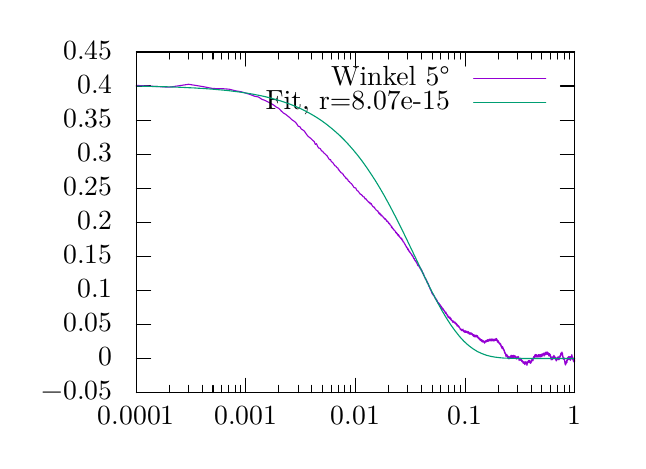
\begin{tikzpicture}[gnuplot]
%% generated with GNUPLOT 5.2p5a (Gentoo revision r0) (Lua 5.1; terminal rev. 99 , script rev. 107)
%% Sa 18 Mai 2019 18:31:27 CEST
\path (0.000,0.000) rectangle (7.500,5.250);
\gpcolor{color=gp lt color border}
\gpsetlinetype{gp lt border}
\gpsetdashtype{gp dt solid}
\gpsetlinewidth{1.00}
\draw[gp path] (1.380,0.616)--(1.560,0.616);
\draw[gp path] (6.947,0.616)--(6.767,0.616);
\node[gp node right] at (1.196,0.616) {$-0.05$};
\draw[gp path] (1.380,1.049)--(1.560,1.049);
\draw[gp path] (6.947,1.049)--(6.767,1.049);
\node[gp node right] at (1.196,1.049) {$0$};
\draw[gp path] (1.380,1.481)--(1.560,1.481);
\draw[gp path] (6.947,1.481)--(6.767,1.481);
\node[gp node right] at (1.196,1.481) {$0.05$};
\draw[gp path] (1.380,1.914)--(1.560,1.914);
\draw[gp path] (6.947,1.914)--(6.767,1.914);
\node[gp node right] at (1.196,1.914) {$0.1$};
\draw[gp path] (1.380,2.346)--(1.560,2.346);
\draw[gp path] (6.947,2.346)--(6.767,2.346);
\node[gp node right] at (1.196,2.346) {$0.15$};
\draw[gp path] (1.380,2.779)--(1.560,2.779);
\draw[gp path] (6.947,2.779)--(6.767,2.779);
\node[gp node right] at (1.196,2.779) {$0.2$};
\draw[gp path] (1.380,3.211)--(1.560,3.211);
\draw[gp path] (6.947,3.211)--(6.767,3.211);
\node[gp node right] at (1.196,3.211) {$0.25$};
\draw[gp path] (1.380,3.644)--(1.560,3.644);
\draw[gp path] (6.947,3.644)--(6.767,3.644);
\node[gp node right] at (1.196,3.644) {$0.3$};
\draw[gp path] (1.380,4.076)--(1.560,4.076);
\draw[gp path] (6.947,4.076)--(6.767,4.076);
\node[gp node right] at (1.196,4.076) {$0.35$};
\draw[gp path] (1.380,4.509)--(1.560,4.509);
\draw[gp path] (6.947,4.509)--(6.767,4.509);
\node[gp node right] at (1.196,4.509) {$0.4$};
\draw[gp path] (1.380,4.941)--(1.560,4.941);
\draw[gp path] (6.947,4.941)--(6.767,4.941);
\node[gp node right] at (1.196,4.941) {$0.45$};
\draw[gp path] (1.380,0.616)--(1.380,0.796);
\draw[gp path] (1.380,4.941)--(1.380,4.761);
\node[gp node center] at (1.380,0.308) {$0.0001$};
\draw[gp path] (1.799,0.616)--(1.799,0.706);
\draw[gp path] (1.799,4.941)--(1.799,4.851);
\draw[gp path] (2.044,0.616)--(2.044,0.706);
\draw[gp path] (2.044,4.941)--(2.044,4.851);
\draw[gp path] (2.218,0.616)--(2.218,0.706);
\draw[gp path] (2.218,4.941)--(2.218,4.851);
\draw[gp path] (2.353,0.616)--(2.353,0.706);
\draw[gp path] (2.353,4.941)--(2.353,4.851);
\draw[gp path] (2.463,0.616)--(2.463,0.706);
\draw[gp path] (2.463,4.941)--(2.463,4.851);
\draw[gp path] (2.556,0.616)--(2.556,0.706);
\draw[gp path] (2.556,4.941)--(2.556,4.851);
\draw[gp path] (2.637,0.616)--(2.637,0.706);
\draw[gp path] (2.637,4.941)--(2.637,4.851);
\draw[gp path] (2.708,0.616)--(2.708,0.706);
\draw[gp path] (2.708,4.941)--(2.708,4.851);
\draw[gp path] (2.772,0.616)--(2.772,0.796);
\draw[gp path] (2.772,4.941)--(2.772,4.761);
\node[gp node center] at (2.772,0.308) {$0.001$};
\draw[gp path] (3.191,0.616)--(3.191,0.706);
\draw[gp path] (3.191,4.941)--(3.191,4.851);
\draw[gp path] (3.436,0.616)--(3.436,0.706);
\draw[gp path] (3.436,4.941)--(3.436,4.851);
\draw[gp path] (3.610,0.616)--(3.610,0.706);
\draw[gp path] (3.610,4.941)--(3.610,4.851);
\draw[gp path] (3.745,0.616)--(3.745,0.706);
\draw[gp path] (3.745,4.941)--(3.745,4.851);
\draw[gp path] (3.855,0.616)--(3.855,0.706);
\draw[gp path] (3.855,4.941)--(3.855,4.851);
\draw[gp path] (3.948,0.616)--(3.948,0.706);
\draw[gp path] (3.948,4.941)--(3.948,4.851);
\draw[gp path] (4.029,0.616)--(4.029,0.706);
\draw[gp path] (4.029,4.941)--(4.029,4.851);
\draw[gp path] (4.100,0.616)--(4.100,0.706);
\draw[gp path] (4.100,4.941)--(4.100,4.851);
\draw[gp path] (4.163,0.616)--(4.163,0.796);
\draw[gp path] (4.163,4.941)--(4.163,4.761);
\node[gp node center] at (4.163,0.308) {$0.01$};
\draw[gp path] (4.582,0.616)--(4.582,0.706);
\draw[gp path] (4.582,4.941)--(4.582,4.851);
\draw[gp path] (4.828,0.616)--(4.828,0.706);
\draw[gp path] (4.828,4.941)--(4.828,4.851);
\draw[gp path] (5.001,0.616)--(5.001,0.706);
\draw[gp path] (5.001,4.941)--(5.001,4.851);
\draw[gp path] (5.136,0.616)--(5.136,0.706);
\draw[gp path] (5.136,4.941)--(5.136,4.851);
\draw[gp path] (5.246,0.616)--(5.246,0.706);
\draw[gp path] (5.246,4.941)--(5.246,4.851);
\draw[gp path] (5.340,0.616)--(5.340,0.706);
\draw[gp path] (5.340,4.941)--(5.340,4.851);
\draw[gp path] (5.420,0.616)--(5.420,0.706);
\draw[gp path] (5.420,4.941)--(5.420,4.851);
\draw[gp path] (5.492,0.616)--(5.492,0.706);
\draw[gp path] (5.492,4.941)--(5.492,4.851);
\draw[gp path] (5.555,0.616)--(5.555,0.796);
\draw[gp path] (5.555,4.941)--(5.555,4.761);
\node[gp node center] at (5.555,0.308) {$0.1$};
\draw[gp path] (5.974,0.616)--(5.974,0.706);
\draw[gp path] (5.974,4.941)--(5.974,4.851);
\draw[gp path] (6.219,0.616)--(6.219,0.706);
\draw[gp path] (6.219,4.941)--(6.219,4.851);
\draw[gp path] (6.393,0.616)--(6.393,0.706);
\draw[gp path] (6.393,4.941)--(6.393,4.851);
\draw[gp path] (6.528,0.616)--(6.528,0.706);
\draw[gp path] (6.528,4.941)--(6.528,4.851);
\draw[gp path] (6.638,0.616)--(6.638,0.706);
\draw[gp path] (6.638,4.941)--(6.638,4.851);
\draw[gp path] (6.731,0.616)--(6.731,0.706);
\draw[gp path] (6.731,4.941)--(6.731,4.851);
\draw[gp path] (6.812,0.616)--(6.812,0.706);
\draw[gp path] (6.812,4.941)--(6.812,4.851);
\draw[gp path] (6.883,0.616)--(6.883,0.706);
\draw[gp path] (6.883,4.941)--(6.883,4.851);
\draw[gp path] (6.947,0.616)--(6.947,0.796);
\draw[gp path] (6.947,4.941)--(6.947,4.761);
\node[gp node center] at (6.947,0.308) {$1$};
\draw[gp path] (1.380,4.941)--(1.380,0.616)--(6.947,0.616)--(6.947,4.941)--cycle;
\node[gp node right] at (5.479,4.607) {Winkel 5°};
\gpcolor{rgb color={0.580,0.000,0.827}}
\draw[gp path] (5.663,4.607)--(6.579,4.607);
\draw[gp path] (1.380,4.517)--(1.799,4.494)--(2.044,4.531)--(2.218,4.503)--(2.353,4.477)%
  --(2.463,4.476)--(2.556,4.469)--(2.637,4.449)--(2.708,4.437)--(2.772,4.418)--(2.829,4.400)%
  --(2.882,4.379)--(2.930,4.370)--(2.975,4.340)--(3.017,4.325)--(3.056,4.304)--(3.092,4.286)%
  --(3.127,4.265)--(3.160,4.240)--(3.191,4.224)--(3.220,4.192)--(3.248,4.166)--(3.275,4.151)%
  --(3.301,4.129)--(3.326,4.110)--(3.349,4.086)--(3.372,4.070)--(3.394,4.054)--(3.415,4.032)%
  --(3.436,3.998)--(3.456,3.993)--(3.475,3.963)--(3.493,3.952)--(3.511,3.939)--(3.529,3.914)%
  --(3.546,3.889)--(3.563,3.868)--(3.579,3.857)--(3.594,3.844)--(3.610,3.830)--(3.625,3.815)%
  --(3.639,3.803)--(3.653,3.768)--(3.667,3.776)--(3.681,3.746)--(3.694,3.722)--(3.707,3.720)%
  --(3.720,3.708)--(3.732,3.685)--(3.745,3.681)--(3.757,3.663)--(3.768,3.654)--(3.780,3.644)%
  --(3.791,3.633)--(3.802,3.623)--(3.813,3.604)--(3.824,3.587)--(3.834,3.572)--(3.845,3.576)%
  --(3.855,3.553)--(3.865,3.543)--(3.875,3.536)--(3.884,3.523)--(3.894,3.507)--(3.903,3.495)%
  --(3.912,3.494)--(3.921,3.481)--(3.930,3.470)--(3.939,3.469)--(3.948,3.443)--(3.956,3.443)%
  --(3.965,3.426)--(3.973,3.417)--(3.982,3.407)--(3.990,3.405)--(3.998,3.392)--(4.006,3.391)%
  --(4.013,3.374)--(4.021,3.364)--(4.029,3.358)--(4.036,3.345)--(4.044,3.333)--(4.051,3.340)%
  --(4.058,3.323)--(4.065,3.319)--(4.072,3.304)--(4.079,3.298)--(4.086,3.296)--(4.093,3.281)%
  --(4.100,3.279)--(4.106,3.272)--(4.113,3.268)--(4.120,3.258)--(4.126,3.249)--(4.132,3.240)%
  --(4.139,3.230)--(4.145,3.219)--(4.151,3.219)--(4.157,3.214)--(4.164,3.217)--(4.170,3.204)%
  --(4.175,3.196)--(4.181,3.184)--(4.187,3.179)--(4.193,3.175)--(4.199,3.172)--(4.204,3.164)%
  --(4.210,3.153)--(4.216,3.148)--(4.221,3.137)--(4.227,3.137)--(4.232,3.132)--(4.237,3.131)%
  --(4.243,3.122)--(4.248,3.122)--(4.253,3.114)--(4.258,3.105)--(4.264,3.103)--(4.269,3.100)%
  --(4.274,3.101)--(4.279,3.089)--(4.284,3.077)--(4.289,3.072)--(4.294,3.077)--(4.298,3.072)%
  --(4.303,3.070)--(4.308,3.056)--(4.313,3.054)--(4.317,3.049)--(4.322,3.044)--(4.327,3.035)%
  --(4.331,3.038)--(4.336,3.033)--(4.340,3.023)--(4.345,3.032)--(4.349,3.013)--(4.354,3.021)%
  --(4.358,3.011)--(4.363,3.015)--(4.367,3.005)--(4.371,2.998)--(4.375,2.992)--(4.380,2.985)%
  --(4.384,2.978)--(4.388,2.977)--(4.392,2.971)--(4.396,2.975)--(4.400,2.969)--(4.405,2.967)%
  --(4.409,2.954)--(4.413,2.950)--(4.417,2.947)--(4.421,2.941)--(4.424,2.937)--(4.428,2.930)%
  --(4.432,2.932)--(4.436,2.927)--(4.440,2.922)--(4.444,2.918)--(4.448,2.924)--(4.451,2.908)%
  --(4.455,2.907)--(4.459,2.895)--(4.463,2.898)--(4.466,2.883)--(4.470,2.896)--(4.473,2.890)%
  --(4.477,2.878)--(4.481,2.884)--(4.484,2.876)--(4.488,2.861)--(4.491,2.871)--(4.495,2.872)%
  --(4.498,2.863)--(4.502,2.855)--(4.505,2.856)--(4.509,2.855)--(4.512,2.845)--(4.515,2.845)%
  --(4.519,2.837)--(4.522,2.837)--(4.525,2.833)--(4.529,2.829)--(4.532,2.826)--(4.535,2.823)%
  --(4.539,2.813)--(4.542,2.822)--(4.545,2.823)--(4.548,2.812)--(4.551,2.810)--(4.555,2.806)%
  --(4.558,2.792)--(4.561,2.800)--(4.564,2.795)--(4.567,2.794)--(4.570,2.786)--(4.573,2.788)%
  --(4.576,2.780)--(4.579,2.782)--(4.582,2.777)--(4.585,2.765)--(4.588,2.764)--(4.591,2.758)%
  --(4.594,2.765)--(4.597,2.760)--(4.600,2.755)--(4.603,2.742)--(4.606,2.744)--(4.609,2.740)%
  --(4.612,2.739)--(4.615,2.737)--(4.618,2.725)--(4.621,2.711)--(4.623,2.724)--(4.626,2.719)%
  --(4.629,2.714)--(4.632,2.706)--(4.635,2.697)--(4.637,2.702)--(4.640,2.700)--(4.643,2.691)%
  --(4.646,2.689)--(4.648,2.688)--(4.651,2.684)--(4.654,2.675)--(4.656,2.680)--(4.659,2.673)%
  --(4.662,2.673)--(4.664,2.670)--(4.667,2.667)--(4.670,2.657)--(4.672,2.662)--(4.675,2.644)%
  --(4.677,2.650)--(4.680,2.643)--(4.683,2.651)--(4.685,2.635)--(4.688,2.642)--(4.690,2.637)%
  --(4.693,2.630)--(4.695,2.634)--(4.698,2.617)--(4.700,2.617)--(4.703,2.623)--(4.705,2.613)%
  --(4.708,2.606)--(4.710,2.622)--(4.712,2.608)--(4.715,2.607)--(4.717,2.601)--(4.720,2.593)%
  --(4.722,2.605)--(4.725,2.595)--(4.727,2.589)--(4.729,2.586)--(4.732,2.584)--(4.734,2.576)%
  --(4.736,2.580)--(4.739,2.576)--(4.741,2.578)--(4.743,2.580)--(4.746,2.571)--(4.748,2.559)%
  --(4.750,2.571)--(4.753,2.562)--(4.755,2.568)--(4.757,2.549)--(4.759,2.551)--(4.762,2.550)%
  --(4.764,2.551)--(4.766,2.532)--(4.768,2.530)--(4.771,2.529)--(4.773,2.532)--(4.775,2.526)%
  --(4.777,2.525)--(4.779,2.520)--(4.781,2.512)--(4.784,2.512)--(4.786,2.512)--(4.788,2.507)%
  --(4.790,2.500)--(4.792,2.496)--(4.794,2.494)--(4.797,2.491)--(4.799,2.482)--(4.801,2.484)%
  --(4.803,2.474)--(4.805,2.478)--(4.807,2.465)--(4.809,2.472)--(4.811,2.461)--(4.813,2.458)%
  --(4.815,2.461)--(4.817,2.460)--(4.819,2.461)--(4.821,2.445)--(4.823,2.442)--(4.826,2.431)%
  --(4.828,2.429)--(4.830,2.444)--(4.832,2.436)--(4.834,2.433)--(4.836,2.428)--(4.838,2.430)%
  --(4.840,2.417)--(4.841,2.410)--(4.843,2.416)--(4.845,2.414)--(4.847,2.411)--(4.849,2.402)%
  --(4.851,2.409)--(4.853,2.403)--(4.855,2.392)--(4.857,2.395)--(4.859,2.394)--(4.861,2.388)%
  --(4.863,2.386)--(4.865,2.382)--(4.867,2.381)--(4.868,2.376)--(4.870,2.377)--(4.872,2.377)%
  --(4.874,2.377)--(4.876,2.365)--(4.878,2.373)--(4.880,2.356)--(4.881,2.355)--(4.883,2.359)%
  --(4.885,2.356)--(4.887,2.349)--(4.889,2.347)--(4.891,2.354)--(4.892,2.341)--(4.894,2.337)%
  --(4.896,2.335)--(4.898,2.339)--(4.900,2.325)--(4.901,2.327)--(4.903,2.314)--(4.905,2.317)%
  --(4.907,2.316)--(4.908,2.315)--(4.910,2.317)--(4.912,2.318)--(4.914,2.301)--(4.916,2.302)%
  --(4.917,2.301)--(4.919,2.291)--(4.921,2.292)--(4.922,2.293)--(4.924,2.292)--(4.926,2.284)%
  --(4.928,2.290)--(4.929,2.284)--(4.931,2.286)--(4.933,2.271)--(4.934,2.273)--(4.936,2.274)%
  --(4.938,2.266)--(4.939,2.267)--(4.941,2.263)--(4.943,2.255)--(4.944,2.251)--(4.946,2.258)%
  --(4.948,2.248)--(4.949,2.248)--(4.951,2.235)--(4.953,2.234)--(4.954,2.237)--(4.956,2.234)%
  --(4.958,2.226)--(4.959,2.233)--(4.961,2.236)--(4.962,2.233)--(4.964,2.234)--(4.966,2.221)%
  --(4.967,2.227)--(4.969,2.220)--(4.970,2.218)--(4.972,2.220)--(4.974,2.213)--(4.975,2.202)%
  --(4.977,2.207)--(4.978,2.208)--(4.980,2.209)--(4.981,2.200)--(4.983,2.194)--(4.985,2.187)%
  --(4.986,2.200)--(4.988,2.192)--(4.989,2.193)--(4.991,2.187)--(4.992,2.194)--(4.994,2.181)%
  --(4.995,2.179)--(4.997,2.181)--(4.998,2.164)--(5.000,2.162)--(5.001,2.166)--(5.003,2.179)%
  --(5.004,2.167)--(5.006,2.160)--(5.007,2.162)--(5.009,2.164)--(5.010,2.156)--(5.012,2.142)%
  --(5.013,2.140)--(5.015,2.139)--(5.016,2.130)--(5.018,2.140)--(5.019,2.136)--(5.021,2.133)%
  --(5.022,2.134)--(5.024,2.130)--(5.025,2.107)--(5.027,2.123)--(5.028,2.128)--(5.029,2.115)%
  --(5.031,2.116)--(5.032,2.099)--(5.034,2.106)--(5.035,2.096)--(5.037,2.093)--(5.038,2.095)%
  --(5.039,2.086)--(5.041,2.078)--(5.042,2.083)--(5.044,2.080)--(5.045,2.076)--(5.047,2.077)%
  --(5.048,2.062)--(5.049,2.059)--(5.051,2.062)--(5.052,2.068)--(5.054,2.064)--(5.055,2.062)%
  --(5.056,2.054)--(5.058,2.060)--(5.059,2.050)--(5.060,2.046)--(5.062,2.038)--(5.063,2.039)%
  --(5.064,2.036)--(5.066,2.030)--(5.067,2.040)--(5.069,2.027)--(5.070,2.019)--(5.071,2.023)%
  --(5.073,2.031)--(5.074,2.010)--(5.075,2.006)--(5.077,2.017)--(5.078,2.018)--(5.079,2.006)%
  --(5.081,2.009)--(5.082,2.002)--(5.083,2.000)--(5.085,1.993)--(5.086,1.994)--(5.087,2.003)%
  --(5.089,1.978)--(5.090,1.985)--(5.091,1.982)--(5.092,1.968)--(5.094,1.986)--(5.095,1.981)%
  --(5.096,1.976)--(5.098,1.973)--(5.099,1.965)--(5.100,1.960)--(5.101,1.961)--(5.103,1.952)%
  --(5.104,1.955)--(5.105,1.942)--(5.107,1.950)--(5.108,1.942)--(5.109,1.941)--(5.110,1.943)%
  --(5.112,1.940)--(5.113,1.926)--(5.114,1.923)--(5.115,1.926)--(5.117,1.930)--(5.118,1.931)%
  --(5.119,1.914)--(5.120,1.916)--(5.122,1.907)--(5.123,1.914)--(5.124,1.914)--(5.125,1.911)%
  --(5.127,1.901)--(5.128,1.904)--(5.129,1.894)--(5.130,1.904)--(5.131,1.880)--(5.133,1.887)%
  --(5.134,1.881)--(5.135,1.881)--(5.136,1.885)--(5.137,1.873)--(5.139,1.871)--(5.140,1.877)%
  --(5.141,1.863)--(5.142,1.878)--(5.144,1.876)--(5.145,1.863)--(5.146,1.856)--(5.147,1.869)%
  --(5.148,1.858)--(5.149,1.863)--(5.151,1.857)--(5.152,1.860)--(5.153,1.857)--(5.154,1.849)%
  --(5.155,1.856)--(5.157,1.851)--(5.158,1.850)--(5.159,1.848)--(5.160,1.843)--(5.161,1.843)%
  --(5.162,1.838)--(5.163,1.845)--(5.165,1.833)--(5.166,1.831)--(5.167,1.836)--(5.168,1.825)%
  --(5.169,1.835)--(5.170,1.827)--(5.172,1.819)--(5.173,1.823)--(5.174,1.821)--(5.175,1.817)%
  --(5.176,1.818)--(5.177,1.809)--(5.178,1.818)--(5.179,1.804)--(5.181,1.806)--(5.182,1.807)%
  --(5.183,1.812)--(5.184,1.808)--(5.185,1.807)--(5.186,1.806)--(5.187,1.797)--(5.188,1.804)%
  --(5.189,1.799)--(5.191,1.791)--(5.192,1.796)--(5.193,1.776)--(5.194,1.782)--(5.195,1.783)%
  --(5.196,1.789)--(5.197,1.776)--(5.198,1.791)--(5.199,1.784)--(5.200,1.788)--(5.202,1.777)%
  --(5.203,1.774)--(5.204,1.771)--(5.205,1.769)--(5.206,1.767)--(5.207,1.767)--(5.208,1.764)%
  --(5.209,1.760)--(5.210,1.755)--(5.211,1.758)--(5.212,1.752)--(5.213,1.761)--(5.214,1.761)%
  --(5.215,1.754)--(5.217,1.759)--(5.218,1.748)--(5.219,1.749)--(5.220,1.755)--(5.221,1.744)%
  --(5.222,1.748)--(5.223,1.750)--(5.224,1.738)--(5.225,1.749)--(5.226,1.741)--(5.227,1.744)%
  --(5.228,1.745)--(5.229,1.735)--(5.230,1.738)--(5.231,1.734)--(5.232,1.736)--(5.233,1.736)%
  --(5.234,1.732)--(5.235,1.727)--(5.236,1.734)--(5.237,1.725)--(5.238,1.716)--(5.239,1.720)%
  --(5.240,1.718)--(5.241,1.727)--(5.242,1.721)--(5.243,1.704)--(5.244,1.712)--(5.245,1.722)%
  --(5.246,1.712)--(5.247,1.718)--(5.249,1.703)--(5.250,1.712)--(5.251,1.709)--(5.252,1.703)%
  --(5.253,1.710)--(5.254,1.709)--(5.254,1.706)--(5.255,1.697)--(5.256,1.702)--(5.257,1.685)%
  --(5.258,1.703)--(5.259,1.696)--(5.260,1.694)--(5.261,1.692)--(5.262,1.692)--(5.263,1.684)%
  --(5.264,1.690)--(5.265,1.692)--(5.266,1.681)--(5.267,1.689)--(5.268,1.675)--(5.269,1.672)%
  --(5.270,1.679)--(5.271,1.677)--(5.272,1.671)--(5.273,1.676)--(5.274,1.679)--(5.275,1.684)%
  --(5.276,1.677)--(5.277,1.675)--(5.278,1.673)--(5.279,1.670)--(5.280,1.670)--(5.281,1.675)%
  --(5.282,1.661)--(5.283,1.665)--(5.284,1.664)--(5.285,1.663)--(5.286,1.665)--(5.286,1.655)%
  --(5.287,1.656)--(5.288,1.656)--(5.289,1.655)--(5.290,1.657)--(5.291,1.653)--(5.292,1.656)%
  --(5.293,1.653)--(5.294,1.651)--(5.295,1.652)--(5.296,1.642)--(5.297,1.642)--(5.298,1.646)%
  --(5.299,1.640)--(5.300,1.633)--(5.300,1.637)--(5.301,1.631)--(5.302,1.642)--(5.303,1.636)%
  --(5.304,1.635)--(5.305,1.633)--(5.306,1.626)--(5.307,1.635)--(5.308,1.619)--(5.309,1.637)%
  --(5.310,1.626)--(5.310,1.629)--(5.311,1.637)--(5.312,1.638)--(5.313,1.625)--(5.314,1.616)%
  --(5.315,1.619)--(5.316,1.615)--(5.317,1.615)--(5.318,1.620)--(5.319,1.611)--(5.319,1.618)%
  --(5.320,1.612)--(5.321,1.613)--(5.322,1.606)--(5.323,1.613)--(5.324,1.608)--(5.325,1.602)%
  --(5.326,1.608)--(5.327,1.604)--(5.327,1.599)--(5.328,1.589)--(5.329,1.593)--(5.330,1.604)%
  --(5.331,1.593)--(5.332,1.594)--(5.333,1.593)--(5.334,1.596)--(5.334,1.588)--(5.335,1.591)%
  --(5.336,1.599)--(5.337,1.573)--(5.338,1.579)--(5.339,1.587)--(5.340,1.575)--(5.341,1.578)%
  --(5.341,1.583)--(5.342,1.581)--(5.343,1.585)--(5.344,1.567)--(5.345,1.582)--(5.346,1.581)%
  --(5.347,1.569)--(5.347,1.570)--(5.348,1.572)--(5.349,1.570)--(5.350,1.571)--(5.351,1.571)%
  --(5.352,1.575)--(5.352,1.576)--(5.353,1.569)--(5.354,1.565)--(5.355,1.566)--(5.356,1.561)%
  --(5.357,1.561)--(5.358,1.559)--(5.358,1.567)--(5.359,1.567)--(5.360,1.554)--(5.361,1.565)%
  --(5.362,1.566)--(5.363,1.575)--(5.363,1.565)--(5.364,1.553)--(5.365,1.555)--(5.366,1.556)%
  --(5.367,1.561)--(5.368,1.558)--(5.369,1.555)--(5.370,1.555)--(5.371,1.546)--(5.372,1.554)%
  --(5.372,1.541)--(5.373,1.551)--(5.374,1.551)--(5.375,1.544)--(5.376,1.559)--(5.377,1.549)%
  --(5.377,1.539)--(5.378,1.547)--(5.379,1.539)--(5.380,1.541)--(5.381,1.532)--(5.381,1.537)%
  --(5.382,1.538)--(5.383,1.538)--(5.384,1.538)--(5.385,1.539)--(5.385,1.531)--(5.386,1.533)%
  --(5.387,1.538)--(5.388,1.533)--(5.389,1.531)--(5.389,1.529)--(5.390,1.529)--(5.391,1.522)%
  --(5.392,1.521)--(5.393,1.529)--(5.393,1.526)--(5.394,1.525)--(5.395,1.526)--(5.396,1.522)%
  --(5.396,1.520)--(5.397,1.518)--(5.398,1.508)--(5.399,1.519)--(5.400,1.515)--(5.400,1.509)%
  --(5.401,1.516)--(5.402,1.517)--(5.403,1.515)--(5.404,1.518)--(5.404,1.526)--(5.405,1.510)%
  --(5.406,1.517)--(5.407,1.511)--(5.407,1.508)--(5.408,1.515)--(5.409,1.509)--(5.410,1.517)%
  --(5.410,1.507)--(5.411,1.523)--(5.412,1.504)--(5.413,1.517)--(5.414,1.510)--(5.414,1.506)%
  --(5.415,1.507)--(5.416,1.510)--(5.417,1.507)--(5.417,1.509)--(5.418,1.507)--(5.419,1.511)%
  --(5.420,1.507)--(5.420,1.499)--(5.421,1.511)--(5.422,1.502)--(5.423,1.498)--(5.424,1.501)%
  --(5.425,1.497)--(5.426,1.509)--(5.426,1.505)--(5.427,1.500)--(5.428,1.496)--(5.429,1.505)%
  --(5.429,1.512)--(5.430,1.497)--(5.431,1.502)--(5.432,1.488)--(5.432,1.503)--(5.433,1.495)%
  --(5.434,1.501)--(5.435,1.497)--(5.435,1.499)--(5.436,1.496)--(5.437,1.492)--(5.438,1.494)%
  --(5.438,1.492)--(5.439,1.499)--(5.440,1.493)--(5.440,1.489)--(5.441,1.489)--(5.442,1.482)%
  --(5.443,1.487)--(5.443,1.485)--(5.444,1.478)--(5.445,1.480)--(5.446,1.480)--(5.446,1.476)%
  --(5.447,1.493)--(5.448,1.478)--(5.448,1.476)--(5.449,1.484)--(5.450,1.484)--(5.451,1.481)%
  --(5.451,1.474)--(5.452,1.462)--(5.453,1.476)--(5.454,1.480)--(5.455,1.465)--(5.456,1.476)%
  --(5.456,1.468)--(5.457,1.465)--(5.458,1.477)--(5.458,1.464)--(5.459,1.461)--(5.460,1.473)%
  --(5.461,1.465)--(5.461,1.468)--(5.462,1.463)--(5.463,1.458)--(5.463,1.464)--(5.464,1.458)%
  --(5.465,1.456)--(5.465,1.462)--(5.466,1.455)--(5.467,1.462)--(5.468,1.451)--(5.468,1.455)%
  --(5.469,1.459)--(5.470,1.467)--(5.470,1.463)--(5.471,1.462)--(5.472,1.465)--(5.472,1.461)%
  --(5.473,1.458)--(5.474,1.458)--(5.475,1.453)--(5.475,1.457)--(5.476,1.459)--(5.477,1.444)%
  --(5.477,1.457)--(5.478,1.455)--(5.479,1.443)--(5.479,1.453)--(5.480,1.447)--(5.481,1.439)%
  --(5.481,1.450)--(5.482,1.438)--(5.483,1.440)--(5.483,1.436)--(5.484,1.443)--(5.485,1.434)%
  --(5.485,1.436)--(5.486,1.439)--(5.487,1.440)--(5.488,1.432)--(5.488,1.433)--(5.489,1.437)%
  --(5.490,1.434)--(5.490,1.435)--(5.491,1.433)--(5.492,1.432)--(5.493,1.420)--(5.494,1.425)%
  --(5.494,1.417)--(5.495,1.425)--(5.496,1.424)--(5.496,1.416)--(5.497,1.421)--(5.498,1.417)%
  --(5.498,1.414)--(5.499,1.423)--(5.500,1.416)--(5.500,1.424)--(5.501,1.414)--(5.502,1.423)%
  --(5.502,1.416)--(5.503,1.413)--(5.504,1.408)--(5.504,1.419)--(5.505,1.418)--(5.506,1.418)%
  --(5.506,1.416)--(5.507,1.410)--(5.507,1.418)--(5.508,1.410)--(5.509,1.414)--(5.509,1.412)%
  --(5.510,1.420)--(5.511,1.414)--(5.511,1.401)--(5.512,1.414)--(5.513,1.418)--(5.513,1.410)%
  --(5.514,1.415)--(5.515,1.412)--(5.515,1.410)--(5.516,1.410)--(5.517,1.411)--(5.517,1.406)%
  --(5.518,1.414)--(5.518,1.405)--(5.519,1.407)--(5.520,1.412)--(5.520,1.404)--(5.521,1.414)%
  --(5.522,1.411)--(5.522,1.419)--(5.523,1.410)--(5.524,1.403)--(5.524,1.401)--(5.525,1.401)%
  --(5.526,1.404)--(5.526,1.411)--(5.527,1.401)--(5.527,1.412)--(5.528,1.407)--(5.529,1.401)%
  --(5.529,1.408)--(5.530,1.403)--(5.531,1.420)--(5.531,1.406)--(5.532,1.401)--(5.532,1.399)%
  --(5.533,1.402)--(5.534,1.395)--(5.534,1.397)--(5.535,1.403)--(5.536,1.397)--(5.536,1.395)%
  --(5.537,1.391)--(5.537,1.394)--(5.538,1.389)--(5.539,1.390)--(5.539,1.394)--(5.540,1.399)%
  --(5.541,1.392)--(5.542,1.390)--(5.542,1.388)--(5.543,1.388)--(5.544,1.384)--(5.544,1.393)%
  --(5.545,1.390)--(5.546,1.398)--(5.546,1.393)--(5.547,1.389)--(5.547,1.392)--(5.548,1.398)%
  --(5.549,1.397)--(5.549,1.400)--(5.550,1.392)--(5.550,1.402)--(5.551,1.389)--(5.552,1.381)%
  --(5.552,1.393)--(5.553,1.389)--(5.553,1.393)--(5.554,1.393)--(5.555,1.380)--(5.555,1.403)%
  --(5.556,1.394)--(5.556,1.390)--(5.557,1.392)--(5.558,1.389)--(5.558,1.394)--(5.559,1.388)%
  --(5.559,1.386)--(5.560,1.392)--(5.561,1.389)--(5.561,1.392)--(5.562,1.394)--(5.562,1.387)%
  --(5.563,1.391)--(5.564,1.392)--(5.564,1.395)--(5.565,1.380)--(5.565,1.395)--(5.566,1.385)%
  --(5.567,1.385)--(5.567,1.391)--(5.568,1.389)--(5.568,1.385)--(5.569,1.386)--(5.570,1.381)%
  --(5.570,1.391)--(5.571,1.385)--(5.571,1.383)--(5.572,1.393)--(5.573,1.393)--(5.573,1.395)%
  --(5.574,1.387)--(5.574,1.383)--(5.575,1.379)--(5.575,1.393)--(5.576,1.384)--(5.577,1.393)%
  --(5.577,1.397)--(5.578,1.377)--(5.578,1.378)--(5.579,1.387)--(5.580,1.386)--(5.580,1.377)%
  --(5.581,1.382)--(5.581,1.386)--(5.582,1.393)--(5.582,1.380)--(5.583,1.385)--(5.584,1.380)%
  --(5.584,1.383)--(5.585,1.377)--(5.585,1.373)--(5.586,1.385)--(5.586,1.383)--(5.587,1.383)%
  --(5.588,1.380)--(5.588,1.379)--(5.589,1.377)--(5.589,1.371)--(5.590,1.372)--(5.590,1.375)%
  --(5.591,1.377)--(5.592,1.382)--(5.592,1.375)--(5.593,1.371)--(5.593,1.376)--(5.594,1.375)%
  --(5.594,1.377)--(5.595,1.379)--(5.596,1.376)--(5.596,1.381)--(5.597,1.369)--(5.597,1.380)%
  --(5.598,1.372)--(5.598,1.369)--(5.599,1.390)--(5.600,1.378)--(5.600,1.382)--(5.601,1.370)%
  --(5.601,1.372)--(5.602,1.369)--(5.602,1.372)--(5.603,1.373)--(5.603,1.377)--(5.604,1.361)%
  --(5.605,1.371)--(5.605,1.367)--(5.606,1.367)--(5.607,1.365)--(5.608,1.363)--(5.608,1.372)%
  --(5.609,1.362)--(5.610,1.370)--(5.610,1.359)--(5.611,1.372)--(5.611,1.363)--(5.612,1.369)%
  --(5.612,1.366)--(5.613,1.360)--(5.613,1.366)--(5.614,1.375)--(5.615,1.355)--(5.615,1.357)%
  --(5.616,1.366)--(5.616,1.365)--(5.617,1.366)--(5.617,1.362)--(5.618,1.358)--(5.618,1.373)%
  --(5.619,1.364)--(5.619,1.362)--(5.620,1.363)--(5.621,1.372)--(5.621,1.362)--(5.622,1.365)%
  --(5.622,1.370)--(5.623,1.358)--(5.623,1.371)--(5.624,1.368)--(5.624,1.365)--(5.625,1.363)%
  --(5.625,1.367)--(5.626,1.369)--(5.626,1.375)--(5.627,1.367)--(5.628,1.372)--(5.628,1.355)%
  --(5.629,1.363)--(5.629,1.367)--(5.630,1.366)--(5.630,1.369)--(5.631,1.367)--(5.631,1.368)%
  --(5.632,1.374)--(5.632,1.362)--(5.633,1.364)--(5.633,1.373)--(5.634,1.360)--(5.634,1.359)%
  --(5.635,1.362)--(5.636,1.371)--(5.636,1.368)--(5.637,1.364)--(5.637,1.366)--(5.638,1.360)%
  --(5.638,1.366)--(5.639,1.369)--(5.639,1.357)--(5.640,1.360)--(5.640,1.361)--(5.641,1.367)%
  --(5.641,1.359)--(5.642,1.358)--(5.642,1.351)--(5.643,1.367)--(5.643,1.357)--(5.644,1.361)%
  --(5.644,1.350)--(5.645,1.361)--(5.645,1.365)--(5.646,1.356)--(5.647,1.359)--(5.647,1.362)%
  --(5.648,1.353)--(5.648,1.361)--(5.649,1.362)--(5.649,1.344)--(5.650,1.346)--(5.650,1.358)%
  --(5.651,1.356)--(5.651,1.346)--(5.652,1.354)--(5.652,1.350)--(5.653,1.356)--(5.653,1.358)%
  --(5.654,1.345)--(5.654,1.337)--(5.655,1.342)--(5.655,1.353)--(5.656,1.348)--(5.656,1.350)%
  --(5.657,1.344)--(5.657,1.347)--(5.658,1.347)--(5.658,1.351)--(5.659,1.346)--(5.659,1.339)%
  --(5.660,1.344)--(5.660,1.334)--(5.661,1.339)--(5.661,1.347)--(5.662,1.340)--(5.662,1.334)%
  --(5.663,1.332)--(5.663,1.350)--(5.664,1.335)--(5.664,1.344)--(5.665,1.341)--(5.665,1.337)%
  --(5.666,1.337)--(5.666,1.341)--(5.667,1.342)--(5.667,1.326)--(5.668,1.349)--(5.668,1.352)%
  --(5.669,1.339)--(5.669,1.335)--(5.670,1.333)--(5.670,1.330)--(5.671,1.340)--(5.672,1.338)%
  --(5.672,1.337)--(5.673,1.337)--(5.673,1.323)--(5.674,1.330)--(5.674,1.336)--(5.675,1.334)%
  --(5.675,1.338)--(5.676,1.330)--(5.676,1.337)--(5.677,1.327)--(5.677,1.332)--(5.678,1.328)%
  --(5.678,1.337)--(5.679,1.327)--(5.679,1.339)--(5.680,1.329)--(5.680,1.333)--(5.681,1.340)%
  --(5.681,1.330)--(5.682,1.335)--(5.682,1.344)--(5.683,1.331)--(5.683,1.339)--(5.684,1.335)%
  --(5.684,1.337)--(5.685,1.336)--(5.685,1.329)--(5.686,1.334)--(5.686,1.340)--(5.687,1.334)%
  --(5.687,1.326)--(5.688,1.336)--(5.688,1.338)--(5.689,1.321)--(5.689,1.329)--(5.690,1.340)%
  --(5.690,1.327)--(5.691,1.334)--(5.691,1.331)--(5.692,1.334)--(5.692,1.339)--(5.693,1.339)%
  --(5.693,1.335)--(5.693,1.344)--(5.694,1.336)--(5.695,1.323)--(5.695,1.333)--(5.696,1.340)%
  --(5.696,1.328)--(5.697,1.338)--(5.697,1.332)--(5.698,1.336)--(5.698,1.340)--(5.699,1.329)%
  --(5.699,1.325)--(5.700,1.346)--(5.700,1.329)--(5.701,1.330)--(5.701,1.341)--(5.702,1.337)%
  --(5.702,1.331)--(5.703,1.336)--(5.704,1.331)--(5.704,1.328)--(5.704,1.330)--(5.705,1.322)%
  --(5.705,1.327)--(5.706,1.339)--(5.706,1.335)--(5.707,1.326)--(5.707,1.339)--(5.708,1.336)%
  --(5.708,1.324)--(5.709,1.330)--(5.709,1.335)--(5.710,1.333)--(5.710,1.334)--(5.711,1.320)%
  --(5.711,1.334)--(5.712,1.329)--(5.712,1.325)--(5.712,1.338)--(5.713,1.325)--(5.713,1.327)%
  --(5.714,1.325)--(5.714,1.310)--(5.715,1.327)--(5.715,1.317)--(5.716,1.315)--(5.716,1.310)%
  --(5.717,1.319)--(5.717,1.324)--(5.718,1.326)--(5.718,1.322)--(5.718,1.319)--(5.719,1.317)%
  --(5.720,1.316)--(5.720,1.310)--(5.721,1.317)--(5.721,1.310)--(5.722,1.313)--(5.723,1.311)%
  --(5.723,1.318)--(5.724,1.319)--(5.724,1.312)--(5.724,1.315)--(5.725,1.306)--(5.725,1.311)%
  --(5.726,1.317)--(5.726,1.309)--(5.727,1.301)--(5.727,1.311)--(5.728,1.309)--(5.728,1.305)%
  --(5.729,1.307)--(5.729,1.312)--(5.729,1.297)--(5.730,1.306)--(5.730,1.297)--(5.731,1.310)%
  --(5.731,1.312)--(5.732,1.306)--(5.732,1.304)--(5.733,1.309)--(5.733,1.296)--(5.733,1.297)%
  --(5.734,1.298)--(5.734,1.303)--(5.735,1.304)--(5.735,1.299)--(5.736,1.299)--(5.736,1.301)%
  --(5.737,1.305)--(5.737,1.286)--(5.738,1.307)--(5.738,1.301)--(5.738,1.302)--(5.739,1.295)%
  --(5.740,1.297)--(5.740,1.302)--(5.741,1.293)--(5.741,1.302)--(5.742,1.293)--(5.742,1.291)%
  --(5.742,1.303)--(5.743,1.300)--(5.743,1.288)--(5.744,1.294)--(5.744,1.298)--(5.745,1.288)%
  --(5.745,1.291)--(5.746,1.297)--(5.746,1.301)--(5.746,1.293)--(5.747,1.294)--(5.747,1.293)%
  --(5.748,1.285)--(5.748,1.291)--(5.749,1.291)--(5.749,1.289)--(5.749,1.288)--(5.750,1.293)%
  --(5.750,1.281)--(5.751,1.286)--(5.751,1.277)--(5.752,1.294)--(5.752,1.290)--(5.753,1.287)%
  --(5.753,1.285)--(5.753,1.292)--(5.754,1.277)--(5.754,1.283)--(5.755,1.286)--(5.755,1.285)%
  --(5.756,1.283)--(5.756,1.285)--(5.756,1.288)--(5.757,1.284)--(5.757,1.280)--(5.758,1.284)%
  --(5.758,1.289)--(5.759,1.282)--(5.759,1.281)--(5.759,1.288)--(5.760,1.279)--(5.760,1.278)%
  --(5.761,1.279)--(5.761,1.281)--(5.762,1.275)--(5.762,1.284)--(5.762,1.269)--(5.763,1.281)%
  --(5.763,1.287)--(5.764,1.270)--(5.764,1.283)--(5.765,1.289)--(5.765,1.276)--(5.765,1.274)%
  --(5.766,1.280)--(5.766,1.275)--(5.767,1.284)--(5.767,1.274)--(5.768,1.277)--(5.768,1.279)%
  --(5.768,1.281)--(5.769,1.279)--(5.769,1.275)--(5.770,1.261)--(5.770,1.269)--(5.771,1.273)%
  --(5.771,1.275)--(5.771,1.278)--(5.772,1.272)--(5.772,1.260)--(5.773,1.271)--(5.773,1.268)%
  --(5.774,1.265)--(5.774,1.269)--(5.774,1.268)--(5.775,1.258)--(5.775,1.280)--(5.776,1.277)%
  --(5.776,1.266)--(5.776,1.282)--(5.777,1.264)--(5.777,1.261)--(5.778,1.280)--(5.778,1.272)%
  --(5.779,1.265)--(5.779,1.267)--(5.779,1.270)--(5.780,1.261)--(5.780,1.273)--(5.781,1.263)%
  --(5.781,1.260)--(5.782,1.267)--(5.782,1.258)--(5.783,1.277)--(5.783,1.269)--(5.784,1.259)%
  --(5.784,1.267)--(5.784,1.264)--(5.785,1.267)--(5.785,1.266)--(5.786,1.271)--(5.786,1.273)%
  --(5.786,1.269)--(5.787,1.259)--(5.787,1.262)--(5.788,1.262)--(5.788,1.272)--(5.789,1.264)%
  --(5.789,1.259)--(5.789,1.266)--(5.790,1.259)--(5.790,1.263)--(5.791,1.259)--(5.791,1.272)%
  --(5.792,1.266)--(5.792,1.258)--(5.793,1.268)--(5.793,1.272)--(5.793,1.260)--(5.794,1.261)%
  --(5.794,1.255)--(5.795,1.265)--(5.795,1.255)--(5.795,1.261)--(5.796,1.260)--(5.796,1.256)%
  --(5.797,1.256)--(5.797,1.252)--(5.798,1.260)--(5.798,1.248)--(5.799,1.250)--(5.799,1.262)%
  --(5.800,1.258)--(5.800,1.265)--(5.800,1.254)--(5.801,1.263)--(5.801,1.262)--(5.802,1.258)%
  --(5.802,1.254)--(5.802,1.258)--(5.803,1.250)--(5.803,1.257)--(5.804,1.242)--(5.804,1.249)%
  --(5.805,1.265)--(5.805,1.255)--(5.806,1.256)--(5.806,1.266)--(5.806,1.256)--(5.807,1.253)%
  --(5.807,1.249)--(5.808,1.253)--(5.808,1.257)--(5.808,1.251)--(5.809,1.263)--(5.809,1.255)%
  --(5.810,1.269)--(5.810,1.261)--(5.810,1.258)--(5.811,1.254)--(5.812,1.262)--(5.812,1.258)%
  --(5.812,1.260)--(5.813,1.260)--(5.813,1.269)--(5.813,1.263)--(5.814,1.273)--(5.814,1.262)%
  --(5.815,1.271)--(5.815,1.272)--(5.815,1.263)--(5.816,1.263)--(5.816,1.267)--(5.817,1.271)%
  --(5.817,1.269)--(5.817,1.260)--(5.818,1.275)--(5.818,1.271)--(5.819,1.268)--(5.819,1.272)%
  --(5.819,1.268)--(5.820,1.256)--(5.820,1.268)--(5.821,1.273)--(5.821,1.271)--(5.821,1.258)%
  --(5.822,1.268)--(5.822,1.273)--(5.822,1.271)--(5.823,1.270)--(5.823,1.268)--(5.824,1.277)%
  --(5.824,1.269)--(5.824,1.275)--(5.825,1.265)--(5.825,1.272)--(5.826,1.272)--(5.826,1.259)%
  --(5.826,1.272)--(5.827,1.272)--(5.827,1.268)--(5.828,1.273)--(5.828,1.269)--(5.828,1.268)%
  --(5.829,1.272)--(5.829,1.271)--(5.829,1.273)--(5.830,1.263)--(5.830,1.280)--(5.831,1.277)%
  --(5.831,1.267)--(5.831,1.266)--(5.832,1.273)--(5.832,1.276)--(5.833,1.273)--(5.833,1.276)%
  --(5.834,1.272)--(5.834,1.271)--(5.834,1.272)--(5.835,1.271)--(5.835,1.273)--(5.836,1.267)%
  --(5.836,1.277)--(5.836,1.280)--(5.837,1.269)--(5.837,1.274)--(5.838,1.282)--(5.838,1.277)%
  --(5.839,1.281)--(5.839,1.285)--(5.839,1.279)--(5.840,1.283)--(5.840,1.287)--(5.840,1.276)%
  --(5.841,1.279)--(5.841,1.272)--(5.842,1.271)--(5.842,1.276)--(5.842,1.275)--(5.843,1.278)%
  --(5.843,1.288)--(5.843,1.272)--(5.844,1.281)--(5.845,1.278)--(5.845,1.264)--(5.845,1.267)%
  --(5.846,1.275)--(5.846,1.279)--(5.846,1.264)--(5.847,1.273)--(5.847,1.269)--(5.848,1.279)%
  --(5.848,1.283)--(5.848,1.274)--(5.849,1.276)--(5.849,1.277)--(5.849,1.279)--(5.850,1.285)%
  --(5.850,1.273)--(5.851,1.277)--(5.851,1.280)--(5.851,1.273)--(5.852,1.278)--(5.852,1.277)%
  --(5.852,1.274)--(5.853,1.275)--(5.853,1.285)--(5.854,1.278)--(5.854,1.281)--(5.854,1.277)%
  --(5.855,1.269)--(5.855,1.291)--(5.855,1.271)--(5.856,1.280)--(5.856,1.277)--(5.856,1.269)%
  --(5.857,1.281)--(5.857,1.275)--(5.858,1.284)--(5.858,1.278)--(5.858,1.286)--(5.859,1.288)%
  --(5.859,1.287)--(5.859,1.280)--(5.860,1.275)--(5.860,1.289)--(5.860,1.281)--(5.861,1.292)%
  --(5.861,1.287)--(5.862,1.285)--(5.862,1.295)--(5.862,1.292)--(5.863,1.282)--(5.863,1.280)%
  --(5.864,1.292)--(5.864,1.284)--(5.864,1.288)--(5.865,1.282)--(5.865,1.284)--(5.866,1.285)%
  --(5.866,1.291)--(5.866,1.288)--(5.867,1.283)--(5.867,1.294)--(5.867,1.292)--(5.868,1.275)%
  --(5.868,1.277)--(5.868,1.283)--(5.869,1.287)--(5.869,1.277)--(5.870,1.295)--(5.870,1.284)%
  --(5.870,1.283)--(5.871,1.290)--(5.871,1.283)--(5.871,1.285)--(5.872,1.277)--(5.872,1.281)%
  --(5.872,1.274)--(5.873,1.282)--(5.873,1.290)--(5.873,1.280)--(5.874,1.286)--(5.875,1.279)%
  --(5.875,1.277)--(5.875,1.288)--(5.876,1.288)--(5.876,1.286)--(5.876,1.282)--(5.877,1.277)%
  --(5.877,1.282)--(5.877,1.288)--(5.878,1.272)--(5.878,1.284)--(5.878,1.279)--(5.879,1.288)%
  --(5.879,1.284)--(5.880,1.283)--(5.880,1.275)--(5.880,1.285)--(5.881,1.282)--(5.881,1.292)%
  --(5.882,1.285)--(5.882,1.292)--(5.882,1.288)--(5.883,1.288)--(5.883,1.292)--(5.883,1.295)%
  --(5.884,1.291)--(5.884,1.296)--(5.884,1.291)--(5.885,1.285)--(5.885,1.295)--(5.886,1.289)%
  --(5.886,1.288)--(5.887,1.296)--(5.887,1.280)--(5.887,1.291)--(5.888,1.289)--(5.888,1.287)%
  --(5.888,1.282)--(5.889,1.288)--(5.889,1.285)--(5.889,1.290)--(5.890,1.284)--(5.890,1.290)%
  --(5.890,1.285)--(5.891,1.285)--(5.891,1.284)--(5.891,1.280)--(5.892,1.278)--(5.892,1.281)%
  --(5.892,1.271)--(5.893,1.282)--(5.893,1.284)--(5.893,1.285)--(5.894,1.283)--(5.894,1.290)%
  --(5.895,1.289)--(5.895,1.284)--(5.895,1.285)--(5.896,1.287)--(5.896,1.286)--(5.897,1.288)%
  --(5.897,1.294)--(5.897,1.282)--(5.898,1.283)--(5.898,1.280)--(5.898,1.278)--(5.899,1.290)%
  --(5.899,1.274)--(5.899,1.281)--(5.900,1.283)--(5.900,1.292)--(5.900,1.287)--(5.901,1.281)%
  --(5.901,1.279)--(5.901,1.291)--(5.902,1.282)--(5.902,1.283)--(5.903,1.276)--(5.903,1.281)%
  --(5.903,1.294)--(5.904,1.280)--(5.904,1.279)--(5.904,1.285)--(5.905,1.279)--(5.905,1.285)%
  --(5.905,1.284)--(5.906,1.291)--(5.906,1.281)--(5.906,1.280)--(5.907,1.288)--(5.907,1.281)%
  --(5.907,1.284)--(5.908,1.282)--(5.908,1.289)--(5.909,1.296)--(5.909,1.273)--(5.909,1.285)%
  --(5.910,1.281)--(5.910,1.285)--(5.910,1.286)--(5.911,1.285)--(5.911,1.282)--(5.911,1.293)%
  --(5.912,1.283)--(5.912,1.289)--(5.912,1.275)--(5.913,1.289)--(5.913,1.277)--(5.913,1.283)%
  --(5.914,1.279)--(5.914,1.291)--(5.914,1.283)--(5.915,1.287)--(5.915,1.272)--(5.915,1.285)%
  --(5.916,1.288)--(5.916,1.282)--(5.917,1.272)--(5.917,1.285)--(5.917,1.280)--(5.918,1.274)%
  --(5.918,1.278)--(5.918,1.283)--(5.919,1.285)--(5.919,1.276)--(5.919,1.280)--(5.920,1.287)%
  --(5.920,1.284)--(5.920,1.277)--(5.921,1.271)--(5.921,1.279)--(5.922,1.278)--(5.922,1.283)%
  --(5.922,1.277)--(5.922,1.280)--(5.923,1.279)--(5.923,1.283)--(5.923,1.277)--(5.924,1.278)%
  --(5.924,1.290)--(5.924,1.280)--(5.925,1.289)--(5.925,1.286)--(5.925,1.279)--(5.926,1.278)%
  --(5.926,1.276)--(5.926,1.279)--(5.927,1.286)--(5.927,1.274)--(5.927,1.290)--(5.928,1.284)%
  --(5.928,1.279)--(5.928,1.273)--(5.929,1.288)--(5.929,1.285)--(5.929,1.281)--(5.930,1.276)%
  --(5.930,1.279)--(5.930,1.295)--(5.931,1.282)--(5.931,1.276)--(5.931,1.287)--(5.932,1.286)%
  --(5.932,1.281)--(5.932,1.285)--(5.933,1.290)--(5.933,1.283)--(5.934,1.282)--(5.934,1.293)%
  --(5.934,1.288)--(5.935,1.291)--(5.935,1.279)--(5.935,1.285)--(5.936,1.291)--(5.936,1.286)%
  --(5.936,1.284)--(5.936,1.285)--(5.937,1.280)--(5.937,1.283)--(5.937,1.294)--(5.938,1.288)%
  --(5.938,1.281)--(5.938,1.292)--(5.939,1.286)--(5.939,1.289)--(5.939,1.278)--(5.940,1.284)%
  --(5.940,1.295)--(5.940,1.280)--(5.941,1.285)--(5.941,1.291)--(5.941,1.287)--(5.942,1.288)%
  --(5.942,1.284)--(5.943,1.290)--(5.943,1.284)--(5.943,1.285)--(5.944,1.279)--(5.944,1.280)%
  --(5.944,1.297)--(5.944,1.282)--(5.945,1.301)--(5.945,1.287)--(5.945,1.286)--(5.946,1.285)%
  --(5.946,1.291)--(5.946,1.293)--(5.947,1.297)--(5.947,1.288)--(5.947,1.292)--(5.948,1.298)%
  --(5.948,1.290)--(5.948,1.282)--(5.949,1.296)--(5.949,1.285)--(5.949,1.293)--(5.950,1.289)%
  --(5.950,1.286)--(5.950,1.293)--(5.950,1.291)--(5.951,1.291)--(5.951,1.285)--(5.951,1.294)%
  --(5.952,1.289)--(5.952,1.279)--(5.952,1.289)--(5.953,1.296)--(5.953,1.298)--(5.953,1.290)%
  --(5.954,1.290)--(5.954,1.285)--(5.954,1.288)--(5.955,1.296)--(5.955,1.278)--(5.955,1.303)%
  --(5.955,1.282)--(5.956,1.290)--(5.956,1.288)--(5.956,1.285)--(5.957,1.291)--(5.957,1.286)%
  --(5.957,1.288)--(5.958,1.277)--(5.958,1.290)--(5.958,1.273)--(5.959,1.275)--(5.959,1.274)%
  --(5.959,1.278)--(5.960,1.287)--(5.960,1.281)--(5.960,1.275)--(5.961,1.292)--(5.961,1.282)%
  --(5.961,1.270)--(5.962,1.273)--(5.962,1.267)--(5.963,1.267)--(5.963,1.274)--(5.963,1.285)%
  --(5.964,1.269)--(5.964,1.275)--(5.964,1.272)--(5.964,1.277)--(5.965,1.273)--(5.965,1.277)%
  --(5.965,1.266)--(5.966,1.279)--(5.966,1.273)--(5.966,1.256)--(5.967,1.267)--(5.967,1.273)%
  --(5.967,1.270)--(5.968,1.266)--(5.968,1.270)--(5.968,1.272)--(5.969,1.274)--(5.969,1.268)%
  --(5.969,1.267)--(5.970,1.271)--(5.970,1.273)--(5.970,1.274)--(5.971,1.267)--(5.971,1.272)%
  --(5.971,1.269)--(5.971,1.268)--(5.972,1.268)--(5.972,1.273)--(5.972,1.271)--(5.973,1.271)%
  --(5.973,1.276)--(5.973,1.268)--(5.974,1.267)--(5.974,1.274)--(5.974,1.273)--(5.975,1.269)%
  --(5.975,1.271)--(5.975,1.273)--(5.976,1.275)--(5.976,1.265)--(5.976,1.271)--(5.977,1.264)%
  --(5.977,1.263)--(5.977,1.266)--(5.978,1.258)--(5.978,1.257)--(5.978,1.255)--(5.978,1.260)%
  --(5.979,1.263)--(5.979,1.267)--(5.979,1.247)--(5.980,1.263)--(5.980,1.258)--(5.980,1.266)%
  --(5.981,1.257)--(5.981,1.258)--(5.981,1.257)--(5.981,1.259)--(5.982,1.261)--(5.982,1.249)%
  --(5.982,1.253)--(5.983,1.257)--(5.983,1.256)--(5.983,1.261)--(5.984,1.254)--(5.984,1.249)%
  --(5.984,1.253)--(5.985,1.254)--(5.985,1.253)--(5.985,1.252)--(5.986,1.252)--(5.986,1.253)%
  --(5.986,1.241)--(5.987,1.246)--(5.987,1.251)--(5.987,1.252)--(5.988,1.246)--(5.988,1.238)%
  --(5.988,1.240)--(5.989,1.243)--(5.989,1.236)--(5.989,1.235)--(5.989,1.240)--(5.990,1.244)%
  --(5.990,1.236)--(5.990,1.245)--(5.991,1.245)--(5.991,1.232)--(5.991,1.233)--(5.991,1.237)%
  --(5.992,1.237)--(5.992,1.241)--(5.992,1.247)--(5.993,1.241)--(5.993,1.235)--(5.993,1.237)%
  --(5.994,1.229)--(5.994,1.244)--(5.994,1.238)--(5.994,1.237)--(5.995,1.242)--(5.995,1.243)%
  --(5.996,1.232)--(5.996,1.242)--(5.996,1.230)--(5.996,1.232)--(5.997,1.246)--(5.997,1.231)%
  --(5.997,1.240)--(5.998,1.235)--(5.998,1.240)--(5.998,1.239)--(5.998,1.225)--(5.999,1.240)%
  --(5.999,1.235)--(5.999,1.234)--(6.000,1.230)--(6.000,1.236)--(6.000,1.224)--(6.001,1.236)%
  --(6.001,1.242)--(6.001,1.226)--(6.001,1.230)--(6.002,1.233)--(6.002,1.231)--(6.002,1.230)%
  --(6.003,1.230)--(6.003,1.219)--(6.003,1.229)--(6.003,1.221)--(6.004,1.224)--(6.004,1.229)%
  --(6.004,1.226)--(6.005,1.223)--(6.005,1.232)--(6.005,1.224)--(6.005,1.220)--(6.006,1.225)%
  --(6.006,1.215)--(6.006,1.220)--(6.007,1.233)--(6.007,1.230)--(6.007,1.219)--(6.007,1.224)%
  --(6.008,1.218)--(6.008,1.212)--(6.008,1.225)--(6.009,1.218)--(6.009,1.233)--(6.009,1.224)%
  --(6.009,1.214)--(6.010,1.218)--(6.010,1.211)--(6.010,1.219)--(6.011,1.215)--(6.011,1.203)%
  --(6.011,1.216)--(6.011,1.218)--(6.012,1.205)--(6.012,1.217)--(6.012,1.208)--(6.013,1.218)%
  --(6.013,1.214)--(6.013,1.211)--(6.013,1.214)--(6.014,1.208)--(6.014,1.205)--(6.014,1.200)%
  --(6.015,1.197)--(6.015,1.203)--(6.015,1.213)--(6.015,1.199)--(6.016,1.202)--(6.016,1.194)%
  --(6.016,1.204)--(6.017,1.193)--(6.017,1.202)--(6.017,1.191)--(6.017,1.196)--(6.018,1.200)%
  --(6.018,1.196)--(6.018,1.204)--(6.019,1.197)--(6.019,1.187)--(6.019,1.197)--(6.020,1.190)%
  --(6.020,1.183)--(6.020,1.190)--(6.020,1.192)--(6.021,1.189)--(6.021,1.195)--(6.021,1.187)%
  --(6.022,1.183)--(6.022,1.194)--(6.022,1.184)--(6.022,1.195)--(6.023,1.193)--(6.023,1.188)%
  --(6.024,1.191)--(6.024,1.197)--(6.024,1.193)--(6.025,1.177)--(6.025,1.175)--(6.025,1.189)%
  --(6.026,1.193)--(6.026,1.190)--(6.026,1.192)--(6.027,1.194)--(6.027,1.182)--(6.027,1.194)%
  --(6.027,1.186)--(6.028,1.188)--(6.028,1.197)--(6.028,1.185)--(6.029,1.196)--(6.029,1.193)%
  --(6.029,1.189)--(6.029,1.190)--(6.030,1.191)--(6.030,1.195)--(6.030,1.182)--(6.030,1.190)%
  --(6.031,1.193)--(6.031,1.202)--(6.031,1.196)--(6.032,1.191)--(6.032,1.189)--(6.032,1.195)%
  --(6.032,1.183)--(6.033,1.190)--(6.033,1.186)--(6.033,1.184)--(6.033,1.187)--(6.034,1.180)%
  --(6.034,1.188)--(6.034,1.195)--(6.035,1.188)--(6.035,1.189)--(6.035,1.187)--(6.035,1.186)%
  --(6.036,1.176)--(6.036,1.182)--(6.036,1.181)--(6.037,1.174)--(6.037,1.172)--(6.037,1.181)%
  --(6.038,1.173)--(6.038,1.165)--(6.038,1.175)--(6.039,1.166)--(6.039,1.176)--(6.039,1.175)%
  --(6.039,1.167)--(6.040,1.176)--(6.040,1.173)--(6.040,1.169)--(6.041,1.173)--(6.041,1.181)%
  --(6.041,1.169)--(6.042,1.169)--(6.042,1.173)--(6.042,1.171)--(6.042,1.166)--(6.043,1.169)%
  --(6.043,1.164)--(6.043,1.172)--(6.044,1.166)--(6.044,1.163)--(6.044,1.161)--(6.044,1.165)%
  --(6.045,1.167)--(6.045,1.163)--(6.045,1.153)--(6.045,1.166)--(6.046,1.157)--(6.046,1.162)%
  --(6.046,1.163)--(6.046,1.158)--(6.047,1.164)--(6.047,1.165)--(6.047,1.158)--(6.048,1.150)%
  --(6.048,1.164)--(6.048,1.163)--(6.048,1.158)--(6.049,1.160)--(6.049,1.152)--(6.049,1.143)%
  --(6.049,1.153)--(6.050,1.161)--(6.050,1.148)--(6.050,1.158)--(6.051,1.151)--(6.051,1.149)%
  --(6.051,1.161)--(6.052,1.154)--(6.052,1.149)--(6.052,1.141)--(6.052,1.145)--(6.053,1.145)%
  --(6.053,1.144)--(6.053,1.139)--(6.053,1.143)--(6.054,1.141)--(6.054,1.139)--(6.054,1.142)%
  --(6.054,1.127)--(6.055,1.131)--(6.055,1.132)--(6.055,1.135)--(6.056,1.125)--(6.056,1.133)%
  --(6.056,1.130)--(6.056,1.131)--(6.057,1.133)--(6.057,1.129)--(6.057,1.125)--(6.057,1.127)%
  --(6.058,1.126)--(6.058,1.116)--(6.058,1.118)--(6.058,1.134)--(6.059,1.125)--(6.059,1.123)%
  --(6.059,1.129)--(6.059,1.128)--(6.060,1.118)--(6.060,1.124)--(6.060,1.117)--(6.061,1.121)%
  --(6.061,1.120)--(6.061,1.124)--(6.061,1.123)--(6.062,1.132)--(6.062,1.118)--(6.063,1.116)%
  --(6.063,1.120)--(6.063,1.115)--(6.063,1.119)--(6.064,1.109)--(6.064,1.116)--(6.064,1.118)%
  --(6.064,1.117)--(6.065,1.108)--(6.065,1.110)--(6.065,1.120)--(6.065,1.116)--(6.066,1.108)%
  --(6.066,1.109)--(6.066,1.118)--(6.067,1.115)--(6.067,1.110)--(6.067,1.115)--(6.068,1.106)%
  --(6.068,1.098)--(6.068,1.107)--(6.068,1.114)--(6.069,1.108)--(6.069,1.099)--(6.069,1.100)%
  --(6.069,1.099)--(6.070,1.089)--(6.070,1.095)--(6.070,1.106)--(6.070,1.100)--(6.071,1.096)%
  --(6.071,1.098)--(6.071,1.088)--(6.071,1.096)--(6.072,1.101)--(6.072,1.093)--(6.072,1.086)%
  --(6.072,1.090)--(6.073,1.091)--(6.073,1.099)--(6.073,1.084)--(6.073,1.074)--(6.074,1.092)%
  --(6.074,1.087)--(6.074,1.086)--(6.075,1.084)--(6.075,1.079)--(6.075,1.087)--(6.075,1.094)%
  --(6.076,1.088)--(6.076,1.095)--(6.076,1.084)--(6.076,1.088)--(6.077,1.080)--(6.077,1.084)%
  --(6.077,1.089)--(6.077,1.086)--(6.078,1.085)--(6.078,1.092)--(6.078,1.088)--(6.078,1.085)%
  --(6.079,1.097)--(6.079,1.092)--(6.079,1.087)--(6.079,1.084)--(6.080,1.084)--(6.080,1.088)%
  --(6.080,1.091)--(6.080,1.089)--(6.081,1.099)--(6.081,1.096)--(6.081,1.086)--(6.081,1.095)%
  --(6.082,1.091)--(6.082,1.093)--(6.082,1.084)--(6.082,1.091)--(6.083,1.087)--(6.083,1.088)%
  --(6.083,1.090)--(6.083,1.082)--(6.084,1.091)--(6.084,1.085)--(6.084,1.087)--(6.084,1.082)%
  --(6.085,1.092)--(6.085,1.085)--(6.085,1.087)--(6.085,1.090)--(6.086,1.073)--(6.086,1.081)%
  --(6.086,1.083)--(6.086,1.086)--(6.087,1.084)--(6.087,1.092)--(6.087,1.085)--(6.087,1.092)%
  --(6.088,1.086)--(6.088,1.085)--(6.088,1.090)--(6.088,1.075)--(6.089,1.083)--(6.089,1.078)%
  --(6.089,1.083)--(6.089,1.079)--(6.090,1.089)--(6.090,1.094)--(6.090,1.070)--(6.090,1.076)%
  --(6.091,1.092)--(6.091,1.071)--(6.091,1.074)--(6.092,1.079)--(6.092,1.078)--(6.092,1.077)%
  --(6.092,1.080)--(6.093,1.068)--(6.093,1.069)--(6.093,1.064)--(6.093,1.076)--(6.094,1.075)%
  --(6.094,1.087)--(6.094,1.081)--(6.095,1.072)--(6.095,1.067)--(6.095,1.068)--(6.095,1.074)%
  --(6.096,1.076)--(6.096,1.079)--(6.096,1.065)--(6.096,1.075)--(6.097,1.073)--(6.097,1.072)%
  --(6.097,1.068)--(6.097,1.058)--(6.098,1.070)--(6.098,1.071)--(6.098,1.062)--(6.098,1.069)%
  --(6.099,1.062)--(6.099,1.067)--(6.099,1.072)--(6.099,1.069)--(6.100,1.064)--(6.100,1.063)%
  --(6.100,1.071)--(6.100,1.067)--(6.101,1.071)--(6.101,1.067)--(6.101,1.070)--(6.101,1.067)%
  --(6.102,1.065)--(6.102,1.058)--(6.102,1.063)--(6.102,1.060)--(6.103,1.064)--(6.103,1.059)%
  --(6.103,1.067)--(6.103,1.059)--(6.103,1.054)--(6.104,1.055)--(6.104,1.067)--(6.104,1.064)%
  --(6.104,1.060)--(6.105,1.065)--(6.105,1.076)--(6.105,1.070)--(6.105,1.062)--(6.106,1.065)%
  --(6.106,1.053)--(6.106,1.055)--(6.106,1.070)--(6.107,1.054)--(6.107,1.056)--(6.107,1.054)%
  --(6.107,1.055)--(6.108,1.061)--(6.108,1.056)--(6.108,1.058)--(6.108,1.060)--(6.109,1.061)%
  --(6.109,1.058)--(6.109,1.050)--(6.109,1.056)--(6.110,1.047)--(6.110,1.058)--(6.110,1.057)%
  --(6.110,1.060)--(6.111,1.058)--(6.111,1.050)--(6.111,1.059)--(6.111,1.055)--(6.111,1.058)%
  --(6.112,1.061)--(6.112,1.046)--(6.112,1.053)--(6.112,1.041)--(6.113,1.063)--(6.113,1.058)%
  --(6.113,1.045)--(6.113,1.051)--(6.114,1.057)--(6.114,1.055)--(6.114,1.063)--(6.114,1.058)%
  --(6.115,1.061)--(6.115,1.049)--(6.115,1.055)--(6.115,1.061)--(6.116,1.059)--(6.116,1.056)%
  --(6.116,1.060)--(6.116,1.053)--(6.117,1.060)--(6.117,1.066)--(6.117,1.059)--(6.117,1.058)%
  --(6.117,1.069)--(6.118,1.051)--(6.118,1.053)--(6.118,1.051)--(6.118,1.060)--(6.119,1.060)%
  --(6.119,1.058)--(6.119,1.059)--(6.120,1.058)--(6.120,1.059)--(6.120,1.058)--(6.120,1.057)%
  --(6.121,1.057)--(6.121,1.066)--(6.121,1.063)--(6.121,1.051)--(6.122,1.056)--(6.122,1.058)%
  --(6.122,1.050)--(6.122,1.066)--(6.122,1.058)--(6.123,1.056)--(6.123,1.070)--(6.123,1.062)%
  --(6.123,1.053)--(6.124,1.072)--(6.124,1.052)--(6.124,1.062)--(6.124,1.060)--(6.125,1.060)%
  --(6.125,1.062)--(6.125,1.056)--(6.126,1.061)--(6.126,1.065)--(6.126,1.067)--(6.126,1.065)%
  --(6.126,1.053)--(6.127,1.063)--(6.127,1.068)--(6.127,1.067)--(6.127,1.072)--(6.128,1.061)%
  --(6.128,1.070)--(6.128,1.075)--(6.128,1.069)--(6.129,1.063)--(6.129,1.079)--(6.129,1.065)%
  --(6.129,1.077)--(6.130,1.073)--(6.130,1.076)--(6.130,1.068)--(6.130,1.077)--(6.130,1.073)%
  --(6.131,1.070)--(6.131,1.069)--(6.131,1.065)--(6.131,1.075)--(6.132,1.070)--(6.132,1.068)%
  --(6.132,1.076)--(6.132,1.077)--(6.133,1.076)--(6.133,1.067)--(6.133,1.077)--(6.133,1.081)%
  --(6.133,1.083)--(6.134,1.076)--(6.134,1.082)--(6.134,1.073)--(6.134,1.070)--(6.135,1.075)%
  --(6.135,1.069)--(6.135,1.071)--(6.135,1.072)--(6.136,1.079)--(6.136,1.083)--(6.136,1.078)%
  --(6.136,1.074)--(6.136,1.071)--(6.137,1.069)--(6.137,1.070)--(6.137,1.079)--(6.137,1.084)%
  --(6.138,1.075)--(6.138,1.074)--(6.138,1.067)--(6.138,1.083)--(6.139,1.090)--(6.139,1.081)%
  --(6.139,1.064)--(6.139,1.077)--(6.139,1.068)--(6.140,1.082)--(6.140,1.074)--(6.140,1.069)%
  --(6.140,1.072)--(6.141,1.075)--(6.141,1.078)--(6.141,1.072)--(6.142,1.073)--(6.142,1.077)%
  --(6.142,1.062)--(6.142,1.077)--(6.142,1.059)--(6.143,1.067)--(6.143,1.074)--(6.143,1.071)%
  --(6.143,1.070)--(6.144,1.075)--(6.144,1.070)--(6.144,1.068)--(6.144,1.075)--(6.145,1.071)%
  --(6.145,1.073)--(6.145,1.074)--(6.145,1.081)--(6.145,1.073)--(6.146,1.070)--(6.146,1.072)%
  --(6.146,1.069)--(6.146,1.078)--(6.147,1.078)--(6.147,1.077)--(6.147,1.079)--(6.147,1.072)%
  --(6.148,1.073)--(6.148,1.079)--(6.148,1.082)--(6.148,1.072)--(6.149,1.077)--(6.149,1.079)%
  --(6.149,1.083)--(6.149,1.087)--(6.150,1.085)--(6.150,1.075)--(6.150,1.074)--(6.150,1.076)%
  --(6.150,1.075)--(6.151,1.071)--(6.151,1.077)--(6.151,1.071)--(6.151,1.070)--(6.152,1.082)%
  --(6.152,1.075)--(6.152,1.076)--(6.152,1.071)--(6.152,1.072)--(6.153,1.074)--(6.153,1.072)%
  --(6.153,1.082)--(6.153,1.074)--(6.154,1.073)--(6.154,1.082)--(6.154,1.078)--(6.154,1.063)%
  --(6.154,1.069)--(6.155,1.073)--(6.155,1.070)--(6.155,1.075)--(6.155,1.062)--(6.156,1.076)%
  --(6.156,1.069)--(6.156,1.071)--(6.156,1.069)--(6.156,1.071)--(6.157,1.069)--(6.157,1.071)%
  --(6.157,1.078)--(6.157,1.083)--(6.158,1.076)--(6.158,1.080)--(6.158,1.076)--(6.158,1.075)%
  --(6.159,1.069)--(6.159,1.081)--(6.159,1.069)--(6.159,1.072)--(6.159,1.073)--(6.160,1.077)%
  --(6.160,1.068)--(6.160,1.071)--(6.160,1.067)--(6.161,1.077)--(6.161,1.062)--(6.161,1.072)%
  --(6.161,1.071)--(6.162,1.077)--(6.162,1.075)--(6.162,1.072)--(6.162,1.063)--(6.163,1.080)%
  --(6.163,1.076)--(6.163,1.079)--(6.163,1.063)--(6.163,1.075)--(6.164,1.071)--(6.164,1.074)%
  --(6.164,1.060)--(6.164,1.073)--(6.164,1.086)--(6.165,1.071)--(6.165,1.083)--(6.165,1.080)%
  --(6.165,1.069)--(6.166,1.071)--(6.166,1.076)--(6.166,1.083)--(6.166,1.073)--(6.166,1.091)%
  --(6.167,1.069)--(6.167,1.075)--(6.167,1.083)--(6.167,1.072)--(6.168,1.066)--(6.168,1.071)%
  --(6.168,1.081)--(6.168,1.071)--(6.168,1.072)--(6.169,1.070)--(6.169,1.064)--(6.169,1.068)%
  --(6.169,1.072)--(6.170,1.060)--(6.170,1.073)--(6.170,1.070)--(6.170,1.072)--(6.170,1.065)%
  --(6.171,1.076)--(6.171,1.067)--(6.171,1.069)--(6.171,1.071)--(6.172,1.069)--(6.172,1.073)%
  --(6.172,1.068)--(6.172,1.074)--(6.172,1.070)--(6.173,1.061)--(6.173,1.068)--(6.173,1.066)%
  --(6.173,1.078)--(6.173,1.064)--(6.174,1.071)--(6.174,1.063)--(6.174,1.075)--(6.174,1.069)%
  --(6.175,1.069)--(6.175,1.076)--(6.175,1.065)--(6.175,1.081)--(6.175,1.073)--(6.176,1.072)%
  --(6.176,1.071)--(6.176,1.080)--(6.176,1.075)--(6.177,1.074)--(6.177,1.071)--(6.177,1.067)%
  --(6.177,1.076)--(6.177,1.070)--(6.178,1.073)--(6.178,1.071)--(6.178,1.082)--(6.178,1.062)%
  --(6.178,1.070)--(6.179,1.082)--(6.179,1.075)--(6.179,1.076)--(6.179,1.072)--(6.180,1.072)%
  --(6.180,1.070)--(6.180,1.075)--(6.180,1.070)--(6.181,1.076)--(6.181,1.066)--(6.181,1.083)%
  --(6.181,1.071)--(6.182,1.077)--(6.182,1.070)--(6.182,1.077)--(6.182,1.072)--(6.183,1.080)%
  --(6.183,1.074)--(6.183,1.078)--(6.183,1.077)--(6.183,1.073)--(6.184,1.070)--(6.184,1.081)%
  --(6.184,1.071)--(6.184,1.077)--(6.184,1.071)--(6.185,1.069)--(6.185,1.082)--(6.185,1.066)%
  --(6.185,1.071)--(6.186,1.074)--(6.186,1.068)--(6.186,1.075)--(6.186,1.078)--(6.186,1.081)%
  --(6.187,1.084)--(6.187,1.073)--(6.187,1.078)--(6.187,1.075)--(6.187,1.082)--(6.188,1.066)%
  --(6.188,1.072)--(6.188,1.086)--(6.188,1.074)--(6.188,1.075)--(6.189,1.076)--(6.189,1.079)%
  --(6.189,1.072)--(6.189,1.074)--(6.190,1.081)--(6.190,1.077)--(6.190,1.072)--(6.190,1.066)%
  --(6.191,1.078)--(6.191,1.065)--(6.191,1.075)--(6.191,1.073)--(6.191,1.069)--(6.192,1.063)%
  --(6.192,1.059)--(6.192,1.073)--(6.192,1.060)--(6.193,1.061)--(6.193,1.057)--(6.193,1.060)%
  --(6.193,1.079)--(6.193,1.061)--(6.194,1.066)--(6.194,1.057)--(6.194,1.065)--(6.194,1.058)%
  --(6.195,1.061)--(6.195,1.054)--(6.195,1.063)--(6.195,1.065)--(6.195,1.051)--(6.196,1.056)%
  --(6.196,1.057)--(6.196,1.067)--(6.196,1.048)--(6.196,1.056)--(6.197,1.052)--(6.197,1.064)%
  --(6.197,1.063)--(6.197,1.049)--(6.198,1.051)--(6.198,1.052)--(6.198,1.050)--(6.198,1.054)%
  --(6.198,1.051)--(6.199,1.056)--(6.199,1.066)--(6.199,1.062)--(6.199,1.054)--(6.199,1.059)%
  --(6.200,1.058)--(6.200,1.060)--(6.200,1.049)--(6.200,1.046)--(6.200,1.054)--(6.201,1.055)%
  --(6.201,1.062)--(6.201,1.070)--(6.201,1.056)--(6.201,1.055)--(6.202,1.054)--(6.202,1.060)%
  --(6.202,1.059)--(6.202,1.061)--(6.203,1.059)--(6.203,1.052)--(6.203,1.053)--(6.203,1.058)%
  --(6.203,1.045)--(6.204,1.060)--(6.204,1.055)--(6.204,1.060)--(6.204,1.048)--(6.204,1.063)%
  --(6.205,1.057)--(6.205,1.060)--(6.205,1.059)--(6.205,1.062)--(6.206,1.057)--(6.206,1.056)%
  --(6.206,1.063)--(6.206,1.071)--(6.206,1.066)--(6.207,1.060)--(6.207,1.061)--(6.207,1.043)%
  --(6.207,1.060)--(6.207,1.046)--(6.208,1.064)--(6.208,1.062)--(6.208,1.055)--(6.208,1.059)%
  --(6.209,1.055)--(6.209,1.062)--(6.209,1.051)--(6.209,1.054)--(6.209,1.060)--(6.210,1.049)%
  --(6.210,1.053)--(6.210,1.059)--(6.210,1.060)--(6.210,1.046)--(6.211,1.049)--(6.211,1.066)%
  --(6.211,1.053)--(6.211,1.056)--(6.212,1.058)--(6.212,1.041)--(6.212,1.054)--(6.212,1.053)%
  --(6.212,1.047)--(6.213,1.055)--(6.213,1.057)--(6.213,1.050)--(6.213,1.051)--(6.213,1.046)%
  --(6.214,1.058)--(6.214,1.053)--(6.214,1.060)--(6.214,1.046)--(6.214,1.060)--(6.215,1.052)%
  --(6.215,1.060)--(6.215,1.058)--(6.215,1.054)--(6.215,1.056)--(6.216,1.050)--(6.216,1.052)%
  --(6.216,1.055)--(6.216,1.056)--(6.217,1.055)--(6.217,1.065)--(6.217,1.049)--(6.217,1.048)%
  --(6.217,1.050)--(6.218,1.054)--(6.218,1.052)--(6.218,1.064)--(6.218,1.059)--(6.218,1.064)%
  --(6.219,1.058)--(6.219,1.063)--(6.219,1.060)--(6.219,1.050)--(6.220,1.063)--(6.220,1.058)%
  --(6.220,1.065)--(6.220,1.060)--(6.220,1.070)--(6.221,1.056)--(6.221,1.052)--(6.221,1.056)%
  --(6.221,1.055)--(6.222,1.062)--(6.222,1.058)--(6.222,1.057)--(6.222,1.062)--(6.222,1.060)%
  --(6.223,1.072)--(6.223,1.057)--(6.223,1.062)--(6.223,1.058)--(6.223,1.064)--(6.224,1.061)%
  --(6.224,1.057)--(6.224,1.060)--(6.224,1.069)--(6.225,1.061)--(6.225,1.069)--(6.225,1.061)%
  --(6.225,1.063)--(6.225,1.059)--(6.226,1.067)--(6.226,1.058)--(6.226,1.059)--(6.226,1.051)%
  --(6.226,1.060)--(6.227,1.070)--(6.227,1.065)--(6.227,1.061)--(6.227,1.063)--(6.227,1.072)%
  --(6.228,1.057)--(6.228,1.068)--(6.228,1.061)--(6.228,1.064)--(6.228,1.058)--(6.229,1.068)%
  --(6.229,1.066)--(6.229,1.063)--(6.229,1.064)--(6.230,1.064)--(6.230,1.058)--(6.230,1.063)%
  --(6.230,1.073)--(6.230,1.069)--(6.231,1.062)--(6.231,1.075)--(6.231,1.064)--(6.231,1.066)%
  --(6.232,1.068)--(6.232,1.058)--(6.232,1.072)--(6.232,1.064)--(6.232,1.066)--(6.233,1.063)%
  --(6.233,1.062)--(6.233,1.060)--(6.233,1.062)--(6.233,1.060)--(6.234,1.066)--(6.234,1.060)%
  --(6.234,1.068)--(6.234,1.066)--(6.235,1.069)--(6.235,1.063)--(6.235,1.060)--(6.235,1.061)%
  --(6.235,1.062)--(6.236,1.057)--(6.236,1.052)--(6.236,1.053)--(6.236,1.048)--(6.236,1.060)%
  --(6.237,1.059)--(6.237,1.055)--(6.237,1.053)--(6.237,1.057)--(6.238,1.056)--(6.238,1.048)%
  --(6.238,1.052)--(6.238,1.049)--(6.238,1.039)--(6.239,1.048)--(6.239,1.041)--(6.239,1.035)%
  --(6.239,1.028)--(6.239,1.039)--(6.240,1.033)--(6.240,1.039)--(6.240,1.034)--(6.240,1.039)%
  --(6.240,1.038)--(6.241,1.039)--(6.241,1.031)--(6.241,1.022)--(6.241,1.034)--(6.241,1.043)%
  --(6.242,1.035)--(6.242,1.038)--(6.242,1.042)--(6.242,1.046)--(6.243,1.041)--(6.243,1.042)%
  --(6.243,1.044)--(6.243,1.050)--(6.243,1.042)--(6.244,1.041)--(6.244,1.043)--(6.244,1.035)%
  --(6.244,1.037)--(6.245,1.040)--(6.245,1.046)--(6.245,1.041)--(6.245,1.032)--(6.245,1.047)%
  --(6.246,1.039)--(6.246,1.034)--(6.246,1.040)--(6.246,1.044)--(6.246,1.045)--(6.246,1.044)%
  --(6.247,1.048)--(6.247,1.033)--(6.247,1.041)--(6.247,1.037)--(6.247,1.042)--(6.248,1.044)%
  --(6.248,1.041)--(6.248,1.043)--(6.248,1.039)--(6.248,1.041)--(6.249,1.029)--(6.249,1.032)%
  --(6.249,1.036)--(6.249,1.035)--(6.249,1.038)--(6.250,1.040)--(6.250,1.035)--(6.250,1.033)%
  --(6.250,1.035)--(6.250,1.034)--(6.251,1.033)--(6.251,1.043)--(6.251,1.034)--(6.251,1.043)%
  --(6.251,1.030)--(6.252,1.035)--(6.252,1.031)--(6.252,1.035)--(6.252,1.034)--(6.252,1.037)%
  --(6.253,1.033)--(6.253,1.038)--(6.253,1.045)--(6.253,1.035)--(6.253,1.028)--(6.254,1.036)%
  --(6.254,1.040)--(6.254,1.034)--(6.254,1.039)--(6.254,1.031)--(6.255,1.033)--(6.255,1.038)%
  --(6.255,1.040)--(6.255,1.039)--(6.255,1.037)--(6.255,1.039)--(6.256,1.037)--(6.256,1.039)%
  --(6.256,1.040)--(6.256,1.043)--(6.256,1.045)--(6.257,1.025)--(6.257,1.043)--(6.257,1.037)%
  --(6.257,1.051)--(6.258,1.045)--(6.258,1.047)--(6.258,1.038)--(6.258,1.044)--(6.258,1.048)%
  --(6.258,1.051)--(6.259,1.043)--(6.259,1.041)--(6.259,1.035)--(6.259,1.047)--(6.259,1.042)%
  --(6.260,1.040)--(6.260,1.039)--(6.260,1.051)--(6.260,1.039)--(6.260,1.042)--(6.261,1.047)%
  --(6.261,1.050)--(6.261,1.046)--(6.261,1.040)--(6.261,1.043)--(6.261,1.042)--(6.262,1.042)%
  --(6.262,1.040)--(6.262,1.043)--(6.262,1.037)--(6.262,1.049)--(6.263,1.047)--(6.263,1.039)%
  --(6.263,1.038)--(6.263,1.048)--(6.263,1.042)--(6.264,1.043)--(6.264,1.040)--(6.264,1.038)%
  --(6.264,1.041)--(6.264,1.033)--(6.264,1.038)--(6.265,1.042)--(6.265,1.030)--(6.265,1.040)%
  --(6.265,1.045)--(6.265,1.038)--(6.266,1.038)--(6.266,1.040)--(6.266,1.042)--(6.266,1.027)%
  --(6.266,1.039)--(6.267,1.043)--(6.267,1.031)--(6.267,1.041)--(6.267,1.036)--(6.267,1.032)%
  --(6.267,1.036)--(6.268,1.034)--(6.268,1.038)--(6.268,1.031)--(6.268,1.034)--(6.268,1.041)%
  --(6.269,1.036)--(6.269,1.034)--(6.269,1.035)--(6.269,1.028)--(6.269,1.034)--(6.270,1.024)%
  --(6.270,1.026)--(6.270,1.032)--(6.270,1.036)--(6.270,1.048)--(6.270,1.037)--(6.271,1.030)%
  --(6.271,1.025)--(6.271,1.034)--(6.271,1.035)--(6.271,1.027)--(6.272,1.032)--(6.272,1.021)%
  --(6.272,1.023)--(6.272,1.021)--(6.272,1.028)--(6.273,1.020)--(6.273,1.029)--(6.273,1.026)%
  --(6.273,1.018)--(6.273,1.025)--(6.274,1.012)--(6.274,1.027)--(6.274,1.023)--(6.274,1.024)%
  --(6.274,1.027)--(6.275,1.021)--(6.275,1.018)--(6.275,1.025)--(6.275,1.031)--(6.275,1.012)%
  --(6.275,1.016)--(6.276,1.014)--(6.276,1.019)--(6.276,1.013)--(6.276,1.020)--(6.276,1.011)%
  --(6.277,1.022)--(6.277,1.017)--(6.277,1.016)--(6.277,1.018)--(6.277,1.019)--(6.277,1.008)%
  --(6.278,1.015)--(6.278,1.018)--(6.278,1.019)--(6.278,1.013)--(6.278,1.014)--(6.279,1.021)%
  --(6.279,1.020)--(6.279,1.018)--(6.279,1.022)--(6.279,1.009)--(6.279,1.014)--(6.280,1.014)%
  --(6.280,1.024)--(6.280,1.018)--(6.280,1.015)--(6.280,1.021)--(6.281,1.013)--(6.281,1.009)%
  --(6.281,1.016)--(6.281,1.009)--(6.281,1.015)--(6.282,1.020)--(6.282,1.013)--(6.282,1.008)%
  --(6.282,1.012)--(6.283,1.003)--(6.283,1.013)--(6.283,1.015)--(6.283,1.012)--(6.283,1.007)%
  --(6.283,1.017)--(6.284,1.013)--(6.284,1.014)--(6.284,1.020)--(6.284,1.008)--(6.284,1.012)%
  --(6.285,1.014)--(6.285,1.005)--(6.285,1.018)--(6.285,1.016)--(6.285,1.005)--(6.285,1.010)%
  --(6.286,1.019)--(6.286,1.014)--(6.286,1.009)--(6.286,1.005)--(6.286,1.012)--(6.287,1.011)%
  --(6.287,1.010)--(6.287,1.011)--(6.287,1.016)--(6.287,1.012)--(6.287,1.006)--(6.288,1.007)%
  --(6.288,1.003)--(6.288,1.008)--(6.288,1.013)--(6.288,1.002)--(6.289,1.001)--(6.289,1.010)%
  --(6.289,1.001)--(6.289,1.002)--(6.289,1.006)--(6.290,1.006)--(6.290,1.002)--(6.290,1.000)%
  --(6.290,1.008)--(6.290,1.006)--(6.290,1.007)--(6.291,0.995)--(6.291,1.004)--(6.291,1.003)%
  --(6.291,0.990)--(6.291,1.005)--(6.292,0.992)--(6.292,0.995)--(6.292,0.999)--(6.292,1.006)%
  --(6.292,1.009)--(6.292,0.996)--(6.293,0.995)--(6.293,1.005)--(6.293,1.006)--(6.293,1.003)%
  --(6.294,1.002)--(6.294,1.009)--(6.294,0.997)--(6.294,1.002)--(6.294,0.998)--(6.294,1.002)%
  --(6.295,1.001)--(6.295,0.996)--(6.295,1.008)--(6.295,1.011)--(6.295,0.999)--(6.295,0.998)%
  --(6.296,0.999)--(6.296,0.991)--(6.296,1.004)--(6.296,1.002)--(6.296,0.998)--(6.297,0.992)%
  --(6.297,1.001)--(6.297,1.002)--(6.297,1.004)--(6.297,0.996)--(6.297,0.999)--(6.298,1.002)%
  --(6.298,0.996)--(6.298,0.995)--(6.298,0.996)--(6.298,0.992)--(6.298,0.998)--(6.299,0.989)%
  --(6.299,0.992)--(6.299,0.986)--(6.299,0.994)--(6.299,0.995)--(6.300,0.996)--(6.300,0.993)%
  --(6.300,0.991)--(6.300,0.992)--(6.300,0.987)--(6.300,0.996)--(6.301,0.990)--(6.301,0.988)%
  --(6.301,0.993)--(6.301,0.988)--(6.301,0.990)--(6.301,0.996)--(6.302,0.989)--(6.302,0.986)%
  --(6.302,1.003)--(6.302,0.992)--(6.302,1.002)--(6.303,0.998)--(6.303,0.993)--(6.303,0.989)%
  --(6.303,0.997)--(6.303,1.001)--(6.304,0.996)--(6.304,0.990)--(6.304,0.987)--(6.304,1.002)%
  --(6.304,0.997)--(6.304,0.996)--(6.305,0.984)--(6.305,0.992)--(6.305,0.990)--(6.305,1.000)%
  --(6.305,1.003)--(6.306,0.992)--(6.306,1.002)--(6.306,1.005)--(6.306,1.002)--(6.306,0.992)%
  --(6.306,0.991)--(6.307,1.005)--(6.307,0.990)--(6.307,0.994)--(6.307,0.995)--(6.307,0.996)%
  --(6.308,0.994)--(6.308,1.003)--(6.308,0.992)--(6.308,0.998)--(6.308,0.994)--(6.309,0.988)%
  --(6.309,0.994)--(6.309,1.002)--(6.309,0.993)--(6.309,0.997)--(6.310,0.995)--(6.310,0.994)%
  --(6.310,0.992)--(6.310,0.994)--(6.311,0.986)--(6.311,1.006)--(6.311,0.989)--(6.311,0.991)%
  --(6.311,0.988)--(6.311,0.987)--(6.312,0.989)--(6.312,0.991)--(6.312,0.983)--(6.312,0.990)%
  --(6.312,0.977)--(6.312,0.986)--(6.313,0.978)--(6.313,0.979)--(6.313,0.991)--(6.313,0.986)%
  --(6.313,0.970)--(6.313,0.998)--(6.314,0.985)--(6.314,0.984)--(6.314,0.981)--(6.314,0.991)%
  --(6.314,0.988)--(6.315,0.985)--(6.315,0.989)--(6.315,0.984)--(6.315,0.985)--(6.315,0.990)%
  --(6.315,0.988)--(6.316,0.990)--(6.316,0.999)--(6.316,0.985)--(6.316,0.989)--(6.316,0.996)%
  --(6.316,0.992)--(6.317,0.994)--(6.317,0.998)--(6.317,0.995)--(6.317,0.985)--(6.317,0.993)%
  --(6.317,0.998)--(6.318,1.005)--(6.318,0.997)--(6.318,0.986)--(6.318,0.998)--(6.318,1.002)%
  --(6.318,0.991)--(6.319,1.002)--(6.319,0.996)--(6.319,0.992)--(6.319,0.993)--(6.319,0.998)%
  --(6.320,1.003)--(6.320,1.002)--(6.320,1.004)--(6.320,0.994)--(6.320,0.997)--(6.321,0.996)%
  --(6.321,1.001)--(6.321,1.003)--(6.321,0.993)--(6.321,0.989)--(6.321,0.997)--(6.322,0.996)%
  --(6.322,1.000)--(6.322,0.999)--(6.322,0.991)--(6.322,0.997)--(6.322,0.999)--(6.323,0.998)%
  --(6.323,1.002)--(6.323,0.999)--(6.323,1.004)--(6.323,0.986)--(6.323,1.005)--(6.324,1.005)%
  --(6.324,1.000)--(6.324,0.993)--(6.324,1.001)--(6.324,1.000)--(6.324,0.999)--(6.325,0.997)%
  --(6.325,0.993)--(6.325,0.995)--(6.325,1.000)--(6.325,1.002)--(6.325,1.001)--(6.326,0.999)%
  --(6.326,0.985)--(6.326,1.003)--(6.326,1.004)--(6.326,1.009)--(6.326,0.997)--(6.327,1.004)%
  --(6.327,0.999)--(6.327,1.000)--(6.327,1.002)--(6.327,1.007)--(6.327,1.003)--(6.328,0.993)%
  --(6.328,1.000)--(6.328,0.994)--(6.328,0.995)--(6.328,0.991)--(6.328,1.000)--(6.329,1.006)%
  --(6.329,1.001)--(6.329,1.010)--(6.329,1.005)--(6.329,0.994)--(6.329,1.002)--(6.330,0.997)%
  --(6.330,0.999)--(6.330,0.989)--(6.330,0.997)--(6.330,0.990)--(6.330,0.981)--(6.331,0.996)%
  --(6.331,0.993)--(6.331,0.994)--(6.331,0.989)--(6.331,0.985)--(6.331,0.995)--(6.332,0.996)%
  --(6.332,1.000)--(6.332,0.980)--(6.332,0.987)--(6.332,0.996)--(6.333,0.981)--(6.333,0.995)%
  --(6.333,0.991)--(6.333,0.986)--(6.333,0.983)--(6.334,0.987)--(6.334,0.983)--(6.334,0.986)%
  --(6.334,0.985)--(6.334,0.976)--(6.334,0.980)--(6.335,0.977)--(6.335,0.976)--(6.335,0.978)%
  --(6.335,0.981)--(6.335,0.984)--(6.335,0.981)--(6.336,0.975)--(6.336,0.980)--(6.336,0.979)%
  --(6.336,0.977)--(6.336,0.986)--(6.336,0.981)--(6.337,0.976)--(6.337,0.978)--(6.337,0.975)%
  --(6.337,0.988)--(6.337,0.973)--(6.337,0.984)--(6.338,0.976)--(6.338,0.978)--(6.338,0.979)%
  --(6.338,0.970)--(6.338,0.972)--(6.338,0.971)--(6.339,0.971)--(6.339,0.972)--(6.339,0.976)%
  --(6.339,0.982)--(6.339,0.974)--(6.339,0.979)--(6.340,0.973)--(6.340,0.961)--(6.340,0.973)%
  --(6.340,0.971)--(6.340,0.969)--(6.340,0.971)--(6.341,0.963)--(6.341,0.977)--(6.341,0.976)%
  --(6.341,0.965)--(6.341,0.991)--(6.341,0.971)--(6.342,0.981)--(6.342,0.979)--(6.342,0.969)%
  --(6.342,0.974)--(6.342,0.975)--(6.343,0.977)--(6.343,0.966)--(6.343,0.976)--(6.343,0.982)%
  --(6.343,0.978)--(6.344,0.977)--(6.344,0.981)--(6.344,0.977)--(6.344,0.985)--(6.345,0.980)%
  --(6.345,0.986)--(6.345,0.981)--(6.345,0.980)--(6.345,0.979)--(6.345,0.985)--(6.346,0.981)%
  --(6.346,0.979)--(6.346,0.993)--(6.346,0.986)--(6.346,0.995)--(6.346,0.984)--(6.347,0.989)%
  --(6.347,0.985)--(6.347,0.978)--(6.347,0.984)--(6.347,0.983)--(6.347,0.992)--(6.348,0.989)%
  --(6.348,0.993)--(6.348,0.998)--(6.348,0.990)--(6.348,1.002)--(6.348,0.991)--(6.348,0.993)%
  --(6.349,0.994)--(6.349,0.988)--(6.349,0.992)--(6.349,1.002)--(6.349,0.992)--(6.349,1.001)%
  --(6.350,0.992)--(6.350,1.011)--(6.350,1.004)--(6.350,0.994)--(6.350,0.985)--(6.350,1.004)%
  --(6.351,0.997)--(6.351,0.998)--(6.351,1.003)--(6.351,1.009)--(6.351,1.001)--(6.351,0.994)%
  --(6.352,0.997)--(6.352,1.002)--(6.352,0.991)--(6.352,1.007)--(6.352,0.997)--(6.353,1.010)%
  --(6.353,1.007)--(6.353,1.009)--(6.353,1.003)--(6.353,1.008)--(6.353,1.001)--(6.354,1.002)%
  --(6.354,1.001)--(6.354,1.005)--(6.354,1.007)--(6.354,1.006)--(6.354,1.001)--(6.355,1.002)%
  --(6.355,1.004)--(6.355,1.002)--(6.355,1.006)--(6.355,1.008)--(6.355,1.007)--(6.356,1.016)%
  --(6.356,1.013)--(6.356,1.002)--(6.356,1.012)--(6.356,1.015)--(6.356,1.006)--(6.357,1.009)%
  --(6.357,1.002)--(6.357,1.001)--(6.357,1.017)--(6.357,1.014)--(6.358,1.011)--(6.358,1.010)%
  --(6.358,1.005)--(6.358,1.018)--(6.358,1.015)--(6.358,1.014)--(6.358,1.016)--(6.359,1.019)%
  --(6.359,1.021)--(6.359,1.006)--(6.359,1.018)--(6.359,1.008)--(6.359,1.015)--(6.360,1.011)%
  --(6.360,1.012)--(6.360,1.018)--(6.360,1.016)--(6.360,1.009)--(6.360,1.008)--(6.361,1.016)%
  --(6.361,1.015)--(6.361,1.013)--(6.361,1.011)--(6.361,1.018)--(6.361,1.019)--(6.362,1.011)%
  --(6.362,1.019)--(6.362,1.021)--(6.362,1.010)--(6.362,1.007)--(6.362,1.017)--(6.362,1.014)%
  --(6.363,1.017)--(6.363,1.021)--(6.363,1.010)--(6.363,1.007)--(6.363,1.022)--(6.363,1.012)%
  --(6.364,1.002)--(6.364,1.001)--(6.364,1.006)--(6.364,1.007)--(6.364,1.021)--(6.364,1.007)%
  --(6.365,1.016)--(6.365,1.008)--(6.365,1.010)--(6.365,1.006)--(6.365,1.012)--(6.365,1.008)%
  --(6.365,1.004)--(6.366,1.006)--(6.366,1.014)--(6.366,1.013)--(6.366,1.016)--(6.366,1.007)%
  --(6.366,1.011)--(6.367,1.014)--(6.367,1.012)--(6.367,1.016)--(6.367,1.022)--(6.367,1.014)%
  --(6.367,1.001)--(6.368,1.010)--(6.368,1.017)--(6.368,1.014)--(6.368,1.017)--(6.368,1.020)%
  --(6.368,1.021)--(6.368,1.013)--(6.369,1.013)--(6.369,1.022)--(6.369,1.020)--(6.369,1.005)%
  --(6.369,1.003)--(6.370,1.023)--(6.370,1.010)--(6.370,1.020)--(6.370,1.021)--(6.370,1.013)%
  --(6.370,1.016)--(6.371,1.018)--(6.371,1.005)--(6.371,1.013)--(6.371,1.019)--(6.371,1.006)%
  --(6.371,1.009)--(6.371,1.014)--(6.372,1.009)--(6.372,1.005)--(6.372,1.015)--(6.372,1.017)%
  --(6.372,1.008)--(6.373,1.005)--(6.373,1.011)--(6.373,1.009)--(6.373,1.003)--(6.373,1.009)%
  --(6.373,0.996)--(6.374,1.020)--(6.374,1.010)--(6.374,1.022)--(6.374,1.008)--(6.374,1.010)%
  --(6.374,1.006)--(6.374,0.998)--(6.375,1.005)--(6.375,1.004)--(6.375,1.016)--(6.375,1.003)%
  --(6.376,1.002)--(6.376,1.012)--(6.376,1.011)--(6.376,1.005)--(6.376,1.009)--(6.376,1.000)%
  --(6.376,1.003)--(6.377,1.004)--(6.377,0.998)--(6.377,1.000)--(6.377,1.011)--(6.377,0.998)%
  --(6.378,1.001)--(6.378,1.007)--(6.378,1.000)--(6.378,0.996)--(6.378,0.997)--(6.378,1.002)%
  --(6.378,1.001)--(6.379,0.991)--(6.379,1.000)--(6.379,0.997)--(6.379,1.007)--(6.379,0.998)%
  --(6.379,0.999)--(6.380,0.998)--(6.380,1.010)--(6.380,0.998)--(6.380,1.007)--(6.380,0.998)%
  --(6.380,0.999)--(6.380,1.007)--(6.381,1.000)--(6.381,1.005)--(6.381,1.008)--(6.381,1.003)%
  --(6.381,0.997)--(6.381,0.996)--(6.382,1.001)--(6.382,1.007)--(6.382,1.010)--(6.382,1.003)%
  --(6.382,1.011)--(6.382,1.003)--(6.382,0.995)--(6.383,1.011)--(6.383,1.004)--(6.383,0.997)%
  --(6.383,1.006)--(6.383,1.012)--(6.383,1.000)--(6.384,1.009)--(6.384,1.006)--(6.384,1.003)%
  --(6.384,0.997)--(6.384,1.009)--(6.384,0.999)--(6.385,1.004)--(6.385,1.001)--(6.385,1.006)%
  --(6.385,0.988)--(6.385,1.003)--(6.385,0.996)--(6.386,1.009)--(6.386,1.003)--(6.386,1.008)%
  --(6.386,1.005)--(6.386,0.999)--(6.386,1.000)--(6.387,1.000)--(6.387,1.002)--(6.387,1.006)%
  --(6.387,0.995)--(6.387,1.002)--(6.387,1.008)--(6.388,1.009)--(6.388,1.007)--(6.388,1.000)%
  --(6.388,1.006)--(6.388,0.994)--(6.388,0.998)--(6.388,0.997)--(6.389,0.988)--(6.389,0.999)%
  --(6.389,1.004)--(6.389,0.994)--(6.389,0.999)--(6.389,1.001)--(6.390,1.000)--(6.390,1.011)%
  --(6.390,1.006)--(6.390,1.008)--(6.390,0.997)--(6.390,0.999)--(6.390,1.003)--(6.391,1.010)%
  --(6.391,1.005)--(6.391,1.004)--(6.391,1.008)--(6.391,1.005)--(6.391,1.001)--(6.392,0.996)%
  --(6.392,0.994)--(6.392,1.000)--(6.392,1.011)--(6.392,1.007)--(6.392,1.011)--(6.392,0.998)%
  --(6.393,0.998)--(6.393,1.002)--(6.393,0.999)--(6.393,1.005)--(6.393,1.009)--(6.393,1.012)%
  --(6.393,1.015)--(6.394,1.004)--(6.394,1.002)--(6.394,1.009)--(6.394,1.022)--(6.394,1.013)%
  --(6.394,1.015)--(6.395,1.006)--(6.395,1.005)--(6.395,1.004)--(6.395,1.017)--(6.395,1.002)%
  --(6.395,1.008)--(6.396,1.006)--(6.396,1.010)--(6.396,1.003)--(6.396,1.021)--(6.396,1.012)%
  --(6.396,1.006)--(6.396,1.009)--(6.397,1.006)--(6.397,1.013)--(6.397,1.018)--(6.397,1.011)%
  --(6.397,1.012)--(6.398,1.003)--(6.398,1.013)--(6.398,1.019)--(6.398,1.018)--(6.398,1.021)%
  --(6.398,1.022)--(6.399,1.018)--(6.399,1.013)--(6.399,1.018)--(6.399,1.015)--(6.399,1.012)%
  --(6.399,1.023)--(6.399,1.019)--(6.400,1.019)--(6.400,1.017)--(6.400,1.027)--(6.400,1.029)%
  --(6.400,1.025)--(6.400,1.024)--(6.401,1.019)--(6.401,1.026)--(6.401,1.016)--(6.401,1.026)%
  --(6.401,1.028)--(6.401,1.029)--(6.401,1.034)--(6.402,1.019)--(6.402,1.020)--(6.402,1.029)%
  --(6.402,1.025)--(6.402,1.029)--(6.402,1.020)--(6.402,1.030)--(6.403,1.038)--(6.403,1.033)%
  --(6.403,1.034)--(6.403,1.036)--(6.403,1.033)--(6.404,1.038)--(6.404,1.035)--(6.404,1.046)%
  --(6.404,1.032)--(6.404,1.033)--(6.405,1.033)--(6.405,1.035)--(6.405,1.034)--(6.405,1.036)%
  --(6.405,1.034)--(6.405,1.038)--(6.405,1.034)--(6.406,1.037)--(6.406,1.044)--(6.406,1.032)%
  --(6.406,1.037)--(6.406,1.034)--(6.406,1.031)--(6.407,1.048)--(6.407,1.041)--(6.407,1.044)%
  --(6.407,1.039)--(6.407,1.034)--(6.408,1.038)--(6.408,1.037)--(6.408,1.030)--(6.408,1.040)%
  --(6.408,1.031)--(6.408,1.049)--(6.408,1.029)--(6.409,1.045)--(6.409,1.043)--(6.409,1.034)%
  --(6.409,1.033)--(6.409,1.037)--(6.409,1.050)--(6.410,1.033)--(6.410,1.040)--(6.410,1.035)%
  --(6.410,1.031)--(6.410,1.035)--(6.410,1.038)--(6.410,1.041)--(6.411,1.036)--(6.411,1.029)%
  --(6.411,1.039)--(6.411,1.031)--(6.411,1.038)--(6.411,1.037)--(6.411,1.034)--(6.412,1.045)%
  --(6.412,1.041)--(6.412,1.048)--(6.412,1.036)--(6.412,1.039)--(6.412,1.046)--(6.412,1.038)%
  --(6.413,1.046)--(6.413,1.037)--(6.413,1.046)--(6.413,1.039)--(6.413,1.035)--(6.413,1.040)%
  --(6.414,1.038)--(6.414,1.047)--(6.414,1.044)--(6.414,1.041)--(6.414,1.035)--(6.414,1.036)%
  --(6.414,1.038)--(6.415,1.040)--(6.415,1.034)--(6.415,1.025)--(6.415,1.031)--(6.415,1.033)%
  --(6.415,1.036)--(6.415,1.032)--(6.416,1.038)--(6.416,1.036)--(6.416,1.035)--(6.416,1.036)%
  --(6.416,1.026)--(6.417,1.029)--(6.417,1.040)--(6.417,1.041)--(6.417,1.033)--(6.417,1.030)%
  --(6.417,1.020)--(6.417,1.039)--(6.418,1.032)--(6.418,1.045)--(6.418,1.039)--(6.418,1.035)%
  --(6.418,1.034)--(6.418,1.033)--(6.418,1.041)--(6.419,1.037)--(6.419,1.040)--(6.419,1.043)%
  --(6.419,1.040)--(6.419,1.043)--(6.419,1.045)--(6.419,1.049)--(6.420,1.029)--(6.420,1.041)%
  --(6.420,1.037)--(6.420,1.043)--(6.420,1.050)--(6.420,1.039)--(6.420,1.040)--(6.421,1.042)%
  --(6.421,1.040)--(6.421,1.047)--(6.421,1.050)--(6.421,1.041)--(6.421,1.040)--(6.422,1.040)%
  --(6.422,1.053)--(6.422,1.052)--(6.422,1.055)--(6.422,1.046)--(6.422,1.060)--(6.423,1.053)%
  --(6.423,1.048)--(6.423,1.051)--(6.423,1.052)--(6.423,1.059)--(6.423,1.045)--(6.424,1.050)%
  --(6.424,1.048)--(6.424,1.052)--(6.424,1.046)--(6.424,1.052)--(6.424,1.050)--(6.424,1.060)%
  --(6.425,1.065)--(6.425,1.055)--(6.425,1.062)--(6.425,1.067)--(6.425,1.061)--(6.425,1.072)%
  --(6.425,1.058)--(6.426,1.057)--(6.426,1.065)--(6.426,1.064)--(6.426,1.057)--(6.426,1.063)%
  --(6.426,1.065)--(6.427,1.055)--(6.427,1.057)--(6.427,1.059)--(6.427,1.054)--(6.427,1.052)%
  --(6.427,1.058)--(6.427,1.053)--(6.428,1.060)--(6.428,1.062)--(6.428,1.048)--(6.428,1.057)%
  --(6.428,1.064)--(6.428,1.053)--(6.429,1.064)--(6.429,1.075)--(6.429,1.066)--(6.429,1.059)%
  --(6.429,1.066)--(6.429,1.065)--(6.429,1.068)--(6.430,1.056)--(6.430,1.062)--(6.430,1.051)%
  --(6.430,1.061)--(6.430,1.067)--(6.430,1.058)--(6.430,1.061)--(6.431,1.063)--(6.431,1.060)%
  --(6.431,1.058)--(6.431,1.067)--(6.431,1.058)--(6.431,1.063)--(6.431,1.059)--(6.432,1.067)%
  --(6.432,1.060)--(6.432,1.062)--(6.432,1.063)--(6.432,1.066)--(6.432,1.064)--(6.432,1.063)%
  --(6.433,1.069)--(6.433,1.064)--(6.433,1.070)--(6.433,1.053)--(6.433,1.072)--(6.433,1.056)%
  --(6.433,1.067)--(6.433,1.062)--(6.434,1.068)--(6.434,1.069)--(6.434,1.067)--(6.434,1.065)%
  --(6.434,1.072)--(6.434,1.062)--(6.434,1.065)--(6.435,1.067)--(6.435,1.065)--(6.435,1.073)%
  --(6.435,1.060)--(6.435,1.070)--(6.435,1.072)--(6.435,1.077)--(6.436,1.063)--(6.436,1.069)%
  --(6.436,1.064)--(6.436,1.069)--(6.436,1.076)--(6.436,1.065)--(6.437,1.066)--(6.437,1.079)%
  --(6.437,1.066)--(6.437,1.070)--(6.437,1.078)--(6.437,1.081)--(6.438,1.075)--(6.438,1.078)%
  --(6.438,1.083)--(6.438,1.070)--(6.438,1.077)--(6.438,1.079)--(6.439,1.082)--(6.439,1.077)%
  --(6.439,1.073)--(6.439,1.082)--(6.439,1.069)--(6.439,1.084)--(6.439,1.081)--(6.440,1.095)%
  --(6.440,1.082)--(6.440,1.088)--(6.440,1.083)--(6.440,1.090)--(6.440,1.085)--(6.440,1.081)%
  --(6.441,1.087)--(6.441,1.085)--(6.441,1.076)--(6.441,1.080)--(6.441,1.086)--(6.441,1.079)%
  --(6.442,1.078)--(6.442,1.071)--(6.442,1.078)--(6.442,1.079)--(6.442,1.075)--(6.442,1.077)%
  --(6.442,1.076)--(6.442,1.072)--(6.443,1.078)--(6.443,1.075)--(6.443,1.067)--(6.443,1.065)%
  --(6.443,1.076)--(6.443,1.075)--(6.444,1.066)--(6.444,1.077)--(6.444,1.080)--(6.444,1.074)%
  --(6.444,1.085)--(6.444,1.080)--(6.444,1.077)--(6.445,1.075)--(6.445,1.081)--(6.445,1.074)%
  --(6.445,1.073)--(6.445,1.074)--(6.445,1.080)--(6.445,1.081)--(6.446,1.075)--(6.446,1.065)%
  --(6.446,1.082)--(6.446,1.076)--(6.446,1.072)--(6.446,1.087)--(6.446,1.074)--(6.447,1.072)%
  --(6.447,1.076)--(6.447,1.079)--(6.447,1.077)--(6.447,1.081)--(6.447,1.071)--(6.447,1.072)%
  --(6.448,1.088)--(6.448,1.083)--(6.448,1.072)--(6.448,1.088)--(6.448,1.076)--(6.448,1.100)%
  --(6.448,1.089)--(6.449,1.091)--(6.449,1.082)--(6.449,1.079)--(6.449,1.084)--(6.449,1.079)%
  --(6.449,1.083)--(6.449,1.081)--(6.450,1.084)--(6.450,1.090)--(6.450,1.082)--(6.450,1.095)%
  --(6.450,1.090)--(6.450,1.091)--(6.450,1.083)--(6.451,1.088)--(6.451,1.087)--(6.451,1.082)%
  --(6.451,1.091)--(6.451,1.081)--(6.451,1.088)--(6.451,1.095)--(6.451,1.083)--(6.452,1.087)%
  --(6.452,1.078)--(6.452,1.080)--(6.452,1.085)--(6.452,1.084)--(6.452,1.083)--(6.452,1.087)%
  --(6.453,1.088)--(6.453,1.090)--(6.453,1.083)--(6.453,1.081)--(6.453,1.084)--(6.453,1.086)%
  --(6.454,1.094)--(6.454,1.088)--(6.454,1.077)--(6.454,1.085)--(6.454,1.086)--(6.454,1.087)%
  --(6.454,1.092)--(6.455,1.088)--(6.455,1.083)--(6.455,1.096)--(6.455,1.077)--(6.455,1.090)%
  --(6.455,1.082)--(6.455,1.085)--(6.456,1.089)--(6.456,1.093)--(6.456,1.075)--(6.456,1.078)%
  --(6.456,1.089)--(6.456,1.087)--(6.457,1.087)--(6.457,1.091)--(6.457,1.085)--(6.457,1.096)%
  --(6.457,1.078)--(6.457,1.087)--(6.457,1.086)--(6.458,1.083)--(6.458,1.096)--(6.458,1.081)%
  --(6.458,1.090)--(6.458,1.088)--(6.458,1.084)--(6.458,1.089)--(6.459,1.085)--(6.459,1.089)%
  --(6.459,1.094)--(6.459,1.089)--(6.459,1.082)--(6.459,1.091)--(6.459,1.092)--(6.460,1.091)%
  --(6.460,1.096)--(6.460,1.094)--(6.460,1.086)--(6.460,1.088)--(6.460,1.082)--(6.460,1.085)%
  --(6.461,1.087)--(6.461,1.080)--(6.461,1.097)--(6.461,1.090)--(6.461,1.087)--(6.461,1.088)%
  --(6.461,1.081)--(6.462,1.083)--(6.462,1.086)--(6.462,1.087)--(6.462,1.093)--(6.462,1.078)%
  --(6.462,1.087)--(6.462,1.084)--(6.463,1.075)--(6.463,1.077)--(6.463,1.085)--(6.463,1.077)%
  --(6.463,1.080)--(6.463,1.068)--(6.463,1.079)--(6.464,1.077)--(6.464,1.084)--(6.464,1.078)%
  --(6.464,1.080)--(6.464,1.078)--(6.464,1.074)--(6.464,1.078)--(6.465,1.084)--(6.465,1.077)%
  --(6.465,1.073)--(6.465,1.078)--(6.466,1.079)--(6.466,1.084)--(6.466,1.078)--(6.466,1.077)%
  --(6.466,1.081)--(6.466,1.077)--(6.467,1.083)--(6.467,1.077)--(6.467,1.073)--(6.467,1.082)%
  --(6.467,1.093)--(6.467,1.078)--(6.468,1.076)--(6.468,1.084)--(6.468,1.078)--(6.468,1.084)%
  --(6.468,1.087)--(6.468,1.085)--(6.468,1.070)--(6.469,1.084)--(6.469,1.079)--(6.469,1.080)%
  --(6.469,1.085)--(6.469,1.076)--(6.469,1.078)--(6.469,1.091)--(6.469,1.064)--(6.470,1.085)%
  --(6.470,1.078)--(6.470,1.085)--(6.470,1.077)--(6.470,1.079)--(6.471,1.073)--(6.471,1.077)%
  --(6.471,1.078)--(6.471,1.080)--(6.471,1.081)--(6.471,1.070)--(6.471,1.078)--(6.472,1.088)%
  --(6.472,1.078)--(6.472,1.077)--(6.472,1.074)--(6.472,1.087)--(6.472,1.079)--(6.472,1.078)%
  --(6.472,1.074)--(6.473,1.080)--(6.473,1.074)--(6.473,1.071)--(6.473,1.075)--(6.473,1.069)%
  --(6.473,1.081)--(6.473,1.074)--(6.474,1.077)--(6.474,1.079)--(6.474,1.068)--(6.474,1.080)%
  --(6.474,1.072)--(6.474,1.081)--(6.474,1.076)--(6.474,1.082)--(6.475,1.082)--(6.475,1.077)%
  --(6.475,1.078)--(6.475,1.072)--(6.475,1.071)--(6.475,1.077)--(6.476,1.082)--(6.476,1.085)%
  --(6.476,1.081)--(6.476,1.076)--(6.476,1.081)--(6.476,1.076)--(6.476,1.089)--(6.477,1.084)%
  --(6.477,1.083)--(6.477,1.077)--(6.477,1.079)--(6.477,1.085)--(6.477,1.084)--(6.477,1.080)%
  --(6.478,1.086)--(6.478,1.087)--(6.478,1.086)--(6.478,1.074)--(6.478,1.077)--(6.478,1.084)%
  --(6.478,1.082)--(6.478,1.081)--(6.479,1.079)--(6.479,1.083)--(6.479,1.082)--(6.479,1.081)%
  --(6.479,1.079)--(6.479,1.080)--(6.479,1.074)--(6.479,1.076)--(6.480,1.083)--(6.480,1.088)%
  --(6.480,1.082)--(6.480,1.084)--(6.480,1.080)--(6.480,1.079)--(6.481,1.078)--(6.481,1.088)%
  --(6.481,1.083)--(6.481,1.082)--(6.481,1.078)--(6.481,1.094)--(6.481,1.084)--(6.481,1.085)%
  --(6.482,1.080)--(6.482,1.083)--(6.482,1.086)--(6.482,1.080)--(6.482,1.092)--(6.482,1.083)%
  --(6.482,1.090)--(6.482,1.088)--(6.483,1.084)--(6.483,1.081)--(6.483,1.084)--(6.483,1.090)%
  --(6.483,1.087)--(6.483,1.085)--(6.483,1.087)--(6.484,1.081)--(6.484,1.082)--(6.484,1.085)%
  --(6.484,1.088)--(6.484,1.097)--(6.484,1.089)--(6.484,1.079)--(6.484,1.087)--(6.485,1.090)%
  --(6.485,1.088)--(6.485,1.092)--(6.485,1.095)--(6.485,1.092)--(6.485,1.088)--(6.485,1.081)%
  --(6.485,1.090)--(6.486,1.089)--(6.486,1.097)--(6.486,1.095)--(6.486,1.083)--(6.486,1.082)%
  --(6.486,1.092)--(6.486,1.095)--(6.487,1.085)--(6.487,1.083)--(6.487,1.080)--(6.487,1.092)%
  --(6.487,1.087)--(6.487,1.089)--(6.487,1.091)--(6.488,1.093)--(6.488,1.078)--(6.488,1.085)%
  --(6.488,1.091)--(6.488,1.098)--(6.488,1.076)--(6.488,1.085)--(6.489,1.081)--(6.489,1.086)%
  --(6.489,1.087)--(6.489,1.083)--(6.489,1.075)--(6.489,1.080)--(6.489,1.086)--(6.489,1.080)%
  --(6.490,1.075)--(6.490,1.074)--(6.490,1.067)--(6.490,1.083)--(6.490,1.079)--(6.490,1.074)%
  --(6.491,1.073)--(6.491,1.072)--(6.491,1.071)--(6.491,1.072)--(6.491,1.074)--(6.491,1.086)%
  --(6.491,1.068)--(6.491,1.067)--(6.492,1.079)--(6.492,1.073)--(6.492,1.070)--(6.492,1.079)%
  --(6.492,1.072)--(6.492,1.068)--(6.492,1.067)--(6.492,1.080)--(6.493,1.072)--(6.493,1.071)%
  --(6.493,1.082)--(6.493,1.070)--(6.493,1.076)--(6.493,1.069)--(6.494,1.073)--(6.494,1.068)%
  --(6.494,1.066)--(6.494,1.084)--(6.494,1.071)--(6.494,1.073)--(6.494,1.074)--(6.494,1.080)%
  --(6.495,1.075)--(6.495,1.073)--(6.495,1.075)--(6.495,1.072)--(6.495,1.075)--(6.495,1.076)%
  --(6.495,1.084)--(6.496,1.081)--(6.496,1.086)--(6.496,1.081)--(6.496,1.073)--(6.496,1.079)%
  --(6.496,1.078)--(6.496,1.073)--(6.496,1.079)--(6.497,1.083)--(6.497,1.082)--(6.497,1.074)%
  --(6.497,1.077)--(6.497,1.076)--(6.497,1.072)--(6.497,1.089)--(6.497,1.077)--(6.498,1.081)%
  --(6.498,1.070)--(6.498,1.085)--(6.498,1.079)--(6.498,1.086)--(6.498,1.078)--(6.498,1.076)%
  --(6.498,1.073)--(6.499,1.080)--(6.499,1.076)--(6.499,1.091)--(6.499,1.070)--(6.499,1.079)%
  --(6.499,1.078)--(6.499,1.085)--(6.500,1.088)--(6.500,1.082)--(6.500,1.075)--(6.500,1.082)%
  --(6.500,1.080)--(6.500,1.083)--(6.500,1.085)--(6.500,1.075)--(6.501,1.088)--(6.501,1.083)%
  --(6.501,1.088)--(6.501,1.090)--(6.501,1.089)--(6.501,1.086)--(6.501,1.089)--(6.501,1.079)%
  --(6.502,1.099)--(6.502,1.088)--(6.502,1.076)--(6.502,1.080)--(6.502,1.084)--(6.502,1.077)%
  --(6.502,1.085)--(6.502,1.084)--(6.503,1.088)--(6.503,1.087)--(6.503,1.091)--(6.503,1.094)%
  --(6.503,1.091)--(6.503,1.090)--(6.503,1.087)--(6.504,1.083)--(6.504,1.090)--(6.504,1.091)%
  --(6.504,1.090)--(6.504,1.082)--(6.504,1.080)--(6.504,1.084)--(6.504,1.074)--(6.505,1.082)%
  --(6.505,1.095)--(6.505,1.083)--(6.505,1.085)--(6.505,1.092)--(6.505,1.091)--(6.505,1.084)%
  --(6.506,1.089)--(6.506,1.087)--(6.506,1.082)--(6.506,1.076)--(6.506,1.086)--(6.506,1.092)%
  --(6.506,1.087)--(6.507,1.084)--(6.507,1.085)--(6.507,1.076)--(6.507,1.090)--(6.507,1.080)%
  --(6.507,1.083)--(6.507,1.080)--(6.508,1.092)--(6.508,1.088)--(6.508,1.081)--(6.508,1.079)%
  --(6.508,1.087)--(6.508,1.089)--(6.508,1.088)--(6.509,1.089)--(6.509,1.082)--(6.509,1.084)%
  --(6.509,1.082)--(6.509,1.097)--(6.509,1.085)--(6.509,1.094)--(6.509,1.091)--(6.510,1.092)%
  --(6.510,1.089)--(6.510,1.083)--(6.510,1.089)--(6.510,1.084)--(6.510,1.082)--(6.510,1.087)%
  --(6.511,1.091)--(6.511,1.098)--(6.511,1.093)--(6.511,1.087)--(6.511,1.086)--(6.511,1.079)%
  --(6.511,1.086)--(6.511,1.084)--(6.511,1.077)--(6.512,1.082)--(6.512,1.092)--(6.512,1.084)%
  --(6.512,1.081)--(6.512,1.085)--(6.512,1.082)--(6.512,1.084)--(6.512,1.078)--(6.513,1.086)%
  --(6.513,1.089)--(6.513,1.071)--(6.513,1.079)--(6.513,1.083)--(6.513,1.086)--(6.514,1.078)%
  --(6.514,1.084)--(6.514,1.076)--(6.514,1.081)--(6.514,1.095)--(6.514,1.083)--(6.514,1.077)%
  --(6.514,1.084)--(6.515,1.077)--(6.515,1.074)--(6.515,1.081)--(6.515,1.089)--(6.515,1.077)%
  --(6.515,1.081)--(6.515,1.076)--(6.515,1.081)--(6.516,1.073)--(6.516,1.084)--(6.516,1.082)%
  --(6.516,1.068)--(6.516,1.076)--(6.516,1.078)--(6.516,1.080)--(6.516,1.092)--(6.517,1.082)%
  --(6.517,1.086)--(6.517,1.087)--(6.517,1.081)--(6.517,1.074)--(6.517,1.095)--(6.517,1.075)%
  --(6.517,1.079)--(6.518,1.099)--(6.518,1.092)--(6.518,1.089)--(6.518,1.076)--(6.518,1.090)%
  --(6.518,1.087)--(6.518,1.081)--(6.518,1.080)--(6.519,1.076)--(6.519,1.087)--(6.519,1.086)%
  --(6.519,1.087)--(6.519,1.086)--(6.519,1.085)--(6.519,1.081)--(6.519,1.093)--(6.520,1.087)%
  --(6.520,1.088)--(6.520,1.087)--(6.520,1.078)--(6.520,1.089)--(6.520,1.090)--(6.520,1.088)%
  --(6.520,1.082)--(6.520,1.086)--(6.521,1.086)--(6.521,1.089)--(6.521,1.085)--(6.521,1.093)%
  --(6.521,1.082)--(6.521,1.086)--(6.521,1.095)--(6.521,1.085)--(6.522,1.085)--(6.522,1.091)%
  --(6.522,1.088)--(6.522,1.091)--(6.522,1.093)--(6.522,1.082)--(6.522,1.088)--(6.522,1.086)%
  --(6.523,1.091)--(6.523,1.093)--(6.523,1.091)--(6.523,1.085)--(6.523,1.091)--(6.523,1.084)%
  --(6.523,1.088)--(6.523,1.094)--(6.524,1.091)--(6.524,1.090)--(6.524,1.086)--(6.524,1.087)%
  --(6.524,1.084)--(6.524,1.099)--(6.524,1.089)--(6.525,1.093)--(6.525,1.092)--(6.525,1.097)%
  --(6.525,1.096)--(6.525,1.085)--(6.525,1.094)--(6.525,1.093)--(6.525,1.091)--(6.525,1.086)%
  --(6.526,1.081)--(6.526,1.091)--(6.526,1.094)--(6.526,1.086)--(6.526,1.094)--(6.526,1.083)%
  --(6.526,1.096)--(6.526,1.084)--(6.527,1.091)--(6.527,1.089)--(6.527,1.086)--(6.527,1.091)%
  --(6.527,1.088)--(6.527,1.087)--(6.527,1.092)--(6.527,1.083)--(6.528,1.093)--(6.528,1.094)%
  --(6.528,1.087)--(6.528,1.088)--(6.528,1.089)--(6.528,1.091)--(6.528,1.088)--(6.528,1.105)%
  --(6.529,1.083)--(6.529,1.087)--(6.529,1.085)--(6.529,1.091)--(6.529,1.090)--(6.529,1.096)%
  --(6.529,1.094)--(6.529,1.098)--(6.529,1.093)--(6.530,1.081)--(6.530,1.093)--(6.530,1.086)%
  --(6.530,1.097)--(6.530,1.085)--(6.530,1.092)--(6.530,1.083)--(6.531,1.097)--(6.531,1.086)%
  --(6.531,1.091)--(6.531,1.080)--(6.531,1.085)--(6.531,1.086)--(6.531,1.089)--(6.532,1.086)%
  --(6.532,1.093)--(6.532,1.076)--(6.532,1.091)--(6.532,1.081)--(6.532,1.084)--(6.532,1.074)%
  --(6.532,1.086)--(6.533,1.085)--(6.533,1.086)--(6.533,1.088)--(6.533,1.096)--(6.533,1.089)%
  --(6.533,1.092)--(6.533,1.090)--(6.533,1.086)--(6.534,1.086)--(6.534,1.095)--(6.534,1.096)%
  --(6.534,1.088)--(6.534,1.093)--(6.534,1.088)--(6.534,1.085)--(6.535,1.090)--(6.535,1.087)%
  --(6.535,1.092)--(6.535,1.085)--(6.535,1.094)--(6.535,1.090)--(6.535,1.092)--(6.535,1.090)%
  --(6.535,1.095)--(6.536,1.105)--(6.536,1.089)--(6.536,1.095)--(6.536,1.094)--(6.536,1.092)%
  --(6.536,1.096)--(6.536,1.089)--(6.536,1.090)--(6.537,1.099)--(6.537,1.102)--(6.537,1.104)%
  --(6.537,1.100)--(6.537,1.094)--(6.537,1.088)--(6.537,1.096)--(6.537,1.095)--(6.538,1.092)%
  --(6.538,1.094)--(6.538,1.098)--(6.538,1.087)--(6.538,1.100)--(6.538,1.096)--(6.538,1.103)%
  --(6.538,1.101)--(6.538,1.090)--(6.539,1.090)--(6.539,1.102)--(6.539,1.090)--(6.539,1.099)%
  --(6.539,1.094)--(6.539,1.103)--(6.539,1.106)--(6.539,1.099)--(6.540,1.102)--(6.540,1.095)%
  --(6.540,1.109)--(6.540,1.100)--(6.540,1.088)--(6.540,1.103)--(6.540,1.101)--(6.540,1.106)%
  --(6.540,1.101)--(6.541,1.098)--(6.541,1.093)--(6.541,1.095)--(6.541,1.096)--(6.541,1.100)%
  --(6.541,1.092)--(6.541,1.093)--(6.541,1.108)--(6.542,1.103)--(6.542,1.088)--(6.542,1.098)%
  --(6.542,1.095)--(6.542,1.104)--(6.542,1.092)--(6.542,1.099)--(6.542,1.103)--(6.542,1.101)%
  --(6.543,1.106)--(6.543,1.100)--(6.543,1.104)--(6.543,1.102)--(6.543,1.097)--(6.543,1.091)%
  --(6.543,1.106)--(6.543,1.095)--(6.544,1.098)--(6.544,1.102)--(6.544,1.097)--(6.544,1.102)%
  --(6.544,1.105)--(6.544,1.101)--(6.544,1.102)--(6.544,1.094)--(6.544,1.101)--(6.545,1.100)%
  --(6.545,1.098)--(6.545,1.106)--(6.545,1.107)--(6.545,1.099)--(6.545,1.095)--(6.545,1.102)%
  --(6.545,1.107)--(6.546,1.098)--(6.546,1.100)--(6.546,1.105)--(6.546,1.108)--(6.546,1.105)%
  --(6.546,1.092)--(6.546,1.099)--(6.546,1.101)--(6.546,1.102)--(6.547,1.097)--(6.547,1.100)%
  --(6.547,1.106)--(6.547,1.094)--(6.547,1.109)--(6.547,1.102)--(6.547,1.106)--(6.547,1.104)%
  --(6.548,1.099)--(6.548,1.104)--(6.548,1.096)--(6.548,1.098)--(6.548,1.108)--(6.548,1.105)%
  --(6.548,1.095)--(6.548,1.101)--(6.548,1.104)--(6.549,1.112)--(6.549,1.105)--(6.549,1.110)%
  --(6.549,1.114)--(6.549,1.104)--(6.549,1.112)--(6.549,1.099)--(6.549,1.102)--(6.550,1.106)%
  --(6.550,1.102)--(6.550,1.114)--(6.550,1.106)--(6.550,1.102)--(6.550,1.117)--(6.550,1.108)%
  --(6.550,1.109)--(6.550,1.096)--(6.551,1.101)--(6.551,1.099)--(6.551,1.108)--(6.551,1.106)%
  --(6.551,1.105)--(6.551,1.107)--(6.551,1.098)--(6.551,1.100)--(6.552,1.104)--(6.552,1.109)%
  --(6.552,1.108)--(6.552,1.110)--(6.552,1.109)--(6.552,1.106)--(6.552,1.103)--(6.552,1.097)%
  --(6.553,1.104)--(6.553,1.113)--(6.553,1.099)--(6.553,1.100)--(6.553,1.099)--(6.553,1.100)%
  --(6.553,1.104)--(6.553,1.106)--(6.553,1.101)--(6.554,1.105)--(6.554,1.102)--(6.554,1.094)%
  --(6.554,1.098)--(6.554,1.103)--(6.554,1.088)--(6.554,1.100)--(6.554,1.094)--(6.555,1.103)%
  --(6.555,1.091)--(6.555,1.104)--(6.555,1.098)--(6.555,1.091)--(6.555,1.102)--(6.555,1.093)%
  --(6.555,1.099)--(6.556,1.096)--(6.556,1.099)--(6.556,1.089)--(6.556,1.095)--(6.556,1.093)%
  --(6.556,1.090)--(6.556,1.099)--(6.556,1.095)--(6.556,1.100)--(6.557,1.087)--(6.557,1.098)%
  --(6.557,1.093)--(6.557,1.096)--(6.557,1.097)--(6.557,1.099)--(6.557,1.094)--(6.558,1.094)%
  --(6.558,1.078)--(6.558,1.088)--(6.558,1.095)--(6.558,1.086)--(6.558,1.102)--(6.558,1.094)%
  --(6.558,1.096)--(6.558,1.101)--(6.559,1.083)--(6.559,1.096)--(6.559,1.101)--(6.559,1.094)%
  --(6.559,1.098)--(6.559,1.104)--(6.559,1.099)--(6.559,1.097)--(6.559,1.101)--(6.560,1.104)%
  --(6.560,1.103)--(6.560,1.105)--(6.560,1.110)--(6.560,1.103)--(6.560,1.105)--(6.560,1.108)%
  --(6.560,1.109)--(6.561,1.102)--(6.561,1.100)--(6.561,1.104)--(6.561,1.108)--(6.561,1.105)%
  --(6.561,1.103)--(6.561,1.108)--(6.561,1.117)--(6.561,1.110)--(6.562,1.110)--(6.562,1.117)%
  --(6.562,1.105)--(6.562,1.116)--(6.562,1.110)--(6.562,1.113)--(6.562,1.114)--(6.562,1.111)%
  --(6.563,1.114)--(6.563,1.107)--(6.563,1.106)--(6.563,1.112)--(6.563,1.113)--(6.563,1.105)%
  --(6.563,1.114)--(6.563,1.113)--(6.563,1.103)--(6.564,1.110)--(6.564,1.107)--(6.564,1.105)%
  --(6.564,1.101)--(6.564,1.110)--(6.564,1.114)--(6.564,1.106)--(6.564,1.107)--(6.565,1.109)%
  --(6.565,1.103)--(6.565,1.109)--(6.565,1.113)--(6.565,1.106)--(6.565,1.109)--(6.565,1.101)%
  --(6.565,1.108)--(6.566,1.103)--(6.566,1.111)--(6.566,1.098)--(6.566,1.106)--(6.566,1.117)%
  --(6.566,1.107)--(6.566,1.099)--(6.566,1.102)--(6.567,1.110)--(6.567,1.109)--(6.567,1.107)%
  --(6.567,1.102)--(6.567,1.119)--(6.567,1.112)--(6.567,1.098)--(6.567,1.116)--(6.567,1.106)%
  --(6.568,1.118)--(6.568,1.103)--(6.568,1.107)--(6.568,1.099)--(6.568,1.105)--(6.568,1.118)%
  --(6.568,1.104)--(6.568,1.106)--(6.568,1.093)--(6.569,1.112)--(6.569,1.108)--(6.569,1.110)%
  --(6.569,1.111)--(6.569,1.101)--(6.569,1.107)--(6.569,1.104)--(6.569,1.105)--(6.570,1.111)%
  --(6.570,1.094)--(6.570,1.101)--(6.570,1.110)--(6.570,1.117)--(6.570,1.104)--(6.570,1.099)%
  --(6.570,1.106)--(6.570,1.105)--(6.571,1.093)--(6.571,1.105)--(6.571,1.107)--(6.571,1.106)%
  --(6.571,1.104)--(6.571,1.105)--(6.571,1.103)--(6.571,1.117)--(6.572,1.109)--(6.572,1.119)%
  --(6.572,1.107)--(6.572,1.121)--(6.572,1.114)--(6.572,1.104)--(6.572,1.115)--(6.573,1.109)%
  --(6.573,1.114)--(6.573,1.117)--(6.573,1.119)--(6.573,1.109)--(6.573,1.114)--(6.573,1.110)%
  --(6.574,1.121)--(6.574,1.115)--(6.574,1.109)--(6.574,1.105)--(6.574,1.113)--(6.574,1.112)%
  --(6.574,1.109)--(6.574,1.114)--(6.574,1.112)--(6.575,1.108)--(6.575,1.115)--(6.575,1.121)%
  --(6.575,1.112)--(6.575,1.125)--(6.575,1.108)--(6.575,1.118)--(6.575,1.106)--(6.575,1.115)%
  --(6.576,1.122)--(6.576,1.105)--(6.576,1.118)--(6.576,1.111)--(6.576,1.115)--(6.576,1.110)%
  --(6.576,1.115)--(6.577,1.112)--(6.577,1.111)--(6.577,1.115)--(6.577,1.122)--(6.577,1.103)%
  --(6.577,1.119)--(6.577,1.123)--(6.577,1.113)--(6.577,1.118)--(6.578,1.124)--(6.578,1.115)%
  --(6.578,1.123)--(6.578,1.110)--(6.578,1.111)--(6.578,1.122)--(6.578,1.120)--(6.578,1.113)%
  --(6.579,1.123)--(6.579,1.118)--(6.579,1.114)--(6.579,1.113)--(6.579,1.116)--(6.579,1.125)%
  --(6.579,1.121)--(6.580,1.117)--(6.580,1.121)--(6.580,1.113)--(6.580,1.117)--(6.580,1.125)%
  --(6.580,1.117)--(6.580,1.120)--(6.580,1.119)--(6.581,1.119)--(6.581,1.131)--(6.581,1.114)%
  --(6.581,1.120)--(6.581,1.122)--(6.581,1.115)--(6.581,1.109)--(6.581,1.121)--(6.582,1.120)%
  --(6.582,1.109)--(6.582,1.117)--(6.582,1.119)--(6.582,1.114)--(6.583,1.117)--(6.583,1.123)%
  --(6.583,1.116)--(6.583,1.112)--(6.583,1.115)--(6.583,1.118)--(6.583,1.117)--(6.583,1.113)%
  --(6.584,1.112)--(6.584,1.117)--(6.584,1.105)--(6.584,1.118)--(6.584,1.120)--(6.584,1.117)%
  --(6.584,1.115)--(6.584,1.107)--(6.585,1.118)--(6.585,1.115)--(6.585,1.105)--(6.585,1.104)%
  --(6.585,1.108)--(6.585,1.097)--(6.585,1.109)--(6.585,1.118)--(6.585,1.114)--(6.586,1.108)%
  --(6.586,1.107)--(6.586,1.105)--(6.586,1.106)--(6.586,1.111)--(6.586,1.121)--(6.586,1.111)%
  --(6.586,1.112)--(6.587,1.112)--(6.587,1.115)--(6.587,1.117)--(6.587,1.105)--(6.587,1.100)%
  --(6.587,1.116)--(6.587,1.115)--(6.587,1.113)--(6.588,1.111)--(6.588,1.109)--(6.588,1.108)%
  --(6.588,1.110)--(6.588,1.107)--(6.588,1.105)--(6.588,1.119)--(6.588,1.115)--(6.589,1.104)%
  --(6.589,1.108)--(6.589,1.113)--(6.589,1.118)--(6.589,1.112)--(6.589,1.106)--(6.589,1.114)%
  --(6.589,1.112)--(6.590,1.109)--(6.590,1.114)--(6.590,1.112)--(6.590,1.119)--(6.590,1.110)%
  --(6.590,1.113)--(6.590,1.118)--(6.590,1.124)--(6.590,1.122)--(6.591,1.107)--(6.591,1.113)%
  --(6.591,1.119)--(6.591,1.113)--(6.591,1.116)--(6.591,1.112)--(6.591,1.118)--(6.591,1.114)%
  --(6.592,1.125)--(6.592,1.115)--(6.592,1.112)--(6.592,1.118)--(6.592,1.109)--(6.592,1.107)%
  --(6.592,1.109)--(6.592,1.115)--(6.592,1.120)--(6.593,1.119)--(6.593,1.118)--(6.593,1.119)%
  --(6.593,1.113)--(6.593,1.111)--(6.593,1.113)--(6.593,1.117)--(6.593,1.109)--(6.593,1.122)%
  --(6.594,1.108)--(6.594,1.119)--(6.594,1.117)--(6.594,1.125)--(6.594,1.117)--(6.594,1.125)%
  --(6.594,1.119)--(6.594,1.123)--(6.595,1.129)--(6.595,1.126)--(6.595,1.111)--(6.595,1.118)%
  --(6.595,1.113)--(6.595,1.120)--(6.595,1.121)--(6.595,1.124)--(6.595,1.126)--(6.596,1.119)%
  --(6.596,1.132)--(6.596,1.122)--(6.596,1.131)--(6.596,1.133)--(6.596,1.120)--(6.596,1.132)%
  --(6.596,1.119)--(6.597,1.124)--(6.597,1.127)--(6.597,1.115)--(6.597,1.123)--(6.597,1.122)%
  --(6.597,1.129)--(6.597,1.118)--(6.597,1.112)--(6.598,1.117)--(6.598,1.106)--(6.598,1.113)%
  --(6.598,1.115)--(6.598,1.110)--(6.598,1.112)--(6.598,1.105)--(6.598,1.106)--(6.598,1.104)%
  --(6.598,1.112)--(6.599,1.102)--(6.599,1.107)--(6.599,1.111)--(6.599,1.104)--(6.599,1.109)%
  --(6.599,1.107)--(6.599,1.102)--(6.599,1.113)--(6.600,1.109)--(6.600,1.112)--(6.600,1.108)%
  --(6.600,1.109)--(6.600,1.113)--(6.600,1.101)--(6.600,1.109)--(6.600,1.111)--(6.600,1.113)%
  --(6.601,1.114)--(6.601,1.101)--(6.601,1.104)--(6.601,1.102)--(6.601,1.104)--(6.601,1.107)%
  --(6.601,1.116)--(6.601,1.107)--(6.601,1.109)--(6.602,1.113)--(6.602,1.124)--(6.602,1.108)%
  --(6.602,1.123)--(6.602,1.116)--(6.602,1.110)--(6.602,1.109)--(6.602,1.123)--(6.603,1.121)%
  --(6.603,1.115)--(6.603,1.112)--(6.603,1.120)--(6.603,1.109)--(6.603,1.117)--(6.603,1.116)%
  --(6.603,1.113)--(6.603,1.107)--(6.604,1.111)--(6.604,1.112)--(6.604,1.119)--(6.604,1.121)%
  --(6.604,1.115)--(6.604,1.114)--(6.604,1.113)--(6.604,1.118)--(6.604,1.117)--(6.605,1.115)%
  --(6.605,1.125)--(6.605,1.112)--(6.605,1.119)--(6.605,1.120)--(6.605,1.109)--(6.605,1.116)%
  --(6.605,1.122)--(6.605,1.118)--(6.606,1.110)--(6.606,1.114)--(6.606,1.108)--(6.606,1.110)%
  --(6.606,1.120)--(6.606,1.104)--(6.606,1.114)--(6.606,1.117)--(6.606,1.125)--(6.606,1.123)%
  --(6.607,1.119)--(6.607,1.108)--(6.607,1.111)--(6.607,1.122)--(6.607,1.110)--(6.607,1.113)%
  --(6.607,1.107)--(6.607,1.105)--(6.607,1.112)--(6.608,1.103)--(6.608,1.118)--(6.608,1.115)%
  --(6.608,1.111)--(6.608,1.113)--(6.608,1.114)--(6.608,1.105)--(6.608,1.104)--(6.608,1.105)%
  --(6.609,1.107)--(6.609,1.098)--(6.609,1.114)--(6.609,1.117)--(6.609,1.114)--(6.609,1.111)%
  --(6.609,1.106)--(6.609,1.120)--(6.609,1.112)--(6.609,1.104)--(6.610,1.110)--(6.610,1.113)%
  --(6.610,1.109)--(6.610,1.105)--(6.610,1.110)--(6.610,1.107)--(6.610,1.117)--(6.610,1.120)%
  --(6.610,1.116)--(6.611,1.116)--(6.611,1.121)--(6.611,1.116)--(6.611,1.111)--(6.611,1.107)%
  --(6.611,1.117)--(6.611,1.110)--(6.611,1.118)--(6.612,1.120)--(6.612,1.106)--(6.612,1.112)%
  --(6.612,1.107)--(6.612,1.110)--(6.612,1.109)--(6.612,1.108)--(6.612,1.116)--(6.612,1.109)%
  --(6.613,1.112)--(6.613,1.106)--(6.613,1.119)--(6.613,1.101)--(6.613,1.114)--(6.613,1.107)%
  --(6.613,1.099)--(6.613,1.102)--(6.613,1.101)--(6.614,1.103)--(6.614,1.110)--(6.614,1.105)%
  --(6.614,1.095)--(6.614,1.098)--(6.614,1.103)--(6.614,1.107)--(6.614,1.103)--(6.614,1.098)%
  --(6.615,1.092)--(6.615,1.100)--(6.615,1.107)--(6.615,1.103)--(6.615,1.109)--(6.615,1.100)%
  --(6.615,1.098)--(6.615,1.108)--(6.615,1.106)--(6.615,1.103)--(6.616,1.103)--(6.616,1.102)%
  --(6.616,1.081)--(6.616,1.090)--(6.616,1.095)--(6.616,1.097)--(6.616,1.105)--(6.616,1.100)%
  --(6.616,1.103)--(6.616,1.092)--(6.617,1.100)--(6.617,1.103)--(6.617,1.090)--(6.617,1.098)%
  --(6.617,1.101)--(6.617,1.093)--(6.617,1.096)--(6.617,1.092)--(6.617,1.104)--(6.618,1.093)%
  --(6.618,1.100)--(6.618,1.099)--(6.618,1.095)--(6.618,1.097)--(6.618,1.096)--(6.618,1.090)%
  --(6.618,1.088)--(6.619,1.090)--(6.619,1.096)--(6.619,1.091)--(6.619,1.102)--(6.619,1.089)%
  --(6.619,1.094)--(6.619,1.091)--(6.619,1.085)--(6.619,1.090)--(6.620,1.094)--(6.620,1.095)%
  --(6.620,1.101)--(6.620,1.098)--(6.620,1.093)--(6.620,1.087)--(6.620,1.098)--(6.620,1.094)%
  --(6.620,1.091)--(6.620,1.085)--(6.621,1.090)--(6.621,1.092)--(6.621,1.085)--(6.621,1.101)%
  --(6.621,1.093)--(6.621,1.089)--(6.621,1.093)--(6.621,1.084)--(6.621,1.096)--(6.621,1.083)%
  --(6.622,1.083)--(6.622,1.087)--(6.622,1.093)--(6.622,1.089)--(6.622,1.091)--(6.622,1.097)%
  --(6.622,1.101)--(6.622,1.091)--(6.623,1.094)--(6.623,1.095)--(6.623,1.088)--(6.623,1.093)%
  --(6.623,1.088)--(6.623,1.093)--(6.623,1.091)--(6.623,1.104)--(6.623,1.099)--(6.623,1.096)%
  --(6.624,1.097)--(6.624,1.091)--(6.624,1.103)--(6.624,1.094)--(6.624,1.098)--(6.624,1.088)%
  --(6.624,1.100)--(6.624,1.093)--(6.624,1.090)--(6.625,1.090)--(6.625,1.101)--(6.625,1.095)%
  --(6.625,1.093)--(6.625,1.099)--(6.625,1.101)--(6.625,1.104)--(6.625,1.096)--(6.626,1.104)%
  --(6.626,1.092)--(6.626,1.097)--(6.626,1.091)--(6.626,1.107)--(6.626,1.097)--(6.626,1.098)%
  --(6.626,1.103)--(6.626,1.104)--(6.626,1.094)--(6.627,1.106)--(6.627,1.112)--(6.627,1.093)%
  --(6.627,1.099)--(6.627,1.102)--(6.627,1.100)--(6.627,1.098)--(6.627,1.109)--(6.627,1.106)%
  --(6.627,1.092)--(6.628,1.103)--(6.628,1.089)--(6.628,1.097)--(6.628,1.099)--(6.628,1.098)%
  --(6.628,1.093)--(6.628,1.103)--(6.628,1.089)--(6.628,1.091)--(6.628,1.097)--(6.629,1.091)%
  --(6.629,1.093)--(6.629,1.096)--(6.629,1.088)--(6.629,1.096)--(6.629,1.095)--(6.629,1.091)%
  --(6.629,1.096)--(6.629,1.091)--(6.630,1.096)--(6.630,1.103)--(6.630,1.097)--(6.630,1.098)%
  --(6.630,1.089)--(6.630,1.093)--(6.630,1.105)--(6.630,1.090)--(6.630,1.092)--(6.631,1.092)%
  --(6.631,1.094)--(6.631,1.091)--(6.631,1.100)--(6.631,1.089)--(6.631,1.093)--(6.631,1.088)%
  --(6.631,1.091)--(6.631,1.087)--(6.631,1.090)--(6.632,1.083)--(6.632,1.091)--(6.632,1.098)%
  --(6.632,1.094)--(6.632,1.081)--(6.632,1.077)--(6.632,1.088)--(6.632,1.090)--(6.632,1.089)%
  --(6.632,1.097)--(6.633,1.091)--(6.633,1.094)--(6.633,1.086)--(6.633,1.090)--(6.633,1.085)%
  --(6.633,1.083)--(6.633,1.088)--(6.633,1.086)--(6.633,1.092)--(6.634,1.084)--(6.634,1.090)%
  --(6.634,1.094)--(6.634,1.085)--(6.634,1.087)--(6.634,1.076)--(6.634,1.088)--(6.634,1.078)%
  --(6.635,1.092)--(6.635,1.094)--(6.635,1.086)--(6.635,1.089)--(6.635,1.085)--(6.635,1.093)%
  --(6.635,1.080)--(6.635,1.093)--(6.635,1.083)--(6.636,1.084)--(6.636,1.083)--(6.636,1.092)%
  --(6.636,1.094)--(6.636,1.083)--(6.636,1.093)--(6.636,1.082)--(6.637,1.089)--(6.637,1.097)%
  --(6.637,1.082)--(6.637,1.095)--(6.637,1.085)--(6.637,1.101)--(6.637,1.090)--(6.637,1.091)%
  --(6.637,1.089)--(6.637,1.086)--(6.638,1.083)--(6.638,1.098)--(6.638,1.088)--(6.638,1.096)%
  --(6.638,1.084)--(6.638,1.092)--(6.638,1.091)--(6.638,1.096)--(6.638,1.094)--(6.638,1.088)%
  --(6.639,1.085)--(6.639,1.092)--(6.639,1.084)--(6.639,1.089)--(6.639,1.093)--(6.639,1.074)%
  --(6.639,1.091)--(6.639,1.082)--(6.639,1.073)--(6.639,1.085)--(6.640,1.081)--(6.640,1.077)%
  --(6.640,1.087)--(6.640,1.085)--(6.640,1.083)--(6.640,1.086)--(6.640,1.088)--(6.640,1.085)%
  --(6.640,1.088)--(6.640,1.078)--(6.641,1.072)--(6.641,1.082)--(6.641,1.073)--(6.641,1.081)%
  --(6.641,1.076)--(6.641,1.081)--(6.641,1.073)--(6.641,1.081)--(6.641,1.077)--(6.641,1.070)%
  --(6.642,1.078)--(6.642,1.070)--(6.642,1.076)--(6.642,1.067)--(6.642,1.061)--(6.642,1.072)%
  --(6.642,1.062)--(6.642,1.074)--(6.642,1.071)--(6.643,1.067)--(6.643,1.072)--(6.643,1.074)%
  --(6.643,1.064)--(6.643,1.057)--(6.643,1.055)--(6.643,1.056)--(6.643,1.065)--(6.643,1.062)%
  --(6.643,1.064)--(6.644,1.059)--(6.644,1.053)--(6.644,1.063)--(6.644,1.059)--(6.644,1.069)%
  --(6.644,1.064)--(6.644,1.067)--(6.644,1.057)--(6.644,1.060)--(6.645,1.055)--(6.645,1.057)%
  --(6.645,1.058)--(6.645,1.060)--(6.645,1.053)--(6.645,1.052)--(6.645,1.053)--(6.645,1.045)%
  --(6.645,1.054)--(6.645,1.049)--(6.646,1.065)--(6.646,1.047)--(6.646,1.042)--(6.646,1.054)%
  --(6.646,1.041)--(6.646,1.044)--(6.646,1.047)--(6.646,1.054)--(6.646,1.055)--(6.646,1.043)%
  --(6.647,1.046)--(6.647,1.044)--(6.647,1.050)--(6.647,1.047)--(6.647,1.053)--(6.647,1.041)%
  --(6.647,1.040)--(6.647,1.042)--(6.647,1.043)--(6.647,1.046)--(6.648,1.047)--(6.648,1.049)%
  --(6.648,1.044)--(6.648,1.043)--(6.648,1.051)--(6.648,1.030)--(6.648,1.046)--(6.648,1.040)%
  --(6.648,1.038)--(6.649,1.043)--(6.649,1.037)--(6.649,1.043)--(6.649,1.042)--(6.649,1.036)%
  --(6.649,1.043)--(6.649,1.042)--(6.649,1.051)--(6.649,1.043)--(6.650,1.040)--(6.650,1.046)%
  --(6.650,1.048)--(6.650,1.044)--(6.650,1.061)--(6.650,1.037)--(6.650,1.064)--(6.650,1.046)%
  --(6.650,1.044)--(6.650,1.048)--(6.651,1.043)--(6.651,1.050)--(6.651,1.040)--(6.651,1.051)%
  --(6.651,1.045)--(6.651,1.039)--(6.651,1.052)--(6.651,1.040)--(6.651,1.050)--(6.651,1.041)%
  --(6.651,1.054)--(6.652,1.049)--(6.652,1.052)--(6.652,1.048)--(6.652,1.059)--(6.652,1.048)%
  --(6.652,1.042)--(6.652,1.037)--(6.652,1.048)--(6.652,1.047)--(6.652,1.048)--(6.653,1.047)%
  --(6.653,1.062)--(6.653,1.047)--(6.653,1.046)--(6.653,1.050)--(6.653,1.053)--(6.653,1.039)%
  --(6.653,1.043)--(6.653,1.049)--(6.653,1.043)--(6.654,1.047)--(6.654,1.050)--(6.654,1.058)%
  --(6.654,1.045)--(6.654,1.050)--(6.654,1.054)--(6.654,1.052)--(6.654,1.044)--(6.655,1.046)%
  --(6.655,1.054)--(6.655,1.050)--(6.655,1.048)--(6.655,1.049)--(6.655,1.053)--(6.655,1.047)%
  --(6.655,1.054)--(6.655,1.050)--(6.656,1.057)--(6.656,1.051)--(6.656,1.052)--(6.656,1.051)%
  --(6.656,1.050)--(6.656,1.052)--(6.656,1.050)--(6.656,1.051)--(6.656,1.060)--(6.656,1.058)%
  --(6.657,1.049)--(6.657,1.059)--(6.657,1.060)--(6.657,1.061)--(6.657,1.051)--(6.657,1.059)%
  --(6.657,1.050)--(6.657,1.052)--(6.657,1.059)--(6.657,1.049)--(6.658,1.056)--(6.658,1.053)%
  --(6.658,1.058)--(6.658,1.054)--(6.658,1.068)--(6.658,1.064)--(6.658,1.066)--(6.658,1.059)%
  --(6.658,1.061)--(6.658,1.055)--(6.659,1.062)--(6.659,1.056)--(6.659,1.053)--(6.659,1.058)%
  --(6.659,1.059)--(6.659,1.060)--(6.659,1.055)--(6.659,1.059)--(6.660,1.060)--(6.660,1.064)%
  --(6.660,1.055)--(6.660,1.057)--(6.660,1.062)--(6.660,1.067)--(6.660,1.060)--(6.660,1.055)%
  --(6.660,1.065)--(6.660,1.054)--(6.661,1.060)--(6.661,1.057)--(6.661,1.044)--(6.661,1.048)%
  --(6.661,1.043)--(6.661,1.052)--(6.661,1.056)--(6.661,1.055)--(6.661,1.050)--(6.661,1.056)%
  --(6.662,1.056)--(6.662,1.060)--(6.662,1.050)--(6.662,1.055)--(6.662,1.052)--(6.662,1.058)%
  --(6.662,1.045)--(6.662,1.049)--(6.662,1.043)--(6.662,1.053)--(6.663,1.035)--(6.663,1.054)%
  --(6.663,1.046)--(6.663,1.055)--(6.663,1.045)--(6.663,1.052)--(6.663,1.064)--(6.663,1.045)%
  --(6.663,1.053)--(6.663,1.042)--(6.664,1.059)--(6.664,1.060)--(6.664,1.049)--(6.664,1.057)%
  --(6.664,1.042)--(6.664,1.051)--(6.664,1.043)--(6.664,1.053)--(6.664,1.051)--(6.664,1.048)%
  --(6.665,1.053)--(6.665,1.050)--(6.665,1.059)--(6.665,1.052)--(6.665,1.049)--(6.665,1.060)%
  --(6.665,1.057)--(6.665,1.044)--(6.665,1.053)--(6.666,1.052)--(6.666,1.051)--(6.666,1.034)%
  --(6.666,1.050)--(6.666,1.044)--(6.666,1.058)--(6.666,1.052)--(6.666,1.047)--(6.666,1.048)%
  --(6.666,1.058)--(6.666,1.044)--(6.667,1.050)--(6.667,1.052)--(6.667,1.049)--(6.667,1.051)%
  --(6.667,1.049)--(6.667,1.050)--(6.667,1.045)--(6.667,1.046)--(6.667,1.059)--(6.668,1.045)%
  --(6.668,1.052)--(6.668,1.046)--(6.668,1.053)--(6.668,1.049)--(6.668,1.044)--(6.668,1.050)%
  --(6.668,1.047)--(6.668,1.066)--(6.668,1.048)--(6.668,1.056)--(6.669,1.051)--(6.669,1.056)%
  --(6.669,1.046)--(6.669,1.050)--(6.669,1.055)--(6.669,1.054)--(6.669,1.060)--(6.669,1.061)%
  --(6.669,1.064)--(6.669,1.054)--(6.670,1.051)--(6.670,1.053)--(6.670,1.056)--(6.670,1.061)%
  --(6.670,1.053)--(6.670,1.058)--(6.670,1.060)--(6.670,1.058)--(6.670,1.059)--(6.671,1.069)%
  --(6.671,1.061)--(6.671,1.062)--(6.671,1.061)--(6.671,1.050)--(6.671,1.071)--(6.671,1.056)%
  --(6.671,1.060)--(6.671,1.071)--(6.671,1.050)--(6.671,1.052)--(6.672,1.070)--(6.672,1.059)%
  --(6.672,1.058)--(6.672,1.050)--(6.672,1.065)--(6.672,1.049)--(6.672,1.061)--(6.672,1.064)%
  --(6.672,1.059)--(6.673,1.057)--(6.673,1.063)--(6.673,1.058)--(6.673,1.066)--(6.673,1.052)%
  --(6.673,1.064)--(6.673,1.055)--(6.673,1.052)--(6.673,1.048)--(6.673,1.045)--(6.673,1.054)%
  --(6.674,1.059)--(6.674,1.057)--(6.674,1.054)--(6.674,1.062)--(6.674,1.063)--(6.674,1.065)%
  --(6.674,1.061)--(6.674,1.065)--(6.674,1.062)--(6.674,1.066)--(6.675,1.072)--(6.675,1.061)%
  --(6.675,1.047)--(6.675,1.050)--(6.675,1.054)--(6.675,1.062)--(6.675,1.060)--(6.675,1.059)%
  --(6.675,1.060)--(6.675,1.050)--(6.676,1.062)--(6.676,1.056)--(6.676,1.058)--(6.676,1.065)%
  --(6.676,1.060)--(6.676,1.056)--(6.676,1.069)--(6.676,1.064)--(6.676,1.060)--(6.677,1.060)%
  --(6.677,1.061)--(6.677,1.068)--(6.677,1.077)--(6.677,1.059)--(6.677,1.068)--(6.677,1.071)%
  --(6.677,1.080)--(6.677,1.066)--(6.677,1.067)--(6.678,1.078)--(6.678,1.068)--(6.678,1.069)%
  --(6.678,1.079)--(6.678,1.061)--(6.678,1.069)--(6.678,1.080)--(6.678,1.077)--(6.678,1.063)%
  --(6.678,1.068)--(6.679,1.080)--(6.679,1.069)--(6.679,1.072)--(6.679,1.077)--(6.679,1.074)%
  --(6.679,1.068)--(6.679,1.071)--(6.679,1.077)--(6.679,1.070)--(6.679,1.067)--(6.680,1.068)%
  --(6.680,1.067)--(6.680,1.068)--(6.680,1.075)--(6.680,1.076)--(6.680,1.063)--(6.680,1.074)%
  --(6.680,1.068)--(6.680,1.069)--(6.680,1.064)--(6.681,1.074)--(6.681,1.071)--(6.681,1.074)%
  --(6.681,1.080)--(6.681,1.064)--(6.681,1.071)--(6.681,1.077)--(6.681,1.072)--(6.681,1.079)%
  --(6.681,1.074)--(6.681,1.077)--(6.682,1.068)--(6.682,1.079)--(6.682,1.072)--(6.682,1.075)%
  --(6.682,1.074)--(6.682,1.075)--(6.682,1.082)--(6.682,1.080)--(6.682,1.073)--(6.682,1.072)%
  --(6.683,1.078)--(6.683,1.080)--(6.683,1.090)--(6.683,1.076)--(6.683,1.088)--(6.683,1.075)%
  --(6.683,1.078)--(6.683,1.086)--(6.683,1.072)--(6.683,1.085)--(6.683,1.080)--(6.684,1.081)%
  --(6.684,1.078)--(6.684,1.076)--(6.684,1.081)--(6.684,1.088)--(6.684,1.077)--(6.684,1.082)%
  --(6.684,1.078)--(6.684,1.075)--(6.684,1.076)--(6.685,1.075)--(6.685,1.073)--(6.685,1.074)%
  --(6.685,1.076)--(6.685,1.069)--(6.685,1.068)--(6.685,1.069)--(6.685,1.073)--(6.686,1.069)%
  --(6.686,1.062)--(6.686,1.073)--(6.686,1.065)--(6.686,1.060)--(6.686,1.063)--(6.686,1.079)%
  --(6.686,1.065)--(6.686,1.076)--(6.686,1.067)--(6.686,1.064)--(6.687,1.067)--(6.687,1.061)%
  --(6.687,1.069)--(6.687,1.063)--(6.687,1.069)--(6.687,1.056)--(6.687,1.070)--(6.687,1.056)%
  --(6.687,1.063)--(6.687,1.062)--(6.687,1.069)--(6.688,1.067)--(6.688,1.069)--(6.688,1.066)%
  --(6.688,1.071)--(6.688,1.065)--(6.688,1.067)--(6.688,1.078)--(6.688,1.072)--(6.688,1.069)%
  --(6.688,1.075)--(6.688,1.066)--(6.689,1.071)--(6.689,1.074)--(6.689,1.076)--(6.689,1.072)%
  --(6.689,1.073)--(6.689,1.075)--(6.689,1.062)--(6.689,1.071)--(6.689,1.080)--(6.689,1.067)%
  --(6.690,1.068)--(6.690,1.075)--(6.690,1.070)--(6.690,1.073)--(6.690,1.071)--(6.690,1.074)%
  --(6.690,1.069)--(6.690,1.071)--(6.690,1.072)--(6.691,1.071)--(6.691,1.069)--(6.691,1.060)%
  --(6.691,1.062)--(6.691,1.063)--(6.691,1.062)--(6.691,1.069)--(6.691,1.073)--(6.691,1.062)%
  --(6.691,1.061)--(6.691,1.074)--(6.692,1.060)--(6.692,1.064)--(6.692,1.072)--(6.692,1.059)%
  --(6.692,1.065)--(6.692,1.072)--(6.692,1.060)--(6.692,1.070)--(6.692,1.065)--(6.692,1.075)%
  --(6.692,1.062)--(6.693,1.070)--(6.693,1.063)--(6.693,1.058)--(6.693,1.060)--(6.693,1.058)%
  --(6.693,1.059)--(6.693,1.071)--(6.693,1.064)--(6.693,1.061)--(6.693,1.055)--(6.693,1.068)%
  --(6.694,1.057)--(6.694,1.066)--(6.694,1.063)--(6.694,1.076)--(6.694,1.058)--(6.694,1.059)%
  --(6.694,1.063)--(6.694,1.060)--(6.694,1.068)--(6.694,1.063)--(6.694,1.067)--(6.695,1.063)%
  --(6.695,1.061)--(6.695,1.060)--(6.695,1.057)--(6.695,1.064)--(6.695,1.058)--(6.695,1.065)%
  --(6.695,1.060)--(6.695,1.066)--(6.695,1.062)--(6.695,1.066)--(6.696,1.061)--(6.696,1.060)%
  --(6.696,1.067)--(6.696,1.059)--(6.696,1.067)--(6.696,1.066)--(6.696,1.059)--(6.696,1.061)%
  --(6.696,1.067)--(6.696,1.063)--(6.697,1.060)--(6.697,1.067)--(6.697,1.060)--(6.697,1.059)%
  --(6.697,1.052)--(6.697,1.056)--(6.697,1.065)--(6.697,1.055)--(6.697,1.067)--(6.697,1.058)%
  --(6.697,1.049)--(6.698,1.058)--(6.698,1.060)--(6.698,1.055)--(6.698,1.063)--(6.698,1.059)%
  --(6.698,1.065)--(6.698,1.054)--(6.698,1.056)--(6.699,1.054)--(6.699,1.043)--(6.699,1.058)%
  --(6.699,1.061)--(6.699,1.057)--(6.699,1.061)--(6.699,1.060)--(6.699,1.049)--(6.699,1.061)%
  --(6.699,1.058)--(6.700,1.054)--(6.700,1.056)--(6.700,1.064)--(6.700,1.058)--(6.700,1.052)%
  --(6.700,1.060)--(6.700,1.048)--(6.700,1.055)--(6.700,1.057)--(6.700,1.052)--(6.700,1.053)%
  --(6.701,1.052)--(6.701,1.044)--(6.701,1.052)--(6.701,1.049)--(6.701,1.052)--(6.701,1.057)%
  --(6.701,1.056)--(6.701,1.049)--(6.701,1.057)--(6.701,1.043)--(6.701,1.047)--(6.702,1.055)%
  --(6.702,1.051)--(6.702,1.046)--(6.702,1.053)--(6.702,1.058)--(6.702,1.054)--(6.702,1.064)%
  --(6.702,1.056)--(6.702,1.064)--(6.702,1.050)--(6.702,1.045)--(6.702,1.041)--(6.703,1.053)%
  --(6.703,1.044)--(6.703,1.048)--(6.703,1.049)--(6.703,1.050)--(6.703,1.043)--(6.703,1.046)%
  --(6.703,1.042)--(6.703,1.054)--(6.703,1.056)--(6.703,1.047)--(6.704,1.043)--(6.704,1.038)%
  --(6.704,1.049)--(6.704,1.040)--(6.704,1.042)--(6.704,1.038)--(6.704,1.049)--(6.704,1.040)%
  --(6.704,1.045)--(6.704,1.040)--(6.704,1.036)--(6.705,1.040)--(6.705,1.045)--(6.705,1.035)%
  --(6.705,1.029)--(6.705,1.041)--(6.705,1.031)--(6.705,1.038)--(6.705,1.035)--(6.705,1.041)%
  --(6.705,1.042)--(6.706,1.032)--(6.706,1.040)--(6.706,1.044)--(6.706,1.042)--(6.706,1.039)%
  --(6.706,1.037)--(6.706,1.036)--(6.706,1.052)--(6.706,1.037)--(6.706,1.038)--(6.707,1.032)%
  --(6.707,1.048)--(6.707,1.037)--(6.707,1.038)--(6.707,1.037)--(6.707,1.048)--(6.707,1.041)%
  --(6.707,1.049)--(6.707,1.047)--(6.707,1.043)--(6.707,1.041)--(6.708,1.049)--(6.708,1.037)%
  --(6.708,1.035)--(6.708,1.037)--(6.708,1.051)--(6.708,1.053)--(6.708,1.043)--(6.708,1.040)%
  --(6.708,1.047)--(6.708,1.040)--(6.708,1.032)--(6.709,1.044)--(6.709,1.033)--(6.709,1.046)%
  --(6.709,1.036)--(6.709,1.041)--(6.709,1.039)--(6.709,1.036)--(6.709,1.039)--(6.709,1.041)%
  --(6.709,1.043)--(6.709,1.034)--(6.710,1.033)--(6.710,1.036)--(6.710,1.029)--(6.710,1.032)%
  --(6.710,1.038)--(6.710,1.031)--(6.710,1.033)--(6.710,1.043)--(6.710,1.033)--(6.710,1.040)%
  --(6.710,1.032)--(6.711,1.034)--(6.711,1.018)--(6.711,1.038)--(6.711,1.030)--(6.711,1.033)%
  --(6.711,1.026)--(6.711,1.033)--(6.711,1.038)--(6.711,1.033)--(6.711,1.034)--(6.711,1.025)%
  --(6.711,1.032)--(6.712,1.034)--(6.712,1.025)--(6.712,1.032)--(6.712,1.021)--(6.712,1.030)%
  --(6.712,1.029)--(6.712,1.025)--(6.712,1.029)--(6.712,1.025)--(6.712,1.024)--(6.712,1.025)%
  --(6.713,1.030)--(6.713,1.025)--(6.713,1.032)--(6.713,1.037)--(6.713,1.034)--(6.713,1.026)%
  --(6.713,1.031)--(6.713,1.027)--(6.713,1.028)--(6.713,1.029)--(6.714,1.030)--(6.714,1.026)%
  --(6.714,1.019)--(6.714,1.035)--(6.714,1.023)--(6.714,1.030)--(6.714,1.025)--(6.714,1.020)%
  --(6.714,1.023)--(6.714,1.039)--(6.714,1.019)--(6.715,1.027)--(6.715,1.033)--(6.715,1.017)%
  --(6.715,1.024)--(6.715,1.029)--(6.715,1.024)--(6.715,1.026)--(6.715,1.031)--(6.715,1.023)%
  --(6.715,1.019)--(6.715,1.017)--(6.716,1.026)--(6.716,1.028)--(6.716,1.032)--(6.716,1.028)%
  --(6.716,1.032)--(6.716,1.031)--(6.716,1.027)--(6.716,1.030)--(6.716,1.028)--(6.716,1.030)%
  --(6.716,1.031)--(6.717,1.027)--(6.717,1.036)--(6.717,1.025)--(6.717,1.031)--(6.717,1.026)%
  --(6.717,1.027)--(6.717,1.023)--(6.717,1.028)--(6.717,1.033)--(6.717,1.029)--(6.718,1.027)%
  --(6.718,1.033)--(6.718,1.036)--(6.718,1.037)--(6.718,1.041)--(6.718,1.040)--(6.718,1.031)%
  --(6.718,1.032)--(6.718,1.044)--(6.718,1.030)--(6.718,1.039)--(6.719,1.026)--(6.719,1.028)%
  --(6.719,1.031)--(6.719,1.039)--(6.719,1.033)--(6.719,1.040)--(6.719,1.044)--(6.719,1.037)%
  --(6.719,1.042)--(6.719,1.044)--(6.720,1.040)--(6.720,1.044)--(6.720,1.037)--(6.720,1.046)%
  --(6.720,1.037)--(6.720,1.043)--(6.720,1.036)--(6.720,1.043)--(6.720,1.037)--(6.720,1.036)%
  --(6.721,1.045)--(6.721,1.042)--(6.721,1.040)--(6.721,1.037)--(6.721,1.040)--(6.721,1.045)%
  --(6.721,1.034)--(6.721,1.038)--(6.721,1.040)--(6.721,1.046)--(6.721,1.045)--(6.721,1.035)%
  --(6.722,1.053)--(6.722,1.040)--(6.722,1.048)--(6.722,1.044)--(6.722,1.042)--(6.722,1.045)%
  --(6.722,1.048)--(6.722,1.041)--(6.722,1.044)--(6.722,1.049)--(6.722,1.044)--(6.723,1.041)%
  --(6.723,1.044)--(6.723,1.049)--(6.723,1.052)--(6.723,1.039)--(6.723,1.043)--(6.723,1.041)%
  --(6.723,1.039)--(6.723,1.045)--(6.723,1.046)--(6.723,1.047)--(6.724,1.053)--(6.724,1.042)%
  --(6.724,1.045)--(6.724,1.047)--(6.724,1.053)--(6.724,1.051)--(6.724,1.049)--(6.724,1.059)%
  --(6.724,1.043)--(6.724,1.054)--(6.724,1.053)--(6.725,1.048)--(6.725,1.053)--(6.725,1.057)%
  --(6.725,1.053)--(6.725,1.052)--(6.725,1.051)--(6.725,1.058)--(6.725,1.053)--(6.725,1.064)%
  --(6.725,1.052)--(6.725,1.056)--(6.726,1.048)--(6.726,1.058)--(6.726,1.054)--(6.726,1.047)%
  --(6.726,1.056)--(6.726,1.053)--(6.726,1.057)--(6.726,1.049)--(6.726,1.059)--(6.726,1.046)%
  --(6.726,1.053)--(6.726,1.049)--(6.727,1.054)--(6.727,1.052)--(6.727,1.050)--(6.727,1.061)%
  --(6.727,1.055)--(6.727,1.052)--(6.727,1.064)--(6.727,1.058)--(6.727,1.054)--(6.727,1.049)%
  --(6.727,1.059)--(6.728,1.055)--(6.728,1.045)--(6.728,1.059)--(6.728,1.056)--(6.728,1.063)%
  --(6.728,1.055)--(6.728,1.061)--(6.728,1.054)--(6.728,1.064)--(6.728,1.061)--(6.728,1.064)%
  --(6.729,1.052)--(6.729,1.065)--(6.729,1.058)--(6.729,1.049)--(6.729,1.054)--(6.729,1.044)%
  --(6.729,1.060)--(6.729,1.053)--(6.729,1.051)--(6.729,1.058)--(6.730,1.062)--(6.730,1.055)%
  --(6.730,1.057)--(6.730,1.056)--(6.730,1.054)--(6.730,1.055)--(6.730,1.056)--(6.730,1.053)%
  --(6.730,1.061)--(6.730,1.051)--(6.730,1.057)--(6.731,1.058)--(6.731,1.065)--(6.731,1.059)%
  --(6.731,1.051)--(6.731,1.057)--(6.731,1.058)--(6.731,1.064)--(6.731,1.053)--(6.731,1.060)%
  --(6.731,1.061)--(6.732,1.063)--(6.732,1.053)--(6.732,1.057)--(6.732,1.062)--(6.732,1.057)%
  --(6.732,1.053)--(6.732,1.051)--(6.732,1.058)--(6.732,1.047)--(6.733,1.060)--(6.733,1.063)%
  --(6.733,1.054)--(6.733,1.055)--(6.733,1.060)--(6.733,1.061)--(6.733,1.053)--(6.733,1.058)%
  --(6.733,1.046)--(6.733,1.057)--(6.733,1.050)--(6.733,1.047)--(6.734,1.050)--(6.734,1.053)%
  --(6.734,1.052)--(6.734,1.045)--(6.734,1.049)--(6.734,1.043)--(6.734,1.053)--(6.734,1.048)%
  --(6.734,1.045)--(6.734,1.040)--(6.734,1.054)--(6.735,1.037)--(6.735,1.041)--(6.735,1.043)%
  --(6.735,1.049)--(6.735,1.061)--(6.735,1.045)--(6.735,1.056)--(6.735,1.048)--(6.735,1.051)%
  --(6.735,1.042)--(6.735,1.037)--(6.735,1.049)--(6.736,1.047)--(6.736,1.042)--(6.736,1.048)%
  --(6.736,1.054)--(6.736,1.046)--(6.736,1.042)--(6.736,1.045)--(6.736,1.050)--(6.736,1.038)%
  --(6.736,1.042)--(6.736,1.047)--(6.736,1.042)--(6.737,1.042)--(6.737,1.035)--(6.737,1.056)%
  --(6.737,1.036)--(6.737,1.043)--(6.737,1.037)--(6.737,1.054)--(6.737,1.045)--(6.737,1.043)%
  --(6.737,1.054)--(6.737,1.035)--(6.738,1.048)--(6.738,1.047)--(6.738,1.044)--(6.738,1.035)%
  --(6.738,1.042)--(6.738,1.036)--(6.738,1.041)--(6.738,1.034)--(6.738,1.037)--(6.738,1.057)%
  --(6.738,1.040)--(6.739,1.039)--(6.739,1.040)--(6.739,1.047)--(6.739,1.038)--(6.739,1.048)%
  --(6.739,1.052)--(6.739,1.047)--(6.739,1.036)--(6.739,1.048)--(6.739,1.041)--(6.740,1.051)%
  --(6.740,1.046)--(6.740,1.049)--(6.740,1.047)--(6.740,1.041)--(6.740,1.037)--(6.740,1.048)%
  --(6.740,1.047)--(6.740,1.052)--(6.740,1.038)--(6.740,1.049)--(6.740,1.042)--(6.741,1.047)%
  --(6.741,1.046)--(6.741,1.055)--(6.741,1.047)--(6.741,1.054)--(6.741,1.050)--(6.741,1.051)%
  --(6.741,1.048)--(6.741,1.050)--(6.742,1.049)--(6.742,1.048)--(6.742,1.047)--(6.742,1.045)%
  --(6.742,1.048)--(6.742,1.051)--(6.742,1.067)--(6.742,1.057)--(6.742,1.066)--(6.742,1.061)%
  --(6.742,1.064)--(6.742,1.059)--(6.743,1.061)--(6.743,1.054)--(6.743,1.065)--(6.743,1.061)%
  --(6.743,1.059)--(6.743,1.064)--(6.743,1.066)--(6.743,1.064)--(6.743,1.055)--(6.743,1.061)%
  --(6.743,1.064)--(6.743,1.061)--(6.744,1.063)--(6.744,1.057)--(6.744,1.064)--(6.744,1.060)%
  --(6.744,1.054)--(6.744,1.071)--(6.744,1.056)--(6.744,1.062)--(6.744,1.064)--(6.744,1.063)%
  --(6.744,1.059)--(6.744,1.062)--(6.745,1.058)--(6.745,1.059)--(6.745,1.057)--(6.745,1.069)%
  --(6.745,1.053)--(6.745,1.058)--(6.745,1.059)--(6.745,1.063)--(6.745,1.058)--(6.745,1.067)%
  --(6.745,1.052)--(6.745,1.054)--(6.746,1.059)--(6.746,1.069)--(6.746,1.045)--(6.746,1.058)%
  --(6.746,1.057)--(6.746,1.050)--(6.746,1.051)--(6.746,1.053)--(6.746,1.054)--(6.746,1.057)%
  --(6.747,1.045)--(6.747,1.049)--(6.747,1.052)--(6.747,1.049)--(6.747,1.041)--(6.747,1.048)%
  --(6.747,1.045)--(6.747,1.047)--(6.747,1.046)--(6.747,1.051)--(6.747,1.041)--(6.747,1.040)%
  --(6.748,1.047)--(6.748,1.044)--(6.748,1.047)--(6.748,1.051)--(6.748,1.054)--(6.748,1.033)%
  --(6.748,1.039)--(6.748,1.049)--(6.748,1.041)--(6.748,1.044)--(6.748,1.040)--(6.749,1.048)%
  --(6.749,1.054)--(6.749,1.042)--(6.749,1.036)--(6.749,1.047)--(6.749,1.045)--(6.749,1.043)%
  --(6.749,1.045)--(6.749,1.042)--(6.749,1.039)--(6.750,1.035)--(6.750,1.034)--(6.750,1.048)%
  --(6.750,1.046)--(6.750,1.047)--(6.750,1.045)--(6.750,1.039)--(6.750,1.041)--(6.750,1.050)%
  --(6.750,1.041)--(6.750,1.038)--(6.750,1.045)--(6.751,1.051)--(6.751,1.040)--(6.751,1.049)%
  --(6.751,1.047)--(6.751,1.046)--(6.751,1.047)--(6.751,1.043)--(6.751,1.054)--(6.751,1.052)%
  --(6.752,1.047)--(6.752,1.055)--(6.752,1.051)--(6.752,1.047)--(6.752,1.050)--(6.752,1.052)%
  --(6.752,1.053)--(6.752,1.056)--(6.752,1.047)--(6.752,1.042)--(6.752,1.049)--(6.752,1.048)%
  --(6.753,1.053)--(6.753,1.043)--(6.753,1.051)--(6.753,1.049)--(6.753,1.055)--(6.753,1.047)%
  --(6.753,1.060)--(6.753,1.043)--(6.753,1.054)--(6.753,1.058)--(6.753,1.047)--(6.754,1.053)%
  --(6.754,1.044)--(6.754,1.051)--(6.754,1.057)--(6.754,1.045)--(6.754,1.053)--(6.754,1.051)%
  --(6.754,1.058)--(6.754,1.056)--(6.754,1.045)--(6.754,1.059)--(6.755,1.053)--(6.755,1.047)%
  --(6.755,1.053)--(6.755,1.056)--(6.755,1.057)--(6.755,1.051)--(6.755,1.050)--(6.755,1.054)%
  --(6.755,1.045)--(6.755,1.043)--(6.755,1.056)--(6.755,1.055)--(6.756,1.058)--(6.756,1.055)%
  --(6.756,1.044)--(6.756,1.043)--(6.756,1.055)--(6.756,1.057)--(6.756,1.053)--(6.756,1.059)%
  --(6.756,1.044)--(6.756,1.055)--(6.756,1.059)--(6.756,1.053)--(6.757,1.056)--(6.757,1.053)%
  --(6.757,1.048)--(6.757,1.060)--(6.757,1.051)--(6.757,1.059)--(6.757,1.056)--(6.757,1.059)%
  --(6.757,1.055)--(6.757,1.050)--(6.757,1.054)--(6.757,1.064)--(6.758,1.060)--(6.758,1.066)%
  --(6.758,1.058)--(6.758,1.066)--(6.758,1.056)--(6.758,1.058)--(6.758,1.074)--(6.758,1.063)%
  --(6.758,1.060)--(6.758,1.062)--(6.758,1.067)--(6.758,1.069)--(6.759,1.072)--(6.759,1.067)%
  --(6.759,1.058)--(6.759,1.067)--(6.759,1.075)--(6.759,1.067)--(6.759,1.071)--(6.759,1.081)%
  --(6.759,1.070)--(6.759,1.068)--(6.759,1.069)--(6.760,1.075)--(6.760,1.071)--(6.760,1.074)%
  --(6.760,1.068)--(6.760,1.073)--(6.760,1.068)--(6.760,1.070)--(6.760,1.082)--(6.760,1.068)%
  --(6.760,1.063)--(6.760,1.079)--(6.760,1.065)--(6.760,1.077)--(6.761,1.087)--(6.761,1.070)%
  --(6.761,1.077)--(6.761,1.073)--(6.761,1.083)--(6.761,1.075)--(6.761,1.087)--(6.761,1.082)%
  --(6.761,1.071)--(6.761,1.083)--(6.761,1.070)--(6.762,1.074)--(6.762,1.067)--(6.762,1.077)%
  --(6.762,1.067)--(6.762,1.086)--(6.762,1.077)--(6.762,1.075)--(6.762,1.067)--(6.762,1.081)%
  --(6.762,1.073)--(6.762,1.074)--(6.762,1.073)--(6.763,1.076)--(6.763,1.074)--(6.763,1.083)%
  --(6.763,1.075)--(6.763,1.082)--(6.763,1.081)--(6.763,1.071)--(6.763,1.080)--(6.763,1.086)%
  --(6.763,1.076)--(6.763,1.081)--(6.764,1.087)--(6.764,1.083)--(6.764,1.079)--(6.764,1.073)%
  --(6.764,1.081)--(6.764,1.086)--(6.764,1.084)--(6.764,1.081)--(6.764,1.077)--(6.764,1.086)%
  --(6.764,1.084)--(6.764,1.085)--(6.765,1.091)--(6.765,1.081)--(6.765,1.093)--(6.765,1.077)%
  --(6.765,1.071)--(6.765,1.085)--(6.765,1.082)--(6.765,1.074)--(6.765,1.081)--(6.765,1.091)%
  --(6.765,1.087)--(6.765,1.094)--(6.765,1.092)--(6.766,1.089)--(6.766,1.086)--(6.766,1.081)%
  --(6.766,1.083)--(6.766,1.086)--(6.766,1.090)--(6.766,1.085)--(6.766,1.092)--(6.766,1.082)%
  --(6.766,1.086)--(6.766,1.081)--(6.766,1.094)--(6.767,1.086)--(6.767,1.085)--(6.767,1.084)%
  --(6.767,1.079)--(6.767,1.088)--(6.767,1.092)--(6.767,1.084)--(6.767,1.090)--(6.767,1.095)%
  --(6.767,1.093)--(6.767,1.082)--(6.768,1.091)--(6.768,1.083)--(6.768,1.089)--(6.768,1.082)%
  --(6.768,1.088)--(6.768,1.096)--(6.768,1.087)--(6.768,1.104)--(6.768,1.098)--(6.768,1.088)%
  --(6.768,1.107)--(6.768,1.100)--(6.769,1.100)--(6.769,1.097)--(6.769,1.103)--(6.769,1.101)%
  --(6.769,1.105)--(6.769,1.097)--(6.769,1.102)--(6.769,1.109)--(6.769,1.101)--(6.769,1.102)%
  --(6.769,1.112)--(6.770,1.105)--(6.770,1.110)--(6.770,1.109)--(6.770,1.113)--(6.770,1.102)%
  --(6.770,1.105)--(6.770,1.107)--(6.770,1.104)--(6.770,1.103)--(6.770,1.110)--(6.770,1.106)%
  --(6.771,1.108)--(6.771,1.110)--(6.771,1.111)--(6.771,1.103)--(6.771,1.116)--(6.771,1.110)%
  --(6.771,1.107)--(6.771,1.102)--(6.771,1.112)--(6.771,1.111)--(6.771,1.107)--(6.771,1.097)%
  --(6.772,1.102)--(6.772,1.104)--(6.772,1.106)--(6.772,1.102)--(6.772,1.108)--(6.772,1.118)%
  --(6.772,1.110)--(6.772,1.103)--(6.772,1.107)--(6.772,1.116)--(6.772,1.107)--(6.772,1.103)%
  --(6.773,1.113)--(6.773,1.108)--(6.773,1.105)--(6.773,1.113)--(6.773,1.102)--(6.773,1.103)%
  --(6.773,1.110)--(6.773,1.112)--(6.773,1.108)--(6.773,1.111)--(6.773,1.106)--(6.774,1.114)%
  --(6.774,1.108)--(6.774,1.117)--(6.774,1.102)--(6.774,1.104)--(6.774,1.108)--(6.774,1.109)%
  --(6.774,1.113)--(6.774,1.112)--(6.774,1.105)--(6.774,1.103)--(6.774,1.106)--(6.775,1.105)%
  --(6.775,1.102)--(6.775,1.105)--(6.775,1.115)--(6.775,1.102)--(6.775,1.114)--(6.775,1.111)%
  --(6.775,1.110)--(6.775,1.109)--(6.775,1.106)--(6.775,1.105)--(6.776,1.113)--(6.776,1.115)%
  --(6.776,1.104)--(6.776,1.102)--(6.776,1.119)--(6.776,1.107)--(6.776,1.104)--(6.776,1.114)%
  --(6.776,1.108)--(6.776,1.107)--(6.776,1.105)--(6.776,1.110)--(6.776,1.104)--(6.777,1.102)%
  --(6.777,1.097)--(6.777,1.109)--(6.777,1.104)--(6.777,1.098)--(6.777,1.113)--(6.777,1.110)%
  --(6.777,1.106)--(6.777,1.104)--(6.777,1.106)--(6.777,1.101)--(6.777,1.109)--(6.778,1.099)%
  --(6.778,1.102)--(6.778,1.093)--(6.778,1.105)--(6.778,1.094)--(6.778,1.106)--(6.778,1.100)%
  --(6.778,1.101)--(6.778,1.102)--(6.778,1.093)--(6.778,1.102)--(6.778,1.100)--(6.778,1.109)%
  --(6.779,1.100)--(6.779,1.091)--(6.779,1.105)--(6.779,1.099)--(6.779,1.094)--(6.779,1.103)%
  --(6.779,1.095)--(6.779,1.114)--(6.779,1.102)--(6.780,1.110)--(6.780,1.104)--(6.780,1.099)%
  --(6.780,1.094)--(6.780,1.095)--(6.780,1.102)--(6.780,1.104)--(6.780,1.100)--(6.780,1.091)%
  --(6.780,1.110)--(6.780,1.097)--(6.780,1.102)--(6.781,1.105)--(6.781,1.120)--(6.781,1.111)%
  --(6.781,1.107)--(6.781,1.110)--(6.781,1.111)--(6.781,1.107)--(6.781,1.104)--(6.781,1.108)%
  --(6.782,1.107)--(6.782,1.101)--(6.782,1.109)--(6.782,1.102)--(6.782,1.098)--(6.782,1.105)%
  --(6.782,1.118)--(6.782,1.107)--(6.782,1.105)--(6.782,1.119)--(6.782,1.105)--(6.783,1.105)%
  --(6.783,1.113)--(6.783,1.111)--(6.783,1.123)--(6.783,1.106)--(6.783,1.123)--(6.783,1.127)%
  --(6.783,1.118)--(6.783,1.108)--(6.783,1.125)--(6.783,1.121)--(6.783,1.116)--(6.784,1.113)%
  --(6.784,1.116)--(6.784,1.114)--(6.784,1.119)--(6.784,1.116)--(6.784,1.126)--(6.784,1.117)%
  --(6.784,1.126)--(6.784,1.128)--(6.784,1.120)--(6.784,1.121)--(6.784,1.122)--(6.785,1.114)%
  --(6.785,1.132)--(6.785,1.124)--(6.785,1.125)--(6.785,1.121)--(6.785,1.117)--(6.785,1.123)%
  --(6.785,1.119)--(6.785,1.113)--(6.785,1.119)--(6.785,1.125)--(6.785,1.119)--(6.786,1.111)%
  --(6.786,1.120)--(6.786,1.117)--(6.786,1.124)--(6.786,1.119)--(6.786,1.117)--(6.786,1.115)%
  --(6.786,1.117)--(6.786,1.112)--(6.786,1.120)--(6.786,1.116)--(6.786,1.123)--(6.787,1.120)%
  --(6.787,1.115)--(6.787,1.122)--(6.787,1.118)--(6.787,1.111)--(6.787,1.110)--(6.787,1.114)%
  --(6.787,1.120)--(6.787,1.115)--(6.787,1.110)--(6.787,1.112)--(6.787,1.109)--(6.788,1.114)%
  --(6.788,1.108)--(6.788,1.111)--(6.788,1.107)--(6.788,1.104)--(6.788,1.098)--(6.788,1.103)%
  --(6.788,1.108)--(6.788,1.100)--(6.788,1.093)--(6.788,1.101)--(6.788,1.097)--(6.789,1.101)%
  --(6.789,1.099)--(6.789,1.101)--(6.789,1.107)--(6.789,1.102)--(6.789,1.099)--(6.789,1.102)%
  --(6.789,1.104)--(6.789,1.098)--(6.789,1.100)--(6.789,1.101)--(6.789,1.097)--(6.789,1.095)%
  --(6.790,1.093)--(6.790,1.090)--(6.790,1.102)--(6.790,1.113)--(6.790,1.091)--(6.790,1.101)%
  --(6.790,1.107)--(6.790,1.110)--(6.790,1.101)--(6.790,1.108)--(6.791,1.107)--(6.791,1.098)%
  --(6.791,1.105)--(6.791,1.102)--(6.791,1.115)--(6.791,1.101)--(6.791,1.109)--(6.791,1.104)%
  --(6.791,1.109)--(6.791,1.101)--(6.791,1.104)--(6.791,1.106)--(6.791,1.094)--(6.792,1.109)%
  --(6.792,1.108)--(6.792,1.114)--(6.792,1.095)--(6.792,1.118)--(6.792,1.102)--(6.792,1.108)%
  --(6.792,1.099)--(6.792,1.104)--(6.792,1.105)--(6.792,1.103)--(6.792,1.104)--(6.792,1.105)%
  --(6.793,1.101)--(6.793,1.098)--(6.793,1.114)--(6.793,1.105)--(6.793,1.099)--(6.793,1.102)%
  --(6.793,1.100)--(6.793,1.092)--(6.793,1.100)--(6.793,1.101)--(6.793,1.098)--(6.793,1.104)%
  --(6.794,1.096)--(6.794,1.103)--(6.794,1.104)--(6.794,1.095)--(6.794,1.098)--(6.794,1.089)%
  --(6.794,1.098)--(6.794,1.093)--(6.794,1.094)--(6.794,1.083)--(6.794,1.094)--(6.794,1.100)%
  --(6.794,1.081)--(6.795,1.095)--(6.795,1.079)--(6.795,1.090)--(6.795,1.092)--(6.795,1.087)%
  --(6.795,1.089)--(6.795,1.085)--(6.795,1.082)--(6.795,1.095)--(6.795,1.087)--(6.795,1.086)%
  --(6.795,1.087)--(6.796,1.074)--(6.796,1.086)--(6.796,1.080)--(6.796,1.081)--(6.796,1.068)%
  --(6.796,1.080)--(6.796,1.075)--(6.796,1.082)--(6.796,1.073)--(6.796,1.078)--(6.796,1.084)%
  --(6.796,1.079)--(6.797,1.084)--(6.797,1.083)--(6.797,1.079)--(6.797,1.083)--(6.797,1.074)%
  --(6.797,1.083)--(6.797,1.085)--(6.797,1.074)--(6.797,1.082)--(6.797,1.075)--(6.797,1.077)%
  --(6.798,1.072)--(6.798,1.079)--(6.798,1.072)--(6.798,1.078)--(6.798,1.073)--(6.798,1.078)%
  --(6.798,1.070)--(6.798,1.077)--(6.798,1.074)--(6.798,1.061)--(6.798,1.062)--(6.799,1.065)%
  --(6.799,1.060)--(6.799,1.062)--(6.799,1.063)--(6.799,1.068)--(6.799,1.056)--(6.799,1.068)%
  --(6.799,1.063)--(6.799,1.056)--(6.799,1.053)--(6.799,1.055)--(6.799,1.068)--(6.799,1.061)%
  --(6.800,1.052)--(6.800,1.065)--(6.800,1.053)--(6.800,1.060)--(6.800,1.054)--(6.800,1.055)%
  --(6.800,1.052)--(6.800,1.057)--(6.800,1.060)--(6.800,1.056)--(6.800,1.041)--(6.800,1.050)%
  --(6.801,1.062)--(6.801,1.054)--(6.801,1.053)--(6.801,1.057)--(6.801,1.063)--(6.801,1.057)%
  --(6.801,1.058)--(6.801,1.050)--(6.801,1.062)--(6.801,1.063)--(6.801,1.047)--(6.801,1.046)%
  --(6.801,1.057)--(6.802,1.045)--(6.802,1.048)--(6.802,1.051)--(6.802,1.054)--(6.802,1.062)%
  --(6.802,1.050)--(6.802,1.052)--(6.802,1.054)--(6.802,1.049)--(6.802,1.042)--(6.802,1.054)%
  --(6.802,1.047)--(6.803,1.051)--(6.803,1.049)--(6.803,1.059)--(6.803,1.054)--(6.803,1.052)%
  --(6.803,1.054)--(6.803,1.045)--(6.803,1.041)--(6.803,1.048)--(6.803,1.056)--(6.803,1.048)%
  --(6.803,1.057)--(6.803,1.051)--(6.804,1.047)--(6.804,1.046)--(6.804,1.048)--(6.804,1.049)%
  --(6.804,1.039)--(6.804,1.045)--(6.804,1.039)--(6.804,1.038)--(6.804,1.050)--(6.804,1.049)%
  --(6.804,1.044)--(6.804,1.048)--(6.804,1.042)--(6.805,1.045)--(6.805,1.052)--(6.805,1.042)%
  --(6.805,1.046)--(6.805,1.042)--(6.805,1.054)--(6.805,1.047)--(6.805,1.038)--(6.805,1.063)%
  --(6.805,1.050)--(6.805,1.040)--(6.806,1.057)--(6.806,1.042)--(6.806,1.050)--(6.806,1.048)%
  --(6.806,1.057)--(6.806,1.047)--(6.806,1.055)--(6.806,1.042)--(6.806,1.049)--(6.806,1.041)%
  --(6.806,1.050)--(6.806,1.053)--(6.807,1.047)--(6.807,1.052)--(6.807,1.043)--(6.807,1.050)%
  --(6.807,1.053)--(6.807,1.048)--(6.807,1.047)--(6.807,1.052)--(6.807,1.047)--(6.807,1.040)%
  --(6.807,1.051)--(6.807,1.046)--(6.807,1.050)--(6.808,1.051)--(6.808,1.056)--(6.808,1.039)%
  --(6.808,1.042)--(6.808,1.052)--(6.808,1.044)--(6.808,1.043)--(6.808,1.052)--(6.808,1.047)%
  --(6.808,1.037)--(6.808,1.040)--(6.808,1.045)--(6.808,1.040)--(6.809,1.048)--(6.809,1.050)%
  --(6.809,1.045)--(6.809,1.040)--(6.809,1.034)--(6.809,1.041)--(6.809,1.038)--(6.809,1.050)%
  --(6.809,1.042)--(6.809,1.053)--(6.809,1.037)--(6.809,1.041)--(6.810,1.043)--(6.810,1.040)%
  --(6.810,1.044)--(6.810,1.040)--(6.810,1.035)--(6.810,1.032)--(6.810,1.045)--(6.810,1.037)%
  --(6.810,1.035)--(6.810,1.045)--(6.810,1.042)--(6.810,1.041)--(6.810,1.040)--(6.811,1.042)%
  --(6.811,1.035)--(6.811,1.048)--(6.811,1.036)--(6.811,1.047)--(6.811,1.036)--(6.811,1.045)%
  --(6.811,1.041)--(6.811,1.045)--(6.811,1.036)--(6.811,1.043)--(6.811,1.045)--(6.812,1.052)%
  --(6.812,1.046)--(6.812,1.049)--(6.812,1.042)--(6.812,1.041)--(6.812,1.047)--(6.812,1.043)%
  --(6.812,1.045)--(6.812,1.052)--(6.812,1.048)--(6.812,1.051)--(6.812,1.040)--(6.813,1.056)%
  --(6.813,1.044)--(6.813,1.048)--(6.813,1.047)--(6.813,1.042)--(6.813,1.040)--(6.813,1.048)%
  --(6.813,1.043)--(6.813,1.045)--(6.813,1.046)--(6.813,1.036)--(6.813,1.050)--(6.813,1.049)%
  --(6.814,1.041)--(6.814,1.043)--(6.814,1.049)--(6.814,1.041)--(6.814,1.039)--(6.814,1.033)%
  --(6.814,1.044)--(6.814,1.039)--(6.814,1.037)--(6.814,1.041)--(6.814,1.047)--(6.814,1.034)%
  --(6.814,1.042)--(6.815,1.038)--(6.815,1.039)--(6.815,1.050)--(6.815,1.033)--(6.815,1.040)%
  --(6.815,1.041)--(6.815,1.035)--(6.815,1.040)--(6.815,1.044)--(6.815,1.038)--(6.815,1.039)%
  --(6.815,1.046)--(6.816,1.040)--(6.816,1.048)--(6.816,1.030)--(6.816,1.039)--(6.816,1.046)%
  --(6.816,1.037)--(6.816,1.035)--(6.816,1.037)--(6.816,1.054)--(6.816,1.037)--(6.816,1.046)%
  --(6.816,1.040)--(6.817,1.037)--(6.817,1.044)--(6.817,1.040)--(6.817,1.044)--(6.817,1.039)%
  --(6.817,1.040)--(6.817,1.044)--(6.817,1.036)--(6.817,1.035)--(6.817,1.039)--(6.817,1.040)%
  --(6.817,1.033)--(6.817,1.031)--(6.818,1.037)--(6.818,1.028)--(6.818,1.031)--(6.818,1.033)%
  --(6.818,1.042)--(6.818,1.031)--(6.818,1.033)--(6.818,1.039)--(6.818,1.041)--(6.818,1.036)%
  --(6.818,1.025)--(6.818,1.021)--(6.818,1.036)--(6.819,1.028)--(6.819,1.018)--(6.819,1.030)%
  --(6.819,1.022)--(6.819,1.025)--(6.819,1.020)--(6.819,1.014)--(6.819,1.026)--(6.819,1.022)%
  --(6.819,1.007)--(6.819,1.018)--(6.820,1.015)--(6.820,1.014)--(6.820,1.020)--(6.820,1.008)%
  --(6.820,1.007)--(6.820,1.010)--(6.820,1.012)--(6.820,1.020)--(6.820,1.009)--(6.820,1.010)%
  --(6.820,1.009)--(6.820,1.008)--(6.821,1.001)--(6.821,1.007)--(6.821,1.010)--(6.821,1.004)%
  --(6.821,1.008)--(6.821,1.007)--(6.821,1.014)--(6.821,1.012)--(6.821,1.002)--(6.821,1.007)%
  --(6.821,1.006)--(6.821,1.011)--(6.822,0.999)--(6.822,1.001)--(6.822,0.991)--(6.822,0.998)%
  --(6.822,1.000)--(6.822,0.995)--(6.822,1.006)--(6.822,1.002)--(6.822,1.006)--(6.822,0.990)%
  --(6.822,1.001)--(6.822,0.994)--(6.823,0.997)--(6.823,0.996)--(6.823,0.991)--(6.823,0.999)%
  --(6.823,0.990)--(6.823,0.988)--(6.823,0.986)--(6.823,0.994)--(6.823,0.986)--(6.823,0.989)%
  --(6.823,0.992)--(6.823,0.998)--(6.824,0.992)--(6.824,0.987)--(6.824,0.986)--(6.824,0.987)%
  --(6.824,0.991)--(6.824,0.980)--(6.824,0.991)--(6.824,0.977)--(6.824,0.996)--(6.824,0.983)%
  --(6.824,0.984)--(6.824,0.986)--(6.824,0.985)--(6.824,0.979)--(6.825,0.982)--(6.825,0.986)%
  --(6.825,0.978)--(6.825,0.988)--(6.825,0.993)--(6.825,0.982)--(6.825,0.984)--(6.825,0.977)%
  --(6.825,0.987)--(6.825,0.976)--(6.825,0.985)--(6.825,0.978)--(6.825,0.986)--(6.826,0.996)%
  --(6.826,0.989)--(6.826,0.992)--(6.826,0.989)--(6.826,0.983)--(6.826,0.981)--(6.826,0.987)%
  --(6.826,0.990)--(6.826,0.987)--(6.826,0.985)--(6.826,0.984)--(6.826,0.986)--(6.826,0.981)%
  --(6.826,0.985)--(6.827,0.986)--(6.827,0.983)--(6.827,0.987)--(6.827,0.971)--(6.827,0.992)%
  --(6.827,0.984)--(6.827,0.988)--(6.827,0.992)--(6.827,0.984)--(6.827,0.982)--(6.827,0.981)%
  --(6.827,0.985)--(6.827,0.992)--(6.827,0.981)--(6.828,0.987)--(6.828,0.990)--(6.828,0.979)%
  --(6.828,0.983)--(6.828,0.988)--(6.828,0.981)--(6.828,0.984)--(6.828,0.982)--(6.828,0.989)%
  --(6.828,0.985)--(6.828,0.983)--(6.828,0.969)--(6.828,0.975)--(6.829,0.974)--(6.829,0.991)%
  --(6.829,0.973)--(6.829,0.988)--(6.829,0.972)--(6.829,0.974)--(6.829,0.975)--(6.829,0.965)%
  --(6.829,0.976)--(6.829,0.973)--(6.829,0.965)--(6.829,0.970)--(6.829,0.977)--(6.829,0.974)%
  --(6.830,0.975)--(6.830,0.967)--(6.830,0.973)--(6.830,0.972)--(6.830,0.976)--(6.830,0.970)%
  --(6.830,0.968)--(6.830,0.966)--(6.830,0.967)--(6.830,0.975)--(6.830,0.970)--(6.831,0.976)%
  --(6.831,0.970)--(6.831,0.966)--(6.831,0.978)--(6.831,0.973)--(6.831,0.966)--(6.831,0.980)%
  --(6.831,0.968)--(6.831,0.972)--(6.831,0.977)--(6.831,0.976)--(6.831,0.974)--(6.831,0.977)%
  --(6.831,0.984)--(6.832,0.976)--(6.832,0.979)--(6.832,0.980)--(6.832,0.975)--(6.832,0.972)%
  --(6.832,0.983)--(6.832,0.986)--(6.832,0.985)--(6.832,0.988)--(6.832,0.980)--(6.832,0.988)%
  --(6.832,0.985)--(6.832,0.978)--(6.833,0.989)--(6.833,0.982)--(6.833,0.978)--(6.833,0.974)%
  --(6.833,0.981)--(6.833,0.978)--(6.833,0.986)--(6.833,0.976)--(6.833,0.995)--(6.833,0.983)%
  --(6.833,0.982)--(6.833,0.990)--(6.833,0.975)--(6.834,0.990)--(6.834,0.989)--(6.834,0.982)%
  --(6.834,0.994)--(6.834,0.981)--(6.834,0.991)--(6.834,0.978)--(6.834,0.977)--(6.834,0.984)%
  --(6.834,0.988)--(6.834,0.983)--(6.834,0.981)--(6.834,0.980)--(6.834,0.979)--(6.835,0.982)%
  --(6.835,0.985)--(6.835,0.972)--(6.835,0.981)--(6.835,0.997)--(6.835,0.980)--(6.835,0.986)%
  --(6.835,0.980)--(6.835,0.975)--(6.835,0.981)--(6.835,0.987)--(6.835,0.986)--(6.836,0.981)%
  --(6.836,0.990)--(6.836,0.995)--(6.836,0.990)--(6.836,0.983)--(6.836,0.992)--(6.836,0.991)%
  --(6.836,0.987)--(6.836,0.982)--(6.836,0.991)--(6.836,0.988)--(6.836,0.995)--(6.836,0.997)%
  --(6.836,0.992)--(6.837,0.997)--(6.837,1.002)--(6.837,0.993)--(6.837,0.998)--(6.837,0.999)%
  --(6.837,0.990)--(6.837,0.997)--(6.837,0.989)--(6.837,0.991)--(6.837,0.986)--(6.837,0.997)%
  --(6.837,1.001)--(6.837,0.993)--(6.838,0.997)--(6.838,0.993)--(6.838,0.996)--(6.838,0.997)%
  --(6.838,1.002)--(6.838,0.996)--(6.838,0.993)--(6.838,0.996)--(6.838,0.991)--(6.838,1.000)%
  --(6.838,1.004)--(6.838,0.995)--(6.838,0.991)--(6.839,0.995)--(6.839,1.001)--(6.839,1.003)%
  --(6.839,0.999)--(6.839,0.987)--(6.839,0.988)--(6.839,0.999)--(6.839,1.003)--(6.839,0.999)%
  --(6.839,0.989)--(6.839,0.991)--(6.839,1.002)--(6.839,0.991)--(6.839,0.997)--(6.840,0.996)%
  --(6.840,0.999)--(6.840,0.997)--(6.840,0.986)--(6.840,0.995)--(6.840,0.997)--(6.840,0.996)%
  --(6.840,1.006)--(6.840,1.011)--(6.840,1.000)--(6.840,0.999)--(6.840,1.003)--(6.840,0.999)%
  --(6.841,1.007)--(6.841,1.003)--(6.841,1.001)--(6.841,1.004)--(6.841,1.001)--(6.841,1.005)%
  --(6.841,1.002)--(6.841,1.010)--(6.841,1.004)--(6.841,1.007)--(6.841,1.002)--(6.841,1.009)%
  --(6.841,1.004)--(6.841,1.002)--(6.842,1.005)--(6.842,1.009)--(6.842,1.011)--(6.842,1.013)%
  --(6.842,1.007)--(6.842,1.021)--(6.842,1.006)--(6.842,1.001)--(6.842,1.011)--(6.842,1.008)%
  --(6.842,1.011)--(6.842,1.007)--(6.842,1.010)--(6.843,1.008)--(6.843,1.006)--(6.843,1.001)%
  --(6.843,1.006)--(6.843,1.002)--(6.843,1.008)--(6.843,1.006)--(6.843,1.007)--(6.843,1.009)%
  --(6.843,1.011)--(6.843,1.012)--(6.843,1.007)--(6.843,1.009)--(6.844,1.006)--(6.844,1.010)%
  --(6.844,1.005)--(6.844,1.006)--(6.844,1.010)--(6.844,1.019)--(6.844,1.011)--(6.844,1.010)%
  --(6.844,0.999)--(6.844,1.008)--(6.844,1.019)--(6.844,1.027)--(6.844,1.012)--(6.844,1.004)%
  --(6.845,1.015)--(6.845,1.008)--(6.845,1.017)--(6.845,1.015)--(6.845,1.011)--(6.845,1.010)%
  --(6.845,1.008)--(6.845,1.009)--(6.845,1.015)--(6.845,1.007)--(6.845,1.017)--(6.845,1.016)%
  --(6.845,1.017)--(6.846,1.018)--(6.846,1.011)--(6.846,1.010)--(6.846,1.020)--(6.846,1.022)%
  --(6.846,1.016)--(6.846,1.011)--(6.846,1.015)--(6.846,1.016)--(6.846,1.015)--(6.846,1.014)%
  --(6.846,1.009)--(6.846,1.014)--(6.847,1.012)--(6.847,1.006)--(6.847,1.014)--(6.847,1.019)%
  --(6.847,1.012)--(6.847,1.013)--(6.847,1.006)--(6.847,1.015)--(6.847,1.005)--(6.847,1.012)%
  --(6.847,1.018)--(6.847,1.017)--(6.847,1.018)--(6.847,1.008)--(6.848,1.006)--(6.848,1.013)%
  --(6.848,1.023)--(6.848,1.009)--(6.848,1.018)--(6.848,1.007)--(6.848,1.021)--(6.848,1.009)%
  --(6.848,1.012)--(6.848,1.006)--(6.848,1.009)--(6.848,1.015)--(6.848,1.014)--(6.849,1.002)%
  --(6.849,1.009)--(6.849,1.013)--(6.849,1.017)--(6.849,1.020)--(6.849,1.012)--(6.849,1.013)%
  --(6.849,0.998)--(6.849,1.008)--(6.849,1.003)--(6.849,1.011)--(6.849,1.007)--(6.849,1.020)%
  --(6.849,1.008)--(6.850,0.998)--(6.850,1.023)--(6.850,1.019)--(6.850,1.012)--(6.850,1.003)%
  --(6.850,1.012)--(6.850,1.016)--(6.850,1.009)--(6.850,1.010)--(6.850,1.013)--(6.850,1.011)%
  --(6.850,1.024)--(6.850,1.013)--(6.850,1.014)--(6.851,1.021)--(6.851,1.014)--(6.851,1.019)%
  --(6.851,1.015)--(6.851,1.012)--(6.851,1.019)--(6.851,1.024)--(6.851,1.027)--(6.851,1.003)%
  --(6.851,1.011)--(6.851,1.012)--(6.851,1.017)--(6.851,1.012)--(6.851,1.018)--(6.852,1.018)%
  --(6.852,1.021)--(6.852,1.022)--(6.852,1.020)--(6.852,1.021)--(6.852,1.024)--(6.852,1.025)%
  --(6.852,1.029)--(6.852,1.020)--(6.852,1.022)--(6.852,1.030)--(6.853,1.024)--(6.853,1.026)%
  --(6.853,1.030)--(6.853,1.024)--(6.853,1.021)--(6.853,1.026)--(6.853,1.022)--(6.853,1.020)%
  --(6.853,1.027)--(6.853,1.034)--(6.853,1.035)--(6.853,1.021)--(6.853,1.028)--(6.853,1.036)%
  --(6.854,1.036)--(6.854,1.029)--(6.854,1.042)--(6.854,1.035)--(6.854,1.030)--(6.854,1.041)%
  --(6.854,1.035)--(6.854,1.042)--(6.854,1.038)--(6.854,1.036)--(6.854,1.037)--(6.854,1.041)%
  --(6.854,1.040)--(6.854,1.044)--(6.855,1.046)--(6.855,1.040)--(6.855,1.043)--(6.855,1.039)%
  --(6.855,1.043)--(6.855,1.041)--(6.855,1.044)--(6.855,1.042)--(6.855,1.044)--(6.855,1.039)%
  --(6.855,1.032)--(6.855,1.048)--(6.855,1.047)--(6.856,1.047)--(6.856,1.045)--(6.856,1.047)%
  --(6.856,1.049)--(6.856,1.050)--(6.856,1.053)--(6.856,1.052)--(6.856,1.042)--(6.856,1.055)%
  --(6.856,1.040)--(6.856,1.038)--(6.857,1.048)--(6.857,1.050)--(6.857,1.044)--(6.857,1.038)%
  --(6.857,1.044)--(6.857,1.056)--(6.857,1.043)--(6.857,1.053)--(6.857,1.049)--(6.857,1.039)%
  --(6.857,1.055)--(6.857,1.045)--(6.857,1.053)--(6.858,1.045)--(6.858,1.043)--(6.858,1.041)%
  --(6.858,1.052)--(6.858,1.051)--(6.858,1.049)--(6.858,1.050)--(6.858,1.040)--(6.858,1.048)%
  --(6.858,1.044)--(6.858,1.035)--(6.858,1.059)--(6.858,1.037)--(6.858,1.046)--(6.859,1.048)%
  --(6.859,1.055)--(6.859,1.047)--(6.859,1.049)--(6.859,1.059)--(6.859,1.050)--(6.859,1.042)%
  --(6.859,1.050)--(6.859,1.056)--(6.859,1.063)--(6.859,1.052)--(6.859,1.055)--(6.859,1.059)%
  --(6.859,1.051)--(6.860,1.059)--(6.860,1.063)--(6.860,1.049)--(6.860,1.061)--(6.860,1.052)%
  --(6.860,1.059)--(6.860,1.051)--(6.860,1.047)--(6.860,1.060)--(6.860,1.056)--(6.860,1.053)%
  --(6.860,1.052)--(6.860,1.061)--(6.860,1.054)--(6.861,1.054)--(6.861,1.055)--(6.861,1.053)%
  --(6.861,1.056)--(6.861,1.051)--(6.861,1.057)--(6.861,1.055)--(6.861,1.053)--(6.861,1.050)%
  --(6.861,1.062)--(6.861,1.054)--(6.861,1.056)--(6.861,1.046)--(6.861,1.056)--(6.862,1.044)%
  --(6.862,1.052)--(6.862,1.048)--(6.862,1.047)--(6.862,1.056)--(6.862,1.050)--(6.862,1.049)%
  --(6.862,1.041)--(6.862,1.050)--(6.862,1.048)--(6.862,1.052)--(6.862,1.053)--(6.862,1.048)%
  --(6.862,1.036)--(6.863,1.051)--(6.863,1.041)--(6.863,1.048)--(6.863,1.043)--(6.863,1.038)%
  --(6.863,1.045)--(6.863,1.040)--(6.863,1.044)--(6.863,1.045)--(6.863,1.041)--(6.863,1.046)%
  --(6.863,1.037)--(6.863,1.041)--(6.863,1.043)--(6.864,1.042)--(6.864,1.040)--(6.864,1.041)%
  --(6.864,1.046)--(6.864,1.052)--(6.864,1.044)--(6.864,1.041)--(6.864,1.037)--(6.864,1.043)%
  --(6.864,1.041)--(6.864,1.053)--(6.864,1.051)--(6.864,1.046)--(6.864,1.037)--(6.864,1.034)%
  --(6.865,1.050)--(6.865,1.052)--(6.865,1.049)--(6.865,1.041)--(6.865,1.043)--(6.865,1.045)%
  --(6.865,1.049)--(6.865,1.065)--(6.865,1.046)--(6.865,1.061)--(6.865,1.040)--(6.865,1.049)%
  --(6.865,1.046)--(6.865,1.047)--(6.866,1.047)--(6.866,1.051)--(6.866,1.046)--(6.866,1.053)%
  --(6.866,1.054)--(6.866,1.045)--(6.866,1.054)--(6.866,1.055)--(6.866,1.058)--(6.866,1.049)%
  --(6.866,1.068)--(6.866,1.046)--(6.866,1.056)--(6.866,1.054)--(6.866,1.051)--(6.867,1.055)%
  --(6.867,1.052)--(6.867,1.049)--(6.867,1.050)--(6.867,1.062)--(6.867,1.046)--(6.867,1.056)%
  --(6.867,1.049)--(6.867,1.052)--(6.867,1.034)--(6.867,1.052)--(6.867,1.044)--(6.867,1.047)%
  --(6.868,1.049)--(6.868,1.054)--(6.868,1.050)--(6.868,1.059)--(6.868,1.048)--(6.868,1.047)%
  --(6.868,1.046)--(6.868,1.045)--(6.868,1.049)--(6.868,1.052)--(6.868,1.050)--(6.868,1.054)%
  --(6.869,1.044)--(6.869,1.043)--(6.869,1.046)--(6.869,1.050)--(6.869,1.046)--(6.869,1.055)%
  --(6.869,1.058)--(6.869,1.050)--(6.869,1.053)--(6.869,1.052)--(6.869,1.055)--(6.869,1.066)%
  --(6.869,1.044)--(6.869,1.056)--(6.870,1.055)--(6.870,1.054)--(6.870,1.062)--(6.870,1.055)%
  --(6.870,1.058)--(6.870,1.072)--(6.870,1.055)--(6.870,1.057)--(6.870,1.053)--(6.870,1.068)%
  --(6.870,1.054)--(6.870,1.050)--(6.870,1.051)--(6.870,1.050)--(6.871,1.047)--(6.871,1.057)%
  --(6.871,1.055)--(6.871,1.057)--(6.871,1.059)--(6.871,1.053)--(6.871,1.058)--(6.871,1.054)%
  --(6.871,1.053)--(6.871,1.055)--(6.871,1.045)--(6.871,1.056)--(6.871,1.053)--(6.871,1.052)%
  --(6.872,1.053)--(6.872,1.051)--(6.872,1.059)--(6.872,1.057)--(6.872,1.047)--(6.872,1.052)%
  --(6.872,1.067)--(6.872,1.053)--(6.872,1.042)--(6.872,1.053)--(6.872,1.054)--(6.872,1.049)%
  --(6.872,1.054)--(6.872,1.048)--(6.872,1.052)--(6.873,1.055)--(6.873,1.053)--(6.873,1.054)%
  --(6.873,1.052)--(6.873,1.055)--(6.873,1.060)--(6.873,1.059)--(6.873,1.053)--(6.873,1.066)%
  --(6.873,1.061)--(6.873,1.062)--(6.873,1.065)--(6.873,1.055)--(6.873,1.059)--(6.873,1.052)%
  --(6.874,1.056)--(6.874,1.059)--(6.874,1.056)--(6.874,1.070)--(6.874,1.066)--(6.874,1.053)%
  --(6.874,1.056)--(6.874,1.058)--(6.874,1.052)--(6.874,1.057)--(6.874,1.056)--(6.874,1.061)%
  --(6.874,1.054)--(6.874,1.055)--(6.875,1.058)--(6.875,1.055)--(6.875,1.060)--(6.875,1.053)%
  --(6.875,1.049)--(6.875,1.045)--(6.875,1.050)--(6.875,1.053)--(6.875,1.052)--(6.875,1.048)%
  --(6.875,1.053)--(6.875,1.046)--(6.876,1.046)--(6.876,1.047)--(6.876,1.043)--(6.876,1.049)%
  --(6.876,1.044)--(6.876,1.053)--(6.876,1.045)--(6.876,1.039)--(6.876,1.044)--(6.876,1.035)%
  --(6.876,1.054)--(6.876,1.046)--(6.876,1.036)--(6.876,1.041)--(6.876,1.048)--(6.877,1.041)%
  --(6.877,1.042)--(6.877,1.037)--(6.877,1.045)--(6.877,1.056)--(6.877,1.044)--(6.877,1.041)%
  --(6.877,1.047)--(6.877,1.041)--(6.877,1.040)--(6.877,1.046)--(6.877,1.051)--(6.878,1.049)%
  --(6.878,1.046)--(6.878,1.049)--(6.878,1.044)--(6.878,1.046)--(6.878,1.049)--(6.878,1.042)%
  --(6.878,1.046)--(6.878,1.050)--(6.878,1.043)--(6.878,1.045)--(6.878,1.040)--(6.878,1.049)%
  --(6.879,1.043)--(6.879,1.046)--(6.879,1.049)--(6.879,1.046)--(6.879,1.037)--(6.879,1.035)%
  --(6.879,1.047)--(6.879,1.040)--(6.879,1.045)--(6.879,1.050)--(6.879,1.047)--(6.879,1.035)%
  --(6.879,1.043)--(6.879,1.052)--(6.879,1.045)--(6.880,1.038)--(6.880,1.045)--(6.880,1.048)%
  --(6.880,1.050)--(6.880,1.049)--(6.880,1.051)--(6.880,1.058)--(6.880,1.046)--(6.880,1.044)%
  --(6.880,1.041)--(6.880,1.051)--(6.880,1.035)--(6.880,1.058)--(6.880,1.057)--(6.880,1.043)%
  --(6.881,1.043)--(6.881,1.048)--(6.881,1.043)--(6.881,1.050)--(6.881,1.049)--(6.881,1.048)%
  --(6.881,1.053)--(6.881,1.048)--(6.881,1.042)--(6.881,1.046)--(6.881,1.042)--(6.881,1.047)%
  --(6.881,1.055)--(6.881,1.043)--(6.882,1.049)--(6.882,1.046)--(6.882,1.048)--(6.882,1.052)%
  --(6.882,1.051)--(6.882,1.038)--(6.882,1.045)--(6.882,1.052)--(6.882,1.053)--(6.882,1.057)%
  --(6.882,1.053)--(6.882,1.046)--(6.882,1.055)--(6.882,1.054)--(6.882,1.056)--(6.883,1.054)%
  --(6.883,1.049)--(6.883,1.054)--(6.883,1.063)--(6.883,1.062)--(6.883,1.060)--(6.883,1.050)%
  --(6.883,1.066)--(6.883,1.064)--(6.883,1.058)--(6.883,1.072)--(6.883,1.059)--(6.883,1.071)%
  --(6.883,1.060)--(6.884,1.057)--(6.884,1.066)--(6.884,1.063)--(6.884,1.051)--(6.884,1.068)%
  --(6.884,1.069)--(6.884,1.063)--(6.884,1.057)--(6.884,1.065)--(6.884,1.071)--(6.884,1.065)%
  --(6.884,1.072)--(6.884,1.063)--(6.884,1.064)--(6.885,1.064)--(6.885,1.063)--(6.885,1.061)%
  --(6.885,1.048)--(6.885,1.054)--(6.885,1.059)--(6.885,1.060)--(6.885,1.063)--(6.885,1.056)%
  --(6.885,1.059)--(6.885,1.052)--(6.885,1.049)--(6.885,1.061)--(6.885,1.059)--(6.885,1.052)%
  --(6.886,1.060)--(6.886,1.056)--(6.886,1.068)--(6.886,1.062)--(6.886,1.058)--(6.886,1.055)%
  --(6.886,1.049)--(6.886,1.054)--(6.886,1.061)--(6.886,1.050)--(6.886,1.061)--(6.886,1.063)%
  --(6.886,1.058)--(6.886,1.052)--(6.886,1.062)--(6.887,1.067)--(6.887,1.058)--(6.887,1.067)%
  --(6.887,1.069)--(6.887,1.049)--(6.887,1.058)--(6.887,1.063)--(6.887,1.067)--(6.887,1.066)%
  --(6.887,1.068)--(6.887,1.069)--(6.887,1.067)--(6.887,1.066)--(6.887,1.060)--(6.887,1.066)%
  --(6.888,1.073)--(6.888,1.065)--(6.888,1.069)--(6.888,1.066)--(6.888,1.069)--(6.888,1.068)%
  --(6.888,1.064)--(6.888,1.069)--(6.888,1.067)--(6.888,1.064)--(6.888,1.067)--(6.888,1.063)%
  --(6.888,1.074)--(6.888,1.065)--(6.889,1.072)--(6.889,1.076)--(6.889,1.066)--(6.889,1.070)%
  --(6.889,1.065)--(6.889,1.073)--(6.889,1.066)--(6.889,1.063)--(6.889,1.067)--(6.889,1.070)%
  --(6.889,1.056)--(6.889,1.057)--(6.889,1.053)--(6.890,1.060)--(6.890,1.062)--(6.890,1.059)%
  --(6.890,1.062)--(6.890,1.053)--(6.890,1.049)--(6.890,1.058)--(6.890,1.050)--(6.890,1.054)%
  --(6.890,1.053)--(6.890,1.038)--(6.890,1.042)--(6.890,1.048)--(6.891,1.047)--(6.891,1.048)%
  --(6.891,1.054)--(6.891,1.047)--(6.891,1.050)--(6.891,1.053)--(6.891,1.056)--(6.891,1.053)%
  --(6.891,1.041)--(6.891,1.056)--(6.891,1.045)--(6.891,1.047)--(6.891,1.053)--(6.891,1.045)%
  --(6.892,1.055)--(6.892,1.051)--(6.892,1.048)--(6.892,1.053)--(6.892,1.061)--(6.892,1.063)%
  --(6.892,1.049)--(6.892,1.043)--(6.892,1.045)--(6.892,1.055)--(6.892,1.058)--(6.892,1.054)%
  --(6.892,1.046)--(6.893,1.057)--(6.893,1.052)--(6.893,1.044)--(6.893,1.052)--(6.893,1.051)%
  --(6.893,1.043)--(6.893,1.051)--(6.893,1.042)--(6.893,1.041)--(6.893,1.045)--(6.893,1.035)%
  --(6.893,1.040)--(6.893,1.043)--(6.893,1.051)--(6.893,1.037)--(6.894,1.040)--(6.894,1.037)%
  --(6.894,1.039)--(6.894,1.048)--(6.894,1.025)--(6.894,1.031)--(6.894,1.044)--(6.894,1.038)%
  --(6.894,1.033)--(6.894,1.031)--(6.894,1.026)--(6.894,1.045)--(6.894,1.047)--(6.894,1.029)%
  --(6.894,1.036)--(6.895,1.034)--(6.895,1.028)--(6.895,1.035)--(6.895,1.037)--(6.895,1.047)%
  --(6.895,1.035)--(6.895,1.037)--(6.895,1.041)--(6.895,1.039)--(6.895,1.041)--(6.895,1.034)%
  --(6.895,1.048)--(6.895,1.035)--(6.895,1.041)--(6.895,1.052)--(6.896,1.040)--(6.896,1.045)%
  --(6.896,1.047)--(6.896,1.040)--(6.896,1.044)--(6.896,1.046)--(6.896,1.051)--(6.896,1.047)%
  --(6.896,1.048)--(6.896,1.054)--(6.896,1.058)--(6.896,1.050)--(6.897,1.052)--(6.897,1.050)%
  --(6.897,1.044)--(6.897,1.057)--(6.897,1.052)--(6.897,1.056)--(6.897,1.062)--(6.897,1.041)%
  --(6.897,1.054)--(6.897,1.049)--(6.897,1.052)--(6.897,1.055)--(6.897,1.050)--(6.897,1.047)%
  --(6.897,1.055)--(6.898,1.060)--(6.898,1.042)--(6.898,1.055)--(6.898,1.054)--(6.898,1.046)%
  --(6.898,1.061)--(6.898,1.056)--(6.898,1.050)--(6.898,1.055)--(6.898,1.060)--(6.898,1.055)%
  --(6.898,1.059)--(6.899,1.053)--(6.899,1.057)--(6.899,1.064)--(6.899,1.055)--(6.899,1.056)%
  --(6.899,1.053)--(6.899,1.054)--(6.899,1.057)--(6.899,1.058)--(6.899,1.059)--(6.899,1.062)%
  --(6.899,1.061)--(6.899,1.055)--(6.899,1.050)--(6.900,1.053)--(6.900,1.059)--(6.900,1.062)%
  --(6.900,1.054)--(6.900,1.059)--(6.900,1.050)--(6.900,1.056)--(6.900,1.058)--(6.900,1.059)%
  --(6.900,1.066)--(6.900,1.056)--(6.900,1.054)--(6.900,1.050)--(6.900,1.061)--(6.900,1.055)%
  --(6.901,1.049)--(6.901,1.058)--(6.901,1.059)--(6.901,1.054)--(6.901,1.065)--(6.901,1.054)%
  --(6.901,1.060)--(6.901,1.056)--(6.901,1.058)--(6.901,1.057)--(6.901,1.050)--(6.901,1.052)%
  --(6.901,1.061)--(6.901,1.050)--(6.901,1.049)--(6.902,1.064)--(6.902,1.055)--(6.902,1.062)%
  --(6.902,1.041)--(6.902,1.058)--(6.902,1.059)--(6.902,1.052)--(6.902,1.051)--(6.902,1.057)%
  --(6.902,1.051)--(6.902,1.049)--(6.902,1.045)--(6.902,1.042)--(6.902,1.049)--(6.903,1.052)%
  --(6.903,1.048)--(6.903,1.058)--(6.903,1.041)--(6.903,1.046)--(6.903,1.058)--(6.903,1.055)%
  --(6.903,1.057)--(6.903,1.044)--(6.903,1.052)--(6.903,1.055)--(6.903,1.058)--(6.903,1.055)%
  --(6.904,1.060)--(6.904,1.052)--(6.904,1.060)--(6.904,1.063)--(6.904,1.066)--(6.904,1.052)%
  --(6.904,1.060)--(6.904,1.066)--(6.904,1.060)--(6.904,1.072)--(6.904,1.065)--(6.904,1.058)%
  --(6.904,1.064)--(6.904,1.073)--(6.904,1.068)--(6.904,1.065)--(6.905,1.063)--(6.905,1.066)%
  --(6.905,1.074)--(6.905,1.067)--(6.905,1.074)--(6.905,1.073)--(6.905,1.069)--(6.905,1.065)%
  --(6.905,1.061)--(6.905,1.067)--(6.905,1.073)--(6.905,1.077)--(6.905,1.067)--(6.905,1.064)%
  --(6.906,1.068)--(6.906,1.065)--(6.906,1.073)--(6.906,1.069)--(6.906,1.062)--(6.906,1.072)%
  --(6.906,1.071)--(6.906,1.065)--(6.906,1.071)--(6.906,1.064)--(6.906,1.070)--(6.906,1.066)%
  --(6.906,1.073)--(6.906,1.067)--(6.907,1.076)--(6.907,1.073)--(6.907,1.078)--(6.907,1.064)%
  --(6.907,1.079)--(6.907,1.063)--(6.907,1.065)--(6.907,1.073)--(6.907,1.071)--(6.907,1.078)%
  --(6.907,1.064)--(6.907,1.076)--(6.907,1.067)--(6.907,1.071)--(6.907,1.068)--(6.907,1.072)%
  --(6.908,1.079)--(6.908,1.066)--(6.908,1.072)--(6.908,1.068)--(6.908,1.080)--(6.908,1.079)%
  --(6.908,1.073)--(6.908,1.074)--(6.908,1.075)--(6.908,1.077)--(6.908,1.080)--(6.908,1.083)%
  --(6.908,1.090)--(6.908,1.065)--(6.909,1.088)--(6.909,1.083)--(6.909,1.091)--(6.909,1.093)%
  --(6.909,1.081)--(6.909,1.079)--(6.909,1.087)--(6.909,1.076)--(6.909,1.082)--(6.909,1.080)%
  --(6.909,1.081)--(6.909,1.089)--(6.909,1.091)--(6.909,1.078)--(6.909,1.080)--(6.910,1.089)%
  --(6.910,1.079)--(6.910,1.084)--(6.910,1.087)--(6.910,1.080)--(6.910,1.083)--(6.910,1.092)%
  --(6.910,1.096)--(6.910,1.091)--(6.910,1.077)--(6.910,1.098)--(6.910,1.090)--(6.910,1.093)%
  --(6.910,1.086)--(6.911,1.077)--(6.911,1.095)--(6.911,1.084)--(6.911,1.091)--(6.911,1.090)%
  --(6.911,1.079)--(6.911,1.087)--(6.911,1.083)--(6.911,1.085)--(6.911,1.089)--(6.911,1.086)%
  --(6.911,1.098)--(6.911,1.083)--(6.911,1.077)--(6.911,1.085)--(6.911,1.078)--(6.912,1.085)%
  --(6.912,1.084)--(6.912,1.082)--(6.912,1.072)--(6.912,1.084)--(6.912,1.089)--(6.912,1.088)%
  --(6.912,1.083)--(6.912,1.091)--(6.912,1.085)--(6.912,1.080)--(6.912,1.087)--(6.912,1.082)%
  --(6.913,1.080)--(6.913,1.088)--(6.913,1.076)--(6.913,1.075)--(6.913,1.081)--(6.913,1.076)%
  --(6.913,1.084)--(6.913,1.083)--(6.913,1.074)--(6.913,1.088)--(6.913,1.082)--(6.913,1.080)%
  --(6.913,1.084)--(6.914,1.076)--(6.914,1.074)--(6.914,1.081)--(6.914,1.075)--(6.914,1.088)%
  --(6.914,1.084)--(6.914,1.082)--(6.914,1.074)--(6.914,1.078)--(6.914,1.075)--(6.914,1.078)%
  --(6.914,1.075)--(6.914,1.074)--(6.914,1.070)--(6.914,1.063)--(6.915,1.071)--(6.915,1.065)%
  --(6.915,1.077)--(6.915,1.072)--(6.915,1.062)--(6.915,1.071)--(6.915,1.059)--(6.915,1.052)%
  --(6.915,1.067)--(6.915,1.061)--(6.915,1.068)--(6.915,1.067)--(6.915,1.069)--(6.915,1.063)%
  --(6.915,1.053)--(6.916,1.056)--(6.916,1.065)--(6.916,1.055)--(6.916,1.062)--(6.916,1.057)%
  --(6.916,1.059)--(6.916,1.054)--(6.916,1.057)--(6.916,1.050)--(6.916,1.058)--(6.916,1.059)%
  --(6.916,1.066)--(6.916,1.049)--(6.917,1.058)--(6.917,1.056)--(6.917,1.052)--(6.917,1.057)%
  --(6.917,1.056)--(6.917,1.057)--(6.917,1.056)--(6.917,1.052)--(6.917,1.047)--(6.917,1.048)%
  --(6.917,1.050)--(6.917,1.049)--(6.917,1.061)--(6.917,1.054)--(6.917,1.053)--(6.917,1.051)%
  --(6.918,1.052)--(6.918,1.044)--(6.918,1.057)--(6.918,1.053)--(6.918,1.055)--(6.918,1.068)%
  --(6.918,1.067)--(6.918,1.057)--(6.918,1.063)--(6.918,1.055)--(6.918,1.056)--(6.918,1.047)%
  --(6.918,1.059)--(6.918,1.049)--(6.918,1.056)--(6.918,1.060)--(6.919,1.048)--(6.919,1.049)%
  --(6.919,1.052)--(6.919,1.050)--(6.919,1.047)--(6.919,1.053)--(6.919,1.052)--(6.919,1.046)%
  --(6.919,1.055)--(6.919,1.058)--(6.919,1.054)--(6.919,1.049)--(6.919,1.054)--(6.919,1.049)%
  --(6.919,1.053)--(6.919,1.059)--(6.920,1.037)--(6.920,1.055)--(6.920,1.045)--(6.920,1.056)%
  --(6.920,1.050)--(6.920,1.047)--(6.920,1.052)--(6.920,1.057)--(6.920,1.054)--(6.920,1.059)%
  --(6.920,1.054)--(6.920,1.058)--(6.920,1.053)--(6.920,1.062)--(6.920,1.050)--(6.921,1.058)%
  --(6.921,1.049)--(6.921,1.057)--(6.921,1.053)--(6.921,1.051)--(6.921,1.057)--(6.921,1.058)%
  --(6.921,1.046)--(6.921,1.050)--(6.921,1.053)--(6.921,1.059)--(6.921,1.054)--(6.921,1.058)%
  --(6.921,1.055)--(6.922,1.047)--(6.922,1.054)--(6.922,1.056)--(6.922,1.060)--(6.922,1.054)%
  --(6.922,1.049)--(6.922,1.054)--(6.922,1.056)--(6.922,1.055)--(6.922,1.057)--(6.922,1.062)%
  --(6.922,1.051)--(6.922,1.062)--(6.922,1.042)--(6.922,1.060)--(6.922,1.061)--(6.923,1.052)%
  --(6.923,1.060)--(6.923,1.057)--(6.923,1.053)--(6.923,1.052)--(6.923,1.053)--(6.923,1.050)%
  --(6.923,1.060)--(6.923,1.059)--(6.923,1.053)--(6.923,1.054)--(6.923,1.055)--(6.923,1.067)%
  --(6.923,1.060)--(6.923,1.050)--(6.924,1.052)--(6.924,1.055)--(6.924,1.058)--(6.924,1.056)%
  --(6.924,1.053)--(6.924,1.046)--(6.924,1.053)--(6.924,1.049)--(6.924,1.051)--(6.924,1.048)%
  --(6.924,1.055)--(6.924,1.052)--(6.924,1.056)--(6.924,1.051)--(6.924,1.043)--(6.925,1.051)%
  --(6.925,1.043)--(6.925,1.041)--(6.925,1.052)--(6.925,1.055)--(6.925,1.047)--(6.925,1.049)%
  --(6.925,1.054)--(6.925,1.045)--(6.925,1.054)--(6.925,1.052)--(6.925,1.043)--(6.925,1.049)%
  --(6.925,1.055)--(6.925,1.053)--(6.926,1.051)--(6.926,1.045)--(6.926,1.046)--(6.926,1.043)%
  --(6.926,1.048)--(6.926,1.043)--(6.926,1.048)--(6.926,1.039)--(6.926,1.045)--(6.926,1.040)%
  --(6.926,1.045)--(6.926,1.040)--(6.926,1.042)--(6.926,1.039)--(6.926,1.048)--(6.927,1.049)%
  --(6.927,1.038)--(6.927,1.041)--(6.927,1.029)--(6.927,1.044)--(6.927,1.037)--(6.927,1.043)%
  --(6.927,1.036)--(6.927,1.028)--(6.927,1.031)--(6.927,1.033)--(6.927,1.029)--(6.927,1.024)%
  --(6.927,1.033)--(6.927,1.026)--(6.928,1.031)--(6.928,1.028)--(6.928,1.031)--(6.928,1.023)%
  --(6.928,1.020)--(6.928,1.033)--(6.928,1.028)--(6.928,1.026)--(6.928,1.037)--(6.928,1.019)%
  --(6.928,1.030)--(6.928,1.015)--(6.928,1.016)--(6.928,1.029)--(6.928,1.034)--(6.929,1.024)%
  --(6.929,1.021)--(6.929,1.030)--(6.929,1.026)--(6.929,1.020)--(6.929,1.029)--(6.929,1.024)%
  --(6.929,1.036)--(6.929,1.024)--(6.929,1.031)--(6.929,1.025)--(6.929,1.027)--(6.929,1.023)%
  --(6.929,1.027)--(6.929,1.028)--(6.929,1.025)--(6.930,1.027)--(6.930,1.026)--(6.930,1.027)%
  --(6.930,1.028)--(6.930,1.023)--(6.930,1.028)--(6.930,1.032)--(6.930,1.027)--(6.930,1.028)%
  --(6.930,1.021)--(6.930,1.032)--(6.930,1.021)--(6.931,1.028)--(6.931,1.040)--(6.931,1.028)%
  --(6.931,1.029)--(6.931,1.022)--(6.931,1.031)--(6.931,1.029)--(6.931,1.021)--(6.931,1.029)%
  --(6.931,1.031)--(6.931,1.027)--(6.931,1.025)--(6.931,1.024)--(6.931,1.023)--(6.932,1.036)%
  --(6.932,1.020)--(6.932,1.031)--(6.932,1.033)--(6.932,1.027)--(6.932,1.025)--(6.932,1.022)%
  --(6.932,1.029)--(6.932,1.017)--(6.932,1.029)--(6.932,1.028)--(6.932,1.035)--(6.932,1.026)%
  --(6.932,1.022)--(6.933,1.027)--(6.933,1.029)--(6.933,1.023)--(6.933,1.020)--(6.933,1.032)%
  --(6.933,1.026)--(6.933,1.016)--(6.933,1.028)--(6.933,1.032)--(6.933,1.026)--(6.933,1.025)%
  --(6.933,1.031)--(6.933,1.029)--(6.933,1.020)--(6.933,1.029)--(6.933,1.028)--(6.933,1.033)%
  --(6.934,1.027)--(6.934,1.035)--(6.934,1.033)--(6.934,1.025)--(6.934,1.034)--(6.934,1.033)%
  --(6.934,1.032)--(6.934,1.033)--(6.934,1.030)--(6.934,1.027)--(6.934,1.029)--(6.934,1.035)%
  --(6.934,1.029)--(6.934,1.038)--(6.934,1.040)--(6.935,1.042)--(6.935,1.031)--(6.935,1.030)%
  --(6.935,1.026)--(6.935,1.039)--(6.935,1.036)--(6.935,1.032)--(6.935,1.037)--(6.935,1.030)%
  --(6.935,1.032)--(6.935,1.044)--(6.935,1.034)--(6.935,1.027)--(6.935,1.036)--(6.935,1.032)%
  --(6.935,1.029)--(6.936,1.023)--(6.936,1.024)--(6.936,1.038)--(6.936,1.027)--(6.936,1.019)%
  --(6.936,1.032)--(6.936,1.026)--(6.936,1.025)--(6.936,1.022)--(6.936,1.024)--(6.936,1.025)%
  --(6.936,1.024)--(6.936,1.020)--(6.936,1.026)--(6.936,1.029)--(6.937,1.019)--(6.937,1.020)%
  --(6.937,1.026)--(6.937,1.017)--(6.937,1.012)--(6.937,1.015)--(6.937,1.020)--(6.937,1.030)%
  --(6.937,1.008)--(6.937,1.013)--(6.937,1.020)--(6.937,1.021)--(6.937,1.012)--(6.937,1.022)%
  --(6.937,1.018)--(6.937,1.008)--(6.937,1.019)--(6.938,1.021)--(6.938,1.016)--(6.938,1.013)%
  --(6.938,1.016)--(6.938,1.013)--(6.938,1.020)--(6.938,1.004)--(6.938,1.027)--(6.938,1.026)%
  --(6.938,1.025)--(6.938,1.024)--(6.938,1.012)--(6.938,1.023)--(6.938,1.018)--(6.938,1.019)%
  --(6.938,1.022)--(6.939,1.023)--(6.939,1.010)--(6.939,1.018)--(6.939,1.012)--(6.939,1.010)%
  --(6.939,1.028)--(6.939,1.021)--(6.939,1.027)--(6.939,1.026)--(6.939,1.018)--(6.939,1.031)%
  --(6.939,1.023)--(6.939,1.025)--(6.939,1.018)--(6.940,1.023)--(6.940,1.019)--(6.940,1.012)%
  --(6.940,1.022)--(6.940,1.023)--(6.940,1.015)--(6.940,1.025)--(6.940,1.021)--(6.940,1.015)%
  --(6.940,1.023)--(6.940,1.021)--(6.940,1.017)--(6.940,1.016)--(6.940,1.011)--(6.940,1.012)%
  --(6.940,1.015)--(6.941,1.016)--(6.941,1.025)--(6.941,1.020)--(6.941,1.012)--(6.941,1.021)%
  --(6.941,1.015)--(6.941,1.016)--(6.941,1.021)--(6.941,1.020)--(6.941,1.015)--(6.941,1.017)%
  --(6.941,1.022)--(6.941,1.021)--(6.941,1.019)--(6.941,1.018)--(6.941,1.022)--(6.942,1.019)%
  --(6.942,1.028)--(6.942,1.022)--(6.942,1.006)--(6.942,1.022)--(6.942,1.013)--(6.942,1.018)%
  --(6.942,1.024)--(6.942,1.018)--(6.942,1.017)--(6.942,1.024)--(6.942,1.020)--(6.942,1.022)%
  --(6.942,1.020)--(6.943,1.024)--(6.943,1.034)--(6.943,1.028)--(6.943,1.025)--(6.943,1.028)%
  --(6.943,1.020)--(6.943,1.025)--(6.943,1.029)--(6.943,1.025)--(6.943,1.013)--(6.943,1.022)%
  --(6.943,1.023)--(6.943,1.030)--(6.943,1.016)--(6.943,1.022)--(6.943,1.030)--(6.944,1.021)%
  --(6.944,1.017)--(6.944,1.024)--(6.944,1.020)--(6.944,1.013)--(6.944,1.025)--(6.944,1.021)%
  --(6.944,1.024)--(6.944,1.022)--(6.944,1.023)--(6.944,1.019)--(6.944,1.021)--(6.944,1.018)%
  --(6.944,1.014)--(6.944,1.019)--(6.944,1.014)--(6.945,1.018)--(6.945,1.021)--(6.945,1.016)%
  --(6.945,1.012)--(6.945,1.009)--(6.945,1.023)--(6.945,1.021)--(6.945,1.019)--(6.945,1.011)%
  --(6.945,1.018)--(6.945,1.026)--(6.945,1.018)--(6.945,1.017)--(6.945,1.029)--(6.945,1.011)%
  --(6.945,1.007)--(6.945,1.018)--(6.946,1.017)--(6.946,1.020)--(6.946,1.017)--(6.946,1.026)%
  --(6.946,1.021)--(6.946,1.020)--(6.946,1.029)--(6.946,1.023)--(6.946,1.027)--(6.946,1.019)%
  --(6.946,1.031)--(6.946,1.019)--(6.946,1.021)--(6.946,1.019)--(6.946,1.020)--(6.946,1.017)%
  --(6.947,1.024)--(6.947,1.020)--(6.947,1.018)--(6.947,1.029)--(6.947,1.022)--(6.947,1.028)%
  --(6.947,1.010)--(6.947,1.021)--(6.947,1.027)--(6.947,1.019);
\gpcolor{color=gp lt color border}
\node[gp node right] at (5.479,4.299) {Fit, r=8.07e-15};
\gpcolor{rgb color={0.000,0.620,0.451}}
\draw[gp path] (5.663,4.299)--(6.579,4.299);
\draw[gp path] (1.380,4.508)--(1.436,4.507)--(1.492,4.506)--(1.549,4.504)--(1.605,4.503)%
  --(1.661,4.502)--(1.717,4.500)--(1.774,4.499)--(1.830,4.497)--(1.886,4.495)--(1.942,4.493)%
  --(1.999,4.490)--(2.055,4.487)--(2.111,4.485)--(2.167,4.481)--(2.223,4.478)--(2.280,4.474)%
  --(2.336,4.470)--(2.392,4.465)--(2.448,4.460)--(2.505,4.455)--(2.561,4.449)--(2.617,4.442)%
  --(2.673,4.435)--(2.730,4.427)--(2.786,4.418)--(2.842,4.409)--(2.898,4.398)--(2.955,4.387)%
  --(3.011,4.375)--(3.067,4.361)--(3.123,4.346)--(3.179,4.330)--(3.236,4.312)--(3.292,4.293)%
  --(3.348,4.272)--(3.404,4.249)--(3.461,4.224)--(3.517,4.197)--(3.573,4.167)--(3.629,4.135)%
  --(3.686,4.100)--(3.742,4.062)--(3.798,4.021)--(3.854,3.976)--(3.910,3.928)--(3.967,3.877)%
  --(4.023,3.821)--(4.079,3.761)--(4.135,3.697)--(4.192,3.628)--(4.248,3.555)--(4.304,3.476)%
  --(4.360,3.393)--(4.417,3.305)--(4.473,3.213)--(4.529,3.116)--(4.585,3.014)--(4.641,2.908)%
  --(4.698,2.798)--(4.754,2.685)--(4.810,2.570)--(4.866,2.452)--(4.923,2.334)--(4.979,2.215)%
  --(5.035,2.098)--(5.091,1.982)--(5.148,1.870)--(5.204,1.762)--(5.260,1.660)--(5.316,1.565)%
  --(5.372,1.478)--(5.429,1.399)--(5.485,1.328)--(5.541,1.267)--(5.597,1.216)--(5.654,1.173)%
  --(5.710,1.138)--(5.766,1.112)--(5.822,1.091)--(5.879,1.076)--(5.935,1.066)--(5.991,1.059)%
  --(6.047,1.054)--(6.104,1.052)--(6.160,1.050)--(6.216,1.049)--(6.272,1.049)--(6.328,1.049)%
  --(6.385,1.049)--(6.441,1.049)--(6.497,1.049)--(6.553,1.049)--(6.610,1.049)--(6.666,1.049)%
  --(6.722,1.049)--(6.778,1.049)--(6.835,1.049)--(6.891,1.049)--(6.947,1.049);
\gpcolor{color=gp lt color border}
\draw[gp path] (1.380,4.941)--(1.380,0.616)--(6.947,0.616)--(6.947,4.941)--cycle;
%% coordinates of the plot area
\gpdefrectangularnode{gp plot 1}{\pgfpoint{1.380cm}{0.616cm}}{\pgfpoint{6.947cm}{4.941cm}}
\end{tikzpicture}
%% gnuplot variables

		\caption{}
	\end{subfigure}
	\begin{subfigure}{.45\textwidth}
		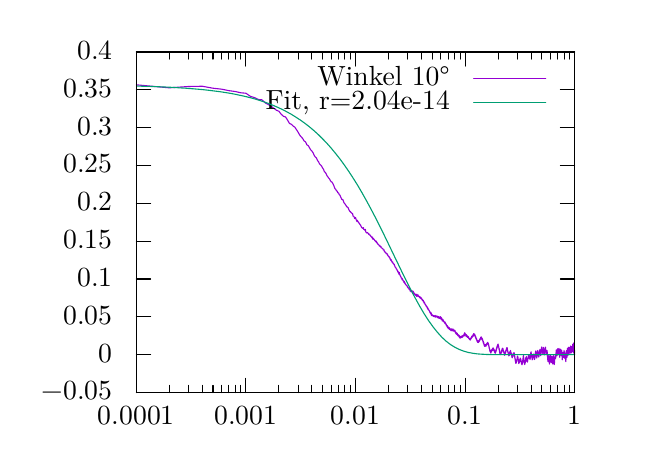
\begin{tikzpicture}[gnuplot]
%% generated with GNUPLOT 5.2p5a (Gentoo revision r0) (Lua 5.1; terminal rev. 99 , script rev. 107)
%% Sa 18 Mai 2019 18:31:10 CEST
\path (0.000,0.000) rectangle (7.500,5.250);
\gpcolor{color=gp lt color border}
\gpsetlinetype{gp lt border}
\gpsetdashtype{gp dt solid}
\gpsetlinewidth{1.00}
\draw[gp path] (1.380,0.616)--(1.560,0.616);
\draw[gp path] (6.947,0.616)--(6.767,0.616);
\node[gp node right] at (1.196,0.616) {$-0.05$};
\draw[gp path] (1.380,1.097)--(1.560,1.097);
\draw[gp path] (6.947,1.097)--(6.767,1.097);
\node[gp node right] at (1.196,1.097) {$0$};
\draw[gp path] (1.380,1.577)--(1.560,1.577);
\draw[gp path] (6.947,1.577)--(6.767,1.577);
\node[gp node right] at (1.196,1.577) {$0.05$};
\draw[gp path] (1.380,2.058)--(1.560,2.058);
\draw[gp path] (6.947,2.058)--(6.767,2.058);
\node[gp node right] at (1.196,2.058) {$0.1$};
\draw[gp path] (1.380,2.538)--(1.560,2.538);
\draw[gp path] (6.947,2.538)--(6.767,2.538);
\node[gp node right] at (1.196,2.538) {$0.15$};
\draw[gp path] (1.380,3.019)--(1.560,3.019);
\draw[gp path] (6.947,3.019)--(6.767,3.019);
\node[gp node right] at (1.196,3.019) {$0.2$};
\draw[gp path] (1.380,3.499)--(1.560,3.499);
\draw[gp path] (6.947,3.499)--(6.767,3.499);
\node[gp node right] at (1.196,3.499) {$0.25$};
\draw[gp path] (1.380,3.980)--(1.560,3.980);
\draw[gp path] (6.947,3.980)--(6.767,3.980);
\node[gp node right] at (1.196,3.980) {$0.3$};
\draw[gp path] (1.380,4.460)--(1.560,4.460);
\draw[gp path] (6.947,4.460)--(6.767,4.460);
\node[gp node right] at (1.196,4.460) {$0.35$};
\draw[gp path] (1.380,4.941)--(1.560,4.941);
\draw[gp path] (6.947,4.941)--(6.767,4.941);
\node[gp node right] at (1.196,4.941) {$0.4$};
\draw[gp path] (1.380,0.616)--(1.380,0.796);
\draw[gp path] (1.380,4.941)--(1.380,4.761);
\node[gp node center] at (1.380,0.308) {$0.0001$};
\draw[gp path] (1.799,0.616)--(1.799,0.706);
\draw[gp path] (1.799,4.941)--(1.799,4.851);
\draw[gp path] (2.044,0.616)--(2.044,0.706);
\draw[gp path] (2.044,4.941)--(2.044,4.851);
\draw[gp path] (2.218,0.616)--(2.218,0.706);
\draw[gp path] (2.218,4.941)--(2.218,4.851);
\draw[gp path] (2.353,0.616)--(2.353,0.706);
\draw[gp path] (2.353,4.941)--(2.353,4.851);
\draw[gp path] (2.463,0.616)--(2.463,0.706);
\draw[gp path] (2.463,4.941)--(2.463,4.851);
\draw[gp path] (2.556,0.616)--(2.556,0.706);
\draw[gp path] (2.556,4.941)--(2.556,4.851);
\draw[gp path] (2.637,0.616)--(2.637,0.706);
\draw[gp path] (2.637,4.941)--(2.637,4.851);
\draw[gp path] (2.708,0.616)--(2.708,0.706);
\draw[gp path] (2.708,4.941)--(2.708,4.851);
\draw[gp path] (2.772,0.616)--(2.772,0.796);
\draw[gp path] (2.772,4.941)--(2.772,4.761);
\node[gp node center] at (2.772,0.308) {$0.001$};
\draw[gp path] (3.191,0.616)--(3.191,0.706);
\draw[gp path] (3.191,4.941)--(3.191,4.851);
\draw[gp path] (3.436,0.616)--(3.436,0.706);
\draw[gp path] (3.436,4.941)--(3.436,4.851);
\draw[gp path] (3.610,0.616)--(3.610,0.706);
\draw[gp path] (3.610,4.941)--(3.610,4.851);
\draw[gp path] (3.745,0.616)--(3.745,0.706);
\draw[gp path] (3.745,4.941)--(3.745,4.851);
\draw[gp path] (3.855,0.616)--(3.855,0.706);
\draw[gp path] (3.855,4.941)--(3.855,4.851);
\draw[gp path] (3.948,0.616)--(3.948,0.706);
\draw[gp path] (3.948,4.941)--(3.948,4.851);
\draw[gp path] (4.029,0.616)--(4.029,0.706);
\draw[gp path] (4.029,4.941)--(4.029,4.851);
\draw[gp path] (4.100,0.616)--(4.100,0.706);
\draw[gp path] (4.100,4.941)--(4.100,4.851);
\draw[gp path] (4.163,0.616)--(4.163,0.796);
\draw[gp path] (4.163,4.941)--(4.163,4.761);
\node[gp node center] at (4.163,0.308) {$0.01$};
\draw[gp path] (4.582,0.616)--(4.582,0.706);
\draw[gp path] (4.582,4.941)--(4.582,4.851);
\draw[gp path] (4.828,0.616)--(4.828,0.706);
\draw[gp path] (4.828,4.941)--(4.828,4.851);
\draw[gp path] (5.001,0.616)--(5.001,0.706);
\draw[gp path] (5.001,4.941)--(5.001,4.851);
\draw[gp path] (5.136,0.616)--(5.136,0.706);
\draw[gp path] (5.136,4.941)--(5.136,4.851);
\draw[gp path] (5.246,0.616)--(5.246,0.706);
\draw[gp path] (5.246,4.941)--(5.246,4.851);
\draw[gp path] (5.340,0.616)--(5.340,0.706);
\draw[gp path] (5.340,4.941)--(5.340,4.851);
\draw[gp path] (5.420,0.616)--(5.420,0.706);
\draw[gp path] (5.420,4.941)--(5.420,4.851);
\draw[gp path] (5.492,0.616)--(5.492,0.706);
\draw[gp path] (5.492,4.941)--(5.492,4.851);
\draw[gp path] (5.555,0.616)--(5.555,0.796);
\draw[gp path] (5.555,4.941)--(5.555,4.761);
\node[gp node center] at (5.555,0.308) {$0.1$};
\draw[gp path] (5.974,0.616)--(5.974,0.706);
\draw[gp path] (5.974,4.941)--(5.974,4.851);
\draw[gp path] (6.219,0.616)--(6.219,0.706);
\draw[gp path] (6.219,4.941)--(6.219,4.851);
\draw[gp path] (6.393,0.616)--(6.393,0.706);
\draw[gp path] (6.393,4.941)--(6.393,4.851);
\draw[gp path] (6.528,0.616)--(6.528,0.706);
\draw[gp path] (6.528,4.941)--(6.528,4.851);
\draw[gp path] (6.638,0.616)--(6.638,0.706);
\draw[gp path] (6.638,4.941)--(6.638,4.851);
\draw[gp path] (6.731,0.616)--(6.731,0.706);
\draw[gp path] (6.731,4.941)--(6.731,4.851);
\draw[gp path] (6.812,0.616)--(6.812,0.706);
\draw[gp path] (6.812,4.941)--(6.812,4.851);
\draw[gp path] (6.883,0.616)--(6.883,0.706);
\draw[gp path] (6.883,4.941)--(6.883,4.851);
\draw[gp path] (6.947,0.616)--(6.947,0.796);
\draw[gp path] (6.947,4.941)--(6.947,4.761);
\node[gp node center] at (6.947,0.308) {$1$};
\draw[gp path] (1.380,4.941)--(1.380,0.616)--(6.947,0.616)--(6.947,4.941)--cycle;
\node[gp node right] at (5.479,4.607) {Winkel 10°};
\gpcolor{rgb color={0.580,0.000,0.827}}
\draw[gp path] (5.663,4.607)--(6.579,4.607);
\draw[gp path] (1.380,4.524)--(1.799,4.486)--(2.044,4.503)--(2.218,4.506)--(2.353,4.481)%
  --(2.463,4.469)--(2.556,4.450)--(2.637,4.439)--(2.708,4.423)--(2.772,4.417)--(2.829,4.378)%
  --(2.882,4.361)--(2.930,4.338)--(2.975,4.334)--(3.017,4.295)--(3.056,4.274)--(3.092,4.253)%
  --(3.127,4.225)--(3.160,4.201)--(3.191,4.188)--(3.220,4.150)--(3.248,4.125)--(3.275,4.116)%
  --(3.301,4.075)--(3.326,4.032)--(3.349,4.023)--(3.372,4.000)--(3.394,3.985)--(3.415,3.953)%
  --(3.436,3.920)--(3.456,3.884)--(3.475,3.862)--(3.493,3.842)--(3.511,3.811)--(3.529,3.800)%
  --(3.546,3.762)--(3.563,3.753)--(3.579,3.725)--(3.594,3.698)--(3.610,3.682)--(3.625,3.661)%
  --(3.639,3.628)--(3.653,3.607)--(3.667,3.596)--(3.681,3.563)--(3.694,3.547)--(3.707,3.519)%
  --(3.720,3.506)--(3.732,3.493)--(3.745,3.469)--(3.757,3.451)--(3.768,3.421)--(3.780,3.412)%
  --(3.791,3.394)--(3.802,3.369)--(3.813,3.354)--(3.824,3.339)--(3.834,3.329)--(3.845,3.307)%
  --(3.855,3.293)--(3.865,3.289)--(3.875,3.271)--(3.884,3.254)--(3.894,3.228)--(3.903,3.204)%
  --(3.912,3.199)--(3.921,3.179)--(3.930,3.175)--(3.939,3.153)--(3.948,3.152)--(3.956,3.130)%
  --(3.965,3.125)--(3.973,3.104)--(3.982,3.085)--(3.990,3.068)--(3.998,3.068)--(4.006,3.060)%
  --(4.013,3.036)--(4.021,3.021)--(4.029,3.013)--(4.036,3.002)--(4.044,2.991)--(4.051,2.976)%
  --(4.058,2.974)--(4.065,2.967)--(4.072,2.959)--(4.079,2.938)--(4.086,2.928)--(4.093,2.914)%
  --(4.100,2.913)--(4.106,2.902)--(4.113,2.898)--(4.120,2.890)--(4.126,2.891)--(4.132,2.856)%
  --(4.139,2.857)--(4.145,2.848)--(4.151,2.829)--(4.157,2.826)--(4.164,2.839)--(4.170,2.817)%
  --(4.175,2.805)--(4.181,2.789)--(4.187,2.804)--(4.193,2.786)--(4.199,2.782)--(4.204,2.773)%
  --(4.210,2.767)--(4.216,2.760)--(4.221,2.746)--(4.227,2.745)--(4.232,2.732)--(4.237,2.723)%
  --(4.243,2.709)--(4.248,2.709)--(4.253,2.703)--(4.258,2.700)--(4.264,2.711)--(4.269,2.686)%
  --(4.274,2.687)--(4.279,2.684)--(4.284,2.674)--(4.289,2.689)--(4.294,2.655)--(4.298,2.651)%
  --(4.303,2.648)--(4.308,2.642)--(4.313,2.649)--(4.317,2.643)--(4.322,2.642)--(4.327,2.634)%
  --(4.331,2.626)--(4.336,2.630)--(4.340,2.615)--(4.345,2.615)--(4.349,2.618)--(4.354,2.612)%
  --(4.358,2.598)--(4.363,2.595)--(4.367,2.596)--(4.371,2.581)--(4.375,2.584)--(4.380,2.590)%
  --(4.384,2.562)--(4.388,2.575)--(4.392,2.564)--(4.396,2.567)--(4.400,2.560)--(4.405,2.550)%
  --(4.409,2.545)--(4.413,2.547)--(4.417,2.536)--(4.421,2.531)--(4.424,2.528)--(4.428,2.539)%
  --(4.432,2.518)--(4.436,2.525)--(4.440,2.511)--(4.444,2.510)--(4.448,2.499)--(4.451,2.501)%
  --(4.455,2.496)--(4.459,2.491)--(4.463,2.486)--(4.466,2.477)--(4.470,2.476)--(4.473,2.484)%
  --(4.477,2.474)--(4.481,2.465)--(4.484,2.467)--(4.488,2.470)--(4.491,2.453)--(4.495,2.455)%
  --(4.498,2.452)--(4.502,2.448)--(4.505,2.445)--(4.509,2.446)--(4.512,2.438)--(4.515,2.428)%
  --(4.519,2.427)--(4.522,2.424)--(4.525,2.429)--(4.529,2.413)--(4.532,2.402)--(4.535,2.404)%
  --(4.539,2.398)--(4.542,2.400)--(4.545,2.400)--(4.548,2.393)--(4.551,2.381)--(4.555,2.383)%
  --(4.558,2.384)--(4.561,2.375)--(4.564,2.379)--(4.567,2.377)--(4.570,2.359)--(4.573,2.367)%
  --(4.576,2.352)--(4.579,2.351)--(4.582,2.351)--(4.585,2.341)--(4.588,2.339)--(4.591,2.342)%
  --(4.594,2.329)--(4.597,2.337)--(4.600,2.316)--(4.603,2.318)--(4.606,2.303)--(4.609,2.311)%
  --(4.612,2.292)--(4.615,2.305)--(4.618,2.299)--(4.621,2.292)--(4.623,2.280)--(4.626,2.283)%
  --(4.629,2.272)--(4.632,2.268)--(4.635,2.276)--(4.637,2.269)--(4.640,2.255)--(4.643,2.255)%
  --(4.646,2.254)--(4.648,2.246)--(4.651,2.249)--(4.654,2.237)--(4.656,2.244)--(4.659,2.229)%
  --(4.662,2.227)--(4.664,2.214)--(4.667,2.209)--(4.670,2.210)--(4.672,2.207)--(4.675,2.200)%
  --(4.677,2.197)--(4.680,2.187)--(4.683,2.187)--(4.685,2.188)--(4.688,2.176)--(4.690,2.179)%
  --(4.693,2.166)--(4.695,2.164)--(4.698,2.163)--(4.700,2.148)--(4.703,2.156)--(4.705,2.150)%
  --(4.708,2.149)--(4.710,2.135)--(4.712,2.134)--(4.715,2.119)--(4.717,2.135)--(4.720,2.143)%
  --(4.722,2.116)--(4.725,2.115)--(4.727,2.120)--(4.729,2.105)--(4.732,2.101)--(4.734,2.094)%
  --(4.736,2.091)--(4.739,2.091)--(4.741,2.082)--(4.743,2.073)--(4.746,2.069)--(4.748,2.074)%
  --(4.750,2.072)--(4.753,2.063)--(4.755,2.046)--(4.757,2.064)--(4.759,2.052)--(4.762,2.054)%
  --(4.764,2.044)--(4.766,2.046)--(4.768,2.039)--(4.771,2.031)--(4.773,2.030)--(4.775,2.034)%
  --(4.777,2.025)--(4.779,2.012)--(4.781,2.022)--(4.784,2.027)--(4.786,2.013)--(4.788,2.014)%
  --(4.790,2.001)--(4.792,2.007)--(4.794,2.005)--(4.797,1.992)--(4.799,1.987)--(4.801,1.993)%
  --(4.803,1.984)--(4.805,1.984)--(4.807,1.980)--(4.809,1.978)--(4.811,1.975)--(4.813,1.976)%
  --(4.815,1.970)--(4.817,1.974)--(4.819,1.965)--(4.821,1.967)--(4.823,1.955)--(4.826,1.959)%
  --(4.828,1.948)--(4.830,1.954)--(4.832,1.943)--(4.834,1.944)--(4.836,1.943)--(4.838,1.947)%
  --(4.840,1.943)--(4.841,1.929)--(4.843,1.933)--(4.845,1.937)--(4.847,1.923)--(4.849,1.939)%
  --(4.851,1.924)--(4.853,1.922)--(4.855,1.929)--(4.857,1.905)--(4.859,1.910)--(4.861,1.905)%
  --(4.863,1.921)--(4.865,1.911)--(4.867,1.902)--(4.868,1.895)--(4.870,1.915)--(4.872,1.899)%
  --(4.874,1.904)--(4.876,1.905)--(4.878,1.896)--(4.880,1.902)--(4.881,1.910)--(4.883,1.907)%
  --(4.885,1.894)--(4.887,1.892)--(4.889,1.875)--(4.891,1.887)--(4.892,1.891)--(4.894,1.891)%
  --(4.896,1.902)--(4.898,1.891)--(4.900,1.893)--(4.901,1.876)--(4.903,1.880)--(4.905,1.878)%
  --(4.907,1.882)--(4.908,1.877)--(4.910,1.871)--(4.912,1.872)--(4.914,1.866)--(4.916,1.861)%
  --(4.917,1.861)--(4.919,1.863)--(4.921,1.868)--(4.922,1.863)--(4.924,1.852)--(4.926,1.856)%
  --(4.928,1.854)--(4.929,1.860)--(4.931,1.851)--(4.933,1.849)--(4.934,1.846)--(4.936,1.856)%
  --(4.938,1.859)--(4.939,1.837)--(4.941,1.866)--(4.943,1.857)--(4.944,1.854)--(4.946,1.844)%
  --(4.948,1.855)--(4.949,1.856)--(4.951,1.843)--(4.953,1.842)--(4.954,1.849)--(4.956,1.836)%
  --(4.958,1.857)--(4.959,1.848)--(4.961,1.848)--(4.962,1.844)--(4.964,1.841)--(4.966,1.836)%
  --(4.967,1.833)--(4.969,1.838)--(4.970,1.830)--(4.972,1.830)--(4.974,1.839)--(4.975,1.830)%
  --(4.977,1.835)--(4.978,1.822)--(4.980,1.833)--(4.981,1.821)--(4.983,1.832)--(4.985,1.817)%
  --(4.986,1.815)--(4.988,1.827)--(4.989,1.828)--(4.991,1.820)--(4.992,1.815)--(4.994,1.822)%
  --(4.995,1.808)--(4.997,1.821)--(4.998,1.803)--(5.000,1.811)--(5.001,1.810)--(5.003,1.810)%
  --(5.004,1.811)--(5.006,1.810)--(5.007,1.801)--(5.009,1.796)--(5.010,1.796)--(5.012,1.787)%
  --(5.013,1.793)--(5.015,1.789)--(5.016,1.796)--(5.018,1.786)--(5.019,1.781)--(5.021,1.781)%
  --(5.022,1.786)--(5.024,1.780)--(5.025,1.786)--(5.027,1.767)--(5.028,1.776)--(5.029,1.771)%
  --(5.031,1.772)--(5.032,1.768)--(5.034,1.752)--(5.035,1.766)--(5.037,1.752)--(5.038,1.755)%
  --(5.039,1.752)--(5.041,1.763)--(5.042,1.747)--(5.044,1.747)--(5.045,1.740)--(5.047,1.739)%
  --(5.048,1.734)--(5.049,1.735)--(5.051,1.738)--(5.052,1.730)--(5.054,1.733)--(5.055,1.726)%
  --(5.056,1.727)--(5.058,1.725)--(5.059,1.721)--(5.060,1.712)--(5.062,1.714)--(5.063,1.715)%
  --(5.064,1.716)--(5.066,1.712)--(5.067,1.704)--(5.069,1.710)--(5.070,1.707)--(5.071,1.702)%
  --(5.073,1.700)--(5.074,1.701)--(5.075,1.694)--(5.077,1.690)--(5.078,1.680)--(5.079,1.699)%
  --(5.081,1.688)--(5.082,1.677)--(5.083,1.684)--(5.085,1.671)--(5.086,1.677)--(5.087,1.667)%
  --(5.089,1.670)--(5.090,1.677)--(5.091,1.664)--(5.092,1.671)--(5.094,1.661)--(5.095,1.659)%
  --(5.096,1.663)--(5.098,1.659)--(5.099,1.656)--(5.100,1.658)--(5.101,1.655)--(5.103,1.648)%
  --(5.104,1.642)--(5.105,1.646)--(5.107,1.639)--(5.108,1.640)--(5.109,1.636)--(5.110,1.630)%
  --(5.112,1.634)--(5.113,1.631)--(5.114,1.630)--(5.115,1.620)--(5.117,1.630)--(5.118,1.637)%
  --(5.119,1.624)--(5.120,1.613)--(5.122,1.623)--(5.123,1.615)--(5.124,1.605)--(5.125,1.600)%
  --(5.127,1.624)--(5.128,1.616)--(5.129,1.597)--(5.130,1.595)--(5.131,1.607)--(5.133,1.601)%
  --(5.134,1.591)--(5.135,1.609)--(5.136,1.599)--(5.137,1.589)--(5.139,1.590)--(5.140,1.599)%
  --(5.141,1.598)--(5.142,1.597)--(5.144,1.589)--(5.145,1.589)--(5.146,1.591)--(5.147,1.589)%
  --(5.148,1.595)--(5.149,1.590)--(5.151,1.594)--(5.152,1.595)--(5.153,1.589)--(5.154,1.588)%
  --(5.155,1.581)--(5.157,1.585)--(5.158,1.583)--(5.159,1.586)--(5.160,1.586)--(5.161,1.583)%
  --(5.162,1.587)--(5.163,1.586)--(5.165,1.586)--(5.166,1.592)--(5.167,1.587)--(5.168,1.586)%
  --(5.169,1.581)--(5.170,1.586)--(5.172,1.576)--(5.173,1.580)--(5.174,1.574)--(5.175,1.584)%
  --(5.176,1.596)--(5.177,1.582)--(5.178,1.587)--(5.179,1.573)--(5.181,1.578)--(5.182,1.591)%
  --(5.183,1.590)--(5.184,1.580)--(5.185,1.583)--(5.186,1.574)--(5.187,1.575)--(5.188,1.576)%
  --(5.189,1.580)--(5.191,1.579)--(5.192,1.582)--(5.193,1.583)--(5.194,1.580)--(5.195,1.578)%
  --(5.196,1.588)--(5.197,1.583)--(5.198,1.579)--(5.199,1.579)--(5.200,1.589)--(5.202,1.578)%
  --(5.203,1.585)--(5.204,1.578)--(5.205,1.577)--(5.206,1.577)--(5.207,1.574)--(5.208,1.566)%
  --(5.209,1.564)--(5.210,1.571)--(5.211,1.581)--(5.212,1.573)--(5.213,1.582)--(5.214,1.575)%
  --(5.215,1.581)--(5.217,1.562)--(5.218,1.572)--(5.219,1.570)--(5.220,1.561)--(5.221,1.580)%
  --(5.222,1.569)--(5.223,1.571)--(5.224,1.575)--(5.225,1.557)--(5.226,1.560)--(5.227,1.565)%
  --(5.228,1.577)--(5.229,1.572)--(5.230,1.560)--(5.231,1.558)--(5.232,1.565)--(5.233,1.575)%
  --(5.234,1.565)--(5.235,1.571)--(5.236,1.574)--(5.237,1.571)--(5.238,1.563)--(5.239,1.560)%
  --(5.240,1.557)--(5.241,1.564)--(5.242,1.561)--(5.243,1.559)--(5.244,1.567)--(5.245,1.581)%
  --(5.246,1.548)--(5.247,1.565)--(5.249,1.562)--(5.250,1.565)--(5.251,1.558)--(5.252,1.566)%
  --(5.253,1.562)--(5.254,1.544)--(5.254,1.560)--(5.255,1.567)--(5.256,1.556)--(5.257,1.555)%
  --(5.258,1.547)--(5.259,1.555)--(5.260,1.546)--(5.261,1.546)--(5.262,1.555)--(5.263,1.526)%
  --(5.264,1.537)--(5.265,1.552)--(5.266,1.529)--(5.267,1.539)--(5.268,1.533)--(5.269,1.540)%
  --(5.270,1.523)--(5.271,1.530)--(5.272,1.530)--(5.273,1.535)--(5.274,1.544)--(5.275,1.528)%
  --(5.276,1.530)--(5.277,1.535)--(5.278,1.525)--(5.279,1.529)--(5.280,1.526)--(5.281,1.518)%
  --(5.282,1.526)--(5.283,1.518)--(5.284,1.522)--(5.285,1.514)--(5.286,1.524)--(5.286,1.516)%
  --(5.287,1.512)--(5.288,1.517)--(5.289,1.506)--(5.290,1.515)--(5.291,1.511)--(5.292,1.511)%
  --(5.293,1.511)--(5.294,1.504)--(5.295,1.501)--(5.296,1.504)--(5.297,1.497)--(5.298,1.502)%
  --(5.299,1.505)--(5.300,1.498)--(5.300,1.513)--(5.301,1.504)--(5.302,1.504)--(5.303,1.489)%
  --(5.304,1.490)--(5.305,1.504)--(5.306,1.492)--(5.307,1.495)--(5.308,1.495)--(5.309,1.489)%
  --(5.310,1.486)--(5.310,1.494)--(5.311,1.491)--(5.312,1.482)--(5.313,1.487)--(5.314,1.487)%
  --(5.315,1.478)--(5.316,1.469)--(5.317,1.483)--(5.318,1.462)--(5.319,1.474)--(5.319,1.466)%
  --(5.320,1.466)--(5.321,1.470)--(5.322,1.462)--(5.323,1.466)--(5.324,1.463)--(5.325,1.468)%
  --(5.326,1.457)--(5.327,1.457)--(5.327,1.450)--(5.328,1.452)--(5.329,1.467)--(5.330,1.445)%
  --(5.331,1.446)--(5.332,1.454)--(5.333,1.459)--(5.334,1.443)--(5.334,1.456)--(5.335,1.440)%
  --(5.336,1.435)--(5.337,1.443)--(5.338,1.450)--(5.339,1.433)--(5.340,1.437)--(5.341,1.443)%
  --(5.341,1.433)--(5.342,1.444)--(5.343,1.438)--(5.344,1.433)--(5.345,1.429)--(5.346,1.449)%
  --(5.347,1.435)--(5.347,1.433)--(5.348,1.426)--(5.349,1.425)--(5.350,1.424)--(5.351,1.433)%
  --(5.352,1.427)--(5.352,1.423)--(5.353,1.442)--(5.354,1.438)--(5.355,1.423)--(5.356,1.423)%
  --(5.357,1.432)--(5.358,1.434)--(5.358,1.416)--(5.359,1.426)--(5.360,1.422)--(5.361,1.421)%
  --(5.362,1.420)--(5.363,1.425)--(5.363,1.415)--(5.364,1.419)--(5.365,1.422)--(5.366,1.423)%
  --(5.367,1.420)--(5.368,1.426)--(5.368,1.425)--(5.369,1.416)--(5.370,1.425)--(5.371,1.409)%
  --(5.372,1.418)--(5.372,1.421)--(5.373,1.417)--(5.374,1.414)--(5.375,1.419)--(5.376,1.399)%
  --(5.377,1.407)--(5.377,1.413)--(5.378,1.400)--(5.379,1.419)--(5.380,1.410)--(5.381,1.408)%
  --(5.381,1.426)--(5.382,1.409)--(5.383,1.421)--(5.384,1.407)--(5.385,1.410)--(5.385,1.413)%
  --(5.386,1.421)--(5.387,1.405)--(5.388,1.406)--(5.389,1.416)--(5.389,1.413)--(5.390,1.415)%
  --(5.391,1.409)--(5.392,1.417)--(5.393,1.401)--(5.393,1.420)--(5.394,1.413)--(5.395,1.402)%
  --(5.396,1.417)--(5.396,1.409)--(5.397,1.412)--(5.398,1.401)--(5.399,1.418)--(5.400,1.407)%
  --(5.400,1.411)--(5.401,1.424)--(5.402,1.411)--(5.403,1.412)--(5.404,1.416)--(5.404,1.407)%
  --(5.405,1.411)--(5.406,1.414)--(5.407,1.410)--(5.407,1.412)--(5.408,1.406)--(5.409,1.408)%
  --(5.410,1.412)--(5.410,1.404)--(5.411,1.395)--(5.412,1.397)--(5.413,1.403)--(5.414,1.396)%
  --(5.414,1.404)--(5.415,1.399)--(5.416,1.403)--(5.417,1.396)--(5.417,1.401)--(5.418,1.397)%
  --(5.419,1.406)--(5.420,1.398)--(5.420,1.405)--(5.421,1.399)--(5.422,1.402)--(5.423,1.409)%
  --(5.423,1.400)--(5.424,1.408)--(5.425,1.398)--(5.426,1.389)--(5.426,1.395)--(5.427,1.406)%
  --(5.428,1.384)--(5.429,1.383)--(5.429,1.389)--(5.430,1.391)--(5.431,1.383)--(5.432,1.375)%
  --(5.432,1.379)--(5.433,1.373)--(5.434,1.378)--(5.435,1.375)--(5.435,1.383)--(5.436,1.387)%
  --(5.437,1.368)--(5.438,1.362)--(5.438,1.377)--(5.439,1.372)--(5.440,1.376)--(5.440,1.370)%
  --(5.441,1.377)--(5.442,1.374)--(5.443,1.375)--(5.443,1.360)--(5.444,1.378)--(5.445,1.367)%
  --(5.446,1.369)--(5.446,1.363)--(5.447,1.370)--(5.448,1.363)--(5.448,1.365)--(5.449,1.357)%
  --(5.450,1.352)--(5.451,1.360)--(5.451,1.369)--(5.452,1.363)--(5.453,1.361)--(5.453,1.356)%
  --(5.454,1.351)--(5.455,1.370)--(5.456,1.354)--(5.456,1.356)--(5.457,1.359)--(5.458,1.355)%
  --(5.458,1.348)--(5.459,1.353)--(5.460,1.353)--(5.461,1.348)--(5.461,1.355)--(5.462,1.342)%
  --(5.463,1.338)--(5.463,1.346)--(5.464,1.344)--(5.465,1.351)--(5.465,1.342)--(5.466,1.342)%
  --(5.467,1.340)--(5.468,1.344)--(5.468,1.332)--(5.469,1.351)--(5.470,1.339)--(5.470,1.341)%
  --(5.471,1.342)--(5.472,1.349)--(5.472,1.348)--(5.473,1.339)--(5.474,1.334)--(5.475,1.330)%
  --(5.475,1.339)--(5.476,1.335)--(5.477,1.337)--(5.477,1.339)--(5.478,1.334)--(5.479,1.328)%
  --(5.479,1.334)--(5.480,1.328)--(5.481,1.319)--(5.481,1.330)--(5.482,1.328)--(5.483,1.340)%
  --(5.483,1.323)--(5.484,1.329)--(5.485,1.314)--(5.485,1.320)--(5.486,1.310)--(5.487,1.322)%
  --(5.488,1.317)--(5.488,1.325)--(5.489,1.316)--(5.490,1.321)--(5.490,1.311)--(5.491,1.328)%
  --(5.492,1.307)--(5.492,1.328)--(5.493,1.328)--(5.494,1.318)--(5.494,1.312)--(5.495,1.313)%
  --(5.496,1.311)--(5.496,1.318)--(5.497,1.311)--(5.498,1.314)--(5.498,1.312)--(5.499,1.311)%
  --(5.500,1.320)--(5.500,1.318)--(5.501,1.319)--(5.502,1.323)--(5.502,1.309)--(5.503,1.315)%
  --(5.504,1.325)--(5.504,1.313)--(5.505,1.318)--(5.506,1.319)--(5.506,1.315)--(5.507,1.318)%
  --(5.507,1.321)--(5.508,1.333)--(5.509,1.318)--(5.509,1.331)--(5.510,1.327)--(5.511,1.331)%
  --(5.511,1.329)--(5.512,1.327)--(5.513,1.316)--(5.513,1.322)--(5.514,1.322)--(5.515,1.327)%
  --(5.515,1.330)--(5.516,1.334)--(5.517,1.330)--(5.517,1.316)--(5.518,1.320)--(5.519,1.331)%
  --(5.520,1.333)--(5.521,1.330)--(5.522,1.326)--(5.522,1.334)--(5.523,1.327)--(5.524,1.338)%
  --(5.524,1.333)--(5.525,1.320)--(5.526,1.325)--(5.526,1.333)--(5.527,1.326)--(5.527,1.343)%
  --(5.528,1.328)--(5.529,1.334)--(5.529,1.332)--(5.530,1.331)--(5.531,1.332)--(5.531,1.338)%
  --(5.532,1.330)--(5.532,1.337)--(5.533,1.337)--(5.534,1.338)--(5.534,1.340)--(5.535,1.338)%
  --(5.536,1.346)--(5.536,1.347)--(5.537,1.340)--(5.537,1.339)--(5.538,1.347)--(5.539,1.338)%
  --(5.539,1.344)--(5.540,1.340)--(5.541,1.361)--(5.541,1.352)--(5.542,1.352)--(5.542,1.350)%
  --(5.543,1.347)--(5.544,1.353)--(5.544,1.358)--(5.545,1.356)--(5.546,1.352)--(5.546,1.336)%
  --(5.547,1.358)--(5.547,1.348)--(5.548,1.342)--(5.549,1.368)--(5.549,1.359)--(5.550,1.345)%
  --(5.550,1.347)--(5.551,1.376)--(5.552,1.361)--(5.552,1.354)--(5.553,1.353)--(5.553,1.352)%
  --(5.554,1.359)--(5.555,1.361)--(5.555,1.357)--(5.556,1.346)--(5.556,1.366)--(5.557,1.360)%
  --(5.558,1.359)--(5.558,1.356)--(5.559,1.346)--(5.559,1.354)--(5.560,1.348)--(5.561,1.361)%
  --(5.561,1.347)--(5.562,1.348)--(5.562,1.352)--(5.563,1.350)--(5.564,1.355)--(5.564,1.345)%
  --(5.565,1.352)--(5.565,1.337)--(5.566,1.331)--(5.567,1.346)--(5.567,1.345)--(5.568,1.345)%
  --(5.568,1.332)--(5.569,1.334)--(5.570,1.334)--(5.570,1.352)--(5.571,1.351)--(5.571,1.346)%
  --(5.572,1.336)--(5.573,1.334)--(5.573,1.331)--(5.574,1.342)--(5.574,1.335)--(5.575,1.332)%
  --(5.576,1.334)--(5.577,1.332)--(5.577,1.345)--(5.578,1.342)--(5.578,1.332)--(5.579,1.336)%
  --(5.580,1.331)--(5.580,1.334)--(5.581,1.334)--(5.581,1.327)--(5.582,1.334)--(5.582,1.323)%
  --(5.583,1.318)--(5.584,1.322)--(5.584,1.338)--(5.585,1.325)--(5.585,1.334)--(5.586,1.321)%
  --(5.586,1.322)--(5.587,1.325)--(5.588,1.327)--(5.588,1.332)--(5.589,1.318)--(5.589,1.327)%
  --(5.590,1.324)--(5.591,1.323)--(5.592,1.323)--(5.592,1.328)--(5.593,1.324)--(5.593,1.319)%
  --(5.594,1.330)--(5.594,1.319)--(5.595,1.320)--(5.596,1.311)--(5.596,1.325)--(5.597,1.320)%
  --(5.597,1.310)--(5.598,1.310)--(5.598,1.326)--(5.599,1.322)--(5.600,1.304)--(5.600,1.310)%
  --(5.601,1.313)--(5.601,1.312)--(5.602,1.304)--(5.602,1.300)--(5.603,1.308)--(5.603,1.309)%
  --(5.604,1.304)--(5.605,1.308)--(5.605,1.298)--(5.606,1.300)--(5.606,1.302)--(5.607,1.304)%
  --(5.607,1.301)--(5.608,1.302)--(5.608,1.299)--(5.609,1.301)--(5.610,1.291)--(5.610,1.303)%
  --(5.611,1.297)--(5.611,1.294)--(5.612,1.289)--(5.612,1.287)--(5.613,1.299)--(5.613,1.290)%
  --(5.614,1.295)--(5.615,1.289)--(5.615,1.298)--(5.616,1.292)--(5.616,1.290)--(5.617,1.294)%
  --(5.617,1.289)--(5.618,1.291)--(5.618,1.300)--(5.619,1.285)--(5.619,1.290)--(5.620,1.287)%
  --(5.621,1.288)--(5.621,1.294)--(5.622,1.292)--(5.622,1.285)--(5.623,1.283)--(5.623,1.288)%
  --(5.624,1.298)--(5.624,1.297)--(5.625,1.288)--(5.625,1.299)--(5.626,1.309)--(5.626,1.303)%
  --(5.627,1.302)--(5.628,1.294)--(5.628,1.296)--(5.629,1.307)--(5.629,1.308)--(5.630,1.312)%
  --(5.630,1.309)--(5.631,1.305)--(5.631,1.307)--(5.632,1.312)--(5.632,1.304)--(5.633,1.313)%
  --(5.633,1.303)--(5.634,1.313)--(5.634,1.307)--(5.635,1.303)--(5.636,1.313)--(5.636,1.321)%
  --(5.637,1.314)--(5.637,1.316)--(5.638,1.317)--(5.638,1.328)--(5.639,1.332)--(5.639,1.320)%
  --(5.640,1.325)--(5.641,1.320)--(5.641,1.313)--(5.642,1.314)--(5.642,1.326)--(5.643,1.327)%
  --(5.643,1.316)--(5.644,1.317)--(5.644,1.325)--(5.645,1.316)--(5.645,1.326)--(5.646,1.323)%
  --(5.647,1.330)--(5.647,1.320)--(5.648,1.333)--(5.648,1.319)--(5.649,1.319)--(5.649,1.323)%
  --(5.650,1.329)--(5.650,1.330)--(5.651,1.328)--(5.651,1.338)--(5.652,1.340)--(5.652,1.342)%
  --(5.653,1.332)--(5.653,1.333)--(5.654,1.338)--(5.654,1.335)--(5.655,1.338)--(5.655,1.329)%
  --(5.656,1.337)--(5.656,1.350)--(5.657,1.327)--(5.657,1.332)--(5.658,1.344)--(5.658,1.340)%
  --(5.659,1.333)--(5.659,1.349)--(5.660,1.340)--(5.660,1.343)--(5.661,1.344)--(5.661,1.354)%
  --(5.662,1.348)--(5.662,1.352)--(5.663,1.354)--(5.663,1.358)--(5.664,1.350)--(5.664,1.365)%
  --(5.665,1.352)--(5.666,1.358)--(5.666,1.350)--(5.667,1.353)--(5.667,1.351)--(5.668,1.342)%
  --(5.668,1.343)--(5.669,1.347)--(5.669,1.356)--(5.670,1.350)--(5.670,1.353)--(5.671,1.360)%
  --(5.671,1.351)--(5.672,1.361)--(5.672,1.357)--(5.673,1.354)--(5.673,1.358)--(5.674,1.360)%
  --(5.674,1.349)--(5.675,1.354)--(5.675,1.358)--(5.676,1.354)--(5.676,1.336)--(5.677,1.343)%
  --(5.677,1.348)--(5.678,1.349)--(5.678,1.343)--(5.679,1.339)--(5.679,1.350)--(5.680,1.348)%
  --(5.680,1.341)--(5.681,1.330)--(5.681,1.348)--(5.682,1.331)--(5.682,1.344)--(5.683,1.327)%
  --(5.683,1.333)--(5.684,1.339)--(5.684,1.326)--(5.685,1.327)--(5.685,1.326)--(5.686,1.323)%
  --(5.686,1.330)--(5.687,1.322)--(5.687,1.315)--(5.688,1.331)--(5.688,1.316)--(5.689,1.311)%
  --(5.689,1.321)--(5.690,1.325)--(5.690,1.315)--(5.691,1.310)--(5.692,1.315)--(5.692,1.307)%
  --(5.693,1.318)--(5.693,1.314)--(5.693,1.297)--(5.694,1.303)--(5.694,1.311)--(5.695,1.304)%
  --(5.695,1.315)--(5.696,1.301)--(5.696,1.304)--(5.697,1.297)--(5.697,1.300)--(5.698,1.305)%
  --(5.698,1.293)--(5.699,1.294)--(5.699,1.299)--(5.700,1.293)--(5.700,1.303)--(5.701,1.303)%
  --(5.701,1.292)--(5.702,1.285)--(5.702,1.280)--(5.703,1.282)--(5.703,1.290)--(5.704,1.280)%
  --(5.704,1.276)--(5.704,1.268)--(5.705,1.278)--(5.705,1.283)--(5.706,1.268)--(5.706,1.279)%
  --(5.707,1.282)--(5.707,1.276)--(5.708,1.269)--(5.708,1.273)--(5.709,1.279)--(5.709,1.267)%
  --(5.710,1.270)--(5.710,1.281)--(5.711,1.266)--(5.711,1.260)--(5.712,1.273)--(5.712,1.276)%
  --(5.712,1.261)--(5.713,1.260)--(5.713,1.274)--(5.714,1.265)--(5.714,1.263)--(5.715,1.273)%
  --(5.715,1.253)--(5.716,1.260)--(5.716,1.263)--(5.717,1.258)--(5.717,1.257)--(5.718,1.268)%
  --(5.718,1.259)--(5.718,1.253)--(5.719,1.262)--(5.719,1.260)--(5.720,1.266)--(5.720,1.261)%
  --(5.721,1.259)--(5.721,1.263)--(5.722,1.259)--(5.722,1.256)--(5.723,1.259)--(5.724,1.251)%
  --(5.724,1.272)--(5.724,1.252)--(5.725,1.261)--(5.725,1.263)--(5.726,1.251)--(5.726,1.274)%
  --(5.727,1.261)--(5.727,1.254)--(5.728,1.261)--(5.728,1.275)--(5.729,1.266)--(5.729,1.259)%
  --(5.729,1.261)--(5.730,1.266)--(5.731,1.263)--(5.731,1.278)--(5.732,1.266)--(5.732,1.267)%
  --(5.733,1.269)--(5.733,1.276)--(5.733,1.271)--(5.734,1.268)--(5.734,1.273)--(5.735,1.274)%
  --(5.736,1.282)--(5.736,1.269)--(5.737,1.265)--(5.737,1.289)--(5.738,1.272)--(5.738,1.285)%
  --(5.739,1.282)--(5.740,1.296)--(5.740,1.281)--(5.741,1.284)--(5.741,1.275)--(5.742,1.287)%
  --(5.742,1.281)--(5.743,1.287)--(5.744,1.290)--(5.744,1.294)--(5.745,1.284)--(5.745,1.299)%
  --(5.746,1.285)--(5.746,1.293)--(5.746,1.298)--(5.747,1.290)--(5.747,1.300)--(5.748,1.292)%
  --(5.748,1.302)--(5.749,1.302)--(5.749,1.305)--(5.749,1.291)--(5.750,1.305)--(5.750,1.304)%
  --(5.751,1.296)--(5.751,1.302)--(5.752,1.302)--(5.752,1.304)--(5.753,1.298)--(5.753,1.315)%
  --(5.753,1.317)--(5.754,1.303)--(5.754,1.305)--(5.755,1.302)--(5.755,1.306)--(5.756,1.302)%
  --(5.756,1.310)--(5.756,1.316)--(5.757,1.297)--(5.757,1.314)--(5.758,1.306)--(5.758,1.313)%
  --(5.759,1.310)--(5.759,1.308)--(5.759,1.315)--(5.760,1.313)--(5.760,1.324)--(5.761,1.306)%
  --(5.761,1.304)--(5.762,1.319)--(5.762,1.311)--(5.762,1.307)--(5.763,1.308)--(5.763,1.319)%
  --(5.764,1.305)--(5.764,1.309)--(5.765,1.311)--(5.765,1.316)--(5.765,1.318)--(5.766,1.306)%
  --(5.766,1.299)--(5.767,1.303)--(5.767,1.304)--(5.768,1.305)--(5.768,1.304)--(5.768,1.294)%
  --(5.769,1.306)--(5.769,1.301)--(5.770,1.287)--(5.770,1.289)--(5.771,1.288)--(5.771,1.292)%
  --(5.771,1.291)--(5.772,1.296)--(5.772,1.289)--(5.773,1.287)--(5.774,1.302)--(5.774,1.298)%
  --(5.774,1.290)--(5.775,1.298)--(5.775,1.297)--(5.776,1.281)--(5.776,1.294)--(5.776,1.277)%
  --(5.777,1.281)--(5.777,1.292)--(5.778,1.290)--(5.778,1.277)--(5.779,1.278)--(5.779,1.280)%
  --(5.779,1.276)--(5.780,1.283)--(5.780,1.278)--(5.781,1.269)--(5.781,1.277)--(5.781,1.267)%
  --(5.782,1.269)--(5.782,1.266)--(5.783,1.261)--(5.783,1.257)--(5.784,1.262)--(5.784,1.258)%
  --(5.784,1.262)--(5.785,1.267)--(5.785,1.264)--(5.786,1.257)--(5.786,1.262)--(5.786,1.249)%
  --(5.787,1.254)--(5.787,1.241)--(5.788,1.265)--(5.788,1.246)--(5.789,1.245)--(5.789,1.255)%
  --(5.789,1.245)--(5.790,1.252)--(5.790,1.248)--(5.791,1.239)--(5.791,1.244)--(5.791,1.237)%
  --(5.792,1.252)--(5.792,1.243)--(5.793,1.233)--(5.793,1.231)--(5.793,1.232)--(5.794,1.227)%
  --(5.794,1.248)--(5.795,1.225)--(5.795,1.222)--(5.795,1.220)--(5.796,1.229)--(5.796,1.231)%
  --(5.797,1.223)--(5.797,1.220)--(5.797,1.218)--(5.798,1.214)--(5.799,1.213)--(5.799,1.214)%
  --(5.800,1.204)--(5.800,1.225)--(5.800,1.206)--(5.801,1.221)--(5.801,1.212)--(5.802,1.210)%
  --(5.802,1.221)--(5.802,1.213)--(5.803,1.215)--(5.803,1.227)--(5.804,1.207)--(5.804,1.210)%
  --(5.804,1.220)--(5.805,1.226)--(5.805,1.202)--(5.806,1.204)--(5.806,1.217)--(5.806,1.209)%
  --(5.807,1.224)--(5.807,1.218)--(5.808,1.203)--(5.808,1.204)--(5.808,1.221)--(5.809,1.208)%
  --(5.809,1.207)--(5.810,1.221)--(5.810,1.209)--(5.810,1.216)--(5.811,1.208)--(5.811,1.211)%
  --(5.812,1.212)--(5.812,1.215)--(5.812,1.204)--(5.813,1.212)--(5.813,1.208)--(5.813,1.213)%
  --(5.814,1.209)--(5.814,1.219)--(5.815,1.212)--(5.815,1.211)--(5.815,1.209)--(5.816,1.217)%
  --(5.816,1.226)--(5.817,1.219)--(5.817,1.211)--(5.817,1.220)--(5.818,1.214)--(5.818,1.215)%
  --(5.819,1.228)--(5.819,1.222)--(5.819,1.216)--(5.820,1.212)--(5.820,1.215)--(5.821,1.220)%
  --(5.821,1.218)--(5.821,1.225)--(5.822,1.219)--(5.822,1.206)--(5.822,1.222)--(5.823,1.218)%
  --(5.823,1.222)--(5.824,1.227)--(5.824,1.223)--(5.824,1.232)--(5.825,1.219)--(5.825,1.214)%
  --(5.826,1.221)--(5.826,1.220)--(5.826,1.226)--(5.827,1.221)--(5.828,1.229)--(5.828,1.225)%
  --(5.828,1.227)--(5.829,1.218)--(5.829,1.223)--(5.829,1.240)--(5.830,1.234)--(5.830,1.231)%
  --(5.831,1.227)--(5.831,1.233)--(5.831,1.237)--(5.832,1.231)--(5.832,1.238)--(5.832,1.241)%
  --(5.833,1.241)--(5.833,1.239)--(5.834,1.240)--(5.834,1.231)--(5.834,1.245)--(5.835,1.228)%
  --(5.835,1.245)--(5.836,1.235)--(5.836,1.238)--(5.836,1.241)--(5.837,1.238)--(5.837,1.237)%
  --(5.837,1.234)--(5.838,1.243)--(5.838,1.248)--(5.839,1.249)--(5.839,1.247)--(5.839,1.249)%
  --(5.840,1.248)--(5.840,1.246)--(5.840,1.237)--(5.841,1.234)--(5.841,1.245)--(5.842,1.254)%
  --(5.842,1.237)--(5.842,1.235)--(5.843,1.245)--(5.843,1.238)--(5.843,1.245)--(5.844,1.255)%
  --(5.844,1.236)--(5.845,1.240)--(5.845,1.238)--(5.845,1.245)--(5.846,1.235)--(5.846,1.243)%
  --(5.846,1.235)--(5.847,1.238)--(5.847,1.231)--(5.848,1.234)--(5.848,1.244)--(5.848,1.233)%
  --(5.849,1.244)--(5.849,1.231)--(5.849,1.232)--(5.850,1.230)--(5.850,1.236)--(5.851,1.226)%
  --(5.851,1.221)--(5.851,1.228)--(5.852,1.224)--(5.852,1.231)--(5.852,1.216)--(5.853,1.220)%
  --(5.853,1.218)--(5.854,1.220)--(5.854,1.221)--(5.854,1.216)--(5.855,1.214)--(5.855,1.207)%
  --(5.855,1.214)--(5.856,1.216)--(5.856,1.208)--(5.857,1.218)--(5.857,1.203)--(5.858,1.195)%
  --(5.858,1.199)--(5.858,1.205)--(5.859,1.192)--(5.859,1.198)--(5.859,1.195)--(5.860,1.197)%
  --(5.860,1.194)--(5.860,1.184)--(5.861,1.192)--(5.861,1.186)--(5.862,1.176)--(5.862,1.180)%
  --(5.862,1.188)--(5.863,1.177)--(5.863,1.179)--(5.863,1.182)--(5.864,1.178)--(5.865,1.171)%
  --(5.865,1.169)--(5.866,1.170)--(5.866,1.173)--(5.866,1.166)--(5.867,1.166)--(5.867,1.161)%
  --(5.868,1.167)--(5.868,1.165)--(5.868,1.150)--(5.869,1.158)--(5.870,1.152)--(5.870,1.150)%
  --(5.871,1.156)--(5.871,1.141)--(5.871,1.146)--(5.872,1.149)--(5.872,1.135)--(5.872,1.143)%
  --(5.873,1.141)--(5.873,1.146)--(5.874,1.144)--(5.874,1.153)--(5.875,1.152)--(5.875,1.144)%
  --(5.875,1.132)--(5.876,1.136)--(5.876,1.127)--(5.876,1.128)--(5.877,1.140)--(5.877,1.133)%
  --(5.877,1.138)--(5.878,1.142)--(5.878,1.134)--(5.878,1.130)--(5.879,1.142)--(5.880,1.129)%
  --(5.880,1.138)--(5.880,1.125)--(5.881,1.124)--(5.881,1.129)--(5.881,1.119)--(5.882,1.127)%
  --(5.882,1.133)--(5.882,1.129)--(5.883,1.116)--(5.883,1.126)--(5.883,1.127)--(5.884,1.127)%
  --(5.884,1.134)--(5.884,1.123)--(5.885,1.134)--(5.885,1.136)--(5.886,1.133)--(5.886,1.129)%
  --(5.886,1.138)--(5.887,1.131)--(5.887,1.139)--(5.887,1.130)--(5.888,1.141)--(5.888,1.138)%
  --(5.889,1.144)--(5.889,1.147)--(5.889,1.145)--(5.890,1.149)--(5.890,1.144)--(5.890,1.137)%
  --(5.891,1.149)--(5.891,1.151)--(5.891,1.149)--(5.892,1.145)--(5.892,1.160)--(5.892,1.150)%
  --(5.893,1.144)--(5.893,1.140)--(5.893,1.150)--(5.894,1.144)--(5.894,1.161)--(5.895,1.158)%
  --(5.895,1.161)--(5.896,1.146)--(5.896,1.142)--(5.896,1.166)--(5.897,1.154)--(5.897,1.157)%
  --(5.897,1.150)--(5.898,1.154)--(5.898,1.162)--(5.898,1.157)--(5.899,1.166)--(5.899,1.158)%
  --(5.899,1.160)--(5.900,1.157)--(5.900,1.162)--(5.900,1.165)--(5.901,1.164)--(5.901,1.161)%
  --(5.901,1.166)--(5.902,1.155)--(5.902,1.158)--(5.902,1.166)--(5.903,1.156)--(5.903,1.163)%
  --(5.903,1.170)--(5.904,1.161)--(5.904,1.151)--(5.904,1.174)--(5.905,1.171)--(5.905,1.169)%
  --(5.905,1.170)--(5.906,1.161)--(5.906,1.177)--(5.906,1.174)--(5.907,1.160)--(5.907,1.170)%
  --(5.907,1.181)--(5.908,1.182)--(5.908,1.166)--(5.909,1.171)--(5.909,1.178)--(5.909,1.170)%
  --(5.910,1.174)--(5.910,1.182)--(5.910,1.171)--(5.911,1.176)--(5.911,1.172)--(5.911,1.183)%
  --(5.912,1.183)--(5.912,1.174)--(5.912,1.168)--(5.913,1.171)--(5.913,1.179)--(5.913,1.168)%
  --(5.914,1.176)--(5.914,1.182)--(5.914,1.170)--(5.915,1.181)--(5.915,1.172)--(5.915,1.173)%
  --(5.916,1.176)--(5.916,1.161)--(5.916,1.169)--(5.917,1.168)--(5.917,1.166)--(5.917,1.165)%
  --(5.918,1.164)--(5.918,1.163)--(5.918,1.162)--(5.919,1.161)--(5.919,1.160)--(5.919,1.167)%
  --(5.920,1.167)--(5.920,1.156)--(5.920,1.164)--(5.921,1.146)--(5.921,1.154)--(5.921,1.159)%
  --(5.922,1.160)--(5.922,1.157)--(5.922,1.147)--(5.923,1.158)--(5.923,1.152)--(5.923,1.161)%
  --(5.924,1.154)--(5.924,1.166)--(5.924,1.164)--(5.925,1.149)--(5.925,1.140)--(5.925,1.147)%
  --(5.926,1.144)--(5.926,1.147)--(5.927,1.157)--(5.927,1.141)--(5.927,1.154)--(5.928,1.150)%
  --(5.928,1.138)--(5.928,1.135)--(5.929,1.137)--(5.929,1.133)--(5.929,1.135)--(5.930,1.140)%
  --(5.930,1.150)--(5.930,1.140)--(5.931,1.134)--(5.931,1.128)--(5.931,1.138)--(5.932,1.135)%
  --(5.932,1.125)--(5.932,1.131)--(5.933,1.133)--(5.933,1.129)--(5.933,1.143)--(5.934,1.139)%
  --(5.934,1.138)--(5.934,1.124)--(5.935,1.127)--(5.935,1.118)--(5.936,1.123)--(5.936,1.134)%
  --(5.936,1.128)--(5.936,1.129)--(5.937,1.132)--(5.937,1.136)--(5.937,1.130)--(5.938,1.139)%
  --(5.938,1.124)--(5.938,1.114)--(5.939,1.122)--(5.939,1.114)--(5.939,1.128)--(5.940,1.123)%
  --(5.940,1.133)--(5.940,1.124)--(5.941,1.128)--(5.941,1.121)--(5.941,1.132)--(5.942,1.126)%
  --(5.942,1.133)--(5.942,1.121)--(5.943,1.127)--(5.943,1.126)--(5.943,1.134)--(5.944,1.130)%
  --(5.944,1.134)--(5.944,1.133)--(5.944,1.138)--(5.945,1.138)--(5.945,1.137)--(5.945,1.138)%
  --(5.946,1.143)--(5.946,1.134)--(5.947,1.145)--(5.947,1.141)--(5.947,1.145)--(5.948,1.156)%
  --(5.948,1.143)--(5.948,1.138)--(5.949,1.152)--(5.949,1.147)--(5.949,1.152)--(5.950,1.159)%
  --(5.950,1.153)--(5.950,1.164)--(5.950,1.165)--(5.951,1.149)--(5.951,1.156)--(5.951,1.155)%
  --(5.952,1.155)--(5.952,1.160)--(5.953,1.168)--(5.953,1.176)--(5.953,1.169)--(5.954,1.162)%
  --(5.954,1.168)--(5.954,1.181)--(5.955,1.182)--(5.955,1.177)--(5.955,1.179)--(5.955,1.176)%
  --(5.956,1.179)--(5.956,1.180)--(5.957,1.172)--(5.957,1.188)--(5.957,1.189)--(5.958,1.183)%
  --(5.958,1.195)--(5.958,1.188)--(5.959,1.191)--(5.959,1.192)--(5.959,1.194)--(5.960,1.195)%
  --(5.960,1.188)--(5.960,1.194)--(5.960,1.201)--(5.961,1.197)--(5.962,1.207)--(5.962,1.182)%
  --(5.962,1.211)--(5.963,1.202)--(5.963,1.199)--(5.963,1.203)--(5.964,1.205)--(5.964,1.200)%
  --(5.964,1.208)--(5.964,1.211)--(5.965,1.208)--(5.965,1.195)--(5.965,1.206)--(5.966,1.206)%
  --(5.966,1.212)--(5.966,1.215)--(5.967,1.203)--(5.967,1.208)--(5.967,1.212)--(5.968,1.217)%
  --(5.968,1.203)--(5.968,1.214)--(5.968,1.219)--(5.969,1.221)--(5.969,1.219)--(5.969,1.225)%
  --(5.970,1.215)--(5.970,1.222)--(5.970,1.219)--(5.971,1.226)--(5.971,1.219)--(5.971,1.221)%
  --(5.971,1.212)--(5.972,1.214)--(5.972,1.216)--(5.972,1.224)--(5.973,1.219)--(5.973,1.215)%
  --(5.973,1.225)--(5.974,1.233)--(5.974,1.223)--(5.974,1.217)--(5.975,1.221)--(5.975,1.228)%
  --(5.975,1.213)--(5.976,1.212)--(5.976,1.207)--(5.976,1.222)--(5.977,1.213)--(5.977,1.214)%
  --(5.977,1.213)--(5.978,1.212)--(5.978,1.216)--(5.978,1.212)--(5.978,1.208)--(5.979,1.202)%
  --(5.979,1.192)--(5.979,1.200)--(5.980,1.210)--(5.980,1.202)--(5.980,1.196)--(5.981,1.205)%
  --(5.981,1.194)--(5.981,1.195)--(5.981,1.203)--(5.982,1.190)--(5.982,1.200)--(5.982,1.192)%
  --(5.983,1.197)--(5.983,1.190)--(5.983,1.194)--(5.984,1.178)--(5.984,1.186)--(5.984,1.193)%
  --(5.984,1.190)--(5.985,1.181)--(5.985,1.186)--(5.985,1.179)--(5.986,1.165)--(5.986,1.176)%
  --(5.986,1.177)--(5.986,1.173)--(5.987,1.162)--(5.987,1.174)--(5.987,1.165)--(5.988,1.164)%
  --(5.988,1.178)--(5.988,1.176)--(5.989,1.170)--(5.989,1.156)--(5.989,1.161)--(5.990,1.159)%
  --(5.990,1.162)--(5.990,1.147)--(5.991,1.153)--(5.991,1.148)--(5.991,1.142)--(5.991,1.143)%
  --(5.992,1.138)--(5.992,1.145)--(5.992,1.148)--(5.993,1.139)--(5.993,1.149)--(5.993,1.134)%
  --(5.994,1.138)--(5.994,1.125)--(5.994,1.141)--(5.994,1.132)--(5.995,1.133)--(5.995,1.119)%
  --(5.995,1.124)--(5.996,1.127)--(5.996,1.124)--(5.996,1.116)--(5.996,1.122)--(5.997,1.121)%
  --(5.997,1.116)--(5.997,1.133)--(5.998,1.126)--(5.998,1.120)--(5.998,1.114)--(5.998,1.112)%
  --(5.999,1.120)--(5.999,1.100)--(5.999,1.110)--(6.000,1.110)--(6.000,1.107)--(6.000,1.114)%
  --(6.001,1.112)--(6.001,1.111)--(6.001,1.110)--(6.001,1.104)--(6.002,1.101)--(6.002,1.097)%
  --(6.002,1.106)--(6.003,1.107)--(6.003,1.106)--(6.003,1.115)--(6.004,1.098)--(6.004,1.105)%
  --(6.004,1.111)--(6.005,1.116)--(6.005,1.115)--(6.005,1.099)--(6.005,1.113)--(6.006,1.113)%
  --(6.006,1.104)--(6.006,1.120)--(6.007,1.115)--(6.007,1.113)--(6.007,1.103)--(6.007,1.126)%
  --(6.008,1.113)--(6.008,1.120)--(6.008,1.119)--(6.009,1.116)--(6.009,1.111)--(6.009,1.126)%
  --(6.009,1.124)--(6.010,1.102)--(6.010,1.114)--(6.010,1.122)--(6.011,1.126)--(6.011,1.122)%
  --(6.011,1.108)--(6.011,1.115)--(6.012,1.126)--(6.012,1.122)--(6.012,1.121)--(6.013,1.125)%
  --(6.013,1.121)--(6.014,1.125)--(6.014,1.130)--(6.014,1.134)--(6.015,1.131)--(6.015,1.125)%
  --(6.015,1.131)--(6.015,1.130)--(6.016,1.136)--(6.016,1.129)--(6.016,1.135)--(6.017,1.139)%
  --(6.017,1.135)--(6.017,1.134)--(6.017,1.124)--(6.018,1.132)--(6.018,1.150)--(6.018,1.142)%
  --(6.018,1.145)--(6.019,1.129)--(6.019,1.138)--(6.019,1.144)--(6.020,1.127)--(6.020,1.132)%
  --(6.020,1.141)--(6.021,1.145)--(6.021,1.131)--(6.021,1.148)--(6.022,1.140)--(6.022,1.157)%
  --(6.022,1.144)--(6.022,1.154)--(6.023,1.156)--(6.023,1.141)--(6.023,1.165)--(6.024,1.150)%
  --(6.024,1.160)--(6.024,1.156)--(6.024,1.160)--(6.025,1.159)--(6.025,1.156)--(6.025,1.166)%
  --(6.025,1.169)--(6.026,1.157)--(6.026,1.153)--(6.026,1.160)--(6.027,1.177)--(6.027,1.173)%
  --(6.027,1.152)--(6.027,1.173)--(6.028,1.149)--(6.028,1.168)--(6.028,1.175)--(6.029,1.177)%
  --(6.029,1.169)--(6.029,1.158)--(6.030,1.176)--(6.030,1.167)--(6.030,1.171)--(6.030,1.166)%
  --(6.031,1.162)--(6.031,1.169)--(6.031,1.176)--(6.032,1.169)--(6.032,1.176)--(6.032,1.163)%
  --(6.033,1.164)--(6.033,1.176)--(6.033,1.158)--(6.033,1.175)--(6.034,1.174)--(6.034,1.167)%
  --(6.034,1.180)--(6.035,1.165)--(6.035,1.164)--(6.035,1.158)--(6.036,1.163)--(6.036,1.154)%
  --(6.036,1.160)--(6.036,1.155)--(6.037,1.164)--(6.037,1.172)--(6.037,1.154)--(6.038,1.157)%
  --(6.038,1.158)--(6.038,1.160)--(6.038,1.152)--(6.039,1.152)--(6.039,1.148)--(6.039,1.158)%
  --(6.039,1.156)--(6.040,1.152)--(6.040,1.142)--(6.041,1.151)--(6.041,1.148)--(6.041,1.137)%
  --(6.041,1.152)--(6.042,1.136)--(6.042,1.147)--(6.042,1.154)--(6.042,1.147)--(6.043,1.143)%
  --(6.043,1.146)--(6.043,1.148)--(6.044,1.145)--(6.044,1.136)--(6.044,1.142)--(6.044,1.143)%
  --(6.045,1.133)--(6.045,1.126)--(6.045,1.136)--(6.046,1.130)--(6.046,1.141)--(6.046,1.143)%
  --(6.046,1.138)--(6.047,1.123)--(6.047,1.128)--(6.047,1.125)--(6.048,1.136)--(6.048,1.128)%
  --(6.048,1.129)--(6.048,1.115)--(6.049,1.115)--(6.049,1.122)--(6.049,1.132)--(6.049,1.136)%
  --(6.050,1.125)--(6.050,1.127)--(6.050,1.126)--(6.050,1.123)--(6.051,1.123)--(6.051,1.115)%
  --(6.051,1.124)--(6.052,1.116)--(6.052,1.111)--(6.052,1.127)--(6.052,1.124)--(6.053,1.120)%
  --(6.053,1.113)--(6.053,1.117)--(6.054,1.116)--(6.054,1.108)--(6.054,1.105)--(6.054,1.114)%
  --(6.055,1.113)--(6.055,1.114)--(6.055,1.113)--(6.056,1.094)--(6.056,1.089)--(6.056,1.108)%
  --(6.056,1.106)--(6.057,1.114)--(6.057,1.106)--(6.057,1.108)--(6.057,1.102)--(6.058,1.105)%
  --(6.058,1.097)--(6.058,1.104)--(6.058,1.116)--(6.059,1.105)--(6.059,1.093)--(6.059,1.104)%
  --(6.059,1.108)--(6.060,1.106)--(6.060,1.101)--(6.060,1.120)--(6.061,1.098)--(6.061,1.106)%
  --(6.061,1.102)--(6.061,1.109)--(6.062,1.101)--(6.062,1.100)--(6.062,1.104)--(6.062,1.105)%
  --(6.063,1.107)--(6.063,1.118)--(6.063,1.115)--(6.063,1.119)--(6.064,1.113)--(6.064,1.112)%
  --(6.064,1.115)--(6.064,1.112)--(6.065,1.117)--(6.065,1.121)--(6.065,1.128)--(6.065,1.112)%
  --(6.066,1.113)--(6.066,1.116)--(6.066,1.121)--(6.067,1.117)--(6.067,1.125)--(6.067,1.126)%
  --(6.067,1.116)--(6.068,1.120)--(6.068,1.124)--(6.068,1.122)--(6.069,1.132)--(6.069,1.125)%
  --(6.069,1.130)--(6.069,1.133)--(6.070,1.118)--(6.070,1.144)--(6.070,1.134)--(6.070,1.132)%
  --(6.071,1.138)--(6.071,1.128)--(6.071,1.126)--(6.071,1.134)--(6.072,1.131)--(6.072,1.134)%
  --(6.072,1.138)--(6.072,1.149)--(6.073,1.142)--(6.073,1.128)--(6.073,1.141)--(6.073,1.146)%
  --(6.074,1.142)--(6.075,1.149)--(6.075,1.153)--(6.075,1.155)--(6.075,1.141)--(6.076,1.148)%
  --(6.076,1.163)--(6.076,1.153)--(6.076,1.155)--(6.077,1.155)--(6.077,1.158)--(6.077,1.167)%
  --(6.077,1.163)--(6.078,1.164)--(6.078,1.155)--(6.078,1.163)--(6.078,1.167)--(6.079,1.162)%
  --(6.079,1.170)--(6.079,1.169)--(6.079,1.167)--(6.080,1.173)--(6.080,1.170)--(6.080,1.167)%
  --(6.080,1.166)--(6.081,1.172)--(6.081,1.174)--(6.081,1.175)--(6.081,1.165)--(6.082,1.178)%
  --(6.082,1.181)--(6.082,1.180)--(6.082,1.175)--(6.083,1.179)--(6.083,1.175)--(6.083,1.173)%
  --(6.083,1.183)--(6.084,1.179)--(6.084,1.184)--(6.084,1.178)--(6.084,1.179)--(6.085,1.185)%
  --(6.085,1.179)--(6.085,1.177)--(6.085,1.175)--(6.086,1.177)--(6.086,1.179)--(6.086,1.187)%
  --(6.086,1.175)--(6.087,1.180)--(6.087,1.170)--(6.087,1.181)--(6.087,1.173)--(6.088,1.168)%
  --(6.088,1.179)--(6.088,1.181)--(6.088,1.176)--(6.089,1.187)--(6.089,1.178)--(6.089,1.171)%
  --(6.089,1.157)--(6.090,1.160)--(6.090,1.171)--(6.090,1.169)--(6.090,1.171)--(6.091,1.183)%
  --(6.091,1.162)--(6.091,1.161)--(6.091,1.171)--(6.092,1.152)--(6.092,1.176)--(6.092,1.155)%
  --(6.092,1.158)--(6.093,1.152)--(6.093,1.160)--(6.093,1.152)--(6.093,1.151)--(6.094,1.147)%
  --(6.094,1.161)--(6.094,1.149)--(6.094,1.151)--(6.095,1.149)--(6.095,1.145)--(6.095,1.142)%
  --(6.095,1.145)--(6.096,1.134)--(6.096,1.148)--(6.096,1.144)--(6.096,1.143)--(6.097,1.142)%
  --(6.097,1.141)--(6.097,1.148)--(6.097,1.142)--(6.098,1.135)--(6.098,1.144)--(6.098,1.141)%
  --(6.098,1.135)--(6.099,1.125)--(6.099,1.141)--(6.099,1.133)--(6.099,1.127)--(6.100,1.123)%
  --(6.100,1.122)--(6.100,1.134)--(6.100,1.129)--(6.101,1.115)--(6.101,1.129)--(6.101,1.123)%
  --(6.101,1.126)--(6.102,1.117)--(6.102,1.120)--(6.102,1.123)--(6.102,1.116)--(6.103,1.119)%
  --(6.103,1.114)--(6.103,1.112)--(6.103,1.113)--(6.103,1.125)--(6.104,1.114)--(6.104,1.121)%
  --(6.104,1.111)--(6.105,1.107)--(6.105,1.109)--(6.105,1.095)--(6.105,1.100)--(6.106,1.103)%
  --(6.106,1.098)--(6.106,1.103)--(6.106,1.095)--(6.107,1.106)--(6.107,1.094)--(6.107,1.099)%
  --(6.108,1.087)--(6.108,1.107)--(6.108,1.095)--(6.108,1.092)--(6.109,1.089)--(6.109,1.091)%
  --(6.109,1.088)--(6.110,1.098)--(6.110,1.094)--(6.110,1.089)--(6.110,1.088)--(6.111,1.092)%
  --(6.111,1.087)--(6.111,1.080)--(6.111,1.095)--(6.111,1.092)--(6.112,1.083)--(6.112,1.084)%
  --(6.112,1.093)--(6.112,1.088)--(6.113,1.094)--(6.113,1.093)--(6.113,1.094)--(6.113,1.097)%
  --(6.114,1.094)--(6.114,1.092)--(6.114,1.105)--(6.114,1.110)--(6.115,1.091)--(6.115,1.097)%
  --(6.115,1.110)--(6.115,1.100)--(6.116,1.106)--(6.116,1.101)--(6.116,1.097)--(6.116,1.113)%
  --(6.117,1.102)--(6.117,1.088)--(6.117,1.091)--(6.117,1.108)--(6.117,1.111)--(6.118,1.109)%
  --(6.118,1.111)--(6.118,1.101)--(6.118,1.112)--(6.119,1.102)--(6.119,1.118)--(6.119,1.117)%
  --(6.119,1.121)--(6.120,1.109)--(6.120,1.120)--(6.120,1.114)--(6.120,1.119)--(6.121,1.127)%
  --(6.121,1.113)--(6.121,1.121)--(6.121,1.118)--(6.122,1.114)--(6.122,1.119)--(6.122,1.124)%
  --(6.122,1.125)--(6.122,1.121)--(6.123,1.118)--(6.123,1.127)--(6.123,1.131)--(6.123,1.128)%
  --(6.124,1.117)--(6.124,1.131)--(6.124,1.140)--(6.124,1.135)--(6.125,1.134)--(6.125,1.128)%
  --(6.125,1.123)--(6.125,1.130)--(6.126,1.117)--(6.126,1.130)--(6.126,1.139)--(6.126,1.113)%
  --(6.126,1.143)--(6.127,1.133)--(6.127,1.130)--(6.127,1.133)--(6.127,1.134)--(6.128,1.135)%
  --(6.128,1.123)--(6.128,1.133)--(6.129,1.140)--(6.129,1.142)--(6.129,1.141)--(6.130,1.142)%
  --(6.130,1.133)--(6.130,1.139)--(6.130,1.138)--(6.130,1.130)--(6.131,1.134)--(6.131,1.137)%
  --(6.131,1.133)--(6.131,1.145)--(6.132,1.127)--(6.132,1.145)--(6.132,1.137)--(6.132,1.144)%
  --(6.133,1.146)--(6.133,1.134)--(6.133,1.151)--(6.133,1.142)--(6.133,1.137)--(6.134,1.135)%
  --(6.134,1.136)--(6.134,1.131)--(6.134,1.130)--(6.135,1.124)--(6.135,1.135)--(6.135,1.129)%
  --(6.135,1.134)--(6.136,1.127)--(6.136,1.116)--(6.136,1.127)--(6.136,1.131)--(6.136,1.123)%
  --(6.137,1.116)--(6.137,1.114)--(6.137,1.131)--(6.137,1.123)--(6.138,1.130)--(6.138,1.126)%
  --(6.138,1.116)--(6.138,1.122)--(6.139,1.115)--(6.139,1.119)--(6.139,1.122)--(6.139,1.112)%
  --(6.139,1.110)--(6.140,1.123)--(6.140,1.115)--(6.140,1.107)--(6.140,1.119)--(6.141,1.116)%
  --(6.141,1.112)--(6.141,1.102)--(6.141,1.112)--(6.142,1.107)--(6.142,1.113)--(6.142,1.098)%
  --(6.142,1.102)--(6.142,1.104)--(6.143,1.101)--(6.143,1.103)--(6.143,1.101)--(6.143,1.098)%
  --(6.144,1.105)--(6.144,1.093)--(6.144,1.103)--(6.144,1.104)--(6.145,1.102)--(6.145,1.093)%
  --(6.145,1.101)--(6.145,1.084)--(6.145,1.099)--(6.146,1.102)--(6.146,1.086)--(6.146,1.101)%
  --(6.147,1.083)--(6.147,1.087)--(6.147,1.076)--(6.147,1.084)--(6.147,1.090)--(6.148,1.077)%
  --(6.148,1.085)--(6.148,1.080)--(6.148,1.085)--(6.149,1.085)--(6.149,1.087)--(6.149,1.093)%
  --(6.149,1.080)--(6.150,1.076)--(6.150,1.070)--(6.150,1.087)--(6.150,1.076)--(6.150,1.069)%
  --(6.151,1.069)--(6.151,1.061)--(6.151,1.069)--(6.152,1.080)--(6.152,1.070)--(6.152,1.073)%
  --(6.152,1.070)--(6.152,1.061)--(6.153,1.069)--(6.153,1.078)--(6.153,1.065)--(6.153,1.073)%
  --(6.154,1.069)--(6.154,1.074)--(6.154,1.071)--(6.154,1.057)--(6.154,1.069)--(6.155,1.070)%
  --(6.155,1.071)--(6.155,1.073)--(6.155,1.071)--(6.156,1.073)--(6.156,1.067)--(6.156,1.065)%
  --(6.156,1.071)--(6.156,1.072)--(6.157,1.081)--(6.157,1.068)--(6.157,1.075)--(6.157,1.068)%
  --(6.158,1.076)--(6.158,1.073)--(6.158,1.078)--(6.158,1.077)--(6.159,1.072)--(6.159,1.074)%
  --(6.159,1.071)--(6.159,1.076)--(6.159,1.072)--(6.160,1.089)--(6.160,1.072)--(6.160,1.078)%
  --(6.161,1.083)--(6.161,1.085)--(6.161,1.086)--(6.161,1.087)--(6.161,1.080)--(6.162,1.084)%
  --(6.162,1.081)--(6.162,1.078)--(6.162,1.085)--(6.163,1.089)--(6.163,1.088)--(6.163,1.095)%
  --(6.163,1.099)--(6.163,1.094)--(6.164,1.091)--(6.164,1.099)--(6.164,1.087)--(6.164,1.092)%
  --(6.164,1.090)--(6.165,1.095)--(6.165,1.101)--(6.165,1.088)--(6.165,1.094)--(6.166,1.093)%
  --(6.166,1.100)--(6.166,1.114)--(6.166,1.106)--(6.166,1.104)--(6.167,1.092)--(6.167,1.108)%
  --(6.167,1.103)--(6.167,1.116)--(6.168,1.104)--(6.168,1.099)--(6.168,1.109)--(6.168,1.107)%
  --(6.168,1.102)--(6.169,1.097)--(6.169,1.109)--(6.169,1.097)--(6.169,1.106)--(6.170,1.103)%
  --(6.170,1.107)--(6.170,1.110)--(6.170,1.114)--(6.170,1.109)--(6.171,1.108)--(6.171,1.101)%
  --(6.171,1.108)--(6.171,1.105)--(6.172,1.106)--(6.172,1.110)--(6.172,1.102)--(6.172,1.106)%
  --(6.172,1.112)--(6.173,1.105)--(6.173,1.112)--(6.173,1.102)--(6.173,1.112)--(6.173,1.105)%
  --(6.174,1.111)--(6.174,1.107)--(6.174,1.120)--(6.174,1.110)--(6.175,1.112)--(6.175,1.108)%
  --(6.175,1.112)--(6.175,1.108)--(6.175,1.106)--(6.176,1.099)--(6.176,1.112)--(6.176,1.109)%
  --(6.177,1.106)--(6.177,1.109)--(6.177,1.125)--(6.177,1.109)--(6.177,1.104)--(6.178,1.102)%
  --(6.178,1.113)--(6.178,1.109)--(6.178,1.111)--(6.178,1.117)--(6.179,1.113)--(6.179,1.107)%
  --(6.179,1.104)--(6.179,1.116)--(6.180,1.089)--(6.180,1.104)--(6.180,1.108)--(6.180,1.092)%
  --(6.180,1.101)--(6.181,1.095)--(6.181,1.102)--(6.181,1.085)--(6.181,1.095)--(6.181,1.110)%
  --(6.182,1.097)--(6.182,1.106)--(6.182,1.093)--(6.182,1.097)--(6.183,1.086)--(6.183,1.089)%
  --(6.183,1.070)--(6.183,1.088)--(6.184,1.088)--(6.184,1.085)--(6.184,1.081)--(6.184,1.072)%
  --(6.185,1.081)--(6.185,1.071)--(6.185,1.068)--(6.185,1.080)--(6.186,1.062)--(6.186,1.069)%
  --(6.186,1.060)--(6.186,1.066)--(6.186,1.065)--(6.187,1.060)--(6.187,1.069)--(6.187,1.066)%
  --(6.187,1.054)--(6.188,1.061)--(6.188,1.053)--(6.188,1.044)--(6.188,1.056)--(6.188,1.058)%
  --(6.189,1.053)--(6.189,1.044)--(6.189,1.049)--(6.189,1.041)--(6.190,1.045)--(6.190,1.032)%
  --(6.190,1.044)--(6.190,1.023)--(6.191,1.037)--(6.191,1.034)--(6.191,1.040)--(6.191,1.028)%
  --(6.191,1.043)--(6.192,1.041)--(6.192,1.039)--(6.192,1.038)--(6.192,1.027)--(6.193,1.027)%
  --(6.193,1.016)--(6.193,1.023)--(6.193,1.027)--(6.193,1.016)--(6.194,1.020)--(6.194,1.022)%
  --(6.194,1.018)--(6.194,1.021)--(6.194,1.010)--(6.195,1.015)--(6.195,1.019)--(6.195,1.014)%
  --(6.195,1.015)--(6.195,1.008)--(6.196,1.011)--(6.196,1.005)--(6.196,0.991)--(6.196,1.008)%
  --(6.196,1.012)--(6.197,1.009)--(6.197,1.002)--(6.197,1.007)--(6.198,0.999)--(6.198,0.989)%
  --(6.198,0.993)--(6.198,0.997)--(6.198,0.998)--(6.199,0.996)--(6.199,0.986)--(6.199,0.996)%
  --(6.199,0.992)--(6.200,0.993)--(6.200,0.990)--(6.200,1.002)--(6.200,0.999)--(6.201,0.998)%
  --(6.201,0.996)--(6.201,0.993)--(6.201,0.996)--(6.201,0.993)--(6.202,0.998)--(6.202,1.005)%
  --(6.202,0.990)--(6.202,0.998)--(6.203,0.996)--(6.203,1.002)--(6.203,1.006)--(6.203,0.995)%
  --(6.204,0.995)--(6.204,1.004)--(6.204,1.007)--(6.204,1.002)--(6.204,0.999)--(6.205,0.990)%
  --(6.205,1.006)--(6.205,1.009)--(6.205,1.014)--(6.205,0.999)--(6.206,0.997)--(6.206,1.003)%
  --(6.206,1.002)--(6.206,1.011)--(6.206,1.019)--(6.207,1.013)--(6.207,1.001)--(6.207,1.008)%
  --(6.207,1.007)--(6.208,1.019)--(6.208,1.005)--(6.208,1.021)--(6.208,1.018)--(6.209,1.023)%
  --(6.209,1.017)--(6.209,1.016)--(6.209,1.013)--(6.210,1.016)--(6.210,1.011)--(6.210,1.023)%
  --(6.210,1.015)--(6.210,1.029)--(6.211,1.031)--(6.211,1.034)--(6.211,1.022)--(6.211,1.013)%
  --(6.211,1.022)--(6.212,1.012)--(6.212,1.032)--(6.212,1.020)--(6.212,1.029)--(6.212,1.026)%
  --(6.213,1.037)--(6.213,1.026)--(6.213,1.023)--(6.213,1.036)--(6.213,1.040)--(6.214,1.034)%
  --(6.214,1.027)--(6.214,1.042)--(6.214,1.037)--(6.214,1.040)--(6.215,1.031)--(6.215,1.045)%
  --(6.215,1.043)--(6.215,1.031)--(6.215,1.043)--(6.216,1.042)--(6.216,1.055)--(6.216,1.042)%
  --(6.216,1.049)--(6.216,1.052)--(6.217,1.042)--(6.217,1.043)--(6.217,1.051)--(6.217,1.053)%
  --(6.217,1.056)--(6.218,1.072)--(6.218,1.056)--(6.218,1.058)--(6.218,1.061)--(6.218,1.063)%
  --(6.219,1.056)--(6.219,1.079)--(6.219,1.080)--(6.219,1.072)--(6.219,1.063)--(6.220,1.074)%
  --(6.220,1.065)--(6.220,1.066)--(6.220,1.070)--(6.220,1.062)--(6.221,1.067)--(6.221,1.073)%
  --(6.221,1.068)--(6.222,1.076)--(6.222,1.067)--(6.222,1.072)--(6.222,1.069)--(6.222,1.060)%
  --(6.223,1.078)--(6.223,1.060)--(6.223,1.056)--(6.223,1.067)--(6.223,1.069)--(6.224,1.060)%
  --(6.224,1.074)--(6.224,1.059)--(6.224,1.063)--(6.225,1.063)--(6.225,1.054)--(6.225,1.065)%
  --(6.225,1.057)--(6.225,1.062)--(6.226,1.051)--(6.226,1.056)--(6.226,1.068)--(6.226,1.057)%
  --(6.226,1.054)--(6.227,1.060)--(6.227,1.048)--(6.227,1.057)--(6.227,1.046)--(6.227,1.048)%
  --(6.228,1.049)--(6.228,1.053)--(6.228,1.049)--(6.228,1.043)--(6.228,1.045)--(6.229,1.059)%
  --(6.229,1.039)--(6.229,1.030)--(6.229,1.035)--(6.229,1.050)--(6.230,1.033)--(6.230,1.036)%
  --(6.230,1.031)--(6.230,1.033)--(6.231,1.040)--(6.231,1.034)--(6.231,1.017)--(6.231,1.023)%
  --(6.231,1.022)--(6.232,1.029)--(6.232,1.013)--(6.232,1.017)--(6.232,1.023)--(6.232,1.020)%
  --(6.233,1.021)--(6.233,1.028)--(6.233,1.025)--(6.233,1.010)--(6.234,1.021)--(6.234,1.023)%
  --(6.234,1.011)--(6.234,1.018)--(6.234,1.017)--(6.235,1.022)--(6.235,1.008)--(6.235,1.005)%
  --(6.235,1.010)--(6.235,1.009)--(6.236,1.007)--(6.236,1.003)--(6.236,1.009)--(6.236,1.004)%
  --(6.237,0.985)--(6.237,0.996)--(6.237,1.002)--(6.237,0.996)--(6.237,1.000)--(6.238,0.999)%
  --(6.238,1.003)--(6.238,0.996)--(6.238,1.001)--(6.238,0.992)--(6.239,0.991)--(6.239,0.994)%
  --(6.239,0.996)--(6.239,0.984)--(6.239,0.998)--(6.239,1.002)--(6.240,0.999)--(6.240,0.990)%
  --(6.240,0.993)--(6.240,0.999)--(6.240,0.996)--(6.241,0.995)--(6.241,0.992)--(6.241,1.005)%
  --(6.241,0.995)--(6.242,0.999)--(6.242,1.008)--(6.242,0.996)--(6.242,1.000)--(6.242,1.001)%
  --(6.243,1.018)--(6.243,0.995)--(6.243,0.997)--(6.243,1.005)--(6.244,1.000)--(6.244,1.007)%
  --(6.244,1.003)--(6.244,0.996)--(6.244,1.009)--(6.245,1.019)--(6.245,1.001)--(6.245,1.015)%
  --(6.245,1.007)--(6.245,1.009)--(6.246,1.012)--(6.246,1.013)--(6.246,1.007)--(6.246,1.008)%
  --(6.246,1.003)--(6.246,1.010)--(6.247,1.021)--(6.247,1.029)--(6.247,1.018)--(6.247,1.016)%
  --(6.247,1.010)--(6.248,1.015)--(6.248,1.020)--(6.248,1.011)--(6.248,1.016)--(6.248,1.022)%
  --(6.249,1.031)--(6.249,1.024)--(6.249,1.035)--(6.249,1.016)--(6.249,1.021)--(6.250,1.020)%
  --(6.250,1.012)--(6.250,1.034)--(6.250,1.030)--(6.250,1.027)--(6.250,1.026)--(6.251,1.028)%
  --(6.251,1.031)--(6.251,1.027)--(6.251,1.039)--(6.251,1.040)--(6.252,1.021)--(6.252,1.023)%
  --(6.252,1.027)--(6.252,1.035)--(6.252,1.031)--(6.253,1.038)--(6.253,1.017)--(6.253,1.041)%
  --(6.253,1.029)--(6.253,1.039)--(6.254,1.034)--(6.254,1.033)--(6.254,1.035)--(6.254,1.040)%
  --(6.254,1.033)--(6.255,1.037)--(6.255,1.039)--(6.255,1.054)--(6.255,1.027)--(6.255,1.041)%
  --(6.256,1.042)--(6.256,1.050)--(6.256,1.039)--(6.256,1.031)--(6.256,1.044)--(6.257,1.038)%
  --(6.257,1.049)--(6.257,1.040)--(6.257,1.037)--(6.257,1.038)--(6.258,1.043)--(6.258,1.030)%
  --(6.258,1.051)--(6.258,1.044)--(6.258,1.038)--(6.258,1.053)--(6.259,1.039)--(6.259,1.041)%
  --(6.259,1.034)--(6.259,1.031)--(6.259,1.035)--(6.260,1.039)--(6.260,1.041)--(6.260,1.048)%
  --(6.260,1.045)--(6.260,1.043)--(6.261,1.039)--(6.261,1.043)--(6.261,1.031)--(6.261,1.037)%
  --(6.261,1.045)--(6.261,1.039)--(6.262,1.026)--(6.262,1.029)--(6.262,1.026)--(6.262,1.032)%
  --(6.263,1.036)--(6.263,1.031)--(6.263,1.019)--(6.263,1.031)--(6.264,1.016)--(6.264,1.031)%
  --(6.264,1.019)--(6.264,1.015)--(6.264,1.017)--(6.264,1.008)--(6.265,1.031)--(6.265,1.017)%
  --(6.265,1.015)--(6.265,1.012)--(6.265,1.033)--(6.266,1.015)--(6.266,1.018)--(6.266,1.007)%
  --(6.266,1.010)--(6.266,1.016)--(6.267,1.011)--(6.267,1.022)--(6.267,1.018)--(6.267,1.004)%
  --(6.267,1.012)--(6.267,1.001)--(6.268,1.011)--(6.268,1.015)--(6.268,1.004)--(6.268,1.012)%
  --(6.268,1.005)--(6.269,1.015)--(6.269,1.005)--(6.269,1.010)--(6.269,0.999)--(6.269,1.002)%
  --(6.270,1.001)--(6.270,0.992)--(6.270,0.993)--(6.270,1.000)--(6.270,1.006)--(6.270,1.003)%
  --(6.271,0.996)--(6.271,1.005)--(6.271,1.000)--(6.271,0.997)--(6.272,0.987)--(6.272,0.984)%
  --(6.272,0.991)--(6.272,0.999)--(6.272,0.985)--(6.272,0.989)--(6.273,0.999)--(6.273,0.981)%
  --(6.273,0.988)--(6.273,1.001)--(6.273,0.981)--(6.274,0.980)--(6.274,0.986)--(6.274,0.988)%
  --(6.274,0.995)--(6.274,0.980)--(6.275,0.978)--(6.275,0.985)--(6.275,0.981)--(6.275,0.975)%
  --(6.275,0.982)--(6.276,0.984)--(6.276,0.980)--(6.276,0.982)--(6.276,0.976)--(6.276,0.986)%
  --(6.277,0.977)--(6.277,0.971)--(6.277,0.980)--(6.277,0.972)--(6.277,0.985)--(6.278,0.977)%
  --(6.278,0.976)--(6.278,0.987)--(6.278,0.973)--(6.278,0.968)--(6.279,0.988)--(6.279,0.981)%
  --(6.279,0.975)--(6.279,0.976)--(6.279,0.982)--(6.279,0.979)--(6.280,0.975)--(6.280,0.982)%
  --(6.280,0.978)--(6.280,0.991)--(6.280,0.988)--(6.281,0.985)--(6.281,0.977)--(6.281,0.985)%
  --(6.281,0.982)--(6.281,0.989)--(6.281,0.988)--(6.282,0.981)--(6.282,0.998)--(6.282,0.991)%
  --(6.282,0.992)--(6.282,0.981)--(6.283,0.984)--(6.283,0.994)--(6.283,1.002)--(6.283,0.997)%
  --(6.283,0.985)--(6.283,0.994)--(6.284,0.994)--(6.284,1.005)--(6.284,0.995)--(6.284,1.000)%
  --(6.284,1.003)--(6.285,0.995)--(6.285,1.001)--(6.285,0.998)--(6.285,1.010)--(6.285,1.005)%
  --(6.286,1.011)--(6.286,1.017)--(6.286,1.010)--(6.286,1.014)--(6.286,1.020)--(6.287,1.004)%
  --(6.287,1.012)--(6.287,1.029)--(6.287,1.018)--(6.287,1.020)--(6.287,1.021)--(6.288,1.019)%
  --(6.288,1.028)--(6.288,1.024)--(6.288,1.025)--(6.288,1.027)--(6.289,1.026)--(6.289,1.023)%
  --(6.289,1.021)--(6.289,1.020)--(6.289,1.036)--(6.289,1.032)--(6.290,1.038)--(6.290,1.039)%
  --(6.290,1.038)--(6.290,1.036)--(6.290,1.031)--(6.290,1.036)--(6.291,1.044)--(6.291,1.043)%
  --(6.291,1.045)--(6.291,1.042)--(6.291,1.053)--(6.292,1.052)--(6.292,1.055)--(6.292,1.049)%
  --(6.292,1.047)--(6.292,1.055)--(6.292,1.048)--(6.293,1.060)--(6.293,1.056)--(6.293,1.049)%
  --(6.293,1.060)--(6.293,1.067)--(6.294,1.048)--(6.294,1.063)--(6.294,1.060)--(6.294,1.069)%
  --(6.294,1.079)--(6.295,1.059)--(6.295,1.067)--(6.295,1.060)--(6.295,1.072)--(6.295,1.055)%
  --(6.296,1.069)--(6.296,1.076)--(6.296,1.075)--(6.296,1.059)--(6.296,1.071)--(6.297,1.064)%
  --(6.297,1.063)--(6.297,1.086)--(6.297,1.052)--(6.297,1.078)--(6.297,1.066)--(6.298,1.059)%
  --(6.298,1.054)--(6.298,1.066)--(6.298,1.056)--(6.298,1.058)--(6.298,1.047)--(6.299,1.063)%
  --(6.299,1.050)--(6.299,1.056)--(6.299,1.053)--(6.299,1.054)--(6.300,1.053)--(6.300,1.056)%
  --(6.300,1.049)--(6.300,1.053)--(6.300,1.043)--(6.300,1.046)--(6.301,1.057)--(6.301,1.030)%
  --(6.301,1.043)--(6.301,1.044)--(6.301,1.052)--(6.301,1.028)--(6.302,1.040)--(6.302,1.041)%
  --(6.302,1.029)--(6.302,1.031)--(6.302,1.029)--(6.303,1.036)--(6.303,1.030)--(6.303,1.029)%
  --(6.303,1.025)--(6.303,1.027)--(6.303,1.032)--(6.304,1.027)--(6.304,1.030)--(6.304,1.014)%
  --(6.304,1.029)--(6.304,1.013)--(6.304,1.022)--(6.305,1.013)--(6.305,1.014)--(6.305,1.012)%
  --(6.305,1.010)--(6.305,1.009)--(6.306,1.021)--(6.306,1.004)--(6.306,1.016)--(6.306,1.013)%
  --(6.306,1.017)--(6.306,1.010)--(6.307,1.007)--(6.307,1.014)--(6.307,1.007)--(6.307,1.000)%
  --(6.307,0.998)--(6.307,0.991)--(6.308,1.006)--(6.308,1.004)--(6.308,1.001)--(6.308,0.997)%
  --(6.308,0.999)--(6.308,0.980)--(6.309,0.990)--(6.309,1.000)--(6.309,0.980)--(6.309,0.993)%
  --(6.309,0.994)--(6.310,0.982)--(6.310,0.979)--(6.310,0.981)--(6.310,0.986)--(6.310,0.994)%
  --(6.310,0.990)--(6.311,0.983)--(6.311,0.985)--(6.311,0.982)--(6.311,0.973)--(6.311,0.979)%
  --(6.311,0.973)--(6.312,0.983)--(6.312,0.978)--(6.312,0.982)--(6.312,0.987)--(6.312,0.974)%
  --(6.312,0.987)--(6.313,0.983)--(6.313,0.977)--(6.313,0.971)--(6.313,0.981)--(6.313,0.990)%
  --(6.314,0.983)--(6.314,0.987)--(6.314,0.985)--(6.314,0.979)--(6.314,0.991)--(6.315,0.980)%
  --(6.315,0.992)--(6.315,0.976)--(6.315,0.975)--(6.315,0.989)--(6.316,0.983)--(6.316,0.994)%
  --(6.316,0.996)--(6.316,0.989)--(6.316,1.000)--(6.316,0.990)--(6.317,0.996)--(6.317,0.997)%
  --(6.317,0.990)--(6.317,0.999)--(6.317,0.988)--(6.318,1.004)--(6.318,0.999)--(6.318,1.014)%
  --(6.318,1.008)--(6.318,0.998)--(6.318,1.002)--(6.319,1.003)--(6.319,0.992)--(6.319,1.001)%
  --(6.319,1.005)--(6.319,1.009)--(6.319,1.011)--(6.320,1.004)--(6.320,1.010)--(6.320,1.008)%
  --(6.320,1.000)--(6.320,1.013)--(6.321,1.005)--(6.321,1.016)--(6.321,1.010)--(6.321,1.019)%
  --(6.321,1.012)--(6.321,1.020)--(6.322,1.010)--(6.322,1.017)--(6.322,1.022)--(6.322,1.023)%
  --(6.322,1.026)--(6.323,1.019)--(6.323,1.032)--(6.323,1.023)--(6.323,1.021)--(6.323,1.018)%
  --(6.323,1.031)--(6.324,1.036)--(6.324,1.021)--(6.324,1.028)--(6.324,1.032)--(6.324,1.035)%
  --(6.324,1.038)--(6.325,1.029)--(6.325,1.030)--(6.325,1.041)--(6.325,1.036)--(6.325,1.035)%
  --(6.326,1.035)--(6.326,1.040)--(6.326,1.052)--(6.326,1.048)--(6.326,1.057)--(6.327,1.046)%
  --(6.327,1.040)--(6.327,1.045)--(6.327,1.061)--(6.327,1.048)--(6.327,1.052)--(6.328,1.050)%
  --(6.328,1.043)--(6.328,1.056)--(6.328,1.066)--(6.328,1.055)--(6.328,1.054)--(6.329,1.051)%
  --(6.329,1.057)--(6.329,1.060)--(6.329,1.061)--(6.329,1.059)--(6.330,1.061)--(6.330,1.057)%
  --(6.330,1.059)--(6.330,1.054)--(6.330,1.051)--(6.331,1.052)--(6.331,1.067)--(6.331,1.056)%
  --(6.331,1.051)--(6.331,1.066)--(6.331,1.052)--(6.332,1.064)--(6.332,1.067)--(6.332,1.068)%
  --(6.332,1.061)--(6.332,1.057)--(6.332,1.056)--(6.333,1.068)--(6.333,1.058)--(6.333,1.063)%
  --(6.333,1.062)--(6.333,1.059)--(6.334,1.060)--(6.334,1.052)--(6.334,1.071)--(6.334,1.073)%
  --(6.334,1.053)--(6.334,1.056)--(6.335,1.057)--(6.335,1.049)--(6.335,1.048)--(6.335,1.051)%
  --(6.335,1.046)--(6.335,1.058)--(6.336,1.048)--(6.336,1.053)--(6.336,1.041)--(6.336,1.049)%
  --(6.336,1.037)--(6.336,1.054)--(6.337,1.045)--(6.337,1.041)--(6.337,1.037)--(6.337,1.047)%
  --(6.337,1.027)--(6.337,1.032)--(6.338,1.037)--(6.338,1.039)--(6.338,1.042)--(6.338,1.037)%
  --(6.338,1.043)--(6.339,1.037)--(6.339,1.031)--(6.339,1.029)--(6.339,1.035)--(6.339,1.033)%
  --(6.339,1.029)--(6.340,1.035)--(6.340,1.043)--(6.340,1.033)--(6.340,1.034)--(6.340,1.024)%
  --(6.340,1.038)--(6.341,1.026)--(6.341,1.033)--(6.341,1.019)--(6.341,1.031)--(6.341,1.025)%
  --(6.341,1.029)--(6.342,1.020)--(6.342,1.019)--(6.342,1.010)--(6.342,1.022)--(6.342,1.028)%
  --(6.343,1.030)--(6.343,1.023)--(6.343,1.024)--(6.343,1.019)--(6.343,1.017)--(6.343,1.020)%
  --(6.344,1.014)--(6.344,1.011)--(6.344,1.007)--(6.344,1.008)--(6.344,1.027)--(6.344,1.014)%
  --(6.345,1.017)--(6.345,1.016)--(6.345,1.015)--(6.345,1.012)--(6.345,1.009)--(6.345,1.008)%
  --(6.346,1.003)--(6.346,1.004)--(6.346,1.003)--(6.346,1.015)--(6.346,1.005)--(6.346,1.007)%
  --(6.347,1.013)--(6.347,1.012)--(6.347,1.013)--(6.347,1.019)--(6.347,1.013)--(6.347,1.007)%
  --(6.348,1.018)--(6.348,1.012)--(6.348,1.021)--(6.348,1.020)--(6.348,1.009)--(6.348,1.017)%
  --(6.349,1.014)--(6.349,1.016)--(6.349,1.017)--(6.349,1.009)--(6.349,1.020)--(6.349,1.023)%
  --(6.350,1.030)--(6.350,1.029)--(6.350,1.022)--(6.350,1.012)--(6.350,1.022)--(6.350,1.023)%
  --(6.351,1.030)--(6.351,1.037)--(6.351,1.031)--(6.351,1.032)--(6.351,1.044)--(6.351,1.034)%
  --(6.352,1.031)--(6.352,1.025)--(6.352,1.040)--(6.352,1.038)--(6.352,1.036)--(6.352,1.040)%
  --(6.353,1.034)--(6.353,1.043)--(6.353,1.040)--(6.353,1.042)--(6.353,1.043)--(6.353,1.040)%
  --(6.354,1.052)--(6.354,1.056)--(6.354,1.043)--(6.354,1.052)--(6.354,1.059)--(6.354,1.047)%
  --(6.355,1.057)--(6.355,1.065)--(6.355,1.048)--(6.355,1.062)--(6.355,1.053)--(6.355,1.048)%
  --(6.356,1.055)--(6.356,1.065)--(6.356,1.060)--(6.356,1.065)--(6.356,1.062)--(6.357,1.064)%
  --(6.357,1.063)--(6.357,1.062)--(6.357,1.063)--(6.357,1.075)--(6.357,1.062)--(6.358,1.073)%
  --(6.358,1.074)--(6.358,1.070)--(6.358,1.067)--(6.358,1.062)--(6.358,1.079)--(6.359,1.081)%
  --(6.359,1.079)--(6.359,1.071)--(6.359,1.067)--(6.359,1.079)--(6.359,1.080)--(6.360,1.077)%
  --(6.360,1.080)--(6.360,1.079)--(6.360,1.075)--(6.360,1.077)--(6.361,1.078)--(6.361,1.092)%
  --(6.361,1.080)--(6.361,1.082)--(6.361,1.081)--(6.361,1.079)--(6.362,1.077)--(6.362,1.089)%
  --(6.362,1.087)--(6.362,1.084)--(6.362,1.097)--(6.362,1.075)--(6.363,1.079)--(6.363,1.080)%
  --(6.363,1.093)--(6.363,1.088)--(6.363,1.085)--(6.363,1.075)--(6.364,1.088)--(6.364,1.080)%
  --(6.364,1.087)--(6.364,1.073)--(6.364,1.080)--(6.364,1.075)--(6.365,1.079)--(6.365,1.087)%
  --(6.365,1.088)--(6.365,1.076)--(6.365,1.080)--(6.365,1.090)--(6.365,1.073)--(6.366,1.081)%
  --(6.366,1.080)--(6.366,1.074)--(6.366,1.073)--(6.366,1.084)--(6.366,1.076)--(6.367,1.083)%
  --(6.367,1.076)--(6.367,1.088)--(6.367,1.070)--(6.368,1.076)--(6.368,1.063)--(6.368,1.074)%
  --(6.368,1.077)--(6.368,1.066)--(6.368,1.082)--(6.369,1.062)--(6.369,1.081)--(6.369,1.070)%
  --(6.369,1.082)--(6.369,1.074)--(6.369,1.064)--(6.370,1.076)--(6.370,1.069)--(6.370,1.072)%
  --(6.370,1.064)--(6.370,1.063)--(6.370,1.071)--(6.371,1.060)--(6.371,1.062)--(6.371,1.058)%
  --(6.371,1.057)--(6.371,1.068)--(6.371,1.062)--(6.371,1.055)--(6.372,1.065)--(6.372,1.061)%
  --(6.372,1.063)--(6.372,1.065)--(6.372,1.056)--(6.373,1.064)--(6.373,1.048)--(6.373,1.067)%
  --(6.373,1.065)--(6.373,1.063)--(6.373,1.060)--(6.374,1.065)--(6.374,1.055)--(6.374,1.062)%
  --(6.374,1.046)--(6.374,1.054)--(6.374,1.058)--(6.375,1.051)--(6.375,1.056)--(6.375,1.048)%
  --(6.375,1.050)--(6.375,1.052)--(6.376,1.056)--(6.376,1.048)--(6.376,1.047)--(6.376,1.050)%
  --(6.376,1.042)--(6.376,1.046)--(6.376,1.052)--(6.377,1.042)--(6.377,1.061)--(6.377,1.040)%
  --(6.377,1.051)--(6.377,1.047)--(6.378,1.048)--(6.378,1.052)--(6.378,1.042)--(6.378,1.054)%
  --(6.378,1.043)--(6.378,1.054)--(6.378,1.060)--(6.379,1.046)--(6.379,1.058)--(6.379,1.062)%
  --(6.379,1.041)--(6.379,1.056)--(6.379,1.046)--(6.380,1.059)--(6.380,1.052)--(6.380,1.051)%
  --(6.380,1.061)--(6.380,1.036)--(6.380,1.056)--(6.380,1.061)--(6.381,1.045)--(6.381,1.060)%
  --(6.381,1.053)--(6.381,1.052)--(6.381,1.058)--(6.381,1.065)--(6.382,1.066)--(6.382,1.058)%
  --(6.382,1.048)--(6.382,1.050)--(6.382,1.053)--(6.382,1.072)--(6.382,1.065)--(6.383,1.073)%
  --(6.383,1.069)--(6.383,1.072)--(6.383,1.070)--(6.383,1.074)--(6.384,1.073)--(6.384,1.071)%
  --(6.384,1.083)--(6.384,1.077)--(6.384,1.071)--(6.384,1.079)--(6.384,1.073)--(6.385,1.069)%
  --(6.385,1.082)--(6.385,1.084)--(6.385,1.085)--(6.385,1.086)--(6.385,1.081)--(6.386,1.086)%
  --(6.386,1.100)--(6.386,1.090)--(6.386,1.095)--(6.386,1.101)--(6.386,1.091)--(6.387,1.108)%
  --(6.387,1.097)--(6.387,1.099)--(6.387,1.102)--(6.387,1.098)--(6.387,1.115)--(6.388,1.103)%
  --(6.388,1.113)--(6.388,1.094)--(6.388,1.106)--(6.388,1.110)--(6.388,1.109)--(6.388,1.110)%
  --(6.389,1.111)--(6.389,1.110)--(6.389,1.124)--(6.389,1.116)--(6.389,1.122)--(6.389,1.116)%
  --(6.390,1.116)--(6.390,1.115)--(6.390,1.125)--(6.390,1.118)--(6.390,1.126)--(6.390,1.121)%
  --(6.391,1.129)--(6.391,1.125)--(6.391,1.116)--(6.391,1.122)--(6.391,1.119)--(6.391,1.122)%
  --(6.392,1.121)--(6.392,1.117)--(6.392,1.123)--(6.392,1.120)--(6.392,1.128)--(6.392,1.121)%
  --(6.392,1.110)--(6.393,1.134)--(6.393,1.110)--(6.393,1.129)--(6.393,1.106)--(6.393,1.116)%
  --(6.393,1.126)--(6.393,1.121)--(6.394,1.121)--(6.394,1.116)--(6.394,1.114)--(6.394,1.120)%
  --(6.394,1.128)--(6.394,1.114)--(6.395,1.112)--(6.395,1.114)--(6.395,1.109)--(6.395,1.116)%
  --(6.395,1.105)--(6.395,1.108)--(6.396,1.117)--(6.396,1.111)--(6.396,1.107)--(6.396,1.097)%
  --(6.396,1.107)--(6.396,1.096)--(6.396,1.108)--(6.397,1.104)--(6.397,1.101)--(6.397,1.109)%
  --(6.397,1.091)--(6.397,1.093)--(6.397,1.097)--(6.398,1.097)--(6.398,1.100)--(6.398,1.086)%
  --(6.398,1.089)--(6.398,1.084)--(6.398,1.096)--(6.398,1.093)--(6.399,1.091)--(6.399,1.088)%
  --(6.399,1.095)--(6.399,1.076)--(6.399,1.089)--(6.399,1.087)--(6.399,1.104)--(6.400,1.081)%
  --(6.400,1.079)--(6.400,1.083)--(6.400,1.086)--(6.400,1.092)--(6.400,1.086)--(6.401,1.087)%
  --(6.401,1.083)--(6.401,1.072)--(6.401,1.076)--(6.401,1.074)--(6.401,1.080)--(6.402,1.077)%
  --(6.402,1.072)--(6.402,1.073)--(6.402,1.081)--(6.402,1.069)--(6.402,1.064)--(6.402,1.076)%
  --(6.403,1.063)--(6.403,1.066)--(6.403,1.075)--(6.403,1.059)--(6.403,1.062)--(6.403,1.057)%
  --(6.404,1.068)--(6.404,1.057)--(6.404,1.055)--(6.404,1.053)--(6.404,1.055)--(6.404,1.060)%
  --(6.404,1.055)--(6.405,1.057)--(6.405,1.054)--(6.405,1.050)--(6.405,1.056)--(6.405,1.053)%
  --(6.406,1.046)--(6.406,1.052)--(6.406,1.055)--(6.406,1.053)--(6.406,1.054)--(6.406,1.052)%
  --(6.406,1.046)--(6.407,1.048)--(6.407,1.039)--(6.407,1.044)--(6.407,1.039)--(6.407,1.041)%
  --(6.407,1.031)--(6.408,1.043)--(6.408,1.036)--(6.408,1.042)--(6.408,1.047)--(6.408,1.042)%
  --(6.408,1.045)--(6.409,1.041)--(6.409,1.037)--(6.409,1.046)--(6.409,1.048)--(6.409,1.045)%
  --(6.409,1.043)--(6.409,1.045)--(6.410,1.049)--(6.410,1.048)--(6.410,1.044)--(6.410,1.042)%
  --(6.410,1.056)--(6.410,1.040)--(6.410,1.052)--(6.411,1.040)--(6.411,1.048)--(6.411,1.052)%
  --(6.411,1.035)--(6.411,1.049)--(6.411,1.057)--(6.411,1.061)--(6.412,1.049)--(6.412,1.056)%
  --(6.412,1.048)--(6.412,1.049)--(6.412,1.057)--(6.412,1.051)--(6.412,1.050)--(6.413,1.048)%
  --(6.413,1.051)--(6.413,1.065)--(6.413,1.066)--(6.413,1.065)--(6.413,1.060)--(6.414,1.063)%
  --(6.414,1.067)--(6.414,1.056)--(6.414,1.071)--(6.414,1.067)--(6.414,1.071)--(6.415,1.064)%
  --(6.415,1.068)--(6.415,1.062)--(6.415,1.069)--(6.415,1.066)--(6.415,1.061)--(6.415,1.072)%
  --(6.416,1.067)--(6.416,1.064)--(6.416,1.071)--(6.416,1.083)--(6.416,1.075)--(6.416,1.089)%
  --(6.416,1.079)--(6.417,1.066)--(6.417,1.083)--(6.417,1.077)--(6.417,1.073)--(6.417,1.080)%
  --(6.417,1.079)--(6.417,1.078)--(6.418,1.084)--(6.418,1.088)--(6.418,1.091)--(6.418,1.074)%
  --(6.418,1.078)--(6.418,1.075)--(6.418,1.065)--(6.419,1.090)--(6.419,1.081)--(6.419,1.080)%
  --(6.419,1.090)--(6.419,1.084)--(6.419,1.100)--(6.419,1.095)--(6.420,1.080)--(6.420,1.088)%
  --(6.420,1.090)--(6.420,1.095)--(6.420,1.091)--(6.420,1.100)--(6.420,1.097)--(6.421,1.094)%
  --(6.421,1.091)--(6.421,1.100)--(6.421,1.096)--(6.421,1.089)--(6.421,1.092)--(6.422,1.098)%
  --(6.422,1.094)--(6.422,1.100)--(6.422,1.105)--(6.422,1.093)--(6.422,1.105)--(6.423,1.093)%
  --(6.423,1.094)--(6.423,1.091)--(6.423,1.093)--(6.423,1.095)--(6.423,1.093)--(6.423,1.077)%
  --(6.424,1.091)--(6.424,1.081)--(6.424,1.103)--(6.424,1.097)--(6.424,1.086)--(6.424,1.087)%
  --(6.424,1.081)--(6.425,1.090)--(6.425,1.091)--(6.425,1.088)--(6.425,1.082)--(6.425,1.088)%
  --(6.425,1.094)--(6.425,1.088)--(6.426,1.078)--(6.426,1.081)--(6.426,1.088)--(6.426,1.077)%
  --(6.426,1.082)--(6.426,1.084)--(6.426,1.089)--(6.427,1.081)--(6.427,1.076)--(6.427,1.082)%
  --(6.427,1.075)--(6.427,1.065)--(6.427,1.071)--(6.428,1.080)--(6.428,1.076)--(6.428,1.073)%
  --(6.428,1.069)--(6.428,1.067)--(6.428,1.062)--(6.429,1.074)--(6.429,1.073)--(6.429,1.072)%
  --(6.429,1.073)--(6.429,1.077)--(6.429,1.068)--(6.429,1.089)--(6.430,1.065)--(6.430,1.077)%
  --(6.430,1.081)--(6.430,1.066)--(6.430,1.065)--(6.430,1.077)--(6.430,1.060)--(6.431,1.068)%
  --(6.431,1.054)--(6.431,1.079)--(6.431,1.070)--(6.431,1.074)--(6.431,1.063)--(6.431,1.061)%
  --(6.432,1.068)--(6.432,1.069)--(6.432,1.058)--(6.432,1.059)--(6.432,1.072)--(6.432,1.073)%
  --(6.432,1.068)--(6.433,1.060)--(6.433,1.047)--(6.433,1.059)--(6.433,1.060)--(6.433,1.067)%
  --(6.433,1.058)--(6.433,1.055)--(6.434,1.056)--(6.434,1.062)--(6.434,1.055)--(6.434,1.056)%
  --(6.434,1.055)--(6.434,1.060)--(6.434,1.049)--(6.435,1.056)--(6.435,1.055)--(6.435,1.049)%
  --(6.435,1.050)--(6.435,1.048)--(6.435,1.054)--(6.435,1.048)--(6.436,1.044)--(6.436,1.056)%
  --(6.436,1.038)--(6.436,1.052)--(6.436,1.054)--(6.436,1.041)--(6.436,1.035)--(6.437,1.041)%
  --(6.437,1.054)--(6.437,1.044)--(6.437,1.050)--(6.437,1.049)--(6.437,1.042)--(6.437,1.040)%
  --(6.438,1.046)--(6.438,1.052)--(6.438,1.041)--(6.438,1.049)--(6.438,1.055)--(6.438,1.050)%
  --(6.439,1.041)--(6.439,1.057)--(6.439,1.048)--(6.439,1.056)--(6.439,1.059)--(6.439,1.051)%
  --(6.440,1.047)--(6.440,1.051)--(6.440,1.054)--(6.440,1.055)--(6.440,1.058)--(6.440,1.057)%
  --(6.440,1.042)--(6.441,1.064)--(6.441,1.068)--(6.441,1.063)--(6.441,1.059)--(6.441,1.072)%
  --(6.441,1.068)--(6.441,1.073)--(6.442,1.060)--(6.442,1.072)--(6.442,1.062)--(6.442,1.081)%
  --(6.442,1.070)--(6.442,1.066)--(6.442,1.081)--(6.442,1.067)--(6.443,1.083)--(6.443,1.084)%
  --(6.443,1.072)--(6.443,1.087)--(6.443,1.078)--(6.443,1.076)--(6.443,1.089)--(6.444,1.074)%
  --(6.444,1.083)--(6.444,1.088)--(6.444,1.083)--(6.444,1.086)--(6.444,1.088)--(6.444,1.093)%
  --(6.445,1.096)--(6.445,1.094)--(6.445,1.102)--(6.445,1.097)--(6.445,1.104)--(6.445,1.106)%
  --(6.445,1.096)--(6.446,1.088)--(6.446,1.101)--(6.446,1.109)--(6.446,1.100)--(6.446,1.095)%
  --(6.446,1.109)--(6.446,1.104)--(6.447,1.117)--(6.447,1.109)--(6.447,1.114)--(6.447,1.107)%
  --(6.447,1.096)--(6.447,1.106)--(6.447,1.123)--(6.447,1.115)--(6.448,1.127)--(6.448,1.109)%
  --(6.448,1.121)--(6.448,1.132)--(6.448,1.125)--(6.448,1.123)--(6.449,1.130)--(6.449,1.123)%
  --(6.449,1.128)--(6.449,1.134)--(6.449,1.122)--(6.449,1.125)--(6.449,1.128)--(6.450,1.129)%
  --(6.450,1.119)--(6.450,1.126)--(6.450,1.120)--(6.450,1.135)--(6.450,1.134)--(6.450,1.131)%
  --(6.451,1.130)--(6.451,1.137)--(6.451,1.139)--(6.451,1.126)--(6.451,1.129)--(6.451,1.123)%
  --(6.451,1.135)--(6.451,1.138)--(6.452,1.130)--(6.452,1.140)--(6.452,1.135)--(6.452,1.144)%
  --(6.452,1.132)--(6.452,1.126)--(6.452,1.130)--(6.453,1.123)--(6.453,1.130)--(6.453,1.123)%
  --(6.453,1.122)--(6.453,1.129)--(6.453,1.120)--(6.454,1.120)--(6.454,1.125)--(6.454,1.120)%
  --(6.454,1.123)--(6.454,1.125)--(6.454,1.132)--(6.454,1.125)--(6.454,1.116)--(6.455,1.117)%
  --(6.455,1.134)--(6.455,1.121)--(6.455,1.116)--(6.455,1.124)--(6.455,1.122)--(6.456,1.128)%
  --(6.456,1.108)--(6.456,1.126)--(6.456,1.128)--(6.456,1.121)--(6.456,1.123)--(6.456,1.110)%
  --(6.457,1.120)--(6.457,1.121)--(6.457,1.125)--(6.457,1.115)--(6.457,1.112)--(6.457,1.107)%
  --(6.457,1.113)--(6.457,1.111)--(6.458,1.118)--(6.458,1.104)--(6.458,1.106)--(6.458,1.098)%
  --(6.458,1.102)--(6.458,1.105)--(6.458,1.100)--(6.459,1.106)--(6.459,1.104)--(6.459,1.097)%
  --(6.459,1.101)--(6.459,1.102)--(6.459,1.099)--(6.459,1.100)--(6.460,1.093)--(6.460,1.101)%
  --(6.460,1.094)--(6.460,1.083)--(6.460,1.090)--(6.460,1.081)--(6.460,1.084)--(6.460,1.095)%
  --(6.461,1.097)--(6.461,1.103)--(6.461,1.082)--(6.461,1.085)--(6.461,1.086)--(6.461,1.087)%
  --(6.461,1.088)--(6.462,1.093)--(6.462,1.083)--(6.462,1.070)--(6.462,1.080)--(6.462,1.078)%
  --(6.462,1.073)--(6.462,1.061)--(6.463,1.062)--(6.463,1.072)--(6.463,1.068)--(6.463,1.071)%
  --(6.463,1.073)--(6.463,1.075)--(6.464,1.064)--(6.464,1.070)--(6.464,1.056)--(6.464,1.061)%
  --(6.464,1.073)--(6.464,1.071)--(6.464,1.076)--(6.464,1.057)--(6.465,1.064)--(6.465,1.060)%
  --(6.465,1.059)--(6.465,1.065)--(6.465,1.074)--(6.465,1.054)--(6.465,1.061)--(6.466,1.073)%
  --(6.466,1.074)--(6.466,1.072)--(6.466,1.064)--(6.466,1.062)--(6.466,1.069)--(6.466,1.074)%
  --(6.467,1.075)--(6.467,1.069)--(6.467,1.071)--(6.467,1.072)--(6.467,1.074)--(6.467,1.078)%
  --(6.467,1.072)--(6.468,1.071)--(6.468,1.081)--(6.468,1.084)--(6.468,1.076)--(6.468,1.085)%
  --(6.468,1.090)--(6.468,1.077)--(6.469,1.082)--(6.469,1.099)--(6.469,1.085)--(6.469,1.089)%
  --(6.469,1.090)--(6.469,1.086)--(6.469,1.083)--(6.470,1.101)--(6.470,1.084)--(6.470,1.102)%
  --(6.470,1.094)--(6.470,1.096)--(6.470,1.098)--(6.471,1.097)--(6.471,1.102)--(6.471,1.109)%
  --(6.471,1.096)--(6.471,1.103)--(6.471,1.114)--(6.471,1.109)--(6.471,1.104)--(6.472,1.108)%
  --(6.472,1.117)--(6.472,1.112)--(6.472,1.107)--(6.472,1.115)--(6.472,1.119)--(6.473,1.117)%
  --(6.473,1.116)--(6.473,1.125)--(6.473,1.123)--(6.473,1.113)--(6.473,1.134)--(6.473,1.127)%
  --(6.474,1.136)--(6.474,1.125)--(6.474,1.138)--(6.474,1.128)--(6.474,1.132)--(6.474,1.122)%
  --(6.474,1.130)--(6.474,1.125)--(6.475,1.130)--(6.475,1.137)--(6.475,1.129)--(6.475,1.124)%
  --(6.475,1.133)--(6.475,1.149)--(6.475,1.146)--(6.476,1.139)--(6.476,1.134)--(6.476,1.144)%
  --(6.476,1.131)--(6.476,1.122)--(6.476,1.146)--(6.476,1.128)--(6.476,1.138)--(6.477,1.142)%
  --(6.477,1.140)--(6.477,1.138)--(6.477,1.143)--(6.477,1.141)--(6.477,1.142)--(6.478,1.145)%
  --(6.478,1.143)--(6.478,1.151)--(6.478,1.132)--(6.478,1.140)--(6.478,1.144)--(6.478,1.135)%
  --(6.479,1.133)--(6.479,1.130)--(6.479,1.135)--(6.479,1.146)--(6.479,1.129)--(6.479,1.125)%
  --(6.479,1.139)--(6.480,1.127)--(6.480,1.135)--(6.480,1.132)--(6.480,1.125)--(6.480,1.126)%
  --(6.480,1.134)--(6.480,1.120)--(6.481,1.123)--(6.481,1.127)--(6.481,1.122)--(6.481,1.126)%
  --(6.481,1.123)--(6.481,1.130)--(6.481,1.121)--(6.482,1.123)--(6.482,1.106)--(6.482,1.116)%
  --(6.482,1.126)--(6.482,1.121)--(6.482,1.105)--(6.482,1.107)--(6.482,1.117)--(6.483,1.123)%
  --(6.483,1.117)--(6.483,1.113)--(6.483,1.111)--(6.483,1.114)--(6.483,1.111)--(6.483,1.130)%
  --(6.484,1.118)--(6.484,1.128)--(6.484,1.111)--(6.484,1.123)--(6.484,1.111)--(6.484,1.113)%
  --(6.484,1.116)--(6.484,1.107)--(6.485,1.114)--(6.485,1.121)--(6.485,1.107)--(6.485,1.121)%
  --(6.485,1.115)--(6.485,1.106)--(6.485,1.108)--(6.485,1.111)--(6.486,1.112)--(6.486,1.113)%
  --(6.486,1.114)--(6.486,1.105)--(6.486,1.108)--(6.486,1.106)--(6.486,1.104)--(6.487,1.114)%
  --(6.487,1.099)--(6.487,1.100)--(6.487,1.098)--(6.487,1.090)--(6.487,1.089)--(6.487,1.092)%
  --(6.487,1.099)--(6.488,1.107)--(6.488,1.084)--(6.488,1.087)--(6.488,1.094)--(6.488,1.097)%
  --(6.488,1.092)--(6.488,1.083)--(6.488,1.091)--(6.489,1.092)--(6.489,1.071)--(6.489,1.081)%
  --(6.489,1.075)--(6.489,1.076)--(6.489,1.094)--(6.489,1.068)--(6.489,1.079)--(6.490,1.084)%
  --(6.490,1.092)--(6.490,1.077)--(6.490,1.078)--(6.490,1.080)--(6.490,1.078)--(6.490,1.081)%
  --(6.491,1.074)--(6.491,1.084)--(6.491,1.076)--(6.491,1.072)--(6.491,1.080)--(6.491,1.072)%
  --(6.491,1.081)--(6.491,1.083)--(6.492,1.081)--(6.492,1.088)--(6.492,1.080)--(6.492,1.082)%
  --(6.492,1.080)--(6.492,1.081)--(6.492,1.072)--(6.493,1.083)--(6.493,1.068)--(6.493,1.088)%
  --(6.493,1.083)--(6.493,1.084)--(6.493,1.097)--(6.493,1.086)--(6.494,1.096)--(6.494,1.087)%
  --(6.494,1.076)--(6.494,1.089)--(6.494,1.092)--(6.494,1.085)--(6.494,1.097)--(6.495,1.094)%
  --(6.495,1.082)--(6.495,1.097)--(6.495,1.103)--(6.495,1.096)--(6.495,1.102)--(6.496,1.094)%
  --(6.496,1.100)--(6.496,1.098)--(6.496,1.102)--(6.496,1.103)--(6.496,1.107)--(6.496,1.117)%
  --(6.496,1.099)--(6.497,1.110)--(6.497,1.113)--(6.497,1.109)--(6.497,1.104)--(6.497,1.117)%
  --(6.497,1.120)--(6.497,1.108)--(6.497,1.118)--(6.498,1.114)--(6.498,1.119)--(6.498,1.111)%
  --(6.498,1.115)--(6.498,1.118)--(6.498,1.114)--(6.498,1.113)--(6.498,1.111)--(6.499,1.123)%
  --(6.499,1.122)--(6.499,1.111)--(6.499,1.112)--(6.499,1.114)--(6.499,1.133)--(6.499,1.119)%
  --(6.499,1.116)--(6.500,1.124)--(6.500,1.118)--(6.500,1.116)--(6.500,1.125)--(6.500,1.141)%
  --(6.500,1.129)--(6.500,1.128)--(6.500,1.126)--(6.501,1.132)--(6.501,1.136)--(6.501,1.121)%
  --(6.501,1.128)--(6.501,1.114)--(6.501,1.120)--(6.501,1.129)--(6.501,1.141)--(6.502,1.132)%
  --(6.502,1.134)--(6.502,1.137)--(6.502,1.145)--(6.502,1.140)--(6.502,1.146)--(6.503,1.136)%
  --(6.503,1.148)--(6.503,1.136)--(6.503,1.146)--(6.503,1.144)--(6.503,1.153)--(6.503,1.148)%
  --(6.503,1.151)--(6.504,1.142)--(6.504,1.141)--(6.504,1.137)--(6.504,1.152)--(6.504,1.147)%
  --(6.504,1.141)--(6.504,1.137)--(6.504,1.152)--(6.505,1.143)--(6.505,1.140)--(6.505,1.154)%
  --(6.505,1.150)--(6.505,1.153)--(6.505,1.165)--(6.506,1.142)--(6.506,1.136)--(6.506,1.137)%
  --(6.506,1.146)--(6.506,1.130)--(6.506,1.144)--(6.506,1.137)--(6.507,1.128)--(6.507,1.136)%
  --(6.507,1.134)--(6.507,1.130)--(6.507,1.142)--(6.507,1.144)--(6.507,1.142)--(6.507,1.133)%
  --(6.508,1.133)--(6.508,1.139)--(6.508,1.142)--(6.508,1.136)--(6.508,1.134)--(6.508,1.128)%
  --(6.508,1.140)--(6.508,1.136)--(6.509,1.127)--(6.509,1.129)--(6.509,1.124)--(6.509,1.131)%
  --(6.509,1.137)--(6.509,1.132)--(6.509,1.127)--(6.510,1.124)--(6.510,1.129)--(6.510,1.136)%
  --(6.510,1.119)--(6.510,1.123)--(6.510,1.118)--(6.510,1.117)--(6.511,1.123)--(6.511,1.108)%
  --(6.511,1.119)--(6.511,1.117)--(6.511,1.116)--(6.511,1.118)--(6.511,1.117)--(6.511,1.108)%
  --(6.511,1.112)--(6.512,1.106)--(6.512,1.103)--(6.512,1.116)--(6.512,1.117)--(6.512,1.105)%
  --(6.512,1.108)--(6.512,1.110)--(6.512,1.102)--(6.513,1.107)--(6.513,1.094)--(6.513,1.096)%
  --(6.513,1.109)--(6.513,1.104)--(6.513,1.101)--(6.514,1.089)--(6.514,1.095)--(6.514,1.096)%
  --(6.514,1.090)--(6.514,1.099)--(6.514,1.106)--(6.514,1.099)--(6.514,1.092)--(6.515,1.100)%
  --(6.515,1.099)--(6.515,1.096)--(6.515,1.095)--(6.515,1.099)--(6.515,1.094)--(6.515,1.102)%
  --(6.515,1.084)--(6.516,1.096)--(6.516,1.085)--(6.516,1.091)--(6.516,1.099)--(6.516,1.109)%
  --(6.516,1.103)--(6.516,1.089)--(6.516,1.093)--(6.517,1.104)--(6.517,1.100)--(6.517,1.104)%
  --(6.517,1.101)--(6.517,1.103)--(6.517,1.097)--(6.517,1.106)--(6.517,1.103)--(6.518,1.098)%
  --(6.518,1.104)--(6.518,1.100)--(6.518,1.106)--(6.518,1.124)--(6.518,1.115)--(6.518,1.110)%
  --(6.519,1.107)--(6.519,1.116)--(6.519,1.120)--(6.519,1.103)--(6.519,1.118)--(6.519,1.119)%
  --(6.519,1.126)--(6.519,1.127)--(6.520,1.124)--(6.520,1.127)--(6.520,1.132)--(6.520,1.121)%
  --(6.520,1.141)--(6.520,1.122)--(6.520,1.123)--(6.520,1.144)--(6.521,1.135)--(6.521,1.129)%
  --(6.521,1.140)--(6.521,1.142)--(6.521,1.133)--(6.521,1.147)--(6.521,1.141)--(6.521,1.151)%
  --(6.522,1.146)--(6.522,1.150)--(6.522,1.133)--(6.522,1.145)--(6.522,1.150)--(6.522,1.145)%
  --(6.522,1.151)--(6.522,1.139)--(6.523,1.153)--(6.523,1.149)--(6.523,1.151)--(6.523,1.159)%
  --(6.523,1.155)--(6.523,1.165)--(6.523,1.162)--(6.523,1.161)--(6.524,1.156)--(6.524,1.153)%
  --(6.524,1.155)--(6.524,1.153)--(6.524,1.160)--(6.524,1.165)--(6.524,1.166)--(6.524,1.169)%
  --(6.525,1.160)--(6.525,1.178)--(6.525,1.169)--(6.525,1.165)--(6.525,1.166)--(6.525,1.170)%
  --(6.525,1.178)--(6.525,1.174)--(6.525,1.164)--(6.526,1.179)--(6.526,1.161)--(6.526,1.168)%
  --(6.526,1.185)--(6.526,1.182)--(6.526,1.178)--(6.526,1.183)--(6.527,1.175)--(6.527,1.186)%
  --(6.527,1.169)--(6.527,1.178)--(6.527,1.181)--(6.527,1.193)--(6.527,1.183)--(6.527,1.186)%
  --(6.528,1.193)--(6.528,1.183)--(6.528,1.190)--(6.528,1.191)--(6.528,1.194)--(6.528,1.196)%
  --(6.528,1.180)--(6.528,1.188)--(6.529,1.182)--(6.529,1.181)--(6.529,1.189)--(6.529,1.181)%
  --(6.529,1.175)--(6.529,1.177)--(6.529,1.176)--(6.529,1.175)--(6.529,1.176)--(6.530,1.180)%
  --(6.530,1.177)--(6.530,1.176)--(6.530,1.173)--(6.530,1.177)--(6.530,1.180)--(6.530,1.169)%
  --(6.530,1.175)--(6.531,1.170)--(6.531,1.175)--(6.531,1.166)--(6.531,1.172)--(6.531,1.163)%
  --(6.531,1.180)--(6.531,1.169)--(6.532,1.165)--(6.532,1.160)--(6.532,1.162)--(6.532,1.165)%
  --(6.532,1.159)--(6.532,1.164)--(6.532,1.159)--(6.532,1.162)--(6.532,1.153)--(6.533,1.158)%
  --(6.533,1.157)--(6.533,1.161)--(6.533,1.155)--(6.533,1.164)--(6.533,1.152)--(6.533,1.157)%
  --(6.534,1.157)--(6.534,1.148)--(6.534,1.149)--(6.534,1.153)--(6.534,1.149)--(6.534,1.153)%
  --(6.534,1.144)--(6.534,1.150)--(6.535,1.160)--(6.535,1.154)--(6.535,1.146)--(6.535,1.155)%
  --(6.535,1.143)--(6.535,1.150)--(6.535,1.144)--(6.535,1.142)--(6.535,1.151)--(6.536,1.139)%
  --(6.536,1.141)--(6.536,1.151)--(6.536,1.149)--(6.536,1.138)--(6.536,1.146)--(6.536,1.137)%
  --(6.536,1.135)--(6.537,1.154)--(6.537,1.138)--(6.537,1.130)--(6.537,1.142)--(6.537,1.140)%
  --(6.537,1.136)--(6.538,1.135)--(6.538,1.132)--(6.538,1.133)--(6.538,1.124)--(6.538,1.129)%
  --(6.538,1.126)--(6.538,1.131)--(6.538,1.144)--(6.538,1.129)--(6.539,1.130)--(6.539,1.122)%
  --(6.539,1.126)--(6.539,1.117)--(6.539,1.114)--(6.539,1.117)--(6.539,1.121)--(6.539,1.128)%
  --(6.540,1.119)--(6.540,1.132)--(6.540,1.113)--(6.540,1.115)--(6.540,1.128)--(6.540,1.117)%
  --(6.540,1.127)--(6.540,1.117)--(6.540,1.132)--(6.541,1.120)--(6.541,1.132)--(6.541,1.123)%
  --(6.541,1.128)--(6.541,1.136)--(6.541,1.120)--(6.541,1.121)--(6.541,1.126)--(6.542,1.127)%
  --(6.542,1.131)--(6.542,1.128)--(6.542,1.136)--(6.542,1.128)--(6.542,1.113)--(6.542,1.126)%
  --(6.542,1.131)--(6.542,1.132)--(6.543,1.130)--(6.543,1.127)--(6.543,1.134)--(6.543,1.132)%
  --(6.543,1.135)--(6.543,1.130)--(6.543,1.129)--(6.543,1.126)--(6.544,1.131)--(6.544,1.129)%
  --(6.544,1.148)--(6.544,1.137)--(6.544,1.144)--(6.544,1.136)--(6.544,1.140)--(6.544,1.152)%
  --(6.544,1.138)--(6.545,1.147)--(6.545,1.144)--(6.545,1.129)--(6.545,1.151)--(6.545,1.128)%
  --(6.545,1.146)--(6.545,1.152)--(6.545,1.138)--(6.546,1.149)--(6.546,1.155)--(6.546,1.159)%
  --(6.546,1.143)--(6.546,1.151)--(6.546,1.147)--(6.546,1.155)--(6.546,1.162)--(6.546,1.148)%
  --(6.547,1.143)--(6.547,1.153)--(6.547,1.168)--(6.547,1.159)--(6.547,1.165)--(6.547,1.151)%
  --(6.547,1.155)--(6.547,1.165)--(6.548,1.155)--(6.548,1.166)--(6.548,1.165)--(6.548,1.161)%
  --(6.548,1.172)--(6.548,1.164)--(6.548,1.172)--(6.548,1.160)--(6.549,1.171)--(6.549,1.182)%
  --(6.549,1.171)--(6.549,1.174)--(6.549,1.181)--(6.549,1.174)--(6.549,1.182)--(6.549,1.171)%
  --(6.550,1.190)--(6.550,1.178)--(6.550,1.177)--(6.550,1.180)--(6.550,1.184)--(6.550,1.177)%
  --(6.551,1.178)--(6.551,1.180)--(6.551,1.186)--(6.551,1.175)--(6.551,1.190)--(6.551,1.182)%
  --(6.551,1.172)--(6.551,1.184)--(6.552,1.181)--(6.552,1.184)--(6.552,1.183)--(6.552,1.179)%
  --(6.552,1.181)--(6.552,1.182)--(6.552,1.184)--(6.552,1.180)--(6.553,1.182)--(6.553,1.184)%
  --(6.553,1.183)--(6.553,1.167)--(6.553,1.162)--(6.553,1.183)--(6.553,1.168)--(6.553,1.161)%
  --(6.553,1.171)--(6.554,1.174)--(6.554,1.161)--(6.554,1.166)--(6.554,1.163)--(6.554,1.169)%
  --(6.554,1.165)--(6.554,1.166)--(6.555,1.161)--(6.555,1.157)--(6.555,1.160)--(6.555,1.163)%
  --(6.555,1.160)--(6.555,1.157)--(6.555,1.160)--(6.555,1.149)--(6.555,1.152)--(6.556,1.145)%
  --(6.556,1.158)--(6.556,1.146)--(6.556,1.152)--(6.556,1.148)--(6.556,1.151)--(6.556,1.144)%
  --(6.556,1.141)--(6.557,1.154)--(6.557,1.140)--(6.557,1.139)--(6.557,1.138)--(6.557,1.146)%
  --(6.557,1.137)--(6.557,1.140)--(6.557,1.130)--(6.558,1.139)--(6.558,1.129)--(6.558,1.125)%
  --(6.558,1.131)--(6.558,1.121)--(6.558,1.128)--(6.559,1.119)--(6.559,1.124)--(6.559,1.137)%
  --(6.559,1.130)--(6.559,1.112)--(6.559,1.119)--(6.559,1.123)--(6.559,1.130)--(6.559,1.117)%
  --(6.560,1.122)--(6.560,1.123)--(6.560,1.118)--(6.560,1.114)--(6.560,1.107)--(6.560,1.118)%
  --(6.560,1.109)--(6.561,1.110)--(6.561,1.118)--(6.561,1.110)--(6.561,1.108)--(6.561,1.104)%
  --(6.561,1.108)--(6.561,1.116)--(6.561,1.115)--(6.561,1.111)--(6.562,1.107)--(6.562,1.101)%
  --(6.562,1.095)--(6.562,1.109)--(6.562,1.111)--(6.562,1.105)--(6.562,1.108)--(6.562,1.110)%
  --(6.563,1.097)--(6.563,1.110)--(6.563,1.106)--(6.563,1.119)--(6.563,1.110)--(6.563,1.104)%
  --(6.563,1.114)--(6.563,1.110)--(6.564,1.102)--(6.564,1.113)--(6.564,1.121)--(6.564,1.117)%
  --(6.564,1.111)--(6.564,1.113)--(6.565,1.110)--(6.565,1.118)--(6.565,1.122)--(6.565,1.123)%
  --(6.565,1.122)--(6.565,1.124)--(6.565,1.114)--(6.565,1.128)--(6.565,1.119)--(6.566,1.123)%
  --(6.566,1.122)--(6.566,1.130)--(6.566,1.129)--(6.566,1.132)--(6.566,1.122)--(6.566,1.133)%
  --(6.566,1.140)--(6.566,1.133)--(6.567,1.134)--(6.567,1.135)--(6.567,1.132)--(6.567,1.138)%
  --(6.567,1.133)--(6.567,1.139)--(6.567,1.137)--(6.567,1.133)--(6.567,1.143)--(6.568,1.139)%
  --(6.568,1.141)--(6.568,1.132)--(6.568,1.144)--(6.568,1.138)--(6.568,1.128)--(6.568,1.147)%
  --(6.569,1.148)--(6.569,1.129)--(6.569,1.138)--(6.569,1.154)--(6.569,1.141)--(6.569,1.140)%
  --(6.569,1.147)--(6.569,1.141)--(6.570,1.150)--(6.570,1.147)--(6.570,1.150)--(6.570,1.156)%
  --(6.570,1.148)--(6.570,1.149)--(6.570,1.154)--(6.570,1.156)--(6.571,1.137)--(6.571,1.133)%
  --(6.571,1.156)--(6.571,1.151)--(6.571,1.160)--(6.571,1.158)--(6.571,1.169)--(6.571,1.157)%
  --(6.571,1.160)--(6.572,1.158)--(6.572,1.161)--(6.572,1.176)--(6.572,1.163)--(6.572,1.160)%
  --(6.572,1.169)--(6.572,1.162)--(6.572,1.175)--(6.572,1.163)--(6.573,1.156)--(6.573,1.166)%
  --(6.573,1.173)--(6.573,1.162)--(6.573,1.176)--(6.573,1.182)--(6.573,1.171)--(6.573,1.183)%
  --(6.573,1.175)--(6.574,1.183)--(6.574,1.175)--(6.574,1.181)--(6.574,1.183)--(6.574,1.176)%
  --(6.574,1.177)--(6.574,1.175)--(6.574,1.182)--(6.574,1.177)--(6.575,1.177)--(6.575,1.182)%
  --(6.575,1.193)--(6.575,1.182)--(6.575,1.181)--(6.575,1.178)--(6.575,1.184)--(6.575,1.183)%
  --(6.575,1.181)--(6.576,1.170)--(6.576,1.176)--(6.576,1.179)--(6.576,1.171)--(6.576,1.183)%
  --(6.576,1.186)--(6.576,1.168)--(6.576,1.171)--(6.576,1.173)--(6.577,1.172)--(6.577,1.166)%
  --(6.577,1.171)--(6.577,1.190)--(6.577,1.168)--(6.577,1.178)--(6.577,1.176)--(6.577,1.161)%
  --(6.577,1.168)--(6.578,1.165)--(6.578,1.161)--(6.578,1.172)--(6.578,1.169)--(6.578,1.166)%
  --(6.578,1.156)--(6.578,1.176)--(6.578,1.170)--(6.578,1.152)--(6.579,1.143)--(6.579,1.155)%
  --(6.579,1.151)--(6.579,1.149)--(6.579,1.164)--(6.579,1.149)--(6.579,1.146)--(6.579,1.147)%
  --(6.580,1.152)--(6.580,1.141)--(6.580,1.153)--(6.580,1.145)--(6.580,1.161)--(6.580,1.144)%
  --(6.580,1.137)--(6.580,1.151)--(6.581,1.144)--(6.581,1.132)--(6.581,1.145)--(6.581,1.149)%
  --(6.581,1.137)--(6.581,1.140)--(6.581,1.128)--(6.581,1.149)--(6.581,1.147)--(6.582,1.137)%
  --(6.582,1.124)--(6.582,1.140)--(6.582,1.148)--(6.582,1.141)--(6.582,1.133)--(6.582,1.132)%
  --(6.582,1.141)--(6.582,1.133)--(6.583,1.137)--(6.583,1.136)--(6.583,1.128)--(6.583,1.132)%
  --(6.583,1.140)--(6.583,1.129)--(6.583,1.134)--(6.583,1.129)--(6.583,1.132)--(6.584,1.127)%
  --(6.584,1.118)--(6.584,1.137)--(6.584,1.134)--(6.584,1.121)--(6.584,1.114)--(6.584,1.120)%
  --(6.584,1.119)--(6.584,1.127)--(6.585,1.117)--(6.585,1.122)--(6.585,1.109)--(6.585,1.117)%
  --(6.585,1.122)--(6.585,1.118)--(6.585,1.127)--(6.585,1.117)--(6.585,1.108)--(6.586,1.101)%
  --(6.586,1.099)--(6.586,1.102)--(6.586,1.104)--(6.586,1.103)--(6.586,1.123)--(6.586,1.111)%
  --(6.586,1.105)--(6.586,1.100)--(6.587,1.104)--(6.587,1.113)--(6.587,1.102)--(6.587,1.106)%
  --(6.587,1.108)--(6.587,1.111)--(6.587,1.098)--(6.587,1.119)--(6.587,1.102)--(6.588,1.106)%
  --(6.588,1.111)--(6.588,1.110)--(6.588,1.115)--(6.588,1.121)--(6.588,1.113)--(6.588,1.116)%
  --(6.588,1.118)--(6.588,1.105)--(6.589,1.113)--(6.589,1.124)--(6.589,1.109)--(6.589,1.123)%
  --(6.589,1.126)--(6.589,1.129)--(6.589,1.123)--(6.589,1.120)--(6.589,1.122)--(6.589,1.137)%
  --(6.590,1.116)--(6.590,1.126)--(6.590,1.129)--(6.590,1.116)--(6.590,1.127)--(6.590,1.129)%
  --(6.590,1.122)--(6.590,1.117)--(6.590,1.125)--(6.591,1.130)--(6.591,1.137)--(6.591,1.127)%
  --(6.591,1.129)--(6.591,1.126)--(6.591,1.134)--(6.591,1.129)--(6.591,1.127)--(6.591,1.129)%
  --(6.592,1.128)--(6.592,1.129)--(6.592,1.131)--(6.592,1.128)--(6.592,1.131)--(6.592,1.129)%
  --(6.592,1.127)--(6.592,1.119)--(6.592,1.122)--(6.593,1.134)--(6.593,1.133)--(6.593,1.125)%
  --(6.593,1.136)--(6.593,1.131)--(6.593,1.128)--(6.593,1.137)--(6.593,1.135)--(6.593,1.144)%
  --(6.594,1.151)--(6.594,1.142)--(6.594,1.135)--(6.594,1.139)--(6.594,1.140)--(6.594,1.139)%
  --(6.594,1.136)--(6.594,1.142)--(6.594,1.140)--(6.595,1.149)--(6.595,1.137)--(6.595,1.141)%
  --(6.595,1.135)--(6.595,1.145)--(6.595,1.138)--(6.595,1.135)--(6.595,1.139)--(6.595,1.134)%
  --(6.596,1.139)--(6.596,1.131)--(6.596,1.143)--(6.596,1.137)--(6.596,1.139)--(6.596,1.151)%
  --(6.596,1.144)--(6.596,1.136)--(6.596,1.138)--(6.597,1.136)--(6.597,1.139)--(6.597,1.142)%
  --(6.597,1.141)--(6.597,1.121)--(6.597,1.134)--(6.597,1.143)--(6.597,1.139)--(6.597,1.135)%
  --(6.598,1.125)--(6.598,1.134)--(6.598,1.131)--(6.598,1.127)--(6.598,1.118)--(6.598,1.125)%
  --(6.598,1.130)--(6.598,1.119)--(6.598,1.113)--(6.599,1.108)--(6.599,1.124)--(6.599,1.116)%
  --(6.599,1.129)--(6.599,1.107)--(6.599,1.110)--(6.599,1.113)--(6.599,1.102)--(6.599,1.098)%
  --(6.600,1.101)--(6.600,1.099)--(6.600,1.106)--(6.600,1.099)--(6.600,1.095)--(6.600,1.106)%
  --(6.600,1.092)--(6.600,1.098)--(6.600,1.097)--(6.601,1.092)--(6.601,1.096)--(6.601,1.092)%
  --(6.601,1.093)--(6.601,1.096)--(6.601,1.091)--(6.601,1.080)--(6.601,1.079)--(6.601,1.082)%
  --(6.601,1.079)--(6.602,1.072)--(6.602,1.080)--(6.602,1.077)--(6.602,1.076)--(6.602,1.080)%
  --(6.602,1.077)--(6.602,1.069)--(6.602,1.068)--(6.602,1.066)--(6.603,1.074)--(6.603,1.063)%
  --(6.603,1.065)--(6.603,1.059)--(6.603,1.065)--(6.603,1.057)--(6.603,1.053)--(6.603,1.059)%
  --(6.603,1.054)--(6.604,1.055)--(6.604,1.056)--(6.604,1.057)--(6.604,1.051)--(6.604,1.052)%
  --(6.604,1.050)--(6.604,1.038)--(6.604,1.048)--(6.604,1.041)--(6.604,1.040)--(6.605,1.034)%
  --(6.605,1.043)--(6.605,1.037)--(6.605,1.046)--(6.605,1.038)--(6.605,1.037)--(6.605,1.040)%
  --(6.605,1.035)--(6.605,1.036)--(6.606,1.023)--(6.606,1.036)--(6.606,1.030)--(6.606,1.024)%
  --(6.606,1.028)--(6.606,1.023)--(6.606,1.022)--(6.606,1.030)--(6.606,1.026)--(6.606,1.023)%
  --(6.607,1.021)--(6.607,1.013)--(6.607,1.022)--(6.607,1.017)--(6.607,1.015)--(6.607,1.032)%
  --(6.607,1.019)--(6.607,1.023)--(6.608,1.015)--(6.608,1.026)--(6.608,1.008)--(6.608,1.018)%
  --(6.608,1.016)--(6.608,1.010)--(6.608,1.014)--(6.608,1.022)--(6.609,1.013)--(6.609,1.017)%
  --(6.609,1.024)--(6.609,1.028)--(6.609,1.020)--(6.609,1.024)--(6.609,1.018)--(6.609,1.022)%
  --(6.609,1.015)--(6.609,1.011)--(6.610,1.026)--(6.610,1.031)--(6.610,1.027)--(6.610,1.011)%
  --(6.610,1.031)--(6.610,1.033)--(6.610,1.028)--(6.610,1.032)--(6.610,1.036)--(6.611,1.030)%
  --(6.611,1.034)--(6.611,1.032)--(6.611,1.031)--(6.611,1.032)--(6.611,1.043)--(6.611,1.036)%
  --(6.611,1.040)--(6.611,1.043)--(6.611,1.038)--(6.612,1.052)--(6.612,1.033)--(6.612,1.039)%
  --(6.612,1.045)--(6.612,1.050)--(6.612,1.036)--(6.612,1.041)--(6.612,1.058)--(6.613,1.036)%
  --(6.613,1.048)--(6.613,1.049)--(6.613,1.051)--(6.613,1.045)--(6.613,1.056)--(6.613,1.054)%
  --(6.613,1.058)--(6.613,1.053)--(6.613,1.066)--(6.614,1.066)--(6.614,1.055)--(6.614,1.063)%
  --(6.614,1.059)--(6.614,1.053)--(6.614,1.067)--(6.614,1.074)--(6.615,1.058)--(6.615,1.062)%
  --(6.615,1.076)--(6.615,1.071)--(6.615,1.076)--(6.615,1.074)--(6.615,1.076)--(6.615,1.066)%
  --(6.616,1.062)--(6.616,1.077)--(6.616,1.074)--(6.616,1.069)--(6.616,1.074)--(6.616,1.073)%
  --(6.616,1.072)--(6.616,1.071)--(6.616,1.073)--(6.617,1.085)--(6.617,1.086)--(6.617,1.073)%
  --(6.617,1.067)--(6.617,1.086)--(6.617,1.070)--(6.617,1.071)--(6.617,1.075)--(6.617,1.073)%
  --(6.618,1.071)--(6.618,1.077)--(6.618,1.060)--(6.618,1.076)--(6.618,1.083)--(6.618,1.080)%
  --(6.618,1.078)--(6.618,1.074)--(6.618,1.076)--(6.618,1.058)--(6.619,1.076)--(6.619,1.067)%
  --(6.619,1.075)--(6.619,1.065)--(6.619,1.083)--(6.619,1.072)--(6.619,1.069)--(6.619,1.070)%
  --(6.619,1.067)--(6.620,1.060)--(6.620,1.067)--(6.620,1.065)--(6.620,1.054)--(6.620,1.056)%
  --(6.620,1.065)--(6.620,1.057)--(6.620,1.052)--(6.620,1.059)--(6.620,1.053)--(6.621,1.050)%
  --(6.621,1.049)--(6.621,1.052)--(6.621,1.053)--(6.621,1.037)--(6.621,1.048)--(6.621,1.051)%
  --(6.621,1.049)--(6.621,1.044)--(6.622,1.028)--(6.622,1.033)--(6.622,1.031)--(6.622,1.041)%
  --(6.622,1.022)--(6.622,1.033)--(6.622,1.045)--(6.622,1.034)--(6.623,1.023)--(6.623,1.021)%
  --(6.623,1.014)--(6.623,1.027)--(6.623,1.022)--(6.623,1.016)--(6.623,1.031)--(6.623,1.021)%
  --(6.623,1.017)--(6.623,1.013)--(6.624,1.021)--(6.624,1.015)--(6.624,1.008)--(6.624,1.024)%
  --(6.624,1.023)--(6.624,1.011)--(6.624,0.994)--(6.624,1.012)--(6.624,1.008)--(6.625,1.013)%
  --(6.625,1.010)--(6.625,1.003)--(6.625,1.006)--(6.625,0.996)--(6.625,1.001)--(6.625,0.999)%
  --(6.625,1.008)--(6.625,0.996)--(6.626,0.997)--(6.626,1.004)--(6.626,0.995)--(6.626,1.005)%
  --(6.626,0.992)--(6.626,0.991)--(6.626,0.981)--(6.626,1.001)--(6.626,0.992)--(6.626,1.004)%
  --(6.627,0.992)--(6.627,0.989)--(6.627,0.994)--(6.627,0.997)--(6.627,0.986)--(6.627,1.000)%
  --(6.627,0.995)--(6.627,0.986)--(6.627,0.978)--(6.627,0.984)--(6.628,1.001)--(6.628,0.986)%
  --(6.628,1.001)--(6.628,0.994)--(6.628,0.996)--(6.628,1.000)--(6.628,0.998)--(6.628,1.000)%
  --(6.628,0.994)--(6.628,1.001)--(6.629,0.993)--(6.629,0.985)--(6.629,0.991)--(6.629,1.001)%
  --(6.629,0.996)--(6.629,1.000)--(6.629,1.001)--(6.629,1.003)--(6.630,1.001)--(6.630,1.006)%
  --(6.630,1.009)--(6.630,1.002)--(6.630,1.010)--(6.630,1.013)--(6.630,1.014)--(6.630,1.027)%
  --(6.630,1.026)--(6.630,1.024)--(6.631,1.029)--(6.631,1.030)--(6.631,1.019)--(6.631,1.017)%
  --(6.631,1.022)--(6.631,1.028)--(6.631,1.027)--(6.631,1.026)--(6.631,1.019)--(6.631,1.034)%
  --(6.632,1.026)--(6.632,1.023)--(6.632,1.025)--(6.632,1.027)--(6.632,1.030)--(6.632,1.031)%
  --(6.632,1.023)--(6.632,1.022)--(6.632,1.027)--(6.632,1.039)--(6.633,1.038)--(6.633,1.031)%
  --(6.633,1.030)--(6.633,1.031)--(6.633,1.035)--(6.633,1.019)--(6.633,1.034)--(6.633,1.036)%
  --(6.633,1.041)--(6.633,1.029)--(6.634,1.045)--(6.634,1.047)--(6.634,1.050)--(6.634,1.054)%
  --(6.634,1.050)--(6.634,1.048)--(6.634,1.051)--(6.634,1.041)--(6.635,1.044)--(6.635,1.050)%
  --(6.635,1.051)--(6.635,1.053)--(6.635,1.052)--(6.635,1.044)--(6.635,1.058)--(6.635,1.057)%
  --(6.635,1.064)--(6.635,1.057)--(6.636,1.052)--(6.636,1.054)--(6.636,1.066)--(6.636,1.057)%
  --(6.636,1.060)--(6.636,1.068)--(6.636,1.065)--(6.636,1.067)--(6.636,1.069)--(6.636,1.070)%
  --(6.637,1.073)--(6.637,1.076)--(6.637,1.080)--(6.637,1.082)--(6.637,1.080)--(6.637,1.072)%
  --(6.637,1.089)--(6.637,1.080)--(6.637,1.082)--(6.638,1.070)--(6.638,1.072)--(6.638,1.080)%
  --(6.638,1.076)--(6.638,1.068)--(6.638,1.077)--(6.638,1.080)--(6.638,1.082)--(6.638,1.083)%
  --(6.638,1.080)--(6.639,1.083)--(6.639,1.075)--(6.639,1.079)--(6.639,1.078)--(6.639,1.071)%
  --(6.639,1.073)--(6.639,1.077)--(6.639,1.073)--(6.639,1.082)--(6.639,1.087)--(6.640,1.069)%
  --(6.640,1.084)--(6.640,1.092)--(6.640,1.076)--(6.640,1.071)--(6.640,1.063)--(6.640,1.064)%
  --(6.640,1.082)--(6.640,1.069)--(6.640,1.074)--(6.641,1.072)--(6.641,1.082)--(6.641,1.073)%
  --(6.641,1.061)--(6.641,1.064)--(6.641,1.065)--(6.641,1.064)--(6.641,1.077)--(6.641,1.057)%
  --(6.642,1.054)--(6.642,1.052)--(6.642,1.056)--(6.642,1.060)--(6.642,1.063)--(6.642,1.062)%
  --(6.642,1.048)--(6.642,1.062)--(6.642,1.044)--(6.642,1.048)--(6.643,1.047)--(6.643,1.058)%
  --(6.643,1.061)--(6.643,1.050)--(6.643,1.058)--(6.643,1.052)--(6.643,1.054)--(6.643,1.042)%
  --(6.643,1.050)--(6.644,1.041)--(6.644,1.038)--(6.644,1.049)--(6.644,1.033)--(6.644,1.035)%
  --(6.644,1.038)--(6.644,1.024)--(6.644,1.046)--(6.644,1.029)--(6.644,1.027)--(6.645,1.034)%
  --(6.645,1.032)--(6.645,1.024)--(6.645,1.028)--(6.645,1.029)--(6.645,1.020)--(6.645,1.024)%
  --(6.645,1.022)--(6.645,1.030)--(6.646,1.023)--(6.646,1.015)--(6.646,1.016)--(6.646,1.031)%
  --(6.646,1.023)--(6.646,1.007)--(6.646,1.017)--(6.646,1.018)--(6.646,1.020)--(6.647,1.007)%
  --(6.647,1.009)--(6.647,1.014)--(6.647,1.008)--(6.647,1.015)--(6.647,1.011)--(6.647,1.009)%
  --(6.647,1.013)--(6.647,1.010)--(6.648,0.999)--(6.648,1.006)--(6.648,1.005)--(6.648,1.010)%
  --(6.648,1.007)--(6.648,1.006)--(6.648,1.013)--(6.648,1.012)--(6.648,1.015)--(6.648,1.021)%
  --(6.649,1.012)--(6.649,1.005)--(6.649,1.000)--(6.649,1.004)--(6.649,1.006)--(6.649,1.021)%
  --(6.649,1.006)--(6.649,1.004)--(6.650,1.005)--(6.650,1.010)--(6.650,1.002)--(6.650,1.017)%
  --(6.650,1.010)--(6.650,1.002)--(6.650,1.006)--(6.650,1.005)--(6.650,1.021)--(6.651,1.000)%
  --(6.651,1.007)--(6.651,1.018)--(6.651,1.005)--(6.651,1.023)--(6.651,1.006)--(6.651,1.023)%
  --(6.651,1.024)--(6.651,1.019)--(6.651,1.023)--(6.651,1.025)--(6.652,1.021)--(6.652,1.027)%
  --(6.652,1.033)--(6.652,1.032)--(6.652,1.020)--(6.652,1.029)--(6.652,1.048)--(6.652,1.029)%
  --(6.652,1.037)--(6.652,1.030)--(6.653,1.030)--(6.653,1.039)--(6.653,1.029)--(6.653,1.038)%
  --(6.653,1.036)--(6.653,1.038)--(6.653,1.030)--(6.653,1.047)--(6.653,1.050)--(6.653,1.039)%
  --(6.654,1.048)--(6.654,1.050)--(6.654,1.056)--(6.654,1.052)--(6.654,1.046)--(6.654,1.056)%
  --(6.654,1.048)--(6.654,1.044)--(6.654,1.045)--(6.654,1.059)--(6.655,1.051)--(6.655,1.048)%
  --(6.655,1.059)--(6.655,1.053)--(6.655,1.044)--(6.655,1.057)--(6.655,1.056)--(6.655,1.058)%
  --(6.655,1.065)--(6.655,1.060)--(6.656,1.052)--(6.656,1.064)--(6.656,1.057)--(6.656,1.061)%
  --(6.656,1.058)--(6.656,1.076)--(6.656,1.058)--(6.656,1.072)--(6.656,1.061)--(6.656,1.069)%
  --(6.657,1.070)--(6.657,1.064)--(6.657,1.058)--(6.657,1.061)--(6.657,1.072)--(6.657,1.065)%
  --(6.657,1.069)--(6.657,1.066)--(6.657,1.065)--(6.657,1.052)--(6.658,1.067)--(6.658,1.062)%
  --(6.658,1.075)--(6.658,1.071)--(6.658,1.057)--(6.658,1.065)--(6.658,1.071)--(6.658,1.064)%
  --(6.658,1.070)--(6.659,1.067)--(6.659,1.075)--(6.659,1.072)--(6.659,1.064)--(6.659,1.068)%
  --(6.659,1.054)--(6.659,1.064)--(6.659,1.073)--(6.659,1.054)--(6.659,1.049)--(6.660,1.061)%
  --(6.660,1.067)--(6.660,1.059)--(6.660,1.056)--(6.660,1.057)--(6.660,1.054)--(6.660,1.058)%
  --(6.660,1.045)--(6.660,1.051)--(6.660,1.056)--(6.660,1.044)--(6.661,1.064)--(6.661,1.052)%
  --(6.661,1.049)--(6.661,1.051)--(6.661,1.044)--(6.661,1.035)--(6.661,1.040)--(6.661,1.037)%
  --(6.661,1.043)--(6.661,1.028)--(6.662,1.031)--(6.662,1.036)--(6.662,1.039)--(6.662,1.046)%
  --(6.662,1.035)--(6.662,1.034)--(6.662,1.028)--(6.662,1.037)--(6.662,1.023)--(6.662,1.019)%
  --(6.663,1.025)--(6.663,1.026)--(6.663,1.033)--(6.663,1.028)--(6.663,1.018)--(6.663,1.017)%
  --(6.663,1.022)--(6.663,1.015)--(6.663,1.010)--(6.663,1.008)--(6.664,1.013)--(6.664,1.014)%
  --(6.664,1.010)--(6.664,1.001)--(6.664,1.016)--(6.664,1.002)--(6.664,1.012)--(6.664,1.008)%
  --(6.664,1.009)--(6.664,0.997)--(6.665,1.001)--(6.665,1.004)--(6.665,1.001)--(6.665,1.010)%
  --(6.665,0.996)--(6.665,0.981)--(6.665,0.988)--(6.665,0.997)--(6.665,0.996)--(6.665,1.007)%
  --(6.666,0.989)--(6.666,0.992)--(6.666,0.998)--(6.666,0.992)--(6.666,0.990)--(6.666,0.998)%
  --(6.666,0.982)--(6.666,0.985)--(6.666,1.000)--(6.666,0.979)--(6.666,0.993)--(6.667,0.993)%
  --(6.667,0.989)--(6.667,0.994)--(6.667,0.991)--(6.667,0.985)--(6.667,0.997)--(6.667,0.988)%
  --(6.667,0.999)--(6.667,0.993)--(6.668,0.988)--(6.668,0.981)--(6.668,0.996)--(6.668,0.991)%
  --(6.668,0.984)--(6.668,0.986)--(6.668,0.999)--(6.668,0.985)--(6.668,0.990)--(6.668,0.987)%
  --(6.669,1.007)--(6.669,0.991)--(6.669,0.983)--(6.669,0.990)--(6.669,1.004)--(6.669,0.992)%
  --(6.669,1.002)--(6.669,0.996)--(6.669,0.993)--(6.669,1.002)--(6.670,1.005)--(6.670,1.006)%
  --(6.670,0.999)--(6.670,1.006)--(6.670,1.017)--(6.670,1.009)--(6.670,1.020)--(6.670,1.023)%
  --(6.670,1.010)--(6.671,1.008)--(6.671,1.014)--(6.671,1.035)--(6.671,1.022)--(6.671,1.018)%
  --(6.671,1.025)--(6.671,1.031)--(6.671,1.021)--(6.671,1.026)--(6.671,1.024)--(6.671,1.004)%
  --(6.672,1.019)--(6.672,1.020)--(6.672,1.028)--(6.672,1.032)--(6.672,1.022)--(6.672,1.040)%
  --(6.672,1.031)--(6.672,1.020)--(6.672,1.034)--(6.672,1.031)--(6.673,1.045)--(6.673,1.041)%
  --(6.673,1.027)--(6.673,1.034)--(6.673,1.033)--(6.673,1.040)--(6.673,1.033)--(6.673,1.041)%
  --(6.673,1.042)--(6.673,1.037)--(6.673,1.043)--(6.674,1.053)--(6.674,1.046)--(6.674,1.052)%
  --(6.674,1.047)--(6.674,1.041)--(6.674,1.040)--(6.674,1.050)--(6.674,1.039)--(6.674,1.053)%
  --(6.674,1.050)--(6.675,1.050)--(6.675,1.047)--(6.675,1.066)--(6.675,1.053)--(6.675,1.061)%
  --(6.675,1.066)--(6.675,1.073)--(6.675,1.071)--(6.675,1.061)--(6.675,1.055)--(6.675,1.070)%
  --(6.676,1.074)--(6.676,1.059)--(6.676,1.076)--(6.676,1.070)--(6.676,1.067)--(6.676,1.069)%
  --(6.676,1.063)--(6.676,1.074)--(6.676,1.079)--(6.676,1.074)--(6.676,1.068)--(6.677,1.081)%
  --(6.677,1.078)--(6.677,1.081)--(6.677,1.076)--(6.677,1.080)--(6.677,1.073)--(6.677,1.079)%
  --(6.677,1.084)--(6.677,1.085)--(6.678,1.078)--(6.678,1.054)--(6.678,1.079)--(6.678,1.078)%
  --(6.678,1.075)--(6.678,1.068)--(6.678,1.075)--(6.678,1.072)--(6.678,1.076)--(6.679,1.073)%
  --(6.679,1.084)--(6.679,1.067)--(6.679,1.071)--(6.679,1.051)--(6.679,1.074)--(6.679,1.059)%
  --(6.679,1.064)--(6.679,1.056)--(6.679,1.072)--(6.680,1.063)--(6.680,1.068)--(6.680,1.059)%
  --(6.680,1.060)--(6.680,1.066)--(6.680,1.056)--(6.680,1.053)--(6.680,1.056)--(6.680,1.046)%
  --(6.680,1.061)--(6.681,1.054)--(6.681,1.051)--(6.681,1.045)--(6.681,1.047)--(6.681,1.050)%
  --(6.681,1.053)--(6.681,1.037)--(6.681,1.044)--(6.681,1.055)--(6.681,1.035)--(6.681,1.038)%
  --(6.682,1.035)--(6.682,1.040)--(6.682,1.042)--(6.682,1.026)--(6.682,1.033)--(6.682,1.024)%
  --(6.682,1.032)--(6.682,1.023)--(6.682,1.038)--(6.682,1.030)--(6.683,1.028)--(6.683,1.008)%
  --(6.683,1.032)--(6.683,1.023)--(6.683,1.028)--(6.683,1.023)--(6.683,1.024)--(6.683,1.012)%
  --(6.683,1.026)--(6.683,1.019)--(6.683,1.029)--(6.684,1.024)--(6.684,1.014)--(6.684,1.008)%
  --(6.684,1.011)--(6.684,1.017)--(6.684,1.000)--(6.684,1.013)--(6.684,1.003)--(6.684,0.997)%
  --(6.684,1.007)--(6.684,0.998)--(6.685,0.993)--(6.685,0.985)--(6.685,0.995)--(6.685,0.997)%
  --(6.685,0.989)--(6.685,0.992)--(6.685,0.994)--(6.685,0.978)--(6.685,0.990)--(6.685,0.996)%
  --(6.686,0.997)--(6.686,0.983)--(6.686,0.994)--(6.686,0.984)--(6.686,0.981)--(6.686,0.991)%
  --(6.686,0.983)--(6.686,0.995)--(6.686,0.980)--(6.686,0.986)--(6.686,0.983)--(6.687,0.986)%
  --(6.687,0.991)--(6.687,0.970)--(6.687,0.982)--(6.687,0.983)--(6.687,0.981)--(6.687,0.990)%
  --(6.687,0.996)--(6.687,0.981)--(6.687,1.000)--(6.687,1.001)--(6.688,0.985)--(6.688,0.993)%
  --(6.688,0.987)--(6.688,0.991)--(6.688,0.982)--(6.688,0.991)--(6.688,0.999)--(6.688,0.995)%
  --(6.688,0.990)--(6.688,0.995)--(6.688,0.997)--(6.689,0.993)--(6.689,0.988)--(6.689,1.008)%
  --(6.689,0.996)--(6.689,0.993)--(6.689,1.003)--(6.689,1.002)--(6.689,1.005)--(6.689,0.995)%
  --(6.689,1.001)--(6.689,0.993)--(6.690,0.994)--(6.690,0.992)--(6.690,1.010)--(6.690,0.993)%
  --(6.690,0.999)--(6.690,1.007)--(6.690,1.018)--(6.690,1.005)--(6.690,1.012)--(6.690,1.005)%
  --(6.691,1.005)--(6.691,1.016)--(6.691,1.012)--(6.691,1.010)--(6.691,1.013)--(6.691,1.009)%
  --(6.691,1.014)--(6.691,1.009)--(6.691,1.008)--(6.691,1.015)--(6.691,1.017)--(6.692,1.019)%
  --(6.692,1.017)--(6.692,1.015)--(6.692,1.020)--(6.692,1.033)--(6.692,1.028)--(6.692,1.022)%
  --(6.692,1.025)--(6.692,1.017)--(6.692,1.025)--(6.693,1.028)--(6.693,1.036)--(6.693,1.037)%
  --(6.693,1.030)--(6.693,1.042)--(6.693,1.033)--(6.693,1.032)--(6.693,1.029)--(6.693,1.033)%
  --(6.693,1.028)--(6.693,1.045)--(6.694,1.034)--(6.694,1.041)--(6.694,1.047)--(6.694,1.040)%
  --(6.694,1.041)--(6.694,1.051)--(6.694,1.049)--(6.694,1.042)--(6.694,1.055)--(6.695,1.058)%
  --(6.695,1.053)--(6.695,1.059)--(6.695,1.062)--(6.695,1.061)--(6.695,1.055)--(6.695,1.059)%
  --(6.695,1.051)--(6.695,1.052)--(6.695,1.057)--(6.695,1.056)--(6.696,1.060)--(6.696,1.063)%
  --(6.696,1.064)--(6.696,1.063)--(6.696,1.058)--(6.696,1.066)--(6.696,1.062)--(6.696,1.055)%
  --(6.696,1.065)--(6.696,1.062)--(6.696,1.066)--(6.697,1.051)--(6.697,1.056)--(6.697,1.052)%
  --(6.697,1.060)--(6.697,1.061)--(6.697,1.060)--(6.697,1.067)--(6.697,1.066)--(6.697,1.059)%
  --(6.698,1.074)--(6.698,1.063)--(6.698,1.064)--(6.698,1.067)--(6.698,1.063)--(6.698,1.065)%
  --(6.698,1.062)--(6.698,1.075)--(6.698,1.067)--(6.698,1.075)--(6.699,1.064)--(6.699,1.065)%
  --(6.699,1.058)--(6.699,1.070)--(6.699,1.060)--(6.699,1.069)--(6.699,1.063)--(6.699,1.077)%
  --(6.699,1.064)--(6.699,1.070)--(6.699,1.069)--(6.700,1.075)--(6.700,1.062)--(6.700,1.075)%
  --(6.700,1.061)--(6.700,1.066)--(6.700,1.071)--(6.700,1.054)--(6.700,1.074)--(6.700,1.070)%
  --(6.700,1.085)--(6.700,1.067)--(6.701,1.072)--(6.701,1.069)--(6.701,1.064)--(6.701,1.073)%
  --(6.701,1.076)--(6.701,1.071)--(6.701,1.082)--(6.701,1.069)--(6.701,1.058)--(6.701,1.067)%
  --(6.701,1.070)--(6.702,1.072)--(6.702,1.071)--(6.702,1.066)--(6.702,1.084)--(6.702,1.057)%
  --(6.702,1.068)--(6.702,1.073)--(6.702,1.063)--(6.702,1.070)--(6.702,1.059)--(6.702,1.057)%
  --(6.703,1.065)--(6.703,1.070)--(6.703,1.076)--(6.703,1.069)--(6.703,1.057)--(6.703,1.063)%
  --(6.703,1.065)--(6.703,1.061)--(6.703,1.062)--(6.703,1.067)--(6.704,1.066)--(6.704,1.067)%
  --(6.704,1.070)--(6.704,1.057)--(6.704,1.054)--(6.704,1.069)--(6.704,1.060)--(6.704,1.064)%
  --(6.704,1.051)--(6.704,1.064)--(6.705,1.049)--(6.705,1.064)--(6.705,1.063)--(6.705,1.056)%
  --(6.705,1.069)--(6.705,1.065)--(6.705,1.056)--(6.705,1.051)--(6.705,1.055)--(6.705,1.067)%
  --(6.706,1.076)--(6.706,1.073)--(6.706,1.076)--(6.706,1.070)--(6.706,1.077)--(6.706,1.073)%
  --(6.706,1.071)--(6.706,1.074)--(6.706,1.089)--(6.707,1.070)--(6.707,1.062)--(6.707,1.065)%
  --(6.707,1.080)--(6.707,1.090)--(6.707,1.083)--(6.707,1.082)--(6.707,1.080)--(6.707,1.078)%
  --(6.707,1.084)--(6.707,1.083)--(6.708,1.082)--(6.708,1.073)--(6.708,1.094)--(6.708,1.079)%
  --(6.708,1.082)--(6.708,1.089)--(6.708,1.081)--(6.708,1.088)--(6.708,1.096)--(6.708,1.084)%
  --(6.709,1.081)--(6.709,1.084)--(6.709,1.088)--(6.709,1.091)--(6.709,1.100)--(6.709,1.094)%
  --(6.709,1.093)--(6.709,1.092)--(6.709,1.102)--(6.709,1.103)--(6.709,1.104)--(6.710,1.105)%
  --(6.710,1.112)--(6.710,1.113)--(6.710,1.117)--(6.710,1.100)--(6.710,1.117)--(6.710,1.103)%
  --(6.710,1.108)--(6.710,1.109)--(6.710,1.124)--(6.711,1.115)--(6.711,1.114)--(6.711,1.109)%
  --(6.711,1.121)--(6.711,1.111)--(6.711,1.120)--(6.711,1.123)--(6.711,1.122)--(6.711,1.114)%
  --(6.711,1.121)--(6.711,1.134)--(6.712,1.129)--(6.712,1.126)--(6.712,1.125)--(6.712,1.140)%
  --(6.712,1.137)--(6.712,1.123)--(6.712,1.127)--(6.712,1.135)--(6.712,1.132)--(6.712,1.121)%
  --(6.712,1.147)--(6.713,1.144)--(6.713,1.136)--(6.713,1.145)--(6.713,1.140)--(6.713,1.152)%
  --(6.713,1.138)--(6.713,1.152)--(6.713,1.157)--(6.713,1.148)--(6.713,1.150)--(6.714,1.144)%
  --(6.714,1.160)--(6.714,1.150)--(6.714,1.140)--(6.714,1.158)--(6.714,1.149)--(6.714,1.144)%
  --(6.714,1.152)--(6.714,1.144)--(6.714,1.154)--(6.715,1.140)--(6.715,1.135)--(6.715,1.151)%
  --(6.715,1.141)--(6.715,1.132)--(6.715,1.138)--(6.715,1.145)--(6.715,1.153)--(6.715,1.132)%
  --(6.715,1.150)--(6.715,1.144)--(6.715,1.139)--(6.716,1.134)--(6.716,1.131)--(6.716,1.149)%
  --(6.716,1.146)--(6.716,1.129)--(6.716,1.137)--(6.716,1.144)--(6.716,1.130)--(6.716,1.131)%
  --(6.716,1.132)--(6.717,1.135)--(6.717,1.122)--(6.717,1.119)--(6.717,1.126)--(6.717,1.131)%
  --(6.717,1.127)--(6.717,1.107)--(6.717,1.123)--(6.717,1.120)--(6.717,1.132)--(6.717,1.121)%
  --(6.718,1.124)--(6.718,1.128)--(6.718,1.126)--(6.718,1.120)--(6.718,1.128)--(6.718,1.114)%
  --(6.718,1.110)--(6.718,1.121)--(6.718,1.120)--(6.718,1.108)--(6.718,1.113)--(6.718,1.128)%
  --(6.719,1.114)--(6.719,1.112)--(6.719,1.120)--(6.719,1.121)--(6.719,1.109)--(6.719,1.106)%
  --(6.719,1.111)--(6.719,1.115)--(6.719,1.106)--(6.719,1.112)--(6.719,1.111)--(6.720,1.110)%
  --(6.720,1.105)--(6.720,1.114)--(6.720,1.104)--(6.720,1.107)--(6.720,1.115)--(6.720,1.110)%
  --(6.720,1.103)--(6.720,1.100)--(6.720,1.101)--(6.720,1.102)--(6.721,1.101)--(6.721,1.114)%
  --(6.721,1.103)--(6.721,1.104)--(6.721,1.105)--(6.721,1.107)--(6.721,1.112)--(6.721,1.107)%
  --(6.721,1.091)--(6.721,1.097)--(6.721,1.099)--(6.721,1.102)--(6.722,1.103)--(6.722,1.090)%
  --(6.722,1.101)--(6.722,1.094)--(6.722,1.091)--(6.722,1.087)--(6.722,1.092)--(6.722,1.105)%
  --(6.722,1.093)--(6.722,1.088)--(6.722,1.082)--(6.723,1.097)--(6.723,1.096)--(6.723,1.108)%
  --(6.723,1.090)--(6.723,1.086)--(6.723,1.098)--(6.723,1.097)--(6.723,1.090)--(6.723,1.098)%
  --(6.723,1.090)--(6.723,1.098)--(6.724,1.091)--(6.724,1.100)--(6.724,1.094)--(6.724,1.100)%
  --(6.724,1.090)--(6.724,1.109)--(6.724,1.103)--(6.724,1.099)--(6.724,1.106)--(6.724,1.098)%
  --(6.724,1.108)--(6.724,1.112)--(6.725,1.123)--(6.725,1.106)--(6.725,1.115)--(6.725,1.128)%
  --(6.725,1.120)--(6.725,1.114)--(6.725,1.122)--(6.725,1.118)--(6.725,1.113)--(6.725,1.121)%
  --(6.726,1.120)--(6.726,1.126)--(6.726,1.128)--(6.726,1.133)--(6.726,1.136)--(6.726,1.137)%
  --(6.726,1.133)--(6.726,1.120)--(6.726,1.137)--(6.726,1.127)--(6.726,1.126)--(6.726,1.124)%
  --(6.727,1.128)--(6.727,1.139)--(6.727,1.122)--(6.727,1.131)--(6.727,1.130)--(6.727,1.134)%
  --(6.727,1.130)--(6.727,1.131)--(6.727,1.130)--(6.727,1.132)--(6.727,1.137)--(6.728,1.141)%
  --(6.728,1.146)--(6.728,1.142)--(6.728,1.137)--(6.728,1.147)--(6.728,1.148)--(6.728,1.147)%
  --(6.728,1.150)--(6.728,1.156)--(6.728,1.147)--(6.729,1.148)--(6.729,1.143)--(6.729,1.151)%
  --(6.729,1.142)--(6.729,1.146)--(6.729,1.142)--(6.729,1.144)--(6.729,1.154)--(6.729,1.152)%
  --(6.729,1.159)--(6.729,1.154)--(6.730,1.151)--(6.730,1.155)--(6.730,1.157)--(6.730,1.158)%
  --(6.730,1.163)--(6.730,1.164)--(6.730,1.160)--(6.730,1.172)--(6.730,1.166)--(6.730,1.168)%
  --(6.730,1.159)--(6.730,1.168)--(6.731,1.168)--(6.731,1.162)--(6.731,1.160)--(6.731,1.157)%
  --(6.731,1.160)--(6.731,1.171)--(6.731,1.155)--(6.731,1.158)--(6.731,1.161)--(6.732,1.157)%
  --(6.732,1.169)--(6.732,1.159)--(6.732,1.158)--(6.732,1.170)--(6.732,1.168)--(6.732,1.148)%
  --(6.732,1.172)--(6.732,1.157)--(6.732,1.155)--(6.733,1.160)--(6.733,1.150)--(6.733,1.153)%
  --(6.733,1.159)--(6.733,1.147)--(6.733,1.151)--(6.733,1.159)--(6.733,1.153)--(6.733,1.136)%
  --(6.733,1.145)--(6.733,1.144)--(6.733,1.148)--(6.734,1.143)--(6.734,1.152)--(6.734,1.144)%
  --(6.734,1.145)--(6.734,1.144)--(6.734,1.154)--(6.734,1.144)--(6.734,1.143)--(6.734,1.145)%
  --(6.734,1.141)--(6.735,1.142)--(6.735,1.147)--(6.735,1.142)--(6.735,1.132)--(6.735,1.146)%
  --(6.735,1.140)--(6.735,1.142)--(6.735,1.152)--(6.735,1.138)--(6.735,1.152)--(6.735,1.156)%
  --(6.735,1.148)--(6.736,1.132)--(6.736,1.149)--(6.736,1.150)--(6.736,1.132)--(6.736,1.126)%
  --(6.736,1.138)--(6.736,1.133)--(6.736,1.146)--(6.736,1.134)--(6.736,1.132)--(6.736,1.133)%
  --(6.736,1.136)--(6.737,1.132)--(6.737,1.125)--(6.737,1.136)--(6.737,1.133)--(6.737,1.130)%
  --(6.737,1.113)--(6.737,1.123)--(6.737,1.132)--(6.737,1.125)--(6.737,1.135)--(6.738,1.119)%
  --(6.738,1.126)--(6.738,1.128)--(6.738,1.119)--(6.738,1.125)--(6.738,1.112)--(6.738,1.127)%
  --(6.738,1.113)--(6.738,1.114)--(6.738,1.122)--(6.738,1.113)--(6.738,1.117)--(6.739,1.127)%
  --(6.739,1.128)--(6.739,1.104)--(6.739,1.114)--(6.739,1.112)--(6.739,1.106)--(6.739,1.104)%
  --(6.739,1.114)--(6.739,1.122)--(6.739,1.114)--(6.739,1.105)--(6.740,1.117)--(6.740,1.104)%
  --(6.740,1.108)--(6.740,1.110)--(6.740,1.112)--(6.740,1.104)--(6.740,1.108)--(6.740,1.114)%
  --(6.740,1.118)--(6.740,1.109)--(6.740,1.116)--(6.741,1.116)--(6.741,1.112)--(6.741,1.123)%
  --(6.741,1.119)--(6.741,1.108)--(6.741,1.115)--(6.741,1.121)--(6.741,1.124)--(6.741,1.128)%
  --(6.742,1.120)--(6.742,1.123)--(6.742,1.122)--(6.742,1.129)--(6.742,1.130)--(6.742,1.124)%
  --(6.742,1.123)--(6.742,1.132)--(6.742,1.133)--(6.742,1.121)--(6.742,1.125)--(6.742,1.118)%
  --(6.743,1.142)--(6.743,1.122)--(6.743,1.113)--(6.743,1.125)--(6.743,1.118)--(6.743,1.121)%
  --(6.743,1.123)--(6.743,1.128)--(6.743,1.147)--(6.743,1.122)--(6.743,1.129)--(6.743,1.132)%
  --(6.744,1.129)--(6.744,1.133)--(6.744,1.147)--(6.744,1.131)--(6.744,1.129)--(6.744,1.135)%
  --(6.744,1.138)--(6.744,1.126)--(6.744,1.135)--(6.744,1.139)--(6.744,1.133)--(6.744,1.143)%
  --(6.745,1.134)--(6.745,1.136)--(6.745,1.133)--(6.745,1.144)--(6.745,1.145)--(6.745,1.140)%
  --(6.745,1.152)--(6.745,1.145)--(6.745,1.134)--(6.745,1.143)--(6.745,1.147)--(6.745,1.149)%
  --(6.746,1.151)--(6.746,1.141)--(6.746,1.145)--(6.746,1.139)--(6.746,1.136)--(6.746,1.161)%
  --(6.746,1.147)--(6.746,1.155)--(6.746,1.154)--(6.746,1.145)--(6.746,1.162)--(6.747,1.166)%
  --(6.747,1.156)--(6.747,1.161)--(6.747,1.147)--(6.747,1.157)--(6.747,1.158)--(6.747,1.161)%
  --(6.747,1.166)--(6.747,1.168)--(6.747,1.166)--(6.747,1.168)--(6.748,1.157)--(6.748,1.160)%
  --(6.748,1.147)--(6.748,1.171)--(6.748,1.152)--(6.748,1.161)--(6.748,1.158)--(6.748,1.170)%
  --(6.748,1.173)--(6.748,1.177)--(6.749,1.168)--(6.749,1.159)--(6.749,1.157)--(6.749,1.171)%
  --(6.749,1.160)--(6.749,1.168)--(6.749,1.158)--(6.749,1.165)--(6.749,1.161)--(6.749,1.163)%
  --(6.749,1.158)--(6.749,1.160)--(6.750,1.149)--(6.750,1.152)--(6.750,1.157)--(6.750,1.146)%
  --(6.750,1.157)--(6.750,1.142)--(6.750,1.153)--(6.750,1.143)--(6.750,1.162)--(6.750,1.149)%
  --(6.750,1.137)--(6.750,1.132)--(6.751,1.144)--(6.751,1.143)--(6.751,1.135)--(6.751,1.140)%
  --(6.751,1.144)--(6.751,1.131)--(6.751,1.134)--(6.751,1.123)--(6.751,1.133)--(6.751,1.124)%
  --(6.751,1.121)--(6.752,1.126)--(6.752,1.132)--(6.752,1.117)--(6.752,1.127)--(6.752,1.126)%
  --(6.752,1.121)--(6.752,1.123)--(6.752,1.125)--(6.752,1.121)--(6.752,1.128)--(6.752,1.115)%
  --(6.752,1.116)--(6.753,1.128)--(6.753,1.117)--(6.753,1.103)--(6.753,1.115)--(6.753,1.116)%
  --(6.753,1.118)--(6.753,1.122)--(6.753,1.111)--(6.753,1.103)--(6.753,1.114)--(6.753,1.106)%
  --(6.753,1.119)--(6.754,1.106)--(6.754,1.113)--(6.754,1.108)--(6.754,1.106)--(6.754,1.095)%
  --(6.754,1.106)--(6.754,1.102)--(6.754,1.089)--(6.754,1.108)--(6.754,1.078)--(6.754,1.089)%
  --(6.754,1.100)--(6.755,1.108)--(6.755,1.096)--(6.755,1.094)--(6.755,1.091)--(6.755,1.090)%
  --(6.755,1.086)--(6.755,1.082)--(6.755,1.088)--(6.755,1.078)--(6.755,1.086)--(6.755,1.094)%
  --(6.755,1.076)--(6.756,1.087)--(6.756,1.088)--(6.756,1.090)--(6.756,1.084)--(6.756,1.090)%
  --(6.756,1.077)--(6.756,1.075)--(6.756,1.089)--(6.756,1.084)--(6.756,1.077)--(6.756,1.087)%
  --(6.756,1.092)--(6.757,1.078)--(6.757,1.075)--(6.757,1.078)--(6.757,1.081)--(6.757,1.074)%
  --(6.757,1.072)--(6.757,1.079)--(6.757,1.093)--(6.757,1.075)--(6.757,1.087)--(6.757,1.081)%
  --(6.758,1.063)--(6.758,1.068)--(6.758,1.080)--(6.758,1.079)--(6.758,1.089)--(6.758,1.087)%
  --(6.758,1.078)--(6.758,1.086)--(6.758,1.081)--(6.758,1.078)--(6.758,1.085)--(6.758,1.079)%
  --(6.759,1.077)--(6.759,1.091)--(6.759,1.075)--(6.759,1.097)--(6.759,1.080)--(6.759,1.094)%
  --(6.759,1.093)--(6.759,1.098)--(6.759,1.097)--(6.759,1.089)--(6.759,1.099)--(6.760,1.091)%
  --(6.760,1.084)--(6.760,1.089)--(6.760,1.092)--(6.760,1.101)--(6.760,1.097)--(6.760,1.088)%
  --(6.760,1.086)--(6.760,1.107)--(6.760,1.103)--(6.760,1.102)--(6.760,1.094)--(6.760,1.104)%
  --(6.761,1.111)--(6.761,1.097)--(6.761,1.110)--(6.761,1.109)--(6.761,1.100)--(6.761,1.103)%
  --(6.761,1.111)--(6.761,1.107)--(6.761,1.102)--(6.761,1.115)--(6.761,1.100)--(6.761,1.106)%
  --(6.762,1.116)--(6.762,1.111)--(6.762,1.118)--(6.762,1.113)--(6.762,1.106)--(6.762,1.114)%
  --(6.762,1.121)--(6.762,1.119)--(6.762,1.127)--(6.762,1.116)--(6.762,1.114)--(6.763,1.121)%
  --(6.763,1.120)--(6.763,1.112)--(6.763,1.132)--(6.763,1.130)--(6.763,1.140)--(6.763,1.131)%
  --(6.763,1.130)--(6.763,1.143)--(6.763,1.130)--(6.763,1.135)--(6.763,1.132)--(6.764,1.131)%
  --(6.764,1.143)--(6.764,1.134)--(6.764,1.139)--(6.764,1.127)--(6.764,1.138)--(6.764,1.141)%
  --(6.764,1.147)--(6.764,1.148)--(6.764,1.140)--(6.764,1.139)--(6.765,1.141)--(6.765,1.148)%
  --(6.765,1.144)--(6.765,1.141)--(6.765,1.148)--(6.765,1.144)--(6.765,1.150)--(6.765,1.151)%
  --(6.765,1.156)--(6.765,1.137)--(6.765,1.154)--(6.765,1.158)--(6.765,1.149)--(6.766,1.166)%
  --(6.766,1.152)--(6.766,1.155)--(6.766,1.152)--(6.766,1.141)--(6.766,1.151)--(6.766,1.154)%
  --(6.766,1.141)--(6.766,1.135)--(6.766,1.150)--(6.767,1.153)--(6.767,1.145)--(6.767,1.158)%
  --(6.767,1.145)--(6.767,1.156)--(6.767,1.147)--(6.767,1.144)--(6.767,1.156)--(6.767,1.142)%
  --(6.767,1.144)--(6.767,1.145)--(6.768,1.160)--(6.768,1.147)--(6.768,1.142)--(6.768,1.138)%
  --(6.768,1.151)--(6.768,1.147)--(6.768,1.151)--(6.768,1.139)--(6.768,1.145)--(6.768,1.139)%
  --(6.768,1.140)--(6.769,1.149)--(6.769,1.133)--(6.769,1.131)--(6.769,1.144)--(6.769,1.124)%
  --(6.769,1.121)--(6.769,1.127)--(6.769,1.126)--(6.769,1.131)--(6.769,1.128)--(6.769,1.136)%
  --(6.769,1.124)--(6.769,1.120)--(6.770,1.113)--(6.770,1.117)--(6.770,1.123)--(6.770,1.118)%
  --(6.770,1.129)--(6.770,1.127)--(6.770,1.125)--(6.770,1.118)--(6.770,1.125)--(6.770,1.128)%
  --(6.770,1.120)--(6.770,1.118)--(6.771,1.115)--(6.771,1.118)--(6.771,1.112)--(6.771,1.109)%
  --(6.771,1.108)--(6.771,1.117)--(6.771,1.101)--(6.771,1.107)--(6.771,1.116)--(6.771,1.107)%
  --(6.772,1.100)--(6.772,1.115)--(6.772,1.102)--(6.772,1.105)--(6.772,1.110)--(6.772,1.112)%
  --(6.772,1.102)--(6.772,1.103)--(6.772,1.106)--(6.772,1.107)--(6.772,1.114)--(6.772,1.105)%
  --(6.772,1.109)--(6.773,1.117)--(6.773,1.101)--(6.773,1.112)--(6.773,1.116)--(6.773,1.107)%
  --(6.773,1.110)--(6.773,1.094)--(6.773,1.103)--(6.773,1.090)--(6.773,1.102)--(6.773,1.113)%
  --(6.773,1.105)--(6.774,1.103)--(6.774,1.095)--(6.774,1.101)--(6.774,1.108)--(6.774,1.102)%
  --(6.774,1.105)--(6.774,1.109)--(6.774,1.110)--(6.774,1.117)--(6.774,1.111)--(6.774,1.108)%
  --(6.774,1.106)--(6.774,1.113)--(6.775,1.110)--(6.775,1.104)--(6.775,1.097)--(6.775,1.123)%
  --(6.775,1.110)--(6.775,1.116)--(6.775,1.113)--(6.775,1.124)--(6.775,1.121)--(6.775,1.109)%
  --(6.775,1.114)--(6.775,1.115)--(6.776,1.117)--(6.776,1.125)--(6.776,1.116)--(6.776,1.117)%
  --(6.776,1.127)--(6.776,1.130)--(6.776,1.131)--(6.776,1.118)--(6.776,1.116)--(6.776,1.125)%
  --(6.776,1.115)--(6.776,1.119)--(6.777,1.134)--(6.777,1.111)--(6.777,1.117)--(6.777,1.136)%
  --(6.777,1.133)--(6.777,1.129)--(6.777,1.117)--(6.777,1.127)--(6.777,1.134)--(6.777,1.122)%
  --(6.777,1.137)--(6.777,1.138)--(6.778,1.127)--(6.778,1.137)--(6.778,1.129)--(6.778,1.144)%
  --(6.778,1.131)--(6.778,1.137)--(6.778,1.136)--(6.778,1.131)--(6.778,1.143)--(6.778,1.137)%
  --(6.778,1.138)--(6.779,1.134)--(6.779,1.133)--(6.779,1.139)--(6.779,1.141)--(6.779,1.146)%
  --(6.779,1.139)--(6.779,1.141)--(6.779,1.129)--(6.779,1.140)--(6.779,1.154)--(6.779,1.151)%
  --(6.780,1.145)--(6.780,1.156)--(6.780,1.136)--(6.780,1.150)--(6.780,1.140)--(6.780,1.146)%
  --(6.780,1.152)--(6.780,1.153)--(6.780,1.150)--(6.780,1.144)--(6.780,1.153)--(6.780,1.143)%
  --(6.780,1.142)--(6.781,1.156)--(6.781,1.152)--(6.781,1.157)--(6.781,1.152)--(6.781,1.149)%
  --(6.781,1.146)--(6.781,1.145)--(6.781,1.143)--(6.781,1.149)--(6.781,1.152)--(6.781,1.153)%
  --(6.782,1.139)--(6.782,1.143)--(6.782,1.141)--(6.782,1.139)--(6.782,1.136)--(6.782,1.133)%
  --(6.782,1.137)--(6.782,1.143)--(6.782,1.141)--(6.782,1.139)--(6.782,1.138)--(6.782,1.149)%
  --(6.782,1.125)--(6.783,1.128)--(6.783,1.137)--(6.783,1.122)--(6.783,1.123)--(6.783,1.138)%
  --(6.783,1.127)--(6.783,1.130)--(6.783,1.139)--(6.783,1.117)--(6.783,1.123)--(6.783,1.117)%
  --(6.783,1.119)--(6.784,1.113)--(6.784,1.120)--(6.784,1.112)--(6.784,1.106)--(6.784,1.116)%
  --(6.784,1.108)--(6.784,1.114)--(6.784,1.103)--(6.784,1.096)--(6.784,1.112)--(6.784,1.097)%
  --(6.784,1.098)--(6.784,1.106)--(6.785,1.102)--(6.785,1.098)--(6.785,1.081)--(6.785,1.096)%
  --(6.785,1.092)--(6.785,1.091)--(6.785,1.103)--(6.785,1.087)--(6.785,1.092)--(6.785,1.078)%
  --(6.785,1.094)--(6.785,1.089)--(6.785,1.083)--(6.786,1.097)--(6.786,1.080)--(6.786,1.077)%
  --(6.786,1.091)--(6.786,1.077)--(6.786,1.073)--(6.786,1.083)--(6.786,1.078)--(6.786,1.073)%
  --(6.786,1.072)--(6.786,1.074)--(6.787,1.078)--(6.787,1.084)--(6.787,1.072)--(6.787,1.065)%
  --(6.787,1.071)--(6.787,1.075)--(6.787,1.055)--(6.787,1.067)--(6.787,1.061)--(6.787,1.056)%
  --(6.787,1.061)--(6.787,1.062)--(6.788,1.058)--(6.788,1.064)--(6.788,1.058)--(6.788,1.063)%
  --(6.788,1.070)--(6.788,1.054)--(6.788,1.050)--(6.788,1.063)--(6.788,1.062)--(6.788,1.061)%
  --(6.788,1.048)--(6.788,1.055)--(6.788,1.060)--(6.789,1.055)--(6.789,1.051)--(6.789,1.041)%
  --(6.789,1.038)--(6.789,1.036)--(6.789,1.048)--(6.789,1.032)--(6.789,1.059)--(6.789,1.045)%
  --(6.789,1.041)--(6.789,1.050)--(6.790,1.050)--(6.790,1.047)--(6.790,1.046)--(6.790,1.045)%
  --(6.790,1.047)--(6.790,1.045)--(6.790,1.056)--(6.790,1.038)--(6.790,1.056)--(6.790,1.053)%
  --(6.790,1.052)--(6.790,1.051)--(6.791,1.055)--(6.791,1.057)--(6.791,1.063)--(6.791,1.051)%
  --(6.791,1.068)--(6.791,1.054)--(6.791,1.074)--(6.791,1.071)--(6.791,1.063)--(6.791,1.055)%
  --(6.791,1.065)--(6.791,1.066)--(6.792,1.061)--(6.792,1.059)--(6.792,1.072)--(6.792,1.054)%
  --(6.792,1.065)--(6.792,1.084)--(6.792,1.077)--(6.792,1.068)--(6.792,1.077)--(6.792,1.075)%
  --(6.792,1.085)--(6.792,1.087)--(6.792,1.078)--(6.793,1.072)--(6.793,1.083)--(6.793,1.077)%
  --(6.793,1.084)--(6.793,1.078)--(6.793,1.090)--(6.793,1.094)--(6.793,1.087)--(6.793,1.083)%
  --(6.793,1.081)--(6.793,1.085)--(6.793,1.098)--(6.793,1.087)--(6.794,1.098)--(6.794,1.105)%
  --(6.794,1.097)--(6.794,1.086)--(6.794,1.099)--(6.794,1.098)--(6.794,1.099)--(6.794,1.104)%
  --(6.794,1.103)--(6.794,1.105)--(6.794,1.091)--(6.794,1.104)--(6.794,1.110)--(6.795,1.103)%
  --(6.795,1.100)--(6.795,1.099)--(6.795,1.116)--(6.795,1.112)--(6.795,1.099)--(6.795,1.110)%
  --(6.795,1.105)--(6.795,1.120)--(6.795,1.112)--(6.795,1.104)--(6.795,1.119)--(6.796,1.110)%
  --(6.796,1.121)--(6.796,1.116)--(6.796,1.124)--(6.796,1.100)--(6.796,1.111)--(6.796,1.115)%
  --(6.796,1.120)--(6.796,1.109)--(6.796,1.111)--(6.796,1.115)--(6.796,1.106)--(6.796,1.117)%
  --(6.797,1.108)--(6.797,1.115)--(6.797,1.107)--(6.797,1.119)--(6.797,1.116)--(6.797,1.115)%
  --(6.797,1.108)--(6.797,1.123)--(6.797,1.108)--(6.797,1.115)--(6.797,1.105)--(6.798,1.106)%
  --(6.798,1.113)--(6.798,1.112)--(6.798,1.104)--(6.798,1.115)--(6.798,1.107)--(6.798,1.104)%
  --(6.798,1.105)--(6.798,1.112)--(6.798,1.102)--(6.798,1.097)--(6.798,1.095)--(6.798,1.103)%
  --(6.799,1.085)--(6.799,1.106)--(6.799,1.093)--(6.799,1.105)--(6.799,1.083)--(6.799,1.111)%
  --(6.799,1.095)--(6.799,1.090)--(6.799,1.096)--(6.799,1.092)--(6.799,1.097)--(6.799,1.092)%
  --(6.799,1.090)--(6.800,1.089)--(6.800,1.088)--(6.800,1.081)--(6.800,1.085)--(6.800,1.081)%
  --(6.800,1.086)--(6.800,1.087)--(6.800,1.091)--(6.800,1.097)--(6.800,1.093)--(6.800,1.078)%
  --(6.800,1.081)--(6.801,1.084)--(6.801,1.069)--(6.801,1.077)--(6.801,1.088)--(6.801,1.083)%
  --(6.801,1.074)--(6.801,1.089)--(6.801,1.082)--(6.801,1.069)--(6.801,1.082)--(6.801,1.075)%
  --(6.801,1.078)--(6.802,1.078)--(6.802,1.068)--(6.802,1.071)--(6.802,1.075)--(6.802,1.079)%
  --(6.802,1.070)--(6.802,1.067)--(6.802,1.076)--(6.802,1.084)--(6.802,1.081)--(6.802,1.080)%
  --(6.802,1.074)--(6.802,1.075)--(6.803,1.067)--(6.803,1.076)--(6.803,1.074)--(6.803,1.065)%
  --(6.803,1.077)--(6.803,1.080)--(6.803,1.067)--(6.803,1.084)--(6.803,1.070)--(6.803,1.069)%
  --(6.803,1.083)--(6.803,1.074)--(6.803,1.070)--(6.804,1.072)--(6.804,1.068)--(6.804,1.073)%
  --(6.804,1.068)--(6.804,1.078)--(6.804,1.070)--(6.804,1.071)--(6.804,1.072)--(6.804,1.067)%
  --(6.804,1.075)--(6.804,1.071)--(6.804,1.064)--(6.804,1.071)--(6.805,1.067)--(6.805,1.071)%
  --(6.805,1.072)--(6.805,1.073)--(6.805,1.070)--(6.805,1.064)--(6.805,1.060)--(6.805,1.073)%
  --(6.805,1.063)--(6.805,1.067)--(6.805,1.065)--(6.805,1.074)--(6.806,1.073)--(6.806,1.076)%
  --(6.806,1.078)--(6.806,1.082)--(6.806,1.085)--(6.806,1.098)--(6.806,1.081)--(6.806,1.079)%
  --(6.806,1.086)--(6.806,1.078)--(6.806,1.087)--(6.806,1.094)--(6.806,1.079)--(6.807,1.075)%
  --(6.807,1.085)--(6.807,1.095)--(6.807,1.085)--(6.807,1.091)--(6.807,1.092)--(6.807,1.098)%
  --(6.807,1.086)--(6.807,1.098)--(6.807,1.081)--(6.807,1.095)--(6.807,1.103)--(6.807,1.093)%
  --(6.807,1.097)--(6.808,1.110)--(6.808,1.107)--(6.808,1.087)--(6.808,1.098)--(6.808,1.112)%
  --(6.808,1.113)--(6.808,1.106)--(6.808,1.103)--(6.808,1.102)--(6.808,1.089)--(6.808,1.108)%
  --(6.808,1.106)--(6.808,1.109)--(6.809,1.125)--(6.809,1.101)--(6.809,1.114)--(6.809,1.107)%
  --(6.809,1.120)--(6.809,1.107)--(6.809,1.103)--(6.809,1.104)--(6.809,1.113)--(6.809,1.121)%
  --(6.809,1.124)--(6.809,1.119)--(6.809,1.111)--(6.810,1.119)--(6.810,1.121)--(6.810,1.126)%
  --(6.810,1.116)--(6.810,1.111)--(6.810,1.132)--(6.810,1.125)--(6.810,1.135)--(6.810,1.136)%
  --(6.810,1.129)--(6.810,1.126)--(6.810,1.134)--(6.811,1.136)--(6.811,1.133)--(6.811,1.130)%
  --(6.811,1.131)--(6.811,1.132)--(6.811,1.128)--(6.811,1.126)--(6.811,1.140)--(6.811,1.143)%
  --(6.811,1.131)--(6.811,1.135)--(6.812,1.130)--(6.812,1.137)--(6.812,1.136)--(6.812,1.132)%
  --(6.812,1.141)--(6.812,1.142)--(6.812,1.149)--(6.812,1.151)--(6.812,1.149)--(6.812,1.145)%
  --(6.812,1.147)--(6.812,1.143)--(6.812,1.135)--(6.813,1.138)--(6.813,1.143)--(6.813,1.127)%
  --(6.813,1.134)--(6.813,1.142)--(6.813,1.136)--(6.813,1.135)--(6.813,1.128)--(6.813,1.138)%
  --(6.813,1.129)--(6.813,1.122)--(6.813,1.143)--(6.814,1.136)--(6.814,1.125)--(6.814,1.122)%
  --(6.814,1.127)--(6.814,1.139)--(6.814,1.128)--(6.814,1.122)--(6.814,1.126)--(6.814,1.117)%
  --(6.814,1.120)--(6.814,1.124)--(6.814,1.134)--(6.814,1.115)--(6.815,1.110)--(6.815,1.111)%
  --(6.815,1.117)--(6.815,1.109)--(6.815,1.122)--(6.815,1.111)--(6.815,1.114)--(6.815,1.099)%
  --(6.815,1.107)--(6.815,1.102)--(6.815,1.118)--(6.815,1.113)--(6.816,1.112)--(6.816,1.097)%
  --(6.816,1.099)--(6.816,1.104)--(6.816,1.102)--(6.816,1.098)--(6.816,1.097)--(6.816,1.105)%
  --(6.816,1.094)--(6.816,1.100)--(6.816,1.089)--(6.816,1.081)--(6.816,1.092)--(6.816,1.090)%
  --(6.817,1.082)--(6.817,1.074)--(6.817,1.089)--(6.817,1.073)--(6.817,1.084)--(6.817,1.077)%
  --(6.817,1.078)--(6.817,1.081)--(6.817,1.077)--(6.817,1.078)--(6.817,1.070)--(6.817,1.084)%
  --(6.818,1.090)--(6.818,1.077)--(6.818,1.076)--(6.818,1.082)--(6.818,1.070)--(6.818,1.074)%
  --(6.818,1.070)--(6.818,1.075)--(6.818,1.070)--(6.818,1.065)--(6.818,1.076)--(6.818,1.078)%
  --(6.819,1.075)--(6.819,1.067)--(6.819,1.079)--(6.819,1.072)--(6.819,1.076)--(6.819,1.067)%
  --(6.819,1.059)--(6.819,1.058)--(6.819,1.061)--(6.819,1.076)--(6.819,1.064)--(6.819,1.060)%
  --(6.819,1.070)--(6.820,1.074)--(6.820,1.059)--(6.820,1.063)--(6.820,1.069)--(6.820,1.061)%
  --(6.820,1.055)--(6.820,1.068)--(6.820,1.074)--(6.820,1.062)--(6.820,1.066)--(6.820,1.065)%
  --(6.820,1.060)--(6.821,1.069)--(6.821,1.059)--(6.821,1.049)--(6.821,1.060)--(6.821,1.065)%
  --(6.821,1.063)--(6.821,1.061)--(6.821,1.062)--(6.821,1.071)--(6.821,1.069)--(6.821,1.073)%
  --(6.821,1.061)--(6.821,1.065)--(6.821,1.062)--(6.822,1.071)--(6.822,1.072)--(6.822,1.076)%
  --(6.822,1.070)--(6.822,1.058)--(6.822,1.068)--(6.822,1.073)--(6.822,1.082)--(6.822,1.083)%
  --(6.822,1.074)--(6.822,1.073)--(6.822,1.066)--(6.823,1.081)--(6.823,1.074)--(6.823,1.069)%
  --(6.823,1.067)--(6.823,1.078)--(6.823,1.069)--(6.823,1.087)--(6.823,1.082)--(6.823,1.087)%
  --(6.823,1.073)--(6.823,1.087)--(6.823,1.077)--(6.824,1.079)--(6.824,1.080)--(6.824,1.069)%
  --(6.824,1.073)--(6.824,1.079)--(6.824,1.100)--(6.824,1.075)--(6.824,1.080)--(6.824,1.081)%
  --(6.824,1.085)--(6.824,1.090)--(6.824,1.091)--(6.824,1.096)--(6.824,1.090)--(6.825,1.087)%
  --(6.825,1.079)--(6.825,1.099)--(6.825,1.100)--(6.825,1.084)--(6.825,1.087)--(6.825,1.093)%
  --(6.825,1.083)--(6.825,1.098)--(6.825,1.094)--(6.825,1.105)--(6.826,1.097)--(6.826,1.111)%
  --(6.826,1.100)--(6.826,1.102)--(6.826,1.108)--(6.826,1.107)--(6.826,1.096)--(6.826,1.105)%
  --(6.826,1.093)--(6.826,1.101)--(6.826,1.107)--(6.826,1.113)--(6.826,1.097)--(6.827,1.107)%
  --(6.827,1.101)--(6.827,1.111)--(6.827,1.113)--(6.827,1.112)--(6.827,1.108)--(6.827,1.115)%
  --(6.827,1.109)--(6.827,1.095)--(6.827,1.099)--(6.827,1.109)--(6.827,1.116)--(6.827,1.109)%
  --(6.828,1.091)--(6.828,1.107)--(6.828,1.096)--(6.828,1.110)--(6.828,1.093)--(6.828,1.089)%
  --(6.828,1.091)--(6.828,1.093)--(6.828,1.082)--(6.828,1.084)--(6.828,1.079)--(6.828,1.086)%
  --(6.829,1.088)--(6.829,1.071)--(6.829,1.081)--(6.829,1.079)--(6.829,1.078)--(6.829,1.080)%
  --(6.829,1.085)--(6.829,1.077)--(6.829,1.084)--(6.829,1.076)--(6.829,1.069)--(6.829,1.059)%
  --(6.829,1.061)--(6.829,1.074)--(6.830,1.069)--(6.830,1.067)--(6.830,1.060)--(6.830,1.054)%
  --(6.830,1.059)--(6.830,1.055)--(6.830,1.057)--(6.830,1.064)--(6.830,1.062)--(6.830,1.041)%
  --(6.830,1.056)--(6.830,1.052)--(6.830,1.044)--(6.831,1.064)--(6.831,1.040)--(6.831,1.047)%
  --(6.831,1.046)--(6.831,1.051)--(6.831,1.050)--(6.831,1.048)--(6.831,1.031)--(6.831,1.045)%
  --(6.831,1.036)--(6.831,1.030)--(6.831,1.043)--(6.831,1.024)--(6.832,1.034)--(6.832,1.027)%
  --(6.832,1.030)--(6.832,1.034)--(6.832,1.029)--(6.832,1.030)--(6.832,1.034)--(6.832,1.025)%
  --(6.832,1.032)--(6.832,1.026)--(6.832,1.025)--(6.832,1.026)--(6.832,1.034)--(6.833,1.037)%
  --(6.833,1.029)--(6.833,1.021)--(6.833,1.036)--(6.833,1.029)--(6.833,1.013)--(6.833,1.017)%
  --(6.833,1.025)--(6.833,1.021)--(6.833,1.019)--(6.833,1.036)--(6.833,1.014)--(6.833,1.024)%
  --(6.834,1.015)--(6.834,1.039)--(6.834,1.018)--(6.834,1.027)--(6.834,1.036)--(6.834,1.019)%
  --(6.834,1.016)--(6.834,1.018)--(6.834,1.024)--(6.834,1.025)--(6.834,1.019)--(6.834,1.030)%
  --(6.834,1.024)--(6.834,1.028)--(6.835,1.026)--(6.835,1.008)--(6.835,1.024)--(6.835,1.019)%
  --(6.835,1.015)--(6.835,1.033)--(6.835,1.038)--(6.835,1.032)--(6.835,1.038)--(6.835,1.043)%
  --(6.835,1.027)--(6.835,1.037)--(6.836,1.036)--(6.836,1.035)--(6.836,1.041)--(6.836,1.042)%
  --(6.836,1.041)--(6.836,1.043)--(6.836,1.047)--(6.836,1.058)--(6.836,1.052)--(6.836,1.058)%
  --(6.836,1.044)--(6.836,1.058)--(6.836,1.066)--(6.836,1.065)--(6.837,1.058)--(6.837,1.074)%
  --(6.837,1.066)--(6.837,1.061)--(6.837,1.072)--(6.837,1.066)--(6.837,1.069)--(6.837,1.070)%
  --(6.837,1.069)--(6.837,1.077)--(6.837,1.076)--(6.837,1.087)--(6.837,1.076)--(6.838,1.084)%
  --(6.838,1.063)--(6.838,1.081)--(6.838,1.084)--(6.838,1.091)--(6.838,1.079)--(6.838,1.086)%
  --(6.838,1.091)--(6.838,1.088)--(6.838,1.095)--(6.838,1.093)--(6.838,1.096)--(6.838,1.109)%
  --(6.839,1.105)--(6.839,1.090)--(6.839,1.098)--(6.839,1.107)--(6.839,1.104)--(6.839,1.112)%
  --(6.839,1.103)--(6.839,1.116)--(6.839,1.122)--(6.839,1.116)--(6.839,1.121)--(6.839,1.125)%
  --(6.840,1.126)--(6.840,1.121)--(6.840,1.128)--(6.840,1.131)--(6.840,1.130)--(6.840,1.127)%
  --(6.840,1.125)--(6.840,1.130)--(6.840,1.135)--(6.840,1.125)--(6.840,1.136)--(6.840,1.137)%
  --(6.840,1.136)--(6.841,1.145)--(6.841,1.133)--(6.841,1.132)--(6.841,1.140)--(6.841,1.138)%
  --(6.841,1.135)--(6.841,1.147)--(6.841,1.150)--(6.841,1.147)--(6.841,1.136)--(6.841,1.140)%
  --(6.841,1.148)--(6.841,1.137)--(6.842,1.135)--(6.842,1.140)--(6.842,1.142)--(6.842,1.134)%
  --(6.842,1.143)--(6.842,1.139)--(6.842,1.135)--(6.842,1.142)--(6.842,1.140)--(6.842,1.145)%
  --(6.842,1.136)--(6.842,1.140)--(6.842,1.143)--(6.843,1.134)--(6.843,1.144)--(6.843,1.131)%
  --(6.843,1.142)--(6.843,1.148)--(6.843,1.132)--(6.843,1.128)--(6.843,1.138)--(6.843,1.132)%
  --(6.843,1.130)--(6.843,1.144)--(6.843,1.129)--(6.843,1.138)--(6.843,1.147)--(6.844,1.132)%
  --(6.844,1.128)--(6.844,1.132)--(6.844,1.130)--(6.844,1.119)--(6.844,1.121)--(6.844,1.120)%
  --(6.844,1.118)--(6.844,1.115)--(6.844,1.120)--(6.844,1.116)--(6.844,1.114)--(6.844,1.123)%
  --(6.844,1.106)--(6.845,1.112)--(6.845,1.123)--(6.845,1.108)--(6.845,1.121)--(6.845,1.118)%
  --(6.845,1.114)--(6.845,1.103)--(6.845,1.100)--(6.845,1.106)--(6.845,1.105)--(6.845,1.109)%
  --(6.845,1.104)--(6.845,1.102)--(6.845,1.100)--(6.846,1.103)--(6.846,1.101)--(6.846,1.096)%
  --(6.846,1.102)--(6.846,1.098)--(6.846,1.101)--(6.846,1.096)--(6.846,1.100)--(6.846,1.101)%
  --(6.846,1.097)--(6.846,1.096)--(6.846,1.092)--(6.846,1.098)--(6.846,1.101)--(6.847,1.088)%
  --(6.847,1.094)--(6.847,1.091)--(6.847,1.092)--(6.847,1.083)--(6.847,1.092)--(6.847,1.086)%
  --(6.847,1.088)--(6.847,1.087)--(6.847,1.082)--(6.847,1.084)--(6.847,1.072)--(6.847,1.082)%
  --(6.848,1.081)--(6.848,1.078)--(6.848,1.081)--(6.848,1.084)--(6.848,1.074)--(6.848,1.078)%
  --(6.848,1.082)--(6.848,1.083)--(6.848,1.080)--(6.848,1.076)--(6.848,1.066)--(6.848,1.080)%
  --(6.849,1.085)--(6.849,1.075)--(6.849,1.072)--(6.849,1.080)--(6.849,1.070)--(6.849,1.082)%
  --(6.849,1.075)--(6.849,1.073)--(6.849,1.075)--(6.849,1.070)--(6.849,1.076)--(6.849,1.074)%
  --(6.849,1.064)--(6.849,1.068)--(6.850,1.085)--(6.850,1.071)--(6.850,1.076)--(6.850,1.079)%
  --(6.850,1.080)--(6.850,1.075)--(6.850,1.069)--(6.850,1.081)--(6.850,1.077)--(6.850,1.083)%
  --(6.850,1.084)--(6.850,1.093)--(6.850,1.077)--(6.850,1.089)--(6.851,1.081)--(6.851,1.088)%
  --(6.851,1.099)--(6.851,1.102)--(6.851,1.091)--(6.851,1.089)--(6.851,1.088)--(6.851,1.099)%
  --(6.851,1.104)--(6.851,1.106)--(6.851,1.104)--(6.851,1.094)--(6.851,1.087)--(6.851,1.099)%
  --(6.852,1.106)--(6.852,1.108)--(6.852,1.116)--(6.852,1.099)--(6.852,1.103)--(6.852,1.112)%
  --(6.852,1.104)--(6.852,1.100)--(6.852,1.118)--(6.852,1.109)--(6.852,1.113)--(6.852,1.121)%
  --(6.852,1.118)--(6.852,1.115)--(6.853,1.120)--(6.853,1.130)--(6.853,1.123)--(6.853,1.117)%
  --(6.853,1.128)--(6.853,1.124)--(6.853,1.128)--(6.853,1.126)--(6.853,1.125)--(6.853,1.137)%
  --(6.853,1.133)--(6.853,1.137)--(6.853,1.144)--(6.853,1.151)--(6.854,1.148)--(6.854,1.142)%
  --(6.854,1.139)--(6.854,1.135)--(6.854,1.147)--(6.854,1.143)--(6.854,1.159)--(6.854,1.165)%
  --(6.854,1.149)--(6.854,1.156)--(6.854,1.169)--(6.854,1.151)--(6.854,1.149)--(6.854,1.158)%
  --(6.855,1.165)--(6.855,1.146)--(6.855,1.165)--(6.855,1.153)--(6.855,1.162)--(6.855,1.160)%
  --(6.855,1.170)--(6.855,1.162)--(6.855,1.167)--(6.855,1.160)--(6.855,1.163)--(6.855,1.160)%
  --(6.855,1.179)--(6.855,1.157)--(6.855,1.166)--(6.856,1.168)--(6.856,1.161)--(6.856,1.170)%
  --(6.856,1.164)--(6.856,1.167)--(6.856,1.169)--(6.856,1.166)--(6.856,1.168)--(6.856,1.179)%
  --(6.856,1.159)--(6.856,1.174)--(6.856,1.172)--(6.856,1.159)--(6.857,1.166)--(6.857,1.168)%
  --(6.857,1.166)--(6.857,1.170)--(6.857,1.162)--(6.857,1.165)--(6.857,1.172)--(6.857,1.157)%
  --(6.857,1.162)--(6.857,1.159)--(6.857,1.169)--(6.857,1.145)--(6.857,1.160)--(6.858,1.165)%
  --(6.858,1.172)--(6.858,1.156)--(6.858,1.159)--(6.858,1.162)--(6.858,1.156)--(6.858,1.155)%
  --(6.858,1.149)--(6.858,1.153)--(6.858,1.157)--(6.858,1.148)--(6.858,1.157)--(6.858,1.155)%
  --(6.858,1.154)--(6.859,1.144)--(6.859,1.140)--(6.859,1.151)--(6.859,1.138)--(6.859,1.149)%
  --(6.859,1.147)--(6.859,1.154)--(6.859,1.146)--(6.859,1.133)--(6.859,1.154)--(6.859,1.140)%
  --(6.859,1.149)--(6.859,1.133)--(6.859,1.136)--(6.859,1.144)--(6.860,1.128)--(6.860,1.133)%
  --(6.860,1.134)--(6.860,1.132)--(6.860,1.136)--(6.860,1.137)--(6.860,1.122)--(6.860,1.127)%
  --(6.860,1.130)--(6.860,1.140)--(6.860,1.121)--(6.860,1.140)--(6.861,1.120)--(6.861,1.129)%
  --(6.861,1.121)--(6.861,1.126)--(6.861,1.133)--(6.861,1.110)--(6.861,1.116)--(6.861,1.108)%
  --(6.861,1.118)--(6.861,1.111)--(6.861,1.100)--(6.861,1.109)--(6.862,1.102)--(6.862,1.100)%
  --(6.862,1.110)--(6.862,1.100)--(6.862,1.107)--(6.862,1.106)--(6.862,1.118)--(6.862,1.095)%
  --(6.862,1.100)--(6.862,1.098)--(6.862,1.100)--(6.862,1.104)--(6.862,1.111)--(6.862,1.089)%
  --(6.862,1.097)--(6.863,1.093)--(6.863,1.101)--(6.863,1.109)--(6.863,1.096)--(6.863,1.097)%
  --(6.863,1.098)--(6.863,1.099)--(6.863,1.093)--(6.863,1.098)--(6.863,1.103)--(6.863,1.105)%
  --(6.863,1.110)--(6.864,1.117)--(6.864,1.101)--(6.864,1.096)--(6.864,1.109)--(6.864,1.106)%
  --(6.864,1.114)--(6.864,1.113)--(6.864,1.102)--(6.864,1.119)--(6.864,1.122)--(6.864,1.108)%
  --(6.864,1.109)--(6.864,1.124)--(6.864,1.119)--(6.864,1.107)--(6.865,1.127)--(6.865,1.128)%
  --(6.865,1.118)--(6.865,1.126)--(6.865,1.120)--(6.865,1.132)--(6.865,1.125)--(6.865,1.123)%
  --(6.865,1.133)--(6.865,1.140)--(6.865,1.125)--(6.865,1.147)--(6.865,1.141)--(6.865,1.139)%
  --(6.866,1.142)--(6.866,1.143)--(6.866,1.151)--(6.866,1.134)--(6.866,1.142)--(6.866,1.130)%
  --(6.866,1.142)--(6.866,1.140)--(6.866,1.147)--(6.866,1.140)--(6.866,1.149)--(6.866,1.146)%
  --(6.866,1.144)--(6.866,1.145)--(6.866,1.156)--(6.867,1.152)--(6.867,1.150)--(6.867,1.157)%
  --(6.867,1.141)--(6.867,1.150)--(6.867,1.154)--(6.867,1.156)--(6.867,1.146)--(6.867,1.158)%
  --(6.867,1.149)--(6.867,1.146)--(6.867,1.158)--(6.867,1.161)--(6.867,1.155)--(6.868,1.151)%
  --(6.868,1.167)--(6.868,1.170)--(6.868,1.160)--(6.868,1.163)--(6.868,1.167)--(6.868,1.161)%
  --(6.868,1.162)--(6.868,1.157)--(6.868,1.162)--(6.868,1.157)--(6.868,1.169)--(6.868,1.166)%
  --(6.868,1.168)--(6.868,1.155)--(6.869,1.170)--(6.869,1.176)--(6.869,1.185)--(6.869,1.160)%
  --(6.869,1.168)--(6.869,1.186)--(6.869,1.177)--(6.869,1.171)--(6.869,1.188)--(6.869,1.164)%
  --(6.869,1.180)--(6.869,1.177)--(6.869,1.173)--(6.870,1.184)--(6.870,1.178)--(6.870,1.179)%
  --(6.870,1.184)--(6.870,1.192)--(6.870,1.190)--(6.870,1.183)--(6.870,1.181)--(6.870,1.182)%
  --(6.870,1.188)--(6.870,1.186)--(6.870,1.178)--(6.870,1.180)--(6.870,1.176)--(6.871,1.185)%
  --(6.871,1.180)--(6.871,1.189)--(6.871,1.181)--(6.871,1.192)--(6.871,1.169)--(6.871,1.176)%
  --(6.871,1.186)--(6.871,1.180)--(6.871,1.183)--(6.871,1.175)--(6.871,1.171)--(6.872,1.175)%
  --(6.872,1.173)--(6.872,1.172)--(6.872,1.167)--(6.872,1.170)--(6.872,1.168)--(6.872,1.159)%
  --(6.872,1.161)--(6.872,1.168)--(6.872,1.174)--(6.872,1.165)--(6.872,1.145)--(6.872,1.163)%
  --(6.872,1.164)--(6.872,1.170)--(6.873,1.154)--(6.873,1.174)--(6.873,1.150)--(6.873,1.165)%
  --(6.873,1.159)--(6.873,1.162)--(6.873,1.152)--(6.873,1.147)--(6.873,1.151)--(6.873,1.155)%
  --(6.873,1.148)--(6.873,1.156)--(6.873,1.161)--(6.873,1.155)--(6.873,1.156)--(6.874,1.158)%
  --(6.874,1.145)--(6.874,1.148)--(6.874,1.143)--(6.874,1.142)--(6.874,1.154)--(6.874,1.151)%
  --(6.874,1.133)--(6.874,1.132)--(6.874,1.153)--(6.874,1.145)--(6.874,1.140)--(6.874,1.142)%
  --(6.874,1.144)--(6.875,1.144)--(6.875,1.133)--(6.875,1.138)--(6.875,1.128)--(6.875,1.138)%
  --(6.875,1.130)--(6.875,1.135)--(6.875,1.139)--(6.875,1.137)--(6.875,1.139)--(6.875,1.127)%
  --(6.875,1.131)--(6.875,1.125)--(6.875,1.131)--(6.875,1.126)--(6.876,1.127)--(6.876,1.131)%
  --(6.876,1.133)--(6.876,1.123)--(6.876,1.126)--(6.876,1.122)--(6.876,1.114)--(6.876,1.125)%
  --(6.876,1.131)--(6.876,1.129)--(6.876,1.131)--(6.876,1.120)--(6.876,1.123)--(6.876,1.133)%
  --(6.876,1.114)--(6.877,1.129)--(6.877,1.116)--(6.877,1.129)--(6.877,1.124)--(6.877,1.119)%
  --(6.877,1.117)--(6.877,1.127)--(6.877,1.118)--(6.877,1.124)--(6.877,1.123)--(6.877,1.126)%
  --(6.877,1.117)--(6.877,1.131)--(6.877,1.133)--(6.878,1.125)--(6.878,1.129)--(6.878,1.131)%
  --(6.878,1.128)--(6.878,1.130)--(6.878,1.144)--(6.878,1.138)--(6.878,1.135)--(6.878,1.137)%
  --(6.878,1.133)--(6.878,1.136)--(6.878,1.124)--(6.878,1.143)--(6.878,1.145)--(6.879,1.139)%
  --(6.879,1.136)--(6.879,1.138)--(6.879,1.144)--(6.879,1.142)--(6.879,1.150)--(6.879,1.145)%
  --(6.879,1.150)--(6.879,1.151)--(6.879,1.141)--(6.879,1.154)--(6.879,1.149)--(6.879,1.146)%
  --(6.879,1.155)--(6.880,1.152)--(6.880,1.149)--(6.880,1.155)--(6.880,1.156)--(6.880,1.144)%
  --(6.880,1.155)--(6.880,1.150)--(6.880,1.153)--(6.880,1.161)--(6.880,1.163)--(6.880,1.153)%
  --(6.880,1.162)--(6.880,1.165)--(6.880,1.157)--(6.881,1.160)--(6.881,1.155)--(6.881,1.161)%
  --(6.881,1.155)--(6.881,1.160)--(6.881,1.157)--(6.881,1.155)--(6.881,1.166)--(6.881,1.168)%
  --(6.881,1.148)--(6.881,1.158)--(6.881,1.161)--(6.881,1.170)--(6.882,1.167)--(6.882,1.168)%
  --(6.882,1.165)--(6.882,1.160)--(6.882,1.176)--(6.882,1.164)--(6.882,1.172)--(6.882,1.166)%
  --(6.882,1.162)--(6.882,1.171)--(6.882,1.165)--(6.882,1.176)--(6.882,1.182)--(6.882,1.180)%
  --(6.882,1.174)--(6.883,1.173)--(6.883,1.181)--(6.883,1.170)--(6.883,1.185)--(6.883,1.178)%
  --(6.883,1.176)--(6.883,1.173)--(6.883,1.166)--(6.883,1.174)--(6.883,1.179)--(6.883,1.180)%
  --(6.883,1.171)--(6.883,1.175)--(6.883,1.180)--(6.883,1.190)--(6.884,1.174)--(6.884,1.184)%
  --(6.884,1.171)--(6.884,1.175)--(6.884,1.168)--(6.884,1.175)--(6.884,1.167)--(6.884,1.174)%
  --(6.884,1.165)--(6.884,1.172)--(6.884,1.169)--(6.884,1.172)--(6.884,1.160)--(6.884,1.161)%
  --(6.884,1.168)--(6.885,1.161)--(6.885,1.172)--(6.885,1.161)--(6.885,1.164)--(6.885,1.160)%
  --(6.885,1.167)--(6.885,1.166)--(6.885,1.153)--(6.885,1.168)--(6.885,1.164)--(6.885,1.160)%
  --(6.885,1.149)--(6.885,1.164)--(6.885,1.161)--(6.886,1.162)--(6.886,1.158)--(6.886,1.154)%
  --(6.886,1.151)--(6.886,1.150)--(6.886,1.154)--(6.886,1.147)--(6.886,1.144)--(6.886,1.146)%
  --(6.886,1.147)--(6.886,1.154)--(6.886,1.147)--(6.886,1.139)--(6.886,1.146)--(6.887,1.143)%
  --(6.887,1.142)--(6.887,1.143)--(6.887,1.148)--(6.887,1.143)--(6.887,1.142)--(6.887,1.131)%
  --(6.887,1.136)--(6.887,1.140)--(6.887,1.143)--(6.887,1.132)--(6.887,1.131)--(6.887,1.144)%
  --(6.887,1.133)--(6.887,1.132)--(6.888,1.129)--(6.888,1.136)--(6.888,1.125)--(6.888,1.127)%
  --(6.888,1.148)--(6.888,1.143)--(6.888,1.136)--(6.888,1.138)--(6.888,1.131)--(6.888,1.137)%
  --(6.888,1.142)--(6.888,1.141)--(6.888,1.136)--(6.888,1.129)--(6.889,1.143)--(6.889,1.127)%
  --(6.889,1.134)--(6.889,1.135)--(6.889,1.131)--(6.889,1.130)--(6.889,1.127)--(6.889,1.141)%
  --(6.889,1.135)--(6.889,1.133)--(6.889,1.123)--(6.889,1.135)--(6.889,1.129)--(6.889,1.138)%
  --(6.889,1.135)--(6.890,1.134)--(6.890,1.123)--(6.890,1.136)--(6.890,1.132)--(6.890,1.131)%
  --(6.890,1.145)--(6.890,1.132)--(6.890,1.140)--(6.890,1.121)--(6.890,1.138)--(6.890,1.116)%
  --(6.890,1.136)--(6.890,1.137)--(6.890,1.135)--(6.890,1.134)--(6.891,1.132)--(6.891,1.121)%
  --(6.891,1.137)--(6.891,1.127)--(6.891,1.130)--(6.891,1.132)--(6.891,1.138)--(6.891,1.128)%
  --(6.891,1.132)--(6.891,1.127)--(6.891,1.137)--(6.891,1.132)--(6.891,1.134)--(6.891,1.137)%
  --(6.892,1.137)--(6.892,1.134)--(6.892,1.148)--(6.892,1.137)--(6.892,1.131)--(6.892,1.139)%
  --(6.892,1.138)--(6.892,1.131)--(6.892,1.147)--(6.892,1.149)--(6.892,1.147)--(6.892,1.146)%
  --(6.892,1.151)--(6.892,1.147)--(6.893,1.141)--(6.893,1.147)--(6.893,1.145)--(6.893,1.147)%
  --(6.893,1.144)--(6.893,1.156)--(6.893,1.149)--(6.893,1.153)--(6.893,1.165)--(6.893,1.154)%
  --(6.893,1.159)--(6.893,1.158)--(6.893,1.151)--(6.893,1.156)--(6.894,1.158)--(6.894,1.167)%
  --(6.894,1.166)--(6.894,1.162)--(6.894,1.164)--(6.894,1.160)--(6.894,1.166)--(6.894,1.169)%
  --(6.894,1.172)--(6.894,1.162)--(6.894,1.176)--(6.894,1.171)--(6.894,1.173)--(6.894,1.158)%
  --(6.894,1.165)--(6.894,1.166)--(6.895,1.169)--(6.895,1.180)--(6.895,1.173)--(6.895,1.174)%
  --(6.895,1.177)--(6.895,1.181)--(6.895,1.173)--(6.895,1.175)--(6.895,1.178)--(6.895,1.188)%
  --(6.895,1.186)--(6.895,1.185)--(6.895,1.173)--(6.895,1.179)--(6.895,1.181)--(6.896,1.185)%
  --(6.896,1.190)--(6.896,1.186)--(6.896,1.191)--(6.896,1.200)--(6.896,1.189)--(6.896,1.195)%
  --(6.896,1.191)--(6.896,1.193)--(6.896,1.204)--(6.896,1.200)--(6.896,1.201)--(6.896,1.202)%
  --(6.896,1.198)--(6.896,1.196)--(6.897,1.199)--(6.897,1.195)--(6.897,1.208)--(6.897,1.204)%
  --(6.897,1.196)--(6.897,1.197)--(6.897,1.199)--(6.897,1.203)--(6.897,1.197)--(6.897,1.198)%
  --(6.897,1.190)--(6.897,1.196)--(6.897,1.195)--(6.897,1.197)--(6.898,1.206)--(6.898,1.192)%
  --(6.898,1.199)--(6.898,1.201)--(6.898,1.193)--(6.898,1.201)--(6.898,1.194)--(6.898,1.197)%
  --(6.898,1.189)--(6.898,1.188)--(6.898,1.196)--(6.898,1.181)--(6.898,1.193)--(6.898,1.188)%
  --(6.899,1.184)--(6.899,1.180)--(6.899,1.187)--(6.899,1.186)--(6.899,1.182)--(6.899,1.196)%
  --(6.899,1.180)--(6.899,1.173)--(6.899,1.180)--(6.899,1.189)--(6.899,1.187)--(6.899,1.181)%
  --(6.899,1.186)--(6.899,1.189)--(6.899,1.184)--(6.899,1.177)--(6.900,1.184)--(6.900,1.186)%
  --(6.900,1.173)--(6.900,1.172)--(6.900,1.180)--(6.900,1.181)--(6.900,1.163)--(6.900,1.166)%
  --(6.900,1.172)--(6.900,1.173)--(6.900,1.174)--(6.900,1.166)--(6.900,1.164)--(6.900,1.169)%
  --(6.901,1.159)--(6.901,1.167)--(6.901,1.163)--(6.901,1.154)--(6.901,1.164)--(6.901,1.166)%
  --(6.901,1.148)--(6.901,1.151)--(6.901,1.156)--(6.901,1.150)--(6.901,1.142)--(6.901,1.154)%
  --(6.901,1.158)--(6.901,1.147)--(6.901,1.146)--(6.902,1.155)--(6.902,1.144)--(6.902,1.146)%
  --(6.902,1.132)--(6.902,1.139)--(6.902,1.135)--(6.902,1.140)--(6.902,1.136)--(6.902,1.135)%
  --(6.902,1.138)--(6.902,1.123)--(6.902,1.127)--(6.902,1.124)--(6.902,1.138)--(6.902,1.134)%
  --(6.902,1.135)--(6.903,1.127)--(6.903,1.138)--(6.903,1.140)--(6.903,1.125)--(6.903,1.127)%
  --(6.903,1.134)--(6.903,1.127)--(6.903,1.119)--(6.903,1.128)--(6.903,1.130)--(6.903,1.135)%
  --(6.903,1.131)--(6.903,1.133)--(6.903,1.128)--(6.903,1.132)--(6.904,1.132)--(6.904,1.135)%
  --(6.904,1.134)--(6.904,1.135)--(6.904,1.133)--(6.904,1.142)--(6.904,1.146)--(6.904,1.135)%
  --(6.904,1.137)--(6.904,1.133)--(6.904,1.145)--(6.904,1.136)--(6.904,1.149)--(6.904,1.145)%
  --(6.904,1.142)--(6.904,1.134)--(6.905,1.150)--(6.905,1.155)--(6.905,1.161)--(6.905,1.157)%
  --(6.905,1.151)--(6.905,1.152)--(6.905,1.166)--(6.905,1.156)--(6.905,1.159)--(6.905,1.152)%
  --(6.905,1.154)--(6.905,1.152)--(6.905,1.155)--(6.905,1.162)--(6.905,1.166)--(6.906,1.161)%
  --(6.906,1.162)--(6.906,1.173)--(6.906,1.169)--(6.906,1.165)--(6.906,1.164)--(6.906,1.157)%
  --(6.906,1.172)--(6.906,1.170)--(6.906,1.162)--(6.906,1.157)--(6.906,1.173)--(6.906,1.159)%
  --(6.906,1.176)--(6.906,1.167)--(6.907,1.163)--(6.907,1.175)--(6.907,1.172)--(6.907,1.170)%
  --(6.907,1.163)--(6.907,1.171)--(6.907,1.164)--(6.907,1.172)--(6.907,1.176)--(6.907,1.160)%
  --(6.907,1.178)--(6.907,1.181)--(6.907,1.175)--(6.907,1.183)--(6.907,1.166)--(6.907,1.174)%
  --(6.908,1.171)--(6.908,1.178)--(6.908,1.185)--(6.908,1.178)--(6.908,1.177)--(6.908,1.180)%
  --(6.908,1.179)--(6.908,1.172)--(6.908,1.177)--(6.908,1.191)--(6.908,1.173)--(6.908,1.178)%
  --(6.908,1.184)--(6.909,1.177)--(6.909,1.181)--(6.909,1.187)--(6.909,1.184)--(6.909,1.176)%
  --(6.909,1.174)--(6.909,1.188)--(6.909,1.195)--(6.909,1.189)--(6.909,1.187)--(6.909,1.199)%
  --(6.909,1.184)--(6.909,1.188)--(6.909,1.184)--(6.909,1.190)--(6.909,1.194)--(6.910,1.185)%
  --(6.910,1.180)--(6.910,1.198)--(6.910,1.181)--(6.910,1.186)--(6.910,1.177)--(6.910,1.180)%
  --(6.910,1.177)--(6.910,1.178)--(6.910,1.191)--(6.910,1.180)--(6.910,1.185)--(6.910,1.181)%
  --(6.910,1.185)--(6.911,1.185)--(6.911,1.166)--(6.911,1.171)--(6.911,1.170)--(6.911,1.171)%
  --(6.911,1.175)--(6.911,1.181)--(6.911,1.174)--(6.911,1.175)--(6.911,1.174)--(6.911,1.170)%
  --(6.911,1.169)--(6.911,1.166)--(6.911,1.168)--(6.911,1.164)--(6.911,1.157)--(6.912,1.184)%
  --(6.912,1.170)--(6.912,1.169)--(6.912,1.161)--(6.912,1.154)--(6.912,1.174)--(6.912,1.167)%
  --(6.912,1.164)--(6.912,1.154)--(6.912,1.168)--(6.912,1.164)--(6.912,1.170)--(6.912,1.164)%
  --(6.912,1.167)--(6.912,1.153)--(6.912,1.160)--(6.913,1.155)--(6.913,1.165)--(6.913,1.163)%
  --(6.913,1.155)--(6.913,1.152)--(6.913,1.162)--(6.913,1.165)--(6.913,1.156)--(6.913,1.158)%
  --(6.913,1.148)--(6.913,1.163)--(6.913,1.165)--(6.913,1.158)--(6.913,1.163)--(6.914,1.158)%
  --(6.914,1.153)--(6.914,1.170)--(6.914,1.161)--(6.914,1.149)--(6.914,1.163)--(6.914,1.168)%
  --(6.914,1.159)--(6.914,1.156)--(6.914,1.160)--(6.914,1.154)--(6.914,1.159)--(6.914,1.156)%
  --(6.914,1.165)--(6.914,1.149)--(6.914,1.151)--(6.915,1.155)--(6.915,1.154)--(6.915,1.144)%
  --(6.915,1.160)--(6.915,1.161)--(6.915,1.151)--(6.915,1.160)--(6.915,1.147)--(6.915,1.164)%
  --(6.915,1.152)--(6.915,1.160)--(6.915,1.140)--(6.915,1.161)--(6.915,1.164)--(6.915,1.153)%
  --(6.915,1.161)--(6.916,1.148)--(6.916,1.166)--(6.916,1.165)--(6.916,1.153)--(6.916,1.152)%
  --(6.916,1.149)--(6.916,1.143)--(6.916,1.149)--(6.916,1.156)--(6.916,1.151)--(6.916,1.153)%
  --(6.916,1.163)--(6.916,1.153)--(6.916,1.156)--(6.916,1.154)--(6.917,1.163)--(6.917,1.161)%
  --(6.917,1.159)--(6.917,1.154)--(6.917,1.172)--(6.917,1.170)--(6.917,1.162)--(6.917,1.163)%
  --(6.917,1.171)--(6.917,1.170)--(6.917,1.172)--(6.917,1.175)--(6.917,1.171)--(6.917,1.161)%
  --(6.917,1.178)--(6.917,1.173)--(6.918,1.183)--(6.918,1.165)--(6.918,1.170)--(6.918,1.171)%
  --(6.918,1.183)--(6.918,1.177)--(6.918,1.178)--(6.918,1.183)--(6.918,1.193)--(6.918,1.184)%
  --(6.918,1.185)--(6.918,1.183)--(6.918,1.177)--(6.918,1.185)--(6.918,1.190)--(6.918,1.188)%
  --(6.919,1.180)--(6.919,1.182)--(6.919,1.195)--(6.919,1.182)--(6.919,1.191)--(6.919,1.184)%
  --(6.919,1.183)--(6.919,1.184)--(6.919,1.182)--(6.919,1.187)--(6.919,1.178)--(6.919,1.203)%
  --(6.919,1.193)--(6.919,1.189)--(6.919,1.197)--(6.920,1.195)--(6.920,1.194)--(6.920,1.199)%
  --(6.920,1.189)--(6.920,1.195)--(6.920,1.196)--(6.920,1.188)--(6.920,1.200)--(6.920,1.195)%
  --(6.920,1.191)--(6.920,1.207)--(6.920,1.196)--(6.920,1.207)--(6.920,1.202)--(6.920,1.197)%
  --(6.921,1.195)--(6.921,1.208)--(6.921,1.199)--(6.921,1.203)--(6.921,1.200)--(6.921,1.201)%
  --(6.921,1.206)--(6.921,1.200)--(6.921,1.212)--(6.921,1.218)--(6.921,1.206)--(6.921,1.207)%
  --(6.921,1.215)--(6.921,1.206)--(6.921,1.216)--(6.922,1.212)--(6.922,1.215)--(6.922,1.219)%
  --(6.922,1.215)--(6.922,1.219)--(6.922,1.231)--(6.922,1.203)--(6.922,1.218)--(6.922,1.226)%
  --(6.922,1.218)--(6.922,1.209)--(6.922,1.219)--(6.922,1.218)--(6.922,1.216)--(6.922,1.224)%
  --(6.922,1.217)--(6.923,1.223)--(6.923,1.213)--(6.923,1.219)--(6.923,1.209)--(6.923,1.216)%
  --(6.923,1.215)--(6.923,1.220)--(6.923,1.205)--(6.923,1.212)--(6.923,1.225)--(6.923,1.204)%
  --(6.923,1.208)--(6.923,1.218)--(6.923,1.219)--(6.923,1.207)--(6.923,1.211)--(6.924,1.199)%
  --(6.924,1.207)--(6.924,1.214)--(6.924,1.204)--(6.924,1.208)--(6.924,1.196)--(6.924,1.199)%
  --(6.924,1.198)--(6.924,1.205)--(6.924,1.197)--(6.924,1.199)--(6.924,1.191)--(6.924,1.195)%
  --(6.924,1.203)--(6.924,1.197)--(6.925,1.188)--(6.925,1.191)--(6.925,1.193)--(6.925,1.195)%
  --(6.925,1.194)--(6.925,1.193)--(6.925,1.192)--(6.925,1.195)--(6.925,1.181)--(6.925,1.178)%
  --(6.925,1.179)--(6.925,1.192)--(6.925,1.184)--(6.925,1.187)--(6.925,1.172)--(6.925,1.184)%
  --(6.926,1.179)--(6.926,1.172)--(6.926,1.163)--(6.926,1.173)--(6.926,1.175)--(6.926,1.180)%
  --(6.926,1.166)--(6.926,1.179)--(6.926,1.171)--(6.926,1.165)--(6.926,1.166)--(6.926,1.164)%
  --(6.926,1.158)--(6.926,1.171)--(6.926,1.170)--(6.927,1.155)--(6.927,1.161)--(6.927,1.151)%
  --(6.927,1.159)--(6.927,1.145)--(6.927,1.143)--(6.927,1.152)--(6.927,1.159)--(6.927,1.152)%
  --(6.927,1.160)--(6.927,1.155)--(6.927,1.150)--(6.927,1.142)--(6.927,1.151)--(6.927,1.141)%
  --(6.928,1.136)--(6.928,1.145)--(6.928,1.142)--(6.928,1.152)--(6.928,1.145)--(6.928,1.138)%
  --(6.928,1.150)--(6.928,1.133)--(6.928,1.142)--(6.928,1.147)--(6.928,1.140)--(6.928,1.130)%
  --(6.928,1.129)--(6.928,1.135)--(6.928,1.143)--(6.928,1.131)--(6.929,1.132)--(6.929,1.138)%
  --(6.929,1.124)--(6.929,1.144)--(6.929,1.123)--(6.929,1.140)--(6.929,1.144)--(6.929,1.152)%
  --(6.929,1.136)--(6.929,1.135)--(6.929,1.140)--(6.929,1.151)--(6.929,1.136)--(6.929,1.137)%
  --(6.929,1.149)--(6.930,1.143)--(6.930,1.144)--(6.930,1.140)--(6.930,1.145)--(6.930,1.141)%
  --(6.930,1.153)--(6.930,1.144)--(6.930,1.143)--(6.930,1.147)--(6.930,1.167)--(6.930,1.157)%
  --(6.930,1.156)--(6.930,1.142)--(6.930,1.154)--(6.930,1.158)--(6.930,1.149)--(6.931,1.164)%
  --(6.931,1.159)--(6.931,1.153)--(6.931,1.169)--(6.931,1.166)--(6.931,1.164)--(6.931,1.166)%
  --(6.931,1.174)--(6.931,1.163)--(6.931,1.167)--(6.931,1.159)--(6.931,1.157)--(6.931,1.175)%
  --(6.931,1.184)--(6.932,1.186)--(6.932,1.175)--(6.932,1.180)--(6.932,1.159)--(6.932,1.170)%
  --(6.932,1.191)--(6.932,1.188)--(6.932,1.184)--(6.932,1.187)--(6.932,1.192)--(6.932,1.186)%
  --(6.932,1.191)--(6.932,1.195)--(6.932,1.201)--(6.932,1.193)--(6.933,1.198)--(6.933,1.196)%
  --(6.933,1.205)--(6.933,1.201)--(6.933,1.202)--(6.933,1.201)--(6.933,1.206)--(6.933,1.211)%
  --(6.933,1.210)--(6.933,1.204)--(6.933,1.205)--(6.933,1.220)--(6.933,1.218)--(6.933,1.210)%
  --(6.933,1.211)--(6.933,1.210)--(6.934,1.222)--(6.934,1.220)--(6.934,1.224)--(6.934,1.226)%
  --(6.934,1.222)--(6.934,1.219)--(6.934,1.227)--(6.934,1.244)--(6.934,1.230)--(6.934,1.224)%
  --(6.934,1.228)--(6.934,1.233)--(6.934,1.241)--(6.934,1.239)--(6.934,1.224)--(6.935,1.237)%
  --(6.935,1.239)--(6.935,1.242)--(6.935,1.246)--(6.935,1.232)--(6.935,1.229)--(6.935,1.225)%
  --(6.935,1.234)--(6.935,1.223)--(6.935,1.224)--(6.935,1.243)--(6.935,1.236)--(6.935,1.213)%
  --(6.935,1.229)--(6.935,1.228)--(6.936,1.214)--(6.936,1.240)--(6.936,1.219)--(6.936,1.222)%
  --(6.936,1.215)--(6.936,1.216)--(6.936,1.218)--(6.936,1.216)--(6.936,1.215)--(6.936,1.220)%
  --(6.936,1.225)--(6.936,1.216)--(6.936,1.208)--(6.936,1.212)--(6.936,1.210)--(6.936,1.209)%
  --(6.937,1.210)--(6.937,1.202)--(6.937,1.206)--(6.937,1.204)--(6.937,1.198)--(6.937,1.204)%
  --(6.937,1.196)--(6.937,1.198)--(6.937,1.195)--(6.937,1.187)--(6.937,1.196)--(6.937,1.187)%
  --(6.937,1.196)--(6.937,1.189)--(6.937,1.192)--(6.937,1.188)--(6.937,1.183)--(6.938,1.179)%
  --(6.938,1.169)--(6.938,1.179)--(6.938,1.173)--(6.938,1.162)--(6.938,1.180)--(6.938,1.170)%
  --(6.938,1.176)--(6.938,1.169)--(6.938,1.156)--(6.938,1.159)--(6.938,1.160)--(6.938,1.155)%
  --(6.938,1.156)--(6.938,1.158)--(6.938,1.142)--(6.939,1.156)--(6.939,1.150)--(6.939,1.155)%
  --(6.939,1.151)--(6.939,1.155)--(6.939,1.144)--(6.939,1.141)--(6.939,1.139)--(6.939,1.131)%
  --(6.939,1.128)--(6.939,1.139)--(6.939,1.145)--(6.939,1.133)--(6.939,1.137)--(6.939,1.124)%
  --(6.939,1.131)--(6.940,1.116)--(6.940,1.130)--(6.940,1.119)--(6.940,1.125)--(6.940,1.120)%
  --(6.940,1.117)--(6.940,1.122)--(6.940,1.120)--(6.940,1.110)--(6.940,1.118)--(6.940,1.110)%
  --(6.940,1.111)--(6.940,1.117)--(6.940,1.109)--(6.940,1.119)--(6.940,1.108)--(6.941,1.104)%
  --(6.941,1.108)--(6.941,1.110)--(6.941,1.109)--(6.941,1.111)--(6.941,1.102)--(6.941,1.108)%
  --(6.941,1.110)--(6.941,1.108)--(6.941,1.110)--(6.941,1.111)--(6.941,1.108)--(6.941,1.114)%
  --(6.941,1.109)--(6.941,1.114)--(6.942,1.108)--(6.942,1.110)--(6.942,1.104)--(6.942,1.109)%
  --(6.942,1.107)--(6.942,1.118)--(6.942,1.115)--(6.942,1.106)--(6.942,1.111)--(6.942,1.103)%
  --(6.942,1.116)--(6.942,1.106)--(6.942,1.114)--(6.942,1.119)--(6.942,1.124)--(6.942,1.111)%
  --(6.943,1.116)--(6.943,1.114)--(6.943,1.123)--(6.943,1.126)--(6.943,1.124)--(6.943,1.119)%
  --(6.943,1.114)--(6.943,1.126)--(6.943,1.123)--(6.943,1.121)--(6.943,1.125)--(6.943,1.110)%
  --(6.943,1.124)--(6.943,1.125)--(6.943,1.111)--(6.943,1.117)--(6.944,1.116)--(6.944,1.127)%
  --(6.944,1.117)--(6.944,1.113)--(6.944,1.132)--(6.944,1.134)--(6.944,1.130)--(6.944,1.112)%
  --(6.944,1.126)--(6.944,1.134)--(6.944,1.123)--(6.944,1.117)--(6.944,1.139)--(6.944,1.136)%
  --(6.944,1.133)--(6.944,1.129)--(6.945,1.132)--(6.945,1.130)--(6.945,1.131)--(6.945,1.122)%
  --(6.945,1.120)--(6.945,1.132)--(6.945,1.130)--(6.945,1.139)--(6.945,1.131)--(6.945,1.127)%
  --(6.945,1.136)--(6.945,1.138)--(6.945,1.137)--(6.945,1.129)--(6.946,1.145)--(6.946,1.142)%
  --(6.946,1.151)--(6.946,1.146)--(6.946,1.148)--(6.946,1.151)--(6.946,1.148)--(6.946,1.152)%
  --(6.946,1.153)--(6.946,1.139)--(6.946,1.144)--(6.946,1.136)--(6.946,1.144)--(6.946,1.149)%
  --(6.946,1.138)--(6.946,1.147)--(6.947,1.155)--(6.947,1.144)--(6.947,1.150)--(6.947,1.146)%
  --(6.947,1.152)--(6.947,1.146)--(6.947,1.153)--(6.947,1.143)--(6.947,1.150);
\gpcolor{color=gp lt color border}
\node[gp node right] at (5.479,4.299) {Fit, r=2.04e-14};
\gpcolor{rgb color={0.000,0.620,0.451}}
\draw[gp path] (5.663,4.299)--(6.579,4.299);
\draw[gp path] (1.380,4.509)--(1.436,4.507)--(1.492,4.505)--(1.549,4.504)--(1.605,4.502)%
  --(1.661,4.500)--(1.717,4.497)--(1.774,4.495)--(1.830,4.492)--(1.886,4.489)--(1.942,4.485)%
  --(1.999,4.482)--(2.055,4.477)--(2.111,4.473)--(2.167,4.468)--(2.223,4.463)--(2.280,4.457)%
  --(2.336,4.450)--(2.392,4.443)--(2.448,4.436)--(2.505,4.427)--(2.561,4.418)--(2.617,4.408)%
  --(2.673,4.396)--(2.730,4.384)--(2.786,4.371)--(2.842,4.357)--(2.898,4.341)--(2.955,4.323)%
  --(3.011,4.304)--(3.067,4.284)--(3.123,4.261)--(3.179,4.237)--(3.236,4.210)--(3.292,4.181)%
  --(3.348,4.150)--(3.404,4.115)--(3.461,4.078)--(3.517,4.038)--(3.573,3.995)--(3.629,3.948)%
  --(3.686,3.897)--(3.742,3.842)--(3.798,3.784)--(3.854,3.721)--(3.910,3.653)--(3.967,3.581)%
  --(4.023,3.504)--(4.079,3.423)--(4.135,3.337)--(4.192,3.246)--(4.248,3.150)--(4.304,3.050)%
  --(4.360,2.946)--(4.417,2.838)--(4.473,2.727)--(4.529,2.613)--(4.585,2.497)--(4.641,2.380)%
  --(4.698,2.263)--(4.754,2.146)--(4.810,2.032)--(4.866,1.921)--(4.923,1.814)--(4.979,1.712)%
  --(5.035,1.617)--(5.091,1.530)--(5.148,1.451)--(5.204,1.381)--(5.260,1.319)--(5.316,1.267)%
  --(5.372,1.224)--(5.429,1.189)--(5.485,1.162)--(5.541,1.141)--(5.597,1.125)--(5.654,1.115)%
  --(5.710,1.107)--(5.766,1.103)--(5.822,1.100)--(5.879,1.098)--(5.935,1.097)--(5.991,1.097)%
  --(6.047,1.097)--(6.104,1.097)--(6.160,1.097)--(6.216,1.097)--(6.272,1.097)--(6.328,1.097)%
  --(6.385,1.097)--(6.441,1.097)--(6.497,1.097)--(6.553,1.097)--(6.610,1.097)--(6.666,1.097)%
  --(6.722,1.097)--(6.778,1.097)--(6.835,1.097)--(6.891,1.097)--(6.947,1.097);
\gpcolor{color=gp lt color border}
\draw[gp path] (1.380,4.941)--(1.380,0.616)--(6.947,0.616)--(6.947,4.941)--cycle;
%% coordinates of the plot area
\gpdefrectangularnode{gp plot 1}{\pgfpoint{1.380cm}{0.616cm}}{\pgfpoint{6.947cm}{4.941cm}}
\end{tikzpicture}
%% gnuplot variables

		\caption{}
	\end{subfigure}
	\begin{subfigure}{.45\textwidth}
		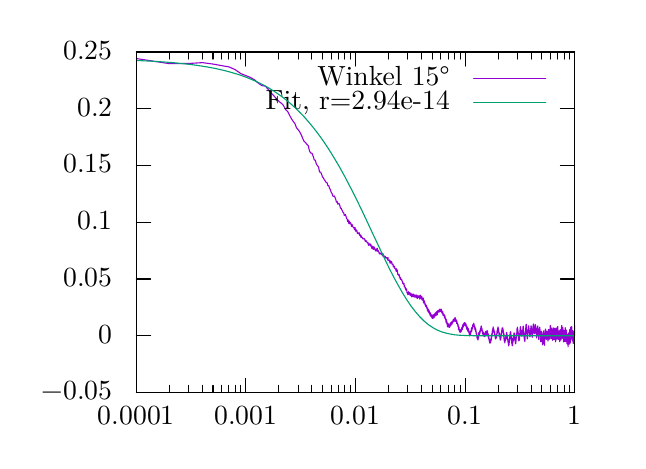
\begin{tikzpicture}[gnuplot]
%% generated with GNUPLOT 5.2p5a (Gentoo revision r0) (Lua 5.1; terminal rev. 99 , script rev. 107)
%% Sa 18 Mai 2019 18:31:12 CEST
\path (0.000,0.000) rectangle (7.500,5.250);
\gpcolor{color=gp lt color border}
\gpsetlinetype{gp lt border}
\gpsetdashtype{gp dt solid}
\gpsetlinewidth{1.00}
\draw[gp path] (1.380,0.616)--(1.560,0.616);
\draw[gp path] (6.947,0.616)--(6.767,0.616);
\node[gp node right] at (1.196,0.616) {$-0.05$};
\draw[gp path] (1.380,1.337)--(1.560,1.337);
\draw[gp path] (6.947,1.337)--(6.767,1.337);
\node[gp node right] at (1.196,1.337) {$0$};
\draw[gp path] (1.380,2.058)--(1.560,2.058);
\draw[gp path] (6.947,2.058)--(6.767,2.058);
\node[gp node right] at (1.196,2.058) {$0.05$};
\draw[gp path] (1.380,2.779)--(1.560,2.779);
\draw[gp path] (6.947,2.779)--(6.767,2.779);
\node[gp node right] at (1.196,2.779) {$0.1$};
\draw[gp path] (1.380,3.499)--(1.560,3.499);
\draw[gp path] (6.947,3.499)--(6.767,3.499);
\node[gp node right] at (1.196,3.499) {$0.15$};
\draw[gp path] (1.380,4.220)--(1.560,4.220);
\draw[gp path] (6.947,4.220)--(6.767,4.220);
\node[gp node right] at (1.196,4.220) {$0.2$};
\draw[gp path] (1.380,4.941)--(1.560,4.941);
\draw[gp path] (6.947,4.941)--(6.767,4.941);
\node[gp node right] at (1.196,4.941) {$0.25$};
\draw[gp path] (1.380,0.616)--(1.380,0.796);
\draw[gp path] (1.380,4.941)--(1.380,4.761);
\node[gp node center] at (1.380,0.308) {$0.0001$};
\draw[gp path] (1.799,0.616)--(1.799,0.706);
\draw[gp path] (1.799,4.941)--(1.799,4.851);
\draw[gp path] (2.044,0.616)--(2.044,0.706);
\draw[gp path] (2.044,4.941)--(2.044,4.851);
\draw[gp path] (2.218,0.616)--(2.218,0.706);
\draw[gp path] (2.218,4.941)--(2.218,4.851);
\draw[gp path] (2.353,0.616)--(2.353,0.706);
\draw[gp path] (2.353,4.941)--(2.353,4.851);
\draw[gp path] (2.463,0.616)--(2.463,0.706);
\draw[gp path] (2.463,4.941)--(2.463,4.851);
\draw[gp path] (2.556,0.616)--(2.556,0.706);
\draw[gp path] (2.556,4.941)--(2.556,4.851);
\draw[gp path] (2.637,0.616)--(2.637,0.706);
\draw[gp path] (2.637,4.941)--(2.637,4.851);
\draw[gp path] (2.708,0.616)--(2.708,0.706);
\draw[gp path] (2.708,4.941)--(2.708,4.851);
\draw[gp path] (2.772,0.616)--(2.772,0.796);
\draw[gp path] (2.772,4.941)--(2.772,4.761);
\node[gp node center] at (2.772,0.308) {$0.001$};
\draw[gp path] (3.191,0.616)--(3.191,0.706);
\draw[gp path] (3.191,4.941)--(3.191,4.851);
\draw[gp path] (3.436,0.616)--(3.436,0.706);
\draw[gp path] (3.436,4.941)--(3.436,4.851);
\draw[gp path] (3.610,0.616)--(3.610,0.706);
\draw[gp path] (3.610,4.941)--(3.610,4.851);
\draw[gp path] (3.745,0.616)--(3.745,0.706);
\draw[gp path] (3.745,4.941)--(3.745,4.851);
\draw[gp path] (3.855,0.616)--(3.855,0.706);
\draw[gp path] (3.855,4.941)--(3.855,4.851);
\draw[gp path] (3.948,0.616)--(3.948,0.706);
\draw[gp path] (3.948,4.941)--(3.948,4.851);
\draw[gp path] (4.029,0.616)--(4.029,0.706);
\draw[gp path] (4.029,4.941)--(4.029,4.851);
\draw[gp path] (4.100,0.616)--(4.100,0.706);
\draw[gp path] (4.100,4.941)--(4.100,4.851);
\draw[gp path] (4.163,0.616)--(4.163,0.796);
\draw[gp path] (4.163,4.941)--(4.163,4.761);
\node[gp node center] at (4.163,0.308) {$0.01$};
\draw[gp path] (4.582,0.616)--(4.582,0.706);
\draw[gp path] (4.582,4.941)--(4.582,4.851);
\draw[gp path] (4.828,0.616)--(4.828,0.706);
\draw[gp path] (4.828,4.941)--(4.828,4.851);
\draw[gp path] (5.001,0.616)--(5.001,0.706);
\draw[gp path] (5.001,4.941)--(5.001,4.851);
\draw[gp path] (5.136,0.616)--(5.136,0.706);
\draw[gp path] (5.136,4.941)--(5.136,4.851);
\draw[gp path] (5.246,0.616)--(5.246,0.706);
\draw[gp path] (5.246,4.941)--(5.246,4.851);
\draw[gp path] (5.340,0.616)--(5.340,0.706);
\draw[gp path] (5.340,4.941)--(5.340,4.851);
\draw[gp path] (5.420,0.616)--(5.420,0.706);
\draw[gp path] (5.420,4.941)--(5.420,4.851);
\draw[gp path] (5.492,0.616)--(5.492,0.706);
\draw[gp path] (5.492,4.941)--(5.492,4.851);
\draw[gp path] (5.555,0.616)--(5.555,0.796);
\draw[gp path] (5.555,4.941)--(5.555,4.761);
\node[gp node center] at (5.555,0.308) {$0.1$};
\draw[gp path] (5.974,0.616)--(5.974,0.706);
\draw[gp path] (5.974,4.941)--(5.974,4.851);
\draw[gp path] (6.219,0.616)--(6.219,0.706);
\draw[gp path] (6.219,4.941)--(6.219,4.851);
\draw[gp path] (6.393,0.616)--(6.393,0.706);
\draw[gp path] (6.393,4.941)--(6.393,4.851);
\draw[gp path] (6.528,0.616)--(6.528,0.706);
\draw[gp path] (6.528,4.941)--(6.528,4.851);
\draw[gp path] (6.638,0.616)--(6.638,0.706);
\draw[gp path] (6.638,4.941)--(6.638,4.851);
\draw[gp path] (6.731,0.616)--(6.731,0.706);
\draw[gp path] (6.731,4.941)--(6.731,4.851);
\draw[gp path] (6.812,0.616)--(6.812,0.706);
\draw[gp path] (6.812,4.941)--(6.812,4.851);
\draw[gp path] (6.883,0.616)--(6.883,0.706);
\draw[gp path] (6.883,4.941)--(6.883,4.851);
\draw[gp path] (6.947,0.616)--(6.947,0.796);
\draw[gp path] (6.947,4.941)--(6.947,4.761);
\node[gp node center] at (6.947,0.308) {$1$};
\draw[gp path] (1.380,4.941)--(1.380,0.616)--(6.947,0.616)--(6.947,4.941)--cycle;
\node[gp node right] at (5.479,4.607) {Winkel 15°};
\gpcolor{rgb color={0.580,0.000,0.827}}
\draw[gp path] (5.663,4.607)--(6.579,4.607);
\draw[gp path] (1.380,4.858)--(1.799,4.793)--(2.044,4.795)--(2.218,4.806)--(2.353,4.788)%
  --(2.463,4.768)--(2.556,4.752)--(2.637,4.716)--(2.708,4.666)--(2.772,4.641)--(2.829,4.618)%
  --(2.882,4.587)--(2.930,4.544)--(2.975,4.514)--(3.017,4.507)--(3.056,4.467)--(3.092,4.421)%
  --(3.127,4.384)--(3.160,4.345)--(3.191,4.314)--(3.220,4.291)--(3.248,4.263)--(3.275,4.210)%
  --(3.301,4.186)--(3.326,4.138)--(3.349,4.095)--(3.372,4.060)--(3.394,4.032)--(3.415,3.976)%
  --(3.436,3.953)--(3.456,3.926)--(3.475,3.888)--(3.493,3.844)--(3.511,3.805)--(3.529,3.791)%
  --(3.546,3.767)--(3.563,3.753)--(3.579,3.684)--(3.594,3.659)--(3.610,3.656)--(3.625,3.620)%
  --(3.639,3.572)--(3.653,3.565)--(3.667,3.516)--(3.681,3.498)--(3.694,3.480)--(3.707,3.417)%
  --(3.720,3.416)--(3.732,3.393)--(3.745,3.354)--(3.757,3.339)--(3.768,3.319)--(3.780,3.300)%
  --(3.791,3.284)--(3.802,3.281)--(3.813,3.242)--(3.824,3.245)--(3.834,3.208)--(3.845,3.192)%
  --(3.855,3.157)--(3.865,3.145)--(3.875,3.113)--(3.884,3.109)--(3.894,3.113)--(3.903,3.094)%
  --(3.912,3.072)--(3.921,3.035)--(3.930,3.042)--(3.939,3.008)--(3.948,3.020)--(3.956,3.014)%
  --(3.965,2.988)--(3.973,2.955)--(3.982,2.956)--(3.990,2.936)--(3.998,2.921)--(4.006,2.901)%
  --(4.013,2.901)--(4.021,2.865)--(4.029,2.872)--(4.036,2.875)--(4.044,2.849)--(4.051,2.827)%
  --(4.058,2.817)--(4.065,2.786)--(4.072,2.808)--(4.079,2.761)--(4.086,2.792)--(4.093,2.758)%
  --(4.100,2.773)--(4.106,2.757)--(4.113,2.725)--(4.120,2.752)--(4.126,2.725)--(4.132,2.720)%
  --(4.139,2.708)--(4.145,2.713)--(4.151,2.687)--(4.157,2.714)--(4.164,2.670)--(4.170,2.664)%
  --(4.175,2.681)--(4.181,2.674)--(4.187,2.636)--(4.193,2.646)--(4.199,2.640)--(4.204,2.632)%
  --(4.210,2.645)--(4.216,2.613)--(4.221,2.623)--(4.227,2.605)--(4.232,2.588)--(4.237,2.607)%
  --(4.243,2.588)--(4.248,2.584)--(4.253,2.577)--(4.258,2.567)--(4.264,2.573)--(4.269,2.567)%
  --(4.274,2.565)--(4.279,2.570)--(4.284,2.545)--(4.289,2.536)--(4.294,2.547)--(4.298,2.544)%
  --(4.303,2.530)--(4.308,2.527)--(4.313,2.527)--(4.317,2.515)--(4.322,2.521)--(4.327,2.489)%
  --(4.331,2.486)--(4.336,2.504)--(4.340,2.498)--(4.345,2.506)--(4.349,2.489)--(4.354,2.478)%
  --(4.358,2.501)--(4.363,2.471)--(4.367,2.476)--(4.371,2.445)--(4.375,2.467)--(4.380,2.460)%
  --(4.384,2.475)--(4.388,2.433)--(4.392,2.455)--(4.396,2.441)--(4.400,2.467)--(4.405,2.444)%
  --(4.409,2.437)--(4.413,2.423)--(4.417,2.433)--(4.421,2.412)--(4.424,2.440)--(4.428,2.432)%
  --(4.432,2.432)--(4.436,2.415)--(4.440,2.448)--(4.444,2.415)--(4.448,2.407)--(4.451,2.422)%
  --(4.455,2.413)--(4.459,2.400)--(4.463,2.392)--(4.466,2.376)--(4.470,2.378)--(4.473,2.391)%
  --(4.477,2.380)--(4.481,2.381)--(4.484,2.385)--(4.488,2.371)--(4.491,2.378)--(4.495,2.389)%
  --(4.498,2.364)--(4.502,2.366)--(4.505,2.375)--(4.509,2.354)--(4.512,2.380)--(4.515,2.341)%
  --(4.519,2.362)--(4.522,2.349)--(4.525,2.351)--(4.529,2.344)--(4.532,2.341)--(4.535,2.348)%
  --(4.539,2.339)--(4.542,2.345)--(4.545,2.324)--(4.548,2.330)--(4.551,2.327)--(4.555,2.329)%
  --(4.558,2.331)--(4.561,2.321)--(4.564,2.320)--(4.567,2.326)--(4.570,2.308)--(4.573,2.299)%
  --(4.576,2.333)--(4.579,2.293)--(4.582,2.296)--(4.585,2.298)--(4.588,2.295)--(4.591,2.292)%
  --(4.594,2.300)--(4.597,2.277)--(4.600,2.279)--(4.603,2.256)--(4.606,2.289)--(4.609,2.283)%
  --(4.612,2.284)--(4.615,2.275)--(4.618,2.264)--(4.621,2.281)--(4.623,2.272)--(4.626,2.263)%
  --(4.629,2.241)--(4.632,2.245)--(4.635,2.242)--(4.637,2.238)--(4.640,2.245)--(4.643,2.218)%
  --(4.646,2.210)--(4.648,2.213)--(4.651,2.225)--(4.654,2.215)--(4.656,2.221)--(4.659,2.210)%
  --(4.662,2.191)--(4.664,2.201)--(4.667,2.187)--(4.670,2.186)--(4.672,2.182)--(4.675,2.180)%
  --(4.677,2.160)--(4.680,2.165)--(4.683,2.189)--(4.685,2.154)--(4.688,2.156)--(4.690,2.157)%
  --(4.693,2.173)--(4.695,2.138)--(4.698,2.146)--(4.700,2.114)--(4.703,2.115)--(4.705,2.122)%
  --(4.708,2.117)--(4.710,2.113)--(4.712,2.106)--(4.715,2.100)--(4.717,2.116)--(4.720,2.092)%
  --(4.722,2.082)--(4.725,2.087)--(4.727,2.082)--(4.729,2.066)--(4.732,2.058)--(4.734,2.077)%
  --(4.736,2.052)--(4.739,2.054)--(4.741,2.055)--(4.743,2.048)--(4.746,2.057)--(4.748,2.053)%
  --(4.750,2.049)--(4.753,2.035)--(4.755,2.033)--(4.757,2.028)--(4.759,2.031)--(4.762,2.023)%
  --(4.764,2.000)--(4.766,2.007)--(4.768,2.004)--(4.771,1.992)--(4.773,2.006)--(4.775,1.990)%
  --(4.777,2.003)--(4.779,2.000)--(4.781,1.966)--(4.784,1.964)--(4.786,1.964)--(4.788,1.974)%
  --(4.790,1.964)--(4.792,1.951)--(4.794,1.940)--(4.797,1.943)--(4.799,1.948)--(4.801,1.923)%
  --(4.803,1.919)--(4.805,1.927)--(4.807,1.936)--(4.809,1.916)--(4.811,1.911)--(4.813,1.921)%
  --(4.815,1.918)--(4.817,1.881)--(4.819,1.887)--(4.821,1.890)--(4.823,1.885)--(4.826,1.879)%
  --(4.828,1.858)--(4.830,1.873)--(4.832,1.871)--(4.834,1.890)--(4.836,1.896)--(4.838,1.880)%
  --(4.840,1.864)--(4.841,1.868)--(4.843,1.890)--(4.845,1.872)--(4.847,1.865)--(4.849,1.869)%
  --(4.851,1.869)--(4.853,1.884)--(4.855,1.873)--(4.857,1.850)--(4.859,1.847)--(4.861,1.867)%
  --(4.863,1.854)--(4.865,1.867)--(4.867,1.878)--(4.868,1.865)--(4.870,1.865)--(4.872,1.871)%
  --(4.874,1.858)--(4.876,1.831)--(4.878,1.846)--(4.880,1.860)--(4.881,1.864)--(4.883,1.853)%
  --(4.885,1.862)--(4.887,1.866)--(4.889,1.838)--(4.891,1.851)--(4.892,1.860)--(4.894,1.831)%
  --(4.896,1.859)--(4.898,1.845)--(4.900,1.857)--(4.901,1.867)--(4.903,1.851)--(4.905,1.849)%
  --(4.907,1.839)--(4.908,1.854)--(4.910,1.828)--(4.912,1.828)--(4.914,1.843)--(4.916,1.855)%
  --(4.917,1.841)--(4.919,1.856)--(4.921,1.838)--(4.922,1.847)--(4.924,1.833)--(4.926,1.829)%
  --(4.928,1.832)--(4.929,1.843)--(4.931,1.846)--(4.933,1.825)--(4.934,1.832)--(4.936,1.850)%
  --(4.938,1.856)--(4.939,1.820)--(4.941,1.832)--(4.943,1.834)--(4.944,1.837)--(4.946,1.825)%
  --(4.948,1.845)--(4.949,1.810)--(4.951,1.814)--(4.953,1.828)--(4.954,1.826)--(4.956,1.846)%
  --(4.958,1.837)--(4.959,1.838)--(4.961,1.823)--(4.962,1.835)--(4.964,1.843)--(4.966,1.827)%
  --(4.967,1.827)--(4.969,1.838)--(4.970,1.841)--(4.972,1.828)--(4.974,1.827)--(4.975,1.837)%
  --(4.977,1.845)--(4.978,1.811)--(4.980,1.802)--(4.981,1.839)--(4.983,1.829)--(4.985,1.822)%
  --(4.986,1.853)--(4.988,1.853)--(4.989,1.831)--(4.991,1.846)--(4.992,1.817)--(4.994,1.817)%
  --(4.995,1.841)--(4.997,1.821)--(4.998,1.826)--(5.000,1.807)--(5.001,1.813)--(5.003,1.818)%
  --(5.004,1.838)--(5.006,1.794)--(5.007,1.817)--(5.009,1.807)--(5.010,1.804)--(5.012,1.792)%
  --(5.013,1.818)--(5.015,1.809)--(5.016,1.816)--(5.018,1.812)--(5.019,1.804)--(5.021,1.786)%
  --(5.022,1.791)--(5.024,1.781)--(5.025,1.815)--(5.027,1.755)--(5.028,1.770)--(5.029,1.767)%
  --(5.031,1.753)--(5.032,1.767)--(5.034,1.777)--(5.035,1.787)--(5.037,1.765)--(5.038,1.765)%
  --(5.039,1.751)--(5.041,1.757)--(5.042,1.756)--(5.044,1.760)--(5.045,1.730)--(5.047,1.735)%
  --(5.048,1.747)--(5.049,1.729)--(5.051,1.726)--(5.052,1.721)--(5.054,1.736)--(5.055,1.714)%
  --(5.056,1.709)--(5.058,1.710)--(5.059,1.713)--(5.060,1.726)--(5.062,1.709)--(5.063,1.697)%
  --(5.064,1.720)--(5.066,1.719)--(5.067,1.699)--(5.069,1.695)--(5.070,1.691)--(5.071,1.681)%
  --(5.073,1.700)--(5.074,1.690)--(5.075,1.686)--(5.077,1.685)--(5.078,1.654)--(5.079,1.688)%
  --(5.081,1.677)--(5.082,1.666)--(5.083,1.669)--(5.085,1.644)--(5.086,1.674)--(5.087,1.673)%
  --(5.089,1.657)--(5.090,1.644)--(5.091,1.667)--(5.092,1.633)--(5.094,1.662)--(5.095,1.643)%
  --(5.096,1.636)--(5.098,1.644)--(5.099,1.635)--(5.100,1.623)--(5.101,1.650)--(5.103,1.631)%
  --(5.104,1.613)--(5.105,1.621)--(5.107,1.628)--(5.108,1.617)--(5.109,1.607)--(5.110,1.608)%
  --(5.112,1.593)--(5.113,1.631)--(5.114,1.622)--(5.115,1.598)--(5.117,1.607)--(5.118,1.606)%
  --(5.119,1.616)--(5.120,1.587)--(5.122,1.592)--(5.123,1.579)--(5.124,1.606)--(5.125,1.587)%
  --(5.127,1.593)--(5.128,1.585)--(5.129,1.575)--(5.130,1.580)--(5.131,1.581)--(5.133,1.580)%
  --(5.134,1.603)--(5.135,1.562)--(5.136,1.578)--(5.137,1.580)--(5.139,1.586)--(5.140,1.559)%
  --(5.141,1.557)--(5.142,1.577)--(5.144,1.577)--(5.145,1.598)--(5.146,1.580)--(5.147,1.570)%
  --(5.148,1.566)--(5.149,1.577)--(5.151,1.584)--(5.152,1.599)--(5.153,1.562)--(5.154,1.588)%
  --(5.155,1.581)--(5.157,1.576)--(5.158,1.582)--(5.159,1.593)--(5.160,1.610)--(5.161,1.565)%
  --(5.162,1.595)--(5.163,1.597)--(5.165,1.590)--(5.166,1.593)--(5.167,1.594)--(5.168,1.617)%
  --(5.169,1.580)--(5.170,1.599)--(5.172,1.592)--(5.173,1.601)--(5.174,1.604)--(5.175,1.613)%
  --(5.176,1.623)--(5.177,1.629)--(5.178,1.593)--(5.179,1.623)--(5.181,1.618)--(5.182,1.627)%
  --(5.183,1.601)--(5.184,1.610)--(5.185,1.610)--(5.186,1.612)--(5.187,1.627)--(5.188,1.617)%
  --(5.189,1.631)--(5.191,1.628)--(5.192,1.639)--(5.193,1.643)--(5.194,1.619)--(5.195,1.598)%
  --(5.196,1.633)--(5.197,1.627)--(5.198,1.637)--(5.199,1.633)--(5.200,1.629)--(5.202,1.604)%
  --(5.203,1.646)--(5.204,1.634)--(5.205,1.635)--(5.206,1.624)--(5.207,1.646)--(5.208,1.656)%
  --(5.209,1.642)--(5.210,1.639)--(5.211,1.658)--(5.212,1.638)--(5.213,1.638)--(5.214,1.644)%
  --(5.215,1.647)--(5.217,1.645)--(5.218,1.659)--(5.219,1.645)--(5.220,1.652)--(5.221,1.639)%
  --(5.222,1.656)--(5.223,1.651)--(5.224,1.651)--(5.225,1.653)--(5.226,1.650)--(5.227,1.663)%
  --(5.228,1.638)--(5.229,1.674)--(5.230,1.647)--(5.231,1.652)--(5.232,1.651)--(5.233,1.663)%
  --(5.234,1.645)--(5.235,1.661)--(5.236,1.651)--(5.237,1.652)--(5.238,1.676)--(5.239,1.663)%
  --(5.240,1.663)--(5.241,1.661)--(5.242,1.654)--(5.243,1.657)--(5.244,1.646)--(5.245,1.658)%
  --(5.246,1.658)--(5.247,1.659)--(5.249,1.661)--(5.250,1.661)--(5.251,1.665)--(5.252,1.674)%
  --(5.253,1.666)--(5.254,1.654)--(5.254,1.636)--(5.255,1.644)--(5.256,1.642)--(5.257,1.654)%
  --(5.258,1.659)--(5.259,1.647)--(5.260,1.659)--(5.261,1.649)--(5.262,1.641)--(5.263,1.636)%
  --(5.264,1.618)--(5.265,1.637)--(5.266,1.629)--(5.267,1.645)--(5.268,1.619)--(5.269,1.626)%
  --(5.270,1.629)--(5.271,1.641)--(5.272,1.639)--(5.273,1.624)--(5.274,1.628)--(5.275,1.597)%
  --(5.276,1.613)--(5.277,1.601)--(5.278,1.611)--(5.279,1.617)--(5.280,1.597)--(5.281,1.611)%
  --(5.282,1.599)--(5.283,1.596)--(5.284,1.608)--(5.285,1.604)--(5.286,1.597)--(5.286,1.602)%
  --(5.287,1.588)--(5.288,1.611)--(5.289,1.586)--(5.290,1.597)--(5.291,1.591)--(5.292,1.589)%
  --(5.293,1.588)--(5.294,1.569)--(5.295,1.578)--(5.296,1.569)--(5.297,1.580)--(5.298,1.555)%
  --(5.299,1.570)--(5.300,1.576)--(5.300,1.590)--(5.301,1.559)--(5.302,1.563)--(5.303,1.566)%
  --(5.304,1.553)--(5.305,1.561)--(5.306,1.559)--(5.307,1.545)--(5.308,1.553)--(5.309,1.542)%
  --(5.310,1.537)--(5.310,1.550)--(5.311,1.534)--(5.312,1.515)--(5.313,1.507)--(5.314,1.534)%
  --(5.315,1.547)--(5.316,1.532)--(5.317,1.542)--(5.318,1.502)--(5.319,1.504)--(5.319,1.509)%
  --(5.320,1.510)--(5.321,1.529)--(5.322,1.515)--(5.323,1.497)--(5.324,1.489)--(5.325,1.501)%
  --(5.326,1.503)--(5.327,1.502)--(5.327,1.476)--(5.328,1.479)--(5.329,1.498)--(5.330,1.454)%
  --(5.331,1.484)--(5.332,1.501)--(5.333,1.480)--(5.334,1.472)--(5.334,1.465)--(5.335,1.473)%
  --(5.336,1.484)--(5.337,1.475)--(5.338,1.449)--(5.339,1.476)--(5.340,1.457)--(5.341,1.458)%
  --(5.341,1.490)--(5.342,1.464)--(5.343,1.476)--(5.344,1.475)--(5.345,1.462)--(5.346,1.453)%
  --(5.347,1.449)--(5.347,1.456)--(5.348,1.475)--(5.349,1.460)--(5.350,1.479)--(5.351,1.454)%
  --(5.352,1.454)--(5.352,1.455)--(5.353,1.465)--(5.354,1.448)--(5.355,1.455)--(5.356,1.449)%
  --(5.357,1.443)--(5.358,1.476)--(5.358,1.472)--(5.359,1.459)--(5.360,1.472)--(5.361,1.455)%
  --(5.362,1.468)--(5.363,1.451)--(5.363,1.480)--(5.364,1.480)--(5.365,1.471)--(5.366,1.466)%
  --(5.367,1.501)--(5.368,1.481)--(5.368,1.464)--(5.369,1.488)--(5.370,1.484)--(5.371,1.485)%
  --(5.372,1.484)--(5.372,1.488)--(5.373,1.479)--(5.374,1.487)--(5.375,1.470)--(5.376,1.471)%
  --(5.377,1.492)--(5.377,1.474)--(5.378,1.507)--(5.379,1.500)--(5.380,1.498)--(5.381,1.490)%
  --(5.381,1.484)--(5.382,1.487)--(5.383,1.491)--(5.384,1.501)--(5.385,1.490)--(5.385,1.491)%
  --(5.386,1.485)--(5.387,1.514)--(5.388,1.519)--(5.389,1.511)--(5.389,1.521)--(5.390,1.485)%
  --(5.391,1.508)--(5.392,1.512)--(5.393,1.519)--(5.393,1.509)--(5.394,1.505)--(5.395,1.517)%
  --(5.396,1.515)--(5.396,1.498)--(5.397,1.503)--(5.398,1.510)--(5.399,1.515)--(5.400,1.518)%
  --(5.400,1.519)--(5.401,1.529)--(5.402,1.520)--(5.403,1.513)--(5.404,1.537)--(5.404,1.545)%
  --(5.405,1.538)--(5.406,1.518)--(5.407,1.538)--(5.407,1.532)--(5.408,1.537)--(5.409,1.523)%
  --(5.410,1.532)--(5.410,1.546)--(5.411,1.518)--(5.412,1.537)--(5.413,1.550)--(5.414,1.520)%
  --(5.414,1.533)--(5.415,1.537)--(5.416,1.520)--(5.417,1.536)--(5.417,1.541)--(5.418,1.551)%
  --(5.419,1.548)--(5.420,1.543)--(5.420,1.549)--(5.421,1.557)--(5.422,1.556)--(5.423,1.562)%
  --(5.423,1.528)--(5.424,1.527)--(5.425,1.548)--(5.426,1.542)--(5.426,1.535)--(5.427,1.537)%
  --(5.428,1.548)--(5.429,1.569)--(5.429,1.546)--(5.430,1.534)--(5.431,1.550)--(5.432,1.557)%
  --(5.432,1.566)--(5.433,1.538)--(5.434,1.548)--(5.435,1.520)--(5.435,1.540)--(5.436,1.534)%
  --(5.437,1.527)--(5.438,1.522)--(5.438,1.543)--(5.439,1.538)--(5.440,1.531)--(5.440,1.540)%
  --(5.441,1.535)--(5.442,1.533)--(5.443,1.537)--(5.443,1.533)--(5.444,1.526)--(5.445,1.537)%
  --(5.446,1.535)--(5.446,1.513)--(5.447,1.513)--(5.448,1.490)--(5.448,1.526)--(5.449,1.524)%
  --(5.450,1.518)--(5.451,1.504)--(5.451,1.519)--(5.452,1.514)--(5.453,1.490)--(5.453,1.502)%
  --(5.454,1.503)--(5.455,1.497)--(5.456,1.500)--(5.456,1.499)--(5.457,1.495)--(5.458,1.486)%
  --(5.458,1.496)--(5.459,1.493)--(5.460,1.472)--(5.461,1.478)--(5.461,1.480)--(5.462,1.475)%
  --(5.463,1.465)--(5.463,1.482)--(5.464,1.486)--(5.465,1.472)--(5.465,1.455)--(5.466,1.464)%
  --(5.467,1.457)--(5.468,1.458)--(5.468,1.447)--(5.469,1.454)--(5.470,1.447)--(5.470,1.430)%
  --(5.471,1.452)--(5.472,1.415)--(5.472,1.462)--(5.473,1.426)--(5.474,1.420)--(5.475,1.446)%
  --(5.475,1.431)--(5.476,1.428)--(5.477,1.437)--(5.477,1.442)--(5.478,1.444)--(5.479,1.423)%
  --(5.479,1.431)--(5.480,1.426)--(5.481,1.403)--(5.481,1.414)--(5.482,1.412)--(5.483,1.395)%
  --(5.483,1.415)--(5.484,1.409)--(5.485,1.402)--(5.485,1.396)--(5.486,1.401)--(5.487,1.403)%
  --(5.488,1.384)--(5.488,1.408)--(5.489,1.399)--(5.490,1.396)--(5.491,1.380)--(5.492,1.398)%
  --(5.493,1.389)--(5.494,1.400)--(5.494,1.395)--(5.495,1.393)--(5.496,1.402)--(5.496,1.399)%
  --(5.497,1.399)--(5.498,1.412)--(5.498,1.391)--(5.499,1.417)--(5.500,1.384)--(5.500,1.391)%
  --(5.501,1.391)--(5.502,1.421)--(5.502,1.393)--(5.503,1.411)--(5.504,1.400)--(5.504,1.387)%
  --(5.505,1.391)--(5.506,1.394)--(5.506,1.409)--(5.507,1.401)--(5.507,1.416)--(5.508,1.404)%
  --(5.509,1.413)--(5.509,1.411)--(5.510,1.406)--(5.511,1.416)--(5.511,1.405)--(5.512,1.434)%
  --(5.513,1.434)--(5.513,1.439)--(5.514,1.441)--(5.515,1.446)--(5.515,1.436)--(5.516,1.440)%
  --(5.517,1.433)--(5.517,1.439)--(5.518,1.419)--(5.518,1.445)--(5.519,1.444)--(5.520,1.439)%
  --(5.520,1.415)--(5.521,1.435)--(5.522,1.458)--(5.522,1.445)--(5.523,1.454)--(5.524,1.473)%
  --(5.524,1.465)--(5.525,1.464)--(5.526,1.456)--(5.526,1.465)--(5.527,1.464)--(5.527,1.469)%
  --(5.528,1.447)--(5.529,1.455)--(5.529,1.480)--(5.530,1.469)--(5.531,1.454)--(5.531,1.475)%
  --(5.532,1.481)--(5.533,1.481)--(5.534,1.478)--(5.534,1.462)--(5.535,1.447)--(5.536,1.468)%
  --(5.536,1.491)--(5.537,1.477)--(5.537,1.482)--(5.538,1.485)--(5.539,1.483)--(5.539,1.475)%
  --(5.540,1.479)--(5.541,1.468)--(5.541,1.480)--(5.542,1.487)--(5.542,1.491)--(5.543,1.478)%
  --(5.544,1.485)--(5.544,1.503)--(5.545,1.498)--(5.546,1.469)--(5.546,1.500)--(5.547,1.494)%
  --(5.547,1.497)--(5.548,1.485)--(5.549,1.494)--(5.549,1.488)--(5.550,1.503)--(5.550,1.488)%
  --(5.551,1.494)--(5.552,1.477)--(5.552,1.490)--(5.553,1.490)--(5.553,1.491)--(5.554,1.495)%
  --(5.555,1.494)--(5.555,1.499)--(5.556,1.470)--(5.556,1.494)--(5.557,1.492)--(5.558,1.493)%
  --(5.558,1.490)--(5.559,1.498)--(5.559,1.473)--(5.560,1.489)--(5.561,1.478)--(5.561,1.464)%
  --(5.562,1.494)--(5.562,1.484)--(5.563,1.488)--(5.564,1.492)--(5.564,1.482)--(5.565,1.478)%
  --(5.565,1.476)--(5.566,1.467)--(5.567,1.483)--(5.567,1.464)--(5.568,1.471)--(5.568,1.456)%
  --(5.569,1.471)--(5.570,1.456)--(5.570,1.447)--(5.571,1.464)--(5.571,1.441)--(5.572,1.429)%
  --(5.573,1.464)--(5.573,1.444)--(5.574,1.432)--(5.574,1.444)--(5.575,1.437)--(5.575,1.450)%
  --(5.576,1.459)--(5.577,1.417)--(5.577,1.430)--(5.578,1.442)--(5.578,1.438)--(5.579,1.429)%
  --(5.580,1.430)--(5.581,1.425)--(5.581,1.424)--(5.582,1.444)--(5.582,1.430)--(5.583,1.432)%
  --(5.584,1.421)--(5.584,1.417)--(5.585,1.403)--(5.585,1.447)--(5.586,1.436)--(5.586,1.417)%
  --(5.587,1.424)--(5.588,1.416)--(5.588,1.433)--(5.589,1.409)--(5.589,1.413)--(5.590,1.400)%
  --(5.590,1.392)--(5.591,1.399)--(5.592,1.402)--(5.592,1.424)--(5.593,1.416)--(5.593,1.429)%
  --(5.594,1.425)--(5.594,1.401)--(5.595,1.399)--(5.596,1.429)--(5.596,1.402)--(5.597,1.395)%
  --(5.597,1.414)--(5.598,1.398)--(5.598,1.396)--(5.599,1.395)--(5.600,1.384)--(5.600,1.387)%
  --(5.601,1.397)--(5.601,1.404)--(5.602,1.392)--(5.602,1.381)--(5.603,1.383)--(5.604,1.377)%
  --(5.605,1.378)--(5.605,1.388)--(5.606,1.373)--(5.606,1.381)--(5.607,1.377)--(5.607,1.384)%
  --(5.608,1.354)--(5.608,1.361)--(5.609,1.366)--(5.610,1.388)--(5.610,1.378)--(5.611,1.367)%
  --(5.611,1.372)--(5.612,1.374)--(5.612,1.365)--(5.613,1.357)--(5.613,1.359)--(5.614,1.335)%
  --(5.615,1.373)--(5.615,1.358)--(5.616,1.345)--(5.616,1.386)--(5.617,1.365)--(5.617,1.371)%
  --(5.618,1.377)--(5.618,1.370)--(5.619,1.356)--(5.619,1.375)--(5.620,1.356)--(5.621,1.361)%
  --(5.621,1.370)--(5.622,1.352)--(5.622,1.380)--(5.623,1.358)--(5.623,1.345)--(5.624,1.361)%
  --(5.624,1.394)--(5.625,1.376)--(5.625,1.374)--(5.626,1.374)--(5.626,1.376)--(5.627,1.375)%
  --(5.628,1.381)--(5.628,1.373)--(5.629,1.390)--(5.629,1.381)--(5.630,1.391)--(5.630,1.388)%
  --(5.631,1.381)--(5.631,1.404)--(5.632,1.401)--(5.632,1.403)--(5.633,1.405)--(5.633,1.412)%
  --(5.634,1.390)--(5.634,1.412)--(5.635,1.398)--(5.636,1.416)--(5.636,1.438)--(5.637,1.419)%
  --(5.637,1.406)--(5.638,1.422)--(5.638,1.423)--(5.639,1.423)--(5.639,1.393)--(5.640,1.426)%
  --(5.640,1.416)--(5.641,1.402)--(5.641,1.417)--(5.642,1.410)--(5.642,1.408)--(5.643,1.444)%
  --(5.643,1.428)--(5.644,1.436)--(5.644,1.444)--(5.645,1.439)--(5.645,1.426)--(5.646,1.422)%
  --(5.647,1.453)--(5.647,1.443)--(5.648,1.448)--(5.648,1.427)--(5.649,1.445)--(5.649,1.461)%
  --(5.650,1.443)--(5.650,1.458)--(5.651,1.458)--(5.651,1.452)--(5.652,1.474)--(5.652,1.475)%
  --(5.653,1.474)--(5.653,1.464)--(5.654,1.467)--(5.655,1.461)--(5.655,1.477)--(5.656,1.463)%
  --(5.656,1.478)--(5.657,1.473)--(5.657,1.462)--(5.658,1.468)--(5.658,1.482)--(5.659,1.468)%
  --(5.659,1.458)--(5.660,1.456)--(5.660,1.476)--(5.661,1.475)--(5.661,1.463)--(5.662,1.483)%
  --(5.662,1.479)--(5.663,1.464)--(5.663,1.487)--(5.664,1.477)--(5.664,1.490)--(5.665,1.498)%
  --(5.665,1.476)--(5.666,1.475)--(5.666,1.496)--(5.667,1.476)--(5.667,1.471)--(5.668,1.471)%
  --(5.668,1.461)--(5.669,1.469)--(5.669,1.465)--(5.670,1.484)--(5.670,1.452)--(5.671,1.461)%
  --(5.671,1.463)--(5.672,1.462)--(5.672,1.454)--(5.673,1.466)--(5.673,1.463)--(5.674,1.461)%
  --(5.674,1.447)--(5.675,1.442)--(5.675,1.440)--(5.676,1.430)--(5.676,1.450)--(5.677,1.429)%
  --(5.677,1.449)--(5.678,1.451)--(5.678,1.462)--(5.679,1.448)--(5.679,1.415)--(5.680,1.441)%
  --(5.680,1.436)--(5.681,1.429)--(5.682,1.427)--(5.682,1.431)--(5.683,1.426)--(5.683,1.433)%
  --(5.684,1.417)--(5.684,1.441)--(5.685,1.426)--(5.685,1.435)--(5.686,1.424)--(5.686,1.396)%
  --(5.687,1.424)--(5.687,1.425)--(5.688,1.415)--(5.688,1.408)--(5.689,1.423)--(5.689,1.406)%
  --(5.690,1.410)--(5.690,1.400)--(5.691,1.402)--(5.691,1.388)--(5.692,1.388)--(5.692,1.424)%
  --(5.693,1.403)--(5.693,1.387)--(5.693,1.393)--(5.694,1.394)--(5.694,1.381)--(5.695,1.382)%
  --(5.695,1.362)--(5.696,1.379)--(5.696,1.372)--(5.697,1.378)--(5.697,1.370)--(5.698,1.371)%
  --(5.698,1.370)--(5.699,1.367)--(5.699,1.364)--(5.700,1.369)--(5.700,1.377)--(5.701,1.362)%
  --(5.701,1.368)--(5.702,1.348)--(5.702,1.365)--(5.703,1.346)--(5.703,1.354)--(5.704,1.351)%
  --(5.704,1.331)--(5.704,1.358)--(5.705,1.323)--(5.705,1.324)--(5.706,1.338)--(5.706,1.324)%
  --(5.707,1.320)--(5.707,1.312)--(5.708,1.343)--(5.708,1.326)--(5.709,1.319)--(5.709,1.303)%
  --(5.710,1.318)--(5.710,1.335)--(5.711,1.322)--(5.711,1.317)--(5.712,1.324)--(5.712,1.305)%
  --(5.712,1.303)--(5.713,1.316)--(5.713,1.328)--(5.714,1.318)--(5.714,1.321)--(5.715,1.298)%
  --(5.715,1.299)--(5.716,1.311)--(5.716,1.289)--(5.717,1.320)--(5.717,1.323)--(5.718,1.303)%
  --(5.718,1.283)--(5.718,1.320)--(5.719,1.322)--(5.719,1.297)--(5.720,1.339)--(5.720,1.288)%
  --(5.721,1.309)--(5.721,1.310)--(5.722,1.317)--(5.722,1.309)--(5.723,1.301)--(5.723,1.317)%
  --(5.724,1.329)--(5.724,1.335)--(5.724,1.309)--(5.725,1.316)--(5.725,1.320)--(5.726,1.347)%
  --(5.726,1.317)--(5.727,1.339)--(5.727,1.349)--(5.728,1.339)--(5.728,1.333)--(5.729,1.337)%
  --(5.729,1.344)--(5.729,1.376)--(5.730,1.334)--(5.730,1.339)--(5.731,1.347)--(5.731,1.346)%
  --(5.732,1.336)--(5.732,1.363)--(5.733,1.341)--(5.733,1.357)--(5.733,1.350)--(5.734,1.357)%
  --(5.734,1.365)--(5.735,1.370)--(5.735,1.339)--(5.736,1.347)--(5.736,1.368)--(5.737,1.364)%
  --(5.737,1.370)--(5.738,1.385)--(5.738,1.362)--(5.738,1.373)--(5.739,1.383)--(5.739,1.377)%
  --(5.740,1.390)--(5.740,1.393)--(5.741,1.376)--(5.741,1.366)--(5.742,1.398)--(5.742,1.401)%
  --(5.742,1.383)--(5.743,1.394)--(5.743,1.391)--(5.744,1.379)--(5.744,1.383)--(5.745,1.384)%
  --(5.745,1.381)--(5.746,1.410)--(5.746,1.403)--(5.746,1.369)--(5.747,1.392)--(5.747,1.391)%
  --(5.748,1.399)--(5.748,1.413)--(5.749,1.409)--(5.749,1.428)--(5.749,1.417)--(5.750,1.409)%
  --(5.750,1.404)--(5.751,1.406)--(5.751,1.427)--(5.752,1.395)--(5.752,1.416)--(5.753,1.431)%
  --(5.753,1.427)--(5.753,1.425)--(5.754,1.410)--(5.754,1.430)--(5.755,1.421)--(5.755,1.437)%
  --(5.756,1.452)--(5.756,1.412)--(5.756,1.428)--(5.757,1.446)--(5.757,1.439)--(5.758,1.460)%
  --(5.758,1.440)--(5.759,1.445)--(5.759,1.438)--(5.759,1.440)--(5.760,1.439)--(5.760,1.463)%
  --(5.761,1.407)--(5.761,1.443)--(5.762,1.427)--(5.762,1.439)--(5.762,1.428)--(5.763,1.426)%
  --(5.763,1.430)--(5.764,1.427)--(5.764,1.445)--(5.765,1.432)--(5.765,1.420)--(5.766,1.421)%
  --(5.766,1.427)--(5.767,1.425)--(5.767,1.424)--(5.768,1.418)--(5.768,1.428)--(5.768,1.433)%
  --(5.769,1.425)--(5.769,1.428)--(5.770,1.416)--(5.770,1.408)--(5.771,1.421)--(5.771,1.392)%
  --(5.771,1.427)--(5.772,1.409)--(5.772,1.406)--(5.773,1.402)--(5.773,1.398)--(5.774,1.388)%
  --(5.774,1.391)--(5.774,1.375)--(5.775,1.400)--(5.775,1.386)--(5.776,1.378)--(5.776,1.396)%
  --(5.776,1.400)--(5.777,1.388)--(5.777,1.380)--(5.778,1.372)--(5.778,1.378)--(5.779,1.387)%
  --(5.779,1.400)--(5.779,1.390)--(5.780,1.362)--(5.780,1.384)--(5.781,1.381)--(5.781,1.378)%
  --(5.781,1.389)--(5.782,1.385)--(5.782,1.384)--(5.783,1.350)--(5.783,1.376)--(5.784,1.374)%
  --(5.784,1.385)--(5.784,1.348)--(5.785,1.359)--(5.785,1.360)--(5.786,1.364)--(5.786,1.351)%
  --(5.786,1.371)--(5.787,1.361)--(5.787,1.355)--(5.788,1.357)--(5.788,1.363)--(5.789,1.348)%
  --(5.789,1.347)--(5.789,1.343)--(5.790,1.340)--(5.790,1.343)--(5.791,1.337)--(5.791,1.346)%
  --(5.791,1.347)--(5.792,1.377)--(5.792,1.335)--(5.793,1.362)--(5.793,1.353)--(5.793,1.347)%
  --(5.794,1.349)--(5.794,1.362)--(5.795,1.342)--(5.795,1.331)--(5.795,1.341)--(5.796,1.343)%
  --(5.796,1.356)--(5.797,1.341)--(5.797,1.356)--(5.797,1.339)--(5.798,1.338)--(5.798,1.332)%
  --(5.799,1.333)--(5.799,1.350)--(5.800,1.335)--(5.800,1.334)--(5.800,1.342)--(5.801,1.327)%
  --(5.801,1.339)--(5.802,1.335)--(5.802,1.332)--(5.802,1.342)--(5.803,1.325)--(5.803,1.339)%
  --(5.804,1.347)--(5.804,1.359)--(5.804,1.341)--(5.805,1.364)--(5.805,1.340)--(5.806,1.356)%
  --(5.806,1.358)--(5.806,1.338)--(5.807,1.336)--(5.807,1.332)--(5.808,1.354)--(5.808,1.330)%
  --(5.808,1.361)--(5.809,1.352)--(5.809,1.354)--(5.810,1.354)--(5.810,1.357)--(5.810,1.347)%
  --(5.811,1.342)--(5.811,1.369)--(5.812,1.365)--(5.812,1.377)--(5.813,1.384)--(5.813,1.365)%
  --(5.813,1.371)--(5.814,1.377)--(5.814,1.378)--(5.815,1.374)--(5.815,1.373)--(5.815,1.377)%
  --(5.816,1.378)--(5.816,1.371)--(5.817,1.367)--(5.817,1.391)--(5.817,1.366)--(5.818,1.357)%
  --(5.818,1.363)--(5.819,1.373)--(5.819,1.382)--(5.819,1.395)--(5.820,1.368)--(5.820,1.369)%
  --(5.821,1.364)--(5.821,1.369)--(5.821,1.371)--(5.822,1.372)--(5.822,1.369)--(5.822,1.378)%
  --(5.823,1.365)--(5.823,1.369)--(5.824,1.386)--(5.824,1.377)--(5.824,1.357)--(5.825,1.371)%
  --(5.825,1.393)--(5.826,1.371)--(5.826,1.355)--(5.826,1.359)--(5.827,1.393)--(5.827,1.376)%
  --(5.828,1.369)--(5.828,1.383)--(5.828,1.376)--(5.829,1.359)--(5.829,1.368)--(5.829,1.369)%
  --(5.830,1.375)--(5.830,1.353)--(5.831,1.376)--(5.831,1.372)--(5.831,1.365)--(5.832,1.381)%
  --(5.832,1.401)--(5.832,1.387)--(5.833,1.378)--(5.833,1.382)--(5.834,1.393)--(5.834,1.392)%
  --(5.834,1.384)--(5.835,1.375)--(5.835,1.376)--(5.836,1.380)--(5.836,1.381)--(5.836,1.375)%
  --(5.837,1.386)--(5.837,1.374)--(5.837,1.381)--(5.838,1.393)--(5.838,1.400)--(5.839,1.401)%
  --(5.839,1.389)--(5.839,1.395)--(5.840,1.391)--(5.840,1.387)--(5.840,1.394)--(5.841,1.373)%
  --(5.841,1.354)--(5.842,1.384)--(5.842,1.365)--(5.842,1.368)--(5.843,1.354)--(5.843,1.362)%
  --(5.843,1.359)--(5.844,1.348)--(5.844,1.367)--(5.845,1.349)--(5.845,1.355)--(5.845,1.353)%
  --(5.846,1.365)--(5.846,1.366)--(5.847,1.345)--(5.847,1.349)--(5.848,1.333)--(5.848,1.342)%
  --(5.848,1.362)--(5.849,1.361)--(5.849,1.321)--(5.849,1.326)--(5.850,1.348)--(5.850,1.322)%
  --(5.851,1.337)--(5.851,1.312)--(5.851,1.337)--(5.852,1.332)--(5.852,1.315)--(5.852,1.336)%
  --(5.853,1.309)--(5.853,1.324)--(5.854,1.318)--(5.854,1.332)--(5.854,1.315)--(5.855,1.312)%
  --(5.855,1.308)--(5.855,1.300)--(5.856,1.320)--(5.856,1.294)--(5.856,1.297)--(5.857,1.302)%
  --(5.857,1.314)--(5.858,1.328)--(5.858,1.322)--(5.858,1.309)--(5.859,1.306)--(5.859,1.302)%
  --(5.859,1.297)--(5.860,1.296)--(5.860,1.283)--(5.860,1.279)--(5.861,1.296)--(5.861,1.287)%
  --(5.862,1.272)--(5.862,1.294)--(5.862,1.284)--(5.863,1.280)--(5.863,1.295)--(5.863,1.290)%
  --(5.864,1.279)--(5.864,1.272)--(5.864,1.279)--(5.865,1.259)--(5.865,1.273)--(5.866,1.255)%
  --(5.866,1.248)--(5.866,1.261)--(5.867,1.255)--(5.867,1.291)--(5.867,1.273)--(5.868,1.262)%
  --(5.868,1.253)--(5.868,1.266)--(5.869,1.268)--(5.870,1.256)--(5.870,1.257)--(5.870,1.267)%
  --(5.871,1.274)--(5.871,1.271)--(5.871,1.243)--(5.872,1.252)--(5.872,1.272)--(5.872,1.261)%
  --(5.873,1.253)--(5.873,1.262)--(5.873,1.245)--(5.874,1.282)--(5.874,1.243)--(5.875,1.257)%
  --(5.875,1.246)--(5.876,1.266)--(5.876,1.257)--(5.877,1.281)--(5.877,1.259)--(5.877,1.253)%
  --(5.878,1.259)--(5.878,1.271)--(5.878,1.247)--(5.879,1.256)--(5.879,1.294)--(5.880,1.264)%
  --(5.880,1.268)--(5.880,1.278)--(5.881,1.272)--(5.881,1.270)--(5.881,1.264)--(5.882,1.297)%
  --(5.882,1.266)--(5.882,1.288)--(5.883,1.280)--(5.883,1.283)--(5.883,1.282)--(5.884,1.295)%
  --(5.884,1.289)--(5.884,1.288)--(5.885,1.293)--(5.885,1.319)--(5.886,1.313)--(5.886,1.288)%
  --(5.886,1.306)--(5.887,1.280)--(5.887,1.318)--(5.887,1.313)--(5.888,1.303)--(5.888,1.296)%
  --(5.888,1.305)--(5.889,1.305)--(5.889,1.307)--(5.889,1.312)--(5.890,1.310)--(5.890,1.351)%
  --(5.890,1.309)--(5.891,1.340)--(5.891,1.332)--(5.891,1.324)--(5.892,1.338)--(5.892,1.305)%
  --(5.892,1.338)--(5.893,1.336)--(5.893,1.338)--(5.893,1.339)--(5.894,1.335)--(5.894,1.330)%
  --(5.895,1.332)--(5.895,1.340)--(5.895,1.350)--(5.896,1.364)--(5.896,1.355)--(5.896,1.343)%
  --(5.897,1.370)--(5.897,1.357)--(5.897,1.358)--(5.898,1.354)--(5.898,1.365)--(5.899,1.358)%
  --(5.899,1.375)--(5.899,1.366)--(5.900,1.391)--(5.900,1.372)--(5.900,1.370)--(5.901,1.357)%
  --(5.901,1.385)--(5.901,1.400)--(5.902,1.386)--(5.902,1.389)--(5.902,1.406)--(5.903,1.380)%
  --(5.903,1.393)--(5.903,1.387)--(5.904,1.385)--(5.904,1.374)--(5.904,1.394)--(5.905,1.417)%
  --(5.905,1.414)--(5.905,1.418)--(5.906,1.411)--(5.906,1.394)--(5.906,1.414)--(5.907,1.409)%
  --(5.907,1.427)--(5.907,1.417)--(5.908,1.415)--(5.908,1.414)--(5.909,1.421)--(5.909,1.420)%
  --(5.909,1.421)--(5.910,1.415)--(5.910,1.420)--(5.910,1.425)--(5.911,1.450)--(5.911,1.440)%
  --(5.911,1.419)--(5.912,1.416)--(5.912,1.441)--(5.912,1.417)--(5.913,1.420)--(5.913,1.405)%
  --(5.913,1.444)--(5.914,1.416)--(5.914,1.405)--(5.914,1.423)--(5.915,1.411)--(5.915,1.415)%
  --(5.915,1.417)--(5.916,1.416)--(5.916,1.417)--(5.916,1.410)--(5.917,1.431)--(5.917,1.418)%
  --(5.918,1.427)--(5.918,1.408)--(5.918,1.421)--(5.919,1.411)--(5.919,1.407)--(5.919,1.415)%
  --(5.920,1.403)--(5.920,1.399)--(5.920,1.386)--(5.921,1.420)--(5.921,1.414)--(5.921,1.396)%
  --(5.922,1.406)--(5.922,1.399)--(5.923,1.390)--(5.923,1.394)--(5.923,1.406)--(5.924,1.393)%
  --(5.924,1.405)--(5.924,1.379)--(5.925,1.385)--(5.925,1.396)--(5.925,1.376)--(5.926,1.396)%
  --(5.926,1.381)--(5.926,1.382)--(5.927,1.383)--(5.927,1.381)--(5.927,1.360)--(5.928,1.374)%
  --(5.928,1.364)--(5.928,1.371)--(5.929,1.365)--(5.929,1.391)--(5.929,1.371)--(5.930,1.379)%
  --(5.930,1.387)--(5.930,1.356)--(5.931,1.344)--(5.931,1.365)--(5.931,1.352)--(5.932,1.371)%
  --(5.932,1.379)--(5.932,1.349)--(5.933,1.370)--(5.933,1.337)--(5.933,1.354)--(5.934,1.357)%
  --(5.934,1.362)--(5.934,1.350)--(5.935,1.341)--(5.935,1.354)--(5.935,1.353)--(5.936,1.331)%
  --(5.936,1.321)--(5.936,1.350)--(5.936,1.325)--(5.937,1.320)--(5.937,1.313)--(5.937,1.327)%
  --(5.938,1.318)--(5.938,1.332)--(5.939,1.320)--(5.939,1.327)--(5.939,1.334)--(5.940,1.323)%
  --(5.940,1.315)--(5.940,1.332)--(5.941,1.318)--(5.941,1.325)--(5.941,1.305)--(5.942,1.297)%
  --(5.942,1.306)--(5.942,1.323)--(5.943,1.314)--(5.943,1.302)--(5.943,1.306)--(5.944,1.306)%
  --(5.944,1.327)--(5.944,1.320)--(5.944,1.326)--(5.945,1.295)--(5.945,1.315)--(5.946,1.321)%
  --(5.946,1.300)--(5.946,1.326)--(5.947,1.306)--(5.947,1.317)--(5.947,1.302)--(5.948,1.306)%
  --(5.948,1.315)--(5.948,1.318)--(5.949,1.326)--(5.949,1.331)--(5.949,1.336)--(5.950,1.314)%
  --(5.950,1.328)--(5.950,1.317)--(5.950,1.348)--(5.951,1.338)--(5.951,1.312)--(5.951,1.343)%
  --(5.952,1.335)--(5.952,1.321)--(5.952,1.331)--(5.953,1.336)--(5.953,1.350)--(5.953,1.348)%
  --(5.954,1.327)--(5.954,1.338)--(5.954,1.343)--(5.955,1.356)--(5.955,1.363)--(5.955,1.344)%
  --(5.955,1.341)--(5.956,1.354)--(5.956,1.345)--(5.956,1.359)--(5.957,1.349)--(5.957,1.347)%
  --(5.957,1.360)--(5.958,1.361)--(5.958,1.359)--(5.958,1.377)--(5.959,1.350)--(5.959,1.348)%
  --(5.959,1.370)--(5.960,1.386)--(5.960,1.364)--(5.960,1.362)--(5.960,1.392)--(5.961,1.379)%
  --(5.961,1.366)--(5.961,1.382)--(5.962,1.389)--(5.962,1.363)--(5.962,1.405)--(5.963,1.389)%
  --(5.963,1.368)--(5.963,1.383)--(5.964,1.390)--(5.964,1.408)--(5.964,1.385)--(5.964,1.401)%
  --(5.965,1.407)--(5.965,1.397)--(5.965,1.406)--(5.966,1.412)--(5.966,1.405)--(5.966,1.415)%
  --(5.967,1.401)--(5.967,1.422)--(5.967,1.405)--(5.968,1.404)--(5.968,1.405)--(5.968,1.433)%
  --(5.968,1.417)--(5.969,1.422)--(5.969,1.428)--(5.969,1.426)--(5.970,1.401)--(5.970,1.413)%
  --(5.970,1.423)--(5.971,1.445)--(5.971,1.421)--(5.971,1.444)--(5.971,1.447)--(5.972,1.412)%
  --(5.972,1.447)--(5.972,1.446)--(5.973,1.424)--(5.973,1.449)--(5.973,1.427)--(5.974,1.438)%
  --(5.974,1.442)--(5.974,1.438)--(5.975,1.447)--(5.975,1.432)--(5.975,1.414)--(5.975,1.426)%
  --(5.976,1.440)--(5.976,1.429)--(5.976,1.426)--(5.977,1.411)--(5.977,1.427)--(5.977,1.402)%
  --(5.978,1.428)--(5.978,1.422)--(5.978,1.419)--(5.978,1.418)--(5.979,1.400)--(5.979,1.405)%
  --(5.979,1.406)--(5.980,1.408)--(5.980,1.404)--(5.980,1.421)--(5.981,1.403)--(5.981,1.406)%
  --(5.981,1.395)--(5.981,1.407)--(5.982,1.390)--(5.982,1.399)--(5.982,1.398)--(5.983,1.377)%
  --(5.983,1.400)--(5.983,1.399)--(5.984,1.387)--(5.984,1.373)--(5.984,1.380)--(5.984,1.399)%
  --(5.985,1.378)--(5.985,1.404)--(5.985,1.367)--(5.986,1.382)--(5.986,1.383)--(5.986,1.352)%
  --(5.986,1.382)--(5.987,1.375)--(5.987,1.356)--(5.987,1.372)--(5.988,1.367)--(5.988,1.347)%
  --(5.988,1.331)--(5.989,1.339)--(5.989,1.366)--(5.989,1.347)--(5.989,1.346)--(5.990,1.372)%
  --(5.990,1.356)--(5.990,1.351)--(5.991,1.343)--(5.991,1.352)--(5.991,1.342)--(5.991,1.355)%
  --(5.992,1.339)--(5.992,1.355)--(5.992,1.361)--(5.993,1.367)--(5.993,1.344)--(5.993,1.350)%
  --(5.994,1.345)--(5.994,1.353)--(5.994,1.334)--(5.994,1.339)--(5.995,1.345)--(5.995,1.336)%
  --(5.995,1.344)--(5.996,1.345)--(5.996,1.350)--(5.996,1.317)--(5.996,1.337)--(5.997,1.337)%
  --(5.997,1.320)--(5.997,1.323)--(5.998,1.327)--(5.998,1.316)--(5.998,1.319)--(5.998,1.327)%
  --(5.999,1.317)--(5.999,1.301)--(5.999,1.300)--(6.000,1.321)--(6.000,1.302)--(6.000,1.299)%
  --(6.001,1.285)--(6.001,1.321)--(6.001,1.293)--(6.001,1.299)--(6.002,1.283)--(6.002,1.281)%
  --(6.002,1.303)--(6.003,1.311)--(6.003,1.295)--(6.003,1.308)--(6.003,1.286)--(6.004,1.282)%
  --(6.004,1.308)--(6.004,1.294)--(6.005,1.285)--(6.005,1.297)--(6.005,1.307)--(6.005,1.299)%
  --(6.006,1.297)--(6.006,1.289)--(6.006,1.319)--(6.007,1.302)--(6.007,1.303)--(6.007,1.304)%
  --(6.007,1.300)--(6.008,1.307)--(6.008,1.297)--(6.008,1.310)--(6.009,1.309)--(6.009,1.293)%
  --(6.009,1.314)--(6.009,1.312)--(6.010,1.304)--(6.010,1.307)--(6.011,1.335)--(6.011,1.336)%
  --(6.012,1.312)--(6.012,1.328)--(6.012,1.323)--(6.013,1.337)--(6.013,1.322)--(6.013,1.340)%
  --(6.013,1.341)--(6.014,1.348)--(6.014,1.351)--(6.014,1.347)--(6.015,1.359)--(6.015,1.344)%
  --(6.015,1.341)--(6.015,1.367)--(6.016,1.356)--(6.016,1.357)--(6.016,1.364)--(6.017,1.384)%
  --(6.017,1.361)--(6.017,1.377)--(6.017,1.370)--(6.018,1.375)--(6.018,1.374)--(6.018,1.385)%
  --(6.018,1.384)--(6.019,1.381)--(6.019,1.377)--(6.019,1.386)--(6.020,1.381)--(6.020,1.403)%
  --(6.020,1.375)--(6.020,1.390)--(6.021,1.398)--(6.021,1.375)--(6.021,1.393)--(6.022,1.409)%
  --(6.022,1.416)--(6.022,1.404)--(6.022,1.418)--(6.023,1.394)--(6.023,1.399)--(6.023,1.420)%
  --(6.024,1.427)--(6.024,1.403)--(6.024,1.427)--(6.024,1.422)--(6.025,1.417)--(6.025,1.438)%
  --(6.025,1.410)--(6.026,1.399)--(6.026,1.405)--(6.026,1.412)--(6.027,1.437)--(6.027,1.430)%
  --(6.027,1.419)--(6.027,1.426)--(6.028,1.413)--(6.028,1.420)--(6.028,1.418)--(6.029,1.425)%
  --(6.029,1.422)--(6.029,1.423)--(6.029,1.429)--(6.030,1.428)--(6.030,1.432)--(6.030,1.424)%
  --(6.030,1.429)--(6.031,1.427)--(6.031,1.432)--(6.031,1.424)--(6.032,1.427)--(6.032,1.421)%
  --(6.032,1.427)--(6.033,1.428)--(6.033,1.405)--(6.033,1.407)--(6.033,1.411)--(6.034,1.403)%
  --(6.034,1.438)--(6.034,1.420)--(6.035,1.425)--(6.035,1.427)--(6.035,1.429)--(6.035,1.418)%
  --(6.036,1.417)--(6.036,1.426)--(6.036,1.409)--(6.036,1.407)--(6.037,1.410)--(6.037,1.406)%
  --(6.037,1.396)--(6.038,1.402)--(6.038,1.401)--(6.038,1.407)--(6.038,1.413)--(6.039,1.409)%
  --(6.039,1.396)--(6.039,1.382)--(6.040,1.404)--(6.040,1.401)--(6.040,1.390)--(6.041,1.378)%
  --(6.041,1.377)--(6.041,1.379)--(6.041,1.393)--(6.042,1.364)--(6.042,1.373)--(6.042,1.360)%
  --(6.042,1.359)--(6.043,1.373)--(6.043,1.347)--(6.043,1.379)--(6.044,1.358)--(6.044,1.370)%
  --(6.044,1.374)--(6.044,1.355)--(6.045,1.359)--(6.045,1.349)--(6.045,1.353)--(6.045,1.350)%
  --(6.046,1.369)--(6.046,1.327)--(6.046,1.366)--(6.046,1.342)--(6.047,1.337)--(6.047,1.341)%
  --(6.047,1.335)--(6.048,1.339)--(6.048,1.319)--(6.048,1.333)--(6.048,1.331)--(6.049,1.328)%
  --(6.049,1.321)--(6.049,1.358)--(6.049,1.297)--(6.050,1.321)--(6.050,1.307)--(6.050,1.308)%
  --(6.050,1.313)--(6.051,1.287)--(6.051,1.301)--(6.051,1.308)--(6.052,1.310)--(6.052,1.293)%
  --(6.052,1.296)--(6.052,1.286)--(6.053,1.298)--(6.053,1.305)--(6.053,1.289)--(6.053,1.273)%
  --(6.054,1.311)--(6.054,1.291)--(6.054,1.288)--(6.054,1.267)--(6.055,1.283)--(6.055,1.274)%
  --(6.055,1.286)--(6.056,1.273)--(6.056,1.286)--(6.056,1.262)--(6.056,1.277)--(6.057,1.276)%
  --(6.057,1.278)--(6.057,1.279)--(6.057,1.263)--(6.058,1.281)--(6.058,1.272)--(6.058,1.264)%
  --(6.058,1.261)--(6.059,1.262)--(6.059,1.254)--(6.059,1.281)--(6.059,1.272)--(6.060,1.264)%
  --(6.060,1.259)--(6.060,1.271)--(6.061,1.267)--(6.061,1.285)--(6.061,1.246)--(6.061,1.261)%
  --(6.062,1.275)--(6.062,1.283)--(6.062,1.269)--(6.062,1.274)--(6.063,1.270)--(6.063,1.282)%
  --(6.063,1.285)--(6.063,1.279)--(6.064,1.289)--(6.064,1.271)--(6.064,1.275)--(6.064,1.286)%
  --(6.065,1.275)--(6.065,1.270)--(6.065,1.269)--(6.065,1.303)--(6.066,1.283)--(6.066,1.291)%
  --(6.066,1.280)--(6.067,1.292)--(6.067,1.298)--(6.067,1.310)--(6.067,1.307)--(6.068,1.286)%
  --(6.068,1.295)--(6.068,1.299)--(6.068,1.298)--(6.069,1.278)--(6.069,1.279)--(6.069,1.280)%
  --(6.069,1.292)--(6.070,1.302)--(6.070,1.309)--(6.070,1.316)--(6.070,1.302)--(6.071,1.316)%
  --(6.071,1.311)--(6.071,1.293)--(6.071,1.319)--(6.072,1.312)--(6.072,1.316)--(6.072,1.322)%
  --(6.072,1.324)--(6.073,1.335)--(6.073,1.293)--(6.073,1.320)--(6.073,1.316)--(6.074,1.328)%
  --(6.074,1.321)--(6.074,1.299)--(6.075,1.317)--(6.075,1.331)--(6.075,1.333)--(6.076,1.318)%
  --(6.076,1.344)--(6.076,1.311)--(6.077,1.339)--(6.077,1.317)--(6.077,1.333)--(6.077,1.342)%
  --(6.078,1.348)--(6.078,1.334)--(6.078,1.332)--(6.078,1.340)--(6.079,1.354)--(6.079,1.351)%
  --(6.079,1.336)--(6.079,1.352)--(6.080,1.354)--(6.080,1.359)--(6.080,1.352)--(6.080,1.341)%
  --(6.081,1.369)--(6.081,1.334)--(6.081,1.378)--(6.081,1.364)--(6.082,1.358)--(6.082,1.352)%
  --(6.082,1.360)--(6.082,1.367)--(6.083,1.340)--(6.083,1.366)--(6.083,1.347)--(6.083,1.371)%
  --(6.084,1.359)--(6.084,1.369)--(6.084,1.366)--(6.084,1.377)--(6.085,1.357)--(6.085,1.344)%
  --(6.085,1.379)--(6.085,1.360)--(6.086,1.333)--(6.086,1.342)--(6.086,1.346)--(6.086,1.341)%
  --(6.087,1.353)--(6.087,1.344)--(6.087,1.341)--(6.087,1.350)--(6.088,1.347)--(6.088,1.348)%
  --(6.088,1.328)--(6.088,1.339)--(6.089,1.357)--(6.089,1.330)--(6.089,1.340)--(6.089,1.341)%
  --(6.090,1.314)--(6.090,1.332)--(6.090,1.325)--(6.090,1.313)--(6.091,1.336)--(6.091,1.326)%
  --(6.091,1.333)--(6.091,1.307)--(6.092,1.304)--(6.092,1.310)--(6.092,1.324)--(6.092,1.327)%
  --(6.093,1.345)--(6.093,1.317)--(6.093,1.309)--(6.093,1.316)--(6.094,1.309)--(6.094,1.289)%
  --(6.094,1.310)--(6.094,1.315)--(6.095,1.290)--(6.095,1.309)--(6.095,1.289)--(6.095,1.299)%
  --(6.096,1.284)--(6.096,1.292)--(6.096,1.297)--(6.096,1.291)--(6.097,1.288)--(6.097,1.302)%
  --(6.097,1.299)--(6.097,1.294)--(6.098,1.287)--(6.098,1.297)--(6.098,1.284)--(6.098,1.289)%
  --(6.099,1.277)--(6.099,1.286)--(6.099,1.269)--(6.099,1.266)--(6.100,1.280)--(6.100,1.272)%
  --(6.100,1.286)--(6.100,1.260)--(6.101,1.255)--(6.101,1.252)--(6.101,1.270)--(6.101,1.256)%
  --(6.102,1.263)--(6.102,1.270)--(6.102,1.259)--(6.102,1.272)--(6.103,1.257)--(6.103,1.253)%
  --(6.103,1.251)--(6.103,1.245)--(6.103,1.256)--(6.104,1.246)--(6.104,1.241)--(6.104,1.247)%
  --(6.104,1.220)--(6.105,1.230)--(6.105,1.243)--(6.105,1.235)--(6.105,1.239)--(6.106,1.237)%
  --(6.106,1.236)--(6.106,1.235)--(6.107,1.229)--(6.107,1.244)--(6.107,1.236)--(6.107,1.220)%
  --(6.108,1.243)--(6.108,1.208)--(6.108,1.223)--(6.108,1.218)--(6.109,1.231)--(6.109,1.217)%
  --(6.109,1.240)--(6.109,1.214)--(6.110,1.236)--(6.110,1.240)--(6.110,1.239)--(6.110,1.244)%
  --(6.111,1.223)--(6.111,1.237)--(6.111,1.226)--(6.111,1.241)--(6.111,1.230)--(6.112,1.248)%
  --(6.112,1.241)--(6.112,1.239)--(6.112,1.219)--(6.113,1.249)--(6.113,1.245)--(6.113,1.252)%
  --(6.113,1.245)--(6.114,1.228)--(6.114,1.249)--(6.114,1.248)--(6.114,1.227)--(6.115,1.264)%
  --(6.115,1.253)--(6.115,1.267)--(6.115,1.243)--(6.116,1.262)--(6.116,1.260)--(6.116,1.251)%
  --(6.116,1.265)--(6.117,1.257)--(6.117,1.258)--(6.117,1.278)--(6.117,1.275)--(6.117,1.281)%
  --(6.118,1.259)--(6.118,1.293)--(6.118,1.271)--(6.118,1.268)--(6.119,1.282)--(6.119,1.296)%
  --(6.119,1.291)--(6.119,1.279)--(6.120,1.276)--(6.120,1.280)--(6.120,1.288)--(6.120,1.313)%
  --(6.121,1.313)--(6.121,1.289)--(6.121,1.284)--(6.121,1.285)--(6.122,1.327)--(6.122,1.293)%
  --(6.122,1.318)--(6.122,1.308)--(6.122,1.315)--(6.123,1.289)--(6.123,1.311)--(6.123,1.328)%
  --(6.123,1.299)--(6.124,1.329)--(6.124,1.316)--(6.124,1.318)--(6.124,1.336)--(6.125,1.325)%
  --(6.125,1.352)--(6.125,1.337)--(6.125,1.349)--(6.126,1.324)--(6.126,1.336)--(6.126,1.358)%
  --(6.126,1.341)--(6.126,1.347)--(6.127,1.361)--(6.127,1.381)--(6.127,1.363)--(6.127,1.350)%
  --(6.128,1.356)--(6.128,1.369)--(6.128,1.356)--(6.128,1.364)--(6.129,1.361)--(6.129,1.354)%
  --(6.129,1.352)--(6.129,1.375)--(6.130,1.362)--(6.130,1.358)--(6.130,1.380)--(6.130,1.371)%
  --(6.130,1.366)--(6.131,1.370)--(6.131,1.369)--(6.131,1.355)--(6.131,1.365)--(6.132,1.369)%
  --(6.132,1.375)--(6.132,1.380)--(6.132,1.376)--(6.133,1.360)--(6.133,1.364)--(6.133,1.363)%
  --(6.133,1.380)--(6.133,1.389)--(6.134,1.365)--(6.134,1.375)--(6.134,1.366)--(6.134,1.367)%
  --(6.135,1.373)--(6.135,1.358)--(6.135,1.364)--(6.135,1.369)--(6.136,1.385)--(6.136,1.356)%
  --(6.136,1.359)--(6.136,1.349)--(6.137,1.365)--(6.137,1.354)--(6.137,1.355)--(6.137,1.347)%
  --(6.138,1.338)--(6.138,1.355)--(6.138,1.341)--(6.138,1.332)--(6.139,1.349)--(6.139,1.327)%
  --(6.139,1.343)--(6.139,1.312)--(6.139,1.321)--(6.140,1.323)--(6.140,1.337)--(6.140,1.316)%
  --(6.140,1.320)--(6.141,1.331)--(6.141,1.317)--(6.141,1.324)--(6.141,1.319)--(6.142,1.325)%
  --(6.142,1.299)--(6.142,1.311)--(6.142,1.312)--(6.142,1.315)--(6.143,1.277)--(6.143,1.293)%
  --(6.143,1.300)--(6.143,1.308)--(6.144,1.297)--(6.144,1.309)--(6.144,1.304)--(6.144,1.276)%
  --(6.145,1.308)--(6.145,1.295)--(6.145,1.288)--(6.145,1.275)--(6.145,1.285)--(6.146,1.290)%
  --(6.146,1.258)--(6.146,1.242)--(6.146,1.273)--(6.147,1.279)--(6.147,1.288)--(6.147,1.275)%
  --(6.147,1.278)--(6.147,1.268)--(6.148,1.260)--(6.148,1.259)--(6.148,1.261)--(6.148,1.255)%
  --(6.149,1.244)--(6.149,1.250)--(6.149,1.255)--(6.149,1.240)--(6.150,1.256)--(6.150,1.239)%
  --(6.150,1.257)--(6.150,1.231)--(6.150,1.243)--(6.151,1.238)--(6.151,1.254)--(6.151,1.245)%
  --(6.151,1.242)--(6.152,1.238)--(6.152,1.251)--(6.152,1.240)--(6.152,1.234)--(6.152,1.235)%
  --(6.153,1.252)--(6.153,1.228)--(6.153,1.225)--(6.153,1.233)--(6.154,1.215)--(6.154,1.210)%
  --(6.154,1.227)--(6.154,1.222)--(6.154,1.214)--(6.155,1.224)--(6.155,1.232)--(6.155,1.220)%
  --(6.155,1.221)--(6.156,1.236)--(6.156,1.227)--(6.156,1.235)--(6.156,1.241)--(6.156,1.219)%
  --(6.157,1.214)--(6.157,1.241)--(6.157,1.235)--(6.157,1.248)--(6.158,1.233)--(6.158,1.250)%
  --(6.158,1.240)--(6.158,1.232)--(6.159,1.247)--(6.159,1.248)--(6.159,1.259)--(6.159,1.224)%
  --(6.159,1.262)--(6.160,1.258)--(6.160,1.261)--(6.160,1.263)--(6.160,1.260)--(6.161,1.255)%
  --(6.161,1.253)--(6.161,1.252)--(6.161,1.255)--(6.161,1.278)--(6.162,1.266)--(6.162,1.256)%
  --(6.162,1.278)--(6.162,1.294)--(6.163,1.289)--(6.163,1.254)--(6.163,1.281)--(6.163,1.259)%
  --(6.163,1.267)--(6.164,1.277)--(6.164,1.290)--(6.164,1.270)--(6.164,1.276)--(6.164,1.309)%
  --(6.165,1.289)--(6.165,1.267)--(6.165,1.299)--(6.165,1.274)--(6.166,1.313)--(6.166,1.300)%
  --(6.166,1.289)--(6.166,1.281)--(6.166,1.293)--(6.167,1.277)--(6.167,1.299)--(6.167,1.286)%
  --(6.168,1.299)--(6.168,1.296)--(6.168,1.317)--(6.168,1.314)--(6.168,1.274)--(6.169,1.306)%
  --(6.169,1.313)--(6.169,1.300)--(6.169,1.302)--(6.170,1.310)--(6.170,1.305)--(6.170,1.313)%
  --(6.170,1.329)--(6.170,1.305)--(6.171,1.317)--(6.171,1.311)--(6.171,1.308)--(6.171,1.338)%
  --(6.172,1.335)--(6.172,1.329)--(6.172,1.336)--(6.172,1.347)--(6.172,1.344)--(6.173,1.332)%
  --(6.173,1.337)--(6.173,1.351)--(6.173,1.330)--(6.173,1.334)--(6.174,1.347)--(6.174,1.342)%
  --(6.174,1.357)--(6.174,1.343)--(6.175,1.338)--(6.175,1.368)--(6.175,1.351)--(6.175,1.358)%
  --(6.175,1.349)--(6.176,1.358)--(6.176,1.340)--(6.176,1.348)--(6.176,1.342)--(6.177,1.351)%
  --(6.177,1.356)--(6.177,1.355)--(6.177,1.359)--(6.177,1.341)--(6.178,1.331)--(6.178,1.375)%
  --(6.178,1.346)--(6.178,1.348)--(6.178,1.321)--(6.179,1.342)--(6.179,1.358)--(6.179,1.367)%
  --(6.179,1.358)--(6.180,1.347)--(6.180,1.346)--(6.180,1.363)--(6.180,1.362)--(6.180,1.352)%
  --(6.181,1.339)--(6.181,1.336)--(6.181,1.349)--(6.181,1.358)--(6.181,1.353)--(6.182,1.333)%
  --(6.182,1.369)--(6.182,1.351)--(6.182,1.341)--(6.183,1.339)--(6.183,1.367)--(6.183,1.330)%
  --(6.183,1.349)--(6.183,1.346)--(6.184,1.352)--(6.184,1.350)--(6.184,1.331)--(6.184,1.318)%
  --(6.184,1.324)--(6.185,1.329)--(6.185,1.331)--(6.185,1.325)--(6.185,1.329)--(6.186,1.307)%
  --(6.186,1.338)--(6.186,1.332)--(6.186,1.330)--(6.186,1.287)--(6.187,1.306)--(6.187,1.336)%
  --(6.187,1.299)--(6.187,1.305)--(6.187,1.320)--(6.188,1.287)--(6.188,1.329)--(6.188,1.294)%
  --(6.188,1.297)--(6.188,1.309)--(6.189,1.286)--(6.189,1.288)--(6.189,1.294)--(6.189,1.273)%
  --(6.190,1.317)--(6.190,1.300)--(6.190,1.265)--(6.190,1.281)--(6.190,1.285)--(6.191,1.300)%
  --(6.191,1.280)--(6.191,1.294)--(6.191,1.273)--(6.191,1.283)--(6.192,1.289)--(6.192,1.267)%
  --(6.192,1.273)--(6.192,1.254)--(6.193,1.276)--(6.193,1.286)--(6.193,1.269)--(6.193,1.266)%
  --(6.193,1.256)--(6.194,1.269)--(6.194,1.248)--(6.194,1.263)--(6.194,1.247)--(6.194,1.260)%
  --(6.195,1.246)--(6.195,1.260)--(6.195,1.235)--(6.195,1.280)--(6.195,1.242)--(6.196,1.255)%
  --(6.196,1.242)--(6.196,1.258)--(6.196,1.251)--(6.196,1.255)--(6.197,1.236)--(6.197,1.257)%
  --(6.197,1.267)--(6.197,1.255)--(6.198,1.269)--(6.198,1.247)--(6.198,1.240)--(6.198,1.243)%
  --(6.199,1.245)--(6.199,1.258)--(6.199,1.273)--(6.199,1.252)--(6.200,1.271)--(6.200,1.270)%
  --(6.200,1.239)--(6.200,1.284)--(6.200,1.292)--(6.201,1.271)--(6.201,1.266)--(6.201,1.271)%
  --(6.201,1.284)--(6.201,1.293)--(6.202,1.289)--(6.202,1.293)--(6.202,1.295)--(6.202,1.281)%
  --(6.203,1.268)--(6.203,1.302)--(6.203,1.286)--(6.203,1.290)--(6.203,1.311)--(6.204,1.303)%
  --(6.204,1.292)--(6.204,1.297)--(6.204,1.303)--(6.204,1.305)--(6.205,1.314)--(6.205,1.313)%
  --(6.205,1.317)--(6.205,1.301)--(6.205,1.307)--(6.206,1.322)--(6.206,1.318)--(6.206,1.326)%
  --(6.206,1.346)--(6.206,1.338)--(6.207,1.331)--(6.207,1.345)--(6.207,1.332)--(6.207,1.325)%
  --(6.207,1.359)--(6.208,1.341)--(6.208,1.346)--(6.208,1.344)--(6.208,1.345)--(6.209,1.350)%
  --(6.209,1.356)--(6.209,1.349)--(6.209,1.356)--(6.209,1.353)--(6.210,1.339)--(6.210,1.369)%
  --(6.210,1.363)--(6.210,1.358)--(6.210,1.376)--(6.211,1.363)--(6.211,1.360)--(6.211,1.367)%
  --(6.211,1.355)--(6.211,1.358)--(6.212,1.365)--(6.212,1.384)--(6.212,1.362)--(6.212,1.367)%
  --(6.212,1.390)--(6.213,1.376)--(6.213,1.389)--(6.213,1.405)--(6.213,1.386)--(6.213,1.391)%
  --(6.214,1.393)--(6.214,1.411)--(6.214,1.387)--(6.214,1.400)--(6.214,1.402)--(6.215,1.400)%
  --(6.215,1.427)--(6.215,1.404)--(6.215,1.409)--(6.215,1.412)--(6.216,1.425)--(6.216,1.395)%
  --(6.216,1.431)--(6.216,1.415)--(6.216,1.423)--(6.217,1.427)--(6.217,1.422)--(6.217,1.423)%
  --(6.217,1.424)--(6.217,1.421)--(6.218,1.415)--(6.218,1.428)--(6.218,1.424)--(6.218,1.428)%
  --(6.218,1.430)--(6.219,1.421)--(6.219,1.424)--(6.219,1.421)--(6.219,1.415)--(6.219,1.420)%
  --(6.220,1.446)--(6.220,1.402)--(6.220,1.425)--(6.220,1.415)--(6.220,1.424)--(6.221,1.417)%
  --(6.221,1.429)--(6.221,1.434)--(6.221,1.416)--(6.222,1.413)--(6.222,1.402)--(6.222,1.420)%
  --(6.222,1.417)--(6.222,1.428)--(6.223,1.416)--(6.223,1.424)--(6.223,1.431)--(6.223,1.438)%
  --(6.223,1.400)--(6.224,1.411)--(6.224,1.420)--(6.224,1.413)--(6.224,1.409)--(6.224,1.406)%
  --(6.225,1.402)--(6.225,1.413)--(6.225,1.411)--(6.225,1.407)--(6.225,1.386)--(6.226,1.409)%
  --(6.226,1.389)--(6.226,1.391)--(6.226,1.405)--(6.226,1.375)--(6.227,1.365)--(6.227,1.391)%
  --(6.227,1.392)--(6.227,1.391)--(6.227,1.378)--(6.228,1.359)--(6.228,1.378)--(6.228,1.385)%
  --(6.228,1.376)--(6.228,1.381)--(6.229,1.356)--(6.229,1.349)--(6.229,1.346)--(6.229,1.363)%
  --(6.229,1.352)--(6.230,1.335)--(6.230,1.377)--(6.230,1.349)--(6.230,1.353)--(6.230,1.350)%
  --(6.231,1.352)--(6.231,1.330)--(6.231,1.338)--(6.231,1.324)--(6.231,1.345)--(6.232,1.340)%
  --(6.232,1.334)--(6.232,1.335)--(6.232,1.340)--(6.232,1.332)--(6.233,1.321)--(6.233,1.318)%
  --(6.233,1.303)--(6.233,1.314)--(6.233,1.321)--(6.234,1.319)--(6.234,1.307)--(6.234,1.313)%
  --(6.234,1.311)--(6.234,1.305)--(6.235,1.297)--(6.235,1.293)--(6.235,1.305)--(6.235,1.316)%
  --(6.235,1.287)--(6.236,1.308)--(6.236,1.295)--(6.236,1.286)--(6.236,1.278)--(6.236,1.303)%
  --(6.237,1.296)--(6.237,1.300)--(6.237,1.277)--(6.237,1.286)--(6.237,1.275)--(6.238,1.294)%
  --(6.238,1.287)--(6.238,1.270)--(6.238,1.289)--(6.238,1.284)--(6.239,1.276)--(6.239,1.273)%
  --(6.239,1.298)--(6.239,1.289)--(6.239,1.300)--(6.240,1.310)--(6.240,1.283)--(6.240,1.274)%
  --(6.240,1.280)--(6.240,1.293)--(6.241,1.279)--(6.241,1.287)--(6.241,1.296)--(6.241,1.304)%
  --(6.241,1.302)--(6.242,1.287)--(6.242,1.294)--(6.242,1.282)--(6.242,1.287)--(6.242,1.292)%
  --(6.243,1.300)--(6.243,1.295)--(6.243,1.296)--(6.243,1.290)--(6.243,1.279)--(6.244,1.292)%
  --(6.244,1.316)--(6.244,1.297)--(6.244,1.298)--(6.244,1.318)--(6.245,1.320)--(6.245,1.302)%
  --(6.245,1.322)--(6.245,1.327)--(6.245,1.320)--(6.246,1.325)--(6.246,1.332)--(6.246,1.302)%
  --(6.246,1.316)--(6.246,1.328)--(6.246,1.312)--(6.247,1.309)--(6.247,1.291)--(6.247,1.327)%
  --(6.247,1.349)--(6.247,1.329)--(6.248,1.343)--(6.248,1.349)--(6.248,1.343)--(6.248,1.351)%
  --(6.248,1.344)--(6.249,1.348)--(6.249,1.333)--(6.249,1.360)--(6.249,1.348)--(6.249,1.368)%
  --(6.250,1.362)--(6.250,1.385)--(6.250,1.366)--(6.250,1.361)--(6.250,1.359)--(6.250,1.372)%
  --(6.251,1.373)--(6.251,1.372)--(6.251,1.366)--(6.251,1.373)--(6.251,1.374)--(6.252,1.396)%
  --(6.252,1.386)--(6.252,1.369)--(6.252,1.382)--(6.252,1.384)--(6.253,1.384)--(6.253,1.389)%
  --(6.253,1.380)--(6.253,1.403)--(6.253,1.408)--(6.254,1.408)--(6.254,1.392)--(6.254,1.403)%
  --(6.254,1.408)--(6.254,1.399)--(6.255,1.409)--(6.255,1.411)--(6.255,1.410)--(6.255,1.425)%
  --(6.255,1.408)--(6.255,1.418)--(6.256,1.405)--(6.256,1.444)--(6.256,1.408)--(6.256,1.422)%
  --(6.256,1.423)--(6.257,1.413)--(6.257,1.433)--(6.257,1.417)--(6.257,1.454)--(6.257,1.413)%
  --(6.258,1.435)--(6.258,1.449)--(6.258,1.445)--(6.258,1.434)--(6.258,1.425)--(6.258,1.408)%
  --(6.259,1.431)--(6.259,1.412)--(6.259,1.429)--(6.259,1.432)--(6.259,1.414)--(6.260,1.427)%
  --(6.260,1.433)--(6.260,1.428)--(6.260,1.442)--(6.261,1.423)--(6.261,1.426)--(6.261,1.415)%
  --(6.261,1.412)--(6.261,1.410)--(6.261,1.415)--(6.262,1.420)--(6.262,1.429)--(6.262,1.395)%
  --(6.262,1.402)--(6.262,1.403)--(6.263,1.407)--(6.263,1.404)--(6.263,1.408)--(6.263,1.425)%
  --(6.263,1.422)--(6.264,1.419)--(6.264,1.401)--(6.264,1.385)--(6.264,1.402)--(6.264,1.370)%
  --(6.264,1.403)--(6.265,1.397)--(6.265,1.393)--(6.265,1.403)--(6.265,1.392)--(6.265,1.386)%
  --(6.266,1.401)--(6.266,1.397)--(6.266,1.409)--(6.266,1.391)--(6.266,1.387)--(6.267,1.391)%
  --(6.267,1.389)--(6.267,1.411)--(6.267,1.401)--(6.267,1.389)--(6.267,1.397)--(6.268,1.375)%
  --(6.268,1.392)--(6.268,1.394)--(6.268,1.379)--(6.269,1.383)--(6.269,1.347)--(6.269,1.368)%
  --(6.269,1.365)--(6.269,1.373)--(6.270,1.359)--(6.270,1.393)--(6.270,1.373)--(6.270,1.379)%
  --(6.270,1.395)--(6.270,1.367)--(6.271,1.383)--(6.271,1.367)--(6.271,1.376)--(6.271,1.365)%
  --(6.271,1.383)--(6.272,1.361)--(6.272,1.371)--(6.272,1.376)--(6.272,1.345)--(6.272,1.355)%
  --(6.272,1.344)--(6.273,1.360)--(6.273,1.367)--(6.273,1.374)--(6.273,1.371)--(6.273,1.352)%
  --(6.274,1.351)--(6.274,1.357)--(6.274,1.343)--(6.274,1.353)--(6.274,1.342)--(6.275,1.348)%
  --(6.275,1.356)--(6.275,1.374)--(6.275,1.360)--(6.275,1.342)--(6.275,1.339)--(6.276,1.343)%
  --(6.276,1.336)--(6.276,1.356)--(6.276,1.354)--(6.276,1.329)--(6.277,1.351)--(6.277,1.349)%
  --(6.277,1.348)--(6.277,1.349)--(6.277,1.364)--(6.277,1.350)--(6.278,1.378)--(6.278,1.352)%
  --(6.278,1.353)--(6.278,1.361)--(6.278,1.346)--(6.279,1.383)--(6.279,1.357)--(6.279,1.362)%
  --(6.279,1.369)--(6.279,1.347)--(6.279,1.366)--(6.280,1.357)--(6.280,1.365)--(6.280,1.357)%
  --(6.280,1.359)--(6.280,1.377)--(6.281,1.368)--(6.281,1.356)--(6.281,1.381)--(6.281,1.371)%
  --(6.281,1.373)--(6.281,1.376)--(6.282,1.367)--(6.282,1.353)--(6.282,1.356)--(6.282,1.367)%
  --(6.282,1.387)--(6.283,1.370)--(6.283,1.366)--(6.283,1.386)--(6.283,1.378)--(6.283,1.373)%
  --(6.284,1.357)--(6.284,1.374)--(6.284,1.368)--(6.284,1.374)--(6.284,1.407)--(6.285,1.390)%
  --(6.285,1.385)--(6.285,1.389)--(6.285,1.381)--(6.285,1.380)--(6.285,1.398)--(6.286,1.387)%
  --(6.286,1.377)--(6.286,1.399)--(6.286,1.379)--(6.286,1.399)--(6.287,1.397)--(6.287,1.396)%
  --(6.287,1.406)--(6.287,1.410)--(6.287,1.385)--(6.287,1.400)--(6.288,1.389)--(6.288,1.398)%
  --(6.288,1.404)--(6.288,1.405)--(6.288,1.415)--(6.289,1.390)--(6.289,1.407)--(6.289,1.413)%
  --(6.289,1.422)--(6.289,1.414)--(6.289,1.407)--(6.290,1.412)--(6.290,1.415)--(6.290,1.416)%
  --(6.290,1.415)--(6.290,1.440)--(6.290,1.420)--(6.291,1.454)--(6.291,1.428)--(6.291,1.442)%
  --(6.291,1.436)--(6.291,1.423)--(6.292,1.440)--(6.292,1.446)--(6.292,1.445)--(6.292,1.423)%
  --(6.292,1.454)--(6.292,1.417)--(6.293,1.414)--(6.293,1.451)--(6.293,1.444)--(6.293,1.451)%
  --(6.293,1.458)--(6.294,1.441)--(6.294,1.415)--(6.294,1.444)--(6.294,1.441)--(6.294,1.447)%
  --(6.294,1.456)--(6.295,1.459)--(6.295,1.437)--(6.295,1.441)--(6.295,1.432)--(6.295,1.404)%
  --(6.295,1.429)--(6.296,1.426)--(6.296,1.437)--(6.296,1.423)--(6.296,1.441)--(6.296,1.433)%
  --(6.297,1.436)--(6.297,1.433)--(6.297,1.419)--(6.297,1.395)--(6.297,1.410)--(6.297,1.430)%
  --(6.298,1.425)--(6.298,1.411)--(6.298,1.416)--(6.298,1.400)--(6.298,1.409)--(6.298,1.410)%
  --(6.299,1.400)--(6.299,1.407)--(6.299,1.404)--(6.299,1.372)--(6.299,1.388)--(6.300,1.392)%
  --(6.300,1.378)--(6.300,1.396)--(6.300,1.367)--(6.300,1.370)--(6.300,1.344)--(6.301,1.365)%
  --(6.301,1.356)--(6.301,1.360)--(6.301,1.363)--(6.301,1.360)--(6.301,1.385)--(6.302,1.353)%
  --(6.302,1.348)--(6.302,1.355)--(6.302,1.348)--(6.302,1.371)--(6.303,1.368)--(6.303,1.346)%
  --(6.303,1.357)--(6.303,1.335)--(6.303,1.321)--(6.303,1.345)--(6.304,1.336)--(6.304,1.326)%
  --(6.304,1.347)--(6.304,1.337)--(6.304,1.350)--(6.304,1.335)--(6.305,1.327)--(6.305,1.336)%
  --(6.305,1.334)--(6.305,1.352)--(6.305,1.328)--(6.306,1.312)--(6.306,1.341)--(6.306,1.326)%
  --(6.306,1.321)--(6.306,1.320)--(6.306,1.339)--(6.307,1.306)--(6.307,1.322)--(6.307,1.302)%
  --(6.307,1.306)--(6.307,1.315)--(6.308,1.317)--(6.308,1.298)--(6.308,1.299)--(6.308,1.302)%
  --(6.308,1.308)--(6.308,1.300)--(6.309,1.297)--(6.309,1.304)--(6.309,1.306)--(6.309,1.301)%
  --(6.309,1.287)--(6.310,1.301)--(6.310,1.288)--(6.310,1.299)--(6.310,1.292)--(6.310,1.299)%
  --(6.310,1.269)--(6.311,1.311)--(6.311,1.309)--(6.311,1.310)--(6.311,1.285)--(6.311,1.293)%
  --(6.311,1.295)--(6.312,1.307)--(6.312,1.281)--(6.312,1.285)--(6.312,1.283)--(6.312,1.284)%
  --(6.313,1.292)--(6.313,1.291)--(6.313,1.277)--(6.313,1.289)--(6.313,1.299)--(6.313,1.298)%
  --(6.314,1.280)--(6.314,1.288)--(6.314,1.289)--(6.314,1.298)--(6.314,1.275)--(6.315,1.313)%
  --(6.315,1.301)--(6.315,1.264)--(6.315,1.305)--(6.315,1.310)--(6.316,1.319)--(6.316,1.323)%
  --(6.316,1.279)--(6.316,1.311)--(6.316,1.322)--(6.316,1.335)--(6.317,1.326)--(6.317,1.304)%
  --(6.317,1.310)--(6.317,1.315)--(6.317,1.319)--(6.318,1.320)--(6.318,1.337)--(6.318,1.329)%
  --(6.318,1.338)--(6.318,1.317)--(6.318,1.329)--(6.319,1.338)--(6.319,1.340)--(6.319,1.335)%
  --(6.319,1.338)--(6.319,1.336)--(6.319,1.341)--(6.320,1.356)--(6.320,1.339)--(6.320,1.350)%
  --(6.320,1.361)--(6.320,1.352)--(6.321,1.359)--(6.321,1.365)--(6.321,1.344)--(6.321,1.353)%
  --(6.321,1.354)--(6.321,1.367)--(6.322,1.376)--(6.322,1.377)--(6.322,1.372)--(6.322,1.390)%
  --(6.322,1.380)--(6.322,1.372)--(6.323,1.363)--(6.323,1.381)--(6.323,1.379)--(6.323,1.385)%
  --(6.323,1.395)--(6.323,1.389)--(6.324,1.376)--(6.324,1.407)--(6.324,1.404)--(6.324,1.406)%
  --(6.324,1.379)--(6.324,1.398)--(6.325,1.406)--(6.325,1.405)--(6.325,1.406)--(6.325,1.410)%
  --(6.325,1.439)--(6.325,1.422)--(6.326,1.415)--(6.326,1.414)--(6.326,1.434)--(6.326,1.433)%
  --(6.326,1.428)--(6.326,1.431)--(6.327,1.422)--(6.327,1.435)--(6.327,1.446)--(6.327,1.456)%
  --(6.327,1.440)--(6.328,1.451)--(6.328,1.456)--(6.328,1.442)--(6.328,1.445)--(6.328,1.451)%
  --(6.328,1.471)--(6.329,1.466)--(6.329,1.455)--(6.329,1.445)--(6.329,1.437)--(6.329,1.472)%
  --(6.329,1.474)--(6.330,1.474)--(6.330,1.457)--(6.330,1.453)--(6.330,1.451)--(6.330,1.459)%
  --(6.330,1.450)--(6.331,1.442)--(6.331,1.440)--(6.331,1.468)--(6.331,1.464)--(6.331,1.459)%
  --(6.331,1.482)--(6.332,1.445)--(6.332,1.442)--(6.332,1.457)--(6.332,1.461)--(6.332,1.449)%
  --(6.333,1.469)--(6.333,1.468)--(6.333,1.461)--(6.333,1.483)--(6.333,1.467)--(6.334,1.464)%
  --(6.334,1.413)--(6.334,1.461)--(6.334,1.444)--(6.334,1.443)--(6.334,1.422)--(6.335,1.441)%
  --(6.335,1.447)--(6.335,1.435)--(6.335,1.431)--(6.335,1.437)--(6.335,1.434)--(6.335,1.428)%
  --(6.336,1.425)--(6.336,1.421)--(6.336,1.419)--(6.336,1.422)--(6.336,1.419)--(6.336,1.408)%
  --(6.337,1.415)--(6.337,1.407)--(6.337,1.385)--(6.337,1.407)--(6.337,1.409)--(6.337,1.415)%
  --(6.338,1.401)--(6.338,1.395)--(6.338,1.378)--(6.338,1.410)--(6.338,1.388)--(6.338,1.400)%
  --(6.339,1.396)--(6.339,1.390)--(6.339,1.380)--(6.339,1.385)--(6.339,1.374)--(6.339,1.367)%
  --(6.340,1.376)--(6.340,1.364)--(6.340,1.369)--(6.340,1.391)--(6.340,1.370)--(6.340,1.347)%
  --(6.341,1.362)--(6.341,1.360)--(6.341,1.367)--(6.341,1.365)--(6.341,1.358)--(6.342,1.358)%
  --(6.342,1.343)--(6.342,1.369)--(6.342,1.342)--(6.342,1.327)--(6.342,1.342)--(6.343,1.316)%
  --(6.343,1.345)--(6.343,1.327)--(6.343,1.318)--(6.343,1.329)--(6.343,1.305)--(6.344,1.323)%
  --(6.344,1.319)--(6.344,1.311)--(6.344,1.302)--(6.344,1.328)--(6.344,1.326)--(6.345,1.329)%
  --(6.345,1.311)--(6.345,1.298)--(6.345,1.300)--(6.345,1.313)--(6.345,1.321)--(6.346,1.330)%
  --(6.346,1.305)--(6.346,1.313)--(6.346,1.307)--(6.346,1.300)--(6.346,1.323)--(6.347,1.311)%
  --(6.347,1.310)--(6.347,1.316)--(6.347,1.314)--(6.347,1.307)--(6.348,1.299)--(6.348,1.329)%
  --(6.348,1.322)--(6.348,1.326)--(6.348,1.304)--(6.348,1.340)--(6.348,1.312)--(6.349,1.343)%
  --(6.349,1.324)--(6.349,1.323)--(6.349,1.341)--(6.349,1.332)--(6.349,1.328)--(6.350,1.336)%
  --(6.350,1.363)--(6.350,1.346)--(6.350,1.330)--(6.350,1.346)--(6.350,1.366)--(6.351,1.368)%
  --(6.351,1.347)--(6.351,1.340)--(6.351,1.377)--(6.351,1.350)--(6.351,1.355)--(6.352,1.367)%
  --(6.352,1.354)--(6.352,1.357)--(6.352,1.355)--(6.352,1.374)--(6.352,1.366)--(6.353,1.372)%
  --(6.353,1.353)--(6.353,1.361)--(6.353,1.379)--(6.353,1.380)--(6.353,1.368)--(6.354,1.388)%
  --(6.354,1.378)--(6.354,1.389)--(6.354,1.392)--(6.354,1.379)--(6.354,1.390)--(6.354,1.405)%
  --(6.355,1.393)--(6.355,1.381)--(6.355,1.377)--(6.355,1.413)--(6.355,1.385)--(6.355,1.403)%
  --(6.356,1.401)--(6.356,1.389)--(6.356,1.383)--(6.356,1.421)--(6.356,1.401)--(6.356,1.399)%
  --(6.357,1.401)--(6.357,1.411)--(6.357,1.395)--(6.357,1.401)--(6.357,1.416)--(6.357,1.408)%
  --(6.358,1.408)--(6.358,1.413)--(6.358,1.430)--(6.358,1.429)--(6.358,1.427)--(6.358,1.413)%
  --(6.358,1.431)--(6.359,1.433)--(6.359,1.425)--(6.359,1.438)--(6.359,1.428)--(6.359,1.416)%
  --(6.359,1.436)--(6.360,1.432)--(6.360,1.450)--(6.360,1.431)--(6.360,1.429)--(6.360,1.451)%
  --(6.360,1.448)--(6.361,1.435)--(6.361,1.434)--(6.361,1.431)--(6.361,1.432)--(6.361,1.460)%
  --(6.362,1.453)--(6.362,1.465)--(6.362,1.449)--(6.362,1.443)--(6.362,1.445)--(6.362,1.449)%
  --(6.362,1.458)--(6.363,1.439)--(6.363,1.461)--(6.363,1.453)--(6.363,1.458)--(6.363,1.448)%
  --(6.363,1.429)--(6.364,1.445)--(6.364,1.433)--(6.364,1.439)--(6.364,1.450)--(6.364,1.452)%
  --(6.365,1.432)--(6.365,1.421)--(6.365,1.431)--(6.365,1.454)--(6.365,1.436)--(6.365,1.414)%
  --(6.365,1.435)--(6.366,1.417)--(6.366,1.445)--(6.366,1.409)--(6.366,1.422)--(6.366,1.428)%
  --(6.366,1.435)--(6.367,1.419)--(6.367,1.403)--(6.367,1.423)--(6.367,1.419)--(6.367,1.407)%
  --(6.367,1.408)--(6.368,1.419)--(6.368,1.413)--(6.368,1.426)--(6.368,1.425)--(6.368,1.402)%
  --(6.368,1.407)--(6.369,1.425)--(6.369,1.419)--(6.369,1.405)--(6.369,1.413)--(6.369,1.420)%
  --(6.369,1.404)--(6.370,1.397)--(6.370,1.390)--(6.370,1.385)--(6.370,1.395)--(6.370,1.404)%
  --(6.370,1.407)--(6.371,1.394)--(6.371,1.371)--(6.371,1.387)--(6.371,1.362)--(6.371,1.379)%
  --(6.371,1.399)--(6.371,1.394)--(6.372,1.368)--(6.372,1.376)--(6.372,1.380)--(6.372,1.372)%
  --(6.372,1.366)--(6.372,1.384)--(6.373,1.375)--(6.373,1.378)--(6.373,1.363)--(6.373,1.364)%
  --(6.373,1.386)--(6.373,1.374)--(6.374,1.363)--(6.374,1.359)--(6.374,1.355)--(6.374,1.357)%
  --(6.374,1.370)--(6.374,1.360)--(6.375,1.369)--(6.375,1.352)--(6.375,1.335)--(6.375,1.349)%
  --(6.375,1.334)--(6.375,1.345)--(6.376,1.353)--(6.376,1.330)--(6.376,1.339)--(6.376,1.356)%
  --(6.376,1.348)--(6.376,1.336)--(6.376,1.351)--(6.377,1.327)--(6.377,1.323)--(6.377,1.338)%
  --(6.377,1.356)--(6.377,1.326)--(6.377,1.336)--(6.378,1.355)--(6.378,1.323)--(6.378,1.340)%
  --(6.378,1.330)--(6.378,1.334)--(6.378,1.330)--(6.378,1.332)--(6.379,1.350)--(6.379,1.343)%
  --(6.379,1.333)--(6.379,1.349)--(6.379,1.342)--(6.379,1.355)--(6.380,1.325)--(6.380,1.341)%
  --(6.380,1.337)--(6.380,1.331)--(6.380,1.344)--(6.380,1.331)--(6.381,1.337)--(6.381,1.329)%
  --(6.381,1.343)--(6.381,1.361)--(6.381,1.342)--(6.381,1.355)--(6.382,1.341)--(6.382,1.369)%
  --(6.382,1.342)--(6.382,1.336)--(6.382,1.354)--(6.382,1.371)--(6.382,1.356)--(6.383,1.357)%
  --(6.383,1.355)--(6.383,1.359)--(6.383,1.362)--(6.383,1.361)--(6.383,1.365)--(6.384,1.349)%
  --(6.384,1.365)--(6.384,1.355)--(6.384,1.376)--(6.384,1.361)--(6.384,1.360)--(6.384,1.359)%
  --(6.385,1.370)--(6.385,1.384)--(6.385,1.370)--(6.385,1.392)--(6.385,1.381)--(6.385,1.375)%
  --(6.386,1.368)--(6.386,1.395)--(6.386,1.377)--(6.386,1.384)--(6.386,1.386)--(6.386,1.373)%
  --(6.386,1.389)--(6.387,1.392)--(6.387,1.385)--(6.387,1.406)--(6.387,1.396)--(6.387,1.412)%
  --(6.387,1.404)--(6.388,1.410)--(6.388,1.399)--(6.388,1.377)--(6.388,1.407)--(6.388,1.398)%
  --(6.388,1.396)--(6.388,1.409)--(6.389,1.406)--(6.389,1.401)--(6.389,1.423)--(6.389,1.390)%
  --(6.389,1.429)--(6.389,1.390)--(6.390,1.405)--(6.390,1.407)--(6.390,1.415)--(6.390,1.409)%
  --(6.390,1.414)--(6.390,1.415)--(6.390,1.429)--(6.391,1.420)--(6.391,1.444)--(6.391,1.430)%
  --(6.391,1.414)--(6.391,1.421)--(6.391,1.424)--(6.392,1.450)--(6.392,1.433)--(6.392,1.430)%
  --(6.392,1.436)--(6.392,1.423)--(6.392,1.427)--(6.392,1.462)--(6.393,1.420)--(6.393,1.455)%
  --(6.393,1.426)--(6.393,1.448)--(6.393,1.450)--(6.393,1.466)--(6.393,1.431)--(6.394,1.461)%
  --(6.394,1.447)--(6.394,1.434)--(6.394,1.462)--(6.394,1.429)--(6.394,1.425)--(6.395,1.451)%
  --(6.395,1.446)--(6.395,1.430)--(6.395,1.440)--(6.395,1.436)--(6.395,1.456)--(6.396,1.435)%
  --(6.396,1.424)--(6.396,1.428)--(6.396,1.414)--(6.396,1.424)--(6.396,1.439)--(6.396,1.444)%
  --(6.397,1.418)--(6.397,1.421)--(6.397,1.418)--(6.397,1.425)--(6.397,1.426)--(6.397,1.420)%
  --(6.398,1.399)--(6.398,1.402)--(6.398,1.420)--(6.398,1.417)--(6.398,1.425)--(6.398,1.418)%
  --(6.398,1.407)--(6.399,1.384)--(6.399,1.388)--(6.399,1.416)--(6.399,1.411)--(6.399,1.420)%
  --(6.399,1.404)--(6.399,1.398)--(6.400,1.389)--(6.400,1.396)--(6.400,1.377)--(6.400,1.400)%
  --(6.400,1.412)--(6.400,1.389)--(6.401,1.393)--(6.401,1.394)--(6.401,1.381)--(6.401,1.386)%
  --(6.401,1.360)--(6.401,1.394)--(6.402,1.377)--(6.402,1.407)--(6.402,1.382)--(6.402,1.387)%
  --(6.402,1.363)--(6.402,1.385)--(6.402,1.374)--(6.403,1.376)--(6.403,1.361)--(6.403,1.348)%
  --(6.403,1.378)--(6.403,1.361)--(6.403,1.370)--(6.404,1.370)--(6.404,1.359)--(6.404,1.361)%
  --(6.404,1.359)--(6.404,1.352)--(6.404,1.369)--(6.405,1.343)--(6.405,1.354)--(6.405,1.356)%
  --(6.405,1.357)--(6.405,1.333)--(6.405,1.345)--(6.405,1.347)--(6.406,1.351)--(6.406,1.330)%
  --(6.406,1.327)--(6.406,1.334)--(6.406,1.338)--(6.406,1.321)--(6.406,1.340)--(6.407,1.354)%
  --(6.407,1.326)--(6.407,1.339)--(6.407,1.354)--(6.407,1.350)--(6.407,1.339)--(6.408,1.323)%
  --(6.408,1.350)--(6.408,1.346)--(6.408,1.319)--(6.408,1.335)--(6.408,1.329)--(6.408,1.332)%
  --(6.409,1.343)--(6.409,1.331)--(6.409,1.347)--(6.409,1.335)--(6.409,1.357)--(6.409,1.348)%
  --(6.409,1.361)--(6.410,1.345)--(6.410,1.332)--(6.410,1.364)--(6.410,1.343)--(6.410,1.366)%
  --(6.410,1.356)--(6.410,1.367)--(6.411,1.344)--(6.411,1.364)--(6.411,1.353)--(6.411,1.359)%
  --(6.411,1.351)--(6.411,1.361)--(6.412,1.358)--(6.412,1.377)--(6.412,1.355)--(6.412,1.382)%
  --(6.412,1.375)--(6.412,1.381)--(6.412,1.373)--(6.413,1.402)--(6.413,1.399)--(6.413,1.405)%
  --(6.413,1.395)--(6.413,1.385)--(6.413,1.386)--(6.414,1.366)--(6.414,1.404)--(6.414,1.395)%
  --(6.414,1.404)--(6.414,1.414)--(6.414,1.397)--(6.414,1.394)--(6.415,1.399)--(6.415,1.431)%
  --(6.415,1.403)--(6.415,1.410)--(6.415,1.414)--(6.415,1.405)--(6.415,1.410)--(6.416,1.424)%
  --(6.416,1.430)--(6.416,1.419)--(6.416,1.421)--(6.416,1.409)--(6.416,1.426)--(6.416,1.420)%
  --(6.417,1.431)--(6.417,1.420)--(6.417,1.423)--(6.417,1.436)--(6.417,1.435)--(6.417,1.433)%
  --(6.417,1.441)--(6.418,1.441)--(6.418,1.427)--(6.418,1.439)--(6.418,1.456)--(6.418,1.438)%
  --(6.418,1.451)--(6.418,1.450)--(6.419,1.437)--(6.419,1.451)--(6.419,1.446)--(6.419,1.441)%
  --(6.419,1.440)--(6.419,1.479)--(6.420,1.441)--(6.420,1.447)--(6.420,1.445)--(6.420,1.473)%
  --(6.420,1.449)--(6.420,1.455)--(6.420,1.465)--(6.421,1.465)--(6.421,1.458)--(6.421,1.472)%
  --(6.421,1.467)--(6.421,1.454)--(6.422,1.467)--(6.422,1.473)--(6.422,1.468)--(6.422,1.466)%
  --(6.422,1.479)--(6.423,1.482)--(6.423,1.456)--(6.423,1.488)--(6.423,1.462)--(6.423,1.463)%
  --(6.423,1.472)--(6.423,1.474)--(6.424,1.451)--(6.424,1.467)--(6.424,1.433)--(6.424,1.448)%
  --(6.424,1.468)--(6.424,1.489)--(6.424,1.465)--(6.425,1.466)--(6.425,1.443)--(6.425,1.466)%
  --(6.425,1.446)--(6.425,1.463)--(6.425,1.456)--(6.425,1.454)--(6.426,1.435)--(6.426,1.442)%
  --(6.426,1.449)--(6.426,1.447)--(6.426,1.449)--(6.426,1.444)--(6.426,1.448)--(6.427,1.436)%
  --(6.427,1.442)--(6.427,1.446)--(6.427,1.462)--(6.427,1.432)--(6.427,1.448)--(6.427,1.416)%
  --(6.428,1.434)--(6.428,1.402)--(6.428,1.426)--(6.428,1.404)--(6.428,1.433)--(6.428,1.454)%
  --(6.428,1.418)--(6.429,1.439)--(6.429,1.410)--(6.429,1.417)--(6.429,1.413)--(6.429,1.412)%
  --(6.429,1.425)--(6.429,1.436)--(6.430,1.419)--(6.430,1.417)--(6.430,1.426)--(6.430,1.415)%
  --(6.430,1.417)--(6.430,1.422)--(6.430,1.410)--(6.431,1.426)--(6.431,1.429)--(6.431,1.427)%
  --(6.431,1.407)--(6.431,1.436)--(6.431,1.429)--(6.431,1.413)--(6.432,1.407)--(6.432,1.370)%
  --(6.432,1.399)--(6.432,1.421)--(6.432,1.422)--(6.432,1.418)--(6.432,1.410)--(6.433,1.410)%
  --(6.433,1.408)--(6.433,1.413)--(6.433,1.397)--(6.433,1.415)--(6.433,1.391)--(6.433,1.403)%
  --(6.433,1.410)--(6.434,1.398)--(6.434,1.373)--(6.434,1.398)--(6.434,1.413)--(6.434,1.400)%
  --(6.434,1.378)--(6.434,1.397)--(6.435,1.400)--(6.435,1.397)--(6.435,1.402)--(6.435,1.406)%
  --(6.435,1.389)--(6.435,1.384)--(6.435,1.372)--(6.436,1.371)--(6.436,1.402)--(6.436,1.379)%
  --(6.436,1.374)--(6.436,1.381)--(6.436,1.388)--(6.436,1.383)--(6.437,1.379)--(6.437,1.386)%
  --(6.437,1.371)--(6.437,1.378)--(6.437,1.405)--(6.437,1.382)--(6.437,1.374)--(6.438,1.391)%
  --(6.438,1.388)--(6.438,1.381)--(6.438,1.386)--(6.438,1.373)--(6.438,1.382)--(6.438,1.363)%
  --(6.439,1.397)--(6.439,1.391)--(6.439,1.385)--(6.439,1.380)--(6.439,1.375)--(6.439,1.383)%
  --(6.439,1.408)--(6.440,1.406)--(6.440,1.364)--(6.440,1.390)--(6.440,1.392)--(6.440,1.388)%
  --(6.440,1.399)--(6.440,1.381)--(6.441,1.393)--(6.441,1.407)--(6.441,1.388)--(6.441,1.396)%
  --(6.441,1.402)--(6.441,1.411)--(6.441,1.416)--(6.442,1.408)--(6.442,1.414)--(6.442,1.419)%
  --(6.442,1.399)--(6.442,1.412)--(6.442,1.405)--(6.442,1.412)--(6.442,1.420)--(6.443,1.420)%
  --(6.443,1.406)--(6.443,1.434)--(6.443,1.427)--(6.443,1.408)--(6.443,1.426)--(6.443,1.420)%
  --(6.444,1.431)--(6.444,1.437)--(6.444,1.416)--(6.444,1.423)--(6.444,1.418)--(6.444,1.424)%
  --(6.444,1.430)--(6.445,1.435)--(6.445,1.430)--(6.445,1.429)--(6.445,1.432)--(6.445,1.453)%
  --(6.445,1.442)--(6.445,1.431)--(6.446,1.418)--(6.446,1.438)--(6.446,1.414)--(6.446,1.445)%
  --(6.446,1.474)--(6.446,1.446)--(6.447,1.434)--(6.447,1.443)--(6.447,1.446)--(6.447,1.442)%
  --(6.447,1.479)--(6.447,1.457)--(6.447,1.442)--(6.447,1.453)--(6.448,1.458)--(6.448,1.472)%
  --(6.448,1.464)--(6.448,1.455)--(6.448,1.436)--(6.448,1.462)--(6.449,1.464)--(6.449,1.459)%
  --(6.449,1.432)--(6.449,1.473)--(6.449,1.466)--(6.449,1.436)--(6.449,1.434)--(6.450,1.466)%
  --(6.450,1.455)--(6.450,1.466)--(6.450,1.465)--(6.450,1.469)--(6.450,1.453)--(6.451,1.459)%
  --(6.451,1.448)--(6.451,1.453)--(6.451,1.463)--(6.451,1.462)--(6.451,1.446)--(6.451,1.458)%
  --(6.451,1.469)--(6.452,1.451)--(6.452,1.455)--(6.452,1.443)--(6.452,1.446)--(6.452,1.440)%
  --(6.452,1.443)--(6.452,1.437)--(6.453,1.455)--(6.453,1.450)--(6.453,1.440)--(6.453,1.437)%
  --(6.453,1.441)--(6.453,1.432)--(6.453,1.435)--(6.454,1.439)--(6.454,1.434)--(6.454,1.416)%
  --(6.454,1.440)--(6.454,1.431)--(6.454,1.439)--(6.454,1.421)--(6.454,1.420)--(6.455,1.433)%
  --(6.455,1.422)--(6.455,1.417)--(6.455,1.413)--(6.455,1.423)--(6.455,1.406)--(6.455,1.431)%
  --(6.456,1.417)--(6.456,1.418)--(6.456,1.396)--(6.456,1.415)--(6.456,1.420)--(6.456,1.421)%
  --(6.457,1.416)--(6.457,1.403)--(6.457,1.392)--(6.457,1.401)--(6.457,1.406)--(6.457,1.400)%
  --(6.457,1.379)--(6.457,1.398)--(6.458,1.382)--(6.458,1.401)--(6.458,1.392)--(6.458,1.380)%
  --(6.458,1.409)--(6.458,1.378)--(6.458,1.396)--(6.459,1.374)--(6.459,1.369)--(6.459,1.397)%
  --(6.459,1.371)--(6.459,1.373)--(6.459,1.393)--(6.459,1.370)--(6.460,1.371)--(6.460,1.378)%
  --(6.460,1.374)--(6.460,1.359)--(6.460,1.379)--(6.460,1.359)--(6.460,1.365)--(6.460,1.350)%
  --(6.461,1.370)--(6.461,1.353)--(6.461,1.349)--(6.461,1.356)--(6.461,1.335)--(6.461,1.349)%
  --(6.461,1.352)--(6.462,1.337)--(6.462,1.327)--(6.462,1.331)--(6.462,1.356)--(6.462,1.334)%
  --(6.462,1.349)--(6.462,1.347)--(6.462,1.339)--(6.463,1.348)--(6.463,1.336)--(6.463,1.324)%
  --(6.463,1.321)--(6.463,1.324)--(6.463,1.319)--(6.463,1.316)--(6.464,1.325)--(6.464,1.326)%
  --(6.464,1.329)--(6.464,1.339)--(6.464,1.325)--(6.464,1.332)--(6.464,1.327)--(6.464,1.309)%
  --(6.465,1.329)--(6.465,1.339)--(6.465,1.321)--(6.465,1.341)--(6.465,1.368)--(6.465,1.342)%
  --(6.465,1.344)--(6.466,1.326)--(6.466,1.347)--(6.466,1.349)--(6.466,1.330)--(6.466,1.348)%
  --(6.466,1.340)--(6.466,1.336)--(6.467,1.346)--(6.467,1.327)--(6.467,1.338)--(6.467,1.329)%
  --(6.467,1.345)--(6.467,1.355)--(6.467,1.341)--(6.467,1.360)--(6.468,1.358)--(6.468,1.357)%
  --(6.468,1.349)--(6.468,1.373)--(6.468,1.380)--(6.468,1.347)--(6.469,1.361)--(6.469,1.362)%
  --(6.469,1.373)--(6.469,1.372)--(6.469,1.389)--(6.469,1.380)--(6.469,1.392)--(6.470,1.376)%
  --(6.470,1.394)--(6.470,1.388)--(6.470,1.368)--(6.470,1.391)--(6.470,1.385)--(6.470,1.418)%
  --(6.471,1.397)--(6.471,1.386)--(6.471,1.375)--(6.471,1.392)--(6.471,1.399)--(6.471,1.385)%
  --(6.471,1.388)--(6.471,1.402)--(6.472,1.375)--(6.472,1.404)--(6.472,1.389)--(6.472,1.400)%
  --(6.472,1.395)--(6.472,1.407)--(6.472,1.404)--(6.472,1.395)--(6.473,1.413)--(6.473,1.402)%
  --(6.473,1.385)--(6.473,1.423)--(6.473,1.428)--(6.473,1.421)--(6.473,1.395)--(6.474,1.412)%
  --(6.474,1.413)--(6.474,1.390)--(6.474,1.402)--(6.474,1.413)--(6.474,1.406)--(6.474,1.419)%
  --(6.474,1.417)--(6.475,1.414)--(6.475,1.419)--(6.475,1.433)--(6.475,1.434)--(6.475,1.432)%
  --(6.475,1.412)--(6.475,1.443)--(6.476,1.419)--(6.476,1.412)--(6.476,1.439)--(6.476,1.424)%
  --(6.476,1.450)--(6.476,1.433)--(6.476,1.447)--(6.476,1.428)--(6.477,1.432)--(6.477,1.427)%
  --(6.477,1.425)--(6.477,1.448)--(6.477,1.457)--(6.477,1.427)--(6.478,1.441)--(6.478,1.436)%
  --(6.478,1.453)--(6.478,1.447)--(6.478,1.450)--(6.478,1.420)--(6.478,1.455)--(6.478,1.447)%
  --(6.479,1.462)--(6.479,1.427)--(6.479,1.438)--(6.479,1.450)--(6.479,1.433)--(6.479,1.458)%
  --(6.479,1.445)--(6.479,1.447)--(6.480,1.435)--(6.480,1.434)--(6.480,1.435)--(6.480,1.416)%
  --(6.480,1.431)--(6.480,1.424)--(6.480,1.430)--(6.481,1.426)--(6.481,1.413)--(6.481,1.422)%
  --(6.481,1.420)--(6.481,1.419)--(6.481,1.394)--(6.481,1.431)--(6.481,1.403)--(6.482,1.411)%
  --(6.482,1.406)--(6.482,1.397)--(6.482,1.399)--(6.482,1.413)--(6.482,1.408)--(6.482,1.401)%
  --(6.482,1.396)--(6.483,1.381)--(6.483,1.376)--(6.483,1.404)--(6.483,1.409)--(6.483,1.406)%
  --(6.483,1.376)--(6.483,1.389)--(6.484,1.394)--(6.484,1.386)--(6.484,1.383)--(6.484,1.385)%
  --(6.484,1.390)--(6.484,1.383)--(6.484,1.384)--(6.484,1.372)--(6.485,1.374)--(6.485,1.375)%
  --(6.485,1.371)--(6.485,1.366)--(6.485,1.377)--(6.485,1.373)--(6.485,1.367)--(6.485,1.375)%
  --(6.486,1.372)--(6.486,1.351)--(6.486,1.342)--(6.486,1.346)--(6.486,1.360)--(6.486,1.390)%
  --(6.486,1.329)--(6.487,1.357)--(6.487,1.355)--(6.487,1.340)--(6.487,1.346)--(6.487,1.353)%
  --(6.487,1.368)--(6.487,1.354)--(6.487,1.351)--(6.488,1.344)--(6.488,1.340)--(6.488,1.360)%
  --(6.488,1.335)--(6.488,1.338)--(6.488,1.337)--(6.488,1.338)--(6.488,1.326)--(6.489,1.321)%
  --(6.489,1.340)--(6.489,1.328)--(6.489,1.346)--(6.489,1.332)--(6.489,1.333)--(6.489,1.311)%
  --(6.489,1.313)--(6.490,1.315)--(6.490,1.314)--(6.490,1.344)--(6.490,1.321)--(6.490,1.332)%
  --(6.490,1.313)--(6.490,1.314)--(6.491,1.328)--(6.491,1.308)--(6.491,1.290)--(6.491,1.320)%
  --(6.491,1.308)--(6.491,1.318)--(6.491,1.321)--(6.491,1.328)--(6.492,1.337)--(6.492,1.320)%
  --(6.492,1.337)--(6.492,1.328)--(6.492,1.327)--(6.492,1.330)--(6.492,1.344)--(6.492,1.343)%
  --(6.493,1.336)--(6.493,1.329)--(6.493,1.343)--(6.493,1.350)--(6.493,1.346)--(6.493,1.343)%
  --(6.493,1.341)--(6.493,1.342)--(6.494,1.342)--(6.494,1.341)--(6.494,1.351)--(6.494,1.350)%
  --(6.494,1.342)--(6.494,1.338)--(6.494,1.354)--(6.494,1.358)--(6.495,1.345)--(6.495,1.339)%
  --(6.495,1.345)--(6.495,1.372)--(6.495,1.349)--(6.495,1.342)--(6.496,1.365)--(6.496,1.369)%
  --(6.496,1.344)--(6.496,1.357)--(6.496,1.356)--(6.496,1.352)--(6.496,1.369)--(6.496,1.358)%
  --(6.497,1.362)--(6.497,1.379)--(6.497,1.363)--(6.497,1.383)--(6.497,1.372)--(6.497,1.366)%
  --(6.497,1.384)--(6.498,1.383)--(6.498,1.386)--(6.498,1.378)--(6.498,1.387)--(6.498,1.397)%
  --(6.498,1.386)--(6.498,1.402)--(6.499,1.372)--(6.499,1.384)--(6.499,1.401)--(6.499,1.399)%
  --(6.499,1.377)--(6.499,1.397)--(6.499,1.393)--(6.500,1.385)--(6.500,1.406)--(6.500,1.404)%
  --(6.500,1.395)--(6.500,1.422)--(6.500,1.406)--(6.500,1.405)--(6.500,1.428)--(6.501,1.422)%
  --(6.501,1.396)--(6.501,1.430)--(6.501,1.424)--(6.501,1.422)--(6.501,1.403)--(6.501,1.418)%
  --(6.501,1.410)--(6.502,1.411)--(6.502,1.421)--(6.502,1.430)--(6.502,1.420)--(6.502,1.430)%
  --(6.502,1.431)--(6.502,1.437)--(6.502,1.434)--(6.503,1.423)--(6.503,1.445)--(6.503,1.415)%
  --(6.503,1.425)--(6.503,1.409)--(6.503,1.439)--(6.503,1.414)--(6.503,1.415)--(6.504,1.419)%
  --(6.504,1.428)--(6.504,1.424)--(6.504,1.426)--(6.504,1.413)--(6.504,1.404)--(6.504,1.418)%
  --(6.504,1.417)--(6.505,1.399)--(6.505,1.415)--(6.505,1.397)--(6.505,1.409)--(6.505,1.411)%
  --(6.505,1.409)--(6.505,1.407)--(6.506,1.398)--(6.506,1.409)--(6.506,1.389)--(6.506,1.387)%
  --(6.506,1.418)--(6.506,1.397)--(6.506,1.407)--(6.506,1.380)--(6.507,1.390)--(6.507,1.384)%
  --(6.507,1.395)--(6.507,1.390)--(6.507,1.411)--(6.507,1.364)--(6.507,1.390)--(6.508,1.395)%
  --(6.508,1.400)--(6.508,1.359)--(6.508,1.385)--(6.508,1.383)--(6.508,1.384)--(6.508,1.356)%
  --(6.508,1.366)--(6.509,1.373)--(6.509,1.387)--(6.509,1.360)--(6.509,1.380)--(6.509,1.360)%
  --(6.509,1.354)--(6.509,1.349)--(6.509,1.363)--(6.510,1.359)--(6.510,1.357)--(6.510,1.348)%
  --(6.510,1.364)--(6.510,1.367)--(6.510,1.333)--(6.510,1.364)--(6.510,1.350)--(6.511,1.341)%
  --(6.511,1.338)--(6.511,1.344)--(6.511,1.348)--(6.511,1.338)--(6.511,1.319)--(6.511,1.317)%
  --(6.511,1.346)--(6.512,1.328)--(6.512,1.327)--(6.512,1.330)--(6.512,1.340)--(6.512,1.312)%
  --(6.512,1.300)--(6.512,1.317)--(6.512,1.313)--(6.513,1.321)--(6.513,1.288)--(6.513,1.308)%
  --(6.513,1.304)--(6.513,1.318)--(6.513,1.300)--(6.513,1.293)--(6.513,1.305)--(6.514,1.315)%
  --(6.514,1.296)--(6.514,1.303)--(6.514,1.295)--(6.514,1.283)--(6.514,1.312)--(6.514,1.282)%
  --(6.514,1.268)--(6.515,1.283)--(6.515,1.290)--(6.515,1.287)--(6.515,1.291)--(6.515,1.278)%
  --(6.515,1.296)--(6.515,1.300)--(6.515,1.285)--(6.516,1.280)--(6.516,1.286)--(6.516,1.292)%
  --(6.516,1.271)--(6.516,1.259)--(6.516,1.290)--(6.516,1.268)--(6.516,1.281)--(6.517,1.270)%
  --(6.517,1.279)--(6.517,1.263)--(6.517,1.285)--(6.517,1.293)--(6.517,1.272)--(6.517,1.270)%
  --(6.517,1.298)--(6.518,1.293)--(6.518,1.288)--(6.518,1.276)--(6.518,1.311)--(6.518,1.309)%
  --(6.518,1.307)--(6.518,1.317)--(6.518,1.310)--(6.519,1.304)--(6.519,1.307)--(6.519,1.306)%
  --(6.519,1.324)--(6.519,1.329)--(6.519,1.299)--(6.519,1.311)--(6.519,1.320)--(6.520,1.332)%
  --(6.520,1.321)--(6.520,1.328)--(6.520,1.341)--(6.520,1.332)--(6.520,1.330)--(6.520,1.329)%
  --(6.520,1.335)--(6.520,1.329)--(6.521,1.342)--(6.521,1.335)--(6.521,1.343)--(6.521,1.348)%
  --(6.521,1.333)--(6.521,1.342)--(6.521,1.349)--(6.521,1.355)--(6.522,1.368)--(6.522,1.341)%
  --(6.522,1.348)--(6.522,1.345)--(6.522,1.359)--(6.522,1.361)--(6.522,1.348)--(6.522,1.357)%
  --(6.523,1.377)--(6.523,1.341)--(6.523,1.359)--(6.523,1.356)--(6.523,1.364)--(6.523,1.365)%
  --(6.523,1.341)--(6.523,1.346)--(6.524,1.356)--(6.524,1.368)--(6.524,1.347)--(6.524,1.377)%
  --(6.524,1.356)--(6.524,1.361)--(6.524,1.358)--(6.524,1.375)--(6.525,1.366)--(6.525,1.364)%
  --(6.525,1.369)--(6.525,1.374)--(6.525,1.382)--(6.525,1.373)--(6.525,1.385)--(6.525,1.371)%
  --(6.525,1.393)--(6.526,1.356)--(6.526,1.397)--(6.526,1.364)--(6.526,1.371)--(6.526,1.381)%
  --(6.526,1.383)--(6.526,1.364)--(6.526,1.380)--(6.527,1.374)--(6.527,1.379)--(6.527,1.371)%
  --(6.527,1.380)--(6.527,1.374)--(6.527,1.383)--(6.527,1.366)--(6.527,1.393)--(6.528,1.369)%
  --(6.528,1.377)--(6.528,1.375)--(6.528,1.366)--(6.528,1.371)--(6.528,1.386)--(6.528,1.366)%
  --(6.528,1.372)--(6.529,1.386)--(6.529,1.346)--(6.529,1.357)--(6.529,1.364)--(6.529,1.373)%
  --(6.529,1.355)--(6.529,1.350)--(6.529,1.353)--(6.530,1.347)--(6.530,1.340)--(6.530,1.362)%
  --(6.530,1.335)--(6.530,1.321)--(6.530,1.352)--(6.530,1.356)--(6.530,1.334)--(6.531,1.324)%
  --(6.531,1.341)--(6.531,1.324)--(6.531,1.333)--(6.531,1.322)--(6.531,1.337)--(6.531,1.340)%
  --(6.531,1.311)--(6.532,1.327)--(6.532,1.325)--(6.532,1.331)--(6.532,1.318)--(6.532,1.301)%
  --(6.532,1.325)--(6.532,1.304)--(6.532,1.326)--(6.532,1.324)--(6.533,1.311)--(6.533,1.309)%
  --(6.533,1.308)--(6.533,1.288)--(6.533,1.292)--(6.533,1.302)--(6.533,1.279)--(6.533,1.330)%
  --(6.534,1.292)--(6.534,1.296)--(6.534,1.300)--(6.534,1.284)--(6.534,1.292)--(6.534,1.291)%
  --(6.534,1.273)--(6.534,1.306)--(6.535,1.271)--(6.535,1.293)--(6.535,1.258)--(6.535,1.303)%
  --(6.535,1.278)--(6.535,1.272)--(6.535,1.262)--(6.535,1.273)--(6.535,1.280)--(6.536,1.276)%
  --(6.536,1.278)--(6.536,1.264)--(6.536,1.273)--(6.536,1.278)--(6.536,1.269)--(6.536,1.266)%
  --(6.536,1.272)--(6.537,1.239)--(6.537,1.269)--(6.537,1.263)--(6.537,1.264)--(6.537,1.247)%
  --(6.537,1.256)--(6.537,1.254)--(6.537,1.250)--(6.538,1.248)--(6.538,1.252)--(6.538,1.241)%
  --(6.538,1.248)--(6.538,1.231)--(6.538,1.262)--(6.538,1.267)--(6.538,1.232)--(6.538,1.243)%
  --(6.539,1.273)--(6.539,1.227)--(6.539,1.238)--(6.539,1.231)--(6.539,1.242)--(6.539,1.237)%
  --(6.539,1.248)--(6.539,1.223)--(6.540,1.263)--(6.540,1.235)--(6.540,1.233)--(6.540,1.250)%
  --(6.540,1.249)--(6.540,1.247)--(6.540,1.232)--(6.540,1.252)--(6.540,1.250)--(6.541,1.256)%
  --(6.541,1.230)--(6.541,1.273)--(6.541,1.248)--(6.541,1.247)--(6.541,1.256)--(6.541,1.255)%
  --(6.542,1.248)--(6.542,1.245)--(6.542,1.264)--(6.542,1.263)--(6.542,1.270)--(6.542,1.250)%
  --(6.542,1.260)--(6.542,1.258)--(6.542,1.254)--(6.543,1.268)--(6.543,1.261)--(6.543,1.270)%
  --(6.543,1.255)--(6.543,1.277)--(6.543,1.290)--(6.543,1.296)--(6.543,1.292)--(6.544,1.279)%
  --(6.544,1.280)--(6.544,1.285)--(6.544,1.278)--(6.544,1.274)--(6.544,1.292)--(6.544,1.281)%
  --(6.544,1.266)--(6.544,1.277)--(6.545,1.308)--(6.545,1.278)--(6.545,1.290)--(6.545,1.298)%
  --(6.545,1.267)--(6.545,1.282)--(6.545,1.299)--(6.545,1.302)--(6.546,1.280)--(6.546,1.301)%
  --(6.546,1.299)--(6.546,1.294)--(6.546,1.286)--(6.546,1.297)--(6.546,1.318)--(6.546,1.315)%
  --(6.546,1.316)--(6.547,1.317)--(6.547,1.305)--(6.547,1.306)--(6.547,1.301)--(6.547,1.324)%
  --(6.547,1.325)--(6.547,1.312)--(6.547,1.307)--(6.548,1.322)--(6.548,1.332)--(6.548,1.319)%
  --(6.548,1.325)--(6.548,1.336)--(6.548,1.331)--(6.548,1.338)--(6.548,1.360)--(6.548,1.339)%
  --(6.549,1.350)--(6.549,1.330)--(6.549,1.343)--(6.549,1.352)--(6.549,1.332)--(6.549,1.344)%
  --(6.549,1.359)--(6.550,1.348)--(6.550,1.359)--(6.550,1.371)--(6.550,1.367)--(6.550,1.358)%
  --(6.550,1.352)--(6.550,1.365)--(6.550,1.352)--(6.550,1.338)--(6.551,1.360)--(6.551,1.364)%
  --(6.551,1.354)--(6.551,1.355)--(6.551,1.380)--(6.551,1.373)--(6.551,1.374)--(6.551,1.355)%
  --(6.552,1.366)--(6.552,1.358)--(6.552,1.383)--(6.552,1.371)--(6.552,1.387)--(6.552,1.377)%
  --(6.552,1.389)--(6.552,1.400)--(6.552,1.363)--(6.553,1.372)--(6.553,1.397)--(6.553,1.388)%
  --(6.553,1.354)--(6.553,1.365)--(6.553,1.372)--(6.553,1.371)--(6.553,1.369)--(6.554,1.367)%
  --(6.554,1.363)--(6.554,1.366)--(6.554,1.375)--(6.554,1.364)--(6.554,1.378)--(6.554,1.348)%
  --(6.554,1.369)--(6.555,1.333)--(6.555,1.354)--(6.555,1.338)--(6.555,1.360)--(6.555,1.367)%
  --(6.555,1.337)--(6.555,1.344)--(6.555,1.357)--(6.556,1.341)--(6.556,1.329)--(6.556,1.330)%
  --(6.556,1.346)--(6.556,1.340)--(6.556,1.333)--(6.556,1.309)--(6.556,1.325)--(6.557,1.302)%
  --(6.557,1.337)--(6.557,1.324)--(6.557,1.315)--(6.557,1.301)--(6.557,1.308)--(6.557,1.337)%
  --(6.558,1.310)--(6.558,1.294)--(6.558,1.302)--(6.558,1.317)--(6.558,1.298)--(6.558,1.309)%
  --(6.558,1.300)--(6.558,1.292)--(6.559,1.283)--(6.559,1.273)--(6.559,1.291)--(6.559,1.294)%
  --(6.559,1.263)--(6.559,1.286)--(6.559,1.279)--(6.559,1.283)--(6.560,1.289)--(6.560,1.276)%
  --(6.560,1.254)--(6.560,1.269)--(6.560,1.259)--(6.560,1.257)--(6.560,1.241)--(6.560,1.264)%
  --(6.561,1.262)--(6.561,1.254)--(6.561,1.241)--(6.561,1.263)--(6.561,1.242)--(6.561,1.260)%
  --(6.561,1.242)--(6.561,1.262)--(6.561,1.231)--(6.562,1.261)--(6.562,1.246)--(6.562,1.262)%
  --(6.562,1.244)--(6.562,1.230)--(6.562,1.224)--(6.562,1.247)--(6.562,1.234)--(6.563,1.232)%
  --(6.563,1.223)--(6.563,1.220)--(6.563,1.215)--(6.563,1.244)--(6.563,1.242)--(6.563,1.229)%
  --(6.563,1.250)--(6.563,1.241)--(6.564,1.244)--(6.564,1.225)--(6.564,1.229)--(6.564,1.226)%
  --(6.564,1.234)--(6.564,1.250)--(6.564,1.243)--(6.564,1.253)--(6.565,1.244)--(6.565,1.258)%
  --(6.565,1.238)--(6.565,1.260)--(6.565,1.262)--(6.565,1.250)--(6.565,1.256)--(6.565,1.259)%
  --(6.565,1.264)--(6.566,1.261)--(6.566,1.267)--(6.566,1.269)--(6.566,1.260)--(6.566,1.259)%
  --(6.566,1.282)--(6.566,1.278)--(6.566,1.284)--(6.566,1.292)--(6.567,1.297)--(6.567,1.289)%
  --(6.567,1.281)--(6.567,1.295)--(6.567,1.294)--(6.567,1.309)--(6.567,1.296)--(6.567,1.294)%
  --(6.567,1.303)--(6.568,1.323)--(6.568,1.316)--(6.568,1.326)--(6.568,1.322)--(6.568,1.321)%
  --(6.568,1.335)--(6.568,1.341)--(6.568,1.309)--(6.568,1.344)--(6.569,1.327)--(6.569,1.322)%
  --(6.569,1.330)--(6.569,1.352)--(6.569,1.342)--(6.569,1.329)--(6.569,1.333)--(6.569,1.324)%
  --(6.570,1.334)--(6.570,1.329)--(6.570,1.350)--(6.570,1.335)--(6.570,1.356)--(6.570,1.349)%
  --(6.570,1.345)--(6.570,1.359)--(6.570,1.362)--(6.571,1.354)--(6.571,1.359)--(6.571,1.365)%
  --(6.571,1.363)--(6.571,1.352)--(6.571,1.375)--(6.571,1.351)--(6.571,1.346)--(6.571,1.377)%
  --(6.572,1.376)--(6.572,1.381)--(6.572,1.380)--(6.572,1.381)--(6.572,1.374)--(6.572,1.385)%
  --(6.572,1.383)--(6.572,1.396)--(6.572,1.389)--(6.573,1.387)--(6.573,1.407)--(6.573,1.368)%
  --(6.573,1.394)--(6.573,1.385)--(6.573,1.408)--(6.573,1.412)--(6.573,1.393)--(6.573,1.409)%
  --(6.574,1.392)--(6.574,1.414)--(6.574,1.403)--(6.574,1.406)--(6.574,1.414)--(6.574,1.391)%
  --(6.574,1.415)--(6.574,1.411)--(6.574,1.405)--(6.575,1.409)--(6.575,1.413)--(6.575,1.418)%
  --(6.575,1.396)--(6.575,1.409)--(6.575,1.407)--(6.575,1.421)--(6.575,1.422)--(6.575,1.421)%
  --(6.576,1.411)--(6.576,1.418)--(6.576,1.402)--(6.576,1.404)--(6.576,1.417)--(6.576,1.419)%
  --(6.576,1.410)--(6.576,1.407)--(6.576,1.418)--(6.577,1.420)--(6.577,1.398)--(6.577,1.411)%
  --(6.577,1.414)--(6.577,1.422)--(6.577,1.406)--(6.577,1.388)--(6.577,1.403)--(6.577,1.397)%
  --(6.578,1.411)--(6.578,1.406)--(6.578,1.402)--(6.578,1.387)--(6.578,1.403)--(6.578,1.396)%
  --(6.578,1.385)--(6.578,1.370)--(6.578,1.394)--(6.579,1.408)--(6.579,1.407)--(6.579,1.393)%
  --(6.579,1.412)--(6.579,1.394)--(6.579,1.397)--(6.579,1.392)--(6.579,1.381)--(6.579,1.384)%
  --(6.580,1.387)--(6.580,1.405)--(6.580,1.400)--(6.580,1.391)--(6.580,1.371)--(6.580,1.354)%
  --(6.580,1.376)--(6.580,1.371)--(6.580,1.350)--(6.581,1.366)--(6.581,1.385)--(6.581,1.377)%
  --(6.581,1.369)--(6.581,1.358)--(6.581,1.362)--(6.581,1.369)--(6.581,1.352)--(6.581,1.335)%
  --(6.582,1.356)--(6.582,1.363)--(6.582,1.350)--(6.582,1.353)--(6.582,1.327)--(6.582,1.321)%
  --(6.582,1.336)--(6.582,1.330)--(6.583,1.337)--(6.583,1.353)--(6.583,1.334)--(6.583,1.339)%
  --(6.583,1.346)--(6.583,1.343)--(6.583,1.337)--(6.583,1.319)--(6.583,1.330)--(6.584,1.338)%
  --(6.584,1.353)--(6.584,1.340)--(6.584,1.334)--(6.584,1.330)--(6.584,1.337)--(6.584,1.307)%
  --(6.584,1.317)--(6.584,1.334)--(6.585,1.331)--(6.585,1.330)--(6.585,1.321)--(6.585,1.315)%
  --(6.585,1.311)--(6.585,1.327)--(6.585,1.317)--(6.585,1.313)--(6.585,1.307)--(6.586,1.303)%
  --(6.586,1.314)--(6.586,1.315)--(6.586,1.313)--(6.586,1.328)--(6.586,1.311)--(6.586,1.308)%
  --(6.586,1.298)--(6.586,1.308)--(6.587,1.299)--(6.587,1.311)--(6.587,1.319)--(6.587,1.299)%
  --(6.587,1.301)--(6.587,1.295)--(6.587,1.309)--(6.587,1.322)--(6.588,1.291)--(6.588,1.305)%
  --(6.588,1.323)--(6.588,1.312)--(6.588,1.308)--(6.588,1.320)--(6.588,1.305)--(6.588,1.323)%
  --(6.588,1.316)--(6.589,1.323)--(6.589,1.332)--(6.589,1.322)--(6.589,1.337)--(6.589,1.348)%
  --(6.589,1.326)--(6.589,1.336)--(6.589,1.315)--(6.589,1.331)--(6.590,1.322)--(6.590,1.327)%
  --(6.590,1.322)--(6.590,1.346)--(6.590,1.336)--(6.590,1.331)--(6.590,1.343)--(6.590,1.345)%
  --(6.590,1.339)--(6.591,1.333)--(6.591,1.345)--(6.591,1.346)--(6.591,1.345)--(6.591,1.312)%
  --(6.591,1.341)--(6.591,1.332)--(6.591,1.347)--(6.591,1.354)--(6.592,1.357)--(6.592,1.340)%
  --(6.592,1.348)--(6.592,1.334)--(6.592,1.362)--(6.592,1.346)--(6.592,1.355)--(6.592,1.366)%
  --(6.592,1.358)--(6.593,1.365)--(6.593,1.340)--(6.593,1.353)--(6.593,1.360)--(6.593,1.362)%
  --(6.593,1.368)--(6.593,1.349)--(6.593,1.334)--(6.593,1.351)--(6.594,1.362)--(6.594,1.359)%
  --(6.594,1.383)--(6.594,1.377)--(6.594,1.364)--(6.594,1.372)--(6.594,1.379)--(6.594,1.389)%
  --(6.594,1.373)--(6.594,1.371)--(6.595,1.385)--(6.595,1.390)--(6.595,1.346)--(6.595,1.383)%
  --(6.595,1.363)--(6.595,1.364)--(6.595,1.376)--(6.595,1.389)--(6.596,1.365)--(6.596,1.373)%
  --(6.596,1.394)--(6.596,1.392)--(6.596,1.380)--(6.596,1.389)--(6.596,1.377)--(6.596,1.376)%
  --(6.596,1.382)--(6.597,1.382)--(6.597,1.371)--(6.597,1.377)--(6.597,1.393)--(6.597,1.384)%
  --(6.597,1.394)--(6.597,1.375)--(6.597,1.377)--(6.597,1.387)--(6.598,1.386)--(6.598,1.360)%
  --(6.598,1.359)--(6.598,1.376)--(6.598,1.361)--(6.598,1.375)--(6.598,1.373)--(6.598,1.366)%
  --(6.598,1.354)--(6.598,1.367)--(6.599,1.374)--(6.599,1.372)--(6.599,1.365)--(6.599,1.374)%
  --(6.599,1.386)--(6.599,1.356)--(6.599,1.376)--(6.599,1.360)--(6.599,1.375)--(6.600,1.375)%
  --(6.600,1.342)--(6.600,1.369)--(6.600,1.359)--(6.600,1.346)--(6.600,1.354)--(6.600,1.367)%
  --(6.600,1.352)--(6.600,1.353)--(6.601,1.353)--(6.601,1.332)--(6.601,1.348)--(6.601,1.351)%
  --(6.601,1.345)--(6.601,1.351)--(6.601,1.353)--(6.601,1.383)--(6.601,1.349)--(6.602,1.326)%
  --(6.602,1.335)--(6.602,1.341)--(6.602,1.358)--(6.602,1.316)--(6.602,1.332)--(6.602,1.340)%
  --(6.602,1.336)--(6.603,1.340)--(6.603,1.324)--(6.603,1.344)--(6.603,1.340)--(6.603,1.326)%
  --(6.603,1.324)--(6.603,1.344)--(6.603,1.336)--(6.603,1.350)--(6.604,1.314)--(6.604,1.339)%
  --(6.604,1.321)--(6.604,1.311)--(6.604,1.318)--(6.604,1.339)--(6.604,1.320)--(6.604,1.317)%
  --(6.604,1.314)--(6.605,1.315)--(6.605,1.303)--(6.605,1.319)--(6.605,1.320)--(6.605,1.306)%
  --(6.605,1.302)--(6.605,1.325)--(6.605,1.295)--(6.605,1.297)--(6.606,1.287)--(6.606,1.310)%
  --(6.606,1.292)--(6.606,1.313)--(6.606,1.295)--(6.606,1.301)--(6.606,1.307)--(6.606,1.308)%
  --(6.606,1.297)--(6.606,1.296)--(6.607,1.294)--(6.607,1.278)--(6.607,1.315)--(6.607,1.292)%
  --(6.607,1.270)--(6.607,1.301)--(6.607,1.318)--(6.607,1.294)--(6.607,1.300)--(6.608,1.305)%
  --(6.608,1.296)--(6.608,1.294)--(6.608,1.282)--(6.608,1.303)--(6.608,1.301)--(6.608,1.306)%
  --(6.608,1.298)--(6.608,1.297)--(6.609,1.296)--(6.609,1.285)--(6.609,1.309)--(6.609,1.296)%
  --(6.609,1.303)--(6.609,1.275)--(6.609,1.292)--(6.609,1.323)--(6.609,1.304)--(6.609,1.307)%
  --(6.610,1.287)--(6.610,1.313)--(6.610,1.298)--(6.610,1.315)--(6.610,1.307)--(6.610,1.311)%
  --(6.610,1.321)--(6.610,1.297)--(6.610,1.307)--(6.611,1.333)--(6.611,1.289)--(6.611,1.316)%
  --(6.611,1.307)--(6.611,1.312)--(6.611,1.322)--(6.611,1.311)--(6.611,1.316)--(6.611,1.320)%
  --(6.611,1.338)--(6.612,1.323)--(6.612,1.329)--(6.612,1.342)--(6.612,1.340)--(6.612,1.324)%
  --(6.612,1.351)--(6.612,1.315)--(6.612,1.365)--(6.612,1.320)--(6.613,1.332)--(6.613,1.331)%
  --(6.613,1.360)--(6.613,1.349)--(6.613,1.357)--(6.613,1.354)--(6.613,1.356)--(6.613,1.344)%
  --(6.613,1.356)--(6.613,1.345)--(6.614,1.357)--(6.614,1.353)--(6.614,1.350)--(6.614,1.367)%
  --(6.614,1.354)--(6.614,1.369)--(6.614,1.360)--(6.614,1.376)--(6.614,1.381)--(6.615,1.353)%
  --(6.615,1.381)--(6.615,1.359)--(6.615,1.379)--(6.615,1.383)--(6.615,1.369)--(6.615,1.389)%
  --(6.615,1.418)--(6.615,1.378)--(6.615,1.376)--(6.616,1.363)--(6.616,1.375)--(6.616,1.393)%
  --(6.616,1.361)--(6.616,1.393)--(6.616,1.371)--(6.616,1.383)--(6.616,1.373)--(6.616,1.399)%
  --(6.616,1.361)--(6.617,1.394)--(6.617,1.373)--(6.617,1.380)--(6.617,1.383)--(6.617,1.396)%
  --(6.617,1.387)--(6.617,1.408)--(6.617,1.365)--(6.617,1.407)--(6.618,1.394)--(6.618,1.409)%
  --(6.618,1.406)--(6.618,1.396)--(6.618,1.382)--(6.618,1.385)--(6.618,1.381)--(6.618,1.389)%
  --(6.618,1.383)--(6.618,1.401)--(6.619,1.387)--(6.619,1.390)--(6.619,1.399)--(6.619,1.402)%
  --(6.619,1.397)--(6.619,1.378)--(6.619,1.391)--(6.619,1.368)--(6.619,1.391)--(6.620,1.394)%
  --(6.620,1.403)--(6.620,1.393)--(6.620,1.389)--(6.620,1.369)--(6.620,1.376)--(6.620,1.390)%
  --(6.620,1.383)--(6.621,1.405)--(6.621,1.372)--(6.621,1.381)--(6.621,1.378)--(6.621,1.354)%
  --(6.621,1.392)--(6.621,1.390)--(6.621,1.386)--(6.621,1.384)--(6.621,1.389)--(6.622,1.370)%
  --(6.622,1.373)--(6.622,1.371)--(6.622,1.382)--(6.622,1.369)--(6.622,1.362)--(6.622,1.365)%
  --(6.622,1.360)--(6.623,1.373)--(6.623,1.359)--(6.623,1.355)--(6.623,1.349)--(6.623,1.370)%
  --(6.623,1.350)--(6.623,1.355)--(6.623,1.358)--(6.623,1.333)--(6.623,1.343)--(6.624,1.354)%
  --(6.624,1.346)--(6.624,1.356)--(6.624,1.355)--(6.624,1.341)--(6.624,1.346)--(6.624,1.347)%
  --(6.624,1.343)--(6.624,1.330)--(6.625,1.351)--(6.625,1.350)--(6.625,1.336)--(6.625,1.318)%
  --(6.625,1.356)--(6.625,1.323)--(6.625,1.303)--(6.625,1.321)--(6.625,1.326)--(6.626,1.320)%
  --(6.626,1.319)--(6.626,1.300)--(6.626,1.337)--(6.626,1.309)--(6.626,1.317)--(6.626,1.324)%
  --(6.626,1.297)--(6.626,1.317)--(6.626,1.314)--(6.627,1.318)--(6.627,1.308)--(6.627,1.318)%
  --(6.627,1.334)--(6.627,1.313)--(6.627,1.317)--(6.627,1.305)--(6.627,1.311)--(6.627,1.316)%
  --(6.627,1.307)--(6.628,1.316)--(6.628,1.301)--(6.628,1.293)--(6.628,1.316)--(6.628,1.320)%
  --(6.628,1.329)--(6.628,1.308)--(6.628,1.310)--(6.628,1.329)--(6.628,1.330)--(6.629,1.322)%
  --(6.629,1.319)--(6.629,1.330)--(6.629,1.324)--(6.629,1.328)--(6.629,1.322)--(6.629,1.315)%
  --(6.629,1.338)--(6.629,1.337)--(6.630,1.343)--(6.630,1.335)--(6.630,1.340)--(6.630,1.344)%
  --(6.630,1.329)--(6.630,1.354)--(6.630,1.353)--(6.630,1.341)--(6.630,1.359)--(6.630,1.315)%
  --(6.631,1.365)--(6.631,1.356)--(6.631,1.360)--(6.631,1.371)--(6.631,1.376)--(6.631,1.372)%
  --(6.631,1.373)--(6.631,1.377)--(6.631,1.371)--(6.632,1.370)--(6.632,1.372)--(6.632,1.370)%
  --(6.632,1.367)--(6.632,1.387)--(6.632,1.362)--(6.632,1.372)--(6.632,1.381)--(6.632,1.402)%
  --(6.632,1.373)--(6.633,1.394)--(6.633,1.380)--(6.633,1.405)--(6.633,1.366)--(6.633,1.404)%
  --(6.633,1.385)--(6.633,1.406)--(6.633,1.387)--(6.633,1.401)--(6.633,1.416)--(6.634,1.403)%
  --(6.634,1.391)--(6.634,1.401)--(6.634,1.399)--(6.634,1.406)--(6.634,1.421)--(6.634,1.397)%
  --(6.634,1.413)--(6.635,1.400)--(6.635,1.399)--(6.635,1.428)--(6.635,1.434)--(6.635,1.412)%
  --(6.635,1.407)--(6.635,1.414)--(6.635,1.417)--(6.635,1.412)--(6.636,1.426)--(6.636,1.423)%
  --(6.636,1.451)--(6.636,1.429)--(6.636,1.433)--(6.636,1.419)--(6.636,1.422)--(6.636,1.428)%
  --(6.636,1.446)--(6.636,1.438)--(6.637,1.454)--(6.637,1.447)--(6.637,1.436)--(6.637,1.437)%
  --(6.637,1.432)--(6.637,1.444)--(6.637,1.445)--(6.637,1.441)--(6.637,1.455)--(6.637,1.465)%
  --(6.638,1.439)--(6.638,1.449)--(6.638,1.456)--(6.638,1.463)--(6.638,1.468)--(6.638,1.464)%
  --(6.638,1.458)--(6.638,1.455)--(6.638,1.466)--(6.639,1.468)--(6.639,1.448)--(6.639,1.457)%
  --(6.639,1.437)--(6.639,1.444)--(6.639,1.464)--(6.639,1.445)--(6.639,1.441)--(6.639,1.447)%
  --(6.639,1.453)--(6.640,1.442)--(6.640,1.433)--(6.640,1.432)--(6.640,1.420)--(6.640,1.432)%
  --(6.640,1.438)--(6.640,1.445)--(6.640,1.439)--(6.640,1.419)--(6.640,1.422)--(6.641,1.435)%
  --(6.641,1.425)--(6.641,1.422)--(6.641,1.424)--(6.641,1.433)--(6.641,1.414)--(6.641,1.422)%
  --(6.641,1.415)--(6.641,1.410)--(6.641,1.398)--(6.642,1.391)--(6.642,1.419)--(6.642,1.397)%
  --(6.642,1.400)--(6.642,1.396)--(6.642,1.397)--(6.642,1.394)--(6.642,1.401)--(6.642,1.391)%
  --(6.642,1.403)--(6.643,1.383)--(6.643,1.390)--(6.643,1.388)--(6.643,1.380)--(6.643,1.376)%
  --(6.643,1.381)--(6.643,1.396)--(6.643,1.359)--(6.643,1.384)--(6.643,1.377)--(6.644,1.390)%
  --(6.644,1.376)--(6.644,1.390)--(6.644,1.392)--(6.644,1.369)--(6.644,1.365)--(6.644,1.372)%
  --(6.644,1.355)--(6.644,1.365)--(6.644,1.338)--(6.645,1.357)--(6.645,1.354)--(6.645,1.352)%
  --(6.645,1.344)--(6.645,1.354)--(6.645,1.371)--(6.645,1.363)--(6.645,1.327)--(6.645,1.347)%
  --(6.646,1.329)--(6.646,1.338)--(6.646,1.359)--(6.646,1.340)--(6.646,1.330)--(6.646,1.353)%
  --(6.646,1.325)--(6.646,1.327)--(6.646,1.335)--(6.646,1.353)--(6.647,1.322)--(6.647,1.336)%
  --(6.647,1.335)--(6.647,1.334)--(6.647,1.330)--(6.647,1.352)--(6.647,1.317)--(6.647,1.333)%
  --(6.647,1.341)--(6.647,1.322)--(6.648,1.362)--(6.648,1.323)--(6.648,1.324)--(6.648,1.327)%
  --(6.648,1.297)--(6.648,1.322)--(6.648,1.317)--(6.648,1.332)--(6.648,1.349)--(6.648,1.321)%
  --(6.649,1.343)--(6.649,1.313)--(6.649,1.331)--(6.649,1.330)--(6.649,1.334)--(6.649,1.345)%
  --(6.649,1.332)--(6.649,1.336)--(6.649,1.330)--(6.649,1.331)--(6.650,1.337)--(6.650,1.325)%
  --(6.650,1.329)--(6.650,1.321)--(6.650,1.328)--(6.650,1.334)--(6.650,1.328)--(6.650,1.355)%
  --(6.650,1.346)--(6.651,1.344)--(6.651,1.331)--(6.651,1.347)--(6.651,1.358)--(6.651,1.339)%
  --(6.651,1.356)--(6.651,1.349)--(6.651,1.354)--(6.651,1.356)--(6.651,1.359)--(6.651,1.333)%
  --(6.652,1.363)--(6.652,1.351)--(6.652,1.361)--(6.652,1.366)--(6.652,1.344)--(6.652,1.350)%
  --(6.652,1.376)--(6.652,1.366)--(6.652,1.364)--(6.653,1.362)--(6.653,1.375)--(6.653,1.361)%
  --(6.653,1.370)--(6.653,1.349)--(6.653,1.363)--(6.653,1.370)--(6.653,1.382)--(6.653,1.366)%
  --(6.653,1.387)--(6.654,1.366)--(6.654,1.369)--(6.654,1.388)--(6.654,1.373)--(6.654,1.372)%
  --(6.654,1.362)--(6.654,1.364)--(6.654,1.369)--(6.654,1.383)--(6.654,1.392)--(6.655,1.378)%
  --(6.655,1.364)--(6.655,1.366)--(6.655,1.372)--(6.655,1.379)--(6.655,1.390)--(6.655,1.386)%
  --(6.655,1.397)--(6.655,1.370)--(6.655,1.403)--(6.656,1.366)--(6.656,1.392)--(6.656,1.399)%
  --(6.656,1.410)--(6.656,1.413)--(6.656,1.411)--(6.656,1.392)--(6.656,1.402)--(6.656,1.403)%
  --(6.656,1.404)--(6.656,1.408)--(6.657,1.415)--(6.657,1.407)--(6.657,1.398)--(6.657,1.427)%
  --(6.657,1.431)--(6.657,1.418)--(6.657,1.424)--(6.657,1.413)--(6.657,1.436)--(6.657,1.428)%
  --(6.658,1.436)--(6.658,1.412)--(6.658,1.407)--(6.658,1.434)--(6.658,1.423)--(6.658,1.414)%
  --(6.658,1.420)--(6.658,1.419)--(6.658,1.420)--(6.658,1.410)--(6.659,1.391)--(6.659,1.421)%
  --(6.659,1.397)--(6.659,1.402)--(6.659,1.405)--(6.659,1.409)--(6.659,1.401)--(6.659,1.399)%
  --(6.659,1.397)--(6.659,1.398)--(6.660,1.413)--(6.660,1.390)--(6.660,1.382)--(6.660,1.369)%
  --(6.660,1.388)--(6.660,1.393)--(6.660,1.389)--(6.660,1.373)--(6.660,1.401)--(6.660,1.399)%
  --(6.660,1.391)--(6.661,1.395)--(6.661,1.372)--(6.661,1.378)--(6.661,1.365)--(6.661,1.355)%
  --(6.661,1.345)--(6.661,1.341)--(6.661,1.363)--(6.661,1.368)--(6.661,1.350)--(6.662,1.335)%
  --(6.662,1.346)--(6.662,1.343)--(6.662,1.334)--(6.662,1.354)--(6.662,1.349)--(6.662,1.340)%
  --(6.662,1.339)--(6.662,1.334)--(6.662,1.340)--(6.663,1.380)--(6.663,1.355)--(6.663,1.347)%
  --(6.663,1.344)--(6.663,1.332)--(6.663,1.310)--(6.663,1.344)--(6.663,1.323)--(6.663,1.343)%
  --(6.663,1.309)--(6.663,1.349)--(6.664,1.353)--(6.664,1.325)--(6.664,1.326)--(6.664,1.336)%
  --(6.664,1.319)--(6.664,1.314)--(6.664,1.325)--(6.664,1.329)--(6.664,1.331)--(6.664,1.341)%
  --(6.665,1.347)--(6.665,1.320)--(6.665,1.331)--(6.665,1.330)--(6.665,1.313)--(6.665,1.314)%
  --(6.665,1.295)--(6.665,1.321)--(6.665,1.307)--(6.666,1.307)--(6.666,1.288)--(6.666,1.297)%
  --(6.666,1.292)--(6.666,1.291)--(6.666,1.303)--(6.666,1.293)--(6.666,1.312)--(6.666,1.301)%
  --(6.666,1.280)--(6.667,1.318)--(6.667,1.324)--(6.667,1.306)--(6.667,1.285)--(6.667,1.319)%
  --(6.667,1.289)--(6.667,1.295)--(6.667,1.282)--(6.667,1.307)--(6.668,1.292)--(6.668,1.305)%
  --(6.668,1.298)--(6.668,1.305)--(6.668,1.287)--(6.668,1.285)--(6.668,1.286)--(6.668,1.306)%
  --(6.668,1.313)--(6.668,1.299)--(6.668,1.307)--(6.669,1.290)--(6.669,1.323)--(6.669,1.294)%
  --(6.669,1.321)--(6.669,1.303)--(6.669,1.297)--(6.669,1.316)--(6.669,1.301)--(6.669,1.330)%
  --(6.669,1.318)--(6.670,1.309)--(6.670,1.307)--(6.670,1.322)--(6.670,1.308)--(6.670,1.312)%
  --(6.670,1.306)--(6.670,1.322)--(6.670,1.327)--(6.670,1.335)--(6.670,1.342)--(6.671,1.351)%
  --(6.671,1.354)--(6.671,1.345)--(6.671,1.315)--(6.671,1.335)--(6.671,1.356)--(6.671,1.336)%
  --(6.671,1.344)--(6.671,1.339)--(6.671,1.346)--(6.671,1.350)--(6.672,1.362)--(6.672,1.359)%
  --(6.672,1.361)--(6.672,1.341)--(6.672,1.369)--(6.672,1.373)--(6.672,1.378)--(6.672,1.377)%
  --(6.672,1.366)--(6.673,1.384)--(6.673,1.370)--(6.673,1.371)--(6.673,1.370)--(6.673,1.380)%
  --(6.673,1.384)--(6.673,1.393)--(6.673,1.405)--(6.673,1.399)--(6.673,1.386)--(6.673,1.377)%
  --(6.674,1.400)--(6.674,1.411)--(6.674,1.402)--(6.674,1.405)--(6.674,1.407)--(6.674,1.415)%
  --(6.674,1.407)--(6.674,1.403)--(6.674,1.408)--(6.674,1.416)--(6.675,1.395)--(6.675,1.412)%
  --(6.675,1.393)--(6.675,1.419)--(6.675,1.385)--(6.675,1.402)--(6.675,1.405)--(6.675,1.422)%
  --(6.675,1.397)--(6.675,1.410)--(6.675,1.399)--(6.676,1.415)--(6.676,1.422)--(6.676,1.414)%
  --(6.676,1.416)--(6.676,1.410)--(6.676,1.417)--(6.676,1.425)--(6.676,1.388)--(6.676,1.412)%
  --(6.676,1.411)--(6.676,1.408)--(6.677,1.414)--(6.677,1.408)--(6.677,1.424)--(6.677,1.411)%
  --(6.677,1.416)--(6.677,1.415)--(6.677,1.424)--(6.677,1.410)--(6.677,1.429)--(6.677,1.424)%
  --(6.678,1.428)--(6.678,1.415)--(6.678,1.395)--(6.678,1.429)--(6.678,1.402)--(6.678,1.409)%
  --(6.678,1.417)--(6.678,1.406)--(6.678,1.436)--(6.678,1.410)--(6.678,1.426)--(6.679,1.412)%
  --(6.679,1.409)--(6.679,1.406)--(6.679,1.398)--(6.679,1.392)--(6.679,1.397)--(6.679,1.407)%
  --(6.679,1.411)--(6.679,1.379)--(6.680,1.384)--(6.680,1.395)--(6.680,1.404)--(6.680,1.398)%
  --(6.680,1.390)--(6.680,1.378)--(6.680,1.394)--(6.680,1.406)--(6.680,1.386)--(6.680,1.399)%
  --(6.680,1.393)--(6.681,1.399)--(6.681,1.389)--(6.681,1.382)--(6.681,1.392)--(6.681,1.362)%
  --(6.681,1.374)--(6.681,1.360)--(6.681,1.385)--(6.681,1.372)--(6.681,1.378)--(6.681,1.336)%
  --(6.682,1.358)--(6.682,1.361)--(6.682,1.352)--(6.682,1.360)--(6.682,1.351)--(6.682,1.356)%
  --(6.682,1.346)--(6.682,1.330)--(6.682,1.328)--(6.682,1.349)--(6.683,1.356)--(6.683,1.351)%
  --(6.683,1.336)--(6.683,1.354)--(6.683,1.343)--(6.683,1.361)--(6.683,1.338)--(6.683,1.351)%
  --(6.683,1.367)--(6.683,1.362)--(6.683,1.340)--(6.684,1.326)--(6.684,1.360)--(6.684,1.337)%
  --(6.684,1.343)--(6.684,1.304)--(6.684,1.346)--(6.684,1.331)--(6.684,1.329)--(6.684,1.314)%
  --(6.684,1.311)--(6.684,1.336)--(6.685,1.315)--(6.685,1.319)--(6.685,1.332)--(6.685,1.330)%
  --(6.685,1.345)--(6.685,1.307)--(6.685,1.316)--(6.685,1.310)--(6.685,1.307)--(6.685,1.334)%
  --(6.686,1.324)--(6.686,1.312)--(6.686,1.328)--(6.686,1.319)--(6.686,1.329)--(6.686,1.314)%
  --(6.686,1.310)--(6.686,1.304)--(6.686,1.300)--(6.686,1.307)--(6.686,1.323)--(6.687,1.291)%
  --(6.687,1.287)--(6.687,1.308)--(6.687,1.316)--(6.687,1.314)--(6.687,1.331)--(6.687,1.305)%
  --(6.687,1.294)--(6.687,1.310)--(6.687,1.308)--(6.687,1.306)--(6.688,1.292)--(6.688,1.308)%
  --(6.688,1.298)--(6.688,1.307)--(6.688,1.329)--(6.688,1.326)--(6.688,1.306)--(6.688,1.311)%
  --(6.688,1.301)--(6.688,1.323)--(6.688,1.320)--(6.689,1.316)--(6.689,1.326)--(6.689,1.315)%
  --(6.689,1.334)--(6.689,1.311)--(6.689,1.320)--(6.689,1.341)--(6.689,1.316)--(6.689,1.325)%
  --(6.689,1.341)--(6.689,1.327)--(6.690,1.332)--(6.690,1.329)--(6.690,1.342)--(6.690,1.343)%
  --(6.690,1.328)--(6.690,1.325)--(6.690,1.326)--(6.690,1.332)--(6.690,1.341)--(6.690,1.361)%
  --(6.691,1.330)--(6.691,1.337)--(6.691,1.339)--(6.691,1.361)--(6.691,1.360)--(6.691,1.366)%
  --(6.691,1.361)--(6.691,1.342)--(6.691,1.329)--(6.692,1.356)--(6.692,1.375)--(6.692,1.354)%
  --(6.692,1.359)--(6.692,1.374)--(6.692,1.365)--(6.692,1.369)--(6.692,1.376)--(6.692,1.382)%
  --(6.692,1.374)--(6.692,1.366)--(6.693,1.360)--(6.693,1.370)--(6.693,1.366)--(6.693,1.385)%
  --(6.693,1.384)--(6.693,1.370)--(6.693,1.390)--(6.693,1.399)--(6.693,1.391)--(6.693,1.382)%
  --(6.693,1.398)--(6.694,1.377)--(6.694,1.383)--(6.694,1.387)--(6.694,1.413)--(6.694,1.400)%
  --(6.694,1.409)--(6.694,1.404)--(6.694,1.407)--(6.694,1.416)--(6.694,1.411)--(6.694,1.406)%
  --(6.695,1.425)--(6.695,1.405)--(6.695,1.404)--(6.695,1.400)--(6.695,1.398)--(6.695,1.403)%
  --(6.695,1.420)--(6.695,1.418)--(6.695,1.421)--(6.695,1.431)--(6.695,1.416)--(6.696,1.432)%
  --(6.696,1.413)--(6.696,1.418)--(6.696,1.423)--(6.696,1.405)--(6.696,1.413)--(6.696,1.434)%
  --(6.696,1.415)--(6.696,1.429)--(6.696,1.393)--(6.696,1.431)--(6.697,1.426)--(6.697,1.424)%
  --(6.697,1.406)--(6.697,1.415)--(6.697,1.413)--(6.697,1.401)--(6.697,1.424)--(6.697,1.397)%
  --(6.697,1.412)--(6.697,1.395)--(6.698,1.392)--(6.698,1.387)--(6.698,1.386)--(6.698,1.385)%
  --(6.698,1.380)--(6.698,1.382)--(6.698,1.366)--(6.698,1.370)--(6.698,1.383)--(6.698,1.367)%
  --(6.699,1.364)--(6.699,1.358)--(6.699,1.341)--(6.699,1.361)--(6.699,1.359)--(6.699,1.367)%
  --(6.699,1.366)--(6.699,1.348)--(6.699,1.338)--(6.699,1.357)--(6.699,1.315)--(6.700,1.340)%
  --(6.700,1.356)--(6.700,1.329)--(6.700,1.327)--(6.700,1.334)--(6.700,1.341)--(6.700,1.323)%
  --(6.700,1.326)--(6.700,1.324)--(6.700,1.345)--(6.700,1.339)--(6.701,1.352)--(6.701,1.334)%
  --(6.701,1.324)--(6.701,1.323)--(6.701,1.317)--(6.701,1.331)--(6.701,1.325)--(6.701,1.332)%
  --(6.701,1.313)--(6.701,1.319)--(6.702,1.313)--(6.702,1.331)--(6.702,1.315)--(6.702,1.332)%
  --(6.702,1.319)--(6.702,1.293)--(6.702,1.308)--(6.702,1.327)--(6.702,1.303)--(6.702,1.304)%
  --(6.702,1.302)--(6.702,1.306)--(6.703,1.293)--(6.703,1.303)--(6.703,1.306)--(6.703,1.313)%
  --(6.703,1.294)--(6.703,1.279)--(6.703,1.287)--(6.703,1.290)--(6.703,1.301)--(6.703,1.283)%
  --(6.703,1.294)--(6.704,1.283)--(6.704,1.271)--(6.704,1.272)--(6.704,1.261)--(6.704,1.283)%
  --(6.704,1.288)--(6.704,1.282)--(6.704,1.294)--(6.704,1.270)--(6.704,1.262)--(6.704,1.274)%
  --(6.705,1.275)--(6.705,1.287)--(6.705,1.261)--(6.705,1.268)--(6.705,1.277)--(6.705,1.294)%
  --(6.705,1.289)--(6.705,1.283)--(6.705,1.305)--(6.705,1.292)--(6.705,1.280)--(6.706,1.291)%
  --(6.706,1.272)--(6.706,1.316)--(6.706,1.289)--(6.706,1.283)--(6.706,1.281)--(6.706,1.306)%
  --(6.706,1.309)--(6.706,1.300)--(6.706,1.304)--(6.706,1.316)--(6.707,1.303)--(6.707,1.311)%
  --(6.707,1.302)--(6.707,1.290)--(6.707,1.302)--(6.707,1.315)--(6.707,1.310)--(6.707,1.319)%
  --(6.707,1.304)--(6.707,1.305)--(6.707,1.313)--(6.708,1.324)--(6.708,1.322)--(6.708,1.314)%
  --(6.708,1.354)--(6.708,1.348)--(6.708,1.341)--(6.708,1.334)--(6.708,1.329)--(6.708,1.331)%
  --(6.708,1.327)--(6.709,1.336)--(6.709,1.368)--(6.709,1.319)--(6.709,1.328)--(6.709,1.332)%
  --(6.709,1.340)--(6.709,1.353)--(6.709,1.352)--(6.709,1.361)--(6.709,1.346)--(6.709,1.352)%
  --(6.710,1.340)--(6.710,1.367)--(6.710,1.339)--(6.710,1.376)--(6.710,1.361)--(6.710,1.351)%
  --(6.710,1.338)--(6.710,1.367)--(6.710,1.368)--(6.710,1.355)--(6.710,1.366)--(6.711,1.360)%
  --(6.711,1.356)--(6.711,1.363)--(6.711,1.376)--(6.711,1.362)--(6.711,1.372)--(6.711,1.371)%
  --(6.711,1.367)--(6.711,1.369)--(6.711,1.375)--(6.711,1.385)--(6.711,1.391)--(6.712,1.370)%
  --(6.712,1.398)--(6.712,1.403)--(6.712,1.390)--(6.712,1.408)--(6.712,1.411)--(6.712,1.383)%
  --(6.712,1.393)--(6.712,1.401)--(6.712,1.408)--(6.713,1.405)--(6.713,1.378)--(6.713,1.399)%
  --(6.713,1.400)--(6.713,1.399)--(6.713,1.383)--(6.713,1.411)--(6.713,1.386)--(6.713,1.418)%
  --(6.713,1.401)--(6.713,1.397)--(6.714,1.414)--(6.714,1.398)--(6.714,1.403)--(6.714,1.409)%
  --(6.714,1.421)--(6.714,1.394)--(6.714,1.424)--(6.714,1.437)--(6.714,1.417)--(6.714,1.426)%
  --(6.714,1.400)--(6.715,1.399)--(6.715,1.417)--(6.715,1.404)--(6.715,1.409)--(6.715,1.423)%
  --(6.715,1.432)--(6.715,1.417)--(6.715,1.426)--(6.715,1.433)--(6.715,1.414)--(6.716,1.410)%
  --(6.716,1.421)--(6.716,1.377)--(6.716,1.428)--(6.716,1.407)--(6.716,1.418)--(6.716,1.412)%
  --(6.716,1.397)--(6.716,1.394)--(6.716,1.383)--(6.716,1.400)--(6.717,1.391)--(6.717,1.397)%
  --(6.717,1.379)--(6.717,1.386)--(6.717,1.395)--(6.717,1.424)--(6.717,1.392)--(6.717,1.390)%
  --(6.717,1.377)--(6.717,1.389)--(6.717,1.376)--(6.718,1.380)--(6.718,1.373)--(6.718,1.382)%
  --(6.718,1.366)--(6.718,1.369)--(6.718,1.359)--(6.718,1.375)--(6.718,1.368)--(6.718,1.362)%
  --(6.718,1.377)--(6.718,1.378)--(6.718,1.368)--(6.719,1.381)--(6.719,1.347)--(6.719,1.362)%
  --(6.719,1.357)--(6.719,1.368)--(6.719,1.346)--(6.719,1.365)--(6.719,1.353)--(6.719,1.330)%
  --(6.719,1.361)--(6.720,1.356)--(6.720,1.345)--(6.720,1.356)--(6.720,1.342)--(6.720,1.346)%
  --(6.720,1.333)--(6.720,1.331)--(6.720,1.347)--(6.720,1.320)--(6.720,1.333)--(6.720,1.322)%
  --(6.721,1.324)--(6.721,1.330)--(6.721,1.325)--(6.721,1.316)--(6.721,1.327)--(6.721,1.324)%
  --(6.721,1.328)--(6.721,1.326)--(6.721,1.329)--(6.721,1.323)--(6.721,1.326)--(6.722,1.319)%
  --(6.722,1.317)--(6.722,1.330)--(6.722,1.325)--(6.722,1.331)--(6.722,1.309)--(6.722,1.313)%
  --(6.722,1.318)--(6.722,1.328)--(6.722,1.303)--(6.722,1.301)--(6.723,1.298)--(6.723,1.303)%
  --(6.723,1.306)--(6.723,1.302)--(6.723,1.341)--(6.723,1.329)--(6.723,1.315)--(6.723,1.308)%
  --(6.723,1.307)--(6.723,1.299)--(6.723,1.308)--(6.724,1.309)--(6.724,1.317)--(6.724,1.306)%
  --(6.724,1.320)--(6.724,1.294)--(6.724,1.310)--(6.724,1.309)--(6.724,1.342)--(6.724,1.331)%
  --(6.724,1.317)--(6.724,1.305)--(6.724,1.310)--(6.725,1.321)--(6.725,1.328)--(6.725,1.310)%
  --(6.725,1.342)--(6.725,1.326)--(6.725,1.301)--(6.725,1.348)--(6.725,1.343)--(6.725,1.349)%
  --(6.725,1.339)--(6.725,1.345)--(6.726,1.338)--(6.726,1.349)--(6.726,1.364)--(6.726,1.326)%
  --(6.726,1.366)--(6.726,1.365)--(6.726,1.340)--(6.726,1.336)--(6.726,1.365)--(6.726,1.371)%
  --(6.726,1.362)--(6.727,1.379)--(6.727,1.380)--(6.727,1.354)--(6.727,1.381)--(6.727,1.376)%
  --(6.727,1.377)--(6.727,1.355)--(6.727,1.362)--(6.727,1.377)--(6.727,1.376)--(6.727,1.404)%
  --(6.728,1.368)--(6.728,1.373)--(6.728,1.386)--(6.728,1.374)--(6.728,1.401)--(6.728,1.385)%
  --(6.728,1.377)--(6.728,1.372)--(6.728,1.394)--(6.728,1.386)--(6.728,1.392)--(6.728,1.398)%
  --(6.729,1.395)--(6.729,1.392)--(6.729,1.398)--(6.729,1.403)--(6.729,1.390)--(6.729,1.392)%
  --(6.729,1.384)--(6.729,1.399)--(6.729,1.412)--(6.729,1.417)--(6.729,1.399)--(6.730,1.407)%
  --(6.730,1.420)--(6.730,1.410)--(6.730,1.423)--(6.730,1.407)--(6.730,1.415)--(6.730,1.421)%
  --(6.730,1.418)--(6.730,1.429)--(6.730,1.408)--(6.730,1.427)--(6.730,1.418)--(6.731,1.409)%
  --(6.731,1.408)--(6.731,1.424)--(6.731,1.418)--(6.731,1.412)--(6.731,1.420)--(6.731,1.430)%
  --(6.731,1.424)--(6.731,1.431)--(6.731,1.432)--(6.731,1.434)--(6.732,1.456)--(6.732,1.417)%
  --(6.732,1.406)--(6.732,1.414)--(6.732,1.423)--(6.732,1.437)--(6.732,1.412)--(6.732,1.410)%
  --(6.732,1.406)--(6.732,1.414)--(6.732,1.413)--(6.733,1.419)--(6.733,1.397)--(6.733,1.417)%
  --(6.733,1.415)--(6.733,1.402)--(6.733,1.407)--(6.733,1.388)--(6.733,1.406)--(6.733,1.417)%
  --(6.733,1.398)--(6.733,1.383)--(6.734,1.398)--(6.734,1.408)--(6.734,1.400)--(6.734,1.393)%
  --(6.734,1.373)--(6.734,1.405)--(6.734,1.376)--(6.734,1.395)--(6.734,1.369)--(6.734,1.393)%
  --(6.734,1.381)--(6.735,1.394)--(6.735,1.389)--(6.735,1.384)--(6.735,1.381)--(6.735,1.370)%
  --(6.735,1.387)--(6.735,1.382)--(6.735,1.386)--(6.735,1.394)--(6.735,1.387)--(6.735,1.388)%
  --(6.735,1.405)--(6.736,1.366)--(6.736,1.363)--(6.736,1.380)--(6.736,1.357)--(6.736,1.369)%
  --(6.736,1.358)--(6.736,1.379)--(6.736,1.362)--(6.736,1.377)--(6.736,1.370)--(6.736,1.364)%
  --(6.736,1.365)--(6.737,1.338)--(6.737,1.359)--(6.737,1.361)--(6.737,1.369)--(6.737,1.354)%
  --(6.737,1.357)--(6.737,1.362)--(6.737,1.363)--(6.737,1.357)--(6.737,1.352)--(6.737,1.343)%
  --(6.738,1.336)--(6.738,1.343)--(6.738,1.340)--(6.738,1.367)--(6.738,1.333)--(6.738,1.352)%
  --(6.738,1.337)--(6.738,1.355)--(6.738,1.333)--(6.738,1.342)--(6.738,1.316)--(6.738,1.344)%
  --(6.739,1.340)--(6.739,1.331)--(6.739,1.320)--(6.739,1.337)--(6.739,1.334)--(6.739,1.325)%
  --(6.739,1.318)--(6.739,1.322)--(6.739,1.341)--(6.739,1.316)--(6.739,1.324)--(6.739,1.313)%
  --(6.740,1.318)--(6.740,1.316)--(6.740,1.324)--(6.740,1.327)--(6.740,1.319)--(6.740,1.321)%
  --(6.740,1.314)--(6.740,1.332)--(6.740,1.307)--(6.740,1.310)--(6.740,1.338)--(6.740,1.316)%
  --(6.741,1.331)--(6.741,1.338)--(6.741,1.290)--(6.741,1.309)--(6.741,1.319)--(6.741,1.298)%
  --(6.741,1.322)--(6.741,1.341)--(6.741,1.319)--(6.741,1.335)--(6.741,1.330)--(6.742,1.311)%
  --(6.742,1.324)--(6.742,1.330)--(6.742,1.316)--(6.742,1.310)--(6.742,1.312)--(6.742,1.319)%
  --(6.742,1.324)--(6.742,1.330)--(6.742,1.320)--(6.742,1.316)--(6.742,1.325)--(6.743,1.331)%
  --(6.743,1.326)--(6.743,1.328)--(6.743,1.324)--(6.743,1.325)--(6.743,1.319)--(6.743,1.321)%
  --(6.743,1.326)--(6.743,1.329)--(6.743,1.319)--(6.743,1.324)--(6.743,1.322)--(6.744,1.351)%
  --(6.744,1.340)--(6.744,1.351)--(6.744,1.331)--(6.744,1.326)--(6.744,1.333)--(6.744,1.327)%
  --(6.744,1.343)--(6.744,1.333)--(6.744,1.331)--(6.744,1.330)--(6.744,1.343)--(6.745,1.351)%
  --(6.745,1.345)--(6.745,1.353)--(6.745,1.344)--(6.745,1.342)--(6.745,1.347)--(6.745,1.367)%
  --(6.745,1.343)--(6.745,1.330)--(6.745,1.346)--(6.745,1.330)--(6.745,1.350)--(6.746,1.350)%
  --(6.746,1.342)--(6.746,1.345)--(6.746,1.350)--(6.746,1.368)--(6.746,1.348)--(6.746,1.347)%
  --(6.746,1.346)--(6.746,1.357)--(6.746,1.362)--(6.747,1.370)--(6.747,1.374)--(6.747,1.375)%
  --(6.747,1.365)--(6.747,1.364)--(6.747,1.374)--(6.747,1.343)--(6.747,1.360)--(6.747,1.370)%
  --(6.747,1.382)--(6.747,1.361)--(6.747,1.373)--(6.748,1.361)--(6.748,1.365)--(6.748,1.378)%
  --(6.748,1.363)--(6.748,1.364)--(6.748,1.384)--(6.748,1.370)--(6.748,1.382)--(6.748,1.360)%
  --(6.748,1.375)--(6.748,1.383)--(6.748,1.382)--(6.749,1.391)--(6.749,1.372)--(6.749,1.363)%
  --(6.749,1.384)--(6.749,1.388)--(6.749,1.391)--(6.749,1.376)--(6.749,1.395)--(6.749,1.367)%
  --(6.749,1.400)--(6.749,1.367)--(6.750,1.388)--(6.750,1.381)--(6.750,1.358)--(6.750,1.375)%
  --(6.750,1.378)--(6.750,1.344)--(6.750,1.375)--(6.750,1.393)--(6.750,1.380)--(6.750,1.368)%
  --(6.750,1.376)--(6.750,1.365)--(6.751,1.380)--(6.751,1.365)--(6.751,1.372)--(6.751,1.385)%
  --(6.751,1.372)--(6.751,1.360)--(6.751,1.351)--(6.751,1.371)--(6.751,1.381)--(6.751,1.366)%
  --(6.751,1.370)--(6.751,1.375)--(6.752,1.353)--(6.752,1.346)--(6.752,1.368)--(6.752,1.362)%
  --(6.752,1.365)--(6.752,1.358)--(6.752,1.362)--(6.752,1.350)--(6.752,1.357)--(6.752,1.367)%
  --(6.752,1.359)--(6.752,1.372)--(6.753,1.369)--(6.753,1.343)--(6.753,1.350)--(6.753,1.343)%
  --(6.753,1.340)--(6.753,1.342)--(6.753,1.346)--(6.753,1.354)--(6.753,1.342)--(6.753,1.339)%
  --(6.753,1.334)--(6.754,1.336)--(6.754,1.314)--(6.754,1.326)--(6.754,1.320)--(6.754,1.322)%
  --(6.754,1.324)--(6.754,1.306)--(6.754,1.342)--(6.754,1.313)--(6.754,1.305)--(6.754,1.299)%
  --(6.754,1.307)--(6.755,1.302)--(6.755,1.324)--(6.755,1.312)--(6.755,1.308)--(6.755,1.277)%
  --(6.755,1.303)--(6.755,1.290)--(6.755,1.299)--(6.755,1.306)--(6.755,1.282)--(6.755,1.283)%
  --(6.756,1.287)--(6.756,1.262)--(6.756,1.274)--(6.756,1.273)--(6.756,1.276)--(6.756,1.282)%
  --(6.756,1.300)--(6.756,1.286)--(6.756,1.275)--(6.756,1.278)--(6.756,1.266)--(6.756,1.270)%
  --(6.757,1.274)--(6.757,1.297)--(6.757,1.291)--(6.757,1.271)--(6.757,1.284)--(6.757,1.269)%
  --(6.757,1.290)--(6.757,1.270)--(6.757,1.273)--(6.757,1.265)--(6.757,1.270)--(6.757,1.285)%
  --(6.758,1.273)--(6.758,1.263)--(6.758,1.264)--(6.758,1.283)--(6.758,1.288)--(6.758,1.286)%
  --(6.758,1.278)--(6.758,1.293)--(6.758,1.298)--(6.758,1.299)--(6.758,1.281)--(6.758,1.298)%
  --(6.759,1.292)--(6.759,1.298)--(6.759,1.304)--(6.759,1.296)--(6.759,1.315)--(6.759,1.308)%
  --(6.759,1.299)--(6.759,1.302)--(6.759,1.320)--(6.759,1.304)--(6.759,1.318)--(6.759,1.301)%
  --(6.760,1.329)--(6.760,1.309)--(6.760,1.307)--(6.760,1.315)--(6.760,1.311)--(6.760,1.317)%
  --(6.760,1.324)--(6.760,1.335)--(6.760,1.331)--(6.760,1.333)--(6.760,1.307)--(6.760,1.331)%
  --(6.761,1.314)--(6.761,1.319)--(6.761,1.324)--(6.761,1.306)--(6.761,1.344)--(6.761,1.327)%
  --(6.761,1.338)--(6.761,1.334)--(6.761,1.319)--(6.761,1.318)--(6.761,1.327)--(6.761,1.344)%
  --(6.762,1.349)--(6.762,1.350)--(6.762,1.315)--(6.762,1.326)--(6.762,1.353)--(6.762,1.337)%
  --(6.762,1.356)--(6.762,1.351)--(6.762,1.365)--(6.762,1.357)--(6.762,1.359)--(6.763,1.362)%
  --(6.763,1.363)--(6.763,1.372)--(6.763,1.382)--(6.763,1.345)--(6.763,1.365)--(6.763,1.357)%
  --(6.763,1.372)--(6.763,1.366)--(6.763,1.365)--(6.763,1.392)--(6.763,1.372)--(6.764,1.389)%
  --(6.764,1.378)--(6.764,1.396)--(6.764,1.369)--(6.764,1.398)--(6.764,1.391)--(6.764,1.400)%
  --(6.764,1.386)--(6.764,1.356)--(6.764,1.414)--(6.764,1.383)--(6.764,1.382)--(6.765,1.398)%
  --(6.765,1.412)--(6.765,1.380)--(6.765,1.407)--(6.765,1.372)--(6.765,1.391)--(6.765,1.401)%
  --(6.765,1.393)--(6.765,1.404)--(6.765,1.392)--(6.765,1.411)--(6.765,1.384)--(6.766,1.388)%
  --(6.766,1.381)--(6.766,1.402)--(6.766,1.393)--(6.766,1.403)--(6.766,1.399)--(6.766,1.385)%
  --(6.766,1.380)--(6.766,1.386)--(6.766,1.398)--(6.766,1.370)--(6.766,1.384)--(6.767,1.399)%
  --(6.767,1.387)--(6.767,1.369)--(6.767,1.374)--(6.767,1.394)--(6.767,1.379)--(6.767,1.392)%
  --(6.767,1.398)--(6.767,1.388)--(6.767,1.379)--(6.767,1.365)--(6.767,1.371)--(6.768,1.371)%
  --(6.768,1.363)--(6.768,1.360)--(6.768,1.370)--(6.768,1.362)--(6.768,1.356)--(6.768,1.373)%
  --(6.768,1.360)--(6.768,1.362)--(6.768,1.364)--(6.768,1.345)--(6.768,1.386)--(6.769,1.377)%
  --(6.769,1.349)--(6.769,1.354)--(6.769,1.359)--(6.769,1.345)--(6.769,1.346)--(6.769,1.334)%
  --(6.769,1.336)--(6.769,1.345)--(6.769,1.353)--(6.769,1.326)--(6.769,1.348)--(6.769,1.357)%
  --(6.770,1.349)--(6.770,1.355)--(6.770,1.349)--(6.770,1.341)--(6.770,1.335)--(6.770,1.360)%
  --(6.770,1.333)--(6.770,1.346)--(6.770,1.353)--(6.770,1.350)--(6.770,1.333)--(6.771,1.325)%
  --(6.771,1.355)--(6.771,1.333)--(6.771,1.331)--(6.771,1.311)--(6.771,1.335)--(6.771,1.327)%
  --(6.771,1.330)--(6.771,1.331)--(6.771,1.315)--(6.771,1.331)--(6.772,1.332)--(6.772,1.302)%
  --(6.772,1.329)--(6.772,1.317)--(6.772,1.323)--(6.772,1.294)--(6.772,1.299)--(6.772,1.283)%
  --(6.772,1.303)--(6.772,1.311)--(6.772,1.284)--(6.772,1.307)--(6.772,1.300)--(6.773,1.302)%
  --(6.773,1.295)--(6.773,1.309)--(6.773,1.323)--(6.773,1.309)--(6.773,1.289)--(6.773,1.303)%
  --(6.773,1.294)--(6.773,1.320)--(6.773,1.304)--(6.773,1.324)--(6.773,1.314)--(6.774,1.288)%
  --(6.774,1.314)--(6.774,1.307)--(6.774,1.314)--(6.774,1.309)--(6.774,1.310)--(6.774,1.314)%
  --(6.774,1.303)--(6.774,1.325)--(6.774,1.315)--(6.774,1.327)--(6.774,1.328)--(6.774,1.325)%
  --(6.775,1.337)--(6.775,1.316)--(6.775,1.312)--(6.775,1.333)--(6.775,1.359)--(6.775,1.345)%
  --(6.775,1.326)--(6.775,1.331)--(6.775,1.313)--(6.775,1.333)--(6.775,1.337)--(6.775,1.333)%
  --(6.776,1.344)--(6.776,1.358)--(6.776,1.354)--(6.776,1.350)--(6.776,1.360)--(6.776,1.350)%
  --(6.776,1.327)--(6.776,1.345)--(6.776,1.356)--(6.776,1.353)--(6.776,1.358)--(6.776,1.364)%
  --(6.776,1.370)--(6.777,1.390)--(6.777,1.360)--(6.777,1.370)--(6.777,1.359)--(6.777,1.378)%
  --(6.777,1.360)--(6.777,1.384)--(6.777,1.367)--(6.777,1.389)--(6.777,1.375)--(6.777,1.389)%
  --(6.777,1.391)--(6.778,1.400)--(6.778,1.393)--(6.778,1.387)--(6.778,1.368)--(6.778,1.413)%
  --(6.778,1.389)--(6.778,1.415)--(6.778,1.393)--(6.778,1.399)--(6.778,1.429)--(6.778,1.408)%
  --(6.778,1.414)--(6.778,1.407)--(6.779,1.409)--(6.779,1.398)--(6.779,1.419)--(6.779,1.435)%
  --(6.779,1.406)--(6.779,1.431)--(6.779,1.423)--(6.779,1.430)--(6.779,1.392)--(6.779,1.428)%
  --(6.779,1.426)--(6.779,1.435)--(6.780,1.427)--(6.780,1.386)--(6.780,1.441)--(6.780,1.445)%
  --(6.780,1.433)--(6.780,1.434)--(6.780,1.437)--(6.780,1.430)--(6.780,1.427)--(6.780,1.437)%
  --(6.780,1.448)--(6.780,1.442)--(6.780,1.446)--(6.781,1.446)--(6.781,1.460)--(6.781,1.443)%
  --(6.781,1.449)--(6.781,1.445)--(6.781,1.447)--(6.781,1.460)--(6.781,1.451)--(6.781,1.442)%
  --(6.781,1.446)--(6.781,1.452)--(6.782,1.454)--(6.782,1.442)--(6.782,1.440)--(6.782,1.447)%
  --(6.782,1.441)--(6.782,1.445)--(6.782,1.437)--(6.782,1.446)--(6.782,1.439)--(6.782,1.444)%
  --(6.782,1.452)--(6.782,1.440)--(6.782,1.447)--(6.783,1.449)--(6.783,1.469)--(6.783,1.436)%
  --(6.783,1.413)--(6.783,1.432)--(6.783,1.439)--(6.783,1.432)--(6.783,1.413)--(6.783,1.437)%
  --(6.783,1.444)--(6.783,1.431)--(6.783,1.427)--(6.784,1.440)--(6.784,1.433)--(6.784,1.402)%
  --(6.784,1.413)--(6.784,1.411)--(6.784,1.412)--(6.784,1.408)--(6.784,1.416)--(6.784,1.435)%
  --(6.784,1.426)--(6.784,1.411)--(6.784,1.402)--(6.784,1.411)--(6.785,1.410)--(6.785,1.396)%
  --(6.785,1.412)--(6.785,1.417)--(6.785,1.405)--(6.785,1.416)--(6.785,1.405)--(6.785,1.425)%
  --(6.785,1.388)--(6.785,1.371)--(6.785,1.390)--(6.785,1.385)--(6.785,1.406)--(6.786,1.374)%
  --(6.786,1.395)--(6.786,1.384)--(6.786,1.386)--(6.786,1.400)--(6.786,1.387)--(6.786,1.382)%
  --(6.786,1.398)--(6.786,1.386)--(6.786,1.396)--(6.786,1.361)--(6.786,1.386)--(6.787,1.372)%
  --(6.787,1.366)--(6.787,1.359)--(6.787,1.368)--(6.787,1.363)--(6.787,1.372)--(6.787,1.379)%
  --(6.787,1.348)--(6.787,1.359)--(6.787,1.368)--(6.787,1.354)--(6.787,1.352)--(6.787,1.349)%
  --(6.788,1.339)--(6.788,1.357)--(6.788,1.343)--(6.788,1.373)--(6.788,1.348)--(6.788,1.356)%
  --(6.788,1.352)--(6.788,1.342)--(6.788,1.324)--(6.788,1.345)--(6.788,1.338)--(6.788,1.327)%
  --(6.788,1.349)--(6.789,1.347)--(6.789,1.318)--(6.789,1.339)--(6.789,1.335)--(6.789,1.305)%
  --(6.789,1.331)--(6.789,1.319)--(6.789,1.305)--(6.789,1.316)--(6.789,1.317)--(6.789,1.329)%
  --(6.789,1.337)--(6.789,1.330)--(6.790,1.328)--(6.790,1.322)--(6.790,1.334)--(6.790,1.321)%
  --(6.790,1.335)--(6.790,1.329)--(6.790,1.311)--(6.790,1.327)--(6.790,1.305)--(6.790,1.336)%
  --(6.790,1.333)--(6.791,1.333)--(6.791,1.335)--(6.791,1.341)--(6.791,1.350)--(6.791,1.331)%
  --(6.791,1.361)--(6.791,1.360)--(6.791,1.347)--(6.791,1.339)--(6.791,1.358)--(6.791,1.361)%
  --(6.791,1.340)--(6.792,1.361)--(6.792,1.349)--(6.792,1.339)--(6.792,1.359)--(6.792,1.346)%
  --(6.792,1.370)--(6.792,1.360)--(6.792,1.347)--(6.792,1.349)--(6.792,1.377)--(6.792,1.378)%
  --(6.792,1.366)--(6.792,1.381)--(6.793,1.395)--(6.793,1.385)--(6.793,1.365)--(6.793,1.368)%
  --(6.793,1.369)--(6.793,1.367)--(6.793,1.375)--(6.793,1.366)--(6.793,1.385)--(6.793,1.383)%
  --(6.793,1.367)--(6.793,1.373)--(6.793,1.394)--(6.794,1.371)--(6.794,1.379)--(6.794,1.384)%
  --(6.794,1.380)--(6.794,1.386)--(6.794,1.392)--(6.794,1.364)--(6.794,1.384)--(6.794,1.383)%
  --(6.794,1.387)--(6.794,1.408)--(6.794,1.393)--(6.794,1.384)--(6.795,1.387)--(6.795,1.426)%
  --(6.795,1.395)--(6.795,1.400)--(6.795,1.398)--(6.795,1.416)--(6.795,1.424)--(6.795,1.386)%
  --(6.795,1.401)--(6.795,1.402)--(6.795,1.411)--(6.795,1.398)--(6.796,1.427)--(6.796,1.421)%
  --(6.796,1.411)--(6.796,1.403)--(6.796,1.427)--(6.796,1.415)--(6.796,1.430)--(6.796,1.424)%
  --(6.796,1.417)--(6.796,1.400)--(6.796,1.406)--(6.796,1.407)--(6.796,1.426)--(6.797,1.439)%
  --(6.797,1.425)--(6.797,1.423)--(6.797,1.425)--(6.797,1.414)--(6.797,1.406)--(6.797,1.438)%
  --(6.797,1.419)--(6.797,1.413)--(6.797,1.408)--(6.797,1.442)--(6.797,1.409)--(6.798,1.408)%
  --(6.798,1.402)--(6.798,1.423)--(6.798,1.402)--(6.798,1.378)--(6.798,1.410)--(6.798,1.401)%
  --(6.798,1.377)--(6.798,1.404)--(6.798,1.397)--(6.798,1.386)--(6.798,1.384)--(6.798,1.399)%
  --(6.799,1.401)--(6.799,1.414)--(6.799,1.379)--(6.799,1.384)--(6.799,1.393)--(6.799,1.398)%
  --(6.799,1.368)--(6.799,1.383)--(6.799,1.372)--(6.799,1.384)--(6.799,1.369)--(6.799,1.367)%
  --(6.799,1.370)--(6.800,1.352)--(6.800,1.373)--(6.800,1.379)--(6.800,1.347)--(6.800,1.354)%
  --(6.800,1.359)--(6.800,1.342)--(6.800,1.358)--(6.800,1.340)--(6.800,1.372)--(6.800,1.361)%
  --(6.800,1.341)--(6.800,1.355)--(6.801,1.363)--(6.801,1.354)--(6.801,1.355)--(6.801,1.339)%
  --(6.801,1.350)--(6.801,1.378)--(6.801,1.344)--(6.801,1.341)--(6.801,1.335)--(6.801,1.326)%
  --(6.801,1.338)--(6.801,1.335)--(6.802,1.343)--(6.802,1.323)--(6.802,1.350)--(6.802,1.325)%
  --(6.802,1.344)--(6.802,1.336)--(6.802,1.340)--(6.802,1.325)--(6.802,1.337)--(6.802,1.306)%
  --(6.802,1.320)--(6.802,1.319)--(6.802,1.332)--(6.803,1.296)--(6.803,1.310)--(6.803,1.303)%
  --(6.803,1.317)--(6.803,1.315)--(6.803,1.310)--(6.803,1.314)--(6.803,1.299)--(6.803,1.294)%
  --(6.803,1.300)--(6.803,1.291)--(6.803,1.301)--(6.803,1.285)--(6.804,1.304)--(6.804,1.276)%
  --(6.804,1.283)--(6.804,1.277)--(6.804,1.305)--(6.804,1.284)--(6.804,1.271)--(6.804,1.275)%
  --(6.804,1.287)--(6.804,1.259)--(6.804,1.288)--(6.805,1.280)--(6.805,1.283)--(6.805,1.289)%
  --(6.805,1.269)--(6.805,1.274)--(6.805,1.289)--(6.805,1.279)--(6.805,1.281)--(6.805,1.279)%
  --(6.805,1.282)--(6.805,1.294)--(6.805,1.282)--(6.806,1.288)--(6.806,1.307)--(6.806,1.319)%
  --(6.806,1.261)--(6.806,1.289)--(6.806,1.286)--(6.806,1.293)--(6.806,1.315)--(6.806,1.305)%
  --(6.806,1.284)--(6.806,1.303)--(6.806,1.318)--(6.806,1.301)--(6.807,1.283)--(6.807,1.286)%
  --(6.807,1.291)--(6.807,1.311)--(6.807,1.330)--(6.807,1.311)--(6.807,1.306)--(6.807,1.300)%
  --(6.807,1.307)--(6.807,1.313)--(6.807,1.299)--(6.807,1.302)--(6.807,1.312)--(6.807,1.336)%
  --(6.808,1.315)--(6.808,1.311)--(6.808,1.317)--(6.808,1.316)--(6.808,1.331)--(6.808,1.318)%
  --(6.808,1.298)--(6.808,1.319)--(6.808,1.306)--(6.808,1.337)--(6.808,1.317)--(6.808,1.326)%
  --(6.808,1.312)--(6.809,1.323)--(6.809,1.338)--(6.809,1.320)--(6.809,1.334)--(6.809,1.321)%
  --(6.809,1.351)--(6.809,1.330)--(6.809,1.328)--(6.809,1.330)--(6.809,1.314)--(6.809,1.331)%
  --(6.809,1.330)--(6.810,1.320)--(6.810,1.345)--(6.810,1.363)--(6.810,1.349)--(6.810,1.347)%
  --(6.810,1.363)--(6.810,1.359)--(6.810,1.333)--(6.810,1.365)--(6.810,1.336)--(6.810,1.342)%
  --(6.810,1.352)--(6.810,1.371)--(6.811,1.356)--(6.811,1.350)--(6.811,1.365)--(6.811,1.355)%
  --(6.811,1.375)--(6.811,1.357)--(6.811,1.376)--(6.811,1.387)--(6.811,1.366)--(6.811,1.393)%
  --(6.811,1.369)--(6.811,1.386)--(6.811,1.390)--(6.812,1.364)--(6.812,1.376)--(6.812,1.374)%
  --(6.812,1.384)--(6.812,1.396)--(6.812,1.404)--(6.812,1.385)--(6.812,1.399)--(6.812,1.397)%
  --(6.812,1.399)--(6.812,1.383)--(6.812,1.375)--(6.813,1.386)--(6.813,1.377)--(6.813,1.382)%
  --(6.813,1.395)--(6.813,1.373)--(6.813,1.389)--(6.813,1.386)--(6.813,1.380)--(6.813,1.388)%
  --(6.813,1.378)--(6.813,1.392)--(6.813,1.386)--(6.813,1.397)--(6.814,1.376)--(6.814,1.380)%
  --(6.814,1.392)--(6.814,1.368)--(6.814,1.375)--(6.814,1.377)--(6.814,1.367)--(6.814,1.366)%
  --(6.814,1.372)--(6.814,1.367)--(6.814,1.375)--(6.814,1.384)--(6.814,1.374)--(6.815,1.362)%
  --(6.815,1.359)--(6.815,1.368)--(6.815,1.353)--(6.815,1.376)--(6.815,1.357)--(6.815,1.377)%
  --(6.815,1.350)--(6.815,1.353)--(6.815,1.362)--(6.815,1.364)--(6.815,1.343)--(6.815,1.351)%
  --(6.816,1.355)--(6.816,1.380)--(6.816,1.358)--(6.816,1.356)--(6.816,1.349)--(6.816,1.362)%
  --(6.816,1.355)--(6.816,1.351)--(6.816,1.339)--(6.816,1.350)--(6.816,1.357)--(6.816,1.344)%
  --(6.816,1.350)--(6.817,1.343)--(6.817,1.352)--(6.817,1.339)--(6.817,1.338)--(6.817,1.344)%
  --(6.817,1.352)--(6.817,1.357)--(6.817,1.348)--(6.817,1.342)--(6.817,1.337)--(6.817,1.313)%
  --(6.817,1.320)--(6.817,1.330)--(6.818,1.308)--(6.818,1.318)--(6.818,1.312)--(6.818,1.325)%
  --(6.818,1.332)--(6.818,1.317)--(6.818,1.310)--(6.818,1.320)--(6.818,1.321)--(6.818,1.290)%
  --(6.818,1.302)--(6.818,1.312)--(6.818,1.328)--(6.819,1.297)--(6.819,1.301)--(6.819,1.300)%
  --(6.819,1.303)--(6.819,1.304)--(6.819,1.281)--(6.819,1.293)--(6.819,1.307)--(6.819,1.296)%
  --(6.819,1.293)--(6.819,1.276)--(6.819,1.281)--(6.819,1.265)--(6.820,1.299)--(6.820,1.291)%
  --(6.820,1.283)--(6.820,1.309)--(6.820,1.269)--(6.820,1.294)--(6.820,1.276)--(6.820,1.300)%
  --(6.820,1.273)--(6.820,1.288)--(6.820,1.294)--(6.820,1.297)--(6.820,1.288)--(6.821,1.293)%
  --(6.821,1.282)--(6.821,1.281)--(6.821,1.290)--(6.821,1.263)--(6.821,1.290)--(6.821,1.286)%
  --(6.821,1.299)--(6.821,1.292)--(6.821,1.285)--(6.821,1.303)--(6.821,1.296)--(6.821,1.299)%
  --(6.821,1.291)--(6.822,1.300)--(6.822,1.311)--(6.822,1.325)--(6.822,1.304)--(6.822,1.321)%
  --(6.822,1.314)--(6.822,1.324)--(6.822,1.300)--(6.822,1.293)--(6.822,1.318)--(6.822,1.317)%
  --(6.822,1.333)--(6.822,1.332)--(6.823,1.324)--(6.823,1.343)--(6.823,1.341)--(6.823,1.323)%
  --(6.823,1.354)--(6.823,1.343)--(6.823,1.356)--(6.823,1.337)--(6.823,1.356)--(6.823,1.362)%
  --(6.823,1.356)--(6.823,1.355)--(6.823,1.339)--(6.824,1.356)--(6.824,1.358)--(6.824,1.363)%
  --(6.824,1.352)--(6.824,1.371)--(6.824,1.356)--(6.824,1.375)--(6.824,1.362)--(6.824,1.374)%
  --(6.824,1.367)--(6.824,1.368)--(6.824,1.383)--(6.824,1.401)--(6.824,1.376)--(6.825,1.393)%
  --(6.825,1.400)--(6.825,1.403)--(6.825,1.387)--(6.825,1.389)--(6.825,1.374)--(6.825,1.392)%
  --(6.825,1.401)--(6.825,1.395)--(6.825,1.404)--(6.825,1.420)--(6.825,1.414)--(6.825,1.401)%
  --(6.826,1.420)--(6.826,1.391)--(6.826,1.424)--(6.826,1.435)--(6.826,1.427)--(6.826,1.416)%
  --(6.826,1.429)--(6.826,1.412)--(6.826,1.414)--(6.826,1.433)--(6.826,1.416)--(6.826,1.430)%
  --(6.826,1.424)--(6.827,1.416)--(6.827,1.437)--(6.827,1.424)--(6.827,1.431)--(6.827,1.423)%
  --(6.827,1.441)--(6.827,1.429)--(6.827,1.433)--(6.827,1.441)--(6.827,1.420)--(6.827,1.424)%
  --(6.827,1.415)--(6.827,1.407)--(6.827,1.435)--(6.828,1.427)--(6.828,1.414)--(6.828,1.416)%
  --(6.828,1.417)--(6.828,1.422)--(6.828,1.425)--(6.828,1.426)--(6.828,1.420)--(6.828,1.424)%
  --(6.828,1.408)--(6.828,1.406)--(6.828,1.416)--(6.828,1.404)--(6.829,1.417)--(6.829,1.394)%
  --(6.829,1.400)--(6.829,1.376)--(6.829,1.403)--(6.829,1.387)--(6.829,1.394)--(6.829,1.400)%
  --(6.829,1.388)--(6.829,1.390)--(6.829,1.382)--(6.829,1.369)--(6.829,1.379)--(6.829,1.383)%
  --(6.830,1.383)--(6.830,1.379)--(6.830,1.353)--(6.830,1.355)--(6.830,1.368)--(6.830,1.354)%
  --(6.830,1.353)--(6.830,1.356)--(6.830,1.348)--(6.830,1.370)--(6.830,1.358)--(6.830,1.371)%
  --(6.830,1.339)--(6.831,1.357)--(6.831,1.350)--(6.831,1.362)--(6.831,1.361)--(6.831,1.340)%
  --(6.831,1.329)--(6.831,1.352)--(6.831,1.353)--(6.831,1.336)--(6.831,1.335)--(6.831,1.355)%
  --(6.831,1.349)--(6.831,1.312)--(6.831,1.341)--(6.832,1.321)--(6.832,1.313)--(6.832,1.325)%
  --(6.832,1.328)--(6.832,1.340)--(6.832,1.319)--(6.832,1.326)--(6.832,1.331)--(6.832,1.316)%
  --(6.832,1.318)--(6.832,1.307)--(6.832,1.320)--(6.832,1.307)--(6.832,1.306)--(6.833,1.298)%
  --(6.833,1.301)--(6.833,1.312)--(6.833,1.305)--(6.833,1.302)--(6.833,1.307)--(6.833,1.287)%
  --(6.833,1.297)--(6.833,1.305)--(6.833,1.280)--(6.833,1.303)--(6.833,1.274)--(6.833,1.284)%
  --(6.834,1.281)--(6.834,1.295)--(6.834,1.290)--(6.834,1.285)--(6.834,1.298)--(6.834,1.290)%
  --(6.834,1.276)--(6.834,1.270)--(6.834,1.269)--(6.834,1.275)--(6.834,1.282)--(6.834,1.278)%
  --(6.834,1.290)--(6.835,1.265)--(6.835,1.284)--(6.835,1.301)--(6.835,1.262)--(6.835,1.284)%
  --(6.835,1.305)--(6.835,1.286)--(6.835,1.287)--(6.835,1.292)--(6.835,1.276)--(6.835,1.284)%
  --(6.835,1.303)--(6.835,1.283)--(6.835,1.288)--(6.836,1.300)--(6.836,1.298)--(6.836,1.317)%
  --(6.836,1.302)--(6.836,1.283)--(6.836,1.292)--(6.836,1.289)--(6.836,1.296)--(6.836,1.284)%
  --(6.836,1.309)--(6.836,1.306)--(6.836,1.304)--(6.836,1.305)--(6.836,1.311)--(6.837,1.306)%
  --(6.837,1.338)--(6.837,1.311)--(6.837,1.337)--(6.837,1.312)--(6.837,1.333)--(6.837,1.330)%
  --(6.837,1.339)--(6.837,1.332)--(6.837,1.322)--(6.837,1.323)--(6.837,1.347)--(6.837,1.343)%
  --(6.838,1.346)--(6.838,1.343)--(6.838,1.329)--(6.838,1.350)--(6.838,1.363)--(6.838,1.357)%
  --(6.838,1.347)--(6.838,1.339)--(6.838,1.360)--(6.838,1.349)--(6.838,1.347)--(6.838,1.372)%
  --(6.838,1.350)--(6.839,1.353)--(6.839,1.362)--(6.839,1.351)--(6.839,1.369)--(6.839,1.354)%
  --(6.839,1.346)--(6.839,1.362)--(6.839,1.365)--(6.839,1.368)--(6.839,1.379)--(6.839,1.387)%
  --(6.839,1.373)--(6.839,1.368)--(6.839,1.370)--(6.840,1.383)--(6.840,1.374)--(6.840,1.368)%
  --(6.840,1.360)--(6.840,1.392)--(6.840,1.393)--(6.840,1.373)--(6.840,1.391)--(6.840,1.372)%
  --(6.840,1.368)--(6.840,1.392)--(6.840,1.374)--(6.840,1.392)--(6.840,1.388)--(6.841,1.393)%
  --(6.841,1.377)--(6.841,1.378)--(6.841,1.387)--(6.841,1.399)--(6.841,1.346)--(6.841,1.395)%
  --(6.841,1.383)--(6.841,1.386)--(6.841,1.397)--(6.841,1.389)--(6.841,1.366)--(6.841,1.385)%
  --(6.841,1.383)--(6.842,1.391)--(6.842,1.396)--(6.842,1.367)--(6.842,1.382)--(6.842,1.376)%
  --(6.842,1.380)--(6.842,1.378)--(6.842,1.391)--(6.842,1.366)--(6.842,1.378)--(6.842,1.409)%
  --(6.842,1.376)--(6.842,1.382)--(6.842,1.375)--(6.843,1.377)--(6.843,1.381)--(6.843,1.374)%
  --(6.843,1.390)--(6.843,1.367)--(6.843,1.359)--(6.843,1.380)--(6.843,1.365)--(6.843,1.380)%
  --(6.843,1.366)--(6.843,1.351)--(6.843,1.363)--(6.844,1.377)--(6.844,1.347)--(6.844,1.360)%
  --(6.844,1.349)--(6.844,1.353)--(6.844,1.348)--(6.844,1.366)--(6.844,1.362)--(6.844,1.356)%
  --(6.844,1.332)--(6.844,1.364)--(6.844,1.335)--(6.844,1.334)--(6.844,1.353)--(6.845,1.358)%
  --(6.845,1.343)--(6.845,1.347)--(6.845,1.333)--(6.845,1.355)--(6.845,1.329)--(6.845,1.322)%
  --(6.845,1.328)--(6.845,1.318)--(6.845,1.317)--(6.845,1.322)--(6.845,1.326)--(6.845,1.317)%
  --(6.845,1.315)--(6.846,1.305)--(6.846,1.312)--(6.846,1.308)--(6.846,1.304)--(6.846,1.314)%
  --(6.846,1.307)--(6.846,1.335)--(6.846,1.301)--(6.846,1.312)--(6.846,1.298)--(6.846,1.313)%
  --(6.846,1.308)--(6.846,1.299)--(6.846,1.297)--(6.847,1.306)--(6.847,1.303)--(6.847,1.317)%
  --(6.847,1.301)--(6.847,1.288)--(6.847,1.285)--(6.847,1.287)--(6.847,1.296)--(6.847,1.272)%
  --(6.847,1.263)--(6.847,1.289)--(6.847,1.263)--(6.847,1.284)--(6.847,1.290)--(6.848,1.262)%
  --(6.848,1.273)--(6.848,1.278)--(6.848,1.270)--(6.848,1.272)--(6.848,1.259)--(6.848,1.244)%
  --(6.848,1.275)--(6.848,1.277)--(6.848,1.264)--(6.848,1.267)--(6.848,1.246)--(6.848,1.257)%
  --(6.848,1.264)--(6.849,1.250)--(6.849,1.286)--(6.849,1.269)--(6.849,1.279)--(6.849,1.273)%
  --(6.849,1.267)--(6.849,1.256)--(6.849,1.235)--(6.849,1.267)--(6.849,1.263)--(6.849,1.277)%
  --(6.849,1.250)--(6.849,1.264)--(6.850,1.257)--(6.850,1.266)--(6.850,1.267)--(6.850,1.262)%
  --(6.850,1.274)--(6.850,1.275)--(6.850,1.262)--(6.850,1.264)--(6.850,1.269)--(6.850,1.261)%
  --(6.850,1.296)--(6.850,1.286)--(6.850,1.273)--(6.850,1.261)--(6.851,1.269)--(6.851,1.265)%
  --(6.851,1.277)--(6.851,1.293)--(6.851,1.296)--(6.851,1.291)--(6.851,1.275)--(6.851,1.278)%
  --(6.851,1.285)--(6.851,1.295)--(6.851,1.282)--(6.851,1.279)--(6.851,1.286)--(6.851,1.271)%
  --(6.852,1.306)--(6.852,1.281)--(6.852,1.304)--(6.852,1.273)--(6.852,1.280)--(6.852,1.290)%
  --(6.852,1.283)--(6.852,1.286)--(6.852,1.306)--(6.852,1.299)--(6.852,1.292)--(6.852,1.281)%
  --(6.852,1.303)--(6.852,1.315)--(6.853,1.300)--(6.853,1.278)--(6.853,1.295)--(6.853,1.317)%
  --(6.853,1.313)--(6.853,1.298)--(6.853,1.300)--(6.853,1.311)--(6.853,1.324)--(6.853,1.314)%
  --(6.853,1.322)--(6.853,1.319)--(6.853,1.309)--(6.853,1.306)--(6.854,1.317)--(6.854,1.303)%
  --(6.854,1.308)--(6.854,1.320)--(6.854,1.323)--(6.854,1.317)--(6.854,1.329)--(6.854,1.315)%
  --(6.854,1.322)--(6.854,1.327)--(6.854,1.352)--(6.854,1.327)--(6.854,1.345)--(6.854,1.337)%
  --(6.855,1.337)--(6.855,1.343)--(6.855,1.331)--(6.855,1.335)--(6.855,1.348)--(6.855,1.355)%
  --(6.855,1.331)--(6.855,1.332)--(6.855,1.335)--(6.855,1.343)--(6.855,1.351)--(6.855,1.338)%
  --(6.855,1.354)--(6.856,1.318)--(6.856,1.343)--(6.856,1.356)--(6.856,1.325)--(6.856,1.315)%
  --(6.856,1.330)--(6.856,1.334)--(6.856,1.331)--(6.856,1.343)--(6.856,1.331)--(6.856,1.291)%
  --(6.856,1.337)--(6.856,1.339)--(6.856,1.315)--(6.857,1.328)--(6.857,1.319)--(6.857,1.333)%
  --(6.857,1.332)--(6.857,1.300)--(6.857,1.326)--(6.857,1.324)--(6.857,1.319)--(6.857,1.299)%
  --(6.857,1.315)--(6.857,1.320)--(6.857,1.323)--(6.857,1.301)--(6.857,1.307)--(6.858,1.314)%
  --(6.858,1.309)--(6.858,1.315)--(6.858,1.296)--(6.858,1.309)--(6.858,1.301)--(6.858,1.295)%
  --(6.858,1.294)--(6.858,1.290)--(6.858,1.305)--(6.858,1.312)--(6.858,1.311)--(6.858,1.293)%
  --(6.858,1.280)--(6.859,1.293)--(6.859,1.300)--(6.859,1.263)--(6.859,1.293)--(6.859,1.297)%
  --(6.859,1.273)--(6.859,1.287)--(6.859,1.278)--(6.859,1.260)--(6.859,1.266)--(6.859,1.299)%
  --(6.859,1.269)--(6.859,1.285)--(6.859,1.269)--(6.859,1.268)--(6.860,1.270)--(6.860,1.261)%
  --(6.860,1.258)--(6.860,1.260)--(6.860,1.267)--(6.860,1.247)--(6.860,1.268)--(6.860,1.255)%
  --(6.860,1.243)--(6.860,1.267)--(6.860,1.248)--(6.860,1.232)--(6.860,1.241)--(6.860,1.246)%
  --(6.861,1.259)--(6.861,1.236)--(6.861,1.253)--(6.861,1.256)--(6.861,1.261)--(6.861,1.243)%
  --(6.861,1.256)--(6.861,1.250)--(6.861,1.243)--(6.861,1.245)--(6.861,1.240)--(6.861,1.234)%
  --(6.861,1.237)--(6.861,1.236)--(6.862,1.240)--(6.862,1.243)--(6.862,1.252)--(6.862,1.231)%
  --(6.862,1.220)--(6.862,1.230)--(6.862,1.234)--(6.862,1.237)--(6.862,1.234)--(6.862,1.229)%
  --(6.862,1.220)--(6.862,1.223)--(6.862,1.241)--(6.862,1.225)--(6.863,1.213)--(6.863,1.240)%
  --(6.863,1.242)--(6.863,1.243)--(6.863,1.197)--(6.863,1.233)--(6.863,1.240)--(6.863,1.239)%
  --(6.863,1.225)--(6.863,1.219)--(6.863,1.247)--(6.863,1.219)--(6.863,1.244)--(6.863,1.222)%
  --(6.864,1.229)--(6.864,1.225)--(6.864,1.223)--(6.864,1.229)--(6.864,1.233)--(6.864,1.248)%
  --(6.864,1.237)--(6.864,1.244)--(6.864,1.243)--(6.864,1.219)--(6.864,1.247)--(6.864,1.234)%
  --(6.864,1.265)--(6.864,1.263)--(6.864,1.246)--(6.865,1.249)--(6.865,1.262)--(6.865,1.272)%
  --(6.865,1.268)--(6.865,1.243)--(6.865,1.259)--(6.865,1.265)--(6.865,1.274)--(6.865,1.263)%
  --(6.865,1.272)--(6.865,1.251)--(6.865,1.293)--(6.865,1.266)--(6.866,1.262)--(6.866,1.296)%
  --(6.866,1.272)--(6.866,1.286)--(6.866,1.278)--(6.866,1.288)--(6.866,1.300)--(6.866,1.287)%
  --(6.866,1.292)--(6.866,1.290)--(6.866,1.300)--(6.866,1.296)--(6.866,1.280)--(6.866,1.303)%
  --(6.867,1.297)--(6.867,1.285)--(6.867,1.290)--(6.867,1.281)--(6.867,1.319)--(6.867,1.308)%
  --(6.867,1.269)--(6.867,1.297)--(6.867,1.288)--(6.867,1.297)--(6.867,1.309)--(6.867,1.302)%
  --(6.867,1.294)--(6.867,1.284)--(6.868,1.305)--(6.868,1.314)--(6.868,1.309)--(6.868,1.307)%
  --(6.868,1.294)--(6.868,1.324)--(6.868,1.333)--(6.868,1.317)--(6.868,1.309)--(6.868,1.305)%
  --(6.868,1.323)--(6.868,1.322)--(6.868,1.316)--(6.868,1.326)--(6.868,1.325)--(6.869,1.342)%
  --(6.869,1.341)--(6.869,1.350)--(6.869,1.338)--(6.869,1.349)--(6.869,1.340)--(6.869,1.330)%
  --(6.869,1.350)--(6.869,1.339)--(6.869,1.348)--(6.869,1.332)--(6.869,1.355)--(6.869,1.352)%
  --(6.869,1.363)--(6.870,1.356)--(6.870,1.357)--(6.870,1.344)--(6.870,1.360)--(6.870,1.374)%
  --(6.870,1.367)--(6.870,1.343)--(6.870,1.356)--(6.870,1.353)--(6.870,1.344)--(6.870,1.371)%
  --(6.870,1.340)--(6.870,1.352)--(6.870,1.349)--(6.870,1.355)--(6.871,1.357)--(6.871,1.344)%
  --(6.871,1.349)--(6.871,1.355)--(6.871,1.340)--(6.871,1.346)--(6.871,1.349)--(6.871,1.332)%
  --(6.871,1.349)--(6.871,1.358)--(6.871,1.330)--(6.871,1.342)--(6.871,1.367)--(6.871,1.352)%
  --(6.872,1.362)--(6.872,1.333)--(6.872,1.342)--(6.872,1.370)--(6.872,1.354)--(6.872,1.358)%
  --(6.872,1.348)--(6.872,1.328)--(6.872,1.349)--(6.872,1.332)--(6.872,1.333)--(6.872,1.340)%
  --(6.872,1.353)--(6.872,1.347)--(6.872,1.355)--(6.873,1.342)--(6.873,1.329)--(6.873,1.342)%
  --(6.873,1.350)--(6.873,1.323)--(6.873,1.331)--(6.873,1.338)--(6.873,1.321)--(6.873,1.323)%
  --(6.873,1.333)--(6.873,1.330)--(6.873,1.310)--(6.873,1.294)--(6.873,1.328)--(6.874,1.315)%
  --(6.874,1.300)--(6.874,1.318)--(6.874,1.321)--(6.874,1.305)--(6.874,1.317)--(6.874,1.287)%
  --(6.874,1.310)--(6.874,1.317)--(6.874,1.301)--(6.874,1.299)--(6.874,1.306)--(6.874,1.320)%
  --(6.874,1.322)--(6.875,1.280)--(6.875,1.295)--(6.875,1.302)--(6.875,1.301)--(6.875,1.291)%
  --(6.875,1.287)--(6.875,1.285)--(6.875,1.299)--(6.875,1.284)--(6.875,1.305)--(6.875,1.282)%
  --(6.875,1.297)--(6.875,1.279)--(6.875,1.270)--(6.875,1.245)--(6.876,1.274)--(6.876,1.279)%
  --(6.876,1.230)--(6.876,1.265)--(6.876,1.249)--(6.876,1.266)--(6.876,1.255)--(6.876,1.250)%
  --(6.876,1.248)--(6.876,1.259)--(6.876,1.261)--(6.876,1.240)--(6.876,1.244)--(6.876,1.262)%
  --(6.876,1.252)--(6.877,1.244)--(6.877,1.249)--(6.877,1.264)--(6.877,1.260)--(6.877,1.256)%
  --(6.877,1.242)--(6.877,1.248)--(6.877,1.255)--(6.877,1.257)--(6.877,1.260)--(6.877,1.258)%
  --(6.877,1.243)--(6.877,1.230)--(6.877,1.228)--(6.878,1.257)--(6.878,1.235)--(6.878,1.247)%
  --(6.878,1.274)--(6.878,1.262)--(6.878,1.245)--(6.878,1.255)--(6.878,1.258)--(6.878,1.261)%
  --(6.878,1.269)--(6.878,1.270)--(6.878,1.287)--(6.878,1.264)--(6.878,1.278)--(6.878,1.255)%
  --(6.879,1.293)--(6.879,1.284)--(6.879,1.282)--(6.879,1.283)--(6.879,1.300)--(6.879,1.293)%
  --(6.879,1.290)--(6.879,1.291)--(6.879,1.294)--(6.879,1.295)--(6.879,1.271)--(6.879,1.289)%
  --(6.879,1.295)--(6.879,1.281)--(6.879,1.301)--(6.880,1.292)--(6.880,1.290)--(6.880,1.308)%
  --(6.880,1.309)--(6.880,1.312)--(6.880,1.308)--(6.880,1.305)--(6.880,1.291)--(6.880,1.332)%
  --(6.880,1.330)--(6.880,1.321)--(6.880,1.312)--(6.880,1.320)--(6.880,1.301)--(6.880,1.320)%
  --(6.881,1.329)--(6.881,1.319)--(6.881,1.330)--(6.881,1.340)--(6.881,1.343)--(6.881,1.353)%
  --(6.881,1.331)--(6.881,1.345)--(6.881,1.323)--(6.881,1.364)--(6.881,1.344)--(6.881,1.331)%
  --(6.881,1.354)--(6.881,1.336)--(6.882,1.335)--(6.882,1.331)--(6.882,1.365)--(6.882,1.369)%
  --(6.882,1.365)--(6.882,1.354)--(6.882,1.375)--(6.882,1.349)--(6.882,1.379)--(6.882,1.358)%
  --(6.882,1.370)--(6.882,1.371)--(6.882,1.372)--(6.882,1.387)--(6.883,1.381)--(6.883,1.370)%
  --(6.883,1.383)--(6.883,1.367)--(6.883,1.396)--(6.883,1.359)--(6.883,1.395)--(6.883,1.377)%
  --(6.883,1.396)--(6.883,1.388)--(6.883,1.378)--(6.883,1.364)--(6.883,1.383)--(6.883,1.380)%
  --(6.884,1.362)--(6.884,1.373)--(6.884,1.387)--(6.884,1.418)--(6.884,1.380)--(6.884,1.401)%
  --(6.884,1.394)--(6.884,1.383)--(6.884,1.372)--(6.884,1.406)--(6.884,1.365)--(6.884,1.378)%
  --(6.884,1.379)--(6.884,1.411)--(6.884,1.389)--(6.885,1.369)--(6.885,1.379)--(6.885,1.376)%
  --(6.885,1.380)--(6.885,1.369)--(6.885,1.364)--(6.885,1.379)--(6.885,1.355)--(6.885,1.372)%
  --(6.885,1.378)--(6.885,1.369)--(6.885,1.366)--(6.885,1.369)--(6.885,1.374)--(6.885,1.346)%
  --(6.886,1.358)--(6.886,1.369)--(6.886,1.344)--(6.886,1.361)--(6.886,1.369)--(6.886,1.359)%
  --(6.886,1.360)--(6.886,1.364)--(6.886,1.343)--(6.886,1.350)--(6.886,1.332)--(6.886,1.343)%
  --(6.886,1.346)--(6.886,1.332)--(6.887,1.328)--(6.887,1.346)--(6.887,1.332)--(6.887,1.349)%
  --(6.887,1.325)--(6.887,1.339)--(6.887,1.309)--(6.887,1.327)--(6.887,1.334)--(6.887,1.340)%
  --(6.887,1.321)--(6.887,1.304)--(6.887,1.327)--(6.887,1.332)--(6.887,1.305)--(6.888,1.323)%
  --(6.888,1.298)--(6.888,1.294)--(6.888,1.298)--(6.888,1.297)--(6.888,1.301)--(6.888,1.308)%
  --(6.888,1.288)--(6.888,1.297)--(6.888,1.280)--(6.888,1.305)--(6.888,1.306)--(6.888,1.287)%
  --(6.888,1.306)--(6.888,1.296)--(6.889,1.285)--(6.889,1.287)--(6.889,1.272)--(6.889,1.277)%
  --(6.889,1.266)--(6.889,1.271)--(6.889,1.262)--(6.889,1.288)--(6.889,1.285)--(6.889,1.277)%
  --(6.889,1.268)--(6.889,1.242)--(6.889,1.264)--(6.890,1.271)--(6.890,1.257)--(6.890,1.253)%
  --(6.890,1.276)--(6.890,1.256)--(6.890,1.248)--(6.890,1.272)--(6.890,1.248)--(6.890,1.270)%
  --(6.890,1.258)--(6.890,1.259)--(6.890,1.249)--(6.890,1.276)--(6.890,1.261)--(6.890,1.265)%
  --(6.891,1.266)--(6.891,1.276)--(6.891,1.255)--(6.891,1.264)--(6.891,1.274)--(6.891,1.285)%
  --(6.891,1.283)--(6.891,1.276)--(6.891,1.268)--(6.891,1.291)--(6.891,1.286)--(6.891,1.281)%
  --(6.891,1.280)--(6.891,1.273)--(6.891,1.287)--(6.892,1.271)--(6.892,1.300)--(6.892,1.292)%
  --(6.892,1.287)--(6.892,1.296)--(6.892,1.310)--(6.892,1.283)--(6.892,1.296)--(6.892,1.307)%
  --(6.892,1.294)--(6.892,1.314)--(6.892,1.324)--(6.892,1.309)--(6.892,1.304)--(6.893,1.313)%
  --(6.893,1.323)--(6.893,1.329)--(6.893,1.312)--(6.893,1.319)--(6.893,1.322)--(6.893,1.343)%
  --(6.893,1.351)--(6.893,1.329)--(6.893,1.356)--(6.893,1.354)--(6.893,1.346)--(6.893,1.356)%
  --(6.893,1.346)--(6.893,1.328)--(6.894,1.347)--(6.894,1.363)--(6.894,1.358)--(6.894,1.363)%
  --(6.894,1.378)--(6.894,1.343)--(6.894,1.372)--(6.894,1.354)--(6.894,1.382)--(6.894,1.350)%
  --(6.894,1.372)--(6.894,1.368)--(6.894,1.363)--(6.894,1.378)--(6.894,1.373)--(6.894,1.383)%
  --(6.895,1.394)--(6.895,1.382)--(6.895,1.390)--(6.895,1.388)--(6.895,1.384)--(6.895,1.409)%
  --(6.895,1.396)--(6.895,1.408)--(6.895,1.407)--(6.895,1.403)--(6.895,1.417)--(6.895,1.411)%
  --(6.895,1.408)--(6.895,1.422)--(6.895,1.401)--(6.896,1.410)--(6.896,1.399)--(6.896,1.420)%
  --(6.896,1.423)--(6.896,1.431)--(6.896,1.439)--(6.896,1.429)--(6.896,1.427)--(6.896,1.429)%
  --(6.896,1.432)--(6.896,1.443)--(6.896,1.436)--(6.896,1.444)--(6.896,1.447)--(6.897,1.426)%
  --(6.897,1.435)--(6.897,1.432)--(6.897,1.433)--(6.897,1.428)--(6.897,1.445)--(6.897,1.432)%
  --(6.897,1.429)--(6.897,1.419)--(6.897,1.443)--(6.897,1.436)--(6.897,1.432)--(6.897,1.403)%
  --(6.897,1.421)--(6.898,1.407)--(6.898,1.436)--(6.898,1.406)--(6.898,1.423)--(6.898,1.416)%
  --(6.898,1.418)--(6.898,1.420)--(6.898,1.410)--(6.898,1.427)--(6.898,1.412)--(6.898,1.411)%
  --(6.898,1.424)--(6.898,1.404)--(6.898,1.397)--(6.898,1.410)--(6.899,1.383)--(6.899,1.381)%
  --(6.899,1.391)--(6.899,1.404)--(6.899,1.390)--(6.899,1.399)--(6.899,1.384)--(6.899,1.390)%
  --(6.899,1.407)--(6.899,1.370)--(6.899,1.404)--(6.899,1.400)--(6.899,1.376)--(6.899,1.393)%
  --(6.899,1.401)--(6.899,1.367)--(6.900,1.384)--(6.900,1.377)--(6.900,1.390)--(6.900,1.397)%
  --(6.900,1.375)--(6.900,1.351)--(6.900,1.389)--(6.900,1.345)--(6.900,1.373)--(6.900,1.368)%
  --(6.900,1.361)--(6.900,1.352)--(6.900,1.360)--(6.900,1.354)--(6.900,1.363)--(6.901,1.345)%
  --(6.901,1.338)--(6.901,1.351)--(6.901,1.341)--(6.901,1.352)--(6.901,1.350)--(6.901,1.330)%
  --(6.901,1.343)--(6.901,1.314)--(6.901,1.342)--(6.901,1.333)--(6.901,1.337)--(6.901,1.316)%
  --(6.901,1.347)--(6.901,1.334)--(6.902,1.324)--(6.902,1.327)--(6.902,1.318)--(6.902,1.324)%
  --(6.902,1.341)--(6.902,1.326)--(6.902,1.340)--(6.902,1.321)--(6.902,1.303)--(6.902,1.305)%
  --(6.902,1.308)--(6.902,1.344)--(6.902,1.320)--(6.902,1.303)--(6.902,1.318)--(6.903,1.318)%
  --(6.903,1.299)--(6.903,1.305)--(6.903,1.300)--(6.903,1.305)--(6.903,1.312)--(6.903,1.306)%
  --(6.903,1.308)--(6.903,1.302)--(6.903,1.321)--(6.903,1.301)--(6.903,1.305)--(6.903,1.320)%
  --(6.904,1.315)--(6.904,1.298)--(6.904,1.299)--(6.904,1.306)--(6.904,1.313)--(6.904,1.316)%
  --(6.904,1.305)--(6.904,1.319)--(6.904,1.318)--(6.904,1.314)--(6.904,1.315)--(6.904,1.317)%
  --(6.904,1.335)--(6.904,1.311)--(6.904,1.316)--(6.904,1.318)--(6.905,1.307)--(6.905,1.319)%
  --(6.905,1.334)--(6.905,1.349)--(6.905,1.343)--(6.905,1.336)--(6.905,1.323)--(6.905,1.362)%
  --(6.905,1.339)--(6.905,1.355)--(6.905,1.337)--(6.905,1.333)--(6.905,1.358)--(6.905,1.357)%
  --(6.905,1.330)--(6.906,1.335)--(6.906,1.344)--(6.906,1.343)--(6.906,1.352)--(6.906,1.356)%
  --(6.906,1.346)--(6.906,1.367)--(6.906,1.355)--(6.906,1.352)--(6.906,1.378)--(6.906,1.364)%
  --(6.906,1.357)--(6.906,1.364)--(6.906,1.378)--(6.906,1.359)--(6.907,1.373)--(6.907,1.354)%
  --(6.907,1.367)--(6.907,1.369)--(6.907,1.380)--(6.907,1.372)--(6.907,1.394)--(6.907,1.361)%
  --(6.907,1.385)--(6.907,1.383)--(6.907,1.371)--(6.907,1.362)--(6.907,1.397)--(6.907,1.370)%
  --(6.907,1.374)--(6.907,1.372)--(6.908,1.383)--(6.908,1.387)--(6.908,1.413)--(6.908,1.399)%
  --(6.908,1.405)--(6.908,1.400)--(6.908,1.407)--(6.908,1.402)--(6.908,1.393)--(6.908,1.389)%
  --(6.908,1.400)--(6.908,1.417)--(6.908,1.425)--(6.908,1.427)--(6.908,1.397)--(6.909,1.425)%
  --(6.909,1.429)--(6.909,1.412)--(6.909,1.405)--(6.909,1.434)--(6.909,1.411)--(6.909,1.454)%
  --(6.909,1.425)--(6.909,1.426)--(6.909,1.445)--(6.909,1.400)--(6.909,1.418)--(6.909,1.430)%
  --(6.909,1.426)--(6.909,1.424)--(6.909,1.425)--(6.910,1.430)--(6.910,1.432)--(6.910,1.414)%
  --(6.910,1.424)--(6.910,1.419)--(6.910,1.423)--(6.910,1.419)--(6.910,1.427)--(6.910,1.433)%
  --(6.910,1.418)--(6.910,1.425)--(6.910,1.410)--(6.910,1.414)--(6.910,1.410)--(6.910,1.414)%
  --(6.911,1.417)--(6.911,1.404)--(6.911,1.407)--(6.911,1.393)--(6.911,1.400)--(6.911,1.410)%
  --(6.911,1.397)--(6.911,1.412)--(6.911,1.395)--(6.911,1.406)--(6.911,1.397)--(6.911,1.400)%
  --(6.911,1.390)--(6.911,1.393)--(6.911,1.370)--(6.911,1.400)--(6.912,1.388)--(6.912,1.376)%
  --(6.912,1.392)--(6.912,1.366)--(6.912,1.396)--(6.912,1.385)--(6.912,1.378)--(6.912,1.374)%
  --(6.912,1.389)--(6.912,1.378)--(6.912,1.389)--(6.912,1.354)--(6.912,1.358)--(6.912,1.371)%
  --(6.912,1.361)--(6.912,1.359)--(6.913,1.364)--(6.913,1.356)--(6.913,1.377)--(6.913,1.358)%
  --(6.913,1.361)--(6.913,1.362)--(6.913,1.367)--(6.913,1.355)--(6.913,1.343)--(6.913,1.338)%
  --(6.913,1.326)--(6.913,1.327)--(6.913,1.325)--(6.913,1.324)--(6.913,1.341)--(6.914,1.342)%
  --(6.914,1.351)--(6.914,1.325)--(6.914,1.322)--(6.914,1.335)--(6.914,1.338)--(6.914,1.318)%
  --(6.914,1.311)--(6.914,1.336)--(6.914,1.335)--(6.914,1.312)--(6.914,1.335)--(6.914,1.326)%
  --(6.914,1.315)--(6.914,1.310)--(6.915,1.286)--(6.915,1.312)--(6.915,1.319)--(6.915,1.309)%
  --(6.915,1.304)--(6.915,1.292)--(6.915,1.313)--(6.915,1.273)--(6.915,1.285)--(6.915,1.305)%
  --(6.915,1.280)--(6.915,1.289)--(6.915,1.284)--(6.915,1.293)--(6.915,1.292)--(6.916,1.309)%
  --(6.916,1.296)--(6.916,1.278)--(6.916,1.288)--(6.916,1.279)--(6.916,1.312)--(6.916,1.277)%
  --(6.916,1.281)--(6.916,1.304)--(6.916,1.292)--(6.916,1.285)--(6.916,1.287)--(6.916,1.305)%
  --(6.916,1.289)--(6.916,1.273)--(6.917,1.301)--(6.917,1.281)--(6.917,1.308)--(6.917,1.305)%
  --(6.917,1.282)--(6.917,1.291)--(6.917,1.301)--(6.917,1.300)--(6.917,1.331)--(6.917,1.294)%
  --(6.917,1.296)--(6.917,1.307)--(6.917,1.288)--(6.917,1.306)--(6.917,1.303)--(6.917,1.301)%
  --(6.918,1.319)--(6.918,1.314)--(6.918,1.318)--(6.918,1.305)--(6.918,1.292)--(6.918,1.285)%
  --(6.918,1.316)--(6.918,1.312)--(6.918,1.322)--(6.918,1.328)--(6.918,1.303)--(6.918,1.314)%
  --(6.918,1.306)--(6.918,1.312)--(6.918,1.346)--(6.918,1.345)--(6.919,1.312)--(6.919,1.319)%
  --(6.919,1.315)--(6.919,1.345)--(6.919,1.353)--(6.919,1.328)--(6.919,1.353)--(6.919,1.356)%
  --(6.919,1.338)--(6.919,1.321)--(6.919,1.347)--(6.919,1.365)--(6.919,1.336)--(6.919,1.338)%
  --(6.919,1.374)--(6.919,1.366)--(6.920,1.379)--(6.920,1.348)--(6.920,1.340)--(6.920,1.356)%
  --(6.920,1.359)--(6.920,1.346)--(6.920,1.350)--(6.920,1.342)--(6.920,1.358)--(6.920,1.362)%
  --(6.920,1.358)--(6.920,1.368)--(6.920,1.382)--(6.920,1.379)--(6.920,1.371)--(6.921,1.379)%
  --(6.921,1.385)--(6.921,1.355)--(6.921,1.368)--(6.921,1.398)--(6.921,1.378)--(6.921,1.387)%
  --(6.921,1.375)--(6.921,1.345)--(6.921,1.368)--(6.921,1.373)--(6.921,1.386)--(6.921,1.387)%
  --(6.921,1.367)--(6.921,1.374)--(6.922,1.379)--(6.922,1.392)--(6.922,1.388)--(6.922,1.374)%
  --(6.922,1.379)--(6.922,1.387)--(6.922,1.385)--(6.922,1.388)--(6.922,1.379)--(6.922,1.386)%
  --(6.922,1.390)--(6.922,1.381)--(6.922,1.388)--(6.922,1.401)--(6.922,1.377)--(6.922,1.383)%
  --(6.923,1.386)--(6.923,1.392)--(6.923,1.385)--(6.923,1.395)--(6.923,1.373)--(6.923,1.395)%
  --(6.923,1.367)--(6.923,1.392)--(6.923,1.376)--(6.923,1.382)--(6.923,1.369)--(6.923,1.385)%
  --(6.923,1.372)--(6.923,1.365)--(6.923,1.370)--(6.923,1.390)--(6.924,1.376)--(6.924,1.363)%
  --(6.924,1.375)--(6.924,1.372)--(6.924,1.367)--(6.924,1.342)--(6.924,1.382)--(6.924,1.371)%
  --(6.924,1.358)--(6.924,1.351)--(6.924,1.374)--(6.924,1.364)--(6.924,1.367)--(6.924,1.369)%
  --(6.924,1.355)--(6.924,1.371)--(6.925,1.354)--(6.925,1.368)--(6.925,1.372)--(6.925,1.374)%
  --(6.925,1.353)--(6.925,1.347)--(6.925,1.359)--(6.925,1.372)--(6.925,1.358)--(6.925,1.363)%
  --(6.925,1.361)--(6.925,1.349)--(6.925,1.372)--(6.925,1.353)--(6.925,1.348)--(6.925,1.337)%
  --(6.926,1.368)--(6.926,1.334)--(6.926,1.353)--(6.926,1.333)--(6.926,1.349)--(6.926,1.348)%
  --(6.926,1.324)--(6.926,1.338)--(6.926,1.321)--(6.926,1.322)--(6.926,1.319)--(6.926,1.318)%
  --(6.926,1.333)--(6.926,1.337)--(6.926,1.317)--(6.926,1.322)--(6.927,1.324)--(6.927,1.315)%
  --(6.927,1.316)--(6.927,1.320)--(6.927,1.308)--(6.927,1.309)--(6.927,1.297)--(6.927,1.313)%
  --(6.927,1.327)--(6.927,1.288)--(6.927,1.305)--(6.927,1.292)--(6.927,1.317)--(6.927,1.303)%
  --(6.927,1.282)--(6.927,1.279)--(6.928,1.292)--(6.928,1.285)--(6.928,1.273)--(6.928,1.277)%
  --(6.928,1.281)--(6.928,1.283)--(6.928,1.281)--(6.928,1.268)--(6.928,1.269)--(6.928,1.290)%
  --(6.928,1.275)--(6.928,1.256)--(6.928,1.270)--(6.928,1.258)--(6.928,1.267)--(6.929,1.262)%
  --(6.929,1.271)--(6.929,1.241)--(6.929,1.255)--(6.929,1.258)--(6.929,1.239)--(6.929,1.273)%
  --(6.929,1.268)--(6.929,1.244)--(6.929,1.260)--(6.929,1.266)--(6.929,1.267)--(6.929,1.240)%
  --(6.929,1.293)--(6.930,1.263)--(6.930,1.254)--(6.930,1.245)--(6.930,1.263)--(6.930,1.274)%
  --(6.930,1.263)--(6.930,1.256)--(6.930,1.262)--(6.930,1.277)--(6.930,1.266)--(6.930,1.270)%
  --(6.930,1.269)--(6.930,1.283)--(6.930,1.272)--(6.930,1.274)--(6.930,1.280)--(6.931,1.290)%
  --(6.931,1.285)--(6.931,1.278)--(6.931,1.269)--(6.931,1.295)--(6.931,1.292)--(6.931,1.294)%
  --(6.931,1.275)--(6.931,1.300)--(6.931,1.301)--(6.931,1.302)--(6.931,1.289)--(6.931,1.274)%
  --(6.931,1.311)--(6.932,1.291)--(6.932,1.298)--(6.932,1.279)--(6.932,1.302)--(6.932,1.305)%
  --(6.932,1.301)--(6.932,1.305)--(6.932,1.326)--(6.932,1.306)--(6.932,1.313)--(6.932,1.311)%
  --(6.932,1.308)--(6.932,1.303)--(6.932,1.334)--(6.932,1.311)--(6.933,1.326)--(6.933,1.322)%
  --(6.933,1.311)--(6.933,1.328)--(6.933,1.315)--(6.933,1.330)--(6.933,1.342)--(6.933,1.323)%
  --(6.933,1.331)--(6.933,1.343)--(6.933,1.334)--(6.933,1.342)--(6.933,1.343)--(6.933,1.334)%
  --(6.933,1.327)--(6.933,1.363)--(6.933,1.366)--(6.934,1.336)--(6.934,1.349)--(6.934,1.346)%
  --(6.934,1.361)--(6.934,1.365)--(6.934,1.349)--(6.934,1.333)--(6.934,1.346)--(6.934,1.342)%
  --(6.934,1.355)--(6.934,1.359)--(6.934,1.353)--(6.934,1.367)--(6.934,1.341)--(6.934,1.350)%
  --(6.935,1.370)--(6.935,1.372)--(6.935,1.387)--(6.935,1.348)--(6.935,1.352)--(6.935,1.356)%
  --(6.935,1.372)--(6.935,1.361)--(6.935,1.362)--(6.935,1.352)--(6.935,1.368)--(6.935,1.356)%
  --(6.935,1.368)--(6.935,1.333)--(6.935,1.361)--(6.936,1.346)--(6.936,1.348)--(6.936,1.341)%
  --(6.936,1.340)--(6.936,1.345)--(6.936,1.357)--(6.936,1.355)--(6.936,1.339)--(6.936,1.337)%
  --(6.936,1.350)--(6.936,1.346)--(6.936,1.351)--(6.936,1.353)--(6.936,1.325)--(6.936,1.357)%
  --(6.937,1.334)--(6.937,1.323)--(6.937,1.334)--(6.937,1.344)--(6.937,1.323)--(6.937,1.332)%
  --(6.937,1.354)--(6.937,1.345)--(6.937,1.343)--(6.937,1.338)--(6.937,1.331)--(6.937,1.318)%
  --(6.937,1.325)--(6.937,1.338)--(6.937,1.316)--(6.937,1.320)--(6.937,1.334)--(6.938,1.323)%
  --(6.938,1.325)--(6.938,1.317)--(6.938,1.315)--(6.938,1.305)--(6.938,1.309)--(6.938,1.326)%
  --(6.938,1.323)--(6.938,1.295)--(6.938,1.300)--(6.938,1.333)--(6.938,1.314)--(6.938,1.315)%
  --(6.938,1.314)--(6.939,1.302)--(6.939,1.304)--(6.939,1.312)--(6.939,1.305)--(6.939,1.297)%
  --(6.939,1.307)--(6.939,1.300)--(6.939,1.299)--(6.939,1.275)--(6.939,1.276)--(6.939,1.286)%
  --(6.939,1.281)--(6.939,1.290)--(6.939,1.301)--(6.939,1.277)--(6.940,1.283)--(6.940,1.311)%
  --(6.940,1.285)--(6.940,1.293)--(6.940,1.292)--(6.940,1.263)--(6.940,1.276)--(6.940,1.264)%
  --(6.940,1.283)--(6.940,1.273)--(6.940,1.276)--(6.940,1.312)--(6.940,1.282)--(6.940,1.268)%
  --(6.940,1.285)--(6.940,1.269)--(6.941,1.278)--(6.941,1.283)--(6.941,1.257)--(6.941,1.271)%
  --(6.941,1.281)--(6.941,1.289)--(6.941,1.264)--(6.941,1.273)--(6.941,1.270)--(6.941,1.274)%
  --(6.941,1.290)--(6.941,1.295)--(6.941,1.270)--(6.941,1.286)--(6.941,1.279)--(6.941,1.292)%
  --(6.942,1.297)--(6.942,1.291)--(6.942,1.271)--(6.942,1.290)--(6.942,1.293)--(6.942,1.303)%
  --(6.942,1.298)--(6.942,1.277)--(6.942,1.308)--(6.942,1.311)--(6.942,1.303)--(6.942,1.301)%
  --(6.942,1.308)--(6.942,1.310)--(6.942,1.309)--(6.943,1.304)--(6.943,1.317)--(6.943,1.310)%
  --(6.943,1.326)--(6.943,1.331)--(6.943,1.311)--(6.943,1.319)--(6.943,1.327)--(6.943,1.328)%
  --(6.943,1.329)--(6.943,1.326)--(6.943,1.335)--(6.943,1.326)--(6.943,1.348)--(6.943,1.315)%
  --(6.943,1.338)--(6.943,1.343)--(6.944,1.352)--(6.944,1.349)--(6.944,1.342)--(6.944,1.355)%
  --(6.944,1.366)--(6.944,1.359)--(6.944,1.355)--(6.944,1.375)--(6.944,1.353)--(6.944,1.358)%
  --(6.944,1.345)--(6.944,1.358)--(6.944,1.368)--(6.944,1.369)--(6.944,1.372)--(6.944,1.384)%
  --(6.945,1.375)--(6.945,1.376)--(6.945,1.381)--(6.945,1.376)--(6.945,1.391)--(6.945,1.386)%
  --(6.945,1.384)--(6.945,1.404)--(6.945,1.380)--(6.945,1.401)--(6.945,1.407)--(6.945,1.388)%
  --(6.945,1.390)--(6.945,1.403)--(6.945,1.410)--(6.945,1.409)--(6.946,1.408)--(6.946,1.426)%
  --(6.946,1.412)--(6.946,1.436)--(6.946,1.439)--(6.946,1.426)--(6.946,1.422)--(6.946,1.438)%
  --(6.946,1.429)--(6.946,1.426)--(6.946,1.438)--(6.946,1.442)--(6.946,1.425)--(6.946,1.448)%
  --(6.946,1.455)--(6.947,1.460)--(6.947,1.464)--(6.947,1.457)--(6.947,1.454)--(6.947,1.451)%
  --(6.947,1.448)--(6.947,1.466)--(6.947,1.439)--(6.947,1.447)--(6.947,1.438);
\gpcolor{color=gp lt color border}
\node[gp node right] at (5.479,4.299) {Fit, r=2.94e-14};
\gpcolor{rgb color={0.000,0.620,0.451}}
\draw[gp path] (5.663,4.299)--(6.579,4.299);
\draw[gp path] (1.380,4.833)--(1.436,4.831)--(1.492,4.828)--(1.549,4.826)--(1.605,4.822)%
  --(1.661,4.819)--(1.717,4.815)--(1.774,4.811)--(1.830,4.807)--(1.886,4.802)--(1.942,4.796)%
  --(1.999,4.790)--(2.055,4.784)--(2.111,4.777)--(2.167,4.769)--(2.223,4.760)--(2.280,4.751)%
  --(2.336,4.741)--(2.392,4.730)--(2.448,4.717)--(2.505,4.704)--(2.561,4.689)--(2.617,4.673)%
  --(2.673,4.656)--(2.730,4.637)--(2.786,4.616)--(2.842,4.593)--(2.898,4.569)--(2.955,4.542)%
  --(3.011,4.513)--(3.067,4.481)--(3.123,4.446)--(3.179,4.409)--(3.236,4.368)--(3.292,4.324)%
  --(3.348,4.277)--(3.404,4.226)--(3.461,4.170)--(3.517,4.111)--(3.573,4.047)--(3.629,3.979)%
  --(3.686,3.906)--(3.742,3.828)--(3.798,3.746)--(3.854,3.658)--(3.910,3.566)--(3.967,3.469)%
  --(4.023,3.367)--(4.079,3.261)--(4.135,3.151)--(4.192,3.037)--(4.248,2.921)--(4.304,2.802)%
  --(4.360,2.682)--(4.417,2.561)--(4.473,2.442)--(4.529,2.324)--(4.585,2.208)--(4.641,2.097)%
  --(4.698,1.992)--(4.754,1.893)--(4.810,1.801)--(4.866,1.718)--(4.923,1.644)--(4.979,1.579)%
  --(5.035,1.523)--(5.091,1.477)--(5.148,1.439)--(5.204,1.409)--(5.260,1.386)--(5.316,1.370)%
  --(5.372,1.358)--(5.429,1.349)--(5.485,1.344)--(5.541,1.341)--(5.597,1.339)--(5.654,1.338)%
  --(5.710,1.337)--(5.766,1.337)--(5.822,1.337)--(5.879,1.337)--(5.935,1.337)--(5.991,1.337)%
  --(6.047,1.337)--(6.104,1.337)--(6.160,1.337)--(6.216,1.337)--(6.272,1.337)--(6.328,1.337)%
  --(6.385,1.337)--(6.441,1.337)--(6.497,1.337)--(6.553,1.337)--(6.610,1.337)--(6.666,1.337)%
  --(6.722,1.337)--(6.778,1.337)--(6.835,1.337)--(6.891,1.337)--(6.947,1.337);
\gpcolor{color=gp lt color border}
\draw[gp path] (1.380,4.941)--(1.380,0.616)--(6.947,0.616)--(6.947,4.941)--cycle;
%% coordinates of the plot area
\gpdefrectangularnode{gp plot 1}{\pgfpoint{1.380cm}{0.616cm}}{\pgfpoint{6.947cm}{4.941cm}}
\end{tikzpicture}
%% gnuplot variables

		\caption{}
	\end{subfigure}
	\begin{subfigure}{.45\textwidth}
		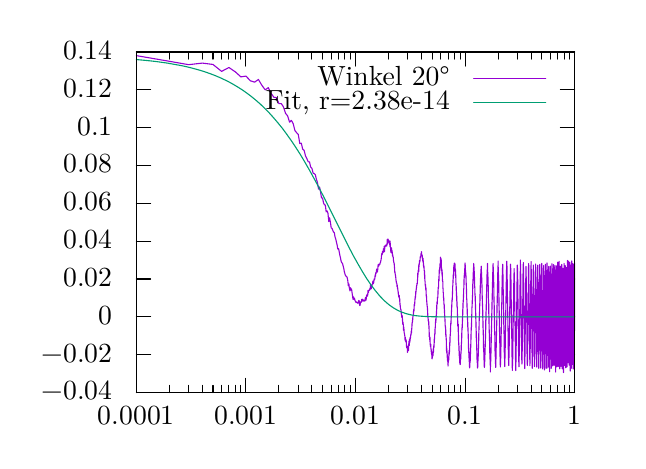
\begin{tikzpicture}[gnuplot]
%% generated with GNUPLOT 5.2p5a (Gentoo revision r0) (Lua 5.1; terminal rev. 99 , script rev. 107)
%% Sa 18 Mai 2019 18:31:15 CEST
\path (0.000,0.000) rectangle (7.500,5.250);
\gpcolor{color=gp lt color border}
\gpsetlinetype{gp lt border}
\gpsetdashtype{gp dt solid}
\gpsetlinewidth{1.00}
\draw[gp path] (1.380,0.616)--(1.560,0.616);
\draw[gp path] (6.947,0.616)--(6.767,0.616);
\node[gp node right] at (1.196,0.616) {$-0.04$};
\draw[gp path] (1.380,1.097)--(1.560,1.097);
\draw[gp path] (6.947,1.097)--(6.767,1.097);
\node[gp node right] at (1.196,1.097) {$-0.02$};
\draw[gp path] (1.380,1.577)--(1.560,1.577);
\draw[gp path] (6.947,1.577)--(6.767,1.577);
\node[gp node right] at (1.196,1.577) {$0$};
\draw[gp path] (1.380,2.058)--(1.560,2.058);
\draw[gp path] (6.947,2.058)--(6.767,2.058);
\node[gp node right] at (1.196,2.058) {$0.02$};
\draw[gp path] (1.380,2.538)--(1.560,2.538);
\draw[gp path] (6.947,2.538)--(6.767,2.538);
\node[gp node right] at (1.196,2.538) {$0.04$};
\draw[gp path] (1.380,3.019)--(1.560,3.019);
\draw[gp path] (6.947,3.019)--(6.767,3.019);
\node[gp node right] at (1.196,3.019) {$0.06$};
\draw[gp path] (1.380,3.499)--(1.560,3.499);
\draw[gp path] (6.947,3.499)--(6.767,3.499);
\node[gp node right] at (1.196,3.499) {$0.08$};
\draw[gp path] (1.380,3.980)--(1.560,3.980);
\draw[gp path] (6.947,3.980)--(6.767,3.980);
\node[gp node right] at (1.196,3.980) {$0.1$};
\draw[gp path] (1.380,4.460)--(1.560,4.460);
\draw[gp path] (6.947,4.460)--(6.767,4.460);
\node[gp node right] at (1.196,4.460) {$0.12$};
\draw[gp path] (1.380,4.941)--(1.560,4.941);
\draw[gp path] (6.947,4.941)--(6.767,4.941);
\node[gp node right] at (1.196,4.941) {$0.14$};
\draw[gp path] (1.380,0.616)--(1.380,0.796);
\draw[gp path] (1.380,4.941)--(1.380,4.761);
\node[gp node center] at (1.380,0.308) {$0.0001$};
\draw[gp path] (1.799,0.616)--(1.799,0.706);
\draw[gp path] (1.799,4.941)--(1.799,4.851);
\draw[gp path] (2.044,0.616)--(2.044,0.706);
\draw[gp path] (2.044,4.941)--(2.044,4.851);
\draw[gp path] (2.218,0.616)--(2.218,0.706);
\draw[gp path] (2.218,4.941)--(2.218,4.851);
\draw[gp path] (2.353,0.616)--(2.353,0.706);
\draw[gp path] (2.353,4.941)--(2.353,4.851);
\draw[gp path] (2.463,0.616)--(2.463,0.706);
\draw[gp path] (2.463,4.941)--(2.463,4.851);
\draw[gp path] (2.556,0.616)--(2.556,0.706);
\draw[gp path] (2.556,4.941)--(2.556,4.851);
\draw[gp path] (2.637,0.616)--(2.637,0.706);
\draw[gp path] (2.637,4.941)--(2.637,4.851);
\draw[gp path] (2.708,0.616)--(2.708,0.706);
\draw[gp path] (2.708,4.941)--(2.708,4.851);
\draw[gp path] (2.772,0.616)--(2.772,0.796);
\draw[gp path] (2.772,4.941)--(2.772,4.761);
\node[gp node center] at (2.772,0.308) {$0.001$};
\draw[gp path] (3.191,0.616)--(3.191,0.706);
\draw[gp path] (3.191,4.941)--(3.191,4.851);
\draw[gp path] (3.436,0.616)--(3.436,0.706);
\draw[gp path] (3.436,4.941)--(3.436,4.851);
\draw[gp path] (3.610,0.616)--(3.610,0.706);
\draw[gp path] (3.610,4.941)--(3.610,4.851);
\draw[gp path] (3.745,0.616)--(3.745,0.706);
\draw[gp path] (3.745,4.941)--(3.745,4.851);
\draw[gp path] (3.855,0.616)--(3.855,0.706);
\draw[gp path] (3.855,4.941)--(3.855,4.851);
\draw[gp path] (3.948,0.616)--(3.948,0.706);
\draw[gp path] (3.948,4.941)--(3.948,4.851);
\draw[gp path] (4.029,0.616)--(4.029,0.706);
\draw[gp path] (4.029,4.941)--(4.029,4.851);
\draw[gp path] (4.100,0.616)--(4.100,0.706);
\draw[gp path] (4.100,4.941)--(4.100,4.851);
\draw[gp path] (4.163,0.616)--(4.163,0.796);
\draw[gp path] (4.163,4.941)--(4.163,4.761);
\node[gp node center] at (4.163,0.308) {$0.01$};
\draw[gp path] (4.582,0.616)--(4.582,0.706);
\draw[gp path] (4.582,4.941)--(4.582,4.851);
\draw[gp path] (4.828,0.616)--(4.828,0.706);
\draw[gp path] (4.828,4.941)--(4.828,4.851);
\draw[gp path] (5.001,0.616)--(5.001,0.706);
\draw[gp path] (5.001,4.941)--(5.001,4.851);
\draw[gp path] (5.136,0.616)--(5.136,0.706);
\draw[gp path] (5.136,4.941)--(5.136,4.851);
\draw[gp path] (5.246,0.616)--(5.246,0.706);
\draw[gp path] (5.246,4.941)--(5.246,4.851);
\draw[gp path] (5.340,0.616)--(5.340,0.706);
\draw[gp path] (5.340,4.941)--(5.340,4.851);
\draw[gp path] (5.420,0.616)--(5.420,0.706);
\draw[gp path] (5.420,4.941)--(5.420,4.851);
\draw[gp path] (5.492,0.616)--(5.492,0.706);
\draw[gp path] (5.492,4.941)--(5.492,4.851);
\draw[gp path] (5.555,0.616)--(5.555,0.796);
\draw[gp path] (5.555,4.941)--(5.555,4.761);
\node[gp node center] at (5.555,0.308) {$0.1$};
\draw[gp path] (5.974,0.616)--(5.974,0.706);
\draw[gp path] (5.974,4.941)--(5.974,4.851);
\draw[gp path] (6.219,0.616)--(6.219,0.706);
\draw[gp path] (6.219,4.941)--(6.219,4.851);
\draw[gp path] (6.393,0.616)--(6.393,0.706);
\draw[gp path] (6.393,4.941)--(6.393,4.851);
\draw[gp path] (6.528,0.616)--(6.528,0.706);
\draw[gp path] (6.528,4.941)--(6.528,4.851);
\draw[gp path] (6.638,0.616)--(6.638,0.706);
\draw[gp path] (6.638,4.941)--(6.638,4.851);
\draw[gp path] (6.731,0.616)--(6.731,0.706);
\draw[gp path] (6.731,4.941)--(6.731,4.851);
\draw[gp path] (6.812,0.616)--(6.812,0.706);
\draw[gp path] (6.812,4.941)--(6.812,4.851);
\draw[gp path] (6.883,0.616)--(6.883,0.706);
\draw[gp path] (6.883,4.941)--(6.883,4.851);
\draw[gp path] (6.947,0.616)--(6.947,0.796);
\draw[gp path] (6.947,4.941)--(6.947,4.761);
\node[gp node center] at (6.947,0.308) {$1$};
\draw[gp path] (1.380,4.941)--(1.380,0.616)--(6.947,0.616)--(6.947,4.941)--cycle;
\node[gp node right] at (5.479,4.607) {Winkel 20°};
\gpcolor{rgb color={0.580,0.000,0.827}}
\draw[gp path] (5.663,4.607)--(6.579,4.607);
\draw[gp path] (1.380,4.895)--(1.799,4.823)--(2.044,4.780)--(2.218,4.800)--(2.353,4.783)%
  --(2.463,4.695)--(2.556,4.744)--(2.637,4.689)--(2.708,4.625)--(2.772,4.635)--(2.829,4.575)%
  --(2.882,4.558)--(2.930,4.592)--(2.975,4.517)--(3.017,4.460)--(3.056,4.488)--(3.092,4.415)%
  --(3.127,4.366)--(3.160,4.361)--(3.191,4.285)--(3.220,4.286)--(3.248,4.244)--(3.275,4.161)%
  --(3.301,4.131)--(3.326,4.050)--(3.349,4.073)--(3.372,4.031)--(3.394,3.943)--(3.415,3.917)%
  --(3.436,3.896)--(3.456,3.779)--(3.475,3.783)--(3.493,3.706)--(3.511,3.692)--(3.529,3.619)%
  --(3.546,3.586)--(3.563,3.546)--(3.579,3.546)--(3.594,3.479)--(3.610,3.464)--(3.625,3.402)%
  --(3.639,3.397)--(3.653,3.383)--(3.667,3.324)--(3.681,3.279)--(3.694,3.199)--(3.707,3.227)%
  --(3.720,3.158)--(3.732,3.088)--(3.745,3.086)--(3.757,3.026)--(3.768,3.001)--(3.780,2.997)%
  --(3.791,2.911)--(3.802,2.924)--(3.813,2.897)--(3.824,2.789)--(3.834,2.836)--(3.845,2.776)%
  --(3.855,2.707)--(3.865,2.701)--(3.875,2.677)--(3.884,2.654)--(3.894,2.649)--(3.903,2.595)%
  --(3.912,2.566)--(3.921,2.529)--(3.930,2.489)--(3.939,2.438)--(3.948,2.445)--(3.956,2.405)%
  --(3.965,2.358)--(3.973,2.326)--(3.982,2.278)--(3.990,2.263)--(3.998,2.258)--(4.006,2.224)%
  --(4.013,2.199)--(4.021,2.154)--(4.029,2.123)--(4.036,2.104)--(4.044,2.092)--(4.051,2.090)%
  --(4.058,2.073)--(4.065,2.041)--(4.072,1.973)--(4.079,1.997)--(4.086,1.939)--(4.093,1.907)%
  --(4.100,1.947)--(4.106,1.921)--(4.113,1.931)--(4.120,1.882)--(4.126,1.843)--(4.132,1.799)%
  --(4.139,1.832)--(4.145,1.799)--(4.151,1.812)--(4.157,1.784)--(4.164,1.774)--(4.170,1.759)%
  --(4.175,1.767)--(4.181,1.758)--(4.187,1.762)--(4.193,1.750)--(4.199,1.757)--(4.204,1.785)%
  --(4.210,1.783)--(4.216,1.722)--(4.221,1.722)--(4.227,1.765)--(4.232,1.767)--(4.237,1.763)%
  --(4.243,1.800)--(4.248,1.781)--(4.253,1.801)--(4.258,1.776)--(4.264,1.791)--(4.269,1.783)%
  --(4.274,1.777)--(4.279,1.790)--(4.284,1.780)--(4.289,1.823)--(4.294,1.795)--(4.298,1.790)%
  --(4.303,1.844)--(4.308,1.853)--(4.313,1.865)--(4.317,1.839)--(4.322,1.912)--(4.327,1.884)%
  --(4.331,1.913)--(4.336,1.917)--(4.340,1.914)--(4.345,1.936)--(4.349,1.922)--(4.354,1.981)%
  --(4.358,1.984)--(4.363,1.933)--(4.367,1.955)--(4.371,1.960)--(4.375,1.987)--(4.380,1.998)%
  --(4.384,2.031)--(4.388,1.996)--(4.392,2.007)--(4.396,2.019)--(4.400,2.059)--(4.405,2.051)%
  --(4.409,2.065)--(4.413,2.112)--(4.417,2.092)--(4.421,2.137)--(4.424,2.126)--(4.428,2.150)%
  --(4.432,2.185)--(4.436,2.176)--(4.440,2.146)--(4.444,2.160)--(4.448,2.205)--(4.451,2.242)%
  --(4.455,2.242)--(4.459,2.222)--(4.463,2.235)--(4.466,2.248)--(4.470,2.244)--(4.473,2.244)%
  --(4.477,2.268)--(4.481,2.268)--(4.484,2.288)--(4.488,2.301)--(4.491,2.324)--(4.495,2.368)%
  --(4.498,2.384)--(4.502,2.368)--(4.505,2.406)--(4.509,2.403)--(4.512,2.391)--(4.515,2.418)%
  --(4.519,2.444)--(4.522,2.403)--(4.525,2.401)--(4.529,2.476)--(4.532,2.408)--(4.535,2.461)%
  --(4.539,2.479)--(4.542,2.474)--(4.545,2.488)--(4.548,2.487)--(4.551,2.474)--(4.555,2.487)%
  --(4.558,2.494)--(4.561,2.478)--(4.564,2.509)--(4.567,2.560)--(4.570,2.550)--(4.573,2.506)%
  --(4.576,2.566)--(4.579,2.555)--(4.582,2.525)--(4.585,2.543)--(4.588,2.540)--(4.591,2.543)%
  --(4.594,2.521)--(4.597,2.525)--(4.600,2.472)--(4.603,2.539)--(4.606,2.457)--(4.609,2.451)%
  --(4.612,2.403)--(4.615,2.393)--(4.618,2.455)--(4.621,2.451)--(4.623,2.423)--(4.626,2.422)%
  --(4.629,2.411)--(4.632,2.352)--(4.635,2.373)--(4.637,2.351)--(4.640,2.341)--(4.643,2.330)%
  --(4.646,2.291)--(4.648,2.279)--(4.651,2.264)--(4.654,2.264)--(4.656,2.236)--(4.659,2.199)%
  --(4.662,2.143)--(4.664,2.150)--(4.667,2.122)--(4.670,2.113)--(4.672,2.096)--(4.675,2.075)%
  --(4.677,2.049)--(4.680,2.033)--(4.683,2.005)--(4.685,2.013)--(4.688,1.999)--(4.690,1.962)%
  --(4.693,1.982)--(4.695,1.966)--(4.698,1.930)--(4.700,1.938)--(4.703,1.902)--(4.705,1.903)%
  --(4.708,1.857)--(4.710,1.864)--(4.712,1.829)--(4.715,1.847)--(4.717,1.838)--(4.720,1.847)%
  --(4.722,1.804)--(4.725,1.804)--(4.727,1.733)--(4.729,1.750)--(4.732,1.710)--(4.734,1.693)%
  --(4.736,1.683)--(4.739,1.667)--(4.741,1.667)--(4.743,1.653)--(4.746,1.602)--(4.748,1.631)%
  --(4.750,1.573)--(4.753,1.589)--(4.755,1.585)--(4.757,1.591)--(4.759,1.570)--(4.762,1.492)%
  --(4.764,1.483)--(4.766,1.511)--(4.768,1.497)--(4.771,1.470)--(4.773,1.406)--(4.775,1.411)%
  --(4.777,1.449)--(4.779,1.416)--(4.781,1.377)--(4.784,1.368)--(4.786,1.358)--(4.788,1.340)%
  --(4.790,1.336)--(4.792,1.296)--(4.794,1.277)--(4.797,1.318)--(4.799,1.266)--(4.801,1.292)%
  --(4.803,1.291)--(4.805,1.280)--(4.807,1.250)--(4.809,1.274)--(4.811,1.206)--(4.813,1.187)%
  --(4.815,1.203)--(4.817,1.190)--(4.819,1.177)--(4.821,1.193)--(4.823,1.125)--(4.826,1.204)%
  --(4.828,1.166)--(4.830,1.172)--(4.832,1.180)--(4.834,1.170)--(4.836,1.149)--(4.838,1.211)%
  --(4.840,1.226)--(4.841,1.265)--(4.843,1.211)--(4.845,1.272)--(4.847,1.213)--(4.849,1.289)%
  --(4.851,1.249)--(4.853,1.269)--(4.855,1.311)--(4.857,1.272)--(4.859,1.316)--(4.861,1.310)%
  --(4.863,1.332)--(4.865,1.351)--(4.867,1.338)--(4.868,1.359)--(4.870,1.372)--(4.872,1.398)%
  --(4.874,1.371)--(4.876,1.403)--(4.878,1.431)--(4.880,1.452)--(4.881,1.491)--(4.883,1.494)%
  --(4.885,1.513)--(4.887,1.510)--(4.889,1.566)--(4.891,1.541)--(4.892,1.573)--(4.894,1.590)%
  --(4.896,1.592)--(4.898,1.603)--(4.900,1.628)--(4.901,1.667)--(4.903,1.665)--(4.905,1.677)%
  --(4.907,1.652)--(4.908,1.706)--(4.910,1.736)--(4.912,1.722)--(4.914,1.719)--(4.916,1.764)%
  --(4.917,1.767)--(4.919,1.807)--(4.921,1.807)--(4.922,1.836)--(4.924,1.815)--(4.926,1.847)%
  --(4.928,1.865)--(4.929,1.902)--(4.931,1.897)--(4.933,1.893)--(4.934,1.923)--(4.936,1.938)%
  --(4.938,1.963)--(4.939,1.948)--(4.941,1.980)--(4.943,1.974)--(4.944,2.003)--(4.946,2.005)%
  --(4.948,1.994)--(4.949,2.022)--(4.951,2.050)--(4.953,2.064)--(4.954,2.130)--(4.956,2.136)%
  --(4.958,2.116)--(4.959,2.139)--(4.961,2.168)--(4.962,2.173)--(4.964,2.162)--(4.966,2.151)%
  --(4.967,2.231)--(4.969,2.209)--(4.970,2.246)--(4.972,2.239)--(4.974,2.265)--(4.975,2.278)%
  --(4.977,2.294)--(4.978,2.284)--(4.980,2.273)--(4.981,2.277)--(4.983,2.297)--(4.985,2.327)%
  --(4.986,2.340)--(4.988,2.326)--(4.989,2.332)--(4.991,2.346)--(4.992,2.347)--(4.994,2.360)%
  --(4.995,2.375)--(4.997,2.384)--(4.998,2.369)--(5.000,2.382)--(5.001,2.406)--(5.003,2.372)%
  --(5.004,2.371)--(5.006,2.366)--(5.007,2.363)--(5.009,2.348)--(5.010,2.364)--(5.012,2.338)%
  --(5.013,2.320)--(5.015,2.317)--(5.016,2.310)--(5.018,2.284)--(5.019,2.308)--(5.021,2.322)%
  --(5.022,2.284)--(5.024,2.263)--(5.025,2.290)--(5.027,2.236)--(5.028,2.213)--(5.029,2.236)%
  --(5.031,2.203)--(5.032,2.229)--(5.034,2.193)--(5.035,2.173)--(5.037,2.167)--(5.038,2.121)%
  --(5.039,2.106)--(5.041,2.160)--(5.042,2.113)--(5.044,2.039)--(5.045,2.035)--(5.047,2.027)%
  --(5.048,1.987)--(5.049,1.982)--(5.051,1.978)--(5.052,1.964)--(5.054,1.987)--(5.055,1.952)%
  --(5.056,1.924)--(5.058,1.941)--(5.059,1.920)--(5.060,1.889)--(5.062,1.842)--(5.063,1.861)%
  --(5.064,1.846)--(5.066,1.818)--(5.067,1.774)--(5.069,1.764)--(5.070,1.780)--(5.071,1.731)%
  --(5.073,1.722)--(5.074,1.703)--(5.075,1.711)--(5.077,1.684)--(5.078,1.675)--(5.079,1.637)%
  --(5.081,1.595)--(5.082,1.620)--(5.083,1.562)--(5.085,1.571)--(5.086,1.571)--(5.087,1.529)%
  --(5.089,1.522)--(5.090,1.525)--(5.091,1.519)--(5.092,1.476)--(5.094,1.515)--(5.095,1.484)%
  --(5.096,1.425)--(5.098,1.460)--(5.099,1.398)--(5.100,1.324)--(5.101,1.354)--(5.103,1.334)%
  --(5.104,1.329)--(5.105,1.286)--(5.107,1.315)--(5.108,1.289)--(5.109,1.317)--(5.110,1.263)%
  --(5.112,1.237)--(5.113,1.219)--(5.114,1.228)--(5.115,1.199)--(5.117,1.199)--(5.118,1.229)%
  --(5.119,1.228)--(5.120,1.181)--(5.122,1.173)--(5.123,1.163)--(5.124,1.135)--(5.125,1.157)%
  --(5.127,1.154)--(5.128,1.138)--(5.129,1.107)--(5.130,1.118)--(5.131,1.121)--(5.133,1.076)%
  --(5.134,1.098)--(5.135,1.043)--(5.136,1.053)--(5.137,1.066)--(5.139,1.054)--(5.140,1.066)%
  --(5.141,1.078)--(5.142,1.070)--(5.144,1.104)--(5.145,1.101)--(5.146,1.110)--(5.147,1.085)%
  --(5.148,1.119)--(5.149,1.170)--(5.151,1.125)--(5.152,1.126)--(5.153,1.165)--(5.154,1.130)%
  --(5.155,1.201)--(5.157,1.199)--(5.158,1.211)--(5.159,1.188)--(5.160,1.191)--(5.161,1.231)%
  --(5.162,1.292)--(5.163,1.275)--(5.165,1.250)--(5.166,1.314)--(5.167,1.313)--(5.168,1.295)%
  --(5.169,1.360)--(5.170,1.347)--(5.172,1.420)--(5.173,1.363)--(5.174,1.397)--(5.175,1.427)%
  --(5.176,1.444)--(5.177,1.452)--(5.178,1.486)--(5.179,1.508)--(5.181,1.524)--(5.182,1.546)%
  --(5.183,1.536)--(5.184,1.503)--(5.185,1.533)--(5.186,1.546)--(5.187,1.590)--(5.188,1.587)%
  --(5.189,1.600)--(5.191,1.590)--(5.192,1.652)--(5.193,1.652)--(5.194,1.682)--(5.195,1.675)%
  --(5.196,1.733)--(5.197,1.767)--(5.198,1.746)--(5.199,1.733)--(5.200,1.764)--(5.202,1.744)%
  --(5.203,1.824)--(5.204,1.815)--(5.205,1.821)--(5.206,1.815)--(5.207,1.817)--(5.208,1.820)%
  --(5.209,1.826)--(5.210,1.863)--(5.211,1.867)--(5.212,1.926)--(5.213,1.920)--(5.214,1.941)%
  --(5.215,1.956)--(5.217,1.949)--(5.218,1.958)--(5.219,1.982)--(5.220,2.051)--(5.221,2.053)%
  --(5.222,2.049)--(5.223,2.031)--(5.224,2.060)--(5.225,2.137)--(5.226,2.171)--(5.227,2.173)%
  --(5.228,2.129)--(5.229,2.138)--(5.230,2.133)--(5.231,2.175)--(5.232,2.152)--(5.233,2.204)%
  --(5.234,2.182)--(5.235,2.249)--(5.236,2.205)--(5.237,2.206)--(5.238,2.225)--(5.239,2.216)%
  --(5.240,2.259)--(5.241,2.232)--(5.242,2.335)--(5.243,2.286)--(5.244,2.283)--(5.245,2.311)%
  --(5.246,2.327)--(5.247,2.263)--(5.249,2.289)--(5.250,2.250)--(5.251,2.314)--(5.252,2.293)%
  --(5.253,2.263)--(5.254,2.221)--(5.254,2.164)--(5.255,2.188)--(5.256,2.204)--(5.257,2.198)%
  --(5.258,2.176)--(5.259,2.165)--(5.260,2.157)--(5.261,2.183)--(5.262,2.131)--(5.263,2.106)%
  --(5.264,2.109)--(5.265,2.142)--(5.266,2.069)--(5.267,2.077)--(5.268,2.037)--(5.269,2.041)%
  --(5.270,2.026)--(5.271,2.029)--(5.272,2.026)--(5.273,1.942)--(5.274,1.944)--(5.275,1.934)%
  --(5.276,1.938)--(5.277,1.885)--(5.278,1.891)--(5.279,1.872)--(5.280,1.844)--(5.281,1.820)%
  --(5.282,1.829)--(5.283,1.799)--(5.284,1.799)--(5.285,1.777)--(5.286,1.815)--(5.286,1.735)%
  --(5.287,1.740)--(5.288,1.742)--(5.289,1.691)--(5.290,1.683)--(5.291,1.731)--(5.292,1.679)%
  --(5.293,1.664)--(5.294,1.637)--(5.295,1.610)--(5.296,1.594)--(5.297,1.572)--(5.298,1.594)%
  --(5.299,1.520)--(5.300,1.539)--(5.300,1.547)--(5.301,1.523)--(5.302,1.474)--(5.303,1.460)%
  --(5.304,1.459)--(5.305,1.465)--(5.306,1.431)--(5.307,1.451)--(5.308,1.426)--(5.309,1.411)%
  --(5.310,1.413)--(5.310,1.344)--(5.311,1.382)--(5.312,1.353)--(5.313,1.325)--(5.314,1.345)%
  --(5.315,1.303)--(5.316,1.300)--(5.317,1.265)--(5.318,1.205)--(5.319,1.201)--(5.319,1.176)%
  --(5.320,1.130)--(5.321,1.171)--(5.322,1.176)--(5.323,1.115)--(5.324,1.136)--(5.325,1.118)%
  --(5.326,1.143)--(5.327,1.072)--(5.327,1.103)--(5.328,1.085)--(5.329,1.060)--(5.330,1.099)%
  --(5.331,1.037)--(5.332,1.022)--(5.333,1.038)--(5.334,1.009)--(5.334,1.027)--(5.335,1.044)%
  --(5.336,1.037)--(5.337,1.011)--(5.338,1.004)--(5.339,0.952)--(5.340,1.016)--(5.341,0.996)%
  --(5.341,1.007)--(5.342,1.010)--(5.343,1.045)--(5.344,1.029)--(5.345,1.017)--(5.346,1.074)%
  --(5.347,1.031)--(5.347,1.047)--(5.348,1.061)--(5.349,1.056)--(5.350,1.126)--(5.351,1.086)%
  --(5.352,1.110)--(5.352,1.090)--(5.353,1.154)--(5.354,1.105)--(5.355,1.146)--(5.356,1.150)%
  --(5.357,1.131)--(5.358,1.155)--(5.358,1.173)--(5.359,1.206)--(5.360,1.210)--(5.361,1.253)%
  --(5.362,1.243)--(5.363,1.272)--(5.363,1.251)--(5.364,1.322)--(5.365,1.277)--(5.366,1.340)%
  --(5.367,1.358)--(5.368,1.359)--(5.368,1.420)--(5.369,1.380)--(5.370,1.424)--(5.371,1.449)%
  --(5.372,1.416)--(5.372,1.471)--(5.373,1.473)--(5.374,1.509)--(5.375,1.472)--(5.376,1.504)%
  --(5.377,1.533)--(5.377,1.523)--(5.378,1.591)--(5.379,1.567)--(5.380,1.579)--(5.381,1.595)%
  --(5.381,1.618)--(5.382,1.644)--(5.383,1.654)--(5.384,1.679)--(5.385,1.699)--(5.385,1.706)%
  --(5.386,1.698)--(5.387,1.790)--(5.388,1.768)--(5.389,1.780)--(5.389,1.793)--(5.390,1.770)%
  --(5.391,1.819)--(5.392,1.801)--(5.393,1.793)--(5.393,1.835)--(5.394,1.841)--(5.395,1.882)%
  --(5.396,1.902)--(5.396,1.891)--(5.397,1.955)--(5.398,1.969)--(5.399,1.970)--(5.400,2.019)%
  --(5.400,2.005)--(5.401,2.009)--(5.402,2.046)--(5.403,2.044)--(5.404,2.042)--(5.404,2.062)%
  --(5.405,2.100)--(5.406,2.124)--(5.407,2.111)--(5.407,2.107)--(5.408,2.099)--(5.409,2.132)%
  --(5.410,2.159)--(5.410,2.121)--(5.411,2.210)--(5.412,2.187)--(5.413,2.211)--(5.414,2.174)%
  --(5.414,2.233)--(5.415,2.231)--(5.416,2.203)--(5.417,2.212)--(5.417,2.256)--(5.418,2.218)%
  --(5.419,2.214)--(5.420,2.258)--(5.420,2.260)--(5.421,2.256)--(5.422,2.206)--(5.423,2.239)%
  --(5.423,2.246)--(5.424,2.259)--(5.425,2.244)--(5.426,2.245)--(5.426,2.207)--(5.427,2.246)%
  --(5.428,2.186)--(5.429,2.208)--(5.429,2.167)--(5.430,2.190)--(5.431,2.140)--(5.432,2.168)%
  --(5.432,2.104)--(5.433,2.176)--(5.434,2.146)--(5.435,2.130)--(5.435,2.100)--(5.436,2.114)%
  --(5.437,2.072)--(5.438,2.105)--(5.438,2.088)--(5.439,2.008)--(5.440,2.002)--(5.440,2.000)%
  --(5.441,1.952)--(5.442,1.913)--(5.443,1.965)--(5.443,1.941)--(5.444,1.909)--(5.445,1.894)%
  --(5.446,1.877)--(5.446,1.867)--(5.447,1.823)--(5.448,1.807)--(5.448,1.798)--(5.449,1.842)%
  --(5.450,1.767)--(5.451,1.814)--(5.451,1.781)--(5.452,1.765)--(5.453,1.733)--(5.453,1.707)%
  --(5.454,1.705)--(5.455,1.708)--(5.456,1.690)--(5.456,1.697)--(5.457,1.652)--(5.458,1.661)%
  --(5.458,1.615)--(5.459,1.585)--(5.460,1.548)--(5.461,1.589)--(5.461,1.460)--(5.462,1.527)%
  --(5.463,1.484)--(5.463,1.491)--(5.464,1.459)--(5.465,1.482)--(5.465,1.467)--(5.466,1.459)%
  --(5.467,1.413)--(5.468,1.485)--(5.468,1.455)--(5.469,1.380)--(5.470,1.379)--(5.470,1.337)%
  --(5.471,1.347)--(5.472,1.310)--(5.472,1.278)--(5.473,1.262)--(5.474,1.248)--(5.475,1.220)%
  --(5.475,1.242)--(5.476,1.223)--(5.477,1.178)--(5.477,1.212)--(5.478,1.147)--(5.479,1.145)%
  --(5.479,1.100)--(5.480,1.116)--(5.481,1.143)--(5.481,1.124)--(5.482,1.054)--(5.483,1.081)%
  --(5.483,1.111)--(5.484,1.100)--(5.485,1.036)--(5.485,1.045)--(5.486,1.033)--(5.487,1.092)%
  --(5.488,0.988)--(5.488,1.008)--(5.489,0.978)--(5.490,0.998)--(5.490,0.981)--(5.491,1.004)%
  --(5.492,0.982)--(5.492,1.000)--(5.493,0.970)--(5.494,1.024)--(5.494,1.000)--(5.495,1.026)%
  --(5.496,1.061)--(5.496,1.021)--(5.497,1.063)--(5.498,1.065)--(5.498,1.083)--(5.499,1.079)%
  --(5.500,1.043)--(5.500,1.083)--(5.501,1.116)--(5.502,1.127)--(5.502,1.109)--(5.503,1.134)%
  --(5.504,1.113)--(5.504,1.154)--(5.505,1.183)--(5.506,1.153)--(5.506,1.218)--(5.507,1.192)%
  --(5.507,1.188)--(5.508,1.251)--(5.509,1.239)--(5.509,1.256)--(5.510,1.259)--(5.511,1.258)%
  --(5.511,1.330)--(5.512,1.321)--(5.513,1.372)--(5.513,1.355)--(5.514,1.308)--(5.515,1.413)%
  --(5.515,1.405)--(5.516,1.440)--(5.517,1.428)--(5.517,1.436)--(5.518,1.418)--(5.518,1.413)%
  --(5.519,1.483)--(5.520,1.481)--(5.520,1.487)--(5.521,1.521)--(5.522,1.523)--(5.522,1.573)%
  --(5.523,1.562)--(5.524,1.554)--(5.524,1.583)--(5.525,1.612)--(5.526,1.608)--(5.526,1.671)%
  --(5.527,1.638)--(5.527,1.704)--(5.528,1.690)--(5.529,1.744)--(5.529,1.751)--(5.530,1.724)%
  --(5.531,1.720)--(5.531,1.793)--(5.532,1.779)--(5.532,1.765)--(5.533,1.835)--(5.534,1.814)%
  --(5.534,1.820)--(5.535,1.833)--(5.536,1.884)--(5.536,1.879)--(5.537,1.907)--(5.537,1.919)%
  --(5.538,1.937)--(5.539,1.936)--(5.539,1.966)--(5.540,1.979)--(5.541,1.990)--(5.541,1.985)%
  --(5.542,2.058)--(5.542,2.009)--(5.543,2.101)--(5.544,2.083)--(5.544,2.074)--(5.545,2.080)%
  --(5.546,2.104)--(5.546,2.098)--(5.547,2.123)--(5.547,2.125)--(5.548,2.127)--(5.549,2.152)%
  --(5.549,2.145)--(5.550,2.147)--(5.550,2.167)--(5.551,2.192)--(5.552,2.188)--(5.552,2.229)%
  --(5.553,2.195)--(5.553,2.252)--(5.554,2.186)--(5.555,2.262)--(5.555,2.249)--(5.556,2.242)%
  --(5.556,2.217)--(5.557,2.220)--(5.558,2.236)--(5.558,2.216)--(5.559,2.174)--(5.559,2.195)%
  --(5.560,2.148)--(5.561,2.163)--(5.561,2.123)--(5.562,2.168)--(5.562,2.143)--(5.563,2.124)%
  --(5.564,2.091)--(5.564,2.137)--(5.565,2.082)--(5.565,2.089)--(5.566,2.101)--(5.567,2.066)%
  --(5.567,2.086)--(5.568,2.057)--(5.568,2.011)--(5.569,2.015)--(5.570,1.978)--(5.570,1.994)%
  --(5.571,1.975)--(5.571,1.937)--(5.572,1.949)--(5.573,1.910)--(5.573,1.867)--(5.574,1.867)%
  --(5.574,1.883)--(5.575,1.873)--(5.575,1.823)--(5.576,1.795)--(5.577,1.800)--(5.577,1.796)%
  --(5.578,1.806)--(5.578,1.798)--(5.579,1.725)--(5.580,1.738)--(5.580,1.698)--(5.581,1.734)%
  --(5.581,1.719)--(5.582,1.671)--(5.582,1.637)--(5.583,1.610)--(5.584,1.639)--(5.584,1.574)%
  --(5.585,1.575)--(5.585,1.567)--(5.586,1.570)--(5.586,1.543)--(5.587,1.535)--(5.588,1.486)%
  --(5.588,1.528)--(5.589,1.446)--(5.589,1.479)--(5.590,1.433)--(5.590,1.425)--(5.591,1.399)%
  --(5.592,1.434)--(5.592,1.439)--(5.593,1.377)--(5.593,1.352)--(5.594,1.360)--(5.594,1.377)%
  --(5.595,1.346)--(5.596,1.298)--(5.596,1.310)--(5.597,1.260)--(5.598,1.215)--(5.598,1.237)%
  --(5.599,1.176)--(5.600,1.162)--(5.600,1.165)--(5.601,1.182)--(5.601,1.156)--(5.602,1.124)%
  --(5.602,1.120)--(5.603,1.149)--(5.603,1.133)--(5.604,1.134)--(5.605,1.054)--(5.605,1.069)%
  --(5.606,1.044)--(5.606,1.100)--(5.607,1.051)--(5.607,1.007)--(5.608,1.035)--(5.608,1.010)%
  --(5.609,1.057)--(5.610,1.016)--(5.610,1.005)--(5.611,1.020)--(5.611,0.973)--(5.612,0.929)%
  --(5.612,0.971)--(5.613,0.980)--(5.613,0.951)--(5.614,0.957)--(5.615,0.937)--(5.615,0.977)%
  --(5.616,0.952)--(5.616,0.968)--(5.617,1.000)--(5.617,1.015)--(5.618,1.018)--(5.618,1.019)%
  --(5.619,1.026)--(5.619,1.057)--(5.620,1.014)--(5.621,1.087)--(5.621,1.064)--(5.622,1.065)%
  --(5.622,1.061)--(5.623,1.084)--(5.623,1.100)--(5.624,1.135)--(5.624,1.120)--(5.625,1.160)%
  --(5.625,1.152)--(5.626,1.175)--(5.626,1.177)--(5.627,1.212)--(5.628,1.240)--(5.628,1.215)%
  --(5.629,1.257)--(5.629,1.320)--(5.630,1.289)--(5.630,1.348)--(5.631,1.360)--(5.631,1.367)%
  --(5.632,1.377)--(5.632,1.385)--(5.633,1.426)--(5.633,1.442)--(5.634,1.411)--(5.634,1.406)%
  --(5.635,1.430)--(5.636,1.469)--(5.636,1.452)--(5.637,1.505)--(5.637,1.496)--(5.638,1.525)%
  --(5.638,1.545)--(5.639,1.571)--(5.639,1.572)--(5.640,1.612)--(5.640,1.610)--(5.641,1.578)%
  --(5.641,1.664)--(5.642,1.697)--(5.642,1.689)--(5.643,1.702)--(5.643,1.701)--(5.644,1.711)%
  --(5.644,1.767)--(5.645,1.786)--(5.645,1.737)--(5.646,1.752)--(5.647,1.768)--(5.647,1.831)%
  --(5.648,1.775)--(5.648,1.826)--(5.649,1.851)--(5.649,1.850)--(5.650,1.827)--(5.650,1.851)%
  --(5.651,1.906)--(5.651,1.878)--(5.652,1.956)--(5.652,1.994)--(5.653,1.954)--(5.653,1.990)%
  --(5.654,2.008)--(5.654,2.018)--(5.655,1.999)--(5.655,2.056)--(5.656,2.034)--(5.656,2.048)%
  --(5.657,2.069)--(5.657,2.077)--(5.658,2.095)--(5.658,2.103)--(5.659,2.127)--(5.659,2.141)%
  --(5.660,2.118)--(5.660,2.151)--(5.661,2.139)--(5.661,2.147)--(5.662,2.201)--(5.662,2.171)%
  --(5.663,2.169)--(5.663,2.220)--(5.664,2.210)--(5.664,2.256)--(5.665,2.231)--(5.665,2.208)%
  --(5.666,2.187)--(5.666,2.212)--(5.667,2.199)--(5.667,2.201)--(5.668,2.139)--(5.668,2.208)%
  --(5.669,2.210)--(5.669,2.192)--(5.670,2.113)--(5.670,2.136)--(5.671,2.159)--(5.671,2.137)%
  --(5.672,2.097)--(5.672,2.089)--(5.673,2.113)--(5.673,2.088)--(5.674,2.074)--(5.674,2.080)%
  --(5.675,2.057)--(5.675,2.046)--(5.676,2.016)--(5.676,2.055)--(5.677,2.000)--(5.677,1.968)%
  --(5.678,1.947)--(5.678,1.960)--(5.679,1.926)--(5.679,1.895)--(5.680,1.882)--(5.680,1.879)%
  --(5.681,1.862)--(5.681,1.873)--(5.682,1.835)--(5.682,1.853)--(5.683,1.827)--(5.683,1.817)%
  --(5.684,1.836)--(5.684,1.841)--(5.685,1.760)--(5.685,1.689)--(5.686,1.753)--(5.686,1.737)%
  --(5.687,1.735)--(5.687,1.697)--(5.688,1.668)--(5.688,1.642)--(5.689,1.641)--(5.689,1.625)%
  --(5.690,1.611)--(5.690,1.627)--(5.691,1.608)--(5.691,1.562)--(5.692,1.512)--(5.692,1.523)%
  --(5.693,1.514)--(5.693,1.493)--(5.693,1.470)--(5.694,1.458)--(5.694,1.442)--(5.695,1.454)%
  --(5.695,1.437)--(5.696,1.436)--(5.696,1.392)--(5.697,1.395)--(5.697,1.311)--(5.698,1.333)%
  --(5.698,1.338)--(5.699,1.319)--(5.699,1.322)--(5.700,1.302)--(5.700,1.280)--(5.701,1.253)%
  --(5.701,1.233)--(5.702,1.210)--(5.702,1.185)--(5.703,1.174)--(5.703,1.152)--(5.704,1.161)%
  --(5.704,1.138)--(5.704,1.090)--(5.705,1.094)--(5.705,1.072)--(5.706,1.038)--(5.706,1.086)%
  --(5.707,1.035)--(5.707,1.054)--(5.708,1.047)--(5.708,1.050)--(5.709,1.031)--(5.709,1.035)%
  --(5.710,1.030)--(5.710,0.999)--(5.711,0.972)--(5.711,0.955)--(5.712,0.954)--(5.712,0.937)%
  --(5.713,0.926)--(5.713,0.975)--(5.714,0.940)--(5.714,0.962)--(5.715,0.963)--(5.715,0.935)%
  --(5.716,0.957)--(5.716,0.972)--(5.717,0.981)--(5.717,0.989)--(5.718,1.023)--(5.718,1.012)%
  --(5.718,1.041)--(5.719,1.035)--(5.719,1.048)--(5.720,1.031)--(5.720,1.018)--(5.721,1.052)%
  --(5.721,1.073)--(5.722,1.096)--(5.722,1.076)--(5.723,1.117)--(5.723,1.140)--(5.724,1.173)%
  --(5.724,1.157)--(5.724,1.181)--(5.725,1.174)--(5.725,1.179)--(5.726,1.201)--(5.726,1.228)%
  --(5.727,1.213)--(5.727,1.237)--(5.728,1.278)--(5.728,1.282)--(5.729,1.329)--(5.729,1.344)%
  --(5.729,1.361)--(5.730,1.383)--(5.730,1.356)--(5.731,1.407)--(5.731,1.409)--(5.732,1.455)%
  --(5.732,1.424)--(5.733,1.424)--(5.733,1.487)--(5.733,1.480)--(5.734,1.497)--(5.734,1.518)%
  --(5.735,1.554)--(5.735,1.559)--(5.736,1.575)--(5.736,1.582)--(5.737,1.580)--(5.737,1.593)%
  --(5.738,1.644)--(5.738,1.640)--(5.738,1.642)--(5.739,1.636)--(5.739,1.683)--(5.740,1.748)%
  --(5.740,1.684)--(5.741,1.734)--(5.741,1.718)--(5.742,1.737)--(5.742,1.751)--(5.742,1.738)%
  --(5.743,1.777)--(5.743,1.781)--(5.744,1.782)--(5.744,1.825)--(5.745,1.833)--(5.745,1.866)%
  --(5.746,1.854)--(5.746,1.931)--(5.746,1.883)--(5.747,1.875)--(5.747,1.922)--(5.748,1.929)%
  --(5.748,1.963)--(5.749,2.012)--(5.749,1.963)--(5.749,2.013)--(5.750,2.016)--(5.750,2.017)%
  --(5.751,2.068)--(5.751,2.004)--(5.752,2.091)--(5.752,2.054)--(5.753,2.076)--(5.753,2.124)%
  --(5.753,2.108)--(5.754,2.086)--(5.754,2.093)--(5.755,2.106)--(5.755,2.145)--(5.756,2.120)%
  --(5.756,2.168)--(5.756,2.146)--(5.757,2.144)--(5.757,2.169)--(5.758,2.188)--(5.758,2.177)%
  --(5.759,2.187)--(5.759,2.205)--(5.759,2.174)--(5.760,2.183)--(5.760,2.188)--(5.761,2.221)%
  --(5.761,2.166)--(5.762,2.187)--(5.762,2.132)--(5.762,2.140)--(5.763,2.139)--(5.763,2.144)%
  --(5.764,2.098)--(5.764,2.148)--(5.765,2.092)--(5.765,2.102)--(5.765,2.066)--(5.766,2.076)%
  --(5.766,2.077)--(5.767,2.030)--(5.767,2.060)--(5.768,2.049)--(5.768,2.018)--(5.768,2.012)%
  --(5.769,1.987)--(5.769,1.972)--(5.770,1.987)--(5.770,1.961)--(5.771,1.936)--(5.771,1.883)%
  --(5.771,1.906)--(5.772,1.880)--(5.772,1.830)--(5.773,1.846)--(5.773,1.802)--(5.774,1.831)%
  --(5.774,1.815)--(5.774,1.816)--(5.775,1.737)--(5.775,1.733)--(5.776,1.714)--(5.776,1.746)%
  --(5.776,1.713)--(5.777,1.710)--(5.777,1.691)--(5.778,1.652)--(5.778,1.633)--(5.779,1.666)%
  --(5.779,1.631)--(5.779,1.625)--(5.780,1.590)--(5.780,1.565)--(5.781,1.540)--(5.781,1.563)%
  --(5.781,1.533)--(5.782,1.524)--(5.782,1.478)--(5.783,1.463)--(5.783,1.438)--(5.784,1.463)%
  --(5.784,1.427)--(5.784,1.404)--(5.785,1.400)--(5.785,1.414)--(5.786,1.381)--(5.786,1.407)%
  --(5.786,1.352)--(5.787,1.334)--(5.787,1.296)--(5.788,1.296)--(5.788,1.271)--(5.789,1.269)%
  --(5.789,1.226)--(5.789,1.182)--(5.790,1.274)--(5.790,1.207)--(5.791,1.138)--(5.791,1.178)%
  --(5.791,1.131)--(5.792,1.160)--(5.792,1.180)--(5.793,1.117)--(5.793,1.091)--(5.793,1.094)%
  --(5.794,1.093)--(5.794,1.075)--(5.795,1.029)--(5.795,1.066)--(5.795,1.034)--(5.796,1.042)%
  --(5.796,1.024)--(5.797,1.025)--(5.797,1.033)--(5.797,1.004)--(5.798,1.030)--(5.798,0.990)%
  --(5.799,0.944)--(5.799,0.962)--(5.800,0.939)--(5.800,0.938)--(5.800,0.934)--(5.801,0.945)%
  --(5.801,0.973)--(5.802,0.973)--(5.802,0.990)--(5.802,0.957)--(5.803,0.987)--(5.803,1.006)%
  --(5.804,0.994)--(5.804,1.007)--(5.804,1.008)--(5.805,1.016)--(5.805,1.041)--(5.806,1.063)%
  --(5.806,1.080)--(5.806,1.113)--(5.807,1.081)--(5.807,1.101)--(5.808,1.138)--(5.808,1.096)%
  --(5.808,1.124)--(5.809,1.101)--(5.809,1.127)--(5.810,1.156)--(5.810,1.210)--(5.810,1.221)%
  --(5.811,1.196)--(5.811,1.221)--(5.812,1.232)--(5.812,1.219)--(5.812,1.257)--(5.813,1.294)%
  --(5.813,1.326)--(5.813,1.327)--(5.814,1.300)--(5.814,1.340)--(5.815,1.363)--(5.815,1.372)%
  --(5.815,1.423)--(5.816,1.388)--(5.816,1.438)--(5.817,1.458)--(5.817,1.414)--(5.817,1.444)%
  --(5.818,1.471)--(5.818,1.541)--(5.819,1.483)--(5.819,1.543)--(5.819,1.545)--(5.820,1.533)%
  --(5.820,1.556)--(5.821,1.571)--(5.821,1.643)--(5.821,1.617)--(5.822,1.631)--(5.822,1.628)%
  --(5.822,1.692)--(5.823,1.678)--(5.823,1.650)--(5.824,1.732)--(5.824,1.727)--(5.824,1.718)%
  --(5.825,1.753)--(5.825,1.787)--(5.826,1.787)--(5.826,1.760)--(5.826,1.792)--(5.827,1.866)%
  --(5.827,1.817)--(5.828,1.823)--(5.828,1.869)--(5.828,1.905)--(5.829,1.906)--(5.829,1.910)%
  --(5.829,1.945)--(5.830,1.989)--(5.830,1.966)--(5.831,1.968)--(5.831,2.000)--(5.831,2.022)%
  --(5.832,2.020)--(5.832,2.040)--(5.832,2.066)--(5.833,2.084)--(5.833,2.055)--(5.834,2.112)%
  --(5.834,2.102)--(5.834,2.116)--(5.835,2.162)--(5.835,2.091)--(5.836,2.138)--(5.836,2.158)%
  --(5.836,2.177)--(5.837,2.143)--(5.837,2.151)--(5.837,2.165)--(5.838,2.202)--(5.838,2.159)%
  --(5.839,2.219)--(5.839,2.221)--(5.839,2.171)--(5.840,2.257)--(5.840,2.208)--(5.840,2.167)%
  --(5.841,2.160)--(5.841,2.183)--(5.842,2.164)--(5.842,2.170)--(5.842,2.145)--(5.843,2.129)%
  --(5.843,2.098)--(5.843,2.107)--(5.844,2.144)--(5.844,2.136)--(5.845,2.114)--(5.845,2.096)%
  --(5.845,2.081)--(5.846,2.086)--(5.846,2.059)--(5.846,2.061)--(5.847,2.055)--(5.847,2.050)%
  --(5.848,2.010)--(5.848,1.992)--(5.848,2.006)--(5.849,1.960)--(5.849,1.931)--(5.849,1.943)%
  --(5.850,1.893)--(5.850,1.922)--(5.851,1.835)--(5.851,1.856)--(5.851,1.805)--(5.852,1.784)%
  --(5.852,1.798)--(5.852,1.790)--(5.853,1.789)--(5.853,1.746)--(5.854,1.749)--(5.854,1.709)%
  --(5.854,1.737)--(5.855,1.744)--(5.855,1.667)--(5.855,1.701)--(5.856,1.624)--(5.856,1.664)%
  --(5.856,1.618)--(5.857,1.614)--(5.857,1.566)--(5.858,1.602)--(5.858,1.571)--(5.858,1.555)%
  --(5.859,1.578)--(5.859,1.489)--(5.859,1.505)--(5.860,1.472)--(5.860,1.465)--(5.860,1.475)%
  --(5.861,1.443)--(5.861,1.428)--(5.862,1.373)--(5.862,1.402)--(5.862,1.411)--(5.863,1.404)%
  --(5.863,1.382)--(5.863,1.331)--(5.864,1.369)--(5.864,1.309)--(5.864,1.329)--(5.865,1.304)%
  --(5.865,1.306)--(5.866,1.262)--(5.866,1.249)--(5.866,1.206)--(5.867,1.219)--(5.867,1.213)%
  --(5.867,1.173)--(5.868,1.128)--(5.868,1.159)--(5.868,1.117)--(5.869,1.131)--(5.869,1.079)%
  --(5.870,1.128)--(5.870,1.044)--(5.870,1.088)--(5.871,1.052)--(5.871,1.064)--(5.871,1.060)%
  --(5.872,1.038)--(5.872,1.049)--(5.872,1.073)--(5.873,1.025)--(5.873,1.020)--(5.873,1.028)%
  --(5.874,0.964)--(5.874,0.977)--(5.875,0.969)--(5.875,0.965)--(5.875,0.985)--(5.876,0.966)%
  --(5.876,0.877)--(5.876,0.959)--(5.877,0.929)--(5.877,0.953)--(5.877,0.996)--(5.878,0.942)%
  --(5.878,0.976)--(5.878,0.989)--(5.879,1.007)--(5.879,0.975)--(5.880,1.034)--(5.880,1.025)%
  --(5.880,1.078)--(5.881,1.012)--(5.881,1.023)--(5.881,1.050)--(5.882,1.052)--(5.882,1.070)%
  --(5.882,1.085)--(5.883,1.079)--(5.883,1.089)--(5.883,1.091)--(5.884,1.141)--(5.884,1.176)%
  --(5.885,1.187)--(5.885,1.200)--(5.886,1.221)--(5.886,1.239)--(5.886,1.279)--(5.887,1.251)%
  --(5.887,1.248)--(5.887,1.293)--(5.888,1.324)--(5.888,1.357)--(5.888,1.351)--(5.889,1.378)%
  --(5.889,1.383)--(5.889,1.401)--(5.890,1.435)--(5.890,1.387)--(5.890,1.433)--(5.891,1.421)%
  --(5.891,1.453)--(5.891,1.456)--(5.892,1.513)--(5.892,1.514)--(5.892,1.495)--(5.893,1.534)%
  --(5.893,1.548)--(5.893,1.547)--(5.894,1.580)--(5.894,1.599)--(5.895,1.658)--(5.895,1.616)%
  --(5.895,1.650)--(5.896,1.679)--(5.896,1.674)--(5.896,1.705)--(5.897,1.674)--(5.897,1.754)%
  --(5.898,1.772)--(5.898,1.758)--(5.898,1.768)--(5.899,1.800)--(5.899,1.779)--(5.899,1.785)%
  --(5.900,1.820)--(5.900,1.863)--(5.900,1.875)--(5.901,1.864)--(5.901,1.913)--(5.901,1.941)%
  --(5.902,1.963)--(5.902,1.972)--(5.902,1.984)--(5.903,1.984)--(5.903,2.001)--(5.903,1.994)%
  --(5.904,2.021)--(5.904,2.051)--(5.904,2.059)--(5.905,2.042)--(5.905,2.098)--(5.905,2.096)%
  --(5.906,2.099)--(5.906,2.132)--(5.906,2.096)--(5.907,2.138)--(5.907,2.135)--(5.907,2.144)%
  --(5.908,2.156)--(5.908,2.187)--(5.909,2.202)--(5.909,2.109)--(5.909,2.236)--(5.910,2.239)%
  --(5.910,2.224)--(5.910,2.196)--(5.911,2.255)--(5.911,2.205)--(5.911,2.249)--(5.912,2.210)%
  --(5.912,2.208)--(5.912,2.215)--(5.913,2.167)--(5.913,2.156)--(5.913,2.179)--(5.914,2.138)%
  --(5.914,2.135)--(5.914,2.095)--(5.915,2.160)--(5.915,2.130)--(5.915,2.110)--(5.916,2.112)%
  --(5.916,2.093)--(5.916,2.053)--(5.917,2.089)--(5.917,2.068)--(5.917,1.998)--(5.918,2.025)%
  --(5.918,2.026)--(5.918,1.986)--(5.919,2.018)--(5.919,2.002)--(5.919,1.984)--(5.920,1.937)%
  --(5.920,1.940)--(5.920,1.914)--(5.921,1.894)--(5.921,1.874)--(5.921,1.861)--(5.922,1.812)%
  --(5.922,1.806)--(5.922,1.785)--(5.922,1.796)--(5.923,1.760)--(5.923,1.767)--(5.923,1.781)%
  --(5.924,1.705)--(5.924,1.722)--(5.924,1.748)--(5.925,1.701)--(5.925,1.724)--(5.925,1.695)%
  --(5.926,1.662)--(5.926,1.630)--(5.926,1.601)--(5.927,1.547)--(5.927,1.569)--(5.927,1.568)%
  --(5.928,1.585)--(5.928,1.521)--(5.928,1.484)--(5.929,1.471)--(5.929,1.494)--(5.929,1.434)%
  --(5.930,1.426)--(5.930,1.423)--(5.930,1.461)--(5.931,1.404)--(5.931,1.449)--(5.931,1.398)%
  --(5.932,1.376)--(5.932,1.345)--(5.933,1.389)--(5.933,1.319)--(5.933,1.339)--(5.934,1.275)%
  --(5.934,1.270)--(5.934,1.269)--(5.935,1.220)--(5.935,1.195)--(5.935,1.142)--(5.936,1.177)%
  --(5.936,1.160)--(5.936,1.175)--(5.936,1.111)--(5.937,1.128)--(5.937,1.079)--(5.937,1.120)%
  --(5.938,1.078)--(5.938,1.087)--(5.938,1.072)--(5.939,1.106)--(5.939,1.058)--(5.939,1.028)%
  --(5.940,1.062)--(5.940,1.053)--(5.940,1.010)--(5.941,1.041)--(5.941,1.039)--(5.941,0.990)%
  --(5.942,0.980)--(5.942,1.002)--(5.942,0.996)--(5.943,0.951)--(5.943,1.004)--(5.943,0.970)%
  --(5.944,0.997)--(5.944,1.023)--(5.944,0.935)--(5.944,0.995)--(5.945,0.981)--(5.945,1.009)%
  --(5.945,1.036)--(5.946,1.030)--(5.946,1.033)--(5.946,1.074)--(5.947,1.054)--(5.947,1.039)%
  --(5.947,1.069)--(5.948,1.061)--(5.948,1.106)--(5.949,1.115)--(5.949,1.146)--(5.949,1.127)%
  --(5.950,1.137)--(5.950,1.167)--(5.950,1.141)--(5.950,1.186)--(5.951,1.191)--(5.951,1.204)%
  --(5.951,1.235)--(5.952,1.219)--(5.952,1.251)--(5.952,1.258)--(5.953,1.253)--(5.953,1.310)%
  --(5.953,1.347)--(5.954,1.342)--(5.954,1.341)--(5.954,1.376)--(5.955,1.396)--(5.955,1.391)%
  --(5.955,1.380)--(5.955,1.406)--(5.956,1.438)--(5.956,1.439)--(5.956,1.481)--(5.957,1.467)%
  --(5.957,1.470)--(5.957,1.531)--(5.958,1.500)--(5.958,1.515)--(5.958,1.552)--(5.959,1.571)%
  --(5.959,1.581)--(5.959,1.634)--(5.960,1.636)--(5.960,1.634)--(5.960,1.629)--(5.960,1.687)%
  --(5.961,1.710)--(5.961,1.726)--(5.961,1.716)--(5.962,1.805)--(5.962,1.715)--(5.962,1.800)%
  --(5.963,1.766)--(5.963,1.756)--(5.963,1.802)--(5.964,1.832)--(5.964,1.843)--(5.964,1.827)%
  --(5.964,1.829)--(5.965,1.863)--(5.965,1.862)--(5.965,1.906)--(5.966,1.945)--(5.966,1.935)%
  --(5.966,1.958)--(5.967,1.978)--(5.967,1.975)--(5.967,1.996)--(5.968,1.999)--(5.968,2.017)%
  --(5.968,2.002)--(5.968,2.026)--(5.969,2.042)--(5.969,2.107)--(5.969,2.051)--(5.970,2.075)%
  --(5.970,2.119)--(5.970,2.127)--(5.971,2.156)--(5.971,2.144)--(5.971,2.102)--(5.971,2.107)%
  --(5.972,2.154)--(5.972,2.183)--(5.972,2.182)--(5.973,2.173)--(5.973,2.228)--(5.973,2.203)%
  --(5.974,2.225)--(5.974,2.242)--(5.974,2.263)--(5.975,2.287)--(5.975,2.194)--(5.975,2.203)%
  --(5.975,2.182)--(5.976,2.207)--(5.976,2.160)--(5.976,2.206)--(5.977,2.189)--(5.977,2.185)%
  --(5.977,2.121)--(5.978,2.161)--(5.978,2.150)--(5.978,2.082)--(5.978,2.114)--(5.979,2.100)%
  --(5.979,2.112)--(5.979,2.113)--(5.980,2.110)--(5.980,2.032)--(5.980,2.057)--(5.981,2.039)%
  --(5.981,2.015)--(5.981,1.998)--(5.981,1.990)--(5.982,2.030)--(5.982,1.992)--(5.982,1.958)%
  --(5.983,1.942)--(5.983,1.908)--(5.983,1.882)--(5.984,1.896)--(5.984,1.890)--(5.984,1.849)%
  --(5.984,1.805)--(5.985,1.812)--(5.985,1.751)--(5.985,1.827)--(5.986,1.778)--(5.986,1.727)%
  --(5.986,1.714)--(5.986,1.732)--(5.987,1.717)--(5.987,1.715)--(5.987,1.705)--(5.988,1.691)%
  --(5.988,1.703)--(5.988,1.654)--(5.989,1.652)--(5.989,1.593)--(5.989,1.586)--(5.989,1.555)%
  --(5.990,1.574)--(5.990,1.525)--(5.990,1.531)--(5.991,1.511)--(5.991,1.478)--(5.991,1.500)%
  --(5.991,1.436)--(5.992,1.446)--(5.992,1.435)--(5.992,1.424)--(5.993,1.375)--(5.993,1.420)%
  --(5.993,1.396)--(5.994,1.413)--(5.994,1.351)--(5.994,1.354)--(5.994,1.320)--(5.995,1.327)%
  --(5.995,1.335)--(5.995,1.276)--(5.996,1.242)--(5.996,1.233)--(5.996,1.188)--(5.996,1.222)%
  --(5.997,1.215)--(5.997,1.201)--(5.997,1.199)--(5.998,1.160)--(5.998,1.111)--(5.998,1.124)%
  --(5.998,1.083)--(5.999,1.082)--(5.999,1.071)--(5.999,1.090)--(6.000,1.067)--(6.000,1.107)%
  --(6.000,1.078)--(6.001,1.055)--(6.001,1.032)--(6.001,0.966)--(6.002,1.043)--(6.002,0.972)%
  --(6.002,0.988)--(6.003,0.968)--(6.003,0.986)--(6.003,0.948)--(6.003,0.941)--(6.004,1.010)%
  --(6.004,0.968)--(6.004,0.961)--(6.005,0.992)--(6.005,0.989)--(6.005,0.992)--(6.005,0.989)%
  --(6.006,1.029)--(6.006,1.059)--(6.006,1.035)--(6.007,1.057)--(6.007,1.027)--(6.007,1.076)%
  --(6.008,1.051)--(6.008,1.087)--(6.008,1.096)--(6.009,1.084)--(6.009,1.127)--(6.009,1.153)%
  --(6.009,1.151)--(6.010,1.180)--(6.010,1.210)--(6.010,1.184)--(6.011,1.209)--(6.011,1.203)%
  --(6.011,1.217)--(6.012,1.238)--(6.012,1.288)--(6.012,1.296)--(6.013,1.292)--(6.013,1.300)%
  --(6.013,1.333)--(6.013,1.353)--(6.014,1.392)--(6.014,1.362)--(6.014,1.376)--(6.015,1.400)%
  --(6.015,1.427)--(6.015,1.403)--(6.015,1.442)--(6.016,1.490)--(6.016,1.451)--(6.016,1.492)%
  --(6.017,1.488)--(6.017,1.516)--(6.017,1.505)--(6.017,1.536)--(6.018,1.581)--(6.018,1.579)%
  --(6.018,1.609)--(6.018,1.619)--(6.019,1.610)--(6.019,1.673)--(6.019,1.681)--(6.020,1.673)%
  --(6.020,1.718)--(6.020,1.705)--(6.020,1.747)--(6.021,1.761)--(6.021,1.748)--(6.021,1.732)%
  --(6.022,1.772)--(6.022,1.808)--(6.022,1.833)--(6.022,1.787)--(6.023,1.854)--(6.023,1.856)%
  --(6.023,1.847)--(6.024,1.880)--(6.024,1.896)--(6.024,1.940)--(6.024,1.932)--(6.025,1.976)%
  --(6.025,1.966)--(6.025,1.999)--(6.025,2.018)--(6.026,2.028)--(6.026,2.018)--(6.026,2.048)%
  --(6.027,2.023)--(6.027,2.074)--(6.027,2.053)--(6.027,2.102)--(6.028,2.087)--(6.028,2.103)%
  --(6.028,2.164)--(6.029,2.138)--(6.029,2.101)--(6.029,2.109)--(6.029,2.110)--(6.030,2.143)%
  --(6.030,2.190)--(6.030,2.181)--(6.030,2.199)--(6.031,2.170)--(6.031,2.219)--(6.031,2.227)%
  --(6.032,2.203)--(6.032,2.200)--(6.032,2.180)--(6.032,2.172)--(6.033,2.245)--(6.033,2.166)%
  --(6.033,2.192)--(6.033,2.202)--(6.034,2.154)--(6.034,2.137)--(6.034,2.126)--(6.035,2.153)%
  --(6.035,2.129)--(6.035,2.131)--(6.035,2.099)--(6.036,2.117)--(6.036,2.095)--(6.036,2.099)%
  --(6.036,2.072)--(6.037,2.081)--(6.037,2.046)--(6.037,2.093)--(6.038,2.072)--(6.038,2.052)%
  --(6.038,2.053)--(6.038,1.973)--(6.039,1.963)--(6.039,1.981)--(6.039,1.927)--(6.040,1.882)%
  --(6.040,1.868)--(6.040,1.904)--(6.041,1.847)--(6.041,1.823)--(6.041,1.837)--(6.041,1.838)%
  --(6.042,1.800)--(6.042,1.796)--(6.042,1.774)--(6.042,1.770)--(6.043,1.764)--(6.043,1.755)%
  --(6.043,1.752)--(6.044,1.726)--(6.044,1.671)--(6.044,1.648)--(6.044,1.728)--(6.045,1.635)%
  --(6.045,1.640)--(6.045,1.627)--(6.045,1.649)--(6.046,1.573)--(6.046,1.629)--(6.046,1.568)%
  --(6.046,1.480)--(6.047,1.504)--(6.047,1.528)--(6.047,1.510)--(6.048,1.486)--(6.048,1.447)%
  --(6.048,1.461)--(6.048,1.417)--(6.049,1.398)--(6.049,1.396)--(6.049,1.404)--(6.049,1.376)%
  --(6.050,1.362)--(6.050,1.366)--(6.050,1.334)--(6.050,1.303)--(6.051,1.294)--(6.051,1.282)%
  --(6.051,1.285)--(6.052,1.209)--(6.052,1.204)--(6.052,1.236)--(6.052,1.170)--(6.053,1.208)%
  --(6.053,1.125)--(6.053,1.137)--(6.054,1.119)--(6.054,1.139)--(6.054,1.150)--(6.054,1.117)%
  --(6.055,1.102)--(6.055,1.110)--(6.055,1.096)--(6.056,1.091)--(6.056,1.104)--(6.056,1.046)%
  --(6.056,1.088)--(6.057,1.053)--(6.057,1.035)--(6.057,1.010)--(6.057,1.000)--(6.058,1.019)%
  --(6.058,0.951)--(6.058,1.008)--(6.058,0.978)--(6.059,0.999)--(6.059,0.947)--(6.059,1.008)%
  --(6.059,0.968)--(6.060,0.982)--(6.060,0.968)--(6.060,1.007)--(6.061,1.022)--(6.061,1.053)%
  --(6.061,1.033)--(6.061,1.044)--(6.062,1.064)--(6.062,1.085)--(6.062,1.068)--(6.062,1.079)%
  --(6.063,1.096)--(6.063,1.082)--(6.063,1.119)--(6.063,1.117)--(6.064,1.159)--(6.064,1.136)%
  --(6.064,1.143)--(6.064,1.211)--(6.065,1.183)--(6.065,1.218)--(6.065,1.213)--(6.065,1.260)%
  --(6.066,1.272)--(6.066,1.274)--(6.066,1.310)--(6.067,1.320)--(6.067,1.316)--(6.067,1.368)%
  --(6.067,1.396)--(6.068,1.391)--(6.068,1.399)--(6.068,1.436)--(6.068,1.440)--(6.069,1.470)%
  --(6.069,1.432)--(6.069,1.450)--(6.069,1.435)--(6.070,1.525)--(6.070,1.476)--(6.070,1.535)%
  --(6.070,1.485)--(6.071,1.559)--(6.071,1.538)--(6.071,1.596)--(6.071,1.554)--(6.072,1.629)%
  --(6.072,1.643)--(6.072,1.662)--(6.072,1.648)--(6.073,1.691)--(6.073,1.690)--(6.073,1.706)%
  --(6.073,1.707)--(6.074,1.773)--(6.074,1.759)--(6.074,1.751)--(6.075,1.804)--(6.075,1.826)%
  --(6.075,1.819)--(6.075,1.837)--(6.076,1.804)--(6.076,1.841)--(6.076,1.855)--(6.076,1.901)%
  --(6.077,1.843)--(6.077,1.925)--(6.077,1.936)--(6.077,1.886)--(6.078,1.979)--(6.078,1.982)%
  --(6.078,2.022)--(6.078,1.992)--(6.079,2.027)--(6.079,2.073)--(6.079,2.079)--(6.079,2.069)%
  --(6.080,2.115)--(6.080,2.092)--(6.080,2.125)--(6.080,2.102)--(6.081,2.115)--(6.081,2.177)%
  --(6.081,2.139)--(6.081,2.162)--(6.082,2.178)--(6.082,2.173)--(6.082,2.168)--(6.082,2.212)%
  --(6.083,2.214)--(6.083,2.212)--(6.083,2.196)--(6.083,2.247)--(6.084,2.222)--(6.084,2.254)%
  --(6.084,2.275)--(6.084,2.283)--(6.085,2.233)--(6.085,2.263)--(6.085,2.211)--(6.085,2.234)%
  --(6.086,2.221)--(6.086,2.202)--(6.086,2.219)--(6.086,2.227)--(6.087,2.195)--(6.087,2.226)%
  --(6.087,2.176)--(6.087,2.151)--(6.088,2.119)--(6.088,2.158)--(6.088,2.093)--(6.088,2.135)%
  --(6.089,2.106)--(6.089,2.081)--(6.089,2.091)--(6.089,2.092)--(6.090,2.045)--(6.090,2.051)%
  --(6.090,2.047)--(6.090,2.036)--(6.091,1.988)--(6.091,1.960)--(6.091,1.965)--(6.091,1.963)%
  --(6.092,1.971)--(6.092,1.946)--(6.092,1.903)--(6.092,1.875)--(6.093,1.821)--(6.093,1.836)%
  --(6.093,1.873)--(6.093,1.799)--(6.094,1.797)--(6.094,1.831)--(6.094,1.782)--(6.094,1.754)%
  --(6.095,1.736)--(6.095,1.765)--(6.095,1.724)--(6.095,1.687)--(6.096,1.683)--(6.096,1.702)%
  --(6.096,1.641)--(6.096,1.650)--(6.097,1.621)--(6.097,1.567)--(6.097,1.564)--(6.097,1.577)%
  --(6.098,1.580)--(6.098,1.531)--(6.098,1.537)--(6.098,1.511)--(6.099,1.513)--(6.099,1.427)%
  --(6.099,1.430)--(6.099,1.426)--(6.100,1.434)--(6.100,1.412)--(6.100,1.401)--(6.100,1.410)%
  --(6.101,1.385)--(6.101,1.360)--(6.101,1.345)--(6.101,1.366)--(6.102,1.332)--(6.102,1.313)%
  --(6.102,1.270)--(6.102,1.212)--(6.103,1.261)--(6.103,1.205)--(6.103,1.195)--(6.103,1.179)%
  --(6.104,1.158)--(6.104,1.144)--(6.104,1.136)--(6.104,1.095)--(6.105,1.100)--(6.105,1.096)%
  --(6.105,1.108)--(6.105,1.094)--(6.106,1.066)--(6.106,1.061)--(6.106,1.056)--(6.106,1.043)%
  --(6.107,1.055)--(6.107,1.072)--(6.107,1.032)--(6.107,1.068)--(6.108,1.017)--(6.108,0.993)%
  --(6.108,0.996)--(6.108,0.993)--(6.109,1.006)--(6.109,0.978)--(6.109,0.974)--(6.109,0.982)%
  --(6.110,0.958)--(6.110,0.976)--(6.110,1.000)--(6.110,0.989)--(6.111,1.000)--(6.111,1.029)%
  --(6.111,1.021)--(6.111,1.059)--(6.111,1.048)--(6.112,1.053)--(6.112,1.038)--(6.112,1.021)%
  --(6.112,1.054)--(6.113,1.102)--(6.113,1.098)--(6.113,1.131)--(6.113,1.125)--(6.114,1.072)%
  --(6.114,1.089)--(6.114,1.154)--(6.114,1.161)--(6.115,1.158)--(6.115,1.224)--(6.115,1.226)%
  --(6.116,1.208)--(6.116,1.223)--(6.116,1.255)--(6.116,1.306)--(6.117,1.294)--(6.117,1.307)%
  --(6.117,1.288)--(6.117,1.322)--(6.117,1.378)--(6.118,1.377)--(6.118,1.405)--(6.118,1.414)%
  --(6.119,1.427)--(6.119,1.438)--(6.119,1.465)--(6.119,1.444)--(6.120,1.471)--(6.120,1.474)%
  --(6.120,1.515)--(6.120,1.527)--(6.121,1.535)--(6.121,1.534)--(6.121,1.582)--(6.122,1.625)%
  --(6.122,1.619)--(6.122,1.655)--(6.122,1.680)--(6.122,1.686)--(6.123,1.708)--(6.123,1.694)%
  --(6.123,1.708)--(6.123,1.776)--(6.124,1.741)--(6.124,1.740)--(6.124,1.773)--(6.124,1.788)%
  --(6.125,1.764)--(6.125,1.787)--(6.125,1.833)--(6.125,1.801)--(6.126,1.826)--(6.126,1.868)%
  --(6.126,1.897)--(6.126,1.904)--(6.126,1.902)--(6.127,1.942)--(6.127,1.954)--(6.127,1.966)%
  --(6.127,1.989)--(6.128,1.964)--(6.128,2.046)--(6.128,2.023)--(6.128,2.054)--(6.129,2.057)%
  --(6.129,2.050)--(6.129,2.078)--(6.129,2.116)--(6.130,2.080)--(6.130,2.060)--(6.130,2.097)%
  --(6.130,2.087)--(6.130,2.137)--(6.131,2.121)--(6.131,2.122)--(6.131,2.183)--(6.131,2.164)%
  --(6.132,2.179)--(6.132,2.217)--(6.132,2.203)--(6.132,2.245)--(6.133,2.226)--(6.133,2.214)%
  --(6.133,2.211)--(6.133,2.204)--(6.133,2.243)--(6.134,2.174)--(6.134,2.203)--(6.134,2.170)%
  --(6.134,2.206)--(6.135,2.150)--(6.135,2.170)--(6.135,2.195)--(6.135,2.144)--(6.136,2.127)%
  --(6.136,2.114)--(6.136,2.132)--(6.136,2.101)--(6.136,2.111)--(6.137,2.078)--(6.137,2.064)%
  --(6.137,2.006)--(6.137,1.989)--(6.138,2.051)--(6.138,1.998)--(6.138,1.987)--(6.138,1.947)%
  --(6.139,1.951)--(6.139,1.989)--(6.139,1.905)--(6.139,1.925)--(6.139,1.919)--(6.140,1.855)%
  --(6.140,1.838)--(6.140,1.846)--(6.140,1.812)--(6.141,1.744)--(6.141,1.774)--(6.141,1.796)%
  --(6.141,1.768)--(6.142,1.717)--(6.142,1.727)--(6.142,1.689)--(6.142,1.706)--(6.142,1.685)%
  --(6.143,1.707)--(6.143,1.654)--(6.143,1.620)--(6.143,1.643)--(6.144,1.597)--(6.144,1.580)%
  --(6.144,1.568)--(6.144,1.549)--(6.145,1.563)--(6.145,1.507)--(6.145,1.528)--(6.145,1.509)%
  --(6.145,1.514)--(6.146,1.421)--(6.146,1.455)--(6.146,1.434)--(6.146,1.418)--(6.147,1.428)%
  --(6.147,1.392)--(6.147,1.399)--(6.147,1.373)--(6.147,1.374)--(6.148,1.350)--(6.148,1.332)%
  --(6.148,1.304)--(6.149,1.297)--(6.149,1.246)--(6.149,1.261)--(6.149,1.214)--(6.150,1.218)%
  --(6.150,1.202)--(6.150,1.149)--(6.150,1.160)--(6.150,1.151)--(6.151,1.119)--(6.151,1.068)%
  --(6.151,1.129)--(6.151,1.102)--(6.152,1.095)--(6.152,1.012)--(6.152,1.051)--(6.152,1.069)%
  --(6.152,1.057)--(6.153,1.009)--(6.153,1.007)--(6.153,1.035)--(6.153,1.024)--(6.154,0.963)%
  --(6.154,0.927)--(6.154,0.954)--(6.154,0.948)--(6.154,0.965)--(6.155,0.954)--(6.155,0.917)%
  --(6.155,0.918)--(6.155,0.902)--(6.156,0.913)--(6.156,0.952)--(6.156,0.896)--(6.156,0.913)%
  --(6.156,0.919)--(6.157,0.979)--(6.157,0.969)--(6.157,0.962)--(6.157,0.982)--(6.158,0.979)%
  --(6.158,0.999)--(6.158,1.015)--(6.158,1.025)--(6.159,1.021)--(6.159,1.086)--(6.159,1.052)%
  --(6.159,1.048)--(6.159,1.084)--(6.160,1.042)--(6.160,1.063)--(6.160,1.072)--(6.160,1.080)%
  --(6.161,1.087)--(6.161,1.150)--(6.161,1.158)--(6.161,1.190)--(6.161,1.141)--(6.162,1.175)%
  --(6.162,1.197)--(6.162,1.226)--(6.162,1.275)--(6.163,1.266)--(6.163,1.280)--(6.163,1.275)%
  --(6.163,1.340)--(6.163,1.348)--(6.164,1.334)--(6.164,1.370)--(6.164,1.359)--(6.164,1.339)%
  --(6.164,1.388)--(6.165,1.397)--(6.165,1.411)--(6.165,1.441)--(6.165,1.437)--(6.166,1.444)%
  --(6.166,1.516)--(6.166,1.476)--(6.166,1.510)--(6.166,1.506)--(6.167,1.534)--(6.167,1.559)%
  --(6.167,1.547)--(6.167,1.603)--(6.168,1.567)--(6.168,1.587)--(6.168,1.629)--(6.168,1.640)%
  --(6.168,1.650)--(6.169,1.705)--(6.169,1.690)--(6.169,1.702)--(6.169,1.719)--(6.170,1.737)%
  --(6.170,1.728)--(6.170,1.744)--(6.170,1.770)--(6.170,1.738)--(6.171,1.761)--(6.171,1.852)%
  --(6.171,1.794)--(6.171,1.834)--(6.172,1.883)--(6.172,1.928)--(6.172,1.944)--(6.172,1.954)%
  --(6.173,1.984)--(6.173,1.985)--(6.173,1.956)--(6.173,1.989)--(6.173,2.004)--(6.174,2.002)%
  --(6.174,2.016)--(6.174,2.009)--(6.174,2.040)--(6.175,2.031)--(6.175,2.046)--(6.175,2.084)%
  --(6.175,2.095)--(6.175,2.099)--(6.176,2.073)--(6.176,2.125)--(6.176,2.128)--(6.176,2.116)%
  --(6.177,2.107)--(6.177,2.112)--(6.177,2.135)--(6.177,2.141)--(6.177,2.182)--(6.178,2.190)%
  --(6.178,2.152)--(6.178,2.158)--(6.178,2.120)--(6.178,2.111)--(6.179,2.120)--(6.179,2.104)%
  --(6.179,2.141)--(6.179,2.130)--(6.180,2.114)--(6.180,2.088)--(6.180,2.056)--(6.180,2.078)%
  --(6.180,2.082)--(6.181,2.118)--(6.181,2.015)--(6.181,2.061)--(6.181,2.038)--(6.181,2.044)%
  --(6.182,2.028)--(6.182,2.007)--(6.182,2.000)--(6.182,2.005)--(6.183,1.975)--(6.183,1.950)%
  --(6.183,1.912)--(6.183,1.908)--(6.183,1.887)--(6.184,1.872)--(6.184,1.845)--(6.184,1.812)%
  --(6.184,1.838)--(6.184,1.790)--(6.185,1.799)--(6.185,1.797)--(6.185,1.753)--(6.185,1.723)%
  --(6.186,1.769)--(6.186,1.743)--(6.186,1.718)--(6.186,1.695)--(6.186,1.649)--(6.187,1.679)%
  --(6.187,1.687)--(6.187,1.665)--(6.187,1.647)--(6.187,1.601)--(6.188,1.617)--(6.188,1.599)%
  --(6.188,1.589)--(6.188,1.544)--(6.188,1.528)--(6.189,1.494)--(6.189,1.485)--(6.189,1.484)%
  --(6.189,1.467)--(6.190,1.460)--(6.190,1.388)--(6.190,1.429)--(6.190,1.389)--(6.190,1.401)%
  --(6.191,1.448)--(6.191,1.406)--(6.191,1.317)--(6.191,1.372)--(6.191,1.332)--(6.192,1.327)%
  --(6.192,1.322)--(6.192,1.281)--(6.192,1.270)--(6.193,1.260)--(6.193,1.246)--(6.193,1.241)%
  --(6.193,1.207)--(6.193,1.191)--(6.194,1.164)--(6.194,1.158)--(6.194,1.102)--(6.194,1.121)%
  --(6.194,1.128)--(6.195,1.128)--(6.195,1.092)--(6.195,1.078)--(6.195,1.037)--(6.196,1.024)%
  --(6.196,1.038)--(6.196,1.050)--(6.196,1.042)--(6.196,1.031)--(6.197,1.052)--(6.197,1.003)%
  --(6.197,1.016)--(6.197,1.006)--(6.198,0.983)--(6.198,0.959)--(6.198,1.008)--(6.198,0.943)%
  --(6.198,0.956)--(6.199,0.968)--(6.199,0.930)--(6.199,0.895)--(6.199,0.940)--(6.199,0.937)%
  --(6.200,0.987)--(6.200,0.966)--(6.200,0.960)--(6.200,0.925)--(6.200,0.972)--(6.201,1.016)%
  --(6.201,1.002)--(6.201,1.022)--(6.201,1.027)--(6.201,1.032)--(6.202,1.048)--(6.202,1.034)%
  --(6.202,1.041)--(6.202,1.080)--(6.203,1.089)--(6.203,1.095)--(6.203,1.128)--(6.203,1.115)%
  --(6.203,1.173)--(6.204,1.156)--(6.204,1.213)--(6.204,1.136)--(6.204,1.196)--(6.204,1.205)%
  --(6.205,1.233)--(6.205,1.253)--(6.205,1.313)--(6.205,1.262)--(6.205,1.331)--(6.206,1.321)%
  --(6.206,1.331)--(6.206,1.386)--(6.206,1.404)--(6.207,1.384)--(6.207,1.437)--(6.207,1.408)%
  --(6.207,1.432)--(6.207,1.423)--(6.208,1.431)--(6.208,1.504)--(6.208,1.468)--(6.208,1.515)%
  --(6.209,1.524)--(6.209,1.503)--(6.209,1.581)--(6.209,1.562)--(6.209,1.558)--(6.210,1.587)%
  --(6.210,1.648)--(6.210,1.685)--(6.210,1.683)--(6.210,1.657)--(6.211,1.690)--(6.211,1.701)%
  --(6.211,1.678)--(6.211,1.764)--(6.211,1.750)--(6.212,1.769)--(6.212,1.772)--(6.212,1.770)%
  --(6.212,1.815)--(6.212,1.793)--(6.213,1.804)--(6.213,1.834)--(6.213,1.800)--(6.213,1.869)%
  --(6.213,1.880)--(6.214,1.877)--(6.214,1.895)--(6.214,1.956)--(6.214,1.944)--(6.214,2.005)%
  --(6.215,2.015)--(6.215,2.011)--(6.215,2.019)--(6.215,2.002)--(6.215,2.021)--(6.216,2.055)%
  --(6.216,2.094)--(6.216,2.110)--(6.216,2.089)--(6.216,2.103)--(6.217,2.091)--(6.217,2.161)%
  --(6.217,2.140)--(6.217,2.162)--(6.217,2.153)--(6.218,2.187)--(6.218,2.212)--(6.218,2.179)%
  --(6.218,2.230)--(6.218,2.234)--(6.219,2.216)--(6.219,2.233)--(6.219,2.215)--(6.219,2.235)%
  --(6.219,2.232)--(6.220,2.188)--(6.220,2.224)--(6.220,2.205)--(6.220,2.195)--(6.221,2.155)%
  --(6.221,2.200)--(6.221,2.177)--(6.221,2.155)--(6.221,2.139)--(6.222,2.101)--(6.222,2.117)%
  --(6.222,2.152)--(6.222,2.116)--(6.222,2.108)--(6.223,2.079)--(6.223,2.109)--(6.223,2.067)%
  --(6.223,2.071)--(6.223,2.059)--(6.224,2.030)--(6.224,1.974)--(6.224,2.022)--(6.224,1.999)%
  --(6.224,1.952)--(6.225,1.933)--(6.225,1.912)--(6.225,1.910)--(6.225,1.907)--(6.225,1.875)%
  --(6.226,1.856)--(6.226,1.803)--(6.226,1.847)--(6.226,1.800)--(6.226,1.801)--(6.227,1.804)%
  --(6.227,1.754)--(6.227,1.756)--(6.227,1.751)--(6.227,1.726)--(6.228,1.706)--(6.228,1.725)%
  --(6.228,1.696)--(6.228,1.655)--(6.228,1.673)--(6.229,1.655)--(6.229,1.660)--(6.229,1.567)%
  --(6.229,1.591)--(6.229,1.554)--(6.230,1.538)--(6.230,1.543)--(6.230,1.516)--(6.230,1.512)%
  --(6.230,1.497)--(6.231,1.455)--(6.231,1.498)--(6.231,1.438)--(6.231,1.448)--(6.231,1.401)%
  --(6.232,1.422)--(6.232,1.396)--(6.232,1.409)--(6.232,1.359)--(6.232,1.318)--(6.233,1.329)%
  --(6.233,1.352)--(6.233,1.308)--(6.233,1.264)--(6.233,1.277)--(6.234,1.240)--(6.234,1.253)%
  --(6.234,1.241)--(6.234,1.206)--(6.234,1.136)--(6.235,1.158)--(6.235,1.161)--(6.235,1.150)%
  --(6.235,1.161)--(6.235,1.142)--(6.236,1.124)--(6.236,1.090)--(6.236,1.075)--(6.236,1.058)%
  --(6.237,1.028)--(6.237,1.059)--(6.237,1.046)--(6.237,1.060)--(6.237,1.004)--(6.238,1.046)%
  --(6.238,1.006)--(6.238,1.023)--(6.238,0.965)--(6.238,0.979)--(6.239,0.974)--(6.239,0.986)%
  --(6.239,0.979)--(6.239,0.973)--(6.239,0.974)--(6.239,0.944)--(6.240,0.946)--(6.240,0.960)%
  --(6.240,0.984)--(6.240,1.019)--(6.240,1.013)--(6.241,1.015)--(6.241,1.043)--(6.241,1.052)%
  --(6.241,1.042)--(6.241,1.015)--(6.242,1.059)--(6.242,1.027)--(6.242,1.095)--(6.242,1.092)%
  --(6.242,1.117)--(6.243,1.117)--(6.243,1.079)--(6.243,1.087)--(6.243,1.118)--(6.243,1.139)%
  --(6.244,1.169)--(6.244,1.176)--(6.244,1.217)--(6.244,1.186)--(6.244,1.223)--(6.245,1.251)%
  --(6.245,1.238)--(6.245,1.280)--(6.245,1.297)--(6.245,1.305)--(6.246,1.329)--(6.246,1.350)%
  --(6.246,1.378)--(6.246,1.409)--(6.246,1.364)--(6.246,1.419)--(6.247,1.418)--(6.247,1.476)%
  --(6.247,1.452)--(6.247,1.449)--(6.247,1.490)--(6.248,1.433)--(6.248,1.550)--(6.248,1.529)%
  --(6.248,1.534)--(6.248,1.572)--(6.249,1.557)--(6.249,1.588)--(6.249,1.591)--(6.249,1.640)%
  --(6.249,1.676)--(6.250,1.653)--(6.250,1.688)--(6.250,1.697)--(6.250,1.749)--(6.250,1.703)%
  --(6.250,1.747)--(6.251,1.750)--(6.251,1.784)--(6.251,1.769)--(6.251,1.767)--(6.251,1.769)%
  --(6.252,1.877)--(6.252,1.828)--(6.252,1.863)--(6.252,1.861)--(6.252,1.896)--(6.253,1.895)%
  --(6.253,1.911)--(6.253,1.924)--(6.253,1.935)--(6.253,1.982)--(6.254,1.989)--(6.254,2.003)%
  --(6.254,2.014)--(6.254,2.024)--(6.254,2.056)--(6.255,2.058)--(6.255,2.083)--(6.255,2.090)%
  --(6.255,2.087)--(6.255,2.121)--(6.255,2.088)--(6.256,2.128)--(6.256,2.154)--(6.256,2.109)%
  --(6.256,2.142)--(6.256,2.141)--(6.257,2.150)--(6.257,2.189)--(6.257,2.188)--(6.257,2.168)%
  --(6.257,2.155)--(6.258,2.220)--(6.258,2.225)--(6.258,2.213)--(6.258,2.299)--(6.258,2.249)%
  --(6.258,2.251)--(6.259,2.216)--(6.259,2.240)--(6.259,2.233)--(6.259,2.200)--(6.260,2.181)%
  --(6.260,2.169)--(6.260,2.224)--(6.260,2.193)--(6.260,2.160)--(6.261,2.117)--(6.261,2.128)%
  --(6.261,2.089)--(6.261,2.102)--(6.261,2.121)--(6.261,2.077)--(6.262,2.086)--(6.262,2.121)%
  --(6.262,2.088)--(6.262,2.061)--(6.262,2.057)--(6.263,2.041)--(6.263,2.007)--(6.263,1.991)%
  --(6.263,2.010)--(6.263,1.940)--(6.264,1.931)--(6.264,1.932)--(6.264,1.939)--(6.264,1.898)%
  --(6.264,1.855)--(6.264,1.860)--(6.265,1.815)--(6.265,1.823)--(6.265,1.802)--(6.265,1.797)%
  --(6.265,1.805)--(6.266,1.783)--(6.266,1.796)--(6.266,1.722)--(6.266,1.755)--(6.266,1.724)%
  --(6.267,1.700)--(6.267,1.653)--(6.267,1.674)--(6.267,1.676)--(6.267,1.673)--(6.267,1.606)%
  --(6.268,1.613)--(6.268,1.565)--(6.268,1.584)--(6.268,1.559)--(6.268,1.566)--(6.269,1.543)%
  --(6.269,1.518)--(6.269,1.512)--(6.269,1.492)--(6.269,1.468)--(6.270,1.426)--(6.270,1.427)%
  --(6.270,1.385)--(6.270,1.394)--(6.270,1.422)--(6.270,1.388)--(6.271,1.395)--(6.271,1.353)%
  --(6.271,1.335)--(6.271,1.342)--(6.271,1.314)--(6.272,1.318)--(6.272,1.287)--(6.272,1.246)%
  --(6.272,1.236)--(6.272,1.215)--(6.272,1.209)--(6.273,1.200)--(6.273,1.156)--(6.273,1.187)%
  --(6.273,1.190)--(6.273,1.144)--(6.274,1.088)--(6.274,1.132)--(6.274,1.133)--(6.274,1.103)%
  --(6.274,1.093)--(6.275,1.073)--(6.275,1.045)--(6.275,1.052)--(6.275,1.035)--(6.275,1.038)%
  --(6.275,1.032)--(6.276,1.020)--(6.276,1.031)--(6.276,1.042)--(6.276,1.035)--(6.276,1.006)%
  --(6.277,0.996)--(6.277,0.982)--(6.277,1.028)--(6.277,1.009)--(6.277,0.978)--(6.277,0.979)%
  --(6.278,1.031)--(6.278,1.030)--(6.278,1.019)--(6.278,1.005)--(6.278,1.052)--(6.279,1.093)%
  --(6.279,1.060)--(6.279,1.048)--(6.279,1.076)--(6.279,1.098)--(6.279,1.105)--(6.280,1.127)%
  --(6.280,1.107)--(6.280,1.121)--(6.280,1.126)--(6.280,1.123)--(6.281,1.170)--(6.281,1.184)%
  --(6.281,1.214)--(6.281,1.179)--(6.281,1.221)--(6.281,1.233)--(6.282,1.220)--(6.282,1.278)%
  --(6.282,1.293)--(6.282,1.301)--(6.282,1.297)--(6.283,1.322)--(6.283,1.379)--(6.283,1.411)%
  --(6.283,1.351)--(6.283,1.451)--(6.283,1.391)--(6.284,1.455)--(6.284,1.449)--(6.284,1.456)%
  --(6.284,1.459)--(6.284,1.495)--(6.285,1.528)--(6.285,1.482)--(6.285,1.516)--(6.285,1.559)%
  --(6.285,1.526)--(6.286,1.609)--(6.286,1.596)--(6.286,1.614)--(6.286,1.646)--(6.286,1.675)%
  --(6.287,1.680)--(6.287,1.643)--(6.287,1.671)--(6.287,1.673)--(6.287,1.734)--(6.287,1.759)%
  --(6.288,1.759)--(6.288,1.758)--(6.288,1.777)--(6.288,1.776)--(6.288,1.806)--(6.289,1.805)%
  --(6.289,1.822)--(6.289,1.821)--(6.289,1.842)--(6.289,1.899)--(6.289,1.921)--(6.290,1.942)%
  --(6.290,1.903)--(6.290,1.966)--(6.290,1.989)--(6.290,1.985)--(6.290,1.997)--(6.291,2.035)%
  --(6.291,2.058)--(6.291,2.125)--(6.291,2.082)--(6.291,2.028)--(6.292,2.081)--(6.292,2.100)%
  --(6.292,2.115)--(6.292,2.171)--(6.292,2.105)--(6.292,2.119)--(6.293,2.134)--(6.293,2.154)%
  --(6.293,2.130)--(6.293,2.166)--(6.293,2.171)--(6.294,2.168)--(6.294,2.142)--(6.294,2.199)%
  --(6.294,2.211)--(6.294,2.246)--(6.294,2.224)--(6.295,2.217)--(6.295,2.228)--(6.295,2.237)%
  --(6.295,2.263)--(6.295,2.268)--(6.295,2.250)--(6.296,2.242)--(6.296,2.179)--(6.296,2.242)%
  --(6.296,2.204)--(6.296,2.190)--(6.297,2.204)--(6.297,2.171)--(6.297,2.168)--(6.297,2.113)%
  --(6.297,2.161)--(6.297,2.144)--(6.298,2.112)--(6.298,2.147)--(6.298,2.127)--(6.298,2.112)%
  --(6.298,2.067)--(6.298,2.040)--(6.299,2.056)--(6.299,2.071)--(6.299,2.075)--(6.299,2.013)%
  --(6.299,1.967)--(6.300,2.012)--(6.300,1.961)--(6.300,1.951)--(6.300,1.896)--(6.300,1.902)%
  --(6.300,1.866)--(6.301,1.890)--(6.301,1.835)--(6.301,1.820)--(6.301,1.819)--(6.301,1.826)%
  --(6.301,1.788)--(6.302,1.747)--(6.302,1.777)--(6.302,1.740)--(6.302,1.682)--(6.302,1.748)%
  --(6.303,1.705)--(6.303,1.678)--(6.303,1.636)--(6.303,1.638)--(6.303,1.614)--(6.303,1.612)%
  --(6.304,1.553)--(6.304,1.615)--(6.304,1.534)--(6.304,1.585)--(6.304,1.510)--(6.304,1.497)%
  --(6.305,1.478)--(6.305,1.471)--(6.305,1.434)--(6.305,1.473)--(6.305,1.452)--(6.306,1.421)%
  --(6.306,1.401)--(6.306,1.394)--(6.306,1.411)--(6.306,1.372)--(6.306,1.333)--(6.307,1.392)%
  --(6.307,1.313)--(6.307,1.310)--(6.307,1.298)--(6.307,1.257)--(6.308,1.253)--(6.308,1.208)%
  --(6.308,1.205)--(6.308,1.218)--(6.308,1.191)--(6.308,1.169)--(6.309,1.131)--(6.309,1.110)%
  --(6.309,1.126)--(6.309,1.123)--(6.309,1.084)--(6.310,1.068)--(6.310,1.080)--(6.310,1.074)%
  --(6.310,1.066)--(6.310,1.024)--(6.310,1.049)--(6.311,1.046)--(6.311,1.034)--(6.311,0.987)%
  --(6.311,0.986)--(6.311,0.978)--(6.311,0.989)--(6.312,0.963)--(6.312,0.949)--(6.312,0.927)%
  --(6.312,0.930)--(6.312,0.942)--(6.312,0.967)--(6.313,0.921)--(6.313,0.967)--(6.313,0.945)%
  --(6.313,0.987)--(6.313,0.952)--(6.313,0.975)--(6.314,0.988)--(6.314,1.002)--(6.314,1.040)%
  --(6.314,1.009)--(6.315,1.047)--(6.315,1.067)--(6.315,1.096)--(6.315,1.039)--(6.315,1.097)%
  --(6.315,1.062)--(6.316,1.096)--(6.316,1.113)--(6.316,1.124)--(6.316,1.113)--(6.316,1.166)%
  --(6.316,1.128)--(6.317,1.146)--(6.317,1.179)--(6.317,1.201)--(6.317,1.189)--(6.317,1.235)%
  --(6.317,1.238)--(6.318,1.259)--(6.318,1.300)--(6.318,1.331)--(6.318,1.347)--(6.318,1.375)%
  --(6.318,1.378)--(6.319,1.384)--(6.319,1.355)--(6.319,1.397)--(6.319,1.387)--(6.319,1.468)%
  --(6.319,1.414)--(6.320,1.422)--(6.320,1.437)--(6.320,1.509)--(6.320,1.428)--(6.320,1.515)%
  --(6.321,1.492)--(6.321,1.489)--(6.321,1.595)--(6.321,1.545)--(6.321,1.557)--(6.321,1.601)%
  --(6.322,1.555)--(6.322,1.566)--(6.322,1.608)--(6.322,1.671)--(6.322,1.691)--(6.322,1.711)%
  --(6.323,1.717)--(6.323,1.696)--(6.323,1.722)--(6.323,1.761)--(6.323,1.748)--(6.323,1.735)%
  --(6.324,1.754)--(6.324,1.772)--(6.324,1.775)--(6.324,1.801)--(6.324,1.823)--(6.324,1.850)%
  --(6.325,1.819)--(6.325,1.814)--(6.325,1.901)--(6.325,1.945)--(6.325,1.946)--(6.325,1.935)%
  --(6.326,1.958)--(6.326,1.980)--(6.326,2.006)--(6.326,2.028)--(6.326,1.987)--(6.326,2.067)%
  --(6.327,2.050)--(6.327,2.043)--(6.327,2.065)--(6.327,2.097)--(6.327,2.078)--(6.327,2.106)%
  --(6.328,2.086)--(6.328,2.103)--(6.328,2.085)--(6.328,2.124)--(6.328,2.144)--(6.328,2.179)%
  --(6.329,2.142)--(6.329,2.133)--(6.329,2.158)--(6.329,2.181)--(6.329,2.170)--(6.329,2.217)%
  --(6.330,2.191)--(6.330,2.190)--(6.330,2.154)--(6.330,2.142)--(6.330,2.116)--(6.331,2.156)%
  --(6.331,2.160)--(6.331,2.129)--(6.331,2.113)--(6.331,2.079)--(6.331,2.070)--(6.332,2.087)%
  --(6.332,2.059)--(6.332,2.081)--(6.332,1.979)--(6.332,2.046)--(6.332,2.041)--(6.333,2.050)%
  --(6.333,2.001)--(6.333,2.050)--(6.333,1.991)--(6.333,2.016)--(6.334,1.947)--(6.334,1.962)%
  --(6.334,1.966)--(6.334,1.896)--(6.334,1.868)--(6.334,1.882)--(6.335,1.864)--(6.335,1.856)%
  --(6.335,1.803)--(6.335,1.808)--(6.335,1.805)--(6.335,1.758)--(6.335,1.822)--(6.336,1.764)%
  --(6.336,1.741)--(6.336,1.763)--(6.336,1.750)--(6.336,1.763)--(6.336,1.711)--(6.337,1.702)%
  --(6.337,1.701)--(6.337,1.673)--(6.337,1.637)--(6.337,1.608)--(6.337,1.647)--(6.338,1.657)%
  --(6.338,1.622)--(6.338,1.579)--(6.338,1.546)--(6.338,1.506)--(6.338,1.511)--(6.339,1.511)%
  --(6.339,1.464)--(6.339,1.477)--(6.339,1.474)--(6.339,1.425)--(6.339,1.431)--(6.340,1.388)%
  --(6.340,1.405)--(6.340,1.408)--(6.340,1.391)--(6.340,1.414)--(6.340,1.349)--(6.341,1.376)%
  --(6.341,1.345)--(6.341,1.276)--(6.341,1.319)--(6.341,1.256)--(6.341,1.281)--(6.342,1.223)%
  --(6.342,1.173)--(6.342,1.232)--(6.342,1.186)--(6.342,1.197)--(6.342,1.108)--(6.343,1.122)%
  --(6.343,1.158)--(6.343,1.111)--(6.343,1.045)--(6.343,1.105)--(6.343,1.086)--(6.344,1.060)%
  --(6.344,1.083)--(6.344,1.056)--(6.344,1.055)--(6.344,1.031)--(6.344,1.038)--(6.345,1.031)%
  --(6.345,0.981)--(6.345,1.000)--(6.345,0.993)--(6.345,0.975)--(6.345,0.999)--(6.346,0.960)%
  --(6.346,0.984)--(6.346,0.963)--(6.346,0.986)--(6.346,0.966)--(6.346,0.990)--(6.347,0.973)%
  --(6.347,0.999)--(6.347,0.964)--(6.347,0.969)--(6.347,0.994)--(6.347,1.023)--(6.348,1.008)%
  --(6.348,1.005)--(6.348,1.000)--(6.348,1.035)--(6.348,1.057)--(6.348,1.027)--(6.348,1.069)%
  --(6.349,1.039)--(6.349,1.091)--(6.349,1.083)--(6.349,1.103)--(6.349,1.120)--(6.349,1.109)%
  --(6.350,1.140)--(6.350,1.133)--(6.350,1.191)--(6.350,1.127)--(6.350,1.190)--(6.350,1.285)%
  --(6.351,1.229)--(6.351,1.262)--(6.351,1.258)--(6.351,1.306)--(6.351,1.289)--(6.351,1.315)%
  --(6.352,1.333)--(6.352,1.363)--(6.352,1.331)--(6.352,1.416)--(6.352,1.384)--(6.352,1.409)%
  --(6.353,1.442)--(6.353,1.436)--(6.353,1.440)--(6.353,1.469)--(6.353,1.504)--(6.353,1.485)%
  --(6.354,1.475)--(6.354,1.560)--(6.354,1.556)--(6.354,1.597)--(6.354,1.571)--(6.354,1.606)%
  --(6.354,1.586)--(6.355,1.655)--(6.355,1.672)--(6.355,1.684)--(6.355,1.610)--(6.355,1.668)%
  --(6.355,1.736)--(6.356,1.733)--(6.356,1.732)--(6.356,1.750)--(6.356,1.768)--(6.356,1.786)%
  --(6.357,1.847)--(6.357,1.801)--(6.357,1.842)--(6.357,1.868)--(6.357,1.857)--(6.357,1.872)%
  --(6.358,1.893)--(6.358,1.936)--(6.358,1.933)--(6.358,1.934)--(6.358,1.979)--(6.358,1.989)%
  --(6.358,2.002)--(6.359,2.026)--(6.359,2.022)--(6.359,2.074)--(6.359,2.051)--(6.359,2.083)%
  --(6.359,2.079)--(6.360,2.071)--(6.360,2.105)--(6.360,2.117)--(6.360,2.144)--(6.360,2.155)%
  --(6.360,2.130)--(6.361,2.177)--(6.361,2.157)--(6.361,2.203)--(6.361,2.183)--(6.361,2.140)%
  --(6.361,2.214)--(6.362,2.187)--(6.362,2.216)--(6.362,2.252)--(6.362,2.246)--(6.362,2.255)%
  --(6.362,2.204)--(6.362,2.220)--(6.363,2.234)--(6.363,2.199)--(6.363,2.214)--(6.363,2.206)%
  --(6.363,2.192)--(6.363,2.175)--(6.364,2.170)--(6.364,2.175)--(6.364,2.144)--(6.364,2.127)%
  --(6.364,2.138)--(6.364,2.143)--(6.365,2.147)--(6.365,2.110)--(6.365,2.126)--(6.365,2.090)%
  --(6.365,2.059)--(6.365,2.079)--(6.365,2.099)--(6.366,2.053)--(6.366,2.023)--(6.366,2.017)%
  --(6.366,2.005)--(6.366,1.984)--(6.366,1.997)--(6.367,1.943)--(6.367,1.921)--(6.367,1.923)%
  --(6.367,1.929)--(6.367,1.864)--(6.367,1.869)--(6.368,1.832)--(6.368,1.835)--(6.368,1.806)%
  --(6.368,1.784)--(6.368,1.796)--(6.368,1.771)--(6.368,1.756)--(6.369,1.793)--(6.369,1.761)%
  --(6.369,1.742)--(6.369,1.676)--(6.369,1.703)--(6.369,1.677)--(6.370,1.689)--(6.370,1.633)%
  --(6.370,1.655)--(6.370,1.606)--(6.370,1.598)--(6.370,1.576)--(6.371,1.595)--(6.371,1.563)%
  --(6.371,1.526)--(6.371,1.505)--(6.371,1.510)--(6.371,1.432)--(6.372,1.518)--(6.372,1.494)%
  --(6.372,1.462)--(6.372,1.471)--(6.372,1.446)--(6.372,1.412)--(6.373,1.420)--(6.373,1.374)%
  --(6.373,1.302)--(6.373,1.367)--(6.373,1.369)--(6.373,1.305)--(6.374,1.258)--(6.374,1.242)%
  --(6.374,1.244)--(6.374,1.228)--(6.374,1.238)--(6.374,1.176)--(6.374,1.213)--(6.375,1.179)%
  --(6.375,1.160)--(6.375,1.133)--(6.375,1.148)--(6.375,1.097)--(6.375,1.082)--(6.376,1.119)%
  --(6.376,1.125)--(6.376,1.049)--(6.376,1.078)--(6.376,1.055)--(6.376,1.066)--(6.376,1.047)%
  --(6.377,1.034)--(6.377,1.037)--(6.377,1.043)--(6.377,0.972)--(6.377,1.011)--(6.377,1.007)%
  --(6.378,0.979)--(6.378,0.975)--(6.378,0.969)--(6.378,1.003)--(6.378,0.957)--(6.378,1.009)%
  --(6.378,1.018)--(6.379,1.001)--(6.379,1.015)--(6.379,0.984)--(6.379,1.044)--(6.379,1.059)%
  --(6.379,1.033)--(6.380,1.079)--(6.380,1.058)--(6.380,1.109)--(6.380,1.098)--(6.380,1.067)%
  --(6.380,1.127)--(6.380,1.103)--(6.381,1.117)--(6.381,1.152)--(6.381,1.133)--(6.381,1.156)%
  --(6.381,1.183)--(6.381,1.198)--(6.382,1.172)--(6.382,1.217)--(6.382,1.280)--(6.382,1.277)%
  --(6.382,1.239)--(6.382,1.268)--(6.382,1.292)--(6.383,1.346)--(6.383,1.344)--(6.383,1.401)%
  --(6.383,1.380)--(6.383,1.398)--(6.383,1.379)--(6.384,1.414)--(6.384,1.415)--(6.384,1.455)%
  --(6.384,1.434)--(6.384,1.466)--(6.384,1.437)--(6.384,1.501)--(6.385,1.525)--(6.385,1.506)%
  --(6.385,1.549)--(6.385,1.609)--(6.385,1.589)--(6.385,1.592)--(6.386,1.604)--(6.386,1.629)%
  --(6.386,1.628)--(6.386,1.691)--(6.386,1.704)--(6.386,1.678)--(6.386,1.739)--(6.387,1.756)%
  --(6.387,1.725)--(6.387,1.771)--(6.387,1.761)--(6.387,1.782)--(6.387,1.774)--(6.388,1.799)%
  --(6.388,1.811)--(6.388,1.781)--(6.388,1.859)--(6.388,1.889)--(6.388,1.861)--(6.389,1.928)%
  --(6.389,1.917)--(6.389,1.927)--(6.389,1.983)--(6.389,1.973)--(6.389,1.995)--(6.390,2.059)%
  --(6.390,2.000)--(6.390,2.037)--(6.390,2.074)--(6.390,2.058)--(6.390,2.116)--(6.390,2.125)%
  --(6.391,2.142)--(6.391,2.118)--(6.391,2.092)--(6.391,2.163)--(6.391,2.116)--(6.391,2.163)%
  --(6.392,2.177)--(6.392,2.171)--(6.392,2.162)--(6.392,2.165)--(6.392,2.210)--(6.392,2.190)%
  --(6.392,2.231)--(6.393,2.186)--(6.393,2.236)--(6.393,2.245)--(6.393,2.222)--(6.393,2.252)%
  --(6.393,2.279)--(6.393,2.243)--(6.394,2.208)--(6.394,2.226)--(6.394,2.231)--(6.394,2.253)%
  --(6.394,2.204)--(6.394,2.203)--(6.395,2.160)--(6.395,2.182)--(6.395,2.165)--(6.395,2.138)%
  --(6.395,2.146)--(6.395,2.150)--(6.396,2.116)--(6.396,2.124)--(6.396,2.093)--(6.396,2.112)%
  --(6.396,2.104)--(6.396,2.070)--(6.396,2.057)--(6.397,2.046)--(6.397,2.027)--(6.397,2.022)%
  --(6.397,1.973)--(6.397,1.966)--(6.397,1.989)--(6.398,1.954)--(6.398,1.897)--(6.398,1.860)%
  --(6.398,1.847)--(6.398,1.856)--(6.398,1.864)--(6.398,1.793)--(6.399,1.819)--(6.399,1.788)%
  --(6.399,1.781)--(6.399,1.721)--(6.399,1.774)--(6.399,1.729)--(6.399,1.702)--(6.400,1.724)%
  --(6.400,1.699)--(6.400,1.647)--(6.400,1.651)--(6.400,1.652)--(6.401,1.626)--(6.401,1.634)%
  --(6.401,1.579)--(6.401,1.537)--(6.401,1.579)--(6.401,1.538)--(6.401,1.542)--(6.402,1.493)%
  --(6.402,1.444)--(6.402,1.501)--(6.402,1.464)--(6.402,1.441)--(6.402,1.435)--(6.402,1.441)%
  --(6.403,1.394)--(6.403,1.437)--(6.403,1.352)--(6.403,1.359)--(6.403,1.342)--(6.403,1.305)%
  --(6.404,1.317)--(6.404,1.301)--(6.404,1.314)--(6.404,1.284)--(6.404,1.270)--(6.404,1.257)%
  --(6.404,1.222)--(6.405,1.205)--(6.405,1.157)--(6.405,1.190)--(6.405,1.183)--(6.405,1.129)%
  --(6.405,1.148)--(6.405,1.121)--(6.406,1.131)--(6.406,1.110)--(6.406,1.094)--(6.406,1.114)%
  --(6.406,1.043)--(6.406,1.098)--(6.406,1.046)--(6.407,1.078)--(6.407,1.045)--(6.407,1.050)%
  --(6.407,1.022)--(6.407,1.029)--(6.407,0.992)--(6.408,0.986)--(6.408,0.962)--(6.408,0.964)%
  --(6.408,0.932)--(6.408,0.965)--(6.408,0.923)--(6.408,0.980)--(6.409,0.961)--(6.409,0.985)%
  --(6.409,1.008)--(6.409,1.013)--(6.409,0.978)--(6.409,0.977)--(6.409,1.026)--(6.410,1.020)%
  --(6.410,1.055)--(6.410,1.046)--(6.410,1.056)--(6.410,1.080)--(6.410,1.094)--(6.410,1.060)%
  --(6.411,1.072)--(6.411,1.133)--(6.411,1.097)--(6.411,1.143)--(6.411,1.150)--(6.411,1.129)%
  --(6.411,1.125)--(6.412,1.195)--(6.412,1.168)--(6.412,1.214)--(6.412,1.197)--(6.412,1.238)%
  --(6.412,1.251)--(6.412,1.284)--(6.413,1.289)--(6.413,1.330)--(6.413,1.324)--(6.413,1.346)%
  --(6.413,1.388)--(6.414,1.402)--(6.414,1.429)--(6.414,1.392)--(6.414,1.466)--(6.414,1.420)%
  --(6.414,1.467)--(6.414,1.460)--(6.415,1.465)--(6.415,1.511)--(6.415,1.535)--(6.415,1.515)%
  --(6.415,1.553)--(6.415,1.587)--(6.415,1.575)--(6.416,1.582)--(6.416,1.621)--(6.416,1.605)%
  --(6.416,1.630)--(6.416,1.674)--(6.416,1.729)--(6.416,1.678)--(6.417,1.725)--(6.417,1.713)%
  --(6.417,1.775)--(6.417,1.702)--(6.417,1.753)--(6.417,1.790)--(6.417,1.833)--(6.418,1.811)%
  --(6.418,1.826)--(6.418,1.861)--(6.418,1.850)--(6.418,1.870)--(6.418,1.859)--(6.419,1.886)%
  --(6.419,1.994)--(6.419,1.969)--(6.419,1.959)--(6.419,1.968)--(6.419,2.000)--(6.419,1.994)%
  --(6.420,1.991)--(6.420,2.043)--(6.420,2.038)--(6.420,2.070)--(6.420,2.104)--(6.420,2.043)%
  --(6.421,2.105)--(6.421,2.081)--(6.421,2.120)--(6.421,2.129)--(6.421,2.143)--(6.421,2.187)%
  --(6.422,2.158)--(6.422,2.140)--(6.422,2.183)--(6.422,2.180)--(6.422,2.190)--(6.422,2.185)%
  --(6.422,2.235)--(6.423,2.166)--(6.423,2.235)--(6.423,2.209)--(6.423,2.228)--(6.423,2.169)%
  --(6.423,2.163)--(6.423,2.153)--(6.424,2.142)--(6.424,2.130)--(6.424,2.131)--(6.424,2.145)%
  --(6.424,2.107)--(6.424,2.111)--(6.424,2.101)--(6.425,2.060)--(6.425,2.104)--(6.425,2.079)%
  --(6.425,2.077)--(6.425,2.080)--(6.425,2.106)--(6.425,2.028)--(6.426,2.046)--(6.426,2.025)%
  --(6.426,2.010)--(6.426,1.997)--(6.426,1.990)--(6.426,1.964)--(6.426,1.930)--(6.427,1.926)%
  --(6.427,1.940)--(6.427,1.905)--(6.427,1.865)--(6.427,1.863)--(6.427,1.867)--(6.427,1.826)%
  --(6.428,1.777)--(6.428,1.775)--(6.428,1.764)--(6.428,1.797)--(6.428,1.764)--(6.428,1.730)%
  --(6.428,1.734)--(6.429,1.719)--(6.429,1.738)--(6.429,1.700)--(6.429,1.646)--(6.429,1.665)%
  --(6.429,1.619)--(6.429,1.609)--(6.430,1.614)--(6.430,1.577)--(6.430,1.574)--(6.430,1.563)%
  --(6.430,1.532)--(6.430,1.537)--(6.430,1.495)--(6.431,1.501)--(6.431,1.457)--(6.431,1.432)%
  --(6.431,1.450)--(6.431,1.429)--(6.431,1.427)--(6.431,1.375)--(6.432,1.405)--(6.432,1.359)%
  --(6.432,1.358)--(6.432,1.385)--(6.432,1.335)--(6.432,1.297)--(6.432,1.372)--(6.433,1.304)%
  --(6.433,1.277)--(6.433,1.292)--(6.433,1.214)--(6.433,1.264)--(6.433,1.178)--(6.433,1.156)%
  --(6.433,1.206)--(6.434,1.196)--(6.434,1.156)--(6.434,1.131)--(6.434,1.177)--(6.434,1.119)%
  --(6.434,1.108)--(6.434,1.076)--(6.435,1.088)--(6.435,1.054)--(6.435,1.058)--(6.435,1.101)%
  --(6.435,1.033)--(6.435,1.085)--(6.435,1.047)--(6.436,1.085)--(6.436,1.015)--(6.436,1.060)%
  --(6.436,1.037)--(6.436,0.958)--(6.436,0.979)--(6.436,0.955)--(6.437,1.008)--(6.437,0.958)%
  --(6.437,0.949)--(6.437,0.986)--(6.437,1.008)--(6.437,0.976)--(6.437,0.945)--(6.438,0.972)%
  --(6.438,0.990)--(6.438,1.010)--(6.438,0.988)--(6.438,1.050)--(6.438,1.092)--(6.438,1.053)%
  --(6.439,1.012)--(6.439,1.052)--(6.439,1.095)--(6.439,1.066)--(6.439,1.050)--(6.439,1.102)%
  --(6.439,1.103)--(6.440,1.115)--(6.440,1.122)--(6.440,1.124)--(6.440,1.145)--(6.440,1.174)%
  --(6.440,1.172)--(6.440,1.197)--(6.441,1.223)--(6.441,1.226)--(6.441,1.216)--(6.441,1.260)%
  --(6.441,1.273)--(6.441,1.308)--(6.441,1.312)--(6.442,1.369)--(6.442,1.320)--(6.442,1.375)%
  --(6.442,1.437)--(6.442,1.406)--(6.442,1.438)--(6.442,1.458)--(6.442,1.451)--(6.443,1.489)%
  --(6.443,1.463)--(6.443,1.502)--(6.443,1.519)--(6.443,1.499)--(6.443,1.525)--(6.443,1.548)%
  --(6.444,1.594)--(6.444,1.580)--(6.444,1.616)--(6.444,1.552)--(6.444,1.642)--(6.444,1.652)%
  --(6.444,1.654)--(6.445,1.699)--(6.445,1.685)--(6.445,1.666)--(6.445,1.727)--(6.445,1.770)%
  --(6.445,1.726)--(6.445,1.769)--(6.446,1.757)--(6.446,1.780)--(6.446,1.797)--(6.446,1.799)%
  --(6.446,1.816)--(6.446,1.808)--(6.446,1.851)--(6.447,1.847)--(6.447,1.880)--(6.447,1.896)%
  --(6.447,1.909)--(6.447,1.943)--(6.447,1.948)--(6.447,1.966)--(6.447,1.996)--(6.448,1.989)%
  --(6.448,2.005)--(6.448,2.030)--(6.448,2.075)--(6.448,2.070)--(6.448,2.067)--(6.448,2.057)%
  --(6.449,2.114)--(6.449,2.089)--(6.449,2.114)--(6.449,2.126)--(6.449,2.146)--(6.449,2.172)%
  --(6.449,2.122)--(6.450,2.148)--(6.450,2.136)--(6.450,2.176)--(6.450,2.222)--(6.450,2.189)%
  --(6.450,2.179)--(6.450,2.174)--(6.451,2.228)--(6.451,2.234)--(6.451,2.226)--(6.451,2.213)%
  --(6.451,2.188)--(6.451,2.248)--(6.451,2.172)--(6.451,2.210)--(6.452,2.190)--(6.452,2.208)%
  --(6.452,2.146)--(6.452,2.162)--(6.452,2.130)--(6.452,2.125)--(6.452,2.124)--(6.453,2.120)%
  --(6.453,2.174)--(6.453,2.094)--(6.453,2.079)--(6.453,2.051)--(6.453,2.068)--(6.453,2.058)%
  --(6.454,2.047)--(6.454,2.075)--(6.454,1.995)--(6.454,1.974)--(6.454,1.970)--(6.454,1.971)%
  --(6.454,1.925)--(6.454,1.934)--(6.455,1.929)--(6.455,1.852)--(6.455,1.881)--(6.455,1.821)%
  --(6.455,1.788)--(6.455,1.818)--(6.455,1.837)--(6.456,1.805)--(6.456,1.771)--(6.456,1.748)%
  --(6.456,1.747)--(6.456,1.710)--(6.456,1.711)--(6.456,1.697)--(6.457,1.702)--(6.457,1.708)%
  --(6.457,1.663)--(6.457,1.700)--(6.457,1.630)--(6.457,1.668)--(6.457,1.631)--(6.457,1.588)%
  --(6.458,1.594)--(6.458,1.559)--(6.458,1.552)--(6.458,1.532)--(6.458,1.537)--(6.458,1.500)%
  --(6.458,1.485)--(6.459,1.486)--(6.459,1.464)--(6.459,1.414)--(6.459,1.405)--(6.459,1.410)%
  --(6.459,1.405)--(6.459,1.371)--(6.460,1.389)--(6.460,1.344)--(6.460,1.355)--(6.460,1.346)%
  --(6.460,1.328)--(6.460,1.321)--(6.460,1.290)--(6.460,1.233)--(6.461,1.279)--(6.461,1.210)%
  --(6.461,1.168)--(6.461,1.160)--(6.461,1.124)--(6.461,1.170)--(6.461,1.132)--(6.462,1.096)%
  --(6.462,1.101)--(6.462,1.118)--(6.462,1.123)--(6.462,1.055)--(6.462,1.044)--(6.462,1.062)%
  --(6.462,1.038)--(6.463,1.074)--(6.463,1.002)--(6.463,1.029)--(6.463,1.007)--(6.463,1.013)%
  --(6.463,1.035)--(6.463,0.967)--(6.464,0.999)--(6.464,1.011)--(6.464,0.972)--(6.464,1.004)%
  --(6.464,0.971)--(6.464,0.988)--(6.464,0.948)--(6.464,0.940)--(6.465,0.974)--(6.465,0.940)%
  --(6.465,0.983)--(6.465,0.976)--(6.465,0.970)--(6.465,1.024)--(6.465,0.991)--(6.466,1.079)%
  --(6.466,1.022)--(6.466,1.089)--(6.466,1.065)--(6.466,1.038)--(6.466,1.043)--(6.466,1.063)%
  --(6.467,1.107)--(6.467,1.063)--(6.467,1.136)--(6.467,1.083)--(6.467,1.110)--(6.467,1.121)%
  --(6.467,1.159)--(6.467,1.129)--(6.468,1.136)--(6.468,1.150)--(6.468,1.134)--(6.468,1.241)%
  --(6.468,1.221)--(6.468,1.259)--(6.468,1.264)--(6.469,1.315)--(6.469,1.299)--(6.469,1.305)%
  --(6.469,1.333)--(6.469,1.368)--(6.469,1.359)--(6.469,1.370)--(6.469,1.416)--(6.470,1.407)%
  --(6.470,1.414)--(6.470,1.421)--(6.470,1.450)--(6.470,1.461)--(6.470,1.465)--(6.470,1.525)%
  --(6.471,1.519)--(6.471,1.500)--(6.471,1.554)--(6.471,1.566)--(6.471,1.579)--(6.471,1.614)%
  --(6.471,1.609)--(6.471,1.630)--(6.472,1.633)--(6.472,1.642)--(6.472,1.656)--(6.472,1.688)%
  --(6.472,1.743)--(6.472,1.728)--(6.472,1.768)--(6.472,1.757)--(6.473,1.778)--(6.473,1.751)%
  --(6.473,1.806)--(6.473,1.833)--(6.473,1.806)--(6.473,1.838)--(6.473,1.827)--(6.474,1.866)%
  --(6.474,1.918)--(6.474,1.879)--(6.474,1.942)--(6.474,1.964)--(6.474,1.946)--(6.474,1.958)%
  --(6.474,1.970)--(6.475,1.998)--(6.475,2.052)--(6.475,2.034)--(6.475,2.042)--(6.475,2.038)%
  --(6.475,2.084)--(6.475,2.066)--(6.476,2.105)--(6.476,2.124)--(6.476,2.101)--(6.476,2.118)%
  --(6.476,2.121)--(6.476,2.136)--(6.476,2.173)--(6.476,2.156)--(6.477,2.110)--(6.477,2.157)%
  --(6.477,2.171)--(6.477,2.180)--(6.477,2.163)--(6.477,2.213)--(6.477,2.191)--(6.478,2.197)%
  --(6.478,2.234)--(6.478,2.218)--(6.478,2.225)--(6.478,2.208)--(6.478,2.199)--(6.478,2.227)%
  --(6.479,2.170)--(6.479,2.201)--(6.479,2.172)--(6.479,2.175)--(6.479,2.221)--(6.479,2.113)%
  --(6.479,2.149)--(6.479,2.136)--(6.480,2.145)--(6.480,2.126)--(6.480,2.076)--(6.480,2.089)%
  --(6.480,2.069)--(6.480,2.063)--(6.480,2.047)--(6.481,2.057)--(6.481,2.023)--(6.481,2.013)%
  --(6.481,2.026)--(6.481,1.952)--(6.481,1.976)--(6.481,1.908)--(6.481,1.900)--(6.482,1.902)%
  --(6.482,1.857)--(6.482,1.855)--(6.482,1.830)--(6.482,1.829)--(6.482,1.803)--(6.482,1.786)%
  --(6.482,1.760)--(6.483,1.773)--(6.483,1.769)--(6.483,1.766)--(6.483,1.693)--(6.483,1.715)%
  --(6.483,1.677)--(6.483,1.704)--(6.484,1.701)--(6.484,1.620)--(6.484,1.582)--(6.484,1.592)%
  --(6.484,1.615)--(6.484,1.547)--(6.484,1.571)--(6.485,1.537)--(6.485,1.526)--(6.485,1.484)%
  --(6.485,1.486)--(6.485,1.440)--(6.485,1.454)--(6.485,1.460)--(6.485,1.424)--(6.486,1.415)%
  --(6.486,1.384)--(6.486,1.410)--(6.486,1.380)--(6.486,1.336)--(6.486,1.350)--(6.486,1.323)%
  --(6.487,1.319)--(6.487,1.293)--(6.487,1.285)--(6.487,1.291)--(6.487,1.264)--(6.487,1.255)%
  --(6.487,1.223)--(6.487,1.204)--(6.488,1.200)--(6.488,1.179)--(6.488,1.143)--(6.488,1.168)%
  --(6.488,1.129)--(6.488,1.101)--(6.488,1.124)--(6.488,1.121)--(6.489,1.074)--(6.489,1.089)%
  --(6.489,1.081)--(6.489,1.043)--(6.489,1.076)--(6.489,1.015)--(6.489,1.047)--(6.489,0.997)%
  --(6.490,1.026)--(6.490,1.004)--(6.490,0.984)--(6.490,0.972)--(6.490,0.991)--(6.490,0.948)%
  --(6.490,0.951)--(6.491,0.928)--(6.491,0.945)--(6.491,0.928)--(6.491,0.943)--(6.491,0.923)%
  --(6.491,0.953)--(6.491,0.968)--(6.491,1.007)--(6.492,0.983)--(6.492,1.031)--(6.492,0.970)%
  --(6.492,1.034)--(6.492,1.023)--(6.492,1.029)--(6.492,1.042)--(6.492,1.054)--(6.493,1.072)%
  --(6.493,1.088)--(6.493,1.050)--(6.493,1.113)--(6.493,1.117)--(6.493,1.076)--(6.493,1.114)%
  --(6.493,1.172)--(6.494,1.148)--(6.494,1.189)--(6.494,1.197)--(6.494,1.201)--(6.494,1.202)%
  --(6.494,1.234)--(6.494,1.259)--(6.494,1.278)--(6.495,1.281)--(6.495,1.307)--(6.495,1.270)%
  --(6.495,1.326)--(6.495,1.343)--(6.495,1.355)--(6.495,1.369)--(6.496,1.398)--(6.496,1.389)%
  --(6.496,1.410)--(6.496,1.382)--(6.496,1.436)--(6.496,1.475)--(6.496,1.473)--(6.496,1.484)%
  --(6.497,1.468)--(6.497,1.515)--(6.497,1.514)--(6.497,1.599)--(6.497,1.554)--(6.497,1.580)%
  --(6.497,1.585)--(6.498,1.643)--(6.498,1.646)--(6.498,1.648)--(6.498,1.661)--(6.498,1.714)%
  --(6.498,1.691)--(6.498,1.720)--(6.498,1.692)--(6.499,1.770)--(6.499,1.793)--(6.499,1.758)%
  --(6.499,1.752)--(6.499,1.798)--(6.499,1.807)--(6.499,1.810)--(6.499,1.830)--(6.500,1.881)%
  --(6.500,1.889)--(6.500,1.906)--(6.500,1.915)--(6.500,1.958)--(6.500,1.980)--(6.500,1.958)%
  --(6.500,2.017)--(6.501,2.008)--(6.501,2.055)--(6.501,2.042)--(6.501,2.004)--(6.501,2.068)%
  --(6.501,2.018)--(6.501,2.074)--(6.501,2.097)--(6.502,2.082)--(6.502,2.120)--(6.502,2.085)%
  --(6.502,2.159)--(6.502,2.190)--(6.502,2.146)--(6.502,2.177)--(6.502,2.156)--(6.503,2.188)%
  --(6.503,2.185)--(6.503,2.197)--(6.503,2.201)--(6.503,2.200)--(6.503,2.242)--(6.503,2.220)%
  --(6.504,2.228)--(6.504,2.192)--(6.504,2.170)--(6.504,2.164)--(6.504,2.177)--(6.504,2.206)%
  --(6.504,2.144)--(6.504,2.166)--(6.505,2.136)--(6.505,2.126)--(6.505,2.151)--(6.505,2.122)%
  --(6.505,2.131)--(6.505,2.132)--(6.505,2.097)--(6.506,2.084)--(6.506,2.103)--(6.506,2.084)%
  --(6.506,2.072)--(6.506,2.045)--(6.506,2.096)--(6.506,2.041)--(6.506,1.995)--(6.507,1.949)%
  --(6.507,1.972)--(6.507,1.970)--(6.507,1.917)--(6.507,1.922)--(6.507,1.951)--(6.507,1.896)%
  --(6.507,1.897)--(6.508,1.851)--(6.508,1.846)--(6.508,1.803)--(6.508,1.794)--(6.508,1.813)%
  --(6.508,1.773)--(6.508,1.760)--(6.508,1.765)--(6.509,1.763)--(6.509,1.726)--(6.509,1.743)%
  --(6.509,1.709)--(6.509,1.680)--(6.509,1.723)--(6.509,1.682)--(6.509,1.625)--(6.510,1.595)%
  --(6.510,1.641)--(6.510,1.578)--(6.510,1.587)--(6.510,1.553)--(6.510,1.527)--(6.510,1.543)%
  --(6.510,1.488)--(6.511,1.508)--(6.511,1.491)--(6.511,1.472)--(6.511,1.444)--(6.511,1.428)%
  --(6.511,1.406)--(6.511,1.423)--(6.511,1.394)--(6.511,1.364)--(6.512,1.404)--(6.512,1.348)%
  --(6.512,1.328)--(6.512,1.320)--(6.512,1.280)--(6.512,1.313)--(6.512,1.260)--(6.512,1.247)%
  --(6.513,1.221)--(6.513,1.199)--(6.513,1.163)--(6.513,1.194)--(6.513,1.101)--(6.513,1.144)%
  --(6.513,1.146)--(6.514,1.123)--(6.514,1.077)--(6.514,1.121)--(6.514,1.104)--(6.514,1.081)%
  --(6.514,1.045)--(6.514,1.055)--(6.514,1.064)--(6.515,1.046)--(6.515,1.064)--(6.515,1.028)%
  --(6.515,1.047)--(6.515,1.019)--(6.515,1.017)--(6.515,0.987)--(6.515,1.016)--(6.516,0.970)%
  --(6.516,0.957)--(6.516,0.928)--(6.516,0.944)--(6.516,0.977)--(6.516,0.943)--(6.516,0.948)%
  --(6.516,0.974)--(6.517,1.009)--(6.517,0.991)--(6.517,1.018)--(6.517,1.000)--(6.517,0.983)%
  --(6.517,1.027)--(6.517,1.043)--(6.517,1.082)--(6.518,1.019)--(6.518,1.098)--(6.518,1.079)%
  --(6.518,1.069)--(6.518,1.059)--(6.518,1.111)--(6.518,1.108)--(6.518,1.132)--(6.519,1.149)%
  --(6.519,1.170)--(6.519,1.173)--(6.519,1.221)--(6.519,1.234)--(6.519,1.241)--(6.519,1.237)%
  --(6.519,1.311)--(6.520,1.257)--(6.520,1.296)--(6.520,1.352)--(6.520,1.332)--(6.520,1.363)%
  --(6.520,1.341)--(6.520,1.408)--(6.520,1.388)--(6.520,1.420)--(6.521,1.392)--(6.521,1.407)%
  --(6.521,1.472)--(6.521,1.471)--(6.521,1.437)--(6.521,1.510)--(6.521,1.509)--(6.521,1.499)%
  --(6.522,1.511)--(6.522,1.502)--(6.522,1.572)--(6.522,1.550)--(6.522,1.602)--(6.522,1.592)%
  --(6.522,1.672)--(6.522,1.687)--(6.523,1.703)--(6.523,1.681)--(6.523,1.682)--(6.523,1.729)%
  --(6.523,1.757)--(6.523,1.775)--(6.523,1.744)--(6.523,1.796)--(6.524,1.801)--(6.524,1.767)%
  --(6.524,1.803)--(6.524,1.788)--(6.524,1.809)--(6.524,1.807)--(6.524,1.860)--(6.524,1.863)%
  --(6.525,1.882)--(6.525,1.901)--(6.525,1.945)--(6.525,1.922)--(6.525,1.969)--(6.525,1.972)%
  --(6.525,1.986)--(6.525,2.047)--(6.525,2.044)--(6.526,2.041)--(6.526,2.066)--(6.526,2.081)%
  --(6.526,2.077)--(6.526,2.087)--(6.526,2.082)--(6.526,2.122)--(6.526,2.084)--(6.527,2.118)%
  --(6.527,2.146)--(6.527,2.124)--(6.527,2.153)--(6.527,2.118)--(6.527,2.182)--(6.527,2.189)%
  --(6.527,2.176)--(6.528,2.163)--(6.528,2.209)--(6.528,2.226)--(6.528,2.228)--(6.528,2.206)%
  --(6.528,2.246)--(6.528,2.220)--(6.528,2.256)--(6.529,2.176)--(6.529,2.249)--(6.529,2.197)%
  --(6.529,2.158)--(6.529,2.153)--(6.529,2.155)--(6.529,2.161)--(6.529,2.154)--(6.529,2.119)%
  --(6.530,2.122)--(6.530,2.100)--(6.530,2.111)--(6.530,2.085)--(6.530,2.092)--(6.530,2.029)%
  --(6.530,2.086)--(6.530,2.039)--(6.531,2.067)--(6.531,2.006)--(6.531,1.990)--(6.531,1.967)%
  --(6.531,1.983)--(6.531,1.975)--(6.531,1.962)--(6.531,1.885)--(6.532,1.917)--(6.532,1.896)%
  --(6.532,1.864)--(6.532,1.883)--(6.532,1.836)--(6.532,1.817)--(6.532,1.809)--(6.532,1.782)%
  --(6.532,1.768)--(6.533,1.730)--(6.533,1.774)--(6.533,1.705)--(6.533,1.728)--(6.533,1.697)%
  --(6.533,1.683)--(6.533,1.687)--(6.533,1.694)--(6.534,1.665)--(6.534,1.605)--(6.534,1.598)%
  --(6.534,1.610)--(6.534,1.544)--(6.534,1.605)--(6.534,1.533)--(6.534,1.541)--(6.535,1.489)%
  --(6.535,1.476)--(6.535,1.483)--(6.535,1.462)--(6.535,1.448)--(6.535,1.434)--(6.535,1.435)%
  --(6.535,1.441)--(6.535,1.431)--(6.536,1.363)--(6.536,1.354)--(6.536,1.404)--(6.536,1.374)%
  --(6.536,1.353)--(6.536,1.315)--(6.536,1.285)--(6.536,1.258)--(6.537,1.274)--(6.537,1.232)%
  --(6.537,1.233)--(6.537,1.204)--(6.537,1.188)--(6.537,1.172)--(6.537,1.132)--(6.537,1.111)%
  --(6.538,1.078)--(6.538,1.129)--(6.538,1.103)--(6.538,1.062)--(6.538,1.116)--(6.538,1.022)%
  --(6.538,1.050)--(6.538,1.039)--(6.538,1.054)--(6.539,1.006)--(6.539,1.007)--(6.539,0.993)%
  --(6.539,1.015)--(6.539,0.975)--(6.539,0.981)--(6.539,0.986)--(6.539,0.965)--(6.540,0.950)%
  --(6.540,0.943)--(6.540,0.917)--(6.540,0.952)--(6.540,0.941)--(6.540,0.944)--(6.540,0.925)%
  --(6.540,0.933)--(6.540,0.916)--(6.541,0.938)--(6.541,0.973)--(6.541,0.992)--(6.541,1.013)%
  --(6.541,1.019)--(6.541,0.996)--(6.541,1.029)--(6.542,1.009)--(6.542,1.013)--(6.542,1.089)%
  --(6.542,1.075)--(6.542,1.066)--(6.542,1.105)--(6.542,1.077)--(6.542,1.119)--(6.542,1.106)%
  --(6.543,1.092)--(6.543,1.146)--(6.543,1.123)--(6.543,1.153)--(6.543,1.167)--(6.543,1.189)%
  --(6.543,1.186)--(6.543,1.254)--(6.544,1.242)--(6.544,1.257)--(6.544,1.323)--(6.544,1.304)%
  --(6.544,1.326)--(6.544,1.322)--(6.544,1.342)--(6.544,1.366)--(6.544,1.379)--(6.545,1.367)%
  --(6.545,1.360)--(6.545,1.422)--(6.545,1.423)--(6.545,1.420)--(6.545,1.450)--(6.545,1.484)%
  --(6.545,1.498)--(6.546,1.474)--(6.546,1.508)--(6.546,1.542)--(6.546,1.548)--(6.546,1.558)%
  --(6.546,1.588)--(6.546,1.581)--(6.546,1.601)--(6.546,1.616)--(6.547,1.665)--(6.547,1.723)%
  --(6.547,1.707)--(6.547,1.714)--(6.547,1.739)--(6.547,1.708)--(6.547,1.774)--(6.547,1.750)%
  --(6.548,1.769)--(6.548,1.765)--(6.548,1.772)--(6.548,1.806)--(6.548,1.797)--(6.548,1.812)%
  --(6.548,1.852)--(6.548,1.862)--(6.548,1.910)--(6.549,1.906)--(6.549,1.958)--(6.549,1.966)%
  --(6.549,1.979)--(6.549,1.959)--(6.549,1.980)--(6.549,2.002)--(6.549,2.029)--(6.550,2.077)%
  --(6.550,2.051)--(6.550,2.047)--(6.550,2.092)--(6.550,2.050)--(6.550,2.101)--(6.550,2.062)%
  --(6.550,2.075)--(6.550,2.096)--(6.551,2.136)--(6.551,2.131)--(6.551,2.101)--(6.551,2.149)%
  --(6.551,2.129)--(6.551,2.172)--(6.551,2.200)--(6.551,2.168)--(6.552,2.221)--(6.552,2.180)%
  --(6.552,2.188)--(6.552,2.177)--(6.552,2.209)--(6.552,2.184)--(6.552,2.202)--(6.552,2.183)%
  --(6.552,2.229)--(6.553,2.145)--(6.553,2.189)--(6.553,2.142)--(6.553,2.153)--(6.553,2.151)%
  --(6.553,2.142)--(6.553,2.082)--(6.553,2.110)--(6.553,2.078)--(6.554,2.108)--(6.554,2.089)%
  --(6.554,2.069)--(6.554,2.040)--(6.554,2.072)--(6.554,2.059)--(6.554,2.071)--(6.554,2.035)%
  --(6.555,1.987)--(6.555,2.011)--(6.555,1.964)--(6.555,1.934)--(6.555,1.866)--(6.555,1.926)%
  --(6.555,1.907)--(6.555,1.864)--(6.555,1.874)--(6.556,1.853)--(6.556,1.827)--(6.556,1.820)%
  --(6.556,1.826)--(6.556,1.784)--(6.556,1.786)--(6.556,1.734)--(6.556,1.775)--(6.556,1.768)%
  --(6.557,1.735)--(6.557,1.697)--(6.557,1.708)--(6.557,1.663)--(6.557,1.657)--(6.557,1.656)%
  --(6.557,1.610)--(6.558,1.613)--(6.558,1.566)--(6.558,1.574)--(6.558,1.550)--(6.558,1.517)%
  --(6.558,1.523)--(6.558,1.470)--(6.558,1.513)--(6.558,1.468)--(6.559,1.434)--(6.559,1.443)%
  --(6.559,1.424)--(6.559,1.440)--(6.559,1.393)--(6.559,1.400)--(6.559,1.374)--(6.559,1.381)%
  --(6.559,1.358)--(6.560,1.347)--(6.560,1.356)--(6.560,1.340)--(6.560,1.289)--(6.560,1.298)%
  --(6.560,1.200)--(6.560,1.253)--(6.560,1.235)--(6.561,1.204)--(6.561,1.163)--(6.561,1.206)%
  --(6.561,1.155)--(6.561,1.139)--(6.561,1.130)--(6.561,1.120)--(6.561,1.109)--(6.561,1.100)%
  --(6.562,1.067)--(6.562,1.078)--(6.562,1.066)--(6.562,1.084)--(6.562,1.082)--(6.562,1.030)%
  --(6.562,1.053)--(6.562,1.026)--(6.562,1.009)--(6.563,1.002)--(6.563,0.986)--(6.563,0.942)%
  --(6.563,0.976)--(6.563,0.990)--(6.563,0.957)--(6.563,1.017)--(6.563,0.903)--(6.563,0.972)%
  --(6.564,0.946)--(6.564,0.956)--(6.564,0.959)--(6.564,1.044)--(6.564,0.999)--(6.564,1.021)%
  --(6.564,1.035)--(6.564,1.093)--(6.565,1.086)--(6.565,1.108)--(6.565,1.072)--(6.565,1.106)%
  --(6.565,1.089)--(6.565,1.108)--(6.565,1.121)--(6.565,1.095)--(6.565,1.107)--(6.566,1.143)%
  --(6.566,1.157)--(6.566,1.174)--(6.566,1.179)--(6.566,1.210)--(6.566,1.229)--(6.566,1.245)%
  --(6.566,1.226)--(6.566,1.261)--(6.567,1.287)--(6.567,1.336)--(6.567,1.331)--(6.567,1.330)%
  --(6.567,1.361)--(6.567,1.377)--(6.567,1.379)--(6.567,1.397)--(6.568,1.461)--(6.568,1.364)%
  --(6.568,1.414)--(6.568,1.463)--(6.568,1.451)--(6.568,1.476)--(6.568,1.503)--(6.568,1.513)%
  --(6.568,1.543)--(6.569,1.538)--(6.569,1.529)--(6.569,1.550)--(6.569,1.552)--(6.569,1.569)%
  --(6.569,1.620)--(6.569,1.645)--(6.569,1.705)--(6.570,1.677)--(6.570,1.698)--(6.570,1.729)%
  --(6.570,1.734)--(6.570,1.722)--(6.570,1.758)--(6.570,1.760)--(6.570,1.752)--(6.570,1.736)%
  --(6.571,1.776)--(6.571,1.782)--(6.571,1.817)--(6.571,1.824)--(6.571,1.871)--(6.571,1.849)%
  --(6.571,1.892)--(6.571,1.912)--(6.571,1.897)--(6.572,1.930)--(6.572,1.929)--(6.572,1.996)%
  --(6.572,2.004)--(6.572,1.990)--(6.572,2.029)--(6.572,2.049)--(6.572,2.082)--(6.572,2.075)%
  --(6.573,2.070)--(6.573,2.052)--(6.573,2.138)--(6.573,2.078)--(6.573,2.134)--(6.573,2.124)%
  --(6.573,2.159)--(6.573,2.111)--(6.573,2.153)--(6.574,2.162)--(6.574,2.179)--(6.574,2.170)%
  --(6.574,2.193)--(6.574,2.192)--(6.574,2.203)--(6.574,2.235)--(6.574,2.207)--(6.574,2.218)%
  --(6.575,2.195)--(6.575,2.246)--(6.575,2.207)--(6.575,2.181)--(6.575,2.207)--(6.575,2.221)%
  --(6.575,2.161)--(6.575,2.182)--(6.576,2.134)--(6.576,2.145)--(6.576,2.172)--(6.576,2.104)%
  --(6.576,2.119)--(6.576,2.100)--(6.576,2.094)--(6.576,2.097)--(6.576,2.104)--(6.577,2.077)%
  --(6.577,2.070)--(6.577,2.061)--(6.577,2.015)--(6.577,2.044)--(6.577,1.979)--(6.577,2.024)%
  --(6.577,2.000)--(6.577,1.998)--(6.578,1.966)--(6.578,1.977)--(6.578,1.899)--(6.578,1.912)%
  --(6.578,1.851)--(6.578,1.880)--(6.578,1.895)--(6.578,1.834)--(6.578,1.786)--(6.579,1.779)%
  --(6.579,1.824)--(6.579,1.774)--(6.579,1.769)--(6.579,1.747)--(6.579,1.723)--(6.579,1.713)%
  --(6.579,1.672)--(6.579,1.689)--(6.580,1.677)--(6.580,1.651)--(6.580,1.638)--(6.580,1.606)%
  --(6.580,1.604)--(6.580,1.606)--(6.580,1.578)--(6.580,1.528)--(6.580,1.590)--(6.581,1.504)%
  --(6.581,1.482)--(6.581,1.496)--(6.581,1.465)--(6.581,1.443)--(6.581,1.417)--(6.581,1.431)%
  --(6.581,1.428)--(6.581,1.392)--(6.582,1.379)--(6.582,1.389)--(6.582,1.365)--(6.582,1.367)%
  --(6.582,1.340)--(6.582,1.328)--(6.582,1.358)--(6.582,1.260)--(6.582,1.280)--(6.583,1.250)%
  --(6.583,1.244)--(6.583,1.235)--(6.583,1.164)--(6.583,1.187)--(6.583,1.150)--(6.583,1.173)%
  --(6.583,1.134)--(6.583,1.104)--(6.584,1.110)--(6.584,1.118)--(6.584,1.055)--(6.584,1.094)%
  --(6.584,1.046)--(6.584,1.073)--(6.584,1.060)--(6.584,1.055)--(6.584,1.054)--(6.585,1.045)%
  --(6.585,1.015)--(6.585,1.020)--(6.585,1.017)--(6.585,0.996)--(6.585,0.982)--(6.585,0.995)%
  --(6.585,0.970)--(6.585,0.959)--(6.586,0.982)--(6.586,0.937)--(6.586,0.984)--(6.586,0.982)%
  --(6.586,0.959)--(6.586,0.970)--(6.586,0.923)--(6.586,0.976)--(6.586,0.986)--(6.587,0.978)%
  --(6.587,0.992)--(6.587,1.022)--(6.587,1.033)--(6.587,1.052)--(6.587,1.049)--(6.587,1.091)%
  --(6.587,1.092)--(6.587,1.055)--(6.588,1.086)--(6.588,1.079)--(6.588,1.105)--(6.588,1.110)%
  --(6.588,1.105)--(6.588,1.137)--(6.588,1.146)--(6.588,1.143)--(6.588,1.196)--(6.589,1.189)%
  --(6.589,1.243)--(6.589,1.274)--(6.589,1.259)--(6.589,1.283)--(6.589,1.319)--(6.589,1.329)%
  --(6.589,1.332)--(6.589,1.361)--(6.589,1.365)--(6.590,1.385)--(6.590,1.396)--(6.590,1.388)%
  --(6.590,1.436)--(6.590,1.433)--(6.590,1.464)--(6.590,1.453)--(6.590,1.486)--(6.590,1.479)%
  --(6.591,1.513)--(6.591,1.491)--(6.591,1.566)--(6.591,1.594)--(6.591,1.550)--(6.591,1.552)%
  --(6.591,1.593)--(6.591,1.596)--(6.591,1.622)--(6.592,1.612)--(6.592,1.658)--(6.592,1.709)%
  --(6.592,1.680)--(6.592,1.688)--(6.592,1.729)--(6.592,1.801)--(6.592,1.739)--(6.593,1.772)%
  --(6.593,1.766)--(6.593,1.818)--(6.593,1.777)--(6.593,1.796)--(6.593,1.875)--(6.593,1.848)%
  --(6.593,1.871)--(6.593,1.874)--(6.594,1.862)--(6.594,1.948)--(6.594,1.930)--(6.594,1.959)%
  --(6.594,1.988)--(6.594,2.001)--(6.594,2.015)--(6.594,2.041)--(6.594,2.056)--(6.594,2.047)%
  --(6.595,2.066)--(6.595,2.088)--(6.595,2.083)--(6.595,2.120)--(6.595,2.122)--(6.595,2.106)%
  --(6.595,2.150)--(6.595,2.151)--(6.596,2.182)--(6.596,2.177)--(6.596,2.153)--(6.596,2.186)%
  --(6.596,2.200)--(6.596,2.194)--(6.596,2.231)--(6.596,2.243)--(6.596,2.263)--(6.597,2.224)%
  --(6.597,2.251)--(6.597,2.190)--(6.597,2.237)--(6.597,2.211)--(6.597,2.180)--(6.597,2.183)%
  --(6.597,2.199)--(6.597,2.131)--(6.598,2.181)--(6.598,2.128)--(6.598,2.146)--(6.598,2.132)%
  --(6.598,2.086)--(6.598,2.082)--(6.598,2.097)--(6.598,2.104)--(6.598,2.087)--(6.598,2.058)%
  --(6.599,2.074)--(6.599,2.059)--(6.599,2.044)--(6.599,2.036)--(6.599,2.012)--(6.599,2.009)%
  --(6.599,1.988)--(6.599,1.999)--(6.599,1.943)--(6.600,1.926)--(6.600,1.941)--(6.600,1.916)%
  --(6.600,1.840)--(6.600,1.863)--(6.600,1.833)--(6.600,1.856)--(6.600,1.789)--(6.600,1.808)%
  --(6.601,1.797)--(6.601,1.755)--(6.601,1.782)--(6.601,1.727)--(6.601,1.738)--(6.601,1.744)%
  --(6.601,1.688)--(6.601,1.687)--(6.601,1.707)--(6.601,1.670)--(6.602,1.669)--(6.602,1.660)%
  --(6.602,1.653)--(6.602,1.612)--(6.602,1.579)--(6.602,1.592)--(6.602,1.517)--(6.602,1.550)%
  --(6.602,1.492)--(6.603,1.515)--(6.603,1.462)--(6.603,1.491)--(6.603,1.453)--(6.603,1.435)%
  --(6.603,1.422)--(6.603,1.416)--(6.603,1.410)--(6.603,1.376)--(6.604,1.377)--(6.604,1.375)%
  --(6.604,1.371)--(6.604,1.324)--(6.604,1.322)--(6.604,1.301)--(6.604,1.266)--(6.604,1.279)%
  --(6.604,1.264)--(6.604,1.208)--(6.605,1.217)--(6.605,1.215)--(6.605,1.166)--(6.605,1.143)%
  --(6.605,1.155)--(6.605,1.109)--(6.605,1.133)--(6.605,1.116)--(6.605,1.100)--(6.606,1.066)%
  --(6.606,1.108)--(6.606,1.057)--(6.606,1.020)--(6.606,1.060)--(6.606,1.016)--(6.606,1.040)%
  --(6.606,1.021)--(6.606,0.951)--(6.606,1.010)--(6.607,0.988)--(6.607,0.971)--(6.607,0.968)%
  --(6.607,0.974)--(6.607,0.969)--(6.607,0.928)--(6.607,0.968)--(6.607,0.982)--(6.607,0.937)%
  --(6.608,0.940)--(6.608,0.999)--(6.608,0.943)--(6.608,1.001)--(6.608,0.997)--(6.608,0.990)%
  --(6.608,1.007)--(6.608,1.023)--(6.608,1.007)--(6.609,1.000)--(6.609,1.058)--(6.609,1.053)%
  --(6.609,1.056)--(6.609,1.034)--(6.609,1.041)--(6.609,1.068)--(6.609,1.108)--(6.609,1.116)%
  --(6.609,1.108)--(6.610,1.136)--(6.610,1.143)--(6.610,1.146)--(6.610,1.168)--(6.610,1.199)%
  --(6.610,1.193)--(6.610,1.212)--(6.610,1.261)--(6.610,1.270)--(6.611,1.255)--(6.611,1.277)%
  --(6.611,1.293)--(6.611,1.362)--(6.611,1.358)--(6.611,1.352)--(6.611,1.345)--(6.611,1.382)%
  --(6.611,1.417)--(6.611,1.345)--(6.612,1.435)--(6.612,1.430)--(6.612,1.440)--(6.612,1.433)%
  --(6.612,1.525)--(6.612,1.519)--(6.612,1.552)--(6.612,1.493)--(6.613,1.542)--(6.613,1.593)%
  --(6.613,1.578)--(6.613,1.597)--(6.613,1.612)--(6.613,1.661)--(6.613,1.669)--(6.613,1.687)%
  --(6.613,1.655)--(6.613,1.717)--(6.614,1.742)--(6.614,1.705)--(6.614,1.704)--(6.614,1.736)%
  --(6.614,1.753)--(6.614,1.796)--(6.614,1.812)--(6.614,1.813)--(6.614,1.812)--(6.615,1.859)%
  --(6.615,1.906)--(6.615,1.864)--(6.615,1.918)--(6.615,1.914)--(6.615,1.950)--(6.615,1.941)%
  --(6.615,1.932)--(6.615,1.956)--(6.615,1.994)--(6.616,1.991)--(6.616,2.038)--(6.616,2.016)%
  --(6.616,2.048)--(6.616,1.996)--(6.616,2.006)--(6.616,2.089)--(6.616,2.063)--(6.616,2.065)%
  --(6.616,2.084)--(6.617,2.076)--(6.617,2.113)--(6.617,2.176)--(6.617,2.157)--(6.617,2.161)%
  --(6.617,2.154)--(6.617,2.135)--(6.617,2.193)--(6.617,2.153)--(6.618,2.137)--(6.618,2.175)%
  --(6.618,2.189)--(6.618,2.166)--(6.618,2.218)--(6.618,2.135)--(6.618,2.193)--(6.618,2.197)%
  --(6.618,2.161)--(6.618,2.126)--(6.619,2.183)--(6.619,2.139)--(6.619,2.171)--(6.619,2.124)%
  --(6.619,2.166)--(6.619,2.143)--(6.619,2.067)--(6.619,2.106)--(6.619,2.142)--(6.620,2.057)%
  --(6.620,2.076)--(6.620,2.059)--(6.620,2.032)--(6.620,2.004)--(6.620,2.030)--(6.620,1.963)%
  --(6.620,1.997)--(6.620,2.013)--(6.620,1.924)--(6.621,1.904)--(6.621,1.919)--(6.621,1.901)%
  --(6.621,1.832)--(6.621,1.849)--(6.621,1.785)--(6.621,1.847)--(6.621,1.799)--(6.621,1.807)%
  --(6.621,1.764)--(6.622,1.792)--(6.622,1.750)--(6.622,1.715)--(6.622,1.708)--(6.622,1.684)%
  --(6.622,1.739)--(6.622,1.692)--(6.622,1.667)--(6.622,1.624)--(6.623,1.625)--(6.623,1.600)%
  --(6.623,1.622)--(6.623,1.566)--(6.623,1.564)--(6.623,1.541)--(6.623,1.549)--(6.623,1.528)%
  --(6.623,1.492)--(6.623,1.459)--(6.624,1.485)--(6.624,1.458)--(6.624,1.416)--(6.624,1.373)%
  --(6.624,1.385)--(6.624,1.378)--(6.624,1.380)--(6.624,1.389)--(6.624,1.348)--(6.624,1.304)%
  --(6.625,1.342)--(6.625,1.312)--(6.625,1.322)--(6.625,1.288)--(6.625,1.295)--(6.625,1.248)%
  --(6.625,1.218)--(6.625,1.182)--(6.625,1.217)--(6.626,1.178)--(6.626,1.132)--(6.626,1.157)%
  --(6.626,1.140)--(6.626,1.113)--(6.626,1.105)--(6.626,1.058)--(6.626,1.107)--(6.626,1.079)%
  --(6.626,1.041)--(6.627,1.023)--(6.627,1.079)--(6.627,0.989)--(6.627,1.042)--(6.627,1.040)%
  --(6.627,0.992)--(6.627,1.019)--(6.627,1.012)--(6.627,0.941)--(6.627,0.972)--(6.628,0.955)%
  --(6.628,0.959)--(6.628,0.911)--(6.628,0.939)--(6.628,0.880)--(6.628,0.958)--(6.628,0.918)%
  --(6.628,0.949)--(6.628,0.902)--(6.628,0.906)--(6.629,0.954)--(6.629,0.989)--(6.629,0.996)%
  --(6.629,0.997)--(6.629,0.984)--(6.629,1.047)--(6.629,1.001)--(6.629,1.019)--(6.629,1.021)%
  --(6.630,1.054)--(6.630,1.059)--(6.630,1.035)--(6.630,1.043)--(6.630,1.112)--(6.630,1.054)%
  --(6.630,1.102)--(6.630,1.076)--(6.630,1.107)--(6.630,1.113)--(6.631,1.151)--(6.631,1.167)%
  --(6.631,1.188)--(6.631,1.200)--(6.631,1.244)--(6.631,1.306)--(6.631,1.265)--(6.631,1.316)%
  --(6.631,1.296)--(6.632,1.342)--(6.632,1.300)--(6.632,1.356)--(6.632,1.326)--(6.632,1.367)%
  --(6.632,1.332)--(6.632,1.420)--(6.632,1.417)--(6.632,1.452)--(6.632,1.411)--(6.633,1.452)%
  --(6.633,1.450)--(6.633,1.456)--(6.633,1.474)--(6.633,1.541)--(6.633,1.537)--(6.633,1.569)%
  --(6.633,1.514)--(6.633,1.577)--(6.633,1.604)--(6.634,1.604)--(6.634,1.659)--(6.634,1.667)%
  --(6.634,1.678)--(6.634,1.692)--(6.634,1.690)--(6.634,1.714)--(6.634,1.746)--(6.634,1.700)%
  --(6.635,1.745)--(6.635,1.785)--(6.635,1.821)--(6.635,1.829)--(6.635,1.812)--(6.635,1.835)%
  --(6.635,1.841)--(6.635,1.825)--(6.635,1.871)--(6.636,1.926)--(6.636,1.929)--(6.636,1.916)%
  --(6.636,1.925)--(6.636,1.975)--(6.636,2.015)--(6.636,2.018)--(6.636,2.046)--(6.636,2.055)%
  --(6.637,2.028)--(6.637,2.095)--(6.637,2.100)--(6.637,2.073)--(6.637,2.101)--(6.637,2.153)%
  --(6.637,2.106)--(6.637,2.104)--(6.637,2.135)--(6.637,2.145)--(6.638,2.113)--(6.638,2.132)%
  --(6.638,2.137)--(6.638,2.165)--(6.638,2.201)--(6.638,2.177)--(6.638,2.184)--(6.638,2.222)%
  --(6.638,2.205)--(6.639,2.202)--(6.639,2.162)--(6.639,2.141)--(6.639,2.107)--(6.639,2.151)%
  --(6.639,2.132)--(6.639,2.134)--(6.639,2.158)--(6.639,2.112)--(6.639,2.105)--(6.640,2.127)%
  --(6.640,2.093)--(6.640,2.072)--(6.640,2.078)--(6.640,2.077)--(6.640,2.084)--(6.640,2.020)%
  --(6.640,2.030)--(6.641,2.002)--(6.641,1.989)--(6.641,2.002)--(6.641,1.971)--(6.641,1.954)%
  --(6.641,1.946)--(6.641,1.913)--(6.641,1.891)--(6.641,1.892)--(6.641,1.899)--(6.642,1.815)%
  --(6.642,1.838)--(6.642,1.790)--(6.642,1.798)--(6.642,1.799)--(6.642,1.781)--(6.642,1.765)%
  --(6.642,1.739)--(6.642,1.708)--(6.642,1.728)--(6.643,1.716)--(6.643,1.640)--(6.643,1.672)%
  --(6.643,1.658)--(6.643,1.623)--(6.643,1.626)--(6.643,1.593)--(6.643,1.572)--(6.643,1.543)%
  --(6.644,1.539)--(6.644,1.521)--(6.644,1.574)--(6.644,1.424)--(6.644,1.480)--(6.644,1.503)%
  --(6.644,1.417)--(6.644,1.384)--(6.644,1.443)--(6.644,1.387)--(6.645,1.371)--(6.645,1.361)%
  --(6.645,1.382)--(6.645,1.363)--(6.645,1.377)--(6.645,1.363)--(6.645,1.304)--(6.645,1.297)%
  --(6.645,1.280)--(6.645,1.183)--(6.646,1.233)--(6.646,1.251)--(6.646,1.232)--(6.646,1.209)%
  --(6.646,1.188)--(6.646,1.159)--(6.646,1.162)--(6.646,1.122)--(6.646,1.134)--(6.646,1.105)%
  --(6.647,1.137)--(6.647,1.103)--(6.647,1.106)--(6.647,1.018)--(6.647,1.092)--(6.647,1.069)%
  --(6.647,1.073)--(6.647,1.092)--(6.647,1.037)--(6.647,1.049)--(6.648,1.024)--(6.648,1.012)%
  --(6.648,0.986)--(6.648,1.034)--(6.648,0.940)--(6.648,0.944)--(6.648,0.956)--(6.648,0.966)%
  --(6.648,0.935)--(6.648,0.921)--(6.649,0.995)--(6.649,0.930)--(6.649,0.953)--(6.649,0.972)%
  --(6.649,0.984)--(6.649,0.923)--(6.649,1.016)--(6.649,1.017)--(6.649,1.048)--(6.649,1.018)%
  --(6.650,1.063)--(6.650,1.048)--(6.650,1.016)--(6.650,1.080)--(6.650,1.100)--(6.650,1.104)%
  --(6.650,1.103)--(6.650,1.094)--(6.650,1.139)--(6.650,1.149)--(6.651,1.101)--(6.651,1.146)%
  --(6.651,1.159)--(6.651,1.168)--(6.651,1.188)--(6.651,1.255)--(6.651,1.256)--(6.651,1.288)%
  --(6.651,1.285)--(6.651,1.302)--(6.652,1.324)--(6.652,1.334)--(6.652,1.362)--(6.652,1.371)%
  --(6.652,1.394)--(6.652,1.389)--(6.652,1.403)--(6.652,1.438)--(6.652,1.420)--(6.652,1.427)%
  --(6.653,1.438)--(6.653,1.475)--(6.653,1.460)--(6.653,1.504)--(6.653,1.517)--(6.653,1.526)%
  --(6.653,1.559)--(6.653,1.584)--(6.653,1.596)--(6.653,1.615)--(6.654,1.638)--(6.654,1.644)%
  --(6.654,1.661)--(6.654,1.703)--(6.654,1.693)--(6.654,1.694)--(6.654,1.775)--(6.654,1.736)%
  --(6.654,1.740)--(6.654,1.714)--(6.655,1.770)--(6.655,1.811)--(6.655,1.787)--(6.655,1.819)%
  --(6.655,1.782)--(6.655,1.834)--(6.655,1.858)--(6.655,1.892)--(6.655,1.884)--(6.655,1.924)%
  --(6.656,1.910)--(6.656,1.969)--(6.656,1.946)--(6.656,2.024)--(6.656,2.000)--(6.656,2.008)%
  --(6.656,2.036)--(6.656,2.028)--(6.656,2.092)--(6.656,2.038)--(6.657,2.070)--(6.657,2.102)%
  --(6.657,2.120)--(6.657,2.095)--(6.657,2.141)--(6.657,2.117)--(6.657,2.163)--(6.657,2.159)%
  --(6.657,2.207)--(6.657,2.151)--(6.658,2.218)--(6.658,2.198)--(6.658,2.207)--(6.658,2.253)%
  --(6.658,2.237)--(6.658,2.234)--(6.658,2.221)--(6.658,2.212)--(6.658,2.194)--(6.659,2.189)%
  --(6.659,2.193)--(6.659,2.170)--(6.659,2.175)--(6.659,2.155)--(6.659,2.084)--(6.659,2.165)%
  --(6.659,2.130)--(6.659,2.127)--(6.659,2.104)--(6.660,2.093)--(6.660,2.086)--(6.660,2.067)%
  --(6.660,2.038)--(6.660,2.041)--(6.660,2.042)--(6.660,2.010)--(6.660,2.027)--(6.660,2.016)%
  --(6.660,1.978)--(6.660,1.990)--(6.661,1.993)--(6.661,1.941)--(6.661,1.959)--(6.661,1.918)%
  --(6.661,1.902)--(6.661,1.846)--(6.661,1.848)--(6.661,1.841)--(6.661,1.803)--(6.661,1.863)%
  --(6.662,1.788)--(6.662,1.829)--(6.662,1.775)--(6.662,1.752)--(6.662,1.758)--(6.662,1.731)%
  --(6.662,1.702)--(6.662,1.724)--(6.662,1.686)--(6.662,1.656)--(6.663,1.683)--(6.663,1.674)%
  --(6.663,1.639)--(6.663,1.638)--(6.663,1.583)--(6.663,1.589)--(6.663,1.557)--(6.663,1.533)%
  --(6.663,1.548)--(6.663,1.478)--(6.663,1.511)--(6.664,1.477)--(6.664,1.493)--(6.664,1.464)%
  --(6.664,1.418)--(6.664,1.424)--(6.664,1.407)--(6.664,1.381)--(6.664,1.390)--(6.664,1.347)%
  --(6.665,1.345)--(6.665,1.325)--(6.665,1.329)--(6.665,1.315)--(6.665,1.269)--(6.665,1.287)%
  --(6.665,1.253)--(6.665,1.241)--(6.665,1.219)--(6.665,1.226)--(6.666,1.196)--(6.666,1.166)%
  --(6.666,1.139)--(6.666,1.115)--(6.666,1.144)--(6.666,1.103)--(6.666,1.087)--(6.666,1.099)%
  --(6.666,1.092)--(6.666,1.091)--(6.666,1.081)--(6.667,1.028)--(6.667,1.053)--(6.667,1.054)%
  --(6.667,1.037)--(6.667,1.013)--(6.667,1.012)--(6.667,1.026)--(6.667,1.013)--(6.668,0.986)%
  --(6.668,1.012)--(6.668,0.974)--(6.668,0.967)--(6.668,1.006)--(6.668,0.954)--(6.668,0.978)%
  --(6.668,1.017)--(6.668,0.969)--(6.668,0.967)--(6.668,1.015)--(6.669,1.039)--(6.669,1.045)%
  --(6.669,1.011)--(6.669,1.053)--(6.669,1.056)--(6.669,1.077)--(6.669,1.112)--(6.669,1.061)%
  --(6.669,1.115)--(6.670,1.101)--(6.670,1.153)--(6.670,1.143)--(6.670,1.147)--(6.670,1.132)%
  --(6.670,1.182)--(6.670,1.167)--(6.670,1.198)--(6.670,1.217)--(6.670,1.209)--(6.671,1.258)%
  --(6.671,1.287)--(6.671,1.278)--(6.671,1.343)--(6.671,1.355)--(6.671,1.376)--(6.671,1.393)%
  --(6.671,1.424)--(6.671,1.398)--(6.671,1.399)--(6.671,1.453)--(6.672,1.422)--(6.672,1.446)%
  --(6.672,1.478)--(6.672,1.459)--(6.672,1.508)--(6.672,1.507)--(6.672,1.492)--(6.672,1.557)%
  --(6.672,1.544)--(6.672,1.594)--(6.673,1.586)--(6.673,1.627)--(6.673,1.629)--(6.673,1.655)%
  --(6.673,1.693)--(6.673,1.657)--(6.673,1.699)--(6.673,1.726)--(6.673,1.672)--(6.673,1.726)%
  --(6.673,1.757)--(6.674,1.781)--(6.674,1.768)--(6.674,1.747)--(6.674,1.817)--(6.674,1.764)%
  --(6.674,1.804)--(6.674,1.839)--(6.674,1.856)--(6.674,1.908)--(6.675,1.878)--(6.675,1.915)%
  --(6.675,1.892)--(6.675,1.955)--(6.675,1.981)--(6.675,1.999)--(6.675,1.985)--(6.675,2.004)%
  --(6.675,2.062)--(6.675,2.056)--(6.675,2.054)--(6.676,2.054)--(6.676,2.076)--(6.676,2.056)%
  --(6.676,2.077)--(6.676,2.122)--(6.676,2.095)--(6.676,2.112)--(6.676,2.152)--(6.676,2.131)%
  --(6.676,2.088)--(6.676,2.126)--(6.677,2.161)--(6.677,2.158)--(6.677,2.184)--(6.677,2.227)%
  --(6.677,2.204)--(6.677,2.202)--(6.677,2.237)--(6.677,2.242)--(6.677,2.216)--(6.678,2.208)%
  --(6.678,2.210)--(6.678,2.211)--(6.678,2.191)--(6.678,2.205)--(6.678,2.168)--(6.678,2.167)%
  --(6.678,2.180)--(6.678,2.126)--(6.678,2.155)--(6.678,2.160)--(6.679,2.123)--(6.679,2.098)%
  --(6.679,2.096)--(6.679,2.082)--(6.679,2.087)--(6.679,2.064)--(6.679,2.076)--(6.679,2.042)%
  --(6.679,2.035)--(6.679,1.994)--(6.680,1.984)--(6.680,1.988)--(6.680,1.978)--(6.680,1.958)%
  --(6.680,1.917)--(6.680,1.916)--(6.680,1.895)--(6.680,1.874)--(6.680,1.839)--(6.680,1.796)%
  --(6.680,1.787)--(6.681,1.789)--(6.681,1.803)--(6.681,1.777)--(6.681,1.779)--(6.681,1.736)%
  --(6.681,1.750)--(6.681,1.719)--(6.681,1.733)--(6.681,1.734)--(6.681,1.695)--(6.681,1.661)%
  --(6.682,1.645)--(6.682,1.578)--(6.682,1.660)--(6.682,1.600)--(6.682,1.580)--(6.682,1.550)%
  --(6.682,1.568)--(6.682,1.554)--(6.682,1.576)--(6.682,1.469)--(6.683,1.489)--(6.683,1.479)%
  --(6.683,1.476)--(6.683,1.445)--(6.683,1.460)--(6.683,1.426)--(6.683,1.400)--(6.683,1.366)%
  --(6.683,1.431)--(6.683,1.407)--(6.683,1.331)--(6.684,1.345)--(6.684,1.346)--(6.684,1.331)%
  --(6.684,1.278)--(6.684,1.320)--(6.684,1.280)--(6.684,1.251)--(6.684,1.249)--(6.684,1.213)%
  --(6.684,1.194)--(6.684,1.205)--(6.685,1.169)--(6.685,1.167)--(6.685,1.169)--(6.685,1.110)%
  --(6.685,1.097)--(6.685,1.078)--(6.685,1.099)--(6.685,1.073)--(6.685,1.054)--(6.686,1.091)%
  --(6.686,1.037)--(6.686,1.065)--(6.686,1.049)--(6.686,1.054)--(6.686,1.026)--(6.686,1.081)%
  --(6.686,0.990)--(6.686,1.036)--(6.686,0.971)--(6.686,1.006)--(6.687,0.962)--(6.687,0.981)%
  --(6.687,1.004)--(6.687,1.029)--(6.687,0.971)--(6.687,1.016)--(6.687,0.967)--(6.687,1.033)%
  --(6.687,1.028)--(6.687,1.015)--(6.687,1.027)--(6.688,1.057)--(6.688,1.053)--(6.688,1.062)%
  --(6.688,1.074)--(6.688,1.057)--(6.688,1.084)--(6.688,1.132)--(6.688,1.115)--(6.688,1.123)%
  --(6.688,1.163)--(6.688,1.144)--(6.689,1.161)--(6.689,1.189)--(6.689,1.195)--(6.689,1.150)%
  --(6.689,1.223)--(6.689,1.233)--(6.689,1.239)--(6.689,1.280)--(6.689,1.297)--(6.689,1.321)%
  --(6.689,1.299)--(6.690,1.310)--(6.690,1.324)--(6.690,1.355)--(6.690,1.341)--(6.690,1.380)%
  --(6.690,1.377)--(6.690,1.423)--(6.690,1.407)--(6.690,1.440)--(6.690,1.448)--(6.691,1.469)%
  --(6.691,1.460)--(6.691,1.493)--(6.691,1.500)--(6.691,1.477)--(6.691,1.532)--(6.691,1.549)%
  --(6.691,1.572)--(6.691,1.588)--(6.691,1.612)--(6.691,1.623)--(6.692,1.637)--(6.692,1.634)%
  --(6.692,1.656)--(6.692,1.701)--(6.692,1.666)--(6.692,1.710)--(6.692,1.707)--(6.692,1.733)%
  --(6.692,1.771)--(6.692,1.747)--(6.692,1.776)--(6.693,1.780)--(6.693,1.833)--(6.693,1.795)%
  --(6.693,1.828)--(6.693,1.829)--(6.693,1.827)--(6.693,1.875)--(6.693,1.894)--(6.693,1.885)%
  --(6.693,1.957)--(6.693,1.953)--(6.694,1.960)--(6.694,1.974)--(6.694,1.971)--(6.694,1.981)%
  --(6.694,1.988)--(6.694,2.047)--(6.694,2.078)--(6.694,2.025)--(6.694,2.079)--(6.694,2.058)%
  --(6.694,2.065)--(6.695,2.086)--(6.695,2.096)--(6.695,2.124)--(6.695,2.109)--(6.695,2.146)%
  --(6.695,2.156)--(6.695,2.194)--(6.695,2.205)--(6.695,2.148)--(6.696,2.199)--(6.696,2.206)%
  --(6.696,2.189)--(6.696,2.200)--(6.696,2.205)--(6.696,2.188)--(6.696,2.167)--(6.696,2.145)%
  --(6.696,2.233)--(6.696,2.175)--(6.696,2.137)--(6.697,2.137)--(6.697,2.115)--(6.697,2.130)%
  --(6.697,2.144)--(6.697,2.090)--(6.697,2.120)--(6.697,2.095)--(6.697,2.080)--(6.697,2.062)%
  --(6.697,2.072)--(6.697,2.023)--(6.698,2.086)--(6.698,2.056)--(6.698,2.051)--(6.698,2.028)%
  --(6.698,1.996)--(6.698,1.966)--(6.698,1.954)--(6.698,1.956)--(6.698,1.936)--(6.698,1.933)%
  --(6.699,1.898)--(6.699,1.833)--(6.699,1.818)--(6.699,1.844)--(6.699,1.819)--(6.699,1.782)%
  --(6.699,1.767)--(6.699,1.780)--(6.699,1.750)--(6.699,1.744)--(6.699,1.740)--(6.700,1.703)%
  --(6.700,1.667)--(6.700,1.678)--(6.700,1.679)--(6.700,1.696)--(6.700,1.618)--(6.700,1.627)%
  --(6.700,1.620)--(6.700,1.586)--(6.700,1.569)--(6.700,1.537)--(6.701,1.548)--(6.701,1.502)%
  --(6.701,1.478)--(6.701,1.499)--(6.701,1.465)--(6.701,1.450)--(6.701,1.454)--(6.701,1.416)%
  --(6.701,1.421)--(6.701,1.426)--(6.701,1.360)--(6.702,1.395)--(6.702,1.344)--(6.702,1.336)%
  --(6.702,1.325)--(6.702,1.339)--(6.702,1.322)--(6.702,1.268)--(6.702,1.324)--(6.702,1.260)%
  --(6.702,1.275)--(6.702,1.224)--(6.702,1.210)--(6.703,1.184)--(6.703,1.174)--(6.703,1.163)%
  --(6.703,1.147)--(6.703,1.079)--(6.703,1.128)--(6.703,1.096)--(6.703,1.082)--(6.703,1.049)%
  --(6.703,1.045)--(6.703,1.069)--(6.704,1.039)--(6.704,1.000)--(6.704,1.004)--(6.704,1.023)%
  --(6.704,0.989)--(6.704,1.020)--(6.704,1.030)--(6.704,0.951)--(6.704,1.001)--(6.704,0.967)%
  --(6.704,0.923)--(6.705,0.919)--(6.705,0.884)--(6.705,0.909)--(6.705,0.928)--(6.705,0.913)%
  --(6.705,0.919)--(6.705,0.892)--(6.705,0.963)--(6.705,0.876)--(6.705,0.922)--(6.705,0.933)%
  --(6.706,0.973)--(6.706,0.938)--(6.706,0.929)--(6.706,0.968)--(6.706,0.996)--(6.706,1.000)%
  --(6.706,1.025)--(6.706,1.027)--(6.706,1.036)--(6.706,1.076)--(6.706,1.018)--(6.707,1.063)%
  --(6.707,1.061)--(6.707,1.088)--(6.707,1.094)--(6.707,1.077)--(6.707,1.163)--(6.707,1.132)%
  --(6.707,1.172)--(6.707,1.189)--(6.707,1.180)--(6.708,1.176)--(6.708,1.222)--(6.708,1.289)%
  --(6.708,1.284)--(6.708,1.314)--(6.708,1.338)--(6.708,1.315)--(6.708,1.350)--(6.708,1.352)%
  --(6.708,1.345)--(6.708,1.381)--(6.709,1.387)--(6.709,1.427)--(6.709,1.442)--(6.709,1.386)%
  --(6.709,1.442)--(6.709,1.473)--(6.709,1.457)--(6.709,1.495)--(6.709,1.534)--(6.709,1.505)%
  --(6.709,1.537)--(6.710,1.535)--(6.710,1.567)--(6.710,1.589)--(6.710,1.608)--(6.710,1.622)%
  --(6.710,1.655)--(6.710,1.685)--(6.710,1.678)--(6.710,1.734)--(6.710,1.682)--(6.711,1.717)%
  --(6.711,1.709)--(6.711,1.716)--(6.711,1.767)--(6.711,1.778)--(6.711,1.729)--(6.711,1.774)%
  --(6.711,1.849)--(6.711,1.841)--(6.711,1.859)--(6.711,1.862)--(6.711,1.884)--(6.712,1.936)%
  --(6.712,1.941)--(6.712,1.940)--(6.712,1.941)--(6.712,1.992)--(6.712,2.015)--(6.712,2.061)%
  --(6.712,2.029)--(6.712,2.035)--(6.712,2.045)--(6.712,2.065)--(6.713,2.045)--(6.713,2.056)%
  --(6.713,2.064)--(6.713,2.076)--(6.713,2.123)--(6.713,2.103)--(6.713,2.150)--(6.713,2.141)%
  --(6.713,2.160)--(6.713,2.165)--(6.713,2.176)--(6.714,2.162)--(6.714,2.168)--(6.714,2.118)%
  --(6.714,2.225)--(6.714,2.202)--(6.714,2.215)--(6.714,2.190)--(6.714,2.193)--(6.714,2.172)%
  --(6.714,2.194)--(6.714,2.171)--(6.715,2.191)--(6.715,2.136)--(6.715,2.164)--(6.715,2.155)%
  --(6.715,2.105)--(6.715,2.106)--(6.715,2.099)--(6.715,2.065)--(6.715,2.091)--(6.715,2.081)%
  --(6.715,2.121)--(6.715,2.050)--(6.716,2.045)--(6.716,1.985)--(6.716,1.987)--(6.716,2.015)%
  --(6.716,1.973)--(6.716,1.988)--(6.716,2.004)--(6.716,1.961)--(6.716,1.908)--(6.716,1.898)%
  --(6.717,1.933)--(6.717,1.879)--(6.717,1.850)--(6.717,1.856)--(6.717,1.862)--(6.717,1.846)%
  --(6.717,1.820)--(6.717,1.836)--(6.717,1.777)--(6.717,1.763)--(6.717,1.745)--(6.718,1.745)%
  --(6.718,1.711)--(6.718,1.736)--(6.718,1.687)--(6.718,1.640)--(6.718,1.669)--(6.718,1.653)%
  --(6.718,1.636)--(6.718,1.635)--(6.718,1.607)--(6.718,1.551)--(6.718,1.564)--(6.719,1.519)%
  --(6.719,1.512)--(6.719,1.566)--(6.719,1.469)--(6.719,1.501)--(6.719,1.471)--(6.719,1.426)%
  --(6.719,1.429)--(6.719,1.418)--(6.719,1.397)--(6.719,1.421)--(6.720,1.402)--(6.720,1.350)%
  --(6.720,1.364)--(6.720,1.363)--(6.720,1.366)--(6.720,1.299)--(6.720,1.343)--(6.720,1.279)%
  --(6.720,1.266)--(6.720,1.269)--(6.720,1.270)--(6.721,1.184)--(6.721,1.223)--(6.721,1.209)%
  --(6.721,1.184)--(6.721,1.166)--(6.721,1.138)--(6.721,1.147)--(6.721,1.128)--(6.721,1.131)%
  --(6.721,1.075)--(6.721,1.087)--(6.721,1.066)--(6.722,1.075)--(6.722,1.082)--(6.722,1.049)%
  --(6.722,1.026)--(6.722,1.050)--(6.722,1.024)--(6.722,1.029)--(6.722,1.011)--(6.722,0.962)%
  --(6.722,1.016)--(6.722,0.987)--(6.723,1.027)--(6.723,0.945)--(6.723,0.948)--(6.723,0.949)%
  --(6.723,0.990)--(6.723,0.997)--(6.723,0.988)--(6.723,1.037)--(6.723,1.003)--(6.723,1.008)%
  --(6.724,1.061)--(6.724,1.058)--(6.724,1.055)--(6.724,1.073)--(6.724,1.074)--(6.724,1.082)%
  --(6.724,1.064)--(6.724,1.066)--(6.724,1.085)--(6.724,1.136)--(6.724,1.140)--(6.725,1.131)%
  --(6.725,1.153)--(6.725,1.190)--(6.725,1.167)--(6.725,1.238)--(6.725,1.220)--(6.725,1.228)%
  --(6.725,1.229)--(6.725,1.219)--(6.725,1.284)--(6.725,1.289)--(6.726,1.331)--(6.726,1.333)%
  --(6.726,1.354)--(6.726,1.388)--(6.726,1.343)--(6.726,1.392)--(6.726,1.408)--(6.726,1.411)%
  --(6.726,1.427)--(6.726,1.411)--(6.726,1.482)--(6.726,1.493)--(6.727,1.499)--(6.727,1.536)%
  --(6.727,1.495)--(6.727,1.517)--(6.727,1.561)--(6.727,1.552)--(6.727,1.610)--(6.727,1.587)%
  --(6.727,1.626)--(6.727,1.653)--(6.727,1.632)--(6.728,1.644)--(6.728,1.673)--(6.728,1.699)%
  --(6.728,1.751)--(6.728,1.737)--(6.728,1.774)--(6.728,1.787)--(6.728,1.770)--(6.728,1.792)%
  --(6.728,1.807)--(6.728,1.818)--(6.728,1.832)--(6.729,1.857)--(6.729,1.841)--(6.729,1.815)%
  --(6.729,1.881)--(6.729,1.972)--(6.729,1.917)--(6.729,1.946)--(6.729,1.957)--(6.729,1.988)%
  --(6.729,1.987)--(6.730,2.019)--(6.730,2.035)--(6.730,2.042)--(6.730,2.054)--(6.730,2.102)%
  --(6.730,2.100)--(6.730,2.108)--(6.730,2.093)--(6.730,2.114)--(6.730,2.139)--(6.730,2.129)%
  --(6.730,2.138)--(6.731,2.170)--(6.731,2.129)--(6.731,2.172)--(6.731,2.173)--(6.731,2.178)%
  --(6.731,2.188)--(6.731,2.220)--(6.731,2.191)--(6.731,2.238)--(6.731,2.228)--(6.731,2.231)%
  --(6.732,2.255)--(6.732,2.271)--(6.732,2.247)--(6.732,2.252)--(6.732,2.199)--(6.732,2.213)%
  --(6.732,2.214)--(6.732,2.192)--(6.732,2.154)--(6.732,2.157)--(6.732,2.177)--(6.732,2.170)%
  --(6.733,2.162)--(6.733,2.087)--(6.733,2.141)--(6.733,2.092)--(6.733,2.124)--(6.733,2.075)%
  --(6.733,2.051)--(6.733,2.047)--(6.733,2.039)--(6.733,2.042)--(6.733,2.016)--(6.733,2.029)%
  --(6.734,2.008)--(6.734,1.979)--(6.734,1.954)--(6.734,1.943)--(6.734,1.912)--(6.734,1.905)%
  --(6.734,1.876)--(6.734,1.838)--(6.734,1.836)--(6.734,1.853)--(6.734,1.827)--(6.735,1.844)%
  --(6.735,1.797)--(6.735,1.784)--(6.735,1.737)--(6.735,1.760)--(6.735,1.732)--(6.735,1.715)%
  --(6.735,1.690)--(6.735,1.689)--(6.735,1.706)--(6.735,1.632)--(6.736,1.624)--(6.736,1.653)%
  --(6.736,1.622)--(6.736,1.630)--(6.736,1.576)--(6.736,1.582)--(6.736,1.564)--(6.736,1.545)%
  --(6.736,1.539)--(6.736,1.488)--(6.736,1.497)--(6.736,1.459)--(6.737,1.439)--(6.737,1.416)%
  --(6.737,1.435)--(6.737,1.413)--(6.737,1.422)--(6.737,1.425)--(6.737,1.377)--(6.737,1.371)%
  --(6.737,1.330)--(6.737,1.324)--(6.737,1.296)--(6.738,1.314)--(6.738,1.278)--(6.738,1.258)%
  --(6.738,1.244)--(6.738,1.231)--(6.738,1.203)--(6.738,1.182)--(6.738,1.224)--(6.738,1.171)%
  --(6.738,1.151)--(6.738,1.153)--(6.738,1.151)--(6.739,1.122)--(6.739,1.129)--(6.739,1.117)%
  --(6.739,1.075)--(6.739,1.090)--(6.739,1.063)--(6.739,1.060)--(6.739,1.067)--(6.739,1.046)%
  --(6.739,1.029)--(6.739,0.992)--(6.739,1.018)--(6.740,0.971)--(6.740,0.992)--(6.740,1.005)%
  --(6.740,0.985)--(6.740,0.978)--(6.740,1.020)--(6.740,0.984)--(6.740,1.007)--(6.740,0.947)%
  --(6.740,0.983)--(6.740,1.025)--(6.740,1.038)--(6.741,1.019)--(6.741,1.053)--(6.741,1.072)%
  --(6.741,1.061)--(6.741,1.058)--(6.741,1.073)--(6.741,1.079)--(6.741,1.108)--(6.741,1.107)%
  --(6.741,1.131)--(6.741,1.115)--(6.742,1.096)--(6.742,1.111)--(6.742,1.161)--(6.742,1.184)%
  --(6.742,1.136)--(6.742,1.189)--(6.742,1.171)--(6.742,1.242)--(6.742,1.214)--(6.742,1.242)%
  --(6.742,1.257)--(6.742,1.251)--(6.743,1.293)--(6.743,1.342)--(6.743,1.353)--(6.743,1.377)%
  --(6.743,1.342)--(6.743,1.363)--(6.743,1.384)--(6.743,1.379)--(6.743,1.409)--(6.743,1.449)%
  --(6.743,1.465)--(6.743,1.480)--(6.744,1.410)--(6.744,1.486)--(6.744,1.492)--(6.744,1.489)%
  --(6.744,1.518)--(6.744,1.554)--(6.744,1.580)--(6.744,1.570)--(6.744,1.613)--(6.744,1.588)%
  --(6.744,1.597)--(6.744,1.655)--(6.745,1.659)--(6.745,1.706)--(6.745,1.669)--(6.745,1.709)%
  --(6.745,1.721)--(6.745,1.712)--(6.745,1.728)--(6.745,1.739)--(6.745,1.834)--(6.745,1.818)%
  --(6.745,1.781)--(6.745,1.814)--(6.746,1.818)--(6.746,1.849)--(6.746,1.896)--(6.746,1.853)%
  --(6.746,1.899)--(6.746,1.907)--(6.746,1.985)--(6.746,1.942)--(6.746,2.020)--(6.746,2.031)%
  --(6.747,2.028)--(6.747,2.071)--(6.747,2.050)--(6.747,2.065)--(6.747,2.099)--(6.747,2.068)%
  --(6.747,2.116)--(6.747,2.102)--(6.747,2.140)--(6.747,2.162)--(6.747,2.184)--(6.747,2.141)%
  --(6.748,2.194)--(6.748,2.158)--(6.748,2.177)--(6.748,2.166)--(6.748,2.196)--(6.748,2.225)%
  --(6.748,2.195)--(6.748,2.228)--(6.748,2.246)--(6.748,2.242)--(6.748,2.239)--(6.748,2.235)%
  --(6.749,2.282)--(6.749,2.262)--(6.749,2.242)--(6.749,2.230)--(6.749,2.207)--(6.749,2.176)%
  --(6.749,2.228)--(6.749,2.203)--(6.749,2.159)--(6.749,2.169)--(6.749,2.166)--(6.749,2.177)%
  --(6.750,2.169)--(6.750,2.155)--(6.750,2.150)--(6.750,2.157)--(6.750,2.143)--(6.750,2.133)%
  --(6.750,2.107)--(6.750,2.092)--(6.750,2.070)--(6.750,2.073)--(6.750,2.087)--(6.750,2.038)%
  --(6.751,2.002)--(6.751,2.020)--(6.751,1.995)--(6.751,1.934)--(6.751,1.976)--(6.751,1.971)%
  --(6.751,1.907)--(6.751,1.883)--(6.751,1.860)--(6.751,1.863)--(6.751,1.859)--(6.752,1.793)%
  --(6.752,1.824)--(6.752,1.833)--(6.752,1.775)--(6.752,1.769)--(6.752,1.753)--(6.752,1.763)%
  --(6.752,1.731)--(6.752,1.742)--(6.752,1.673)--(6.752,1.635)--(6.752,1.644)--(6.753,1.660)%
  --(6.753,1.632)--(6.753,1.619)--(6.753,1.589)--(6.753,1.620)--(6.753,1.543)--(6.753,1.565)%
  --(6.753,1.498)--(6.753,1.490)--(6.753,1.494)--(6.753,1.489)--(6.753,1.478)--(6.754,1.479)%
  --(6.754,1.437)--(6.754,1.465)--(6.754,1.354)--(6.754,1.367)--(6.754,1.382)--(6.754,1.366)%
  --(6.754,1.367)--(6.754,1.365)--(6.754,1.263)--(6.754,1.318)--(6.754,1.257)--(6.755,1.244)%
  --(6.755,1.207)--(6.755,1.243)--(6.755,1.211)--(6.755,1.197)--(6.755,1.185)--(6.755,1.172)%
  --(6.755,1.187)--(6.755,1.107)--(6.755,1.168)--(6.755,1.113)--(6.755,1.145)--(6.756,1.127)%
  --(6.756,1.136)--(6.756,1.069)--(6.756,1.045)--(6.756,1.034)--(6.756,1.067)--(6.756,1.055)%
  --(6.756,1.022)--(6.756,1.038)--(6.756,1.029)--(6.756,1.028)--(6.756,1.007)--(6.757,0.950)%
  --(6.757,0.951)--(6.757,0.968)--(6.757,0.997)--(6.757,0.918)--(6.757,0.975)--(6.757,0.966)%
  --(6.757,0.968)--(6.757,0.997)--(6.757,1.000)--(6.757,0.994)--(6.758,1.024)--(6.758,1.015)%
  --(6.758,1.061)--(6.758,1.055)--(6.758,1.065)--(6.758,1.095)--(6.758,1.071)--(6.758,1.066)%
  --(6.758,1.112)--(6.758,1.093)--(6.758,1.140)--(6.758,1.129)--(6.759,1.146)--(6.759,1.151)%
  --(6.759,1.180)--(6.759,1.199)--(6.759,1.207)--(6.759,1.217)--(6.759,1.212)--(6.759,1.269)%
  --(6.759,1.283)--(6.759,1.346)--(6.759,1.306)--(6.759,1.392)--(6.760,1.382)--(6.760,1.409)%
  --(6.760,1.410)--(6.760,1.419)--(6.760,1.400)--(6.760,1.432)--(6.760,1.451)--(6.760,1.461)%
  --(6.760,1.502)--(6.760,1.457)--(6.760,1.501)--(6.761,1.494)--(6.761,1.549)--(6.761,1.550)%
  --(6.761,1.565)--(6.761,1.609)--(6.761,1.617)--(6.761,1.612)--(6.761,1.661)--(6.761,1.634)%
  --(6.761,1.637)--(6.761,1.642)--(6.761,1.682)--(6.762,1.678)--(6.762,1.695)--(6.762,1.722)%
  --(6.762,1.752)--(6.762,1.724)--(6.762,1.769)--(6.762,1.771)--(6.762,1.768)--(6.762,1.737)%
  --(6.762,1.789)--(6.762,1.784)--(6.762,1.832)--(6.763,1.796)--(6.763,1.834)--(6.763,1.875)%
  --(6.763,1.901)--(6.763,1.927)--(6.763,1.943)--(6.763,1.969)--(6.763,1.992)--(6.763,1.994)%
  --(6.763,2.020)--(6.763,2.029)--(6.763,2.035)--(6.764,2.016)--(6.764,2.083)--(6.764,2.042)%
  --(6.764,2.062)--(6.764,2.112)--(6.764,2.137)--(6.764,2.103)--(6.764,2.096)--(6.764,2.128)%
  --(6.764,2.133)--(6.764,2.113)--(6.764,2.141)--(6.765,2.135)--(6.765,2.160)--(6.765,2.162)%
  --(6.765,2.191)--(6.765,2.206)--(6.765,2.221)--(6.765,2.177)--(6.765,2.216)--(6.765,2.188)%
  --(6.765,2.158)--(6.765,2.199)--(6.765,2.190)--(6.765,2.167)--(6.766,2.182)--(6.766,2.157)%
  --(6.766,2.174)--(6.766,2.145)--(6.766,2.124)--(6.766,2.136)--(6.766,2.118)--(6.766,2.106)%
  --(6.766,2.065)--(6.766,2.084)--(6.766,2.068)--(6.766,2.084)--(6.767,2.038)--(6.767,2.037)%
  --(6.767,2.052)--(6.767,2.025)--(6.767,2.026)--(6.767,2.014)--(6.767,1.993)--(6.767,1.930)%
  --(6.767,1.947)--(6.767,1.934)--(6.767,1.885)--(6.768,1.859)--(6.768,1.876)--(6.768,1.843)%
  --(6.768,1.873)--(6.768,1.850)--(6.768,1.770)--(6.768,1.786)--(6.768,1.791)--(6.768,1.738)%
  --(6.768,1.703)--(6.768,1.742)--(6.768,1.744)--(6.769,1.790)--(6.769,1.698)--(6.769,1.686)%
  --(6.769,1.629)--(6.769,1.652)--(6.769,1.671)--(6.769,1.601)--(6.769,1.596)--(6.769,1.560)%
  --(6.769,1.555)--(6.769,1.553)--(6.769,1.528)--(6.769,1.563)--(6.770,1.512)--(6.770,1.451)%
  --(6.770,1.450)--(6.770,1.444)--(6.770,1.459)--(6.770,1.437)--(6.770,1.418)--(6.770,1.388)%
  --(6.770,1.358)--(6.770,1.377)--(6.770,1.369)--(6.770,1.347)--(6.771,1.315)--(6.771,1.295)%
  --(6.771,1.296)--(6.771,1.242)--(6.771,1.277)--(6.771,1.248)--(6.771,1.199)--(6.771,1.191)%
  --(6.771,1.186)--(6.771,1.143)--(6.771,1.137)--(6.771,1.088)--(6.772,1.128)--(6.772,1.066)%
  --(6.772,1.100)--(6.772,1.089)--(6.772,1.050)--(6.772,1.036)--(6.772,1.004)--(6.772,1.069)%
  --(6.772,1.047)--(6.772,1.057)--(6.772,1.033)--(6.772,1.005)--(6.772,1.015)--(6.773,1.036)%
  --(6.773,0.969)--(6.773,0.974)--(6.773,0.978)--(6.773,0.983)--(6.773,0.980)--(6.773,1.009)%
  --(6.773,0.962)--(6.773,0.950)--(6.773,1.011)--(6.773,0.975)--(6.774,0.950)--(6.774,1.010)%
  --(6.774,0.971)--(6.774,0.997)--(6.774,1.015)--(6.774,1.016)--(6.774,1.013)--(6.774,1.030)%
  --(6.774,1.005)--(6.774,1.001)--(6.774,1.003)--(6.774,1.056)--(6.774,1.041)--(6.775,1.066)%
  --(6.775,1.111)--(6.775,1.065)--(6.775,1.101)--(6.775,1.125)--(6.775,1.118)--(6.775,1.154)%
  --(6.775,1.196)--(6.775,1.198)--(6.775,1.245)--(6.775,1.234)--(6.775,1.279)--(6.776,1.287)%
  --(6.776,1.276)--(6.776,1.292)--(6.776,1.310)--(6.776,1.335)--(6.776,1.352)--(6.776,1.339)%
  --(6.776,1.365)--(6.776,1.382)--(6.776,1.404)--(6.776,1.393)--(6.776,1.413)--(6.776,1.463)%
  --(6.777,1.444)--(6.777,1.475)--(6.777,1.532)--(6.777,1.533)--(6.777,1.540)--(6.777,1.568)%
  --(6.777,1.575)--(6.777,1.589)--(6.777,1.617)--(6.777,1.612)--(6.777,1.675)--(6.778,1.636)%
  --(6.778,1.718)--(6.778,1.688)--(6.778,1.708)--(6.778,1.767)--(6.778,1.730)--(6.778,1.720)%
  --(6.778,1.759)--(6.778,1.790)--(6.778,1.806)--(6.778,1.775)--(6.778,1.836)--(6.779,1.864)%
  --(6.779,1.846)--(6.779,1.889)--(6.779,1.920)--(6.779,1.903)--(6.779,1.928)--(6.779,1.964)%
  --(6.779,1.971)--(6.779,2.004)--(6.779,1.966)--(6.779,2.017)--(6.779,2.043)--(6.780,2.056)%
  --(6.780,2.063)--(6.780,2.044)--(6.780,2.089)--(6.780,2.084)--(6.780,2.078)--(6.780,2.108)%
  --(6.780,2.133)--(6.780,2.105)--(6.780,2.113)--(6.780,2.136)--(6.780,2.148)--(6.780,2.137)%
  --(6.781,2.205)--(6.781,2.213)--(6.781,2.148)--(6.781,2.209)--(6.781,2.180)--(6.781,2.205)%
  --(6.781,2.202)--(6.781,2.230)--(6.781,2.196)--(6.781,2.219)--(6.781,2.218)--(6.781,2.179)%
  --(6.782,2.164)--(6.782,2.244)--(6.782,2.177)--(6.782,2.182)--(6.782,2.185)--(6.782,2.180)%
  --(6.782,2.152)--(6.782,2.146)--(6.782,2.115)--(6.782,2.120)--(6.782,2.131)--(6.782,2.082)%
  --(6.782,2.118)--(6.783,2.062)--(6.783,2.045)--(6.783,2.059)--(6.783,2.052)--(6.783,2.064)%
  --(6.783,2.004)--(6.783,2.028)--(6.783,1.999)--(6.783,1.952)--(6.783,1.915)--(6.783,1.932)%
  --(6.783,1.918)--(6.784,1.880)--(6.784,1.841)--(6.784,1.858)--(6.784,1.822)--(6.784,1.841)%
  --(6.784,1.777)--(6.784,1.796)--(6.784,1.756)--(6.784,1.745)--(6.784,1.722)--(6.784,1.748)%
  --(6.784,1.700)--(6.784,1.741)--(6.785,1.702)--(6.785,1.714)--(6.785,1.652)--(6.785,1.646)%
  --(6.785,1.587)--(6.785,1.614)--(6.785,1.550)--(6.785,1.602)--(6.785,1.540)--(6.785,1.576)%
  --(6.785,1.524)--(6.785,1.518)--(6.785,1.522)--(6.786,1.547)--(6.786,1.470)--(6.786,1.434)%
  --(6.786,1.470)--(6.786,1.490)--(6.786,1.410)--(6.786,1.420)--(6.786,1.386)--(6.786,1.397)%
  --(6.786,1.363)--(6.786,1.370)--(6.786,1.383)--(6.787,1.330)--(6.787,1.305)--(6.787,1.311)%
  --(6.787,1.241)--(6.787,1.258)--(6.787,1.206)--(6.787,1.233)--(6.787,1.221)--(6.787,1.179)%
  --(6.787,1.167)--(6.787,1.126)--(6.787,1.106)--(6.787,1.131)--(6.788,1.101)--(6.788,1.070)%
  --(6.788,1.097)--(6.788,1.071)--(6.788,1.059)--(6.788,1.020)--(6.788,0.998)--(6.788,1.009)%
  --(6.788,1.030)--(6.788,0.968)--(6.788,0.987)--(6.788,0.995)--(6.788,0.974)--(6.789,0.996)%
  --(6.789,0.938)--(6.789,0.968)--(6.789,0.917)--(6.789,0.977)--(6.789,0.949)--(6.789,0.970)%
  --(6.789,0.947)--(6.789,0.936)--(6.789,0.950)--(6.789,0.975)--(6.789,0.979)--(6.789,0.949)%
  --(6.790,1.029)--(6.790,0.987)--(6.790,1.007)--(6.790,1.004)--(6.790,0.967)--(6.790,1.069)%
  --(6.790,1.027)--(6.790,1.035)--(6.790,1.015)--(6.790,1.035)--(6.790,1.100)--(6.790,1.079)%
  --(6.791,1.098)--(6.791,1.101)--(6.791,1.102)--(6.791,1.118)--(6.791,1.133)--(6.791,1.110)%
  --(6.791,1.099)--(6.791,1.166)--(6.791,1.162)--(6.791,1.177)--(6.791,1.225)--(6.791,1.253)%
  --(6.791,1.270)--(6.792,1.310)--(6.792,1.269)--(6.792,1.289)--(6.792,1.302)--(6.792,1.354)%
  --(6.792,1.339)--(6.792,1.340)--(6.792,1.395)--(6.792,1.362)--(6.792,1.413)--(6.792,1.415)%
  --(6.792,1.466)--(6.793,1.455)--(6.793,1.454)--(6.793,1.503)--(6.793,1.528)--(6.793,1.526)%
  --(6.793,1.557)--(6.793,1.602)--(6.793,1.599)--(6.793,1.605)--(6.793,1.616)--(6.793,1.607)%
  --(6.793,1.655)--(6.793,1.635)--(6.794,1.676)--(6.794,1.678)--(6.794,1.709)--(6.794,1.692)%
  --(6.794,1.744)--(6.794,1.762)--(6.794,1.701)--(6.794,1.726)--(6.794,1.821)--(6.794,1.791)%
  --(6.794,1.792)--(6.794,1.830)--(6.794,1.842)--(6.795,1.858)--(6.795,1.891)--(6.795,1.875)%
  --(6.795,1.954)--(6.795,1.941)--(6.795,1.943)--(6.795,1.933)--(6.795,1.975)--(6.795,2.004)%
  --(6.795,2.025)--(6.795,1.991)--(6.796,2.041)--(6.796,2.011)--(6.796,2.077)--(6.796,2.078)%
  --(6.796,2.070)--(6.796,2.075)--(6.796,2.079)--(6.796,2.062)--(6.796,2.071)--(6.796,2.137)%
  --(6.796,2.133)--(6.796,2.094)--(6.796,2.103)--(6.797,2.104)--(6.797,2.127)--(6.797,2.150)%
  --(6.797,2.132)--(6.797,2.164)--(6.797,2.193)--(6.797,2.165)--(6.797,2.163)--(6.797,2.171)%
  --(6.797,2.177)--(6.797,2.127)--(6.797,2.149)--(6.797,2.065)--(6.798,2.150)--(6.798,2.093)%
  --(6.798,2.129)--(6.798,2.083)--(6.798,2.094)--(6.798,2.080)--(6.798,2.071)--(6.798,2.078)%
  --(6.798,2.016)--(6.798,2.030)--(6.798,2.024)--(6.798,2.016)--(6.798,2.030)--(6.799,2.029)%
  --(6.799,1.981)--(6.799,1.995)--(6.799,1.919)--(6.799,1.939)--(6.799,1.906)--(6.799,1.917)%
  --(6.799,1.902)--(6.799,1.873)--(6.799,1.893)--(6.799,1.838)--(6.799,1.836)--(6.799,1.828)%
  --(6.800,1.813)--(6.800,1.766)--(6.800,1.710)--(6.800,1.776)--(6.800,1.739)--(6.800,1.751)%
  --(6.800,1.711)--(6.800,1.720)--(6.800,1.723)--(6.800,1.654)--(6.800,1.664)--(6.800,1.626)%
  --(6.800,1.658)--(6.801,1.553)--(6.801,1.603)--(6.801,1.606)--(6.801,1.536)--(6.801,1.517)%
  --(6.801,1.456)--(6.801,1.527)--(6.801,1.503)--(6.801,1.447)--(6.801,1.482)--(6.801,1.410)%
  --(6.801,1.423)--(6.801,1.421)--(6.802,1.376)--(6.802,1.368)--(6.802,1.325)--(6.802,1.342)%
  --(6.802,1.375)--(6.802,1.291)--(6.802,1.304)--(6.802,1.332)--(6.802,1.261)--(6.802,1.237)%
  --(6.802,1.273)--(6.802,1.240)--(6.802,1.232)--(6.803,1.177)--(6.803,1.176)--(6.803,1.126)%
  --(6.803,1.110)--(6.803,1.129)--(6.803,1.103)--(6.803,1.092)--(6.803,1.068)--(6.803,1.094)%
  --(6.803,1.035)--(6.803,1.066)--(6.803,1.017)--(6.803,1.038)--(6.804,1.031)--(6.804,0.957)%
  --(6.804,1.029)--(6.804,1.011)--(6.804,0.974)--(6.804,1.002)--(6.804,0.999)--(6.804,0.933)%
  --(6.804,0.979)--(6.804,0.922)--(6.804,0.941)--(6.804,0.956)--(6.804,0.914)--(6.805,0.897)%
  --(6.805,0.945)--(6.805,0.873)--(6.805,0.911)--(6.805,0.871)--(6.805,0.930)--(6.805,0.921)%
  --(6.805,0.945)--(6.805,0.954)--(6.805,0.939)--(6.805,0.974)--(6.805,0.994)--(6.805,0.946)%
  --(6.806,1.028)--(6.806,0.991)--(6.806,1.026)--(6.806,1.000)--(6.806,1.069)--(6.806,1.057)%
  --(6.806,1.069)--(6.806,1.117)--(6.806,1.086)--(6.806,1.109)--(6.806,1.162)--(6.806,1.093)%
  --(6.806,1.165)--(6.807,1.180)--(6.807,1.205)--(6.807,1.227)--(6.807,1.241)--(6.807,1.234)%
  --(6.807,1.256)--(6.807,1.248)--(6.807,1.297)--(6.807,1.349)--(6.807,1.296)--(6.807,1.368)%
  --(6.807,1.369)--(6.807,1.373)--(6.807,1.437)--(6.808,1.356)--(6.808,1.399)--(6.808,1.431)%
  --(6.808,1.449)--(6.808,1.433)--(6.808,1.466)--(6.808,1.444)--(6.808,1.519)--(6.808,1.507)%
  --(6.808,1.538)--(6.808,1.539)--(6.808,1.576)--(6.808,1.592)--(6.809,1.624)--(6.809,1.614)%
  --(6.809,1.663)--(6.809,1.642)--(6.809,1.654)--(6.809,1.652)--(6.809,1.688)--(6.809,1.732)%
  --(6.809,1.716)--(6.809,1.729)--(6.809,1.756)--(6.809,1.749)--(6.809,1.793)--(6.810,1.794)%
  --(6.810,1.759)--(6.810,1.816)--(6.810,1.794)--(6.810,1.875)--(6.810,1.890)--(6.810,1.923)%
  --(6.810,1.918)--(6.810,1.907)--(6.810,1.944)--(6.810,1.956)--(6.810,1.981)--(6.811,1.974)%
  --(6.811,1.989)--(6.811,2.060)--(6.811,2.045)--(6.811,2.062)--(6.811,2.057)--(6.811,2.081)%
  --(6.811,2.071)--(6.811,2.080)--(6.811,2.096)--(6.811,2.176)--(6.811,2.105)--(6.811,2.141)%
  --(6.812,2.139)--(6.812,2.162)--(6.812,2.156)--(6.812,2.206)--(6.812,2.233)--(6.812,2.184)%
  --(6.812,2.178)--(6.812,2.256)--(6.812,2.238)--(6.812,2.233)--(6.812,2.238)--(6.812,2.220)%
  --(6.812,2.181)--(6.813,2.155)--(6.813,2.167)--(6.813,2.152)--(6.813,2.180)--(6.813,2.179)%
  --(6.813,2.143)--(6.813,2.171)--(6.813,2.120)--(6.813,2.134)--(6.813,2.106)--(6.813,2.096)%
  --(6.813,2.107)--(6.813,2.086)--(6.813,2.064)--(6.814,2.040)--(6.814,2.082)--(6.814,2.061)%
  --(6.814,2.021)--(6.814,2.043)--(6.814,2.018)--(6.814,1.993)--(6.814,1.992)--(6.814,1.973)%
  --(6.814,1.935)--(6.814,1.921)--(6.814,1.901)--(6.814,1.907)--(6.815,1.851)--(6.815,1.869)%
  --(6.815,1.863)--(6.815,1.838)--(6.815,1.809)--(6.815,1.794)--(6.815,1.778)--(6.815,1.749)%
  --(6.815,1.733)--(6.815,1.761)--(6.815,1.731)--(6.815,1.783)--(6.815,1.710)--(6.816,1.716)%
  --(6.816,1.665)--(6.816,1.670)--(6.816,1.662)--(6.816,1.586)--(6.816,1.560)--(6.816,1.624)%
  --(6.816,1.593)--(6.816,1.566)--(6.816,1.553)--(6.816,1.527)--(6.816,1.519)--(6.816,1.478)%
  --(6.816,1.493)--(6.817,1.446)--(6.817,1.451)--(6.817,1.449)--(6.817,1.426)--(6.817,1.393)%
  --(6.817,1.432)--(6.817,1.371)--(6.817,1.356)--(6.817,1.355)--(6.817,1.330)--(6.817,1.339)%
  --(6.817,1.331)--(6.817,1.288)--(6.818,1.268)--(6.818,1.257)--(6.818,1.234)--(6.818,1.205)%
  --(6.818,1.231)--(6.818,1.178)--(6.818,1.207)--(6.818,1.137)--(6.818,1.105)--(6.818,1.121)%
  --(6.818,1.146)--(6.818,1.104)--(6.818,1.046)--(6.819,1.083)--(6.819,1.071)--(6.819,1.081)%
  --(6.819,1.092)--(6.819,1.019)--(6.819,1.048)--(6.819,1.053)--(6.819,0.998)--(6.819,1.005)%
  --(6.819,1.031)--(6.819,1.020)--(6.819,1.002)--(6.819,1.005)--(6.820,0.969)--(6.820,1.006)%
  --(6.820,1.007)--(6.820,0.961)--(6.820,0.969)--(6.820,0.979)--(6.820,0.963)--(6.820,0.993)%
  --(6.820,1.016)--(6.820,1.014)--(6.820,0.989)--(6.820,1.037)--(6.820,1.019)--(6.821,1.039)%
  --(6.821,1.067)--(6.821,1.068)--(6.821,1.051)--(6.821,1.071)--(6.821,1.092)--(6.821,1.099)%
  --(6.821,1.090)--(6.821,1.099)--(6.821,1.149)--(6.821,1.170)--(6.821,1.145)--(6.821,1.144)%
  --(6.821,1.183)--(6.822,1.168)--(6.822,1.233)--(6.822,1.205)--(6.822,1.235)--(6.822,1.263)%
  --(6.822,1.275)--(6.822,1.293)--(6.822,1.310)--(6.822,1.360)--(6.822,1.348)--(6.822,1.365)%
  --(6.822,1.408)--(6.822,1.373)--(6.823,1.464)--(6.823,1.413)--(6.823,1.403)--(6.823,1.424)%
  --(6.823,1.471)--(6.823,1.490)--(6.823,1.474)--(6.823,1.495)--(6.823,1.545)--(6.823,1.542)%
  --(6.823,1.535)--(6.823,1.591)--(6.823,1.618)--(6.824,1.632)--(6.824,1.613)--(6.824,1.653)%
  --(6.824,1.679)--(6.824,1.663)--(6.824,1.677)--(6.824,1.720)--(6.824,1.734)--(6.824,1.739)%
  --(6.824,1.788)--(6.824,1.754)--(6.824,1.786)--(6.824,1.795)--(6.824,1.773)--(6.825,1.788)%
  --(6.825,1.809)--(6.825,1.868)--(6.825,1.847)--(6.825,1.916)--(6.825,1.894)--(6.825,1.909)%
  --(6.825,1.877)--(6.825,1.932)--(6.825,1.942)--(6.825,1.949)--(6.825,1.962)--(6.825,2.000)%
  --(6.826,1.986)--(6.826,2.018)--(6.826,2.010)--(6.826,2.076)--(6.826,2.022)--(6.826,2.087)%
  --(6.826,2.073)--(6.826,2.092)--(6.826,2.098)--(6.826,2.110)--(6.826,2.106)--(6.826,2.125)%
  --(6.826,2.105)--(6.826,2.169)--(6.827,2.129)--(6.827,2.143)--(6.827,2.180)--(6.827,2.198)%
  --(6.827,2.158)--(6.827,2.225)--(6.827,2.229)--(6.827,2.214)--(6.827,2.225)--(6.827,2.223)%
  --(6.827,2.191)--(6.827,2.225)--(6.827,2.188)--(6.827,2.199)--(6.828,2.177)--(6.828,2.193)%
  --(6.828,2.144)--(6.828,2.183)--(6.828,2.143)--(6.828,2.126)--(6.828,2.120)--(6.828,2.119)%
  --(6.828,2.098)--(6.828,2.086)--(6.828,2.093)--(6.828,2.058)--(6.828,2.065)--(6.829,2.043)%
  --(6.829,2.008)--(6.829,2.005)--(6.829,1.993)--(6.829,1.994)--(6.829,1.959)--(6.829,1.966)%
  --(6.829,1.935)--(6.829,1.883)--(6.829,1.894)--(6.829,1.896)--(6.829,1.864)--(6.829,1.860)%
  --(6.829,1.825)--(6.830,1.823)--(6.830,1.801)--(6.830,1.809)--(6.830,1.739)--(6.830,1.755)%
  --(6.830,1.757)--(6.830,1.733)--(6.830,1.728)--(6.830,1.744)--(6.830,1.695)--(6.830,1.702)%
  --(6.830,1.657)--(6.830,1.703)--(6.831,1.656)--(6.831,1.643)--(6.831,1.619)--(6.831,1.580)%
  --(6.831,1.549)--(6.831,1.540)--(6.831,1.500)--(6.831,1.511)--(6.831,1.508)--(6.831,1.541)%
  --(6.831,1.467)--(6.831,1.422)--(6.831,1.471)--(6.832,1.429)--(6.832,1.400)--(6.832,1.383)%
  --(6.832,1.399)--(6.832,1.383)--(6.832,1.421)--(6.832,1.339)--(6.832,1.270)--(6.832,1.316)%
  --(6.832,1.286)--(6.832,1.266)--(6.832,1.251)--(6.832,1.280)--(6.833,1.188)--(6.833,1.187)%
  --(6.833,1.198)--(6.833,1.152)--(6.833,1.123)--(6.833,1.102)--(6.833,1.087)--(6.833,1.091)%
  --(6.833,1.105)--(6.833,1.079)--(6.833,1.081)--(6.833,1.083)--(6.833,1.032)--(6.834,1.056)%
  --(6.834,0.988)--(6.834,1.059)--(6.834,1.002)--(6.834,1.039)--(6.834,0.975)--(6.834,1.012)%
  --(6.834,0.960)--(6.834,0.978)--(6.834,0.968)--(6.834,0.930)--(6.834,0.948)--(6.834,0.947)%
  --(6.834,0.965)--(6.835,0.946)--(6.835,0.971)--(6.835,0.980)--(6.835,0.981)--(6.835,0.998)%
  --(6.835,1.019)--(6.835,0.975)--(6.835,1.050)--(6.835,1.032)--(6.835,1.048)--(6.835,1.065)%
  --(6.835,1.050)--(6.835,1.018)--(6.835,1.094)--(6.836,1.098)--(6.836,1.079)--(6.836,1.094)%
  --(6.836,1.138)--(6.836,1.120)--(6.836,1.123)--(6.836,1.166)--(6.836,1.182)--(6.836,1.167)%
  --(6.836,1.171)--(6.836,1.232)--(6.836,1.225)--(6.836,1.240)--(6.836,1.259)--(6.837,1.296)%
  --(6.837,1.256)--(6.837,1.327)--(6.837,1.329)--(6.837,1.333)--(6.837,1.342)--(6.837,1.368)%
  --(6.837,1.359)--(6.837,1.377)--(6.837,1.425)--(6.837,1.387)--(6.837,1.462)--(6.837,1.438)%
  --(6.838,1.444)--(6.838,1.507)--(6.838,1.459)--(6.838,1.491)--(6.838,1.499)--(6.838,1.564)%
  --(6.838,1.579)--(6.838,1.586)--(6.838,1.582)--(6.838,1.607)--(6.838,1.615)--(6.838,1.661)%
  --(6.838,1.616)--(6.838,1.611)--(6.839,1.681)--(6.839,1.699)--(6.839,1.713)--(6.839,1.735)%
  --(6.839,1.733)--(6.839,1.776)--(6.839,1.762)--(6.839,1.771)--(6.839,1.788)--(6.839,1.814)%
  --(6.839,1.821)--(6.839,1.822)--(6.839,1.821)--(6.839,1.880)--(6.840,1.889)--(6.840,1.925)%
  --(6.840,1.924)--(6.840,1.932)--(6.840,1.922)--(6.840,1.984)--(6.840,2.013)--(6.840,1.988)%
  --(6.840,1.991)--(6.840,2.024)--(6.840,2.026)--(6.840,2.050)--(6.840,2.053)--(6.840,2.064)%
  --(6.841,2.070)--(6.841,2.091)--(6.841,2.100)--(6.841,2.083)--(6.841,2.119)--(6.841,2.080)%
  --(6.841,2.137)--(6.841,2.158)--(6.841,2.175)--(6.841,2.149)--(6.841,2.166)--(6.841,2.168)%
  --(6.841,2.192)--(6.842,2.173)--(6.842,2.198)--(6.842,2.203)--(6.842,2.168)--(6.842,2.188)%
  --(6.842,2.187)--(6.842,2.162)--(6.842,2.182)--(6.842,2.158)--(6.842,2.164)--(6.842,2.140)%
  --(6.842,2.092)--(6.842,2.148)--(6.842,2.117)--(6.843,2.137)--(6.843,2.107)--(6.843,2.083)%
  --(6.843,2.080)--(6.843,2.081)--(6.843,2.097)--(6.843,2.077)--(6.843,2.058)--(6.843,2.020)%
  --(6.843,2.039)--(6.843,2.014)--(6.843,1.949)--(6.843,1.969)--(6.844,1.951)--(6.844,1.975)%
  --(6.844,1.895)--(6.844,1.907)--(6.844,1.895)--(6.844,1.839)--(6.844,1.832)--(6.844,1.830)%
  --(6.844,1.797)--(6.844,1.809)--(6.844,1.759)--(6.844,1.758)--(6.844,1.771)--(6.844,1.731)%
  --(6.845,1.718)--(6.845,1.726)--(6.845,1.733)--(6.845,1.670)--(6.845,1.693)--(6.845,1.636)%
  --(6.845,1.650)--(6.845,1.651)--(6.845,1.619)--(6.845,1.560)--(6.845,1.567)--(6.845,1.548)%
  --(6.845,1.551)--(6.845,1.486)--(6.846,1.497)--(6.846,1.490)--(6.846,1.486)--(6.846,1.479)%
  --(6.846,1.434)--(6.846,1.456)--(6.846,1.418)--(6.846,1.386)--(6.846,1.385)--(6.846,1.347)%
  --(6.846,1.390)--(6.846,1.345)--(6.846,1.375)--(6.846,1.324)--(6.847,1.351)--(6.847,1.298)%
  --(6.847,1.311)--(6.847,1.284)--(6.847,1.249)--(6.847,1.220)--(6.847,1.228)--(6.847,1.173)%
  --(6.847,1.167)--(6.847,1.208)--(6.847,1.174)--(6.847,1.143)--(6.847,1.150)--(6.847,1.126)%
  --(6.848,1.114)--(6.848,1.060)--(6.848,1.089)--(6.848,1.047)--(6.848,1.074)--(6.848,1.077)%
  --(6.848,1.073)--(6.848,1.029)--(6.848,1.043)--(6.848,1.011)--(6.848,1.030)--(6.848,0.975)%
  --(6.848,1.011)--(6.848,1.032)--(6.849,0.990)--(6.849,0.956)--(6.849,0.992)--(6.849,0.972)%
  --(6.849,0.990)--(6.849,0.970)--(6.849,1.003)--(6.849,0.941)--(6.849,0.997)--(6.849,0.986)%
  --(6.849,1.035)--(6.849,1.045)--(6.849,1.085)--(6.849,1.083)--(6.850,1.040)--(6.850,1.064)%
  --(6.850,1.078)--(6.850,1.085)--(6.850,1.107)--(6.850,1.109)--(6.850,1.123)--(6.850,1.139)%
  --(6.850,1.127)--(6.850,1.166)--(6.850,1.145)--(6.850,1.180)--(6.850,1.220)--(6.850,1.204)%
  --(6.851,1.209)--(6.851,1.184)--(6.851,1.248)--(6.851,1.222)--(6.851,1.280)--(6.851,1.304)%
  --(6.851,1.335)--(6.851,1.326)--(6.851,1.392)--(6.851,1.329)--(6.851,1.388)--(6.851,1.427)%
  --(6.851,1.397)--(6.851,1.437)--(6.852,1.405)--(6.852,1.436)--(6.852,1.477)--(6.852,1.449)%
  --(6.852,1.495)--(6.852,1.467)--(6.852,1.489)--(6.852,1.522)--(6.852,1.524)--(6.852,1.540)%
  --(6.852,1.581)--(6.852,1.588)--(6.852,1.587)--(6.852,1.648)--(6.853,1.622)--(6.853,1.682)%
  --(6.853,1.668)--(6.853,1.688)--(6.853,1.732)--(6.853,1.710)--(6.853,1.758)--(6.853,1.749)%
  --(6.853,1.777)--(6.853,1.775)--(6.853,1.764)--(6.853,1.804)--(6.853,1.827)--(6.853,1.828)%
  --(6.854,1.837)--(6.854,1.841)--(6.854,1.850)--(6.854,1.895)--(6.854,1.916)--(6.854,1.945)%
  --(6.854,1.958)--(6.854,1.964)--(6.854,2.008)--(6.854,2.043)--(6.854,2.039)--(6.854,2.072)%
  --(6.854,2.018)--(6.855,2.060)--(6.855,2.064)--(6.855,2.090)--(6.855,2.125)--(6.855,2.174)%
  --(6.855,2.137)--(6.855,2.148)--(6.855,2.138)--(6.855,2.166)--(6.855,2.176)--(6.855,2.204)%
  --(6.855,2.213)--(6.855,2.202)--(6.855,2.232)--(6.856,2.230)--(6.856,2.260)--(6.856,2.228)%
  --(6.856,2.261)--(6.856,2.275)--(6.856,2.278)--(6.856,2.294)--(6.856,2.276)--(6.856,2.228)%
  --(6.856,2.237)--(6.856,2.226)--(6.856,2.238)--(6.856,2.166)--(6.856,2.190)--(6.857,2.205)%
  --(6.857,2.156)--(6.857,2.167)--(6.857,2.175)--(6.857,2.133)--(6.857,2.143)--(6.857,2.155)%
  --(6.857,2.112)--(6.857,2.104)--(6.857,2.082)--(6.857,2.106)--(6.857,2.102)--(6.857,2.086)%
  --(6.857,2.054)--(6.858,2.072)--(6.858,2.041)--(6.858,2.001)--(6.858,2.019)--(6.858,2.014)%
  --(6.858,1.933)--(6.858,1.971)--(6.858,1.914)--(6.858,1.895)--(6.858,1.928)--(6.858,1.854)%
  --(6.858,1.864)--(6.858,1.834)--(6.858,1.854)--(6.859,1.818)--(6.859,1.756)--(6.859,1.803)%
  --(6.859,1.774)--(6.859,1.788)--(6.859,1.776)--(6.859,1.729)--(6.859,1.731)--(6.859,1.726)%
  --(6.859,1.700)--(6.859,1.687)--(6.859,1.684)--(6.859,1.598)--(6.859,1.618)--(6.859,1.588)%
  --(6.860,1.620)--(6.860,1.554)--(6.860,1.578)--(6.860,1.567)--(6.860,1.562)--(6.860,1.532)%
  --(6.860,1.512)--(6.860,1.481)--(6.860,1.495)--(6.860,1.470)--(6.860,1.445)--(6.860,1.442)%
  --(6.860,1.451)--(6.860,1.434)--(6.861,1.449)--(6.861,1.427)--(6.861,1.403)--(6.861,1.345)%
  --(6.861,1.315)--(6.861,1.312)--(6.861,1.300)--(6.861,1.286)--(6.861,1.254)--(6.861,1.262)%
  --(6.861,1.219)--(6.861,1.194)--(6.861,1.210)--(6.861,1.204)--(6.862,1.157)--(6.862,1.172)%
  --(6.862,1.162)--(6.862,1.157)--(6.862,1.170)--(6.862,1.130)--(6.862,1.128)--(6.862,1.107)%
  --(6.862,1.077)--(6.862,1.096)--(6.862,1.113)--(6.862,1.091)--(6.862,1.089)--(6.862,1.076)%
  --(6.862,1.068)--(6.863,1.082)--(6.863,1.009)--(6.863,1.053)--(6.863,1.060)--(6.863,1.013)%
  --(6.863,1.051)--(6.863,1.040)--(6.863,0.996)--(6.863,1.072)--(6.863,1.017)--(6.863,1.080)%
  --(6.863,1.049)--(6.863,1.072)--(6.863,1.053)--(6.864,1.069)--(6.864,1.068)--(6.864,1.112)%
  --(6.864,1.108)--(6.864,1.146)--(6.864,1.115)--(6.864,1.152)--(6.864,1.134)--(6.864,1.158)%
  --(6.864,1.144)--(6.864,1.163)--(6.864,1.165)--(6.864,1.173)--(6.864,1.220)--(6.864,1.213)%
  --(6.865,1.227)--(6.865,1.248)--(6.865,1.231)--(6.865,1.302)--(6.865,1.279)--(6.865,1.266)%
  --(6.865,1.287)--(6.865,1.369)--(6.865,1.350)--(6.865,1.368)--(6.865,1.398)--(6.865,1.429)%
  --(6.865,1.434)--(6.865,1.435)--(6.866,1.468)--(6.866,1.482)--(6.866,1.455)--(6.866,1.490)%
  --(6.866,1.504)--(6.866,1.460)--(6.866,1.556)--(6.866,1.527)--(6.866,1.583)--(6.866,1.634)%
  --(6.866,1.586)--(6.866,1.622)--(6.866,1.626)--(6.866,1.642)--(6.866,1.638)--(6.867,1.685)%
  --(6.867,1.690)--(6.867,1.698)--(6.867,1.708)--(6.867,1.720)--(6.867,1.768)--(6.867,1.823)%
  --(6.867,1.771)--(6.867,1.805)--(6.867,1.769)--(6.867,1.817)--(6.867,1.843)--(6.867,1.888)%
  --(6.867,1.870)--(6.868,1.838)--(6.868,1.919)--(6.868,1.896)--(6.868,1.925)--(6.868,1.934)%
  --(6.868,1.987)--(6.868,1.946)--(6.868,2.030)--(6.868,2.016)--(6.868,2.033)--(6.868,2.047)%
  --(6.868,2.038)--(6.868,2.087)--(6.868,2.068)--(6.869,2.078)--(6.869,2.106)--(6.869,2.098)%
  --(6.869,2.103)--(6.869,2.102)--(6.869,2.131)--(6.869,2.118)--(6.869,2.159)--(6.869,2.153)%
  --(6.869,2.192)--(6.869,2.203)--(6.869,2.202)--(6.869,2.234)--(6.869,2.216)--(6.870,2.230)%
  --(6.870,2.283)--(6.870,2.166)--(6.870,2.267)--(6.870,2.238)--(6.870,2.263)--(6.870,2.203)%
  --(6.870,2.243)--(6.870,2.185)--(6.870,2.233)--(6.870,2.181)--(6.870,2.225)--(6.870,2.193)%
  --(6.870,2.167)--(6.870,2.137)--(6.871,2.148)--(6.871,2.147)--(6.871,2.151)--(6.871,2.081)%
  --(6.871,2.097)--(6.871,2.050)--(6.871,2.078)--(6.871,2.100)--(6.871,2.079)--(6.871,2.040)%
  --(6.871,2.036)--(6.871,2.073)--(6.871,1.996)--(6.871,2.020)--(6.872,2.009)--(6.872,1.985)%
  --(6.872,1.982)--(6.872,1.932)--(6.872,1.917)--(6.872,1.912)--(6.872,1.866)--(6.872,1.880)%
  --(6.872,1.889)--(6.872,1.859)--(6.872,1.846)--(6.872,1.838)--(6.872,1.816)--(6.872,1.778)%
  --(6.872,1.756)--(6.873,1.711)--(6.873,1.740)--(6.873,1.713)--(6.873,1.709)--(6.873,1.685)%
  --(6.873,1.732)--(6.873,1.670)--(6.873,1.677)--(6.873,1.647)--(6.873,1.638)--(6.873,1.582)%
  --(6.873,1.609)--(6.873,1.564)--(6.873,1.581)--(6.873,1.551)--(6.874,1.524)--(6.874,1.477)%
  --(6.874,1.530)--(6.874,1.493)--(6.874,1.514)--(6.874,1.479)--(6.874,1.452)--(6.874,1.434)%
  --(6.874,1.413)--(6.874,1.392)--(6.874,1.416)--(6.874,1.406)--(6.874,1.343)--(6.875,1.356)%
  --(6.875,1.354)--(6.875,1.296)--(6.875,1.307)--(6.875,1.289)--(6.875,1.251)--(6.875,1.206)%
  --(6.875,1.223)--(6.875,1.199)--(6.875,1.179)--(6.875,1.208)--(6.875,1.220)--(6.875,1.124)%
  --(6.875,1.104)--(6.875,1.118)--(6.876,1.086)--(6.876,1.111)--(6.876,1.156)--(6.876,1.089)%
  --(6.876,1.103)--(6.876,1.080)--(6.876,1.057)--(6.876,1.023)--(6.876,1.012)--(6.876,1.039)%
  --(6.876,1.019)--(6.876,1.052)--(6.876,1.029)--(6.876,1.019)--(6.876,0.964)--(6.877,1.012)%
  --(6.877,0.965)--(6.877,1.019)--(6.877,0.997)--(6.877,1.016)--(6.877,1.021)--(6.877,1.032)%
  --(6.877,1.017)--(6.877,1.012)--(6.877,1.006)--(6.877,1.074)--(6.877,1.118)--(6.877,1.099)%
  --(6.877,1.091)--(6.878,1.067)--(6.878,1.098)--(6.878,1.122)--(6.878,1.081)--(6.878,1.110)%
  --(6.878,1.158)--(6.878,1.166)--(6.878,1.164)--(6.878,1.165)--(6.878,1.161)--(6.878,1.188)%
  --(6.878,1.207)--(6.878,1.216)--(6.878,1.222)--(6.878,1.271)--(6.879,1.271)--(6.879,1.318)%
  --(6.879,1.279)--(6.879,1.350)--(6.879,1.325)--(6.879,1.371)--(6.879,1.364)--(6.879,1.396)%
  --(6.879,1.392)--(6.879,1.425)--(6.879,1.420)--(6.879,1.395)--(6.879,1.400)--(6.879,1.454)%
  --(6.879,1.485)--(6.880,1.493)--(6.880,1.494)--(6.880,1.524)--(6.880,1.575)--(6.880,1.566)%
  --(6.880,1.558)--(6.880,1.578)--(6.880,1.585)--(6.880,1.629)--(6.880,1.644)--(6.880,1.655)%
  --(6.880,1.661)--(6.880,1.695)--(6.880,1.725)--(6.880,1.729)--(6.881,1.730)--(6.881,1.753)%
  --(6.881,1.771)--(6.881,1.775)--(6.881,1.805)--(6.881,1.763)--(6.881,1.778)--(6.881,1.819)%
  --(6.881,1.837)--(6.881,1.862)--(6.881,1.864)--(6.881,1.893)--(6.881,1.912)--(6.881,1.907)%
  --(6.882,1.978)--(6.882,1.952)--(6.882,1.985)--(6.882,2.012)--(6.882,1.997)--(6.882,2.059)%
  --(6.882,2.035)--(6.882,2.068)--(6.882,2.087)--(6.882,2.055)--(6.882,2.078)--(6.882,2.089)%
  --(6.882,2.068)--(6.882,2.092)--(6.882,2.067)--(6.883,2.117)--(6.883,2.150)--(6.883,2.145)%
  --(6.883,2.178)--(6.883,2.158)--(6.883,2.167)--(6.883,2.177)--(6.883,2.176)--(6.883,2.194)%
  --(6.883,2.187)--(6.883,2.193)--(6.883,2.208)--(6.883,2.220)--(6.883,2.253)--(6.883,2.209)%
  --(6.884,2.229)--(6.884,2.198)--(6.884,2.269)--(6.884,2.190)--(6.884,2.194)--(6.884,2.184)%
  --(6.884,2.195)--(6.884,2.149)--(6.884,2.171)--(6.884,2.163)--(6.884,2.124)--(6.884,2.081)%
  --(6.884,2.137)--(6.884,2.091)--(6.884,2.087)--(6.885,2.058)--(6.885,2.083)--(6.885,2.060)%
  --(6.885,2.106)--(6.885,2.044)--(6.885,2.005)--(6.885,1.961)--(6.885,1.953)--(6.885,2.012)%
  --(6.885,1.947)--(6.885,1.945)--(6.885,1.878)--(6.885,1.910)--(6.885,1.880)--(6.885,1.816)%
  --(6.886,1.885)--(6.886,1.816)--(6.886,1.827)--(6.886,1.792)--(6.886,1.797)--(6.886,1.818)%
  --(6.886,1.777)--(6.886,1.686)--(6.886,1.758)--(6.886,1.727)--(6.886,1.731)--(6.886,1.710)%
  --(6.886,1.650)--(6.886,1.660)--(6.886,1.649)--(6.887,1.583)--(6.887,1.586)--(6.887,1.571)%
  --(6.887,1.578)--(6.887,1.550)--(6.887,1.568)--(6.887,1.520)--(6.887,1.495)--(6.887,1.506)%
  --(6.887,1.499)--(6.887,1.456)--(6.887,1.465)--(6.887,1.428)--(6.887,1.471)--(6.887,1.399)%
  --(6.888,1.371)--(6.888,1.372)--(6.888,1.387)--(6.888,1.326)--(6.888,1.362)--(6.888,1.334)%
  --(6.888,1.316)--(6.888,1.257)--(6.888,1.281)--(6.888,1.283)--(6.888,1.245)--(6.888,1.189)%
  --(6.888,1.222)--(6.888,1.162)--(6.888,1.194)--(6.889,1.151)--(6.889,1.177)--(6.889,1.104)%
  --(6.889,1.095)--(6.889,1.115)--(6.889,1.078)--(6.889,1.046)--(6.889,1.082)--(6.889,1.047)%
  --(6.889,1.052)--(6.889,1.089)--(6.889,1.018)--(6.889,1.050)--(6.889,1.033)--(6.890,0.981)%
  --(6.890,0.944)--(6.890,0.968)--(6.890,0.978)--(6.890,0.970)--(6.890,0.972)--(6.890,0.948)%
  --(6.890,0.889)--(6.890,0.950)--(6.890,0.943)--(6.890,0.978)--(6.890,0.958)--(6.890,0.963)%
  --(6.890,0.940)--(6.890,0.976)--(6.891,0.975)--(6.891,0.996)--(6.891,0.987)--(6.891,1.030)%
  --(6.891,1.036)--(6.891,1.039)--(6.891,1.023)--(6.891,1.042)--(6.891,1.040)--(6.891,1.054)%
  --(6.891,1.053)--(6.891,1.095)--(6.891,1.090)--(6.891,1.087)--(6.891,1.118)--(6.892,1.112)%
  --(6.892,1.133)--(6.892,1.158)--(6.892,1.134)--(6.892,1.178)--(6.892,1.194)--(6.892,1.181)%
  --(6.892,1.201)--(6.892,1.238)--(6.892,1.289)--(6.892,1.284)--(6.892,1.285)--(6.892,1.330)%
  --(6.892,1.337)--(6.892,1.356)--(6.893,1.363)--(6.893,1.358)--(6.893,1.359)--(6.893,1.363)%
  --(6.893,1.404)--(6.893,1.422)--(6.893,1.405)--(6.893,1.414)--(6.893,1.436)--(6.893,1.471)%
  --(6.893,1.464)--(6.893,1.510)--(6.893,1.528)--(6.893,1.550)--(6.893,1.515)--(6.894,1.577)%
  --(6.894,1.611)--(6.894,1.635)--(6.894,1.597)--(6.894,1.672)--(6.894,1.653)--(6.894,1.684)%
  --(6.894,1.686)--(6.894,1.697)--(6.894,1.736)--(6.894,1.734)--(6.894,1.735)--(6.894,1.790)%
  --(6.894,1.789)--(6.894,1.797)--(6.895,1.808)--(6.895,1.840)--(6.895,1.837)--(6.895,1.887)%
  --(6.895,1.925)--(6.895,1.911)--(6.895,1.921)--(6.895,1.941)--(6.895,1.994)--(6.895,2.000)%
  --(6.895,1.996)--(6.895,2.028)--(6.895,2.019)--(6.895,2.033)--(6.895,2.048)--(6.896,2.094)%
  --(6.896,2.065)--(6.896,2.099)--(6.896,2.101)--(6.896,2.076)--(6.896,2.143)--(6.896,2.138)%
  --(6.896,2.159)--(6.896,2.102)--(6.896,2.174)--(6.896,2.145)--(6.896,2.189)--(6.896,2.137)%
  --(6.896,2.182)--(6.896,2.201)--(6.897,2.161)--(6.897,2.197)--(6.897,2.204)--(6.897,2.233)%
  --(6.897,2.182)--(6.897,2.199)--(6.897,2.159)--(6.897,2.189)--(6.897,2.187)--(6.897,2.155)%
  --(6.897,2.176)--(6.897,2.114)--(6.897,2.169)--(6.897,2.100)--(6.897,2.132)--(6.898,2.116)%
  --(6.898,2.114)--(6.898,2.075)--(6.898,2.054)--(6.898,2.060)--(6.898,2.022)--(6.898,2.033)%
  --(6.898,2.034)--(6.898,2.021)--(6.898,2.001)--(6.898,1.981)--(6.898,1.937)--(6.898,1.959)%
  --(6.899,1.908)--(6.899,1.902)--(6.899,1.871)--(6.899,1.846)--(6.899,1.874)--(6.899,1.825)%
  --(6.899,1.798)--(6.899,1.817)--(6.899,1.816)--(6.899,1.759)--(6.899,1.787)--(6.899,1.758)%
  --(6.899,1.750)--(6.899,1.716)--(6.899,1.688)--(6.900,1.674)--(6.900,1.647)--(6.900,1.629)%
  --(6.900,1.581)--(6.900,1.609)--(6.900,1.623)--(6.900,1.591)--(6.900,1.558)--(6.900,1.519)%
  --(6.900,1.562)--(6.900,1.516)--(6.900,1.479)--(6.900,1.524)--(6.900,1.514)--(6.900,1.470)%
  --(6.901,1.446)--(6.901,1.418)--(6.901,1.410)--(6.901,1.389)--(6.901,1.405)--(6.901,1.382)%
  --(6.901,1.350)--(6.901,1.347)--(6.901,1.355)--(6.901,1.350)--(6.901,1.337)--(6.901,1.281)%
  --(6.901,1.289)--(6.901,1.198)--(6.901,1.221)--(6.902,1.212)--(6.902,1.215)--(6.902,1.223)%
  --(6.902,1.191)--(6.902,1.181)--(6.902,1.167)--(6.902,1.134)--(6.902,1.137)--(6.902,1.078)%
  --(6.902,1.085)--(6.902,1.102)--(6.902,1.089)--(6.902,1.098)--(6.902,1.066)--(6.902,1.071)%
  --(6.903,1.018)--(6.903,1.058)--(6.903,1.017)--(6.903,1.033)--(6.903,1.055)--(6.903,0.989)%
  --(6.903,1.032)--(6.903,0.973)--(6.903,1.001)--(6.903,0.962)--(6.903,0.952)--(6.903,0.924)%
  --(6.903,0.970)--(6.903,0.993)--(6.903,0.948)--(6.904,0.985)--(6.904,1.008)--(6.904,1.060)%
  --(6.904,1.005)--(6.904,1.045)--(6.904,1.016)--(6.904,1.077)--(6.904,1.056)--(6.904,1.044)%
  --(6.904,1.039)--(6.904,1.074)--(6.904,1.056)--(6.904,1.089)--(6.904,1.121)--(6.904,1.110)%
  --(6.904,1.137)--(6.905,1.152)--(6.905,1.161)--(6.905,1.170)--(6.905,1.226)--(6.905,1.202)%
  --(6.905,1.212)--(6.905,1.219)--(6.905,1.243)--(6.905,1.272)--(6.905,1.279)--(6.905,1.323)%
  --(6.905,1.370)--(6.905,1.355)--(6.905,1.354)--(6.905,1.394)--(6.906,1.402)--(6.906,1.377)%
  --(6.906,1.409)--(6.906,1.425)--(6.906,1.429)--(6.906,1.448)--(6.906,1.439)--(6.906,1.468)%
  --(6.906,1.499)--(6.906,1.529)--(6.906,1.503)--(6.906,1.541)--(6.906,1.553)--(6.906,1.577)%
  --(6.907,1.561)--(6.907,1.630)--(6.907,1.619)--(6.907,1.646)--(6.907,1.680)--(6.907,1.685)%
  --(6.907,1.720)--(6.907,1.713)--(6.907,1.781)--(6.907,1.785)--(6.907,1.765)--(6.907,1.770)%
  --(6.907,1.801)--(6.907,1.782)--(6.907,1.815)--(6.907,1.805)--(6.908,1.823)--(6.908,1.825)%
  --(6.908,1.865)--(6.908,1.878)--(6.908,1.954)--(6.908,1.962)--(6.908,1.965)--(6.908,1.950)%
  --(6.908,1.946)--(6.908,2.012)--(6.908,2.022)--(6.908,2.028)--(6.908,2.035)--(6.908,2.052)%
  --(6.908,2.053)--(6.909,2.074)--(6.909,2.104)--(6.909,2.122)--(6.909,2.123)--(6.909,2.153)%
  --(6.909,2.119)--(6.909,2.139)--(6.909,2.129)--(6.909,2.154)--(6.909,2.166)--(6.909,2.161)%
  --(6.909,2.211)--(6.909,2.217)--(6.909,2.192)--(6.909,2.233)--(6.909,2.249)--(6.910,2.215)%
  --(6.910,2.287)--(6.910,2.218)--(6.910,2.241)--(6.910,2.227)--(6.910,2.263)--(6.910,2.237)%
  --(6.910,2.226)--(6.910,2.246)--(6.910,2.198)--(6.910,2.206)--(6.910,2.227)--(6.910,2.203)%
  --(6.910,2.194)--(6.910,2.137)--(6.911,2.137)--(6.911,2.141)--(6.911,2.150)--(6.911,2.174)%
  --(6.911,2.099)--(6.911,2.137)--(6.911,2.097)--(6.911,2.124)--(6.911,2.064)--(6.911,2.082)%
  --(6.911,2.039)--(6.911,2.026)--(6.911,2.033)--(6.911,1.971)--(6.911,1.964)--(6.911,1.916)%
  --(6.912,1.958)--(6.912,1.901)--(6.912,1.917)--(6.912,1.878)--(6.912,1.877)--(6.912,1.862)%
  --(6.912,1.859)--(6.912,1.841)--(6.912,1.855)--(6.912,1.812)--(6.912,1.794)--(6.912,1.762)%
  --(6.912,1.763)--(6.912,1.749)--(6.912,1.757)--(6.912,1.718)--(6.913,1.735)--(6.913,1.691)%
  --(6.913,1.685)--(6.913,1.706)--(6.913,1.648)--(6.913,1.638)--(6.913,1.585)--(6.913,1.615)%
  --(6.913,1.591)--(6.913,1.593)--(6.913,1.576)--(6.913,1.486)--(6.913,1.543)--(6.913,1.499)%
  --(6.913,1.510)--(6.914,1.518)--(6.914,1.499)--(6.914,1.473)--(6.914,1.454)--(6.914,1.391)%
  --(6.914,1.458)--(6.914,1.376)--(6.914,1.378)--(6.914,1.366)--(6.914,1.352)--(6.914,1.333)%
  --(6.914,1.325)--(6.914,1.292)--(6.914,1.308)--(6.914,1.266)--(6.914,1.247)--(6.915,1.253)%
  --(6.915,1.206)--(6.915,1.204)--(6.915,1.180)--(6.915,1.135)--(6.915,1.130)--(6.915,1.114)%
  --(6.915,1.083)--(6.915,1.103)--(6.915,1.074)--(6.915,1.071)--(6.915,1.061)--(6.915,1.081)%
  --(6.915,1.084)--(6.915,1.039)--(6.916,1.049)--(6.916,1.077)--(6.916,1.049)--(6.916,1.010)%
  --(6.916,0.996)--(6.916,0.981)--(6.916,0.973)--(6.916,1.012)--(6.916,1.019)--(6.916,0.996)%
  --(6.916,0.998)--(6.916,1.033)--(6.916,1.000)--(6.916,1.012)--(6.917,1.056)--(6.917,1.078)%
  --(6.917,1.109)--(6.917,1.110)--(6.917,1.066)--(6.917,1.087)--(6.917,1.055)--(6.917,1.114)%
  --(6.917,1.139)--(6.917,1.125)--(6.917,1.065)--(6.917,1.139)--(6.917,1.141)--(6.917,1.170)%
  --(6.917,1.171)--(6.917,1.182)--(6.918,1.168)--(6.918,1.185)--(6.918,1.219)--(6.918,1.246)%
  --(6.918,1.267)--(6.918,1.265)--(6.918,1.324)--(6.918,1.293)--(6.918,1.348)--(6.918,1.326)%
  --(6.918,1.372)--(6.918,1.385)--(6.918,1.395)--(6.918,1.403)--(6.918,1.423)--(6.918,1.409)%
  --(6.919,1.465)--(6.919,1.463)--(6.919,1.433)--(6.919,1.490)--(6.919,1.506)--(6.919,1.482)%
  --(6.919,1.524)--(6.919,1.543)--(6.919,1.577)--(6.919,1.555)--(6.919,1.569)--(6.919,1.581)%
  --(6.919,1.586)--(6.919,1.620)--(6.919,1.682)--(6.919,1.631)--(6.920,1.689)--(6.920,1.675)%
  --(6.920,1.713)--(6.920,1.720)--(6.920,1.727)--(6.920,1.734)--(6.920,1.773)--(6.920,1.803)%
  --(6.920,1.784)--(6.920,1.799)--(6.920,1.795)--(6.920,1.819)--(6.920,1.854)--(6.920,1.871)%
  --(6.920,1.863)--(6.920,1.889)--(6.921,1.882)--(6.921,1.968)--(6.921,1.955)--(6.921,1.977)%
  --(6.921,1.972)--(6.921,2.020)--(6.921,1.988)--(6.921,2.030)--(6.921,2.052)--(6.921,2.008)%
  --(6.921,2.083)--(6.921,2.066)--(6.921,2.042)--(6.921,2.091)--(6.921,2.069)--(6.922,2.078)%
  --(6.922,2.113)--(6.922,2.084)--(6.922,2.160)--(6.922,2.096)--(6.922,2.156)--(6.922,2.114)%
  --(6.922,2.128)--(6.922,2.224)--(6.922,2.195)--(6.922,2.174)--(6.922,2.204)--(6.922,2.210)%
  --(6.922,2.211)--(6.922,2.224)--(6.922,2.203)--(6.923,2.223)--(6.923,2.254)--(6.923,2.223)%
  --(6.923,2.181)--(6.923,2.213)--(6.923,2.174)--(6.923,2.223)--(6.923,2.151)--(6.923,2.155)%
  --(6.923,2.146)--(6.923,2.162)--(6.923,2.121)--(6.923,2.125)--(6.923,2.103)--(6.923,2.101)%
  --(6.924,2.095)--(6.924,2.067)--(6.924,2.035)--(6.924,2.045)--(6.924,2.055)--(6.924,2.050)%
  --(6.924,1.935)--(6.924,1.957)--(6.924,1.975)--(6.924,1.941)--(6.924,1.948)--(6.924,1.919)%
  --(6.924,1.938)--(6.924,1.905)--(6.924,1.866)--(6.924,1.826)--(6.925,1.820)--(6.925,1.827)%
  --(6.925,1.830)--(6.925,1.747)--(6.925,1.767)--(6.925,1.763)--(6.925,1.728)--(6.925,1.710)%
  --(6.925,1.753)--(6.925,1.721)--(6.925,1.701)--(6.925,1.677)--(6.925,1.669)--(6.925,1.638)%
  --(6.925,1.617)--(6.925,1.615)--(6.926,1.611)--(6.926,1.540)--(6.926,1.538)--(6.926,1.549)%
  --(6.926,1.547)--(6.926,1.523)--(6.926,1.517)--(6.926,1.508)--(6.926,1.543)--(6.926,1.456)%
  --(6.926,1.426)--(6.926,1.413)--(6.926,1.427)--(6.926,1.397)--(6.926,1.410)--(6.926,1.368)%
  --(6.927,1.364)--(6.927,1.391)--(6.927,1.343)--(6.927,1.311)--(6.927,1.334)--(6.927,1.298)%
  --(6.927,1.299)--(6.927,1.236)--(6.927,1.254)--(6.927,1.224)--(6.927,1.191)--(6.927,1.219)%
  --(6.927,1.182)--(6.927,1.156)--(6.927,1.102)--(6.927,1.110)--(6.928,1.088)--(6.928,1.111)%
  --(6.928,1.086)--(6.928,1.052)--(6.928,1.060)--(6.928,1.050)--(6.928,1.038)--(6.928,1.060)%
  --(6.928,1.046)--(6.928,1.006)--(6.928,1.009)--(6.928,0.984)--(6.928,0.982)--(6.928,0.969)%
  --(6.928,0.975)--(6.928,0.934)--(6.929,0.958)--(6.929,0.916)--(6.929,0.975)--(6.929,0.922)%
  --(6.929,0.957)--(6.929,0.920)--(6.929,0.954)--(6.929,0.955)--(6.929,0.996)--(6.929,1.000)%
  --(6.929,0.991)--(6.929,1.005)--(6.929,0.996)--(6.929,0.991)--(6.929,0.982)--(6.929,1.023)%
  --(6.930,1.013)--(6.930,1.054)--(6.930,1.026)--(6.930,1.053)--(6.930,1.069)--(6.930,1.087)%
  --(6.930,1.101)--(6.930,1.104)--(6.930,1.128)--(6.930,1.143)--(6.930,1.140)--(6.930,1.168)%
  --(6.930,1.182)--(6.930,1.178)--(6.930,1.199)--(6.930,1.206)--(6.931,1.236)--(6.931,1.285)%
  --(6.931,1.305)--(6.931,1.276)--(6.931,1.293)--(6.931,1.317)--(6.931,1.350)--(6.931,1.318)%
  --(6.931,1.384)--(6.931,1.344)--(6.931,1.368)--(6.931,1.389)--(6.931,1.400)--(6.931,1.398)%
  --(6.931,1.448)--(6.931,1.445)--(6.932,1.515)--(6.932,1.482)--(6.932,1.497)--(6.932,1.490)%
  --(6.932,1.549)--(6.932,1.556)--(6.932,1.572)--(6.932,1.595)--(6.932,1.599)--(6.932,1.598)%
  --(6.932,1.627)--(6.932,1.649)--(6.932,1.687)--(6.932,1.667)--(6.932,1.675)--(6.932,1.695)%
  --(6.933,1.704)--(6.933,1.709)--(6.933,1.696)--(6.933,1.738)--(6.933,1.778)--(6.933,1.747)%
  --(6.933,1.831)--(6.933,1.807)--(6.933,1.786)--(6.933,1.810)--(6.933,1.853)--(6.933,1.884)%
  --(6.933,1.918)--(6.933,1.923)--(6.933,1.962)--(6.933,1.939)--(6.933,1.965)--(6.934,1.979)%
  --(6.934,2.023)--(6.934,1.996)--(6.934,2.069)--(6.934,2.033)--(6.934,2.003)--(6.934,2.034)%
  --(6.934,2.045)--(6.934,2.109)--(6.934,2.074)--(6.934,2.134)--(6.934,2.122)--(6.934,2.092)%
  --(6.934,2.147)--(6.934,2.144)--(6.934,2.122)--(6.935,2.133)--(6.935,2.156)--(6.935,2.128)%
  --(6.935,2.243)--(6.935,2.132)--(6.935,2.185)--(6.935,2.159)--(6.935,2.192)--(6.935,2.189)%
  --(6.935,2.177)--(6.935,2.150)--(6.935,2.109)--(6.935,2.131)--(6.935,2.167)--(6.935,2.142)%
  --(6.935,2.156)--(6.936,2.088)--(6.936,2.078)--(6.936,2.128)--(6.936,2.061)--(6.936,2.069)%
  --(6.936,2.070)--(6.936,2.026)--(6.936,2.054)--(6.936,2.029)--(6.936,2.034)--(6.936,2.042)%
  --(6.936,2.019)--(6.936,1.967)--(6.936,1.981)--(6.936,1.917)--(6.937,1.903)--(6.937,1.920)%
  --(6.937,1.929)--(6.937,1.900)--(6.937,1.885)--(6.937,1.905)--(6.937,1.892)--(6.937,1.858)%
  --(6.937,1.806)--(6.937,1.805)--(6.937,1.778)--(6.937,1.782)--(6.937,1.768)--(6.937,1.699)%
  --(6.937,1.774)--(6.937,1.723)--(6.937,1.659)--(6.938,1.705)--(6.938,1.673)--(6.938,1.645)%
  --(6.938,1.691)--(6.938,1.596)--(6.938,1.626)--(6.938,1.619)--(6.938,1.592)--(6.938,1.553)%
  --(6.938,1.563)--(6.938,1.531)--(6.938,1.506)--(6.938,1.456)--(6.938,1.486)--(6.938,1.448)%
  --(6.938,1.475)--(6.939,1.471)--(6.939,1.432)--(6.939,1.404)--(6.939,1.392)--(6.939,1.327)%
  --(6.939,1.369)--(6.939,1.321)--(6.939,1.358)--(6.939,1.310)--(6.939,1.288)--(6.939,1.334)%
  --(6.939,1.237)--(6.939,1.253)--(6.939,1.230)--(6.939,1.217)--(6.940,1.219)--(6.940,1.193)%
  --(6.940,1.176)--(6.940,1.167)--(6.940,1.208)--(6.940,1.123)--(6.940,1.140)--(6.940,1.113)%
  --(6.940,1.101)--(6.940,1.118)--(6.940,1.108)--(6.940,1.116)--(6.940,1.075)--(6.940,1.061)%
  --(6.940,1.001)--(6.940,1.026)--(6.940,1.029)--(6.941,1.031)--(6.941,0.995)--(6.941,1.023)%
  --(6.941,1.020)--(6.941,0.986)--(6.941,0.980)--(6.941,0.981)--(6.941,0.915)--(6.941,0.979)%
  --(6.941,0.968)--(6.941,0.989)--(6.941,0.979)--(6.941,0.992)--(6.941,0.966)--(6.941,1.017)%
  --(6.941,0.999)--(6.942,0.999)--(6.942,1.035)--(6.942,1.021)--(6.942,1.020)--(6.942,0.999)%
  --(6.942,1.060)--(6.942,1.053)--(6.942,1.056)--(6.942,1.076)--(6.942,1.120)--(6.942,1.145)%
  --(6.942,1.110)--(6.942,1.137)--(6.942,1.146)--(6.942,1.125)--(6.942,1.200)--(6.943,1.216)%
  --(6.943,1.173)--(6.943,1.212)--(6.943,1.205)--(6.943,1.234)--(6.943,1.263)--(6.943,1.278)%
  --(6.943,1.291)--(6.943,1.336)--(6.943,1.316)--(6.943,1.376)--(6.943,1.375)--(6.943,1.386)%
  --(6.943,1.344)--(6.943,1.383)--(6.943,1.385)--(6.943,1.401)--(6.944,1.398)--(6.944,1.443)%
  --(6.944,1.477)--(6.944,1.468)--(6.944,1.479)--(6.944,1.536)--(6.944,1.517)--(6.944,1.549)%
  --(6.944,1.567)--(6.944,1.585)--(6.944,1.597)--(6.944,1.581)--(6.944,1.642)--(6.944,1.657)%
  --(6.944,1.622)--(6.944,1.682)--(6.945,1.676)--(6.945,1.745)--(6.945,1.668)--(6.945,1.740)%
  --(6.945,1.766)--(6.945,1.756)--(6.945,1.759)--(6.945,1.810)--(6.945,1.767)--(6.945,1.796)%
  --(6.945,1.803)--(6.945,1.848)--(6.945,1.851)--(6.945,1.919)--(6.945,1.874)--(6.945,1.915)%
  --(6.945,1.907)--(6.946,1.938)--(6.946,1.950)--(6.946,1.977)--(6.946,1.970)--(6.946,1.997)%
  --(6.946,2.029)--(6.946,1.985)--(6.946,2.036)--(6.946,2.046)--(6.946,2.064)--(6.946,2.070)%
  --(6.946,2.074)--(6.946,2.082)--(6.946,2.109)--(6.946,2.104)--(6.946,2.155)--(6.947,2.146)%
  --(6.947,2.123)--(6.947,2.164)--(6.947,2.188)--(6.947,2.217)--(6.947,2.199)--(6.947,2.263)%
  --(6.947,2.209)--(6.947,2.231)--(6.947,2.238);
\gpcolor{color=gp lt color border}
\node[gp node right] at (5.479,4.299) {Fit, r=2.38e-14};
\gpcolor{rgb color={0.000,0.620,0.451}}
\draw[gp path] (5.663,4.299)--(6.579,4.299);
\draw[gp path] (1.380,4.845)--(1.436,4.840)--(1.492,4.835)--(1.549,4.829)--(1.605,4.823)%
  --(1.661,4.816)--(1.717,4.808)--(1.774,4.800)--(1.830,4.790)--(1.886,4.780)--(1.942,4.770)%
  --(1.999,4.758)--(2.055,4.745)--(2.111,4.730)--(2.167,4.715)--(2.223,4.698)--(2.280,4.679)%
  --(2.336,4.659)--(2.392,4.637)--(2.448,4.613)--(2.505,4.586)--(2.561,4.558)--(2.617,4.527)%
  --(2.673,4.493)--(2.730,4.457)--(2.786,4.417)--(2.842,4.375)--(2.898,4.329)--(2.955,4.279)%
  --(3.011,4.225)--(3.067,4.168)--(3.123,4.106)--(3.179,4.040)--(3.236,3.970)--(3.292,3.894)%
  --(3.348,3.815)--(3.404,3.731)--(3.461,3.642)--(3.517,3.548)--(3.573,3.451)--(3.629,3.349)%
  --(3.686,3.244)--(3.742,3.136)--(3.798,3.025)--(3.854,2.913)--(3.910,2.800)--(3.967,2.686)%
  --(4.023,2.574)--(4.079,2.463)--(4.135,2.356)--(4.192,2.254)--(4.248,2.157)--(4.304,2.066)%
  --(4.360,1.983)--(4.417,1.908)--(4.473,1.841)--(4.529,1.783)--(4.585,1.734)--(4.641,1.694)%
  --(4.698,1.661)--(4.754,1.636)--(4.810,1.617)--(4.866,1.603)--(4.923,1.593)--(4.979,1.587)%
  --(5.035,1.583)--(5.091,1.580)--(5.148,1.579)--(5.204,1.578)--(5.260,1.577)--(5.316,1.577)%
  --(5.372,1.577)--(5.429,1.577)--(5.485,1.577)--(5.541,1.577)--(5.597,1.577)--(5.654,1.577)%
  --(5.710,1.577)--(5.766,1.577)--(5.822,1.577)--(5.879,1.577)--(5.935,1.577)--(5.991,1.577)%
  --(6.047,1.577)--(6.104,1.577)--(6.160,1.577)--(6.216,1.577)--(6.272,1.577)--(6.328,1.577)%
  --(6.385,1.577)--(6.441,1.577)--(6.497,1.577)--(6.553,1.577)--(6.610,1.577)--(6.666,1.577)%
  --(6.722,1.577)--(6.778,1.577)--(6.835,1.577)--(6.891,1.577)--(6.947,1.577);
\gpcolor{color=gp lt color border}
\draw[gp path] (1.380,4.941)--(1.380,0.616)--(6.947,0.616)--(6.947,4.941)--cycle;
%% coordinates of the plot area
\gpdefrectangularnode{gp plot 1}{\pgfpoint{1.380cm}{0.616cm}}{\pgfpoint{6.947cm}{4.941cm}}
\end{tikzpicture}
%% gnuplot variables

		\caption{}
	\end{subfigure}
	\begin{subfigure}{.45\textwidth}
		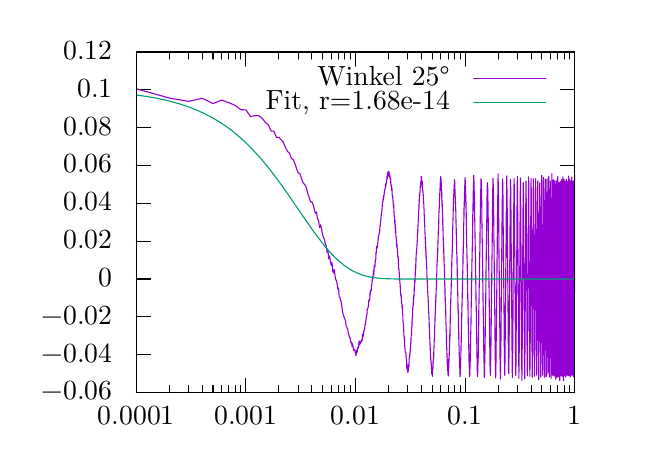
\begin{tikzpicture}[gnuplot]
%% generated with GNUPLOT 5.2p5a (Gentoo revision r0) (Lua 5.1; terminal rev. 99 , script rev. 107)
%% Sa 18 Mai 2019 18:31:17 CEST
\path (0.000,0.000) rectangle (7.500,5.250);
\gpcolor{color=gp lt color border}
\gpsetlinetype{gp lt border}
\gpsetdashtype{gp dt solid}
\gpsetlinewidth{1.00}
\draw[gp path] (1.380,0.616)--(1.560,0.616);
\draw[gp path] (6.947,0.616)--(6.767,0.616);
\node[gp node right] at (1.196,0.616) {$-0.06$};
\draw[gp path] (1.380,1.097)--(1.560,1.097);
\draw[gp path] (6.947,1.097)--(6.767,1.097);
\node[gp node right] at (1.196,1.097) {$-0.04$};
\draw[gp path] (1.380,1.577)--(1.560,1.577);
\draw[gp path] (6.947,1.577)--(6.767,1.577);
\node[gp node right] at (1.196,1.577) {$-0.02$};
\draw[gp path] (1.380,2.058)--(1.560,2.058);
\draw[gp path] (6.947,2.058)--(6.767,2.058);
\node[gp node right] at (1.196,2.058) {$0$};
\draw[gp path] (1.380,2.538)--(1.560,2.538);
\draw[gp path] (6.947,2.538)--(6.767,2.538);
\node[gp node right] at (1.196,2.538) {$0.02$};
\draw[gp path] (1.380,3.019)--(1.560,3.019);
\draw[gp path] (6.947,3.019)--(6.767,3.019);
\node[gp node right] at (1.196,3.019) {$0.04$};
\draw[gp path] (1.380,3.499)--(1.560,3.499);
\draw[gp path] (6.947,3.499)--(6.767,3.499);
\node[gp node right] at (1.196,3.499) {$0.06$};
\draw[gp path] (1.380,3.980)--(1.560,3.980);
\draw[gp path] (6.947,3.980)--(6.767,3.980);
\node[gp node right] at (1.196,3.980) {$0.08$};
\draw[gp path] (1.380,4.460)--(1.560,4.460);
\draw[gp path] (6.947,4.460)--(6.767,4.460);
\node[gp node right] at (1.196,4.460) {$0.1$};
\draw[gp path] (1.380,4.941)--(1.560,4.941);
\draw[gp path] (6.947,4.941)--(6.767,4.941);
\node[gp node right] at (1.196,4.941) {$0.12$};
\draw[gp path] (1.380,0.616)--(1.380,0.796);
\draw[gp path] (1.380,4.941)--(1.380,4.761);
\node[gp node center] at (1.380,0.308) {$0.0001$};
\draw[gp path] (1.799,0.616)--(1.799,0.706);
\draw[gp path] (1.799,4.941)--(1.799,4.851);
\draw[gp path] (2.044,0.616)--(2.044,0.706);
\draw[gp path] (2.044,4.941)--(2.044,4.851);
\draw[gp path] (2.218,0.616)--(2.218,0.706);
\draw[gp path] (2.218,4.941)--(2.218,4.851);
\draw[gp path] (2.353,0.616)--(2.353,0.706);
\draw[gp path] (2.353,4.941)--(2.353,4.851);
\draw[gp path] (2.463,0.616)--(2.463,0.706);
\draw[gp path] (2.463,4.941)--(2.463,4.851);
\draw[gp path] (2.556,0.616)--(2.556,0.706);
\draw[gp path] (2.556,4.941)--(2.556,4.851);
\draw[gp path] (2.637,0.616)--(2.637,0.706);
\draw[gp path] (2.637,4.941)--(2.637,4.851);
\draw[gp path] (2.708,0.616)--(2.708,0.706);
\draw[gp path] (2.708,4.941)--(2.708,4.851);
\draw[gp path] (2.772,0.616)--(2.772,0.796);
\draw[gp path] (2.772,4.941)--(2.772,4.761);
\node[gp node center] at (2.772,0.308) {$0.001$};
\draw[gp path] (3.191,0.616)--(3.191,0.706);
\draw[gp path] (3.191,4.941)--(3.191,4.851);
\draw[gp path] (3.436,0.616)--(3.436,0.706);
\draw[gp path] (3.436,4.941)--(3.436,4.851);
\draw[gp path] (3.610,0.616)--(3.610,0.706);
\draw[gp path] (3.610,4.941)--(3.610,4.851);
\draw[gp path] (3.745,0.616)--(3.745,0.706);
\draw[gp path] (3.745,4.941)--(3.745,4.851);
\draw[gp path] (3.855,0.616)--(3.855,0.706);
\draw[gp path] (3.855,4.941)--(3.855,4.851);
\draw[gp path] (3.948,0.616)--(3.948,0.706);
\draw[gp path] (3.948,4.941)--(3.948,4.851);
\draw[gp path] (4.029,0.616)--(4.029,0.706);
\draw[gp path] (4.029,4.941)--(4.029,4.851);
\draw[gp path] (4.100,0.616)--(4.100,0.706);
\draw[gp path] (4.100,4.941)--(4.100,4.851);
\draw[gp path] (4.163,0.616)--(4.163,0.796);
\draw[gp path] (4.163,4.941)--(4.163,4.761);
\node[gp node center] at (4.163,0.308) {$0.01$};
\draw[gp path] (4.582,0.616)--(4.582,0.706);
\draw[gp path] (4.582,4.941)--(4.582,4.851);
\draw[gp path] (4.828,0.616)--(4.828,0.706);
\draw[gp path] (4.828,4.941)--(4.828,4.851);
\draw[gp path] (5.001,0.616)--(5.001,0.706);
\draw[gp path] (5.001,4.941)--(5.001,4.851);
\draw[gp path] (5.136,0.616)--(5.136,0.706);
\draw[gp path] (5.136,4.941)--(5.136,4.851);
\draw[gp path] (5.246,0.616)--(5.246,0.706);
\draw[gp path] (5.246,4.941)--(5.246,4.851);
\draw[gp path] (5.340,0.616)--(5.340,0.706);
\draw[gp path] (5.340,4.941)--(5.340,4.851);
\draw[gp path] (5.420,0.616)--(5.420,0.706);
\draw[gp path] (5.420,4.941)--(5.420,4.851);
\draw[gp path] (5.492,0.616)--(5.492,0.706);
\draw[gp path] (5.492,4.941)--(5.492,4.851);
\draw[gp path] (5.555,0.616)--(5.555,0.796);
\draw[gp path] (5.555,4.941)--(5.555,4.761);
\node[gp node center] at (5.555,0.308) {$0.1$};
\draw[gp path] (5.974,0.616)--(5.974,0.706);
\draw[gp path] (5.974,4.941)--(5.974,4.851);
\draw[gp path] (6.219,0.616)--(6.219,0.706);
\draw[gp path] (6.219,4.941)--(6.219,4.851);
\draw[gp path] (6.393,0.616)--(6.393,0.706);
\draw[gp path] (6.393,4.941)--(6.393,4.851);
\draw[gp path] (6.528,0.616)--(6.528,0.706);
\draw[gp path] (6.528,4.941)--(6.528,4.851);
\draw[gp path] (6.638,0.616)--(6.638,0.706);
\draw[gp path] (6.638,4.941)--(6.638,4.851);
\draw[gp path] (6.731,0.616)--(6.731,0.706);
\draw[gp path] (6.731,4.941)--(6.731,4.851);
\draw[gp path] (6.812,0.616)--(6.812,0.706);
\draw[gp path] (6.812,4.941)--(6.812,4.851);
\draw[gp path] (6.883,0.616)--(6.883,0.706);
\draw[gp path] (6.883,4.941)--(6.883,4.851);
\draw[gp path] (6.947,0.616)--(6.947,0.796);
\draw[gp path] (6.947,4.941)--(6.947,4.761);
\node[gp node center] at (6.947,0.308) {$1$};
\draw[gp path] (1.380,4.941)--(1.380,0.616)--(6.947,0.616)--(6.947,4.941)--cycle;
\node[gp node right] at (5.479,4.607) {Winkel 25°};
\gpcolor{rgb color={0.580,0.000,0.827}}
\draw[gp path] (5.663,4.607)--(6.579,4.607);
\draw[gp path] (1.380,4.474)--(1.799,4.356)--(2.044,4.314)--(2.218,4.353)--(2.353,4.286)%
  --(2.463,4.330)--(2.556,4.297)--(2.637,4.262)--(2.708,4.208)--(2.772,4.206)--(2.829,4.122)%
  --(2.882,4.131)--(2.930,4.134)--(2.975,4.104)--(3.017,4.049)--(3.056,4.014)--(3.092,3.938)%
  --(3.127,3.934)--(3.160,3.857)--(3.191,3.856)--(3.220,3.826)--(3.248,3.792)--(3.275,3.725)%
  --(3.301,3.678)--(3.326,3.655)--(3.349,3.590)--(3.372,3.575)--(3.394,3.522)--(3.415,3.460)%
  --(3.436,3.403)--(3.456,3.401)--(3.475,3.343)--(3.493,3.288)--(3.511,3.265)--(3.529,3.245)%
  --(3.546,3.192)--(3.563,3.125)--(3.579,3.080)--(3.594,3.036)--(3.610,3.036)--(3.625,3.003)%
  --(3.639,2.945)--(3.653,2.892)--(3.667,2.910)--(3.681,2.822)--(3.694,2.803)--(3.707,2.711)%
  --(3.720,2.747)--(3.732,2.699)--(3.745,2.622)--(3.757,2.583)--(3.768,2.562)--(3.780,2.504)%
  --(3.791,2.484)--(3.802,2.397)--(3.813,2.416)--(3.824,2.314)--(3.834,2.351)--(3.845,2.282)%
  --(3.855,2.229)--(3.865,2.266)--(3.875,2.155)--(3.884,2.135)--(3.894,2.180)--(3.903,2.103)%
  --(3.912,2.047)--(3.921,2.044)--(3.930,1.994)--(3.939,1.929)--(3.948,1.944)--(3.956,1.832)%
  --(3.965,1.823)--(3.973,1.790)--(3.982,1.770)--(3.990,1.710)--(3.998,1.649)--(4.006,1.611)%
  --(4.013,1.589)--(4.021,1.568)--(4.029,1.549)--(4.036,1.526)--(4.044,1.466)--(4.051,1.457)%
  --(4.058,1.432)--(4.065,1.422)--(4.072,1.373)--(4.079,1.351)--(4.086,1.314)--(4.093,1.318)%
  --(4.100,1.279)--(4.106,1.247)--(4.113,1.257)--(4.120,1.200)--(4.126,1.236)--(4.132,1.198)%
  --(4.139,1.153)--(4.145,1.156)--(4.151,1.166)--(4.157,1.142)--(4.164,1.109)--(4.170,1.083)%
  --(4.175,1.154)--(4.181,1.128)--(4.187,1.129)--(4.193,1.188)--(4.199,1.181)--(4.204,1.228)%
  --(4.210,1.272)--(4.216,1.220)--(4.221,1.235)--(4.227,1.253)--(4.232,1.267)--(4.237,1.281)%
  --(4.243,1.260)--(4.248,1.287)--(4.253,1.360)--(4.258,1.327)--(4.264,1.337)--(4.269,1.402)%
  --(4.274,1.412)--(4.279,1.414)--(4.284,1.482)--(4.289,1.478)--(4.294,1.529)--(4.298,1.546)%
  --(4.303,1.593)--(4.308,1.597)--(4.313,1.674)--(4.317,1.679)--(4.322,1.691)--(4.327,1.717)%
  --(4.331,1.785)--(4.336,1.775)--(4.340,1.803)--(4.345,1.799)--(4.349,1.894)--(4.354,1.875)%
  --(4.358,1.921)--(4.363,1.912)--(4.367,1.980)--(4.371,1.994)--(4.375,2.026)--(4.380,2.087)%
  --(4.384,2.058)--(4.388,2.100)--(4.392,2.169)--(4.396,2.108)--(4.400,2.216)--(4.405,2.235)%
  --(4.409,2.206)--(4.413,2.263)--(4.417,2.312)--(4.421,2.302)--(4.424,2.402)--(4.428,2.393)%
  --(4.432,2.476)--(4.436,2.448)--(4.440,2.462)--(4.444,2.481)--(4.448,2.537)--(4.451,2.550)%
  --(4.455,2.610)--(4.459,2.613)--(4.463,2.635)--(4.466,2.641)--(4.470,2.650)--(4.473,2.716)%
  --(4.477,2.729)--(4.481,2.784)--(4.484,2.800)--(4.488,2.846)--(4.491,2.869)--(4.495,2.901)%
  --(4.498,2.923)--(4.502,2.968)--(4.505,3.013)--(4.509,3.029)--(4.512,3.071)--(4.515,3.058)%
  --(4.519,3.116)--(4.522,3.092)--(4.525,3.113)--(4.529,3.156)--(4.532,3.186)--(4.535,3.193)%
  --(4.539,3.198)--(4.542,3.224)--(4.545,3.267)--(4.548,3.230)--(4.551,3.268)--(4.555,3.274)%
  --(4.558,3.312)--(4.561,3.322)--(4.564,3.366)--(4.567,3.327)--(4.570,3.401)--(4.573,3.363)%
  --(4.576,3.411)--(4.579,3.428)--(4.582,3.369)--(4.585,3.412)--(4.588,3.420)--(4.591,3.365)%
  --(4.594,3.358)--(4.597,3.389)--(4.600,3.337)--(4.603,3.358)--(4.606,3.311)--(4.609,3.332)%
  --(4.612,3.267)--(4.615,3.244)--(4.618,3.254)--(4.621,3.232)--(4.623,3.183)--(4.626,3.211)%
  --(4.629,3.136)--(4.632,3.111)--(4.635,3.117)--(4.637,3.083)--(4.640,3.047)--(4.643,3.018)%
  --(4.646,2.962)--(4.648,3.012)--(4.651,2.938)--(4.654,2.852)--(4.656,2.868)--(4.659,2.859)%
  --(4.662,2.776)--(4.664,2.810)--(4.667,2.694)--(4.670,2.747)--(4.672,2.644)--(4.675,2.667)%
  --(4.677,2.602)--(4.680,2.586)--(4.683,2.573)--(4.685,2.495)--(4.688,2.461)--(4.690,2.501)%
  --(4.693,2.452)--(4.695,2.444)--(4.698,2.369)--(4.700,2.342)--(4.703,2.335)--(4.705,2.350)%
  --(4.708,2.261)--(4.710,2.246)--(4.712,2.197)--(4.715,2.186)--(4.717,2.155)--(4.720,2.123)%
  --(4.722,2.060)--(4.725,2.055)--(4.727,2.015)--(4.729,1.999)--(4.732,1.962)--(4.734,1.887)%
  --(4.736,1.892)--(4.739,1.845)--(4.741,1.843)--(4.743,1.859)--(4.746,1.799)--(4.748,1.781)%
  --(4.750,1.743)--(4.753,1.742)--(4.755,1.695)--(4.757,1.712)--(4.759,1.629)--(4.762,1.613)%
  --(4.764,1.605)--(4.766,1.525)--(4.768,1.506)--(4.771,1.492)--(4.773,1.451)--(4.775,1.429)%
  --(4.777,1.377)--(4.779,1.329)--(4.781,1.332)--(4.784,1.303)--(4.786,1.284)--(4.788,1.217)%
  --(4.790,1.186)--(4.792,1.177)--(4.794,1.130)--(4.797,1.140)--(4.799,1.124)--(4.801,1.119)%
  --(4.803,1.122)--(4.805,1.077)--(4.807,1.057)--(4.809,1.049)--(4.811,1.036)--(4.813,1.003)%
  --(4.815,0.919)--(4.817,0.984)--(4.819,0.943)--(4.821,0.956)--(4.823,0.887)--(4.826,0.934)%
  --(4.828,0.866)--(4.830,0.920)--(4.832,0.883)--(4.834,0.917)--(4.836,0.922)--(4.838,0.944)%
  --(4.840,0.961)--(4.841,0.993)--(4.843,0.945)--(4.845,1.040)--(4.847,1.058)--(4.849,1.072)%
  --(4.851,1.096)--(4.853,1.084)--(4.855,1.103)--(4.857,1.162)--(4.859,1.143)--(4.861,1.186)%
  --(4.863,1.198)--(4.865,1.257)--(4.867,1.241)--(4.868,1.287)--(4.870,1.341)--(4.872,1.341)%
  --(4.874,1.341)--(4.876,1.423)--(4.878,1.447)--(4.880,1.444)--(4.881,1.521)--(4.883,1.547)%
  --(4.885,1.561)--(4.887,1.564)--(4.889,1.656)--(4.891,1.686)--(4.892,1.695)--(4.894,1.718)%
  --(4.896,1.722)--(4.898,1.773)--(4.900,1.757)--(4.901,1.849)--(4.903,1.813)--(4.905,1.832)%
  --(4.907,1.861)--(4.908,1.865)--(4.910,1.958)--(4.912,1.967)--(4.914,1.991)--(4.916,2.052)%
  --(4.917,2.009)--(4.919,2.027)--(4.921,2.096)--(4.922,2.107)--(4.924,2.202)--(4.926,2.191)%
  --(4.928,2.189)--(4.929,2.248)--(4.931,2.278)--(4.933,2.355)--(4.934,2.365)--(4.936,2.389)%
  --(4.938,2.392)--(4.939,2.441)--(4.941,2.444)--(4.943,2.451)--(4.944,2.498)--(4.946,2.507)%
  --(4.948,2.538)--(4.949,2.584)--(4.951,2.638)--(4.953,2.634)--(4.954,2.683)--(4.956,2.713)%
  --(4.958,2.756)--(4.959,2.796)--(4.961,2.791)--(4.962,2.854)--(4.964,2.857)--(4.966,2.936)%
  --(4.967,2.934)--(4.969,2.934)--(4.970,3.006)--(4.972,3.015)--(4.974,3.083)--(4.975,3.121)%
  --(4.977,3.109)--(4.978,3.099)--(4.980,3.145)--(4.981,3.143)--(4.983,3.165)--(4.985,3.226)%
  --(4.986,3.216)--(4.988,3.247)--(4.989,3.215)--(4.991,3.276)--(4.992,3.291)--(4.994,3.299)%
  --(4.995,3.273)--(4.997,3.335)--(4.998,3.359)--(5.000,3.307)--(5.001,3.360)--(5.003,3.343)%
  --(5.004,3.315)--(5.006,3.298)--(5.007,3.257)--(5.009,3.276)--(5.010,3.270)--(5.012,3.233)%
  --(5.013,3.294)--(5.015,3.212)--(5.016,3.180)--(5.018,3.191)--(5.019,3.169)--(5.021,3.161)%
  --(5.022,3.118)--(5.024,3.133)--(5.025,3.079)--(5.027,3.075)--(5.028,3.023)--(5.029,3.016)%
  --(5.031,3.016)--(5.032,2.954)--(5.034,2.948)--(5.035,2.896)--(5.037,2.860)--(5.038,2.825)%
  --(5.039,2.780)--(5.041,2.814)--(5.042,2.741)--(5.044,2.713)--(5.045,2.655)--(5.047,2.628)%
  --(5.048,2.577)--(5.049,2.592)--(5.051,2.507)--(5.052,2.551)--(5.054,2.500)--(5.055,2.457)%
  --(5.056,2.412)--(5.058,2.409)--(5.059,2.343)--(5.060,2.364)--(5.062,2.328)--(5.063,2.291)%
  --(5.064,2.278)--(5.066,2.216)--(5.067,2.218)--(5.069,2.179)--(5.070,2.136)--(5.071,2.077)%
  --(5.073,2.093)--(5.074,2.045)--(5.075,2.022)--(5.077,1.973)--(5.078,1.980)--(5.079,1.905)%
  --(5.081,1.893)--(5.082,1.866)--(5.083,1.858)--(5.085,1.818)--(5.086,1.768)--(5.087,1.793)%
  --(5.089,1.735)--(5.090,1.659)--(5.091,1.661)--(5.092,1.619)--(5.094,1.633)--(5.095,1.557)%
  --(5.096,1.578)--(5.098,1.534)--(5.099,1.510)--(5.100,1.449)--(5.101,1.489)--(5.103,1.364)%
  --(5.104,1.377)--(5.105,1.328)--(5.107,1.298)--(5.108,1.250)--(5.109,1.248)--(5.110,1.210)%
  --(5.112,1.191)--(5.113,1.144)--(5.114,1.150)--(5.115,1.101)--(5.117,1.066)--(5.118,1.067)%
  --(5.119,1.029)--(5.120,1.067)--(5.122,1.005)--(5.123,0.996)--(5.124,0.983)--(5.125,0.982)%
  --(5.127,0.954)--(5.128,0.911)--(5.129,0.919)--(5.130,0.887)--(5.131,0.857)--(5.133,0.892)%
  --(5.134,0.861)--(5.135,0.844)--(5.136,0.874)--(5.137,0.893)--(5.139,0.877)--(5.140,0.821)%
  --(5.141,0.895)--(5.142,0.915)--(5.144,0.912)--(5.145,0.935)--(5.146,0.954)--(5.147,0.923)%
  --(5.148,0.995)--(5.149,0.980)--(5.151,1.017)--(5.152,1.037)--(5.153,1.034)--(5.154,1.038)%
  --(5.155,1.092)--(5.157,1.070)--(5.158,1.152)--(5.159,1.143)--(5.160,1.210)--(5.161,1.201)%
  --(5.162,1.272)--(5.163,1.287)--(5.165,1.267)--(5.166,1.318)--(5.167,1.333)--(5.168,1.368)%
  --(5.169,1.468)--(5.170,1.459)--(5.172,1.508)--(5.173,1.545)--(5.174,1.599)--(5.175,1.582)%
  --(5.176,1.618)--(5.177,1.634)--(5.178,1.702)--(5.179,1.689)--(5.181,1.733)--(5.182,1.753)%
  --(5.183,1.803)--(5.184,1.786)--(5.185,1.860)--(5.186,1.820)--(5.187,1.922)--(5.188,1.918)%
  --(5.189,1.930)--(5.191,1.969)--(5.192,2.038)--(5.193,2.055)--(5.194,2.085)--(5.195,2.114)%
  --(5.196,2.129)--(5.197,2.209)--(5.198,2.228)--(5.199,2.252)--(5.200,2.298)--(5.202,2.276)%
  --(5.203,2.329)--(5.204,2.342)--(5.205,2.367)--(5.206,2.391)--(5.207,2.456)--(5.208,2.393)%
  --(5.209,2.502)--(5.210,2.491)--(5.211,2.528)--(5.212,2.564)--(5.213,2.594)--(5.214,2.636)%
  --(5.215,2.662)--(5.217,2.689)--(5.218,2.699)--(5.219,2.735)--(5.220,2.759)--(5.221,2.827)%
  --(5.222,2.831)--(5.223,2.896)--(5.224,2.921)--(5.225,2.940)--(5.226,2.954)--(5.227,2.951)%
  --(5.228,2.994)--(5.229,3.085)--(5.230,3.069)--(5.231,3.076)--(5.232,3.137)--(5.233,3.121)%
  --(5.234,3.149)--(5.235,3.145)--(5.236,3.188)--(5.237,3.199)--(5.238,3.264)--(5.239,3.254)%
  --(5.240,3.285)--(5.241,3.230)--(5.242,3.342)--(5.243,3.298)--(5.244,3.361)--(5.245,3.305)%
  --(5.246,3.344)--(5.247,3.335)--(5.249,3.340)--(5.250,3.279)--(5.251,3.334)--(5.252,3.254)%
  --(5.253,3.236)--(5.254,3.205)--(5.254,3.197)--(5.255,3.190)--(5.256,3.177)--(5.257,3.139)%
  --(5.258,3.166)--(5.259,3.082)--(5.260,3.116)--(5.261,3.078)--(5.262,2.998)--(5.263,3.040)%
  --(5.264,2.966)--(5.265,3.009)--(5.266,2.958)--(5.267,2.916)--(5.268,2.899)--(5.269,2.892)%
  --(5.270,2.855)--(5.271,2.825)--(5.272,2.747)--(5.273,2.748)--(5.274,2.718)--(5.275,2.668)%
  --(5.276,2.642)--(5.277,2.595)--(5.278,2.556)--(5.279,2.524)--(5.280,2.545)--(5.281,2.473)%
  --(5.282,2.463)--(5.283,2.461)--(5.284,2.451)--(5.285,2.358)--(5.286,2.346)--(5.286,2.309)%
  --(5.287,2.350)--(5.288,2.283)--(5.289,2.253)--(5.290,2.241)--(5.291,2.235)--(5.292,2.170)%
  --(5.293,2.152)--(5.294,2.099)--(5.295,2.073)--(5.296,2.023)--(5.297,1.978)--(5.298,1.964)%
  --(5.299,1.954)--(5.300,1.924)--(5.300,1.880)--(5.301,1.841)--(5.302,1.866)--(5.303,1.782)%
  --(5.304,1.773)--(5.305,1.731)--(5.306,1.736)--(5.307,1.732)--(5.308,1.684)--(5.309,1.651)%
  --(5.310,1.645)--(5.310,1.591)--(5.311,1.588)--(5.312,1.481)--(5.313,1.505)--(5.314,1.437)%
  --(5.315,1.420)--(5.316,1.385)--(5.317,1.392)--(5.318,1.340)--(5.319,1.324)--(5.319,1.259)%
  --(5.320,1.225)--(5.321,1.207)--(5.322,1.170)--(5.323,1.155)--(5.324,1.145)--(5.325,1.095)%
  --(5.326,1.060)--(5.327,1.078)--(5.327,1.115)--(5.328,0.973)--(5.329,1.038)--(5.330,0.980)%
  --(5.331,0.990)--(5.332,0.949)--(5.333,0.942)--(5.334,0.894)--(5.334,0.920)--(5.335,0.898)%
  --(5.336,0.907)--(5.337,0.868)--(5.338,0.858)--(5.339,0.840)--(5.340,0.850)--(5.341,0.885)%
  --(5.341,0.824)--(5.342,0.891)--(5.343,0.894)--(5.344,0.876)--(5.345,0.924)--(5.346,0.926)%
  --(5.347,0.924)--(5.347,0.925)--(5.348,1.038)--(5.349,1.011)--(5.350,1.005)--(5.351,1.061)%
  --(5.352,1.045)--(5.352,1.059)--(5.353,1.073)--(5.354,1.100)--(5.355,1.128)--(5.356,1.154)%
  --(5.357,1.170)--(5.358,1.175)--(5.358,1.188)--(5.359,1.254)--(5.360,1.272)--(5.361,1.359)%
  --(5.362,1.368)--(5.363,1.330)--(5.363,1.415)--(5.364,1.440)--(5.365,1.488)--(5.366,1.493)%
  --(5.367,1.567)--(5.368,1.600)--(5.368,1.602)--(5.369,1.653)--(5.370,1.670)--(5.371,1.707)%
  --(5.372,1.697)--(5.372,1.748)--(5.373,1.761)--(5.374,1.828)--(5.375,1.840)--(5.376,1.884)%
  --(5.377,1.890)--(5.377,1.898)--(5.378,1.913)--(5.379,1.978)--(5.380,2.003)--(5.381,2.047)%
  --(5.381,2.059)--(5.382,2.102)--(5.383,2.095)--(5.384,2.189)--(5.385,2.216)--(5.386,2.247)%
  --(5.387,2.316)--(5.388,2.323)--(5.389,2.370)--(5.389,2.371)--(5.390,2.364)--(5.391,2.412)%
  --(5.392,2.391)--(5.393,2.456)--(5.393,2.477)--(5.394,2.493)--(5.395,2.549)--(5.396,2.548)%
  --(5.396,2.610)--(5.397,2.625)--(5.398,2.726)--(5.399,2.691)--(5.400,2.764)--(5.400,2.725)%
  --(5.401,2.811)--(5.402,2.830)--(5.403,2.861)--(5.404,2.899)--(5.404,2.919)--(5.405,2.929)%
  --(5.406,3.012)--(5.407,3.029)--(5.407,2.993)--(5.408,3.083)--(5.409,3.052)--(5.410,3.049)%
  --(5.410,3.112)--(5.411,3.117)--(5.412,3.132)--(5.413,3.158)--(5.414,3.137)--(5.414,3.192)%
  --(5.415,3.201)--(5.416,3.218)--(5.417,3.254)--(5.417,3.262)--(5.418,3.252)--(5.419,3.266)%
  --(5.420,3.275)--(5.420,3.320)--(5.421,3.312)--(5.422,3.318)--(5.423,3.287)--(5.423,3.271)%
  --(5.424,3.293)--(5.425,3.187)--(5.426,3.241)--(5.426,3.183)--(5.427,3.197)--(5.428,3.198)%
  --(5.429,3.175)--(5.429,3.111)--(5.430,3.111)--(5.431,3.088)--(5.432,3.093)--(5.432,3.003)%
  --(5.433,3.034)--(5.434,3.002)--(5.435,3.010)--(5.435,2.948)--(5.436,2.919)--(5.437,2.943)%
  --(5.438,2.934)--(5.438,2.883)--(5.439,2.822)--(5.440,2.762)--(5.440,2.776)--(5.441,2.736)%
  --(5.442,2.711)--(5.443,2.647)--(5.443,2.670)--(5.444,2.574)--(5.445,2.557)--(5.446,2.485)%
  --(5.446,2.498)--(5.447,2.482)--(5.448,2.464)--(5.448,2.401)--(5.449,2.397)--(5.450,2.373)%
  --(5.451,2.341)--(5.451,2.291)--(5.452,2.339)--(5.453,2.279)--(5.453,2.246)--(5.454,2.207)%
  --(5.455,2.192)--(5.456,2.127)--(5.456,2.113)--(5.457,2.032)--(5.458,2.081)--(5.458,2.043)%
  --(5.459,2.000)--(5.460,1.948)--(5.461,1.910)--(5.461,1.895)--(5.462,1.882)--(5.463,1.818)%
  --(5.463,1.848)--(5.464,1.747)--(5.465,1.731)--(5.465,1.678)--(5.466,1.676)--(5.467,1.685)%
  --(5.468,1.649)--(5.468,1.652)--(5.469,1.613)--(5.470,1.542)--(5.470,1.540)--(5.471,1.499)%
  --(5.472,1.464)--(5.472,1.441)--(5.473,1.389)--(5.474,1.370)--(5.475,1.388)--(5.475,1.288)%
  --(5.476,1.296)--(5.477,1.280)--(5.477,1.212)--(5.478,1.217)--(5.479,1.216)--(5.479,1.156)%
  --(5.480,1.134)--(5.481,1.114)--(5.481,1.077)--(5.482,1.068)--(5.483,1.036)--(5.483,0.984)%
  --(5.484,1.004)--(5.485,0.926)--(5.485,0.969)--(5.486,0.952)--(5.487,0.962)--(5.488,0.924)%
  --(5.488,0.972)--(5.489,0.846)--(5.490,0.895)--(5.490,0.817)--(5.491,0.883)--(5.492,0.839)%
  --(5.492,0.873)--(5.493,0.845)--(5.494,0.870)--(5.494,0.923)--(5.495,0.921)--(5.496,0.930)%
  --(5.497,0.958)--(5.498,0.984)--(5.498,0.983)--(5.499,1.041)--(5.500,1.062)--(5.500,1.034)%
  --(5.501,1.049)--(5.502,1.134)--(5.502,1.127)--(5.503,1.165)--(5.504,1.218)--(5.504,1.212)%
  --(5.505,1.249)--(5.506,1.246)--(5.506,1.314)--(5.507,1.319)--(5.507,1.328)--(5.508,1.367)%
  --(5.509,1.431)--(5.509,1.432)--(5.510,1.437)--(5.511,1.462)--(5.511,1.537)--(5.512,1.577)%
  --(5.513,1.576)--(5.513,1.632)--(5.514,1.614)--(5.515,1.702)--(5.515,1.707)--(5.516,1.710)%
  --(5.517,1.780)--(5.517,1.822)--(5.518,1.814)--(5.518,1.816)--(5.519,1.821)--(5.520,1.896)%
  --(5.520,1.877)--(5.521,1.943)--(5.522,1.910)--(5.522,1.961)--(5.523,2.001)--(5.524,2.087)%
  --(5.524,2.075)--(5.525,2.140)--(5.526,2.164)--(5.526,2.148)--(5.527,2.192)--(5.527,2.232)%
  --(5.528,2.248)--(5.529,2.328)--(5.529,2.365)--(5.530,2.387)--(5.531,2.359)--(5.531,2.380)%
  --(5.532,2.412)--(5.532,2.476)--(5.533,2.452)--(5.534,2.489)--(5.534,2.493)--(5.535,2.539)%
  --(5.536,2.551)--(5.536,2.602)--(5.537,2.620)--(5.537,2.712)--(5.538,2.775)--(5.539,2.777)%
  --(5.539,2.812)--(5.540,2.836)--(5.541,2.855)--(5.541,2.938)--(5.542,2.961)--(5.542,2.945)%
  --(5.543,2.977)--(5.544,2.986)--(5.544,3.022)--(5.545,3.042)--(5.546,3.037)--(5.546,3.136)%
  --(5.547,3.115)--(5.547,3.143)--(5.548,3.158)--(5.549,3.204)--(5.549,3.180)--(5.550,3.215)%
  --(5.550,3.211)--(5.551,3.224)--(5.552,3.264)--(5.552,3.287)--(5.553,3.284)--(5.553,3.309)%
  --(5.554,3.293)--(5.555,3.347)--(5.555,3.338)--(5.556,3.305)--(5.556,3.344)--(5.557,3.276)%
  --(5.558,3.245)--(5.558,3.258)--(5.559,3.239)--(5.559,3.232)--(5.560,3.233)--(5.561,3.166)%
  --(5.561,3.209)--(5.562,3.161)--(5.562,3.148)--(5.563,3.105)--(5.564,3.134)--(5.564,3.030)%
  --(5.565,3.090)--(5.565,3.052)--(5.566,3.036)--(5.567,2.994)--(5.567,2.958)--(5.568,2.930)%
  --(5.568,2.909)--(5.569,2.916)--(5.570,2.827)--(5.570,2.832)--(5.571,2.796)--(5.571,2.792)%
  --(5.572,2.691)--(5.573,2.699)--(5.573,2.630)--(5.574,2.612)--(5.574,2.577)--(5.575,2.557)%
  --(5.575,2.483)--(5.576,2.497)--(5.577,2.452)--(5.577,2.438)--(5.578,2.376)--(5.578,2.343)%
  --(5.579,2.358)--(5.580,2.371)--(5.580,2.317)--(5.581,2.269)--(5.581,2.264)--(5.582,2.251)%
  --(5.582,2.215)--(5.583,2.168)--(5.584,2.154)--(5.584,2.097)--(5.585,2.098)--(5.585,2.065)%
  --(5.586,2.005)--(5.586,2.007)--(5.587,1.981)--(5.588,1.895)--(5.588,1.887)--(5.589,1.846)%
  --(5.589,1.836)--(5.590,1.768)--(5.590,1.789)--(5.591,1.759)--(5.592,1.784)--(5.592,1.663)%
  --(5.593,1.683)--(5.593,1.650)--(5.594,1.633)--(5.594,1.540)--(5.595,1.567)--(5.596,1.470)%
  --(5.596,1.505)--(5.597,1.478)--(5.597,1.437)--(5.598,1.378)--(5.598,1.358)--(5.599,1.329)%
  --(5.600,1.300)--(5.600,1.267)--(5.601,1.232)--(5.601,1.170)--(5.602,1.214)--(5.602,1.176)%
  --(5.603,1.122)--(5.603,1.087)--(5.604,1.118)--(5.605,1.092)--(5.605,1.008)--(5.606,1.055)%
  --(5.606,1.048)--(5.607,1.003)--(5.607,0.960)--(5.608,0.935)--(5.608,0.966)--(5.609,0.990)%
  --(5.610,0.899)--(5.610,0.864)--(5.611,0.860)--(5.611,0.842)--(5.612,0.863)--(5.612,0.851)%
  --(5.613,0.818)--(5.613,0.836)--(5.614,0.840)--(5.615,0.834)--(5.615,0.914)--(5.616,0.840)%
  --(5.616,0.885)--(5.617,0.928)--(5.617,0.936)--(5.618,0.988)--(5.618,0.978)--(5.619,0.977)%
  --(5.619,0.982)--(5.620,1.012)--(5.621,1.026)--(5.621,1.093)--(5.622,1.101)--(5.622,1.138)%
  --(5.623,1.148)--(5.623,1.126)--(5.624,1.179)--(5.624,1.221)--(5.625,1.255)--(5.625,1.272)%
  --(5.626,1.292)--(5.626,1.336)--(5.627,1.376)--(5.628,1.409)--(5.628,1.408)--(5.629,1.465)%
  --(5.629,1.469)--(5.630,1.495)--(5.630,1.563)--(5.631,1.573)--(5.631,1.649)--(5.632,1.687)%
  --(5.632,1.690)--(5.633,1.702)--(5.633,1.715)--(5.634,1.740)--(5.634,1.775)--(5.635,1.822)%
  --(5.636,1.871)--(5.636,1.844)--(5.637,1.900)--(5.637,1.951)--(5.638,1.965)--(5.638,2.031)%
  --(5.639,2.043)--(5.639,2.017)--(5.640,2.119)--(5.640,2.131)--(5.641,2.181)--(5.641,2.195)%
  --(5.642,2.227)--(5.642,2.270)--(5.643,2.294)--(5.643,2.292)--(5.644,2.335)--(5.644,2.326)%
  --(5.645,2.378)--(5.645,2.390)--(5.646,2.434)--(5.647,2.472)--(5.647,2.538)--(5.648,2.501)%
  --(5.648,2.527)--(5.649,2.611)--(5.649,2.627)--(5.650,2.624)--(5.650,2.699)--(5.651,2.686)%
  --(5.651,2.749)--(5.652,2.739)--(5.652,2.787)--(5.653,2.841)--(5.653,2.882)--(5.654,2.861)%
  --(5.654,2.943)--(5.655,2.909)--(5.655,2.985)--(5.656,2.967)--(5.656,3.008)--(5.657,3.043)%
  --(5.657,3.055)--(5.658,3.061)--(5.658,3.135)--(5.659,3.133)--(5.659,3.157)--(5.660,3.187)%
  --(5.660,3.238)--(5.661,3.225)--(5.661,3.258)--(5.662,3.265)--(5.662,3.289)--(5.663,3.274)%
  --(5.663,3.349)--(5.664,3.255)--(5.664,3.335)--(5.665,3.344)--(5.665,3.375)--(5.666,3.347)%
  --(5.666,3.338)--(5.667,3.345)--(5.667,3.350)--(5.668,3.274)--(5.668,3.251)--(5.669,3.202)%
  --(5.669,3.203)--(5.670,3.179)--(5.670,3.212)--(5.671,3.164)--(5.671,3.179)--(5.672,3.131)%
  --(5.672,3.110)--(5.673,3.078)--(5.673,3.093)--(5.674,3.042)--(5.674,3.004)--(5.675,3.002)%
  --(5.675,2.928)--(5.676,2.954)--(5.676,2.862)--(5.677,2.849)--(5.677,2.786)--(5.678,2.836)%
  --(5.678,2.811)--(5.679,2.755)--(5.679,2.753)--(5.680,2.675)--(5.681,2.613)--(5.681,2.583)%
  --(5.682,2.563)--(5.682,2.551)--(5.683,2.475)--(5.683,2.503)--(5.684,2.436)--(5.684,2.475)%
  --(5.685,2.395)--(5.685,2.392)--(5.686,2.336)--(5.686,2.320)--(5.687,2.312)--(5.687,2.262)%
  --(5.688,2.231)--(5.688,2.183)--(5.689,2.189)--(5.689,2.159)--(5.690,2.090)--(5.690,2.083)%
  --(5.691,2.057)--(5.691,2.005)--(5.692,1.955)--(5.692,1.910)--(5.693,1.884)--(5.693,1.868)%
  --(5.693,1.841)--(5.694,1.863)--(5.694,1.788)--(5.695,1.786)--(5.695,1.746)--(5.696,1.743)%
  --(5.696,1.720)--(5.697,1.672)--(5.697,1.659)--(5.698,1.630)--(5.698,1.578)--(5.699,1.540)%
  --(5.699,1.520)--(5.700,1.444)--(5.700,1.426)--(5.701,1.420)--(5.701,1.373)--(5.702,1.369)%
  --(5.702,1.307)--(5.703,1.317)--(5.703,1.263)--(5.704,1.229)--(5.704,1.214)--(5.704,1.170)%
  --(5.705,1.150)--(5.705,1.124)--(5.706,1.072)--(5.706,1.079)--(5.707,1.054)--(5.707,1.066)%
  --(5.708,0.985)--(5.708,1.000)--(5.709,0.972)--(5.709,0.974)--(5.710,0.891)--(5.710,0.945)%
  --(5.711,0.903)--(5.711,0.892)--(5.712,0.902)--(5.712,0.833)--(5.712,0.877)--(5.713,0.853)%
  --(5.713,0.838)--(5.714,0.820)--(5.714,0.860)--(5.715,0.863)--(5.715,0.916)--(5.716,0.865)%
  --(5.716,0.887)--(5.717,0.898)--(5.717,0.882)--(5.718,0.937)--(5.718,0.968)--(5.718,1.004)%
  --(5.719,0.986)--(5.719,1.019)--(5.720,1.038)--(5.720,1.032)--(5.721,1.045)--(5.721,1.100)%
  --(5.722,1.055)--(5.722,1.135)--(5.723,1.138)--(5.723,1.233)--(5.724,1.232)--(5.724,1.238)%
  --(5.724,1.268)--(5.725,1.274)--(5.725,1.332)--(5.726,1.319)--(5.726,1.377)--(5.727,1.428)%
  --(5.727,1.477)--(5.728,1.469)--(5.728,1.506)--(5.729,1.558)--(5.729,1.638)--(5.729,1.655)%
  --(5.730,1.661)--(5.730,1.706)--(5.731,1.677)--(5.731,1.739)--(5.732,1.789)--(5.732,1.809)%
  --(5.733,1.828)--(5.733,1.846)--(5.733,1.854)--(5.734,1.944)--(5.734,1.934)--(5.735,1.979)%
  --(5.735,2.001)--(5.736,2.009)--(5.736,2.060)--(5.737,2.050)--(5.737,2.162)--(5.738,2.097)%
  --(5.738,2.161)--(5.738,2.238)--(5.739,2.264)--(5.739,2.287)--(5.740,2.291)--(5.740,2.293)%
  --(5.741,2.355)--(5.741,2.334)--(5.742,2.404)--(5.742,2.428)--(5.742,2.472)--(5.743,2.495)%
  --(5.743,2.516)--(5.744,2.508)--(5.744,2.563)--(5.745,2.591)--(5.745,2.653)--(5.746,2.638)%
  --(5.746,2.746)--(5.746,2.758)--(5.747,2.797)--(5.747,2.766)--(5.748,2.817)--(5.748,2.839)%
  --(5.749,2.905)--(5.749,2.913)--(5.749,2.963)--(5.750,2.978)--(5.750,2.981)--(5.751,3.026)%
  --(5.751,3.049)--(5.752,3.082)--(5.752,3.111)--(5.753,3.137)--(5.753,3.139)--(5.753,3.172)%
  --(5.754,3.199)--(5.754,3.147)--(5.755,3.185)--(5.755,3.247)--(5.756,3.236)--(5.756,3.227)%
  --(5.756,3.272)--(5.757,3.238)--(5.757,3.309)--(5.758,3.332)--(5.758,3.292)--(5.759,3.326)%
  --(5.759,3.296)--(5.759,3.309)--(5.760,3.287)--(5.760,3.312)--(5.761,3.291)--(5.761,3.233)%
  --(5.762,3.254)--(5.762,3.177)--(5.762,3.211)--(5.763,3.199)--(5.763,3.163)--(5.764,3.149)%
  --(5.764,3.130)--(5.765,3.052)--(5.765,3.057)--(5.765,3.058)--(5.766,3.054)--(5.766,3.010)%
  --(5.767,2.981)--(5.767,2.994)--(5.768,2.924)--(5.768,2.890)--(5.768,2.876)--(5.769,2.835)%
  --(5.769,2.768)--(5.770,2.771)--(5.770,2.735)--(5.771,2.670)--(5.771,2.654)--(5.771,2.595)%
  --(5.772,2.557)--(5.772,2.583)--(5.773,2.544)--(5.773,2.551)--(5.774,2.504)--(5.774,2.445)%
  --(5.774,2.421)--(5.775,2.399)--(5.775,2.386)--(5.776,2.330)--(5.776,2.323)--(5.776,2.307)%
  --(5.777,2.274)--(5.777,2.277)--(5.778,2.236)--(5.778,2.179)--(5.779,2.164)--(5.779,2.110)%
  --(5.779,2.114)--(5.780,2.078)--(5.780,2.017)--(5.781,1.960)--(5.781,1.956)--(5.781,1.904)%
  --(5.782,1.874)--(5.782,1.873)--(5.783,1.853)--(5.783,1.778)--(5.784,1.829)--(5.784,1.693)%
  --(5.784,1.702)--(5.785,1.673)--(5.785,1.713)--(5.786,1.600)--(5.786,1.656)--(5.786,1.609)%
  --(5.787,1.577)--(5.787,1.540)--(5.788,1.502)--(5.788,1.459)--(5.789,1.431)--(5.789,1.409)%
  --(5.789,1.376)--(5.790,1.356)--(5.790,1.315)--(5.791,1.279)--(5.791,1.258)--(5.791,1.242)%
  --(5.792,1.201)--(5.792,1.153)--(5.793,1.150)--(5.793,1.080)--(5.793,1.136)--(5.794,1.068)%
  --(5.794,1.044)--(5.795,1.029)--(5.795,1.035)--(5.795,1.014)--(5.796,0.994)--(5.796,0.956)%
  --(5.797,0.991)--(5.797,0.924)--(5.797,0.925)--(5.798,0.876)--(5.798,0.865)--(5.799,0.811)%
  --(5.799,0.868)--(5.800,0.807)--(5.800,0.850)--(5.800,0.819)--(5.801,0.840)--(5.801,0.842)%
  --(5.802,0.858)--(5.802,0.855)--(5.802,0.906)--(5.803,0.851)--(5.803,0.910)--(5.804,0.937)%
  --(5.804,0.979)--(5.804,0.992)--(5.805,1.012)--(5.805,0.982)--(5.806,1.052)--(5.806,1.014)%
  --(5.806,1.045)--(5.807,1.081)--(5.807,1.099)--(5.808,1.147)--(5.808,1.180)--(5.808,1.208)%
  --(5.809,1.195)--(5.809,1.228)--(5.810,1.283)--(5.810,1.274)--(5.810,1.300)--(5.811,1.349)%
  --(5.811,1.442)--(5.812,1.395)--(5.812,1.478)--(5.812,1.493)--(5.813,1.524)--(5.813,1.557)%
  --(5.813,1.571)--(5.814,1.592)--(5.814,1.626)--(5.815,1.633)--(5.815,1.695)--(5.815,1.707)%
  --(5.816,1.749)--(5.816,1.701)--(5.817,1.767)--(5.817,1.773)--(5.817,1.833)--(5.818,1.831)%
  --(5.818,1.872)--(5.819,1.916)--(5.819,1.944)--(5.819,1.989)--(5.820,2.031)--(5.820,2.053)%
  --(5.821,2.070)--(5.821,2.099)--(5.821,2.172)--(5.822,2.184)--(5.822,2.194)--(5.822,2.199)%
  --(5.823,2.241)--(5.823,2.301)--(5.824,2.298)--(5.824,2.308)--(5.824,2.406)--(5.825,2.369)%
  --(5.825,2.407)--(5.826,2.436)--(5.826,2.450)--(5.826,2.494)--(5.827,2.503)--(5.827,2.546)%
  --(5.828,2.577)--(5.828,2.625)--(5.828,2.668)--(5.829,2.715)--(5.829,2.757)--(5.829,2.818)%
  --(5.830,2.774)--(5.830,2.794)--(5.831,2.826)--(5.831,2.941)--(5.831,2.926)--(5.832,2.966)%
  --(5.832,2.982)--(5.832,3.001)--(5.833,3.082)--(5.833,3.083)--(5.834,3.083)--(5.834,3.079)%
  --(5.834,3.116)--(5.835,3.113)--(5.835,3.186)--(5.836,3.145)--(5.836,3.172)--(5.836,3.139)%
  --(5.837,3.192)--(5.837,3.207)--(5.837,3.252)--(5.838,3.263)--(5.838,3.281)--(5.839,3.281)%
  --(5.839,3.264)--(5.839,3.252)--(5.840,3.257)--(5.840,3.273)--(5.840,3.251)--(5.841,3.257)%
  --(5.841,3.209)--(5.842,3.183)--(5.842,3.204)--(5.842,3.177)--(5.843,3.219)--(5.843,3.135)%
  --(5.843,3.151)--(5.844,3.124)--(5.844,3.090)--(5.845,3.042)--(5.845,3.040)--(5.845,3.061)%
  --(5.846,3.017)--(5.846,2.994)--(5.847,2.922)--(5.847,2.875)--(5.848,2.888)--(5.848,2.852)%
  --(5.848,2.847)--(5.849,2.826)--(5.849,2.733)--(5.849,2.731)--(5.850,2.663)--(5.850,2.644)%
  --(5.851,2.631)--(5.851,2.605)--(5.851,2.584)--(5.852,2.549)--(5.852,2.505)--(5.852,2.462)%
  --(5.853,2.417)--(5.853,2.429)--(5.854,2.421)--(5.854,2.383)--(5.854,2.360)--(5.855,2.350)%
  --(5.855,2.308)--(5.855,2.257)--(5.856,2.212)--(5.856,2.164)--(5.856,2.192)--(5.857,2.119)%
  --(5.857,2.163)--(5.858,2.082)--(5.858,2.060)--(5.858,2.032)--(5.859,2.013)--(5.859,1.975)%
  --(5.859,1.982)--(5.860,1.901)--(5.860,1.914)--(5.860,1.830)--(5.861,1.860)--(5.861,1.816)%
  --(5.862,1.777)--(5.862,1.711)--(5.862,1.734)--(5.863,1.679)--(5.863,1.700)--(5.863,1.648)%
  --(5.864,1.655)--(5.864,1.574)--(5.864,1.584)--(5.865,1.533)--(5.865,1.503)--(5.866,1.459)%
  --(5.866,1.466)--(5.866,1.400)--(5.867,1.347)--(5.867,1.304)--(5.867,1.283)--(5.868,1.291)%
  --(5.868,1.220)--(5.868,1.222)--(5.869,1.193)--(5.869,1.183)--(5.870,1.122)--(5.870,1.154)%
  --(5.870,1.104)--(5.871,1.084)--(5.871,1.030)--(5.871,1.059)--(5.872,1.022)--(5.872,0.980)%
  --(5.872,0.957)--(5.873,0.976)--(5.873,0.959)--(5.873,0.927)--(5.874,0.905)--(5.874,0.897)%
  --(5.875,0.901)--(5.875,0.886)--(5.875,0.868)--(5.876,0.858)--(5.876,0.854)--(5.876,0.832)%
  --(5.877,0.852)--(5.877,0.864)--(5.877,0.869)--(5.878,0.861)--(5.878,0.911)--(5.878,0.903)%
  --(5.879,0.947)--(5.879,0.946)--(5.880,0.959)--(5.880,0.976)--(5.880,1.073)--(5.881,1.037)%
  --(5.881,1.025)--(5.881,1.036)--(5.882,1.065)--(5.882,1.132)--(5.882,1.125)--(5.883,1.184)%
  --(5.883,1.223)--(5.883,1.206)--(5.884,1.225)--(5.884,1.270)--(5.884,1.297)--(5.885,1.324)%
  --(5.885,1.391)--(5.886,1.359)--(5.886,1.425)--(5.886,1.437)--(5.887,1.482)--(5.887,1.549)%
  --(5.887,1.554)--(5.888,1.597)--(5.888,1.610)--(5.888,1.676)--(5.889,1.662)--(5.889,1.683)%
  --(5.889,1.687)--(5.890,1.754)--(5.890,1.795)--(5.890,1.758)--(5.891,1.833)--(5.891,1.823)%
  --(5.891,1.923)--(5.892,1.927)--(5.892,1.934)--(5.892,1.980)--(5.893,1.980)--(5.893,2.030)%
  --(5.893,2.037)--(5.894,2.130)--(5.894,2.125)--(5.895,2.157)--(5.895,2.195)--(5.895,2.215)%
  --(5.896,2.285)--(5.896,2.293)--(5.896,2.298)--(5.897,2.310)--(5.897,2.337)--(5.897,2.352)%
  --(5.898,2.388)--(5.898,2.404)--(5.898,2.458)--(5.899,2.499)--(5.899,2.541)--(5.899,2.513)%
  --(5.900,2.544)--(5.900,2.620)--(5.900,2.639)--(5.901,2.646)--(5.901,2.718)--(5.901,2.740)%
  --(5.902,2.793)--(5.902,2.806)--(5.902,2.803)--(5.903,2.827)--(5.903,2.914)--(5.903,2.916)%
  --(5.904,2.951)--(5.904,3.022)--(5.904,2.985)--(5.905,3.055)--(5.905,3.056)--(5.906,3.113)%
  --(5.906,3.104)--(5.906,3.115)--(5.907,3.155)--(5.907,3.190)--(5.907,3.210)--(5.908,3.249)%
  --(5.908,3.198)--(5.909,3.274)--(5.909,3.250)--(5.909,3.264)--(5.910,3.262)--(5.910,3.335)%
  --(5.910,3.305)--(5.911,3.322)--(5.911,3.267)--(5.911,3.293)--(5.912,3.283)--(5.912,3.257)%
  --(5.912,3.260)--(5.913,3.249)--(5.913,3.204)--(5.913,3.194)--(5.914,3.170)--(5.914,3.181)%
  --(5.914,3.119)--(5.915,3.106)--(5.915,3.076)--(5.915,3.103)--(5.916,3.086)--(5.916,3.078)%
  --(5.916,3.046)--(5.917,3.018)--(5.917,2.994)--(5.917,2.937)--(5.918,2.929)--(5.918,2.900)%
  --(5.918,2.870)--(5.919,2.867)--(5.919,2.847)--(5.919,2.773)--(5.920,2.725)--(5.920,2.723)%
  --(5.920,2.674)--(5.921,2.669)--(5.921,2.612)--(5.921,2.610)--(5.922,2.522)--(5.922,2.527)%
  --(5.922,2.471)--(5.922,2.491)--(5.923,2.465)--(5.923,2.428)--(5.923,2.384)--(5.924,2.372)%
  --(5.924,2.347)--(5.924,2.337)--(5.925,2.260)--(5.925,2.253)--(5.925,2.247)--(5.926,2.206)%
  --(5.926,2.135)--(5.926,2.130)--(5.927,2.099)--(5.927,2.117)--(5.927,2.037)--(5.928,2.000)%
  --(5.928,1.971)--(5.928,1.927)--(5.929,1.916)--(5.929,1.872)--(5.929,1.894)--(5.930,1.809)%
  --(5.930,1.842)--(5.930,1.770)--(5.931,1.754)--(5.931,1.681)--(5.931,1.699)--(5.932,1.670)%
  --(5.932,1.653)--(5.932,1.606)--(5.933,1.599)--(5.933,1.551)--(5.933,1.518)--(5.934,1.469)%
  --(5.934,1.470)--(5.934,1.419)--(5.935,1.438)--(5.935,1.370)--(5.935,1.315)--(5.936,1.255)%
  --(5.936,1.260)--(5.936,1.203)--(5.936,1.168)--(5.937,1.164)--(5.937,1.159)--(5.937,1.150)%
  --(5.938,1.057)--(5.938,1.093)--(5.938,1.049)--(5.939,1.024)--(5.939,1.014)--(5.939,1.006)%
  --(5.940,0.984)--(5.940,0.968)--(5.940,0.994)--(5.941,0.916)--(5.941,0.902)--(5.941,0.921)%
  --(5.942,0.856)--(5.942,0.925)--(5.942,0.884)--(5.943,0.858)--(5.943,0.801)--(5.943,0.838)%
  --(5.944,0.832)--(5.944,0.871)--(5.944,0.863)--(5.944,0.878)--(5.945,0.899)--(5.945,0.913)%
  --(5.945,0.970)--(5.946,0.940)--(5.946,0.978)--(5.946,0.970)--(5.947,0.995)--(5.947,0.986)%
  --(5.947,1.002)--(5.948,1.025)--(5.948,1.044)--(5.948,1.093)--(5.949,1.111)--(5.949,1.161)%
  --(5.949,1.177)--(5.950,1.201)--(5.950,1.236)--(5.950,1.246)--(5.950,1.255)--(5.951,1.324)%
  --(5.951,1.302)--(5.951,1.333)--(5.952,1.357)--(5.952,1.434)--(5.952,1.472)--(5.953,1.475)%
  --(5.953,1.478)--(5.953,1.550)--(5.954,1.595)--(5.954,1.581)--(5.954,1.662)--(5.955,1.676)%
  --(5.955,1.714)--(5.955,1.708)--(5.955,1.732)--(5.956,1.781)--(5.956,1.783)--(5.956,1.835)%
  --(5.957,1.811)--(5.957,1.891)--(5.957,1.921)--(5.958,1.921)--(5.958,1.981)--(5.958,1.992)%
  --(5.959,2.030)--(5.959,2.062)--(5.959,2.128)--(5.960,2.136)--(5.960,2.165)--(5.960,2.241)%
  --(5.960,2.219)--(5.961,2.254)--(5.961,2.286)--(5.961,2.319)--(5.962,2.371)--(5.962,2.335)%
  --(5.962,2.376)--(5.963,2.374)--(5.963,2.507)--(5.963,2.465)--(5.964,2.513)--(5.964,2.516)%
  --(5.964,2.567)--(5.964,2.577)--(5.965,2.633)--(5.965,2.654)--(5.965,2.713)--(5.966,2.742)%
  --(5.966,2.779)--(5.966,2.742)--(5.967,2.819)--(5.967,2.835)--(5.967,2.900)--(5.968,2.888)%
  --(5.968,2.917)--(5.968,2.957)--(5.968,2.996)--(5.969,3.035)--(5.969,3.038)--(5.969,3.073)%
  --(5.970,3.068)--(5.970,3.119)--(5.970,3.103)--(5.971,3.141)--(5.971,3.201)--(5.971,3.191)%
  --(5.971,3.217)--(5.972,3.237)--(5.972,3.252)--(5.972,3.276)--(5.973,3.269)--(5.973,3.311)%
  --(5.973,3.336)--(5.974,3.332)--(5.974,3.363)--(5.974,3.340)--(5.975,3.394)--(5.975,3.302)%
  --(5.975,3.345)--(5.975,3.307)--(5.976,3.281)--(5.976,3.245)--(5.976,3.270)--(5.977,3.180)%
  --(5.977,3.212)--(5.977,3.174)--(5.978,3.198)--(5.978,3.173)--(5.978,3.131)--(5.978,3.108)%
  --(5.979,3.101)--(5.979,3.017)--(5.979,3.053)--(5.980,3.011)--(5.980,2.976)--(5.980,2.968)%
  --(5.981,2.926)--(5.981,2.906)--(5.981,2.894)--(5.981,2.859)--(5.982,2.824)--(5.982,2.788)%
  --(5.982,2.741)--(5.983,2.665)--(5.983,2.643)--(5.983,2.683)--(5.984,2.608)--(5.984,2.545)%
  --(5.984,2.530)--(5.984,2.523)--(5.985,2.469)--(5.985,2.433)--(5.985,2.446)--(5.986,2.401)%
  --(5.986,2.412)--(5.986,2.359)--(5.986,2.343)--(5.987,2.279)--(5.987,2.298)--(5.987,2.243)%
  --(5.988,2.192)--(5.988,2.205)--(5.988,2.182)--(5.989,2.087)--(5.989,2.060)--(5.989,2.052)%
  --(5.989,2.000)--(5.990,2.027)--(5.990,1.979)--(5.990,1.925)--(5.991,1.924)--(5.991,1.872)%
  --(5.991,1.867)--(5.991,1.793)--(5.992,1.832)--(5.992,1.747)--(5.992,1.755)--(5.993,1.688)%
  --(5.993,1.715)--(5.993,1.649)--(5.994,1.666)--(5.994,1.642)--(5.994,1.622)--(5.994,1.504)%
  --(5.995,1.501)--(5.995,1.482)--(5.995,1.439)--(5.996,1.440)--(5.996,1.346)--(5.996,1.321)%
  --(5.996,1.290)--(5.997,1.274)--(5.997,1.282)--(5.997,1.229)--(5.998,1.225)--(5.998,1.209)%
  --(5.998,1.122)--(5.998,1.142)--(5.999,1.141)--(5.999,1.083)--(5.999,1.048)--(6.000,1.003)%
  --(6.000,1.015)--(6.000,0.988)--(6.001,0.982)--(6.001,0.936)--(6.001,0.953)--(6.001,0.950)%
  --(6.002,0.946)--(6.002,0.879)--(6.002,0.940)--(6.003,0.834)--(6.003,0.846)--(6.003,0.825)%
  --(6.003,0.858)--(6.004,0.822)--(6.004,0.873)--(6.004,0.787)--(6.005,0.846)--(6.005,0.878)%
  --(6.005,0.866)--(6.006,0.909)--(6.006,0.949)--(6.006,0.978)--(6.007,0.981)--(6.007,1.014)%
  --(6.007,1.053)--(6.007,1.070)--(6.008,1.071)--(6.008,1.092)--(6.008,1.105)--(6.009,1.116)%
  --(6.009,1.100)--(6.009,1.174)--(6.009,1.188)--(6.010,1.179)--(6.010,1.207)--(6.010,1.260)%
  --(6.011,1.286)--(6.011,1.327)--(6.011,1.347)--(6.011,1.385)--(6.012,1.458)--(6.012,1.480)%
  --(6.012,1.498)--(6.013,1.553)--(6.013,1.573)--(6.013,1.602)--(6.013,1.603)--(6.014,1.670)%
  --(6.014,1.655)--(6.014,1.696)--(6.015,1.736)--(6.015,1.740)--(6.015,1.765)--(6.015,1.830)%
  --(6.016,1.795)--(6.016,1.845)--(6.016,1.922)--(6.017,1.928)--(6.017,1.951)--(6.017,1.985)%
  --(6.017,2.003)--(6.018,2.061)--(6.018,2.056)--(6.018,2.126)--(6.018,2.175)--(6.019,2.197)%
  --(6.019,2.204)--(6.019,2.242)--(6.020,2.302)--(6.020,2.269)--(6.020,2.324)--(6.020,2.375)%
  --(6.021,2.411)--(6.021,2.423)--(6.021,2.448)--(6.022,2.446)--(6.022,2.490)--(6.022,2.506)%
  --(6.022,2.549)--(6.023,2.622)--(6.023,2.605)--(6.023,2.648)--(6.024,2.676)--(6.024,2.680)%
  --(6.024,2.762)--(6.024,2.746)--(6.025,2.805)--(6.025,2.830)--(6.025,2.871)--(6.025,2.919)%
  --(6.026,2.962)--(6.026,2.976)--(6.026,2.986)--(6.027,3.007)--(6.027,3.037)--(6.027,3.073)%
  --(6.027,3.038)--(6.028,3.097)--(6.028,3.116)--(6.028,3.181)--(6.029,3.201)--(6.029,3.136)%
  --(6.029,3.163)--(6.029,3.184)--(6.030,3.253)--(6.030,3.216)--(6.030,3.262)--(6.030,3.284)%
  --(6.031,3.280)--(6.031,3.300)--(6.031,3.319)--(6.032,3.328)--(6.032,3.322)--(6.032,3.298)%
  --(6.032,3.314)--(6.033,3.285)--(6.033,3.247)--(6.033,3.256)--(6.034,3.222)--(6.034,3.212)%
  --(6.034,3.187)--(6.035,3.188)--(6.035,3.152)--(6.035,3.137)--(6.035,3.125)--(6.036,3.125)%
  --(6.036,3.068)--(6.036,3.085)--(6.036,3.059)--(6.037,3.033)--(6.037,2.970)--(6.037,2.991)%
  --(6.038,2.914)--(6.038,2.892)--(6.038,2.908)--(6.038,2.839)--(6.039,2.833)--(6.039,2.787)%
  --(6.039,2.777)--(6.039,2.714)--(6.040,2.703)--(6.040,2.667)--(6.040,2.680)--(6.041,2.538)%
  --(6.041,2.553)--(6.041,2.570)--(6.041,2.496)--(6.042,2.481)--(6.042,2.377)--(6.042,2.391)%
  --(6.042,2.376)--(6.043,2.347)--(6.043,2.345)--(6.043,2.308)--(6.044,2.279)--(6.044,2.295)%
  --(6.044,2.199)--(6.044,2.209)--(6.045,2.134)--(6.045,2.104)--(6.045,2.108)--(6.045,2.083)%
  --(6.046,2.036)--(6.046,2.018)--(6.046,2.005)--(6.046,1.966)--(6.047,1.938)--(6.047,1.889)%
  --(6.047,1.838)--(6.048,1.858)--(6.048,1.802)--(6.048,1.780)--(6.048,1.770)--(6.049,1.757)%
  --(6.049,1.680)--(6.049,1.672)--(6.049,1.619)--(6.050,1.615)--(6.050,1.559)--(6.050,1.529)%
  --(6.050,1.506)--(6.051,1.494)--(6.051,1.423)--(6.051,1.455)--(6.052,1.429)--(6.052,1.384)%
  --(6.052,1.317)--(6.052,1.302)--(6.053,1.270)--(6.053,1.240)--(6.053,1.254)--(6.053,1.200)%
  --(6.054,1.188)--(6.054,1.144)--(6.054,1.142)--(6.054,1.112)--(6.055,1.114)--(6.055,1.053)%
  --(6.055,1.110)--(6.056,1.067)--(6.056,1.020)--(6.056,1.007)--(6.056,0.990)--(6.057,1.008)%
  --(6.057,0.911)--(6.057,0.962)--(6.057,0.893)--(6.058,0.929)--(6.058,0.906)--(6.058,0.907)%
  --(6.058,0.889)--(6.059,0.911)--(6.059,0.834)--(6.059,0.892)--(6.059,0.841)--(6.060,0.896)%
  --(6.060,0.893)--(6.060,0.947)--(6.061,0.898)--(6.061,0.954)--(6.061,0.934)--(6.061,0.980)%
  --(6.062,1.006)--(6.062,1.038)--(6.062,1.016)--(6.062,1.058)--(6.063,1.093)--(6.063,1.136)%
  --(6.063,1.137)--(6.063,1.179)--(6.064,1.220)--(6.064,1.213)--(6.064,1.270)--(6.064,1.282)%
  --(6.065,1.296)--(6.065,1.335)--(6.065,1.369)--(6.066,1.440)--(6.066,1.488)--(6.066,1.468)%
  --(6.067,1.533)--(6.067,1.588)--(6.067,1.615)--(6.067,1.640)--(6.068,1.652)--(6.068,1.693)%
  --(6.068,1.697)--(6.068,1.717)--(6.069,1.724)--(6.069,1.766)--(6.069,1.792)--(6.069,1.804)%
  --(6.070,1.872)--(6.070,1.904)--(6.070,1.929)--(6.070,1.937)--(6.071,1.937)--(6.071,1.994)%
  --(6.071,2.047)--(6.071,2.054)--(6.072,2.088)--(6.072,2.110)--(6.072,2.184)--(6.072,2.191)%
  --(6.073,2.223)--(6.073,2.259)--(6.073,2.293)--(6.073,2.302)--(6.074,2.332)--(6.074,2.371)%
  --(6.074,2.409)--(6.075,2.382)--(6.075,2.451)--(6.075,2.453)--(6.075,2.480)--(6.076,2.535)%
  --(6.076,2.538)--(6.076,2.577)--(6.077,2.575)--(6.077,2.658)--(6.077,2.664)--(6.077,2.742)%
  --(6.078,2.761)--(6.078,2.759)--(6.078,2.804)--(6.078,2.897)--(6.079,2.905)--(6.079,2.944)%
  --(6.079,2.892)--(6.079,2.954)--(6.080,2.977)--(6.080,3.029)--(6.080,3.042)--(6.080,3.064)%
  --(6.081,3.078)--(6.081,3.102)--(6.081,3.143)--(6.081,3.172)--(6.082,3.152)--(6.082,3.172)%
  --(6.082,3.217)--(6.082,3.227)--(6.083,3.248)--(6.083,3.300)--(6.083,3.254)--(6.083,3.355)%
  --(6.084,3.306)--(6.084,3.366)--(6.084,3.326)--(6.084,3.351)--(6.085,3.320)--(6.085,3.340)%
  --(6.085,3.283)--(6.085,3.310)--(6.086,3.242)--(6.086,3.271)--(6.086,3.284)--(6.086,3.223)%
  --(6.087,3.203)--(6.087,3.151)--(6.087,3.146)--(6.087,3.158)--(6.088,3.133)--(6.088,3.099)%
  --(6.088,3.056)--(6.088,3.043)--(6.089,3.040)--(6.089,2.992)--(6.089,2.965)--(6.089,2.956)%
  --(6.090,2.955)--(6.090,2.924)--(6.090,2.869)--(6.090,2.854)--(6.091,2.799)--(6.091,2.783)%
  --(6.091,2.748)--(6.091,2.745)--(6.092,2.683)--(6.092,2.650)--(6.092,2.612)--(6.092,2.603)%
  --(6.093,2.554)--(6.093,2.566)--(6.093,2.484)--(6.094,2.419)--(6.094,2.433)--(6.094,2.425)%
  --(6.094,2.349)--(6.095,2.294)--(6.095,2.326)--(6.095,2.300)--(6.095,2.221)--(6.096,2.244)%
  --(6.096,2.265)--(6.096,2.177)--(6.097,2.097)--(6.097,2.079)--(6.097,2.008)--(6.097,2.038)%
  --(6.098,2.003)--(6.098,1.959)--(6.098,1.947)--(6.098,1.899)--(6.099,1.859)--(6.099,1.833)%
  --(6.099,1.807)--(6.099,1.793)--(6.100,1.752)--(6.100,1.759)--(6.100,1.703)--(6.100,1.686)%
  --(6.101,1.610)--(6.101,1.606)--(6.101,1.624)--(6.101,1.568)--(6.102,1.541)--(6.102,1.482)%
  --(6.102,1.464)--(6.102,1.411)--(6.103,1.419)--(6.103,1.350)--(6.103,1.335)--(6.103,1.300)%
  --(6.103,1.305)--(6.104,1.237)--(6.104,1.219)--(6.104,1.203)--(6.104,1.174)--(6.105,1.154)%
  --(6.105,1.115)--(6.105,1.096)--(6.105,1.062)--(6.106,1.043)--(6.106,1.032)--(6.106,1.091)%
  --(6.106,0.982)--(6.107,1.005)--(6.107,0.965)--(6.107,0.932)--(6.107,0.902)--(6.108,0.905)%
  --(6.108,0.946)--(6.108,0.893)--(6.108,0.903)--(6.109,0.858)--(6.109,0.862)--(6.109,0.879)%
  --(6.110,0.858)--(6.110,0.856)--(6.110,0.895)--(6.111,0.953)--(6.111,0.910)--(6.111,0.916)%
  --(6.111,0.937)--(6.111,0.964)--(6.112,1.014)--(6.112,1.053)--(6.112,1.024)--(6.112,1.057)%
  --(6.113,1.051)--(6.113,1.112)--(6.113,1.125)--(6.113,1.092)--(6.114,1.175)--(6.114,1.221)%
  --(6.114,1.216)--(6.114,1.237)--(6.115,1.237)--(6.115,1.230)--(6.115,1.306)--(6.115,1.336)%
  --(6.116,1.372)--(6.116,1.460)--(6.116,1.472)--(6.116,1.466)--(6.117,1.496)--(6.117,1.542)%
  --(6.117,1.588)--(6.117,1.623)--(6.117,1.641)--(6.118,1.661)--(6.118,1.658)--(6.118,1.677)%
  --(6.118,1.749)--(6.119,1.772)--(6.119,1.793)--(6.119,1.807)--(6.119,1.841)--(6.120,1.858)%
  --(6.120,1.881)--(6.120,1.939)--(6.120,1.995)--(6.121,1.977)--(6.121,2.050)--(6.121,2.058)%
  --(6.121,2.127)--(6.122,2.139)--(6.122,2.127)--(6.122,2.185)--(6.122,2.209)--(6.122,2.223)%
  --(6.123,2.300)--(6.123,2.298)--(6.123,2.352)--(6.124,2.368)--(6.124,2.457)--(6.124,2.465)%
  --(6.124,2.432)--(6.125,2.480)--(6.125,2.490)--(6.125,2.558)--(6.125,2.554)--(6.126,2.621)%
  --(6.126,2.623)--(6.126,2.658)--(6.126,2.687)--(6.126,2.727)--(6.127,2.727)--(6.127,2.800)%
  --(6.127,2.812)--(6.127,2.842)--(6.128,2.879)--(6.128,2.935)--(6.128,2.959)--(6.128,2.970)%
  --(6.129,2.980)--(6.129,3.015)--(6.129,3.093)--(6.129,3.073)--(6.130,3.074)--(6.130,3.093)%
  --(6.130,3.140)--(6.130,3.146)--(6.130,3.199)--(6.131,3.153)--(6.131,3.182)--(6.131,3.210)%
  --(6.131,3.231)--(6.132,3.248)--(6.132,3.261)--(6.132,3.277)--(6.132,3.307)--(6.133,3.322)%
  --(6.133,3.262)--(6.133,3.311)--(6.133,3.237)--(6.133,3.321)--(6.134,3.261)--(6.134,3.274)%
  --(6.134,3.231)--(6.134,3.251)--(6.135,3.161)--(6.135,3.190)--(6.135,3.159)--(6.135,3.182)%
  --(6.136,3.103)--(6.136,3.129)--(6.136,3.090)--(6.136,3.072)--(6.136,3.032)--(6.137,2.979)%
  --(6.137,2.960)--(6.137,2.946)--(6.137,2.973)--(6.138,2.903)--(6.138,2.878)--(6.138,2.847)%
  --(6.138,2.810)--(6.139,2.767)--(6.139,2.760)--(6.139,2.703)--(6.139,2.651)--(6.139,2.659)%
  --(6.140,2.604)--(6.140,2.550)--(6.140,2.500)--(6.140,2.488)--(6.141,2.496)--(6.141,2.504)%
  --(6.141,2.466)--(6.141,2.421)--(6.142,2.435)--(6.142,2.405)--(6.142,2.324)--(6.142,2.321)%
  --(6.142,2.288)--(6.143,2.294)--(6.143,2.220)--(6.143,2.190)--(6.143,2.171)--(6.144,2.139)%
  --(6.144,2.083)--(6.144,2.110)--(6.144,2.016)--(6.145,1.972)--(6.145,1.987)--(6.145,1.969)%
  --(6.145,1.932)--(6.145,1.915)--(6.146,1.856)--(6.146,1.851)--(6.146,1.794)--(6.146,1.819)%
  --(6.147,1.752)--(6.147,1.747)--(6.147,1.728)--(6.147,1.679)--(6.147,1.656)--(6.148,1.590)%
  --(6.148,1.574)--(6.148,1.601)--(6.148,1.594)--(6.149,1.502)--(6.149,1.491)--(6.149,1.445)%
  --(6.149,1.396)--(6.150,1.380)--(6.150,1.337)--(6.150,1.336)--(6.150,1.291)--(6.150,1.263)%
  --(6.151,1.224)--(6.151,1.217)--(6.151,1.168)--(6.151,1.150)--(6.152,1.203)--(6.152,1.122)%
  --(6.152,1.080)--(6.152,1.049)--(6.152,1.005)--(6.153,1.006)--(6.153,0.996)--(6.153,1.041)%
  --(6.153,0.932)--(6.154,0.980)--(6.154,0.923)--(6.154,0.906)--(6.154,0.935)--(6.154,0.918)%
  --(6.155,0.838)--(6.155,0.873)--(6.155,0.806)--(6.155,0.828)--(6.156,0.815)--(6.156,0.832)%
  --(6.156,0.866)--(6.156,0.874)--(6.156,0.882)--(6.157,0.939)--(6.157,0.921)--(6.157,0.942)%
  --(6.157,0.987)--(6.158,0.973)--(6.158,0.961)--(6.158,1.029)--(6.158,1.027)--(6.159,1.082)%
  --(6.159,1.048)--(6.159,1.045)--(6.159,1.107)--(6.159,1.092)--(6.160,1.128)--(6.160,1.160)%
  --(6.160,1.179)--(6.160,1.235)--(6.161,1.235)--(6.161,1.268)--(6.161,1.295)--(6.161,1.350)%
  --(6.161,1.330)--(6.162,1.373)--(6.162,1.402)--(6.162,1.465)--(6.162,1.494)--(6.163,1.545)%
  --(6.163,1.530)--(6.163,1.626)--(6.163,1.602)--(6.163,1.652)--(6.164,1.680)--(6.164,1.693)%
  --(6.164,1.700)--(6.164,1.746)--(6.164,1.776)--(6.165,1.839)--(6.165,1.831)--(6.165,1.818)%
  --(6.165,1.865)--(6.166,1.916)--(6.166,1.928)--(6.166,1.979)--(6.166,2.030)--(6.166,2.052)%
  --(6.167,2.092)--(6.167,2.087)--(6.167,2.118)--(6.167,2.184)--(6.168,2.204)--(6.168,2.198)%
  --(6.168,2.233)--(6.168,2.221)--(6.168,2.308)--(6.169,2.337)--(6.169,2.370)--(6.169,2.421)%
  --(6.169,2.400)--(6.170,2.423)--(6.170,2.457)--(6.170,2.504)--(6.170,2.520)--(6.170,2.524)%
  --(6.171,2.553)--(6.171,2.596)--(6.171,2.663)--(6.171,2.686)--(6.172,2.725)--(6.172,2.759)%
  --(6.172,2.813)--(6.172,2.842)--(6.172,2.843)--(6.173,2.858)--(6.173,2.914)--(6.173,2.941)%
  --(6.173,2.959)--(6.173,3.003)--(6.174,3.025)--(6.174,3.002)--(6.174,3.044)--(6.174,3.101)%
  --(6.175,3.078)--(6.175,3.114)--(6.175,3.188)--(6.175,3.134)--(6.175,3.139)--(6.176,3.239)%
  --(6.176,3.210)--(6.176,3.260)--(6.176,3.248)--(6.177,3.218)--(6.177,3.275)--(6.177,3.310)%
  --(6.177,3.250)--(6.177,3.334)--(6.178,3.287)--(6.178,3.260)--(6.178,3.319)--(6.178,3.243)%
  --(6.179,3.203)--(6.179,3.267)--(6.179,3.217)--(6.180,3.193)--(6.180,3.136)--(6.180,3.142)%
  --(6.180,3.137)--(6.180,3.108)--(6.181,3.074)--(6.181,3.102)--(6.181,3.074)--(6.181,3.058)%
  --(6.181,2.991)--(6.182,2.952)--(6.182,2.975)--(6.182,2.925)--(6.182,2.899)--(6.183,2.878)%
  --(6.183,2.854)--(6.183,2.826)--(6.183,2.799)--(6.183,2.762)--(6.184,2.692)--(6.184,2.684)%
  --(6.184,2.648)--(6.184,2.645)--(6.184,2.593)--(6.185,2.519)--(6.185,2.557)--(6.185,2.455)%
  --(6.185,2.454)--(6.186,2.472)--(6.186,2.406)--(6.186,2.374)--(6.186,2.360)--(6.186,2.336)%
  --(6.187,2.327)--(6.187,2.260)--(6.187,2.203)--(6.187,2.217)--(6.187,2.216)--(6.188,2.161)%
  --(6.188,2.126)--(6.188,2.073)--(6.188,2.084)--(6.188,2.017)--(6.189,2.009)--(6.189,2.000)%
  --(6.189,1.943)--(6.189,1.936)--(6.190,1.852)--(6.190,1.786)--(6.190,1.822)--(6.190,1.817)%
  --(6.190,1.781)--(6.191,1.718)--(6.191,1.713)--(6.191,1.697)--(6.191,1.617)--(6.191,1.620)%
  --(6.192,1.619)--(6.192,1.584)--(6.192,1.589)--(6.192,1.524)--(6.193,1.479)--(6.193,1.443)%
  --(6.193,1.400)--(6.193,1.357)--(6.193,1.362)--(6.194,1.340)--(6.194,1.311)--(6.194,1.251)%
  --(6.194,1.281)--(6.194,1.217)--(6.195,1.205)--(6.195,1.171)--(6.195,1.202)--(6.195,1.106)%
  --(6.195,1.108)--(6.196,1.097)--(6.196,1.034)--(6.196,1.039)--(6.196,1.038)--(6.196,0.990)%
  --(6.197,1.033)--(6.197,0.962)--(6.197,0.978)--(6.197,0.940)--(6.198,0.934)--(6.198,0.926)%
  --(6.198,0.892)--(6.198,0.850)--(6.198,0.888)--(6.199,0.833)--(6.199,0.852)--(6.199,0.863)%
  --(6.199,0.859)--(6.199,0.865)--(6.200,0.916)--(6.200,0.871)--(6.200,0.928)--(6.200,0.911)%
  --(6.200,0.968)--(6.201,0.946)--(6.201,1.022)--(6.201,0.972)--(6.201,1.029)--(6.201,1.061)%
  --(6.202,1.057)--(6.202,1.074)--(6.202,1.135)--(6.202,1.112)--(6.203,1.202)--(6.203,1.182)%
  --(6.203,1.210)--(6.203,1.191)--(6.203,1.285)--(6.204,1.287)--(6.204,1.343)--(6.204,1.365)%
  --(6.204,1.388)--(6.204,1.397)--(6.205,1.435)--(6.205,1.510)--(6.205,1.496)--(6.205,1.572)%
  --(6.205,1.573)--(6.206,1.602)--(6.206,1.641)--(6.206,1.666)--(6.206,1.719)--(6.206,1.693)%
  --(6.207,1.737)--(6.207,1.764)--(6.207,1.790)--(6.207,1.798)--(6.207,1.848)--(6.208,1.834)%
  --(6.208,1.913)--(6.208,1.896)--(6.208,1.930)--(6.209,1.994)--(6.209,2.030)--(6.209,2.045)%
  --(6.209,2.087)--(6.209,2.086)--(6.210,2.136)--(6.210,2.132)--(6.210,2.182)--(6.210,2.230)%
  --(6.210,2.268)--(6.211,2.234)--(6.211,2.337)--(6.211,2.333)--(6.211,2.397)--(6.211,2.381)%
  --(6.212,2.430)--(6.212,2.437)--(6.212,2.441)--(6.212,2.458)--(6.212,2.481)--(6.213,2.505)%
  --(6.213,2.594)--(6.213,2.621)--(6.213,2.657)--(6.213,2.662)--(6.214,2.712)--(6.214,2.701)%
  --(6.214,2.808)--(6.214,2.851)--(6.214,2.852)--(6.215,2.865)--(6.215,2.928)--(6.215,2.913)%
  --(6.215,2.956)--(6.215,2.988)--(6.216,3.022)--(6.216,3.027)--(6.216,3.063)--(6.216,3.089)%
  --(6.216,3.086)--(6.217,3.140)--(6.217,3.155)--(6.217,3.151)--(6.217,3.207)--(6.217,3.203)%
  --(6.218,3.246)--(6.218,3.224)--(6.218,3.288)--(6.218,3.278)--(6.218,3.289)--(6.219,3.307)%
  --(6.219,3.360)--(6.219,3.296)--(6.219,3.327)--(6.219,3.318)--(6.220,3.293)--(6.220,3.242)%
  --(6.220,3.264)--(6.220,3.252)--(6.220,3.215)--(6.221,3.219)--(6.221,3.150)--(6.221,3.171)%
  --(6.221,3.127)--(6.221,3.149)--(6.222,3.114)--(6.222,3.108)--(6.222,3.041)--(6.222,3.059)%
  --(6.222,3.047)--(6.223,3.014)--(6.223,2.977)--(6.223,2.950)--(6.223,2.918)--(6.224,2.882)%
  --(6.224,2.826)--(6.224,2.786)--(6.224,2.804)--(6.224,2.770)--(6.225,2.720)--(6.225,2.730)%
  --(6.225,2.668)--(6.225,2.651)--(6.225,2.604)--(6.226,2.593)--(6.226,2.518)--(6.226,2.519)%
  --(6.226,2.441)--(6.226,2.459)--(6.227,2.400)--(6.227,2.423)--(6.227,2.357)--(6.227,2.342)%
  --(6.227,2.326)--(6.228,2.283)--(6.228,2.262)--(6.228,2.222)--(6.228,2.191)--(6.228,2.190)%
  --(6.229,2.114)--(6.229,2.101)--(6.229,2.102)--(6.229,2.071)--(6.229,2.023)--(6.230,1.962)%
  --(6.230,1.959)--(6.230,1.901)--(6.230,1.882)--(6.230,1.887)--(6.231,1.865)--(6.231,1.816)%
  --(6.231,1.748)--(6.231,1.732)--(6.231,1.744)--(6.232,1.695)--(6.232,1.667)--(6.232,1.706)%
  --(6.232,1.626)--(6.232,1.570)--(6.233,1.566)--(6.233,1.539)--(6.233,1.515)--(6.233,1.464)%
  --(6.233,1.446)--(6.234,1.412)--(6.234,1.368)--(6.234,1.333)--(6.234,1.272)--(6.234,1.239)%
  --(6.235,1.276)--(6.235,1.210)--(6.235,1.175)--(6.235,1.159)--(6.235,1.127)--(6.236,1.135)%
  --(6.236,1.097)--(6.236,1.091)--(6.236,1.033)--(6.236,1.076)--(6.237,1.025)--(6.237,1.007)%
  --(6.237,0.979)--(6.237,1.006)--(6.237,0.951)--(6.238,1.003)--(6.238,0.919)--(6.238,0.920)%
  --(6.238,0.889)--(6.238,0.888)--(6.239,0.907)--(6.239,0.858)--(6.239,0.851)--(6.239,0.886)%
  --(6.239,0.795)--(6.239,0.882)--(6.240,0.888)--(6.240,0.874)--(6.240,0.910)--(6.240,0.912)%
  --(6.240,0.931)--(6.241,0.984)--(6.241,0.975)--(6.241,1.020)--(6.241,1.015)--(6.241,1.025)%
  --(6.242,1.002)--(6.242,1.040)--(6.242,1.102)--(6.242,1.061)--(6.242,1.117)--(6.243,1.134)%
  --(6.243,1.161)--(6.243,1.188)--(6.243,1.195)--(6.243,1.252)--(6.244,1.230)--(6.244,1.316)%
  --(6.244,1.352)--(6.244,1.386)--(6.244,1.377)--(6.245,1.408)--(6.245,1.426)--(6.245,1.491)%
  --(6.245,1.502)--(6.245,1.551)--(6.246,1.546)--(6.246,1.620)--(6.246,1.669)--(6.246,1.658)%
  --(6.246,1.723)--(6.246,1.728)--(6.247,1.763)--(6.247,1.794)--(6.247,1.821)--(6.247,1.825)%
  --(6.247,1.838)--(6.248,1.903)--(6.248,1.968)--(6.248,1.943)--(6.248,2.021)--(6.248,2.034)%
  --(6.249,2.022)--(6.249,2.068)--(6.249,2.147)--(6.249,2.116)--(6.249,2.172)--(6.250,2.225)%
  --(6.250,2.224)--(6.250,2.284)--(6.250,2.323)--(6.250,2.337)--(6.250,2.404)--(6.251,2.356)%
  --(6.251,2.453)--(6.251,2.414)--(6.251,2.480)--(6.251,2.469)--(6.252,2.472)--(6.252,2.547)%
  --(6.252,2.551)--(6.252,2.598)--(6.252,2.673)--(6.253,2.682)--(6.253,2.709)--(6.253,2.733)%
  --(6.253,2.740)--(6.253,2.775)--(6.254,2.815)--(6.254,2.845)--(6.254,2.923)--(6.254,2.883)%
  --(6.254,3.009)--(6.255,2.947)--(6.255,2.991)--(6.255,3.045)--(6.255,3.009)--(6.255,3.035)%
  --(6.256,3.065)--(6.256,3.127)--(6.256,3.113)--(6.256,3.151)--(6.256,3.172)--(6.257,3.178)%
  --(6.257,3.228)--(6.257,3.182)--(6.257,3.231)--(6.257,3.248)--(6.258,3.287)--(6.258,3.295)%
  --(6.258,3.316)--(6.258,3.337)--(6.258,3.281)--(6.258,3.343)--(6.259,3.275)--(6.259,3.307)%
  --(6.259,3.241)--(6.259,3.289)--(6.259,3.195)--(6.260,3.252)--(6.260,3.195)--(6.260,3.214)%
  --(6.260,3.170)--(6.260,3.117)--(6.261,3.114)--(6.261,3.108)--(6.261,3.093)--(6.261,3.055)%
  --(6.261,3.009)--(6.261,2.997)--(6.262,3.002)--(6.262,2.934)--(6.262,2.935)--(6.262,2.877)%
  --(6.262,2.881)--(6.263,2.801)--(6.263,2.793)--(6.263,2.797)--(6.263,2.704)--(6.263,2.672)%
  --(6.264,2.663)--(6.264,2.667)--(6.264,2.608)--(6.264,2.590)--(6.264,2.517)--(6.264,2.525)%
  --(6.265,2.497)--(6.265,2.467)--(6.265,2.438)--(6.265,2.425)--(6.265,2.376)--(6.266,2.347)%
  --(6.266,2.321)--(6.266,2.319)--(6.266,2.249)--(6.266,2.286)--(6.267,2.208)--(6.267,2.200)%
  --(6.267,2.153)--(6.267,2.111)--(6.267,2.067)--(6.267,2.071)--(6.268,2.006)--(6.268,2.028)%
  --(6.268,1.933)--(6.268,1.934)--(6.268,1.891)--(6.269,1.898)--(6.269,1.817)--(6.269,1.869)%
  --(6.269,1.764)--(6.269,1.768)--(6.270,1.743)--(6.270,1.716)--(6.270,1.663)--(6.270,1.638)%
  --(6.270,1.617)--(6.270,1.594)--(6.271,1.598)--(6.271,1.603)--(6.271,1.467)--(6.271,1.502)%
  --(6.271,1.427)--(6.272,1.419)--(6.272,1.362)--(6.272,1.330)--(6.272,1.321)--(6.272,1.295)%
  --(6.272,1.221)--(6.273,1.234)--(6.273,1.167)--(6.273,1.177)--(6.273,1.161)--(6.273,1.099)%
  --(6.274,1.062)--(6.274,1.070)--(6.274,1.011)--(6.274,1.019)--(6.274,0.968)--(6.275,0.998)%
  --(6.275,0.918)--(6.275,0.934)--(6.275,0.935)--(6.275,0.950)--(6.275,0.916)--(6.276,0.890)%
  --(6.276,0.827)--(6.276,0.867)--(6.276,0.808)--(6.276,0.810)--(6.277,0.782)--(6.277,0.822)%
  --(6.277,0.786)--(6.277,0.770)--(6.277,0.811)--(6.277,0.834)--(6.278,0.858)--(6.278,0.901)%
  --(6.278,0.891)--(6.278,0.931)--(6.278,0.966)--(6.279,0.992)--(6.279,0.957)--(6.279,0.969)%
  --(6.279,0.972)--(6.279,1.042)--(6.279,1.015)--(6.280,1.087)--(6.280,1.122)--(6.280,1.089)%
  --(6.280,1.094)--(6.280,1.153)--(6.281,1.208)--(6.281,1.179)--(6.281,1.266)--(6.281,1.237)%
  --(6.281,1.290)--(6.281,1.281)--(6.282,1.309)--(6.282,1.373)--(6.282,1.408)--(6.282,1.441)%
  --(6.282,1.519)--(6.283,1.566)--(6.283,1.538)--(6.283,1.619)--(6.283,1.618)--(6.283,1.682)%
  --(6.283,1.658)--(6.284,1.681)--(6.284,1.703)--(6.284,1.726)--(6.284,1.727)--(6.284,1.782)%
  --(6.285,1.816)--(6.285,1.846)--(6.285,1.878)--(6.285,1.935)--(6.285,1.947)--(6.285,1.992)%
  --(6.286,1.998)--(6.286,2.019)--(6.286,2.050)--(6.286,2.038)--(6.286,2.073)--(6.287,2.147)%
  --(6.287,2.174)--(6.287,2.244)--(6.287,2.265)--(6.287,2.272)--(6.287,2.298)--(6.288,2.337)%
  --(6.288,2.362)--(6.288,2.398)--(6.288,2.386)--(6.288,2.472)--(6.289,2.455)--(6.289,2.492)%
  --(6.289,2.465)--(6.289,2.534)--(6.289,2.540)--(6.289,2.586)--(6.290,2.612)--(6.290,2.678)%
  --(6.290,2.715)--(6.290,2.723)--(6.290,2.787)--(6.290,2.807)--(6.291,2.858)--(6.291,2.836)%
  --(6.291,2.865)--(6.291,2.964)--(6.291,2.932)--(6.292,2.971)--(6.292,2.992)--(6.292,3.027)%
  --(6.292,2.998)--(6.292,3.068)--(6.292,3.070)--(6.293,3.097)--(6.293,3.098)--(6.293,3.118)%
  --(6.293,3.103)--(6.293,3.182)--(6.294,3.157)--(6.294,3.193)--(6.294,3.197)--(6.294,3.255)%
  --(6.294,3.281)--(6.294,3.282)--(6.295,3.258)--(6.295,3.257)--(6.295,3.264)--(6.295,3.271)%
  --(6.295,3.251)--(6.295,3.246)--(6.296,3.216)--(6.296,3.215)--(6.296,3.231)--(6.296,3.178)%
  --(6.296,3.183)--(6.297,3.165)--(6.297,3.145)--(6.297,3.142)--(6.297,3.108)--(6.297,3.102)%
  --(6.297,3.097)--(6.298,3.037)--(6.298,3.046)--(6.298,2.969)--(6.298,2.979)--(6.298,2.935)%
  --(6.298,2.904)--(6.299,2.902)--(6.299,2.884)--(6.299,2.828)--(6.299,2.766)--(6.299,2.755)%
  --(6.300,2.726)--(6.300,2.723)--(6.300,2.735)--(6.300,2.643)--(6.300,2.626)--(6.300,2.606)%
  --(6.301,2.562)--(6.301,2.507)--(6.301,2.482)--(6.301,2.473)--(6.301,2.466)--(6.301,2.411)%
  --(6.302,2.371)--(6.302,2.337)--(6.302,2.324)--(6.302,2.314)--(6.302,2.271)--(6.303,2.240)%
  --(6.303,2.255)--(6.303,2.158)--(6.303,2.179)--(6.303,2.108)--(6.303,2.104)--(6.304,2.054)%
  --(6.304,2.056)--(6.304,1.969)--(6.304,1.947)--(6.304,1.909)--(6.304,1.916)--(6.305,1.871)%
  --(6.305,1.852)--(6.305,1.847)--(6.305,1.762)--(6.305,1.758)--(6.306,1.742)--(6.306,1.703)%
  --(6.306,1.694)--(6.306,1.646)--(6.306,1.666)--(6.306,1.590)--(6.307,1.588)--(6.307,1.550)%
  --(6.307,1.545)--(6.307,1.536)--(6.307,1.456)--(6.307,1.387)--(6.308,1.411)--(6.308,1.377)%
  --(6.308,1.327)--(6.308,1.276)--(6.308,1.245)--(6.308,1.265)--(6.309,1.222)--(6.309,1.170)%
  --(6.309,1.164)--(6.309,1.174)--(6.309,1.129)--(6.310,1.089)--(6.310,1.072)--(6.310,1.063)%
  --(6.310,1.083)--(6.310,1.045)--(6.310,0.965)--(6.311,1.000)--(6.311,0.962)--(6.311,0.974)%
  --(6.311,0.931)--(6.311,0.894)--(6.311,0.918)--(6.312,0.868)--(6.312,0.886)--(6.312,0.810)%
  --(6.312,0.857)--(6.312,0.798)--(6.312,0.884)--(6.313,0.790)--(6.313,0.866)--(6.313,0.873)%
  --(6.313,0.878)--(6.313,0.887)--(6.313,0.926)--(6.314,0.899)--(6.314,0.935)--(6.314,0.944)%
  --(6.314,0.969)--(6.314,1.007)--(6.315,0.977)--(6.315,1.011)--(6.315,1.047)--(6.315,1.045)%
  --(6.315,1.093)--(6.315,1.107)--(6.316,1.125)--(6.316,1.157)--(6.316,1.201)--(6.316,1.258)%
  --(6.316,1.251)--(6.316,1.250)--(6.317,1.322)--(6.317,1.314)--(6.317,1.343)--(6.317,1.375)%
  --(6.317,1.409)--(6.317,1.455)--(6.318,1.510)--(6.318,1.522)--(6.318,1.589)--(6.318,1.553)%
  --(6.318,1.589)--(6.318,1.639)--(6.319,1.658)--(6.319,1.672)--(6.319,1.749)--(6.319,1.733)%
  --(6.319,1.789)--(6.319,1.804)--(6.320,1.834)--(6.320,1.839)--(6.320,1.895)--(6.320,1.914)%
  --(6.320,1.954)--(6.321,1.971)--(6.321,2.013)--(6.321,2.003)--(6.321,2.049)--(6.321,2.085)%
  --(6.321,2.138)--(6.322,2.166)--(6.322,2.195)--(6.322,2.194)--(6.322,2.286)--(6.322,2.239)%
  --(6.322,2.324)--(6.323,2.304)--(6.323,2.313)--(6.323,2.391)--(6.323,2.410)--(6.323,2.447)%
  --(6.323,2.454)--(6.324,2.502)--(6.324,2.537)--(6.324,2.518)--(6.324,2.599)--(6.324,2.630)%
  --(6.325,2.644)--(6.325,2.695)--(6.325,2.739)--(6.325,2.780)--(6.325,2.790)--(6.325,2.847)%
  --(6.326,2.834)--(6.326,2.892)--(6.326,2.906)--(6.326,2.952)--(6.326,2.956)--(6.326,3.005)%
  --(6.327,3.069)--(6.327,3.029)--(6.327,3.040)--(6.327,3.107)--(6.327,3.138)--(6.327,3.137)%
  --(6.328,3.141)--(6.328,3.115)--(6.328,3.168)--(6.328,3.230)--(6.328,3.184)--(6.328,3.242)%
  --(6.329,3.237)--(6.329,3.246)--(6.329,3.263)--(6.329,3.295)--(6.329,3.301)--(6.329,3.278)%
  --(6.330,3.223)--(6.330,3.261)--(6.330,3.218)--(6.330,3.223)--(6.330,3.241)--(6.330,3.210)%
  --(6.331,3.165)--(6.331,3.152)--(6.331,3.164)--(6.331,3.148)--(6.331,3.115)--(6.331,3.088)%
  --(6.332,3.067)--(6.332,3.052)--(6.332,3.053)--(6.332,3.022)--(6.332,2.953)--(6.332,2.981)%
  --(6.333,2.987)--(6.333,2.938)--(6.333,2.881)--(6.333,2.899)--(6.333,2.827)--(6.334,2.855)%
  --(6.334,2.771)--(6.334,2.753)--(6.334,2.682)--(6.334,2.706)--(6.334,2.649)--(6.335,2.621)%
  --(6.335,2.589)--(6.335,2.528)--(6.335,2.531)--(6.335,2.483)--(6.335,2.489)--(6.335,2.467)%
  --(6.336,2.445)--(6.336,2.366)--(6.336,2.339)--(6.336,2.360)--(6.336,2.313)--(6.336,2.348)%
  --(6.337,2.247)--(6.337,2.229)--(6.337,2.223)--(6.337,2.202)--(6.337,2.114)--(6.337,2.087)%
  --(6.338,2.039)--(6.338,2.059)--(6.338,2.016)--(6.338,2.004)--(6.338,1.959)--(6.338,1.952)%
  --(6.339,1.904)--(6.339,1.867)--(6.339,1.860)--(6.339,1.822)--(6.339,1.742)--(6.339,1.799)%
  --(6.340,1.734)--(6.340,1.700)--(6.340,1.691)--(6.340,1.697)--(6.340,1.708)--(6.340,1.644)%
  --(6.341,1.600)--(6.341,1.508)--(6.341,1.495)--(6.341,1.510)--(6.341,1.500)--(6.341,1.375)%
  --(6.342,1.400)--(6.342,1.346)--(6.342,1.284)--(6.342,1.250)--(6.342,1.273)--(6.342,1.222)%
  --(6.343,1.206)--(6.343,1.133)--(6.343,1.083)--(6.343,1.140)--(6.343,1.123)--(6.343,1.050)%
  --(6.344,1.030)--(6.344,1.061)--(6.344,0.994)--(6.344,0.972)--(6.344,0.969)--(6.345,0.935)%
  --(6.345,0.930)--(6.345,0.886)--(6.345,0.918)--(6.345,0.913)--(6.345,0.879)--(6.346,0.879)%
  --(6.346,0.840)--(6.346,0.844)--(6.346,0.831)--(6.346,0.937)--(6.347,0.884)--(6.347,0.848)%
  --(6.347,0.912)--(6.347,0.878)--(6.347,0.950)--(6.347,0.938)--(6.348,0.954)--(6.348,0.962)%
  --(6.348,0.975)--(6.348,1.033)--(6.348,1.034)--(6.348,1.072)--(6.348,1.062)--(6.349,1.092)%
  --(6.349,1.120)--(6.349,1.150)--(6.349,1.179)--(6.350,1.265)--(6.350,1.274)--(6.350,1.286)%
  --(6.350,1.344)--(6.350,1.366)--(6.350,1.383)--(6.351,1.415)--(6.351,1.444)--(6.351,1.473)%
  --(6.351,1.554)--(6.351,1.577)--(6.351,1.609)--(6.352,1.660)--(6.352,1.653)--(6.352,1.675)%
  --(6.352,1.698)--(6.352,1.767)--(6.352,1.779)--(6.353,1.805)--(6.353,1.808)--(6.353,1.839)%
  --(6.353,1.898)--(6.353,1.893)--(6.353,1.911)--(6.354,1.987)--(6.354,1.997)--(6.354,2.074)%
  --(6.354,2.095)--(6.354,2.063)--(6.354,2.119)--(6.354,2.108)--(6.355,2.135)--(6.355,2.230)%
  --(6.355,2.250)--(6.355,2.286)--(6.355,2.305)--(6.355,2.338)--(6.356,2.351)--(6.356,2.412)%
  --(6.356,2.382)--(6.356,2.383)--(6.356,2.445)--(6.356,2.460)--(6.357,2.502)--(6.357,2.517)%
  --(6.357,2.573)--(6.357,2.622)--(6.357,2.665)--(6.358,2.719)--(6.358,2.712)--(6.358,2.782)%
  --(6.358,2.765)--(6.358,2.821)--(6.358,2.848)--(6.358,2.877)--(6.359,2.946)--(6.359,2.905)%
  --(6.359,2.927)--(6.359,2.987)--(6.359,3.034)--(6.360,3.031)--(6.360,3.080)--(6.360,3.105)%
  --(6.360,3.120)--(6.360,3.133)--(6.360,3.143)--(6.361,3.225)--(6.361,3.189)--(6.361,3.227)%
  --(6.361,3.265)--(6.361,3.197)--(6.361,3.265)--(6.362,3.261)--(6.362,3.333)--(6.362,3.347)%
  --(6.362,3.334)--(6.362,3.311)--(6.362,3.356)--(6.362,3.285)--(6.363,3.300)--(6.363,3.251)%
  --(6.363,3.252)--(6.363,3.259)--(6.363,3.274)--(6.363,3.156)--(6.364,3.235)--(6.364,3.164)%
  --(6.364,3.169)--(6.364,3.117)--(6.364,3.145)--(6.364,3.109)--(6.365,3.065)--(6.365,3.038)%
  --(6.365,3.067)--(6.365,3.002)--(6.365,2.968)--(6.365,2.913)--(6.365,2.911)--(6.366,2.861)%
  --(6.366,2.886)--(6.366,2.804)--(6.366,2.802)--(6.366,2.762)--(6.366,2.742)--(6.367,2.686)%
  --(6.367,2.670)--(6.367,2.640)--(6.367,2.584)--(6.367,2.563)--(6.367,2.539)--(6.368,2.499)%
  --(6.368,2.485)--(6.368,2.467)--(6.368,2.478)--(6.368,2.363)--(6.368,2.409)--(6.368,2.344)%
  --(6.369,2.324)--(6.369,2.323)--(6.369,2.261)--(6.369,2.223)--(6.369,2.207)--(6.369,2.158)%
  --(6.370,2.134)--(6.370,2.084)--(6.370,2.053)--(6.370,2.020)--(6.370,1.997)--(6.371,1.948)%
  --(6.371,1.897)--(6.371,1.917)--(6.371,1.856)--(6.371,1.875)--(6.371,1.832)--(6.371,1.789)%
  --(6.372,1.766)--(6.372,1.746)--(6.372,1.708)--(6.372,1.706)--(6.372,1.670)--(6.372,1.687)%
  --(6.373,1.594)--(6.373,1.610)--(6.373,1.557)--(6.373,1.524)--(6.373,1.496)--(6.373,1.446)%
  --(6.374,1.388)--(6.374,1.410)--(6.374,1.346)--(6.374,1.333)--(6.374,1.262)--(6.374,1.279)%
  --(6.374,1.190)--(6.375,1.168)--(6.375,1.143)--(6.375,1.127)--(6.375,1.109)--(6.375,1.039)%
  --(6.375,1.061)--(6.376,1.028)--(6.376,1.017)--(6.376,1.043)--(6.376,0.983)--(6.376,0.974)%
  --(6.376,0.932)--(6.376,0.978)--(6.377,0.889)--(6.377,0.887)--(6.377,0.880)--(6.377,0.907)%
  --(6.377,0.823)--(6.377,0.911)--(6.378,0.851)--(6.378,0.895)--(6.378,0.877)--(6.378,0.874)%
  --(6.378,0.896)--(6.378,0.942)--(6.378,0.904)--(6.379,0.922)--(6.379,0.965)--(6.379,0.919)%
  --(6.379,0.940)--(6.379,0.984)--(6.379,1.018)--(6.380,1.008)--(6.380,1.028)--(6.380,1.070)%
  --(6.380,1.056)--(6.380,1.079)--(6.380,1.138)--(6.380,1.165)--(6.381,1.157)--(6.381,1.211)%
  --(6.381,1.219)--(6.381,1.285)--(6.381,1.257)--(6.382,1.244)--(6.382,1.354)--(6.382,1.347)%
  --(6.382,1.380)--(6.382,1.408)--(6.382,1.497)--(6.382,1.484)--(6.383,1.531)--(6.383,1.581)%
  --(6.383,1.625)--(6.383,1.581)--(6.383,1.678)--(6.383,1.663)--(6.384,1.719)--(6.384,1.744)%
  --(6.384,1.771)--(6.384,1.799)--(6.384,1.817)--(6.384,1.836)--(6.384,1.864)--(6.385,1.831)%
  --(6.385,1.900)--(6.385,1.935)--(6.385,1.975)--(6.385,2.029)--(6.385,2.037)--(6.386,2.104)%
  --(6.386,2.122)--(6.386,2.165)--(6.386,2.179)--(6.386,2.188)--(6.386,2.278)--(6.387,2.279)%
  --(6.387,2.295)--(6.387,2.383)--(6.387,2.355)--(6.387,2.385)--(6.387,2.412)--(6.388,2.446)%
  --(6.388,2.476)--(6.388,2.520)--(6.388,2.531)--(6.388,2.582)--(6.388,2.639)--(6.388,2.587)%
  --(6.389,2.680)--(6.389,2.688)--(6.389,2.739)--(6.389,2.760)--(6.389,2.800)--(6.389,2.833)%
  --(6.390,2.868)--(6.390,2.925)--(6.390,2.935)--(6.390,2.970)--(6.390,2.928)--(6.390,3.009)%
  --(6.390,3.035)--(6.391,3.043)--(6.391,3.024)--(6.391,3.064)--(6.391,3.079)--(6.391,3.140)%
  --(6.391,3.153)--(6.392,3.134)--(6.392,3.175)--(6.392,3.165)--(6.392,3.220)--(6.392,3.261)%
  --(6.392,3.225)--(6.392,3.251)--(6.393,3.292)--(6.393,3.317)--(6.393,3.293)--(6.393,3.283)%
  --(6.393,3.329)--(6.393,3.336)--(6.393,3.306)--(6.394,3.310)--(6.394,3.272)--(6.394,3.250)%
  --(6.394,3.263)--(6.394,3.209)--(6.394,3.231)--(6.395,3.205)--(6.395,3.194)--(6.395,3.168)%
  --(6.395,3.160)--(6.395,3.124)--(6.395,3.104)--(6.395,3.049)--(6.396,3.039)--(6.396,3.035)%
  --(6.396,3.048)--(6.396,2.969)--(6.396,2.940)--(6.396,2.914)--(6.396,2.915)--(6.397,2.879)%
  --(6.397,2.840)--(6.397,2.818)--(6.397,2.759)--(6.397,2.736)--(6.397,2.724)--(6.398,2.711)%
  --(6.398,2.651)--(6.398,2.575)--(6.398,2.551)--(6.398,2.546)--(6.398,2.489)--(6.398,2.461)%
  --(6.399,2.476)--(6.399,2.402)--(6.399,2.430)--(6.399,2.330)--(6.399,2.365)--(6.399,2.319)%
  --(6.399,2.341)--(6.400,2.273)--(6.400,2.238)--(6.400,2.223)--(6.400,2.251)--(6.400,2.135)%
  --(6.400,2.124)--(6.401,2.084)--(6.401,2.063)--(6.401,2.012)--(6.401,1.980)--(6.401,2.003)%
  --(6.401,1.945)--(6.401,1.903)--(6.402,1.862)--(6.402,1.795)--(6.402,1.824)--(6.402,1.751)%
  --(6.402,1.783)--(6.402,1.744)--(6.402,1.749)--(6.403,1.652)--(6.403,1.677)--(6.403,1.624)%
  --(6.403,1.603)--(6.403,1.579)--(6.403,1.568)--(6.404,1.515)--(6.404,1.485)--(6.404,1.457)%
  --(6.404,1.414)--(6.404,1.427)--(6.404,1.334)--(6.404,1.300)--(6.405,1.294)--(6.405,1.251)%
  --(6.405,1.249)--(6.405,1.240)--(6.405,1.216)--(6.405,1.165)--(6.405,1.176)--(6.406,1.097)%
  --(6.406,1.069)--(6.406,1.063)--(6.406,1.037)--(6.406,1.065)--(6.406,1.019)--(6.406,0.998)%
  --(6.407,0.979)--(6.407,0.929)--(6.407,0.921)--(6.407,0.888)--(6.407,0.896)--(6.407,0.885)%
  --(6.408,0.862)--(6.408,0.820)--(6.408,0.848)--(6.408,0.817)--(6.408,0.854)--(6.408,0.808)%
  --(6.408,0.896)--(6.409,0.834)--(6.409,0.909)--(6.409,0.895)--(6.409,0.911)--(6.409,0.909)%
  --(6.409,0.924)--(6.409,0.950)--(6.410,1.021)--(6.410,0.971)--(6.410,1.028)--(6.410,1.057)%
  --(6.410,1.067)--(6.410,1.071)--(6.410,1.101)--(6.411,1.109)--(6.411,1.135)--(6.411,1.116)%
  --(6.411,1.212)--(6.411,1.208)--(6.411,1.243)--(6.411,1.265)--(6.412,1.274)--(6.412,1.368)%
  --(6.412,1.325)--(6.412,1.445)--(6.412,1.442)--(6.412,1.504)--(6.413,1.569)--(6.413,1.546)%
  --(6.413,1.604)--(6.413,1.610)--(6.413,1.626)--(6.413,1.691)--(6.414,1.676)--(6.414,1.698)%
  --(6.414,1.781)--(6.414,1.755)--(6.414,1.817)--(6.414,1.819)--(6.414,1.861)--(6.415,1.869)%
  --(6.415,1.925)--(6.415,1.904)--(6.415,1.948)--(6.415,1.979)--(6.415,2.029)--(6.415,2.046)%
  --(6.416,2.083)--(6.416,2.160)--(6.416,2.146)--(6.416,2.163)--(6.416,2.188)--(6.416,2.284)%
  --(6.416,2.267)--(6.417,2.341)--(6.417,2.298)--(6.417,2.351)--(6.417,2.383)--(6.417,2.429)%
  --(6.417,2.427)--(6.417,2.461)--(6.418,2.482)--(6.418,2.512)--(6.418,2.570)--(6.418,2.569)%
  --(6.418,2.581)--(6.418,2.682)--(6.418,2.671)--(6.419,2.698)--(6.419,2.749)--(6.419,2.776)%
  --(6.419,2.848)--(6.419,2.871)--(6.419,2.888)--(6.419,2.883)--(6.420,2.953)--(6.420,2.961)%
  --(6.420,2.998)--(6.420,3.020)--(6.420,3.055)--(6.420,3.102)--(6.420,3.045)--(6.421,3.125)%
  --(6.421,3.116)--(6.421,3.161)--(6.421,3.152)--(6.421,3.232)--(6.421,3.198)--(6.422,3.224)%
  --(6.422,3.259)--(6.422,3.260)--(6.422,3.228)--(6.422,3.300)--(6.422,3.272)--(6.422,3.269)%
  --(6.423,3.330)--(6.423,3.266)--(6.423,3.289)--(6.423,3.283)--(6.423,3.259)--(6.423,3.256)%
  --(6.423,3.240)--(6.424,3.239)--(6.424,3.189)--(6.424,3.209)--(6.424,3.131)--(6.424,3.123)%
  --(6.424,3.164)--(6.425,3.084)--(6.425,3.054)--(6.425,3.061)--(6.425,2.996)--(6.425,3.022)%
  --(6.425,3.012)--(6.425,3.014)--(6.426,2.963)--(6.426,2.917)--(6.426,2.898)--(6.426,2.854)%
  --(6.426,2.778)--(6.426,2.755)--(6.426,2.790)--(6.427,2.709)--(6.427,2.684)--(6.427,2.663)%
  --(6.427,2.658)--(6.427,2.566)--(6.427,2.579)--(6.427,2.524)--(6.428,2.508)--(6.428,2.428)%
  --(6.428,2.456)--(6.428,2.437)--(6.428,2.380)--(6.428,2.407)--(6.428,2.351)--(6.429,2.313)%
  --(6.429,2.276)--(6.429,2.262)--(6.429,2.231)--(6.429,2.177)--(6.429,2.154)--(6.429,2.140)%
  --(6.430,2.104)--(6.430,2.060)--(6.430,2.037)--(6.430,2.004)--(6.430,2.026)--(6.430,1.931)%
  --(6.430,1.935)--(6.431,1.860)--(6.431,1.839)--(6.431,1.842)--(6.431,1.802)--(6.431,1.795)%
  --(6.431,1.777)--(6.431,1.721)--(6.432,1.710)--(6.432,1.683)--(6.432,1.644)--(6.432,1.594)%
  --(6.432,1.580)--(6.432,1.559)--(6.432,1.520)--(6.433,1.505)--(6.433,1.474)--(6.433,1.449)%
  --(6.433,1.329)--(6.433,1.395)--(6.433,1.327)--(6.433,1.283)--(6.433,1.266)--(6.434,1.259)%
  --(6.434,1.235)--(6.434,1.175)--(6.434,1.154)--(6.434,1.080)--(6.434,1.165)--(6.434,1.064)%
  --(6.435,1.087)--(6.435,1.053)--(6.435,1.012)--(6.435,1.001)--(6.435,0.994)--(6.435,0.968)%
  --(6.435,0.980)--(6.436,0.966)--(6.436,0.963)--(6.436,0.923)--(6.436,0.909)--(6.436,0.875)%
  --(6.436,0.904)--(6.436,0.843)--(6.437,0.860)--(6.437,0.855)--(6.437,0.822)--(6.437,0.899)%
  --(6.437,0.838)--(6.437,0.900)--(6.437,0.859)--(6.438,0.862)--(6.438,0.876)--(6.438,0.966)%
  --(6.438,0.919)--(6.438,0.948)--(6.438,0.967)--(6.438,0.977)--(6.439,1.001)--(6.439,1.032)%
  --(6.439,1.027)--(6.439,1.056)--(6.439,1.106)--(6.439,1.111)--(6.439,1.151)--(6.440,1.159)%
  --(6.440,1.179)--(6.440,1.184)--(6.440,1.254)--(6.440,1.294)--(6.440,1.283)--(6.440,1.333)%
  --(6.441,1.399)--(6.441,1.358)--(6.441,1.414)--(6.441,1.491)--(6.441,1.523)--(6.441,1.578)%
  --(6.441,1.592)--(6.442,1.640)--(6.442,1.613)--(6.442,1.689)--(6.442,1.690)--(6.442,1.685)%
  --(6.442,1.765)--(6.442,1.781)--(6.442,1.784)--(6.443,1.851)--(6.443,1.814)--(6.443,1.858)%
  --(6.443,1.922)--(6.443,1.918)--(6.443,1.905)--(6.443,1.980)--(6.444,2.035)--(6.444,2.085)%
  --(6.444,2.074)--(6.444,2.118)--(6.444,2.168)--(6.444,2.144)--(6.444,2.207)--(6.445,2.206)%
  --(6.445,2.244)--(6.445,2.304)--(6.445,2.311)--(6.445,2.319)--(6.445,2.398)--(6.445,2.423)%
  --(6.446,2.420)--(6.446,2.456)--(6.446,2.453)--(6.446,2.500)--(6.446,2.503)--(6.446,2.570)%
  --(6.446,2.599)--(6.447,2.631)--(6.447,2.684)--(6.447,2.715)--(6.447,2.696)--(6.447,2.768)%
  --(6.447,2.790)--(6.447,2.840)--(6.447,2.832)--(6.448,2.884)--(6.448,2.945)--(6.448,2.929)%
  --(6.448,2.930)--(6.448,3.000)--(6.448,3.001)--(6.448,3.022)--(6.449,3.074)--(6.449,3.075)%
  --(6.449,3.083)--(6.449,3.104)--(6.449,3.093)--(6.449,3.196)--(6.449,3.197)--(6.450,3.164)%
  --(6.450,3.188)--(6.450,3.234)--(6.450,3.213)--(6.450,3.278)--(6.450,3.233)--(6.450,3.285)%
  --(6.451,3.262)--(6.451,3.324)--(6.451,3.247)--(6.451,3.334)--(6.451,3.261)--(6.451,3.323)%
  --(6.451,3.265)--(6.451,3.253)--(6.452,3.206)--(6.452,3.225)--(6.452,3.192)--(6.452,3.164)%
  --(6.452,3.149)--(6.452,3.115)--(6.452,3.130)--(6.453,3.128)--(6.453,3.062)--(6.453,3.038)%
  --(6.453,3.031)--(6.453,3.021)--(6.453,3.009)--(6.453,2.964)--(6.454,2.928)--(6.454,2.902)%
  --(6.454,2.823)--(6.454,2.844)--(6.454,2.782)--(6.454,2.743)--(6.454,2.745)--(6.455,2.688)%
  --(6.455,2.640)--(6.455,2.626)--(6.455,2.587)--(6.455,2.532)--(6.455,2.527)--(6.455,2.507)%
  --(6.456,2.459)--(6.456,2.471)--(6.456,2.412)--(6.456,2.389)--(6.456,2.405)--(6.456,2.346)%
  --(6.456,2.329)--(6.457,2.292)--(6.457,2.284)--(6.457,2.246)--(6.457,2.199)--(6.457,2.163)%
  --(6.457,2.140)--(6.457,2.084)--(6.458,2.032)--(6.458,2.028)--(6.458,1.949)--(6.458,1.981)%
  --(6.458,1.933)--(6.458,1.912)--(6.458,1.867)--(6.459,1.811)--(6.459,1.791)--(6.459,1.813)%
  --(6.459,1.750)--(6.459,1.702)--(6.459,1.659)--(6.459,1.708)--(6.460,1.680)--(6.460,1.644)%
  --(6.460,1.636)--(6.460,1.579)--(6.460,1.537)--(6.460,1.498)--(6.460,1.491)--(6.460,1.453)%
  --(6.461,1.346)--(6.461,1.391)--(6.461,1.330)--(6.461,1.308)--(6.461,1.253)--(6.461,1.196)%
  --(6.461,1.250)--(6.462,1.198)--(6.462,1.180)--(6.462,1.168)--(6.462,1.091)--(6.462,1.114)%
  --(6.462,1.077)--(6.462,1.061)--(6.462,1.042)--(6.463,1.016)--(6.463,0.970)--(6.463,1.022)%
  --(6.463,0.948)--(6.463,0.945)--(6.463,0.905)--(6.463,0.901)--(6.464,0.899)--(6.464,0.894)%
  --(6.464,0.837)--(6.464,0.899)--(6.464,0.879)--(6.464,0.845)--(6.464,0.881)--(6.464,0.842)%
  --(6.465,0.881)--(6.465,0.858)--(6.465,0.882)--(6.465,0.928)--(6.465,0.894)--(6.465,0.950)%
  --(6.465,0.903)--(6.466,0.957)--(6.466,1.002)--(6.466,1.019)--(6.466,1.014)--(6.466,1.031)%
  --(6.466,1.059)--(6.466,1.110)--(6.467,1.095)--(6.467,1.103)--(6.467,1.146)--(6.467,1.186)%
  --(6.467,1.210)--(6.467,1.223)--(6.467,1.244)--(6.467,1.272)--(6.468,1.277)--(6.468,1.335)%
  --(6.468,1.360)--(6.468,1.373)--(6.468,1.357)--(6.468,1.463)--(6.468,1.515)--(6.469,1.575)%
  --(6.469,1.524)--(6.469,1.581)--(6.469,1.612)--(6.469,1.655)--(6.469,1.673)--(6.469,1.702)%
  --(6.469,1.768)--(6.470,1.719)--(6.470,1.761)--(6.470,1.819)--(6.470,1.812)--(6.470,1.865)%
  --(6.470,1.867)--(6.470,1.916)--(6.471,1.941)--(6.471,1.957)--(6.471,2.009)--(6.471,2.031)%
  --(6.471,2.066)--(6.471,2.111)--(6.471,2.166)--(6.471,2.167)--(6.472,2.246)--(6.472,2.232)%
  --(6.472,2.259)--(6.472,2.292)--(6.472,2.340)--(6.472,2.352)--(6.472,2.376)--(6.472,2.416)%
  --(6.473,2.422)--(6.473,2.474)--(6.473,2.459)--(6.473,2.526)--(6.473,2.562)--(6.473,2.522)%
  --(6.473,2.609)--(6.474,2.618)--(6.474,2.731)--(6.474,2.670)--(6.474,2.748)--(6.474,2.731)%
  --(6.474,2.820)--(6.474,2.819)--(6.474,2.836)--(6.475,2.880)--(6.475,2.890)--(6.475,3.039)%
  --(6.475,2.953)--(6.475,3.020)--(6.475,3.018)--(6.475,3.039)--(6.476,3.059)--(6.476,3.054)%
  --(6.476,3.112)--(6.476,3.143)--(6.476,3.160)--(6.476,3.178)--(6.476,3.189)--(6.477,3.193)%
  --(6.477,3.228)--(6.477,3.249)--(6.477,3.237)--(6.477,3.250)--(6.477,3.284)--(6.477,3.250)%
  --(6.478,3.272)--(6.478,3.281)--(6.478,3.299)--(6.478,3.294)--(6.478,3.286)--(6.478,3.303)%
  --(6.478,3.188)--(6.478,3.238)--(6.479,3.218)--(6.479,3.200)--(6.479,3.174)--(6.479,3.181)%
  --(6.479,3.102)--(6.479,3.156)--(6.479,3.123)--(6.479,3.145)--(6.480,3.041)--(6.480,3.042)%
  --(6.480,3.018)--(6.480,3.020)--(6.480,2.963)--(6.480,2.966)--(6.480,2.933)--(6.481,2.905)%
  --(6.481,2.886)--(6.481,2.838)--(6.481,2.774)--(6.481,2.750)--(6.481,2.706)--(6.481,2.727)%
  --(6.481,2.657)--(6.482,2.612)--(6.482,2.602)--(6.482,2.560)--(6.482,2.511)--(6.482,2.499)%
  --(6.482,2.493)--(6.482,2.448)--(6.482,2.417)--(6.483,2.430)--(6.483,2.305)--(6.483,2.325)%
  --(6.483,2.259)--(6.483,2.220)--(6.484,2.241)--(6.484,2.174)--(6.484,2.125)--(6.484,2.092)%
  --(6.484,2.074)--(6.484,2.069)--(6.484,2.031)--(6.484,1.995)--(6.485,1.979)--(6.485,1.908)%
  --(6.485,1.884)--(6.485,1.863)--(6.485,1.831)--(6.485,1.845)--(6.485,1.807)--(6.485,1.773)%
  --(6.486,1.691)--(6.486,1.779)--(6.486,1.711)--(6.486,1.656)--(6.486,1.640)--(6.486,1.637)%
  --(6.486,1.571)--(6.487,1.581)--(6.487,1.537)--(6.487,1.478)--(6.487,1.434)--(6.487,1.449)%
  --(6.487,1.380)--(6.487,1.332)--(6.487,1.330)--(6.488,1.319)--(6.488,1.246)--(6.488,1.241)%
  --(6.488,1.215)--(6.488,1.139)--(6.488,1.123)--(6.488,1.126)--(6.488,1.086)--(6.489,1.093)%
  --(6.489,1.084)--(6.489,1.078)--(6.489,1.038)--(6.489,0.988)--(6.489,0.949)--(6.489,0.985)%
  --(6.489,0.952)--(6.490,0.924)--(6.490,0.843)--(6.490,0.925)--(6.490,0.844)--(6.490,0.903)%
  --(6.490,0.779)--(6.490,0.864)--(6.491,0.805)--(6.491,0.839)--(6.491,0.848)--(6.491,0.826)%
  --(6.491,0.834)--(6.491,0.905)--(6.491,0.812)--(6.491,0.915)--(6.492,0.881)--(6.492,0.906)%
  --(6.492,0.962)--(6.492,0.948)--(6.492,0.978)--(6.492,0.987)--(6.492,1.045)--(6.492,1.036)%
  --(6.493,1.043)--(6.493,1.040)--(6.493,1.143)--(6.493,1.123)--(6.493,1.132)--(6.493,1.231)%
  --(6.493,1.198)--(6.493,1.262)--(6.494,1.286)--(6.494,1.290)--(6.494,1.343)--(6.494,1.352)%
  --(6.494,1.421)--(6.494,1.446)--(6.494,1.458)--(6.494,1.500)--(6.495,1.547)--(6.495,1.569)%
  --(6.495,1.574)--(6.495,1.594)--(6.495,1.607)--(6.495,1.671)--(6.495,1.643)--(6.496,1.718)%
  --(6.496,1.729)--(6.496,1.725)--(6.496,1.770)--(6.496,1.821)--(6.496,1.808)--(6.496,1.841)%
  --(6.496,1.886)--(6.497,1.965)--(6.497,1.958)--(6.497,1.994)--(6.497,2.021)--(6.497,2.087)%
  --(6.497,2.062)--(6.497,2.121)--(6.497,2.136)--(6.498,2.198)--(6.498,2.209)--(6.498,2.183)%
  --(6.498,2.307)--(6.498,2.315)--(6.498,2.320)--(6.498,2.343)--(6.498,2.389)--(6.499,2.419)%
  --(6.499,2.432)--(6.499,2.476)--(6.499,2.488)--(6.499,2.503)--(6.499,2.533)--(6.499,2.588)%
  --(6.499,2.609)--(6.500,2.617)--(6.500,2.683)--(6.500,2.710)--(6.500,2.731)--(6.500,2.792)%
  --(6.500,2.829)--(6.500,2.817)--(6.500,2.891)--(6.501,2.899)--(6.501,2.915)--(6.501,2.940)%
  --(6.501,2.968)--(6.501,3.019)--(6.501,2.985)--(6.501,3.056)--(6.501,3.068)--(6.502,3.076)%
  --(6.502,3.086)--(6.502,3.094)--(6.502,3.159)--(6.502,3.202)--(6.502,3.137)--(6.502,3.174)%
  --(6.502,3.179)--(6.503,3.249)--(6.503,3.239)--(6.503,3.264)--(6.503,3.259)--(6.503,3.277)%
  --(6.503,3.264)--(6.503,3.268)--(6.503,3.265)--(6.504,3.223)--(6.504,3.259)--(6.504,3.211)%
  --(6.504,3.235)--(6.504,3.184)--(6.504,3.187)--(6.504,3.177)--(6.504,3.135)--(6.505,3.155)%
  --(6.505,3.149)--(6.505,3.094)--(6.505,3.105)--(6.505,3.081)--(6.505,3.065)--(6.505,2.994)%
  --(6.506,2.978)--(6.506,2.968)--(6.506,2.916)--(6.506,2.934)--(6.506,2.891)--(6.506,2.906)%
  --(6.506,2.879)--(6.506,2.794)--(6.507,2.824)--(6.507,2.734)--(6.507,2.743)--(6.507,2.663)%
  --(6.507,2.622)--(6.507,2.617)--(6.507,2.546)--(6.507,2.595)--(6.508,2.467)--(6.508,2.502)%
  --(6.508,2.457)--(6.508,2.412)--(6.508,2.421)--(6.508,2.402)--(6.508,2.348)--(6.508,2.357)%
  --(6.509,2.285)--(6.509,2.296)--(6.509,2.281)--(6.509,2.242)--(6.509,2.174)--(6.509,2.130)%
  --(6.509,2.150)--(6.509,2.107)--(6.510,2.058)--(6.510,2.022)--(6.510,2.018)--(6.510,1.964)%
  --(6.510,1.941)--(6.510,1.917)--(6.510,1.849)--(6.510,1.847)--(6.511,1.819)--(6.511,1.809)%
  --(6.511,1.740)--(6.511,1.721)--(6.511,1.705)--(6.511,1.690)--(6.511,1.674)--(6.511,1.646)%
  --(6.511,1.624)--(6.512,1.557)--(6.512,1.561)--(6.512,1.512)--(6.512,1.435)--(6.512,1.417)%
  --(6.512,1.367)--(6.512,1.364)--(6.513,1.306)--(6.513,1.300)--(6.513,1.241)--(6.513,1.260)%
  --(6.513,1.201)--(6.513,1.162)--(6.513,1.143)--(6.513,1.128)--(6.514,1.151)--(6.514,1.074)%
  --(6.514,1.076)--(6.514,1.034)--(6.514,1.078)--(6.514,1.022)--(6.514,1.018)--(6.514,0.984)%
  --(6.515,0.957)--(6.515,0.977)--(6.515,0.955)--(6.515,0.968)--(6.515,0.925)--(6.515,0.872)%
  --(6.515,0.868)--(6.515,0.881)--(6.516,0.844)--(6.516,0.813)--(6.516,0.856)--(6.516,0.819)%
  --(6.516,0.838)--(6.516,0.871)--(6.516,0.839)--(6.516,0.901)--(6.517,0.872)--(6.517,0.913)%
  --(6.517,0.919)--(6.517,0.970)--(6.517,0.904)--(6.517,1.058)--(6.517,0.974)--(6.517,1.076)%
  --(6.518,1.045)--(6.518,1.055)--(6.518,1.077)--(6.518,1.116)--(6.518,1.125)--(6.518,1.169)%
  --(6.518,1.217)--(6.518,1.226)--(6.519,1.265)--(6.519,1.251)--(6.519,1.296)--(6.519,1.367)%
  --(6.519,1.397)--(6.519,1.429)--(6.519,1.416)--(6.519,1.463)--(6.520,1.527)--(6.520,1.556)%
  --(6.520,1.572)--(6.520,1.632)--(6.520,1.618)--(6.520,1.670)--(6.520,1.704)--(6.520,1.754)%
  --(6.520,1.761)--(6.521,1.753)--(6.521,1.784)--(6.521,1.807)--(6.521,1.852)--(6.521,1.849)%
  --(6.521,1.892)--(6.521,1.940)--(6.521,1.984)--(6.522,1.992)--(6.522,2.029)--(6.522,2.078)%
  --(6.522,2.035)--(6.522,2.132)--(6.522,2.118)--(6.522,2.189)--(6.522,2.246)--(6.523,2.247)%
  --(6.523,2.270)--(6.523,2.319)--(6.523,2.312)--(6.523,2.353)--(6.523,2.367)--(6.523,2.397)%
  --(6.523,2.427)--(6.524,2.469)--(6.524,2.448)--(6.524,2.519)--(6.524,2.474)--(6.524,2.543)%
  --(6.524,2.550)--(6.524,2.675)--(6.524,2.667)--(6.525,2.670)--(6.525,2.692)--(6.525,2.736)%
  --(6.525,2.776)--(6.525,2.809)--(6.525,2.846)--(6.525,2.864)--(6.525,2.900)--(6.525,2.940)%
  --(6.526,2.986)--(6.526,2.966)--(6.526,3.006)--(6.526,3.065)--(6.526,3.090)--(6.526,3.116)%
  --(6.526,3.098)--(6.527,3.114)--(6.527,3.165)--(6.527,3.173)--(6.527,3.222)--(6.527,3.191)%
  --(6.527,3.258)--(6.527,3.233)--(6.527,3.290)--(6.528,3.229)--(6.528,3.375)--(6.528,3.323)%
  --(6.528,3.358)--(6.528,3.291)--(6.528,3.367)--(6.528,3.299)--(6.528,3.327)--(6.529,3.275)%
  --(6.529,3.258)--(6.529,3.224)--(6.529,3.252)--(6.529,3.214)--(6.529,3.182)--(6.529,3.179)%
  --(6.529,3.106)--(6.529,3.121)--(6.530,3.057)--(6.530,3.075)--(6.530,3.057)--(6.530,3.006)%
  --(6.530,2.995)--(6.530,2.992)--(6.530,2.971)--(6.530,2.929)--(6.531,2.924)--(6.531,2.884)%
  --(6.531,2.856)--(6.531,2.810)--(6.531,2.751)--(6.531,2.735)--(6.531,2.737)--(6.531,2.704)%
  --(6.532,2.678)--(6.532,2.593)--(6.532,2.581)--(6.532,2.563)--(6.532,2.533)--(6.532,2.459)%
  --(6.532,2.498)--(6.532,2.424)--(6.532,2.402)--(6.533,2.346)--(6.533,2.384)--(6.533,2.328)%
  --(6.533,2.304)--(6.533,2.246)--(6.533,2.272)--(6.533,2.225)--(6.533,2.212)--(6.534,2.150)%
  --(6.534,2.143)--(6.534,2.115)--(6.534,2.065)--(6.534,2.085)--(6.534,2.002)--(6.534,1.975)%
  --(6.534,1.965)--(6.535,1.905)--(6.535,1.884)--(6.535,1.829)--(6.535,1.806)--(6.535,1.834)%
  --(6.535,1.758)--(6.535,1.743)--(6.535,1.749)--(6.535,1.708)--(6.536,1.714)--(6.536,1.622)%
  --(6.536,1.613)--(6.536,1.605)--(6.536,1.564)--(6.536,1.549)--(6.536,1.524)--(6.536,1.485)%
  --(6.537,1.447)--(6.537,1.379)--(6.537,1.372)--(6.537,1.358)--(6.537,1.292)--(6.537,1.270)%
  --(6.537,1.275)--(6.537,1.184)--(6.538,1.174)--(6.538,1.143)--(6.538,1.146)--(6.538,1.112)%
  --(6.538,1.110)--(6.538,1.112)--(6.538,1.073)--(6.538,1.063)--(6.538,1.056)--(6.539,0.972)%
  --(6.539,1.003)--(6.539,0.960)--(6.539,0.969)--(6.539,0.911)--(6.539,0.938)--(6.539,0.908)%
  --(6.539,0.898)--(6.540,0.900)--(6.540,0.855)--(6.540,0.849)--(6.540,0.909)--(6.540,0.836)%
  --(6.540,0.885)--(6.540,0.894)--(6.540,0.887)--(6.541,0.908)--(6.541,0.946)--(6.541,0.958)%
  --(6.541,1.003)--(6.541,0.960)--(6.541,1.029)--(6.541,1.026)--(6.541,1.032)--(6.542,1.038)%
  --(6.542,1.096)--(6.542,1.069)--(6.542,1.081)--(6.542,1.134)--(6.542,1.207)--(6.542,1.197)%
  --(6.542,1.203)--(6.542,1.224)--(6.543,1.297)--(6.543,1.257)--(6.543,1.263)--(6.543,1.321)%
  --(6.543,1.359)--(6.543,1.441)--(6.543,1.447)--(6.543,1.498)--(6.544,1.548)--(6.544,1.587)%
  --(6.544,1.592)--(6.544,1.575)--(6.544,1.670)--(6.544,1.682)--(6.544,1.715)--(6.544,1.722)%
  --(6.545,1.784)--(6.545,1.781)--(6.545,1.851)--(6.545,1.839)--(6.545,1.846)--(6.545,1.948)%
  --(6.545,1.971)--(6.545,1.959)--(6.546,2.004)--(6.546,2.020)--(6.546,2.091)--(6.546,2.127)%
  --(6.546,2.097)--(6.546,2.157)--(6.546,2.187)--(6.546,2.218)--(6.546,2.273)--(6.547,2.283)%
  --(6.547,2.334)--(6.547,2.353)--(6.547,2.367)--(6.547,2.379)--(6.547,2.370)--(6.547,2.447)%
  --(6.547,2.479)--(6.548,2.510)--(6.548,2.520)--(6.548,2.544)--(6.548,2.591)--(6.548,2.647)%
  --(6.548,2.662)--(6.548,2.727)--(6.548,2.725)--(6.548,2.739)--(6.549,2.768)--(6.549,2.843)%
  --(6.549,2.867)--(6.549,2.875)--(6.549,2.893)--(6.549,2.912)--(6.549,2.934)--(6.549,3.012)%
  --(6.550,3.044)--(6.550,3.020)--(6.550,3.043)--(6.550,3.069)--(6.550,3.079)--(6.550,3.039)%
  --(6.550,3.130)--(6.550,3.169)--(6.550,3.152)--(6.551,3.178)--(6.551,3.203)--(6.551,3.210)%
  --(6.551,3.258)--(6.551,3.190)--(6.551,3.284)--(6.551,3.268)--(6.551,3.282)--(6.552,3.334)%
  --(6.552,3.281)--(6.552,3.349)--(6.552,3.330)--(6.552,3.287)--(6.552,3.291)--(6.552,3.280)%
  --(6.552,3.248)--(6.552,3.285)--(6.553,3.228)--(6.553,3.224)--(6.553,3.159)--(6.553,3.180)%
  --(6.553,3.122)--(6.553,3.123)--(6.553,3.116)--(6.553,3.128)--(6.553,3.064)--(6.554,3.052)%
  --(6.554,3.043)--(6.554,3.013)--(6.554,2.982)--(6.554,2.950)--(6.554,2.976)--(6.554,2.915)%
  --(6.554,2.867)--(6.555,2.873)--(6.555,2.808)--(6.555,2.754)--(6.555,2.740)--(6.555,2.680)%
  --(6.555,2.674)--(6.555,2.663)--(6.555,2.588)--(6.555,2.538)--(6.556,2.529)--(6.556,2.523)%
  --(6.556,2.442)--(6.556,2.445)--(6.556,2.411)--(6.556,2.385)--(6.556,2.399)--(6.556,2.357)%
  --(6.556,2.321)--(6.557,2.285)--(6.557,2.265)--(6.557,2.249)--(6.557,2.208)--(6.557,2.191)%
  --(6.557,2.193)--(6.557,2.151)--(6.557,2.107)--(6.558,2.070)--(6.558,2.057)--(6.558,2.021)%
  --(6.558,1.954)--(6.558,1.990)--(6.558,1.890)--(6.558,1.886)--(6.558,1.808)--(6.558,1.813)%
  --(6.559,1.796)--(6.559,1.774)--(6.559,1.735)--(6.559,1.741)--(6.559,1.664)--(6.559,1.689)%
  --(6.559,1.577)--(6.559,1.608)--(6.559,1.555)--(6.560,1.548)--(6.560,1.503)--(6.560,1.491)%
  --(6.560,1.498)--(6.560,1.417)--(6.560,1.373)--(6.560,1.351)--(6.560,1.310)--(6.561,1.289)%
  --(6.561,1.254)--(6.561,1.218)--(6.561,1.231)--(6.561,1.172)--(6.561,1.122)--(6.561,1.119)%
  --(6.561,1.101)--(6.561,1.096)--(6.562,1.037)--(6.562,1.078)--(6.562,1.017)--(6.562,0.987)%
  --(6.562,1.014)--(6.562,0.976)--(6.562,0.965)--(6.562,0.929)--(6.562,0.893)--(6.563,0.883)%
  --(6.563,0.899)--(6.563,0.892)--(6.563,0.844)--(6.563,0.892)--(6.563,0.813)--(6.563,0.904)%
  --(6.563,0.810)--(6.563,0.869)--(6.564,0.857)--(6.564,0.870)--(6.564,0.930)--(6.564,0.928)%
  --(6.564,0.907)--(6.564,0.983)--(6.564,0.912)--(6.564,0.991)--(6.565,0.984)--(6.565,1.043)%
  --(6.565,1.026)--(6.565,1.094)--(6.565,1.106)--(6.565,1.110)--(6.565,1.138)--(6.565,1.157)%
  --(6.565,1.164)--(6.566,1.226)--(6.566,1.220)--(6.566,1.287)--(6.566,1.289)--(6.566,1.327)%
  --(6.566,1.359)--(6.566,1.415)--(6.566,1.430)--(6.566,1.445)--(6.567,1.477)--(6.567,1.531)%
  --(6.567,1.565)--(6.567,1.637)--(6.567,1.608)--(6.567,1.668)--(6.567,1.636)--(6.567,1.694)%
  --(6.567,1.721)--(6.568,1.795)--(6.568,1.767)--(6.568,1.815)--(6.568,1.856)--(6.568,1.887)%
  --(6.568,1.869)--(6.568,1.940)--(6.568,1.891)--(6.568,1.999)--(6.569,2.005)--(6.569,2.006)%
  --(6.569,2.063)--(6.569,2.101)--(6.569,2.123)--(6.569,2.149)--(6.569,2.190)--(6.569,2.231)%
  --(6.570,2.212)--(6.570,2.280)--(6.570,2.304)--(6.570,2.316)--(6.570,2.344)--(6.570,2.399)%
  --(6.570,2.432)--(6.570,2.490)--(6.570,2.406)--(6.571,2.480)--(6.571,2.496)--(6.571,2.561)%
  --(6.571,2.532)--(6.571,2.602)--(6.571,2.603)--(6.571,2.679)--(6.571,2.652)--(6.571,2.736)%
  --(6.572,2.760)--(6.572,2.773)--(6.572,2.810)--(6.572,2.862)--(6.572,2.939)--(6.572,2.986)%
  --(6.572,3.009)--(6.573,3.015)--(6.573,3.046)--(6.573,3.051)--(6.573,3.097)--(6.573,3.116)%
  --(6.573,3.137)--(6.573,3.156)--(6.573,3.180)--(6.573,3.209)--(6.574,3.173)--(6.574,3.250)%
  --(6.574,3.225)--(6.574,3.295)--(6.574,3.262)--(6.574,3.297)--(6.574,3.325)--(6.574,3.268)%
  --(6.574,3.282)--(6.575,3.303)--(6.575,3.283)--(6.575,3.276)--(6.575,3.272)--(6.575,3.251)%
  --(6.575,3.243)--(6.575,3.189)--(6.575,3.206)--(6.575,3.167)--(6.576,3.133)--(6.576,3.142)%
  --(6.576,3.159)--(6.576,3.076)--(6.576,3.121)--(6.576,3.096)--(6.576,3.049)--(6.576,3.054)%
  --(6.576,3.011)--(6.577,2.998)--(6.577,2.959)--(6.577,2.954)--(6.577,2.874)--(6.577,2.904)%
  --(6.577,2.843)--(6.577,2.848)--(6.577,2.752)--(6.577,2.822)--(6.578,2.722)--(6.578,2.701)%
  --(6.578,2.627)--(6.578,2.638)--(6.578,2.550)--(6.578,2.540)--(6.578,2.523)--(6.578,2.463)%
  --(6.578,2.452)--(6.579,2.449)--(6.579,2.418)--(6.579,2.392)--(6.579,2.355)--(6.579,2.358)%
  --(6.579,2.323)--(6.579,2.261)--(6.579,2.245)--(6.579,2.214)--(6.580,2.159)--(6.580,2.126)%
  --(6.580,2.122)--(6.580,2.143)--(6.580,2.068)--(6.580,2.048)--(6.580,2.042)--(6.580,2.008)%
  --(6.580,1.925)--(6.581,1.893)--(6.581,1.890)--(6.581,1.861)--(6.581,1.830)--(6.581,1.828)%
  --(6.581,1.780)--(6.581,1.749)--(6.581,1.701)--(6.581,1.695)--(6.582,1.658)--(6.582,1.651)%
  --(6.582,1.594)--(6.582,1.615)--(6.582,1.519)--(6.582,1.512)--(6.582,1.402)--(6.582,1.391)%
  --(6.583,1.395)--(6.583,1.344)--(6.583,1.322)--(6.583,1.312)--(6.583,1.256)--(6.583,1.233)%
  --(6.583,1.221)--(6.583,1.205)--(6.583,1.164)--(6.584,1.127)--(6.584,1.113)--(6.584,1.080)%
  --(6.584,1.061)--(6.584,1.049)--(6.584,1.048)--(6.584,0.986)--(6.584,1.010)--(6.584,0.973)%
  --(6.585,0.966)--(6.585,0.965)--(6.585,0.978)--(6.585,0.954)--(6.585,0.883)--(6.585,0.926)%
  --(6.585,0.888)--(6.585,0.861)--(6.585,0.844)--(6.586,0.866)--(6.586,0.863)--(6.586,0.894)%
  --(6.586,0.872)--(6.586,0.883)--(6.586,0.819)--(6.586,0.900)--(6.586,0.902)--(6.586,0.969)%
  --(6.587,0.902)--(6.587,1.001)--(6.587,0.974)--(6.587,1.007)--(6.587,1.010)--(6.587,1.009)%
  --(6.587,1.021)--(6.587,1.081)--(6.588,1.106)--(6.588,1.116)--(6.588,1.176)--(6.588,1.150)%
  --(6.588,1.193)--(6.588,1.208)--(6.588,1.250)--(6.588,1.323)--(6.588,1.284)--(6.589,1.368)%
  --(6.589,1.374)--(6.589,1.436)--(6.589,1.446)--(6.589,1.508)--(6.589,1.532)--(6.589,1.512)%
  --(6.589,1.617)--(6.589,1.594)--(6.589,1.641)--(6.590,1.657)--(6.590,1.676)--(6.590,1.717)%
  --(6.590,1.755)--(6.590,1.767)--(6.590,1.812)--(6.590,1.839)--(6.590,1.809)--(6.590,1.822)%
  --(6.591,1.904)--(6.591,1.929)--(6.591,1.976)--(6.591,1.998)--(6.591,2.024)--(6.591,2.084)%
  --(6.591,2.078)--(6.591,2.135)--(6.591,2.159)--(6.592,2.222)--(6.592,2.196)--(6.592,2.239)%
  --(6.592,2.283)--(6.592,2.282)--(6.592,2.345)--(6.592,2.351)--(6.592,2.425)--(6.592,2.416)%
  --(6.593,2.446)--(6.593,2.450)--(6.593,2.499)--(6.593,2.459)--(6.593,2.540)--(6.593,2.549)%
  --(6.593,2.612)--(6.593,2.642)--(6.593,2.687)--(6.594,2.677)--(6.594,2.738)--(6.594,2.807)%
  --(6.594,2.786)--(6.594,2.831)--(6.594,2.879)--(6.594,2.909)--(6.594,2.897)--(6.594,2.925)%
  --(6.594,2.974)--(6.595,2.970)--(6.595,3.031)--(6.595,3.027)--(6.595,3.036)--(6.595,3.067)%
  --(6.595,3.152)--(6.595,3.110)--(6.595,3.129)--(6.595,3.164)--(6.596,3.168)--(6.596,3.142)%
  --(6.596,3.223)--(6.596,3.215)--(6.596,3.298)--(6.596,3.249)--(6.596,3.302)--(6.596,3.278)%
  --(6.596,3.325)--(6.597,3.261)--(6.597,3.329)--(6.597,3.238)--(6.597,3.239)--(6.597,3.266)%
  --(6.597,3.198)--(6.597,3.218)--(6.597,3.211)--(6.597,3.153)--(6.598,3.176)--(6.598,3.149)%
  --(6.598,3.098)--(6.598,3.102)--(6.598,3.060)--(6.598,3.053)--(6.598,3.033)--(6.598,3.021)%
  --(6.598,3.004)--(6.598,2.982)--(6.599,2.941)--(6.599,2.911)--(6.599,2.844)--(6.599,2.856)%
  --(6.599,2.832)--(6.599,2.818)--(6.599,2.749)--(6.599,2.762)--(6.599,2.655)--(6.600,2.681)%
  --(6.600,2.642)--(6.600,2.589)--(6.600,2.608)--(6.600,2.560)--(6.600,2.482)--(6.600,2.480)%
  --(6.600,2.442)--(6.600,2.427)--(6.601,2.431)--(6.601,2.373)--(6.601,2.339)--(6.601,2.323)%
  --(6.601,2.311)--(6.601,2.239)--(6.601,2.237)--(6.601,2.229)--(6.601,2.185)--(6.601,2.179)%
  --(6.602,2.119)--(6.602,2.071)--(6.602,2.085)--(6.602,2.002)--(6.602,1.996)--(6.602,2.004)%
  --(6.602,1.942)--(6.602,1.936)--(6.602,1.908)--(6.603,1.835)--(6.603,1.874)--(6.603,1.799)%
  --(6.603,1.784)--(6.603,1.751)--(6.603,1.746)--(6.603,1.688)--(6.603,1.643)--(6.603,1.703)%
  --(6.604,1.662)--(6.604,1.639)--(6.604,1.566)--(6.604,1.544)--(6.604,1.480)--(6.604,1.478)%
  --(6.604,1.411)--(6.604,1.377)--(6.604,1.332)--(6.604,1.286)--(6.605,1.304)--(6.605,1.281)%
  --(6.605,1.256)--(6.605,1.203)--(6.605,1.240)--(6.605,1.192)--(6.605,1.140)--(6.605,1.092)%
  --(6.605,1.091)--(6.606,1.039)--(6.606,1.043)--(6.606,1.023)--(6.606,1.050)--(6.606,0.965)%
  --(6.606,0.992)--(6.606,0.971)--(6.606,0.953)--(6.606,0.901)--(6.606,0.949)--(6.607,0.905)%
  --(6.607,0.890)--(6.607,0.865)--(6.607,0.858)--(6.607,0.855)--(6.607,0.872)--(6.607,0.894)%
  --(6.607,0.908)--(6.607,0.861)--(6.608,0.878)--(6.608,0.964)--(6.608,0.903)--(6.608,0.923)%
  --(6.608,0.946)--(6.608,0.966)--(6.608,0.976)--(6.608,0.974)--(6.608,0.978)--(6.609,1.002)%
  --(6.609,1.071)--(6.609,1.064)--(6.609,1.067)--(6.609,1.114)--(6.609,1.164)--(6.609,1.157)%
  --(6.609,1.173)--(6.609,1.172)--(6.609,1.228)--(6.610,1.275)--(6.610,1.260)--(6.610,1.319)%
  --(6.610,1.338)--(6.610,1.366)--(6.610,1.368)--(6.610,1.407)--(6.610,1.472)--(6.610,1.524)%
  --(6.611,1.539)--(6.611,1.549)--(6.611,1.596)--(6.611,1.650)--(6.611,1.642)--(6.611,1.712)%
  --(6.611,1.673)--(6.611,1.723)--(6.611,1.740)--(6.611,1.748)--(6.612,1.810)--(6.612,1.822)%
  --(6.612,1.864)--(6.612,1.917)--(6.612,1.911)--(6.612,1.964)--(6.612,1.988)--(6.612,1.994)%
  --(6.612,2.072)--(6.613,2.083)--(6.613,2.086)--(6.613,2.166)--(6.613,2.152)--(6.613,2.202)%
  --(6.613,2.223)--(6.613,2.265)--(6.613,2.287)--(6.613,2.337)--(6.613,2.331)--(6.614,2.373)%
  --(6.614,2.416)--(6.614,2.450)--(6.614,2.445)--(6.614,2.471)--(6.614,2.520)--(6.614,2.570)%
  --(6.614,2.552)--(6.614,2.594)--(6.615,2.642)--(6.615,2.675)--(6.615,2.715)--(6.615,2.780)%
  --(6.615,2.755)--(6.615,2.803)--(6.615,2.842)--(6.615,2.833)--(6.615,2.867)--(6.615,2.909)%
  --(6.616,2.955)--(6.616,2.980)--(6.616,3.012)--(6.616,3.005)--(6.616,3.042)--(6.616,3.046)%
  --(6.616,3.030)--(6.616,3.088)--(6.616,3.143)--(6.616,3.086)--(6.617,3.164)--(6.617,3.182)%
  --(6.617,3.217)--(6.617,3.185)--(6.617,3.196)--(6.617,3.217)--(6.617,3.249)--(6.617,3.268)%
  --(6.617,3.330)--(6.618,3.294)--(6.618,3.345)--(6.618,3.360)--(6.618,3.282)--(6.618,3.337)%
  --(6.618,3.297)--(6.618,3.278)--(6.618,3.274)--(6.618,3.254)--(6.618,3.208)--(6.619,3.243)%
  --(6.619,3.180)--(6.619,3.159)--(6.619,3.197)--(6.619,3.161)--(6.619,3.101)--(6.619,3.160)%
  --(6.619,3.056)--(6.619,3.086)--(6.620,3.016)--(6.620,3.003)--(6.620,2.962)--(6.620,2.899)%
  --(6.620,2.932)--(6.620,2.950)--(6.620,2.830)--(6.620,2.865)--(6.620,2.849)--(6.620,2.820)%
  --(6.621,2.733)--(6.621,2.702)--(6.621,2.699)--(6.621,2.613)--(6.621,2.596)--(6.621,2.571)%
  --(6.621,2.555)--(6.621,2.527)--(6.621,2.500)--(6.621,2.453)--(6.622,2.470)--(6.622,2.414)%
  --(6.622,2.378)--(6.622,2.380)--(6.622,2.353)--(6.622,2.333)--(6.622,2.290)--(6.622,2.284)%
  --(6.622,2.199)--(6.623,2.192)--(6.623,2.142)--(6.623,2.154)--(6.623,2.079)--(6.623,2.089)%
  --(6.623,2.006)--(6.623,1.988)--(6.623,1.987)--(6.623,1.944)--(6.623,1.911)--(6.624,1.897)%
  --(6.624,1.830)--(6.624,1.815)--(6.624,1.766)--(6.624,1.781)--(6.624,1.708)--(6.624,1.758)%
  --(6.624,1.717)--(6.624,1.696)--(6.624,1.630)--(6.625,1.624)--(6.625,1.586)--(6.625,1.552)%
  --(6.625,1.543)--(6.625,1.517)--(6.625,1.453)--(6.625,1.466)--(6.625,1.413)--(6.625,1.365)%
  --(6.626,1.322)--(6.626,1.302)--(6.626,1.279)--(6.626,1.228)--(6.626,1.190)--(6.626,1.138)%
  --(6.626,1.130)--(6.626,1.101)--(6.626,1.087)--(6.627,1.057)--(6.627,1.067)--(6.627,1.060)%
  --(6.627,1.045)--(6.627,0.982)--(6.627,1.061)--(6.627,0.930)--(6.627,0.983)--(6.627,0.914)%
  --(6.627,0.904)--(6.628,0.866)--(6.628,0.900)--(6.628,0.827)--(6.628,0.861)--(6.628,0.832)%
  --(6.628,0.828)--(6.628,0.872)--(6.628,0.897)--(6.628,0.812)--(6.628,0.883)--(6.629,0.917)%
  --(6.629,0.942)--(6.629,0.985)--(6.629,0.994)--(6.629,1.031)--(6.629,1.041)--(6.629,1.092)%
  --(6.629,1.037)--(6.630,1.054)--(6.630,1.085)--(6.630,1.116)--(6.630,1.148)--(6.630,1.157)%
  --(6.630,1.203)--(6.630,1.241)--(6.630,1.270)--(6.630,1.268)--(6.630,1.307)--(6.631,1.303)%
  --(6.631,1.351)--(6.631,1.383)--(6.631,1.415)--(6.631,1.426)--(6.631,1.453)--(6.631,1.501)%
  --(6.631,1.533)--(6.631,1.546)--(6.631,1.588)--(6.632,1.638)--(6.632,1.643)--(6.632,1.688)%
  --(6.632,1.725)--(6.632,1.738)--(6.632,1.746)--(6.632,1.788)--(6.632,1.800)--(6.632,1.804)%
  --(6.632,1.851)--(6.633,1.908)--(6.633,1.898)--(6.633,1.947)--(6.633,1.959)--(6.633,2.037)%
  --(6.633,1.960)--(6.633,2.108)--(6.633,2.120)--(6.633,2.106)--(6.633,2.162)--(6.634,2.181)%
  --(6.634,2.213)--(6.634,2.235)--(6.634,2.294)--(6.634,2.291)--(6.634,2.353)--(6.634,2.356)%
  --(6.634,2.355)--(6.634,2.377)--(6.635,2.448)--(6.635,2.406)--(6.635,2.451)--(6.635,2.493)%
  --(6.635,2.570)--(6.635,2.568)--(6.635,2.583)--(6.635,2.669)--(6.635,2.658)--(6.635,2.740)%
  --(6.636,2.757)--(6.636,2.781)--(6.636,2.821)--(6.636,2.830)--(6.636,2.863)--(6.636,2.927)%
  --(6.636,2.929)--(6.636,2.930)--(6.636,2.995)--(6.636,2.989)--(6.637,3.051)--(6.637,3.050)%
  --(6.637,3.042)--(6.637,3.107)--(6.637,3.101)--(6.637,3.130)--(6.637,3.118)--(6.637,3.179)%
  --(6.637,3.171)--(6.637,3.204)--(6.638,3.213)--(6.638,3.205)--(6.638,3.244)--(6.638,3.274)%
  --(6.638,3.286)--(6.638,3.275)--(6.638,3.264)--(6.638,3.303)--(6.638,3.246)--(6.638,3.287)%
  --(6.639,3.273)--(6.639,3.257)--(6.639,3.218)--(6.639,3.191)--(6.639,3.192)--(6.639,3.199)%
  --(6.639,3.163)--(6.639,3.152)--(6.639,3.142)--(6.639,3.060)--(6.640,3.075)--(6.640,3.040)%
  --(6.640,3.031)--(6.640,2.993)--(6.640,2.976)--(6.640,3.010)--(6.640,2.940)--(6.640,2.942)%
  --(6.640,2.869)--(6.640,2.867)--(6.641,2.835)--(6.641,2.850)--(6.641,2.740)--(6.641,2.712)%
  --(6.641,2.728)--(6.641,2.662)--(6.641,2.660)--(6.641,2.621)--(6.641,2.536)--(6.641,2.556)%
  --(6.642,2.503)--(6.642,2.511)--(6.642,2.443)--(6.642,2.449)--(6.642,2.347)--(6.642,2.342)%
  --(6.642,2.351)--(6.642,2.335)--(6.642,2.282)--(6.642,2.252)--(6.643,2.218)--(6.643,2.222)%
  --(6.643,2.146)--(6.643,2.107)--(6.643,2.068)--(6.643,2.072)--(6.643,1.990)--(6.643,1.980)%
  --(6.643,1.987)--(6.644,1.938)--(6.644,1.869)--(6.644,1.856)--(6.644,1.843)--(6.644,1.845)%
  --(6.644,1.749)--(6.644,1.744)--(6.644,1.718)--(6.644,1.678)--(6.644,1.655)--(6.645,1.681)%
  --(6.645,1.575)--(6.645,1.597)--(6.645,1.535)--(6.645,1.551)--(6.645,1.473)--(6.645,1.448)%
  --(6.645,1.446)--(6.645,1.411)--(6.645,1.370)--(6.646,1.345)--(6.646,1.280)--(6.646,1.244)%
  --(6.646,1.195)--(6.646,1.240)--(6.646,1.196)--(6.646,1.163)--(6.646,1.144)--(6.646,1.130)%
  --(6.646,1.111)--(6.647,1.052)--(6.647,1.055)--(6.647,1.015)--(6.647,1.054)--(6.647,1.027)%
  --(6.647,1.007)--(6.647,0.921)--(6.647,0.939)--(6.647,0.975)--(6.647,0.953)--(6.648,0.887)%
  --(6.648,0.846)--(6.648,0.881)--(6.648,0.832)--(6.648,0.844)--(6.648,0.839)--(6.648,0.879)%
  --(6.648,0.836)--(6.648,0.848)--(6.648,0.794)--(6.649,0.863)--(6.649,0.889)--(6.649,0.861)%
  --(6.649,0.923)--(6.649,0.918)--(6.649,0.953)--(6.649,0.939)--(6.649,0.999)--(6.649,1.006)%
  --(6.650,1.020)--(6.650,1.032)--(6.650,1.056)--(6.650,1.106)--(6.650,1.052)--(6.650,1.096)%
  --(6.650,1.145)--(6.650,1.205)--(6.650,1.198)--(6.650,1.241)--(6.651,1.261)--(6.651,1.274)%
  --(6.651,1.322)--(6.651,1.364)--(6.651,1.371)--(6.651,1.399)--(6.651,1.493)--(6.651,1.496)%
  --(6.651,1.578)--(6.651,1.581)--(6.651,1.556)--(6.652,1.606)--(6.652,1.675)--(6.652,1.680)%
  --(6.652,1.693)--(6.652,1.728)--(6.652,1.763)--(6.652,1.779)--(6.652,1.793)--(6.652,1.827)%
  --(6.652,1.846)--(6.653,1.885)--(6.653,1.915)--(6.653,1.964)--(6.653,1.986)--(6.653,1.991)%
  --(6.653,2.006)--(6.653,2.107)--(6.653,2.120)--(6.653,2.124)--(6.653,2.141)--(6.654,2.215)%
  --(6.654,2.248)--(6.654,2.274)--(6.654,2.325)--(6.654,2.374)--(6.654,2.361)--(6.654,2.447)%
  --(6.654,2.412)--(6.654,2.476)--(6.655,2.464)--(6.655,2.508)--(6.655,2.557)--(6.655,2.614)%
  --(6.655,2.624)--(6.655,2.641)--(6.655,2.691)--(6.655,2.735)--(6.655,2.722)--(6.655,2.798)%
  --(6.656,2.807)--(6.656,2.819)--(6.656,2.915)--(6.656,2.866)--(6.656,2.958)--(6.656,2.972)%
  --(6.656,3.021)--(6.656,3.005)--(6.656,3.054)--(6.656,3.077)--(6.657,3.120)--(6.657,3.098)%
  --(6.657,3.156)--(6.657,3.165)--(6.657,3.226)--(6.657,3.208)--(6.657,3.225)--(6.657,3.249)%
  --(6.657,3.272)--(6.658,3.311)--(6.658,3.258)--(6.658,3.399)--(6.658,3.297)--(6.658,3.355)%
  --(6.658,3.344)--(6.658,3.320)--(6.658,3.287)--(6.658,3.359)--(6.658,3.262)--(6.659,3.314)%
  --(6.659,3.244)--(6.659,3.277)--(6.659,3.203)--(6.659,3.206)--(6.659,3.201)--(6.659,3.111)%
  --(6.659,3.105)--(6.659,3.117)--(6.659,3.081)--(6.660,3.083)--(6.660,3.046)--(6.660,3.008)%
  --(6.660,2.957)--(6.660,2.953)--(6.660,2.942)--(6.660,2.928)--(6.660,2.892)--(6.660,2.869)%
  --(6.660,2.838)--(6.660,2.800)--(6.661,2.758)--(6.661,2.772)--(6.661,2.661)--(6.661,2.714)%
  --(6.661,2.635)--(6.661,2.596)--(6.661,2.630)--(6.661,2.544)--(6.661,2.500)--(6.661,2.522)%
  --(6.662,2.484)--(6.662,2.428)--(6.662,2.399)--(6.662,2.354)--(6.662,2.349)--(6.662,2.303)%
  --(6.662,2.307)--(6.662,2.295)--(6.662,2.246)--(6.662,2.236)--(6.663,2.162)--(6.663,2.139)%
  --(6.663,2.152)--(6.663,2.104)--(6.663,2.036)--(6.663,2.026)--(6.663,2.007)--(6.663,1.975)%
  --(6.663,1.955)--(6.663,1.951)--(6.663,1.879)--(6.664,1.844)--(6.664,1.802)--(6.664,1.833)%
  --(6.664,1.756)--(6.664,1.711)--(6.664,1.723)--(6.664,1.705)--(6.664,1.675)--(6.664,1.616)%
  --(6.664,1.614)--(6.665,1.563)--(6.665,1.525)--(6.665,1.561)--(6.665,1.479)--(6.665,1.387)%
  --(6.665,1.408)--(6.665,1.365)--(6.665,1.341)--(6.665,1.308)--(6.665,1.296)--(6.666,1.264)%
  --(6.666,1.211)--(6.666,1.190)--(6.666,1.201)--(6.666,1.141)--(6.666,1.099)--(6.666,1.120)%
  --(6.666,1.110)--(6.666,1.041)--(6.666,1.010)--(6.666,1.042)--(6.667,0.996)--(6.667,0.978)%
  --(6.667,0.931)--(6.667,0.916)--(6.667,0.921)--(6.667,0.924)--(6.667,0.916)--(6.667,0.897)%
  --(6.667,0.870)--(6.667,0.872)--(6.668,0.853)--(6.668,0.882)--(6.668,0.879)--(6.668,0.834)%
  --(6.668,0.897)--(6.668,0.852)--(6.668,0.848)--(6.668,0.932)--(6.668,0.939)--(6.668,0.936)%
  --(6.668,0.943)--(6.669,0.985)--(6.669,1.006)--(6.669,1.015)--(6.669,1.016)--(6.669,1.029)%
  --(6.669,1.058)--(6.669,1.061)--(6.669,1.099)--(6.669,1.147)--(6.669,1.186)--(6.670,1.156)%
  --(6.670,1.203)--(6.670,1.229)--(6.670,1.254)--(6.670,1.292)--(6.670,1.333)--(6.670,1.340)%
  --(6.670,1.370)--(6.670,1.434)--(6.670,1.438)--(6.671,1.467)--(6.671,1.483)--(6.671,1.581)%
  --(6.671,1.586)--(6.671,1.609)--(6.671,1.642)--(6.671,1.639)--(6.671,1.664)--(6.671,1.717)%
  --(6.671,1.735)--(6.671,1.789)--(6.672,1.776)--(6.672,1.785)--(6.672,1.839)--(6.672,1.876)%
  --(6.672,1.919)--(6.672,1.950)--(6.672,1.946)--(6.672,1.950)--(6.672,2.006)--(6.672,2.033)%
  --(6.673,2.044)--(6.673,2.089)--(6.673,2.152)--(6.673,2.182)--(6.673,2.216)--(6.673,2.239)%
  --(6.673,2.285)--(6.673,2.324)--(6.673,2.291)--(6.673,2.367)--(6.673,2.356)--(6.674,2.399)%
  --(6.674,2.441)--(6.674,2.451)--(6.674,2.489)--(6.674,2.497)--(6.674,2.511)--(6.674,2.555)%
  --(6.674,2.595)--(6.674,2.591)--(6.674,2.664)--(6.675,2.640)--(6.675,2.719)--(6.675,2.766)%
  --(6.675,2.780)--(6.675,2.830)--(6.675,2.878)--(6.675,2.880)--(6.675,2.898)--(6.675,2.945)%
  --(6.675,2.916)--(6.675,2.949)--(6.676,2.940)--(6.676,3.047)--(6.676,3.062)--(6.676,3.060)%
  --(6.676,3.069)--(6.676,3.099)--(6.676,3.116)--(6.676,3.141)--(6.676,3.154)--(6.676,3.142)%
  --(6.676,3.175)--(6.677,3.204)--(6.677,3.236)--(6.677,3.211)--(6.677,3.248)--(6.677,3.274)%
  --(6.677,3.259)--(6.677,3.287)--(6.677,3.319)--(6.677,3.277)--(6.677,3.273)--(6.678,3.252)%
  --(6.678,3.309)--(6.678,3.241)--(6.678,3.219)--(6.678,3.195)--(6.678,3.202)--(6.678,3.119)%
  --(6.678,3.185)--(6.678,3.140)--(6.678,3.142)--(6.678,3.090)--(6.679,3.101)--(6.679,3.047)%
  --(6.679,3.017)--(6.679,2.999)--(6.679,2.962)--(6.679,2.943)--(6.679,2.971)--(6.679,2.904)%
  --(6.679,2.867)--(6.679,2.865)--(6.680,2.776)--(6.680,2.737)--(6.680,2.739)--(6.680,2.712)%
  --(6.680,2.696)--(6.680,2.617)--(6.680,2.577)--(6.680,2.625)--(6.680,2.549)--(6.680,2.511)%
  --(6.680,2.486)--(6.681,2.451)--(6.681,2.432)--(6.681,2.403)--(6.681,2.396)--(6.681,2.333)%
  --(6.681,2.304)--(6.681,2.293)--(6.681,2.311)--(6.681,2.250)--(6.681,2.238)--(6.681,2.178)%
  --(6.682,2.182)--(6.682,2.104)--(6.682,2.116)--(6.682,2.052)--(6.682,2.034)--(6.682,1.985)%
  --(6.682,1.968)--(6.682,1.926)--(6.682,1.882)--(6.682,1.865)--(6.683,1.836)--(6.683,1.867)%
  --(6.683,1.806)--(6.683,1.737)--(6.683,1.751)--(6.683,1.664)--(6.683,1.702)--(6.683,1.683)%
  --(6.683,1.682)--(6.683,1.604)--(6.683,1.622)--(6.684,1.549)--(6.684,1.568)--(6.684,1.506)%
  --(6.684,1.419)--(6.684,1.426)--(6.684,1.416)--(6.684,1.348)--(6.684,1.319)--(6.684,1.323)%
  --(6.684,1.264)--(6.684,1.256)--(6.685,1.221)--(6.685,1.171)--(6.685,1.174)--(6.685,1.190)%
  --(6.685,1.123)--(6.685,1.087)--(6.685,1.070)--(6.685,1.066)--(6.685,1.041)--(6.685,1.031)%
  --(6.686,1.034)--(6.686,1.007)--(6.686,0.996)--(6.686,0.953)--(6.686,0.959)--(6.686,0.923)%
  --(6.686,0.857)--(6.686,0.876)--(6.686,0.878)--(6.686,0.830)--(6.686,0.903)--(6.687,0.825)%
  --(6.687,0.865)--(6.687,0.875)--(6.687,0.884)--(6.687,0.953)--(6.687,0.920)--(6.687,0.902)%
  --(6.687,0.929)--(6.687,0.940)--(6.687,0.961)--(6.687,1.018)--(6.688,0.969)--(6.688,1.025)%
  --(6.688,1.062)--(6.688,1.070)--(6.688,1.118)--(6.688,1.081)--(6.688,1.077)--(6.688,1.168)%
  --(6.688,1.206)--(6.688,1.205)--(6.688,1.210)--(6.689,1.245)--(6.689,1.270)--(6.689,1.307)%
  --(6.689,1.314)--(6.689,1.336)--(6.689,1.344)--(6.689,1.387)--(6.689,1.468)--(6.689,1.452)%
  --(6.689,1.488)--(6.689,1.535)--(6.690,1.594)--(6.690,1.616)--(6.690,1.656)--(6.690,1.629)%
  --(6.690,1.699)--(6.690,1.714)--(6.690,1.747)--(6.690,1.708)--(6.690,1.779)--(6.690,1.820)%
  --(6.691,1.817)--(6.691,1.849)--(6.691,1.870)--(6.691,1.892)--(6.691,1.995)--(6.691,1.974)%
  --(6.691,2.012)--(6.691,2.016)--(6.691,2.045)--(6.691,2.085)--(6.691,2.158)--(6.692,2.154)%
  --(6.692,2.234)--(6.692,2.220)--(6.692,2.250)--(6.692,2.252)--(6.692,2.315)--(6.692,2.353)%
  --(6.692,2.396)--(6.692,2.406)--(6.692,2.442)--(6.692,2.429)--(6.693,2.487)--(6.693,2.432)%
  --(6.693,2.501)--(6.693,2.584)--(6.693,2.570)--(6.693,2.629)--(6.693,2.663)--(6.693,2.683)%
  --(6.693,2.711)--(6.693,2.745)--(6.693,2.797)--(6.694,2.801)--(6.694,2.819)--(6.694,2.883)%
  --(6.694,2.927)--(6.694,2.958)--(6.694,2.925)--(6.694,3.010)--(6.694,2.999)--(6.694,3.054)%
  --(6.694,3.086)--(6.694,3.072)--(6.695,3.081)--(6.695,3.066)--(6.695,3.140)--(6.695,3.160)%
  --(6.695,3.168)--(6.695,3.160)--(6.695,3.178)--(6.695,3.220)--(6.695,3.224)--(6.695,3.225)%
  --(6.695,3.194)--(6.696,3.237)--(6.696,3.243)--(6.696,3.274)--(6.696,3.305)--(6.696,3.256)%
  --(6.696,3.251)--(6.696,3.250)--(6.696,3.223)--(6.696,3.229)--(6.696,3.206)--(6.696,3.191)%
  --(6.697,3.198)--(6.697,3.157)--(6.697,3.107)--(6.697,3.177)--(6.697,3.077)--(6.697,3.080)%
  --(6.697,3.038)--(6.697,3.079)--(6.697,3.037)--(6.697,2.991)--(6.697,2.990)--(6.698,2.950)%
  --(6.698,2.918)--(6.698,2.890)--(6.698,2.883)--(6.698,2.830)--(6.698,2.790)--(6.698,2.746)%
  --(6.698,2.742)--(6.698,2.684)--(6.698,2.676)--(6.699,2.627)--(6.699,2.614)--(6.699,2.609)%
  --(6.699,2.529)--(6.699,2.520)--(6.699,2.471)--(6.699,2.449)--(6.699,2.425)--(6.699,2.402)%
  --(6.699,2.362)--(6.699,2.334)--(6.700,2.357)--(6.700,2.328)--(6.700,2.233)--(6.700,2.226)%
  --(6.700,2.200)--(6.700,2.134)--(6.700,2.128)--(6.700,2.114)--(6.700,2.075)--(6.700,2.057)%
  --(6.700,2.043)--(6.701,1.991)--(6.701,1.985)--(6.701,1.928)--(6.701,1.914)--(6.701,1.887)%
  --(6.701,1.843)--(6.701,1.828)--(6.701,1.756)--(6.701,1.796)--(6.701,1.774)--(6.701,1.754)%
  --(6.702,1.680)--(6.702,1.645)--(6.702,1.641)--(6.702,1.649)--(6.702,1.589)--(6.702,1.609)%
  --(6.702,1.545)--(6.702,1.504)--(6.702,1.501)--(6.702,1.431)--(6.702,1.396)--(6.702,1.389)%
  --(6.703,1.293)--(6.703,1.270)--(6.703,1.289)--(6.703,1.246)--(6.703,1.247)--(6.703,1.205)%
  --(6.703,1.149)--(6.703,1.143)--(6.703,1.126)--(6.703,1.115)--(6.703,1.050)--(6.704,1.030)%
  --(6.704,1.021)--(6.704,1.014)--(6.704,0.962)--(6.704,1.006)--(6.704,0.980)--(6.704,0.924)%
  --(6.704,0.919)--(6.704,0.878)--(6.704,0.887)--(6.704,0.884)--(6.705,0.831)--(6.705,0.854)%
  --(6.705,0.824)--(6.705,0.819)--(6.705,0.853)--(6.705,0.787)--(6.705,0.825)--(6.705,0.875)%
  --(6.705,0.834)--(6.705,0.892)--(6.705,0.819)--(6.706,0.914)--(6.706,0.917)--(6.706,0.940)%
  --(6.706,0.957)--(6.706,0.983)--(6.706,1.037)--(6.706,1.032)--(6.706,0.996)--(6.706,1.038)%
  --(6.706,1.069)--(6.706,1.138)--(6.707,1.133)--(6.707,1.197)--(6.707,1.185)--(6.707,1.231)%
  --(6.707,1.229)--(6.707,1.241)--(6.707,1.305)--(6.707,1.351)--(6.707,1.336)--(6.707,1.455)%
  --(6.707,1.441)--(6.708,1.494)--(6.708,1.537)--(6.708,1.524)--(6.708,1.565)--(6.708,1.608)%
  --(6.708,1.653)--(6.708,1.686)--(6.708,1.682)--(6.708,1.734)--(6.708,1.724)--(6.708,1.729)%
  --(6.709,1.752)--(6.709,1.853)--(6.709,1.837)--(6.709,1.874)--(6.709,1.870)--(6.709,1.951)%
  --(6.709,1.939)--(6.709,1.962)--(6.709,1.982)--(6.709,2.066)--(6.709,2.083)--(6.710,2.160)%
  --(6.710,2.117)--(6.710,2.159)--(6.710,2.202)--(6.710,2.233)--(6.710,2.260)--(6.710,2.304)%
  --(6.710,2.287)--(6.710,2.387)--(6.710,2.330)--(6.710,2.396)--(6.711,2.414)--(6.711,2.424)%
  --(6.711,2.441)--(6.711,2.492)--(6.711,2.468)--(6.711,2.523)--(6.711,2.569)--(6.711,2.586)%
  --(6.711,2.673)--(6.711,2.667)--(6.711,2.718)--(6.711,2.743)--(6.712,2.759)--(6.712,2.792)%
  --(6.712,2.824)--(6.712,2.865)--(6.712,2.897)--(6.712,2.931)--(6.712,2.972)--(6.712,3.011)%
  --(6.712,3.056)--(6.712,3.047)--(6.713,3.041)--(6.713,3.110)--(6.713,3.086)--(6.713,3.127)%
  --(6.713,3.103)--(6.713,3.118)--(6.713,3.175)--(6.713,3.151)--(6.713,3.258)--(6.713,3.225)%
  --(6.713,3.239)--(6.714,3.225)--(6.714,3.306)--(6.714,3.230)--(6.714,3.293)--(6.714,3.299)%
  --(6.714,3.291)--(6.714,3.250)--(6.714,3.210)--(6.714,3.228)--(6.714,3.248)--(6.714,3.179)%
  --(6.715,3.191)--(6.715,3.167)--(6.715,3.178)--(6.715,3.133)--(6.715,3.074)--(6.715,3.059)%
  --(6.715,3.084)--(6.715,3.033)--(6.715,2.966)--(6.715,2.984)--(6.715,2.970)--(6.716,2.977)%
  --(6.716,2.899)--(6.716,2.876)--(6.716,2.874)--(6.716,2.799)--(6.716,2.788)--(6.716,2.746)%
  --(6.716,2.712)--(6.716,2.698)--(6.716,2.637)--(6.716,2.641)--(6.717,2.576)--(6.717,2.581)%
  --(6.717,2.520)--(6.717,2.570)--(6.717,2.497)--(6.717,2.475)--(6.717,2.363)--(6.717,2.437)%
  --(6.717,2.379)--(6.717,2.337)--(6.717,2.341)--(6.718,2.280)--(6.718,2.273)--(6.718,2.218)%
  --(6.718,2.210)--(6.718,2.186)--(6.718,2.130)--(6.718,2.167)--(6.718,2.058)--(6.718,2.048)%
  --(6.718,1.997)--(6.718,1.985)--(6.718,1.952)--(6.719,1.919)--(6.719,1.856)--(6.719,1.873)%
  --(6.719,1.856)--(6.719,1.815)--(6.719,1.781)--(6.719,1.727)--(6.719,1.711)--(6.719,1.689)%
  --(6.719,1.697)--(6.719,1.698)--(6.720,1.608)--(6.720,1.623)--(6.720,1.584)--(6.720,1.522)%
  --(6.720,1.478)--(6.720,1.469)--(6.720,1.389)--(6.720,1.371)--(6.720,1.340)--(6.720,1.333)%
  --(6.720,1.345)--(6.721,1.270)--(6.721,1.280)--(6.721,1.194)--(6.721,1.204)--(6.721,1.164)%
  --(6.721,1.168)--(6.721,1.099)--(6.721,1.039)--(6.721,1.083)--(6.721,1.026)--(6.721,1.005)%
  --(6.721,0.964)--(6.722,0.964)--(6.722,0.947)--(6.722,0.978)--(6.722,0.913)--(6.722,0.941)%
  --(6.722,0.870)--(6.722,0.906)--(6.722,0.842)--(6.722,0.886)--(6.722,0.864)--(6.722,0.875)%
  --(6.723,0.834)--(6.723,0.854)--(6.723,0.832)--(6.723,0.878)--(6.723,0.807)--(6.723,0.881)%
  --(6.723,0.872)--(6.723,0.894)--(6.723,0.905)--(6.723,0.914)--(6.723,0.924)--(6.724,0.996)%
  --(6.724,0.966)--(6.724,0.950)--(6.724,1.032)--(6.724,1.036)--(6.724,1.097)--(6.724,1.062)%
  --(6.724,1.063)--(6.724,1.090)--(6.724,1.188)--(6.724,1.152)--(6.724,1.178)--(6.725,1.188)%
  --(6.725,1.214)--(6.725,1.231)--(6.725,1.265)--(6.725,1.341)--(6.725,1.344)--(6.725,1.360)%
  --(6.725,1.425)--(6.725,1.476)--(6.725,1.433)--(6.725,1.490)--(6.726,1.567)--(6.726,1.596)%
  --(6.726,1.606)--(6.726,1.641)--(6.726,1.694)--(6.726,1.724)--(6.726,1.684)--(6.726,1.754)%
  --(6.726,1.773)--(6.726,1.755)--(6.726,1.784)--(6.726,1.854)--(6.727,1.846)--(6.727,1.895)%
  --(6.727,1.899)--(6.727,1.972)--(6.727,1.991)--(6.727,1.987)--(6.727,2.093)--(6.727,2.076)%
  --(6.727,2.127)--(6.727,2.164)--(6.727,2.194)--(6.728,2.219)--(6.728,2.239)--(6.728,2.285)%
  --(6.728,2.281)--(6.728,2.300)--(6.728,2.348)--(6.728,2.368)--(6.728,2.400)--(6.728,2.422)%
  --(6.728,2.466)--(6.728,2.473)--(6.728,2.492)--(6.729,2.558)--(6.729,2.574)--(6.729,2.544)%
  --(6.729,2.633)--(6.729,2.623)--(6.729,2.673)--(6.729,2.726)--(6.729,2.762)--(6.729,2.757)%
  --(6.729,2.815)--(6.729,2.838)--(6.730,2.846)--(6.730,2.880)--(6.730,2.958)--(6.730,2.982)%
  --(6.730,2.987)--(6.730,3.005)--(6.730,2.999)--(6.730,3.038)--(6.730,3.079)--(6.730,3.073)%
  --(6.730,3.132)--(6.730,3.110)--(6.731,3.150)--(6.731,3.149)--(6.731,3.178)--(6.731,3.208)%
  --(6.731,3.225)--(6.731,3.210)--(6.731,3.206)--(6.731,3.218)--(6.731,3.301)--(6.731,3.299)%
  --(6.731,3.361)--(6.732,3.297)--(6.732,3.305)--(6.732,3.220)--(6.732,3.277)--(6.732,3.217)%
  --(6.732,3.233)--(6.732,3.215)--(6.732,3.232)--(6.732,3.179)--(6.732,3.119)--(6.732,3.142)%
  --(6.732,3.116)--(6.733,3.054)--(6.733,3.068)--(6.733,3.022)--(6.733,3.032)--(6.733,2.962)%
  --(6.733,2.955)--(6.733,2.917)--(6.733,2.911)--(6.733,2.896)--(6.733,2.837)--(6.733,2.791)%
  --(6.733,2.778)--(6.734,2.740)--(6.734,2.692)--(6.734,2.656)--(6.734,2.660)--(6.734,2.613)%
  --(6.734,2.554)--(6.734,2.520)--(6.734,2.451)--(6.734,2.461)--(6.734,2.437)--(6.735,2.415)%
  --(6.735,2.401)--(6.735,2.374)--(6.735,2.312)--(6.735,2.302)--(6.735,2.287)--(6.735,2.276)%
  --(6.735,2.221)--(6.735,2.216)--(6.735,2.138)--(6.735,2.134)--(6.735,2.110)--(6.736,2.089)%
  --(6.736,2.038)--(6.736,2.050)--(6.736,1.970)--(6.736,1.997)--(6.736,1.939)--(6.736,1.920)%
  --(6.736,1.846)--(6.736,1.827)--(6.736,1.847)--(6.736,1.785)--(6.736,1.746)--(6.737,1.748)%
  --(6.737,1.695)--(6.737,1.709)--(6.737,1.677)--(6.737,1.617)--(6.737,1.585)--(6.737,1.586)%
  --(6.737,1.570)--(6.737,1.499)--(6.737,1.489)--(6.737,1.461)--(6.738,1.477)--(6.738,1.349)%
  --(6.738,1.382)--(6.738,1.376)--(6.738,1.318)--(6.738,1.253)--(6.738,1.227)--(6.738,1.241)%
  --(6.738,1.184)--(6.738,1.171)--(6.738,1.207)--(6.738,1.124)--(6.739,1.108)--(6.739,1.052)%
  --(6.739,1.051)--(6.739,1.020)--(6.739,1.010)--(6.739,0.980)--(6.739,0.936)--(6.739,0.951)%
  --(6.739,0.920)--(6.739,0.988)--(6.739,0.874)--(6.739,0.895)--(6.740,0.846)--(6.740,0.886)%
  --(6.740,0.826)--(6.740,0.858)--(6.740,0.832)--(6.740,0.867)--(6.740,0.817)--(6.740,0.871)%
  --(6.740,0.877)--(6.740,0.901)--(6.740,0.860)--(6.740,0.915)--(6.741,0.889)--(6.741,0.967)%
  --(6.741,0.969)--(6.741,0.962)--(6.741,1.021)--(6.741,1.045)--(6.741,1.030)--(6.741,1.064)%
  --(6.741,1.099)--(6.741,1.085)--(6.741,1.119)--(6.742,1.141)--(6.742,1.208)--(6.742,1.196)%
  --(6.742,1.213)--(6.742,1.225)--(6.742,1.288)--(6.742,1.293)--(6.742,1.326)--(6.742,1.376)%
  --(6.742,1.391)--(6.742,1.430)--(6.742,1.460)--(6.743,1.512)--(6.743,1.451)--(6.743,1.541)%
  --(6.743,1.556)--(6.743,1.641)--(6.743,1.610)--(6.743,1.687)--(6.743,1.671)--(6.743,1.697)%
  --(6.743,1.743)--(6.743,1.770)--(6.743,1.797)--(6.744,1.827)--(6.744,1.866)--(6.744,1.873)%
  --(6.744,1.895)--(6.744,1.924)--(6.744,1.946)--(6.744,2.020)--(6.744,2.069)--(6.744,2.094)%
  --(6.744,2.174)--(6.744,2.184)--(6.745,2.205)--(6.745,2.219)--(6.745,2.254)--(6.745,2.312)%
  --(6.745,2.282)--(6.745,2.327)--(6.745,2.366)--(6.745,2.415)--(6.745,2.412)--(6.745,2.453)%
  --(6.745,2.433)--(6.745,2.472)--(6.746,2.545)--(6.746,2.533)--(6.746,2.614)--(6.746,2.634)%
  --(6.746,2.630)--(6.746,2.672)--(6.746,2.704)--(6.746,2.768)--(6.746,2.766)--(6.746,2.786)%
  --(6.746,2.809)--(6.747,2.881)--(6.747,2.901)--(6.747,2.940)--(6.747,3.009)--(6.747,2.999)%
  --(6.747,2.987)--(6.747,3.013)--(6.747,3.057)--(6.747,3.068)--(6.747,3.122)--(6.747,3.049)%
  --(6.747,3.133)--(6.748,3.127)--(6.748,3.119)--(6.748,3.140)--(6.748,3.181)--(6.748,3.170)%
  --(6.748,3.216)--(6.748,3.241)--(6.748,3.244)--(6.748,3.233)--(6.748,3.252)--(6.748,3.272)%
  --(6.748,3.208)--(6.749,3.252)--(6.749,3.235)--(6.749,3.197)--(6.749,3.283)--(6.749,3.219)%
  --(6.749,3.236)--(6.749,3.202)--(6.749,3.153)--(6.749,3.086)--(6.749,3.070)--(6.749,3.054)%
  --(6.750,3.103)--(6.750,3.092)--(6.750,3.038)--(6.750,2.996)--(6.750,2.987)--(6.750,2.964)%
  --(6.750,2.933)--(6.750,2.905)--(6.750,2.898)--(6.750,2.857)--(6.750,2.831)--(6.750,2.796)%
  --(6.751,2.763)--(6.751,2.771)--(6.751,2.725)--(6.751,2.630)--(6.751,2.619)--(6.751,2.591)%
  --(6.751,2.585)--(6.751,2.500)--(6.751,2.460)--(6.751,2.493)--(6.751,2.407)--(6.751,2.401)%
  --(6.752,2.385)--(6.752,2.378)--(6.752,2.322)--(6.752,2.320)--(6.752,2.305)--(6.752,2.229)%
  --(6.752,2.226)--(6.752,2.197)--(6.752,2.179)--(6.752,2.144)--(6.752,2.122)--(6.753,2.079)%
  --(6.753,2.006)--(6.753,2.022)--(6.753,1.970)--(6.753,1.899)--(6.753,1.916)--(6.753,1.890)%
  --(6.753,1.836)--(6.753,1.791)--(6.753,1.773)--(6.753,1.751)--(6.753,1.755)--(6.754,1.715)%
  --(6.754,1.688)--(6.754,1.644)--(6.754,1.639)--(6.754,1.623)--(6.754,1.592)--(6.754,1.534)%
  --(6.754,1.502)--(6.754,1.485)--(6.754,1.481)--(6.754,1.434)--(6.754,1.336)--(6.755,1.318)%
  --(6.755,1.358)--(6.755,1.275)--(6.755,1.263)--(6.755,1.239)--(6.755,1.199)--(6.755,1.168)%
  --(6.755,1.144)--(6.755,1.136)--(6.755,1.107)--(6.755,1.064)--(6.755,1.017)--(6.756,1.042)%
  --(6.756,0.986)--(6.756,0.983)--(6.756,0.988)--(6.756,0.965)--(6.756,0.919)--(6.756,0.935)%
  --(6.756,0.942)--(6.756,0.883)--(6.756,0.903)--(6.756,0.857)--(6.756,0.850)--(6.757,0.869)%
  --(6.757,0.799)--(6.757,0.834)--(6.757,0.857)--(6.757,0.865)--(6.757,0.769)--(6.757,0.845)%
  --(6.757,0.830)--(6.757,0.895)--(6.757,0.864)--(6.757,0.906)--(6.757,0.888)--(6.758,0.958)%
  --(6.758,0.940)--(6.758,1.005)--(6.758,0.995)--(6.758,1.016)--(6.758,1.024)--(6.758,1.034)%
  --(6.758,1.072)--(6.758,1.107)--(6.758,1.112)--(6.758,1.133)--(6.758,1.172)--(6.759,1.227)%
  --(6.759,1.221)--(6.759,1.279)--(6.759,1.298)--(6.759,1.352)--(6.759,1.333)--(6.759,1.397)%
  --(6.759,1.440)--(6.759,1.462)--(6.759,1.445)--(6.759,1.551)--(6.759,1.592)--(6.760,1.571)%
  --(6.760,1.622)--(6.760,1.674)--(6.760,1.649)--(6.760,1.696)--(6.760,1.668)--(6.760,1.726)%
  --(6.760,1.767)--(6.760,1.772)--(6.760,1.843)--(6.760,1.845)--(6.760,1.853)--(6.760,1.907)%
  --(6.761,1.903)--(6.761,1.937)--(6.761,2.023)--(6.761,1.984)--(6.761,2.027)--(6.761,2.049)%
  --(6.761,2.112)--(6.761,2.175)--(6.761,2.162)--(6.761,2.238)--(6.761,2.255)--(6.761,2.252)%
  --(6.762,2.286)--(6.762,2.327)--(6.762,2.339)--(6.762,2.386)--(6.762,2.367)--(6.762,2.429)%
  --(6.762,2.438)--(6.762,2.469)--(6.762,2.497)--(6.762,2.498)--(6.762,2.500)--(6.762,2.569)%
  --(6.763,2.590)--(6.763,2.607)--(6.763,2.658)--(6.763,2.746)--(6.763,2.710)--(6.763,2.828)%
  --(6.763,2.821)--(6.763,2.879)--(6.763,2.844)--(6.763,2.882)--(6.763,2.902)--(6.763,2.939)%
  --(6.764,2.990)--(6.764,3.039)--(6.764,3.047)--(6.764,3.056)--(6.764,3.039)--(6.764,3.084)%
  --(6.764,3.138)--(6.764,3.156)--(6.764,3.134)--(6.764,3.172)--(6.764,3.153)--(6.764,3.224)%
  --(6.765,3.166)--(6.765,3.295)--(6.765,3.229)--(6.765,3.289)--(6.765,3.247)--(6.765,3.286)%
  --(6.765,3.253)--(6.765,3.268)--(6.765,3.260)--(6.765,3.268)--(6.765,3.209)--(6.765,3.221)%
  --(6.765,3.208)--(6.766,3.199)--(6.766,3.163)--(6.766,3.127)--(6.766,3.147)--(6.766,3.104)%
  --(6.766,3.048)--(6.766,3.015)--(6.766,2.986)--(6.766,3.010)--(6.766,2.987)--(6.766,2.988)%
  --(6.766,2.952)--(6.767,2.928)--(6.767,2.926)--(6.767,2.836)--(6.767,2.847)--(6.767,2.816)%
  --(6.767,2.820)--(6.767,2.768)--(6.767,2.754)--(6.767,2.676)--(6.767,2.636)--(6.767,2.656)%
  --(6.767,2.553)--(6.768,2.581)--(6.768,2.493)--(6.768,2.523)--(6.768,2.467)--(6.768,2.472)%
  --(6.768,2.391)--(6.768,2.428)--(6.768,2.328)--(6.768,2.341)--(6.768,2.291)--(6.768,2.295)%
  --(6.768,2.255)--(6.769,2.231)--(6.769,2.208)--(6.769,2.189)--(6.769,2.111)--(6.769,2.118)%
  --(6.769,2.052)--(6.769,2.057)--(6.769,2.001)--(6.769,1.968)--(6.769,1.945)--(6.769,1.933)%
  --(6.769,1.915)--(6.769,1.866)--(6.770,1.823)--(6.770,1.797)--(6.770,1.751)--(6.770,1.788)%
  --(6.770,1.733)--(6.770,1.697)--(6.770,1.668)--(6.770,1.665)--(6.770,1.632)--(6.770,1.590)%
  --(6.770,1.577)--(6.770,1.526)--(6.771,1.521)--(6.771,1.515)--(6.771,1.412)--(6.771,1.404)%
  --(6.771,1.349)--(6.771,1.335)--(6.771,1.315)--(6.771,1.286)--(6.771,1.223)--(6.771,1.171)%
  --(6.771,1.149)--(6.771,1.163)--(6.772,1.166)--(6.772,1.151)--(6.772,1.077)--(6.772,1.066)%
  --(6.772,1.037)--(6.772,1.053)--(6.772,0.995)--(6.772,0.973)--(6.772,0.952)--(6.772,1.024)%
  --(6.772,0.937)--(6.772,0.916)--(6.772,0.889)--(6.773,0.891)--(6.773,0.917)--(6.773,0.895)%
  --(6.773,0.876)--(6.773,0.832)--(6.773,0.853)--(6.773,0.891)--(6.773,0.828)--(6.773,0.850)%
  --(6.773,0.864)--(6.773,0.907)--(6.773,0.857)--(6.774,0.907)--(6.774,0.924)--(6.774,0.983)%
  --(6.774,0.944)--(6.774,0.979)--(6.774,1.029)--(6.774,1.020)--(6.774,1.064)--(6.774,1.045)%
  --(6.774,1.038)--(6.774,1.088)--(6.774,1.099)--(6.775,1.117)--(6.775,1.196)--(6.775,1.159)%
  --(6.775,1.204)--(6.775,1.196)--(6.775,1.253)--(6.775,1.306)--(6.775,1.346)--(6.775,1.341)%
  --(6.775,1.384)--(6.775,1.447)--(6.775,1.478)--(6.776,1.512)--(6.776,1.534)--(6.776,1.603)%
  --(6.776,1.597)--(6.776,1.627)--(6.776,1.670)--(6.776,1.681)--(6.776,1.720)--(6.776,1.725)%
  --(6.776,1.719)--(6.776,1.770)--(6.776,1.837)--(6.776,1.850)--(6.777,1.810)--(6.777,1.907)%
  --(6.777,1.911)--(6.777,1.970)--(6.777,1.979)--(6.777,2.022)--(6.777,2.061)--(6.777,2.082)%
  --(6.777,2.116)--(6.777,2.129)--(6.777,2.135)--(6.777,2.213)--(6.778,2.238)--(6.778,2.268)%
  --(6.778,2.278)--(6.778,2.342)--(6.778,2.369)--(6.778,2.388)--(6.778,2.408)--(6.778,2.425)%
  --(6.778,2.397)--(6.778,2.481)--(6.778,2.493)--(6.778,2.501)--(6.778,2.542)--(6.779,2.609)%
  --(6.779,2.589)--(6.779,2.673)--(6.779,2.668)--(6.779,2.726)--(6.779,2.747)--(6.779,2.786)%
  --(6.779,2.818)--(6.779,2.823)--(6.779,2.868)--(6.779,2.877)--(6.779,2.916)--(6.780,2.911)%
  --(6.780,2.988)--(6.780,3.010)--(6.780,2.999)--(6.780,3.046)--(6.780,3.057)--(6.780,3.078)%
  --(6.780,3.112)--(6.780,3.129)--(6.780,3.170)--(6.780,3.150)--(6.780,3.146)--(6.780,3.194)%
  --(6.781,3.163)--(6.781,3.223)--(6.781,3.244)--(6.781,3.272)--(6.781,3.285)--(6.781,3.322)%
  --(6.781,3.312)--(6.781,3.244)--(6.781,3.303)--(6.781,3.264)--(6.781,3.284)--(6.782,3.247)%
  --(6.782,3.275)--(6.782,3.199)--(6.782,3.225)--(6.782,3.169)--(6.782,3.166)--(6.782,3.114)%
  --(6.782,3.117)--(6.782,3.079)--(6.782,3.072)--(6.782,3.020)--(6.782,3.049)--(6.782,2.965)%
  --(6.783,2.961)--(6.783,2.937)--(6.783,2.930)--(6.783,2.875)--(6.783,2.836)--(6.783,2.818)%
  --(6.783,2.790)--(6.783,2.784)--(6.783,2.750)--(6.783,2.661)--(6.783,2.671)--(6.783,2.619)%
  --(6.784,2.624)--(6.784,2.566)--(6.784,2.492)--(6.784,2.514)--(6.784,2.461)--(6.784,2.440)%
  --(6.784,2.395)--(6.784,2.389)--(6.784,2.365)--(6.784,2.343)--(6.784,2.320)--(6.784,2.292)%
  --(6.785,2.189)--(6.785,2.255)--(6.785,2.215)--(6.785,2.161)--(6.785,2.143)--(6.785,2.068)%
  --(6.785,2.066)--(6.785,2.027)--(6.785,1.991)--(6.785,1.966)--(6.785,1.919)--(6.785,1.935)%
  --(6.785,1.899)--(6.786,1.864)--(6.786,1.798)--(6.786,1.858)--(6.786,1.789)--(6.786,1.769)%
  --(6.786,1.703)--(6.786,1.696)--(6.786,1.673)--(6.786,1.685)--(6.786,1.639)--(6.786,1.614)%
  --(6.786,1.580)--(6.787,1.549)--(6.787,1.523)--(6.787,1.503)--(6.787,1.463)--(6.787,1.410)%
  --(6.787,1.390)--(6.787,1.336)--(6.787,1.337)--(6.787,1.304)--(6.787,1.266)--(6.787,1.227)%
  --(6.787,1.181)--(6.787,1.155)--(6.788,1.130)--(6.788,1.114)--(6.788,1.120)--(6.788,1.070)%
  --(6.788,1.080)--(6.788,1.056)--(6.788,1.020)--(6.788,1.039)--(6.788,0.958)--(6.788,0.993)%
  --(6.788,0.908)--(6.788,0.901)--(6.788,0.900)--(6.789,0.925)--(6.789,0.899)--(6.789,0.892)%
  --(6.789,0.839)--(6.789,0.838)--(6.789,0.837)--(6.789,0.875)--(6.789,0.827)--(6.789,0.821)%
  --(6.789,0.899)--(6.789,0.906)--(6.789,0.889)--(6.789,0.936)--(6.790,0.942)--(6.790,0.950)%
  --(6.790,0.995)--(6.790,1.023)--(6.790,1.029)--(6.790,1.015)--(6.790,1.043)--(6.790,1.097)%
  --(6.790,1.129)--(6.790,1.131)--(6.790,1.169)--(6.790,1.166)--(6.791,1.200)--(6.791,1.231)%
  --(6.791,1.254)--(6.791,1.246)--(6.791,1.274)--(6.791,1.359)--(6.791,1.340)--(6.791,1.385)%
  --(6.791,1.425)--(6.791,1.455)--(6.791,1.467)--(6.791,1.528)--(6.791,1.500)--(6.792,1.613)%
  --(6.792,1.588)--(6.792,1.616)--(6.792,1.684)--(6.792,1.724)--(6.792,1.698)--(6.792,1.748)%
  --(6.792,1.788)--(6.792,1.814)--(6.792,1.839)--(6.792,1.857)--(6.792,1.864)--(6.792,1.909)%
  --(6.793,1.907)--(6.793,1.985)--(6.793,1.991)--(6.793,2.043)--(6.793,2.080)--(6.793,2.082)%
  --(6.793,2.141)--(6.793,2.128)--(6.793,2.145)--(6.793,2.212)--(6.793,2.305)--(6.793,2.270)%
  --(6.793,2.297)--(6.794,2.335)--(6.794,2.386)--(6.794,2.381)--(6.794,2.423)--(6.794,2.465)%
  --(6.794,2.481)--(6.794,2.462)--(6.794,2.502)--(6.794,2.577)--(6.794,2.587)--(6.794,2.634)%
  --(6.794,2.663)--(6.794,2.732)--(6.795,2.694)--(6.795,2.752)--(6.795,2.800)--(6.795,2.761)%
  --(6.795,2.860)--(6.795,2.852)--(6.795,2.922)--(6.795,2.892)--(6.795,2.942)--(6.795,2.996)%
  --(6.795,2.988)--(6.795,3.026)--(6.796,3.062)--(6.796,3.089)--(6.796,3.135)--(6.796,3.076)%
  --(6.796,3.115)--(6.796,3.162)--(6.796,3.161)--(6.796,3.188)--(6.796,3.200)--(6.796,3.219)%
  --(6.796,3.235)--(6.796,3.260)--(6.796,3.299)--(6.797,3.285)--(6.797,3.270)--(6.797,3.355)%
  --(6.797,3.319)--(6.797,3.306)--(6.797,3.314)--(6.797,3.299)--(6.797,3.284)--(6.797,3.272)%
  --(6.797,3.202)--(6.797,3.231)--(6.797,3.214)--(6.797,3.215)--(6.798,3.222)--(6.798,3.195)%
  --(6.798,3.176)--(6.798,3.112)--(6.798,3.099)--(6.798,3.083)--(6.798,3.108)--(6.798,3.030)%
  --(6.798,3.006)--(6.798,3.028)--(6.798,2.973)--(6.798,2.943)--(6.798,2.915)--(6.799,2.912)%
  --(6.799,2.862)--(6.799,2.842)--(6.799,2.800)--(6.799,2.771)--(6.799,2.703)--(6.799,2.717)%
  --(6.799,2.640)--(6.799,2.660)--(6.799,2.634)--(6.799,2.600)--(6.799,2.599)--(6.799,2.535)%
  --(6.800,2.472)--(6.800,2.415)--(6.800,2.456)--(6.800,2.413)--(6.800,2.396)--(6.800,2.348)%
  --(6.800,2.354)--(6.800,2.297)--(6.800,2.287)--(6.800,2.261)--(6.800,2.224)--(6.800,2.183)%
  --(6.800,2.176)--(6.801,2.142)--(6.801,2.114)--(6.801,2.064)--(6.801,2.024)--(6.801,1.996)%
  --(6.801,2.010)--(6.801,1.932)--(6.801,1.941)--(6.801,1.889)--(6.801,1.847)--(6.801,1.786)%
  --(6.801,1.819)--(6.801,1.738)--(6.802,1.728)--(6.802,1.698)--(6.802,1.688)--(6.802,1.659)%
  --(6.802,1.654)--(6.802,1.603)--(6.802,1.570)--(6.802,1.508)--(6.802,1.495)--(6.802,1.443)%
  --(6.802,1.379)--(6.802,1.374)--(6.803,1.319)--(6.803,1.286)--(6.803,1.248)--(6.803,1.306)%
  --(6.803,1.216)--(6.803,1.225)--(6.803,1.215)--(6.803,1.131)--(6.803,1.170)--(6.803,1.121)%
  --(6.803,1.097)--(6.803,1.065)--(6.803,1.004)--(6.804,1.032)--(6.804,1.015)--(6.804,0.999)%
  --(6.804,1.000)--(6.804,0.961)--(6.804,0.953)--(6.804,0.894)--(6.804,0.879)--(6.804,0.846)%
  --(6.804,0.868)--(6.804,0.839)--(6.804,0.828)--(6.804,0.850)--(6.805,0.809)--(6.805,0.821)%
  --(6.805,0.767)--(6.805,0.879)--(6.805,0.852)--(6.805,0.938)--(6.805,0.920)--(6.805,0.934)%
  --(6.805,0.960)--(6.805,0.968)--(6.805,0.963)--(6.805,1.003)--(6.805,1.036)--(6.806,1.058)%
  --(6.806,1.046)--(6.806,1.083)--(6.806,1.109)--(6.806,1.126)--(6.806,1.133)--(6.806,1.157)%
  --(6.806,1.144)--(6.806,1.204)--(6.806,1.242)--(6.806,1.280)--(6.806,1.285)--(6.806,1.341)%
  --(6.807,1.343)--(6.807,1.443)--(6.807,1.431)--(6.807,1.480)--(6.807,1.538)--(6.807,1.517)%
  --(6.807,1.587)--(6.807,1.611)--(6.807,1.686)--(6.807,1.676)--(6.807,1.716)--(6.807,1.745)%
  --(6.807,1.760)--(6.808,1.715)--(6.808,1.789)--(6.808,1.827)--(6.808,1.834)--(6.808,1.922)%
  --(6.808,1.902)--(6.808,1.954)--(6.808,1.981)--(6.808,2.018)--(6.808,2.041)--(6.808,2.079)%
  --(6.808,2.106)--(6.808,2.124)--(6.809,2.184)--(6.809,2.216)--(6.809,2.247)--(6.809,2.211)%
  --(6.809,2.299)--(6.809,2.255)--(6.809,2.324)--(6.809,2.367)--(6.809,2.352)--(6.809,2.396)%
  --(6.809,2.423)--(6.809,2.442)--(6.809,2.445)--(6.810,2.501)--(6.810,2.548)--(6.810,2.559)%
  --(6.810,2.592)--(6.810,2.654)--(6.810,2.666)--(6.810,2.670)--(6.810,2.728)--(6.810,2.767)%
  --(6.810,2.797)--(6.810,2.820)--(6.810,2.871)--(6.810,2.896)--(6.811,2.920)--(6.811,2.937)%
  --(6.811,2.994)--(6.811,2.988)--(6.811,3.034)--(6.811,3.040)--(6.811,3.091)--(6.811,3.100)%
  --(6.811,3.117)--(6.811,3.132)--(6.811,3.178)--(6.811,3.149)--(6.811,3.238)--(6.812,3.178)%
  --(6.812,3.292)--(6.812,3.237)--(6.812,3.289)--(6.812,3.263)--(6.812,3.307)--(6.812,3.292)%
  --(6.812,3.327)--(6.812,3.260)--(6.812,3.281)--(6.812,3.238)--(6.812,3.247)--(6.813,3.220)%
  --(6.813,3.200)--(6.813,3.223)--(6.813,3.157)--(6.813,3.154)--(6.813,3.108)--(6.813,3.122)%
  --(6.813,3.102)--(6.813,3.079)--(6.813,3.043)--(6.813,3.006)--(6.813,3.012)--(6.813,2.972)%
  --(6.813,2.981)--(6.814,2.913)--(6.814,2.875)--(6.814,2.863)--(6.814,2.786)--(6.814,2.820)%
  --(6.814,2.760)--(6.814,2.768)--(6.814,2.734)--(6.814,2.723)--(6.814,2.625)--(6.814,2.591)%
  --(6.814,2.588)--(6.814,2.540)--(6.815,2.525)--(6.815,2.508)--(6.815,2.429)--(6.815,2.495)%
  --(6.815,2.376)--(6.815,2.395)--(6.815,2.380)--(6.815,2.395)--(6.815,2.324)--(6.815,2.283)%
  --(6.815,2.258)--(6.815,2.260)--(6.815,2.242)--(6.816,2.158)--(6.816,2.176)--(6.816,2.127)%
  --(6.816,2.074)--(6.816,2.060)--(6.816,2.026)--(6.816,2.028)--(6.816,1.907)--(6.816,1.927)%
  --(6.816,1.894)--(6.816,1.876)--(6.816,1.837)--(6.816,1.779)--(6.817,1.794)--(6.817,1.753)%
  --(6.817,1.715)--(6.817,1.658)--(6.817,1.682)--(6.817,1.641)--(6.817,1.633)--(6.817,1.553)%
  --(6.817,1.532)--(6.817,1.513)--(6.817,1.482)--(6.817,1.424)--(6.817,1.410)--(6.818,1.415)%
  --(6.818,1.324)--(6.818,1.336)--(6.818,1.296)--(6.818,1.245)--(6.818,1.161)--(6.818,1.218)%
  --(6.818,1.189)--(6.818,1.136)--(6.818,1.108)--(6.818,1.082)--(6.818,1.087)--(6.818,1.076)%
  --(6.819,1.044)--(6.819,0.998)--(6.819,1.017)--(6.819,0.991)--(6.819,0.990)--(6.819,0.966)%
  --(6.819,0.906)--(6.819,0.958)--(6.819,0.883)--(6.819,0.882)--(6.819,0.862)--(6.819,0.869)%
  --(6.819,0.898)--(6.819,0.873)--(6.820,0.872)--(6.820,0.875)--(6.820,0.885)--(6.820,0.833)%
  --(6.820,0.853)--(6.820,0.875)--(6.820,0.923)--(6.820,0.953)--(6.820,0.928)--(6.820,0.949)%
  --(6.820,0.953)--(6.820,0.992)--(6.820,0.917)--(6.821,0.984)--(6.821,0.974)--(6.821,1.040)%
  --(6.821,1.072)--(6.821,1.076)--(6.821,1.098)--(6.821,1.132)--(6.821,1.159)--(6.821,1.202)%
  --(6.821,1.209)--(6.821,1.248)--(6.821,1.288)--(6.821,1.322)--(6.821,1.308)--(6.822,1.339)%
  --(6.822,1.428)--(6.822,1.440)--(6.822,1.475)--(6.822,1.483)--(6.822,1.529)--(6.822,1.534)%
  --(6.822,1.598)--(6.822,1.627)--(6.822,1.654)--(6.822,1.677)--(6.822,1.718)--(6.822,1.721)%
  --(6.823,1.752)--(6.823,1.773)--(6.823,1.817)--(6.823,1.845)--(6.823,1.842)--(6.823,1.877)%
  --(6.823,1.904)--(6.823,1.923)--(6.823,1.968)--(6.823,2.061)--(6.823,2.071)--(6.823,2.090)%
  --(6.823,2.076)--(6.824,2.160)--(6.824,2.146)--(6.824,2.208)--(6.824,2.232)--(6.824,2.285)%
  --(6.824,2.296)--(6.824,2.332)--(6.824,2.355)--(6.824,2.386)--(6.824,2.387)--(6.824,2.470)%
  --(6.824,2.454)--(6.824,2.445)--(6.824,2.496)--(6.825,2.521)--(6.825,2.563)--(6.825,2.629)%
  --(6.825,2.602)--(6.825,2.649)--(6.825,2.678)--(6.825,2.773)--(6.825,2.710)--(6.825,2.770)%
  --(6.825,2.800)--(6.825,2.871)--(6.825,2.874)--(6.825,2.916)--(6.826,2.902)--(6.826,2.952)%
  --(6.826,3.003)--(6.826,2.978)--(6.826,3.059)--(6.826,3.052)--(6.826,3.085)--(6.826,3.065)%
  --(6.826,3.082)--(6.826,3.097)--(6.826,3.127)--(6.826,3.156)--(6.826,3.177)--(6.826,3.195)%
  --(6.827,3.223)--(6.827,3.230)--(6.827,3.240)--(6.827,3.298)--(6.827,3.268)--(6.827,3.267)%
  --(6.827,3.258)--(6.827,3.300)--(6.827,3.267)--(6.827,3.285)--(6.827,3.206)--(6.827,3.258)%
  --(6.827,3.202)--(6.827,3.219)--(6.828,3.195)--(6.828,3.188)--(6.828,3.155)--(6.828,3.145)%
  --(6.828,3.148)--(6.828,3.097)--(6.828,3.052)--(6.828,3.063)--(6.828,3.024)--(6.828,3.006)%
  --(6.828,2.981)--(6.828,2.941)--(6.828,2.951)--(6.829,2.926)--(6.829,2.854)--(6.829,2.874)%
  --(6.829,2.796)--(6.829,2.813)--(6.829,2.740)--(6.829,2.744)--(6.829,2.692)--(6.829,2.635)%
  --(6.829,2.659)--(6.829,2.626)--(6.829,2.574)--(6.829,2.530)--(6.829,2.536)--(6.830,2.490)%
  --(6.830,2.441)--(6.830,2.432)--(6.830,2.415)--(6.830,2.407)--(6.830,2.321)--(6.830,2.336)%
  --(6.830,2.282)--(6.830,2.316)--(6.830,2.208)--(6.830,2.201)--(6.830,2.187)--(6.830,2.175)%
  --(6.831,2.151)--(6.831,2.097)--(6.831,2.071)--(6.831,2.062)--(6.831,1.976)--(6.831,2.002)%
  --(6.831,1.963)--(6.831,1.949)--(6.831,1.896)--(6.831,1.881)--(6.831,1.842)--(6.831,1.799)%
  --(6.831,1.718)--(6.831,1.736)--(6.832,1.701)--(6.832,1.721)--(6.832,1.701)--(6.832,1.642)%
  --(6.832,1.645)--(6.832,1.603)--(6.832,1.562)--(6.832,1.552)--(6.832,1.485)--(6.832,1.494)%
  --(6.832,1.407)--(6.832,1.408)--(6.832,1.355)--(6.832,1.344)--(6.833,1.284)--(6.833,1.313)%
  --(6.833,1.210)--(6.833,1.248)--(6.833,1.186)--(6.833,1.175)--(6.833,1.138)--(6.833,1.073)%
  --(6.833,1.109)--(6.833,1.082)--(6.833,1.004)--(6.833,1.039)--(6.833,0.989)--(6.834,0.994)%
  --(6.834,0.933)--(6.834,0.972)--(6.834,0.880)--(6.834,0.950)--(6.834,0.884)--(6.834,0.897)%
  --(6.834,0.858)--(6.834,0.870)--(6.834,0.813)--(6.834,0.886)--(6.834,0.869)--(6.834,0.879)%
  --(6.834,0.874)--(6.835,0.849)--(6.835,0.884)--(6.835,0.912)--(6.835,0.870)--(6.835,0.950)%
  --(6.835,0.977)--(6.835,0.959)--(6.835,1.040)--(6.835,1.033)--(6.835,0.993)--(6.835,1.041)%
  --(6.835,1.032)--(6.835,1.087)--(6.835,1.104)--(6.836,1.106)--(6.836,1.159)--(6.836,1.151)%
  --(6.836,1.158)--(6.836,1.239)--(6.836,1.258)--(6.836,1.242)--(6.836,1.308)--(6.836,1.315)%
  --(6.836,1.383)--(6.836,1.388)--(6.836,1.406)--(6.836,1.477)--(6.836,1.473)--(6.837,1.538)%
  --(6.837,1.554)--(6.837,1.624)--(6.837,1.581)--(6.837,1.680)--(6.837,1.723)--(6.837,1.733)%
  --(6.837,1.729)--(6.837,1.725)--(6.837,1.758)--(6.837,1.799)--(6.837,1.836)--(6.837,1.869)%
  --(6.838,1.869)--(6.838,1.934)--(6.838,1.930)--(6.838,2.009)--(6.838,1.969)--(6.838,2.024)%
  --(6.838,2.027)--(6.838,2.098)--(6.838,2.122)--(6.838,2.129)--(6.838,2.185)--(6.838,2.209)%
  --(6.838,2.200)--(6.838,2.237)--(6.839,2.331)--(6.839,2.334)--(6.839,2.365)--(6.839,2.382)%
  --(6.839,2.384)--(6.839,2.419)--(6.839,2.407)--(6.839,2.509)--(6.839,2.516)--(6.839,2.530)%
  --(6.839,2.548)--(6.839,2.598)--(6.839,2.662)--(6.839,2.621)--(6.840,2.699)--(6.840,2.720)%
  --(6.840,2.762)--(6.840,2.821)--(6.840,2.835)--(6.840,2.892)--(6.840,2.899)--(6.840,2.903)%
  --(6.840,2.967)--(6.840,2.966)--(6.840,2.997)--(6.840,3.031)--(6.840,3.044)--(6.840,3.072)%
  --(6.841,3.086)--(6.841,3.083)--(6.841,3.132)--(6.841,3.168)--(6.841,3.144)--(6.841,3.151)%
  --(6.841,3.159)--(6.841,3.248)--(6.841,3.179)--(6.841,3.212)--(6.841,3.237)--(6.841,3.281)%
  --(6.841,3.271)--(6.842,3.287)--(6.842,3.278)--(6.842,3.325)--(6.842,3.274)--(6.842,3.253)%
  --(6.842,3.234)--(6.842,3.199)--(6.842,3.224)--(6.842,3.201)--(6.842,3.151)--(6.842,3.222)%
  --(6.842,3.091)--(6.842,3.166)--(6.842,3.082)--(6.843,3.110)--(6.843,3.058)--(6.843,3.035)%
  --(6.843,3.000)--(6.843,2.968)--(6.843,3.004)--(6.843,2.990)--(6.843,2.902)--(6.843,2.909)%
  --(6.843,2.897)--(6.843,2.838)--(6.843,2.816)--(6.843,2.785)--(6.843,2.733)--(6.844,2.764)%
  --(6.844,2.655)--(6.844,2.665)--(6.844,2.629)--(6.844,2.557)--(6.844,2.575)--(6.844,2.495)%
  --(6.844,2.478)--(6.844,2.474)--(6.844,2.451)--(6.844,2.400)--(6.844,2.421)--(6.844,2.360)%
  --(6.844,2.361)--(6.845,2.275)--(6.845,2.280)--(6.845,2.275)--(6.845,2.232)--(6.845,2.187)%
  --(6.845,2.166)--(6.845,2.146)--(6.845,2.093)--(6.845,2.081)--(6.845,2.014)--(6.845,1.940)%
  --(6.845,2.002)--(6.845,1.956)--(6.845,1.927)--(6.846,1.916)--(6.846,1.860)--(6.846,1.800)%
  --(6.846,1.786)--(6.846,1.788)--(6.846,1.737)--(6.846,1.708)--(6.846,1.685)--(6.846,1.664)%
  --(6.846,1.607)--(6.846,1.614)--(6.846,1.596)--(6.846,1.575)--(6.846,1.554)--(6.847,1.528)%
  --(6.847,1.457)--(6.847,1.409)--(6.847,1.352)--(6.847,1.355)--(6.847,1.330)--(6.847,1.290)%
  --(6.847,1.250)--(6.847,1.179)--(6.847,1.203)--(6.847,1.208)--(6.847,1.181)--(6.847,1.113)%
  --(6.848,1.077)--(6.848,1.106)--(6.848,1.095)--(6.848,1.067)--(6.848,1.036)--(6.848,0.997)%
  --(6.848,0.992)--(6.848,0.985)--(6.848,0.995)--(6.848,0.969)--(6.848,0.926)--(6.848,0.918)%
  --(6.848,0.904)--(6.848,0.887)--(6.849,0.916)--(6.849,0.852)--(6.849,0.854)--(6.849,0.838)%
  --(6.849,0.872)--(6.849,0.877)--(6.849,0.896)--(6.849,0.887)--(6.849,0.922)--(6.849,0.904)%
  --(6.849,0.940)--(6.849,0.968)--(6.849,1.002)--(6.849,0.996)--(6.850,1.028)--(6.850,1.041)%
  --(6.850,1.079)--(6.850,1.075)--(6.850,1.088)--(6.850,1.128)--(6.850,1.114)--(6.850,1.155)%
  --(6.850,1.201)--(6.850,1.185)--(6.850,1.246)--(6.850,1.282)--(6.850,1.321)--(6.850,1.363)%
  --(6.851,1.337)--(6.851,1.367)--(6.851,1.417)--(6.851,1.447)--(6.851,1.455)--(6.851,1.567)%
  --(6.851,1.585)--(6.851,1.567)--(6.851,1.601)--(6.851,1.631)--(6.851,1.649)--(6.851,1.678)%
  --(6.851,1.710)--(6.851,1.751)--(6.852,1.761)--(6.852,1.777)--(6.852,1.836)--(6.852,1.855)%
  --(6.852,1.914)--(6.852,1.885)--(6.852,1.935)--(6.852,1.965)--(6.852,2.013)--(6.852,1.988)%
  --(6.852,2.030)--(6.852,2.096)--(6.852,2.142)--(6.852,2.125)--(6.853,2.171)--(6.853,2.173)%
  --(6.853,2.254)--(6.853,2.257)--(6.853,2.298)--(6.853,2.362)--(6.853,2.391)--(6.853,2.365)%
  --(6.853,2.369)--(6.853,2.381)--(6.853,2.417)--(6.853,2.479)--(6.853,2.496)--(6.853,2.529)%
  --(6.854,2.555)--(6.854,2.586)--(6.854,2.624)--(6.854,2.623)--(6.854,2.652)--(6.854,2.708)%
  --(6.854,2.736)--(6.854,2.776)--(6.854,2.827)--(6.854,2.869)--(6.854,2.871)--(6.854,2.888)%
  --(6.854,2.931)--(6.854,2.985)--(6.855,3.026)--(6.855,3.024)--(6.855,3.064)--(6.855,3.048)%
  --(6.855,3.146)--(6.855,3.116)--(6.855,3.118)--(6.855,3.130)--(6.855,3.156)--(6.855,3.141)%
  --(6.855,3.256)--(6.855,3.232)--(6.855,3.269)--(6.855,3.212)--(6.855,3.269)--(6.856,3.267)%
  --(6.856,3.294)--(6.856,3.286)--(6.856,3.255)--(6.856,3.251)--(6.856,3.294)--(6.856,3.298)%
  --(6.856,3.228)--(6.856,3.232)--(6.856,3.247)--(6.856,3.160)--(6.856,3.185)--(6.856,3.197)%
  --(6.856,3.179)--(6.857,3.144)--(6.857,3.089)--(6.857,3.087)--(6.857,3.075)--(6.857,3.083)%
  --(6.857,3.036)--(6.857,3.007)--(6.857,2.953)--(6.857,2.990)--(6.857,2.899)--(6.857,2.934)%
  --(6.857,2.872)--(6.857,2.834)--(6.857,2.801)--(6.858,2.822)--(6.858,2.746)--(6.858,2.704)%
  --(6.858,2.699)--(6.858,2.672)--(6.858,2.628)--(6.858,2.592)--(6.858,2.563)--(6.858,2.536)%
  --(6.858,2.430)--(6.858,2.471)--(6.858,2.431)--(6.858,2.408)--(6.859,2.353)--(6.859,2.354)%
  --(6.859,2.309)--(6.859,2.346)--(6.859,2.246)--(6.859,2.232)--(6.859,2.198)--(6.859,2.226)%
  --(6.859,2.127)--(6.859,2.147)--(6.859,2.050)--(6.859,2.063)--(6.859,1.995)--(6.859,1.990)%
  --(6.859,1.977)--(6.860,1.938)--(6.860,1.912)--(6.860,1.892)--(6.860,1.907)--(6.860,1.868)%
  --(6.860,1.821)--(6.860,1.747)--(6.860,1.739)--(6.860,1.715)--(6.860,1.734)--(6.860,1.665)%
  --(6.860,1.692)--(6.860,1.621)--(6.860,1.597)--(6.861,1.558)--(6.861,1.551)--(6.861,1.457)%
  --(6.861,1.487)--(6.861,1.391)--(6.861,1.429)--(6.861,1.350)--(6.861,1.355)--(6.861,1.268)%
  --(6.861,1.299)--(6.861,1.211)--(6.861,1.214)--(6.861,1.162)--(6.861,1.168)--(6.862,1.158)%
  --(6.862,1.105)--(6.862,1.102)--(6.862,1.055)--(6.862,1.067)--(6.862,1.047)--(6.862,1.002)%
  --(6.862,0.988)--(6.862,0.978)--(6.862,0.948)--(6.862,0.935)--(6.862,0.948)--(6.862,0.942)%
  --(6.862,0.892)--(6.862,0.880)--(6.863,0.906)--(6.863,0.894)--(6.863,0.857)--(6.863,0.842)%
  --(6.863,0.827)--(6.863,0.862)--(6.863,0.837)--(6.863,0.910)--(6.863,0.899)--(6.863,0.928)%
  --(6.863,0.935)--(6.863,0.936)--(6.863,0.962)--(6.863,0.987)--(6.864,1.012)--(6.864,1.042)%
  --(6.864,1.052)--(6.864,1.015)--(6.864,1.042)--(6.864,1.082)--(6.864,1.152)--(6.864,1.159)%
  --(6.864,1.189)--(6.864,1.173)--(6.864,1.211)--(6.864,1.251)--(6.864,1.269)--(6.864,1.329)%
  --(6.865,1.373)--(6.865,1.378)--(6.865,1.454)--(6.865,1.476)--(6.865,1.507)--(6.865,1.511)%
  --(6.865,1.597)--(6.865,1.579)--(6.865,1.623)--(6.865,1.679)--(6.865,1.664)--(6.865,1.743)%
  --(6.865,1.751)--(6.865,1.728)--(6.866,1.773)--(6.866,1.819)--(6.866,1.830)--(6.866,1.831)%
  --(6.866,1.860)--(6.866,1.903)--(6.866,1.942)--(6.866,1.996)--(6.866,2.012)--(6.866,2.086)%
  --(6.866,2.051)--(6.866,2.117)--(6.866,2.119)--(6.866,2.162)--(6.866,2.187)--(6.867,2.235)%
  --(6.867,2.269)--(6.867,2.286)--(6.867,2.273)--(6.867,2.343)--(6.867,2.341)--(6.867,2.385)%
  --(6.867,2.414)--(6.867,2.447)--(6.867,2.476)--(6.867,2.508)--(6.867,2.510)--(6.867,2.520)%
  --(6.867,2.527)--(6.868,2.594)--(6.868,2.621)--(6.868,2.650)--(6.868,2.672)--(6.868,2.764)%
  --(6.868,2.777)--(6.868,2.775)--(6.868,2.856)--(6.868,2.860)--(6.868,2.878)--(6.868,2.944)%
  --(6.868,2.914)--(6.868,2.915)--(6.868,2.994)--(6.868,3.017)--(6.869,3.014)--(6.869,3.053)%
  --(6.869,3.113)--(6.869,3.086)--(6.869,3.098)--(6.869,3.123)--(6.869,3.141)--(6.869,3.184)%
  --(6.869,3.172)--(6.869,3.215)--(6.869,3.201)--(6.869,3.229)--(6.869,3.274)--(6.869,3.299)%
  --(6.870,3.274)--(6.870,3.327)--(6.870,3.304)--(6.870,3.364)--(6.870,3.293)--(6.870,3.227)%
  --(6.870,3.232)--(6.870,3.289)--(6.870,3.268)--(6.870,3.215)--(6.870,3.208)--(6.870,3.162)%
  --(6.870,3.163)--(6.870,3.122)--(6.870,3.121)--(6.871,3.123)--(6.871,3.097)--(6.871,3.063)%
  --(6.871,3.073)--(6.871,2.989)--(6.871,2.942)--(6.871,2.956)--(6.871,2.946)--(6.871,2.925)%
  --(6.871,2.914)--(6.871,2.858)--(6.871,2.822)--(6.871,2.836)--(6.871,2.777)--(6.872,2.729)%
  --(6.872,2.700)--(6.872,2.685)--(6.872,2.616)--(6.872,2.594)--(6.872,2.584)--(6.872,2.557)%
  --(6.872,2.539)--(6.872,2.506)--(6.872,2.468)--(6.872,2.417)--(6.872,2.441)--(6.872,2.383)%
  --(6.872,2.340)--(6.872,2.371)--(6.873,2.277)--(6.873,2.263)--(6.873,2.298)--(6.873,2.256)%
  --(6.873,2.214)--(6.873,2.169)--(6.873,2.099)--(6.873,2.120)--(6.873,2.094)--(6.873,2.019)%
  --(6.873,1.985)--(6.873,2.011)--(6.873,1.960)--(6.873,1.940)--(6.873,1.864)--(6.874,1.869)%
  --(6.874,1.791)--(6.874,1.841)--(6.874,1.759)--(6.874,1.798)--(6.874,1.722)--(6.874,1.697)%
  --(6.874,1.648)--(6.874,1.664)--(6.874,1.625)--(6.874,1.629)--(6.874,1.528)--(6.874,1.512)%
  --(6.874,1.506)--(6.875,1.423)--(6.875,1.434)--(6.875,1.387)--(6.875,1.339)--(6.875,1.323)%
  --(6.875,1.279)--(6.875,1.274)--(6.875,1.226)--(6.875,1.186)--(6.875,1.142)--(6.875,1.167)%
  --(6.875,1.107)--(6.875,1.072)--(6.875,1.105)--(6.875,1.012)--(6.876,1.021)--(6.876,0.994)%
  --(6.876,1.029)--(6.876,0.983)--(6.876,0.981)--(6.876,0.942)--(6.876,0.855)--(6.876,0.911)%
  --(6.876,0.897)--(6.876,0.901)--(6.876,0.841)--(6.876,0.889)--(6.876,0.846)--(6.876,0.835)%
  --(6.876,0.838)--(6.877,0.880)--(6.877,0.843)--(6.877,0.861)--(6.877,0.920)--(6.877,0.919)%
  --(6.877,0.943)--(6.877,0.915)--(6.877,0.925)--(6.877,0.948)--(6.877,0.979)--(6.877,1.041)%
  --(6.877,1.030)--(6.877,1.036)--(6.877,1.060)--(6.878,1.079)--(6.878,1.099)--(6.878,1.119)%
  --(6.878,1.143)--(6.878,1.189)--(6.878,1.206)--(6.878,1.190)--(6.878,1.203)--(6.878,1.242)%
  --(6.878,1.223)--(6.878,1.308)--(6.878,1.327)--(6.878,1.379)--(6.878,1.393)--(6.878,1.448)%
  --(6.879,1.451)--(6.879,1.537)--(6.879,1.531)--(6.879,1.557)--(6.879,1.572)--(6.879,1.587)%
  --(6.879,1.648)--(6.879,1.700)--(6.879,1.732)--(6.879,1.786)--(6.879,1.732)--(6.879,1.785)%
  --(6.879,1.816)--(6.879,1.853)--(6.879,1.873)--(6.880,1.951)--(6.880,1.937)--(6.880,1.987)%
  --(6.880,1.982)--(6.880,2.042)--(6.880,2.069)--(6.880,2.110)--(6.880,2.132)--(6.880,2.167)%
  --(6.880,2.195)--(6.880,2.201)--(6.880,2.259)--(6.880,2.284)--(6.880,2.317)--(6.881,2.317)%
  --(6.881,2.364)--(6.881,2.354)--(6.881,2.410)--(6.881,2.412)--(6.881,2.434)--(6.881,2.514)%
  --(6.881,2.505)--(6.881,2.582)--(6.881,2.584)--(6.881,2.659)--(6.881,2.655)--(6.881,2.694)%
  --(6.881,2.757)--(6.882,2.777)--(6.882,2.790)--(6.882,2.821)--(6.882,2.833)--(6.882,2.861)%
  --(6.882,2.903)--(6.882,2.934)--(6.882,2.933)--(6.882,2.960)--(6.882,3.026)--(6.882,3.068)%
  --(6.882,3.054)--(6.882,3.061)--(6.882,3.103)--(6.882,3.073)--(6.883,3.148)--(6.883,3.156)%
  --(6.883,3.159)--(6.883,3.197)--(6.883,3.205)--(6.883,3.206)--(6.883,3.270)--(6.883,3.261)%
  --(6.883,3.281)--(6.883,3.251)--(6.883,3.273)--(6.883,3.315)--(6.883,3.261)--(6.883,3.323)%
  --(6.883,3.261)--(6.884,3.287)--(6.884,3.249)--(6.884,3.207)--(6.884,3.193)--(6.884,3.220)%
  --(6.884,3.155)--(6.884,3.183)--(6.884,3.133)--(6.884,3.124)--(6.884,3.093)--(6.884,3.076)%
  --(6.884,3.061)--(6.884,3.032)--(6.884,3.018)--(6.884,3.023)--(6.885,2.990)--(6.885,2.939)%
  --(6.885,2.927)--(6.885,2.914)--(6.885,2.837)--(6.885,2.825)--(6.885,2.819)--(6.885,2.777)%
  --(6.885,2.729)--(6.885,2.691)--(6.885,2.681)--(6.885,2.620)--(6.885,2.563)--(6.885,2.531)%
  --(6.886,2.536)--(6.886,2.499)--(6.886,2.477)--(6.886,2.410)--(6.886,2.438)--(6.886,2.364)%
  --(6.886,2.385)--(6.886,2.355)--(6.886,2.320)--(6.886,2.270)--(6.886,2.245)--(6.886,2.234)%
  --(6.886,2.199)--(6.886,2.172)--(6.886,2.156)--(6.887,2.063)--(6.887,2.072)--(6.887,1.996)%
  --(6.887,2.036)--(6.887,1.993)--(6.887,1.959)--(6.887,1.956)--(6.887,1.883)--(6.887,1.836)%
  --(6.887,1.813)--(6.887,1.779)--(6.887,1.778)--(6.887,1.721)--(6.887,1.738)--(6.887,1.730)%
  --(6.888,1.660)--(6.888,1.635)--(6.888,1.638)--(6.888,1.547)--(6.888,1.570)--(6.888,1.540)%
  --(6.888,1.532)--(6.888,1.431)--(6.888,1.412)--(6.888,1.382)--(6.888,1.346)--(6.888,1.324)%
  --(6.888,1.303)--(6.888,1.270)--(6.888,1.254)--(6.889,1.213)--(6.889,1.157)--(6.889,1.132)%
  --(6.889,1.089)--(6.889,1.109)--(6.889,1.070)--(6.889,1.052)--(6.889,1.050)--(6.889,1.018)%
  --(6.889,1.017)--(6.889,0.966)--(6.889,0.962)--(6.889,0.950)--(6.889,0.940)--(6.890,0.891)%
  --(6.890,0.894)--(6.890,0.885)--(6.890,0.860)--(6.890,0.835)--(6.890,0.814)--(6.890,0.866)%
  --(6.890,0.842)--(6.890,0.849)--(6.890,0.821)--(6.890,0.867)--(6.890,0.864)--(6.890,0.883)%
  --(6.890,0.871)--(6.890,0.912)--(6.891,0.977)--(6.891,0.970)--(6.891,1.009)--(6.891,0.992)%
  --(6.891,0.994)--(6.891,1.064)--(6.891,1.042)--(6.891,1.085)--(6.891,1.112)--(6.891,1.120)%
  --(6.891,1.124)--(6.891,1.207)--(6.891,1.243)--(6.891,1.228)--(6.891,1.257)--(6.892,1.289)%
  --(6.892,1.297)--(6.892,1.353)--(6.892,1.377)--(6.892,1.389)--(6.892,1.438)--(6.892,1.515)%
  --(6.892,1.510)--(6.892,1.555)--(6.892,1.545)--(6.892,1.590)--(6.892,1.622)--(6.892,1.611)%
  --(6.892,1.650)--(6.892,1.711)--(6.893,1.697)--(6.893,1.779)--(6.893,1.761)--(6.893,1.804)%
  --(6.893,1.794)--(6.893,1.852)--(6.893,1.860)--(6.893,1.912)--(6.893,1.942)--(6.893,1.960)%
  --(6.893,1.974)--(6.893,2.042)--(6.893,2.086)--(6.893,2.103)--(6.893,2.132)--(6.894,2.180)%
  --(6.894,2.206)--(6.894,2.209)--(6.894,2.221)--(6.894,2.323)--(6.894,2.310)--(6.894,2.330)%
  --(6.894,2.374)--(6.894,2.345)--(6.894,2.441)--(6.894,2.412)--(6.894,2.446)--(6.894,2.504)%
  --(6.894,2.528)--(6.894,2.542)--(6.894,2.600)--(6.895,2.580)--(6.895,2.647)--(6.895,2.706)%
  --(6.895,2.703)--(6.895,2.746)--(6.895,2.751)--(6.895,2.818)--(6.895,2.827)--(6.895,2.878)%
  --(6.895,2.903)--(6.895,2.899)--(6.895,2.965)--(6.895,2.991)--(6.895,3.052)--(6.895,3.043)%
  --(6.896,3.047)--(6.896,3.072)--(6.896,3.073)--(6.896,3.117)--(6.896,3.139)--(6.896,3.175)%
  --(6.896,3.168)--(6.896,3.221)--(6.896,3.167)--(6.896,3.258)--(6.896,3.249)--(6.896,3.276)%
  --(6.896,3.259)--(6.896,3.301)--(6.896,3.262)--(6.897,3.295)--(6.897,3.259)--(6.897,3.245)%
  --(6.897,3.247)--(6.897,3.273)--(6.897,3.238)--(6.897,3.221)--(6.897,3.248)--(6.897,3.179)%
  --(6.897,3.197)--(6.897,3.151)--(6.897,3.106)--(6.897,3.063)--(6.897,3.041)--(6.898,3.052)%
  --(6.898,2.997)--(6.898,2.986)--(6.898,2.947)--(6.898,2.888)--(6.898,2.931)--(6.898,2.908)%
  --(6.898,2.848)--(6.898,2.846)--(6.898,2.792)--(6.898,2.779)--(6.898,2.740)--(6.898,2.735)%
  --(6.898,2.656)--(6.899,2.610)--(6.899,2.609)--(6.899,2.592)--(6.899,2.517)--(6.899,2.536)%
  --(6.899,2.492)--(6.899,2.438)--(6.899,2.458)--(6.899,2.449)--(6.899,2.421)--(6.899,2.347)%
  --(6.899,2.327)--(6.899,2.306)--(6.899,2.278)--(6.899,2.249)--(6.899,2.234)--(6.900,2.201)%
  --(6.900,2.153)--(6.900,2.184)--(6.900,2.151)--(6.900,2.095)--(6.900,2.038)--(6.900,2.034)%
  --(6.900,2.028)--(6.900,1.948)--(6.900,1.927)--(6.900,1.872)--(6.900,1.882)--(6.900,1.850)%
  --(6.900,1.829)--(6.900,1.753)--(6.901,1.734)--(6.901,1.760)--(6.901,1.690)--(6.901,1.698)%
  --(6.901,1.652)--(6.901,1.649)--(6.901,1.566)--(6.901,1.547)--(6.901,1.537)--(6.901,1.473)%
  --(6.901,1.468)--(6.901,1.390)--(6.901,1.426)--(6.901,1.351)--(6.901,1.322)--(6.902,1.274)%
  --(6.902,1.246)--(6.902,1.262)--(6.902,1.211)--(6.902,1.196)--(6.902,1.156)--(6.902,1.154)%
  --(6.902,1.110)--(6.902,1.127)--(6.902,1.066)--(6.902,1.059)--(6.902,1.010)--(6.902,1.044)%
  --(6.902,0.997)--(6.902,1.024)--(6.902,0.968)--(6.903,0.955)--(6.903,0.929)--(6.903,0.930)%
  --(6.903,0.916)--(6.903,0.858)--(6.903,0.854)--(6.903,0.853)--(6.903,0.833)--(6.903,0.904)%
  --(6.903,0.871)--(6.903,0.868)--(6.903,0.924)--(6.903,0.892)--(6.903,0.878)--(6.904,0.897)%
  --(6.904,0.903)--(6.904,0.977)--(6.904,0.979)--(6.904,0.975)--(6.904,0.971)--(6.904,1.057)%
  --(6.904,1.037)--(6.904,1.066)--(6.904,1.077)--(6.904,1.130)--(6.904,1.136)--(6.904,1.097)%
  --(6.904,1.180)--(6.904,1.187)--(6.904,1.256)--(6.905,1.261)--(6.905,1.315)--(6.905,1.298)%
  --(6.905,1.345)--(6.905,1.372)--(6.905,1.401)--(6.905,1.461)--(6.905,1.486)--(6.905,1.529)%
  --(6.905,1.517)--(6.905,1.593)--(6.905,1.605)--(6.905,1.653)--(6.905,1.668)--(6.905,1.696)%
  --(6.906,1.751)--(6.906,1.758)--(6.906,1.772)--(6.906,1.765)--(6.906,1.809)--(6.906,1.862)%
  --(6.906,1.878)--(6.906,1.937)--(6.906,1.925)--(6.906,1.942)--(6.906,2.005)--(6.906,1.985)%
  --(6.906,2.038)--(6.906,2.064)--(6.906,2.145)--(6.907,2.159)--(6.907,2.194)--(6.907,2.244)%
  --(6.907,2.223)--(6.907,2.254)--(6.907,2.317)--(6.907,2.407)--(6.907,2.360)--(6.907,2.386)%
  --(6.907,2.378)--(6.907,2.454)--(6.907,2.430)--(6.907,2.471)--(6.907,2.496)--(6.907,2.547)%
  --(6.907,2.522)--(6.908,2.600)--(6.908,2.566)--(6.908,2.649)--(6.908,2.645)--(6.908,2.742)%
  --(6.908,2.784)--(6.908,2.790)--(6.908,2.834)--(6.908,2.873)--(6.908,2.912)--(6.908,2.939)%
  --(6.908,2.908)--(6.908,2.982)--(6.908,3.010)--(6.908,2.996)--(6.909,3.010)--(6.909,3.043)%
  --(6.909,3.078)--(6.909,3.086)--(6.909,3.179)--(6.909,3.126)--(6.909,3.157)--(6.909,3.188)%
  --(6.909,3.193)--(6.909,3.200)--(6.909,3.204)--(6.909,3.261)--(6.909,3.262)--(6.909,3.297)%
  --(6.909,3.273)--(6.909,3.325)--(6.910,3.321)--(6.910,3.334)--(6.910,3.286)--(6.910,3.353)%
  --(6.910,3.233)--(6.910,3.285)--(6.910,3.229)--(6.910,3.243)--(6.910,3.191)--(6.910,3.243)%
  --(6.910,3.166)--(6.910,3.158)--(6.910,3.135)--(6.910,3.117)--(6.910,3.084)--(6.911,3.069)%
  --(6.911,3.036)--(6.911,3.041)--(6.911,3.007)--(6.911,2.998)--(6.911,2.942)--(6.911,2.920)%
  --(6.911,2.901)--(6.911,2.827)--(6.911,2.848)--(6.911,2.828)--(6.911,2.788)--(6.911,2.764)%
  --(6.911,2.674)--(6.911,2.718)--(6.911,2.642)--(6.912,2.605)--(6.912,2.606)--(6.912,2.577)%
  --(6.912,2.542)--(6.912,2.514)--(6.912,2.423)--(6.912,2.441)--(6.912,2.386)--(6.912,2.410)%
  --(6.912,2.349)--(6.912,2.391)--(6.912,2.293)--(6.912,2.309)--(6.912,2.259)--(6.912,2.245)%
  --(6.912,2.212)--(6.913,2.184)--(6.913,2.178)--(6.913,2.141)--(6.913,2.040)--(6.913,2.065)%
  --(6.913,1.966)--(6.913,1.972)--(6.913,1.953)--(6.913,1.961)--(6.913,1.875)--(6.913,1.857)%
  --(6.913,1.843)--(6.913,1.826)--(6.913,1.784)--(6.913,1.754)--(6.914,1.713)--(6.914,1.717)%
  --(6.914,1.682)--(6.914,1.648)--(6.914,1.586)--(6.914,1.599)--(6.914,1.596)--(6.914,1.548)%
  --(6.914,1.544)--(6.914,1.498)--(6.914,1.485)--(6.914,1.405)--(6.914,1.351)--(6.914,1.336)%
  --(6.914,1.291)--(6.914,1.292)--(6.915,1.272)--(6.915,1.224)--(6.915,1.206)--(6.915,1.155)%
  --(6.915,1.156)--(6.915,1.107)--(6.915,1.092)--(6.915,1.052)--(6.915,1.061)--(6.915,1.059)%
  --(6.915,1.008)--(6.915,1.048)--(6.915,0.995)--(6.915,0.968)--(6.915,0.951)--(6.915,0.919)%
  --(6.916,0.893)--(6.916,0.920)--(6.916,0.853)--(6.916,0.862)--(6.916,0.844)--(6.916,0.901)%
  --(6.916,0.862)--(6.916,0.876)--(6.916,0.889)--(6.916,0.915)--(6.916,0.905)--(6.916,0.934)%
  --(6.916,0.878)--(6.916,0.894)--(6.916,0.945)--(6.917,0.980)--(6.917,1.006)--(6.917,1.058)%
  --(6.917,1.063)--(6.917,1.035)--(6.917,1.062)--(6.917,1.120)--(6.917,1.109)--(6.917,1.130)%
  --(6.917,1.136)--(6.917,1.153)--(6.917,1.219)--(6.917,1.227)--(6.917,1.274)--(6.917,1.334)%
  --(6.918,1.299)--(6.918,1.329)--(6.918,1.359)--(6.918,1.389)--(6.918,1.472)--(6.918,1.497)%
  --(6.918,1.525)--(6.918,1.535)--(6.918,1.557)--(6.918,1.580)--(6.918,1.665)--(6.918,1.632)%
  --(6.918,1.701)--(6.918,1.690)--(6.918,1.752)--(6.918,1.746)--(6.919,1.814)--(6.919,1.828)%
  --(6.919,1.875)--(6.919,1.901)--(6.919,1.963)--(6.919,1.942)--(6.919,1.953)--(6.919,2.023)%
  --(6.919,2.018)--(6.919,2.028)--(6.919,2.114)--(6.919,2.098)--(6.919,2.172)--(6.919,2.178)%
  --(6.919,2.206)--(6.919,2.214)--(6.920,2.256)--(6.920,2.319)--(6.920,2.338)--(6.920,2.340)%
  --(6.920,2.374)--(6.920,2.409)--(6.920,2.498)--(6.920,2.455)--(6.920,2.479)--(6.920,2.537)%
  --(6.920,2.557)--(6.920,2.577)--(6.920,2.612)--(6.920,2.614)--(6.920,2.678)--(6.920,2.718)%
  --(6.921,2.755)--(6.921,2.826)--(6.921,2.802)--(6.921,2.858)--(6.921,2.863)--(6.921,2.929)%
  --(6.921,2.956)--(6.921,2.941)--(6.921,2.946)--(6.921,2.971)--(6.921,3.036)--(6.921,3.066)%
  --(6.921,3.061)--(6.921,3.101)--(6.921,3.109)--(6.922,3.145)--(6.922,3.160)--(6.922,3.148)%
  --(6.922,3.175)--(6.922,3.173)--(6.922,3.186)--(6.922,3.264)--(6.922,3.261)--(6.922,3.278)%
  --(6.922,3.263)--(6.922,3.266)--(6.922,3.288)--(6.922,3.287)--(6.922,3.297)--(6.922,3.294)%
  --(6.922,3.262)--(6.923,3.295)--(6.923,3.228)--(6.923,3.248)--(6.923,3.237)--(6.923,3.230)%
  --(6.923,3.219)--(6.923,3.174)--(6.923,3.143)--(6.923,3.177)--(6.923,3.095)--(6.923,3.088)%
  --(6.923,3.101)--(6.923,3.104)--(6.923,3.013)--(6.923,2.985)--(6.923,2.984)--(6.924,2.914)%
  --(6.924,2.908)--(6.924,2.879)--(6.924,2.891)--(6.924,2.842)--(6.924,2.806)--(6.924,2.794)%
  --(6.924,2.733)--(6.924,2.721)--(6.924,2.694)--(6.924,2.661)--(6.924,2.605)--(6.924,2.578)%
  --(6.924,2.553)--(6.924,2.550)--(6.924,2.478)--(6.925,2.467)--(6.925,2.430)--(6.925,2.420)%
  --(6.925,2.421)--(6.925,2.385)--(6.925,2.311)--(6.925,2.317)--(6.925,2.296)--(6.925,2.281)%
  --(6.925,2.192)--(6.925,2.230)--(6.925,2.165)--(6.925,2.195)--(6.925,2.093)--(6.925,2.115)%
  --(6.925,2.021)--(6.926,2.045)--(6.926,2.022)--(6.926,1.944)--(6.926,1.885)--(6.926,1.877)%
  --(6.926,1.922)--(6.926,1.834)--(6.926,1.794)--(6.926,1.795)--(6.926,1.760)--(6.926,1.751)%
  --(6.926,1.668)--(6.926,1.712)--(6.926,1.685)--(6.926,1.637)--(6.927,1.606)--(6.927,1.536)%
  --(6.927,1.525)--(6.927,1.507)--(6.927,1.444)--(6.927,1.426)--(6.927,1.363)--(6.927,1.329)%
  --(6.927,1.296)--(6.927,1.295)--(6.927,1.237)--(6.927,1.236)--(6.927,1.206)--(6.927,1.185)%
  --(6.927,1.206)--(6.927,1.123)--(6.928,1.087)--(6.928,1.073)--(6.928,1.069)--(6.928,1.049)%
  --(6.928,1.034)--(6.928,0.965)--(6.928,0.984)--(6.928,0.963)--(6.928,0.918)--(6.928,0.953)%
  --(6.928,0.882)--(6.928,0.923)--(6.928,0.845)--(6.928,0.860)--(6.928,0.852)--(6.929,0.870)%
  --(6.929,0.885)--(6.929,0.853)--(6.929,0.817)--(6.929,0.943)--(6.929,0.897)--(6.929,0.938)%
  --(6.929,0.927)--(6.929,0.916)--(6.929,0.920)--(6.929,0.981)--(6.929,0.960)--(6.929,1.031)%
  --(6.929,1.019)--(6.929,1.037)--(6.929,1.112)--(6.930,1.096)--(6.930,1.133)--(6.930,1.145)%
  --(6.930,1.140)--(6.930,1.184)--(6.930,1.224)--(6.930,1.269)--(6.930,1.266)--(6.930,1.239)%
  --(6.930,1.340)--(6.930,1.368)--(6.930,1.410)--(6.930,1.480)--(6.930,1.525)--(6.930,1.506)%
  --(6.931,1.566)--(6.931,1.570)--(6.931,1.629)--(6.931,1.633)--(6.931,1.698)--(6.931,1.687)%
  --(6.931,1.715)--(6.931,1.740)--(6.931,1.787)--(6.931,1.771)--(6.931,1.842)--(6.931,1.818)%
  --(6.931,1.879)--(6.931,1.853)--(6.931,1.966)--(6.931,1.968)--(6.932,1.999)--(6.932,2.036)%
  --(6.932,2.087)--(6.932,2.080)--(6.932,2.170)--(6.932,2.165)--(6.932,2.193)--(6.932,2.241)%
  --(6.932,2.239)--(6.932,2.234)--(6.932,2.284)--(6.932,2.331)--(6.932,2.363)--(6.932,2.366)%
  --(6.932,2.365)--(6.932,2.439)--(6.933,2.477)--(6.933,2.485)--(6.933,2.490)--(6.933,2.531)%
  --(6.933,2.594)--(6.933,2.589)--(6.933,2.599)--(6.933,2.663)--(6.933,2.676)--(6.933,2.735)%
  --(6.933,2.773)--(6.933,2.805)--(6.933,2.813)--(6.933,2.857)--(6.933,2.868)--(6.933,3.001)%
  --(6.933,2.955)--(6.934,2.996)--(6.934,3.031)--(6.934,3.045)--(6.934,3.051)--(6.934,3.096)%
  --(6.934,3.069)--(6.934,3.163)--(6.934,3.098)--(6.934,3.124)--(6.934,3.186)--(6.934,3.206)%
  --(6.934,3.205)--(6.934,3.186)--(6.934,3.216)--(6.934,3.220)--(6.934,3.290)--(6.935,3.267)%
  --(6.935,3.303)--(6.935,3.295)--(6.935,3.293)--(6.935,3.267)--(6.935,3.290)--(6.935,3.295)%
  --(6.935,3.271)--(6.935,3.223)--(6.935,3.244)--(6.935,3.179)--(6.935,3.219)--(6.935,3.185)%
  --(6.935,3.187)--(6.935,3.135)--(6.935,3.110)--(6.936,3.107)--(6.936,3.091)--(6.936,3.064)%
  --(6.936,3.040)--(6.936,3.047)--(6.936,3.021)--(6.936,2.969)--(6.936,3.001)--(6.936,2.931)%
  --(6.936,2.879)--(6.936,2.887)--(6.936,2.838)--(6.936,2.796)--(6.936,2.779)--(6.936,2.747)%
  --(6.936,2.711)--(6.937,2.706)--(6.937,2.698)--(6.937,2.634)--(6.937,2.619)--(6.937,2.587)%
  --(6.937,2.581)--(6.937,2.541)--(6.937,2.473)--(6.937,2.472)--(6.937,2.404)--(6.937,2.415)%
  --(6.937,2.389)--(6.937,2.331)--(6.937,2.300)--(6.937,2.316)--(6.937,2.267)--(6.937,2.222)%
  --(6.938,2.238)--(6.938,2.200)--(6.938,2.141)--(6.938,2.113)--(6.938,2.062)--(6.938,2.077)%
  --(6.938,2.019)--(6.938,1.997)--(6.938,1.955)--(6.938,1.939)--(6.938,1.887)--(6.938,1.877)%
  --(6.938,1.828)--(6.938,1.800)--(6.938,1.774)--(6.938,1.729)--(6.939,1.726)--(6.939,1.674)%
  --(6.939,1.640)--(6.939,1.649)--(6.939,1.592)--(6.939,1.568)--(6.939,1.564)--(6.939,1.542)%
  --(6.939,1.453)--(6.939,1.430)--(6.939,1.406)--(6.939,1.388)--(6.939,1.395)--(6.939,1.327)%
  --(6.939,1.305)--(6.940,1.265)--(6.940,1.246)--(6.940,1.164)--(6.940,1.175)--(6.940,1.143)%
  --(6.940,1.107)--(6.940,1.080)--(6.940,1.063)--(6.940,1.068)--(6.940,1.066)--(6.940,1.067)%
  --(6.940,0.999)--(6.940,1.025)--(6.940,0.952)--(6.940,0.998)--(6.940,0.975)--(6.940,0.926)%
  --(6.941,0.950)--(6.941,0.902)--(6.941,0.893)--(6.941,0.873)--(6.941,0.887)--(6.941,0.897)%
  --(6.941,0.876)--(6.941,0.893)--(6.941,0.882)--(6.941,0.875)--(6.941,0.941)--(6.941,0.958)%
  --(6.941,0.951)--(6.941,0.963)--(6.941,0.949)--(6.941,0.969)--(6.942,1.015)--(6.942,0.990)%
  --(6.942,1.049)--(6.942,1.034)--(6.942,1.090)--(6.942,1.072)--(6.942,1.110)--(6.942,1.130)%
  --(6.942,1.193)--(6.942,1.176)--(6.942,1.202)--(6.942,1.255)--(6.942,1.249)--(6.942,1.250)%
  --(6.942,1.318)--(6.942,1.375)--(6.943,1.416)--(6.943,1.435)--(6.943,1.450)--(6.943,1.529)%
  --(6.943,1.532)--(6.943,1.544)--(6.943,1.621)--(6.943,1.598)--(6.943,1.656)--(6.943,1.688)%
  --(6.943,1.680)--(6.943,1.711)--(6.943,1.771)--(6.943,1.778)--(6.943,1.829)--(6.943,1.816)%
  --(6.943,1.874)--(6.944,1.874)--(6.944,1.920)--(6.944,1.917)--(6.944,1.975)--(6.944,2.008)%
  --(6.944,2.026)--(6.944,2.071)--(6.944,2.105)--(6.944,2.107)--(6.944,2.153)--(6.944,2.227)%
  --(6.944,2.229)--(6.944,2.201)--(6.944,2.260)--(6.944,2.283)--(6.944,2.328)--(6.945,2.318)%
  --(6.945,2.400)--(6.945,2.425)--(6.945,2.432)--(6.945,2.493)--(6.945,2.505)--(6.945,2.520)%
  --(6.945,2.568)--(6.945,2.565)--(6.945,2.655)--(6.945,2.669)--(6.945,2.695)--(6.945,2.735)%
  --(6.945,2.779)--(6.945,2.780)--(6.945,2.858)--(6.946,2.846)--(6.946,2.927)--(6.946,2.903)%
  --(6.946,2.962)--(6.946,2.964)--(6.946,2.952)--(6.946,3.040)--(6.946,3.010)--(6.946,3.044)%
  --(6.946,3.072)--(6.946,3.126)--(6.946,3.120)--(6.946,3.171)--(6.946,3.167)--(6.946,3.182)%
  --(6.946,3.167)--(6.947,3.243)--(6.947,3.231)--(6.947,3.279)--(6.947,3.267)--(6.947,3.313)%
  --(6.947,3.325)--(6.947,3.376)--(6.947,3.351)--(6.947,3.341)--(6.947,3.326);
\gpcolor{color=gp lt color border}
\node[gp node right] at (5.479,4.299) {Fit, r=1.68e-14};
\gpcolor{rgb color={0.000,0.620,0.451}}
\draw[gp path] (5.663,4.299)--(6.579,4.299);
\draw[gp path] (1.380,4.394)--(1.436,4.387)--(1.492,4.379)--(1.549,4.369)--(1.605,4.360)%
  --(1.661,4.349)--(1.717,4.337)--(1.774,4.324)--(1.830,4.310)--(1.886,4.294)--(1.942,4.278)%
  --(1.999,4.259)--(2.055,4.240)--(2.111,4.218)--(2.167,4.194)--(2.223,4.169)--(2.280,4.141)%
  --(2.336,4.112)--(2.392,4.079)--(2.448,4.045)--(2.505,4.007)--(2.561,3.967)--(2.617,3.923)%
  --(2.673,3.877)--(2.730,3.827)--(2.786,3.774)--(2.842,3.718)--(2.898,3.658)--(2.955,3.595)%
  --(3.011,3.529)--(3.067,3.460)--(3.123,3.387)--(3.179,3.312)--(3.236,3.234)--(3.292,3.154)%
  --(3.348,3.073)--(3.404,2.991)--(3.461,2.908)--(3.517,2.826)--(3.573,2.745)--(3.629,2.665)%
  --(3.686,2.589)--(3.742,2.516)--(3.798,2.447)--(3.854,2.384)--(3.910,2.326)--(3.967,2.274)%
  --(4.023,2.229)--(4.079,2.190)--(4.135,2.157)--(4.192,2.131)--(4.248,2.110)--(4.304,2.093)%
  --(4.360,2.081)--(4.417,2.073)--(4.473,2.067)--(4.529,2.063)--(4.585,2.061)--(4.641,2.059)%
  --(4.698,2.058)--(4.754,2.058)--(4.810,2.058)--(4.866,2.058)--(4.923,2.058)--(4.979,2.058)%
  --(5.035,2.058)--(5.091,2.058)--(5.148,2.058)--(5.204,2.058)--(5.260,2.058)--(5.316,2.058)%
  --(5.372,2.058)--(5.429,2.058)--(5.485,2.058)--(5.541,2.058)--(5.597,2.058)--(5.654,2.058)%
  --(5.710,2.058)--(5.766,2.058)--(5.822,2.058)--(5.879,2.058)--(5.935,2.058)--(5.991,2.058)%
  --(6.047,2.058)--(6.104,2.058)--(6.160,2.058)--(6.216,2.058)--(6.272,2.058)--(6.328,2.058)%
  --(6.385,2.058)--(6.441,2.058)--(6.497,2.058)--(6.553,2.058)--(6.610,2.058)--(6.666,2.058)%
  --(6.722,2.058)--(6.778,2.058)--(6.835,2.058)--(6.891,2.058)--(6.947,2.058);
\gpcolor{color=gp lt color border}
\draw[gp path] (1.380,4.941)--(1.380,0.616)--(6.947,0.616)--(6.947,4.941)--cycle;
%% coordinates of the plot area
\gpdefrectangularnode{gp plot 1}{\pgfpoint{1.380cm}{0.616cm}}{\pgfpoint{6.947cm}{4.941cm}}
\end{tikzpicture}
%% gnuplot variables

		\caption{}
	\end{subfigure}
	\begin{subfigure}{.45\textwidth}
		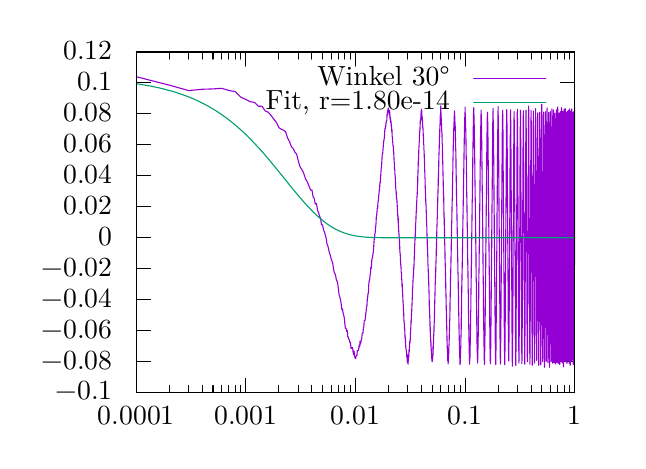
\begin{tikzpicture}[gnuplot]
%% generated with GNUPLOT 5.2p5a (Gentoo revision r0) (Lua 5.1; terminal rev. 99 , script rev. 107)
%% Sa 18 Mai 2019 18:31:20 CEST
\path (0.000,0.000) rectangle (7.500,5.250);
\gpcolor{color=gp lt color border}
\gpsetlinetype{gp lt border}
\gpsetdashtype{gp dt solid}
\gpsetlinewidth{1.00}
\draw[gp path] (1.380,0.616)--(1.560,0.616);
\draw[gp path] (6.947,0.616)--(6.767,0.616);
\node[gp node right] at (1.196,0.616) {$-0.1$};
\draw[gp path] (1.380,1.009)--(1.560,1.009);
\draw[gp path] (6.947,1.009)--(6.767,1.009);
\node[gp node right] at (1.196,1.009) {$-0.08$};
\draw[gp path] (1.380,1.402)--(1.560,1.402);
\draw[gp path] (6.947,1.402)--(6.767,1.402);
\node[gp node right] at (1.196,1.402) {$-0.06$};
\draw[gp path] (1.380,1.796)--(1.560,1.796);
\draw[gp path] (6.947,1.796)--(6.767,1.796);
\node[gp node right] at (1.196,1.796) {$-0.04$};
\draw[gp path] (1.380,2.189)--(1.560,2.189);
\draw[gp path] (6.947,2.189)--(6.767,2.189);
\node[gp node right] at (1.196,2.189) {$-0.02$};
\draw[gp path] (1.380,2.582)--(1.560,2.582);
\draw[gp path] (6.947,2.582)--(6.767,2.582);
\node[gp node right] at (1.196,2.582) {$0$};
\draw[gp path] (1.380,2.975)--(1.560,2.975);
\draw[gp path] (6.947,2.975)--(6.767,2.975);
\node[gp node right] at (1.196,2.975) {$0.02$};
\draw[gp path] (1.380,3.368)--(1.560,3.368);
\draw[gp path] (6.947,3.368)--(6.767,3.368);
\node[gp node right] at (1.196,3.368) {$0.04$};
\draw[gp path] (1.380,3.761)--(1.560,3.761);
\draw[gp path] (6.947,3.761)--(6.767,3.761);
\node[gp node right] at (1.196,3.761) {$0.06$};
\draw[gp path] (1.380,4.155)--(1.560,4.155);
\draw[gp path] (6.947,4.155)--(6.767,4.155);
\node[gp node right] at (1.196,4.155) {$0.08$};
\draw[gp path] (1.380,4.548)--(1.560,4.548);
\draw[gp path] (6.947,4.548)--(6.767,4.548);
\node[gp node right] at (1.196,4.548) {$0.1$};
\draw[gp path] (1.380,4.941)--(1.560,4.941);
\draw[gp path] (6.947,4.941)--(6.767,4.941);
\node[gp node right] at (1.196,4.941) {$0.12$};
\draw[gp path] (1.380,0.616)--(1.380,0.796);
\draw[gp path] (1.380,4.941)--(1.380,4.761);
\node[gp node center] at (1.380,0.308) {$0.0001$};
\draw[gp path] (1.799,0.616)--(1.799,0.706);
\draw[gp path] (1.799,4.941)--(1.799,4.851);
\draw[gp path] (2.044,0.616)--(2.044,0.706);
\draw[gp path] (2.044,4.941)--(2.044,4.851);
\draw[gp path] (2.218,0.616)--(2.218,0.706);
\draw[gp path] (2.218,4.941)--(2.218,4.851);
\draw[gp path] (2.353,0.616)--(2.353,0.706);
\draw[gp path] (2.353,4.941)--(2.353,4.851);
\draw[gp path] (2.463,0.616)--(2.463,0.706);
\draw[gp path] (2.463,4.941)--(2.463,4.851);
\draw[gp path] (2.556,0.616)--(2.556,0.706);
\draw[gp path] (2.556,4.941)--(2.556,4.851);
\draw[gp path] (2.637,0.616)--(2.637,0.706);
\draw[gp path] (2.637,4.941)--(2.637,4.851);
\draw[gp path] (2.708,0.616)--(2.708,0.706);
\draw[gp path] (2.708,4.941)--(2.708,4.851);
\draw[gp path] (2.772,0.616)--(2.772,0.796);
\draw[gp path] (2.772,4.941)--(2.772,4.761);
\node[gp node center] at (2.772,0.308) {$0.001$};
\draw[gp path] (3.191,0.616)--(3.191,0.706);
\draw[gp path] (3.191,4.941)--(3.191,4.851);
\draw[gp path] (3.436,0.616)--(3.436,0.706);
\draw[gp path] (3.436,4.941)--(3.436,4.851);
\draw[gp path] (3.610,0.616)--(3.610,0.706);
\draw[gp path] (3.610,4.941)--(3.610,4.851);
\draw[gp path] (3.745,0.616)--(3.745,0.706);
\draw[gp path] (3.745,4.941)--(3.745,4.851);
\draw[gp path] (3.855,0.616)--(3.855,0.706);
\draw[gp path] (3.855,4.941)--(3.855,4.851);
\draw[gp path] (3.948,0.616)--(3.948,0.706);
\draw[gp path] (3.948,4.941)--(3.948,4.851);
\draw[gp path] (4.029,0.616)--(4.029,0.706);
\draw[gp path] (4.029,4.941)--(4.029,4.851);
\draw[gp path] (4.100,0.616)--(4.100,0.706);
\draw[gp path] (4.100,4.941)--(4.100,4.851);
\draw[gp path] (4.163,0.616)--(4.163,0.796);
\draw[gp path] (4.163,4.941)--(4.163,4.761);
\node[gp node center] at (4.163,0.308) {$0.01$};
\draw[gp path] (4.582,0.616)--(4.582,0.706);
\draw[gp path] (4.582,4.941)--(4.582,4.851);
\draw[gp path] (4.828,0.616)--(4.828,0.706);
\draw[gp path] (4.828,4.941)--(4.828,4.851);
\draw[gp path] (5.001,0.616)--(5.001,0.706);
\draw[gp path] (5.001,4.941)--(5.001,4.851);
\draw[gp path] (5.136,0.616)--(5.136,0.706);
\draw[gp path] (5.136,4.941)--(5.136,4.851);
\draw[gp path] (5.246,0.616)--(5.246,0.706);
\draw[gp path] (5.246,4.941)--(5.246,4.851);
\draw[gp path] (5.340,0.616)--(5.340,0.706);
\draw[gp path] (5.340,4.941)--(5.340,4.851);
\draw[gp path] (5.420,0.616)--(5.420,0.706);
\draw[gp path] (5.420,4.941)--(5.420,4.851);
\draw[gp path] (5.492,0.616)--(5.492,0.706);
\draw[gp path] (5.492,4.941)--(5.492,4.851);
\draw[gp path] (5.555,0.616)--(5.555,0.796);
\draw[gp path] (5.555,4.941)--(5.555,4.761);
\node[gp node center] at (5.555,0.308) {$0.1$};
\draw[gp path] (5.974,0.616)--(5.974,0.706);
\draw[gp path] (5.974,4.941)--(5.974,4.851);
\draw[gp path] (6.219,0.616)--(6.219,0.706);
\draw[gp path] (6.219,4.941)--(6.219,4.851);
\draw[gp path] (6.393,0.616)--(6.393,0.706);
\draw[gp path] (6.393,4.941)--(6.393,4.851);
\draw[gp path] (6.528,0.616)--(6.528,0.706);
\draw[gp path] (6.528,4.941)--(6.528,4.851);
\draw[gp path] (6.638,0.616)--(6.638,0.706);
\draw[gp path] (6.638,4.941)--(6.638,4.851);
\draw[gp path] (6.731,0.616)--(6.731,0.706);
\draw[gp path] (6.731,4.941)--(6.731,4.851);
\draw[gp path] (6.812,0.616)--(6.812,0.706);
\draw[gp path] (6.812,4.941)--(6.812,4.851);
\draw[gp path] (6.883,0.616)--(6.883,0.706);
\draw[gp path] (6.883,4.941)--(6.883,4.851);
\draw[gp path] (6.947,0.616)--(6.947,0.796);
\draw[gp path] (6.947,4.941)--(6.947,4.761);
\node[gp node center] at (6.947,0.308) {$1$};
\draw[gp path] (1.380,4.941)--(1.380,0.616)--(6.947,0.616)--(6.947,4.941)--cycle;
\node[gp node right] at (5.479,4.607) {Winkel 30°};
\gpcolor{rgb color={0.580,0.000,0.827}}
\draw[gp path] (5.663,4.607)--(6.579,4.607);
\draw[gp path] (1.380,4.627)--(1.799,4.520)--(2.044,4.451)--(2.218,4.468)--(2.353,4.472)%
  --(2.463,4.480)--(2.556,4.452)--(2.637,4.438)--(2.708,4.367)--(2.772,4.338)--(2.829,4.309)%
  --(2.882,4.301)--(2.930,4.252)--(2.975,4.253)--(3.017,4.192)--(3.056,4.175)--(3.092,4.135)%
  --(3.127,4.086)--(3.160,4.045)--(3.191,3.980)--(3.220,3.961)--(3.248,3.949)--(3.275,3.929)%
  --(3.301,3.849)--(3.326,3.803)--(3.349,3.738)--(3.372,3.714)--(3.394,3.667)--(3.415,3.647)%
  --(3.436,3.563)--(3.456,3.491)--(3.475,3.457)--(3.493,3.430)--(3.511,3.386)--(3.529,3.328)%
  --(3.546,3.301)--(3.563,3.264)--(3.579,3.223)--(3.594,3.187)--(3.610,3.189)--(3.625,3.102)%
  --(3.639,3.082)--(3.653,3.010)--(3.667,3.018)--(3.681,2.935)--(3.694,2.902)--(3.707,2.855)%
  --(3.720,2.829)--(3.732,2.746)--(3.745,2.746)--(3.757,2.681)--(3.768,2.656)--(3.780,2.618)%
  --(3.791,2.575)--(3.802,2.499)--(3.813,2.476)--(3.824,2.427)--(3.834,2.387)--(3.845,2.354)%
  --(3.855,2.308)--(3.865,2.286)--(3.875,2.253)--(3.884,2.186)--(3.894,2.141)--(3.903,2.126)%
  --(3.912,2.097)--(3.921,2.040)--(3.930,2.034)--(3.939,1.989)--(3.948,1.917)--(3.956,1.852)%
  --(3.965,1.827)--(3.973,1.794)--(3.982,1.738)--(3.990,1.671)--(3.998,1.677)--(4.006,1.625)%
  --(4.013,1.601)--(4.021,1.563)--(4.029,1.479)--(4.036,1.430)--(4.044,1.431)--(4.051,1.394)%
  --(4.058,1.405)--(4.065,1.324)--(4.072,1.320)--(4.079,1.294)--(4.086,1.281)--(4.093,1.248)%
  --(4.100,1.251)--(4.106,1.176)--(4.113,1.189)--(4.120,1.177)--(4.126,1.188)--(4.132,1.135)%
  --(4.139,1.099)--(4.145,1.145)--(4.151,1.079)--(4.157,1.057)--(4.164,1.046)--(4.170,1.077)%
  --(4.175,1.084)--(4.181,1.085)--(4.187,1.150)--(4.193,1.148)--(4.199,1.151)--(4.204,1.165)%
  --(4.210,1.221)--(4.216,1.195)--(4.221,1.267)--(4.227,1.232)--(4.232,1.261)--(4.237,1.280)%
  --(4.243,1.305)--(4.248,1.368)--(4.253,1.366)--(4.258,1.371)--(4.264,1.437)--(4.269,1.454)%
  --(4.274,1.529)--(4.279,1.531)--(4.284,1.531)--(4.289,1.566)--(4.294,1.620)--(4.298,1.642)%
  --(4.303,1.704)--(4.308,1.708)--(4.313,1.795)--(4.317,1.817)--(4.322,1.873)--(4.327,1.871)%
  --(4.331,1.975)--(4.336,2.031)--(4.340,2.038)--(4.345,2.066)--(4.349,2.113)--(4.354,2.128)%
  --(4.358,2.207)--(4.363,2.194)--(4.367,2.240)--(4.371,2.307)--(4.375,2.320)--(4.380,2.331)%
  --(4.384,2.374)--(4.388,2.388)--(4.392,2.430)--(4.396,2.495)--(4.400,2.553)--(4.405,2.580)%
  --(4.409,2.626)--(4.413,2.643)--(4.417,2.696)--(4.421,2.734)--(4.424,2.764)--(4.428,2.854)%
  --(4.432,2.864)--(4.436,2.906)--(4.440,2.962)--(4.444,2.947)--(4.448,3.021)--(4.451,3.043)%
  --(4.455,3.079)--(4.459,3.124)--(4.463,3.154)--(4.466,3.192)--(4.470,3.213)--(4.473,3.281)%
  --(4.477,3.277)--(4.481,3.332)--(4.484,3.375)--(4.488,3.441)--(4.491,3.473)--(4.495,3.506)%
  --(4.498,3.554)--(4.502,3.630)--(4.505,3.646)--(4.509,3.655)--(4.512,3.692)--(4.515,3.728)%
  --(4.519,3.780)--(4.522,3.810)--(4.525,3.822)--(4.529,3.851)--(4.532,3.883)--(4.535,3.940)%
  --(4.539,3.973)--(4.542,3.965)--(4.545,4.006)--(4.548,3.995)--(4.551,4.041)--(4.555,4.056)%
  --(4.558,4.069)--(4.561,4.069)--(4.564,4.148)--(4.567,4.144)--(4.570,4.178)--(4.573,4.205)%
  --(4.576,4.196)--(4.579,4.231)--(4.582,4.171)--(4.585,4.203)--(4.588,4.202)--(4.591,4.144)%
  --(4.594,4.149)--(4.597,4.199)--(4.600,4.100)--(4.603,4.130)--(4.606,4.068)--(4.609,4.102)%
  --(4.612,4.035)--(4.615,4.062)--(4.618,3.998)--(4.621,3.991)--(4.623,3.935)--(4.626,3.959)%
  --(4.629,3.869)--(4.632,3.861)--(4.635,3.800)--(4.637,3.787)--(4.640,3.748)--(4.643,3.748)%
  --(4.646,3.680)--(4.648,3.675)--(4.651,3.615)--(4.654,3.550)--(4.656,3.537)--(4.659,3.449)%
  --(4.662,3.451)--(4.664,3.395)--(4.667,3.362)--(4.670,3.323)--(4.672,3.240)--(4.675,3.212)%
  --(4.677,3.181)--(4.680,3.173)--(4.683,3.097)--(4.685,3.072)--(4.688,3.081)--(4.690,3.047)%
  --(4.693,2.994)--(4.695,2.960)--(4.698,2.910)--(4.700,2.865)--(4.703,2.807)--(4.705,2.856)%
  --(4.708,2.716)--(4.710,2.733)--(4.712,2.676)--(4.715,2.636)--(4.717,2.609)--(4.720,2.578)%
  --(4.722,2.536)--(4.725,2.467)--(4.727,2.402)--(4.729,2.391)--(4.732,2.362)--(4.734,2.304)%
  --(4.736,2.257)--(4.739,2.237)--(4.741,2.225)--(4.743,2.150)--(4.746,2.133)--(4.748,2.140)%
  --(4.750,2.061)--(4.753,2.019)--(4.755,1.952)--(4.757,1.992)--(4.759,1.914)--(4.762,1.878)%
  --(4.764,1.829)--(4.766,1.785)--(4.768,1.744)--(4.771,1.723)--(4.773,1.655)--(4.775,1.635)%
  --(4.777,1.581)--(4.779,1.527)--(4.781,1.505)--(4.784,1.483)--(4.786,1.427)--(4.788,1.425)%
  --(4.790,1.397)--(4.792,1.324)--(4.794,1.298)--(4.797,1.316)--(4.799,1.248)--(4.801,1.211)%
  --(4.803,1.179)--(4.805,1.170)--(4.807,1.155)--(4.809,1.155)--(4.811,1.128)--(4.813,1.108)%
  --(4.815,1.066)--(4.817,1.105)--(4.819,1.014)--(4.821,1.044)--(4.823,1.000)--(4.826,1.027)%
  --(4.828,0.982)--(4.830,1.067)--(4.832,0.977)--(4.834,1.092)--(4.836,1.049)--(4.838,1.050)%
  --(4.840,1.090)--(4.841,1.154)--(4.843,1.121)--(4.845,1.133)--(4.847,1.172)--(4.849,1.190)%
  --(4.851,1.224)--(4.853,1.269)--(4.855,1.249)--(4.857,1.297)--(4.859,1.284)--(4.861,1.366)%
  --(4.863,1.391)--(4.865,1.438)--(4.867,1.436)--(4.868,1.525)--(4.870,1.499)--(4.872,1.549)%
  --(4.874,1.590)--(4.876,1.626)--(4.878,1.670)--(4.880,1.716)--(4.881,1.735)--(4.883,1.794)%
  --(4.885,1.831)--(4.887,1.932)--(4.889,1.942)--(4.891,1.967)--(4.892,1.997)--(4.894,2.043)%
  --(4.896,2.075)--(4.898,2.111)--(4.900,2.112)--(4.901,2.173)--(4.903,2.186)--(4.905,2.244)%
  --(4.907,2.220)--(4.908,2.285)--(4.910,2.338)--(4.912,2.382)--(4.914,2.459)--(4.916,2.499)%
  --(4.917,2.515)--(4.919,2.569)--(4.921,2.559)--(4.922,2.632)--(4.924,2.644)--(4.926,2.720)%
  --(4.928,2.774)--(4.929,2.773)--(4.931,2.818)--(4.933,2.878)--(4.934,2.891)--(4.936,2.932)%
  --(4.938,2.944)--(4.939,3.016)--(4.941,3.040)--(4.943,3.068)--(4.944,3.109)--(4.946,3.110)%
  --(4.948,3.147)--(4.949,3.219)--(4.951,3.238)--(4.953,3.266)--(4.954,3.349)--(4.956,3.387)%
  --(4.958,3.448)--(4.959,3.473)--(4.961,3.556)--(4.962,3.521)--(4.964,3.604)--(4.966,3.693)%
  --(4.967,3.644)--(4.969,3.731)--(4.970,3.739)--(4.972,3.792)--(4.974,3.803)--(4.975,3.887)%
  --(4.977,3.872)--(4.978,3.918)--(4.980,3.941)--(4.981,3.984)--(4.983,3.952)--(4.985,4.029)%
  --(4.986,4.067)--(4.988,4.060)--(4.989,4.053)--(4.991,4.099)--(4.992,4.083)--(4.994,4.126)%
  --(4.995,4.145)--(4.997,4.179)--(4.998,4.163)--(5.000,4.214)--(5.001,4.195)--(5.003,4.181)%
  --(5.004,4.196)--(5.006,4.165)--(5.007,4.109)--(5.009,4.127)--(5.010,4.071)--(5.012,4.109)%
  --(5.013,4.088)--(5.015,4.062)--(5.016,3.977)--(5.018,4.000)--(5.019,3.978)--(5.021,3.964)%
  --(5.022,3.944)--(5.024,3.875)--(5.025,3.904)--(5.027,3.836)--(5.028,3.841)--(5.029,3.769)%
  --(5.031,3.760)--(5.032,3.700)--(5.034,3.692)--(5.035,3.668)--(5.037,3.607)--(5.038,3.575)%
  --(5.039,3.542)--(5.041,3.519)--(5.042,3.439)--(5.044,3.409)--(5.045,3.349)--(5.047,3.329)%
  --(5.048,3.271)--(5.049,3.218)--(5.051,3.184)--(5.052,3.153)--(5.054,3.116)--(5.055,3.068)%
  --(5.056,3.037)--(5.058,3.018)--(5.059,3.011)--(5.060,2.956)--(5.062,2.911)--(5.063,2.901)%
  --(5.064,2.792)--(5.066,2.802)--(5.067,2.742)--(5.069,2.727)--(5.070,2.656)--(5.071,2.639)%
  --(5.073,2.571)--(5.074,2.558)--(5.075,2.495)--(5.077,2.472)--(5.078,2.443)--(5.079,2.389)%
  --(5.081,2.366)--(5.082,2.321)--(5.083,2.242)--(5.085,2.231)--(5.086,2.208)--(5.087,2.164)%
  --(5.089,2.125)--(5.090,2.100)--(5.091,2.054)--(5.092,2.047)--(5.094,1.997)--(5.095,1.918)%
  --(5.096,1.918)--(5.098,1.858)--(5.099,1.815)--(5.100,1.722)--(5.101,1.716)--(5.103,1.688)%
  --(5.104,1.675)--(5.105,1.615)--(5.107,1.565)--(5.108,1.551)--(5.109,1.511)--(5.110,1.459)%
  --(5.112,1.446)--(5.113,1.404)--(5.114,1.362)--(5.115,1.331)--(5.117,1.306)--(5.118,1.266)%
  --(5.119,1.251)--(5.120,1.287)--(5.122,1.237)--(5.123,1.186)--(5.124,1.179)--(5.125,1.170)%
  --(5.127,1.124)--(5.128,1.102)--(5.129,1.099)--(5.130,1.102)--(5.131,1.061)--(5.133,1.034)%
  --(5.134,1.018)--(5.135,1.017)--(5.136,1.018)--(5.137,1.008)--(5.139,1.020)--(5.140,1.035)%
  --(5.141,1.058)--(5.142,1.036)--(5.144,1.080)--(5.145,1.079)--(5.146,1.116)--(5.147,1.095)%
  --(5.148,1.196)--(5.149,1.135)--(5.151,1.199)--(5.152,1.235)--(5.153,1.237)--(5.154,1.246)%
  --(5.155,1.290)--(5.157,1.360)--(5.158,1.367)--(5.159,1.379)--(5.160,1.393)--(5.161,1.467)%
  --(5.162,1.488)--(5.163,1.506)--(5.165,1.526)--(5.166,1.586)--(5.167,1.658)--(5.168,1.666)%
  --(5.169,1.738)--(5.170,1.783)--(5.172,1.836)--(5.173,1.880)--(5.174,1.900)--(5.175,1.965)%
  --(5.176,2.013)--(5.177,1.999)--(5.178,2.041)--(5.179,2.087)--(5.181,2.132)--(5.182,2.150)%
  --(5.183,2.208)--(5.184,2.201)--(5.185,2.262)--(5.186,2.273)--(5.187,2.326)--(5.188,2.336)%
  --(5.189,2.431)--(5.191,2.390)--(5.192,2.513)--(5.193,2.536)--(5.194,2.539)--(5.195,2.615)%
  --(5.196,2.671)--(5.197,2.685)--(5.198,2.747)--(5.199,2.752)--(5.200,2.814)--(5.202,2.830)%
  --(5.203,2.896)--(5.204,2.940)--(5.205,2.973)--(5.206,2.956)--(5.207,3.030)--(5.208,3.075)%
  --(5.209,3.113)--(5.210,3.126)--(5.211,3.171)--(5.212,3.203)--(5.213,3.217)--(5.214,3.257)%
  --(5.215,3.344)--(5.217,3.344)--(5.218,3.414)--(5.219,3.476)--(5.220,3.485)--(5.221,3.562)%
  --(5.222,3.559)--(5.223,3.630)--(5.224,3.666)--(5.225,3.661)--(5.226,3.712)--(5.227,3.721)%
  --(5.228,3.794)--(5.229,3.829)--(5.230,3.881)--(5.231,3.873)--(5.232,3.911)--(5.233,3.918)%
  --(5.234,3.962)--(5.235,3.980)--(5.236,4.022)--(5.237,4.019)--(5.238,4.084)--(5.239,4.056)%
  --(5.240,4.132)--(5.241,4.125)--(5.242,4.144)--(5.243,4.120)--(5.244,4.194)--(5.245,4.176)%
  --(5.246,4.257)--(5.247,4.149)--(5.249,4.173)--(5.250,4.092)--(5.251,4.143)--(5.252,4.085)%
  --(5.253,4.037)--(5.254,4.090)--(5.254,4.060)--(5.255,4.033)--(5.256,4.014)--(5.257,3.955)%
  --(5.258,3.946)--(5.259,3.946)--(5.260,3.914)--(5.261,3.914)--(5.262,3.880)--(5.263,3.836)%
  --(5.264,3.786)--(5.265,3.768)--(5.266,3.770)--(5.267,3.706)--(5.268,3.669)--(5.269,3.579)%
  --(5.270,3.613)--(5.271,3.541)--(5.272,3.515)--(5.273,3.465)--(5.274,3.419)--(5.275,3.368)%
  --(5.276,3.376)--(5.277,3.309)--(5.278,3.258)--(5.279,3.205)--(5.280,3.177)--(5.281,3.124)%
  --(5.282,3.102)--(5.283,3.062)--(5.284,3.097)--(5.285,3.005)--(5.286,2.963)--(5.286,2.933)%
  --(5.287,2.894)--(5.288,2.838)--(5.289,2.825)--(5.290,2.834)--(5.291,2.749)--(5.292,2.661)%
  --(5.293,2.690)--(5.294,2.612)--(5.295,2.596)--(5.296,2.511)--(5.297,2.520)--(5.298,2.446)%
  --(5.299,2.413)--(5.300,2.386)--(5.300,2.364)--(5.301,2.292)--(5.302,2.276)--(5.303,2.237)%
  --(5.304,2.213)--(5.305,2.148)--(5.306,2.122)--(5.307,2.099)--(5.308,2.022)--(5.309,2.014)%
  --(5.310,1.995)--(5.310,1.939)--(5.311,1.946)--(5.312,1.870)--(5.313,1.840)--(5.314,1.787)%
  --(5.315,1.729)--(5.316,1.684)--(5.317,1.646)--(5.318,1.640)--(5.319,1.542)--(5.319,1.564)%
  --(5.320,1.485)--(5.321,1.473)--(5.322,1.466)--(5.323,1.399)--(5.324,1.372)--(5.325,1.321)%
  --(5.326,1.274)--(5.327,1.315)--(5.327,1.227)--(5.328,1.177)--(5.329,1.213)--(5.330,1.152)%
  --(5.331,1.189)--(5.332,1.127)--(5.333,1.137)--(5.334,1.101)--(5.334,1.103)--(5.335,1.017)%
  --(5.336,1.064)--(5.337,1.013)--(5.338,1.025)--(5.339,1.041)--(5.340,0.979)--(5.341,1.017)%
  --(5.341,1.011)--(5.342,0.998)--(5.343,1.074)--(5.344,1.051)--(5.345,1.081)--(5.346,1.118)%
  --(5.347,1.106)--(5.347,1.135)--(5.348,1.156)--(5.349,1.135)--(5.350,1.208)--(5.351,1.227)%
  --(5.352,1.222)--(5.352,1.276)--(5.353,1.267)--(5.354,1.319)--(5.355,1.371)--(5.356,1.371)%
  --(5.357,1.439)--(5.358,1.442)--(5.358,1.506)--(5.359,1.479)--(5.360,1.555)--(5.361,1.553)%
  --(5.362,1.646)--(5.363,1.652)--(5.363,1.714)--(5.364,1.750)--(5.365,1.801)--(5.366,1.825)%
  --(5.367,1.892)--(5.368,1.908)--(5.368,1.953)--(5.369,2.008)--(5.370,2.080)--(5.371,2.086)%
  --(5.372,2.104)--(5.372,2.115)--(5.373,2.161)--(5.374,2.203)--(5.375,2.259)--(5.376,2.277)%
  --(5.377,2.354)--(5.377,2.395)--(5.378,2.382)--(5.379,2.439)--(5.380,2.511)--(5.381,2.535)%
  --(5.381,2.563)--(5.382,2.624)--(5.383,2.641)--(5.384,2.714)--(5.385,2.729)--(5.385,2.765)%
  --(5.386,2.767)--(5.387,2.852)--(5.388,2.908)--(5.389,2.935)--(5.389,2.965)--(5.390,2.985)%
  --(5.391,3.033)--(5.392,3.080)--(5.393,3.066)--(5.393,3.115)--(5.394,3.180)--(5.395,3.216)%
  --(5.396,3.262)--(5.396,3.302)--(5.397,3.346)--(5.398,3.400)--(5.399,3.418)--(5.400,3.483)%
  --(5.400,3.535)--(5.401,3.565)--(5.402,3.594)--(5.403,3.621)--(5.404,3.684)--(5.404,3.685)%
  --(5.405,3.759)--(5.406,3.775)--(5.407,3.815)--(5.407,3.813)--(5.408,3.857)--(5.409,3.879)%
  --(5.410,3.913)--(5.410,3.977)--(5.411,3.944)--(5.412,3.990)--(5.413,4.009)--(5.414,4.034)%
  --(5.414,4.043)--(5.415,4.051)--(5.416,4.046)--(5.417,4.078)--(5.417,4.110)--(5.418,4.132)%
  --(5.419,4.166)--(5.420,4.177)--(5.420,4.194)--(5.421,4.181)--(5.422,4.168)--(5.423,4.177)%
  --(5.423,4.129)--(5.424,4.109)--(5.425,4.079)--(5.426,4.065)--(5.426,4.053)--(5.427,4.051)%
  --(5.428,3.980)--(5.429,3.999)--(5.429,3.967)--(5.430,3.998)--(5.431,3.924)--(5.432,3.905)%
  --(5.432,3.858)--(5.433,3.855)--(5.434,3.779)--(5.435,3.784)--(5.435,3.740)--(5.436,3.707)%
  --(5.437,3.685)--(5.438,3.666)--(5.438,3.569)--(5.439,3.586)--(5.440,3.521)--(5.440,3.487)%
  --(5.441,3.412)--(5.442,3.384)--(5.443,3.327)--(5.443,3.323)--(5.444,3.261)--(5.445,3.210)%
  --(5.446,3.183)--(5.446,3.129)--(5.447,3.100)--(5.448,3.089)--(5.448,2.985)--(5.449,3.015)%
  --(5.450,2.986)--(5.451,2.951)--(5.451,2.879)--(5.452,2.882)--(5.453,2.814)--(5.453,2.805)%
  --(5.454,2.769)--(5.455,2.701)--(5.456,2.648)--(5.456,2.643)--(5.457,2.557)--(5.458,2.550)%
  --(5.458,2.460)--(5.459,2.448)--(5.460,2.415)--(5.461,2.374)--(5.461,2.330)--(5.462,2.305)%
  --(5.463,2.239)--(5.463,2.231)--(5.464,2.123)--(5.465,2.146)--(5.465,2.127)--(5.466,2.120)%
  --(5.467,2.021)--(5.468,2.027)--(5.468,2.017)--(5.469,1.930)--(5.470,1.911)--(5.470,1.894)%
  --(5.471,1.828)--(5.472,1.787)--(5.472,1.729)--(5.473,1.662)--(5.474,1.638)--(5.475,1.587)%
  --(5.475,1.592)--(5.476,1.592)--(5.477,1.489)--(5.477,1.498)--(5.478,1.440)--(5.479,1.400)%
  --(5.479,1.344)--(5.480,1.343)--(5.481,1.325)--(5.481,1.301)--(5.482,1.257)--(5.483,1.241)%
  --(5.483,1.200)--(5.484,1.165)--(5.485,1.175)--(5.485,1.140)--(5.486,1.119)--(5.487,1.097)%
  --(5.488,1.054)--(5.488,1.084)--(5.489,1.017)--(5.490,1.069)--(5.490,0.970)--(5.491,1.047)%
  --(5.492,1.008)--(5.492,0.986)--(5.493,0.990)--(5.494,1.069)--(5.494,1.030)--(5.495,1.073)%
  --(5.496,1.059)--(5.496,1.089)--(5.497,1.123)--(5.498,1.142)--(5.498,1.131)--(5.499,1.170)%
  --(5.500,1.195)--(5.500,1.193)--(5.501,1.219)--(5.502,1.287)--(5.502,1.323)--(5.503,1.319)%
  --(5.504,1.357)--(5.504,1.420)--(5.505,1.436)--(5.506,1.414)--(5.506,1.518)--(5.507,1.517)%
  --(5.507,1.568)--(5.508,1.589)--(5.509,1.617)--(5.509,1.690)--(5.510,1.700)--(5.511,1.770)%
  --(5.511,1.820)--(5.512,1.877)--(5.513,1.913)--(5.513,1.971)--(5.514,1.934)--(5.515,2.006)%
  --(5.515,2.028)--(5.516,2.101)--(5.517,2.135)--(5.517,2.170)--(5.518,2.136)--(5.518,2.209)%
  --(5.519,2.197)--(5.520,2.309)--(5.520,2.310)--(5.521,2.368)--(5.522,2.400)--(5.522,2.459)%
  --(5.523,2.462)--(5.524,2.511)--(5.524,2.535)--(5.525,2.622)--(5.526,2.670)--(5.526,2.694)%
  --(5.527,2.733)--(5.527,2.785)--(5.528,2.824)--(5.529,2.853)--(5.529,2.855)--(5.530,2.916)%
  --(5.531,2.935)--(5.531,2.987)--(5.532,3.029)--(5.532,3.051)--(5.533,3.084)--(5.534,3.117)%
  --(5.534,3.184)--(5.535,3.248)--(5.536,3.244)--(5.536,3.273)--(5.537,3.333)--(5.537,3.380)%
  --(5.538,3.410)--(5.539,3.478)--(5.539,3.471)--(5.540,3.546)--(5.541,3.599)--(5.541,3.634)%
  --(5.542,3.663)--(5.542,3.698)--(5.543,3.746)--(5.544,3.781)--(5.544,3.795)--(5.545,3.839)%
  --(5.546,3.911)--(5.546,3.897)--(5.547,3.967)--(5.547,3.989)--(5.548,3.978)--(5.549,4.030)%
  --(5.549,4.018)--(5.550,4.079)--(5.550,4.050)--(5.551,4.114)--(5.552,4.092)--(5.552,4.143)%
  --(5.553,4.140)--(5.553,4.145)--(5.554,4.151)--(5.555,4.190)--(5.555,4.242)--(5.556,4.180)%
  --(5.556,4.171)--(5.557,4.164)--(5.558,4.112)--(5.558,4.109)--(5.559,4.124)--(5.559,4.118)%
  --(5.560,4.067)--(5.561,4.071)--(5.561,4.095)--(5.562,4.013)--(5.562,3.975)--(5.563,3.965)%
  --(5.564,3.971)--(5.564,3.937)--(5.565,3.867)--(5.565,3.850)--(5.566,3.840)--(5.567,3.821)%
  --(5.567,3.771)--(5.568,3.718)--(5.568,3.669)--(5.569,3.631)--(5.570,3.591)--(5.570,3.601)%
  --(5.571,3.541)--(5.571,3.524)--(5.572,3.435)--(5.573,3.370)--(5.573,3.358)--(5.574,3.329)%
  --(5.574,3.233)--(5.575,3.238)--(5.575,3.196)--(5.576,3.126)--(5.577,3.090)--(5.577,3.084)%
  --(5.578,3.033)--(5.578,2.994)--(5.579,2.997)--(5.580,2.979)--(5.580,2.904)--(5.581,2.857)%
  --(5.581,2.807)--(5.582,2.771)--(5.582,2.714)--(5.583,2.716)--(5.584,2.668)--(5.584,2.639)%
  --(5.585,2.592)--(5.585,2.580)--(5.586,2.505)--(5.586,2.449)--(5.587,2.452)--(5.588,2.345)%
  --(5.588,2.319)--(5.589,2.283)--(5.589,2.270)--(5.590,2.213)--(5.590,2.197)--(5.591,2.170)%
  --(5.592,2.132)--(5.592,2.107)--(5.593,2.057)--(5.593,2.020)--(5.594,1.978)--(5.594,1.935)%
  --(5.595,1.923)--(5.596,1.868)--(5.596,1.850)--(5.597,1.747)--(5.597,1.731)--(5.598,1.643)%
  --(5.598,1.638)--(5.599,1.607)--(5.600,1.589)--(5.600,1.528)--(5.601,1.492)--(5.601,1.443)%
  --(5.602,1.447)--(5.602,1.431)--(5.603,1.379)--(5.603,1.350)--(5.604,1.323)--(5.605,1.297)%
  --(5.605,1.277)--(5.606,1.229)--(5.606,1.217)--(5.607,1.180)--(5.607,1.158)--(5.608,1.134)%
  --(5.608,1.113)--(5.609,1.151)--(5.610,1.126)--(5.610,1.053)--(5.611,1.069)--(5.611,1.011)%
  --(5.612,1.015)--(5.612,1.032)--(5.613,0.989)--(5.613,0.976)--(5.614,1.053)--(5.615,1.045)%
  --(5.615,1.090)--(5.616,1.034)--(5.616,1.060)--(5.617,1.062)--(5.617,1.092)--(5.618,1.106)%
  --(5.618,1.169)--(5.619,1.165)--(5.619,1.203)--(5.620,1.219)--(5.621,1.255)--(5.621,1.241)%
  --(5.622,1.308)--(5.622,1.352)--(5.623,1.360)--(5.623,1.389)--(5.624,1.453)--(5.624,1.464)%
  --(5.625,1.491)--(5.625,1.507)--(5.626,1.581)--(5.626,1.641)--(5.627,1.644)--(5.628,1.677)%
  --(5.628,1.756)--(5.629,1.781)--(5.629,1.826)--(5.630,1.893)--(5.630,1.930)--(5.631,1.949)%
  --(5.631,2.008)--(5.632,2.028)--(5.632,2.053)--(5.633,2.080)--(5.633,2.108)--(5.634,2.196)%
  --(5.634,2.215)--(5.635,2.218)--(5.636,2.249)--(5.636,2.278)--(5.637,2.369)--(5.637,2.343)%
  --(5.638,2.444)--(5.638,2.456)--(5.639,2.559)--(5.639,2.551)--(5.640,2.597)--(5.640,2.624)%
  --(5.641,2.686)--(5.641,2.716)--(5.642,2.761)--(5.642,2.791)--(5.643,2.827)--(5.643,2.808)%
  --(5.644,2.942)--(5.644,2.920)--(5.645,2.998)--(5.645,3.023)--(5.646,3.049)--(5.647,3.081)%
  --(5.647,3.094)--(5.648,3.159)--(5.648,3.166)--(5.649,3.259)--(5.649,3.245)--(5.650,3.331)%
  --(5.650,3.344)--(5.651,3.386)--(5.651,3.448)--(5.652,3.468)--(5.652,3.511)--(5.653,3.566)%
  --(5.653,3.599)--(5.654,3.631)--(5.654,3.663)--(5.655,3.739)--(5.655,3.752)--(5.656,3.765)%
  --(5.656,3.798)--(5.657,3.798)--(5.657,3.889)--(5.658,3.884)--(5.658,3.951)--(5.659,3.930)%
  --(5.659,3.995)--(5.660,3.970)--(5.660,4.054)--(5.661,4.033)--(5.661,4.082)--(5.662,4.086)%
  --(5.662,4.161)--(5.663,4.097)--(5.663,4.170)--(5.664,4.146)--(5.664,4.221)--(5.665,4.124)%
  --(5.665,4.234)--(5.666,4.234)--(5.666,4.194)--(5.667,4.161)--(5.667,4.194)--(5.668,4.107)%
  --(5.668,4.134)--(5.669,4.077)--(5.669,4.068)--(5.670,4.035)--(5.670,4.026)--(5.671,4.010)%
  --(5.671,3.929)--(5.672,3.956)--(5.672,3.947)--(5.673,3.895)--(5.673,3.869)--(5.674,3.834)%
  --(5.674,3.826)--(5.675,3.770)--(5.675,3.716)--(5.676,3.676)--(5.676,3.664)--(5.677,3.645)%
  --(5.677,3.594)--(5.678,3.553)--(5.678,3.526)--(5.679,3.502)--(5.679,3.433)--(5.680,3.414)%
  --(5.680,3.334)--(5.681,3.262)--(5.681,3.261)--(5.682,3.222)--(5.682,3.173)--(5.683,3.120)%
  --(5.683,3.125)--(5.684,3.050)--(5.684,3.088)--(5.685,3.030)--(5.685,2.986)--(5.686,2.945)%
  --(5.686,2.938)--(5.687,2.876)--(5.687,2.846)--(5.688,2.812)--(5.688,2.755)--(5.689,2.696)%
  --(5.689,2.692)--(5.690,2.627)--(5.690,2.603)--(5.691,2.551)--(5.691,2.529)--(5.692,2.418)%
  --(5.692,2.421)--(5.693,2.400)--(5.693,2.350)--(5.693,2.316)--(5.694,2.261)--(5.694,2.223)%
  --(5.695,2.193)--(5.695,2.181)--(5.696,2.138)--(5.696,2.077)--(5.697,2.060)--(5.697,2.037)%
  --(5.698,1.995)--(5.698,1.991)--(5.699,1.913)--(5.699,1.871)--(5.700,1.812)--(5.700,1.783)%
  --(5.701,1.731)--(5.701,1.684)--(5.702,1.636)--(5.702,1.614)--(5.703,1.552)--(5.703,1.538)%
  --(5.704,1.460)--(5.704,1.461)--(5.704,1.418)--(5.705,1.379)--(5.705,1.356)--(5.706,1.335)%
  --(5.706,1.297)--(5.707,1.242)--(5.707,1.235)--(5.708,1.231)--(5.708,1.187)--(5.709,1.167)%
  --(5.709,1.210)--(5.710,1.116)--(5.710,1.138)--(5.711,1.043)--(5.711,1.112)--(5.712,1.061)%
  --(5.712,1.063)--(5.712,1.061)--(5.713,1.040)--(5.713,1.014)--(5.714,1.049)--(5.714,1.041)%
  --(5.715,0.990)--(5.715,1.036)--(5.716,1.043)--(5.716,1.080)--(5.717,1.101)--(5.717,1.089)%
  --(5.718,1.157)--(5.718,1.155)--(5.718,1.148)--(5.719,1.202)--(5.719,1.187)--(5.720,1.224)%
  --(5.720,1.247)--(5.721,1.278)--(5.721,1.294)--(5.722,1.349)--(5.722,1.347)--(5.723,1.389)%
  --(5.723,1.419)--(5.724,1.482)--(5.724,1.521)--(5.724,1.506)--(5.725,1.577)--(5.725,1.604)%
  --(5.726,1.663)--(5.726,1.661)--(5.727,1.736)--(5.727,1.757)--(5.728,1.809)--(5.728,1.859)%
  --(5.729,1.904)--(5.729,1.974)--(5.729,2.004)--(5.730,2.060)--(5.730,2.065)--(5.731,2.090)%
  --(5.731,2.130)--(5.732,2.177)--(5.732,2.150)--(5.733,2.253)--(5.733,2.276)--(5.733,2.295)%
  --(5.734,2.318)--(5.734,2.364)--(5.735,2.430)--(5.735,2.471)--(5.736,2.486)--(5.736,2.548)%
  --(5.737,2.580)--(5.737,2.611)--(5.738,2.635)--(5.738,2.688)--(5.738,2.724)--(5.739,2.738)%
  --(5.739,2.778)--(5.740,2.862)--(5.740,2.916)--(5.741,2.955)--(5.741,2.923)--(5.742,3.018)%
  --(5.742,3.027)--(5.742,3.081)--(5.743,3.133)--(5.743,3.139)--(5.744,3.185)--(5.744,3.215)%
  --(5.745,3.261)--(5.745,3.310)--(5.746,3.327)--(5.746,3.372)--(5.746,3.440)--(5.747,3.489)%
  --(5.747,3.510)--(5.748,3.571)--(5.748,3.570)--(5.749,3.592)--(5.749,3.645)--(5.749,3.718)%
  --(5.750,3.722)--(5.750,3.759)--(5.751,3.784)--(5.751,3.842)--(5.752,3.864)--(5.752,3.882)%
  --(5.753,3.935)--(5.753,3.913)--(5.753,3.963)--(5.754,4.006)--(5.754,4.001)--(5.755,4.008)%
  --(5.755,4.033)--(5.756,4.067)--(5.756,4.090)--(5.756,4.122)--(5.757,4.123)--(5.757,4.143)%
  --(5.758,4.146)--(5.758,4.202)--(5.759,4.194)--(5.759,4.193)--(5.759,4.168)--(5.760,4.155)%
  --(5.760,4.135)--(5.761,4.146)--(5.761,4.117)--(5.762,4.116)--(5.762,4.068)--(5.762,4.055)%
  --(5.763,3.999)--(5.763,4.061)--(5.764,3.975)--(5.764,3.977)--(5.765,3.949)--(5.765,3.915)%
  --(5.765,3.873)--(5.766,3.825)--(5.766,3.801)--(5.767,3.774)--(5.767,3.691)--(5.768,3.694)%
  --(5.768,3.643)--(5.768,3.594)--(5.769,3.583)--(5.769,3.557)--(5.770,3.522)--(5.770,3.467)%
  --(5.771,3.430)--(5.771,3.376)--(5.771,3.343)--(5.772,3.295)--(5.772,3.258)--(5.773,3.222)%
  --(5.773,3.150)--(5.774,3.145)--(5.774,3.092)--(5.774,3.026)--(5.775,3.029)--(5.775,3.014)%
  --(5.776,2.978)--(5.776,2.939)--(5.776,2.905)--(5.777,2.857)--(5.777,2.809)--(5.778,2.776)%
  --(5.779,2.688)--(5.779,2.679)--(5.779,2.617)--(5.780,2.591)--(5.780,2.580)--(5.781,2.452)%
  --(5.781,2.494)--(5.781,2.406)--(5.782,2.383)--(5.782,2.376)--(5.783,2.294)--(5.783,2.248)%
  --(5.784,2.251)--(5.784,2.159)--(5.784,2.180)--(5.785,2.075)--(5.785,2.099)--(5.786,2.014)%
  --(5.786,2.022)--(5.786,2.011)--(5.787,1.961)--(5.787,1.908)--(5.788,1.878)--(5.788,1.844)%
  --(5.789,1.786)--(5.789,1.751)--(5.789,1.687)--(5.790,1.629)--(5.790,1.659)--(5.791,1.587)%
  --(5.791,1.542)--(5.791,1.509)--(5.792,1.495)--(5.792,1.432)--(5.793,1.401)--(5.793,1.364)%
  --(5.793,1.344)--(5.794,1.290)--(5.794,1.306)--(5.795,1.257)--(5.795,1.251)--(5.795,1.201)%
  --(5.796,1.215)--(5.796,1.152)--(5.797,1.146)--(5.797,1.107)--(5.797,1.093)--(5.798,1.072)%
  --(5.798,1.060)--(5.799,1.033)--(5.799,1.032)--(5.800,0.989)--(5.800,1.084)--(5.800,0.973)%
  --(5.801,1.031)--(5.801,0.979)--(5.802,1.037)--(5.802,1.056)--(5.802,1.077)--(5.803,1.078)%
  --(5.803,1.122)--(5.804,1.107)--(5.804,1.145)--(5.804,1.139)--(5.805,1.183)--(5.805,1.189)%
  --(5.806,1.233)--(5.806,1.254)--(5.806,1.296)--(5.807,1.298)--(5.807,1.319)--(5.808,1.356)%
  --(5.808,1.415)--(5.808,1.455)--(5.809,1.449)--(5.809,1.503)--(5.810,1.545)--(5.810,1.539)%
  --(5.810,1.601)--(5.811,1.585)--(5.811,1.666)--(5.812,1.709)--(5.812,1.793)--(5.812,1.792)%
  --(5.813,1.842)--(5.813,1.852)--(5.813,1.945)--(5.814,1.960)--(5.814,2.023)--(5.815,2.029)%
  --(5.815,2.085)--(5.815,2.081)--(5.816,2.164)--(5.816,2.152)--(5.817,2.206)--(5.817,2.220)%
  --(5.817,2.281)--(5.818,2.317)--(5.818,2.370)--(5.819,2.428)--(5.819,2.462)--(5.819,2.492)%
  --(5.820,2.519)--(5.820,2.582)--(5.821,2.580)--(5.821,2.622)--(5.821,2.705)--(5.822,2.716)%
  --(5.822,2.769)--(5.822,2.812)--(5.823,2.833)--(5.823,2.853)--(5.824,2.915)--(5.824,2.911)%
  --(5.824,2.969)--(5.825,3.039)--(5.825,3.064)--(5.826,3.098)--(5.826,3.128)--(5.826,3.109)%
  --(5.827,3.177)--(5.827,3.248)--(5.828,3.307)--(5.828,3.327)--(5.828,3.387)--(5.829,3.419)%
  --(5.829,3.434)--(5.829,3.462)--(5.830,3.531)--(5.830,3.609)--(5.831,3.679)--(5.831,3.657)%
  --(5.831,3.670)--(5.832,3.759)--(5.832,3.797)--(5.832,3.794)--(5.833,3.861)--(5.833,3.868)%
  --(5.834,3.916)--(5.834,3.902)--(5.834,3.915)--(5.835,3.948)--(5.835,3.982)--(5.836,4.008)%
  --(5.836,4.023)--(5.836,4.040)--(5.837,4.082)--(5.837,4.076)--(5.837,4.113)--(5.838,4.122)%
  --(5.838,4.135)--(5.839,4.134)--(5.839,4.169)--(5.839,4.128)--(5.840,4.177)--(5.840,4.160)%
  --(5.840,4.126)--(5.841,4.147)--(5.841,4.105)--(5.842,4.089)--(5.842,4.039)--(5.842,4.067)%
  --(5.843,4.026)--(5.843,3.976)--(5.843,3.948)--(5.844,3.990)--(5.844,3.954)--(5.845,3.971)%
  --(5.845,3.922)--(5.845,3.868)--(5.846,3.848)--(5.846,3.797)--(5.846,3.800)--(5.847,3.781)%
  --(5.847,3.693)--(5.848,3.693)--(5.848,3.630)--(5.848,3.588)--(5.849,3.552)--(5.849,3.503)%
  --(5.849,3.492)--(5.850,3.439)--(5.850,3.408)--(5.851,3.322)--(5.851,3.328)--(5.851,3.234)%
  --(5.852,3.208)--(5.852,3.156)--(5.852,3.121)--(5.853,3.111)--(5.853,3.077)--(5.854,3.041)%
  --(5.854,3.003)--(5.854,2.968)--(5.855,2.902)--(5.855,2.908)--(5.855,2.850)--(5.856,2.821)%
  --(5.856,2.794)--(5.856,2.734)--(5.857,2.678)--(5.857,2.639)--(5.858,2.616)--(5.858,2.576)%
  --(5.858,2.516)--(5.859,2.520)--(5.859,2.447)--(5.859,2.434)--(5.860,2.374)--(5.860,2.339)%
  --(5.860,2.294)--(5.861,2.272)--(5.861,2.230)--(5.862,2.200)--(5.862,2.134)--(5.862,2.132)%
  --(5.863,2.099)--(5.863,2.052)--(5.863,1.994)--(5.864,2.017)--(5.864,1.956)--(5.864,1.914)%
  --(5.865,1.900)--(5.865,1.833)--(5.866,1.788)--(5.866,1.733)--(5.866,1.677)--(5.867,1.638)%
  --(5.867,1.591)--(5.867,1.564)--(5.868,1.539)--(5.868,1.520)--(5.868,1.498)--(5.869,1.444)%
  --(5.869,1.365)--(5.870,1.384)--(5.870,1.319)--(5.870,1.352)--(5.871,1.288)--(5.871,1.242)%
  --(5.871,1.227)--(5.872,1.218)--(5.872,1.210)--(5.872,1.177)--(5.873,1.124)--(5.873,1.134)%
  --(5.873,1.131)--(5.874,1.067)--(5.874,1.074)--(5.875,1.055)--(5.875,1.017)--(5.875,1.025)%
  --(5.876,0.982)--(5.876,1.014)--(5.876,0.994)--(5.877,1.000)--(5.877,1.001)--(5.877,1.055)%
  --(5.878,1.047)--(5.878,1.098)--(5.878,1.018)--(5.879,1.090)--(5.879,1.106)--(5.880,1.155)%
  --(5.880,1.170)--(5.880,1.186)--(5.881,1.181)--(5.881,1.264)--(5.881,1.225)--(5.882,1.260)%
  --(5.882,1.308)--(5.882,1.366)--(5.883,1.422)--(5.883,1.424)--(5.883,1.443)--(5.884,1.494)%
  --(5.884,1.508)--(5.884,1.576)--(5.885,1.575)--(5.885,1.637)--(5.886,1.659)--(5.886,1.733)%
  --(5.886,1.772)--(5.887,1.830)--(5.887,1.866)--(5.887,1.896)--(5.888,1.939)--(5.888,1.998)%
  --(5.888,2.026)--(5.889,2.019)--(5.889,2.071)--(5.889,2.150)--(5.890,2.176)--(5.890,2.173)%
  --(5.890,2.224)--(5.891,2.224)--(5.891,2.271)--(5.891,2.332)--(5.892,2.349)--(5.892,2.392)%
  --(5.892,2.459)--(5.893,2.458)--(5.893,2.524)--(5.893,2.594)--(5.894,2.621)--(5.894,2.681)%
  --(5.895,2.672)--(5.895,2.718)--(5.895,2.756)--(5.896,2.801)--(5.896,2.832)--(5.896,2.900)%
  --(5.897,2.898)--(5.897,2.962)--(5.897,2.950)--(5.898,3.050)--(5.898,3.029)--(5.898,3.081)%
  --(5.899,3.128)--(5.899,3.187)--(5.899,3.189)--(5.900,3.223)--(5.900,3.299)--(5.900,3.289)%
  --(5.901,3.360)--(5.901,3.407)--(5.901,3.445)--(5.902,3.468)--(5.902,3.509)--(5.902,3.589)%
  --(5.903,3.628)--(5.903,3.682)--(5.903,3.692)--(5.904,3.724)--(5.904,3.764)--(5.904,3.797)%
  --(5.905,3.830)--(5.905,3.880)--(5.905,3.882)--(5.906,3.903)--(5.906,3.926)--(5.906,3.963)%
  --(5.907,3.963)--(5.907,4.046)--(5.907,4.018)--(5.908,4.081)--(5.908,4.061)--(5.909,4.140)%
  --(5.909,4.096)--(5.909,4.174)--(5.910,4.157)--(5.910,4.191)--(5.910,4.151)--(5.911,4.226)%
  --(5.911,4.142)--(5.911,4.205)--(5.912,4.154)--(5.912,4.138)--(5.912,4.078)--(5.913,4.085)%
  --(5.913,4.073)--(5.913,4.063)--(5.914,4.003)--(5.914,4.019)--(5.914,3.965)--(5.915,3.966)%
  --(5.915,3.946)--(5.915,3.950)--(5.916,3.881)--(5.916,3.861)--(5.916,3.806)--(5.917,3.809)%
  --(5.917,3.756)--(5.917,3.763)--(5.918,3.718)--(5.918,3.643)--(5.918,3.647)--(5.919,3.598)%
  --(5.919,3.568)--(5.919,3.567)--(5.920,3.486)--(5.920,3.443)--(5.920,3.390)--(5.921,3.350)%
  --(5.921,3.293)--(5.921,3.278)--(5.922,3.237)--(5.922,3.188)--(5.922,3.110)--(5.922,3.106)%
  --(5.923,3.053)--(5.923,3.032)--(5.923,2.985)--(5.924,2.999)--(5.924,2.953)--(5.924,2.907)%
  --(5.925,2.857)--(5.925,2.831)--(5.925,2.793)--(5.926,2.720)--(5.926,2.693)--(5.926,2.633)%
  --(5.927,2.617)--(5.927,2.577)--(5.927,2.539)--(5.928,2.463)--(5.928,2.448)--(5.928,2.467)%
  --(5.929,2.357)--(5.929,2.336)--(5.929,2.292)--(5.930,2.242)--(5.930,2.257)--(5.930,2.201)%
  --(5.931,2.172)--(5.931,2.131)--(5.931,2.085)--(5.932,2.059)--(5.932,2.015)--(5.932,1.988)%
  --(5.933,1.925)--(5.933,1.914)--(5.933,1.893)--(5.934,1.824)--(5.934,1.761)--(5.934,1.723)%
  --(5.935,1.691)--(5.935,1.647)--(5.935,1.628)--(5.936,1.562)--(5.936,1.519)--(5.936,1.469)%
  --(5.936,1.474)--(5.937,1.424)--(5.937,1.383)--(5.937,1.367)--(5.938,1.308)--(5.938,1.302)%
  --(5.938,1.243)--(5.939,1.248)--(5.939,1.216)--(5.939,1.168)--(5.940,1.161)--(5.940,1.166)%
  --(5.940,1.141)--(5.941,1.130)--(5.941,1.068)--(5.941,1.093)--(5.942,1.079)--(5.942,1.078)%
  --(5.942,1.066)--(5.943,1.010)--(5.943,1.024)--(5.943,1.023)--(5.944,0.972)--(5.944,1.009)%
  --(5.944,1.004)--(5.944,1.043)--(5.945,1.060)--(5.945,1.081)--(5.945,1.089)--(5.946,1.077)%
  --(5.946,1.121)--(5.946,1.166)--(5.947,1.148)--(5.947,1.177)--(5.947,1.215)--(5.948,1.245)%
  --(5.948,1.291)--(5.948,1.279)--(5.949,1.309)--(5.949,1.402)--(5.949,1.397)--(5.950,1.420)%
  --(5.950,1.422)--(5.950,1.483)--(5.950,1.491)--(5.951,1.557)--(5.951,1.602)--(5.951,1.642)%
  --(5.952,1.651)--(5.952,1.691)--(5.952,1.739)--(5.953,1.790)--(5.953,1.826)--(5.953,1.872)%
  --(5.954,1.930)--(5.954,1.959)--(5.954,2.012)--(5.955,2.022)--(5.955,2.062)--(5.955,2.136)%
  --(5.955,2.170)--(5.956,2.196)--(5.956,2.174)--(5.956,2.260)--(5.957,2.296)--(5.957,2.308)%
  --(5.957,2.334)--(5.958,2.424)--(5.958,2.426)--(5.958,2.502)--(5.959,2.559)--(5.959,2.580)%
  --(5.959,2.584)--(5.960,2.633)--(5.960,2.697)--(5.960,2.759)--(5.960,2.777)--(5.961,2.798)%
  --(5.961,2.857)--(5.961,2.900)--(5.962,2.919)--(5.962,2.964)--(5.962,2.982)--(5.963,3.012)%
  --(5.963,3.101)--(5.963,3.049)--(5.964,3.148)--(5.964,3.142)--(5.964,3.248)--(5.964,3.232)%
  --(5.965,3.305)--(5.965,3.303)--(5.965,3.373)--(5.966,3.406)--(5.966,3.453)--(5.966,3.500)%
  --(5.967,3.553)--(5.967,3.552)--(5.967,3.655)--(5.968,3.644)--(5.968,3.681)--(5.968,3.747)%
  --(5.968,3.775)--(5.969,3.791)--(5.969,3.811)--(5.969,3.862)--(5.970,3.886)--(5.970,3.909)%
  --(5.970,3.922)--(5.971,3.992)--(5.971,3.956)--(5.971,4.003)--(5.971,4.030)--(5.972,4.046)%
  --(5.972,4.096)--(5.972,4.114)--(5.973,4.114)--(5.973,4.121)--(5.973,4.192)--(5.974,4.175)%
  --(5.974,4.249)--(5.974,4.189)--(5.975,4.245)--(5.975,4.174)--(5.975,4.153)--(5.976,4.126)%
  --(5.976,4.123)--(5.976,4.136)--(5.977,4.056)--(5.977,4.105)--(5.977,4.029)--(5.978,4.011)%
  --(5.978,4.000)--(5.978,3.978)--(5.978,3.956)--(5.979,3.906)--(5.979,3.884)--(5.979,3.844)%
  --(5.980,3.820)--(5.980,3.786)--(5.980,3.754)--(5.981,3.696)--(5.981,3.652)--(5.981,3.640)%
  --(5.981,3.622)--(5.982,3.566)--(5.982,3.506)--(5.982,3.492)--(5.983,3.422)--(5.983,3.398)%
  --(5.983,3.353)--(5.984,3.332)--(5.984,3.232)--(5.984,3.241)--(5.984,3.158)--(5.985,3.123)%
  --(5.985,3.080)--(5.985,3.090)--(5.986,3.018)--(5.986,3.015)--(5.986,2.975)--(5.986,2.931)%
  --(5.987,2.896)--(5.987,2.851)--(5.987,2.811)--(5.988,2.811)--(5.988,2.733)--(5.988,2.712)%
  --(5.989,2.649)--(5.989,2.625)--(5.989,2.584)--(5.989,2.573)--(5.990,2.494)--(5.990,2.460)%
  --(5.990,2.391)--(5.991,2.400)--(5.991,2.352)--(5.991,2.300)--(5.991,2.264)--(5.992,2.243)%
  --(5.992,2.175)--(5.992,2.180)--(5.993,2.152)--(5.993,2.129)--(5.993,2.063)--(5.994,2.032)%
  --(5.994,1.956)--(5.994,1.977)--(5.994,1.928)--(5.995,1.890)--(5.995,1.840)--(5.995,1.779)%
  --(5.996,1.744)--(5.996,1.681)--(5.996,1.646)--(5.996,1.617)--(5.997,1.549)--(5.997,1.574)%
  --(5.997,1.488)--(5.998,1.463)--(5.998,1.432)--(5.998,1.424)--(5.998,1.344)--(5.999,1.350)%
  --(5.999,1.304)--(5.999,1.305)--(6.000,1.243)--(6.000,1.254)--(6.000,1.227)--(6.001,1.170)%
  --(6.001,1.148)--(6.001,1.140)--(6.001,1.091)--(6.002,1.141)--(6.002,1.069)--(6.002,1.077)%
  --(6.003,0.986)--(6.003,0.989)--(6.003,0.985)--(6.003,1.071)--(6.004,0.977)--(6.004,1.035)%
  --(6.004,0.985)--(6.005,1.069)--(6.005,1.018)--(6.005,1.054)--(6.005,1.046)--(6.006,1.088)%
  --(6.006,1.112)--(6.006,1.173)--(6.007,1.172)--(6.007,1.203)--(6.007,1.207)--(6.007,1.253)%
  --(6.008,1.262)--(6.008,1.264)--(6.008,1.296)--(6.009,1.316)--(6.009,1.377)--(6.009,1.419)%
  --(6.009,1.471)--(6.010,1.493)--(6.010,1.545)--(6.011,1.566)--(6.011,1.597)--(6.011,1.624)%
  --(6.011,1.683)--(6.012,1.729)--(6.012,1.767)--(6.012,1.779)--(6.013,1.863)--(6.013,1.876)%
  --(6.013,1.967)--(6.013,1.985)--(6.014,2.024)--(6.014,2.075)--(6.014,2.093)--(6.015,2.101)%
  --(6.015,2.178)--(6.015,2.175)--(6.015,2.229)--(6.016,2.232)--(6.016,2.288)--(6.016,2.358)%
  --(6.017,2.369)--(6.017,2.420)--(6.017,2.491)--(6.017,2.498)--(6.018,2.566)--(6.018,2.553)%
  --(6.018,2.631)--(6.018,2.678)--(6.019,2.696)--(6.019,2.734)--(6.019,2.795)--(6.020,2.830)%
  --(6.020,2.882)--(6.020,2.890)--(6.020,2.948)--(6.021,3.012)--(6.021,3.011)--(6.021,3.067)%
  --(6.022,3.041)--(6.022,3.110)--(6.022,3.155)--(6.022,3.181)--(6.023,3.234)--(6.023,3.319)%
  --(6.023,3.345)--(6.024,3.392)--(6.024,3.380)--(6.024,3.479)--(6.024,3.498)--(6.025,3.525)%
  --(6.025,3.593)--(6.025,3.624)--(6.025,3.657)--(6.026,3.669)--(6.026,3.704)--(6.026,3.744)%
  --(6.027,3.807)--(6.027,3.831)--(6.027,3.844)--(6.027,3.902)--(6.028,3.929)--(6.028,3.931)%
  --(6.028,4.018)--(6.029,4.000)--(6.029,4.007)--(6.029,4.001)--(6.029,4.018)--(6.030,4.026)%
  --(6.030,4.102)--(6.030,4.086)--(6.030,4.108)--(6.031,4.146)--(6.031,4.166)--(6.031,4.173)%
  --(6.032,4.156)--(6.032,4.199)--(6.032,4.147)--(6.033,4.154)--(6.033,4.114)--(6.033,4.153)%
  --(6.033,4.106)--(6.034,4.080)--(6.034,4.067)--(6.034,4.044)--(6.035,4.017)--(6.035,4.004)%
  --(6.035,4.017)--(6.035,3.978)--(6.036,3.949)--(6.036,3.892)--(6.036,3.872)--(6.036,3.816)%
  --(6.037,3.844)--(6.037,3.776)--(6.037,3.755)--(6.038,3.761)--(6.038,3.687)--(6.038,3.643)%
  --(6.038,3.608)--(6.039,3.567)--(6.039,3.541)--(6.039,3.484)--(6.039,3.430)--(6.040,3.373)%
  --(6.040,3.366)--(6.040,3.297)--(6.041,3.280)--(6.041,3.205)--(6.041,3.199)--(6.041,3.134)%
  --(6.042,3.112)--(6.042,3.057)--(6.042,3.085)--(6.042,3.017)--(6.043,2.988)--(6.043,2.919)%
  --(6.043,2.911)--(6.044,2.870)--(6.044,2.871)--(6.044,2.766)--(6.044,2.758)--(6.045,2.686)%
  --(6.045,2.669)--(6.045,2.610)--(6.045,2.588)--(6.046,2.559)--(6.046,2.514)--(6.046,2.466)%
  --(6.046,2.431)--(6.047,2.388)--(6.047,2.321)--(6.047,2.280)--(6.048,2.288)--(6.048,2.190)%
  --(6.048,2.203)--(6.048,2.111)--(6.049,2.137)--(6.049,2.101)--(6.049,2.094)--(6.049,1.997)%
  --(6.050,2.003)--(6.050,1.972)--(6.050,1.905)--(6.050,1.858)--(6.051,1.844)--(6.051,1.765)%
  --(6.051,1.779)--(6.052,1.684)--(6.052,1.659)--(6.052,1.603)--(6.052,1.590)--(6.053,1.533)%
  --(6.053,1.506)--(6.053,1.473)--(6.053,1.443)--(6.054,1.422)--(6.054,1.353)--(6.054,1.342)%
  --(6.054,1.349)--(6.055,1.272)--(6.055,1.290)--(6.055,1.239)--(6.056,1.194)--(6.056,1.219)%
  --(6.056,1.160)--(6.056,1.132)--(6.057,1.140)--(6.057,1.106)--(6.057,1.105)--(6.057,1.114)%
  --(6.058,1.035)--(6.058,1.039)--(6.058,1.035)--(6.058,1.006)--(6.059,1.034)--(6.059,1.004)%
  --(6.059,0.983)--(6.059,0.970)--(6.060,1.043)--(6.060,1.038)--(6.060,1.064)--(6.061,1.084)%
  --(6.061,1.141)--(6.061,1.126)--(6.061,1.133)--(6.062,1.163)--(6.062,1.209)--(6.062,1.235)%
  --(6.062,1.237)--(6.063,1.259)--(6.063,1.307)--(6.063,1.331)--(6.063,1.411)--(6.064,1.369)%
  --(6.064,1.450)--(6.064,1.461)--(6.064,1.498)--(6.065,1.536)--(6.065,1.563)--(6.065,1.637)%
  --(6.065,1.650)--(6.066,1.702)--(6.066,1.729)--(6.066,1.806)--(6.067,1.822)--(6.067,1.872)%
  --(6.067,1.929)--(6.067,1.978)--(6.068,2.026)--(6.068,2.021)--(6.068,2.036)--(6.068,2.117)%
  --(6.069,2.153)--(6.069,2.119)--(6.069,2.179)--(6.069,2.209)--(6.070,2.267)--(6.070,2.298)%
  --(6.070,2.360)--(6.070,2.346)--(6.071,2.416)--(6.071,2.431)--(6.071,2.529)--(6.071,2.539)%
  --(6.072,2.574)--(6.072,2.623)--(6.072,2.689)--(6.072,2.683)--(6.073,2.716)--(6.073,2.767)%
  --(6.073,2.836)--(6.073,2.851)--(6.074,2.895)--(6.074,2.897)--(6.074,2.966)--(6.075,2.948)%
  --(6.075,3.043)--(6.075,3.045)--(6.075,3.093)--(6.076,3.096)--(6.076,3.176)--(6.076,3.181)%
  --(6.076,3.245)--(6.077,3.289)--(6.077,3.307)--(6.077,3.361)--(6.077,3.409)--(6.078,3.457)%
  --(6.078,3.479)--(6.078,3.562)--(6.078,3.576)--(6.079,3.612)--(6.079,3.657)--(6.079,3.677)%
  --(6.079,3.747)--(6.080,3.771)--(6.080,3.778)--(6.080,3.847)--(6.080,3.858)--(6.081,3.866)%
  --(6.081,3.913)--(6.081,3.931)--(6.081,3.992)--(6.082,4.007)--(6.082,4.025)--(6.082,4.054)%
  --(6.082,4.084)--(6.083,4.040)--(6.083,4.149)--(6.083,4.097)--(6.083,4.150)--(6.084,4.129)%
  --(6.084,4.187)--(6.084,4.182)--(6.084,4.209)--(6.085,4.153)--(6.085,4.166)--(6.085,4.136)%
  --(6.085,4.180)--(6.086,4.101)--(6.086,4.096)--(6.086,4.068)--(6.086,4.023)--(6.087,4.040)%
  --(6.087,4.018)--(6.087,3.988)--(6.087,3.929)--(6.088,3.940)--(6.088,3.906)--(6.088,3.886)%
  --(6.088,3.868)--(6.089,3.842)--(6.089,3.785)--(6.089,3.747)--(6.090,3.711)--(6.090,3.659)%
  --(6.090,3.607)--(6.090,3.588)--(6.091,3.550)--(6.091,3.527)--(6.091,3.484)--(6.091,3.435)%
  --(6.092,3.344)--(6.092,3.368)--(6.092,3.273)--(6.092,3.300)--(6.093,3.206)--(6.093,3.179)%
  --(6.093,3.121)--(6.093,3.129)--(6.094,3.076)--(6.094,3.068)--(6.094,3.023)--(6.094,2.990)%
  --(6.095,2.934)--(6.095,2.923)--(6.095,2.859)--(6.095,2.831)--(6.096,2.787)--(6.096,2.794)%
  --(6.096,2.724)--(6.096,2.665)--(6.097,2.633)--(6.097,2.600)--(6.097,2.512)--(6.097,2.517)%
  --(6.098,2.486)--(6.098,2.441)--(6.098,2.407)--(6.098,2.343)--(6.099,2.290)--(6.099,2.259)%
  --(6.099,2.247)--(6.099,2.194)--(6.100,2.152)--(6.100,2.154)--(6.100,2.114)--(6.100,2.062)%
  --(6.101,2.020)--(6.101,1.985)--(6.101,1.990)--(6.101,1.916)--(6.102,1.843)--(6.102,1.825)%
  --(6.102,1.777)--(6.102,1.719)--(6.103,1.686)--(6.103,1.676)--(6.103,1.594)--(6.103,1.574)%
  --(6.103,1.550)--(6.104,1.479)--(6.104,1.488)--(6.104,1.477)--(6.104,1.386)--(6.105,1.383)%
  --(6.105,1.310)--(6.105,1.330)--(6.105,1.290)--(6.106,1.267)--(6.106,1.239)--(6.106,1.233)%
  --(6.106,1.168)--(6.107,1.221)--(6.107,1.133)--(6.107,1.138)--(6.107,1.129)--(6.108,1.093)%
  --(6.108,1.112)--(6.108,1.053)--(6.108,1.018)--(6.109,1.056)--(6.109,1.059)--(6.109,1.019)%
  --(6.109,1.039)--(6.110,1.026)--(6.110,1.054)--(6.110,1.071)--(6.110,1.034)--(6.111,1.116)%
  --(6.111,1.142)--(6.111,1.133)--(6.111,1.151)--(6.111,1.170)--(6.112,1.199)--(6.112,1.205)%
  --(6.112,1.239)--(6.112,1.279)--(6.113,1.254)--(6.113,1.309)--(6.113,1.360)--(6.113,1.383)%
  --(6.114,1.396)--(6.114,1.435)--(6.114,1.460)--(6.114,1.494)--(6.115,1.554)--(6.115,1.535)%
  --(6.115,1.546)--(6.115,1.652)--(6.116,1.662)--(6.116,1.711)--(6.116,1.782)--(6.116,1.822)%
  --(6.117,1.847)--(6.117,1.915)--(6.117,1.954)--(6.117,1.979)--(6.117,2.030)--(6.118,2.037)%
  --(6.118,2.081)--(6.118,2.114)--(6.118,2.168)--(6.119,2.158)--(6.119,2.182)--(6.119,2.246)%
  --(6.119,2.286)--(6.120,2.335)--(6.120,2.369)--(6.120,2.381)--(6.120,2.450)--(6.121,2.440)%
  --(6.121,2.538)--(6.121,2.553)--(6.121,2.613)--(6.122,2.636)--(6.122,2.674)--(6.122,2.729)%
  --(6.122,2.775)--(6.122,2.788)--(6.123,2.833)--(6.123,2.886)--(6.123,2.919)--(6.123,2.959)%
  --(6.124,2.979)--(6.124,2.986)--(6.124,3.070)--(6.124,3.053)--(6.125,3.170)--(6.125,3.143)%
  --(6.125,3.260)--(6.125,3.207)--(6.126,3.319)--(6.126,3.311)--(6.126,3.344)--(6.126,3.414)%
  --(6.126,3.456)--(6.127,3.508)--(6.127,3.535)--(6.127,3.571)--(6.127,3.583)--(6.128,3.641)%
  --(6.128,3.651)--(6.128,3.721)--(6.128,3.734)--(6.129,3.768)--(6.129,3.828)--(6.129,3.887)%
  --(6.129,3.868)--(6.130,3.890)--(6.130,3.928)--(6.130,3.923)--(6.130,3.963)--(6.130,4.002)%
  --(6.131,4.034)--(6.131,4.037)--(6.131,4.046)--(6.131,4.056)--(6.132,4.143)--(6.132,4.114)%
  --(6.132,4.162)--(6.132,4.140)--(6.133,4.207)--(6.133,4.189)--(6.133,4.179)--(6.133,4.129)%
  --(6.133,4.187)--(6.134,4.126)--(6.134,4.128)--(6.134,4.100)--(6.134,4.099)--(6.135,4.043)%
  --(6.135,4.079)--(6.135,4.010)--(6.136,3.982)--(6.136,3.972)--(6.136,3.947)--(6.136,3.913)%
  --(6.136,3.869)--(6.137,3.829)--(6.137,3.809)--(6.137,3.797)--(6.137,3.711)--(6.138,3.704)%
  --(6.138,3.651)--(6.138,3.602)--(6.138,3.594)--(6.139,3.527)--(6.139,3.526)--(6.139,3.470)%
  --(6.139,3.419)--(6.139,3.373)--(6.140,3.332)--(6.140,3.289)--(6.140,3.211)--(6.140,3.213)%
  --(6.141,3.163)--(6.141,3.140)--(6.141,3.108)--(6.141,3.056)--(6.142,3.031)--(6.142,3.009)%
  --(6.142,2.959)--(6.142,2.923)--(6.142,2.903)--(6.143,2.884)--(6.143,2.811)--(6.143,2.798)%
  --(6.143,2.728)--(6.144,2.736)--(6.144,2.636)--(6.144,2.629)--(6.144,2.578)--(6.145,2.568)%
  --(6.145,2.505)--(6.145,2.471)--(6.145,2.440)--(6.145,2.429)--(6.146,2.348)--(6.146,2.308)%
  --(6.146,2.266)--(6.146,2.242)--(6.147,2.205)--(6.147,2.163)--(6.147,2.150)--(6.147,2.116)%
  --(6.147,2.053)--(6.148,2.029)--(6.148,1.993)--(6.148,1.977)--(6.148,1.938)--(6.149,1.869)%
  --(6.149,1.821)--(6.149,1.804)--(6.149,1.761)--(6.150,1.706)--(6.150,1.669)--(6.150,1.615)%
  --(6.150,1.531)--(6.150,1.547)--(6.151,1.484)--(6.151,1.477)--(6.151,1.430)--(6.151,1.396)%
  --(6.152,1.342)--(6.152,1.320)--(6.152,1.292)--(6.152,1.278)--(6.152,1.257)--(6.153,1.240)%
  --(6.153,1.178)--(6.153,1.194)--(6.153,1.115)--(6.154,1.134)--(6.154,1.091)--(6.154,1.115)%
  --(6.154,1.065)--(6.154,1.075)--(6.155,0.983)--(6.155,1.046)--(6.155,0.950)--(6.155,1.028)%
  --(6.156,0.986)--(6.156,0.991)--(6.156,1.001)--(6.156,0.995)--(6.156,1.047)--(6.157,1.086)%
  --(6.157,1.076)--(6.157,1.105)--(6.157,1.130)--(6.158,1.124)--(6.158,1.140)--(6.158,1.165)%
  --(6.158,1.186)--(6.159,1.222)--(6.159,1.228)--(6.159,1.283)--(6.159,1.302)--(6.159,1.325)%
  --(6.160,1.378)--(6.160,1.385)--(6.160,1.430)--(6.160,1.461)--(6.161,1.500)--(6.161,1.550)%
  --(6.161,1.545)--(6.161,1.607)--(6.161,1.635)--(6.162,1.637)--(6.162,1.673)--(6.162,1.766)%
  --(6.162,1.787)--(6.163,1.850)--(6.163,1.867)--(6.163,1.926)--(6.163,1.968)--(6.163,2.006)%
  --(6.164,2.034)--(6.164,2.073)--(6.164,2.103)--(6.164,2.144)--(6.164,2.126)--(6.165,2.181)%
  --(6.165,2.211)--(6.165,2.269)--(6.165,2.317)--(6.166,2.325)--(6.166,2.386)--(6.166,2.433)%
  --(6.166,2.502)--(6.166,2.537)--(6.167,2.565)--(6.167,2.609)--(6.167,2.634)--(6.167,2.663)%
  --(6.168,2.698)--(6.168,2.758)--(6.168,2.777)--(6.168,2.842)--(6.168,2.857)--(6.169,2.953)%
  --(6.169,2.935)--(6.169,3.013)--(6.169,3.005)--(6.170,3.054)--(6.170,3.081)--(6.170,3.118)%
  --(6.170,3.147)--(6.170,3.198)--(6.171,3.238)--(6.171,3.270)--(6.171,3.299)--(6.171,3.377)%
  --(6.172,3.463)--(6.172,3.416)--(6.172,3.530)--(6.172,3.535)--(6.172,3.592)--(6.173,3.628)%
  --(6.173,3.657)--(6.173,3.649)--(6.173,3.720)--(6.173,3.766)--(6.174,3.777)--(6.174,3.815)%
  --(6.174,3.859)--(6.174,3.879)--(6.175,3.910)--(6.175,3.952)--(6.175,3.969)--(6.175,3.975)%
  --(6.175,4.005)--(6.176,4.031)--(6.176,4.057)--(6.176,4.059)--(6.176,4.089)--(6.177,4.104)%
  --(6.177,4.093)--(6.177,4.127)--(6.177,4.125)--(6.177,4.124)--(6.178,4.140)--(6.178,4.172)%
  --(6.178,4.184)--(6.178,4.147)--(6.178,4.105)--(6.179,4.070)--(6.179,4.060)--(6.179,4.071)%
  --(6.179,4.026)--(6.180,4.018)--(6.180,4.038)--(6.180,4.007)--(6.180,4.044)--(6.180,3.952)%
  --(6.181,3.908)--(6.181,3.905)--(6.181,3.880)--(6.181,3.847)--(6.181,3.827)--(6.182,3.785)%
  --(6.182,3.774)--(6.182,3.707)--(6.182,3.655)--(6.183,3.643)--(6.183,3.590)--(6.183,3.578)%
  --(6.183,3.501)--(6.183,3.504)--(6.184,3.438)--(6.184,3.413)--(6.184,3.373)--(6.184,3.293)%
  --(6.184,3.295)--(6.185,3.225)--(6.185,3.196)--(6.185,3.176)--(6.185,3.085)--(6.186,3.064)%
  --(6.186,3.037)--(6.186,3.046)--(6.186,2.973)--(6.186,2.912)--(6.187,2.909)--(6.187,2.844)%
  --(6.187,2.804)--(6.187,2.782)--(6.187,2.724)--(6.188,2.682)--(6.188,2.668)--(6.188,2.616)%
  --(6.188,2.624)--(6.188,2.521)--(6.189,2.519)--(6.189,2.449)--(6.189,2.427)--(6.189,2.396)%
  --(6.190,2.326)--(6.190,2.299)--(6.190,2.269)--(6.190,2.250)--(6.190,2.203)--(6.191,2.162)%
  --(6.191,2.131)--(6.191,2.055)--(6.191,2.085)--(6.191,2.015)--(6.192,2.012)--(6.192,1.925)%
  --(6.192,1.961)--(6.192,1.844)--(6.193,1.833)--(6.193,1.783)--(6.193,1.728)--(6.193,1.669)%
  --(6.193,1.649)--(6.194,1.604)--(6.194,1.548)--(6.194,1.552)--(6.194,1.509)--(6.194,1.476)%
  --(6.195,1.473)--(6.195,1.414)--(6.195,1.392)--(6.195,1.356)--(6.195,1.296)--(6.196,1.291)%
  --(6.196,1.287)--(6.196,1.260)--(6.196,1.217)--(6.196,1.216)--(6.197,1.215)--(6.197,1.146)%
  --(6.197,1.106)--(6.197,1.109)--(6.198,1.099)--(6.198,1.037)--(6.198,1.061)--(6.198,1.042)%
  --(6.198,1.021)--(6.199,1.006)--(6.199,0.987)--(6.199,0.983)--(6.199,1.042)--(6.199,0.960)%
  --(6.200,1.032)--(6.200,1.026)--(6.200,1.115)--(6.200,1.061)--(6.200,1.138)--(6.201,1.162)%
  --(6.201,1.182)--(6.201,1.132)--(6.201,1.176)--(6.201,1.205)--(6.202,1.251)--(6.202,1.260)%
  --(6.202,1.338)--(6.202,1.319)--(6.203,1.350)--(6.203,1.389)--(6.203,1.431)--(6.203,1.445)%
  --(6.203,1.476)--(6.204,1.514)--(6.204,1.556)--(6.204,1.581)--(6.204,1.603)--(6.204,1.672)%
  --(6.205,1.737)--(6.205,1.769)--(6.205,1.830)--(6.205,1.867)--(6.205,1.894)--(6.206,1.959)%
  --(6.206,1.947)--(6.206,1.997)--(6.206,2.050)--(6.206,2.086)--(6.207,2.114)--(6.207,2.134)%
  --(6.207,2.185)--(6.207,2.168)--(6.207,2.235)--(6.208,2.258)--(6.208,2.310)--(6.208,2.337)%
  --(6.208,2.394)--(6.209,2.428)--(6.209,2.470)--(6.209,2.510)--(6.209,2.567)--(6.209,2.532)%
  --(6.210,2.618)--(6.210,2.684)--(6.210,2.723)--(6.210,2.744)--(6.210,2.831)--(6.211,2.817)%
  --(6.211,2.905)--(6.211,2.920)--(6.211,2.967)--(6.211,2.981)--(6.212,3.005)--(6.212,3.036)%
  --(6.212,3.086)--(6.212,3.125)--(6.212,3.120)--(6.213,3.178)--(6.213,3.229)--(6.213,3.287)%
  --(6.213,3.303)--(6.213,3.351)--(6.214,3.390)--(6.214,3.405)--(6.214,3.495)--(6.214,3.524)%
  --(6.214,3.546)--(6.215,3.593)--(6.215,3.628)--(6.215,3.670)--(6.215,3.703)--(6.215,3.737)%
  --(6.216,3.790)--(6.216,3.844)--(6.216,3.852)--(6.216,3.874)--(6.216,3.960)--(6.217,3.931)%
  --(6.217,4.009)--(6.217,3.974)--(6.217,4.017)--(6.217,3.975)--(6.218,4.086)--(6.218,4.097)%
  --(6.218,4.092)--(6.218,4.096)--(6.218,4.178)--(6.219,4.108)--(6.219,4.191)--(6.219,4.190)%
  --(6.219,4.196)--(6.219,4.214)--(6.220,4.162)--(6.220,4.150)--(6.220,4.152)--(6.220,4.157)%
  --(6.220,4.073)--(6.221,4.106)--(6.221,4.072)--(6.221,4.053)--(6.221,4.014)--(6.221,4.019)%
  --(6.222,3.997)--(6.222,3.970)--(6.222,3.919)--(6.222,3.888)--(6.223,3.851)--(6.223,3.780)%
  --(6.223,3.820)--(6.223,3.759)--(6.223,3.748)--(6.224,3.671)--(6.224,3.629)--(6.224,3.586)%
  --(6.224,3.534)--(6.224,3.514)--(6.225,3.470)--(6.225,3.439)--(6.225,3.386)--(6.225,3.363)%
  --(6.225,3.293)--(6.226,3.281)--(6.226,3.214)--(6.226,3.216)--(6.226,3.124)--(6.226,3.139)%
  --(6.227,3.046)--(6.227,3.075)--(6.227,3.004)--(6.227,2.976)--(6.227,2.963)--(6.228,2.915)%
  --(6.228,2.881)--(6.228,2.849)--(6.228,2.786)--(6.228,2.761)--(6.229,2.690)--(6.229,2.687)%
  --(6.229,2.603)--(6.229,2.561)--(6.229,2.553)--(6.230,2.515)--(6.230,2.468)--(6.230,2.428)%
  --(6.230,2.388)--(6.230,2.305)--(6.231,2.307)--(6.231,2.296)--(6.231,2.229)--(6.231,2.185)%
  --(6.231,2.151)--(6.232,2.133)--(6.232,2.068)--(6.232,2.084)--(6.232,2.011)--(6.232,1.984)%
  --(6.233,1.923)--(6.233,1.910)--(6.233,1.859)--(6.233,1.819)--(6.233,1.752)--(6.234,1.718)%
  --(6.234,1.729)--(6.234,1.625)--(6.234,1.617)--(6.234,1.530)--(6.235,1.549)--(6.235,1.488)%
  --(6.235,1.484)--(6.235,1.394)--(6.235,1.407)--(6.236,1.379)--(6.236,1.355)--(6.236,1.309)%
  --(6.236,1.269)--(6.236,1.252)--(6.237,1.229)--(6.237,1.224)--(6.237,1.179)--(6.237,1.146)%
  --(6.237,1.159)--(6.238,1.135)--(6.238,1.108)--(6.238,1.083)--(6.238,1.069)--(6.238,1.060)%
  --(6.239,1.028)--(6.239,1.031)--(6.239,1.008)--(6.239,1.025)--(6.239,0.990)--(6.239,1.055)%
  --(6.240,1.014)--(6.240,1.016)--(6.240,1.050)--(6.240,1.061)--(6.240,1.103)--(6.241,1.095)%
  --(6.241,1.123)--(6.241,1.134)--(6.241,1.175)--(6.241,1.133)--(6.242,1.215)--(6.242,1.201)%
  --(6.242,1.235)--(6.242,1.256)--(6.242,1.323)--(6.243,1.351)--(6.243,1.366)--(6.243,1.414)%
  --(6.243,1.443)--(6.243,1.451)--(6.244,1.507)--(6.244,1.544)--(6.244,1.591)--(6.244,1.658)%
  --(6.244,1.673)--(6.245,1.716)--(6.245,1.735)--(6.245,1.800)--(6.245,1.843)--(6.245,1.898)%
  --(6.246,1.942)--(6.246,1.949)--(6.246,1.997)--(6.246,2.045)--(6.246,2.072)--(6.246,2.095)%
  --(6.247,2.111)--(6.247,2.161)--(6.247,2.191)--(6.247,2.239)--(6.247,2.281)--(6.248,2.328)%
  --(6.248,2.374)--(6.248,2.405)--(6.248,2.420)--(6.248,2.459)--(6.249,2.556)--(6.249,2.543)%
  --(6.249,2.651)--(6.249,2.623)--(6.249,2.663)--(6.250,2.713)--(6.250,2.772)--(6.250,2.819)%
  --(6.250,2.863)--(6.250,2.902)--(6.250,2.908)--(6.251,2.958)--(6.251,3.030)--(6.251,3.022)%
  --(6.251,3.065)--(6.251,3.084)--(6.252,3.148)--(6.252,3.176)--(6.252,3.253)--(6.252,3.243)%
  --(6.252,3.293)--(6.253,3.309)--(6.253,3.399)--(6.253,3.388)--(6.253,3.467)--(6.253,3.497)%
  --(6.254,3.541)--(6.254,3.580)--(6.254,3.604)--(6.254,3.643)--(6.254,3.708)--(6.255,3.736)%
  --(6.255,3.771)--(6.255,3.772)--(6.255,3.827)--(6.255,3.854)--(6.255,3.888)--(6.256,3.864)%
  --(6.256,3.940)--(6.256,3.931)--(6.256,3.989)--(6.256,3.973)--(6.257,4.013)--(6.257,4.052)%
  --(6.257,4.086)--(6.257,4.064)--(6.257,4.101)--(6.258,4.089)--(6.258,4.175)--(6.258,4.099)%
  --(6.258,4.172)--(6.258,4.168)--(6.258,4.202)--(6.259,4.167)--(6.259,4.187)--(6.259,4.112)%
  --(6.259,4.167)--(6.259,4.096)--(6.260,4.093)--(6.260,4.079)--(6.260,4.088)--(6.260,4.008)%
  --(6.260,4.002)--(6.261,3.967)--(6.261,3.981)--(6.261,3.913)--(6.261,3.926)--(6.261,3.826)%
  --(6.261,3.850)--(6.262,3.818)--(6.262,3.774)--(6.262,3.716)--(6.262,3.688)--(6.262,3.643)%
  --(6.263,3.643)--(6.263,3.591)--(6.263,3.573)--(6.263,3.514)--(6.263,3.484)--(6.264,3.404)%
  --(6.264,3.382)--(6.264,3.347)--(6.264,3.292)--(6.264,3.263)--(6.264,3.174)--(6.265,3.140)%
  --(6.265,3.126)--(6.265,3.089)--(6.265,3.058)--(6.265,3.065)--(6.266,3.016)--(6.266,3.003)%
  --(6.266,2.944)--(6.266,2.881)--(6.266,2.895)--(6.267,2.841)--(6.267,2.792)--(6.267,2.763)%
  --(6.267,2.679)--(6.267,2.639)--(6.267,2.637)--(6.268,2.584)--(6.268,2.555)--(6.268,2.516)%
  --(6.268,2.475)--(6.268,2.421)--(6.269,2.410)--(6.269,2.304)--(6.269,2.300)--(6.269,2.283)%
  --(6.269,2.294)--(6.270,2.199)--(6.270,2.158)--(6.270,2.112)--(6.270,2.126)--(6.270,2.054)%
  --(6.270,2.080)--(6.271,1.984)--(6.271,1.975)--(6.271,1.921)--(6.271,1.886)--(6.271,1.847)%
  --(6.272,1.759)--(6.272,1.760)--(6.272,1.697)--(6.272,1.670)--(6.272,1.648)--(6.272,1.573)%
  --(6.273,1.540)--(6.273,1.497)--(6.273,1.486)--(6.273,1.498)--(6.273,1.430)--(6.274,1.392)%
  --(6.274,1.335)--(6.274,1.285)--(6.274,1.289)--(6.274,1.250)--(6.275,1.245)--(6.275,1.183)%
  --(6.275,1.207)--(6.275,1.110)--(6.275,1.173)--(6.275,1.134)--(6.276,1.124)--(6.276,1.091)%
  --(6.276,1.088)--(6.276,1.040)--(6.276,1.051)--(6.277,1.024)--(6.277,1.026)--(6.277,0.982)%
  --(6.277,1.020)--(6.277,1.001)--(6.277,1.011)--(6.278,1.057)--(6.278,1.054)--(6.278,1.097)%
  --(6.278,1.128)--(6.278,1.079)--(6.279,1.169)--(6.279,1.176)--(6.279,1.184)--(6.279,1.204)%
  --(6.279,1.236)--(6.279,1.266)--(6.280,1.269)--(6.280,1.319)--(6.280,1.342)--(6.280,1.375)%
  --(6.280,1.414)--(6.281,1.467)--(6.281,1.487)--(6.281,1.503)--(6.281,1.534)--(6.281,1.556)%
  --(6.281,1.616)--(6.282,1.623)--(6.282,1.675)--(6.282,1.729)--(6.282,1.785)--(6.282,1.820)%
  --(6.283,1.850)--(6.283,1.886)--(6.283,2.004)--(6.283,1.953)--(6.283,2.045)--(6.283,2.028)%
  --(6.284,2.060)--(6.284,2.096)--(6.284,2.155)--(6.284,2.186)--(6.284,2.250)--(6.285,2.270)%
  --(6.285,2.279)--(6.285,2.300)--(6.285,2.397)--(6.285,2.408)--(6.285,2.456)--(6.286,2.476)%
  --(6.286,2.518)--(6.286,2.560)--(6.286,2.597)--(6.286,2.637)--(6.287,2.700)--(6.287,2.719)%
  --(6.287,2.761)--(6.287,2.801)--(6.287,2.863)--(6.287,2.892)--(6.288,2.930)--(6.288,2.972)%
  --(6.288,3.013)--(6.288,3.029)--(6.288,3.060)--(6.289,3.099)--(6.289,3.142)--(6.289,3.183)%
  --(6.289,3.194)--(6.289,3.238)--(6.289,3.280)--(6.290,3.319)--(6.290,3.389)--(6.290,3.427)%
  --(6.290,3.458)--(6.290,3.518)--(6.290,3.517)--(6.291,3.607)--(6.291,3.621)--(6.291,3.656)%
  --(6.291,3.695)--(6.291,3.714)--(6.292,3.787)--(6.292,3.808)--(6.292,3.803)--(6.292,3.835)%
  --(6.292,3.880)--(6.292,3.925)--(6.293,3.951)--(6.293,3.966)--(6.293,3.990)--(6.293,4.002)%
  --(6.293,4.057)--(6.294,4.008)--(6.294,4.079)--(6.294,4.093)--(6.294,4.091)--(6.294,4.139)%
  --(6.294,4.131)--(6.295,4.142)--(6.295,4.180)--(6.295,4.170)--(6.295,4.195)--(6.295,4.141)%
  --(6.295,4.152)--(6.296,4.134)--(6.296,4.088)--(6.296,4.098)--(6.296,4.083)--(6.296,4.076)%
  --(6.297,4.051)--(6.297,4.021)--(6.297,4.014)--(6.297,3.990)--(6.297,3.928)--(6.297,3.954)%
  --(6.298,3.900)--(6.298,3.891)--(6.298,3.849)--(6.298,3.813)--(6.298,3.803)--(6.298,3.741)%
  --(6.299,3.683)--(6.299,3.691)--(6.299,3.630)--(6.299,3.633)--(6.299,3.555)--(6.300,3.511)%
  --(6.300,3.487)--(6.300,3.442)--(6.300,3.389)--(6.300,3.351)--(6.300,3.335)--(6.301,3.216)%
  --(6.301,3.180)--(6.301,3.144)--(6.301,3.113)--(6.301,3.135)--(6.301,3.059)--(6.302,3.019)%
  --(6.302,3.026)--(6.302,2.960)--(6.302,2.941)--(6.302,2.892)--(6.303,2.890)--(6.303,2.852)%
  --(6.303,2.745)--(6.303,2.788)--(6.303,2.701)--(6.303,2.687)--(6.304,2.641)--(6.304,2.596)%
  --(6.304,2.559)--(6.304,2.531)--(6.304,2.446)--(6.304,2.442)--(6.305,2.410)--(6.305,2.348)%
  --(6.305,2.300)--(6.305,2.267)--(6.305,2.248)--(6.306,2.225)--(6.306,2.183)--(6.306,2.147)%
  --(6.306,2.070)--(6.306,2.085)--(6.306,2.021)--(6.307,2.026)--(6.307,1.947)--(6.307,1.936)%
  --(6.307,1.868)--(6.307,1.857)--(6.307,1.800)--(6.308,1.744)--(6.308,1.700)--(6.308,1.666)%
  --(6.308,1.626)--(6.308,1.600)--(6.308,1.564)--(6.309,1.479)--(6.309,1.494)--(6.309,1.465)%
  --(6.309,1.423)--(6.309,1.392)--(6.310,1.357)--(6.310,1.348)--(6.310,1.284)--(6.310,1.267)%
  --(6.310,1.205)--(6.310,1.236)--(6.311,1.194)--(6.311,1.198)--(6.311,1.140)--(6.311,1.152)%
  --(6.311,1.137)--(6.311,1.086)--(6.312,1.076)--(6.312,1.075)--(6.312,1.040)--(6.312,1.028)%
  --(6.312,1.001)--(6.312,1.052)--(6.313,0.976)--(6.313,1.046)--(6.313,1.006)--(6.313,1.055)%
  --(6.313,1.022)--(6.313,1.154)--(6.314,1.066)--(6.314,1.127)--(6.314,1.118)--(6.314,1.170)%
  --(6.314,1.179)--(6.315,1.205)--(6.315,1.199)--(6.315,1.233)--(6.315,1.221)--(6.315,1.277)%
  --(6.315,1.327)--(6.316,1.350)--(6.316,1.413)--(6.316,1.441)--(6.316,1.498)--(6.316,1.501)%
  --(6.317,1.556)--(6.317,1.586)--(6.317,1.640)--(6.317,1.644)--(6.317,1.748)--(6.317,1.751)%
  --(6.318,1.797)--(6.318,1.874)--(6.318,1.883)--(6.318,1.934)--(6.318,1.979)--(6.318,1.999)%
  --(6.319,2.047)--(6.319,2.078)--(6.319,2.162)--(6.319,2.158)--(6.319,2.211)--(6.319,2.197)%
  --(6.320,2.219)--(6.320,2.262)--(6.320,2.349)--(6.320,2.364)--(6.320,2.435)--(6.321,2.438)%
  --(6.321,2.489)--(6.321,2.541)--(6.321,2.558)--(6.321,2.629)--(6.321,2.613)--(6.322,2.687)%
  --(6.322,2.718)--(6.322,2.711)--(6.322,2.828)--(6.322,2.814)--(6.322,2.883)--(6.323,2.911)%
  --(6.323,2.961)--(6.323,2.972)--(6.323,3.044)--(6.323,3.046)--(6.323,3.102)--(6.324,3.133)%
  --(6.324,3.152)--(6.324,3.230)--(6.324,3.239)--(6.324,3.274)--(6.324,3.304)--(6.325,3.377)%
  --(6.325,3.369)--(6.325,3.472)--(6.325,3.530)--(6.325,3.538)--(6.325,3.572)--(6.326,3.592)%
  --(6.326,3.691)--(6.326,3.698)--(6.326,3.726)--(6.326,3.746)--(6.326,3.785)--(6.327,3.871)%
  --(6.327,3.865)--(6.327,3.858)--(6.327,3.918)--(6.327,3.885)--(6.327,3.949)--(6.328,4.011)%
  --(6.328,4.022)--(6.328,3.988)--(6.328,4.076)--(6.328,4.061)--(6.328,4.111)--(6.329,4.090)%
  --(6.329,4.121)--(6.329,4.144)--(6.329,4.199)--(6.329,4.165)--(6.329,4.202)--(6.330,4.148)%
  --(6.330,4.167)--(6.330,4.144)--(6.330,4.145)--(6.330,4.135)--(6.330,4.081)--(6.331,4.058)%
  --(6.331,4.051)--(6.331,3.999)--(6.331,4.033)--(6.331,4.029)--(6.331,3.977)--(6.332,3.958)%
  --(6.332,3.927)--(6.332,3.890)--(6.332,3.859)--(6.332,3.810)--(6.332,3.836)--(6.333,3.773)%
  --(6.333,3.712)--(6.333,3.713)--(6.333,3.680)--(6.333,3.619)--(6.334,3.618)--(6.334,3.562)%
  --(6.334,3.529)--(6.334,3.485)--(6.334,3.489)--(6.334,3.342)--(6.335,3.392)--(6.335,3.299)%
  --(6.335,3.286)--(6.335,3.196)--(6.335,3.187)--(6.335,3.144)--(6.335,3.129)--(6.336,3.072)%
  --(6.336,3.026)--(6.336,3.006)--(6.336,3.003)--(6.336,2.958)--(6.336,2.928)--(6.337,2.900)%
  --(6.337,2.870)--(6.337,2.770)--(6.337,2.766)--(6.337,2.710)--(6.337,2.691)--(6.338,2.623)%
  --(6.338,2.618)--(6.338,2.546)--(6.338,2.522)--(6.338,2.497)--(6.338,2.450)--(6.339,2.390)%
  --(6.339,2.370)--(6.339,2.282)--(6.339,2.306)--(6.339,2.266)--(6.339,2.169)--(6.340,2.170)%
  --(6.340,2.123)--(6.340,2.091)--(6.340,2.073)--(6.340,2.023)--(6.341,1.996)--(6.341,1.962)%
  --(6.341,1.860)--(6.341,1.832)--(6.341,1.801)--(6.341,1.753)--(6.342,1.705)--(6.342,1.658)%
  --(6.342,1.635)--(6.342,1.599)--(6.342,1.552)--(6.342,1.481)--(6.343,1.481)--(6.343,1.440)%
  --(6.343,1.407)--(6.343,1.385)--(6.343,1.334)--(6.343,1.326)--(6.344,1.295)--(6.344,1.274)%
  --(6.344,1.201)--(6.344,1.211)--(6.344,1.240)--(6.344,1.176)--(6.345,1.171)--(6.345,1.136)%
  --(6.345,1.101)--(6.345,1.074)--(6.345,1.061)--(6.346,1.056)--(6.346,1.053)--(6.346,1.028)%
  --(6.346,1.030)--(6.346,1.007)--(6.346,1.015)--(6.347,1.033)--(6.347,1.044)--(6.347,1.086)%
  --(6.347,1.060)--(6.347,1.128)--(6.347,1.109)--(6.348,1.138)--(6.348,1.175)--(6.348,1.174)%
  --(6.348,1.175)--(6.348,1.205)--(6.348,1.203)--(6.348,1.272)--(6.349,1.293)--(6.349,1.306)%
  --(6.349,1.350)--(6.349,1.361)--(6.349,1.433)--(6.349,1.451)--(6.350,1.520)--(6.350,1.526)%
  --(6.350,1.529)--(6.350,1.589)--(6.350,1.616)--(6.350,1.697)--(6.351,1.704)--(6.351,1.792)%
  --(6.351,1.783)--(6.351,1.811)--(6.351,1.929)--(6.351,1.952)--(6.352,1.962)--(6.352,2.033)%
  --(6.352,2.041)--(6.352,2.085)--(6.352,2.119)--(6.352,2.154)--(6.353,2.204)--(6.353,2.199)%
  --(6.353,2.252)--(6.353,2.281)--(6.353,2.340)--(6.353,2.375)--(6.354,2.375)--(6.354,2.419)%
  --(6.354,2.473)--(6.354,2.564)--(6.354,2.582)--(6.354,2.597)--(6.354,2.603)--(6.355,2.695)%
  --(6.355,2.710)--(6.355,2.725)--(6.355,2.828)--(6.355,2.835)--(6.355,2.880)--(6.356,2.925)%
  --(6.356,2.947)--(6.356,3.023)--(6.356,3.034)--(6.356,3.074)--(6.356,3.083)--(6.357,3.125)%
  --(6.357,3.144)--(6.357,3.184)--(6.357,3.232)--(6.357,3.283)--(6.357,3.304)--(6.358,3.365)%
  --(6.358,3.431)--(6.358,3.446)--(6.358,3.493)--(6.358,3.535)--(6.358,3.556)--(6.358,3.613)%
  --(6.359,3.614)--(6.359,3.696)--(6.359,3.693)--(6.359,3.765)--(6.359,3.768)--(6.359,3.815)%
  --(6.360,3.856)--(6.360,3.913)--(6.360,3.910)--(6.360,3.913)--(6.360,3.937)--(6.360,3.927)%
  --(6.361,4.022)--(6.361,4.023)--(6.361,4.002)--(6.361,4.090)--(6.361,4.073)--(6.361,4.134)%
  --(6.362,4.083)--(6.362,4.185)--(6.362,4.133)--(6.362,4.209)--(6.362,4.163)--(6.362,4.254)%
  --(6.362,4.185)--(6.363,4.215)--(6.363,4.087)--(6.363,4.167)--(6.363,4.122)--(6.363,4.104)%
  --(6.363,4.030)--(6.364,4.071)--(6.364,3.984)--(6.364,3.990)--(6.364,4.001)--(6.364,3.983)%
  --(6.364,3.935)--(6.365,3.899)--(6.365,3.866)--(6.365,3.856)--(6.365,3.813)--(6.365,3.792)%
  --(6.365,3.719)--(6.365,3.718)--(6.366,3.680)--(6.366,3.666)--(6.366,3.612)--(6.366,3.554)%
  --(6.366,3.527)--(6.366,3.506)--(6.367,3.426)--(6.367,3.387)--(6.367,3.324)--(6.367,3.328)%
  --(6.367,3.243)--(6.367,3.258)--(6.368,3.170)--(6.368,3.149)--(6.368,3.101)--(6.368,3.078)%
  --(6.368,3.045)--(6.368,3.033)--(6.368,2.971)--(6.369,2.982)--(6.369,2.934)--(6.369,2.897)%
  --(6.369,2.848)--(6.369,2.779)--(6.369,2.731)--(6.370,2.711)--(6.370,2.652)--(6.370,2.626)%
  --(6.370,2.594)--(6.370,2.521)--(6.370,2.505)--(6.371,2.463)--(6.371,2.448)--(6.371,2.397)%
  --(6.371,2.329)--(6.371,2.281)--(6.371,2.275)--(6.371,2.259)--(6.372,2.189)--(6.372,2.176)%
  --(6.372,2.112)--(6.372,2.093)--(6.372,2.083)--(6.372,2.018)--(6.373,1.989)--(6.373,1.950)%
  --(6.373,1.939)--(6.373,1.874)--(6.373,1.854)--(6.373,1.786)--(6.374,1.735)--(6.374,1.661)%
  --(6.374,1.656)--(6.374,1.596)--(6.374,1.522)--(6.374,1.524)--(6.374,1.500)--(6.375,1.466)%
  --(6.375,1.433)--(6.375,1.378)--(6.375,1.360)--(6.375,1.368)--(6.375,1.275)--(6.376,1.292)%
  --(6.376,1.234)--(6.376,1.227)--(6.376,1.160)--(6.376,1.176)--(6.376,1.122)--(6.376,1.156)%
  --(6.377,1.109)--(6.377,1.110)--(6.377,1.024)--(6.377,1.058)--(6.377,1.036)--(6.377,1.006)%
  --(6.378,1.010)--(6.378,0.988)--(6.378,0.995)--(6.378,1.039)--(6.378,0.975)--(6.378,1.058)%
  --(6.378,1.023)--(6.379,1.059)--(6.379,1.106)--(6.379,1.071)--(6.379,1.089)--(6.379,1.146)%
  --(6.379,1.119)--(6.380,1.169)--(6.380,1.168)--(6.380,1.214)--(6.380,1.254)--(6.380,1.255)%
  --(6.380,1.282)--(6.380,1.333)--(6.381,1.363)--(6.381,1.382)--(6.381,1.399)--(6.381,1.441)%
  --(6.381,1.500)--(6.381,1.492)--(6.382,1.523)--(6.382,1.592)--(6.382,1.610)--(6.382,1.679)%
  --(6.382,1.677)--(6.382,1.759)--(6.382,1.781)--(6.383,1.825)--(6.383,1.853)--(6.383,1.910)%
  --(6.383,1.940)--(6.383,2.030)--(6.383,2.020)--(6.384,2.080)--(6.384,2.102)--(6.384,2.110)%
  --(6.384,2.158)--(6.384,2.195)--(6.384,2.230)--(6.384,2.283)--(6.385,2.313)--(6.385,2.347)%
  --(6.385,2.381)--(6.385,2.443)--(6.385,2.473)--(6.385,2.520)--(6.386,2.562)--(6.386,2.581)%
  --(6.386,2.601)--(6.386,2.687)--(6.386,2.771)--(6.386,2.816)--(6.387,2.845)--(6.387,2.842)%
  --(6.387,2.930)--(6.387,2.910)--(6.387,2.968)--(6.387,3.048)--(6.388,3.034)--(6.388,3.083)%
  --(6.388,3.112)--(6.388,3.172)--(6.388,3.169)--(6.388,3.245)--(6.388,3.277)--(6.389,3.321)%
  --(6.389,3.362)--(6.389,3.434)--(6.389,3.438)--(6.389,3.476)--(6.389,3.553)--(6.390,3.580)%
  --(6.390,3.623)--(6.390,3.661)--(6.390,3.685)--(6.390,3.711)--(6.390,3.755)--(6.390,3.766)%
  --(6.391,3.797)--(6.391,3.841)--(6.391,3.914)--(6.391,3.908)--(6.391,3.934)--(6.391,3.960)%
  --(6.392,3.955)--(6.392,3.965)--(6.392,4.016)--(6.392,4.048)--(6.392,4.085)--(6.392,4.068)%
  --(6.392,4.109)--(6.393,4.098)--(6.393,4.097)--(6.393,4.132)--(6.393,4.193)--(6.393,4.199)%
  --(6.393,4.150)--(6.393,4.155)--(6.394,4.149)--(6.394,4.119)--(6.394,4.107)--(6.394,4.105)%
  --(6.394,4.067)--(6.394,4.111)--(6.395,4.052)--(6.395,4.024)--(6.395,3.990)--(6.395,3.970)%
  --(6.395,3.980)--(6.395,3.967)--(6.395,3.898)--(6.396,3.877)--(6.396,3.843)--(6.396,3.821)%
  --(6.396,3.774)--(6.396,3.759)--(6.396,3.687)--(6.396,3.682)--(6.397,3.640)--(6.397,3.605)%
  --(6.397,3.537)--(6.397,3.519)--(6.397,3.490)--(6.397,3.454)--(6.398,3.387)--(6.398,3.346)%
  --(6.398,3.287)--(6.398,3.262)--(6.398,3.216)--(6.398,3.160)--(6.398,3.131)--(6.399,3.089)%
  --(6.399,3.076)--(6.399,3.050)--(6.399,3.015)--(6.399,2.952)--(6.399,2.965)--(6.399,2.900)%
  --(6.400,2.866)--(6.400,2.847)--(6.400,2.781)--(6.400,2.722)--(6.400,2.719)--(6.400,2.672)%
  --(6.401,2.607)--(6.401,2.615)--(6.401,2.559)--(6.401,2.510)--(6.401,2.451)--(6.401,2.432)%
  --(6.401,2.359)--(6.402,2.343)--(6.402,2.295)--(6.402,2.254)--(6.402,2.243)--(6.402,2.173)%
  --(6.402,2.141)--(6.402,2.179)--(6.403,2.078)--(6.403,2.074)--(6.403,2.016)--(6.403,2.007)%
  --(6.403,1.922)--(6.403,1.939)--(6.404,1.865)--(6.404,1.844)--(6.404,1.795)--(6.404,1.725)%
  --(6.404,1.695)--(6.404,1.660)--(6.404,1.616)--(6.405,1.531)--(6.405,1.541)--(6.405,1.543)%
  --(6.405,1.450)--(6.405,1.455)--(6.405,1.396)--(6.405,1.389)--(6.406,1.346)--(6.406,1.338)%
  --(6.406,1.258)--(6.406,1.251)--(6.406,1.253)--(6.406,1.230)--(6.406,1.205)--(6.407,1.163)%
  --(6.407,1.131)--(6.407,1.084)--(6.407,1.123)--(6.407,1.034)--(6.408,1.070)--(6.408,1.036)%
  --(6.408,1.038)--(6.408,0.993)--(6.408,1.023)--(6.408,0.962)--(6.408,1.039)--(6.409,0.998)%
  --(6.409,1.045)--(6.409,1.032)--(6.409,1.091)--(6.409,1.066)--(6.409,1.122)--(6.409,1.097)%
  --(6.410,1.147)--(6.410,1.129)--(6.410,1.221)--(6.410,1.200)--(6.410,1.223)--(6.410,1.270)%
  --(6.410,1.296)--(6.411,1.339)--(6.411,1.360)--(6.411,1.378)--(6.411,1.418)--(6.411,1.451)%
  --(6.411,1.501)--(6.411,1.532)--(6.412,1.567)--(6.412,1.597)--(6.412,1.644)--(6.412,1.668)%
  --(6.412,1.724)--(6.412,1.744)--(6.412,1.783)--(6.413,1.847)--(6.413,1.890)--(6.413,1.952)%
  --(6.413,1.989)--(6.413,2.000)--(6.413,2.092)--(6.414,2.033)--(6.414,2.142)--(6.414,2.112)%
  --(6.414,2.216)--(6.414,2.180)--(6.414,2.228)--(6.414,2.273)--(6.415,2.352)--(6.415,2.346)%
  --(6.415,2.440)--(6.415,2.417)--(6.415,2.498)--(6.415,2.502)--(6.415,2.566)--(6.416,2.626)%
  --(6.416,2.635)--(6.416,2.673)--(6.416,2.728)--(6.416,2.765)--(6.416,2.770)--(6.416,2.825)%
  --(6.417,2.911)--(6.417,2.923)--(6.417,2.973)--(6.417,2.947)--(6.417,3.016)--(6.417,3.029)%
  --(6.417,3.099)--(6.418,3.107)--(6.418,3.149)--(6.418,3.195)--(6.418,3.248)--(6.418,3.284)%
  --(6.418,3.336)--(6.418,3.348)--(6.419,3.415)--(6.419,3.477)--(6.419,3.493)--(6.419,3.538)%
  --(6.419,3.599)--(6.419,3.595)--(6.419,3.637)--(6.420,3.679)--(6.420,3.706)--(6.420,3.742)%
  --(6.420,3.806)--(6.420,3.813)--(6.420,3.868)--(6.420,3.870)--(6.421,3.903)--(6.421,3.940)%
  --(6.421,4.015)--(6.421,4.001)--(6.421,4.058)--(6.421,4.011)--(6.422,4.050)--(6.422,4.048)%
  --(6.422,4.118)--(6.422,4.090)--(6.422,4.133)--(6.422,4.103)--(6.422,4.157)--(6.423,4.189)%
  --(6.423,4.191)--(6.423,4.176)--(6.423,4.151)--(6.423,4.125)--(6.423,4.128)--(6.423,4.126)%
  --(6.424,4.055)--(6.424,4.084)--(6.424,4.055)--(6.424,4.021)--(6.424,3.996)--(6.424,3.975)%
  --(6.424,3.998)--(6.425,3.930)--(6.425,3.891)--(6.425,3.876)--(6.425,3.874)--(6.425,3.836)%
  --(6.425,3.834)--(6.425,3.783)--(6.426,3.785)--(6.426,3.659)--(6.426,3.679)--(6.426,3.648)%
  --(6.426,3.619)--(6.426,3.546)--(6.426,3.543)--(6.427,3.459)--(6.427,3.479)--(6.427,3.388)%
  --(6.427,3.349)--(6.427,3.292)--(6.427,3.273)--(6.427,3.195)--(6.428,3.189)--(6.428,3.131)%
  --(6.428,3.063)--(6.428,3.047)--(6.428,2.997)--(6.428,2.961)--(6.429,2.949)--(6.429,2.929)%
  --(6.429,2.880)--(6.429,2.828)--(6.429,2.793)--(6.429,2.729)--(6.429,2.707)--(6.430,2.654)%
  --(6.430,2.629)--(6.430,2.640)--(6.430,2.607)--(6.430,2.507)--(6.430,2.465)--(6.430,2.436)%
  --(6.431,2.419)--(6.431,2.328)--(6.431,2.313)--(6.431,2.269)--(6.431,2.227)--(6.431,2.216)%
  --(6.431,2.173)--(6.432,2.126)--(6.432,2.145)--(6.432,2.071)--(6.432,2.020)--(6.432,1.994)%
  --(6.432,1.978)--(6.432,1.931)--(6.433,1.877)--(6.433,1.825)--(6.433,1.785)--(6.433,1.766)%
  --(6.433,1.711)--(6.433,1.613)--(6.433,1.619)--(6.433,1.566)--(6.434,1.566)--(6.434,1.504)%
  --(6.434,1.479)--(6.434,1.407)--(6.434,1.380)--(6.434,1.357)--(6.434,1.353)--(6.435,1.303)%
  --(6.435,1.287)--(6.435,1.248)--(6.435,1.234)--(6.435,1.198)--(6.435,1.210)--(6.435,1.154)%
  --(6.436,1.111)--(6.436,1.149)--(6.436,1.094)--(6.436,1.086)--(6.436,1.088)--(6.436,1.063)%
  --(6.436,1.064)--(6.437,1.027)--(6.437,1.036)--(6.437,1.005)--(6.437,1.011)--(6.437,0.991)%
  --(6.437,1.052)--(6.438,1.067)--(6.438,1.116)--(6.438,1.073)--(6.438,1.112)--(6.438,1.138)%
  --(6.438,1.141)--(6.438,1.172)--(6.439,1.164)--(6.439,1.210)--(6.439,1.222)--(6.439,1.283)%
  --(6.439,1.286)--(6.439,1.296)--(6.439,1.332)--(6.440,1.394)--(6.440,1.423)--(6.440,1.427)%
  --(6.440,1.498)--(6.440,1.519)--(6.440,1.572)--(6.440,1.603)--(6.441,1.626)--(6.441,1.671)%
  --(6.441,1.728)--(6.441,1.784)--(6.441,1.811)--(6.441,1.846)--(6.441,1.918)--(6.442,1.961)%
  --(6.442,2.023)--(6.442,2.024)--(6.442,2.052)--(6.442,2.103)--(6.442,2.112)--(6.442,2.154)%
  --(6.442,2.170)--(6.443,2.243)--(6.443,2.278)--(6.443,2.286)--(6.443,2.321)--(6.443,2.386)%
  --(6.443,2.403)--(6.443,2.443)--(6.444,2.481)--(6.444,2.515)--(6.444,2.563)--(6.444,2.603)%
  --(6.444,2.644)--(6.444,2.678)--(6.444,2.747)--(6.445,2.738)--(6.445,2.810)--(6.445,2.838)%
  --(6.445,2.885)--(6.445,2.936)--(6.445,2.940)--(6.445,2.998)--(6.446,3.027)--(6.446,3.060)%
  --(6.446,3.064)--(6.446,3.126)--(6.446,3.146)--(6.446,3.212)--(6.446,3.234)--(6.447,3.276)%
  --(6.447,3.293)--(6.447,3.361)--(6.447,3.388)--(6.447,3.441)--(6.447,3.526)--(6.447,3.538)%
  --(6.447,3.560)--(6.448,3.601)--(6.448,3.630)--(6.448,3.645)--(6.448,3.703)--(6.448,3.784)%
  --(6.448,3.756)--(6.448,3.802)--(6.449,3.856)--(6.449,3.894)--(6.449,3.851)--(6.449,3.949)%
  --(6.449,3.950)--(6.449,3.971)--(6.449,4.002)--(6.450,4.002)--(6.450,4.044)--(6.450,4.073)%
  --(6.450,4.095)--(6.450,4.168)--(6.450,4.124)--(6.450,4.219)--(6.451,4.143)--(6.451,4.200)%
  --(6.451,4.173)--(6.451,4.222)--(6.451,4.177)--(6.451,4.217)--(6.451,4.118)--(6.451,4.133)%
  --(6.452,4.072)--(6.452,4.115)--(6.452,4.057)--(6.452,4.037)--(6.452,4.012)--(6.452,4.020)%
  --(6.452,3.963)--(6.453,3.989)--(6.453,3.903)--(6.453,3.893)--(6.453,3.860)--(6.453,3.899)%
  --(6.453,3.832)--(6.453,3.790)--(6.454,3.746)--(6.454,3.699)--(6.454,3.669)--(6.454,3.631)%
  --(6.454,3.600)--(6.454,3.590)--(6.454,3.507)--(6.454,3.510)--(6.455,3.433)--(6.455,3.386)%
  --(6.455,3.403)--(6.455,3.321)--(6.455,3.267)--(6.455,3.210)--(6.455,3.174)--(6.456,3.138)%
  --(6.456,3.093)--(6.456,3.113)--(6.456,3.041)--(6.456,3.026)--(6.456,2.960)--(6.456,2.929)%
  --(6.457,2.922)--(6.457,2.883)--(6.457,2.841)--(6.457,2.793)--(6.457,2.753)--(6.457,2.738)%
  --(6.457,2.689)--(6.457,2.641)--(6.458,2.576)--(6.458,2.586)--(6.458,2.525)--(6.458,2.507)%
  --(6.458,2.463)--(6.458,2.410)--(6.458,2.349)--(6.459,2.337)--(6.459,2.309)--(6.459,2.278)%
  --(6.459,2.188)--(6.459,2.164)--(6.459,2.155)--(6.459,2.100)--(6.460,2.068)--(6.460,2.038)%
  --(6.460,1.994)--(6.460,1.961)--(6.460,1.916)--(6.460,1.881)--(6.460,1.835)--(6.460,1.804)%
  --(6.461,1.768)--(6.461,1.684)--(6.461,1.661)--(6.461,1.611)--(6.461,1.592)--(6.461,1.536)%
  --(6.461,1.515)--(6.462,1.487)--(6.462,1.473)--(6.462,1.422)--(6.462,1.362)--(6.462,1.353)%
  --(6.462,1.292)--(6.462,1.313)--(6.462,1.235)--(6.463,1.235)--(6.463,1.199)--(6.463,1.223)%
  --(6.463,1.174)--(6.463,1.188)--(6.463,1.145)--(6.463,1.121)--(6.464,1.059)--(6.464,1.098)%
  --(6.464,1.059)--(6.464,1.080)--(6.464,1.054)--(6.464,1.042)--(6.464,1.024)--(6.464,1.044)%
  --(6.465,1.056)--(6.465,1.036)--(6.465,1.080)--(6.465,1.119)--(6.465,1.092)--(6.465,1.108)%
  --(6.465,1.134)--(6.466,1.150)--(6.466,1.201)--(6.466,1.211)--(6.466,1.188)--(6.466,1.251)%
  --(6.466,1.267)--(6.466,1.279)--(6.467,1.330)--(6.467,1.332)--(6.467,1.372)--(6.467,1.371)%
  --(6.467,1.431)--(6.467,1.466)--(6.467,1.456)--(6.467,1.562)--(6.468,1.526)--(6.468,1.601)%
  --(6.468,1.637)--(6.468,1.693)--(6.468,1.700)--(6.468,1.770)--(6.468,1.811)--(6.469,1.849)%
  --(6.469,1.879)--(6.469,1.912)--(6.469,1.981)--(6.469,2.025)--(6.469,2.041)--(6.469,2.080)%
  --(6.469,2.113)--(6.470,2.139)--(6.470,2.175)--(6.470,2.195)--(6.470,2.236)--(6.470,2.303)%
  --(6.470,2.378)--(6.471,2.382)--(6.471,2.444)--(6.471,2.500)--(6.471,2.534)--(6.471,2.564)%
  --(6.471,2.597)--(6.471,2.621)--(6.471,2.711)--(6.472,2.733)--(6.472,2.779)--(6.472,2.816)%
  --(6.472,2.854)--(6.472,2.861)--(6.472,2.933)--(6.472,2.948)--(6.472,2.989)--(6.473,3.022)%
  --(6.473,3.048)--(6.473,3.072)--(6.473,3.118)--(6.473,3.145)--(6.473,3.219)--(6.473,3.255)%
  --(6.474,3.274)--(6.474,3.348)--(6.474,3.353)--(6.474,3.410)--(6.474,3.478)--(6.474,3.493)%
  --(6.474,3.542)--(6.474,3.597)--(6.475,3.636)--(6.475,3.667)--(6.475,3.683)--(6.475,3.703)%
  --(6.475,3.765)--(6.475,3.794)--(6.475,3.835)--(6.476,3.885)--(6.476,3.865)--(6.476,3.924)%
  --(6.476,3.928)--(6.476,3.944)--(6.476,4.004)--(6.476,4.045)--(6.477,4.034)--(6.477,4.057)%
  --(6.477,4.080)--(6.477,4.066)--(6.477,4.123)--(6.477,4.153)--(6.477,4.167)--(6.478,4.159)%
  --(6.478,4.146)--(6.478,4.160)--(6.478,4.157)--(6.478,4.144)--(6.478,4.155)--(6.478,4.120)%
  --(6.478,4.124)--(6.479,4.081)--(6.479,4.070)--(6.479,4.040)--(6.479,4.041)--(6.479,4.011)%
  --(6.479,3.977)--(6.479,3.925)--(6.479,3.923)--(6.480,3.886)--(6.480,3.869)--(6.480,3.839)%
  --(6.480,3.818)--(6.480,3.785)--(6.480,3.749)--(6.480,3.747)--(6.481,3.686)--(6.481,3.640)%
  --(6.481,3.616)--(6.481,3.549)--(6.481,3.539)--(6.481,3.494)--(6.481,3.446)--(6.481,3.443)%
  --(6.482,3.350)--(6.482,3.317)--(6.482,3.262)--(6.482,3.203)--(6.482,3.196)--(6.482,3.132)%
  --(6.482,3.086)--(6.482,3.074)--(6.483,3.045)--(6.483,2.975)--(6.483,2.945)--(6.483,2.947)%
  --(6.483,2.911)--(6.483,2.878)--(6.483,2.825)--(6.484,2.817)--(6.484,2.742)--(6.484,2.714)%
  --(6.484,2.697)--(6.484,2.635)--(6.484,2.599)--(6.484,2.510)--(6.484,2.512)--(6.485,2.484)%
  --(6.485,2.436)--(6.485,2.394)--(6.485,2.348)--(6.485,2.282)--(6.485,2.303)--(6.485,2.248)%
  --(6.485,2.218)--(6.486,2.156)--(6.486,2.124)--(6.486,2.072)--(6.486,2.055)--(6.486,2.031)%
  --(6.486,1.949)--(6.487,1.963)--(6.487,1.881)--(6.487,1.887)--(6.487,1.810)--(6.487,1.793)%
  --(6.487,1.715)--(6.487,1.682)--(6.487,1.618)--(6.488,1.567)--(6.488,1.559)--(6.488,1.513)%
  --(6.488,1.489)--(6.488,1.479)--(6.488,1.434)--(6.488,1.408)--(6.488,1.368)--(6.489,1.308)%
  --(6.489,1.309)--(6.489,1.307)--(6.489,1.262)--(6.489,1.218)--(6.489,1.207)--(6.489,1.168)%
  --(6.489,1.118)--(6.490,1.124)--(6.490,1.102)--(6.490,1.060)--(6.490,1.034)--(6.490,1.098)%
  --(6.490,1.001)--(6.490,1.029)--(6.491,1.012)--(6.491,1.035)--(6.491,0.961)--(6.491,1.033)%
  --(6.491,0.991)--(6.491,1.022)--(6.491,1.030)--(6.491,1.110)--(6.492,1.083)--(6.492,1.126)%
  --(6.492,1.111)--(6.492,1.171)--(6.492,1.157)--(6.492,1.236)--(6.492,1.173)--(6.492,1.264)%
  --(6.493,1.246)--(6.493,1.289)--(6.493,1.334)--(6.493,1.347)--(6.493,1.385)--(6.493,1.411)%
  --(6.493,1.447)--(6.493,1.516)--(6.494,1.515)--(6.494,1.583)--(6.494,1.602)--(6.494,1.638)%
  --(6.494,1.654)--(6.494,1.717)--(6.494,1.757)--(6.494,1.786)--(6.495,1.802)--(6.495,1.909)%
  --(6.495,1.895)--(6.495,1.979)--(6.495,1.967)--(6.495,2.048)--(6.495,2.072)--(6.496,2.129)%
  --(6.496,2.139)--(6.496,2.115)--(6.496,2.176)--(6.496,2.235)--(6.496,2.228)--(6.496,2.318)%
  --(6.496,2.328)--(6.497,2.427)--(6.497,2.436)--(6.497,2.466)--(6.497,2.513)--(6.497,2.556)%
  --(6.497,2.606)--(6.497,2.645)--(6.497,2.640)--(6.498,2.714)--(6.498,2.751)--(6.498,2.777)%
  --(6.498,2.820)--(6.498,2.922)--(6.498,2.911)--(6.498,2.963)--(6.498,2.991)--(6.499,3.020)%
  --(6.499,3.032)--(6.499,3.059)--(6.499,3.111)--(6.499,3.152)--(6.499,3.206)--(6.499,3.216)%
  --(6.499,3.250)--(6.500,3.307)--(6.500,3.361)--(6.500,3.443)--(6.500,3.472)--(6.500,3.482)%
  --(6.500,3.520)--(6.500,3.560)--(6.500,3.608)--(6.501,3.617)--(6.501,3.694)--(6.501,3.758)%
  --(6.501,3.779)--(6.501,3.801)--(6.501,3.849)--(6.501,3.888)--(6.502,3.920)--(6.502,3.915)%
  --(6.502,3.981)--(6.502,3.977)--(6.502,4.029)--(6.502,4.000)--(6.502,4.079)--(6.502,4.067)%
  --(6.503,4.039)--(6.503,4.082)--(6.503,4.151)--(6.503,4.127)--(6.503,4.172)--(6.503,4.161)%
  --(6.503,4.175)--(6.503,4.169)--(6.504,4.135)--(6.504,4.177)--(6.504,4.134)--(6.504,4.088)%
  --(6.504,4.106)--(6.504,4.068)--(6.504,4.092)--(6.504,4.057)--(6.505,4.011)--(6.505,3.982)%
  --(6.505,3.977)--(6.505,3.964)--(6.505,3.938)--(6.505,3.912)--(6.505,3.842)--(6.506,3.850)%
  --(6.506,3.820)--(6.506,3.802)--(6.506,3.797)--(6.506,3.733)--(6.506,3.701)--(6.506,3.668)%
  --(6.506,3.618)--(6.507,3.603)--(6.507,3.559)--(6.507,3.511)--(6.507,3.484)--(6.507,3.393)%
  --(6.507,3.361)--(6.507,3.336)--(6.507,3.252)--(6.508,3.229)--(6.508,3.215)--(6.508,3.173)%
  --(6.508,3.158)--(6.508,3.075)--(6.508,3.046)--(6.508,3.024)--(6.508,2.975)--(6.509,2.962)%
  --(6.509,2.930)--(6.509,2.866)--(6.509,2.838)--(6.509,2.773)--(6.509,2.787)--(6.509,2.723)%
  --(6.509,2.672)--(6.510,2.663)--(6.510,2.592)--(6.510,2.571)--(6.510,2.531)--(6.510,2.479)%
  --(6.510,2.430)--(6.510,2.382)--(6.510,2.371)--(6.511,2.317)--(6.511,2.283)--(6.511,2.249)%
  --(6.511,2.199)--(6.511,2.188)--(6.511,2.138)--(6.511,2.090)--(6.511,2.044)--(6.511,2.049)%
  --(6.512,1.965)--(6.512,1.956)--(6.512,1.902)--(6.512,1.891)--(6.512,1.832)--(6.512,1.798)%
  --(6.512,1.711)--(6.512,1.697)--(6.513,1.657)--(6.513,1.651)--(6.513,1.594)--(6.513,1.553)%
  --(6.513,1.528)--(6.513,1.506)--(6.513,1.418)--(6.513,1.414)--(6.514,1.391)--(6.514,1.378)%
  --(6.514,1.341)--(6.514,1.305)--(6.514,1.264)--(6.514,1.240)--(6.514,1.191)--(6.514,1.194)%
  --(6.515,1.162)--(6.515,1.149)--(6.515,1.129)--(6.515,1.107)--(6.515,1.108)--(6.515,1.114)%
  --(6.515,1.059)--(6.515,1.062)--(6.516,1.020)--(6.516,1.001)--(6.516,1.011)--(6.516,0.969)%
  --(6.516,0.991)--(6.516,1.047)--(6.516,1.033)--(6.516,1.059)--(6.517,1.064)--(6.517,1.131)%
  --(6.517,1.112)--(6.517,1.137)--(6.517,1.150)--(6.517,1.204)--(6.517,1.183)--(6.517,1.257)%
  --(6.518,1.204)--(6.518,1.268)--(6.518,1.289)--(6.518,1.351)--(6.518,1.341)--(6.518,1.386)%
  --(6.518,1.398)--(6.518,1.456)--(6.519,1.494)--(6.519,1.507)--(6.519,1.550)--(6.519,1.615)%
  --(6.519,1.653)--(6.519,1.694)--(6.519,1.685)--(6.519,1.755)--(6.520,1.821)--(6.520,1.854)%
  --(6.520,1.874)--(6.520,1.935)--(6.520,1.976)--(6.520,1.991)--(6.520,2.054)--(6.520,2.098)%
  --(6.520,2.142)--(6.521,2.158)--(6.521,2.182)--(6.521,2.196)--(6.521,2.261)--(6.521,2.313)%
  --(6.521,2.345)--(6.521,2.370)--(6.521,2.398)--(6.522,2.457)--(6.522,2.506)--(6.522,2.544)%
  --(6.522,2.554)--(6.522,2.618)--(6.522,2.672)--(6.522,2.681)--(6.522,2.731)--(6.523,2.743)%
  --(6.523,2.801)--(6.523,2.818)--(6.523,2.882)--(6.523,2.936)--(6.523,2.985)--(6.523,2.980)%
  --(6.523,3.032)--(6.524,3.071)--(6.524,3.037)--(6.524,3.127)--(6.524,3.150)--(6.524,3.187)%
  --(6.524,3.227)--(6.524,3.269)--(6.524,3.300)--(6.525,3.374)--(6.525,3.413)--(6.525,3.450)%
  --(6.525,3.452)--(6.525,3.521)--(6.525,3.537)--(6.525,3.596)--(6.525,3.659)--(6.525,3.678)%
  --(6.526,3.690)--(6.526,3.777)--(6.526,3.769)--(6.526,3.815)--(6.526,3.858)--(6.526,3.866)%
  --(6.526,3.902)--(6.526,3.962)--(6.527,3.948)--(6.527,4.008)--(6.527,3.978)--(6.527,4.063)%
  --(6.527,4.038)--(6.527,4.085)--(6.527,4.112)--(6.527,4.139)--(6.528,4.121)--(6.528,4.175)%
  --(6.528,4.144)--(6.528,4.278)--(6.528,4.204)--(6.528,4.190)--(6.528,4.195)--(6.528,4.185)%
  --(6.529,4.131)--(6.529,4.169)--(6.529,4.092)--(6.529,4.158)--(6.529,4.089)--(6.529,4.060)%
  --(6.529,4.022)--(6.529,4.030)--(6.529,4.034)--(6.530,3.957)--(6.530,3.956)--(6.530,3.929)%
  --(6.530,3.887)--(6.530,3.834)--(6.530,3.791)--(6.530,3.785)--(6.530,3.741)--(6.531,3.732)%
  --(6.531,3.707)--(6.531,3.632)--(6.531,3.581)--(6.531,3.569)--(6.531,3.534)--(6.531,3.461)%
  --(6.531,3.433)--(6.532,3.401)--(6.532,3.332)--(6.532,3.295)--(6.532,3.221)--(6.532,3.258)%
  --(6.532,3.159)--(6.532,3.161)--(6.532,3.124)--(6.532,3.093)--(6.533,3.007)--(6.533,2.993)%
  --(6.533,2.972)--(6.533,2.937)--(6.533,2.915)--(6.533,2.904)--(6.533,2.825)--(6.533,2.800)%
  --(6.534,2.738)--(6.534,2.734)--(6.534,2.674)--(6.534,2.637)--(6.534,2.591)--(6.534,2.552)%
  --(6.534,2.471)--(6.534,2.484)--(6.535,2.429)--(6.535,2.373)--(6.535,2.328)--(6.535,2.319)%
  --(6.535,2.305)--(6.535,2.238)--(6.535,2.211)--(6.535,2.160)--(6.535,2.138)--(6.536,2.145)%
  --(6.536,2.061)--(6.536,2.023)--(6.536,2.013)--(6.536,1.978)--(6.536,1.924)--(6.536,1.877)%
  --(6.536,1.832)--(6.537,1.802)--(6.537,1.728)--(6.537,1.710)--(6.537,1.618)--(6.537,1.634)%
  --(6.537,1.589)--(6.537,1.553)--(6.537,1.505)--(6.538,1.477)--(6.538,1.433)--(6.538,1.398)%
  --(6.538,1.365)--(6.538,1.352)--(6.538,1.277)--(6.538,1.267)--(6.538,1.268)--(6.538,1.236)%
  --(6.539,1.200)--(6.539,1.171)--(6.539,1.159)--(6.539,1.142)--(6.539,1.123)--(6.539,1.116)%
  --(6.539,1.091)--(6.539,1.073)--(6.540,1.056)--(6.540,1.036)--(6.540,1.023)--(6.540,1.017)%
  --(6.540,1.008)--(6.540,1.037)--(6.540,1.046)--(6.540,1.043)--(6.541,1.040)--(6.541,1.090)%
  --(6.541,1.131)--(6.541,1.099)--(6.541,1.139)--(6.541,1.151)--(6.541,1.205)--(6.541,1.208)%
  --(6.542,1.218)--(6.542,1.238)--(6.542,1.311)--(6.542,1.267)--(6.542,1.332)--(6.542,1.375)%
  --(6.542,1.411)--(6.542,1.424)--(6.542,1.447)--(6.543,1.491)--(6.543,1.503)--(6.543,1.515)%
  --(6.543,1.610)--(6.543,1.601)--(6.543,1.661)--(6.543,1.682)--(6.543,1.710)--(6.544,1.796)%
  --(6.544,1.850)--(6.544,1.896)--(6.544,1.937)--(6.544,1.967)--(6.544,2.016)--(6.544,1.999)%
  --(6.544,2.027)--(6.544,2.086)--(6.545,2.125)--(6.545,2.161)--(6.545,2.174)--(6.545,2.217)%
  --(6.545,2.277)--(6.545,2.318)--(6.545,2.353)--(6.545,2.392)--(6.546,2.448)--(6.546,2.491)%
  --(6.546,2.557)--(6.546,2.601)--(6.546,2.523)--(6.546,2.664)--(6.546,2.646)--(6.546,2.729)%
  --(6.546,2.776)--(6.547,2.821)--(6.547,2.831)--(6.547,2.882)--(6.547,2.913)--(6.547,2.953)%
  --(6.547,2.993)--(6.547,3.012)--(6.547,3.042)--(6.548,3.071)--(6.548,3.111)--(6.548,3.171)%
  --(6.548,3.163)--(6.548,3.237)--(6.548,3.227)--(6.548,3.314)--(6.548,3.363)--(6.548,3.392)%
  --(6.549,3.445)--(6.549,3.522)--(6.549,3.546)--(6.549,3.586)--(6.549,3.589)--(6.549,3.636)%
  --(6.549,3.675)--(6.549,3.714)--(6.550,3.756)--(6.550,3.806)--(6.550,3.802)--(6.550,3.839)%
  --(6.550,3.900)--(6.550,3.908)--(6.550,3.940)--(6.550,3.969)--(6.550,3.956)--(6.551,3.978)%
  --(6.551,3.986)--(6.551,4.011)--(6.551,4.039)--(6.551,4.109)--(6.551,4.098)--(6.551,4.101)%
  --(6.551,4.125)--(6.552,4.156)--(6.552,4.153)--(6.552,4.164)--(6.552,4.177)--(6.552,4.178)%
  --(6.552,4.167)--(6.552,4.162)--(6.552,4.103)--(6.552,4.133)--(6.553,4.033)--(6.553,4.082)%
  --(6.553,4.076)--(6.553,4.045)--(6.553,4.004)--(6.553,3.988)--(6.553,3.951)--(6.553,3.952)%
  --(6.553,3.907)--(6.554,3.873)--(6.554,3.842)--(6.554,3.791)--(6.554,3.783)--(6.554,3.750)%
  --(6.554,3.734)--(6.554,3.660)--(6.554,3.630)--(6.555,3.601)--(6.555,3.567)--(6.555,3.499)%
  --(6.555,3.489)--(6.555,3.440)--(6.555,3.390)--(6.555,3.324)--(6.555,3.315)--(6.555,3.221)%
  --(6.556,3.203)--(6.556,3.163)--(6.556,3.145)--(6.556,3.108)--(6.556,3.093)--(6.556,3.021)%
  --(6.556,2.988)--(6.556,2.910)--(6.557,2.902)--(6.557,2.863)--(6.557,2.843)--(6.557,2.755)%
  --(6.557,2.764)--(6.557,2.680)--(6.557,2.653)--(6.557,2.639)--(6.558,2.572)--(6.558,2.519)%
  --(6.558,2.528)--(6.558,2.462)--(6.558,2.463)--(6.558,2.384)--(6.558,2.340)--(6.558,2.274)%
  --(6.558,2.266)--(6.559,2.213)--(6.559,2.188)--(6.559,2.135)--(6.559,2.161)--(6.559,2.077)%
  --(6.559,2.084)--(6.559,2.026)--(6.559,1.980)--(6.559,1.931)--(6.560,1.917)--(6.560,1.874)%
  --(6.560,1.792)--(6.560,1.800)--(6.560,1.754)--(6.560,1.701)--(6.560,1.648)--(6.560,1.612)%
  --(6.561,1.579)--(6.561,1.552)--(6.561,1.525)--(6.561,1.472)--(6.561,1.468)--(6.561,1.419)%
  --(6.561,1.380)--(6.561,1.379)--(6.561,1.302)--(6.562,1.264)--(6.562,1.262)--(6.562,1.245)%
  --(6.562,1.233)--(6.562,1.167)--(6.562,1.212)--(6.562,1.107)--(6.562,1.177)--(6.562,1.066)%
  --(6.563,1.083)--(6.563,1.049)--(6.563,1.084)--(6.563,1.006)--(6.563,1.055)--(6.563,0.936)%
  --(6.563,1.064)--(6.563,0.937)--(6.563,1.001)--(6.564,0.990)--(6.564,0.998)--(6.564,1.053)%
  --(6.564,1.059)--(6.564,1.086)--(6.564,1.087)--(6.564,1.153)--(6.565,1.154)--(6.565,1.183)%
  --(6.565,1.221)--(6.565,1.270)--(6.565,1.246)--(6.565,1.302)--(6.565,1.339)--(6.565,1.357)%
  --(6.565,1.368)--(6.566,1.415)--(6.566,1.439)--(6.566,1.501)--(6.566,1.491)--(6.566,1.578)%
  --(6.566,1.632)--(6.566,1.671)--(6.566,1.659)--(6.566,1.726)--(6.567,1.707)--(6.567,1.801)%
  --(6.567,1.840)--(6.567,1.887)--(6.567,1.933)--(6.567,2.010)--(6.567,2.005)--(6.567,2.061)%
  --(6.567,2.057)--(6.568,2.117)--(6.568,2.147)--(6.568,2.187)--(6.568,2.220)--(6.568,2.262)%
  --(6.568,2.236)--(6.568,2.310)--(6.568,2.308)--(6.568,2.435)--(6.569,2.445)--(6.569,2.475)%
  --(6.569,2.528)--(6.569,2.537)--(6.569,2.569)--(6.569,2.612)--(6.569,2.673)--(6.569,2.693)%
  --(6.570,2.752)--(6.570,2.812)--(6.570,2.818)--(6.570,2.840)--(6.570,2.901)--(6.570,2.957)%
  --(6.570,2.953)--(6.570,3.010)--(6.570,3.025)--(6.571,3.096)--(6.571,3.088)--(6.571,3.136)%
  --(6.571,3.160)--(6.571,3.221)--(6.571,3.256)--(6.571,3.296)--(6.571,3.365)--(6.571,3.398)%
  --(6.572,3.450)--(6.572,3.516)--(6.572,3.506)--(6.572,3.585)--(6.572,3.588)--(6.572,3.658)%
  --(6.572,3.666)--(6.572,3.711)--(6.572,3.741)--(6.573,3.805)--(6.573,3.796)--(6.573,3.866)%
  --(6.573,3.903)--(6.573,3.938)--(6.573,3.920)--(6.573,3.967)--(6.573,3.998)--(6.574,4.016)%
  --(6.574,4.055)--(6.574,4.040)--(6.574,4.113)--(6.574,4.077)--(6.574,4.107)--(6.574,4.105)%
  --(6.574,4.149)--(6.574,4.137)--(6.575,4.157)--(6.575,4.134)--(6.575,4.182)--(6.575,4.119)%
  --(6.575,4.095)--(6.575,4.122)--(6.575,4.086)--(6.575,4.076)--(6.575,4.089)--(6.576,4.054)%
  --(6.576,4.019)--(6.576,3.976)--(6.576,3.950)--(6.576,3.971)--(6.576,3.921)--(6.576,3.915)%
  --(6.576,3.885)--(6.576,3.836)--(6.577,3.802)--(6.577,3.764)--(6.577,3.720)--(6.577,3.736)%
  --(6.577,3.699)--(6.577,3.662)--(6.577,3.618)--(6.577,3.573)--(6.577,3.552)--(6.578,3.450)%
  --(6.578,3.460)--(6.578,3.369)--(6.578,3.358)--(6.578,3.311)--(6.578,3.287)--(6.578,3.208)%
  --(6.578,3.202)--(6.578,3.148)--(6.579,3.136)--(6.579,3.099)--(6.579,3.080)--(6.579,3.026)%
  --(6.579,2.988)--(6.579,2.926)--(6.579,2.949)--(6.579,2.892)--(6.579,2.838)--(6.580,2.804)%
  --(6.580,2.748)--(6.580,2.723)--(6.580,2.682)--(6.580,2.666)--(6.580,2.575)--(6.580,2.548)%
  --(6.580,2.499)--(6.580,2.485)--(6.581,2.427)--(6.581,2.422)--(6.581,2.366)--(6.581,2.279)%
  --(6.581,2.274)--(6.581,2.255)--(6.581,2.239)--(6.581,2.163)--(6.581,2.118)--(6.582,2.111)%
  --(6.582,2.060)--(6.582,2.006)--(6.582,2.005)--(6.582,1.967)--(6.582,1.944)--(6.582,1.898)%
  --(6.582,1.841)--(6.582,1.807)--(6.583,1.741)--(6.583,1.766)--(6.583,1.641)--(6.583,1.649)%
  --(6.583,1.585)--(6.583,1.542)--(6.583,1.488)--(6.583,1.481)--(6.583,1.448)--(6.584,1.421)%
  --(6.584,1.401)--(6.584,1.358)--(6.584,1.318)--(6.584,1.312)--(6.584,1.284)--(6.584,1.249)%
  --(6.584,1.229)--(6.584,1.223)--(6.585,1.181)--(6.585,1.183)--(6.585,1.117)--(6.585,1.111)%
  --(6.585,1.124)--(6.585,1.069)--(6.585,1.068)--(6.585,1.060)--(6.585,1.040)--(6.586,1.062)%
  --(6.586,1.045)--(6.586,1.035)--(6.586,1.012)--(6.586,1.039)--(6.586,1.032)--(6.586,1.070)%
  --(6.586,1.116)--(6.587,1.067)--(6.587,1.154)--(6.587,1.136)--(6.587,1.160)--(6.587,1.173)%
  --(6.587,1.203)--(6.587,1.211)--(6.587,1.262)--(6.587,1.246)--(6.588,1.301)--(6.588,1.377)%
  --(6.588,1.364)--(6.588,1.415)--(6.588,1.443)--(6.588,1.469)--(6.588,1.505)--(6.588,1.519)%
  --(6.588,1.563)--(6.589,1.594)--(6.589,1.662)--(6.589,1.693)--(6.589,1.724)--(6.589,1.804)%
  --(6.589,1.822)--(6.589,1.850)--(6.589,1.937)--(6.589,1.976)--(6.589,1.993)--(6.590,2.016)%
  --(6.590,2.076)--(6.590,2.074)--(6.590,2.154)--(6.590,2.146)--(6.590,2.201)--(6.590,2.240)%
  --(6.590,2.298)--(6.590,2.343)--(6.591,2.366)--(6.591,2.382)--(6.591,2.434)--(6.591,2.470)%
  --(6.591,2.482)--(6.591,2.568)--(6.591,2.602)--(6.591,2.638)--(6.591,2.657)--(6.592,2.679)%
  --(6.592,2.776)--(6.592,2.810)--(6.592,2.869)--(6.592,2.881)--(6.592,2.925)--(6.592,2.958)%
  --(6.592,3.003)--(6.592,2.980)--(6.593,3.050)--(6.593,3.064)--(6.593,3.094)--(6.593,3.116)%
  --(6.593,3.150)--(6.593,3.196)--(6.593,3.244)--(6.593,3.307)--(6.593,3.328)--(6.594,3.367)%
  --(6.594,3.421)--(6.594,3.487)--(6.594,3.493)--(6.594,3.574)--(6.594,3.565)--(6.594,3.602)%
  --(6.594,3.667)--(6.594,3.690)--(6.594,3.735)--(6.595,3.741)--(6.595,3.813)--(6.595,3.839)%
  --(6.595,3.889)--(6.595,3.900)--(6.595,3.946)--(6.595,3.959)--(6.595,3.975)--(6.595,4.018)%
  --(6.596,4.030)--(6.596,4.001)--(6.596,4.066)--(6.596,4.052)--(6.596,4.145)--(6.596,4.107)%
  --(6.596,4.135)--(6.596,4.124)--(6.596,4.213)--(6.597,4.143)--(6.597,4.233)--(6.597,4.153)%
  --(6.597,4.183)--(6.597,4.128)--(6.597,4.126)--(6.597,4.096)--(6.597,4.062)--(6.597,4.048)%
  --(6.598,4.043)--(6.598,4.011)--(6.598,3.986)--(6.598,3.978)--(6.598,3.913)--(6.598,3.918)%
  --(6.598,3.891)--(6.598,3.904)--(6.598,3.819)--(6.598,3.790)--(6.599,3.773)--(6.599,3.749)%
  --(6.599,3.713)--(6.599,3.654)--(6.599,3.649)--(6.599,3.611)--(6.599,3.570)--(6.599,3.493)%
  --(6.599,3.481)--(6.600,3.444)--(6.600,3.405)--(6.600,3.351)--(6.600,3.315)--(6.600,3.266)%
  --(6.600,3.243)--(6.600,3.178)--(6.600,3.133)--(6.600,3.084)--(6.601,3.070)--(6.601,3.043)%
  --(6.601,3.054)--(6.601,2.977)--(6.601,2.972)--(6.601,2.918)--(6.601,2.896)--(6.601,2.859)%
  --(6.601,2.833)--(6.601,2.757)--(6.602,2.757)--(6.602,2.671)--(6.602,2.667)--(6.602,2.571)%
  --(6.602,2.573)--(6.602,2.537)--(6.602,2.502)--(6.602,2.413)--(6.602,2.419)--(6.603,2.357)%
  --(6.603,2.306)--(6.603,2.296)--(6.603,2.286)--(6.603,2.212)--(6.603,2.211)--(6.603,2.154)%
  --(6.603,2.089)--(6.603,2.099)--(6.604,2.060)--(6.604,2.049)--(6.604,1.995)--(6.604,1.907)%
  --(6.604,1.917)--(6.604,1.848)--(6.604,1.832)--(6.604,1.749)--(6.604,1.730)--(6.604,1.671)%
  --(6.605,1.616)--(6.605,1.579)--(6.605,1.568)--(6.605,1.528)--(6.605,1.477)--(6.605,1.457)%
  --(6.605,1.401)--(6.605,1.398)--(6.605,1.357)--(6.606,1.341)--(6.606,1.302)--(6.606,1.262)%
  --(6.606,1.258)--(6.606,1.219)--(6.606,1.186)--(6.606,1.171)--(6.606,1.193)--(6.606,1.111)%
  --(6.606,1.130)--(6.607,1.051)--(6.607,1.059)--(6.607,1.065)--(6.607,1.068)--(6.607,1.011)%
  --(6.607,1.023)--(6.607,1.021)--(6.607,1.037)--(6.607,1.009)--(6.608,1.046)--(6.608,0.994)%
  --(6.608,1.057)--(6.608,1.076)--(6.608,1.123)--(6.608,1.133)--(6.608,1.191)--(6.609,1.218)%
  --(6.609,1.212)--(6.609,1.242)--(6.609,1.224)--(6.609,1.255)--(6.609,1.296)--(6.609,1.352)%
  --(6.609,1.360)--(6.609,1.438)--(6.609,1.433)--(6.610,1.489)--(6.610,1.482)--(6.610,1.492)%
  --(6.610,1.556)--(6.610,1.616)--(6.610,1.654)--(6.610,1.695)--(6.610,1.721)--(6.610,1.755)%
  --(6.611,1.827)--(6.611,1.896)--(6.611,1.897)--(6.611,1.973)--(6.611,1.952)--(6.611,2.035)%
  --(6.611,2.063)--(6.611,2.091)--(6.611,2.120)--(6.611,2.148)--(6.612,2.174)--(6.612,2.244)%
  --(6.612,2.257)--(6.612,2.328)--(6.612,2.320)--(6.612,2.384)--(6.612,2.406)--(6.612,2.488)%
  --(6.612,2.520)--(6.613,2.524)--(6.613,2.560)--(6.613,2.637)--(6.613,2.644)--(6.613,2.708)%
  --(6.613,2.730)--(6.613,2.815)--(6.613,2.820)--(6.613,2.879)--(6.613,2.921)--(6.614,2.963)%
  --(6.614,3.015)--(6.614,3.029)--(6.614,3.063)--(6.614,3.080)--(6.614,3.109)--(6.614,3.142)%
  --(6.614,3.176)--(6.614,3.261)--(6.615,3.276)--(6.615,3.297)--(6.615,3.320)--(6.615,3.433)%
  --(6.615,3.463)--(6.615,3.476)--(6.615,3.514)--(6.615,3.545)--(6.615,3.560)--(6.615,3.629)%
  --(6.616,3.692)--(6.616,3.704)--(6.616,3.785)--(6.616,3.762)--(6.616,3.786)--(6.616,3.860)%
  --(6.616,3.873)--(6.616,3.922)--(6.616,3.935)--(6.616,3.928)--(6.617,3.984)--(6.617,3.983)%
  --(6.617,4.009)--(6.617,4.035)--(6.617,4.067)--(6.617,4.079)--(6.617,4.107)--(6.617,4.088)%
  --(6.617,4.148)--(6.618,4.146)--(6.618,4.140)--(6.618,4.171)--(6.618,4.132)--(6.618,4.173)%
  --(6.618,4.112)--(6.618,4.155)--(6.618,4.112)--(6.618,4.135)--(6.618,4.053)--(6.619,4.091)%
  --(6.619,4.015)--(6.619,4.081)--(6.619,4.021)--(6.619,4.005)--(6.619,3.937)--(6.619,3.925)%
  --(6.619,3.910)--(6.619,3.905)--(6.620,3.854)--(6.620,3.820)--(6.620,3.799)--(6.620,3.766)%
  --(6.620,3.705)--(6.620,3.638)--(6.620,3.666)--(6.620,3.613)--(6.620,3.576)--(6.620,3.533)%
  --(6.621,3.513)--(6.621,3.485)--(6.621,3.438)--(6.621,3.391)--(6.621,3.329)--(6.621,3.293)%
  --(6.621,3.238)--(6.621,3.197)--(6.621,3.157)--(6.621,3.116)--(6.622,3.076)--(6.622,3.051)%
  --(6.622,3.019)--(6.622,3.000)--(6.622,2.959)--(6.622,2.912)--(6.622,2.862)--(6.622,2.866)%
  --(6.622,2.749)--(6.623,2.789)--(6.623,2.703)--(6.623,2.673)--(6.623,2.617)--(6.623,2.576)%
  --(6.623,2.563)--(6.623,2.555)--(6.623,2.470)--(6.623,2.458)--(6.623,2.405)--(6.624,2.358)%
  --(6.624,2.250)--(6.624,2.280)--(6.624,2.198)--(6.624,2.178)--(6.624,2.159)--(6.624,2.143)%
  --(6.624,2.064)--(6.624,2.073)--(6.624,2.018)--(6.625,2.009)--(6.625,1.959)--(6.625,1.939)%
  --(6.625,1.873)--(6.625,1.866)--(6.625,1.826)--(6.625,1.781)--(6.625,1.724)--(6.625,1.666)%
  --(6.626,1.628)--(6.626,1.603)--(6.626,1.519)--(6.626,1.536)--(6.626,1.448)--(6.626,1.443)%
  --(6.626,1.414)--(6.626,1.420)--(6.626,1.377)--(6.626,1.307)--(6.627,1.295)--(6.627,1.284)%
  --(6.627,1.235)--(6.627,1.216)--(6.627,1.210)--(6.627,1.182)--(6.627,1.163)--(6.627,1.157)%
  --(6.627,1.075)--(6.627,1.092)--(6.628,1.036)--(6.628,1.037)--(6.628,1.030)--(6.628,1.058)%
  --(6.628,0.985)--(6.628,0.999)--(6.628,0.936)--(6.628,1.051)--(6.628,1.005)--(6.628,1.083)%
  --(6.629,1.047)--(6.629,1.089)--(6.629,1.064)--(6.629,1.087)--(6.629,1.114)--(6.629,1.164)%
  --(6.629,1.155)--(6.629,1.204)--(6.629,1.206)--(6.630,1.241)--(6.630,1.266)--(6.630,1.307)%
  --(6.630,1.335)--(6.630,1.326)--(6.630,1.393)--(6.630,1.431)--(6.630,1.425)--(6.630,1.455)%
  --(6.630,1.487)--(6.631,1.556)--(6.631,1.565)--(6.631,1.646)--(6.631,1.694)--(6.631,1.710)%
  --(6.631,1.741)--(6.631,1.821)--(6.631,1.831)--(6.631,1.863)--(6.631,1.922)--(6.632,1.974)%
  --(6.632,1.960)--(6.632,2.039)--(6.632,2.054)--(6.632,2.099)--(6.632,2.104)--(6.632,2.178)%
  --(6.632,2.157)--(6.632,2.220)--(6.632,2.250)--(6.633,2.284)--(6.633,2.349)--(6.633,2.377)%
  --(6.633,2.418)--(6.633,2.486)--(6.633,2.511)--(6.633,2.564)--(6.633,2.597)--(6.633,2.627)%
  --(6.633,2.619)--(6.634,2.693)--(6.634,2.736)--(6.634,2.826)--(6.634,2.833)--(6.634,2.883)%
  --(6.634,2.913)--(6.634,2.930)--(6.634,2.953)--(6.634,3.013)--(6.635,3.033)--(6.635,3.066)%
  --(6.635,3.107)--(6.635,3.159)--(6.635,3.152)--(6.635,3.225)--(6.635,3.249)--(6.635,3.313)%
  --(6.635,3.352)--(6.635,3.360)--(6.636,3.412)--(6.636,3.464)--(6.636,3.537)--(6.636,3.554)%
  --(6.636,3.635)--(6.636,3.657)--(6.636,3.699)--(6.636,3.708)--(6.636,3.732)--(6.636,3.785)%
  --(6.637,3.791)--(6.637,3.836)--(6.637,3.868)--(6.637,3.892)--(6.637,3.930)--(6.637,3.938)%
  --(6.637,3.946)--(6.637,4.051)--(6.637,4.025)--(6.637,4.033)--(6.638,4.079)--(6.638,4.092)%
  --(6.638,4.087)--(6.638,4.138)--(6.638,4.129)--(6.638,4.130)--(6.638,4.185)--(6.638,4.152)%
  --(6.638,4.156)--(6.638,4.165)--(6.639,4.143)--(6.639,4.152)--(6.639,4.109)--(6.639,4.122)%
  --(6.639,4.080)--(6.639,4.066)--(6.639,4.063)--(6.639,4.010)--(6.639,3.991)--(6.639,4.000)%
  --(6.640,3.958)--(6.640,3.918)--(6.640,3.919)--(6.640,3.907)--(6.640,3.845)--(6.640,3.802)%
  --(6.640,3.787)--(6.640,3.745)--(6.640,3.737)--(6.640,3.689)--(6.641,3.670)--(6.641,3.637)%
  --(6.641,3.580)--(6.641,3.536)--(6.641,3.486)--(6.641,3.439)--(6.641,3.364)--(6.641,3.359)%
  --(6.641,3.288)--(6.641,3.282)--(6.642,3.220)--(6.642,3.192)--(6.642,3.151)--(6.642,3.100)%
  --(6.642,3.054)--(6.642,3.017)--(6.642,3.019)--(6.642,2.947)--(6.642,2.949)--(6.642,2.906)%
  --(6.643,2.861)--(6.643,2.839)--(6.643,2.781)--(6.643,2.723)--(6.643,2.705)--(6.643,2.665)%
  --(6.643,2.623)--(6.643,2.593)--(6.643,2.563)--(6.643,2.526)--(6.644,2.490)--(6.644,2.420)%
  --(6.644,2.427)--(6.644,2.347)--(6.644,2.306)--(6.644,2.277)--(6.644,2.238)--(6.644,2.219)%
  --(6.644,2.168)--(6.644,2.101)--(6.645,2.124)--(6.645,2.081)--(6.645,2.029)--(6.645,1.955)%
  --(6.645,1.973)--(6.645,1.897)--(6.645,1.896)--(6.645,1.811)--(6.645,1.805)--(6.645,1.751)%
  --(6.646,1.714)--(6.646,1.653)--(6.646,1.634)--(6.646,1.571)--(6.646,1.560)--(6.646,1.492)%
  --(6.646,1.457)--(6.646,1.470)--(6.646,1.452)--(6.646,1.415)--(6.647,1.377)--(6.647,1.336)%
  --(6.647,1.360)--(6.647,1.295)--(6.647,1.262)--(6.647,1.241)--(6.647,1.167)--(6.647,1.223)%
  --(6.647,1.143)--(6.647,1.163)--(6.648,1.156)--(6.648,1.102)--(6.648,1.056)--(6.648,1.049)%
  --(6.648,1.011)--(6.648,1.042)--(6.648,1.019)--(6.648,1.007)--(6.648,1.018)--(6.648,1.015)%
  --(6.649,1.033)--(6.649,1.016)--(6.649,1.050)--(6.649,1.033)--(6.649,1.077)--(6.649,1.068)%
  --(6.649,1.148)--(6.649,1.122)--(6.649,1.181)--(6.649,1.184)--(6.650,1.206)--(6.650,1.211)%
  --(6.650,1.250)--(6.650,1.284)--(6.650,1.359)--(6.650,1.345)--(6.650,1.396)--(6.650,1.394)%
  --(6.650,1.452)--(6.650,1.491)--(6.651,1.515)--(6.651,1.512)--(6.651,1.613)--(6.651,1.651)%
  --(6.651,1.648)--(6.651,1.693)--(6.651,1.737)--(6.651,1.822)--(6.651,1.830)--(6.651,1.856)%
  --(6.651,1.908)--(6.652,1.963)--(6.652,1.991)--(6.652,2.004)--(6.652,2.088)--(6.652,2.077)%
  --(6.652,2.118)--(6.652,2.152)--(6.652,2.154)--(6.652,2.244)--(6.652,2.296)--(6.653,2.307)%
  --(6.653,2.381)--(6.653,2.385)--(6.653,2.442)--(6.653,2.512)--(6.653,2.535)--(6.653,2.573)%
  --(6.653,2.617)--(6.653,2.659)--(6.654,2.724)--(6.654,2.748)--(6.654,2.763)--(6.654,2.861)%
  --(6.654,2.872)--(6.654,2.900)--(6.654,2.961)--(6.654,2.983)--(6.654,3.016)--(6.654,3.055)%
  --(6.655,3.088)--(6.655,3.113)--(6.655,3.138)--(6.655,3.204)--(6.655,3.227)--(6.655,3.282)%
  --(6.655,3.313)--(6.655,3.330)--(6.655,3.431)--(6.655,3.418)--(6.656,3.488)--(6.656,3.556)%
  --(6.656,3.582)--(6.656,3.610)--(6.656,3.621)--(6.656,3.647)--(6.656,3.718)--(6.656,3.720)%
  --(6.656,3.767)--(6.656,3.834)--(6.656,3.850)--(6.657,3.850)--(6.657,3.906)--(6.657,3.969)%
  --(6.657,3.964)--(6.657,4.003)--(6.657,4.012)--(6.657,4.045)--(6.657,4.066)--(6.657,4.068)%
  --(6.657,4.066)--(6.658,4.120)--(6.658,4.126)--(6.658,4.211)--(6.658,4.165)--(6.658,4.190)%
  --(6.658,4.152)--(6.658,4.218)--(6.658,4.142)--(6.658,4.204)--(6.658,4.122)--(6.659,4.133)%
  --(6.659,4.089)--(6.659,4.076)--(6.659,4.046)--(6.659,4.028)--(6.659,4.019)--(6.659,3.983)%
  --(6.659,3.991)--(6.659,3.940)--(6.659,3.924)--(6.660,3.905)--(6.660,3.859)--(6.660,3.832)%
  --(6.660,3.814)--(6.660,3.755)--(6.660,3.727)--(6.660,3.699)--(6.660,3.679)--(6.660,3.623)%
  --(6.660,3.573)--(6.660,3.544)--(6.661,3.507)--(6.661,3.501)--(6.661,3.471)--(6.661,3.385)%
  --(6.661,3.365)--(6.661,3.316)--(6.661,3.247)--(6.661,3.218)--(6.661,3.206)--(6.661,3.175)%
  --(6.662,3.089)--(6.662,3.092)--(6.662,3.018)--(6.662,3.060)--(6.662,2.955)--(6.662,2.920)%
  --(6.662,2.903)--(6.662,2.868)--(6.662,2.821)--(6.662,2.767)--(6.663,2.730)--(6.663,2.745)%
  --(6.663,2.683)--(6.663,2.636)--(6.663,2.551)--(6.663,2.594)--(6.663,2.514)--(6.663,2.492)%
  --(6.663,2.428)--(6.663,2.372)--(6.664,2.298)--(6.664,2.278)--(6.664,2.229)--(6.664,2.184)%
  --(6.664,2.171)--(6.664,2.126)--(6.664,2.110)--(6.664,2.073)--(6.664,2.017)--(6.664,1.979)%
  --(6.665,1.996)--(6.665,1.894)--(6.665,1.883)--(6.665,1.839)--(6.665,1.756)--(6.665,1.718)%
  --(6.665,1.689)--(6.665,1.639)--(6.665,1.612)--(6.665,1.565)--(6.666,1.539)--(6.666,1.511)%
  --(6.666,1.457)--(6.666,1.430)--(6.666,1.402)--(6.666,1.383)--(6.666,1.349)--(6.666,1.303)%
  --(6.666,1.286)--(6.666,1.242)--(6.666,1.277)--(6.667,1.194)--(6.667,1.189)--(6.667,1.124)%
  --(6.667,1.147)--(6.667,1.138)--(6.667,1.088)--(6.667,1.106)--(6.667,1.120)--(6.667,1.059)%
  --(6.667,1.064)--(6.668,1.003)--(6.668,0.989)--(6.668,1.044)--(6.668,1.009)--(6.668,0.995)%
  --(6.668,1.017)--(6.668,1.003)--(6.668,1.083)--(6.668,1.080)--(6.668,1.156)--(6.668,1.119)%
  --(6.669,1.116)--(6.669,1.155)--(6.669,1.180)--(6.669,1.216)--(6.669,1.221)--(6.669,1.232)%
  --(6.669,1.285)--(6.669,1.300)--(6.669,1.318)--(6.669,1.371)--(6.670,1.353)--(6.670,1.388)%
  --(6.670,1.454)--(6.670,1.464)--(6.670,1.544)--(6.670,1.549)--(6.670,1.613)--(6.670,1.640)%
  --(6.670,1.659)--(6.670,1.703)--(6.671,1.761)--(6.671,1.785)--(6.671,1.842)--(6.671,1.874)%
  --(6.671,1.912)--(6.671,1.980)--(6.671,2.004)--(6.671,2.028)--(6.671,2.102)--(6.671,2.141)%
  --(6.671,2.149)--(6.672,2.214)--(6.672,2.234)--(6.672,2.260)--(6.672,2.281)--(6.672,2.293)%
  --(6.672,2.338)--(6.672,2.370)--(6.672,2.414)--(6.672,2.490)--(6.672,2.486)--(6.673,2.575)%
  --(6.673,2.586)--(6.673,2.629)--(6.673,2.671)--(6.673,2.702)--(6.673,2.734)--(6.673,2.824)%
  --(6.673,2.828)--(6.673,2.882)--(6.673,2.929)--(6.673,2.963)--(6.674,2.971)--(6.674,3.037)%
  --(6.674,3.032)--(6.674,3.072)--(6.674,3.101)--(6.674,3.156)--(6.674,3.157)--(6.674,3.236)%
  --(6.674,3.222)--(6.674,3.292)--(6.675,3.356)--(6.675,3.373)--(6.675,3.430)--(6.675,3.503)%
  --(6.675,3.523)--(6.675,3.580)--(6.675,3.609)--(6.675,3.674)--(6.675,3.694)--(6.675,3.705)%
  --(6.675,3.748)--(6.676,3.770)--(6.676,3.791)--(6.676,3.864)--(6.676,3.863)--(6.676,3.903)%
  --(6.676,3.921)--(6.676,3.949)--(6.676,3.964)--(6.676,3.969)--(6.676,4.036)--(6.676,4.046)%
  --(6.677,4.058)--(6.677,4.127)--(6.677,4.091)--(6.677,4.120)--(6.677,4.145)--(6.677,4.184)%
  --(6.677,4.176)--(6.677,4.180)--(6.677,4.151)--(6.677,4.198)--(6.678,4.119)--(6.678,4.206)%
  --(6.678,4.102)--(6.678,4.100)--(6.678,4.051)--(6.678,4.077)--(6.678,4.033)--(6.678,4.013)%
  --(6.678,4.005)--(6.678,3.994)--(6.678,3.926)--(6.679,3.946)--(6.679,3.903)--(6.679,3.909)%
  --(6.679,3.865)--(6.679,3.822)--(6.679,3.805)--(6.679,3.749)--(6.679,3.755)--(6.679,3.683)%
  --(6.679,3.639)--(6.680,3.585)--(6.680,3.613)--(6.680,3.530)--(6.680,3.453)--(6.680,3.452)%
  --(6.680,3.404)--(6.680,3.383)--(6.680,3.292)--(6.680,3.258)--(6.680,3.202)--(6.680,3.159)%
  --(6.681,3.138)--(6.681,3.134)--(6.681,3.082)--(6.681,3.038)--(6.681,3.002)--(6.681,2.978)%
  --(6.681,2.929)--(6.681,2.923)--(6.681,2.831)--(6.681,2.848)--(6.681,2.811)--(6.682,2.768)%
  --(6.682,2.695)--(6.682,2.677)--(6.682,2.602)--(6.682,2.609)--(6.682,2.546)--(6.682,2.530)%
  --(6.682,2.450)--(6.682,2.423)--(6.682,2.400)--(6.683,2.358)--(6.683,2.316)--(6.683,2.270)%
  --(6.683,2.236)--(6.683,2.234)--(6.683,2.143)--(6.683,2.081)--(6.683,2.115)--(6.683,2.096)%
  --(6.683,2.030)--(6.683,2.008)--(6.684,1.984)--(6.684,1.939)--(6.684,1.897)--(6.684,1.858)%
  --(6.684,1.772)--(6.684,1.770)--(6.684,1.695)--(6.684,1.663)--(6.684,1.646)--(6.684,1.590)%
  --(6.684,1.573)--(6.685,1.524)--(6.685,1.501)--(6.685,1.491)--(6.685,1.430)--(6.685,1.416)%
  --(6.685,1.328)--(6.685,1.356)--(6.685,1.298)--(6.685,1.286)--(6.685,1.243)--(6.686,1.228)%
  --(6.686,1.148)--(6.686,1.208)--(6.686,1.143)--(6.686,1.111)--(6.686,1.138)--(6.686,1.102)%
  --(6.686,1.068)--(6.686,1.089)--(6.686,1.023)--(6.686,1.030)--(6.687,0.994)--(6.687,1.053)%
  --(6.687,1.030)--(6.687,1.046)--(6.687,1.040)--(6.687,1.088)--(6.687,1.032)--(6.687,1.126)%
  --(6.687,1.115)--(6.687,1.166)--(6.687,1.163)--(6.688,1.173)--(6.688,1.204)--(6.688,1.218)%
  --(6.688,1.238)--(6.688,1.237)--(6.688,1.263)--(6.688,1.280)--(6.688,1.347)--(6.688,1.380)%
  --(6.688,1.390)--(6.688,1.403)--(6.689,1.477)--(6.689,1.529)--(6.689,1.541)--(6.689,1.539)%
  --(6.689,1.550)--(6.689,1.616)--(6.689,1.662)--(6.689,1.726)--(6.689,1.770)--(6.689,1.788)%
  --(6.689,1.846)--(6.690,1.908)--(6.690,1.899)--(6.690,1.996)--(6.690,1.953)--(6.690,2.041)%
  --(6.690,2.063)--(6.690,2.089)--(6.690,2.082)--(6.690,2.153)--(6.690,2.194)--(6.691,2.200)%
  --(6.691,2.269)--(6.691,2.318)--(6.691,2.323)--(6.691,2.397)--(6.691,2.407)--(6.691,2.442)%
  --(6.691,2.499)--(6.691,2.577)--(6.691,2.590)--(6.691,2.649)--(6.692,2.626)--(6.692,2.687)%
  --(6.692,2.740)--(6.692,2.798)--(6.692,2.820)--(6.692,2.847)--(6.692,2.882)--(6.692,2.956)%
  --(6.692,2.979)--(6.692,2.993)--(6.692,3.036)--(6.693,3.013)--(6.693,3.106)--(6.693,3.132)%
  --(6.693,3.192)--(6.693,3.205)--(6.693,3.249)--(6.693,3.293)--(6.693,3.346)--(6.693,3.386)%
  --(6.693,3.423)--(6.693,3.464)--(6.694,3.556)--(6.694,3.587)--(6.694,3.593)--(6.694,3.638)%
  --(6.694,3.664)--(6.694,3.680)--(6.694,3.720)--(6.694,3.781)--(6.694,3.805)--(6.694,3.882)%
  --(6.694,3.871)--(6.695,3.880)--(6.695,3.913)--(6.695,3.976)--(6.695,3.937)--(6.695,4.041)%
  --(6.695,3.986)--(6.695,4.036)--(6.695,4.047)--(6.695,4.087)--(6.695,4.109)--(6.695,4.083)%
  --(6.696,4.107)--(6.696,4.149)--(6.696,4.162)--(6.696,4.142)--(6.696,4.153)--(6.696,4.151)%
  --(6.696,4.140)--(6.696,4.115)--(6.696,4.123)--(6.696,4.109)--(6.696,4.059)--(6.697,4.038)%
  --(6.697,4.020)--(6.697,4.003)--(6.697,3.995)--(6.697,3.970)--(6.697,3.942)--(6.697,3.939)%
  --(6.697,3.924)--(6.697,3.891)--(6.697,3.881)--(6.697,3.818)--(6.698,3.769)--(6.698,3.732)%
  --(6.698,3.709)--(6.698,3.717)--(6.698,3.642)--(6.698,3.619)--(6.698,3.547)--(6.698,3.533)%
  --(6.698,3.520)--(6.698,3.451)--(6.699,3.435)--(6.699,3.381)--(6.699,3.278)--(6.699,3.270)%
  --(6.699,3.213)--(6.699,3.181)--(6.699,3.158)--(6.699,3.120)--(6.699,3.088)--(6.699,3.067)%
  --(6.699,3.016)--(6.700,2.974)--(6.700,2.966)--(6.700,2.931)--(6.700,2.889)--(6.700,2.837)%
  --(6.700,2.812)--(6.700,2.755)--(6.700,2.738)--(6.700,2.669)--(6.700,2.628)--(6.700,2.613)%
  --(6.701,2.590)--(6.701,2.549)--(6.701,2.484)--(6.701,2.452)--(6.701,2.405)--(6.701,2.369)%
  --(6.701,2.340)--(6.701,2.284)--(6.701,2.266)--(6.701,2.207)--(6.701,2.235)--(6.702,2.162)%
  --(6.702,2.123)--(6.702,2.030)--(6.702,2.046)--(6.702,2.036)--(6.702,1.905)--(6.702,1.915)%
  --(6.702,1.871)--(6.702,1.813)--(6.702,1.750)--(6.702,1.709)--(6.703,1.680)--(6.703,1.652)%
  --(6.703,1.603)--(6.703,1.549)--(6.703,1.529)--(6.703,1.518)--(6.703,1.464)--(6.703,1.437)%
  --(6.703,1.376)--(6.703,1.333)--(6.704,1.331)--(6.704,1.282)--(6.704,1.241)--(6.704,1.250)%
  --(6.704,1.221)--(6.704,1.174)--(6.704,1.112)--(6.704,1.146)--(6.704,1.145)--(6.704,1.117)%
  --(6.704,1.068)--(6.705,1.024)--(6.705,1.041)--(6.705,1.024)--(6.705,1.025)--(6.705,0.983)%
  --(6.705,1.000)--(6.705,1.002)--(6.705,1.035)--(6.705,0.978)--(6.705,1.091)--(6.705,1.034)%
  --(6.706,1.138)--(6.706,1.082)--(6.706,1.106)--(6.706,1.107)--(6.706,1.185)--(6.706,1.160)%
  --(6.706,1.218)--(6.706,1.213)--(6.706,1.306)--(6.706,1.323)--(6.706,1.324)--(6.707,1.372)%
  --(6.707,1.399)--(6.707,1.410)--(6.707,1.431)--(6.707,1.462)--(6.707,1.531)--(6.707,1.544)%
  --(6.707,1.577)--(6.707,1.625)--(6.707,1.657)--(6.707,1.693)--(6.708,1.739)--(6.708,1.800)%
  --(6.708,1.850)--(6.708,1.871)--(6.708,1.896)--(6.708,1.967)--(6.708,2.010)--(6.708,2.045)%
  --(6.708,2.051)--(6.708,2.089)--(6.708,2.148)--(6.709,2.132)--(6.709,2.201)--(6.709,2.209)%
  --(6.709,2.270)--(6.709,2.290)--(6.709,2.347)--(6.709,2.388)--(6.709,2.428)--(6.709,2.499)%
  --(6.709,2.487)--(6.709,2.519)--(6.710,2.608)--(6.710,2.628)--(6.710,2.695)--(6.710,2.705)%
  --(6.710,2.729)--(6.710,2.807)--(6.710,2.860)--(6.710,2.851)--(6.710,2.887)--(6.710,2.916)%
  --(6.710,2.959)--(6.711,3.008)--(6.711,3.018)--(6.711,3.067)--(6.711,3.107)--(6.711,3.123)%
  --(6.711,3.177)--(6.711,3.204)--(6.711,3.238)--(6.711,3.299)--(6.711,3.353)--(6.711,3.382)%
  --(6.711,3.412)--(6.712,3.428)--(6.712,3.488)--(6.712,3.546)--(6.712,3.587)--(6.712,3.629)%
  --(6.712,3.671)--(6.712,3.679)--(6.712,3.735)--(6.712,3.783)--(6.712,3.819)--(6.712,3.830)%
  --(6.713,3.860)--(6.713,3.903)--(6.713,3.918)--(6.713,3.931)--(6.713,3.974)--(6.713,3.996)%
  --(6.713,4.024)--(6.713,4.042)--(6.713,4.058)--(6.713,4.069)--(6.713,4.098)--(6.714,4.099)%
  --(6.714,4.181)--(6.714,4.142)--(6.714,4.208)--(6.714,4.137)--(6.714,4.179)--(6.714,4.163)%
  --(6.714,4.169)--(6.714,4.139)--(6.714,4.137)--(6.714,4.087)--(6.715,4.067)--(6.715,4.069)%
  --(6.715,4.038)--(6.715,4.002)--(6.715,3.966)--(6.715,3.970)--(6.715,3.937)--(6.715,3.935)%
  --(6.715,3.877)--(6.715,3.885)--(6.715,3.874)--(6.715,3.799)--(6.716,3.792)--(6.716,3.750)%
  --(6.716,3.721)--(6.716,3.662)--(6.716,3.634)--(6.716,3.626)--(6.716,3.570)--(6.716,3.548)%
  --(6.716,3.501)--(6.716,3.457)--(6.716,3.456)--(6.717,3.371)--(6.717,3.302)--(6.717,3.292)%
  --(6.717,3.302)--(6.717,3.178)--(6.717,3.195)--(6.717,3.092)--(6.717,3.083)--(6.717,3.034)%
  --(6.717,3.043)--(6.717,2.964)--(6.718,2.950)--(6.718,2.908)--(6.718,2.881)--(6.718,2.842)%
  --(6.718,2.806)--(6.718,2.747)--(6.718,2.749)--(6.718,2.721)--(6.718,2.605)--(6.718,2.589)%
  --(6.718,2.559)--(6.718,2.513)--(6.719,2.519)--(6.719,2.427)--(6.719,2.412)--(6.719,2.341)%
  --(6.719,2.288)--(6.719,2.260)--(6.719,2.253)--(6.719,2.211)--(6.719,2.151)--(6.719,2.124)%
  --(6.719,2.079)--(6.720,2.079)--(6.720,2.048)--(6.720,1.982)--(6.720,1.993)--(6.720,1.899)%
  --(6.720,1.882)--(6.720,1.826)--(6.720,1.810)--(6.720,1.773)--(6.720,1.711)--(6.720,1.687)%
  --(6.721,1.630)--(6.721,1.583)--(6.721,1.550)--(6.721,1.512)--(6.721,1.513)--(6.721,1.443)%
  --(6.721,1.400)--(6.721,1.357)--(6.721,1.358)--(6.721,1.327)--(6.721,1.331)--(6.721,1.246)%
  --(6.722,1.243)--(6.722,1.192)--(6.722,1.220)--(6.722,1.148)--(6.722,1.180)--(6.722,1.117)%
  --(6.722,1.141)--(6.722,1.066)--(6.722,1.074)--(6.722,1.063)--(6.722,1.059)--(6.723,1.020)%
  --(6.723,1.043)--(6.723,1.011)--(6.723,1.031)--(6.723,1.066)--(6.723,0.997)--(6.723,1.068)%
  --(6.723,1.048)--(6.723,1.083)--(6.723,1.103)--(6.723,1.112)--(6.724,1.133)--(6.724,1.147)%
  --(6.724,1.154)--(6.724,1.209)--(6.724,1.243)--(6.724,1.249)--(6.724,1.269)--(6.724,1.287)%
  --(6.724,1.322)--(6.724,1.363)--(6.724,1.390)--(6.724,1.424)--(6.725,1.414)--(6.725,1.461)%
  --(6.725,1.502)--(6.725,1.538)--(6.725,1.593)--(6.725,1.608)--(6.725,1.659)--(6.725,1.690)%
  --(6.725,1.746)--(6.725,1.738)--(6.725,1.799)--(6.726,1.868)--(6.726,1.924)--(6.726,1.965)%
  --(6.726,1.986)--(6.726,2.045)--(6.726,2.051)--(6.726,2.109)--(6.726,2.131)--(6.726,2.152)%
  --(6.726,2.194)--(6.726,2.231)--(6.726,2.243)--(6.727,2.299)--(6.727,2.382)--(6.727,2.384)%
  --(6.727,2.417)--(6.727,2.459)--(6.727,2.469)--(6.727,2.541)--(6.727,2.594)--(6.727,2.628)%
  --(6.727,2.620)--(6.727,2.733)--(6.728,2.742)--(6.728,2.802)--(6.728,2.843)--(6.728,2.886)%
  --(6.728,2.911)--(6.728,2.962)--(6.728,2.996)--(6.728,2.993)--(6.728,3.023)--(6.728,3.079)%
  --(6.728,3.107)--(6.728,3.154)--(6.729,3.122)--(6.729,3.228)--(6.729,3.245)--(6.729,3.291)%
  --(6.729,3.334)--(6.729,3.371)--(6.729,3.416)--(6.729,3.460)--(6.729,3.525)--(6.729,3.559)%
  --(6.729,3.562)--(6.730,3.637)--(6.730,3.660)--(6.730,3.704)--(6.730,3.757)--(6.730,3.748)%
  --(6.730,3.802)--(6.730,3.813)--(6.730,3.902)--(6.730,3.890)--(6.730,3.918)--(6.730,3.957)%
  --(6.730,3.933)--(6.731,3.983)--(6.731,4.037)--(6.731,4.058)--(6.731,4.064)--(6.731,4.080)%
  --(6.731,4.113)--(6.731,4.106)--(6.731,4.125)--(6.731,4.144)--(6.731,4.148)--(6.731,4.243)%
  --(6.732,4.172)--(6.732,4.219)--(6.732,4.106)--(6.732,4.155)--(6.732,4.120)--(6.732,4.144)%
  --(6.732,4.078)--(6.732,4.111)--(6.732,4.069)--(6.732,4.044)--(6.732,4.020)--(6.732,4.002)%
  --(6.733,3.982)--(6.733,3.938)--(6.733,3.907)--(6.733,3.886)--(6.733,3.876)--(6.733,3.810)%
  --(6.733,3.770)--(6.733,3.723)--(6.733,3.663)--(6.733,3.645)--(6.733,3.628)--(6.734,3.575)%
  --(6.734,3.527)--(6.734,3.455)--(6.734,3.481)--(6.734,3.456)--(6.734,3.397)--(6.734,3.291)%
  --(6.734,3.253)--(6.734,3.217)--(6.734,3.172)--(6.734,3.157)--(6.735,3.089)--(6.735,3.070)%
  --(6.735,3.063)--(6.735,3.043)--(6.735,2.983)--(6.735,2.959)--(6.735,2.933)--(6.735,2.883)%
  --(6.735,2.856)--(6.735,2.804)--(6.735,2.745)--(6.736,2.695)--(6.736,2.640)--(6.736,2.594)%
  --(6.736,2.548)--(6.736,2.530)--(6.736,2.472)--(6.736,2.468)--(6.736,2.427)--(6.736,2.334)%
  --(6.736,2.313)--(6.736,2.300)--(6.736,2.220)--(6.737,2.220)--(6.737,2.195)--(6.737,2.161)%
  --(6.737,2.139)--(6.737,2.078)--(6.737,2.025)--(6.737,2.085)--(6.737,1.971)--(6.737,1.915)%
  --(6.737,1.924)--(6.737,1.902)--(6.738,1.803)--(6.738,1.769)--(6.738,1.720)--(6.738,1.689)%
  --(6.738,1.642)--(6.738,1.607)--(6.738,1.544)--(6.738,1.537)--(6.738,1.518)--(6.738,1.473)%
  --(6.738,1.432)--(6.738,1.431)--(6.739,1.349)--(6.739,1.345)--(6.739,1.329)--(6.739,1.259)%
  --(6.739,1.248)--(6.739,1.210)--(6.739,1.215)--(6.739,1.179)--(6.739,1.150)--(6.739,1.162)%
  --(6.739,1.114)--(6.739,1.135)--(6.740,1.063)--(6.740,1.075)--(6.740,1.044)--(6.740,1.069)%
  --(6.740,1.021)--(6.740,1.003)--(6.740,0.985)--(6.740,1.046)--(6.740,1.035)--(6.740,1.077)%
  --(6.740,1.049)--(6.740,1.106)--(6.741,1.093)--(6.741,1.137)--(6.741,1.151)--(6.741,1.163)%
  --(6.741,1.182)--(6.741,1.196)--(6.741,1.213)--(6.741,1.241)--(6.741,1.277)--(6.741,1.294)%
  --(6.741,1.328)--(6.742,1.387)--(6.742,1.385)--(6.742,1.430)--(6.742,1.468)--(6.742,1.515)%
  --(6.742,1.524)--(6.742,1.559)--(6.742,1.562)--(6.742,1.649)--(6.742,1.662)--(6.742,1.736)%
  --(6.742,1.721)--(6.743,1.803)--(6.743,1.837)--(6.743,1.887)--(6.743,1.889)--(6.743,1.983)%
  --(6.743,1.962)--(6.743,2.072)--(6.743,2.031)--(6.743,2.117)--(6.743,2.110)--(6.743,2.149)%
  --(6.743,2.192)--(6.744,2.239)--(6.744,2.311)--(6.744,2.330)--(6.744,2.347)--(6.744,2.405)%
  --(6.744,2.425)--(6.744,2.481)--(6.744,2.511)--(6.744,2.569)--(6.744,2.616)--(6.744,2.656)%
  --(6.744,2.669)--(6.745,2.714)--(6.745,2.748)--(6.745,2.786)--(6.745,2.859)--(6.745,2.895)%
  --(6.745,2.933)--(6.745,2.986)--(6.745,2.979)--(6.745,3.027)--(6.745,3.049)--(6.745,3.081)%
  --(6.745,3.129)--(6.746,3.164)--(6.746,3.186)--(6.746,3.224)--(6.746,3.249)--(6.746,3.304)%
  --(6.746,3.364)--(6.746,3.400)--(6.746,3.462)--(6.746,3.500)--(6.746,3.530)--(6.746,3.564)%
  --(6.747,3.606)--(6.747,3.651)--(6.747,3.724)--(6.747,3.749)--(6.747,3.742)--(6.747,3.795)%
  --(6.747,3.794)--(6.747,3.859)--(6.747,3.891)--(6.747,3.920)--(6.747,3.925)--(6.747,3.968)%
  --(6.748,3.988)--(6.748,4.009)--(6.748,3.996)--(6.748,4.074)--(6.748,4.024)--(6.748,4.106)%
  --(6.748,4.099)--(6.748,4.107)--(6.748,4.116)--(6.748,4.111)--(6.748,4.159)--(6.748,4.140)%
  --(6.749,4.142)--(6.749,4.166)--(6.749,4.154)--(6.749,4.148)--(6.749,4.127)--(6.749,4.095)%
  --(6.749,4.090)--(6.749,4.046)--(6.749,4.067)--(6.749,4.025)--(6.749,3.997)--(6.749,3.960)%
  --(6.750,3.973)--(6.750,3.928)--(6.750,3.909)--(6.750,3.872)--(6.750,3.866)--(6.750,3.836)%
  --(6.750,3.813)--(6.750,3.731)--(6.750,3.726)--(6.750,3.678)--(6.750,3.665)--(6.750,3.619)%
  --(6.751,3.608)--(6.751,3.515)--(6.751,3.446)--(6.751,3.452)--(6.751,3.412)--(6.751,3.371)%
  --(6.751,3.306)--(6.751,3.255)--(6.751,3.222)--(6.751,3.159)--(6.751,3.146)--(6.751,3.122)%
  --(6.752,3.088)--(6.752,3.029)--(6.752,3.004)--(6.752,2.981)--(6.752,3.001)--(6.752,2.889)%
  --(6.752,2.859)--(6.752,2.852)--(6.752,2.807)--(6.752,2.761)--(6.752,2.704)--(6.752,2.677)%
  --(6.753,2.651)--(6.753,2.604)--(6.753,2.578)--(6.753,2.511)--(6.753,2.481)--(6.753,2.419)%
  --(6.753,2.402)--(6.753,2.377)--(6.753,2.321)--(6.753,2.282)--(6.753,2.240)--(6.753,2.193)%
  --(6.754,2.199)--(6.754,2.109)--(6.754,2.131)--(6.754,2.062)--(6.754,2.054)--(6.754,1.998)%
  --(6.754,1.959)--(6.754,1.930)--(6.754,1.901)--(6.754,1.798)--(6.754,1.808)--(6.754,1.757)%
  --(6.755,1.711)--(6.755,1.661)--(6.755,1.674)--(6.755,1.632)--(6.755,1.556)--(6.755,1.533)%
  --(6.755,1.501)--(6.755,1.482)--(6.755,1.440)--(6.755,1.420)--(6.755,1.363)--(6.755,1.315)%
  --(6.756,1.300)--(6.756,1.274)--(6.756,1.240)--(6.756,1.217)--(6.756,1.208)--(6.756,1.191)%
  --(6.756,1.166)--(6.756,1.155)--(6.756,1.149)--(6.756,1.116)--(6.756,1.071)--(6.756,1.053)%
  --(6.757,1.049)--(6.757,1.029)--(6.757,1.040)--(6.757,0.973)--(6.757,1.009)--(6.757,0.990)%
  --(6.757,1.018)--(6.757,1.038)--(6.757,1.057)--(6.757,1.038)--(6.757,1.111)--(6.757,1.065)%
  --(6.758,1.136)--(6.758,1.160)--(6.758,1.185)--(6.758,1.180)--(6.758,1.233)--(6.758,1.223)%
  --(6.758,1.291)--(6.758,1.279)--(6.758,1.298)--(6.758,1.363)--(6.758,1.398)--(6.758,1.426)%
  --(6.759,1.456)--(6.759,1.476)--(6.759,1.541)--(6.759,1.542)--(6.759,1.600)--(6.759,1.630)%
  --(6.759,1.679)--(6.759,1.687)--(6.759,1.755)--(6.759,1.802)--(6.759,1.833)--(6.759,1.899)%
  --(6.760,1.938)--(6.760,1.969)--(6.760,1.987)--(6.760,2.040)--(6.760,2.075)--(6.760,2.106)%
  --(6.760,2.159)--(6.760,2.153)--(6.760,2.215)--(6.760,2.247)--(6.760,2.321)--(6.760,2.311)%
  --(6.760,2.355)--(6.761,2.374)--(6.761,2.442)--(6.761,2.459)--(6.761,2.544)--(6.761,2.557)%
  --(6.761,2.625)--(6.761,2.656)--(6.761,2.663)--(6.761,2.717)--(6.761,2.768)--(6.761,2.774)%
  --(6.761,2.877)--(6.762,2.860)--(6.762,2.891)--(6.762,2.924)--(6.762,2.977)--(6.762,3.015)%
  --(6.762,3.038)--(6.762,3.057)--(6.762,3.117)--(6.762,3.112)--(6.762,3.171)--(6.762,3.215)%
  --(6.762,3.239)--(6.763,3.293)--(6.763,3.339)--(6.763,3.379)--(6.763,3.403)--(6.763,3.475)%
  --(6.763,3.551)--(6.763,3.558)--(6.763,3.610)--(6.763,3.666)--(6.763,3.681)--(6.763,3.713)%
  --(6.763,3.730)--(6.764,3.767)--(6.764,3.833)--(6.764,3.808)--(6.764,3.851)--(6.764,3.853)%
  --(6.764,3.926)--(6.764,3.965)--(6.764,3.977)--(6.764,3.973)--(6.764,4.037)--(6.764,4.011)%
  --(6.764,4.079)--(6.765,4.073)--(6.765,4.143)--(6.765,4.104)--(6.765,4.117)--(6.765,4.109)%
  --(6.765,4.154)--(6.765,4.153)--(6.765,4.185)--(6.765,4.136)--(6.765,4.146)--(6.765,4.135)%
  --(6.765,4.128)--(6.765,4.099)--(6.766,4.067)--(6.766,4.048)--(6.766,4.052)--(6.766,3.981)%
  --(6.766,3.982)--(6.766,3.975)--(6.766,3.931)--(6.766,3.926)--(6.766,3.912)--(6.766,3.880)%
  --(6.766,3.869)--(6.766,3.794)--(6.767,3.791)--(6.767,3.757)--(6.767,3.698)--(6.767,3.672)%
  --(6.767,3.631)--(6.767,3.597)--(6.767,3.561)--(6.767,3.510)--(6.767,3.508)--(6.767,3.423)%
  --(6.767,3.406)--(6.767,3.376)--(6.768,3.300)--(6.768,3.286)--(6.768,3.258)--(6.768,3.172)%
  --(6.768,3.167)--(6.768,3.132)--(6.768,3.087)--(6.768,3.050)--(6.768,3.016)--(6.768,2.939)%
  --(6.768,2.977)--(6.768,2.891)--(6.769,2.866)--(6.769,2.858)--(6.769,2.810)--(6.769,2.786)%
  --(6.769,2.722)--(6.769,2.685)--(6.769,2.631)--(6.769,2.596)--(6.769,2.577)--(6.769,2.518)%
  --(6.769,2.451)--(6.769,2.422)--(6.769,2.402)--(6.770,2.325)--(6.770,2.318)--(6.770,2.278)%
  --(6.770,2.243)--(6.770,2.204)--(6.770,2.212)--(6.770,2.149)--(6.770,2.105)--(6.770,2.073)%
  --(6.770,2.037)--(6.770,2.014)--(6.770,1.974)--(6.771,1.907)--(6.771,1.887)--(6.771,1.839)%
  --(6.771,1.815)--(6.771,1.760)--(6.771,1.701)--(6.771,1.696)--(6.771,1.614)--(6.771,1.601)%
  --(6.771,1.524)--(6.771,1.555)--(6.771,1.497)--(6.772,1.474)--(6.772,1.414)--(6.772,1.405)%
  --(6.772,1.380)--(6.772,1.333)--(6.772,1.278)--(6.772,1.263)--(6.772,1.267)--(6.772,1.230)%
  --(6.772,1.220)--(6.772,1.183)--(6.772,1.188)--(6.772,1.175)--(6.773,1.135)--(6.773,1.114)%
  --(6.773,1.115)--(6.773,1.045)--(6.773,1.067)--(6.773,1.103)--(6.773,1.030)--(6.773,1.021)%
  --(6.773,1.051)--(6.773,1.008)--(6.773,1.068)--(6.773,1.054)--(6.774,1.068)--(6.774,1.111)%
  --(6.774,1.076)--(6.774,1.134)--(6.774,1.144)--(6.774,1.174)--(6.774,1.168)--(6.774,1.217)%
  --(6.774,1.192)--(6.774,1.249)--(6.774,1.241)--(6.774,1.287)--(6.774,1.320)--(6.775,1.350)%
  --(6.775,1.381)--(6.775,1.410)--(6.775,1.455)--(6.775,1.483)--(6.775,1.481)--(6.775,1.537)%
  --(6.775,1.594)--(6.775,1.597)--(6.775,1.635)--(6.775,1.693)--(6.775,1.741)--(6.776,1.779)%
  --(6.776,1.806)--(6.776,1.888)--(6.776,1.906)--(6.776,1.995)--(6.776,1.988)--(6.776,2.012)%
  --(6.776,2.050)--(6.776,2.094)--(6.776,2.153)--(6.776,2.163)--(6.776,2.203)--(6.776,2.237)%
  --(6.777,2.242)--(6.777,2.283)--(6.777,2.343)--(6.777,2.375)--(6.777,2.422)--(6.777,2.444)%
  --(6.777,2.477)--(6.777,2.579)--(6.777,2.567)--(6.777,2.617)--(6.777,2.655)--(6.777,2.702)%
  --(6.778,2.742)--(6.778,2.810)--(6.778,2.800)--(6.778,2.867)--(6.778,2.905)--(6.778,2.934)%
  --(6.778,2.979)--(6.778,3.003)--(6.778,3.040)--(6.778,3.106)--(6.778,3.090)--(6.778,3.163)%
  --(6.778,3.144)--(6.779,3.242)--(6.779,3.245)--(6.779,3.317)--(6.779,3.332)--(6.779,3.394)%
  --(6.779,3.411)--(6.779,3.483)--(6.779,3.495)--(6.779,3.547)--(6.779,3.593)--(6.779,3.658)%
  --(6.779,3.690)--(6.780,3.709)--(6.780,3.748)--(6.780,3.791)--(6.780,3.808)--(6.780,3.830)%
  --(6.780,3.839)--(6.780,3.881)--(6.780,3.915)--(6.780,3.932)--(6.780,3.949)--(6.780,3.972)%
  --(6.780,3.961)--(6.780,3.998)--(6.781,4.024)--(6.781,4.087)--(6.781,4.090)--(6.781,4.145)%
  --(6.781,4.150)--(6.781,4.170)--(6.781,4.152)--(6.781,4.215)--(6.781,4.159)--(6.781,4.236)%
  --(6.781,4.152)--(6.781,4.137)--(6.782,4.130)--(6.782,4.136)--(6.782,4.072)--(6.782,4.087)%
  --(6.782,4.041)--(6.782,4.039)--(6.782,3.999)--(6.782,3.978)--(6.782,3.959)--(6.782,3.936)%
  --(6.782,3.882)--(6.782,3.863)--(6.782,3.859)--(6.783,3.847)--(6.783,3.758)--(6.783,3.738)%
  --(6.783,3.721)--(6.783,3.658)--(6.783,3.628)--(6.783,3.611)--(6.783,3.602)--(6.783,3.572)%
  --(6.783,3.507)--(6.783,3.451)--(6.783,3.402)--(6.784,3.423)--(6.784,3.320)--(6.784,3.290)%
  --(6.784,3.261)--(6.784,3.179)--(6.784,3.139)--(6.784,3.111)--(6.784,3.119)--(6.784,3.063)%
  --(6.784,2.986)--(6.784,2.998)--(6.784,2.948)--(6.784,2.924)--(6.785,2.880)--(6.785,2.857)%
  --(6.785,2.806)--(6.785,2.803)--(6.785,2.728)--(6.785,2.712)--(6.785,2.644)--(6.785,2.656)%
  --(6.785,2.560)--(6.785,2.521)--(6.785,2.511)--(6.785,2.506)--(6.785,2.420)--(6.786,2.406)%
  --(6.786,2.350)--(6.786,2.314)--(6.786,2.287)--(6.786,2.243)--(6.786,2.210)--(6.786,2.139)%
  --(6.786,2.124)--(6.786,2.068)--(6.786,2.080)--(6.786,2.081)--(6.786,2.038)--(6.787,1.995)%
  --(6.787,1.920)--(6.787,1.855)--(6.787,1.825)--(6.787,1.765)--(6.787,1.733)--(6.787,1.680)%
  --(6.787,1.645)--(6.787,1.631)--(6.787,1.587)--(6.787,1.541)--(6.787,1.501)--(6.787,1.456)%
  --(6.788,1.458)--(6.788,1.440)--(6.788,1.356)--(6.788,1.351)--(6.788,1.285)--(6.788,1.277)%
  --(6.788,1.234)--(6.788,1.217)--(6.788,1.157)--(6.788,1.185)--(6.788,1.139)--(6.788,1.164)%
  --(6.788,1.084)--(6.789,1.152)--(6.789,1.033)--(6.789,1.082)--(6.789,1.016)--(6.789,1.029)%
  --(6.789,1.006)--(6.789,1.038)--(6.789,1.021)--(6.789,0.994)--(6.789,1.054)--(6.789,1.030)%
  --(6.789,1.084)--(6.790,1.088)--(6.790,1.101)--(6.790,1.158)--(6.790,1.169)--(6.790,1.167)%
  --(6.790,1.182)--(6.790,1.210)--(6.790,1.238)--(6.790,1.254)--(6.790,1.299)--(6.790,1.341)%
  --(6.790,1.356)--(6.791,1.381)--(6.791,1.422)--(6.791,1.435)--(6.791,1.474)--(6.791,1.551)%
  --(6.791,1.557)--(6.791,1.602)--(6.791,1.617)--(6.791,1.633)--(6.791,1.752)--(6.791,1.719)%
  --(6.791,1.792)--(6.791,1.807)--(6.792,1.928)--(6.792,1.865)--(6.792,1.944)--(6.792,1.966)%
  --(6.792,2.052)--(6.792,2.094)--(6.792,2.131)--(6.792,2.164)--(6.792,2.211)--(6.792,2.209)%
  --(6.792,2.251)--(6.792,2.338)--(6.793,2.324)--(6.793,2.380)--(6.793,2.414)--(6.793,2.482)%
  --(6.793,2.528)--(6.793,2.575)--(6.793,2.599)--(6.793,2.590)--(6.793,2.667)--(6.793,2.696)%
  --(6.793,2.746)--(6.793,2.790)--(6.793,2.843)--(6.794,2.862)--(6.794,2.904)--(6.794,2.912)%
  --(6.794,2.941)--(6.794,3.012)--(6.794,3.062)--(6.794,3.080)--(6.794,3.123)--(6.794,3.152)%
  --(6.794,3.177)--(6.794,3.196)--(6.794,3.258)--(6.794,3.322)--(6.795,3.357)--(6.795,3.410)%
  --(6.795,3.464)--(6.795,3.478)--(6.795,3.501)--(6.795,3.581)--(6.795,3.609)--(6.795,3.647)%
  --(6.795,3.676)--(6.795,3.722)--(6.795,3.730)--(6.795,3.779)--(6.796,3.804)--(6.796,3.835)%
  --(6.796,3.850)--(6.796,3.908)--(6.796,3.916)--(6.796,3.942)--(6.796,3.973)--(6.796,3.964)%
  --(6.796,3.996)--(6.796,4.063)--(6.796,4.037)--(6.796,4.067)--(6.796,4.107)--(6.797,4.107)%
  --(6.797,4.112)--(6.797,4.135)--(6.797,4.189)--(6.797,4.121)--(6.797,4.178)--(6.797,4.148)%
  --(6.797,4.151)--(6.797,4.172)--(6.797,4.132)--(6.797,4.099)--(6.797,4.100)--(6.797,4.046)%
  --(6.798,4.068)--(6.798,4.082)--(6.798,4.064)--(6.798,3.989)--(6.798,3.996)--(6.798,3.959)%
  --(6.798,3.949)--(6.798,3.895)--(6.798,3.902)--(6.798,3.842)--(6.798,3.781)--(6.798,3.724)%
  --(6.799,3.672)--(6.799,3.697)--(6.799,3.645)--(6.799,3.606)--(6.799,3.574)--(6.799,3.520)%
  --(6.799,3.496)--(6.799,3.408)--(6.799,3.368)--(6.799,3.345)--(6.799,3.313)--(6.799,3.280)%
  --(6.799,3.213)--(6.800,3.175)--(6.800,3.116)--(6.800,3.119)--(6.800,3.049)--(6.800,3.006)%
  --(6.800,2.997)--(6.800,2.947)--(6.800,2.950)--(6.800,2.880)--(6.800,2.850)--(6.800,2.801)%
  --(6.800,2.757)--(6.800,2.734)--(6.801,2.699)--(6.801,2.660)--(6.801,2.618)--(6.801,2.575)%
  --(6.801,2.495)--(6.801,2.510)--(6.801,2.430)--(6.801,2.413)--(6.801,2.346)--(6.801,2.309)%
  --(6.801,2.264)--(6.801,2.259)--(6.801,2.221)--(6.802,2.178)--(6.802,2.136)--(6.802,2.123)%
  --(6.802,2.071)--(6.802,2.055)--(6.802,1.981)--(6.802,1.986)--(6.802,1.919)--(6.802,1.884)%
  --(6.802,1.863)--(6.802,1.821)--(6.802,1.741)--(6.802,1.714)--(6.803,1.675)--(6.803,1.638)%
  --(6.803,1.619)--(6.803,1.570)--(6.803,1.551)--(6.803,1.498)--(6.803,1.440)--(6.803,1.419)%
  --(6.803,1.415)--(6.803,1.365)--(6.803,1.351)--(6.803,1.288)--(6.803,1.235)--(6.804,1.269)%
  --(6.804,1.221)--(6.804,1.188)--(6.804,1.195)--(6.804,1.158)--(6.804,1.139)--(6.804,1.109)%
  --(6.804,1.050)--(6.804,1.090)--(6.804,1.056)--(6.804,1.045)--(6.804,1.031)--(6.804,1.036)%
  --(6.805,0.943)--(6.805,1.051)--(6.805,0.952)--(6.805,1.080)--(6.805,1.017)--(6.805,1.072)%
  --(6.805,1.039)--(6.805,1.072)--(6.805,1.095)--(6.805,1.125)--(6.805,1.127)--(6.805,1.194)%
  --(6.805,1.160)--(6.806,1.194)--(6.806,1.227)--(6.806,1.257)--(6.806,1.296)--(6.806,1.323)%
  --(6.806,1.325)--(6.806,1.396)--(6.806,1.407)--(6.806,1.461)--(6.806,1.452)--(6.806,1.544)%
  --(6.806,1.553)--(6.806,1.594)--(6.807,1.617)--(6.807,1.676)--(6.807,1.713)--(6.807,1.732)%
  --(6.807,1.788)--(6.807,1.860)--(6.807,1.848)--(6.807,1.902)--(6.807,1.924)--(6.807,1.985)%
  --(6.807,2.015)--(6.807,2.061)--(6.807,2.072)--(6.807,2.118)--(6.808,2.172)--(6.808,2.212)%
  --(6.808,2.191)--(6.808,2.245)--(6.808,2.281)--(6.808,2.338)--(6.808,2.334)--(6.808,2.425)%
  --(6.808,2.438)--(6.808,2.491)--(6.808,2.528)--(6.808,2.582)--(6.808,2.620)--(6.809,2.668)%
  --(6.809,2.726)--(6.809,2.752)--(6.809,2.795)--(6.809,2.831)--(6.809,2.842)--(6.809,2.901)%
  --(6.809,2.896)--(6.809,2.951)--(6.809,2.980)--(6.809,3.011)--(6.809,3.066)--(6.809,3.106)%
  --(6.810,3.146)--(6.810,3.179)--(6.810,3.204)--(6.810,3.265)--(6.810,3.292)--(6.810,3.315)%
  --(6.810,3.371)--(6.810,3.445)--(6.810,3.453)--(6.810,3.497)--(6.810,3.505)--(6.810,3.594)%
  --(6.810,3.639)--(6.811,3.645)--(6.811,3.688)--(6.811,3.743)--(6.811,3.759)--(6.811,3.814)%
  --(6.811,3.863)--(6.811,3.877)--(6.811,3.905)--(6.811,3.953)--(6.811,3.949)--(6.811,3.988)%
  --(6.811,3.991)--(6.811,4.045)--(6.812,4.037)--(6.812,4.064)--(6.812,4.045)--(6.812,4.132)%
  --(6.812,4.111)--(6.812,4.160)--(6.812,4.114)--(6.812,4.207)--(6.812,4.183)--(6.812,4.214)%
  --(6.812,4.123)--(6.812,4.194)--(6.812,4.144)--(6.813,4.154)--(6.813,4.098)--(6.813,4.081)%
  --(6.813,4.065)--(6.813,4.039)--(6.813,3.995)--(6.813,3.952)--(6.813,3.943)--(6.813,3.917)%
  --(6.813,3.897)--(6.813,3.874)--(6.813,3.861)--(6.813,3.832)--(6.814,3.756)--(6.814,3.727)%
  --(6.814,3.690)--(6.814,3.660)--(6.814,3.628)--(6.814,3.610)--(6.814,3.554)--(6.814,3.564)%
  --(6.814,3.516)--(6.814,3.449)--(6.814,3.408)--(6.814,3.376)--(6.814,3.351)--(6.815,3.262)%
  --(6.815,3.246)--(6.815,3.167)--(6.815,3.138)--(6.815,3.105)--(6.815,3.076)--(6.815,3.047)%
  --(6.815,3.020)--(6.815,2.991)--(6.815,2.963)--(6.815,2.898)--(6.815,2.893)--(6.815,2.838)%
  --(6.816,2.816)--(6.816,2.719)--(6.816,2.740)--(6.816,2.689)--(6.816,2.636)--(6.816,2.587)%
  --(6.816,2.575)--(6.816,2.545)--(6.816,2.470)--(6.816,2.471)--(6.816,2.434)--(6.816,2.361)%
  --(6.816,2.314)--(6.816,2.278)--(6.817,2.279)--(6.817,2.194)--(6.817,2.214)--(6.817,2.166)%
  --(6.817,2.138)--(6.817,2.089)--(6.817,2.084)--(6.817,2.014)--(6.817,1.965)--(6.817,1.919)%
  --(6.817,1.890)--(6.817,1.863)--(6.817,1.834)--(6.818,1.795)--(6.818,1.728)--(6.818,1.682)%
  --(6.818,1.664)--(6.818,1.592)--(6.818,1.551)--(6.818,1.542)--(6.818,1.493)--(6.818,1.478)%
  --(6.818,1.456)--(6.818,1.381)--(6.818,1.401)--(6.818,1.340)--(6.819,1.334)--(6.819,1.280)%
  --(6.819,1.265)--(6.819,1.223)--(6.819,1.242)--(6.819,1.182)--(6.819,1.202)--(6.819,1.140)%
  --(6.819,1.130)--(6.819,1.133)--(6.819,1.115)--(6.819,1.106)--(6.819,1.072)--(6.819,1.019)%
  --(6.820,1.040)--(6.820,1.061)--(6.820,1.024)--(6.820,1.063)--(6.820,1.018)--(6.820,1.062)%
  --(6.820,1.069)--(6.820,1.095)--(6.820,1.135)--(6.820,1.122)--(6.820,1.165)--(6.820,1.183)%
  --(6.820,1.155)--(6.821,1.199)--(6.821,1.246)--(6.821,1.258)--(6.821,1.265)--(6.821,1.310)%
  --(6.821,1.328)--(6.821,1.357)--(6.821,1.358)--(6.821,1.379)--(6.821,1.458)--(6.821,1.479)%
  --(6.821,1.546)--(6.821,1.534)--(6.821,1.564)--(6.822,1.609)--(6.822,1.665)--(6.822,1.736)%
  --(6.822,1.727)--(6.822,1.789)--(6.822,1.830)--(6.822,1.873)--(6.822,1.930)--(6.822,1.960)%
  --(6.822,1.998)--(6.822,2.046)--(6.822,2.091)--(6.822,2.102)--(6.823,2.125)--(6.823,2.191)%
  --(6.823,2.176)--(6.823,2.224)--(6.823,2.262)--(6.823,2.300)--(6.823,2.342)--(6.823,2.357)%
  --(6.823,2.419)--(6.823,2.482)--(6.823,2.499)--(6.823,2.550)--(6.823,2.616)--(6.824,2.620)%
  --(6.824,2.693)--(6.824,2.711)--(6.824,2.753)--(6.824,2.778)--(6.824,2.798)--(6.824,2.896)%
  --(6.824,2.922)--(6.824,2.936)--(6.824,2.957)--(6.824,3.029)--(6.824,3.006)--(6.824,3.105)%
  --(6.824,3.108)--(6.825,3.178)--(6.825,3.179)--(6.825,3.250)--(6.825,3.257)--(6.825,3.295)%
  --(6.825,3.334)--(6.825,3.408)--(6.825,3.405)--(6.825,3.537)--(6.825,3.520)--(6.825,3.543)%
  --(6.825,3.593)--(6.825,3.636)--(6.826,3.638)--(6.826,3.723)--(6.826,3.716)--(6.826,3.777)%
  --(6.826,3.803)--(6.826,3.822)--(6.826,3.873)--(6.826,3.883)--(6.826,3.881)--(6.826,3.923)%
  --(6.826,3.959)--(6.826,3.965)--(6.826,4.006)--(6.826,4.036)--(6.827,4.031)--(6.827,4.086)%
  --(6.827,4.064)--(6.827,4.138)--(6.827,4.101)--(6.827,4.168)--(6.827,4.188)--(6.827,4.169)%
  --(6.827,4.145)--(6.827,4.222)--(6.827,4.109)--(6.827,4.201)--(6.827,4.138)--(6.827,4.135)%
  --(6.828,4.107)--(6.828,4.050)--(6.828,4.057)--(6.828,4.056)--(6.828,3.994)--(6.828,3.995)%
  --(6.828,3.947)--(6.828,3.958)--(6.828,3.886)--(6.828,3.849)--(6.828,3.834)--(6.828,3.830)%
  --(6.828,3.791)--(6.829,3.760)--(6.829,3.727)--(6.829,3.686)--(6.829,3.656)--(6.829,3.611)%
  --(6.829,3.574)--(6.829,3.536)--(6.829,3.486)--(6.829,3.435)--(6.829,3.372)--(6.829,3.320)%
  --(6.829,3.278)--(6.829,3.230)--(6.830,3.183)--(6.830,3.148)--(6.830,3.131)--(6.830,3.077)%
  --(6.830,3.084)--(6.830,3.032)--(6.830,3.038)--(6.830,2.941)--(6.830,2.963)--(6.830,2.876)%
  --(6.830,2.859)--(6.830,2.787)--(6.830,2.797)--(6.831,2.725)--(6.831,2.690)--(6.831,2.653)%
  --(6.831,2.625)--(6.831,2.555)--(6.831,2.542)--(6.831,2.462)--(6.831,2.432)--(6.831,2.402)%
  --(6.831,2.373)--(6.831,2.331)--(6.831,2.285)--(6.831,2.267)--(6.831,2.224)--(6.832,2.185)%
  --(6.832,2.195)--(6.832,2.133)--(6.832,2.098)--(6.832,2.025)--(6.832,2.013)--(6.832,2.007)%
  --(6.832,1.939)--(6.832,1.899)--(6.832,1.823)--(6.832,1.802)--(6.832,1.783)--(6.832,1.762)%
  --(6.832,1.695)--(6.833,1.658)--(6.833,1.601)--(6.833,1.566)--(6.833,1.538)--(6.833,1.508)%
  --(6.833,1.463)--(6.833,1.432)--(6.833,1.425)--(6.833,1.368)--(6.833,1.314)--(6.833,1.323)%
  --(6.833,1.280)--(6.833,1.246)--(6.834,1.219)--(6.834,1.177)--(6.834,1.184)--(6.834,1.142)%
  --(6.834,1.156)--(6.834,1.127)--(6.834,1.095)--(6.834,1.110)--(6.834,1.092)--(6.834,1.035)%
  --(6.834,1.081)--(6.834,1.041)--(6.834,1.005)--(6.834,1.072)--(6.835,1.027)--(6.835,1.043)%
  --(6.835,1.047)--(6.835,1.089)--(6.835,1.107)--(6.835,1.098)--(6.835,1.113)--(6.835,1.135)%
  --(6.835,1.133)--(6.835,1.198)--(6.835,1.217)--(6.835,1.227)--(6.835,1.241)--(6.835,1.268)%
  --(6.836,1.334)--(6.836,1.302)--(6.836,1.354)--(6.836,1.407)--(6.836,1.383)--(6.836,1.483)%
  --(6.836,1.494)--(6.836,1.534)--(6.836,1.571)--(6.836,1.591)--(6.836,1.636)--(6.836,1.690)%
  --(6.836,1.699)--(6.836,1.691)--(6.837,1.823)--(6.837,1.812)--(6.837,1.907)--(6.837,1.884)%
  --(6.837,1.993)--(6.837,1.957)--(6.837,2.047)--(6.837,2.052)--(6.837,2.113)--(6.837,2.128)%
  --(6.837,2.160)--(6.837,2.204)--(6.837,2.233)--(6.838,2.260)--(6.838,2.310)--(6.838,2.326)%
  --(6.838,2.413)--(6.838,2.418)--(6.838,2.485)--(6.838,2.489)--(6.838,2.573)--(6.838,2.580)%
  --(6.838,2.628)--(6.838,2.658)--(6.838,2.692)--(6.838,2.744)--(6.838,2.793)--(6.839,2.833)%
  --(6.839,2.885)--(6.839,2.913)--(6.839,2.939)--(6.839,2.991)--(6.839,3.025)--(6.839,3.066)%
  --(6.839,3.080)--(6.839,3.109)--(6.839,3.174)--(6.839,3.208)--(6.839,3.246)--(6.839,3.272)%
  --(6.839,3.330)--(6.840,3.368)--(6.840,3.379)--(6.840,3.433)--(6.840,3.462)--(6.840,3.516)%
  --(6.840,3.551)--(6.840,3.632)--(6.840,3.656)--(6.840,3.660)--(6.840,3.699)--(6.840,3.748)%
  --(6.840,3.779)--(6.840,3.824)--(6.841,3.869)--(6.841,3.914)--(6.841,3.894)--(6.841,3.957)%
  --(6.841,3.946)--(6.841,3.993)--(6.841,3.995)--(6.841,4.032)--(6.841,4.043)--(6.841,4.075)%
  --(6.841,4.093)--(6.841,4.098)--(6.841,4.096)--(6.841,4.156)--(6.842,4.172)--(6.842,4.160)%
  --(6.842,4.152)--(6.842,4.166)--(6.842,4.164)--(6.842,4.122)--(6.842,4.091)--(6.842,4.064)%
  --(6.842,4.089)--(6.842,4.057)--(6.842,4.041)--(6.842,4.007)--(6.842,4.016)--(6.842,3.951)%
  --(6.843,3.967)--(6.843,3.902)--(6.843,3.895)--(6.843,3.897)--(6.843,3.848)--(6.843,3.814)%
  --(6.843,3.754)--(6.843,3.717)--(6.843,3.695)--(6.843,3.688)--(6.843,3.609)--(6.843,3.632)%
  --(6.843,3.579)--(6.843,3.539)--(6.844,3.516)--(6.844,3.460)--(6.844,3.429)--(6.844,3.354)%
  --(6.844,3.329)--(6.844,3.273)--(6.844,3.214)--(6.844,3.136)--(6.844,3.166)--(6.844,3.154)%
  --(6.844,3.058)--(6.844,3.054)--(6.844,2.992)--(6.844,2.939)--(6.845,2.951)--(6.845,2.898)%
  --(6.845,2.894)--(6.845,2.819)--(6.845,2.800)--(6.845,2.731)--(6.845,2.718)--(6.845,2.686)%
  --(6.845,2.677)--(6.845,2.589)--(6.845,2.564)--(6.845,2.514)--(6.845,2.485)--(6.845,2.403)%
  --(6.846,2.418)--(6.846,2.354)--(6.846,2.350)--(6.846,2.308)--(6.846,2.280)--(6.846,2.190)%
  --(6.846,2.191)--(6.846,2.136)--(6.846,2.125)--(6.846,2.073)--(6.846,2.015)--(6.846,1.985)%
  --(6.846,1.976)--(6.846,1.907)--(6.847,1.951)--(6.847,1.821)--(6.847,1.833)--(6.847,1.781)%
  --(6.847,1.737)--(6.847,1.681)--(6.847,1.669)--(6.847,1.601)--(6.847,1.595)--(6.847,1.568)%
  --(6.847,1.525)--(6.847,1.500)--(6.847,1.462)--(6.847,1.423)--(6.848,1.387)--(6.848,1.316)%
  --(6.848,1.321)--(6.848,1.304)--(6.848,1.288)--(6.848,1.230)--(6.848,1.187)--(6.848,1.179)%
  --(6.848,1.127)--(6.848,1.102)--(6.848,1.076)--(6.848,1.140)--(6.848,1.023)--(6.849,1.098)%
  --(6.849,1.042)--(6.849,1.022)--(6.849,1.012)--(6.849,1.022)--(6.849,1.009)--(6.849,1.051)%
  --(6.849,0.986)--(6.849,1.100)--(6.849,1.040)--(6.849,1.121)--(6.849,1.097)--(6.849,1.114)%
  --(6.849,1.126)--(6.850,1.198)--(6.850,1.161)--(6.850,1.239)--(6.850,1.257)--(6.850,1.273)%
  --(6.850,1.296)--(6.850,1.347)--(6.850,1.354)--(6.850,1.393)--(6.850,1.425)--(6.850,1.442)%
  --(6.850,1.484)--(6.850,1.517)--(6.850,1.555)--(6.851,1.588)--(6.851,1.598)--(6.851,1.679)%
  --(6.851,1.664)--(6.851,1.760)--(6.851,1.797)--(6.851,1.843)--(6.851,1.868)--(6.851,1.913)%
  --(6.851,1.935)--(6.851,2.023)--(6.851,2.019)--(6.851,2.060)--(6.851,2.072)--(6.852,2.160)%
  --(6.852,2.138)--(6.852,2.224)--(6.852,2.202)--(6.852,2.249)--(6.852,2.285)--(6.852,2.323)%
  --(6.852,2.368)--(6.852,2.409)--(6.852,2.479)--(6.852,2.516)--(6.852,2.528)--(6.852,2.609)%
  --(6.852,2.633)--(6.853,2.688)--(6.853,2.696)--(6.853,2.730)--(6.853,2.784)--(6.853,2.833)%
  --(6.853,2.822)--(6.853,2.894)--(6.853,2.935)--(6.853,2.985)--(6.853,3.001)--(6.853,3.038)%
  --(6.853,3.082)--(6.853,3.084)--(6.853,3.125)--(6.854,3.152)--(6.854,3.221)--(6.854,3.242)%
  --(6.854,3.325)--(6.854,3.326)--(6.854,3.385)--(6.854,3.444)--(6.854,3.479)--(6.854,3.543)%
  --(6.854,3.532)--(6.854,3.605)--(6.854,3.599)--(6.854,3.674)--(6.854,3.690)--(6.855,3.742)%
  --(6.855,3.805)--(6.855,3.842)--(6.855,3.844)--(6.855,3.900)--(6.855,3.904)--(6.855,3.943)%
  --(6.855,3.932)--(6.855,3.956)--(6.855,3.999)--(6.855,4.071)--(6.855,4.056)--(6.855,4.074)%
  --(6.855,4.073)--(6.855,4.098)--(6.856,4.102)--(6.856,4.143)--(6.856,4.132)--(6.856,4.189)%
  --(6.856,4.152)--(6.856,4.185)--(6.856,4.141)--(6.856,4.134)--(6.856,4.119)--(6.856,4.162)%
  --(6.856,4.087)--(6.856,4.093)--(6.856,4.068)--(6.856,4.036)--(6.857,4.040)--(6.857,3.954)%
  --(6.857,4.006)--(6.857,3.952)--(6.857,3.938)--(6.857,3.895)--(6.857,3.839)--(6.857,3.826)%
  --(6.857,3.807)--(6.857,3.782)--(6.857,3.739)--(6.857,3.752)--(6.857,3.703)--(6.857,3.652)%
  --(6.858,3.643)--(6.858,3.616)--(6.858,3.559)--(6.858,3.482)--(6.858,3.412)--(6.858,3.419)%
  --(6.858,3.375)--(6.858,3.356)--(6.858,3.281)--(6.858,3.249)--(6.858,3.186)--(6.858,3.184)%
  --(6.858,3.085)--(6.858,3.099)--(6.859,3.063)--(6.859,3.007)--(6.859,2.994)--(6.859,2.999)%
  --(6.859,2.933)--(6.859,2.901)--(6.859,2.808)--(6.859,2.811)--(6.859,2.771)--(6.859,2.741)%
  --(6.859,2.716)--(6.859,2.638)--(6.859,2.607)--(6.859,2.594)--(6.859,2.547)--(6.860,2.506)%
  --(6.860,2.458)--(6.860,2.427)--(6.860,2.369)--(6.860,2.318)--(6.860,2.320)--(6.860,2.260)%
  --(6.860,2.247)--(6.860,2.186)--(6.860,2.179)--(6.860,2.101)--(6.860,2.082)--(6.860,2.079)%
  --(6.860,2.010)--(6.861,2.032)--(6.861,1.961)--(6.861,1.903)--(6.861,1.849)--(6.861,1.800)%
  --(6.861,1.788)--(6.861,1.707)--(6.861,1.739)--(6.861,1.654)--(6.861,1.614)--(6.861,1.543)%
  --(6.861,1.533)--(6.861,1.496)--(6.861,1.521)--(6.862,1.434)--(6.862,1.401)--(6.862,1.384)%
  --(6.862,1.345)--(6.862,1.304)--(6.862,1.276)--(6.862,1.254)--(6.862,1.268)--(6.862,1.213)%
  --(6.862,1.176)--(6.862,1.209)--(6.862,1.162)--(6.862,1.152)--(6.862,1.129)--(6.862,1.115)%
  --(6.863,1.117)--(6.863,1.074)--(6.863,1.064)--(6.863,1.036)--(6.863,1.024)--(6.863,1.026)%
  --(6.863,1.050)--(6.863,1.039)--(6.863,1.074)--(6.863,1.056)--(6.863,1.116)--(6.863,1.074)%
  --(6.863,1.085)--(6.863,1.133)--(6.864,1.140)--(6.864,1.161)--(6.864,1.228)--(6.864,1.195)%
  --(6.864,1.261)--(6.864,1.250)--(6.864,1.304)--(6.864,1.291)--(6.864,1.339)--(6.864,1.373)%
  --(6.864,1.378)--(6.864,1.439)--(6.864,1.471)--(6.864,1.510)--(6.864,1.554)--(6.865,1.585)%
  --(6.865,1.596)--(6.865,1.645)--(6.865,1.694)--(6.865,1.729)--(6.865,1.783)--(6.865,1.838)%
  --(6.865,1.871)--(6.865,1.928)--(6.865,1.961)--(6.865,1.991)--(6.865,2.049)--(6.865,2.071)%
  --(6.865,2.089)--(6.866,2.136)--(6.866,2.139)--(6.866,2.203)--(6.866,2.234)--(6.866,2.261)%
  --(6.866,2.323)--(6.866,2.352)--(6.866,2.346)--(6.866,2.431)--(6.866,2.523)--(6.866,2.516)%
  --(6.866,2.580)--(6.866,2.540)--(6.866,2.630)--(6.866,2.655)--(6.867,2.715)--(6.867,2.714)%
  --(6.867,2.786)--(6.867,2.819)--(6.867,2.850)--(6.867,2.856)--(6.867,2.959)--(6.867,2.997)%
  --(6.867,3.021)--(6.867,3.032)--(6.867,3.086)--(6.867,3.056)--(6.867,3.150)--(6.867,3.130)%
  --(6.868,3.220)--(6.868,3.226)--(6.868,3.315)--(6.868,3.321)--(6.868,3.376)--(6.868,3.412)%
  --(6.868,3.480)--(6.868,3.518)--(6.868,3.559)--(6.868,3.602)--(6.868,3.607)--(6.868,3.648)%
  --(6.868,3.685)--(6.868,3.741)--(6.868,3.757)--(6.869,3.790)--(6.869,3.814)--(6.869,3.900)%
  --(6.869,3.915)--(6.869,3.920)--(6.869,3.912)--(6.869,3.922)--(6.869,3.996)--(6.869,3.962)%
  --(6.869,4.056)--(6.869,4.055)--(6.869,4.069)--(6.869,4.080)--(6.869,4.110)--(6.870,4.130)%
  --(6.870,4.197)--(6.870,4.167)--(6.870,4.202)--(6.870,4.165)--(6.870,4.186)--(6.870,4.134)%
  --(6.870,4.176)--(6.870,4.101)--(6.870,4.155)--(6.870,4.064)--(6.870,4.102)--(6.870,4.029)%
  --(6.870,4.054)--(6.870,4.018)--(6.871,4.018)--(6.871,3.995)--(6.871,3.946)--(6.871,3.920)%
  --(6.871,3.899)--(6.871,3.863)--(6.871,3.795)--(6.871,3.799)--(6.871,3.774)--(6.871,3.733)%
  --(6.871,3.694)--(6.871,3.615)--(6.871,3.631)--(6.871,3.604)--(6.872,3.550)--(6.872,3.514)%
  --(6.872,3.502)--(6.872,3.476)--(6.872,3.377)--(6.872,3.356)--(6.872,3.304)--(6.872,3.251)%
  --(6.872,3.214)--(6.872,3.190)--(6.872,3.148)--(6.872,3.083)--(6.872,3.063)--(6.872,3.030)%
  --(6.872,3.009)--(6.873,2.983)--(6.873,2.938)--(6.873,2.886)--(6.873,2.867)--(6.873,2.824)%
  --(6.873,2.779)--(6.873,2.734)--(6.873,2.703)--(6.873,2.667)--(6.873,2.609)--(6.873,2.563)%
  --(6.873,2.544)--(6.873,2.504)--(6.873,2.507)--(6.873,2.401)--(6.874,2.381)--(6.874,2.325)%
  --(6.874,2.304)--(6.874,2.245)--(6.874,2.226)--(6.874,2.160)--(6.874,2.166)--(6.874,2.087)%
  --(6.874,2.095)--(6.874,2.050)--(6.874,2.014)--(6.874,1.988)--(6.874,1.951)--(6.874,1.907)%
  --(6.875,1.867)--(6.875,1.821)--(6.875,1.800)--(6.875,1.696)--(6.875,1.677)--(6.875,1.636)%
  --(6.875,1.588)--(6.875,1.525)--(6.875,1.477)--(6.875,1.488)--(6.875,1.399)--(6.875,1.394)%
  --(6.875,1.358)--(6.875,1.327)--(6.876,1.282)--(6.876,1.283)--(6.876,1.244)--(6.876,1.221)%
  --(6.876,1.198)--(6.876,1.187)--(6.876,1.147)--(6.876,1.128)--(6.876,1.145)--(6.876,1.108)%
  --(6.876,1.075)--(6.876,1.032)--(6.876,1.050)--(6.876,0.999)--(6.877,1.016)--(6.877,0.988)%
  --(6.877,1.014)--(6.877,1.041)--(6.877,1.066)--(6.877,1.080)--(6.877,1.096)--(6.877,1.071)%
  --(6.877,1.109)--(6.877,1.116)--(6.877,1.171)--(6.877,1.174)--(6.877,1.176)--(6.877,1.230)%
  --(6.878,1.243)--(6.878,1.278)--(6.878,1.340)--(6.878,1.315)--(6.878,1.356)--(6.878,1.351)%
  --(6.878,1.403)--(6.878,1.441)--(6.878,1.465)--(6.878,1.496)--(6.878,1.516)--(6.878,1.546)%
  --(6.878,1.618)--(6.878,1.677)--(6.878,1.683)--(6.879,1.718)--(6.879,1.798)--(6.879,1.828)%
  --(6.879,1.881)--(6.879,1.889)--(6.879,1.935)--(6.879,1.961)--(6.879,2.029)--(6.879,2.049)%
  --(6.879,2.096)--(6.879,2.112)--(6.879,2.167)--(6.879,2.199)--(6.879,2.221)--(6.879,2.250)%
  --(6.880,2.297)--(6.880,2.321)--(6.880,2.380)--(6.880,2.421)--(6.880,2.443)--(6.880,2.538)%
  --(6.880,2.558)--(6.880,2.568)--(6.880,2.611)--(6.880,2.664)--(6.880,2.699)--(6.880,2.743)%
  --(6.880,2.775)--(6.880,2.842)--(6.880,2.832)--(6.881,2.916)--(6.881,2.928)--(6.881,2.955)%
  --(6.881,2.974)--(6.881,3.011)--(6.881,3.110)--(6.881,3.104)--(6.881,3.159)--(6.881,3.175)%
  --(6.881,3.208)--(6.881,3.288)--(6.881,3.304)--(6.881,3.368)--(6.881,3.372)--(6.882,3.438)%
  --(6.882,3.453)--(6.882,3.509)--(6.882,3.549)--(6.882,3.597)--(6.882,3.605)--(6.882,3.713)%
  --(6.882,3.735)--(6.882,3.744)--(6.882,3.758)--(6.882,3.785)--(6.882,3.801)--(6.882,3.866)%
  --(6.882,3.914)--(6.882,3.939)--(6.883,3.967)--(6.883,3.966)--(6.883,3.991)--(6.883,4.018)%
  --(6.883,4.046)--(6.883,4.067)--(6.883,4.071)--(6.883,4.072)--(6.883,4.161)--(6.883,4.099)%
  --(6.883,4.218)--(6.883,4.165)--(6.883,4.147)--(6.883,4.183)--(6.884,4.159)--(6.884,4.138)%
  --(6.884,4.112)--(6.884,4.123)--(6.884,4.040)--(6.884,4.072)--(6.884,4.036)--(6.884,4.032)%
  --(6.884,3.969)--(6.884,3.992)--(6.884,3.933)--(6.884,3.930)--(6.884,3.897)--(6.884,3.851)%
  --(6.885,3.799)--(6.885,3.754)--(6.885,3.729)--(6.885,3.700)--(6.885,3.630)--(6.885,3.608)%
  --(6.885,3.570)--(6.885,3.547)--(6.885,3.500)--(6.885,3.470)--(6.885,3.435)--(6.885,3.368)%
  --(6.885,3.351)--(6.885,3.296)--(6.886,3.224)--(6.886,3.177)--(6.886,3.178)--(6.886,3.118)%
  --(6.886,3.111)--(6.886,3.041)--(6.886,3.023)--(6.886,2.964)--(6.886,2.968)--(6.886,2.912)%
  --(6.886,2.885)--(6.886,2.835)--(6.886,2.807)--(6.886,2.709)--(6.886,2.728)--(6.887,2.709)%
  --(6.887,2.631)--(6.887,2.591)--(6.887,2.585)--(6.887,2.522)--(6.887,2.463)--(6.887,2.430)%
  --(6.887,2.395)--(6.887,2.343)--(6.887,2.328)--(6.887,2.271)--(6.887,2.263)--(6.887,2.185)%
  --(6.887,2.167)--(6.887,2.132)--(6.888,2.120)--(6.888,2.098)--(6.888,2.085)--(6.888,2.006)%
  --(6.888,1.966)--(6.888,1.897)--(6.888,1.917)--(6.888,1.871)--(6.888,1.788)--(6.888,1.742)%
  --(6.888,1.741)--(6.888,1.691)--(6.888,1.659)--(6.888,1.598)--(6.888,1.582)--(6.889,1.570)%
  --(6.889,1.525)--(6.889,1.463)--(6.889,1.459)--(6.889,1.432)--(6.889,1.365)--(6.889,1.347)%
  --(6.889,1.276)--(6.889,1.285)--(6.889,1.231)--(6.889,1.212)--(6.889,1.206)--(6.889,1.193)%
  --(6.889,1.183)--(6.889,1.143)--(6.890,1.164)--(6.890,1.097)--(6.890,1.065)--(6.890,1.045)%
  --(6.890,1.041)--(6.890,1.019)--(6.890,1.059)--(6.890,0.963)--(6.890,1.017)--(6.890,1.041)%
  --(6.890,1.059)--(6.890,1.035)--(6.890,1.051)--(6.890,1.068)--(6.890,1.100)--(6.891,1.081)%
  --(6.891,1.145)--(6.891,1.122)--(6.891,1.177)--(6.891,1.189)--(6.891,1.219)--(6.891,1.214)%
  --(6.891,1.248)--(6.891,1.273)--(6.891,1.342)--(6.891,1.358)--(6.891,1.397)--(6.891,1.402)%
  --(6.891,1.463)--(6.891,1.505)--(6.892,1.507)--(6.892,1.518)--(6.892,1.583)--(6.892,1.607)%
  --(6.892,1.682)--(6.892,1.717)--(6.892,1.751)--(6.892,1.788)--(6.892,1.848)--(6.892,1.871)%
  --(6.892,1.916)--(6.892,1.972)--(6.892,1.989)--(6.892,2.076)--(6.893,2.108)--(6.893,2.135)%
  --(6.893,2.156)--(6.893,2.208)--(6.893,2.223)--(6.893,2.243)--(6.893,2.317)--(6.893,2.361)%
  --(6.893,2.387)--(6.893,2.447)--(6.893,2.425)--(6.893,2.510)--(6.893,2.542)--(6.893,2.579)%
  --(6.893,2.619)--(6.894,2.655)--(6.894,2.709)--(6.894,2.776)--(6.894,2.800)--(6.894,2.831)%
  --(6.894,2.858)--(6.894,2.876)--(6.894,2.961)--(6.894,2.968)--(6.894,3.006)--(6.894,3.040)%
  --(6.894,3.054)--(6.894,3.097)--(6.894,3.164)--(6.894,3.184)--(6.894,3.238)--(6.895,3.271)%
  --(6.895,3.305)--(6.895,3.327)--(6.895,3.390)--(6.895,3.454)--(6.895,3.490)--(6.895,3.523)%
  --(6.895,3.571)--(6.895,3.612)--(6.895,3.686)--(6.895,3.689)--(6.895,3.712)--(6.895,3.762)%
  --(6.895,3.796)--(6.896,3.849)--(6.896,3.877)--(6.896,3.901)--(6.896,3.937)--(6.896,3.954)%
  --(6.896,3.997)--(6.896,3.971)--(6.896,4.034)--(6.896,4.017)--(6.896,4.095)--(6.896,4.056)%
  --(6.896,4.119)--(6.896,4.100)--(6.896,4.115)--(6.896,4.149)--(6.897,4.126)--(6.897,4.154)%
  --(6.897,4.185)--(6.897,4.189)--(6.897,4.131)--(6.897,4.103)--(6.897,4.114)--(6.897,4.092)%
  --(6.897,4.060)--(6.897,4.047)--(6.897,4.035)--(6.897,4.021)--(6.897,4.002)--(6.897,3.983)%
  --(6.897,3.925)--(6.898,3.926)--(6.898,3.911)--(6.898,3.871)--(6.898,3.856)--(6.898,3.800)%
  --(6.898,3.776)--(6.898,3.726)--(6.898,3.756)--(6.898,3.710)--(6.898,3.665)--(6.898,3.625)%
  --(6.898,3.597)--(6.898,3.542)--(6.898,3.522)--(6.898,3.461)--(6.899,3.444)--(6.899,3.362)%
  --(6.899,3.368)--(6.899,3.277)--(6.899,3.273)--(6.899,3.200)--(6.899,3.182)--(6.899,3.122)%
  --(6.899,3.108)--(6.899,3.083)--(6.899,3.052)--(6.899,2.999)--(6.899,2.931)--(6.899,2.943)%
  --(6.899,2.904)--(6.899,2.842)--(6.900,2.795)--(6.900,2.784)--(6.900,2.730)--(6.900,2.695)%
  --(6.900,2.647)--(6.900,2.599)--(6.900,2.571)--(6.900,2.547)--(6.900,2.498)--(6.900,2.467)%
  --(6.900,2.420)--(6.900,2.357)--(6.900,2.346)--(6.900,2.335)--(6.900,2.273)--(6.901,2.226)%
  --(6.901,2.199)--(6.901,2.183)--(6.901,2.088)--(6.901,2.087)--(6.901,2.065)--(6.901,2.016)%
  --(6.901,1.967)--(6.901,1.935)--(6.901,1.890)--(6.901,1.852)--(6.901,1.844)--(6.901,1.800)%
  --(6.901,1.732)--(6.901,1.645)--(6.902,1.621)--(6.902,1.605)--(6.902,1.556)--(6.902,1.536)%
  --(6.902,1.467)--(6.902,1.447)--(6.902,1.442)--(6.902,1.427)--(6.902,1.388)--(6.902,1.326)%
  --(6.902,1.338)--(6.902,1.281)--(6.902,1.291)--(6.902,1.224)--(6.902,1.194)--(6.902,1.191)%
  --(6.903,1.170)--(6.903,1.181)--(6.903,1.126)--(6.903,1.120)--(6.903,1.115)--(6.903,1.059)%
  --(6.903,1.057)--(6.903,1.088)--(6.903,1.022)--(6.903,1.018)--(6.903,1.061)--(6.903,1.016)%
  --(6.903,1.042)--(6.903,1.082)--(6.904,1.098)--(6.904,1.045)--(6.904,1.126)--(6.904,1.111)%
  --(6.904,1.149)--(6.904,1.168)--(6.904,1.198)--(6.904,1.187)--(6.904,1.242)--(6.904,1.272)%
  --(6.904,1.296)--(6.904,1.281)--(6.904,1.342)--(6.904,1.393)--(6.904,1.412)--(6.904,1.419)%
  --(6.905,1.469)--(6.905,1.503)--(6.905,1.550)--(6.905,1.587)--(6.905,1.625)--(6.905,1.689)%
  --(6.905,1.671)--(6.905,1.717)--(6.905,1.820)--(6.905,1.826)--(6.905,1.878)--(6.905,1.931)%
  --(6.905,1.974)--(6.905,1.990)--(6.905,2.053)--(6.906,2.065)--(6.906,2.071)--(6.906,2.121)%
  --(6.906,2.189)--(6.906,2.199)--(6.906,2.245)--(6.906,2.271)--(6.906,2.310)--(6.906,2.308)%
  --(6.906,2.395)--(6.906,2.417)--(6.906,2.444)--(6.906,2.510)--(6.906,2.564)--(6.906,2.569)%
  --(6.907,2.647)--(6.907,2.658)--(6.907,2.725)--(6.907,2.739)--(6.907,2.813)--(6.907,2.782)%
  --(6.907,2.844)--(6.907,2.867)--(6.907,2.944)--(6.907,2.980)--(6.907,3.016)--(6.907,3.021)%
  --(6.907,3.069)--(6.907,3.073)--(6.907,3.142)--(6.907,3.172)--(6.908,3.200)--(6.908,3.235)%
  --(6.908,3.271)--(6.908,3.319)--(6.908,3.368)--(6.908,3.438)--(6.908,3.434)--(6.908,3.474)%
  --(6.908,3.556)--(6.908,3.611)--(6.908,3.607)--(6.908,3.674)--(6.908,3.689)--(6.908,3.711)%
  --(6.908,3.768)--(6.909,3.730)--(6.909,3.836)--(6.909,3.826)--(6.909,3.894)--(6.909,3.897)%
  --(6.909,3.941)--(6.909,3.950)--(6.909,4.016)--(6.909,3.984)--(6.909,4.015)--(6.909,4.011)%
  --(6.909,4.081)--(6.909,4.078)--(6.909,4.116)--(6.909,4.127)--(6.909,4.161)--(6.910,4.134)%
  --(6.910,4.195)--(6.910,4.125)--(6.910,4.219)--(6.910,4.113)--(6.910,4.176)--(6.910,4.105)%
  --(6.910,4.116)--(6.910,4.076)--(6.910,4.061)--(6.910,4.033)--(6.910,4.064)--(6.910,3.994)%
  --(6.910,4.006)--(6.910,3.972)--(6.911,3.920)--(6.911,3.903)--(6.911,3.886)--(6.911,3.833)%
  --(6.911,3.801)--(6.911,3.756)--(6.911,3.724)--(6.911,3.688)--(6.911,3.692)--(6.911,3.623)%
  --(6.911,3.605)--(6.911,3.552)--(6.911,3.537)--(6.911,3.478)--(6.911,3.445)--(6.911,3.412)%
  --(6.912,3.336)--(6.912,3.323)--(6.912,3.278)--(6.912,3.226)--(6.912,3.246)--(6.912,3.159)%
  --(6.912,3.143)--(6.912,3.102)--(6.912,3.096)--(6.912,3.029)--(6.912,3.009)--(6.912,2.987)%
  --(6.912,2.960)--(6.912,2.894)--(6.912,2.878)--(6.912,2.809)--(6.913,2.797)--(6.913,2.731)%
  --(6.913,2.705)--(6.913,2.673)--(6.913,2.635)--(6.913,2.546)--(6.913,2.550)--(6.913,2.467)%
  --(6.913,2.482)--(6.913,2.417)--(6.913,2.379)--(6.913,2.330)--(6.913,2.328)--(6.913,2.288)%
  --(6.913,2.221)--(6.914,2.194)--(6.914,2.182)--(6.914,2.135)--(6.914,2.080)--(6.914,2.070)%
  --(6.914,1.999)--(6.914,1.960)--(6.914,1.898)--(6.914,1.856)--(6.914,1.838)--(6.914,1.781)%
  --(6.914,1.718)--(6.914,1.691)--(6.914,1.651)--(6.914,1.608)--(6.915,1.572)--(6.915,1.578)%
  --(6.915,1.498)--(6.915,1.477)--(6.915,1.466)--(6.915,1.427)--(6.915,1.371)--(6.915,1.350)%
  --(6.915,1.303)--(6.915,1.328)--(6.915,1.254)--(6.915,1.257)--(6.915,1.190)--(6.915,1.210)%
  --(6.915,1.170)--(6.915,1.157)--(6.916,1.149)--(6.916,1.140)--(6.916,1.087)--(6.916,1.061)%
  --(6.916,1.071)--(6.916,1.058)--(6.916,1.072)--(6.916,1.045)--(6.916,1.054)--(6.916,1.040)%
  --(6.916,1.031)--(6.916,1.085)--(6.916,1.104)--(6.916,1.090)--(6.917,1.114)--(6.917,1.157)%
  --(6.917,1.194)--(6.917,1.167)--(6.917,1.196)--(6.917,1.261)--(6.917,1.271)--(6.917,1.305)%
  --(6.917,1.288)--(6.917,1.330)--(6.917,1.351)--(6.917,1.393)--(6.917,1.428)--(6.917,1.435)%
  --(6.917,1.467)--(6.917,1.514)--(6.918,1.546)--(6.918,1.571)--(6.918,1.580)--(6.918,1.651)%
  --(6.918,1.694)--(6.918,1.744)--(6.918,1.804)--(6.918,1.822)--(6.918,1.865)--(6.918,1.852)%
  --(6.918,1.968)--(6.918,1.982)--(6.918,2.003)--(6.918,2.083)--(6.918,2.088)--(6.918,2.137)%
  --(6.919,2.155)--(6.919,2.186)--(6.919,2.245)--(6.919,2.249)--(6.919,2.291)--(6.919,2.340)%
  --(6.919,2.403)--(6.919,2.426)--(6.919,2.444)--(6.919,2.491)--(6.919,2.547)--(6.919,2.578)%
  --(6.919,2.583)--(6.919,2.678)--(6.919,2.682)--(6.919,2.751)--(6.920,2.766)--(6.920,2.802)%
  --(6.920,2.853)--(6.920,2.910)--(6.920,2.932)--(6.920,2.962)--(6.920,2.999)--(6.920,3.021)%
  --(6.920,3.029)--(6.920,3.101)--(6.920,3.124)--(6.920,3.171)--(6.920,3.232)--(6.920,3.259)%
  --(6.920,3.294)--(6.920,3.353)--(6.921,3.359)--(6.921,3.423)--(6.921,3.445)--(6.921,3.536)%
  --(6.921,3.567)--(6.921,3.584)--(6.921,3.603)--(6.921,3.658)--(6.921,3.690)--(6.921,3.745)%
  --(6.921,3.732)--(6.921,3.805)--(6.921,3.853)--(6.921,3.884)--(6.922,3.895)--(6.922,3.949)%
  --(6.922,3.963)--(6.922,3.988)--(6.922,4.039)--(6.922,4.033)--(6.922,4.051)--(6.922,4.066)%
  --(6.922,4.073)--(6.922,4.105)--(6.922,4.077)--(6.922,4.133)--(6.922,4.114)--(6.922,4.166)%
  --(6.922,4.169)--(6.922,4.171)--(6.923,4.123)--(6.923,4.147)--(6.923,4.143)--(6.923,4.136)%
  --(6.923,4.085)--(6.923,4.048)--(6.923,4.078)--(6.923,4.021)--(6.923,4.027)--(6.923,4.001)%
  --(6.923,3.996)--(6.923,3.925)--(6.923,3.926)--(6.923,3.869)--(6.923,3.860)--(6.923,3.813)%
  --(6.924,3.794)--(6.924,3.776)--(6.924,3.730)--(6.924,3.710)--(6.924,3.667)--(6.924,3.582)%
  --(6.924,3.595)--(6.924,3.528)--(6.924,3.510)--(6.924,3.472)--(6.924,3.422)--(6.924,3.384)%
  --(6.924,3.342)--(6.924,3.296)--(6.924,3.268)--(6.924,3.212)--(6.925,3.189)--(6.925,3.125)%
  --(6.925,3.051)--(6.925,3.061)--(6.925,3.051)--(6.925,3.007)--(6.925,2.951)--(6.925,2.910)%
  --(6.925,2.870)--(6.925,2.837)--(6.925,2.802)--(6.925,2.778)--(6.925,2.744)--(6.925,2.683)%
  --(6.925,2.680)--(6.925,2.593)--(6.926,2.582)--(6.926,2.531)--(6.926,2.494)--(6.926,2.428)%
  --(6.926,2.434)--(6.926,2.367)--(6.926,2.320)--(6.926,2.294)--(6.926,2.224)--(6.926,2.220)%
  --(6.926,2.160)--(6.926,2.107)--(6.926,2.101)--(6.926,2.130)--(6.926,2.027)--(6.927,2.032)%
  --(6.927,1.961)--(6.927,1.945)--(6.927,1.876)--(6.927,1.827)--(6.927,1.777)--(6.927,1.747)%
  --(6.927,1.717)--(6.927,1.654)--(6.927,1.606)--(6.927,1.562)--(6.927,1.554)--(6.927,1.506)%
  --(6.927,1.470)--(6.927,1.456)--(6.927,1.419)--(6.928,1.406)--(6.928,1.376)--(6.928,1.350)%
  --(6.928,1.312)--(6.928,1.272)--(6.928,1.224)--(6.928,1.215)--(6.928,1.180)--(6.928,1.200)%
  --(6.928,1.116)--(6.928,1.136)--(6.928,1.107)--(6.928,1.108)--(6.928,1.078)--(6.928,1.081)%
  --(6.928,1.025)--(6.929,1.054)--(6.929,0.999)--(6.929,1.079)--(6.929,0.973)--(6.929,1.021)%
  --(6.929,0.995)--(6.929,1.049)--(6.929,1.071)--(6.929,1.107)--(6.929,1.077)--(6.929,1.144)%
  --(6.929,1.180)--(6.929,1.154)--(6.929,1.189)--(6.929,1.208)--(6.929,1.220)--(6.930,1.241)%
  --(6.930,1.312)--(6.930,1.316)--(6.930,1.354)--(6.930,1.397)--(6.930,1.394)--(6.930,1.456)%
  --(6.930,1.492)--(6.930,1.505)--(6.930,1.542)--(6.930,1.571)--(6.930,1.623)--(6.930,1.648)%
  --(6.930,1.700)--(6.930,1.765)--(6.930,1.774)--(6.931,1.851)--(6.931,1.840)--(6.931,1.924)%
  --(6.931,1.945)--(6.931,2.010)--(6.931,2.004)--(6.931,2.084)--(6.931,2.076)--(6.931,2.121)%
  --(6.931,2.157)--(6.931,2.209)--(6.931,2.199)--(6.931,2.275)--(6.931,2.300)--(6.931,2.348)%
  --(6.931,2.386)--(6.932,2.405)--(6.932,2.443)--(6.932,2.525)--(6.932,2.555)--(6.932,2.586)%
  --(6.932,2.628)--(6.932,2.647)--(6.932,2.689)--(6.932,2.704)--(6.932,2.746)--(6.932,2.840)%
  --(6.932,2.869)--(6.932,2.886)--(6.932,2.878)--(6.932,2.960)--(6.932,2.996)--(6.933,3.028)%
  --(6.933,3.044)--(6.933,3.077)--(6.933,3.116)--(6.933,3.176)--(6.933,3.174)--(6.933,3.244)%
  --(6.933,3.270)--(6.933,3.311)--(6.933,3.377)--(6.933,3.428)--(6.933,3.452)--(6.933,3.490)%
  --(6.933,3.533)--(6.933,3.613)--(6.933,3.635)--(6.933,3.657)--(6.934,3.666)--(6.934,3.718)%
  --(6.934,3.743)--(6.934,3.798)--(6.934,3.809)--(6.934,3.856)--(6.934,3.919)--(6.934,3.913)%
  --(6.934,3.930)--(6.934,3.960)--(6.934,3.981)--(6.934,3.996)--(6.934,4.049)--(6.934,4.047)%
  --(6.934,4.106)--(6.935,4.049)--(6.935,4.151)--(6.935,4.128)--(6.935,4.149)--(6.935,4.155)%
  --(6.935,4.158)--(6.935,4.184)--(6.935,4.108)--(6.935,4.120)--(6.935,4.130)--(6.935,4.107)%
  --(6.935,4.044)--(6.935,4.051)--(6.935,4.048)--(6.935,3.992)--(6.935,3.979)--(6.936,3.969)%
  --(6.936,3.964)--(6.936,3.951)--(6.936,3.896)--(6.936,3.904)--(6.936,3.878)--(6.936,3.855)%
  --(6.936,3.771)--(6.936,3.758)--(6.936,3.727)--(6.936,3.715)--(6.936,3.645)--(6.936,3.631)%
  --(6.936,3.644)--(6.936,3.563)--(6.936,3.580)--(6.937,3.487)--(6.937,3.428)--(6.937,3.372)%
  --(6.937,3.339)--(6.937,3.319)--(6.937,3.288)--(6.937,3.208)--(6.937,3.228)--(6.937,3.139)%
  --(6.937,3.120)--(6.937,3.064)--(6.937,3.007)--(6.937,2.978)--(6.937,2.984)--(6.937,2.952)%
  --(6.937,2.921)--(6.937,2.874)--(6.938,2.812)--(6.938,2.807)--(6.938,2.743)--(6.938,2.689)%
  --(6.938,2.662)--(6.938,2.628)--(6.938,2.605)--(6.938,2.575)--(6.938,2.495)--(6.938,2.499)%
  --(6.938,2.399)--(6.938,2.398)--(6.938,2.319)--(6.938,2.309)--(6.938,2.271)--(6.938,2.224)%
  --(6.939,2.219)--(6.939,2.162)--(6.939,2.097)--(6.939,2.077)--(6.939,2.042)--(6.939,2.002)%
  --(6.939,1.996)--(6.939,1.968)--(6.939,1.909)--(6.939,1.888)--(6.939,1.822)--(6.939,1.763)%
  --(6.939,1.731)--(6.939,1.728)--(6.939,1.655)--(6.939,1.640)--(6.940,1.570)--(6.940,1.563)%
  --(6.940,1.497)--(6.940,1.504)--(6.940,1.462)--(6.940,1.423)--(6.940,1.350)--(6.940,1.372)%
  --(6.940,1.337)--(6.940,1.318)--(6.940,1.266)--(6.940,1.233)--(6.940,1.275)--(6.940,1.196)%
  --(6.940,1.181)--(6.940,1.170)--(6.940,1.121)--(6.941,1.121)--(6.941,1.075)--(6.941,1.080)%
  --(6.941,1.070)--(6.941,1.060)--(6.941,1.034)--(6.941,1.050)--(6.941,0.975)--(6.941,1.036)%
  --(6.941,1.000)--(6.941,1.077)--(6.941,1.086)--(6.941,1.065)--(6.941,1.080)--(6.941,1.135)%
  --(6.941,1.139)--(6.942,1.198)--(6.942,1.168)--(6.942,1.195)--(6.942,1.208)--(6.942,1.225)%
  --(6.942,1.274)--(6.942,1.263)--(6.942,1.315)--(6.942,1.397)--(6.942,1.412)--(6.942,1.403)%
  --(6.942,1.448)--(6.942,1.485)--(6.942,1.519)--(6.942,1.543)--(6.942,1.594)--(6.943,1.600)%
  --(6.943,1.647)--(6.943,1.693)--(6.943,1.757)--(6.943,1.794)--(6.943,1.821)--(6.943,1.911)%
  --(6.943,1.872)--(6.943,1.936)--(6.943,1.999)--(6.943,2.039)--(6.943,2.087)--(6.943,2.097)%
  --(6.943,2.107)--(6.943,2.189)--(6.943,2.185)--(6.943,2.230)--(6.944,2.236)--(6.944,2.296)%
  --(6.944,2.348)--(6.944,2.412)--(6.944,2.411)--(6.944,2.499)--(6.944,2.491)--(6.944,2.527)%
  --(6.944,2.561)--(6.944,2.612)--(6.944,2.642)--(6.944,2.707)--(6.944,2.744)--(6.944,2.793)%
  --(6.944,2.784)--(6.944,2.854)--(6.945,2.852)--(6.945,2.945)--(6.945,2.934)--(6.945,3.036)%
  --(6.945,3.019)--(6.945,3.045)--(6.945,3.101)--(6.945,3.144)--(6.945,3.174)--(6.945,3.224)%
  --(6.945,3.214)--(6.945,3.312)--(6.945,3.333)--(6.945,3.403)--(6.945,3.408)--(6.945,3.436)%
  --(6.945,3.497)--(6.946,3.553)--(6.946,3.574)--(6.946,3.629)--(6.946,3.665)--(6.946,3.736)%
  --(6.946,3.738)--(6.946,3.749)--(6.946,3.790)--(6.946,3.821)--(6.946,3.839)--(6.946,3.892)%
  --(6.946,3.891)--(6.946,3.944)--(6.946,3.987)--(6.946,4.026)--(6.946,4.002)--(6.947,4.032)%
  --(6.947,4.037)--(6.947,4.078)--(6.947,4.055)--(6.947,4.175)--(6.947,4.150)--(6.947,4.235)%
  --(6.947,4.157)--(6.947,4.201)--(6.947,4.196);
\gpcolor{color=gp lt color border}
\node[gp node right] at (5.479,4.299) {Fit, r=1.80e-14};
\gpcolor{rgb color={0.000,0.620,0.451}}
\draw[gp path] (5.663,4.299)--(6.579,4.299);
\draw[gp path] (1.380,4.538)--(1.436,4.529)--(1.492,4.520)--(1.549,4.510)--(1.605,4.499)%
  --(1.661,4.487)--(1.717,4.474)--(1.774,4.459)--(1.830,4.444)--(1.886,4.427)--(1.942,4.408)%
  --(1.999,4.388)--(2.055,4.367)--(2.111,4.343)--(2.167,4.318)--(2.223,4.290)--(2.280,4.260)%
  --(2.336,4.228)--(2.392,4.194)--(2.448,4.157)--(2.505,4.117)--(2.561,4.075)--(2.617,4.030)%
  --(2.673,3.982)--(2.730,3.931)--(2.786,3.878)--(2.842,3.821)--(2.898,3.762)--(2.955,3.701)%
  --(3.011,3.637)--(3.067,3.571)--(3.123,3.503)--(3.179,3.434)--(3.236,3.365)--(3.292,3.295)%
  --(3.348,3.225)--(3.404,3.156)--(3.461,3.090)--(3.517,3.025)--(3.573,2.964)--(3.629,2.906)%
  --(3.686,2.853)--(3.742,2.804)--(3.798,2.761)--(3.854,2.723)--(3.910,2.691)--(3.967,2.664)%
  --(4.023,2.642)--(4.079,2.624)--(4.135,2.611)--(4.192,2.601)--(4.248,2.594)--(4.304,2.589)%
  --(4.360,2.586)--(4.417,2.584)--(4.473,2.583)--(4.529,2.582)--(4.585,2.582)--(4.641,2.582)%
  --(4.698,2.582)--(4.754,2.582)--(4.810,2.582)--(4.866,2.582)--(4.923,2.582)--(4.979,2.582)%
  --(5.035,2.582)--(5.091,2.582)--(5.148,2.582)--(5.204,2.582)--(5.260,2.582)--(5.316,2.582)%
  --(5.372,2.582)--(5.429,2.582)--(5.485,2.582)--(5.541,2.582)--(5.597,2.582)--(5.654,2.582)%
  --(5.710,2.582)--(5.766,2.582)--(5.822,2.582)--(5.879,2.582)--(5.935,2.582)--(5.991,2.582)%
  --(6.047,2.582)--(6.104,2.582)--(6.160,2.582)--(6.216,2.582)--(6.272,2.582)--(6.328,2.582)%
  --(6.385,2.582)--(6.441,2.582)--(6.497,2.582)--(6.553,2.582)--(6.610,2.582)--(6.666,2.582)%
  --(6.722,2.582)--(6.778,2.582)--(6.835,2.582)--(6.891,2.582)--(6.947,2.582);
\gpcolor{color=gp lt color border}
\draw[gp path] (1.380,4.941)--(1.380,0.616)--(6.947,0.616)--(6.947,4.941)--cycle;
%% coordinates of the plot area
\gpdefrectangularnode{gp plot 1}{\pgfpoint{1.380cm}{0.616cm}}{\pgfpoint{6.947cm}{4.941cm}}
\end{tikzpicture}
%% gnuplot variables

		\caption{}
	\end{subfigure}
	\begin{subfigure}{.45\textwidth}
		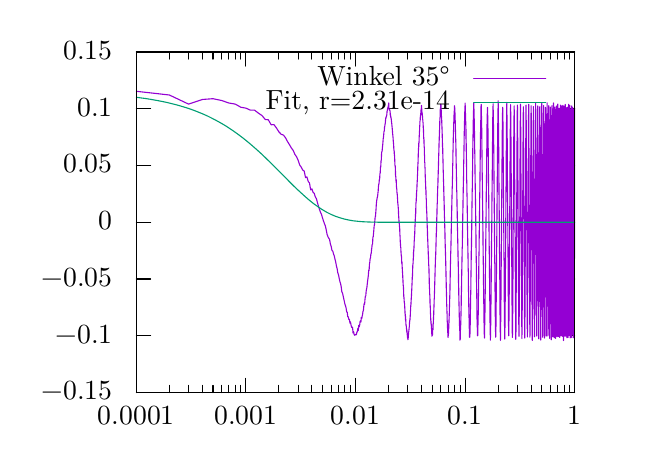
\begin{tikzpicture}[gnuplot]
%% generated with GNUPLOT 5.2p5a (Gentoo revision r0) (Lua 5.1; terminal rev. 99 , script rev. 107)
%% Sa 18 Mai 2019 18:31:22 CEST
\path (0.000,0.000) rectangle (7.500,5.250);
\gpcolor{color=gp lt color border}
\gpsetlinetype{gp lt border}
\gpsetdashtype{gp dt solid}
\gpsetlinewidth{1.00}
\draw[gp path] (1.380,0.616)--(1.560,0.616);
\draw[gp path] (6.947,0.616)--(6.767,0.616);
\node[gp node right] at (1.196,0.616) {$-0.15$};
\draw[gp path] (1.380,1.337)--(1.560,1.337);
\draw[gp path] (6.947,1.337)--(6.767,1.337);
\node[gp node right] at (1.196,1.337) {$-0.1$};
\draw[gp path] (1.380,2.058)--(1.560,2.058);
\draw[gp path] (6.947,2.058)--(6.767,2.058);
\node[gp node right] at (1.196,2.058) {$-0.05$};
\draw[gp path] (1.380,2.779)--(1.560,2.779);
\draw[gp path] (6.947,2.779)--(6.767,2.779);
\node[gp node right] at (1.196,2.779) {$0$};
\draw[gp path] (1.380,3.499)--(1.560,3.499);
\draw[gp path] (6.947,3.499)--(6.767,3.499);
\node[gp node right] at (1.196,3.499) {$0.05$};
\draw[gp path] (1.380,4.220)--(1.560,4.220);
\draw[gp path] (6.947,4.220)--(6.767,4.220);
\node[gp node right] at (1.196,4.220) {$0.1$};
\draw[gp path] (1.380,4.941)--(1.560,4.941);
\draw[gp path] (6.947,4.941)--(6.767,4.941);
\node[gp node right] at (1.196,4.941) {$0.15$};
\draw[gp path] (1.380,0.616)--(1.380,0.796);
\draw[gp path] (1.380,4.941)--(1.380,4.761);
\node[gp node center] at (1.380,0.308) {$0.0001$};
\draw[gp path] (1.799,0.616)--(1.799,0.706);
\draw[gp path] (1.799,4.941)--(1.799,4.851);
\draw[gp path] (2.044,0.616)--(2.044,0.706);
\draw[gp path] (2.044,4.941)--(2.044,4.851);
\draw[gp path] (2.218,0.616)--(2.218,0.706);
\draw[gp path] (2.218,4.941)--(2.218,4.851);
\draw[gp path] (2.353,0.616)--(2.353,0.706);
\draw[gp path] (2.353,4.941)--(2.353,4.851);
\draw[gp path] (2.463,0.616)--(2.463,0.706);
\draw[gp path] (2.463,4.941)--(2.463,4.851);
\draw[gp path] (2.556,0.616)--(2.556,0.706);
\draw[gp path] (2.556,4.941)--(2.556,4.851);
\draw[gp path] (2.637,0.616)--(2.637,0.706);
\draw[gp path] (2.637,4.941)--(2.637,4.851);
\draw[gp path] (2.708,0.616)--(2.708,0.706);
\draw[gp path] (2.708,4.941)--(2.708,4.851);
\draw[gp path] (2.772,0.616)--(2.772,0.796);
\draw[gp path] (2.772,4.941)--(2.772,4.761);
\node[gp node center] at (2.772,0.308) {$0.001$};
\draw[gp path] (3.191,0.616)--(3.191,0.706);
\draw[gp path] (3.191,4.941)--(3.191,4.851);
\draw[gp path] (3.436,0.616)--(3.436,0.706);
\draw[gp path] (3.436,4.941)--(3.436,4.851);
\draw[gp path] (3.610,0.616)--(3.610,0.706);
\draw[gp path] (3.610,4.941)--(3.610,4.851);
\draw[gp path] (3.745,0.616)--(3.745,0.706);
\draw[gp path] (3.745,4.941)--(3.745,4.851);
\draw[gp path] (3.855,0.616)--(3.855,0.706);
\draw[gp path] (3.855,4.941)--(3.855,4.851);
\draw[gp path] (3.948,0.616)--(3.948,0.706);
\draw[gp path] (3.948,4.941)--(3.948,4.851);
\draw[gp path] (4.029,0.616)--(4.029,0.706);
\draw[gp path] (4.029,4.941)--(4.029,4.851);
\draw[gp path] (4.100,0.616)--(4.100,0.706);
\draw[gp path] (4.100,4.941)--(4.100,4.851);
\draw[gp path] (4.163,0.616)--(4.163,0.796);
\draw[gp path] (4.163,4.941)--(4.163,4.761);
\node[gp node center] at (4.163,0.308) {$0.01$};
\draw[gp path] (4.582,0.616)--(4.582,0.706);
\draw[gp path] (4.582,4.941)--(4.582,4.851);
\draw[gp path] (4.828,0.616)--(4.828,0.706);
\draw[gp path] (4.828,4.941)--(4.828,4.851);
\draw[gp path] (5.001,0.616)--(5.001,0.706);
\draw[gp path] (5.001,4.941)--(5.001,4.851);
\draw[gp path] (5.136,0.616)--(5.136,0.706);
\draw[gp path] (5.136,4.941)--(5.136,4.851);
\draw[gp path] (5.246,0.616)--(5.246,0.706);
\draw[gp path] (5.246,4.941)--(5.246,4.851);
\draw[gp path] (5.340,0.616)--(5.340,0.706);
\draw[gp path] (5.340,4.941)--(5.340,4.851);
\draw[gp path] (5.420,0.616)--(5.420,0.706);
\draw[gp path] (5.420,4.941)--(5.420,4.851);
\draw[gp path] (5.492,0.616)--(5.492,0.706);
\draw[gp path] (5.492,4.941)--(5.492,4.851);
\draw[gp path] (5.555,0.616)--(5.555,0.796);
\draw[gp path] (5.555,4.941)--(5.555,4.761);
\node[gp node center] at (5.555,0.308) {$0.1$};
\draw[gp path] (5.974,0.616)--(5.974,0.706);
\draw[gp path] (5.974,4.941)--(5.974,4.851);
\draw[gp path] (6.219,0.616)--(6.219,0.706);
\draw[gp path] (6.219,4.941)--(6.219,4.851);
\draw[gp path] (6.393,0.616)--(6.393,0.706);
\draw[gp path] (6.393,4.941)--(6.393,4.851);
\draw[gp path] (6.528,0.616)--(6.528,0.706);
\draw[gp path] (6.528,4.941)--(6.528,4.851);
\draw[gp path] (6.638,0.616)--(6.638,0.706);
\draw[gp path] (6.638,4.941)--(6.638,4.851);
\draw[gp path] (6.731,0.616)--(6.731,0.706);
\draw[gp path] (6.731,4.941)--(6.731,4.851);
\draw[gp path] (6.812,0.616)--(6.812,0.706);
\draw[gp path] (6.812,4.941)--(6.812,4.851);
\draw[gp path] (6.883,0.616)--(6.883,0.706);
\draw[gp path] (6.883,4.941)--(6.883,4.851);
\draw[gp path] (6.947,0.616)--(6.947,0.796);
\draw[gp path] (6.947,4.941)--(6.947,4.761);
\node[gp node center] at (6.947,0.308) {$1$};
\draw[gp path] (1.380,4.941)--(1.380,0.616)--(6.947,0.616)--(6.947,4.941)--cycle;
\node[gp node right] at (5.479,4.607) {Winkel 35°};
\gpcolor{rgb color={0.580,0.000,0.827}}
\draw[gp path] (5.663,4.607)--(6.579,4.607);
\draw[gp path] (1.380,4.442)--(1.799,4.395)--(2.044,4.279)--(2.218,4.338)--(2.353,4.348)%
  --(2.463,4.325)--(2.556,4.293)--(2.637,4.279)--(2.708,4.239)--(2.772,4.228)--(2.829,4.202)%
  --(2.882,4.202)--(2.930,4.165)--(2.975,4.135)--(3.017,4.084)--(3.056,4.080)--(3.092,4.017)%
  --(3.127,4.019)--(3.160,3.975)--(3.191,3.926)--(3.220,3.896)--(3.248,3.886)--(3.275,3.851)%
  --(3.301,3.802)--(3.326,3.762)--(3.349,3.722)--(3.372,3.691)--(3.394,3.640)--(3.415,3.611)%
  --(3.436,3.563)--(3.456,3.503)--(3.475,3.478)--(3.493,3.442)--(3.511,3.431)--(3.529,3.346)%
  --(3.546,3.355)--(3.563,3.297)--(3.579,3.277)--(3.594,3.190)--(3.610,3.203)--(3.625,3.157)%
  --(3.639,3.147)--(3.653,3.101)--(3.667,3.077)--(3.681,3.025)--(3.694,2.979)--(3.707,2.938)%
  --(3.720,2.901)--(3.732,2.877)--(3.745,2.831)--(3.757,2.794)--(3.768,2.763)--(3.780,2.733)%
  --(3.791,2.686)--(3.802,2.627)--(3.813,2.596)--(3.824,2.576)--(3.834,2.560)--(3.845,2.500)%
  --(3.855,2.470)--(3.865,2.420)--(3.875,2.411)--(3.884,2.378)--(3.894,2.349)--(3.903,2.309)%
  --(3.912,2.274)--(3.921,2.223)--(3.930,2.190)--(3.939,2.135)--(3.948,2.110)--(3.956,2.068)%
  --(3.965,2.027)--(3.973,2.003)--(3.982,1.958)--(3.990,1.894)--(3.998,1.879)--(4.006,1.846)%
  --(4.013,1.812)--(4.021,1.778)--(4.029,1.738)--(4.036,1.720)--(4.044,1.689)--(4.051,1.641)%
  --(4.058,1.637)--(4.065,1.580)--(4.072,1.576)--(4.079,1.542)--(4.086,1.546)--(4.093,1.498)%
  --(4.100,1.513)--(4.106,1.476)--(4.113,1.448)--(4.120,1.440)--(4.126,1.446)--(4.132,1.373)%
  --(4.139,1.389)--(4.145,1.358)--(4.151,1.344)--(4.157,1.354)--(4.164,1.350)--(4.170,1.348)%
  --(4.175,1.354)--(4.181,1.385)--(4.187,1.387)--(4.193,1.432)--(4.199,1.404)--(4.204,1.469)%
  --(4.210,1.451)--(4.216,1.469)--(4.221,1.514)--(4.227,1.529)--(4.232,1.511)--(4.237,1.570)%
  --(4.243,1.556)--(4.248,1.587)--(4.253,1.605)--(4.258,1.646)--(4.264,1.659)--(4.269,1.715)%
  --(4.274,1.748)--(4.279,1.736)--(4.284,1.801)--(4.289,1.842)--(4.294,1.843)--(4.298,1.896)%
  --(4.303,1.929)--(4.308,1.949)--(4.313,1.998)--(4.317,2.033)--(4.322,2.068)--(4.327,2.110)%
  --(4.331,2.173)--(4.336,2.163)--(4.340,2.242)--(4.345,2.271)--(4.349,2.315)--(4.354,2.327)%
  --(4.358,2.370)--(4.363,2.385)--(4.367,2.428)--(4.371,2.459)--(4.375,2.499)--(4.380,2.501)%
  --(4.384,2.586)--(4.388,2.593)--(4.392,2.631)--(4.396,2.677)--(4.400,2.729)--(4.405,2.752)%
  --(4.409,2.798)--(4.413,2.846)--(4.417,2.852)--(4.421,2.905)--(4.424,2.941)--(4.428,3.012)%
  --(4.432,3.051)--(4.436,3.073)--(4.440,3.095)--(4.444,3.107)--(4.448,3.149)--(4.451,3.168)%
  --(4.455,3.237)--(4.459,3.261)--(4.463,3.281)--(4.466,3.322)--(4.470,3.324)--(4.473,3.392)%
  --(4.477,3.406)--(4.481,3.481)--(4.484,3.485)--(4.488,3.562)--(4.491,3.569)--(4.495,3.666)%
  --(4.498,3.671)--(4.502,3.687)--(4.505,3.727)--(4.509,3.762)--(4.512,3.798)--(4.515,3.839)%
  --(4.519,3.863)--(4.522,3.896)--(4.525,3.930)--(4.529,3.941)--(4.532,3.984)--(4.535,3.997)%
  --(4.539,4.025)--(4.542,4.040)--(4.545,4.078)--(4.548,4.108)--(4.551,4.099)--(4.555,4.125)%
  --(4.558,4.126)--(4.561,4.147)--(4.564,4.186)--(4.567,4.196)--(4.570,4.216)--(4.573,4.232)%
  --(4.576,4.223)--(4.579,4.253)--(4.582,4.259)--(4.585,4.294)--(4.588,4.231)--(4.591,4.220)%
  --(4.594,4.202)--(4.597,4.210)--(4.600,4.197)--(4.603,4.187)--(4.606,4.130)--(4.609,4.144)%
  --(4.612,4.106)--(4.615,4.107)--(4.618,4.083)--(4.621,4.052)--(4.623,4.038)--(4.626,4.007)%
  --(4.629,3.979)--(4.632,3.943)--(4.635,3.901)--(4.637,3.887)--(4.640,3.856)--(4.643,3.811)%
  --(4.646,3.784)--(4.648,3.754)--(4.651,3.693)--(4.654,3.694)--(4.656,3.650)--(4.659,3.627)%
  --(4.662,3.564)--(4.664,3.501)--(4.667,3.500)--(4.670,3.458)--(4.672,3.375)--(4.675,3.356)%
  --(4.677,3.303)--(4.680,3.322)--(4.683,3.237)--(4.685,3.218)--(4.688,3.195)--(4.690,3.155)%
  --(4.693,3.138)--(4.695,3.112)--(4.698,3.065)--(4.700,3.026)--(4.703,3.001)--(4.705,2.977)%
  --(4.708,2.945)--(4.710,2.885)--(4.712,2.851)--(4.715,2.807)--(4.717,2.772)--(4.720,2.757)%
  --(4.722,2.726)--(4.725,2.694)--(4.727,2.623)--(4.729,2.604)--(4.732,2.530)--(4.734,2.511)%
  --(4.736,2.470)--(4.739,2.451)--(4.741,2.405)--(4.743,2.374)--(4.746,2.344)--(4.748,2.340)%
  --(4.750,2.259)--(4.753,2.279)--(4.755,2.234)--(4.757,2.198)--(4.759,2.164)--(4.762,2.121)%
  --(4.764,2.072)--(4.766,2.044)--(4.768,1.994)--(4.771,1.965)--(4.773,1.945)--(4.775,1.871)%
  --(4.777,1.829)--(4.779,1.821)--(4.781,1.788)--(4.784,1.750)--(4.786,1.751)--(4.788,1.712)%
  --(4.790,1.676)--(4.792,1.638)--(4.794,1.588)--(4.797,1.608)--(4.799,1.539)--(4.801,1.549)%
  --(4.803,1.498)--(4.805,1.471)--(4.807,1.465)--(4.809,1.456)--(4.811,1.424)--(4.813,1.427)%
  --(4.815,1.388)--(4.817,1.402)--(4.819,1.347)--(4.821,1.363)--(4.823,1.315)--(4.826,1.351)%
  --(4.828,1.287)--(4.830,1.355)--(4.832,1.290)--(4.834,1.360)--(4.836,1.352)--(4.838,1.390)%
  --(4.840,1.388)--(4.841,1.409)--(4.843,1.417)--(4.845,1.445)--(4.847,1.448)--(4.849,1.501)%
  --(4.851,1.515)--(4.853,1.531)--(4.855,1.540)--(4.857,1.570)--(4.859,1.593)--(4.861,1.646)%
  --(4.863,1.670)--(4.865,1.720)--(4.867,1.723)--(4.868,1.748)--(4.870,1.787)--(4.872,1.817)%
  --(4.874,1.846)--(4.876,1.891)--(4.878,1.929)--(4.880,1.973)--(4.881,1.993)--(4.883,2.040)%
  --(4.885,2.090)--(4.887,2.091)--(4.889,2.174)--(4.891,2.231)--(4.892,2.245)--(4.894,2.251)%
  --(4.896,2.294)--(4.898,2.329)--(4.900,2.353)--(4.901,2.428)--(4.903,2.409)--(4.905,2.440)%
  --(4.907,2.479)--(4.908,2.545)--(4.910,2.539)--(4.912,2.588)--(4.914,2.609)--(4.916,2.646)%
  --(4.917,2.688)--(4.919,2.739)--(4.921,2.760)--(4.922,2.804)--(4.924,2.837)--(4.926,2.882)%
  --(4.928,2.891)--(4.929,2.954)--(4.931,3.018)--(4.933,3.039)--(4.934,3.043)--(4.936,3.094)%
  --(4.938,3.110)--(4.939,3.172)--(4.941,3.171)--(4.943,3.204)--(4.944,3.234)--(4.946,3.286)%
  --(4.948,3.300)--(4.949,3.362)--(4.951,3.376)--(4.953,3.425)--(4.954,3.472)--(4.956,3.515)%
  --(4.958,3.546)--(4.959,3.582)--(4.961,3.652)--(4.962,3.678)--(4.964,3.720)--(4.966,3.738)%
  --(4.967,3.783)--(4.969,3.784)--(4.970,3.792)--(4.972,3.856)--(4.974,3.893)--(4.975,3.941)%
  --(4.977,3.931)--(4.978,4.011)--(4.980,3.995)--(4.981,4.060)--(4.983,4.061)--(4.985,4.110)%
  --(4.986,4.080)--(4.988,4.129)--(4.989,4.129)--(4.991,4.158)--(4.992,4.144)--(4.994,4.205)%
  --(4.995,4.159)--(4.997,4.215)--(4.998,4.221)--(5.000,4.205)--(5.001,4.263)--(5.003,4.240)%
  --(5.004,4.213)--(5.006,4.220)--(5.007,4.180)--(5.009,4.175)--(5.010,4.167)--(5.012,4.132)%
  --(5.013,4.138)--(5.015,4.102)--(5.016,4.085)--(5.018,4.079)--(5.019,4.051)--(5.021,4.046)%
  --(5.022,4.033)--(5.024,3.979)--(5.025,3.991)--(5.027,3.940)--(5.028,3.900)--(5.029,3.868)%
  --(5.031,3.834)--(5.032,3.850)--(5.034,3.776)--(5.035,3.747)--(5.037,3.729)--(5.038,3.706)%
  --(5.039,3.632)--(5.041,3.624)--(5.042,3.541)--(5.044,3.532)--(5.045,3.482)--(5.047,3.461)%
  --(5.048,3.405)--(5.049,3.366)--(5.051,3.322)--(5.052,3.292)--(5.054,3.272)--(5.055,3.221)%
  --(5.056,3.198)--(5.058,3.183)--(5.059,3.153)--(5.060,3.076)--(5.062,3.081)--(5.063,3.057)%
  --(5.064,2.987)--(5.066,2.949)--(5.067,2.925)--(5.069,2.889)--(5.070,2.857)--(5.071,2.833)%
  --(5.073,2.774)--(5.074,2.734)--(5.075,2.709)--(5.077,2.665)--(5.078,2.613)--(5.079,2.583)%
  --(5.081,2.557)--(5.082,2.516)--(5.083,2.495)--(5.085,2.449)--(5.086,2.436)--(5.087,2.386)%
  --(5.089,2.356)--(5.090,2.337)--(5.091,2.314)--(5.092,2.240)--(5.094,2.236)--(5.095,2.192)%
  --(5.096,2.195)--(5.098,2.106)--(5.099,2.090)--(5.100,2.019)--(5.101,1.983)--(5.103,1.929)%
  --(5.104,1.940)--(5.105,1.875)--(5.107,1.852)--(5.108,1.818)--(5.109,1.803)--(5.110,1.752)%
  --(5.112,1.718)--(5.113,1.708)--(5.114,1.662)--(5.115,1.631)--(5.117,1.603)--(5.118,1.571)%
  --(5.119,1.534)--(5.120,1.552)--(5.122,1.515)--(5.123,1.488)--(5.124,1.490)--(5.125,1.487)%
  --(5.127,1.450)--(5.128,1.430)--(5.129,1.427)--(5.130,1.403)--(5.131,1.377)--(5.133,1.351)%
  --(5.134,1.331)--(5.135,1.370)--(5.136,1.355)--(5.137,1.340)--(5.139,1.357)--(5.140,1.342)%
  --(5.141,1.353)--(5.142,1.375)--(5.144,1.421)--(5.145,1.415)--(5.146,1.455)--(5.147,1.413)%
  --(5.148,1.481)--(5.149,1.471)--(5.151,1.498)--(5.152,1.505)--(5.153,1.553)--(5.154,1.540)%
  --(5.155,1.596)--(5.157,1.608)--(5.158,1.671)--(5.159,1.689)--(5.160,1.707)--(5.161,1.739)%
  --(5.162,1.768)--(5.163,1.808)--(5.165,1.816)--(5.166,1.877)--(5.167,1.902)--(5.168,1.936)%
  --(5.169,1.978)--(5.170,2.012)--(5.172,2.085)--(5.173,2.093)--(5.174,2.162)--(5.175,2.191)%
  --(5.176,2.223)--(5.177,2.246)--(5.178,2.305)--(5.179,2.308)--(5.181,2.356)--(5.182,2.366)%
  --(5.183,2.402)--(5.184,2.422)--(5.185,2.469)--(5.186,2.512)--(5.187,2.531)--(5.188,2.581)%
  --(5.189,2.640)--(5.191,2.631)--(5.192,2.713)--(5.193,2.725)--(5.194,2.771)--(5.195,2.789)%
  --(5.196,2.849)--(5.197,2.842)--(5.198,2.895)--(5.199,2.949)--(5.200,3.007)--(5.202,3.013)%
  --(5.203,3.069)--(5.204,3.107)--(5.205,3.146)--(5.206,3.137)--(5.207,3.208)--(5.208,3.212)%
  --(5.209,3.256)--(5.210,3.257)--(5.211,3.319)--(5.212,3.352)--(5.213,3.384)--(5.214,3.396)%
  --(5.215,3.445)--(5.217,3.506)--(5.218,3.548)--(5.219,3.583)--(5.220,3.625)--(5.221,3.650)%
  --(5.222,3.690)--(5.223,3.723)--(5.224,3.764)--(5.225,3.801)--(5.226,3.811)--(5.227,3.841)%
  --(5.228,3.881)--(5.229,3.898)--(5.230,3.929)--(5.231,3.959)--(5.232,4.000)--(5.233,4.017)%
  --(5.234,4.065)--(5.235,4.059)--(5.236,4.111)--(5.237,4.100)--(5.238,4.140)--(5.239,4.135)%
  --(5.240,4.211)--(5.241,4.156)--(5.242,4.230)--(5.243,4.223)--(5.244,4.249)--(5.245,4.217)%
  --(5.246,4.278)--(5.247,4.221)--(5.249,4.272)--(5.250,4.217)--(5.251,4.254)--(5.252,4.180)%
  --(5.253,4.182)--(5.254,4.169)--(5.254,4.140)--(5.255,4.123)--(5.256,4.125)--(5.257,4.065)%
  --(5.258,4.075)--(5.259,4.047)--(5.260,4.025)--(5.261,3.992)--(5.262,3.987)--(5.263,3.936)%
  --(5.264,3.923)--(5.265,3.865)--(5.266,3.846)--(5.267,3.804)--(5.268,3.772)--(5.269,3.732)%
  --(5.270,3.747)--(5.271,3.707)--(5.272,3.652)--(5.273,3.598)--(5.274,3.581)--(5.275,3.544)%
  --(5.276,3.485)--(5.277,3.445)--(5.278,3.429)--(5.279,3.378)--(5.280,3.341)--(5.281,3.291)%
  --(5.282,3.293)--(5.283,3.244)--(5.284,3.229)--(5.285,3.143)--(5.286,3.165)--(5.286,3.123)%
  --(5.287,3.103)--(5.288,3.047)--(5.289,3.021)--(5.290,2.992)--(5.291,2.930)--(5.292,2.924)%
  --(5.293,2.846)--(5.294,2.835)--(5.295,2.807)--(5.296,2.754)--(5.297,2.724)--(5.298,2.685)%
  --(5.299,2.659)--(5.300,2.614)--(5.300,2.622)--(5.301,2.537)--(5.302,2.510)--(5.303,2.491)%
  --(5.304,2.443)--(5.305,2.407)--(5.306,2.399)--(5.307,2.355)--(5.308,2.304)--(5.309,2.284)%
  --(5.310,2.264)--(5.310,2.235)--(5.311,2.177)--(5.312,2.157)--(5.313,2.108)--(5.314,2.041)%
  --(5.315,2.022)--(5.316,1.971)--(5.317,1.914)--(5.318,1.908)--(5.319,1.862)--(5.319,1.837)%
  --(5.320,1.833)--(5.321,1.754)--(5.322,1.727)--(5.323,1.706)--(5.324,1.677)--(5.325,1.638)%
  --(5.326,1.621)--(5.327,1.583)--(5.327,1.565)--(5.328,1.524)--(5.329,1.521)--(5.330,1.479)%
  --(5.331,1.493)--(5.332,1.437)--(5.333,1.423)--(5.334,1.435)--(5.334,1.397)--(5.335,1.388)%
  --(5.336,1.366)--(5.337,1.337)--(5.338,1.319)--(5.339,1.337)--(5.340,1.315)--(5.341,1.363)%
  --(5.341,1.337)--(5.342,1.345)--(5.343,1.362)--(5.344,1.364)--(5.345,1.416)--(5.346,1.412)%
  --(5.347,1.430)--(5.347,1.445)--(5.348,1.453)--(5.349,1.458)--(5.350,1.500)--(5.351,1.531)%
  --(5.352,1.559)--(5.352,1.594)--(5.353,1.580)--(5.354,1.618)--(5.355,1.623)--(5.356,1.680)%
  --(5.357,1.720)--(5.358,1.739)--(5.358,1.765)--(5.359,1.794)--(5.360,1.816)--(5.361,1.851)%
  --(5.362,1.907)--(5.363,1.918)--(5.363,1.993)--(5.364,1.986)--(5.365,2.065)--(5.366,2.078)%
  --(5.367,2.157)--(5.368,2.184)--(5.368,2.225)--(5.369,2.243)--(5.370,2.281)--(5.371,2.310)%
  --(5.372,2.336)--(5.372,2.380)--(5.373,2.384)--(5.374,2.431)--(5.375,2.452)--(5.376,2.516)%
  --(5.377,2.546)--(5.377,2.576)--(5.378,2.597)--(5.379,2.652)--(5.380,2.696)--(5.381,2.730)%
  --(5.381,2.777)--(5.382,2.812)--(5.383,2.843)--(5.384,2.858)--(5.385,2.894)--(5.385,2.927)%
  --(5.386,2.967)--(5.387,3.037)--(5.388,3.075)--(5.389,3.082)--(5.389,3.106)--(5.390,3.145)%
  --(5.391,3.190)--(5.392,3.232)--(5.393,3.233)--(5.393,3.285)--(5.394,3.301)--(5.395,3.349)%
  --(5.396,3.362)--(5.396,3.448)--(5.397,3.432)--(5.398,3.521)--(5.399,3.527)--(5.400,3.576)%
  --(5.400,3.613)--(5.401,3.674)--(5.402,3.686)--(5.403,3.737)--(5.404,3.751)--(5.404,3.782)%
  --(5.405,3.850)--(5.406,3.857)--(5.407,3.882)--(5.407,3.935)--(5.408,3.927)--(5.409,3.971)%
  --(5.410,3.998)--(5.410,4.020)--(5.411,4.051)--(5.412,4.047)--(5.413,4.072)--(5.414,4.105)%
  --(5.414,4.108)--(5.415,4.143)--(5.416,4.160)--(5.417,4.169)--(5.417,4.157)--(5.418,4.190)%
  --(5.419,4.227)--(5.420,4.227)--(5.420,4.249)--(5.421,4.258)--(5.422,4.226)--(5.423,4.242)%
  --(5.423,4.202)--(5.424,4.235)--(5.425,4.157)--(5.426,4.175)--(5.426,4.125)--(5.427,4.170)%
  --(5.428,4.103)--(5.429,4.130)--(5.429,4.069)--(5.430,4.071)--(5.431,4.026)--(5.432,4.009)%
  --(5.432,3.985)--(5.433,3.937)--(5.434,3.899)--(5.435,3.900)--(5.435,3.863)--(5.436,3.833)%
  --(5.437,3.797)--(5.438,3.777)--(5.438,3.732)--(5.439,3.712)--(5.440,3.680)--(5.440,3.640)%
  --(5.441,3.571)--(5.442,3.526)--(5.443,3.500)--(5.443,3.491)--(5.444,3.432)--(5.445,3.362)%
  --(5.446,3.340)--(5.446,3.327)--(5.447,3.286)--(5.448,3.262)--(5.448,3.188)--(5.449,3.187)%
  --(5.450,3.156)--(5.451,3.139)--(5.451,3.075)--(5.452,3.065)--(5.453,3.019)--(5.453,2.980)%
  --(5.454,2.938)--(5.455,2.913)--(5.456,2.853)--(5.456,2.832)--(5.457,2.819)--(5.458,2.753)%
  --(5.458,2.716)--(5.459,2.685)--(5.460,2.648)--(5.461,2.618)--(5.461,2.580)--(5.462,2.541)%
  --(5.463,2.485)--(5.463,2.493)--(5.464,2.411)--(5.465,2.419)--(5.465,2.339)--(5.466,2.349)%
  --(5.467,2.305)--(5.468,2.262)--(5.468,2.227)--(5.469,2.214)--(5.470,2.167)--(5.470,2.148)%
  --(5.471,2.108)--(5.472,2.078)--(5.472,2.009)--(5.473,1.974)--(5.474,1.943)--(5.475,1.906)%
  --(5.475,1.856)--(5.476,1.828)--(5.477,1.779)--(5.477,1.774)--(5.478,1.722)--(5.479,1.702)%
  --(5.479,1.656)--(5.480,1.636)--(5.481,1.616)--(5.481,1.602)--(5.482,1.550)--(5.483,1.519)%
  --(5.483,1.514)--(5.484,1.486)--(5.485,1.458)--(5.485,1.443)--(5.486,1.415)--(5.487,1.416)%
  --(5.488,1.399)--(5.488,1.422)--(5.489,1.313)--(5.490,1.354)--(5.490,1.281)--(5.491,1.334)%
  --(5.492,1.287)--(5.492,1.333)--(5.493,1.290)--(5.494,1.355)--(5.494,1.324)--(5.495,1.381)%
  --(5.496,1.352)--(5.496,1.415)--(5.497,1.413)--(5.498,1.434)--(5.498,1.460)--(5.499,1.468)%
  --(5.500,1.485)--(5.500,1.521)--(5.501,1.535)--(5.502,1.552)--(5.502,1.579)--(5.503,1.595)%
  --(5.504,1.662)--(5.504,1.705)--(5.505,1.701)--(5.506,1.731)--(5.506,1.798)--(5.507,1.817)%
  --(5.507,1.851)--(5.508,1.868)--(5.509,1.900)--(5.509,1.899)--(5.510,1.962)--(5.511,2.001)%
  --(5.511,2.046)--(5.512,2.100)--(5.513,2.123)--(5.513,2.180)--(5.514,2.181)--(5.515,2.251)%
  --(5.515,2.262)--(5.516,2.329)--(5.517,2.354)--(5.517,2.379)--(5.518,2.388)--(5.518,2.444)%
  --(5.519,2.448)--(5.520,2.474)--(5.520,2.532)--(5.521,2.574)--(5.522,2.581)--(5.522,2.639)%
  --(5.523,2.681)--(5.524,2.732)--(5.524,2.757)--(5.525,2.817)--(5.526,2.824)--(5.526,2.886)%
  --(5.527,2.900)--(5.527,2.963)--(5.528,2.962)--(5.529,3.032)--(5.529,3.051)--(5.530,3.088)%
  --(5.531,3.128)--(5.531,3.176)--(5.532,3.151)--(5.532,3.223)--(5.533,3.230)--(5.534,3.260)%
  --(5.534,3.291)--(5.535,3.349)--(5.536,3.370)--(5.536,3.398)--(5.537,3.456)--(5.537,3.506)%
  --(5.538,3.544)--(5.539,3.584)--(5.539,3.617)--(5.540,3.644)--(5.541,3.712)--(5.541,3.724)%
  --(5.542,3.762)--(5.542,3.799)--(5.543,3.846)--(5.544,3.885)--(5.544,3.893)--(5.545,3.937)%
  --(5.546,3.918)--(5.546,3.973)--(5.547,4.020)--(5.547,4.048)--(5.548,4.055)--(5.549,4.096)%
  --(5.549,4.069)--(5.550,4.159)--(5.550,4.140)--(5.551,4.172)--(5.552,4.196)--(5.552,4.204)%
  --(5.553,4.208)--(5.553,4.239)--(5.554,4.237)--(5.555,4.269)--(5.555,4.292)--(5.556,4.258)%
  --(5.556,4.288)--(5.557,4.233)--(5.558,4.229)--(5.558,4.211)--(5.559,4.191)--(5.559,4.186)%
  --(5.560,4.151)--(5.561,4.149)--(5.561,4.145)--(5.562,4.094)--(5.562,4.077)--(5.563,4.047)%
  --(5.564,4.058)--(5.564,4.014)--(5.565,4.001)--(5.565,3.955)--(5.566,3.960)--(5.567,3.902)%
  --(5.567,3.843)--(5.568,3.816)--(5.568,3.803)--(5.569,3.788)--(5.570,3.736)--(5.570,3.693)%
  --(5.571,3.657)--(5.571,3.633)--(5.572,3.603)--(5.573,3.527)--(5.574,3.461)--(5.574,3.420)%
  --(5.575,3.382)--(5.575,3.318)--(5.576,3.314)--(5.577,3.268)--(5.577,3.274)--(5.578,3.205)%
  --(5.578,3.180)--(5.579,3.140)--(5.580,3.138)--(5.580,3.105)--(5.581,3.052)--(5.581,3.011)%
  --(5.582,2.985)--(5.582,2.950)--(5.583,2.906)--(5.584,2.859)--(5.584,2.811)--(5.585,2.815)%
  --(5.585,2.733)--(5.586,2.718)--(5.586,2.694)--(5.587,2.650)--(5.588,2.630)--(5.588,2.588)%
  --(5.589,2.522)--(5.589,2.502)--(5.590,2.467)--(5.590,2.429)--(5.591,2.389)--(5.592,2.388)%
  --(5.592,2.339)--(5.593,2.308)--(5.593,2.260)--(5.594,2.232)--(5.594,2.202)--(5.595,2.185)%
  --(5.596,2.149)--(5.596,2.113)--(5.597,2.044)--(5.597,2.045)--(5.598,1.944)--(5.598,1.929)%
  --(5.599,1.893)--(5.600,1.877)--(5.600,1.837)--(5.601,1.821)--(5.601,1.791)--(5.602,1.730)%
  --(5.602,1.712)--(5.603,1.673)--(5.603,1.658)--(5.604,1.611)--(5.605,1.581)--(5.605,1.568)%
  --(5.606,1.559)--(5.606,1.520)--(5.607,1.511)--(5.607,1.476)--(5.608,1.454)--(5.608,1.430)%
  --(5.609,1.447)--(5.610,1.431)--(5.610,1.392)--(5.611,1.367)--(5.611,1.319)--(5.612,1.346)%
  --(5.612,1.332)--(5.613,1.327)--(5.613,1.332)--(5.614,1.319)--(5.615,1.331)--(5.615,1.367)%
  --(5.616,1.328)--(5.616,1.386)--(5.617,1.358)--(5.617,1.413)--(5.618,1.425)--(5.618,1.468)%
  --(5.619,1.464)--(5.619,1.505)--(5.620,1.472)--(5.621,1.522)--(5.621,1.545)--(5.622,1.583)%
  --(5.622,1.620)--(5.623,1.644)--(5.623,1.664)--(5.624,1.726)--(5.624,1.722)--(5.625,1.768)%
  --(5.625,1.802)--(5.626,1.825)--(5.626,1.849)--(5.627,1.887)--(5.628,1.934)--(5.628,1.966)%
  --(5.629,1.993)--(5.629,2.077)--(5.630,2.088)--(5.630,2.143)--(5.631,2.171)--(5.631,2.213)%
  --(5.632,2.213)--(5.632,2.294)--(5.633,2.303)--(5.633,2.326)--(5.634,2.397)--(5.634,2.414)%
  --(5.635,2.425)--(5.636,2.473)--(5.636,2.474)--(5.637,2.545)--(5.637,2.573)--(5.638,2.633)%
  --(5.638,2.643)--(5.639,2.679)--(5.639,2.724)--(5.640,2.781)--(5.640,2.785)--(5.641,2.855)%
  --(5.641,2.870)--(5.642,2.918)--(5.642,2.949)--(5.643,3.010)--(5.643,3.014)--(5.644,3.069)%
  --(5.644,3.087)--(5.645,3.172)--(5.645,3.143)--(5.646,3.202)--(5.647,3.209)--(5.647,3.281)%
  --(5.648,3.278)--(5.648,3.346)--(5.649,3.371)--(5.649,3.378)--(5.650,3.437)--(5.650,3.485)%
  --(5.651,3.505)--(5.651,3.563)--(5.652,3.598)--(5.652,3.634)--(5.653,3.660)--(5.653,3.721)%
  --(5.654,3.724)--(5.654,3.772)--(5.655,3.815)--(5.655,3.836)--(5.656,3.847)--(5.656,3.890)%
  --(5.657,3.906)--(5.657,3.971)--(5.658,3.969)--(5.658,4.011)--(5.659,4.032)--(5.659,4.080)%
  --(5.660,4.059)--(5.660,4.140)--(5.661,4.122)--(5.661,4.161)--(5.662,4.145)--(5.662,4.198)%
  --(5.663,4.160)--(5.663,4.231)--(5.664,4.197)--(5.664,4.272)--(5.665,4.222)--(5.665,4.290)%
  --(5.666,4.249)--(5.666,4.267)--(5.667,4.251)--(5.667,4.244)--(5.668,4.200)--(5.668,4.212)%
  --(5.669,4.129)--(5.669,4.146)--(5.670,4.161)--(5.670,4.127)--(5.671,4.084)--(5.671,4.073)%
  --(5.672,4.025)--(5.672,4.056)--(5.673,4.000)--(5.673,3.975)--(5.674,3.933)--(5.674,3.905)%
  --(5.675,3.889)--(5.675,3.865)--(5.676,3.826)--(5.676,3.765)--(5.677,3.758)--(5.677,3.700)%
  --(5.678,3.694)--(5.678,3.676)--(5.679,3.613)--(5.679,3.597)--(5.680,3.543)--(5.680,3.537)%
  --(5.681,3.448)--(5.681,3.430)--(5.682,3.365)--(5.682,3.375)--(5.683,3.273)--(5.683,3.299)%
  --(5.684,3.243)--(5.684,3.242)--(5.685,3.181)--(5.685,3.168)--(5.686,3.133)--(5.686,3.094)%
  --(5.687,3.071)--(5.687,3.036)--(5.688,2.991)--(5.688,2.954)--(5.689,2.895)--(5.689,2.877)%
  --(5.690,2.857)--(5.690,2.831)--(5.691,2.749)--(5.691,2.737)--(5.692,2.684)--(5.692,2.671)%
  --(5.693,2.620)--(5.693,2.594)--(5.693,2.551)--(5.694,2.508)--(5.694,2.456)--(5.695,2.453)%
  --(5.695,2.408)--(5.696,2.396)--(5.696,2.358)--(5.697,2.298)--(5.697,2.282)--(5.698,2.242)%
  --(5.698,2.215)--(5.699,2.185)--(5.699,2.120)--(5.700,2.110)--(5.700,2.054)--(5.701,1.999)%
  --(5.701,1.976)--(5.702,1.924)--(5.702,1.905)--(5.703,1.852)--(5.703,1.831)--(5.704,1.804)%
  --(5.704,1.751)--(5.704,1.741)--(5.705,1.699)--(5.705,1.676)--(5.706,1.645)--(5.706,1.629)%
  --(5.707,1.582)--(5.707,1.547)--(5.708,1.537)--(5.708,1.516)--(5.709,1.505)--(5.709,1.502)%
  --(5.710,1.444)--(5.710,1.476)--(5.711,1.408)--(5.711,1.402)--(5.712,1.390)--(5.712,1.381)%
  --(5.712,1.341)--(5.713,1.357)--(5.713,1.336)--(5.714,1.346)--(5.714,1.347)--(5.715,1.343)%
  --(5.715,1.371)--(5.716,1.339)--(5.716,1.374)--(5.717,1.385)--(5.717,1.417)--(5.718,1.412)%
  --(5.718,1.421)--(5.718,1.465)--(5.719,1.484)--(5.719,1.474)--(5.720,1.534)--(5.720,1.529)%
  --(5.721,1.571)--(5.722,1.622)--(5.722,1.634)--(5.723,1.661)--(5.723,1.692)--(5.724,1.708)%
  --(5.724,1.767)--(5.724,1.808)--(5.725,1.847)--(5.725,1.851)--(5.726,1.905)--(5.726,1.926)%
  --(5.727,1.961)--(5.727,2.004)--(5.728,2.065)--(5.728,2.114)--(5.729,2.152)--(5.729,2.186)%
  --(5.729,2.213)--(5.730,2.247)--(5.730,2.301)--(5.731,2.318)--(5.731,2.349)--(5.732,2.395)%
  --(5.732,2.376)--(5.733,2.445)--(5.733,2.475)--(5.733,2.537)--(5.734,2.534)--(5.734,2.563)%
  --(5.735,2.603)--(5.735,2.667)--(5.736,2.683)--(5.736,2.700)--(5.737,2.760)--(5.737,2.800)%
  --(5.738,2.832)--(5.738,2.887)--(5.738,2.892)--(5.739,2.932)--(5.739,2.974)--(5.740,3.013)%
  --(5.740,3.067)--(5.741,3.097)--(5.741,3.098)--(5.742,3.161)--(5.742,3.192)--(5.742,3.191)%
  --(5.743,3.243)--(5.743,3.265)--(5.744,3.306)--(5.744,3.334)--(5.745,3.360)--(5.745,3.419)%
  --(5.746,3.400)--(5.746,3.528)--(5.746,3.514)--(5.747,3.576)--(5.747,3.621)--(5.748,3.657)%
  --(5.748,3.688)--(5.749,3.728)--(5.749,3.740)--(5.749,3.773)--(5.750,3.796)--(5.750,3.835)%
  --(5.751,3.874)--(5.751,3.897)--(5.752,3.953)--(5.752,3.954)--(5.753,3.963)--(5.753,4.027)%
  --(5.753,4.038)--(5.754,4.070)--(5.754,4.055)--(5.755,4.088)--(5.755,4.110)--(5.756,4.141)%
  --(5.756,4.148)--(5.756,4.177)--(5.757,4.177)--(5.757,4.250)--(5.758,4.205)--(5.758,4.252)%
  --(5.759,4.256)--(5.759,4.255)--(5.759,4.242)--(5.760,4.275)--(5.760,4.198)--(5.761,4.245)%
  --(5.761,4.191)--(5.762,4.231)--(5.762,4.125)--(5.762,4.131)--(5.763,4.098)--(5.763,4.127)%
  --(5.764,4.100)--(5.764,4.055)--(5.765,4.022)--(5.765,4.036)--(5.765,3.964)--(5.766,3.977)%
  --(5.766,3.944)--(5.767,3.906)--(5.767,3.845)--(5.768,3.824)--(5.768,3.785)--(5.768,3.774)%
  --(5.769,3.742)--(5.769,3.711)--(5.770,3.646)--(5.770,3.631)--(5.771,3.577)--(5.771,3.555)%
  --(5.771,3.535)--(5.772,3.452)--(5.772,3.433)--(5.773,3.369)--(5.773,3.350)--(5.774,3.303)%
  --(5.774,3.287)--(5.774,3.250)--(5.775,3.220)--(5.775,3.206)--(5.776,3.160)--(5.776,3.135)%
  --(5.776,3.089)--(5.777,3.059)--(5.777,2.989)--(5.778,3.007)--(5.778,2.936)--(5.779,2.921)%
  --(5.779,2.868)--(5.779,2.877)--(5.780,2.793)--(5.780,2.764)--(5.781,2.727)--(5.781,2.702)%
  --(5.781,2.634)--(5.782,2.659)--(5.782,2.586)--(5.783,2.549)--(5.783,2.487)--(5.784,2.489)%
  --(5.784,2.435)--(5.784,2.402)--(5.785,2.374)--(5.785,2.351)--(5.786,2.321)--(5.786,2.305)%
  --(5.786,2.251)--(5.787,2.227)--(5.787,2.193)--(5.788,2.130)--(5.788,2.132)--(5.789,2.084)%
  --(5.789,2.022)--(5.789,1.996)--(5.790,1.970)--(5.790,1.922)--(5.791,1.869)--(5.791,1.876)%
  --(5.791,1.820)--(5.792,1.786)--(5.792,1.742)--(5.793,1.749)--(5.793,1.666)--(5.793,1.657)%
  --(5.794,1.610)--(5.794,1.586)--(5.795,1.570)--(5.795,1.542)--(5.795,1.502)--(5.796,1.518)%
  --(5.796,1.494)--(5.797,1.498)--(5.797,1.412)--(5.797,1.429)--(5.798,1.396)--(5.798,1.398)%
  --(5.799,1.354)--(5.799,1.380)--(5.800,1.316)--(5.800,1.367)--(5.800,1.317)--(5.801,1.350)%
  --(5.801,1.307)--(5.802,1.341)--(5.802,1.351)--(5.802,1.380)--(5.803,1.381)--(5.803,1.442)%
  --(5.804,1.435)--(5.804,1.452)--(5.804,1.473)--(5.805,1.483)--(5.805,1.510)--(5.806,1.503)%
  --(5.806,1.516)--(5.806,1.564)--(5.807,1.589)--(5.807,1.615)--(5.808,1.672)--(5.808,1.666)%
  --(5.808,1.708)--(5.809,1.712)--(5.809,1.758)--(5.810,1.797)--(5.810,1.834)--(5.810,1.865)%
  --(5.811,1.869)--(5.811,1.928)--(5.812,1.928)--(5.812,2.004)--(5.812,2.028)--(5.813,2.100)%
  --(5.813,2.087)--(5.813,2.182)--(5.814,2.213)--(5.814,2.236)--(5.815,2.263)--(5.815,2.303)%
  --(5.815,2.318)--(5.816,2.365)--(5.816,2.358)--(5.817,2.426)--(5.817,2.432)--(5.817,2.489)%
  --(5.818,2.513)--(5.818,2.569)--(5.819,2.560)--(5.819,2.649)--(5.819,2.672)--(5.820,2.707)%
  --(5.820,2.730)--(5.821,2.752)--(5.821,2.788)--(5.821,2.842)--(5.822,2.861)--(5.822,2.909)%
  --(5.822,2.971)--(5.823,3.020)--(5.823,3.035)--(5.824,3.042)--(5.824,3.089)--(5.824,3.142)%
  --(5.825,3.195)--(5.825,3.212)--(5.826,3.225)--(5.826,3.249)--(5.826,3.243)--(5.827,3.340)%
  --(5.828,3.403)--(5.828,3.438)--(5.828,3.477)--(5.829,3.510)--(5.829,3.574)--(5.829,3.630)%
  --(5.830,3.616)--(5.830,3.671)--(5.831,3.721)--(5.831,3.750)--(5.831,3.761)--(5.832,3.787)%
  --(5.832,3.850)--(5.832,3.877)--(5.833,3.916)--(5.833,3.935)--(5.834,3.954)--(5.834,3.977)%
  --(5.834,4.023)--(5.835,4.039)--(5.835,4.060)--(5.836,4.060)--(5.836,4.119)--(5.836,4.116)%
  --(5.837,4.158)--(5.837,4.128)--(5.837,4.154)--(5.838,4.179)--(5.838,4.186)--(5.839,4.210)%
  --(5.839,4.224)--(5.840,4.238)--(5.840,4.206)--(5.840,4.235)--(5.841,4.208)--(5.841,4.180)%
  --(5.842,4.164)--(5.842,4.163)--(5.842,4.134)--(5.843,4.134)--(5.843,4.087)--(5.843,4.096)%
  --(5.844,4.108)--(5.844,4.046)--(5.845,4.037)--(5.845,4.002)--(5.845,3.980)--(5.846,3.957)%
  --(5.846,3.932)--(5.846,3.881)--(5.847,3.867)--(5.847,3.819)--(5.848,3.801)--(5.848,3.765)%
  --(5.848,3.729)--(5.849,3.714)--(5.849,3.680)--(5.849,3.650)--(5.850,3.602)--(5.850,3.588)%
  --(5.851,3.529)--(5.851,3.482)--(5.851,3.428)--(5.852,3.380)--(5.852,3.361)--(5.852,3.317)%
  --(5.853,3.286)--(5.853,3.238)--(5.854,3.229)--(5.854,3.203)--(5.854,3.173)--(5.855,3.120)%
  --(5.855,3.100)--(5.855,3.032)--(5.856,3.027)--(5.856,3.013)--(5.856,2.965)--(5.857,2.923)%
  --(5.857,2.866)--(5.858,2.842)--(5.858,2.814)--(5.858,2.790)--(5.859,2.757)--(5.859,2.712)%
  --(5.859,2.680)--(5.860,2.634)--(5.860,2.627)--(5.860,2.545)--(5.861,2.521)--(5.861,2.480)%
  --(5.862,2.459)--(5.862,2.396)--(5.862,2.398)--(5.863,2.357)--(5.863,2.346)--(5.863,2.287)%
  --(5.864,2.314)--(5.864,2.220)--(5.864,2.227)--(5.865,2.138)--(5.865,2.152)--(5.866,2.048)%
  --(5.866,2.051)--(5.866,1.992)--(5.867,1.965)--(5.867,1.908)--(5.867,1.876)--(5.868,1.837)%
  --(5.868,1.810)--(5.868,1.791)--(5.869,1.776)--(5.869,1.696)--(5.870,1.697)--(5.870,1.679)%
  --(5.870,1.606)--(5.871,1.618)--(5.871,1.577)--(5.871,1.567)--(5.872,1.535)--(5.872,1.533)%
  --(5.872,1.506)--(5.873,1.465)--(5.873,1.462)--(5.873,1.424)--(5.874,1.414)--(5.874,1.415)%
  --(5.875,1.384)--(5.875,1.346)--(5.875,1.368)--(5.876,1.296)--(5.876,1.320)--(5.876,1.281)%
  --(5.877,1.329)--(5.877,1.325)--(5.877,1.354)--(5.878,1.314)--(5.878,1.400)--(5.878,1.365)%
  --(5.879,1.443)--(5.879,1.403)--(5.880,1.449)--(5.880,1.465)--(5.880,1.508)--(5.881,1.471)%
  --(5.881,1.527)--(5.881,1.514)--(5.882,1.561)--(5.882,1.584)--(5.882,1.607)--(5.883,1.647)%
  --(5.883,1.685)--(5.883,1.715)--(5.884,1.760)--(5.884,1.761)--(5.884,1.819)--(5.885,1.866)%
  --(5.885,1.871)--(5.886,1.890)--(5.886,1.965)--(5.886,1.996)--(5.887,2.031)--(5.887,2.089)%
  --(5.887,2.122)--(5.888,2.148)--(5.888,2.177)--(5.888,2.229)--(5.889,2.255)--(5.889,2.296)%
  --(5.889,2.319)--(5.890,2.339)--(5.890,2.406)--(5.890,2.396)--(5.891,2.445)--(5.891,2.442)%
  --(5.891,2.536)--(5.892,2.541)--(5.892,2.605)--(5.892,2.617)--(5.893,2.647)--(5.893,2.719)%
  --(5.893,2.739)--(5.894,2.775)--(5.894,2.792)--(5.895,2.815)--(5.895,2.896)--(5.895,2.925)%
  --(5.896,2.981)--(5.896,2.996)--(5.896,3.043)--(5.897,3.053)--(5.897,3.099)--(5.897,3.140)%
  --(5.898,3.174)--(5.898,3.175)--(5.898,3.212)--(5.899,3.243)--(5.899,3.299)--(5.899,3.296)%
  --(5.900,3.340)--(5.900,3.390)--(5.900,3.427)--(5.901,3.454)--(5.901,3.495)--(5.901,3.555)%
  --(5.902,3.618)--(5.902,3.641)--(5.902,3.676)--(5.903,3.715)--(5.903,3.738)--(5.903,3.780)%
  --(5.904,3.805)--(5.904,3.843)--(5.904,3.874)--(5.905,3.901)--(5.905,3.934)--(5.905,3.947)%
  --(5.906,3.985)--(5.906,4.035)--(5.906,4.048)--(5.907,4.048)--(5.907,4.114)--(5.907,4.084)%
  --(5.908,4.149)--(5.908,4.112)--(5.909,4.178)--(5.909,4.165)--(5.909,4.183)--(5.910,4.186)%
  --(5.910,4.253)--(5.910,4.213)--(5.911,4.273)--(5.911,4.226)--(5.911,4.284)--(5.912,4.219)%
  --(5.912,4.230)--(5.912,4.207)--(5.913,4.199)--(5.913,4.161)--(5.913,4.188)--(5.914,4.143)%
  --(5.914,4.115)--(5.914,4.100)--(5.915,4.076)--(5.915,4.061)--(5.915,4.028)--(5.916,4.002)%
  --(5.916,4.001)--(5.916,3.967)--(5.917,3.939)--(5.917,3.900)--(5.917,3.876)--(5.918,3.839)%
  --(5.918,3.819)--(5.918,3.772)--(5.919,3.755)--(5.919,3.721)--(5.919,3.697)--(5.920,3.638)%
  --(5.920,3.611)--(5.920,3.570)--(5.921,3.529)--(5.921,3.467)--(5.921,3.453)--(5.922,3.416)%
  --(5.922,3.382)--(5.922,3.320)--(5.922,3.329)--(5.923,3.263)--(5.923,3.266)--(5.923,3.213)%
  --(5.924,3.158)--(5.924,3.151)--(5.924,3.116)--(5.925,3.081)--(5.925,3.031)--(5.925,2.987)%
  --(5.926,2.953)--(5.926,2.922)--(5.926,2.901)--(5.927,2.830)--(5.927,2.829)--(5.927,2.798)%
  --(5.928,2.750)--(5.928,2.720)--(5.928,2.680)--(5.929,2.628)--(5.929,2.602)--(5.929,2.535)%
  --(5.930,2.530)--(5.930,2.505)--(5.930,2.459)--(5.931,2.420)--(5.931,2.386)--(5.931,2.367)%
  --(5.932,2.336)--(5.932,2.323)--(5.932,2.273)--(5.933,2.232)--(5.933,2.210)--(5.933,2.175)%
  --(5.934,2.138)--(5.934,2.080)--(5.934,2.035)--(5.935,1.959)--(5.935,1.964)--(5.935,1.936)%
  --(5.936,1.876)--(5.936,1.833)--(5.936,1.811)--(5.936,1.792)--(5.937,1.748)--(5.937,1.731)%
  --(5.937,1.686)--(5.938,1.664)--(5.938,1.638)--(5.938,1.581)--(5.939,1.607)--(5.939,1.544)%
  --(5.939,1.528)--(5.940,1.513)--(5.940,1.493)--(5.940,1.450)--(5.941,1.460)--(5.941,1.431)%
  --(5.941,1.413)--(5.942,1.385)--(5.942,1.394)--(5.942,1.381)--(5.943,1.343)--(5.943,1.319)%
  --(5.944,1.338)--(5.944,1.358)--(5.944,1.323)--(5.944,1.348)--(5.945,1.390)--(5.945,1.389)%
  --(5.945,1.411)--(5.946,1.407)--(5.946,1.430)--(5.946,1.449)--(5.947,1.455)--(5.947,1.495)%
  --(5.947,1.527)--(5.948,1.503)--(5.948,1.546)--(5.948,1.574)--(5.949,1.588)--(5.949,1.613)%
  --(5.949,1.660)--(5.950,1.686)--(5.950,1.720)--(5.950,1.746)--(5.950,1.754)--(5.951,1.821)%
  --(5.951,1.831)--(5.951,1.891)--(5.952,1.911)--(5.952,1.924)--(5.952,2.001)--(5.953,2.013)%
  --(5.953,2.085)--(5.953,2.117)--(5.954,2.131)--(5.954,2.188)--(5.954,2.237)--(5.955,2.279)%
  --(5.955,2.289)--(5.955,2.318)--(5.955,2.354)--(5.956,2.400)--(5.956,2.402)--(5.956,2.439)%
  --(5.957,2.486)--(5.957,2.518)--(5.957,2.572)--(5.958,2.609)--(5.958,2.648)--(5.958,2.650)%
  --(5.959,2.734)--(5.959,2.736)--(5.959,2.768)--(5.960,2.835)--(5.960,2.832)--(5.960,2.854)%
  --(5.960,2.954)--(5.961,2.963)--(5.961,3.012)--(5.962,3.082)--(5.962,3.094)--(5.962,3.147)%
  --(5.963,3.164)--(5.963,3.228)--(5.963,3.216)--(5.964,3.290)--(5.964,3.278)--(5.964,3.347)%
  --(5.964,3.348)--(5.965,3.404)--(5.965,3.431)--(5.965,3.499)--(5.966,3.498)--(5.966,3.567)%
  --(5.966,3.597)--(5.967,3.648)--(5.967,3.660)--(5.967,3.728)--(5.968,3.754)--(5.968,3.760)%
  --(5.968,3.810)--(5.968,3.843)--(5.969,3.882)--(5.969,3.904)--(5.969,3.946)--(5.970,3.959)%
  --(5.970,3.999)--(5.970,4.014)--(5.971,4.055)--(5.971,4.076)--(5.971,4.095)--(5.971,4.137)%
  --(5.972,4.135)--(5.972,4.145)--(5.972,4.128)--(5.973,4.185)--(5.973,4.199)--(5.973,4.222)%
  --(5.974,4.225)--(5.974,4.290)--(5.974,4.257)--(5.975,4.322)--(5.975,4.254)--(5.975,4.298)%
  --(5.975,4.246)--(5.976,4.289)--(5.976,4.190)--(5.976,4.233)--(5.977,4.147)--(5.977,4.197)%
  --(5.977,4.119)--(5.978,4.136)--(5.978,4.107)--(5.978,4.026)--(5.979,4.039)--(5.979,4.004)%
  --(5.980,3.927)--(5.980,3.926)--(5.980,3.863)--(5.981,3.849)--(5.981,3.805)--(5.981,3.761)%
  --(5.981,3.768)--(5.982,3.733)--(5.982,3.699)--(5.982,3.651)--(5.983,3.601)--(5.983,3.552)%
  --(5.983,3.540)--(5.984,3.488)--(5.984,3.450)--(5.984,3.397)--(5.984,3.368)--(5.985,3.313)%
  --(5.985,3.281)--(5.985,3.282)--(5.986,3.249)--(5.986,3.197)--(5.986,3.165)--(5.986,3.148)%
  --(5.987,3.101)--(5.987,3.073)--(5.987,3.043)--(5.988,3.024)--(5.988,2.953)--(5.988,2.942)%
  --(5.989,2.896)--(5.989,2.856)--(5.989,2.846)--(5.989,2.796)--(5.990,2.751)--(5.990,2.715)%
  --(5.990,2.661)--(5.991,2.623)--(5.991,2.586)--(5.991,2.573)--(5.991,2.503)--(5.992,2.495)%
  --(5.992,2.449)--(5.992,2.428)--(5.993,2.369)--(5.993,2.365)--(5.993,2.316)--(5.994,2.307)%
  --(5.994,2.239)--(5.994,2.215)--(5.994,2.180)--(5.995,2.165)--(5.995,2.144)--(5.995,2.096)%
  --(5.996,2.048)--(5.996,2.008)--(5.996,1.961)--(5.996,1.936)--(5.997,1.866)--(5.997,1.846)%
  --(5.997,1.827)--(5.998,1.811)--(5.998,1.738)--(5.998,1.723)--(5.998,1.699)--(5.999,1.687)%
  --(5.999,1.624)--(5.999,1.607)--(6.000,1.553)--(6.000,1.572)--(6.000,1.541)--(6.001,1.512)%
  --(6.001,1.464)--(6.001,1.473)--(6.001,1.418)--(6.002,1.458)--(6.002,1.407)--(6.002,1.393)%
  --(6.003,1.356)--(6.003,1.362)--(6.003,1.321)--(6.003,1.338)--(6.004,1.298)--(6.004,1.321)%
  --(6.004,1.279)--(6.005,1.360)--(6.005,1.315)--(6.005,1.363)--(6.005,1.387)--(6.006,1.368)%
  --(6.006,1.435)--(6.006,1.445)--(6.007,1.432)--(6.007,1.464)--(6.007,1.473)--(6.007,1.519)%
  --(6.008,1.514)--(6.008,1.516)--(6.008,1.585)--(6.009,1.581)--(6.009,1.608)--(6.009,1.646)%
  --(6.009,1.672)--(6.010,1.733)--(6.010,1.732)--(6.010,1.775)--(6.011,1.815)--(6.011,1.840)%
  --(6.011,1.858)--(6.011,1.923)--(6.012,1.945)--(6.012,1.992)--(6.012,2.029)--(6.013,2.096)%
  --(6.013,2.083)--(6.013,2.179)--(6.013,2.163)--(6.014,2.242)--(6.014,2.227)--(6.014,2.281)%
  --(6.015,2.297)--(6.015,2.348)--(6.015,2.375)--(6.015,2.401)--(6.016,2.427)--(6.016,2.487)%
  --(6.016,2.542)--(6.017,2.544)--(6.017,2.587)--(6.017,2.646)--(6.017,2.654)--(6.018,2.713)%
  --(6.018,2.739)--(6.018,2.767)--(6.018,2.819)--(6.019,2.845)--(6.019,2.881)--(6.019,2.916)%
  --(6.020,2.961)--(6.020,2.998)--(6.020,3.020)--(6.020,3.058)--(6.021,3.086)--(6.021,3.139)%
  --(6.021,3.193)--(6.022,3.203)--(6.022,3.228)--(6.022,3.260)--(6.022,3.298)--(6.023,3.360)%
  --(6.023,3.374)--(6.023,3.403)--(6.024,3.433)--(6.024,3.496)--(6.024,3.518)--(6.024,3.550)%
  --(6.025,3.611)--(6.025,3.640)--(6.025,3.702)--(6.025,3.709)--(6.026,3.770)--(6.026,3.778)%
  --(6.026,3.807)--(6.027,3.837)--(6.027,3.869)--(6.027,3.910)--(6.027,3.937)--(6.028,3.958)%
  --(6.028,3.997)--(6.028,4.042)--(6.029,4.054)--(6.029,4.049)--(6.029,4.096)--(6.030,4.135)%
  --(6.030,4.156)--(6.030,4.134)--(6.030,4.170)--(6.031,4.162)--(6.031,4.194)--(6.031,4.219)%
  --(6.032,4.224)--(6.032,4.234)--(6.032,4.231)--(6.032,4.240)--(6.033,4.229)--(6.033,4.205)%
  --(6.033,4.226)--(6.033,4.185)--(6.034,4.155)--(6.034,4.177)--(6.034,4.103)--(6.035,4.125)%
  --(6.035,4.122)--(6.035,4.100)--(6.035,4.071)--(6.036,4.054)--(6.036,4.022)--(6.036,4.001)%
  --(6.036,3.960)--(6.037,3.964)--(6.037,3.931)--(6.037,3.877)--(6.038,3.813)--(6.038,3.810)%
  --(6.038,3.790)--(6.038,3.755)--(6.039,3.720)--(6.039,3.687)--(6.039,3.649)--(6.039,3.612)%
  --(6.040,3.576)--(6.040,3.551)--(6.040,3.467)--(6.041,3.452)--(6.041,3.386)--(6.041,3.374)%
  --(6.041,3.325)--(6.042,3.315)--(6.042,3.240)--(6.042,3.219)--(6.042,3.200)--(6.043,3.158)%
  --(6.043,3.150)--(6.043,3.110)--(6.044,3.067)--(6.044,3.036)--(6.044,2.983)--(6.044,2.956)%
  --(6.045,2.904)--(6.045,2.898)--(6.045,2.839)--(6.045,2.826)--(6.046,2.779)--(6.046,2.765)%
  --(6.046,2.711)--(6.046,2.696)--(6.047,2.628)--(6.047,2.622)--(6.047,2.548)--(6.048,2.542)%
  --(6.048,2.481)--(6.048,2.478)--(6.048,2.413)--(6.049,2.389)--(6.049,2.363)--(6.049,2.343)%
  --(6.049,2.296)--(6.050,2.299)--(6.050,2.233)--(6.050,2.221)--(6.050,2.163)--(6.051,2.137)%
  --(6.051,2.061)--(6.051,2.048)--(6.052,2.000)--(6.052,1.959)--(6.052,1.904)--(6.052,1.905)%
  --(6.053,1.842)--(6.053,1.828)--(6.053,1.782)--(6.053,1.769)--(6.054,1.730)--(6.054,1.711)%
  --(6.054,1.662)--(6.054,1.643)--(6.055,1.606)--(6.055,1.627)--(6.055,1.559)--(6.056,1.536)%
  --(6.056,1.517)--(6.056,1.475)--(6.056,1.457)--(6.057,1.463)--(6.057,1.428)--(6.057,1.438)%
  --(6.057,1.389)--(6.058,1.384)--(6.058,1.361)--(6.058,1.347)--(6.058,1.316)--(6.059,1.324)%
  --(6.059,1.305)--(6.059,1.364)--(6.059,1.294)--(6.060,1.343)--(6.060,1.322)--(6.060,1.388)%
  --(6.061,1.384)--(6.061,1.392)--(6.061,1.389)--(6.061,1.446)--(6.062,1.437)--(6.062,1.455)%
  --(6.062,1.513)--(6.062,1.514)--(6.063,1.528)--(6.063,1.579)--(6.063,1.592)--(6.063,1.627)%
  --(6.064,1.661)--(6.064,1.677)--(6.064,1.742)--(6.064,1.755)--(6.065,1.790)--(6.065,1.811)%
  --(6.065,1.842)--(6.065,1.885)--(6.066,1.923)--(6.066,1.957)--(6.066,2.011)--(6.067,2.038)%
  --(6.067,2.075)--(6.067,2.147)--(6.067,2.165)--(6.068,2.207)--(6.068,2.250)--(6.068,2.294)%
  --(6.068,2.304)--(6.069,2.328)--(6.069,2.361)--(6.069,2.394)--(6.069,2.417)--(6.070,2.452)%
  --(6.070,2.508)--(6.070,2.528)--(6.070,2.539)--(6.071,2.584)--(6.071,2.599)--(6.071,2.647)%
  --(6.071,2.683)--(6.072,2.748)--(6.072,2.754)--(6.072,2.795)--(6.072,2.830)--(6.073,2.861)%
  --(6.073,2.898)--(6.073,2.963)--(6.073,2.967)--(6.074,3.037)--(6.074,3.072)--(6.074,3.107)%
  --(6.075,3.103)--(6.075,3.149)--(6.075,3.176)--(6.075,3.223)--(6.076,3.244)--(6.076,3.277)%
  --(6.076,3.337)--(6.076,3.377)--(6.077,3.380)--(6.077,3.401)--(6.077,3.453)--(6.077,3.507)%
  --(6.078,3.538)--(6.078,3.593)--(6.078,3.623)--(6.078,3.687)--(6.079,3.669)--(6.079,3.747)%
  --(6.079,3.732)--(6.079,3.809)--(6.080,3.811)--(6.080,3.856)--(6.080,3.891)--(6.080,3.925)%
  --(6.081,3.939)--(6.081,3.993)--(6.081,3.985)--(6.081,4.032)--(6.082,4.065)--(6.082,4.086)%
  --(6.082,4.067)--(6.082,4.134)--(6.083,4.115)--(6.083,4.170)--(6.083,4.130)--(6.083,4.221)%
  --(6.084,4.186)--(6.084,4.241)--(6.084,4.231)--(6.084,4.283)--(6.085,4.218)--(6.085,4.302)%
  --(6.085,4.234)--(6.085,4.237)--(6.086,4.189)--(6.086,4.187)--(6.086,4.183)--(6.086,4.151)%
  --(6.087,4.137)--(6.087,4.125)--(6.087,4.101)--(6.087,4.083)--(6.088,4.071)--(6.088,4.037)%
  --(6.088,4.010)--(6.088,3.994)--(6.089,3.973)--(6.089,3.948)--(6.089,3.901)--(6.089,3.867)%
  --(6.090,3.841)--(6.090,3.828)--(6.090,3.786)--(6.090,3.753)--(6.091,3.719)--(6.091,3.692)%
  --(6.091,3.671)--(6.091,3.618)--(6.092,3.539)--(6.092,3.549)--(6.092,3.471)--(6.092,3.463)%
  --(6.093,3.399)--(6.093,3.393)--(6.093,3.329)--(6.093,3.309)--(6.094,3.267)--(6.094,3.257)%
  --(6.094,3.190)--(6.094,3.185)--(6.095,3.124)--(6.095,3.143)--(6.095,3.084)--(6.095,3.047)%
  --(6.096,2.979)--(6.096,2.996)--(6.096,2.905)--(6.096,2.896)--(6.097,2.866)--(6.097,2.826)%
  --(6.097,2.800)--(6.097,2.762)--(6.098,2.711)--(6.098,2.686)--(6.098,2.653)--(6.098,2.617)%
  --(6.099,2.572)--(6.099,2.546)--(6.099,2.495)--(6.099,2.486)--(6.100,2.430)--(6.100,2.389)%
  --(6.100,2.351)--(6.100,2.348)--(6.101,2.326)--(6.101,2.266)--(6.101,2.231)--(6.101,2.203)%
  --(6.102,2.169)--(6.102,2.120)--(6.102,2.087)--(6.102,2.037)--(6.103,2.016)--(6.103,1.967)%
  --(6.103,1.920)--(6.103,1.859)--(6.103,1.885)--(6.104,1.832)--(6.104,1.804)--(6.104,1.749)%
  --(6.104,1.725)--(6.105,1.704)--(6.105,1.661)--(6.105,1.644)--(6.105,1.622)--(6.106,1.587)%
  --(6.106,1.563)--(6.106,1.550)--(6.106,1.525)--(6.107,1.514)--(6.107,1.455)--(6.107,1.481)%
  --(6.107,1.483)--(6.108,1.448)--(6.108,1.403)--(6.108,1.417)--(6.108,1.376)--(6.109,1.401)%
  --(6.109,1.378)--(6.109,1.374)--(6.109,1.344)--(6.110,1.336)--(6.110,1.348)--(6.110,1.374)%
  --(6.110,1.372)--(6.111,1.396)--(6.111,1.418)--(6.111,1.409)--(6.111,1.447)--(6.111,1.467)%
  --(6.112,1.483)--(6.112,1.488)--(6.112,1.499)--(6.112,1.521)--(6.113,1.559)--(6.113,1.552)%
  --(6.113,1.589)--(6.113,1.614)--(6.114,1.632)--(6.114,1.686)--(6.114,1.720)--(6.114,1.727)%
  --(6.115,1.756)--(6.115,1.795)--(6.115,1.836)--(6.115,1.871)--(6.116,1.864)--(6.116,1.924)%
  --(6.116,1.972)--(6.116,2.004)--(6.117,2.047)--(6.117,2.108)--(6.117,2.166)--(6.117,2.160)%
  --(6.117,2.182)--(6.118,2.253)--(6.118,2.298)--(6.118,2.318)--(6.118,2.329)--(6.119,2.392)%
  --(6.119,2.410)--(6.119,2.435)--(6.119,2.484)--(6.120,2.510)--(6.120,2.535)--(6.120,2.571)%
  --(6.120,2.615)--(6.121,2.634)--(6.121,2.695)--(6.121,2.725)--(6.121,2.758)--(6.122,2.769)%
  --(6.122,2.847)--(6.122,2.862)--(6.122,2.910)--(6.122,2.953)--(6.123,2.986)--(6.123,3.022)%
  --(6.123,3.038)--(6.123,3.084)--(6.124,3.120)--(6.124,3.156)--(6.124,3.210)--(6.124,3.206)%
  --(6.125,3.267)--(6.125,3.255)--(6.125,3.343)--(6.125,3.310)--(6.126,3.375)--(6.126,3.415)%
  --(6.126,3.447)--(6.126,3.488)--(6.126,3.549)--(6.127,3.564)--(6.127,3.633)--(6.127,3.644)%
  --(6.127,3.690)--(6.128,3.696)--(6.128,3.751)--(6.128,3.781)--(6.128,3.797)--(6.129,3.857)%
  --(6.129,3.875)--(6.129,3.917)--(6.129,3.962)--(6.130,3.967)--(6.130,3.998)--(6.130,4.001)%
  --(6.130,4.031)--(6.130,4.066)--(6.131,4.091)--(6.131,4.089)--(6.131,4.123)--(6.131,4.112)%
  --(6.132,4.157)--(6.132,4.162)--(6.132,4.202)--(6.132,4.233)--(6.133,4.234)--(6.133,4.241)%
  --(6.133,4.272)--(6.133,4.229)--(6.133,4.272)--(6.134,4.192)--(6.134,4.220)--(6.134,4.203)%
  --(6.134,4.190)--(6.135,4.166)--(6.135,4.155)--(6.135,4.104)--(6.135,4.144)--(6.136,4.081)%
  --(6.136,4.080)--(6.136,4.030)--(6.136,4.027)--(6.136,3.993)--(6.137,3.977)--(6.137,3.941)%
  --(6.137,3.942)--(6.137,3.863)--(6.138,3.862)--(6.138,3.807)--(6.138,3.805)--(6.138,3.733)%
  --(6.139,3.723)--(6.139,3.686)--(6.139,3.656)--(6.139,3.608)--(6.139,3.577)--(6.140,3.528)%
  --(6.140,3.502)--(6.140,3.443)--(6.140,3.420)--(6.141,3.390)--(6.141,3.294)--(6.141,3.301)%
  --(6.141,3.261)--(6.142,3.214)--(6.142,3.233)--(6.142,3.147)--(6.142,3.164)--(6.142,3.100)%
  --(6.143,3.101)--(6.143,3.053)--(6.143,3.023)--(6.143,2.984)--(6.144,2.937)--(6.144,2.893)%
  --(6.144,2.880)--(6.144,2.834)--(6.145,2.792)--(6.145,2.749)--(6.145,2.725)--(6.145,2.694)%
  --(6.145,2.695)--(6.146,2.647)--(6.146,2.591)--(6.146,2.507)--(6.146,2.512)--(6.147,2.456)%
  --(6.147,2.454)--(6.147,2.422)--(6.147,2.398)--(6.147,2.367)--(6.148,2.314)--(6.148,2.296)%
  --(6.148,2.262)--(6.148,2.218)--(6.149,2.204)--(6.149,2.139)--(6.149,2.126)--(6.149,2.087)%
  --(6.150,2.035)--(6.150,2.003)--(6.150,1.957)--(6.150,1.908)--(6.150,1.873)--(6.151,1.821)%
  --(6.151,1.818)--(6.151,1.764)--(6.151,1.735)--(6.152,1.712)--(6.152,1.674)--(6.152,1.634)%
  --(6.152,1.613)--(6.152,1.576)--(6.153,1.567)--(6.153,1.521)--(6.153,1.499)--(6.153,1.495)%
  --(6.154,1.486)--(6.154,1.434)--(6.154,1.458)--(6.154,1.402)--(6.154,1.436)--(6.155,1.339)%
  --(6.155,1.394)--(6.155,1.329)--(6.155,1.349)--(6.156,1.326)--(6.156,1.316)--(6.156,1.324)%
  --(6.156,1.344)--(6.156,1.334)--(6.157,1.359)--(6.157,1.379)--(6.157,1.397)--(6.157,1.399)%
  --(6.158,1.424)--(6.158,1.446)--(6.158,1.462)--(6.158,1.476)--(6.159,1.489)--(6.159,1.529)%
  --(6.159,1.542)--(6.159,1.558)--(6.159,1.609)--(6.160,1.623)--(6.160,1.643)--(6.160,1.665)%
  --(6.160,1.710)--(6.161,1.721)--(6.161,1.774)--(6.161,1.793)--(6.161,1.816)--(6.161,1.871)%
  --(6.162,1.899)--(6.162,1.927)--(6.162,1.983)--(6.162,1.972)--(6.163,2.068)--(6.163,2.078)%
  --(6.163,2.117)--(6.163,2.159)--(6.163,2.226)--(6.164,2.223)--(6.164,2.302)--(6.164,2.300)%
  --(6.164,2.313)--(6.164,2.354)--(6.165,2.427)--(6.165,2.417)--(6.165,2.480)--(6.165,2.482)%
  --(6.166,2.535)--(6.166,2.555)--(6.166,2.619)--(6.166,2.628)--(6.166,2.683)--(6.167,2.729)%
  --(6.167,2.746)--(6.167,2.815)--(6.167,2.834)--(6.168,2.840)--(6.168,2.883)--(6.168,2.940)%
  --(6.168,2.979)--(6.168,3.022)--(6.169,3.043)--(6.169,3.087)--(6.169,3.132)--(6.169,3.122)%
  --(6.170,3.156)--(6.170,3.174)--(6.170,3.227)--(6.170,3.253)--(6.170,3.313)--(6.171,3.322)%
  --(6.171,3.373)--(6.171,3.418)--(6.171,3.416)--(6.172,3.491)--(6.172,3.532)--(6.172,3.569)%
  --(6.172,3.589)--(6.172,3.651)--(6.173,3.675)--(6.173,3.731)--(6.173,3.741)--(6.173,3.790)%
  --(6.173,3.851)--(6.174,3.869)--(6.174,3.907)--(6.174,3.913)--(6.174,3.930)--(6.175,3.930)%
  --(6.175,3.974)--(6.175,4.026)--(6.175,4.034)--(6.175,4.046)--(6.176,4.084)--(6.176,4.080)%
  --(6.176,4.092)--(6.176,4.132)--(6.177,4.133)--(6.177,4.192)--(6.177,4.175)--(6.177,4.196)%
  --(6.177,4.226)--(6.178,4.221)--(6.178,4.237)--(6.178,4.254)--(6.178,4.249)--(6.178,4.256)%
  --(6.179,4.193)--(6.179,4.180)--(6.179,4.207)--(6.179,4.163)--(6.180,4.120)--(6.180,4.135)%
  --(6.180,4.115)--(6.180,4.142)--(6.180,4.056)--(6.181,4.045)--(6.181,4.031)--(6.181,4.029)%
  --(6.181,3.962)--(6.181,3.933)--(6.182,3.913)--(6.182,3.890)--(6.182,3.884)--(6.182,3.816)%
  --(6.183,3.803)--(6.183,3.738)--(6.183,3.742)--(6.183,3.687)--(6.183,3.681)--(6.184,3.653)%
  --(6.184,3.563)--(6.184,3.576)--(6.184,3.516)--(6.184,3.468)--(6.185,3.437)--(6.185,3.376)%
  --(6.185,3.349)--(6.185,3.322)--(6.186,3.293)--(6.186,3.254)--(6.186,3.224)--(6.186,3.168)%
  --(6.186,3.153)--(6.187,3.130)--(6.187,3.099)--(6.187,3.067)--(6.187,3.007)--(6.187,2.992)%
  --(6.188,2.943)--(6.188,2.907)--(6.188,2.876)--(6.188,2.824)--(6.188,2.813)--(6.189,2.782)%
  --(6.189,2.732)--(6.189,2.682)--(6.189,2.651)--(6.190,2.643)--(6.190,2.573)--(6.190,2.548)%
  --(6.190,2.502)--(6.190,2.478)--(6.191,2.427)--(6.191,2.415)--(6.191,2.354)--(6.191,2.338)%
  --(6.191,2.288)--(6.192,2.303)--(6.192,2.244)--(6.192,2.209)--(6.192,2.155)--(6.193,2.152)%
  --(6.193,2.086)--(6.193,2.047)--(6.193,2.008)--(6.193,1.981)--(6.194,1.913)--(6.194,1.898)%
  --(6.194,1.842)--(6.194,1.824)--(6.194,1.769)--(6.195,1.755)--(6.195,1.728)--(6.195,1.694)%
  --(6.195,1.673)--(6.195,1.642)--(6.196,1.637)--(6.196,1.613)--(6.196,1.566)--(6.196,1.562)%
  --(6.196,1.509)--(6.197,1.478)--(6.197,1.484)--(6.197,1.472)--(6.197,1.450)--(6.198,1.430)%
  --(6.198,1.407)--(6.198,1.423)--(6.198,1.350)--(6.198,1.362)--(6.199,1.324)--(6.199,1.338)%
  --(6.199,1.315)--(6.199,1.333)--(6.199,1.293)--(6.200,1.376)--(6.200,1.312)--(6.200,1.376)%
  --(6.200,1.365)--(6.200,1.408)--(6.201,1.385)--(6.201,1.437)--(6.201,1.454)--(6.201,1.467)%
  --(6.201,1.465)--(6.202,1.528)--(6.202,1.524)--(6.202,1.558)--(6.202,1.566)--(6.203,1.616)%
  --(6.203,1.638)--(6.203,1.671)--(6.203,1.713)--(6.203,1.730)--(6.204,1.769)--(6.204,1.817)%
  --(6.204,1.826)--(6.204,1.844)--(6.204,1.880)--(6.205,1.905)--(6.205,1.969)--(6.205,2.000)%
  --(6.205,2.042)--(6.205,2.085)--(6.206,2.128)--(6.206,2.168)--(6.206,2.207)--(6.206,2.240)%
  --(6.206,2.267)--(6.207,2.307)--(6.207,2.309)--(6.207,2.341)--(6.207,2.363)--(6.207,2.427)%
  --(6.208,2.443)--(6.208,2.496)--(6.208,2.506)--(6.208,2.563)--(6.209,2.607)--(6.209,2.665)%
  --(6.209,2.672)--(6.209,2.696)--(6.209,2.736)--(6.210,2.817)--(6.210,2.776)--(6.210,2.850)%
  --(6.210,2.887)--(6.210,2.937)--(6.211,2.959)--(6.211,3.031)--(6.211,3.019)--(6.211,3.087)%
  --(6.211,3.123)--(6.212,3.163)--(6.212,3.175)--(6.212,3.188)--(6.212,3.200)--(6.212,3.257)%
  --(6.213,3.313)--(6.213,3.357)--(6.213,3.369)--(6.213,3.401)--(6.213,3.435)--(6.214,3.478)%
  --(6.214,3.537)--(6.214,3.579)--(6.214,3.610)--(6.214,3.658)--(6.215,3.672)--(6.215,3.721)%
  --(6.215,3.754)--(6.215,3.766)--(6.215,3.809)--(6.216,3.838)--(6.216,3.846)--(6.216,3.911)%
  --(6.216,3.959)--(6.216,3.983)--(6.217,3.993)--(6.217,4.019)--(6.217,4.035)--(6.217,4.097)%
  --(6.217,4.068)--(6.218,4.131)--(6.218,4.138)--(6.218,4.180)--(6.218,4.155)--(6.218,4.198)%
  --(6.219,4.186)--(6.219,4.254)--(6.219,4.233)--(6.219,4.267)--(6.219,4.252)--(6.220,4.256)%
  --(6.220,4.264)--(6.220,4.247)--(6.220,4.215)--(6.220,4.249)--(6.221,4.164)--(6.221,4.165)%
  --(6.221,4.132)--(6.221,4.140)--(6.221,4.117)--(6.222,4.085)--(6.222,4.074)--(6.222,4.055)%
  --(6.222,4.033)--(6.222,3.998)--(6.223,4.004)--(6.223,3.942)--(6.223,3.892)--(6.223,3.901)%
  --(6.223,3.860)--(6.224,3.830)--(6.224,3.788)--(6.224,3.759)--(6.224,3.718)--(6.224,3.700)%
  --(6.225,3.665)--(6.225,3.643)--(6.225,3.604)--(6.225,3.578)--(6.225,3.494)--(6.226,3.501)%
  --(6.226,3.441)--(6.226,3.407)--(6.226,3.358)--(6.226,3.335)--(6.227,3.265)--(6.227,3.273)%
  --(6.227,3.226)--(6.227,3.203)--(6.227,3.152)--(6.228,3.139)--(6.228,3.093)--(6.228,3.063)%
  --(6.228,3.007)--(6.228,2.990)--(6.229,2.957)--(6.229,2.922)--(6.229,2.872)--(6.229,2.827)%
  --(6.229,2.821)--(6.230,2.776)--(6.230,2.749)--(6.230,2.710)--(6.230,2.673)--(6.230,2.614)%
  --(6.231,2.585)--(6.231,2.549)--(6.231,2.531)--(6.231,2.465)--(6.231,2.448)--(6.232,2.412)%
  --(6.232,2.383)--(6.232,2.372)--(6.232,2.328)--(6.232,2.276)--(6.233,2.248)--(6.233,2.216)%
  --(6.233,2.174)--(6.233,2.124)--(6.233,2.123)--(6.234,2.064)--(6.234,2.017)--(6.234,1.966)%
  --(6.234,1.953)--(6.234,1.883)--(6.235,1.849)--(6.235,1.808)--(6.235,1.829)--(6.235,1.764)%
  --(6.235,1.755)--(6.236,1.728)--(6.236,1.673)--(6.236,1.688)--(6.236,1.626)--(6.236,1.599)%
  --(6.237,1.580)--(6.237,1.546)--(6.237,1.520)--(6.237,1.524)--(6.237,1.481)--(6.238,1.476)%
  --(6.238,1.462)--(6.238,1.427)--(6.238,1.428)--(6.238,1.384)--(6.239,1.385)--(6.239,1.374)%
  --(6.239,1.344)--(6.239,1.330)--(6.239,1.339)--(6.239,1.330)--(6.240,1.340)--(6.240,1.352)%
  --(6.240,1.384)--(6.240,1.373)--(6.240,1.391)--(6.241,1.410)--(6.241,1.429)--(6.241,1.446)%
  --(6.241,1.461)--(6.242,1.517)--(6.242,1.483)--(6.242,1.545)--(6.242,1.550)--(6.242,1.573)%
  --(6.243,1.607)--(6.243,1.622)--(6.243,1.680)--(6.243,1.690)--(6.243,1.699)--(6.244,1.751)%
  --(6.244,1.817)--(6.244,1.850)--(6.244,1.846)--(6.244,1.882)--(6.245,1.926)--(6.245,1.986)%
  --(6.245,2.001)--(6.245,2.031)--(6.245,2.092)--(6.246,2.103)--(6.246,2.168)--(6.246,2.218)%
  --(6.246,2.225)--(6.246,2.264)--(6.246,2.304)--(6.247,2.355)--(6.247,2.370)--(6.247,2.401)%
  --(6.247,2.453)--(6.247,2.469)--(6.248,2.491)--(6.248,2.518)--(6.248,2.583)--(6.248,2.615)%
  --(6.248,2.636)--(6.249,2.687)--(6.249,2.709)--(6.249,2.756)--(6.249,2.767)--(6.249,2.844)%
  --(6.250,2.849)--(6.250,2.905)--(6.250,2.955)--(6.250,2.972)--(6.250,3.021)--(6.250,3.065)%
  --(6.251,3.075)--(6.251,3.139)--(6.251,3.140)--(6.251,3.209)--(6.251,3.219)--(6.252,3.261)%
  --(6.252,3.272)--(6.252,3.331)--(6.252,3.345)--(6.252,3.421)--(6.253,3.424)--(6.253,3.449)%
  --(6.253,3.504)--(6.253,3.536)--(6.253,3.581)--(6.254,3.637)--(6.254,3.682)--(6.254,3.692)%
  --(6.254,3.731)--(6.254,3.772)--(6.255,3.792)--(6.255,3.812)--(6.255,3.832)--(6.255,3.888)%
  --(6.255,3.902)--(6.255,3.939)--(6.256,3.969)--(6.256,3.991)--(6.256,4.016)--(6.256,4.060)%
  --(6.256,4.057)--(6.257,4.095)--(6.257,4.101)--(6.257,4.125)--(6.257,4.139)--(6.257,4.179)%
  --(6.258,4.182)--(6.258,4.212)--(6.258,4.185)--(6.258,4.231)--(6.258,4.226)--(6.258,4.278)%
  --(6.259,4.226)--(6.259,4.274)--(6.259,4.202)--(6.259,4.264)--(6.259,4.195)--(6.260,4.229)%
  --(6.260,4.158)--(6.260,4.162)--(6.260,4.119)--(6.260,4.129)--(6.261,4.109)--(6.261,4.089)%
  --(6.261,4.015)--(6.261,4.062)--(6.261,4.019)--(6.261,4.003)--(6.262,3.956)--(6.262,3.925)%
  --(6.262,3.894)--(6.262,3.876)--(6.262,3.825)--(6.263,3.777)--(6.263,3.758)--(6.263,3.734)%
  --(6.263,3.705)--(6.263,3.659)--(6.264,3.631)--(6.264,3.606)--(6.264,3.560)--(6.264,3.494)%
  --(6.264,3.469)--(6.264,3.422)--(6.265,3.367)--(6.265,3.376)--(6.265,3.323)--(6.265,3.285)%
  --(6.265,3.226)--(6.266,3.234)--(6.266,3.190)--(6.266,3.174)--(6.266,3.105)--(6.266,3.115)%
  --(6.267,3.051)--(6.267,3.058)--(6.267,2.994)--(6.267,2.965)--(6.267,2.917)--(6.267,2.867)%
  --(6.268,2.827)--(6.268,2.804)--(6.268,2.767)--(6.268,2.760)--(6.268,2.691)--(6.269,2.684)%
  --(6.269,2.613)--(6.269,2.593)--(6.269,2.526)--(6.269,2.507)--(6.270,2.475)--(6.270,2.460)%
  --(6.270,2.399)--(6.270,2.394)--(6.270,2.375)--(6.270,2.357)--(6.271,2.313)--(6.271,2.272)%
  --(6.271,2.230)--(6.271,2.203)--(6.271,2.158)--(6.272,2.135)--(6.272,2.084)--(6.272,2.042)%
  --(6.272,2.002)--(6.272,1.960)--(6.272,1.928)--(6.273,1.867)--(6.273,1.846)--(6.273,1.854)%
  --(6.273,1.789)--(6.273,1.776)--(6.274,1.722)--(6.274,1.692)--(6.274,1.662)--(6.274,1.613)%
  --(6.274,1.594)--(6.275,1.585)--(6.275,1.526)--(6.275,1.535)--(6.275,1.470)--(6.275,1.507)%
  --(6.275,1.452)--(6.276,1.466)--(6.276,1.409)--(6.276,1.436)--(6.276,1.360)--(6.276,1.385)%
  --(6.277,1.335)--(6.277,1.380)--(6.277,1.301)--(6.277,1.367)--(6.277,1.354)--(6.277,1.348)%
  --(6.278,1.359)--(6.278,1.352)--(6.278,1.372)--(6.278,1.408)--(6.278,1.427)--(6.279,1.452)%
  --(6.279,1.439)--(6.279,1.483)--(6.279,1.523)--(6.279,1.539)--(6.279,1.517)--(6.280,1.541)%
  --(6.280,1.582)--(6.280,1.593)--(6.280,1.641)--(6.280,1.657)--(6.281,1.670)--(6.281,1.714)%
  --(6.281,1.752)--(6.281,1.766)--(6.281,1.796)--(6.281,1.839)--(6.282,1.876)--(6.282,1.918)%
  --(6.282,1.957)--(6.282,1.983)--(6.282,1.991)--(6.283,2.053)--(6.283,2.081)--(6.283,2.161)%
  --(6.283,2.166)--(6.283,2.237)--(6.283,2.234)--(6.284,2.316)--(6.284,2.313)--(6.284,2.328)%
  --(6.284,2.375)--(6.284,2.413)--(6.285,2.412)--(6.285,2.469)--(6.285,2.494)--(6.285,2.558)%
  --(6.285,2.573)--(6.285,2.603)--(6.286,2.642)--(6.286,2.685)--(6.286,2.715)--(6.286,2.776)%
  --(6.286,2.786)--(6.287,2.834)--(6.287,2.867)--(6.287,2.891)--(6.287,2.910)--(6.287,2.954)%
  --(6.287,2.996)--(6.288,3.036)--(6.288,3.088)--(6.288,3.121)--(6.288,3.144)--(6.288,3.183)%
  --(6.289,3.192)--(6.289,3.246)--(6.289,3.253)--(6.289,3.299)--(6.289,3.342)--(6.289,3.365)%
  --(6.290,3.405)--(6.290,3.437)--(6.290,3.508)--(6.290,3.518)--(6.290,3.598)--(6.290,3.604)%
  --(6.291,3.667)--(6.291,3.666)--(6.291,3.730)--(6.291,3.755)--(6.291,3.798)--(6.292,3.806)%
  --(6.292,3.842)--(6.292,3.893)--(6.292,3.917)--(6.292,3.940)--(6.292,3.945)--(6.293,3.980)%
  --(6.293,4.015)--(6.293,4.037)--(6.293,4.052)--(6.293,4.074)--(6.294,4.103)--(6.294,4.113)%
  --(6.294,4.104)--(6.294,4.149)--(6.294,4.158)--(6.294,4.140)--(6.295,4.222)--(6.295,4.202)%
  --(6.295,4.222)--(6.295,4.241)--(6.295,4.245)--(6.295,4.238)--(6.296,4.223)--(6.296,4.196)%
  --(6.296,4.219)--(6.296,4.175)--(6.296,4.193)--(6.297,4.125)--(6.297,4.144)--(6.297,4.118)%
  --(6.297,4.112)--(6.297,4.082)--(6.297,4.086)--(6.298,4.023)--(6.298,4.012)--(6.298,3.989)%
  --(6.298,3.948)--(6.298,3.943)--(6.298,3.909)--(6.299,3.873)--(6.299,3.858)--(6.299,3.802)%
  --(6.299,3.778)--(6.299,3.721)--(6.300,3.724)--(6.300,3.660)--(6.300,3.625)--(6.300,3.613)%
  --(6.300,3.545)--(6.300,3.512)--(6.301,3.475)--(6.301,3.427)--(6.301,3.371)--(6.301,3.360)%
  --(6.301,3.335)--(6.301,3.302)--(6.302,3.275)--(6.302,3.185)--(6.302,3.157)--(6.302,3.168)%
  --(6.302,3.125)--(6.303,3.105)--(6.303,3.084)--(6.303,3.047)--(6.303,3.019)--(6.303,2.919)%
  --(6.303,2.923)--(6.304,2.853)--(6.304,2.852)--(6.304,2.801)--(6.304,2.783)--(6.304,2.728)%
  --(6.304,2.685)--(6.305,2.670)--(6.305,2.653)--(6.305,2.592)--(6.305,2.559)--(6.305,2.496)%
  --(6.306,2.469)--(6.306,2.423)--(6.306,2.422)--(6.306,2.362)--(6.306,2.368)--(6.306,2.287)%
  --(6.307,2.315)--(6.307,2.239)--(6.307,2.259)--(6.307,2.198)--(6.307,2.169)--(6.307,2.109)%
  --(6.308,2.094)--(6.308,2.008)--(6.308,2.027)--(6.308,1.951)--(6.308,1.930)--(6.308,1.883)%
  --(6.309,1.859)--(6.309,1.845)--(6.309,1.793)--(6.309,1.765)--(6.310,1.671)--(6.310,1.689)%
  --(6.310,1.634)--(6.310,1.607)--(6.310,1.598)--(6.310,1.562)--(6.311,1.516)--(6.311,1.533)%
  --(6.311,1.497)--(6.311,1.484)--(6.311,1.458)--(6.311,1.453)--(6.312,1.425)--(6.312,1.418)%
  --(6.312,1.369)--(6.312,1.416)--(6.312,1.326)--(6.312,1.393)--(6.313,1.315)--(6.313,1.350)%
  --(6.313,1.309)--(6.313,1.355)--(6.313,1.316)--(6.313,1.400)--(6.314,1.353)--(6.314,1.448)%
  --(6.314,1.405)--(6.314,1.450)--(6.314,1.473)--(6.315,1.502)--(6.315,1.494)--(6.315,1.526)%
  --(6.315,1.511)--(6.315,1.570)--(6.315,1.571)--(6.316,1.588)--(6.316,1.634)--(6.316,1.676)%
  --(6.316,1.681)--(6.316,1.712)--(6.316,1.764)--(6.317,1.780)--(6.317,1.837)--(6.317,1.854)%
  --(6.317,1.900)--(6.317,1.916)--(6.317,1.951)--(6.318,1.980)--(6.318,2.037)--(6.318,2.100)%
  --(6.318,2.148)--(6.318,2.151)--(6.318,2.194)--(6.319,2.243)--(6.319,2.246)--(6.319,2.279)%
  --(6.319,2.295)--(6.319,2.366)--(6.319,2.362)--(6.320,2.427)--(6.320,2.442)--(6.320,2.499)%
  --(6.320,2.494)--(6.320,2.542)--(6.321,2.570)--(6.321,2.628)--(6.321,2.660)--(6.321,2.725)%
  --(6.321,2.736)--(6.321,2.768)--(6.322,2.789)--(6.322,2.856)--(6.322,2.871)--(6.322,2.921)%
  --(6.322,2.938)--(6.322,2.967)--(6.323,2.988)--(6.323,3.097)--(6.323,3.076)--(6.323,3.149)%
  --(6.323,3.161)--(6.323,3.187)--(6.324,3.206)--(6.324,3.260)--(6.324,3.298)--(6.324,3.317)%
  --(6.324,3.347)--(6.324,3.405)--(6.325,3.426)--(6.325,3.475)--(6.325,3.519)--(6.325,3.559)%
  --(6.325,3.607)--(6.325,3.634)--(6.326,3.672)--(6.326,3.698)--(6.326,3.731)--(6.326,3.784)%
  --(6.326,3.802)--(6.326,3.847)--(6.327,3.853)--(6.327,3.899)--(6.327,3.947)--(6.327,3.961)%
  --(6.327,3.999)--(6.327,4.028)--(6.328,4.038)--(6.328,4.076)--(6.328,4.046)--(6.328,4.137)%
  --(6.328,4.122)--(6.328,4.155)--(6.329,4.134)--(6.329,4.166)--(6.329,4.191)--(6.329,4.226)%
  --(6.329,4.267)--(6.330,4.231)--(6.330,4.239)--(6.330,4.240)--(6.330,4.226)--(6.330,4.210)%
  --(6.330,4.173)--(6.331,4.171)--(6.331,4.173)--(6.331,4.135)--(6.331,4.124)--(6.331,4.103)%
  --(6.331,4.077)--(6.332,4.058)--(6.332,4.007)--(6.332,4.035)--(6.332,3.991)--(6.332,4.004)%
  --(6.332,3.934)--(6.333,3.903)--(6.333,3.900)--(6.333,3.847)--(6.333,3.805)--(6.333,3.791)%
  --(6.334,3.766)--(6.334,3.731)--(6.334,3.698)--(6.334,3.653)--(6.334,3.646)--(6.334,3.593)%
  --(6.335,3.585)--(6.335,3.504)--(6.335,3.496)--(6.335,3.431)--(6.335,3.398)--(6.335,3.370)%
  --(6.335,3.316)--(6.336,3.285)--(6.336,3.265)--(6.336,3.229)--(6.336,3.188)--(6.336,3.167)%
  --(6.336,3.147)--(6.337,3.105)--(6.337,3.085)--(6.337,3.046)--(6.337,3.026)--(6.337,2.953)%
  --(6.337,2.937)--(6.338,2.886)--(6.338,2.859)--(6.338,2.796)--(6.338,2.773)--(6.338,2.763)%
  --(6.338,2.720)--(6.339,2.671)--(6.339,2.648)--(6.339,2.612)--(6.339,2.571)--(6.339,2.528)%
  --(6.339,2.468)--(6.340,2.483)--(6.340,2.436)--(6.340,2.389)--(6.340,2.382)--(6.340,2.320)%
  --(6.340,2.309)--(6.341,2.273)--(6.341,2.237)--(6.341,2.186)--(6.341,2.159)--(6.341,2.141)%
  --(6.341,2.075)--(6.342,2.076)--(6.342,1.978)--(6.342,1.960)--(6.342,1.902)--(6.342,1.875)%
  --(6.342,1.857)--(6.343,1.845)--(6.343,1.785)--(6.343,1.750)--(6.343,1.719)--(6.343,1.695)%
  --(6.343,1.661)--(6.344,1.642)--(6.344,1.607)--(6.344,1.578)--(6.344,1.571)--(6.344,1.532)%
  --(6.344,1.501)--(6.345,1.480)--(6.345,1.503)--(6.345,1.451)--(6.345,1.460)--(6.345,1.424)%
  --(6.345,1.431)--(6.346,1.400)--(6.346,1.356)--(6.346,1.355)--(6.346,1.340)--(6.346,1.325)%
  --(6.346,1.321)--(6.347,1.345)--(6.347,1.324)--(6.347,1.350)--(6.347,1.351)--(6.347,1.397)%
  --(6.347,1.379)--(6.348,1.423)--(6.348,1.435)--(6.348,1.441)--(6.348,1.433)--(6.348,1.480)%
  --(6.348,1.488)--(6.348,1.512)--(6.349,1.524)--(6.349,1.573)--(6.349,1.567)--(6.349,1.618)%
  --(6.349,1.651)--(6.349,1.653)--(6.350,1.710)--(6.350,1.724)--(6.350,1.774)--(6.350,1.819)%
  --(6.350,1.821)--(6.350,1.880)--(6.351,1.904)--(6.351,1.933)--(6.351,1.959)--(6.351,2.052)%
  --(6.351,2.057)--(6.351,2.108)--(6.352,2.140)--(6.352,2.222)--(6.352,2.232)--(6.352,2.272)%
  --(6.352,2.308)--(6.352,2.316)--(6.353,2.370)--(6.353,2.402)--(6.353,2.412)--(6.353,2.457)%
  --(6.353,2.472)--(6.353,2.507)--(6.354,2.523)--(6.354,2.586)--(6.354,2.624)--(6.354,2.672)%
  --(6.354,2.678)--(6.354,2.746)--(6.354,2.749)--(6.355,2.804)--(6.355,2.841)--(6.355,2.887)%
  --(6.355,2.899)--(6.355,2.941)--(6.355,2.972)--(6.356,3.044)--(6.356,3.083)--(6.356,3.094)%
  --(6.356,3.109)--(6.356,3.180)--(6.356,3.154)--(6.357,3.236)--(6.357,3.246)--(6.357,3.308)%
  --(6.357,3.314)--(6.357,3.382)--(6.357,3.379)--(6.358,3.433)--(6.358,3.450)--(6.358,3.536)%
  --(6.358,3.546)--(6.358,3.608)--(6.358,3.628)--(6.358,3.670)--(6.359,3.688)--(6.359,3.741)%
  --(6.359,3.753)--(6.359,3.794)--(6.359,3.813)--(6.359,3.844)--(6.360,3.876)--(6.360,3.920)%
  --(6.360,3.929)--(6.360,3.989)--(6.360,3.983)--(6.360,4.013)--(6.361,4.040)--(6.361,4.099)%
  --(6.361,4.073)--(6.361,4.123)--(6.361,4.146)--(6.361,4.142)--(6.362,4.170)--(6.362,4.179)%
  --(6.362,4.195)--(6.362,4.252)--(6.362,4.204)--(6.362,4.276)--(6.362,4.228)--(6.363,4.270)%
  --(6.363,4.190)--(6.363,4.275)--(6.363,4.199)--(6.363,4.192)--(6.363,4.168)--(6.364,4.175)%
  --(6.364,4.124)--(6.364,4.166)--(6.364,4.121)--(6.364,4.096)--(6.364,4.054)--(6.365,4.043)%
  --(6.365,4.007)--(6.365,4.017)--(6.365,3.951)--(6.365,3.947)--(6.365,3.915)--(6.365,3.871)%
  --(6.366,3.826)--(6.366,3.820)--(6.366,3.781)--(6.366,3.759)--(6.366,3.718)--(6.366,3.727)%
  --(6.367,3.624)--(6.367,3.612)--(6.367,3.566)--(6.367,3.536)--(6.367,3.480)--(6.367,3.434)%
  --(6.368,3.411)--(6.368,3.372)--(6.368,3.343)--(6.368,3.289)--(6.368,3.284)--(6.368,3.241)%
  --(6.368,3.179)--(6.369,3.201)--(6.369,3.134)--(6.369,3.070)--(6.369,3.074)--(6.369,3.006)%
  --(6.370,2.976)--(6.370,2.920)--(6.370,2.898)--(6.370,2.871)--(6.370,2.833)--(6.370,2.780)%
  --(6.371,2.735)--(6.371,2.699)--(6.371,2.675)--(6.371,2.636)--(6.371,2.630)--(6.371,2.553)%
  --(6.371,2.538)--(6.372,2.469)--(6.372,2.464)--(6.372,2.444)--(6.372,2.408)--(6.372,2.381)%
  --(6.372,2.345)--(6.373,2.291)--(6.373,2.287)--(6.373,2.223)--(6.373,2.205)--(6.373,2.172)%
  --(6.373,2.104)--(6.374,2.063)--(6.374,2.043)--(6.374,2.020)--(6.374,1.958)--(6.374,1.954)%
  --(6.374,1.881)--(6.374,1.847)--(6.375,1.835)--(6.375,1.775)--(6.375,1.754)--(6.375,1.731)%
  --(6.375,1.679)--(6.375,1.666)--(6.376,1.626)--(6.376,1.602)--(6.376,1.569)--(6.376,1.557)%
  --(6.376,1.522)--(6.376,1.481)--(6.376,1.489)--(6.377,1.479)--(6.377,1.456)--(6.377,1.414)%
  --(6.377,1.421)--(6.377,1.375)--(6.377,1.390)--(6.378,1.351)--(6.378,1.334)--(6.378,1.348)%
  --(6.378,1.320)--(6.378,1.328)--(6.378,1.326)--(6.379,1.342)--(6.379,1.360)--(6.379,1.391)%
  --(6.379,1.425)--(6.379,1.433)--(6.379,1.447)--(6.380,1.473)--(6.380,1.468)--(6.380,1.502)%
  --(6.380,1.522)--(6.380,1.548)--(6.380,1.565)--(6.381,1.606)--(6.381,1.593)--(6.381,1.649)%
  --(6.381,1.681)--(6.381,1.720)--(6.381,1.754)--(6.382,1.771)--(6.382,1.821)--(6.382,1.814)%
  --(6.382,1.859)--(6.382,1.896)--(6.382,1.938)--(6.382,1.956)--(6.383,2.030)--(6.383,2.058)%
  --(6.383,2.105)--(6.383,2.120)--(6.383,2.189)--(6.383,2.199)--(6.384,2.259)--(6.384,2.277)%
  --(6.384,2.302)--(6.384,2.316)--(6.384,2.382)--(6.384,2.411)--(6.384,2.429)--(6.385,2.487)%
  --(6.385,2.526)--(6.385,2.547)--(6.385,2.588)--(6.385,2.611)--(6.385,2.651)--(6.386,2.705)%
  --(6.386,2.736)--(6.386,2.774)--(6.386,2.808)--(6.386,2.821)--(6.386,2.865)--(6.386,2.898)%
  --(6.387,2.953)--(6.387,2.974)--(6.387,3.019)--(6.387,3.055)--(6.387,3.087)--(6.387,3.120)%
  --(6.388,3.149)--(6.388,3.200)--(6.388,3.214)--(6.388,3.254)--(6.388,3.297)--(6.388,3.323)%
  --(6.388,3.353)--(6.389,3.411)--(6.389,3.420)--(6.389,3.464)--(6.389,3.496)--(6.389,3.580)%
  --(6.389,3.589)--(6.390,3.656)--(6.390,3.657)--(6.390,3.700)--(6.390,3.754)--(6.390,3.784)%
  --(6.390,3.795)--(6.390,3.827)--(6.391,3.841)--(6.391,3.884)--(6.391,3.927)--(6.391,3.959)%
  --(6.391,3.988)--(6.391,3.993)--(6.392,4.041)--(6.392,4.056)--(6.392,4.082)--(6.392,4.088)%
  --(6.392,4.124)--(6.392,4.142)--(6.392,4.150)--(6.393,4.166)--(6.393,4.179)--(6.393,4.204)%
  --(6.393,4.239)--(6.393,4.249)--(6.393,4.241)--(6.393,4.248)--(6.394,4.258)--(6.394,4.222)%
  --(6.394,4.223)--(6.394,4.226)--(6.394,4.203)--(6.394,4.205)--(6.395,4.136)--(6.395,4.169)%
  --(6.395,4.132)--(6.395,4.114)--(6.395,4.095)--(6.395,4.082)--(6.395,4.026)--(6.396,4.022)%
  --(6.396,4.009)--(6.396,3.976)--(6.396,3.938)--(6.396,3.913)--(6.396,3.894)--(6.396,3.825)%
  --(6.397,3.825)--(6.397,3.774)--(6.397,3.762)--(6.397,3.725)--(6.397,3.673)--(6.397,3.658)%
  --(6.398,3.617)--(6.398,3.560)--(6.398,3.506)--(6.398,3.483)--(6.398,3.432)--(6.398,3.394)%
  --(6.398,3.367)--(6.399,3.328)--(6.399,3.286)--(6.399,3.261)--(6.399,3.232)--(6.399,3.200)%
  --(6.399,3.164)--(6.399,3.149)--(6.400,3.097)--(6.400,3.088)--(6.400,3.015)--(6.400,3.020)%
  --(6.400,2.965)--(6.400,2.924)--(6.401,2.879)--(6.401,2.853)--(6.401,2.825)--(6.401,2.778)%
  --(6.401,2.718)--(6.401,2.727)--(6.401,2.693)--(6.402,2.625)--(6.402,2.607)--(6.402,2.556)%
  --(6.402,2.502)--(6.402,2.475)--(6.402,2.467)--(6.402,2.454)--(6.403,2.376)--(6.403,2.360)%
  --(6.403,2.292)--(6.403,2.314)--(6.403,2.255)--(6.403,2.230)--(6.404,2.191)--(6.404,2.165)%
  --(6.404,2.129)--(6.404,2.094)--(6.404,2.040)--(6.404,1.993)--(6.404,1.953)--(6.405,1.933)%
  --(6.405,1.887)--(6.405,1.841)--(6.405,1.821)--(6.405,1.793)--(6.405,1.764)--(6.405,1.749)%
  --(6.406,1.717)--(6.406,1.698)--(6.406,1.648)--(6.406,1.594)--(6.406,1.575)--(6.406,1.563)%
  --(6.406,1.540)--(6.407,1.515)--(6.407,1.482)--(6.407,1.476)--(6.407,1.444)--(6.407,1.454)%
  --(6.407,1.391)--(6.408,1.430)--(6.408,1.366)--(6.408,1.363)--(6.408,1.324)--(6.408,1.356)%
  --(6.408,1.283)--(6.408,1.380)--(6.409,1.278)--(6.409,1.367)--(6.409,1.300)--(6.409,1.368)%
  --(6.409,1.346)--(6.409,1.427)--(6.409,1.397)--(6.410,1.455)--(6.410,1.430)--(6.410,1.457)%
  --(6.410,1.487)--(6.410,1.491)--(6.410,1.536)--(6.410,1.549)--(6.411,1.551)--(6.411,1.632)%
  --(6.411,1.627)--(6.411,1.670)--(6.411,1.698)--(6.411,1.716)--(6.411,1.766)--(6.412,1.783)%
  --(6.412,1.793)--(6.412,1.817)--(6.412,1.844)--(6.412,1.885)--(6.412,1.963)--(6.412,1.968)%
  --(6.413,2.013)--(6.413,2.073)--(6.413,2.108)--(6.413,2.152)--(6.413,2.189)--(6.413,2.241)%
  --(6.414,2.259)--(6.414,2.307)--(6.414,2.295)--(6.414,2.350)--(6.414,2.364)--(6.414,2.419)%
  --(6.414,2.441)--(6.415,2.480)--(6.415,2.492)--(6.415,2.563)--(6.415,2.603)--(6.415,2.640)%
  --(6.415,2.621)--(6.415,2.673)--(6.416,2.725)--(6.416,2.759)--(6.416,2.811)--(6.416,2.848)%
  --(6.416,2.894)--(6.416,2.935)--(6.416,2.944)--(6.417,3.011)--(6.417,3.022)--(6.417,3.051)%
  --(6.417,3.081)--(6.417,3.131)--(6.417,3.154)--(6.417,3.210)--(6.418,3.210)--(6.418,3.270)%
  --(6.418,3.286)--(6.418,3.325)--(6.418,3.349)--(6.418,3.377)--(6.418,3.404)--(6.419,3.483)%
  --(6.419,3.488)--(6.419,3.549)--(6.419,3.594)--(6.419,3.648)--(6.419,3.677)--(6.419,3.715)%
  --(6.420,3.751)--(6.420,3.792)--(6.420,3.777)--(6.420,3.842)--(6.420,3.853)--(6.420,3.887)%
  --(6.420,3.933)--(6.421,3.947)--(6.421,3.953)--(6.421,4.028)--(6.421,4.014)--(6.421,4.059)%
  --(6.421,4.070)--(6.422,4.077)--(6.422,4.119)--(6.422,4.168)--(6.422,4.105)--(6.422,4.194)%
  --(6.422,4.177)--(6.422,4.214)--(6.423,4.213)--(6.423,4.202)--(6.423,4.248)--(6.423,4.236)%
  --(6.423,4.230)--(6.423,4.225)--(6.423,4.198)--(6.424,4.212)--(6.424,4.169)--(6.424,4.152)%
  --(6.424,4.154)--(6.424,4.115)--(6.424,4.079)--(6.424,4.087)--(6.425,4.061)--(6.425,4.047)%
  --(6.425,4.042)--(6.425,4.011)--(6.425,4.029)--(6.425,3.981)--(6.425,3.942)--(6.426,3.897)%
  --(6.426,3.889)--(6.426,3.830)--(6.426,3.804)--(6.426,3.782)--(6.426,3.747)--(6.426,3.718)%
  --(6.427,3.670)--(6.427,3.672)--(6.427,3.616)--(6.427,3.572)--(6.427,3.533)--(6.427,3.484)%
  --(6.427,3.439)--(6.428,3.408)--(6.428,3.377)--(6.428,3.334)--(6.428,3.306)--(6.428,3.261)%
  --(6.428,3.249)--(6.428,3.208)--(6.429,3.168)--(6.429,3.146)--(6.429,3.094)--(6.429,3.075)%
  --(6.429,3.053)--(6.429,2.993)--(6.429,2.976)--(6.430,2.946)--(6.430,2.902)--(6.430,2.872)%
  --(6.430,2.825)--(6.430,2.794)--(6.430,2.747)--(6.430,2.716)--(6.431,2.689)--(6.431,2.647)%
  --(6.431,2.625)--(6.431,2.585)--(6.431,2.536)--(6.431,2.468)--(6.431,2.430)--(6.432,2.424)%
  --(6.432,2.399)--(6.432,2.337)--(6.432,2.334)--(6.432,2.281)--(6.432,2.253)--(6.432,2.236)%
  --(6.433,2.215)--(6.433,2.148)--(6.433,2.138)--(6.433,2.087)--(6.433,2.050)--(6.433,1.991)%
  --(6.433,1.967)--(6.433,1.926)--(6.434,1.904)--(6.434,1.826)--(6.434,1.820)--(6.434,1.801)%
  --(6.434,1.763)--(6.434,1.699)--(6.434,1.678)--(6.435,1.648)--(6.435,1.641)--(6.435,1.629)%
  --(6.435,1.586)--(6.435,1.589)--(6.435,1.557)--(6.435,1.514)--(6.436,1.487)--(6.436,1.482)%
  --(6.436,1.470)--(6.436,1.426)--(6.436,1.449)--(6.436,1.410)--(6.436,1.398)--(6.437,1.379)%
  --(6.437,1.367)--(6.437,1.349)--(6.437,1.333)--(6.437,1.323)--(6.437,1.342)--(6.437,1.346)%
  --(6.438,1.365)--(6.438,1.364)--(6.438,1.367)--(6.438,1.390)--(6.438,1.426)--(6.438,1.446)%
  --(6.438,1.470)--(6.439,1.436)--(6.439,1.500)--(6.439,1.501)--(6.439,1.521)--(6.439,1.531)%
  --(6.439,1.560)--(6.439,1.587)--(6.440,1.628)--(6.440,1.648)--(6.440,1.692)--(6.440,1.711)%
  --(6.440,1.759)--(6.440,1.793)--(6.440,1.824)--(6.441,1.846)--(6.441,1.880)--(6.441,1.913)%
  --(6.441,1.950)--(6.441,2.018)--(6.441,2.032)--(6.441,2.056)--(6.442,2.138)--(6.442,2.171)%
  --(6.442,2.204)--(6.442,2.243)--(6.442,2.266)--(6.442,2.306)--(6.442,2.317)--(6.442,2.356)%
  --(6.443,2.384)--(6.443,2.444)--(6.443,2.480)--(6.443,2.487)--(6.443,2.531)--(6.443,2.550)%
  --(6.443,2.603)--(6.444,2.603)--(6.444,2.669)--(6.444,2.665)--(6.444,2.744)--(6.444,2.774)%
  --(6.444,2.820)--(6.444,2.826)--(6.445,2.896)--(6.445,2.906)--(6.445,2.978)--(6.445,2.986)%
  --(6.445,3.038)--(6.445,3.055)--(6.445,3.109)--(6.446,3.124)--(6.446,3.149)--(6.446,3.187)%
  --(6.446,3.236)--(6.446,3.231)--(6.446,3.305)--(6.446,3.310)--(6.447,3.339)--(6.447,3.361)%
  --(6.447,3.411)--(6.447,3.442)--(6.447,3.516)--(6.447,3.565)--(6.447,3.596)--(6.447,3.628)%
  --(6.448,3.632)--(6.448,3.700)--(6.448,3.720)--(6.448,3.744)--(6.448,3.812)--(6.448,3.823)%
  --(6.448,3.876)--(6.449,3.866)--(6.449,3.918)--(6.449,3.944)--(6.449,3.995)--(6.449,3.981)%
  --(6.449,4.022)--(6.449,4.072)--(6.450,4.076)--(6.450,4.086)--(6.450,4.104)--(6.450,4.084)%
  --(6.450,4.165)--(6.450,4.147)--(6.450,4.204)--(6.451,4.187)--(6.451,4.237)--(6.451,4.229)%
  --(6.451,4.255)--(6.451,4.228)--(6.451,4.292)--(6.451,4.230)--(6.451,4.277)--(6.452,4.203)%
  --(6.452,4.215)--(6.452,4.188)--(6.452,4.155)--(6.452,4.146)--(6.452,4.140)--(6.452,4.094)%
  --(6.453,4.098)--(6.453,4.056)--(6.453,4.058)--(6.453,4.019)--(6.453,3.984)--(6.453,3.934)%
  --(6.453,3.939)--(6.454,3.930)--(6.454,3.895)--(6.454,3.835)--(6.454,3.823)--(6.454,3.788)%
  --(6.454,3.756)--(6.454,3.719)--(6.454,3.712)--(6.455,3.641)--(6.455,3.598)--(6.455,3.583)%
  --(6.455,3.556)--(6.455,3.485)--(6.455,3.466)--(6.455,3.397)--(6.456,3.404)--(6.456,3.312)%
  --(6.456,3.299)--(6.456,3.265)--(6.456,3.266)--(6.456,3.178)--(6.456,3.221)--(6.457,3.135)%
  --(6.457,3.140)--(6.457,3.100)--(6.457,3.075)--(6.457,3.001)--(6.457,2.972)--(6.457,2.952)%
  --(6.457,2.918)--(6.458,2.859)--(6.458,2.857)--(6.458,2.783)--(6.458,2.762)--(6.458,2.720)%
  --(6.458,2.703)--(6.458,2.654)--(6.459,2.619)--(6.459,2.561)--(6.459,2.553)--(6.459,2.508)%
  --(6.459,2.505)--(6.459,2.431)--(6.459,2.398)--(6.460,2.383)--(6.460,2.360)--(6.460,2.315)%
  --(6.460,2.302)--(6.460,2.251)--(6.460,2.229)--(6.460,2.192)--(6.460,2.160)--(6.461,2.113)%
  --(6.461,2.063)--(6.461,2.005)--(6.461,1.982)--(6.461,1.938)--(6.461,1.915)--(6.461,1.866)%
  --(6.462,1.825)--(6.462,1.788)--(6.462,1.754)--(6.462,1.716)--(6.462,1.701)--(6.462,1.702)%
  --(6.462,1.654)--(6.462,1.628)--(6.463,1.593)--(6.463,1.573)--(6.463,1.562)--(6.463,1.490)%
  --(6.463,1.509)--(6.463,1.495)--(6.463,1.472)--(6.464,1.443)--(6.464,1.459)--(6.464,1.415)%
  --(6.464,1.427)--(6.464,1.380)--(6.464,1.406)--(6.464,1.365)--(6.464,1.360)--(6.465,1.373)%
  --(6.465,1.361)--(6.465,1.334)--(6.465,1.383)--(6.465,1.375)--(6.465,1.406)--(6.465,1.411)%
  --(6.466,1.423)--(6.466,1.446)--(6.466,1.463)--(6.466,1.501)--(6.466,1.510)--(6.466,1.492)%
  --(6.466,1.524)--(6.467,1.560)--(6.467,1.554)--(6.467,1.580)--(6.467,1.607)--(6.467,1.682)%
  --(6.467,1.716)--(6.467,1.727)--(6.467,1.767)--(6.468,1.781)--(6.468,1.807)--(6.468,1.817)%
  --(6.468,1.839)--(6.468,1.885)--(6.468,1.939)--(6.468,1.998)--(6.469,2.012)--(6.469,2.036)%
  --(6.469,2.089)--(6.469,2.126)--(6.469,2.182)--(6.469,2.225)--(6.469,2.243)--(6.469,2.277)%
  --(6.470,2.290)--(6.470,2.336)--(6.470,2.373)--(6.470,2.394)--(6.470,2.417)--(6.470,2.472)%
  --(6.470,2.479)--(6.471,2.550)--(6.471,2.547)--(6.471,2.614)--(6.471,2.657)--(6.471,2.694)%
  --(6.471,2.722)--(6.471,2.754)--(6.471,2.784)--(6.472,2.817)--(6.472,2.872)--(6.472,2.905)%
  --(6.472,2.930)--(6.472,2.966)--(6.472,2.991)--(6.472,3.044)--(6.472,3.076)--(6.473,3.115)%
  --(6.473,3.170)--(6.473,3.186)--(6.473,3.226)--(6.473,3.222)--(6.473,3.279)--(6.473,3.348)%
  --(6.474,3.329)--(6.474,3.377)--(6.474,3.385)--(6.474,3.449)--(6.474,3.507)--(6.474,3.549)%
  --(6.474,3.578)--(6.474,3.626)--(6.475,3.644)--(6.475,3.683)--(6.475,3.729)--(6.475,3.784)%
  --(6.475,3.757)--(6.475,3.847)--(6.475,3.833)--(6.476,3.884)--(6.476,3.939)--(6.476,3.954)%
  --(6.476,3.965)--(6.476,3.995)--(6.476,4.034)--(6.476,4.050)--(6.476,4.049)--(6.477,4.074)%
  --(6.477,4.094)--(6.477,4.107)--(6.477,4.126)--(6.477,4.191)--(6.477,4.143)--(6.477,4.198)%
  --(6.478,4.220)--(6.478,4.204)--(6.478,4.245)--(6.478,4.246)--(6.478,4.227)--(6.478,4.256)%
  --(6.478,4.195)--(6.478,4.238)--(6.479,4.214)--(6.479,4.207)--(6.479,4.168)--(6.479,4.171)%
  --(6.479,4.100)--(6.479,4.101)--(6.479,4.093)--(6.479,4.098)--(6.480,4.047)--(6.480,4.023)%
  --(6.480,4.011)--(6.480,3.979)--(6.480,3.930)--(6.480,3.932)--(6.480,3.895)--(6.481,3.880)%
  --(6.481,3.815)--(6.481,3.803)--(6.481,3.736)--(6.481,3.709)--(6.481,3.695)--(6.481,3.674)%
  --(6.481,3.626)--(6.482,3.597)--(6.482,3.534)--(6.482,3.486)--(6.482,3.455)--(6.482,3.421)%
  --(6.482,3.358)--(6.482,3.350)--(6.482,3.299)--(6.483,3.282)--(6.483,3.233)--(6.483,3.207)%
  --(6.483,3.183)--(6.483,3.128)--(6.483,3.106)--(6.483,3.105)--(6.484,3.043)--(6.484,3.014)%
  --(6.484,2.943)--(6.484,2.974)--(6.484,2.898)--(6.484,2.879)--(6.484,2.834)--(6.484,2.825)%
  --(6.485,2.773)--(6.485,2.731)--(6.485,2.711)--(6.485,2.665)--(6.485,2.639)--(6.485,2.611)%
  --(6.485,2.529)--(6.485,2.535)--(6.486,2.471)--(6.486,2.445)--(6.486,2.420)--(6.486,2.405)%
  --(6.486,2.343)--(6.486,2.367)--(6.486,2.270)--(6.487,2.278)--(6.487,2.247)--(6.487,2.196)%
  --(6.487,2.169)--(6.487,2.132)--(6.487,2.084)--(6.487,2.036)--(6.487,2.000)--(6.488,1.951)%
  --(6.488,1.912)--(6.488,1.885)--(6.488,1.851)--(6.488,1.842)--(6.488,1.773)--(6.488,1.745)%
  --(6.488,1.712)--(6.489,1.688)--(6.489,1.675)--(6.489,1.664)--(6.489,1.599)--(6.489,1.574)%
  --(6.489,1.542)--(6.489,1.524)--(6.489,1.480)--(6.490,1.481)--(6.490,1.463)--(6.490,1.457)%
  --(6.490,1.399)--(6.490,1.420)--(6.490,1.346)--(6.490,1.377)--(6.491,1.337)--(6.491,1.365)%
  --(6.491,1.331)--(6.491,1.346)--(6.491,1.300)--(6.491,1.353)--(6.491,1.297)--(6.491,1.378)%
  --(6.492,1.338)--(6.492,1.399)--(6.492,1.404)--(6.492,1.420)--(6.492,1.415)--(6.492,1.459)%
  --(6.492,1.479)--(6.492,1.499)--(6.493,1.511)--(6.493,1.569)--(6.493,1.556)--(6.493,1.605)%
  --(6.493,1.597)--(6.493,1.658)--(6.493,1.666)--(6.493,1.704)--(6.494,1.726)--(6.494,1.778)%
  --(6.494,1.804)--(6.494,1.834)--(6.494,1.872)--(6.494,1.884)--(6.494,1.944)--(6.494,1.982)%
  --(6.495,1.983)--(6.495,2.055)--(6.495,2.070)--(6.495,2.124)--(6.495,2.177)--(6.495,2.226)%
  --(6.495,2.215)--(6.496,2.266)--(6.496,2.288)--(6.496,2.365)--(6.496,2.346)--(6.496,2.402)%
  --(6.496,2.414)--(6.496,2.458)--(6.496,2.479)--(6.497,2.551)--(6.497,2.557)--(6.497,2.617)%
  --(6.497,2.635)--(6.497,2.683)--(6.497,2.708)--(6.497,2.771)--(6.497,2.768)--(6.498,2.836)%
  --(6.498,2.863)--(6.498,2.889)--(6.498,2.929)--(6.498,2.978)--(6.498,2.991)--(6.498,3.033)%
  --(6.498,3.077)--(6.499,3.138)--(6.499,3.142)--(6.499,3.156)--(6.499,3.180)--(6.499,3.254)%
  --(6.499,3.265)--(6.499,3.313)--(6.499,3.337)--(6.500,3.366)--(6.500,3.407)--(6.500,3.436)%
  --(6.500,3.492)--(6.500,3.523)--(6.500,3.565)--(6.500,3.600)--(6.500,3.648)--(6.501,3.673)%
  --(6.501,3.697)--(6.501,3.750)--(6.501,3.772)--(6.501,3.819)--(6.501,3.854)--(6.501,3.881)%
  --(6.501,3.910)--(6.502,3.950)--(6.502,3.959)--(6.502,3.982)--(6.502,3.978)--(6.502,4.043)%
  --(6.502,4.059)--(6.502,4.067)--(6.502,4.075)--(6.503,4.129)--(6.503,4.116)--(6.503,4.145)%
  --(6.503,4.152)--(6.503,4.189)--(6.503,4.205)--(6.503,4.199)--(6.503,4.241)--(6.504,4.212)%
  --(6.504,4.248)--(6.504,4.226)--(6.504,4.214)--(6.504,4.188)--(6.504,4.178)--(6.504,4.147)%
  --(6.504,4.163)--(6.505,4.119)--(6.505,4.121)--(6.505,4.079)--(6.505,4.086)--(6.505,4.073)%
  --(6.505,4.054)--(6.505,4.033)--(6.506,4.011)--(6.506,3.975)--(6.506,3.957)--(6.506,3.908)%
  --(6.506,3.904)--(6.506,3.848)--(6.506,3.836)--(6.506,3.819)--(6.507,3.765)--(6.507,3.766)%
  --(6.507,3.672)--(6.507,3.674)--(6.507,3.651)--(6.507,3.600)--(6.507,3.564)--(6.507,3.524)%
  --(6.508,3.477)--(6.508,3.451)--(6.508,3.398)--(6.508,3.383)--(6.508,3.319)--(6.508,3.290)%
  --(6.508,3.250)--(6.508,3.219)--(6.509,3.209)--(6.509,3.190)--(6.509,3.119)--(6.509,3.089)%
  --(6.509,3.044)--(6.509,3.030)--(6.509,2.984)--(6.509,2.939)--(6.510,2.913)--(6.510,2.882)%
  --(6.510,2.849)--(6.510,2.801)--(6.510,2.753)--(6.510,2.717)--(6.510,2.684)--(6.510,2.664)%
  --(6.511,2.633)--(6.511,2.562)--(6.511,2.544)--(6.511,2.508)--(6.511,2.474)--(6.511,2.432)%
  --(6.511,2.424)--(6.511,2.353)--(6.511,2.339)--(6.512,2.313)--(6.512,2.281)--(6.512,2.221)%
  --(6.512,2.219)--(6.512,2.164)--(6.512,2.139)--(6.512,2.062)--(6.512,2.090)--(6.513,2.021)%
  --(6.513,1.976)--(6.513,1.924)--(6.513,1.880)--(6.513,1.836)--(6.513,1.855)--(6.513,1.802)%
  --(6.513,1.790)--(6.514,1.744)--(6.514,1.722)--(6.514,1.674)--(6.514,1.654)--(6.514,1.608)%
  --(6.514,1.610)--(6.514,1.555)--(6.514,1.561)--(6.515,1.520)--(6.515,1.508)--(6.515,1.514)%
  --(6.515,1.481)--(6.515,1.457)--(6.515,1.459)--(6.515,1.431)--(6.515,1.405)--(6.516,1.379)%
  --(6.516,1.374)--(6.516,1.366)--(6.516,1.317)--(6.516,1.342)--(6.516,1.323)--(6.516,1.284)%
  --(6.516,1.355)--(6.517,1.311)--(6.517,1.363)--(6.517,1.350)--(6.517,1.418)--(6.517,1.404)%
  --(6.517,1.431)--(6.517,1.450)--(6.517,1.493)--(6.518,1.437)--(6.518,1.524)--(6.518,1.562)%
  --(6.518,1.587)--(6.518,1.607)--(6.518,1.628)--(6.518,1.657)--(6.519,1.678)--(6.519,1.721)%
  --(6.519,1.767)--(6.519,1.800)--(6.519,1.841)--(6.519,1.821)--(6.519,1.889)--(6.519,1.908)%
  --(6.520,1.949)--(6.520,2.007)--(6.520,2.022)--(6.520,2.078)--(6.520,2.103)--(6.520,2.166)%
  --(6.520,2.210)--(6.520,2.235)--(6.520,2.282)--(6.521,2.312)--(6.521,2.318)--(6.521,2.380)%
  --(6.521,2.356)--(6.521,2.438)--(6.521,2.445)--(6.521,2.492)--(6.521,2.513)--(6.522,2.576)%
  --(6.522,2.581)--(6.522,2.639)--(6.522,2.664)--(6.522,2.710)--(6.522,2.762)--(6.522,2.781)%
  --(6.522,2.829)--(6.523,2.847)--(6.523,2.861)--(6.523,2.942)--(6.523,2.965)--(6.523,3.023)%
  --(6.523,3.026)--(6.523,3.078)--(6.523,3.089)--(6.524,3.156)--(6.524,3.146)--(6.524,3.188)%
  --(6.524,3.219)--(6.524,3.270)--(6.524,3.280)--(6.524,3.327)--(6.524,3.369)--(6.525,3.405)%
  --(6.525,3.442)--(6.525,3.489)--(6.525,3.502)--(6.525,3.559)--(6.525,3.605)--(6.525,3.645)%
  --(6.525,3.686)--(6.525,3.721)--(6.526,3.752)--(6.526,3.776)--(6.526,3.815)--(6.526,3.825)%
  --(6.526,3.867)--(6.526,3.904)--(6.526,3.921)--(6.526,3.988)--(6.527,3.973)--(6.527,4.030)%
  --(6.527,4.090)--(6.527,4.070)--(6.527,4.132)--(6.527,4.116)--(6.527,4.141)--(6.528,4.132)%
  --(6.528,4.216)--(6.528,4.148)--(6.528,4.282)--(6.528,4.211)--(6.528,4.271)--(6.528,4.247)%
  --(6.528,4.288)--(6.529,4.228)--(6.529,4.270)--(6.529,4.239)--(6.529,4.238)--(6.529,4.181)%
  --(6.529,4.196)--(6.529,4.134)--(6.529,4.144)--(6.529,4.103)--(6.530,4.112)--(6.530,4.083)%
  --(6.530,4.049)--(6.530,4.032)--(6.530,4.016)--(6.530,3.965)--(6.530,3.950)--(6.530,3.922)%
  --(6.531,3.900)--(6.531,3.830)--(6.531,3.840)--(6.531,3.792)--(6.531,3.752)--(6.531,3.707)%
  --(6.531,3.699)--(6.531,3.648)--(6.532,3.620)--(6.532,3.595)--(6.532,3.541)--(6.532,3.506)%
  --(6.532,3.491)--(6.532,3.420)--(6.532,3.392)--(6.532,3.332)--(6.532,3.320)--(6.533,3.263)%
  --(6.533,3.253)--(6.533,3.198)--(6.533,3.207)--(6.533,3.148)--(6.533,3.138)--(6.533,3.078)%
  --(6.533,3.074)--(6.534,3.008)--(6.534,2.995)--(6.534,2.951)--(6.534,2.917)--(6.534,2.856)%
  --(6.534,2.829)--(6.534,2.787)--(6.534,2.776)--(6.535,2.706)--(6.535,2.729)--(6.535,2.654)%
  --(6.535,2.621)--(6.535,2.582)--(6.535,2.555)--(6.535,2.504)--(6.535,2.494)--(6.535,2.436)%
  --(6.536,2.427)--(6.536,2.362)--(6.536,2.352)--(6.536,2.310)--(6.536,2.277)--(6.536,2.250)%
  --(6.536,2.199)--(6.536,2.190)--(6.537,2.160)--(6.537,2.106)--(6.537,2.105)--(6.537,2.046)%
  --(6.537,1.972)--(6.537,1.945)--(6.537,1.917)--(6.537,1.876)--(6.538,1.836)--(6.538,1.808)%
  --(6.538,1.775)--(6.538,1.771)--(6.538,1.727)--(6.538,1.689)--(6.538,1.659)--(6.538,1.616)%
  --(6.538,1.600)--(6.539,1.574)--(6.539,1.533)--(6.539,1.512)--(6.539,1.526)--(6.539,1.468)%
  --(6.539,1.499)--(6.539,1.427)--(6.539,1.415)--(6.540,1.408)--(6.540,1.391)--(6.540,1.402)%
  --(6.540,1.409)--(6.540,1.345)--(6.540,1.335)--(6.540,1.352)--(6.540,1.319)--(6.540,1.342)%
  --(6.541,1.336)--(6.541,1.367)--(6.541,1.399)--(6.541,1.401)--(6.541,1.422)--(6.541,1.449)%
  --(6.541,1.431)--(6.541,1.454)--(6.542,1.481)--(6.542,1.489)--(6.542,1.522)--(6.542,1.552)%
  --(6.542,1.561)--(6.542,1.584)--(6.542,1.621)--(6.542,1.639)--(6.543,1.687)--(6.543,1.715)%
  --(6.543,1.745)--(6.543,1.804)--(6.543,1.805)--(6.543,1.863)--(6.543,1.880)--(6.543,1.920)%
  --(6.544,1.948)--(6.544,2.008)--(6.544,2.031)--(6.544,2.080)--(6.544,2.143)--(6.544,2.163)%
  --(6.544,2.179)--(6.544,2.240)--(6.544,2.261)--(6.545,2.269)--(6.545,2.351)--(6.545,2.362)%
  --(6.545,2.394)--(6.545,2.430)--(6.545,2.449)--(6.545,2.499)--(6.545,2.512)--(6.546,2.578)%
  --(6.546,2.596)--(6.546,2.630)--(6.546,2.692)--(6.546,2.713)--(6.546,2.745)--(6.546,2.753)%
  --(6.546,2.856)--(6.546,2.879)--(6.547,2.895)--(6.547,2.939)--(6.547,2.959)--(6.547,3.031)%
  --(6.547,3.074)--(6.547,3.077)--(6.547,3.152)--(6.547,3.144)--(6.548,3.174)--(6.548,3.189)%
  --(6.548,3.262)--(6.548,3.278)--(6.548,3.305)--(6.548,3.326)--(6.548,3.364)--(6.548,3.392)%
  --(6.548,3.462)--(6.549,3.486)--(6.549,3.580)--(6.549,3.573)--(6.549,3.625)--(6.549,3.666)%
  --(6.549,3.682)--(6.549,3.716)--(6.549,3.769)--(6.550,3.773)--(6.550,3.791)--(6.550,3.841)%
  --(6.550,3.861)--(6.550,3.886)--(6.550,3.919)--(6.550,3.975)--(6.550,3.984)--(6.550,3.999)%
  --(6.551,4.047)--(6.551,4.062)--(6.551,4.069)--(6.551,4.108)--(6.551,4.102)--(6.551,4.104)%
  --(6.551,4.126)--(6.551,4.153)--(6.552,4.177)--(6.552,4.190)--(6.552,4.204)--(6.552,4.195)%
  --(6.552,4.234)--(6.552,4.260)--(6.552,4.220)--(6.552,4.252)--(6.553,4.167)--(6.553,4.187)%
  --(6.553,4.141)--(6.553,4.176)--(6.553,4.113)--(6.553,4.121)--(6.553,4.070)--(6.553,4.098)%
  --(6.553,4.040)--(6.554,4.023)--(6.554,4.020)--(6.554,3.975)--(6.554,3.953)--(6.554,3.939)%
  --(6.554,3.892)--(6.554,3.857)--(6.554,3.832)--(6.555,3.799)--(6.555,3.757)--(6.555,3.733)%
  --(6.555,3.700)--(6.555,3.668)--(6.555,3.624)--(6.555,3.597)--(6.555,3.554)--(6.555,3.519)%
  --(6.556,3.445)--(6.556,3.427)--(6.556,3.386)--(6.556,3.366)--(6.556,3.305)--(6.556,3.290)%
  --(6.556,3.234)--(6.556,3.195)--(6.556,3.187)--(6.557,3.162)--(6.557,3.118)--(6.557,3.120)%
  --(6.557,3.059)--(6.557,3.066)--(6.557,3.012)--(6.557,2.960)--(6.557,2.917)--(6.558,2.865)%
  --(6.558,2.811)--(6.558,2.817)--(6.558,2.766)--(6.558,2.735)--(6.558,2.714)--(6.558,2.654)%
  --(6.558,2.611)--(6.558,2.602)--(6.559,2.526)--(6.559,2.514)--(6.559,2.451)--(6.559,2.459)%
  --(6.559,2.379)--(6.559,2.408)--(6.559,2.345)--(6.559,2.339)--(6.559,2.279)--(6.560,2.288)%
  --(6.560,2.217)--(6.560,2.195)--(6.560,2.140)--(6.560,2.099)--(6.560,2.093)--(6.560,2.025)%
  --(6.560,2.004)--(6.561,1.931)--(6.561,1.918)--(6.561,1.871)--(6.561,1.847)--(6.561,1.828)%
  --(6.561,1.786)--(6.561,1.775)--(6.561,1.699)--(6.561,1.717)--(6.562,1.672)--(6.562,1.638)%
  --(6.562,1.615)--(6.562,1.592)--(6.562,1.532)--(6.562,1.530)--(6.562,1.480)--(6.562,1.487)%
  --(6.562,1.442)--(6.563,1.453)--(6.563,1.438)--(6.563,1.428)--(6.563,1.376)--(6.563,1.395)%
  --(6.563,1.327)--(6.563,1.358)--(6.563,1.308)--(6.563,1.347)--(6.564,1.316)--(6.564,1.342)%
  --(6.564,1.332)--(6.564,1.379)--(6.564,1.341)--(6.564,1.410)--(6.564,1.383)--(6.564,1.429)%
  --(6.565,1.479)--(6.565,1.486)--(6.565,1.464)--(6.565,1.496)--(6.565,1.490)--(6.565,1.554)%
  --(6.565,1.570)--(6.565,1.612)--(6.565,1.617)--(6.566,1.640)--(6.566,1.657)--(6.566,1.716)%
  --(6.566,1.738)--(6.566,1.801)--(6.566,1.799)--(6.566,1.816)--(6.566,1.861)--(6.566,1.908)%
  --(6.567,1.926)--(6.567,1.968)--(6.567,1.979)--(6.567,2.041)--(6.567,2.098)--(6.567,2.144)%
  --(6.567,2.241)--(6.567,2.225)--(6.568,2.281)--(6.568,2.264)--(6.568,2.343)--(6.568,2.353)%
  --(6.568,2.397)--(6.568,2.432)--(6.568,2.465)--(6.568,2.508)--(6.568,2.536)--(6.569,2.562)%
  --(6.569,2.623)--(6.569,2.639)--(6.569,2.686)--(6.569,2.697)--(6.569,2.745)--(6.569,2.783)%
  --(6.569,2.813)--(6.570,2.820)--(6.570,2.905)--(6.570,2.914)--(6.570,2.965)--(6.570,2.981)%
  --(6.570,3.044)--(6.570,3.054)--(6.570,3.100)--(6.570,3.133)--(6.571,3.172)--(6.571,3.181)%
  --(6.571,3.209)--(6.571,3.261)--(6.571,3.301)--(6.571,3.318)--(6.571,3.372)--(6.571,3.390)%
  --(6.571,3.434)--(6.572,3.488)--(6.572,3.508)--(6.572,3.581)--(6.572,3.607)--(6.572,3.641)%
  --(6.572,3.684)--(6.572,3.737)--(6.572,3.759)--(6.572,3.775)--(6.573,3.812)--(6.573,3.813)%
  --(6.573,3.885)--(6.573,3.894)--(6.573,3.951)--(6.573,3.958)--(6.573,4.001)--(6.573,4.028)%
  --(6.573,4.031)--(6.574,4.070)--(6.574,4.079)--(6.574,4.075)--(6.574,4.119)--(6.574,4.099)%
  --(6.574,4.133)--(6.574,4.165)--(6.574,4.193)--(6.574,4.186)--(6.575,4.223)--(6.575,4.212)%
  --(6.575,4.238)--(6.575,4.232)--(6.575,4.218)--(6.575,4.234)--(6.575,4.202)--(6.575,4.225)%
  --(6.575,4.149)--(6.576,4.140)--(6.576,4.156)--(6.576,4.124)--(6.576,4.130)--(6.576,4.100)%
  --(6.576,4.066)--(6.576,4.081)--(6.576,4.020)--(6.576,4.002)--(6.577,3.964)--(6.577,3.966)%
  --(6.577,3.941)--(6.577,3.899)--(6.577,3.879)--(6.577,3.843)--(6.577,3.810)--(6.577,3.767)%
  --(6.577,3.755)--(6.578,3.701)--(6.578,3.690)--(6.578,3.615)--(6.578,3.596)--(6.578,3.563)%
  --(6.578,3.513)--(6.578,3.468)--(6.578,3.454)--(6.578,3.394)--(6.579,3.390)--(6.579,3.304)%
  --(6.579,3.307)--(6.579,3.254)--(6.579,3.212)--(6.579,3.200)--(6.579,3.165)--(6.579,3.128)%
  --(6.579,3.100)--(6.580,3.072)--(6.580,3.020)--(6.580,2.981)--(6.580,2.955)--(6.580,2.929)%
  --(6.580,2.895)--(6.580,2.861)--(6.580,2.786)--(6.580,2.779)--(6.581,2.735)--(6.581,2.698)%
  --(6.581,2.659)--(6.581,2.630)--(6.581,2.599)--(6.581,2.560)--(6.581,2.503)--(6.581,2.483)%
  --(6.581,2.455)--(6.582,2.423)--(6.582,2.404)--(6.582,2.336)--(6.582,2.320)--(6.582,2.356)%
  --(6.582,2.282)--(6.582,2.227)--(6.582,2.174)--(6.582,2.168)--(6.583,2.095)--(6.583,2.086)%
  --(6.583,2.035)--(6.583,2.007)--(6.583,1.951)--(6.583,1.916)--(6.583,1.876)--(6.583,1.864)%
  --(6.583,1.839)--(6.584,1.795)--(6.584,1.765)--(6.584,1.759)--(6.584,1.724)--(6.584,1.661)%
  --(6.584,1.617)--(6.584,1.618)--(6.584,1.593)--(6.584,1.586)--(6.585,1.569)--(6.585,1.564)%
  --(6.585,1.506)--(6.585,1.475)--(6.585,1.478)--(6.585,1.429)--(6.585,1.457)--(6.585,1.429)%
  --(6.585,1.405)--(6.586,1.404)--(6.586,1.388)--(6.586,1.397)--(6.586,1.384)--(6.586,1.347)%
  --(6.586,1.341)--(6.586,1.362)--(6.586,1.332)--(6.586,1.394)--(6.587,1.370)--(6.587,1.417)%
  --(6.587,1.415)--(6.587,1.447)--(6.587,1.461)--(6.587,1.492)--(6.587,1.476)--(6.587,1.540)%
  --(6.587,1.514)--(6.588,1.558)--(6.588,1.594)--(6.588,1.579)--(6.588,1.608)--(6.588,1.658)%
  --(6.588,1.682)--(6.588,1.748)--(6.588,1.746)--(6.588,1.796)--(6.589,1.787)--(6.589,1.864)%
  --(6.589,1.890)--(6.589,1.927)--(6.589,1.964)--(6.589,1.985)--(6.589,2.037)--(6.589,2.078)%
  --(6.589,2.108)--(6.589,2.147)--(6.590,2.196)--(6.590,2.222)--(6.590,2.288)--(6.590,2.310)%
  --(6.590,2.322)--(6.590,2.365)--(6.590,2.363)--(6.590,2.442)--(6.590,2.464)--(6.591,2.493)%
  --(6.591,2.495)--(6.591,2.564)--(6.591,2.579)--(6.591,2.629)--(6.591,2.675)--(6.591,2.720)%
  --(6.591,2.800)--(6.592,2.791)--(6.592,2.870)--(6.592,2.847)--(6.592,2.918)--(6.592,2.931)%
  --(6.592,2.987)--(6.592,3.032)--(6.592,3.062)--(6.592,3.077)--(6.593,3.124)--(6.593,3.158)%
  --(6.593,3.193)--(6.593,3.234)--(6.593,3.283)--(6.593,3.272)--(6.593,3.326)--(6.593,3.344)%
  --(6.593,3.376)--(6.594,3.401)--(6.594,3.473)--(6.594,3.498)--(6.594,3.557)--(6.594,3.594)%
  --(6.594,3.630)--(6.594,3.644)--(6.594,3.706)--(6.594,3.729)--(6.594,3.777)--(6.595,3.793)%
  --(6.595,3.841)--(6.595,3.830)--(6.595,3.924)--(6.595,3.906)--(6.595,3.975)--(6.595,3.978)%
  --(6.595,4.012)--(6.595,4.022)--(6.596,4.073)--(6.596,4.042)--(6.596,4.134)--(6.596,4.106)%
  --(6.596,4.160)--(6.596,4.133)--(6.596,4.171)--(6.596,4.175)--(6.596,4.234)--(6.597,4.195)%
  --(6.597,4.279)--(6.597,4.214)--(6.597,4.295)--(6.597,4.231)--(6.597,4.239)--(6.597,4.231)%
  --(6.597,4.217)--(6.597,4.173)--(6.598,4.164)--(6.598,4.130)--(6.598,4.114)--(6.598,4.081)%
  --(6.598,4.103)--(6.598,4.086)--(6.598,4.050)--(6.598,4.024)--(6.598,4.009)--(6.598,3.966)%
  --(6.599,3.954)--(6.599,3.925)--(6.599,3.920)--(6.599,3.845)--(6.599,3.861)--(6.599,3.826)%
  --(6.599,3.762)--(6.599,3.726)--(6.599,3.681)--(6.600,3.662)--(6.600,3.638)--(6.600,3.602)%
  --(6.600,3.584)--(6.600,3.512)--(6.600,3.500)--(6.600,3.423)--(6.600,3.429)--(6.600,3.340)%
  --(6.601,3.320)--(6.601,3.295)--(6.601,3.262)--(6.601,3.230)--(6.601,3.203)--(6.601,3.144)%
  --(6.601,3.147)--(6.601,3.129)--(6.601,3.106)--(6.601,3.050)--(6.602,3.034)--(6.602,2.967)%
  --(6.602,2.932)--(6.602,2.903)--(6.602,2.839)--(6.602,2.828)--(6.602,2.809)--(6.602,2.737)%
  --(6.602,2.714)--(6.603,2.706)--(6.603,2.661)--(6.603,2.614)--(6.603,2.581)--(6.603,2.541)%
  --(6.603,2.519)--(6.603,2.481)--(6.603,2.444)--(6.603,2.397)--(6.604,2.364)--(6.604,2.337)%
  --(6.604,2.338)--(6.604,2.285)--(6.604,2.264)--(6.604,2.211)--(6.604,2.194)--(6.604,2.135)%
  --(6.604,2.084)--(6.604,2.062)--(6.605,2.002)--(6.605,1.979)--(6.605,1.930)--(6.605,1.922)%
  --(6.605,1.851)--(6.605,1.832)--(6.605,1.779)--(6.605,1.791)--(6.605,1.721)--(6.606,1.695)%
  --(6.606,1.678)--(6.606,1.615)--(6.606,1.619)--(6.606,1.579)--(6.606,1.562)--(6.606,1.528)%
  --(6.606,1.520)--(6.606,1.493)--(6.606,1.485)--(6.607,1.452)--(6.607,1.470)--(6.607,1.410)%
  --(6.607,1.408)--(6.607,1.400)--(6.607,1.366)--(6.607,1.372)--(6.607,1.351)--(6.607,1.334)%
  --(6.608,1.354)--(6.608,1.343)--(6.608,1.350)--(6.608,1.355)--(6.608,1.351)--(6.608,1.388)%
  --(6.608,1.427)--(6.608,1.414)--(6.608,1.456)--(6.609,1.449)--(6.609,1.462)--(6.609,1.479)%
  --(6.609,1.509)--(6.609,1.524)--(6.609,1.539)--(6.609,1.579)--(6.609,1.612)--(6.609,1.618)%
  --(6.609,1.643)--(6.610,1.691)--(6.610,1.695)--(6.610,1.715)--(6.610,1.803)--(6.610,1.800)%
  --(6.610,1.833)--(6.610,1.886)--(6.610,1.905)--(6.610,1.931)--(6.611,1.990)--(6.611,1.999)%
  --(6.611,2.079)--(6.611,2.111)--(6.611,2.154)--(6.611,2.215)--(6.611,2.230)--(6.611,2.239)%
  --(6.611,2.275)--(6.611,2.313)--(6.612,2.365)--(6.612,2.363)--(6.612,2.409)--(6.612,2.459)%
  --(6.612,2.474)--(6.612,2.536)--(6.612,2.559)--(6.612,2.583)--(6.612,2.640)--(6.613,2.659)%
  --(6.613,2.716)--(6.613,2.745)--(6.613,2.765)--(6.613,2.811)--(6.613,2.817)--(6.613,2.863)%
  --(6.613,2.926)--(6.613,2.972)--(6.613,3.005)--(6.614,3.043)--(6.614,3.062)--(6.614,3.099)%
  --(6.614,3.129)--(6.614,3.173)--(6.614,3.208)--(6.614,3.202)--(6.614,3.234)--(6.614,3.285)%
  --(6.615,3.301)--(6.615,3.349)--(6.615,3.361)--(6.615,3.409)--(6.615,3.452)--(6.615,3.516)%
  --(6.615,3.518)--(6.615,3.586)--(6.615,3.604)--(6.615,3.651)--(6.616,3.717)--(6.616,3.759)%
  --(6.616,3.794)--(6.616,3.791)--(6.616,3.806)--(6.616,3.834)--(6.616,3.906)--(6.616,3.955)%
  --(6.616,3.954)--(6.616,3.979)--(6.617,3.992)--(6.617,4.033)--(6.617,4.035)--(6.617,4.070)%
  --(6.617,4.076)--(6.617,4.093)--(6.617,4.107)--(6.617,4.144)--(6.617,4.145)--(6.618,4.159)%
  --(6.618,4.204)--(6.618,4.234)--(6.618,4.196)--(6.618,4.250)--(6.618,4.232)--(6.618,4.259)%
  --(6.618,4.247)--(6.618,4.210)--(6.618,4.180)--(6.619,4.225)--(6.619,4.154)--(6.619,4.189)%
  --(6.619,4.133)--(6.619,4.175)--(6.619,4.107)--(6.619,4.101)--(6.619,4.048)--(6.619,4.063)%
  --(6.620,3.991)--(6.620,4.008)--(6.620,3.960)--(6.620,3.931)--(6.620,3.907)--(6.620,3.923)%
  --(6.620,3.858)--(6.620,3.828)--(6.620,3.785)--(6.620,3.743)--(6.621,3.723)--(6.621,3.708)%
  --(6.621,3.631)--(6.621,3.630)--(6.621,3.581)--(6.621,3.564)--(6.621,3.510)--(6.621,3.464)%
  --(6.621,3.407)--(6.621,3.377)--(6.622,3.346)--(6.622,3.302)--(6.622,3.273)--(6.622,3.255)%
  --(6.622,3.214)--(6.622,3.185)--(6.622,3.140)--(6.622,3.101)--(6.622,3.078)--(6.623,3.078)%
  --(6.623,3.001)--(6.623,2.962)--(6.623,2.914)--(6.623,2.907)--(6.623,2.859)--(6.623,2.840)%
  --(6.623,2.777)--(6.623,2.753)--(6.623,2.715)--(6.624,2.698)--(6.624,2.640)--(6.624,2.627)%
  --(6.624,2.565)--(6.624,2.545)--(6.624,2.474)--(6.624,2.477)--(6.624,2.417)--(6.624,2.431)%
  --(6.624,2.357)--(6.625,2.354)--(6.625,2.300)--(6.625,2.292)--(6.625,2.255)--(6.625,2.218)%
  --(6.625,2.171)--(6.625,2.124)--(6.625,2.112)--(6.625,2.065)--(6.626,2.020)--(6.626,1.979)%
  --(6.626,1.930)--(6.626,1.884)--(6.626,1.868)--(6.626,1.827)--(6.626,1.789)--(6.626,1.749)%
  --(6.626,1.716)--(6.626,1.721)--(6.627,1.681)--(6.627,1.634)--(6.627,1.613)--(6.627,1.600)%
  --(6.627,1.531)--(6.627,1.511)--(6.627,1.503)--(6.627,1.506)--(6.627,1.471)--(6.627,1.467)%
  --(6.628,1.407)--(6.628,1.420)--(6.628,1.374)--(6.628,1.388)--(6.628,1.340)--(6.628,1.347)%
  --(6.628,1.305)--(6.628,1.358)--(6.628,1.318)--(6.628,1.348)--(6.629,1.327)--(6.629,1.340)%
  --(6.629,1.359)--(6.629,1.382)--(6.629,1.385)--(6.629,1.426)--(6.629,1.400)--(6.629,1.474)%
  --(6.629,1.475)--(6.630,1.493)--(6.630,1.511)--(6.630,1.537)--(6.630,1.536)--(6.630,1.574)%
  --(6.630,1.611)--(6.630,1.618)--(6.630,1.675)--(6.630,1.710)--(6.630,1.754)--(6.631,1.748)%
  --(6.631,1.790)--(6.631,1.805)--(6.631,1.837)--(6.631,1.862)--(6.631,1.902)--(6.631,1.971)%
  --(6.631,1.957)--(6.631,2.038)--(6.631,2.037)--(6.632,2.127)--(6.632,2.141)--(6.632,2.212)%
  --(6.632,2.204)--(6.632,2.266)--(6.632,2.277)--(6.632,2.303)--(6.632,2.357)--(6.632,2.382)%
  --(6.632,2.411)--(6.633,2.440)--(6.633,2.463)--(6.633,2.499)--(6.633,2.523)--(6.633,2.586)%
  --(6.633,2.600)--(6.633,2.641)--(6.633,2.689)--(6.633,2.750)--(6.633,2.745)--(6.634,2.768)%
  --(6.634,2.828)--(6.634,2.871)--(6.634,2.897)--(6.634,2.947)--(6.634,2.988)--(6.634,3.014)%
  --(6.634,3.031)--(6.634,3.075)--(6.635,3.107)--(6.635,3.139)--(6.635,3.183)--(6.635,3.197)%
  --(6.635,3.221)--(6.635,3.276)--(6.635,3.313)--(6.635,3.326)--(6.635,3.360)--(6.635,3.441)%
  --(6.636,3.455)--(6.636,3.519)--(6.636,3.526)--(6.636,3.581)--(6.636,3.632)--(6.636,3.651)%
  --(6.636,3.720)--(6.636,3.717)--(6.636,3.763)--(6.636,3.820)--(6.637,3.850)--(6.637,3.846)%
  --(6.637,3.902)--(6.637,3.933)--(6.637,3.959)--(6.637,3.970)--(6.637,4.005)--(6.637,4.072)%
  --(6.637,4.071)--(6.638,4.115)--(6.638,4.103)--(6.638,4.121)--(6.638,4.138)--(6.638,4.176)%
  --(6.638,4.196)--(6.638,4.215)--(6.638,4.200)--(6.638,4.230)--(6.638,4.241)--(6.639,4.232)%
  --(6.639,4.234)--(6.639,4.232)--(6.639,4.209)--(6.639,4.226)--(6.639,4.184)--(6.639,4.169)%
  --(6.639,4.132)--(6.639,4.122)--(6.639,4.143)--(6.640,4.112)--(6.640,4.067)--(6.640,4.063)%
  --(6.640,4.037)--(6.640,4.032)--(6.640,4.002)--(6.640,3.962)--(6.640,3.955)--(6.640,3.920)%
  --(6.640,3.876)--(6.641,3.867)--(6.641,3.844)--(6.641,3.791)--(6.641,3.778)--(6.641,3.720)%
  --(6.641,3.690)--(6.641,3.633)--(6.641,3.613)--(6.641,3.586)--(6.641,3.548)--(6.642,3.494)%
  --(6.642,3.451)--(6.642,3.400)--(6.642,3.376)--(6.642,3.330)--(6.642,3.311)--(6.642,3.295)%
  --(6.642,3.249)--(6.642,3.214)--(6.642,3.160)--(6.643,3.133)--(6.643,3.119)--(6.643,3.051)%
  --(6.643,3.053)--(6.643,3.020)--(6.643,2.960)--(6.643,2.945)--(6.643,2.906)--(6.643,2.869)%
  --(6.643,2.810)--(6.644,2.789)--(6.644,2.745)--(6.644,2.744)--(6.644,2.694)--(6.644,2.642)%
  --(6.644,2.600)--(6.644,2.573)--(6.644,2.519)--(6.644,2.494)--(6.644,2.439)--(6.645,2.427)%
  --(6.645,2.389)--(6.645,2.355)--(6.645,2.337)--(6.645,2.300)--(6.645,2.270)--(6.645,2.248)%
  --(6.645,2.223)--(6.645,2.172)--(6.645,2.135)--(6.646,2.115)--(6.646,2.065)--(6.646,2.021)%
  --(6.646,1.969)--(6.646,1.927)--(6.646,1.883)--(6.646,1.880)--(6.646,1.829)--(6.646,1.787)%
  --(6.646,1.760)--(6.647,1.741)--(6.647,1.693)--(6.647,1.697)--(6.647,1.668)--(6.647,1.625)%
  --(6.647,1.575)--(6.647,1.569)--(6.647,1.530)--(6.647,1.553)--(6.647,1.518)--(6.648,1.487)%
  --(6.648,1.447)--(6.648,1.451)--(6.648,1.421)--(6.648,1.408)--(6.648,1.412)--(6.648,1.379)%
  --(6.648,1.352)--(6.648,1.355)--(6.648,1.341)--(6.649,1.353)--(6.649,1.286)--(6.649,1.324)%
  --(6.649,1.330)--(6.649,1.376)--(6.649,1.343)--(6.649,1.414)--(6.649,1.367)--(6.649,1.466)%
  --(6.649,1.428)--(6.650,1.448)--(6.650,1.487)--(6.650,1.496)--(6.650,1.499)--(6.650,1.561)%
  --(6.650,1.547)--(6.650,1.600)--(6.650,1.590)--(6.650,1.634)--(6.650,1.677)--(6.651,1.742)%
  --(6.651,1.710)--(6.651,1.802)--(6.651,1.806)--(6.651,1.864)--(6.651,1.922)--(6.651,1.936)%
  --(6.651,1.973)--(6.651,2.027)--(6.651,2.063)--(6.652,2.104)--(6.652,2.136)--(6.652,2.194)%
  --(6.652,2.228)--(6.652,2.254)--(6.652,2.259)--(6.652,2.295)--(6.652,2.354)--(6.652,2.373)%
  --(6.652,2.432)--(6.653,2.429)--(6.653,2.460)--(6.653,2.496)--(6.653,2.547)--(6.653,2.574)%
  --(6.653,2.628)--(6.653,2.637)--(6.653,2.683)--(6.653,2.735)--(6.653,2.761)--(6.654,2.800)%
  --(6.654,2.849)--(6.654,2.868)--(6.654,2.912)--(6.654,2.953)--(6.654,2.994)--(6.654,3.035)%
  --(6.654,3.079)--(6.654,3.090)--(6.654,3.117)--(6.655,3.135)--(6.655,3.208)--(6.655,3.215)%
  --(6.655,3.252)--(6.655,3.281)--(6.655,3.298)--(6.655,3.346)--(6.655,3.387)--(6.655,3.412)%
  --(6.655,3.464)--(6.656,3.504)--(6.656,3.567)--(6.656,3.585)--(6.656,3.625)--(6.656,3.659)%
  --(6.656,3.724)--(6.656,3.736)--(6.656,3.748)--(6.656,3.767)--(6.656,3.814)--(6.656,3.854)%
  --(6.657,3.879)--(6.657,3.912)--(6.657,3.958)--(6.657,3.954)--(6.657,4.021)--(6.657,4.050)%
  --(6.657,4.075)--(6.657,4.122)--(6.657,4.063)--(6.658,4.156)--(6.658,4.126)--(6.658,4.202)%
  --(6.658,4.154)--(6.658,4.202)--(6.658,4.192)--(6.658,4.247)--(6.658,4.223)--(6.658,4.260)%
  --(6.658,4.196)--(6.659,4.223)--(6.659,4.221)--(6.659,4.179)--(6.659,4.191)--(6.659,4.170)%
  --(6.659,4.162)--(6.659,4.134)--(6.659,4.114)--(6.659,4.086)--(6.659,4.055)--(6.660,4.061)%
  --(6.660,4.052)--(6.660,4.008)--(6.660,3.998)--(6.660,3.971)--(6.660,3.919)--(6.660,3.883)%
  --(6.660,3.879)--(6.660,3.838)--(6.660,3.815)--(6.660,3.789)--(6.661,3.753)--(6.661,3.725)%
  --(6.661,3.679)--(6.661,3.651)--(6.661,3.597)--(6.661,3.566)--(6.661,3.504)--(6.661,3.490)%
  --(6.661,3.435)--(6.661,3.451)--(6.662,3.353)--(6.662,3.340)--(6.662,3.272)--(6.662,3.289)%
  --(6.662,3.218)--(6.662,3.222)--(6.662,3.166)--(6.662,3.150)--(6.662,3.113)--(6.662,3.069)%
  --(6.663,3.055)--(6.663,3.033)--(6.663,2.985)--(6.663,2.963)--(6.663,2.894)--(6.663,2.858)%
  --(6.663,2.815)--(6.663,2.800)--(6.663,2.742)--(6.663,2.734)--(6.663,2.672)--(6.664,2.643)%
  --(6.664,2.622)--(6.664,2.582)--(6.664,2.531)--(6.664,2.523)--(6.664,2.461)--(6.664,2.429)%
  --(6.664,2.401)--(6.664,2.379)--(6.664,2.342)--(6.665,2.292)--(6.665,2.281)--(6.665,2.257)%
  --(6.665,2.210)--(6.665,2.182)--(6.665,2.119)--(6.665,2.077)--(6.665,2.052)--(6.665,1.985)%
  --(6.665,1.996)--(6.666,1.946)--(6.666,1.927)--(6.666,1.848)--(6.666,1.840)--(6.666,1.789)%
  --(6.666,1.765)--(6.666,1.742)--(6.666,1.717)--(6.666,1.674)--(6.666,1.672)--(6.666,1.635)%
  --(6.667,1.551)--(6.667,1.548)--(6.667,1.524)--(6.667,1.506)--(6.667,1.481)--(6.667,1.463)%
  --(6.667,1.464)--(6.667,1.450)--(6.667,1.433)--(6.668,1.413)--(6.668,1.397)--(6.668,1.363)%
  --(6.668,1.323)--(6.668,1.363)--(6.668,1.340)--(6.668,1.352)--(6.668,1.368)--(6.668,1.338)%
  --(6.668,1.362)--(6.668,1.365)--(6.669,1.399)--(6.669,1.425)--(6.669,1.422)--(6.669,1.458)%
  --(6.669,1.461)--(6.669,1.456)--(6.669,1.495)--(6.669,1.542)--(6.669,1.523)--(6.669,1.572)%
  --(6.670,1.594)--(6.670,1.609)--(6.670,1.647)--(6.670,1.688)--(6.670,1.724)--(6.670,1.735)%
  --(6.670,1.765)--(6.670,1.797)--(6.670,1.854)--(6.670,1.869)--(6.671,1.893)--(6.671,1.959)%
  --(6.671,1.993)--(6.671,2.011)--(6.671,2.062)--(6.671,2.114)--(6.671,2.138)--(6.671,2.196)%
  --(6.671,2.238)--(6.671,2.244)--(6.671,2.289)--(6.672,2.335)--(6.672,2.341)--(6.672,2.381)%
  --(6.672,2.432)--(6.672,2.438)--(6.672,2.476)--(6.672,2.514)--(6.672,2.542)--(6.672,2.580)%
  --(6.672,2.614)--(6.673,2.655)--(6.673,2.690)--(6.673,2.750)--(6.673,2.757)--(6.673,2.819)%
  --(6.673,2.826)--(6.673,2.858)--(6.673,2.864)--(6.673,2.962)--(6.673,2.973)--(6.673,3.041)%
  --(6.674,3.043)--(6.674,3.106)--(6.674,3.099)--(6.674,3.167)--(6.674,3.173)--(6.674,3.248)%
  --(6.674,3.237)--(6.674,3.292)--(6.674,3.288)--(6.674,3.334)--(6.675,3.374)--(6.675,3.420)%
  --(6.675,3.459)--(6.675,3.486)--(6.675,3.525)--(6.675,3.612)--(6.675,3.607)--(6.675,3.641)%
  --(6.675,3.685)--(6.675,3.709)--(6.675,3.736)--(6.676,3.789)--(6.676,3.821)--(6.676,3.831)%
  --(6.676,3.870)--(6.676,3.905)--(6.676,3.913)--(6.676,3.962)--(6.676,3.974)--(6.676,4.039)%
  --(6.676,4.015)--(6.676,4.069)--(6.677,4.075)--(6.677,4.104)--(6.677,4.125)--(6.677,4.148)%
  --(6.677,4.155)--(6.677,4.187)--(6.677,4.173)--(6.677,4.225)--(6.677,4.188)--(6.677,4.235)%
  --(6.678,4.218)--(6.678,4.294)--(6.678,4.237)--(6.678,4.248)--(6.678,4.187)--(6.678,4.224)%
  --(6.678,4.167)--(6.678,4.180)--(6.678,4.123)--(6.678,4.151)--(6.678,4.110)--(6.679,4.126)%
  --(6.679,4.047)--(6.679,4.041)--(6.679,4.025)--(6.679,4.017)--(6.679,3.952)--(6.679,3.956)%
  --(6.679,3.910)--(6.679,3.899)--(6.679,3.841)--(6.680,3.832)--(6.680,3.807)--(6.680,3.777)%
  --(6.680,3.700)--(6.680,3.685)--(6.680,3.643)--(6.680,3.635)--(6.680,3.554)--(6.680,3.539)%
  --(6.680,3.484)--(6.680,3.475)--(6.681,3.409)--(6.681,3.368)--(6.681,3.351)--(6.681,3.292)%
  --(6.681,3.262)--(6.681,3.255)--(6.681,3.207)--(6.681,3.198)--(6.681,3.147)--(6.681,3.115)%
  --(6.681,3.064)--(6.682,3.063)--(6.682,3.019)--(6.682,3.003)--(6.682,2.929)--(6.682,2.917)%
  --(6.682,2.886)--(6.682,2.855)--(6.682,2.793)--(6.682,2.761)--(6.682,2.714)--(6.683,2.693)%
  --(6.683,2.671)--(6.683,2.635)--(6.683,2.575)--(6.683,2.581)--(6.683,2.502)--(6.683,2.493)%
  --(6.683,2.459)--(6.683,2.397)--(6.683,2.388)--(6.683,2.347)--(6.684,2.313)--(6.684,2.305)%
  --(6.684,2.263)--(6.684,2.215)--(6.684,2.186)--(6.684,2.156)--(6.684,2.099)--(6.684,2.064)%
  --(6.684,2.015)--(6.684,1.990)--(6.684,1.950)--(6.685,1.944)--(6.685,1.879)--(6.685,1.856)%
  --(6.685,1.803)--(6.685,1.780)--(6.685,1.777)--(6.685,1.723)--(6.685,1.683)--(6.685,1.652)%
  --(6.685,1.662)--(6.686,1.609)--(6.686,1.576)--(6.686,1.581)--(6.686,1.545)--(6.686,1.511)%
  --(6.686,1.482)--(6.686,1.499)--(6.686,1.431)--(6.686,1.482)--(6.686,1.391)--(6.686,1.461)%
  --(6.687,1.385)--(6.687,1.410)--(6.687,1.374)--(6.687,1.372)--(6.687,1.344)--(6.687,1.361)%
  --(6.687,1.311)--(6.687,1.366)--(6.687,1.339)--(6.687,1.389)--(6.687,1.424)--(6.688,1.432)%
  --(6.688,1.468)--(6.688,1.461)--(6.688,1.485)--(6.688,1.507)--(6.688,1.519)--(6.688,1.540)%
  --(6.688,1.552)--(6.688,1.570)--(6.688,1.599)--(6.688,1.624)--(6.689,1.655)--(6.689,1.704)%
  --(6.689,1.715)--(6.689,1.752)--(6.689,1.782)--(6.689,1.804)--(6.689,1.826)--(6.689,1.872)%
  --(6.689,1.907)--(6.689,1.968)--(6.689,1.951)--(6.690,2.032)--(6.690,2.028)--(6.690,2.100)%
  --(6.690,2.131)--(6.690,2.203)--(6.690,2.206)--(6.690,2.268)--(6.690,2.277)--(6.690,2.322)%
  --(6.690,2.332)--(6.691,2.373)--(6.691,2.396)--(6.691,2.429)--(6.691,2.468)--(6.691,2.496)%
  --(6.691,2.540)--(6.691,2.571)--(6.691,2.608)--(6.691,2.636)--(6.691,2.671)--(6.691,2.727)%
  --(6.692,2.773)--(6.692,2.778)--(6.692,2.824)--(6.692,2.878)--(6.692,2.890)--(6.692,2.948)%
  --(6.692,2.977)--(6.692,3.018)--(6.692,3.060)--(6.692,3.108)--(6.692,3.107)--(6.693,3.126)%
  --(6.693,3.153)--(6.693,3.187)--(6.693,3.237)--(6.693,3.263)--(6.693,3.279)--(6.693,3.317)%
  --(6.693,3.345)--(6.693,3.412)--(6.693,3.459)--(6.693,3.485)--(6.694,3.541)--(6.694,3.561)%
  --(6.694,3.614)--(6.694,3.661)--(6.694,3.694)--(6.694,3.715)--(6.694,3.768)--(6.694,3.804)%
  --(6.694,3.816)--(6.694,3.854)--(6.694,3.876)--(6.695,3.896)--(6.695,3.936)--(6.695,3.957)%
  --(6.695,4.000)--(6.695,4.040)--(6.695,4.014)--(6.695,4.074)--(6.695,4.063)--(6.695,4.095)%
  --(6.695,4.094)--(6.695,4.122)--(6.696,4.140)--(6.696,4.159)--(6.696,4.185)--(6.696,4.218)%
  --(6.696,4.219)--(6.696,4.210)--(6.696,4.221)--(6.696,4.241)--(6.696,4.232)--(6.696,4.223)%
  --(6.696,4.221)--(6.697,4.201)--(6.697,4.173)--(6.697,4.147)--(6.697,4.149)--(6.697,4.083)%
  --(6.697,4.110)--(6.697,4.086)--(6.697,4.080)--(6.697,4.036)--(6.697,4.029)--(6.697,3.993)%
  --(6.698,3.978)--(6.698,3.964)--(6.698,3.920)--(6.698,3.884)--(6.698,3.840)--(6.698,3.831)%
  --(6.698,3.780)--(6.698,3.764)--(6.698,3.734)--(6.698,3.691)--(6.699,3.674)--(6.699,3.643)%
  --(6.699,3.609)--(6.699,3.554)--(6.699,3.502)--(6.699,3.451)--(6.699,3.431)--(6.699,3.363)%
  --(6.699,3.339)--(6.699,3.274)--(6.699,3.283)--(6.700,3.276)--(6.700,3.215)--(6.700,3.200)%
  --(6.700,3.175)--(6.700,3.102)--(6.700,3.075)--(6.700,3.032)--(6.700,2.984)--(6.700,2.973)%
  --(6.700,2.914)--(6.701,2.894)--(6.701,2.843)--(6.701,2.774)--(6.701,2.794)--(6.701,2.725)%
  --(6.701,2.709)--(6.701,2.665)--(6.701,2.627)--(6.701,2.598)--(6.701,2.556)--(6.701,2.536)%
  --(6.702,2.479)--(6.702,2.474)--(6.702,2.414)--(6.702,2.413)--(6.702,2.378)--(6.702,2.349)%
  --(6.702,2.290)--(6.702,2.264)--(6.702,2.209)--(6.702,2.191)--(6.702,2.137)--(6.702,2.136)%
  --(6.703,2.077)--(6.703,2.065)--(6.703,1.982)--(6.703,1.935)--(6.703,1.885)--(6.703,1.848)%
  --(6.703,1.843)--(6.703,1.797)--(6.703,1.759)--(6.703,1.723)--(6.704,1.698)--(6.704,1.679)%
  --(6.704,1.661)--(6.704,1.591)--(6.704,1.598)--(6.704,1.540)--(6.704,1.537)--(6.704,1.526)%
  --(6.704,1.494)--(6.704,1.465)--(6.704,1.464)--(6.705,1.421)--(6.705,1.432)--(6.705,1.409)%
  --(6.705,1.385)--(6.705,1.374)--(6.705,1.368)--(6.705,1.337)--(6.705,1.383)--(6.705,1.315)%
  --(6.705,1.350)--(6.705,1.304)--(6.706,1.382)--(6.706,1.351)--(6.706,1.407)--(6.706,1.411)%
  --(6.706,1.433)--(6.706,1.476)--(6.706,1.473)--(6.706,1.517)--(6.706,1.501)--(6.706,1.564)%
  --(6.707,1.560)--(6.707,1.591)--(6.707,1.590)--(6.707,1.654)--(6.707,1.673)--(6.707,1.701)%
  --(6.707,1.753)--(6.707,1.756)--(6.707,1.783)--(6.707,1.846)--(6.707,1.858)--(6.708,1.925)%
  --(6.708,1.904)--(6.708,1.935)--(6.708,2.005)--(6.708,2.043)--(6.708,2.083)--(6.708,2.156)%
  --(6.708,2.171)--(6.708,2.211)--(6.708,2.243)--(6.708,2.257)--(6.709,2.294)--(6.709,2.341)%
  --(6.709,2.334)--(6.709,2.410)--(6.709,2.392)--(6.709,2.460)--(6.709,2.499)--(6.709,2.490)%
  --(6.709,2.572)--(6.709,2.591)--(6.709,2.640)--(6.710,2.696)--(6.710,2.705)--(6.710,2.763)%
  --(6.710,2.771)--(6.710,2.821)--(6.710,2.858)--(6.710,2.885)--(6.710,2.923)--(6.710,2.969)%
  --(6.710,2.980)--(6.710,3.033)--(6.711,3.072)--(6.711,3.104)--(6.711,3.130)--(6.711,3.170)%
  --(6.711,3.182)--(6.711,3.249)--(6.711,3.274)--(6.711,3.298)--(6.711,3.329)--(6.711,3.357)%
  --(6.711,3.396)--(6.711,3.448)--(6.712,3.467)--(6.712,3.507)--(6.712,3.533)--(6.712,3.612)%
  --(6.712,3.626)--(6.712,3.688)--(6.712,3.687)--(6.712,3.725)--(6.712,3.785)--(6.712,3.831)%
  --(6.712,3.846)--(6.713,3.878)--(6.713,3.902)--(6.713,3.972)--(6.713,3.957)--(6.713,3.984)%
  --(6.713,4.003)--(6.713,4.050)--(6.713,4.040)--(6.713,4.092)--(6.713,4.091)--(6.713,4.140)%
  --(6.714,4.116)--(6.714,4.193)--(6.714,4.168)--(6.714,4.221)--(6.714,4.188)--(6.714,4.238)%
  --(6.714,4.214)--(6.714,4.238)--(6.714,4.226)--(6.714,4.256)--(6.714,4.219)--(6.715,4.228)%
  --(6.715,4.174)--(6.715,4.165)--(6.715,4.148)--(6.715,4.117)--(6.715,4.113)--(6.715,4.074)%
  --(6.715,4.076)--(6.715,4.030)--(6.715,4.019)--(6.715,3.999)--(6.716,3.952)--(6.716,3.951)%
  --(6.716,3.945)--(6.716,3.893)--(6.716,3.862)--(6.716,3.854)--(6.716,3.802)--(6.716,3.762)%
  --(6.716,3.743)--(6.716,3.707)--(6.716,3.668)--(6.717,3.615)--(6.717,3.617)--(6.717,3.574)%
  --(6.717,3.540)--(6.717,3.489)--(6.717,3.458)--(6.717,3.381)--(6.717,3.389)--(6.717,3.328)%
  --(6.717,3.299)--(6.717,3.246)--(6.718,3.237)--(6.718,3.219)--(6.718,3.186)--(6.718,3.142)%
  --(6.718,3.089)--(6.718,3.080)--(6.718,3.062)--(6.718,3.017)--(6.718,2.984)--(6.718,2.918)%
  --(6.718,2.888)--(6.718,2.838)--(6.719,2.829)--(6.719,2.765)--(6.719,2.739)--(6.719,2.704)%
  --(6.719,2.667)--(6.719,2.649)--(6.719,2.557)--(6.719,2.559)--(6.719,2.506)--(6.719,2.481)%
  --(6.719,2.456)--(6.720,2.417)--(6.720,2.398)--(6.720,2.371)--(6.720,2.334)--(6.720,2.281)%
  --(6.720,2.253)--(6.720,2.241)--(6.720,2.190)--(6.720,2.173)--(6.720,2.128)--(6.720,2.086)%
  --(6.721,2.046)--(6.721,2.009)--(6.721,1.931)--(6.721,1.896)--(6.721,1.859)--(6.721,1.861)%
  --(6.721,1.792)--(6.721,1.751)--(6.721,1.750)--(6.721,1.712)--(6.721,1.701)--(6.721,1.657)%
  --(6.722,1.649)--(6.722,1.590)--(6.722,1.580)--(6.722,1.532)--(6.722,1.508)--(6.722,1.491)%
  --(6.722,1.476)--(6.722,1.443)--(6.722,1.459)--(6.722,1.444)--(6.723,1.425)--(6.723,1.382)%
  --(6.723,1.396)--(6.723,1.362)--(6.723,1.343)--(6.723,1.358)--(6.723,1.349)--(6.723,1.344)%
  --(6.723,1.338)--(6.723,1.325)--(6.723,1.364)--(6.724,1.399)--(6.724,1.384)--(6.724,1.437)%
  --(6.724,1.472)--(6.724,1.453)--(6.724,1.473)--(6.724,1.483)--(6.724,1.532)--(6.724,1.520)%
  --(6.724,1.562)--(6.724,1.561)--(6.724,1.599)--(6.725,1.628)--(6.725,1.664)--(6.725,1.680)%
  --(6.725,1.727)--(6.725,1.745)--(6.725,1.774)--(6.725,1.823)--(6.725,1.846)--(6.725,1.870)%
  --(6.725,1.889)--(6.725,1.960)--(6.726,2.013)--(6.726,2.044)--(6.726,2.077)--(6.726,2.086)%
  --(6.726,2.159)--(6.726,2.205)--(6.726,2.239)--(6.726,2.265)--(6.726,2.310)--(6.726,2.335)%
  --(6.726,2.351)--(6.726,2.405)--(6.727,2.432)--(6.727,2.469)--(6.727,2.481)--(6.727,2.527)%
  --(6.727,2.571)--(6.727,2.596)--(6.727,2.660)--(6.727,2.667)--(6.727,2.735)--(6.727,2.734)%
  --(6.727,2.769)--(6.728,2.826)--(6.728,2.831)--(6.728,2.879)--(6.728,2.931)--(6.728,2.930)%
  --(6.728,2.999)--(6.728,3.050)--(6.728,3.080)--(6.728,3.117)--(6.728,3.121)--(6.728,3.162)%
  --(6.728,3.201)--(6.729,3.213)--(6.729,3.282)--(6.729,3.271)--(6.729,3.344)--(6.729,3.352)%
  --(6.729,3.412)--(6.729,3.411)--(6.729,3.501)--(6.729,3.492)--(6.729,3.575)--(6.729,3.592)%
  --(6.730,3.633)--(6.730,3.681)--(6.730,3.706)--(6.730,3.748)--(6.730,3.782)--(6.730,3.776)%
  --(6.730,3.830)--(6.730,3.865)--(6.730,3.888)--(6.730,3.921)--(6.730,3.953)--(6.730,3.975)%
  --(6.731,4.017)--(6.731,4.032)--(6.731,4.060)--(6.731,4.065)--(6.731,4.117)--(6.731,4.119)%
  --(6.731,4.139)--(6.731,4.144)--(6.731,4.199)--(6.731,4.186)--(6.731,4.213)--(6.732,4.220)%
  --(6.732,4.260)--(6.732,4.239)--(6.732,4.267)--(6.732,4.219)--(6.732,4.280)--(6.732,4.199)%
  --(6.732,4.259)--(6.732,4.189)--(6.732,4.209)--(6.732,4.152)--(6.732,4.146)--(6.733,4.099)%
  --(6.733,4.108)--(6.733,4.072)--(6.733,4.084)--(6.733,4.030)--(6.733,3.968)--(6.733,3.974)%
  --(6.733,3.912)--(6.733,3.894)--(6.733,3.844)--(6.733,3.822)--(6.734,3.778)--(6.734,3.770)%
  --(6.734,3.704)--(6.734,3.710)--(6.734,3.679)--(6.734,3.645)--(6.734,3.589)--(6.734,3.523)%
  --(6.734,3.519)--(6.734,3.460)--(6.734,3.444)--(6.735,3.398)--(6.735,3.352)--(6.735,3.315)%
  --(6.735,3.276)--(6.735,3.240)--(6.735,3.193)--(6.735,3.187)--(6.735,3.152)--(6.735,3.153)%
  --(6.735,3.092)--(6.735,3.087)--(6.735,3.033)--(6.736,2.986)--(6.736,2.950)--(6.736,2.907)%
  --(6.736,2.892)--(6.736,2.856)--(6.736,2.787)--(6.736,2.775)--(6.736,2.724)--(6.736,2.698)%
  --(6.736,2.646)--(6.736,2.640)--(6.736,2.579)--(6.737,2.585)--(6.737,2.532)--(6.737,2.511)%
  --(6.737,2.424)--(6.737,2.433)--(6.737,2.361)--(6.737,2.391)--(6.737,2.331)--(6.737,2.290)%
  --(6.737,2.247)--(6.737,2.245)--(6.738,2.169)--(6.738,2.157)--(6.738,2.130)--(6.738,2.076)%
  --(6.738,2.044)--(6.738,1.976)--(6.738,1.934)--(6.738,1.916)--(6.738,1.901)--(6.738,1.867)%
  --(6.738,1.824)--(6.738,1.791)--(6.739,1.750)--(6.739,1.708)--(6.739,1.676)--(6.739,1.677)%
  --(6.739,1.620)--(6.739,1.605)--(6.739,1.566)--(6.739,1.539)--(6.739,1.509)--(6.739,1.537)%
  --(6.739,1.470)--(6.739,1.474)--(6.740,1.437)--(6.740,1.429)--(6.740,1.384)--(6.740,1.410)%
  --(6.740,1.356)--(6.740,1.388)--(6.740,1.335)--(6.740,1.342)--(6.740,1.339)--(6.740,1.327)%
  --(6.740,1.366)--(6.740,1.344)--(6.741,1.349)--(6.741,1.368)--(6.741,1.388)--(6.741,1.404)%
  --(6.741,1.423)--(6.741,1.464)--(6.741,1.455)--(6.741,1.483)--(6.741,1.486)--(6.741,1.533)%
  --(6.741,1.538)--(6.742,1.541)--(6.742,1.588)--(6.742,1.612)--(6.742,1.628)--(6.742,1.667)%
  --(6.742,1.683)--(6.742,1.749)--(6.742,1.754)--(6.742,1.798)--(6.742,1.832)--(6.742,1.848)%
  --(6.742,1.876)--(6.743,1.931)--(6.743,1.974)--(6.743,2.008)--(6.743,2.010)--(6.743,2.090)%
  --(6.743,2.082)--(6.743,2.165)--(6.743,2.177)--(6.743,2.252)--(6.743,2.263)--(6.743,2.306)%
  --(6.743,2.312)--(6.744,2.346)--(6.744,2.377)--(6.744,2.413)--(6.744,2.436)--(6.744,2.489)%
  --(6.744,2.527)--(6.744,2.568)--(6.744,2.577)--(6.744,2.641)--(6.744,2.667)--(6.744,2.731)%
  --(6.744,2.757)--(6.745,2.786)--(6.745,2.801)--(6.745,2.837)--(6.745,2.877)--(6.745,2.922)%
  --(6.745,2.946)--(6.745,2.981)--(6.745,3.034)--(6.745,3.064)--(6.745,3.101)--(6.745,3.164)%
  --(6.745,3.168)--(6.746,3.218)--(6.746,3.241)--(6.746,3.286)--(6.746,3.315)--(6.746,3.321)%
  --(6.746,3.375)--(6.746,3.386)--(6.746,3.443)--(6.746,3.469)--(6.746,3.506)--(6.746,3.572)%
  --(6.747,3.622)--(6.747,3.655)--(6.747,3.678)--(6.747,3.709)--(6.747,3.736)--(6.747,3.767)%
  --(6.747,3.792)--(6.747,3.839)--(6.747,3.861)--(6.747,3.916)--(6.747,3.918)--(6.747,3.953)%
  --(6.748,3.984)--(6.748,4.002)--(6.748,4.021)--(6.748,4.055)--(6.748,4.054)--(6.748,4.091)%
  --(6.748,4.070)--(6.748,4.114)--(6.748,4.137)--(6.748,4.157)--(6.748,4.177)--(6.748,4.182)%
  --(6.749,4.187)--(6.749,4.212)--(6.749,4.216)--(6.749,4.225)--(6.749,4.215)--(6.749,4.221)%
  --(6.749,4.222)--(6.749,4.184)--(6.749,4.190)--(6.749,4.136)--(6.749,4.148)--(6.749,4.116)%
  --(6.750,4.125)--(6.750,4.087)--(6.750,4.082)--(6.750,4.053)--(6.750,4.047)--(6.750,3.993)%
  --(6.750,3.998)--(6.750,3.949)--(6.750,3.915)--(6.750,3.883)--(6.750,3.866)--(6.750,3.812)%
  --(6.751,3.811)--(6.751,3.762)--(6.751,3.759)--(6.751,3.702)--(6.751,3.685)--(6.751,3.642)%
  --(6.751,3.627)--(6.751,3.546)--(6.751,3.514)--(6.751,3.480)--(6.751,3.466)--(6.751,3.398)%
  --(6.752,3.335)--(6.752,3.288)--(6.752,3.289)--(6.752,3.243)--(6.752,3.216)--(6.752,3.186)%
  --(6.752,3.139)--(6.752,3.108)--(6.752,3.091)--(6.752,3.044)--(6.752,3.055)--(6.752,2.971)%
  --(6.753,2.978)--(6.753,2.900)--(6.753,2.886)--(6.753,2.819)--(6.753,2.820)--(6.753,2.774)%
  --(6.753,2.749)--(6.753,2.718)--(6.753,2.677)--(6.753,2.632)--(6.753,2.585)--(6.753,2.541)%
  --(6.754,2.532)--(6.754,2.482)--(6.754,2.468)--(6.754,2.399)--(6.754,2.362)--(6.754,2.346)%
  --(6.754,2.330)--(6.754,2.278)--(6.754,2.274)--(6.754,2.207)--(6.754,2.177)--(6.754,2.142)%
  --(6.755,2.150)--(6.755,2.064)--(6.755,2.045)--(6.755,2.021)--(6.755,1.962)--(6.755,1.916)%
  --(6.755,1.898)--(6.755,1.844)--(6.755,1.828)--(6.755,1.780)--(6.755,1.781)--(6.755,1.743)%
  --(6.756,1.683)--(6.756,1.684)--(6.756,1.658)--(6.756,1.597)--(6.756,1.586)--(6.756,1.550)%
  --(6.756,1.541)--(6.756,1.490)--(6.756,1.508)--(6.756,1.475)--(6.756,1.467)--(6.756,1.466)%
  --(6.757,1.423)--(6.757,1.370)--(6.757,1.383)--(6.757,1.353)--(6.757,1.364)--(6.757,1.324)%
  --(6.757,1.353)--(6.757,1.322)--(6.757,1.343)--(6.757,1.316)--(6.757,1.387)--(6.757,1.334)%
  --(6.758,1.415)--(6.758,1.386)--(6.758,1.411)--(6.758,1.427)--(6.758,1.455)--(6.758,1.456)%
  --(6.758,1.503)--(6.758,1.492)--(6.758,1.542)--(6.758,1.566)--(6.758,1.571)--(6.758,1.608)%
  --(6.759,1.647)--(6.759,1.682)--(6.759,1.721)--(6.759,1.735)--(6.759,1.779)--(6.759,1.795)%
  --(6.759,1.843)--(6.759,1.841)--(6.759,1.913)--(6.759,1.927)--(6.759,1.959)--(6.759,2.009)%
  --(6.760,2.035)--(6.760,2.085)--(6.760,2.139)--(6.760,2.167)--(6.760,2.216)--(6.760,2.225)%
  --(6.760,2.275)--(6.760,2.299)--(6.760,2.345)--(6.760,2.360)--(6.760,2.413)--(6.760,2.398)%
  --(6.760,2.435)--(6.761,2.449)--(6.761,2.527)--(6.761,2.546)--(6.761,2.578)--(6.761,2.618)%
  --(6.761,2.675)--(6.761,2.718)--(6.761,2.753)--(6.761,2.772)--(6.761,2.843)--(6.761,2.824)%
  --(6.761,2.893)--(6.762,2.885)--(6.762,2.966)--(6.762,2.970)--(6.762,3.020)--(6.762,3.033)%
  --(6.762,3.104)--(6.762,3.133)--(6.762,3.162)--(6.762,3.178)--(6.762,3.222)--(6.762,3.264)%
  --(6.762,3.270)--(6.763,3.321)--(6.763,3.364)--(6.763,3.358)--(6.763,3.433)--(6.763,3.462)%
  --(6.763,3.500)--(6.763,3.543)--(6.763,3.588)--(6.763,3.624)--(6.763,3.678)--(6.763,3.711)%
  --(6.763,3.727)--(6.764,3.763)--(6.764,3.794)--(6.764,3.826)--(6.764,3.870)--(6.764,3.898)%
  --(6.764,3.926)--(6.764,3.941)--(6.764,3.966)--(6.764,3.997)--(6.764,4.050)--(6.764,4.051)%
  --(6.764,4.105)--(6.765,4.089)--(6.765,4.139)--(6.765,4.105)--(6.765,4.162)--(6.765,4.129)%
  --(6.765,4.189)--(6.765,4.185)--(6.765,4.253)--(6.765,4.198)--(6.765,4.266)--(6.765,4.218)%
  --(6.765,4.211)--(6.765,4.225)--(6.766,4.196)--(6.766,4.194)--(6.766,4.186)--(6.766,4.156)%
  --(6.766,4.154)--(6.766,4.109)--(6.766,4.086)--(6.766,4.074)--(6.766,4.071)--(6.766,4.074)%
  --(6.766,4.042)--(6.766,4.025)--(6.767,3.971)--(6.767,3.963)--(6.767,3.928)--(6.767,3.917)%
  --(6.767,3.874)--(6.767,3.827)--(6.767,3.813)--(6.767,3.748)--(6.767,3.735)--(6.767,3.703)%
  --(6.767,3.690)--(6.767,3.628)--(6.768,3.618)--(6.768,3.538)--(6.768,3.482)--(6.768,3.451)%
  --(6.768,3.388)--(6.768,3.377)--(6.768,3.308)--(6.768,3.311)--(6.768,3.263)--(6.768,3.227)%
  --(6.768,3.196)--(6.769,3.163)--(6.769,3.131)--(6.769,3.103)--(6.769,3.068)--(6.769,3.055)%
  --(6.769,3.008)--(6.769,2.971)--(6.769,2.918)--(6.769,2.899)--(6.769,2.858)--(6.769,2.809)%
  --(6.769,2.786)--(6.769,2.750)--(6.770,2.677)--(6.770,2.700)--(6.770,2.650)--(6.770,2.614)%
  --(6.770,2.550)--(6.770,2.521)--(6.770,2.504)--(6.770,2.474)--(6.770,2.419)--(6.770,2.393)%
  --(6.770,2.353)--(6.770,2.343)--(6.771,2.297)--(6.771,2.271)--(6.771,2.254)--(6.771,2.203)%
  --(6.771,2.174)--(6.771,2.150)--(6.771,2.107)--(6.771,2.038)--(6.771,2.027)--(6.771,1.962)%
  --(6.771,1.904)--(6.771,1.879)--(6.772,1.869)--(6.772,1.828)--(6.772,1.796)--(6.772,1.751)%
  --(6.772,1.720)--(6.772,1.711)--(6.772,1.661)--(6.772,1.668)--(6.772,1.622)--(6.772,1.590)%
  --(6.772,1.571)--(6.772,1.561)--(6.772,1.530)--(6.773,1.522)--(6.773,1.488)--(6.773,1.506)%
  --(6.773,1.458)--(6.773,1.453)--(6.773,1.480)--(6.773,1.427)--(6.773,1.381)--(6.773,1.390)%
  --(6.773,1.375)--(6.773,1.381)--(6.773,1.339)--(6.774,1.371)--(6.774,1.368)--(6.774,1.345)%
  --(6.774,1.427)--(6.774,1.385)--(6.774,1.431)--(6.774,1.415)--(6.774,1.467)--(6.774,1.443)%
  --(6.774,1.494)--(6.774,1.502)--(6.774,1.554)--(6.774,1.522)--(6.775,1.565)--(6.775,1.577)%
  --(6.775,1.598)--(6.775,1.625)--(6.775,1.675)--(6.775,1.680)--(6.775,1.705)--(6.775,1.753)%
  --(6.775,1.785)--(6.775,1.825)--(6.775,1.860)--(6.775,1.899)--(6.776,1.915)--(6.776,1.952)%
  --(6.776,1.984)--(6.776,2.025)--(6.776,2.076)--(6.776,2.091)--(6.776,2.154)--(6.776,2.200)%
  --(6.776,2.231)--(6.776,2.269)--(6.776,2.293)--(6.776,2.339)--(6.776,2.365)--(6.777,2.369)%
  --(6.777,2.430)--(6.777,2.438)--(6.777,2.498)--(6.777,2.505)--(6.777,2.549)--(6.777,2.584)%
  --(6.777,2.654)--(6.777,2.668)--(6.777,2.720)--(6.777,2.727)--(6.777,2.775)--(6.778,2.812)%
  --(6.778,2.832)--(6.778,2.855)--(6.778,2.924)--(6.778,2.959)--(6.778,3.007)--(6.778,3.031)%
  --(6.778,3.074)--(6.778,3.068)--(6.778,3.139)--(6.778,3.136)--(6.778,3.202)--(6.778,3.211)%
  --(6.779,3.273)--(6.779,3.256)--(6.779,3.343)--(6.779,3.327)--(6.779,3.378)--(6.779,3.414)%
  --(6.779,3.445)--(6.779,3.515)--(6.779,3.531)--(6.779,3.584)--(6.779,3.615)--(6.779,3.641)%
  --(6.780,3.679)--(6.780,3.738)--(6.780,3.754)--(6.780,3.787)--(6.780,3.819)--(6.780,3.844)%
  --(6.780,3.891)--(6.780,3.911)--(6.780,3.936)--(6.780,3.954)--(6.780,3.984)--(6.780,4.011)%
  --(6.780,4.052)--(6.781,4.049)--(6.781,4.097)--(6.781,4.101)--(6.781,4.126)--(6.781,4.137)%
  --(6.781,4.172)--(6.781,4.164)--(6.781,4.223)--(6.781,4.181)--(6.781,4.234)--(6.781,4.224)%
  --(6.781,4.257)--(6.782,4.227)--(6.782,4.241)--(6.782,4.189)--(6.782,4.244)--(6.782,4.162)%
  --(6.782,4.201)--(6.782,4.142)--(6.782,4.178)--(6.782,4.100)--(6.782,4.104)--(6.782,4.085)%
  --(6.782,4.039)--(6.782,4.020)--(6.783,4.011)--(6.783,3.969)--(6.783,3.958)--(6.783,3.931)%
  --(6.783,3.898)--(6.783,3.852)--(6.783,3.824)--(6.783,3.781)--(6.783,3.784)--(6.783,3.732)%
  --(6.783,3.694)--(6.783,3.675)--(6.784,3.657)--(6.784,3.602)--(6.784,3.573)--(6.784,3.523)%
  --(6.784,3.488)--(6.784,3.415)--(6.784,3.394)--(6.784,3.369)--(6.784,3.322)--(6.784,3.267)%
  --(6.784,3.254)--(6.784,3.212)--(6.784,3.220)--(6.785,3.180)--(6.785,3.148)--(6.785,3.086)%
  --(6.785,3.084)--(6.785,3.059)--(6.785,3.046)--(6.785,2.971)--(6.785,2.967)--(6.785,2.910)%
  --(6.785,2.879)--(6.785,2.811)--(6.785,2.816)--(6.785,2.771)--(6.786,2.752)--(6.786,2.697)%
  --(6.786,2.678)--(6.786,2.618)--(6.786,2.594)--(6.786,2.524)--(6.786,2.519)--(6.786,2.478)%
  --(6.786,2.467)--(6.786,2.421)--(6.786,2.388)--(6.786,2.348)--(6.787,2.342)--(6.787,2.290)%
  --(6.787,2.262)--(6.787,2.217)--(6.787,2.198)--(6.787,2.115)--(6.787,2.110)--(6.787,2.075)%
  --(6.787,2.020)--(6.787,1.977)--(6.787,1.941)--(6.787,1.901)--(6.787,1.878)--(6.788,1.845)%
  --(6.788,1.799)--(6.788,1.777)--(6.788,1.763)--(6.788,1.719)--(6.788,1.700)--(6.788,1.623)%
  --(6.788,1.622)--(6.788,1.579)--(6.788,1.559)--(6.788,1.528)--(6.788,1.522)--(6.788,1.498)%
  --(6.789,1.484)--(6.789,1.425)--(6.789,1.454)--(6.789,1.381)--(6.789,1.401)--(6.789,1.400)%
  --(6.789,1.399)--(6.789,1.363)--(6.789,1.335)--(6.789,1.359)--(6.789,1.331)--(6.789,1.362)%
  --(6.790,1.372)--(6.790,1.340)--(6.790,1.373)--(6.790,1.433)--(6.790,1.415)--(6.790,1.431)%
  --(6.790,1.465)--(6.790,1.492)--(6.790,1.499)--(6.790,1.506)--(6.790,1.544)--(6.790,1.567)%
  --(6.791,1.562)--(6.791,1.611)--(6.791,1.626)--(6.791,1.661)--(6.791,1.675)--(6.791,1.736)%
  --(6.791,1.725)--(6.791,1.768)--(6.791,1.806)--(6.791,1.850)--(6.791,1.873)--(6.791,1.910)%
  --(6.791,1.923)--(6.792,2.007)--(6.792,1.999)--(6.792,2.077)--(6.792,2.089)--(6.792,2.146)%
  --(6.792,2.156)--(6.792,2.212)--(6.792,2.236)--(6.792,2.282)--(6.792,2.331)--(6.792,2.334)%
  --(6.792,2.376)--(6.792,2.414)--(6.793,2.432)--(6.793,2.512)--(6.793,2.499)--(6.793,2.556)%
  --(6.793,2.570)--(6.793,2.627)--(6.793,2.656)--(6.793,2.680)--(6.793,2.734)--(6.793,2.765)%
  --(6.793,2.781)--(6.793,2.844)--(6.793,2.855)--(6.794,2.906)--(6.794,2.945)--(6.794,3.009)%
  --(6.794,3.013)--(6.794,3.058)--(6.794,3.100)--(6.794,3.121)--(6.794,3.171)--(6.794,3.197)%
  --(6.794,3.204)--(6.794,3.254)--(6.794,3.257)--(6.794,3.316)--(6.795,3.343)--(6.795,3.370)%
  --(6.795,3.438)--(6.795,3.461)--(6.795,3.506)--(6.795,3.527)--(6.795,3.607)--(6.795,3.615)%
  --(6.795,3.649)--(6.795,3.688)--(6.795,3.729)--(6.795,3.776)--(6.796,3.803)--(6.796,3.844)%
  --(6.796,3.847)--(6.796,3.863)--(6.796,3.909)--(6.796,3.952)--(6.796,3.959)--(6.796,3.981)%
  --(6.796,4.028)--(6.796,4.061)--(6.796,4.063)--(6.796,4.067)--(6.796,4.094)--(6.797,4.112)%
  --(6.797,4.136)--(6.797,4.143)--(6.797,4.178)--(6.797,4.206)--(6.797,4.214)--(6.797,4.205)%
  --(6.797,4.227)--(6.797,4.216)--(6.797,4.217)--(6.797,4.263)--(6.797,4.208)--(6.797,4.186)%
  --(6.798,4.225)--(6.798,4.159)--(6.798,4.179)--(6.798,4.128)--(6.798,4.099)--(6.798,4.116)%
  --(6.798,4.068)--(6.798,4.057)--(6.798,4.065)--(6.798,4.041)--(6.798,3.993)--(6.798,3.980)%
  --(6.798,3.951)--(6.799,3.929)--(6.799,3.908)--(6.799,3.855)--(6.799,3.809)--(6.799,3.799)%
  --(6.799,3.782)--(6.799,3.712)--(6.799,3.706)--(6.799,3.668)--(6.799,3.642)--(6.799,3.599)%
  --(6.799,3.555)--(6.799,3.489)--(6.800,3.472)--(6.800,3.400)--(6.800,3.384)--(6.800,3.344)%
  --(6.800,3.311)--(6.800,3.272)--(6.800,3.249)--(6.800,3.208)--(6.800,3.171)--(6.800,3.153)%
  --(6.800,3.098)--(6.800,3.093)--(6.800,3.084)--(6.801,2.993)--(6.801,2.977)--(6.801,2.954)%
  --(6.801,2.882)--(6.801,2.849)--(6.801,2.802)--(6.801,2.799)--(6.801,2.753)--(6.801,2.711)%
  --(6.801,2.683)--(6.801,2.613)--(6.801,2.593)--(6.801,2.564)--(6.802,2.525)--(6.802,2.501)%
  --(6.802,2.449)--(6.802,2.419)--(6.802,2.416)--(6.802,2.369)--(6.802,2.348)--(6.802,2.301)%
  --(6.802,2.312)--(6.802,2.221)--(6.802,2.202)--(6.802,2.156)--(6.802,2.143)--(6.803,2.085)%
  --(6.803,2.052)--(6.803,2.001)--(6.803,1.984)--(6.803,1.927)--(6.803,1.898)--(6.803,1.875)%
  --(6.803,1.841)--(6.803,1.791)--(6.803,1.761)--(6.803,1.740)--(6.803,1.730)--(6.803,1.693)%
  --(6.804,1.658)--(6.804,1.628)--(6.804,1.601)--(6.804,1.566)--(6.804,1.539)--(6.804,1.516)%
  --(6.804,1.495)--(6.804,1.463)--(6.804,1.461)--(6.804,1.434)--(6.804,1.426)--(6.804,1.413)%
  --(6.804,1.401)--(6.805,1.374)--(6.805,1.394)--(6.805,1.319)--(6.805,1.392)--(6.805,1.277)%
  --(6.805,1.333)--(6.805,1.297)--(6.805,1.356)--(6.805,1.350)--(6.805,1.387)--(6.805,1.371)%
  --(6.805,1.425)--(6.805,1.407)--(6.806,1.440)--(6.806,1.434)--(6.806,1.481)--(6.806,1.517)%
  --(6.806,1.558)--(6.806,1.552)--(6.806,1.571)--(6.806,1.589)--(6.806,1.623)--(6.806,1.638)%
  --(6.806,1.705)--(6.806,1.697)--(6.806,1.751)--(6.807,1.753)--(6.807,1.835)--(6.807,1.830)%
  --(6.807,1.877)--(6.807,1.875)--(6.807,1.915)--(6.807,1.987)--(6.807,2.026)--(6.807,2.069)%
  --(6.807,2.113)--(6.807,2.138)--(6.807,2.184)--(6.807,2.223)--(6.807,2.254)--(6.808,2.278)%
  --(6.808,2.335)--(6.808,2.327)--(6.808,2.388)--(6.808,2.389)--(6.808,2.460)--(6.808,2.441)%
  --(6.808,2.500)--(6.808,2.539)--(6.808,2.572)--(6.808,2.605)--(6.808,2.641)--(6.808,2.665)%
  --(6.809,2.720)--(6.809,2.748)--(6.809,2.799)--(6.809,2.818)--(6.809,2.868)--(6.809,2.896)%
  --(6.809,2.948)--(6.809,2.960)--(6.809,3.041)--(6.809,3.026)--(6.809,3.073)--(6.809,3.110)%
  --(6.809,3.127)--(6.810,3.194)--(6.810,3.237)--(6.810,3.259)--(6.810,3.275)--(6.810,3.312)%
  --(6.810,3.324)--(6.810,3.385)--(6.810,3.426)--(6.810,3.459)--(6.810,3.474)--(6.810,3.530)%
  --(6.810,3.572)--(6.810,3.614)--(6.811,3.650)--(6.811,3.696)--(6.811,3.736)--(6.811,3.769)%
  --(6.811,3.790)--(6.811,3.825)--(6.811,3.850)--(6.811,3.867)--(6.811,3.934)--(6.811,3.945)%
  --(6.811,3.990)--(6.811,3.982)--(6.811,4.025)--(6.812,4.031)--(6.812,4.094)--(6.812,4.062)%
  --(6.812,4.144)--(6.812,4.131)--(6.812,4.162)--(6.812,4.150)--(6.812,4.205)--(6.812,4.211)%
  --(6.812,4.237)--(6.812,4.216)--(6.812,4.253)--(6.812,4.242)--(6.813,4.245)--(6.813,4.215)%
  --(6.813,4.213)--(6.813,4.185)--(6.813,4.184)--(6.813,4.146)--(6.813,4.163)--(6.813,4.120)%
  --(6.813,4.098)--(6.813,4.062)--(6.813,4.076)--(6.813,4.020)--(6.813,4.012)--(6.814,4.023)%
  --(6.814,3.968)--(6.814,3.927)--(6.814,3.922)--(6.814,3.868)--(6.814,3.858)--(6.814,3.821)%
  --(6.814,3.778)--(6.814,3.746)--(6.814,3.720)--(6.814,3.683)--(6.814,3.635)--(6.814,3.621)%
  --(6.815,3.570)--(6.815,3.552)--(6.815,3.472)--(6.815,3.476)--(6.815,3.416)--(6.815,3.405)%
  --(6.815,3.310)--(6.815,3.286)--(6.815,3.273)--(6.815,3.265)--(6.815,3.199)--(6.815,3.182)%
  --(6.815,3.148)--(6.816,3.126)--(6.816,3.079)--(6.816,3.037)--(6.816,2.998)--(6.816,2.956)%
  --(6.816,2.955)--(6.816,2.879)--(6.816,2.856)--(6.816,2.823)--(6.816,2.778)--(6.816,2.763)%
  --(6.816,2.743)--(6.816,2.666)--(6.816,2.663)--(6.817,2.592)--(6.817,2.573)--(6.817,2.552)%
  --(6.817,2.503)--(6.817,2.453)--(6.817,2.438)--(6.817,2.415)--(6.817,2.358)--(6.817,2.341)%
  --(6.817,2.290)--(6.817,2.275)--(6.817,2.247)--(6.817,2.202)--(6.818,2.182)--(6.818,2.116)%
  --(6.818,2.104)--(6.818,2.048)--(6.818,2.032)--(6.818,1.989)--(6.818,1.956)--(6.818,1.895)%
  --(6.818,1.879)--(6.818,1.827)--(6.818,1.795)--(6.818,1.730)--(6.818,1.751)--(6.819,1.711)%
  --(6.819,1.673)--(6.819,1.659)--(6.819,1.615)--(6.819,1.585)--(6.819,1.568)--(6.819,1.542)%
  --(6.819,1.526)--(6.819,1.514)--(6.819,1.479)--(6.819,1.480)--(6.819,1.433)--(6.819,1.421)%
  --(6.819,1.439)--(6.820,1.399)--(6.820,1.356)--(6.820,1.386)--(6.820,1.351)--(6.820,1.333)%
  --(6.820,1.342)--(6.820,1.340)--(6.820,1.370)--(6.820,1.379)--(6.820,1.373)--(6.820,1.419)%
  --(6.820,1.370)--(6.821,1.419)--(6.821,1.405)--(6.821,1.454)--(6.821,1.494)--(6.821,1.523)%
  --(6.821,1.508)--(6.821,1.548)--(6.821,1.538)--(6.821,1.584)--(6.821,1.613)--(6.821,1.654)%
  --(6.821,1.690)--(6.821,1.722)--(6.821,1.726)--(6.822,1.761)--(6.822,1.776)--(6.822,1.862)%
  --(6.822,1.890)--(6.822,1.915)--(6.822,1.948)--(6.822,1.968)--(6.822,2.041)--(6.822,2.059)%
  --(6.822,2.100)--(6.822,2.154)--(6.822,2.167)--(6.822,2.215)--(6.823,2.234)--(6.823,2.283)%
  --(6.823,2.311)--(6.823,2.370)--(6.823,2.372)--(6.823,2.408)--(6.823,2.436)--(6.823,2.484)%
  --(6.823,2.497)--(6.823,2.538)--(6.823,2.595)--(6.823,2.599)--(6.823,2.626)--(6.824,2.695)%
  --(6.824,2.729)--(6.824,2.757)--(6.824,2.837)--(6.824,2.841)--(6.824,2.877)--(6.824,2.912)%
  --(6.824,2.944)--(6.824,2.976)--(6.824,3.005)--(6.824,3.052)--(6.824,3.099)--(6.824,3.161)%
  --(6.824,3.156)--(6.825,3.221)--(6.825,3.213)--(6.825,3.270)--(6.825,3.257)--(6.825,3.335)%
  --(6.825,3.340)--(6.825,3.372)--(6.825,3.412)--(6.825,3.442)--(6.825,3.486)--(6.825,3.540)%
  --(6.825,3.571)--(6.825,3.616)--(6.826,3.654)--(6.826,3.687)--(6.826,3.726)--(6.826,3.745)%
  --(6.826,3.779)--(6.826,3.809)--(6.826,3.821)--(6.826,3.878)--(6.826,3.884)--(6.826,3.928)%
  --(6.826,3.960)--(6.826,3.986)--(6.826,4.016)--(6.826,4.033)--(6.827,4.087)--(6.827,4.088)%
  --(6.827,4.094)--(6.827,4.124)--(6.827,4.102)--(6.827,4.177)--(6.827,4.162)--(6.827,4.193)%
  --(6.827,4.185)--(6.827,4.255)--(6.827,4.193)--(6.827,4.264)--(6.827,4.207)--(6.827,4.276)%
  --(6.828,4.189)--(6.828,4.234)--(6.828,4.180)--(6.828,4.185)--(6.828,4.145)--(6.828,4.156)%
  --(6.828,4.095)--(6.828,4.126)--(6.828,4.068)--(6.828,4.065)--(6.828,4.043)--(6.828,4.018)%
  --(6.828,3.953)--(6.829,4.007)--(6.829,3.907)--(6.829,3.913)--(6.829,3.879)--(6.829,3.837)%
  --(6.829,3.782)--(6.829,3.778)--(6.829,3.735)--(6.829,3.720)--(6.829,3.644)--(6.829,3.598)%
  --(6.829,3.554)--(6.829,3.545)--(6.830,3.469)--(6.830,3.457)--(6.830,3.423)--(6.830,3.352)%
  --(6.830,3.341)--(6.830,3.296)--(6.830,3.279)--(6.830,3.240)--(6.830,3.229)--(6.830,3.163)%
  --(6.830,3.157)--(6.830,3.106)--(6.830,3.089)--(6.831,3.038)--(6.831,3.002)--(6.831,2.970)%
  --(6.831,2.959)--(6.831,2.893)--(6.831,2.878)--(6.831,2.851)--(6.831,2.779)--(6.831,2.724)%
  --(6.831,2.722)--(6.831,2.676)--(6.831,2.656)--(6.831,2.610)--(6.831,2.580)--(6.832,2.554)%
  --(6.832,2.516)--(6.832,2.484)--(6.832,2.442)--(6.832,2.406)--(6.832,2.362)--(6.832,2.321)%
  --(6.832,2.320)--(6.832,2.268)--(6.832,2.267)--(6.832,2.241)--(6.832,2.185)--(6.832,2.129)%
  --(6.832,2.107)--(6.833,2.075)--(6.833,2.011)--(6.833,1.997)--(6.833,1.948)--(6.833,1.911)%
  --(6.833,1.868)--(6.833,1.809)--(6.833,1.798)--(6.833,1.762)--(6.833,1.749)--(6.833,1.725)%
  --(6.833,1.663)--(6.833,1.633)--(6.834,1.632)--(6.834,1.600)--(6.834,1.565)--(6.834,1.521)%
  --(6.834,1.527)--(6.834,1.476)--(6.834,1.490)--(6.834,1.453)--(6.834,1.465)--(6.834,1.418)%
  --(6.834,1.425)--(6.834,1.380)--(6.834,1.417)--(6.834,1.378)--(6.835,1.360)--(6.835,1.370)%
  --(6.835,1.357)--(6.835,1.346)--(6.835,1.363)--(6.835,1.331)--(6.835,1.398)--(6.835,1.394)%
  --(6.835,1.410)--(6.835,1.428)--(6.835,1.448)--(6.835,1.461)--(6.835,1.483)--(6.835,1.475)%
  --(6.836,1.508)--(6.836,1.530)--(6.836,1.537)--(6.836,1.590)--(6.836,1.593)--(6.836,1.629)%
  --(6.836,1.646)--(6.836,1.712)--(6.836,1.711)--(6.836,1.735)--(6.836,1.769)--(6.836,1.794)%
  --(6.836,1.841)--(6.836,1.857)--(6.837,1.906)--(6.837,1.945)--(6.837,1.977)--(6.837,2.009)%
  --(6.837,2.057)--(6.837,2.077)--(6.837,2.156)--(6.837,2.180)--(6.837,2.221)--(6.837,2.251)%
  --(6.837,2.292)--(6.837,2.307)--(6.837,2.362)--(6.838,2.379)--(6.838,2.390)--(6.838,2.434)%
  --(6.838,2.456)--(6.838,2.501)--(6.838,2.509)--(6.838,2.584)--(6.838,2.611)--(6.838,2.650)%
  --(6.838,2.669)--(6.838,2.682)--(6.838,2.753)--(6.838,2.780)--(6.838,2.813)--(6.839,2.873)%
  --(6.839,2.920)--(6.839,2.922)--(6.839,2.981)--(6.839,3.003)--(6.839,3.048)--(6.839,3.086)%
  --(6.839,3.107)--(6.839,3.115)--(6.839,3.166)--(6.839,3.221)--(6.839,3.233)--(6.839,3.285)%
  --(6.839,3.276)--(6.840,3.319)--(6.840,3.357)--(6.840,3.415)--(6.840,3.431)--(6.840,3.515)%
  --(6.840,3.493)--(6.840,3.576)--(6.840,3.601)--(6.840,3.668)--(6.840,3.686)--(6.840,3.714)%
  --(6.840,3.735)--(6.840,3.741)--(6.840,3.791)--(6.841,3.821)--(6.841,3.858)--(6.841,3.902)%
  --(6.841,3.933)--(6.841,3.985)--(6.841,3.996)--(6.841,4.008)--(6.841,4.026)--(6.841,4.052)%
  --(6.841,4.088)--(6.841,4.095)--(6.841,4.097)--(6.841,4.125)--(6.841,4.123)--(6.842,4.160)%
  --(6.842,4.173)--(6.842,4.205)--(6.842,4.203)--(6.842,4.218)--(6.842,4.233)--(6.842,4.225)%
  --(6.842,4.228)--(6.842,4.215)--(6.842,4.209)--(6.842,4.201)--(6.842,4.179)--(6.842,4.169)%
  --(6.842,4.115)--(6.843,4.153)--(6.843,4.093)--(6.843,4.113)--(6.843,4.070)--(6.843,4.040)%
  --(6.843,4.026)--(6.843,3.988)--(6.843,3.961)--(6.843,3.962)--(6.843,3.894)--(6.843,3.881)%
  --(6.843,3.815)--(6.843,3.822)--(6.843,3.785)--(6.844,3.753)--(6.844,3.715)--(6.844,3.702)%
  --(6.844,3.668)--(6.844,3.626)--(6.844,3.581)--(6.844,3.552)--(6.844,3.516)--(6.844,3.496)%
  --(6.844,3.436)--(6.844,3.394)--(6.844,3.317)--(6.844,3.309)--(6.844,3.277)--(6.845,3.215)%
  --(6.845,3.204)--(6.845,3.172)--(6.845,3.135)--(6.845,3.119)--(6.845,3.097)--(6.845,3.045)%
  --(6.845,3.010)--(6.845,3.005)--(6.845,2.915)--(6.845,2.910)--(6.845,2.874)--(6.845,2.851)%
  --(6.845,2.800)--(6.846,2.761)--(6.846,2.724)--(6.846,2.692)--(6.846,2.634)--(6.846,2.645)%
  --(6.846,2.583)--(6.846,2.581)--(6.846,2.509)--(6.846,2.499)--(6.846,2.408)--(6.846,2.421)%
  --(6.846,2.361)--(6.846,2.357)--(6.846,2.286)--(6.847,2.296)--(6.847,2.271)--(6.847,2.232)%
  --(6.847,2.179)--(6.847,2.177)--(6.847,2.095)--(6.847,2.092)--(6.847,2.033)--(6.847,2.005)%
  --(6.847,1.960)--(6.847,1.931)--(6.847,1.874)--(6.847,1.849)--(6.847,1.819)--(6.848,1.787)%
  --(6.848,1.754)--(6.848,1.744)--(6.848,1.696)--(6.848,1.693)--(6.848,1.640)--(6.848,1.643)%
  --(6.848,1.599)--(6.848,1.552)--(6.848,1.545)--(6.848,1.541)--(6.848,1.505)--(6.848,1.483)%
  --(6.848,1.431)--(6.849,1.477)--(6.849,1.425)--(6.849,1.452)--(6.849,1.391)--(6.849,1.426)%
  --(6.849,1.348)--(6.849,1.351)--(6.849,1.311)--(6.849,1.369)--(6.849,1.319)--(6.849,1.356)%
  --(6.849,1.335)--(6.849,1.372)--(6.849,1.386)--(6.850,1.403)--(6.850,1.417)--(6.850,1.473)%
  --(6.850,1.460)--(6.850,1.499)--(6.850,1.490)--(6.850,1.502)--(6.850,1.534)--(6.850,1.560)%
  --(6.850,1.605)--(6.850,1.632)--(6.850,1.652)--(6.850,1.682)--(6.850,1.696)--(6.851,1.728)%
  --(6.851,1.771)--(6.851,1.792)--(6.851,1.821)--(6.851,1.872)--(6.851,1.915)--(6.851,1.950)%
  --(6.851,1.957)--(6.851,1.994)--(6.851,2.043)--(6.851,2.074)--(6.851,2.116)--(6.851,2.159)%
  --(6.851,2.210)--(6.852,2.211)--(6.852,2.264)--(6.852,2.334)--(6.852,2.315)--(6.852,2.352)%
  --(6.852,2.359)--(6.852,2.438)--(6.852,2.457)--(6.852,2.524)--(6.852,2.523)--(6.852,2.565)%
  --(6.852,2.599)--(6.852,2.639)--(6.852,2.668)--(6.853,2.731)--(6.853,2.725)--(6.853,2.807)%
  --(6.853,2.795)--(6.853,2.836)--(6.853,2.888)--(6.853,2.941)--(6.853,2.947)--(6.853,3.000)%
  --(6.853,3.033)--(6.853,3.056)--(6.853,3.103)--(6.853,3.135)--(6.853,3.165)--(6.854,3.189)%
  --(6.854,3.233)--(6.854,3.256)--(6.854,3.289)--(6.854,3.324)--(6.854,3.367)--(6.854,3.408)%
  --(6.854,3.421)--(6.854,3.486)--(6.854,3.515)--(6.854,3.566)--(6.854,3.602)--(6.854,3.642)%
  --(6.854,3.680)--(6.855,3.718)--(6.855,3.726)--(6.855,3.774)--(6.855,3.819)--(6.855,3.847)%
  --(6.855,3.872)--(6.855,3.896)--(6.855,3.922)--(6.855,3.967)--(6.855,3.944)--(6.855,4.035)%
  --(6.855,4.031)--(6.855,4.060)--(6.855,4.059)--(6.855,4.108)--(6.856,4.089)--(6.856,4.133)%
  --(6.856,4.134)--(6.856,4.180)--(6.856,4.160)--(6.856,4.187)--(6.856,4.195)--(6.856,4.205)%
  --(6.856,4.235)--(6.856,4.239)--(6.856,4.221)--(6.856,4.205)--(6.856,4.170)--(6.856,4.188)%
  --(6.857,4.173)--(6.857,4.137)--(6.857,4.106)--(6.857,4.104)--(6.857,4.085)--(6.857,4.065)%
  --(6.857,4.043)--(6.857,4.041)--(6.857,3.989)--(6.857,3.982)--(6.857,4.004)--(6.857,3.945)%
  --(6.857,3.935)--(6.857,3.907)--(6.858,3.857)--(6.858,3.816)--(6.858,3.806)--(6.858,3.746)%
  --(6.858,3.732)--(6.858,3.688)--(6.858,3.645)--(6.858,3.654)--(6.858,3.578)--(6.858,3.564)%
  --(6.858,3.516)--(6.858,3.479)--(6.858,3.431)--(6.858,3.391)--(6.859,3.344)--(6.859,3.308)%
  --(6.859,3.297)--(6.859,3.255)--(6.859,3.227)--(6.859,3.216)--(6.859,3.137)--(6.859,3.136)%
  --(6.859,3.095)--(6.859,3.064)--(6.859,3.058)--(6.859,2.997)--(6.859,2.963)--(6.859,2.908)%
  --(6.859,2.894)--(6.860,2.851)--(6.860,2.818)--(6.860,2.778)--(6.860,2.739)--(6.860,2.720)%
  --(6.860,2.688)--(6.860,2.651)--(6.860,2.610)--(6.860,2.568)--(6.860,2.539)--(6.860,2.494)%
  --(6.860,2.474)--(6.860,2.421)--(6.860,2.430)--(6.861,2.380)--(6.861,2.340)--(6.861,2.295)%
  --(6.861,2.284)--(6.861,2.242)--(6.861,2.209)--(6.861,2.152)--(6.861,2.139)--(6.861,2.077)%
  --(6.861,2.067)--(6.861,1.989)--(6.861,2.004)--(6.861,1.928)--(6.861,1.912)--(6.862,1.843)%
  --(6.862,1.817)--(6.862,1.771)--(6.862,1.757)--(6.862,1.726)--(6.862,1.703)--(6.862,1.688)%
  --(6.862,1.651)--(6.862,1.615)--(6.862,1.605)--(6.862,1.565)--(6.862,1.532)--(6.862,1.523)%
  --(6.862,1.502)--(6.862,1.484)--(6.863,1.466)--(6.863,1.440)--(6.863,1.414)--(6.863,1.399)%
  --(6.863,1.404)--(6.863,1.405)--(6.863,1.387)--(6.863,1.354)--(6.863,1.369)--(6.863,1.316)%
  --(6.863,1.361)--(6.863,1.355)--(6.863,1.379)--(6.863,1.366)--(6.864,1.410)--(6.864,1.393)%
  --(6.864,1.436)--(6.864,1.438)--(6.864,1.477)--(6.864,1.443)--(6.864,1.516)--(6.864,1.505)%
  --(6.864,1.533)--(6.864,1.563)--(6.864,1.620)--(6.864,1.603)--(6.864,1.629)--(6.864,1.653)%
  --(6.864,1.698)--(6.865,1.740)--(6.865,1.777)--(6.865,1.791)--(6.865,1.832)--(6.865,1.862)%
  --(6.865,1.912)--(6.865,1.917)--(6.865,1.976)--(6.865,1.991)--(6.865,2.051)--(6.865,2.077)%
  --(6.865,2.113)--(6.865,2.153)--(6.865,2.197)--(6.866,2.228)--(6.866,2.263)--(6.866,2.300)%
  --(6.866,2.332)--(6.866,2.365)--(6.866,2.395)--(6.866,2.401)--(6.866,2.457)--(6.866,2.501)%
  --(6.866,2.535)--(6.866,2.576)--(6.866,2.602)--(6.866,2.624)--(6.866,2.684)--(6.866,2.723)%
  --(6.867,2.767)--(6.867,2.812)--(6.867,2.803)--(6.867,2.859)--(6.867,2.891)--(6.867,2.928)%
  --(6.867,2.961)--(6.867,2.999)--(6.867,3.057)--(6.867,3.042)--(6.867,3.113)--(6.867,3.109)%
  --(6.867,3.169)--(6.867,3.184)--(6.868,3.241)--(6.868,3.232)--(6.868,3.317)--(6.868,3.313)%
  --(6.868,3.384)--(6.868,3.401)--(6.868,3.439)--(6.868,3.480)--(6.868,3.491)--(6.868,3.555)%
  --(6.868,3.571)--(6.868,3.620)--(6.868,3.690)--(6.868,3.686)--(6.868,3.750)--(6.869,3.747)%
  --(6.869,3.788)--(6.869,3.813)--(6.869,3.857)--(6.869,3.885)--(6.869,3.924)--(6.869,3.946)%
  --(6.869,3.981)--(6.869,3.999)--(6.869,4.034)--(6.869,4.028)--(6.869,4.063)--(6.869,4.067)%
  --(6.869,4.103)--(6.870,4.117)--(6.870,4.147)--(6.870,4.133)--(6.870,4.206)--(6.870,4.189)%
  --(6.870,4.238)--(6.870,4.232)--(6.870,4.251)--(6.870,4.236)--(6.870,4.278)--(6.870,4.193)%
  --(6.870,4.235)--(6.870,4.194)--(6.870,4.193)--(6.870,4.150)--(6.871,4.158)--(6.871,4.113)%
  --(6.871,4.108)--(6.871,4.079)--(6.871,4.083)--(6.871,4.047)--(6.871,4.032)--(6.871,4.005)%
  --(6.871,3.979)--(6.871,3.947)--(6.871,3.949)--(6.871,3.876)--(6.871,3.873)--(6.871,3.830)%
  --(6.872,3.781)--(6.872,3.767)--(6.872,3.743)--(6.872,3.684)--(6.872,3.671)--(6.872,3.631)%
  --(6.872,3.599)--(6.872,3.582)--(6.872,3.526)--(6.872,3.460)--(6.872,3.439)--(6.872,3.387)%
  --(6.872,3.390)--(6.872,3.322)--(6.872,3.325)--(6.873,3.265)--(6.873,3.261)--(6.873,3.230)%
  --(6.873,3.177)--(6.873,3.146)--(6.873,3.122)--(6.873,3.072)--(6.873,3.044)--(6.873,2.991)%
  --(6.873,2.980)--(6.873,2.925)--(6.873,2.882)--(6.873,2.847)--(6.873,2.817)--(6.873,2.770)%
  --(6.874,2.763)--(6.874,2.691)--(6.874,2.669)--(6.874,2.636)--(6.874,2.607)--(6.874,2.559)%
  --(6.874,2.536)--(6.874,2.476)--(6.874,2.460)--(6.874,2.414)--(6.874,2.407)--(6.874,2.372)%
  --(6.874,2.350)--(6.874,2.302)--(6.875,2.273)--(6.875,2.232)--(6.875,2.199)--(6.875,2.165)%
  --(6.875,2.114)--(6.875,2.077)--(6.875,2.053)--(6.875,1.978)--(6.875,1.968)--(6.875,1.938)%
  --(6.875,1.889)--(6.875,1.852)--(6.875,1.837)--(6.875,1.779)--(6.875,1.763)--(6.876,1.703)%
  --(6.876,1.684)--(6.876,1.643)--(6.876,1.637)--(6.876,1.600)--(6.876,1.567)--(6.876,1.546)%
  --(6.876,1.521)--(6.876,1.498)--(6.876,1.479)--(6.876,1.459)--(6.876,1.433)--(6.876,1.429)%
  --(6.876,1.384)--(6.877,1.395)--(6.877,1.354)--(6.877,1.376)--(6.877,1.377)--(6.877,1.349)%
  --(6.877,1.352)--(6.877,1.342)--(6.877,1.366)--(6.877,1.375)--(6.877,1.386)--(6.877,1.406)%
  --(6.877,1.425)--(6.877,1.432)--(6.877,1.479)--(6.878,1.463)--(6.878,1.491)--(6.878,1.480)%
  --(6.878,1.514)--(6.878,1.549)--(6.878,1.582)--(6.878,1.599)--(6.878,1.622)--(6.878,1.648)%
  --(6.878,1.685)--(6.878,1.707)--(6.878,1.732)--(6.878,1.791)--(6.878,1.760)--(6.878,1.827)%
  --(6.879,1.867)--(6.879,1.884)--(6.879,1.919)--(6.879,1.971)--(6.879,1.974)--(6.879,2.043)%
  --(6.879,2.069)--(6.879,2.132)--(6.879,2.154)--(6.879,2.186)--(6.879,2.231)--(6.879,2.269)%
  --(6.879,2.280)--(6.879,2.340)--(6.879,2.359)--(6.880,2.377)--(6.880,2.417)--(6.880,2.490)%
  --(6.880,2.491)--(6.880,2.518)--(6.880,2.554)--(6.880,2.598)--(6.880,2.634)--(6.880,2.653)%
  --(6.880,2.717)--(6.880,2.755)--(6.880,2.776)--(6.880,2.817)--(6.880,2.843)--(6.880,2.869)%
  --(6.881,2.954)--(6.881,2.961)--(6.881,2.986)--(6.881,3.005)--(6.881,3.075)--(6.881,3.087)%
  --(6.881,3.130)--(6.881,3.169)--(6.881,3.188)--(6.881,3.232)--(6.881,3.277)--(6.881,3.279)%
  --(6.881,3.343)--(6.881,3.347)--(6.882,3.436)--(6.882,3.419)--(6.882,3.515)--(6.882,3.510)%
  --(6.882,3.555)--(6.882,3.613)--(6.882,3.653)--(6.882,3.681)--(6.882,3.698)--(6.882,3.734)%
  --(6.882,3.796)--(6.882,3.802)--(6.882,3.847)--(6.882,3.865)--(6.882,3.902)--(6.883,3.927)%
  --(6.883,3.964)--(6.883,3.988)--(6.883,4.022)--(6.883,4.036)--(6.883,4.050)--(6.883,4.086)%
  --(6.883,4.091)--(6.883,4.107)--(6.883,4.129)--(6.883,4.160)--(6.883,4.169)--(6.883,4.218)%
  --(6.883,4.210)--(6.883,4.207)--(6.884,4.233)--(6.884,4.228)--(6.884,4.257)--(6.884,4.241)%
  --(6.884,4.264)--(6.884,4.199)--(6.884,4.238)--(6.884,4.182)--(6.884,4.210)--(6.884,4.139)%
  --(6.884,4.168)--(6.884,4.117)--(6.884,4.105)--(6.884,4.053)--(6.884,4.075)--(6.885,4.024)%
  --(6.885,4.005)--(6.885,4.022)--(6.885,3.966)--(6.885,3.923)--(6.885,3.895)--(6.885,3.843)%
  --(6.885,3.825)--(6.885,3.790)--(6.885,3.764)--(6.885,3.752)--(6.885,3.695)--(6.885,3.663)%
  --(6.885,3.623)--(6.885,3.592)--(6.886,3.560)--(6.886,3.511)--(6.886,3.476)--(6.886,3.433)%
  --(6.886,3.388)--(6.886,3.333)--(6.886,3.297)--(6.886,3.299)--(6.886,3.230)--(6.886,3.211)%
  --(6.886,3.194)--(6.886,3.160)--(6.886,3.142)--(6.886,3.099)--(6.886,3.066)--(6.887,3.021)%
  --(6.887,3.009)--(6.887,2.975)--(6.887,2.951)--(6.887,2.865)--(6.887,2.872)--(6.887,2.819)%
  --(6.887,2.766)--(6.887,2.746)--(6.887,2.717)--(6.887,2.677)--(6.887,2.634)--(6.887,2.601)%
  --(6.887,2.592)--(6.887,2.519)--(6.888,2.497)--(6.888,2.444)--(6.888,2.430)--(6.888,2.385)%
  --(6.888,2.358)--(6.888,2.322)--(6.888,2.320)--(6.888,2.249)--(6.888,2.240)--(6.888,2.184)%
  --(6.888,2.167)--(6.888,2.139)--(6.888,2.104)--(6.888,2.055)--(6.888,2.010)--(6.889,1.955)%
  --(6.889,1.953)--(6.889,1.896)--(6.889,1.844)--(6.889,1.848)--(6.889,1.789)--(6.889,1.773)%
  --(6.889,1.745)--(6.889,1.711)--(6.889,1.681)--(6.889,1.638)--(6.889,1.636)--(6.889,1.597)%
  --(6.889,1.576)--(6.889,1.516)--(6.890,1.516)--(6.890,1.506)--(6.890,1.461)--(6.890,1.442)%
  --(6.890,1.427)--(6.890,1.392)--(6.890,1.414)--(6.890,1.380)--(6.890,1.407)--(6.890,1.335)%
  --(6.890,1.362)--(6.890,1.310)--(6.890,1.365)--(6.890,1.315)--(6.890,1.379)--(6.891,1.328)%
  --(6.891,1.400)--(6.891,1.396)--(6.891,1.413)--(6.891,1.430)--(6.891,1.439)--(6.891,1.474)%
  --(6.891,1.491)--(6.891,1.472)--(6.891,1.557)--(6.891,1.528)--(6.891,1.561)--(6.891,1.570)%
  --(6.891,1.610)--(6.891,1.638)--(6.892,1.664)--(6.892,1.706)--(6.892,1.749)--(6.892,1.766)%
  --(6.892,1.790)--(6.892,1.822)--(6.892,1.858)--(6.892,1.896)--(6.892,1.930)--(6.892,1.948)%
  --(6.892,2.008)--(6.892,2.013)--(6.892,2.075)--(6.892,2.080)--(6.892,2.179)--(6.893,2.191)%
  --(6.893,2.250)--(6.893,2.235)--(6.893,2.305)--(6.893,2.315)--(6.893,2.348)--(6.893,2.387)%
  --(6.893,2.417)--(6.893,2.415)--(6.893,2.504)--(6.893,2.528)--(6.893,2.552)--(6.893,2.574)%
  --(6.893,2.636)--(6.893,2.659)--(6.894,2.719)--(6.894,2.733)--(6.894,2.806)--(6.894,2.808)%
  --(6.894,2.857)--(6.894,2.877)--(6.894,2.935)--(6.894,2.959)--(6.894,3.011)--(6.894,3.012)%
  --(6.894,3.086)--(6.894,3.110)--(6.894,3.159)--(6.894,3.176)--(6.894,3.205)--(6.894,3.239)%
  --(6.895,3.285)--(6.895,3.286)--(6.895,3.334)--(6.895,3.347)--(6.895,3.396)--(6.895,3.448)%
  --(6.895,3.486)--(6.895,3.490)--(6.895,3.556)--(6.895,3.595)--(6.895,3.636)--(6.895,3.683)%
  --(6.895,3.727)--(6.895,3.737)--(6.895,3.792)--(6.896,3.811)--(6.896,3.816)--(6.896,3.852)%
  --(6.896,3.868)--(6.896,3.952)--(6.896,3.970)--(6.896,3.985)--(6.896,4.007)--(6.896,4.030)%
  --(6.896,4.058)--(6.896,4.078)--(6.896,4.088)--(6.896,4.090)--(6.896,4.120)--(6.896,4.121)%
  --(6.897,4.160)--(6.897,4.153)--(6.897,4.195)--(6.897,4.202)--(6.897,4.216)--(6.897,4.213)%
  --(6.897,4.208)--(6.897,4.187)--(6.897,4.180)--(6.897,4.173)--(6.897,4.163)--(6.897,4.158)%
  --(6.897,4.129)--(6.897,4.099)--(6.898,4.105)--(6.898,4.067)--(6.898,4.074)--(6.898,4.041)%
  --(6.898,4.023)--(6.898,3.987)--(6.898,3.985)--(6.898,3.946)--(6.898,3.932)--(6.898,3.899)%
  --(6.898,3.872)--(6.898,3.811)--(6.898,3.775)--(6.898,3.760)--(6.898,3.723)--(6.899,3.710)%
  --(6.899,3.656)--(6.899,3.644)--(6.899,3.603)--(6.899,3.577)--(6.899,3.526)--(6.899,3.493)%
  --(6.899,3.426)--(6.899,3.421)--(6.899,3.353)--(6.899,3.306)--(6.899,3.296)--(6.899,3.255)%
  --(6.899,3.208)--(6.899,3.183)--(6.899,3.156)--(6.900,3.118)--(6.900,3.092)--(6.900,3.046)%
  --(6.900,3.036)--(6.900,2.999)--(6.900,2.953)--(6.900,2.941)--(6.900,2.880)--(6.900,2.841)%
  --(6.900,2.797)--(6.900,2.758)--(6.900,2.738)--(6.900,2.689)--(6.900,2.671)--(6.900,2.626)%
  --(6.901,2.605)--(6.901,2.556)--(6.901,2.523)--(6.901,2.459)--(6.901,2.469)--(6.901,2.416)%
  --(6.901,2.379)--(6.901,2.340)--(6.901,2.334)--(6.901,2.269)--(6.901,2.256)--(6.901,2.215)%
  --(6.901,2.205)--(6.901,2.160)--(6.901,2.124)--(6.902,2.066)--(6.902,2.036)--(6.902,1.983)%
  --(6.902,1.979)--(6.902,1.914)--(6.902,1.890)--(6.902,1.847)--(6.902,1.800)--(6.902,1.799)%
  --(6.902,1.787)--(6.902,1.732)--(6.902,1.690)--(6.902,1.681)--(6.902,1.635)--(6.902,1.617)%
  --(6.902,1.581)--(6.903,1.563)--(6.903,1.543)--(6.903,1.524)--(6.903,1.476)--(6.903,1.481)%
  --(6.903,1.457)--(6.903,1.455)--(6.903,1.442)--(6.903,1.402)--(6.903,1.405)--(6.903,1.380)%
  --(6.903,1.369)--(6.903,1.350)--(6.903,1.339)--(6.903,1.371)--(6.904,1.354)--(6.904,1.315)%
  --(6.904,1.363)--(6.904,1.332)--(6.904,1.394)--(6.904,1.391)--(6.904,1.427)--(6.904,1.408)%
  --(6.904,1.449)--(6.904,1.466)--(6.904,1.512)--(6.904,1.497)--(6.904,1.531)--(6.904,1.551)%
  --(6.904,1.594)--(6.904,1.612)--(6.905,1.630)--(6.905,1.650)--(6.905,1.687)--(6.905,1.740)%
  --(6.905,1.741)--(6.905,1.781)--(6.905,1.837)--(6.905,1.862)--(6.905,1.908)--(6.905,1.938)%
  --(6.905,1.944)--(6.905,2.004)--(6.905,2.047)--(6.905,2.077)--(6.905,2.124)--(6.906,2.157)%
  --(6.906,2.200)--(6.906,2.255)--(6.906,2.259)--(6.906,2.288)--(6.906,2.347)--(6.906,2.339)%
  --(6.906,2.394)--(6.906,2.412)--(6.906,2.458)--(6.906,2.470)--(6.906,2.539)--(6.906,2.554)%
  --(6.906,2.567)--(6.906,2.617)--(6.907,2.665)--(6.907,2.708)--(6.907,2.756)--(6.907,2.732)%
  --(6.907,2.821)--(6.907,2.845)--(6.907,2.873)--(6.907,2.909)--(6.907,2.946)--(6.907,2.966)%
  --(6.907,3.042)--(6.907,3.037)--(6.907,3.092)--(6.907,3.117)--(6.907,3.154)--(6.907,3.188)%
  --(6.908,3.217)--(6.908,3.246)--(6.908,3.252)--(6.908,3.296)--(6.908,3.370)--(6.908,3.382)%
  --(6.908,3.430)--(6.908,3.427)--(6.908,3.486)--(6.908,3.517)--(6.908,3.586)--(6.908,3.613)%
  --(6.908,3.638)--(6.908,3.684)--(6.908,3.726)--(6.909,3.757)--(6.909,3.774)--(6.909,3.808)%
  --(6.909,3.846)--(6.909,3.909)--(6.909,3.938)--(6.909,3.977)--(6.909,3.971)--(6.909,4.026)%
  --(6.909,4.059)--(6.909,4.065)--(6.909,4.089)--(6.909,4.098)--(6.909,4.129)--(6.910,4.141)%
  --(6.910,4.214)--(6.910,4.182)--(6.910,4.226)--(6.910,4.201)--(6.910,4.240)--(6.910,4.167)%
  --(6.910,4.256)--(6.910,4.193)--(6.910,4.230)--(6.910,4.173)--(6.910,4.214)--(6.910,4.123)%
  --(6.910,4.145)--(6.910,4.110)--(6.911,4.097)--(6.911,4.077)--(6.911,4.069)--(6.911,4.062)%
  --(6.911,4.022)--(6.911,3.995)--(6.911,3.972)--(6.911,3.960)--(6.911,3.934)--(6.911,3.890)%
  --(6.911,3.861)--(6.911,3.825)--(6.911,3.790)--(6.911,3.750)--(6.911,3.716)--(6.911,3.701)%
  --(6.912,3.684)--(6.912,3.645)--(6.912,3.590)--(6.912,3.542)--(6.912,3.515)--(6.912,3.480)%
  --(6.912,3.458)--(6.912,3.397)--(6.912,3.367)--(6.912,3.316)--(6.912,3.306)--(6.912,3.250)%
  --(6.912,3.242)--(6.912,3.189)--(6.912,3.166)--(6.912,3.130)--(6.913,3.110)--(6.913,3.064)%
  --(6.913,3.032)--(6.913,2.987)--(6.913,2.970)--(6.913,2.913)--(6.913,2.895)--(6.913,2.854)%
  --(6.913,2.833)--(6.913,2.766)--(6.913,2.763)--(6.913,2.709)--(6.913,2.685)--(6.913,2.656)%
  --(6.913,2.600)--(6.914,2.560)--(6.914,2.523)--(6.914,2.487)--(6.914,2.452)--(6.914,2.409)%
  --(6.914,2.346)--(6.914,2.341)--(6.914,2.282)--(6.914,2.286)--(6.914,2.223)--(6.914,2.196)%
  --(6.914,2.156)--(6.914,2.131)--(6.914,2.066)--(6.914,2.057)--(6.915,2.029)--(6.915,1.975)%
  --(6.915,1.919)--(6.915,1.900)--(6.915,1.866)--(6.915,1.818)--(6.915,1.810)--(6.915,1.752)%
  --(6.915,1.725)--(6.915,1.704)--(6.915,1.661)--(6.915,1.667)--(6.915,1.593)--(6.915,1.600)%
  --(6.915,1.551)--(6.915,1.571)--(6.916,1.547)--(6.916,1.488)--(6.916,1.467)--(6.916,1.477)%
  --(6.916,1.450)--(6.916,1.438)--(6.916,1.419)--(6.916,1.393)--(6.916,1.399)--(6.916,1.371)%
  --(6.916,1.402)--(6.916,1.360)--(6.916,1.353)--(6.916,1.382)--(6.917,1.368)--(6.917,1.399)%
  --(6.917,1.418)--(6.917,1.408)--(6.917,1.425)--(6.917,1.441)--(6.917,1.464)--(6.917,1.486)%
  --(6.917,1.480)--(6.917,1.512)--(6.917,1.523)--(6.917,1.564)--(6.917,1.587)--(6.917,1.598)%
  --(6.917,1.632)--(6.917,1.665)--(6.918,1.717)--(6.918,1.709)--(6.918,1.748)--(6.918,1.751)%
  --(6.918,1.799)--(6.918,1.859)--(6.918,1.894)--(6.918,1.902)--(6.918,1.930)--(6.918,1.957)%
  --(6.918,2.009)--(6.918,2.048)--(6.918,2.105)--(6.918,2.087)--(6.918,2.151)--(6.918,2.236)%
  --(6.919,2.268)--(6.919,2.281)--(6.919,2.318)--(6.919,2.342)--(6.919,2.372)--(6.919,2.420)%
  --(6.919,2.443)--(6.919,2.468)--(6.919,2.506)--(6.919,2.553)--(6.919,2.587)--(6.919,2.615)%
  --(6.919,2.649)--(6.919,2.699)--(6.919,2.723)--(6.919,2.754)--(6.920,2.797)--(6.920,2.833)%
  --(6.920,2.860)--(6.920,2.916)--(6.920,2.935)--(6.920,2.984)--(6.920,3.012)--(6.920,3.055)%
  --(6.920,3.078)--(6.920,3.117)--(6.920,3.152)--(6.920,3.187)--(6.920,3.220)--(6.920,3.283)%
  --(6.920,3.273)--(6.920,3.294)--(6.921,3.313)--(6.921,3.404)--(6.921,3.411)--(6.921,3.468)%
  --(6.921,3.467)--(6.921,3.522)--(6.921,3.558)--(6.921,3.638)--(6.921,3.620)--(6.921,3.708)%
  --(6.921,3.716)--(6.921,3.760)--(6.921,3.765)--(6.921,3.824)--(6.921,3.813)--(6.922,3.883)%
  --(6.922,3.865)--(6.922,3.937)--(6.922,3.947)--(6.922,3.996)--(6.922,4.012)--(6.922,4.040)%
  --(6.922,4.046)--(6.922,4.078)--(6.922,4.090)--(6.922,4.103)--(6.922,4.101)--(6.922,4.148)%
  --(6.922,4.147)--(6.922,4.166)--(6.922,4.169)--(6.923,4.208)--(6.923,4.199)--(6.923,4.231)%
  --(6.923,4.221)--(6.923,4.233)--(6.923,4.215)--(6.923,4.202)--(6.923,4.151)--(6.923,4.192)%
  --(6.923,4.156)--(6.923,4.108)--(6.923,4.088)--(6.923,4.119)--(6.923,4.073)--(6.923,4.052)%
  --(6.923,4.018)--(6.924,3.998)--(6.924,3.992)--(6.924,3.947)--(6.924,3.931)--(6.924,3.901)%
  --(6.924,3.895)--(6.924,3.844)--(6.924,3.798)--(6.924,3.764)--(6.924,3.708)--(6.924,3.711)%
  --(6.924,3.668)--(6.924,3.635)--(6.924,3.596)--(6.924,3.551)--(6.924,3.491)--(6.925,3.461)%
  --(6.925,3.436)--(6.925,3.395)--(6.925,3.385)--(6.925,3.324)--(6.925,3.281)--(6.925,3.268)%
  --(6.925,3.229)--(6.925,3.196)--(6.925,3.159)--(6.925,3.116)--(6.925,3.099)--(6.925,3.092)%
  --(6.925,3.050)--(6.925,3.029)--(6.925,2.979)--(6.926,2.933)--(6.926,2.897)--(6.926,2.854)%
  --(6.926,2.836)--(6.926,2.800)--(6.926,2.735)--(6.926,2.721)--(6.926,2.691)--(6.926,2.644)%
  --(6.926,2.624)--(6.926,2.607)--(6.926,2.528)--(6.926,2.529)--(6.926,2.472)--(6.926,2.443)%
  --(6.926,2.412)--(6.927,2.397)--(6.927,2.346)--(6.927,2.351)--(6.927,2.287)--(6.927,2.249)%
  --(6.927,2.219)--(6.927,2.197)--(6.927,2.152)--(6.927,2.132)--(6.927,2.072)--(6.927,2.052)%
  --(6.927,1.996)--(6.927,1.958)--(6.927,1.919)--(6.927,1.881)--(6.927,1.822)--(6.928,1.819)%
  --(6.928,1.776)--(6.928,1.758)--(6.928,1.744)--(6.928,1.684)--(6.928,1.673)--(6.928,1.626)%
  --(6.928,1.599)--(6.928,1.552)--(6.928,1.537)--(6.928,1.519)--(6.928,1.510)--(6.928,1.514)%
  --(6.928,1.435)--(6.928,1.413)--(6.929,1.443)--(6.929,1.376)--(6.929,1.393)--(6.929,1.342)%
  --(6.929,1.383)--(6.929,1.311)--(6.929,1.382)--(6.929,1.324)--(6.929,1.341)--(6.929,1.359)%
  --(6.929,1.392)--(6.929,1.374)--(6.929,1.406)--(6.929,1.410)--(6.929,1.444)--(6.929,1.452)%
  --(6.930,1.463)--(6.930,1.489)--(6.930,1.512)--(6.930,1.529)--(6.930,1.562)--(6.930,1.573)%
  --(6.930,1.623)--(6.930,1.609)--(6.930,1.654)--(6.930,1.656)--(6.930,1.713)--(6.930,1.747)%
  --(6.930,1.784)--(6.930,1.820)--(6.930,1.850)--(6.930,1.869)--(6.931,1.898)--(6.931,1.942)%
  --(6.931,1.975)--(6.931,2.019)--(6.931,2.074)--(6.931,2.101)--(6.931,2.145)--(6.931,2.156)%
  --(6.931,2.216)--(6.931,2.238)--(6.931,2.278)--(6.931,2.289)--(6.931,2.346)--(6.931,2.358)%
  --(6.931,2.393)--(6.931,2.418)--(6.932,2.476)--(6.932,2.517)--(6.932,2.536)--(6.932,2.564)%
  --(6.932,2.635)--(6.932,2.647)--(6.932,2.681)--(6.932,2.704)--(6.932,2.763)--(6.932,2.796)%
  --(6.932,2.844)--(6.932,2.869)--(6.932,2.915)--(6.932,2.943)--(6.932,2.983)--(6.932,2.998)%
  --(6.933,3.074)--(6.933,3.112)--(6.933,3.129)--(6.933,3.138)--(6.933,3.190)--(6.933,3.196)%
  --(6.933,3.240)--(6.933,3.283)--(6.933,3.303)--(6.933,3.326)--(6.933,3.381)--(6.933,3.391)%
  --(6.933,3.438)--(6.933,3.493)--(6.933,3.520)--(6.933,3.590)--(6.933,3.604)--(6.934,3.660)%
  --(6.934,3.701)--(6.934,3.729)--(6.934,3.746)--(6.934,3.777)--(6.934,3.827)--(6.934,3.848)%
  --(6.934,3.880)--(6.934,3.894)--(6.934,3.946)--(6.934,3.948)--(6.934,4.018)--(6.934,4.041)%
  --(6.934,4.110)--(6.935,4.076)--(6.935,4.145)--(6.935,4.150)--(6.935,4.155)--(6.935,4.165)%
  --(6.935,4.154)--(6.935,4.191)--(6.935,4.196)--(6.935,4.207)--(6.935,4.211)--(6.935,4.194)%
  --(6.935,4.201)--(6.935,4.207)--(6.935,4.187)--(6.935,4.193)--(6.935,4.165)--(6.936,4.150)%
  --(6.936,4.143)--(6.936,4.120)--(6.936,4.083)--(6.936,4.112)--(6.936,4.053)--(6.936,4.041)%
  --(6.936,4.021)--(6.936,4.015)--(6.936,3.966)--(6.936,3.947)--(6.936,3.911)--(6.936,3.893)%
  --(6.936,3.860)--(6.936,3.826)--(6.936,3.790)--(6.937,3.773)--(6.937,3.729)--(6.937,3.686)%
  --(6.937,3.669)--(6.937,3.648)--(6.937,3.661)--(6.937,3.565)--(6.937,3.509)--(6.937,3.451)%
  --(6.937,3.424)--(6.937,3.401)--(6.937,3.336)--(6.937,3.338)--(6.937,3.310)--(6.937,3.276)%
  --(6.937,3.218)--(6.937,3.167)--(6.938,3.148)--(6.938,3.123)--(6.938,3.085)--(6.938,3.088)%
  --(6.938,3.038)--(6.938,2.994)--(6.938,2.948)--(6.938,2.907)--(6.938,2.868)--(6.938,2.849)%
  --(6.938,2.799)--(6.938,2.776)--(6.938,2.748)--(6.938,2.689)--(6.938,2.631)--(6.938,2.590)%
  --(6.939,2.621)--(6.939,2.562)--(6.939,2.507)--(6.939,2.482)--(6.939,2.439)--(6.939,2.405)%
  --(6.939,2.379)--(6.939,2.348)--(6.939,2.318)--(6.939,2.310)--(6.939,2.225)--(6.939,2.219)%
  --(6.939,2.170)--(6.939,2.161)--(6.939,2.090)--(6.939,2.056)--(6.940,1.994)--(6.940,1.997)%
  --(6.940,1.938)--(6.940,1.936)--(6.940,1.879)--(6.940,1.860)--(6.940,1.799)--(6.940,1.803)%
  --(6.940,1.746)--(6.940,1.745)--(6.940,1.688)--(6.940,1.669)--(6.940,1.627)--(6.940,1.624)%
  --(6.940,1.614)--(6.940,1.586)--(6.940,1.523)--(6.941,1.515)--(6.941,1.490)--(6.941,1.464)%
  --(6.941,1.477)--(6.941,1.429)--(6.941,1.401)--(6.941,1.400)--(6.941,1.382)--(6.941,1.379)%
  --(6.941,1.344)--(6.941,1.370)--(6.941,1.343)--(6.941,1.347)--(6.941,1.345)--(6.941,1.378)%
  --(6.941,1.345)--(6.942,1.429)--(6.942,1.364)--(6.942,1.444)--(6.942,1.407)--(6.942,1.445)%
  --(6.942,1.450)--(6.942,1.491)--(6.942,1.510)--(6.942,1.544)--(6.942,1.535)--(6.942,1.575)%
  --(6.942,1.589)--(6.942,1.618)--(6.942,1.632)--(6.942,1.687)--(6.942,1.699)--(6.943,1.773)%
  --(6.943,1.774)--(6.943,1.828)--(6.943,1.829)--(6.943,1.909)--(6.943,1.913)--(6.943,1.972)%
  --(6.943,1.986)--(6.943,2.018)--(6.943,2.070)--(6.943,2.105)--(6.943,2.142)--(6.943,2.152)%
  --(6.943,2.220)--(6.943,2.248)--(6.943,2.268)--(6.943,2.310)--(6.944,2.317)--(6.944,2.385)%
  --(6.944,2.408)--(6.944,2.465)--(6.944,2.452)--(6.944,2.511)--(6.944,2.509)--(6.944,2.560)%
  --(6.944,2.608)--(6.944,2.629)--(6.944,2.717)--(6.944,2.734)--(6.944,2.739)--(6.944,2.814)%
  --(6.944,2.798)--(6.944,2.888)--(6.945,2.876)--(6.945,2.936)--(6.945,2.967)--(6.945,3.007)%
  --(6.945,3.029)--(6.945,3.091)--(6.945,3.112)--(6.945,3.157)--(6.945,3.214)--(6.945,3.236)%
  --(6.945,3.277)--(6.945,3.296)--(6.945,3.325)--(6.945,3.348)--(6.945,3.415)--(6.945,3.446)%
  --(6.946,3.485)--(6.946,3.519)--(6.946,3.574)--(6.946,3.611)--(6.946,3.687)--(6.946,3.678)%
  --(6.946,3.722)--(6.946,3.753)--(6.946,3.781)--(6.946,3.833)--(6.946,3.849)--(6.946,3.898)%
  --(6.946,3.947)--(6.946,3.958)--(6.946,4.006)--(6.946,4.011)--(6.947,4.044)--(6.947,4.042)%
  --(6.947,4.070)--(6.947,4.063)--(6.947,4.136)--(6.947,4.135)--(6.947,4.182)--(6.947,4.185)%
  --(6.947,4.226)--(6.947,4.210);
\gpcolor{color=gp lt color border}
\node[gp node right] at (5.479,4.299) {Fit, r=2.31e-14};
\gpcolor{rgb color={0.000,0.620,0.451}}
\draw[gp path] (5.663,4.299)--(6.579,4.299);
\draw[gp path] (1.380,4.366)--(1.436,4.358)--(1.492,4.351)--(1.549,4.342)--(1.605,4.332)%
  --(1.661,4.322)--(1.717,4.311)--(1.774,4.299)--(1.830,4.285)--(1.886,4.271)--(1.942,4.255)%
  --(1.999,4.238)--(2.055,4.220)--(2.111,4.200)--(2.167,4.178)--(2.223,4.155)--(2.280,4.130)%
  --(2.336,4.102)--(2.392,4.073)--(2.448,4.042)--(2.505,4.009)--(2.561,3.973)--(2.617,3.935)%
  --(2.673,3.895)--(2.730,3.852)--(2.786,3.807)--(2.842,3.760)--(2.898,3.711)--(2.955,3.660)%
  --(3.011,3.607)--(3.067,3.552)--(3.123,3.497)--(3.179,3.440)--(3.236,3.383)--(3.292,3.327)%
  --(3.348,3.270)--(3.404,3.215)--(3.461,3.162)--(3.517,3.111)--(3.573,3.062)--(3.629,3.017)%
  --(3.686,2.976)--(3.742,2.939)--(3.798,2.906)--(3.854,2.878)--(3.910,2.854)--(3.967,2.835)%
  --(4.023,2.819)--(4.079,2.807)--(4.135,2.797)--(4.192,2.791)--(4.248,2.786)--(4.304,2.783)%
  --(4.360,2.781)--(4.417,2.780)--(4.473,2.779)--(4.529,2.779)--(4.585,2.779)--(4.641,2.779)%
  --(4.698,2.779)--(4.754,2.779)--(4.810,2.779)--(4.866,2.779)--(4.923,2.779)--(4.979,2.779)%
  --(5.035,2.779)--(5.091,2.779)--(5.148,2.779)--(5.204,2.779)--(5.260,2.779)--(5.316,2.779)%
  --(5.372,2.779)--(5.429,2.779)--(5.485,2.779)--(5.541,2.779)--(5.597,2.779)--(5.654,2.779)%
  --(5.710,2.779)--(5.766,2.779)--(5.822,2.779)--(5.879,2.779)--(5.935,2.779)--(5.991,2.779)%
  --(6.047,2.779)--(6.104,2.779)--(6.160,2.779)--(6.216,2.779)--(6.272,2.779)--(6.328,2.779)%
  --(6.385,2.779)--(6.441,2.779)--(6.497,2.779)--(6.553,2.779)--(6.610,2.779)--(6.666,2.779)%
  --(6.722,2.779)--(6.778,2.779)--(6.835,2.779)--(6.891,2.779)--(6.947,2.779);
\gpcolor{color=gp lt color border}
\draw[gp path] (1.380,4.941)--(1.380,0.616)--(6.947,0.616)--(6.947,4.941)--cycle;
%% coordinates of the plot area
\gpdefrectangularnode{gp plot 1}{\pgfpoint{1.380cm}{0.616cm}}{\pgfpoint{6.947cm}{4.941cm}}
\end{tikzpicture}
%% gnuplot variables

		\caption{}
	\end{subfigure}
	\begin{subfigure}{.45\textwidth}
		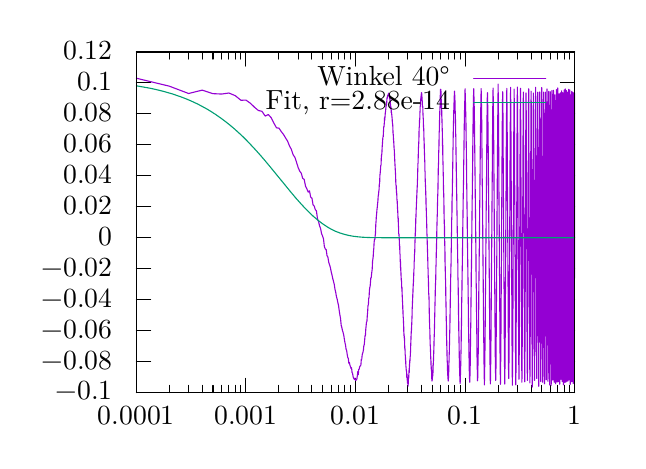
\begin{tikzpicture}[gnuplot]
%% generated with GNUPLOT 5.2p5a (Gentoo revision r0) (Lua 5.1; terminal rev. 99 , script rev. 107)
%% Sa 18 Mai 2019 18:31:25 CEST
\path (0.000,0.000) rectangle (7.500,5.250);
\gpcolor{color=gp lt color border}
\gpsetlinetype{gp lt border}
\gpsetdashtype{gp dt solid}
\gpsetlinewidth{1.00}
\draw[gp path] (1.380,0.616)--(1.560,0.616);
\draw[gp path] (6.947,0.616)--(6.767,0.616);
\node[gp node right] at (1.196,0.616) {$-0.1$};
\draw[gp path] (1.380,1.009)--(1.560,1.009);
\draw[gp path] (6.947,1.009)--(6.767,1.009);
\node[gp node right] at (1.196,1.009) {$-0.08$};
\draw[gp path] (1.380,1.402)--(1.560,1.402);
\draw[gp path] (6.947,1.402)--(6.767,1.402);
\node[gp node right] at (1.196,1.402) {$-0.06$};
\draw[gp path] (1.380,1.796)--(1.560,1.796);
\draw[gp path] (6.947,1.796)--(6.767,1.796);
\node[gp node right] at (1.196,1.796) {$-0.04$};
\draw[gp path] (1.380,2.189)--(1.560,2.189);
\draw[gp path] (6.947,2.189)--(6.767,2.189);
\node[gp node right] at (1.196,2.189) {$-0.02$};
\draw[gp path] (1.380,2.582)--(1.560,2.582);
\draw[gp path] (6.947,2.582)--(6.767,2.582);
\node[gp node right] at (1.196,2.582) {$0$};
\draw[gp path] (1.380,2.975)--(1.560,2.975);
\draw[gp path] (6.947,2.975)--(6.767,2.975);
\node[gp node right] at (1.196,2.975) {$0.02$};
\draw[gp path] (1.380,3.368)--(1.560,3.368);
\draw[gp path] (6.947,3.368)--(6.767,3.368);
\node[gp node right] at (1.196,3.368) {$0.04$};
\draw[gp path] (1.380,3.761)--(1.560,3.761);
\draw[gp path] (6.947,3.761)--(6.767,3.761);
\node[gp node right] at (1.196,3.761) {$0.06$};
\draw[gp path] (1.380,4.155)--(1.560,4.155);
\draw[gp path] (6.947,4.155)--(6.767,4.155);
\node[gp node right] at (1.196,4.155) {$0.08$};
\draw[gp path] (1.380,4.548)--(1.560,4.548);
\draw[gp path] (6.947,4.548)--(6.767,4.548);
\node[gp node right] at (1.196,4.548) {$0.1$};
\draw[gp path] (1.380,4.941)--(1.560,4.941);
\draw[gp path] (6.947,4.941)--(6.767,4.941);
\node[gp node right] at (1.196,4.941) {$0.12$};
\draw[gp path] (1.380,0.616)--(1.380,0.796);
\draw[gp path] (1.380,4.941)--(1.380,4.761);
\node[gp node center] at (1.380,0.308) {$0.0001$};
\draw[gp path] (1.799,0.616)--(1.799,0.706);
\draw[gp path] (1.799,4.941)--(1.799,4.851);
\draw[gp path] (2.044,0.616)--(2.044,0.706);
\draw[gp path] (2.044,4.941)--(2.044,4.851);
\draw[gp path] (2.218,0.616)--(2.218,0.706);
\draw[gp path] (2.218,4.941)--(2.218,4.851);
\draw[gp path] (2.353,0.616)--(2.353,0.706);
\draw[gp path] (2.353,4.941)--(2.353,4.851);
\draw[gp path] (2.463,0.616)--(2.463,0.706);
\draw[gp path] (2.463,4.941)--(2.463,4.851);
\draw[gp path] (2.556,0.616)--(2.556,0.706);
\draw[gp path] (2.556,4.941)--(2.556,4.851);
\draw[gp path] (2.637,0.616)--(2.637,0.706);
\draw[gp path] (2.637,4.941)--(2.637,4.851);
\draw[gp path] (2.708,0.616)--(2.708,0.706);
\draw[gp path] (2.708,4.941)--(2.708,4.851);
\draw[gp path] (2.772,0.616)--(2.772,0.796);
\draw[gp path] (2.772,4.941)--(2.772,4.761);
\node[gp node center] at (2.772,0.308) {$0.001$};
\draw[gp path] (3.191,0.616)--(3.191,0.706);
\draw[gp path] (3.191,4.941)--(3.191,4.851);
\draw[gp path] (3.436,0.616)--(3.436,0.706);
\draw[gp path] (3.436,4.941)--(3.436,4.851);
\draw[gp path] (3.610,0.616)--(3.610,0.706);
\draw[gp path] (3.610,4.941)--(3.610,4.851);
\draw[gp path] (3.745,0.616)--(3.745,0.706);
\draw[gp path] (3.745,4.941)--(3.745,4.851);
\draw[gp path] (3.855,0.616)--(3.855,0.706);
\draw[gp path] (3.855,4.941)--(3.855,4.851);
\draw[gp path] (3.948,0.616)--(3.948,0.706);
\draw[gp path] (3.948,4.941)--(3.948,4.851);
\draw[gp path] (4.029,0.616)--(4.029,0.706);
\draw[gp path] (4.029,4.941)--(4.029,4.851);
\draw[gp path] (4.100,0.616)--(4.100,0.706);
\draw[gp path] (4.100,4.941)--(4.100,4.851);
\draw[gp path] (4.163,0.616)--(4.163,0.796);
\draw[gp path] (4.163,4.941)--(4.163,4.761);
\node[gp node center] at (4.163,0.308) {$0.01$};
\draw[gp path] (4.582,0.616)--(4.582,0.706);
\draw[gp path] (4.582,4.941)--(4.582,4.851);
\draw[gp path] (4.828,0.616)--(4.828,0.706);
\draw[gp path] (4.828,4.941)--(4.828,4.851);
\draw[gp path] (5.001,0.616)--(5.001,0.706);
\draw[gp path] (5.001,4.941)--(5.001,4.851);
\draw[gp path] (5.136,0.616)--(5.136,0.706);
\draw[gp path] (5.136,4.941)--(5.136,4.851);
\draw[gp path] (5.246,0.616)--(5.246,0.706);
\draw[gp path] (5.246,4.941)--(5.246,4.851);
\draw[gp path] (5.340,0.616)--(5.340,0.706);
\draw[gp path] (5.340,4.941)--(5.340,4.851);
\draw[gp path] (5.420,0.616)--(5.420,0.706);
\draw[gp path] (5.420,4.941)--(5.420,4.851);
\draw[gp path] (5.492,0.616)--(5.492,0.706);
\draw[gp path] (5.492,4.941)--(5.492,4.851);
\draw[gp path] (5.555,0.616)--(5.555,0.796);
\draw[gp path] (5.555,4.941)--(5.555,4.761);
\node[gp node center] at (5.555,0.308) {$0.1$};
\draw[gp path] (5.974,0.616)--(5.974,0.706);
\draw[gp path] (5.974,4.941)--(5.974,4.851);
\draw[gp path] (6.219,0.616)--(6.219,0.706);
\draw[gp path] (6.219,4.941)--(6.219,4.851);
\draw[gp path] (6.393,0.616)--(6.393,0.706);
\draw[gp path] (6.393,4.941)--(6.393,4.851);
\draw[gp path] (6.528,0.616)--(6.528,0.706);
\draw[gp path] (6.528,4.941)--(6.528,4.851);
\draw[gp path] (6.638,0.616)--(6.638,0.706);
\draw[gp path] (6.638,4.941)--(6.638,4.851);
\draw[gp path] (6.731,0.616)--(6.731,0.706);
\draw[gp path] (6.731,4.941)--(6.731,4.851);
\draw[gp path] (6.812,0.616)--(6.812,0.706);
\draw[gp path] (6.812,4.941)--(6.812,4.851);
\draw[gp path] (6.883,0.616)--(6.883,0.706);
\draw[gp path] (6.883,4.941)--(6.883,4.851);
\draw[gp path] (6.947,0.616)--(6.947,0.796);
\draw[gp path] (6.947,4.941)--(6.947,4.761);
\node[gp node center] at (6.947,0.308) {$1$};
\draw[gp path] (1.380,4.941)--(1.380,0.616)--(6.947,0.616)--(6.947,4.941)--cycle;
\node[gp node right] at (5.479,4.607) {Winkel 40°};
\gpcolor{rgb color={0.580,0.000,0.827}}
\draw[gp path] (5.663,4.607)--(6.579,4.607);
\draw[gp path] (1.380,4.608)--(1.799,4.507)--(2.044,4.414)--(2.218,4.457)--(2.353,4.412)%
  --(2.463,4.407)--(2.556,4.420)--(2.637,4.386)--(2.708,4.328)--(2.772,4.330)--(2.829,4.290)%
  --(2.882,4.238)--(2.930,4.198)--(2.975,4.188)--(3.017,4.127)--(3.056,4.147)--(3.092,4.107)%
  --(3.127,4.037)--(3.160,3.978)--(3.191,3.974)--(3.220,3.931)--(3.248,3.895)--(3.275,3.850)%
  --(3.301,3.809)--(3.326,3.746)--(3.349,3.704)--(3.372,3.634)--(3.394,3.604)--(3.415,3.538)%
  --(3.436,3.471)--(3.456,3.426)--(3.475,3.401)--(3.493,3.335)--(3.511,3.325)--(3.529,3.236)%
  --(3.546,3.202)--(3.563,3.162)--(3.579,3.178)--(3.594,3.098)--(3.610,3.085)--(3.625,2.997)%
  --(3.639,2.985)--(3.653,2.939)--(3.667,2.923)--(3.681,2.820)--(3.694,2.787)--(3.707,2.733)%
  --(3.720,2.699)--(3.732,2.636)--(3.745,2.604)--(3.757,2.566)--(3.768,2.469)--(3.780,2.440)%
  --(3.791,2.431)--(3.802,2.353)--(3.813,2.336)--(3.824,2.268)--(3.834,2.239)--(3.845,2.201)%
  --(3.855,2.148)--(3.865,2.109)--(3.875,2.061)--(3.884,2.028)--(3.894,1.988)--(3.903,1.926)%
  --(3.912,1.891)--(3.921,1.834)--(3.930,1.805)--(3.939,1.759)--(3.948,1.722)--(3.956,1.660)%
  --(3.965,1.602)--(3.973,1.559)--(3.982,1.468)--(3.990,1.441)--(3.998,1.402)--(4.006,1.378)%
  --(4.013,1.350)--(4.021,1.300)--(4.029,1.251)--(4.036,1.223)--(4.044,1.164)--(4.051,1.150)%
  --(4.058,1.100)--(4.065,1.062)--(4.072,1.048)--(4.079,0.988)--(4.086,0.999)--(4.093,0.961)%
  --(4.100,0.946)--(4.106,0.923)--(4.113,0.931)--(4.120,0.867)--(4.126,0.862)--(4.132,0.822)%
  --(4.139,0.799)--(4.145,0.790)--(4.151,0.784)--(4.157,0.799)--(4.164,0.768)--(4.170,0.784)%
  --(4.175,0.776)--(4.181,0.789)--(4.187,0.834)--(4.193,0.884)--(4.199,0.842)--(4.204,0.911)%
  --(4.210,0.912)--(4.216,0.941)--(4.221,0.954)--(4.227,0.956)--(4.232,0.967)--(4.237,1.037)%
  --(4.243,1.040)--(4.248,1.092)--(4.253,1.113)--(4.258,1.126)--(4.264,1.157)--(4.269,1.209)%
  --(4.274,1.222)--(4.279,1.274)--(4.284,1.337)--(4.289,1.336)--(4.294,1.422)--(4.298,1.460)%
  --(4.303,1.513)--(4.308,1.513)--(4.313,1.590)--(4.317,1.632)--(4.322,1.720)--(4.327,1.732)%
  --(4.331,1.807)--(4.336,1.830)--(4.340,1.912)--(4.345,1.951)--(4.349,1.964)--(4.354,2.022)%
  --(4.358,2.073)--(4.363,2.076)--(4.367,2.115)--(4.371,2.151)--(4.375,2.176)--(4.380,2.284)%
  --(4.384,2.309)--(4.388,2.342)--(4.392,2.410)--(4.396,2.450)--(4.400,2.527)--(4.405,2.562)%
  --(4.409,2.557)--(4.413,2.605)--(4.417,2.638)--(4.421,2.751)--(4.424,2.784)--(4.428,2.850)%
  --(4.432,2.888)--(4.436,2.942)--(4.440,2.970)--(4.444,3.015)--(4.448,3.049)--(4.451,3.106)%
  --(4.455,3.128)--(4.459,3.167)--(4.463,3.198)--(4.466,3.266)--(4.470,3.271)--(4.473,3.373)%
  --(4.477,3.404)--(4.481,3.453)--(4.484,3.498)--(4.488,3.508)--(4.491,3.591)--(4.495,3.641)%
  --(4.498,3.644)--(4.502,3.732)--(4.505,3.770)--(4.509,3.831)--(4.512,3.862)--(4.515,3.863)%
  --(4.519,3.936)--(4.522,3.990)--(4.525,3.993)--(4.529,4.036)--(4.532,4.108)--(4.535,4.075)%
  --(4.539,4.133)--(4.542,4.169)--(4.545,4.187)--(4.548,4.219)--(4.551,4.248)--(4.555,4.264)%
  --(4.558,4.279)--(4.561,4.317)--(4.564,4.362)--(4.567,4.353)--(4.570,4.382)--(4.573,4.392)%
  --(4.576,4.389)--(4.579,4.406)--(4.582,4.406)--(4.585,4.418)--(4.588,4.409)--(4.591,4.395)%
  --(4.594,4.355)--(4.597,4.380)--(4.600,4.323)--(4.603,4.350)--(4.606,4.263)--(4.609,4.278)%
  --(4.612,4.215)--(4.615,4.243)--(4.618,4.168)--(4.621,4.177)--(4.623,4.153)--(4.626,4.123)%
  --(4.629,4.092)--(4.632,4.039)--(4.635,4.027)--(4.637,3.999)--(4.640,3.914)--(4.643,3.890)%
  --(4.646,3.832)--(4.648,3.815)--(4.651,3.765)--(4.654,3.705)--(4.656,3.698)--(4.659,3.630)%
  --(4.662,3.561)--(4.664,3.527)--(4.667,3.470)--(4.670,3.420)--(4.672,3.383)--(4.675,3.289)%
  --(4.677,3.249)--(4.680,3.248)--(4.683,3.153)--(4.685,3.176)--(4.688,3.117)--(4.690,3.064)%
  --(4.693,3.046)--(4.695,2.998)--(4.698,2.938)--(4.700,2.916)--(4.703,2.830)--(4.705,2.851)%
  --(4.708,2.741)--(4.710,2.718)--(4.712,2.634)--(4.715,2.630)--(4.717,2.599)--(4.720,2.545)%
  --(4.722,2.483)--(4.725,2.475)--(4.727,2.377)--(4.729,2.375)--(4.732,2.277)--(4.734,2.290)%
  --(4.736,2.168)--(4.739,2.203)--(4.741,2.119)--(4.743,2.079)--(4.746,2.028)--(4.748,2.036)%
  --(4.750,1.942)--(4.753,1.959)--(4.755,1.880)--(4.757,1.846)--(4.759,1.792)--(4.762,1.749)%
  --(4.764,1.678)--(4.766,1.658)--(4.768,1.584)--(4.771,1.560)--(4.773,1.504)--(4.775,1.471)%
  --(4.777,1.380)--(4.779,1.359)--(4.781,1.311)--(4.784,1.332)--(4.786,1.287)--(4.788,1.214)%
  --(4.790,1.165)--(4.792,1.174)--(4.794,1.101)--(4.797,1.080)--(4.799,1.027)--(4.801,1.017)%
  --(4.803,0.950)--(4.805,0.943)--(4.807,0.898)--(4.809,0.907)--(4.811,0.887)--(4.813,0.878)%
  --(4.815,0.805)--(4.817,0.850)--(4.819,0.773)--(4.821,0.813)--(4.823,0.735)--(4.826,0.783)%
  --(4.828,0.718)--(4.830,0.772)--(4.832,0.697)--(4.834,0.794)--(4.836,0.789)--(4.838,0.835)%
  --(4.840,0.807)--(4.841,0.894)--(4.843,0.880)--(4.845,0.925)--(4.847,0.871)--(4.849,0.975)%
  --(4.851,0.972)--(4.853,1.025)--(4.855,1.020)--(4.857,1.069)--(4.859,1.075)--(4.861,1.122)%
  --(4.863,1.151)--(4.865,1.238)--(4.867,1.264)--(4.868,1.313)--(4.870,1.356)--(4.872,1.391)%
  --(4.874,1.409)--(4.876,1.461)--(4.878,1.493)--(4.880,1.562)--(4.881,1.556)--(4.883,1.674)%
  --(4.885,1.708)--(4.887,1.759)--(4.889,1.798)--(4.891,1.862)--(4.892,1.851)--(4.894,1.933)%
  --(4.896,1.966)--(4.898,2.014)--(4.900,2.023)--(4.901,2.072)--(4.903,2.110)--(4.905,2.185)%
  --(4.907,2.186)--(4.908,2.277)--(4.910,2.287)--(4.912,2.363)--(4.914,2.379)--(4.916,2.413)%
  --(4.917,2.464)--(4.919,2.546)--(4.921,2.573)--(4.922,2.644)--(4.924,2.636)--(4.926,2.714)%
  --(4.928,2.767)--(4.929,2.827)--(4.931,2.844)--(4.933,2.904)--(4.934,2.938)--(4.936,2.972)%
  --(4.938,3.036)--(4.939,3.024)--(4.941,3.099)--(4.943,3.145)--(4.944,3.159)--(4.946,3.218)%
  --(4.948,3.230)--(4.949,3.307)--(4.951,3.314)--(4.953,3.411)--(4.954,3.438)--(4.956,3.522)%
  --(4.958,3.529)--(4.959,3.574)--(4.961,3.647)--(4.962,3.709)--(4.964,3.738)--(4.966,3.777)%
  --(4.967,3.796)--(4.969,3.849)--(4.970,3.926)--(4.972,3.978)--(4.974,3.994)--(4.975,4.075)%
  --(4.977,4.041)--(4.978,4.073)--(4.980,4.103)--(4.981,4.164)--(4.983,4.185)--(4.985,4.247)%
  --(4.986,4.251)--(4.988,4.271)--(4.989,4.272)--(4.991,4.346)--(4.992,4.318)--(4.994,4.376)%
  --(4.995,4.364)--(4.997,4.390)--(4.998,4.398)--(5.000,4.401)--(5.001,4.426)--(5.003,4.416)%
  --(5.004,4.412)--(5.006,4.385)--(5.007,4.348)--(5.009,4.369)--(5.010,4.326)--(5.012,4.316)%
  --(5.013,4.264)--(5.015,4.244)--(5.016,4.255)--(5.018,4.238)--(5.019,4.185)--(5.021,4.146)%
  --(5.022,4.105)--(5.024,4.099)--(5.025,4.072)--(5.027,3.984)--(5.028,4.007)--(5.029,3.981)%
  --(5.031,3.930)--(5.032,3.872)--(5.034,3.814)--(5.035,3.815)--(5.037,3.714)--(5.038,3.751)%
  --(5.039,3.657)--(5.041,3.614)--(5.042,3.572)--(5.044,3.533)--(5.045,3.431)--(5.047,3.421)%
  --(5.048,3.342)--(5.049,3.323)--(5.051,3.246)--(5.052,3.250)--(5.054,3.204)--(5.055,3.171)%
  --(5.056,3.127)--(5.058,3.087)--(5.059,3.008)--(5.060,2.999)--(5.062,2.936)--(5.063,2.915)%
  --(5.064,2.854)--(5.066,2.839)--(5.067,2.779)--(5.069,2.699)--(5.070,2.637)--(5.071,2.630)%
  --(5.073,2.589)--(5.074,2.539)--(5.075,2.503)--(5.077,2.440)--(5.078,2.430)--(5.079,2.344)%
  --(5.081,2.329)--(5.082,2.250)--(5.083,2.205)--(5.085,2.183)--(5.086,2.128)--(5.087,2.083)%
  --(5.089,2.057)--(5.090,2.014)--(5.091,1.968)--(5.092,1.883)--(5.094,1.872)--(5.095,1.828)%
  --(5.096,1.836)--(5.098,1.781)--(5.099,1.710)--(5.100,1.635)--(5.101,1.608)--(5.103,1.531)%
  --(5.104,1.497)--(5.105,1.426)--(5.107,1.436)--(5.108,1.373)--(5.109,1.343)--(5.110,1.298)%
  --(5.112,1.220)--(5.113,1.223)--(5.114,1.172)--(5.115,1.174)--(5.117,1.119)--(5.118,1.067)%
  --(5.119,1.075)--(5.120,1.025)--(5.122,1.017)--(5.123,0.954)--(5.124,0.969)--(5.125,0.934)%
  --(5.127,0.896)--(5.128,0.903)--(5.129,0.898)--(5.130,0.826)--(5.131,0.792)--(5.133,0.847)%
  --(5.134,0.774)--(5.135,0.761)--(5.136,0.801)--(5.137,0.767)--(5.139,0.805)--(5.140,0.784)%
  --(5.141,0.831)--(5.142,0.824)--(5.144,0.873)--(5.145,0.828)--(5.146,0.919)--(5.147,0.867)%
  --(5.148,0.963)--(5.149,0.931)--(5.151,0.988)--(5.152,0.992)--(5.153,1.020)--(5.154,1.022)%
  --(5.155,1.088)--(5.157,1.117)--(5.158,1.163)--(5.159,1.176)--(5.160,1.229)--(5.161,1.270)%
  --(5.162,1.316)--(5.163,1.327)--(5.165,1.381)--(5.166,1.432)--(5.167,1.483)--(5.168,1.506)%
  --(5.169,1.571)--(5.170,1.604)--(5.172,1.718)--(5.173,1.719)--(5.174,1.793)--(5.175,1.825)%
  --(5.176,1.858)--(5.177,1.931)--(5.178,1.961)--(5.179,1.988)--(5.181,2.024)--(5.182,2.051)%
  --(5.183,2.109)--(5.184,2.144)--(5.185,2.221)--(5.186,2.218)--(5.187,2.273)--(5.188,2.315)%
  --(5.189,2.392)--(5.191,2.410)--(5.192,2.495)--(5.193,2.518)--(5.194,2.594)--(5.195,2.561)%
  --(5.196,2.680)--(5.197,2.686)--(5.198,2.759)--(5.199,2.779)--(5.200,2.861)--(5.202,2.852)%
  --(5.203,2.967)--(5.204,2.982)--(5.205,3.032)--(5.206,3.028)--(5.207,3.109)--(5.208,3.115)%
  --(5.209,3.160)--(5.210,3.188)--(5.211,3.211)--(5.212,3.305)--(5.213,3.371)--(5.214,3.384)%
  --(5.215,3.470)--(5.217,3.517)--(5.218,3.533)--(5.219,3.578)--(5.220,3.671)--(5.221,3.686)%
  --(5.222,3.721)--(5.223,3.741)--(5.224,3.810)--(5.225,3.849)--(5.226,3.918)--(5.227,3.930)%
  --(5.228,3.942)--(5.229,4.001)--(5.230,4.029)--(5.231,4.088)--(5.232,4.128)--(5.233,4.152)%
  --(5.234,4.192)--(5.235,4.236)--(5.236,4.248)--(5.237,4.233)--(5.238,4.320)--(5.239,4.268)%
  --(5.240,4.392)--(5.241,4.310)--(5.242,4.466)--(5.243,4.356)--(5.244,4.425)--(5.245,4.426)%
  --(5.246,4.470)--(5.247,4.387)--(5.249,4.443)--(5.250,4.368)--(5.251,4.405)--(5.252,4.312)%
  --(5.253,4.337)--(5.254,4.334)--(5.254,4.331)--(5.255,4.263)--(5.256,4.226)--(5.257,4.207)%
  --(5.258,4.199)--(5.259,4.125)--(5.260,4.139)--(5.261,4.095)--(5.262,4.069)--(5.263,4.018)%
  --(5.264,3.997)--(5.265,3.933)--(5.266,3.936)--(5.267,3.850)--(5.268,3.841)--(5.269,3.736)%
  --(5.270,3.765)--(5.271,3.755)--(5.272,3.636)--(5.273,3.566)--(5.274,3.550)--(5.275,3.521)%
  --(5.276,3.470)--(5.277,3.417)--(5.278,3.406)--(5.279,3.303)--(5.280,3.269)--(5.281,3.185)%
  --(5.282,3.234)--(5.283,3.121)--(5.284,3.145)--(5.285,3.080)--(5.286,3.040)--(5.286,2.993)%
  --(5.287,2.991)--(5.288,2.879)--(5.289,2.867)--(5.290,2.797)--(5.291,2.766)--(5.292,2.692)%
  --(5.293,2.728)--(5.294,2.617)--(5.295,2.596)--(5.296,2.515)--(5.297,2.539)--(5.298,2.410)%
  --(5.299,2.428)--(5.300,2.355)--(5.300,2.336)--(5.301,2.238)--(5.302,2.250)--(5.303,2.184)%
  --(5.304,2.150)--(5.305,2.097)--(5.306,2.050)--(5.307,2.060)--(5.308,1.959)--(5.309,1.955)%
  --(5.310,1.899)--(5.310,1.854)--(5.311,1.801)--(5.312,1.769)--(5.313,1.709)--(5.314,1.672)%
  --(5.315,1.596)--(5.316,1.545)--(5.317,1.500)--(5.318,1.453)--(5.319,1.467)--(5.319,1.369)%
  --(5.320,1.323)--(5.321,1.302)--(5.322,1.253)--(5.323,1.203)--(5.324,1.198)--(5.325,1.137)%
  --(5.326,1.079)--(5.327,1.042)--(5.327,1.021)--(5.328,1.016)--(5.329,1.019)--(5.330,0.929)%
  --(5.331,0.965)--(5.332,0.891)--(5.333,0.923)--(5.334,0.864)--(5.334,0.877)--(5.335,0.835)%
  --(5.336,0.826)--(5.337,0.808)--(5.338,0.797)--(5.339,0.783)--(5.340,0.762)--(5.341,0.798)%
  --(5.341,0.761)--(5.342,0.796)--(5.343,0.808)--(5.344,0.800)--(5.345,0.849)--(5.346,0.822)%
  --(5.347,0.880)--(5.347,0.914)--(5.348,0.928)--(5.349,0.973)--(5.350,0.996)--(5.351,1.016)%
  --(5.352,1.030)--(5.352,1.054)--(5.353,1.094)--(5.354,1.114)--(5.355,1.137)--(5.356,1.187)%
  --(5.357,1.250)--(5.358,1.266)--(5.358,1.358)--(5.359,1.354)--(5.360,1.379)--(5.361,1.414)%
  --(5.362,1.488)--(5.363,1.505)--(5.363,1.581)--(5.364,1.604)--(5.365,1.646)--(5.366,1.694)%
  --(5.367,1.779)--(5.368,1.840)--(5.368,1.868)--(5.369,1.878)--(5.370,1.973)--(5.371,2.000)%
  --(5.372,2.019)--(5.372,2.074)--(5.373,2.094)--(5.374,2.139)--(5.375,2.196)--(5.376,2.239)%
  --(5.377,2.257)--(5.377,2.330)--(5.378,2.359)--(5.379,2.411)--(5.380,2.454)--(5.381,2.539)%
  --(5.381,2.562)--(5.382,2.619)--(5.383,2.643)--(5.384,2.678)--(5.385,2.720)--(5.385,2.811)%
  --(5.386,2.813)--(5.387,2.887)--(5.388,2.887)--(5.389,2.971)--(5.389,3.028)--(5.390,3.070)%
  --(5.391,3.102)--(5.392,3.119)--(5.393,3.153)--(5.393,3.208)--(5.394,3.228)--(5.395,3.316)%
  --(5.396,3.333)--(5.396,3.413)--(5.397,3.399)--(5.398,3.486)--(5.399,3.540)--(5.400,3.616)%
  --(5.400,3.628)--(5.401,3.707)--(5.402,3.714)--(5.403,3.782)--(5.404,3.798)--(5.404,3.850)%
  --(5.405,3.894)--(5.406,3.978)--(5.407,4.002)--(5.407,4.040)--(5.408,4.036)--(5.409,4.091)%
  --(5.410,4.098)--(5.410,4.154)--(5.411,4.176)--(5.412,4.213)--(5.413,4.228)--(5.414,4.228)%
  --(5.414,4.257)--(5.415,4.299)--(5.416,4.302)--(5.417,4.330)--(5.417,4.364)--(5.418,4.381)%
  --(5.419,4.433)--(5.420,4.432)--(5.420,4.414)--(5.421,4.445)--(5.422,4.395)--(5.423,4.438)%
  --(5.423,4.382)--(5.424,4.396)--(5.425,4.345)--(5.426,4.343)--(5.426,4.313)--(5.427,4.325)%
  --(5.428,4.236)--(5.429,4.282)--(5.429,4.215)--(5.430,4.170)--(5.431,4.154)--(5.432,4.141)%
  --(5.432,4.119)--(5.433,4.065)--(5.434,4.002)--(5.435,3.979)--(5.435,3.936)--(5.436,3.893)%
  --(5.437,3.880)--(5.438,3.784)--(5.438,3.765)--(5.439,3.732)--(5.440,3.663)--(5.440,3.643)%
  --(5.441,3.616)--(5.442,3.545)--(5.443,3.509)--(5.443,3.467)--(5.444,3.383)--(5.445,3.371)%
  --(5.446,3.268)--(5.446,3.256)--(5.447,3.215)--(5.448,3.151)--(5.448,3.116)--(5.449,3.140)%
  --(5.450,3.040)--(5.451,3.001)--(5.451,2.971)--(5.452,2.911)--(5.453,2.863)--(5.453,2.881)%
  --(5.454,2.788)--(5.455,2.718)--(5.456,2.661)--(5.456,2.672)--(5.457,2.535)--(5.458,2.582)%
  --(5.458,2.506)--(5.459,2.438)--(5.460,2.430)--(5.461,2.383)--(5.461,2.316)--(5.462,2.306)%
  --(5.463,2.222)--(5.463,2.175)--(5.464,2.094)--(5.465,2.049)--(5.465,2.061)--(5.466,2.040)%
  --(5.467,1.953)--(5.468,1.946)--(5.468,1.889)--(5.469,1.852)--(5.470,1.785)--(5.470,1.778)%
  --(5.471,1.736)--(5.472,1.648)--(5.472,1.607)--(5.473,1.572)--(5.474,1.516)--(5.475,1.451)%
  --(5.475,1.407)--(5.476,1.366)--(5.477,1.336)--(5.477,1.332)--(5.478,1.257)--(5.479,1.230)%
  --(5.479,1.185)--(5.480,1.158)--(5.481,1.079)--(5.481,1.058)--(5.482,1.051)--(5.483,1.030)%
  --(5.483,0.991)--(5.484,0.978)--(5.485,0.915)--(5.485,0.870)--(5.486,0.878)--(5.487,0.859)%
  --(5.488,0.822)--(5.488,0.882)--(5.489,0.750)--(5.490,0.811)--(5.490,0.768)--(5.491,0.770)%
  --(5.492,0.729)--(5.492,0.789)--(5.493,0.775)--(5.494,0.802)--(5.494,0.745)--(5.495,0.840)%
  --(5.496,0.831)--(5.496,0.858)--(5.497,0.843)--(5.498,0.905)--(5.498,0.943)--(5.499,0.932)%
  --(5.500,0.993)--(5.500,1.017)--(5.501,0.999)--(5.502,1.070)--(5.502,1.098)--(5.503,1.120)%
  --(5.504,1.164)--(5.504,1.218)--(5.505,1.219)--(5.506,1.291)--(5.506,1.303)--(5.507,1.350)%
  --(5.507,1.412)--(5.508,1.436)--(5.509,1.469)--(5.509,1.547)--(5.510,1.554)--(5.511,1.629)%
  --(5.511,1.669)--(5.512,1.758)--(5.513,1.772)--(5.513,1.826)--(5.514,1.810)--(5.515,1.924)%
  --(5.515,1.888)--(5.516,2.032)--(5.517,2.052)--(5.517,2.081)--(5.518,2.065)--(5.518,2.140)%
  --(5.519,2.188)--(5.520,2.243)--(5.520,2.270)--(5.521,2.357)--(5.522,2.351)--(5.522,2.409)%
  --(5.523,2.463)--(5.524,2.525)--(5.524,2.534)--(5.525,2.604)--(5.526,2.649)--(5.526,2.716)%
  --(5.527,2.745)--(5.527,2.802)--(5.528,2.840)--(5.529,2.880)--(5.529,2.932)--(5.530,2.954)%
  --(5.531,3.017)--(5.531,3.076)--(5.532,3.074)--(5.532,3.143)--(5.533,3.157)--(5.534,3.190)%
  --(5.534,3.237)--(5.535,3.307)--(5.536,3.320)--(5.536,3.395)--(5.537,3.455)--(5.537,3.487)%
  --(5.538,3.533)--(5.539,3.586)--(5.539,3.640)--(5.540,3.661)--(5.541,3.718)--(5.541,3.778)%
  --(5.542,3.820)--(5.542,3.864)--(5.543,3.896)--(5.544,3.969)--(5.544,4.006)--(5.545,4.028)%
  --(5.546,4.057)--(5.546,4.099)--(5.547,4.145)--(5.547,4.156)--(5.548,4.176)--(5.549,4.272)%
  --(5.549,4.231)--(5.550,4.274)--(5.550,4.320)--(5.551,4.309)--(5.552,4.327)--(5.552,4.378)%
  --(5.553,4.383)--(5.553,4.458)--(5.554,4.418)--(5.555,4.460)--(5.555,4.474)--(5.556,4.443)%
  --(5.556,4.429)--(5.557,4.404)--(5.558,4.380)--(5.558,4.403)--(5.559,4.324)--(5.559,4.334)%
  --(5.560,4.284)--(5.561,4.298)--(5.561,4.273)--(5.562,4.260)--(5.562,4.229)--(5.563,4.174)%
  --(5.564,4.176)--(5.564,4.116)--(5.565,4.109)--(5.565,4.070)--(5.566,4.039)--(5.567,3.967)%
  --(5.567,3.954)--(5.568,3.898)--(5.568,3.835)--(5.569,3.810)--(5.570,3.788)--(5.570,3.750)%
  --(5.571,3.699)--(5.571,3.629)--(5.572,3.605)--(5.573,3.543)--(5.573,3.471)--(5.574,3.428)%
  --(5.574,3.366)--(5.575,3.339)--(5.575,3.302)--(5.576,3.246)--(5.577,3.189)--(5.577,3.131)%
  --(5.578,3.114)--(5.578,3.077)--(5.579,3.023)--(5.580,3.006)--(5.580,2.947)--(5.581,2.924)%
  --(5.581,2.891)--(5.582,2.839)--(5.582,2.769)--(5.583,2.699)--(5.584,2.692)--(5.584,2.649)%
  --(5.585,2.597)--(5.585,2.522)--(5.586,2.482)--(5.586,2.474)--(5.587,2.411)--(5.588,2.344)%
  --(5.588,2.318)--(5.589,2.266)--(5.589,2.235)--(5.590,2.191)--(5.590,2.165)--(5.591,2.100)%
  --(5.592,2.046)--(5.592,1.990)--(5.593,1.980)--(5.593,1.918)--(5.594,1.907)--(5.594,1.849)%
  --(5.595,1.809)--(5.596,1.734)--(5.596,1.722)--(5.597,1.650)--(5.597,1.616)--(5.598,1.546)%
  --(5.598,1.542)--(5.599,1.452)--(5.600,1.425)--(5.600,1.395)--(5.601,1.357)--(5.601,1.305)%
  --(5.602,1.271)--(5.602,1.258)--(5.603,1.230)--(5.603,1.171)--(5.604,1.135)--(5.605,1.085)%
  --(5.605,1.062)--(5.606,1.042)--(5.606,1.008)--(5.607,0.964)--(5.607,0.948)--(5.608,0.952)%
  --(5.608,0.888)--(5.609,0.897)--(5.610,0.889)--(5.610,0.868)--(5.611,0.819)--(5.611,0.797)%
  --(5.612,0.787)--(5.612,0.776)--(5.613,0.757)--(5.613,0.763)--(5.614,0.790)--(5.615,0.746)%
  --(5.615,0.817)--(5.616,0.783)--(5.616,0.872)--(5.617,0.824)--(5.617,0.879)--(5.618,0.889)%
  --(5.618,0.930)--(5.619,0.957)--(5.619,0.959)--(5.620,0.956)--(5.621,1.043)--(5.621,1.040)%
  --(5.622,1.114)--(5.622,1.126)--(5.623,1.156)--(5.623,1.196)--(5.624,1.214)--(5.624,1.283)%
  --(5.625,1.308)--(5.625,1.327)--(5.626,1.399)--(5.626,1.420)--(5.627,1.472)--(5.628,1.521)%
  --(5.628,1.601)--(5.629,1.626)--(5.629,1.679)--(5.630,1.722)--(5.630,1.778)--(5.631,1.833)%
  --(5.631,1.866)--(5.632,1.900)--(5.632,1.936)--(5.633,1.969)--(5.633,2.048)--(5.634,2.055)%
  --(5.634,2.141)--(5.635,2.199)--(5.636,2.189)--(5.636,2.230)--(5.637,2.294)--(5.638,2.370)%
  --(5.638,2.412)--(5.639,2.515)--(5.639,2.514)--(5.640,2.605)--(5.640,2.593)--(5.641,2.681)%
  --(5.641,2.696)--(5.642,2.756)--(5.642,2.789)--(5.643,2.858)--(5.643,2.881)--(5.644,2.955)%
  --(5.644,2.983)--(5.645,3.049)--(5.645,3.039)--(5.646,3.125)--(5.647,3.081)--(5.647,3.176)%
  --(5.648,3.212)--(5.648,3.283)--(5.649,3.310)--(5.649,3.354)--(5.650,3.411)--(5.650,3.456)%
  --(5.651,3.486)--(5.651,3.525)--(5.652,3.561)--(5.652,3.665)--(5.653,3.690)--(5.653,3.749)%
  --(5.654,3.796)--(5.654,3.840)--(5.655,3.865)--(5.655,3.912)--(5.656,3.921)--(5.656,4.013)%
  --(5.657,4.067)--(5.657,4.075)--(5.658,4.083)--(5.658,4.116)--(5.659,4.144)--(5.659,4.237)%
  --(5.660,4.189)--(5.660,4.277)--(5.661,4.256)--(5.661,4.322)--(5.662,4.316)--(5.662,4.393)%
  --(5.663,4.374)--(5.663,4.420)--(5.664,4.382)--(5.664,4.472)--(5.665,4.406)--(5.665,4.475)%
  --(5.666,4.437)--(5.666,4.473)--(5.667,4.406)--(5.667,4.410)--(5.668,4.346)--(5.668,4.371)%
  --(5.669,4.293)--(5.669,4.304)--(5.670,4.288)--(5.670,4.264)--(5.671,4.251)--(5.671,4.198)%
  --(5.672,4.154)--(5.672,4.151)--(5.673,4.119)--(5.673,4.091)--(5.674,4.064)--(5.674,4.005)%
  --(5.675,3.981)--(5.675,3.916)--(5.676,3.874)--(5.676,3.850)--(5.677,3.825)--(5.677,3.769)%
  --(5.678,3.698)--(5.678,3.681)--(5.679,3.630)--(5.679,3.582)--(5.680,3.517)--(5.680,3.507)%
  --(5.681,3.424)--(5.681,3.419)--(5.682,3.341)--(5.682,3.296)--(5.683,3.241)--(5.683,3.244)%
  --(5.684,3.144)--(5.684,3.119)--(5.685,3.076)--(5.685,3.072)--(5.686,3.012)--(5.686,2.985)%
  --(5.687,2.916)--(5.687,2.872)--(5.688,2.827)--(5.688,2.795)--(5.689,2.725)--(5.689,2.710)%
  --(5.690,2.648)--(5.690,2.618)--(5.691,2.537)--(5.691,2.532)--(5.692,2.467)--(5.692,2.422)%
  --(5.693,2.374)--(5.693,2.298)--(5.693,2.268)--(5.694,2.227)--(5.694,2.153)--(5.695,2.160)%
  --(5.695,2.099)--(5.696,2.039)--(5.696,2.011)--(5.697,1.956)--(5.697,1.954)--(5.698,1.924)%
  --(5.698,1.859)--(5.699,1.812)--(5.699,1.783)--(5.700,1.717)--(5.700,1.676)--(5.701,1.623)%
  --(5.701,1.592)--(5.702,1.542)--(5.702,1.465)--(5.703,1.406)--(5.703,1.391)--(5.704,1.354)%
  --(5.704,1.295)--(5.704,1.258)--(5.705,1.207)--(5.705,1.196)--(5.706,1.157)--(5.706,1.103)%
  --(5.707,1.097)--(5.707,1.066)--(5.708,1.018)--(5.708,0.983)--(5.709,0.959)--(5.709,0.945)%
  --(5.710,0.936)--(5.710,0.916)--(5.711,0.879)--(5.711,0.857)--(5.712,0.816)--(5.712,0.862)%
  --(5.712,0.796)--(5.713,0.805)--(5.713,0.764)--(5.714,0.811)--(5.714,0.783)--(5.715,0.772)%
  --(5.715,0.792)--(5.716,0.828)--(5.716,0.808)--(5.717,0.841)--(5.717,0.878)--(5.718,0.894)%
  --(5.718,0.887)--(5.718,0.948)--(5.719,0.974)--(5.719,0.994)--(5.720,1.059)--(5.720,1.053)%
  --(5.721,1.022)--(5.721,1.064)--(5.722,1.134)--(5.722,1.163)--(5.723,1.187)--(5.723,1.286)%
  --(5.724,1.279)--(5.724,1.295)--(5.724,1.313)--(5.725,1.415)--(5.725,1.399)--(5.726,1.479)%
  --(5.726,1.535)--(5.727,1.570)--(5.727,1.599)--(5.728,1.678)--(5.728,1.738)--(5.729,1.807)%
  --(5.729,1.806)--(5.729,1.885)--(5.730,1.943)--(5.730,1.944)--(5.731,1.986)--(5.731,2.029)%
  --(5.732,2.103)--(5.732,2.145)--(5.733,2.165)--(5.733,2.188)--(5.733,2.258)--(5.734,2.292)%
  --(5.734,2.334)--(5.735,2.374)--(5.735,2.409)--(5.736,2.464)--(5.736,2.532)--(5.737,2.571)%
  --(5.737,2.619)--(5.738,2.622)--(5.738,2.676)--(5.738,2.731)--(5.739,2.804)--(5.739,2.838)%
  --(5.740,2.875)--(5.740,2.937)--(5.741,2.981)--(5.741,3.017)--(5.742,3.063)--(5.742,3.094)%
  --(5.742,3.134)--(5.743,3.190)--(5.743,3.217)--(5.744,3.264)--(5.744,3.311)--(5.745,3.330)%
  --(5.745,3.392)--(5.746,3.385)--(5.746,3.507)--(5.746,3.521)--(5.747,3.581)--(5.747,3.627)%
  --(5.748,3.721)--(5.748,3.740)--(5.749,3.759)--(5.749,3.843)--(5.749,3.865)--(5.750,3.891)%
  --(5.750,3.939)--(5.751,3.980)--(5.751,4.014)--(5.752,4.019)--(5.752,4.084)--(5.753,4.144)%
  --(5.753,4.097)--(5.753,4.141)--(5.754,4.173)--(5.754,4.194)--(5.755,4.261)--(5.755,4.270)%
  --(5.756,4.280)--(5.756,4.320)--(5.756,4.335)--(5.757,4.336)--(5.757,4.407)--(5.758,4.378)%
  --(5.758,4.443)--(5.759,4.433)--(5.759,4.476)--(5.759,4.401)--(5.760,4.447)--(5.760,4.377)%
  --(5.761,4.409)--(5.761,4.327)--(5.762,4.402)--(5.762,4.274)--(5.762,4.319)--(5.763,4.226)%
  --(5.763,4.278)--(5.764,4.186)--(5.764,4.208)--(5.765,4.172)--(5.765,4.126)--(5.765,4.076)%
  --(5.766,4.082)--(5.766,4.015)--(5.767,3.971)--(5.767,3.933)--(5.768,3.887)--(5.768,3.847)%
  --(5.768,3.822)--(5.769,3.756)--(5.769,3.726)--(5.770,3.679)--(5.770,3.650)--(5.771,3.548)%
  --(5.771,3.524)--(5.771,3.470)--(5.772,3.409)--(5.772,3.337)--(5.773,3.325)--(5.773,3.288)%
  --(5.774,3.212)--(5.774,3.186)--(5.774,3.167)--(5.775,3.096)--(5.775,3.104)--(5.776,3.027)%
  --(5.776,2.981)--(5.776,2.944)--(5.777,2.934)--(5.777,2.845)--(5.778,2.833)--(5.778,2.773)%
  --(5.779,2.732)--(5.779,2.702)--(5.779,2.640)--(5.780,2.607)--(5.780,2.577)--(5.781,2.446)%
  --(5.781,2.457)--(5.781,2.413)--(5.782,2.362)--(5.782,2.323)--(5.783,2.290)--(5.783,2.223)%
  --(5.784,2.221)--(5.784,2.112)--(5.784,2.130)--(5.785,2.079)--(5.785,2.058)--(5.786,1.988)%
  --(5.786,1.951)--(5.786,1.898)--(5.787,1.869)--(5.787,1.812)--(5.788,1.750)--(5.788,1.707)%
  --(5.789,1.689)--(5.789,1.594)--(5.789,1.573)--(5.790,1.506)--(5.790,1.467)--(5.791,1.432)%
  --(5.791,1.376)--(5.791,1.333)--(5.792,1.294)--(5.792,1.271)--(5.793,1.241)--(5.793,1.210)%
  --(5.793,1.173)--(5.794,1.107)--(5.794,1.069)--(5.795,1.079)--(5.795,1.047)--(5.795,0.985)%
  --(5.796,0.973)--(5.796,0.915)--(5.797,0.938)--(5.797,0.878)--(5.797,0.881)--(5.798,0.808)%
  --(5.798,0.849)--(5.799,0.787)--(5.799,0.823)--(5.800,0.735)--(5.800,0.799)--(5.800,0.714)%
  --(5.801,0.774)--(5.801,0.760)--(5.802,0.800)--(5.802,0.822)--(5.802,0.832)--(5.803,0.829)%
  --(5.803,0.888)--(5.804,0.878)--(5.804,0.927)--(5.804,0.937)--(5.805,0.969)--(5.805,0.998)%
  --(5.806,0.996)--(5.806,1.030)--(5.806,1.056)--(5.807,1.089)--(5.807,1.135)--(5.808,1.180)%
  --(5.808,1.221)--(5.808,1.245)--(5.809,1.259)--(5.809,1.327)--(5.810,1.356)--(5.810,1.386)%
  --(5.810,1.474)--(5.811,1.452)--(5.811,1.502)--(5.812,1.537)--(5.812,1.662)--(5.812,1.648)%
  --(5.813,1.741)--(5.813,1.749)--(5.813,1.861)--(5.814,1.861)--(5.814,1.878)--(5.815,1.942)%
  --(5.815,1.995)--(5.815,1.998)--(5.816,2.036)--(5.816,2.075)--(5.817,2.128)--(5.817,2.197)%
  --(5.817,2.173)--(5.818,2.258)--(5.818,2.337)--(5.819,2.324)--(5.819,2.384)--(5.819,2.415)%
  --(5.820,2.515)--(5.820,2.581)--(5.821,2.615)--(5.821,2.627)--(5.821,2.693)--(5.822,2.719)%
  --(5.822,2.796)--(5.822,2.802)--(5.823,2.868)--(5.823,2.925)--(5.824,2.949)--(5.824,3.007)%
  --(5.824,3.027)--(5.825,3.071)--(5.825,3.128)--(5.826,3.118)--(5.826,3.164)--(5.826,3.226)%
  --(5.827,3.295)--(5.827,3.303)--(5.828,3.383)--(5.828,3.420)--(5.828,3.456)--(5.829,3.526)%
  --(5.829,3.554)--(5.829,3.646)--(5.830,3.672)--(5.830,3.711)--(5.831,3.778)--(5.831,3.817)%
  --(5.831,3.853)--(5.832,3.908)--(5.832,3.961)--(5.832,3.976)--(5.833,4.042)--(5.833,4.060)%
  --(5.834,4.090)--(5.834,4.087)--(5.834,4.140)--(5.835,4.140)--(5.835,4.207)--(5.836,4.210)%
  --(5.836,4.282)--(5.836,4.233)--(5.837,4.318)--(5.837,4.305)--(5.837,4.360)--(5.838,4.360)%
  --(5.838,4.341)--(5.839,4.401)--(5.839,4.425)--(5.839,4.404)--(5.840,4.424)--(5.840,4.406)%
  --(5.840,4.374)--(5.841,4.362)--(5.841,4.345)--(5.842,4.345)--(5.842,4.303)--(5.842,4.274)%
  --(5.843,4.258)--(5.843,4.230)--(5.843,4.201)--(5.844,4.197)--(5.844,4.174)--(5.845,4.128)%
  --(5.845,4.123)--(5.845,4.061)--(5.846,4.042)--(5.846,3.994)--(5.846,3.968)--(5.847,3.946)%
  --(5.847,3.925)--(5.848,3.869)--(5.848,3.818)--(5.848,3.760)--(5.849,3.736)--(5.849,3.675)%
  --(5.849,3.620)--(5.850,3.570)--(5.850,3.558)--(5.851,3.479)--(5.851,3.424)--(5.851,3.404)%
  --(5.852,3.321)--(5.852,3.252)--(5.852,3.240)--(5.853,3.191)--(5.853,3.146)--(5.854,3.134)%
  --(5.854,3.095)--(5.854,3.052)--(5.855,2.987)--(5.855,2.982)--(5.855,2.971)--(5.856,2.900)%
  --(5.856,2.813)--(5.856,2.796)--(5.857,2.713)--(5.857,2.714)--(5.858,2.663)--(5.858,2.613)%
  --(5.858,2.549)--(5.859,2.506)--(5.859,2.462)--(5.859,2.439)--(5.860,2.418)--(5.860,2.333)%
  --(5.860,2.279)--(5.861,2.198)--(5.861,2.192)--(5.862,2.188)--(5.862,2.130)--(5.862,2.077)%
  --(5.863,2.064)--(5.863,1.980)--(5.863,1.915)--(5.864,1.910)--(5.864,1.841)--(5.864,1.846)%
  --(5.865,1.764)--(5.865,1.749)--(5.866,1.668)--(5.866,1.639)--(5.866,1.586)--(5.867,1.539)%
  --(5.867,1.473)--(5.867,1.454)--(5.868,1.373)--(5.868,1.327)--(5.868,1.313)--(5.869,1.287)%
  --(5.869,1.239)--(5.870,1.207)--(5.870,1.159)--(5.870,1.114)--(5.871,1.103)--(5.871,1.049)%
  --(5.871,1.072)--(5.872,1.007)--(5.872,0.979)--(5.872,0.971)--(5.873,0.943)--(5.873,0.925)%
  --(5.873,0.869)--(5.874,0.871)--(5.874,0.842)--(5.875,0.811)--(5.875,0.767)--(5.875,0.803)%
  --(5.876,0.763)--(5.876,0.786)--(5.876,0.726)--(5.877,0.780)--(5.877,0.763)--(5.877,0.814)%
  --(5.878,0.763)--(5.878,0.856)--(5.878,0.788)--(5.879,0.887)--(5.879,0.874)--(5.880,0.900)%
  --(5.880,0.920)--(5.880,0.975)--(5.881,0.978)--(5.881,1.013)--(5.881,1.036)--(5.882,1.070)%
  --(5.882,1.088)--(5.882,1.168)--(5.883,1.181)--(5.883,1.211)--(5.883,1.248)--(5.884,1.295)%
  --(5.884,1.305)--(5.884,1.395)--(5.885,1.417)--(5.885,1.470)--(5.886,1.485)--(5.886,1.542)%
  --(5.886,1.636)--(5.887,1.676)--(5.887,1.721)--(5.887,1.807)--(5.888,1.788)--(5.888,1.845)%
  --(5.888,1.889)--(5.889,1.957)--(5.889,1.968)--(5.889,2.038)--(5.890,2.045)--(5.890,2.111)%
  --(5.890,2.122)--(5.891,2.201)--(5.891,2.242)--(5.891,2.263)--(5.892,2.264)--(5.892,2.343)%
  --(5.892,2.395)--(5.893,2.461)--(5.893,2.511)--(5.893,2.551)--(5.894,2.562)--(5.894,2.614)%
  --(5.895,2.646)--(5.895,2.738)--(5.895,2.756)--(5.896,2.826)--(5.896,2.849)--(5.896,2.903)%
  --(5.897,2.921)--(5.897,2.985)--(5.897,3.014)--(5.898,3.078)--(5.898,3.104)--(5.898,3.152)%
  --(5.899,3.190)--(5.899,3.220)--(5.899,3.280)--(5.900,3.308)--(5.900,3.335)--(5.900,3.416)%
  --(5.901,3.425)--(5.901,3.493)--(5.901,3.557)--(5.902,3.666)--(5.902,3.687)--(5.902,3.696)%
  --(5.903,3.764)--(5.903,3.797)--(5.903,3.855)--(5.904,3.899)--(5.904,3.931)--(5.904,3.941)%
  --(5.905,3.981)--(5.905,4.035)--(5.906,4.157)--(5.906,4.108)--(5.906,4.150)--(5.907,4.200)%
  --(5.907,4.252)--(5.907,4.247)--(5.908,4.308)--(5.908,4.258)--(5.909,4.330)--(5.909,4.319)%
  --(5.909,4.378)--(5.910,4.353)--(5.910,4.456)--(5.910,4.387)--(5.911,4.482)--(5.911,4.424)%
  --(5.911,4.457)--(5.912,4.446)--(5.912,4.403)--(5.912,4.379)--(5.913,4.365)--(5.913,4.326)%
  --(5.913,4.311)--(5.914,4.273)--(5.914,4.245)--(5.914,4.246)--(5.915,4.224)--(5.915,4.173)%
  --(5.915,4.136)--(5.916,4.112)--(5.916,4.102)--(5.916,4.044)--(5.917,4.021)--(5.917,3.961)%
  --(5.917,3.917)--(5.918,3.911)--(5.918,3.844)--(5.918,3.839)--(5.919,3.792)--(5.919,3.770)%
  --(5.919,3.670)--(5.920,3.636)--(5.920,3.602)--(5.920,3.543)--(5.921,3.526)--(5.921,3.420)%
  --(5.921,3.411)--(5.922,3.383)--(5.922,3.347)--(5.922,3.247)--(5.922,3.256)--(5.923,3.176)%
  --(5.923,3.223)--(5.923,3.100)--(5.924,3.061)--(5.924,3.032)--(5.924,3.008)--(5.925,2.929)%
  --(5.925,2.885)--(5.925,2.842)--(5.926,2.831)--(5.926,2.757)--(5.926,2.676)--(5.927,2.617)%
  --(5.927,2.611)--(5.927,2.558)--(5.928,2.533)--(5.928,2.463)--(5.928,2.426)--(5.929,2.365)%
  --(5.929,2.332)--(5.929,2.277)--(5.930,2.242)--(5.930,2.190)--(5.930,2.153)--(5.931,2.099)%
  --(5.931,2.078)--(5.931,2.028)--(5.932,1.956)--(5.932,1.980)--(5.932,1.888)--(5.933,1.843)%
  --(5.933,1.814)--(5.933,1.803)--(5.934,1.731)--(5.934,1.660)--(5.934,1.647)--(5.935,1.562)%
  --(5.935,1.526)--(5.935,1.490)--(5.936,1.419)--(5.936,1.388)--(5.936,1.336)--(5.936,1.296)%
  --(5.937,1.257)--(5.937,1.227)--(5.937,1.213)--(5.938,1.164)--(5.938,1.146)--(5.938,1.093)%
  --(5.939,1.060)--(5.939,0.985)--(5.939,1.014)--(5.940,0.987)--(5.940,0.940)--(5.940,0.934)%
  --(5.941,0.913)--(5.941,0.902)--(5.941,0.915)--(5.942,0.860)--(5.942,0.859)--(5.942,0.803)%
  --(5.943,0.769)--(5.943,0.796)--(5.943,0.787)--(5.944,0.774)--(5.944,0.803)--(5.944,0.775)%
  --(5.944,0.817)--(5.945,0.826)--(5.945,0.837)--(5.945,0.825)--(5.946,0.930)--(5.946,0.900)%
  --(5.946,0.905)--(5.947,0.919)--(5.947,0.950)--(5.947,1.003)--(5.948,1.008)--(5.948,1.069)%
  --(5.948,1.078)--(5.949,1.103)--(5.949,1.107)--(5.949,1.155)--(5.950,1.224)--(5.950,1.238)%
  --(5.950,1.273)--(5.950,1.309)--(5.951,1.407)--(5.951,1.398)--(5.951,1.478)--(5.952,1.480)%
  --(5.952,1.556)--(5.952,1.620)--(5.953,1.657)--(5.953,1.698)--(5.953,1.756)--(5.954,1.802)%
  --(5.954,1.842)--(5.954,1.894)--(5.955,1.950)--(5.955,1.980)--(5.955,2.036)--(5.955,2.020)%
  --(5.956,2.098)--(5.956,2.142)--(5.956,2.134)--(5.957,2.257)--(5.957,2.260)--(5.957,2.288)%
  --(5.958,2.363)--(5.958,2.429)--(5.958,2.466)--(5.959,2.487)--(5.959,2.525)--(5.959,2.587)%
  --(5.960,2.628)--(5.960,2.673)--(5.960,2.718)--(5.960,2.747)--(5.961,2.799)--(5.961,2.865)%
  --(5.961,2.917)--(5.962,2.979)--(5.962,2.964)--(5.962,3.067)--(5.963,3.078)--(5.963,3.141)%
  --(5.963,3.163)--(5.964,3.199)--(5.964,3.217)--(5.964,3.292)--(5.964,3.318)--(5.965,3.388)%
  --(5.965,3.422)--(5.965,3.514)--(5.966,3.494)--(5.966,3.581)--(5.966,3.609)--(5.967,3.692)%
  --(5.967,3.707)--(5.967,3.740)--(5.968,3.802)--(5.968,3.871)--(5.968,3.900)--(5.968,3.924)%
  --(5.969,3.966)--(5.969,4.016)--(5.969,4.060)--(5.970,4.076)--(5.970,4.104)--(5.970,4.131)%
  --(5.971,4.150)--(5.971,4.241)--(5.971,4.253)--(5.971,4.262)--(5.972,4.253)--(5.972,4.319)%
  --(5.972,4.332)--(5.973,4.345)--(5.973,4.386)--(5.973,4.390)--(5.974,4.424)--(5.974,4.468)%
  --(5.974,4.422)--(5.975,4.533)--(5.975,4.445)--(5.975,4.458)--(5.975,4.429)--(5.976,4.425)%
  --(5.976,4.334)--(5.976,4.359)--(5.977,4.295)--(5.977,4.348)--(5.977,4.262)--(5.978,4.278)%
  --(5.978,4.243)--(5.978,4.217)--(5.978,4.193)--(5.979,4.162)--(5.979,4.080)--(5.979,4.095)%
  --(5.980,4.035)--(5.980,4.007)--(5.980,3.948)--(5.981,3.917)--(5.981,3.863)--(5.981,3.892)%
  --(5.981,3.770)--(5.982,3.731)--(5.982,3.696)--(5.982,3.647)--(5.983,3.579)--(5.983,3.499)%
  --(5.983,3.497)--(5.984,3.462)--(5.984,3.419)--(5.984,3.346)--(5.984,3.294)--(5.985,3.231)%
  --(5.985,3.205)--(5.985,3.170)--(5.986,3.117)--(5.986,3.095)--(5.986,3.049)--(5.986,3.009)%
  --(5.987,2.971)--(5.987,2.942)--(5.987,2.892)--(5.988,2.845)--(5.988,2.774)--(5.988,2.772)%
  --(5.989,2.674)--(5.989,2.651)--(5.989,2.608)--(5.989,2.578)--(5.990,2.511)--(5.990,2.461)%
  --(5.990,2.388)--(5.991,2.375)--(5.991,2.342)--(5.991,2.279)--(5.991,2.201)--(5.992,2.212)%
  --(5.992,2.168)--(5.992,2.163)--(5.993,2.080)--(5.993,2.063)--(5.993,1.975)--(5.994,1.967)%
  --(5.994,1.919)--(5.994,1.868)--(5.994,1.821)--(5.995,1.812)--(5.995,1.700)--(5.995,1.668)%
  --(5.996,1.642)--(5.996,1.582)--(5.996,1.554)--(5.996,1.492)--(5.997,1.434)--(5.997,1.443)%
  --(5.997,1.342)--(5.998,1.353)--(5.998,1.283)--(5.998,1.271)--(5.998,1.188)--(5.999,1.156)%
  --(5.999,1.120)--(5.999,1.125)--(6.000,1.050)--(6.000,1.060)--(6.000,0.978)--(6.001,0.966)%
  --(6.001,0.970)--(6.001,0.940)--(6.001,0.887)--(6.002,0.911)--(6.002,0.844)--(6.002,0.901)%
  --(6.003,0.802)--(6.003,0.825)--(6.003,0.769)--(6.003,0.783)--(6.004,0.743)--(6.004,0.783)%
  --(6.004,0.721)--(6.005,0.783)--(6.005,0.795)--(6.005,0.813)--(6.005,0.860)--(6.006,0.875)%
  --(6.006,0.859)--(6.006,0.913)--(6.007,0.907)--(6.007,0.951)--(6.007,0.997)--(6.007,0.999)%
  --(6.008,1.037)--(6.008,1.045)--(6.008,1.082)--(6.009,1.110)--(6.009,1.143)--(6.009,1.210)%
  --(6.009,1.259)--(6.010,1.264)--(6.010,1.330)--(6.010,1.350)--(6.011,1.373)--(6.011,1.413)%
  --(6.011,1.470)--(6.011,1.505)--(6.012,1.545)--(6.012,1.578)--(6.012,1.633)--(6.013,1.700)%
  --(6.013,1.764)--(6.013,1.822)--(6.013,1.779)--(6.014,1.914)--(6.014,1.901)--(6.014,2.027)%
  --(6.015,2.023)--(6.015,2.059)--(6.015,2.072)--(6.015,2.119)--(6.016,2.143)--(6.016,2.231)%
  --(6.016,2.266)--(6.017,2.293)--(6.017,2.333)--(6.017,2.408)--(6.017,2.464)--(6.018,2.515)%
  --(6.018,2.549)--(6.018,2.614)--(6.018,2.646)--(6.019,2.688)--(6.019,2.726)--(6.019,2.777)%
  --(6.020,2.815)--(6.020,2.884)--(6.020,2.962)--(6.020,2.953)--(6.021,3.016)--(6.021,3.044)%
  --(6.021,3.067)--(6.022,3.155)--(6.022,3.134)--(6.022,3.230)--(6.022,3.276)--(6.023,3.328)%
  --(6.023,3.362)--(6.023,3.395)--(6.024,3.426)--(6.024,3.467)--(6.024,3.531)--(6.024,3.566)%
  --(6.025,3.657)--(6.025,3.685)--(6.025,3.738)--(6.025,3.771)--(6.026,3.826)--(6.026,3.870)%
  --(6.026,3.904)--(6.027,3.939)--(6.027,3.992)--(6.027,4.013)--(6.027,4.048)--(6.028,4.067)%
  --(6.028,4.129)--(6.028,4.200)--(6.029,4.176)--(6.029,4.181)--(6.029,4.233)--(6.029,4.244)%
  --(6.030,4.285)--(6.030,4.277)--(6.030,4.292)--(6.030,4.327)--(6.031,4.345)--(6.031,4.390)%
  --(6.031,4.401)--(6.032,4.395)--(6.032,4.402)--(6.032,4.437)--(6.032,4.434)--(6.033,4.423)%
  --(6.033,4.351)--(6.033,4.346)--(6.033,4.365)--(6.034,4.279)--(6.034,4.263)--(6.034,4.279)%
  --(6.035,4.288)--(6.035,4.209)--(6.035,4.211)--(6.035,4.181)--(6.036,4.164)--(6.036,4.098)%
  --(6.036,4.081)--(6.036,4.070)--(6.037,4.049)--(6.037,3.976)--(6.037,3.950)--(6.038,3.921)%
  --(6.038,3.884)--(6.038,3.890)--(6.038,3.796)--(6.039,3.729)--(6.039,3.733)--(6.039,3.655)%
  --(6.039,3.592)--(6.040,3.591)--(6.040,3.510)--(6.040,3.433)--(6.041,3.427)--(6.041,3.338)%
  --(6.041,3.316)--(6.041,3.237)--(6.042,3.231)--(6.042,3.198)--(6.042,3.147)--(6.042,3.091)%
  --(6.043,3.082)--(6.043,3.047)--(6.043,2.967)--(6.044,2.970)--(6.044,2.889)--(6.044,2.874)%
  --(6.044,2.836)--(6.045,2.736)--(6.045,2.723)--(6.045,2.656)--(6.045,2.630)--(6.046,2.552)%
  --(6.046,2.548)--(6.046,2.479)--(6.046,2.461)--(6.047,2.375)--(6.047,2.361)--(6.047,2.273)%
  --(6.048,2.246)--(6.048,2.227)--(6.048,2.147)--(6.048,2.113)--(6.049,2.061)--(6.049,2.003)%
  --(6.049,2.009)--(6.049,1.947)--(6.050,1.932)--(6.050,1.889)--(6.050,1.850)--(6.050,1.747)%
  --(6.051,1.753)--(6.051,1.642)--(6.051,1.647)--(6.052,1.580)--(6.052,1.534)--(6.052,1.470)%
  --(6.052,1.448)--(6.053,1.408)--(6.053,1.384)--(6.053,1.352)--(6.053,1.303)--(6.054,1.251)%
  --(6.054,1.204)--(6.054,1.179)--(6.054,1.133)--(6.055,1.110)--(6.055,1.109)--(6.055,1.029)%
  --(6.056,1.013)--(6.056,0.956)--(6.056,0.979)--(6.056,0.944)--(6.057,0.934)--(6.057,0.895)%
  --(6.057,0.890)--(6.057,0.869)--(6.058,0.816)--(6.058,0.805)--(6.058,0.784)--(6.058,0.756)%
  --(6.059,0.778)--(6.059,0.760)--(6.059,0.833)--(6.059,0.723)--(6.060,0.807)--(6.060,0.769)%
  --(6.060,0.884)--(6.061,0.848)--(6.061,0.857)--(6.061,0.850)--(6.061,0.930)--(6.062,0.916)%
  --(6.062,0.959)--(6.062,0.981)--(6.062,1.018)--(6.063,1.057)--(6.063,1.093)--(6.063,1.096)%
  --(6.063,1.169)--(6.064,1.143)--(6.064,1.233)--(6.064,1.262)--(6.064,1.306)--(6.065,1.325)%
  --(6.065,1.424)--(6.065,1.433)--(6.065,1.465)--(6.066,1.532)--(6.066,1.572)--(6.066,1.619)%
  --(6.067,1.675)--(6.067,1.718)--(6.067,1.798)--(6.067,1.834)--(6.068,1.885)--(6.068,1.933)%
  --(6.068,1.945)--(6.068,2.009)--(6.069,2.026)--(6.069,2.056)--(6.069,2.131)--(6.069,2.160)%
  --(6.070,2.191)--(6.070,2.231)--(6.070,2.283)--(6.070,2.276)--(6.071,2.352)--(6.071,2.417)%
  --(6.071,2.477)--(6.071,2.468)--(6.072,2.554)--(6.072,2.596)--(6.072,2.657)--(6.072,2.681)%
  --(6.073,2.677)--(6.073,2.744)--(6.073,2.837)--(6.073,2.847)--(6.074,2.928)--(6.074,2.935)%
  --(6.074,3.007)--(6.075,3.028)--(6.075,3.067)--(6.075,3.115)--(6.075,3.173)--(6.076,3.167)%
  --(6.076,3.222)--(6.076,3.264)--(6.076,3.323)--(6.077,3.330)--(6.077,3.379)--(6.077,3.464)%
  --(6.077,3.505)--(6.078,3.551)--(6.078,3.601)--(6.078,3.654)--(6.078,3.716)--(6.079,3.758)%
  --(6.079,3.825)--(6.079,3.809)--(6.079,3.889)--(6.080,3.899)--(6.080,3.955)--(6.080,3.998)%
  --(6.080,4.040)--(6.081,4.083)--(6.081,4.102)--(6.081,4.119)--(6.081,4.171)--(6.082,4.162)%
  --(6.082,4.251)--(6.082,4.230)--(6.082,4.301)--(6.083,4.276)--(6.083,4.348)--(6.083,4.283)%
  --(6.083,4.411)--(6.084,4.343)--(6.084,4.447)--(6.084,4.399)--(6.084,4.454)--(6.085,4.400)%
  --(6.085,4.479)--(6.085,4.373)--(6.085,4.404)--(6.086,4.367)--(6.086,4.337)--(6.086,4.351)%
  --(6.086,4.273)--(6.087,4.307)--(6.087,4.248)--(6.087,4.224)--(6.087,4.196)--(6.088,4.171)%
  --(6.088,4.158)--(6.088,4.135)--(6.088,4.097)--(6.089,4.028)--(6.089,4.048)--(6.089,3.995)%
  --(6.089,3.957)--(6.090,3.916)--(6.090,3.817)--(6.090,3.785)--(6.091,3.756)--(6.091,3.675)%
  --(6.091,3.642)--(6.091,3.611)--(6.092,3.548)--(6.092,3.527)--(6.092,3.435)--(6.092,3.437)%
  --(6.093,3.345)--(6.093,3.323)--(6.093,3.240)--(6.093,3.228)--(6.094,3.170)--(6.094,3.177)%
  --(6.094,3.087)--(6.094,3.060)--(6.095,3.028)--(6.095,3.024)--(6.095,2.952)--(6.095,2.933)%
  --(6.096,2.858)--(6.096,2.818)--(6.096,2.757)--(6.096,2.691)--(6.097,2.651)--(6.097,2.637)%
  --(6.097,2.551)--(6.097,2.543)--(6.098,2.501)--(6.098,2.416)--(6.098,2.398)--(6.098,2.361)%
  --(6.099,2.274)--(6.099,2.252)--(6.099,2.178)--(6.099,2.174)--(6.100,2.119)--(6.100,2.105)%
  --(6.100,2.022)--(6.100,1.988)--(6.101,1.951)--(6.101,1.933)--(6.101,1.862)--(6.101,1.847)%
  --(6.102,1.805)--(6.102,1.755)--(6.102,1.701)--(6.102,1.612)--(6.103,1.601)--(6.103,1.540)%
  --(6.103,1.478)--(6.103,1.436)--(6.103,1.404)--(6.104,1.374)--(6.104,1.348)--(6.104,1.274)%
  --(6.104,1.240)--(6.105,1.191)--(6.105,1.176)--(6.105,1.171)--(6.105,1.096)--(6.106,1.090)%
  --(6.106,1.053)--(6.106,1.034)--(6.106,0.982)--(6.107,0.982)--(6.107,0.980)--(6.107,0.946)%
  --(6.107,0.904)--(6.108,0.864)--(6.108,0.885)--(6.108,0.864)--(6.108,0.817)--(6.109,0.819)%
  --(6.109,0.807)--(6.109,0.836)--(6.109,0.794)--(6.110,0.829)--(6.110,0.799)--(6.110,0.821)%
  --(6.110,0.855)--(6.111,0.863)--(6.111,0.872)--(6.111,0.885)--(6.111,0.923)--(6.111,0.893)%
  --(6.112,0.965)--(6.112,0.959)--(6.112,0.984)--(6.113,1.083)--(6.113,1.066)--(6.113,1.104)%
  --(6.113,1.114)--(6.114,1.194)--(6.114,1.222)--(6.114,1.213)--(6.114,1.309)--(6.115,1.321)%
  --(6.115,1.403)--(6.115,1.412)--(6.115,1.426)--(6.116,1.489)--(6.116,1.544)--(6.116,1.622)%
  --(6.116,1.634)--(6.117,1.701)--(6.117,1.762)--(6.117,1.761)--(6.117,1.858)--(6.117,1.887)%
  --(6.118,1.919)--(6.118,1.981)--(6.118,2.010)--(6.118,2.043)--(6.119,2.123)--(6.119,2.158)%
  --(6.119,2.126)--(6.119,2.210)--(6.120,2.244)--(6.120,2.314)--(6.120,2.344)--(6.120,2.383)%
  --(6.121,2.445)--(6.121,2.475)--(6.121,2.510)--(6.121,2.580)--(6.122,2.619)--(6.122,2.662)%
  --(6.122,2.705)--(6.122,2.788)--(6.122,2.799)--(6.123,2.854)--(6.123,2.902)--(6.123,2.952)%
  --(6.123,2.998)--(6.124,3.014)--(6.124,3.049)--(6.124,3.118)--(6.124,3.089)--(6.125,3.160)%
  --(6.125,3.178)--(6.125,3.267)--(6.125,3.275)--(6.126,3.358)--(6.126,3.403)--(6.126,3.448)%
  --(6.126,3.517)--(6.126,3.564)--(6.127,3.567)--(6.127,3.663)--(6.127,3.693)--(6.127,3.744)%
  --(6.128,3.805)--(6.128,3.811)--(6.128,3.852)--(6.128,3.871)--(6.129,3.915)--(6.129,3.957)%
  --(6.129,4.033)--(6.129,4.041)--(6.130,4.085)--(6.130,4.126)--(6.130,4.153)--(6.130,4.197)%
  --(6.130,4.199)--(6.131,4.235)--(6.131,4.275)--(6.131,4.302)--(6.131,4.288)--(6.132,4.342)%
  --(6.132,4.352)--(6.132,4.381)--(6.132,4.421)--(6.133,4.426)--(6.133,4.399)--(6.133,4.492)%
  --(6.133,4.435)--(6.133,4.459)--(6.134,4.374)--(6.134,4.443)--(6.134,4.325)--(6.134,4.364)%
  --(6.135,4.286)--(6.135,4.320)--(6.135,4.252)--(6.135,4.287)--(6.136,4.201)--(6.136,4.245)%
  --(6.136,4.154)--(6.136,4.117)--(6.136,4.066)--(6.137,4.070)--(6.137,4.012)--(6.137,3.999)%
  --(6.137,3.946)--(6.138,3.915)--(6.138,3.864)--(6.138,3.796)--(6.138,3.777)--(6.139,3.747)%
  --(6.139,3.669)--(6.139,3.640)--(6.139,3.596)--(6.139,3.547)--(6.140,3.466)--(6.140,3.437)%
  --(6.140,3.412)--(6.140,3.330)--(6.141,3.291)--(6.141,3.265)--(6.141,3.195)--(6.141,3.184)%
  --(6.142,3.104)--(6.142,3.128)--(6.142,3.046)--(6.142,3.031)--(6.142,2.930)--(6.143,2.960)%
  --(6.143,2.883)--(6.143,2.821)--(6.143,2.774)--(6.144,2.734)--(6.144,2.728)--(6.144,2.686)%
  --(6.144,2.597)--(6.145,2.594)--(6.145,2.551)--(6.145,2.499)--(6.145,2.428)--(6.145,2.419)%
  --(6.146,2.337)--(6.146,2.340)--(6.146,2.213)--(6.146,2.238)--(6.147,2.183)--(6.147,2.143)%
  --(6.147,2.078)--(6.147,2.068)--(6.147,1.973)--(6.148,1.997)--(6.148,1.927)--(6.148,1.928)%
  --(6.148,1.866)--(6.149,1.834)--(6.149,1.754)--(6.149,1.704)--(6.149,1.638)--(6.150,1.605)%
  --(6.150,1.518)--(6.150,1.515)--(6.150,1.464)--(6.150,1.430)--(6.151,1.386)--(6.151,1.351)%
  --(6.151,1.293)--(6.151,1.228)--(6.152,1.193)--(6.152,1.190)--(6.152,1.146)--(6.152,1.077)%
  --(6.152,1.033)--(6.153,1.054)--(6.153,1.016)--(6.153,0.992)--(6.153,0.906)--(6.154,0.934)%
  --(6.154,0.889)--(6.154,0.910)--(6.154,0.824)--(6.154,0.853)--(6.155,0.789)--(6.155,0.798)%
  --(6.155,0.709)--(6.155,0.774)--(6.156,0.740)--(6.156,0.788)--(6.156,0.737)--(6.156,0.779)%
  --(6.156,0.801)--(6.157,0.824)--(6.157,0.814)--(6.157,0.857)--(6.157,0.883)--(6.158,0.888)%
  --(6.158,0.903)--(6.158,0.990)--(6.158,0.978)--(6.159,1.000)--(6.159,1.010)--(6.159,1.021)%
  --(6.159,1.073)--(6.159,1.107)--(6.160,1.148)--(6.160,1.157)--(6.160,1.233)--(6.160,1.251)%
  --(6.161,1.293)--(6.161,1.328)--(6.161,1.357)--(6.161,1.412)--(6.161,1.437)--(6.162,1.493)%
  --(6.162,1.499)--(6.162,1.599)--(6.162,1.609)--(6.163,1.692)--(6.163,1.687)--(6.163,1.829)%
  --(6.163,1.810)--(6.163,1.876)--(6.164,1.906)--(6.164,2.012)--(6.164,1.978)--(6.164,2.036)%
  --(6.164,2.044)--(6.165,2.110)--(6.165,2.142)--(6.165,2.202)--(6.165,2.249)--(6.166,2.291)%
  --(6.166,2.351)--(6.166,2.399)--(6.166,2.419)--(6.166,2.493)--(6.167,2.507)--(6.167,2.563)%
  --(6.167,2.593)--(6.167,2.674)--(6.168,2.697)--(6.168,2.737)--(6.168,2.785)--(6.168,2.826)%
  --(6.168,2.916)--(6.169,2.925)--(6.169,2.970)--(6.169,3.025)--(6.169,3.043)--(6.170,3.125)%
  --(6.170,3.126)--(6.170,3.156)--(6.170,3.228)--(6.170,3.265)--(6.171,3.331)--(6.171,3.372)%
  --(6.171,3.408)--(6.171,3.420)--(6.172,3.517)--(6.172,3.526)--(6.172,3.638)--(6.172,3.598)%
  --(6.172,3.714)--(6.173,3.732)--(6.173,3.783)--(6.173,3.804)--(6.173,3.904)--(6.173,3.896)%
  --(6.174,3.941)--(6.174,3.988)--(6.174,4.005)--(6.174,4.058)--(6.175,4.087)--(6.175,4.138)%
  --(6.175,4.142)--(6.175,4.183)--(6.175,4.191)--(6.176,4.227)--(6.176,4.241)--(6.176,4.262)%
  --(6.176,4.264)--(6.177,4.305)--(6.177,4.341)--(6.177,4.325)--(6.177,4.359)--(6.177,4.408)%
  --(6.178,4.424)--(6.178,4.420)--(6.178,4.469)--(6.178,4.388)--(6.178,4.372)--(6.179,4.315)%
  --(6.179,4.331)--(6.179,4.355)--(6.179,4.295)--(6.180,4.256)--(6.180,4.253)--(6.180,4.237)%
  --(6.180,4.242)--(6.180,4.175)--(6.181,4.182)--(6.181,4.124)--(6.181,4.131)--(6.181,4.079)%
  --(6.181,4.062)--(6.182,3.975)--(6.182,3.942)--(6.182,3.939)--(6.182,3.898)--(6.183,3.861)%
  --(6.183,3.822)--(6.183,3.761)--(6.183,3.710)--(6.183,3.668)--(6.184,3.629)--(6.184,3.607)%
  --(6.184,3.520)--(6.184,3.476)--(6.184,3.421)--(6.185,3.369)--(6.185,3.344)--(6.185,3.262)%
  --(6.185,3.256)--(6.186,3.177)--(6.186,3.141)--(6.186,3.101)--(6.186,3.084)--(6.186,3.024)%
  --(6.187,2.971)--(6.187,2.942)--(6.187,2.938)--(6.187,2.849)--(6.187,2.833)--(6.188,2.765)%
  --(6.188,2.728)--(6.188,2.657)--(6.188,2.651)--(6.188,2.604)--(6.189,2.547)--(6.189,2.510)%
  --(6.189,2.422)--(6.189,2.367)--(6.190,2.321)--(6.190,2.291)--(6.190,2.260)--(6.190,2.181)%
  --(6.190,2.169)--(6.191,2.121)--(6.191,2.091)--(6.191,1.980)--(6.191,2.004)--(6.191,1.964)%
  --(6.192,1.941)--(6.192,1.851)--(6.192,1.848)--(6.192,1.801)--(6.193,1.773)--(6.193,1.699)%
  --(6.193,1.650)--(6.193,1.583)--(6.193,1.573)--(6.194,1.480)--(6.194,1.465)--(6.194,1.403)%
  --(6.194,1.385)--(6.194,1.313)--(6.195,1.301)--(6.195,1.261)--(6.195,1.198)--(6.195,1.175)%
  --(6.195,1.117)--(6.196,1.133)--(6.196,1.047)--(6.196,1.058)--(6.196,1.027)--(6.196,0.979)%
  --(6.197,0.960)--(6.197,0.953)--(6.197,0.903)--(6.197,0.915)--(6.198,0.866)--(6.198,0.806)%
  --(6.198,0.817)--(6.198,0.776)--(6.198,0.806)--(6.199,0.753)--(6.199,0.782)--(6.199,0.713)%
  --(6.199,0.801)--(6.199,0.727)--(6.200,0.815)--(6.200,0.757)--(6.200,0.835)--(6.200,0.787)%
  --(6.200,0.846)--(6.201,0.866)--(6.201,0.933)--(6.201,0.915)--(6.201,0.977)--(6.202,1.027)%
  --(6.202,1.050)--(6.202,1.060)--(6.202,1.065)--(6.203,1.137)--(6.203,1.166)--(6.203,1.210)%
  --(6.203,1.236)--(6.203,1.296)--(6.204,1.333)--(6.204,1.371)--(6.204,1.439)--(6.204,1.502)%
  --(6.205,1.533)--(6.205,1.563)--(6.205,1.662)--(6.205,1.696)--(6.205,1.728)--(6.206,1.770)%
  --(6.206,1.831)--(6.206,1.872)--(6.206,1.934)--(6.206,1.930)--(6.207,1.998)--(6.207,1.995)%
  --(6.207,2.099)--(6.207,2.088)--(6.207,2.173)--(6.208,2.172)--(6.208,2.241)--(6.208,2.308)%
  --(6.208,2.351)--(6.209,2.376)--(6.209,2.461)--(6.209,2.457)--(6.209,2.532)--(6.209,2.538)%
  --(6.210,2.627)--(6.210,2.664)--(6.210,2.715)--(6.210,2.778)--(6.210,2.819)--(6.211,2.848)%
  --(6.211,2.901)--(6.211,2.932)--(6.211,2.959)--(6.211,2.987)--(6.212,3.050)--(6.212,3.102)%
  --(6.212,3.136)--(6.212,3.151)--(6.212,3.178)--(6.213,3.259)--(6.213,3.313)--(6.213,3.351)%
  --(6.213,3.407)--(6.213,3.417)--(6.214,3.502)--(6.214,3.530)--(6.214,3.625)--(6.214,3.654)%
  --(6.214,3.692)--(6.215,3.711)--(6.215,3.787)--(6.215,3.828)--(6.215,3.880)--(6.215,3.908)%
  --(6.216,3.936)--(6.216,3.958)--(6.216,4.084)--(6.216,4.045)--(6.216,4.126)--(6.217,4.107)%
  --(6.217,4.175)--(6.217,4.178)--(6.217,4.247)--(6.217,4.273)--(6.218,4.314)--(6.218,4.313)%
  --(6.218,4.387)--(6.218,4.319)--(6.218,4.401)--(6.219,4.376)--(6.219,4.445)--(6.219,4.396)%
  --(6.219,4.495)--(6.219,4.447)--(6.220,4.426)--(6.220,4.440)--(6.220,4.416)--(6.220,4.400)%
  --(6.220,4.390)--(6.221,4.307)--(6.221,4.310)--(6.221,4.313)--(6.221,4.225)--(6.221,4.224)%
  --(6.222,4.235)--(6.222,4.214)--(6.222,4.154)--(6.222,4.148)--(6.222,4.067)--(6.223,4.058)%
  --(6.223,4.041)--(6.223,4.020)--(6.223,3.957)--(6.223,3.925)--(6.224,3.888)--(6.224,3.849)%
  --(6.224,3.805)--(6.224,3.748)--(6.224,3.705)--(6.225,3.668)--(6.225,3.638)--(6.225,3.555)%
  --(6.225,3.544)--(6.225,3.468)--(6.226,3.439)--(6.226,3.323)--(6.226,3.245)--(6.226,3.268)%
  --(6.227,3.163)--(6.227,3.140)--(6.227,3.117)--(6.227,3.092)--(6.227,3.055)--(6.228,2.992)%
  --(6.228,2.956)--(6.228,2.930)--(6.228,2.837)--(6.228,2.827)--(6.229,2.773)--(6.229,2.691)%
  --(6.229,2.697)--(6.229,2.629)--(6.229,2.556)--(6.230,2.545)--(6.230,2.473)--(6.230,2.470)%
  --(6.230,2.420)--(6.230,2.329)--(6.231,2.310)--(6.231,2.244)--(6.231,2.217)--(6.231,2.175)%
  --(6.231,2.128)--(6.232,2.102)--(6.232,2.064)--(6.232,2.012)--(6.232,1.978)--(6.232,1.926)%
  --(6.233,1.900)--(6.233,1.826)--(6.233,1.791)--(6.233,1.751)--(6.233,1.715)--(6.234,1.644)%
  --(6.234,1.604)--(6.234,1.556)--(6.234,1.506)--(6.234,1.452)--(6.235,1.405)--(6.235,1.347)%
  --(6.235,1.334)--(6.235,1.318)--(6.235,1.250)--(6.236,1.269)--(6.236,1.156)--(6.236,1.150)%
  --(6.236,1.108)--(6.236,1.114)--(6.237,1.050)--(6.237,1.051)--(6.237,1.008)--(6.237,0.971)%
  --(6.237,0.969)--(6.238,0.960)--(6.238,0.917)--(6.238,0.853)--(6.238,0.874)--(6.238,0.860)%
  --(6.239,0.829)--(6.239,0.833)--(6.239,0.806)--(6.239,0.822)--(6.239,0.799)--(6.239,0.785)%
  --(6.240,0.793)--(6.240,0.794)--(6.240,0.814)--(6.240,0.832)--(6.240,0.853)--(6.241,0.849)%
  --(6.241,0.886)--(6.241,0.917)--(6.241,0.946)--(6.241,0.956)--(6.242,0.996)--(6.242,0.982)%
  --(6.242,1.026)--(6.242,1.041)--(6.242,1.070)--(6.243,1.154)--(6.243,1.146)--(6.243,1.182)%
  --(6.243,1.220)--(6.243,1.260)--(6.244,1.354)--(6.244,1.357)--(6.244,1.412)--(6.244,1.423)%
  --(6.244,1.470)--(6.245,1.527)--(6.245,1.555)--(6.245,1.613)--(6.245,1.683)--(6.245,1.759)%
  --(6.246,1.779)--(6.246,1.841)--(6.246,1.864)--(6.246,1.910)--(6.246,1.980)--(6.246,1.993)%
  --(6.247,2.053)--(6.247,2.041)--(6.247,2.142)--(6.247,2.158)--(6.247,2.184)--(6.248,2.256)%
  --(6.248,2.310)--(6.248,2.323)--(6.248,2.390)--(6.248,2.406)--(6.249,2.509)--(6.249,2.512)%
  --(6.249,2.596)--(6.249,2.629)--(6.249,2.686)--(6.250,2.726)--(6.250,2.759)--(6.250,2.810)%
  --(6.250,2.846)--(6.250,2.890)--(6.250,2.985)--(6.251,2.990)--(6.251,3.059)--(6.251,3.064)%
  --(6.251,3.096)--(6.251,3.145)--(6.252,3.219)--(6.252,3.213)--(6.252,3.321)--(6.252,3.316)%
  --(6.252,3.414)--(6.253,3.385)--(6.253,3.492)--(6.253,3.505)--(6.253,3.560)--(6.253,3.638)%
  --(6.254,3.675)--(6.254,3.727)--(6.254,3.775)--(6.254,3.832)--(6.254,3.865)--(6.255,3.867)%
  --(6.255,3.953)--(6.255,3.931)--(6.255,3.967)--(6.255,4.053)--(6.255,4.048)--(6.256,4.106)%
  --(6.256,4.146)--(6.256,4.182)--(6.256,4.203)--(6.256,4.209)--(6.257,4.232)--(6.257,4.269)%
  --(6.257,4.273)--(6.257,4.291)--(6.257,4.342)--(6.258,4.328)--(6.258,4.401)--(6.258,4.354)%
  --(6.258,4.454)--(6.258,4.412)--(6.258,4.468)--(6.259,4.436)--(6.259,4.480)--(6.259,4.361)%
  --(6.259,4.432)--(6.259,4.341)--(6.260,4.394)--(6.260,4.297)--(6.260,4.298)--(6.260,4.256)%
  --(6.260,4.260)--(6.261,4.235)--(6.261,4.252)--(6.261,4.190)--(6.261,4.114)--(6.261,4.098)%
  --(6.261,4.094)--(6.262,4.050)--(6.262,3.976)--(6.262,3.961)--(6.262,3.898)--(6.262,3.861)%
  --(6.263,3.849)--(6.263,3.765)--(6.263,3.779)--(6.263,3.697)--(6.263,3.691)--(6.264,3.627)%
  --(6.264,3.581)--(6.264,3.532)--(6.264,3.469)--(6.264,3.393)--(6.264,3.369)--(6.265,3.328)%
  --(6.265,3.275)--(6.265,3.194)--(6.265,3.155)--(6.266,3.138)--(6.266,3.067)--(6.266,3.040)%
  --(6.266,2.975)--(6.266,2.954)--(6.267,2.891)--(6.267,2.837)--(6.267,2.804)--(6.267,2.776)%
  --(6.267,2.714)--(6.267,2.697)--(6.268,2.608)--(6.268,2.594)--(6.268,2.493)--(6.268,2.492)%
  --(6.268,2.453)--(6.269,2.424)--(6.269,2.352)--(6.269,2.322)--(6.269,2.241)--(6.269,2.256)%
  --(6.270,2.156)--(6.270,2.155)--(6.270,2.131)--(6.270,2.093)--(6.270,2.036)--(6.270,1.963)%
  --(6.271,1.949)--(6.271,1.901)--(6.271,1.863)--(6.271,1.823)--(6.271,1.777)--(6.272,1.748)%
  --(6.272,1.672)--(6.272,1.591)--(6.272,1.551)--(6.272,1.531)--(6.272,1.455)--(6.273,1.421)%
  --(6.273,1.377)--(6.273,1.329)--(6.273,1.332)--(6.273,1.302)--(6.274,1.205)--(6.274,1.179)%
  --(6.274,1.135)--(6.274,1.089)--(6.274,1.098)--(6.275,1.052)--(6.275,1.023)--(6.275,0.968)%
  --(6.275,0.962)--(6.275,0.943)--(6.275,0.892)--(6.276,0.905)--(6.276,0.870)--(6.276,0.885)%
  --(6.276,0.809)--(6.276,0.843)--(6.277,0.772)--(6.277,0.805)--(6.277,0.747)--(6.277,0.806)%
  --(6.277,0.755)--(6.277,0.788)--(6.278,0.804)--(6.278,0.824)--(6.278,0.845)--(6.278,0.854)%
  --(6.278,0.879)--(6.279,0.902)--(6.279,0.943)--(6.279,0.940)--(6.279,0.963)--(6.279,0.973)%
  --(6.279,1.025)--(6.280,1.049)--(6.280,1.086)--(6.280,1.111)--(6.280,1.118)--(6.280,1.187)%
  --(6.281,1.211)--(6.281,1.257)--(6.281,1.298)--(6.281,1.346)--(6.281,1.394)--(6.281,1.439)%
  --(6.282,1.451)--(6.282,1.503)--(6.282,1.540)--(6.282,1.594)--(6.282,1.637)--(6.283,1.719)%
  --(6.283,1.751)--(6.283,1.812)--(6.283,1.864)--(6.283,1.870)--(6.283,1.926)--(6.284,1.944)%
  --(6.284,2.006)--(6.284,2.064)--(6.284,2.085)--(6.284,2.121)--(6.285,2.195)--(6.285,2.218)%
  --(6.285,2.254)--(6.285,2.314)--(6.285,2.319)--(6.285,2.386)--(6.286,2.418)--(6.286,2.491)%
  --(6.286,2.539)--(6.286,2.563)--(6.286,2.609)--(6.287,2.656)--(6.287,2.699)--(6.287,2.765)%
  --(6.287,2.795)--(6.287,2.859)--(6.287,2.868)--(6.288,2.909)--(6.288,2.990)--(6.288,3.031)%
  --(6.288,3.100)--(6.288,3.108)--(6.289,3.093)--(6.289,3.165)--(6.289,3.215)--(6.289,3.310)%
  --(6.289,3.324)--(6.289,3.337)--(6.290,3.397)--(6.290,3.437)--(6.290,3.522)--(6.290,3.547)%
  --(6.290,3.598)--(6.290,3.657)--(6.291,3.713)--(6.291,3.711)--(6.291,3.791)--(6.291,3.839)%
  --(6.291,3.871)--(6.292,3.912)--(6.292,3.956)--(6.292,3.983)--(6.292,4.014)--(6.292,4.058)%
  --(6.292,4.090)--(6.293,4.128)--(6.293,4.132)--(6.293,4.177)--(6.293,4.214)--(6.293,4.211)%
  --(6.294,4.249)--(6.294,4.256)--(6.294,4.297)--(6.294,4.302)--(6.294,4.328)--(6.294,4.357)%
  --(6.295,4.352)--(6.295,4.392)--(6.295,4.432)--(6.295,4.390)--(6.295,4.396)--(6.295,4.395)%
  --(6.296,4.392)--(6.296,4.375)--(6.296,4.364)--(6.296,4.338)--(6.296,4.326)--(6.297,4.324)%
  --(6.297,4.267)--(6.297,4.254)--(6.297,4.221)--(6.297,4.170)--(6.297,4.205)--(6.298,4.174)%
  --(6.298,4.146)--(6.298,4.078)--(6.298,4.071)--(6.298,4.021)--(6.298,3.979)--(6.299,3.921)%
  --(6.299,3.894)--(6.299,3.842)--(6.299,3.819)--(6.299,3.766)--(6.300,3.747)--(6.300,3.670)%
  --(6.300,3.642)--(6.300,3.611)--(6.300,3.529)--(6.300,3.457)--(6.301,3.430)--(6.301,3.349)%
  --(6.301,3.338)--(6.301,3.255)--(6.301,3.238)--(6.301,3.222)--(6.302,3.162)--(6.302,3.089)%
  --(6.302,3.078)--(6.302,3.039)--(6.302,2.966)--(6.303,2.962)--(6.303,2.906)--(6.303,2.828)%
  --(6.303,2.819)--(6.303,2.821)--(6.303,2.723)--(6.304,2.670)--(6.304,2.648)--(6.304,2.598)%
  --(6.304,2.570)--(6.304,2.550)--(6.304,2.478)--(6.305,2.425)--(6.305,2.378)--(6.305,2.315)%
  --(6.305,2.257)--(6.305,2.191)--(6.306,2.212)--(6.306,2.103)--(6.306,2.099)--(6.306,2.030)%
  --(6.306,2.019)--(6.306,1.962)--(6.307,1.981)--(6.307,1.889)--(6.307,1.908)--(6.307,1.822)%
  --(6.307,1.764)--(6.307,1.699)--(6.308,1.673)--(6.308,1.611)--(6.308,1.543)--(6.308,1.498)%
  --(6.308,1.467)--(6.308,1.432)--(6.309,1.436)--(6.309,1.362)--(6.309,1.307)--(6.309,1.278)%
  --(6.309,1.223)--(6.310,1.203)--(6.310,1.170)--(6.310,1.109)--(6.310,1.095)--(6.310,1.057)%
  --(6.310,1.053)--(6.311,1.022)--(6.311,0.996)--(6.311,0.967)--(6.311,0.938)--(6.311,0.914)%
  --(6.311,0.906)--(6.312,0.854)--(6.312,0.843)--(6.312,0.808)--(6.312,0.834)--(6.312,0.764)%
  --(6.312,0.806)--(6.313,0.751)--(6.313,0.783)--(6.313,0.759)--(6.313,0.810)--(6.313,0.774)%
  --(6.313,0.869)--(6.314,0.810)--(6.314,0.889)--(6.314,0.893)--(6.314,0.912)--(6.314,0.934)%
  --(6.315,0.946)--(6.315,0.988)--(6.315,1.032)--(6.315,1.031)--(6.315,1.098)--(6.315,1.124)%
  --(6.316,1.163)--(6.316,1.187)--(6.316,1.233)--(6.316,1.260)--(6.316,1.293)--(6.316,1.336)%
  --(6.317,1.361)--(6.317,1.403)--(6.317,1.406)--(6.317,1.512)--(6.317,1.533)--(6.317,1.596)%
  --(6.318,1.621)--(6.318,1.700)--(6.318,1.734)--(6.318,1.790)--(6.318,1.808)--(6.318,1.880)%
  --(6.319,1.914)--(6.319,1.957)--(6.319,2.020)--(6.319,1.990)--(6.319,2.076)--(6.319,2.141)%
  --(6.320,2.164)--(6.320,2.184)--(6.320,2.238)--(6.320,2.254)--(6.320,2.313)--(6.321,2.370)%
  --(6.321,2.457)--(6.321,2.435)--(6.321,2.514)--(6.321,2.540)--(6.321,2.644)--(6.322,2.636)%
  --(6.322,2.690)--(6.322,2.731)--(6.322,2.825)--(6.322,2.822)--(6.322,2.865)--(6.323,2.879)%
  --(6.323,2.992)--(6.323,2.994)--(6.323,3.068)--(6.323,3.084)--(6.323,3.153)--(6.324,3.173)%
  --(6.324,3.215)--(6.324,3.235)--(6.324,3.296)--(6.324,3.344)--(6.324,3.372)--(6.325,3.441)%
  --(6.325,3.486)--(6.325,3.536)--(6.325,3.578)--(6.325,3.599)--(6.325,3.699)--(6.326,3.739)%
  --(6.326,3.780)--(6.326,3.817)--(6.326,3.860)--(6.326,3.912)--(6.326,3.951)--(6.327,3.956)%
  --(6.327,4.040)--(6.327,4.067)--(6.327,4.106)--(6.327,4.113)--(6.327,4.182)--(6.328,4.137)%
  --(6.328,4.229)--(6.328,4.230)--(6.328,4.299)--(6.328,4.275)--(6.328,4.313)--(6.329,4.303)%
  --(6.329,4.336)--(6.329,4.367)--(6.329,4.411)--(6.329,4.399)--(6.329,4.421)--(6.330,4.373)%
  --(6.330,4.398)--(6.330,4.417)--(6.330,4.378)--(6.330,4.358)--(6.330,4.356)--(6.331,4.351)%
  --(6.331,4.327)--(6.331,4.283)--(6.331,4.259)--(6.331,4.221)--(6.331,4.202)--(6.332,4.189)%
  --(6.332,4.179)--(6.332,4.138)--(6.332,4.097)--(6.332,4.040)--(6.332,4.049)--(6.333,3.998)%
  --(6.333,3.920)--(6.333,3.906)--(6.333,3.873)--(6.333,3.815)--(6.334,3.838)--(6.334,3.757)%
  --(6.334,3.741)--(6.334,3.628)--(6.334,3.641)--(6.334,3.567)--(6.335,3.549)--(6.335,3.463)%
  --(6.335,3.468)--(6.335,3.370)--(6.335,3.347)--(6.335,3.290)--(6.335,3.259)--(6.336,3.203)%
  --(6.336,3.171)--(6.336,3.095)--(6.336,3.069)--(6.336,3.059)--(6.336,2.993)--(6.337,2.957)%
  --(6.337,2.939)--(6.337,2.848)--(6.337,2.801)--(6.337,2.715)--(6.338,2.685)--(6.338,2.638)%
  --(6.338,2.606)--(6.338,2.571)--(6.338,2.481)--(6.338,2.482)--(6.339,2.431)--(6.339,2.421)%
  --(6.339,2.311)--(6.339,2.287)--(6.339,2.224)--(6.339,2.193)--(6.340,2.136)--(6.340,2.147)%
  --(6.340,2.060)--(6.340,2.023)--(6.340,1.994)--(6.340,1.955)--(6.341,1.921)--(6.341,1.851)%
  --(6.341,1.839)--(6.341,1.769)--(6.341,1.727)--(6.341,1.657)--(6.342,1.634)--(6.342,1.588)%
  --(6.342,1.533)--(6.342,1.472)--(6.342,1.464)--(6.342,1.388)--(6.343,1.372)--(6.343,1.267)%
  --(6.343,1.271)--(6.343,1.198)--(6.343,1.208)--(6.343,1.160)--(6.344,1.123)--(6.344,1.105)%
  --(6.344,1.048)--(6.344,1.023)--(6.344,0.992)--(6.344,0.961)--(6.345,0.942)--(6.345,0.967)%
  --(6.345,0.882)--(6.345,0.926)--(6.345,0.876)--(6.345,0.871)--(6.346,0.818)--(6.346,0.844)%
  --(6.346,0.814)--(6.346,0.809)--(6.346,0.770)--(6.346,0.780)--(6.347,0.795)--(6.347,0.828)%
  --(6.347,0.805)--(6.347,0.819)--(6.347,0.859)--(6.347,0.863)--(6.348,0.884)--(6.348,0.910)%
  --(6.348,0.925)--(6.348,0.908)--(6.348,0.962)--(6.348,0.978)--(6.348,1.017)--(6.349,1.054)%
  --(6.349,1.083)--(6.349,1.120)--(6.349,1.153)--(6.349,1.178)--(6.349,1.205)--(6.350,1.282)%
  --(6.350,1.336)--(6.350,1.373)--(6.350,1.347)--(6.350,1.430)--(6.350,1.486)--(6.351,1.520)%
  --(6.351,1.585)--(6.351,1.606)--(6.351,1.661)--(6.351,1.727)--(6.351,1.775)--(6.352,1.800)%
  --(6.352,1.868)--(6.352,1.896)--(6.352,1.963)--(6.352,1.971)--(6.352,2.016)--(6.353,2.061)%
  --(6.353,2.156)--(6.353,2.141)--(6.353,2.188)--(6.353,2.237)--(6.353,2.286)--(6.354,2.293)%
  --(6.354,2.355)--(6.354,2.391)--(6.354,2.502)--(6.354,2.536)--(6.354,2.597)--(6.354,2.578)%
  --(6.355,2.647)--(6.355,2.681)--(6.355,2.763)--(6.355,2.789)--(6.355,2.821)--(6.355,2.879)%
  --(6.356,2.931)--(6.356,2.955)--(6.356,3.037)--(6.356,3.030)--(6.356,3.092)--(6.356,3.077)%
  --(6.357,3.180)--(6.357,3.179)--(6.357,3.279)--(6.357,3.278)--(6.357,3.344)--(6.357,3.369)%
  --(6.358,3.417)--(6.358,3.451)--(6.358,3.528)--(6.358,3.567)--(6.358,3.615)--(6.358,3.671)%
  --(6.358,3.714)--(6.359,3.765)--(6.359,3.787)--(6.359,3.842)--(6.359,3.872)--(6.359,3.886)%
  --(6.359,3.980)--(6.360,3.985)--(6.360,4.056)--(6.360,4.072)--(6.360,4.102)--(6.360,4.135)%
  --(6.360,4.159)--(6.361,4.202)--(6.361,4.221)--(6.361,4.236)--(6.361,4.282)--(6.361,4.287)%
  --(6.361,4.326)--(6.362,4.314)--(6.362,4.326)--(6.362,4.352)--(6.362,4.474)--(6.362,4.397)%
  --(6.362,4.475)--(6.362,4.408)--(6.363,4.473)--(6.363,4.398)--(6.363,4.424)--(6.363,4.347)%
  --(6.363,4.398)--(6.363,4.318)--(6.364,4.371)--(6.364,4.260)--(6.364,4.269)--(6.364,4.209)%
  --(6.364,4.201)--(6.364,4.164)--(6.365,4.149)--(6.365,4.087)--(6.365,4.105)--(6.365,4.036)%
  --(6.365,4.021)--(6.365,3.928)--(6.365,3.944)--(6.366,3.889)--(6.366,3.846)--(6.366,3.826)%
  --(6.366,3.776)--(6.366,3.753)--(6.366,3.661)--(6.367,3.647)--(6.367,3.602)--(6.367,3.498)%
  --(6.367,3.462)--(6.367,3.473)--(6.367,3.374)--(6.368,3.346)--(6.368,3.303)--(6.368,3.208)%
  --(6.368,3.154)--(6.368,3.118)--(6.368,3.154)--(6.368,3.082)--(6.369,3.067)--(6.369,3.004)%
  --(6.369,2.980)--(6.369,2.898)--(6.369,2.882)--(6.369,2.852)--(6.370,2.811)--(6.370,2.710)%
  --(6.370,2.678)--(6.370,2.641)--(6.370,2.610)--(6.370,2.595)--(6.371,2.514)--(6.371,2.464)%
  --(6.371,2.417)--(6.371,2.329)--(6.371,2.326)--(6.371,2.236)--(6.371,2.240)--(6.372,2.182)%
  --(6.372,2.187)--(6.372,2.120)--(6.372,2.063)--(6.372,2.055)--(6.372,2.001)--(6.373,1.936)%
  --(6.373,1.935)--(6.373,1.881)--(6.373,1.809)--(6.373,1.778)--(6.373,1.747)--(6.374,1.687)%
  --(6.374,1.607)--(6.374,1.581)--(6.374,1.533)--(6.374,1.471)--(6.374,1.403)--(6.374,1.358)%
  --(6.375,1.344)--(6.375,1.270)--(6.375,1.216)--(6.375,1.238)--(6.375,1.187)--(6.375,1.138)%
  --(6.376,1.111)--(6.376,1.089)--(6.376,1.037)--(6.376,1.030)--(6.376,0.976)--(6.376,0.974)%
  --(6.377,0.903)--(6.377,0.910)--(6.377,0.864)--(6.377,0.868)--(6.377,0.790)--(6.377,0.835)%
  --(6.378,0.792)--(6.378,0.795)--(6.378,0.739)--(6.378,0.755)--(6.378,0.770)--(6.378,0.787)%
  --(6.378,0.811)--(6.379,0.819)--(6.379,0.843)--(6.379,0.825)--(6.379,0.892)--(6.379,0.900)%
  --(6.379,0.898)--(6.380,0.953)--(6.380,0.947)--(6.380,0.989)--(6.380,0.996)--(6.380,1.021)%
  --(6.380,1.087)--(6.380,1.091)--(6.381,1.127)--(6.381,1.167)--(6.381,1.145)--(6.381,1.236)%
  --(6.381,1.284)--(6.381,1.280)--(6.382,1.327)--(6.382,1.396)--(6.382,1.420)--(6.382,1.424)%
  --(6.382,1.531)--(6.382,1.561)--(6.382,1.591)--(6.383,1.640)--(6.383,1.695)--(6.383,1.769)%
  --(6.383,1.777)--(6.383,1.861)--(6.383,1.864)--(6.384,1.920)--(6.384,1.979)--(6.384,2.021)%
  --(6.384,2.068)--(6.384,2.109)--(6.384,2.118)--(6.384,2.171)--(6.385,2.235)--(6.385,2.268)%
  --(6.385,2.276)--(6.385,2.348)--(6.385,2.397)--(6.385,2.443)--(6.386,2.527)--(6.386,2.530)%
  --(6.386,2.600)--(6.386,2.623)--(6.386,2.693)--(6.386,2.728)--(6.386,2.762)--(6.387,2.819)%
  --(6.387,2.857)--(6.387,2.922)--(6.387,2.991)--(6.387,3.018)--(6.387,3.033)--(6.388,3.084)%
  --(6.388,3.094)--(6.388,3.154)--(6.388,3.167)--(6.388,3.259)--(6.388,3.291)--(6.388,3.339)%
  --(6.389,3.376)--(6.389,3.382)--(6.389,3.507)--(6.389,3.532)--(6.389,3.603)--(6.389,3.641)%
  --(6.390,3.705)--(6.390,3.735)--(6.390,3.805)--(6.390,3.793)--(6.390,3.839)--(6.390,3.895)%
  --(6.390,3.922)--(6.391,4.004)--(6.391,4.012)--(6.391,4.056)--(6.391,4.046)--(6.391,4.134)%
  --(6.391,4.111)--(6.392,4.224)--(6.392,4.208)--(6.392,4.224)--(6.392,4.287)--(6.392,4.235)%
  --(6.392,4.335)--(6.392,4.317)--(6.393,4.340)--(6.393,4.367)--(6.393,4.378)--(6.393,4.433)%
  --(6.393,4.443)--(6.393,4.395)--(6.393,4.427)--(6.394,4.435)--(6.394,4.395)--(6.394,4.378)%
  --(6.394,4.408)--(6.394,4.323)--(6.394,4.355)--(6.395,4.240)--(6.395,4.321)--(6.395,4.262)%
  --(6.395,4.271)--(6.395,4.218)--(6.395,4.204)--(6.395,4.139)--(6.396,4.170)--(6.396,4.073)%
  --(6.396,4.071)--(6.396,4.013)--(6.396,4.003)--(6.396,3.926)--(6.396,3.901)--(6.397,3.866)%
  --(6.397,3.815)--(6.397,3.762)--(6.397,3.743)--(6.397,3.660)--(6.397,3.632)--(6.398,3.570)%
  --(6.398,3.562)--(6.398,3.470)--(6.398,3.414)--(6.398,3.353)--(6.398,3.348)--(6.398,3.302)%
  --(6.399,3.290)--(6.399,3.180)--(6.399,3.153)--(6.399,3.090)--(6.399,3.089)--(6.399,3.050)%
  --(6.399,2.979)--(6.400,2.964)--(6.400,2.906)--(6.400,2.830)--(6.400,2.828)--(6.400,2.740)%
  --(6.400,2.712)--(6.401,2.693)--(6.401,2.648)--(6.401,2.565)--(6.401,2.575)--(6.401,2.504)%
  --(6.401,2.457)--(6.401,2.367)--(6.402,2.372)--(6.402,2.300)--(6.402,2.285)--(6.402,2.189)%
  --(6.402,2.165)--(6.402,2.113)--(6.402,2.160)--(6.403,2.027)--(6.403,2.036)--(6.403,1.922)%
  --(6.403,1.978)--(6.403,1.864)--(6.403,1.866)--(6.404,1.822)--(6.404,1.797)--(6.404,1.687)%
  --(6.404,1.682)--(6.404,1.624)--(6.404,1.612)--(6.404,1.545)--(6.405,1.476)--(6.405,1.433)%
  --(6.405,1.372)--(6.405,1.359)--(6.405,1.290)--(6.405,1.265)--(6.405,1.256)--(6.406,1.200)%
  --(6.406,1.151)--(6.406,1.097)--(6.406,1.091)--(6.406,1.068)--(6.406,1.040)--(6.406,1.029)%
  --(6.407,1.011)--(6.407,0.937)--(6.407,0.939)--(6.407,0.899)--(6.407,0.871)--(6.407,0.853)%
  --(6.408,0.851)--(6.408,0.785)--(6.408,0.806)--(6.408,0.750)--(6.408,0.793)--(6.408,0.687)%
  --(6.408,0.803)--(6.409,0.731)--(6.409,0.765)--(6.409,0.758)--(6.409,0.813)--(6.409,0.827)%
  --(6.409,0.840)--(6.409,0.868)--(6.410,0.900)--(6.410,0.932)--(6.410,0.958)--(6.410,0.952)%
  --(6.410,0.989)--(6.410,1.027)--(6.410,1.060)--(6.411,1.094)--(6.411,1.155)--(6.411,1.154)%
  --(6.411,1.168)--(6.411,1.255)--(6.411,1.312)--(6.411,1.298)--(6.412,1.323)--(6.412,1.376)%
  --(6.412,1.437)--(6.412,1.496)--(6.412,1.529)--(6.412,1.537)--(6.412,1.661)--(6.413,1.681)%
  --(6.413,1.707)--(6.413,1.748)--(6.413,1.830)--(6.413,1.861)--(6.413,1.891)--(6.414,1.895)%
  --(6.414,2.018)--(6.414,2.031)--(6.414,2.084)--(6.414,2.119)--(6.414,2.146)--(6.414,2.172)%
  --(6.415,2.235)--(6.415,2.255)--(6.415,2.315)--(6.415,2.340)--(6.415,2.428)--(6.415,2.444)%
  --(6.415,2.487)--(6.416,2.575)--(6.416,2.641)--(6.416,2.638)--(6.416,2.707)--(6.416,2.722)%
  --(6.416,2.827)--(6.416,2.831)--(6.417,2.887)--(6.417,2.926)--(6.417,2.975)--(6.417,2.974)%
  --(6.417,3.069)--(6.417,3.074)--(6.417,3.095)--(6.418,3.167)--(6.418,3.222)--(6.418,3.262)%
  --(6.418,3.289)--(6.418,3.339)--(6.418,3.412)--(6.418,3.437)--(6.419,3.507)--(6.419,3.543)%
  --(6.419,3.603)--(6.419,3.611)--(6.419,3.701)--(6.419,3.753)--(6.419,3.767)--(6.420,3.814)%
  --(6.420,3.878)--(6.420,3.875)--(6.420,3.921)--(6.420,3.992)--(6.420,4.013)--(6.420,4.050)%
  --(6.421,4.106)--(6.421,4.084)--(6.421,4.190)--(6.421,4.171)--(6.421,4.263)--(6.421,4.210)%
  --(6.422,4.262)--(6.422,4.237)--(6.422,4.345)--(6.422,4.269)--(6.422,4.380)--(6.422,4.347)%
  --(6.422,4.369)--(6.423,4.384)--(6.423,4.368)--(6.423,4.402)--(6.423,4.420)--(6.423,4.408)%
  --(6.423,4.407)--(6.423,4.385)--(6.424,4.369)--(6.424,4.310)--(6.424,4.277)--(6.424,4.242)%
  --(6.424,4.279)--(6.424,4.236)--(6.424,4.232)--(6.425,4.212)--(6.425,4.151)--(6.425,4.187)%
  --(6.425,4.079)--(6.425,4.082)--(6.425,4.063)--(6.425,4.005)--(6.426,3.967)--(6.426,3.918)%
  --(6.426,3.890)--(6.426,3.847)--(6.426,3.798)--(6.426,3.768)--(6.426,3.757)--(6.427,3.666)%
  --(6.427,3.655)--(6.427,3.577)--(6.427,3.552)--(6.427,3.496)--(6.427,3.465)--(6.427,3.323)%
  --(6.428,3.359)--(6.428,3.306)--(6.428,3.272)--(6.428,3.204)--(6.428,3.138)--(6.428,3.126)%
  --(6.428,3.114)--(6.429,3.051)--(6.429,3.013)--(6.429,2.981)--(6.429,2.942)--(6.429,2.883)%
  --(6.429,2.872)--(6.429,2.760)--(6.430,2.747)--(6.430,2.700)--(6.430,2.650)--(6.430,2.604)%
  --(6.430,2.549)--(6.430,2.511)--(6.430,2.459)--(6.431,2.443)--(6.431,2.355)--(6.431,2.314)%
  --(6.431,2.270)--(6.431,2.246)--(6.431,2.182)--(6.431,2.128)--(6.432,2.116)--(6.432,2.075)%
  --(6.432,2.023)--(6.432,2.018)--(6.432,1.952)--(6.432,1.910)--(6.432,1.854)--(6.433,1.806)%
  --(6.433,1.774)--(6.433,1.742)--(6.433,1.660)--(6.433,1.645)--(6.433,1.560)--(6.433,1.544)%
  --(6.433,1.476)--(6.434,1.442)--(6.434,1.376)--(6.434,1.344)--(6.434,1.311)--(6.434,1.228)%
  --(6.434,1.222)--(6.434,1.167)--(6.435,1.182)--(6.435,1.125)--(6.435,1.119)--(6.435,1.047)%
  --(6.435,1.037)--(6.435,0.994)--(6.435,0.967)--(6.436,0.975)--(6.436,0.951)--(6.436,0.937)%
  --(6.436,0.927)--(6.436,0.863)--(6.436,0.859)--(6.436,0.831)--(6.437,0.833)--(6.437,0.801)%
  --(6.437,0.770)--(6.437,0.813)--(6.437,0.802)--(6.437,0.785)--(6.437,0.777)--(6.438,0.818)%
  --(6.438,0.834)--(6.438,0.847)--(6.438,0.849)--(6.438,0.906)--(6.438,0.850)--(6.438,0.922)%
  --(6.439,0.911)--(6.439,0.973)--(6.439,0.974)--(6.439,1.022)--(6.439,1.016)--(6.439,1.110)%
  --(6.439,1.133)--(6.440,1.145)--(6.440,1.197)--(6.440,1.263)--(6.440,1.260)--(6.440,1.331)%
  --(6.440,1.400)--(6.440,1.416)--(6.441,1.445)--(6.441,1.481)--(6.441,1.556)--(6.441,1.563)%
  --(6.441,1.637)--(6.441,1.703)--(6.441,1.723)--(6.442,1.807)--(6.442,1.893)--(6.442,1.918)%
  --(6.442,1.991)--(6.442,2.027)--(6.442,2.052)--(6.442,2.087)--(6.443,2.110)--(6.443,2.163)%
  --(6.443,2.198)--(6.443,2.196)--(6.443,2.333)--(6.443,2.334)--(6.443,2.369)--(6.444,2.389)%
  --(6.444,2.437)--(6.444,2.508)--(6.444,2.576)--(6.444,2.587)--(6.444,2.635)--(6.444,2.683)%
  --(6.445,2.783)--(6.445,2.768)--(6.445,2.860)--(6.445,2.856)--(6.445,2.904)--(6.445,2.965)%
  --(6.445,3.033)--(6.446,3.040)--(6.446,3.116)--(6.446,3.126)--(6.446,3.175)--(6.446,3.169)%
  --(6.446,3.299)--(6.446,3.254)--(6.447,3.332)--(6.447,3.357)--(6.447,3.417)--(6.447,3.458)%
  --(6.447,3.540)--(6.447,3.567)--(6.447,3.614)--(6.447,3.663)--(6.448,3.716)--(6.448,3.737)%
  --(6.448,3.811)--(6.448,3.845)--(6.448,3.868)--(6.448,3.905)--(6.448,3.985)--(6.449,4.011)%
  --(6.449,4.058)--(6.449,4.070)--(6.449,4.099)--(6.449,4.135)--(6.449,4.210)--(6.449,4.185)%
  --(6.450,4.203)--(6.450,4.259)--(6.450,4.302)--(6.450,4.276)--(6.450,4.351)--(6.450,4.334)%
  --(6.450,4.405)--(6.451,4.373)--(6.451,4.443)--(6.451,4.414)--(6.451,4.481)--(6.451,4.387)%
  --(6.451,4.494)--(6.451,4.388)--(6.451,4.448)--(6.452,4.367)--(6.452,4.372)--(6.452,4.311)%
  --(6.452,4.334)--(6.452,4.264)--(6.452,4.263)--(6.452,4.201)--(6.453,4.241)--(6.453,4.175)%
  --(6.453,4.191)--(6.453,4.115)--(6.453,4.128)--(6.453,4.049)--(6.453,4.021)--(6.454,3.995)%
  --(6.454,3.899)--(6.454,3.913)--(6.454,3.859)--(6.454,3.802)--(6.454,3.735)--(6.454,3.698)%
  --(6.454,3.673)--(6.455,3.625)--(6.455,3.595)--(6.455,3.550)--(6.455,3.510)--(6.455,3.433)%
  --(6.455,3.390)--(6.455,3.319)--(6.456,3.287)--(6.456,3.210)--(6.456,3.220)--(6.456,3.185)%
  --(6.456,3.158)--(6.456,3.040)--(6.456,3.058)--(6.457,2.987)--(6.457,2.985)--(6.457,2.915)%
  --(6.457,2.939)--(6.457,2.817)--(6.457,2.797)--(6.457,2.735)--(6.457,2.720)--(6.458,2.658)%
  --(6.458,2.639)--(6.458,2.536)--(6.458,2.530)--(6.458,2.465)--(6.458,2.419)--(6.458,2.376)%
  --(6.459,2.385)--(6.459,2.299)--(6.459,2.231)--(6.459,2.182)--(6.459,2.178)--(6.459,2.112)%
  --(6.459,2.099)--(6.460,2.041)--(6.460,2.032)--(6.460,1.948)--(6.460,1.961)--(6.460,1.884)%
  --(6.460,1.824)--(6.460,1.766)--(6.460,1.777)--(6.461,1.680)--(6.461,1.668)--(6.461,1.558)%
  --(6.461,1.579)--(6.461,1.496)--(6.461,1.454)--(6.461,1.392)--(6.462,1.356)--(6.462,1.326)%
  --(6.462,1.289)--(6.462,1.276)--(6.462,1.183)--(6.462,1.195)--(6.462,1.144)--(6.462,1.090)%
  --(6.463,1.083)--(6.463,1.034)--(6.463,1.051)--(6.463,0.998)--(6.463,0.973)--(6.463,0.921)%
  --(6.463,0.943)--(6.464,0.900)--(6.464,0.904)--(6.464,0.873)--(6.464,0.833)--(6.464,0.832)%
  --(6.464,0.838)--(6.464,0.812)--(6.464,0.836)--(6.465,0.793)--(6.465,0.797)--(6.465,0.821)%
  --(6.465,0.855)--(6.465,0.833)--(6.465,0.899)--(6.465,0.910)--(6.466,0.908)--(6.466,0.941)%
  --(6.466,0.995)--(6.466,0.980)--(6.466,0.983)--(6.466,0.986)--(6.466,1.016)--(6.467,1.066)%
  --(6.467,1.095)--(6.467,1.107)--(6.467,1.137)--(6.467,1.201)--(6.467,1.234)--(6.467,1.282)%
  --(6.467,1.306)--(6.468,1.347)--(6.468,1.395)--(6.468,1.417)--(6.468,1.443)--(6.468,1.512)%
  --(6.468,1.581)--(6.468,1.605)--(6.469,1.662)--(6.469,1.709)--(6.469,1.729)--(6.469,1.785)%
  --(6.469,1.870)--(6.469,1.897)--(6.469,1.966)--(6.469,2.003)--(6.470,2.018)--(6.470,2.050)%
  --(6.470,2.095)--(6.470,2.099)--(6.470,2.195)--(6.470,2.225)--(6.470,2.265)--(6.471,2.306)%
  --(6.471,2.361)--(6.471,2.385)--(6.471,2.464)--(6.471,2.462)--(6.471,2.524)--(6.471,2.601)%
  --(6.471,2.621)--(6.472,2.662)--(6.472,2.738)--(6.472,2.797)--(6.472,2.815)--(6.472,2.878)%
  --(6.472,2.946)--(6.472,2.929)--(6.472,2.993)--(6.473,3.036)--(6.473,3.082)--(6.473,3.114)%
  --(6.473,3.138)--(6.473,3.182)--(6.473,3.230)--(6.473,3.284)--(6.474,3.318)--(6.474,3.376)%
  --(6.474,3.403)--(6.474,3.485)--(6.474,3.502)--(6.474,3.633)--(6.474,3.642)--(6.474,3.699)%
  --(6.475,3.701)--(6.475,3.762)--(6.475,3.805)--(6.475,3.855)--(6.475,3.886)--(6.475,3.923)%
  --(6.475,3.966)--(6.476,3.981)--(6.476,4.035)--(6.476,4.055)--(6.476,4.081)--(6.476,4.128)%
  --(6.476,4.157)--(6.476,4.209)--(6.476,4.224)--(6.477,4.244)--(6.477,4.289)--(6.477,4.282)%
  --(6.477,4.258)--(6.477,4.323)--(6.477,4.345)--(6.477,4.368)--(6.478,4.430)--(6.478,4.411)%
  --(6.478,4.419)--(6.478,4.406)--(6.478,4.395)--(6.478,4.383)--(6.478,4.360)--(6.478,4.390)%
  --(6.479,4.348)--(6.479,4.345)--(6.479,4.274)--(6.479,4.321)--(6.479,4.225)--(6.479,4.247)%
  --(6.479,4.207)--(6.479,4.204)--(6.480,4.162)--(6.480,4.128)--(6.480,4.092)--(6.480,4.048)%
  --(6.480,4.037)--(6.480,3.963)--(6.480,3.926)--(6.481,3.959)--(6.481,3.861)--(6.481,3.796)%
  --(6.481,3.770)--(6.481,3.735)--(6.481,3.656)--(6.481,3.646)--(6.481,3.602)--(6.482,3.558)%
  --(6.482,3.490)--(6.482,3.425)--(6.482,3.365)--(6.482,3.369)--(6.482,3.324)--(6.482,3.238)%
  --(6.482,3.202)--(6.483,3.137)--(6.483,3.139)--(6.483,3.104)--(6.483,3.041)--(6.483,3.040)%
  --(6.483,2.978)--(6.483,2.969)--(6.484,2.875)--(6.484,2.867)--(6.484,2.796)--(6.484,2.774)%
  --(6.484,2.705)--(6.484,2.683)--(6.484,2.591)--(6.484,2.587)--(6.485,2.538)--(6.485,2.464)%
  --(6.485,2.407)--(6.485,2.400)--(6.485,2.378)--(6.485,2.327)--(6.485,2.246)--(6.485,2.209)%
  --(6.486,2.150)--(6.486,2.157)--(6.486,2.093)--(6.486,2.057)--(6.486,1.976)--(6.486,1.980)%
  --(6.486,1.908)--(6.487,1.890)--(6.487,1.854)--(6.487,1.814)--(6.487,1.779)--(6.487,1.686)%
  --(6.487,1.693)--(6.487,1.616)--(6.487,1.557)--(6.488,1.507)--(6.488,1.480)--(6.488,1.431)%
  --(6.488,1.372)--(6.488,1.315)--(6.488,1.283)--(6.488,1.254)--(6.489,1.222)--(6.489,1.144)%
  --(6.489,1.130)--(6.489,1.079)--(6.489,1.022)--(6.489,0.979)--(6.489,0.970)--(6.489,0.972)%
  --(6.490,0.949)--(6.490,0.886)--(6.490,0.904)--(6.490,0.830)--(6.490,0.877)--(6.490,0.779)%
  --(6.490,0.826)--(6.491,0.741)--(6.491,0.808)--(6.491,0.736)--(6.491,0.763)--(6.491,0.696)%
  --(6.491,0.809)--(6.491,0.772)--(6.491,0.835)--(6.492,0.815)--(6.492,0.864)--(6.492,0.821)%
  --(6.492,0.894)--(6.492,0.941)--(6.492,0.987)--(6.492,0.970)--(6.492,1.003)--(6.493,1.010)%
  --(6.493,1.070)--(6.493,1.080)--(6.493,1.151)--(6.493,1.163)--(6.493,1.173)--(6.493,1.250)%
  --(6.493,1.244)--(6.494,1.296)--(6.494,1.374)--(6.494,1.389)--(6.494,1.417)--(6.494,1.447)%
  --(6.494,1.520)--(6.494,1.579)--(6.494,1.624)--(6.495,1.654)--(6.495,1.732)--(6.495,1.755)%
  --(6.495,1.804)--(6.495,1.832)--(6.495,1.909)--(6.495,1.914)--(6.496,1.996)--(6.496,2.002)%
  --(6.496,2.054)--(6.496,2.077)--(6.496,2.128)--(6.496,2.170)--(6.496,2.240)--(6.496,2.241)%
  --(6.497,2.301)--(6.497,2.344)--(6.497,2.389)--(6.497,2.424)--(6.497,2.482)--(6.497,2.525)%
  --(6.497,2.591)--(6.497,2.576)--(6.498,2.658)--(6.498,2.680)--(6.498,2.743)--(6.498,2.799)%
  --(6.498,2.847)--(6.498,2.875)--(6.498,2.900)--(6.498,2.971)--(6.499,3.004)--(6.499,3.022)%
  --(6.499,3.118)--(6.499,3.124)--(6.499,3.192)--(6.499,3.233)--(6.499,3.260)--(6.499,3.301)%
  --(6.500,3.379)--(6.500,3.396)--(6.500,3.475)--(6.500,3.495)--(6.500,3.534)--(6.500,3.588)%
  --(6.500,3.642)--(6.500,3.700)--(6.501,3.742)--(6.501,3.783)--(6.501,3.849)--(6.501,3.903)%
  --(6.501,3.917)--(6.501,3.972)--(6.501,3.998)--(6.501,4.048)--(6.502,4.046)--(6.502,4.076)%
  --(6.502,4.122)--(6.502,4.119)--(6.502,4.209)--(6.502,4.195)--(6.502,4.250)--(6.502,4.243)%
  --(6.503,4.320)--(6.503,4.262)--(6.503,4.325)--(6.503,4.350)--(6.503,4.338)--(6.503,4.372)%
  --(6.503,4.406)--(6.503,4.433)--(6.504,4.391)--(6.504,4.401)--(6.504,4.372)--(6.504,4.358)%
  --(6.504,4.313)--(6.504,4.296)--(6.504,4.316)--(6.505,4.252)--(6.505,4.268)--(6.505,4.193)%
  --(6.505,4.221)--(6.505,4.171)--(6.505,4.116)--(6.505,4.102)--(6.506,4.092)--(6.506,4.036)%
  --(6.506,4.016)--(6.506,4.009)--(6.506,3.960)--(6.506,3.900)--(6.506,3.875)--(6.506,3.833)%
  --(6.507,3.800)--(6.507,3.737)--(6.507,3.684)--(6.507,3.654)--(6.507,3.594)--(6.507,3.578)%
  --(6.507,3.491)--(6.507,3.481)--(6.508,3.401)--(6.508,3.392)--(6.508,3.322)--(6.508,3.270)%
  --(6.508,3.208)--(6.508,3.196)--(6.508,3.154)--(6.508,3.102)--(6.509,3.072)--(6.509,3.037)%
  --(6.509,2.965)--(6.509,2.951)--(6.509,2.895)--(6.509,2.822)--(6.509,2.780)--(6.509,2.769)%
  --(6.510,2.740)--(6.510,2.658)--(6.510,2.628)--(6.510,2.567)--(6.510,2.513)--(6.510,2.457)%
  --(6.510,2.395)--(6.510,2.360)--(6.511,2.351)--(6.511,2.281)--(6.511,2.244)--(6.511,2.210)%
  --(6.511,2.186)--(6.511,2.102)--(6.511,2.076)--(6.511,2.046)--(6.511,1.998)--(6.512,1.962)%
  --(6.512,1.927)--(6.512,1.882)--(6.512,1.804)--(6.512,1.758)--(6.512,1.751)--(6.512,1.668)%
  --(6.512,1.617)--(6.513,1.534)--(6.513,1.562)--(6.513,1.462)--(6.513,1.469)--(6.513,1.367)%
  --(6.513,1.345)--(6.513,1.356)--(6.513,1.272)--(6.514,1.240)--(6.514,1.203)--(6.514,1.204)%
  --(6.514,1.106)--(6.514,1.087)--(6.514,1.070)--(6.514,1.060)--(6.514,1.017)--(6.515,1.005)%
  --(6.515,0.965)--(6.515,0.956)--(6.515,0.909)--(6.515,0.896)--(6.515,0.882)--(6.515,0.833)%
  --(6.515,0.830)--(6.516,0.827)--(6.516,0.758)--(6.516,0.772)--(6.516,0.767)--(6.516,0.798)%
  --(6.516,0.782)--(6.516,0.756)--(6.516,0.808)--(6.517,0.782)--(6.517,0.864)--(6.517,0.806)%
  --(6.517,0.874)--(6.517,0.852)--(6.517,0.933)--(6.517,0.904)--(6.517,0.957)--(6.518,0.973)%
  --(6.518,1.006)--(6.518,1.036)--(6.518,1.084)--(6.518,1.096)--(6.518,1.135)--(6.518,1.168)%
  --(6.518,1.226)--(6.519,1.251)--(6.519,1.327)--(6.519,1.337)--(6.519,1.398)--(6.519,1.411)%
  --(6.519,1.459)--(6.519,1.493)--(6.519,1.568)--(6.520,1.615)--(6.520,1.664)--(6.520,1.702)%
  --(6.520,1.758)--(6.520,1.793)--(6.520,1.833)--(6.520,1.903)--(6.520,1.927)--(6.520,1.966)%
  --(6.521,1.993)--(6.521,2.039)--(6.521,2.096)--(6.521,2.136)--(6.521,2.216)--(6.521,2.182)%
  --(6.521,2.258)--(6.521,2.269)--(6.522,2.355)--(6.522,2.385)--(6.522,2.458)--(6.522,2.477)%
  --(6.522,2.533)--(6.522,2.566)--(6.522,2.620)--(6.522,2.676)--(6.523,2.750)--(6.523,2.763)%
  --(6.523,2.860)--(6.523,2.830)--(6.523,2.956)--(6.523,2.941)--(6.523,2.980)--(6.523,2.994)%
  --(6.524,3.091)--(6.524,3.082)--(6.524,3.130)--(6.524,3.175)--(6.524,3.228)--(6.524,3.254)%
  --(6.524,3.290)--(6.524,3.352)--(6.525,3.422)--(6.525,3.433)--(6.525,3.501)--(6.525,3.578)%
  --(6.525,3.626)--(6.525,3.665)--(6.525,3.715)--(6.525,3.701)--(6.525,3.811)--(6.526,3.829)%
  --(6.526,3.850)--(6.526,3.875)--(6.526,3.968)--(6.526,3.989)--(6.526,4.037)--(6.526,4.071)%
  --(6.526,4.106)--(6.527,4.131)--(6.527,4.186)--(6.527,4.189)--(6.527,4.224)--(6.527,4.231)%
  --(6.527,4.292)--(6.527,4.294)--(6.527,4.348)--(6.528,4.323)--(6.528,4.417)--(6.528,4.350)%
  --(6.528,4.466)--(6.528,4.408)--(6.528,4.484)--(6.528,4.410)--(6.528,4.490)--(6.529,4.410)%
  --(6.529,4.446)--(6.529,4.358)--(6.529,4.398)--(6.529,4.296)--(6.529,4.329)--(6.529,4.287)%
  --(6.529,4.278)--(6.529,4.212)--(6.530,4.201)--(6.530,4.176)--(6.530,4.129)--(6.530,4.115)%
  --(6.530,4.082)--(6.530,4.050)--(6.530,4.006)--(6.530,3.947)--(6.531,3.927)--(6.531,3.873)%
  --(6.531,3.886)--(6.531,3.823)--(6.531,3.776)--(6.531,3.734)--(6.531,3.657)--(6.531,3.620)%
  --(6.532,3.621)--(6.532,3.540)--(6.532,3.528)--(6.532,3.427)--(6.532,3.368)--(6.532,3.315)%
  --(6.532,3.323)--(6.532,3.255)--(6.532,3.234)--(6.533,3.177)--(6.533,3.134)--(6.533,3.107)%
  --(6.533,3.089)--(6.533,2.995)--(6.533,2.981)--(6.533,2.926)--(6.533,2.924)--(6.534,2.824)%
  --(6.534,2.811)--(6.534,2.749)--(6.534,2.707)--(6.534,2.634)--(6.534,2.627)--(6.534,2.560)%
  --(6.534,2.556)--(6.535,2.476)--(6.535,2.451)--(6.535,2.362)--(6.535,2.348)--(6.535,2.300)%
  --(6.535,2.235)--(6.535,2.193)--(6.535,2.182)--(6.535,2.129)--(6.536,2.064)--(6.536,2.070)%
  --(6.536,2.014)--(6.536,1.953)--(6.536,1.931)--(6.536,1.888)--(6.536,1.821)--(6.536,1.796)%
  --(6.537,1.754)--(6.537,1.705)--(6.537,1.610)--(6.537,1.563)--(6.537,1.534)--(6.537,1.483)%
  --(6.537,1.434)--(6.537,1.400)--(6.538,1.351)--(6.538,1.314)--(6.538,1.257)--(6.538,1.270)%
  --(6.538,1.186)--(6.538,1.191)--(6.538,1.139)--(6.538,1.053)--(6.538,1.060)--(6.539,1.035)%
  --(6.539,1.022)--(6.539,0.934)--(6.539,0.982)--(6.539,0.906)--(6.539,0.902)--(6.539,0.878)%
  --(6.539,0.885)--(6.540,0.860)--(6.540,0.843)--(6.540,0.810)--(6.540,0.792)--(6.540,0.790)%
  --(6.540,0.789)--(6.540,0.778)--(6.540,0.747)--(6.540,0.799)--(6.541,0.861)--(6.541,0.820)%
  --(6.541,0.847)--(6.541,0.863)--(6.541,0.876)--(6.541,0.921)--(6.541,0.957)--(6.541,0.971)%
  --(6.542,0.951)--(6.542,0.988)--(6.542,0.997)--(6.542,1.055)--(6.542,1.076)--(6.542,1.074)%
  --(6.542,1.151)--(6.542,1.179)--(6.542,1.221)--(6.543,1.230)--(6.543,1.263)--(6.543,1.339)%
  --(6.543,1.345)--(6.543,1.392)--(6.543,1.466)--(6.543,1.486)--(6.543,1.565)--(6.544,1.582)%
  --(6.544,1.667)--(6.544,1.655)--(6.544,1.739)--(6.544,1.797)--(6.544,1.801)--(6.544,1.836)%
  --(6.544,1.927)--(6.544,1.943)--(6.545,2.008)--(6.545,2.042)--(6.545,2.051)--(6.545,2.111)%
  --(6.545,2.168)--(6.545,2.183)--(6.545,2.260)--(6.545,2.308)--(6.546,2.340)--(6.546,2.401)%
  --(6.546,2.432)--(6.546,2.491)--(6.546,2.536)--(6.546,2.571)--(6.546,2.606)--(6.546,2.677)%
  --(6.546,2.707)--(6.547,2.769)--(6.547,2.813)--(6.547,2.860)--(6.547,2.910)--(6.547,2.950)%
  --(6.547,2.993)--(6.547,3.046)--(6.547,3.060)--(6.548,3.129)--(6.548,3.173)--(6.548,3.229)%
  --(6.548,3.228)--(6.548,3.286)--(6.548,3.290)--(6.548,3.368)--(6.548,3.447)--(6.548,3.484)%
  --(6.549,3.505)--(6.549,3.569)--(6.549,3.627)--(6.549,3.682)--(6.549,3.712)--(6.549,3.752)%
  --(6.549,3.801)--(6.549,3.836)--(6.550,3.887)--(6.550,3.918)--(6.550,3.988)--(6.550,4.009)%
  --(6.550,4.034)--(6.550,4.056)--(6.550,4.076)--(6.550,4.148)--(6.551,4.178)--(6.551,4.222)%
  --(6.551,4.239)--(6.551,4.283)--(6.551,4.287)--(6.551,4.308)--(6.551,4.316)--(6.552,4.360)%
  --(6.552,4.368)--(6.552,4.382)--(6.552,4.392)--(6.552,4.432)--(6.552,4.407)--(6.552,4.417)%
  --(6.552,4.372)--(6.552,4.352)--(6.553,4.366)--(6.553,4.344)--(6.553,4.312)--(6.553,4.296)%
  --(6.553,4.263)--(6.553,4.253)--(6.553,4.208)--(6.553,4.182)--(6.553,4.160)--(6.554,4.166)%
  --(6.554,4.102)--(6.554,4.065)--(6.554,4.037)--(6.554,3.998)--(6.554,3.942)--(6.554,3.893)%
  --(6.554,3.832)--(6.555,3.772)--(6.555,3.783)--(6.555,3.739)--(6.555,3.685)--(6.555,3.611)%
  --(6.555,3.608)--(6.555,3.568)--(6.555,3.500)--(6.555,3.470)--(6.556,3.376)--(6.556,3.361)%
  --(6.556,3.307)--(6.556,3.224)--(6.556,3.188)--(6.556,3.166)--(6.556,3.123)--(6.556,3.114)%
  --(6.556,3.022)--(6.557,3.034)--(6.557,2.989)--(6.557,2.969)--(6.557,2.897)--(6.557,2.863)%
  --(6.557,2.805)--(6.557,2.755)--(6.557,2.749)--(6.558,2.673)--(6.558,2.592)--(6.558,2.581)%
  --(6.558,2.547)--(6.558,2.493)--(6.558,2.468)--(6.558,2.403)--(6.558,2.295)--(6.558,2.278)%
  --(6.559,2.269)--(6.559,2.237)--(6.559,2.139)--(6.559,2.146)--(6.559,2.090)--(6.559,2.091)%
  --(6.559,1.965)--(6.559,1.947)--(6.559,1.932)--(6.560,1.894)--(6.560,1.843)--(6.560,1.827)%
  --(6.560,1.777)--(6.560,1.719)--(6.560,1.678)--(6.560,1.628)--(6.560,1.559)--(6.561,1.524)%
  --(6.561,1.450)--(6.561,1.421)--(6.561,1.390)--(6.561,1.350)--(6.561,1.292)--(6.561,1.259)%
  --(6.561,1.219)--(6.561,1.187)--(6.562,1.140)--(6.562,1.115)--(6.562,1.072)--(6.562,1.061)%
  --(6.562,1.003)--(6.562,1.001)--(6.562,0.931)--(6.562,0.954)--(6.562,0.928)--(6.563,0.917)%
  --(6.563,0.831)--(6.563,0.866)--(6.563,0.815)--(6.563,0.858)--(6.563,0.737)--(6.563,0.799)%
  --(6.563,0.738)--(6.563,0.783)--(6.564,0.727)--(6.564,0.809)--(6.564,0.760)--(6.564,0.847)%
  --(6.564,0.807)--(6.564,0.836)--(6.564,0.826)--(6.564,0.898)--(6.565,0.970)--(6.565,0.987)%
  --(6.565,0.977)--(6.565,0.986)--(6.565,1.041)--(6.565,1.058)--(6.565,1.091)--(6.565,1.133)%
  --(6.565,1.153)--(6.566,1.210)--(6.566,1.236)--(6.566,1.258)--(6.566,1.304)--(6.566,1.361)%
  --(6.566,1.395)--(6.566,1.446)--(6.566,1.469)--(6.566,1.533)--(6.567,1.555)--(6.567,1.615)%
  --(6.567,1.687)--(6.567,1.762)--(6.567,1.767)--(6.567,1.861)--(6.567,1.836)--(6.567,1.922)%
  --(6.567,1.917)--(6.568,2.022)--(6.568,2.007)--(6.568,2.060)--(6.568,2.108)--(6.568,2.157)%
  --(6.568,2.152)--(6.568,2.240)--(6.568,2.258)--(6.568,2.300)--(6.569,2.355)--(6.569,2.403)%
  --(6.569,2.431)--(6.569,2.461)--(6.569,2.525)--(6.569,2.574)--(6.569,2.606)--(6.569,2.671)%
  --(6.570,2.721)--(6.570,2.790)--(6.570,2.795)--(6.570,2.864)--(6.570,2.895)--(6.570,2.963)%
  --(6.570,2.957)--(6.570,3.019)--(6.570,3.026)--(6.571,3.086)--(6.571,3.116)--(6.571,3.173)%
  --(6.571,3.187)--(6.571,3.253)--(6.571,3.295)--(6.571,3.350)--(6.571,3.398)--(6.571,3.432)%
  --(6.572,3.497)--(6.572,3.556)--(6.572,3.585)--(6.572,3.659)--(6.572,3.691)--(6.572,3.747)%
  --(6.572,3.777)--(6.572,3.801)--(6.572,3.852)--(6.573,3.894)--(6.573,3.939)--(6.573,3.994)%
  --(6.573,4.031)--(6.573,4.070)--(6.573,4.116)--(6.573,4.149)--(6.573,4.132)--(6.573,4.211)%
  --(6.574,4.172)--(6.574,4.250)--(6.574,4.267)--(6.574,4.297)--(6.574,4.305)--(6.574,4.339)%
  --(6.574,4.347)--(6.574,4.353)--(6.574,4.388)--(6.575,4.400)--(6.575,4.422)--(6.575,4.431)%
  --(6.575,4.412)--(6.575,4.369)--(6.575,4.410)--(6.575,4.362)--(6.575,4.331)--(6.575,4.320)%
  --(6.576,4.305)--(6.576,4.270)--(6.576,4.199)--(6.576,4.237)--(6.576,4.183)--(6.576,4.147)%
  --(6.576,4.166)--(6.576,4.092)--(6.577,4.067)--(6.577,4.066)--(6.577,3.987)--(6.577,3.957)%
  --(6.577,3.905)--(6.577,3.887)--(6.577,3.888)--(6.577,3.783)--(6.577,3.779)--(6.578,3.690)%
  --(6.578,3.678)--(6.578,3.625)--(6.578,3.586)--(6.578,3.483)--(6.578,3.452)--(6.578,3.422)%
  --(6.578,3.370)--(6.578,3.300)--(6.579,3.283)--(6.579,3.232)--(6.579,3.161)--(6.579,3.167)%
  --(6.579,3.135)--(6.579,3.097)--(6.579,3.045)--(6.579,3.003)--(6.579,2.954)--(6.580,2.886)%
  --(6.580,2.849)--(6.580,2.822)--(6.580,2.781)--(6.580,2.698)--(6.580,2.655)--(6.580,2.632)%
  --(6.580,2.555)--(6.580,2.556)--(6.581,2.485)--(6.581,2.462)--(6.581,2.385)--(6.581,2.344)%
  --(6.581,2.325)--(6.581,2.279)--(6.581,2.196)--(6.581,2.169)--(6.581,2.118)--(6.582,2.077)%
  --(6.582,2.037)--(6.582,2.017)--(6.582,1.976)--(6.582,1.951)--(6.582,1.900)--(6.582,1.852)%
  --(6.582,1.769)--(6.582,1.776)--(6.583,1.687)--(6.583,1.682)--(6.583,1.581)--(6.583,1.549)%
  --(6.583,1.494)--(6.583,1.485)--(6.583,1.423)--(6.583,1.407)--(6.583,1.342)--(6.584,1.308)%
  --(6.584,1.257)--(6.584,1.196)--(6.584,1.233)--(6.584,1.138)--(6.584,1.140)--(6.584,1.115)%
  --(6.584,1.070)--(6.584,1.065)--(6.585,1.022)--(6.585,1.024)--(6.585,0.952)--(6.585,0.930)%
  --(6.585,0.928)--(6.585,0.913)--(6.585,0.899)--(6.585,0.861)--(6.585,0.891)--(6.586,0.862)%
  --(6.586,0.832)--(6.586,0.836)--(6.586,0.802)--(6.586,0.823)--(6.586,0.778)--(6.586,0.837)%
  --(6.586,0.778)--(6.586,0.878)--(6.587,0.841)--(6.587,0.942)--(6.587,0.873)--(6.587,0.945)%
  --(6.587,0.948)--(6.587,0.993)--(6.587,0.980)--(6.587,1.048)--(6.587,1.056)--(6.588,1.106)%
  --(6.588,1.118)--(6.588,1.147)--(6.588,1.175)--(6.588,1.209)--(6.588,1.259)--(6.588,1.286)%
  --(6.588,1.343)--(6.588,1.366)--(6.589,1.390)--(6.589,1.442)--(6.589,1.474)--(6.589,1.582)%
  --(6.589,1.588)--(6.589,1.662)--(6.589,1.694)--(6.589,1.731)--(6.589,1.787)--(6.589,1.857)%
  --(6.590,1.882)--(6.590,1.946)--(6.590,2.000)--(6.590,2.002)--(6.590,2.062)--(6.590,2.080)%
  --(6.590,2.133)--(6.590,2.173)--(6.590,2.194)--(6.591,2.263)--(6.591,2.296)--(6.591,2.354)%
  --(6.591,2.393)--(6.591,2.413)--(6.591,2.498)--(6.591,2.519)--(6.591,2.550)--(6.591,2.641)%
  --(6.592,2.631)--(6.592,2.732)--(6.592,2.775)--(6.592,2.822)--(6.592,2.876)--(6.592,2.903)%
  --(6.592,2.936)--(6.592,3.020)--(6.592,3.033)--(6.593,3.078)--(6.593,3.069)--(6.593,3.144)%
  --(6.593,3.156)--(6.593,3.201)--(6.593,3.251)--(6.593,3.299)--(6.593,3.346)--(6.593,3.392)%
  --(6.594,3.439)--(6.594,3.489)--(6.594,3.539)--(6.594,3.641)--(6.594,3.627)--(6.594,3.665)%
  --(6.594,3.721)--(6.594,3.807)--(6.594,3.839)--(6.594,3.874)--(6.595,3.870)--(6.595,3.982)%
  --(6.595,3.977)--(6.595,4.009)--(6.595,4.043)--(6.595,4.093)--(6.595,4.137)--(6.595,4.172)%
  --(6.595,4.186)--(6.596,4.257)--(6.596,4.256)--(6.596,4.280)--(6.596,4.294)--(6.596,4.329)%
  --(6.596,4.317)--(6.596,4.418)--(6.596,4.359)--(6.596,4.472)--(6.597,4.359)--(6.597,4.433)%
  --(6.597,4.413)--(6.597,4.468)--(6.597,4.399)--(6.597,4.420)--(6.597,4.358)--(6.597,4.356)%
  --(6.597,4.323)--(6.598,4.313)--(6.598,4.270)--(6.598,4.253)--(6.598,4.210)--(6.598,4.228)%
  --(6.598,4.173)--(6.598,4.126)--(6.598,4.139)--(6.598,4.120)--(6.598,4.065)--(6.599,4.010)%
  --(6.599,3.974)--(6.599,3.948)--(6.599,3.922)--(6.599,3.886)--(6.599,3.855)--(6.599,3.755)%
  --(6.599,3.736)--(6.599,3.721)--(6.600,3.657)--(6.600,3.627)--(6.600,3.556)--(6.600,3.541)%
  --(6.600,3.490)--(6.600,3.399)--(6.600,3.372)--(6.600,3.307)--(6.600,3.271)--(6.601,3.250)%
  --(6.601,3.151)--(6.601,3.153)--(6.601,3.137)--(6.601,3.109)--(6.601,3.050)--(6.601,3.007)%
  --(6.601,2.933)--(6.601,2.924)--(6.601,2.866)--(6.602,2.827)--(6.602,2.769)--(6.602,2.733)%
  --(6.602,2.676)--(6.602,2.643)--(6.602,2.562)--(6.602,2.581)--(6.602,2.496)--(6.602,2.452)%
  --(6.603,2.413)--(6.603,2.374)--(6.603,2.327)--(6.603,2.284)--(6.603,2.231)--(6.603,2.190)%
  --(6.603,2.144)--(6.603,2.147)--(6.603,2.061)--(6.604,2.056)--(6.604,1.989)--(6.604,2.005)%
  --(6.604,1.934)--(6.604,1.871)--(6.604,1.831)--(6.604,1.767)--(6.604,1.727)--(6.604,1.673)%
  --(6.604,1.638)--(6.605,1.553)--(6.605,1.529)--(6.605,1.487)--(6.605,1.431)--(6.605,1.363)%
  --(6.605,1.327)--(6.605,1.285)--(6.605,1.236)--(6.606,1.196)--(6.606,1.146)--(6.606,1.096)%
  --(6.606,1.103)--(6.606,1.018)--(6.606,1.033)--(6.606,0.982)--(6.606,0.979)--(6.606,0.920)%
  --(6.606,0.929)--(6.607,0.875)--(6.607,0.908)--(6.607,0.873)--(6.607,0.857)--(6.607,0.818)%
  --(6.607,0.802)--(6.607,0.806)--(6.607,0.759)--(6.607,0.790)--(6.608,0.786)--(6.608,0.814)%
  --(6.608,0.805)--(6.608,0.845)--(6.608,0.817)--(6.608,0.888)--(6.608,0.884)--(6.608,0.917)%
  --(6.608,0.935)--(6.609,0.940)--(6.609,0.951)--(6.609,0.962)--(6.609,0.969)--(6.609,1.030)%
  --(6.609,1.046)--(6.609,1.107)--(6.609,1.128)--(6.609,1.155)--(6.609,1.200)--(6.610,1.283)%
  --(6.610,1.291)--(6.610,1.323)--(6.610,1.372)--(6.610,1.367)--(6.610,1.453)--(6.610,1.463)%
  --(6.610,1.540)--(6.610,1.574)--(6.611,1.623)--(6.611,1.680)--(6.611,1.741)--(6.611,1.774)%
  --(6.611,1.874)--(6.611,1.870)--(6.611,1.892)--(6.611,1.948)--(6.611,1.992)--(6.611,2.032)%
  --(6.612,2.101)--(6.612,2.167)--(6.612,2.172)--(6.612,2.196)--(6.612,2.244)--(6.612,2.290)%
  --(6.612,2.326)--(6.612,2.361)--(6.612,2.446)--(6.613,2.486)--(6.613,2.511)--(6.613,2.563)%
  --(6.613,2.608)--(6.613,2.663)--(6.613,2.681)--(6.613,2.725)--(6.613,2.800)--(6.613,2.845)%
  --(6.613,2.906)--(6.614,2.941)--(6.614,2.996)--(6.614,3.073)--(6.614,3.028)--(6.614,3.122)%
  --(6.614,3.133)--(6.614,3.161)--(6.614,3.189)--(6.614,3.291)--(6.615,3.288)--(6.615,3.362)%
  --(6.615,3.381)--(6.615,3.441)--(6.615,3.510)--(6.615,3.572)--(6.615,3.578)--(6.615,3.622)%
  --(6.615,3.667)--(6.615,3.755)--(6.616,3.818)--(6.616,3.825)--(6.616,3.834)--(6.616,3.882)%
  --(6.616,3.902)--(6.616,3.974)--(6.616,3.992)--(6.616,4.044)--(6.616,4.046)--(6.616,4.148)%
  --(6.617,4.158)--(6.617,4.160)--(6.617,4.172)--(6.617,4.201)--(6.617,4.218)--(6.617,4.290)%
  --(6.617,4.268)--(6.617,4.344)--(6.617,4.326)--(6.618,4.358)--(6.618,4.395)--(6.618,4.406)%
  --(6.618,4.419)--(6.618,4.442)--(6.618,4.421)--(6.618,4.430)--(6.618,4.401)--(6.618,4.405)%
  --(6.618,4.355)--(6.619,4.374)--(6.619,4.276)--(6.619,4.339)--(6.619,4.271)--(6.619,4.269)%
  --(6.619,4.205)--(6.619,4.239)--(6.619,4.202)--(6.619,4.136)--(6.620,4.100)--(6.620,4.091)%
  --(6.620,3.980)--(6.620,4.010)--(6.620,3.976)--(6.620,3.927)--(6.620,3.891)--(6.620,3.855)%
  --(6.620,3.801)--(6.620,3.783)--(6.621,3.705)--(6.621,3.711)--(6.621,3.618)--(6.621,3.573)%
  --(6.621,3.526)--(6.621,3.455)--(6.621,3.443)--(6.621,3.388)--(6.621,3.326)--(6.621,3.271)%
  --(6.622,3.195)--(6.622,3.223)--(6.622,3.146)--(6.622,3.124)--(6.622,3.070)--(6.622,3.071)%
  --(6.622,2.990)--(6.622,2.972)--(6.622,2.887)--(6.623,2.859)--(6.623,2.797)--(6.623,2.759)%
  --(6.623,2.713)--(6.623,2.697)--(6.623,2.620)--(6.623,2.583)--(6.623,2.544)--(6.623,2.508)%
  --(6.623,2.432)--(6.624,2.403)--(6.624,2.320)--(6.624,2.325)--(6.624,2.261)--(6.624,2.219)%
  --(6.624,2.154)--(6.624,2.153)--(6.624,2.063)--(6.624,2.045)--(6.624,2.021)--(6.625,2.001)%
  --(6.625,1.937)--(6.625,1.891)--(6.625,1.858)--(6.625,1.801)--(6.625,1.758)--(6.625,1.723)%
  --(6.625,1.632)--(6.625,1.597)--(6.626,1.559)--(6.626,1.497)--(6.626,1.460)--(6.626,1.440)%
  --(6.626,1.369)--(6.626,1.359)--(6.626,1.300)--(6.626,1.268)--(6.626,1.209)--(6.626,1.161)%
  --(6.627,1.122)--(6.627,1.099)--(6.627,1.075)--(6.627,1.018)--(6.627,1.030)--(6.627,0.994)%
  --(6.627,0.958)--(6.627,0.940)--(6.627,0.877)--(6.627,0.923)--(6.628,0.843)--(6.628,0.852)%
  --(6.628,0.810)--(6.628,0.833)--(6.628,0.800)--(6.628,0.806)--(6.628,0.712)--(6.628,0.805)%
  --(6.628,0.721)--(6.628,0.774)--(6.629,0.779)--(6.629,0.789)--(6.629,0.835)--(6.629,0.857)%
  --(6.629,0.877)--(6.629,0.917)--(6.629,0.922)--(6.629,0.930)--(6.629,0.949)--(6.630,0.990)%
  --(6.630,0.994)--(6.630,1.052)--(6.630,1.063)--(6.630,1.108)--(6.630,1.171)--(6.630,1.190)%
  --(6.630,1.215)--(6.630,1.250)--(6.630,1.311)--(6.631,1.333)--(6.631,1.376)--(6.631,1.443)%
  --(6.631,1.433)--(6.631,1.492)--(6.631,1.529)--(6.631,1.570)--(6.631,1.626)--(6.631,1.680)%
  --(6.631,1.696)--(6.632,1.797)--(6.632,1.815)--(6.632,1.887)--(6.632,1.879)--(6.632,1.973)%
  --(6.632,1.983)--(6.632,2.027)--(6.632,2.074)--(6.632,2.112)--(6.632,2.130)--(6.633,2.174)%
  --(6.633,2.201)--(6.633,2.269)--(6.633,2.311)--(6.633,2.356)--(6.633,2.390)--(6.633,2.471)%
  --(6.633,2.498)--(6.633,2.579)--(6.633,2.605)--(6.634,2.648)--(6.634,2.661)--(6.634,2.760)%
  --(6.634,2.791)--(6.634,2.883)--(6.634,2.950)--(6.634,2.938)--(6.634,3.032)--(6.635,3.036)%
  --(6.635,3.105)--(6.635,3.161)--(6.635,3.162)--(6.635,3.255)--(6.635,3.291)--(6.635,3.333)%
  --(6.635,3.379)--(6.635,3.435)--(6.636,3.519)--(6.636,3.515)--(6.636,3.594)--(6.636,3.656)%
  --(6.636,3.709)--(6.636,3.731)--(6.636,3.780)--(6.636,3.816)--(6.636,3.819)--(6.636,3.889)%
  --(6.637,3.957)--(6.637,3.968)--(6.637,4.019)--(6.637,4.067)--(6.637,4.079)--(6.637,4.136)%
  --(6.637,4.153)--(6.637,4.189)--(6.637,4.220)--(6.637,4.270)--(6.638,4.234)--(6.638,4.314)%
  --(6.638,4.287)--(6.638,4.320)--(6.638,4.324)--(6.638,4.361)--(6.638,4.380)--(6.638,4.396)%
  --(6.638,4.436)--(6.638,4.432)--(6.639,4.380)--(6.639,4.401)--(6.639,4.366)--(6.639,4.360)%
  --(6.639,4.356)--(6.639,4.281)--(6.639,4.305)--(6.639,4.286)--(6.639,4.259)--(6.639,4.215)%
  --(6.640,4.202)--(6.640,4.178)--(6.640,4.184)--(6.640,4.128)--(6.640,4.133)--(6.640,4.046)%
  --(6.640,4.017)--(6.640,3.994)--(6.640,3.953)--(6.640,3.920)--(6.641,3.865)--(6.641,3.829)%
  --(6.641,3.779)--(6.641,3.758)--(6.641,3.707)--(6.641,3.682)--(6.641,3.610)--(6.641,3.592)%
  --(6.641,3.528)--(6.641,3.448)--(6.642,3.406)--(6.642,3.345)--(6.642,3.302)--(6.642,3.287)%
  --(6.642,3.201)--(6.642,3.182)--(6.642,3.133)--(6.642,3.117)--(6.642,3.083)--(6.642,3.009)%
  --(6.643,2.992)--(6.643,2.895)--(6.643,2.898)--(6.643,2.854)--(6.643,2.808)--(6.643,2.736)%
  --(6.643,2.709)--(6.643,2.663)--(6.643,2.626)--(6.643,2.583)--(6.644,2.508)--(6.644,2.478)%
  --(6.644,2.455)--(6.644,2.404)--(6.644,2.355)--(6.644,2.332)--(6.644,2.254)--(6.644,2.227)%
  --(6.644,2.146)--(6.644,2.111)--(6.645,2.068)--(6.645,2.001)--(6.645,2.026)--(6.645,1.930)%
  --(6.645,1.922)--(6.645,1.855)--(6.645,1.868)--(6.645,1.767)--(6.645,1.774)--(6.645,1.674)%
  --(6.646,1.679)--(6.646,1.574)--(6.646,1.589)--(6.646,1.504)--(6.646,1.458)--(6.646,1.404)%
  --(6.646,1.397)--(6.646,1.348)--(6.646,1.324)--(6.646,1.313)--(6.647,1.242)--(6.647,1.176)%
  --(6.647,1.177)--(6.647,1.106)--(6.647,1.069)--(6.647,1.064)--(6.647,1.045)--(6.647,1.010)%
  --(6.647,0.975)--(6.647,0.928)--(6.648,0.934)--(6.648,0.895)--(6.648,0.901)--(6.648,0.886)%
  --(6.648,0.840)--(6.648,0.814)--(6.648,0.791)--(6.648,0.767)--(6.648,0.775)--(6.648,0.707)%
  --(6.649,0.821)--(6.649,0.753)--(6.649,0.811)--(6.649,0.726)--(6.649,0.849)--(6.649,0.804)%
  --(6.649,0.869)--(6.649,0.856)--(6.649,0.909)--(6.649,0.888)--(6.650,0.959)--(6.650,0.962)%
  --(6.650,1.004)--(6.650,1.003)--(6.650,1.048)--(6.650,1.088)--(6.650,1.105)--(6.650,1.153)%
  --(6.650,1.200)--(6.650,1.238)--(6.651,1.285)--(6.651,1.319)--(6.651,1.326)--(6.651,1.388)%
  --(6.651,1.439)--(6.651,1.456)--(6.651,1.514)--(6.651,1.587)--(6.651,1.637)--(6.651,1.683)%
  --(6.651,1.742)--(6.652,1.782)--(6.652,1.881)--(6.652,1.893)--(6.652,1.885)--(6.652,1.977)%
  --(6.652,2.006)--(6.652,2.033)--(6.652,2.079)--(6.652,2.115)--(6.652,2.142)--(6.653,2.183)%
  --(6.653,2.247)--(6.653,2.289)--(6.653,2.354)--(6.653,2.367)--(6.653,2.419)--(6.653,2.464)%
  --(6.653,2.554)--(6.653,2.519)--(6.653,2.618)--(6.654,2.645)--(6.654,2.730)--(6.654,2.754)%
  --(6.654,2.829)--(6.654,2.817)--(6.654,2.921)--(6.654,2.912)--(6.654,2.961)--(6.654,2.994)%
  --(6.654,3.062)--(6.655,3.098)--(6.655,3.104)--(6.655,3.156)--(6.655,3.250)--(6.655,3.262)%
  --(6.655,3.307)--(6.655,3.346)--(6.655,3.404)--(6.655,3.453)--(6.655,3.459)--(6.656,3.507)%
  --(6.656,3.609)--(6.656,3.617)--(6.656,3.673)--(6.656,3.728)--(6.656,3.801)--(6.656,3.802)%
  --(6.656,3.875)--(6.656,3.906)--(6.656,3.926)--(6.656,3.949)--(6.657,4.023)--(6.657,4.037)%
  --(6.657,4.098)--(6.657,4.135)--(6.657,4.168)--(6.657,4.175)--(6.657,4.200)--(6.657,4.229)%
  --(6.657,4.264)--(6.657,4.266)--(6.658,4.322)--(6.658,4.321)--(6.658,4.344)--(6.658,4.366)%
  --(6.658,4.429)--(6.658,4.397)--(6.658,4.452)--(6.658,4.394)--(6.658,4.437)--(6.658,4.389)%
  --(6.659,4.407)--(6.659,4.370)--(6.659,4.380)--(6.659,4.321)--(6.659,4.302)--(6.659,4.303)%
  --(6.659,4.259)--(6.659,4.225)--(6.659,4.210)--(6.659,4.183)--(6.660,4.183)--(6.660,4.103)%
  --(6.660,4.116)--(6.660,4.051)--(6.660,4.004)--(6.660,4.000)--(6.660,3.954)--(6.660,3.927)%
  --(6.660,3.865)--(6.660,3.807)--(6.660,3.829)--(6.661,3.733)--(6.661,3.725)--(6.661,3.661)%
  --(6.661,3.613)--(6.661,3.574)--(6.661,3.523)--(6.661,3.436)--(6.661,3.471)--(6.661,3.339)%
  --(6.661,3.353)--(6.662,3.243)--(6.662,3.267)--(6.662,3.191)--(6.662,3.180)--(6.662,3.091)%
  --(6.662,3.077)--(6.662,3.014)--(6.662,3.034)--(6.662,2.925)--(6.662,2.924)--(6.663,2.839)%
  --(6.663,2.806)--(6.663,2.746)--(6.663,2.739)--(6.663,2.673)--(6.663,2.626)--(6.663,2.576)%
  --(6.663,2.550)--(6.663,2.496)--(6.663,2.467)--(6.663,2.420)--(6.664,2.364)--(6.664,2.287)%
  --(6.664,2.303)--(6.664,2.226)--(6.664,2.183)--(6.664,2.146)--(6.664,2.096)--(6.664,2.054)%
  --(6.664,2.010)--(6.664,1.972)--(6.665,1.956)--(6.665,1.894)--(6.665,1.842)--(6.665,1.804)%
  --(6.665,1.771)--(6.665,1.686)--(6.665,1.624)--(6.665,1.605)--(6.665,1.566)--(6.665,1.509)%
  --(6.666,1.473)--(6.666,1.410)--(6.666,1.408)--(6.666,1.342)--(6.666,1.270)--(6.666,1.284)%
  --(6.666,1.240)--(6.666,1.195)--(6.666,1.145)--(6.666,1.110)--(6.666,1.084)--(6.667,1.031)%
  --(6.667,1.047)--(6.667,0.993)--(6.667,1.020)--(6.667,0.922)--(6.667,0.933)--(6.667,0.917)%
  --(6.667,0.880)--(6.667,0.852)--(6.667,0.853)--(6.668,0.832)--(6.668,0.826)--(6.668,0.813)%
  --(6.668,0.774)--(6.668,0.783)--(6.668,0.835)--(6.668,0.796)--(6.668,0.800)--(6.668,0.820)%
  --(6.668,0.835)--(6.668,0.871)--(6.669,0.863)--(6.669,0.884)--(6.669,0.940)--(6.669,0.975)%
  --(6.669,0.957)--(6.669,1.002)--(6.669,1.012)--(6.669,1.051)--(6.669,1.070)--(6.669,1.121)%
  --(6.670,1.125)--(6.670,1.170)--(6.670,1.209)--(6.670,1.268)--(6.670,1.288)--(6.670,1.335)%
  --(6.670,1.367)--(6.670,1.357)--(6.670,1.445)--(6.670,1.463)--(6.671,1.585)--(6.671,1.577)%
  --(6.671,1.648)--(6.671,1.681)--(6.671,1.710)--(6.671,1.780)--(6.671,1.852)--(6.671,1.930)%
  --(6.671,1.921)--(6.671,1.984)--(6.671,1.981)--(6.672,2.042)--(6.672,2.079)--(6.672,2.127)%
  --(6.672,2.185)--(6.672,2.213)--(6.672,2.222)--(6.672,2.298)--(6.672,2.349)--(6.672,2.411)%
  --(6.672,2.441)--(6.673,2.474)--(6.673,2.518)--(6.673,2.586)--(6.673,2.636)--(6.673,2.679)%
  --(6.673,2.672)--(6.673,2.793)--(6.673,2.783)--(6.673,2.839)--(6.673,2.871)--(6.673,2.950)%
  --(6.674,2.997)--(6.674,2.958)--(6.674,3.069)--(6.674,3.146)--(6.674,3.131)--(6.674,3.201)%
  --(6.674,3.192)--(6.674,3.278)--(6.674,3.261)--(6.674,3.359)--(6.675,3.373)--(6.675,3.435)%
  --(6.675,3.458)--(6.675,3.551)--(6.675,3.559)--(6.675,3.633)--(6.675,3.714)--(6.675,3.731)%
  --(6.675,3.786)--(6.675,3.801)--(6.675,3.841)--(6.676,3.914)--(6.676,3.934)--(6.676,3.998)%
  --(6.676,4.005)--(6.676,4.050)--(6.676,4.072)--(6.676,4.066)--(6.676,4.112)--(6.676,4.183)%
  --(6.676,4.197)--(6.676,4.228)--(6.677,4.211)--(6.677,4.302)--(6.677,4.316)--(6.677,4.326)%
  --(6.677,4.344)--(6.677,4.377)--(6.677,4.428)--(6.677,4.402)--(6.677,4.455)--(6.678,4.383)%
  --(6.678,4.445)--(6.678,4.380)--(6.678,4.435)--(6.678,4.328)--(6.678,4.372)--(6.678,4.300)%
  --(6.678,4.335)--(6.678,4.231)--(6.678,4.259)--(6.678,4.226)--(6.679,4.204)--(6.679,4.149)%
  --(6.679,4.139)--(6.679,4.100)--(6.679,4.080)--(6.679,4.030)--(6.679,3.999)--(6.679,3.950)%
  --(6.679,3.897)--(6.679,3.894)--(6.680,3.846)--(6.680,3.787)--(6.680,3.752)--(6.680,3.694)%
  --(6.680,3.663)--(6.680,3.606)--(6.680,3.585)--(6.680,3.503)--(6.680,3.448)--(6.680,3.400)%
  --(6.680,3.357)--(6.681,3.307)--(6.681,3.271)--(6.681,3.225)--(6.681,3.169)--(6.681,3.149)%
  --(6.681,3.141)--(6.681,3.059)--(6.681,3.043)--(6.681,2.961)--(6.681,2.950)--(6.681,2.899)%
  --(6.682,2.862)--(6.682,2.846)--(6.682,2.782)--(6.682,2.712)--(6.682,2.705)--(6.682,2.653)%
  --(6.682,2.588)--(6.682,2.531)--(6.682,2.499)--(6.682,2.440)--(6.683,2.426)--(6.683,2.382)%
  --(6.683,2.345)--(6.683,2.246)--(6.683,2.230)--(6.683,2.205)--(6.683,2.149)--(6.683,2.102)%
  --(6.683,2.082)--(6.683,2.059)--(6.683,1.991)--(6.684,1.915)--(6.684,1.924)--(6.684,1.864)%
  --(6.684,1.823)--(6.684,1.790)--(6.684,1.735)--(6.684,1.676)--(6.684,1.617)--(6.684,1.546)%
  --(6.684,1.545)--(6.684,1.468)--(6.685,1.429)--(6.685,1.406)--(6.685,1.325)--(6.685,1.311)%
  --(6.685,1.292)--(6.685,1.208)--(6.685,1.209)--(6.685,1.201)--(6.685,1.127)--(6.685,1.093)%
  --(6.686,1.084)--(6.686,1.063)--(6.686,0.989)--(6.686,0.990)--(6.686,0.917)--(6.686,0.918)%
  --(6.686,0.871)--(6.686,0.930)--(6.686,0.802)--(6.686,0.870)--(6.687,0.777)--(6.687,0.856)%
  --(6.687,0.770)--(6.687,0.807)--(6.687,0.745)--(6.687,0.791)--(6.687,0.777)--(6.687,0.806)%
  --(6.687,0.873)--(6.687,0.892)--(6.688,0.914)--(6.688,0.941)--(6.688,1.000)--(6.688,0.986)%
  --(6.688,0.988)--(6.688,1.013)--(6.688,1.088)--(6.688,1.122)--(6.688,1.150)--(6.688,1.115)%
  --(6.688,1.198)--(6.689,1.210)--(6.689,1.217)--(6.689,1.290)--(6.689,1.302)--(6.689,1.368)%
  --(6.689,1.378)--(6.689,1.424)--(6.689,1.496)--(6.689,1.515)--(6.689,1.580)--(6.689,1.637)%
  --(6.690,1.671)--(6.690,1.728)--(6.690,1.792)--(6.690,1.817)--(6.690,1.889)--(6.690,1.901)%
  --(6.690,1.998)--(6.690,1.977)--(6.690,2.036)--(6.690,2.081)--(6.691,2.093)--(6.691,2.130)%
  --(6.691,2.196)--(6.691,2.207)--(6.691,2.251)--(6.691,2.303)--(6.691,2.366)--(6.691,2.394)%
  --(6.691,2.476)--(6.691,2.513)--(6.691,2.566)--(6.692,2.624)--(6.692,2.653)--(6.692,2.688)%
  --(6.692,2.746)--(6.692,2.775)--(6.692,2.828)--(6.692,2.846)--(6.692,2.926)--(6.692,2.988)%
  --(6.692,3.038)--(6.692,3.048)--(6.693,3.080)--(6.693,3.068)--(6.693,3.194)--(6.693,3.186)%
  --(6.693,3.236)--(6.693,3.307)--(6.693,3.344)--(6.693,3.399)--(6.693,3.432)--(6.693,3.500)%
  --(6.693,3.514)--(6.694,3.607)--(6.694,3.656)--(6.694,3.686)--(6.694,3.714)--(6.694,3.775)%
  --(6.694,3.781)--(6.694,3.863)--(6.694,3.892)--(6.694,3.931)--(6.694,3.968)--(6.694,3.988)%
  --(6.695,4.073)--(6.695,4.097)--(6.695,4.108)--(6.695,4.143)--(6.695,4.209)--(6.695,4.179)%
  --(6.695,4.218)--(6.695,4.221)--(6.695,4.272)--(6.695,4.301)--(6.695,4.324)--(6.696,4.333)%
  --(6.696,4.348)--(6.696,4.361)--(6.696,4.395)--(6.696,4.396)--(6.696,4.397)--(6.696,4.395)%
  --(6.696,4.386)--(6.696,4.392)--(6.696,4.373)--(6.696,4.315)--(6.697,4.329)--(6.697,4.283)%
  --(6.697,4.299)--(6.697,4.282)--(6.697,4.240)--(6.697,4.196)--(6.697,4.199)--(6.697,4.183)%
  --(6.697,4.154)--(6.697,4.125)--(6.697,4.082)--(6.698,4.075)--(6.698,4.050)--(6.698,3.983)%
  --(6.698,3.931)--(6.698,3.886)--(6.698,3.879)--(6.698,3.814)--(6.698,3.763)--(6.698,3.746)%
  --(6.698,3.691)--(6.699,3.647)--(6.699,3.546)--(6.699,3.529)--(6.699,3.483)--(6.699,3.429)%
  --(6.699,3.394)--(6.699,3.283)--(6.699,3.253)--(6.699,3.226)--(6.699,3.200)--(6.699,3.160)%
  --(6.700,3.129)--(6.700,3.112)--(6.700,2.999)--(6.700,2.998)--(6.700,2.941)--(6.700,2.936)%
  --(6.700,2.874)--(6.700,2.819)--(6.700,2.783)--(6.700,2.763)--(6.700,2.650)--(6.701,2.640)%
  --(6.701,2.594)--(6.701,2.536)--(6.701,2.530)--(6.701,2.484)--(6.701,2.396)--(6.701,2.406)%
  --(6.701,2.319)--(6.701,2.293)--(6.701,2.237)--(6.701,2.196)--(6.702,2.138)--(6.702,2.119)%
  --(6.702,2.044)--(6.702,2.041)--(6.702,1.983)--(6.702,2.018)--(6.702,1.923)--(6.702,1.887)%
  --(6.702,1.801)--(6.702,1.809)--(6.702,1.718)--(6.702,1.708)--(6.703,1.622)--(6.703,1.598)%
  --(6.703,1.551)--(6.703,1.516)--(6.703,1.444)--(6.703,1.422)--(6.703,1.361)--(6.703,1.326)%
  --(6.703,1.266)--(6.703,1.247)--(6.703,1.212)--(6.704,1.202)--(6.704,1.139)--(6.704,1.124)%
  --(6.704,1.056)--(6.704,1.051)--(6.704,1.012)--(6.704,1.024)--(6.704,0.989)--(6.704,0.928)%
  --(6.704,0.930)--(6.704,0.916)--(6.705,0.891)--(6.705,0.846)--(6.705,0.778)--(6.705,0.819)%
  --(6.705,0.765)--(6.705,0.791)--(6.705,0.727)--(6.705,0.783)--(6.705,0.737)--(6.705,0.830)%
  --(6.705,0.765)--(6.706,0.857)--(6.706,0.810)--(6.706,0.865)--(6.706,0.859)--(6.706,0.934)%
  --(6.706,0.888)--(6.706,0.960)--(6.706,0.940)--(6.706,1.013)--(6.706,1.029)--(6.706,1.101)%
  --(6.707,1.107)--(6.707,1.121)--(6.707,1.136)--(6.707,1.222)--(6.707,1.228)--(6.707,1.272)%
  --(6.707,1.343)--(6.707,1.339)--(6.707,1.391)--(6.707,1.466)--(6.707,1.489)--(6.708,1.544)%
  --(6.708,1.559)--(6.708,1.625)--(6.708,1.656)--(6.708,1.720)--(6.708,1.787)--(6.708,1.789)%
  --(6.708,1.875)--(6.708,1.896)--(6.708,1.926)--(6.708,1.983)--(6.709,2.026)--(6.709,2.101)%
  --(6.709,2.070)--(6.709,2.183)--(6.709,2.190)--(6.709,2.239)--(6.709,2.254)--(6.709,2.339)%
  --(6.709,2.313)--(6.709,2.439)--(6.709,2.441)--(6.710,2.505)--(6.710,2.541)--(6.710,2.594)%
  --(6.710,2.667)--(6.710,2.696)--(6.710,2.724)--(6.710,2.795)--(6.710,2.790)--(6.710,2.875)%
  --(6.710,2.896)--(6.710,2.955)--(6.711,3.017)--(6.711,3.039)--(6.711,3.068)--(6.711,3.144)%
  --(6.711,3.165)--(6.711,3.202)--(6.711,3.242)--(6.711,3.298)--(6.711,3.326)--(6.711,3.370)%
  --(6.711,3.399)--(6.711,3.459)--(6.712,3.536)--(6.712,3.560)--(6.712,3.618)--(6.712,3.667)%
  --(6.712,3.730)--(6.712,3.778)--(6.712,3.809)--(6.712,3.846)--(6.712,3.879)--(6.712,3.926)%
  --(6.712,3.938)--(6.713,3.988)--(6.713,4.036)--(6.713,4.055)--(6.713,4.098)--(6.713,4.148)%
  --(6.713,4.128)--(6.713,4.197)--(6.713,4.209)--(6.713,4.277)--(6.713,4.240)--(6.713,4.325)%
  --(6.714,4.273)--(6.714,4.423)--(6.714,4.356)--(6.714,4.406)--(6.714,4.378)--(6.714,4.464)%
  --(6.714,4.404)--(6.714,4.406)--(6.714,4.390)--(6.714,4.411)--(6.714,4.375)--(6.715,4.343)%
  --(6.715,4.322)--(6.715,4.327)--(6.715,4.301)--(6.715,4.294)--(6.715,4.186)--(6.715,4.208)%
  --(6.715,4.191)--(6.715,4.187)--(6.715,4.143)--(6.715,4.104)--(6.715,4.065)--(6.716,4.066)%
  --(6.716,4.010)--(6.716,3.980)--(6.716,3.941)--(6.716,3.921)--(6.716,3.860)--(6.716,3.823)%
  --(6.716,3.784)--(6.716,3.734)--(6.716,3.703)--(6.716,3.659)--(6.717,3.587)--(6.717,3.601)%
  --(6.717,3.514)--(6.717,3.471)--(6.717,3.366)--(6.717,3.352)--(6.717,3.300)--(6.717,3.255)%
  --(6.717,3.210)--(6.717,3.184)--(6.717,3.093)--(6.718,3.093)--(6.718,3.066)--(6.718,3.052)%
  --(6.718,2.996)--(6.718,2.941)--(6.718,2.890)--(6.718,2.831)--(6.718,2.782)--(6.718,2.760)%
  --(6.718,2.687)--(6.718,2.654)--(6.718,2.597)--(6.719,2.573)--(6.719,2.496)--(6.719,2.470)%
  --(6.719,2.414)--(6.719,2.375)--(6.719,2.340)--(6.719,2.292)--(6.719,2.241)--(6.719,2.204)%
  --(6.719,2.126)--(6.719,2.114)--(6.720,2.078)--(6.720,2.026)--(6.720,1.995)--(6.720,1.924)%
  --(6.720,1.929)--(6.720,1.881)--(6.720,1.807)--(6.720,1.781)--(6.720,1.731)--(6.720,1.654)%
  --(6.720,1.640)--(6.721,1.543)--(6.721,1.522)--(6.721,1.423)--(6.721,1.385)--(6.721,1.375)%
  --(6.721,1.373)--(6.721,1.327)--(6.721,1.244)--(6.721,1.235)--(6.721,1.185)--(6.721,1.189)%
  --(6.721,1.138)--(6.722,1.096)--(6.722,1.060)--(6.722,1.031)--(6.722,0.983)--(6.722,1.010)%
  --(6.722,0.963)--(6.722,0.929)--(6.722,0.895)--(6.722,0.861)--(6.722,0.891)--(6.722,0.851)%
  --(6.723,0.841)--(6.723,0.812)--(6.723,0.808)--(6.723,0.819)--(6.723,0.792)--(6.723,0.748)%
  --(6.723,0.799)--(6.723,0.789)--(6.723,0.820)--(6.723,0.826)--(6.723,0.838)--(6.724,0.890)%
  --(6.724,0.898)--(6.724,0.903)--(6.724,0.951)--(6.724,0.932)--(6.724,0.962)--(6.724,0.984)%
  --(6.724,1.040)--(6.724,1.052)--(6.724,1.078)--(6.724,1.102)--(6.724,1.161)--(6.725,1.178)%
  --(6.725,1.230)--(6.725,1.257)--(6.725,1.300)--(6.725,1.370)--(6.725,1.375)--(6.725,1.444)%
  --(6.725,1.440)--(6.725,1.498)--(6.725,1.558)--(6.725,1.596)--(6.726,1.660)--(6.726,1.702)%
  --(6.726,1.748)--(6.726,1.783)--(6.726,1.854)--(6.726,1.887)--(6.726,1.928)--(6.726,1.985)%
  --(6.726,2.015)--(6.726,2.025)--(6.726,2.084)--(6.726,2.128)--(6.727,2.184)--(6.727,2.206)%
  --(6.727,2.275)--(6.727,2.317)--(6.727,2.366)--(6.727,2.376)--(6.727,2.462)--(6.727,2.508)%
  --(6.727,2.520)--(6.727,2.539)--(6.727,2.643)--(6.728,2.669)--(6.728,2.733)--(6.728,2.749)%
  --(6.728,2.836)--(6.728,2.802)--(6.728,2.888)--(6.728,2.954)--(6.728,2.986)--(6.728,3.054)%
  --(6.728,3.070)--(6.728,3.110)--(6.728,3.196)--(6.729,3.154)--(6.729,3.253)--(6.729,3.238)%
  --(6.729,3.346)--(6.729,3.356)--(6.729,3.437)--(6.729,3.446)--(6.729,3.486)--(6.729,3.608)%
  --(6.729,3.643)--(6.729,3.635)--(6.730,3.690)--(6.730,3.761)--(6.730,3.795)--(6.730,3.846)%
  --(6.730,3.862)--(6.730,3.912)--(6.730,3.947)--(6.730,4.032)--(6.730,4.027)--(6.730,4.078)%
  --(6.730,4.118)--(6.730,4.130)--(6.731,4.166)--(6.731,4.203)--(6.731,4.252)--(6.731,4.244)%
  --(6.731,4.261)--(6.731,4.309)--(6.731,4.323)--(6.731,4.352)--(6.731,4.394)--(6.731,4.468)%
  --(6.732,4.437)--(6.732,4.440)--(6.732,4.416)--(6.732,4.485)--(6.732,4.387)--(6.732,4.457)%
  --(6.732,4.369)--(6.732,4.364)--(6.732,4.321)--(6.732,4.352)--(6.732,4.278)--(6.732,4.264)%
  --(6.733,4.211)--(6.733,4.224)--(6.733,4.162)--(6.733,4.149)--(6.733,4.108)--(6.733,4.073)%
  --(6.733,4.080)--(6.733,4.021)--(6.733,3.953)--(6.733,3.911)--(6.733,3.884)--(6.733,3.858)%
  --(6.734,3.797)--(6.734,3.818)--(6.734,3.710)--(6.734,3.689)--(6.734,3.623)--(6.734,3.606)%
  --(6.734,3.520)--(6.734,3.492)--(6.734,3.425)--(6.734,3.387)--(6.734,3.346)--(6.735,3.275)%
  --(6.735,3.254)--(6.735,3.187)--(6.735,3.137)--(6.735,3.122)--(6.735,3.028)--(6.735,3.070)%
  --(6.735,2.951)--(6.735,2.964)--(6.735,2.900)--(6.735,2.901)--(6.735,2.843)--(6.736,2.801)%
  --(6.736,2.723)--(6.736,2.687)--(6.736,2.641)--(6.736,2.605)--(6.736,2.566)--(6.736,2.506)%
  --(6.736,2.459)--(6.736,2.406)--(6.736,2.327)--(6.736,2.335)--(6.736,2.276)--(6.737,2.263)%
  --(6.737,2.144)--(6.737,2.137)--(6.737,2.127)--(6.737,2.083)--(6.737,2.023)--(6.737,2.031)%
  --(6.737,1.963)--(6.737,1.916)--(6.737,1.869)--(6.737,1.848)--(6.738,1.762)--(6.738,1.749)%
  --(6.738,1.664)--(6.738,1.655)--(6.738,1.572)--(6.738,1.558)--(6.738,1.488)--(6.738,1.467)%
  --(6.738,1.372)--(6.738,1.378)--(6.738,1.338)--(6.738,1.262)--(6.739,1.214)--(6.739,1.201)%
  --(6.739,1.161)--(6.739,1.142)--(6.739,1.097)--(6.739,1.109)--(6.739,1.045)--(6.739,0.994)%
  --(6.739,0.958)--(6.739,1.000)--(6.739,0.941)--(6.739,0.916)--(6.740,0.862)--(6.740,0.886)%
  --(6.740,0.849)--(6.740,0.867)--(6.740,0.772)--(6.740,0.812)--(6.740,0.753)--(6.740,0.776)%
  --(6.740,0.764)--(6.740,0.775)--(6.740,0.803)--(6.741,0.802)--(6.741,0.855)--(6.741,0.840)%
  --(6.741,0.932)--(6.741,0.926)--(6.741,0.920)--(6.741,0.957)--(6.741,0.962)--(6.741,1.005)%
  --(6.741,1.075)--(6.741,1.044)--(6.742,1.081)--(6.742,1.121)--(6.742,1.188)--(6.742,1.221)%
  --(6.742,1.254)--(6.742,1.228)--(6.742,1.306)--(6.742,1.349)--(6.742,1.367)--(6.742,1.397)%
  --(6.742,1.458)--(6.742,1.505)--(6.743,1.568)--(6.743,1.613)--(6.743,1.660)--(6.743,1.676)%
  --(6.743,1.773)--(6.743,1.785)--(6.743,1.897)--(6.743,1.884)--(6.743,1.970)--(6.743,2.020)%
  --(6.743,2.049)--(6.744,2.108)--(6.744,2.138)--(6.744,2.163)--(6.744,2.225)--(6.744,2.292)%
  --(6.744,2.313)--(6.744,2.365)--(6.744,2.375)--(6.744,2.450)--(6.744,2.509)--(6.744,2.538)%
  --(6.744,2.595)--(6.745,2.603)--(6.745,2.677)--(6.745,2.727)--(6.745,2.779)--(6.745,2.813)%
  --(6.745,2.862)--(6.745,2.932)--(6.745,2.974)--(6.745,2.983)--(6.745,3.039)--(6.745,3.066)%
  --(6.745,3.123)--(6.746,3.176)--(6.746,3.222)--(6.746,3.241)--(6.746,3.293)--(6.746,3.329)%
  --(6.746,3.391)--(6.746,3.438)--(6.746,3.472)--(6.746,3.553)--(6.746,3.619)--(6.746,3.634)%
  --(6.747,3.676)--(6.747,3.682)--(6.747,3.786)--(6.747,3.804)--(6.747,3.853)--(6.747,3.899)%
  --(6.747,3.928)--(6.747,3.960)--(6.747,4.036)--(6.747,4.061)--(6.747,4.072)--(6.747,4.120)%
  --(6.748,4.129)--(6.748,4.156)--(6.748,4.148)--(6.748,4.249)--(6.748,4.236)--(6.748,4.230)%
  --(6.748,4.282)--(6.748,4.288)--(6.748,4.318)--(6.748,4.380)--(6.748,4.351)--(6.749,4.410)%
  --(6.749,4.403)--(6.749,4.350)--(6.749,4.398)--(6.749,4.389)--(6.749,4.362)--(6.749,4.379)%
  --(6.749,4.313)--(6.749,4.340)--(6.749,4.282)--(6.749,4.260)--(6.749,4.251)--(6.750,4.223)%
  --(6.750,4.208)--(6.750,4.193)--(6.750,4.139)--(6.750,4.144)--(6.750,4.073)--(6.750,4.055)%
  --(6.750,4.049)--(6.750,3.945)--(6.750,3.935)--(6.750,3.898)--(6.750,3.867)--(6.751,3.798)%
  --(6.751,3.792)--(6.751,3.731)--(6.751,3.666)--(6.751,3.646)--(6.751,3.584)--(6.751,3.555)%
  --(6.751,3.520)--(6.751,3.438)--(6.751,3.385)--(6.751,3.354)--(6.751,3.277)--(6.752,3.251)%
  --(6.752,3.198)--(6.752,3.159)--(6.752,3.108)--(6.752,3.102)--(6.752,3.060)--(6.752,3.004)%
  --(6.752,2.977)--(6.752,2.947)--(6.752,2.866)--(6.752,2.822)--(6.752,2.761)--(6.753,2.713)%
  --(6.753,2.664)--(6.753,2.643)--(6.753,2.595)--(6.753,2.566)--(6.753,2.515)--(6.753,2.437)%
  --(6.753,2.409)--(6.753,2.376)--(6.753,2.324)--(6.753,2.247)--(6.753,2.204)--(6.754,2.176)%
  --(6.754,2.130)--(6.754,2.097)--(6.754,2.083)--(6.754,2.038)--(6.754,1.976)--(6.754,1.967)%
  --(6.754,1.854)--(6.754,1.884)--(6.754,1.806)--(6.754,1.796)--(6.754,1.704)--(6.755,1.694)%
  --(6.755,1.609)--(6.755,1.548)--(6.755,1.557)--(6.755,1.491)--(6.755,1.448)--(6.755,1.409)%
  --(6.755,1.372)--(6.755,1.339)--(6.755,1.276)--(6.755,1.279)--(6.755,1.189)--(6.756,1.150)%
  --(6.756,1.109)--(6.756,1.107)--(6.756,1.077)--(6.756,1.051)--(6.756,1.020)--(6.756,1.003)%
  --(6.756,0.965)--(6.756,0.939)--(6.756,0.886)--(6.756,0.888)--(6.756,0.865)--(6.757,0.866)%
  --(6.757,0.804)--(6.757,0.821)--(6.757,0.776)--(6.757,0.806)--(6.757,0.722)--(6.757,0.758)%
  --(6.757,0.724)--(6.757,0.786)--(6.757,0.722)--(6.757,0.864)--(6.757,0.799)--(6.758,0.858)%
  --(6.758,0.863)--(6.758,0.939)--(6.758,0.886)--(6.758,0.948)--(6.758,0.983)--(6.758,0.990)%
  --(6.758,1.017)--(6.758,1.079)--(6.758,1.075)--(6.758,1.125)--(6.758,1.148)--(6.759,1.201)%
  --(6.759,1.209)--(6.759,1.302)--(6.759,1.380)--(6.759,1.399)--(6.759,1.424)--(6.759,1.476)%
  --(6.759,1.549)--(6.759,1.580)--(6.759,1.653)--(6.759,1.684)--(6.760,1.750)--(6.760,1.767)%
  --(6.760,1.857)--(6.760,1.861)--(6.760,1.909)--(6.760,1.893)--(6.760,1.975)--(6.760,2.032)%
  --(6.760,2.077)--(6.760,2.114)--(6.760,2.166)--(6.760,2.141)--(6.760,2.264)--(6.761,2.247)%
  --(6.761,2.302)--(6.761,2.347)--(6.761,2.391)--(6.761,2.406)--(6.761,2.500)--(6.761,2.510)%
  --(6.761,2.599)--(6.761,2.657)--(6.761,2.687)--(6.761,2.693)--(6.761,2.761)--(6.762,2.807)%
  --(6.762,2.836)--(6.762,2.886)--(6.762,2.960)--(6.762,2.965)--(6.762,3.057)--(6.762,3.058)%
  --(6.762,3.086)--(6.762,3.154)--(6.762,3.160)--(6.762,3.221)--(6.762,3.254)--(6.763,3.299)%
  --(6.763,3.363)--(6.763,3.409)--(6.763,3.477)--(6.763,3.484)--(6.763,3.610)--(6.763,3.589)%
  --(6.763,3.661)--(6.763,3.672)--(6.763,3.727)--(6.763,3.776)--(6.763,3.855)--(6.764,3.876)%
  --(6.764,3.916)--(6.764,3.934)--(6.764,3.996)--(6.764,4.052)--(6.764,4.057)--(6.764,4.098)%
  --(6.764,4.145)--(6.764,4.180)--(6.764,4.228)--(6.764,4.200)--(6.764,4.288)--(6.765,4.270)%
  --(6.765,4.300)--(6.765,4.323)--(6.765,4.376)--(6.765,4.331)--(6.765,4.405)--(6.765,4.342)%
  --(6.765,4.423)--(6.765,4.415)--(6.765,4.418)--(6.765,4.411)--(6.765,4.366)--(6.765,4.375)%
  --(6.766,4.349)--(6.766,4.337)--(6.766,4.366)--(6.766,4.278)--(6.766,4.280)--(6.766,4.227)%
  --(6.766,4.221)--(6.766,4.193)--(6.766,4.165)--(6.766,4.134)--(6.766,4.144)--(6.766,4.103)%
  --(6.767,4.030)--(6.767,3.999)--(6.767,3.983)--(6.767,3.926)--(6.767,3.924)--(6.767,3.863)%
  --(6.767,3.800)--(6.767,3.758)--(6.767,3.756)--(6.767,3.681)--(6.767,3.677)--(6.767,3.613)%
  --(6.768,3.554)--(6.768,3.506)--(6.768,3.474)--(6.768,3.386)--(6.768,3.361)--(6.768,3.307)%
  --(6.768,3.209)--(6.768,3.193)--(6.768,3.168)--(6.768,3.130)--(6.768,3.072)--(6.768,3.042)%
  --(6.769,3.027)--(6.769,2.964)--(6.769,2.923)--(6.769,2.871)--(6.769,2.838)--(6.769,2.773)%
  --(6.769,2.748)--(6.769,2.684)--(6.769,2.644)--(6.769,2.646)--(6.769,2.552)--(6.769,2.510)%
  --(6.769,2.471)--(6.770,2.421)--(6.770,2.403)--(6.770,2.344)--(6.770,2.321)--(6.770,2.236)%
  --(6.770,2.192)--(6.770,2.120)--(6.770,2.136)--(6.770,2.091)--(6.770,2.043)--(6.770,1.998)%
  --(6.770,1.951)--(6.771,1.927)--(6.771,1.865)--(6.771,1.806)--(6.771,1.801)--(6.771,1.775)%
  --(6.771,1.660)--(6.771,1.637)--(6.771,1.564)--(6.771,1.582)--(6.771,1.504)--(6.771,1.451)%
  --(6.771,1.423)--(6.772,1.347)--(6.772,1.310)--(6.772,1.298)--(6.772,1.276)--(6.772,1.210)%
  --(6.772,1.162)--(6.772,1.134)--(6.772,1.135)--(6.772,1.076)--(6.772,1.039)--(6.772,1.036)%
  --(6.772,0.997)--(6.772,0.998)--(6.773,0.960)--(6.773,0.926)--(6.773,0.906)--(6.773,0.885)%
  --(6.773,0.853)--(6.773,0.871)--(6.773,0.882)--(6.773,0.859)--(6.773,0.836)--(6.773,0.784)%
  --(6.773,0.807)--(6.773,0.813)--(6.774,0.819)--(6.774,0.857)--(6.774,0.813)--(6.774,0.873)%
  --(6.774,0.919)--(6.774,0.952)--(6.774,0.906)--(6.774,0.935)--(6.774,0.943)--(6.774,0.993)%
  --(6.774,0.994)--(6.774,1.032)--(6.774,1.049)--(6.775,1.109)--(6.775,1.105)--(6.775,1.163)%
  --(6.775,1.204)--(6.775,1.208)--(6.775,1.279)--(6.775,1.277)--(6.775,1.353)--(6.775,1.392)%
  --(6.775,1.394)--(6.775,1.439)--(6.775,1.505)--(6.776,1.569)--(6.776,1.609)--(6.776,1.663)%
  --(6.776,1.690)--(6.776,1.777)--(6.776,1.796)--(6.776,1.860)--(6.776,1.894)--(6.776,1.926)%
  --(6.776,1.953)--(6.776,2.038)--(6.776,2.058)--(6.776,2.121)--(6.777,2.152)--(6.777,2.158)%
  --(6.777,2.196)--(6.777,2.242)--(6.777,2.315)--(6.777,2.359)--(6.777,2.393)--(6.777,2.445)%
  --(6.777,2.494)--(6.777,2.540)--(6.777,2.565)--(6.777,2.615)--(6.778,2.652)--(6.778,2.732)%
  --(6.778,2.760)--(6.778,2.822)--(6.778,2.866)--(6.778,2.926)--(6.778,2.934)--(6.778,3.020)%
  --(6.778,3.017)--(6.778,3.089)--(6.778,3.086)--(6.778,3.163)--(6.778,3.195)--(6.779,3.259)%
  --(6.779,3.241)--(6.779,3.342)--(6.779,3.366)--(6.779,3.459)--(6.779,3.439)--(6.779,3.528)%
  --(6.779,3.542)--(6.779,3.635)--(6.779,3.652)--(6.779,3.696)--(6.779,3.731)--(6.780,3.806)%
  --(6.780,3.815)--(6.780,3.905)--(6.780,3.904)--(6.780,3.946)--(6.780,3.984)--(6.780,4.021)%
  --(6.780,4.074)--(6.780,4.093)--(6.780,4.134)--(6.780,4.177)--(6.780,4.175)--(6.780,4.212)%
  --(6.781,4.186)--(6.781,4.251)--(6.781,4.284)--(6.781,4.329)--(6.781,4.355)--(6.781,4.348)%
  --(6.781,4.371)--(6.781,4.402)--(6.781,4.386)--(6.781,4.443)--(6.781,4.410)--(6.781,4.447)%
  --(6.782,4.390)--(6.782,4.430)--(6.782,4.359)--(6.782,4.382)--(6.782,4.336)--(6.782,4.337)%
  --(6.782,4.251)--(6.782,4.298)--(6.782,4.237)--(6.782,4.220)--(6.782,4.155)--(6.782,4.162)%
  --(6.782,4.140)--(6.783,4.057)--(6.783,4.069)--(6.783,4.044)--(6.783,3.996)--(6.783,3.973)%
  --(6.783,3.878)--(6.783,3.857)--(6.783,3.786)--(6.783,3.775)--(6.783,3.723)--(6.783,3.716)%
  --(6.783,3.625)--(6.784,3.607)--(6.784,3.547)--(6.784,3.490)--(6.784,3.443)--(6.784,3.398)%
  --(6.784,3.355)--(6.784,3.297)--(6.784,3.221)--(6.784,3.247)--(6.784,3.177)--(6.784,3.092)%
  --(6.784,3.073)--(6.785,3.025)--(6.785,2.976)--(6.785,2.940)--(6.785,2.895)--(6.785,2.837)%
  --(6.785,2.830)--(6.785,2.749)--(6.785,2.714)--(6.785,2.679)--(6.785,2.620)--(6.785,2.559)%
  --(6.785,2.504)--(6.786,2.491)--(6.786,2.395)--(6.786,2.344)--(6.786,2.260)--(6.786,2.280)%
  --(6.786,2.208)--(6.786,2.185)--(6.786,2.146)--(6.786,2.088)--(6.786,2.093)--(6.786,2.027)%
  --(6.786,1.974)--(6.787,1.955)--(6.787,1.917)--(6.787,1.876)--(6.787,1.824)--(6.787,1.773)%
  --(6.787,1.712)--(6.787,1.652)--(6.787,1.608)--(6.787,1.556)--(6.787,1.493)--(6.787,1.481)%
  --(6.787,1.429)--(6.787,1.384)--(6.788,1.330)--(6.788,1.284)--(6.788,1.252)--(6.788,1.222)%
  --(6.788,1.170)--(6.788,1.184)--(6.788,1.067)--(6.788,1.093)--(6.788,1.061)--(6.788,1.015)%
  --(6.788,0.924)--(6.788,1.009)--(6.788,0.917)--(6.789,0.965)--(6.789,0.871)--(6.789,0.874)%
  --(6.789,0.834)--(6.789,0.817)--(6.789,0.756)--(6.789,0.827)--(6.789,0.777)--(6.789,0.802)%
  --(6.789,0.755)--(6.789,0.781)--(6.789,0.795)--(6.790,0.828)--(6.790,0.847)--(6.790,0.874)%
  --(6.790,0.902)--(6.790,0.901)--(6.790,0.956)--(6.790,0.978)--(6.790,0.975)--(6.790,0.993)%
  --(6.790,1.056)--(6.790,1.037)--(6.790,1.106)--(6.791,1.148)--(6.791,1.142)--(6.791,1.168)%
  --(6.791,1.234)--(6.791,1.276)--(6.791,1.300)--(6.791,1.342)--(6.791,1.403)--(6.791,1.412)%
  --(6.791,1.483)--(6.791,1.496)--(6.791,1.560)--(6.791,1.566)--(6.792,1.642)--(6.792,1.660)%
  --(6.792,1.779)--(6.792,1.805)--(6.792,1.844)--(6.792,1.876)--(6.792,1.982)--(6.792,1.977)%
  --(6.792,2.035)--(6.792,2.055)--(6.792,2.094)--(6.792,2.126)--(6.792,2.168)--(6.793,2.183)%
  --(6.793,2.254)--(6.793,2.330)--(6.793,2.375)--(6.793,2.384)--(6.793,2.432)--(6.793,2.459)%
  --(6.793,2.516)--(6.793,2.591)--(6.793,2.636)--(6.793,2.664)--(6.793,2.701)--(6.793,2.765)%
  --(6.794,2.794)--(6.794,2.859)--(6.794,2.931)--(6.794,2.946)--(6.794,2.952)--(6.794,3.062)%
  --(6.794,3.053)--(6.794,3.085)--(6.794,3.171)--(6.794,3.195)--(6.794,3.200)--(6.794,3.260)%
  --(6.794,3.281)--(6.795,3.366)--(6.795,3.445)--(6.795,3.456)--(6.795,3.496)--(6.795,3.558)%
  --(6.795,3.583)--(6.795,3.680)--(6.795,3.686)--(6.795,3.743)--(6.795,3.786)--(6.795,3.852)%
  --(6.795,3.891)--(6.796,3.928)--(6.796,3.946)--(6.796,3.963)--(6.796,4.060)--(6.796,4.037)%
  --(6.796,4.095)--(6.796,4.108)--(6.796,4.173)--(6.796,4.175)--(6.796,4.176)--(6.796,4.230)%
  --(6.796,4.229)--(6.796,4.286)--(6.797,4.295)--(6.797,4.313)--(6.797,4.357)--(6.797,4.364)%
  --(6.797,4.348)--(6.797,4.377)--(6.797,4.393)--(6.797,4.424)--(6.797,4.404)--(6.797,4.422)%
  --(6.797,4.363)--(6.797,4.368)--(6.797,4.323)--(6.798,4.315)--(6.798,4.289)--(6.798,4.341)%
  --(6.798,4.229)--(6.798,4.230)--(6.798,4.203)--(6.798,4.226)--(6.798,4.154)--(6.798,4.161)%
  --(6.798,4.112)--(6.798,4.063)--(6.798,4.037)--(6.798,4.003)--(6.799,3.979)--(6.799,3.939)%
  --(6.799,3.893)--(6.799,3.829)--(6.799,3.785)--(6.799,3.748)--(6.799,3.722)--(6.799,3.655)%
  --(6.799,3.628)--(6.799,3.552)--(6.799,3.523)--(6.799,3.454)--(6.799,3.433)--(6.800,3.397)%
  --(6.800,3.315)--(6.800,3.263)--(6.800,3.201)--(6.800,3.191)--(6.800,3.144)--(6.800,3.114)%
  --(6.800,3.079)--(6.800,3.070)--(6.800,2.993)--(6.800,2.974)--(6.800,2.878)--(6.800,2.834)%
  --(6.801,2.791)--(6.801,2.784)--(6.801,2.758)--(6.801,2.700)--(6.801,2.615)--(6.801,2.578)%
  --(6.801,2.501)--(6.801,2.518)--(6.801,2.432)--(6.801,2.414)--(6.801,2.335)--(6.801,2.304)%
  --(6.801,2.231)--(6.802,2.224)--(6.802,2.134)--(6.802,2.118)--(6.802,2.063)--(6.802,2.060)%
  --(6.802,2.015)--(6.802,1.990)--(6.802,1.876)--(6.802,1.926)--(6.802,1.873)--(6.802,1.844)%
  --(6.802,1.754)--(6.802,1.687)--(6.803,1.654)--(6.803,1.588)--(6.803,1.594)--(6.803,1.534)%
  --(6.803,1.461)--(6.803,1.415)--(6.803,1.385)--(6.803,1.323)--(6.803,1.283)--(6.803,1.265)%
  --(6.803,1.222)--(6.803,1.197)--(6.803,1.130)--(6.804,1.131)--(6.804,1.109)--(6.804,1.023)%
  --(6.804,0.987)--(6.804,0.953)--(6.804,0.973)--(6.804,0.895)--(6.804,0.891)--(6.804,0.887)%
  --(6.804,0.854)--(6.804,0.808)--(6.804,0.845)--(6.805,0.785)--(6.805,0.820)--(6.805,0.714)%
  --(6.805,0.804)--(6.805,0.718)--(6.805,0.770)--(6.805,0.779)--(6.805,0.833)--(6.805,0.782)%
  --(6.805,0.912)--(6.805,0.885)--(6.805,0.898)--(6.805,0.886)--(6.806,0.960)--(6.806,0.988)%
  --(6.806,1.008)--(6.806,1.023)--(6.806,1.017)--(6.806,1.089)--(6.806,1.124)--(6.806,1.148)%
  --(6.806,1.213)--(6.806,1.254)--(6.806,1.256)--(6.806,1.288)--(6.806,1.363)--(6.807,1.336)%
  --(6.807,1.407)--(6.807,1.448)--(6.807,1.501)--(6.807,1.555)--(6.807,1.619)--(6.807,1.656)%
  --(6.807,1.694)--(6.807,1.730)--(6.807,1.798)--(6.807,1.838)--(6.807,1.890)--(6.807,1.895)%
  --(6.807,1.979)--(6.808,1.960)--(6.808,2.049)--(6.808,2.065)--(6.808,2.124)--(6.808,2.138)%
  --(6.808,2.222)--(6.808,2.232)--(6.808,2.296)--(6.808,2.317)--(6.808,2.392)--(6.808,2.438)%
  --(6.808,2.507)--(6.808,2.513)--(6.809,2.575)--(6.809,2.626)--(6.809,2.677)--(6.809,2.687)%
  --(6.809,2.807)--(6.809,2.783)--(6.809,2.867)--(6.809,2.910)--(6.809,2.926)--(6.809,2.938)%
  --(6.809,3.027)--(6.809,3.042)--(6.809,3.107)--(6.810,3.101)--(6.810,3.152)--(6.810,3.192)%
  --(6.810,3.256)--(6.810,3.263)--(6.810,3.370)--(6.810,3.431)--(6.810,3.444)--(6.810,3.514)%
  --(6.810,3.544)--(6.810,3.580)--(6.810,3.687)--(6.810,3.702)--(6.811,3.753)--(6.811,3.786)%
  --(6.811,3.818)--(6.811,3.890)--(6.811,3.892)--(6.811,3.942)--(6.811,3.978)--(6.811,3.999)%
  --(6.811,4.079)--(6.811,4.101)--(6.811,4.144)--(6.811,4.177)--(6.811,4.228)--(6.812,4.229)%
  --(6.812,4.293)--(6.812,4.253)--(6.812,4.309)--(6.812,4.333)--(6.812,4.393)--(6.812,4.348)%
  --(6.812,4.389)--(6.812,4.412)--(6.812,4.458)--(6.812,4.431)--(6.812,4.457)--(6.812,4.419)%
  --(6.813,4.438)--(6.813,4.416)--(6.813,4.366)--(6.813,4.338)--(6.813,4.318)--(6.813,4.280)%
  --(6.813,4.327)--(6.813,4.253)--(6.813,4.236)--(6.813,4.214)--(6.813,4.199)--(6.813,4.141)%
  --(6.813,4.165)--(6.813,4.107)--(6.814,4.056)--(6.814,4.043)--(6.814,3.973)--(6.814,3.954)%
  --(6.814,3.910)--(6.814,3.876)--(6.814,3.828)--(6.814,3.763)--(6.814,3.754)--(6.814,3.671)%
  --(6.814,3.649)--(6.814,3.623)--(6.814,3.600)--(6.815,3.474)--(6.815,3.462)--(6.815,3.386)%
  --(6.815,3.373)--(6.815,3.331)--(6.815,3.297)--(6.815,3.176)--(6.815,3.199)--(6.815,3.163)%
  --(6.815,3.098)--(6.815,3.086)--(6.815,3.016)--(6.815,2.960)--(6.816,2.933)--(6.816,2.896)%
  --(6.816,2.887)--(6.816,2.801)--(6.816,2.737)--(6.816,2.704)--(6.816,2.671)--(6.816,2.603)%
  --(6.816,2.548)--(6.816,2.506)--(6.816,2.500)--(6.816,2.438)--(6.816,2.368)--(6.816,2.327)%
  --(6.817,2.268)--(6.817,2.240)--(6.817,2.226)--(6.817,2.150)--(6.817,2.115)--(6.817,2.069)%
  --(6.817,2.021)--(6.817,1.980)--(6.817,1.984)--(6.817,1.942)--(6.817,1.910)--(6.817,1.842)%
  --(6.817,1.757)--(6.818,1.752)--(6.818,1.692)--(6.818,1.674)--(6.818,1.604)--(6.818,1.563)%
  --(6.818,1.492)--(6.818,1.454)--(6.818,1.396)--(6.818,1.354)--(6.818,1.345)--(6.818,1.291)%
  --(6.818,1.286)--(6.818,1.230)--(6.819,1.208)--(6.819,1.144)--(6.819,1.129)--(6.819,1.077)%
  --(6.819,1.071)--(6.819,1.004)--(6.819,1.014)--(6.819,0.989)--(6.819,0.961)--(6.819,0.939)%
  --(6.819,0.936)--(6.819,0.905)--(6.819,0.870)--(6.819,0.856)--(6.820,0.828)--(6.820,0.835)%
  --(6.820,0.746)--(6.820,0.772)--(6.820,0.777)--(6.820,0.785)--(6.820,0.784)--(6.820,0.799)%
  --(6.820,0.813)--(6.820,0.859)--(6.820,0.823)--(6.820,0.901)--(6.820,0.865)--(6.821,0.918)%
  --(6.821,0.917)--(6.821,0.967)--(6.821,0.992)--(6.821,1.040)--(6.821,1.034)--(6.821,1.029)%
  --(6.821,1.074)--(6.821,1.128)--(6.821,1.155)--(6.821,1.217)--(6.821,1.266)--(6.821,1.282)%
  --(6.821,1.308)--(6.822,1.355)--(6.822,1.415)--(6.822,1.458)--(6.822,1.519)--(6.822,1.587)%
  --(6.822,1.634)--(6.822,1.656)--(6.822,1.757)--(6.822,1.786)--(6.822,1.827)--(6.822,1.889)%
  --(6.822,1.942)--(6.823,1.970)--(6.823,1.983)--(6.823,2.027)--(6.823,2.089)--(6.823,2.110)%
  --(6.823,2.185)--(6.823,2.198)--(6.823,2.281)--(6.823,2.289)--(6.823,2.343)--(6.823,2.383)%
  --(6.823,2.466)--(6.823,2.487)--(6.824,2.586)--(6.824,2.554)--(6.824,2.621)--(6.824,2.675)%
  --(6.824,2.689)--(6.824,2.752)--(6.824,2.810)--(6.824,2.854)--(6.824,2.937)--(6.824,2.948)%
  --(6.824,2.982)--(6.824,2.993)--(6.824,3.069)--(6.824,3.105)--(6.825,3.173)--(6.825,3.181)%
  --(6.825,3.283)--(6.825,3.273)--(6.825,3.337)--(6.825,3.372)--(6.825,3.422)--(6.825,3.423)%
  --(6.825,3.500)--(6.825,3.553)--(6.825,3.585)--(6.825,3.650)--(6.825,3.706)--(6.826,3.763)%
  --(6.826,3.784)--(6.826,3.823)--(6.826,3.860)--(6.826,3.880)--(6.826,3.916)--(6.826,3.961)%
  --(6.826,3.977)--(6.826,4.038)--(6.826,4.081)--(6.826,4.116)--(6.826,4.164)--(6.826,4.162)%
  --(6.826,4.223)--(6.827,4.228)--(6.827,4.271)--(6.827,4.235)--(6.827,4.289)--(6.827,4.324)%
  --(6.827,4.374)--(6.827,4.405)--(6.827,4.382)--(6.827,4.453)--(6.827,4.385)--(6.827,4.472)%
  --(6.827,4.375)--(6.827,4.431)--(6.828,4.348)--(6.828,4.384)--(6.828,4.313)--(6.828,4.337)%
  --(6.828,4.267)--(6.828,4.299)--(6.828,4.212)--(6.828,4.239)--(6.828,4.169)--(6.828,4.139)%
  --(6.828,4.104)--(6.828,4.087)--(6.828,4.028)--(6.829,4.012)--(6.829,3.966)--(6.829,3.951)%
  --(6.829,3.896)--(6.829,3.871)--(6.829,3.808)--(6.829,3.800)--(6.829,3.718)--(6.829,3.689)%
  --(6.829,3.640)--(6.829,3.601)--(6.829,3.529)--(6.829,3.504)--(6.829,3.435)--(6.830,3.398)%
  --(6.830,3.346)--(6.830,3.307)--(6.830,3.253)--(6.830,3.129)--(6.830,3.165)--(6.830,3.085)%
  --(6.830,3.089)--(6.830,3.018)--(6.830,2.994)--(6.830,2.937)--(6.830,2.920)--(6.831,2.824)%
  --(6.831,2.802)--(6.831,2.768)--(6.831,2.732)--(6.831,2.658)--(6.831,2.627)--(6.831,2.560)%
  --(6.831,2.528)--(6.831,2.481)--(6.831,2.450)--(6.831,2.396)--(6.831,2.371)--(6.831,2.307)%
  --(6.831,2.275)--(6.832,2.170)--(6.832,2.187)--(6.832,2.124)--(6.832,2.113)--(6.832,2.033)%
  --(6.832,2.045)--(6.832,1.962)--(6.832,1.934)--(6.832,1.894)--(6.832,1.866)--(6.832,1.783)%
  --(6.832,1.758)--(6.832,1.677)--(6.832,1.649)--(6.833,1.616)--(6.833,1.572)--(6.833,1.496)%
  --(6.833,1.445)--(6.833,1.410)--(6.833,1.373)--(6.833,1.336)--(6.833,1.286)--(6.833,1.276)%
  --(6.833,1.255)--(6.833,1.194)--(6.833,1.153)--(6.833,1.073)--(6.834,1.072)--(6.834,1.036)%
  --(6.834,1.026)--(6.834,1.013)--(6.834,0.988)--(6.834,0.935)--(6.834,0.926)--(6.834,0.888)%
  --(6.834,0.892)--(6.834,0.808)--(6.834,0.863)--(6.834,0.828)--(6.834,0.806)--(6.834,0.804)%
  --(6.835,0.804)--(6.835,0.785)--(6.835,0.747)--(6.835,0.781)--(6.835,0.816)--(6.835,0.829)%
  --(6.835,0.857)--(6.835,0.901)--(6.835,0.874)--(6.835,0.935)--(6.835,0.939)--(6.835,0.955)%
  --(6.835,0.984)--(6.835,1.004)--(6.836,1.064)--(6.836,1.048)--(6.836,1.089)--(6.836,1.117)%
  --(6.836,1.146)--(6.836,1.159)--(6.836,1.233)--(6.836,1.274)--(6.836,1.301)--(6.836,1.339)%
  --(6.836,1.403)--(6.836,1.415)--(6.836,1.482)--(6.836,1.480)--(6.837,1.540)--(6.837,1.578)%
  --(6.837,1.644)--(6.837,1.700)--(6.837,1.771)--(6.837,1.800)--(6.837,1.824)--(6.837,1.871)%
  --(6.837,1.939)--(6.837,1.977)--(6.837,1.996)--(6.837,2.047)--(6.837,2.104)--(6.838,2.139)%
  --(6.838,2.154)--(6.838,2.192)--(6.838,2.246)--(6.838,2.265)--(6.838,2.362)--(6.838,2.370)%
  --(6.838,2.424)--(6.838,2.477)--(6.838,2.514)--(6.838,2.559)--(6.838,2.595)--(6.838,2.691)%
  --(6.838,2.707)--(6.839,2.761)--(6.839,2.802)--(6.839,2.857)--(6.839,2.893)--(6.839,2.917)%
  --(6.839,2.963)--(6.839,3.014)--(6.839,3.036)--(6.839,3.089)--(6.839,3.134)--(6.839,3.161)%
  --(6.839,3.209)--(6.839,3.286)--(6.839,3.312)--(6.840,3.386)--(6.840,3.358)--(6.840,3.457)%
  --(6.840,3.453)--(6.840,3.573)--(6.840,3.592)--(6.840,3.711)--(6.840,3.687)--(6.840,3.717)%
  --(6.840,3.760)--(6.840,3.825)--(6.840,3.844)--(6.840,3.923)--(6.840,3.914)--(6.841,3.987)%
  --(6.841,4.043)--(6.841,4.042)--(6.841,4.052)--(6.841,4.120)--(6.841,4.145)--(6.841,4.175)%
  --(6.841,4.198)--(6.841,4.205)--(6.841,4.212)--(6.841,4.245)--(6.841,4.281)--(6.841,4.311)%
  --(6.841,4.344)--(6.842,4.336)--(6.842,4.366)--(6.842,4.386)--(6.842,4.452)--(6.842,4.418)%
  --(6.842,4.402)--(6.842,4.367)--(6.842,4.371)--(6.842,4.387)--(6.842,4.346)--(6.842,4.362)%
  --(6.842,4.306)--(6.842,4.268)--(6.842,4.232)--(6.843,4.271)--(6.843,4.197)--(6.843,4.218)%
  --(6.843,4.133)--(6.843,4.122)--(6.843,4.086)--(6.843,4.056)--(6.843,4.043)--(6.843,3.998)%
  --(6.843,3.949)--(6.843,3.924)--(6.843,3.879)--(6.843,3.827)--(6.843,3.802)--(6.844,3.730)%
  --(6.844,3.717)--(6.844,3.668)--(6.844,3.620)--(6.844,3.550)--(6.844,3.508)--(6.844,3.446)%
  --(6.844,3.369)--(6.844,3.400)--(6.844,3.313)--(6.844,3.247)--(6.844,3.221)--(6.844,3.155)%
  --(6.844,3.088)--(6.845,3.087)--(6.845,3.062)--(6.845,3.038)--(6.845,2.952)--(6.845,2.972)%
  --(6.845,2.878)--(6.845,2.887)--(6.845,2.779)--(6.845,2.795)--(6.845,2.708)--(6.845,2.671)%
  --(6.845,2.577)--(6.845,2.549)--(6.845,2.539)--(6.846,2.514)--(6.846,2.463)--(6.846,2.421)%
  --(6.846,2.366)--(6.846,2.298)--(6.846,2.252)--(6.846,2.224)--(6.846,2.155)--(6.846,2.136)%
  --(6.846,2.028)--(6.846,2.069)--(6.846,1.987)--(6.846,1.981)--(6.846,1.918)--(6.847,1.903)%
  --(6.847,1.839)--(6.847,1.852)--(6.847,1.764)--(6.847,1.720)--(6.847,1.649)--(6.847,1.596)%
  --(6.847,1.546)--(6.847,1.536)--(6.847,1.488)--(6.847,1.441)--(6.847,1.406)--(6.847,1.356)%
  --(6.847,1.294)--(6.848,1.286)--(6.848,1.260)--(6.848,1.208)--(6.848,1.165)--(6.848,1.157)%
  --(6.848,1.096)--(6.848,1.097)--(6.848,1.058)--(6.848,1.017)--(6.848,0.980)--(6.848,0.934)%
  --(6.848,0.903)--(6.848,0.931)--(6.848,0.884)--(6.849,0.869)--(6.849,0.868)--(6.849,0.863)%
  --(6.849,0.829)--(6.849,0.834)--(6.849,0.760)--(6.849,0.817)--(6.849,0.758)--(6.849,0.836)%
  --(6.849,0.770)--(6.849,0.862)--(6.849,0.821)--(6.849,0.858)--(6.849,0.880)--(6.850,0.919)%
  --(6.850,0.979)--(6.850,0.982)--(6.850,0.975)--(6.850,1.001)--(6.850,0.992)--(6.850,1.048)%
  --(6.850,1.073)--(6.850,1.126)--(6.850,1.186)--(6.850,1.192)--(6.850,1.188)--(6.850,1.291)%
  --(6.850,1.285)--(6.851,1.324)--(6.851,1.384)--(6.851,1.401)--(6.851,1.468)--(6.851,1.484)%
  --(6.851,1.541)--(6.851,1.569)--(6.851,1.639)--(6.851,1.707)--(6.851,1.721)--(6.851,1.819)%
  --(6.851,1.890)--(6.851,1.898)--(6.852,1.957)--(6.852,1.998)--(6.852,2.066)--(6.852,2.075)%
  --(6.852,2.135)--(6.852,2.152)--(6.852,2.221)--(6.852,2.239)--(6.852,2.236)--(6.852,2.358)%
  --(6.852,2.386)--(6.852,2.404)--(6.852,2.466)--(6.852,2.522)--(6.853,2.539)--(6.853,2.632)%
  --(6.853,2.650)--(6.853,2.678)--(6.853,2.741)--(6.853,2.779)--(6.853,2.866)--(6.853,2.854)%
  --(6.853,2.928)--(6.853,2.922)--(6.853,3.005)--(6.853,3.043)--(6.853,3.076)--(6.853,3.109)%
  --(6.854,3.164)--(6.854,3.218)--(6.854,3.294)--(6.854,3.300)--(6.854,3.353)--(6.854,3.374)%
  --(6.854,3.426)--(6.854,3.468)--(6.854,3.516)--(6.854,3.568)--(6.854,3.612)--(6.854,3.674)%
  --(6.854,3.723)--(6.854,3.761)--(6.855,3.807)--(6.855,3.855)--(6.855,3.858)--(6.855,3.920)%
  --(6.855,3.982)--(6.855,4.028)--(6.855,4.046)--(6.855,4.084)--(6.855,4.131)--(6.855,4.161)%
  --(6.855,4.212)--(6.855,4.224)--(6.855,4.283)--(6.855,4.226)--(6.855,4.257)--(6.856,4.272)%
  --(6.856,4.369)--(6.856,4.329)--(6.856,4.386)--(6.856,4.393)--(6.856,4.379)--(6.856,4.385)%
  --(6.856,4.397)--(6.856,4.369)--(6.856,4.432)--(6.856,4.360)--(6.856,4.315)--(6.856,4.334)%
  --(6.856,4.282)--(6.857,4.307)--(6.857,4.284)--(6.857,4.244)--(6.857,4.188)--(6.857,4.171)%
  --(6.857,4.213)--(6.857,4.150)--(6.857,4.118)--(6.857,4.086)--(6.857,4.087)--(6.857,4.045)%
  --(6.857,4.002)--(6.857,3.963)--(6.857,3.927)--(6.858,3.868)--(6.858,3.822)--(6.858,3.800)%
  --(6.858,3.747)--(6.858,3.709)--(6.858,3.683)--(6.858,3.600)--(6.858,3.585)--(6.858,3.501)%
  --(6.858,3.485)--(6.858,3.387)--(6.858,3.411)--(6.858,3.310)--(6.858,3.304)--(6.859,3.242)%
  --(6.859,3.179)--(6.859,3.168)--(6.859,3.099)--(6.859,3.085)--(6.859,3.049)--(6.859,2.971)%
  --(6.859,2.947)--(6.859,2.898)--(6.859,2.875)--(6.859,2.822)--(6.859,2.806)--(6.859,2.696)%
  --(6.859,2.717)--(6.859,2.634)--(6.860,2.627)--(6.860,2.570)--(6.860,2.524)--(6.860,2.456)%
  --(6.860,2.412)--(6.860,2.397)--(6.860,2.327)--(6.860,2.287)--(6.860,2.213)--(6.860,2.199)%
  --(6.860,2.185)--(6.860,2.069)--(6.860,2.086)--(6.860,2.044)--(6.861,1.994)--(6.861,1.990)%
  --(6.861,1.909)--(6.861,1.855)--(6.861,1.821)--(6.861,1.772)--(6.861,1.730)--(6.861,1.696)%
  --(6.861,1.599)--(6.861,1.581)--(6.861,1.479)--(6.861,1.473)--(6.861,1.401)--(6.861,1.386)%
  --(6.862,1.346)--(6.862,1.320)--(6.862,1.250)--(6.862,1.251)--(6.862,1.188)--(6.862,1.169)%
  --(6.862,1.127)--(6.862,1.126)--(6.862,1.071)--(6.862,1.054)--(6.862,1.010)--(6.862,0.988)%
  --(6.862,0.961)--(6.862,0.951)--(6.862,0.935)--(6.863,0.915)--(6.863,0.891)--(6.863,0.846)%
  --(6.863,0.875)--(6.863,0.855)--(6.863,0.817)--(6.863,0.764)--(6.863,0.791)--(6.863,0.797)%
  --(6.863,0.811)--(6.863,0.830)--(6.863,0.803)--(6.863,0.840)--(6.864,0.875)--(6.864,0.860)%
  --(6.864,0.938)--(6.864,0.937)--(6.864,0.974)--(6.864,0.938)--(6.864,1.064)--(6.864,1.003)%
  --(6.864,1.060)--(6.864,1.068)--(6.864,1.148)--(6.864,1.170)--(6.864,1.239)--(6.864,1.241)%
  --(6.864,1.292)--(6.865,1.322)--(6.865,1.342)--(6.865,1.412)--(6.865,1.443)--(6.865,1.501)%
  --(6.865,1.541)--(6.865,1.586)--(6.865,1.671)--(6.865,1.673)--(6.865,1.730)--(6.865,1.766)%
  --(6.865,1.850)--(6.865,1.853)--(6.865,1.949)--(6.866,1.944)--(6.866,2.038)--(6.866,2.042)%
  --(6.866,2.069)--(6.866,2.093)--(6.866,2.157)--(6.866,2.182)--(6.866,2.238)--(6.866,2.302)%
  --(6.866,2.381)--(6.866,2.363)--(6.866,2.444)--(6.866,2.459)--(6.866,2.497)--(6.866,2.550)%
  --(6.867,2.592)--(6.867,2.652)--(6.867,2.720)--(6.867,2.755)--(6.867,2.817)--(6.867,2.844)%
  --(6.867,2.876)--(6.867,2.928)--(6.867,2.974)--(6.867,3.003)--(6.867,3.077)--(6.867,3.110)%
  --(6.867,3.162)--(6.867,3.187)--(6.868,3.220)--(6.868,3.250)--(6.868,3.302)--(6.868,3.344)%
  --(6.868,3.399)--(6.868,3.394)--(6.868,3.491)--(6.868,3.535)--(6.868,3.559)--(6.868,3.640)%
  --(6.868,3.664)--(6.868,3.732)--(6.868,3.800)--(6.868,3.842)--(6.868,3.839)--(6.869,3.877)%
  --(6.869,3.964)--(6.869,3.990)--(6.869,4.019)--(6.869,4.046)--(6.869,4.130)--(6.869,4.098)%
  --(6.869,4.158)--(6.869,4.188)--(6.869,4.257)--(6.869,4.202)--(6.869,4.223)--(6.869,4.305)%
  --(6.869,4.341)--(6.870,4.324)--(6.870,4.364)--(6.870,4.352)--(6.870,4.424)--(6.870,4.357)%
  --(6.870,4.445)--(6.870,4.397)--(6.870,4.467)--(6.870,4.390)--(6.870,4.448)--(6.870,4.374)%
  --(6.870,4.412)--(6.870,4.321)--(6.870,4.351)--(6.870,4.313)--(6.871,4.278)--(6.871,4.249)%
  --(6.871,4.221)--(6.871,4.178)--(6.871,4.167)--(6.871,4.132)--(6.871,4.104)--(6.871,4.067)%
  --(6.871,4.023)--(6.871,4.006)--(6.871,3.997)--(6.871,3.930)--(6.871,3.881)--(6.871,3.837)%
  --(6.872,3.794)--(6.872,3.777)--(6.872,3.735)--(6.872,3.677)--(6.872,3.634)--(6.872,3.574)%
  --(6.872,3.531)--(6.872,3.503)--(6.872,3.408)--(6.872,3.364)--(6.872,3.328)--(6.872,3.294)%
  --(6.872,3.230)--(6.872,3.218)--(6.872,3.186)--(6.873,3.114)--(6.873,3.100)--(6.873,3.030)%
  --(6.873,3.036)--(6.873,2.958)--(6.873,2.926)--(6.873,2.869)--(6.873,2.857)--(6.873,2.778)%
  --(6.873,2.763)--(6.873,2.689)--(6.873,2.641)--(6.873,2.572)--(6.873,2.593)--(6.873,2.504)%
  --(6.874,2.445)--(6.874,2.407)--(6.874,2.408)--(6.874,2.284)--(6.874,2.310)--(6.874,2.216)%
  --(6.874,2.183)--(6.874,2.099)--(6.874,2.097)--(6.874,2.070)--(6.874,2.012)--(6.874,2.005)%
  --(6.874,1.949)--(6.874,1.925)--(6.875,1.878)--(6.875,1.781)--(6.875,1.778)--(6.875,1.676)%
  --(6.875,1.646)--(6.875,1.606)--(6.875,1.566)--(6.875,1.513)--(6.875,1.501)--(6.875,1.410)%
  --(6.875,1.342)--(6.875,1.297)--(6.875,1.243)--(6.875,1.237)--(6.876,1.181)--(6.876,1.164)%
  --(6.876,1.128)--(6.876,1.112)--(6.876,1.027)--(6.876,1.049)--(6.876,1.000)--(6.876,0.986)%
  --(6.876,0.957)--(6.876,0.935)--(6.876,0.926)--(6.876,0.890)--(6.876,0.857)--(6.876,0.882)%
  --(6.876,0.779)--(6.877,0.829)--(6.877,0.781)--(6.877,0.803)--(6.877,0.822)--(6.877,0.829)%
  --(6.877,0.818)--(6.877,0.802)--(6.877,0.806)--(6.877,0.837)--(6.877,0.867)--(6.877,0.899)%
  --(6.877,0.925)--(6.877,0.934)--(6.878,0.974)--(6.878,0.990)--(6.878,1.010)--(6.878,1.027)%
  --(6.878,1.076)--(6.878,1.133)--(6.878,1.162)--(6.878,1.194)--(6.878,1.211)--(6.878,1.283)%
  --(6.878,1.293)--(6.878,1.305)--(6.878,1.354)--(6.878,1.355)--(6.878,1.412)--(6.879,1.484)%
  --(6.879,1.534)--(6.879,1.550)--(6.879,1.634)--(6.879,1.662)--(6.879,1.720)--(6.879,1.742)%
  --(6.879,1.821)--(6.879,1.831)--(6.879,1.908)--(6.879,1.972)--(6.879,2.023)--(6.879,2.016)%
  --(6.879,2.080)--(6.879,2.111)--(6.880,2.146)--(6.880,2.175)--(6.880,2.215)--(6.880,2.251)%
  --(6.880,2.312)--(6.880,2.391)--(6.880,2.395)--(6.880,2.459)--(6.880,2.526)--(6.880,2.544)%
  --(6.880,2.622)--(6.880,2.716)--(6.880,2.757)--(6.880,2.755)--(6.881,2.864)--(6.881,2.898)%
  --(6.881,2.957)--(6.881,2.972)--(6.881,3.006)--(6.881,3.035)--(6.881,3.081)--(6.881,3.121)%
  --(6.881,3.165)--(6.881,3.229)--(6.881,3.239)--(6.881,3.290)--(6.881,3.336)--(6.881,3.381)%
  --(6.882,3.438)--(6.882,3.472)--(6.882,3.549)--(6.882,3.579)--(6.882,3.687)--(6.882,3.688)%
  --(6.882,3.741)--(6.882,3.774)--(6.882,3.815)--(6.882,3.849)--(6.882,3.897)--(6.882,3.950)%
  --(6.882,3.980)--(6.882,4.030)--(6.882,4.032)--(6.883,4.111)--(6.883,4.140)--(6.883,4.119)%
  --(6.883,4.185)--(6.883,4.207)--(6.883,4.220)--(6.883,4.255)--(6.883,4.279)--(6.883,4.310)%
  --(6.883,4.328)--(6.883,4.335)--(6.883,4.358)--(6.883,4.391)--(6.883,4.423)--(6.883,4.447)%
  --(6.884,4.408)--(6.884,4.432)--(6.884,4.458)--(6.884,4.385)--(6.884,4.406)--(6.884,4.361)%
  --(6.884,4.377)--(6.884,4.321)--(6.884,4.345)--(6.884,4.239)--(6.884,4.268)--(6.884,4.198)%
  --(6.884,4.226)--(6.884,4.153)--(6.884,4.157)--(6.885,4.122)--(6.885,4.090)--(6.885,4.071)%
  --(6.885,3.984)--(6.885,3.946)--(6.885,3.889)--(6.885,3.867)--(6.885,3.801)--(6.885,3.752)%
  --(6.885,3.735)--(6.885,3.668)--(6.885,3.655)--(6.885,3.574)--(6.885,3.508)--(6.886,3.461)%
  --(6.886,3.388)--(6.886,3.377)--(6.886,3.332)--(6.886,3.304)--(6.886,3.248)--(6.886,3.192)%
  --(6.886,3.144)--(6.886,3.114)--(6.886,3.058)--(6.886,3.028)--(6.886,2.955)--(6.886,2.989)%
  --(6.886,2.900)--(6.886,2.865)--(6.887,2.824)--(6.887,2.784)--(6.887,2.728)--(6.887,2.717)%
  --(6.887,2.601)--(6.887,2.590)--(6.887,2.529)--(6.887,2.506)--(6.887,2.446)--(6.887,2.399)%
  --(6.887,2.342)--(6.887,2.319)--(6.887,2.233)--(6.887,2.276)--(6.887,2.149)--(6.888,2.152)%
  --(6.888,2.089)--(6.888,2.090)--(6.888,2.002)--(6.888,2.013)--(6.888,1.948)--(6.888,1.889)%
  --(6.888,1.859)--(6.888,1.826)--(6.888,1.779)--(6.888,1.709)--(6.888,1.686)--(6.888,1.612)%
  --(6.888,1.616)--(6.888,1.524)--(6.889,1.495)--(6.889,1.431)--(6.889,1.383)--(6.889,1.356)%
  --(6.889,1.300)--(6.889,1.303)--(6.889,1.255)--(6.889,1.217)--(6.889,1.165)--(6.889,1.127)%
  --(6.889,1.075)--(6.889,1.068)--(6.889,1.047)--(6.889,1.016)--(6.889,0.969)--(6.890,0.930)%
  --(6.890,0.924)--(6.890,0.916)--(6.890,0.851)--(6.890,0.870)--(6.890,0.842)--(6.890,0.856)%
  --(6.890,0.767)--(6.890,0.841)--(6.890,0.748)--(6.890,0.771)--(6.890,0.719)--(6.890,0.798)%
  --(6.890,0.750)--(6.890,0.828)--(6.891,0.792)--(6.891,0.862)--(6.891,0.867)--(6.891,0.885)%
  --(6.891,0.921)--(6.891,0.913)--(6.891,0.942)--(6.891,0.993)--(6.891,0.987)--(6.891,1.035)%
  --(6.891,1.072)--(6.891,1.098)--(6.891,1.117)--(6.891,1.207)--(6.891,1.258)--(6.892,1.257)%
  --(6.892,1.259)--(6.892,1.336)--(6.892,1.363)--(6.892,1.421)--(6.892,1.497)--(6.892,1.458)%
  --(6.892,1.551)--(6.892,1.579)--(6.892,1.614)--(6.892,1.715)--(6.892,1.718)--(6.892,1.775)%
  --(6.892,1.807)--(6.892,1.913)--(6.893,1.919)--(6.893,1.966)--(6.893,1.973)--(6.893,2.017)%
  --(6.893,2.052)--(6.893,2.152)--(6.893,2.090)--(6.893,2.259)--(6.893,2.255)--(6.893,2.302)%
  --(6.893,2.344)--(6.893,2.376)--(6.893,2.432)--(6.893,2.478)--(6.893,2.506)--(6.894,2.587)%
  --(6.894,2.600)--(6.894,2.674)--(6.894,2.769)--(6.894,2.780)--(6.894,2.824)--(6.894,2.870)%
  --(6.894,2.965)--(6.894,2.970)--(6.894,3.001)--(6.894,3.078)--(6.894,3.086)--(6.894,3.124)%
  --(6.894,3.195)--(6.894,3.203)--(6.895,3.227)--(6.895,3.293)--(6.895,3.342)--(6.895,3.358)%
  --(6.895,3.451)--(6.895,3.445)--(6.895,3.597)--(6.895,3.638)--(6.895,3.621)--(6.895,3.668)%
  --(6.895,3.718)--(6.895,3.752)--(6.895,3.813)--(6.895,3.877)--(6.895,3.894)--(6.896,3.933)%
  --(6.896,3.970)--(6.896,4.047)--(6.896,4.051)--(6.896,4.056)--(6.896,4.111)--(6.896,4.157)%
  --(6.896,4.186)--(6.896,4.196)--(6.896,4.230)--(6.896,4.246)--(6.896,4.290)--(6.896,4.271)%
  --(6.896,4.309)--(6.896,4.317)--(6.897,4.387)--(6.897,4.350)--(6.897,4.392)--(6.897,4.378)%
  --(6.897,4.391)--(6.897,4.396)--(6.897,4.376)--(6.897,4.374)--(6.897,4.349)--(6.897,4.328)%
  --(6.897,4.292)--(6.897,4.275)--(6.897,4.297)--(6.897,4.243)--(6.897,4.218)--(6.898,4.183)%
  --(6.898,4.168)--(6.898,4.208)--(6.898,4.115)--(6.898,4.087)--(6.898,4.058)--(6.898,4.067)%
  --(6.898,3.991)--(6.898,3.961)--(6.898,3.915)--(6.898,3.889)--(6.898,3.855)--(6.898,3.775)%
  --(6.898,3.763)--(6.898,3.697)--(6.899,3.689)--(6.899,3.652)--(6.899,3.598)--(6.899,3.535)%
  --(6.899,3.485)--(6.899,3.413)--(6.899,3.353)--(6.899,3.305)--(6.899,3.267)--(6.899,3.211)%
  --(6.899,3.176)--(6.899,3.133)--(6.899,3.092)--(6.899,3.041)--(6.899,3.017)--(6.899,2.983)%
  --(6.900,2.956)--(6.900,2.874)--(6.900,2.872)--(6.900,2.818)--(6.900,2.786)--(6.900,2.704)%
  --(6.900,2.673)--(6.900,2.661)--(6.900,2.593)--(6.900,2.563)--(6.900,2.477)--(6.900,2.447)%
  --(6.900,2.400)--(6.900,2.398)--(6.900,2.308)--(6.901,2.233)--(6.901,2.207)--(6.901,2.189)%
  --(6.901,2.099)--(6.901,2.090)--(6.901,2.048)--(6.901,1.970)--(6.901,1.974)--(6.901,1.924)%
  --(6.901,1.885)--(6.901,1.835)--(6.901,1.765)--(6.901,1.692)--(6.901,1.669)--(6.902,1.582)%
  --(6.902,1.573)--(6.902,1.514)--(6.902,1.496)--(6.902,1.399)--(6.902,1.418)--(6.902,1.324)%
  --(6.902,1.287)--(6.902,1.283)--(6.902,1.234)--(6.902,1.221)--(6.902,1.168)--(6.902,1.173)%
  --(6.902,1.090)--(6.902,1.048)--(6.902,1.067)--(6.903,1.023)--(6.903,0.991)--(6.903,0.987)%
  --(6.903,0.937)--(6.903,0.891)--(6.903,0.877)--(6.903,0.870)--(6.903,0.865)--(6.903,0.846)%
  --(6.903,0.826)--(6.903,0.831)--(6.903,0.783)--(6.903,0.781)--(6.903,0.789)--(6.903,0.755)%
  --(6.904,0.815)--(6.904,0.752)--(6.904,0.803)--(6.904,0.792)--(6.904,0.899)--(6.904,0.851)%
  --(6.904,0.933)--(6.904,0.926)--(6.904,0.925)--(6.904,0.963)--(6.904,1.042)--(6.904,1.009)%
  --(6.904,1.044)--(6.904,1.083)--(6.904,1.113)--(6.904,1.194)--(6.905,1.180)--(6.905,1.247)%
  --(6.905,1.309)--(6.905,1.316)--(6.905,1.350)--(6.905,1.388)--(6.905,1.459)--(6.905,1.475)%
  --(6.905,1.526)--(6.905,1.577)--(6.905,1.653)--(6.905,1.691)--(6.905,1.775)--(6.905,1.764)%
  --(6.905,1.864)--(6.906,1.868)--(6.906,1.940)--(6.906,1.957)--(6.906,1.985)--(6.906,2.063)%
  --(6.906,2.097)--(6.906,2.112)--(6.906,2.141)--(6.906,2.162)--(6.906,2.252)--(6.906,2.339)%
  --(6.906,2.363)--(6.906,2.420)--(6.906,2.472)--(6.907,2.538)--(6.907,2.571)--(6.907,2.612)%
  --(6.907,2.603)--(6.907,2.730)--(6.907,2.733)--(6.907,2.787)--(6.907,2.827)--(6.907,2.892)%
  --(6.907,2.904)--(6.907,2.963)--(6.907,2.981)--(6.907,3.049)--(6.907,3.038)--(6.907,3.094)%
  --(6.907,3.111)--(6.908,3.180)--(6.908,3.218)--(6.908,3.285)--(6.908,3.349)--(6.908,3.408)%
  --(6.908,3.440)--(6.908,3.479)--(6.908,3.501)--(6.908,3.549)--(6.908,3.590)--(6.908,3.676)%
  --(6.908,3.713)--(6.908,3.776)--(6.908,3.791)--(6.908,3.850)--(6.909,3.880)--(6.909,3.926)%
  --(6.909,3.952)--(6.909,3.983)--(6.909,4.053)--(6.909,4.062)--(6.909,4.076)--(6.909,4.139)%
  --(6.909,4.166)--(6.909,4.187)--(6.909,4.204)--(6.909,4.250)--(6.909,4.258)--(6.909,4.317)%
  --(6.909,4.294)--(6.909,4.330)--(6.910,4.343)--(6.910,4.402)--(6.910,4.370)--(6.910,4.433)%
  --(6.910,4.379)--(6.910,4.433)--(6.910,4.404)--(6.910,4.441)--(6.910,4.357)--(6.910,4.394)%
  --(6.910,4.335)--(6.910,4.327)--(6.910,4.245)--(6.910,4.262)--(6.910,4.232)--(6.911,4.207)%
  --(6.911,4.183)--(6.911,4.185)--(6.911,4.150)--(6.911,4.156)--(6.911,4.072)--(6.911,4.036)%
  --(6.911,3.982)--(6.911,3.958)--(6.911,3.890)--(6.911,3.860)--(6.911,3.850)--(6.911,3.777)%
  --(6.911,3.734)--(6.911,3.705)--(6.911,3.665)--(6.912,3.610)--(6.912,3.585)--(6.912,3.535)%
  --(6.912,3.488)--(6.912,3.412)--(6.912,3.379)--(6.912,3.331)--(6.912,3.244)--(6.912,3.233)%
  --(6.912,3.175)--(6.912,3.183)--(6.912,3.125)--(6.912,3.112)--(6.912,3.033)--(6.912,2.961)%
  --(6.912,2.968)--(6.913,2.930)--(6.913,2.832)--(6.913,2.821)--(6.913,2.780)--(6.913,2.750)%
  --(6.913,2.716)--(6.913,2.626)--(6.913,2.547)--(6.913,2.562)--(6.913,2.488)--(6.913,2.459)%
  --(6.913,2.419)--(6.913,2.347)--(6.913,2.333)--(6.913,2.288)--(6.914,2.255)--(6.914,2.152)%
  --(6.914,2.142)--(6.914,2.112)--(6.914,2.060)--(6.914,2.036)--(6.914,2.012)--(6.914,1.966)%
  --(6.914,1.901)--(6.914,1.860)--(6.914,1.853)--(6.914,1.787)--(6.914,1.697)--(6.914,1.677)%
  --(6.914,1.610)--(6.914,1.594)--(6.915,1.518)--(6.915,1.466)--(6.915,1.446)--(6.915,1.386)%
  --(6.915,1.375)--(6.915,1.309)--(6.915,1.301)--(6.915,1.248)--(6.915,1.186)--(6.915,1.172)%
  --(6.915,1.129)--(6.915,1.091)--(6.915,1.074)--(6.915,1.047)--(6.915,1.025)--(6.915,1.020)%
  --(6.916,0.939)--(6.916,0.965)--(6.916,0.911)--(6.916,0.914)--(6.916,0.900)--(6.916,0.890)%
  --(6.916,0.834)--(6.916,0.835)--(6.916,0.820)--(6.916,0.823)--(6.916,0.759)--(6.916,0.786)%
  --(6.916,0.810)--(6.916,0.798)--(6.916,0.852)--(6.917,0.877)--(6.917,0.867)--(6.917,0.930)%
  --(6.917,0.925)--(6.917,0.930)--(6.917,0.970)--(6.917,0.936)--(6.917,0.977)--(6.917,1.008)%
  --(6.917,1.026)--(6.917,1.078)--(6.917,1.072)--(6.917,1.106)--(6.917,1.169)--(6.917,1.182)%
  --(6.917,1.267)--(6.918,1.266)--(6.918,1.290)--(6.918,1.355)--(6.918,1.378)--(6.918,1.445)%
  --(6.918,1.492)--(6.918,1.586)--(6.918,1.566)--(6.918,1.606)--(6.918,1.668)--(6.918,1.721)%
  --(6.918,1.765)--(6.918,1.815)--(6.918,1.858)--(6.918,1.924)--(6.918,1.948)--(6.919,2.000)%
  --(6.919,2.035)--(6.919,2.078)--(6.919,2.106)--(6.919,2.112)--(6.919,2.205)--(6.919,2.259)%
  --(6.919,2.239)--(6.919,2.333)--(6.919,2.353)--(6.919,2.419)--(6.919,2.436)--(6.919,2.519)%
  --(6.919,2.561)--(6.919,2.587)--(6.919,2.617)--(6.920,2.682)--(6.920,2.734)--(6.920,2.793)%
  --(6.920,2.822)--(6.920,2.858)--(6.920,2.924)--(6.920,2.932)--(6.920,2.984)--(6.920,3.060)%
  --(6.920,3.081)--(6.920,3.107)--(6.920,3.176)--(6.920,3.194)--(6.920,3.233)--(6.920,3.248)%
  --(6.920,3.354)--(6.921,3.379)--(6.921,3.437)--(6.921,3.450)--(6.921,3.596)--(6.921,3.572)%
  --(6.921,3.624)--(6.921,3.695)--(6.921,3.694)--(6.921,3.781)--(6.921,3.798)--(6.921,3.845)%
  --(6.921,3.877)--(6.921,3.916)--(6.921,3.932)--(6.921,3.979)--(6.922,3.995)--(6.922,4.073)%
  --(6.922,4.128)--(6.922,4.174)--(6.922,4.167)--(6.922,4.195)--(6.922,4.224)--(6.922,4.244)%
  --(6.922,4.274)--(6.922,4.303)--(6.922,4.328)--(6.922,4.336)--(6.922,4.331)--(6.922,4.392)%
  --(6.922,4.402)--(6.923,4.397)--(6.923,4.428)--(6.923,4.388)--(6.923,4.379)--(6.923,4.392)%
  --(6.923,4.335)--(6.923,4.400)--(6.923,4.315)--(6.923,4.293)--(6.923,4.248)--(6.923,4.275)%
  --(6.923,4.222)--(6.923,4.213)--(6.923,4.146)--(6.923,4.150)--(6.923,4.139)--(6.924,4.087)%
  --(6.924,4.080)--(6.924,4.002)--(6.924,4.007)--(6.924,3.931)--(6.924,3.865)--(6.924,3.855)%
  --(6.924,3.798)--(6.924,3.754)--(6.924,3.680)--(6.924,3.691)--(6.924,3.642)--(6.924,3.596)%
  --(6.924,3.537)--(6.924,3.489)--(6.924,3.409)--(6.925,3.388)--(6.925,3.320)--(6.925,3.321)%
  --(6.925,3.213)--(6.925,3.183)--(6.925,3.113)--(6.925,3.124)--(6.925,3.072)--(6.925,3.075)%
  --(6.925,3.008)--(6.925,2.953)--(6.925,2.881)--(6.925,2.892)--(6.925,2.822)--(6.925,2.804)%
  --(6.925,2.740)--(6.926,2.667)--(6.926,2.659)--(6.926,2.618)--(6.926,2.558)--(6.926,2.529)%
  --(6.926,2.474)--(6.926,2.478)--(6.926,2.394)--(6.926,2.361)--(6.926,2.291)--(6.926,2.265)%
  --(6.926,2.190)--(6.926,2.173)--(6.926,2.106)--(6.926,2.107)--(6.926,2.029)--(6.927,2.027)%
  --(6.927,1.957)--(6.927,1.964)--(6.927,1.875)--(6.927,1.871)--(6.927,1.789)--(6.927,1.755)%
  --(6.927,1.715)--(6.927,1.635)--(6.927,1.611)--(6.927,1.563)--(6.927,1.505)--(6.927,1.447)%
  --(6.927,1.404)--(6.927,1.406)--(6.927,1.347)--(6.928,1.304)--(6.928,1.230)--(6.928,1.249)%
  --(6.928,1.175)--(6.928,1.164)--(6.928,1.086)--(6.928,1.068)--(6.928,1.039)--(6.928,1.025)%
  --(6.928,0.956)--(6.928,0.961)--(6.928,0.899)--(6.928,0.937)--(6.928,0.877)--(6.928,0.866)%
  --(6.928,0.824)--(6.929,0.843)--(6.929,0.761)--(6.929,0.846)--(6.929,0.747)--(6.929,0.813)%
  --(6.929,0.730)--(6.929,0.803)--(6.929,0.794)--(6.929,0.803)--(6.929,0.812)--(6.929,0.852)%
  --(6.929,0.843)--(6.929,0.914)--(6.929,0.915)--(6.929,0.956)--(6.929,1.011)--(6.930,1.001)%
  --(6.930,0.995)--(6.930,1.072)--(6.930,1.112)--(6.930,1.150)--(6.930,1.138)--(6.930,1.156)%
  --(6.930,1.203)--(6.930,1.260)--(6.930,1.277)--(6.930,1.313)--(6.930,1.352)--(6.930,1.395)%
  --(6.930,1.447)--(6.930,1.494)--(6.930,1.510)--(6.931,1.610)--(6.931,1.573)--(6.931,1.691)%
  --(6.931,1.736)--(6.931,1.796)--(6.931,1.871)--(6.931,1.853)--(6.931,1.971)--(6.931,1.979)%
  --(6.931,2.059)--(6.931,2.025)--(6.931,2.114)--(6.931,2.129)--(6.931,2.183)--(6.931,2.215)%
  --(6.932,2.273)--(6.932,2.295)--(6.932,2.379)--(6.932,2.381)--(6.932,2.436)--(6.932,2.520)%
  --(6.932,2.566)--(6.932,2.577)--(6.932,2.656)--(6.932,2.692)--(6.932,2.729)--(6.932,2.757)%
  --(6.932,2.805)--(6.932,2.855)--(6.932,2.913)--(6.932,2.945)--(6.933,3.003)--(6.933,3.029)%
  --(6.933,3.079)--(6.933,3.098)--(6.933,3.124)--(6.933,3.195)--(6.933,3.193)--(6.933,3.232)%
  --(6.933,3.323)--(6.933,3.359)--(6.933,3.422)--(6.933,3.429)--(6.933,3.501)--(6.933,3.542)%
  --(6.933,3.595)--(6.933,3.671)--(6.933,3.692)--(6.934,3.725)--(6.934,3.801)--(6.934,3.831)%
  --(6.934,3.897)--(6.934,3.935)--(6.934,3.932)--(6.934,3.991)--(6.934,4.027)--(6.934,4.074)%
  --(6.934,4.090)--(6.934,4.127)--(6.934,4.177)--(6.934,4.162)--(6.934,4.249)--(6.934,4.203)%
  --(6.934,4.278)--(6.935,4.283)--(6.935,4.303)--(6.935,4.324)--(6.935,4.337)--(6.935,4.401)%
  --(6.935,4.395)--(6.935,4.370)--(6.935,4.396)--(6.935,4.390)--(6.935,4.421)--(6.935,4.406)%
  --(6.935,4.319)--(6.935,4.379)--(6.935,4.316)--(6.935,4.299)--(6.935,4.273)--(6.936,4.280)%
  --(6.936,4.244)--(6.936,4.259)--(6.936,4.180)--(6.936,4.203)--(6.936,4.157)--(6.936,4.110)%
  --(6.936,4.084)--(6.936,4.025)--(6.936,4.050)--(6.936,3.998)--(6.936,3.954)--(6.936,3.929)%
  --(6.936,3.889)--(6.936,3.833)--(6.936,3.797)--(6.937,3.749)--(6.937,3.703)--(6.937,3.658)%
  --(6.937,3.619)--(6.937,3.564)--(6.937,3.540)--(6.937,3.469)--(6.937,3.396)--(6.937,3.354)%
  --(6.937,3.311)--(6.937,3.263)--(6.937,3.250)--(6.937,3.204)--(6.937,3.164)--(6.937,3.134)%
  --(6.937,3.054)--(6.937,2.999)--(6.938,2.973)--(6.938,2.948)--(6.938,2.902)--(6.938,2.870)%
  --(6.938,2.789)--(6.938,2.733)--(6.938,2.714)--(6.938,2.660)--(6.938,2.591)--(6.938,2.556)%
  --(6.938,2.519)--(6.938,2.473)--(6.938,2.416)--(6.938,2.403)--(6.938,2.328)--(6.938,2.299)%
  --(6.939,2.241)--(6.939,2.238)--(6.939,2.162)--(6.939,2.127)--(6.939,2.033)--(6.939,2.040)%
  --(6.939,1.978)--(6.939,1.990)--(6.939,1.894)--(6.939,1.920)--(6.939,1.822)--(6.939,1.783)%
  --(6.939,1.711)--(6.939,1.691)--(6.939,1.591)--(6.939,1.604)--(6.940,1.519)--(6.940,1.489)%
  --(6.940,1.426)--(6.940,1.425)--(6.940,1.370)--(6.940,1.331)--(6.940,1.270)--(6.940,1.247)%
  --(6.940,1.225)--(6.940,1.183)--(6.940,1.104)--(6.940,1.103)--(6.940,1.065)--(6.940,1.028)%
  --(6.940,1.036)--(6.940,0.973)--(6.940,0.944)--(6.941,0.966)--(6.941,0.909)--(6.941,0.901)%
  --(6.941,0.865)--(6.941,0.852)--(6.941,0.827)--(6.941,0.851)--(6.941,0.815)--(6.941,0.817)%
  --(6.941,0.780)--(6.941,0.800)--(6.941,0.781)--(6.941,0.825)--(6.941,0.803)--(6.941,0.822)%
  --(6.942,0.902)--(6.942,0.879)--(6.942,0.931)--(6.942,0.908)--(6.942,0.947)--(6.942,0.972)%
  --(6.942,1.036)--(6.942,1.031)--(6.942,1.063)--(6.942,1.096)--(6.942,1.116)--(6.942,1.134)%
  --(6.942,1.197)--(6.942,1.242)--(6.942,1.263)--(6.942,1.304)--(6.943,1.371)--(6.943,1.381)%
  --(6.943,1.461)--(6.943,1.464)--(6.943,1.556)--(6.943,1.583)--(6.943,1.600)--(6.943,1.674)%
  --(6.943,1.728)--(6.943,1.747)--(6.943,1.797)--(6.943,1.862)--(6.943,1.917)--(6.943,1.901)%
  --(6.943,1.995)--(6.943,1.999)--(6.943,2.074)--(6.944,2.066)--(6.944,2.138)--(6.944,2.200)%
  --(6.944,2.230)--(6.944,2.252)--(6.944,2.318)--(6.944,2.363)--(6.944,2.385)--(6.944,2.430)%
  --(6.944,2.508)--(6.944,2.537)--(6.944,2.594)--(6.944,2.613)--(6.944,2.679)--(6.944,2.734)%
  --(6.944,2.788)--(6.945,2.778)--(6.945,2.881)--(6.945,2.904)--(6.945,2.954)--(6.945,2.959)%
  --(6.945,3.059)--(6.945,3.047)--(6.945,3.102)--(6.945,3.154)--(6.945,3.191)--(6.945,3.226)%
  --(6.945,3.242)--(6.945,3.301)--(6.945,3.375)--(6.945,3.426)--(6.945,3.442)--(6.945,3.486)%
  --(6.946,3.553)--(6.946,3.630)--(6.946,3.691)--(6.946,3.695)--(6.946,3.753)--(6.946,3.784)%
  --(6.946,3.839)--(6.946,3.863)--(6.946,3.915)--(6.946,3.987)--(6.946,4.007)--(6.946,3.999)%
  --(6.946,4.093)--(6.946,4.130)--(6.946,4.140)--(6.946,4.170)--(6.947,4.233)--(6.947,4.220)%
  --(6.947,4.278)--(6.947,4.274)--(6.947,4.329)--(6.947,4.338)--(6.947,4.419)--(6.947,4.325)%
  --(6.947,4.396)--(6.947,4.378);
\gpcolor{color=gp lt color border}
\node[gp node right] at (5.479,4.299) {Fit, r=2.88e-14};
\gpcolor{rgb color={0.000,0.620,0.451}}
\draw[gp path] (5.663,4.299)--(6.579,4.299);
\draw[gp path] (1.380,4.512)--(1.436,4.502)--(1.492,4.492)--(1.549,4.482)--(1.605,4.470)%
  --(1.661,4.457)--(1.717,4.443)--(1.774,4.427)--(1.830,4.411)--(1.886,4.392)--(1.942,4.373)%
  --(1.999,4.351)--(2.055,4.328)--(2.111,4.303)--(2.167,4.276)--(2.223,4.246)--(2.280,4.215)%
  --(2.336,4.181)--(2.392,4.144)--(2.448,4.105)--(2.505,4.063)--(2.561,4.019)--(2.617,3.972)%
  --(2.673,3.922)--(2.730,3.869)--(2.786,3.813)--(2.842,3.754)--(2.898,3.694)--(2.955,3.630)%
  --(3.011,3.565)--(3.067,3.498)--(3.123,3.430)--(3.179,3.361)--(3.236,3.292)--(3.292,3.223)%
  --(3.348,3.155)--(3.404,3.088)--(3.461,3.024)--(3.517,2.963)--(3.573,2.906)--(3.629,2.853)%
  --(3.686,2.805)--(3.742,2.762)--(3.798,2.724)--(3.854,2.691)--(3.910,2.664)--(3.967,2.642)%
  --(4.023,2.625)--(4.079,2.611)--(4.135,2.601)--(4.192,2.594)--(4.248,2.589)--(4.304,2.586)%
  --(4.360,2.584)--(4.417,2.583)--(4.473,2.583)--(4.529,2.582)--(4.585,2.582)--(4.641,2.582)%
  --(4.698,2.582)--(4.754,2.582)--(4.810,2.582)--(4.866,2.582)--(4.923,2.582)--(4.979,2.582)%
  --(5.035,2.582)--(5.091,2.582)--(5.148,2.582)--(5.204,2.582)--(5.260,2.582)--(5.316,2.582)%
  --(5.372,2.582)--(5.429,2.582)--(5.485,2.582)--(5.541,2.582)--(5.597,2.582)--(5.654,2.582)%
  --(5.710,2.582)--(5.766,2.582)--(5.822,2.582)--(5.879,2.582)--(5.935,2.582)--(5.991,2.582)%
  --(6.047,2.582)--(6.104,2.582)--(6.160,2.582)--(6.216,2.582)--(6.272,2.582)--(6.328,2.582)%
  --(6.385,2.582)--(6.441,2.582)--(6.497,2.582)--(6.553,2.582)--(6.610,2.582)--(6.666,2.582)%
  --(6.722,2.582)--(6.778,2.582)--(6.835,2.582)--(6.891,2.582)--(6.947,2.582);
\gpcolor{color=gp lt color border}
\draw[gp path] (1.380,4.941)--(1.380,0.616)--(6.947,0.616)--(6.947,4.941)--cycle;
%% coordinates of the plot area
\gpdefrectangularnode{gp plot 1}{\pgfpoint{1.380cm}{0.616cm}}{\pgfpoint{6.947cm}{4.941cm}}
\end{tikzpicture}
%% gnuplot variables

		\caption{}
	\end{subfigure}
\end{figure}
\begin{figure}
	\begin{subfigure}{.45\textwidth}
		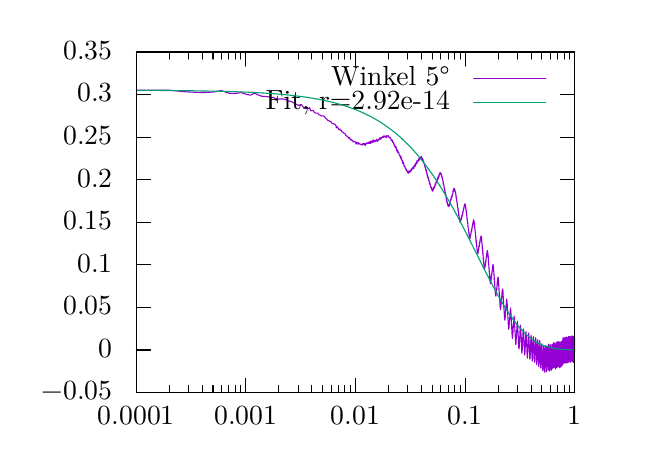
\begin{tikzpicture}[gnuplot]
%% generated with GNUPLOT 5.2p5a (Gentoo revision r0) (Lua 5.1; terminal rev. 99 , script rev. 107)
%% Sa 18 Mai 2019 18:31:07 CEST
\path (0.000,0.000) rectangle (7.500,5.250);
\gpcolor{color=gp lt color border}
\gpsetlinetype{gp lt border}
\gpsetdashtype{gp dt solid}
\gpsetlinewidth{1.00}
\draw[gp path] (1.380,0.616)--(1.560,0.616);
\draw[gp path] (6.947,0.616)--(6.767,0.616);
\node[gp node right] at (1.196,0.616) {$-0.05$};
\draw[gp path] (1.380,1.157)--(1.560,1.157);
\draw[gp path] (6.947,1.157)--(6.767,1.157);
\node[gp node right] at (1.196,1.157) {$0$};
\draw[gp path] (1.380,1.697)--(1.560,1.697);
\draw[gp path] (6.947,1.697)--(6.767,1.697);
\node[gp node right] at (1.196,1.697) {$0.05$};
\draw[gp path] (1.380,2.238)--(1.560,2.238);
\draw[gp path] (6.947,2.238)--(6.767,2.238);
\node[gp node right] at (1.196,2.238) {$0.1$};
\draw[gp path] (1.380,2.779)--(1.560,2.779);
\draw[gp path] (6.947,2.779)--(6.767,2.779);
\node[gp node right] at (1.196,2.779) {$0.15$};
\draw[gp path] (1.380,3.319)--(1.560,3.319);
\draw[gp path] (6.947,3.319)--(6.767,3.319);
\node[gp node right] at (1.196,3.319) {$0.2$};
\draw[gp path] (1.380,3.860)--(1.560,3.860);
\draw[gp path] (6.947,3.860)--(6.767,3.860);
\node[gp node right] at (1.196,3.860) {$0.25$};
\draw[gp path] (1.380,4.400)--(1.560,4.400);
\draw[gp path] (6.947,4.400)--(6.767,4.400);
\node[gp node right] at (1.196,4.400) {$0.3$};
\draw[gp path] (1.380,4.941)--(1.560,4.941);
\draw[gp path] (6.947,4.941)--(6.767,4.941);
\node[gp node right] at (1.196,4.941) {$0.35$};
\draw[gp path] (1.380,0.616)--(1.380,0.796);
\draw[gp path] (1.380,4.941)--(1.380,4.761);
\node[gp node center] at (1.380,0.308) {$0.0001$};
\draw[gp path] (1.799,0.616)--(1.799,0.706);
\draw[gp path] (1.799,4.941)--(1.799,4.851);
\draw[gp path] (2.044,0.616)--(2.044,0.706);
\draw[gp path] (2.044,4.941)--(2.044,4.851);
\draw[gp path] (2.218,0.616)--(2.218,0.706);
\draw[gp path] (2.218,4.941)--(2.218,4.851);
\draw[gp path] (2.353,0.616)--(2.353,0.706);
\draw[gp path] (2.353,4.941)--(2.353,4.851);
\draw[gp path] (2.463,0.616)--(2.463,0.706);
\draw[gp path] (2.463,4.941)--(2.463,4.851);
\draw[gp path] (2.556,0.616)--(2.556,0.706);
\draw[gp path] (2.556,4.941)--(2.556,4.851);
\draw[gp path] (2.637,0.616)--(2.637,0.706);
\draw[gp path] (2.637,4.941)--(2.637,4.851);
\draw[gp path] (2.708,0.616)--(2.708,0.706);
\draw[gp path] (2.708,4.941)--(2.708,4.851);
\draw[gp path] (2.772,0.616)--(2.772,0.796);
\draw[gp path] (2.772,4.941)--(2.772,4.761);
\node[gp node center] at (2.772,0.308) {$0.001$};
\draw[gp path] (3.191,0.616)--(3.191,0.706);
\draw[gp path] (3.191,4.941)--(3.191,4.851);
\draw[gp path] (3.436,0.616)--(3.436,0.706);
\draw[gp path] (3.436,4.941)--(3.436,4.851);
\draw[gp path] (3.610,0.616)--(3.610,0.706);
\draw[gp path] (3.610,4.941)--(3.610,4.851);
\draw[gp path] (3.745,0.616)--(3.745,0.706);
\draw[gp path] (3.745,4.941)--(3.745,4.851);
\draw[gp path] (3.855,0.616)--(3.855,0.706);
\draw[gp path] (3.855,4.941)--(3.855,4.851);
\draw[gp path] (3.948,0.616)--(3.948,0.706);
\draw[gp path] (3.948,4.941)--(3.948,4.851);
\draw[gp path] (4.029,0.616)--(4.029,0.706);
\draw[gp path] (4.029,4.941)--(4.029,4.851);
\draw[gp path] (4.100,0.616)--(4.100,0.706);
\draw[gp path] (4.100,4.941)--(4.100,4.851);
\draw[gp path] (4.163,0.616)--(4.163,0.796);
\draw[gp path] (4.163,4.941)--(4.163,4.761);
\node[gp node center] at (4.163,0.308) {$0.01$};
\draw[gp path] (4.582,0.616)--(4.582,0.706);
\draw[gp path] (4.582,4.941)--(4.582,4.851);
\draw[gp path] (4.828,0.616)--(4.828,0.706);
\draw[gp path] (4.828,4.941)--(4.828,4.851);
\draw[gp path] (5.001,0.616)--(5.001,0.706);
\draw[gp path] (5.001,4.941)--(5.001,4.851);
\draw[gp path] (5.136,0.616)--(5.136,0.706);
\draw[gp path] (5.136,4.941)--(5.136,4.851);
\draw[gp path] (5.246,0.616)--(5.246,0.706);
\draw[gp path] (5.246,4.941)--(5.246,4.851);
\draw[gp path] (5.340,0.616)--(5.340,0.706);
\draw[gp path] (5.340,4.941)--(5.340,4.851);
\draw[gp path] (5.420,0.616)--(5.420,0.706);
\draw[gp path] (5.420,4.941)--(5.420,4.851);
\draw[gp path] (5.492,0.616)--(5.492,0.706);
\draw[gp path] (5.492,4.941)--(5.492,4.851);
\draw[gp path] (5.555,0.616)--(5.555,0.796);
\draw[gp path] (5.555,4.941)--(5.555,4.761);
\node[gp node center] at (5.555,0.308) {$0.1$};
\draw[gp path] (5.974,0.616)--(5.974,0.706);
\draw[gp path] (5.974,4.941)--(5.974,4.851);
\draw[gp path] (6.219,0.616)--(6.219,0.706);
\draw[gp path] (6.219,4.941)--(6.219,4.851);
\draw[gp path] (6.393,0.616)--(6.393,0.706);
\draw[gp path] (6.393,4.941)--(6.393,4.851);
\draw[gp path] (6.528,0.616)--(6.528,0.706);
\draw[gp path] (6.528,4.941)--(6.528,4.851);
\draw[gp path] (6.638,0.616)--(6.638,0.706);
\draw[gp path] (6.638,4.941)--(6.638,4.851);
\draw[gp path] (6.731,0.616)--(6.731,0.706);
\draw[gp path] (6.731,4.941)--(6.731,4.851);
\draw[gp path] (6.812,0.616)--(6.812,0.706);
\draw[gp path] (6.812,4.941)--(6.812,4.851);
\draw[gp path] (6.883,0.616)--(6.883,0.706);
\draw[gp path] (6.883,4.941)--(6.883,4.851);
\draw[gp path] (6.947,0.616)--(6.947,0.796);
\draw[gp path] (6.947,4.941)--(6.947,4.761);
\node[gp node center] at (6.947,0.308) {$1$};
\draw[gp path] (1.380,4.941)--(1.380,0.616)--(6.947,0.616)--(6.947,4.941)--cycle;
\node[gp node right] at (5.479,4.607) {Winkel 5°};
\gpcolor{rgb color={0.580,0.000,0.827}}
\draw[gp path] (5.663,4.607)--(6.579,4.607);
\draw[gp path] (1.380,4.457)--(1.799,4.455)--(2.044,4.433)--(2.218,4.426)--(2.353,4.432)%
  --(2.463,4.450)--(2.556,4.418)--(2.637,4.413)--(2.708,4.426)--(2.772,4.405)--(2.829,4.393)%
  --(2.882,4.418)--(2.930,4.394)--(2.975,4.379)--(3.017,4.377)--(3.056,4.372)--(3.092,4.362)%
  --(3.127,4.363)--(3.160,4.337)--(3.191,4.344)--(3.220,4.344)--(3.248,4.345)--(3.275,4.338)%
  --(3.301,4.323)--(3.326,4.315)--(3.349,4.312)--(3.372,4.298)--(3.394,4.289)--(3.415,4.274)%
  --(3.436,4.265)--(3.456,4.266)--(3.475,4.273)--(3.493,4.250)--(3.511,4.224)--(3.529,4.229)%
  --(3.546,4.242)--(3.563,4.220)--(3.579,4.235)--(3.594,4.194)--(3.610,4.196)--(3.625,4.199)%
  --(3.639,4.176)--(3.653,4.166)--(3.667,4.164)--(3.681,4.164)--(3.694,4.151)--(3.707,4.139)%
  --(3.720,4.138)--(3.732,4.128)--(3.745,4.130)--(3.757,4.129)--(3.768,4.121)--(3.780,4.107)%
  --(3.791,4.091)--(3.802,4.089)--(3.813,4.067)--(3.824,4.068)--(3.834,4.063)--(3.845,4.060)%
  --(3.855,4.051)--(3.865,4.035)--(3.875,4.034)--(3.884,4.028)--(3.894,4.026)--(3.903,4.020)%
  --(3.912,4.015)--(3.921,3.978)--(3.930,3.992)--(3.939,3.979)--(3.948,3.963)--(3.956,3.953)%
  --(3.965,3.963)--(3.973,3.947)--(3.982,3.947)--(3.990,3.928)--(3.998,3.922)--(4.006,3.924)%
  --(4.013,3.912)--(4.021,3.907)--(4.029,3.905)--(4.036,3.891)--(4.044,3.877)--(4.051,3.878)%
  --(4.058,3.865)--(4.065,3.859)--(4.072,3.861)--(4.079,3.844)--(4.086,3.855)--(4.093,3.836)%
  --(4.100,3.834)--(4.106,3.822)--(4.113,3.831)--(4.120,3.816)--(4.126,3.818)--(4.132,3.800)%
  --(4.139,3.802)--(4.145,3.799)--(4.151,3.805)--(4.157,3.800)--(4.164,3.798)--(4.170,3.772)%
  --(4.175,3.778)--(4.181,3.797)--(4.187,3.783)--(4.193,3.783)--(4.199,3.769)--(4.204,3.789)%
  --(4.210,3.776)--(4.216,3.774)--(4.221,3.773)--(4.227,3.771)--(4.232,3.766)--(4.237,3.768)%
  --(4.243,3.759)--(4.248,3.762)--(4.253,3.766)--(4.258,3.780)--(4.264,3.770)--(4.269,3.781)%
  --(4.274,3.763)--(4.279,3.777)--(4.284,3.777)--(4.289,3.753)--(4.294,3.775)--(4.298,3.782)%
  --(4.303,3.785)--(4.308,3.776)--(4.313,3.784)--(4.317,3.780)--(4.322,3.792)--(4.327,3.780)%
  --(4.331,3.795)--(4.336,3.793)--(4.340,3.778)--(4.345,3.792)--(4.349,3.810)--(4.354,3.780)%
  --(4.358,3.787)--(4.363,3.789)--(4.367,3.807)--(4.371,3.812)--(4.375,3.794)--(4.380,3.817)%
  --(4.384,3.795)--(4.388,3.801)--(4.392,3.823)--(4.396,3.810)--(4.400,3.800)--(4.405,3.815)%
  --(4.409,3.804)--(4.413,3.803)--(4.417,3.816)--(4.421,3.817)--(4.424,3.824)--(4.428,3.820)%
  --(4.432,3.833)--(4.436,3.804)--(4.440,3.808)--(4.444,3.818)--(4.448,3.813)--(4.451,3.821)%
  --(4.455,3.829)--(4.459,3.824)--(4.463,3.839)--(4.466,3.842)--(4.470,3.827)--(4.473,3.855)%
  --(4.477,3.844)--(4.481,3.835)--(4.484,3.835)--(4.488,3.838)--(4.491,3.842)--(4.495,3.858)%
  --(4.498,3.860)--(4.502,3.853)--(4.505,3.864)--(4.509,3.861)--(4.512,3.865)--(4.515,3.866)%
  --(4.519,3.855)--(4.522,3.876)--(4.525,3.862)--(4.529,3.859)--(4.532,3.866)--(4.535,3.874)%
  --(4.539,3.873)--(4.542,3.861)--(4.545,3.869)--(4.548,3.873)--(4.551,3.866)--(4.555,3.878)%
  --(4.558,3.853)--(4.561,3.866)--(4.564,3.872)--(4.567,3.876)--(4.570,3.872)--(4.573,3.873)%
  --(4.576,3.878)--(4.579,3.870)--(4.582,3.878)--(4.585,3.861)--(4.588,3.864)--(4.591,3.864)%
  --(4.594,3.850)--(4.597,3.854)--(4.600,3.855)--(4.603,3.860)--(4.606,3.847)--(4.609,3.845)%
  --(4.612,3.846)--(4.615,3.831)--(4.618,3.816)--(4.621,3.826)--(4.623,3.816)--(4.626,3.823)%
  --(4.629,3.807)--(4.632,3.822)--(4.635,3.809)--(4.637,3.790)--(4.640,3.800)--(4.643,3.792)%
  --(4.646,3.779)--(4.648,3.775)--(4.651,3.772)--(4.654,3.775)--(4.656,3.757)--(4.659,3.746)%
  --(4.662,3.743)--(4.664,3.754)--(4.667,3.740)--(4.670,3.730)--(4.672,3.736)--(4.675,3.720)%
  --(4.677,3.738)--(4.680,3.721)--(4.683,3.713)--(4.685,3.686)--(4.688,3.689)--(4.690,3.694)%
  --(4.693,3.700)--(4.695,3.688)--(4.698,3.667)--(4.700,3.688)--(4.703,3.676)--(4.705,3.674)%
  --(4.708,3.667)--(4.710,3.662)--(4.712,3.667)--(4.715,3.647)--(4.717,3.646)--(4.720,3.634)%
  --(4.722,3.634)--(4.725,3.623)--(4.727,3.627)--(4.729,3.626)--(4.732,3.605)--(4.734,3.602)%
  --(4.736,3.594)--(4.739,3.617)--(4.741,3.586)--(4.743,3.604)--(4.746,3.589)--(4.748,3.577)%
  --(4.750,3.578)--(4.753,3.556)--(4.755,3.568)--(4.757,3.560)--(4.759,3.566)--(4.762,3.560)%
  --(4.764,3.525)--(4.766,3.548)--(4.768,3.543)--(4.771,3.533)--(4.773,3.518)--(4.775,3.536)%
  --(4.777,3.511)--(4.779,3.495)--(4.781,3.494)--(4.784,3.492)--(4.786,3.486)--(4.788,3.496)%
  --(4.790,3.485)--(4.792,3.480)--(4.794,3.475)--(4.797,3.470)--(4.799,3.454)--(4.801,3.458)%
  --(4.803,3.458)--(4.805,3.458)--(4.807,3.439)--(4.809,3.451)--(4.811,3.438)--(4.813,3.432)%
  --(4.815,3.431)--(4.817,3.438)--(4.819,3.424)--(4.821,3.427)--(4.823,3.430)--(4.826,3.414)%
  --(4.828,3.410)--(4.830,3.413)--(4.832,3.399)--(4.834,3.404)--(4.836,3.406)--(4.838,3.420)%
  --(4.840,3.430)--(4.841,3.418)--(4.843,3.426)--(4.845,3.418)--(4.847,3.427)--(4.849,3.410)%
  --(4.851,3.421)--(4.853,3.432)--(4.855,3.417)--(4.857,3.420)--(4.859,3.422)--(4.861,3.429)%
  --(4.863,3.433)--(4.865,3.441)--(4.867,3.425)--(4.868,3.428)--(4.870,3.450)--(4.872,3.432)%
  --(4.874,3.453)--(4.876,3.458)--(4.878,3.454)--(4.880,3.446)--(4.881,3.457)--(4.883,3.464)%
  --(4.885,3.455)--(4.887,3.464)--(4.889,3.474)--(4.891,3.468)--(4.892,3.463)--(4.894,3.474)%
  --(4.896,3.481)--(4.898,3.479)--(4.900,3.478)--(4.901,3.465)--(4.903,3.459)--(4.905,3.474)%
  --(4.907,3.479)--(4.908,3.501)--(4.910,3.488)--(4.912,3.497)--(4.914,3.490)--(4.916,3.507)%
  --(4.917,3.505)--(4.919,3.512)--(4.921,3.488)--(4.922,3.495)--(4.924,3.511)--(4.926,3.525)%
  --(4.928,3.528)--(4.929,3.526)--(4.931,3.516)--(4.933,3.515)--(4.934,3.524)--(4.936,3.525)%
  --(4.938,3.527)--(4.939,3.544)--(4.941,3.528)--(4.943,3.547)--(4.944,3.560)--(4.946,3.530)%
  --(4.948,3.552)--(4.949,3.543)--(4.951,3.540)--(4.953,3.552)--(4.954,3.557)--(4.956,3.559)%
  --(4.958,3.558)--(4.959,3.552)--(4.961,3.572)--(4.962,3.573)--(4.964,3.569)--(4.966,3.565)%
  --(4.967,3.588)--(4.969,3.582)--(4.970,3.566)--(4.972,3.581)--(4.974,3.567)--(4.975,3.590)%
  --(4.977,3.585)--(4.978,3.600)--(4.980,3.580)--(4.981,3.596)--(4.983,3.598)--(4.985,3.583)%
  --(4.986,3.587)--(4.988,3.604)--(4.989,3.599)--(4.991,3.601)--(4.992,3.599)--(4.994,3.603)%
  --(4.995,3.596)--(4.997,3.583)--(4.998,3.617)--(5.000,3.599)--(5.001,3.604)--(5.003,3.595)%
  --(5.004,3.597)--(5.006,3.593)--(5.007,3.575)--(5.009,3.584)--(5.010,3.596)--(5.012,3.577)%
  --(5.013,3.578)--(5.015,3.576)--(5.016,3.580)--(5.018,3.573)--(5.019,3.558)--(5.021,3.578)%
  --(5.022,3.559)--(5.024,3.551)--(5.025,3.549)--(5.027,3.554)--(5.028,3.540)--(5.029,3.547)%
  --(5.031,3.540)--(5.032,3.531)--(5.034,3.522)--(5.035,3.527)--(5.037,3.518)--(5.038,3.524)%
  --(5.039,3.523)--(5.041,3.504)--(5.042,3.496)--(5.044,3.491)--(5.045,3.480)--(5.047,3.481)%
  --(5.048,3.487)--(5.049,3.467)--(5.051,3.468)--(5.052,3.460)--(5.054,3.460)--(5.055,3.458)%
  --(5.056,3.453)--(5.058,3.442)--(5.059,3.429)--(5.060,3.452)--(5.062,3.443)--(5.063,3.426)%
  --(5.064,3.424)--(5.066,3.408)--(5.067,3.399)--(5.069,3.415)--(5.070,3.395)--(5.071,3.398)%
  --(5.073,3.376)--(5.074,3.388)--(5.075,3.364)--(5.077,3.373)--(5.078,3.384)--(5.079,3.381)%
  --(5.081,3.344)--(5.082,3.350)--(5.083,3.351)--(5.085,3.338)--(5.086,3.355)--(5.087,3.349)%
  --(5.089,3.340)--(5.090,3.331)--(5.091,3.310)--(5.092,3.323)--(5.094,3.330)--(5.095,3.313)%
  --(5.096,3.313)--(5.098,3.307)--(5.099,3.302)--(5.100,3.288)--(5.101,3.298)--(5.103,3.274)%
  --(5.104,3.267)--(5.105,3.270)--(5.107,3.275)--(5.108,3.264)--(5.109,3.255)--(5.110,3.276)%
  --(5.112,3.251)--(5.113,3.256)--(5.114,3.257)--(5.115,3.237)--(5.117,3.240)--(5.118,3.238)%
  --(5.119,3.228)--(5.120,3.221)--(5.122,3.218)--(5.123,3.220)--(5.124,3.212)--(5.125,3.211)%
  --(5.127,3.226)--(5.128,3.206)--(5.129,3.216)--(5.130,3.205)--(5.131,3.204)--(5.133,3.189)%
  --(5.134,3.187)--(5.135,3.190)--(5.136,3.194)--(5.137,3.183)--(5.139,3.192)--(5.140,3.195)%
  --(5.141,3.173)--(5.142,3.182)--(5.144,3.189)--(5.145,3.186)--(5.146,3.204)--(5.147,3.198)%
  --(5.148,3.203)--(5.149,3.185)--(5.151,3.193)--(5.152,3.206)--(5.153,3.193)--(5.154,3.225)%
  --(5.155,3.208)--(5.157,3.208)--(5.158,3.206)--(5.159,3.209)--(5.160,3.208)--(5.161,3.214)%
  --(5.162,3.216)--(5.163,3.231)--(5.165,3.220)--(5.166,3.218)--(5.167,3.224)--(5.168,3.218)%
  --(5.169,3.229)--(5.170,3.235)--(5.172,3.256)--(5.173,3.250)--(5.174,3.262)--(5.175,3.245)%
  --(5.176,3.244)--(5.177,3.273)--(5.178,3.256)--(5.179,3.256)--(5.181,3.265)--(5.182,3.276)%
  --(5.183,3.267)--(5.184,3.264)--(5.185,3.282)--(5.186,3.290)--(5.187,3.279)--(5.188,3.294)%
  --(5.189,3.293)--(5.191,3.286)--(5.192,3.282)--(5.193,3.314)--(5.194,3.289)--(5.195,3.300)%
  --(5.196,3.313)--(5.197,3.307)--(5.198,3.305)--(5.199,3.299)--(5.200,3.323)--(5.202,3.319)%
  --(5.203,3.317)--(5.204,3.309)--(5.205,3.339)--(5.206,3.335)--(5.207,3.325)--(5.208,3.323)%
  --(5.209,3.335)--(5.210,3.345)--(5.211,3.343)--(5.212,3.336)--(5.213,3.361)--(5.214,3.352)%
  --(5.215,3.343)--(5.217,3.335)--(5.218,3.361)--(5.219,3.364)--(5.220,3.370)--(5.221,3.367)%
  --(5.222,3.378)--(5.223,3.376)--(5.224,3.382)--(5.225,3.356)--(5.226,3.376)--(5.227,3.374)%
  --(5.228,3.389)--(5.229,3.393)--(5.230,3.383)--(5.231,3.382)--(5.232,3.386)--(5.233,3.391)%
  --(5.234,3.397)--(5.235,3.393)--(5.236,3.410)--(5.237,3.391)--(5.238,3.401)--(5.239,3.397)%
  --(5.240,3.410)--(5.241,3.394)--(5.242,3.407)--(5.243,3.404)--(5.244,3.396)--(5.245,3.401)%
  --(5.246,3.398)--(5.247,3.399)--(5.249,3.395)--(5.250,3.392)--(5.251,3.396)--(5.252,3.380)%
  --(5.253,3.378)--(5.254,3.393)--(5.254,3.376)--(5.255,3.377)--(5.256,3.365)--(5.257,3.363)%
  --(5.258,3.375)--(5.259,3.356)--(5.260,3.363)--(5.261,3.362)--(5.262,3.354)--(5.263,3.347)%
  --(5.264,3.350)--(5.265,3.334)--(5.266,3.346)--(5.267,3.328)--(5.268,3.317)--(5.269,3.328)%
  --(5.270,3.321)--(5.271,3.315)--(5.272,3.307)--(5.273,3.306)--(5.274,3.298)--(5.275,3.301)%
  --(5.276,3.297)--(5.277,3.292)--(5.278,3.271)--(5.279,3.256)--(5.280,3.269)--(5.281,3.258)%
  --(5.282,3.248)--(5.283,3.250)--(5.284,3.256)--(5.285,3.243)--(5.286,3.252)--(5.286,3.245)%
  --(5.287,3.237)--(5.288,3.227)--(5.289,3.218)--(5.290,3.208)--(5.291,3.221)--(5.292,3.203)%
  --(5.293,3.194)--(5.294,3.206)--(5.295,3.213)--(5.296,3.182)--(5.297,3.195)--(5.298,3.177)%
  --(5.299,3.183)--(5.300,3.177)--(5.300,3.150)--(5.301,3.152)--(5.302,3.160)--(5.303,3.155)%
  --(5.304,3.155)--(5.305,3.145)--(5.306,3.144)--(5.307,3.130)--(5.308,3.129)--(5.309,3.135)%
  --(5.310,3.112)--(5.310,3.133)--(5.311,3.113)--(5.312,3.113)--(5.313,3.107)--(5.314,3.103)%
  --(5.315,3.089)--(5.316,3.089)--(5.317,3.065)--(5.318,3.082)--(5.319,3.064)--(5.319,3.058)%
  --(5.320,3.068)--(5.321,3.056)--(5.322,3.053)--(5.323,3.035)--(5.324,3.058)--(5.325,3.038)%
  --(5.326,3.040)--(5.327,3.025)--(5.327,3.022)--(5.328,3.037)--(5.329,3.013)--(5.330,3.011)%
  --(5.331,3.013)--(5.332,3.012)--(5.333,3.004)--(5.334,2.996)--(5.334,3.008)--(5.335,3.007)%
  --(5.336,2.993)--(5.337,3.000)--(5.338,2.993)--(5.339,2.988)--(5.340,2.997)--(5.341,2.977)%
  --(5.341,2.992)--(5.342,2.990)--(5.343,2.977)--(5.344,2.991)--(5.345,2.999)--(5.346,3.003)%
  --(5.347,2.993)--(5.347,2.999)--(5.348,2.997)--(5.349,2.980)--(5.350,3.003)--(5.351,2.984)%
  --(5.352,2.992)--(5.352,2.997)--(5.353,2.990)--(5.354,2.996)--(5.355,3.002)--(5.356,3.012)%
  --(5.357,3.014)--(5.358,2.988)--(5.358,3.017)--(5.359,2.999)--(5.360,3.019)--(5.361,3.000)%
  --(5.362,3.028)--(5.363,3.026)--(5.363,3.020)--(5.364,3.023)--(5.365,3.027)--(5.366,3.045)%
  --(5.367,3.046)--(5.368,3.051)--(5.368,3.050)--(5.369,3.057)--(5.370,3.053)--(5.371,3.071)%
  --(5.372,3.064)--(5.372,3.066)--(5.373,3.056)--(5.374,3.065)--(5.375,3.077)--(5.376,3.069)%
  --(5.377,3.070)--(5.377,3.072)--(5.378,3.074)--(5.379,3.081)--(5.380,3.100)--(5.381,3.090)%
  --(5.381,3.083)--(5.382,3.074)--(5.383,3.099)--(5.384,3.096)--(5.385,3.089)--(5.385,3.110)%
  --(5.386,3.112)--(5.387,3.106)--(5.388,3.099)--(5.389,3.106)--(5.389,3.104)--(5.390,3.119)%
  --(5.391,3.133)--(5.392,3.123)--(5.393,3.118)--(5.393,3.133)--(5.394,3.135)--(5.395,3.135)%
  --(5.396,3.134)--(5.397,3.138)--(5.398,3.145)--(5.399,3.142)--(5.400,3.141)--(5.400,3.153)%
  --(5.401,3.158)--(5.402,3.179)--(5.403,3.175)--(5.404,3.167)--(5.404,3.162)--(5.405,3.169)%
  --(5.406,3.181)--(5.407,3.169)--(5.407,3.183)--(5.408,3.184)--(5.409,3.198)--(5.410,3.172)%
  --(5.410,3.169)--(5.411,3.187)--(5.412,3.211)--(5.413,3.197)--(5.414,3.192)--(5.414,3.197)%
  --(5.415,3.202)--(5.416,3.187)--(5.417,3.185)--(5.417,3.197)--(5.418,3.202)--(5.419,3.206)%
  --(5.420,3.195)--(5.420,3.188)--(5.421,3.196)--(5.422,3.195)--(5.423,3.191)--(5.423,3.187)%
  --(5.424,3.181)--(5.425,3.186)--(5.426,3.185)--(5.426,3.187)--(5.427,3.188)--(5.428,3.175)%
  --(5.429,3.165)--(5.429,3.173)--(5.430,3.167)--(5.431,3.160)--(5.432,3.156)--(5.432,3.153)%
  --(5.433,3.160)--(5.434,3.146)--(5.435,3.139)--(5.435,3.142)--(5.436,3.149)--(5.437,3.132)%
  --(5.438,3.129)--(5.438,3.107)--(5.439,3.122)--(5.440,3.108)--(5.440,3.123)--(5.441,3.091)%
  --(5.442,3.105)--(5.443,3.098)--(5.443,3.086)--(5.444,3.070)--(5.445,3.080)--(5.446,3.084)%
  --(5.446,3.072)--(5.447,3.065)--(5.448,3.059)--(5.448,3.043)--(5.449,3.043)--(5.450,3.049)%
  --(5.451,3.039)--(5.451,3.040)--(5.452,3.039)--(5.453,3.041)--(5.453,3.035)--(5.454,3.010)%
  --(5.455,3.006)--(5.456,3.016)--(5.456,3.004)--(5.457,2.991)--(5.458,2.979)--(5.458,2.992)%
  --(5.459,2.988)--(5.460,2.972)--(5.461,2.968)--(5.461,2.969)--(5.462,2.962)--(5.463,2.958)%
  --(5.463,2.961)--(5.464,2.939)--(5.465,2.934)--(5.465,2.942)--(5.466,2.931)--(5.467,2.954)%
  --(5.468,2.923)--(5.468,2.930)--(5.469,2.930)--(5.470,2.909)--(5.470,2.913)--(5.471,2.911)%
  --(5.472,2.902)--(5.472,2.896)--(5.473,2.895)--(5.474,2.865)--(5.475,2.882)--(5.475,2.886)%
  --(5.476,2.880)--(5.477,2.868)--(5.477,2.869)--(5.478,2.866)--(5.479,2.867)--(5.479,2.842)%
  --(5.480,2.841)--(5.481,2.842)--(5.481,2.836)--(5.482,2.829)--(5.483,2.817)--(5.483,2.819)%
  --(5.484,2.817)--(5.485,2.815)--(5.485,2.831)--(5.486,2.818)--(5.487,2.811)--(5.488,2.803)%
  --(5.488,2.813)--(5.489,2.801)--(5.490,2.801)--(5.490,2.778)--(5.491,2.799)--(5.492,2.791)%
  --(5.492,2.804)--(5.493,2.773)--(5.494,2.805)--(5.494,2.795)--(5.495,2.792)--(5.496,2.788)%
  --(5.496,2.808)--(5.497,2.798)--(5.498,2.806)--(5.498,2.800)--(5.499,2.795)--(5.500,2.804)%
  --(5.500,2.803)--(5.501,2.792)--(5.502,2.811)--(5.502,2.806)--(5.503,2.819)--(5.504,2.825)%
  --(5.505,2.820)--(5.506,2.826)--(5.506,2.812)--(5.507,2.827)--(5.507,2.816)--(5.508,2.828)%
  --(5.509,2.833)--(5.510,2.839)--(5.511,2.832)--(5.511,2.857)--(5.512,2.853)--(5.513,2.847)%
  --(5.513,2.844)--(5.514,2.851)--(5.515,2.849)--(5.515,2.855)--(5.516,2.868)--(5.517,2.872)%
  --(5.517,2.849)--(5.518,2.845)--(5.518,2.866)--(5.519,2.876)--(5.520,2.866)--(5.520,2.878)%
  --(5.521,2.881)--(5.522,2.881)--(5.522,2.878)--(5.523,2.876)--(5.524,2.891)--(5.524,2.906)%
  --(5.525,2.893)--(5.526,2.891)--(5.526,2.894)--(5.527,2.904)--(5.527,2.906)--(5.528,2.914)%
  --(5.529,2.905)--(5.529,2.917)--(5.530,2.926)--(5.531,2.928)--(5.531,2.920)--(5.532,2.925)%
  --(5.532,2.931)--(5.533,2.939)--(5.534,2.937)--(5.534,2.930)--(5.535,2.941)--(5.536,2.929)%
  --(5.536,2.953)--(5.537,2.945)--(5.537,2.949)--(5.538,2.952)--(5.539,2.964)--(5.539,2.958)%
  --(5.540,2.961)--(5.541,2.958)--(5.541,2.977)--(5.542,2.967)--(5.542,2.977)--(5.543,2.981)%
  --(5.544,2.979)--(5.544,2.984)--(5.545,2.986)--(5.546,2.987)--(5.546,2.977)--(5.547,3.006)%
  --(5.547,2.986)--(5.548,2.996)--(5.549,2.997)--(5.549,3.009)--(5.550,2.994)--(5.550,3.001)%
  --(5.551,2.987)--(5.552,3.003)--(5.552,2.990)--(5.553,3.002)--(5.553,3.005)--(5.554,3.007)%
  --(5.555,2.997)--(5.555,2.998)--(5.556,3.012)--(5.556,2.989)--(5.557,2.992)--(5.558,2.994)%
  --(5.558,3.011)--(5.559,2.984)--(5.559,2.983)--(5.560,2.981)--(5.561,2.980)--(5.561,2.985)%
  --(5.562,2.978)--(5.562,2.963)--(5.563,2.959)--(5.564,2.961)--(5.564,2.964)--(5.565,2.972)%
  --(5.565,2.949)--(5.566,2.948)--(5.567,2.936)--(5.567,2.944)--(5.568,2.932)--(5.568,2.921)%
  --(5.569,2.933)--(5.570,2.931)--(5.570,2.909)--(5.571,2.901)--(5.571,2.915)--(5.572,2.892)%
  --(5.573,2.893)--(5.573,2.885)--(5.574,2.890)--(5.574,2.868)--(5.575,2.873)--(5.575,2.872)%
  --(5.576,2.870)--(5.577,2.856)--(5.577,2.863)--(5.578,2.838)--(5.578,2.848)--(5.579,2.841)%
  --(5.580,2.840)--(5.580,2.825)--(5.581,2.834)--(5.581,2.829)--(5.582,2.811)--(5.582,2.814)%
  --(5.583,2.816)--(5.584,2.805)--(5.584,2.807)--(5.585,2.805)--(5.585,2.790)--(5.586,2.792)%
  --(5.586,2.772)--(5.587,2.769)--(5.588,2.791)--(5.588,2.773)--(5.589,2.764)--(5.589,2.770)%
  --(5.590,2.748)--(5.590,2.745)--(5.591,2.735)--(5.592,2.733)--(5.592,2.721)--(5.593,2.730)%
  --(5.593,2.729)--(5.594,2.730)--(5.594,2.717)--(5.595,2.700)--(5.596,2.701)--(5.596,2.706)%
  --(5.597,2.687)--(5.597,2.693)--(5.598,2.683)--(5.598,2.678)--(5.599,2.678)--(5.600,2.668)%
  --(5.601,2.648)--(5.601,2.654)--(5.602,2.646)--(5.602,2.662)--(5.603,2.650)--(5.603,2.641)%
  --(5.604,2.648)--(5.605,2.641)--(5.605,2.624)--(5.606,2.627)--(5.606,2.616)--(5.607,2.608)%
  --(5.607,2.610)--(5.608,2.607)--(5.608,2.612)--(5.609,2.626)--(5.610,2.607)--(5.610,2.603)%
  --(5.611,2.600)--(5.611,2.586)--(5.612,2.593)--(5.612,2.584)--(5.613,2.577)--(5.613,2.582)%
  --(5.614,2.585)--(5.615,2.588)--(5.615,2.582)--(5.616,2.592)--(5.616,2.582)--(5.617,2.605)%
  --(5.617,2.591)--(5.618,2.568)--(5.618,2.594)--(5.619,2.584)--(5.619,2.595)--(5.620,2.593)%
  --(5.621,2.597)--(5.621,2.602)--(5.622,2.605)--(5.622,2.602)--(5.623,2.599)--(5.623,2.606)%
  --(5.624,2.622)--(5.624,2.616)--(5.625,2.614)--(5.625,2.611)--(5.626,2.613)--(5.626,2.620)%
  --(5.627,2.622)--(5.628,2.618)--(5.628,2.632)--(5.629,2.634)--(5.629,2.644)--(5.630,2.645)%
  --(5.630,2.636)--(5.631,2.643)--(5.631,2.650)--(5.632,2.655)--(5.632,2.656)--(5.633,2.668)%
  --(5.633,2.663)--(5.634,2.661)--(5.634,2.673)--(5.635,2.657)--(5.636,2.669)--(5.636,2.655)%
  --(5.637,2.664)--(5.637,2.682)--(5.638,2.678)--(5.638,2.666)--(5.639,2.677)--(5.640,2.676)%
  --(5.640,2.690)--(5.641,2.687)--(5.641,2.695)--(5.642,2.702)--(5.642,2.711)--(5.643,2.702)%
  --(5.643,2.716)--(5.644,2.699)--(5.644,2.712)--(5.645,2.707)--(5.645,2.719)--(5.646,2.724)%
  --(5.647,2.724)--(5.647,2.723)--(5.648,2.727)--(5.648,2.717)--(5.649,2.734)--(5.649,2.744)%
  --(5.650,2.732)--(5.650,2.725)--(5.651,2.736)--(5.651,2.751)--(5.652,2.759)--(5.652,2.753)%
  --(5.653,2.761)--(5.653,2.752)--(5.654,2.757)--(5.654,2.768)--(5.655,2.769)--(5.655,2.770)%
  --(5.656,2.772)--(5.656,2.751)--(5.657,2.783)--(5.657,2.778)--(5.658,2.781)--(5.658,2.786)%
  --(5.659,2.784)--(5.659,2.789)--(5.660,2.799)--(5.660,2.800)--(5.661,2.776)--(5.661,2.800)%
  --(5.662,2.805)--(5.662,2.789)--(5.663,2.790)--(5.663,2.802)--(5.664,2.798)--(5.664,2.808)%
  --(5.665,2.802)--(5.665,2.801)--(5.666,2.801)--(5.666,2.812)--(5.667,2.786)--(5.667,2.797)%
  --(5.668,2.792)--(5.668,2.787)--(5.669,2.780)--(5.669,2.783)--(5.670,2.784)--(5.670,2.753)%
  --(5.671,2.778)--(5.671,2.773)--(5.672,2.760)--(5.672,2.758)--(5.673,2.753)--(5.673,2.755)%
  --(5.674,2.770)--(5.674,2.743)--(5.675,2.725)--(5.675,2.729)--(5.676,2.742)--(5.676,2.718)%
  --(5.677,2.727)--(5.677,2.708)--(5.678,2.713)--(5.678,2.705)--(5.679,2.711)--(5.679,2.699)%
  --(5.680,2.692)--(5.680,2.683)--(5.681,2.689)--(5.681,2.683)--(5.682,2.673)--(5.682,2.672)%
  --(5.683,2.662)--(5.683,2.656)--(5.684,2.662)--(5.684,2.657)--(5.685,2.649)--(5.685,2.645)%
  --(5.686,2.633)--(5.686,2.634)--(5.687,2.618)--(5.687,2.635)--(5.688,2.626)--(5.688,2.612)%
  --(5.689,2.604)--(5.689,2.600)--(5.690,2.588)--(5.690,2.610)--(5.691,2.610)--(5.691,2.577)%
  --(5.692,2.585)--(5.692,2.576)--(5.693,2.567)--(5.693,2.570)--(5.693,2.564)--(5.694,2.545)%
  --(5.694,2.566)--(5.695,2.548)--(5.695,2.545)--(5.696,2.526)--(5.696,2.548)--(5.697,2.543)%
  --(5.697,2.517)--(5.698,2.528)--(5.698,2.523)--(5.699,2.495)--(5.699,2.519)--(5.700,2.493)%
  --(5.700,2.488)--(5.701,2.491)--(5.701,2.479)--(5.702,2.487)--(5.703,2.482)--(5.703,2.470)%
  --(5.704,2.467)--(5.704,2.455)--(5.704,2.465)--(5.705,2.450)--(5.705,2.449)--(5.706,2.435)%
  --(5.706,2.442)--(5.707,2.436)--(5.707,2.441)--(5.708,2.434)--(5.708,2.413)--(5.709,2.418)%
  --(5.709,2.407)--(5.710,2.410)--(5.710,2.409)--(5.711,2.400)--(5.711,2.395)--(5.712,2.414)%
  --(5.712,2.406)--(5.712,2.404)--(5.713,2.398)--(5.713,2.397)--(5.714,2.386)--(5.714,2.393)%
  --(5.715,2.402)--(5.715,2.392)--(5.716,2.393)--(5.716,2.383)--(5.717,2.383)--(5.717,2.388)%
  --(5.718,2.404)--(5.718,2.377)--(5.718,2.390)--(5.719,2.385)--(5.719,2.392)--(5.720,2.391)%
  --(5.720,2.380)--(5.721,2.396)--(5.721,2.403)--(5.722,2.408)--(5.722,2.401)--(5.723,2.406)%
  --(5.723,2.401)--(5.724,2.411)--(5.724,2.426)--(5.724,2.414)--(5.725,2.428)--(5.725,2.427)%
  --(5.726,2.427)--(5.726,2.437)--(5.727,2.432)--(5.727,2.427)--(5.728,2.457)--(5.728,2.435)%
  --(5.729,2.444)--(5.729,2.458)--(5.729,2.450)--(5.730,2.455)--(5.731,2.463)--(5.731,2.465)%
  --(5.732,2.470)--(5.732,2.481)--(5.733,2.475)--(5.733,2.477)--(5.733,2.468)--(5.734,2.476)%
  --(5.734,2.483)--(5.735,2.491)--(5.735,2.466)--(5.736,2.481)--(5.736,2.473)--(5.737,2.486)%
  --(5.737,2.490)--(5.738,2.504)--(5.738,2.509)--(5.738,2.513)--(5.739,2.501)--(5.739,2.513)%
  --(5.740,2.512)--(5.740,2.516)--(5.741,2.518)--(5.741,2.524)--(5.742,2.528)--(5.742,2.524)%
  --(5.742,2.545)--(5.743,2.525)--(5.743,2.541)--(5.744,2.533)--(5.744,2.537)--(5.745,2.518)%
  --(5.745,2.534)--(5.746,2.547)--(5.746,2.550)--(5.747,2.551)--(5.748,2.557)--(5.748,2.565)%
  --(5.749,2.569)--(5.749,2.558)--(5.749,2.568)--(5.750,2.571)--(5.750,2.580)--(5.751,2.578)%
  --(5.751,2.574)--(5.752,2.565)--(5.752,2.586)--(5.753,2.592)--(5.753,2.583)--(5.753,2.596)%
  --(5.754,2.596)--(5.754,2.579)--(5.755,2.592)--(5.755,2.595)--(5.756,2.586)--(5.756,2.598)%
  --(5.756,2.588)--(5.757,2.596)--(5.757,2.600)--(5.758,2.583)--(5.758,2.602)--(5.759,2.604)%
  --(5.759,2.595)--(5.759,2.591)--(5.760,2.602)--(5.760,2.596)--(5.761,2.590)--(5.761,2.587)%
  --(5.762,2.577)--(5.762,2.567)--(5.762,2.581)--(5.763,2.571)--(5.763,2.578)--(5.764,2.564)%
  --(5.764,2.568)--(5.765,2.557)--(5.765,2.559)--(5.765,2.556)--(5.766,2.557)--(5.766,2.533)%
  --(5.767,2.561)--(5.767,2.544)--(5.768,2.536)--(5.768,2.527)--(5.768,2.524)--(5.769,2.507)%
  --(5.769,2.515)--(5.770,2.519)--(5.770,2.501)--(5.771,2.508)--(5.771,2.495)--(5.771,2.474)%
  --(5.772,2.466)--(5.772,2.471)--(5.773,2.487)--(5.773,2.484)--(5.774,2.447)--(5.774,2.463)%
  --(5.774,2.452)--(5.775,2.449)--(5.775,2.452)--(5.776,2.449)--(5.776,2.439)--(5.776,2.416)%
  --(5.777,2.435)--(5.777,2.441)--(5.778,2.435)--(5.778,2.406)--(5.779,2.410)--(5.779,2.412)%
  --(5.779,2.414)--(5.780,2.388)--(5.780,2.384)--(5.781,2.399)--(5.781,2.371)--(5.781,2.364)%
  --(5.782,2.380)--(5.782,2.385)--(5.783,2.357)--(5.783,2.368)--(5.784,2.359)--(5.784,2.343)%
  --(5.784,2.353)--(5.785,2.330)--(5.785,2.340)--(5.786,2.330)--(5.786,2.332)--(5.786,2.314)%
  --(5.787,2.331)--(5.787,2.314)--(5.788,2.316)--(5.788,2.306)--(5.789,2.301)--(5.789,2.299)%
  --(5.789,2.306)--(5.790,2.276)--(5.790,2.283)--(5.791,2.282)--(5.791,2.279)--(5.791,2.270)%
  --(5.792,2.271)--(5.792,2.251)--(5.793,2.268)--(5.793,2.274)--(5.793,2.253)--(5.794,2.246)%
  --(5.794,2.236)--(5.795,2.225)--(5.795,2.220)--(5.795,2.223)--(5.796,2.235)--(5.796,2.212)%
  --(5.797,2.207)--(5.797,2.217)--(5.797,2.214)--(5.798,2.224)--(5.798,2.210)--(5.799,2.214)%
  --(5.799,2.196)--(5.800,2.204)--(5.800,2.199)--(5.800,2.186)--(5.801,2.192)--(5.801,2.194)%
  --(5.802,2.194)--(5.802,2.202)--(5.802,2.215)--(5.803,2.200)--(5.803,2.204)--(5.804,2.197)%
  --(5.804,2.216)--(5.804,2.195)--(5.805,2.202)--(5.805,2.212)--(5.806,2.217)--(5.806,2.213)%
  --(5.806,2.214)--(5.807,2.211)--(5.807,2.207)--(5.808,2.210)--(5.808,2.214)--(5.808,2.218)%
  --(5.809,2.240)--(5.809,2.215)--(5.810,2.228)--(5.810,2.239)--(5.810,2.225)--(5.811,2.245)%
  --(5.811,2.223)--(5.812,2.235)--(5.812,2.242)--(5.812,2.237)--(5.813,2.251)--(5.813,2.260)%
  --(5.813,2.255)--(5.814,2.234)--(5.814,2.254)--(5.815,2.269)--(5.815,2.270)--(5.815,2.261)%
  --(5.816,2.264)--(5.816,2.267)--(5.817,2.285)--(5.817,2.264)--(5.817,2.274)--(5.818,2.292)%
  --(5.818,2.291)--(5.819,2.281)--(5.819,2.296)--(5.819,2.306)--(5.820,2.291)--(5.820,2.301)%
  --(5.821,2.306)--(5.821,2.310)--(5.821,2.305)--(5.822,2.321)--(5.822,2.309)--(5.822,2.316)%
  --(5.823,2.325)--(5.823,2.324)--(5.824,2.338)--(5.824,2.327)--(5.824,2.326)--(5.825,2.329)%
  --(5.825,2.328)--(5.826,2.338)--(5.826,2.342)--(5.827,2.337)--(5.827,2.354)--(5.828,2.346)%
  --(5.828,2.362)--(5.828,2.345)--(5.829,2.361)--(5.829,2.360)--(5.829,2.370)--(5.830,2.359)%
  --(5.830,2.382)--(5.831,2.365)--(5.831,2.364)--(5.831,2.377)--(5.832,2.389)--(5.832,2.382)%
  --(5.832,2.397)--(5.833,2.389)--(5.833,2.405)--(5.834,2.400)--(5.834,2.397)--(5.834,2.403)%
  --(5.835,2.401)--(5.835,2.412)--(5.836,2.406)--(5.836,2.416)--(5.836,2.409)--(5.837,2.404)%
  --(5.837,2.417)--(5.837,2.412)--(5.838,2.408)--(5.838,2.415)--(5.839,2.399)--(5.839,2.402)%
  --(5.839,2.409)--(5.840,2.419)--(5.840,2.392)--(5.840,2.396)--(5.841,2.415)--(5.841,2.393)%
  --(5.842,2.398)--(5.842,2.391)--(5.842,2.394)--(5.843,2.382)--(5.843,2.387)--(5.843,2.390)%
  --(5.844,2.376)--(5.844,2.369)--(5.845,2.379)--(5.845,2.369)--(5.845,2.384)--(5.846,2.366)%
  --(5.846,2.358)--(5.846,2.367)--(5.847,2.334)--(5.847,2.356)--(5.848,2.341)--(5.848,2.333)%
  --(5.849,2.344)--(5.849,2.325)--(5.849,2.324)--(5.850,2.317)--(5.850,2.311)--(5.851,2.316)%
  --(5.851,2.291)--(5.851,2.293)--(5.852,2.287)--(5.852,2.280)--(5.852,2.285)--(5.853,2.268)%
  --(5.853,2.269)--(5.854,2.256)--(5.854,2.255)--(5.854,2.253)--(5.855,2.246)--(5.855,2.230)%
  --(5.855,2.243)--(5.856,2.250)--(5.856,2.235)--(5.856,2.236)--(5.857,2.216)--(5.857,2.209)%
  --(5.858,2.230)--(5.858,2.208)--(5.858,2.205)--(5.859,2.209)--(5.859,2.193)--(5.859,2.186)%
  --(5.860,2.184)--(5.860,2.175)--(5.860,2.174)--(5.861,2.177)--(5.861,2.168)--(5.862,2.148)%
  --(5.862,2.150)--(5.862,2.159)--(5.863,2.145)--(5.863,2.154)--(5.863,2.136)--(5.864,2.152)%
  --(5.864,2.124)--(5.864,2.139)--(5.865,2.130)--(5.865,2.116)--(5.866,2.115)--(5.866,2.107)%
  --(5.866,2.103)--(5.867,2.108)--(5.867,2.102)--(5.867,2.087)--(5.868,2.083)--(5.868,2.106)%
  --(5.868,2.071)--(5.869,2.071)--(5.869,2.068)--(5.870,2.063)--(5.870,2.064)--(5.870,2.057)%
  --(5.871,2.061)--(5.871,2.062)--(5.871,2.047)--(5.872,2.059)--(5.872,2.046)--(5.872,2.039)%
  --(5.873,2.023)--(5.873,2.036)--(5.873,2.037)--(5.874,2.019)--(5.874,2.025)--(5.875,2.026)%
  --(5.875,2.012)--(5.875,2.024)--(5.876,2.005)--(5.876,2.014)--(5.876,1.999)--(5.877,2.002)%
  --(5.877,2.009)--(5.877,2.005)--(5.878,2.009)--(5.878,2.013)--(5.878,2.017)--(5.879,2.011)%
  --(5.879,2.003)--(5.880,2.011)--(5.880,2.022)--(5.880,2.015)--(5.881,2.019)--(5.881,2.027)%
  --(5.881,2.029)--(5.882,2.035)--(5.882,2.031)--(5.882,2.039)--(5.883,2.045)--(5.883,2.034)%
  --(5.884,2.044)--(5.884,2.040)--(5.884,2.048)--(5.885,2.032)--(5.885,2.040)--(5.886,2.043)%
  --(5.886,2.063)--(5.886,2.058)--(5.887,2.058)--(5.887,2.076)--(5.887,2.069)--(5.888,2.072)%
  --(5.888,2.063)--(5.888,2.089)--(5.889,2.090)--(5.889,2.072)--(5.889,2.086)--(5.890,2.077)%
  --(5.890,2.092)--(5.890,2.093)--(5.891,2.093)--(5.891,2.097)--(5.891,2.106)--(5.892,2.097)%
  --(5.892,2.093)--(5.892,2.126)--(5.893,2.105)--(5.893,2.112)--(5.893,2.114)--(5.894,2.129)%
  --(5.894,2.108)--(5.895,2.135)--(5.895,2.137)--(5.895,2.133)--(5.896,2.146)--(5.896,2.135)%
  --(5.896,2.147)--(5.897,2.133)--(5.897,2.144)--(5.897,2.153)--(5.898,2.148)--(5.898,2.158)%
  --(5.898,2.148)--(5.899,2.152)--(5.899,2.171)--(5.899,2.170)--(5.900,2.171)--(5.900,2.160)%
  --(5.901,2.185)--(5.901,2.159)--(5.901,2.189)--(5.902,2.179)--(5.902,2.175)--(5.902,2.183)%
  --(5.903,2.186)--(5.903,2.204)--(5.903,2.197)--(5.904,2.194)--(5.904,2.173)--(5.904,2.190)%
  --(5.905,2.199)--(5.905,2.208)--(5.905,2.224)--(5.906,2.224)--(5.906,2.210)--(5.906,2.220)%
  --(5.907,2.211)--(5.907,2.217)--(5.907,2.223)--(5.908,2.223)--(5.909,2.227)--(5.909,2.220)%
  --(5.909,2.245)--(5.910,2.223)--(5.910,2.232)--(5.910,2.207)--(5.911,2.241)--(5.911,2.227)%
  --(5.911,2.231)--(5.912,2.222)--(5.912,2.230)--(5.912,2.233)--(5.913,2.228)--(5.913,2.210)%
  --(5.913,2.202)--(5.914,2.212)--(5.914,2.218)--(5.914,2.202)--(5.915,2.214)--(5.915,2.218)%
  --(5.915,2.209)--(5.916,2.190)--(5.916,2.183)--(5.916,2.174)--(5.917,2.166)--(5.917,2.191)%
  --(5.917,2.172)--(5.918,2.177)--(5.918,2.170)--(5.918,2.159)--(5.919,2.158)--(5.919,2.150)%
  --(5.919,2.161)--(5.920,2.156)--(5.920,2.135)--(5.920,2.134)--(5.921,2.141)--(5.921,2.123)%
  --(5.921,2.130)--(5.922,2.117)--(5.922,2.125)--(5.922,2.116)--(5.922,2.113)--(5.923,2.097)%
  --(5.923,2.094)--(5.923,2.098)--(5.924,2.089)--(5.924,2.085)--(5.925,2.079)--(5.925,2.080)%
  --(5.925,2.081)--(5.926,2.049)--(5.926,2.077)--(5.926,2.046)--(5.927,2.053)--(5.927,2.057)%
  --(5.927,2.021)--(5.928,2.037)--(5.928,2.038)--(5.928,2.031)--(5.929,2.016)--(5.929,2.010)%
  --(5.929,2.020)--(5.930,1.999)--(5.930,1.992)--(5.930,1.993)--(5.931,2.010)--(5.931,2.006)%
  --(5.931,1.980)--(5.932,1.987)--(5.932,1.980)--(5.932,1.982)--(5.933,1.977)--(5.933,1.971)%
  --(5.933,1.966)--(5.934,1.963)--(5.934,1.958)--(5.934,1.954)--(5.935,1.942)--(5.935,1.944)%
  --(5.935,1.940)--(5.936,1.912)--(5.936,1.913)--(5.936,1.925)--(5.936,1.917)--(5.937,1.913)%
  --(5.937,1.911)--(5.937,1.899)--(5.938,1.896)--(5.938,1.897)--(5.938,1.895)--(5.939,1.886)%
  --(5.939,1.879)--(5.939,1.874)--(5.940,1.884)--(5.940,1.870)--(5.940,1.880)--(5.941,1.881)%
  --(5.941,1.858)--(5.941,1.868)--(5.942,1.851)--(5.942,1.860)--(5.942,1.858)--(5.943,1.856)%
  --(5.943,1.857)--(5.943,1.848)--(5.944,1.854)--(5.944,1.849)--(5.944,1.852)--(5.944,1.842)%
  --(5.945,1.859)--(5.945,1.851)--(5.946,1.857)--(5.946,1.846)--(5.946,1.863)--(5.947,1.865)%
  --(5.947,1.848)--(5.947,1.864)--(5.948,1.849)--(5.948,1.842)--(5.948,1.852)--(5.949,1.868)%
  --(5.949,1.860)--(5.949,1.857)--(5.950,1.873)--(5.950,1.870)--(5.950,1.888)--(5.950,1.887)%
  --(5.951,1.880)--(5.951,1.891)--(5.952,1.893)--(5.952,1.896)--(5.952,1.892)--(5.953,1.902)%
  --(5.953,1.914)--(5.953,1.906)--(5.954,1.907)--(5.954,1.913)--(5.954,1.917)--(5.955,1.909)%
  --(5.955,1.914)--(5.955,1.917)--(5.955,1.921)--(5.956,1.919)--(5.956,1.933)--(5.956,1.926)%
  --(5.957,1.930)--(5.957,1.933)--(5.958,1.942)--(5.958,1.946)--(5.958,1.937)--(5.959,1.949)%
  --(5.959,1.941)--(5.959,1.969)--(5.960,1.956)--(5.960,1.961)--(5.960,1.972)--(5.960,1.970)%
  --(5.961,1.962)--(5.961,1.972)--(5.961,1.969)--(5.962,1.981)--(5.962,1.986)--(5.962,1.977)%
  --(5.963,1.999)--(5.963,1.992)--(5.963,1.989)--(5.964,1.980)--(5.964,1.999)--(5.964,1.995)%
  --(5.964,2.018)--(5.965,2.004)--(5.965,2.003)--(5.965,2.005)--(5.966,2.015)--(5.966,2.004)%
  --(5.966,2.014)--(5.967,2.031)--(5.967,2.028)--(5.967,2.043)--(5.968,2.036)--(5.968,2.046)%
  --(5.968,2.035)--(5.969,2.038)--(5.969,2.063)--(5.969,2.039)--(5.970,2.056)--(5.970,2.054)%
  --(5.970,2.064)--(5.971,2.043)--(5.971,2.062)--(5.971,2.060)--(5.971,2.078)--(5.972,2.056)%
  --(5.972,2.057)--(5.972,2.063)--(5.973,2.063)--(5.973,2.062)--(5.973,2.069)--(5.974,2.065)%
  --(5.974,2.082)--(5.974,2.062)--(5.975,2.068)--(5.975,2.072)--(5.975,2.066)--(5.975,2.061)%
  --(5.976,2.078)--(5.976,2.067)--(5.976,2.058)--(5.977,2.061)--(5.977,2.053)--(5.977,2.050)%
  --(5.978,2.046)--(5.978,2.043)--(5.978,2.041)--(5.978,2.040)--(5.979,2.038)--(5.979,2.033)%
  --(5.979,2.018)--(5.980,2.020)--(5.980,2.009)--(5.980,2.003)--(5.981,2.010)--(5.981,2.009)%
  --(5.981,1.997)--(5.981,2.005)--(5.982,1.987)--(5.982,1.985)--(5.982,1.998)--(5.983,1.982)%
  --(5.983,1.985)--(5.983,1.971)--(5.984,1.967)--(5.984,1.952)--(5.984,1.958)--(5.984,1.948)%
  --(5.985,1.942)--(5.985,1.930)--(5.985,1.939)--(5.986,1.936)--(5.986,1.919)--(5.986,1.931)%
  --(5.986,1.922)--(5.987,1.895)--(5.987,1.906)--(5.987,1.902)--(5.988,1.907)--(5.988,1.892)%
  --(5.988,1.887)--(5.989,1.875)--(5.989,1.890)--(5.989,1.873)--(5.989,1.886)--(5.990,1.869)%
  --(5.990,1.865)--(5.990,1.863)--(5.991,1.864)--(5.991,1.845)--(5.991,1.854)--(5.991,1.855)%
  --(5.992,1.853)--(5.992,1.828)--(5.992,1.833)--(5.993,1.836)--(5.993,1.817)--(5.993,1.811)%
  --(5.994,1.805)--(5.994,1.812)--(5.994,1.808)--(5.994,1.807)--(5.995,1.796)--(5.995,1.793)%
  --(5.995,1.786)--(5.996,1.794)--(5.996,1.772)--(5.996,1.778)--(5.996,1.772)--(5.997,1.754)%
  --(5.997,1.775)--(5.997,1.739)--(5.998,1.762)--(5.998,1.749)--(5.998,1.743)--(5.998,1.737)%
  --(5.999,1.735)--(5.999,1.730)--(5.999,1.729)--(6.000,1.722)--(6.000,1.725)--(6.000,1.723)%
  --(6.001,1.705)--(6.001,1.701)--(6.001,1.716)--(6.001,1.700)--(6.002,1.703)--(6.002,1.692)%
  --(6.002,1.698)--(6.003,1.688)--(6.003,1.698)--(6.003,1.683)--(6.003,1.682)--(6.004,1.688)%
  --(6.004,1.681)--(6.004,1.670)--(6.005,1.689)--(6.005,1.686)--(6.005,1.693)--(6.005,1.691)%
  --(6.006,1.695)--(6.006,1.689)--(6.007,1.705)--(6.007,1.700)--(6.007,1.709)--(6.008,1.691)%
  --(6.008,1.707)--(6.008,1.700)--(6.009,1.711)--(6.009,1.716)--(6.009,1.708)--(6.010,1.720)%
  --(6.010,1.715)--(6.010,1.721)--(6.011,1.723)--(6.011,1.725)--(6.011,1.741)--(6.011,1.730)%
  --(6.012,1.735)--(6.012,1.743)--(6.012,1.734)--(6.013,1.745)--(6.013,1.756)--(6.013,1.759)%
  --(6.013,1.763)--(6.014,1.749)--(6.014,1.779)--(6.014,1.776)--(6.015,1.777)--(6.015,1.764)%
  --(6.015,1.787)--(6.015,1.762)--(6.016,1.769)--(6.016,1.776)--(6.016,1.791)--(6.017,1.784)%
  --(6.017,1.786)--(6.017,1.796)--(6.017,1.797)--(6.018,1.804)--(6.018,1.801)--(6.018,1.789)%
  --(6.018,1.821)--(6.019,1.808)--(6.019,1.797)--(6.019,1.826)--(6.020,1.816)--(6.020,1.829)%
  --(6.020,1.840)--(6.020,1.833)--(6.021,1.827)--(6.021,1.817)--(6.021,1.828)--(6.022,1.842)%
  --(6.022,1.848)--(6.022,1.849)--(6.022,1.856)--(6.023,1.848)--(6.023,1.861)--(6.023,1.874)%
  --(6.024,1.871)--(6.024,1.866)--(6.024,1.868)--(6.024,1.886)--(6.025,1.886)--(6.025,1.870)%
  --(6.025,1.890)--(6.025,1.894)--(6.026,1.891)--(6.026,1.886)--(6.026,1.908)--(6.027,1.911)%
  --(6.027,1.902)--(6.027,1.909)--(6.028,1.913)--(6.028,1.920)--(6.028,1.917)--(6.029,1.924)%
  --(6.029,1.920)--(6.029,1.913)--(6.029,1.908)--(6.030,1.923)--(6.030,1.920)--(6.030,1.933)%
  --(6.031,1.922)--(6.031,1.928)--(6.031,1.922)--(6.032,1.916)--(6.032,1.924)--(6.032,1.918)%
  --(6.032,1.924)--(6.033,1.907)--(6.033,1.921)--(6.033,1.914)--(6.034,1.912)--(6.034,1.903)%
  --(6.034,1.916)--(6.035,1.904)--(6.035,1.888)--(6.035,1.893)--(6.035,1.874)--(6.036,1.908)%
  --(6.036,1.884)--(6.036,1.885)--(6.036,1.868)--(6.037,1.873)--(6.037,1.851)--(6.037,1.872)%
  --(6.038,1.859)--(6.038,1.854)--(6.038,1.851)--(6.039,1.841)--(6.039,1.839)--(6.039,1.825)%
  --(6.040,1.830)--(6.040,1.831)--(6.040,1.832)--(6.041,1.821)--(6.041,1.817)--(6.041,1.806)%
  --(6.041,1.800)--(6.042,1.787)--(6.042,1.792)--(6.042,1.779)--(6.042,1.783)--(6.043,1.788)%
  --(6.043,1.773)--(6.043,1.767)--(6.044,1.764)--(6.044,1.766)--(6.044,1.764)--(6.044,1.760)%
  --(6.045,1.758)--(6.045,1.749)--(6.045,1.747)--(6.045,1.730)--(6.046,1.718)--(6.046,1.724)%
  --(6.046,1.727)--(6.046,1.710)--(6.047,1.703)--(6.047,1.704)--(6.047,1.710)--(6.048,1.709)%
  --(6.048,1.689)--(6.048,1.698)--(6.049,1.688)--(6.049,1.680)--(6.049,1.678)--(6.049,1.668)%
  --(6.050,1.682)--(6.050,1.648)--(6.050,1.653)--(6.050,1.654)--(6.051,1.671)--(6.051,1.644)%
  --(6.051,1.645)--(6.052,1.647)--(6.052,1.625)--(6.052,1.634)--(6.052,1.628)--(6.053,1.622)%
  --(6.053,1.615)--(6.053,1.619)--(6.053,1.614)--(6.054,1.599)--(6.054,1.590)--(6.054,1.603)%
  --(6.054,1.600)--(6.055,1.588)--(6.055,1.570)--(6.055,1.569)--(6.056,1.586)--(6.056,1.564)%
  --(6.056,1.585)--(6.056,1.587)--(6.057,1.575)--(6.057,1.568)--(6.057,1.563)--(6.057,1.558)%
  --(6.058,1.566)--(6.058,1.550)--(6.058,1.538)--(6.059,1.549)--(6.059,1.555)--(6.059,1.552)%
  --(6.059,1.536)--(6.060,1.547)--(6.060,1.541)--(6.060,1.553)--(6.061,1.550)--(6.061,1.543)%
  --(6.061,1.537)--(6.061,1.565)--(6.062,1.549)--(6.062,1.554)--(6.062,1.559)--(6.062,1.555)%
  --(6.063,1.568)--(6.063,1.574)--(6.063,1.565)--(6.063,1.572)--(6.064,1.571)--(6.064,1.578)%
  --(6.064,1.581)--(6.065,1.570)--(6.065,1.589)--(6.065,1.603)--(6.065,1.593)--(6.066,1.600)%
  --(6.066,1.595)--(6.066,1.615)--(6.067,1.608)--(6.067,1.612)--(6.067,1.611)--(6.067,1.620)%
  --(6.068,1.628)--(6.068,1.636)--(6.068,1.629)--(6.068,1.631)--(6.069,1.632)--(6.069,1.628)%
  --(6.069,1.638)--(6.069,1.647)--(6.070,1.647)--(6.070,1.667)--(6.070,1.651)--(6.070,1.662)%
  --(6.071,1.648)--(6.071,1.650)--(6.071,1.674)--(6.071,1.663)--(6.072,1.653)--(6.072,1.650)%
  --(6.072,1.680)--(6.072,1.671)--(6.073,1.677)--(6.073,1.678)--(6.073,1.681)--(6.073,1.688)%
  --(6.074,1.693)--(6.074,1.697)--(6.074,1.693)--(6.075,1.692)--(6.075,1.695)--(6.075,1.703)%
  --(6.075,1.715)--(6.076,1.705)--(6.076,1.711)--(6.076,1.710)--(6.076,1.713)--(6.077,1.719)%
  --(6.077,1.718)--(6.077,1.724)--(6.077,1.737)--(6.078,1.743)--(6.078,1.730)--(6.078,1.724)%
  --(6.078,1.738)--(6.079,1.741)--(6.079,1.751)--(6.079,1.759)--(6.079,1.746)--(6.080,1.753)%
  --(6.080,1.750)--(6.080,1.780)--(6.080,1.767)--(6.081,1.764)--(6.081,1.777)--(6.081,1.772)%
  --(6.081,1.775)--(6.082,1.777)--(6.082,1.790)--(6.082,1.785)--(6.083,1.772)--(6.083,1.781)%
  --(6.083,1.794)--(6.083,1.781)--(6.084,1.798)--(6.084,1.796)--(6.084,1.793)--(6.085,1.802)%
  --(6.085,1.788)--(6.085,1.801)--(6.085,1.786)--(6.086,1.779)--(6.086,1.771)--(6.086,1.767)%
  --(6.086,1.762)--(6.087,1.770)--(6.087,1.768)--(6.087,1.764)--(6.087,1.774)--(6.088,1.755)%
  --(6.088,1.753)--(6.088,1.767)--(6.088,1.748)--(6.089,1.760)--(6.089,1.744)--(6.089,1.739)%
  --(6.090,1.736)--(6.090,1.727)--(6.090,1.725)--(6.090,1.718)--(6.091,1.717)--(6.091,1.713)%
  --(6.091,1.699)--(6.091,1.701)--(6.092,1.698)--(6.092,1.700)--(6.092,1.686)--(6.092,1.691)%
  --(6.093,1.673)--(6.093,1.675)--(6.093,1.674)--(6.094,1.659)--(6.094,1.676)--(6.094,1.658)%
  --(6.094,1.662)--(6.095,1.645)--(6.095,1.635)--(6.095,1.650)--(6.095,1.641)--(6.096,1.639)%
  --(6.096,1.626)--(6.096,1.633)--(6.096,1.622)--(6.097,1.625)--(6.097,1.614)--(6.097,1.617)%
  --(6.097,1.611)--(6.098,1.599)--(6.098,1.588)--(6.099,1.586)--(6.099,1.577)--(6.099,1.587)%
  --(6.099,1.571)--(6.100,1.566)--(6.100,1.557)--(6.100,1.546)--(6.100,1.556)--(6.101,1.553)%
  --(6.101,1.549)--(6.101,1.546)--(6.101,1.541)--(6.102,1.525)--(6.102,1.528)--(6.102,1.521)%
  --(6.102,1.519)--(6.103,1.511)--(6.103,1.517)--(6.103,1.512)--(6.103,1.486)--(6.103,1.495)%
  --(6.104,1.496)--(6.104,1.490)--(6.104,1.483)--(6.104,1.479)--(6.105,1.483)--(6.105,1.478)%
  --(6.105,1.476)--(6.105,1.462)--(6.106,1.457)--(6.106,1.447)--(6.106,1.467)--(6.106,1.457)%
  --(6.107,1.456)--(6.107,1.462)--(6.107,1.447)--(6.107,1.452)--(6.108,1.438)--(6.108,1.448)%
  --(6.108,1.439)--(6.108,1.434)--(6.109,1.432)--(6.109,1.437)--(6.109,1.442)--(6.110,1.424)%
  --(6.110,1.425)--(6.110,1.435)--(6.110,1.418)--(6.111,1.435)--(6.111,1.427)--(6.111,1.425)%
  --(6.111,1.437)--(6.112,1.435)--(6.112,1.447)--(6.112,1.457)--(6.112,1.441)--(6.113,1.437)%
  --(6.113,1.439)--(6.113,1.449)--(6.113,1.459)--(6.114,1.450)--(6.114,1.459)--(6.114,1.455)%
  --(6.114,1.465)--(6.115,1.468)--(6.115,1.466)--(6.115,1.467)--(6.115,1.473)--(6.116,1.486)%
  --(6.116,1.481)--(6.116,1.496)--(6.116,1.484)--(6.117,1.488)--(6.117,1.501)--(6.117,1.491)%
  --(6.117,1.503)--(6.117,1.504)--(6.118,1.511)--(6.118,1.509)--(6.118,1.505)--(6.118,1.520)%
  --(6.119,1.522)--(6.119,1.521)--(6.119,1.528)--(6.120,1.537)--(6.120,1.541)--(6.120,1.527)%
  --(6.120,1.544)--(6.121,1.533)--(6.121,1.548)--(6.121,1.551)--(6.121,1.564)--(6.122,1.558)%
  --(6.122,1.562)--(6.122,1.549)--(6.122,1.569)--(6.122,1.551)--(6.123,1.576)--(6.123,1.577)%
  --(6.123,1.575)--(6.123,1.563)--(6.124,1.599)--(6.124,1.578)--(6.124,1.596)--(6.124,1.586)%
  --(6.125,1.593)--(6.125,1.594)--(6.125,1.609)--(6.126,1.611)--(6.126,1.604)--(6.126,1.615)%
  --(6.126,1.612)--(6.126,1.621)--(6.127,1.617)--(6.127,1.623)--(6.127,1.630)--(6.127,1.637)%
  --(6.128,1.618)--(6.128,1.639)--(6.128,1.638)--(6.128,1.651)--(6.129,1.649)--(6.129,1.644)%
  --(6.129,1.664)--(6.129,1.642)--(6.130,1.656)--(6.130,1.646)--(6.130,1.657)--(6.130,1.654)%
  --(6.130,1.669)--(6.131,1.669)--(6.131,1.653)--(6.131,1.668)--(6.131,1.673)--(6.132,1.673)%
  --(6.132,1.660)--(6.132,1.673)--(6.132,1.675)--(6.133,1.675)--(6.133,1.668)--(6.133,1.688)%
  --(6.133,1.676)--(6.133,1.679)--(6.134,1.669)--(6.134,1.661)--(6.134,1.653)--(6.134,1.647)%
  --(6.135,1.661)--(6.135,1.658)--(6.135,1.646)--(6.136,1.661)--(6.136,1.655)--(6.136,1.646)%
  --(6.136,1.641)--(6.136,1.637)--(6.137,1.638)--(6.137,1.623)--(6.137,1.616)--(6.137,1.620)%
  --(6.138,1.626)--(6.138,1.605)--(6.138,1.622)--(6.138,1.611)--(6.139,1.598)--(6.139,1.585)%
  --(6.139,1.593)--(6.139,1.576)--(6.139,1.584)--(6.140,1.576)--(6.140,1.563)--(6.140,1.556)%
  --(6.140,1.567)--(6.141,1.564)--(6.141,1.566)--(6.141,1.535)--(6.141,1.547)--(6.142,1.547)%
  --(6.142,1.542)--(6.142,1.538)--(6.142,1.537)--(6.142,1.532)--(6.143,1.533)--(6.143,1.537)%
  --(6.143,1.521)--(6.143,1.509)--(6.144,1.504)--(6.144,1.502)--(6.144,1.504)--(6.144,1.489)%
  --(6.145,1.496)--(6.145,1.472)--(6.145,1.481)--(6.145,1.463)--(6.145,1.476)--(6.146,1.467)%
  --(6.146,1.475)--(6.146,1.460)--(6.146,1.465)--(6.147,1.466)--(6.147,1.458)--(6.147,1.459)%
  --(6.147,1.450)--(6.147,1.430)--(6.148,1.440)--(6.148,1.439)--(6.148,1.432)--(6.148,1.424)%
  --(6.149,1.412)--(6.149,1.410)--(6.149,1.405)--(6.149,1.409)--(6.150,1.406)--(6.150,1.386)%
  --(6.150,1.395)--(6.150,1.392)--(6.150,1.387)--(6.151,1.393)--(6.151,1.383)--(6.151,1.359)%
  --(6.151,1.372)--(6.152,1.375)--(6.152,1.372)--(6.152,1.358)--(6.152,1.364)--(6.152,1.337)%
  --(6.153,1.361)--(6.153,1.342)--(6.153,1.359)--(6.153,1.338)--(6.154,1.339)--(6.154,1.321)%
  --(6.154,1.318)--(6.154,1.323)--(6.154,1.321)--(6.155,1.330)--(6.155,1.312)--(6.155,1.306)%
  --(6.155,1.319)--(6.156,1.303)--(6.156,1.310)--(6.156,1.311)--(6.156,1.316)--(6.156,1.311)%
  --(6.157,1.325)--(6.157,1.323)--(6.157,1.332)--(6.158,1.331)--(6.158,1.321)--(6.158,1.327)%
  --(6.158,1.321)--(6.159,1.329)--(6.159,1.337)--(6.159,1.332)--(6.159,1.342)--(6.159,1.350)%
  --(6.160,1.347)--(6.160,1.352)--(6.160,1.344)--(6.160,1.345)--(6.161,1.355)--(6.161,1.363)%
  --(6.161,1.367)--(6.161,1.365)--(6.162,1.372)--(6.162,1.383)--(6.162,1.382)--(6.162,1.385)%
  --(6.163,1.393)--(6.163,1.376)--(6.163,1.383)--(6.163,1.395)--(6.163,1.392)--(6.164,1.398)%
  --(6.164,1.407)--(6.164,1.391)--(6.164,1.411)--(6.164,1.414)--(6.165,1.424)--(6.165,1.425)%
  --(6.165,1.413)--(6.165,1.424)--(6.166,1.419)--(6.166,1.436)--(6.166,1.444)--(6.166,1.423)%
  --(6.166,1.437)--(6.167,1.446)--(6.167,1.457)--(6.167,1.439)--(6.167,1.461)--(6.168,1.467)%
  --(6.168,1.472)--(6.168,1.468)--(6.168,1.461)--(6.169,1.465)--(6.169,1.477)--(6.169,1.496)%
  --(6.170,1.483)--(6.170,1.490)--(6.170,1.486)--(6.170,1.487)--(6.170,1.494)--(6.171,1.494)%
  --(6.171,1.506)--(6.171,1.502)--(6.171,1.499)--(6.172,1.519)--(6.172,1.510)--(6.172,1.533)%
  --(6.172,1.526)--(6.172,1.528)--(6.173,1.519)--(6.173,1.537)--(6.173,1.534)--(6.173,1.537)%
  --(6.174,1.542)--(6.174,1.547)--(6.174,1.543)--(6.174,1.541)--(6.175,1.564)--(6.175,1.557)%
  --(6.175,1.565)--(6.175,1.579)--(6.175,1.558)--(6.176,1.565)--(6.176,1.563)--(6.176,1.565)%
  --(6.177,1.559)--(6.177,1.561)--(6.177,1.572)--(6.177,1.587)--(6.177,1.571)--(6.178,1.589)%
  --(6.178,1.585)--(6.178,1.587)--(6.178,1.579)--(6.179,1.569)--(6.179,1.572)--(6.179,1.563)%
  --(6.179,1.568)--(6.180,1.562)--(6.180,1.549)--(6.180,1.550)--(6.180,1.562)--(6.181,1.550)%
  --(6.181,1.541)--(6.181,1.542)--(6.181,1.539)--(6.181,1.541)--(6.182,1.532)--(6.182,1.534)%
  --(6.182,1.530)--(6.182,1.517)--(6.183,1.519)--(6.183,1.514)--(6.183,1.505)--(6.183,1.503)%
  --(6.183,1.499)--(6.184,1.488)--(6.184,1.506)--(6.184,1.493)--(6.184,1.480)--(6.184,1.487)%
  --(6.185,1.474)--(6.185,1.487)--(6.185,1.462)--(6.185,1.465)--(6.186,1.451)--(6.186,1.443)%
  --(6.186,1.450)--(6.186,1.446)--(6.186,1.440)--(6.187,1.447)--(6.187,1.452)--(6.187,1.441)%
  --(6.187,1.432)--(6.187,1.419)--(6.188,1.426)--(6.188,1.428)--(6.188,1.416)--(6.188,1.417)%
  --(6.188,1.414)--(6.189,1.403)--(6.189,1.405)--(6.189,1.397)--(6.189,1.392)--(6.190,1.374)%
  --(6.190,1.381)--(6.190,1.378)--(6.190,1.395)--(6.190,1.362)--(6.191,1.379)--(6.191,1.367)%
  --(6.191,1.359)--(6.191,1.339)--(6.192,1.352)--(6.192,1.347)--(6.192,1.341)--(6.192,1.328)%
  --(6.193,1.333)--(6.193,1.314)--(6.193,1.326)--(6.193,1.325)--(6.193,1.329)--(6.194,1.304)%
  --(6.194,1.289)--(6.194,1.308)--(6.194,1.298)--(6.194,1.300)--(6.195,1.287)--(6.195,1.281)%
  --(6.195,1.280)--(6.195,1.270)--(6.195,1.273)--(6.196,1.278)--(6.196,1.276)--(6.196,1.274)%
  --(6.196,1.252)--(6.196,1.255)--(6.197,1.250)--(6.197,1.249)--(6.197,1.245)--(6.197,1.244)%
  --(6.198,1.247)--(6.198,1.242)--(6.198,1.255)--(6.198,1.234)--(6.198,1.238)--(6.199,1.230)%
  --(6.199,1.241)--(6.199,1.234)--(6.199,1.233)--(6.199,1.224)--(6.200,1.244)--(6.200,1.253)%
  --(6.200,1.234)--(6.200,1.235)--(6.200,1.242)--(6.201,1.246)--(6.201,1.242)--(6.201,1.243)%
  --(6.201,1.247)--(6.201,1.252)--(6.202,1.250)--(6.202,1.239)--(6.202,1.264)--(6.202,1.260)%
  --(6.203,1.258)--(6.203,1.274)--(6.203,1.268)--(6.203,1.270)--(6.203,1.281)--(6.204,1.277)%
  --(6.204,1.284)--(6.204,1.287)--(6.204,1.289)--(6.204,1.305)--(6.205,1.293)--(6.205,1.295)%
  --(6.205,1.307)--(6.205,1.305)--(6.205,1.317)--(6.206,1.328)--(6.206,1.315)--(6.206,1.323)%
  --(6.206,1.321)--(6.206,1.330)--(6.207,1.333)--(6.207,1.320)--(6.207,1.340)--(6.207,1.324)%
  --(6.207,1.331)--(6.208,1.348)--(6.208,1.347)--(6.208,1.339)--(6.208,1.361)--(6.209,1.362)%
  --(6.209,1.363)--(6.209,1.367)--(6.209,1.364)--(6.209,1.363)--(6.210,1.381)--(6.210,1.376)%
  --(6.210,1.371)--(6.210,1.385)--(6.210,1.368)--(6.211,1.397)--(6.211,1.388)--(6.211,1.374)%
  --(6.211,1.402)--(6.211,1.412)--(6.212,1.412)--(6.212,1.394)--(6.212,1.402)--(6.212,1.399)%
  --(6.212,1.415)--(6.213,1.418)--(6.213,1.416)--(6.213,1.425)--(6.213,1.420)--(6.214,1.443)%
  --(6.214,1.438)--(6.214,1.448)--(6.214,1.441)--(6.214,1.430)--(6.215,1.455)--(6.215,1.457)%
  --(6.215,1.470)--(6.215,1.453)--(6.215,1.470)--(6.216,1.464)--(6.216,1.472)--(6.216,1.449)%
  --(6.216,1.488)--(6.216,1.486)--(6.217,1.481)--(6.217,1.486)--(6.217,1.474)--(6.217,1.486)%
  --(6.217,1.499)--(6.218,1.485)--(6.218,1.487)--(6.218,1.505)--(6.218,1.504)--(6.219,1.498)%
  --(6.219,1.515)--(6.219,1.513)--(6.219,1.519)--(6.219,1.509)--(6.220,1.523)--(6.220,1.502)%
  --(6.220,1.509)--(6.220,1.495)--(6.220,1.499)--(6.221,1.493)--(6.221,1.504)--(6.221,1.503)%
  --(6.221,1.484)--(6.221,1.491)--(6.222,1.485)--(6.222,1.482)--(6.222,1.478)--(6.222,1.464)%
  --(6.223,1.462)--(6.223,1.468)--(6.223,1.444)--(6.223,1.456)--(6.223,1.455)--(6.224,1.454)%
  --(6.224,1.451)--(6.224,1.443)--(6.224,1.433)--(6.224,1.438)--(6.225,1.434)--(6.225,1.438)%
  --(6.225,1.423)--(6.225,1.417)--(6.225,1.403)--(6.226,1.405)--(6.226,1.386)--(6.226,1.404)%
  --(6.226,1.401)--(6.227,1.387)--(6.227,1.393)--(6.227,1.383)--(6.227,1.388)--(6.227,1.392)%
  --(6.228,1.385)--(6.228,1.371)--(6.228,1.363)--(6.228,1.358)--(6.228,1.359)--(6.229,1.341)%
  --(6.229,1.346)--(6.229,1.341)--(6.229,1.355)--(6.229,1.338)--(6.230,1.340)--(6.230,1.333)%
  --(6.230,1.328)--(6.230,1.326)--(6.230,1.319)--(6.231,1.309)--(6.231,1.297)--(6.231,1.298)%
  --(6.231,1.305)--(6.231,1.306)--(6.232,1.307)--(6.232,1.289)--(6.232,1.295)--(6.232,1.287)%
  --(6.232,1.291)--(6.233,1.269)--(6.233,1.272)--(6.233,1.261)--(6.233,1.269)--(6.233,1.261)%
  --(6.234,1.258)--(6.234,1.252)--(6.234,1.255)--(6.234,1.241)--(6.234,1.237)--(6.235,1.227)%
  --(6.235,1.241)--(6.235,1.228)--(6.235,1.233)--(6.235,1.213)--(6.236,1.223)--(6.236,1.212)%
  --(6.236,1.218)--(6.236,1.200)--(6.237,1.190)--(6.237,1.194)--(6.237,1.199)--(6.237,1.197)%
  --(6.237,1.181)--(6.238,1.175)--(6.238,1.200)--(6.238,1.191)--(6.238,1.193)--(6.238,1.186)%
  --(6.239,1.191)--(6.239,1.185)--(6.239,1.181)--(6.239,1.182)--(6.239,1.175)--(6.239,1.182)%
  --(6.240,1.182)--(6.240,1.172)--(6.240,1.178)--(6.240,1.186)--(6.240,1.177)--(6.241,1.179)%
  --(6.241,1.187)--(6.241,1.181)--(6.241,1.206)--(6.241,1.171)--(6.242,1.191)--(6.242,1.195)%
  --(6.242,1.201)--(6.242,1.191)--(6.242,1.195)--(6.243,1.201)--(6.243,1.213)--(6.243,1.201)%
  --(6.243,1.220)--(6.243,1.214)--(6.244,1.220)--(6.244,1.225)--(6.244,1.227)--(6.244,1.241)%
  --(6.244,1.244)--(6.245,1.236)--(6.245,1.243)--(6.245,1.246)--(6.245,1.247)--(6.245,1.250)%
  --(6.246,1.247)--(6.246,1.254)--(6.246,1.257)--(6.246,1.272)--(6.246,1.259)--(6.246,1.277)%
  --(6.247,1.281)--(6.247,1.280)--(6.247,1.273)--(6.247,1.292)--(6.247,1.293)--(6.248,1.287)%
  --(6.248,1.299)--(6.248,1.300)--(6.248,1.309)--(6.248,1.308)--(6.249,1.306)--(6.249,1.316)%
  --(6.249,1.330)--(6.249,1.316)--(6.249,1.329)--(6.250,1.318)--(6.250,1.328)--(6.250,1.334)%
  --(6.250,1.352)--(6.250,1.336)--(6.250,1.350)--(6.251,1.357)--(6.251,1.351)--(6.251,1.346)%
  --(6.251,1.370)--(6.252,1.373)--(6.252,1.367)--(6.252,1.374)--(6.252,1.382)--(6.252,1.373)%
  --(6.253,1.370)--(6.253,1.384)--(6.253,1.387)--(6.253,1.381)--(6.253,1.401)--(6.254,1.401)%
  --(6.254,1.405)--(6.254,1.410)--(6.254,1.415)--(6.254,1.409)--(6.255,1.409)--(6.255,1.415)%
  --(6.255,1.425)--(6.255,1.426)--(6.255,1.430)--(6.256,1.435)--(6.256,1.438)--(6.256,1.460)%
  --(6.256,1.437)--(6.256,1.443)--(6.257,1.456)--(6.257,1.455)--(6.257,1.443)--(6.257,1.458)%
  --(6.257,1.452)--(6.258,1.456)--(6.258,1.460)--(6.258,1.470)--(6.258,1.473)--(6.258,1.470)%
  --(6.258,1.464)--(6.259,1.462)--(6.259,1.469)--(6.259,1.448)--(6.259,1.462)--(6.259,1.453)%
  --(6.260,1.456)--(6.260,1.432)--(6.260,1.451)--(6.260,1.443)--(6.260,1.451)--(6.261,1.445)%
  --(6.261,1.433)--(6.261,1.436)--(6.261,1.440)--(6.261,1.427)--(6.261,1.428)--(6.262,1.417)%
  --(6.262,1.426)--(6.262,1.412)--(6.262,1.431)--(6.262,1.413)--(6.263,1.404)--(6.263,1.402)%
  --(6.263,1.395)--(6.263,1.399)--(6.264,1.386)--(6.264,1.380)--(6.264,1.363)--(6.264,1.375)%
  --(6.264,1.365)--(6.264,1.372)--(6.265,1.356)--(6.265,1.358)--(6.265,1.359)--(6.265,1.339)%
  --(6.265,1.349)--(6.266,1.349)--(6.266,1.343)--(6.266,1.347)--(6.266,1.329)--(6.267,1.318)%
  --(6.267,1.327)--(6.267,1.308)--(6.267,1.315)--(6.267,1.303)--(6.267,1.310)--(6.268,1.315)%
  --(6.268,1.273)--(6.268,1.290)--(6.268,1.279)--(6.268,1.282)--(6.269,1.284)--(6.269,1.268)%
  --(6.269,1.280)--(6.269,1.270)--(6.269,1.261)--(6.270,1.247)--(6.270,1.248)--(6.270,1.260)%
  --(6.270,1.252)--(6.270,1.240)--(6.270,1.255)--(6.271,1.237)--(6.271,1.240)--(6.271,1.226)%
  --(6.271,1.237)--(6.271,1.224)--(6.272,1.230)--(6.272,1.216)--(6.272,1.207)--(6.272,1.212)%
  --(6.272,1.201)--(6.273,1.188)--(6.273,1.178)--(6.273,1.192)--(6.273,1.185)--(6.273,1.180)%
  --(6.274,1.199)--(6.274,1.167)--(6.274,1.162)--(6.274,1.174)--(6.274,1.157)--(6.275,1.162)%
  --(6.275,1.166)--(6.275,1.148)--(6.275,1.149)--(6.275,1.161)--(6.275,1.129)--(6.276,1.142)%
  --(6.276,1.140)--(6.276,1.142)--(6.276,1.131)--(6.276,1.148)--(6.277,1.131)--(6.277,1.138)%
  --(6.277,1.113)--(6.277,1.132)--(6.277,1.127)--(6.277,1.136)--(6.278,1.139)--(6.278,1.143)%
  --(6.278,1.133)--(6.278,1.128)--(6.279,1.137)--(6.279,1.139)--(6.279,1.153)--(6.279,1.134)%
  --(6.279,1.153)--(6.279,1.145)--(6.280,1.152)--(6.280,1.153)--(6.280,1.157)--(6.280,1.147)%
  --(6.280,1.152)--(6.281,1.168)--(6.281,1.177)--(6.281,1.184)--(6.281,1.168)--(6.281,1.176)%
  --(6.281,1.181)--(6.282,1.179)--(6.282,1.193)--(6.282,1.198)--(6.282,1.196)--(6.283,1.199)%
  --(6.283,1.205)--(6.283,1.223)--(6.283,1.216)--(6.283,1.219)--(6.283,1.229)--(6.284,1.241)%
  --(6.284,1.209)--(6.284,1.238)--(6.284,1.234)--(6.284,1.224)--(6.285,1.242)--(6.285,1.247)%
  --(6.285,1.251)--(6.285,1.239)--(6.285,1.268)--(6.285,1.260)--(6.286,1.268)--(6.286,1.273)%
  --(6.286,1.264)--(6.286,1.277)--(6.286,1.282)--(6.287,1.282)--(6.287,1.281)--(6.287,1.276)%
  --(6.287,1.296)--(6.287,1.286)--(6.287,1.294)--(6.288,1.300)--(6.288,1.299)--(6.288,1.296)%
  --(6.288,1.312)--(6.288,1.304)--(6.289,1.309)--(6.289,1.336)--(6.289,1.317)--(6.289,1.320)%
  --(6.289,1.332)--(6.289,1.343)--(6.290,1.336)--(6.290,1.354)--(6.290,1.352)--(6.290,1.346)%
  --(6.290,1.348)--(6.290,1.346)--(6.291,1.361)--(6.291,1.357)--(6.291,1.364)--(6.291,1.379)%
  --(6.292,1.389)--(6.292,1.382)--(6.292,1.389)--(6.292,1.388)--(6.292,1.392)--(6.292,1.406)%
  --(6.293,1.393)--(6.293,1.386)--(6.293,1.401)--(6.293,1.405)--(6.294,1.409)--(6.294,1.402)%
  --(6.294,1.407)--(6.294,1.412)--(6.294,1.410)--(6.294,1.415)--(6.295,1.406)--(6.295,1.414)%
  --(6.295,1.408)--(6.295,1.421)--(6.295,1.424)--(6.295,1.420)--(6.296,1.424)--(6.296,1.416)%
  --(6.296,1.421)--(6.296,1.415)--(6.296,1.411)--(6.297,1.409)--(6.297,1.415)--(6.297,1.398)%
  --(6.297,1.393)--(6.297,1.397)--(6.297,1.404)--(6.298,1.386)--(6.298,1.395)--(6.298,1.405)%
  --(6.298,1.385)--(6.298,1.387)--(6.299,1.384)--(6.299,1.371)--(6.299,1.380)--(6.299,1.363)%
  --(6.299,1.356)--(6.300,1.352)--(6.300,1.359)--(6.300,1.361)--(6.300,1.346)--(6.300,1.347)%
  --(6.300,1.333)--(6.301,1.325)--(6.301,1.314)--(6.301,1.322)--(6.301,1.324)--(6.301,1.311)%
  --(6.302,1.308)--(6.302,1.306)--(6.302,1.313)--(6.302,1.296)--(6.302,1.298)--(6.303,1.287)%
  --(6.303,1.292)--(6.303,1.273)--(6.303,1.287)--(6.303,1.267)--(6.303,1.273)--(6.304,1.268)%
  --(6.304,1.269)--(6.304,1.262)--(6.304,1.244)--(6.304,1.253)--(6.304,1.254)--(6.305,1.246)%
  --(6.305,1.248)--(6.305,1.243)--(6.305,1.226)--(6.305,1.239)--(6.306,1.225)--(6.306,1.235)%
  --(6.306,1.229)--(6.306,1.216)--(6.306,1.226)--(6.306,1.213)--(6.307,1.207)--(6.307,1.208)%
  --(6.307,1.195)--(6.307,1.189)--(6.307,1.194)--(6.307,1.186)--(6.308,1.194)--(6.308,1.183)%
  --(6.308,1.162)--(6.308,1.166)--(6.309,1.170)--(6.309,1.164)--(6.309,1.167)--(6.309,1.153)%
  --(6.310,1.166)--(6.310,1.133)--(6.310,1.137)--(6.310,1.141)--(6.310,1.134)--(6.310,1.132)%
  --(6.311,1.123)--(6.311,1.115)--(6.311,1.135)--(6.311,1.128)--(6.311,1.123)--(6.311,1.120)%
  --(6.312,1.098)--(6.312,1.119)--(6.312,1.100)--(6.312,1.123)--(6.312,1.094)--(6.312,1.099)%
  --(6.313,1.104)--(6.313,1.113)--(6.313,1.106)--(6.313,1.119)--(6.313,1.109)--(6.314,1.092)%
  --(6.314,1.116)--(6.314,1.100)--(6.314,1.126)--(6.314,1.113)--(6.315,1.117)--(6.315,1.118)%
  --(6.315,1.119)--(6.315,1.127)--(6.315,1.122)--(6.315,1.130)--(6.316,1.130)--(6.316,1.139)%
  --(6.316,1.145)--(6.316,1.154)--(6.316,1.153)--(6.316,1.143)--(6.317,1.144)--(6.317,1.154)%
  --(6.317,1.161)--(6.317,1.164)--(6.317,1.167)--(6.318,1.178)--(6.318,1.179)--(6.318,1.182)%
  --(6.318,1.181)--(6.318,1.200)--(6.318,1.196)--(6.319,1.198)--(6.319,1.193)--(6.319,1.186)%
  --(6.319,1.217)--(6.319,1.199)--(6.319,1.204)--(6.320,1.201)--(6.320,1.210)--(6.320,1.222)%
  --(6.320,1.231)--(6.320,1.225)--(6.321,1.223)--(6.321,1.219)--(6.321,1.233)--(6.321,1.249)%
  --(6.321,1.243)--(6.321,1.247)--(6.322,1.255)--(6.322,1.250)--(6.322,1.240)--(6.322,1.248)%
  --(6.322,1.259)--(6.322,1.271)--(6.323,1.267)--(6.323,1.281)--(6.323,1.277)--(6.323,1.275)%
  --(6.323,1.265)--(6.323,1.276)--(6.324,1.282)--(6.324,1.286)--(6.324,1.297)--(6.324,1.298)%
  --(6.324,1.304)--(6.324,1.292)--(6.325,1.296)--(6.325,1.305)--(6.325,1.318)--(6.325,1.308)%
  --(6.325,1.312)--(6.325,1.340)--(6.326,1.325)--(6.326,1.333)--(6.326,1.346)--(6.326,1.345)%
  --(6.326,1.316)--(6.327,1.353)--(6.327,1.351)--(6.327,1.349)--(6.327,1.360)--(6.327,1.361)%
  --(6.327,1.354)--(6.328,1.349)--(6.328,1.366)--(6.328,1.364)--(6.328,1.362)--(6.328,1.369)%
  --(6.329,1.374)--(6.329,1.386)--(6.329,1.371)--(6.329,1.376)--(6.329,1.387)--(6.329,1.388)%
  --(6.330,1.380)--(6.330,1.381)--(6.330,1.386)--(6.330,1.378)--(6.330,1.367)--(6.330,1.376)%
  --(6.331,1.371)--(6.331,1.357)--(6.331,1.376)--(6.331,1.377)--(6.331,1.362)--(6.331,1.359)%
  --(6.332,1.352)--(6.332,1.344)--(6.332,1.348)--(6.332,1.349)--(6.332,1.337)--(6.332,1.341)%
  --(6.333,1.341)--(6.333,1.333)--(6.333,1.337)--(6.333,1.329)--(6.333,1.328)--(6.334,1.323)%
  --(6.334,1.327)--(6.334,1.319)--(6.334,1.299)--(6.334,1.319)--(6.334,1.295)--(6.335,1.313)%
  --(6.335,1.300)--(6.335,1.298)--(6.335,1.285)--(6.335,1.292)--(6.335,1.290)--(6.335,1.285)%
  --(6.336,1.267)--(6.336,1.272)--(6.336,1.260)--(6.336,1.267)--(6.336,1.258)--(6.336,1.264)%
  --(6.337,1.261)--(6.337,1.262)--(6.337,1.247)--(6.337,1.230)--(6.337,1.229)--(6.337,1.241)%
  --(6.338,1.224)--(6.338,1.229)--(6.338,1.220)--(6.338,1.214)--(6.338,1.208)--(6.338,1.212)%
  --(6.339,1.201)--(6.339,1.211)--(6.339,1.186)--(6.339,1.193)--(6.339,1.188)--(6.339,1.187)%
  --(6.340,1.187)--(6.340,1.177)--(6.340,1.174)--(6.340,1.178)--(6.340,1.168)--(6.340,1.170)%
  --(6.341,1.163)--(6.341,1.162)--(6.341,1.143)--(6.341,1.162)--(6.341,1.139)--(6.341,1.151)%
  --(6.342,1.143)--(6.342,1.129)--(6.342,1.130)--(6.342,1.131)--(6.342,1.130)--(6.342,1.110)%
  --(6.343,1.114)--(6.343,1.115)--(6.343,1.105)--(6.343,1.106)--(6.343,1.096)--(6.343,1.092)%
  --(6.344,1.099)--(6.344,1.091)--(6.344,1.090)--(6.344,1.099)--(6.344,1.093)--(6.345,1.068)%
  --(6.345,1.083)--(6.345,1.080)--(6.345,1.091)--(6.345,1.083)--(6.345,1.075)--(6.346,1.052)%
  --(6.346,1.077)--(6.346,1.059)--(6.346,1.069)--(6.346,1.059)--(6.346,1.061)--(6.347,1.068)%
  --(6.347,1.069)--(6.347,1.070)--(6.347,1.068)--(6.347,1.069)--(6.348,1.077)--(6.348,1.069)%
  --(6.348,1.081)--(6.348,1.071)--(6.348,1.083)--(6.348,1.073)--(6.348,1.074)--(6.349,1.094)%
  --(6.349,1.090)--(6.349,1.097)--(6.349,1.096)--(6.349,1.104)--(6.349,1.101)--(6.350,1.107)%
  --(6.350,1.109)--(6.350,1.116)--(6.350,1.123)--(6.350,1.128)--(6.351,1.134)--(6.351,1.130)%
  --(6.351,1.146)--(6.351,1.149)--(6.351,1.142)--(6.351,1.140)--(6.352,1.161)--(6.352,1.180)%
  --(6.352,1.165)--(6.352,1.155)--(6.352,1.164)--(6.352,1.180)--(6.353,1.177)--(6.353,1.171)%
  --(6.353,1.176)--(6.353,1.179)--(6.353,1.181)--(6.353,1.196)--(6.354,1.198)--(6.354,1.196)%
  --(6.354,1.198)--(6.354,1.181)--(6.354,1.199)--(6.354,1.222)--(6.354,1.206)--(6.355,1.207)%
  --(6.355,1.220)--(6.355,1.227)--(6.355,1.233)--(6.355,1.232)--(6.355,1.234)--(6.356,1.227)%
  --(6.356,1.239)--(6.356,1.245)--(6.356,1.241)--(6.356,1.250)--(6.356,1.263)--(6.357,1.269)%
  --(6.357,1.266)--(6.357,1.272)--(6.357,1.265)--(6.357,1.271)--(6.357,1.275)--(6.358,1.286)%
  --(6.358,1.285)--(6.358,1.282)--(6.358,1.309)--(6.358,1.308)--(6.358,1.291)--(6.359,1.302)%
  --(6.359,1.316)--(6.359,1.315)--(6.359,1.314)--(6.359,1.331)--(6.359,1.314)--(6.360,1.326)%
  --(6.360,1.327)--(6.360,1.319)--(6.360,1.344)--(6.360,1.334)--(6.360,1.331)--(6.361,1.352)%
  --(6.361,1.334)--(6.361,1.355)--(6.361,1.348)--(6.361,1.351)--(6.361,1.343)--(6.362,1.352)%
  --(6.362,1.368)--(6.362,1.359)--(6.362,1.353)--(6.362,1.357)--(6.362,1.372)--(6.362,1.354)%
  --(6.363,1.368)--(6.363,1.357)--(6.363,1.358)--(6.363,1.340)--(6.363,1.356)--(6.363,1.334)%
  --(6.364,1.354)--(6.364,1.326)--(6.364,1.349)--(6.364,1.353)--(6.364,1.338)--(6.365,1.342)%
  --(6.365,1.335)--(6.365,1.331)--(6.365,1.332)--(6.365,1.312)--(6.365,1.319)--(6.365,1.304)%
  --(6.366,1.311)--(6.366,1.307)--(6.366,1.298)--(6.366,1.294)--(6.366,1.297)--(6.367,1.290)%
  --(6.367,1.296)--(6.367,1.266)--(6.367,1.282)--(6.367,1.271)--(6.367,1.276)--(6.368,1.276)%
  --(6.368,1.261)--(6.368,1.266)--(6.368,1.255)--(6.368,1.257)--(6.368,1.261)--(6.368,1.253)%
  --(6.369,1.249)--(6.369,1.235)--(6.369,1.246)--(6.369,1.233)--(6.369,1.230)--(6.369,1.227)%
  --(6.370,1.222)--(6.370,1.210)--(6.370,1.227)--(6.370,1.206)--(6.370,1.191)--(6.370,1.197)%
  --(6.371,1.186)--(6.371,1.192)--(6.371,1.200)--(6.371,1.199)--(6.371,1.170)--(6.371,1.174)%
  --(6.371,1.173)--(6.372,1.165)--(6.372,1.176)--(6.372,1.180)--(6.372,1.160)--(6.372,1.176)%
  --(6.372,1.156)--(6.373,1.161)--(6.373,1.165)--(6.373,1.151)--(6.373,1.141)--(6.373,1.125)%
  --(6.373,1.138)--(6.374,1.132)--(6.374,1.130)--(6.374,1.127)--(6.374,1.118)--(6.374,1.114)%
  --(6.374,1.119)--(6.374,1.102)--(6.375,1.101)--(6.375,1.096)--(6.375,1.089)--(6.375,1.108)%
  --(6.375,1.086)--(6.375,1.080)--(6.376,1.068)--(6.376,1.080)--(6.376,1.075)--(6.376,1.070)%
  --(6.376,1.062)--(6.376,1.076)--(6.376,1.062)--(6.377,1.043)--(6.377,1.055)--(6.377,1.043)%
  --(6.377,1.060)--(6.377,1.048)--(6.377,1.041)--(6.378,1.061)--(6.378,1.062)--(6.378,1.043)%
  --(6.378,1.049)--(6.378,1.039)--(6.378,1.053)--(6.378,1.050)--(6.379,1.059)--(6.379,1.045)%
  --(6.379,1.042)--(6.379,1.045)--(6.379,1.059)--(6.379,1.042)--(6.380,1.048)--(6.380,1.056)%
  --(6.380,1.051)--(6.380,1.066)--(6.380,1.082)--(6.380,1.070)--(6.380,1.073)--(6.381,1.073)%
  --(6.381,1.068)--(6.381,1.073)--(6.381,1.089)--(6.381,1.091)--(6.381,1.087)--(6.382,1.091)%
  --(6.382,1.096)--(6.382,1.100)--(6.382,1.093)--(6.382,1.111)--(6.382,1.120)--(6.382,1.104)%
  --(6.383,1.116)--(6.383,1.105)--(6.383,1.124)--(6.383,1.144)--(6.383,1.131)--(6.383,1.125)%
  --(6.384,1.151)--(6.384,1.133)--(6.384,1.149)--(6.384,1.162)--(6.384,1.157)--(6.384,1.152)%
  --(6.384,1.155)--(6.385,1.174)--(6.385,1.167)--(6.385,1.163)--(6.385,1.176)--(6.385,1.169)%
  --(6.385,1.187)--(6.386,1.188)--(6.386,1.192)--(6.386,1.196)--(6.386,1.197)--(6.386,1.200)%
  --(6.386,1.204)--(6.386,1.215)--(6.387,1.214)--(6.387,1.210)--(6.387,1.206)--(6.387,1.229)%
  --(6.387,1.236)--(6.388,1.235)--(6.388,1.236)--(6.388,1.240)--(6.388,1.238)--(6.388,1.254)%
  --(6.388,1.238)--(6.389,1.261)--(6.389,1.253)--(6.389,1.262)--(6.389,1.268)--(6.389,1.272)%
  --(6.389,1.267)--(6.390,1.279)--(6.390,1.282)--(6.390,1.281)--(6.390,1.296)--(6.390,1.291)%
  --(6.390,1.300)--(6.390,1.308)--(6.391,1.287)--(6.391,1.304)--(6.391,1.312)--(6.391,1.314)%
  --(6.391,1.313)--(6.392,1.316)--(6.392,1.323)--(6.392,1.329)--(6.392,1.326)--(6.392,1.331)%
  --(6.392,1.327)--(6.393,1.328)--(6.393,1.332)--(6.393,1.336)--(6.393,1.341)--(6.393,1.345)%
  --(6.393,1.342)--(6.393,1.340)--(6.394,1.340)--(6.394,1.326)--(6.394,1.329)--(6.394,1.336)%
  --(6.394,1.337)--(6.394,1.335)--(6.395,1.317)--(6.395,1.319)--(6.395,1.326)--(6.395,1.320)%
  --(6.395,1.315)--(6.395,1.323)--(6.395,1.312)--(6.396,1.313)--(6.396,1.303)--(6.396,1.308)%
  --(6.396,1.288)--(6.396,1.295)--(6.396,1.296)--(6.396,1.298)--(6.397,1.285)--(6.397,1.281)%
  --(6.397,1.276)--(6.397,1.283)--(6.397,1.273)--(6.397,1.254)--(6.398,1.277)--(6.398,1.263)%
  --(6.398,1.258)--(6.398,1.265)--(6.398,1.239)--(6.398,1.254)--(6.398,1.244)--(6.399,1.233)%
  --(6.399,1.231)--(6.399,1.235)--(6.399,1.228)--(6.399,1.208)--(6.399,1.218)--(6.399,1.213)%
  --(6.400,1.207)--(6.400,1.210)--(6.400,1.199)--(6.400,1.194)--(6.400,1.207)--(6.400,1.196)%
  --(6.401,1.190)--(6.401,1.185)--(6.401,1.193)--(6.401,1.190)--(6.401,1.187)--(6.401,1.174)%
  --(6.401,1.154)--(6.402,1.170)--(6.402,1.169)--(6.402,1.146)--(6.402,1.156)--(6.402,1.159)%
  --(6.402,1.157)--(6.402,1.129)--(6.403,1.147)--(6.403,1.142)--(6.403,1.132)--(6.403,1.136)%
  --(6.403,1.123)--(6.403,1.115)--(6.404,1.110)--(6.404,1.115)--(6.404,1.100)--(6.404,1.101)%
  --(6.404,1.104)--(6.404,1.091)--(6.405,1.105)--(6.405,1.084)--(6.405,1.078)--(6.405,1.085)%
  --(6.405,1.081)--(6.405,1.064)--(6.405,1.067)--(6.406,1.056)--(6.406,1.049)--(6.406,1.041)%
  --(6.406,1.051)--(6.406,1.043)--(6.406,1.037)--(6.406,1.055)--(6.407,1.058)--(6.407,1.048)%
  --(6.407,1.040)--(6.407,1.029)--(6.407,1.045)--(6.407,1.043)--(6.408,1.034)--(6.408,1.032)%
  --(6.408,1.023)--(6.408,1.016)--(6.408,1.022)--(6.408,1.018)--(6.408,1.020)--(6.409,1.030)%
  --(6.409,1.027)--(6.409,1.035)--(6.409,1.027)--(6.409,1.035)--(6.409,1.046)--(6.410,1.031)%
  --(6.410,1.057)--(6.410,1.044)--(6.410,1.030)--(6.410,1.049)--(6.410,1.033)--(6.410,1.036)%
  --(6.411,1.045)--(6.411,1.058)--(6.411,1.061)--(6.411,1.055)--(6.411,1.067)--(6.411,1.080)%
  --(6.411,1.082)--(6.412,1.080)--(6.412,1.070)--(6.412,1.074)--(6.412,1.084)--(6.412,1.104)%
  --(6.412,1.085)--(6.412,1.099)--(6.413,1.088)--(6.413,1.101)--(6.413,1.114)--(6.413,1.105)%
  --(6.413,1.110)--(6.413,1.131)--(6.414,1.113)--(6.414,1.135)--(6.414,1.134)--(6.414,1.125)%
  --(6.414,1.144)--(6.414,1.133)--(6.414,1.139)--(6.415,1.157)--(6.415,1.134)--(6.415,1.158)%
  --(6.415,1.150)--(6.415,1.165)--(6.415,1.179)--(6.415,1.178)--(6.416,1.170)--(6.416,1.186)%
  --(6.416,1.173)--(6.416,1.191)--(6.416,1.200)--(6.416,1.192)--(6.416,1.205)--(6.417,1.208)%
  --(6.417,1.200)--(6.417,1.206)--(6.417,1.209)--(6.417,1.217)--(6.417,1.214)--(6.418,1.220)%
  --(6.418,1.234)--(6.418,1.240)--(6.418,1.220)--(6.418,1.231)--(6.418,1.236)--(6.418,1.250)%
  --(6.419,1.248)--(6.419,1.261)--(6.419,1.262)--(6.419,1.257)--(6.419,1.264)--(6.419,1.278)%
  --(6.419,1.262)--(6.420,1.269)--(6.420,1.281)--(6.420,1.273)--(6.420,1.281)--(6.420,1.297)%
  --(6.420,1.291)--(6.421,1.304)--(6.421,1.301)--(6.421,1.313)--(6.421,1.299)--(6.421,1.306)%
  --(6.422,1.324)--(6.422,1.304)--(6.422,1.308)--(6.422,1.307)--(6.422,1.322)--(6.422,1.307)%
  --(6.422,1.308)--(6.423,1.317)--(6.423,1.322)--(6.423,1.328)--(6.423,1.323)--(6.423,1.324)%
  --(6.423,1.327)--(6.423,1.312)--(6.424,1.302)--(6.424,1.326)--(6.424,1.317)--(6.424,1.316)%
  --(6.424,1.307)--(6.424,1.305)--(6.424,1.302)--(6.425,1.297)--(6.425,1.298)--(6.425,1.306)%
  --(6.425,1.295)--(6.425,1.301)--(6.425,1.286)--(6.425,1.280)--(6.426,1.286)--(6.426,1.284)%
  --(6.426,1.268)--(6.426,1.279)--(6.426,1.270)--(6.426,1.267)--(6.426,1.260)--(6.427,1.274)%
  --(6.427,1.251)--(6.427,1.240)--(6.427,1.260)--(6.427,1.252)--(6.427,1.231)--(6.427,1.238)%
  --(6.428,1.224)--(6.428,1.223)--(6.428,1.219)--(6.428,1.217)--(6.428,1.233)--(6.428,1.224)%
  --(6.428,1.207)--(6.429,1.214)--(6.429,1.190)--(6.429,1.204)--(6.429,1.189)--(6.429,1.187)%
  --(6.429,1.192)--(6.429,1.186)--(6.430,1.162)--(6.430,1.176)--(6.430,1.181)--(6.430,1.170)%
  --(6.430,1.178)--(6.430,1.172)--(6.430,1.157)--(6.431,1.149)--(6.431,1.155)--(6.431,1.147)%
  --(6.431,1.135)--(6.431,1.123)--(6.431,1.142)--(6.431,1.133)--(6.432,1.128)--(6.432,1.119)%
  --(6.432,1.120)--(6.432,1.111)--(6.432,1.119)--(6.432,1.116)--(6.432,1.101)--(6.433,1.108)%
  --(6.433,1.089)--(6.433,1.096)--(6.433,1.087)--(6.433,1.081)--(6.433,1.088)--(6.433,1.074)%
  --(6.433,1.070)--(6.434,1.065)--(6.434,1.073)--(6.434,1.074)--(6.434,1.058)--(6.434,1.051)%
  --(6.434,1.042)--(6.434,1.056)--(6.435,1.030)--(6.435,1.036)--(6.435,1.053)--(6.435,1.033)%
  --(6.435,1.018)--(6.435,1.032)--(6.435,1.028)--(6.436,1.029)--(6.436,1.022)--(6.436,1.027)%
  --(6.436,1.017)--(6.436,1.027)--(6.436,1.024)--(6.436,1.014)--(6.437,1.001)--(6.437,1.004)%
  --(6.437,1.010)--(6.437,1.016)--(6.437,1.005)--(6.438,1.019)--(6.438,1.023)--(6.438,1.019)%
  --(6.438,1.020)--(6.438,1.007)--(6.438,1.020)--(6.438,1.024)--(6.439,1.027)--(6.439,1.025)%
  --(6.439,1.032)--(6.439,1.039)--(6.439,1.028)--(6.439,1.023)--(6.439,1.029)--(6.440,1.021)%
  --(6.440,1.045)--(6.440,1.041)--(6.440,1.056)--(6.440,1.055)--(6.440,1.038)--(6.440,1.050)%
  --(6.441,1.066)--(6.441,1.055)--(6.441,1.081)--(6.441,1.073)--(6.441,1.081)--(6.441,1.091)%
  --(6.441,1.064)--(6.442,1.100)--(6.442,1.094)--(6.442,1.087)--(6.442,1.094)--(6.442,1.110)%
  --(6.442,1.122)--(6.442,1.119)--(6.443,1.132)--(6.443,1.127)--(6.443,1.120)--(6.443,1.136)%
  --(6.443,1.127)--(6.443,1.128)--(6.444,1.146)--(6.444,1.135)--(6.444,1.149)--(6.444,1.159)%
  --(6.444,1.149)--(6.444,1.167)--(6.444,1.164)--(6.445,1.161)--(6.445,1.164)--(6.445,1.174)%
  --(6.445,1.172)--(6.445,1.189)--(6.445,1.199)--(6.445,1.195)--(6.446,1.190)--(6.446,1.192)%
  --(6.446,1.205)--(6.446,1.200)--(6.446,1.208)--(6.446,1.222)--(6.446,1.207)--(6.447,1.216)%
  --(6.447,1.213)--(6.447,1.216)--(6.447,1.230)--(6.447,1.222)--(6.447,1.236)--(6.447,1.245)%
  --(6.448,1.243)--(6.448,1.250)--(6.448,1.255)--(6.448,1.264)--(6.448,1.262)--(6.449,1.262)%
  --(6.449,1.274)--(6.449,1.270)--(6.449,1.276)--(6.449,1.281)--(6.449,1.286)--(6.450,1.295)%
  --(6.450,1.293)--(6.450,1.289)--(6.450,1.284)--(6.450,1.293)--(6.450,1.304)--(6.450,1.302)%
  --(6.451,1.291)--(6.451,1.310)--(6.451,1.313)--(6.451,1.304)--(6.451,1.298)--(6.451,1.312)%
  --(6.451,1.305)--(6.451,1.304)--(6.452,1.298)--(6.452,1.289)--(6.452,1.286)--(6.452,1.295)%
  --(6.452,1.263)--(6.452,1.271)--(6.452,1.278)--(6.453,1.296)--(6.453,1.266)--(6.453,1.282)%
  --(6.453,1.265)--(6.453,1.257)--(6.453,1.268)--(6.453,1.258)--(6.454,1.251)--(6.454,1.248)%
  --(6.454,1.243)--(6.454,1.247)--(6.454,1.248)--(6.454,1.229)--(6.454,1.250)--(6.455,1.223)%
  --(6.455,1.236)--(6.455,1.234)--(6.455,1.212)--(6.455,1.214)--(6.455,1.213)--(6.455,1.210)%
  --(6.456,1.188)--(6.456,1.197)--(6.456,1.182)--(6.456,1.191)--(6.456,1.194)--(6.456,1.180)%
  --(6.456,1.190)--(6.457,1.165)--(6.457,1.168)--(6.457,1.173)--(6.457,1.174)--(6.457,1.149)%
  --(6.457,1.157)--(6.457,1.150)--(6.457,1.144)--(6.458,1.148)--(6.458,1.140)--(6.458,1.151)%
  --(6.458,1.139)--(6.458,1.129)--(6.458,1.131)--(6.458,1.123)--(6.459,1.115)--(6.459,1.113)%
  --(6.459,1.112)--(6.459,1.106)--(6.459,1.093)--(6.459,1.105)--(6.459,1.114)--(6.460,1.100)%
  --(6.460,1.095)--(6.460,1.074)--(6.460,1.069)--(6.460,1.077)--(6.460,1.070)--(6.460,1.080)%
  --(6.460,1.070)--(6.461,1.058)--(6.461,1.052)--(6.461,1.043)--(6.461,1.056)--(6.461,1.034)%
  --(6.461,1.038)--(6.461,1.034)--(6.462,1.032)--(6.462,1.034)--(6.462,1.025)--(6.462,1.028)%
  --(6.462,1.014)--(6.462,1.011)--(6.462,1.015)--(6.463,1.014)--(6.463,1.009)--(6.463,0.995)%
  --(6.463,0.999)--(6.463,0.995)--(6.463,0.986)--(6.464,0.999)--(6.464,0.983)--(6.464,1.003)%
  --(6.464,0.980)--(6.464,0.998)--(6.464,0.999)--(6.464,0.983)--(6.464,0.971)--(6.465,0.994)%
  --(6.465,0.978)--(6.465,0.988)--(6.465,0.982)--(6.465,0.991)--(6.465,1.003)--(6.465,0.978)%
  --(6.466,0.998)--(6.466,0.991)--(6.466,0.988)--(6.466,1.006)--(6.466,1.001)--(6.466,1.006)%
  --(6.466,1.000)--(6.467,1.006)--(6.467,1.000)--(6.467,1.009)--(6.467,1.027)--(6.467,1.022)%
  --(6.467,1.028)--(6.467,1.013)--(6.467,1.036)--(6.468,1.030)--(6.468,1.038)--(6.468,1.028)%
  --(6.468,1.047)--(6.468,1.048)--(6.468,1.065)--(6.468,1.057)--(6.469,1.059)--(6.469,1.056)%
  --(6.469,1.067)--(6.469,1.064)--(6.469,1.077)--(6.469,1.081)--(6.469,1.070)--(6.469,1.080)%
  --(6.470,1.074)--(6.470,1.093)--(6.470,1.085)--(6.470,1.095)--(6.470,1.102)--(6.470,1.096)%
  --(6.470,1.109)--(6.471,1.116)--(6.471,1.111)--(6.471,1.112)--(6.471,1.126)--(6.471,1.129)%
  --(6.471,1.126)--(6.471,1.146)--(6.472,1.127)--(6.472,1.151)--(6.472,1.138)--(6.472,1.164)%
  --(6.472,1.154)--(6.472,1.163)--(6.472,1.171)--(6.473,1.164)--(6.473,1.160)--(6.473,1.171)%
  --(6.473,1.180)--(6.473,1.182)--(6.473,1.188)--(6.474,1.191)--(6.474,1.197)--(6.474,1.202)%
  --(6.474,1.208)--(6.474,1.213)--(6.474,1.209)--(6.474,1.212)--(6.474,1.225)--(6.475,1.230)%
  --(6.475,1.220)--(6.475,1.222)--(6.475,1.224)--(6.475,1.250)--(6.475,1.232)--(6.476,1.250)%
  --(6.476,1.246)--(6.476,1.243)--(6.476,1.259)--(6.476,1.251)--(6.476,1.259)--(6.476,1.263)%
  --(6.476,1.267)--(6.477,1.268)--(6.477,1.260)--(6.477,1.262)--(6.477,1.275)--(6.477,1.274)%
  --(6.477,1.268)--(6.477,1.261)--(6.478,1.274)--(6.478,1.275)--(6.478,1.271)--(6.478,1.285)%
  --(6.478,1.277)--(6.478,1.271)--(6.478,1.276)--(6.478,1.286)--(6.479,1.267)--(6.479,1.282)%
  --(6.479,1.256)--(6.479,1.264)--(6.479,1.250)--(6.479,1.266)--(6.479,1.257)--(6.479,1.239)%
  --(6.480,1.256)--(6.480,1.249)--(6.480,1.245)--(6.480,1.250)--(6.480,1.248)--(6.480,1.233)%
  --(6.480,1.245)--(6.481,1.224)--(6.481,1.218)--(6.481,1.210)--(6.481,1.231)--(6.481,1.223)%
  --(6.481,1.208)--(6.481,1.236)--(6.481,1.208)--(6.482,1.202)--(6.482,1.198)--(6.482,1.190)%
  --(6.482,1.184)--(6.482,1.188)--(6.482,1.190)--(6.482,1.183)--(6.482,1.178)--(6.483,1.186)%
  --(6.483,1.173)--(6.483,1.160)--(6.483,1.155)--(6.483,1.149)--(6.483,1.152)--(6.483,1.140)%
  --(6.484,1.154)--(6.484,1.145)--(6.484,1.134)--(6.484,1.128)--(6.484,1.129)--(6.484,1.137)%
  --(6.484,1.121)--(6.484,1.113)--(6.485,1.112)--(6.485,1.105)--(6.485,1.115)--(6.485,1.101)%
  --(6.485,1.097)--(6.485,1.096)--(6.485,1.098)--(6.485,1.091)--(6.486,1.081)--(6.486,1.073)%
  --(6.486,1.086)--(6.486,1.076)--(6.486,1.074)--(6.486,1.081)--(6.487,1.066)--(6.487,1.054)%
  --(6.487,1.066)--(6.487,1.035)--(6.487,1.048)--(6.487,1.045)--(6.487,1.029)--(6.487,1.039)%
  --(6.488,1.016)--(6.488,1.022)--(6.488,1.015)--(6.488,1.004)--(6.488,1.017)--(6.488,1.011)%
  --(6.488,1.010)--(6.488,1.012)--(6.489,0.991)--(6.489,0.990)--(6.489,1.000)--(6.489,0.997)%
  --(6.489,0.990)--(6.489,0.981)--(6.489,0.983)--(6.490,0.978)--(6.490,0.966)--(6.490,0.976)%
  --(6.490,0.972)--(6.490,0.984)--(6.490,0.965)--(6.490,0.972)--(6.491,0.959)--(6.491,0.954)%
  --(6.491,0.944)--(6.491,0.956)--(6.491,0.958)--(6.491,0.946)--(6.491,0.954)--(6.491,0.956)%
  --(6.492,0.970)--(6.492,0.966)--(6.492,0.971)--(6.492,0.960)--(6.492,0.964)--(6.492,0.965)%
  --(6.492,0.973)--(6.493,0.971)--(6.493,0.970)--(6.493,0.983)--(6.493,1.006)--(6.493,0.990)%
  --(6.493,0.992)--(6.493,1.001)--(6.493,1.003)--(6.494,0.998)--(6.494,1.014)--(6.494,1.009)%
  --(6.494,1.012)--(6.494,1.007)--(6.494,1.022)--(6.494,1.020)--(6.495,1.032)--(6.495,1.036)%
  --(6.495,1.033)--(6.495,1.054)--(6.495,1.036)--(6.495,1.048)--(6.496,1.061)--(6.496,1.048)%
  --(6.496,1.061)--(6.496,1.048)--(6.496,1.044)--(6.496,1.068)--(6.496,1.076)--(6.496,1.075)%
  --(6.497,1.082)--(6.497,1.081)--(6.497,1.093)--(6.497,1.092)--(6.497,1.098)--(6.497,1.116)%
  --(6.497,1.109)--(6.497,1.113)--(6.498,1.112)--(6.498,1.107)--(6.498,1.116)--(6.498,1.128)%
  --(6.498,1.118)--(6.498,1.126)--(6.498,1.128)--(6.498,1.124)--(6.499,1.142)--(6.499,1.138)%
  --(6.499,1.154)--(6.499,1.160)--(6.499,1.150)--(6.499,1.164)--(6.499,1.163)--(6.500,1.181)%
  --(6.500,1.160)--(6.500,1.182)--(6.500,1.188)--(6.500,1.189)--(6.500,1.186)--(6.500,1.208)%
  --(6.500,1.198)--(6.501,1.193)--(6.501,1.203)--(6.501,1.213)--(6.501,1.214)--(6.501,1.196)%
  --(6.501,1.213)--(6.501,1.228)--(6.501,1.213)--(6.502,1.227)--(6.502,1.219)--(6.502,1.233)%
  --(6.502,1.217)--(6.502,1.245)--(6.502,1.240)--(6.502,1.234)--(6.503,1.244)--(6.503,1.258)%
  --(6.503,1.251)--(6.503,1.240)--(6.503,1.254)--(6.503,1.273)--(6.503,1.242)--(6.503,1.257)%
  --(6.504,1.251)--(6.504,1.245)--(6.504,1.275)--(6.504,1.255)--(6.504,1.247)--(6.504,1.260)%
  --(6.504,1.250)--(6.504,1.230)--(6.505,1.241)--(6.505,1.237)--(6.505,1.225)--(6.505,1.236)%
  --(6.505,1.234)--(6.505,1.216)--(6.505,1.225)--(6.506,1.221)--(6.506,1.222)--(6.506,1.225)%
  --(6.506,1.210)--(6.506,1.211)--(6.506,1.203)--(6.506,1.207)--(6.506,1.204)--(6.507,1.195)%
  --(6.507,1.192)--(6.507,1.188)--(6.507,1.190)--(6.507,1.179)--(6.507,1.185)--(6.507,1.164)%
  --(6.507,1.171)--(6.508,1.165)--(6.508,1.162)--(6.508,1.155)--(6.508,1.154)--(6.508,1.157)%
  --(6.508,1.133)--(6.508,1.132)--(6.508,1.135)--(6.509,1.132)--(6.509,1.134)--(6.509,1.122)%
  --(6.509,1.129)--(6.509,1.108)--(6.509,1.115)--(6.509,1.106)--(6.510,1.104)--(6.510,1.110)%
  --(6.510,1.096)--(6.510,1.082)--(6.510,1.095)--(6.510,1.087)--(6.510,1.073)--(6.510,1.088)%
  --(6.511,1.079)--(6.511,1.083)--(6.511,1.064)--(6.511,1.059)--(6.511,1.056)--(6.511,1.040)%
  --(6.511,1.048)--(6.511,1.041)--(6.511,1.042)--(6.512,1.023)--(6.512,1.030)--(6.512,1.028)%
  --(6.512,1.025)--(6.512,1.026)--(6.512,1.009)--(6.512,1.026)--(6.512,1.006)--(6.513,1.003)%
  --(6.513,0.995)--(6.513,0.987)--(6.513,0.985)--(6.513,0.984)--(6.513,0.981)--(6.513,0.974)%
  --(6.513,0.976)--(6.514,0.987)--(6.514,0.981)--(6.514,0.969)--(6.514,0.965)--(6.514,0.956)%
  --(6.514,0.965)--(6.514,0.964)--(6.514,0.945)--(6.515,0.958)--(6.515,0.966)--(6.515,0.943)%
  --(6.515,0.940)--(6.515,0.930)--(6.515,0.932)--(6.516,0.926)--(6.516,0.933)--(6.516,0.948)%
  --(6.516,0.927)--(6.516,0.941)--(6.516,0.934)--(6.516,0.943)--(6.516,0.932)--(6.517,0.934)%
  --(6.517,0.931)--(6.517,0.934)--(6.517,0.944)--(6.517,0.935)--(6.517,0.950)--(6.517,0.947)%
  --(6.518,0.946)--(6.518,0.966)--(6.518,0.954)--(6.518,0.965)--(6.518,0.969)--(6.518,0.966)%
  --(6.518,0.958)--(6.518,0.984)--(6.519,0.971)--(6.519,0.970)--(6.519,0.967)--(6.519,0.976)%
  --(6.519,1.001)--(6.519,0.995)--(6.519,0.991)--(6.519,1.013)--(6.520,1.008)--(6.520,1.011)%
  --(6.520,1.023)--(6.520,1.022)--(6.520,1.026)--(6.520,1.014)--(6.520,1.024)--(6.520,1.040)%
  --(6.520,1.035)--(6.521,1.046)--(6.521,1.049)--(6.521,1.044)--(6.521,1.050)--(6.521,1.026)%
  --(6.521,1.037)--(6.521,1.072)--(6.521,1.049)--(6.522,1.055)--(6.522,1.064)--(6.522,1.060)%
  --(6.522,1.073)--(6.522,1.075)--(6.522,1.087)--(6.522,1.090)--(6.522,1.080)--(6.523,1.088)%
  --(6.523,1.080)--(6.523,1.091)--(6.523,1.101)--(6.523,1.111)--(6.523,1.105)--(6.523,1.110)%
  --(6.523,1.109)--(6.524,1.122)--(6.524,1.125)--(6.524,1.123)--(6.524,1.126)--(6.524,1.132)%
  --(6.524,1.133)--(6.524,1.138)--(6.525,1.134)--(6.525,1.153)--(6.525,1.149)--(6.525,1.153)%
  --(6.525,1.161)--(6.525,1.176)--(6.525,1.172)--(6.525,1.168)--(6.525,1.170)--(6.526,1.174)%
  --(6.526,1.178)--(6.526,1.180)--(6.526,1.186)--(6.526,1.194)--(6.526,1.201)--(6.526,1.197)%
  --(6.526,1.200)--(6.527,1.201)--(6.527,1.206)--(6.527,1.201)--(6.527,1.213)--(6.527,1.197)%
  --(6.527,1.229)--(6.527,1.204)--(6.527,1.220)--(6.528,1.223)--(6.528,1.228)--(6.528,1.217)%
  --(6.528,1.235)--(6.528,1.224)--(6.528,1.229)--(6.528,1.225)--(6.528,1.234)--(6.529,1.226)%
  --(6.529,1.218)--(6.529,1.208)--(6.529,1.218)--(6.529,1.216)--(6.529,1.205)--(6.529,1.213)%
  --(6.529,1.204)--(6.530,1.210)--(6.530,1.189)--(6.530,1.198)--(6.530,1.193)--(6.530,1.186)%
  --(6.530,1.179)--(6.530,1.188)--(6.531,1.170)--(6.531,1.172)--(6.531,1.160)--(6.531,1.171)%
  --(6.531,1.161)--(6.531,1.157)--(6.531,1.139)--(6.532,1.143)--(6.532,1.132)--(6.532,1.147)%
  --(6.532,1.140)--(6.532,1.136)--(6.532,1.122)--(6.532,1.124)--(6.532,1.129)--(6.532,1.130)%
  --(6.533,1.117)--(6.533,1.120)--(6.533,1.111)--(6.533,1.124)--(6.533,1.112)--(6.533,1.100)%
  --(6.533,1.107)--(6.533,1.081)--(6.534,1.087)--(6.534,1.076)--(6.534,1.082)--(6.534,1.083)%
  --(6.534,1.078)--(6.534,1.058)--(6.534,1.054)--(6.534,1.057)--(6.535,1.052)--(6.535,1.053)%
  --(6.535,1.030)--(6.535,1.036)--(6.535,1.048)--(6.535,1.031)--(6.535,1.039)--(6.535,1.029)%
  --(6.535,1.015)--(6.536,1.028)--(6.536,1.031)--(6.536,1.010)--(6.536,1.018)--(6.536,1.003)%
  --(6.536,1.005)--(6.537,0.992)--(6.537,0.976)--(6.537,0.991)--(6.537,0.970)--(6.537,0.975)%
  --(6.537,0.972)--(6.537,0.957)--(6.537,0.972)--(6.538,0.955)--(6.538,0.963)--(6.538,0.955)%
  --(6.538,0.940)--(6.538,0.953)--(6.538,0.936)--(6.538,0.930)--(6.538,0.943)--(6.538,0.944)%
  --(6.539,0.928)--(6.539,0.940)--(6.539,0.924)--(6.539,0.928)--(6.539,0.918)--(6.539,0.923)%
  --(6.539,0.921)--(6.539,0.912)--(6.540,0.919)--(6.540,0.938)--(6.540,0.912)--(6.540,0.918)%
  --(6.540,0.901)--(6.540,0.908)--(6.540,0.913)--(6.540,0.900)--(6.540,0.895)--(6.541,0.895)%
  --(6.541,0.908)--(6.541,0.918)--(6.541,0.928)--(6.541,0.932)--(6.541,0.918)--(6.541,0.912)%
  --(6.541,0.927)--(6.542,0.925)--(6.542,0.922)--(6.542,0.924)--(6.542,0.918)--(6.542,0.934)%
  --(6.542,0.914)--(6.542,0.935)--(6.542,0.940)--(6.543,0.955)--(6.543,0.948)--(6.543,0.956)%
  --(6.543,0.955)--(6.543,0.975)--(6.543,0.973)--(6.543,0.963)--(6.544,0.972)--(6.544,0.975)%
  --(6.544,0.972)--(6.544,0.984)--(6.544,1.006)--(6.544,0.990)--(6.544,1.007)--(6.544,0.999)%
  --(6.545,1.011)--(6.545,1.000)--(6.545,1.020)--(6.545,1.016)--(6.545,1.014)--(6.545,1.012)%
  --(6.545,1.019)--(6.545,1.028)--(6.546,1.032)--(6.546,1.039)--(6.546,1.047)--(6.546,1.024)%
  --(6.546,1.046)--(6.546,1.058)--(6.546,1.048)--(6.546,1.053)--(6.546,1.071)--(6.547,1.058)%
  --(6.547,1.075)--(6.547,1.071)--(6.547,1.074)--(6.547,1.070)--(6.547,1.093)--(6.547,1.089)%
  --(6.547,1.094)--(6.548,1.092)--(6.548,1.093)--(6.548,1.112)--(6.548,1.106)--(6.548,1.088)%
  --(6.548,1.098)--(6.548,1.128)--(6.548,1.118)--(6.548,1.115)--(6.549,1.128)--(6.549,1.134)%
  --(6.549,1.133)--(6.549,1.142)--(6.549,1.149)--(6.549,1.145)--(6.549,1.144)--(6.549,1.145)%
  --(6.550,1.148)--(6.550,1.144)--(6.550,1.161)--(6.550,1.176)--(6.550,1.155)--(6.550,1.161)%
  --(6.550,1.162)--(6.550,1.171)--(6.550,1.170)--(6.551,1.181)--(6.551,1.176)--(6.551,1.188)%
  --(6.551,1.173)--(6.551,1.180)--(6.551,1.175)--(6.551,1.172)--(6.551,1.201)--(6.552,1.188)%
  --(6.552,1.196)--(6.552,1.208)--(6.552,1.193)--(6.552,1.189)--(6.552,1.190)--(6.552,1.200)%
  --(6.552,1.190)--(6.552,1.198)--(6.553,1.196)--(6.553,1.193)--(6.553,1.192)--(6.553,1.187)%
  --(6.553,1.177)--(6.553,1.181)--(6.553,1.187)--(6.553,1.175)--(6.553,1.171)--(6.554,1.182)%
  --(6.554,1.165)--(6.554,1.162)--(6.554,1.137)--(6.554,1.150)--(6.554,1.152)--(6.554,1.163)%
  --(6.554,1.139)--(6.555,1.147)--(6.555,1.151)--(6.555,1.142)--(6.555,1.133)--(6.555,1.136)%
  --(6.555,1.115)--(6.555,1.119)--(6.555,1.115)--(6.555,1.113)--(6.556,1.109)--(6.556,1.101)%
  --(6.556,1.095)--(6.556,1.097)--(6.556,1.098)--(6.556,1.086)--(6.556,1.098)--(6.556,1.073)%
  --(6.556,1.075)--(6.557,1.078)--(6.557,1.070)--(6.557,1.064)--(6.557,1.056)--(6.557,1.054)%
  --(6.557,1.056)--(6.557,1.042)--(6.558,1.047)--(6.558,1.045)--(6.558,1.030)--(6.558,1.043)%
  --(6.558,1.031)--(6.558,1.018)--(6.558,1.025)--(6.558,1.013)--(6.558,1.015)--(6.559,1.008)%
  --(6.559,1.010)--(6.559,1.004)--(6.559,1.002)--(6.559,1.004)--(6.559,0.991)--(6.559,0.987)%
  --(6.559,0.986)--(6.560,0.985)--(6.560,0.983)--(6.560,0.984)--(6.560,0.974)--(6.560,0.982)%
  --(6.560,0.966)--(6.560,0.962)--(6.561,0.952)--(6.561,0.943)--(6.561,0.948)--(6.561,0.951)%
  --(6.561,0.944)--(6.561,0.948)--(6.561,0.955)--(6.561,0.917)--(6.561,0.933)--(6.562,0.928)%
  --(6.562,0.914)--(6.562,0.913)--(6.562,0.907)--(6.562,0.906)--(6.562,0.904)--(6.562,0.909)%
  --(6.562,0.910)--(6.563,0.901)--(6.563,0.906)--(6.563,0.903)--(6.563,0.896)--(6.563,0.900)%
  --(6.563,0.892)--(6.563,0.888)--(6.563,0.875)--(6.563,0.891)--(6.564,0.894)--(6.564,0.903)%
  --(6.564,0.888)--(6.564,0.896)--(6.564,0.901)--(6.564,0.896)--(6.564,0.890)--(6.564,0.914)%
  --(6.565,0.918)--(6.565,0.907)--(6.565,0.904)--(6.565,0.910)--(6.565,0.919)--(6.565,0.915)%
  --(6.565,0.913)--(6.565,0.909)--(6.565,0.918)--(6.566,0.920)--(6.566,0.935)--(6.566,0.941)%
  --(6.566,0.923)--(6.566,0.944)--(6.566,0.952)--(6.566,0.948)--(6.566,0.941)--(6.567,0.944)%
  --(6.567,0.961)--(6.567,0.962)--(6.567,0.974)--(6.567,0.979)--(6.567,0.985)--(6.567,0.968)%
  --(6.567,0.987)--(6.567,0.984)--(6.568,1.000)--(6.568,1.011)--(6.568,1.006)--(6.568,1.010)%
  --(6.568,0.999)--(6.568,1.019)--(6.568,1.012)--(6.568,1.034)--(6.568,1.013)--(6.569,1.029)%
  --(6.569,1.039)--(6.569,1.032)--(6.569,1.035)--(6.569,1.047)--(6.569,1.042)--(6.569,1.035)%
  --(6.569,1.051)--(6.570,1.048)--(6.570,1.067)--(6.570,1.059)--(6.570,1.073)--(6.570,1.076)%
  --(6.570,1.049)--(6.570,1.086)--(6.570,1.085)--(6.570,1.087)--(6.571,1.092)--(6.571,1.080)%
  --(6.571,1.093)--(6.571,1.088)--(6.571,1.102)--(6.571,1.110)--(6.571,1.094)--(6.571,1.109)%
  --(6.572,1.116)--(6.572,1.118)--(6.572,1.127)--(6.572,1.121)--(6.572,1.124)--(6.572,1.148)%
  --(6.572,1.154)--(6.572,1.151)--(6.572,1.146)--(6.573,1.137)--(6.573,1.158)--(6.573,1.161)%
  --(6.573,1.167)--(6.573,1.161)--(6.573,1.169)--(6.573,1.172)--(6.573,1.190)--(6.573,1.174)%
  --(6.574,1.177)--(6.574,1.195)--(6.574,1.185)--(6.574,1.184)--(6.574,1.176)--(6.574,1.183)%
  --(6.574,1.202)--(6.574,1.192)--(6.574,1.197)--(6.575,1.209)--(6.575,1.190)--(6.575,1.193)%
  --(6.575,1.203)--(6.575,1.205)--(6.575,1.196)--(6.575,1.209)--(6.575,1.194)--(6.575,1.183)%
  --(6.576,1.195)--(6.576,1.164)--(6.576,1.179)--(6.576,1.173)--(6.576,1.179)--(6.576,1.167)%
  --(6.576,1.176)--(6.576,1.169)--(6.576,1.174)--(6.577,1.174)--(6.577,1.165)--(6.577,1.169)%
  --(6.577,1.162)--(6.577,1.143)--(6.577,1.150)--(6.577,1.145)--(6.577,1.132)--(6.577,1.146)%
  --(6.578,1.136)--(6.578,1.132)--(6.578,1.126)--(6.578,1.131)--(6.578,1.118)--(6.578,1.112)%
  --(6.578,1.113)--(6.578,1.120)--(6.578,1.106)--(6.579,1.089)--(6.579,1.095)--(6.579,1.076)%
  --(6.579,1.080)--(6.579,1.082)--(6.579,1.094)--(6.579,1.096)--(6.579,1.085)--(6.579,1.077)%
  --(6.580,1.074)--(6.580,1.067)--(6.580,1.054)--(6.580,1.053)--(6.580,1.056)--(6.580,1.047)%
  --(6.580,1.034)--(6.580,1.047)--(6.580,1.033)--(6.581,1.024)--(6.581,1.032)--(6.581,1.016)%
  --(6.581,1.008)--(6.581,1.013)--(6.581,1.003)--(6.581,1.007)--(6.581,1.000)--(6.581,1.004)%
  --(6.582,0.996)--(6.582,0.997)--(6.582,0.995)--(6.582,0.994)--(6.582,0.991)--(6.582,0.990)%
  --(6.582,0.978)--(6.582,0.974)--(6.582,0.966)--(6.583,0.969)--(6.583,0.961)--(6.583,0.963)%
  --(6.583,0.947)--(6.583,0.951)--(6.583,0.948)--(6.583,0.942)--(6.583,0.932)--(6.583,0.943)%
  --(6.584,0.932)--(6.584,0.948)--(6.584,0.939)--(6.584,0.929)--(6.584,0.922)--(6.584,0.926)%
  --(6.584,0.922)--(6.584,0.917)--(6.584,0.911)--(6.585,0.914)--(6.585,0.902)--(6.585,0.904)%
  --(6.585,0.902)--(6.585,0.911)--(6.585,0.902)--(6.585,0.894)--(6.585,0.900)--(6.585,0.896)%
  --(6.586,0.880)--(6.586,0.886)--(6.586,0.898)--(6.586,0.887)--(6.586,0.894)--(6.586,0.901)%
  --(6.586,0.904)--(6.586,0.898)--(6.586,0.895)--(6.587,0.890)--(6.587,0.889)--(6.587,0.899)%
  --(6.587,0.913)--(6.587,0.916)--(6.587,0.913)--(6.587,0.911)--(6.587,0.902)--(6.587,0.919)%
  --(6.588,0.925)--(6.588,0.926)--(6.588,0.924)--(6.588,0.919)--(6.588,0.920)--(6.588,0.935)%
  --(6.588,0.937)--(6.588,0.953)--(6.589,0.946)--(6.589,0.952)--(6.589,0.943)--(6.589,0.957)%
  --(6.589,0.968)--(6.589,0.954)--(6.589,0.963)--(6.589,0.978)--(6.589,0.990)--(6.589,0.973)%
  --(6.590,0.995)--(6.590,0.972)--(6.590,0.984)--(6.590,0.999)--(6.590,0.998)--(6.590,1.009)%
  --(6.590,1.005)--(6.590,0.995)--(6.590,1.023)--(6.591,1.025)--(6.591,1.018)--(6.591,1.028)%
  --(6.591,1.043)--(6.591,1.024)--(6.591,1.035)--(6.591,1.021)--(6.591,1.038)--(6.591,1.040)%
  --(6.592,1.051)--(6.592,1.045)--(6.592,1.051)--(6.592,1.057)--(6.592,1.068)--(6.592,1.069)%
  --(6.592,1.080)--(6.592,1.076)--(6.593,1.073)--(6.593,1.084)--(6.593,1.080)--(6.593,1.105)%
  --(6.593,1.090)--(6.593,1.094)--(6.593,1.090)--(6.593,1.103)--(6.594,1.110)--(6.594,1.127)%
  --(6.594,1.107)--(6.594,1.136)--(6.594,1.127)--(6.594,1.145)--(6.594,1.149)--(6.594,1.127)%
  --(6.594,1.153)--(6.594,1.144)--(6.595,1.157)--(6.595,1.123)--(6.595,1.162)--(6.595,1.146)%
  --(6.595,1.165)--(6.595,1.172)--(6.595,1.173)--(6.595,1.175)--(6.595,1.190)--(6.596,1.194)%
  --(6.596,1.190)--(6.596,1.187)--(6.596,1.170)--(6.596,1.191)--(6.596,1.185)--(6.596,1.201)%
  --(6.596,1.192)--(6.596,1.198)--(6.597,1.180)--(6.597,1.209)--(6.597,1.200)--(6.597,1.196)%
  --(6.597,1.192)--(6.597,1.197)--(6.597,1.191)--(6.597,1.187)--(6.597,1.179)--(6.598,1.193)%
  --(6.598,1.179)--(6.598,1.178)--(6.598,1.190)--(6.598,1.172)--(6.598,1.173)--(6.598,1.150)%
  --(6.598,1.177)--(6.598,1.168)--(6.598,1.155)--(6.599,1.170)--(6.599,1.160)--(6.599,1.150)%
  --(6.599,1.159)--(6.599,1.165)--(6.599,1.155)--(6.599,1.130)--(6.599,1.133)--(6.599,1.137)%
  --(6.600,1.127)--(6.600,1.139)--(6.600,1.134)--(6.600,1.120)--(6.600,1.137)--(6.600,1.110)%
  --(6.600,1.123)--(6.600,1.105)--(6.600,1.089)--(6.601,1.098)--(6.601,1.099)--(6.601,1.094)%
  --(6.601,1.101)--(6.601,1.086)--(6.601,1.095)--(6.601,1.076)--(6.601,1.087)--(6.601,1.074)%
  --(6.601,1.066)--(6.602,1.078)--(6.602,1.067)--(6.602,1.047)--(6.602,1.051)--(6.602,1.047)%
  --(6.602,1.050)--(6.602,1.044)--(6.602,1.041)--(6.602,1.039)--(6.603,1.034)--(6.603,1.035)%
  --(6.603,1.036)--(6.603,1.035)--(6.603,1.030)--(6.603,1.022)--(6.603,1.016)--(6.603,1.001)%
  --(6.603,1.017)--(6.604,1.000)--(6.604,1.003)--(6.604,1.016)--(6.604,0.988)--(6.604,1.004)%
  --(6.604,0.979)--(6.604,0.974)--(6.604,0.986)--(6.604,0.975)--(6.604,0.979)--(6.605,0.965)%
  --(6.605,0.972)--(6.605,0.962)--(6.605,0.965)--(6.605,0.952)--(6.605,0.953)--(6.605,0.944)%
  --(6.605,0.948)--(6.605,0.947)--(6.606,0.947)--(6.606,0.928)--(6.606,0.929)--(6.606,0.926)%
  --(6.606,0.924)--(6.606,0.917)--(6.606,0.914)--(6.606,0.925)--(6.606,0.920)--(6.606,0.923)%
  --(6.607,0.908)--(6.607,0.927)--(6.607,0.897)--(6.607,0.905)--(6.607,0.908)--(6.607,0.899)%
  --(6.607,0.907)--(6.607,0.904)--(6.607,0.899)--(6.608,0.899)--(6.608,0.898)--(6.608,0.912)%
  --(6.608,0.901)--(6.608,0.921)--(6.608,0.914)--(6.608,0.910)--(6.608,0.909)--(6.608,0.928)%
  --(6.609,0.934)--(6.609,0.925)--(6.609,0.919)--(6.609,0.938)--(6.609,0.930)--(6.609,0.944)%
  --(6.609,0.931)--(6.609,0.944)--(6.609,0.942)--(6.609,0.944)--(6.610,0.934)--(6.610,0.950)%
  --(6.610,0.956)--(6.610,0.941)--(6.610,0.966)--(6.610,0.976)--(6.610,0.968)--(6.610,0.984)%
  --(6.610,0.975)--(6.611,0.985)--(6.611,0.996)--(6.611,1.003)--(6.611,0.990)--(6.611,1.006)%
  --(6.611,0.992)--(6.611,1.016)--(6.611,1.007)--(6.611,1.026)--(6.611,1.019)--(6.612,1.007)%
  --(6.612,1.020)--(6.612,1.018)--(6.612,1.023)--(6.612,1.037)--(6.612,1.038)--(6.612,1.045)%
  --(6.612,1.038)--(6.612,1.057)--(6.613,1.046)--(6.613,1.053)--(6.613,1.055)--(6.613,1.062)%
  --(6.613,1.066)--(6.613,1.077)--(6.613,1.084)--(6.613,1.075)--(6.613,1.088)--(6.613,1.092)%
  --(6.614,1.105)--(6.614,1.088)--(6.614,1.095)--(6.614,1.088)--(6.614,1.090)--(6.614,1.095)%
  --(6.614,1.105)--(6.614,1.101)--(6.614,1.109)--(6.615,1.117)--(6.615,1.114)--(6.615,1.130)%
  --(6.615,1.123)--(6.615,1.148)--(6.615,1.135)--(6.615,1.154)--(6.615,1.144)--(6.615,1.168)%
  --(6.615,1.158)--(6.616,1.155)--(6.616,1.168)--(6.616,1.157)--(6.616,1.172)--(6.616,1.169)%
  --(6.616,1.160)--(6.616,1.190)--(6.616,1.174)--(6.616,1.213)--(6.617,1.185)--(6.617,1.189)%
  --(6.617,1.197)--(6.617,1.195)--(6.617,1.192)--(6.617,1.197)--(6.617,1.206)--(6.617,1.211)%
  --(6.617,1.210)--(6.618,1.213)--(6.618,1.205)--(6.618,1.211)--(6.618,1.227)--(6.618,1.208)%
  --(6.618,1.210)--(6.618,1.208)--(6.618,1.232)--(6.618,1.194)--(6.619,1.209)--(6.619,1.223)%
  --(6.619,1.190)--(6.619,1.210)--(6.619,1.201)--(6.619,1.190)--(6.619,1.202)--(6.619,1.187)%
  --(6.619,1.197)--(6.620,1.182)--(6.620,1.178)--(6.620,1.188)--(6.620,1.171)--(6.620,1.169)%
  --(6.620,1.161)--(6.620,1.168)--(6.620,1.165)--(6.620,1.158)--(6.621,1.160)--(6.621,1.153)%
  --(6.621,1.132)--(6.621,1.129)--(6.621,1.126)--(6.621,1.130)--(6.621,1.136)--(6.621,1.105)%
  --(6.621,1.126)--(6.622,1.116)--(6.622,1.109)--(6.622,1.105)--(6.622,1.118)--(6.622,1.100)%
  --(6.622,1.092)--(6.622,1.098)--(6.622,1.101)--(6.622,1.092)--(6.623,1.084)--(6.623,1.072)%
  --(6.623,1.065)--(6.623,1.070)--(6.623,1.066)--(6.623,1.075)--(6.623,1.071)--(6.623,1.064)%
  --(6.623,1.043)--(6.623,1.044)--(6.624,1.047)--(6.624,1.039)--(6.624,1.046)--(6.624,1.037)%
  --(6.624,1.034)--(6.624,1.018)--(6.624,1.022)--(6.624,1.017)--(6.624,1.023)--(6.624,1.013)%
  --(6.625,1.008)--(6.625,1.012)--(6.625,1.000)--(6.625,1.004)--(6.625,0.996)--(6.625,0.998)%
  --(6.625,0.980)--(6.625,0.973)--(6.626,0.972)--(6.626,0.971)--(6.626,0.962)--(6.626,0.957)%
  --(6.626,0.975)--(6.626,0.961)--(6.626,0.949)--(6.626,0.964)--(6.626,0.951)--(6.626,0.938)%
  --(6.627,0.947)--(6.627,0.931)--(6.627,0.930)--(6.627,0.931)--(6.627,0.935)--(6.627,0.917)%
  --(6.627,0.927)--(6.627,0.911)--(6.627,0.918)--(6.627,0.926)--(6.628,0.893)--(6.628,0.907)%
  --(6.628,0.920)--(6.628,0.889)--(6.628,0.909)--(6.628,0.897)--(6.628,0.909)--(6.628,0.906)%
  --(6.628,0.914)--(6.629,0.912)--(6.629,0.903)--(6.629,0.916)--(6.629,0.923)--(6.629,0.908)%
  --(6.629,0.909)--(6.629,0.919)--(6.629,0.922)--(6.629,0.931)--(6.630,0.926)--(6.630,0.928)%
  --(6.630,0.914)--(6.630,0.916)--(6.630,0.929)--(6.630,0.937)--(6.630,0.951)--(6.630,0.949)%
  --(6.630,0.948)--(6.630,0.950)--(6.631,0.955)--(6.631,0.949)--(6.631,0.958)--(6.631,0.967)%
  --(6.631,0.963)--(6.631,0.975)--(6.631,0.980)--(6.631,0.975)--(6.631,0.995)--(6.631,0.988)%
  --(6.632,0.981)--(6.632,0.992)--(6.632,1.009)--(6.632,1.006)--(6.632,1.011)--(6.632,1.008)%
  --(6.632,1.016)--(6.632,1.004)--(6.632,1.022)--(6.632,1.030)--(6.633,1.017)--(6.633,1.035)%
  --(6.633,1.031)--(6.633,1.034)--(6.633,1.048)--(6.633,1.055)--(6.633,1.051)--(6.633,1.054)%
  --(6.633,1.056)--(6.633,1.063)--(6.634,1.051)--(6.634,1.064)--(6.634,1.055)--(6.634,1.087)%
  --(6.634,1.080)--(6.634,1.076)--(6.634,1.087)--(6.634,1.083)--(6.634,1.101)--(6.635,1.095)%
  --(6.635,1.106)--(6.635,1.105)--(6.635,1.087)--(6.635,1.104)--(6.635,1.111)--(6.635,1.112)%
  --(6.635,1.117)--(6.635,1.121)--(6.635,1.124)--(6.636,1.142)--(6.636,1.143)--(6.636,1.156)%
  --(6.636,1.140)--(6.636,1.139)--(6.636,1.151)--(6.636,1.148)--(6.636,1.156)--(6.636,1.148)%
  --(6.636,1.165)--(6.637,1.168)--(6.637,1.162)--(6.637,1.165)--(6.637,1.189)--(6.637,1.181)%
  --(6.637,1.209)--(6.637,1.179)--(6.637,1.186)--(6.637,1.193)--(6.637,1.183)--(6.638,1.181)%
  --(6.638,1.195)--(6.638,1.187)--(6.638,1.192)--(6.638,1.189)--(6.638,1.214)--(6.638,1.213)%
  --(6.638,1.222)--(6.638,1.213)--(6.638,1.215)--(6.639,1.197)--(6.639,1.206)--(6.639,1.210)%
  --(6.639,1.204)--(6.639,1.196)--(6.639,1.205)--(6.639,1.203)--(6.639,1.202)--(6.639,1.200)%
  --(6.639,1.196)--(6.640,1.189)--(6.640,1.188)--(6.640,1.185)--(6.640,1.183)--(6.640,1.184)%
  --(6.640,1.189)--(6.640,1.176)--(6.640,1.162)--(6.640,1.183)--(6.640,1.166)--(6.641,1.171)%
  --(6.641,1.176)--(6.641,1.155)--(6.641,1.151)--(6.641,1.148)--(6.641,1.146)--(6.641,1.143)%
  --(6.641,1.149)--(6.641,1.141)--(6.641,1.130)--(6.642,1.122)--(6.642,1.119)--(6.642,1.112)%
  --(6.642,1.115)--(6.642,1.097)--(6.642,1.110)--(6.642,1.109)--(6.642,1.098)--(6.642,1.095)%
  --(6.643,1.089)--(6.643,1.092)--(6.643,1.107)--(6.643,1.084)--(6.643,1.074)--(6.643,1.077)%
  --(6.643,1.063)--(6.643,1.064)--(6.643,1.062)--(6.644,1.051)--(6.644,1.052)--(6.644,1.043)%
  --(6.644,1.038)--(6.644,1.040)--(6.644,1.046)--(6.644,1.028)--(6.644,1.035)--(6.644,1.042)%
  --(6.645,1.029)--(6.645,1.022)--(6.645,1.012)--(6.645,1.008)--(6.645,1.007)--(6.645,1.006)%
  --(6.645,0.998)--(6.645,0.991)--(6.645,1.009)--(6.645,0.982)--(6.646,0.993)--(6.646,0.985)%
  --(6.646,0.965)--(6.646,0.963)--(6.646,0.958)--(6.646,0.959)--(6.646,0.951)--(6.646,0.958)%
  --(6.646,0.978)--(6.646,0.941)--(6.647,0.939)--(6.647,0.952)--(6.647,0.944)--(6.647,0.942)%
  --(6.647,0.936)--(6.647,0.939)--(6.647,0.926)--(6.647,0.921)--(6.647,0.922)--(6.647,0.931)%
  --(6.648,0.929)--(6.648,0.927)--(6.648,0.935)--(6.648,0.913)--(6.648,0.899)--(6.648,0.909)%
  --(6.648,0.899)--(6.648,0.912)--(6.648,0.918)--(6.649,0.899)--(6.649,0.902)--(6.649,0.919)%
  --(6.649,0.901)--(6.649,0.908)--(6.649,0.903)--(6.649,0.928)--(6.649,0.918)--(6.649,0.907)%
  --(6.649,0.919)--(6.650,0.919)--(6.650,0.912)--(6.650,0.937)--(6.650,0.934)--(6.650,0.926)%
  --(6.650,0.946)--(6.650,0.960)--(6.650,0.941)--(6.650,0.955)--(6.650,0.950)--(6.651,0.956)%
  --(6.651,0.958)--(6.651,0.965)--(6.651,0.960)--(6.651,0.974)--(6.651,0.963)--(6.651,0.974)%
  --(6.651,0.980)--(6.651,0.987)--(6.651,0.990)--(6.651,0.980)--(6.652,0.981)--(6.652,1.002)%
  --(6.652,1.008)--(6.652,1.006)--(6.652,1.021)--(6.652,1.022)--(6.652,1.031)--(6.652,1.033)%
  --(6.652,1.036)--(6.653,1.032)--(6.653,1.031)--(6.653,1.032)--(6.653,1.052)--(6.653,1.066)%
  --(6.653,1.049)--(6.653,1.054)--(6.653,1.057)--(6.653,1.061)--(6.653,1.070)--(6.654,1.068)%
  --(6.654,1.079)--(6.654,1.080)--(6.654,1.083)--(6.654,1.088)--(6.654,1.092)--(6.654,1.088)%
  --(6.654,1.099)--(6.654,1.097)--(6.654,1.101)--(6.655,1.108)--(6.655,1.116)--(6.655,1.105)%
  --(6.655,1.120)--(6.655,1.118)--(6.655,1.120)--(6.655,1.125)--(6.655,1.133)--(6.655,1.126)%
  --(6.655,1.137)--(6.656,1.137)--(6.656,1.148)--(6.656,1.154)--(6.656,1.162)--(6.656,1.171)%
  --(6.656,1.162)--(6.656,1.169)--(6.656,1.163)--(6.656,1.179)--(6.656,1.173)--(6.656,1.184)%
  --(6.657,1.185)--(6.657,1.200)--(6.657,1.185)--(6.657,1.190)--(6.657,1.215)--(6.657,1.195)%
  --(6.657,1.196)--(6.657,1.201)--(6.657,1.211)--(6.657,1.210)--(6.658,1.220)--(6.658,1.222)%
  --(6.658,1.211)--(6.658,1.215)--(6.658,1.220)--(6.658,1.226)--(6.658,1.229)--(6.658,1.228)%
  --(6.658,1.230)--(6.658,1.215)--(6.659,1.231)--(6.659,1.219)--(6.659,1.223)--(6.659,1.217)%
  --(6.659,1.216)--(6.659,1.197)--(6.659,1.209)--(6.659,1.205)--(6.659,1.201)--(6.659,1.204)%
  --(6.660,1.192)--(6.660,1.196)--(6.660,1.174)--(6.660,1.187)--(6.660,1.182)--(6.660,1.179)%
  --(6.660,1.182)--(6.660,1.181)--(6.660,1.171)--(6.660,1.173)--(6.661,1.165)--(6.661,1.178)%
  --(6.661,1.170)--(6.661,1.169)--(6.661,1.154)--(6.661,1.155)--(6.661,1.146)--(6.661,1.144)%
  --(6.661,1.157)--(6.661,1.144)--(6.662,1.136)--(6.662,1.134)--(6.662,1.126)--(6.662,1.115)%
  --(6.662,1.112)--(6.662,1.118)--(6.662,1.115)--(6.662,1.112)--(6.662,1.101)--(6.662,1.104)%
  --(6.663,1.104)--(6.663,1.097)--(6.663,1.089)--(6.663,1.077)--(6.663,1.078)--(6.663,1.077)%
  --(6.663,1.056)--(6.663,1.075)--(6.664,1.053)--(6.664,1.059)--(6.664,1.063)--(6.664,1.042)%
  --(6.664,1.041)--(6.664,1.051)--(6.664,1.038)--(6.664,1.029)--(6.664,1.036)--(6.664,1.035)%
  --(6.665,1.032)--(6.665,1.023)--(6.665,1.028)--(6.665,1.027)--(6.665,0.997)--(6.665,0.993)%
  --(6.665,0.997)--(6.665,0.999)--(6.665,0.996)--(6.666,0.990)--(6.666,0.986)--(6.666,0.981)%
  --(6.666,0.967)--(6.666,0.973)--(6.666,0.989)--(6.666,0.978)--(6.666,0.983)--(6.666,0.973)%
  --(6.666,0.953)--(6.666,0.950)--(6.667,0.948)--(6.667,0.938)--(6.667,0.960)--(6.667,0.948)%
  --(6.667,0.949)--(6.667,0.954)--(6.667,0.945)--(6.667,0.948)--(6.667,0.941)--(6.667,0.935)%
  --(6.668,0.930)--(6.668,0.932)--(6.668,0.929)--(6.668,0.925)--(6.668,0.921)--(6.668,0.931)%
  --(6.668,0.934)--(6.668,0.939)--(6.668,0.940)--(6.668,0.947)--(6.668,0.946)--(6.669,0.948)%
  --(6.669,0.935)--(6.669,0.946)--(6.669,0.949)--(6.669,0.963)--(6.669,0.962)--(6.669,0.942)%
  --(6.669,0.958)--(6.669,0.971)--(6.669,0.964)--(6.670,0.973)--(6.670,0.970)--(6.670,0.973)%
  --(6.670,0.980)--(6.670,0.983)--(6.670,0.989)--(6.670,0.977)--(6.670,0.996)--(6.670,1.000)%
  --(6.670,0.996)--(6.671,1.000)--(6.671,1.013)--(6.671,1.017)--(6.671,1.024)--(6.671,1.020)%
  --(6.671,1.017)--(6.671,1.022)--(6.671,1.026)--(6.671,1.028)--(6.671,1.030)--(6.671,1.034)%
  --(6.672,1.045)--(6.672,1.049)--(6.672,1.045)--(6.672,1.065)--(6.672,1.062)--(6.672,1.065)%
  --(6.672,1.063)--(6.672,1.049)--(6.672,1.068)--(6.672,1.069)--(6.673,1.072)--(6.673,1.065)%
  --(6.673,1.081)--(6.673,1.072)--(6.673,1.096)--(6.673,1.094)--(6.673,1.113)--(6.673,1.100)%
  --(6.673,1.097)--(6.673,1.117)--(6.673,1.118)--(6.674,1.106)--(6.674,1.120)--(6.674,1.138)%
  --(6.674,1.143)--(6.674,1.132)--(6.674,1.140)--(6.674,1.132)--(6.674,1.139)--(6.674,1.131)%
  --(6.674,1.160)--(6.675,1.143)--(6.675,1.152)--(6.675,1.179)--(6.675,1.158)--(6.675,1.162)%
  --(6.675,1.167)--(6.675,1.180)--(6.675,1.188)--(6.675,1.190)--(6.675,1.171)--(6.676,1.189)%
  --(6.676,1.193)--(6.676,1.211)--(6.676,1.195)--(6.676,1.193)--(6.676,1.202)--(6.676,1.218)%
  --(6.676,1.217)--(6.676,1.220)--(6.676,1.205)--(6.676,1.220)--(6.677,1.213)--(6.677,1.215)%
  --(6.677,1.213)--(6.677,1.244)--(6.677,1.224)--(6.677,1.234)--(6.677,1.225)--(6.677,1.250)%
  --(6.677,1.228)--(6.677,1.222)--(6.678,1.236)--(6.678,1.248)--(6.678,1.244)--(6.678,1.239)%
  --(6.678,1.217)--(6.678,1.240)--(6.678,1.231)--(6.678,1.235)--(6.678,1.232)--(6.678,1.224)%
  --(6.678,1.219)--(6.679,1.236)--(6.679,1.215)--(6.679,1.219)--(6.679,1.211)--(6.679,1.214)%
  --(6.679,1.199)--(6.679,1.205)--(6.679,1.200)--(6.679,1.181)--(6.679,1.187)--(6.680,1.175)%
  --(6.680,1.187)--(6.680,1.173)--(6.680,1.182)--(6.680,1.158)--(6.680,1.182)--(6.680,1.152)%
  --(6.680,1.161)--(6.680,1.148)--(6.680,1.141)--(6.681,1.142)--(6.681,1.148)--(6.681,1.139)%
  --(6.681,1.131)--(6.681,1.110)--(6.681,1.144)--(6.681,1.136)--(6.681,1.126)--(6.681,1.117)%
  --(6.681,1.120)--(6.681,1.118)--(6.682,1.118)--(6.682,1.102)--(6.682,1.106)--(6.682,1.092)%
  --(6.682,1.096)--(6.682,1.092)--(6.682,1.090)--(6.682,1.086)--(6.682,1.081)--(6.682,1.074)%
  --(6.683,1.076)--(6.683,1.064)--(6.683,1.068)--(6.683,1.066)--(6.683,1.068)--(6.683,1.060)%
  --(6.683,1.058)--(6.683,1.057)--(6.683,1.063)--(6.683,1.048)--(6.683,1.055)--(6.684,1.045)%
  --(6.684,1.035)--(6.684,1.031)--(6.684,1.016)--(6.684,1.017)--(6.684,1.020)--(6.684,1.006)%
  --(6.684,1.004)--(6.684,1.002)--(6.685,1.000)--(6.685,1.002)--(6.685,1.003)--(6.685,0.987)%
  --(6.685,0.984)--(6.685,0.973)--(6.685,0.963)--(6.685,0.982)--(6.685,0.962)--(6.686,0.957)%
  --(6.686,0.961)--(6.686,0.946)--(6.686,0.956)--(6.686,0.959)--(6.686,0.958)--(6.686,0.948)%
  --(6.686,0.933)--(6.686,0.959)--(6.686,0.950)--(6.686,0.940)--(6.687,0.944)--(6.687,0.943)%
  --(6.687,0.939)--(6.687,0.938)--(6.687,0.940)--(6.687,0.938)--(6.687,0.940)--(6.687,0.943)%
  --(6.687,0.942)--(6.687,0.938)--(6.688,0.951)--(6.688,0.947)--(6.688,0.955)--(6.688,0.950)%
  --(6.688,0.956)--(6.688,0.957)--(6.688,0.967)--(6.688,0.981)--(6.688,0.967)--(6.688,0.987)%
  --(6.689,0.970)--(6.689,0.977)--(6.689,0.973)--(6.689,0.983)--(6.689,1.001)--(6.689,0.991)%
  --(6.689,0.993)--(6.689,1.005)--(6.689,0.991)--(6.689,1.011)--(6.689,1.009)--(6.690,1.022)%
  --(6.690,1.019)--(6.690,1.029)--(6.690,1.027)--(6.690,1.034)--(6.690,1.043)--(6.690,1.041)%
  --(6.690,1.048)--(6.690,1.051)--(6.690,1.061)--(6.691,1.070)--(6.691,1.055)--(6.691,1.065)%
  --(6.691,1.051)--(6.691,1.062)--(6.691,1.067)--(6.691,1.080)--(6.691,1.075)--(6.691,1.074)%
  --(6.691,1.086)--(6.691,1.092)--(6.692,1.099)--(6.692,1.100)--(6.692,1.096)--(6.692,1.110)%
  --(6.692,1.109)--(6.692,1.107)--(6.692,1.112)--(6.692,1.119)--(6.692,1.125)--(6.692,1.123)%
  --(6.692,1.117)--(6.693,1.133)--(6.693,1.138)--(6.693,1.142)--(6.693,1.153)--(6.693,1.152)%
  --(6.693,1.149)--(6.693,1.147)--(6.693,1.150)--(6.693,1.148)--(6.693,1.159)--(6.694,1.163)%
  --(6.694,1.169)--(6.694,1.175)--(6.694,1.179)--(6.694,1.182)--(6.694,1.181)--(6.694,1.194)%
  --(6.694,1.207)--(6.694,1.205)--(6.694,1.220)--(6.695,1.207)--(6.695,1.206)--(6.695,1.202)%
  --(6.695,1.216)--(6.695,1.220)--(6.695,1.201)--(6.695,1.226)--(6.695,1.224)--(6.695,1.223)%
  --(6.695,1.226)--(6.696,1.224)--(6.696,1.244)--(6.696,1.235)--(6.696,1.232)--(6.696,1.228)%
  --(6.696,1.234)--(6.696,1.240)--(6.696,1.227)--(6.696,1.232)--(6.696,1.226)--(6.696,1.229)%
  --(6.697,1.230)--(6.697,1.215)--(6.697,1.214)--(6.697,1.209)--(6.697,1.229)--(6.697,1.224)%
  --(6.697,1.219)--(6.697,1.235)--(6.697,1.213)--(6.697,1.209)--(6.698,1.201)--(6.698,1.189)%
  --(6.698,1.187)--(6.698,1.202)--(6.698,1.179)--(6.698,1.196)--(6.698,1.177)--(6.698,1.192)%
  --(6.698,1.166)--(6.698,1.191)--(6.699,1.173)--(6.699,1.155)--(6.699,1.143)--(6.699,1.157)%
  --(6.699,1.139)--(6.699,1.144)--(6.699,1.137)--(6.699,1.138)--(6.699,1.140)--(6.699,1.136)%
  --(6.699,1.125)--(6.700,1.113)--(6.700,1.114)--(6.700,1.118)--(6.700,1.113)--(6.700,1.107)%
  --(6.700,1.099)--(6.700,1.088)--(6.700,1.107)--(6.700,1.101)--(6.700,1.093)--(6.700,1.095)%
  --(6.701,1.072)--(6.701,1.078)--(6.701,1.081)--(6.701,1.072)--(6.701,1.064)--(6.701,1.061)%
  --(6.701,1.072)--(6.701,1.065)--(6.701,1.051)--(6.701,1.036)--(6.701,1.058)--(6.702,1.051)%
  --(6.702,1.041)--(6.702,1.029)--(6.702,1.025)--(6.702,1.022)--(6.702,1.024)--(6.702,1.023)%
  --(6.702,1.025)--(6.702,1.033)--(6.702,1.015)--(6.702,1.005)--(6.702,1.010)--(6.703,1.011)%
  --(6.703,1.004)--(6.703,0.985)--(6.703,1.000)--(6.703,0.974)--(6.703,0.975)--(6.703,0.986)%
  --(6.703,0.966)--(6.703,0.975)--(6.703,0.956)--(6.703,0.963)--(6.704,0.955)--(6.704,0.956)%
  --(6.704,0.952)--(6.704,0.955)--(6.704,0.934)--(6.704,0.944)--(6.704,0.935)--(6.704,0.925)%
  --(6.704,0.919)--(6.705,0.924)--(6.705,0.914)--(6.705,0.928)--(6.705,0.924)--(6.705,0.915)%
  --(6.705,0.928)--(6.705,0.923)--(6.705,0.924)--(6.705,0.942)--(6.706,0.928)--(6.706,0.941)%
  --(6.706,0.939)--(6.706,0.947)--(6.706,0.941)--(6.706,0.931)--(6.706,0.939)--(6.706,0.930)%
  --(6.706,0.941)--(6.706,0.939)--(6.706,0.951)--(6.707,0.939)--(6.707,0.948)--(6.707,0.944)%
  --(6.707,0.964)--(6.707,0.967)--(6.707,0.976)--(6.707,0.971)--(6.707,0.986)--(6.707,0.980)%
  --(6.707,0.988)--(6.707,1.000)--(6.708,0.987)--(6.708,1.000)--(6.708,1.002)--(6.708,1.010)%
  --(6.708,1.005)--(6.708,1.018)--(6.708,1.012)--(6.708,1.034)--(6.708,1.027)--(6.708,1.034)%
  --(6.709,1.021)--(6.709,1.048)--(6.709,1.023)--(6.709,1.026)--(6.709,1.039)--(6.709,1.040)%
  --(6.709,1.026)--(6.709,1.051)--(6.709,1.073)--(6.709,1.058)--(6.709,1.054)--(6.710,1.076)%
  --(6.710,1.068)--(6.710,1.077)--(6.710,1.080)--(6.710,1.086)--(6.710,1.084)--(6.710,1.095)%
  --(6.710,1.107)--(6.710,1.089)--(6.710,1.103)--(6.710,1.117)--(6.711,1.106)--(6.711,1.122)%
  --(6.711,1.131)--(6.711,1.128)--(6.711,1.115)--(6.711,1.127)--(6.711,1.128)--(6.711,1.124)%
  --(6.711,1.150)--(6.711,1.151)--(6.711,1.145)--(6.711,1.135)--(6.712,1.150)--(6.712,1.159)%
  --(6.712,1.171)--(6.712,1.166)--(6.712,1.172)--(6.712,1.176)--(6.712,1.186)--(6.712,1.190)%
  --(6.712,1.207)--(6.713,1.193)--(6.713,1.187)--(6.713,1.192)--(6.713,1.202)--(6.713,1.222)%
  --(6.713,1.215)--(6.713,1.214)--(6.713,1.211)--(6.713,1.235)--(6.713,1.218)--(6.713,1.232)%
  --(6.714,1.237)--(6.714,1.218)--(6.714,1.235)--(6.714,1.230)--(6.714,1.246)--(6.714,1.253)%
  --(6.714,1.233)--(6.714,1.242)--(6.714,1.238)--(6.714,1.256)--(6.714,1.232)--(6.715,1.233)%
  --(6.715,1.222)--(6.715,1.223)--(6.715,1.230)--(6.715,1.218)--(6.715,1.222)--(6.715,1.221)%
  --(6.715,1.214)--(6.715,1.218)--(6.715,1.219)--(6.715,1.201)--(6.716,1.198)--(6.716,1.200)%
  --(6.716,1.209)--(6.716,1.185)--(6.716,1.189)--(6.716,1.206)--(6.716,1.196)--(6.716,1.183)%
  --(6.716,1.172)--(6.716,1.165)--(6.716,1.174)--(6.717,1.160)--(6.717,1.175)--(6.717,1.146)%
  --(6.717,1.165)--(6.717,1.149)--(6.717,1.142)--(6.717,1.148)--(6.717,1.141)--(6.717,1.136)%
  --(6.717,1.131)--(6.717,1.134)--(6.718,1.142)--(6.718,1.128)--(6.718,1.122)--(6.718,1.110)%
  --(6.718,1.113)--(6.718,1.100)--(6.718,1.117)--(6.718,1.091)--(6.718,1.099)--(6.718,1.094)%
  --(6.718,1.095)--(6.718,1.099)--(6.719,1.088)--(6.719,1.069)--(6.719,1.076)--(6.719,1.069)%
  --(6.719,1.065)--(6.719,1.058)--(6.719,1.061)--(6.719,1.050)--(6.719,1.062)--(6.719,1.052)%
  --(6.720,1.048)--(6.720,1.060)--(6.720,1.048)--(6.720,1.030)--(6.720,1.043)--(6.720,1.028)%
  --(6.720,1.030)--(6.720,1.025)--(6.720,1.022)--(6.720,1.007)--(6.720,1.009)--(6.721,1.011)%
  --(6.721,1.009)--(6.721,0.999)--(6.721,1.008)--(6.721,0.984)--(6.721,0.977)--(6.721,0.986)%
  --(6.721,0.993)--(6.721,0.965)--(6.721,0.961)--(6.721,0.945)--(6.721,0.957)--(6.722,0.955)%
  --(6.722,0.970)--(6.722,0.954)--(6.722,0.951)--(6.722,0.967)--(6.722,0.973)--(6.722,0.960)%
  --(6.722,0.964)--(6.722,0.954)--(6.722,0.943)--(6.722,0.951)--(6.723,0.943)--(6.723,0.932)%
  --(6.723,0.944)--(6.723,0.940)--(6.723,0.933)--(6.723,0.938)--(6.723,0.943)--(6.723,0.933)%
  --(6.723,0.932)--(6.723,0.959)--(6.723,0.947)--(6.724,0.931)--(6.724,0.950)--(6.724,0.949)%
  --(6.724,0.946)--(6.724,0.951)--(6.724,0.939)--(6.724,0.959)--(6.724,0.954)--(6.724,0.961)%
  --(6.724,0.964)--(6.724,0.966)--(6.724,0.960)--(6.725,0.969)--(6.725,0.978)--(6.725,0.972)%
  --(6.725,0.993)--(6.725,0.989)--(6.725,1.002)--(6.725,0.999)--(6.725,0.995)--(6.725,1.010)%
  --(6.725,1.015)--(6.726,0.998)--(6.726,1.030)--(6.726,1.010)--(6.726,1.029)--(6.726,1.027)%
  --(6.726,1.032)--(6.726,1.029)--(6.726,1.041)--(6.726,1.039)--(6.726,1.041)--(6.726,1.062)%
  --(6.726,1.052)--(6.727,1.063)--(6.727,1.070)--(6.727,1.059)--(6.727,1.068)--(6.727,1.061)%
  --(6.727,1.066)--(6.727,1.077)--(6.727,1.089)--(6.727,1.087)--(6.727,1.111)--(6.727,1.102)%
  --(6.728,1.094)--(6.728,1.098)--(6.728,1.106)--(6.728,1.114)--(6.728,1.109)--(6.728,1.135)%
  --(6.728,1.124)--(6.728,1.132)--(6.728,1.127)--(6.728,1.125)--(6.728,1.134)--(6.728,1.144)%
  --(6.729,1.140)--(6.729,1.162)--(6.729,1.149)--(6.729,1.152)--(6.729,1.154)--(6.729,1.172)%
  --(6.729,1.158)--(6.729,1.171)--(6.729,1.186)--(6.729,1.172)--(6.729,1.184)--(6.730,1.188)%
  --(6.730,1.191)--(6.730,1.179)--(6.730,1.194)--(6.730,1.204)--(6.730,1.188)--(6.730,1.211)%
  --(6.730,1.208)--(6.730,1.204)--(6.730,1.221)--(6.730,1.223)--(6.730,1.216)--(6.731,1.236)%
  --(6.731,1.213)--(6.731,1.217)--(6.731,1.234)--(6.731,1.224)--(6.731,1.231)--(6.731,1.249)%
  --(6.731,1.230)--(6.731,1.241)--(6.731,1.235)--(6.731,1.255)--(6.732,1.261)--(6.732,1.248)%
  --(6.732,1.255)--(6.732,1.252)--(6.732,1.244)--(6.732,1.245)--(6.732,1.239)--(6.732,1.243)%
  --(6.732,1.236)--(6.732,1.228)--(6.732,1.241)--(6.733,1.238)--(6.733,1.224)--(6.733,1.225)%
  --(6.733,1.231)--(6.733,1.218)--(6.733,1.228)--(6.733,1.229)--(6.733,1.202)--(6.733,1.189)%
  --(6.733,1.207)--(6.733,1.198)--(6.733,1.193)--(6.734,1.194)--(6.734,1.196)--(6.734,1.190)%
  --(6.734,1.186)--(6.734,1.176)--(6.734,1.170)--(6.734,1.156)--(6.734,1.154)--(6.734,1.152)%
  --(6.734,1.145)--(6.734,1.154)--(6.735,1.139)--(6.735,1.149)--(6.735,1.144)--(6.735,1.149)%
  --(6.735,1.133)--(6.735,1.126)--(6.735,1.137)--(6.735,1.113)--(6.735,1.135)--(6.735,1.122)%
  --(6.735,1.115)--(6.735,1.109)--(6.736,1.111)--(6.736,1.120)--(6.736,1.098)--(6.736,1.095)%
  --(6.736,1.081)--(6.736,1.093)--(6.736,1.076)--(6.736,1.089)--(6.736,1.086)--(6.736,1.071)%
  --(6.736,1.076)--(6.736,1.068)--(6.737,1.069)--(6.737,1.065)--(6.737,1.061)--(6.737,1.059)%
  --(6.737,1.039)--(6.737,1.049)--(6.737,1.047)--(6.737,1.049)--(6.737,1.041)--(6.738,1.024)%
  --(6.738,1.031)--(6.738,1.013)--(6.738,1.031)--(6.738,1.023)--(6.738,1.012)--(6.738,1.027)%
  --(6.738,1.005)--(6.738,1.018)--(6.738,1.015)--(6.738,0.992)--(6.738,0.993)--(6.739,0.991)%
  --(6.739,0.981)--(6.739,0.988)--(6.739,0.972)--(6.739,0.969)--(6.739,0.984)--(6.739,0.962)%
  --(6.739,0.952)--(6.739,0.964)--(6.739,0.972)--(6.739,0.953)--(6.739,0.958)--(6.740,0.955)%
  --(6.740,0.957)--(6.740,0.950)--(6.740,0.956)--(6.740,0.948)--(6.740,0.945)--(6.740,0.946)%
  --(6.740,0.948)--(6.740,0.953)--(6.740,0.956)--(6.740,0.952)--(6.741,0.950)--(6.741,0.948)%
  --(6.741,0.957)--(6.741,0.955)--(6.741,0.960)--(6.741,0.965)--(6.741,0.966)--(6.741,0.970)%
  --(6.741,0.975)--(6.741,0.971)--(6.741,0.972)--(6.742,0.989)--(6.742,0.977)--(6.742,0.990)%
  --(6.742,0.987)--(6.742,0.984)--(6.742,0.990)--(6.742,1.008)--(6.742,1.003)--(6.742,1.011)%
  --(6.742,1.010)--(6.742,1.014)--(6.742,1.021)--(6.743,1.023)--(6.743,1.026)--(6.743,1.027)%
  --(6.743,1.025)--(6.743,1.046)--(6.743,1.035)--(6.743,1.037)--(6.743,1.044)--(6.743,1.070)%
  --(6.743,1.055)--(6.743,1.051)--(6.743,1.064)--(6.744,1.061)--(6.744,1.069)--(6.744,1.072)%
  --(6.744,1.060)--(6.744,1.085)--(6.744,1.094)--(6.744,1.087)--(6.744,1.098)--(6.744,1.102)%
  --(6.744,1.111)--(6.745,1.118)--(6.745,1.113)--(6.745,1.117)--(6.745,1.119)--(6.745,1.127)%
  --(6.745,1.115)--(6.745,1.127)--(6.745,1.146)--(6.745,1.134)--(6.745,1.135)--(6.745,1.141)%
  --(6.745,1.134)--(6.746,1.147)--(6.746,1.145)--(6.746,1.163)--(6.746,1.165)--(6.746,1.161)%
  --(6.746,1.169)--(6.746,1.168)--(6.746,1.181)--(6.746,1.187)--(6.746,1.188)--(6.747,1.192)%
  --(6.747,1.202)--(6.747,1.207)--(6.747,1.199)--(6.747,1.210)--(6.747,1.204)--(6.747,1.206)%
  --(6.747,1.215)--(6.747,1.226)--(6.747,1.215)--(6.747,1.205)--(6.747,1.217)--(6.748,1.238)%
  --(6.748,1.232)--(6.748,1.238)--(6.748,1.229)--(6.748,1.240)--(6.748,1.239)--(6.748,1.236)%
  --(6.748,1.253)--(6.748,1.240)--(6.748,1.254)--(6.748,1.241)--(6.748,1.250)--(6.749,1.247)%
  --(6.749,1.250)--(6.749,1.262)--(6.749,1.249)--(6.749,1.255)--(6.749,1.253)--(6.749,1.225)%
  --(6.749,1.245)--(6.749,1.243)--(6.749,1.250)--(6.749,1.255)--(6.749,1.243)--(6.750,1.236)%
  --(6.750,1.239)--(6.750,1.219)--(6.750,1.231)--(6.750,1.233)--(6.750,1.225)--(6.750,1.227)%
  --(6.750,1.220)--(6.750,1.215)--(6.750,1.217)--(6.750,1.206)--(6.750,1.192)--(6.751,1.193)%
  --(6.751,1.205)--(6.751,1.194)--(6.751,1.199)--(6.751,1.175)--(6.751,1.182)--(6.751,1.183)%
  --(6.751,1.174)--(6.751,1.165)--(6.751,1.164)--(6.751,1.172)--(6.751,1.159)--(6.752,1.158)%
  --(6.752,1.151)--(6.752,1.158)--(6.752,1.136)--(6.752,1.133)--(6.752,1.152)--(6.752,1.124)%
  --(6.752,1.137)--(6.752,1.121)--(6.752,1.119)--(6.752,1.125)--(6.752,1.113)--(6.753,1.104)%
  --(6.753,1.118)--(6.753,1.107)--(6.753,1.111)--(6.753,1.088)--(6.753,1.100)--(6.753,1.090)%
  --(6.753,1.076)--(6.753,1.085)--(6.753,1.079)--(6.753,1.076)--(6.754,1.078)--(6.754,1.057)%
  --(6.754,1.044)--(6.754,1.051)--(6.754,1.039)--(6.754,1.041)--(6.754,1.034)--(6.754,1.039)%
  --(6.754,1.047)--(6.754,1.036)--(6.754,1.023)--(6.755,1.032)--(6.755,1.023)--(6.755,1.022)%
  --(6.755,1.007)--(6.755,1.012)--(6.755,0.998)--(6.755,1.000)--(6.755,0.999)--(6.755,1.000)%
  --(6.755,0.988)--(6.755,0.972)--(6.755,0.978)--(6.756,0.977)--(6.756,0.966)--(6.756,0.974)%
  --(6.756,0.969)--(6.756,0.962)--(6.756,0.974)--(6.756,0.970)--(6.756,0.964)--(6.756,0.961)%
  --(6.756,0.972)--(6.756,0.960)--(6.756,0.962)--(6.757,0.947)--(6.757,0.941)--(6.757,0.929)%
  --(6.757,0.949)--(6.757,0.936)--(6.757,0.931)--(6.757,0.935)--(6.757,0.953)--(6.757,0.951)%
  --(6.757,0.942)--(6.757,0.930)--(6.758,0.953)--(6.758,0.936)--(6.758,0.956)--(6.758,0.959)%
  --(6.758,0.966)--(6.758,0.960)--(6.758,0.951)--(6.758,0.970)--(6.758,0.968)--(6.758,0.977)%
  --(6.758,0.972)--(6.759,0.982)--(6.759,0.973)--(6.759,0.974)--(6.759,0.978)--(6.759,0.984)%
  --(6.759,0.994)--(6.759,1.007)--(6.759,0.993)--(6.759,1.004)--(6.759,1.012)--(6.759,0.999)%
  --(6.759,1.028)--(6.760,1.028)--(6.760,1.040)--(6.760,1.039)--(6.760,1.042)--(6.760,1.050)%
  --(6.760,1.041)--(6.760,1.037)--(6.760,1.057)--(6.760,1.067)--(6.760,1.054)--(6.760,1.065)%
  --(6.760,1.061)--(6.761,1.078)--(6.761,1.066)--(6.761,1.074)--(6.761,1.073)--(6.761,1.087)%
  --(6.761,1.082)--(6.761,1.097)--(6.761,1.095)--(6.761,1.097)--(6.761,1.098)--(6.761,1.102)%
  --(6.761,1.111)--(6.762,1.104)--(6.762,1.116)--(6.762,1.131)--(6.762,1.117)--(6.762,1.129)%
  --(6.762,1.136)--(6.762,1.150)--(6.762,1.143)--(6.762,1.136)--(6.762,1.143)--(6.762,1.142)%
  --(6.763,1.151)--(6.763,1.150)--(6.763,1.160)--(6.763,1.165)--(6.763,1.163)--(6.763,1.172)%
  --(6.763,1.167)--(6.763,1.171)--(6.763,1.183)--(6.763,1.197)--(6.763,1.175)--(6.763,1.207)%
  --(6.764,1.196)--(6.764,1.206)--(6.764,1.198)--(6.764,1.205)--(6.764,1.217)--(6.764,1.221)%
  --(6.764,1.226)--(6.764,1.211)--(6.764,1.209)--(6.764,1.233)--(6.764,1.219)--(6.764,1.232)%
  --(6.765,1.227)--(6.765,1.231)--(6.765,1.226)--(6.765,1.252)--(6.765,1.248)--(6.765,1.231)%
  --(6.765,1.240)--(6.765,1.258)--(6.765,1.255)--(6.765,1.242)--(6.765,1.243)--(6.765,1.245)%
  --(6.765,1.231)--(6.766,1.256)--(6.766,1.236)--(6.766,1.242)--(6.766,1.244)--(6.766,1.220)%
  --(6.766,1.244)--(6.766,1.226)--(6.766,1.228)--(6.766,1.216)--(6.766,1.224)--(6.766,1.219)%
  --(6.766,1.215)--(6.767,1.205)--(6.767,1.211)--(6.767,1.204)--(6.767,1.203)--(6.767,1.201)%
  --(6.767,1.200)--(6.767,1.205)--(6.767,1.178)--(6.767,1.175)--(6.767,1.168)--(6.767,1.172)%
  --(6.767,1.180)--(6.768,1.161)--(6.768,1.163)--(6.768,1.151)--(6.768,1.159)--(6.768,1.155)%
  --(6.768,1.144)--(6.768,1.139)--(6.768,1.144)--(6.768,1.133)--(6.768,1.139)--(6.768,1.120)%
  --(6.769,1.116)--(6.769,1.134)--(6.769,1.128)--(6.769,1.105)--(6.769,1.098)--(6.769,1.104)%
  --(6.769,1.108)--(6.769,1.094)--(6.769,1.106)--(6.769,1.094)--(6.769,1.082)--(6.769,1.092)%
  --(6.769,1.088)--(6.770,1.068)--(6.770,1.065)--(6.770,1.072)--(6.770,1.068)--(6.770,1.074)%
  --(6.770,1.073)--(6.770,1.070)--(6.770,1.052)--(6.770,1.049)--(6.770,1.047)--(6.770,1.060)%
  --(6.771,1.042)--(6.771,1.037)--(6.771,1.039)--(6.771,1.031)--(6.771,1.009)--(6.771,1.027)%
  --(6.771,1.012)--(6.771,1.017)--(6.771,1.007)--(6.771,1.006)--(6.771,0.985)--(6.771,1.000)%
  --(6.772,1.006)--(6.772,0.993)--(6.772,0.973)--(6.772,0.995)--(6.772,0.988)--(6.772,0.980)%
  --(6.772,0.968)--(6.772,0.971)--(6.772,0.979)--(6.772,0.955)--(6.772,0.982)--(6.772,0.978)%
  --(6.772,0.966)--(6.773,0.963)--(6.773,0.964)--(6.773,0.951)--(6.773,0.965)--(6.773,0.959)%
  --(6.773,0.956)--(6.773,0.954)--(6.773,0.952)--(6.773,0.956)--(6.773,0.950)--(6.773,0.942)%
  --(6.774,0.947)--(6.774,0.948)--(6.774,0.962)--(6.774,0.953)--(6.774,0.967)--(6.774,0.964)%
  --(6.774,0.973)--(6.774,0.968)--(6.774,0.965)--(6.774,0.963)--(6.774,0.964)--(6.774,0.981)%
  --(6.774,0.971)--(6.775,0.974)--(6.775,0.978)--(6.775,0.975)--(6.775,0.995)--(6.775,0.992)%
  --(6.775,0.996)--(6.775,0.990)--(6.775,1.002)--(6.775,0.999)--(6.775,1.010)--(6.775,0.998)%
  --(6.775,1.020)--(6.776,1.021)--(6.776,1.017)--(6.776,1.034)--(6.776,1.027)--(6.776,1.039)%
  --(6.776,1.035)--(6.776,1.038)--(6.776,1.041)--(6.776,1.044)--(6.776,1.053)--(6.776,1.054)%
  --(6.776,1.050)--(6.776,1.064)--(6.777,1.061)--(6.777,1.067)--(6.777,1.075)--(6.777,1.063)%
  --(6.777,1.068)--(6.777,1.098)--(6.777,1.085)--(6.777,1.083)--(6.777,1.092)--(6.777,1.108)%
  --(6.777,1.097)--(6.777,1.106)--(6.778,1.113)--(6.778,1.116)--(6.778,1.127)--(6.778,1.117)%
  --(6.778,1.130)--(6.778,1.139)--(6.778,1.140)--(6.778,1.144)--(6.778,1.138)--(6.778,1.164)%
  --(6.778,1.149)--(6.778,1.158)--(6.779,1.162)--(6.779,1.169)--(6.779,1.166)--(6.779,1.158)%
  --(6.779,1.184)--(6.779,1.191)--(6.779,1.185)--(6.779,1.169)--(6.779,1.189)--(6.779,1.209)%
  --(6.779,1.190)--(6.779,1.206)--(6.780,1.208)--(6.780,1.212)--(6.780,1.218)--(6.780,1.221)%
  --(6.780,1.234)--(6.780,1.233)--(6.780,1.226)--(6.780,1.231)--(6.780,1.228)--(6.780,1.242)%
  --(6.780,1.243)--(6.781,1.250)--(6.781,1.243)--(6.781,1.262)--(6.781,1.248)--(6.781,1.251)%
  --(6.781,1.267)--(6.781,1.250)--(6.781,1.248)--(6.781,1.260)--(6.781,1.262)--(6.781,1.259)%
  --(6.782,1.255)--(6.782,1.260)--(6.782,1.256)--(6.782,1.251)--(6.782,1.250)--(6.782,1.243)%
  --(6.782,1.249)--(6.782,1.240)--(6.782,1.255)--(6.782,1.243)--(6.782,1.233)--(6.782,1.248)%
  --(6.782,1.225)--(6.783,1.234)--(6.783,1.216)--(6.783,1.223)--(6.783,1.221)--(6.783,1.218)%
  --(6.783,1.230)--(6.783,1.227)--(6.783,1.218)--(6.783,1.216)--(6.783,1.214)--(6.783,1.206)%
  --(6.783,1.199)--(6.784,1.203)--(6.784,1.178)--(6.784,1.195)--(6.784,1.179)--(6.784,1.170)%
  --(6.784,1.164)--(6.784,1.166)--(6.784,1.160)--(6.784,1.175)--(6.784,1.151)--(6.784,1.153)%
  --(6.784,1.158)--(6.784,1.164)--(6.785,1.144)--(6.785,1.155)--(6.785,1.121)--(6.785,1.130)%
  --(6.785,1.144)--(6.785,1.126)--(6.785,1.138)--(6.785,1.128)--(6.785,1.113)--(6.785,1.106)%
  --(6.785,1.108)--(6.785,1.120)--(6.785,1.109)--(6.786,1.105)--(6.786,1.092)--(6.786,1.084)%
  --(6.786,1.088)--(6.786,1.085)--(6.786,1.080)--(6.786,1.075)--(6.786,1.080)--(6.786,1.073)%
  --(6.786,1.056)--(6.786,1.079)--(6.786,1.071)--(6.787,1.060)--(6.787,1.073)--(6.787,1.051)%
  --(6.787,1.044)--(6.787,1.053)--(6.787,1.046)--(6.787,1.052)--(6.787,1.035)--(6.787,1.039)%
  --(6.787,1.025)--(6.787,1.028)--(6.787,1.031)--(6.787,1.038)--(6.788,1.021)--(6.788,1.025)%
  --(6.788,1.013)--(6.788,1.011)--(6.788,0.997)--(6.788,0.998)--(6.788,0.990)--(6.788,0.989)%
  --(6.788,0.993)--(6.788,1.000)--(6.788,0.995)--(6.788,0.983)--(6.788,0.982)--(6.789,0.985)%
  --(6.789,0.981)--(6.789,0.977)--(6.789,0.974)--(6.789,0.968)--(6.789,0.977)--(6.789,0.971)%
  --(6.789,0.962)--(6.789,0.974)--(6.789,0.975)--(6.789,0.973)--(6.789,0.965)--(6.789,0.973)%
  --(6.790,0.975)--(6.790,0.982)--(6.790,0.973)--(6.790,0.979)--(6.790,0.994)--(6.790,0.988)%
  --(6.790,0.983)--(6.790,0.991)--(6.790,0.983)--(6.790,0.999)--(6.790,0.995)--(6.790,1.003)%
  --(6.791,1.011)--(6.791,1.020)--(6.791,1.012)--(6.791,1.018)--(6.791,1.023)--(6.791,1.035)%
  --(6.791,1.026)--(6.791,1.033)--(6.791,1.037)--(6.791,1.041)--(6.791,1.044)--(6.791,1.038)%
  --(6.791,1.058)--(6.792,1.062)--(6.792,1.057)--(6.792,1.056)--(6.792,1.070)--(6.792,1.067)%
  --(6.792,1.085)--(6.792,1.070)--(6.792,1.086)--(6.792,1.083)--(6.792,1.101)--(6.792,1.098)%
  --(6.792,1.099)--(6.793,1.084)--(6.793,1.110)--(6.793,1.115)--(6.793,1.114)--(6.793,1.107)%
  --(6.793,1.127)--(6.793,1.125)--(6.793,1.138)--(6.793,1.134)--(6.793,1.147)--(6.793,1.146)%
  --(6.793,1.151)--(6.794,1.151)--(6.794,1.182)--(6.794,1.157)--(6.794,1.163)--(6.794,1.160)%
  --(6.794,1.184)--(6.794,1.180)--(6.794,1.166)--(6.794,1.190)--(6.794,1.194)--(6.794,1.197)%
  --(6.794,1.205)--(6.794,1.184)--(6.795,1.209)--(6.795,1.197)--(6.795,1.215)--(6.795,1.212)%
  --(6.795,1.217)--(6.795,1.222)--(6.795,1.235)--(6.795,1.228)--(6.795,1.226)--(6.795,1.241)%
  --(6.795,1.245)--(6.795,1.235)--(6.796,1.254)--(6.796,1.255)--(6.796,1.271)--(6.796,1.267)%
  --(6.796,1.264)--(6.796,1.273)--(6.796,1.269)--(6.796,1.265)--(6.796,1.276)--(6.796,1.271)%
  --(6.796,1.280)--(6.796,1.282)--(6.797,1.284)--(6.797,1.290)--(6.797,1.277)--(6.797,1.288)%
  --(6.797,1.297)--(6.797,1.285)--(6.797,1.286)--(6.797,1.289)--(6.797,1.300)--(6.797,1.312)%
  --(6.797,1.290)--(6.797,1.276)--(6.797,1.289)--(6.798,1.278)--(6.798,1.270)--(6.798,1.298)%
  --(6.798,1.268)--(6.798,1.266)--(6.798,1.267)--(6.798,1.291)--(6.798,1.281)--(6.798,1.275)%
  --(6.798,1.269)--(6.798,1.274)--(6.798,1.260)--(6.798,1.250)--(6.799,1.260)--(6.799,1.254)%
  --(6.799,1.239)--(6.799,1.242)--(6.799,1.240)--(6.799,1.232)--(6.799,1.212)--(6.799,1.227)%
  --(6.799,1.224)--(6.799,1.210)--(6.799,1.200)--(6.800,1.204)--(6.800,1.201)--(6.800,1.192)%
  --(6.800,1.198)--(6.800,1.192)--(6.800,1.200)--(6.800,1.182)--(6.800,1.179)--(6.800,1.180)%
  --(6.800,1.179)--(6.800,1.174)--(6.800,1.172)--(6.800,1.171)--(6.801,1.163)--(6.801,1.154)%
  --(6.801,1.146)--(6.801,1.159)--(6.801,1.151)--(6.801,1.145)--(6.801,1.131)--(6.801,1.143)%
  --(6.801,1.123)--(6.801,1.137)--(6.801,1.120)--(6.801,1.112)--(6.802,1.119)--(6.802,1.100)%
  --(6.802,1.108)--(6.802,1.099)--(6.802,1.101)--(6.802,1.098)--(6.802,1.091)--(6.802,1.075)%
  --(6.802,1.097)--(6.802,1.082)--(6.802,1.081)--(6.802,1.072)--(6.803,1.067)--(6.803,1.062)%
  --(6.803,1.050)--(6.803,1.054)--(6.803,1.074)--(6.803,1.049)--(6.803,1.052)--(6.803,1.011)%
  --(6.803,1.045)--(6.803,1.019)--(6.803,1.038)--(6.804,1.029)--(6.804,1.043)--(6.804,1.022)%
  --(6.804,1.013)--(6.804,1.011)--(6.804,1.015)--(6.804,1.010)--(6.804,1.012)--(6.804,1.013)%
  --(6.804,0.988)--(6.804,1.009)--(6.805,0.993)--(6.805,1.006)--(6.805,0.994)--(6.805,1.003)%
  --(6.805,0.980)--(6.805,1.001)--(6.805,0.989)--(6.805,0.997)--(6.805,0.993)--(6.805,1.008)%
  --(6.805,1.020)--(6.805,1.018)--(6.805,1.004)--(6.806,1.014)--(6.806,1.024)--(6.806,1.043)%
  --(6.806,1.023)--(6.806,1.028)--(6.806,1.029)--(6.806,1.016)--(6.806,1.050)--(6.806,1.041)%
  --(6.806,1.051)--(6.806,1.056)--(6.806,1.037)--(6.806,1.066)--(6.807,1.057)--(6.807,1.064)%
  --(6.807,1.057)--(6.807,1.076)--(6.807,1.061)--(6.807,1.076)--(6.807,1.085)--(6.807,1.079)%
  --(6.807,1.072)--(6.807,1.099)--(6.807,1.104)--(6.807,1.098)--(6.807,1.107)--(6.807,1.106)%
  --(6.808,1.116)--(6.808,1.107)--(6.808,1.114)--(6.808,1.129)--(6.808,1.119)--(6.808,1.115)%
  --(6.808,1.127)--(6.808,1.133)--(6.808,1.125)--(6.808,1.135)--(6.808,1.137)--(6.808,1.159)%
  --(6.808,1.152)--(6.809,1.159)--(6.809,1.154)--(6.809,1.165)--(6.809,1.161)--(6.809,1.163)%
  --(6.809,1.177)--(6.809,1.169)--(6.809,1.180)--(6.809,1.189)--(6.809,1.173)--(6.809,1.200)%
  --(6.809,1.184)--(6.809,1.188)--(6.810,1.201)--(6.810,1.211)--(6.810,1.206)--(6.810,1.217)%
  --(6.810,1.211)--(6.810,1.222)--(6.810,1.225)--(6.810,1.224)--(6.810,1.223)--(6.810,1.230)%
  --(6.810,1.241)--(6.810,1.248)--(6.811,1.256)--(6.811,1.251)--(6.811,1.270)--(6.811,1.255)%
  --(6.811,1.263)--(6.811,1.280)--(6.811,1.278)--(6.811,1.268)--(6.811,1.280)--(6.811,1.294)%
  --(6.811,1.295)--(6.811,1.291)--(6.812,1.273)--(6.812,1.294)--(6.812,1.291)--(6.812,1.293)%
  --(6.812,1.297)--(6.812,1.304)--(6.812,1.310)--(6.812,1.307)--(6.812,1.292)--(6.812,1.296)%
  --(6.812,1.307)--(6.812,1.302)--(6.813,1.308)--(6.813,1.309)--(6.813,1.288)--(6.813,1.283)%
  --(6.813,1.294)--(6.813,1.303)--(6.813,1.285)--(6.813,1.292)--(6.813,1.302)--(6.813,1.288)%
  --(6.813,1.290)--(6.813,1.288)--(6.813,1.286)--(6.813,1.269)--(6.814,1.293)--(6.814,1.271)%
  --(6.814,1.276)--(6.814,1.256)--(6.814,1.263)--(6.814,1.261)--(6.814,1.257)--(6.814,1.251)%
  --(6.814,1.246)--(6.814,1.242)--(6.814,1.240)--(6.814,1.226)--(6.814,1.235)--(6.815,1.224)%
  --(6.815,1.221)--(6.815,1.217)--(6.815,1.229)--(6.815,1.210)--(6.815,1.209)--(6.815,1.203)%
  --(6.815,1.211)--(6.815,1.207)--(6.815,1.201)--(6.815,1.186)--(6.815,1.195)--(6.815,1.191)%
  --(6.816,1.189)--(6.816,1.181)--(6.816,1.172)--(6.816,1.175)--(6.816,1.161)--(6.816,1.174)%
  --(6.816,1.166)--(6.816,1.155)--(6.816,1.142)--(6.816,1.147)--(6.816,1.148)--(6.816,1.140)%
  --(6.816,1.131)--(6.816,1.134)--(6.817,1.136)--(6.817,1.128)--(6.817,1.110)--(6.817,1.120)%
  --(6.817,1.096)--(6.817,1.112)--(6.817,1.120)--(6.817,1.119)--(6.817,1.104)--(6.817,1.111)%
  --(6.817,1.094)--(6.817,1.092)--(6.817,1.083)--(6.818,1.087)--(6.818,1.077)--(6.818,1.078)%
  --(6.818,1.058)--(6.818,1.084)--(6.818,1.060)--(6.818,1.070)--(6.818,1.061)--(6.818,1.069)%
  --(6.818,1.051)--(6.818,1.044)--(6.818,1.047)--(6.818,1.044)--(6.819,1.055)--(6.819,1.028)%
  --(6.819,1.027)--(6.819,1.026)--(6.819,1.019)--(6.819,1.027)--(6.819,1.026)--(6.819,1.017)%
  --(6.819,1.015)--(6.819,1.023)--(6.819,1.016)--(6.819,1.013)--(6.819,1.024)--(6.819,0.999)%
  --(6.820,1.025)--(6.820,0.999)--(6.820,0.995)--(6.820,1.010)--(6.820,0.998)--(6.820,1.019)%
  --(6.820,0.998)--(6.820,1.009)--(6.820,1.008)--(6.820,1.009)--(6.820,1.016)--(6.820,1.013)%
  --(6.820,1.020)--(6.821,1.011)--(6.821,1.009)--(6.821,1.017)--(6.821,1.021)--(6.821,1.037)%
  --(6.821,1.026)--(6.821,1.034)--(6.821,1.024)--(6.821,1.028)--(6.821,1.042)--(6.821,1.048)%
  --(6.821,1.042)--(6.821,1.059)--(6.822,1.069)--(6.822,1.067)--(6.822,1.056)--(6.822,1.071)%
  --(6.822,1.076)--(6.822,1.096)--(6.822,1.092)--(6.822,1.094)--(6.822,1.076)--(6.822,1.105)%
  --(6.822,1.106)--(6.822,1.098)--(6.822,1.109)--(6.823,1.107)--(6.823,1.115)--(6.823,1.129)%
  --(6.823,1.108)--(6.823,1.131)--(6.823,1.117)--(6.823,1.125)--(6.823,1.134)--(6.823,1.122)%
  --(6.823,1.153)--(6.823,1.129)--(6.823,1.124)--(6.823,1.153)--(6.824,1.151)--(6.824,1.146)%
  --(6.824,1.167)--(6.824,1.170)--(6.824,1.171)--(6.824,1.184)--(6.824,1.177)--(6.824,1.185)%
  --(6.824,1.188)--(6.824,1.197)--(6.824,1.193)--(6.824,1.194)--(6.824,1.197)--(6.825,1.210)%
  --(6.825,1.193)--(6.825,1.201)--(6.825,1.207)--(6.825,1.218)--(6.825,1.225)--(6.825,1.215)%
  --(6.825,1.223)--(6.825,1.227)--(6.825,1.247)--(6.825,1.238)--(6.825,1.246)--(6.825,1.236)%
  --(6.826,1.250)--(6.826,1.255)--(6.826,1.269)--(6.826,1.261)--(6.826,1.258)--(6.826,1.262)%
  --(6.826,1.285)--(6.826,1.274)--(6.826,1.282)--(6.826,1.275)--(6.826,1.281)--(6.826,1.284)%
  --(6.826,1.288)--(6.826,1.287)--(6.827,1.283)--(6.827,1.294)--(6.827,1.285)--(6.827,1.304)%
  --(6.827,1.303)--(6.827,1.306)--(6.827,1.298)--(6.827,1.301)--(6.827,1.315)--(6.827,1.309)%
  --(6.827,1.305)--(6.827,1.303)--(6.827,1.309)--(6.827,1.296)--(6.828,1.301)--(6.828,1.298)%
  --(6.828,1.296)--(6.828,1.305)--(6.828,1.293)--(6.828,1.299)--(6.828,1.289)--(6.828,1.301)%
  --(6.828,1.290)--(6.828,1.285)--(6.828,1.281)--(6.828,1.273)--(6.828,1.254)--(6.829,1.265)%
  --(6.829,1.262)--(6.829,1.263)--(6.829,1.273)--(6.829,1.233)--(6.829,1.253)--(6.829,1.242)%
  --(6.829,1.231)--(6.829,1.247)--(6.829,1.240)--(6.829,1.230)--(6.829,1.229)--(6.829,1.214)%
  --(6.830,1.223)--(6.830,1.207)--(6.830,1.201)--(6.830,1.206)--(6.830,1.197)--(6.830,1.191)%
  --(6.830,1.200)--(6.830,1.191)--(6.830,1.201)--(6.830,1.193)--(6.830,1.182)--(6.830,1.180)%
  --(6.830,1.179)--(6.831,1.184)--(6.831,1.175)--(6.831,1.167)--(6.831,1.165)--(6.831,1.142)%
  --(6.831,1.164)--(6.831,1.147)--(6.831,1.148)--(6.831,1.151)--(6.831,1.142)--(6.831,1.144)%
  --(6.831,1.130)--(6.831,1.146)--(6.831,1.125)--(6.832,1.116)--(6.832,1.131)--(6.832,1.128)%
  --(6.832,1.106)--(6.832,1.117)--(6.832,1.108)--(6.832,1.100)--(6.832,1.103)--(6.832,1.098)%
  --(6.832,1.095)--(6.832,1.091)--(6.832,1.086)--(6.832,1.076)--(6.832,1.080)--(6.833,1.069)%
  --(6.833,1.081)--(6.833,1.076)--(6.833,1.062)--(6.833,1.063)--(6.833,1.054)--(6.833,1.064)%
  --(6.833,1.047)--(6.833,1.043)--(6.833,1.041)--(6.833,1.045)--(6.833,1.028)--(6.833,1.018)%
  --(6.834,1.025)--(6.834,1.033)--(6.834,1.023)--(6.834,1.013)--(6.834,1.034)--(6.834,1.029)%
  --(6.834,1.026)--(6.834,1.012)--(6.834,1.002)--(6.834,0.997)--(6.834,1.018)--(6.834,0.997)%
  --(6.834,1.005)--(6.835,1.000)--(6.835,0.992)--(6.835,1.004)--(6.835,0.990)--(6.835,1.003)%
  --(6.835,1.006)--(6.835,1.013)--(6.835,1.004)--(6.835,1.018)--(6.835,1.015)--(6.835,1.030)%
  --(6.835,1.027)--(6.835,1.024)--(6.836,1.037)--(6.836,1.021)--(6.836,1.026)--(6.836,1.038)%
  --(6.836,1.050)--(6.836,1.042)--(6.836,1.053)--(6.836,1.045)--(6.836,1.064)--(6.836,1.069)%
  --(6.836,1.066)--(6.836,1.064)--(6.836,1.065)--(6.837,1.077)--(6.837,1.071)--(6.837,1.088)%
  --(6.837,1.102)--(6.837,1.095)--(6.837,1.106)--(6.837,1.091)--(6.837,1.112)--(6.837,1.096)%
  --(6.837,1.110)--(6.837,1.118)--(6.837,1.116)--(6.838,1.119)--(6.838,1.123)--(6.838,1.128)%
  --(6.838,1.147)--(6.838,1.143)--(6.838,1.142)--(6.838,1.145)--(6.838,1.155)--(6.838,1.163)%
  --(6.838,1.162)--(6.838,1.165)--(6.838,1.163)--(6.838,1.175)--(6.839,1.180)--(6.839,1.172)%
  --(6.839,1.177)--(6.839,1.196)--(6.839,1.199)--(6.839,1.204)--(6.839,1.196)--(6.839,1.225)%
  --(6.839,1.208)--(6.839,1.214)--(6.839,1.219)--(6.840,1.218)--(6.840,1.238)--(6.840,1.240)%
  --(6.840,1.244)--(6.840,1.255)--(6.840,1.242)--(6.840,1.262)--(6.840,1.269)--(6.840,1.258)%
  --(6.840,1.259)--(6.840,1.262)--(6.840,1.258)--(6.840,1.272)--(6.841,1.281)--(6.841,1.268)%
  --(6.841,1.283)--(6.841,1.292)--(6.841,1.291)--(6.841,1.286)--(6.841,1.297)--(6.841,1.307)%
  --(6.841,1.303)--(6.841,1.311)--(6.841,1.300)--(6.841,1.305)--(6.841,1.310)--(6.841,1.301)%
  --(6.842,1.309)--(6.842,1.299)--(6.842,1.302)--(6.842,1.311)--(6.842,1.307)--(6.842,1.318)%
  --(6.842,1.316)--(6.842,1.320)--(6.842,1.312)--(6.842,1.295)--(6.842,1.303)--(6.842,1.299)%
  --(6.843,1.298)--(6.843,1.297)--(6.843,1.309)--(6.843,1.292)--(6.843,1.297)--(6.843,1.272)%
  --(6.843,1.284)--(6.843,1.295)--(6.843,1.293)--(6.843,1.272)--(6.843,1.279)--(6.843,1.271)%
  --(6.843,1.253)--(6.843,1.274)--(6.844,1.267)--(6.844,1.238)--(6.844,1.264)--(6.844,1.250)%
  --(6.844,1.241)--(6.844,1.237)--(6.844,1.247)--(6.844,1.239)--(6.844,1.223)--(6.844,1.214)%
  --(6.844,1.219)--(6.844,1.217)--(6.844,1.204)--(6.844,1.207)--(6.845,1.205)--(6.845,1.216)%
  --(6.845,1.209)--(6.845,1.200)--(6.845,1.193)--(6.845,1.199)--(6.845,1.184)--(6.845,1.181)%
  --(6.845,1.176)--(6.845,1.171)--(6.845,1.168)--(6.845,1.158)--(6.845,1.171)--(6.845,1.165)%
  --(6.846,1.159)--(6.846,1.158)--(6.846,1.150)--(6.846,1.145)--(6.846,1.157)--(6.846,1.134)%
  --(6.846,1.132)--(6.846,1.149)--(6.846,1.136)--(6.846,1.115)--(6.846,1.137)--(6.846,1.113)%
  --(6.846,1.116)--(6.846,1.104)--(6.847,1.118)--(6.847,1.120)--(6.847,1.105)--(6.847,1.106)%
  --(6.847,1.097)--(6.847,1.090)--(6.847,1.084)--(6.847,1.089)--(6.847,1.056)--(6.847,1.073)%
  --(6.847,1.061)--(6.847,1.075)--(6.847,1.050)--(6.847,1.063)--(6.848,1.058)--(6.848,1.046)%
  --(6.848,1.061)--(6.848,1.048)--(6.848,1.050)--(6.848,1.037)--(6.848,1.031)--(6.848,1.040)%
  --(6.848,1.031)--(6.848,1.015)--(6.848,1.040)--(6.848,1.036)--(6.848,1.024)--(6.848,1.029)%
  --(6.849,1.005)--(6.849,1.024)--(6.849,1.025)--(6.849,1.010)--(6.849,1.012)--(6.849,0.999)%
  --(6.849,1.024)--(6.849,0.995)--(6.849,1.003)--(6.849,1.029)--(6.849,1.032)--(6.849,1.015)%
  --(6.849,1.028)--(6.849,1.026)--(6.850,1.031)--(6.850,1.014)--(6.850,1.036)--(6.850,1.031)%
  --(6.850,1.038)--(6.850,1.026)--(6.850,1.032)--(6.850,1.044)--(6.850,1.034)--(6.850,1.050)%
  --(6.850,1.055)--(6.850,1.056)--(6.850,1.047)--(6.851,1.054)--(6.851,1.063)--(6.851,1.068)%
  --(6.851,1.077)--(6.851,1.072)--(6.851,1.092)--(6.851,1.078)--(6.851,1.091)--(6.851,1.082)%
  --(6.851,1.091)--(6.851,1.103)--(6.851,1.100)--(6.851,1.116)--(6.852,1.110)--(6.852,1.118)%
  --(6.852,1.135)--(6.852,1.118)--(6.852,1.131)--(6.852,1.134)--(6.852,1.122)--(6.852,1.143)%
  --(6.852,1.136)--(6.852,1.151)--(6.852,1.148)--(6.852,1.147)--(6.852,1.166)--(6.853,1.164)%
  --(6.853,1.170)--(6.853,1.161)--(6.853,1.177)--(6.853,1.180)--(6.853,1.167)--(6.853,1.183)%
  --(6.853,1.174)--(6.853,1.197)--(6.853,1.182)--(6.853,1.195)--(6.853,1.185)--(6.853,1.204)%
  --(6.853,1.206)--(6.854,1.217)--(6.854,1.211)--(6.854,1.220)--(6.854,1.217)--(6.854,1.233)%
  --(6.854,1.227)--(6.854,1.239)--(6.854,1.238)--(6.854,1.256)--(6.854,1.255)--(6.854,1.244)%
  --(6.854,1.265)--(6.854,1.259)--(6.855,1.247)--(6.855,1.251)--(6.855,1.270)--(6.855,1.273)%
  --(6.855,1.284)--(6.855,1.282)--(6.855,1.276)--(6.855,1.285)--(6.855,1.277)--(6.855,1.303)%
  --(6.855,1.312)--(6.855,1.291)--(6.855,1.293)--(6.855,1.283)--(6.856,1.306)--(6.856,1.311)%
  --(6.856,1.301)--(6.856,1.297)--(6.856,1.310)--(6.856,1.304)--(6.856,1.310)--(6.856,1.314)%
  --(6.856,1.307)--(6.856,1.304)--(6.856,1.305)--(6.856,1.296)--(6.857,1.299)--(6.857,1.301)%
  --(6.857,1.292)--(6.857,1.300)--(6.857,1.293)--(6.857,1.287)--(6.857,1.291)--(6.857,1.283)%
  --(6.857,1.284)--(6.857,1.277)--(6.857,1.271)--(6.857,1.281)--(6.857,1.275)--(6.857,1.257)%
  --(6.858,1.258)--(6.858,1.252)--(6.858,1.258)--(6.858,1.256)--(6.858,1.255)--(6.858,1.229)%
  --(6.858,1.245)--(6.858,1.232)--(6.858,1.238)--(6.858,1.231)--(6.858,1.229)--(6.858,1.235)%
  --(6.858,1.209)--(6.858,1.219)--(6.859,1.200)--(6.859,1.204)--(6.859,1.205)--(6.859,1.198)%
  --(6.859,1.190)--(6.859,1.197)--(6.859,1.195)--(6.859,1.180)--(6.859,1.181)--(6.859,1.171)%
  --(6.859,1.172)--(6.859,1.165)--(6.859,1.174)--(6.859,1.162)--(6.859,1.146)--(6.860,1.162)%
  --(6.860,1.150)--(6.860,1.152)--(6.860,1.137)--(6.860,1.139)--(6.860,1.130)--(6.860,1.129)%
  --(6.860,1.122)--(6.860,1.120)--(6.860,1.123)--(6.860,1.114)--(6.860,1.105)--(6.860,1.119)%
  --(6.861,1.100)--(6.861,1.106)--(6.861,1.092)--(6.861,1.088)--(6.861,1.084)--(6.861,1.095)%
  --(6.861,1.090)--(6.861,1.083)--(6.861,1.069)--(6.861,1.068)--(6.861,1.061)--(6.861,1.068)%
  --(6.861,1.047)--(6.861,1.073)--(6.862,1.051)--(6.862,1.046)--(6.862,1.050)--(6.862,1.046)%
  --(6.862,1.036)--(6.862,1.051)--(6.862,1.035)--(6.862,1.018)--(6.862,1.032)--(6.862,1.029)%
  --(6.862,1.031)--(6.862,1.022)--(6.862,1.025)--(6.862,0.994)--(6.862,1.009)--(6.863,1.025)%
  --(6.863,1.017)--(6.863,0.995)--(6.863,1.005)--(6.863,1.015)--(6.863,0.998)--(6.863,1.008)%
  --(6.863,1.007)--(6.863,1.011)--(6.863,1.002)--(6.863,1.012)--(6.863,1.002)--(6.863,1.011)%
  --(6.863,1.016)--(6.864,1.013)--(6.864,1.018)--(6.864,1.022)--(6.864,1.016)--(6.864,1.023)%
  --(6.864,1.024)--(6.864,1.011)--(6.864,1.030)--(6.864,1.026)--(6.864,1.029)--(6.864,1.052)%
  --(6.864,1.035)--(6.864,1.043)--(6.864,1.041)--(6.865,1.043)--(6.865,1.053)--(6.865,1.052)%
  --(6.865,1.070)--(6.865,1.056)--(6.865,1.068)--(6.865,1.084)--(6.865,1.082)--(6.865,1.104)%
  --(6.865,1.077)--(6.865,1.090)--(6.865,1.088)--(6.865,1.110)--(6.865,1.107)--(6.866,1.118)%
  --(6.866,1.107)--(6.866,1.126)--(6.866,1.128)--(6.866,1.127)--(6.866,1.130)--(6.866,1.142)%
  --(6.866,1.129)--(6.866,1.144)--(6.866,1.143)--(6.866,1.140)--(6.866,1.137)--(6.866,1.150)%
  --(6.867,1.165)--(6.867,1.169)--(6.867,1.175)--(6.867,1.176)--(6.867,1.185)--(6.867,1.186)%
  --(6.867,1.180)--(6.867,1.193)--(6.867,1.210)--(6.867,1.206)--(6.867,1.205)--(6.867,1.192)%
  --(6.868,1.203)--(6.868,1.206)--(6.868,1.200)--(6.868,1.213)--(6.868,1.232)--(6.868,1.243)%
  --(6.868,1.228)--(6.868,1.247)--(6.868,1.235)--(6.868,1.232)--(6.868,1.240)--(6.868,1.251)%
  --(6.868,1.260)--(6.868,1.266)--(6.868,1.255)--(6.869,1.258)--(6.869,1.272)--(6.869,1.256)%
  --(6.869,1.279)--(6.869,1.274)--(6.869,1.291)--(6.869,1.286)--(6.869,1.282)--(6.869,1.277)%
  --(6.869,1.300)--(6.869,1.293)--(6.869,1.305)--(6.869,1.296)--(6.869,1.301)--(6.870,1.302)%
  --(6.870,1.305)--(6.870,1.309)--(6.870,1.306)--(6.870,1.317)--(6.870,1.330)--(6.870,1.299)%
  --(6.870,1.313)--(6.870,1.303)--(6.870,1.314)--(6.870,1.315)--(6.870,1.314)--(6.870,1.296)%
  --(6.870,1.305)--(6.870,1.287)--(6.871,1.309)--(6.871,1.289)--(6.871,1.301)--(6.871,1.298)%
  --(6.871,1.288)--(6.871,1.281)--(6.871,1.275)--(6.871,1.284)--(6.871,1.272)--(6.871,1.256)%
  --(6.871,1.266)--(6.871,1.265)--(6.871,1.260)--(6.871,1.273)--(6.872,1.265)--(6.872,1.264)%
  --(6.872,1.256)--(6.872,1.262)--(6.872,1.254)--(6.872,1.232)--(6.872,1.240)--(6.872,1.231)%
  --(6.872,1.226)--(6.872,1.217)--(6.872,1.219)--(6.872,1.222)--(6.872,1.221)--(6.872,1.207)%
  --(6.873,1.214)--(6.873,1.223)--(6.873,1.192)--(6.873,1.201)--(6.873,1.189)--(6.873,1.193)%
  --(6.873,1.180)--(6.873,1.183)--(6.873,1.170)--(6.873,1.164)--(6.873,1.166)--(6.873,1.178)%
  --(6.873,1.158)--(6.874,1.152)--(6.874,1.143)--(6.874,1.155)--(6.874,1.140)--(6.874,1.135)%
  --(6.874,1.138)--(6.874,1.134)--(6.874,1.125)--(6.874,1.123)--(6.874,1.120)--(6.874,1.115)%
  --(6.874,1.103)--(6.875,1.106)--(6.875,1.093)--(6.875,1.098)--(6.875,1.095)--(6.875,1.090)%
  --(6.875,1.086)--(6.875,1.088)--(6.875,1.071)--(6.875,1.067)--(6.875,1.070)--(6.875,1.069)%
  --(6.875,1.070)--(6.875,1.058)--(6.875,1.049)--(6.876,1.055)--(6.876,1.047)--(6.876,1.044)%
  --(6.876,1.042)--(6.876,1.028)--(6.876,1.026)--(6.876,1.037)--(6.876,1.020)--(6.876,1.022)%
  --(6.876,1.034)--(6.876,1.013)--(6.876,1.020)--(6.876,1.029)--(6.877,1.009)--(6.877,1.011)%
  --(6.877,1.014)--(6.877,1.013)--(6.877,1.014)--(6.877,1.026)--(6.877,1.030)--(6.877,1.032)%
  --(6.877,1.028)--(6.877,1.027)--(6.877,1.015)--(6.877,1.029)--(6.877,1.035)--(6.877,1.027)%
  --(6.878,1.033)--(6.878,1.016)--(6.878,1.042)--(6.878,1.050)--(6.878,1.044)--(6.878,1.050)%
  --(6.878,1.049)--(6.878,1.077)--(6.878,1.068)--(6.878,1.048)--(6.878,1.061)--(6.878,1.068)%
  --(6.878,1.073)--(6.878,1.091)--(6.878,1.062)--(6.879,1.075)--(6.879,1.097)--(6.879,1.085)%
  --(6.879,1.105)--(6.879,1.099)--(6.879,1.106)--(6.879,1.124)--(6.879,1.108)--(6.879,1.116)%
  --(6.879,1.110)--(6.879,1.115)--(6.879,1.117)--(6.879,1.121)--(6.879,1.130)--(6.880,1.147)%
  --(6.880,1.130)--(6.880,1.151)--(6.880,1.147)--(6.880,1.146)--(6.880,1.150)--(6.880,1.162)%
  --(6.880,1.161)--(6.880,1.158)--(6.880,1.173)--(6.880,1.165)--(6.880,1.167)--(6.880,1.190)%
  --(6.880,1.188)--(6.880,1.183)--(6.881,1.190)--(6.881,1.192)--(6.881,1.190)--(6.881,1.195)%
  --(6.881,1.206)--(6.881,1.201)--(6.881,1.219)--(6.881,1.213)--(6.881,1.221)--(6.881,1.218)%
  --(6.881,1.235)--(6.881,1.221)--(6.881,1.225)--(6.881,1.242)--(6.882,1.235)--(6.882,1.236)%
  --(6.882,1.258)--(6.882,1.245)--(6.882,1.269)--(6.882,1.259)--(6.882,1.263)--(6.882,1.258)%
  --(6.882,1.281)--(6.882,1.268)--(6.882,1.277)--(6.882,1.281)--(6.882,1.290)--(6.882,1.289)%
  --(6.882,1.294)--(6.883,1.288)--(6.883,1.292)--(6.883,1.303)--(6.883,1.282)--(6.883,1.301)%
  --(6.883,1.295)--(6.883,1.294)--(6.883,1.315)--(6.883,1.310)--(6.883,1.300)--(6.883,1.315)%
  --(6.883,1.322)--(6.883,1.318)--(6.883,1.321)--(6.883,1.310)--(6.884,1.327)--(6.884,1.321)%
  --(6.884,1.313)--(6.884,1.302)--(6.884,1.314)--(6.884,1.316)--(6.884,1.297)--(6.884,1.309)%
  --(6.884,1.312)--(6.884,1.303)--(6.884,1.288)--(6.884,1.292)--(6.884,1.297)--(6.884,1.300)%
  --(6.885,1.298)--(6.885,1.280)--(6.885,1.281)--(6.885,1.284)--(6.885,1.265)--(6.885,1.271)%
  --(6.885,1.269)--(6.885,1.282)--(6.885,1.268)--(6.885,1.263)--(6.885,1.261)--(6.885,1.250)%
  --(6.885,1.252)--(6.885,1.246)--(6.885,1.229)--(6.886,1.238)--(6.886,1.222)--(6.886,1.220)%
  --(6.886,1.221)--(6.886,1.223)--(6.886,1.220)--(6.886,1.205)--(6.886,1.207)--(6.886,1.193)%
  --(6.886,1.198)--(6.886,1.197)--(6.886,1.191)--(6.886,1.189)--(6.886,1.208)--(6.886,1.191)%
  --(6.887,1.179)--(6.887,1.180)--(6.887,1.170)--(6.887,1.183)--(6.887,1.172)--(6.887,1.161)%
  --(6.887,1.158)--(6.887,1.145)--(6.887,1.136)--(6.887,1.137)--(6.887,1.124)--(6.887,1.139)%
  --(6.887,1.123)--(6.888,1.120)--(6.888,1.123)--(6.888,1.127)--(6.888,1.106)--(6.888,1.118)%
  --(6.888,1.113)--(6.888,1.107)--(6.888,1.109)--(6.888,1.095)--(6.888,1.093)--(6.888,1.089)%
  --(6.888,1.082)--(6.888,1.072)--(6.889,1.079)--(6.889,1.062)--(6.889,1.069)--(6.889,1.055)%
  --(6.889,1.051)--(6.889,1.075)--(6.889,1.044)--(6.889,1.047)--(6.889,1.038)--(6.889,1.049)%
  --(6.889,1.024)--(6.889,1.042)--(6.889,1.029)--(6.889,1.032)--(6.889,1.020)--(6.890,1.020)%
  --(6.890,1.031)--(6.890,1.017)--(6.890,1.039)--(6.890,1.025)--(6.890,1.002)--(6.890,1.007)%
  --(6.890,1.006)--(6.890,0.999)--(6.890,1.002)--(6.890,1.024)--(6.890,1.005)--(6.890,1.019)%
  --(6.890,1.024)--(6.890,1.013)--(6.891,1.011)--(6.891,1.010)--(6.891,1.025)--(6.891,1.027)%
  --(6.891,1.034)--(6.891,1.052)--(6.891,1.040)--(6.891,1.026)--(6.891,1.045)--(6.891,1.039)%
  --(6.891,1.044)--(6.891,1.050)--(6.891,1.045)--(6.891,1.055)--(6.892,1.050)--(6.892,1.071)%
  --(6.892,1.064)--(6.892,1.078)--(6.892,1.071)--(6.892,1.080)--(6.892,1.072)--(6.892,1.085)%
  --(6.892,1.087)--(6.892,1.104)--(6.892,1.094)--(6.892,1.095)--(6.892,1.097)--(6.892,1.114)%
  --(6.893,1.116)--(6.893,1.115)--(6.893,1.118)--(6.893,1.134)--(6.893,1.129)--(6.893,1.128)%
  --(6.893,1.129)--(6.893,1.150)--(6.893,1.151)--(6.893,1.148)--(6.893,1.134)--(6.893,1.150)%
  --(6.893,1.158)--(6.893,1.167)--(6.893,1.148)--(6.894,1.171)--(6.894,1.164)--(6.894,1.178)%
  --(6.894,1.186)--(6.894,1.180)--(6.894,1.170)--(6.894,1.179)--(6.894,1.191)--(6.894,1.207)%
  --(6.894,1.202)--(6.894,1.215)--(6.894,1.214)--(6.894,1.212)--(6.894,1.214)--(6.894,1.217)%
  --(6.895,1.229)--(6.895,1.218)--(6.895,1.223)--(6.895,1.239)--(6.895,1.227)--(6.895,1.241)%
  --(6.895,1.238)--(6.895,1.240)--(6.895,1.255)--(6.895,1.253)--(6.895,1.273)--(6.895,1.277)%
  --(6.895,1.268)--(6.895,1.283)--(6.895,1.285)--(6.896,1.284)--(6.896,1.278)--(6.896,1.287)%
  --(6.896,1.291)--(6.896,1.308)--(6.896,1.282)--(6.896,1.296)--(6.896,1.297)--(6.896,1.294)%
  --(6.896,1.304)--(6.896,1.307)--(6.896,1.314)--(6.896,1.319)--(6.896,1.309)--(6.897,1.312)%
  --(6.897,1.314)--(6.897,1.304)--(6.897,1.318)--(6.897,1.326)--(6.897,1.315)--(6.897,1.321)%
  --(6.897,1.311)--(6.897,1.300)--(6.897,1.299)--(6.897,1.294)--(6.897,1.304)--(6.897,1.312)%
  --(6.898,1.304)--(6.898,1.291)--(6.898,1.295)--(6.898,1.281)--(6.898,1.291)--(6.898,1.294)%
  --(6.898,1.285)--(6.898,1.294)--(6.898,1.276)--(6.898,1.268)--(6.898,1.269)--(6.898,1.256)%
  --(6.898,1.251)--(6.898,1.266)--(6.899,1.259)--(6.899,1.266)--(6.899,1.251)--(6.899,1.256)%
  --(6.899,1.250)--(6.899,1.230)--(6.899,1.248)--(6.899,1.230)--(6.899,1.221)--(6.899,1.226)%
  --(6.899,1.225)--(6.899,1.207)--(6.899,1.232)--(6.899,1.203)--(6.899,1.227)--(6.899,1.211)%
  --(6.900,1.192)--(6.900,1.203)--(6.900,1.208)--(6.900,1.188)--(6.900,1.189)--(6.900,1.176)%
  --(6.900,1.171)--(6.900,1.170)--(6.900,1.161)--(6.900,1.151)--(6.900,1.157)--(6.900,1.161)%
  --(6.900,1.150)--(6.900,1.143)--(6.901,1.157)--(6.901,1.141)--(6.901,1.135)--(6.901,1.133)%
  --(6.901,1.128)--(6.901,1.135)--(6.901,1.114)--(6.901,1.115)--(6.901,1.111)--(6.901,1.114)%
  --(6.901,1.100)--(6.901,1.098)--(6.901,1.099)--(6.901,1.102)--(6.902,1.107)--(6.902,1.077)%
  --(6.902,1.072)--(6.902,1.086)--(6.902,1.072)--(6.902,1.073)--(6.902,1.072)--(6.902,1.074)%
  --(6.902,1.060)--(6.902,1.053)--(6.902,1.057)--(6.902,1.048)--(6.902,1.042)--(6.902,1.041)%
  --(6.902,1.038)--(6.902,1.040)--(6.903,1.034)--(6.903,1.025)--(6.903,1.017)--(6.903,1.026)%
  --(6.903,1.035)--(6.903,1.021)--(6.903,1.022)--(6.903,1.019)--(6.903,1.017)--(6.903,1.023)%
  --(6.903,1.014)--(6.903,1.015)--(6.904,1.029)--(6.904,1.027)--(6.904,1.030)--(6.904,1.021)%
  --(6.904,1.037)--(6.904,1.024)--(6.904,1.036)--(6.904,1.024)--(6.904,1.033)--(6.904,1.045)%
  --(6.904,1.027)--(6.904,1.047)--(6.904,1.037)--(6.904,1.044)--(6.904,1.038)--(6.904,1.046)%
  --(6.905,1.052)--(6.905,1.058)--(6.905,1.051)--(6.905,1.052)--(6.905,1.051)--(6.905,1.078)%
  --(6.905,1.080)--(6.905,1.081)--(6.905,1.084)--(6.905,1.088)--(6.905,1.092)--(6.905,1.088)%
  --(6.905,1.100)--(6.905,1.111)--(6.905,1.105)--(6.906,1.109)--(6.906,1.110)--(6.906,1.106)%
  --(6.906,1.111)--(6.906,1.123)--(6.906,1.119)--(6.906,1.133)--(6.906,1.152)--(6.906,1.143)%
  --(6.906,1.134)--(6.906,1.162)--(6.906,1.155)--(6.906,1.150)--(6.906,1.152)--(6.907,1.170)%
  --(6.907,1.165)--(6.907,1.164)--(6.907,1.172)--(6.907,1.186)--(6.907,1.181)--(6.907,1.185)%
  --(6.907,1.183)--(6.907,1.189)--(6.907,1.197)--(6.907,1.204)--(6.907,1.214)--(6.907,1.213)%
  --(6.907,1.220)--(6.907,1.205)--(6.908,1.235)--(6.908,1.211)--(6.908,1.222)--(6.908,1.233)%
  --(6.908,1.245)--(6.908,1.228)--(6.908,1.242)--(6.908,1.256)--(6.908,1.239)--(6.908,1.247)%
  --(6.908,1.249)--(6.908,1.246)--(6.908,1.255)--(6.908,1.274)--(6.908,1.275)--(6.909,1.275)%
  --(6.909,1.277)--(6.909,1.279)--(6.909,1.282)--(6.909,1.273)--(6.909,1.293)--(6.909,1.281)%
  --(6.909,1.298)--(6.909,1.295)--(6.909,1.304)--(6.909,1.289)--(6.909,1.304)--(6.909,1.294)%
  --(6.909,1.308)--(6.909,1.310)--(6.910,1.321)--(6.910,1.311)--(6.910,1.319)--(6.910,1.322)%
  --(6.910,1.335)--(6.910,1.315)--(6.910,1.325)--(6.910,1.306)--(6.910,1.305)--(6.910,1.299)%
  --(6.910,1.295)--(6.910,1.292)--(6.910,1.305)--(6.911,1.293)--(6.911,1.290)--(6.911,1.293)%
  --(6.911,1.291)--(6.911,1.292)--(6.911,1.286)--(6.911,1.274)--(6.911,1.266)--(6.911,1.276)%
  --(6.911,1.260)--(6.911,1.267)--(6.911,1.270)--(6.911,1.261)--(6.911,1.254)--(6.911,1.251)%
  --(6.912,1.252)--(6.912,1.244)--(6.912,1.241)--(6.912,1.231)--(6.912,1.214)--(6.912,1.222)%
  --(6.912,1.212)--(6.912,1.209)--(6.912,1.213)--(6.912,1.209)--(6.912,1.210)--(6.912,1.200)%
  --(6.912,1.208)--(6.912,1.212)--(6.912,1.207)--(6.913,1.195)--(6.913,1.184)--(6.913,1.193)%
  --(6.913,1.181)--(6.913,1.162)--(6.913,1.168)--(6.913,1.174)--(6.913,1.170)--(6.913,1.171)%
  --(6.913,1.161)--(6.913,1.138)--(6.913,1.153)--(6.913,1.152)--(6.913,1.139)--(6.913,1.133)%
  --(6.914,1.130)--(6.914,1.135)--(6.914,1.122)--(6.914,1.105)--(6.914,1.128)--(6.914,1.116)%
  --(6.914,1.109)--(6.914,1.114)--(6.914,1.106)--(6.914,1.120)--(6.914,1.112)--(6.914,1.094)%
  --(6.914,1.088)--(6.914,1.104)--(6.914,1.088)--(6.914,1.091)--(6.915,1.082)--(6.915,1.087)%
  --(6.915,1.086)--(6.915,1.060)--(6.915,1.072)--(6.915,1.060)--(6.915,1.084)--(6.915,1.057)%
  --(6.915,1.051)--(6.915,1.042)--(6.915,1.054)--(6.915,1.033)--(6.915,1.051)--(6.915,1.043)%
  --(6.915,1.051)--(6.915,1.041)--(6.916,1.036)--(6.916,1.028)--(6.916,1.031)--(6.916,1.041)%
  --(6.916,1.031)--(6.916,1.028)--(6.916,1.025)--(6.916,1.022)--(6.916,1.018)--(6.916,1.014)%
  --(6.916,1.019)--(6.916,1.012)--(6.916,1.020)--(6.917,1.037)--(6.917,1.038)--(6.917,1.036)%
  --(6.917,1.035)--(6.917,1.037)--(6.917,1.042)--(6.917,1.046)--(6.917,1.035)--(6.917,1.051)%
  --(6.917,1.052)--(6.917,1.040)--(6.917,1.042)--(6.917,1.051)--(6.917,1.060)--(6.917,1.063)%
  --(6.918,1.075)--(6.918,1.072)--(6.918,1.070)--(6.918,1.075)--(6.918,1.066)--(6.918,1.079)%
  --(6.918,1.108)--(6.918,1.093)--(6.918,1.106)--(6.918,1.096)--(6.918,1.110)--(6.918,1.111)%
  --(6.918,1.112)--(6.918,1.107)--(6.918,1.116)--(6.919,1.109)--(6.919,1.124)--(6.919,1.121)%
  --(6.919,1.130)--(6.919,1.129)--(6.919,1.145)--(6.919,1.137)--(6.919,1.146)--(6.919,1.159)%
  --(6.919,1.152)--(6.919,1.164)--(6.919,1.154)--(6.919,1.165)--(6.919,1.166)--(6.919,1.168)%
  --(6.919,1.176)--(6.920,1.191)--(6.920,1.173)--(6.920,1.174)--(6.920,1.201)--(6.920,1.203)%
  --(6.920,1.190)--(6.920,1.191)--(6.920,1.203)--(6.920,1.204)--(6.920,1.207)--(6.920,1.216)%
  --(6.920,1.220)--(6.920,1.219)--(6.920,1.210)--(6.920,1.212)--(6.920,1.224)--(6.921,1.236)%
  --(6.921,1.239)--(6.921,1.230)--(6.921,1.249)--(6.921,1.234)--(6.921,1.260)--(6.921,1.240)%
  --(6.921,1.256)--(6.921,1.260)--(6.921,1.280)--(6.921,1.276)--(6.921,1.262)--(6.921,1.281)%
  --(6.921,1.277)--(6.921,1.291)--(6.922,1.283)--(6.922,1.287)--(6.922,1.289)--(6.922,1.290)%
  --(6.922,1.294)--(6.922,1.295)--(6.922,1.307)--(6.922,1.301)--(6.922,1.298)--(6.922,1.314)%
  --(6.922,1.300)--(6.922,1.303)--(6.922,1.310)--(6.922,1.304)--(6.922,1.331)--(6.922,1.312)%
  --(6.923,1.323)--(6.923,1.315)--(6.923,1.323)--(6.923,1.307)--(6.923,1.306)--(6.923,1.300)%
  --(6.923,1.312)--(6.923,1.305)--(6.923,1.304)--(6.923,1.315)--(6.923,1.302)--(6.923,1.304)%
  --(6.923,1.287)--(6.923,1.303)--(6.923,1.289)--(6.924,1.279)--(6.924,1.284)--(6.924,1.292)%
  --(6.924,1.288)--(6.924,1.276)--(6.924,1.257)--(6.924,1.271)--(6.924,1.262)--(6.924,1.266)%
  --(6.924,1.242)--(6.924,1.244)--(6.924,1.252)--(6.924,1.250)--(6.924,1.232)--(6.924,1.227)%
  --(6.924,1.226)--(6.925,1.225)--(6.925,1.217)--(6.925,1.216)--(6.925,1.218)--(6.925,1.201)%
  --(6.925,1.220)--(6.925,1.207)--(6.925,1.205)--(6.925,1.198)--(6.925,1.200)--(6.925,1.197)%
  --(6.925,1.200)--(6.925,1.186)--(6.925,1.176)--(6.925,1.178)--(6.925,1.157)--(6.926,1.187)%
  --(6.926,1.162)--(6.926,1.153)--(6.926,1.159)--(6.926,1.162)--(6.926,1.156)--(6.926,1.150)%
  --(6.926,1.143)--(6.926,1.149)--(6.926,1.139)--(6.926,1.128)--(6.926,1.124)--(6.926,1.128)%
  --(6.926,1.119)--(6.926,1.131)--(6.926,1.110)--(6.927,1.128)--(6.927,1.115)--(6.927,1.128)%
  --(6.927,1.100)--(6.927,1.092)--(6.927,1.106)--(6.927,1.087)--(6.927,1.103)--(6.927,1.078)%
  --(6.927,1.079)--(6.927,1.082)--(6.927,1.085)--(6.927,1.065)--(6.927,1.067)--(6.927,1.044)%
  --(6.927,1.049)--(6.928,1.052)--(6.928,1.056)--(6.928,1.054)--(6.928,1.045)--(6.928,1.041)%
  --(6.928,1.033)--(6.928,1.027)--(6.928,1.034)--(6.928,1.023)--(6.928,1.024)--(6.928,1.020)%
  --(6.928,1.011)--(6.928,1.017)--(6.928,1.028)--(6.928,1.005)--(6.929,1.024)--(6.929,1.015)%
  --(6.929,1.028)--(6.929,1.011)--(6.929,1.022)--(6.929,0.996)--(6.929,1.015)--(6.929,1.005)%
  --(6.929,1.010)--(6.929,1.032)--(6.929,1.020)--(6.929,1.037)--(6.929,1.012)--(6.929,1.011)%
  --(6.929,1.036)--(6.929,1.027)--(6.930,1.036)--(6.930,1.037)--(6.930,1.021)--(6.930,1.051)%
  --(6.930,1.042)--(6.930,1.048)--(6.930,1.043)--(6.930,1.056)--(6.930,1.060)--(6.930,1.069)%
  --(6.930,1.078)--(6.930,1.071)--(6.930,1.074)--(6.930,1.075)--(6.930,1.085)--(6.931,1.103)%
  --(6.931,1.091)--(6.931,1.094)--(6.931,1.093)--(6.931,1.103)--(6.931,1.091)--(6.931,1.116)%
  --(6.931,1.103)--(6.931,1.135)--(6.931,1.124)--(6.931,1.116)--(6.931,1.118)--(6.931,1.133)%
  --(6.931,1.126)--(6.931,1.132)--(6.931,1.140)--(6.932,1.150)--(6.932,1.142)--(6.932,1.159)%
  --(6.932,1.151)--(6.932,1.163)--(6.932,1.156)--(6.932,1.170)--(6.932,1.173)--(6.932,1.161)%
  --(6.932,1.181)--(6.932,1.172)--(6.932,1.190)--(6.932,1.177)--(6.932,1.188)--(6.932,1.192)%
  --(6.932,1.204)--(6.933,1.204)--(6.933,1.209)--(6.933,1.215)--(6.933,1.203)--(6.933,1.219)%
  --(6.933,1.216)--(6.933,1.219)--(6.933,1.213)--(6.933,1.227)--(6.933,1.231)--(6.933,1.229)%
  --(6.933,1.239)--(6.933,1.247)--(6.933,1.249)--(6.933,1.265)--(6.933,1.258)--(6.933,1.262)%
  --(6.934,1.269)--(6.934,1.274)--(6.934,1.272)--(6.934,1.262)--(6.934,1.264)--(6.934,1.290)%
  --(6.934,1.283)--(6.934,1.296)--(6.934,1.295)--(6.934,1.288)--(6.934,1.295)--(6.934,1.300)%
  --(6.934,1.309)--(6.934,1.292)--(6.934,1.296)--(6.935,1.315)--(6.935,1.309)--(6.935,1.315)%
  --(6.935,1.293)--(6.935,1.299)--(6.935,1.311)--(6.935,1.327)--(6.935,1.315)--(6.935,1.304)%
  --(6.935,1.314)--(6.935,1.320)--(6.935,1.308)--(6.935,1.317)--(6.935,1.308)--(6.935,1.301)%
  --(6.936,1.299)--(6.936,1.290)--(6.936,1.306)--(6.936,1.301)--(6.936,1.287)--(6.936,1.299)%
  --(6.936,1.286)--(6.936,1.279)--(6.936,1.278)--(6.936,1.283)--(6.936,1.292)--(6.936,1.277)%
  --(6.936,1.271)--(6.936,1.260)--(6.937,1.256)--(6.937,1.255)--(6.937,1.256)--(6.937,1.247)%
  --(6.937,1.240)--(6.937,1.236)--(6.937,1.237)--(6.937,1.226)--(6.937,1.221)--(6.937,1.215)%
  --(6.937,1.214)--(6.937,1.219)--(6.937,1.209)--(6.937,1.205)--(6.937,1.209)--(6.937,1.195)%
  --(6.938,1.194)--(6.938,1.193)--(6.938,1.190)--(6.938,1.198)--(6.938,1.191)--(6.938,1.184)%
  --(6.938,1.168)--(6.938,1.161)--(6.938,1.159)--(6.938,1.161)--(6.938,1.159)--(6.938,1.162)%
  --(6.938,1.152)--(6.938,1.151)--(6.938,1.149)--(6.938,1.148)--(6.939,1.136)--(6.939,1.144)%
  --(6.939,1.118)--(6.939,1.134)--(6.939,1.127)--(6.939,1.119)--(6.939,1.121)--(6.939,1.127)%
  --(6.939,1.102)--(6.939,1.104)--(6.939,1.101)--(6.939,1.105)--(6.939,1.098)--(6.939,1.088)%
  --(6.939,1.093)--(6.939,1.097)--(6.940,1.089)--(6.940,1.074)--(6.940,1.070)--(6.940,1.078)%
  --(6.940,1.063)--(6.940,1.065)--(6.940,1.052)--(6.940,1.050)--(6.940,1.052)--(6.940,1.059)%
  --(6.940,1.051)--(6.940,1.040)--(6.940,1.043)--(6.940,1.047)--(6.940,1.024)--(6.940,1.039)%
  --(6.940,1.040)--(6.941,1.035)--(6.941,1.026)--(6.941,1.027)--(6.941,1.029)--(6.941,1.045)%
  --(6.941,1.022)--(6.941,1.012)--(6.941,1.008)--(6.941,1.021)--(6.941,1.026)--(6.941,1.023)%
  --(6.941,1.014)--(6.941,1.011)--(6.941,1.013)--(6.941,1.026)--(6.941,1.000)--(6.942,1.021)%
  --(6.942,1.024)--(6.942,1.031)--(6.942,1.024)--(6.942,1.031)--(6.942,1.034)--(6.942,1.026)%
  --(6.942,1.043)--(6.942,1.038)--(6.942,1.046)--(6.942,1.038)--(6.942,1.062)--(6.942,1.052)%
  --(6.942,1.053)--(6.942,1.067)--(6.943,1.075)--(6.943,1.063)--(6.943,1.078)--(6.943,1.080)%
  --(6.943,1.094)--(6.943,1.092)--(6.943,1.088)--(6.943,1.092)--(6.943,1.082)--(6.943,1.114)%
  --(6.943,1.110)--(6.943,1.111)--(6.943,1.107)--(6.943,1.123)--(6.943,1.119)--(6.943,1.129)%
  --(6.944,1.131)--(6.944,1.120)--(6.944,1.132)--(6.944,1.145)--(6.944,1.136)--(6.944,1.152)%
  --(6.944,1.147)--(6.944,1.167)--(6.944,1.151)--(6.944,1.158)--(6.944,1.144)--(6.944,1.174)%
  --(6.944,1.187)--(6.944,1.178)--(6.944,1.191)--(6.944,1.177)--(6.945,1.189)--(6.945,1.193)%
  --(6.945,1.196)--(6.945,1.194)--(6.945,1.192)--(6.945,1.212)--(6.945,1.209)--(6.945,1.214)%
  --(6.945,1.210)--(6.945,1.215)--(6.945,1.214)--(6.945,1.219)--(6.945,1.221)--(6.945,1.230)%
  --(6.945,1.232)--(6.945,1.241)--(6.945,1.237)--(6.946,1.245)--(6.946,1.234)--(6.946,1.237)%
  --(6.946,1.262)--(6.946,1.263)--(6.946,1.272)--(6.946,1.259)--(6.946,1.269)--(6.946,1.282)%
  --(6.946,1.264)--(6.946,1.275)--(6.946,1.274)--(6.946,1.287)--(6.946,1.297)--(6.946,1.296)%
  --(6.946,1.302)--(6.947,1.290)--(6.947,1.303)--(6.947,1.297)--(6.947,1.295)--(6.947,1.311)%
  --(6.947,1.321)--(6.947,1.313)--(6.947,1.311)--(6.947,1.313)--(6.947,1.321);
\gpcolor{color=gp lt color border}
\node[gp node right] at (5.479,4.299) {Fit, r=2.92e-14};
\gpcolor{rgb color={0.000,0.620,0.451}}
\draw[gp path] (5.663,4.299)--(6.579,4.299);
\draw[gp path] (1.380,4.454)--(1.436,4.454)--(1.492,4.454)--(1.549,4.453)--(1.605,4.453)%
  --(1.661,4.453)--(1.717,4.452)--(1.774,4.452)--(1.830,4.451)--(1.886,4.451)--(1.942,4.450)%
  --(1.999,4.450)--(2.055,4.449)--(2.111,4.448)--(2.167,4.447)--(2.223,4.446)--(2.280,4.445)%
  --(2.336,4.444)--(2.392,4.443)--(2.448,4.442)--(2.505,4.440)--(2.561,4.439)--(2.617,4.437)%
  --(2.673,4.435)--(2.730,4.433)--(2.786,4.431)--(2.842,4.428)--(2.898,4.425)--(2.955,4.422)%
  --(3.011,4.419)--(3.067,4.415)--(3.123,4.411)--(3.179,4.407)--(3.236,4.402)--(3.292,4.396)%
  --(3.348,4.391)--(3.404,4.384)--(3.461,4.377)--(3.517,4.370)--(3.573,4.361)--(3.629,4.352)%
  --(3.686,4.342)--(3.742,4.331)--(3.798,4.319)--(3.854,4.306)--(3.910,4.292)--(3.967,4.276)%
  --(4.023,4.259)--(4.079,4.240)--(4.135,4.220)--(4.192,4.198)--(4.248,4.174)--(4.304,4.147)%
  --(4.360,4.119)--(4.417,4.088)--(4.473,4.054)--(4.529,4.017)--(4.585,3.978)--(4.641,3.935)%
  --(4.698,3.889)--(4.754,3.839)--(4.810,3.785)--(4.866,3.728)--(4.923,3.666)--(4.979,3.600)%
  --(5.035,3.529)--(5.091,3.454)--(5.148,3.374)--(5.204,3.290)--(5.260,3.201)--(5.316,3.108)%
  --(5.372,3.010)--(5.429,2.909)--(5.485,2.804)--(5.541,2.696)--(5.597,2.586)--(5.654,2.474)%
  --(5.710,2.361)--(5.766,2.248)--(5.822,2.137)--(5.879,2.027)--(5.935,1.921)--(5.991,1.819)%
  --(6.047,1.723)--(6.104,1.634)--(6.160,1.552)--(6.216,1.478)--(6.272,1.413)--(6.328,1.356)%
  --(6.385,1.308)--(6.441,1.269)--(6.497,1.238)--(6.553,1.213)--(6.610,1.195)--(6.666,1.181)%
  --(6.722,1.172)--(6.778,1.166)--(6.835,1.162)--(6.891,1.159)--(6.947,1.158);
\gpcolor{color=gp lt color border}
\draw[gp path] (1.380,4.941)--(1.380,0.616)--(6.947,0.616)--(6.947,4.941)--cycle;
%% coordinates of the plot area
\gpdefrectangularnode{gp plot 1}{\pgfpoint{1.380cm}{0.616cm}}{\pgfpoint{6.947cm}{4.941cm}}
\end{tikzpicture}
%% gnuplot variables

		\caption{}
	\end{subfigure}
	\begin{subfigure}{.45\textwidth}
		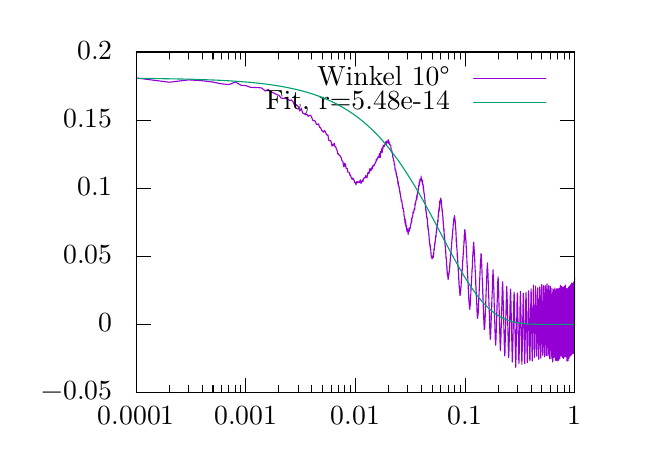
\begin{tikzpicture}[gnuplot]
%% generated with GNUPLOT 5.2p5a (Gentoo revision r0) (Lua 5.1; terminal rev. 99 , script rev. 107)
%% Sa 18 Mai 2019 18:30:50 CEST
\path (0.000,0.000) rectangle (7.500,5.250);
\gpcolor{color=gp lt color border}
\gpsetlinetype{gp lt border}
\gpsetdashtype{gp dt solid}
\gpsetlinewidth{1.00}
\draw[gp path] (1.380,0.616)--(1.560,0.616);
\draw[gp path] (6.947,0.616)--(6.767,0.616);
\node[gp node right] at (1.196,0.616) {$-0.05$};
\draw[gp path] (1.380,1.481)--(1.560,1.481);
\draw[gp path] (6.947,1.481)--(6.767,1.481);
\node[gp node right] at (1.196,1.481) {$0$};
\draw[gp path] (1.380,2.346)--(1.560,2.346);
\draw[gp path] (6.947,2.346)--(6.767,2.346);
\node[gp node right] at (1.196,2.346) {$0.05$};
\draw[gp path] (1.380,3.211)--(1.560,3.211);
\draw[gp path] (6.947,3.211)--(6.767,3.211);
\node[gp node right] at (1.196,3.211) {$0.1$};
\draw[gp path] (1.380,4.076)--(1.560,4.076);
\draw[gp path] (6.947,4.076)--(6.767,4.076);
\node[gp node right] at (1.196,4.076) {$0.15$};
\draw[gp path] (1.380,4.941)--(1.560,4.941);
\draw[gp path] (6.947,4.941)--(6.767,4.941);
\node[gp node right] at (1.196,4.941) {$0.2$};
\draw[gp path] (1.380,0.616)--(1.380,0.796);
\draw[gp path] (1.380,4.941)--(1.380,4.761);
\node[gp node center] at (1.380,0.308) {$0.0001$};
\draw[gp path] (1.799,0.616)--(1.799,0.706);
\draw[gp path] (1.799,4.941)--(1.799,4.851);
\draw[gp path] (2.044,0.616)--(2.044,0.706);
\draw[gp path] (2.044,4.941)--(2.044,4.851);
\draw[gp path] (2.218,0.616)--(2.218,0.706);
\draw[gp path] (2.218,4.941)--(2.218,4.851);
\draw[gp path] (2.353,0.616)--(2.353,0.706);
\draw[gp path] (2.353,4.941)--(2.353,4.851);
\draw[gp path] (2.463,0.616)--(2.463,0.706);
\draw[gp path] (2.463,4.941)--(2.463,4.851);
\draw[gp path] (2.556,0.616)--(2.556,0.706);
\draw[gp path] (2.556,4.941)--(2.556,4.851);
\draw[gp path] (2.637,0.616)--(2.637,0.706);
\draw[gp path] (2.637,4.941)--(2.637,4.851);
\draw[gp path] (2.708,0.616)--(2.708,0.706);
\draw[gp path] (2.708,4.941)--(2.708,4.851);
\draw[gp path] (2.772,0.616)--(2.772,0.796);
\draw[gp path] (2.772,4.941)--(2.772,4.761);
\node[gp node center] at (2.772,0.308) {$0.001$};
\draw[gp path] (3.191,0.616)--(3.191,0.706);
\draw[gp path] (3.191,4.941)--(3.191,4.851);
\draw[gp path] (3.436,0.616)--(3.436,0.706);
\draw[gp path] (3.436,4.941)--(3.436,4.851);
\draw[gp path] (3.610,0.616)--(3.610,0.706);
\draw[gp path] (3.610,4.941)--(3.610,4.851);
\draw[gp path] (3.745,0.616)--(3.745,0.706);
\draw[gp path] (3.745,4.941)--(3.745,4.851);
\draw[gp path] (3.855,0.616)--(3.855,0.706);
\draw[gp path] (3.855,4.941)--(3.855,4.851);
\draw[gp path] (3.948,0.616)--(3.948,0.706);
\draw[gp path] (3.948,4.941)--(3.948,4.851);
\draw[gp path] (4.029,0.616)--(4.029,0.706);
\draw[gp path] (4.029,4.941)--(4.029,4.851);
\draw[gp path] (4.100,0.616)--(4.100,0.706);
\draw[gp path] (4.100,4.941)--(4.100,4.851);
\draw[gp path] (4.163,0.616)--(4.163,0.796);
\draw[gp path] (4.163,4.941)--(4.163,4.761);
\node[gp node center] at (4.163,0.308) {$0.01$};
\draw[gp path] (4.582,0.616)--(4.582,0.706);
\draw[gp path] (4.582,4.941)--(4.582,4.851);
\draw[gp path] (4.828,0.616)--(4.828,0.706);
\draw[gp path] (4.828,4.941)--(4.828,4.851);
\draw[gp path] (5.001,0.616)--(5.001,0.706);
\draw[gp path] (5.001,4.941)--(5.001,4.851);
\draw[gp path] (5.136,0.616)--(5.136,0.706);
\draw[gp path] (5.136,4.941)--(5.136,4.851);
\draw[gp path] (5.246,0.616)--(5.246,0.706);
\draw[gp path] (5.246,4.941)--(5.246,4.851);
\draw[gp path] (5.340,0.616)--(5.340,0.706);
\draw[gp path] (5.340,4.941)--(5.340,4.851);
\draw[gp path] (5.420,0.616)--(5.420,0.706);
\draw[gp path] (5.420,4.941)--(5.420,4.851);
\draw[gp path] (5.492,0.616)--(5.492,0.706);
\draw[gp path] (5.492,4.941)--(5.492,4.851);
\draw[gp path] (5.555,0.616)--(5.555,0.796);
\draw[gp path] (5.555,4.941)--(5.555,4.761);
\node[gp node center] at (5.555,0.308) {$0.1$};
\draw[gp path] (5.974,0.616)--(5.974,0.706);
\draw[gp path] (5.974,4.941)--(5.974,4.851);
\draw[gp path] (6.219,0.616)--(6.219,0.706);
\draw[gp path] (6.219,4.941)--(6.219,4.851);
\draw[gp path] (6.393,0.616)--(6.393,0.706);
\draw[gp path] (6.393,4.941)--(6.393,4.851);
\draw[gp path] (6.528,0.616)--(6.528,0.706);
\draw[gp path] (6.528,4.941)--(6.528,4.851);
\draw[gp path] (6.638,0.616)--(6.638,0.706);
\draw[gp path] (6.638,4.941)--(6.638,4.851);
\draw[gp path] (6.731,0.616)--(6.731,0.706);
\draw[gp path] (6.731,4.941)--(6.731,4.851);
\draw[gp path] (6.812,0.616)--(6.812,0.706);
\draw[gp path] (6.812,4.941)--(6.812,4.851);
\draw[gp path] (6.883,0.616)--(6.883,0.706);
\draw[gp path] (6.883,4.941)--(6.883,4.851);
\draw[gp path] (6.947,0.616)--(6.947,0.796);
\draw[gp path] (6.947,4.941)--(6.947,4.761);
\node[gp node center] at (6.947,0.308) {$1$};
\draw[gp path] (1.380,4.941)--(1.380,0.616)--(6.947,0.616)--(6.947,4.941)--cycle;
\node[gp node right] at (5.479,4.607) {Winkel 10°};
\gpcolor{rgb color={0.580,0.000,0.827}}
\draw[gp path] (5.663,4.607)--(6.579,4.607);
\draw[gp path] (1.380,4.611)--(1.799,4.557)--(2.044,4.587)--(2.218,4.576)--(2.353,4.559)%
  --(2.463,4.537)--(2.556,4.527)--(2.637,4.560)--(2.708,4.519)--(2.772,4.513)--(2.829,4.493)%
  --(2.882,4.490)--(2.930,4.489)--(2.975,4.483)--(3.017,4.445)--(3.056,4.466)--(3.092,4.431)%
  --(3.127,4.420)--(3.160,4.401)--(3.191,4.391)--(3.220,4.355)--(3.248,4.352)--(3.275,4.351)%
  --(3.301,4.340)--(3.326,4.326)--(3.349,4.332)--(3.372,4.306)--(3.394,4.249)--(3.415,4.271)%
  --(3.436,4.248)--(3.456,4.191)--(3.475,4.227)--(3.493,4.165)--(3.511,4.161)--(3.529,4.141)%
  --(3.546,4.153)--(3.563,4.124)--(3.579,4.136)--(3.594,4.138)--(3.610,4.103)--(3.625,4.067)%
  --(3.639,4.071)--(3.653,4.061)--(3.667,4.023)--(3.681,4.020)--(3.694,4.029)--(3.707,3.986)%
  --(3.720,3.981)--(3.732,3.947)--(3.745,3.935)--(3.757,3.923)--(3.768,3.945)--(3.780,3.928)%
  --(3.791,3.901)--(3.802,3.884)--(3.813,3.887)--(3.824,3.821)--(3.834,3.815)--(3.845,3.817)%
  --(3.855,3.797)--(3.865,3.745)--(3.875,3.768)--(3.884,3.756)--(3.894,3.783)--(3.903,3.738)%
  --(3.912,3.739)--(3.921,3.707)--(3.930,3.694)--(3.939,3.644)--(3.948,3.649)--(3.956,3.629)%
  --(3.965,3.628)--(3.973,3.612)--(3.982,3.598)--(3.990,3.566)--(3.998,3.553)--(4.006,3.540)%
  --(4.013,3.483)--(4.021,3.530)--(4.029,3.490)--(4.036,3.521)--(4.044,3.462)--(4.051,3.461)%
  --(4.058,3.463)--(4.065,3.415)--(4.072,3.415)--(4.079,3.416)--(4.086,3.410)--(4.093,3.375)%
  --(4.100,3.379)--(4.106,3.352)--(4.113,3.344)--(4.120,3.323)--(4.126,3.339)--(4.132,3.338)%
  --(4.139,3.320)--(4.145,3.315)--(4.151,3.283)--(4.157,3.286)--(4.164,3.275)--(4.170,3.254)%
  --(4.175,3.290)--(4.181,3.296)--(4.187,3.286)--(4.193,3.280)--(4.199,3.292)--(4.204,3.285)%
  --(4.210,3.300)--(4.216,3.285)--(4.221,3.300)--(4.227,3.317)--(4.232,3.271)--(4.237,3.281)%
  --(4.243,3.298)--(4.248,3.299)--(4.253,3.316)--(4.258,3.296)--(4.264,3.329)--(4.269,3.332)%
  --(4.274,3.346)--(4.279,3.342)--(4.284,3.350)--(4.289,3.343)--(4.294,3.372)--(4.298,3.360)%
  --(4.303,3.361)--(4.308,3.342)--(4.313,3.363)--(4.317,3.387)--(4.322,3.414)--(4.327,3.397)%
  --(4.331,3.395)--(4.336,3.403)--(4.340,3.429)--(4.345,3.458)--(4.349,3.461)--(4.354,3.432)%
  --(4.358,3.434)--(4.363,3.444)--(4.367,3.456)--(4.371,3.474)--(4.375,3.453)--(4.380,3.490)%
  --(4.384,3.482)--(4.388,3.501)--(4.392,3.497)--(4.396,3.506)--(4.400,3.494)--(4.405,3.516)%
  --(4.409,3.517)--(4.413,3.527)--(4.417,3.540)--(4.421,3.539)--(4.424,3.554)--(4.428,3.579)%
  --(4.432,3.560)--(4.436,3.584)--(4.440,3.580)--(4.444,3.593)--(4.448,3.601)--(4.451,3.611)%
  --(4.455,3.615)--(4.459,3.615)--(4.463,3.599)--(4.466,3.650)--(4.470,3.651)--(4.473,3.617)%
  --(4.477,3.600)--(4.481,3.677)--(4.484,3.658)--(4.488,3.681)--(4.491,3.673)--(4.495,3.676)%
  --(4.498,3.717)--(4.502,3.660)--(4.505,3.730)--(4.509,3.731)--(4.512,3.714)--(4.515,3.759)%
  --(4.519,3.742)--(4.522,3.749)--(4.525,3.751)--(4.529,3.741)--(4.532,3.759)--(4.535,3.763)%
  --(4.539,3.767)--(4.542,3.783)--(4.545,3.799)--(4.548,3.771)--(4.551,3.764)--(4.555,3.772)%
  --(4.558,3.810)--(4.561,3.791)--(4.564,3.809)--(4.567,3.789)--(4.570,3.796)--(4.573,3.800)%
  --(4.576,3.811)--(4.579,3.828)--(4.582,3.811)--(4.585,3.780)--(4.588,3.804)--(4.591,3.779)%
  --(4.594,3.786)--(4.597,3.765)--(4.600,3.772)--(4.603,3.756)--(4.606,3.756)--(4.609,3.753)%
  --(4.612,3.745)--(4.615,3.710)--(4.618,3.675)--(4.621,3.676)--(4.623,3.691)--(4.626,3.664)%
  --(4.629,3.673)--(4.632,3.644)--(4.635,3.636)--(4.637,3.607)--(4.640,3.597)--(4.643,3.591)%
  --(4.646,3.559)--(4.648,3.557)--(4.651,3.559)--(4.654,3.542)--(4.656,3.512)--(4.659,3.509)%
  --(4.662,3.506)--(4.664,3.471)--(4.667,3.442)--(4.670,3.434)--(4.672,3.444)--(4.675,3.439)%
  --(4.677,3.426)--(4.680,3.384)--(4.683,3.407)--(4.685,3.366)--(4.688,3.370)--(4.690,3.348)%
  --(4.693,3.357)--(4.695,3.345)--(4.698,3.323)--(4.700,3.304)--(4.703,3.262)--(4.705,3.299)%
  --(4.708,3.257)--(4.710,3.241)--(4.712,3.245)--(4.715,3.223)--(4.717,3.235)--(4.720,3.196)%
  --(4.722,3.198)--(4.725,3.174)--(4.727,3.146)--(4.729,3.169)--(4.732,3.132)--(4.734,3.118)%
  --(4.736,3.122)--(4.739,3.090)--(4.741,3.074)--(4.743,3.078)--(4.746,3.043)--(4.748,3.050)%
  --(4.750,3.057)--(4.753,3.037)--(4.755,3.020)--(4.757,2.998)--(4.759,2.998)--(4.762,2.956)%
  --(4.764,2.965)--(4.766,2.962)--(4.768,2.949)--(4.771,2.950)--(4.773,2.916)--(4.775,2.911)%
  --(4.777,2.920)--(4.779,2.867)--(4.781,2.858)--(4.784,2.847)--(4.786,2.827)--(4.788,2.832)%
  --(4.790,2.799)--(4.792,2.768)--(4.794,2.815)--(4.797,2.794)--(4.799,2.746)--(4.801,2.779)%
  --(4.803,2.757)--(4.805,2.719)--(4.807,2.737)--(4.809,2.738)--(4.811,2.723)--(4.813,2.718)%
  --(4.815,2.675)--(4.817,2.662)--(4.819,2.700)--(4.821,2.689)--(4.823,2.665)--(4.826,2.660)%
  --(4.828,2.651)--(4.830,2.660)--(4.832,2.622)--(4.834,2.668)--(4.836,2.644)--(4.838,2.663)%
  --(4.840,2.679)--(4.841,2.704)--(4.843,2.687)--(4.845,2.691)--(4.847,2.690)--(4.849,2.668)%
  --(4.851,2.685)--(4.853,2.701)--(4.855,2.713)--(4.857,2.707)--(4.859,2.702)--(4.861,2.738)%
  --(4.863,2.755)--(4.865,2.746)--(4.867,2.764)--(4.868,2.762)--(4.870,2.766)--(4.872,2.786)%
  --(4.874,2.827)--(4.876,2.808)--(4.878,2.787)--(4.880,2.833)--(4.881,2.829)--(4.883,2.831)%
  --(4.885,2.849)--(4.887,2.846)--(4.889,2.866)--(4.891,2.867)--(4.892,2.872)--(4.894,2.911)%
  --(4.896,2.895)--(4.898,2.912)--(4.900,2.891)--(4.901,2.906)--(4.903,2.912)--(4.905,2.915)%
  --(4.907,2.936)--(4.908,2.952)--(4.910,2.935)--(4.912,2.957)--(4.914,2.942)--(4.916,2.943)%
  --(4.917,2.972)--(4.919,3.015)--(4.921,2.989)--(4.922,3.009)--(4.924,3.011)--(4.926,3.024)%
  --(4.928,3.039)--(4.929,3.027)--(4.931,3.062)--(4.933,3.062)--(4.934,3.059)--(4.936,3.067)%
  --(4.938,3.077)--(4.939,3.109)--(4.941,3.063)--(4.943,3.122)--(4.944,3.086)--(4.946,3.096)%
  --(4.948,3.136)--(4.949,3.131)--(4.951,3.140)--(4.953,3.146)--(4.954,3.162)--(4.956,3.180)%
  --(4.958,3.172)--(4.959,3.205)--(4.961,3.191)--(4.962,3.214)--(4.964,3.227)--(4.966,3.248)%
  --(4.967,3.242)--(4.969,3.251)--(4.970,3.240)--(4.972,3.285)--(4.974,3.245)--(4.975,3.265)%
  --(4.977,3.265)--(4.978,3.293)--(4.980,3.302)--(4.981,3.325)--(4.983,3.305)--(4.985,3.303)%
  --(4.986,3.313)--(4.988,3.324)--(4.989,3.328)--(4.991,3.309)--(4.992,3.328)--(4.994,3.321)%
  --(4.995,3.320)--(4.997,3.365)--(4.998,3.327)--(5.000,3.338)--(5.001,3.334)--(5.003,3.335)%
  --(5.004,3.320)--(5.006,3.325)--(5.007,3.307)--(5.009,3.283)--(5.010,3.279)--(5.012,3.297)%
  --(5.013,3.301)--(5.015,3.310)--(5.016,3.261)--(5.018,3.253)--(5.019,3.271)--(5.021,3.255)%
  --(5.022,3.218)--(5.024,3.202)--(5.025,3.240)--(5.027,3.231)--(5.028,3.187)--(5.029,3.197)%
  --(5.031,3.167)--(5.032,3.164)--(5.034,3.145)--(5.035,3.143)--(5.037,3.136)--(5.038,3.096)%
  --(5.039,3.094)--(5.041,3.100)--(5.042,3.080)--(5.044,3.083)--(5.045,3.058)--(5.047,3.039)%
  --(5.048,3.024)--(5.049,3.015)--(5.051,2.990)--(5.052,2.974)--(5.054,2.981)--(5.055,2.944)%
  --(5.056,2.938)--(5.058,2.938)--(5.059,2.913)--(5.060,2.909)--(5.062,2.910)--(5.063,2.868)%
  --(5.064,2.879)--(5.066,2.883)--(5.067,2.859)--(5.069,2.834)--(5.070,2.843)--(5.071,2.837)%
  --(5.073,2.836)--(5.074,2.833)--(5.075,2.814)--(5.077,2.784)--(5.078,2.758)--(5.079,2.782)%
  --(5.081,2.720)--(5.082,2.736)--(5.083,2.740)--(5.085,2.686)--(5.086,2.692)--(5.087,2.701)%
  --(5.089,2.677)--(5.090,2.671)--(5.091,2.670)--(5.092,2.628)--(5.094,2.639)--(5.095,2.598)%
  --(5.096,2.619)--(5.098,2.602)--(5.099,2.580)--(5.100,2.551)--(5.101,2.569)--(5.103,2.521)%
  --(5.104,2.509)--(5.105,2.515)--(5.107,2.494)--(5.108,2.477)--(5.109,2.499)--(5.110,2.484)%
  --(5.112,2.489)--(5.113,2.455)--(5.114,2.446)--(5.115,2.430)--(5.117,2.447)--(5.118,2.421)%
  --(5.119,2.424)--(5.120,2.431)--(5.122,2.388)--(5.123,2.364)--(5.124,2.367)--(5.125,2.353)%
  --(5.127,2.341)--(5.128,2.347)--(5.129,2.339)--(5.130,2.342)--(5.131,2.331)--(5.133,2.335)%
  --(5.134,2.316)--(5.135,2.328)--(5.136,2.312)--(5.137,2.321)--(5.139,2.324)--(5.140,2.326)%
  --(5.141,2.332)--(5.142,2.336)--(5.144,2.337)--(5.145,2.339)--(5.146,2.356)--(5.147,2.337)%
  --(5.148,2.341)--(5.149,2.345)--(5.151,2.332)--(5.152,2.340)--(5.153,2.361)--(5.154,2.358)%
  --(5.155,2.385)--(5.157,2.375)--(5.158,2.401)--(5.159,2.398)--(5.160,2.441)--(5.161,2.416)%
  --(5.162,2.440)--(5.163,2.429)--(5.165,2.461)--(5.166,2.459)--(5.167,2.478)--(5.168,2.462)%
  --(5.169,2.490)--(5.170,2.509)--(5.172,2.490)--(5.173,2.525)--(5.174,2.536)--(5.175,2.541)%
  --(5.176,2.533)--(5.177,2.538)--(5.178,2.570)--(5.179,2.581)--(5.181,2.593)--(5.182,2.606)%
  --(5.183,2.604)--(5.184,2.617)--(5.185,2.615)--(5.186,2.587)--(5.187,2.643)--(5.188,2.633)%
  --(5.189,2.663)--(5.191,2.652)--(5.192,2.671)--(5.193,2.673)--(5.194,2.672)--(5.195,2.680)%
  --(5.196,2.713)--(5.197,2.715)--(5.198,2.729)--(5.199,2.709)--(5.200,2.731)--(5.202,2.743)%
  --(5.203,2.738)--(5.204,2.741)--(5.205,2.769)--(5.206,2.765)--(5.207,2.799)--(5.208,2.806)%
  --(5.209,2.797)--(5.210,2.795)--(5.211,2.789)--(5.212,2.817)--(5.213,2.837)--(5.214,2.843)%
  --(5.215,2.867)--(5.217,2.859)--(5.218,2.907)--(5.219,2.914)--(5.220,2.901)--(5.221,2.932)%
  --(5.222,2.929)--(5.223,2.916)--(5.224,2.949)--(5.225,2.957)--(5.226,2.961)--(5.227,2.971)%
  --(5.228,2.982)--(5.229,2.935)--(5.230,2.984)--(5.231,2.981)--(5.232,3.008)--(5.233,2.999)%
  --(5.234,3.051)--(5.235,3.032)--(5.236,3.039)--(5.237,3.030)--(5.238,3.047)--(5.239,3.036)%
  --(5.240,3.053)--(5.241,3.047)--(5.242,3.086)--(5.243,3.045)--(5.244,3.056)--(5.245,3.037)%
  --(5.246,3.059)--(5.247,3.065)--(5.249,3.075)--(5.250,3.045)--(5.251,3.074)--(5.252,3.025)%
  --(5.253,3.057)--(5.254,3.025)--(5.254,3.017)--(5.255,2.997)--(5.256,3.022)--(5.257,2.994)%
  --(5.258,2.985)--(5.259,2.968)--(5.260,2.972)--(5.261,2.965)--(5.262,2.947)--(5.263,2.916)%
  --(5.264,2.936)--(5.265,2.936)--(5.266,2.915)--(5.267,2.884)--(5.268,2.888)--(5.269,2.892)%
  --(5.270,2.893)--(5.271,2.856)--(5.272,2.861)--(5.273,2.812)--(5.274,2.846)--(5.275,2.800)%
  --(5.276,2.781)--(5.277,2.792)--(5.278,2.763)--(5.279,2.759)--(5.280,2.733)--(5.281,2.723)%
  --(5.282,2.729)--(5.283,2.721)--(5.284,2.687)--(5.285,2.710)--(5.286,2.691)--(5.286,2.687)%
  --(5.287,2.690)--(5.288,2.656)--(5.289,2.641)--(5.290,2.598)--(5.291,2.632)--(5.292,2.595)%
  --(5.293,2.608)--(5.294,2.573)--(5.295,2.562)--(5.296,2.572)--(5.297,2.552)--(5.298,2.547)%
  --(5.299,2.546)--(5.300,2.547)--(5.300,2.503)--(5.301,2.490)--(5.302,2.473)--(5.303,2.482)%
  --(5.304,2.462)--(5.305,2.447)--(5.306,2.422)--(5.307,2.436)--(5.308,2.427)--(5.309,2.417)%
  --(5.310,2.379)--(5.310,2.386)--(5.311,2.401)--(5.312,2.354)--(5.313,2.323)--(5.314,2.343)%
  --(5.315,2.328)--(5.316,2.323)--(5.317,2.304)--(5.318,2.294)--(5.319,2.269)--(5.319,2.240)%
  --(5.320,2.252)--(5.321,2.233)--(5.322,2.229)--(5.323,2.213)--(5.324,2.180)--(5.325,2.214)%
  --(5.326,2.161)--(5.327,2.189)--(5.327,2.187)--(5.328,2.149)--(5.329,2.117)--(5.330,2.121)%
  --(5.331,2.131)--(5.332,2.109)--(5.333,2.111)--(5.334,2.136)--(5.334,2.098)--(5.335,2.103)%
  --(5.336,2.083)--(5.337,2.088)--(5.338,2.064)--(5.339,2.105)--(5.340,2.049)--(5.341,2.071)%
  --(5.341,2.083)--(5.342,2.077)--(5.343,2.109)--(5.344,2.101)--(5.345,2.085)--(5.346,2.087)%
  --(5.347,2.103)--(5.347,2.096)--(5.348,2.098)--(5.349,2.126)--(5.350,2.132)--(5.351,2.128)%
  --(5.352,2.139)--(5.352,2.144)--(5.353,2.141)--(5.354,2.148)--(5.355,2.164)--(5.356,2.167)%
  --(5.357,2.180)--(5.358,2.175)--(5.358,2.216)--(5.359,2.183)--(5.360,2.238)--(5.361,2.197)%
  --(5.362,2.242)--(5.363,2.240)--(5.363,2.248)--(5.364,2.265)--(5.365,2.290)--(5.366,2.305)%
  --(5.367,2.295)--(5.368,2.283)--(5.368,2.340)--(5.369,2.316)--(5.370,2.369)--(5.371,2.341)%
  --(5.372,2.364)--(5.372,2.355)--(5.373,2.376)--(5.374,2.386)--(5.375,2.378)--(5.376,2.384)%
  --(5.377,2.406)--(5.377,2.437)--(5.378,2.430)--(5.379,2.436)--(5.380,2.450)--(5.381,2.462)%
  --(5.381,2.452)--(5.382,2.467)--(5.383,2.457)--(5.384,2.503)--(5.385,2.490)--(5.385,2.514)%
  --(5.386,2.512)--(5.387,2.552)--(5.388,2.551)--(5.389,2.545)--(5.389,2.564)--(5.390,2.566)%
  --(5.391,2.595)--(5.392,2.600)--(5.393,2.580)--(5.393,2.599)--(5.394,2.639)--(5.395,2.619)%
  --(5.396,2.616)--(5.396,2.651)--(5.397,2.646)--(5.398,2.672)--(5.399,2.682)--(5.400,2.673)%
  --(5.400,2.682)--(5.401,2.694)--(5.402,2.708)--(5.403,2.691)--(5.404,2.742)--(5.404,2.754)%
  --(5.405,2.738)--(5.406,2.761)--(5.407,2.751)--(5.407,2.768)--(5.408,2.756)--(5.409,2.769)%
  --(5.410,2.796)--(5.410,2.823)--(5.411,2.799)--(5.412,2.825)--(5.413,2.792)--(5.414,2.814)%
  --(5.414,2.812)--(5.415,2.827)--(5.416,2.816)--(5.417,2.837)--(5.417,2.832)--(5.418,2.845)%
  --(5.419,2.863)--(5.420,2.848)--(5.420,2.840)--(5.421,2.862)--(5.422,2.837)--(5.423,2.841)%
  --(5.423,2.840)--(5.424,2.841)--(5.425,2.799)--(5.426,2.834)--(5.426,2.822)--(5.427,2.810)%
  --(5.428,2.781)--(5.429,2.807)--(5.429,2.775)--(5.430,2.788)--(5.431,2.764)--(5.432,2.753)%
  --(5.432,2.756)--(5.433,2.724)--(5.434,2.731)--(5.435,2.714)--(5.435,2.690)--(5.436,2.700)%
  --(5.437,2.681)--(5.438,2.666)--(5.438,2.667)--(5.439,2.661)--(5.440,2.634)--(5.440,2.629)%
  --(5.441,2.597)--(5.442,2.598)--(5.443,2.531)--(5.443,2.573)--(5.444,2.573)--(5.445,2.554)%
  --(5.446,2.546)--(5.446,2.518)--(5.447,2.499)--(5.448,2.496)--(5.448,2.460)--(5.449,2.495)%
  --(5.450,2.491)--(5.451,2.465)--(5.451,2.433)--(5.452,2.437)--(5.453,2.421)--(5.453,2.423)%
  --(5.454,2.400)--(5.455,2.376)--(5.456,2.393)--(5.456,2.343)--(5.457,2.355)--(5.458,2.366)%
  --(5.458,2.316)--(5.459,2.349)--(5.460,2.300)--(5.461,2.294)--(5.461,2.288)--(5.462,2.293)%
  --(5.463,2.261)--(5.463,2.249)--(5.464,2.235)--(5.465,2.233)--(5.465,2.214)--(5.466,2.226)%
  --(5.467,2.193)--(5.468,2.213)--(5.468,2.172)--(5.469,2.158)--(5.470,2.154)--(5.470,2.144)%
  --(5.471,2.125)--(5.472,2.121)--(5.472,2.139)--(5.473,2.101)--(5.474,2.078)--(5.475,2.076)%
  --(5.475,2.048)--(5.476,2.046)--(5.477,2.037)--(5.477,2.045)--(5.478,1.992)--(5.479,2.004)%
  --(5.479,1.971)--(5.480,1.986)--(5.481,1.967)--(5.481,1.944)--(5.482,1.948)--(5.483,1.946)%
  --(5.483,1.949)--(5.484,1.947)--(5.485,1.923)--(5.485,1.912)--(5.486,1.904)--(5.487,1.909)%
  --(5.488,1.879)--(5.488,1.869)--(5.489,1.899)--(5.490,1.895)--(5.490,1.848)--(5.491,1.895)%
  --(5.492,1.859)--(5.492,1.854)--(5.493,1.854)--(5.494,1.881)--(5.494,1.884)--(5.495,1.910)%
  --(5.496,1.893)--(5.496,1.912)--(5.497,1.904)--(5.498,1.921)--(5.498,1.910)--(5.499,1.926)%
  --(5.500,1.905)--(5.500,1.939)--(5.501,1.945)--(5.502,1.947)--(5.502,1.970)--(5.503,1.950)%
  --(5.504,1.964)--(5.504,1.975)--(5.505,2.008)--(5.506,1.995)--(5.506,2.021)--(5.507,2.006)%
  --(5.507,2.021)--(5.508,2.038)--(5.509,2.040)--(5.509,2.029)--(5.510,2.055)--(5.511,2.074)%
  --(5.511,2.066)--(5.512,2.128)--(5.513,2.101)--(5.513,2.113)--(5.514,2.093)--(5.515,2.114)%
  --(5.515,2.126)--(5.516,2.168)--(5.517,2.169)--(5.517,2.170)--(5.518,2.158)--(5.518,2.190)%
  --(5.519,2.170)--(5.520,2.193)--(5.520,2.223)--(5.521,2.212)--(5.522,2.215)--(5.522,2.244)%
  --(5.523,2.255)--(5.524,2.252)--(5.524,2.256)--(5.525,2.293)--(5.526,2.281)--(5.526,2.301)%
  --(5.527,2.308)--(5.527,2.298)--(5.528,2.310)--(5.529,2.347)--(5.529,2.328)--(5.530,2.330)%
  --(5.531,2.358)--(5.531,2.361)--(5.532,2.382)--(5.532,2.377)--(5.533,2.412)--(5.534,2.407)%
  --(5.534,2.384)--(5.535,2.429)--(5.536,2.419)--(5.536,2.434)--(5.537,2.452)--(5.537,2.471)%
  --(5.538,2.479)--(5.539,2.479)--(5.539,2.513)--(5.540,2.492)--(5.541,2.511)--(5.541,2.541)%
  --(5.542,2.519)--(5.542,2.553)--(5.543,2.580)--(5.544,2.536)--(5.544,2.556)--(5.545,2.614)%
  --(5.546,2.585)--(5.546,2.574)--(5.547,2.578)--(5.547,2.608)--(5.548,2.620)--(5.549,2.632)%
  --(5.549,2.596)--(5.550,2.621)--(5.550,2.646)--(5.551,2.686)--(5.552,2.639)--(5.552,2.663)%
  --(5.553,2.637)--(5.553,2.663)--(5.554,2.674)--(5.555,2.680)--(5.555,2.678)--(5.556,2.658)%
  --(5.556,2.634)--(5.557,2.642)--(5.558,2.631)--(5.558,2.626)--(5.559,2.606)--(5.559,2.584)%
  --(5.560,2.614)--(5.561,2.612)--(5.561,2.599)--(5.562,2.587)--(5.562,2.603)--(5.563,2.580)%
  --(5.564,2.565)--(5.564,2.553)--(5.565,2.570)--(5.565,2.545)--(5.566,2.544)--(5.567,2.510)%
  --(5.567,2.520)--(5.568,2.482)--(5.568,2.491)--(5.569,2.487)--(5.570,2.459)--(5.570,2.449)%
  --(5.571,2.454)--(5.571,2.438)--(5.572,2.386)--(5.573,2.404)--(5.573,2.376)--(5.574,2.373)%
  --(5.574,2.359)--(5.575,2.378)--(5.575,2.347)--(5.576,2.358)--(5.577,2.330)--(5.577,2.297)%
  --(5.578,2.299)--(5.578,2.275)--(5.579,2.282)--(5.580,2.259)--(5.580,2.252)--(5.581,2.251)%
  --(5.581,2.239)--(5.582,2.232)--(5.582,2.207)--(5.583,2.205)--(5.584,2.206)--(5.584,2.180)%
  --(5.585,2.163)--(5.585,2.158)--(5.586,2.111)--(5.586,2.138)--(5.587,2.125)--(5.588,2.087)%
  --(5.588,2.094)--(5.589,2.080)--(5.589,2.093)--(5.590,2.044)--(5.590,2.060)--(5.591,2.035)%
  --(5.592,2.013)--(5.592,2.003)--(5.593,2.016)--(5.593,2.003)--(5.594,1.990)--(5.594,1.993)%
  --(5.595,1.968)--(5.596,1.923)--(5.596,1.914)--(5.597,1.963)--(5.597,1.926)--(5.598,1.894)%
  --(5.598,1.873)--(5.599,1.896)--(5.600,1.868)--(5.600,1.863)--(5.601,1.866)--(5.601,1.825)%
  --(5.602,1.802)--(5.602,1.817)--(5.603,1.830)--(5.603,1.772)--(5.604,1.787)--(5.605,1.793)%
  --(5.605,1.769)--(5.606,1.777)--(5.606,1.758)--(5.607,1.750)--(5.607,1.752)--(5.608,1.727)%
  --(5.608,1.741)--(5.609,1.733)--(5.610,1.733)--(5.610,1.704)--(5.611,1.704)--(5.611,1.694)%
  --(5.612,1.682)--(5.612,1.714)--(5.613,1.710)--(5.613,1.693)--(5.614,1.708)--(5.615,1.708)%
  --(5.615,1.710)--(5.616,1.669)--(5.616,1.723)--(5.617,1.712)--(5.617,1.732)--(5.618,1.719)%
  --(5.618,1.707)--(5.619,1.730)--(5.619,1.715)--(5.620,1.736)--(5.621,1.724)--(5.621,1.751)%
  --(5.622,1.740)--(5.622,1.782)--(5.623,1.802)--(5.623,1.790)--(5.624,1.800)--(5.624,1.818)%
  --(5.625,1.830)--(5.625,1.844)--(5.626,1.853)--(5.626,1.847)--(5.627,1.856)--(5.628,1.866)%
  --(5.628,1.877)--(5.629,1.879)--(5.629,1.913)--(5.630,1.906)--(5.630,1.952)--(5.631,1.957)%
  --(5.631,1.940)--(5.632,1.983)--(5.632,1.967)--(5.633,1.972)--(5.633,1.997)--(5.634,1.980)%
  --(5.634,1.974)--(5.635,2.000)--(5.636,2.018)--(5.636,2.052)--(5.637,2.059)--(5.637,2.062)%
  --(5.638,2.049)--(5.638,2.061)--(5.639,2.082)--(5.639,2.076)--(5.640,2.096)--(5.640,2.087)%
  --(5.641,2.103)--(5.641,2.106)--(5.642,2.131)--(5.642,2.155)--(5.643,2.143)--(5.643,2.168)%
  --(5.644,2.184)--(5.644,2.168)--(5.645,2.194)--(5.645,2.208)--(5.646,2.184)--(5.647,2.217)%
  --(5.647,2.207)--(5.648,2.254)--(5.648,2.249)--(5.649,2.301)--(5.649,2.259)--(5.650,2.283)%
  --(5.650,2.305)--(5.651,2.293)--(5.651,2.327)--(5.652,2.334)--(5.652,2.360)--(5.653,2.350)%
  --(5.653,2.342)--(5.654,2.360)--(5.654,2.359)--(5.655,2.384)--(5.655,2.367)--(5.656,2.400)%
  --(5.656,2.397)--(5.657,2.424)--(5.657,2.409)--(5.658,2.423)--(5.658,2.425)--(5.659,2.430)%
  --(5.659,2.470)--(5.660,2.445)--(5.660,2.465)--(5.661,2.472)--(5.661,2.494)--(5.662,2.467)%
  --(5.662,2.480)--(5.663,2.470)--(5.663,2.524)--(5.664,2.527)--(5.664,2.493)--(5.665,2.493)%
  --(5.665,2.519)--(5.666,2.494)--(5.666,2.513)--(5.667,2.467)--(5.667,2.485)--(5.668,2.451)%
  --(5.668,2.473)--(5.669,2.460)--(5.669,2.441)--(5.670,2.442)--(5.670,2.447)--(5.671,2.425)%
  --(5.671,2.420)--(5.672,2.394)--(5.672,2.400)--(5.673,2.403)--(5.673,2.411)--(5.674,2.371)%
  --(5.674,2.366)--(5.675,2.348)--(5.675,2.377)--(5.676,2.319)--(5.676,2.321)--(5.677,2.316)%
  --(5.677,2.304)--(5.678,2.308)--(5.678,2.280)--(5.679,2.290)--(5.679,2.260)--(5.680,2.248)%
  --(5.680,2.234)--(5.681,2.209)--(5.681,2.207)--(5.682,2.201)--(5.682,2.175)--(5.683,2.188)%
  --(5.683,2.191)--(5.684,2.149)--(5.684,2.151)--(5.685,2.159)--(5.685,2.132)--(5.686,2.120)%
  --(5.686,2.137)--(5.687,2.091)--(5.687,2.099)--(5.688,2.084)--(5.689,2.075)--(5.689,2.027)%
  --(5.690,2.052)--(5.690,2.030)--(5.691,2.023)--(5.691,1.980)--(5.692,2.000)--(5.692,2.011)%
  --(5.693,1.963)--(5.693,1.967)--(5.693,1.941)--(5.694,1.948)--(5.694,1.915)--(5.695,1.910)%
  --(5.695,1.911)--(5.696,1.886)--(5.696,1.888)--(5.697,1.893)--(5.697,1.849)--(5.698,1.864)%
  --(5.698,1.846)--(5.699,1.801)--(5.699,1.824)--(5.700,1.797)--(5.700,1.798)--(5.701,1.784)%
  --(5.701,1.790)--(5.702,1.789)--(5.702,1.764)--(5.703,1.741)--(5.703,1.748)--(5.704,1.725)%
  --(5.704,1.708)--(5.704,1.717)--(5.705,1.695)--(5.705,1.691)--(5.706,1.654)--(5.706,1.684)%
  --(5.707,1.641)--(5.707,1.640)--(5.708,1.654)--(5.708,1.618)--(5.709,1.624)--(5.709,1.620)%
  --(5.710,1.584)--(5.710,1.605)--(5.711,1.599)--(5.711,1.602)--(5.712,1.586)--(5.712,1.560)%
  --(5.712,1.571)--(5.713,1.580)--(5.713,1.568)--(5.714,1.563)--(5.714,1.557)--(5.715,1.597)%
  --(5.715,1.601)--(5.716,1.571)--(5.716,1.573)--(5.717,1.577)--(5.717,1.617)--(5.718,1.582)%
  --(5.718,1.615)--(5.718,1.608)--(5.719,1.629)--(5.719,1.635)--(5.720,1.604)--(5.720,1.607)%
  --(5.721,1.607)--(5.721,1.602)--(5.722,1.641)--(5.722,1.628)--(5.723,1.648)--(5.723,1.671)%
  --(5.724,1.663)--(5.724,1.710)--(5.724,1.694)--(5.725,1.710)--(5.725,1.727)--(5.726,1.717)%
  --(5.726,1.749)--(5.727,1.734)--(5.727,1.733)--(5.728,1.772)--(5.728,1.782)--(5.729,1.786)%
  --(5.729,1.776)--(5.729,1.824)--(5.730,1.826)--(5.730,1.830)--(5.731,1.834)--(5.731,1.856)%
  --(5.732,1.849)--(5.732,1.855)--(5.733,1.879)--(5.733,1.895)--(5.733,1.880)--(5.734,1.893)%
  --(5.734,1.925)--(5.735,1.927)--(5.735,1.905)--(5.736,1.935)--(5.736,1.950)--(5.737,1.958)%
  --(5.737,1.973)--(5.738,1.988)--(5.738,1.980)--(5.738,2.014)--(5.739,2.013)--(5.739,2.009)%
  --(5.740,2.031)--(5.740,2.046)--(5.741,2.059)--(5.741,2.078)--(5.742,2.042)--(5.742,2.062)%
  --(5.742,2.113)--(5.743,2.075)--(5.743,2.108)--(5.744,2.108)--(5.744,2.155)--(5.745,2.152)%
  --(5.745,2.147)--(5.746,2.137)--(5.746,2.141)--(5.746,2.180)--(5.747,2.186)--(5.747,2.191)%
  --(5.748,2.219)--(5.748,2.240)--(5.749,2.228)--(5.749,2.236)--(5.749,2.255)--(5.750,2.235)%
  --(5.750,2.283)--(5.751,2.254)--(5.751,2.291)--(5.752,2.281)--(5.752,2.311)--(5.753,2.318)%
  --(5.753,2.316)--(5.753,2.306)--(5.754,2.320)--(5.754,2.312)--(5.755,2.323)--(5.755,2.339)%
  --(5.756,2.344)--(5.756,2.324)--(5.756,2.345)--(5.757,2.365)--(5.757,2.380)--(5.758,2.351)%
  --(5.758,2.369)--(5.759,2.351)--(5.759,2.358)--(5.759,2.364)--(5.760,2.373)--(5.760,2.330)%
  --(5.761,2.360)--(5.761,2.318)--(5.762,2.339)--(5.762,2.296)--(5.762,2.328)--(5.763,2.318)%
  --(5.763,2.312)--(5.764,2.292)--(5.764,2.277)--(5.765,2.261)--(5.765,2.246)--(5.765,2.270)%
  --(5.766,2.220)--(5.766,2.247)--(5.767,2.235)--(5.767,2.212)--(5.768,2.200)--(5.768,2.193)%
  --(5.768,2.177)--(5.769,2.163)--(5.769,2.156)--(5.770,2.173)--(5.770,2.140)--(5.771,2.124)%
  --(5.771,2.096)--(5.771,2.088)--(5.772,2.093)--(5.772,2.054)--(5.773,2.067)--(5.773,2.062)%
  --(5.774,2.071)--(5.774,2.036)--(5.774,2.026)--(5.775,2.008)--(5.775,2.007)--(5.776,1.976)%
  --(5.776,1.988)--(5.776,2.015)--(5.777,1.967)--(5.777,1.955)--(5.778,1.956)--(5.778,1.945)%
  --(5.779,1.933)--(5.779,1.902)--(5.779,1.863)--(5.780,1.871)--(5.780,1.886)--(5.781,1.870)%
  --(5.781,1.844)--(5.781,1.851)--(5.782,1.857)--(5.782,1.823)--(5.783,1.806)--(5.783,1.786)%
  --(5.784,1.803)--(5.784,1.757)--(5.784,1.749)--(5.785,1.758)--(5.785,1.749)--(5.786,1.722)%
  --(5.786,1.755)--(5.786,1.684)--(5.787,1.697)--(5.787,1.706)--(5.788,1.675)--(5.788,1.651)%
  --(5.789,1.657)--(5.789,1.644)--(5.789,1.597)--(5.790,1.604)--(5.790,1.612)--(5.791,1.598)%
  --(5.791,1.578)--(5.791,1.595)--(5.792,1.587)--(5.792,1.560)--(5.793,1.535)--(5.793,1.529)%
  --(5.793,1.533)--(5.794,1.525)--(5.794,1.505)--(5.795,1.502)--(5.795,1.513)--(5.795,1.470)%
  --(5.796,1.482)--(5.796,1.463)--(5.797,1.473)--(5.797,1.451)--(5.797,1.459)--(5.798,1.418)%
  --(5.798,1.436)--(5.799,1.421)--(5.799,1.442)--(5.800,1.424)--(5.800,1.425)--(5.800,1.416)%
  --(5.801,1.424)--(5.801,1.429)--(5.802,1.459)--(5.802,1.439)--(5.802,1.429)--(5.803,1.420)%
  --(5.803,1.434)--(5.804,1.451)--(5.804,1.460)--(5.804,1.431)--(5.805,1.465)--(5.805,1.480)%
  --(5.806,1.481)--(5.806,1.479)--(5.806,1.506)--(5.807,1.525)--(5.807,1.488)--(5.808,1.530)%
  --(5.808,1.510)--(5.808,1.548)--(5.809,1.551)--(5.809,1.564)--(5.810,1.582)--(5.810,1.552)%
  --(5.810,1.562)--(5.811,1.599)--(5.811,1.624)--(5.812,1.580)--(5.812,1.606)--(5.812,1.633)%
  --(5.813,1.659)--(5.813,1.644)--(5.813,1.685)--(5.814,1.673)--(5.814,1.712)--(5.815,1.673)%
  --(5.815,1.740)--(5.815,1.696)--(5.816,1.726)--(5.816,1.725)--(5.817,1.720)--(5.817,1.737)%
  --(5.817,1.758)--(5.818,1.760)--(5.818,1.777)--(5.819,1.799)--(5.819,1.785)--(5.819,1.823)%
  --(5.820,1.826)--(5.820,1.832)--(5.821,1.831)--(5.821,1.850)--(5.821,1.861)--(5.822,1.872)%
  --(5.822,1.882)--(5.822,1.896)--(5.823,1.907)--(5.823,1.910)--(5.824,1.932)--(5.824,1.908)%
  --(5.824,1.936)--(5.825,1.943)--(5.825,1.935)--(5.826,1.933)--(5.826,1.969)--(5.826,1.979)%
  --(5.827,1.997)--(5.827,1.991)--(5.828,2.021)--(5.828,2.032)--(5.828,2.025)--(5.829,2.033)%
  --(5.829,2.048)--(5.829,2.081)--(5.830,2.065)--(5.830,2.089)--(5.831,2.101)--(5.831,2.080)%
  --(5.831,2.128)--(5.832,2.121)--(5.832,2.111)--(5.832,2.134)--(5.833,2.158)--(5.833,2.177)%
  --(5.834,2.159)--(5.834,2.144)--(5.834,2.183)--(5.835,2.176)--(5.835,2.196)--(5.836,2.200)%
  --(5.836,2.202)--(5.836,2.153)--(5.837,2.189)--(5.837,2.199)--(5.837,2.221)--(5.838,2.215)%
  --(5.838,2.243)--(5.839,2.221)--(5.839,2.230)--(5.839,2.263)--(5.840,2.246)--(5.840,2.194)%
  --(5.840,2.196)--(5.841,2.209)--(5.841,2.202)--(5.842,2.193)--(5.842,2.199)--(5.842,2.171)%
  --(5.843,2.189)--(5.843,2.174)--(5.843,2.159)--(5.844,2.179)--(5.844,2.146)--(5.845,2.167)%
  --(5.845,2.116)--(5.845,2.120)--(5.846,2.133)--(5.846,2.135)--(5.846,2.097)--(5.847,2.085)%
  --(5.847,2.072)--(5.848,2.083)--(5.848,2.057)--(5.848,2.050)--(5.849,2.025)--(5.849,2.017)%
  --(5.849,2.012)--(5.850,2.014)--(5.850,1.967)--(5.851,2.003)--(5.851,1.988)--(5.851,1.953)%
  --(5.852,1.952)--(5.852,1.942)--(5.852,1.960)--(5.853,1.913)--(5.853,1.880)--(5.854,1.873)%
  --(5.854,1.897)--(5.854,1.867)--(5.855,1.847)--(5.855,1.833)--(5.855,1.860)--(5.856,1.839)%
  --(5.856,1.823)--(5.856,1.815)--(5.857,1.793)--(5.857,1.741)--(5.858,1.746)--(5.858,1.763)%
  --(5.858,1.754)--(5.859,1.752)--(5.859,1.714)--(5.859,1.725)--(5.860,1.697)--(5.860,1.683)%
  --(5.860,1.698)--(5.861,1.683)--(5.861,1.667)--(5.862,1.651)--(5.862,1.635)--(5.862,1.657)%
  --(5.863,1.630)--(5.863,1.608)--(5.863,1.616)--(5.864,1.618)--(5.864,1.606)--(5.864,1.584)%
  --(5.865,1.591)--(5.865,1.553)--(5.866,1.520)--(5.866,1.518)--(5.866,1.493)--(5.867,1.517)%
  --(5.867,1.509)--(5.867,1.461)--(5.868,1.498)--(5.868,1.455)--(5.868,1.447)--(5.869,1.424)%
  --(5.869,1.454)--(5.870,1.425)--(5.870,1.422)--(5.870,1.385)--(5.871,1.397)--(5.871,1.353)%
  --(5.871,1.362)--(5.872,1.368)--(5.872,1.382)--(5.872,1.359)--(5.873,1.325)--(5.873,1.360)%
  --(5.873,1.330)--(5.874,1.326)--(5.874,1.308)--(5.875,1.312)--(5.875,1.293)--(5.875,1.313)%
  --(5.876,1.307)--(5.876,1.305)--(5.876,1.324)--(5.877,1.317)--(5.877,1.307)--(5.877,1.340)%
  --(5.878,1.311)--(5.878,1.342)--(5.878,1.344)--(5.879,1.344)--(5.879,1.366)--(5.880,1.356)%
  --(5.880,1.317)--(5.880,1.367)--(5.881,1.357)--(5.881,1.365)--(5.881,1.375)--(5.882,1.383)%
  --(5.882,1.409)--(5.882,1.412)--(5.883,1.416)--(5.883,1.405)--(5.883,1.437)--(5.884,1.448)%
  --(5.884,1.443)--(5.884,1.449)--(5.885,1.472)--(5.885,1.511)--(5.886,1.500)--(5.886,1.501)%
  --(5.886,1.512)--(5.887,1.542)--(5.887,1.538)--(5.887,1.545)--(5.888,1.548)--(5.888,1.570)%
  --(5.888,1.625)--(5.889,1.562)--(5.889,1.565)--(5.889,1.635)--(5.890,1.617)--(5.890,1.641)%
  --(5.890,1.612)--(5.891,1.638)--(5.891,1.641)--(5.891,1.653)--(5.892,1.651)--(5.892,1.698)%
  --(5.892,1.684)--(5.893,1.703)--(5.893,1.742)--(5.893,1.715)--(5.894,1.727)--(5.894,1.762)%
  --(5.895,1.742)--(5.895,1.772)--(5.895,1.781)--(5.896,1.776)--(5.896,1.791)--(5.896,1.820)%
  --(5.897,1.809)--(5.897,1.822)--(5.897,1.825)--(5.898,1.838)--(5.898,1.813)--(5.898,1.867)%
  --(5.899,1.879)--(5.899,1.901)--(5.899,1.867)--(5.900,1.900)--(5.900,1.890)--(5.900,1.907)%
  --(5.901,1.898)--(5.901,1.914)--(5.901,1.956)--(5.902,1.933)--(5.902,1.969)--(5.902,1.971)%
  --(5.903,1.996)--(5.903,1.976)--(5.903,2.005)--(5.904,2.019)--(5.904,2.027)--(5.904,2.053)%
  --(5.905,2.065)--(5.905,2.071)--(5.905,2.064)--(5.906,2.071)--(5.906,2.085)--(5.906,2.109)%
  --(5.907,2.108)--(5.907,2.109)--(5.907,2.095)--(5.908,2.104)--(5.908,2.112)--(5.909,2.122)%
  --(5.909,2.134)--(5.909,2.144)--(5.910,2.120)--(5.910,2.175)--(5.910,2.145)--(5.911,2.139)%
  --(5.911,2.133)--(5.911,2.117)--(5.912,2.114)--(5.912,2.116)--(5.912,2.104)--(5.913,2.120)%
  --(5.913,2.086)--(5.913,2.116)--(5.914,2.116)--(5.914,2.084)--(5.914,2.076)--(5.915,2.108)%
  --(5.915,2.059)--(5.915,2.078)--(5.916,2.029)--(5.916,2.041)--(5.916,2.009)--(5.917,2.008)%
  --(5.917,2.006)--(5.917,1.991)--(5.918,1.990)--(5.918,2.001)--(5.918,1.967)--(5.919,1.951)%
  --(5.919,1.932)--(5.919,1.934)--(5.920,1.923)--(5.920,1.901)--(5.920,1.904)--(5.921,1.892)%
  --(5.921,1.877)--(5.921,1.865)--(5.922,1.882)--(5.922,1.862)--(5.922,1.813)--(5.922,1.818)%
  --(5.923,1.808)--(5.923,1.817)--(5.923,1.796)--(5.924,1.805)--(5.924,1.790)--(5.924,1.763)%
  --(5.925,1.742)--(5.925,1.751)--(5.925,1.740)--(5.926,1.723)--(5.926,1.694)--(5.926,1.708)%
  --(5.927,1.688)--(5.927,1.677)--(5.927,1.658)--(5.928,1.678)--(5.928,1.674)--(5.928,1.627)%
  --(5.929,1.619)--(5.929,1.609)--(5.929,1.570)--(5.930,1.595)--(5.930,1.580)--(5.930,1.592)%
  --(5.931,1.561)--(5.931,1.553)--(5.931,1.545)--(5.932,1.529)--(5.932,1.508)--(5.932,1.491)%
  --(5.933,1.494)--(5.933,1.492)--(5.933,1.475)--(5.934,1.464)--(5.934,1.458)--(5.934,1.424)%
  --(5.935,1.420)--(5.935,1.422)--(5.935,1.379)--(5.936,1.410)--(5.936,1.386)--(5.936,1.371)%
  --(5.936,1.351)--(5.937,1.331)--(5.937,1.355)--(5.937,1.343)--(5.938,1.316)--(5.938,1.307)%
  --(5.938,1.288)--(5.939,1.289)--(5.939,1.283)--(5.939,1.300)--(5.940,1.281)--(5.940,1.250)%
  --(5.940,1.277)--(5.941,1.275)--(5.941,1.251)--(5.941,1.267)--(5.942,1.240)--(5.942,1.255)%
  --(5.942,1.235)--(5.943,1.245)--(5.943,1.223)--(5.943,1.216)--(5.944,1.226)--(5.944,1.243)%
  --(5.944,1.226)--(5.944,1.255)--(5.945,1.252)--(5.945,1.248)--(5.945,1.258)--(5.946,1.279)%
  --(5.946,1.292)--(5.946,1.268)--(5.947,1.291)--(5.947,1.285)--(5.947,1.306)--(5.948,1.283)%
  --(5.948,1.317)--(5.948,1.303)--(5.949,1.362)--(5.949,1.320)--(5.949,1.335)--(5.950,1.332)%
  --(5.950,1.364)--(5.950,1.373)--(5.951,1.379)--(5.951,1.395)--(5.951,1.407)--(5.952,1.423)%
  --(5.952,1.420)--(5.952,1.457)--(5.953,1.445)--(5.953,1.454)--(5.953,1.462)--(5.954,1.473)%
  --(5.954,1.508)--(5.954,1.487)--(5.955,1.510)--(5.955,1.524)--(5.955,1.532)--(5.955,1.533)%
  --(5.956,1.541)--(5.956,1.565)--(5.956,1.551)--(5.957,1.576)--(5.957,1.578)--(5.957,1.589)%
  --(5.958,1.646)--(5.958,1.622)--(5.958,1.615)--(5.959,1.634)--(5.959,1.636)--(5.959,1.645)%
  --(5.960,1.660)--(5.960,1.691)--(5.960,1.709)--(5.960,1.701)--(5.961,1.710)--(5.961,1.714)%
  --(5.961,1.729)--(5.962,1.752)--(5.962,1.728)--(5.962,1.762)--(5.963,1.771)--(5.963,1.777)%
  --(5.963,1.763)--(5.964,1.793)--(5.964,1.803)--(5.964,1.812)--(5.964,1.802)--(5.965,1.853)%
  --(5.965,1.839)--(5.965,1.865)--(5.966,1.869)--(5.966,1.871)--(5.966,1.868)--(5.967,1.897)%
  --(5.967,1.898)--(5.967,1.918)--(5.968,1.902)--(5.968,1.936)--(5.968,1.954)--(5.968,1.942)%
  --(5.969,1.922)--(5.969,1.989)--(5.969,1.995)--(5.970,1.990)--(5.970,2.022)--(5.970,2.031)%
  --(5.971,2.014)--(5.971,2.030)--(5.971,2.008)--(5.971,2.044)--(5.972,2.042)--(5.972,2.058)%
  --(5.972,2.051)--(5.973,2.061)--(5.973,2.055)--(5.973,2.058)--(5.974,2.064)--(5.974,2.072)%
  --(5.974,2.070)--(5.975,2.085)--(5.975,2.067)--(5.975,2.065)--(5.975,2.072)--(5.976,2.057)%
  --(5.976,2.029)--(5.976,2.046)--(5.977,2.002)--(5.977,2.048)--(5.977,2.027)--(5.978,2.022)%
  --(5.978,2.002)--(5.978,2.013)--(5.978,1.995)--(5.979,1.977)--(5.979,1.962)--(5.979,1.947)%
  --(5.980,1.935)--(5.980,1.918)--(5.980,1.935)--(5.981,1.926)--(5.981,1.885)--(5.981,1.890)%
  --(5.981,1.893)--(5.982,1.904)--(5.982,1.892)--(5.982,1.844)--(5.983,1.847)--(5.983,1.820)%
  --(5.983,1.818)--(5.984,1.807)--(5.984,1.775)--(5.984,1.789)--(5.984,1.756)--(5.985,1.736)%
  --(5.985,1.755)--(5.985,1.753)--(5.986,1.748)--(5.986,1.717)--(5.986,1.700)--(5.986,1.707)%
  --(5.987,1.706)--(5.987,1.697)--(5.987,1.649)--(5.988,1.677)--(5.988,1.663)--(5.989,1.653)%
  --(5.989,1.619)--(5.989,1.609)--(5.989,1.625)--(5.990,1.587)--(5.990,1.573)--(5.990,1.563)%
  --(5.991,1.554)--(5.991,1.526)--(5.991,1.521)--(5.991,1.526)--(5.992,1.508)--(5.992,1.501)%
  --(5.992,1.502)--(5.993,1.468)--(5.993,1.464)--(5.994,1.457)--(5.994,1.435)--(5.994,1.437)%
  --(5.994,1.415)--(5.995,1.440)--(5.995,1.412)--(5.995,1.367)--(5.996,1.358)--(5.996,1.365)%
  --(5.996,1.372)--(5.996,1.357)--(5.997,1.330)--(5.997,1.297)--(5.997,1.310)--(5.998,1.288)%
  --(5.998,1.264)--(5.998,1.257)--(5.999,1.275)--(5.999,1.256)--(5.999,1.245)--(6.000,1.241)%
  --(6.000,1.229)--(6.000,1.233)--(6.001,1.218)--(6.001,1.168)--(6.001,1.201)--(6.001,1.183)%
  --(6.002,1.185)--(6.002,1.173)--(6.002,1.185)--(6.003,1.164)--(6.003,1.178)--(6.003,1.156)%
  --(6.003,1.147)--(6.004,1.150)--(6.004,1.160)--(6.004,1.173)--(6.005,1.174)--(6.005,1.185)%
  --(6.005,1.211)--(6.005,1.198)--(6.006,1.185)--(6.006,1.193)--(6.006,1.173)--(6.007,1.220)%
  --(6.007,1.230)--(6.007,1.199)--(6.007,1.224)--(6.008,1.255)--(6.008,1.224)--(6.008,1.226)%
  --(6.009,1.258)--(6.009,1.281)--(6.009,1.271)--(6.009,1.293)--(6.010,1.288)--(6.010,1.309)%
  --(6.010,1.312)--(6.011,1.332)--(6.011,1.333)--(6.011,1.343)--(6.011,1.380)--(6.012,1.361)%
  --(6.012,1.397)--(6.012,1.399)--(6.013,1.403)--(6.013,1.422)--(6.013,1.410)--(6.013,1.422)%
  --(6.014,1.448)--(6.014,1.444)--(6.014,1.462)--(6.015,1.451)--(6.015,1.461)--(6.015,1.473)%
  --(6.015,1.488)--(6.016,1.507)--(6.016,1.505)--(6.016,1.558)--(6.017,1.532)--(6.017,1.542)%
  --(6.017,1.548)--(6.017,1.587)--(6.018,1.602)--(6.018,1.565)--(6.018,1.616)--(6.018,1.634)%
  --(6.019,1.622)--(6.019,1.618)--(6.019,1.661)--(6.020,1.654)--(6.020,1.657)--(6.020,1.680)%
  --(6.020,1.698)--(6.021,1.697)--(6.021,1.684)--(6.021,1.704)--(6.022,1.708)--(6.022,1.733)%
  --(6.022,1.758)--(6.023,1.786)--(6.023,1.759)--(6.023,1.782)--(6.024,1.808)--(6.024,1.810)%
  --(6.024,1.808)--(6.024,1.836)--(6.025,1.839)--(6.025,1.829)--(6.025,1.858)--(6.025,1.869)%
  --(6.026,1.872)--(6.026,1.895)--(6.026,1.894)--(6.027,1.917)--(6.027,1.890)--(6.027,1.930)%
  --(6.027,1.948)--(6.028,1.959)--(6.028,1.947)--(6.028,1.990)--(6.029,1.961)--(6.029,1.965)%
  --(6.029,1.932)--(6.029,1.951)--(6.030,1.977)--(6.030,1.986)--(6.030,1.982)--(6.030,1.975)%
  --(6.031,1.989)--(6.031,1.995)--(6.031,2.011)--(6.032,1.996)--(6.032,1.987)--(6.032,2.024)%
  --(6.032,1.978)--(6.033,1.999)--(6.033,1.975)--(6.033,1.978)--(6.033,1.971)--(6.034,1.945)%
  --(6.034,1.974)--(6.034,1.955)--(6.035,1.925)--(6.035,1.935)--(6.035,1.934)--(6.036,1.903)%
  --(6.036,1.909)--(6.036,1.907)--(6.036,1.894)--(6.037,1.900)--(6.037,1.880)--(6.037,1.876)%
  --(6.038,1.873)--(6.038,1.855)--(6.038,1.834)--(6.038,1.822)--(6.039,1.780)--(6.039,1.852)%
  --(6.039,1.779)--(6.039,1.783)--(6.040,1.768)--(6.040,1.735)--(6.040,1.730)--(6.041,1.725)%
  --(6.041,1.705)--(6.041,1.676)--(6.041,1.683)--(6.042,1.665)--(6.042,1.692)--(6.042,1.664)%
  --(6.042,1.644)--(6.043,1.688)--(6.043,1.620)--(6.043,1.625)--(6.044,1.599)--(6.044,1.617)%
  --(6.044,1.589)--(6.044,1.566)--(6.045,1.588)--(6.045,1.565)--(6.045,1.552)--(6.045,1.567)%
  --(6.046,1.543)--(6.046,1.523)--(6.046,1.511)--(6.046,1.510)--(6.047,1.474)--(6.047,1.496)%
  --(6.047,1.438)--(6.048,1.483)--(6.048,1.442)--(6.048,1.432)--(6.048,1.429)--(6.049,1.404)%
  --(6.049,1.401)--(6.049,1.396)--(6.049,1.366)--(6.050,1.383)--(6.050,1.384)--(6.050,1.363)%
  --(6.050,1.319)--(6.051,1.330)--(6.051,1.306)--(6.051,1.315)--(6.052,1.292)--(6.052,1.299)%
  --(6.052,1.276)--(6.053,1.254)--(6.053,1.260)--(6.053,1.231)--(6.053,1.221)--(6.054,1.221)%
  --(6.054,1.213)--(6.054,1.211)--(6.054,1.179)--(6.055,1.170)--(6.055,1.168)--(6.055,1.180)%
  --(6.056,1.154)--(6.056,1.187)--(6.056,1.135)--(6.057,1.139)--(6.057,1.116)--(6.057,1.106)%
  --(6.057,1.117)--(6.058,1.101)--(6.058,1.120)--(6.058,1.097)--(6.059,1.081)--(6.059,1.089)%
  --(6.059,1.106)--(6.059,1.098)--(6.060,1.129)--(6.060,1.095)--(6.060,1.153)--(6.061,1.115)%
  --(6.061,1.126)--(6.061,1.134)--(6.061,1.164)--(6.062,1.116)--(6.062,1.137)--(6.062,1.157)%
  --(6.062,1.171)--(6.063,1.170)--(6.063,1.230)--(6.063,1.184)--(6.063,1.195)--(6.064,1.201)%
  --(6.064,1.248)--(6.064,1.239)--(6.064,1.237)--(6.065,1.272)--(6.065,1.278)--(6.065,1.293)%
  --(6.065,1.302)--(6.066,1.298)--(6.066,1.317)--(6.066,1.313)--(6.067,1.330)--(6.067,1.359)%
  --(6.067,1.378)--(6.067,1.360)--(6.068,1.381)--(6.068,1.385)--(6.068,1.409)--(6.068,1.417)%
  --(6.069,1.416)--(6.069,1.411)--(6.069,1.462)--(6.069,1.456)--(6.070,1.455)--(6.070,1.461)%
  --(6.070,1.490)--(6.070,1.462)--(6.071,1.499)--(6.071,1.509)--(6.071,1.503)--(6.071,1.479)%
  --(6.072,1.572)--(6.072,1.535)--(6.072,1.527)--(6.072,1.550)--(6.073,1.555)--(6.073,1.569)%
  --(6.073,1.599)--(6.073,1.555)--(6.074,1.634)--(6.074,1.589)--(6.074,1.624)--(6.075,1.616)%
  --(6.075,1.663)--(6.075,1.643)--(6.075,1.651)--(6.076,1.684)--(6.076,1.682)--(6.076,1.674)%
  --(6.076,1.700)--(6.077,1.712)--(6.077,1.707)--(6.077,1.732)--(6.077,1.748)--(6.078,1.735)%
  --(6.078,1.752)--(6.078,1.775)--(6.078,1.790)--(6.079,1.790)--(6.079,1.815)--(6.079,1.781)%
  --(6.079,1.830)--(6.080,1.817)--(6.080,1.828)--(6.080,1.877)--(6.080,1.863)--(6.081,1.897)%
  --(6.081,1.882)--(6.081,1.919)--(6.081,1.892)--(6.082,1.893)--(6.082,1.915)--(6.082,1.923)%
  --(6.082,1.924)--(6.083,1.924)--(6.083,1.935)--(6.083,1.913)--(6.083,1.942)--(6.084,1.946)%
  --(6.084,1.964)--(6.084,1.914)--(6.084,1.945)--(6.085,1.963)--(6.085,1.959)--(6.085,1.923)%
  --(6.085,1.931)--(6.086,1.921)--(6.086,1.932)--(6.086,1.892)--(6.086,1.875)--(6.087,1.894)%
  --(6.087,1.881)--(6.087,1.892)--(6.087,1.879)--(6.088,1.880)--(6.088,1.879)--(6.088,1.855)%
  --(6.088,1.826)--(6.089,1.858)--(6.089,1.836)--(6.089,1.842)--(6.089,1.798)--(6.090,1.796)%
  --(6.090,1.784)--(6.090,1.802)--(6.090,1.757)--(6.091,1.750)--(6.091,1.758)--(6.091,1.744)%
  --(6.091,1.732)--(6.092,1.719)--(6.092,1.684)--(6.092,1.696)--(6.092,1.644)--(6.093,1.665)%
  --(6.093,1.641)--(6.093,1.633)--(6.093,1.615)--(6.094,1.615)--(6.094,1.635)--(6.094,1.611)%
  --(6.094,1.613)--(6.095,1.601)--(6.095,1.595)--(6.095,1.564)--(6.095,1.576)--(6.096,1.549)%
  --(6.096,1.526)--(6.096,1.499)--(6.096,1.519)--(6.097,1.466)--(6.097,1.490)--(6.097,1.485)%
  --(6.097,1.490)--(6.098,1.440)--(6.098,1.480)--(6.098,1.423)--(6.098,1.421)--(6.099,1.424)%
  --(6.099,1.405)--(6.099,1.408)--(6.099,1.377)--(6.100,1.373)--(6.100,1.388)--(6.100,1.362)%
  --(6.100,1.350)--(6.101,1.336)--(6.101,1.329)--(6.101,1.335)--(6.101,1.339)--(6.102,1.293)%
  --(6.102,1.283)--(6.102,1.265)--(6.102,1.258)--(6.103,1.238)--(6.103,1.272)--(6.103,1.247)%
  --(6.103,1.195)--(6.103,1.231)--(6.104,1.210)--(6.104,1.207)--(6.104,1.191)--(6.104,1.162)%
  --(6.105,1.164)--(6.105,1.156)--(6.105,1.154)--(6.105,1.129)--(6.106,1.136)--(6.106,1.139)%
  --(6.106,1.138)--(6.106,1.102)--(6.107,1.111)--(6.107,1.119)--(6.107,1.094)--(6.107,1.102)%
  --(6.108,1.080)--(6.108,1.089)--(6.108,1.083)--(6.108,1.059)--(6.109,1.088)--(6.109,1.091)%
  --(6.109,1.102)--(6.109,1.081)--(6.110,1.089)--(6.110,1.076)--(6.110,1.092)--(6.110,1.097)%
  --(6.111,1.102)--(6.111,1.115)--(6.111,1.121)--(6.111,1.083)--(6.112,1.138)--(6.112,1.144)%
  --(6.112,1.125)--(6.112,1.161)--(6.113,1.148)--(6.113,1.144)--(6.113,1.176)--(6.113,1.175)%
  --(6.114,1.183)--(6.114,1.209)--(6.114,1.191)--(6.114,1.203)--(6.115,1.242)--(6.115,1.240)%
  --(6.115,1.239)--(6.115,1.249)--(6.116,1.274)--(6.116,1.284)--(6.116,1.296)--(6.116,1.295)%
  --(6.117,1.299)--(6.117,1.288)--(6.117,1.335)--(6.117,1.330)--(6.117,1.348)--(6.118,1.381)%
  --(6.118,1.341)--(6.118,1.402)--(6.118,1.409)--(6.119,1.381)--(6.119,1.426)--(6.119,1.436)%
  --(6.119,1.413)--(6.120,1.426)--(6.120,1.430)--(6.120,1.483)--(6.120,1.474)--(6.121,1.474)%
  --(6.121,1.477)--(6.121,1.489)--(6.121,1.491)--(6.122,1.549)--(6.122,1.506)--(6.122,1.533)%
  --(6.122,1.568)--(6.122,1.553)--(6.123,1.592)--(6.123,1.585)--(6.123,1.616)--(6.123,1.576)%
  --(6.124,1.631)--(6.124,1.608)--(6.124,1.656)--(6.124,1.648)--(6.125,1.622)--(6.125,1.626)%
  --(6.125,1.667)--(6.125,1.658)--(6.126,1.692)--(6.126,1.703)--(6.126,1.708)--(6.126,1.732)%
  --(6.126,1.734)--(6.127,1.742)--(6.127,1.746)--(6.127,1.750)--(6.127,1.779)--(6.128,1.786)%
  --(6.128,1.795)--(6.128,1.791)--(6.128,1.796)--(6.129,1.808)--(6.129,1.843)--(6.129,1.846)%
  --(6.129,1.850)--(6.130,1.850)--(6.130,1.848)--(6.130,1.870)--(6.130,1.868)--(6.130,1.880)%
  --(6.131,1.901)--(6.131,1.878)--(6.131,1.899)--(6.131,1.893)--(6.132,1.923)--(6.132,1.907)%
  --(6.132,1.929)--(6.132,1.915)--(6.133,1.905)--(6.133,1.928)--(6.133,1.922)--(6.133,1.912)%
  --(6.133,1.896)--(6.134,1.896)--(6.134,1.917)--(6.134,1.869)--(6.134,1.894)--(6.135,1.872)%
  --(6.135,1.862)--(6.135,1.842)--(6.135,1.876)--(6.136,1.845)--(6.136,1.826)--(6.136,1.854)%
  --(6.136,1.825)--(6.136,1.778)--(6.137,1.822)--(6.137,1.817)--(6.137,1.796)--(6.137,1.799)%
  --(6.138,1.740)--(6.138,1.759)--(6.138,1.777)--(6.138,1.737)--(6.139,1.726)--(6.139,1.697)%
  --(6.139,1.711)--(6.139,1.705)--(6.139,1.663)--(6.140,1.664)--(6.140,1.655)--(6.140,1.633)%
  --(6.140,1.637)--(6.141,1.623)--(6.141,1.615)--(6.141,1.595)--(6.141,1.604)--(6.142,1.584)%
  --(6.142,1.570)--(6.142,1.582)--(6.142,1.566)--(6.142,1.539)--(6.143,1.514)--(6.143,1.516)%
  --(6.143,1.502)--(6.143,1.505)--(6.144,1.495)--(6.144,1.487)--(6.144,1.494)--(6.144,1.461)%
  --(6.145,1.467)--(6.145,1.433)--(6.145,1.422)--(6.145,1.409)--(6.145,1.434)--(6.146,1.393)%
  --(6.146,1.389)--(6.146,1.359)--(6.146,1.361)--(6.147,1.365)--(6.147,1.335)--(6.147,1.328)%
  --(6.147,1.301)--(6.147,1.322)--(6.148,1.343)--(6.148,1.306)--(6.148,1.304)--(6.148,1.269)%
  --(6.149,1.283)--(6.149,1.245)--(6.149,1.238)--(6.149,1.218)--(6.150,1.207)--(6.150,1.213)%
  --(6.150,1.195)--(6.150,1.199)--(6.150,1.172)--(6.151,1.187)--(6.151,1.162)--(6.151,1.136)%
  --(6.151,1.154)--(6.152,1.152)--(6.152,1.104)--(6.152,1.102)--(6.152,1.114)--(6.152,1.087)%
  --(6.153,1.072)--(6.153,1.082)--(6.153,1.079)--(6.153,1.069)--(6.154,1.070)--(6.154,1.019)%
  --(6.154,1.040)--(6.154,1.004)--(6.154,1.055)--(6.155,1.026)--(6.155,1.012)--(6.155,1.048)%
  --(6.155,1.016)--(6.156,1.011)--(6.156,1.036)--(6.156,1.016)--(6.156,1.028)--(6.156,1.018)%
  --(6.157,1.062)--(6.157,1.029)--(6.157,1.050)--(6.157,1.081)--(6.158,1.050)--(6.158,1.088)%
  --(6.158,1.078)--(6.158,1.076)--(6.159,1.102)--(6.159,1.082)--(6.159,1.118)--(6.159,1.110)%
  --(6.159,1.105)--(6.160,1.152)--(6.160,1.138)--(6.160,1.149)--(6.160,1.153)--(6.161,1.148)%
  --(6.161,1.182)--(6.161,1.190)--(6.161,1.196)--(6.161,1.218)--(6.162,1.233)--(6.162,1.229)%
  --(6.162,1.252)--(6.162,1.269)--(6.163,1.280)--(6.163,1.262)--(6.163,1.294)--(6.163,1.295)%
  --(6.163,1.321)--(6.164,1.301)--(6.164,1.341)--(6.164,1.331)--(6.164,1.362)--(6.164,1.352)%
  --(6.165,1.369)--(6.165,1.368)--(6.165,1.369)--(6.165,1.384)--(6.166,1.421)--(6.166,1.407)%
  --(6.166,1.428)--(6.166,1.425)--(6.166,1.422)--(6.167,1.462)--(6.167,1.460)--(6.167,1.481)%
  --(6.167,1.512)--(6.168,1.482)--(6.168,1.504)--(6.168,1.521)--(6.168,1.513)--(6.168,1.552)%
  --(6.169,1.539)--(6.169,1.578)--(6.169,1.561)--(6.169,1.558)--(6.170,1.574)--(6.170,1.603)%
  --(6.170,1.606)--(6.170,1.607)--(6.170,1.626)--(6.171,1.625)--(6.171,1.655)--(6.171,1.675)%
  --(6.172,1.669)--(6.172,1.689)--(6.172,1.694)--(6.172,1.722)--(6.172,1.682)--(6.173,1.722)%
  --(6.173,1.744)--(6.173,1.764)--(6.173,1.759)--(6.173,1.744)--(6.174,1.789)--(6.174,1.787)%
  --(6.174,1.806)--(6.174,1.805)--(6.175,1.782)--(6.175,1.815)--(6.175,1.796)--(6.175,1.829)%
  --(6.175,1.840)--(6.176,1.839)--(6.176,1.826)--(6.176,1.853)--(6.176,1.858)--(6.177,1.838)%
  --(6.177,1.849)--(6.177,1.871)--(6.177,1.876)--(6.177,1.891)--(6.178,1.875)--(6.178,1.833)%
  --(6.178,1.874)--(6.178,1.865)--(6.178,1.841)--(6.179,1.819)--(6.179,1.845)--(6.179,1.865)%
  --(6.179,1.841)--(6.180,1.834)--(6.180,1.827)--(6.180,1.814)--(6.180,1.798)--(6.180,1.799)%
  --(6.181,1.810)--(6.181,1.809)--(6.181,1.792)--(6.181,1.790)--(6.181,1.741)--(6.182,1.747)%
  --(6.182,1.737)--(6.182,1.750)--(6.182,1.739)--(6.183,1.741)--(6.183,1.694)--(6.183,1.712)%
  --(6.183,1.685)--(6.183,1.674)--(6.184,1.648)--(6.184,1.650)--(6.184,1.605)--(6.184,1.630)%
  --(6.184,1.619)--(6.185,1.606)--(6.185,1.604)--(6.185,1.580)--(6.185,1.561)--(6.186,1.547)%
  --(6.186,1.532)--(6.186,1.544)--(6.186,1.550)--(6.186,1.526)--(6.187,1.502)--(6.187,1.486)%
  --(6.187,1.485)--(6.187,1.469)--(6.187,1.480)--(6.188,1.461)--(6.188,1.433)--(6.188,1.434)%
  --(6.188,1.426)--(6.189,1.390)--(6.189,1.383)--(6.189,1.361)--(6.190,1.364)--(6.190,1.350)%
  --(6.190,1.346)--(6.190,1.320)--(6.190,1.329)--(6.191,1.270)--(6.191,1.294)--(6.191,1.272)%
  --(6.191,1.295)--(6.191,1.290)--(6.192,1.275)--(6.192,1.229)--(6.192,1.255)--(6.192,1.194)%
  --(6.193,1.228)--(6.193,1.201)--(6.193,1.186)--(6.193,1.148)--(6.194,1.158)--(6.194,1.148)%
  --(6.194,1.143)--(6.194,1.135)--(6.194,1.121)--(6.195,1.101)--(6.195,1.087)--(6.195,1.100)%
  --(6.195,1.076)--(6.195,1.048)--(6.196,1.080)--(6.196,1.081)--(6.196,1.056)--(6.196,1.070)%
  --(6.196,1.043)--(6.197,1.018)--(6.197,1.023)--(6.197,1.003)--(6.197,1.036)--(6.198,1.022)%
  --(6.198,0.982)--(6.198,0.998)--(6.198,0.990)--(6.198,0.997)--(6.199,0.956)--(6.199,0.986)%
  --(6.199,0.936)--(6.199,0.992)--(6.199,1.021)--(6.200,1.031)--(6.200,1.014)--(6.200,1.026)%
  --(6.200,1.015)--(6.200,1.033)--(6.201,1.031)--(6.201,1.050)--(6.201,1.059)--(6.201,1.068)%
  --(6.201,1.055)--(6.202,1.039)--(6.202,1.073)--(6.202,1.082)--(6.202,1.077)--(6.203,1.115)%
  --(6.203,1.130)--(6.203,1.133)--(6.203,1.148)--(6.203,1.144)--(6.204,1.137)--(6.204,1.149)%
  --(6.204,1.168)--(6.204,1.197)--(6.204,1.208)--(6.205,1.208)--(6.205,1.221)--(6.205,1.249)%
  --(6.205,1.240)--(6.205,1.263)--(6.206,1.285)--(6.206,1.272)--(6.206,1.277)--(6.206,1.311)%
  --(6.206,1.294)--(6.207,1.341)--(6.207,1.312)--(6.207,1.308)--(6.207,1.319)--(6.207,1.349)%
  --(6.208,1.369)--(6.208,1.379)--(6.208,1.402)--(6.208,1.426)--(6.209,1.350)--(6.209,1.417)%
  --(6.209,1.405)--(6.209,1.430)--(6.209,1.417)--(6.210,1.473)--(6.210,1.469)--(6.210,1.492)%
  --(6.210,1.477)--(6.210,1.507)--(6.211,1.501)--(6.211,1.534)--(6.211,1.509)--(6.211,1.532)%
  --(6.211,1.545)--(6.212,1.575)--(6.212,1.589)--(6.212,1.579)--(6.212,1.590)--(6.212,1.574)%
  --(6.213,1.594)--(6.213,1.632)--(6.213,1.644)--(6.213,1.651)--(6.214,1.647)--(6.214,1.627)%
  --(6.214,1.679)--(6.214,1.684)--(6.214,1.714)--(6.215,1.727)--(6.215,1.769)--(6.215,1.712)%
  --(6.215,1.746)--(6.215,1.731)--(6.216,1.794)--(6.216,1.776)--(6.216,1.809)--(6.216,1.803)%
  --(6.216,1.807)--(6.217,1.805)--(6.217,1.825)--(6.217,1.819)--(6.217,1.843)--(6.217,1.827)%
  --(6.218,1.836)--(6.218,1.824)--(6.218,1.853)--(6.218,1.843)--(6.218,1.845)--(6.219,1.827)%
  --(6.219,1.881)--(6.219,1.851)--(6.219,1.871)--(6.219,1.880)--(6.220,1.859)--(6.220,1.870)%
  --(6.220,1.847)--(6.220,1.830)--(6.220,1.863)--(6.221,1.838)--(6.221,1.854)--(6.221,1.824)%
  --(6.221,1.838)--(6.221,1.794)--(6.222,1.793)--(6.222,1.798)--(6.222,1.802)--(6.222,1.765)%
  --(6.222,1.752)--(6.223,1.772)--(6.223,1.784)--(6.223,1.734)--(6.223,1.721)--(6.223,1.720)%
  --(6.224,1.701)--(6.224,1.693)--(6.224,1.711)--(6.224,1.662)--(6.224,1.686)--(6.225,1.662)%
  --(6.225,1.661)--(6.225,1.634)--(6.225,1.636)--(6.225,1.583)--(6.226,1.593)--(6.226,1.595)%
  --(6.226,1.559)--(6.226,1.570)--(6.226,1.556)--(6.227,1.531)--(6.227,1.541)--(6.227,1.513)%
  --(6.227,1.553)--(6.227,1.507)--(6.228,1.527)--(6.228,1.496)--(6.228,1.478)--(6.228,1.470)%
  --(6.228,1.438)--(6.229,1.469)--(6.229,1.452)--(6.229,1.436)--(6.229,1.400)--(6.229,1.425)%
  --(6.230,1.379)--(6.230,1.388)--(6.230,1.387)--(6.230,1.389)--(6.230,1.362)--(6.231,1.367)%
  --(6.231,1.322)--(6.231,1.367)--(6.231,1.330)--(6.231,1.324)--(6.232,1.305)--(6.232,1.301)%
  --(6.232,1.276)--(6.232,1.271)--(6.233,1.265)--(6.233,1.267)--(6.233,1.250)--(6.233,1.220)%
  --(6.233,1.184)--(6.234,1.223)--(6.234,1.180)--(6.234,1.188)--(6.234,1.181)--(6.234,1.192)%
  --(6.235,1.156)--(6.235,1.118)--(6.235,1.148)--(6.235,1.117)--(6.235,1.084)--(6.236,1.106)%
  --(6.236,1.090)--(6.236,1.103)--(6.236,1.073)--(6.236,1.066)--(6.237,1.058)--(6.237,1.054)%
  --(6.237,1.040)--(6.237,1.043)--(6.237,1.027)--(6.238,1.071)--(6.238,1.073)--(6.238,1.050)%
  --(6.238,1.000)--(6.238,0.989)--(6.239,1.007)--(6.239,1.010)--(6.239,1.028)--(6.239,0.994)%
  --(6.239,0.984)--(6.239,1.003)--(6.240,1.000)--(6.240,1.025)--(6.240,1.043)--(6.240,1.046)%
  --(6.240,1.045)--(6.241,1.005)--(6.241,1.047)--(6.241,1.042)--(6.241,1.062)--(6.241,1.049)%
  --(6.242,1.050)--(6.242,1.061)--(6.242,1.072)--(6.242,1.089)--(6.242,1.096)--(6.243,1.127)%
  --(6.243,1.128)--(6.243,1.114)--(6.243,1.141)--(6.243,1.150)--(6.244,1.175)--(6.244,1.188)%
  --(6.244,1.190)--(6.244,1.206)--(6.244,1.217)--(6.245,1.221)--(6.245,1.202)--(6.245,1.245)%
  --(6.245,1.242)--(6.245,1.279)--(6.246,1.283)--(6.246,1.299)--(6.246,1.309)--(6.246,1.314)%
  --(6.246,1.328)--(6.247,1.358)--(6.247,1.320)--(6.247,1.356)--(6.247,1.391)--(6.248,1.384)%
  --(6.248,1.400)--(6.248,1.382)--(6.248,1.423)--(6.248,1.418)--(6.249,1.446)--(6.249,1.439)%
  --(6.249,1.464)--(6.249,1.450)--(6.249,1.476)--(6.250,1.496)--(6.250,1.517)--(6.250,1.501)%
  --(6.250,1.533)--(6.250,1.543)--(6.250,1.534)--(6.251,1.560)--(6.251,1.551)--(6.251,1.561)%
  --(6.251,1.592)--(6.251,1.596)--(6.252,1.596)--(6.252,1.623)--(6.252,1.641)--(6.252,1.624)%
  --(6.252,1.633)--(6.253,1.660)--(6.253,1.662)--(6.253,1.658)--(6.253,1.697)--(6.253,1.700)%
  --(6.254,1.712)--(6.254,1.713)--(6.254,1.733)--(6.254,1.716)--(6.254,1.747)--(6.255,1.761)%
  --(6.255,1.797)--(6.255,1.790)--(6.255,1.776)--(6.255,1.803)--(6.255,1.806)--(6.256,1.792)%
  --(6.256,1.809)--(6.256,1.839)--(6.256,1.825)--(6.256,1.835)--(6.257,1.847)--(6.257,1.839)%
  --(6.257,1.898)--(6.257,1.845)--(6.257,1.868)--(6.258,1.838)--(6.258,1.863)--(6.258,1.848)%
  --(6.258,1.887)--(6.258,1.902)--(6.258,1.870)--(6.259,1.853)--(6.259,1.868)--(6.259,1.867)%
  --(6.259,1.871)--(6.259,1.830)--(6.260,1.845)--(6.260,1.837)--(6.260,1.856)--(6.260,1.826)%
  --(6.260,1.808)--(6.261,1.797)--(6.261,1.818)--(6.261,1.778)--(6.261,1.777)--(6.261,1.770)%
  --(6.261,1.768)--(6.262,1.758)--(6.262,1.756)--(6.262,1.733)--(6.262,1.741)--(6.262,1.696)%
  --(6.263,1.731)--(6.263,1.691)--(6.263,1.666)--(6.263,1.650)--(6.263,1.654)--(6.264,1.628)%
  --(6.264,1.644)--(6.264,1.617)--(6.264,1.595)--(6.264,1.590)--(6.265,1.611)--(6.265,1.588)%
  --(6.265,1.529)--(6.265,1.541)--(6.265,1.532)--(6.266,1.540)--(6.266,1.496)--(6.266,1.535)%
  --(6.266,1.528)--(6.266,1.508)--(6.267,1.502)--(6.267,1.485)--(6.267,1.455)--(6.267,1.493)%
  --(6.267,1.428)--(6.267,1.453)--(6.268,1.442)--(6.268,1.427)--(6.268,1.404)--(6.268,1.386)%
  --(6.268,1.377)--(6.269,1.363)--(6.269,1.356)--(6.269,1.362)--(6.269,1.335)--(6.269,1.339)%
  --(6.270,1.324)--(6.270,1.316)--(6.270,1.293)--(6.270,1.305)--(6.270,1.296)--(6.270,1.257)%
  --(6.271,1.287)--(6.271,1.243)--(6.271,1.233)--(6.271,1.227)--(6.271,1.242)--(6.272,1.201)%
  --(6.272,1.185)--(6.272,1.184)--(6.272,1.207)--(6.272,1.152)--(6.272,1.142)--(6.273,1.162)%
  --(6.273,1.126)--(6.273,1.127)--(6.273,1.136)--(6.273,1.124)--(6.274,1.090)--(6.274,1.098)%
  --(6.274,1.058)--(6.274,1.048)--(6.274,1.072)--(6.275,1.070)--(6.275,1.068)--(6.275,1.040)%
  --(6.275,1.038)--(6.275,1.052)--(6.275,1.013)--(6.276,1.022)--(6.276,1.015)--(6.276,0.996)%
  --(6.276,0.993)--(6.276,1.034)--(6.277,0.974)--(6.277,1.007)--(6.277,0.989)--(6.277,0.994)%
  --(6.277,1.005)--(6.277,1.037)--(6.278,1.017)--(6.278,1.034)--(6.278,1.032)--(6.278,1.047)%
  --(6.278,1.046)--(6.279,1.053)--(6.279,1.076)--(6.279,1.053)--(6.279,1.063)--(6.279,1.048)%
  --(6.279,1.080)--(6.280,1.103)--(6.280,1.112)--(6.280,1.062)--(6.280,1.126)--(6.280,1.134)%
  --(6.281,1.143)--(6.281,1.150)--(6.281,1.161)--(6.281,1.166)--(6.281,1.171)--(6.281,1.173)%
  --(6.282,1.174)--(6.282,1.203)--(6.282,1.214)--(6.282,1.227)--(6.282,1.222)--(6.283,1.256)%
  --(6.283,1.254)--(6.283,1.285)--(6.283,1.291)--(6.283,1.286)--(6.283,1.298)--(6.284,1.291)%
  --(6.284,1.300)--(6.284,1.346)--(6.284,1.352)--(6.284,1.351)--(6.285,1.361)--(6.285,1.346)%
  --(6.285,1.362)--(6.285,1.399)--(6.285,1.394)--(6.285,1.427)--(6.286,1.400)--(6.286,1.440)%
  --(6.286,1.442)--(6.286,1.467)--(6.286,1.453)--(6.287,1.470)--(6.287,1.482)--(6.287,1.486)%
  --(6.287,1.474)--(6.287,1.512)--(6.287,1.497)--(6.288,1.529)--(6.288,1.552)--(6.288,1.528)%
  --(6.288,1.557)--(6.288,1.579)--(6.289,1.594)--(6.289,1.583)--(6.289,1.599)--(6.289,1.597)%
  --(6.289,1.613)--(6.289,1.630)--(6.290,1.643)--(6.290,1.665)--(6.290,1.672)--(6.290,1.668)%
  --(6.290,1.688)--(6.290,1.682)--(6.291,1.693)--(6.291,1.709)--(6.291,1.731)--(6.291,1.723)%
  --(6.291,1.729)--(6.292,1.765)--(6.292,1.732)--(6.292,1.766)--(6.292,1.788)--(6.292,1.777)%
  --(6.292,1.799)--(6.293,1.800)--(6.293,1.815)--(6.293,1.818)--(6.293,1.811)--(6.293,1.834)%
  --(6.294,1.839)--(6.294,1.825)--(6.294,1.816)--(6.294,1.861)--(6.294,1.846)--(6.294,1.875)%
  --(6.295,1.864)--(6.295,1.876)--(6.295,1.841)--(6.295,1.846)--(6.295,1.842)--(6.295,1.835)%
  --(6.296,1.831)--(6.296,1.841)--(6.296,1.837)--(6.296,1.838)--(6.296,1.844)--(6.297,1.813)%
  --(6.297,1.801)--(6.297,1.817)--(6.297,1.813)--(6.297,1.777)--(6.297,1.765)--(6.298,1.800)%
  --(6.298,1.780)--(6.298,1.739)--(6.298,1.748)--(6.298,1.736)--(6.298,1.722)--(6.299,1.715)%
  --(6.299,1.732)--(6.299,1.689)--(6.299,1.682)--(6.299,1.641)--(6.300,1.677)--(6.300,1.681)%
  --(6.300,1.644)--(6.300,1.663)--(6.300,1.613)--(6.300,1.621)--(6.301,1.599)--(6.301,1.601)%
  --(6.301,1.576)--(6.301,1.555)--(6.301,1.563)--(6.301,1.554)--(6.302,1.526)--(6.302,1.536)%
  --(6.302,1.526)--(6.302,1.485)--(6.302,1.507)--(6.303,1.468)--(6.303,1.473)--(6.303,1.482)%
  --(6.303,1.480)--(6.303,1.456)--(6.303,1.446)--(6.304,1.429)--(6.304,1.419)--(6.304,1.379)%
  --(6.304,1.408)--(6.304,1.375)--(6.304,1.393)--(6.305,1.371)--(6.305,1.361)--(6.305,1.337)%
  --(6.305,1.350)--(6.305,1.319)--(6.306,1.327)--(6.306,1.305)--(6.306,1.318)--(6.306,1.290)%
  --(6.306,1.311)--(6.306,1.266)--(6.307,1.247)--(6.307,1.253)--(6.307,1.256)--(6.307,1.232)%
  --(6.307,1.239)--(6.307,1.206)--(6.308,1.181)--(6.308,1.179)--(6.308,1.153)--(6.308,1.173)%
  --(6.308,1.167)--(6.308,1.143)--(6.309,1.118)--(6.309,1.132)--(6.309,1.118)--(6.309,1.102)%
  --(6.309,1.090)--(6.310,1.081)--(6.310,1.078)--(6.310,1.076)--(6.310,1.081)--(6.310,1.045)%
  --(6.310,1.037)--(6.311,1.040)--(6.311,1.047)--(6.311,1.055)--(6.311,1.034)--(6.311,1.014)%
  --(6.311,1.035)--(6.312,1.033)--(6.312,1.000)--(6.312,0.997)--(6.312,1.011)--(6.312,0.993)%
  --(6.313,0.985)--(6.313,1.033)--(6.313,1.002)--(6.313,1.022)--(6.313,1.008)--(6.313,1.024)%
  --(6.314,1.027)--(6.314,1.075)--(6.314,1.026)--(6.314,1.059)--(6.314,1.061)--(6.315,1.068)%
  --(6.315,1.059)--(6.315,1.078)--(6.315,1.053)--(6.315,1.085)--(6.315,1.107)--(6.316,1.116)%
  --(6.316,1.125)--(6.316,1.141)--(6.316,1.161)--(6.316,1.160)--(6.316,1.192)--(6.317,1.170)%
  --(6.317,1.182)--(6.317,1.201)--(6.317,1.205)--(6.317,1.235)--(6.317,1.232)--(6.318,1.270)%
  --(6.318,1.293)--(6.318,1.300)--(6.318,1.283)--(6.318,1.275)--(6.318,1.283)--(6.319,1.290)%
  --(6.319,1.311)--(6.319,1.310)--(6.319,1.349)--(6.319,1.343)--(6.319,1.315)--(6.320,1.377)%
  --(6.320,1.357)--(6.320,1.377)--(6.320,1.380)--(6.320,1.392)--(6.321,1.390)--(6.321,1.408)%
  --(6.321,1.464)--(6.321,1.452)--(6.321,1.469)--(6.322,1.461)--(6.322,1.531)--(6.322,1.504)%
  --(6.322,1.539)--(6.322,1.520)--(6.322,1.521)--(6.323,1.528)--(6.323,1.571)--(6.323,1.554)%
  --(6.323,1.569)--(6.323,1.575)--(6.323,1.586)--(6.324,1.572)--(6.324,1.609)--(6.324,1.590)%
  --(6.324,1.630)--(6.324,1.623)--(6.324,1.629)--(6.325,1.672)--(6.325,1.656)--(6.325,1.687)%
  --(6.325,1.708)--(6.325,1.681)--(6.325,1.714)--(6.326,1.700)--(6.326,1.723)--(6.326,1.716)%
  --(6.326,1.759)--(6.326,1.760)--(6.326,1.797)--(6.327,1.773)--(6.327,1.796)--(6.327,1.760)%
  --(6.327,1.803)--(6.327,1.825)--(6.327,1.836)--(6.328,1.826)--(6.328,1.848)--(6.328,1.810)%
  --(6.328,1.839)--(6.328,1.841)--(6.328,1.857)--(6.329,1.844)--(6.329,1.858)--(6.329,1.856)%
  --(6.329,1.885)--(6.329,1.839)--(6.329,1.877)--(6.330,1.843)--(6.330,1.864)--(6.330,1.829)%
  --(6.330,1.848)--(6.330,1.841)--(6.330,1.828)--(6.331,1.833)--(6.331,1.826)--(6.331,1.813)%
  --(6.331,1.795)--(6.331,1.777)--(6.331,1.818)--(6.332,1.795)--(6.332,1.771)--(6.332,1.778)%
  --(6.332,1.767)--(6.332,1.737)--(6.332,1.743)--(6.333,1.740)--(6.333,1.744)--(6.333,1.719)%
  --(6.333,1.723)--(6.333,1.712)--(6.334,1.702)--(6.334,1.660)--(6.334,1.673)--(6.334,1.641)%
  --(6.334,1.642)--(6.334,1.646)--(6.335,1.635)--(6.335,1.610)--(6.335,1.602)--(6.335,1.579)%
  --(6.335,1.561)--(6.335,1.582)--(6.335,1.564)--(6.336,1.540)--(6.336,1.556)--(6.336,1.541)%
  --(6.336,1.544)--(6.336,1.513)--(6.337,1.485)--(6.337,1.520)--(6.337,1.492)--(6.337,1.443)%
  --(6.337,1.477)--(6.337,1.432)--(6.338,1.423)--(6.338,1.428)--(6.338,1.417)--(6.338,1.411)%
  --(6.338,1.412)--(6.338,1.401)--(6.339,1.372)--(6.339,1.358)--(6.339,1.376)--(6.339,1.330)%
  --(6.339,1.343)--(6.339,1.341)--(6.340,1.315)--(6.340,1.284)--(6.340,1.289)--(6.340,1.296)%
  --(6.340,1.308)--(6.340,1.270)--(6.341,1.248)--(6.341,1.266)--(6.341,1.221)--(6.341,1.232)%
  --(6.341,1.202)--(6.341,1.188)--(6.342,1.190)--(6.342,1.200)--(6.342,1.150)--(6.342,1.155)%
  --(6.342,1.177)--(6.342,1.126)--(6.343,1.145)--(6.343,1.116)--(6.343,1.096)--(6.343,1.115)%
  --(6.343,1.106)--(6.343,1.095)--(6.344,1.068)--(6.344,1.072)--(6.344,1.064)--(6.344,1.057)%
  --(6.344,1.054)--(6.345,1.036)--(6.345,1.022)--(6.345,1.036)--(6.345,1.025)--(6.345,1.001)%
  --(6.345,1.019)--(6.346,1.015)--(6.346,1.013)--(6.346,1.007)--(6.346,0.997)--(6.346,1.015)%
  --(6.346,0.995)--(6.347,1.007)--(6.347,1.015)--(6.347,1.069)--(6.347,1.024)--(6.347,1.026)%
  --(6.347,1.039)--(6.348,1.037)--(6.348,1.036)--(6.348,1.082)--(6.348,1.040)--(6.348,1.044)%
  --(6.348,1.068)--(6.348,1.109)--(6.349,1.119)--(6.349,1.083)--(6.349,1.114)--(6.349,1.118)%
  --(6.349,1.125)--(6.350,1.163)--(6.350,1.133)--(6.350,1.182)--(6.350,1.181)--(6.350,1.190)%
  --(6.350,1.197)--(6.351,1.227)--(6.351,1.249)--(6.351,1.252)--(6.351,1.248)--(6.351,1.265)%
  --(6.351,1.268)--(6.352,1.282)--(6.352,1.327)--(6.352,1.288)--(6.352,1.320)--(6.352,1.332)%
  --(6.352,1.308)--(6.353,1.338)--(6.353,1.353)--(6.353,1.364)--(6.353,1.371)--(6.353,1.390)%
  --(6.353,1.401)--(6.354,1.400)--(6.354,1.413)--(6.354,1.437)--(6.354,1.452)--(6.354,1.456)%
  --(6.354,1.464)--(6.354,1.453)--(6.355,1.482)--(6.355,1.459)--(6.355,1.494)--(6.355,1.517)%
  --(6.355,1.524)--(6.355,1.554)--(6.356,1.551)--(6.356,1.539)--(6.356,1.581)--(6.356,1.558)%
  --(6.356,1.614)--(6.356,1.589)--(6.357,1.587)--(6.357,1.623)--(6.357,1.624)--(6.357,1.623)%
  --(6.357,1.650)--(6.357,1.641)--(6.358,1.661)--(6.358,1.674)--(6.358,1.703)--(6.358,1.692)%
  --(6.358,1.726)--(6.358,1.706)--(6.358,1.733)--(6.359,1.697)--(6.359,1.757)--(6.359,1.743)%
  --(6.359,1.768)--(6.359,1.791)--(6.359,1.786)--(6.360,1.777)--(6.360,1.792)--(6.360,1.811)%
  --(6.360,1.812)--(6.360,1.829)--(6.360,1.832)--(6.361,1.827)--(6.361,1.833)--(6.361,1.830)%
  --(6.361,1.894)--(6.361,1.866)--(6.361,1.906)--(6.362,1.896)--(6.362,1.879)--(6.362,1.877)%
  --(6.362,1.907)--(6.362,1.859)--(6.362,1.896)--(6.362,1.857)--(6.363,1.862)--(6.363,1.855)%
  --(6.363,1.865)--(6.363,1.866)--(6.363,1.867)--(6.363,1.835)--(6.364,1.841)--(6.364,1.817)%
  --(6.364,1.832)--(6.364,1.816)--(6.364,1.824)--(6.364,1.815)--(6.365,1.809)--(6.365,1.787)%
  --(6.365,1.758)--(6.365,1.772)--(6.365,1.766)--(6.365,1.763)--(6.365,1.731)--(6.366,1.711)%
  --(6.366,1.723)--(6.366,1.703)--(6.366,1.686)--(6.366,1.673)--(6.366,1.687)--(6.367,1.640)%
  --(6.367,1.647)--(6.367,1.633)--(6.367,1.611)--(6.367,1.616)--(6.367,1.612)--(6.368,1.608)%
  --(6.368,1.574)--(6.368,1.599)--(6.368,1.549)--(6.368,1.562)--(6.368,1.539)--(6.368,1.553)%
  --(6.369,1.550)--(6.369,1.522)--(6.369,1.515)--(6.369,1.509)--(6.369,1.499)--(6.369,1.477)%
  --(6.370,1.452)--(6.370,1.444)--(6.370,1.467)--(6.370,1.428)--(6.370,1.433)--(6.370,1.429)%
  --(6.371,1.423)--(6.371,1.413)--(6.371,1.400)--(6.371,1.374)--(6.371,1.377)--(6.371,1.348)%
  --(6.371,1.356)--(6.372,1.312)--(6.372,1.298)--(6.372,1.329)--(6.372,1.313)--(6.372,1.287)%
  --(6.372,1.320)--(6.373,1.281)--(6.373,1.263)--(6.373,1.245)--(6.373,1.232)--(6.373,1.235)%
  --(6.373,1.249)--(6.374,1.200)--(6.374,1.253)--(6.374,1.199)--(6.374,1.189)--(6.374,1.196)%
  --(6.374,1.180)--(6.374,1.132)--(6.375,1.170)--(6.375,1.145)--(6.375,1.147)--(6.375,1.098)%
  --(6.375,1.089)--(6.375,1.100)--(6.376,1.093)--(6.376,1.070)--(6.376,1.091)--(6.376,1.069)%
  --(6.376,1.056)--(6.376,1.067)--(6.376,1.052)--(6.377,1.041)--(6.377,1.053)--(6.377,1.039)%
  --(6.377,1.021)--(6.377,1.031)--(6.377,1.048)--(6.378,1.025)--(6.378,1.031)--(6.378,1.047)%
  --(6.378,1.035)--(6.378,1.037)--(6.378,1.067)--(6.378,1.045)--(6.379,1.036)--(6.379,1.030)%
  --(6.379,1.083)--(6.379,1.076)--(6.379,1.058)--(6.379,1.080)--(6.380,1.085)--(6.380,1.077)%
  --(6.380,1.111)--(6.380,1.106)--(6.380,1.121)--(6.380,1.118)--(6.380,1.119)--(6.381,1.141)%
  --(6.381,1.160)--(6.381,1.161)--(6.381,1.150)--(6.381,1.177)--(6.381,1.181)--(6.382,1.200)%
  --(6.382,1.224)--(6.382,1.232)--(6.382,1.265)--(6.382,1.253)--(6.382,1.285)--(6.382,1.282)%
  --(6.383,1.281)--(6.383,1.284)--(6.383,1.287)--(6.383,1.282)--(6.383,1.329)--(6.383,1.323)%
  --(6.384,1.332)--(6.384,1.342)--(6.384,1.369)--(6.384,1.380)--(6.384,1.381)--(6.384,1.396)%
  --(6.384,1.387)--(6.385,1.383)--(6.385,1.439)--(6.385,1.474)--(6.385,1.442)--(6.385,1.433)%
  --(6.385,1.462)--(6.386,1.459)--(6.386,1.505)--(6.386,1.495)--(6.386,1.490)--(6.386,1.515)%
  --(6.386,1.527)--(6.386,1.561)--(6.387,1.555)--(6.387,1.587)--(6.387,1.534)--(6.387,1.599)%
  --(6.387,1.608)--(6.387,1.623)--(6.388,1.615)--(6.388,1.612)--(6.388,1.638)--(6.388,1.621)%
  --(6.388,1.646)--(6.388,1.688)--(6.388,1.652)--(6.389,1.687)--(6.389,1.689)--(6.389,1.720)%
  --(6.389,1.689)--(6.389,1.727)--(6.389,1.747)--(6.390,1.743)--(6.390,1.759)--(6.390,1.799)%
  --(6.390,1.782)--(6.390,1.829)--(6.390,1.785)--(6.390,1.823)--(6.391,1.808)--(6.391,1.825)%
  --(6.391,1.837)--(6.391,1.852)--(6.391,1.879)--(6.391,1.867)--(6.392,1.888)--(6.392,1.856)%
  --(6.392,1.882)--(6.392,1.885)--(6.392,1.890)--(6.392,1.882)--(6.392,1.901)--(6.393,1.905)%
  --(6.393,1.913)--(6.393,1.911)--(6.393,1.909)--(6.393,1.921)--(6.393,1.875)--(6.394,1.896)%
  --(6.394,1.933)--(6.394,1.876)--(6.394,1.880)--(6.394,1.874)--(6.394,1.871)--(6.395,1.879)%
  --(6.395,1.892)--(6.395,1.880)--(6.395,1.859)--(6.395,1.829)--(6.395,1.853)--(6.395,1.818)%
  --(6.396,1.829)--(6.396,1.821)--(6.396,1.773)--(6.396,1.774)--(6.396,1.756)--(6.396,1.775)%
  --(6.396,1.770)--(6.397,1.731)--(6.397,1.728)--(6.397,1.726)--(6.397,1.724)--(6.397,1.707)%
  --(6.397,1.679)--(6.398,1.662)--(6.398,1.697)--(6.398,1.661)--(6.398,1.650)--(6.398,1.622)%
  --(6.398,1.637)--(6.398,1.616)--(6.399,1.613)--(6.399,1.597)--(6.399,1.607)--(6.399,1.590)%
  --(6.399,1.564)--(6.399,1.550)--(6.399,1.523)--(6.400,1.533)--(6.400,1.503)--(6.400,1.530)%
  --(6.400,1.520)--(6.400,1.495)--(6.400,1.473)--(6.401,1.459)--(6.401,1.472)--(6.401,1.471)%
  --(6.401,1.451)--(6.401,1.444)--(6.401,1.435)--(6.401,1.425)--(6.402,1.406)--(6.402,1.383)%
  --(6.402,1.368)--(6.402,1.375)--(6.402,1.360)--(6.402,1.376)--(6.403,1.330)--(6.403,1.321)%
  --(6.403,1.292)--(6.403,1.273)--(6.403,1.298)--(6.404,1.258)--(6.404,1.283)--(6.404,1.262)%
  --(6.404,1.242)--(6.404,1.237)--(6.404,1.221)--(6.404,1.227)--(6.405,1.196)--(6.405,1.177)%
  --(6.405,1.200)--(6.405,1.185)--(6.405,1.162)--(6.405,1.135)--(6.405,1.145)--(6.406,1.159)%
  --(6.406,1.127)--(6.406,1.118)--(6.406,1.129)--(6.406,1.114)--(6.406,1.098)--(6.406,1.086)%
  --(6.407,1.099)--(6.407,1.094)--(6.407,1.081)--(6.407,1.082)--(6.407,1.052)--(6.407,1.049)%
  --(6.408,1.064)--(6.408,1.038)--(6.408,1.045)--(6.408,1.016)--(6.408,1.051)--(6.408,1.048)%
  --(6.408,1.059)--(6.409,1.055)--(6.409,1.069)--(6.409,1.089)--(6.409,1.091)--(6.409,1.071)%
  --(6.409,1.101)--(6.409,1.092)--(6.410,1.127)--(6.410,1.131)--(6.410,1.133)--(6.410,1.143)%
  --(6.410,1.148)--(6.410,1.140)--(6.411,1.178)--(6.411,1.198)--(6.411,1.197)--(6.411,1.203)%
  --(6.411,1.199)--(6.411,1.220)--(6.411,1.230)--(6.412,1.242)--(6.412,1.266)--(6.412,1.268)%
  --(6.412,1.273)--(6.412,1.283)--(6.412,1.309)--(6.413,1.315)--(6.413,1.340)--(6.413,1.354)%
  --(6.413,1.380)--(6.413,1.335)--(6.413,1.399)--(6.414,1.388)--(6.414,1.371)--(6.414,1.386)%
  --(6.414,1.390)--(6.414,1.420)--(6.414,1.440)--(6.415,1.447)--(6.415,1.469)--(6.415,1.480)%
  --(6.415,1.484)--(6.415,1.478)--(6.415,1.526)--(6.415,1.515)--(6.416,1.509)--(6.416,1.572)%
  --(6.416,1.533)--(6.416,1.552)--(6.416,1.575)--(6.416,1.584)--(6.416,1.589)--(6.417,1.590)%
  --(6.417,1.597)--(6.417,1.618)--(6.417,1.634)--(6.417,1.628)--(6.417,1.652)--(6.417,1.657)%
  --(6.418,1.657)--(6.418,1.665)--(6.418,1.709)--(6.418,1.678)--(6.418,1.693)--(6.418,1.702)%
  --(6.418,1.711)--(6.419,1.747)--(6.419,1.742)--(6.419,1.767)--(6.419,1.762)--(6.419,1.800)%
  --(6.419,1.803)--(6.419,1.793)--(6.420,1.840)--(6.420,1.808)--(6.420,1.832)--(6.420,1.797)%
  --(6.420,1.859)--(6.420,1.865)--(6.420,1.868)--(6.421,1.906)--(6.421,1.888)--(6.421,1.877)%
  --(6.421,1.887)--(6.421,1.910)--(6.421,1.905)--(6.422,1.932)--(6.422,1.906)--(6.422,1.927)%
  --(6.422,1.941)--(6.422,1.948)--(6.422,1.943)--(6.422,1.935)--(6.423,1.950)--(6.423,1.982)%
  --(6.423,1.939)--(6.423,1.897)--(6.423,1.893)--(6.423,1.899)--(6.424,1.921)--(6.424,1.902)%
  --(6.424,1.873)--(6.424,1.915)--(6.424,1.889)--(6.424,1.886)--(6.424,1.876)--(6.425,1.849)%
  --(6.425,1.877)--(6.425,1.848)--(6.425,1.845)--(6.425,1.844)--(6.425,1.836)--(6.425,1.813)%
  --(6.426,1.812)--(6.426,1.806)--(6.426,1.771)--(6.426,1.785)--(6.426,1.772)--(6.426,1.774)%
  --(6.426,1.771)--(6.427,1.707)--(6.427,1.733)--(6.427,1.685)--(6.427,1.698)--(6.427,1.699)%
  --(6.427,1.670)--(6.427,1.686)--(6.428,1.660)--(6.428,1.614)--(6.428,1.654)--(6.428,1.633)%
  --(6.428,1.641)--(6.428,1.622)--(6.428,1.608)--(6.429,1.611)--(6.429,1.576)--(6.429,1.577)%
  --(6.429,1.554)--(6.429,1.527)--(6.429,1.542)--(6.430,1.535)--(6.430,1.494)--(6.430,1.516)%
  --(6.430,1.518)--(6.430,1.471)--(6.430,1.503)--(6.430,1.447)--(6.431,1.447)--(6.431,1.434)%
  --(6.431,1.440)--(6.431,1.405)--(6.431,1.395)--(6.431,1.386)--(6.431,1.379)--(6.432,1.379)%
  --(6.432,1.376)--(6.432,1.366)--(6.432,1.360)--(6.432,1.342)--(6.432,1.341)--(6.432,1.336)%
  --(6.433,1.296)--(6.433,1.285)--(6.433,1.254)--(6.433,1.269)--(6.433,1.288)--(6.433,1.255)%
  --(6.433,1.230)--(6.433,1.240)--(6.434,1.233)--(6.434,1.179)--(6.434,1.193)--(6.434,1.206)%
  --(6.434,1.195)--(6.434,1.191)--(6.434,1.155)--(6.435,1.176)--(6.435,1.139)--(6.435,1.154)%
  --(6.435,1.144)--(6.435,1.123)--(6.435,1.145)--(6.435,1.150)--(6.436,1.123)--(6.436,1.132)%
  --(6.436,1.126)--(6.436,1.113)--(6.436,1.105)--(6.436,1.081)--(6.436,1.082)--(6.437,1.083)%
  --(6.437,1.082)--(6.437,1.094)--(6.437,1.087)--(6.437,1.077)--(6.437,1.062)--(6.437,1.126)%
  --(6.438,1.135)--(6.438,1.084)--(6.438,1.130)--(6.438,1.103)--(6.438,1.096)--(6.438,1.125)%
  --(6.438,1.157)--(6.439,1.146)--(6.439,1.155)--(6.439,1.146)--(6.439,1.163)--(6.439,1.184)%
  --(6.439,1.177)--(6.440,1.190)--(6.440,1.196)--(6.440,1.248)--(6.440,1.242)--(6.440,1.251)%
  --(6.440,1.272)--(6.440,1.294)--(6.441,1.241)--(6.441,1.316)--(6.441,1.325)--(6.441,1.318)%
  --(6.441,1.337)--(6.441,1.354)--(6.441,1.351)--(6.442,1.368)--(6.442,1.396)--(6.442,1.376)%
  --(6.442,1.390)--(6.442,1.408)--(6.442,1.390)--(6.442,1.416)--(6.442,1.431)--(6.443,1.421)%
  --(6.443,1.453)--(6.443,1.455)--(6.443,1.475)--(6.443,1.483)--(6.443,1.484)--(6.443,1.505)%
  --(6.444,1.513)--(6.444,1.521)--(6.444,1.524)--(6.444,1.541)--(6.444,1.535)--(6.444,1.527)%
  --(6.444,1.566)--(6.445,1.598)--(6.445,1.584)--(6.445,1.609)--(6.445,1.576)--(6.445,1.612)%
  --(6.445,1.658)--(6.445,1.654)--(6.446,1.646)--(6.446,1.662)--(6.446,1.654)--(6.446,1.676)%
  --(6.446,1.675)--(6.446,1.693)--(6.446,1.727)--(6.447,1.721)--(6.447,1.741)--(6.447,1.742)%
  --(6.447,1.738)--(6.447,1.760)--(6.447,1.781)--(6.447,1.791)--(6.447,1.797)--(6.448,1.775)%
  --(6.448,1.825)--(6.448,1.837)--(6.448,1.838)--(6.448,1.829)--(6.448,1.843)--(6.448,1.864)%
  --(6.449,1.849)--(6.449,1.885)--(6.449,1.866)--(6.449,1.902)--(6.449,1.896)--(6.449,1.900)%
  --(6.449,1.903)--(6.450,1.910)--(6.450,1.917)--(6.450,1.949)--(6.450,1.927)--(6.450,1.935)%
  --(6.450,1.918)--(6.450,1.960)--(6.451,1.941)--(6.451,1.969)--(6.451,1.932)--(6.451,1.946)%
  --(6.451,1.936)--(6.451,1.908)--(6.451,1.933)--(6.452,1.880)--(6.452,1.915)--(6.452,1.897)%
  --(6.452,1.908)--(6.452,1.898)--(6.452,1.893)--(6.452,1.883)--(6.453,1.850)--(6.453,1.858)%
  --(6.453,1.844)--(6.453,1.863)--(6.453,1.861)--(6.453,1.801)--(6.453,1.814)--(6.454,1.807)%
  --(6.454,1.786)--(6.454,1.767)--(6.454,1.787)--(6.454,1.777)--(6.454,1.721)--(6.454,1.734)%
  --(6.454,1.735)--(6.455,1.717)--(6.455,1.722)--(6.455,1.686)--(6.455,1.655)--(6.455,1.675)%
  --(6.455,1.687)--(6.456,1.644)--(6.456,1.620)--(6.456,1.649)--(6.456,1.605)--(6.456,1.621)%
  --(6.456,1.598)--(6.456,1.582)--(6.457,1.568)--(6.457,1.570)--(6.457,1.549)--(6.457,1.558)%
  --(6.457,1.544)--(6.457,1.535)--(6.457,1.510)--(6.457,1.509)--(6.458,1.509)--(6.458,1.491)%
  --(6.458,1.493)--(6.458,1.482)--(6.458,1.438)--(6.458,1.463)--(6.458,1.410)--(6.459,1.395)%
  --(6.459,1.427)--(6.459,1.417)--(6.459,1.394)--(6.459,1.399)--(6.459,1.374)--(6.459,1.378)%
  --(6.460,1.337)--(6.460,1.347)--(6.460,1.345)--(6.460,1.327)--(6.460,1.325)--(6.460,1.296)%
  --(6.460,1.305)--(6.460,1.303)--(6.461,1.277)--(6.461,1.238)--(6.461,1.248)--(6.461,1.230)%
  --(6.461,1.217)--(6.461,1.226)--(6.461,1.210)--(6.462,1.182)--(6.462,1.166)--(6.462,1.196)%
  --(6.462,1.177)--(6.462,1.157)--(6.462,1.163)--(6.462,1.138)--(6.462,1.142)--(6.463,1.116)%
  --(6.463,1.080)--(6.463,1.133)--(6.463,1.109)--(6.463,1.110)--(6.463,1.107)--(6.463,1.101)%
  --(6.464,1.096)--(6.464,1.098)--(6.464,1.089)--(6.464,1.087)--(6.464,1.085)--(6.464,1.082)%
  --(6.464,1.079)--(6.464,1.088)--(6.465,1.078)--(6.465,1.100)--(6.465,1.111)--(6.465,1.107)%
  --(6.465,1.111)--(6.465,1.113)--(6.465,1.125)--(6.466,1.124)--(6.466,1.105)--(6.466,1.148)%
  --(6.466,1.150)--(6.466,1.147)--(6.466,1.168)--(6.466,1.149)--(6.467,1.170)--(6.467,1.193)%
  --(6.467,1.196)--(6.467,1.197)--(6.467,1.217)--(6.467,1.218)--(6.467,1.220)--(6.467,1.241)%
  --(6.468,1.243)--(6.468,1.246)--(6.468,1.256)--(6.468,1.288)--(6.468,1.297)--(6.468,1.307)%
  --(6.468,1.351)--(6.469,1.336)--(6.469,1.322)--(6.469,1.341)--(6.469,1.366)--(6.469,1.372)%
  --(6.469,1.355)--(6.469,1.394)--(6.469,1.366)--(6.470,1.395)--(6.470,1.403)--(6.470,1.411)%
  --(6.470,1.432)--(6.470,1.442)--(6.470,1.457)--(6.470,1.455)--(6.471,1.463)--(6.471,1.481)%
  --(6.471,1.493)--(6.471,1.502)--(6.471,1.536)--(6.471,1.511)--(6.471,1.515)--(6.471,1.549)%
  --(6.472,1.537)--(6.472,1.559)--(6.472,1.591)--(6.472,1.578)--(6.472,1.579)--(6.472,1.598)%
  --(6.472,1.604)--(6.472,1.605)--(6.473,1.604)--(6.473,1.665)--(6.473,1.651)--(6.473,1.691)%
  --(6.473,1.685)--(6.473,1.686)--(6.474,1.733)--(6.474,1.734)--(6.474,1.764)--(6.474,1.741)%
  --(6.474,1.768)--(6.474,1.754)--(6.474,1.776)--(6.475,1.795)--(6.475,1.808)--(6.475,1.830)%
  --(6.475,1.801)--(6.475,1.850)--(6.475,1.860)--(6.475,1.845)--(6.476,1.843)--(6.476,1.872)%
  --(6.476,1.868)--(6.476,1.890)--(6.476,1.867)--(6.476,1.877)--(6.476,1.886)--(6.476,1.898)%
  --(6.477,1.912)--(6.477,1.904)--(6.477,1.935)--(6.477,1.946)--(6.477,1.944)--(6.477,1.928)%
  --(6.477,1.943)--(6.478,1.927)--(6.478,1.941)--(6.478,1.935)--(6.478,1.924)--(6.478,1.915)%
  --(6.478,1.905)--(6.478,1.920)--(6.478,1.915)--(6.479,1.901)--(6.479,1.904)--(6.479,1.901)%
  --(6.479,1.886)--(6.479,1.878)--(6.479,1.885)--(6.479,1.891)--(6.479,1.861)--(6.480,1.870)%
  --(6.480,1.839)--(6.480,1.834)--(6.480,1.815)--(6.480,1.794)--(6.480,1.808)--(6.480,1.780)%
  --(6.481,1.801)--(6.481,1.778)--(6.481,1.751)--(6.481,1.721)--(6.481,1.723)--(6.481,1.711)%
  --(6.481,1.698)--(6.482,1.701)--(6.482,1.678)--(6.482,1.679)--(6.482,1.648)--(6.482,1.665)%
  --(6.482,1.643)--(6.482,1.641)--(6.482,1.610)--(6.483,1.617)--(6.483,1.612)--(6.483,1.615)%
  --(6.483,1.562)--(6.483,1.593)--(6.483,1.577)--(6.483,1.558)--(6.484,1.549)--(6.484,1.534)%
  --(6.484,1.529)--(6.484,1.501)--(6.484,1.525)--(6.484,1.487)--(6.484,1.519)--(6.484,1.485)%
  --(6.485,1.466)--(6.485,1.443)--(6.485,1.438)--(6.485,1.422)--(6.485,1.421)--(6.485,1.401)%
  --(6.485,1.416)--(6.486,1.374)--(6.486,1.389)--(6.486,1.377)--(6.486,1.348)--(6.486,1.343)%
  --(6.486,1.358)--(6.486,1.324)--(6.487,1.307)--(6.487,1.303)--(6.487,1.299)--(6.487,1.315)%
  --(6.487,1.270)--(6.487,1.247)--(6.487,1.243)--(6.487,1.235)--(6.488,1.256)--(6.488,1.210)%
  --(6.488,1.217)--(6.488,1.227)--(6.488,1.208)--(6.488,1.170)--(6.488,1.165)--(6.488,1.162)%
  --(6.489,1.134)--(6.489,1.152)--(6.489,1.148)--(6.489,1.114)--(6.489,1.122)--(6.489,1.134)%
  --(6.489,1.130)--(6.489,1.093)--(6.490,1.125)--(6.490,1.081)--(6.490,1.113)--(6.490,1.090)%
  --(6.490,1.096)--(6.490,1.063)--(6.490,1.087)--(6.491,1.046)--(6.491,1.096)--(6.491,1.039)%
  --(6.491,1.097)--(6.491,1.090)--(6.491,1.108)--(6.491,1.093)--(6.491,1.086)--(6.492,1.102)%
  --(6.492,1.082)--(6.492,1.117)--(6.492,1.107)--(6.492,1.134)--(6.492,1.122)--(6.492,1.156)%
  --(6.492,1.151)--(6.493,1.174)--(6.493,1.172)--(6.493,1.182)--(6.493,1.184)--(6.493,1.186)%
  --(6.493,1.220)--(6.493,1.215)--(6.493,1.252)--(6.494,1.212)--(6.494,1.279)--(6.494,1.236)%
  --(6.494,1.291)--(6.494,1.294)--(6.494,1.311)--(6.494,1.298)--(6.494,1.326)--(6.495,1.324)%
  --(6.495,1.329)--(6.495,1.347)--(6.495,1.341)--(6.495,1.366)--(6.495,1.393)--(6.495,1.398)%
  --(6.496,1.412)--(6.496,1.388)--(6.496,1.440)--(6.496,1.427)--(6.496,1.435)--(6.496,1.421)%
  --(6.496,1.444)--(6.496,1.481)--(6.497,1.489)--(6.497,1.480)--(6.497,1.519)--(6.497,1.505)%
  --(6.497,1.524)--(6.497,1.506)--(6.497,1.536)--(6.497,1.528)--(6.498,1.561)--(6.498,1.593)%
  --(6.498,1.581)--(6.498,1.569)--(6.498,1.610)--(6.498,1.623)--(6.498,1.622)--(6.498,1.617)%
  --(6.499,1.631)--(6.499,1.672)--(6.499,1.665)--(6.499,1.698)--(6.499,1.688)--(6.499,1.676)%
  --(6.499,1.701)--(6.500,1.717)--(6.500,1.733)--(6.500,1.751)--(6.500,1.768)--(6.500,1.781)%
  --(6.500,1.773)--(6.500,1.771)--(6.500,1.802)--(6.501,1.818)--(6.501,1.805)--(6.501,1.830)%
  --(6.501,1.859)--(6.501,1.851)--(6.501,1.838)--(6.501,1.867)--(6.501,1.849)--(6.502,1.884)%
  --(6.502,1.845)--(6.502,1.875)--(6.502,1.907)--(6.502,1.931)--(6.502,1.927)--(6.502,1.905)%
  --(6.502,1.883)--(6.503,1.922)--(6.503,1.925)--(6.503,1.937)--(6.503,1.952)--(6.503,1.959)%
  --(6.503,1.951)--(6.503,1.939)--(6.503,1.937)--(6.504,1.924)--(6.504,1.886)--(6.504,1.916)%
  --(6.504,1.929)--(6.504,1.896)--(6.504,1.880)--(6.504,1.882)--(6.504,1.867)--(6.505,1.894)%
  --(6.505,1.878)--(6.505,1.876)--(6.505,1.857)--(6.505,1.855)--(6.505,1.838)--(6.506,1.847)%
  --(6.506,1.849)--(6.506,1.810)--(6.506,1.808)--(6.506,1.778)--(6.506,1.793)--(6.506,1.772)%
  --(6.506,1.797)--(6.507,1.755)--(6.507,1.732)--(6.507,1.729)--(6.507,1.734)--(6.507,1.691)%
  --(6.507,1.704)--(6.507,1.662)--(6.507,1.682)--(6.508,1.666)--(6.508,1.641)--(6.508,1.651)%
  --(6.508,1.631)--(6.508,1.630)--(6.508,1.601)--(6.508,1.628)--(6.508,1.589)--(6.509,1.591)%
  --(6.509,1.586)--(6.509,1.598)--(6.509,1.553)--(6.509,1.537)--(6.509,1.521)--(6.509,1.528)%
  --(6.509,1.518)--(6.510,1.513)--(6.510,1.518)--(6.510,1.469)--(6.510,1.464)--(6.510,1.481)%
  --(6.510,1.440)--(6.510,1.415)--(6.510,1.425)--(6.511,1.421)--(6.511,1.411)--(6.511,1.379)%
  --(6.511,1.377)--(6.511,1.358)--(6.511,1.356)--(6.511,1.353)--(6.511,1.346)--(6.511,1.358)%
  --(6.512,1.302)--(6.512,1.319)--(6.512,1.321)--(6.512,1.286)--(6.512,1.276)--(6.512,1.272)%
  --(6.512,1.283)--(6.512,1.282)--(6.513,1.207)--(6.513,1.254)--(6.513,1.220)--(6.513,1.233)%
  --(6.513,1.200)--(6.513,1.213)--(6.513,1.198)--(6.513,1.172)--(6.514,1.162)--(6.514,1.156)%
  --(6.514,1.199)--(6.514,1.103)--(6.514,1.156)--(6.514,1.130)--(6.514,1.100)--(6.514,1.106)%
  --(6.515,1.115)--(6.515,1.114)--(6.515,1.103)--(6.515,1.098)--(6.515,1.128)--(6.515,1.094)%
  --(6.515,1.080)--(6.515,1.066)--(6.516,1.054)--(6.516,1.093)--(6.516,1.075)--(6.516,1.091)%
  --(6.516,1.053)--(6.516,1.092)--(6.516,1.094)--(6.516,1.104)--(6.517,1.112)--(6.517,1.105)%
  --(6.517,1.101)--(6.517,1.137)--(6.517,1.107)--(6.517,1.134)--(6.517,1.139)--(6.517,1.154)%
  --(6.518,1.137)--(6.518,1.160)--(6.518,1.167)--(6.518,1.182)--(6.518,1.212)--(6.518,1.210)%
  --(6.518,1.221)--(6.518,1.251)--(6.519,1.254)--(6.519,1.233)--(6.519,1.235)--(6.519,1.228)%
  --(6.519,1.290)--(6.519,1.257)--(6.519,1.299)--(6.519,1.322)--(6.520,1.339)--(6.520,1.308)%
  --(6.520,1.324)--(6.520,1.341)--(6.520,1.359)--(6.520,1.370)--(6.520,1.384)--(6.520,1.382)%
  --(6.520,1.397)--(6.521,1.432)--(6.521,1.411)--(6.521,1.459)--(6.521,1.436)--(6.521,1.433)%
  --(6.521,1.463)--(6.521,1.470)--(6.521,1.489)--(6.522,1.504)--(6.522,1.500)--(6.522,1.538)%
  --(6.522,1.524)--(6.522,1.535)--(6.522,1.551)--(6.522,1.545)--(6.522,1.562)--(6.523,1.591)%
  --(6.523,1.602)--(6.523,1.626)--(6.523,1.624)--(6.523,1.612)--(6.523,1.682)--(6.523,1.665)%
  --(6.524,1.666)--(6.524,1.649)--(6.524,1.690)--(6.524,1.695)--(6.524,1.717)--(6.524,1.709)%
  --(6.524,1.743)--(6.524,1.733)--(6.525,1.744)--(6.525,1.757)--(6.525,1.730)--(6.525,1.771)%
  --(6.525,1.795)--(6.525,1.788)--(6.525,1.821)--(6.525,1.842)--(6.525,1.818)--(6.526,1.826)%
  --(6.526,1.840)--(6.526,1.849)--(6.526,1.855)--(6.526,1.877)--(6.526,1.890)--(6.526,1.880)%
  --(6.526,1.928)--(6.527,1.909)--(6.527,1.913)--(6.527,1.905)--(6.527,1.923)--(6.527,1.953)%
  --(6.527,1.942)--(6.527,1.923)--(6.527,1.987)--(6.528,1.967)--(6.528,1.980)--(6.528,1.958)%
  --(6.528,1.982)--(6.528,1.973)--(6.528,1.981)--(6.528,1.945)--(6.528,1.981)--(6.529,1.949)%
  --(6.529,1.953)--(6.529,1.913)--(6.529,1.933)--(6.529,1.916)--(6.529,1.915)--(6.529,1.892)%
  --(6.529,1.878)--(6.529,1.884)--(6.530,1.884)--(6.530,1.908)--(6.530,1.863)--(6.530,1.882)%
  --(6.530,1.837)--(6.530,1.821)--(6.530,1.840)--(6.530,1.820)--(6.531,1.821)--(6.531,1.774)%
  --(6.531,1.790)--(6.531,1.782)--(6.531,1.746)--(6.531,1.775)--(6.531,1.729)--(6.532,1.715)%
  --(6.532,1.727)--(6.532,1.736)--(6.532,1.680)--(6.532,1.666)--(6.532,1.677)--(6.532,1.652)%
  --(6.532,1.637)--(6.532,1.647)--(6.533,1.623)--(6.533,1.627)--(6.533,1.616)--(6.533,1.584)%
  --(6.533,1.581)--(6.533,1.589)--(6.533,1.555)--(6.534,1.555)--(6.534,1.546)--(6.534,1.518)%
  --(6.534,1.531)--(6.534,1.524)--(6.534,1.490)--(6.534,1.497)--(6.534,1.490)--(6.535,1.487)%
  --(6.535,1.452)--(6.535,1.457)--(6.535,1.444)--(6.535,1.431)--(6.535,1.396)--(6.535,1.400)%
  --(6.535,1.395)--(6.535,1.386)--(6.536,1.392)--(6.536,1.363)--(6.536,1.391)--(6.536,1.349)%
  --(6.536,1.336)--(6.536,1.332)--(6.536,1.342)--(6.536,1.327)--(6.537,1.321)--(6.537,1.302)%
  --(6.537,1.244)--(6.537,1.262)--(6.537,1.268)--(6.537,1.226)--(6.537,1.200)--(6.537,1.208)%
  --(6.538,1.209)--(6.538,1.214)--(6.538,1.190)--(6.538,1.186)--(6.538,1.165)--(6.538,1.152)%
  --(6.538,1.162)--(6.538,1.134)--(6.538,1.153)--(6.539,1.132)--(6.539,1.150)--(6.539,1.112)%
  --(6.539,1.145)--(6.539,1.124)--(6.539,1.099)--(6.539,1.104)--(6.539,1.115)--(6.540,1.099)%
  --(6.540,1.106)--(6.540,1.090)--(6.540,1.101)--(6.540,1.104)--(6.540,1.103)--(6.540,1.128)%
  --(6.540,1.100)--(6.540,1.124)--(6.541,1.124)--(6.541,1.116)--(6.541,1.127)--(6.541,1.137)%
  --(6.541,1.151)--(6.541,1.132)--(6.541,1.161)--(6.541,1.177)--(6.542,1.170)--(6.542,1.176)%
  --(6.542,1.198)--(6.542,1.202)--(6.542,1.203)--(6.542,1.216)--(6.542,1.205)--(6.542,1.249)%
  --(6.542,1.234)--(6.543,1.276)--(6.543,1.252)--(6.543,1.260)--(6.543,1.292)--(6.543,1.288)%
  --(6.543,1.306)--(6.543,1.310)--(6.543,1.337)--(6.544,1.335)--(6.544,1.357)--(6.544,1.362)%
  --(6.544,1.352)--(6.544,1.387)--(6.544,1.373)--(6.544,1.384)--(6.544,1.411)--(6.544,1.402)%
  --(6.545,1.446)--(6.545,1.433)--(6.545,1.450)--(6.545,1.460)--(6.545,1.458)--(6.545,1.456)%
  --(6.545,1.507)--(6.545,1.511)--(6.546,1.519)--(6.546,1.532)--(6.546,1.544)--(6.546,1.536)%
  --(6.546,1.542)--(6.546,1.575)--(6.546,1.559)--(6.546,1.592)--(6.546,1.590)--(6.547,1.634)%
  --(6.547,1.607)--(6.547,1.639)--(6.547,1.616)--(6.547,1.661)--(6.547,1.672)--(6.547,1.684)%
  --(6.547,1.694)--(6.548,1.696)--(6.548,1.691)--(6.548,1.720)--(6.548,1.709)--(6.548,1.749)%
  --(6.548,1.744)--(6.548,1.746)--(6.548,1.771)--(6.548,1.775)--(6.549,1.787)--(6.549,1.809)%
  --(6.549,1.843)--(6.549,1.822)--(6.549,1.829)--(6.549,1.839)--(6.549,1.828)--(6.549,1.843)%
  --(6.550,1.849)--(6.550,1.870)--(6.550,1.888)--(6.550,1.895)--(6.550,1.907)--(6.550,1.890)%
  --(6.550,1.919)--(6.550,1.910)--(6.550,1.900)--(6.551,1.938)--(6.551,1.941)--(6.551,1.948)%
  --(6.551,1.945)--(6.551,1.929)--(6.551,1.954)--(6.551,1.955)--(6.552,1.956)--(6.552,1.951)%
  --(6.552,1.975)--(6.552,1.970)--(6.552,1.933)--(6.552,1.932)--(6.552,1.944)--(6.552,1.934)%
  --(6.552,1.928)--(6.553,1.928)--(6.553,1.948)--(6.553,1.943)--(6.553,1.918)--(6.553,1.917)%
  --(6.553,1.925)--(6.553,1.891)--(6.553,1.920)--(6.553,1.869)--(6.554,1.881)--(6.554,1.853)%
  --(6.554,1.843)--(6.554,1.834)--(6.554,1.816)--(6.554,1.810)--(6.554,1.791)--(6.555,1.796)%
  --(6.555,1.779)--(6.555,1.762)--(6.555,1.758)--(6.555,1.749)--(6.555,1.755)--(6.555,1.705)%
  --(6.555,1.706)--(6.555,1.685)--(6.556,1.679)--(6.556,1.657)--(6.556,1.662)--(6.556,1.665)%
  --(6.556,1.629)--(6.556,1.625)--(6.556,1.608)--(6.556,1.598)--(6.556,1.601)--(6.557,1.597)%
  --(6.557,1.595)--(6.557,1.559)--(6.557,1.576)--(6.557,1.568)--(6.557,1.554)--(6.557,1.555)%
  --(6.557,1.529)--(6.558,1.500)--(6.558,1.530)--(6.558,1.515)--(6.558,1.476)--(6.558,1.489)%
  --(6.558,1.453)--(6.558,1.464)--(6.558,1.440)--(6.558,1.425)--(6.559,1.411)--(6.559,1.454)%
  --(6.559,1.407)--(6.559,1.412)--(6.559,1.360)--(6.559,1.399)--(6.559,1.350)--(6.559,1.356)%
  --(6.559,1.363)--(6.560,1.362)--(6.560,1.296)--(6.560,1.298)--(6.560,1.309)--(6.560,1.288)%
  --(6.560,1.281)--(6.560,1.267)--(6.560,1.257)--(6.561,1.238)--(6.561,1.242)--(6.561,1.251)%
  --(6.561,1.225)--(6.561,1.236)--(6.561,1.205)--(6.561,1.199)--(6.561,1.190)--(6.561,1.209)%
  --(6.562,1.186)--(6.562,1.161)--(6.562,1.172)--(6.562,1.171)--(6.562,1.129)--(6.562,1.158)%
  --(6.562,1.140)--(6.562,1.103)--(6.562,1.133)--(6.563,1.131)--(6.563,1.114)--(6.563,1.104)%
  --(6.563,1.070)--(6.563,1.100)--(6.563,1.092)--(6.563,1.108)--(6.563,1.080)--(6.563,1.122)%
  --(6.564,1.083)--(6.564,1.127)--(6.564,1.112)--(6.564,1.148)--(6.564,1.154)--(6.564,1.137)%
  --(6.564,1.141)--(6.564,1.149)--(6.565,1.167)--(6.565,1.151)--(6.565,1.195)--(6.565,1.214)%
  --(6.565,1.202)--(6.565,1.243)--(6.565,1.209)--(6.566,1.254)--(6.566,1.267)--(6.566,1.279)%
  --(6.566,1.274)--(6.566,1.267)--(6.566,1.303)--(6.566,1.320)--(6.566,1.302)--(6.566,1.344)%
  --(6.567,1.331)--(6.567,1.315)--(6.567,1.318)--(6.567,1.388)--(6.567,1.380)--(6.567,1.427)%
  --(6.567,1.396)--(6.567,1.419)--(6.567,1.428)--(6.568,1.452)--(6.568,1.434)--(6.568,1.443)%
  --(6.568,1.444)--(6.568,1.478)--(6.568,1.446)--(6.568,1.504)--(6.568,1.495)--(6.568,1.514)%
  --(6.569,1.533)--(6.569,1.528)--(6.569,1.525)--(6.569,1.541)--(6.569,1.540)--(6.569,1.569)%
  --(6.569,1.547)--(6.569,1.596)--(6.570,1.592)--(6.570,1.586)--(6.570,1.604)--(6.570,1.646)%
  --(6.570,1.617)--(6.570,1.647)--(6.570,1.643)--(6.570,1.671)--(6.570,1.666)--(6.571,1.702)%
  --(6.571,1.688)--(6.571,1.679)--(6.571,1.724)--(6.571,1.745)--(6.571,1.722)--(6.571,1.769)%
  --(6.571,1.758)--(6.571,1.779)--(6.572,1.774)--(6.572,1.793)--(6.572,1.797)--(6.572,1.800)%
  --(6.572,1.823)--(6.572,1.832)--(6.572,1.841)--(6.572,1.878)--(6.572,1.859)--(6.573,1.878)%
  --(6.573,1.879)--(6.573,1.880)--(6.573,1.904)--(6.573,1.935)--(6.573,1.918)--(6.573,1.931)%
  --(6.573,1.916)--(6.573,1.965)--(6.574,1.915)--(6.574,1.922)--(6.574,1.942)--(6.574,1.952)%
  --(6.574,1.974)--(6.574,1.971)--(6.574,1.967)--(6.574,1.950)--(6.574,1.952)--(6.575,1.972)%
  --(6.575,1.953)--(6.575,1.948)--(6.575,1.960)--(6.575,1.916)--(6.575,1.927)--(6.575,1.942)%
  --(6.575,1.893)--(6.575,1.933)--(6.576,1.937)--(6.576,1.886)--(6.576,1.878)--(6.576,1.889)%
  --(6.576,1.893)--(6.576,1.864)--(6.576,1.872)--(6.576,1.888)--(6.576,1.880)--(6.577,1.805)%
  --(6.577,1.822)--(6.577,1.815)--(6.577,1.829)--(6.577,1.814)--(6.577,1.800)--(6.577,1.796)%
  --(6.577,1.784)--(6.577,1.753)--(6.578,1.761)--(6.578,1.738)--(6.578,1.742)--(6.578,1.707)%
  --(6.578,1.687)--(6.578,1.671)--(6.578,1.684)--(6.578,1.678)--(6.578,1.656)--(6.579,1.673)%
  --(6.579,1.646)--(6.579,1.639)--(6.579,1.618)--(6.579,1.621)--(6.579,1.593)--(6.579,1.620)%
  --(6.579,1.591)--(6.579,1.579)--(6.580,1.565)--(6.580,1.564)--(6.580,1.536)--(6.580,1.533)%
  --(6.580,1.505)--(6.580,1.525)--(6.580,1.516)--(6.580,1.498)--(6.580,1.501)--(6.581,1.463)%
  --(6.581,1.473)--(6.581,1.462)--(6.581,1.463)--(6.581,1.440)--(6.581,1.413)--(6.581,1.411)%
  --(6.581,1.418)--(6.581,1.385)--(6.582,1.379)--(6.582,1.354)--(6.582,1.371)--(6.582,1.343)%
  --(6.582,1.338)--(6.582,1.327)--(6.582,1.303)--(6.582,1.290)--(6.583,1.277)--(6.583,1.283)%
  --(6.583,1.250)--(6.583,1.259)--(6.583,1.236)--(6.583,1.234)--(6.583,1.257)--(6.583,1.239)%
  --(6.583,1.218)--(6.584,1.206)--(6.584,1.232)--(6.584,1.191)--(6.584,1.204)--(6.584,1.142)%
  --(6.584,1.159)--(6.584,1.160)--(6.584,1.134)--(6.584,1.165)--(6.585,1.145)--(6.585,1.149)%
  --(6.585,1.143)--(6.585,1.128)--(6.585,1.147)--(6.585,1.109)--(6.585,1.130)--(6.585,1.131)%
  --(6.585,1.105)--(6.586,1.108)--(6.586,1.126)--(6.586,1.127)--(6.586,1.085)--(6.586,1.119)%
  --(6.586,1.101)--(6.586,1.150)--(6.586,1.122)--(6.586,1.131)--(6.587,1.123)--(6.587,1.146)%
  --(6.587,1.158)--(6.587,1.173)--(6.587,1.147)--(6.587,1.166)--(6.587,1.174)--(6.587,1.190)%
  --(6.587,1.222)--(6.588,1.220)--(6.588,1.210)--(6.588,1.244)--(6.588,1.247)--(6.588,1.254)%
  --(6.588,1.246)--(6.588,1.265)--(6.588,1.259)--(6.588,1.297)--(6.589,1.332)--(6.589,1.314)%
  --(6.589,1.312)--(6.589,1.354)--(6.589,1.374)--(6.589,1.377)--(6.589,1.354)--(6.589,1.398)%
  --(6.589,1.367)--(6.589,1.385)--(6.590,1.424)--(6.590,1.441)--(6.590,1.436)--(6.590,1.432)%
  --(6.590,1.437)--(6.590,1.459)--(6.590,1.457)--(6.590,1.461)--(6.590,1.496)--(6.591,1.513)%
  --(6.591,1.494)--(6.591,1.525)--(6.591,1.521)--(6.591,1.516)--(6.591,1.524)--(6.591,1.567)%
  --(6.591,1.561)--(6.591,1.601)--(6.592,1.569)--(6.592,1.597)--(6.592,1.608)--(6.592,1.622)%
  --(6.592,1.610)--(6.592,1.660)--(6.592,1.658)--(6.592,1.663)--(6.592,1.620)--(6.593,1.687)%
  --(6.593,1.679)--(6.593,1.672)--(6.593,1.682)--(6.593,1.704)--(6.593,1.694)--(6.593,1.747)%
  --(6.593,1.734)--(6.593,1.777)--(6.594,1.751)--(6.594,1.777)--(6.594,1.794)--(6.594,1.832)%
  --(6.594,1.795)--(6.594,1.805)--(6.594,1.798)--(6.594,1.851)--(6.594,1.872)--(6.594,1.852)%
  --(6.595,1.862)--(6.595,1.891)--(6.595,1.897)--(6.595,1.893)--(6.595,1.928)--(6.595,1.904)%
  --(6.595,1.909)--(6.595,1.924)--(6.596,1.937)--(6.596,1.969)--(6.596,1.991)--(6.596,1.939)%
  --(6.596,1.945)--(6.596,1.965)--(6.596,1.990)--(6.596,1.948)--(6.596,1.997)--(6.597,1.966)%
  --(6.597,1.970)--(6.597,1.915)--(6.597,1.951)--(6.597,1.948)--(6.597,1.960)--(6.597,1.926)%
  --(6.597,1.907)--(6.597,1.933)--(6.598,1.925)--(6.598,1.890)--(6.598,1.925)--(6.598,1.888)%
  --(6.598,1.896)--(6.598,1.875)--(6.598,1.876)--(6.598,1.885)--(6.598,1.850)--(6.598,1.843)%
  --(6.599,1.821)--(6.599,1.832)--(6.599,1.799)--(6.599,1.776)--(6.599,1.824)--(6.599,1.777)%
  --(6.599,1.775)--(6.599,1.749)--(6.599,1.728)--(6.600,1.727)--(6.600,1.720)--(6.600,1.693)%
  --(6.600,1.699)--(6.600,1.717)--(6.600,1.689)--(6.600,1.667)--(6.600,1.659)--(6.600,1.616)%
  --(6.601,1.643)--(6.601,1.634)--(6.601,1.650)--(6.601,1.628)--(6.601,1.591)--(6.601,1.592)%
  --(6.601,1.589)--(6.601,1.581)--(6.601,1.574)--(6.601,1.553)--(6.602,1.542)--(6.602,1.535)%
  --(6.602,1.542)--(6.602,1.520)--(6.602,1.515)--(6.602,1.500)--(6.602,1.472)--(6.602,1.471)%
  --(6.602,1.449)--(6.603,1.434)--(6.603,1.435)--(6.603,1.440)--(6.603,1.429)--(6.603,1.419)%
  --(6.603,1.386)--(6.603,1.398)--(6.603,1.381)--(6.604,1.366)--(6.604,1.359)--(6.604,1.343)%
  --(6.604,1.341)--(6.604,1.337)--(6.604,1.338)--(6.604,1.299)--(6.604,1.311)--(6.604,1.287)%
  --(6.604,1.261)--(6.605,1.264)--(6.605,1.242)--(6.605,1.244)--(6.605,1.226)--(6.605,1.233)%
  --(6.605,1.198)--(6.605,1.202)--(6.605,1.180)--(6.605,1.191)--(6.606,1.169)--(6.606,1.139)%
  --(6.606,1.128)--(6.606,1.158)--(6.606,1.134)--(6.606,1.113)--(6.606,1.147)--(6.606,1.136)%
  --(6.606,1.088)--(6.606,1.121)--(6.607,1.106)--(6.607,1.099)--(6.607,1.092)--(6.607,1.110)%
  --(6.607,1.105)--(6.607,1.110)--(6.607,1.091)--(6.607,1.083)--(6.607,1.105)--(6.608,1.116)%
  --(6.608,1.107)--(6.608,1.110)--(6.608,1.105)--(6.608,1.145)--(6.608,1.140)--(6.608,1.143)%
  --(6.608,1.156)--(6.608,1.145)--(6.609,1.171)--(6.609,1.160)--(6.609,1.184)--(6.609,1.180)%
  --(6.609,1.193)--(6.609,1.206)--(6.609,1.207)--(6.609,1.186)--(6.609,1.248)--(6.609,1.213)%
  --(6.610,1.229)--(6.610,1.249)--(6.610,1.239)--(6.610,1.270)--(6.610,1.280)--(6.610,1.307)%
  --(6.610,1.317)--(6.610,1.323)--(6.610,1.335)--(6.611,1.342)--(6.611,1.355)--(6.611,1.340)%
  --(6.611,1.371)--(6.611,1.406)--(6.611,1.374)--(6.611,1.396)--(6.611,1.414)--(6.611,1.412)%
  --(6.611,1.432)--(6.612,1.432)--(6.612,1.422)--(6.612,1.450)--(6.612,1.470)--(6.612,1.491)%
  --(6.612,1.493)--(6.612,1.496)--(6.612,1.502)--(6.612,1.531)--(6.613,1.518)--(6.613,1.547)%
  --(6.613,1.557)--(6.613,1.553)--(6.613,1.570)--(6.613,1.577)--(6.613,1.571)--(6.613,1.603)%
  --(6.613,1.616)--(6.613,1.632)--(6.614,1.619)--(6.614,1.647)--(6.614,1.697)--(6.614,1.661)%
  --(6.614,1.681)--(6.614,1.678)--(6.614,1.694)--(6.614,1.715)--(6.614,1.748)--(6.615,1.720)%
  --(6.615,1.762)--(6.615,1.754)--(6.615,1.791)--(6.615,1.775)--(6.615,1.789)--(6.615,1.776)%
  --(6.615,1.786)--(6.615,1.812)--(6.615,1.821)--(6.616,1.827)--(6.616,1.856)--(6.616,1.842)%
  --(6.616,1.854)--(6.616,1.862)--(6.616,1.882)--(6.616,1.886)--(6.616,1.905)--(6.616,1.924)%
  --(6.616,1.905)--(6.617,1.915)--(6.617,1.922)--(6.617,1.916)--(6.617,1.902)--(6.617,1.915)%
  --(6.617,1.926)--(6.617,1.936)--(6.617,1.943)--(6.617,1.927)--(6.618,1.975)--(6.618,1.918)%
  --(6.618,1.949)--(6.618,1.941)--(6.618,1.944)--(6.618,1.914)--(6.618,1.905)--(6.618,1.940)%
  --(6.618,1.913)--(6.619,1.926)--(6.619,1.918)--(6.619,1.933)--(6.619,1.897)--(6.619,1.929)%
  --(6.619,1.882)--(6.619,1.893)--(6.619,1.892)--(6.619,1.861)--(6.620,1.852)--(6.620,1.847)%
  --(6.620,1.804)--(6.620,1.809)--(6.620,1.830)--(6.620,1.774)--(6.620,1.797)--(6.620,1.776)%
  --(6.620,1.746)--(6.620,1.747)--(6.621,1.748)--(6.621,1.722)--(6.621,1.720)--(6.621,1.704)%
  --(6.621,1.671)--(6.621,1.672)--(6.621,1.662)--(6.621,1.684)--(6.621,1.665)--(6.621,1.650)%
  --(6.622,1.623)--(6.622,1.645)--(6.622,1.604)--(6.622,1.591)--(6.622,1.595)--(6.622,1.621)%
  --(6.622,1.582)--(6.622,1.543)--(6.622,1.526)--(6.623,1.549)--(6.623,1.508)--(6.623,1.533)%
  --(6.623,1.514)--(6.623,1.521)--(6.623,1.505)--(6.623,1.476)--(6.623,1.485)--(6.623,1.474)%
  --(6.623,1.429)--(6.624,1.441)--(6.624,1.414)--(6.624,1.431)--(6.624,1.385)--(6.624,1.420)%
  --(6.624,1.351)--(6.624,1.396)--(6.624,1.372)--(6.624,1.353)--(6.624,1.327)--(6.625,1.343)%
  --(6.625,1.347)--(6.625,1.324)--(6.625,1.284)--(6.625,1.289)--(6.625,1.313)--(6.625,1.261)%
  --(6.625,1.267)--(6.625,1.287)--(6.626,1.248)--(6.626,1.231)--(6.626,1.213)--(6.626,1.214)%
  --(6.626,1.185)--(6.626,1.155)--(6.626,1.163)--(6.626,1.171)--(6.626,1.157)--(6.627,1.124)%
  --(6.627,1.136)--(6.627,1.113)--(6.627,1.131)--(6.627,1.108)--(6.627,1.125)--(6.627,1.083)%
  --(6.627,1.120)--(6.627,1.094)--(6.627,1.076)--(6.628,1.078)--(6.628,1.065)--(6.628,1.044)%
  --(6.628,1.083)--(6.628,1.044)--(6.628,1.072)--(6.628,1.102)--(6.628,1.075)--(6.628,1.095)%
  --(6.629,1.077)--(6.629,1.094)--(6.629,1.089)--(6.629,1.106)--(6.629,1.094)--(6.629,1.117)%
  --(6.629,1.105)--(6.629,1.145)--(6.629,1.128)--(6.630,1.178)--(6.630,1.176)--(6.630,1.167)%
  --(6.630,1.181)--(6.630,1.173)--(6.630,1.207)--(6.630,1.209)--(6.630,1.202)--(6.630,1.207)%
  --(6.630,1.218)--(6.631,1.273)--(6.631,1.262)--(6.631,1.246)--(6.631,1.292)--(6.631,1.318)%
  --(6.631,1.297)--(6.631,1.346)--(6.631,1.341)--(6.631,1.349)--(6.631,1.351)--(6.632,1.363)%
  --(6.632,1.343)--(6.632,1.360)--(6.632,1.398)--(6.632,1.382)--(6.632,1.410)--(6.632,1.432)%
  --(6.632,1.438)--(6.632,1.420)--(6.632,1.419)--(6.633,1.444)--(6.633,1.445)--(6.633,1.488)%
  --(6.633,1.467)--(6.633,1.505)--(6.633,1.470)--(6.633,1.516)--(6.633,1.510)--(6.633,1.543)%
  --(6.633,1.553)--(6.634,1.561)--(6.634,1.568)--(6.634,1.571)--(6.634,1.595)--(6.634,1.580)%
  --(6.634,1.636)--(6.634,1.628)--(6.634,1.608)--(6.634,1.619)--(6.635,1.630)--(6.635,1.614)%
  --(6.635,1.631)--(6.635,1.676)--(6.635,1.670)--(6.635,1.661)--(6.635,1.687)--(6.635,1.691)%
  --(6.635,1.731)--(6.635,1.742)--(6.636,1.759)--(6.636,1.763)--(6.636,1.789)--(6.636,1.793)%
  --(6.636,1.816)--(6.636,1.820)--(6.636,1.806)--(6.636,1.814)--(6.636,1.837)--(6.637,1.840)%
  --(6.637,1.844)--(6.637,1.847)--(6.637,1.873)--(6.637,1.865)--(6.637,1.904)--(6.637,1.883)%
  --(6.637,1.880)--(6.637,1.885)--(6.637,1.913)--(6.638,1.916)--(6.638,1.907)--(6.638,1.917)%
  --(6.638,1.922)--(6.638,1.925)--(6.638,1.964)--(6.638,1.920)--(6.638,1.909)--(6.638,1.910)%
  --(6.639,1.892)--(6.639,1.898)--(6.639,1.855)--(6.639,1.914)--(6.639,1.919)--(6.639,1.902)%
  --(6.639,1.883)--(6.639,1.885)--(6.639,1.867)--(6.639,1.858)--(6.640,1.871)--(6.640,1.846)%
  --(6.640,1.849)--(6.640,1.844)--(6.640,1.794)--(6.640,1.803)--(6.640,1.787)--(6.640,1.791)%
  --(6.640,1.766)--(6.640,1.782)--(6.641,1.754)--(6.641,1.729)--(6.641,1.738)--(6.641,1.708)%
  --(6.641,1.714)--(6.641,1.691)--(6.641,1.706)--(6.641,1.661)--(6.641,1.649)--(6.641,1.647)%
  --(6.642,1.650)--(6.642,1.640)--(6.642,1.620)--(6.642,1.625)--(6.642,1.588)--(6.642,1.563)%
  --(6.642,1.560)--(6.642,1.575)--(6.642,1.557)--(6.642,1.607)--(6.643,1.547)--(6.643,1.524)%
  --(6.643,1.543)--(6.643,1.526)--(6.643,1.513)--(6.643,1.490)--(6.643,1.496)--(6.643,1.493)%
  --(6.643,1.466)--(6.643,1.453)--(6.644,1.448)--(6.644,1.437)--(6.644,1.415)--(6.644,1.429)%
  --(6.644,1.391)--(6.644,1.374)--(6.644,1.370)--(6.644,1.372)--(6.644,1.383)--(6.644,1.401)%
  --(6.645,1.366)--(6.645,1.317)--(6.645,1.304)--(6.645,1.306)--(6.645,1.312)--(6.645,1.313)%
  --(6.645,1.287)--(6.645,1.248)--(6.645,1.279)--(6.645,1.237)--(6.646,1.264)--(6.646,1.238)%
  --(6.646,1.223)--(6.646,1.188)--(6.646,1.179)--(6.646,1.201)--(6.646,1.197)--(6.646,1.160)%
  --(6.646,1.152)--(6.646,1.164)--(6.647,1.142)--(6.647,1.122)--(6.647,1.127)--(6.647,1.110)%
  --(6.647,1.091)--(6.647,1.116)--(6.647,1.099)--(6.647,1.086)--(6.647,1.072)--(6.647,1.100)%
  --(6.648,1.071)--(6.648,1.077)--(6.648,1.081)--(6.648,1.052)--(6.648,1.045)--(6.648,1.056)%
  --(6.648,1.057)--(6.648,1.066)--(6.648,1.048)--(6.648,1.077)--(6.649,1.090)--(6.649,1.078)%
  --(6.649,1.100)--(6.649,1.090)--(6.649,1.105)--(6.649,1.082)--(6.649,1.072)--(6.649,1.091)%
  --(6.649,1.121)--(6.649,1.115)--(6.650,1.119)--(6.650,1.135)--(6.650,1.144)--(6.650,1.168)%
  --(6.650,1.166)--(6.650,1.164)--(6.650,1.166)--(6.650,1.189)--(6.650,1.205)--(6.650,1.193)%
  --(6.651,1.248)--(6.651,1.243)--(6.651,1.238)--(6.651,1.236)--(6.651,1.286)--(6.651,1.296)%
  --(6.651,1.297)--(6.651,1.303)--(6.651,1.315)--(6.651,1.357)--(6.652,1.315)--(6.652,1.372)%
  --(6.652,1.370)--(6.652,1.379)--(6.652,1.395)--(6.652,1.379)--(6.652,1.420)--(6.652,1.438)%
  --(6.652,1.420)--(6.652,1.411)--(6.653,1.419)--(6.653,1.451)--(6.653,1.455)--(6.653,1.488)%
  --(6.653,1.457)--(6.653,1.510)--(6.653,1.476)--(6.653,1.532)--(6.653,1.504)--(6.653,1.550)%
  --(6.654,1.566)--(6.654,1.573)--(6.654,1.532)--(6.654,1.580)--(6.654,1.592)--(6.654,1.604)%
  --(6.654,1.595)--(6.654,1.624)--(6.654,1.612)--(6.654,1.653)--(6.655,1.649)--(6.655,1.677)%
  --(6.655,1.654)--(6.655,1.657)--(6.655,1.662)--(6.655,1.706)--(6.655,1.701)--(6.655,1.738)%
  --(6.655,1.726)--(6.655,1.692)--(6.656,1.731)--(6.656,1.733)--(6.656,1.754)--(6.656,1.784)%
  --(6.656,1.794)--(6.656,1.803)--(6.656,1.809)--(6.656,1.836)--(6.656,1.827)--(6.656,1.816)%
  --(6.656,1.848)--(6.657,1.825)--(6.657,1.866)--(6.657,1.887)--(6.657,1.858)--(6.657,1.853)%
  --(6.657,1.857)--(6.657,1.880)--(6.657,1.875)--(6.657,1.896)--(6.657,1.883)--(6.658,1.940)%
  --(6.658,1.901)--(6.658,1.914)--(6.658,1.898)--(6.658,1.920)--(6.658,1.893)--(6.658,1.908)%
  --(6.658,1.909)--(6.658,1.887)--(6.658,1.872)--(6.659,1.892)--(6.659,1.882)--(6.659,1.859)%
  --(6.659,1.860)--(6.659,1.861)--(6.659,1.854)--(6.659,1.852)--(6.659,1.810)--(6.659,1.842)%
  --(6.659,1.829)--(6.660,1.819)--(6.660,1.818)--(6.660,1.805)--(6.660,1.801)--(6.660,1.756)%
  --(6.660,1.762)--(6.660,1.761)--(6.660,1.759)--(6.660,1.702)--(6.660,1.744)--(6.660,1.729)%
  --(6.661,1.710)--(6.661,1.688)--(6.661,1.662)--(6.661,1.631)--(6.661,1.620)--(6.661,1.652)%
  --(6.661,1.637)--(6.661,1.597)--(6.661,1.622)--(6.662,1.586)--(6.662,1.598)--(6.662,1.592)%
  --(6.662,1.578)--(6.662,1.565)--(6.662,1.562)--(6.662,1.539)--(6.662,1.525)--(6.662,1.535)%
  --(6.662,1.511)--(6.663,1.484)--(6.663,1.510)--(6.663,1.504)--(6.663,1.463)--(6.663,1.455)%
  --(6.663,1.443)--(6.663,1.438)--(6.663,1.415)--(6.663,1.411)--(6.663,1.413)--(6.663,1.408)%
  --(6.664,1.386)--(6.664,1.363)--(6.664,1.369)--(6.664,1.355)--(6.664,1.336)--(6.664,1.304)%
  --(6.664,1.346)--(6.664,1.317)--(6.664,1.297)--(6.664,1.306)--(6.665,1.296)--(6.665,1.302)%
  --(6.665,1.278)--(6.665,1.257)--(6.665,1.222)--(6.665,1.229)--(6.665,1.205)--(6.665,1.171)%
  --(6.665,1.196)--(6.665,1.160)--(6.666,1.183)--(6.666,1.175)--(6.666,1.162)--(6.666,1.147)%
  --(6.666,1.122)--(6.666,1.111)--(6.666,1.094)--(6.666,1.110)--(6.666,1.078)--(6.666,1.076)%
  --(6.666,1.093)--(6.667,1.079)--(6.667,1.080)--(6.667,1.078)--(6.667,1.050)--(6.667,1.063)%
  --(6.667,1.048)--(6.667,1.044)--(6.667,1.041)--(6.667,1.036)--(6.667,1.004)--(6.668,1.013)%
  --(6.668,1.030)--(6.668,1.012)--(6.668,1.042)--(6.668,1.049)--(6.668,1.045)--(6.668,1.053)%
  --(6.668,1.079)--(6.668,1.046)--(6.668,1.064)--(6.668,1.097)--(6.669,1.091)--(6.669,1.077)%
  --(6.669,1.088)--(6.669,1.109)--(6.669,1.110)--(6.669,1.140)--(6.669,1.120)--(6.669,1.132)%
  --(6.669,1.137)--(6.669,1.182)--(6.670,1.163)--(6.670,1.181)--(6.670,1.203)--(6.670,1.207)%
  --(6.670,1.218)--(6.670,1.176)--(6.670,1.227)--(6.670,1.249)--(6.670,1.260)--(6.670,1.256)%
  --(6.671,1.288)--(6.671,1.279)--(6.671,1.331)--(6.671,1.311)--(6.671,1.336)--(6.671,1.301)%
  --(6.671,1.350)--(6.671,1.340)--(6.671,1.365)--(6.671,1.401)--(6.671,1.379)--(6.672,1.392)%
  --(6.672,1.409)--(6.672,1.387)--(6.672,1.435)--(6.672,1.448)--(6.672,1.437)--(6.672,1.454)%
  --(6.672,1.463)--(6.672,1.490)--(6.672,1.488)--(6.673,1.460)--(6.673,1.526)--(6.673,1.499)%
  --(6.673,1.520)--(6.673,1.541)--(6.673,1.538)--(6.673,1.567)--(6.673,1.551)--(6.673,1.592)%
  --(6.673,1.606)--(6.673,1.625)--(6.674,1.583)--(6.674,1.633)--(6.674,1.591)--(6.674,1.639)%
  --(6.674,1.632)--(6.674,1.643)--(6.674,1.648)--(6.674,1.697)--(6.674,1.670)--(6.674,1.713)%
  --(6.675,1.696)--(6.675,1.714)--(6.675,1.733)--(6.675,1.736)--(6.675,1.755)--(6.675,1.756)%
  --(6.675,1.772)--(6.675,1.782)--(6.675,1.797)--(6.675,1.806)--(6.675,1.816)--(6.676,1.825)%
  --(6.676,1.817)--(6.676,1.849)--(6.676,1.862)--(6.676,1.887)--(6.676,1.861)--(6.676,1.873)%
  --(6.676,1.862)--(6.676,1.854)--(6.676,1.883)--(6.676,1.868)--(6.677,1.875)--(6.677,1.911)%
  --(6.677,1.907)--(6.677,1.888)--(6.677,1.921)--(6.677,1.925)--(6.677,1.908)--(6.677,1.904)%
  --(6.677,1.902)--(6.677,1.915)--(6.678,1.924)--(6.678,1.892)--(6.678,1.896)--(6.678,1.870)%
  --(6.678,1.882)--(6.678,1.884)--(6.678,1.856)--(6.678,1.868)--(6.678,1.834)--(6.678,1.880)%
  --(6.678,1.834)--(6.679,1.835)--(6.679,1.834)--(6.679,1.816)--(6.679,1.795)--(6.679,1.767)%
  --(6.679,1.792)--(6.679,1.815)--(6.679,1.791)--(6.679,1.758)--(6.679,1.761)--(6.680,1.759)%
  --(6.680,1.754)--(6.680,1.719)--(6.680,1.700)--(6.680,1.691)--(6.680,1.665)--(6.680,1.659)%
  --(6.680,1.643)--(6.680,1.645)--(6.680,1.626)--(6.680,1.625)--(6.681,1.625)--(6.681,1.601)%
  --(6.681,1.624)--(6.681,1.610)--(6.681,1.600)--(6.681,1.586)--(6.681,1.574)--(6.681,1.556)%
  --(6.681,1.530)--(6.681,1.539)--(6.681,1.520)--(6.682,1.517)--(6.682,1.505)--(6.682,1.522)%
  --(6.682,1.487)--(6.682,1.494)--(6.682,1.480)--(6.682,1.460)--(6.682,1.461)--(6.682,1.450)%
  --(6.682,1.452)--(6.683,1.418)--(6.683,1.392)--(6.683,1.422)--(6.683,1.409)--(6.683,1.380)%
  --(6.683,1.365)--(6.683,1.346)--(6.683,1.368)--(6.683,1.329)--(6.683,1.319)--(6.684,1.304)%
  --(6.684,1.333)--(6.684,1.284)--(6.684,1.280)--(6.684,1.285)--(6.684,1.262)--(6.684,1.243)%
  --(6.684,1.254)--(6.684,1.208)--(6.684,1.229)--(6.684,1.206)--(6.685,1.214)--(6.685,1.200)%
  --(6.685,1.168)--(6.685,1.136)--(6.685,1.163)--(6.685,1.159)--(6.685,1.173)--(6.685,1.128)%
  --(6.685,1.136)--(6.685,1.120)--(6.686,1.147)--(6.686,1.136)--(6.686,1.106)--(6.686,1.129)%
  --(6.686,1.123)--(6.686,1.100)--(6.686,1.109)--(6.686,1.059)--(6.686,1.071)--(6.686,1.061)%
  --(6.686,1.102)--(6.687,1.064)--(6.687,1.090)--(6.687,1.092)--(6.687,1.116)--(6.687,1.112)%
  --(6.687,1.117)--(6.687,1.113)--(6.687,1.117)--(6.687,1.118)--(6.687,1.112)--(6.687,1.116)%
  --(6.688,1.125)--(6.688,1.151)--(6.688,1.164)--(6.688,1.132)--(6.688,1.170)--(6.688,1.190)%
  --(6.688,1.200)--(6.688,1.199)--(6.688,1.186)--(6.688,1.226)--(6.689,1.202)--(6.689,1.232)%
  --(6.689,1.235)--(6.689,1.251)--(6.689,1.257)--(6.689,1.288)--(6.689,1.296)--(6.689,1.320)%
  --(6.689,1.317)--(6.689,1.351)--(6.689,1.329)--(6.690,1.363)--(6.690,1.351)--(6.690,1.362)%
  --(6.690,1.340)--(6.690,1.389)--(6.690,1.381)--(6.690,1.407)--(6.690,1.401)--(6.690,1.434)%
  --(6.690,1.404)--(6.691,1.459)--(6.691,1.434)--(6.691,1.479)--(6.691,1.463)--(6.691,1.477)%
  --(6.691,1.495)--(6.691,1.528)--(6.691,1.495)--(6.691,1.538)--(6.691,1.558)--(6.691,1.551)%
  --(6.692,1.554)--(6.692,1.567)--(6.692,1.564)--(6.692,1.591)--(6.692,1.586)--(6.692,1.612)%
  --(6.692,1.617)--(6.692,1.619)--(6.692,1.640)--(6.692,1.627)--(6.692,1.622)--(6.693,1.655)%
  --(6.693,1.663)--(6.693,1.684)--(6.693,1.700)--(6.693,1.704)--(6.693,1.700)--(6.693,1.709)%
  --(6.693,1.741)--(6.693,1.750)--(6.693,1.742)--(6.693,1.770)--(6.694,1.751)--(6.694,1.789)%
  --(6.694,1.788)--(6.694,1.814)--(6.694,1.820)--(6.694,1.819)--(6.694,1.855)--(6.694,1.843)%
  --(6.694,1.855)--(6.694,1.880)--(6.694,1.852)--(6.695,1.892)--(6.695,1.907)--(6.695,1.904)%
  --(6.695,1.888)--(6.695,1.881)--(6.695,1.892)--(6.695,1.914)--(6.695,1.909)--(6.695,1.924)%
  --(6.695,1.902)--(6.695,1.930)--(6.696,1.936)--(6.696,1.925)--(6.696,1.911)--(6.696,1.923)%
  --(6.696,1.944)--(6.696,1.910)--(6.696,1.904)--(6.696,1.887)--(6.696,1.921)--(6.696,1.877)%
  --(6.696,1.893)--(6.697,1.862)--(6.697,1.869)--(6.697,1.892)--(6.697,1.858)--(6.697,1.850)%
  --(6.697,1.866)--(6.697,1.833)--(6.697,1.835)--(6.697,1.804)--(6.697,1.805)--(6.697,1.801)%
  --(6.698,1.799)--(6.698,1.786)--(6.698,1.753)--(6.698,1.773)--(6.698,1.753)--(6.698,1.735)%
  --(6.698,1.723)--(6.698,1.735)--(6.698,1.712)--(6.698,1.701)--(6.699,1.669)--(6.699,1.680)%
  --(6.699,1.670)--(6.699,1.644)--(6.699,1.652)--(6.699,1.630)--(6.699,1.628)--(6.699,1.627)%
  --(6.699,1.616)--(6.699,1.603)--(6.699,1.592)--(6.700,1.572)--(6.700,1.578)--(6.700,1.565)%
  --(6.700,1.543)--(6.700,1.526)--(6.700,1.531)--(6.700,1.510)--(6.700,1.483)--(6.700,1.488)%
  --(6.700,1.477)--(6.700,1.472)--(6.701,1.460)--(6.701,1.433)--(6.701,1.450)--(6.701,1.426)%
  --(6.701,1.451)--(6.701,1.419)--(6.701,1.401)--(6.701,1.390)--(6.701,1.399)--(6.701,1.374)%
  --(6.701,1.376)--(6.702,1.354)--(6.702,1.356)--(6.702,1.354)--(6.702,1.321)--(6.702,1.318)%
  --(6.702,1.312)--(6.702,1.304)--(6.702,1.283)--(6.702,1.288)--(6.702,1.260)--(6.702,1.230)%
  --(6.702,1.233)--(6.703,1.228)--(6.703,1.217)--(6.703,1.211)--(6.703,1.162)--(6.703,1.179)%
  --(6.703,1.157)--(6.703,1.153)--(6.703,1.142)--(6.703,1.123)--(6.703,1.134)--(6.703,1.112)%
  --(6.704,1.111)--(6.704,1.109)--(6.704,1.104)--(6.704,1.106)--(6.704,1.101)--(6.704,1.076)%
  --(6.704,1.093)--(6.704,1.084)--(6.704,1.074)--(6.704,1.068)--(6.704,1.060)--(6.705,1.053)%
  --(6.705,1.024)--(6.705,1.045)--(6.705,1.072)--(6.705,1.060)--(6.705,1.039)--(6.705,1.042)%
  --(6.705,1.057)--(6.705,1.070)--(6.705,1.048)--(6.705,1.071)--(6.706,1.100)--(6.706,1.114)%
  --(6.706,1.108)--(6.706,1.125)--(6.706,1.121)--(6.706,1.094)--(6.706,1.124)--(6.706,1.149)%
  --(6.706,1.139)--(6.706,1.149)--(6.706,1.160)--(6.707,1.200)--(6.707,1.171)--(6.707,1.169)%
  --(6.707,1.211)--(6.707,1.203)--(6.707,1.230)--(6.707,1.179)--(6.707,1.227)--(6.707,1.242)%
  --(6.707,1.289)--(6.707,1.241)--(6.708,1.260)--(6.708,1.264)--(6.708,1.296)--(6.708,1.315)%
  --(6.708,1.345)--(6.708,1.348)--(6.708,1.350)--(6.708,1.358)--(6.708,1.376)--(6.708,1.353)%
  --(6.708,1.413)--(6.709,1.414)--(6.709,1.402)--(6.709,1.446)--(6.709,1.419)--(6.709,1.452)%
  --(6.709,1.453)--(6.709,1.497)--(6.709,1.469)--(6.709,1.489)--(6.709,1.498)--(6.710,1.494)%
  --(6.710,1.506)--(6.710,1.519)--(6.710,1.514)--(6.710,1.553)--(6.710,1.567)--(6.710,1.568)%
  --(6.710,1.569)--(6.710,1.616)--(6.710,1.592)--(6.710,1.644)--(6.711,1.606)--(6.711,1.639)%
  --(6.711,1.603)--(6.711,1.625)--(6.711,1.653)--(6.711,1.665)--(6.711,1.663)--(6.711,1.710)%
  --(6.711,1.680)--(6.711,1.684)--(6.711,1.727)--(6.711,1.732)--(6.712,1.744)--(6.712,1.745)%
  --(6.712,1.761)--(6.712,1.771)--(6.712,1.786)--(6.712,1.788)--(6.712,1.821)--(6.712,1.828)%
  --(6.712,1.825)--(6.712,1.838)--(6.713,1.830)--(6.713,1.850)--(6.713,1.848)--(6.713,1.857)%
  --(6.713,1.893)--(6.713,1.833)--(6.713,1.882)--(6.713,1.903)--(6.713,1.890)--(6.713,1.907)%
  --(6.713,1.912)--(6.714,1.881)--(6.714,1.927)--(6.714,1.901)--(6.714,1.933)--(6.714,1.887)%
  --(6.714,1.914)--(6.714,1.887)--(6.714,1.876)--(6.714,1.883)--(6.714,1.869)--(6.715,1.880)%
  --(6.715,1.848)--(6.715,1.875)--(6.715,1.867)--(6.715,1.833)--(6.715,1.819)--(6.715,1.834)%
  --(6.715,1.808)--(6.715,1.829)--(6.715,1.788)--(6.715,1.779)--(6.715,1.772)--(6.716,1.790)%
  --(6.716,1.755)--(6.716,1.759)--(6.716,1.742)--(6.716,1.754)--(6.716,1.701)--(6.716,1.703)%
  --(6.716,1.690)--(6.716,1.683)--(6.716,1.682)--(6.716,1.707)--(6.717,1.643)--(6.717,1.647)%
  --(6.717,1.622)--(6.717,1.646)--(6.717,1.635)--(6.717,1.607)--(6.717,1.582)--(6.717,1.605)%
  --(6.717,1.599)--(6.717,1.562)--(6.717,1.563)--(6.718,1.536)--(6.718,1.519)--(6.718,1.541)%
  --(6.718,1.525)--(6.718,1.521)--(6.718,1.475)--(6.718,1.480)--(6.718,1.467)--(6.718,1.459)%
  --(6.718,1.452)--(6.718,1.450)--(6.719,1.413)--(6.719,1.415)--(6.719,1.407)--(6.719,1.389)%
  --(6.719,1.383)--(6.719,1.374)--(6.719,1.392)--(6.719,1.373)--(6.719,1.361)--(6.719,1.332)%
  --(6.719,1.290)--(6.720,1.323)--(6.720,1.349)--(6.720,1.320)--(6.720,1.292)--(6.720,1.305)%
  --(6.720,1.262)--(6.720,1.233)--(6.720,1.223)--(6.720,1.203)--(6.720,1.225)--(6.720,1.251)%
  --(6.721,1.206)--(6.721,1.196)--(6.721,1.166)--(6.721,1.171)--(6.721,1.155)--(6.721,1.131)%
  --(6.721,1.143)--(6.721,1.111)--(6.721,1.132)--(6.721,1.109)--(6.721,1.085)--(6.721,1.063)%
  --(6.722,1.092)--(6.722,1.080)--(6.722,1.078)--(6.722,1.063)--(6.722,1.066)--(6.722,1.089)%
  --(6.722,1.040)--(6.722,1.068)--(6.722,1.064)--(6.722,1.063)--(6.722,1.031)--(6.723,1.034)%
  --(6.723,1.017)--(6.723,1.042)--(6.723,1.044)--(6.723,1.043)--(6.723,1.061)--(6.723,1.051)%
  --(6.723,1.047)--(6.723,1.072)--(6.723,1.081)--(6.723,1.099)--(6.724,1.051)--(6.724,1.087)%
  --(6.724,1.085)--(6.724,1.123)--(6.724,1.135)--(6.724,1.123)--(6.724,1.171)--(6.724,1.135)%
  --(6.724,1.153)--(6.724,1.150)--(6.724,1.169)--(6.725,1.200)--(6.725,1.211)--(6.725,1.204)%
  --(6.725,1.223)--(6.725,1.238)--(6.725,1.241)--(6.725,1.250)--(6.725,1.270)--(6.725,1.285)%
  --(6.725,1.278)--(6.725,1.304)--(6.726,1.304)--(6.726,1.319)--(6.726,1.334)--(6.726,1.342)%
  --(6.726,1.336)--(6.726,1.369)--(6.726,1.382)--(6.726,1.378)--(6.726,1.392)--(6.726,1.396)%
  --(6.726,1.416)--(6.727,1.421)--(6.727,1.459)--(6.727,1.440)--(6.727,1.443)--(6.727,1.470)%
  --(6.727,1.448)--(6.727,1.476)--(6.727,1.479)--(6.727,1.493)--(6.727,1.498)--(6.727,1.548)%
  --(6.728,1.543)--(6.728,1.578)--(6.728,1.575)--(6.728,1.568)--(6.728,1.571)--(6.728,1.600)%
  --(6.728,1.584)--(6.728,1.594)--(6.728,1.611)--(6.728,1.640)--(6.728,1.642)--(6.728,1.660)%
  --(6.729,1.633)--(6.729,1.680)--(6.729,1.678)--(6.729,1.717)--(6.729,1.705)--(6.729,1.725)%
  --(6.729,1.721)--(6.729,1.754)--(6.729,1.750)--(6.729,1.726)--(6.729,1.779)--(6.730,1.781)%
  --(6.730,1.799)--(6.730,1.801)--(6.730,1.808)--(6.730,1.832)--(6.730,1.822)--(6.730,1.832)%
  --(6.730,1.856)--(6.730,1.842)--(6.730,1.838)--(6.730,1.849)--(6.731,1.880)--(6.731,1.891)%
  --(6.731,1.884)--(6.731,1.876)--(6.731,1.911)--(6.731,1.925)--(6.731,1.923)--(6.731,1.934)%
  --(6.731,1.899)--(6.731,1.931)--(6.732,1.886)--(6.732,1.917)--(6.732,1.887)--(6.732,1.889)%
  --(6.732,1.872)--(6.732,1.855)--(6.732,1.858)--(6.732,1.872)--(6.732,1.900)--(6.732,1.866)%
  --(6.732,1.859)--(6.732,1.842)--(6.733,1.844)--(6.733,1.835)--(6.733,1.813)--(6.733,1.845)%
  --(6.733,1.790)--(6.733,1.789)--(6.733,1.795)--(6.733,1.764)--(6.733,1.758)--(6.733,1.752)%
  --(6.733,1.719)--(6.733,1.718)--(6.734,1.725)--(6.734,1.693)--(6.734,1.689)--(6.734,1.654)%
  --(6.734,1.652)--(6.734,1.639)--(6.734,1.619)--(6.734,1.603)--(6.734,1.620)--(6.734,1.598)%
  --(6.735,1.602)--(6.735,1.585)--(6.735,1.596)--(6.735,1.580)--(6.735,1.554)--(6.735,1.536)%
  --(6.735,1.529)--(6.735,1.498)--(6.735,1.511)--(6.735,1.492)--(6.736,1.510)--(6.736,1.460)%
  --(6.736,1.457)--(6.736,1.455)--(6.736,1.450)--(6.736,1.414)--(6.736,1.432)--(6.736,1.401)%
  --(6.736,1.377)--(6.736,1.374)--(6.736,1.355)--(6.737,1.360)--(6.737,1.355)--(6.737,1.331)%
  --(6.737,1.338)--(6.737,1.311)--(6.737,1.336)--(6.737,1.311)--(6.737,1.309)--(6.737,1.278)%
  --(6.737,1.255)--(6.737,1.248)--(6.738,1.269)--(6.738,1.217)--(6.738,1.246)--(6.738,1.211)%
  --(6.738,1.174)--(6.738,1.176)--(6.738,1.178)--(6.738,1.177)--(6.738,1.164)--(6.738,1.162)%
  --(6.738,1.141)--(6.738,1.126)--(6.739,1.100)--(6.739,1.107)--(6.739,1.116)--(6.739,1.091)%
  --(6.739,1.092)--(6.739,1.097)--(6.739,1.085)--(6.739,1.076)--(6.739,1.075)--(6.739,1.043)%
  --(6.739,1.053)--(6.739,1.066)--(6.740,1.024)--(6.740,1.049)--(6.740,1.039)--(6.740,1.046)%
  --(6.740,1.023)--(6.740,1.074)--(6.740,1.036)--(6.740,1.067)--(6.740,1.041)--(6.740,1.068)%
  --(6.740,1.077)--(6.740,1.110)--(6.741,1.087)--(6.741,1.101)--(6.741,1.106)--(6.741,1.119)%
  --(6.741,1.142)--(6.741,1.137)--(6.741,1.167)--(6.741,1.164)--(6.741,1.157)--(6.741,1.156)%
  --(6.742,1.187)--(6.742,1.177)--(6.742,1.216)--(6.742,1.209)--(6.742,1.236)--(6.742,1.192)%
  --(6.742,1.230)--(6.742,1.253)--(6.742,1.265)--(6.742,1.267)--(6.742,1.294)--(6.742,1.285)%
  --(6.743,1.307)--(6.743,1.295)--(6.743,1.343)--(6.743,1.338)--(6.743,1.357)--(6.743,1.368)%
  --(6.743,1.395)--(6.743,1.366)--(6.743,1.375)--(6.743,1.367)--(6.743,1.410)--(6.743,1.407)%
  --(6.744,1.402)--(6.744,1.413)--(6.744,1.438)--(6.744,1.463)--(6.744,1.468)--(6.744,1.480)%
  --(6.744,1.485)--(6.744,1.497)--(6.744,1.523)--(6.744,1.527)--(6.744,1.553)--(6.744,1.529)%
  --(6.745,1.557)--(6.745,1.588)--(6.745,1.554)--(6.745,1.559)--(6.745,1.577)--(6.745,1.575)%
  --(6.745,1.594)--(6.745,1.606)--(6.745,1.615)--(6.745,1.639)--(6.745,1.671)--(6.746,1.680)%
  --(6.746,1.670)--(6.746,1.697)--(6.746,1.699)--(6.746,1.735)--(6.746,1.730)--(6.746,1.740)%
  --(6.746,1.757)--(6.746,1.762)--(6.746,1.783)--(6.747,1.793)--(6.747,1.787)--(6.747,1.813)%
  --(6.747,1.809)--(6.747,1.810)--(6.747,1.842)--(6.747,1.848)--(6.747,1.854)--(6.747,1.858)%
  --(6.747,1.873)--(6.747,1.875)--(6.747,1.871)--(6.748,1.891)--(6.748,1.916)--(6.748,1.904)%
  --(6.748,1.881)--(6.748,1.891)--(6.748,1.902)--(6.748,1.914)--(6.748,1.919)--(6.748,1.906)%
  --(6.748,1.916)--(6.748,1.938)--(6.749,1.924)--(6.749,1.919)--(6.749,1.896)--(6.749,1.893)%
  --(6.749,1.875)--(6.749,1.879)--(6.749,1.878)--(6.749,1.885)--(6.749,1.846)--(6.749,1.860)%
  --(6.750,1.850)--(6.750,1.825)--(6.750,1.839)--(6.750,1.822)--(6.750,1.836)--(6.750,1.845)%
  --(6.750,1.821)--(6.750,1.769)--(6.750,1.781)--(6.750,1.787)--(6.750,1.745)--(6.750,1.776)%
  --(6.751,1.752)--(6.751,1.717)--(6.751,1.695)--(6.751,1.700)--(6.751,1.710)--(6.751,1.686)%
  --(6.751,1.679)--(6.751,1.645)--(6.751,1.648)--(6.751,1.639)--(6.751,1.648)--(6.751,1.618)%
  --(6.752,1.621)--(6.752,1.585)--(6.752,1.582)--(6.752,1.571)--(6.752,1.606)--(6.752,1.560)%
  --(6.752,1.541)--(6.752,1.540)--(6.752,1.531)--(6.752,1.490)--(6.752,1.477)--(6.752,1.471)%
  --(6.753,1.510)--(6.753,1.482)--(6.753,1.469)--(6.753,1.471)--(6.753,1.442)--(6.753,1.438)%
  --(6.753,1.449)--(6.753,1.405)--(6.753,1.406)--(6.753,1.379)--(6.753,1.387)--(6.753,1.354)%
  --(6.754,1.383)--(6.754,1.352)--(6.754,1.338)--(6.754,1.332)--(6.754,1.339)--(6.754,1.305)%
  --(6.754,1.330)--(6.754,1.273)--(6.754,1.291)--(6.754,1.274)--(6.754,1.290)--(6.754,1.246)%
  --(6.755,1.265)--(6.755,1.206)--(6.755,1.234)--(6.755,1.194)--(6.755,1.221)--(6.755,1.173)%
  --(6.755,1.207)--(6.755,1.179)--(6.755,1.171)--(6.755,1.161)--(6.755,1.153)--(6.755,1.152)%
  --(6.756,1.125)--(6.756,1.137)--(6.756,1.111)--(6.756,1.098)--(6.756,1.117)--(6.756,1.105)%
  --(6.756,1.098)--(6.756,1.095)--(6.756,1.111)--(6.756,1.087)--(6.756,1.100)--(6.756,1.065)%
  --(6.757,1.042)--(6.757,1.047)--(6.757,1.063)--(6.757,1.070)--(6.757,1.087)--(6.757,1.090)%
  --(6.757,1.114)--(6.757,1.094)--(6.757,1.102)--(6.757,1.111)--(6.757,1.103)--(6.757,1.116)%
  --(6.758,1.139)--(6.758,1.123)--(6.758,1.172)--(6.758,1.123)--(6.758,1.173)--(6.758,1.153)%
  --(6.758,1.176)--(6.758,1.157)--(6.758,1.195)--(6.758,1.210)--(6.758,1.223)--(6.758,1.230)%
  --(6.759,1.237)--(6.759,1.243)--(6.759,1.259)--(6.759,1.255)--(6.759,1.296)--(6.759,1.289)%
  --(6.759,1.305)--(6.759,1.320)--(6.759,1.321)--(6.759,1.328)--(6.759,1.358)--(6.759,1.359)%
  --(6.760,1.360)--(6.760,1.386)--(6.760,1.407)--(6.760,1.384)--(6.760,1.424)--(6.760,1.410)%
  --(6.760,1.436)--(6.760,1.419)--(6.760,1.449)--(6.760,1.457)--(6.760,1.442)--(6.760,1.454)%
  --(6.760,1.488)--(6.761,1.496)--(6.761,1.494)--(6.761,1.505)--(6.761,1.524)--(6.761,1.532)%
  --(6.761,1.541)--(6.761,1.539)--(6.761,1.576)--(6.761,1.554)--(6.761,1.623)--(6.761,1.569)%
  --(6.761,1.599)--(6.762,1.635)--(6.762,1.647)--(6.762,1.616)--(6.762,1.656)--(6.762,1.644)%
  --(6.762,1.624)--(6.762,1.661)--(6.762,1.696)--(6.762,1.672)--(6.762,1.720)--(6.762,1.709)%
  --(6.762,1.744)--(6.763,1.747)--(6.763,1.753)--(6.763,1.760)--(6.763,1.750)--(6.763,1.793)%
  --(6.763,1.780)--(6.763,1.799)--(6.763,1.821)--(6.763,1.811)--(6.763,1.847)--(6.763,1.814)%
  --(6.763,1.863)--(6.764,1.845)--(6.764,1.865)--(6.764,1.887)--(6.764,1.915)--(6.764,1.891)%
  --(6.764,1.892)--(6.764,1.918)--(6.764,1.910)--(6.764,1.908)--(6.764,1.955)--(6.764,1.938)%
  --(6.764,1.956)--(6.765,1.960)--(6.765,1.940)--(6.765,1.935)--(6.765,1.979)--(6.765,1.935)%
  --(6.765,1.962)--(6.765,1.961)--(6.765,1.951)--(6.765,1.950)--(6.765,1.931)--(6.765,1.920)%
  --(6.765,1.948)--(6.765,1.908)--(6.766,1.926)--(6.766,1.908)--(6.766,1.907)--(6.766,1.903)%
  --(6.766,1.877)--(6.766,1.900)--(6.766,1.880)--(6.766,1.888)--(6.766,1.860)--(6.766,1.817)%
  --(6.766,1.826)--(6.766,1.808)--(6.767,1.845)--(6.767,1.809)--(6.767,1.792)--(6.767,1.771)%
  --(6.767,1.802)--(6.767,1.761)--(6.767,1.767)--(6.767,1.748)--(6.767,1.753)--(6.767,1.715)%
  --(6.767,1.723)--(6.767,1.687)--(6.768,1.709)--(6.768,1.676)--(6.768,1.662)--(6.768,1.656)%
  --(6.768,1.654)--(6.768,1.630)--(6.768,1.644)--(6.768,1.630)--(6.768,1.623)--(6.768,1.609)%
  --(6.768,1.594)--(6.768,1.568)--(6.769,1.557)--(6.769,1.549)--(6.769,1.555)--(6.769,1.550)%
  --(6.769,1.530)--(6.769,1.532)--(6.769,1.496)--(6.769,1.531)--(6.769,1.482)--(6.769,1.480)%
  --(6.769,1.479)--(6.769,1.457)--(6.769,1.453)--(6.770,1.449)--(6.770,1.418)--(6.770,1.397)%
  --(6.770,1.398)--(6.770,1.377)--(6.770,1.362)--(6.770,1.369)--(6.770,1.351)--(6.770,1.349)%
  --(6.770,1.320)--(6.770,1.340)--(6.771,1.305)--(6.771,1.307)--(6.771,1.297)--(6.771,1.292)%
  --(6.771,1.290)--(6.771,1.261)--(6.771,1.249)--(6.771,1.226)--(6.771,1.217)--(6.771,1.209)%
  --(6.771,1.259)--(6.771,1.215)--(6.772,1.167)--(6.772,1.179)--(6.772,1.175)--(6.772,1.173)%
  --(6.772,1.136)--(6.772,1.167)--(6.772,1.130)--(6.772,1.134)--(6.772,1.146)--(6.772,1.093)%
  --(6.772,1.101)--(6.772,1.114)--(6.773,1.107)--(6.773,1.086)--(6.773,1.098)--(6.773,1.095)%
  --(6.773,1.086)--(6.773,1.091)--(6.773,1.109)--(6.773,1.094)--(6.773,1.103)--(6.773,1.097)%
  --(6.773,1.083)--(6.773,1.125)--(6.774,1.124)--(6.774,1.139)--(6.774,1.117)--(6.774,1.129)%
  --(6.774,1.157)--(6.774,1.140)--(6.774,1.136)--(6.774,1.161)--(6.774,1.159)--(6.774,1.174)%
  --(6.774,1.157)--(6.774,1.193)--(6.774,1.209)--(6.775,1.202)--(6.775,1.208)--(6.775,1.209)%
  --(6.775,1.236)--(6.775,1.251)--(6.775,1.232)--(6.775,1.255)--(6.775,1.250)--(6.775,1.281)%
  --(6.775,1.298)--(6.775,1.301)--(6.775,1.326)--(6.776,1.301)--(6.776,1.333)--(6.776,1.337)%
  --(6.776,1.377)--(6.776,1.352)--(6.776,1.392)--(6.776,1.400)--(6.776,1.387)--(6.776,1.410)%
  --(6.776,1.399)--(6.776,1.416)--(6.776,1.442)--(6.776,1.465)--(6.777,1.458)--(6.777,1.469)%
  --(6.777,1.468)--(6.777,1.481)--(6.777,1.494)--(6.777,1.507)--(6.777,1.516)--(6.777,1.520)%
  --(6.777,1.530)--(6.777,1.551)--(6.777,1.561)--(6.777,1.578)--(6.778,1.601)--(6.778,1.587)%
  --(6.778,1.589)--(6.778,1.594)--(6.778,1.624)--(6.778,1.634)--(6.778,1.617)--(6.778,1.643)%
  --(6.778,1.638)--(6.778,1.657)--(6.778,1.645)--(6.778,1.681)--(6.778,1.674)--(6.779,1.707)%
  --(6.779,1.727)--(6.779,1.731)--(6.779,1.734)--(6.779,1.756)--(6.779,1.761)--(6.779,1.769)%
  --(6.779,1.791)--(6.779,1.786)--(6.779,1.795)--(6.779,1.787)--(6.779,1.813)--(6.780,1.822)%
  --(6.780,1.846)--(6.780,1.815)--(6.780,1.825)--(6.780,1.857)--(6.780,1.853)--(6.780,1.859)%
  --(6.780,1.880)--(6.780,1.853)--(6.780,1.910)--(6.780,1.895)--(6.780,1.918)--(6.780,1.898)%
  --(6.781,1.928)--(6.781,1.931)--(6.781,1.930)--(6.781,1.946)--(6.781,1.965)--(6.781,1.938)%
  --(6.781,1.951)--(6.781,1.943)--(6.781,1.954)--(6.781,1.912)--(6.781,1.899)--(6.782,1.909)%
  --(6.782,1.914)--(6.782,1.871)--(6.782,1.869)--(6.782,1.887)--(6.782,1.896)--(6.782,1.887)%
  --(6.782,1.882)--(6.782,1.839)--(6.782,1.842)--(6.782,1.857)--(6.782,1.837)--(6.782,1.816)%
  --(6.783,1.808)--(6.783,1.810)--(6.783,1.816)--(6.783,1.771)--(6.783,1.780)--(6.783,1.790)%
  --(6.783,1.766)--(6.783,1.761)--(6.783,1.740)--(6.783,1.703)--(6.783,1.713)--(6.783,1.697)%
  --(6.784,1.674)--(6.784,1.696)--(6.784,1.685)--(6.784,1.658)--(6.784,1.657)--(6.784,1.638)%
  --(6.784,1.608)--(6.784,1.621)--(6.784,1.613)--(6.784,1.621)--(6.784,1.575)--(6.784,1.592)%
  --(6.785,1.575)--(6.785,1.561)--(6.785,1.535)--(6.785,1.559)--(6.785,1.503)--(6.785,1.527)%
  --(6.785,1.490)--(6.785,1.483)--(6.785,1.460)--(6.785,1.491)--(6.785,1.447)--(6.785,1.469)%
  --(6.785,1.435)--(6.786,1.430)--(6.786,1.421)--(6.786,1.405)--(6.786,1.424)--(6.786,1.389)%
  --(6.786,1.402)--(6.786,1.373)--(6.786,1.392)--(6.786,1.330)--(6.786,1.346)--(6.786,1.365)%
  --(6.787,1.348)--(6.787,1.339)--(6.787,1.325)--(6.787,1.274)--(6.787,1.265)--(6.787,1.298)%
  --(6.787,1.249)--(6.787,1.234)--(6.787,1.250)--(6.787,1.224)--(6.787,1.201)--(6.787,1.205)%
  --(6.787,1.197)--(6.788,1.184)--(6.788,1.162)--(6.788,1.173)--(6.788,1.153)--(6.788,1.139)%
  --(6.788,1.148)--(6.788,1.136)--(6.788,1.132)--(6.788,1.114)--(6.788,1.133)--(6.788,1.123)%
  --(6.788,1.118)--(6.788,1.101)--(6.789,1.098)--(6.789,1.077)--(6.789,1.090)--(6.789,1.085)%
  --(6.789,1.101)--(6.789,1.064)--(6.789,1.091)--(6.789,1.095)--(6.789,1.106)--(6.789,1.100)%
  --(6.789,1.118)--(6.789,1.081)--(6.789,1.124)--(6.790,1.101)--(6.790,1.125)--(6.790,1.132)%
  --(6.790,1.148)--(6.790,1.112)--(6.790,1.164)--(6.790,1.159)--(6.790,1.194)--(6.790,1.175)%
  --(6.790,1.185)--(6.790,1.207)--(6.790,1.194)--(6.791,1.230)--(6.791,1.241)--(6.791,1.248)%
  --(6.791,1.245)--(6.791,1.247)--(6.791,1.254)--(6.791,1.274)--(6.791,1.288)--(6.791,1.284)%
  --(6.791,1.302)--(6.791,1.324)--(6.791,1.321)--(6.791,1.330)--(6.792,1.362)--(6.792,1.368)%
  --(6.792,1.369)--(6.792,1.362)--(6.792,1.407)--(6.792,1.385)--(6.792,1.401)--(6.792,1.414)%
  --(6.792,1.420)--(6.792,1.437)--(6.792,1.455)--(6.792,1.456)--(6.792,1.449)--(6.793,1.459)%
  --(6.793,1.501)--(6.793,1.479)--(6.793,1.494)--(6.793,1.519)--(6.793,1.505)--(6.793,1.549)%
  --(6.793,1.540)--(6.793,1.566)--(6.793,1.591)--(6.793,1.584)--(6.793,1.589)--(6.794,1.625)%
  --(6.794,1.627)--(6.794,1.630)--(6.794,1.638)--(6.794,1.656)--(6.794,1.647)--(6.794,1.654)%
  --(6.794,1.664)--(6.794,1.640)--(6.794,1.714)--(6.794,1.720)--(6.794,1.710)--(6.794,1.758)%
  --(6.795,1.740)--(6.795,1.757)--(6.795,1.772)--(6.795,1.785)--(6.795,1.782)--(6.795,1.813)%
  --(6.795,1.802)--(6.795,1.833)--(6.795,1.824)--(6.795,1.830)--(6.795,1.839)--(6.795,1.843)%
  --(6.796,1.852)--(6.796,1.868)--(6.796,1.884)--(6.796,1.913)--(6.796,1.909)--(6.796,1.897)%
  --(6.796,1.900)--(6.796,1.920)--(6.796,1.900)--(6.796,1.928)--(6.796,1.934)--(6.797,1.942)%
  --(6.797,1.930)--(6.797,1.953)--(6.797,1.932)--(6.797,1.921)--(6.797,1.935)--(6.797,1.929)%
  --(6.797,1.927)--(6.797,1.904)--(6.797,1.936)--(6.797,1.920)--(6.797,1.924)--(6.797,1.897)%
  --(6.798,1.907)--(6.798,1.881)--(6.798,1.885)--(6.798,1.873)--(6.798,1.855)--(6.798,1.854)%
  --(6.798,1.874)--(6.798,1.831)--(6.798,1.841)--(6.798,1.804)--(6.798,1.777)--(6.799,1.787)%
  --(6.799,1.759)--(6.799,1.769)--(6.799,1.756)--(6.799,1.703)--(6.799,1.723)--(6.799,1.718)%
  --(6.799,1.684)--(6.799,1.696)--(6.799,1.662)--(6.799,1.675)--(6.799,1.648)--(6.799,1.662)%
  --(6.800,1.624)--(6.800,1.603)--(6.800,1.615)--(6.800,1.612)--(6.800,1.602)--(6.800,1.578)%
  --(6.800,1.585)--(6.800,1.559)--(6.800,1.551)--(6.800,1.526)--(6.800,1.528)--(6.801,1.479)%
  --(6.801,1.481)--(6.801,1.502)--(6.801,1.458)--(6.801,1.449)--(6.801,1.430)--(6.801,1.404)%
  --(6.801,1.406)--(6.801,1.399)--(6.801,1.384)--(6.801,1.400)--(6.801,1.368)--(6.802,1.387)%
  --(6.802,1.371)--(6.802,1.329)--(6.802,1.339)--(6.802,1.312)--(6.802,1.320)--(6.802,1.283)%
  --(6.802,1.321)--(6.802,1.256)--(6.802,1.283)--(6.802,1.229)--(6.802,1.231)--(6.803,1.242)%
  --(6.803,1.238)--(6.803,1.190)--(6.803,1.212)--(6.803,1.184)--(6.803,1.178)--(6.803,1.166)%
  --(6.803,1.167)--(6.803,1.170)--(6.803,1.149)--(6.803,1.111)--(6.803,1.139)--(6.804,1.124)%
  --(6.804,1.122)--(6.804,1.119)--(6.804,1.130)--(6.804,1.095)--(6.804,1.090)--(6.804,1.086)%
  --(6.804,1.060)--(6.804,1.076)--(6.804,1.066)--(6.804,1.079)--(6.804,1.049)--(6.804,1.071)%
  --(6.805,1.049)--(6.805,1.056)--(6.805,1.058)--(6.805,1.062)--(6.805,1.100)--(6.805,1.115)%
  --(6.805,1.091)--(6.805,1.120)--(6.805,1.065)--(6.805,1.116)--(6.805,1.134)--(6.805,1.118)%
  --(6.805,1.113)--(6.806,1.148)--(6.806,1.136)--(6.806,1.170)--(6.806,1.187)--(6.806,1.194)%
  --(6.806,1.210)--(6.806,1.203)--(6.806,1.221)--(6.806,1.224)--(6.806,1.253)--(6.806,1.247)%
  --(6.806,1.268)--(6.806,1.263)--(6.807,1.284)--(6.807,1.285)--(6.807,1.312)--(6.807,1.327)%
  --(6.807,1.312)--(6.807,1.334)--(6.807,1.338)--(6.807,1.350)--(6.807,1.369)--(6.807,1.380)%
  --(6.807,1.385)--(6.807,1.382)--(6.807,1.367)--(6.807,1.435)--(6.808,1.404)--(6.808,1.432)%
  --(6.808,1.431)--(6.808,1.468)--(6.808,1.471)--(6.808,1.496)--(6.808,1.497)--(6.808,1.480)%
  --(6.808,1.517)--(6.808,1.534)--(6.808,1.522)--(6.808,1.534)--(6.808,1.543)--(6.809,1.529)%
  --(6.809,1.538)--(6.809,1.584)--(6.809,1.583)--(6.809,1.595)--(6.809,1.596)--(6.809,1.603)%
  --(6.809,1.614)--(6.809,1.637)--(6.809,1.619)--(6.809,1.662)--(6.809,1.633)--(6.809,1.672)%
  --(6.810,1.669)--(6.810,1.690)--(6.810,1.693)--(6.810,1.727)--(6.810,1.710)--(6.810,1.754)%
  --(6.810,1.751)--(6.810,1.764)--(6.810,1.778)--(6.810,1.766)--(6.810,1.788)--(6.810,1.804)%
  --(6.810,1.816)--(6.811,1.834)--(6.811,1.812)--(6.811,1.844)--(6.811,1.842)--(6.811,1.892)%
  --(6.811,1.868)--(6.811,1.906)--(6.811,1.904)--(6.811,1.867)--(6.811,1.888)--(6.811,1.895)%
  --(6.811,1.907)--(6.811,1.919)--(6.812,1.901)--(6.812,1.925)--(6.812,1.927)--(6.812,1.952)%
  --(6.812,1.930)--(6.812,1.959)--(6.812,1.962)--(6.812,1.954)--(6.812,1.942)--(6.812,1.953)%
  --(6.812,1.912)--(6.812,1.935)--(6.812,1.941)--(6.813,1.892)--(6.813,1.896)--(6.813,1.900)%
  --(6.813,1.909)--(6.813,1.873)--(6.813,1.887)--(6.813,1.869)--(6.813,1.866)--(6.813,1.850)%
  --(6.813,1.839)--(6.813,1.827)--(6.813,1.813)--(6.813,1.825)--(6.813,1.803)--(6.814,1.803)%
  --(6.814,1.786)--(6.814,1.790)--(6.814,1.782)--(6.814,1.761)--(6.814,1.741)--(6.814,1.717)%
  --(6.814,1.698)--(6.814,1.726)--(6.814,1.693)--(6.814,1.719)--(6.814,1.655)--(6.814,1.678)%
  --(6.815,1.640)--(6.815,1.664)--(6.815,1.637)--(6.815,1.666)--(6.815,1.641)--(6.815,1.605)%
  --(6.815,1.617)--(6.815,1.597)--(6.815,1.562)--(6.815,1.575)--(6.815,1.572)--(6.815,1.542)%
  --(6.815,1.555)--(6.816,1.541)--(6.816,1.542)--(6.816,1.530)--(6.816,1.500)--(6.816,1.497)%
  --(6.816,1.470)--(6.816,1.461)--(6.816,1.450)--(6.816,1.455)--(6.816,1.422)--(6.816,1.463)%
  --(6.816,1.432)--(6.816,1.415)--(6.816,1.392)--(6.817,1.399)--(6.817,1.407)--(6.817,1.391)%
  --(6.817,1.384)--(6.817,1.355)--(6.817,1.366)--(6.817,1.342)--(6.817,1.335)--(6.817,1.327)%
  --(6.817,1.299)--(6.817,1.293)--(6.817,1.284)--(6.817,1.268)--(6.818,1.239)--(6.818,1.266)%
  --(6.818,1.246)--(6.818,1.212)--(6.818,1.215)--(6.818,1.164)--(6.818,1.195)--(6.818,1.166)%
  --(6.818,1.176)--(6.818,1.157)--(6.818,1.151)--(6.818,1.145)--(6.818,1.144)--(6.819,1.141)%
  --(6.819,1.117)--(6.819,1.136)--(6.819,1.171)--(6.819,1.136)--(6.819,1.092)--(6.819,1.084)%
  --(6.819,1.098)--(6.819,1.109)--(6.819,1.122)--(6.819,1.089)--(6.819,1.070)--(6.819,1.096)%
  --(6.820,1.089)--(6.820,1.093)--(6.820,1.103)--(6.820,1.107)--(6.820,1.106)--(6.820,1.117)%
  --(6.820,1.107)--(6.820,1.120)--(6.820,1.112)--(6.820,1.142)--(6.820,1.161)--(6.820,1.132)%
  --(6.820,1.148)--(6.821,1.137)--(6.821,1.159)--(6.821,1.185)--(6.821,1.157)--(6.821,1.205)%
  --(6.821,1.179)--(6.821,1.185)--(6.821,1.216)--(6.821,1.250)--(6.821,1.237)--(6.821,1.241)%
  --(6.821,1.289)--(6.821,1.256)--(6.821,1.292)--(6.822,1.295)--(6.822,1.302)--(6.822,1.303)%
  --(6.822,1.342)--(6.822,1.347)--(6.822,1.359)--(6.822,1.380)--(6.822,1.377)--(6.822,1.390)%
  --(6.822,1.358)--(6.822,1.414)--(6.822,1.420)--(6.823,1.405)--(6.823,1.442)--(6.823,1.425)%
  --(6.823,1.469)--(6.823,1.487)--(6.823,1.477)--(6.823,1.479)--(6.823,1.504)--(6.823,1.478)%
  --(6.823,1.525)--(6.823,1.542)--(6.823,1.534)--(6.823,1.550)--(6.824,1.575)--(6.824,1.565)%
  --(6.824,1.577)--(6.824,1.610)--(6.824,1.617)--(6.824,1.599)--(6.824,1.649)--(6.824,1.604)%
  --(6.824,1.671)--(6.824,1.643)--(6.824,1.670)--(6.824,1.679)--(6.824,1.658)--(6.824,1.675)%
  --(6.825,1.731)--(6.825,1.697)--(6.825,1.750)--(6.825,1.733)--(6.825,1.728)--(6.825,1.747)%
  --(6.825,1.781)--(6.825,1.768)--(6.825,1.797)--(6.825,1.781)--(6.825,1.776)--(6.825,1.824)%
  --(6.825,1.833)--(6.826,1.829)--(6.826,1.856)--(6.826,1.858)--(6.826,1.865)--(6.826,1.858)%
  --(6.826,1.856)--(6.826,1.889)--(6.826,1.905)--(6.826,1.901)--(6.826,1.933)--(6.826,1.918)%
  --(6.826,1.899)--(6.826,1.926)--(6.826,1.905)--(6.827,1.932)--(6.827,1.919)--(6.827,1.969)%
  --(6.827,1.958)--(6.827,1.983)--(6.827,1.931)--(6.827,1.976)--(6.827,1.941)--(6.827,1.942)%
  --(6.827,1.925)--(6.827,1.960)--(6.827,1.942)--(6.827,1.915)--(6.828,1.897)--(6.828,1.925)%
  --(6.828,1.909)--(6.828,1.921)--(6.828,1.909)--(6.828,1.888)--(6.828,1.868)--(6.828,1.840)%
  --(6.828,1.851)--(6.828,1.859)--(6.828,1.831)--(6.828,1.827)--(6.828,1.834)--(6.829,1.807)%
  --(6.829,1.797)--(6.829,1.766)--(6.829,1.806)--(6.829,1.770)--(6.829,1.736)--(6.829,1.742)%
  --(6.829,1.726)--(6.829,1.699)--(6.829,1.709)--(6.829,1.678)--(6.829,1.677)--(6.829,1.686)%
  --(6.830,1.656)--(6.830,1.667)--(6.830,1.656)--(6.830,1.640)--(6.830,1.628)--(6.830,1.604)%
  --(6.830,1.596)--(6.830,1.583)--(6.830,1.591)--(6.830,1.563)--(6.830,1.579)--(6.830,1.543)%
  --(6.831,1.517)--(6.831,1.535)--(6.831,1.500)--(6.831,1.492)--(6.831,1.469)--(6.831,1.456)%
  --(6.831,1.439)--(6.831,1.480)--(6.831,1.443)--(6.831,1.448)--(6.831,1.431)--(6.831,1.407)%
  --(6.831,1.398)--(6.832,1.403)--(6.832,1.370)--(6.832,1.348)--(6.832,1.366)--(6.832,1.350)%
  --(6.832,1.333)--(6.832,1.315)--(6.832,1.325)--(6.832,1.296)--(6.832,1.295)--(6.832,1.286)%
  --(6.832,1.283)--(6.832,1.251)--(6.832,1.231)--(6.833,1.230)--(6.833,1.233)--(6.833,1.224)%
  --(6.833,1.208)--(6.833,1.185)--(6.833,1.189)--(6.833,1.163)--(6.833,1.167)--(6.833,1.154)%
  --(6.833,1.144)--(6.833,1.146)--(6.833,1.127)--(6.834,1.151)--(6.834,1.101)--(6.834,1.134)%
  --(6.834,1.086)--(6.834,1.133)--(6.834,1.082)--(6.834,1.089)--(6.834,1.069)--(6.834,1.083)%
  --(6.834,1.077)--(6.834,1.085)--(6.834,1.087)--(6.834,1.097)--(6.834,1.083)--(6.835,1.090)%
  --(6.835,1.088)--(6.835,1.086)--(6.835,1.105)--(6.835,1.122)--(6.835,1.118)--(6.835,1.160)%
  --(6.835,1.135)--(6.835,1.161)--(6.835,1.159)--(6.835,1.148)--(6.835,1.159)--(6.835,1.173)%
  --(6.835,1.169)--(6.836,1.170)--(6.836,1.189)--(6.836,1.210)--(6.836,1.195)--(6.836,1.212)%
  --(6.836,1.221)--(6.836,1.250)--(6.836,1.221)--(6.836,1.257)--(6.836,1.280)--(6.836,1.281)%
  --(6.836,1.297)--(6.836,1.333)--(6.836,1.313)--(6.837,1.343)--(6.837,1.339)--(6.837,1.315)%
  --(6.837,1.371)--(6.837,1.354)--(6.837,1.362)--(6.837,1.382)--(6.837,1.405)--(6.837,1.420)%
  --(6.837,1.393)--(6.837,1.404)--(6.837,1.440)--(6.838,1.481)--(6.838,1.445)--(6.838,1.474)%
  --(6.838,1.483)--(6.838,1.485)--(6.838,1.504)--(6.838,1.496)--(6.838,1.510)--(6.838,1.526)%
  --(6.838,1.562)--(6.838,1.528)--(6.838,1.554)--(6.838,1.595)--(6.838,1.570)--(6.839,1.599)%
  --(6.839,1.605)--(6.839,1.615)--(6.839,1.594)--(6.839,1.615)--(6.839,1.631)--(6.839,1.621)%
  --(6.839,1.645)--(6.839,1.672)--(6.839,1.678)--(6.839,1.689)--(6.839,1.680)--(6.839,1.691)%
  --(6.839,1.724)--(6.840,1.729)--(6.840,1.742)--(6.840,1.743)--(6.840,1.750)--(6.840,1.759)%
  --(6.840,1.784)--(6.840,1.813)--(6.840,1.784)--(6.840,1.800)--(6.840,1.827)--(6.840,1.812)%
  --(6.840,1.818)--(6.840,1.823)--(6.840,1.852)--(6.841,1.862)--(6.841,1.879)--(6.841,1.860)%
  --(6.841,1.886)--(6.841,1.894)--(6.841,1.903)--(6.841,1.902)--(6.841,1.881)--(6.841,1.898)%
  --(6.841,1.910)--(6.841,1.903)--(6.841,1.932)--(6.841,1.940)--(6.841,1.932)--(6.842,1.911)%
  --(6.842,1.915)--(6.842,1.917)--(6.842,1.892)--(6.842,1.884)--(6.842,1.919)--(6.842,1.902)%
  --(6.842,1.875)--(6.842,1.876)--(6.842,1.875)--(6.842,1.882)--(6.842,1.889)--(6.842,1.871)%
  --(6.842,1.852)--(6.843,1.830)--(6.843,1.845)--(6.843,1.837)--(6.843,1.802)--(6.843,1.794)%
  --(6.843,1.799)--(6.843,1.787)--(6.843,1.784)--(6.843,1.766)--(6.843,1.743)--(6.843,1.744)%
  --(6.843,1.718)--(6.843,1.693)--(6.843,1.708)--(6.844,1.701)--(6.844,1.671)--(6.844,1.676)%
  --(6.844,1.670)--(6.844,1.657)--(6.844,1.638)--(6.844,1.636)--(6.844,1.604)--(6.844,1.619)%
  --(6.844,1.623)--(6.844,1.595)--(6.844,1.555)--(6.844,1.548)--(6.844,1.543)--(6.845,1.529)%
  --(6.845,1.548)--(6.845,1.516)--(6.845,1.514)--(6.845,1.515)--(6.845,1.496)--(6.845,1.486)%
  --(6.845,1.493)--(6.845,1.494)--(6.845,1.448)--(6.845,1.447)--(6.845,1.437)--(6.845,1.436)%
  --(6.845,1.426)--(6.846,1.422)--(6.846,1.386)--(6.846,1.394)--(6.846,1.363)--(6.846,1.346)%
  --(6.846,1.355)--(6.846,1.339)--(6.846,1.337)--(6.846,1.341)--(6.846,1.333)--(6.846,1.316)%
  --(6.846,1.312)--(6.846,1.296)--(6.846,1.277)--(6.847,1.268)--(6.847,1.242)--(6.847,1.253)%
  --(6.847,1.241)--(6.847,1.237)--(6.847,1.229)--(6.847,1.216)--(6.847,1.200)--(6.847,1.198)%
  --(6.847,1.192)--(6.847,1.153)--(6.847,1.124)--(6.847,1.131)--(6.847,1.139)--(6.848,1.128)%
  --(6.848,1.106)--(6.848,1.094)--(6.848,1.092)--(6.848,1.087)--(6.848,1.100)--(6.848,1.087)%
  --(6.848,1.061)--(6.848,1.110)--(6.848,1.039)--(6.848,1.083)--(6.848,1.065)--(6.848,1.049)%
  --(6.848,1.036)--(6.849,1.069)--(6.849,1.014)--(6.849,1.024)--(6.849,1.057)--(6.849,1.060)%
  --(6.849,1.044)--(6.849,1.049)--(6.849,1.044)--(6.849,1.077)--(6.849,1.068)--(6.849,1.103)%
  --(6.849,1.061)--(6.849,1.107)--(6.849,1.097)--(6.850,1.107)--(6.850,1.095)--(6.850,1.119)%
  --(6.850,1.133)--(6.850,1.146)--(6.850,1.156)--(6.850,1.164)--(6.850,1.177)--(6.850,1.185)%
  --(6.850,1.193)--(6.850,1.203)--(6.850,1.218)--(6.850,1.225)--(6.850,1.220)--(6.851,1.248)%
  --(6.851,1.230)--(6.851,1.247)--(6.851,1.267)--(6.851,1.298)--(6.851,1.295)--(6.851,1.331)%
  --(6.851,1.321)--(6.851,1.352)--(6.851,1.342)--(6.851,1.338)--(6.851,1.365)--(6.851,1.351)%
  --(6.852,1.373)--(6.852,1.383)--(6.852,1.406)--(6.852,1.422)--(6.852,1.403)--(6.852,1.430)%
  --(6.852,1.446)--(6.852,1.435)--(6.852,1.474)--(6.852,1.457)--(6.852,1.477)--(6.852,1.473)%
  --(6.852,1.507)--(6.852,1.518)--(6.853,1.558)--(6.853,1.538)--(6.853,1.549)--(6.853,1.534)%
  --(6.853,1.562)--(6.853,1.578)--(6.853,1.585)--(6.853,1.577)--(6.853,1.614)--(6.853,1.590)%
  --(6.853,1.601)--(6.853,1.636)--(6.853,1.601)--(6.853,1.652)--(6.854,1.674)--(6.854,1.662)%
  --(6.854,1.670)--(6.854,1.724)--(6.854,1.718)--(6.854,1.694)--(6.854,1.728)--(6.854,1.738)%
  --(6.854,1.772)--(6.854,1.764)--(6.854,1.762)--(6.854,1.780)--(6.854,1.796)--(6.854,1.778)%
  --(6.855,1.831)--(6.855,1.819)--(6.855,1.824)--(6.855,1.815)--(6.855,1.849)--(6.855,1.863)%
  --(6.855,1.876)--(6.855,1.871)--(6.855,1.893)--(6.855,1.880)--(6.855,1.888)--(6.855,1.900)%
  --(6.855,1.914)--(6.855,1.866)--(6.855,1.899)--(6.856,1.904)--(6.856,1.928)--(6.856,1.931)%
  --(6.856,1.936)--(6.856,1.913)--(6.856,1.883)--(6.856,1.884)--(6.856,1.900)--(6.856,1.869)%
  --(6.856,1.875)--(6.856,1.854)--(6.856,1.847)--(6.856,1.864)--(6.856,1.859)--(6.857,1.843)%
  --(6.857,1.859)--(6.857,1.840)--(6.857,1.786)--(6.857,1.814)--(6.857,1.782)--(6.857,1.789)%
  --(6.857,1.781)--(6.857,1.765)--(6.857,1.756)--(6.857,1.740)--(6.857,1.730)--(6.857,1.720)%
  --(6.858,1.727)--(6.858,1.702)--(6.858,1.692)--(6.858,1.671)--(6.858,1.665)--(6.858,1.681)%
  --(6.858,1.637)--(6.858,1.633)--(6.858,1.614)--(6.858,1.634)--(6.858,1.605)--(6.858,1.602)%
  --(6.858,1.584)--(6.858,1.601)--(6.859,1.603)--(6.859,1.566)--(6.859,1.587)--(6.859,1.567)%
  --(6.859,1.538)--(6.859,1.512)--(6.859,1.530)--(6.859,1.496)--(6.859,1.491)--(6.859,1.477)%
  --(6.859,1.462)--(6.859,1.476)--(6.859,1.435)--(6.859,1.455)--(6.859,1.419)--(6.860,1.444)%
  --(6.860,1.401)--(6.860,1.414)--(6.860,1.379)--(6.860,1.394)--(6.860,1.368)--(6.860,1.349)%
  --(6.860,1.344)--(6.860,1.353)--(6.860,1.323)--(6.860,1.328)--(6.860,1.282)--(6.860,1.294)%
  --(6.861,1.287)--(6.861,1.270)--(6.861,1.255)--(6.861,1.243)--(6.861,1.213)--(6.861,1.239)%
  --(6.861,1.185)--(6.861,1.196)--(6.861,1.178)--(6.861,1.194)--(6.861,1.189)--(6.861,1.155)%
  --(6.861,1.164)--(6.861,1.153)--(6.862,1.115)--(6.862,1.146)--(6.862,1.117)--(6.862,1.102)%
  --(6.862,1.121)--(6.862,1.107)--(6.862,1.118)--(6.862,1.070)--(6.862,1.114)--(6.862,1.102)%
  --(6.862,1.079)--(6.862,1.053)--(6.862,1.066)--(6.862,1.045)--(6.862,1.041)--(6.863,1.057)%
  --(6.863,1.055)--(6.863,1.021)--(6.863,1.061)--(6.863,1.062)--(6.863,1.080)--(6.863,1.075)%
  --(6.863,1.061)--(6.863,1.079)--(6.863,1.099)--(6.863,1.081)--(6.863,1.107)--(6.863,1.084)%
  --(6.864,1.099)--(6.864,1.096)--(6.864,1.108)--(6.864,1.116)--(6.864,1.117)--(6.864,1.145)%
  --(6.864,1.135)--(6.864,1.129)--(6.864,1.173)--(6.864,1.186)--(6.864,1.182)--(6.864,1.222)%
  --(6.864,1.212)--(6.864,1.224)--(6.864,1.228)--(6.865,1.254)--(6.865,1.257)--(6.865,1.269)%
  --(6.865,1.271)--(6.865,1.290)--(6.865,1.308)--(6.865,1.305)--(6.865,1.323)--(6.865,1.349)%
  --(6.865,1.329)--(6.865,1.345)--(6.865,1.356)--(6.865,1.375)--(6.865,1.388)--(6.866,1.412)%
  --(6.866,1.401)--(6.866,1.390)--(6.866,1.414)--(6.866,1.420)--(6.866,1.431)--(6.866,1.452)%
  --(6.866,1.473)--(6.866,1.488)--(6.866,1.520)--(6.866,1.484)--(6.866,1.499)--(6.866,1.479)%
  --(6.866,1.548)--(6.866,1.528)--(6.867,1.537)--(6.867,1.553)--(6.867,1.576)--(6.867,1.597)%
  --(6.867,1.573)--(6.867,1.603)--(6.867,1.620)--(6.867,1.594)--(6.867,1.631)--(6.867,1.630)%
  --(6.867,1.637)--(6.867,1.643)--(6.867,1.651)--(6.867,1.673)--(6.868,1.702)--(6.868,1.674)%
  --(6.868,1.746)--(6.868,1.742)--(6.868,1.739)--(6.868,1.767)--(6.868,1.759)--(6.868,1.777)%
  --(6.868,1.791)--(6.868,1.802)--(6.868,1.762)--(6.868,1.788)--(6.868,1.795)--(6.868,1.825)%
  --(6.868,1.832)--(6.869,1.830)--(6.869,1.839)--(6.869,1.848)--(6.869,1.866)--(6.869,1.851)%
  --(6.869,1.897)--(6.869,1.867)--(6.869,1.902)--(6.869,1.890)--(6.869,1.915)--(6.869,1.885)%
  --(6.869,1.891)--(6.869,1.888)--(6.869,1.938)--(6.870,1.933)--(6.870,1.944)--(6.870,1.956)%
  --(6.870,1.930)--(6.870,1.883)--(6.870,1.932)--(6.870,1.894)--(6.870,1.910)--(6.870,1.859)%
  --(6.870,1.919)--(6.870,1.860)--(6.870,1.891)--(6.870,1.868)--(6.870,1.863)--(6.870,1.828)%
  --(6.871,1.849)--(6.871,1.838)--(6.871,1.853)--(6.871,1.810)--(6.871,1.811)--(6.871,1.800)%
  --(6.871,1.795)--(6.871,1.753)--(6.871,1.768)--(6.871,1.761)--(6.871,1.749)--(6.871,1.754)%
  --(6.871,1.739)--(6.871,1.745)--(6.872,1.738)--(6.872,1.676)--(6.872,1.680)--(6.872,1.657)%
  --(6.872,1.659)--(6.872,1.651)--(6.872,1.643)--(6.872,1.628)--(6.872,1.638)--(6.872,1.653)%
  --(6.872,1.625)--(6.872,1.573)--(6.872,1.623)--(6.872,1.574)--(6.872,1.549)--(6.873,1.546)%
  --(6.873,1.563)--(6.873,1.550)--(6.873,1.542)--(6.873,1.531)--(6.873,1.527)--(6.873,1.493)%
  --(6.873,1.479)--(6.873,1.467)--(6.873,1.445)--(6.873,1.448)--(6.873,1.450)--(6.873,1.403)%
  --(6.873,1.427)--(6.873,1.403)--(6.874,1.417)--(6.874,1.387)--(6.874,1.398)--(6.874,1.385)%
  --(6.874,1.376)--(6.874,1.344)--(6.874,1.370)--(6.874,1.349)--(6.874,1.323)--(6.874,1.305)%
  --(6.874,1.312)--(6.874,1.307)--(6.874,1.302)--(6.874,1.264)--(6.875,1.270)--(6.875,1.247)%
  --(6.875,1.235)--(6.875,1.224)--(6.875,1.218)--(6.875,1.223)--(6.875,1.216)--(6.875,1.197)%
  --(6.875,1.211)--(6.875,1.167)--(6.875,1.158)--(6.875,1.147)--(6.875,1.112)--(6.875,1.102)%
  --(6.876,1.114)--(6.876,1.118)--(6.876,1.106)--(6.876,1.068)--(6.876,1.116)--(6.876,1.078)%
  --(6.876,1.085)--(6.876,1.089)--(6.876,1.064)--(6.876,1.087)--(6.876,1.068)--(6.876,1.073)%
  --(6.876,1.068)--(6.876,1.052)--(6.876,1.080)--(6.877,1.062)--(6.877,1.088)--(6.877,1.084)%
  --(6.877,1.085)--(6.877,1.107)--(6.877,1.109)--(6.877,1.116)--(6.877,1.111)--(6.877,1.115)%
  --(6.877,1.109)--(6.877,1.126)--(6.877,1.158)--(6.877,1.163)--(6.877,1.138)--(6.878,1.153)%
  --(6.878,1.160)--(6.878,1.211)--(6.878,1.181)--(6.878,1.213)--(6.878,1.204)--(6.878,1.230)%
  --(6.878,1.219)--(6.878,1.236)--(6.878,1.219)--(6.878,1.246)--(6.878,1.282)--(6.878,1.257)%
  --(6.878,1.296)--(6.878,1.314)--(6.879,1.310)--(6.879,1.306)--(6.879,1.326)--(6.879,1.344)%
  --(6.879,1.372)--(6.879,1.380)--(6.879,1.378)--(6.879,1.406)--(6.879,1.391)--(6.879,1.404)%
  --(6.879,1.396)--(6.879,1.452)--(6.879,1.420)--(6.879,1.431)--(6.879,1.435)--(6.880,1.483)%
  --(6.880,1.447)--(6.880,1.482)--(6.880,1.475)--(6.880,1.482)--(6.880,1.502)--(6.880,1.505)%
  --(6.880,1.558)--(6.880,1.539)--(6.880,1.543)--(6.880,1.583)--(6.880,1.570)--(6.880,1.602)%
  --(6.880,1.601)--(6.880,1.598)--(6.881,1.612)--(6.881,1.642)--(6.881,1.624)--(6.881,1.647)%
  --(6.881,1.670)--(6.881,1.658)--(6.881,1.680)--(6.881,1.696)--(6.881,1.695)--(6.881,1.714)%
  --(6.881,1.722)--(6.881,1.730)--(6.881,1.773)--(6.881,1.763)--(6.882,1.757)--(6.882,1.799)%
  --(6.882,1.824)--(6.882,1.809)--(6.882,1.827)--(6.882,1.825)--(6.882,1.840)--(6.882,1.845)%
  --(6.882,1.856)--(6.882,1.876)--(6.882,1.881)--(6.882,1.882)--(6.882,1.889)--(6.882,1.903)%
  --(6.883,1.899)--(6.883,1.888)--(6.883,1.912)--(6.883,1.901)--(6.883,1.952)--(6.883,1.911)%
  --(6.883,1.943)--(6.883,1.967)--(6.883,1.969)--(6.883,1.951)--(6.883,1.954)--(6.883,1.939)%
  --(6.883,1.960)--(6.883,1.953)--(6.883,1.942)--(6.884,1.942)--(6.884,1.919)--(6.884,1.918)%
  --(6.884,1.902)--(6.884,1.904)--(6.884,1.908)--(6.884,1.904)--(6.884,1.896)--(6.884,1.890)%
  --(6.884,1.876)--(6.884,1.851)--(6.884,1.850)--(6.884,1.851)--(6.885,1.821)--(6.885,1.839)%
  --(6.885,1.806)--(6.885,1.770)--(6.885,1.767)--(6.885,1.772)--(6.885,1.766)--(6.885,1.747)%
  --(6.885,1.728)--(6.885,1.741)--(6.885,1.738)--(6.885,1.716)--(6.885,1.693)--(6.885,1.695)%
  --(6.885,1.681)--(6.886,1.675)--(6.886,1.657)--(6.886,1.658)--(6.886,1.635)--(6.886,1.631)%
  --(6.886,1.635)--(6.886,1.613)--(6.886,1.603)--(6.886,1.606)--(6.886,1.580)--(6.886,1.542)%
  --(6.886,1.548)--(6.886,1.545)--(6.886,1.532)--(6.887,1.538)--(6.887,1.511)--(6.887,1.504)%
  --(6.887,1.510)--(6.887,1.507)--(6.887,1.500)--(6.887,1.464)--(6.887,1.459)--(6.887,1.433)%
  --(6.887,1.436)--(6.887,1.411)--(6.887,1.439)--(6.887,1.396)--(6.887,1.374)--(6.887,1.363)%
  --(6.888,1.397)--(6.888,1.363)--(6.888,1.350)--(6.888,1.323)--(6.888,1.347)--(6.888,1.341)%
  --(6.888,1.317)--(6.888,1.312)--(6.888,1.301)--(6.888,1.285)--(6.888,1.286)--(6.888,1.282)%
  --(6.888,1.240)--(6.888,1.223)--(6.888,1.215)--(6.889,1.239)--(6.889,1.238)--(6.889,1.223)%
  --(6.889,1.196)--(6.889,1.190)--(6.889,1.198)--(6.889,1.178)--(6.889,1.161)--(6.889,1.155)%
  --(6.889,1.158)--(6.889,1.144)--(6.889,1.151)--(6.889,1.143)--(6.889,1.145)--(6.889,1.121)%
  --(6.890,1.118)--(6.890,1.085)--(6.890,1.099)--(6.890,1.084)--(6.890,1.117)--(6.890,1.080)%
  --(6.890,1.102)--(6.890,1.085)--(6.890,1.110)--(6.890,1.107)--(6.890,1.123)--(6.890,1.090)%
  --(6.890,1.116)--(6.890,1.126)--(6.890,1.165)--(6.891,1.131)--(6.891,1.162)--(6.891,1.156)%
  --(6.891,1.159)--(6.891,1.174)--(6.891,1.199)--(6.891,1.201)--(6.891,1.209)--(6.891,1.243)%
  --(6.891,1.200)--(6.891,1.220)--(6.891,1.261)--(6.891,1.246)--(6.891,1.271)--(6.891,1.273)%
  --(6.892,1.322)--(6.892,1.280)--(6.892,1.310)--(6.892,1.325)--(6.892,1.357)--(6.892,1.343)%
  --(6.892,1.367)--(6.892,1.331)--(6.892,1.380)--(6.892,1.423)--(6.892,1.386)--(6.892,1.406)%
  --(6.892,1.426)--(6.892,1.403)--(6.892,1.435)--(6.893,1.417)--(6.893,1.463)--(6.893,1.439)%
  --(6.893,1.465)--(6.893,1.481)--(6.893,1.502)--(6.893,1.525)--(6.893,1.539)--(6.893,1.493)%
  --(6.893,1.552)--(6.893,1.543)--(6.893,1.578)--(6.893,1.569)--(6.893,1.575)--(6.893,1.608)%
  --(6.894,1.598)--(6.894,1.620)--(6.894,1.646)--(6.894,1.617)--(6.894,1.642)--(6.894,1.646)%
  --(6.894,1.666)--(6.894,1.651)--(6.894,1.668)--(6.894,1.690)--(6.894,1.696)--(6.894,1.688)%
  --(6.894,1.704)--(6.894,1.720)--(6.894,1.715)--(6.894,1.723)--(6.895,1.754)--(6.895,1.760)%
  --(6.895,1.801)--(6.895,1.762)--(6.895,1.801)--(6.895,1.798)--(6.895,1.784)--(6.895,1.829)%
  --(6.895,1.820)--(6.895,1.846)--(6.895,1.861)--(6.895,1.857)--(6.895,1.866)--(6.895,1.867)%
  --(6.895,1.889)--(6.896,1.895)--(6.896,1.919)--(6.896,1.902)--(6.896,1.922)--(6.896,1.927)%
  --(6.896,1.952)--(6.896,1.951)--(6.896,1.944)--(6.896,1.951)--(6.896,1.957)--(6.896,1.985)%
  --(6.896,1.970)--(6.896,1.955)--(6.896,1.983)--(6.896,1.975)--(6.897,1.968)--(6.897,1.970)%
  --(6.897,1.980)--(6.897,1.913)--(6.897,1.942)--(6.897,1.941)--(6.897,1.937)--(6.897,1.931)%
  --(6.897,1.922)--(6.897,1.928)--(6.897,1.898)--(6.897,1.906)--(6.897,1.870)--(6.898,1.853)%
  --(6.898,1.866)--(6.898,1.845)--(6.898,1.836)--(6.898,1.821)--(6.898,1.810)--(6.898,1.793)%
  --(6.898,1.805)--(6.898,1.819)--(6.898,1.769)--(6.898,1.780)--(6.898,1.768)--(6.898,1.753)%
  --(6.898,1.711)--(6.898,1.719)--(6.899,1.725)--(6.899,1.714)--(6.899,1.705)--(6.899,1.698)%
  --(6.899,1.683)--(6.899,1.704)--(6.899,1.638)--(6.899,1.657)--(6.899,1.648)--(6.899,1.633)%
  --(6.899,1.630)--(6.899,1.613)--(6.899,1.595)--(6.899,1.618)--(6.899,1.580)--(6.900,1.571)%
  --(6.900,1.572)--(6.900,1.562)--(6.900,1.500)--(6.900,1.509)--(6.900,1.519)--(6.900,1.481)%
  --(6.900,1.472)--(6.900,1.481)--(6.900,1.459)--(6.900,1.452)--(6.900,1.459)--(6.900,1.440)%
  --(6.900,1.406)--(6.901,1.417)--(6.901,1.403)--(6.901,1.398)--(6.901,1.376)--(6.901,1.375)%
  --(6.901,1.382)--(6.901,1.368)--(6.901,1.337)--(6.901,1.350)--(6.901,1.366)--(6.901,1.324)%
  --(6.901,1.322)--(6.901,1.283)--(6.901,1.251)--(6.901,1.256)--(6.902,1.268)--(6.902,1.261)%
  --(6.902,1.239)--(6.902,1.220)--(6.902,1.223)--(6.902,1.226)--(6.902,1.194)--(6.902,1.182)%
  --(6.902,1.146)--(6.902,1.194)--(6.902,1.172)--(6.902,1.125)--(6.902,1.141)--(6.902,1.187)%
  --(6.902,1.182)--(6.903,1.141)--(6.903,1.129)--(6.903,1.126)--(6.903,1.154)--(6.903,1.152)%
  --(6.903,1.128)--(6.903,1.129)--(6.903,1.091)--(6.903,1.109)--(6.903,1.119)--(6.903,1.151)%
  --(6.903,1.136)--(6.903,1.104)--(6.903,1.141)--(6.903,1.140)--(6.904,1.173)--(6.904,1.137)%
  --(6.904,1.183)--(6.904,1.159)--(6.904,1.160)--(6.904,1.192)--(6.904,1.168)--(6.904,1.185)%
  --(6.904,1.223)--(6.904,1.196)--(6.904,1.210)--(6.904,1.220)--(6.904,1.243)--(6.904,1.250)%
  --(6.904,1.262)--(6.904,1.287)--(6.905,1.291)--(6.905,1.329)--(6.905,1.319)--(6.905,1.311)%
  --(6.905,1.349)--(6.905,1.357)--(6.905,1.352)--(6.905,1.402)--(6.905,1.364)--(6.905,1.403)%
  --(6.905,1.419)--(6.905,1.406)--(6.905,1.409)--(6.905,1.445)--(6.905,1.447)--(6.906,1.464)%
  --(6.906,1.455)--(6.906,1.478)--(6.906,1.475)--(6.906,1.497)--(6.906,1.484)--(6.906,1.510)%
  --(6.906,1.529)--(6.906,1.523)--(6.906,1.543)--(6.906,1.514)--(6.906,1.560)--(6.906,1.566)%
  --(6.906,1.587)--(6.906,1.569)--(6.907,1.619)--(6.907,1.606)--(6.907,1.625)--(6.907,1.634)%
  --(6.907,1.661)--(6.907,1.666)--(6.907,1.650)--(6.907,1.673)--(6.907,1.681)--(6.907,1.648)%
  --(6.907,1.684)--(6.907,1.702)--(6.907,1.712)--(6.907,1.727)--(6.907,1.725)--(6.907,1.753)%
  --(6.908,1.765)--(6.908,1.751)--(6.908,1.784)--(6.908,1.796)--(6.908,1.801)--(6.908,1.834)%
  --(6.908,1.836)--(6.908,1.828)--(6.908,1.845)--(6.908,1.882)--(6.908,1.877)--(6.908,1.876)%
  --(6.908,1.858)--(6.908,1.914)--(6.909,1.890)--(6.909,1.912)--(6.909,1.909)--(6.909,1.945)%
  --(6.909,1.948)--(6.909,1.924)--(6.909,1.931)--(6.909,1.946)--(6.909,1.947)--(6.909,1.970)%
  --(6.909,1.966)--(6.909,1.995)--(6.909,1.981)--(6.909,2.006)--(6.909,1.968)--(6.909,1.997)%
  --(6.910,1.987)--(6.910,1.990)--(6.910,2.000)--(6.910,1.990)--(6.910,1.977)--(6.910,1.965)%
  --(6.910,1.947)--(6.910,1.969)--(6.910,1.946)--(6.910,1.944)--(6.910,1.945)--(6.910,1.934)%
  --(6.910,1.916)--(6.910,1.898)--(6.910,1.902)--(6.911,1.903)--(6.911,1.859)--(6.911,1.904)%
  --(6.911,1.886)--(6.911,1.830)--(6.911,1.838)--(6.911,1.820)--(6.911,1.817)--(6.911,1.808)%
  --(6.911,1.801)--(6.911,1.812)--(6.911,1.799)--(6.911,1.739)--(6.911,1.757)--(6.911,1.726)%
  --(6.911,1.724)--(6.912,1.743)--(6.912,1.703)--(6.912,1.696)--(6.912,1.729)--(6.912,1.695)%
  --(6.912,1.691)--(6.912,1.669)--(6.912,1.656)--(6.912,1.671)--(6.912,1.642)--(6.912,1.627)%
  --(6.912,1.603)--(6.912,1.611)--(6.912,1.592)--(6.912,1.585)--(6.912,1.582)--(6.913,1.556)%
  --(6.913,1.535)--(6.913,1.549)--(6.913,1.536)--(6.913,1.544)--(6.913,1.512)--(6.913,1.504)%
  --(6.913,1.494)--(6.913,1.489)--(6.913,1.474)--(6.913,1.464)--(6.913,1.449)--(6.913,1.441)%
  --(6.913,1.443)--(6.913,1.429)--(6.914,1.394)--(6.914,1.432)--(6.914,1.405)--(6.914,1.402)%
  --(6.914,1.372)--(6.914,1.350)--(6.914,1.337)--(6.914,1.347)--(6.914,1.323)--(6.914,1.297)%
  --(6.914,1.278)--(6.914,1.299)--(6.914,1.240)--(6.914,1.282)--(6.915,1.261)--(6.915,1.259)%
  --(6.915,1.242)--(6.915,1.228)--(6.915,1.214)--(6.915,1.218)--(6.915,1.204)--(6.915,1.181)%
  --(6.915,1.194)--(6.915,1.178)--(6.915,1.176)--(6.915,1.182)--(6.915,1.159)--(6.915,1.177)%
  --(6.915,1.145)--(6.915,1.135)--(6.916,1.162)--(6.916,1.125)--(6.916,1.108)--(6.916,1.112)%
  --(6.916,1.169)--(6.916,1.161)--(6.916,1.139)--(6.916,1.164)--(6.916,1.143)--(6.916,1.166)%
  --(6.916,1.157)--(6.916,1.153)--(6.916,1.165)--(6.916,1.190)--(6.916,1.172)--(6.917,1.172)%
  --(6.917,1.194)--(6.917,1.190)--(6.917,1.205)--(6.917,1.199)--(6.917,1.211)--(6.917,1.217)%
  --(6.917,1.247)--(6.917,1.232)--(6.917,1.244)--(6.917,1.256)--(6.917,1.263)--(6.917,1.253)%
  --(6.917,1.300)--(6.917,1.303)--(6.918,1.329)--(6.918,1.311)--(6.918,1.340)--(6.918,1.352)%
  --(6.918,1.372)--(6.918,1.380)--(6.918,1.395)--(6.918,1.378)--(6.918,1.397)--(6.918,1.399)%
  --(6.918,1.408)--(6.918,1.451)--(6.918,1.448)--(6.918,1.475)--(6.918,1.462)--(6.918,1.463)%
  --(6.919,1.486)--(6.919,1.509)--(6.919,1.486)--(6.919,1.517)--(6.919,1.529)--(6.919,1.525)%
  --(6.919,1.538)--(6.919,1.581)--(6.919,1.573)--(6.919,1.545)--(6.919,1.585)--(6.919,1.558)%
  --(6.919,1.609)--(6.919,1.611)--(6.919,1.621)--(6.919,1.612)--(6.920,1.663)--(6.920,1.649)%
  --(6.920,1.674)--(6.920,1.663)--(6.920,1.711)--(6.920,1.719)--(6.920,1.709)--(6.920,1.731)%
  --(6.920,1.717)--(6.920,1.743)--(6.920,1.732)--(6.920,1.754)--(6.920,1.764)--(6.920,1.801)%
  --(6.920,1.782)--(6.920,1.790)--(6.921,1.822)--(6.921,1.824)--(6.921,1.839)--(6.921,1.851)%
  --(6.921,1.874)--(6.921,1.889)--(6.921,1.908)--(6.921,1.915)--(6.921,1.914)--(6.921,1.941)%
  --(6.921,1.902)--(6.921,1.954)--(6.921,1.933)--(6.921,1.980)--(6.922,1.936)--(6.922,1.940)%
  --(6.922,1.945)--(6.922,1.955)--(6.922,1.947)--(6.922,1.952)--(6.922,1.982)--(6.922,1.987)%
  --(6.922,1.979)--(6.922,1.988)--(6.922,1.991)--(6.922,1.990)--(6.922,1.998)--(6.922,1.987)%
  --(6.922,1.967)--(6.923,1.957)--(6.923,1.959)--(6.923,1.968)--(6.923,1.949)--(6.923,1.957)%
  --(6.923,1.977)--(6.923,1.954)--(6.923,1.929)--(6.923,1.989)--(6.923,1.905)--(6.923,1.914)%
  --(6.923,1.898)--(6.923,1.904)--(6.923,1.890)--(6.923,1.880)--(6.923,1.854)--(6.924,1.846)%
  --(6.924,1.853)--(6.924,1.844)--(6.924,1.829)--(6.924,1.845)--(6.924,1.821)--(6.924,1.772)%
  --(6.924,1.789)--(6.924,1.797)--(6.924,1.760)--(6.924,1.745)--(6.924,1.748)--(6.924,1.730)%
  --(6.924,1.717)--(6.924,1.715)--(6.924,1.693)--(6.925,1.684)--(6.925,1.688)--(6.925,1.676)%
  --(6.925,1.648)--(6.925,1.671)--(6.925,1.632)--(6.925,1.640)--(6.925,1.635)--(6.925,1.602)%
  --(6.925,1.579)--(6.925,1.572)--(6.925,1.583)--(6.925,1.604)--(6.925,1.590)--(6.925,1.544)%
  --(6.925,1.570)--(6.926,1.568)--(6.926,1.510)--(6.926,1.523)--(6.926,1.490)--(6.926,1.519)%
  --(6.926,1.486)--(6.926,1.465)--(6.926,1.458)--(6.926,1.451)--(6.926,1.447)--(6.926,1.459)%
  --(6.926,1.442)--(6.926,1.417)--(6.926,1.400)--(6.926,1.422)--(6.926,1.392)--(6.927,1.396)%
  --(6.927,1.353)--(6.927,1.360)--(6.927,1.342)--(6.927,1.346)--(6.927,1.327)--(6.927,1.318)%
  --(6.927,1.298)--(6.927,1.278)--(6.927,1.269)--(6.927,1.296)--(6.927,1.270)--(6.927,1.274)%
  --(6.927,1.262)--(6.927,1.232)--(6.927,1.251)--(6.928,1.233)--(6.928,1.209)--(6.928,1.231)%
  --(6.928,1.194)--(6.928,1.224)--(6.928,1.169)--(6.928,1.179)--(6.928,1.148)--(6.928,1.180)%
  --(6.928,1.164)--(6.928,1.144)--(6.928,1.149)--(6.928,1.147)--(6.928,1.146)--(6.928,1.121)%
  --(6.929,1.150)--(6.929,1.110)--(6.929,1.166)--(6.929,1.127)--(6.929,1.167)--(6.929,1.140)%
  --(6.929,1.172)--(6.929,1.162)--(6.929,1.168)--(6.929,1.186)--(6.929,1.202)--(6.929,1.206)%
  --(6.929,1.221)--(6.929,1.209)--(6.929,1.214)--(6.929,1.247)--(6.930,1.236)--(6.930,1.258)%
  --(6.930,1.255)--(6.930,1.285)--(6.930,1.298)--(6.930,1.307)--(6.930,1.286)--(6.930,1.289)%
  --(6.930,1.324)--(6.930,1.306)--(6.930,1.335)--(6.930,1.363)--(6.930,1.416)--(6.930,1.377)%
  --(6.930,1.370)--(6.930,1.406)--(6.931,1.400)--(6.931,1.408)--(6.931,1.422)--(6.931,1.431)%
  --(6.931,1.452)--(6.931,1.443)--(6.931,1.465)--(6.931,1.466)--(6.931,1.475)--(6.931,1.502)%
  --(6.931,1.485)--(6.931,1.525)--(6.931,1.513)--(6.931,1.550)--(6.931,1.552)--(6.931,1.550)%
  --(6.932,1.574)--(6.932,1.577)--(6.932,1.578)--(6.932,1.603)--(6.932,1.598)--(6.932,1.601)%
  --(6.932,1.635)--(6.932,1.629)--(6.932,1.650)--(6.932,1.641)--(6.932,1.677)--(6.932,1.666)%
  --(6.932,1.701)--(6.932,1.677)--(6.932,1.700)--(6.932,1.729)--(6.933,1.719)--(6.933,1.713)%
  --(6.933,1.734)--(6.933,1.741)--(6.933,1.770)--(6.933,1.787)--(6.933,1.777)--(6.933,1.820)%
  --(6.933,1.796)--(6.933,1.822)--(6.933,1.831)--(6.933,1.852)--(6.933,1.880)--(6.933,1.862)%
  --(6.933,1.910)--(6.933,1.903)--(6.934,1.900)--(6.934,1.929)--(6.934,1.923)--(6.934,1.924)%
  --(6.934,1.944)--(6.934,1.967)--(6.934,1.941)--(6.934,1.960)--(6.934,1.963)--(6.934,1.995)%
  --(6.934,2.007)--(6.934,1.976)--(6.934,1.992)--(6.934,2.012)--(6.934,2.014)--(6.934,2.018)%
  --(6.935,2.022)--(6.935,1.999)--(6.935,1.986)--(6.935,2.003)--(6.935,2.009)--(6.935,2.001)%
  --(6.935,2.004)--(6.935,1.987)--(6.935,1.991)--(6.935,2.001)--(6.935,1.964)--(6.935,1.962)%
  --(6.935,1.936)--(6.935,1.959)--(6.935,1.932)--(6.936,1.946)--(6.936,1.940)--(6.936,1.941)%
  --(6.936,1.918)--(6.936,1.910)--(6.936,1.901)--(6.936,1.881)--(6.936,1.882)--(6.936,1.857)%
  --(6.936,1.834)--(6.936,1.849)--(6.936,1.859)--(6.936,1.833)--(6.936,1.807)--(6.936,1.803)%
  --(6.936,1.791)--(6.937,1.784)--(6.937,1.776)--(6.937,1.773)--(6.937,1.745)--(6.937,1.740)%
  --(6.937,1.750)--(6.937,1.753)--(6.937,1.717)--(6.937,1.704)--(6.937,1.716)--(6.937,1.682)%
  --(6.937,1.677)--(6.937,1.666)--(6.937,1.680)--(6.937,1.640)--(6.937,1.631)--(6.937,1.623)%
  --(6.938,1.608)--(6.938,1.620)--(6.938,1.573)--(6.938,1.574)--(6.938,1.540)--(6.938,1.536)%
  --(6.938,1.544)--(6.938,1.534)--(6.938,1.500)--(6.938,1.478)--(6.938,1.497)--(6.938,1.496)%
  --(6.938,1.462)--(6.938,1.460)--(6.939,1.462)--(6.939,1.448)--(6.939,1.394)--(6.939,1.406)%
  --(6.939,1.413)--(6.939,1.395)--(6.939,1.384)--(6.939,1.379)--(6.939,1.359)--(6.939,1.339)%
  --(6.939,1.323)--(6.939,1.325)--(6.939,1.310)--(6.939,1.319)--(6.939,1.315)--(6.940,1.297)%
  --(6.940,1.262)--(6.940,1.246)--(6.940,1.252)--(6.940,1.233)--(6.940,1.250)--(6.940,1.202)%
  --(6.940,1.223)--(6.940,1.247)--(6.940,1.208)--(6.940,1.205)--(6.940,1.180)--(6.940,1.203)%
  --(6.940,1.190)--(6.940,1.169)--(6.940,1.185)--(6.940,1.168)--(6.941,1.151)--(6.941,1.182)%
  --(6.941,1.135)--(6.941,1.139)--(6.941,1.157)--(6.941,1.145)--(6.941,1.173)--(6.941,1.178)%
  --(6.941,1.159)--(6.941,1.190)--(6.941,1.179)--(6.941,1.185)--(6.941,1.194)--(6.941,1.204)%
  --(6.941,1.209)--(6.942,1.237)--(6.942,1.219)--(6.942,1.214)--(6.942,1.255)--(6.942,1.266)%
  --(6.942,1.256)--(6.942,1.276)--(6.942,1.282)--(6.942,1.269)--(6.942,1.302)--(6.942,1.324)%
  --(6.942,1.345)--(6.942,1.311)--(6.942,1.348)--(6.942,1.345)--(6.942,1.368)--(6.943,1.367)%
  --(6.943,1.372)--(6.943,1.368)--(6.943,1.401)--(6.943,1.444)--(6.943,1.412)--(6.943,1.446)%
  --(6.943,1.436)--(6.943,1.470)--(6.943,1.455)--(6.943,1.461)--(6.943,1.488)--(6.943,1.503)%
  --(6.943,1.489)--(6.943,1.509)--(6.943,1.510)--(6.943,1.547)--(6.944,1.533)--(6.944,1.568)%
  --(6.944,1.564)--(6.944,1.592)--(6.944,1.629)--(6.944,1.618)--(6.944,1.639)--(6.944,1.660)%
  --(6.944,1.637)--(6.944,1.669)--(6.944,1.686)--(6.944,1.717)--(6.944,1.699)--(6.944,1.703)%
  --(6.945,1.693)--(6.945,1.720)--(6.945,1.721)--(6.945,1.751)--(6.945,1.748)--(6.945,1.777)%
  --(6.945,1.748)--(6.945,1.797)--(6.945,1.783)--(6.945,1.795)--(6.945,1.792)--(6.945,1.818)%
  --(6.945,1.861)--(6.945,1.842)--(6.945,1.867)--(6.945,1.878)--(6.945,1.870)--(6.946,1.889)%
  --(6.946,1.906)--(6.946,1.914)--(6.946,1.936)--(6.946,1.924)--(6.946,1.957)--(6.946,1.926)%
  --(6.946,1.903)--(6.946,1.943)--(6.946,1.964)--(6.946,1.984)--(6.946,1.998)--(6.946,1.985)%
  --(6.946,1.996)--(6.946,2.016)--(6.946,2.009)--(6.947,2.033)--(6.947,2.009)--(6.947,2.006)%
  --(6.947,2.013)--(6.947,2.057)--(6.947,2.079)--(6.947,2.069)--(6.947,2.025)--(6.947,2.049)%
  --(6.947,1.989);
\gpcolor{color=gp lt color border}
\node[gp node right] at (5.479,4.299) {Fit, r=5.48e-14};
\gpcolor{rgb color={0.000,0.620,0.451}}
\draw[gp path] (5.663,4.299)--(6.579,4.299);
\draw[gp path] (1.380,4.606)--(1.436,4.606)--(1.492,4.605)--(1.549,4.605)--(1.605,4.604)%
  --(1.661,4.603)--(1.717,4.602)--(1.774,4.601)--(1.830,4.600)--(1.886,4.599)--(1.942,4.598)%
  --(1.999,4.597)--(2.055,4.596)--(2.111,4.594)--(2.167,4.592)--(2.223,4.590)--(2.280,4.588)%
  --(2.336,4.586)--(2.392,4.584)--(2.448,4.581)--(2.505,4.578)--(2.561,4.575)--(2.617,4.571)%
  --(2.673,4.568)--(2.730,4.563)--(2.786,4.559)--(2.842,4.554)--(2.898,4.548)--(2.955,4.542)%
  --(3.011,4.535)--(3.067,4.528)--(3.123,4.520)--(3.179,4.511)--(3.236,4.501)--(3.292,4.491)%
  --(3.348,4.479)--(3.404,4.467)--(3.461,4.453)--(3.517,4.438)--(3.573,4.422)--(3.629,4.404)%
  --(3.686,4.384)--(3.742,4.363)--(3.798,4.340)--(3.854,4.315)--(3.910,4.287)--(3.967,4.257)%
  --(4.023,4.225)--(4.079,4.190)--(4.135,4.152)--(4.192,4.111)--(4.248,4.067)--(4.304,4.019)%
  --(4.360,3.968)--(4.417,3.913)--(4.473,3.854)--(4.529,3.790)--(4.585,3.723)--(4.641,3.651)%
  --(4.698,3.575)--(4.754,3.494)--(4.810,3.409)--(4.866,3.320)--(4.923,3.228)--(4.979,3.131)%
  --(5.035,3.031)--(5.091,2.928)--(5.148,2.824)--(5.204,2.717)--(5.260,2.610)--(5.316,2.503)%
  --(5.372,2.398)--(5.429,2.294)--(5.485,2.194)--(5.541,2.098)--(5.597,2.008)--(5.654,1.924)%
  --(5.710,1.847)--(5.766,1.778)--(5.822,1.717)--(5.879,1.664)--(5.935,1.620)--(5.991,1.584)%
  --(6.047,1.555)--(6.104,1.532)--(6.160,1.515)--(6.216,1.503)--(6.272,1.495)--(6.328,1.489)%
  --(6.385,1.485)--(6.441,1.483)--(6.497,1.482)--(6.553,1.482)--(6.610,1.481)--(6.666,1.481)%
  --(6.722,1.481)--(6.778,1.481)--(6.835,1.481)--(6.891,1.481)--(6.947,1.481);
\gpcolor{color=gp lt color border}
\draw[gp path] (1.380,4.941)--(1.380,0.616)--(6.947,0.616)--(6.947,4.941)--cycle;
%% coordinates of the plot area
\gpdefrectangularnode{gp plot 1}{\pgfpoint{1.380cm}{0.616cm}}{\pgfpoint{6.947cm}{4.941cm}}
\end{tikzpicture}
%% gnuplot variables

		\caption{}
	\end{subfigure}
	\begin{subfigure}{.45\textwidth}
		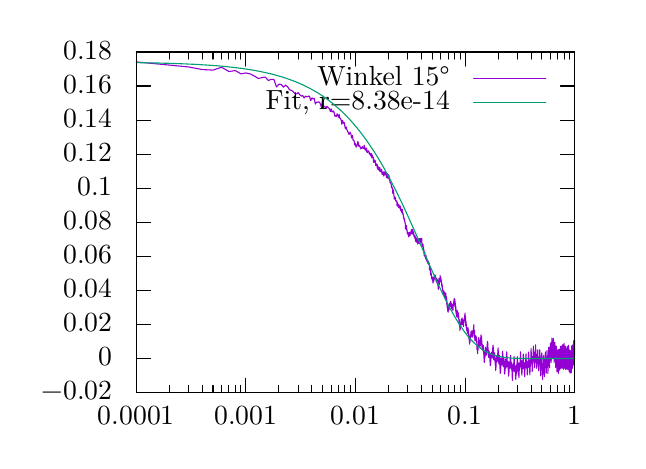
\begin{tikzpicture}[gnuplot]
%% generated with GNUPLOT 5.2p5a (Gentoo revision r0) (Lua 5.1; terminal rev. 99 , script rev. 107)
%% Sa 18 Mai 2019 18:30:52 CEST
\path (0.000,0.000) rectangle (7.500,5.250);
\gpcolor{color=gp lt color border}
\gpsetlinetype{gp lt border}
\gpsetdashtype{gp dt solid}
\gpsetlinewidth{1.00}
\draw[gp path] (1.380,0.616)--(1.560,0.616);
\draw[gp path] (6.947,0.616)--(6.767,0.616);
\node[gp node right] at (1.196,0.616) {$-0.02$};
\draw[gp path] (1.380,1.049)--(1.560,1.049);
\draw[gp path] (6.947,1.049)--(6.767,1.049);
\node[gp node right] at (1.196,1.049) {$0$};
\draw[gp path] (1.380,1.481)--(1.560,1.481);
\draw[gp path] (6.947,1.481)--(6.767,1.481);
\node[gp node right] at (1.196,1.481) {$0.02$};
\draw[gp path] (1.380,1.913)--(1.560,1.913);
\draw[gp path] (6.947,1.913)--(6.767,1.913);
\node[gp node right] at (1.196,1.913) {$0.04$};
\draw[gp path] (1.380,2.346)--(1.560,2.346);
\draw[gp path] (6.947,2.346)--(6.767,2.346);
\node[gp node right] at (1.196,2.346) {$0.06$};
\draw[gp path] (1.380,2.778)--(1.560,2.778);
\draw[gp path] (6.947,2.778)--(6.767,2.778);
\node[gp node right] at (1.196,2.778) {$0.08$};
\draw[gp path] (1.380,3.211)--(1.560,3.211);
\draw[gp path] (6.947,3.211)--(6.767,3.211);
\node[gp node right] at (1.196,3.211) {$0.1$};
\draw[gp path] (1.380,3.643)--(1.560,3.643);
\draw[gp path] (6.947,3.643)--(6.767,3.643);
\node[gp node right] at (1.196,3.643) {$0.12$};
\draw[gp path] (1.380,4.076)--(1.560,4.076);
\draw[gp path] (6.947,4.076)--(6.767,4.076);
\node[gp node right] at (1.196,4.076) {$0.14$};
\draw[gp path] (1.380,4.509)--(1.560,4.509);
\draw[gp path] (6.947,4.509)--(6.767,4.509);
\node[gp node right] at (1.196,4.509) {$0.16$};
\draw[gp path] (1.380,4.941)--(1.560,4.941);
\draw[gp path] (6.947,4.941)--(6.767,4.941);
\node[gp node right] at (1.196,4.941) {$0.18$};
\draw[gp path] (1.380,0.616)--(1.380,0.796);
\draw[gp path] (1.380,4.941)--(1.380,4.761);
\node[gp node center] at (1.380,0.308) {$0.0001$};
\draw[gp path] (1.799,0.616)--(1.799,0.706);
\draw[gp path] (1.799,4.941)--(1.799,4.851);
\draw[gp path] (2.044,0.616)--(2.044,0.706);
\draw[gp path] (2.044,4.941)--(2.044,4.851);
\draw[gp path] (2.218,0.616)--(2.218,0.706);
\draw[gp path] (2.218,4.941)--(2.218,4.851);
\draw[gp path] (2.353,0.616)--(2.353,0.706);
\draw[gp path] (2.353,4.941)--(2.353,4.851);
\draw[gp path] (2.463,0.616)--(2.463,0.706);
\draw[gp path] (2.463,4.941)--(2.463,4.851);
\draw[gp path] (2.556,0.616)--(2.556,0.706);
\draw[gp path] (2.556,4.941)--(2.556,4.851);
\draw[gp path] (2.637,0.616)--(2.637,0.706);
\draw[gp path] (2.637,4.941)--(2.637,4.851);
\draw[gp path] (2.708,0.616)--(2.708,0.706);
\draw[gp path] (2.708,4.941)--(2.708,4.851);
\draw[gp path] (2.772,0.616)--(2.772,0.796);
\draw[gp path] (2.772,4.941)--(2.772,4.761);
\node[gp node center] at (2.772,0.308) {$0.001$};
\draw[gp path] (3.191,0.616)--(3.191,0.706);
\draw[gp path] (3.191,4.941)--(3.191,4.851);
\draw[gp path] (3.436,0.616)--(3.436,0.706);
\draw[gp path] (3.436,4.941)--(3.436,4.851);
\draw[gp path] (3.610,0.616)--(3.610,0.706);
\draw[gp path] (3.610,4.941)--(3.610,4.851);
\draw[gp path] (3.745,0.616)--(3.745,0.706);
\draw[gp path] (3.745,4.941)--(3.745,4.851);
\draw[gp path] (3.855,0.616)--(3.855,0.706);
\draw[gp path] (3.855,4.941)--(3.855,4.851);
\draw[gp path] (3.948,0.616)--(3.948,0.706);
\draw[gp path] (3.948,4.941)--(3.948,4.851);
\draw[gp path] (4.029,0.616)--(4.029,0.706);
\draw[gp path] (4.029,4.941)--(4.029,4.851);
\draw[gp path] (4.100,0.616)--(4.100,0.706);
\draw[gp path] (4.100,4.941)--(4.100,4.851);
\draw[gp path] (4.163,0.616)--(4.163,0.796);
\draw[gp path] (4.163,4.941)--(4.163,4.761);
\node[gp node center] at (4.163,0.308) {$0.01$};
\draw[gp path] (4.582,0.616)--(4.582,0.706);
\draw[gp path] (4.582,4.941)--(4.582,4.851);
\draw[gp path] (4.828,0.616)--(4.828,0.706);
\draw[gp path] (4.828,4.941)--(4.828,4.851);
\draw[gp path] (5.001,0.616)--(5.001,0.706);
\draw[gp path] (5.001,4.941)--(5.001,4.851);
\draw[gp path] (5.136,0.616)--(5.136,0.706);
\draw[gp path] (5.136,4.941)--(5.136,4.851);
\draw[gp path] (5.246,0.616)--(5.246,0.706);
\draw[gp path] (5.246,4.941)--(5.246,4.851);
\draw[gp path] (5.340,0.616)--(5.340,0.706);
\draw[gp path] (5.340,4.941)--(5.340,4.851);
\draw[gp path] (5.420,0.616)--(5.420,0.706);
\draw[gp path] (5.420,4.941)--(5.420,4.851);
\draw[gp path] (5.492,0.616)--(5.492,0.706);
\draw[gp path] (5.492,4.941)--(5.492,4.851);
\draw[gp path] (5.555,0.616)--(5.555,0.796);
\draw[gp path] (5.555,4.941)--(5.555,4.761);
\node[gp node center] at (5.555,0.308) {$0.1$};
\draw[gp path] (5.974,0.616)--(5.974,0.706);
\draw[gp path] (5.974,4.941)--(5.974,4.851);
\draw[gp path] (6.219,0.616)--(6.219,0.706);
\draw[gp path] (6.219,4.941)--(6.219,4.851);
\draw[gp path] (6.393,0.616)--(6.393,0.706);
\draw[gp path] (6.393,4.941)--(6.393,4.851);
\draw[gp path] (6.528,0.616)--(6.528,0.706);
\draw[gp path] (6.528,4.941)--(6.528,4.851);
\draw[gp path] (6.638,0.616)--(6.638,0.706);
\draw[gp path] (6.638,4.941)--(6.638,4.851);
\draw[gp path] (6.731,0.616)--(6.731,0.706);
\draw[gp path] (6.731,4.941)--(6.731,4.851);
\draw[gp path] (6.812,0.616)--(6.812,0.706);
\draw[gp path] (6.812,4.941)--(6.812,4.851);
\draw[gp path] (6.883,0.616)--(6.883,0.706);
\draw[gp path] (6.883,4.941)--(6.883,4.851);
\draw[gp path] (6.947,0.616)--(6.947,0.796);
\draw[gp path] (6.947,4.941)--(6.947,4.761);
\node[gp node center] at (6.947,0.308) {$1$};
\draw[gp path] (1.380,4.941)--(1.380,0.616)--(6.947,0.616)--(6.947,4.941)--cycle;
\node[gp node right] at (5.479,4.607) {Winkel 15°};
\gpcolor{rgb color={0.580,0.000,0.827}}
\draw[gp path] (5.663,4.607)--(6.579,4.607);
\draw[gp path] (1.380,4.815)--(1.799,4.775)--(2.044,4.751)--(2.218,4.718)--(2.353,4.711)%
  --(2.463,4.747)--(2.556,4.693)--(2.637,4.705)--(2.708,4.664)--(2.772,4.675)--(2.829,4.662)%
  --(2.882,4.634)--(2.930,4.604)--(2.975,4.616)--(3.017,4.623)--(3.056,4.579)--(3.092,4.594)%
  --(3.127,4.592)--(3.160,4.497)--(3.191,4.532)--(3.220,4.530)--(3.248,4.494)--(3.275,4.520)%
  --(3.301,4.500)--(3.326,4.461)--(3.349,4.454)--(3.372,4.438)--(3.394,4.411)--(3.415,4.409)%
  --(3.436,4.425)--(3.456,4.398)--(3.475,4.380)--(3.493,4.389)--(3.511,4.357)--(3.529,4.381)%
  --(3.546,4.371)--(3.563,4.379)--(3.579,4.379)--(3.594,4.322)--(3.610,4.358)--(3.625,4.344)%
  --(3.639,4.352)--(3.653,4.281)--(3.667,4.305)--(3.681,4.302)--(3.694,4.307)--(3.707,4.303)%
  --(3.720,4.274)--(3.732,4.235)--(3.745,4.338)--(3.757,4.259)--(3.768,4.244)--(3.780,4.245)%
  --(3.791,4.227)--(3.802,4.251)--(3.813,4.239)--(3.824,4.228)--(3.834,4.216)--(3.845,4.185)%
  --(3.855,4.218)--(3.865,4.184)--(3.875,4.181)--(3.884,4.192)--(3.894,4.164)--(3.903,4.124)%
  --(3.912,4.134)--(3.921,4.124)--(3.930,4.156)--(3.939,4.139)--(3.948,4.112)--(3.956,4.147)%
  --(3.965,4.097)--(3.973,4.096)--(3.982,4.074)--(3.990,4.023)--(3.998,4.071)--(4.006,4.052)%
  --(4.013,4.035)--(4.021,4.045)--(4.029,3.992)--(4.036,3.966)--(4.044,3.991)--(4.051,3.960)%
  --(4.058,3.948)--(4.065,3.928)--(4.072,3.921)--(4.079,3.895)--(4.086,3.900)--(4.093,3.924)%
  --(4.100,3.903)--(4.106,3.901)--(4.113,3.849)--(4.120,3.858)--(4.126,3.880)--(4.132,3.822)%
  --(4.139,3.819)--(4.145,3.818)--(4.151,3.763)--(4.157,3.783)--(4.164,3.769)--(4.170,3.735)%
  --(4.175,3.735)--(4.181,3.746)--(4.187,3.775)--(4.193,3.805)--(4.199,3.784)--(4.204,3.744)%
  --(4.210,3.754)--(4.216,3.755)--(4.221,3.737)--(4.227,3.712)--(4.232,3.727)--(4.237,3.721)%
  --(4.243,3.717)--(4.248,3.740)--(4.253,3.734)--(4.258,3.723)--(4.264,3.717)--(4.269,3.717)%
  --(4.274,3.756)--(4.279,3.727)--(4.284,3.697)--(4.289,3.707)--(4.294,3.720)--(4.298,3.682)%
  --(4.303,3.719)--(4.308,3.675)--(4.313,3.662)--(4.317,3.684)--(4.322,3.679)--(4.327,3.685)%
  --(4.331,3.685)--(4.336,3.651)--(4.340,3.666)--(4.345,3.642)--(4.349,3.652)--(4.354,3.625)%
  --(4.358,3.623)--(4.363,3.652)--(4.367,3.643)--(4.371,3.597)--(4.375,3.634)--(4.380,3.617)%
  --(4.384,3.605)--(4.388,3.602)--(4.392,3.540)--(4.396,3.580)--(4.400,3.555)--(4.405,3.540)%
  --(4.409,3.566)--(4.413,3.563)--(4.417,3.532)--(4.421,3.497)--(4.424,3.523)--(4.428,3.510)%
  --(4.432,3.499)--(4.436,3.517)--(4.440,3.466)--(4.444,3.505)--(4.448,3.450)--(4.451,3.470)%
  --(4.455,3.482)--(4.459,3.442)--(4.463,3.464)--(4.466,3.431)--(4.470,3.466)--(4.473,3.474)%
  --(4.477,3.422)--(4.481,3.433)--(4.484,3.425)--(4.488,3.445)--(4.491,3.416)--(4.495,3.451)%
  --(4.498,3.415)--(4.502,3.387)--(4.505,3.408)--(4.509,3.387)--(4.512,3.409)--(4.515,3.418)%
  --(4.519,3.380)--(4.522,3.366)--(4.525,3.398)--(4.529,3.420)--(4.532,3.391)--(4.535,3.381)%
  --(4.539,3.387)--(4.542,3.413)--(4.545,3.393)--(4.548,3.382)--(4.551,3.391)--(4.555,3.357)%
  --(4.558,3.345)--(4.561,3.398)--(4.564,3.385)--(4.567,3.398)--(4.570,3.358)--(4.573,3.354)%
  --(4.576,3.334)--(4.579,3.387)--(4.582,3.356)--(4.585,3.348)--(4.588,3.374)--(4.591,3.343)%
  --(4.594,3.314)--(4.597,3.338)--(4.600,3.287)--(4.603,3.291)--(4.606,3.277)--(4.609,3.275)%
  --(4.612,3.273)--(4.615,3.270)--(4.618,3.249)--(4.621,3.216)--(4.623,3.233)--(4.626,3.216)%
  --(4.629,3.219)--(4.632,3.212)--(4.635,3.203)--(4.637,3.145)--(4.640,3.196)--(4.643,3.154)%
  --(4.646,3.183)--(4.648,3.156)--(4.651,3.115)--(4.654,3.115)--(4.656,3.072)--(4.659,3.106)%
  --(4.662,3.083)--(4.664,3.088)--(4.667,3.093)--(4.670,3.091)--(4.672,3.068)--(4.675,3.049)%
  --(4.677,3.057)--(4.680,3.047)--(4.683,3.046)--(4.685,3.050)--(4.688,3.039)--(4.690,2.991)%
  --(4.693,3.033)--(4.695,3.018)--(4.698,2.987)--(4.700,3.015)--(4.703,2.986)--(4.705,2.991)%
  --(4.708,2.966)--(4.710,3.001)--(4.712,2.991)--(4.715,3.001)--(4.717,2.989)--(4.720,2.961)%
  --(4.722,2.984)--(4.725,2.957)--(4.727,2.958)--(4.729,2.982)--(4.732,2.952)--(4.734,2.983)%
  --(4.736,2.927)--(4.739,2.932)--(4.741,2.928)--(4.743,2.930)--(4.746,2.918)--(4.748,2.946)%
  --(4.750,2.903)--(4.753,2.922)--(4.755,2.910)--(4.757,2.943)--(4.759,2.884)--(4.762,2.886)%
  --(4.764,2.901)--(4.766,2.890)--(4.768,2.881)--(4.771,2.869)--(4.773,2.832)--(4.775,2.843)%
  --(4.777,2.847)--(4.779,2.830)--(4.781,2.806)--(4.784,2.817)--(4.786,2.819)--(4.788,2.785)%
  --(4.790,2.788)--(4.792,2.783)--(4.794,2.768)--(4.797,2.751)--(4.799,2.692)--(4.801,2.741)%
  --(4.803,2.720)--(4.805,2.733)--(4.807,2.706)--(4.809,2.690)--(4.811,2.737)--(4.813,2.693)%
  --(4.815,2.680)--(4.817,2.677)--(4.819,2.684)--(4.821,2.638)--(4.823,2.633)--(4.826,2.649)%
  --(4.828,2.646)--(4.830,2.649)--(4.832,2.619)--(4.834,2.634)--(4.836,2.607)--(4.838,2.623)%
  --(4.840,2.594)--(4.841,2.617)--(4.843,2.606)--(4.845,2.645)--(4.847,2.623)--(4.849,2.651)%
  --(4.851,2.633)--(4.853,2.639)--(4.855,2.608)--(4.857,2.617)--(4.859,2.627)--(4.861,2.625)%
  --(4.863,2.634)--(4.865,2.653)--(4.867,2.628)--(4.868,2.670)--(4.870,2.629)--(4.872,2.648)%
  --(4.874,2.672)--(4.876,2.660)--(4.878,2.688)--(4.880,2.667)--(4.881,2.653)--(4.883,2.660)%
  --(4.885,2.632)--(4.887,2.658)--(4.889,2.683)--(4.891,2.690)--(4.892,2.656)--(4.894,2.656)%
  --(4.896,2.645)--(4.898,2.622)--(4.900,2.654)--(4.901,2.657)--(4.903,2.616)--(4.905,2.630)%
  --(4.907,2.595)--(4.908,2.623)--(4.910,2.591)--(4.912,2.611)--(4.914,2.595)--(4.916,2.610)%
  --(4.917,2.569)--(4.919,2.608)--(4.921,2.575)--(4.922,2.581)--(4.924,2.546)--(4.926,2.593)%
  --(4.928,2.574)--(4.929,2.534)--(4.931,2.556)--(4.933,2.557)--(4.934,2.552)--(4.936,2.571)%
  --(4.938,2.578)--(4.939,2.531)--(4.941,2.532)--(4.943,2.533)--(4.944,2.522)--(4.946,2.550)%
  --(4.948,2.551)--(4.949,2.519)--(4.951,2.519)--(4.953,2.502)--(4.954,2.507)--(4.956,2.561)%
  --(4.958,2.533)--(4.959,2.524)--(4.961,2.569)--(4.962,2.543)--(4.964,2.542)--(4.966,2.559)%
  --(4.967,2.519)--(4.969,2.532)--(4.970,2.569)--(4.972,2.564)--(4.974,2.508)--(4.975,2.508)%
  --(4.977,2.543)--(4.978,2.520)--(4.980,2.563)--(4.981,2.570)--(4.983,2.574)--(4.985,2.557)%
  --(4.986,2.559)--(4.988,2.520)--(4.989,2.525)--(4.991,2.561)--(4.992,2.527)--(4.994,2.573)%
  --(4.995,2.552)--(4.997,2.572)--(4.998,2.555)--(5.000,2.555)--(5.001,2.559)--(5.003,2.568)%
  --(5.004,2.558)--(5.006,2.572)--(5.007,2.516)--(5.009,2.474)--(5.010,2.500)--(5.012,2.496)%
  --(5.013,2.482)--(5.015,2.486)--(5.016,2.484)--(5.018,2.469)--(5.019,2.497)--(5.021,2.500)%
  --(5.022,2.458)--(5.024,2.466)--(5.025,2.448)--(5.027,2.426)--(5.028,2.465)--(5.029,2.417)%
  --(5.031,2.405)--(5.032,2.432)--(5.034,2.384)--(5.035,2.399)--(5.037,2.353)--(5.038,2.364)%
  --(5.039,2.381)--(5.041,2.348)--(5.042,2.389)--(5.044,2.399)--(5.045,2.350)--(5.047,2.351)%
  --(5.048,2.348)--(5.049,2.341)--(5.051,2.330)--(5.052,2.340)--(5.054,2.316)--(5.055,2.325)%
  --(5.056,2.323)--(5.058,2.320)--(5.059,2.356)--(5.060,2.305)--(5.062,2.324)--(5.063,2.306)%
  --(5.064,2.318)--(5.066,2.319)--(5.067,2.290)--(5.069,2.311)--(5.070,2.285)--(5.071,2.299)%
  --(5.073,2.276)--(5.074,2.297)--(5.075,2.299)--(5.077,2.285)--(5.078,2.293)--(5.079,2.292)%
  --(5.081,2.264)--(5.082,2.284)--(5.083,2.253)--(5.085,2.279)--(5.086,2.286)--(5.087,2.273)%
  --(5.089,2.257)--(5.090,2.264)--(5.091,2.244)--(5.092,2.279)--(5.094,2.259)--(5.095,2.267)%
  --(5.096,2.244)--(5.098,2.262)--(5.099,2.234)--(5.100,2.255)--(5.101,2.222)--(5.103,2.176)%
  --(5.104,2.222)--(5.105,2.202)--(5.107,2.203)--(5.108,2.207)--(5.109,2.173)--(5.110,2.188)%
  --(5.112,2.171)--(5.113,2.166)--(5.114,2.163)--(5.115,2.141)--(5.117,2.141)--(5.118,2.191)%
  --(5.119,2.108)--(5.120,2.122)--(5.122,2.126)--(5.123,2.124)--(5.124,2.131)--(5.125,2.128)%
  --(5.127,2.107)--(5.128,2.096)--(5.129,2.096)--(5.130,2.066)--(5.131,2.063)--(5.133,2.072)%
  --(5.134,2.066)--(5.135,2.076)--(5.136,2.059)--(5.137,2.051)--(5.139,2.078)--(5.140,2.046)%
  --(5.141,2.036)--(5.142,2.081)--(5.144,2.063)--(5.145,2.031)--(5.146,2.053)--(5.147,2.006)%
  --(5.148,2.030)--(5.149,2.042)--(5.151,2.058)--(5.152,2.019)--(5.153,2.059)--(5.154,2.022)%
  --(5.155,2.050)--(5.157,2.036)--(5.158,2.036)--(5.159,2.055)--(5.160,2.054)--(5.161,2.089)%
  --(5.162,2.068)--(5.163,2.079)--(5.165,2.085)--(5.166,2.092)--(5.167,2.110)--(5.168,2.083)%
  --(5.169,2.057)--(5.170,2.081)--(5.172,2.064)--(5.173,2.095)--(5.174,2.069)--(5.175,2.107)%
  --(5.176,2.076)--(5.177,2.106)--(5.178,2.106)--(5.179,2.088)--(5.181,2.057)--(5.182,2.071)%
  --(5.183,2.081)--(5.184,2.057)--(5.185,2.054)--(5.186,2.045)--(5.187,2.028)--(5.188,2.052)%
  --(5.189,2.069)--(5.191,2.052)--(5.192,2.060)--(5.193,2.031)--(5.194,2.041)--(5.195,2.039)%
  --(5.196,2.010)--(5.197,2.012)--(5.198,2.041)--(5.199,2.021)--(5.200,2.058)--(5.202,2.019)%
  --(5.203,2.052)--(5.204,1.997)--(5.205,2.013)--(5.206,1.988)--(5.207,2.041)--(5.208,2.000)%
  --(5.209,1.975)--(5.210,1.969)--(5.211,1.978)--(5.212,1.994)--(5.213,1.982)--(5.214,2.011)%
  --(5.215,1.926)--(5.217,2.003)--(5.218,1.974)--(5.219,2.004)--(5.220,1.993)--(5.221,1.987)%
  --(5.222,2.031)--(5.223,1.996)--(5.224,2.064)--(5.225,2.013)--(5.226,2.010)--(5.227,1.987)%
  --(5.228,2.067)--(5.229,2.015)--(5.230,2.040)--(5.231,2.015)--(5.232,2.032)--(5.233,2.021)%
  --(5.234,2.029)--(5.235,2.042)--(5.236,2.041)--(5.237,2.049)--(5.238,2.102)--(5.239,2.077)%
  --(5.240,2.076)--(5.241,2.079)--(5.242,2.088)--(5.243,2.053)--(5.244,2.063)--(5.245,2.063)%
  --(5.246,2.059)--(5.247,2.084)--(5.249,2.048)--(5.250,2.032)--(5.251,2.038)--(5.252,2.039)%
  --(5.253,2.021)--(5.254,2.002)--(5.254,2.025)--(5.255,2.005)--(5.256,2.010)--(5.257,2.023)%
  --(5.258,1.970)--(5.259,2.006)--(5.260,1.971)--(5.261,1.989)--(5.262,1.984)--(5.263,1.949)%
  --(5.264,1.982)--(5.265,1.967)--(5.266,1.938)--(5.267,1.942)--(5.268,1.915)--(5.269,1.918)%
  --(5.270,1.915)--(5.271,1.910)--(5.272,1.908)--(5.273,1.922)--(5.274,1.883)--(5.275,1.872)%
  --(5.276,1.900)--(5.277,1.887)--(5.278,1.906)--(5.279,1.864)--(5.280,1.898)--(5.281,1.860)%
  --(5.282,1.892)--(5.283,1.847)--(5.284,1.907)--(5.285,1.870)--(5.286,1.907)--(5.286,1.884)%
  --(5.287,1.854)--(5.288,1.873)--(5.289,1.895)--(5.290,1.893)--(5.291,1.877)--(5.292,1.855)%
  --(5.293,1.837)--(5.294,1.867)--(5.295,1.877)--(5.296,1.846)--(5.297,1.880)--(5.298,1.857)%
  --(5.299,1.853)--(5.300,1.878)--(5.300,1.857)--(5.301,1.811)--(5.302,1.857)--(5.303,1.852)%
  --(5.304,1.800)--(5.305,1.868)--(5.306,1.872)--(5.307,1.863)--(5.308,1.875)--(5.309,1.881)%
  --(5.310,1.854)--(5.310,1.860)--(5.311,1.847)--(5.312,1.826)--(5.313,1.829)--(5.314,1.841)%
  --(5.315,1.837)--(5.316,1.835)--(5.317,1.796)--(5.318,1.818)--(5.319,1.810)--(5.319,1.790)%
  --(5.320,1.780)--(5.321,1.766)--(5.322,1.800)--(5.323,1.730)--(5.324,1.755)--(5.325,1.740)%
  --(5.326,1.767)--(5.327,1.705)--(5.327,1.743)--(5.328,1.697)--(5.329,1.701)--(5.330,1.709)%
  --(5.331,1.731)--(5.332,1.684)--(5.333,1.695)--(5.334,1.665)--(5.334,1.653)--(5.335,1.663)%
  --(5.336,1.692)--(5.337,1.667)--(5.338,1.651)--(5.339,1.636)--(5.340,1.645)--(5.341,1.651)%
  --(5.341,1.663)--(5.342,1.691)--(5.343,1.663)--(5.344,1.700)--(5.345,1.680)--(5.346,1.691)%
  --(5.347,1.671)--(5.347,1.677)--(5.348,1.706)--(5.349,1.706)--(5.350,1.691)--(5.351,1.705)%
  --(5.352,1.684)--(5.352,1.694)--(5.353,1.667)--(5.354,1.731)--(5.355,1.677)--(5.356,1.697)%
  --(5.357,1.721)--(5.358,1.717)--(5.358,1.726)--(5.359,1.697)--(5.360,1.750)--(5.361,1.714)%
  --(5.362,1.728)--(5.363,1.743)--(5.363,1.750)--(5.364,1.751)--(5.365,1.748)--(5.366,1.744)%
  --(5.367,1.738)--(5.368,1.769)--(5.368,1.747)--(5.369,1.754)--(5.370,1.733)--(5.371,1.760)%
  --(5.372,1.736)--(5.372,1.775)--(5.373,1.723)--(5.374,1.707)--(5.375,1.775)--(5.376,1.730)%
  --(5.377,1.708)--(5.377,1.743)--(5.378,1.730)--(5.379,1.749)--(5.380,1.749)--(5.381,1.730)%
  --(5.381,1.733)--(5.382,1.715)--(5.383,1.700)--(5.384,1.685)--(5.385,1.696)--(5.385,1.713)%
  --(5.386,1.695)--(5.387,1.691)--(5.388,1.703)--(5.389,1.707)--(5.389,1.716)--(5.390,1.709)%
  --(5.391,1.692)--(5.392,1.674)--(5.393,1.670)--(5.393,1.735)--(5.394,1.685)--(5.395,1.694)%
  --(5.396,1.697)--(5.396,1.691)--(5.397,1.700)--(5.398,1.698)--(5.399,1.670)--(5.400,1.715)%
  --(5.400,1.702)--(5.401,1.717)--(5.402,1.661)--(5.403,1.702)--(5.404,1.712)--(5.404,1.725)%
  --(5.405,1.716)--(5.406,1.736)--(5.407,1.743)--(5.407,1.749)--(5.408,1.724)--(5.409,1.735)%
  --(5.410,1.749)--(5.410,1.769)--(5.411,1.762)--(5.412,1.761)--(5.413,1.735)--(5.414,1.771)%
  --(5.414,1.792)--(5.415,1.744)--(5.416,1.773)--(5.417,1.799)--(5.417,1.762)--(5.418,1.806)%
  --(5.419,1.811)--(5.420,1.785)--(5.420,1.787)--(5.421,1.797)--(5.422,1.779)--(5.423,1.785)%
  --(5.423,1.789)--(5.424,1.802)--(5.425,1.784)--(5.426,1.778)--(5.426,1.706)--(5.427,1.743)%
  --(5.428,1.750)--(5.429,1.772)--(5.429,1.721)--(5.430,1.711)--(5.431,1.752)--(5.432,1.721)%
  --(5.432,1.734)--(5.433,1.702)--(5.434,1.694)--(5.435,1.703)--(5.435,1.651)--(5.436,1.714)%
  --(5.437,1.681)--(5.438,1.683)--(5.438,1.682)--(5.439,1.677)--(5.440,1.636)--(5.440,1.645)%
  --(5.441,1.656)--(5.442,1.631)--(5.443,1.614)--(5.443,1.626)--(5.444,1.648)--(5.445,1.657)%
  --(5.446,1.599)--(5.446,1.649)--(5.447,1.640)--(5.448,1.612)--(5.448,1.639)--(5.449,1.578)%
  --(5.450,1.603)--(5.451,1.595)--(5.451,1.633)--(5.452,1.626)--(5.453,1.637)--(5.453,1.619)%
  --(5.454,1.593)--(5.455,1.629)--(5.456,1.592)--(5.456,1.641)--(5.457,1.592)--(5.458,1.655)%
  --(5.458,1.603)--(5.459,1.607)--(5.460,1.607)--(5.461,1.603)--(5.461,1.618)--(5.462,1.570)%
  --(5.463,1.590)--(5.463,1.608)--(5.464,1.601)--(5.465,1.617)--(5.465,1.602)--(5.466,1.595)%
  --(5.467,1.601)--(5.468,1.629)--(5.468,1.622)--(5.469,1.617)--(5.470,1.613)--(5.470,1.616)%
  --(5.471,1.605)--(5.472,1.587)--(5.472,1.588)--(5.473,1.555)--(5.474,1.566)--(5.475,1.582)%
  --(5.475,1.570)--(5.476,1.568)--(5.477,1.527)--(5.477,1.551)--(5.478,1.503)--(5.479,1.525)%
  --(5.479,1.519)--(5.480,1.518)--(5.481,1.540)--(5.481,1.522)--(5.482,1.493)--(5.483,1.539)%
  --(5.483,1.505)--(5.484,1.477)--(5.485,1.461)--(5.485,1.490)--(5.486,1.457)--(5.487,1.452)%
  --(5.488,1.447)--(5.488,1.486)--(5.489,1.404)--(5.490,1.434)--(5.490,1.441)--(5.491,1.451)%
  --(5.492,1.419)--(5.492,1.436)--(5.493,1.418)--(5.494,1.443)--(5.494,1.462)--(5.495,1.456)%
  --(5.496,1.490)--(5.496,1.455)--(5.497,1.457)--(5.498,1.469)--(5.498,1.485)--(5.499,1.457)%
  --(5.500,1.490)--(5.500,1.479)--(5.501,1.516)--(5.502,1.479)--(5.502,1.471)--(5.503,1.488)%
  --(5.504,1.489)--(5.504,1.517)--(5.505,1.535)--(5.506,1.510)--(5.506,1.545)--(5.507,1.503)%
  --(5.507,1.532)--(5.508,1.523)--(5.509,1.475)--(5.509,1.539)--(5.510,1.525)--(5.511,1.507)%
  --(5.511,1.518)--(5.512,1.540)--(5.513,1.532)--(5.513,1.535)--(5.514,1.496)--(5.515,1.558)%
  --(5.515,1.517)--(5.516,1.564)--(5.517,1.525)--(5.517,1.555)--(5.518,1.522)--(5.518,1.517)%
  --(5.519,1.494)--(5.520,1.502)--(5.520,1.518)--(5.521,1.549)--(5.522,1.547)--(5.522,1.480)%
  --(5.523,1.533)--(5.524,1.490)--(5.524,1.514)--(5.525,1.501)--(5.526,1.485)--(5.526,1.497)%
  --(5.527,1.502)--(5.527,1.490)--(5.528,1.493)--(5.529,1.519)--(5.529,1.500)--(5.530,1.498)%
  --(5.531,1.514)--(5.531,1.479)--(5.532,1.528)--(5.532,1.520)--(5.533,1.493)--(5.534,1.490)%
  --(5.535,1.453)--(5.536,1.489)--(5.536,1.488)--(5.537,1.484)--(5.537,1.495)--(5.538,1.538)%
  --(5.539,1.520)--(5.539,1.513)--(5.540,1.518)--(5.541,1.539)--(5.541,1.518)--(5.542,1.531)%
  --(5.542,1.506)--(5.543,1.527)--(5.544,1.527)--(5.544,1.529)--(5.545,1.542)--(5.546,1.554)%
  --(5.546,1.576)--(5.547,1.563)--(5.548,1.560)--(5.549,1.598)--(5.549,1.556)--(5.550,1.540)%
  --(5.550,1.566)--(5.551,1.558)--(5.552,1.608)--(5.552,1.578)--(5.553,1.557)--(5.553,1.616)%
  --(5.554,1.604)--(5.555,1.625)--(5.555,1.615)--(5.556,1.601)--(5.556,1.580)--(5.557,1.568)%
  --(5.558,1.589)--(5.558,1.548)--(5.559,1.572)--(5.559,1.578)--(5.560,1.539)--(5.561,1.577)%
  --(5.561,1.554)--(5.562,1.469)--(5.562,1.533)--(5.563,1.519)--(5.564,1.519)--(5.564,1.517)%
  --(5.565,1.506)--(5.565,1.481)--(5.566,1.515)--(5.567,1.490)--(5.567,1.496)--(5.568,1.467)%
  --(5.568,1.446)--(5.569,1.457)--(5.570,1.467)--(5.570,1.475)--(5.571,1.485)--(5.571,1.454)%
  --(5.572,1.444)--(5.573,1.442)--(5.573,1.436)--(5.574,1.447)--(5.574,1.424)--(5.575,1.423)%
  --(5.575,1.408)--(5.576,1.423)--(5.577,1.411)--(5.577,1.402)--(5.578,1.440)--(5.578,1.426)%
  --(5.579,1.434)--(5.580,1.407)--(5.580,1.393)--(5.581,1.432)--(5.581,1.417)--(5.582,1.400)%
  --(5.582,1.434)--(5.583,1.399)--(5.584,1.429)--(5.584,1.415)--(5.585,1.436)--(5.585,1.368)%
  --(5.586,1.429)--(5.586,1.402)--(5.587,1.406)--(5.588,1.385)--(5.588,1.424)--(5.589,1.399)%
  --(5.589,1.369)--(5.590,1.411)--(5.590,1.422)--(5.591,1.413)--(5.592,1.441)--(5.592,1.410)%
  --(5.593,1.418)--(5.593,1.398)--(5.594,1.372)--(5.594,1.422)--(5.595,1.407)--(5.596,1.393)%
  --(5.596,1.365)--(5.597,1.389)--(5.597,1.403)--(5.598,1.369)--(5.598,1.407)--(5.599,1.361)%
  --(5.600,1.377)--(5.600,1.372)--(5.601,1.364)--(5.601,1.328)--(5.602,1.306)--(5.602,1.346)%
  --(5.603,1.343)--(5.603,1.349)--(5.604,1.354)--(5.605,1.321)--(5.605,1.347)--(5.606,1.330)%
  --(5.606,1.316)--(5.607,1.288)--(5.607,1.315)--(5.608,1.279)--(5.608,1.298)--(5.609,1.294)%
  --(5.610,1.315)--(5.610,1.267)--(5.611,1.252)--(5.611,1.254)--(5.612,1.273)--(5.612,1.259)%
  --(5.613,1.231)--(5.613,1.236)--(5.614,1.257)--(5.615,1.248)--(5.615,1.253)--(5.616,1.272)%
  --(5.616,1.287)--(5.617,1.284)--(5.617,1.293)--(5.618,1.283)--(5.618,1.259)--(5.619,1.288)%
  --(5.619,1.307)--(5.620,1.291)--(5.621,1.320)--(5.621,1.313)--(5.622,1.306)--(5.622,1.326)%
  --(5.623,1.334)--(5.623,1.306)--(5.624,1.329)--(5.624,1.316)--(5.625,1.341)--(5.625,1.333)%
  --(5.626,1.323)--(5.626,1.344)--(5.627,1.356)--(5.628,1.337)--(5.628,1.388)--(5.629,1.378)%
  --(5.629,1.344)--(5.630,1.364)--(5.630,1.355)--(5.631,1.386)--(5.631,1.373)--(5.632,1.374)%
  --(5.632,1.350)--(5.633,1.359)--(5.633,1.370)--(5.634,1.338)--(5.634,1.353)--(5.635,1.372)%
  --(5.636,1.376)--(5.636,1.345)--(5.637,1.399)--(5.637,1.360)--(5.638,1.326)--(5.638,1.349)%
  --(5.639,1.342)--(5.639,1.355)--(5.640,1.352)--(5.641,1.381)--(5.641,1.357)--(5.642,1.347)%
  --(5.642,1.323)--(5.643,1.367)--(5.643,1.344)--(5.644,1.371)--(5.644,1.353)--(5.645,1.392)%
  --(5.645,1.352)--(5.646,1.367)--(5.647,1.365)--(5.648,1.337)--(5.648,1.346)--(5.649,1.386)%
  --(5.649,1.357)--(5.650,1.355)--(5.650,1.320)--(5.651,1.354)--(5.651,1.371)--(5.652,1.351)%
  --(5.652,1.380)--(5.653,1.355)--(5.653,1.370)--(5.654,1.370)--(5.654,1.333)--(5.655,1.399)%
  --(5.655,1.406)--(5.656,1.361)--(5.656,1.388)--(5.657,1.367)--(5.657,1.386)--(5.658,1.390)%
  --(5.658,1.400)--(5.659,1.377)--(5.659,1.397)--(5.660,1.402)--(5.660,1.397)--(5.661,1.429)%
  --(5.661,1.416)--(5.662,1.395)--(5.662,1.439)--(5.663,1.446)--(5.663,1.459)--(5.664,1.440)%
  --(5.664,1.423)--(5.665,1.454)--(5.665,1.468)--(5.666,1.453)--(5.666,1.479)--(5.667,1.435)%
  --(5.667,1.417)--(5.668,1.406)--(5.668,1.396)--(5.669,1.381)--(5.669,1.414)--(5.670,1.410)%
  --(5.670,1.360)--(5.671,1.382)--(5.671,1.378)--(5.672,1.405)--(5.672,1.390)--(5.673,1.367)%
  --(5.673,1.391)--(5.674,1.407)--(5.674,1.398)--(5.675,1.334)--(5.675,1.351)--(5.676,1.361)%
  --(5.676,1.357)--(5.677,1.348)--(5.677,1.318)--(5.678,1.323)--(5.678,1.300)--(5.679,1.332)%
  --(5.679,1.309)--(5.680,1.319)--(5.680,1.328)--(5.681,1.332)--(5.681,1.274)--(5.682,1.279)%
  --(5.682,1.313)--(5.683,1.280)--(5.683,1.301)--(5.684,1.283)--(5.684,1.319)--(5.685,1.303)%
  --(5.685,1.338)--(5.686,1.295)--(5.686,1.296)--(5.687,1.303)--(5.687,1.310)--(5.688,1.291)%
  --(5.688,1.287)--(5.689,1.289)--(5.689,1.290)--(5.690,1.308)--(5.690,1.330)--(5.691,1.277)%
  --(5.691,1.286)--(5.692,1.292)--(5.692,1.337)--(5.693,1.327)--(5.693,1.330)--(5.693,1.291)%
  --(5.694,1.274)--(5.694,1.282)--(5.695,1.333)--(5.695,1.293)--(5.696,1.314)--(5.696,1.305)%
  --(5.697,1.296)--(5.697,1.277)--(5.698,1.275)--(5.698,1.267)--(5.699,1.283)--(5.699,1.274)%
  --(5.700,1.287)--(5.700,1.290)--(5.701,1.276)--(5.701,1.264)--(5.702,1.313)--(5.702,1.249)%
  --(5.703,1.253)--(5.703,1.271)--(5.704,1.250)--(5.704,1.212)--(5.704,1.227)--(5.705,1.269)%
  --(5.705,1.201)--(5.706,1.216)--(5.706,1.212)--(5.707,1.224)--(5.707,1.161)--(5.708,1.189)%
  --(5.708,1.172)--(5.709,1.190)--(5.709,1.176)--(5.710,1.166)--(5.710,1.191)--(5.711,1.181)%
  --(5.711,1.180)--(5.712,1.134)--(5.712,1.188)--(5.712,1.144)--(5.713,1.151)--(5.713,1.146)%
  --(5.714,1.131)--(5.714,1.163)--(5.715,1.109)--(5.715,1.166)--(5.716,1.184)--(5.716,1.165)%
  --(5.717,1.163)--(5.717,1.176)--(5.718,1.146)--(5.718,1.184)--(5.718,1.193)--(5.719,1.170)%
  --(5.719,1.178)--(5.720,1.161)--(5.720,1.192)--(5.721,1.199)--(5.721,1.217)--(5.722,1.205)%
  --(5.722,1.221)--(5.723,1.210)--(5.723,1.220)--(5.724,1.246)--(5.724,1.221)--(5.724,1.228)%
  --(5.725,1.264)--(5.725,1.241)--(5.726,1.235)--(5.727,1.271)--(5.727,1.256)--(5.728,1.256)%
  --(5.728,1.267)--(5.729,1.249)--(5.729,1.287)--(5.729,1.314)--(5.730,1.248)--(5.730,1.277)%
  --(5.731,1.270)--(5.731,1.259)--(5.732,1.253)--(5.732,1.258)--(5.733,1.262)--(5.733,1.247)%
  --(5.733,1.264)--(5.734,1.251)--(5.734,1.238)--(5.735,1.253)--(5.735,1.230)--(5.736,1.283)%
  --(5.736,1.252)--(5.737,1.212)--(5.737,1.251)--(5.738,1.242)--(5.738,1.213)--(5.738,1.241)%
  --(5.739,1.224)--(5.739,1.244)--(5.740,1.225)--(5.740,1.244)--(5.741,1.221)--(5.741,1.202)%
  --(5.742,1.207)--(5.742,1.226)--(5.742,1.186)--(5.743,1.201)--(5.743,1.260)--(5.744,1.260)%
  --(5.744,1.206)--(5.745,1.217)--(5.745,1.238)--(5.746,1.236)--(5.746,1.261)--(5.746,1.281)%
  --(5.747,1.272)--(5.747,1.282)--(5.748,1.267)--(5.748,1.213)--(5.749,1.270)--(5.749,1.269)%
  --(5.749,1.244)--(5.750,1.245)--(5.750,1.211)--(5.751,1.262)--(5.751,1.249)--(5.752,1.285)%
  --(5.752,1.255)--(5.753,1.251)--(5.753,1.286)--(5.753,1.313)--(5.754,1.281)--(5.754,1.303)%
  --(5.755,1.283)--(5.755,1.307)--(5.756,1.326)--(5.756,1.295)--(5.756,1.314)--(5.757,1.330)%
  --(5.757,1.348)--(5.758,1.329)--(5.758,1.318)--(5.759,1.318)--(5.759,1.314)--(5.759,1.300)%
  --(5.760,1.310)--(5.760,1.298)--(5.761,1.296)--(5.761,1.310)--(5.762,1.293)--(5.762,1.299)%
  --(5.762,1.322)--(5.763,1.319)--(5.763,1.328)--(5.764,1.312)--(5.764,1.287)--(5.765,1.282)%
  --(5.765,1.259)--(5.765,1.264)--(5.766,1.276)--(5.766,1.243)--(5.767,1.230)--(5.767,1.251)%
  --(5.768,1.238)--(5.768,1.237)--(5.768,1.221)--(5.769,1.237)--(5.769,1.242)--(5.770,1.217)%
  --(5.770,1.194)--(5.771,1.191)--(5.771,1.202)--(5.771,1.189)--(5.772,1.190)--(5.772,1.197)%
  --(5.773,1.165)--(5.773,1.167)--(5.774,1.169)--(5.774,1.188)--(5.774,1.164)--(5.775,1.179)%
  --(5.775,1.183)--(5.776,1.164)--(5.776,1.167)--(5.776,1.209)--(5.777,1.181)--(5.777,1.182)%
  --(5.778,1.173)--(5.778,1.203)--(5.779,1.221)--(5.779,1.178)--(5.779,1.168)--(5.780,1.168)%
  --(5.780,1.161)--(5.781,1.186)--(5.781,1.199)--(5.781,1.195)--(5.782,1.145)--(5.782,1.171)%
  --(5.783,1.184)--(5.783,1.169)--(5.784,1.200)--(5.784,1.195)--(5.784,1.163)--(5.785,1.168)%
  --(5.785,1.180)--(5.786,1.171)--(5.786,1.215)--(5.786,1.183)--(5.787,1.172)--(5.787,1.155)%
  --(5.788,1.181)--(5.788,1.146)--(5.789,1.172)--(5.789,1.165)--(5.789,1.136)--(5.790,1.159)%
  --(5.790,1.118)--(5.791,1.164)--(5.791,1.113)--(5.791,1.106)--(5.792,1.114)--(5.792,1.136)%
  --(5.793,1.126)--(5.793,1.129)--(5.793,1.109)--(5.794,1.068)--(5.794,1.084)--(5.795,1.052)%
  --(5.795,1.112)--(5.795,1.110)--(5.796,1.054)--(5.796,1.104)--(5.797,1.070)--(5.797,1.031)%
  --(5.797,1.052)--(5.798,1.030)--(5.798,1.028)--(5.799,1.004)--(5.799,1.065)--(5.800,0.997)%
  --(5.800,1.021)--(5.800,1.009)--(5.801,1.041)--(5.801,1.031)--(5.802,1.066)--(5.802,1.045)%
  --(5.802,1.026)--(5.803,1.044)--(5.803,1.067)--(5.804,1.088)--(5.804,1.066)--(5.804,1.054)%
  --(5.805,1.076)--(5.805,1.056)--(5.806,1.093)--(5.806,1.070)--(5.806,1.102)--(5.807,1.076)%
  --(5.807,1.089)--(5.808,1.067)--(5.808,1.085)--(5.808,1.105)--(5.809,1.082)--(5.809,1.107)%
  --(5.810,1.141)--(5.810,1.115)--(5.810,1.120)--(5.811,1.137)--(5.811,1.146)--(5.812,1.134)%
  --(5.812,1.153)--(5.812,1.170)--(5.813,1.192)--(5.813,1.138)--(5.813,1.160)--(5.814,1.162)%
  --(5.814,1.126)--(5.815,1.103)--(5.815,1.149)--(5.815,1.156)--(5.816,1.157)--(5.816,1.144)%
  --(5.817,1.136)--(5.817,1.109)--(5.817,1.147)--(5.818,1.167)--(5.818,1.120)--(5.819,1.124)%
  --(5.819,1.129)--(5.819,1.154)--(5.820,1.096)--(5.820,1.123)--(5.821,1.125)--(5.821,1.152)%
  --(5.821,1.146)--(5.822,1.117)--(5.822,1.127)--(5.822,1.156)--(5.823,1.110)--(5.823,1.106)%
  --(5.824,1.120)--(5.824,1.104)--(5.824,1.145)--(5.825,1.100)--(5.825,1.101)--(5.826,1.091)%
  --(5.826,1.102)--(5.826,1.123)--(5.827,1.116)--(5.827,1.128)--(5.828,1.125)--(5.828,1.123)%
  --(5.828,1.136)--(5.829,1.174)--(5.829,1.134)--(5.829,1.127)--(5.830,1.165)--(5.830,1.149)%
  --(5.831,1.141)--(5.831,1.139)--(5.831,1.160)--(5.832,1.167)--(5.832,1.194)--(5.832,1.195)%
  --(5.833,1.185)--(5.833,1.196)--(5.834,1.202)--(5.834,1.162)--(5.834,1.196)--(5.835,1.190)%
  --(5.835,1.224)--(5.836,1.182)--(5.836,1.194)--(5.836,1.230)--(5.837,1.234)--(5.837,1.226)%
  --(5.837,1.211)--(5.838,1.257)--(5.838,1.260)--(5.839,1.265)--(5.839,1.221)--(5.839,1.255)%
  --(5.840,1.233)--(5.840,1.219)--(5.840,1.223)--(5.841,1.179)--(5.841,1.243)--(5.842,1.207)%
  --(5.842,1.192)--(5.842,1.218)--(5.843,1.253)--(5.843,1.194)--(5.843,1.238)--(5.844,1.210)%
  --(5.844,1.195)--(5.845,1.169)--(5.845,1.174)--(5.845,1.198)--(5.846,1.154)--(5.846,1.175)%
  --(5.846,1.187)--(5.847,1.168)--(5.847,1.176)--(5.848,1.113)--(5.848,1.147)--(5.848,1.108)%
  --(5.849,1.154)--(5.849,1.125)--(5.849,1.155)--(5.850,1.090)--(5.850,1.083)--(5.851,1.136)%
  --(5.851,1.119)--(5.851,1.105)--(5.852,1.129)--(5.852,1.116)--(5.852,1.104)--(5.853,1.062)%
  --(5.853,1.107)--(5.854,1.099)--(5.854,1.138)--(5.854,1.082)--(5.855,1.091)--(5.855,1.114)%
  --(5.856,1.132)--(5.856,1.128)--(5.856,1.127)--(5.857,1.138)--(5.857,1.092)--(5.858,1.116)%
  --(5.858,1.112)--(5.858,1.125)--(5.859,1.142)--(5.859,1.067)--(5.859,1.126)--(5.860,1.112)%
  --(5.860,1.143)--(5.860,1.097)--(5.861,1.130)--(5.861,1.126)--(5.862,1.125)--(5.862,1.129)%
  --(5.862,1.113)--(5.863,1.124)--(5.863,1.106)--(5.863,1.107)--(5.864,1.130)--(5.864,1.079)%
  --(5.864,1.112)--(5.865,1.105)--(5.865,1.102)--(5.866,1.087)--(5.866,1.093)--(5.866,1.091)%
  --(5.867,1.101)--(5.867,1.095)--(5.867,1.090)--(5.868,1.077)--(5.868,1.061)--(5.868,1.070)%
  --(5.869,1.061)--(5.869,1.071)--(5.870,1.024)--(5.870,1.032)--(5.870,1.022)--(5.871,1.024)%
  --(5.871,1.010)--(5.871,1.056)--(5.872,1.022)--(5.872,1.020)--(5.872,1.009)--(5.873,1.006)%
  --(5.873,1.009)--(5.873,1.016)--(5.874,1.004)--(5.874,0.993)--(5.875,1.006)--(5.875,0.966)%
  --(5.875,0.967)--(5.876,0.960)--(5.876,0.956)--(5.876,0.987)--(5.877,0.982)--(5.877,0.964)%
  --(5.877,0.998)--(5.878,0.964)--(5.878,1.009)--(5.878,0.993)--(5.879,1.024)--(5.879,1.042)%
  --(5.880,1.031)--(5.880,0.984)--(5.880,1.003)--(5.881,1.008)--(5.881,1.047)--(5.881,1.037)%
  --(5.882,1.072)--(5.882,1.034)--(5.882,1.053)--(5.883,1.057)--(5.883,1.070)--(5.883,1.037)%
  --(5.884,1.070)--(5.884,1.084)--(5.884,1.110)--(5.885,1.106)--(5.885,1.108)--(5.886,1.096)%
  --(5.886,1.107)--(5.887,1.120)--(5.887,1.105)--(5.887,1.099)--(5.888,1.123)--(5.888,1.105)%
  --(5.888,1.068)--(5.889,1.111)--(5.889,1.105)--(5.889,1.118)--(5.890,1.072)--(5.890,1.124)%
  --(5.890,1.106)--(5.891,1.112)--(5.891,1.108)--(5.891,1.106)--(5.892,1.105)--(5.892,1.092)%
  --(5.892,1.081)--(5.893,1.070)--(5.893,1.082)--(5.894,1.107)--(5.894,1.127)--(5.895,1.093)%
  --(5.895,1.103)--(5.895,1.105)--(5.896,1.076)--(5.896,1.078)--(5.896,1.056)--(5.897,1.073)%
  --(5.897,1.059)--(5.897,1.098)--(5.898,1.114)--(5.898,1.092)--(5.898,1.052)--(5.899,1.090)%
  --(5.899,1.064)--(5.899,1.084)--(5.900,1.059)--(5.900,1.079)--(5.900,1.077)--(5.901,1.086)%
  --(5.901,1.102)--(5.901,1.072)--(5.902,1.110)--(5.902,1.157)--(5.902,1.118)--(5.903,1.146)%
  --(5.903,1.085)--(5.903,1.123)--(5.904,1.138)--(5.904,1.137)--(5.904,1.135)--(5.905,1.130)%
  --(5.905,1.186)--(5.905,1.127)--(5.906,1.170)--(5.906,1.171)--(5.906,1.173)--(5.907,1.187)%
  --(5.907,1.164)--(5.907,1.143)--(5.908,1.216)--(5.908,1.193)--(5.909,1.217)--(5.909,1.196)%
  --(5.909,1.201)--(5.910,1.194)--(5.910,1.207)--(5.910,1.178)--(5.911,1.216)--(5.911,1.218)%
  --(5.911,1.199)--(5.912,1.196)--(5.912,1.206)--(5.912,1.189)--(5.913,1.185)--(5.913,1.154)%
  --(5.913,1.193)--(5.914,1.163)--(5.914,1.186)--(5.914,1.155)--(5.915,1.165)--(5.915,1.150)%
  --(5.915,1.099)--(5.916,1.132)--(5.916,1.158)--(5.916,1.094)--(5.917,1.117)--(5.917,1.136)%
  --(5.917,1.103)--(5.918,1.125)--(5.918,1.130)--(5.918,1.036)--(5.919,1.104)--(5.919,1.072)%
  --(5.919,1.082)--(5.920,1.104)--(5.920,1.105)--(5.920,1.074)--(5.921,1.089)--(5.921,1.090)%
  --(5.921,1.066)--(5.922,1.081)--(5.922,1.073)--(5.922,1.052)--(5.922,1.090)--(5.923,1.059)%
  --(5.923,1.102)--(5.923,1.028)--(5.924,1.028)--(5.924,1.047)--(5.924,1.043)--(5.925,1.075)%
  --(5.925,1.079)--(5.925,1.074)--(5.926,1.053)--(5.926,1.059)--(5.926,1.086)--(5.927,1.040)%
  --(5.927,1.077)--(5.927,1.052)--(5.928,1.081)--(5.928,1.061)--(5.928,1.064)--(5.929,1.037)%
  --(5.929,1.083)--(5.929,1.084)--(5.930,1.094)--(5.930,1.080)--(5.930,1.120)--(5.931,1.082)%
  --(5.931,1.101)--(5.931,1.097)--(5.932,1.088)--(5.932,1.068)--(5.932,1.092)--(5.933,1.047)%
  --(5.933,1.078)--(5.933,1.087)--(5.934,1.059)--(5.934,1.049)--(5.935,1.034)--(5.935,1.048)%
  --(5.935,1.021)--(5.936,1.009)--(5.936,1.053)--(5.936,1.021)--(5.936,1.001)--(5.937,1.003)%
  --(5.937,1.012)--(5.937,0.990)--(5.938,0.983)--(5.938,0.989)--(5.938,0.975)--(5.939,0.996)%
  --(5.939,0.992)--(5.939,0.959)--(5.940,0.987)--(5.940,0.965)--(5.940,0.956)--(5.941,0.953)%
  --(5.941,0.948)--(5.941,0.980)--(5.942,0.959)--(5.942,0.951)--(5.942,0.978)--(5.943,0.920)%
  --(5.943,0.930)--(5.943,0.897)--(5.944,0.934)--(5.944,0.907)--(5.944,0.931)--(5.944,0.939)%
  --(5.945,0.925)--(5.945,0.951)--(5.945,0.952)--(5.946,0.969)--(5.946,1.008)--(5.947,0.937)%
  --(5.947,0.975)--(5.947,0.963)--(5.948,0.943)--(5.948,0.999)--(5.948,0.974)--(5.949,1.016)%
  --(5.949,1.004)--(5.949,1.001)--(5.950,1.001)--(5.950,1.003)--(5.950,0.990)--(5.950,0.999)%
  --(5.951,1.052)--(5.951,1.004)--(5.951,1.042)--(5.952,1.020)--(5.952,1.022)--(5.952,1.037)%
  --(5.953,1.069)--(5.953,1.061)--(5.953,1.038)--(5.954,1.040)--(5.954,1.048)--(5.954,1.066)%
  --(5.955,1.048)--(5.955,1.079)--(5.955,1.065)--(5.955,1.036)--(5.956,1.037)--(5.956,1.069)%
  --(5.956,1.056)--(5.957,1.041)--(5.957,1.028)--(5.957,1.080)--(5.958,1.062)--(5.958,1.059)%
  --(5.958,1.035)--(5.959,1.066)--(5.959,1.028)--(5.959,1.048)--(5.960,1.026)--(5.960,1.045)%
  --(5.960,1.025)--(5.960,1.004)--(5.961,1.019)--(5.961,1.059)--(5.961,1.049)--(5.962,1.054)%
  --(5.962,1.012)--(5.962,1.020)--(5.963,1.040)--(5.963,1.025)--(5.963,1.017)--(5.964,1.035)%
  --(5.964,1.019)--(5.964,1.038)--(5.964,1.046)--(5.965,1.032)--(5.965,1.057)--(5.965,1.049)%
  --(5.966,1.051)--(5.966,1.045)--(5.966,1.043)--(5.967,1.045)--(5.967,1.072)--(5.967,1.063)%
  --(5.968,1.069)--(5.968,1.043)--(5.968,1.077)--(5.968,1.117)--(5.969,1.105)--(5.969,1.096)%
  --(5.969,1.098)--(5.970,1.120)--(5.970,1.085)--(5.970,1.117)--(5.971,1.115)--(5.971,1.121)%
  --(5.971,1.098)--(5.971,1.107)--(5.972,1.117)--(5.972,1.116)--(5.972,1.139)--(5.973,1.129)%
  --(5.973,1.171)--(5.973,1.127)--(5.974,1.155)--(5.974,1.145)--(5.974,1.147)--(5.975,1.184)%
  --(5.975,1.143)--(5.975,1.135)--(5.975,1.130)--(5.976,1.134)--(5.976,1.108)--(5.976,1.128)%
  --(5.977,1.093)--(5.977,1.149)--(5.977,1.130)--(5.978,1.065)--(5.978,1.112)--(5.978,1.083)%
  --(5.978,1.079)--(5.979,1.123)--(5.979,1.073)--(5.979,1.106)--(5.980,1.079)--(5.980,1.051)%
  --(5.980,1.055)--(5.981,1.093)--(5.981,1.070)--(5.981,1.045)--(5.981,1.036)--(5.982,1.035)%
  --(5.982,1.024)--(5.982,0.999)--(5.983,1.024)--(5.983,1.048)--(5.983,1.005)--(5.984,1.012)%
  --(5.984,0.991)--(5.984,0.988)--(5.984,1.009)--(5.985,0.978)--(5.985,0.998)--(5.985,1.020)%
  --(5.986,0.988)--(5.986,1.028)--(5.986,1.011)--(5.986,0.981)--(5.987,0.991)--(5.987,0.998)%
  --(5.987,0.996)--(5.988,0.984)--(5.988,1.008)--(5.988,1.026)--(5.989,0.991)--(5.989,1.013)%
  --(5.989,1.036)--(5.989,1.026)--(5.990,1.006)--(5.990,1.003)--(5.990,1.015)--(5.991,1.033)%
  --(5.991,1.027)--(5.991,1.041)--(5.991,1.014)--(5.992,1.012)--(5.992,0.988)--(5.992,1.036)%
  --(5.993,1.032)--(5.993,1.015)--(5.993,1.038)--(5.994,1.015)--(5.994,1.004)--(5.994,1.019)%
  --(5.994,1.086)--(5.995,0.969)--(5.995,1.010)--(5.995,0.998)--(5.996,1.002)--(5.996,0.985)%
  --(5.996,0.990)--(5.996,1.015)--(5.997,0.981)--(5.997,0.985)--(5.997,0.981)--(5.998,0.980)%
  --(5.998,0.921)--(5.998,0.965)--(5.998,0.935)--(5.999,0.955)--(5.999,0.935)--(5.999,0.929)%
  --(6.000,0.959)--(6.000,0.895)--(6.000,0.915)--(6.001,0.917)--(6.001,0.891)--(6.001,0.929)%
  --(6.001,0.860)--(6.002,0.925)--(6.002,0.911)--(6.002,0.913)--(6.003,0.886)--(6.003,0.892)%
  --(6.003,0.885)--(6.003,0.873)--(6.004,0.877)--(6.004,0.898)--(6.004,0.875)--(6.005,0.906)%
  --(6.005,0.903)--(6.005,0.942)--(6.005,0.886)--(6.006,0.914)--(6.006,0.902)--(6.006,0.899)%
  --(6.007,0.905)--(6.007,0.932)--(6.007,0.954)--(6.007,0.917)--(6.008,0.924)--(6.008,0.955)%
  --(6.008,0.940)--(6.009,0.984)--(6.009,0.967)--(6.009,0.976)--(6.009,0.954)--(6.010,0.969)%
  --(6.010,0.957)--(6.010,0.981)--(6.011,0.998)--(6.011,0.986)--(6.011,1.051)--(6.011,0.997)%
  --(6.012,0.981)--(6.012,0.996)--(6.012,0.982)--(6.013,0.996)--(6.013,1.001)--(6.013,1.009)%
  --(6.013,0.990)--(6.014,1.017)--(6.014,0.998)--(6.014,0.989)--(6.015,1.009)--(6.015,0.992)%
  --(6.015,1.032)--(6.015,1.028)--(6.016,0.996)--(6.016,1.004)--(6.016,1.036)--(6.017,1.001)%
  --(6.017,1.000)--(6.017,1.001)--(6.017,1.003)--(6.018,1.031)--(6.018,0.988)--(6.018,0.965)%
  --(6.018,0.994)--(6.019,0.990)--(6.019,0.999)--(6.019,0.993)--(6.020,0.983)--(6.020,1.008)%
  --(6.020,1.000)--(6.020,0.984)--(6.021,1.048)--(6.021,0.985)--(6.021,0.996)--(6.022,0.979)%
  --(6.022,0.983)--(6.022,0.996)--(6.022,0.981)--(6.023,0.967)--(6.023,1.001)--(6.023,1.021)%
  --(6.024,1.011)--(6.024,1.038)--(6.024,1.033)--(6.024,1.010)--(6.025,1.049)--(6.025,1.036)%
  --(6.025,1.029)--(6.025,1.075)--(6.026,1.056)--(6.026,1.047)--(6.026,1.062)--(6.027,1.064)%
  --(6.027,1.040)--(6.027,1.056)--(6.027,1.057)--(6.028,1.077)--(6.028,1.112)--(6.028,1.106)%
  --(6.029,1.047)--(6.029,1.078)--(6.029,1.075)--(6.029,1.082)--(6.030,1.068)--(6.030,1.104)%
  --(6.030,1.121)--(6.030,1.135)--(6.031,1.107)--(6.031,1.099)--(6.031,1.128)--(6.032,1.086)%
  --(6.032,1.098)--(6.032,1.139)--(6.032,1.110)--(6.033,1.087)--(6.033,1.088)--(6.033,1.110)%
  --(6.033,1.092)--(6.034,1.085)--(6.034,1.096)--(6.034,1.054)--(6.035,1.093)--(6.035,1.042)%
  --(6.035,1.081)--(6.035,1.077)--(6.036,1.074)--(6.036,1.082)--(6.036,1.051)--(6.036,1.069)%
  --(6.037,1.024)--(6.037,1.045)--(6.038,1.029)--(6.038,1.049)--(6.038,1.004)--(6.038,1.016)%
  --(6.039,1.014)--(6.039,0.983)--(6.039,0.987)--(6.040,0.979)--(6.040,0.946)--(6.040,0.968)%
  --(6.041,0.989)--(6.041,0.964)--(6.041,0.975)--(6.041,0.959)--(6.042,0.972)--(6.042,0.994)%
  --(6.042,0.970)--(6.042,0.975)--(6.043,0.997)--(6.043,0.994)--(6.043,0.980)--(6.044,1.005)%
  --(6.044,0.990)--(6.044,0.954)--(6.044,0.991)--(6.045,0.983)--(6.045,1.024)--(6.045,0.969)%
  --(6.045,0.997)--(6.046,1.000)--(6.046,1.011)--(6.046,1.020)--(6.046,0.979)--(6.047,1.009)%
  --(6.047,1.050)--(6.047,0.954)--(6.048,0.983)--(6.048,0.980)--(6.048,0.995)--(6.048,0.961)%
  --(6.049,0.989)--(6.049,1.008)--(6.049,1.015)--(6.049,0.960)--(6.050,1.013)--(6.050,0.994)%
  --(6.050,0.972)--(6.050,0.964)--(6.051,0.981)--(6.051,0.991)--(6.051,0.985)--(6.052,0.947)%
  --(6.052,1.011)--(6.052,0.937)--(6.052,0.957)--(6.053,0.942)--(6.053,0.938)--(6.053,0.976)%
  --(6.053,0.941)--(6.054,0.914)--(6.054,0.940)--(6.054,0.941)--(6.054,0.946)--(6.055,0.920)%
  --(6.055,0.868)--(6.055,0.949)--(6.056,0.924)--(6.056,0.873)--(6.056,0.879)--(6.057,0.852)%
  --(6.057,0.862)--(6.057,0.898)--(6.057,0.875)--(6.058,0.898)--(6.058,0.873)--(6.058,0.874)%
  --(6.058,0.869)--(6.059,0.879)--(6.059,0.850)--(6.059,0.889)--(6.059,0.872)--(6.060,0.931)%
  --(6.060,0.881)--(6.060,0.869)--(6.061,0.886)--(6.061,0.909)--(6.061,0.903)--(6.061,0.912)%
  --(6.062,0.948)--(6.062,0.911)--(6.062,0.891)--(6.062,0.927)--(6.063,0.921)--(6.063,0.940)%
  --(6.063,0.956)--(6.063,0.923)--(6.064,0.937)--(6.064,0.926)--(6.064,0.966)--(6.064,0.994)%
  --(6.065,0.990)--(6.065,0.980)--(6.065,0.956)--(6.065,0.982)--(6.066,0.980)--(6.066,0.988)%
  --(6.066,1.004)--(6.067,1.015)--(6.067,0.985)--(6.067,1.006)--(6.067,1.020)--(6.068,1.041)%
  --(6.068,1.012)--(6.068,0.999)--(6.068,0.984)--(6.069,1.003)--(6.069,0.982)--(6.069,0.986)%
  --(6.069,0.992)--(6.070,0.980)--(6.070,1.033)--(6.070,0.985)--(6.070,0.955)--(6.071,1.010)%
  --(6.071,0.952)--(6.071,0.980)--(6.071,0.985)--(6.072,0.975)--(6.072,0.979)--(6.072,0.988)%
  --(6.072,0.992)--(6.073,0.959)--(6.073,0.993)--(6.073,0.955)--(6.074,0.996)--(6.074,0.959)%
  --(6.074,0.972)--(6.075,0.928)--(6.075,0.985)--(6.075,0.995)--(6.075,0.972)--(6.076,0.930)%
  --(6.076,0.961)--(6.076,0.981)--(6.076,0.953)--(6.077,0.973)--(6.077,0.967)--(6.077,0.983)%
  --(6.077,1.014)--(6.078,1.014)--(6.078,0.981)--(6.078,1.031)--(6.078,1.012)--(6.079,0.987)%
  --(6.079,1.019)--(6.079,1.030)--(6.079,1.051)--(6.080,1.019)--(6.080,1.055)--(6.080,1.062)%
  --(6.080,1.030)--(6.081,1.079)--(6.081,1.082)--(6.081,1.061)--(6.081,1.083)--(6.082,1.107)%
  --(6.082,1.095)--(6.082,1.060)--(6.082,1.074)--(6.083,1.069)--(6.083,1.109)--(6.083,1.103)%
  --(6.083,1.133)--(6.084,1.122)--(6.084,1.123)--(6.084,1.129)--(6.084,1.131)--(6.085,1.102)%
  --(6.085,1.094)--(6.085,1.099)--(6.085,1.085)--(6.086,1.087)--(6.086,1.073)--(6.086,1.061)%
  --(6.086,1.064)--(6.087,1.073)--(6.087,1.065)--(6.087,1.038)--(6.087,1.077)--(6.088,1.040)%
  --(6.088,1.047)--(6.088,1.052)--(6.088,1.042)--(6.089,1.035)--(6.089,0.979)--(6.089,1.038)%
  --(6.090,0.995)--(6.090,0.990)--(6.090,0.991)--(6.090,1.005)--(6.091,0.997)--(6.091,0.984)%
  --(6.091,1.019)--(6.092,0.943)--(6.092,0.955)--(6.092,0.961)--(6.092,0.977)--(6.093,0.999)%
  --(6.093,0.991)--(6.093,0.963)--(6.093,1.000)--(6.094,0.985)--(6.094,0.968)--(6.094,0.983)%
  --(6.094,0.979)--(6.095,0.972)--(6.095,1.003)--(6.095,0.983)--(6.096,0.973)--(6.096,0.982)%
  --(6.096,0.957)--(6.096,1.006)--(6.097,0.970)--(6.097,1.005)--(6.097,0.970)--(6.097,0.994)%
  --(6.098,0.991)--(6.098,0.988)--(6.098,1.004)--(6.098,1.003)--(6.099,0.964)--(6.099,0.951)%
  --(6.099,0.983)--(6.099,1.005)--(6.100,0.993)--(6.100,0.968)--(6.100,0.977)--(6.101,1.010)%
  --(6.101,0.993)--(6.101,0.999)--(6.101,1.006)--(6.102,0.982)--(6.102,0.955)--(6.102,0.945)%
  --(6.102,0.967)--(6.103,0.959)--(6.103,1.007)--(6.103,0.939)--(6.103,0.946)--(6.103,0.906)%
  --(6.104,0.934)--(6.104,0.942)--(6.104,0.867)--(6.104,0.919)--(6.105,0.910)--(6.105,0.898)%
  --(6.105,0.911)--(6.105,0.893)--(6.106,0.885)--(6.106,0.913)--(6.106,0.895)--(6.106,0.879)%
  --(6.107,0.901)--(6.107,0.888)--(6.107,0.856)--(6.107,0.846)--(6.108,0.877)--(6.108,0.825)%
  --(6.108,0.876)--(6.108,0.842)--(6.109,0.871)--(6.109,0.867)--(6.109,0.859)--(6.109,0.847)%
  --(6.110,0.841)--(6.110,0.843)--(6.110,0.859)--(6.110,0.885)--(6.111,0.889)--(6.111,0.915)%
  --(6.111,0.878)--(6.111,0.868)--(6.111,0.899)--(6.112,0.880)--(6.112,0.893)--(6.112,0.889)%
  --(6.112,0.900)--(6.113,0.885)--(6.113,0.904)--(6.113,0.875)--(6.113,0.911)--(6.114,0.922)%
  --(6.114,0.903)--(6.114,0.919)--(6.114,0.946)--(6.115,0.927)--(6.115,0.945)--(6.115,0.946)%
  --(6.115,0.900)--(6.116,0.966)--(6.116,0.979)--(6.116,0.962)--(6.116,0.978)--(6.117,0.956)%
  --(6.117,0.964)--(6.117,0.969)--(6.117,0.947)--(6.118,0.950)--(6.118,0.975)--(6.118,0.954)%
  --(6.118,0.965)--(6.119,0.946)--(6.119,0.953)--(6.119,0.968)--(6.119,0.964)--(6.120,0.953)%
  --(6.120,0.996)--(6.120,1.005)--(6.120,0.997)--(6.121,0.938)--(6.121,0.992)--(6.121,0.953)%
  --(6.121,0.956)--(6.122,0.942)--(6.122,0.952)--(6.122,0.944)--(6.122,0.933)--(6.122,0.944)%
  --(6.123,0.947)--(6.123,0.978)--(6.123,0.946)--(6.123,0.935)--(6.124,0.960)--(6.124,0.967)%
  --(6.124,0.946)--(6.124,0.941)--(6.125,0.951)--(6.125,0.931)--(6.125,0.956)--(6.125,0.938)%
  --(6.126,0.932)--(6.126,0.959)--(6.126,0.985)--(6.126,0.949)--(6.126,0.990)--(6.127,0.960)%
  --(6.127,0.981)--(6.127,0.991)--(6.127,0.977)--(6.128,0.991)--(6.128,0.978)--(6.128,1.010)%
  --(6.128,0.998)--(6.129,1.020)--(6.129,1.045)--(6.129,1.025)--(6.129,1.015)--(6.130,1.026)%
  --(6.130,1.036)--(6.130,1.012)--(6.130,1.013)--(6.130,1.022)--(6.131,1.010)--(6.131,1.042)%
  --(6.131,1.070)--(6.131,1.064)--(6.132,1.046)--(6.132,1.060)--(6.132,1.077)--(6.132,1.078)%
  --(6.133,1.069)--(6.133,1.084)--(6.133,1.078)--(6.133,1.052)--(6.133,1.090)--(6.134,1.045)%
  --(6.134,1.055)--(6.134,1.007)--(6.134,1.037)--(6.135,1.030)--(6.135,1.046)--(6.135,1.015)%
  --(6.135,1.013)--(6.136,1.010)--(6.136,1.033)--(6.136,1.023)--(6.136,1.007)--(6.136,0.979)%
  --(6.137,0.985)--(6.137,1.014)--(6.137,1.008)--(6.137,0.977)--(6.138,0.990)--(6.138,0.970)%
  --(6.138,1.009)--(6.138,0.934)--(6.139,0.964)--(6.139,0.991)--(6.139,0.968)--(6.139,0.933)%
  --(6.139,0.955)--(6.140,0.939)--(6.140,0.940)--(6.140,0.936)--(6.140,0.914)--(6.141,0.919)%
  --(6.141,0.955)--(6.141,0.944)--(6.141,0.935)--(6.142,0.922)--(6.142,0.932)--(6.142,0.941)%
  --(6.142,0.985)--(6.142,0.954)--(6.143,0.950)--(6.143,0.932)--(6.143,0.911)--(6.143,0.923)%
  --(6.144,0.957)--(6.144,0.970)--(6.144,0.955)--(6.144,0.950)--(6.145,0.928)--(6.145,0.955)%
  --(6.145,0.964)--(6.145,0.980)--(6.146,0.934)--(6.146,0.960)--(6.146,0.940)--(6.146,0.957)%
  --(6.147,0.935)--(6.147,0.994)--(6.147,0.976)--(6.147,0.945)--(6.147,0.963)--(6.148,0.990)%
  --(6.148,0.957)--(6.148,0.982)--(6.148,0.923)--(6.149,0.951)--(6.149,0.943)--(6.149,0.947)%
  --(6.149,0.939)--(6.150,0.925)--(6.150,0.948)--(6.150,0.938)--(6.150,0.910)--(6.150,0.928)%
  --(6.151,0.950)--(6.151,0.908)--(6.151,0.883)--(6.151,0.924)--(6.152,0.859)--(6.152,0.864)%
  --(6.152,0.839)--(6.152,0.852)--(6.152,0.869)--(6.153,0.888)--(6.153,0.854)--(6.153,0.864)%
  --(6.154,0.828)--(6.154,0.849)--(6.154,0.826)--(6.154,0.803)--(6.154,0.840)--(6.155,0.811)%
  --(6.155,0.841)--(6.155,0.768)--(6.155,0.821)--(6.156,0.808)--(6.156,0.798)--(6.156,0.824)%
  --(6.156,0.813)--(6.156,0.829)--(6.157,0.843)--(6.157,0.816)--(6.157,0.849)--(6.157,0.840)%
  --(6.158,0.831)--(6.158,0.844)--(6.158,0.856)--(6.158,0.855)--(6.159,0.876)--(6.159,0.872)%
  --(6.159,0.888)--(6.159,0.874)--(6.159,0.881)--(6.160,0.875)--(6.160,0.877)--(6.160,0.892)%
  --(6.161,0.901)--(6.161,0.897)--(6.161,0.892)--(6.161,0.909)--(6.161,0.886)--(6.162,0.926)%
  --(6.162,0.908)--(6.162,0.919)--(6.162,0.909)--(6.163,0.940)--(6.163,0.917)--(6.163,0.940)%
  --(6.163,0.933)--(6.163,0.955)--(6.164,0.936)--(6.164,0.969)--(6.164,0.933)--(6.164,0.913)%
  --(6.164,0.938)--(6.165,0.943)--(6.165,0.930)--(6.165,0.962)--(6.165,0.950)--(6.166,0.937)%
  --(6.166,0.930)--(6.166,0.926)--(6.166,0.904)--(6.166,0.920)--(6.167,0.923)--(6.167,0.930)%
  --(6.167,0.918)--(6.167,0.931)--(6.168,0.933)--(6.168,0.906)--(6.168,0.911)--(6.168,0.900)%
  --(6.168,0.921)--(6.169,0.892)--(6.169,0.949)--(6.169,0.921)--(6.169,0.916)--(6.170,0.897)%
  --(6.170,0.906)--(6.170,0.918)--(6.170,0.920)--(6.170,0.923)--(6.171,0.909)--(6.171,0.955)%
  --(6.171,0.945)--(6.171,0.930)--(6.172,0.953)--(6.172,0.956)--(6.172,0.934)--(6.172,0.955)%
  --(6.172,0.970)--(6.173,0.948)--(6.173,0.956)--(6.173,0.979)--(6.173,0.977)--(6.173,0.982)%
  --(6.174,0.995)--(6.174,0.968)--(6.174,1.011)--(6.174,0.986)--(6.175,1.022)--(6.175,1.054)%
  --(6.175,1.016)--(6.175,1.014)--(6.175,1.040)--(6.176,1.031)--(6.176,0.970)--(6.176,1.027)%
  --(6.176,1.003)--(6.177,1.019)--(6.177,1.077)--(6.177,1.060)--(6.177,1.011)--(6.177,1.038)%
  --(6.178,1.054)--(6.178,1.032)--(6.178,1.068)--(6.178,1.008)--(6.178,1.031)--(6.179,1.046)%
  --(6.179,1.029)--(6.179,1.010)--(6.179,1.012)--(6.180,0.980)--(6.180,1.048)--(6.180,1.007)%
  --(6.180,0.994)--(6.180,0.972)--(6.181,0.969)--(6.181,1.007)--(6.181,0.990)--(6.181,1.012)%
  --(6.181,0.998)--(6.182,0.945)--(6.182,0.964)--(6.182,0.926)--(6.182,0.972)--(6.183,0.955)%
  --(6.183,0.920)--(6.183,0.947)--(6.183,0.975)--(6.183,0.934)--(6.184,0.923)--(6.184,0.894)%
  --(6.184,0.916)--(6.184,0.882)--(6.184,0.926)--(6.185,0.904)--(6.185,0.913)--(6.185,0.923)%
  --(6.185,0.912)--(6.186,0.934)--(6.186,0.928)--(6.186,0.917)--(6.186,0.907)--(6.186,0.918)%
  --(6.187,0.914)--(6.187,0.945)--(6.187,0.929)--(6.187,0.883)--(6.187,0.948)--(6.188,0.912)%
  --(6.188,0.916)--(6.188,0.941)--(6.188,0.915)--(6.189,0.893)--(6.189,0.906)--(6.189,0.917)%
  --(6.189,0.946)--(6.190,0.951)--(6.190,0.943)--(6.190,0.914)--(6.190,0.927)--(6.190,0.915)%
  --(6.191,0.896)--(6.191,0.939)--(6.191,0.922)--(6.191,0.925)--(6.191,0.954)--(6.192,0.924)%
  --(6.192,0.900)--(6.192,0.920)--(6.192,0.921)--(6.193,0.915)--(6.193,0.945)--(6.193,0.912)%
  --(6.193,0.916)--(6.193,0.901)--(6.194,0.861)--(6.194,0.857)--(6.194,0.854)--(6.194,0.900)%
  --(6.194,0.877)--(6.195,0.853)--(6.195,0.866)--(6.195,0.858)--(6.195,0.844)--(6.195,0.829)%
  --(6.196,0.849)--(6.196,0.815)--(6.196,0.858)--(6.196,0.849)--(6.196,0.846)--(6.197,0.821)%
  --(6.197,0.827)--(6.197,0.819)--(6.197,0.808)--(6.198,0.807)--(6.198,0.809)--(6.198,0.794)%
  --(6.198,0.810)--(6.199,0.787)--(6.199,0.811)--(6.199,0.796)--(6.199,0.822)--(6.199,0.825)%
  --(6.200,0.783)--(6.200,0.822)--(6.200,0.845)--(6.200,0.817)--(6.200,0.827)--(6.201,0.828)%
  --(6.201,0.843)--(6.201,0.828)--(6.201,0.836)--(6.201,0.861)--(6.202,0.890)--(6.202,0.875)%
  --(6.202,0.896)--(6.202,0.866)--(6.203,0.893)--(6.203,0.876)--(6.203,0.910)--(6.203,0.886)%
  --(6.203,0.879)--(6.204,0.898)--(6.204,0.895)--(6.204,0.883)--(6.204,0.908)--(6.204,0.923)%
  --(6.205,0.908)--(6.205,0.940)--(6.205,0.913)--(6.205,0.927)--(6.205,0.917)--(6.206,0.962)%
  --(6.206,0.935)--(6.206,0.944)--(6.206,0.947)--(6.206,0.953)--(6.207,0.931)--(6.207,0.926)%
  --(6.207,0.920)--(6.207,0.886)--(6.207,0.923)--(6.208,0.903)--(6.208,0.911)--(6.208,0.921)%
  --(6.209,0.907)--(6.209,0.939)--(6.209,0.882)--(6.209,0.884)--(6.209,0.919)--(6.210,0.897)%
  --(6.210,0.915)--(6.210,0.926)--(6.210,0.928)--(6.210,0.933)--(6.211,0.900)--(6.211,0.936)%
  --(6.211,0.925)--(6.211,0.904)--(6.211,0.912)--(6.212,0.913)--(6.212,0.914)--(6.212,0.858)%
  --(6.212,0.911)--(6.212,0.901)--(6.213,0.948)--(6.213,0.971)--(6.213,0.935)--(6.213,0.938)%
  --(6.213,0.899)--(6.214,0.935)--(6.214,0.933)--(6.214,0.963)--(6.214,0.925)--(6.214,0.942)%
  --(6.215,0.955)--(6.215,0.984)--(6.215,0.938)--(6.215,0.993)--(6.215,0.969)--(6.216,1.026)%
  --(6.216,1.008)--(6.216,1.006)--(6.216,0.981)--(6.217,0.989)--(6.217,1.025)--(6.217,1.039)%
  --(6.217,1.030)--(6.218,1.023)--(6.218,1.024)--(6.218,1.054)--(6.218,1.043)--(6.218,1.034)%
  --(6.219,1.034)--(6.219,1.040)--(6.219,1.059)--(6.219,1.068)--(6.219,1.050)--(6.220,1.071)%
  --(6.220,1.028)--(6.220,1.040)--(6.220,1.024)--(6.221,1.009)--(6.221,1.007)--(6.221,1.024)%
  --(6.221,1.033)--(6.221,1.005)--(6.222,1.007)--(6.222,1.018)--(6.222,0.984)--(6.222,0.968)%
  --(6.222,0.986)--(6.223,0.999)--(6.223,0.972)--(6.223,0.986)--(6.223,0.980)--(6.223,1.013)%
  --(6.224,0.972)--(6.224,0.962)--(6.224,0.950)--(6.224,0.910)--(6.224,0.952)--(6.225,0.967)%
  --(6.225,0.957)--(6.225,0.910)--(6.225,0.917)--(6.225,0.907)--(6.226,0.943)--(6.226,0.915)%
  --(6.226,0.944)--(6.226,0.911)--(6.226,0.916)--(6.227,0.916)--(6.227,0.922)--(6.227,0.930)%
  --(6.227,0.887)--(6.227,0.950)--(6.228,0.943)--(6.228,0.934)--(6.228,0.968)--(6.228,0.901)%
  --(6.228,0.914)--(6.229,0.959)--(6.229,0.931)--(6.229,0.951)--(6.229,0.954)--(6.229,0.935)%
  --(6.230,0.930)--(6.230,0.951)--(6.230,0.907)--(6.230,0.947)--(6.230,0.954)--(6.231,0.947)%
  --(6.231,0.964)--(6.231,0.938)--(6.231,0.932)--(6.231,0.936)--(6.232,0.930)--(6.232,0.990)%
  --(6.232,0.924)--(6.232,0.955)--(6.232,0.933)--(6.233,0.920)--(6.233,0.935)--(6.233,0.947)%
  --(6.233,0.934)--(6.233,0.921)--(6.234,0.887)--(6.234,0.924)--(6.234,0.931)--(6.234,0.955)%
  --(6.234,0.899)--(6.235,0.922)--(6.235,0.917)--(6.235,0.868)--(6.235,0.867)--(6.235,0.845)%
  --(6.236,0.881)--(6.236,0.882)--(6.236,0.866)--(6.236,0.856)--(6.236,0.875)--(6.237,0.844)%
  --(6.237,0.869)--(6.237,0.839)--(6.237,0.831)--(6.237,0.845)--(6.238,0.837)--(6.238,0.875)%
  --(6.238,0.822)--(6.238,0.808)--(6.238,0.836)--(6.239,0.815)--(6.239,0.871)--(6.239,0.804)%
  --(6.239,0.813)--(6.239,0.847)--(6.240,0.835)--(6.240,0.859)--(6.240,0.855)--(6.240,0.882)%
  --(6.240,0.873)--(6.241,0.846)--(6.241,0.842)--(6.241,0.821)--(6.241,0.877)--(6.241,0.881)%
  --(6.242,0.866)--(6.242,0.876)--(6.242,0.898)--(6.242,0.883)--(6.242,0.899)--(6.243,0.905)%
  --(6.243,0.891)--(6.243,0.932)--(6.243,0.912)--(6.243,0.917)--(6.244,0.944)--(6.244,0.955)%
  --(6.244,0.988)--(6.244,0.961)--(6.244,0.935)--(6.245,0.970)--(6.245,0.976)--(6.245,0.923)%
  --(6.245,0.931)--(6.245,0.909)--(6.246,0.955)--(6.246,0.946)--(6.246,0.984)--(6.246,0.947)%
  --(6.246,0.945)--(6.246,0.987)--(6.247,0.977)--(6.247,0.973)--(6.247,0.937)--(6.247,0.966)%
  --(6.247,0.969)--(6.248,0.961)--(6.248,0.970)--(6.248,0.956)--(6.248,0.974)--(6.248,0.960)%
  --(6.249,0.984)--(6.249,0.951)--(6.249,0.956)--(6.249,0.912)--(6.249,0.964)--(6.250,0.948)%
  --(6.250,0.977)--(6.250,0.933)--(6.250,0.948)--(6.250,0.952)--(6.250,0.973)--(6.251,0.957)%
  --(6.251,0.997)--(6.251,0.992)--(6.251,0.956)--(6.251,0.950)--(6.252,0.964)--(6.252,0.978)%
  --(6.252,0.967)--(6.252,0.941)--(6.252,0.943)--(6.253,0.968)--(6.253,0.958)--(6.253,0.992)%
  --(6.253,0.971)--(6.253,1.002)--(6.254,1.004)--(6.254,0.989)--(6.254,1.002)--(6.254,0.975)%
  --(6.254,0.986)--(6.255,1.026)--(6.255,0.974)--(6.255,1.049)--(6.255,1.058)--(6.255,1.022)%
  --(6.255,1.042)--(6.256,1.021)--(6.256,1.063)--(6.256,1.061)--(6.256,1.038)--(6.256,1.064)%
  --(6.257,1.078)--(6.257,1.055)--(6.257,1.104)--(6.257,1.051)--(6.257,1.081)--(6.258,1.067)%
  --(6.258,1.089)--(6.258,1.105)--(6.258,1.088)--(6.258,1.106)--(6.258,1.134)--(6.259,1.062)%
  --(6.259,1.096)--(6.259,1.081)--(6.259,1.104)--(6.259,1.050)--(6.260,1.086)--(6.260,1.052)%
  --(6.260,1.076)--(6.260,1.029)--(6.260,1.056)--(6.261,1.050)--(6.261,1.043)--(6.261,1.046)%
  --(6.261,1.034)--(6.261,1.010)--(6.261,1.038)--(6.262,0.964)--(6.262,0.995)--(6.262,0.991)%
  --(6.262,1.015)--(6.262,1.006)--(6.263,0.989)--(6.263,0.973)--(6.263,0.960)--(6.263,0.950)%
  --(6.263,0.944)--(6.264,0.968)--(6.264,0.975)--(6.264,0.971)--(6.264,0.956)--(6.264,0.993)%
  --(6.264,0.967)--(6.265,0.943)--(6.265,0.988)--(6.265,0.980)--(6.265,0.956)--(6.265,0.962)%
  --(6.266,0.980)--(6.266,0.988)--(6.266,1.007)--(6.266,0.976)--(6.266,0.981)--(6.267,0.963)%
  --(6.267,0.996)--(6.267,0.978)--(6.267,0.982)--(6.267,0.989)--(6.267,0.987)--(6.268,0.975)%
  --(6.268,0.965)--(6.268,0.992)--(6.268,0.972)--(6.268,0.974)--(6.269,0.995)--(6.269,0.978)%
  --(6.269,1.016)--(6.269,1.011)--(6.269,0.966)--(6.270,0.977)--(6.270,0.978)--(6.270,1.012)%
  --(6.270,1.016)--(6.270,1.007)--(6.270,0.978)--(6.271,1.020)--(6.271,0.991)--(6.271,0.999)%
  --(6.271,1.008)--(6.271,0.979)--(6.272,0.966)--(6.272,0.974)--(6.272,0.962)--(6.272,0.972)%
  --(6.272,0.934)--(6.272,0.965)--(6.273,0.965)--(6.273,0.936)--(6.273,0.943)--(6.273,0.968)%
  --(6.273,0.934)--(6.274,0.895)--(6.274,0.866)--(6.274,0.897)--(6.274,0.899)--(6.274,0.877)%
  --(6.275,0.912)--(6.275,0.902)--(6.275,0.919)--(6.275,0.880)--(6.275,0.894)--(6.275,0.854)%
  --(6.276,0.866)--(6.276,0.873)--(6.276,0.898)--(6.276,0.876)--(6.276,0.872)--(6.277,0.861)%
  --(6.277,0.871)--(6.277,0.891)--(6.277,0.862)--(6.277,0.837)--(6.277,0.874)--(6.278,0.886)%
  --(6.278,0.879)--(6.278,0.869)--(6.278,0.904)--(6.278,0.877)--(6.279,0.868)--(6.279,0.883)%
  --(6.279,0.914)--(6.279,0.944)--(6.279,0.931)--(6.279,0.878)--(6.280,0.925)--(6.280,0.906)%
  --(6.280,0.910)--(6.280,0.927)--(6.280,0.906)--(6.281,0.938)--(6.281,0.949)--(6.281,0.948)%
  --(6.281,0.928)--(6.281,0.944)--(6.281,0.949)--(6.282,0.997)--(6.282,0.944)--(6.282,0.999)%
  --(6.282,0.952)--(6.282,0.994)--(6.283,0.998)--(6.283,1.014)--(6.283,0.991)--(6.283,0.987)%
  --(6.283,1.014)--(6.283,0.962)--(6.284,0.998)--(6.284,0.956)--(6.284,0.973)--(6.284,0.982)%
  --(6.284,0.986)--(6.285,0.953)--(6.285,1.013)--(6.285,0.992)--(6.285,0.970)--(6.285,0.963)%
  --(6.285,0.989)--(6.286,0.963)--(6.286,0.982)--(6.286,0.967)--(6.286,0.966)--(6.286,0.933)%
  --(6.287,0.942)--(6.287,0.943)--(6.287,0.973)--(6.287,0.940)--(6.287,0.960)--(6.288,0.952)%
  --(6.288,0.980)--(6.288,0.917)--(6.288,0.971)--(6.288,0.969)--(6.289,0.954)--(6.289,0.933)%
  --(6.289,0.956)--(6.289,0.935)--(6.289,0.968)--(6.289,0.991)--(6.290,0.994)--(6.290,0.966)%
  --(6.290,0.983)--(6.290,1.000)--(6.290,0.970)--(6.290,1.015)--(6.291,1.010)--(6.291,1.036)%
  --(6.291,0.976)--(6.291,1.000)--(6.291,1.020)--(6.292,1.040)--(6.292,1.027)--(6.292,1.048)%
  --(6.292,1.024)--(6.292,1.030)--(6.293,1.019)--(6.293,1.070)--(6.293,1.050)--(6.293,1.034)%
  --(6.294,1.073)--(6.294,1.069)--(6.294,1.042)--(6.294,1.090)--(6.294,1.089)--(6.294,1.099)%
  --(6.295,1.104)--(6.295,1.064)--(6.295,1.104)--(6.295,1.080)--(6.295,1.090)--(6.295,1.081)%
  --(6.296,1.038)--(6.296,1.060)--(6.296,1.067)--(6.296,1.033)--(6.296,1.061)--(6.297,1.069)%
  --(6.297,1.084)--(6.297,1.054)--(6.297,1.039)--(6.297,1.042)--(6.297,1.032)--(6.298,1.012)%
  --(6.298,1.015)--(6.298,1.019)--(6.298,1.042)--(6.298,1.001)--(6.298,0.978)--(6.299,1.004)%
  --(6.299,1.054)--(6.299,0.994)--(6.299,0.971)--(6.299,0.996)--(6.300,0.976)--(6.300,0.954)%
  --(6.300,0.957)--(6.300,0.962)--(6.300,0.972)--(6.300,0.947)--(6.301,0.929)--(6.301,0.934)%
  --(6.301,0.955)--(6.301,0.934)--(6.301,0.973)--(6.301,0.957)--(6.302,0.946)--(6.302,0.976)%
  --(6.302,0.937)--(6.302,0.967)--(6.302,0.958)--(6.303,0.956)--(6.303,0.949)--(6.303,0.969)%
  --(6.303,0.946)--(6.303,0.950)--(6.303,0.971)--(6.304,0.987)--(6.304,0.950)--(6.304,0.952)%
  --(6.304,0.974)--(6.304,0.952)--(6.304,0.962)--(6.305,0.974)--(6.305,0.983)--(6.305,0.967)%
  --(6.305,0.959)--(6.305,0.978)--(6.306,0.967)--(6.306,0.919)--(6.306,0.987)--(6.306,0.962)%
  --(6.306,0.967)--(6.306,0.946)--(6.307,0.987)--(6.307,0.978)--(6.307,0.943)--(6.307,0.934)%
  --(6.307,0.954)--(6.307,0.946)--(6.308,0.963)--(6.308,0.919)--(6.308,0.931)--(6.308,0.951)%
  --(6.308,0.909)--(6.308,0.944)--(6.309,0.928)--(6.309,0.922)--(6.309,0.887)--(6.309,0.927)%
  --(6.309,0.912)--(6.310,0.917)--(6.310,0.930)--(6.310,0.888)--(6.310,0.879)--(6.310,0.855)%
  --(6.310,0.890)--(6.311,0.867)--(6.311,0.870)--(6.311,0.845)--(6.311,0.883)--(6.311,0.884)%
  --(6.311,0.873)--(6.312,0.846)--(6.312,0.819)--(6.312,0.827)--(6.312,0.817)--(6.312,0.825)%
  --(6.312,0.835)--(6.313,0.850)--(6.313,0.830)--(6.313,0.840)--(6.313,0.848)--(6.313,0.825)%
  --(6.313,0.870)--(6.314,0.867)--(6.314,0.878)--(6.314,0.864)--(6.314,0.884)--(6.314,0.882)%
  --(6.315,0.905)--(6.315,0.894)--(6.315,0.893)--(6.315,0.901)--(6.315,0.922)--(6.315,0.906)%
  --(6.316,0.934)--(6.316,0.926)--(6.316,0.898)--(6.316,0.922)--(6.316,0.933)--(6.316,0.907)%
  --(6.317,0.943)--(6.317,0.905)--(6.317,0.961)--(6.317,0.951)--(6.317,0.938)--(6.317,0.934)%
  --(6.318,0.999)--(6.318,0.952)--(6.318,0.983)--(6.318,0.967)--(6.318,0.980)--(6.318,0.950)%
  --(6.319,0.960)--(6.319,0.951)--(6.319,0.946)--(6.319,0.982)--(6.319,0.970)--(6.319,0.951)%
  --(6.320,0.961)--(6.320,0.931)--(6.320,0.977)--(6.320,0.938)--(6.320,0.970)--(6.321,0.956)%
  --(6.321,0.988)--(6.321,0.979)--(6.321,0.983)--(6.321,0.976)--(6.321,0.943)--(6.322,0.943)%
  --(6.322,0.935)--(6.322,0.946)--(6.322,0.941)--(6.322,0.944)--(6.322,0.956)--(6.323,0.975)%
  --(6.323,0.959)--(6.323,0.958)--(6.323,0.956)--(6.323,0.951)--(6.323,0.969)--(6.324,0.957)%
  --(6.324,0.945)--(6.324,0.948)--(6.324,0.951)--(6.324,0.975)--(6.324,0.958)--(6.325,0.953)%
  --(6.325,0.973)--(6.325,0.980)--(6.325,0.983)--(6.325,1.008)--(6.325,1.028)--(6.326,0.984)%
  --(6.326,0.997)--(6.326,1.017)--(6.326,1.040)--(6.326,1.020)--(6.326,1.035)--(6.327,1.015)%
  --(6.327,1.052)--(6.327,1.046)--(6.327,1.034)--(6.327,1.022)--(6.327,1.053)--(6.328,1.044)%
  --(6.328,1.061)--(6.328,1.058)--(6.328,1.070)--(6.328,1.060)--(6.328,1.070)--(6.329,1.077)%
  --(6.329,1.068)--(6.329,1.076)--(6.329,1.104)--(6.329,1.078)--(6.329,1.093)--(6.330,1.087)%
  --(6.330,1.107)--(6.330,1.075)--(6.330,1.102)--(6.330,1.036)--(6.330,1.046)--(6.331,1.032)%
  --(6.331,1.041)--(6.331,1.020)--(6.331,1.025)--(6.331,1.020)--(6.332,1.021)--(6.332,1.029)%
  --(6.332,1.025)--(6.332,0.999)--(6.332,0.993)--(6.332,0.989)--(6.333,1.020)--(6.333,0.990)%
  --(6.333,1.007)--(6.333,0.992)--(6.333,0.984)--(6.334,0.960)--(6.334,0.986)--(6.334,0.969)%
  --(6.334,0.935)--(6.334,0.980)--(6.334,0.983)--(6.335,0.960)--(6.335,0.958)--(6.335,0.990)%
  --(6.335,0.971)--(6.335,0.953)--(6.335,0.938)--(6.335,0.954)--(6.336,0.952)--(6.336,0.954)%
  --(6.336,0.944)--(6.336,0.979)--(6.336,0.927)--(6.336,0.982)--(6.337,0.967)--(6.337,0.946)%
  --(6.337,0.942)--(6.337,0.955)--(6.337,0.993)--(6.337,0.971)--(6.338,0.968)--(6.338,0.939)%
  --(6.338,0.960)--(6.338,0.969)--(6.338,0.986)--(6.338,0.980)--(6.339,0.946)--(6.339,0.989)%
  --(6.339,0.985)--(6.339,1.000)--(6.339,0.965)--(6.339,1.014)--(6.340,0.979)--(6.340,0.986)%
  --(6.340,0.988)--(6.340,0.984)--(6.340,0.948)--(6.340,0.968)--(6.341,1.011)--(6.341,0.984)%
  --(6.341,0.996)--(6.341,0.978)--(6.341,0.952)--(6.342,0.949)--(6.342,0.928)--(6.342,0.971)%
  --(6.342,0.957)--(6.342,0.966)--(6.342,0.938)--(6.343,0.911)--(6.343,0.905)--(6.343,0.898)%
  --(6.343,0.901)--(6.343,0.884)--(6.343,0.901)--(6.344,0.903)--(6.344,0.913)--(6.344,0.916)%
  --(6.344,0.887)--(6.344,0.892)--(6.344,0.861)--(6.345,0.852)--(6.345,0.891)--(6.345,0.885)%
  --(6.345,0.851)--(6.345,0.902)--(6.345,0.851)--(6.346,0.840)--(6.346,0.865)--(6.346,0.847)%
  --(6.346,0.844)--(6.346,0.840)--(6.346,0.844)--(6.347,0.881)--(6.347,0.874)--(6.347,0.876)%
  --(6.347,0.895)--(6.347,0.873)--(6.347,0.886)--(6.348,0.877)--(6.348,0.887)--(6.348,0.906)%
  --(6.348,0.874)--(6.348,0.901)--(6.348,0.890)--(6.348,0.918)--(6.349,0.890)--(6.349,0.938)%
  --(6.349,0.954)--(6.349,0.959)--(6.349,0.919)--(6.349,0.914)--(6.350,0.937)--(6.350,0.941)%
  --(6.350,0.953)--(6.350,0.930)--(6.350,0.967)--(6.350,0.953)--(6.351,0.988)--(6.351,0.964)%
  --(6.351,0.983)--(6.351,0.979)--(6.351,0.935)--(6.351,0.975)--(6.352,1.006)--(6.352,0.973)%
  --(6.352,0.999)--(6.352,0.976)--(6.352,0.967)--(6.353,1.001)--(6.353,0.980)--(6.353,0.981)%
  --(6.353,0.972)--(6.353,0.953)--(6.353,0.970)--(6.354,0.953)--(6.354,0.976)--(6.354,0.978)%
  --(6.354,1.004)--(6.354,0.992)--(6.354,0.971)--(6.354,0.960)--(6.355,0.983)--(6.355,0.947)%
  --(6.355,0.972)--(6.355,0.969)--(6.355,0.959)--(6.356,0.997)--(6.356,0.960)--(6.356,0.959)%
  --(6.356,0.954)--(6.356,0.979)--(6.356,0.938)--(6.357,0.986)--(6.357,0.959)--(6.357,0.973)%
  --(6.357,0.989)--(6.357,1.001)--(6.357,0.955)--(6.358,0.988)--(6.358,0.956)--(6.358,0.979)%
  --(6.358,1.013)--(6.358,1.006)--(6.358,0.994)--(6.358,1.021)--(6.359,0.999)--(6.359,1.021)%
  --(6.359,1.050)--(6.359,1.027)--(6.359,1.024)--(6.359,1.036)--(6.360,1.016)--(6.360,1.045)%
  --(6.360,1.059)--(6.360,1.076)--(6.360,1.065)--(6.360,1.050)--(6.361,1.058)--(6.361,1.092)%
  --(6.361,1.069)--(6.361,1.103)--(6.361,1.064)--(6.361,1.048)--(6.362,1.106)--(6.362,1.090)%
  --(6.362,1.079)--(6.362,1.130)--(6.362,1.089)--(6.362,1.114)--(6.362,1.119)--(6.363,1.087)%
  --(6.363,1.068)--(6.363,1.087)--(6.363,1.056)--(6.363,1.084)--(6.363,1.073)--(6.364,1.101)%
  --(6.364,1.070)--(6.364,1.052)--(6.364,1.069)--(6.364,1.061)--(6.364,1.022)--(6.365,1.030)%
  --(6.365,1.042)--(6.365,1.034)--(6.365,1.024)--(6.365,1.053)--(6.365,1.023)--(6.365,1.032)%
  --(6.366,1.007)--(6.366,0.968)--(6.366,0.988)--(6.366,1.014)--(6.366,0.980)--(6.366,0.985)%
  --(6.367,1.015)--(6.367,0.974)--(6.367,0.962)--(6.367,0.968)--(6.367,0.992)--(6.367,0.970)%
  --(6.368,1.003)--(6.368,0.990)--(6.368,0.968)--(6.368,0.977)--(6.368,0.997)--(6.368,1.029)%
  --(6.368,0.984)--(6.369,0.974)--(6.369,0.931)--(6.369,0.964)--(6.369,0.971)--(6.369,0.966)%
  --(6.369,0.953)--(6.370,0.987)--(6.370,0.967)--(6.370,0.987)--(6.370,0.975)--(6.370,1.004)%
  --(6.370,0.969)--(6.371,0.996)--(6.371,0.989)--(6.371,0.982)--(6.371,0.983)--(6.371,0.960)%
  --(6.371,1.005)--(6.372,1.002)--(6.372,0.992)--(6.372,0.984)--(6.372,1.000)--(6.372,1.025)%
  --(6.372,0.969)--(6.373,0.980)--(6.373,0.996)--(6.373,0.963)--(6.373,0.983)--(6.373,0.937)%
  --(6.373,0.986)--(6.374,0.964)--(6.374,0.970)--(6.374,0.967)--(6.374,0.959)--(6.374,0.934)%
  --(6.374,0.948)--(6.374,0.921)--(6.375,0.930)--(6.375,0.942)--(6.375,0.921)--(6.375,0.894)%
  --(6.375,0.926)--(6.375,0.890)--(6.376,0.920)--(6.376,0.902)--(6.376,0.894)--(6.376,0.908)%
  --(6.376,0.898)--(6.376,0.880)--(6.376,0.867)--(6.377,0.882)--(6.377,0.867)--(6.377,0.847)%
  --(6.377,0.910)--(6.377,0.857)--(6.377,0.867)--(6.378,0.869)--(6.378,0.864)--(6.378,0.856)%
  --(6.378,0.841)--(6.378,0.879)--(6.378,0.851)--(6.378,0.907)--(6.379,0.903)--(6.379,0.877)%
  --(6.379,0.889)--(6.379,0.946)--(6.379,0.894)--(6.379,0.917)--(6.380,0.907)--(6.380,0.903)%
  --(6.380,0.913)--(6.380,0.926)--(6.380,0.937)--(6.380,0.932)--(6.381,0.958)--(6.381,0.963)%
  --(6.381,0.939)--(6.381,0.968)--(6.381,0.995)--(6.382,0.942)--(6.382,0.970)--(6.382,0.976)%
  --(6.382,1.025)--(6.382,0.996)--(6.382,1.019)--(6.382,0.995)--(6.383,1.016)--(6.383,1.010)%
  --(6.383,1.031)--(6.383,1.015)--(6.383,1.004)--(6.383,0.986)--(6.384,1.017)--(6.384,1.028)%
  --(6.384,0.985)--(6.384,0.973)--(6.384,0.990)--(6.384,1.019)--(6.384,1.032)--(6.385,1.012)%
  --(6.385,1.025)--(6.385,0.993)--(6.385,1.008)--(6.385,0.995)--(6.386,0.988)--(6.386,1.026)%
  --(6.386,1.009)--(6.386,0.962)--(6.386,0.998)--(6.386,0.985)--(6.386,1.022)--(6.387,1.003)%
  --(6.387,0.993)--(6.387,0.998)--(6.387,0.979)--(6.387,1.000)--(6.387,1.015)--(6.388,1.027)%
  --(6.388,0.990)--(6.388,1.024)--(6.388,1.006)--(6.388,0.961)--(6.388,0.985)--(6.389,1.015)%
  --(6.389,1.001)--(6.389,1.034)--(6.389,1.001)--(6.389,1.022)--(6.389,1.039)--(6.390,1.023)%
  --(6.390,1.036)--(6.390,1.069)--(6.390,1.073)--(6.390,1.096)--(6.390,1.072)--(6.390,1.066)%
  --(6.391,1.074)--(6.391,1.079)--(6.391,1.070)--(6.391,1.081)--(6.391,1.088)--(6.391,1.087)%
  --(6.392,1.118)--(6.392,1.130)--(6.392,1.124)--(6.392,1.125)--(6.392,1.116)--(6.392,1.121)%
  --(6.392,1.130)--(6.393,1.156)--(6.393,1.153)--(6.393,1.177)--(6.393,1.163)--(6.393,1.147)%
  --(6.393,1.135)--(6.393,1.109)--(6.394,1.165)--(6.394,1.118)--(6.394,1.126)--(6.394,1.118)%
  --(6.394,1.119)--(6.394,1.092)--(6.395,1.100)--(6.395,1.132)--(6.395,1.117)--(6.395,1.095)%
  --(6.395,1.129)--(6.395,1.093)--(6.395,1.077)--(6.396,1.087)--(6.396,1.095)--(6.396,1.069)%
  --(6.396,1.073)--(6.396,1.052)--(6.396,1.040)--(6.396,1.050)--(6.397,1.059)--(6.397,1.053)%
  --(6.397,1.003)--(6.397,1.022)--(6.397,1.027)--(6.397,1.043)--(6.398,1.002)--(6.398,1.032)%
  --(6.398,1.038)--(6.398,1.007)--(6.398,1.031)--(6.398,1.020)--(6.398,1.024)--(6.399,1.007)%
  --(6.399,1.046)--(6.399,1.064)--(6.399,1.007)--(6.399,1.009)--(6.399,1.043)--(6.399,1.008)%
  --(6.400,1.026)--(6.400,1.039)--(6.400,1.026)--(6.400,1.021)--(6.400,1.026)--(6.400,1.074)%
  --(6.401,1.048)--(6.401,1.040)--(6.401,1.049)--(6.401,1.047)--(6.401,1.049)--(6.401,1.054)%
  --(6.401,1.045)--(6.402,1.027)--(6.402,1.054)--(6.402,1.023)--(6.402,1.060)--(6.402,1.005)%
  --(6.402,1.056)--(6.403,1.025)--(6.403,1.054)--(6.403,1.018)--(6.403,1.034)--(6.403,1.050)%
  --(6.403,1.036)--(6.404,1.023)--(6.404,1.037)--(6.404,1.016)--(6.404,1.067)--(6.404,1.037)%
  --(6.404,1.015)--(6.404,1.011)--(6.405,1.044)--(6.405,1.013)--(6.405,0.997)--(6.405,1.010)%
  --(6.405,0.999)--(6.405,0.980)--(6.405,0.994)--(6.406,0.971)--(6.406,0.983)--(6.406,0.984)%
  --(6.406,0.937)--(6.406,0.970)--(6.406,0.960)--(6.406,0.988)--(6.407,0.948)--(6.407,0.969)%
  --(6.407,0.966)--(6.407,0.898)--(6.407,0.974)--(6.407,0.882)--(6.408,0.915)--(6.408,0.888)%
  --(6.408,0.896)--(6.408,0.903)--(6.408,0.941)--(6.408,0.949)--(6.408,0.944)--(6.409,0.940)%
  --(6.409,0.961)--(6.409,0.945)--(6.409,0.946)--(6.409,0.931)--(6.409,0.932)--(6.409,0.934)%
  --(6.410,0.941)--(6.410,0.987)--(6.410,0.975)--(6.410,0.969)--(6.410,0.984)--(6.410,0.958)%
  --(6.410,0.986)--(6.411,0.989)--(6.411,1.005)--(6.411,1.029)--(6.411,1.028)--(6.411,1.017)%
  --(6.411,1.046)--(6.411,1.018)--(6.412,1.026)--(6.412,1.065)--(6.412,0.986)--(6.412,1.054)%
  --(6.412,1.060)--(6.412,1.042)--(6.412,1.074)--(6.413,1.025)--(6.413,1.037)--(6.413,1.059)%
  --(6.413,1.039)--(6.413,1.047)--(6.414,1.039)--(6.414,1.032)--(6.414,1.072)--(6.414,1.061)%
  --(6.414,1.049)--(6.414,1.053)--(6.415,1.040)--(6.415,1.035)--(6.415,1.074)--(6.415,1.017)%
  --(6.415,1.066)--(6.415,1.011)--(6.415,1.041)--(6.416,1.029)--(6.416,1.042)--(6.416,1.056)%
  --(6.416,1.061)--(6.416,1.070)--(6.416,1.071)--(6.416,1.039)--(6.417,1.044)--(6.417,1.055)%
  --(6.417,1.027)--(6.417,1.029)--(6.417,1.032)--(6.417,1.045)--(6.417,1.036)--(6.418,1.018)%
  --(6.418,1.054)--(6.418,1.035)--(6.418,1.068)--(6.418,1.054)--(6.418,1.035)--(6.418,1.026)%
  --(6.419,1.067)--(6.419,1.059)--(6.419,1.067)--(6.419,1.084)--(6.419,1.052)--(6.419,1.072)%
  --(6.419,1.088)--(6.420,1.088)--(6.420,1.124)--(6.420,1.081)--(6.420,1.135)--(6.420,1.105)%
  --(6.420,1.145)--(6.420,1.132)--(6.421,1.163)--(6.421,1.135)--(6.421,1.145)--(6.421,1.131)%
  --(6.421,1.121)--(6.421,1.100)--(6.422,1.165)--(6.422,1.207)--(6.422,1.142)--(6.422,1.171)%
  --(6.422,1.168)--(6.422,1.155)--(6.423,1.160)--(6.423,1.170)--(6.423,1.172)--(6.423,1.145)%
  --(6.423,1.139)--(6.423,1.155)--(6.423,1.138)--(6.424,1.085)--(6.424,1.153)--(6.424,1.140)%
  --(6.424,1.119)--(6.424,1.140)--(6.424,1.136)--(6.424,1.103)--(6.425,1.108)--(6.425,1.111)%
  --(6.425,1.112)--(6.425,1.107)--(6.425,1.122)--(6.425,1.094)--(6.426,1.112)--(6.426,1.092)%
  --(6.426,1.104)--(6.426,1.070)--(6.426,1.089)--(6.426,1.048)--(6.426,1.109)--(6.427,1.030)%
  --(6.427,1.051)--(6.427,1.053)--(6.427,1.033)--(6.427,1.030)--(6.427,1.061)--(6.427,1.062)%
  --(6.428,1.046)--(6.428,1.032)--(6.428,1.084)--(6.428,1.023)--(6.428,1.016)--(6.428,1.022)%
  --(6.428,1.048)--(6.429,1.073)--(6.429,1.062)--(6.429,1.065)--(6.429,1.057)--(6.429,1.051)%
  --(6.429,1.039)--(6.429,1.031)--(6.430,1.081)--(6.430,1.061)--(6.430,1.083)--(6.430,1.082)%
  --(6.430,1.062)--(6.430,1.059)--(6.430,1.087)--(6.431,1.061)--(6.431,1.081)--(6.431,1.045)%
  --(6.431,1.051)--(6.431,1.070)--(6.431,1.092)--(6.431,1.065)--(6.432,1.045)--(6.432,1.069)%
  --(6.432,1.032)--(6.432,1.051)--(6.432,1.061)--(6.432,1.079)--(6.432,1.092)--(6.433,1.072)%
  --(6.433,1.058)--(6.433,1.035)--(6.433,1.060)--(6.433,1.047)--(6.433,1.032)--(6.433,1.054)%
  --(6.433,1.025)--(6.434,1.002)--(6.434,0.982)--(6.434,0.990)--(6.434,1.009)--(6.434,0.996)%
  --(6.434,1.011)--(6.434,0.995)--(6.435,0.964)--(6.435,0.966)--(6.435,0.984)--(6.435,0.981)%
  --(6.435,1.008)--(6.435,0.957)--(6.435,0.958)--(6.436,0.953)--(6.436,1.010)--(6.436,0.970)%
  --(6.436,0.964)--(6.436,0.942)--(6.436,0.930)--(6.436,0.943)--(6.437,0.958)--(6.437,0.978)%
  --(6.437,0.948)--(6.437,0.935)--(6.437,0.962)--(6.437,0.975)--(6.437,0.993)--(6.438,0.973)%
  --(6.438,0.950)--(6.438,0.988)--(6.438,0.950)--(6.438,1.016)--(6.438,0.947)--(6.438,0.983)%
  --(6.439,0.982)--(6.439,1.000)--(6.439,0.961)--(6.439,0.988)--(6.439,1.031)--(6.439,1.046)%
  --(6.439,1.025)--(6.440,1.036)--(6.440,1.019)--(6.440,1.000)--(6.440,1.029)--(6.440,1.042)%
  --(6.440,1.063)--(6.440,1.104)--(6.441,1.048)--(6.441,1.078)--(6.441,1.064)--(6.441,1.069)%
  --(6.441,1.074)--(6.441,1.069)--(6.441,1.094)--(6.442,1.096)--(6.442,1.132)--(6.442,1.080)%
  --(6.442,1.092)--(6.442,1.123)--(6.442,1.075)--(6.442,1.074)--(6.442,1.080)--(6.443,1.106)%
  --(6.443,1.078)--(6.443,1.092)--(6.443,1.077)--(6.443,1.088)--(6.443,1.063)--(6.443,1.084)%
  --(6.444,1.079)--(6.444,1.093)--(6.444,1.069)--(6.444,1.093)--(6.444,1.058)--(6.444,1.074)%
  --(6.444,1.064)--(6.445,1.047)--(6.445,1.052)--(6.445,1.040)--(6.445,1.060)--(6.445,1.080)%
  --(6.445,1.059)--(6.445,1.038)--(6.446,1.044)--(6.446,1.063)--(6.446,1.081)--(6.446,1.059)%
  --(6.446,1.043)--(6.446,1.116)--(6.446,1.065)--(6.447,1.056)--(6.447,1.069)--(6.447,1.072)%
  --(6.447,1.074)--(6.447,1.091)--(6.447,1.092)--(6.447,1.089)--(6.447,1.119)--(6.448,1.107)%
  --(6.448,1.101)--(6.448,1.086)--(6.448,1.123)--(6.448,1.113)--(6.448,1.154)--(6.448,1.124)%
  --(6.449,1.138)--(6.449,1.126)--(6.449,1.164)--(6.449,1.159)--(6.449,1.138)--(6.449,1.126)%
  --(6.449,1.138)--(6.450,1.178)--(6.450,1.196)--(6.450,1.176)--(6.450,1.168)--(6.450,1.189)%
  --(6.450,1.223)--(6.450,1.206)--(6.451,1.186)--(6.451,1.148)--(6.451,1.171)--(6.451,1.183)%
  --(6.451,1.159)--(6.451,1.177)--(6.451,1.136)--(6.451,1.220)--(6.452,1.139)--(6.452,1.133)%
  --(6.452,1.166)--(6.452,1.145)--(6.452,1.115)--(6.452,1.140)--(6.452,1.132)--(6.453,1.135)%
  --(6.453,1.114)--(6.453,1.122)--(6.453,1.111)--(6.453,1.064)--(6.453,1.092)--(6.453,1.097)%
  --(6.454,1.081)--(6.454,1.068)--(6.454,1.109)--(6.454,1.091)--(6.454,1.078)--(6.454,1.060)%
  --(6.454,1.089)--(6.454,1.076)--(6.455,1.042)--(6.455,1.058)--(6.455,1.074)--(6.455,1.035)%
  --(6.455,0.993)--(6.455,1.056)--(6.455,1.029)--(6.456,1.049)--(6.456,1.069)--(6.456,1.032)%
  --(6.456,1.067)--(6.456,1.054)--(6.456,1.058)--(6.457,1.051)--(6.457,1.096)--(6.457,1.047)%
  --(6.457,1.074)--(6.457,1.052)--(6.457,1.071)--(6.457,1.058)--(6.458,1.067)--(6.458,1.044)%
  --(6.458,1.046)--(6.458,1.093)--(6.458,1.083)--(6.458,1.038)--(6.458,1.062)--(6.459,1.063)%
  --(6.459,1.050)--(6.459,1.054)--(6.459,1.086)--(6.459,1.065)--(6.459,1.083)--(6.459,1.052)%
  --(6.460,1.089)--(6.460,1.100)--(6.460,1.049)--(6.460,1.051)--(6.460,1.063)--(6.460,1.088)%
  --(6.460,1.046)--(6.460,1.056)--(6.461,1.035)--(6.461,1.038)--(6.461,1.024)--(6.461,1.051)%
  --(6.461,1.041)--(6.461,1.024)--(6.461,1.003)--(6.462,1.041)--(6.462,1.019)--(6.462,1.014)%
  --(6.462,0.982)--(6.462,0.985)--(6.462,1.013)--(6.462,0.994)--(6.462,0.961)--(6.463,0.943)%
  --(6.463,0.978)--(6.463,0.991)--(6.463,0.977)--(6.463,0.983)--(6.463,0.942)--(6.463,0.961)%
  --(6.464,0.945)--(6.464,0.963)--(6.464,0.927)--(6.464,0.924)--(6.464,0.926)--(6.464,0.963)%
  --(6.464,0.962)--(6.464,0.938)--(6.465,0.946)--(6.465,0.968)--(6.465,0.980)--(6.465,0.952)%
  --(6.465,0.958)--(6.465,0.970)--(6.465,0.998)--(6.466,0.962)--(6.466,0.959)--(6.466,0.999)%
  --(6.466,0.960)--(6.466,1.002)--(6.466,0.960)--(6.466,0.984)--(6.467,1.013)--(6.467,1.014)%
  --(6.467,1.004)--(6.467,1.017)--(6.467,0.988)--(6.467,1.009)--(6.467,1.007)--(6.467,1.048)%
  --(6.468,1.037)--(6.468,1.034)--(6.468,1.008)--(6.468,1.022)--(6.468,1.015)--(6.468,1.081)%
  --(6.468,1.044)--(6.469,1.048)--(6.469,1.043)--(6.469,1.026)--(6.469,1.048)--(6.469,1.073)%
  --(6.469,1.070)--(6.469,1.060)--(6.469,1.037)--(6.470,1.036)--(6.470,1.034)--(6.470,1.043)%
  --(6.470,1.009)--(6.470,1.029)--(6.470,1.026)--(6.470,1.073)--(6.471,1.058)--(6.471,1.050)%
  --(6.471,1.031)--(6.471,1.032)--(6.471,1.031)--(6.471,1.058)--(6.471,1.048)--(6.471,1.047)%
  --(6.472,1.047)--(6.472,1.022)--(6.472,1.052)--(6.472,1.014)--(6.472,1.042)--(6.472,1.019)%
  --(6.472,1.024)--(6.472,0.998)--(6.473,1.015)--(6.473,1.014)--(6.473,1.013)--(6.473,1.022)%
  --(6.473,1.043)--(6.473,1.025)--(6.474,1.057)--(6.474,1.054)--(6.474,1.063)--(6.474,1.080)%
  --(6.474,1.045)--(6.474,1.069)--(6.474,1.056)--(6.474,1.060)--(6.475,1.047)--(6.475,1.083)%
  --(6.475,1.038)--(6.475,1.095)--(6.475,1.104)--(6.475,1.102)--(6.476,1.121)--(6.476,1.116)%
  --(6.476,1.133)--(6.476,1.111)--(6.476,1.110)--(6.476,1.118)--(6.476,1.117)--(6.476,1.116)%
  --(6.477,1.122)--(6.477,1.146)--(6.477,1.144)--(6.477,1.145)--(6.477,1.136)--(6.477,1.126)%
  --(6.477,1.134)--(6.478,1.150)--(6.478,1.158)--(6.478,1.130)--(6.478,1.149)--(6.478,1.150)%
  --(6.478,1.146)--(6.478,1.123)--(6.478,1.101)--(6.479,1.119)--(6.479,1.148)--(6.479,1.103)%
  --(6.479,1.119)--(6.479,1.114)--(6.479,1.101)--(6.479,1.081)--(6.479,1.097)--(6.480,1.082)%
  --(6.480,1.088)--(6.480,1.075)--(6.480,1.027)--(6.480,1.030)--(6.480,1.069)--(6.480,1.083)%
  --(6.481,1.059)--(6.481,1.046)--(6.481,1.019)--(6.481,1.030)--(6.481,1.003)--(6.481,1.009)%
  --(6.481,1.027)--(6.482,0.980)--(6.482,0.993)--(6.482,1.029)--(6.482,1.007)--(6.482,0.987)%
  --(6.482,1.019)--(6.482,0.990)--(6.482,1.024)--(6.483,1.044)--(6.483,0.990)--(6.483,1.015)%
  --(6.483,1.029)--(6.483,1.013)--(6.483,1.035)--(6.483,1.011)--(6.484,1.037)--(6.484,1.030)%
  --(6.484,1.052)--(6.484,1.056)--(6.484,1.040)--(6.484,1.067)--(6.484,1.034)--(6.484,1.036)%
  --(6.485,1.019)--(6.485,1.052)--(6.485,1.027)--(6.485,1.015)--(6.485,0.993)--(6.485,1.057)%
  --(6.485,1.032)--(6.485,1.034)--(6.486,1.070)--(6.486,1.046)--(6.486,1.029)--(6.486,1.014)%
  --(6.486,1.002)--(6.486,1.058)--(6.486,1.060)--(6.487,1.055)--(6.487,1.035)--(6.487,1.014)%
  --(6.487,1.015)--(6.487,1.005)--(6.487,1.017)--(6.487,0.995)--(6.487,1.036)--(6.488,1.015)%
  --(6.488,0.964)--(6.488,0.984)--(6.488,0.996)--(6.488,1.000)--(6.488,0.960)--(6.488,0.936)%
  --(6.489,0.977)--(6.489,0.968)--(6.489,0.966)--(6.489,0.934)--(6.489,0.910)--(6.489,0.959)%
  --(6.489,0.929)--(6.489,0.936)--(6.490,0.946)--(6.490,0.949)--(6.490,0.909)--(6.490,0.905)%
  --(6.490,0.921)--(6.490,0.906)--(6.490,0.895)--(6.491,0.892)--(6.491,0.929)--(6.491,0.903)%
  --(6.491,0.936)--(6.491,0.896)--(6.491,0.910)--(6.491,0.903)--(6.491,0.899)--(6.492,0.928)%
  --(6.492,0.960)--(6.492,0.947)--(6.492,0.926)--(6.492,0.946)--(6.492,0.936)--(6.492,0.976)%
  --(6.492,0.940)--(6.493,0.938)--(6.493,0.976)--(6.493,1.012)--(6.493,0.969)--(6.493,0.984)%
  --(6.493,0.974)--(6.493,0.998)--(6.493,0.971)--(6.494,1.005)--(6.494,1.017)--(6.494,1.032)%
  --(6.494,1.013)--(6.494,1.047)--(6.494,1.038)--(6.494,1.005)--(6.495,1.012)--(6.495,1.010)%
  --(6.495,1.004)--(6.495,1.037)--(6.495,1.014)--(6.495,1.037)--(6.495,1.038)--(6.496,1.045)%
  --(6.496,1.012)--(6.496,1.019)--(6.496,1.027)--(6.496,1.041)--(6.496,1.019)--(6.496,1.021)%
  --(6.496,1.006)--(6.497,1.024)--(6.497,1.050)--(6.497,1.053)--(6.497,1.005)--(6.497,1.028)%
  --(6.497,1.009)--(6.497,1.040)--(6.497,1.010)--(6.498,1.009)--(6.498,1.001)--(6.498,0.984)%
  --(6.498,1.009)--(6.498,1.020)--(6.498,1.022)--(6.498,0.980)--(6.499,0.982)--(6.499,1.018)%
  --(6.499,0.997)--(6.499,1.029)--(6.499,1.028)--(6.499,0.998)--(6.499,1.006)--(6.500,1.004)%
  --(6.500,1.045)--(6.500,1.019)--(6.500,1.033)--(6.500,1.065)--(6.500,1.040)--(6.500,1.019)%
  --(6.500,1.008)--(6.501,1.077)--(6.501,1.051)--(6.501,1.071)--(6.501,1.070)--(6.501,1.107)%
  --(6.501,1.112)--(6.501,1.064)--(6.501,1.085)--(6.502,1.104)--(6.502,1.117)--(6.502,1.133)%
  --(6.502,1.105)--(6.502,1.118)--(6.502,1.106)--(6.502,1.121)--(6.502,1.134)--(6.503,1.117)%
  --(6.503,1.114)--(6.503,1.121)--(6.503,1.145)--(6.503,1.138)--(6.503,1.159)--(6.503,1.142)%
  --(6.503,1.106)--(6.504,1.122)--(6.504,1.131)--(6.504,1.111)--(6.504,1.126)--(6.504,1.096)%
  --(6.504,1.092)--(6.504,1.102)--(6.504,1.095)--(6.505,1.118)--(6.505,1.073)--(6.505,1.081)%
  --(6.505,1.066)--(6.505,1.091)--(6.505,1.072)--(6.505,1.079)--(6.506,1.063)--(6.506,1.040)%
  --(6.506,1.035)--(6.506,1.077)--(6.506,1.071)--(6.506,1.062)--(6.506,1.094)--(6.506,1.042)%
  --(6.507,1.028)--(6.507,1.056)--(6.507,1.016)--(6.507,1.051)--(6.507,1.005)--(6.507,1.031)%
  --(6.507,0.994)--(6.507,1.000)--(6.508,1.016)--(6.508,0.997)--(6.508,1.010)--(6.508,1.024)%
  --(6.508,1.030)--(6.508,1.001)--(6.508,1.039)--(6.508,1.002)--(6.509,1.005)--(6.509,1.021)%
  --(6.509,1.013)--(6.509,1.069)--(6.509,1.015)--(6.509,1.023)--(6.509,1.024)--(6.509,1.035)%
  --(6.510,1.008)--(6.510,1.015)--(6.510,0.973)--(6.510,1.021)--(6.510,0.963)--(6.510,1.009)%
  --(6.510,1.039)--(6.510,1.022)--(6.511,0.965)--(6.511,1.002)--(6.511,1.037)--(6.511,1.007)%
  --(6.511,0.977)--(6.511,0.997)--(6.511,1.028)--(6.511,1.027)--(6.511,1.036)--(6.512,1.024)%
  --(6.512,1.038)--(6.512,0.970)--(6.512,1.001)--(6.512,0.962)--(6.512,0.979)--(6.512,0.981)%
  --(6.512,0.967)--(6.513,0.977)--(6.513,0.971)--(6.513,0.937)--(6.513,0.961)--(6.513,0.951)%
  --(6.513,0.941)--(6.513,0.965)--(6.513,0.914)--(6.514,0.924)--(6.514,0.948)--(6.514,0.907)%
  --(6.514,0.945)--(6.514,0.889)--(6.514,0.900)--(6.514,0.911)--(6.514,0.930)--(6.515,0.892)%
  --(6.515,0.906)--(6.515,0.874)--(6.515,0.889)--(6.515,0.886)--(6.515,0.869)--(6.515,0.827)%
  --(6.516,0.878)--(6.516,0.879)--(6.516,0.929)--(6.516,0.873)--(6.516,0.868)--(6.516,0.878)%
  --(6.516,0.908)--(6.516,0.892)--(6.517,0.890)--(6.517,0.916)--(6.517,0.873)--(6.517,0.888)%
  --(6.517,0.932)--(6.517,0.899)--(6.517,0.886)--(6.517,0.932)--(6.518,0.927)--(6.518,0.910)%
  --(6.518,0.934)--(6.518,0.939)--(6.518,0.926)--(6.518,0.950)--(6.518,0.972)--(6.518,0.946)%
  --(6.519,0.956)--(6.519,0.944)--(6.519,0.936)--(6.519,0.946)--(6.519,1.002)--(6.519,0.947)%
  --(6.519,0.979)--(6.519,1.012)--(6.520,0.978)--(6.520,0.976)--(6.520,0.989)--(6.520,0.982)%
  --(6.520,0.966)--(6.520,0.980)--(6.520,0.985)--(6.520,0.983)--(6.520,1.026)--(6.521,0.997)%
  --(6.521,0.977)--(6.521,0.963)--(6.521,0.958)--(6.521,1.002)--(6.521,0.992)--(6.521,0.962)%
  --(6.521,0.978)--(6.522,0.998)--(6.522,0.960)--(6.522,0.983)--(6.522,0.950)--(6.522,0.972)%
  --(6.522,0.950)--(6.522,0.964)--(6.522,0.935)--(6.523,0.953)--(6.523,1.002)--(6.523,0.971)%
  --(6.523,0.944)--(6.523,0.970)--(6.523,0.956)--(6.523,0.974)--(6.523,0.921)--(6.524,0.926)%
  --(6.524,0.942)--(6.524,0.931)--(6.524,0.942)--(6.524,0.950)--(6.524,0.961)--(6.524,0.937)%
  --(6.525,0.988)--(6.525,0.963)--(6.525,0.986)--(6.525,0.996)--(6.525,0.976)--(6.525,0.999)%
  --(6.525,0.989)--(6.525,1.032)--(6.525,0.995)--(6.526,1.046)--(6.526,1.015)--(6.526,1.008)%
  --(6.526,0.996)--(6.526,0.995)--(6.526,1.021)--(6.526,1.022)--(6.526,1.030)--(6.527,1.025)%
  --(6.527,1.067)--(6.527,1.036)--(6.527,1.067)--(6.527,1.071)--(6.527,1.080)--(6.527,1.068)%
  --(6.527,1.088)--(6.528,1.073)--(6.528,1.094)--(6.528,1.085)--(6.528,1.072)--(6.528,1.119)%
  --(6.528,1.089)--(6.528,1.044)--(6.528,1.061)--(6.529,1.045)--(6.529,1.090)--(6.529,1.040)%
  --(6.529,1.038)--(6.529,1.008)--(6.529,1.042)--(6.529,1.005)--(6.529,1.038)--(6.529,1.013)%
  --(6.530,1.028)--(6.530,0.981)--(6.530,0.995)--(6.530,0.960)--(6.530,0.991)--(6.530,0.988)%
  --(6.530,0.991)--(6.530,1.010)--(6.531,1.003)--(6.531,0.942)--(6.531,0.965)--(6.531,0.970)%
  --(6.531,0.964)--(6.531,0.946)--(6.531,0.954)--(6.531,0.930)--(6.532,0.932)--(6.532,0.917)%
  --(6.532,0.921)--(6.532,0.918)--(6.532,0.923)--(6.532,0.939)--(6.532,0.944)--(6.532,0.929)%
  --(6.532,0.953)--(6.533,0.955)--(6.533,0.968)--(6.533,0.923)--(6.533,0.912)--(6.533,0.936)%
  --(6.533,0.923)--(6.533,0.953)--(6.533,0.927)--(6.534,0.934)--(6.534,0.950)--(6.534,0.899)%
  --(6.534,0.964)--(6.534,0.949)--(6.534,0.945)--(6.534,0.966)--(6.534,0.958)--(6.535,0.930)%
  --(6.535,0.969)--(6.535,0.956)--(6.535,0.946)--(6.535,0.958)--(6.535,0.930)--(6.535,0.964)%
  --(6.535,0.946)--(6.536,0.964)--(6.536,0.963)--(6.536,0.933)--(6.536,0.928)--(6.536,0.942)%
  --(6.536,0.978)--(6.536,0.923)--(6.536,0.954)--(6.537,0.932)--(6.537,0.934)--(6.537,0.935)%
  --(6.537,0.914)--(6.537,0.932)--(6.537,0.909)--(6.537,0.906)--(6.537,0.913)--(6.538,0.905)%
  --(6.538,0.893)--(6.538,0.877)--(6.538,0.895)--(6.538,0.832)--(6.538,0.841)--(6.538,0.874)%
  --(6.538,0.898)--(6.538,0.895)--(6.539,0.869)--(6.539,0.854)--(6.539,0.824)--(6.539,0.852)%
  --(6.539,0.833)--(6.539,0.827)--(6.539,0.810)--(6.539,0.853)--(6.540,0.782)--(6.540,0.802)%
  --(6.540,0.807)--(6.540,0.853)--(6.540,0.805)--(6.540,0.874)--(6.540,0.818)--(6.540,0.850)%
  --(6.540,0.803)--(6.541,0.868)--(6.541,0.871)--(6.541,0.855)--(6.541,0.838)--(6.541,0.868)%
  --(6.541,0.875)--(6.541,0.877)--(6.541,0.879)--(6.542,0.854)--(6.542,0.855)--(6.542,0.887)%
  --(6.542,0.926)--(6.542,0.899)--(6.542,0.926)--(6.542,0.915)--(6.542,0.885)--(6.542,0.922)%
  --(6.543,0.903)--(6.543,0.916)--(6.543,0.899)--(6.543,0.902)--(6.543,0.937)--(6.543,0.943)%
  --(6.543,0.948)--(6.543,0.970)--(6.544,0.953)--(6.544,0.964)--(6.544,0.950)--(6.544,0.945)%
  --(6.544,0.950)--(6.544,0.943)--(6.544,0.940)--(6.544,0.982)--(6.544,0.968)--(6.545,0.939)%
  --(6.545,0.937)--(6.545,0.986)--(6.545,0.942)--(6.545,0.949)--(6.545,0.957)--(6.545,0.971)%
  --(6.545,0.930)--(6.546,0.953)--(6.546,0.958)--(6.546,0.943)--(6.546,0.919)--(6.546,0.935)%
  --(6.546,0.940)--(6.546,0.946)--(6.546,0.935)--(6.546,0.945)--(6.547,0.944)--(6.547,0.965)%
  --(6.547,0.947)--(6.547,0.986)--(6.547,0.953)--(6.547,0.967)--(6.547,0.960)--(6.547,0.959)%
  --(6.548,0.948)--(6.548,0.944)--(6.548,0.965)--(6.548,0.973)--(6.548,0.972)--(6.548,0.957)%
  --(6.548,0.951)--(6.548,0.982)--(6.549,1.000)--(6.549,0.972)--(6.549,0.981)--(6.549,1.012)%
  --(6.549,0.963)--(6.549,1.011)--(6.549,1.001)--(6.549,1.006)--(6.550,0.995)--(6.550,1.042)%
  --(6.550,1.053)--(6.550,1.017)--(6.550,1.032)--(6.550,1.011)--(6.550,1.030)--(6.550,1.041)%
  --(6.550,1.021)--(6.551,1.084)--(6.551,1.045)--(6.551,1.034)--(6.551,1.038)--(6.551,1.063)%
  --(6.551,1.046)--(6.551,1.031)--(6.551,1.076)--(6.552,1.054)--(6.552,1.044)--(6.552,1.059)%
  --(6.552,1.037)--(6.552,1.056)--(6.552,0.979)--(6.552,1.043)--(6.552,1.036)--(6.552,1.052)%
  --(6.553,1.060)--(6.553,1.075)--(6.553,1.060)--(6.553,1.062)--(6.553,1.013)--(6.553,1.024)%
  --(6.553,1.034)--(6.553,1.049)--(6.553,1.027)--(6.554,1.026)--(6.554,1.025)--(6.554,1.005)%
  --(6.554,0.984)--(6.554,1.004)--(6.554,1.001)--(6.554,0.961)--(6.554,0.934)--(6.555,0.973)%
  --(6.555,0.938)--(6.555,0.955)--(6.555,0.988)--(6.555,0.934)--(6.555,0.981)--(6.555,0.942)%
  --(6.555,0.907)--(6.555,0.943)--(6.556,0.940)--(6.556,0.923)--(6.556,0.914)--(6.556,0.974)%
  --(6.556,0.930)--(6.556,0.902)--(6.556,0.944)--(6.556,0.955)--(6.556,0.967)--(6.557,0.942)%
  --(6.557,0.974)--(6.557,0.965)--(6.557,0.945)--(6.557,0.927)--(6.557,0.930)--(6.557,0.966)%
  --(6.557,0.973)--(6.558,0.967)--(6.558,0.982)--(6.558,0.920)--(6.558,0.971)--(6.558,0.904)%
  --(6.558,0.980)--(6.558,0.947)--(6.558,0.967)--(6.559,0.942)--(6.559,0.970)--(6.559,0.951)%
  --(6.559,0.953)--(6.559,0.951)--(6.559,0.970)--(6.559,0.976)--(6.559,0.945)--(6.559,0.963)%
  --(6.560,0.962)--(6.560,0.966)--(6.560,0.940)--(6.560,0.939)--(6.560,0.993)--(6.560,0.924)%
  --(6.560,0.936)--(6.560,0.919)--(6.561,0.932)--(6.561,0.908)--(6.561,0.947)--(6.561,0.876)%
  --(6.561,0.890)--(6.561,0.904)--(6.561,0.912)--(6.561,0.896)--(6.561,0.850)--(6.562,0.897)%
  --(6.562,0.871)--(6.562,0.856)--(6.562,0.880)--(6.562,0.862)--(6.562,0.867)--(6.562,0.852)%
  --(6.562,0.841)--(6.562,0.848)--(6.563,0.858)--(6.563,0.817)--(6.563,0.854)--(6.563,0.821)%
  --(6.563,0.864)--(6.563,0.826)--(6.563,0.866)--(6.563,0.833)--(6.563,0.859)--(6.564,0.852)%
  --(6.564,0.861)--(6.564,0.864)--(6.564,0.858)--(6.564,0.877)--(6.564,0.853)--(6.564,0.884)%
  --(6.564,0.841)--(6.565,0.885)--(6.565,0.901)--(6.565,0.913)--(6.565,0.918)--(6.565,0.912)%
  --(6.565,0.931)--(6.565,0.926)--(6.565,0.960)--(6.565,0.931)--(6.566,0.940)--(6.566,0.945)%
  --(6.566,0.944)--(6.566,0.976)--(6.566,0.953)--(6.566,0.933)--(6.566,0.989)--(6.566,1.003)%
  --(6.566,0.986)--(6.567,0.972)--(6.567,0.993)--(6.567,0.997)--(6.567,1.043)--(6.567,0.968)%
  --(6.567,1.010)--(6.567,0.986)--(6.567,1.027)--(6.567,0.981)--(6.568,0.982)--(6.568,0.999)%
  --(6.568,0.966)--(6.568,1.004)--(6.568,1.020)--(6.568,0.973)--(6.568,0.969)--(6.568,0.981)%
  --(6.569,0.988)--(6.569,0.947)--(6.569,0.995)--(6.569,0.984)--(6.569,0.983)--(6.569,0.963)%
  --(6.569,0.960)--(6.569,0.972)--(6.570,0.974)--(6.570,0.983)--(6.570,1.005)--(6.570,0.975)%
  --(6.570,0.980)--(6.570,0.987)--(6.570,0.974)--(6.570,0.964)--(6.570,0.948)--(6.571,0.968)%
  --(6.571,0.987)--(6.571,0.998)--(6.571,0.987)--(6.571,0.993)--(6.571,0.936)--(6.571,0.991)%
  --(6.571,1.012)--(6.571,1.020)--(6.572,0.998)--(6.572,1.032)--(6.572,1.020)--(6.572,1.028)%
  --(6.572,1.043)--(6.572,1.031)--(6.572,1.040)--(6.572,1.054)--(6.572,1.074)--(6.573,1.055)%
  --(6.573,1.068)--(6.573,1.083)--(6.573,1.079)--(6.573,1.077)--(6.573,1.087)--(6.573,1.074)%
  --(6.573,1.099)--(6.574,1.043)--(6.574,1.094)--(6.574,1.132)--(6.574,1.115)--(6.574,1.102)%
  --(6.574,1.122)--(6.574,1.095)--(6.574,1.131)--(6.574,1.117)--(6.575,1.078)--(6.575,1.087)%
  --(6.575,1.094)--(6.575,1.108)--(6.575,1.056)--(6.575,1.073)--(6.575,1.062)--(6.575,1.065)%
  --(6.575,1.073)--(6.576,1.038)--(6.576,1.076)--(6.576,1.051)--(6.576,1.047)--(6.576,1.019)%
  --(6.576,1.046)--(6.576,1.005)--(6.576,1.045)--(6.576,1.020)--(6.577,1.028)--(6.577,1.017)%
  --(6.577,0.988)--(6.577,1.014)--(6.577,1.042)--(6.577,1.018)--(6.577,1.019)--(6.577,1.006)%
  --(6.577,1.005)--(6.578,0.989)--(6.578,0.995)--(6.578,0.971)--(6.578,0.975)--(6.578,0.995)%
  --(6.578,1.021)--(6.578,0.949)--(6.578,0.966)--(6.578,0.989)--(6.579,0.973)--(6.579,0.964)%
  --(6.579,0.989)--(6.579,0.978)--(6.579,1.011)--(6.579,1.002)--(6.579,0.962)--(6.579,0.980)%
  --(6.579,1.009)--(6.580,0.982)--(6.580,0.997)--(6.580,0.946)--(6.580,1.009)--(6.580,0.982)%
  --(6.580,0.983)--(6.580,0.997)--(6.580,0.989)--(6.580,0.973)--(6.581,1.010)--(6.581,1.002)%
  --(6.581,1.000)--(6.581,0.967)--(6.581,1.004)--(6.581,0.984)--(6.581,0.998)--(6.581,1.021)%
  --(6.581,0.989)--(6.582,1.024)--(6.582,0.980)--(6.582,0.975)--(6.582,0.977)--(6.582,1.002)%
  --(6.582,0.990)--(6.582,0.998)--(6.582,0.983)--(6.582,0.935)--(6.583,0.928)--(6.583,0.954)%
  --(6.583,0.968)--(6.583,0.963)--(6.583,0.972)--(6.583,0.962)--(6.583,0.935)--(6.583,0.926)%
  --(6.583,0.937)--(6.584,0.908)--(6.584,0.925)--(6.584,0.903)--(6.584,0.912)--(6.584,0.898)%
  --(6.584,0.892)--(6.584,0.908)--(6.584,0.925)--(6.584,0.920)--(6.585,0.906)--(6.585,0.934)%
  --(6.585,0.887)--(6.585,0.916)--(6.585,0.878)--(6.585,0.900)--(6.585,0.889)--(6.585,0.877)%
  --(6.585,0.873)--(6.586,0.863)--(6.586,0.881)--(6.586,0.869)--(6.586,0.877)--(6.586,0.929)%
  --(6.586,0.879)--(6.586,0.898)--(6.586,0.878)--(6.586,0.910)--(6.587,0.918)--(6.587,0.905)%
  --(6.587,0.868)--(6.587,0.931)--(6.587,0.907)--(6.587,0.927)--(6.587,0.935)--(6.587,0.938)%
  --(6.587,0.924)--(6.588,0.952)--(6.588,0.986)--(6.588,0.954)--(6.588,0.943)--(6.588,0.972)%
  --(6.588,0.985)--(6.588,0.983)--(6.588,0.950)--(6.588,0.966)--(6.589,0.982)--(6.589,0.989)%
  --(6.589,1.009)--(6.589,1.027)--(6.589,0.994)--(6.589,1.016)--(6.589,1.004)--(6.589,1.034)%
  --(6.589,0.990)--(6.589,1.022)--(6.590,1.005)--(6.590,0.994)--(6.590,0.998)--(6.590,0.977)%
  --(6.590,1.027)--(6.590,0.977)--(6.590,1.015)--(6.590,0.984)--(6.590,0.983)--(6.591,1.022)%
  --(6.591,0.962)--(6.591,0.983)--(6.591,0.972)--(6.591,0.991)--(6.591,0.973)--(6.591,1.030)%
  --(6.591,0.998)--(6.591,0.995)--(6.592,1.000)--(6.592,0.962)--(6.592,0.978)--(6.592,0.987)%
  --(6.592,0.975)--(6.592,1.044)--(6.592,1.023)--(6.592,1.022)--(6.592,0.998)--(6.593,1.000)%
  --(6.593,0.999)--(6.593,0.983)--(6.593,0.976)--(6.593,0.998)--(6.593,0.976)--(6.593,0.986)%
  --(6.593,0.983)--(6.594,1.028)--(6.594,0.991)--(6.594,1.004)--(6.594,1.018)--(6.594,1.020)%
  --(6.594,1.043)--(6.594,1.003)--(6.594,1.042)--(6.594,0.996)--(6.594,1.054)--(6.595,1.031)%
  --(6.595,1.071)--(6.595,1.074)--(6.595,1.024)--(6.595,1.042)--(6.595,1.088)--(6.595,1.045)%
  --(6.595,1.098)--(6.595,1.056)--(6.596,1.098)--(6.596,1.101)--(6.596,1.094)--(6.596,1.067)%
  --(6.596,1.147)--(6.596,1.106)--(6.596,1.131)--(6.596,1.115)--(6.597,1.090)--(6.597,1.112)%
  --(6.597,1.092)--(6.597,1.123)--(6.597,1.084)--(6.597,1.092)--(6.597,1.098)--(6.597,1.087)%
  --(6.597,1.047)--(6.598,1.090)--(6.598,1.078)--(6.598,1.073)--(6.598,1.074)--(6.598,1.076)%
  --(6.598,1.089)--(6.598,1.051)--(6.598,1.079)--(6.598,1.057)--(6.598,1.020)--(6.599,1.006)%
  --(6.599,1.010)--(6.599,1.025)--(6.599,1.044)--(6.599,1.032)--(6.599,1.006)--(6.599,1.007)%
  --(6.599,0.986)--(6.599,0.996)--(6.600,0.979)--(6.600,0.999)--(6.600,0.966)--(6.600,0.967)%
  --(6.600,0.991)--(6.600,0.985)--(6.600,0.980)--(6.600,0.985)--(6.600,0.981)--(6.601,0.984)%
  --(6.601,1.001)--(6.601,1.022)--(6.601,1.000)--(6.601,1.014)--(6.601,1.010)--(6.601,1.001)%
  --(6.601,1.002)--(6.601,1.011)--(6.601,0.979)--(6.602,1.009)--(6.602,1.012)--(6.602,1.023)%
  --(6.602,0.997)--(6.602,0.985)--(6.602,1.002)--(6.602,1.027)--(6.602,0.979)--(6.602,1.000)%
  --(6.603,1.031)--(6.603,1.025)--(6.603,1.012)--(6.603,0.999)--(6.603,1.001)--(6.603,1.015)%
  --(6.603,1.017)--(6.603,0.988)--(6.603,1.026)--(6.604,0.997)--(6.604,1.074)--(6.604,1.026)%
  --(6.604,1.022)--(6.604,1.013)--(6.604,1.002)--(6.604,0.995)--(6.604,0.994)--(6.604,1.014)%
  --(6.604,0.991)--(6.605,0.975)--(6.605,0.933)--(6.605,0.962)--(6.605,0.983)--(6.605,0.967)%
  --(6.605,0.944)--(6.605,0.930)--(6.605,0.942)--(6.605,0.934)--(6.606,0.950)--(6.606,0.922)%
  --(6.606,0.911)--(6.606,0.951)--(6.606,0.963)--(6.606,0.926)--(6.606,0.909)--(6.606,0.938)%
  --(6.606,0.904)--(6.606,0.907)--(6.607,0.887)--(6.607,0.911)--(6.607,0.876)--(6.607,0.858)%
  --(6.607,0.872)--(6.607,0.899)--(6.607,0.921)--(6.607,0.896)--(6.607,0.912)--(6.608,0.933)%
  --(6.608,0.940)--(6.608,0.938)--(6.608,0.952)--(6.608,0.965)--(6.608,0.950)--(6.608,0.945)%
  --(6.608,0.927)--(6.608,0.958)--(6.609,0.919)--(6.609,0.886)--(6.609,0.947)--(6.609,0.961)%
  --(6.609,1.000)--(6.609,0.956)--(6.609,0.966)--(6.609,1.022)--(6.609,0.992)--(6.609,1.013)%
  --(6.610,0.968)--(6.610,1.001)--(6.610,1.006)--(6.610,0.992)--(6.610,1.023)--(6.610,1.021)%
  --(6.610,1.009)--(6.610,1.030)--(6.610,1.015)--(6.611,1.015)--(6.611,1.035)--(6.611,1.018)%
  --(6.611,1.063)--(6.611,1.052)--(6.611,1.010)--(6.611,1.022)--(6.611,1.011)--(6.611,1.036)%
  --(6.611,1.019)--(6.612,1.036)--(6.612,1.038)--(6.612,1.052)--(6.612,1.043)--(6.612,1.044)%
  --(6.612,1.031)--(6.612,1.052)--(6.612,1.022)--(6.612,1.031)--(6.613,1.033)--(6.613,1.003)%
  --(6.613,1.030)--(6.613,1.050)--(6.613,1.029)--(6.613,1.046)--(6.613,1.025)--(6.613,1.021)%
  --(6.613,0.982)--(6.614,1.034)--(6.614,1.007)--(6.614,1.005)--(6.614,1.001)--(6.614,1.038)%
  --(6.614,1.012)--(6.614,1.033)--(6.614,1.012)--(6.614,1.038)--(6.615,1.068)--(6.615,1.049)%
  --(6.615,1.039)--(6.615,1.026)--(6.615,1.039)--(6.615,1.025)--(6.615,1.058)--(6.615,1.044)%
  --(6.615,1.093)--(6.615,1.086)--(6.616,1.090)--(6.616,1.098)--(6.616,1.097)--(6.616,1.053)%
  --(6.616,1.096)--(6.616,1.133)--(6.616,1.113)--(6.616,1.110)--(6.616,1.114)--(6.616,1.133)%
  --(6.617,1.141)--(6.617,1.134)--(6.617,1.131)--(6.617,1.112)--(6.617,1.135)--(6.617,1.159)%
  --(6.617,1.191)--(6.617,1.166)--(6.618,1.164)--(6.618,1.155)--(6.618,1.159)--(6.618,1.156)%
  --(6.618,1.176)--(6.618,1.161)--(6.618,1.137)--(6.618,1.186)--(6.618,1.119)--(6.619,1.116)%
  --(6.619,1.111)--(6.619,1.137)--(6.619,1.123)--(6.619,1.147)--(6.619,1.079)--(6.619,1.116)%
  --(6.619,1.121)--(6.619,1.096)--(6.620,1.092)--(6.620,1.083)--(6.620,1.057)--(6.620,1.082)%
  --(6.620,1.067)--(6.620,1.083)--(6.620,1.081)--(6.620,1.078)--(6.620,1.095)--(6.620,1.050)%
  --(6.621,1.030)--(6.621,1.058)--(6.621,1.063)--(6.621,1.053)--(6.621,1.057)--(6.621,1.022)%
  --(6.621,1.096)--(6.621,1.040)--(6.621,1.058)--(6.621,1.012)--(6.622,1.059)--(6.622,1.055)%
  --(6.622,1.062)--(6.622,1.074)--(6.622,1.060)--(6.622,1.059)--(6.622,1.043)--(6.622,1.064)%
  --(6.622,1.084)--(6.623,1.061)--(6.623,1.062)--(6.623,1.098)--(6.623,1.075)--(6.623,1.040)%
  --(6.623,1.053)--(6.623,1.058)--(6.623,1.040)--(6.623,1.089)--(6.623,1.037)--(6.624,1.072)%
  --(6.624,1.058)--(6.624,1.072)--(6.624,1.050)--(6.624,1.056)--(6.624,1.043)--(6.624,1.064)%
  --(6.624,1.056)--(6.624,1.104)--(6.624,1.063)--(6.625,1.067)--(6.625,1.087)--(6.625,1.075)%
  --(6.625,1.046)--(6.625,1.071)--(6.625,1.053)--(6.625,1.026)--(6.625,1.013)--(6.625,1.070)%
  --(6.626,1.021)--(6.626,1.038)--(6.626,1.044)--(6.626,1.033)--(6.626,1.037)--(6.626,1.004)%
  --(6.626,0.991)--(6.626,1.005)--(6.626,1.006)--(6.626,1.030)--(6.627,0.988)--(6.627,0.982)%
  --(6.627,0.988)--(6.627,0.990)--(6.627,0.988)--(6.627,0.976)--(6.627,0.984)--(6.627,0.955)%
  --(6.627,0.953)--(6.627,0.958)--(6.628,0.945)--(6.628,0.957)--(6.628,0.930)--(6.628,0.954)%
  --(6.628,0.972)--(6.628,0.984)--(6.628,0.957)--(6.628,0.954)--(6.628,0.953)--(6.628,0.994)%
  --(6.629,1.002)--(6.629,0.998)--(6.629,1.014)--(6.629,0.980)--(6.629,0.979)--(6.629,1.006)%
  --(6.629,1.020)--(6.629,1.035)--(6.629,1.004)--(6.630,1.021)--(6.630,1.046)--(6.630,1.026)%
  --(6.630,1.063)--(6.630,1.078)--(6.630,1.039)--(6.630,1.057)--(6.630,1.080)--(6.630,1.077)%
  --(6.631,1.065)--(6.631,1.054)--(6.631,1.067)--(6.631,1.114)--(6.631,1.091)--(6.631,1.068)%
  --(6.631,1.099)--(6.631,1.075)--(6.631,1.096)--(6.631,1.104)--(6.632,1.095)--(6.632,1.111)%
  --(6.632,1.106)--(6.632,1.069)--(6.632,1.106)--(6.632,1.099)--(6.632,1.083)--(6.632,1.081)%
  --(6.632,1.071)--(6.632,1.114)--(6.633,1.078)--(6.633,1.086)--(6.633,1.127)--(6.633,1.084)%
  --(6.633,1.127)--(6.633,1.105)--(6.633,1.104)--(6.633,1.106)--(6.633,1.145)--(6.633,1.088)%
  --(6.634,1.115)--(6.634,1.108)--(6.634,1.077)--(6.634,1.079)--(6.634,1.103)--(6.634,1.083)%
  --(6.634,1.071)--(6.634,1.077)--(6.634,1.079)--(6.635,1.070)--(6.635,1.073)--(6.635,1.092)%
  --(6.635,1.101)--(6.635,1.096)--(6.635,1.052)--(6.635,1.122)--(6.635,1.110)--(6.635,1.113)%
  --(6.635,1.102)--(6.636,1.089)--(6.636,1.117)--(6.636,1.118)--(6.636,1.158)--(6.636,1.111)%
  --(6.636,1.170)--(6.636,1.166)--(6.636,1.133)--(6.636,1.143)--(6.636,1.185)--(6.637,1.139)%
  --(6.637,1.191)--(6.637,1.151)--(6.637,1.200)--(6.637,1.170)--(6.637,1.201)--(6.637,1.188)%
  --(6.637,1.206)--(6.637,1.166)--(6.637,1.210)--(6.638,1.204)--(6.638,1.222)--(6.638,1.208)%
  --(6.638,1.207)--(6.638,1.245)--(6.638,1.237)--(6.638,1.235)--(6.638,1.233)--(6.638,1.217)%
  --(6.638,1.228)--(6.639,1.196)--(6.639,1.206)--(6.639,1.185)--(6.639,1.183)--(6.639,1.214)%
  --(6.639,1.198)--(6.639,1.192)--(6.639,1.195)--(6.639,1.205)--(6.639,1.229)--(6.640,1.168)%
  --(6.640,1.189)--(6.640,1.167)--(6.640,1.153)--(6.640,1.142)--(6.640,1.171)--(6.640,1.177)%
  --(6.640,1.115)--(6.640,1.152)--(6.641,1.158)--(6.641,1.141)--(6.641,1.114)--(6.641,1.139)%
  --(6.641,1.103)--(6.641,1.093)--(6.641,1.096)--(6.641,1.126)--(6.641,1.103)--(6.641,1.116)%
  --(6.642,1.093)--(6.642,1.107)--(6.642,1.093)--(6.642,1.110)--(6.642,1.148)--(6.642,1.133)%
  --(6.642,1.111)--(6.642,1.139)--(6.642,1.133)--(6.642,1.112)--(6.643,1.105)--(6.643,1.110)%
  --(6.643,1.127)--(6.643,1.114)--(6.643,1.141)--(6.643,1.144)--(6.643,1.113)--(6.643,1.116)%
  --(6.643,1.151)--(6.643,1.123)--(6.644,1.113)--(6.644,1.134)--(6.644,1.136)--(6.644,1.130)%
  --(6.644,1.111)--(6.644,1.127)--(6.644,1.102)--(6.644,1.165)--(6.644,1.151)--(6.644,1.164)%
  --(6.645,1.129)--(6.645,1.118)--(6.645,1.130)--(6.645,1.136)--(6.645,1.115)--(6.645,1.161)%
  --(6.645,1.110)--(6.645,1.108)--(6.645,1.145)--(6.645,1.104)--(6.646,1.117)--(6.646,1.090)%
  --(6.646,1.112)--(6.646,1.086)--(6.646,1.085)--(6.646,1.089)--(6.646,1.102)--(6.646,1.058)%
  --(6.646,1.088)--(6.646,1.074)--(6.647,1.091)--(6.647,1.087)--(6.647,1.068)--(6.647,1.084)%
  --(6.647,1.078)--(6.647,1.033)--(6.647,1.049)--(6.647,0.998)--(6.647,1.040)--(6.647,1.045)%
  --(6.648,1.038)--(6.648,1.040)--(6.648,1.056)--(6.648,1.014)--(6.648,1.004)--(6.648,1.007)%
  --(6.648,1.031)--(6.648,1.024)--(6.648,1.020)--(6.648,1.031)--(6.649,1.051)--(6.649,1.054)%
  --(6.649,1.063)--(6.649,1.061)--(6.649,1.058)--(6.649,1.024)--(6.649,1.042)--(6.649,1.052)%
  --(6.649,1.065)--(6.649,1.059)--(6.650,1.073)--(6.650,1.090)--(6.650,1.092)--(6.650,1.107)%
  --(6.650,1.086)--(6.650,1.136)--(6.650,1.126)--(6.650,1.111)--(6.650,1.138)--(6.651,1.115)%
  --(6.651,1.155)--(6.651,1.159)--(6.651,1.147)--(6.651,1.150)--(6.651,1.139)--(6.651,1.159)%
  --(6.651,1.193)--(6.651,1.152)--(6.651,1.195)--(6.652,1.158)--(6.652,1.171)--(6.652,1.157)%
  --(6.652,1.175)--(6.652,1.167)--(6.652,1.173)--(6.652,1.175)--(6.652,1.184)--(6.652,1.157)%
  --(6.652,1.155)--(6.653,1.152)--(6.653,1.164)--(6.653,1.155)--(6.653,1.158)--(6.653,1.152)%
  --(6.653,1.163)--(6.653,1.150)--(6.653,1.137)--(6.653,1.154)--(6.653,1.160)--(6.654,1.176)%
  --(6.654,1.166)--(6.654,1.161)--(6.654,1.153)--(6.654,1.145)--(6.654,1.176)--(6.654,1.190)%
  --(6.654,1.171)--(6.654,1.129)--(6.654,1.163)--(6.655,1.141)--(6.655,1.152)--(6.655,1.183)%
  --(6.655,1.166)--(6.655,1.160)--(6.655,1.152)--(6.655,1.170)--(6.655,1.186)--(6.655,1.187)%
  --(6.656,1.186)--(6.656,1.189)--(6.656,1.197)--(6.656,1.212)--(6.656,1.216)--(6.656,1.171)%
  --(6.656,1.211)--(6.656,1.181)--(6.656,1.222)--(6.656,1.211)--(6.656,1.264)--(6.657,1.238)%
  --(6.657,1.215)--(6.657,1.249)--(6.657,1.197)--(6.657,1.260)--(6.657,1.245)--(6.657,1.292)%
  --(6.657,1.257)--(6.657,1.292)--(6.657,1.269)--(6.658,1.299)--(6.658,1.278)--(6.658,1.296)%
  --(6.658,1.304)--(6.658,1.308)--(6.658,1.295)--(6.658,1.254)--(6.658,1.218)--(6.658,1.255)%
  --(6.658,1.282)--(6.659,1.289)--(6.659,1.292)--(6.659,1.266)--(6.659,1.254)--(6.659,1.248)%
  --(6.659,1.226)--(6.659,1.252)--(6.659,1.240)--(6.659,1.233)--(6.660,1.229)--(6.660,1.188)%
  --(6.660,1.244)--(6.660,1.196)--(6.660,1.208)--(6.660,1.198)--(6.660,1.167)--(6.660,1.229)%
  --(6.660,1.209)--(6.660,1.190)--(6.660,1.179)--(6.661,1.198)--(6.661,1.190)--(6.661,1.187)%
  --(6.661,1.191)--(6.661,1.178)--(6.661,1.191)--(6.661,1.165)--(6.661,1.213)--(6.661,1.129)%
  --(6.661,1.143)--(6.662,1.166)--(6.662,1.185)--(6.662,1.156)--(6.662,1.191)--(6.662,1.195)%
  --(6.662,1.184)--(6.662,1.185)--(6.662,1.196)--(6.662,1.192)--(6.662,1.205)--(6.663,1.182)%
  --(6.663,1.188)--(6.663,1.194)--(6.663,1.187)--(6.663,1.180)--(6.663,1.175)--(6.663,1.196)%
  --(6.663,1.193)--(6.663,1.183)--(6.663,1.202)--(6.663,1.159)--(6.664,1.166)--(6.664,1.208)%
  --(6.664,1.163)--(6.664,1.180)--(6.664,1.199)--(6.664,1.200)--(6.664,1.210)--(6.664,1.192)%
  --(6.664,1.224)--(6.664,1.240)--(6.665,1.219)--(6.665,1.189)--(6.665,1.187)--(6.665,1.194)%
  --(6.665,1.169)--(6.665,1.158)--(6.665,1.187)--(6.665,1.153)--(6.665,1.133)--(6.666,1.144)%
  --(6.666,1.132)--(6.666,1.126)--(6.666,1.147)--(6.666,1.121)--(6.666,1.141)--(6.666,1.083)%
  --(6.666,1.104)--(6.666,1.128)--(6.666,1.086)--(6.666,1.082)--(6.667,1.090)--(6.667,1.115)%
  --(6.667,1.100)--(6.667,1.097)--(6.667,1.077)--(6.667,1.073)--(6.667,1.092)--(6.667,1.071)%
  --(6.667,1.082)--(6.667,1.063)--(6.668,1.063)--(6.668,1.051)--(6.668,1.100)--(6.668,1.089)%
  --(6.668,1.087)--(6.668,1.100)--(6.668,1.112)--(6.668,1.088)--(6.668,1.095)--(6.668,1.103)%
  --(6.668,1.075)--(6.669,1.073)--(6.669,1.109)--(6.669,1.125)--(6.669,1.138)--(6.669,1.133)%
  --(6.669,1.121)--(6.669,1.096)--(6.669,1.138)--(6.669,1.146)--(6.669,1.157)--(6.670,1.119)%
  --(6.670,1.160)--(6.670,1.140)--(6.670,1.148)--(6.670,1.179)--(6.670,1.159)--(6.670,1.210)%
  --(6.670,1.160)--(6.670,1.198)--(6.670,1.220)--(6.671,1.178)--(6.671,1.205)--(6.671,1.208)%
  --(6.671,1.229)--(6.671,1.189)--(6.671,1.182)--(6.671,1.220)--(6.671,1.185)--(6.671,1.199)%
  --(6.671,1.168)--(6.671,1.188)--(6.672,1.150)--(6.672,1.189)--(6.672,1.199)--(6.672,1.176)%
  --(6.672,1.188)--(6.672,1.210)--(6.672,1.182)--(6.672,1.183)--(6.672,1.191)--(6.672,1.157)%
  --(6.673,1.167)--(6.673,1.164)--(6.673,1.175)--(6.673,1.152)--(6.673,1.172)--(6.673,1.112)%
  --(6.673,1.183)--(6.673,1.146)--(6.673,1.186)--(6.673,1.160)--(6.673,1.174)--(6.674,1.137)%
  --(6.674,1.147)--(6.674,1.165)--(6.674,1.168)--(6.674,1.163)--(6.674,1.155)--(6.674,1.176)%
  --(6.674,1.149)--(6.674,1.223)--(6.675,1.178)--(6.675,1.212)--(6.675,1.184)--(6.675,1.223)%
  --(6.675,1.238)--(6.675,1.194)--(6.675,1.223)--(6.675,1.182)--(6.675,1.241)--(6.675,1.233)%
  --(6.675,1.228)--(6.676,1.210)--(6.676,1.218)--(6.676,1.225)--(6.676,1.227)--(6.676,1.230)%
  --(6.676,1.249)--(6.676,1.243)--(6.676,1.275)--(6.676,1.247)--(6.676,1.239)--(6.676,1.240)%
  --(6.677,1.257)--(6.677,1.292)--(6.677,1.305)--(6.677,1.267)--(6.677,1.261)--(6.677,1.294)%
  --(6.677,1.292)--(6.677,1.293)--(6.677,1.269)--(6.677,1.297)--(6.678,1.255)--(6.678,1.259)%
  --(6.678,1.243)--(6.678,1.253)--(6.678,1.269)--(6.678,1.241)--(6.678,1.252)--(6.678,1.230)%
  --(6.678,1.227)--(6.678,1.188)--(6.679,1.243)--(6.679,1.221)--(6.679,1.215)--(6.679,1.227)%
  --(6.679,1.205)--(6.679,1.192)--(6.679,1.205)--(6.679,1.176)--(6.679,1.180)--(6.679,1.147)%
  --(6.680,1.158)--(6.680,1.154)--(6.680,1.145)--(6.680,1.147)--(6.680,1.158)--(6.680,1.155)%
  --(6.680,1.141)--(6.680,1.120)--(6.680,1.130)--(6.680,1.117)--(6.681,1.148)--(6.681,1.135)%
  --(6.681,1.119)--(6.681,1.132)--(6.681,1.118)--(6.681,1.123)--(6.681,1.133)--(6.681,1.110)%
  --(6.681,1.109)--(6.681,1.158)--(6.681,1.152)--(6.682,1.178)--(6.682,1.154)--(6.682,1.152)%
  --(6.682,1.118)--(6.682,1.178)--(6.682,1.145)--(6.682,1.110)--(6.682,1.161)--(6.682,1.136)%
  --(6.682,1.163)--(6.683,1.145)--(6.683,1.183)--(6.683,1.161)--(6.683,1.164)--(6.683,1.169)%
  --(6.683,1.162)--(6.683,1.169)--(6.683,1.159)--(6.683,1.149)--(6.683,1.140)--(6.684,1.108)%
  --(6.684,1.128)--(6.684,1.151)--(6.684,1.146)--(6.684,1.119)--(6.684,1.159)--(6.684,1.099)%
  --(6.684,1.130)--(6.684,1.094)--(6.684,1.088)--(6.684,1.070)--(6.685,1.084)--(6.685,1.069)%
  --(6.685,1.078)--(6.685,1.082)--(6.685,1.043)--(6.685,1.049)--(6.685,1.039)--(6.685,1.065)%
  --(6.685,1.026)--(6.686,1.023)--(6.686,1.033)--(6.686,1.044)--(6.686,1.042)--(6.686,1.029)%
  --(6.686,1.035)--(6.686,1.022)--(6.686,1.026)--(6.686,0.997)--(6.686,1.000)--(6.686,1.016)%
  --(6.687,1.030)--(6.687,1.063)--(6.687,1.039)--(6.687,1.029)--(6.687,1.025)--(6.687,1.048)%
  --(6.687,1.016)--(6.687,1.062)--(6.687,1.063)--(6.687,1.043)--(6.688,1.067)--(6.688,1.078)%
  --(6.688,1.071)--(6.688,1.086)--(6.688,1.076)--(6.688,1.071)--(6.688,1.081)--(6.688,1.095)%
  --(6.688,1.071)--(6.688,1.077)--(6.688,1.116)--(6.689,1.116)--(6.689,1.115)--(6.689,1.100)%
  --(6.689,1.087)--(6.689,1.138)--(6.689,1.095)--(6.689,1.092)--(6.689,1.129)--(6.689,1.148)%
  --(6.689,1.143)--(6.689,1.094)--(6.690,1.160)--(6.690,1.108)--(6.690,1.151)--(6.690,1.135)%
  --(6.690,1.143)--(6.690,1.148)--(6.690,1.140)--(6.690,1.141)--(6.690,1.158)--(6.690,1.126)%
  --(6.691,1.131)--(6.691,1.143)--(6.691,1.137)--(6.691,1.134)--(6.691,1.098)--(6.691,1.145)%
  --(6.691,1.119)--(6.691,1.151)--(6.691,1.133)--(6.691,1.115)--(6.692,1.129)--(6.692,1.163)%
  --(6.692,1.118)--(6.692,1.105)--(6.692,1.108)--(6.692,1.154)--(6.692,1.114)--(6.692,1.107)%
  --(6.692,1.102)--(6.692,1.105)--(6.692,1.119)--(6.693,1.129)--(6.693,1.112)--(6.693,1.139)%
  --(6.693,1.136)--(6.693,1.124)--(6.693,1.156)--(6.693,1.108)--(6.693,1.149)--(6.693,1.127)%
  --(6.693,1.108)--(6.693,1.138)--(6.694,1.106)--(6.694,1.182)--(6.694,1.163)--(6.694,1.158)%
  --(6.694,1.142)--(6.694,1.158)--(6.694,1.157)--(6.694,1.238)--(6.694,1.164)--(6.694,1.167)%
  --(6.694,1.184)--(6.695,1.217)--(6.695,1.198)--(6.695,1.206)--(6.695,1.212)--(6.695,1.182)%
  --(6.695,1.204)--(6.695,1.246)--(6.695,1.212)--(6.695,1.227)--(6.695,1.254)--(6.695,1.227)%
  --(6.696,1.236)--(6.696,1.245)--(6.696,1.241)--(6.696,1.250)--(6.696,1.197)--(6.696,1.234)%
  --(6.696,1.222)--(6.696,1.231)--(6.696,1.215)--(6.696,1.201)--(6.696,1.181)--(6.697,1.175)%
  --(6.697,1.158)--(6.697,1.220)--(6.697,1.186)--(6.697,1.199)--(6.697,1.188)--(6.697,1.161)%
  --(6.697,1.140)--(6.697,1.166)--(6.697,1.176)--(6.697,1.158)--(6.698,1.146)--(6.698,1.139)%
  --(6.698,1.170)--(6.698,1.152)--(6.698,1.118)--(6.698,1.127)--(6.698,1.118)--(6.698,1.154)%
  --(6.698,1.068)--(6.698,1.096)--(6.699,1.083)--(6.699,1.125)--(6.699,1.064)--(6.699,1.110)%
  --(6.699,1.090)--(6.699,1.095)--(6.699,1.090)--(6.699,1.085)--(6.699,1.079)--(6.699,1.095)%
  --(6.699,1.082)--(6.700,1.082)--(6.700,1.057)--(6.700,1.070)--(6.700,1.081)--(6.700,1.111)%
  --(6.700,1.100)--(6.700,1.107)--(6.700,1.098)--(6.700,1.083)--(6.700,1.092)--(6.700,1.100)%
  --(6.701,1.136)--(6.701,1.099)--(6.701,1.084)--(6.701,1.096)--(6.701,1.107)--(6.701,1.100)%
  --(6.701,1.113)--(6.701,1.122)--(6.701,1.103)--(6.701,1.101)--(6.701,1.105)--(6.702,1.097)%
  --(6.702,1.084)--(6.702,1.144)--(6.702,1.120)--(6.702,1.122)--(6.702,1.083)--(6.702,1.060)%
  --(6.702,1.063)--(6.702,1.119)--(6.702,1.064)--(6.702,1.076)--(6.703,1.048)--(6.703,1.076)%
  --(6.703,1.060)--(6.703,1.078)--(6.703,1.051)--(6.703,1.044)--(6.703,1.024)--(6.703,1.019)%
  --(6.703,1.027)--(6.703,1.016)--(6.703,1.041)--(6.704,1.021)--(6.704,1.041)--(6.704,1.001)%
  --(6.704,1.002)--(6.704,0.988)--(6.704,0.979)--(6.704,0.992)--(6.704,0.986)--(6.704,0.959)%
  --(6.704,0.987)--(6.704,0.984)--(6.705,0.980)--(6.705,0.972)--(6.705,0.935)--(6.705,1.010)%
  --(6.705,0.936)--(6.705,0.981)--(6.705,0.948)--(6.705,1.012)--(6.705,0.997)--(6.705,1.028)%
  --(6.705,0.984)--(6.706,1.008)--(6.706,1.026)--(6.706,1.004)--(6.706,1.002)--(6.706,1.031)%
  --(6.706,0.999)--(6.706,1.048)--(6.706,1.006)--(6.706,1.068)--(6.706,1.041)--(6.706,1.057)%
  --(6.707,1.046)--(6.707,1.092)--(6.707,1.026)--(6.707,1.089)--(6.707,1.042)--(6.707,1.077)%
  --(6.707,1.072)--(6.707,1.071)--(6.707,1.057)--(6.707,1.076)--(6.707,1.079)--(6.708,1.082)%
  --(6.708,1.084)--(6.708,1.125)--(6.708,1.085)--(6.708,1.109)--(6.708,1.097)--(6.708,1.077)%
  --(6.708,1.111)--(6.708,1.105)--(6.708,1.098)--(6.708,1.060)--(6.709,1.104)--(6.709,1.084)%
  --(6.709,1.089)--(6.709,1.055)--(6.709,1.045)--(6.709,1.074)--(6.709,1.067)--(6.709,1.108)%
  --(6.709,1.080)--(6.709,1.068)--(6.709,1.075)--(6.710,1.088)--(6.710,1.066)--(6.710,1.083)%
  --(6.710,1.050)--(6.710,1.037)--(6.710,1.091)--(6.710,1.063)--(6.710,1.054)--(6.710,1.061)%
  --(6.710,1.034)--(6.710,1.070)--(6.711,1.041)--(6.711,1.059)--(6.711,1.068)--(6.711,1.093)%
  --(6.711,1.069)--(6.711,1.071)--(6.711,1.037)--(6.711,1.072)--(6.711,1.076)--(6.711,1.084)%
  --(6.711,1.075)--(6.711,1.108)--(6.712,1.066)--(6.712,1.101)--(6.712,1.086)--(6.712,1.113)%
  --(6.712,1.067)--(6.712,1.091)--(6.712,1.120)--(6.712,1.123)--(6.712,1.125)--(6.712,1.112)%
  --(6.712,1.123)--(6.713,1.125)--(6.713,1.155)--(6.713,1.150)--(6.713,1.110)--(6.713,1.154)%
  --(6.713,1.153)--(6.713,1.163)--(6.713,1.139)--(6.713,1.185)--(6.713,1.131)--(6.713,1.204)%
  --(6.714,1.165)--(6.714,1.145)--(6.714,1.136)--(6.714,1.165)--(6.714,1.177)--(6.714,1.149)%
  --(6.714,1.133)--(6.714,1.147)--(6.714,1.128)--(6.714,1.156)--(6.714,1.127)--(6.715,1.098)%
  --(6.715,1.147)--(6.715,1.140)--(6.715,1.139)--(6.715,1.107)--(6.715,1.099)--(6.715,1.110)%
  --(6.715,1.091)--(6.715,1.083)--(6.715,1.050)--(6.715,1.082)--(6.715,1.059)--(6.716,1.079)%
  --(6.716,1.082)--(6.716,1.065)--(6.716,1.097)--(6.716,1.093)--(6.716,1.056)--(6.716,1.077)%
  --(6.716,1.079)--(6.716,1.061)--(6.716,1.039)--(6.716,1.040)--(6.717,1.066)--(6.717,1.069)%
  --(6.717,1.043)--(6.717,1.068)--(6.717,1.057)--(6.717,1.073)--(6.717,1.012)--(6.717,1.065)%
  --(6.717,1.046)--(6.717,1.060)--(6.717,1.039)--(6.718,1.051)--(6.718,1.030)--(6.718,1.036)%
  --(6.718,1.032)--(6.718,1.059)--(6.718,1.014)--(6.718,1.029)--(6.718,1.024)--(6.718,1.036)%
  --(6.718,1.019)--(6.718,1.025)--(6.718,1.061)--(6.719,1.063)--(6.719,1.061)--(6.719,1.057)%
  --(6.719,1.068)--(6.719,1.046)--(6.719,1.065)--(6.719,1.010)--(6.719,1.058)--(6.719,1.066)%
  --(6.719,1.085)--(6.719,1.055)--(6.720,1.045)--(6.720,1.002)--(6.720,1.013)--(6.720,1.029)%
  --(6.720,1.040)--(6.720,1.055)--(6.720,1.015)--(6.720,0.990)--(6.720,1.021)--(6.720,0.994)%
  --(6.721,0.999)--(6.721,0.968)--(6.721,0.969)--(6.721,1.033)--(6.721,0.966)--(6.721,0.958)%
  --(6.721,0.977)--(6.721,0.955)--(6.721,0.934)--(6.721,0.940)--(6.721,0.962)--(6.721,0.941)%
  --(6.722,0.951)--(6.722,0.926)--(6.722,0.943)--(6.722,0.933)--(6.722,0.914)--(6.722,0.937)%
  --(6.722,0.911)--(6.722,0.925)--(6.722,0.898)--(6.722,0.897)--(6.722,0.878)--(6.723,0.909)%
  --(6.723,0.915)--(6.723,0.904)--(6.723,0.933)--(6.723,0.959)--(6.723,0.970)--(6.723,0.953)%
  --(6.723,0.929)--(6.723,0.941)--(6.723,0.922)--(6.723,0.948)--(6.724,0.962)--(6.724,0.923)%
  --(6.724,0.938)--(6.724,0.952)--(6.724,0.929)--(6.724,0.998)--(6.724,0.975)--(6.724,0.967)%
  --(6.724,0.982)--(6.724,0.947)--(6.724,0.994)--(6.724,0.987)--(6.725,1.035)--(6.725,1.023)%
  --(6.725,1.007)--(6.725,1.028)--(6.725,1.004)--(6.725,1.016)--(6.725,1.022)--(6.725,1.032)%
  --(6.725,1.049)--(6.725,1.038)--(6.726,1.037)--(6.726,1.048)--(6.726,1.038)--(6.726,1.030)%
  --(6.726,1.086)--(6.726,1.029)--(6.726,1.058)--(6.726,1.040)--(6.726,1.024)--(6.726,1.051)%
  --(6.726,1.007)--(6.726,1.030)--(6.727,1.035)--(6.727,1.060)--(6.727,1.057)--(6.727,1.031)%
  --(6.727,1.022)--(6.727,1.000)--(6.727,0.985)--(6.727,0.994)--(6.727,1.014)--(6.727,1.020)%
  --(6.727,1.011)--(6.728,1.018)--(6.728,1.025)--(6.728,1.009)--(6.728,0.997)--(6.728,1.030)%
  --(6.728,1.033)--(6.728,0.972)--(6.728,1.007)--(6.728,0.988)--(6.728,0.971)--(6.728,1.002)%
  --(6.728,1.062)--(6.729,1.004)--(6.729,1.047)--(6.729,1.019)--(6.729,1.050)--(6.729,1.035)%
  --(6.729,1.032)--(6.729,1.037)--(6.729,1.043)--(6.729,1.035)--(6.729,1.063)--(6.730,1.084)%
  --(6.730,1.038)--(6.730,1.076)--(6.730,1.083)--(6.730,1.072)--(6.730,1.111)--(6.730,1.093)%
  --(6.730,1.069)--(6.730,1.103)--(6.730,1.104)--(6.730,1.081)--(6.731,1.126)--(6.731,1.111)%
  --(6.731,1.144)--(6.731,1.130)--(6.731,1.117)--(6.731,1.138)--(6.731,1.109)--(6.731,1.132)%
  --(6.731,1.148)--(6.731,1.106)--(6.731,1.157)--(6.732,1.149)--(6.732,1.159)--(6.732,1.123)%
  --(6.732,1.128)--(6.732,1.112)--(6.732,1.145)--(6.732,1.123)--(6.732,1.133)--(6.732,1.099)%
  --(6.732,1.129)--(6.732,1.090)--(6.732,1.104)--(6.733,1.063)--(6.733,1.090)--(6.733,1.053)%
  --(6.733,1.075)--(6.733,1.087)--(6.733,1.051)--(6.733,1.035)--(6.733,1.022)--(6.733,1.047)%
  --(6.733,1.058)--(6.733,1.028)--(6.734,1.033)--(6.734,1.009)--(6.734,1.008)--(6.734,1.016)%
  --(6.734,1.022)--(6.734,1.017)--(6.734,0.987)--(6.734,1.021)--(6.734,0.977)--(6.734,1.031)%
  --(6.734,0.996)--(6.735,1.032)--(6.735,1.035)--(6.735,1.023)--(6.735,1.016)--(6.735,1.019)%
  --(6.735,1.035)--(6.735,1.029)--(6.735,1.016)--(6.735,0.975)--(6.735,1.018)--(6.735,1.022)%
  --(6.735,1.013)--(6.736,1.008)--(6.736,1.002)--(6.736,1.030)--(6.736,1.024)--(6.736,1.053)%
  --(6.736,1.005)--(6.736,1.056)--(6.736,1.019)--(6.736,1.017)--(6.736,1.049)--(6.736,1.027)%
  --(6.736,1.038)--(6.737,1.051)--(6.737,1.044)--(6.737,1.051)--(6.737,1.020)--(6.737,1.043)%
  --(6.737,1.041)--(6.737,1.011)--(6.737,1.043)--(6.737,1.014)--(6.737,1.030)--(6.737,1.015)%
  --(6.738,0.997)--(6.738,0.978)--(6.738,1.007)--(6.738,0.992)--(6.738,0.984)--(6.738,0.993)%
  --(6.738,0.991)--(6.738,0.970)--(6.738,0.980)--(6.738,0.963)--(6.738,0.969)--(6.739,0.952)%
  --(6.739,0.941)--(6.739,0.955)--(6.739,0.966)--(6.739,0.926)--(6.739,0.962)--(6.739,0.932)%
  --(6.739,0.904)--(6.739,0.914)--(6.739,0.908)--(6.739,0.902)--(6.740,0.923)--(6.740,0.919)%
  --(6.740,0.859)--(6.740,0.903)--(6.740,0.879)--(6.740,0.888)--(6.740,0.904)--(6.740,0.888)%
  --(6.740,0.931)--(6.740,0.910)--(6.740,0.926)--(6.740,0.958)--(6.741,0.948)--(6.741,0.921)%
  --(6.741,0.925)--(6.741,0.953)--(6.741,0.967)--(6.741,0.971)--(6.741,0.948)--(6.741,0.979)%
  --(6.741,0.958)--(6.741,0.988)--(6.742,1.019)--(6.742,0.954)--(6.742,0.989)--(6.742,1.022)%
  --(6.742,0.989)--(6.742,0.994)--(6.742,1.028)--(6.742,1.047)--(6.742,1.023)--(6.742,1.049)%
  --(6.742,1.047)--(6.742,1.036)--(6.743,1.025)--(6.743,1.027)--(6.743,1.061)--(6.743,1.062)%
  --(6.743,1.086)--(6.743,1.025)--(6.743,1.033)--(6.743,1.032)--(6.743,1.039)--(6.743,1.047)%
  --(6.743,1.049)--(6.743,1.062)--(6.744,1.050)--(6.744,1.034)--(6.744,1.033)--(6.744,1.043)%
  --(6.744,1.044)--(6.744,0.989)--(6.744,1.046)--(6.744,1.024)--(6.744,1.053)--(6.744,1.022)%
  --(6.744,1.041)--(6.744,1.033)--(6.745,1.037)--(6.745,0.995)--(6.745,1.007)--(6.745,1.029)%
  --(6.745,1.014)--(6.745,1.015)--(6.745,1.046)--(6.745,1.019)--(6.745,1.023)--(6.745,0.999)%
  --(6.745,1.040)--(6.745,1.006)--(6.746,1.016)--(6.746,1.049)--(6.746,1.037)--(6.746,1.052)%
  --(6.746,1.066)--(6.746,1.021)--(6.746,1.036)--(6.746,1.049)--(6.746,1.042)--(6.746,1.077)%
  --(6.746,1.065)--(6.747,1.068)--(6.747,1.072)--(6.747,1.100)--(6.747,1.090)--(6.747,1.095)%
  --(6.747,1.083)--(6.747,1.091)--(6.747,1.114)--(6.747,1.095)--(6.747,1.125)--(6.747,1.103)%
  --(6.747,1.108)--(6.748,1.104)--(6.748,1.103)--(6.748,1.125)--(6.748,1.106)--(6.748,1.144)%
  --(6.748,1.140)--(6.748,1.131)--(6.748,1.167)--(6.748,1.163)--(6.748,1.144)--(6.748,1.155)%
  --(6.748,1.152)--(6.749,1.140)--(6.749,1.112)--(6.749,1.109)--(6.749,1.120)--(6.749,1.130)%
  --(6.749,1.110)--(6.749,1.084)--(6.749,1.112)--(6.749,1.122)--(6.749,1.095)--(6.749,1.114)%
  --(6.749,1.103)--(6.750,1.080)--(6.750,1.113)--(6.750,1.067)--(6.750,1.112)--(6.750,1.076)%
  --(6.750,1.104)--(6.750,1.082)--(6.750,1.041)--(6.750,1.032)--(6.750,1.036)--(6.750,1.038)%
  --(6.750,1.033)--(6.751,1.057)--(6.751,1.066)--(6.751,1.049)--(6.751,1.006)--(6.751,1.027)%
  --(6.751,0.992)--(6.751,1.018)--(6.751,1.046)--(6.751,1.042)--(6.751,1.016)--(6.751,1.004)%
  --(6.751,1.013)--(6.752,1.015)--(6.752,0.994)--(6.752,1.027)--(6.752,1.068)--(6.752,1.005)%
  --(6.752,1.031)--(6.752,1.027)--(6.752,1.012)--(6.752,1.001)--(6.752,1.079)--(6.752,1.032)%
  --(6.753,1.045)--(6.753,1.034)--(6.753,1.023)--(6.753,1.026)--(6.753,1.063)--(6.753,1.042)%
  --(6.753,1.041)--(6.753,1.024)--(6.753,1.057)--(6.753,1.044)--(6.754,1.035)--(6.754,1.043)%
  --(6.754,1.076)--(6.754,1.054)--(6.754,1.044)--(6.754,1.031)--(6.754,1.058)--(6.754,1.019)%
  --(6.754,1.030)--(6.754,1.010)--(6.754,1.014)--(6.754,1.026)--(6.755,1.033)--(6.755,0.994)%
  --(6.755,1.003)--(6.755,1.030)--(6.755,1.020)--(6.755,1.005)--(6.755,0.981)--(6.755,0.970)%
  --(6.755,0.979)--(6.755,0.988)--(6.755,0.963)--(6.756,0.999)--(6.756,0.958)--(6.756,0.931)%
  --(6.756,0.965)--(6.756,0.931)--(6.756,0.969)--(6.756,0.934)--(6.756,0.960)--(6.756,0.940)%
  --(6.756,0.899)--(6.756,0.915)--(6.756,0.932)--(6.757,0.927)--(6.757,0.919)--(6.757,0.913)%
  --(6.757,0.931)--(6.757,0.943)--(6.757,0.907)--(6.757,0.977)--(6.757,0.962)--(6.757,0.942)%
  --(6.757,0.988)--(6.757,0.940)--(6.757,0.929)--(6.758,0.988)--(6.758,0.936)--(6.758,0.980)%
  --(6.758,0.960)--(6.758,0.975)--(6.758,0.964)--(6.758,1.007)--(6.758,0.977)--(6.758,1.004)%
  --(6.758,0.978)--(6.758,1.015)--(6.758,0.987)--(6.759,1.027)--(6.759,1.024)--(6.759,1.052)%
  --(6.759,1.023)--(6.759,1.046)--(6.759,1.088)--(6.759,1.024)--(6.759,1.090)--(6.759,1.058)%
  --(6.759,1.031)--(6.759,1.057)--(6.759,1.048)--(6.760,1.050)--(6.760,1.079)--(6.760,1.046)%
  --(6.760,1.056)--(6.760,1.043)--(6.760,1.046)--(6.760,1.048)--(6.760,1.077)--(6.760,1.051)%
  --(6.760,1.055)--(6.760,1.081)--(6.760,1.059)--(6.760,1.064)--(6.761,1.040)--(6.761,1.041)%
  --(6.761,1.077)--(6.761,1.081)--(6.761,1.054)--(6.761,1.081)--(6.761,1.024)--(6.761,1.062)%
  --(6.761,1.011)--(6.761,1.042)--(6.761,1.015)--(6.761,1.063)--(6.762,1.032)--(6.762,1.047)%
  --(6.762,1.024)--(6.762,1.033)--(6.762,1.012)--(6.762,1.039)--(6.762,1.047)--(6.762,1.060)%
  --(6.762,1.036)--(6.762,1.009)--(6.762,1.027)--(6.762,1.107)--(6.763,1.056)--(6.763,1.037)%
  --(6.763,1.052)--(6.763,1.067)--(6.763,1.079)--(6.763,1.065)--(6.763,1.062)--(6.763,1.103)%
  --(6.763,1.113)--(6.763,1.098)--(6.763,1.113)--(6.763,1.107)--(6.764,1.073)--(6.764,1.139)%
  --(6.764,1.091)--(6.764,1.136)--(6.764,1.134)--(6.764,1.126)--(6.764,1.130)--(6.764,1.163)%
  --(6.764,1.143)--(6.764,1.158)--(6.764,1.147)--(6.764,1.137)--(6.765,1.156)--(6.765,1.160)%
  --(6.765,1.172)--(6.765,1.185)--(6.765,1.170)--(6.765,1.184)--(6.765,1.205)--(6.765,1.171)%
  --(6.765,1.120)--(6.765,1.176)--(6.765,1.129)--(6.765,1.143)--(6.765,1.140)--(6.766,1.102)%
  --(6.766,1.142)--(6.766,1.129)--(6.766,1.157)--(6.766,1.099)--(6.766,1.092)--(6.766,1.095)%
  --(6.766,1.073)--(6.766,1.132)--(6.766,1.125)--(6.766,1.088)--(6.766,1.063)--(6.767,1.088)%
  --(6.767,1.098)--(6.767,1.063)--(6.767,1.080)--(6.767,1.073)--(6.767,1.108)--(6.767,1.051)%
  --(6.767,1.045)--(6.767,1.037)--(6.767,1.053)--(6.767,1.052)--(6.767,1.010)--(6.768,1.059)%
  --(6.768,1.013)--(6.768,1.030)--(6.768,1.050)--(6.768,1.037)--(6.768,1.059)--(6.768,1.048)%
  --(6.768,1.027)--(6.768,1.025)--(6.768,1.041)--(6.768,1.049)--(6.768,1.021)--(6.769,1.045)%
  --(6.769,1.015)--(6.769,1.057)--(6.769,1.035)--(6.769,1.034)--(6.769,1.060)--(6.769,1.072)%
  --(6.769,1.038)--(6.769,1.043)--(6.769,1.053)--(6.769,1.070)--(6.769,1.045)--(6.770,1.058)%
  --(6.770,1.064)--(6.770,1.079)--(6.770,1.043)--(6.770,1.048)--(6.770,1.063)--(6.770,1.053)%
  --(6.770,1.039)--(6.770,1.022)--(6.770,1.050)--(6.770,1.041)--(6.770,1.049)--(6.771,1.068)%
  --(6.771,1.043)--(6.771,1.059)--(6.771,1.005)--(6.771,1.030)--(6.771,1.045)--(6.771,1.017)%
  --(6.771,1.013)--(6.771,1.004)--(6.771,1.012)--(6.771,1.050)--(6.771,0.987)--(6.772,1.003)%
  --(6.772,0.992)--(6.772,1.002)--(6.772,0.990)--(6.772,0.969)--(6.772,0.985)--(6.772,1.007)%
  --(6.772,0.977)--(6.772,0.976)--(6.772,0.970)--(6.772,0.936)--(6.772,0.954)--(6.772,0.974)%
  --(6.773,0.924)--(6.773,0.938)--(6.773,0.951)--(6.773,0.942)--(6.773,0.932)--(6.773,0.936)%
  --(6.773,0.989)--(6.773,0.949)--(6.773,0.948)--(6.773,0.943)--(6.773,0.955)--(6.773,0.940)%
  --(6.774,0.954)--(6.774,1.004)--(6.774,0.991)--(6.774,1.002)--(6.774,0.987)--(6.774,0.989)%
  --(6.774,0.984)--(6.774,1.002)--(6.774,0.966)--(6.774,1.001)--(6.774,0.982)--(6.774,1.000)%
  --(6.774,1.029)--(6.775,1.025)--(6.775,1.002)--(6.775,1.043)--(6.775,1.061)--(6.775,1.064)%
  --(6.775,1.079)--(6.775,1.065)--(6.775,1.072)--(6.775,1.050)--(6.775,1.078)--(6.775,1.055)%
  --(6.775,1.085)--(6.776,1.073)--(6.776,1.070)--(6.776,1.077)--(6.776,1.087)--(6.776,1.056)%
  --(6.776,1.084)--(6.776,1.057)--(6.776,1.075)--(6.776,1.078)--(6.776,1.055)--(6.776,1.080)%
  --(6.776,1.093)--(6.776,1.085)--(6.777,1.048)--(6.777,1.069)--(6.777,1.076)--(6.777,1.067)%
  --(6.777,1.060)--(6.777,1.093)--(6.777,1.051)--(6.777,1.059)--(6.777,1.080)--(6.777,1.074)%
  --(6.777,1.073)--(6.777,1.048)--(6.778,1.062)--(6.778,1.075)--(6.778,1.072)--(6.778,1.053)%
  --(6.778,1.034)--(6.778,1.094)--(6.778,1.074)--(6.778,1.087)--(6.778,1.082)--(6.778,1.048)%
  --(6.778,1.050)--(6.778,1.068)--(6.778,1.050)--(6.779,1.089)--(6.779,1.110)--(6.779,1.083)%
  --(6.779,1.078)--(6.779,1.120)--(6.779,1.065)--(6.779,1.086)--(6.779,1.106)--(6.779,1.089)%
  --(6.779,1.107)--(6.779,1.087)--(6.779,1.108)--(6.780,1.121)--(6.780,1.083)--(6.780,1.146)%
  --(6.780,1.137)--(6.780,1.135)--(6.780,1.131)--(6.780,1.162)--(6.780,1.152)--(6.780,1.180)%
  --(6.780,1.182)--(6.780,1.121)--(6.780,1.152)--(6.780,1.177)--(6.781,1.117)--(6.781,1.206)%
  --(6.781,1.192)--(6.781,1.200)--(6.781,1.207)--(6.781,1.201)--(6.781,1.207)--(6.781,1.204)%
  --(6.781,1.186)--(6.781,1.185)--(6.781,1.188)--(6.782,1.189)--(6.782,1.188)--(6.782,1.143)%
  --(6.782,1.144)--(6.782,1.161)--(6.782,1.133)--(6.782,1.146)--(6.782,1.153)--(6.782,1.170)%
  --(6.782,1.146)--(6.782,1.102)--(6.782,1.098)--(6.782,1.136)--(6.783,1.101)--(6.783,1.116)%
  --(6.783,1.106)--(6.783,1.110)--(6.783,1.081)--(6.783,1.108)--(6.783,1.090)--(6.783,1.067)%
  --(6.783,1.079)--(6.783,1.032)--(6.783,1.067)--(6.783,1.071)--(6.784,1.055)--(6.784,1.031)%
  --(6.784,1.077)--(6.784,1.053)--(6.784,1.044)--(6.784,1.054)--(6.784,1.093)--(6.784,1.061)%
  --(6.784,1.080)--(6.784,1.066)--(6.784,1.051)--(6.784,1.039)--(6.784,1.065)--(6.785,1.053)%
  --(6.785,1.125)--(6.785,1.113)--(6.785,1.069)--(6.785,1.090)--(6.785,1.044)--(6.785,1.071)%
  --(6.785,1.078)--(6.785,1.046)--(6.785,1.074)--(6.785,1.076)--(6.785,1.105)--(6.785,1.076)%
  --(6.786,1.083)--(6.786,1.065)--(6.786,1.105)--(6.786,1.066)--(6.786,1.102)--(6.786,1.087)%
  --(6.786,1.114)--(6.786,1.064)--(6.786,1.076)--(6.786,1.137)--(6.786,1.090)--(6.787,1.066)%
  --(6.787,1.074)--(6.787,1.075)--(6.787,1.067)--(6.787,1.055)--(6.787,1.061)--(6.787,1.076)%
  --(6.787,1.059)--(6.787,1.038)--(6.787,1.026)--(6.787,1.038)--(6.787,1.032)--(6.787,1.040)%
  --(6.788,1.004)--(6.788,1.017)--(6.788,1.018)--(6.788,1.003)--(6.788,1.020)--(6.788,0.994)%
  --(6.788,0.985)--(6.788,1.023)--(6.788,0.973)--(6.788,0.966)--(6.788,0.978)--(6.788,1.007)%
  --(6.788,0.998)--(6.789,0.973)--(6.789,0.926)--(6.789,0.938)--(6.789,0.926)--(6.789,0.951)%
  --(6.789,0.937)--(6.789,0.938)--(6.789,0.956)--(6.789,0.960)--(6.789,0.979)--(6.789,1.011)%
  --(6.789,0.964)--(6.789,0.985)--(6.790,0.967)--(6.790,0.986)--(6.790,1.016)--(6.790,0.999)%
  --(6.790,1.017)--(6.790,1.043)--(6.790,1.015)--(6.790,1.014)--(6.790,1.057)--(6.790,1.003)%
  --(6.790,1.056)--(6.790,1.047)--(6.791,1.069)--(6.791,1.041)--(6.791,1.035)--(6.791,1.068)%
  --(6.791,1.043)--(6.791,1.080)--(6.791,1.087)--(6.791,1.065)--(6.791,1.062)--(6.791,1.105)%
  --(6.791,1.102)--(6.791,1.093)--(6.791,1.095)--(6.792,1.116)--(6.792,1.079)--(6.792,1.122)%
  --(6.792,1.076)--(6.792,1.138)--(6.792,1.085)--(6.792,1.108)--(6.792,1.079)--(6.792,1.084)%
  --(6.792,1.094)--(6.792,1.115)--(6.792,1.090)--(6.792,1.123)--(6.793,1.081)--(6.793,1.131)%
  --(6.793,1.043)--(6.793,1.095)--(6.793,1.077)--(6.793,1.068)--(6.793,1.067)--(6.793,1.112)%
  --(6.793,1.107)--(6.793,1.094)--(6.793,1.117)--(6.793,1.102)--(6.793,1.096)--(6.794,1.068)%
  --(6.794,1.074)--(6.794,1.075)--(6.794,1.060)--(6.794,1.045)--(6.794,1.107)--(6.794,1.087)%
  --(6.794,1.076)--(6.794,1.102)--(6.794,1.103)--(6.794,1.082)--(6.794,1.098)--(6.794,1.145)%
  --(6.795,1.106)--(6.795,1.141)--(6.795,1.135)--(6.795,1.118)--(6.795,1.130)--(6.795,1.120)%
  --(6.795,1.141)--(6.795,1.153)--(6.795,1.162)--(6.795,1.157)--(6.795,1.207)--(6.795,1.173)%
  --(6.796,1.170)--(6.796,1.171)--(6.796,1.190)--(6.796,1.182)--(6.796,1.156)--(6.796,1.190)%
  --(6.796,1.188)--(6.796,1.194)--(6.796,1.223)--(6.796,1.210)--(6.796,1.222)--(6.796,1.197)%
  --(6.796,1.184)--(6.797,1.205)--(6.797,1.196)--(6.797,1.209)--(6.797,1.226)--(6.797,1.209)%
  --(6.797,1.187)--(6.797,1.226)--(6.797,1.190)--(6.797,1.191)--(6.797,1.173)--(6.797,1.183)%
  --(6.797,1.181)--(6.797,1.161)--(6.798,1.156)--(6.798,1.161)--(6.798,1.184)--(6.798,1.194)%
  --(6.798,1.142)--(6.798,1.145)--(6.798,1.172)--(6.798,1.125)--(6.798,1.164)--(6.798,1.127)%
  --(6.798,1.124)--(6.798,1.114)--(6.798,1.117)--(6.799,1.109)--(6.799,1.111)--(6.799,1.089)%
  --(6.799,1.102)--(6.799,1.100)--(6.799,1.083)--(6.799,1.114)--(6.799,1.106)--(6.799,1.080)%
  --(6.799,1.070)--(6.799,1.098)--(6.799,1.107)--(6.799,1.106)--(6.800,1.105)--(6.800,1.134)%
  --(6.800,1.100)--(6.800,1.102)--(6.800,1.088)--(6.800,1.104)--(6.800,1.066)--(6.800,1.074)%
  --(6.800,1.126)--(6.800,1.087)--(6.800,1.133)--(6.800,1.106)--(6.800,1.094)--(6.801,1.109)%
  --(6.801,1.124)--(6.801,1.123)--(6.801,1.109)--(6.801,1.122)--(6.801,1.092)--(6.801,1.074)%
  --(6.801,1.102)--(6.801,1.118)--(6.801,1.103)--(6.801,1.074)--(6.801,1.105)--(6.801,1.087)%
  --(6.802,1.075)--(6.802,1.106)--(6.802,1.121)--(6.802,1.118)--(6.802,1.071)--(6.802,1.082)%
  --(6.802,1.099)--(6.802,1.065)--(6.802,1.060)--(6.802,1.064)--(6.802,1.119)--(6.802,1.078)%
  --(6.802,1.049)--(6.803,1.034)--(6.803,1.076)--(6.803,1.067)--(6.803,1.047)--(6.803,1.024)%
  --(6.803,1.022)--(6.803,1.051)--(6.803,1.018)--(6.803,1.024)--(6.803,1.059)--(6.803,0.995)%
  --(6.803,1.024)--(6.803,1.010)--(6.804,0.991)--(6.804,1.007)--(6.804,0.975)--(6.804,0.983)%
  --(6.804,0.992)--(6.804,0.980)--(6.804,0.979)--(6.804,0.959)--(6.804,0.939)--(6.804,0.969)%
  --(6.804,0.943)--(6.804,0.972)--(6.805,0.912)--(6.805,0.966)--(6.805,0.971)--(6.805,0.988)%
  --(6.805,0.969)--(6.805,1.026)--(6.805,1.011)--(6.805,0.989)--(6.805,0.996)--(6.805,1.042)%
  --(6.805,1.002)--(6.805,1.013)--(6.806,1.025)--(6.806,1.039)--(6.806,1.044)--(6.806,1.028)%
  --(6.806,1.032)--(6.806,1.040)--(6.806,1.068)--(6.806,1.024)--(6.806,1.059)--(6.806,1.089)%
  --(6.806,1.066)--(6.806,1.078)--(6.806,1.092)--(6.807,1.107)--(6.807,1.102)--(6.807,1.089)%
  --(6.807,1.105)--(6.807,1.099)--(6.807,1.106)--(6.807,1.064)--(6.807,1.105)--(6.807,1.113)%
  --(6.807,1.145)--(6.807,1.097)--(6.807,1.147)--(6.807,1.072)--(6.807,1.093)--(6.808,1.090)%
  --(6.808,1.114)--(6.808,1.076)--(6.808,1.110)--(6.808,1.062)--(6.808,1.121)--(6.808,1.047)%
  --(6.808,1.105)--(6.808,1.118)--(6.808,1.080)--(6.808,1.083)--(6.808,1.072)--(6.809,1.089)%
  --(6.809,1.071)--(6.809,1.112)--(6.809,1.086)--(6.809,1.073)--(6.809,1.049)--(6.809,1.063)%
  --(6.809,1.075)--(6.809,1.111)--(6.809,1.055)--(6.809,1.071)--(6.809,1.056)--(6.809,1.058)%
  --(6.810,1.056)--(6.810,1.063)--(6.810,1.097)--(6.810,1.070)--(6.810,1.097)--(6.810,1.092)%
  --(6.810,1.093)--(6.810,1.090)--(6.810,1.074)--(6.810,1.094)--(6.810,1.120)--(6.810,1.130)%
  --(6.811,1.126)--(6.811,1.120)--(6.811,1.150)--(6.811,1.142)--(6.811,1.140)--(6.811,1.136)%
  --(6.811,1.157)--(6.811,1.133)--(6.811,1.183)--(6.811,1.165)--(6.811,1.157)--(6.811,1.184)%
  --(6.811,1.206)--(6.812,1.191)--(6.812,1.225)--(6.812,1.188)--(6.812,1.216)--(6.812,1.199)%
  --(6.812,1.242)--(6.812,1.173)--(6.812,1.217)--(6.812,1.178)--(6.812,1.199)--(6.812,1.196)%
  --(6.812,1.204)--(6.812,1.196)--(6.813,1.160)--(6.813,1.174)--(6.813,1.156)--(6.813,1.183)%
  --(6.813,1.128)--(6.813,1.148)--(6.813,1.153)--(6.813,1.180)--(6.813,1.124)--(6.813,1.120)%
  --(6.813,1.133)--(6.813,1.112)--(6.813,1.109)--(6.813,1.129)--(6.814,1.109)--(6.814,1.076)%
  --(6.814,1.077)--(6.814,1.080)--(6.814,1.095)--(6.814,1.070)--(6.814,1.098)--(6.814,1.089)%
  --(6.814,1.066)--(6.814,1.084)--(6.814,1.082)--(6.814,1.056)--(6.814,1.068)--(6.815,1.067)%
  --(6.815,1.074)--(6.815,1.054)--(6.815,1.084)--(6.815,1.047)--(6.815,1.053)--(6.815,1.084)%
  --(6.815,1.073)--(6.815,1.093)--(6.815,1.088)--(6.815,1.080)--(6.815,1.073)--(6.815,1.065)%
  --(6.816,1.075)--(6.816,1.069)--(6.816,1.096)--(6.816,1.091)--(6.816,1.096)--(6.816,1.089)%
  --(6.816,1.098)--(6.816,1.061)--(6.816,1.073)--(6.816,1.054)--(6.816,1.072)--(6.816,1.069)%
  --(6.816,1.084)--(6.816,1.087)--(6.817,1.087)--(6.817,1.084)--(6.817,1.087)--(6.817,1.083)%
  --(6.817,1.114)--(6.817,1.064)--(6.817,1.126)--(6.817,1.094)--(6.817,1.068)--(6.817,1.089)%
  --(6.817,1.096)--(6.817,1.059)--(6.817,1.070)--(6.818,1.061)--(6.818,1.018)--(6.818,1.046)%
  --(6.818,1.038)--(6.818,1.033)--(6.818,1.061)--(6.818,1.028)--(6.818,1.019)--(6.818,1.008)%
  --(6.818,1.005)--(6.818,0.996)--(6.818,1.001)--(6.818,1.014)--(6.819,0.968)--(6.819,0.969)%
  --(6.819,0.989)--(6.819,1.004)--(6.819,0.967)--(6.819,0.941)--(6.819,0.989)--(6.819,0.984)%
  --(6.819,0.957)--(6.819,0.927)--(6.819,0.930)--(6.819,0.951)--(6.819,0.968)--(6.820,0.978)%
  --(6.820,0.990)--(6.820,0.934)--(6.820,0.961)--(6.820,0.959)--(6.820,0.964)--(6.820,0.980)%
  --(6.820,0.960)--(6.820,0.977)--(6.820,0.973)--(6.820,0.955)--(6.820,0.973)--(6.820,0.998)%
  --(6.821,0.982)--(6.821,1.000)--(6.821,0.997)--(6.821,0.965)--(6.821,1.043)--(6.821,1.052)%
  --(6.821,1.015)--(6.821,1.014)--(6.821,1.006)--(6.821,1.016)--(6.821,1.048)--(6.821,1.033)%
  --(6.821,1.013)--(6.821,1.029)--(6.822,1.058)--(6.822,1.064)--(6.822,1.055)--(6.822,1.074)%
  --(6.822,1.047)--(6.822,1.085)--(6.822,1.075)--(6.822,1.053)--(6.822,1.083)--(6.822,1.070)%
  --(6.822,1.041)--(6.822,1.054)--(6.822,1.082)--(6.823,1.080)--(6.823,1.072)--(6.823,1.027)%
  --(6.823,1.062)--(6.823,1.043)--(6.823,1.078)--(6.823,1.038)--(6.823,1.073)--(6.823,1.043)%
  --(6.823,1.036)--(6.823,1.033)--(6.823,1.058)--(6.823,1.037)--(6.824,1.048)--(6.824,1.043)%
  --(6.824,1.030)--(6.824,1.081)--(6.824,1.034)--(6.824,1.056)--(6.824,1.029)--(6.824,1.068)%
  --(6.824,1.026)--(6.824,1.070)--(6.824,1.055)--(6.824,1.088)--(6.824,1.040)--(6.825,1.089)%
  --(6.825,1.083)--(6.825,1.089)--(6.825,1.047)--(6.825,1.076)--(6.825,1.077)--(6.825,1.092)%
  --(6.825,1.104)--(6.825,1.084)--(6.825,1.076)--(6.825,1.101)--(6.825,1.120)--(6.826,1.105)%
  --(6.826,1.124)--(6.826,1.103)--(6.826,1.084)--(6.826,1.126)--(6.826,1.122)--(6.826,1.093)%
  --(6.826,1.118)--(6.826,1.113)--(6.826,1.155)--(6.826,1.136)--(6.826,1.174)--(6.826,1.132)%
  --(6.826,1.164)--(6.827,1.178)--(6.827,1.162)--(6.827,1.122)--(6.827,1.204)--(6.827,1.160)%
  --(6.827,1.174)--(6.827,1.148)--(6.827,1.189)--(6.827,1.168)--(6.827,1.181)--(6.827,1.161)%
  --(6.827,1.137)--(6.827,1.141)--(6.827,1.161)--(6.828,1.156)--(6.828,1.109)--(6.828,1.139)%
  --(6.828,1.126)--(6.828,1.119)--(6.828,1.097)--(6.828,1.083)--(6.828,1.100)--(6.828,1.074)%
  --(6.828,1.081)--(6.828,1.066)--(6.828,1.083)--(6.829,1.062)--(6.829,1.068)--(6.829,1.060)%
  --(6.829,1.098)--(6.829,1.072)--(6.829,1.068)--(6.829,1.084)--(6.829,1.052)--(6.829,1.027)%
  --(6.829,1.034)--(6.829,1.047)--(6.829,1.026)--(6.829,1.077)--(6.829,1.035)--(6.830,1.039)%
  --(6.830,1.047)--(6.830,1.078)--(6.830,1.030)--(6.830,1.067)--(6.830,1.038)--(6.830,1.055)%
  --(6.830,1.071)--(6.830,1.056)--(6.830,1.084)--(6.830,1.045)--(6.830,1.073)--(6.830,1.063)%
  --(6.831,1.045)--(6.831,1.072)--(6.831,1.078)--(6.831,1.079)--(6.831,1.056)--(6.831,1.072)%
  --(6.831,1.032)--(6.831,1.063)--(6.831,1.042)--(6.831,1.065)--(6.831,1.063)--(6.831,1.085)%
  --(6.831,1.049)--(6.831,1.060)--(6.832,1.085)--(6.832,1.063)--(6.832,1.052)--(6.832,1.065)%
  --(6.832,1.042)--(6.832,1.078)--(6.832,1.009)--(6.832,1.038)--(6.832,1.056)--(6.832,1.031)%
  --(6.832,1.038)--(6.832,1.062)--(6.832,1.052)--(6.832,1.031)--(6.833,1.047)--(6.833,1.026)%
  --(6.833,1.012)--(6.833,1.023)--(6.833,0.973)--(6.833,0.993)--(6.833,0.985)--(6.833,0.982)%
  --(6.833,0.978)--(6.833,0.992)--(6.833,0.972)--(6.833,0.955)--(6.833,0.956)--(6.834,0.945)%
  --(6.834,0.968)--(6.834,0.982)--(6.834,0.933)--(6.834,0.950)--(6.834,0.948)--(6.834,0.945)%
  --(6.834,0.907)--(6.834,0.936)--(6.834,0.968)--(6.834,0.940)--(6.834,0.929)--(6.834,0.933)%
  --(6.834,0.926)--(6.835,0.981)--(6.835,0.947)--(6.835,0.969)--(6.835,1.007)--(6.835,0.969)%
  --(6.835,0.972)--(6.835,0.993)--(6.835,0.948)--(6.835,1.012)--(6.835,0.988)--(6.835,1.007)%
  --(6.835,0.990)--(6.835,1.030)--(6.835,0.997)--(6.836,0.989)--(6.836,0.979)--(6.836,1.036)%
  --(6.836,1.009)--(6.836,1.011)--(6.836,1.026)--(6.836,1.025)--(6.836,1.037)--(6.836,1.045)%
  --(6.836,1.070)--(6.836,1.062)--(6.836,1.034)--(6.836,1.069)--(6.836,1.073)--(6.837,1.074)%
  --(6.837,1.076)--(6.837,1.099)--(6.837,1.057)--(6.837,1.089)--(6.837,1.102)--(6.837,1.063)%
  --(6.837,1.067)--(6.837,1.083)--(6.837,1.109)--(6.837,1.071)--(6.837,1.063)--(6.837,1.065)%
  --(6.838,1.070)--(6.838,1.040)--(6.838,1.055)--(6.838,1.067)--(6.838,1.044)--(6.838,1.075)%
  --(6.838,1.033)--(6.838,1.065)--(6.838,1.064)--(6.838,1.049)--(6.838,1.071)--(6.838,1.052)%
  --(6.838,1.036)--(6.838,1.083)--(6.839,1.040)--(6.839,1.021)--(6.839,1.032)--(6.839,1.065)%
  --(6.839,1.040)--(6.839,1.045)--(6.839,1.030)--(6.839,1.059)--(6.839,1.043)--(6.839,1.082)%
  --(6.839,1.026)--(6.839,1.113)--(6.839,1.038)--(6.839,1.101)--(6.840,1.113)--(6.840,1.095)%
  --(6.840,1.096)--(6.840,1.103)--(6.840,1.097)--(6.840,1.072)--(6.840,1.089)--(6.840,1.075)%
  --(6.840,1.091)--(6.840,1.097)--(6.840,1.146)--(6.840,1.118)--(6.841,1.136)--(6.841,1.119)%
  --(6.841,1.124)--(6.841,1.154)--(6.841,1.157)--(6.841,1.170)--(6.841,1.143)--(6.841,1.181)%
  --(6.841,1.152)--(6.841,1.164)--(6.841,1.180)--(6.841,1.150)--(6.841,1.160)--(6.841,1.174)%
  --(6.842,1.166)--(6.842,1.170)--(6.842,1.141)--(6.842,1.168)--(6.842,1.133)--(6.842,1.142)%
  --(6.842,1.123)--(6.842,1.137)--(6.842,1.128)--(6.842,1.107)--(6.842,1.134)--(6.842,1.158)%
  --(6.842,1.114)--(6.843,1.108)--(6.843,1.110)--(6.843,1.132)--(6.843,1.100)--(6.843,1.085)%
  --(6.843,1.076)--(6.843,1.077)--(6.843,1.089)--(6.843,1.109)--(6.843,1.062)--(6.843,1.083)%
  --(6.843,1.103)--(6.843,1.013)--(6.843,1.069)--(6.844,1.064)--(6.844,1.045)--(6.844,1.043)%
  --(6.844,1.054)--(6.844,1.042)--(6.844,1.046)--(6.844,1.043)--(6.844,1.044)--(6.844,1.040)%
  --(6.844,1.016)--(6.844,1.065)--(6.844,1.077)--(6.844,1.035)--(6.845,1.051)--(6.845,1.085)%
  --(6.845,1.017)--(6.845,1.099)--(6.845,1.072)--(6.845,1.068)--(6.845,1.087)--(6.845,1.101)%
  --(6.845,1.061)--(6.845,1.057)--(6.845,1.074)--(6.845,1.051)--(6.845,1.032)--(6.845,1.055)%
  --(6.846,1.061)--(6.846,1.040)--(6.846,1.129)--(6.846,1.042)--(6.846,1.073)--(6.846,1.069)%
  --(6.846,1.060)--(6.846,1.062)--(6.846,1.087)--(6.846,1.055)--(6.846,1.091)--(6.846,1.042)%
  --(6.846,1.060)--(6.846,1.049)--(6.847,1.028)--(6.847,1.051)--(6.847,1.018)--(6.847,1.041)%
  --(6.847,1.045)--(6.847,1.050)--(6.847,0.991)--(6.847,1.023)--(6.847,1.017)--(6.847,1.024)%
  --(6.847,0.991)--(6.847,1.045)--(6.847,1.030)--(6.847,0.987)--(6.848,0.963)--(6.848,0.989)%
  --(6.848,0.982)--(6.848,0.967)--(6.848,0.978)--(6.848,0.973)--(6.848,0.954)--(6.848,0.965)%
  --(6.848,0.942)--(6.848,0.954)--(6.848,0.946)--(6.848,0.954)--(6.848,0.917)--(6.849,0.933)%
  --(6.849,0.931)--(6.849,0.934)--(6.849,0.917)--(6.849,0.955)--(6.849,0.963)--(6.849,0.969)%
  --(6.849,0.955)--(6.849,0.954)--(6.849,0.973)--(6.849,0.957)--(6.849,0.998)--(6.849,0.989)%
  --(6.849,0.972)--(6.850,0.966)--(6.850,0.940)--(6.850,0.981)--(6.850,1.016)--(6.850,0.997)%
  --(6.850,1.027)--(6.850,1.017)--(6.850,1.039)--(6.850,1.030)--(6.850,1.006)--(6.850,1.020)%
  --(6.850,1.031)--(6.850,1.048)--(6.850,1.050)--(6.851,1.039)--(6.851,1.045)--(6.851,1.048)%
  --(6.851,1.060)--(6.851,1.094)--(6.851,1.064)--(6.851,1.071)--(6.851,1.063)--(6.851,1.055)%
  --(6.851,1.022)--(6.851,1.101)--(6.851,1.054)--(6.851,1.080)--(6.852,1.052)--(6.852,1.021)%
  --(6.852,1.067)--(6.852,1.082)--(6.852,1.047)--(6.852,1.050)--(6.852,1.091)--(6.852,1.059)%
  --(6.852,1.047)--(6.852,1.056)--(6.852,1.039)--(6.852,1.062)--(6.852,1.059)--(6.852,1.040)%
  --(6.853,1.044)--(6.853,1.055)--(6.853,1.081)--(6.853,1.034)--(6.853,1.023)--(6.853,1.040)%
  --(6.853,1.049)--(6.853,1.052)--(6.853,1.033)--(6.853,1.034)--(6.853,1.046)--(6.853,1.015)%
  --(6.853,1.043)--(6.853,1.045)--(6.854,1.049)--(6.854,1.075)--(6.854,1.078)--(6.854,1.057)%
  --(6.854,1.037)--(6.854,1.071)--(6.854,1.087)--(6.854,1.101)--(6.854,1.074)--(6.854,1.106)%
  --(6.854,1.084)--(6.854,1.096)--(6.854,1.127)--(6.855,1.127)--(6.855,1.107)--(6.855,1.106)%
  --(6.855,1.132)--(6.855,1.124)--(6.855,1.176)--(6.855,1.139)--(6.855,1.096)--(6.855,1.152)%
  --(6.855,1.161)--(6.855,1.159)--(6.855,1.148)--(6.855,1.204)--(6.855,1.161)--(6.855,1.187)%
  --(6.856,1.140)--(6.856,1.185)--(6.856,1.171)--(6.856,1.200)--(6.856,1.159)--(6.856,1.179)%
  --(6.856,1.148)--(6.856,1.147)--(6.856,1.125)--(6.856,1.132)--(6.856,1.108)--(6.856,1.161)%
  --(6.856,1.149)--(6.856,1.123)--(6.857,1.095)--(6.857,1.135)--(6.857,1.130)--(6.857,1.073)%
  --(6.857,1.072)--(6.857,1.096)--(6.857,1.100)--(6.857,1.089)--(6.857,1.078)--(6.857,1.101)%
  --(6.857,1.088)--(6.857,1.070)--(6.857,1.060)--(6.857,1.113)--(6.858,1.068)--(6.858,1.069)%
  --(6.858,1.023)--(6.858,1.088)--(6.858,1.050)--(6.858,1.057)--(6.858,1.054)--(6.858,1.060)%
  --(6.858,1.031)--(6.858,1.057)--(6.858,1.059)--(6.858,1.013)--(6.858,1.061)--(6.859,1.036)%
  --(6.859,1.065)--(6.859,1.018)--(6.859,1.036)--(6.859,1.018)--(6.859,1.043)--(6.859,1.061)%
  --(6.859,1.029)--(6.859,1.040)--(6.859,1.086)--(6.859,1.052)--(6.859,1.083)--(6.859,1.052)%
  --(6.859,1.054)--(6.859,1.072)--(6.860,1.076)--(6.860,1.062)--(6.860,1.032)--(6.860,1.049)%
  --(6.860,1.078)--(6.860,1.059)--(6.860,1.051)--(6.860,1.041)--(6.860,1.073)--(6.860,1.035)%
  --(6.860,1.051)--(6.860,1.067)--(6.860,1.070)--(6.860,1.098)--(6.861,1.065)--(6.861,1.070)%
  --(6.861,1.055)--(6.861,1.030)--(6.861,1.037)--(6.861,1.029)--(6.861,1.060)--(6.861,1.032)%
  --(6.861,1.013)--(6.861,1.037)--(6.861,1.017)--(6.861,1.041)--(6.861,1.052)--(6.861,0.994)%
  --(6.862,0.984)--(6.862,0.975)--(6.862,0.967)--(6.862,0.987)--(6.862,0.957)--(6.862,0.969)%
  --(6.862,0.985)--(6.862,0.967)--(6.862,0.986)--(6.862,0.969)--(6.862,0.908)--(6.862,0.956)%
  --(6.862,0.935)--(6.862,0.960)--(6.862,0.955)--(6.863,0.928)--(6.863,0.918)--(6.863,0.964)%
  --(6.863,0.967)--(6.863,0.936)--(6.863,0.943)--(6.863,0.948)--(6.863,0.963)--(6.863,0.968)%
  --(6.863,0.961)--(6.863,0.955)--(6.863,0.970)--(6.863,0.977)--(6.864,0.987)--(6.864,0.983)%
  --(6.864,0.999)--(6.864,0.997)--(6.864,1.018)--(6.864,0.997)--(6.864,1.013)--(6.864,1.010)%
  --(6.864,1.016)--(6.864,1.028)--(6.864,1.024)--(6.864,1.019)--(6.864,1.029)--(6.864,1.008)%
  --(6.864,1.046)--(6.865,1.050)--(6.865,1.083)--(6.865,1.050)--(6.865,1.051)--(6.865,1.087)%
  --(6.865,1.080)--(6.865,1.064)--(6.865,1.051)--(6.865,1.061)--(6.865,1.087)--(6.865,1.036)%
  --(6.865,1.062)--(6.865,1.074)--(6.865,1.050)--(6.866,1.053)--(6.866,1.076)--(6.866,1.077)%
  --(6.866,1.084)--(6.866,1.090)--(6.866,1.073)--(6.866,1.036)--(6.866,1.068)--(6.866,1.033)%
  --(6.866,1.070)--(6.866,1.088)--(6.866,1.036)--(6.866,1.016)--(6.866,1.047)--(6.866,1.054)%
  --(6.867,1.053)--(6.867,1.011)--(6.867,1.016)--(6.867,1.086)--(6.867,1.097)--(6.867,1.056)%
  --(6.867,1.080)--(6.867,1.033)--(6.867,1.061)--(6.867,1.046)--(6.867,1.040)--(6.867,1.039)%
  --(6.867,1.051)--(6.867,1.068)--(6.868,1.044)--(6.868,0.995)--(6.868,1.087)--(6.868,1.084)%
  --(6.868,1.073)--(6.868,1.046)--(6.868,1.057)--(6.868,1.115)--(6.868,1.084)--(6.868,1.106)%
  --(6.868,1.110)--(6.868,1.092)--(6.868,1.091)--(6.868,1.143)--(6.868,1.098)--(6.869,1.124)%
  --(6.869,1.120)--(6.869,1.116)--(6.869,1.104)--(6.869,1.111)--(6.869,1.153)--(6.869,1.136)%
  --(6.869,1.150)--(6.869,1.154)--(6.869,1.171)--(6.869,1.158)--(6.869,1.186)--(6.869,1.180)%
  --(6.869,1.166)--(6.870,1.159)--(6.870,1.206)--(6.870,1.158)--(6.870,1.217)--(6.870,1.157)%
  --(6.870,1.164)--(6.870,1.125)--(6.870,1.146)--(6.870,1.149)--(6.870,1.147)--(6.870,1.118)%
  --(6.870,1.129)--(6.870,1.109)--(6.870,1.137)--(6.870,1.112)--(6.871,1.100)--(6.871,1.106)%
  --(6.871,1.130)--(6.871,1.121)--(6.871,1.118)--(6.871,1.102)--(6.871,1.093)--(6.871,1.066)%
  --(6.871,1.073)--(6.871,1.108)--(6.871,1.085)--(6.871,1.042)--(6.871,1.082)--(6.871,1.080)%
  --(6.872,1.061)--(6.872,1.074)--(6.872,1.056)--(6.872,1.058)--(6.872,1.045)--(6.872,1.058)%
  --(6.872,1.022)--(6.872,1.089)--(6.872,1.045)--(6.872,1.075)--(6.872,1.048)--(6.872,1.044)%
  --(6.872,1.070)--(6.872,1.046)--(6.872,1.070)--(6.873,1.039)--(6.873,1.065)--(6.873,1.050)%
  --(6.873,1.077)--(6.873,1.056)--(6.873,1.043)--(6.873,1.037)--(6.873,1.041)--(6.873,1.025)%
  --(6.873,1.051)--(6.873,1.063)--(6.873,1.049)--(6.873,1.024)--(6.873,1.065)--(6.873,1.032)%
  --(6.874,1.085)--(6.874,1.015)--(6.874,1.039)--(6.874,1.032)--(6.874,1.075)--(6.874,1.036)%
  --(6.874,1.048)--(6.874,1.036)--(6.874,1.042)--(6.874,1.070)--(6.874,1.032)--(6.874,1.019)%
  --(6.874,1.074)--(6.874,1.056)--(6.875,1.035)--(6.875,1.027)--(6.875,1.032)--(6.875,1.006)%
  --(6.875,1.017)--(6.875,0.999)--(6.875,1.022)--(6.875,1.041)--(6.875,1.033)--(6.875,1.008)%
  --(6.875,0.982)--(6.875,0.952)--(6.875,0.995)--(6.875,0.981)--(6.875,0.953)--(6.876,0.969)%
  --(6.876,0.953)--(6.876,0.946)--(6.876,0.980)--(6.876,0.920)--(6.876,0.919)--(6.876,0.904)%
  --(6.876,0.942)--(6.876,0.916)--(6.876,0.926)--(6.876,0.912)--(6.876,0.895)--(6.876,0.926)%
  --(6.876,0.927)--(6.877,0.892)--(6.877,0.880)--(6.877,0.903)--(6.877,0.913)--(6.877,0.946)%
  --(6.877,0.949)--(6.877,0.942)--(6.877,0.974)--(6.877,0.975)--(6.877,0.981)--(6.877,0.945)%
  --(6.877,0.938)--(6.877,0.981)--(6.878,0.962)--(6.878,0.975)--(6.878,0.988)--(6.878,0.986)%
  --(6.878,1.006)--(6.878,0.998)--(6.878,1.014)--(6.878,1.015)--(6.878,0.984)--(6.878,0.989)%
  --(6.878,1.017)--(6.878,1.022)--(6.878,1.010)--(6.878,1.034)--(6.878,1.037)--(6.879,1.016)%
  --(6.879,1.026)--(6.879,0.989)--(6.879,1.062)--(6.879,1.059)--(6.879,1.062)--(6.879,1.031)%
  --(6.879,1.035)--(6.879,1.026)--(6.879,1.048)--(6.879,1.024)--(6.879,1.017)--(6.879,1.038)%
  --(6.879,1.050)--(6.879,1.007)--(6.880,1.065)--(6.880,1.019)--(6.880,0.986)--(6.880,0.989)%
  --(6.880,1.031)--(6.880,1.024)--(6.880,1.023)--(6.880,1.003)--(6.880,1.013)--(6.880,1.006)%
  --(6.880,0.995)--(6.880,1.026)--(6.880,1.011)--(6.880,0.979)--(6.881,1.031)--(6.881,0.985)%
  --(6.881,1.024)--(6.881,0.984)--(6.881,0.999)--(6.881,0.983)--(6.881,0.995)--(6.881,0.965)%
  --(6.881,1.035)--(6.881,1.013)--(6.881,1.029)--(6.881,1.035)--(6.881,1.020)--(6.881,1.038)%
  --(6.882,1.011)--(6.882,1.038)--(6.882,1.088)--(6.882,1.032)--(6.882,1.068)--(6.882,1.056)%
  --(6.882,1.031)--(6.882,1.060)--(6.882,1.081)--(6.882,1.054)--(6.882,1.076)--(6.882,1.083)%
  --(6.882,1.056)--(6.882,1.068)--(6.882,1.105)--(6.883,1.107)--(6.883,1.099)--(6.883,1.094)%
  --(6.883,1.118)--(6.883,1.115)--(6.883,1.148)--(6.883,1.099)--(6.883,1.150)--(6.883,1.110)%
  --(6.883,1.126)--(6.883,1.121)--(6.883,1.112)--(6.883,1.157)--(6.883,1.113)--(6.883,1.123)%
  --(6.884,1.111)--(6.884,1.099)--(6.884,1.100)--(6.884,1.068)--(6.884,1.073)--(6.884,1.105)%
  --(6.884,1.109)--(6.884,1.097)--(6.884,1.100)--(6.884,1.076)--(6.884,1.023)--(6.884,1.043)%
  --(6.884,1.081)--(6.884,1.071)--(6.884,1.027)--(6.885,1.049)--(6.885,1.039)--(6.885,1.023)%
  --(6.885,1.037)--(6.885,1.027)--(6.885,1.000)--(6.885,1.032)--(6.885,0.983)--(6.885,0.997)%
  --(6.885,0.961)--(6.885,0.981)--(6.885,0.997)--(6.885,1.009)--(6.885,0.959)--(6.885,0.995)%
  --(6.886,0.981)--(6.886,0.999)--(6.886,0.990)--(6.886,1.019)--(6.886,0.998)--(6.886,1.008)%
  --(6.886,1.009)--(6.886,0.964)--(6.886,0.985)--(6.886,1.022)--(6.886,0.974)--(6.886,0.937)%
  --(6.886,1.024)--(6.886,1.000)--(6.886,0.993)--(6.887,1.004)--(6.887,0.996)--(6.887,1.016)%
  --(6.887,0.986)--(6.887,0.968)--(6.887,1.018)--(6.887,1.010)--(6.887,1.016)--(6.887,0.995)%
  --(6.887,1.014)--(6.887,1.002)--(6.887,0.989)--(6.887,1.010)--(6.887,1.023)--(6.887,0.985)%
  --(6.888,1.002)--(6.888,1.018)--(6.888,1.007)--(6.888,0.993)--(6.888,1.002)--(6.888,0.986)%
  --(6.888,0.984)--(6.888,0.960)--(6.888,1.006)--(6.888,0.954)--(6.888,0.988)--(6.888,0.984)%
  --(6.888,0.999)--(6.888,0.957)--(6.888,0.937)--(6.889,0.955)--(6.889,0.935)--(6.889,0.911)%
  --(6.889,0.929)--(6.889,0.918)--(6.889,0.929)--(6.889,0.930)--(6.889,0.929)--(6.889,0.939)%
  --(6.889,0.963)--(6.889,0.921)--(6.889,0.901)--(6.889,0.871)--(6.889,0.893)--(6.889,0.939)%
  --(6.890,0.899)--(6.890,0.862)--(6.890,0.879)--(6.890,0.888)--(6.890,0.880)--(6.890,0.874)%
  --(6.890,0.870)--(6.890,0.891)--(6.890,0.898)--(6.890,0.879)--(6.890,0.875)--(6.890,0.899)%
  --(6.890,0.870)--(6.890,0.890)--(6.891,0.883)--(6.891,0.898)--(6.891,0.905)--(6.891,0.941)%
  --(6.891,0.926)--(6.891,0.928)--(6.891,0.900)--(6.891,0.926)--(6.891,0.944)--(6.891,0.950)%
  --(6.891,0.963)--(6.891,0.971)--(6.891,1.004)--(6.891,0.995)--(6.891,0.965)--(6.892,0.956)%
  --(6.892,0.991)--(6.892,0.974)--(6.892,0.990)--(6.892,1.010)--(6.892,1.012)--(6.892,0.997)%
  --(6.892,1.007)--(6.892,1.004)--(6.892,1.009)--(6.892,0.997)--(6.892,1.004)--(6.892,1.035)%
  --(6.892,0.974)--(6.893,0.985)--(6.893,0.992)--(6.893,1.011)--(6.893,1.019)--(6.893,1.006)%
  --(6.893,1.018)--(6.893,0.985)--(6.893,0.981)--(6.893,0.972)--(6.893,1.015)--(6.893,0.991)%
  --(6.893,0.998)--(6.893,0.960)--(6.893,0.998)--(6.893,0.978)--(6.894,0.998)--(6.894,0.989)%
  --(6.894,1.013)--(6.894,0.988)--(6.894,1.016)--(6.894,0.970)--(6.894,0.995)--(6.894,0.997)%
  --(6.894,0.959)--(6.894,0.983)--(6.894,1.006)--(6.894,0.943)--(6.894,0.972)--(6.894,1.001)%
  --(6.894,0.972)--(6.894,1.013)--(6.895,0.978)--(6.895,0.979)--(6.895,0.996)--(6.895,1.010)%
  --(6.895,1.006)--(6.895,1.038)--(6.895,1.018)--(6.895,1.049)--(6.895,1.042)--(6.895,1.064)%
  --(6.895,1.021)--(6.895,1.055)--(6.895,1.089)--(6.895,1.025)--(6.895,1.084)--(6.896,1.061)%
  --(6.896,1.072)--(6.896,1.053)--(6.896,1.078)--(6.896,1.066)--(6.896,1.094)--(6.896,1.098)%
  --(6.896,1.119)--(6.896,1.092)--(6.896,1.090)--(6.896,1.084)--(6.896,1.147)--(6.896,1.107)%
  --(6.896,1.117)--(6.896,1.124)--(6.897,1.105)--(6.897,1.118)--(6.897,1.088)--(6.897,1.087)%
  --(6.897,1.091)--(6.897,1.098)--(6.897,1.093)--(6.897,1.077)--(6.897,1.051)--(6.897,1.095)%
  --(6.897,1.070)--(6.897,1.080)--(6.897,1.067)--(6.897,1.045)--(6.897,1.031)--(6.898,1.035)%
  --(6.898,0.993)--(6.898,1.010)--(6.898,1.008)--(6.898,1.035)--(6.898,1.007)--(6.898,1.022)%
  --(6.898,1.010)--(6.898,1.037)--(6.898,0.996)--(6.898,1.036)--(6.898,0.985)--(6.898,0.999)%
  --(6.898,0.996)--(6.898,1.011)--(6.899,1.011)--(6.899,0.954)--(6.899,0.977)--(6.899,0.985)%
  --(6.899,0.990)--(6.899,0.947)--(6.899,0.961)--(6.899,1.015)--(6.899,0.993)--(6.899,1.010)%
  --(6.899,1.003)--(6.899,0.964)--(6.899,0.996)--(6.899,0.987)--(6.899,0.985)--(6.900,0.998)%
  --(6.900,0.973)--(6.900,1.012)--(6.900,1.028)--(6.900,0.985)--(6.900,1.007)--(6.900,1.015)%
  --(6.900,1.016)--(6.900,1.023)--(6.900,0.971)--(6.900,0.986)--(6.900,1.003)--(6.900,1.027)%
  --(6.900,1.020)--(6.900,1.015)--(6.901,1.060)--(6.901,1.006)--(6.901,1.018)--(6.901,0.994)%
  --(6.901,1.002)--(6.901,0.993)--(6.901,1.005)--(6.901,1.002)--(6.901,0.968)--(6.901,0.992)%
  --(6.901,0.981)--(6.901,0.982)--(6.901,0.986)--(6.901,0.937)--(6.901,0.987)--(6.902,0.958)%
  --(6.902,0.978)--(6.902,0.997)--(6.902,0.974)--(6.902,0.959)--(6.902,0.974)--(6.902,0.964)%
  --(6.902,0.944)--(6.902,0.934)--(6.902,0.930)--(6.902,0.937)--(6.902,0.942)--(6.902,0.927)%
  --(6.902,0.925)--(6.902,0.923)--(6.902,0.907)--(6.903,0.884)--(6.903,0.923)--(6.903,0.917)%
  --(6.903,0.912)--(6.903,0.890)--(6.903,0.932)--(6.903,0.869)--(6.903,0.899)--(6.903,0.877)%
  --(6.903,0.895)--(6.903,0.929)--(6.903,0.900)--(6.903,0.929)--(6.903,0.915)--(6.903,0.907)%
  --(6.904,0.937)--(6.904,0.921)--(6.904,0.941)--(6.904,0.945)--(6.904,0.955)--(6.904,0.921)%
  --(6.904,0.962)--(6.904,0.974)--(6.904,0.962)--(6.904,0.974)--(6.904,0.988)--(6.904,0.974)%
  --(6.904,0.964)--(6.904,1.007)--(6.904,1.006)--(6.904,0.978)--(6.905,0.973)--(6.905,0.985)%
  --(6.905,1.024)--(6.905,1.001)--(6.905,1.002)--(6.905,1.034)--(6.905,1.052)--(6.905,1.025)%
  --(6.905,1.048)--(6.905,1.037)--(6.905,1.025)--(6.905,1.044)--(6.905,1.040)--(6.905,1.014)%
  --(6.905,0.974)--(6.906,1.021)--(6.906,1.062)--(6.906,1.034)--(6.906,1.058)--(6.906,1.047)%
  --(6.906,1.025)--(6.906,1.023)--(6.906,1.050)--(6.906,1.040)--(6.906,1.051)--(6.906,1.038)%
  --(6.906,1.012)--(6.906,1.018)--(6.906,1.019)--(6.906,1.051)--(6.907,1.004)--(6.907,1.011)%
  --(6.907,1.049)--(6.907,0.997)--(6.907,1.025)--(6.907,1.026)--(6.907,0.999)--(6.907,1.046)%
  --(6.907,1.002)--(6.907,1.049)--(6.907,1.013)--(6.907,1.018)--(6.907,1.016)--(6.907,1.029)%
  --(6.907,1.012)--(6.907,1.021)--(6.908,1.060)--(6.908,1.040)--(6.908,1.006)--(6.908,1.064)%
  --(6.908,1.071)--(6.908,1.087)--(6.908,1.062)--(6.908,1.065)--(6.908,1.104)--(6.908,1.057)%
  --(6.908,1.096)--(6.908,1.090)--(6.908,1.080)--(6.908,1.062)--(6.908,1.096)--(6.909,1.120)%
  --(6.909,1.148)--(6.909,1.073)--(6.909,1.143)--(6.909,1.105)--(6.909,1.121)--(6.909,1.086)%
  --(6.909,1.148)--(6.909,1.136)--(6.909,1.148)--(6.909,1.146)--(6.909,1.168)--(6.909,1.146)%
  --(6.909,1.209)--(6.909,1.136)--(6.909,1.181)--(6.910,1.113)--(6.910,1.184)--(6.910,1.137)%
  --(6.910,1.155)--(6.910,1.117)--(6.910,1.156)--(6.910,1.118)--(6.910,1.117)--(6.910,1.140)%
  --(6.910,1.073)--(6.910,1.106)--(6.910,1.093)--(6.910,1.095)--(6.910,1.079)--(6.911,1.098)%
  --(6.911,1.081)--(6.911,1.052)--(6.911,1.034)--(6.911,1.098)--(6.911,1.056)--(6.911,1.060)%
  --(6.911,1.052)--(6.911,1.014)--(6.911,1.052)--(6.911,1.038)--(6.911,1.034)--(6.911,1.013)%
  --(6.911,1.029)--(6.911,1.039)--(6.911,1.009)--(6.912,1.006)--(6.912,1.049)--(6.912,1.018)%
  --(6.912,1.031)--(6.912,1.027)--(6.912,1.032)--(6.912,1.056)--(6.912,1.017)--(6.912,1.067)%
  --(6.912,0.996)--(6.912,1.030)--(6.912,1.040)--(6.912,1.046)--(6.912,1.014)--(6.912,1.024)%
  --(6.912,1.030)--(6.913,1.030)--(6.913,1.063)--(6.913,1.069)--(6.913,1.039)--(6.913,1.031)%
  --(6.913,1.038)--(6.913,1.035)--(6.913,1.040)--(6.913,1.077)--(6.913,1.044)--(6.913,1.078)%
  --(6.913,1.067)--(6.913,1.061)--(6.913,1.056)--(6.913,1.052)--(6.914,1.047)--(6.914,1.049)%
  --(6.914,1.069)--(6.914,1.041)--(6.914,1.079)--(6.914,1.041)--(6.914,1.056)--(6.914,1.060)%
  --(6.914,1.030)--(6.914,1.027)--(6.914,1.056)--(6.914,1.024)--(6.914,1.042)--(6.914,1.027)%
  --(6.914,1.010)--(6.914,0.975)--(6.915,1.000)--(6.915,0.982)--(6.915,0.995)--(6.915,0.996)%
  --(6.915,1.033)--(6.915,0.993)--(6.915,0.984)--(6.915,1.008)--(6.915,0.940)--(6.915,0.964)%
  --(6.915,0.965)--(6.915,0.946)--(6.915,0.949)--(6.915,0.988)--(6.915,0.964)--(6.915,0.950)%
  --(6.916,0.949)--(6.916,0.948)--(6.916,0.964)--(6.916,0.996)--(6.916,0.950)--(6.916,0.954)%
  --(6.916,0.923)--(6.916,0.926)--(6.916,0.970)--(6.916,0.985)--(6.916,0.989)--(6.916,0.976)%
  --(6.916,0.979)--(6.916,1.015)--(6.916,1.019)--(6.917,1.007)--(6.917,0.967)--(6.917,1.025)%
  --(6.917,1.009)--(6.917,1.049)--(6.917,1.058)--(6.917,1.022)--(6.917,1.038)--(6.917,1.054)%
  --(6.917,1.060)--(6.917,1.012)--(6.917,1.008)--(6.917,1.051)--(6.917,1.071)--(6.917,1.074)%
  --(6.917,1.077)--(6.918,1.060)--(6.918,1.055)--(6.918,1.054)--(6.918,1.091)--(6.918,1.108)%
  --(6.918,1.087)--(6.918,1.105)--(6.918,1.086)--(6.918,1.089)--(6.918,1.053)--(6.918,1.098)%
  --(6.918,1.104)--(6.918,1.078)--(6.918,1.097)--(6.918,1.085)--(6.918,1.087)--(6.919,1.131)%
  --(6.919,1.053)--(6.919,1.055)--(6.919,1.109)--(6.919,1.106)--(6.919,1.098)--(6.919,1.084)%
  --(6.919,1.096)--(6.919,1.046)--(6.919,1.087)--(6.919,1.070)--(6.919,1.077)--(6.919,1.059)%
  --(6.919,1.066)--(6.919,1.064)--(6.919,1.045)--(6.920,1.091)--(6.920,1.079)--(6.920,1.062)%
  --(6.920,1.100)--(6.920,1.060)--(6.920,1.050)--(6.920,1.070)--(6.920,1.044)--(6.920,1.079)%
  --(6.920,1.076)--(6.920,1.091)--(6.920,1.067)--(6.920,1.089)--(6.920,1.085)--(6.920,1.121)%
  --(6.920,1.117)--(6.921,1.088)--(6.921,1.114)--(6.921,1.106)--(6.921,1.107)--(6.921,1.111)%
  --(6.921,1.118)--(6.921,1.115)--(6.921,1.167)--(6.921,1.159)--(6.921,1.139)--(6.921,1.125)%
  --(6.921,1.166)--(6.921,1.149)--(6.921,1.175)--(6.921,1.129)--(6.922,1.192)--(6.922,1.185)%
  --(6.922,1.159)--(6.922,1.184)--(6.922,1.165)--(6.922,1.146)--(6.922,1.163)--(6.922,1.192)%
  --(6.922,1.222)--(6.922,1.220)--(6.922,1.194)--(6.922,1.207)--(6.922,1.183)--(6.922,1.205)%
  --(6.922,1.203)--(6.922,1.190)--(6.923,1.171)--(6.923,1.193)--(6.923,1.173)--(6.923,1.169)%
  --(6.923,1.176)--(6.923,1.140)--(6.923,1.169)--(6.923,1.172)--(6.923,1.140)--(6.923,1.156)%
  --(6.923,1.134)--(6.923,1.156)--(6.923,1.184)--(6.923,1.137)--(6.923,1.103)--(6.923,1.127)%
  --(6.924,1.123)--(6.924,1.108)--(6.924,1.101)--(6.924,1.088)--(6.924,1.096)--(6.924,1.102)%
  --(6.924,1.080)--(6.924,1.091)--(6.924,1.098)--(6.924,1.053)--(6.924,1.055)--(6.924,1.092)%
  --(6.924,1.056)--(6.924,1.078)--(6.924,1.080)--(6.924,1.082)--(6.925,1.062)--(6.925,1.063)%
  --(6.925,1.103)--(6.925,1.087)--(6.925,1.102)--(6.925,1.084)--(6.925,1.081)--(6.925,1.054)%
  --(6.925,1.099)--(6.925,1.077)--(6.925,1.096)--(6.925,1.093)--(6.925,1.082)--(6.925,1.114)%
  --(6.925,1.089)--(6.925,1.086)--(6.926,1.067)--(6.926,1.063)--(6.926,1.103)--(6.926,1.104)%
  --(6.926,1.115)--(6.926,1.089)--(6.926,1.077)--(6.926,1.089)--(6.926,1.078)--(6.926,1.106)%
  --(6.926,1.094)--(6.926,1.105)--(6.926,1.130)--(6.926,1.092)--(6.926,1.134)--(6.926,1.089)%
  --(6.927,1.100)--(6.927,1.090)--(6.927,1.093)--(6.927,1.058)--(6.927,1.061)--(6.927,1.091)%
  --(6.927,1.055)--(6.927,1.089)--(6.927,1.110)--(6.927,1.054)--(6.927,1.084)--(6.927,1.074)%
  --(6.927,1.059)--(6.927,1.065)--(6.927,1.055)--(6.927,1.057)--(6.928,1.039)--(6.928,1.031)%
  --(6.928,1.021)--(6.928,1.030)--(6.928,1.021)--(6.928,0.997)--(6.928,1.012)--(6.928,1.028)%
  --(6.928,1.013)--(6.928,0.981)--(6.928,1.001)--(6.928,0.983)--(6.928,0.975)--(6.928,0.966)%
  --(6.928,0.968)--(6.928,0.962)--(6.929,0.995)--(6.929,0.997)--(6.929,1.022)--(6.929,0.981)%
  --(6.929,1.014)--(6.929,1.031)--(6.929,1.019)--(6.929,1.023)--(6.929,1.028)--(6.929,1.041)%
  --(6.929,1.065)--(6.929,1.016)--(6.929,1.072)--(6.929,1.056)--(6.929,1.072)--(6.929,1.074)%
  --(6.930,1.061)--(6.930,1.057)--(6.930,1.110)--(6.930,1.051)--(6.930,1.091)--(6.930,1.089)%
  --(6.930,1.084)--(6.930,1.086)--(6.930,1.108)--(6.930,1.107)--(6.930,1.103)--(6.930,1.120)%
  --(6.930,1.131)--(6.930,1.107)--(6.930,1.110)--(6.930,1.082)--(6.931,1.130)--(6.931,1.126)%
  --(6.931,1.160)--(6.931,1.119)--(6.931,1.104)--(6.931,1.132)--(6.931,1.116)--(6.931,1.146)%
  --(6.931,1.132)--(6.931,1.138)--(6.931,1.125)--(6.931,1.138)--(6.931,1.122)--(6.931,1.147)%
  --(6.931,1.145)--(6.932,1.145)--(6.932,1.076)--(6.932,1.148)--(6.932,1.145)--(6.932,1.086)%
  --(6.932,1.128)--(6.932,1.127)--(6.932,1.125)--(6.932,1.115)--(6.932,1.135)--(6.932,1.086)%
  --(6.932,1.129)--(6.932,1.098)--(6.932,1.128)--(6.932,1.101)--(6.933,1.130)--(6.933,1.100)%
  --(6.933,1.096)--(6.933,1.130)--(6.933,1.119)--(6.933,1.129)--(6.933,1.165)--(6.933,1.139)%
  --(6.933,1.132)--(6.933,1.174)--(6.933,1.137)--(6.933,1.126)--(6.933,1.131)--(6.933,1.165)%
  --(6.933,1.169)--(6.933,1.170)--(6.933,1.205)--(6.934,1.174)--(6.934,1.170)--(6.934,1.196)%
  --(6.934,1.210)--(6.934,1.199)--(6.934,1.206)--(6.934,1.216)--(6.934,1.223)--(6.934,1.207)%
  --(6.934,1.237)--(6.934,1.270)--(6.934,1.242)--(6.934,1.229)--(6.934,1.226)--(6.934,1.241)%
  --(6.934,1.238)--(6.935,1.272)--(6.935,1.274)--(6.935,1.242)--(6.935,1.239)--(6.935,1.237)%
  --(6.935,1.226)--(6.935,1.214)--(6.935,1.224)--(6.935,1.192)--(6.935,1.227)--(6.935,1.197)%
  --(6.935,1.215)--(6.935,1.174)--(6.935,1.216)--(6.935,1.190)--(6.936,1.186)--(6.936,1.197)%
  --(6.936,1.156)--(6.936,1.150)--(6.936,1.202)--(6.936,1.181)--(6.936,1.141)--(6.936,1.159)%
  --(6.936,1.168)--(6.936,1.152)--(6.936,1.114)--(6.936,1.153)--(6.936,1.151)--(6.936,1.150)%
  --(6.936,1.128)--(6.936,1.148)--(6.937,1.146)--(6.937,1.143)--(6.937,1.147)--(6.937,1.138)%
  --(6.937,1.127)--(6.937,1.130)--(6.937,1.149)--(6.937,1.126)--(6.937,1.129)--(6.937,1.150)%
  --(6.937,1.096)--(6.937,1.123)--(6.937,1.125)--(6.937,1.112)--(6.937,1.138)--(6.937,1.101)%
  --(6.938,1.137)--(6.938,1.127)--(6.938,1.105)--(6.938,1.088)--(6.938,1.123)--(6.938,1.131)%
  --(6.938,1.146)--(6.938,1.136)--(6.938,1.148)--(6.938,1.130)--(6.938,1.119)--(6.938,1.150)%
  --(6.938,1.126)--(6.938,1.133)--(6.938,1.129)--(6.938,1.139)--(6.939,1.159)--(6.939,1.139)%
  --(6.939,1.153)--(6.939,1.149)--(6.939,1.135)--(6.939,1.122)--(6.939,1.133)--(6.939,1.132)%
  --(6.939,1.121)--(6.939,1.102)--(6.939,1.114)--(6.939,1.101)--(6.939,1.152)--(6.939,1.125)%
  --(6.939,1.108)--(6.939,1.114)--(6.940,1.088)--(6.940,1.096)--(6.940,1.080)--(6.940,1.049)%
  --(6.940,1.072)--(6.940,1.065)--(6.940,1.080)--(6.940,1.068)--(6.940,1.050)--(6.940,1.049)%
  --(6.940,1.056)--(6.940,1.061)--(6.940,1.050)--(6.940,1.019)--(6.940,1.053)--(6.940,1.014)%
  --(6.941,1.038)--(6.941,1.028)--(6.941,1.004)--(6.941,1.014)--(6.941,1.016)--(6.941,1.033)%
  --(6.941,1.029)--(6.941,1.047)--(6.941,1.058)--(6.941,1.039)--(6.941,1.040)--(6.941,1.027)%
  --(6.941,1.038)--(6.941,1.041)--(6.941,1.088)--(6.941,1.048)--(6.942,1.061)--(6.942,1.066)%
  --(6.942,1.111)--(6.942,1.074)--(6.942,1.090)--(6.942,1.082)--(6.942,1.086)--(6.942,1.089)%
  --(6.942,1.117)--(6.942,1.126)--(6.942,1.087)--(6.942,1.116)--(6.942,1.084)--(6.942,1.110)%
  --(6.942,1.126)--(6.942,1.125)--(6.943,1.152)--(6.943,1.144)--(6.943,1.147)--(6.943,1.130)%
  --(6.943,1.151)--(6.943,1.134)--(6.943,1.153)--(6.943,1.140)--(6.943,1.141)--(6.943,1.147)%
  --(6.943,1.132)--(6.943,1.128)--(6.943,1.138)--(6.943,1.112)--(6.943,1.158)--(6.943,1.148)%
  --(6.944,1.144)--(6.944,1.166)--(6.944,1.126)--(6.944,1.123)--(6.944,1.132)--(6.944,1.128)%
  --(6.944,1.119)--(6.944,1.160)--(6.944,1.108)--(6.944,1.122)--(6.944,1.080)--(6.944,1.143)%
  --(6.944,1.127)--(6.944,1.153)--(6.944,1.123)--(6.944,1.118)--(6.945,1.143)--(6.945,1.182)%
  --(6.945,1.098)--(6.945,1.120)--(6.945,1.130)--(6.945,1.110)--(6.945,1.105)--(6.945,1.117)%
  --(6.945,1.106)--(6.945,1.148)--(6.945,1.149)--(6.945,1.144)--(6.945,1.159)--(6.945,1.127)%
  --(6.945,1.170)--(6.945,1.119)--(6.945,1.169)--(6.946,1.185)--(6.946,1.175)--(6.946,1.174)%
  --(6.946,1.184)--(6.946,1.217)--(6.946,1.185)--(6.946,1.208)--(6.946,1.224)--(6.946,1.226)%
  --(6.946,1.201)--(6.946,1.231)--(6.946,1.225)--(6.946,1.258)--(6.946,1.241)--(6.947,1.258)%
  --(6.947,1.238)--(6.947,1.247)--(6.947,1.223)--(6.947,1.254)--(6.947,1.284)--(6.947,1.277)%
  --(6.947,1.248)--(6.947,1.254)--(6.947,1.213);
\gpcolor{color=gp lt color border}
\node[gp node right] at (5.479,4.299) {Fit, r=8.38e-14};
\gpcolor{rgb color={0.000,0.620,0.451}}
\draw[gp path] (5.663,4.299)--(6.579,4.299);
\draw[gp path] (1.380,4.806)--(1.436,4.805)--(1.492,4.804)--(1.549,4.803)--(1.605,4.802)%
  --(1.661,4.801)--(1.717,4.799)--(1.774,4.798)--(1.830,4.796)--(1.886,4.794)--(1.942,4.792)%
  --(1.999,4.790)--(2.055,4.787)--(2.111,4.785)--(2.167,4.782)--(2.223,4.778)--(2.280,4.775)%
  --(2.336,4.771)--(2.392,4.767)--(2.448,4.762)--(2.505,4.757)--(2.561,4.751)--(2.617,4.745)%
  --(2.673,4.738)--(2.730,4.731)--(2.786,4.723)--(2.842,4.714)--(2.898,4.704)--(2.955,4.693)%
  --(3.011,4.681)--(3.067,4.669)--(3.123,4.655)--(3.179,4.639)--(3.236,4.623)--(3.292,4.604)%
  --(3.348,4.584)--(3.404,4.563)--(3.461,4.539)--(3.517,4.513)--(3.573,4.485)--(3.629,4.454)%
  --(3.686,4.421)--(3.742,4.385)--(3.798,4.346)--(3.854,4.303)--(3.910,4.257)--(3.967,4.207)%
  --(4.023,4.153)--(4.079,4.096)--(4.135,4.033)--(4.192,3.966)--(4.248,3.894)--(4.304,3.818)%
  --(4.360,3.736)--(4.417,3.649)--(4.473,3.557)--(4.529,3.459)--(4.585,3.356)--(4.641,3.249)%
  --(4.698,3.136)--(4.754,3.020)--(4.810,2.899)--(4.866,2.775)--(4.923,2.649)--(4.979,2.520)%
  --(5.035,2.392)--(5.091,2.263)--(5.148,2.136)--(5.204,2.012)--(5.260,1.892)--(5.316,1.778)%
  --(5.372,1.670)--(5.429,1.570)--(5.485,1.478)--(5.541,1.396)--(5.597,1.324)--(5.654,1.262)%
  --(5.710,1.210)--(5.766,1.167)--(5.822,1.133)--(5.879,1.107)--(5.935,1.088)--(5.991,1.074)%
  --(6.047,1.064)--(6.104,1.057)--(6.160,1.053)--(6.216,1.051)--(6.272,1.050)--(6.328,1.049)%
  --(6.385,1.049)--(6.441,1.049)--(6.497,1.049)--(6.553,1.049)--(6.610,1.049)--(6.666,1.049)%
  --(6.722,1.049)--(6.778,1.049)--(6.835,1.049)--(6.891,1.049)--(6.947,1.049);
\gpcolor{color=gp lt color border}
\draw[gp path] (1.380,4.941)--(1.380,0.616)--(6.947,0.616)--(6.947,4.941)--cycle;
%% coordinates of the plot area
\gpdefrectangularnode{gp plot 1}{\pgfpoint{1.380cm}{0.616cm}}{\pgfpoint{6.947cm}{4.941cm}}
\end{tikzpicture}
%% gnuplot variables

		\caption{}
	\end{subfigure}
	\begin{subfigure}{.45\textwidth}
		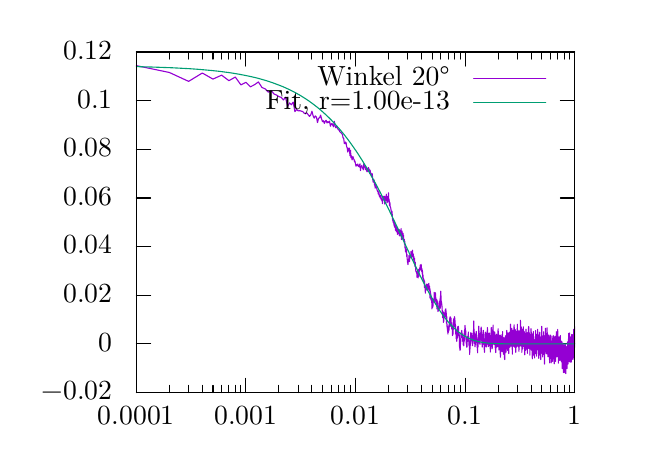
\begin{tikzpicture}[gnuplot]
%% generated with GNUPLOT 5.2p5a (Gentoo revision r0) (Lua 5.1; terminal rev. 99 , script rev. 107)
%% Sa 18 Mai 2019 18:30:55 CEST
\path (0.000,0.000) rectangle (7.500,5.250);
\gpcolor{color=gp lt color border}
\gpsetlinetype{gp lt border}
\gpsetdashtype{gp dt solid}
\gpsetlinewidth{1.00}
\draw[gp path] (1.380,0.616)--(1.560,0.616);
\draw[gp path] (6.947,0.616)--(6.767,0.616);
\node[gp node right] at (1.196,0.616) {$-0.02$};
\draw[gp path] (1.380,1.234)--(1.560,1.234);
\draw[gp path] (6.947,1.234)--(6.767,1.234);
\node[gp node right] at (1.196,1.234) {$0$};
\draw[gp path] (1.380,1.852)--(1.560,1.852);
\draw[gp path] (6.947,1.852)--(6.767,1.852);
\node[gp node right] at (1.196,1.852) {$0.02$};
\draw[gp path] (1.380,2.470)--(1.560,2.470);
\draw[gp path] (6.947,2.470)--(6.767,2.470);
\node[gp node right] at (1.196,2.470) {$0.04$};
\draw[gp path] (1.380,3.087)--(1.560,3.087);
\draw[gp path] (6.947,3.087)--(6.767,3.087);
\node[gp node right] at (1.196,3.087) {$0.06$};
\draw[gp path] (1.380,3.705)--(1.560,3.705);
\draw[gp path] (6.947,3.705)--(6.767,3.705);
\node[gp node right] at (1.196,3.705) {$0.08$};
\draw[gp path] (1.380,4.323)--(1.560,4.323);
\draw[gp path] (6.947,4.323)--(6.767,4.323);
\node[gp node right] at (1.196,4.323) {$0.1$};
\draw[gp path] (1.380,4.941)--(1.560,4.941);
\draw[gp path] (6.947,4.941)--(6.767,4.941);
\node[gp node right] at (1.196,4.941) {$0.12$};
\draw[gp path] (1.380,0.616)--(1.380,0.796);
\draw[gp path] (1.380,4.941)--(1.380,4.761);
\node[gp node center] at (1.380,0.308) {$0.0001$};
\draw[gp path] (1.799,0.616)--(1.799,0.706);
\draw[gp path] (1.799,4.941)--(1.799,4.851);
\draw[gp path] (2.044,0.616)--(2.044,0.706);
\draw[gp path] (2.044,4.941)--(2.044,4.851);
\draw[gp path] (2.218,0.616)--(2.218,0.706);
\draw[gp path] (2.218,4.941)--(2.218,4.851);
\draw[gp path] (2.353,0.616)--(2.353,0.706);
\draw[gp path] (2.353,4.941)--(2.353,4.851);
\draw[gp path] (2.463,0.616)--(2.463,0.706);
\draw[gp path] (2.463,4.941)--(2.463,4.851);
\draw[gp path] (2.556,0.616)--(2.556,0.706);
\draw[gp path] (2.556,4.941)--(2.556,4.851);
\draw[gp path] (2.637,0.616)--(2.637,0.706);
\draw[gp path] (2.637,4.941)--(2.637,4.851);
\draw[gp path] (2.708,0.616)--(2.708,0.706);
\draw[gp path] (2.708,4.941)--(2.708,4.851);
\draw[gp path] (2.772,0.616)--(2.772,0.796);
\draw[gp path] (2.772,4.941)--(2.772,4.761);
\node[gp node center] at (2.772,0.308) {$0.001$};
\draw[gp path] (3.191,0.616)--(3.191,0.706);
\draw[gp path] (3.191,4.941)--(3.191,4.851);
\draw[gp path] (3.436,0.616)--(3.436,0.706);
\draw[gp path] (3.436,4.941)--(3.436,4.851);
\draw[gp path] (3.610,0.616)--(3.610,0.706);
\draw[gp path] (3.610,4.941)--(3.610,4.851);
\draw[gp path] (3.745,0.616)--(3.745,0.706);
\draw[gp path] (3.745,4.941)--(3.745,4.851);
\draw[gp path] (3.855,0.616)--(3.855,0.706);
\draw[gp path] (3.855,4.941)--(3.855,4.851);
\draw[gp path] (3.948,0.616)--(3.948,0.706);
\draw[gp path] (3.948,4.941)--(3.948,4.851);
\draw[gp path] (4.029,0.616)--(4.029,0.706);
\draw[gp path] (4.029,4.941)--(4.029,4.851);
\draw[gp path] (4.100,0.616)--(4.100,0.706);
\draw[gp path] (4.100,4.941)--(4.100,4.851);
\draw[gp path] (4.163,0.616)--(4.163,0.796);
\draw[gp path] (4.163,4.941)--(4.163,4.761);
\node[gp node center] at (4.163,0.308) {$0.01$};
\draw[gp path] (4.582,0.616)--(4.582,0.706);
\draw[gp path] (4.582,4.941)--(4.582,4.851);
\draw[gp path] (4.828,0.616)--(4.828,0.706);
\draw[gp path] (4.828,4.941)--(4.828,4.851);
\draw[gp path] (5.001,0.616)--(5.001,0.706);
\draw[gp path] (5.001,4.941)--(5.001,4.851);
\draw[gp path] (5.136,0.616)--(5.136,0.706);
\draw[gp path] (5.136,4.941)--(5.136,4.851);
\draw[gp path] (5.246,0.616)--(5.246,0.706);
\draw[gp path] (5.246,4.941)--(5.246,4.851);
\draw[gp path] (5.340,0.616)--(5.340,0.706);
\draw[gp path] (5.340,4.941)--(5.340,4.851);
\draw[gp path] (5.420,0.616)--(5.420,0.706);
\draw[gp path] (5.420,4.941)--(5.420,4.851);
\draw[gp path] (5.492,0.616)--(5.492,0.706);
\draw[gp path] (5.492,4.941)--(5.492,4.851);
\draw[gp path] (5.555,0.616)--(5.555,0.796);
\draw[gp path] (5.555,4.941)--(5.555,4.761);
\node[gp node center] at (5.555,0.308) {$0.1$};
\draw[gp path] (5.974,0.616)--(5.974,0.706);
\draw[gp path] (5.974,4.941)--(5.974,4.851);
\draw[gp path] (6.219,0.616)--(6.219,0.706);
\draw[gp path] (6.219,4.941)--(6.219,4.851);
\draw[gp path] (6.393,0.616)--(6.393,0.706);
\draw[gp path] (6.393,4.941)--(6.393,4.851);
\draw[gp path] (6.528,0.616)--(6.528,0.706);
\draw[gp path] (6.528,4.941)--(6.528,4.851);
\draw[gp path] (6.638,0.616)--(6.638,0.706);
\draw[gp path] (6.638,4.941)--(6.638,4.851);
\draw[gp path] (6.731,0.616)--(6.731,0.706);
\draw[gp path] (6.731,4.941)--(6.731,4.851);
\draw[gp path] (6.812,0.616)--(6.812,0.706);
\draw[gp path] (6.812,4.941)--(6.812,4.851);
\draw[gp path] (6.883,0.616)--(6.883,0.706);
\draw[gp path] (6.883,4.941)--(6.883,4.851);
\draw[gp path] (6.947,0.616)--(6.947,0.796);
\draw[gp path] (6.947,4.941)--(6.947,4.761);
\node[gp node center] at (6.947,0.308) {$1$};
\draw[gp path] (1.380,4.941)--(1.380,0.616)--(6.947,0.616)--(6.947,4.941)--cycle;
\node[gp node right] at (5.479,4.607) {Winkel 20°};
\gpcolor{rgb color={0.580,0.000,0.827}}
\draw[gp path] (5.663,4.607)--(6.579,4.607);
\draw[gp path] (1.380,4.768)--(1.799,4.681)--(2.044,4.568)--(2.218,4.674)--(2.353,4.597)%
  --(2.463,4.647)--(2.556,4.577)--(2.637,4.623)--(2.708,4.523)--(2.772,4.555)--(2.829,4.499)%
  --(2.882,4.526)--(2.930,4.561)--(2.975,4.491)--(3.017,4.472)--(3.056,4.431)--(3.092,4.453)%
  --(3.127,4.409)--(3.160,4.394)--(3.191,4.374)--(3.220,4.365)--(3.248,4.332)--(3.275,4.367)%
  --(3.301,4.246)--(3.326,4.295)--(3.349,4.271)--(3.372,4.305)--(3.394,4.184)--(3.415,4.211)%
  --(3.436,4.193)--(3.456,4.196)--(3.475,4.190)--(3.493,4.185)--(3.511,4.164)--(3.529,4.158)%
  --(3.546,4.168)--(3.563,4.143)--(3.579,4.123)--(3.594,4.141)--(3.610,4.189)--(3.625,4.131)%
  --(3.639,4.101)--(3.653,4.130)--(3.667,4.116)--(3.681,4.044)--(3.694,4.101)--(3.707,4.104)%
  --(3.720,4.139)--(3.732,4.092)--(3.745,4.056)--(3.757,4.068)--(3.768,4.034)--(3.780,4.062)%
  --(3.791,4.073)--(3.802,4.040)--(3.813,4.056)--(3.824,4.045)--(3.834,4.063)--(3.845,3.998)%
  --(3.855,4.027)--(3.865,4.033)--(3.875,4.012)--(3.884,3.991)--(3.894,4.061)--(3.903,4.008)%
  --(3.912,3.979)--(3.921,3.997)--(3.930,3.981)--(3.939,3.964)--(3.948,3.953)--(3.956,3.947)%
  --(3.965,3.927)--(3.973,3.921)--(3.982,3.914)--(3.990,3.903)--(3.998,3.891)--(4.006,3.847)%
  --(4.013,3.846)--(4.021,3.781)--(4.029,3.776)--(4.036,3.798)--(4.044,3.787)--(4.051,3.737)%
  --(4.058,3.725)--(4.065,3.670)--(4.072,3.719)--(4.079,3.686)--(4.086,3.721)--(4.093,3.622)%
  --(4.100,3.692)--(4.106,3.597)--(4.113,3.622)--(4.120,3.571)--(4.126,3.590)--(4.132,3.612)%
  --(4.139,3.583)--(4.145,3.578)--(4.151,3.547)--(4.157,3.555)--(4.164,3.513)--(4.170,3.491)%
  --(4.175,3.509)--(4.181,3.498)--(4.187,3.517)--(4.193,3.517)--(4.199,3.489)--(4.204,3.496)%
  --(4.210,3.481)--(4.216,3.513)--(4.221,3.520)--(4.227,3.436)--(4.232,3.485)--(4.237,3.482)%
  --(4.243,3.500)--(4.248,3.484)--(4.253,3.466)--(4.258,3.459)--(4.264,3.445)--(4.269,3.523)%
  --(4.274,3.482)--(4.279,3.479)--(4.284,3.495)--(4.289,3.458)--(4.294,3.445)--(4.298,3.479)%
  --(4.303,3.455)--(4.308,3.420)--(4.313,3.439)--(4.317,3.464)--(4.322,3.421)--(4.327,3.474)%
  --(4.331,3.464)--(4.336,3.438)--(4.340,3.446)--(4.345,3.397)--(4.349,3.441)--(4.354,3.406)%
  --(4.358,3.404)--(4.363,3.396)--(4.367,3.358)--(4.371,3.357)--(4.375,3.396)--(4.380,3.346)%
  --(4.384,3.310)--(4.388,3.287)--(4.392,3.292)--(4.396,3.311)--(4.400,3.316)--(4.405,3.250)%
  --(4.409,3.269)--(4.413,3.211)--(4.417,3.256)--(4.421,3.256)--(4.424,3.243)--(4.428,3.224)%
  --(4.432,3.221)--(4.436,3.191)--(4.440,3.182)--(4.444,3.169)--(4.448,3.187)--(4.451,3.142)%
  --(4.455,3.136)--(4.459,3.163)--(4.463,3.151)--(4.466,3.109)--(4.470,3.103)--(4.473,3.119)%
  --(4.477,3.086)--(4.481,3.115)--(4.484,3.120)--(4.488,3.118)--(4.491,3.062)--(4.495,3.059)%
  --(4.498,3.066)--(4.502,3.072)--(4.505,3.015)--(4.509,3.058)--(4.512,3.109)--(4.515,3.081)%
  --(4.519,3.068)--(4.522,3.074)--(4.525,3.095)--(4.529,3.110)--(4.532,3.053)--(4.535,3.010)%
  --(4.539,3.078)--(4.542,3.048)--(4.545,3.103)--(4.548,3.057)--(4.551,3.060)--(4.555,3.135)%
  --(4.558,3.079)--(4.561,3.065)--(4.564,3.025)--(4.567,3.105)--(4.570,3.037)--(4.573,3.075)%
  --(4.576,3.072)--(4.579,3.100)--(4.582,3.153)--(4.585,3.045)--(4.588,3.074)--(4.591,3.058)%
  --(4.594,2.991)--(4.597,3.004)--(4.600,3.033)--(4.603,2.979)--(4.606,2.976)--(4.609,2.963)%
  --(4.612,2.954)--(4.615,2.930)--(4.618,2.886)--(4.621,2.885)--(4.623,2.862)--(4.626,2.919)%
  --(4.629,2.889)--(4.632,2.823)--(4.635,2.812)--(4.637,2.801)--(4.640,2.793)--(4.643,2.775)%
  --(4.646,2.811)--(4.648,2.797)--(4.651,2.741)--(4.654,2.790)--(4.656,2.760)--(4.659,2.718)%
  --(4.662,2.734)--(4.664,2.757)--(4.667,2.734)--(4.670,2.691)--(4.672,2.676)--(4.675,2.702)%
  --(4.677,2.735)--(4.680,2.674)--(4.683,2.657)--(4.685,2.671)--(4.688,2.715)--(4.690,2.665)%
  --(4.693,2.694)--(4.695,2.625)--(4.698,2.677)--(4.700,2.696)--(4.703,2.639)--(4.705,2.668)%
  --(4.708,2.652)--(4.710,2.634)--(4.712,2.656)--(4.715,2.688)--(4.717,2.645)--(4.720,2.606)%
  --(4.722,2.656)--(4.725,2.682)--(4.727,2.641)--(4.729,2.616)--(4.732,2.628)--(4.734,2.655)%
  --(4.736,2.606)--(4.739,2.680)--(4.741,2.652)--(4.743,2.699)--(4.746,2.559)--(4.748,2.654)%
  --(4.750,2.632)--(4.753,2.615)--(4.755,2.666)--(4.757,2.629)--(4.759,2.594)--(4.762,2.619)%
  --(4.764,2.596)--(4.766,2.640)--(4.768,2.581)--(4.771,2.611)--(4.773,2.614)--(4.775,2.554)%
  --(4.777,2.549)--(4.779,2.552)--(4.781,2.528)--(4.784,2.561)--(4.786,2.498)--(4.788,2.522)%
  --(4.790,2.537)--(4.792,2.452)--(4.794,2.470)--(4.797,2.438)--(4.799,2.406)--(4.801,2.443)%
  --(4.803,2.400)--(4.805,2.425)--(4.807,2.388)--(4.809,2.391)--(4.811,2.440)--(4.813,2.386)%
  --(4.815,2.339)--(4.817,2.371)--(4.819,2.308)--(4.821,2.313)--(4.823,2.270)--(4.826,2.281)%
  --(4.828,2.250)--(4.830,2.241)--(4.832,2.280)--(4.834,2.295)--(4.836,2.300)--(4.838,2.313)%
  --(4.840,2.283)--(4.841,2.356)--(4.843,2.280)--(4.845,2.303)--(4.847,2.346)--(4.849,2.278)%
  --(4.851,2.334)--(4.853,2.321)--(4.855,2.356)--(4.857,2.358)--(4.859,2.326)--(4.861,2.334)%
  --(4.863,2.357)--(4.865,2.336)--(4.867,2.350)--(4.868,2.407)--(4.870,2.355)--(4.872,2.370)%
  --(4.874,2.355)--(4.876,2.338)--(4.878,2.358)--(4.880,2.353)--(4.881,2.365)--(4.883,2.357)%
  --(4.885,2.372)--(4.887,2.423)--(4.889,2.404)--(4.891,2.342)--(4.892,2.377)--(4.894,2.333)%
  --(4.896,2.376)--(4.898,2.370)--(4.900,2.339)--(4.901,2.320)--(4.903,2.300)--(4.905,2.345)%
  --(4.907,2.274)--(4.908,2.287)--(4.910,2.275)--(4.912,2.322)--(4.914,2.279)--(4.916,2.260)%
  --(4.917,2.250)--(4.919,2.216)--(4.921,2.241)--(4.922,2.273)--(4.924,2.222)--(4.926,2.205)%
  --(4.928,2.207)--(4.929,2.167)--(4.931,2.152)--(4.933,2.155)--(4.934,2.150)--(4.936,2.157)%
  --(4.938,2.143)--(4.939,2.131)--(4.941,2.136)--(4.943,2.123)--(4.944,2.080)--(4.946,2.123)%
  --(4.948,2.113)--(4.949,2.097)--(4.951,2.150)--(4.953,2.117)--(4.954,2.094)--(4.956,2.130)%
  --(4.958,2.071)--(4.959,2.110)--(4.961,2.106)--(4.962,2.182)--(4.964,2.120)--(4.966,2.141)%
  --(4.967,2.091)--(4.969,2.136)--(4.970,2.091)--(4.972,2.149)--(4.974,2.175)--(4.975,2.176)%
  --(4.977,2.181)--(4.978,2.189)--(4.980,2.203)--(4.981,2.198)--(4.983,2.172)--(4.985,2.237)%
  --(4.986,2.209)--(4.988,2.195)--(4.989,2.183)--(4.991,2.200)--(4.992,2.210)--(4.994,2.178)%
  --(4.995,2.202)--(4.997,2.243)--(4.998,2.192)--(5.000,2.232)--(5.001,2.174)--(5.003,2.153)%
  --(5.004,2.182)--(5.006,2.194)--(5.007,2.169)--(5.009,2.172)--(5.010,2.136)--(5.012,2.125)%
  --(5.013,2.172)--(5.015,2.109)--(5.016,2.078)--(5.018,2.102)--(5.019,2.060)--(5.021,2.110)%
  --(5.022,2.090)--(5.024,2.058)--(5.025,2.071)--(5.027,2.061)--(5.028,2.013)--(5.029,2.039)%
  --(5.031,2.029)--(5.032,2.021)--(5.034,2.014)--(5.035,2.047)--(5.037,2.002)--(5.038,2.026)%
  --(5.039,1.950)--(5.041,2.031)--(5.042,1.974)--(5.044,1.962)--(5.045,1.953)--(5.047,1.943)%
  --(5.048,1.899)--(5.049,1.933)--(5.051,1.878)--(5.052,1.944)--(5.054,1.934)--(5.055,1.955)%
  --(5.056,1.921)--(5.058,1.928)--(5.059,1.937)--(5.060,1.937)--(5.062,1.946)--(5.063,1.993)%
  --(5.064,1.931)--(5.066,1.933)--(5.067,1.952)--(5.069,1.946)--(5.070,1.945)--(5.071,1.914)%
  --(5.073,1.943)--(5.074,1.949)--(5.075,1.937)--(5.077,1.964)--(5.078,1.973)--(5.079,1.984)%
  --(5.081,1.991)--(5.082,1.925)--(5.083,1.947)--(5.085,1.972)--(5.086,1.972)--(5.087,1.983)%
  --(5.089,1.986)--(5.090,1.999)--(5.091,1.984)--(5.092,1.931)--(5.094,1.975)--(5.095,2.003)%
  --(5.096,1.978)--(5.098,1.927)--(5.099,1.930)--(5.100,1.910)--(5.101,1.949)--(5.103,1.946)%
  --(5.104,1.967)--(5.105,1.918)--(5.107,1.941)--(5.108,1.903)--(5.109,1.816)--(5.110,1.925)%
  --(5.112,1.901)--(5.113,1.859)--(5.114,1.904)--(5.115,1.842)--(5.117,1.839)--(5.118,1.881)%
  --(5.119,1.842)--(5.120,1.844)--(5.122,1.791)--(5.123,1.848)--(5.124,1.815)--(5.125,1.831)%
  --(5.127,1.814)--(5.128,1.819)--(5.129,1.803)--(5.130,1.756)--(5.131,1.776)--(5.133,1.773)%
  --(5.134,1.678)--(5.135,1.733)--(5.136,1.728)--(5.137,1.696)--(5.139,1.749)--(5.140,1.777)%
  --(5.141,1.713)--(5.142,1.694)--(5.144,1.739)--(5.145,1.716)--(5.146,1.801)--(5.147,1.711)%
  --(5.148,1.749)--(5.149,1.724)--(5.151,1.790)--(5.152,1.798)--(5.153,1.775)--(5.154,1.766)%
  --(5.155,1.785)--(5.157,1.794)--(5.158,1.808)--(5.159,1.795)--(5.160,1.810)--(5.161,1.797)%
  --(5.162,1.888)--(5.163,1.815)--(5.165,1.825)--(5.166,1.809)--(5.167,1.760)--(5.168,1.809)%
  --(5.169,1.824)--(5.170,1.831)--(5.172,1.824)--(5.173,1.882)--(5.174,1.881)--(5.175,1.821)%
  --(5.176,1.844)--(5.177,1.884)--(5.178,1.854)--(5.179,1.792)--(5.181,1.873)--(5.182,1.814)%
  --(5.183,1.821)--(5.184,1.804)--(5.185,1.784)--(5.186,1.773)--(5.187,1.802)--(5.188,1.758)%
  --(5.189,1.753)--(5.191,1.754)--(5.192,1.785)--(5.193,1.800)--(5.194,1.728)--(5.195,1.708)%
  --(5.196,1.718)--(5.197,1.732)--(5.198,1.678)--(5.199,1.721)--(5.200,1.789)--(5.202,1.712)%
  --(5.203,1.715)--(5.204,1.697)--(5.205,1.769)--(5.206,1.679)--(5.207,1.684)--(5.208,1.680)%
  --(5.209,1.717)--(5.210,1.645)--(5.211,1.668)--(5.212,1.657)--(5.213,1.652)--(5.214,1.650)%
  --(5.215,1.672)--(5.217,1.705)--(5.218,1.697)--(5.219,1.667)--(5.220,1.657)--(5.221,1.676)%
  --(5.222,1.669)--(5.223,1.696)--(5.224,1.700)--(5.225,1.748)--(5.226,1.699)--(5.227,1.679)%
  --(5.228,1.709)--(5.229,1.703)--(5.230,1.773)--(5.231,1.741)--(5.232,1.737)--(5.233,1.760)%
  --(5.234,1.758)--(5.235,1.720)--(5.236,1.796)--(5.237,1.792)--(5.238,1.773)--(5.239,1.794)%
  --(5.240,1.819)--(5.241,1.686)--(5.242,1.790)--(5.243,1.845)--(5.244,1.824)--(5.245,1.803)%
  --(5.246,1.904)--(5.247,1.830)--(5.249,1.847)--(5.250,1.770)--(5.251,1.833)--(5.252,1.755)%
  --(5.253,1.760)--(5.254,1.767)--(5.254,1.755)--(5.255,1.727)--(5.256,1.737)--(5.257,1.766)%
  --(5.258,1.740)--(5.259,1.744)--(5.260,1.717)--(5.261,1.704)--(5.262,1.715)--(5.263,1.699)%
  --(5.264,1.651)--(5.265,1.627)--(5.266,1.662)--(5.267,1.608)--(5.268,1.619)--(5.269,1.619)%
  --(5.270,1.568)--(5.271,1.650)--(5.272,1.610)--(5.273,1.616)--(5.274,1.642)--(5.275,1.590)%
  --(5.276,1.577)--(5.277,1.606)--(5.278,1.591)--(5.279,1.549)--(5.280,1.507)--(5.281,1.539)%
  --(5.282,1.632)--(5.283,1.562)--(5.284,1.598)--(5.285,1.523)--(5.286,1.578)--(5.286,1.573)%
  --(5.287,1.593)--(5.288,1.588)--(5.289,1.560)--(5.290,1.567)--(5.291,1.600)--(5.292,1.574)%
  --(5.293,1.626)--(5.294,1.575)--(5.295,1.569)--(5.296,1.600)--(5.297,1.609)--(5.298,1.596)%
  --(5.299,1.578)--(5.300,1.576)--(5.300,1.598)--(5.301,1.606)--(5.302,1.625)--(5.303,1.619)%
  --(5.304,1.672)--(5.305,1.620)--(5.306,1.655)--(5.307,1.622)--(5.308,1.635)--(5.309,1.674)%
  --(5.310,1.624)--(5.310,1.617)--(5.311,1.681)--(5.312,1.656)--(5.313,1.626)--(5.314,1.595)%
  --(5.315,1.612)--(5.316,1.628)--(5.317,1.594)--(5.318,1.523)--(5.319,1.514)--(5.319,1.494)%
  --(5.320,1.586)--(5.321,1.560)--(5.322,1.581)--(5.323,1.490)--(5.324,1.472)--(5.325,1.455)%
  --(5.326,1.482)--(5.327,1.451)--(5.327,1.452)--(5.328,1.432)--(5.329,1.461)--(5.330,1.443)%
  --(5.331,1.437)--(5.332,1.402)--(5.333,1.411)--(5.334,1.391)--(5.334,1.455)--(5.335,1.380)%
  --(5.336,1.431)--(5.337,1.359)--(5.338,1.439)--(5.339,1.379)--(5.340,1.398)--(5.341,1.377)%
  --(5.341,1.430)--(5.342,1.388)--(5.343,1.439)--(5.344,1.431)--(5.345,1.429)--(5.346,1.391)%
  --(5.347,1.443)--(5.347,1.405)--(5.348,1.415)--(5.349,1.469)--(5.350,1.440)--(5.351,1.408)%
  --(5.352,1.469)--(5.352,1.470)--(5.353,1.443)--(5.354,1.473)--(5.355,1.496)--(5.356,1.458)%
  --(5.357,1.458)--(5.358,1.451)--(5.358,1.555)--(5.359,1.464)--(5.360,1.485)--(5.361,1.504)%
  --(5.362,1.575)--(5.363,1.528)--(5.363,1.502)--(5.364,1.548)--(5.365,1.567)--(5.366,1.540)%
  --(5.367,1.577)--(5.368,1.577)--(5.368,1.557)--(5.369,1.574)--(5.370,1.515)--(5.371,1.510)%
  --(5.372,1.562)--(5.372,1.471)--(5.373,1.530)--(5.374,1.498)--(5.375,1.503)--(5.376,1.458)%
  --(5.377,1.562)--(5.377,1.506)--(5.378,1.523)--(5.379,1.469)--(5.380,1.487)--(5.381,1.504)%
  --(5.381,1.459)--(5.382,1.479)--(5.383,1.458)--(5.384,1.489)--(5.385,1.480)--(5.385,1.454)%
  --(5.386,1.422)--(5.387,1.456)--(5.388,1.459)--(5.389,1.432)--(5.389,1.442)--(5.390,1.440)%
  --(5.391,1.427)--(5.392,1.425)--(5.393,1.430)--(5.393,1.429)--(5.394,1.354)--(5.395,1.340)%
  --(5.396,1.360)--(5.396,1.407)--(5.397,1.344)--(5.398,1.412)--(5.399,1.406)--(5.400,1.424)%
  --(5.400,1.411)--(5.401,1.459)--(5.402,1.355)--(5.403,1.432)--(5.404,1.363)--(5.404,1.510)%
  --(5.405,1.463)--(5.406,1.417)--(5.407,1.448)--(5.407,1.420)--(5.408,1.522)--(5.409,1.551)%
  --(5.410,1.483)--(5.410,1.444)--(5.411,1.488)--(5.412,1.541)--(5.413,1.507)--(5.414,1.496)%
  --(5.414,1.543)--(5.415,1.531)--(5.416,1.533)--(5.417,1.453)--(5.417,1.470)--(5.418,1.515)%
  --(5.419,1.480)--(5.420,1.580)--(5.420,1.564)--(5.421,1.578)--(5.422,1.508)--(5.423,1.566)%
  --(5.423,1.469)--(5.424,1.563)--(5.425,1.512)--(5.426,1.531)--(5.426,1.465)--(5.427,1.499)%
  --(5.428,1.478)--(5.429,1.530)--(5.429,1.495)--(5.430,1.478)--(5.431,1.443)--(5.432,1.484)%
  --(5.432,1.414)--(5.433,1.472)--(5.434,1.416)--(5.435,1.440)--(5.435,1.375)--(5.436,1.377)%
  --(5.437,1.360)--(5.438,1.432)--(5.438,1.386)--(5.439,1.359)--(5.440,1.353)--(5.440,1.370)%
  --(5.441,1.339)--(5.442,1.378)--(5.443,1.298)--(5.443,1.406)--(5.444,1.374)--(5.445,1.323)%
  --(5.446,1.317)--(5.446,1.346)--(5.447,1.353)--(5.448,1.366)--(5.448,1.342)--(5.449,1.267)%
  --(5.450,1.385)--(5.451,1.387)--(5.451,1.359)--(5.452,1.348)--(5.453,1.341)--(5.453,1.409)%
  --(5.454,1.389)--(5.455,1.305)--(5.456,1.391)--(5.456,1.374)--(5.457,1.343)--(5.458,1.375)%
  --(5.458,1.360)--(5.459,1.352)--(5.460,1.367)--(5.461,1.377)--(5.462,1.454)--(5.463,1.407)%
  --(5.463,1.375)--(5.464,1.404)--(5.465,1.410)--(5.465,1.390)--(5.466,1.407)--(5.467,1.337)%
  --(5.468,1.428)--(5.468,1.409)--(5.469,1.458)--(5.470,1.366)--(5.470,1.388)--(5.471,1.393)%
  --(5.472,1.438)--(5.473,1.400)--(5.474,1.382)--(5.475,1.336)--(5.475,1.383)--(5.476,1.367)%
  --(5.477,1.378)--(5.477,1.377)--(5.478,1.335)--(5.479,1.355)--(5.479,1.327)--(5.480,1.339)%
  --(5.481,1.317)--(5.481,1.350)--(5.482,1.288)--(5.483,1.312)--(5.483,1.251)--(5.484,1.278)%
  --(5.485,1.180)--(5.485,1.273)--(5.486,1.257)--(5.487,1.254)--(5.488,1.212)--(5.488,1.236)%
  --(5.489,1.155)--(5.490,1.257)--(5.490,1.153)--(5.491,1.206)--(5.492,1.189)--(5.492,1.199)%
  --(5.493,1.160)--(5.494,1.178)--(5.494,1.188)--(5.495,1.241)--(5.496,1.239)--(5.496,1.252)%
  --(5.497,1.232)--(5.498,1.251)--(5.498,1.280)--(5.499,1.282)--(5.500,1.276)--(5.500,1.281)%
  --(5.501,1.316)--(5.502,1.262)--(5.502,1.306)--(5.503,1.374)--(5.504,1.342)--(5.504,1.338)%
  --(5.505,1.337)--(5.506,1.331)--(5.506,1.348)--(5.507,1.348)--(5.507,1.352)--(5.508,1.383)%
  --(5.509,1.370)--(5.509,1.341)--(5.510,1.337)--(5.511,1.357)--(5.511,1.356)--(5.512,1.363)%
  --(5.513,1.371)--(5.513,1.404)--(5.514,1.320)--(5.515,1.373)--(5.515,1.314)--(5.516,1.321)%
  --(5.517,1.363)--(5.517,1.376)--(5.518,1.342)--(5.518,1.360)--(5.519,1.332)--(5.520,1.333)%
  --(5.520,1.362)--(5.521,1.321)--(5.522,1.334)--(5.522,1.319)--(5.523,1.345)--(5.524,1.350)%
  --(5.524,1.303)--(5.525,1.327)--(5.526,1.267)--(5.526,1.298)--(5.527,1.262)--(5.527,1.318)%
  --(5.528,1.279)--(5.529,1.265)--(5.529,1.301)--(5.530,1.287)--(5.531,1.291)--(5.531,1.271)%
  --(5.532,1.271)--(5.532,1.221)--(5.533,1.217)--(5.534,1.240)--(5.535,1.226)--(5.536,1.217)%
  --(5.536,1.226)--(5.537,1.252)--(5.537,1.253)--(5.538,1.261)--(5.539,1.210)--(5.539,1.261)%
  --(5.540,1.231)--(5.541,1.287)--(5.541,1.297)--(5.542,1.279)--(5.542,1.257)--(5.543,1.342)%
  --(5.544,1.270)--(5.544,1.371)--(5.545,1.319)--(5.546,1.323)--(5.546,1.373)--(5.547,1.366)%
  --(5.547,1.340)--(5.548,1.395)--(5.549,1.416)--(5.549,1.347)--(5.550,1.381)--(5.550,1.369)%
  --(5.551,1.390)--(5.552,1.427)--(5.552,1.423)--(5.553,1.427)--(5.553,1.415)--(5.554,1.468)%
  --(5.555,1.433)--(5.555,1.437)--(5.556,1.458)--(5.556,1.376)--(5.557,1.437)--(5.558,1.404)%
  --(5.558,1.409)--(5.559,1.380)--(5.559,1.371)--(5.560,1.410)--(5.561,1.374)--(5.561,1.377)%
  --(5.562,1.357)--(5.562,1.384)--(5.563,1.339)--(5.564,1.398)--(5.564,1.358)--(5.565,1.386)%
  --(5.565,1.358)--(5.566,1.308)--(5.567,1.292)--(5.567,1.312)--(5.568,1.242)--(5.568,1.302)%
  --(5.569,1.301)--(5.570,1.294)--(5.570,1.298)--(5.571,1.260)--(5.571,1.305)--(5.572,1.245)%
  --(5.573,1.226)--(5.573,1.236)--(5.574,1.246)--(5.574,1.201)--(5.575,1.193)--(5.575,1.245)%
  --(5.576,1.206)--(5.577,1.215)--(5.577,1.264)--(5.578,1.234)--(5.578,1.238)--(5.579,1.278)%
  --(5.580,1.230)--(5.580,1.252)--(5.581,1.195)--(5.581,1.264)--(5.582,1.259)--(5.582,1.273)%
  --(5.583,1.260)--(5.584,1.267)--(5.584,1.309)--(5.585,1.301)--(5.585,1.290)--(5.586,1.328)%
  --(5.586,1.265)--(5.587,1.270)--(5.588,1.272)--(5.588,1.300)--(5.589,1.281)--(5.589,1.306)%
  --(5.590,1.313)--(5.590,1.291)--(5.591,1.302)--(5.592,1.311)--(5.592,1.277)--(5.593,1.351)%
  --(5.593,1.363)--(5.594,1.326)--(5.594,1.317)--(5.595,1.330)--(5.596,1.337)--(5.596,1.385)%
  --(5.597,1.296)--(5.597,1.302)--(5.598,1.296)--(5.598,1.332)--(5.599,1.287)--(5.600,1.301)%
  --(5.600,1.290)--(5.601,1.287)--(5.601,1.291)--(5.602,1.304)--(5.602,1.295)--(5.603,1.244)%
  --(5.603,1.279)--(5.604,1.243)--(5.605,1.222)--(5.605,1.217)--(5.606,1.244)--(5.606,1.254)%
  --(5.607,1.274)--(5.607,1.206)--(5.608,1.270)--(5.608,1.254)--(5.609,1.273)--(5.610,1.201)%
  --(5.610,1.235)--(5.611,1.152)--(5.611,1.195)--(5.612,1.181)--(5.612,1.189)--(5.613,1.139)%
  --(5.613,1.099)--(5.614,1.141)--(5.615,1.177)--(5.615,1.223)--(5.616,1.142)--(5.616,1.181)%
  --(5.617,1.202)--(5.617,1.197)--(5.618,1.203)--(5.618,1.245)--(5.619,1.173)--(5.619,1.171)%
  --(5.620,1.215)--(5.621,1.215)--(5.621,1.218)--(5.622,1.220)--(5.622,1.233)--(5.623,1.241)%
  --(5.623,1.277)--(5.624,1.321)--(5.624,1.322)--(5.625,1.328)--(5.625,1.305)--(5.626,1.375)%
  --(5.626,1.324)--(5.627,1.278)--(5.628,1.341)--(5.628,1.334)--(5.629,1.310)--(5.629,1.294)%
  --(5.630,1.357)--(5.630,1.313)--(5.631,1.348)--(5.631,1.305)--(5.632,1.361)--(5.632,1.354)%
  --(5.633,1.354)--(5.633,1.338)--(5.634,1.345)--(5.634,1.372)--(5.635,1.322)--(5.636,1.333)%
  --(5.636,1.293)--(5.637,1.300)--(5.637,1.344)--(5.638,1.302)--(5.638,1.270)--(5.639,1.304)%
  --(5.640,1.305)--(5.640,1.316)--(5.641,1.293)--(5.641,1.319)--(5.642,1.314)--(5.642,1.255)%
  --(5.643,1.310)--(5.643,1.273)--(5.644,1.314)--(5.644,1.249)--(5.645,1.248)--(5.645,1.267)%
  --(5.646,1.235)--(5.647,1.262)--(5.647,1.239)--(5.648,1.229)--(5.648,1.289)--(5.649,1.278)%
  --(5.649,1.211)--(5.650,1.213)--(5.650,1.230)--(5.651,1.263)--(5.651,1.256)--(5.652,1.276)%
  --(5.652,1.284)--(5.653,1.240)--(5.653,1.310)--(5.654,1.292)--(5.654,1.338)--(5.655,1.370)%
  --(5.655,1.284)--(5.656,1.277)--(5.656,1.266)--(5.657,1.335)--(5.657,1.314)--(5.658,1.306)%
  --(5.658,1.366)--(5.659,1.328)--(5.659,1.353)--(5.660,1.275)--(5.660,1.376)--(5.661,1.377)%
  --(5.661,1.413)--(5.662,1.348)--(5.662,1.371)--(5.663,1.382)--(5.663,1.525)--(5.664,1.385)%
  --(5.664,1.462)--(5.665,1.368)--(5.665,1.427)--(5.666,1.361)--(5.666,1.524)--(5.667,1.390)%
  --(5.667,1.400)--(5.668,1.358)--(5.668,1.421)--(5.669,1.423)--(5.669,1.358)--(5.670,1.340)%
  --(5.670,1.345)--(5.671,1.357)--(5.672,1.358)--(5.672,1.371)--(5.673,1.321)--(5.673,1.378)%
  --(5.674,1.279)--(5.674,1.365)--(5.675,1.277)--(5.675,1.239)--(5.676,1.245)--(5.676,1.257)%
  --(5.677,1.280)--(5.677,1.235)--(5.678,1.319)--(5.678,1.271)--(5.679,1.278)--(5.679,1.287)%
  --(5.680,1.208)--(5.680,1.230)--(5.681,1.227)--(5.681,1.197)--(5.682,1.200)--(5.682,1.206)%
  --(5.683,1.244)--(5.683,1.266)--(5.684,1.222)--(5.684,1.258)--(5.685,1.251)--(5.685,1.281)%
  --(5.686,1.251)--(5.686,1.221)--(5.687,1.307)--(5.687,1.246)--(5.688,1.276)--(5.688,1.259)%
  --(5.689,1.254)--(5.689,1.277)--(5.690,1.296)--(5.690,1.303)--(5.691,1.273)--(5.691,1.320)%
  --(5.692,1.279)--(5.692,1.317)--(5.693,1.285)--(5.693,1.313)--(5.693,1.312)--(5.694,1.352)%
  --(5.694,1.366)--(5.695,1.320)--(5.695,1.325)--(5.696,1.336)--(5.696,1.354)--(5.697,1.353)%
  --(5.697,1.393)--(5.698,1.368)--(5.698,1.302)--(5.699,1.319)--(5.699,1.312)--(5.700,1.336)%
  --(5.700,1.330)--(5.701,1.361)--(5.701,1.276)--(5.702,1.363)--(5.702,1.282)--(5.703,1.320)%
  --(5.703,1.293)--(5.704,1.287)--(5.704,1.303)--(5.704,1.289)--(5.705,1.251)--(5.705,1.291)%
  --(5.706,1.275)--(5.706,1.283)--(5.707,1.214)--(5.707,1.275)--(5.708,1.250)--(5.708,1.259)%
  --(5.709,1.185)--(5.709,1.267)--(5.710,1.237)--(5.710,1.233)--(5.711,1.180)--(5.711,1.197)%
  --(5.712,1.239)--(5.712,1.175)--(5.712,1.144)--(5.713,1.152)--(5.713,1.182)--(5.714,1.161)%
  --(5.714,1.150)--(5.715,1.121)--(5.715,1.235)--(5.716,1.201)--(5.716,1.203)--(5.717,1.211)%
  --(5.717,1.204)--(5.718,1.203)--(5.718,1.251)--(5.718,1.228)--(5.719,1.204)--(5.719,1.215)%
  --(5.720,1.297)--(5.720,1.196)--(5.721,1.231)--(5.721,1.248)--(5.722,1.240)--(5.722,1.275)%
  --(5.723,1.287)--(5.723,1.298)--(5.724,1.330)--(5.724,1.341)--(5.724,1.270)--(5.725,1.345)%
  --(5.725,1.300)--(5.726,1.324)--(5.726,1.301)--(5.727,1.392)--(5.727,1.345)--(5.728,1.401)%
  --(5.728,1.317)--(5.729,1.384)--(5.729,1.353)--(5.729,1.459)--(5.730,1.406)--(5.730,1.369)%
  --(5.731,1.398)--(5.731,1.402)--(5.732,1.363)--(5.732,1.336)--(5.733,1.351)--(5.733,1.282)%
  --(5.733,1.344)--(5.734,1.333)--(5.734,1.291)--(5.735,1.352)--(5.735,1.301)--(5.736,1.285)%
  --(5.736,1.368)--(5.737,1.301)--(5.737,1.271)--(5.738,1.258)--(5.738,1.289)--(5.738,1.241)%
  --(5.739,1.320)--(5.739,1.327)--(5.740,1.326)--(5.740,1.264)--(5.741,1.304)--(5.742,1.238)%
  --(5.742,1.248)--(5.742,1.285)--(5.743,1.268)--(5.743,1.282)--(5.744,1.251)--(5.744,1.228)%
  --(5.745,1.254)--(5.745,1.236)--(5.746,1.234)--(5.746,1.298)--(5.746,1.280)--(5.747,1.286)%
  --(5.747,1.305)--(5.748,1.300)--(5.748,1.308)--(5.749,1.294)--(5.749,1.290)--(5.749,1.279)%
  --(5.750,1.308)--(5.750,1.331)--(5.751,1.330)--(5.751,1.340)--(5.752,1.353)--(5.752,1.376)%
  --(5.753,1.341)--(5.753,1.339)--(5.753,1.336)--(5.754,1.369)--(5.754,1.338)--(5.755,1.357)%
  --(5.755,1.372)--(5.756,1.408)--(5.756,1.421)--(5.756,1.406)--(5.757,1.392)--(5.757,1.432)%
  --(5.758,1.374)--(5.758,1.428)--(5.759,1.449)--(5.759,1.428)--(5.759,1.375)--(5.760,1.417)%
  --(5.760,1.389)--(5.761,1.439)--(5.761,1.403)--(5.762,1.403)--(5.762,1.363)--(5.762,1.414)%
  --(5.763,1.369)--(5.763,1.406)--(5.764,1.384)--(5.764,1.378)--(5.765,1.303)--(5.765,1.388)%
  --(5.765,1.313)--(5.766,1.347)--(5.766,1.343)--(5.767,1.353)--(5.767,1.271)--(5.768,1.304)%
  --(5.768,1.279)--(5.768,1.272)--(5.769,1.229)--(5.769,1.292)--(5.770,1.270)--(5.770,1.300)%
  --(5.771,1.271)--(5.771,1.246)--(5.771,1.274)--(5.772,1.275)--(5.772,1.217)--(5.773,1.272)%
  --(5.773,1.194)--(5.774,1.220)--(5.774,1.235)--(5.774,1.288)--(5.775,1.224)--(5.775,1.277)%
  --(5.776,1.254)--(5.776,1.257)--(5.776,1.239)--(5.777,1.293)--(5.777,1.240)--(5.778,1.262)%
  --(5.778,1.294)--(5.779,1.280)--(5.779,1.226)--(5.779,1.289)--(5.780,1.322)--(5.780,1.317)%
  --(5.781,1.327)--(5.781,1.356)--(5.781,1.303)--(5.782,1.313)--(5.782,1.337)--(5.783,1.302)%
  --(5.783,1.331)--(5.784,1.334)--(5.784,1.359)--(5.784,1.314)--(5.785,1.356)--(5.785,1.379)%
  --(5.786,1.309)--(5.786,1.366)--(5.786,1.315)--(5.787,1.398)--(5.787,1.406)--(5.788,1.367)%
  --(5.788,1.385)--(5.789,1.354)--(5.789,1.315)--(5.789,1.329)--(5.790,1.303)--(5.790,1.363)%
  --(5.791,1.319)--(5.791,1.269)--(5.791,1.297)--(5.792,1.302)--(5.792,1.299)--(5.793,1.285)%
  --(5.793,1.284)--(5.793,1.269)--(5.794,1.275)--(5.794,1.226)--(5.795,1.232)--(5.795,1.242)%
  --(5.795,1.244)--(5.796,1.251)--(5.796,1.210)--(5.797,1.219)--(5.797,1.218)--(5.797,1.245)%
  --(5.798,1.185)--(5.798,1.201)--(5.799,1.163)--(5.799,1.187)--(5.800,1.133)--(5.800,1.194)%
  --(5.800,1.139)--(5.801,1.161)--(5.801,1.127)--(5.802,1.200)--(5.802,1.157)--(5.802,1.181)%
  --(5.803,1.201)--(5.803,1.202)--(5.804,1.186)--(5.804,1.276)--(5.804,1.215)--(5.805,1.234)%
  --(5.805,1.235)--(5.806,1.194)--(5.806,1.251)--(5.806,1.209)--(5.807,1.207)--(5.807,1.279)%
  --(5.808,1.284)--(5.808,1.268)--(5.808,1.285)--(5.809,1.305)--(5.809,1.291)--(5.810,1.337)%
  --(5.810,1.335)--(5.810,1.273)--(5.811,1.343)--(5.811,1.357)--(5.812,1.333)--(5.812,1.348)%
  --(5.812,1.307)--(5.813,1.351)--(5.813,1.318)--(5.813,1.303)--(5.814,1.319)--(5.814,1.382)%
  --(5.815,1.371)--(5.815,1.334)--(5.815,1.348)--(5.816,1.327)--(5.816,1.291)--(5.817,1.328)%
  --(5.817,1.261)--(5.817,1.351)--(5.818,1.279)--(5.818,1.314)--(5.819,1.305)--(5.819,1.292)%
  --(5.819,1.308)--(5.820,1.286)--(5.820,1.337)--(5.821,1.303)--(5.821,1.238)--(5.821,1.292)%
  --(5.822,1.255)--(5.822,1.277)--(5.822,1.230)--(5.823,1.232)--(5.823,1.262)--(5.824,1.245)%
  --(5.824,1.218)--(5.824,1.205)--(5.825,1.195)--(5.825,1.263)--(5.826,1.239)--(5.826,1.205)%
  --(5.826,1.195)--(5.827,1.204)--(5.827,1.217)--(5.828,1.223)--(5.828,1.226)--(5.828,1.220)%
  --(5.829,1.274)--(5.829,1.248)--(5.829,1.236)--(5.830,1.221)--(5.830,1.290)--(5.831,1.274)%
  --(5.831,1.334)--(5.831,1.312)--(5.832,1.317)--(5.832,1.298)--(5.832,1.305)--(5.833,1.340)%
  --(5.833,1.344)--(5.834,1.369)--(5.834,1.304)--(5.834,1.371)--(5.835,1.367)--(5.835,1.350)%
  --(5.836,1.338)--(5.836,1.360)--(5.836,1.340)--(5.837,1.402)--(5.837,1.365)--(5.837,1.352)%
  --(5.838,1.442)--(5.838,1.399)--(5.839,1.424)--(5.839,1.410)--(5.839,1.409)--(5.840,1.428)%
  --(5.840,1.407)--(5.840,1.409)--(5.841,1.360)--(5.841,1.323)--(5.842,1.353)--(5.842,1.301)%
  --(5.842,1.314)--(5.843,1.377)--(5.843,1.356)--(5.843,1.366)--(5.844,1.353)--(5.844,1.366)%
  --(5.845,1.366)--(5.845,1.367)--(5.845,1.310)--(5.846,1.325)--(5.846,1.296)--(5.846,1.316)%
  --(5.847,1.312)--(5.847,1.263)--(5.848,1.270)--(5.848,1.258)--(5.848,1.298)--(5.849,1.290)%
  --(5.849,1.260)--(5.849,1.227)--(5.850,1.262)--(5.850,1.213)--(5.851,1.279)--(5.851,1.258)%
  --(5.851,1.208)--(5.852,1.212)--(5.852,1.201)--(5.853,1.224)--(5.853,1.279)--(5.854,1.264)%
  --(5.854,1.228)--(5.854,1.235)--(5.855,1.262)--(5.855,1.265)--(5.855,1.250)--(5.856,1.248)%
  --(5.856,1.257)--(5.856,1.271)--(5.857,1.328)--(5.857,1.296)--(5.858,1.279)--(5.858,1.345)%
  --(5.858,1.302)--(5.859,1.334)--(5.859,1.349)--(5.859,1.366)--(5.860,1.276)--(5.860,1.282)%
  --(5.860,1.356)--(5.861,1.351)--(5.861,1.281)--(5.862,1.356)--(5.862,1.310)--(5.862,1.354)%
  --(5.863,1.344)--(5.863,1.364)--(5.863,1.315)--(5.864,1.352)--(5.864,1.364)--(5.864,1.341)%
  --(5.865,1.368)--(5.865,1.315)--(5.866,1.371)--(5.866,1.354)--(5.866,1.355)--(5.867,1.305)%
  --(5.867,1.360)--(5.867,1.372)--(5.868,1.329)--(5.868,1.317)--(5.868,1.292)--(5.869,1.331)%
  --(5.869,1.295)--(5.870,1.285)--(5.870,1.254)--(5.870,1.290)--(5.871,1.268)--(5.871,1.216)%
  --(5.871,1.209)--(5.872,1.245)--(5.872,1.208)--(5.872,1.231)--(5.873,1.186)--(5.873,1.228)%
  --(5.873,1.184)--(5.874,1.199)--(5.874,1.213)--(5.875,1.237)--(5.875,1.194)--(5.875,1.183)%
  --(5.876,1.130)--(5.876,1.165)--(5.876,1.174)--(5.877,1.193)--(5.877,1.165)--(5.877,1.211)%
  --(5.878,1.211)--(5.878,1.246)--(5.878,1.168)--(5.879,1.253)--(5.879,1.179)--(5.880,1.199)%
  --(5.880,1.219)--(5.880,1.255)--(5.881,1.206)--(5.881,1.287)--(5.881,1.195)--(5.882,1.267)%
  --(5.882,1.223)--(5.882,1.289)--(5.883,1.294)--(5.883,1.304)--(5.883,1.300)--(5.884,1.313)%
  --(5.884,1.333)--(5.884,1.336)--(5.885,1.313)--(5.885,1.342)--(5.886,1.369)--(5.886,1.311)%
  --(5.886,1.418)--(5.887,1.332)--(5.887,1.371)--(5.887,1.342)--(5.888,1.369)--(5.888,1.348)%
  --(5.888,1.442)--(5.889,1.422)--(5.889,1.362)--(5.889,1.434)--(5.890,1.358)--(5.890,1.361)%
  --(5.890,1.328)--(5.891,1.329)--(5.891,1.352)--(5.891,1.307)--(5.892,1.316)--(5.892,1.318)%
  --(5.892,1.325)--(5.893,1.258)--(5.893,1.295)--(5.893,1.311)--(5.894,1.304)--(5.894,1.310)%
  --(5.895,1.255)--(5.895,1.237)--(5.895,1.231)--(5.896,1.224)--(5.896,1.304)--(5.896,1.308)%
  --(5.897,1.208)--(5.897,1.273)--(5.897,1.257)--(5.898,1.295)--(5.898,1.190)--(5.898,1.171)%
  --(5.899,1.245)--(5.899,1.281)--(5.899,1.244)--(5.900,1.216)--(5.900,1.182)--(5.900,1.233)%
  --(5.901,1.250)--(5.901,1.262)--(5.901,1.271)--(5.902,1.246)--(5.902,1.245)--(5.902,1.283)%
  --(5.903,1.254)--(5.903,1.232)--(5.903,1.306)--(5.904,1.337)--(5.904,1.278)--(5.904,1.266)%
  --(5.905,1.299)--(5.905,1.327)--(5.905,1.332)--(5.906,1.364)--(5.906,1.316)--(5.906,1.361)%
  --(5.907,1.331)--(5.907,1.415)--(5.907,1.334)--(5.908,1.428)--(5.908,1.368)--(5.909,1.449)%
  --(5.909,1.394)--(5.909,1.422)--(5.910,1.372)--(5.910,1.441)--(5.910,1.421)--(5.911,1.473)%
  --(5.911,1.404)--(5.911,1.467)--(5.912,1.427)--(5.912,1.362)--(5.913,1.383)--(5.913,1.354)%
  --(5.913,1.385)--(5.914,1.367)--(5.914,1.389)--(5.914,1.397)--(5.915,1.351)--(5.915,1.336)%
  --(5.916,1.327)--(5.916,1.320)--(5.916,1.317)--(5.917,1.286)--(5.917,1.302)--(5.917,1.272)%
  --(5.918,1.294)--(5.918,1.262)--(5.918,1.328)--(5.919,1.262)--(5.919,1.255)--(5.919,1.286)%
  --(5.920,1.258)--(5.920,1.274)--(5.920,1.233)--(5.921,1.232)--(5.921,1.237)--(5.921,1.250)%
  --(5.922,1.224)--(5.922,1.226)--(5.922,1.262)--(5.922,1.285)--(5.923,1.254)--(5.923,1.319)%
  --(5.923,1.346)--(5.924,1.288)--(5.924,1.309)--(5.924,1.274)--(5.925,1.279)--(5.925,1.318)%
  --(5.925,1.292)--(5.926,1.248)--(5.926,1.272)--(5.926,1.284)--(5.927,1.240)--(5.927,1.309)%
  --(5.927,1.353)--(5.928,1.313)--(5.928,1.361)--(5.928,1.296)--(5.929,1.340)--(5.929,1.353)%
  --(5.929,1.315)--(5.930,1.323)--(5.930,1.290)--(5.930,1.387)--(5.931,1.293)--(5.931,1.369)%
  --(5.931,1.327)--(5.932,1.363)--(5.932,1.329)--(5.932,1.301)--(5.933,1.339)--(5.933,1.320)%
  --(5.933,1.379)--(5.934,1.361)--(5.934,1.365)--(5.934,1.339)--(5.935,1.346)--(5.935,1.333)%
  --(5.935,1.268)--(5.936,1.324)--(5.936,1.266)--(5.936,1.275)--(5.936,1.281)--(5.937,1.246)%
  --(5.937,1.244)--(5.937,1.267)--(5.938,1.227)--(5.938,1.185)--(5.938,1.194)--(5.939,1.214)%
  --(5.939,1.192)--(5.939,1.240)--(5.940,1.188)--(5.940,1.221)--(5.940,1.236)--(5.941,1.196)%
  --(5.941,1.161)--(5.941,1.186)--(5.942,1.157)--(5.942,1.142)--(5.942,1.148)--(5.943,1.160)%
  --(5.943,1.177)--(5.943,1.128)--(5.944,1.185)--(5.944,1.181)--(5.944,1.123)--(5.944,1.211)%
  --(5.945,1.166)--(5.945,1.189)--(5.945,1.182)--(5.946,1.234)--(5.946,1.213)--(5.946,1.209)%
  --(5.947,1.217)--(5.947,1.188)--(5.947,1.179)--(5.948,1.209)--(5.948,1.192)--(5.948,1.238)%
  --(5.949,1.228)--(5.949,1.304)--(5.949,1.290)--(5.950,1.216)--(5.950,1.284)--(5.950,1.256)%
  --(5.950,1.281)--(5.951,1.316)--(5.951,1.303)--(5.951,1.305)--(5.952,1.266)--(5.952,1.316)%
  --(5.952,1.310)--(5.953,1.307)--(5.953,1.330)--(5.953,1.357)--(5.954,1.348)--(5.954,1.295)%
  --(5.954,1.332)--(5.955,1.330)--(5.955,1.319)--(5.955,1.309)--(5.955,1.293)--(5.956,1.351)%
  --(5.956,1.283)--(5.956,1.339)--(5.957,1.318)--(5.957,1.266)--(5.957,1.314)--(5.958,1.268)%
  --(5.958,1.289)--(5.958,1.295)--(5.959,1.324)--(5.959,1.263)--(5.959,1.302)--(5.960,1.198)%
  --(5.960,1.256)--(5.960,1.282)--(5.960,1.259)--(5.961,1.247)--(5.961,1.298)--(5.961,1.221)%
  --(5.962,1.229)--(5.962,1.277)--(5.962,1.228)--(5.963,1.197)--(5.963,1.234)--(5.963,1.296)%
  --(5.964,1.243)--(5.964,1.220)--(5.964,1.223)--(5.964,1.207)--(5.965,1.250)--(5.965,1.210)%
  --(5.965,1.241)--(5.966,1.246)--(5.966,1.207)--(5.966,1.268)--(5.967,1.250)--(5.967,1.291)%
  --(5.967,1.267)--(5.968,1.234)--(5.968,1.292)--(5.968,1.207)--(5.968,1.291)--(5.969,1.327)%
  --(5.969,1.263)--(5.969,1.307)--(5.970,1.296)--(5.970,1.353)--(5.970,1.291)--(5.971,1.337)%
  --(5.971,1.363)--(5.971,1.353)--(5.971,1.402)--(5.972,1.336)--(5.972,1.296)--(5.972,1.356)%
  --(5.973,1.380)--(5.973,1.338)--(5.973,1.390)--(5.974,1.391)--(5.974,1.426)--(5.974,1.422)%
  --(5.975,1.423)--(5.975,1.390)--(5.975,1.411)--(5.975,1.348)--(5.976,1.393)--(5.976,1.302)%
  --(5.976,1.371)--(5.977,1.394)--(5.977,1.393)--(5.977,1.263)--(5.978,1.342)--(5.978,1.362)%
  --(5.978,1.355)--(5.978,1.294)--(5.979,1.304)--(5.979,1.308)--(5.979,1.298)--(5.980,1.268)%
  --(5.980,1.253)--(5.980,1.216)--(5.981,1.246)--(5.981,1.230)--(5.981,1.245)--(5.981,1.271)%
  --(5.982,1.205)--(5.982,1.207)--(5.982,1.195)--(5.983,1.217)--(5.983,1.198)--(5.983,1.225)%
  --(5.984,1.214)--(5.984,1.174)--(5.984,1.212)--(5.984,1.184)--(5.985,1.211)--(5.985,1.157)%
  --(5.985,1.194)--(5.986,1.259)--(5.986,1.248)--(5.986,1.208)--(5.986,1.276)--(5.987,1.246)%
  --(5.987,1.253)--(5.987,1.220)--(5.988,1.268)--(5.988,1.216)--(5.988,1.282)--(5.989,1.228)%
  --(5.989,1.271)--(5.989,1.198)--(5.989,1.240)--(5.990,1.260)--(5.990,1.248)--(5.990,1.247)%
  --(5.991,1.318)--(5.991,1.235)--(5.991,1.282)--(5.991,1.238)--(5.992,1.346)--(5.992,1.264)%
  --(5.992,1.284)--(5.993,1.303)--(5.993,1.285)--(5.993,1.298)--(5.994,1.324)--(5.994,1.320)%
  --(5.994,1.273)--(5.994,1.324)--(5.995,1.338)--(5.995,1.342)--(5.995,1.299)--(5.996,1.291)%
  --(5.996,1.292)--(5.996,1.321)--(5.996,1.296)--(5.997,1.260)--(5.997,1.259)--(5.997,1.214)%
  --(5.998,1.235)--(5.998,1.206)--(5.998,1.284)--(5.998,1.192)--(5.999,1.225)--(5.999,1.302)%
  --(5.999,1.217)--(6.000,1.170)--(6.000,1.224)--(6.000,1.176)--(6.001,1.168)--(6.001,1.106)%
  --(6.001,1.137)--(6.001,1.158)--(6.002,1.192)--(6.002,1.123)--(6.002,1.148)--(6.003,1.101)%
  --(6.003,1.096)--(6.003,1.134)--(6.003,1.192)--(6.004,1.065)--(6.004,1.145)--(6.004,1.069)%
  --(6.005,1.160)--(6.005,1.130)--(6.005,1.164)--(6.005,1.162)--(6.006,1.154)--(6.006,1.168)%
  --(6.006,1.181)--(6.007,1.177)--(6.007,1.164)--(6.007,1.193)--(6.007,1.180)--(6.008,1.185)%
  --(6.008,1.193)--(6.008,1.155)--(6.009,1.260)--(6.009,1.238)--(6.009,1.241)--(6.009,1.259)%
  --(6.010,1.225)--(6.010,1.261)--(6.010,1.243)--(6.011,1.253)--(6.011,1.202)--(6.011,1.273)%
  --(6.011,1.315)--(6.012,1.350)--(6.012,1.323)--(6.012,1.250)--(6.013,1.284)--(6.013,1.261)%
  --(6.013,1.283)--(6.013,1.301)--(6.014,1.329)--(6.014,1.287)--(6.014,1.246)--(6.015,1.263)%
  --(6.015,1.268)--(6.015,1.237)--(6.015,1.270)--(6.016,1.236)--(6.016,1.265)--(6.016,1.264)%
  --(6.017,1.249)--(6.017,1.174)--(6.017,1.221)--(6.017,1.268)--(6.018,1.227)--(6.018,1.164)%
  --(6.018,1.287)--(6.018,1.208)--(6.019,1.162)--(6.019,1.172)--(6.019,1.229)--(6.020,1.234)%
  --(6.020,1.225)--(6.020,1.215)--(6.020,1.177)--(6.021,1.183)--(6.021,1.225)--(6.021,1.180)%
  --(6.022,1.207)--(6.022,1.196)--(6.022,1.164)--(6.022,1.219)--(6.023,1.206)--(6.023,1.141)%
  --(6.023,1.137)--(6.024,1.217)--(6.024,1.172)--(6.024,1.225)--(6.024,1.198)--(6.025,1.201)%
  --(6.025,1.229)--(6.025,1.233)--(6.025,1.187)--(6.026,1.275)--(6.026,1.239)--(6.026,1.295)%
  --(6.027,1.225)--(6.027,1.233)--(6.027,1.236)--(6.027,1.277)--(6.028,1.272)--(6.028,1.331)%
  --(6.028,1.310)--(6.029,1.308)--(6.029,1.267)--(6.029,1.271)--(6.029,1.321)--(6.030,1.245)%
  --(6.030,1.331)--(6.030,1.292)--(6.030,1.314)--(6.031,1.278)--(6.031,1.320)--(6.031,1.325)%
  --(6.032,1.301)--(6.032,1.390)--(6.032,1.323)--(6.032,1.347)--(6.033,1.314)--(6.033,1.252)%
  --(6.033,1.304)--(6.033,1.274)--(6.034,1.279)--(6.034,1.314)--(6.034,1.286)--(6.035,1.267)%
  --(6.035,1.308)--(6.035,1.278)--(6.035,1.287)--(6.036,1.246)--(6.036,1.220)--(6.036,1.266)%
  --(6.036,1.218)--(6.037,1.217)--(6.037,1.242)--(6.037,1.165)--(6.038,1.130)--(6.038,1.196)%
  --(6.038,1.209)--(6.038,1.193)--(6.039,1.176)--(6.039,1.162)--(6.039,1.212)--(6.040,1.163)%
  --(6.040,1.136)--(6.040,1.148)--(6.041,1.187)--(6.041,1.106)--(6.041,1.102)--(6.041,1.137)%
  --(6.042,1.185)--(6.042,1.193)--(6.042,1.175)--(6.042,1.161)--(6.043,1.175)--(6.043,1.183)%
  --(6.043,1.144)--(6.044,1.143)--(6.044,1.148)--(6.044,1.149)--(6.044,1.182)--(6.045,1.118)%
  --(6.045,1.156)--(6.045,1.190)--(6.045,1.222)--(6.046,1.159)--(6.046,1.234)--(6.046,1.232)%
  --(6.046,1.263)--(6.047,1.192)--(6.047,1.160)--(6.047,1.262)--(6.048,1.197)--(6.048,1.193)%
  --(6.048,1.236)--(6.048,1.263)--(6.049,1.278)--(6.049,1.209)--(6.049,1.313)--(6.049,1.183)%
  --(6.050,1.262)--(6.050,1.212)--(6.050,1.257)--(6.050,1.247)--(6.051,1.262)--(6.051,1.226)%
  --(6.051,1.272)--(6.052,1.211)--(6.052,1.223)--(6.052,1.258)--(6.052,1.213)--(6.053,1.250)%
  --(6.053,1.252)--(6.053,1.199)--(6.053,1.200)--(6.054,1.222)--(6.054,1.207)--(6.054,1.197)%
  --(6.054,1.133)--(6.055,1.133)--(6.055,1.118)--(6.055,1.155)--(6.056,1.049)--(6.056,1.108)%
  --(6.056,1.137)--(6.056,1.179)--(6.057,1.134)--(6.057,1.111)--(6.057,1.095)--(6.057,1.073)%
  --(6.058,1.148)--(6.058,1.075)--(6.058,1.126)--(6.058,1.037)--(6.059,1.069)--(6.059,1.043)%
  --(6.059,1.104)--(6.059,1.036)--(6.060,1.066)--(6.060,1.086)--(6.060,1.119)--(6.061,1.052)%
  --(6.061,1.137)--(6.061,1.111)--(6.061,1.154)--(6.062,1.147)--(6.062,1.205)--(6.062,1.115)%
  --(6.062,1.148)--(6.063,1.186)--(6.063,1.219)--(6.063,1.183)--(6.063,1.247)--(6.064,1.170)%
  --(6.064,1.231)--(6.064,1.217)--(6.064,1.263)--(6.065,1.231)--(6.065,1.211)--(6.065,1.269)%
  --(6.065,1.309)--(6.066,1.268)--(6.066,1.270)--(6.066,1.266)--(6.067,1.298)--(6.067,1.257)%
  --(6.067,1.321)--(6.067,1.278)--(6.068,1.318)--(6.068,1.319)--(6.068,1.316)--(6.068,1.337)%
  --(6.069,1.276)--(6.069,1.304)--(6.069,1.260)--(6.069,1.258)--(6.070,1.322)--(6.070,1.273)%
  --(6.070,1.243)--(6.070,1.245)--(6.071,1.257)--(6.071,1.228)--(6.071,1.252)--(6.071,1.241)%
  --(6.072,1.251)--(6.072,1.236)--(6.072,1.176)--(6.072,1.189)--(6.073,1.211)--(6.073,1.208)%
  --(6.073,1.211)--(6.074,1.244)--(6.074,1.231)--(6.074,1.191)--(6.075,1.203)--(6.075,1.167)%
  --(6.075,1.145)--(6.075,1.170)--(6.076,1.208)--(6.076,1.173)--(6.076,1.167)--(6.076,1.129)%
  --(6.077,1.177)--(6.077,1.179)--(6.077,1.178)--(6.077,1.158)--(6.078,1.262)--(6.078,1.241)%
  --(6.078,1.234)--(6.078,1.213)--(6.079,1.271)--(6.079,1.231)--(6.079,1.179)--(6.079,1.251)%
  --(6.080,1.294)--(6.080,1.267)--(6.080,1.241)--(6.080,1.257)--(6.081,1.288)--(6.081,1.277)%
  --(6.081,1.330)--(6.081,1.326)--(6.082,1.289)--(6.082,1.318)--(6.082,1.362)--(6.082,1.368)%
  --(6.083,1.324)--(6.083,1.361)--(6.083,1.304)--(6.083,1.396)--(6.084,1.344)--(6.084,1.405)%
  --(6.084,1.375)--(6.084,1.368)--(6.085,1.388)--(6.085,1.366)--(6.085,1.367)--(6.085,1.365)%
  --(6.086,1.341)--(6.086,1.367)--(6.086,1.335)--(6.086,1.320)--(6.087,1.313)--(6.087,1.318)%
  --(6.087,1.309)--(6.087,1.278)--(6.088,1.312)--(6.088,1.267)--(6.088,1.281)--(6.088,1.285)%
  --(6.089,1.226)--(6.089,1.229)--(6.089,1.256)--(6.089,1.286)--(6.090,1.246)--(6.090,1.206)%
  --(6.090,1.232)--(6.090,1.252)--(6.091,1.220)--(6.091,1.247)--(6.091,1.202)--(6.091,1.208)%
  --(6.092,1.239)--(6.092,1.264)--(6.092,1.167)--(6.092,1.201)--(6.093,1.239)--(6.093,1.178)%
  --(6.093,1.176)--(6.093,1.222)--(6.094,1.176)--(6.094,1.292)--(6.094,1.207)--(6.094,1.249)%
  --(6.095,1.150)--(6.095,1.244)--(6.095,1.209)--(6.096,1.311)--(6.096,1.327)--(6.096,1.241)%
  --(6.096,1.233)--(6.097,1.215)--(6.097,1.248)--(6.097,1.299)--(6.097,1.250)--(6.098,1.234)%
  --(6.098,1.289)--(6.098,1.306)--(6.098,1.256)--(6.099,1.212)--(6.099,1.236)--(6.099,1.308)%
  --(6.099,1.292)--(6.100,1.351)--(6.100,1.299)--(6.100,1.372)--(6.100,1.301)--(6.101,1.301)%
  --(6.101,1.325)--(6.101,1.314)--(6.101,1.322)--(6.102,1.299)--(6.102,1.356)--(6.102,1.293)%
  --(6.102,1.305)--(6.103,1.275)--(6.103,1.257)--(6.103,1.244)--(6.103,1.287)--(6.104,1.301)%
  --(6.104,1.269)--(6.104,1.284)--(6.104,1.252)--(6.105,1.271)--(6.105,1.196)--(6.105,1.207)%
  --(6.105,1.156)--(6.106,1.216)--(6.106,1.255)--(6.106,1.237)--(6.106,1.220)--(6.107,1.243)%
  --(6.107,1.174)--(6.107,1.254)--(6.107,1.225)--(6.108,1.199)--(6.108,1.239)--(6.108,1.174)%
  --(6.108,1.143)--(6.109,1.198)--(6.109,1.146)--(6.109,1.133)--(6.109,1.111)--(6.110,1.124)%
  --(6.110,1.154)--(6.110,1.153)--(6.110,1.193)--(6.111,1.195)--(6.111,1.208)--(6.111,1.239)%
  --(6.111,1.192)--(6.111,1.188)--(6.112,1.234)--(6.112,1.232)--(6.112,1.227)--(6.112,1.262)%
  --(6.113,1.238)--(6.113,1.273)--(6.113,1.242)--(6.113,1.238)--(6.114,1.252)--(6.114,1.265)%
  --(6.114,1.267)--(6.114,1.238)--(6.115,1.268)--(6.115,1.290)--(6.115,1.306)--(6.115,1.331)%
  --(6.116,1.321)--(6.116,1.324)--(6.116,1.271)--(6.116,1.351)--(6.117,1.312)--(6.117,1.299)%
  --(6.117,1.332)--(6.117,1.382)--(6.117,1.346)--(6.118,1.356)--(6.118,1.346)--(6.118,1.315)%
  --(6.118,1.328)--(6.119,1.309)--(6.119,1.272)--(6.119,1.319)--(6.119,1.310)--(6.120,1.278)%
  --(6.120,1.305)--(6.120,1.309)--(6.120,1.272)--(6.121,1.288)--(6.121,1.326)--(6.121,1.269)%
  --(6.121,1.257)--(6.122,1.286)--(6.122,1.240)--(6.122,1.281)--(6.122,1.325)--(6.122,1.259)%
  --(6.123,1.206)--(6.123,1.241)--(6.123,1.303)--(6.123,1.267)--(6.124,1.203)--(6.124,1.272)%
  --(6.124,1.263)--(6.124,1.236)--(6.125,1.311)--(6.125,1.283)--(6.125,1.215)--(6.125,1.192)%
  --(6.126,1.248)--(6.126,1.240)--(6.126,1.209)--(6.126,1.292)--(6.126,1.270)--(6.127,1.260)%
  --(6.127,1.219)--(6.127,1.268)--(6.127,1.321)--(6.128,1.292)--(6.128,1.332)--(6.128,1.287)%
  --(6.128,1.311)--(6.129,1.341)--(6.129,1.324)--(6.129,1.353)--(6.129,1.309)--(6.130,1.322)%
  --(6.130,1.371)--(6.130,1.376)--(6.130,1.375)--(6.130,1.411)--(6.131,1.396)--(6.131,1.355)%
  --(6.131,1.405)--(6.131,1.416)--(6.132,1.405)--(6.132,1.404)--(6.132,1.464)--(6.132,1.484)%
  --(6.133,1.471)--(6.133,1.430)--(6.133,1.462)--(6.133,1.455)--(6.133,1.427)--(6.134,1.367)%
  --(6.134,1.468)--(6.134,1.411)--(6.134,1.425)--(6.135,1.393)--(6.135,1.428)--(6.135,1.372)%
  --(6.135,1.415)--(6.136,1.410)--(6.136,1.414)--(6.136,1.373)--(6.136,1.368)--(6.136,1.360)%
  --(6.137,1.341)--(6.137,1.344)--(6.137,1.363)--(6.137,1.368)--(6.138,1.311)--(6.138,1.346)%
  --(6.138,1.324)--(6.138,1.319)--(6.139,1.306)--(6.139,1.299)--(6.139,1.279)--(6.139,1.259)%
  --(6.139,1.256)--(6.140,1.246)--(6.140,1.237)--(6.140,1.264)--(6.140,1.283)--(6.141,1.229)%
  --(6.141,1.272)--(6.141,1.262)--(6.141,1.235)--(6.142,1.256)--(6.142,1.282)--(6.142,1.272)%
  --(6.142,1.304)--(6.142,1.205)--(6.143,1.311)--(6.143,1.253)--(6.143,1.323)--(6.143,1.336)%
  --(6.144,1.336)--(6.144,1.294)--(6.144,1.337)--(6.144,1.320)--(6.145,1.342)--(6.145,1.306)%
  --(6.145,1.311)--(6.145,1.333)--(6.145,1.353)--(6.146,1.345)--(6.146,1.374)--(6.146,1.409)%
  --(6.146,1.392)--(6.147,1.368)--(6.147,1.431)--(6.147,1.428)--(6.147,1.429)--(6.147,1.395)%
  --(6.148,1.355)--(6.148,1.423)--(6.148,1.419)--(6.148,1.388)--(6.149,1.377)--(6.149,1.380)%
  --(6.149,1.363)--(6.149,1.315)--(6.150,1.368)--(6.150,1.345)--(6.150,1.308)--(6.150,1.404)%
  --(6.150,1.341)--(6.151,1.368)--(6.151,1.303)--(6.151,1.275)--(6.151,1.320)--(6.152,1.302)%
  --(6.152,1.357)--(6.152,1.322)--(6.152,1.252)--(6.152,1.222)--(6.153,1.271)--(6.153,1.237)%
  --(6.153,1.292)--(6.153,1.214)--(6.154,1.206)--(6.154,1.193)--(6.154,1.209)--(6.154,1.195)%
  --(6.154,1.240)--(6.155,1.127)--(6.155,1.220)--(6.155,1.154)--(6.155,1.168)--(6.156,1.104)%
  --(6.156,1.234)--(6.156,1.222)--(6.156,1.173)--(6.156,1.237)--(6.157,1.255)--(6.157,1.235)%
  --(6.157,1.242)--(6.157,1.205)--(6.158,1.245)--(6.158,1.231)--(6.158,1.228)--(6.158,1.288)%
  --(6.159,1.210)--(6.159,1.230)--(6.159,1.318)--(6.159,1.236)--(6.159,1.302)--(6.160,1.289)%
  --(6.160,1.276)--(6.160,1.336)--(6.160,1.310)--(6.161,1.323)--(6.161,1.321)--(6.161,1.343)%
  --(6.161,1.302)--(6.161,1.280)--(6.162,1.386)--(6.162,1.359)--(6.162,1.386)--(6.162,1.372)%
  --(6.163,1.406)--(6.163,1.321)--(6.163,1.392)--(6.163,1.365)--(6.163,1.393)--(6.164,1.367)%
  --(6.164,1.403)--(6.164,1.324)--(6.164,1.333)--(6.164,1.310)--(6.165,1.284)--(6.165,1.338)%
  --(6.165,1.349)--(6.165,1.362)--(6.166,1.344)--(6.166,1.368)--(6.166,1.355)--(6.166,1.338)%
  --(6.166,1.278)--(6.167,1.288)--(6.167,1.338)--(6.167,1.276)--(6.167,1.225)--(6.168,1.289)%
  --(6.168,1.286)--(6.168,1.248)--(6.168,1.270)--(6.168,1.230)--(6.169,1.274)--(6.169,1.258)%
  --(6.169,1.306)--(6.169,1.237)--(6.170,1.204)--(6.170,1.267)--(6.170,1.219)--(6.170,1.222)%
  --(6.170,1.205)--(6.171,1.235)--(6.171,1.255)--(6.171,1.232)--(6.171,1.257)--(6.172,1.273)%
  --(6.172,1.227)--(6.172,1.222)--(6.172,1.295)--(6.172,1.345)--(6.173,1.254)--(6.173,1.277)%
  --(6.173,1.334)--(6.173,1.366)--(6.173,1.324)--(6.174,1.339)--(6.174,1.328)--(6.174,1.340)%
  --(6.174,1.359)--(6.175,1.310)--(6.175,1.387)--(6.175,1.385)--(6.175,1.355)--(6.175,1.359)%
  --(6.176,1.393)--(6.176,1.323)--(6.176,1.402)--(6.176,1.362)--(6.177,1.462)--(6.177,1.389)%
  --(6.177,1.440)--(6.177,1.455)--(6.177,1.410)--(6.178,1.476)--(6.178,1.449)--(6.178,1.413)%
  --(6.178,1.457)--(6.178,1.438)--(6.179,1.443)--(6.179,1.426)--(6.179,1.370)--(6.179,1.420)%
  --(6.180,1.349)--(6.180,1.382)--(6.180,1.414)--(6.180,1.381)--(6.180,1.356)--(6.181,1.390)%
  --(6.181,1.376)--(6.181,1.344)--(6.181,1.340)--(6.181,1.352)--(6.182,1.316)--(6.182,1.318)%
  --(6.182,1.325)--(6.182,1.341)--(6.183,1.312)--(6.183,1.282)--(6.183,1.310)--(6.183,1.280)%
  --(6.183,1.296)--(6.184,1.225)--(6.184,1.278)--(6.184,1.192)--(6.184,1.283)--(6.184,1.226)%
  --(6.185,1.218)--(6.185,1.256)--(6.185,1.246)--(6.185,1.254)--(6.186,1.309)--(6.186,1.312)%
  --(6.186,1.222)--(6.186,1.283)--(6.186,1.290)--(6.187,1.287)--(6.187,1.253)--(6.187,1.307)%
  --(6.187,1.288)--(6.187,1.302)--(6.188,1.252)--(6.188,1.296)--(6.188,1.290)--(6.188,1.343)%
  --(6.188,1.297)--(6.189,1.322)--(6.189,1.362)--(6.189,1.398)--(6.189,1.331)--(6.190,1.320)%
  --(6.190,1.322)--(6.190,1.318)--(6.190,1.324)--(6.190,1.363)--(6.191,1.336)--(6.191,1.400)%
  --(6.191,1.327)--(6.191,1.387)--(6.191,1.335)--(6.192,1.348)--(6.192,1.415)--(6.192,1.362)%
  --(6.192,1.337)--(6.193,1.386)--(6.193,1.328)--(6.193,1.361)--(6.193,1.316)--(6.193,1.332)%
  --(6.194,1.323)--(6.194,1.320)--(6.194,1.306)--(6.194,1.340)--(6.194,1.323)--(6.195,1.300)%
  --(6.195,1.320)--(6.195,1.288)--(6.195,1.323)--(6.195,1.285)--(6.196,1.269)--(6.196,1.259)%
  --(6.196,1.284)--(6.196,1.252)--(6.196,1.247)--(6.197,1.263)--(6.197,1.189)--(6.197,1.231)%
  --(6.197,1.225)--(6.198,1.216)--(6.198,1.204)--(6.198,1.211)--(6.198,1.175)--(6.198,1.226)%
  --(6.199,1.142)--(6.199,1.163)--(6.199,1.126)--(6.199,1.136)--(6.199,1.174)--(6.200,1.220)%
  --(6.200,1.182)--(6.200,1.199)--(6.200,1.198)--(6.200,1.255)--(6.201,1.225)--(6.201,1.250)%
  --(6.201,1.188)--(6.201,1.250)--(6.201,1.235)--(6.202,1.252)--(6.202,1.280)--(6.202,1.271)%
  --(6.202,1.281)--(6.203,1.335)--(6.203,1.272)--(6.203,1.294)--(6.203,1.321)--(6.203,1.315)%
  --(6.204,1.304)--(6.204,1.318)--(6.204,1.282)--(6.204,1.305)--(6.204,1.347)--(6.205,1.347)%
  --(6.205,1.372)--(6.205,1.359)--(6.205,1.385)--(6.205,1.345)--(6.206,1.362)--(6.206,1.386)%
  --(6.206,1.391)--(6.206,1.335)--(6.206,1.349)--(6.207,1.381)--(6.207,1.327)--(6.207,1.367)%
  --(6.207,1.326)--(6.207,1.341)--(6.208,1.308)--(6.208,1.362)--(6.208,1.320)--(6.208,1.352)%
  --(6.209,1.283)--(6.209,1.282)--(6.209,1.261)--(6.209,1.290)--(6.210,1.363)--(6.210,1.257)%
  --(6.210,1.304)--(6.210,1.302)--(6.210,1.291)--(6.211,1.272)--(6.211,1.314)--(6.211,1.283)%
  --(6.211,1.276)--(6.211,1.284)--(6.212,1.262)--(6.212,1.232)--(6.212,1.267)--(6.212,1.198)%
  --(6.212,1.223)--(6.213,1.271)--(6.213,1.233)--(6.213,1.343)--(6.213,1.254)--(6.213,1.263)%
  --(6.214,1.274)--(6.214,1.322)--(6.214,1.302)--(6.214,1.334)--(6.214,1.340)--(6.215,1.272)%
  --(6.215,1.303)--(6.215,1.333)--(6.215,1.319)--(6.215,1.335)--(6.216,1.299)--(6.216,1.342)%
  --(6.216,1.403)--(6.216,1.356)--(6.216,1.379)--(6.217,1.367)--(6.217,1.411)--(6.217,1.400)%
  --(6.217,1.348)--(6.217,1.416)--(6.218,1.401)--(6.218,1.381)--(6.218,1.433)--(6.218,1.422)%
  --(6.218,1.432)--(6.219,1.436)--(6.219,1.480)--(6.219,1.483)--(6.219,1.461)--(6.219,1.438)%
  --(6.220,1.427)--(6.220,1.422)--(6.220,1.451)--(6.220,1.358)--(6.220,1.405)--(6.221,1.418)%
  --(6.221,1.375)--(6.221,1.408)--(6.221,1.359)--(6.221,1.398)--(6.222,1.301)--(6.222,1.334)%
  --(6.222,1.330)--(6.222,1.356)--(6.222,1.298)--(6.223,1.328)--(6.223,1.293)--(6.223,1.327)%
  --(6.223,1.341)--(6.223,1.277)--(6.224,1.328)--(6.224,1.336)--(6.224,1.312)--(6.224,1.211)%
  --(6.224,1.244)--(6.225,1.311)--(6.225,1.252)--(6.225,1.259)--(6.225,1.292)--(6.225,1.258)%
  --(6.226,1.230)--(6.226,1.239)--(6.226,1.228)--(6.226,1.253)--(6.226,1.271)--(6.227,1.258)%
  --(6.227,1.274)--(6.227,1.212)--(6.227,1.249)--(6.227,1.258)--(6.228,1.287)--(6.228,1.250)%
  --(6.228,1.264)--(6.228,1.206)--(6.228,1.324)--(6.229,1.296)--(6.229,1.305)--(6.229,1.301)%
  --(6.229,1.264)--(6.230,1.327)--(6.230,1.342)--(6.230,1.326)--(6.230,1.316)--(6.230,1.296)%
  --(6.231,1.326)--(6.231,1.327)--(6.231,1.343)--(6.231,1.254)--(6.231,1.351)--(6.232,1.333)%
  --(6.232,1.378)--(6.232,1.334)--(6.232,1.343)--(6.232,1.368)--(6.233,1.309)--(6.233,1.342)%
  --(6.233,1.400)--(6.233,1.374)--(6.233,1.298)--(6.234,1.311)--(6.234,1.365)--(6.234,1.293)%
  --(6.234,1.278)--(6.234,1.292)--(6.235,1.313)--(6.235,1.309)--(6.235,1.317)--(6.235,1.287)%
  --(6.235,1.300)--(6.236,1.289)--(6.236,1.248)--(6.236,1.309)--(6.236,1.302)--(6.236,1.227)%
  --(6.237,1.198)--(6.237,1.262)--(6.237,1.198)--(6.237,1.218)--(6.237,1.201)--(6.238,1.161)%
  --(6.238,1.167)--(6.238,1.218)--(6.238,1.177)--(6.238,1.185)--(6.239,1.158)--(6.239,1.139)%
  --(6.239,1.218)--(6.239,1.196)--(6.239,1.149)--(6.239,1.154)--(6.240,1.226)--(6.240,1.176)%
  --(6.240,1.218)--(6.240,1.243)--(6.240,1.247)--(6.241,1.191)--(6.241,1.265)--(6.241,1.223)%
  --(6.241,1.232)--(6.241,1.210)--(6.242,1.200)--(6.242,1.256)--(6.242,1.246)--(6.242,1.254)%
  --(6.242,1.303)--(6.243,1.291)--(6.243,1.234)--(6.243,1.258)--(6.243,1.341)--(6.243,1.263)%
  --(6.244,1.339)--(6.244,1.286)--(6.244,1.325)--(6.244,1.350)--(6.244,1.374)--(6.245,1.347)%
  --(6.245,1.342)--(6.245,1.373)--(6.245,1.361)--(6.245,1.388)--(6.246,1.399)--(6.246,1.316)%
  --(6.246,1.314)--(6.246,1.333)--(6.246,1.338)--(6.246,1.345)--(6.247,1.374)--(6.247,1.357)%
  --(6.247,1.306)--(6.247,1.325)--(6.247,1.328)--(6.248,1.354)--(6.248,1.323)--(6.248,1.376)%
  --(6.248,1.329)--(6.248,1.334)--(6.249,1.295)--(6.249,1.304)--(6.249,1.343)--(6.249,1.318)%
  --(6.249,1.327)--(6.250,1.310)--(6.250,1.321)--(6.250,1.299)--(6.250,1.311)--(6.250,1.287)%
  --(6.251,1.282)--(6.251,1.261)--(6.251,1.206)--(6.251,1.278)--(6.251,1.230)--(6.252,1.333)%
  --(6.252,1.225)--(6.252,1.255)--(6.252,1.245)--(6.252,1.251)--(6.253,1.281)--(6.253,1.274)%
  --(6.253,1.296)--(6.253,1.280)--(6.253,1.269)--(6.254,1.292)--(6.254,1.345)--(6.254,1.281)%
  --(6.254,1.325)--(6.254,1.351)--(6.255,1.387)--(6.255,1.314)--(6.255,1.353)--(6.255,1.392)%
  --(6.255,1.387)--(6.255,1.343)--(6.256,1.381)--(6.256,1.358)--(6.256,1.384)--(6.256,1.385)%
  --(6.256,1.356)--(6.257,1.409)--(6.257,1.361)--(6.257,1.433)--(6.257,1.378)--(6.257,1.422)%
  --(6.258,1.449)--(6.258,1.421)--(6.258,1.412)--(6.258,1.426)--(6.258,1.433)--(6.258,1.534)%
  --(6.259,1.420)--(6.259,1.521)--(6.259,1.400)--(6.259,1.424)--(6.259,1.383)--(6.260,1.400)%
  --(6.260,1.399)--(6.260,1.447)--(6.260,1.374)--(6.260,1.390)--(6.261,1.365)--(6.261,1.384)%
  --(6.261,1.333)--(6.261,1.353)--(6.261,1.348)--(6.261,1.312)--(6.262,1.385)--(6.262,1.348)%
  --(6.262,1.294)--(6.262,1.282)--(6.262,1.299)--(6.263,1.251)--(6.263,1.317)--(6.263,1.275)%
  --(6.263,1.294)--(6.263,1.277)--(6.264,1.262)--(6.264,1.260)--(6.264,1.221)--(6.264,1.226)%
  --(6.264,1.209)--(6.264,1.227)--(6.265,1.210)--(6.265,1.268)--(6.265,1.246)--(6.265,1.266)%
  --(6.265,1.252)--(6.266,1.305)--(6.266,1.283)--(6.266,1.292)--(6.266,1.265)--(6.266,1.312)%
  --(6.267,1.288)--(6.267,1.330)--(6.267,1.252)--(6.267,1.304)--(6.267,1.269)--(6.267,1.267)%
  --(6.268,1.326)--(6.268,1.354)--(6.268,1.289)--(6.268,1.340)--(6.268,1.309)--(6.269,1.375)%
  --(6.269,1.339)--(6.269,1.382)--(6.269,1.323)--(6.269,1.369)--(6.270,1.352)--(6.270,1.359)%
  --(6.270,1.374)--(6.270,1.416)--(6.270,1.313)--(6.270,1.449)--(6.271,1.355)--(6.271,1.370)%
  --(6.271,1.408)--(6.271,1.375)--(6.271,1.325)--(6.272,1.341)--(6.272,1.353)--(6.272,1.331)%
  --(6.272,1.345)--(6.272,1.324)--(6.272,1.323)--(6.273,1.305)--(6.273,1.340)--(6.273,1.273)%
  --(6.273,1.347)--(6.273,1.357)--(6.274,1.268)--(6.274,1.246)--(6.274,1.255)--(6.274,1.254)%
  --(6.275,1.275)--(6.275,1.202)--(6.275,1.224)--(6.275,1.229)--(6.275,1.218)--(6.275,1.210)%
  --(6.276,1.181)--(6.276,1.208)--(6.276,1.166)--(6.276,1.141)--(6.276,1.127)--(6.277,1.170)%
  --(6.277,1.187)--(6.277,1.184)--(6.277,1.197)--(6.277,1.222)--(6.277,1.223)--(6.278,1.157)%
  --(6.278,1.184)--(6.278,1.234)--(6.278,1.217)--(6.278,1.179)--(6.279,1.233)--(6.279,1.279)%
  --(6.279,1.217)--(6.279,1.232)--(6.279,1.231)--(6.279,1.252)--(6.280,1.260)--(6.280,1.215)%
  --(6.280,1.288)--(6.280,1.297)--(6.280,1.319)--(6.281,1.359)--(6.281,1.318)--(6.281,1.307)%
  --(6.281,1.356)--(6.281,1.318)--(6.281,1.343)--(6.282,1.312)--(6.282,1.326)--(6.282,1.287)%
  --(6.282,1.421)--(6.282,1.362)--(6.283,1.383)--(6.283,1.288)--(6.283,1.404)--(6.283,1.307)%
  --(6.283,1.395)--(6.283,1.346)--(6.284,1.327)--(6.284,1.322)--(6.284,1.305)--(6.284,1.332)%
  --(6.284,1.319)--(6.285,1.354)--(6.285,1.399)--(6.285,1.331)--(6.285,1.354)--(6.285,1.356)%
  --(6.285,1.397)--(6.286,1.331)--(6.286,1.305)--(6.286,1.264)--(6.286,1.304)--(6.286,1.287)%
  --(6.287,1.295)--(6.287,1.311)--(6.287,1.298)--(6.287,1.301)--(6.287,1.217)--(6.287,1.240)%
  --(6.288,1.332)--(6.288,1.284)--(6.288,1.246)--(6.288,1.227)--(6.288,1.243)--(6.289,1.271)%
  --(6.289,1.225)--(6.289,1.271)--(6.289,1.255)--(6.289,1.173)--(6.289,1.213)--(6.290,1.321)%
  --(6.290,1.276)--(6.290,1.269)--(6.290,1.307)--(6.290,1.259)--(6.290,1.264)--(6.291,1.288)%
  --(6.291,1.276)--(6.291,1.293)--(6.291,1.309)--(6.291,1.299)--(6.292,1.326)--(6.292,1.328)%
  --(6.292,1.325)--(6.292,1.293)--(6.292,1.303)--(6.292,1.327)--(6.293,1.357)--(6.293,1.362)%
  --(6.293,1.370)--(6.293,1.360)--(6.293,1.414)--(6.294,1.362)--(6.294,1.367)--(6.294,1.309)%
  --(6.294,1.381)--(6.294,1.399)--(6.294,1.407)--(6.295,1.386)--(6.295,1.450)--(6.295,1.422)%
  --(6.295,1.393)--(6.295,1.416)--(6.295,1.435)--(6.296,1.417)--(6.296,1.397)--(6.296,1.398)%
  --(6.296,1.421)--(6.296,1.344)--(6.297,1.373)--(6.297,1.367)--(6.297,1.402)--(6.297,1.351)%
  --(6.297,1.341)--(6.297,1.327)--(6.298,1.347)--(6.298,1.316)--(6.298,1.293)--(6.298,1.256)%
  --(6.298,1.288)--(6.298,1.334)--(6.299,1.278)--(6.299,1.293)--(6.299,1.319)--(6.299,1.328)%
  --(6.299,1.291)--(6.300,1.268)--(6.300,1.272)--(6.300,1.236)--(6.300,1.203)--(6.300,1.226)%
  --(6.300,1.264)--(6.301,1.222)--(6.301,1.214)--(6.301,1.253)--(6.301,1.233)--(6.301,1.289)%
  --(6.301,1.261)--(6.302,1.292)--(6.302,1.213)--(6.302,1.235)--(6.302,1.228)--(6.302,1.237)%
  --(6.303,1.214)--(6.303,1.261)--(6.303,1.221)--(6.303,1.262)--(6.303,1.261)--(6.303,1.278)%
  --(6.304,1.211)--(6.304,1.298)--(6.304,1.320)--(6.304,1.325)--(6.304,1.307)--(6.304,1.351)%
  --(6.305,1.315)--(6.305,1.285)--(6.305,1.289)--(6.305,1.275)--(6.305,1.274)--(6.306,1.345)%
  --(6.306,1.338)--(6.306,1.376)--(6.306,1.330)--(6.306,1.324)--(6.306,1.306)--(6.307,1.389)%
  --(6.307,1.364)--(6.307,1.344)--(6.307,1.299)--(6.307,1.358)--(6.307,1.283)--(6.308,1.290)%
  --(6.308,1.349)--(6.308,1.279)--(6.308,1.312)--(6.308,1.316)--(6.308,1.291)--(6.309,1.241)%
  --(6.309,1.315)--(6.309,1.274)--(6.309,1.312)--(6.309,1.274)--(6.310,1.271)--(6.310,1.214)%
  --(6.310,1.272)--(6.310,1.238)--(6.310,1.241)--(6.310,1.221)--(6.311,1.243)--(6.311,1.231)%
  --(6.311,1.255)--(6.311,1.172)--(6.311,1.191)--(6.311,1.190)--(6.312,1.192)--(6.312,1.183)%
  --(6.312,1.172)--(6.312,1.170)--(6.312,1.124)--(6.312,1.148)--(6.313,1.095)--(6.313,1.165)%
  --(6.313,1.110)--(6.313,1.157)--(6.313,1.139)--(6.313,1.188)--(6.314,1.191)--(6.314,1.260)%
  --(6.314,1.140)--(6.314,1.263)--(6.314,1.187)--(6.315,1.222)--(6.315,1.199)--(6.315,1.200)%
  --(6.315,1.193)--(6.315,1.274)--(6.315,1.289)--(6.316,1.284)--(6.316,1.286)--(6.316,1.279)%
  --(6.316,1.303)--(6.316,1.318)--(6.316,1.316)--(6.317,1.308)--(6.317,1.318)--(6.317,1.357)%
  --(6.317,1.272)--(6.317,1.283)--(6.317,1.363)--(6.318,1.343)--(6.318,1.344)--(6.318,1.355)%
  --(6.318,1.307)--(6.318,1.346)--(6.318,1.342)--(6.319,1.337)--(6.319,1.348)--(6.319,1.320)%
  --(6.319,1.322)--(6.319,1.326)--(6.319,1.298)--(6.320,1.286)--(6.320,1.240)--(6.320,1.269)%
  --(6.320,1.272)--(6.320,1.316)--(6.321,1.313)--(6.321,1.260)--(6.321,1.307)--(6.321,1.235)%
  --(6.321,1.254)--(6.321,1.289)--(6.322,1.258)--(6.322,1.205)--(6.322,1.255)--(6.322,1.249)%
  --(6.322,1.201)--(6.322,1.266)--(6.323,1.184)--(6.323,1.213)--(6.323,1.252)--(6.323,1.226)%
  --(6.323,1.220)--(6.323,1.265)--(6.324,1.185)--(6.324,1.208)--(6.324,1.232)--(6.324,1.211)%
  --(6.324,1.231)--(6.324,1.152)--(6.325,1.184)--(6.325,1.172)--(6.325,1.207)--(6.325,1.186)%
  --(6.325,1.197)--(6.325,1.254)--(6.326,1.218)--(6.326,1.319)--(6.326,1.302)--(6.326,1.261)%
  --(6.326,1.251)--(6.326,1.277)--(6.327,1.309)--(6.327,1.303)--(6.327,1.307)--(6.327,1.351)%
  --(6.327,1.337)--(6.327,1.385)--(6.328,1.335)--(6.328,1.370)--(6.328,1.312)--(6.328,1.411)%
  --(6.328,1.369)--(6.328,1.377)--(6.329,1.418)--(6.329,1.399)--(6.329,1.414)--(6.329,1.421)%
  --(6.329,1.375)--(6.329,1.377)--(6.330,1.373)--(6.330,1.385)--(6.330,1.384)--(6.330,1.344)%
  --(6.330,1.378)--(6.331,1.359)--(6.331,1.355)--(6.331,1.338)--(6.331,1.377)--(6.331,1.359)%
  --(6.331,1.345)--(6.332,1.292)--(6.332,1.284)--(6.332,1.285)--(6.332,1.298)--(6.332,1.293)%
  --(6.332,1.229)--(6.333,1.301)--(6.333,1.241)--(6.333,1.229)--(6.333,1.230)--(6.333,1.236)%
  --(6.334,1.247)--(6.334,1.259)--(6.334,1.234)--(6.334,1.188)--(6.334,1.247)--(6.334,1.218)%
  --(6.335,1.235)--(6.335,1.179)--(6.335,1.244)--(6.335,1.171)--(6.335,1.267)--(6.335,1.245)%
  --(6.335,1.244)--(6.336,1.197)--(6.336,1.254)--(6.336,1.193)--(6.336,1.254)--(6.336,1.267)%
  --(6.336,1.263)--(6.337,1.266)--(6.337,1.245)--(6.337,1.259)--(6.337,1.282)--(6.337,1.285)%
  --(6.337,1.298)--(6.338,1.273)--(6.338,1.285)--(6.338,1.265)--(6.338,1.285)--(6.338,1.296)%
  --(6.338,1.343)--(6.339,1.270)--(6.339,1.294)--(6.339,1.345)--(6.339,1.337)--(6.339,1.346)%
  --(6.339,1.329)--(6.340,1.341)--(6.340,1.324)--(6.340,1.333)--(6.340,1.327)--(6.340,1.373)%
  --(6.340,1.346)--(6.341,1.325)--(6.341,1.323)--(6.341,1.294)--(6.341,1.302)--(6.341,1.339)%
  --(6.341,1.299)--(6.342,1.337)--(6.342,1.283)--(6.342,1.263)--(6.342,1.243)--(6.342,1.254)%
  --(6.342,1.259)--(6.343,1.288)--(6.343,1.280)--(6.343,1.251)--(6.343,1.218)--(6.343,1.225)%
  --(6.343,1.212)--(6.344,1.228)--(6.344,1.263)--(6.344,1.223)--(6.344,1.226)--(6.344,1.222)%
  --(6.344,1.213)--(6.345,1.208)--(6.345,1.249)--(6.345,1.166)--(6.345,1.182)--(6.345,1.189)%
  --(6.345,1.160)--(6.346,1.146)--(6.346,1.195)--(6.346,1.152)--(6.346,1.164)--(6.346,1.135)%
  --(6.346,1.172)--(6.347,1.115)--(6.347,1.140)--(6.347,1.137)--(6.347,1.192)--(6.347,1.173)%
  --(6.347,1.203)--(6.348,1.171)--(6.348,1.206)--(6.348,1.197)--(6.348,1.230)--(6.348,1.185)%
  --(6.348,1.234)--(6.348,1.258)--(6.349,1.300)--(6.349,1.262)--(6.349,1.253)--(6.349,1.322)%
  --(6.349,1.290)--(6.349,1.281)--(6.350,1.266)--(6.350,1.220)--(6.350,1.260)--(6.350,1.263)%
  --(6.350,1.295)--(6.351,1.355)--(6.351,1.347)--(6.351,1.350)--(6.351,1.344)--(6.351,1.380)%
  --(6.351,1.381)--(6.352,1.348)--(6.352,1.361)--(6.352,1.338)--(6.352,1.342)--(6.352,1.328)%
  --(6.352,1.333)--(6.353,1.286)--(6.353,1.354)--(6.353,1.351)--(6.353,1.350)--(6.353,1.259)%
  --(6.353,1.272)--(6.354,1.289)--(6.354,1.299)--(6.354,1.235)--(6.354,1.305)--(6.354,1.248)%
  --(6.354,1.284)--(6.354,1.238)--(6.355,1.222)--(6.355,1.234)--(6.355,1.204)--(6.355,1.240)%
  --(6.355,1.264)--(6.355,1.279)--(6.356,1.255)--(6.356,1.237)--(6.356,1.246)--(6.356,1.206)%
  --(6.356,1.254)--(6.356,1.207)--(6.357,1.241)--(6.357,1.203)--(6.357,1.213)--(6.357,1.210)%
  --(6.357,1.206)--(6.357,1.224)--(6.358,1.259)--(6.358,1.245)--(6.358,1.253)--(6.358,1.223)%
  --(6.358,1.238)--(6.358,1.232)--(6.358,1.236)--(6.359,1.220)--(6.359,1.281)--(6.359,1.291)%
  --(6.359,1.251)--(6.359,1.258)--(6.360,1.305)--(6.360,1.276)--(6.360,1.315)--(6.360,1.302)%
  --(6.360,1.342)--(6.360,1.389)--(6.361,1.336)--(6.361,1.377)--(6.361,1.408)--(6.361,1.332)%
  --(6.361,1.323)--(6.361,1.439)--(6.362,1.337)--(6.362,1.434)--(6.362,1.352)--(6.362,1.452)%
  --(6.362,1.382)--(6.362,1.446)--(6.362,1.393)--(6.363,1.454)--(6.363,1.409)--(6.363,1.317)%
  --(6.363,1.352)--(6.363,1.337)--(6.364,1.418)--(6.364,1.346)--(6.364,1.359)--(6.364,1.365)%
  --(6.364,1.363)--(6.364,1.322)--(6.365,1.285)--(6.365,1.337)--(6.365,1.341)--(6.365,1.313)%
  --(6.365,1.306)--(6.365,1.276)--(6.365,1.304)--(6.366,1.254)--(6.366,1.219)--(6.366,1.294)%
  --(6.366,1.295)--(6.366,1.283)--(6.366,1.275)--(6.367,1.259)--(6.367,1.289)--(6.367,1.248)%
  --(6.367,1.218)--(6.367,1.175)--(6.367,1.223)--(6.368,1.193)--(6.368,1.237)--(6.368,1.231)%
  --(6.368,1.284)--(6.368,1.185)--(6.368,1.300)--(6.368,1.285)--(6.369,1.246)--(6.369,1.255)%
  --(6.369,1.263)--(6.369,1.247)--(6.369,1.309)--(6.369,1.255)--(6.370,1.231)--(6.370,1.214)%
  --(6.370,1.288)--(6.370,1.295)--(6.370,1.294)--(6.370,1.256)--(6.371,1.361)--(6.371,1.258)%
  --(6.371,1.302)--(6.371,1.278)--(6.371,1.319)--(6.371,1.330)--(6.371,1.302)--(6.372,1.281)%
  --(6.372,1.334)--(6.372,1.374)--(6.372,1.347)--(6.372,1.365)--(6.373,1.296)--(6.373,1.357)%
  --(6.373,1.345)--(6.373,1.340)--(6.373,1.313)--(6.373,1.338)--(6.374,1.350)--(6.374,1.310)%
  --(6.374,1.274)--(6.374,1.244)--(6.374,1.337)--(6.374,1.249)--(6.374,1.232)--(6.375,1.253)%
  --(6.375,1.274)--(6.375,1.188)--(6.375,1.212)--(6.375,1.253)--(6.375,1.172)--(6.376,1.180)%
  --(6.376,1.210)--(6.376,1.167)--(6.376,1.175)--(6.376,1.210)--(6.376,1.191)--(6.376,1.228)%
  --(6.377,1.172)--(6.377,1.145)--(6.377,1.170)--(6.377,1.195)--(6.377,1.091)--(6.377,1.163)%
  --(6.378,1.109)--(6.378,1.129)--(6.378,1.139)--(6.378,1.136)--(6.378,1.107)--(6.378,1.162)%
  --(6.378,1.156)--(6.379,1.175)--(6.379,1.205)--(6.379,1.164)--(6.379,1.208)--(6.379,1.175)%
  --(6.379,1.173)--(6.380,1.203)--(6.380,1.205)--(6.380,1.211)--(6.380,1.261)--(6.380,1.243)%
  --(6.380,1.224)--(6.380,1.250)--(6.381,1.256)--(6.381,1.215)--(6.381,1.296)--(6.381,1.262)%
  --(6.381,1.257)--(6.381,1.262)--(6.382,1.279)--(6.382,1.284)--(6.382,1.263)--(6.382,1.307)%
  --(6.382,1.341)--(6.382,1.308)--(6.382,1.293)--(6.383,1.347)--(6.383,1.314)--(6.383,1.294)%
  --(6.383,1.337)--(6.383,1.253)--(6.384,1.303)--(6.384,1.280)--(6.384,1.320)--(6.384,1.344)%
  --(6.384,1.309)--(6.384,1.301)--(6.384,1.252)--(6.385,1.293)--(6.385,1.316)--(6.385,1.309)%
  --(6.385,1.278)--(6.385,1.271)--(6.385,1.240)--(6.386,1.283)--(6.386,1.241)--(6.386,1.235)%
  --(6.386,1.244)--(6.386,1.235)--(6.386,1.201)--(6.386,1.211)--(6.387,1.293)--(6.387,1.244)%
  --(6.387,1.216)--(6.387,1.243)--(6.387,1.200)--(6.387,1.244)--(6.388,1.227)--(6.388,1.241)%
  --(6.388,1.194)--(6.388,1.204)--(6.388,1.228)--(6.388,1.211)--(6.388,1.167)--(6.389,1.274)%
  --(6.389,1.231)--(6.389,1.306)--(6.389,1.202)--(6.389,1.224)--(6.389,1.259)--(6.390,1.238)%
  --(6.390,1.207)--(6.390,1.276)--(6.390,1.251)--(6.390,1.282)--(6.390,1.249)--(6.390,1.293)%
  --(6.391,1.300)--(6.391,1.286)--(6.391,1.313)--(6.391,1.316)--(6.391,1.342)--(6.391,1.313)%
  --(6.392,1.322)--(6.392,1.334)--(6.392,1.325)--(6.392,1.364)--(6.392,1.366)--(6.392,1.359)%
  --(6.392,1.428)--(6.393,1.336)--(6.393,1.360)--(6.393,1.411)--(6.393,1.381)--(6.393,1.404)%
  --(6.393,1.365)--(6.393,1.407)--(6.394,1.371)--(6.394,1.369)--(6.394,1.363)--(6.394,1.392)%
  --(6.394,1.369)--(6.394,1.346)--(6.395,1.334)--(6.395,1.387)--(6.395,1.368)--(6.395,1.333)%
  --(6.395,1.335)--(6.395,1.345)--(6.395,1.346)--(6.396,1.338)--(6.396,1.311)--(6.396,1.323)%
  --(6.396,1.264)--(6.396,1.286)--(6.396,1.222)--(6.396,1.274)--(6.397,1.235)--(6.397,1.225)%
  --(6.397,1.238)--(6.397,1.243)--(6.397,1.273)--(6.397,1.230)--(6.398,1.178)--(6.398,1.154)%
  --(6.398,1.184)--(6.398,1.229)--(6.398,1.194)--(6.398,1.188)--(6.398,1.183)--(6.399,1.229)%
  --(6.399,1.212)--(6.399,1.205)--(6.399,1.228)--(6.399,1.220)--(6.399,1.233)--(6.399,1.207)%
  --(6.400,1.176)--(6.400,1.280)--(6.400,1.239)--(6.400,1.304)--(6.400,1.263)--(6.400,1.219)%
  --(6.401,1.214)--(6.401,1.266)--(6.401,1.296)--(6.401,1.271)--(6.401,1.252)--(6.401,1.257)%
  --(6.401,1.334)--(6.402,1.282)--(6.402,1.252)--(6.402,1.277)--(6.402,1.270)--(6.402,1.263)%
  --(6.402,1.267)--(6.402,1.311)--(6.403,1.341)--(6.403,1.368)--(6.403,1.322)--(6.403,1.339)%
  --(6.403,1.320)--(6.403,1.307)--(6.404,1.307)--(6.404,1.309)--(6.404,1.251)--(6.404,1.328)%
  --(6.404,1.284)--(6.404,1.253)--(6.404,1.273)--(6.405,1.251)--(6.405,1.268)--(6.405,1.209)%
  --(6.405,1.251)--(6.405,1.268)--(6.405,1.194)--(6.405,1.259)--(6.406,1.230)--(6.406,1.222)%
  --(6.406,1.154)--(6.406,1.216)--(6.406,1.209)--(6.406,1.160)--(6.406,1.178)--(6.407,1.181)%
  --(6.407,1.176)--(6.407,1.145)--(6.407,1.149)--(6.407,1.136)--(6.407,1.149)--(6.408,1.138)%
  --(6.408,1.125)--(6.408,1.101)--(6.408,1.061)--(6.408,1.100)--(6.408,1.086)--(6.408,1.137)%
  --(6.409,1.044)--(6.409,1.130)--(6.409,1.101)--(6.409,1.179)--(6.409,1.104)--(6.409,1.141)%
  --(6.409,1.142)--(6.410,1.181)--(6.410,1.157)--(6.410,1.162)--(6.410,1.154)--(6.410,1.209)%
  --(6.410,1.175)--(6.410,1.184)--(6.411,1.196)--(6.411,1.177)--(6.411,1.241)--(6.411,1.270)%
  --(6.411,1.223)--(6.411,1.240)--(6.411,1.195)--(6.412,1.273)--(6.412,1.249)--(6.412,1.277)%
  --(6.412,1.247)--(6.412,1.277)--(6.412,1.252)--(6.412,1.275)--(6.413,1.327)--(6.413,1.335)%
  --(6.413,1.260)--(6.413,1.350)--(6.413,1.244)--(6.413,1.308)--(6.414,1.297)--(6.414,1.237)%
  --(6.414,1.213)--(6.414,1.247)--(6.414,1.272)--(6.414,1.262)--(6.414,1.232)--(6.415,1.257)%
  --(6.415,1.230)--(6.415,1.258)--(6.415,1.232)--(6.415,1.231)--(6.415,1.170)--(6.415,1.228)%
  --(6.416,1.241)--(6.416,1.210)--(6.416,1.217)--(6.416,1.191)--(6.416,1.182)--(6.416,1.201)%
  --(6.416,1.152)--(6.417,1.208)--(6.417,1.144)--(6.417,1.185)--(6.417,1.166)--(6.417,1.152)%
  --(6.417,1.175)--(6.417,1.156)--(6.418,1.167)--(6.418,1.182)--(6.418,1.111)--(6.418,1.116)%
  --(6.418,1.188)--(6.418,1.168)--(6.418,1.089)--(6.419,1.179)--(6.419,1.199)--(6.419,1.241)%
  --(6.419,1.189)--(6.419,1.202)--(6.419,1.192)--(6.419,1.253)--(6.420,1.178)--(6.420,1.222)%
  --(6.420,1.244)--(6.420,1.273)--(6.420,1.268)--(6.420,1.259)--(6.420,1.216)--(6.421,1.304)%
  --(6.421,1.267)--(6.421,1.296)--(6.421,1.345)--(6.421,1.321)--(6.421,1.298)--(6.422,1.368)%
  --(6.422,1.302)--(6.422,1.371)--(6.422,1.390)--(6.422,1.366)--(6.422,1.318)--(6.422,1.349)%
  --(6.423,1.382)--(6.423,1.357)--(6.423,1.360)--(6.423,1.364)--(6.423,1.315)--(6.423,1.314)%
  --(6.423,1.336)--(6.424,1.297)--(6.424,1.254)--(6.424,1.246)--(6.424,1.295)--(6.424,1.255)%
  --(6.424,1.298)--(6.424,1.242)--(6.425,1.285)--(6.425,1.263)--(6.425,1.277)--(6.425,1.259)%
  --(6.425,1.242)--(6.425,1.196)--(6.425,1.240)--(6.426,1.178)--(6.426,1.207)--(6.426,1.222)%
  --(6.426,1.195)--(6.426,1.213)--(6.426,1.168)--(6.426,1.214)--(6.427,1.205)--(6.427,1.122)%
  --(6.427,1.188)--(6.427,1.179)--(6.427,1.175)--(6.427,1.126)--(6.427,1.167)--(6.428,1.203)%
  --(6.428,1.140)--(6.428,1.171)--(6.428,1.139)--(6.428,1.170)--(6.428,1.138)--(6.428,1.182)%
  --(6.429,1.206)--(6.429,1.219)--(6.429,1.198)--(6.429,1.184)--(6.429,1.185)--(6.429,1.202)%
  --(6.429,1.178)--(6.430,1.224)--(6.430,1.227)--(6.430,1.174)--(6.430,1.240)--(6.430,1.234)%
  --(6.430,1.229)--(6.430,1.231)--(6.431,1.212)--(6.431,1.234)--(6.431,1.238)--(6.431,1.263)%
  --(6.431,1.202)--(6.431,1.269)--(6.431,1.222)--(6.432,1.272)--(6.432,1.269)--(6.432,1.286)%
  --(6.432,1.280)--(6.432,1.262)--(6.432,1.245)--(6.432,1.208)--(6.433,1.216)--(6.433,1.254)%
  --(6.433,1.235)--(6.433,1.264)--(6.433,1.243)--(6.433,1.249)--(6.433,1.262)--(6.433,1.223)%
  --(6.434,1.218)--(6.434,1.228)--(6.434,1.202)--(6.434,1.208)--(6.434,1.160)--(6.434,1.174)%
  --(6.434,1.196)--(6.435,1.214)--(6.435,1.140)--(6.435,1.134)--(6.435,1.167)--(6.435,1.128)%
  --(6.435,1.153)--(6.435,1.135)--(6.436,1.156)--(6.436,1.100)--(6.436,1.142)--(6.436,1.132)%
  --(6.436,1.124)--(6.436,1.097)--(6.436,1.074)--(6.437,1.067)--(6.437,1.094)--(6.437,1.087)%
  --(6.437,1.075)--(6.437,1.068)--(6.437,1.112)--(6.437,1.089)--(6.438,1.111)--(6.438,1.092)%
  --(6.438,1.138)--(6.438,1.055)--(6.438,1.098)--(6.438,1.133)--(6.438,1.134)--(6.439,1.131)%
  --(6.439,1.139)--(6.439,1.143)--(6.439,1.144)--(6.439,1.160)--(6.439,1.184)--(6.439,1.145)%
  --(6.440,1.208)--(6.440,1.167)--(6.440,1.180)--(6.440,1.218)--(6.440,1.261)--(6.440,1.211)%
  --(6.440,1.212)--(6.441,1.230)--(6.441,1.226)--(6.441,1.278)--(6.441,1.264)--(6.441,1.232)%
  --(6.441,1.239)--(6.441,1.260)--(6.442,1.291)--(6.442,1.251)--(6.442,1.286)--(6.442,1.283)%
  --(6.442,1.288)--(6.442,1.256)--(6.442,1.279)--(6.442,1.257)--(6.443,1.249)--(6.443,1.229)%
  --(6.443,1.231)--(6.443,1.228)--(6.443,1.246)--(6.443,1.206)--(6.443,1.149)--(6.444,1.197)%
  --(6.444,1.173)--(6.444,1.178)--(6.444,1.211)--(6.444,1.178)--(6.444,1.185)--(6.444,1.119)%
  --(6.445,1.176)--(6.445,1.192)--(6.445,1.175)--(6.445,1.184)--(6.445,1.168)--(6.445,1.153)%
  --(6.445,1.178)--(6.446,1.160)--(6.446,1.187)--(6.446,1.185)--(6.446,1.119)--(6.446,1.107)%
  --(6.446,1.169)--(6.446,1.154)--(6.447,1.201)--(6.447,1.175)--(6.447,1.171)--(6.447,1.174)%
  --(6.447,1.160)--(6.447,1.217)--(6.447,1.152)--(6.447,1.146)--(6.448,1.143)--(6.448,1.175)%
  --(6.448,1.197)--(6.448,1.187)--(6.448,1.165)--(6.448,1.254)--(6.448,1.235)--(6.449,1.252)%
  --(6.449,1.227)--(6.449,1.245)--(6.449,1.260)--(6.449,1.226)--(6.449,1.302)--(6.449,1.218)%
  --(6.450,1.335)--(6.450,1.281)--(6.450,1.260)--(6.450,1.295)--(6.450,1.361)--(6.450,1.364)%
  --(6.450,1.377)--(6.451,1.333)--(6.451,1.374)--(6.451,1.306)--(6.451,1.347)--(6.451,1.334)%
  --(6.451,1.402)--(6.451,1.291)--(6.451,1.346)--(6.452,1.287)--(6.452,1.336)--(6.452,1.302)%
  --(6.452,1.286)--(6.452,1.229)--(6.452,1.248)--(6.452,1.285)--(6.453,1.233)--(6.453,1.261)%
  --(6.453,1.269)--(6.453,1.220)--(6.453,1.286)--(6.453,1.258)--(6.453,1.251)--(6.454,1.208)%
  --(6.454,1.190)--(6.454,1.189)--(6.454,1.222)--(6.454,1.175)--(6.454,1.182)--(6.454,1.167)%
  --(6.454,1.206)--(6.455,1.177)--(6.455,1.176)--(6.455,1.136)--(6.455,1.133)--(6.455,1.144)%
  --(6.455,1.143)--(6.455,1.168)--(6.456,1.168)--(6.456,1.169)--(6.456,1.166)--(6.456,1.194)%
  --(6.456,1.221)--(6.456,1.169)--(6.456,1.229)--(6.457,1.261)--(6.457,1.223)--(6.457,1.242)%
  --(6.457,1.185)--(6.457,1.168)--(6.457,1.277)--(6.457,1.193)--(6.457,1.304)--(6.458,1.213)%
  --(6.458,1.256)--(6.458,1.194)--(6.458,1.259)--(6.458,1.228)--(6.458,1.253)--(6.458,1.278)%
  --(6.459,1.263)--(6.459,1.252)--(6.459,1.287)--(6.459,1.293)--(6.459,1.281)--(6.459,1.266)%
  --(6.460,1.309)--(6.460,1.296)--(6.460,1.320)--(6.460,1.280)--(6.460,1.289)--(6.460,1.301)%
  --(6.460,1.255)--(6.460,1.290)--(6.461,1.316)--(6.461,1.272)--(6.461,1.237)--(6.461,1.245)%
  --(6.461,1.264)--(6.461,1.239)--(6.461,1.202)--(6.462,1.237)--(6.462,1.231)--(6.462,1.204)%
  --(6.462,1.192)--(6.462,1.283)--(6.462,1.196)--(6.462,1.212)--(6.462,1.155)--(6.463,1.188)%
  --(6.463,1.159)--(6.463,1.185)--(6.463,1.136)--(6.463,1.238)--(6.463,1.119)--(6.463,1.141)%
  --(6.464,1.113)--(6.464,1.180)--(6.464,1.078)--(6.464,1.138)--(6.464,1.132)--(6.464,1.193)%
  --(6.464,1.107)--(6.464,1.123)--(6.465,1.107)--(6.465,1.157)--(6.465,1.156)--(6.465,1.140)%
  --(6.465,1.166)--(6.465,1.167)--(6.465,1.220)--(6.466,1.216)--(6.466,1.176)--(6.466,1.213)%
  --(6.466,1.190)--(6.466,1.178)--(6.466,1.255)--(6.466,1.191)--(6.467,1.254)--(6.467,1.240)%
  --(6.467,1.234)--(6.467,1.331)--(6.467,1.260)--(6.467,1.272)--(6.467,1.282)--(6.467,1.284)%
  --(6.468,1.301)--(6.468,1.267)--(6.468,1.290)--(6.468,1.272)--(6.468,1.286)--(6.468,1.356)%
  --(6.468,1.304)--(6.469,1.333)--(6.469,1.300)--(6.469,1.333)--(6.469,1.262)--(6.469,1.330)%
  --(6.469,1.285)--(6.469,1.273)--(6.469,1.227)--(6.470,1.323)--(6.470,1.259)--(6.470,1.255)%
  --(6.470,1.233)--(6.470,1.281)--(6.470,1.272)--(6.470,1.301)--(6.471,1.314)--(6.471,1.325)%
  --(6.471,1.258)--(6.471,1.269)--(6.471,1.237)--(6.471,1.229)--(6.471,1.228)--(6.471,1.232)%
  --(6.472,1.268)--(6.472,1.221)--(6.472,1.219)--(6.472,1.270)--(6.472,1.268)--(6.472,1.298)%
  --(6.472,1.155)--(6.472,1.230)--(6.473,1.239)--(6.473,1.221)--(6.473,1.185)--(6.473,1.203)%
  --(6.473,1.196)--(6.473,1.223)--(6.473,1.180)--(6.474,1.158)--(6.474,1.180)--(6.474,1.217)%
  --(6.474,1.276)--(6.474,1.273)--(6.474,1.284)--(6.474,1.279)--(6.474,1.258)--(6.475,1.283)%
  --(6.475,1.269)--(6.475,1.231)--(6.475,1.232)--(6.475,1.297)--(6.475,1.223)--(6.475,1.289)%
  --(6.476,1.278)--(6.476,1.275)--(6.476,1.319)--(6.476,1.315)--(6.476,1.294)--(6.476,1.346)%
  --(6.476,1.310)--(6.476,1.333)--(6.477,1.365)--(6.477,1.339)--(6.477,1.333)--(6.477,1.372)%
  --(6.477,1.328)--(6.477,1.419)--(6.477,1.383)--(6.478,1.382)--(6.478,1.388)--(6.478,1.372)%
  --(6.478,1.365)--(6.478,1.385)--(6.478,1.329)--(6.478,1.346)--(6.478,1.284)--(6.479,1.341)%
  --(6.479,1.355)--(6.479,1.350)--(6.479,1.375)--(6.479,1.350)--(6.479,1.318)--(6.479,1.291)%
  --(6.479,1.335)--(6.480,1.278)--(6.480,1.279)--(6.480,1.314)--(6.480,1.279)--(6.480,1.251)%
  --(6.480,1.247)--(6.480,1.301)--(6.481,1.309)--(6.481,1.240)--(6.481,1.250)--(6.481,1.218)%
  --(6.481,1.236)--(6.481,1.245)--(6.481,1.219)--(6.481,1.232)--(6.482,1.181)--(6.482,1.227)%
  --(6.482,1.243)--(6.482,1.233)--(6.482,1.195)--(6.482,1.186)--(6.482,1.211)--(6.482,1.220)%
  --(6.483,1.224)--(6.483,1.229)--(6.483,1.217)--(6.483,1.169)--(6.483,1.215)--(6.483,1.226)%
  --(6.483,1.161)--(6.484,1.227)--(6.484,1.273)--(6.484,1.225)--(6.484,1.194)--(6.484,1.251)%
  --(6.484,1.235)--(6.484,1.253)--(6.484,1.319)--(6.485,1.289)--(6.485,1.316)--(6.485,1.309)%
  --(6.485,1.329)--(6.485,1.202)--(6.485,1.329)--(6.485,1.276)--(6.485,1.260)--(6.486,1.290)%
  --(6.486,1.259)--(6.486,1.270)--(6.486,1.273)--(6.486,1.296)--(6.486,1.349)--(6.486,1.317)%
  --(6.487,1.270)--(6.487,1.324)--(6.487,1.252)--(6.487,1.284)--(6.487,1.259)--(6.487,1.329)%
  --(6.487,1.328)--(6.487,1.279)--(6.488,1.268)--(6.488,1.281)--(6.488,1.225)--(6.488,1.233)%
  --(6.488,1.287)--(6.488,1.236)--(6.488,1.237)--(6.488,1.161)--(6.489,1.201)--(6.489,1.123)%
  --(6.489,1.186)--(6.489,1.217)--(6.489,1.167)--(6.489,1.136)--(6.489,1.229)--(6.489,1.156)%
  --(6.490,1.122)--(6.490,1.154)--(6.490,1.161)--(6.490,1.098)--(6.490,1.161)--(6.490,1.082)%
  --(6.490,1.061)--(6.491,1.066)--(6.491,1.119)--(6.491,1.057)--(6.491,1.095)--(6.491,1.051)%
  --(6.491,1.108)--(6.491,1.112)--(6.491,1.130)--(6.492,1.100)--(6.492,1.162)--(6.492,1.120)%
  --(6.492,1.145)--(6.492,1.119)--(6.492,1.146)--(6.492,1.162)--(6.492,1.216)--(6.493,1.131)%
  --(6.493,1.180)--(6.493,1.162)--(6.493,1.179)--(6.493,1.234)--(6.493,1.198)--(6.493,1.212)%
  --(6.493,1.247)--(6.494,1.208)--(6.494,1.198)--(6.494,1.262)--(6.494,1.204)--(6.494,1.243)%
  --(6.494,1.262)--(6.494,1.270)--(6.494,1.267)--(6.495,1.279)--(6.495,1.251)--(6.495,1.231)%
  --(6.495,1.288)--(6.495,1.257)--(6.495,1.298)--(6.495,1.243)--(6.496,1.290)--(6.496,1.224)%
  --(6.496,1.245)--(6.496,1.212)--(6.496,1.267)--(6.496,1.204)--(6.496,1.241)--(6.496,1.282)%
  --(6.497,1.252)--(6.497,1.181)--(6.497,1.227)--(6.497,1.233)--(6.497,1.244)--(6.497,1.196)%
  --(6.497,1.220)--(6.497,1.170)--(6.498,1.207)--(6.498,1.195)--(6.498,1.183)--(6.498,1.210)%
  --(6.498,1.259)--(6.498,1.149)--(6.498,1.143)--(6.498,1.201)--(6.499,1.149)--(6.499,1.129)%
  --(6.499,1.116)--(6.499,1.159)--(6.499,1.177)--(6.499,1.091)--(6.499,1.110)--(6.499,1.159)%
  --(6.500,1.168)--(6.500,1.163)--(6.500,1.206)--(6.500,1.180)--(6.500,1.168)--(6.500,1.205)%
  --(6.500,1.170)--(6.500,1.198)--(6.501,1.192)--(6.501,1.279)--(6.501,1.231)--(6.501,1.242)%
  --(6.501,1.272)--(6.501,1.206)--(6.501,1.245)--(6.501,1.264)--(6.502,1.231)--(6.502,1.268)%
  --(6.502,1.309)--(6.502,1.285)--(6.502,1.315)--(6.502,1.288)--(6.502,1.280)--(6.502,1.305)%
  --(6.503,1.301)--(6.503,1.327)--(6.503,1.317)--(6.503,1.331)--(6.503,1.346)--(6.503,1.354)%
  --(6.503,1.352)--(6.503,1.305)--(6.504,1.383)--(6.504,1.341)--(6.504,1.303)--(6.504,1.297)%
  --(6.504,1.317)--(6.504,1.284)--(6.504,1.281)--(6.504,1.278)--(6.505,1.269)--(6.505,1.266)%
  --(6.505,1.229)--(6.505,1.308)--(6.505,1.229)--(6.505,1.280)--(6.505,1.272)--(6.506,1.294)%
  --(6.506,1.206)--(6.506,1.226)--(6.506,1.241)--(6.506,1.174)--(6.506,1.179)--(6.506,1.221)%
  --(6.506,1.195)--(6.507,1.169)--(6.507,1.231)--(6.507,1.182)--(6.507,1.208)--(6.507,1.169)%
  --(6.507,1.152)--(6.507,1.172)--(6.508,1.192)--(6.508,1.176)--(6.508,1.175)--(6.508,1.179)%
  --(6.508,1.165)--(6.508,1.205)--(6.508,1.183)--(6.508,1.138)--(6.509,1.177)--(6.509,1.194)%
  --(6.509,1.196)--(6.509,1.216)--(6.509,1.205)--(6.509,1.189)--(6.509,1.204)--(6.510,1.218)%
  --(6.510,1.258)--(6.510,1.263)--(6.510,1.217)--(6.510,1.282)--(6.510,1.230)--(6.510,1.215)%
  --(6.510,1.232)--(6.511,1.238)--(6.511,1.235)--(6.511,1.271)--(6.511,1.256)--(6.511,1.291)%
  --(6.511,1.263)--(6.511,1.242)--(6.511,1.294)--(6.511,1.232)--(6.512,1.251)--(6.512,1.289)%
  --(6.512,1.268)--(6.512,1.247)--(6.512,1.182)--(6.512,1.278)--(6.512,1.219)--(6.512,1.264)%
  --(6.513,1.232)--(6.513,1.288)--(6.513,1.234)--(6.513,1.214)--(6.513,1.222)--(6.513,1.231)%
  --(6.513,1.202)--(6.513,1.185)--(6.514,1.222)--(6.514,1.198)--(6.514,1.195)--(6.514,1.168)%
  --(6.514,1.159)--(6.514,1.133)--(6.514,1.155)--(6.514,1.137)--(6.515,1.160)--(6.515,1.156)%
  --(6.515,1.118)--(6.515,1.116)--(6.515,1.178)--(6.515,1.111)--(6.515,1.160)--(6.515,1.124)%
  --(6.516,1.159)--(6.516,1.065)--(6.516,1.081)--(6.516,1.082)--(6.516,1.109)--(6.516,1.036)%
  --(6.516,1.150)--(6.517,1.112)--(6.517,1.139)--(6.517,1.108)--(6.517,1.163)--(6.517,1.071)%
  --(6.517,1.187)--(6.517,1.174)--(6.517,1.166)--(6.518,1.190)--(6.518,1.169)--(6.518,1.152)%
  --(6.518,1.218)--(6.518,1.192)--(6.518,1.210)--(6.518,1.215)--(6.518,1.248)--(6.519,1.234)%
  --(6.519,1.247)--(6.519,1.231)--(6.519,1.251)--(6.519,1.259)--(6.519,1.258)--(6.519,1.270)%
  --(6.519,1.266)--(6.520,1.284)--(6.520,1.321)--(6.520,1.216)--(6.520,1.286)--(6.520,1.303)%
  --(6.520,1.289)--(6.520,1.287)--(6.520,1.265)--(6.520,1.324)--(6.521,1.286)--(6.521,1.292)%
  --(6.521,1.276)--(6.521,1.238)--(6.521,1.280)--(6.521,1.263)--(6.521,1.260)--(6.521,1.218)%
  --(6.522,1.258)--(6.522,1.190)--(6.522,1.218)--(6.522,1.156)--(6.522,1.195)--(6.522,1.205)%
  --(6.522,1.200)--(6.522,1.215)--(6.523,1.228)--(6.523,1.218)--(6.523,1.207)--(6.523,1.172)%
  --(6.523,1.211)--(6.523,1.188)--(6.523,1.221)--(6.523,1.165)--(6.524,1.234)--(6.524,1.157)%
  --(6.524,1.151)--(6.524,1.125)--(6.524,1.158)--(6.524,1.124)--(6.524,1.165)--(6.524,1.218)%
  --(6.525,1.165)--(6.525,1.139)--(6.525,1.191)--(6.525,1.220)--(6.525,1.180)--(6.525,1.255)%
  --(6.525,1.179)--(6.525,1.232)--(6.525,1.193)--(6.526,1.257)--(6.526,1.255)--(6.526,1.216)%
  --(6.526,1.244)--(6.526,1.285)--(6.526,1.302)--(6.526,1.286)--(6.526,1.275)--(6.527,1.312)%
  --(6.527,1.283)--(6.527,1.318)--(6.527,1.319)--(6.527,1.325)--(6.527,1.302)--(6.527,1.283)%
  --(6.527,1.385)--(6.528,1.393)--(6.528,1.376)--(6.528,1.351)--(6.528,1.434)--(6.528,1.377)%
  --(6.528,1.457)--(6.528,1.331)--(6.528,1.352)--(6.529,1.318)--(6.529,1.380)--(6.529,1.311)%
  --(6.529,1.349)--(6.529,1.321)--(6.529,1.298)--(6.529,1.289)--(6.529,1.257)--(6.529,1.319)%
  --(6.530,1.298)--(6.530,1.253)--(6.530,1.263)--(6.530,1.264)--(6.530,1.213)--(6.530,1.259)%
  --(6.530,1.293)--(6.530,1.285)--(6.531,1.223)--(6.531,1.212)--(6.531,1.186)--(6.531,1.259)%
  --(6.531,1.234)--(6.531,1.235)--(6.531,1.262)--(6.531,1.140)--(6.532,1.114)--(6.532,1.147)%
  --(6.532,1.176)--(6.532,1.159)--(6.532,1.168)--(6.532,1.235)--(6.532,1.171)--(6.532,1.154)%
  --(6.532,1.150)--(6.533,1.197)--(6.533,1.268)--(6.533,1.219)--(6.533,1.208)--(6.533,1.203)%
  --(6.533,1.199)--(6.533,1.207)--(6.533,1.243)--(6.534,1.158)--(6.534,1.182)--(6.534,1.237)%
  --(6.534,1.252)--(6.534,1.247)--(6.534,1.263)--(6.534,1.219)--(6.534,1.243)--(6.535,1.234)%
  --(6.535,1.296)--(6.535,1.254)--(6.535,1.271)--(6.535,1.247)--(6.535,1.273)--(6.535,1.268)%
  --(6.535,1.251)--(6.535,1.261)--(6.536,1.264)--(6.536,1.336)--(6.536,1.334)--(6.536,1.234)%
  --(6.536,1.257)--(6.536,1.325)--(6.536,1.242)--(6.537,1.280)--(6.537,1.291)--(6.537,1.224)%
  --(6.537,1.264)--(6.537,1.238)--(6.537,1.224)--(6.537,1.249)--(6.538,1.221)--(6.538,1.163)%
  --(6.538,1.200)--(6.538,1.203)--(6.538,1.214)--(6.538,1.171)--(6.538,1.218)--(6.538,1.171)%
  --(6.538,1.158)--(6.539,1.162)--(6.539,1.103)--(6.539,1.154)--(6.539,1.125)--(6.539,1.098)%
  --(6.539,1.109)--(6.539,1.101)--(6.539,1.167)--(6.540,1.092)--(6.540,1.090)--(6.540,1.091)%
  --(6.540,1.069)--(6.540,1.098)--(6.540,1.075)--(6.540,1.119)--(6.540,1.083)--(6.540,1.109)%
  --(6.541,1.138)--(6.541,1.110)--(6.541,1.195)--(6.541,1.224)--(6.541,1.182)--(6.541,1.149)%
  --(6.541,1.181)--(6.541,1.182)--(6.542,1.200)--(6.542,1.206)--(6.542,1.232)--(6.542,1.208)%
  --(6.542,1.225)--(6.542,1.212)--(6.542,1.225)--(6.542,1.223)--(6.542,1.225)--(6.543,1.219)%
  --(6.543,1.221)--(6.543,1.210)--(6.543,1.292)--(6.543,1.230)--(6.543,1.289)--(6.543,1.202)%
  --(6.543,1.266)--(6.544,1.293)--(6.544,1.269)--(6.544,1.279)--(6.544,1.272)--(6.544,1.242)%
  --(6.544,1.282)--(6.544,1.289)--(6.544,1.255)--(6.544,1.273)--(6.545,1.264)--(6.545,1.271)%
  --(6.545,1.235)--(6.545,1.301)--(6.545,1.222)--(6.545,1.243)--(6.545,1.191)--(6.546,1.247)%
  --(6.546,1.208)--(6.546,1.190)--(6.546,1.192)--(6.546,1.223)--(6.546,1.174)--(6.546,1.205)%
  --(6.546,1.181)--(6.546,1.218)--(6.547,1.244)--(6.547,1.182)--(6.547,1.199)--(6.547,1.174)%
  --(6.547,1.218)--(6.547,1.171)--(6.547,1.128)--(6.547,1.194)--(6.548,1.192)--(6.548,1.163)%
  --(6.548,1.223)--(6.548,1.196)--(6.548,1.211)--(6.548,1.180)--(6.548,1.199)--(6.548,1.256)%
  --(6.548,1.174)--(6.549,1.201)--(6.549,1.202)--(6.549,1.257)--(6.549,1.161)--(6.549,1.231)%
  --(6.549,1.191)--(6.549,1.179)--(6.549,1.240)--(6.550,1.201)--(6.550,1.291)--(6.550,1.292)%
  --(6.550,1.302)--(6.550,1.331)--(6.550,1.245)--(6.550,1.259)--(6.550,1.260)--(6.550,1.294)%
  --(6.551,1.294)--(6.551,1.335)--(6.551,1.287)--(6.551,1.313)--(6.551,1.284)--(6.551,1.296)%
  --(6.551,1.319)--(6.551,1.317)--(6.552,1.342)--(6.552,1.372)--(6.552,1.388)--(6.552,1.354)%
  --(6.552,1.338)--(6.552,1.325)--(6.552,1.356)--(6.552,1.307)--(6.552,1.351)--(6.553,1.312)%
  --(6.553,1.345)--(6.553,1.240)--(6.553,1.292)--(6.553,1.280)--(6.553,1.298)--(6.553,1.275)%
  --(6.553,1.269)--(6.553,1.246)--(6.554,1.251)--(6.554,1.279)--(6.554,1.284)--(6.554,1.246)%
  --(6.554,1.215)--(6.554,1.230)--(6.554,1.226)--(6.554,1.225)--(6.555,1.184)--(6.555,1.194)%
  --(6.555,1.240)--(6.555,1.201)--(6.555,1.122)--(6.555,1.148)--(6.555,1.181)--(6.555,1.163)%
  --(6.555,1.098)--(6.556,1.178)--(6.556,1.131)--(6.556,1.159)--(6.556,1.167)--(6.556,1.159)%
  --(6.556,1.169)--(6.556,1.204)--(6.556,1.202)--(6.556,1.188)--(6.557,1.208)--(6.557,1.186)%
  --(6.557,1.228)--(6.557,1.169)--(6.557,1.208)--(6.557,1.225)--(6.557,1.203)--(6.557,1.199)%
  --(6.558,1.191)--(6.558,1.210)--(6.558,1.198)--(6.558,1.204)--(6.558,1.234)--(6.558,1.220)%
  --(6.558,1.184)--(6.558,1.210)--(6.558,1.254)--(6.559,1.202)--(6.559,1.288)--(6.559,1.254)%
  --(6.559,1.292)--(6.559,1.222)--(6.559,1.261)--(6.559,1.265)--(6.559,1.281)--(6.559,1.238)%
  --(6.560,1.227)--(6.560,1.291)--(6.560,1.286)--(6.560,1.237)--(6.560,1.292)--(6.560,1.248)%
  --(6.560,1.253)--(6.560,1.261)--(6.561,1.245)--(6.561,1.211)--(6.561,1.188)--(6.561,1.231)%
  --(6.561,1.261)--(6.561,1.213)--(6.561,1.141)--(6.561,1.139)--(6.561,1.168)--(6.562,1.160)%
  --(6.562,1.141)--(6.562,1.129)--(6.562,1.190)--(6.562,1.146)--(6.562,1.108)--(6.562,1.141)%
  --(6.562,1.098)--(6.562,1.097)--(6.563,1.114)--(6.563,1.095)--(6.563,1.080)--(6.563,1.031)%
  --(6.563,1.063)--(6.563,1.039)--(6.563,1.037)--(6.563,1.061)--(6.563,1.135)--(6.564,0.978)%
  --(6.564,1.147)--(6.564,1.095)--(6.564,1.131)--(6.564,1.128)--(6.564,1.131)--(6.564,1.071)%
  --(6.564,1.154)--(6.565,1.183)--(6.565,1.155)--(6.565,1.174)--(6.565,1.185)--(6.565,1.203)%
  --(6.565,1.161)--(6.565,1.183)--(6.565,1.220)--(6.565,1.152)--(6.566,1.205)--(6.566,1.282)%
  --(6.566,1.235)--(6.566,1.247)--(6.566,1.237)--(6.566,1.289)--(6.566,1.234)--(6.566,1.272)%
  --(6.566,1.271)--(6.567,1.238)--(6.567,1.327)--(6.567,1.274)--(6.567,1.296)--(6.567,1.340)%
  --(6.567,1.276)--(6.567,1.313)--(6.567,1.278)--(6.567,1.308)--(6.568,1.281)--(6.568,1.234)%
  --(6.568,1.259)--(6.568,1.264)--(6.568,1.286)--(6.568,1.224)--(6.568,1.225)--(6.568,1.296)%
  --(6.568,1.295)--(6.569,1.236)--(6.569,1.297)--(6.569,1.256)--(6.569,1.281)--(6.569,1.245)%
  --(6.569,1.230)--(6.569,1.253)--(6.569,1.224)--(6.570,1.207)--(6.570,1.220)--(6.570,1.237)%
  --(6.570,1.189)--(6.570,1.207)--(6.570,1.220)--(6.570,1.165)--(6.570,1.201)--(6.570,1.143)%
  --(6.571,1.207)--(6.571,1.172)--(6.571,1.201)--(6.571,1.181)--(6.571,1.197)--(6.571,1.143)%
  --(6.571,1.216)--(6.571,1.206)--(6.571,1.216)--(6.572,1.199)--(6.572,1.188)--(6.572,1.248)%
  --(6.572,1.253)--(6.572,1.220)--(6.572,1.241)--(6.572,1.217)--(6.572,1.225)--(6.572,1.263)%
  --(6.573,1.234)--(6.573,1.256)--(6.573,1.303)--(6.573,1.290)--(6.573,1.271)--(6.573,1.288)%
  --(6.573,1.313)--(6.573,1.324)--(6.574,1.296)--(6.574,1.329)--(6.574,1.374)--(6.574,1.358)%
  --(6.574,1.349)--(6.574,1.372)--(6.574,1.390)--(6.574,1.312)--(6.574,1.432)--(6.575,1.388)%
  --(6.575,1.387)--(6.575,1.329)--(6.575,1.352)--(6.575,1.327)--(6.575,1.342)--(6.575,1.315)%
  --(6.575,1.359)--(6.575,1.289)--(6.576,1.369)--(6.576,1.321)--(6.576,1.327)--(6.576,1.338)%
  --(6.576,1.333)--(6.576,1.321)--(6.576,1.291)--(6.576,1.236)--(6.576,1.272)--(6.577,1.269)%
  --(6.577,1.246)--(6.577,1.268)--(6.577,1.236)--(6.577,1.238)--(6.577,1.230)--(6.577,1.234)%
  --(6.577,1.238)--(6.577,1.286)--(6.578,1.212)--(6.578,1.242)--(6.578,1.205)--(6.578,1.211)%
  --(6.578,1.181)--(6.578,1.226)--(6.578,1.131)--(6.578,1.250)--(6.578,1.144)--(6.579,1.206)%
  --(6.579,1.194)--(6.579,1.254)--(6.579,1.200)--(6.579,1.180)--(6.579,1.257)--(6.579,1.231)%
  --(6.579,1.208)--(6.579,1.280)--(6.580,1.227)--(6.580,1.246)--(6.580,1.261)--(6.580,1.254)%
  --(6.580,1.249)--(6.580,1.272)--(6.580,1.241)--(6.580,1.257)--(6.580,1.296)--(6.581,1.283)%
  --(6.581,1.284)--(6.581,1.261)--(6.581,1.302)--(6.581,1.258)--(6.581,1.299)--(6.581,1.247)%
  --(6.581,1.279)--(6.581,1.340)--(6.582,1.289)--(6.582,1.317)--(6.582,1.300)--(6.582,1.342)%
  --(6.582,1.291)--(6.582,1.308)--(6.582,1.320)--(6.582,1.245)--(6.583,1.262)--(6.583,1.305)%
  --(6.583,1.232)--(6.583,1.256)--(6.583,1.270)--(6.583,1.272)--(6.583,1.289)--(6.583,1.220)%
  --(6.583,1.244)--(6.584,1.216)--(6.584,1.232)--(6.584,1.224)--(6.584,1.174)--(6.584,1.209)%
  --(6.584,1.190)--(6.584,1.197)--(6.584,1.173)--(6.584,1.171)--(6.585,1.150)--(6.585,1.220)%
  --(6.585,1.165)--(6.585,1.154)--(6.585,1.141)--(6.585,1.161)--(6.585,1.151)--(6.585,1.176)%
  --(6.585,1.131)--(6.586,1.178)--(6.586,1.172)--(6.586,1.108)--(6.586,1.125)--(6.586,1.156)%
  --(6.586,1.192)--(6.586,1.147)--(6.586,1.139)--(6.586,1.174)--(6.587,1.162)--(6.587,1.127)%
  --(6.587,1.209)--(6.587,1.173)--(6.587,1.220)--(6.587,1.230)--(6.587,1.210)--(6.587,1.175)%
  --(6.588,1.230)--(6.588,1.228)--(6.588,1.233)--(6.588,1.211)--(6.588,1.259)--(6.588,1.224)%
  --(6.588,1.228)--(6.588,1.214)--(6.588,1.239)--(6.589,1.293)--(6.589,1.322)--(6.589,1.355)%
  --(6.589,1.298)--(6.589,1.296)--(6.589,1.256)--(6.589,1.268)--(6.589,1.355)--(6.589,1.302)%
  --(6.589,1.294)--(6.590,1.324)--(6.590,1.327)--(6.590,1.316)--(6.590,1.294)--(6.590,1.258)%
  --(6.590,1.249)--(6.590,1.217)--(6.590,1.273)--(6.590,1.249)--(6.591,1.289)--(6.591,1.219)%
  --(6.591,1.256)--(6.591,1.257)--(6.591,1.240)--(6.591,1.241)--(6.591,1.251)--(6.591,1.214)%
  --(6.591,1.201)--(6.592,1.214)--(6.592,1.204)--(6.592,1.162)--(6.592,1.181)--(6.592,1.225)%
  --(6.592,1.231)--(6.592,1.193)--(6.592,1.201)--(6.592,1.156)--(6.593,1.142)--(6.593,1.216)%
  --(6.593,1.189)--(6.593,1.182)--(6.593,1.175)--(6.593,1.122)--(6.593,1.213)--(6.593,1.220)%
  --(6.593,1.174)--(6.594,1.185)--(6.594,1.168)--(6.594,1.174)--(6.594,1.231)--(6.594,1.224)%
  --(6.594,1.231)--(6.594,1.181)--(6.594,1.191)--(6.594,1.198)--(6.594,1.231)--(6.595,1.278)%
  --(6.595,1.246)--(6.595,1.277)--(6.595,1.282)--(6.595,1.327)--(6.595,1.367)--(6.595,1.289)%
  --(6.595,1.351)--(6.595,1.243)--(6.596,1.373)--(6.596,1.284)--(6.596,1.347)--(6.596,1.355)%
  --(6.596,1.360)--(6.596,1.350)--(6.596,1.423)--(6.596,1.377)--(6.596,1.438)--(6.597,1.394)%
  --(6.597,1.391)--(6.597,1.360)--(6.597,1.357)--(6.597,1.342)--(6.597,1.361)--(6.597,1.360)%
  --(6.597,1.376)--(6.597,1.312)--(6.598,1.290)--(6.598,1.322)--(6.598,1.283)--(6.598,1.379)%
  --(6.598,1.283)--(6.598,1.329)--(6.598,1.358)--(6.598,1.287)--(6.598,1.304)--(6.598,1.225)%
  --(6.599,1.209)--(6.599,1.248)--(6.599,1.198)--(6.599,1.212)--(6.599,1.220)--(6.599,1.272)%
  --(6.599,1.242)--(6.599,1.172)--(6.599,1.213)--(6.600,1.105)--(6.600,1.186)--(6.600,1.190)%
  --(6.600,1.177)--(6.600,1.146)--(6.600,1.165)--(6.600,1.161)--(6.600,1.198)--(6.600,1.175)%
  --(6.601,1.150)--(6.601,1.155)--(6.601,1.242)--(6.601,1.244)--(6.601,1.156)--(6.601,1.200)%
  --(6.601,1.252)--(6.601,1.224)--(6.601,1.197)--(6.601,1.275)--(6.602,1.223)--(6.602,1.287)%
  --(6.602,1.220)--(6.602,1.189)--(6.602,1.245)--(6.602,1.291)--(6.602,1.236)--(6.602,1.246)%
  --(6.602,1.287)--(6.603,1.220)--(6.603,1.252)--(6.603,1.235)--(6.603,1.338)--(6.603,1.282)%
  --(6.603,1.245)--(6.603,1.354)--(6.603,1.334)--(6.603,1.363)--(6.604,1.286)--(6.604,1.319)%
  --(6.604,1.271)--(6.604,1.349)--(6.604,1.302)--(6.604,1.328)--(6.604,1.306)--(6.604,1.293)%
  --(6.604,1.228)--(6.604,1.270)--(6.605,1.274)--(6.605,1.260)--(6.605,1.223)--(6.605,1.284)%
  --(6.605,1.277)--(6.605,1.198)--(6.605,1.190)--(6.605,1.204)--(6.605,1.239)--(6.606,1.182)%
  --(6.606,1.185)--(6.606,1.190)--(6.606,1.200)--(6.606,1.199)--(6.606,1.158)--(6.606,1.145)%
  --(6.606,1.172)--(6.606,1.128)--(6.606,1.135)--(6.607,1.100)--(6.607,1.102)--(6.607,1.121)%
  --(6.607,1.070)--(6.607,1.081)--(6.607,1.126)--(6.607,1.073)--(6.607,1.126)--(6.607,1.106)%
  --(6.608,1.139)--(6.608,1.070)--(6.608,1.125)--(6.608,1.101)--(6.608,1.173)--(6.608,1.156)%
  --(6.608,1.127)--(6.608,1.124)--(6.609,1.166)--(6.609,1.155)--(6.609,1.207)--(6.609,1.140)%
  --(6.609,1.196)--(6.609,1.185)--(6.609,1.165)--(6.609,1.211)--(6.609,1.201)--(6.609,1.247)%
  --(6.610,1.240)--(6.610,1.207)--(6.610,1.195)--(6.610,1.270)--(6.610,1.202)--(6.610,1.232)%
  --(6.610,1.229)--(6.610,1.254)--(6.610,1.283)--(6.611,1.201)--(6.611,1.289)--(6.611,1.297)%
  --(6.611,1.226)--(6.611,1.269)--(6.611,1.287)--(6.611,1.237)--(6.611,1.231)--(6.611,1.273)%
  --(6.611,1.250)--(6.612,1.229)--(6.612,1.203)--(6.612,1.238)--(6.612,1.246)--(6.612,1.247)%
  --(6.612,1.242)--(6.612,1.270)--(6.612,1.260)--(6.612,1.223)--(6.613,1.250)--(6.613,1.184)%
  --(6.613,1.242)--(6.613,1.229)--(6.613,1.217)--(6.613,1.136)--(6.613,1.192)--(6.613,1.163)%
  --(6.613,1.219)--(6.613,1.145)--(6.614,1.184)--(6.614,1.110)--(6.614,1.210)--(6.614,1.140)%
  --(6.614,1.184)--(6.614,1.109)--(6.614,1.138)--(6.614,1.185)--(6.614,1.143)--(6.615,1.148)%
  --(6.615,1.176)--(6.615,1.150)--(6.615,1.163)--(6.615,1.197)--(6.615,1.178)--(6.615,1.176)%
  --(6.615,1.126)--(6.615,1.213)--(6.615,1.238)--(6.616,1.220)--(6.616,1.190)--(6.616,1.212)%
  --(6.616,1.228)--(6.616,1.224)--(6.616,1.208)--(6.616,1.235)--(6.616,1.274)--(6.616,1.296)%
  --(6.616,1.265)--(6.617,1.290)--(6.617,1.277)--(6.617,1.258)--(6.617,1.255)--(6.617,1.321)%
  --(6.617,1.290)--(6.617,1.263)--(6.617,1.307)--(6.617,1.342)--(6.618,1.286)--(6.618,1.346)%
  --(6.618,1.326)--(6.618,1.343)--(6.618,1.292)--(6.618,1.286)--(6.618,1.317)--(6.618,1.265)%
  --(6.618,1.337)--(6.618,1.275)--(6.619,1.266)--(6.619,1.290)--(6.619,1.316)--(6.619,1.238)%
  --(6.619,1.265)--(6.619,1.249)--(6.619,1.255)--(6.619,1.282)--(6.619,1.201)--(6.620,1.215)%
  --(6.620,1.211)--(6.620,1.222)--(6.620,1.171)--(6.620,1.205)--(6.620,1.222)--(6.620,1.198)%
  --(6.620,1.188)--(6.620,1.171)--(6.620,1.185)--(6.621,1.163)--(6.621,1.162)--(6.621,1.148)%
  --(6.621,1.203)--(6.621,1.150)--(6.621,1.126)--(6.621,1.132)--(6.621,1.152)--(6.621,1.151)%
  --(6.621,1.136)--(6.622,1.129)--(6.622,1.146)--(6.622,1.153)--(6.622,1.160)--(6.622,1.123)%
  --(6.622,1.165)--(6.622,1.191)--(6.622,1.147)--(6.622,1.206)--(6.623,1.174)--(6.623,1.166)%
  --(6.623,1.221)--(6.623,1.201)--(6.623,1.191)--(6.623,1.192)--(6.623,1.186)--(6.623,1.204)%
  --(6.623,1.222)--(6.623,1.207)--(6.624,1.235)--(6.624,1.208)--(6.624,1.219)--(6.624,1.184)%
  --(6.624,1.272)--(6.624,1.186)--(6.624,1.250)--(6.624,1.222)--(6.624,1.224)--(6.624,1.250)%
  --(6.625,1.247)--(6.625,1.288)--(6.625,1.267)--(6.625,1.270)--(6.625,1.241)--(6.625,1.221)%
  --(6.625,1.256)--(6.625,1.326)--(6.625,1.219)--(6.626,1.158)--(6.626,1.209)--(6.626,1.189)%
  --(6.626,1.185)--(6.626,1.177)--(6.626,1.166)--(6.626,1.145)--(6.626,1.187)--(6.626,1.133)%
  --(6.626,1.165)--(6.627,1.130)--(6.627,1.156)--(6.627,1.125)--(6.627,1.145)--(6.627,1.087)%
  --(6.627,1.124)--(6.627,1.114)--(6.627,1.108)--(6.627,1.066)--(6.628,1.021)--(6.628,1.082)%
  --(6.628,1.035)--(6.628,1.094)--(6.628,0.994)--(6.628,1.045)--(6.628,1.023)--(6.628,1.037)%
  --(6.628,0.994)--(6.628,1.092)--(6.629,1.070)--(6.629,1.138)--(6.629,1.096)--(6.629,1.120)%
  --(6.629,1.102)--(6.629,1.114)--(6.629,1.101)--(6.629,1.189)--(6.630,1.190)--(6.630,1.149)%
  --(6.630,1.204)--(6.630,1.165)--(6.630,1.211)--(6.630,1.126)--(6.630,1.198)--(6.630,1.205)%
  --(6.630,1.179)--(6.630,1.165)--(6.631,1.226)--(6.631,1.221)--(6.631,1.224)--(6.631,1.253)%
  --(6.631,1.204)--(6.631,1.162)--(6.631,1.215)--(6.631,1.216)--(6.631,1.221)--(6.631,1.254)%
  --(6.632,1.272)--(6.632,1.207)--(6.632,1.267)--(6.632,1.240)--(6.632,1.220)--(6.632,1.195)%
  --(6.632,1.217)--(6.632,1.252)--(6.632,1.196)--(6.632,1.238)--(6.633,1.271)--(6.633,1.216)%
  --(6.633,1.211)--(6.633,1.210)--(6.633,1.188)--(6.633,1.169)--(6.633,1.124)--(6.633,1.186)%
  --(6.633,1.180)--(6.634,1.225)--(6.634,1.207)--(6.634,1.182)--(6.634,1.181)--(6.634,1.120)%
  --(6.634,1.162)--(6.634,1.189)--(6.634,1.139)--(6.634,1.156)--(6.635,1.135)--(6.635,1.139)%
  --(6.635,1.131)--(6.635,1.089)--(6.635,1.161)--(6.635,1.146)--(6.635,1.122)--(6.635,1.150)%
  --(6.635,1.136)--(6.635,1.144)--(6.636,1.127)--(6.636,1.176)--(6.636,1.187)--(6.636,1.195)%
  --(6.636,1.222)--(6.636,1.181)--(6.636,1.235)--(6.636,1.185)--(6.636,1.174)--(6.637,1.207)%
  --(6.637,1.226)--(6.637,1.206)--(6.637,1.285)--(6.637,1.279)--(6.637,1.234)--(6.637,1.250)%
  --(6.637,1.292)--(6.637,1.261)--(6.637,1.282)--(6.638,1.333)--(6.638,1.269)--(6.638,1.261)%
  --(6.638,1.291)--(6.638,1.346)--(6.638,1.333)--(6.638,1.303)--(6.638,1.315)--(6.638,1.321)%
  --(6.638,1.306)--(6.639,1.301)--(6.639,1.276)--(6.639,1.279)--(6.639,1.253)--(6.639,1.212)%
  --(6.639,1.244)--(6.639,1.215)--(6.639,1.234)--(6.639,1.208)--(6.639,1.279)--(6.640,1.243)%
  --(6.640,1.189)--(6.640,1.264)--(6.640,1.188)--(6.640,1.222)--(6.640,1.153)--(6.640,1.209)%
  --(6.640,1.169)--(6.640,1.176)--(6.641,1.179)--(6.641,1.178)--(6.641,1.169)--(6.641,1.124)%
  --(6.641,1.128)--(6.641,1.142)--(6.641,1.092)--(6.641,1.186)--(6.641,1.107)--(6.641,1.096)%
  --(6.642,1.088)--(6.642,1.138)--(6.642,1.050)--(6.642,1.071)--(6.642,1.185)--(6.642,1.130)%
  --(6.642,1.080)--(6.642,1.105)--(6.642,1.125)--(6.642,1.135)--(6.643,1.145)--(6.643,1.104)%
  --(6.643,1.092)--(6.643,1.159)--(6.643,1.108)--(6.643,1.149)--(6.643,1.167)--(6.643,1.122)%
  --(6.643,1.200)--(6.643,1.151)--(6.644,1.199)--(6.644,1.136)--(6.644,1.202)--(6.644,1.156)%
  --(6.644,1.157)--(6.644,1.200)--(6.644,1.170)--(6.644,1.162)--(6.644,1.215)--(6.644,1.160)%
  --(6.645,1.249)--(6.645,1.206)--(6.645,1.172)--(6.645,1.212)--(6.645,1.264)--(6.645,1.174)%
  --(6.645,1.178)--(6.645,1.206)--(6.645,1.237)--(6.645,1.170)--(6.646,1.243)--(6.646,1.177)%
  --(6.646,1.193)--(6.646,1.155)--(6.646,1.162)--(6.646,1.186)--(6.646,1.170)--(6.646,1.165)%
  --(6.646,1.141)--(6.647,1.113)--(6.647,1.078)--(6.647,1.102)--(6.647,1.131)--(6.647,1.102)%
  --(6.647,1.124)--(6.647,1.079)--(6.647,1.128)--(6.647,1.090)--(6.647,1.154)--(6.648,1.065)%
  --(6.648,1.057)--(6.648,1.031)--(6.648,1.030)--(6.648,1.002)--(6.648,1.019)--(6.648,1.082)%
  --(6.648,0.993)--(6.648,0.997)--(6.648,1.029)--(6.649,1.095)--(6.649,0.999)--(6.649,1.057)%
  --(6.649,1.052)--(6.649,1.051)--(6.649,1.111)--(6.649,1.064)--(6.649,1.097)--(6.649,1.091)%
  --(6.649,1.122)--(6.650,1.131)--(6.650,1.071)--(6.650,1.127)--(6.650,1.119)--(6.650,1.127)%
  --(6.650,1.141)--(6.650,1.154)--(6.650,1.128)--(6.650,1.121)--(6.650,1.130)--(6.651,1.168)%
  --(6.651,1.174)--(6.651,1.162)--(6.651,1.214)--(6.651,1.235)--(6.651,1.152)--(6.651,1.251)%
  --(6.651,1.214)--(6.651,1.207)--(6.651,1.245)--(6.651,1.234)--(6.652,1.243)--(6.652,1.252)%
  --(6.652,1.218)--(6.652,1.185)--(6.652,1.204)--(6.652,1.210)--(6.652,1.159)--(6.652,1.197)%
  --(6.652,1.167)--(6.652,1.212)--(6.653,1.198)--(6.653,1.165)--(6.653,1.138)--(6.653,1.150)%
  --(6.653,1.220)--(6.653,1.184)--(6.653,1.168)--(6.653,1.165)--(6.653,1.177)--(6.653,1.186)%
  --(6.654,1.107)--(6.654,1.111)--(6.654,1.143)--(6.654,1.140)--(6.654,1.130)--(6.654,1.145)%
  --(6.654,1.099)--(6.654,1.165)--(6.654,1.126)--(6.654,1.134)--(6.655,1.104)--(6.655,1.099)%
  --(6.655,1.098)--(6.655,1.096)--(6.655,1.079)--(6.655,1.096)--(6.655,1.107)--(6.655,1.124)%
  --(6.655,1.112)--(6.655,1.150)--(6.656,1.137)--(6.656,1.203)--(6.656,1.144)--(6.656,1.209)%
  --(6.656,1.168)--(6.656,1.165)--(6.656,1.127)--(6.656,1.153)--(6.656,1.191)--(6.656,1.210)%
  --(6.656,1.222)--(6.657,1.239)--(6.657,1.209)--(6.657,1.205)--(6.657,1.240)--(6.657,1.246)%
  --(6.657,1.290)--(6.657,1.218)--(6.657,1.300)--(6.657,1.226)--(6.658,1.323)--(6.658,1.307)%
  --(6.658,1.293)--(6.658,1.284)--(6.658,1.331)--(6.658,1.314)--(6.658,1.334)--(6.658,1.252)%
  --(6.658,1.298)--(6.658,1.262)--(6.659,1.308)--(6.659,1.204)--(6.659,1.311)--(6.659,1.241)%
  --(6.659,1.213)--(6.659,1.202)--(6.659,1.247)--(6.659,1.193)--(6.659,1.234)--(6.659,1.219)%
  --(6.660,1.239)--(6.660,1.179)--(6.660,1.206)--(6.660,1.190)--(6.660,1.171)--(6.660,1.178)%
  --(6.660,1.186)--(6.660,1.185)--(6.660,1.163)--(6.660,1.191)--(6.660,1.167)--(6.661,1.138)%
  --(6.661,1.126)--(6.661,1.130)--(6.661,1.115)--(6.661,1.054)--(6.661,1.174)--(6.661,1.100)%
  --(6.661,1.119)--(6.661,1.090)--(6.661,1.104)--(6.662,1.095)--(6.662,1.166)--(6.662,1.113)%
  --(6.662,1.179)--(6.662,1.102)--(6.662,1.172)--(6.662,1.217)--(6.662,1.125)--(6.662,1.146)%
  --(6.662,1.174)--(6.663,1.123)--(6.663,1.194)--(6.663,1.132)--(6.663,1.171)--(6.663,1.122)%
  --(6.663,1.175)--(6.663,1.209)--(6.663,1.187)--(6.663,1.247)--(6.663,1.206)--(6.664,1.158)%
  --(6.664,1.218)--(6.664,1.270)--(6.664,1.200)--(6.664,1.220)--(6.664,1.246)--(6.664,1.208)%
  --(6.664,1.198)--(6.664,1.254)--(6.664,1.186)--(6.665,1.244)--(6.665,1.227)--(6.665,1.187)%
  --(6.665,1.228)--(6.665,1.240)--(6.665,1.132)--(6.665,1.166)--(6.665,1.202)--(6.665,1.158)%
  --(6.665,1.203)--(6.666,1.164)--(6.666,1.158)--(6.666,1.168)--(6.666,1.131)--(6.666,1.166)%
  --(6.666,1.170)--(6.666,1.141)--(6.666,1.102)--(6.666,1.083)--(6.666,1.095)--(6.666,1.061)%
  --(6.667,1.081)--(6.667,1.103)--(6.667,1.128)--(6.667,1.078)--(6.667,1.059)--(6.667,1.111)%
  --(6.667,1.011)--(6.667,1.077)--(6.667,1.068)--(6.667,1.040)--(6.668,1.044)--(6.668,1.082)%
  --(6.668,1.054)--(6.668,1.043)--(6.668,1.058)--(6.668,1.038)--(6.668,1.043)--(6.668,1.119)%
  --(6.668,1.113)--(6.668,1.085)--(6.668,1.075)--(6.669,1.101)--(6.669,1.114)--(6.669,1.116)%
  --(6.669,1.139)--(6.669,1.118)--(6.669,1.128)--(6.669,1.050)--(6.669,1.084)--(6.669,1.145)%
  --(6.669,1.175)--(6.670,1.177)--(6.670,1.151)--(6.670,1.219)--(6.670,1.197)--(6.670,1.232)%
  --(6.670,1.255)--(6.670,1.186)--(6.670,1.200)--(6.670,1.255)--(6.670,1.189)--(6.671,1.209)%
  --(6.671,1.231)--(6.671,1.240)--(6.671,1.230)--(6.671,1.217)--(6.671,1.250)--(6.671,1.208)%
  --(6.671,1.273)--(6.671,1.249)--(6.671,1.237)--(6.671,1.212)--(6.672,1.231)--(6.672,1.201)%
  --(6.672,1.168)--(6.672,1.213)--(6.672,1.166)--(6.672,1.174)--(6.672,1.157)--(6.672,1.259)%
  --(6.672,1.179)--(6.672,1.187)--(6.673,1.167)--(6.673,1.128)--(6.673,1.145)--(6.673,1.118)%
  --(6.673,1.191)--(6.673,1.119)--(6.673,1.166)--(6.673,1.153)--(6.673,1.160)--(6.673,1.051)%
  --(6.673,1.143)--(6.674,1.144)--(6.674,1.134)--(6.674,1.084)--(6.674,1.147)--(6.674,1.123)%
  --(6.674,1.127)--(6.674,1.108)--(6.674,1.158)--(6.674,1.121)--(6.674,1.190)--(6.675,1.120)%
  --(6.675,1.137)--(6.675,1.116)--(6.675,1.188)--(6.675,1.109)--(6.675,1.163)--(6.675,1.088)%
  --(6.675,1.150)--(6.675,1.177)--(6.675,1.188)--(6.675,1.152)--(6.676,1.169)--(6.676,1.166)%
  --(6.676,1.188)--(6.676,1.218)--(6.676,1.184)--(6.676,1.266)--(6.676,1.253)--(6.676,1.262)%
  --(6.676,1.229)--(6.676,1.222)--(6.676,1.257)--(6.677,1.258)--(6.677,1.247)--(6.677,1.242)%
  --(6.677,1.295)--(6.677,1.291)--(6.677,1.281)--(6.677,1.273)--(6.677,1.314)--(6.677,1.307)%
  --(6.677,1.306)--(6.678,1.220)--(6.678,1.285)--(6.678,1.315)--(6.678,1.339)--(6.678,1.213)%
  --(6.678,1.266)--(6.678,1.261)--(6.678,1.179)--(6.678,1.233)--(6.678,1.220)--(6.679,1.193)%
  --(6.679,1.194)--(6.679,1.201)--(6.679,1.185)--(6.679,1.197)--(6.679,1.159)--(6.679,1.178)%
  --(6.679,1.176)--(6.679,1.180)--(6.679,1.167)--(6.680,1.127)--(6.680,1.144)--(6.680,1.174)%
  --(6.680,1.159)--(6.680,1.097)--(6.680,1.142)--(6.680,1.062)--(6.680,1.141)--(6.680,1.084)%
  --(6.680,1.145)--(6.680,1.075)--(6.681,1.093)--(6.681,1.139)--(6.681,1.091)--(6.681,1.130)%
  --(6.681,1.079)--(6.681,1.083)--(6.681,1.099)--(6.681,1.157)--(6.681,1.126)--(6.681,1.137)%
  --(6.681,1.166)--(6.682,1.212)--(6.682,1.158)--(6.682,1.183)--(6.682,1.180)--(6.682,1.163)%
  --(6.682,1.199)--(6.682,1.165)--(6.682,1.166)--(6.682,1.171)--(6.682,1.151)--(6.683,1.193)%
  --(6.683,1.185)--(6.683,1.216)--(6.683,1.256)--(6.683,1.198)--(6.683,1.181)--(6.683,1.258)%
  --(6.683,1.231)--(6.683,1.182)--(6.683,1.228)--(6.683,1.243)--(6.684,1.196)--(6.684,1.243)%
  --(6.684,1.215)--(6.684,1.237)--(6.684,1.234)--(6.684,1.175)--(6.684,1.190)--(6.684,1.225)%
  --(6.684,1.178)--(6.684,1.205)--(6.685,1.187)--(6.685,1.140)--(6.685,1.175)--(6.685,1.147)%
  --(6.685,1.176)--(6.685,1.165)--(6.685,1.154)--(6.685,1.080)--(6.685,1.082)--(6.685,1.159)%
  --(6.686,1.075)--(6.686,1.085)--(6.686,1.123)--(6.686,1.061)--(6.686,1.110)--(6.686,1.075)%
  --(6.686,1.024)--(6.686,1.071)--(6.686,0.994)--(6.686,1.052)--(6.687,1.001)--(6.687,1.070)%
  --(6.687,0.980)--(6.687,1.113)--(6.687,1.119)--(6.687,1.055)--(6.687,1.066)--(6.687,1.082)%
  --(6.687,1.090)--(6.687,1.114)--(6.687,1.069)--(6.688,1.170)--(6.688,1.153)--(6.688,1.116)%
  --(6.688,1.052)--(6.688,1.145)--(6.688,1.098)--(6.688,1.143)--(6.688,1.132)--(6.688,1.127)%
  --(6.688,1.174)--(6.688,1.166)--(6.689,1.166)--(6.689,1.183)--(6.689,1.189)--(6.689,1.184)%
  --(6.689,1.171)--(6.689,1.229)--(6.689,1.249)--(6.689,1.182)--(6.689,1.189)--(6.689,1.224)%
  --(6.690,1.277)--(6.690,1.224)--(6.690,1.281)--(6.690,1.189)--(6.690,1.217)--(6.690,1.246)%
  --(6.690,1.196)--(6.690,1.239)--(6.690,1.202)--(6.690,1.191)--(6.691,1.172)--(6.691,1.196)%
  --(6.691,1.217)--(6.691,1.165)--(6.691,1.209)--(6.691,1.202)--(6.691,1.178)--(6.691,1.156)%
  --(6.691,1.173)--(6.691,1.161)--(6.691,1.179)--(6.692,1.159)--(6.692,1.112)--(6.692,1.146)%
  --(6.692,1.133)--(6.692,1.147)--(6.692,1.120)--(6.692,1.168)--(6.692,1.108)--(6.692,1.149)%
  --(6.692,1.113)--(6.692,1.096)--(6.693,1.135)--(6.693,1.107)--(6.693,1.052)--(6.693,1.119)%
  --(6.693,1.094)--(6.693,1.140)--(6.693,1.129)--(6.693,1.152)--(6.693,1.127)--(6.693,1.137)%
  --(6.693,1.139)--(6.694,1.200)--(6.694,1.165)--(6.694,1.169)--(6.694,1.157)--(6.694,1.184)%
  --(6.694,1.208)--(6.694,1.191)--(6.694,1.159)--(6.694,1.165)--(6.694,1.230)--(6.694,1.220)%
  --(6.695,1.249)--(6.695,1.225)--(6.695,1.187)--(6.695,1.251)--(6.695,1.257)--(6.695,1.290)%
  --(6.695,1.283)--(6.695,1.261)--(6.695,1.280)--(6.695,1.245)--(6.695,1.250)--(6.696,1.258)%
  --(6.696,1.296)--(6.696,1.287)--(6.696,1.230)--(6.696,1.306)--(6.696,1.325)--(6.696,1.311)%
  --(6.696,1.237)--(6.696,1.232)--(6.696,1.229)--(6.696,1.247)--(6.697,1.287)--(6.697,1.260)%
  --(6.697,1.290)--(6.697,1.226)--(6.697,1.216)--(6.697,1.255)--(6.697,1.250)--(6.697,1.233)%
  --(6.697,1.232)--(6.697,1.218)--(6.697,1.210)--(6.698,1.236)--(6.698,1.183)--(6.698,1.164)%
  --(6.698,1.184)--(6.698,1.141)--(6.698,1.191)--(6.698,1.127)--(6.698,1.125)--(6.698,1.171)%
  --(6.698,1.195)--(6.699,1.168)--(6.699,1.134)--(6.699,1.092)--(6.699,1.118)--(6.699,1.115)%
  --(6.699,1.137)--(6.699,1.139)--(6.699,1.160)--(6.699,1.088)--(6.699,1.177)--(6.699,1.107)%
  --(6.700,1.177)--(6.700,1.148)--(6.700,1.171)--(6.700,1.165)--(6.700,1.200)--(6.700,1.148)%
  --(6.700,1.113)--(6.700,1.196)--(6.700,1.179)--(6.700,1.157)--(6.700,1.156)--(6.701,1.191)%
  --(6.701,1.158)--(6.701,1.205)--(6.701,1.234)--(6.701,1.196)--(6.701,1.207)--(6.701,1.215)%
  --(6.701,1.182)--(6.701,1.216)--(6.701,1.279)--(6.702,1.176)--(6.702,1.258)--(6.702,1.169)%
  --(6.702,1.286)--(6.702,1.212)--(6.702,1.267)--(6.702,1.225)--(6.702,1.270)--(6.702,1.222)%
  --(6.702,1.275)--(6.702,1.219)--(6.702,1.178)--(6.703,1.171)--(6.703,1.260)--(6.703,1.162)%
  --(6.703,1.234)--(6.703,1.176)--(6.703,1.221)--(6.703,1.218)--(6.703,1.200)--(6.703,1.145)%
  --(6.703,1.127)--(6.703,1.167)--(6.704,1.153)--(6.704,1.139)--(6.704,1.149)--(6.704,1.177)%
  --(6.704,1.139)--(6.704,1.120)--(6.704,1.140)--(6.704,1.138)--(6.704,1.087)--(6.704,1.088)%
  --(6.704,1.093)--(6.705,1.098)--(6.705,1.044)--(6.705,1.081)--(6.705,1.066)--(6.705,1.061)%
  --(6.705,1.036)--(6.705,1.038)--(6.705,1.012)--(6.705,1.035)--(6.705,1.110)--(6.705,1.062)%
  --(6.706,1.117)--(6.706,1.058)--(6.706,1.155)--(6.706,1.090)--(6.706,1.089)--(6.706,1.127)%
  --(6.706,1.160)--(6.706,1.069)--(6.706,1.193)--(6.706,1.133)--(6.706,1.205)--(6.707,1.224)%
  --(6.707,1.172)--(6.707,1.200)--(6.707,1.175)--(6.707,1.198)--(6.707,1.175)--(6.707,1.252)%
  --(6.707,1.166)--(6.707,1.242)--(6.707,1.233)--(6.707,1.278)--(6.708,1.298)--(6.708,1.288)%
  --(6.708,1.244)--(6.708,1.225)--(6.708,1.331)--(6.708,1.267)--(6.708,1.273)--(6.708,1.250)%
  --(6.708,1.232)--(6.708,1.256)--(6.708,1.273)--(6.709,1.268)--(6.709,1.284)--(6.709,1.212)%
  --(6.709,1.201)--(6.709,1.206)--(6.709,1.231)--(6.709,1.201)--(6.709,1.204)--(6.709,1.229)%
  --(6.709,1.197)--(6.710,1.184)--(6.710,1.143)--(6.710,1.227)--(6.710,1.176)--(6.710,1.170)%
  --(6.710,1.125)--(6.710,1.206)--(6.710,1.171)--(6.710,1.184)--(6.710,1.210)--(6.710,1.141)%
  --(6.711,1.165)--(6.711,1.142)--(6.711,1.152)--(6.711,1.123)--(6.711,1.119)--(6.711,1.128)%
  --(6.711,1.154)--(6.711,1.120)--(6.711,1.110)--(6.711,1.122)--(6.711,1.171)--(6.711,1.162)%
  --(6.712,1.134)--(6.712,1.186)--(6.712,1.164)--(6.712,1.155)--(6.712,1.207)--(6.712,1.196)%
  --(6.712,1.208)--(6.712,1.185)--(6.712,1.226)--(6.712,1.251)--(6.712,1.253)--(6.713,1.250)%
  --(6.713,1.258)--(6.713,1.295)--(6.713,1.262)--(6.713,1.333)--(6.713,1.274)--(6.713,1.297)%
  --(6.713,1.242)--(6.713,1.321)--(6.713,1.261)--(6.713,1.348)--(6.714,1.347)--(6.714,1.330)%
  --(6.714,1.282)--(6.714,1.389)--(6.714,1.361)--(6.714,1.339)--(6.714,1.274)--(6.714,1.307)%
  --(6.714,1.269)--(6.714,1.238)--(6.714,1.263)--(6.715,1.307)--(6.715,1.248)--(6.715,1.237)%
  --(6.715,1.240)--(6.715,1.279)--(6.715,1.272)--(6.715,1.260)--(6.715,1.203)--(6.715,1.241)%
  --(6.715,1.173)--(6.715,1.222)--(6.715,1.197)--(6.716,1.206)--(6.716,1.172)--(6.716,1.226)%
  --(6.716,1.197)--(6.716,1.178)--(6.716,1.169)--(6.716,1.146)--(6.716,1.134)--(6.716,1.133)%
  --(6.716,1.152)--(6.716,1.210)--(6.717,1.127)--(6.717,1.104)--(6.717,1.118)--(6.717,1.152)%
  --(6.717,1.144)--(6.717,1.197)--(6.717,1.097)--(6.717,1.187)--(6.717,1.198)--(6.717,1.185)%
  --(6.717,1.175)--(6.718,1.188)--(6.718,1.161)--(6.718,1.207)--(6.718,1.188)--(6.718,1.217)%
  --(6.718,1.173)--(6.718,1.194)--(6.718,1.212)--(6.718,1.234)--(6.718,1.240)--(6.718,1.210)%
  --(6.719,1.226)--(6.719,1.246)--(6.719,1.172)--(6.719,1.217)--(6.719,1.232)--(6.719,1.257)%
  --(6.719,1.332)--(6.719,1.213)--(6.719,1.221)--(6.719,1.209)--(6.719,1.284)--(6.720,1.263)%
  --(6.720,1.280)--(6.720,1.254)--(6.720,1.256)--(6.720,1.309)--(6.720,1.239)--(6.720,1.284)%
  --(6.720,1.254)--(6.720,1.308)--(6.720,1.218)--(6.720,1.221)--(6.721,1.244)--(6.721,1.156)%
  --(6.721,1.194)--(6.721,1.201)--(6.721,1.159)--(6.721,1.194)--(6.721,1.181)--(6.721,1.159)%
  --(6.721,1.193)--(6.721,1.170)--(6.721,1.164)--(6.722,1.145)--(6.722,1.125)--(6.722,1.136)%
  --(6.722,1.126)--(6.722,1.146)--(6.722,1.119)--(6.722,1.113)--(6.722,1.091)--(6.722,1.080)%
  --(6.722,1.110)--(6.722,1.081)--(6.723,1.090)--(6.723,1.099)--(6.723,1.137)--(6.723,1.091)%
  --(6.723,1.087)--(6.723,1.097)--(6.723,1.090)--(6.723,1.071)--(6.723,1.114)--(6.723,1.137)%
  --(6.723,1.109)--(6.724,1.170)--(6.724,1.177)--(6.724,1.098)--(6.724,1.174)--(6.724,1.163)%
  --(6.724,1.110)--(6.724,1.153)--(6.724,1.134)--(6.724,1.081)--(6.724,1.170)--(6.724,1.213)%
  --(6.724,1.201)--(6.725,1.193)--(6.725,1.246)--(6.725,1.217)--(6.725,1.219)--(6.725,1.268)%
  --(6.725,1.234)--(6.725,1.265)--(6.725,1.202)--(6.725,1.254)--(6.725,1.252)--(6.725,1.219)%
  --(6.726,1.272)--(6.726,1.263)--(6.726,1.256)--(6.726,1.254)--(6.726,1.229)--(6.726,1.245)%
  --(6.726,1.319)--(6.726,1.307)--(6.726,1.237)--(6.726,1.253)--(6.726,1.213)--(6.726,1.222)%
  --(6.727,1.214)--(6.727,1.244)--(6.727,1.202)--(6.727,1.228)--(6.727,1.194)--(6.727,1.195)%
  --(6.727,1.198)--(6.727,1.152)--(6.727,1.204)--(6.727,1.154)--(6.727,1.166)--(6.728,1.127)%
  --(6.728,1.196)--(6.728,1.219)--(6.728,1.154)--(6.728,1.157)--(6.728,1.182)--(6.728,1.126)%
  --(6.728,1.166)--(6.728,1.134)--(6.728,1.221)--(6.728,1.118)--(6.728,1.182)--(6.729,1.171)%
  --(6.729,1.179)--(6.729,1.180)--(6.729,1.210)--(6.729,1.174)--(6.729,1.178)--(6.729,1.128)%
  --(6.729,1.203)--(6.729,1.178)--(6.729,1.188)--(6.729,1.190)--(6.730,1.177)--(6.730,1.167)%
  --(6.730,1.190)--(6.730,1.246)--(6.730,1.258)--(6.730,1.201)--(6.730,1.243)--(6.730,1.240)%
  --(6.730,1.312)--(6.730,1.272)--(6.730,1.261)--(6.730,1.272)--(6.731,1.264)--(6.731,1.268)%
  --(6.731,1.303)--(6.731,1.297)--(6.731,1.316)--(6.731,1.292)--(6.731,1.380)--(6.731,1.355)%
  --(6.731,1.353)--(6.731,1.299)--(6.731,1.417)--(6.732,1.331)--(6.732,1.378)--(6.732,1.313)%
  --(6.732,1.359)--(6.732,1.326)--(6.732,1.314)--(6.732,1.241)--(6.732,1.309)--(6.732,1.281)%
  --(6.732,1.297)--(6.732,1.255)--(6.732,1.280)--(6.733,1.220)--(6.733,1.281)--(6.733,1.222)%
  --(6.733,1.220)--(6.733,1.227)--(6.733,1.289)--(6.733,1.224)--(6.733,1.146)--(6.733,1.216)%
  --(6.733,1.183)--(6.733,1.172)--(6.734,1.158)--(6.734,1.195)--(6.734,1.138)--(6.734,1.171)%
  --(6.734,1.179)--(6.734,1.187)--(6.734,1.141)--(6.734,1.119)--(6.734,1.142)--(6.734,1.093)%
  --(6.734,1.120)--(6.735,1.149)--(6.735,1.150)--(6.735,1.148)--(6.735,1.191)--(6.735,1.150)%
  --(6.735,1.198)--(6.735,1.178)--(6.735,1.159)--(6.735,1.176)--(6.735,1.211)--(6.735,1.213)%
  --(6.735,1.201)--(6.736,1.163)--(6.736,1.167)--(6.736,1.223)--(6.736,1.207)--(6.736,1.193)%
  --(6.736,1.197)--(6.736,1.212)--(6.736,1.277)--(6.736,1.217)--(6.736,1.200)--(6.737,1.196)%
  --(6.737,1.179)--(6.737,1.259)--(6.737,1.257)--(6.737,1.237)--(6.737,1.266)--(6.737,1.254)%
  --(6.737,1.315)--(6.737,1.257)--(6.737,1.245)--(6.737,1.263)--(6.738,1.255)--(6.738,1.237)%
  --(6.738,1.205)--(6.738,1.207)--(6.738,1.184)--(6.738,1.179)--(6.738,1.202)--(6.738,1.224)%
  --(6.738,1.213)--(6.738,1.187)--(6.738,1.216)--(6.738,1.172)--(6.739,1.220)--(6.739,1.103)%
  --(6.739,1.137)--(6.739,1.139)--(6.739,1.149)--(6.739,1.141)--(6.739,1.098)--(6.739,1.093)%
  --(6.739,1.085)--(6.739,1.106)--(6.739,1.056)--(6.739,1.088)--(6.740,1.061)--(6.740,1.087)%
  --(6.740,1.036)--(6.740,1.068)--(6.740,0.989)--(6.740,1.006)--(6.740,1.016)--(6.740,1.058)%
  --(6.740,1.064)--(6.740,1.085)--(6.740,1.065)--(6.740,1.128)--(6.741,1.064)--(6.741,1.151)%
  --(6.741,1.126)--(6.741,1.188)--(6.741,1.135)--(6.741,1.145)--(6.741,1.137)--(6.741,1.122)%
  --(6.741,1.162)--(6.741,1.176)--(6.741,1.180)--(6.742,1.203)--(6.742,1.186)--(6.742,1.170)%
  --(6.742,1.186)--(6.742,1.218)--(6.742,1.177)--(6.742,1.180)--(6.742,1.223)--(6.742,1.166)%
  --(6.742,1.254)--(6.742,1.185)--(6.742,1.209)--(6.743,1.223)--(6.743,1.217)--(6.743,1.285)%
  --(6.743,1.221)--(6.743,1.287)--(6.743,1.226)--(6.743,1.279)--(6.743,1.196)--(6.743,1.256)%
  --(6.743,1.205)--(6.743,1.238)--(6.743,1.156)--(6.744,1.222)--(6.744,1.185)--(6.744,1.174)%
  --(6.744,1.165)--(6.744,1.227)--(6.744,1.161)--(6.744,1.184)--(6.744,1.175)--(6.744,1.142)%
  --(6.744,1.129)--(6.744,1.203)--(6.744,1.131)--(6.745,1.146)--(6.745,1.101)--(6.745,1.151)%
  --(6.745,1.169)--(6.745,1.147)--(6.745,1.108)--(6.745,1.102)--(6.745,1.150)--(6.745,1.187)%
  --(6.745,1.163)--(6.745,1.148)--(6.745,1.124)--(6.746,1.129)--(6.746,1.138)--(6.746,1.129)%
  --(6.746,1.099)--(6.746,1.091)--(6.746,1.135)--(6.746,1.222)--(6.746,1.177)--(6.746,1.169)%
  --(6.746,1.180)--(6.746,1.148)--(6.747,1.152)--(6.747,1.162)--(6.747,1.196)--(6.747,1.173)%
  --(6.747,1.222)--(6.747,1.192)--(6.747,1.227)--(6.747,1.175)--(6.747,1.229)--(6.747,1.270)%
  --(6.747,1.218)--(6.747,1.282)--(6.748,1.240)--(6.748,1.239)--(6.748,1.229)--(6.748,1.264)%
  --(6.748,1.246)--(6.748,1.265)--(6.748,1.280)--(6.748,1.273)--(6.748,1.288)--(6.748,1.301)%
  --(6.748,1.314)--(6.748,1.302)--(6.749,1.324)--(6.749,1.270)--(6.749,1.292)--(6.749,1.257)%
  --(6.749,1.272)--(6.749,1.231)--(6.749,1.242)--(6.749,1.238)--(6.749,1.210)--(6.749,1.177)%
  --(6.749,1.251)--(6.749,1.221)--(6.750,1.232)--(6.750,1.179)--(6.750,1.239)--(6.750,1.188)%
  --(6.750,1.158)--(6.750,1.230)--(6.750,1.151)--(6.750,1.175)--(6.750,1.160)--(6.750,1.120)%
  --(6.750,1.199)--(6.750,1.168)--(6.751,1.149)--(6.751,1.090)--(6.751,1.113)--(6.751,1.114)%
  --(6.751,1.096)--(6.751,1.128)--(6.751,1.104)--(6.751,1.136)--(6.751,1.029)--(6.751,1.043)%
  --(6.751,1.133)--(6.751,1.153)--(6.752,1.172)--(6.752,1.142)--(6.752,1.089)--(6.752,1.163)%
  --(6.752,1.076)--(6.752,1.140)--(6.752,1.147)--(6.752,1.154)--(6.752,1.112)--(6.752,1.118)%
  --(6.752,1.154)--(6.752,1.104)--(6.753,1.162)--(6.753,1.110)--(6.753,1.193)--(6.753,1.149)%
  --(6.753,1.175)--(6.753,1.219)--(6.753,1.217)--(6.753,1.209)--(6.753,1.152)--(6.753,1.184)%
  --(6.753,1.188)--(6.753,1.203)--(6.754,1.218)--(6.754,1.193)--(6.754,1.210)--(6.754,1.233)%
  --(6.754,1.285)--(6.754,1.187)--(6.754,1.183)--(6.754,1.203)--(6.754,1.210)--(6.754,1.200)%
  --(6.754,1.203)--(6.754,1.201)--(6.755,1.224)--(6.755,1.137)--(6.755,1.177)--(6.755,1.151)%
  --(6.755,1.214)--(6.755,1.188)--(6.755,1.183)--(6.755,1.136)--(6.755,1.163)--(6.755,1.170)%
  --(6.755,1.165)--(6.755,1.136)--(6.756,1.079)--(6.756,1.101)--(6.756,1.165)--(6.756,1.082)%
  --(6.756,1.091)--(6.756,1.079)--(6.756,1.067)--(6.756,1.082)--(6.756,1.066)--(6.756,1.069)%
  --(6.756,1.059)--(6.756,1.051)--(6.757,1.076)--(6.757,1.072)--(6.757,1.096)--(6.757,1.054)%
  --(6.757,1.076)--(6.757,1.024)--(6.757,1.058)--(6.757,1.088)--(6.757,1.043)--(6.757,1.061)%
  --(6.757,1.069)--(6.757,1.087)--(6.758,1.098)--(6.758,1.075)--(6.758,1.070)--(6.758,1.109)%
  --(6.758,1.108)--(6.758,1.169)--(6.758,1.173)--(6.758,1.123)--(6.758,1.149)--(6.758,1.187)%
  --(6.758,1.154)--(6.758,1.182)--(6.759,1.226)--(6.759,1.186)--(6.759,1.227)--(6.759,1.189)%
  --(6.759,1.217)--(6.759,1.270)--(6.759,1.288)--(6.759,1.196)--(6.759,1.240)--(6.759,1.300)%
  --(6.759,1.279)--(6.759,1.282)--(6.760,1.250)--(6.760,1.206)--(6.760,1.211)--(6.760,1.255)%
  --(6.760,1.241)--(6.760,1.203)--(6.760,1.254)--(6.760,1.189)--(6.760,1.250)--(6.760,1.178)%
  --(6.760,1.221)--(6.760,1.250)--(6.760,1.140)--(6.761,1.189)--(6.761,1.182)--(6.761,1.167)%
  --(6.761,1.204)--(6.761,1.186)--(6.761,1.222)--(6.761,1.159)--(6.761,1.150)--(6.761,1.173)%
  --(6.761,1.227)--(6.761,1.135)--(6.761,1.193)--(6.762,1.189)--(6.762,1.166)--(6.762,1.099)%
  --(6.762,1.126)--(6.762,1.107)--(6.762,1.153)--(6.762,1.074)--(6.762,1.139)--(6.762,1.143)%
  --(6.762,1.148)--(6.762,1.090)--(6.762,1.119)--(6.763,1.088)--(6.763,1.110)--(6.763,1.095)%
  --(6.763,1.170)--(6.763,1.173)--(6.763,1.178)--(6.763,1.112)--(6.763,1.199)--(6.763,1.222)%
  --(6.763,1.121)--(6.763,1.194)--(6.763,1.205)--(6.764,1.208)--(6.764,1.224)--(6.764,1.211)%
  --(6.764,1.215)--(6.764,1.220)--(6.764,1.271)--(6.764,1.210)--(6.764,1.292)--(6.764,1.273)%
  --(6.764,1.279)--(6.764,1.216)--(6.764,1.305)--(6.765,1.234)--(6.765,1.340)--(6.765,1.256)%
  --(6.765,1.314)--(6.765,1.276)--(6.765,1.305)--(6.765,1.276)--(6.765,1.339)--(6.765,1.297)%
  --(6.765,1.322)--(6.765,1.250)--(6.765,1.241)--(6.765,1.250)--(6.766,1.307)--(6.766,1.248)%
  --(6.766,1.242)--(6.766,1.231)--(6.766,1.230)--(6.766,1.209)--(6.766,1.229)--(6.766,1.200)%
  --(6.766,1.170)--(6.766,1.223)--(6.766,1.211)--(6.766,1.216)--(6.767,1.191)--(6.767,1.203)%
  --(6.767,1.186)--(6.767,1.174)--(6.767,1.147)--(6.767,1.186)--(6.767,1.134)--(6.767,1.139)%
  --(6.767,1.162)--(6.767,1.123)--(6.767,1.144)--(6.767,1.112)--(6.768,1.091)--(6.768,1.089)%
  --(6.768,1.145)--(6.768,1.104)--(6.768,1.121)--(6.768,1.082)--(6.768,1.104)--(6.768,1.125)%
  --(6.768,1.133)--(6.768,1.078)--(6.768,1.134)--(6.768,1.198)--(6.769,1.139)--(6.769,1.097)%
  --(6.769,1.166)--(6.769,1.100)--(6.769,1.155)--(6.769,1.151)--(6.769,1.135)--(6.769,1.123)%
  --(6.769,1.192)--(6.769,1.129)--(6.769,1.192)--(6.769,1.154)--(6.769,1.189)--(6.770,1.253)%
  --(6.770,1.188)--(6.770,1.164)--(6.770,1.234)--(6.770,1.267)--(6.770,1.207)--(6.770,1.246)%
  --(6.770,1.233)--(6.770,1.207)--(6.770,1.206)--(6.770,1.244)--(6.770,1.229)--(6.771,1.185)%
  --(6.771,1.219)--(6.771,1.184)--(6.771,1.157)--(6.771,1.238)--(6.771,1.203)--(6.771,1.157)%
  --(6.771,1.168)--(6.771,1.189)--(6.771,1.226)--(6.771,1.222)--(6.771,1.163)--(6.772,1.212)%
  --(6.772,1.158)--(6.772,1.130)--(6.772,1.135)--(6.772,1.167)--(6.772,1.146)--(6.772,1.123)%
  --(6.772,1.085)--(6.772,1.125)--(6.772,1.089)--(6.772,1.041)--(6.772,1.109)--(6.773,1.068)%
  --(6.773,1.105)--(6.773,1.065)--(6.773,1.060)--(6.773,1.090)--(6.773,1.069)--(6.773,1.075)%
  --(6.773,1.086)--(6.773,1.023)--(6.773,1.106)--(6.773,1.071)--(6.773,1.030)--(6.774,1.066)%
  --(6.774,1.097)--(6.774,1.110)--(6.774,1.109)--(6.774,1.050)--(6.774,1.074)--(6.774,1.085)%
  --(6.774,1.116)--(6.774,1.104)--(6.774,1.121)--(6.774,1.093)--(6.774,1.127)--(6.774,1.166)%
  --(6.775,1.135)--(6.775,1.184)--(6.775,1.118)--(6.775,1.171)--(6.775,1.182)--(6.775,1.175)%
  --(6.775,1.139)--(6.775,1.152)--(6.775,1.164)--(6.775,1.178)--(6.775,1.149)--(6.775,1.187)%
  --(6.776,1.167)--(6.776,1.221)--(6.776,1.184)--(6.776,1.229)--(6.776,1.215)--(6.776,1.214)%
  --(6.776,1.216)--(6.776,1.228)--(6.776,1.154)--(6.776,1.156)--(6.776,1.191)--(6.776,1.193)%
  --(6.776,1.170)--(6.777,1.180)--(6.777,1.185)--(6.777,1.171)--(6.777,1.205)--(6.777,1.148)%
  --(6.777,1.190)--(6.777,1.138)--(6.777,1.139)--(6.777,1.144)--(6.777,1.138)--(6.777,1.125)%
  --(6.777,1.103)--(6.778,1.138)--(6.778,1.126)--(6.778,1.119)--(6.778,1.121)--(6.778,1.113)%
  --(6.778,1.079)--(6.778,1.060)--(6.778,1.077)--(6.778,1.073)--(6.778,1.063)--(6.778,1.007)%
  --(6.778,1.059)--(6.778,1.058)--(6.779,1.094)--(6.779,1.034)--(6.779,1.076)--(6.779,1.083)%
  --(6.779,1.146)--(6.779,1.092)--(6.779,1.093)--(6.779,1.099)--(6.779,1.063)--(6.779,1.097)%
  --(6.779,1.084)--(6.779,1.108)--(6.780,1.141)--(6.780,1.102)--(6.780,1.115)--(6.780,1.158)%
  --(6.780,1.206)--(6.780,1.187)--(6.780,1.204)--(6.780,1.183)--(6.780,1.192)--(6.780,1.216)%
  --(6.780,1.190)--(6.780,1.165)--(6.780,1.205)--(6.781,1.216)--(6.781,1.199)--(6.781,1.263)%
  --(6.781,1.253)--(6.781,1.232)--(6.781,1.234)--(6.781,1.238)--(6.781,1.265)--(6.781,1.191)%
  --(6.781,1.269)--(6.781,1.205)--(6.781,1.233)--(6.782,1.147)--(6.782,1.265)--(6.782,1.213)%
  --(6.782,1.179)--(6.782,1.170)--(6.782,1.177)--(6.782,1.199)--(6.782,1.179)--(6.782,1.161)%
  --(6.782,1.201)--(6.782,1.166)--(6.782,1.159)--(6.782,1.134)--(6.783,1.155)--(6.783,1.200)%
  --(6.783,1.088)--(6.783,1.100)--(6.783,1.088)--(6.783,1.101)--(6.783,1.097)--(6.783,1.089)%
  --(6.783,1.081)--(6.783,1.059)--(6.783,1.053)--(6.783,1.068)--(6.784,1.057)--(6.784,1.051)%
  --(6.784,1.039)--(6.784,1.042)--(6.784,1.018)--(6.784,1.058)--(6.784,1.111)--(6.784,1.027)%
  --(6.784,1.052)--(6.784,1.125)--(6.784,1.090)--(6.784,1.076)--(6.784,1.080)--(6.785,1.060)%
  --(6.785,1.093)--(6.785,1.091)--(6.785,1.050)--(6.785,1.067)--(6.785,1.124)--(6.785,1.079)%
  --(6.785,1.097)--(6.785,1.072)--(6.785,1.082)--(6.785,1.108)--(6.785,1.131)--(6.785,1.151)%
  --(6.786,1.154)--(6.786,1.128)--(6.786,1.126)--(6.786,1.118)--(6.786,1.153)--(6.786,1.138)%
  --(6.786,1.152)--(6.786,1.146)--(6.786,1.190)--(6.786,1.132)--(6.786,1.213)--(6.786,1.162)%
  --(6.787,1.205)--(6.787,1.180)--(6.787,1.135)--(6.787,1.177)--(6.787,1.164)--(6.787,1.150)%
  --(6.787,1.123)--(6.787,1.125)--(6.787,1.129)--(6.787,1.134)--(6.787,1.102)--(6.787,1.144)%
  --(6.788,1.052)--(6.788,1.065)--(6.788,1.026)--(6.788,1.036)--(6.788,1.026)--(6.788,1.072)%
  --(6.788,0.994)--(6.788,1.032)--(6.788,1.002)--(6.788,1.018)--(6.788,1.001)--(6.788,1.021)%
  --(6.788,0.975)--(6.789,0.981)--(6.789,0.948)--(6.789,0.999)--(6.789,0.948)--(6.789,0.985)%
  --(6.789,0.950)--(6.789,0.957)--(6.789,0.922)--(6.789,0.963)--(6.789,0.968)--(6.789,1.021)%
  --(6.789,0.996)--(6.789,1.022)--(6.790,0.962)--(6.790,0.987)--(6.790,1.017)--(6.790,1.032)%
  --(6.790,1.002)--(6.790,1.051)--(6.790,1.030)--(6.790,1.050)--(6.790,1.059)--(6.790,1.052)%
  --(6.790,1.071)--(6.790,1.044)--(6.791,1.088)--(6.791,1.077)--(6.791,1.139)--(6.791,1.100)%
  --(6.791,1.067)--(6.791,1.075)--(6.791,1.078)--(6.791,1.153)--(6.791,1.082)--(6.791,1.156)%
  --(6.791,1.136)--(6.791,1.138)--(6.791,1.103)--(6.792,1.174)--(6.792,1.136)--(6.792,1.162)%
  --(6.792,1.136)--(6.792,1.102)--(6.792,1.113)--(6.792,1.148)--(6.792,1.176)--(6.792,1.133)%
  --(6.792,1.081)--(6.792,1.120)--(6.792,1.099)--(6.792,1.092)--(6.793,1.075)--(6.793,1.140)%
  --(6.793,1.095)--(6.793,1.098)--(6.793,1.060)--(6.793,1.052)--(6.793,1.036)--(6.793,1.050)%
  --(6.793,1.082)--(6.793,1.015)--(6.793,1.028)--(6.793,1.058)--(6.793,1.041)--(6.794,1.022)%
  --(6.794,1.039)--(6.794,1.046)--(6.794,1.009)--(6.794,1.028)--(6.794,1.060)--(6.794,0.996)%
  --(6.794,0.999)--(6.794,1.029)--(6.794,0.982)--(6.794,1.034)--(6.794,1.020)--(6.794,1.026)%
  --(6.795,1.019)--(6.795,1.030)--(6.795,1.040)--(6.795,1.031)--(6.795,1.110)--(6.795,1.130)%
  --(6.795,1.048)--(6.795,1.075)--(6.795,1.058)--(6.795,1.083)--(6.795,1.118)--(6.796,1.096)%
  --(6.796,1.120)--(6.796,1.104)--(6.796,1.134)--(6.796,1.128)--(6.796,1.130)--(6.796,1.098)%
  --(6.796,1.177)--(6.796,1.126)--(6.796,1.145)--(6.796,1.137)--(6.796,1.179)--(6.796,1.188)%
  --(6.797,1.174)--(6.797,1.162)--(6.797,1.244)--(6.797,1.175)--(6.797,1.168)--(6.797,1.148)%
  --(6.797,1.212)--(6.797,1.196)--(6.797,1.149)--(6.797,1.187)--(6.797,1.133)--(6.797,1.165)%
  --(6.797,1.130)--(6.798,1.156)--(6.798,1.193)--(6.798,1.124)--(6.798,1.117)--(6.798,1.137)%
  --(6.798,1.129)--(6.798,1.143)--(6.798,1.109)--(6.798,1.128)--(6.798,1.083)--(6.798,1.097)%
  --(6.798,1.103)--(6.798,1.054)--(6.799,1.068)--(6.799,1.073)--(6.799,1.051)--(6.799,1.043)%
  --(6.799,1.046)--(6.799,1.059)--(6.799,1.056)--(6.799,1.048)--(6.799,1.029)--(6.799,1.031)%
  --(6.799,0.979)--(6.799,0.969)--(6.799,0.990)--(6.800,1.032)--(6.800,0.992)--(6.800,1.022)%
  --(6.800,1.003)--(6.800,0.990)--(6.800,0.989)--(6.800,1.006)--(6.800,0.989)--(6.800,1.046)%
  --(6.800,1.012)--(6.800,1.056)--(6.800,1.028)--(6.800,1.018)--(6.801,1.069)--(6.801,1.065)%
  --(6.801,1.036)--(6.801,1.052)--(6.801,1.042)--(6.801,1.072)--(6.801,1.049)--(6.801,1.122)%
  --(6.801,1.049)--(6.801,1.069)--(6.801,1.042)--(6.802,1.068)--(6.802,1.116)--(6.802,1.105)%
  --(6.802,1.092)--(6.802,1.122)--(6.802,1.047)--(6.802,1.103)--(6.802,1.055)--(6.802,1.116)%
  --(6.802,1.079)--(6.802,1.062)--(6.802,1.122)--(6.802,1.071)--(6.803,1.096)--(6.803,1.053)%
  --(6.803,1.038)--(6.803,1.104)--(6.803,1.059)--(6.803,1.055)--(6.803,1.033)--(6.803,1.020)%
  --(6.803,0.959)--(6.803,1.042)--(6.803,1.036)--(6.803,1.004)--(6.803,1.022)--(6.804,0.982)%
  --(6.804,0.956)--(6.804,0.968)--(6.804,0.983)--(6.804,0.991)--(6.804,0.975)--(6.804,0.946)%
  --(6.804,0.925)--(6.804,0.940)--(6.804,0.932)--(6.804,0.931)--(6.804,0.873)--(6.804,0.912)%
  --(6.805,0.885)--(6.805,0.918)--(6.805,0.905)--(6.805,0.897)--(6.805,0.870)--(6.805,0.992)%
  --(6.805,0.941)--(6.805,0.962)--(6.805,0.926)--(6.805,0.952)--(6.805,1.010)--(6.805,0.985)%
  --(6.805,0.950)--(6.806,0.992)--(6.806,1.039)--(6.806,1.023)--(6.806,1.004)--(6.806,0.984)%
  --(6.806,1.041)--(6.806,1.063)--(6.806,1.028)--(6.806,1.052)--(6.806,1.056)--(6.806,1.103)%
  --(6.806,1.054)--(6.806,1.076)--(6.807,1.079)--(6.807,1.114)--(6.807,1.084)--(6.807,1.120)%
  --(6.807,1.097)--(6.807,1.106)--(6.807,1.130)--(6.807,1.116)--(6.807,1.071)--(6.807,1.100)%
  --(6.807,1.075)--(6.807,1.163)--(6.807,1.112)--(6.807,1.113)--(6.808,1.064)--(6.808,1.095)%
  --(6.808,1.038)--(6.808,1.056)--(6.808,1.052)--(6.808,1.049)--(6.808,1.019)--(6.808,1.001)%
  --(6.808,1.007)--(6.808,1.046)--(6.808,1.047)--(6.809,1.053)--(6.809,1.087)--(6.809,1.046)%
  --(6.809,1.048)--(6.809,1.016)--(6.809,1.055)--(6.809,0.971)--(6.809,0.997)--(6.809,1.015)%
  --(6.809,0.990)--(6.809,0.983)--(6.809,0.909)--(6.809,0.997)--(6.810,0.996)--(6.810,0.999)%
  --(6.810,0.943)--(6.810,0.955)--(6.810,0.919)--(6.810,0.943)--(6.810,0.970)--(6.810,0.994)%
  --(6.810,1.014)--(6.810,1.027)--(6.810,0.976)--(6.810,1.041)--(6.810,1.028)--(6.811,1.044)%
  --(6.811,1.076)--(6.811,1.022)--(6.811,1.026)--(6.811,1.008)--(6.811,1.034)--(6.811,1.049)%
  --(6.811,1.082)--(6.811,1.085)--(6.811,1.166)--(6.811,1.132)--(6.811,1.091)--(6.811,1.154)%
  --(6.812,1.009)--(6.812,1.122)--(6.812,1.130)--(6.812,1.158)--(6.812,1.115)--(6.812,1.204)%
  --(6.812,1.144)--(6.812,1.224)--(6.812,1.167)--(6.812,1.136)--(6.812,1.183)--(6.812,1.203)%
  --(6.812,1.088)--(6.813,1.143)--(6.813,1.112)--(6.813,1.080)--(6.813,1.116)--(6.813,1.069)%
  --(6.813,1.047)--(6.813,1.090)--(6.813,1.057)--(6.813,1.071)--(6.813,1.082)--(6.813,1.025)%
  --(6.813,1.067)--(6.813,1.048)--(6.813,1.077)--(6.814,1.033)--(6.814,1.022)--(6.814,0.918)%
  --(6.814,0.979)--(6.814,1.000)--(6.814,1.012)--(6.814,0.997)--(6.814,1.015)--(6.814,0.954)%
  --(6.814,1.043)--(6.814,0.953)--(6.814,0.988)--(6.814,0.979)--(6.815,0.934)--(6.815,0.946)%
  --(6.815,0.937)--(6.815,0.990)--(6.815,0.999)--(6.815,0.994)--(6.815,1.011)--(6.815,0.924)%
  --(6.815,0.964)--(6.815,0.960)--(6.815,0.953)--(6.815,0.944)--(6.815,0.963)--(6.816,0.973)%
  --(6.816,1.004)--(6.816,0.952)--(6.816,1.026)--(6.816,1.019)--(6.816,0.975)--(6.816,1.012)%
  --(6.816,1.031)--(6.816,1.022)--(6.816,1.049)--(6.816,1.021)--(6.816,1.035)--(6.816,1.063)%
  --(6.816,1.001)--(6.817,1.020)--(6.817,1.036)--(6.817,1.083)--(6.817,1.099)--(6.817,1.117)%
  --(6.817,1.070)--(6.817,1.040)--(6.817,1.084)--(6.817,1.095)--(6.817,1.087)--(6.817,1.083)%
  --(6.817,1.032)--(6.817,1.040)--(6.818,1.104)--(6.818,1.052)--(6.818,1.047)--(6.818,1.054)%
  --(6.818,1.039)--(6.818,1.003)--(6.818,0.950)--(6.818,1.047)--(6.818,1.040)--(6.818,1.010)%
  --(6.818,0.978)--(6.818,0.997)--(6.818,0.965)--(6.819,1.019)--(6.819,0.944)--(6.819,0.972)%
  --(6.819,0.929)--(6.819,0.940)--(6.819,0.972)--(6.819,1.002)--(6.819,0.963)--(6.819,0.948)%
  --(6.819,0.961)--(6.819,0.919)--(6.819,0.914)--(6.819,0.915)--(6.819,0.947)--(6.820,0.889)%
  --(6.820,0.870)--(6.820,0.909)--(6.820,0.902)--(6.820,0.915)--(6.820,0.919)--(6.820,0.910)%
  --(6.820,0.931)--(6.820,0.972)--(6.820,0.923)--(6.820,0.905)--(6.820,0.892)--(6.820,0.897)%
  --(6.821,1.018)--(6.821,0.870)--(6.821,0.976)--(6.821,0.983)--(6.821,0.977)--(6.821,0.951)%
  --(6.821,1.007)--(6.821,0.990)--(6.821,0.989)--(6.821,1.029)--(6.821,1.033)--(6.821,1.042)%
  --(6.821,1.048)--(6.821,0.994)--(6.822,1.025)--(6.822,1.062)--(6.822,1.075)--(6.822,1.035)%
  --(6.822,1.021)--(6.822,1.033)--(6.822,1.089)--(6.822,1.067)--(6.822,1.059)--(6.822,1.053)%
  --(6.822,1.073)--(6.822,1.031)--(6.822,1.000)--(6.823,1.058)--(6.823,1.041)--(6.823,1.050)%
  --(6.823,1.045)--(6.823,1.015)--(6.823,1.056)--(6.823,0.993)--(6.823,1.095)--(6.823,1.047)%
  --(6.823,1.050)--(6.823,0.973)--(6.823,0.984)--(6.824,1.000)--(6.824,1.042)--(6.824,1.003)%
  --(6.824,0.978)--(6.824,1.026)--(6.824,0.990)--(6.824,1.001)--(6.824,0.967)--(6.824,1.008)%
  --(6.824,0.959)--(6.824,1.033)--(6.824,0.962)--(6.824,1.008)--(6.824,0.980)--(6.825,1.020)%
  --(6.825,0.906)--(6.825,0.960)--(6.825,0.961)--(6.825,0.976)--(6.825,0.960)--(6.825,1.011)%
  --(6.825,0.991)--(6.825,0.995)--(6.825,0.942)--(6.825,1.035)--(6.825,1.060)--(6.825,1.025)%
  --(6.826,1.046)--(6.826,0.997)--(6.826,1.024)--(6.826,1.015)--(6.826,1.043)--(6.826,1.101)%
  --(6.826,1.011)--(6.826,1.059)--(6.826,1.022)--(6.826,1.073)--(6.826,1.032)--(6.826,1.071)%
  --(6.826,1.098)--(6.826,1.084)--(6.827,1.124)--(6.827,1.062)--(6.827,1.134)--(6.827,1.227)%
  --(6.827,1.136)--(6.827,1.148)--(6.827,1.161)--(6.827,1.182)--(6.827,1.121)--(6.827,1.161)%
  --(6.827,1.099)--(6.827,1.167)--(6.827,1.108)--(6.827,1.205)--(6.828,1.116)--(6.828,1.122)%
  --(6.828,1.103)--(6.828,1.054)--(6.828,1.077)--(6.828,1.078)--(6.828,1.068)--(6.828,1.098)%
  --(6.828,1.070)--(6.828,1.059)--(6.828,1.063)--(6.828,0.957)--(6.828,1.022)--(6.829,1.013)%
  --(6.829,1.008)--(6.829,1.027)--(6.829,0.995)--(6.829,0.976)--(6.829,0.994)--(6.829,0.996)%
  --(6.829,0.947)--(6.829,0.960)--(6.829,0.995)--(6.829,0.957)--(6.829,0.915)--(6.829,0.961)%
  --(6.829,0.936)--(6.830,0.950)--(6.830,0.921)--(6.830,0.989)--(6.830,0.963)--(6.830,0.973)%
  --(6.830,0.958)--(6.830,0.984)--(6.830,0.982)--(6.830,0.974)--(6.830,1.034)--(6.830,1.017)%
  --(6.830,0.993)--(6.831,1.023)--(6.831,1.024)--(6.831,1.022)--(6.831,1.012)--(6.831,1.017)%
  --(6.831,1.115)--(6.831,0.999)--(6.831,1.067)--(6.831,1.095)--(6.831,1.038)--(6.831,1.003)%
  --(6.831,1.064)--(6.831,1.013)--(6.831,1.136)--(6.832,1.049)--(6.832,1.045)--(6.832,1.111)%
  --(6.832,1.081)--(6.832,1.026)--(6.832,1.117)--(6.832,1.090)--(6.832,1.098)--(6.832,1.091)%
  --(6.832,1.093)--(6.832,1.087)--(6.832,1.101)--(6.832,1.038)--(6.832,1.052)--(6.833,1.037)%
  --(6.833,0.986)--(6.833,1.030)--(6.833,1.056)--(6.833,1.035)--(6.833,1.010)--(6.833,0.998)%
  --(6.833,1.038)--(6.833,0.933)--(6.833,1.034)--(6.833,0.982)--(6.833,0.983)--(6.833,0.978)%
  --(6.834,0.952)--(6.834,0.872)--(6.834,0.960)--(6.834,0.891)--(6.834,0.889)--(6.834,0.891)%
  --(6.834,0.962)--(6.834,0.914)--(6.834,0.932)--(6.834,0.919)--(6.834,0.936)--(6.834,0.856)%
  --(6.834,0.914)--(6.834,0.917)--(6.835,0.963)--(6.835,0.934)--(6.835,0.938)--(6.835,0.949)%
  --(6.835,0.912)--(6.835,0.937)--(6.835,0.960)--(6.835,1.016)--(6.835,1.007)--(6.835,0.966)%
  --(6.835,1.011)--(6.835,1.007)--(6.835,0.969)--(6.836,0.994)--(6.836,1.013)--(6.836,1.085)%
  --(6.836,1.016)--(6.836,1.026)--(6.836,1.038)--(6.836,1.082)--(6.836,1.056)--(6.836,1.060)%
  --(6.836,1.062)--(6.836,1.037)--(6.836,1.097)--(6.836,1.118)--(6.836,1.080)--(6.837,1.034)%
  --(6.837,1.116)--(6.837,1.135)--(6.837,1.102)--(6.837,1.113)--(6.837,1.102)--(6.837,1.133)%
  --(6.837,1.116)--(6.837,1.118)--(6.837,1.122)--(6.837,1.123)--(6.837,1.042)--(6.837,1.100)%
  --(6.838,1.092)--(6.838,1.036)--(6.838,1.106)--(6.838,1.072)--(6.838,1.118)--(6.838,1.063)%
  --(6.838,1.037)--(6.838,1.052)--(6.838,1.086)--(6.838,1.049)--(6.838,1.012)--(6.838,1.008)%
  --(6.838,1.022)--(6.839,1.026)--(6.839,1.039)--(6.839,1.048)--(6.839,1.013)--(6.839,1.002)%
  --(6.839,0.982)--(6.839,1.005)--(6.839,0.979)--(6.839,1.064)--(6.839,0.966)--(6.839,1.003)%
  --(6.839,1.037)--(6.839,1.026)--(6.839,1.028)--(6.840,1.018)--(6.840,1.002)--(6.840,1.040)%
  --(6.840,1.032)--(6.840,1.055)--(6.840,1.074)--(6.840,1.043)--(6.840,1.024)--(6.840,1.087)%
  --(6.840,1.037)--(6.840,1.122)--(6.840,1.047)--(6.840,1.066)--(6.840,1.039)--(6.841,1.134)%
  --(6.841,1.139)--(6.841,1.070)--(6.841,1.058)--(6.841,1.099)--(6.841,1.157)--(6.841,1.085)%
  --(6.841,1.118)--(6.841,1.128)--(6.841,1.180)--(6.841,1.125)--(6.841,1.192)--(6.841,1.199)%
  --(6.841,1.144)--(6.842,1.190)--(6.842,1.182)--(6.842,1.194)--(6.842,1.170)--(6.842,1.185)%
  --(6.842,1.137)--(6.842,1.146)--(6.842,1.156)--(6.842,1.183)--(6.842,1.154)--(6.842,1.156)%
  --(6.842,1.141)--(6.842,1.121)--(6.842,1.113)--(6.843,1.143)--(6.843,1.162)--(6.843,1.085)%
  --(6.843,1.143)--(6.843,1.076)--(6.843,1.027)--(6.843,1.108)--(6.843,1.063)--(6.843,1.065)%
  --(6.843,1.083)--(6.843,1.112)--(6.843,1.016)--(6.843,1.014)--(6.843,1.070)--(6.844,1.014)%
  --(6.844,0.989)--(6.844,1.020)--(6.844,1.045)--(6.844,1.014)--(6.844,1.006)--(6.844,0.997)%
  --(6.844,0.950)--(6.844,1.088)--(6.844,1.037)--(6.844,1.062)--(6.844,0.996)--(6.844,1.007)%
  --(6.844,1.076)--(6.845,1.028)--(6.845,1.061)--(6.845,1.053)--(6.845,1.039)--(6.845,1.060)%
  --(6.845,1.048)--(6.845,1.121)--(6.845,1.094)--(6.845,1.058)--(6.845,1.069)--(6.845,1.112)%
  --(6.845,1.062)--(6.845,1.109)--(6.845,1.135)--(6.846,1.089)--(6.846,1.099)--(6.846,1.122)%
  --(6.846,1.114)--(6.846,1.122)--(6.846,1.141)--(6.846,1.146)--(6.846,1.150)--(6.846,1.079)%
  --(6.846,1.102)--(6.846,1.152)--(6.846,1.128)--(6.846,1.155)--(6.846,1.124)--(6.847,1.133)%
  --(6.847,1.158)--(6.847,1.141)--(6.847,1.109)--(6.847,1.140)--(6.847,1.102)--(6.847,1.048)%
  --(6.847,1.074)--(6.847,1.194)--(6.847,1.122)--(6.847,1.091)--(6.847,1.096)--(6.847,1.084)%
  --(6.847,1.076)--(6.848,1.078)--(6.848,1.103)--(6.848,1.045)--(6.848,1.094)--(6.848,1.046)%
  --(6.848,1.011)--(6.848,1.021)--(6.848,1.011)--(6.848,1.038)--(6.848,0.980)--(6.848,1.027)%
  --(6.848,0.941)--(6.848,0.988)--(6.848,1.028)--(6.849,0.972)--(6.849,0.920)--(6.849,1.003)%
  --(6.849,0.956)--(6.849,0.974)--(6.849,0.976)--(6.849,0.979)--(6.849,0.958)--(6.849,0.964)%
  --(6.849,0.996)--(6.849,1.022)--(6.849,0.959)--(6.849,1.052)--(6.849,0.958)--(6.850,1.036)%
  --(6.850,1.004)--(6.850,1.041)--(6.850,0.986)--(6.850,1.056)--(6.850,1.041)--(6.850,1.063)%
  --(6.850,1.040)--(6.850,1.072)--(6.850,1.071)--(6.850,1.098)--(6.850,1.097)--(6.850,1.106)%
  --(6.850,1.073)--(6.851,1.098)--(6.851,1.121)--(6.851,1.144)--(6.851,1.134)--(6.851,1.142)%
  --(6.851,1.151)--(6.851,1.108)--(6.851,1.118)--(6.851,1.143)--(6.851,1.142)--(6.851,1.152)%
  --(6.851,1.167)--(6.851,1.090)--(6.852,1.189)--(6.852,1.131)--(6.852,1.101)--(6.852,1.084)%
  --(6.852,1.098)--(6.852,1.125)--(6.852,1.094)--(6.852,1.070)--(6.852,1.066)--(6.852,1.081)%
  --(6.852,1.099)--(6.852,1.101)--(6.852,1.091)--(6.852,1.038)--(6.853,1.040)--(6.853,1.059)%
  --(6.853,1.048)--(6.853,1.061)--(6.853,1.072)--(6.853,1.039)--(6.853,1.084)--(6.853,1.047)%
  --(6.853,1.031)--(6.853,1.044)--(6.853,0.977)--(6.853,1.050)--(6.853,1.026)--(6.853,0.999)%
  --(6.854,1.090)--(6.854,1.007)--(6.854,1.044)--(6.854,1.059)--(6.854,1.033)--(6.854,1.025)%
  --(6.854,1.046)--(6.854,1.068)--(6.854,1.058)--(6.854,1.065)--(6.854,1.083)--(6.854,1.122)%
  --(6.854,1.095)--(6.854,1.067)--(6.855,1.080)--(6.855,1.157)--(6.855,1.151)--(6.855,1.129)%
  --(6.855,1.154)--(6.855,1.178)--(6.855,1.124)--(6.855,1.162)--(6.855,1.152)--(6.855,1.131)%
  --(6.855,1.259)--(6.855,1.172)--(6.855,1.195)--(6.855,1.202)--(6.855,1.218)--(6.856,1.238)%
  --(6.856,1.253)--(6.856,1.246)--(6.856,1.212)--(6.856,1.209)--(6.856,1.204)--(6.856,1.171)%
  --(6.856,1.224)--(6.856,1.181)--(6.856,1.197)--(6.856,1.159)--(6.856,1.132)--(6.856,1.157)%
  --(6.856,1.168)--(6.857,1.176)--(6.857,1.169)--(6.857,1.112)--(6.857,1.146)--(6.857,1.163)%
  --(6.857,1.148)--(6.857,1.164)--(6.857,1.135)--(6.857,1.169)--(6.857,1.093)--(6.857,1.157)%
  --(6.857,1.092)--(6.857,1.062)--(6.857,1.035)--(6.858,1.077)--(6.858,1.078)--(6.858,1.105)%
  --(6.858,1.054)--(6.858,1.059)--(6.858,1.114)--(6.858,1.033)--(6.858,1.111)--(6.858,1.043)%
  --(6.858,1.116)--(6.858,1.006)--(6.858,1.062)--(6.858,1.086)--(6.859,1.051)--(6.859,1.093)%
  --(6.859,1.081)--(6.859,1.042)--(6.859,1.072)--(6.859,1.107)--(6.859,1.122)--(6.859,1.069)%
  --(6.859,1.110)--(6.859,1.112)--(6.859,1.109)--(6.859,1.108)--(6.859,1.150)--(6.859,1.114)%
  --(6.859,1.170)--(6.860,1.170)--(6.860,1.153)--(6.860,1.172)--(6.860,1.192)--(6.860,1.137)%
  --(6.860,1.156)--(6.860,1.138)--(6.860,1.233)--(6.860,1.208)--(6.860,1.155)--(6.860,1.209)%
  --(6.860,1.250)--(6.860,1.173)--(6.860,1.250)--(6.861,1.180)--(6.861,1.181)--(6.861,1.203)%
  --(6.861,1.236)--(6.861,1.107)--(6.861,1.159)--(6.861,1.171)--(6.861,1.161)--(6.861,1.099)%
  --(6.861,1.144)--(6.861,1.132)--(6.861,1.102)--(6.861,1.134)--(6.861,1.140)--(6.862,1.083)%
  --(6.862,1.098)--(6.862,1.090)--(6.862,1.102)--(6.862,1.062)--(6.862,1.102)--(6.862,1.060)%
  --(6.862,1.066)--(6.862,1.056)--(6.862,1.102)--(6.862,1.051)--(6.862,1.086)--(6.862,1.029)%
  --(6.862,1.082)--(6.863,1.055)--(6.863,1.057)--(6.863,1.043)--(6.863,1.034)--(6.863,0.978)%
  --(6.863,1.017)--(6.863,0.987)--(6.863,1.018)--(6.863,1.081)--(6.863,1.080)--(6.863,1.058)%
  --(6.863,1.061)--(6.863,1.055)--(6.863,1.096)--(6.864,1.064)--(6.864,1.055)--(6.864,1.123)%
  --(6.864,1.127)--(6.864,1.061)--(6.864,1.080)--(6.864,1.040)--(6.864,1.124)--(6.864,1.139)%
  --(6.864,1.111)--(6.864,1.194)--(6.864,1.126)--(6.864,1.163)--(6.864,1.195)--(6.865,1.217)%
  --(6.865,1.174)--(6.865,1.208)--(6.865,1.133)--(6.865,1.194)--(6.865,1.158)--(6.865,1.186)%
  --(6.865,1.260)--(6.865,1.239)--(6.865,1.162)--(6.865,1.208)--(6.865,1.228)--(6.865,1.265)%
  --(6.865,1.264)--(6.866,1.222)--(6.866,1.208)--(6.866,1.192)--(6.866,1.207)--(6.866,1.177)%
  --(6.866,1.160)--(6.866,1.151)--(6.866,1.124)--(6.866,1.149)--(6.866,1.146)--(6.866,1.170)%
  --(6.866,1.129)--(6.866,1.117)--(6.866,1.200)--(6.866,1.147)--(6.867,1.153)--(6.867,1.110)%
  --(6.867,1.159)--(6.867,1.145)--(6.867,1.151)--(6.867,1.132)--(6.867,1.168)--(6.867,1.142)%
  --(6.867,1.108)--(6.867,1.110)--(6.867,1.137)--(6.867,1.141)--(6.867,1.102)--(6.867,1.110)%
  --(6.868,1.102)--(6.868,1.069)--(6.868,1.144)--(6.868,1.116)--(6.868,1.137)--(6.868,1.138)%
  --(6.868,1.163)--(6.868,1.130)--(6.868,1.123)--(6.868,1.203)--(6.868,1.147)--(6.868,1.182)%
  --(6.868,1.157)--(6.868,1.185)--(6.869,1.163)--(6.869,1.200)--(6.869,1.166)--(6.869,1.266)%
  --(6.869,1.228)--(6.869,1.222)--(6.869,1.227)--(6.869,1.235)--(6.869,1.242)--(6.869,1.238)%
  --(6.869,1.235)--(6.869,1.203)--(6.869,1.233)--(6.869,1.301)--(6.870,1.258)--(6.870,1.335)%
  --(6.870,1.349)--(6.870,1.321)--(6.870,1.334)--(6.870,1.368)--(6.870,1.323)--(6.870,1.269)%
  --(6.870,1.289)--(6.870,1.331)--(6.870,1.248)--(6.870,1.263)--(6.870,1.293)--(6.870,1.261)%
  --(6.870,1.237)--(6.871,1.278)--(6.871,1.219)--(6.871,1.253)--(6.871,1.210)--(6.871,1.209)%
  --(6.871,1.249)--(6.871,1.211)--(6.871,1.230)--(6.871,1.184)--(6.871,1.169)--(6.871,1.158)%
  --(6.871,1.209)--(6.871,1.162)--(6.871,1.103)--(6.872,1.117)--(6.872,1.149)--(6.872,1.142)%
  --(6.872,1.168)--(6.872,1.142)--(6.872,1.123)--(6.872,1.113)--(6.872,1.164)--(6.872,1.129)%
  --(6.872,1.149)--(6.872,1.130)--(6.872,1.163)--(6.872,1.112)--(6.872,1.120)--(6.872,1.162)%
  --(6.873,1.090)--(6.873,1.165)--(6.873,1.144)--(6.873,1.141)--(6.873,1.173)--(6.873,1.162)%
  --(6.873,1.166)--(6.873,1.167)--(6.873,1.138)--(6.873,1.171)--(6.873,1.214)--(6.873,1.232)%
  --(6.873,1.214)--(6.873,1.180)--(6.873,1.207)--(6.874,1.239)--(6.874,1.222)--(6.874,1.204)%
  --(6.874,1.203)--(6.874,1.222)--(6.874,1.199)--(6.874,1.237)--(6.874,1.244)--(6.874,1.246)%
  --(6.874,1.257)--(6.874,1.204)--(6.874,1.200)--(6.874,1.230)--(6.874,1.234)--(6.875,1.229)%
  --(6.875,1.183)--(6.875,1.222)--(6.875,1.210)--(6.875,1.180)--(6.875,1.218)--(6.875,1.171)%
  --(6.875,1.168)--(6.875,1.160)--(6.875,1.099)--(6.875,1.132)--(6.875,1.166)--(6.875,1.162)%
  --(6.875,1.146)--(6.875,1.110)--(6.876,1.087)--(6.876,1.107)--(6.876,1.111)--(6.876,1.083)%
  --(6.876,1.089)--(6.876,1.108)--(6.876,1.034)--(6.876,1.088)--(6.876,1.061)--(6.876,1.075)%
  --(6.876,1.010)--(6.876,1.085)--(6.876,1.013)--(6.876,1.089)--(6.876,1.027)--(6.877,1.049)%
  --(6.877,1.027)--(6.877,1.067)--(6.877,1.073)--(6.877,1.142)--(6.877,1.127)--(6.877,1.104)%
  --(6.877,1.107)--(6.877,1.105)--(6.877,1.134)--(6.877,1.065)--(6.877,1.083)--(6.877,1.145)%
  --(6.877,1.137)--(6.878,1.153)--(6.878,1.120)--(6.878,1.113)--(6.878,1.154)--(6.878,1.180)%
  --(6.878,1.136)--(6.878,1.154)--(6.878,1.185)--(6.878,1.194)--(6.878,1.205)--(6.878,1.180)%
  --(6.878,1.214)--(6.878,1.224)--(6.878,1.178)--(6.879,1.234)--(6.879,1.223)--(6.879,1.214)%
  --(6.879,1.219)--(6.879,1.250)--(6.879,1.231)--(6.879,1.156)--(6.879,1.238)--(6.879,1.249)%
  --(6.879,1.233)--(6.879,1.244)--(6.879,1.218)--(6.879,1.217)--(6.879,1.172)--(6.879,1.210)%
  --(6.880,1.190)--(6.880,1.214)--(6.880,1.184)--(6.880,1.174)--(6.880,1.213)--(6.880,1.174)%
  --(6.880,1.169)--(6.880,1.170)--(6.880,1.157)--(6.880,1.132)--(6.880,1.169)--(6.880,1.177)%
  --(6.880,1.154)--(6.880,1.180)--(6.880,1.124)--(6.881,1.127)--(6.881,1.140)--(6.881,1.091)%
  --(6.881,1.085)--(6.881,1.138)--(6.881,1.145)--(6.881,1.104)--(6.881,1.058)--(6.881,1.076)%
  --(6.881,1.100)--(6.881,1.088)--(6.881,1.081)--(6.881,1.138)--(6.881,1.100)--(6.882,1.172)%
  --(6.882,1.173)--(6.882,1.183)--(6.882,1.169)--(6.882,1.171)--(6.882,1.227)--(6.882,1.222)%
  --(6.882,1.178)--(6.882,1.201)--(6.882,1.192)--(6.882,1.179)--(6.882,1.198)--(6.882,1.217)%
  --(6.882,1.259)--(6.882,1.225)--(6.883,1.270)--(6.883,1.213)--(6.883,1.203)--(6.883,1.282)%
  --(6.883,1.221)--(6.883,1.285)--(6.883,1.252)--(6.883,1.301)--(6.883,1.332)--(6.883,1.290)%
  --(6.883,1.338)--(6.883,1.277)--(6.883,1.341)--(6.883,1.373)--(6.883,1.268)--(6.884,1.289)%
  --(6.884,1.294)--(6.884,1.287)--(6.884,1.271)--(6.884,1.300)--(6.884,1.274)--(6.884,1.212)%
  --(6.884,1.295)--(6.884,1.230)--(6.884,1.264)--(6.884,1.276)--(6.884,1.232)--(6.884,1.240)%
  --(6.884,1.217)--(6.885,1.172)--(6.885,1.173)--(6.885,1.152)--(6.885,1.128)--(6.885,1.219)%
  --(6.885,1.178)--(6.885,1.128)--(6.885,1.175)--(6.885,1.206)--(6.885,1.126)--(6.885,1.156)%
  --(6.885,1.122)--(6.885,1.111)--(6.885,1.129)--(6.886,1.071)--(6.886,1.131)--(6.886,1.128)%
  --(6.886,1.157)--(6.886,1.128)--(6.886,1.118)--(6.886,1.157)--(6.886,1.129)--(6.886,1.130)%
  --(6.886,1.171)--(6.886,1.166)--(6.886,1.131)--(6.886,1.156)--(6.886,1.134)--(6.886,1.126)%
  --(6.887,1.180)--(6.887,1.188)--(6.887,1.205)--(6.887,1.171)--(6.887,1.223)--(6.887,1.243)%
  --(6.887,1.200)--(6.887,1.206)--(6.887,1.175)--(6.887,1.180)--(6.887,1.181)--(6.887,1.177)%
  --(6.887,1.240)--(6.887,1.158)--(6.887,1.197)--(6.888,1.216)--(6.888,1.211)--(6.888,1.276)%
  --(6.888,1.236)--(6.888,1.287)--(6.888,1.246)--(6.888,1.196)--(6.888,1.210)--(6.888,1.218)%
  --(6.888,1.187)--(6.888,1.200)--(6.888,1.192)--(6.888,1.177)--(6.888,1.206)--(6.888,1.195)%
  --(6.889,1.190)--(6.889,1.176)--(6.889,1.163)--(6.889,1.149)--(6.889,1.158)--(6.889,1.114)%
  --(6.889,1.143)--(6.889,1.162)--(6.889,1.099)--(6.889,1.147)--(6.889,1.075)--(6.889,1.074)%
  --(6.889,1.094)--(6.889,1.151)--(6.889,1.045)--(6.890,1.106)--(6.890,1.053)--(6.890,1.100)%
  --(6.890,1.069)--(6.890,1.082)--(6.890,1.033)--(6.890,1.006)--(6.890,1.015)--(6.890,1.067)%
  --(6.890,1.001)--(6.890,1.024)--(6.890,1.028)--(6.890,1.071)--(6.890,1.036)--(6.890,1.082)%
  --(6.891,1.053)--(6.891,1.078)--(6.891,1.088)--(6.891,1.104)--(6.891,1.055)--(6.891,1.132)%
  --(6.891,1.098)--(6.891,1.095)--(6.891,1.137)--(6.891,1.157)--(6.891,1.136)--(6.891,1.126)%
  --(6.891,1.156)--(6.891,1.130)--(6.891,1.132)--(6.892,1.148)--(6.892,1.192)--(6.892,1.180)%
  --(6.892,1.168)--(6.892,1.177)--(6.892,1.173)--(6.892,1.210)--(6.892,1.207)--(6.892,1.245)%
  --(6.892,1.213)--(6.892,1.261)--(6.892,1.176)--(6.892,1.219)--(6.892,1.209)--(6.892,1.191)%
  --(6.893,1.186)--(6.893,1.197)--(6.893,1.154)--(6.893,1.201)--(6.893,1.158)--(6.893,1.146)%
  --(6.893,1.193)--(6.893,1.195)--(6.893,1.171)--(6.893,1.187)--(6.893,1.168)--(6.893,1.199)%
  --(6.893,1.139)--(6.893,1.171)--(6.893,1.169)--(6.894,1.143)--(6.894,1.106)--(6.894,1.143)%
  --(6.894,1.116)--(6.894,1.124)--(6.894,1.080)--(6.894,1.096)--(6.894,1.111)--(6.894,1.121)%
  --(6.894,1.114)--(6.894,1.079)--(6.894,1.110)--(6.894,1.072)--(6.894,1.118)--(6.894,1.110)%
  --(6.894,1.075)--(6.895,1.155)--(6.895,1.081)--(6.895,1.114)--(6.895,1.118)--(6.895,1.133)%
  --(6.895,1.091)--(6.895,1.151)--(6.895,1.157)--(6.895,1.145)--(6.895,1.164)--(6.895,1.161)%
  --(6.895,1.138)--(6.895,1.192)--(6.895,1.169)--(6.896,1.231)--(6.896,1.177)--(6.896,1.225)%
  --(6.896,1.247)--(6.896,1.194)--(6.896,1.202)--(6.896,1.243)--(6.896,1.253)--(6.896,1.195)%
  --(6.896,1.242)--(6.896,1.215)--(6.896,1.237)--(6.896,1.188)--(6.896,1.258)--(6.896,1.254)%
  --(6.897,1.288)--(6.897,1.321)--(6.897,1.242)--(6.897,1.302)--(6.897,1.227)--(6.897,1.240)%
  --(6.897,1.216)--(6.897,1.241)--(6.897,1.140)--(6.897,1.243)--(6.897,1.201)--(6.897,1.209)%
  --(6.897,1.238)--(6.897,1.231)--(6.897,1.226)--(6.898,1.128)--(6.898,1.152)--(6.898,1.157)%
  --(6.898,1.194)--(6.898,1.192)--(6.898,1.109)--(6.898,1.122)--(6.898,1.143)--(6.898,1.125)%
  --(6.898,1.108)--(6.898,1.130)--(6.898,1.137)--(6.898,1.147)--(6.898,1.085)--(6.898,1.150)%
  --(6.899,1.136)--(6.899,1.104)--(6.899,1.108)--(6.899,1.076)--(6.899,1.104)--(6.899,1.076)%
  --(6.899,1.096)--(6.899,1.120)--(6.899,1.126)--(6.899,1.110)--(6.899,1.121)--(6.899,1.089)%
  --(6.899,1.154)--(6.899,1.034)--(6.899,1.172)--(6.899,1.130)--(6.900,1.105)--(6.900,1.122)%
  --(6.900,1.167)--(6.900,1.146)--(6.900,1.129)--(6.900,1.154)--(6.900,1.162)--(6.900,1.135)%
  --(6.900,1.170)--(6.900,1.161)--(6.900,1.176)--(6.900,1.167)--(6.900,1.205)--(6.900,1.163)%
  --(6.900,1.228)--(6.901,1.204)--(6.901,1.174)--(6.901,1.195)--(6.901,1.223)--(6.901,1.219)%
  --(6.901,1.193)--(6.901,1.171)--(6.901,1.226)--(6.901,1.238)--(6.901,1.218)--(6.901,1.200)%
  --(6.901,1.181)--(6.901,1.145)--(6.901,1.143)--(6.902,1.178)--(6.902,1.191)--(6.902,1.155)%
  --(6.902,1.175)--(6.902,1.142)--(6.902,1.146)--(6.902,1.085)--(6.902,1.123)--(6.902,1.122)%
  --(6.902,1.119)--(6.902,1.098)--(6.902,1.120)--(6.902,1.050)--(6.902,1.122)--(6.902,1.084)%
  --(6.902,1.081)--(6.903,1.094)--(6.903,1.097)--(6.903,1.057)--(6.903,1.123)--(6.903,1.058)%
  --(6.903,1.052)--(6.903,1.025)--(6.903,1.099)--(6.903,1.008)--(6.903,1.028)--(6.903,1.004)%
  --(6.903,1.042)--(6.903,1.032)--(6.903,1.080)--(6.903,1.068)--(6.904,1.061)--(6.904,1.097)%
  --(6.904,1.134)--(6.904,1.079)--(6.904,1.105)--(6.904,1.082)--(6.904,1.114)--(6.904,1.100)%
  --(6.904,1.077)--(6.904,1.133)--(6.904,1.119)--(6.904,1.143)--(6.904,1.173)--(6.904,1.150)%
  --(6.904,1.125)--(6.904,1.200)--(6.905,1.188)--(6.905,1.220)--(6.905,1.224)--(6.905,1.144)%
  --(6.905,1.211)--(6.905,1.242)--(6.905,1.238)--(6.905,1.275)--(6.905,1.212)--(6.905,1.289)%
  --(6.905,1.262)--(6.905,1.218)--(6.905,1.202)--(6.905,1.209)--(6.906,1.196)--(6.906,1.234)%
  --(6.906,1.242)--(6.906,1.225)--(6.906,1.238)--(6.906,1.216)--(6.906,1.209)--(6.906,1.219)%
  --(6.906,1.208)--(6.906,1.190)--(6.906,1.173)--(6.906,1.159)--(6.906,1.194)--(6.906,1.219)%
  --(6.906,1.103)--(6.907,1.157)--(6.907,1.126)--(6.907,1.155)--(6.907,1.139)--(6.907,1.168)%
  --(6.907,1.145)--(6.907,1.170)--(6.907,1.120)--(6.907,1.142)--(6.907,1.175)--(6.907,1.122)%
  --(6.907,1.104)--(6.907,1.117)--(6.907,1.115)--(6.907,1.120)--(6.908,1.095)--(6.908,1.149)%
  --(6.908,1.118)--(6.908,1.097)--(6.908,1.141)--(6.908,1.165)--(6.908,1.136)--(6.908,1.123)%
  --(6.908,1.135)--(6.908,1.177)--(6.908,1.148)--(6.908,1.184)--(6.908,1.178)--(6.908,1.166)%
  --(6.909,1.208)--(6.909,1.254)--(6.909,1.216)--(6.909,1.280)--(6.909,1.241)--(6.909,1.237)%
  --(6.909,1.260)--(6.909,1.256)--(6.909,1.267)--(6.909,1.279)--(6.909,1.255)--(6.909,1.303)%
  --(6.909,1.320)--(6.909,1.257)--(6.909,1.307)--(6.909,1.316)--(6.910,1.261)--(6.910,1.330)%
  --(6.910,1.281)--(6.910,1.337)--(6.910,1.257)--(6.910,1.316)--(6.910,1.288)--(6.910,1.355)%
  --(6.910,1.288)--(6.910,1.327)--(6.910,1.308)--(6.910,1.297)--(6.910,1.250)--(6.910,1.297)%
  --(6.910,1.240)--(6.911,1.210)--(6.911,1.168)--(6.911,1.236)--(6.911,1.218)--(6.911,1.200)%
  --(6.911,1.210)--(6.911,1.153)--(6.911,1.186)--(6.911,1.173)--(6.911,1.200)--(6.911,1.162)%
  --(6.911,1.130)--(6.911,1.116)--(6.911,1.191)--(6.911,1.194)--(6.911,1.112)--(6.912,1.065)%
  --(6.912,1.105)--(6.912,1.149)--(6.912,1.077)--(6.912,1.131)--(6.912,1.074)--(6.912,1.112)%
  --(6.912,1.169)--(6.912,1.125)--(6.912,1.173)--(6.912,1.181)--(6.912,1.135)--(6.912,1.167)%
  --(6.912,1.174)--(6.912,1.136)--(6.912,1.181)--(6.913,1.147)--(6.913,1.175)--(6.913,1.250)%
  --(6.913,1.160)--(6.913,1.138)--(6.913,1.193)--(6.913,1.241)--(6.913,1.179)--(6.913,1.232)%
  --(6.913,1.228)--(6.913,1.173)--(6.913,1.244)--(6.913,1.219)--(6.913,1.234)--(6.913,1.220)%
  --(6.914,1.265)--(6.914,1.319)--(6.914,1.223)--(6.914,1.269)--(6.914,1.275)--(6.914,1.232)%
  --(6.914,1.250)--(6.914,1.241)--(6.914,1.220)--(6.914,1.236)--(6.914,1.258)--(6.914,1.183)%
  --(6.914,1.201)--(6.914,1.197)--(6.914,1.232)--(6.914,1.253)--(6.915,1.240)--(6.915,1.206)%
  --(6.915,1.178)--(6.915,1.138)--(6.915,1.177)--(6.915,1.185)--(6.915,1.197)--(6.915,1.193)%
  --(6.915,1.150)--(6.915,1.121)--(6.915,1.132)--(6.915,1.114)--(6.915,1.127)--(6.915,1.173)%
  --(6.915,1.122)--(6.915,1.169)--(6.916,1.087)--(6.916,1.085)--(6.916,1.072)--(6.916,1.137)%
  --(6.916,1.123)--(6.916,1.107)--(6.916,1.065)--(6.916,1.038)--(6.916,1.112)--(6.916,1.054)%
  --(6.916,1.099)--(6.916,1.128)--(6.916,1.058)--(6.916,1.131)--(6.916,1.122)--(6.917,1.139)%
  --(6.917,1.100)--(6.917,1.164)--(6.917,1.140)--(6.917,1.178)--(6.917,1.158)--(6.917,1.176)%
  --(6.917,1.153)--(6.917,1.198)--(6.917,1.207)--(6.917,1.205)--(6.917,1.209)--(6.917,1.185)%
  --(6.917,1.236)--(6.917,1.207)--(6.917,1.221)--(6.918,1.215)--(6.918,1.155)--(6.918,1.226)%
  --(6.918,1.213)--(6.918,1.260)--(6.918,1.232)--(6.918,1.276)--(6.918,1.257)--(6.918,1.210)%
  --(6.918,1.206)--(6.918,1.267)--(6.918,1.225)--(6.918,1.255)--(6.918,1.268)--(6.918,1.296)%
  --(6.918,1.280)--(6.919,1.291)--(6.919,1.279)--(6.919,1.282)--(6.919,1.241)--(6.919,1.245)%
  --(6.919,1.243)--(6.919,1.213)--(6.919,1.251)--(6.919,1.201)--(6.919,1.180)--(6.919,1.235)%
  --(6.919,1.212)--(6.919,1.199)--(6.919,1.194)--(6.919,1.215)--(6.919,1.175)--(6.920,1.154)%
  --(6.920,1.164)--(6.920,1.194)--(6.920,1.207)--(6.920,1.221)--(6.920,1.207)--(6.920,1.164)%
  --(6.920,1.157)--(6.920,1.208)--(6.920,1.151)--(6.920,1.138)--(6.920,1.172)--(6.920,1.170)%
  --(6.920,1.187)--(6.920,1.095)--(6.920,1.233)--(6.921,1.168)--(6.921,1.138)--(6.921,1.169)%
  --(6.921,1.172)--(6.921,1.201)--(6.921,1.202)--(6.921,1.206)--(6.921,1.170)--(6.921,1.292)%
  --(6.921,1.238)--(6.921,1.191)--(6.921,1.275)--(6.921,1.245)--(6.921,1.281)--(6.921,1.254)%
  --(6.922,1.312)--(6.922,1.257)--(6.922,1.227)--(6.922,1.247)--(6.922,1.214)--(6.922,1.282)%
  --(6.922,1.288)--(6.922,1.303)--(6.922,1.288)--(6.922,1.351)--(6.922,1.285)--(6.922,1.341)%
  --(6.922,1.281)--(6.922,1.295)--(6.922,1.327)--(6.922,1.324)--(6.923,1.333)--(6.923,1.303)%
  --(6.923,1.278)--(6.923,1.274)--(6.923,1.308)--(6.923,1.259)--(6.923,1.294)--(6.923,1.254)%
  --(6.923,1.271)--(6.923,1.282)--(6.923,1.235)--(6.923,1.277)--(6.923,1.249)--(6.923,1.272)%
  --(6.923,1.201)--(6.924,1.203)--(6.924,1.155)--(6.924,1.265)--(6.924,1.189)--(6.924,1.231)%
  --(6.924,1.173)--(6.924,1.198)--(6.924,1.149)--(6.924,1.206)--(6.924,1.164)--(6.924,1.175)%
  --(6.924,1.110)--(6.924,1.102)--(6.924,1.180)--(6.924,1.169)--(6.924,1.178)--(6.925,1.162)%
  --(6.925,1.172)--(6.925,1.122)--(6.925,1.158)--(6.925,1.140)--(6.925,1.168)--(6.925,1.191)%
  --(6.925,1.163)--(6.925,1.181)--(6.925,1.203)--(6.925,1.194)--(6.925,1.165)--(6.925,1.265)%
  --(6.925,1.205)--(6.925,1.262)--(6.925,1.147)--(6.926,1.226)--(6.926,1.218)--(6.926,1.238)%
  --(6.926,1.205)--(6.926,1.255)--(6.926,1.214)--(6.926,1.233)--(6.926,1.240)--(6.926,1.241)%
  --(6.926,1.217)--(6.926,1.265)--(6.926,1.210)--(6.926,1.285)--(6.926,1.223)--(6.926,1.281)%
  --(6.926,1.288)--(6.927,1.293)--(6.927,1.249)--(6.927,1.276)--(6.927,1.268)--(6.927,1.224)%
  --(6.927,1.257)--(6.927,1.243)--(6.927,1.260)--(6.927,1.241)--(6.927,1.278)--(6.927,1.269)%
  --(6.927,1.240)--(6.927,1.239)--(6.927,1.229)--(6.927,1.237)--(6.927,1.195)--(6.928,1.238)%
  --(6.928,1.183)--(6.928,1.193)--(6.928,1.188)--(6.928,1.182)--(6.928,1.152)--(6.928,1.201)%
  --(6.928,1.116)--(6.928,1.171)--(6.928,1.127)--(6.928,1.106)--(6.928,1.039)--(6.928,1.151)%
  --(6.928,1.086)--(6.928,1.080)--(6.928,1.106)--(6.929,1.090)--(6.929,1.057)--(6.929,1.058)%
  --(6.929,1.095)--(6.929,1.102)--(6.929,1.101)--(6.929,1.131)--(6.929,1.096)--(6.929,1.133)%
  --(6.929,1.128)--(6.929,1.182)--(6.929,1.169)--(6.929,1.177)--(6.929,1.135)--(6.929,1.197)%
  --(6.929,1.177)--(6.930,1.281)--(6.930,1.202)--(6.930,1.195)--(6.930,1.242)--(6.930,1.255)%
  --(6.930,1.264)--(6.930,1.232)--(6.930,1.242)--(6.930,1.209)--(6.930,1.287)--(6.930,1.284)%
  --(6.930,1.248)--(6.930,1.260)--(6.930,1.290)--(6.930,1.342)--(6.930,1.260)--(6.931,1.327)%
  --(6.931,1.316)--(6.931,1.278)--(6.931,1.272)--(6.931,1.280)--(6.931,1.234)--(6.931,1.293)%
  --(6.931,1.281)--(6.931,1.276)--(6.931,1.266)--(6.931,1.296)--(6.931,1.213)--(6.931,1.290)%
  --(6.931,1.291)--(6.931,1.266)--(6.931,1.243)--(6.932,1.284)--(6.932,1.190)--(6.932,1.265)%
  --(6.932,1.219)--(6.932,1.247)--(6.932,1.163)--(6.932,1.226)--(6.932,1.174)--(6.932,1.214)%
  --(6.932,1.189)--(6.932,1.231)--(6.932,1.192)--(6.932,1.220)--(6.932,1.163)--(6.932,1.235)%
  --(6.932,1.159)--(6.933,1.202)--(6.933,1.150)--(6.933,1.201)--(6.933,1.178)--(6.933,1.217)%
  --(6.933,1.193)--(6.933,1.113)--(6.933,1.201)--(6.933,1.146)--(6.933,1.196)--(6.933,1.235)%
  --(6.933,1.236)--(6.933,1.196)--(6.933,1.186)--(6.933,1.252)--(6.933,1.242)--(6.933,1.229)%
  --(6.934,1.276)--(6.934,1.272)--(6.934,1.251)--(6.934,1.286)--(6.934,1.277)--(6.934,1.282)%
  --(6.934,1.300)--(6.934,1.340)--(6.934,1.306)--(6.934,1.419)--(6.934,1.319)--(6.934,1.418)%
  --(6.934,1.319)--(6.934,1.377)--(6.934,1.365)--(6.934,1.394)--(6.935,1.348)--(6.935,1.390)%
  --(6.935,1.315)--(6.935,1.391)--(6.935,1.358)--(6.935,1.403)--(6.935,1.373)--(6.935,1.367)%
  --(6.935,1.289)--(6.935,1.368)--(6.935,1.371)--(6.935,1.307)--(6.935,1.288)--(6.935,1.303)%
  --(6.935,1.334)--(6.935,1.309)--(6.936,1.282)--(6.936,1.320)--(6.936,1.328)--(6.936,1.295)%
  --(6.936,1.341)--(6.936,1.282)--(6.936,1.309)--(6.936,1.277)--(6.936,1.308)--(6.936,1.252)%
  --(6.936,1.307)--(6.936,1.244)--(6.936,1.277)--(6.936,1.244)--(6.936,1.210)--(6.936,1.225)%
  --(6.937,1.208)--(6.937,1.254)--(6.937,1.228)--(6.937,1.236)--(6.937,1.164)--(6.937,1.200)%
  --(6.937,1.197)--(6.937,1.232)--(6.937,1.277)--(6.937,1.253)--(6.937,1.159)--(6.937,1.208)%
  --(6.937,1.232)--(6.937,1.252)--(6.937,1.267)--(6.937,1.228)--(6.937,1.246)--(6.938,1.260)%
  --(6.938,1.229)--(6.938,1.293)--(6.938,1.248)--(6.938,1.273)--(6.938,1.295)--(6.938,1.271)%
  --(6.938,1.257)--(6.938,1.355)--(6.938,1.290)--(6.938,1.351)--(6.938,1.346)--(6.938,1.323)%
  --(6.938,1.359)--(6.938,1.271)--(6.938,1.286)--(6.939,1.304)--(6.939,1.282)--(6.939,1.278)%
  --(6.939,1.333)--(6.939,1.339)--(6.939,1.305)--(6.939,1.366)--(6.939,1.334)--(6.939,1.303)%
  --(6.939,1.321)--(6.939,1.320)--(6.939,1.289)--(6.939,1.298)--(6.939,1.295)--(6.939,1.302)%
  --(6.939,1.266)--(6.940,1.259)--(6.940,1.223)--(6.940,1.251)--(6.940,1.237)--(6.940,1.255)%
  --(6.940,1.223)--(6.940,1.203)--(6.940,1.249)--(6.940,1.191)--(6.940,1.256)--(6.940,1.177)%
  --(6.940,1.247)--(6.940,1.214)--(6.940,1.246)--(6.940,1.182)--(6.940,1.153)--(6.940,1.165)%
  --(6.941,1.134)--(6.941,1.192)--(6.941,1.144)--(6.941,1.126)--(6.941,1.166)--(6.941,1.159)%
  --(6.941,1.157)--(6.941,1.104)--(6.941,1.140)--(6.941,1.148)--(6.941,1.173)--(6.941,1.169)%
  --(6.941,1.162)--(6.941,1.169)--(6.941,1.221)--(6.941,1.175)--(6.942,1.212)--(6.942,1.132)%
  --(6.942,1.266)--(6.942,1.219)--(6.942,1.236)--(6.942,1.300)--(6.942,1.258)--(6.942,1.262)%
  --(6.942,1.253)--(6.942,1.256)--(6.942,1.260)--(6.942,1.250)--(6.942,1.281)--(6.942,1.199)%
  --(6.942,1.293)--(6.942,1.314)--(6.943,1.296)--(6.943,1.284)--(6.943,1.313)--(6.943,1.296)%
  --(6.943,1.279)--(6.943,1.293)--(6.943,1.274)--(6.943,1.324)--(6.943,1.328)--(6.943,1.331)%
  --(6.943,1.300)--(6.943,1.317)--(6.943,1.353)--(6.943,1.302)--(6.943,1.312)--(6.943,1.301)%
  --(6.943,1.318)--(6.944,1.297)--(6.944,1.352)--(6.944,1.291)--(6.944,1.249)--(6.944,1.279)%
  --(6.944,1.277)--(6.944,1.205)--(6.944,1.312)--(6.944,1.256)--(6.944,1.289)--(6.944,1.248)%
  --(6.944,1.291)--(6.944,1.254)--(6.944,1.223)--(6.944,1.245)--(6.944,1.243)--(6.945,1.243)%
  --(6.945,1.213)--(6.945,1.264)--(6.945,1.222)--(6.945,1.211)--(6.945,1.210)--(6.945,1.193)%
  --(6.945,1.218)--(6.945,1.248)--(6.945,1.235)--(6.945,1.240)--(6.945,1.189)--(6.945,1.290)%
  --(6.945,1.233)--(6.945,1.232)--(6.945,1.238)--(6.946,1.222)--(6.946,1.275)--(6.946,1.259)%
  --(6.946,1.293)--(6.946,1.258)--(6.946,1.264)--(6.946,1.241)--(6.946,1.276)--(6.946,1.313)%
  --(6.946,1.342)--(6.946,1.307)--(6.946,1.321)--(6.946,1.381)--(6.946,1.350)--(6.946,1.387)%
  --(6.946,1.334)--(6.947,1.371)--(6.947,1.322)--(6.947,1.426)--(6.947,1.353)--(6.947,1.412)%
  --(6.947,1.383)--(6.947,1.447)--(6.947,1.425)--(6.947,1.453)--(6.947,1.415);
\gpcolor{color=gp lt color border}
\node[gp node right] at (5.479,4.299) {Fit, r=1.00e-13};
\gpcolor{rgb color={0.000,0.620,0.451}}
\draw[gp path] (5.663,4.299)--(6.579,4.299);
\draw[gp path] (1.380,4.755)--(1.436,4.754)--(1.492,4.752)--(1.549,4.751)--(1.605,4.749)%
  --(1.661,4.747)--(1.717,4.745)--(1.774,4.743)--(1.830,4.741)--(1.886,4.738)--(1.942,4.735)%
  --(1.999,4.732)--(2.055,4.729)--(2.111,4.725)--(2.167,4.721)--(2.223,4.716)--(2.280,4.711)%
  --(2.336,4.706)--(2.392,4.700)--(2.448,4.694)--(2.505,4.686)--(2.561,4.679)--(2.617,4.670)%
  --(2.673,4.661)--(2.730,4.650)--(2.786,4.639)--(2.842,4.627)--(2.898,4.614)--(2.955,4.599)%
  --(3.011,4.583)--(3.067,4.565)--(3.123,4.546)--(3.179,4.525)--(3.236,4.503)--(3.292,4.478)%
  --(3.348,4.451)--(3.404,4.422)--(3.461,4.390)--(3.517,4.355)--(3.573,4.318)--(3.629,4.277)%
  --(3.686,4.233)--(3.742,4.185)--(3.798,4.134)--(3.854,4.079)--(3.910,4.019)--(3.967,3.955)%
  --(4.023,3.887)--(4.079,3.814)--(4.135,3.736)--(4.192,3.653)--(4.248,3.565)--(4.304,3.473)%
  --(4.360,3.375)--(4.417,3.273)--(4.473,3.167)--(4.529,3.056)--(4.585,2.943)--(4.641,2.826)%
  --(4.698,2.707)--(4.754,2.586)--(4.810,2.465)--(4.866,2.345)--(4.923,2.226)--(4.979,2.111)%
  --(5.035,1.999)--(5.091,1.893)--(5.148,1.794)--(5.204,1.702)--(5.260,1.618)--(5.316,1.543)%
  --(5.372,1.478)--(5.429,1.422)--(5.485,1.375)--(5.541,1.337)--(5.597,1.307)--(5.654,1.284)%
  --(5.710,1.267)--(5.766,1.255)--(5.822,1.247)--(5.879,1.241)--(5.935,1.238)--(5.991,1.236)%
  --(6.047,1.235)--(6.104,1.234)--(6.160,1.234)--(6.216,1.234)--(6.272,1.234)--(6.328,1.234)%
  --(6.385,1.234)--(6.441,1.234)--(6.497,1.234)--(6.553,1.234)--(6.610,1.234)--(6.666,1.234)%
  --(6.722,1.234)--(6.778,1.234)--(6.835,1.234)--(6.891,1.234)--(6.947,1.234);
\gpcolor{color=gp lt color border}
\draw[gp path] (1.380,4.941)--(1.380,0.616)--(6.947,0.616)--(6.947,4.941)--cycle;
%% coordinates of the plot area
\gpdefrectangularnode{gp plot 1}{\pgfpoint{1.380cm}{0.616cm}}{\pgfpoint{6.947cm}{4.941cm}}
\end{tikzpicture}
%% gnuplot variables

		\caption{}
	\end{subfigure}
	\begin{subfigure}{.45\textwidth}
		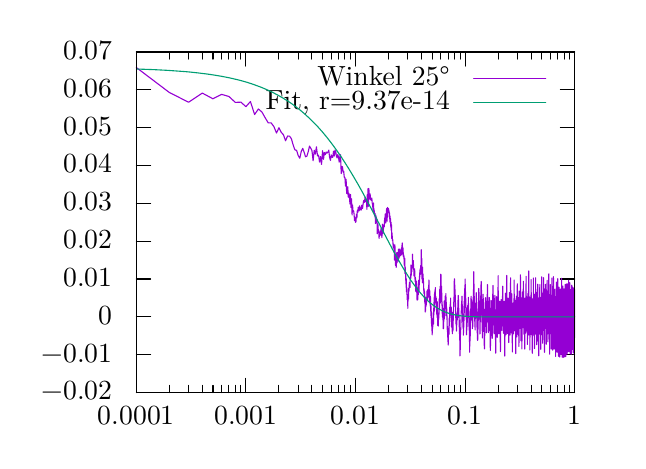
\begin{tikzpicture}[gnuplot]
%% generated with GNUPLOT 5.2p5a (Gentoo revision r0) (Lua 5.1; terminal rev. 99 , script rev. 107)
%% Sa 18 Mai 2019 18:30:57 CEST
\path (0.000,0.000) rectangle (7.500,5.250);
\gpcolor{color=gp lt color border}
\gpsetlinetype{gp lt border}
\gpsetdashtype{gp dt solid}
\gpsetlinewidth{1.00}
\draw[gp path] (1.380,0.616)--(1.560,0.616);
\draw[gp path] (6.947,0.616)--(6.767,0.616);
\node[gp node right] at (1.196,0.616) {$-0.02$};
\draw[gp path] (1.380,1.097)--(1.560,1.097);
\draw[gp path] (6.947,1.097)--(6.767,1.097);
\node[gp node right] at (1.196,1.097) {$-0.01$};
\draw[gp path] (1.380,1.577)--(1.560,1.577);
\draw[gp path] (6.947,1.577)--(6.767,1.577);
\node[gp node right] at (1.196,1.577) {$0$};
\draw[gp path] (1.380,2.058)--(1.560,2.058);
\draw[gp path] (6.947,2.058)--(6.767,2.058);
\node[gp node right] at (1.196,2.058) {$0.01$};
\draw[gp path] (1.380,2.538)--(1.560,2.538);
\draw[gp path] (6.947,2.538)--(6.767,2.538);
\node[gp node right] at (1.196,2.538) {$0.02$};
\draw[gp path] (1.380,3.019)--(1.560,3.019);
\draw[gp path] (6.947,3.019)--(6.767,3.019);
\node[gp node right] at (1.196,3.019) {$0.03$};
\draw[gp path] (1.380,3.499)--(1.560,3.499);
\draw[gp path] (6.947,3.499)--(6.767,3.499);
\node[gp node right] at (1.196,3.499) {$0.04$};
\draw[gp path] (1.380,3.980)--(1.560,3.980);
\draw[gp path] (6.947,3.980)--(6.767,3.980);
\node[gp node right] at (1.196,3.980) {$0.05$};
\draw[gp path] (1.380,4.460)--(1.560,4.460);
\draw[gp path] (6.947,4.460)--(6.767,4.460);
\node[gp node right] at (1.196,4.460) {$0.06$};
\draw[gp path] (1.380,4.941)--(1.560,4.941);
\draw[gp path] (6.947,4.941)--(6.767,4.941);
\node[gp node right] at (1.196,4.941) {$0.07$};
\draw[gp path] (1.380,0.616)--(1.380,0.796);
\draw[gp path] (1.380,4.941)--(1.380,4.761);
\node[gp node center] at (1.380,0.308) {$0.0001$};
\draw[gp path] (1.799,0.616)--(1.799,0.706);
\draw[gp path] (1.799,4.941)--(1.799,4.851);
\draw[gp path] (2.044,0.616)--(2.044,0.706);
\draw[gp path] (2.044,4.941)--(2.044,4.851);
\draw[gp path] (2.218,0.616)--(2.218,0.706);
\draw[gp path] (2.218,4.941)--(2.218,4.851);
\draw[gp path] (2.353,0.616)--(2.353,0.706);
\draw[gp path] (2.353,4.941)--(2.353,4.851);
\draw[gp path] (2.463,0.616)--(2.463,0.706);
\draw[gp path] (2.463,4.941)--(2.463,4.851);
\draw[gp path] (2.556,0.616)--(2.556,0.706);
\draw[gp path] (2.556,4.941)--(2.556,4.851);
\draw[gp path] (2.637,0.616)--(2.637,0.706);
\draw[gp path] (2.637,4.941)--(2.637,4.851);
\draw[gp path] (2.708,0.616)--(2.708,0.706);
\draw[gp path] (2.708,4.941)--(2.708,4.851);
\draw[gp path] (2.772,0.616)--(2.772,0.796);
\draw[gp path] (2.772,4.941)--(2.772,4.761);
\node[gp node center] at (2.772,0.308) {$0.001$};
\draw[gp path] (3.191,0.616)--(3.191,0.706);
\draw[gp path] (3.191,4.941)--(3.191,4.851);
\draw[gp path] (3.436,0.616)--(3.436,0.706);
\draw[gp path] (3.436,4.941)--(3.436,4.851);
\draw[gp path] (3.610,0.616)--(3.610,0.706);
\draw[gp path] (3.610,4.941)--(3.610,4.851);
\draw[gp path] (3.745,0.616)--(3.745,0.706);
\draw[gp path] (3.745,4.941)--(3.745,4.851);
\draw[gp path] (3.855,0.616)--(3.855,0.706);
\draw[gp path] (3.855,4.941)--(3.855,4.851);
\draw[gp path] (3.948,0.616)--(3.948,0.706);
\draw[gp path] (3.948,4.941)--(3.948,4.851);
\draw[gp path] (4.029,0.616)--(4.029,0.706);
\draw[gp path] (4.029,4.941)--(4.029,4.851);
\draw[gp path] (4.100,0.616)--(4.100,0.706);
\draw[gp path] (4.100,4.941)--(4.100,4.851);
\draw[gp path] (4.163,0.616)--(4.163,0.796);
\draw[gp path] (4.163,4.941)--(4.163,4.761);
\node[gp node center] at (4.163,0.308) {$0.01$};
\draw[gp path] (4.582,0.616)--(4.582,0.706);
\draw[gp path] (4.582,4.941)--(4.582,4.851);
\draw[gp path] (4.828,0.616)--(4.828,0.706);
\draw[gp path] (4.828,4.941)--(4.828,4.851);
\draw[gp path] (5.001,0.616)--(5.001,0.706);
\draw[gp path] (5.001,4.941)--(5.001,4.851);
\draw[gp path] (5.136,0.616)--(5.136,0.706);
\draw[gp path] (5.136,4.941)--(5.136,4.851);
\draw[gp path] (5.246,0.616)--(5.246,0.706);
\draw[gp path] (5.246,4.941)--(5.246,4.851);
\draw[gp path] (5.340,0.616)--(5.340,0.706);
\draw[gp path] (5.340,4.941)--(5.340,4.851);
\draw[gp path] (5.420,0.616)--(5.420,0.706);
\draw[gp path] (5.420,4.941)--(5.420,4.851);
\draw[gp path] (5.492,0.616)--(5.492,0.706);
\draw[gp path] (5.492,4.941)--(5.492,4.851);
\draw[gp path] (5.555,0.616)--(5.555,0.796);
\draw[gp path] (5.555,4.941)--(5.555,4.761);
\node[gp node center] at (5.555,0.308) {$0.1$};
\draw[gp path] (5.974,0.616)--(5.974,0.706);
\draw[gp path] (5.974,4.941)--(5.974,4.851);
\draw[gp path] (6.219,0.616)--(6.219,0.706);
\draw[gp path] (6.219,4.941)--(6.219,4.851);
\draw[gp path] (6.393,0.616)--(6.393,0.706);
\draw[gp path] (6.393,4.941)--(6.393,4.851);
\draw[gp path] (6.528,0.616)--(6.528,0.706);
\draw[gp path] (6.528,4.941)--(6.528,4.851);
\draw[gp path] (6.638,0.616)--(6.638,0.706);
\draw[gp path] (6.638,4.941)--(6.638,4.851);
\draw[gp path] (6.731,0.616)--(6.731,0.706);
\draw[gp path] (6.731,4.941)--(6.731,4.851);
\draw[gp path] (6.812,0.616)--(6.812,0.706);
\draw[gp path] (6.812,4.941)--(6.812,4.851);
\draw[gp path] (6.883,0.616)--(6.883,0.706);
\draw[gp path] (6.883,4.941)--(6.883,4.851);
\draw[gp path] (6.947,0.616)--(6.947,0.796);
\draw[gp path] (6.947,4.941)--(6.947,4.761);
\node[gp node center] at (6.947,0.308) {$1$};
\draw[gp path] (1.380,4.941)--(1.380,0.616)--(6.947,0.616)--(6.947,4.941)--cycle;
\node[gp node right] at (5.479,4.607) {Winkel 25°};
\gpcolor{rgb color={0.580,0.000,0.827}}
\draw[gp path] (5.663,4.607)--(6.579,4.607);
\draw[gp path] (1.380,4.744)--(1.799,4.427)--(2.044,4.303)--(2.218,4.419)--(2.353,4.347)%
  --(2.463,4.403)--(2.556,4.376)--(2.637,4.301)--(2.708,4.304)--(2.772,4.247)--(2.829,4.312)%
  --(2.882,4.147)--(2.930,4.217)--(2.975,4.179)--(3.017,4.104)--(3.056,4.040)--(3.092,4.041)%
  --(3.127,3.994)--(3.160,3.912)--(3.191,3.979)--(3.220,3.922)--(3.248,3.890)--(3.275,3.814)%
  --(3.301,3.874)--(3.326,3.872)--(3.349,3.840)--(3.372,3.759)--(3.394,3.698)--(3.415,3.692)%
  --(3.436,3.626)--(3.456,3.592)--(3.475,3.680)--(3.493,3.717)--(3.511,3.668)--(3.529,3.610)%
  --(3.546,3.618)--(3.563,3.675)--(3.579,3.746)--(3.594,3.721)--(3.610,3.691)--(3.625,3.560)%
  --(3.639,3.693)--(3.653,3.644)--(3.667,3.737)--(3.681,3.621)--(3.694,3.632)--(3.707,3.543)%
  --(3.720,3.614)--(3.732,3.513)--(3.745,3.688)--(3.757,3.579)--(3.768,3.665)--(3.780,3.637)%
  --(3.791,3.671)--(3.802,3.657)--(3.813,3.670)--(3.824,3.695)--(3.834,3.606)--(3.845,3.564)%
  --(3.855,3.635)--(3.865,3.602)--(3.875,3.605)--(3.884,3.680)--(3.894,3.619)--(3.903,3.695)%
  --(3.912,3.681)--(3.921,3.619)--(3.930,3.595)--(3.939,3.639)--(3.948,3.605)--(3.956,3.542)%
  --(3.965,3.614)--(3.973,3.637)--(3.982,3.398)--(3.990,3.488)--(3.998,3.482)--(4.006,3.414)%
  --(4.013,3.428)--(4.021,3.348)--(4.029,3.348)--(4.036,3.239)--(4.044,3.325)--(4.051,3.147)%
  --(4.058,3.140)--(4.065,3.230)--(4.072,3.097)--(4.079,3.148)--(4.086,3.101)--(4.093,3.011)%
  --(4.100,3.131)--(4.106,2.966)--(4.113,3.077)--(4.120,2.871)--(4.126,2.997)--(4.132,2.914)%
  --(4.139,2.925)--(4.145,2.885)--(4.151,2.801)--(4.157,2.836)--(4.164,2.777)--(4.170,2.789)%
  --(4.175,2.881)--(4.181,2.834)--(4.187,2.932)--(4.193,2.904)--(4.199,2.970)--(4.204,2.924)%
  --(4.210,2.925)--(4.216,2.988)--(4.221,2.967)--(4.227,2.954)--(4.232,2.932)--(4.237,2.936)%
  --(4.243,2.996)--(4.248,2.973)--(4.253,2.954)--(4.258,2.996)--(4.264,3.041)--(4.269,3.057)%
  --(4.274,3.031)--(4.279,3.041)--(4.284,3.096)--(4.289,3.067)--(4.294,3.037)--(4.298,3.070)%
  --(4.303,3.067)--(4.308,2.943)--(4.313,3.129)--(4.317,3.042)--(4.322,3.204)--(4.327,2.981)%
  --(4.331,3.208)--(4.336,3.176)--(4.340,3.073)--(4.345,3.097)--(4.349,3.139)--(4.354,3.071)%
  --(4.358,3.066)--(4.363,3.056)--(4.367,3.086)--(4.371,3.082)--(4.375,3.026)--(4.380,3.004)%
  --(4.384,2.961)--(4.388,2.906)--(4.392,3.023)--(4.396,2.918)--(4.400,2.935)--(4.405,2.870)%
  --(4.409,2.855)--(4.413,2.892)--(4.417,2.762)--(4.421,2.869)--(4.424,2.849)--(4.428,2.836)%
  --(4.432,2.815)--(4.436,2.817)--(4.440,2.632)--(4.444,2.718)--(4.448,2.759)--(4.451,2.691)%
  --(4.455,2.677)--(4.459,2.650)--(4.463,2.574)--(4.466,2.619)--(4.470,2.648)--(4.473,2.620)%
  --(4.477,2.667)--(4.481,2.615)--(4.484,2.622)--(4.488,2.702)--(4.491,2.670)--(4.495,2.659)%
  --(4.498,2.584)--(4.502,2.644)--(4.505,2.754)--(4.509,2.672)--(4.512,2.635)--(4.515,2.648)%
  --(4.519,2.708)--(4.522,2.735)--(4.525,2.753)--(4.529,2.722)--(4.532,2.803)--(4.535,2.829)%
  --(4.539,2.847)--(4.542,2.886)--(4.545,2.814)--(4.548,2.768)--(4.551,2.823)--(4.555,2.839)%
  --(4.558,2.951)--(4.561,2.874)--(4.564,2.792)--(4.567,2.942)--(4.570,2.968)--(4.573,2.844)%
  --(4.576,2.957)--(4.579,2.950)--(4.582,2.951)--(4.585,2.936)--(4.588,2.923)--(4.591,2.897)%
  --(4.594,2.901)--(4.597,2.884)--(4.600,2.783)--(4.603,2.858)--(4.606,2.775)--(4.609,2.822)%
  --(4.612,2.714)--(4.615,2.780)--(4.618,2.675)--(4.621,2.749)--(4.623,2.571)--(4.626,2.646)%
  --(4.629,2.616)--(4.632,2.544)--(4.635,2.562)--(4.637,2.552)--(4.640,2.503)--(4.643,2.458)%
  --(4.646,2.491)--(4.648,2.490)--(4.651,2.496)--(4.654,2.402)--(4.656,2.393)--(4.659,2.297)%
  --(4.662,2.365)--(4.664,2.491)--(4.667,2.297)--(4.670,2.363)--(4.672,2.232)--(4.675,2.233)%
  --(4.677,2.256)--(4.680,2.206)--(4.683,2.252)--(4.685,2.264)--(4.688,2.397)--(4.690,2.265)%
  --(4.693,2.284)--(4.695,2.383)--(4.698,2.391)--(4.700,2.373)--(4.703,2.324)--(4.705,2.301)%
  --(4.708,2.285)--(4.710,2.437)--(4.712,2.313)--(4.715,2.420)--(4.717,2.427)--(4.720,2.439)%
  --(4.722,2.337)--(4.725,2.415)--(4.727,2.370)--(4.729,2.364)--(4.732,2.369)--(4.734,2.420)%
  --(4.736,2.356)--(4.739,2.437)--(4.741,2.418)--(4.743,2.424)--(4.746,2.365)--(4.748,2.419)%
  --(4.750,2.435)--(4.753,2.487)--(4.755,2.445)--(4.757,2.517)--(4.759,2.375)--(4.762,2.468)%
  --(4.764,2.440)--(4.766,2.450)--(4.768,2.352)--(4.771,2.395)--(4.773,2.339)--(4.775,2.364)%
  --(4.777,2.357)--(4.779,2.343)--(4.781,2.271)--(4.784,2.227)--(4.786,2.264)--(4.788,2.248)%
  --(4.790,2.318)--(4.792,2.127)--(4.794,2.215)--(4.797,2.148)--(4.799,2.137)--(4.801,2.103)%
  --(4.803,1.996)--(4.805,2.028)--(4.807,1.949)--(4.809,2.060)--(4.811,1.894)--(4.813,1.950)%
  --(4.815,1.944)--(4.817,1.924)--(4.819,1.796)--(4.821,1.854)--(4.823,1.795)--(4.826,1.818)%
  --(4.828,1.686)--(4.830,1.840)--(4.832,1.777)--(4.834,1.862)--(4.836,1.804)--(4.838,1.853)%
  --(4.840,1.942)--(4.841,1.938)--(4.843,1.912)--(4.845,1.980)--(4.847,1.987)--(4.849,2.014)%
  --(4.851,1.966)--(4.853,1.972)--(4.855,1.950)--(4.857,2.066)--(4.859,2.083)--(4.861,2.064)%
  --(4.863,2.068)--(4.865,2.066)--(4.867,2.236)--(4.868,2.094)--(4.870,2.154)--(4.872,2.108)%
  --(4.874,2.180)--(4.876,2.232)--(4.878,2.151)--(4.880,2.222)--(4.881,2.223)--(4.883,2.186)%
  --(4.885,2.237)--(4.887,2.374)--(4.889,2.303)--(4.891,2.288)--(4.892,2.243)--(4.894,2.294)%
  --(4.896,2.240)--(4.898,2.292)--(4.900,2.216)--(4.901,2.187)--(4.903,2.171)--(4.905,2.195)%
  --(4.907,2.094)--(4.908,2.106)--(4.910,2.186)--(4.912,2.187)--(4.914,2.184)--(4.916,2.147)%
  --(4.917,2.058)--(4.919,2.066)--(4.921,2.025)--(4.922,2.082)--(4.924,2.069)--(4.926,2.060)%
  --(4.928,1.901)--(4.929,1.984)--(4.931,1.936)--(4.933,1.942)--(4.934,2.031)--(4.936,1.951)%
  --(4.938,1.888)--(4.939,2.029)--(4.941,1.941)--(4.943,1.913)--(4.944,1.805)--(4.946,1.788)%
  --(4.948,1.806)--(4.949,1.842)--(4.951,1.945)--(4.953,1.799)--(4.954,1.796)--(4.956,1.870)%
  --(4.958,1.919)--(4.959,1.894)--(4.961,1.859)--(4.962,1.970)--(4.964,2.000)--(4.966,1.993)%
  --(4.967,2.045)--(4.969,1.909)--(4.970,1.913)--(4.972,1.976)--(4.974,2.005)--(4.975,2.003)%
  --(4.977,2.105)--(4.978,2.136)--(4.980,2.084)--(4.981,2.130)--(4.983,2.172)--(4.985,2.188)%
  --(4.986,2.124)--(4.988,2.166)--(4.989,2.117)--(4.991,2.228)--(4.992,2.171)--(4.994,2.220)%
  --(4.995,2.153)--(4.997,2.234)--(4.998,2.431)--(5.000,2.371)--(5.001,2.298)--(5.003,2.313)%
  --(5.004,2.320)--(5.006,2.280)--(5.007,2.057)--(5.009,2.158)--(5.010,2.087)--(5.012,2.107)%
  --(5.013,2.012)--(5.015,2.207)--(5.016,2.079)--(5.018,2.054)--(5.019,2.109)--(5.021,2.121)%
  --(5.022,2.033)--(5.024,2.067)--(5.025,2.065)--(5.027,1.993)--(5.028,2.025)--(5.029,1.916)%
  --(5.031,1.931)--(5.032,1.873)--(5.034,1.933)--(5.035,1.919)--(5.037,1.894)--(5.038,1.909)%
  --(5.039,1.896)--(5.041,1.766)--(5.042,1.824)--(5.044,1.798)--(5.045,1.768)--(5.047,1.741)%
  --(5.048,1.638)--(5.049,1.676)--(5.051,1.686)--(5.052,1.646)--(5.054,1.727)--(5.055,1.743)%
  --(5.056,1.828)--(5.058,1.736)--(5.059,1.710)--(5.060,1.791)--(5.062,1.734)--(5.063,1.735)%
  --(5.064,1.809)--(5.066,1.760)--(5.067,1.815)--(5.069,1.805)--(5.070,1.778)--(5.071,1.906)%
  --(5.073,1.799)--(5.074,1.870)--(5.075,1.908)--(5.077,1.889)--(5.078,1.865)--(5.079,1.788)%
  --(5.081,1.921)--(5.082,1.885)--(5.083,1.837)--(5.085,1.820)--(5.086,1.923)--(5.087,1.900)%
  --(5.089,1.929)--(5.090,1.956)--(5.091,1.935)--(5.092,1.833)--(5.094,1.982)--(5.095,1.951)%
  --(5.096,2.045)--(5.098,1.942)--(5.099,1.956)--(5.100,1.837)--(5.101,1.908)--(5.103,1.854)%
  --(5.104,1.887)--(5.105,1.755)--(5.107,1.849)--(5.108,1.909)--(5.109,1.813)--(5.110,1.748)%
  --(5.112,1.764)--(5.113,1.722)--(5.114,1.755)--(5.115,1.837)--(5.117,1.651)--(5.118,1.725)%
  --(5.119,1.715)--(5.120,1.654)--(5.122,1.717)--(5.123,1.567)--(5.124,1.614)--(5.125,1.646)%
  --(5.127,1.608)--(5.128,1.557)--(5.129,1.492)--(5.130,1.527)--(5.131,1.459)--(5.133,1.556)%
  --(5.134,1.398)--(5.135,1.421)--(5.136,1.415)--(5.137,1.349)--(5.139,1.457)--(5.140,1.412)%
  --(5.141,1.432)--(5.142,1.436)--(5.144,1.502)--(5.145,1.449)--(5.146,1.549)--(5.147,1.518)%
  --(5.148,1.507)--(5.149,1.543)--(5.151,1.630)--(5.152,1.551)--(5.153,1.575)--(5.154,1.486)%
  --(5.155,1.544)--(5.157,1.622)--(5.158,1.709)--(5.159,1.675)--(5.160,1.638)--(5.161,1.771)%
  --(5.162,1.821)--(5.163,1.650)--(5.165,1.764)--(5.166,1.826)--(5.167,1.866)--(5.168,1.755)%
  --(5.169,1.777)--(5.170,1.882)--(5.172,1.909)--(5.173,1.842)--(5.174,1.845)--(5.175,1.878)%
  --(5.176,1.834)--(5.177,1.949)--(5.178,1.790)--(5.179,1.801)--(5.181,1.816)--(5.182,1.836)%
  --(5.183,1.773)--(5.184,1.834)--(5.185,1.736)--(5.186,1.819)--(5.187,1.700)--(5.188,1.743)%
  --(5.189,1.813)--(5.191,1.665)--(5.192,1.753)--(5.193,1.736)--(5.194,1.779)--(5.195,1.676)%
  --(5.196,1.603)--(5.197,1.665)--(5.198,1.655)--(5.199,1.612)--(5.200,1.569)--(5.202,1.583)%
  --(5.203,1.768)--(5.204,1.597)--(5.205,1.609)--(5.206,1.623)--(5.207,1.599)--(5.208,1.467)%
  --(5.209,1.578)--(5.210,1.546)--(5.211,1.471)--(5.212,1.499)--(5.213,1.502)--(5.214,1.509)%
  --(5.215,1.461)--(5.217,1.619)--(5.218,1.539)--(5.219,1.624)--(5.220,1.604)--(5.221,1.632)%
  --(5.222,1.559)--(5.223,1.602)--(5.224,1.688)--(5.225,1.648)--(5.226,1.664)--(5.227,1.808)%
  --(5.228,1.740)--(5.229,1.691)--(5.230,1.773)--(5.231,1.679)--(5.232,1.752)--(5.233,1.788)%
  --(5.234,1.931)--(5.235,1.802)--(5.236,1.796)--(5.237,1.874)--(5.238,1.935)--(5.239,1.753)%
  --(5.240,1.967)--(5.241,1.888)--(5.242,1.966)--(5.243,1.872)--(5.244,1.978)--(5.245,2.046)%
  --(5.246,2.120)--(5.247,1.986)--(5.249,2.112)--(5.250,1.981)--(5.251,2.057)--(5.252,1.909)%
  --(5.253,1.906)--(5.254,1.791)--(5.254,1.888)--(5.255,1.781)--(5.256,1.965)--(5.257,1.780)%
  --(5.258,1.882)--(5.259,1.796)--(5.260,1.723)--(5.261,1.762)--(5.262,1.724)--(5.263,1.741)%
  --(5.264,1.769)--(5.265,1.663)--(5.266,1.600)--(5.267,1.711)--(5.268,1.584)--(5.269,1.578)%
  --(5.270,1.570)--(5.271,1.687)--(5.272,1.587)--(5.273,1.554)--(5.274,1.588)--(5.275,1.536)%
  --(5.276,1.538)--(5.277,1.502)--(5.278,1.426)--(5.279,1.467)--(5.280,1.436)--(5.281,1.457)%
  --(5.282,1.431)--(5.283,1.471)--(5.284,1.584)--(5.285,1.576)--(5.286,1.677)--(5.286,1.541)%
  --(5.287,1.615)--(5.288,1.611)--(5.289,1.613)--(5.290,1.633)--(5.291,1.780)--(5.292,1.552)%
  --(5.293,1.589)--(5.294,1.596)--(5.295,1.676)--(5.296,1.573)--(5.297,1.737)--(5.298,1.636)%
  --(5.299,1.711)--(5.300,1.774)--(5.300,1.675)--(5.301,1.717)--(5.302,1.717)--(5.303,1.843)%
  --(5.304,1.730)--(5.305,1.824)--(5.306,1.781)--(5.307,1.829)--(5.308,1.840)--(5.309,1.778)%
  --(5.310,1.806)--(5.310,1.822)--(5.311,1.873)--(5.312,1.818)--(5.313,1.829)--(5.314,1.749)%
  --(5.315,1.679)--(5.316,1.762)--(5.317,1.649)--(5.318,1.610)--(5.319,1.592)--(5.319,1.676)%
  --(5.320,1.704)--(5.321,1.622)--(5.322,1.680)--(5.323,1.607)--(5.324,1.610)--(5.325,1.584)%
  --(5.326,1.542)--(5.327,1.501)--(5.327,1.484)--(5.328,1.418)--(5.329,1.458)--(5.330,1.387)%
  --(5.331,1.406)--(5.332,1.427)--(5.333,1.355)--(5.334,1.319)--(5.334,1.358)--(5.335,1.434)%
  --(5.336,1.389)--(5.337,1.304)--(5.338,1.259)--(5.339,1.300)--(5.340,1.219)--(5.341,1.237)%
  --(5.341,1.264)--(5.342,1.316)--(5.343,1.331)--(5.344,1.380)--(5.345,1.368)--(5.346,1.390)%
  --(5.347,1.427)--(5.347,1.401)--(5.348,1.396)--(5.349,1.461)--(5.350,1.371)--(5.351,1.356)%
  --(5.352,1.458)--(5.352,1.487)--(5.353,1.434)--(5.354,1.545)--(5.355,1.568)--(5.356,1.497)%
  --(5.357,1.536)--(5.358,1.542)--(5.358,1.698)--(5.359,1.585)--(5.360,1.619)--(5.361,1.567)%
  --(5.362,1.622)--(5.363,1.637)--(5.363,1.592)--(5.364,1.676)--(5.365,1.666)--(5.366,1.706)%
  --(5.367,1.735)--(5.368,1.690)--(5.368,1.698)--(5.369,1.694)--(5.370,1.720)--(5.371,1.815)%
  --(5.372,1.717)--(5.372,1.694)--(5.373,1.714)--(5.374,1.699)--(5.375,1.659)--(5.376,1.670)%
  --(5.377,1.697)--(5.377,1.605)--(5.378,1.624)--(5.379,1.664)--(5.380,1.695)--(5.381,1.629)%
  --(5.381,1.590)--(5.382,1.447)--(5.383,1.547)--(5.384,1.642)--(5.385,1.495)--(5.385,1.546)%
  --(5.386,1.450)--(5.387,1.507)--(5.388,1.496)--(5.389,1.468)--(5.389,1.495)--(5.390,1.495)%
  --(5.391,1.484)--(5.392,1.456)--(5.393,1.363)--(5.393,1.371)--(5.394,1.368)--(5.395,1.402)%
  --(5.396,1.441)--(5.396,1.443)--(5.397,1.449)--(5.398,1.449)--(5.399,1.451)--(5.400,1.634)%
  --(5.400,1.560)--(5.401,1.636)--(5.402,1.566)--(5.403,1.551)--(5.404,1.410)--(5.404,1.528)%
  --(5.405,1.582)--(5.406,1.646)--(5.407,1.632)--(5.407,1.664)--(5.408,1.665)--(5.409,1.648)%
  --(5.410,1.696)--(5.410,1.766)--(5.411,1.708)--(5.412,1.712)--(5.413,1.830)--(5.414,1.782)%
  --(5.414,1.809)--(5.415,1.833)--(5.416,1.844)--(5.417,1.871)--(5.417,1.897)--(5.418,2.034)%
  --(5.419,1.985)--(5.420,2.061)--(5.420,2.009)--(5.421,1.952)--(5.422,2.057)--(5.423,2.033)%
  --(5.423,1.987)--(5.424,1.940)--(5.425,1.835)--(5.426,1.904)--(5.426,1.813)--(5.427,1.927)%
  --(5.428,1.769)--(5.429,1.803)--(5.429,1.773)--(5.430,1.857)--(5.431,1.743)--(5.432,1.749)%
  --(5.432,1.703)--(5.433,1.711)--(5.434,1.757)--(5.435,1.611)--(5.435,1.678)--(5.436,1.639)%
  --(5.437,1.566)--(5.438,1.639)--(5.438,1.571)--(5.439,1.578)--(5.440,1.490)--(5.440,1.545)%
  --(5.441,1.519)--(5.442,1.476)--(5.443,1.485)--(5.443,1.469)--(5.444,1.485)--(5.445,1.448)%
  --(5.446,1.397)--(5.446,1.476)--(5.447,1.476)--(5.448,1.516)--(5.448,1.560)--(5.449,1.504)%
  --(5.450,1.523)--(5.451,1.613)--(5.451,1.475)--(5.452,1.557)--(5.453,1.551)--(5.453,1.554)%
  --(5.454,1.590)--(5.455,1.606)--(5.456,1.539)--(5.456,1.606)--(5.457,1.629)--(5.458,1.601)%
  --(5.458,1.585)--(5.459,1.567)--(5.460,1.620)--(5.461,1.693)--(5.461,1.601)--(5.462,1.681)%
  --(5.463,1.702)--(5.463,1.681)--(5.464,1.598)--(5.465,1.732)--(5.465,1.655)--(5.466,1.838)%
  --(5.467,1.751)--(5.468,1.849)--(5.468,1.716)--(5.469,1.825)--(5.470,1.707)--(5.470,1.830)%
  --(5.471,1.789)--(5.472,1.705)--(5.472,1.746)--(5.473,1.797)--(5.474,1.678)--(5.475,1.673)%
  --(5.475,1.612)--(5.476,1.592)--(5.477,1.657)--(5.477,1.595)--(5.478,1.567)--(5.479,1.604)%
  --(5.479,1.555)--(5.480,1.549)--(5.481,1.514)--(5.481,1.447)--(5.482,1.452)--(5.483,1.450)%
  --(5.483,1.363)--(5.484,1.375)--(5.485,1.357)--(5.485,1.424)--(5.486,1.281)--(5.487,1.364)%
  --(5.488,1.340)--(5.488,1.330)--(5.489,1.183)--(5.490,1.304)--(5.490,1.081)--(5.491,1.305)%
  --(5.492,1.151)--(5.492,1.242)--(5.493,1.158)--(5.494,1.246)--(5.494,1.215)--(5.495,1.342)%
  --(5.496,1.294)--(5.496,1.404)--(5.497,1.352)--(5.498,1.389)--(5.499,1.427)--(5.500,1.418)%
  --(5.500,1.442)--(5.501,1.415)--(5.502,1.541)--(5.502,1.511)--(5.503,1.503)--(5.504,1.544)%
  --(5.504,1.612)--(5.505,1.645)--(5.506,1.621)--(5.506,1.654)--(5.507,1.623)--(5.507,1.622)%
  --(5.508,1.687)--(5.509,1.670)--(5.509,1.678)--(5.510,1.733)--(5.511,1.779)--(5.511,1.670)%
  --(5.512,1.739)--(5.513,1.718)--(5.513,1.763)--(5.514,1.735)--(5.515,1.755)--(5.515,1.682)%
  --(5.516,1.839)--(5.517,1.752)--(5.517,1.712)--(5.518,1.643)--(5.518,1.684)--(5.519,1.625)%
  --(5.520,1.662)--(5.520,1.699)--(5.521,1.733)--(5.522,1.656)--(5.522,1.714)--(5.523,1.678)%
  --(5.524,1.636)--(5.524,1.587)--(5.525,1.618)--(5.526,1.585)--(5.526,1.519)--(5.527,1.497)%
  --(5.527,1.583)--(5.528,1.496)--(5.529,1.587)--(5.529,1.443)--(5.530,1.469)--(5.531,1.457)%
  --(5.531,1.500)--(5.532,1.511)--(5.532,1.456)--(5.533,1.384)--(5.534,1.528)--(5.534,1.345)%
  --(5.535,1.458)--(5.536,1.479)--(5.536,1.530)--(5.537,1.471)--(5.537,1.488)--(5.538,1.443)%
  --(5.539,1.529)--(5.539,1.609)--(5.540,1.575)--(5.541,1.527)--(5.541,1.567)--(5.542,1.612)%
  --(5.542,1.611)--(5.543,1.604)--(5.544,1.776)--(5.544,1.628)--(5.545,1.677)--(5.546,1.698)%
  --(5.546,1.840)--(5.547,1.807)--(5.547,1.795)--(5.548,1.867)--(5.549,1.888)--(5.549,1.740)%
  --(5.550,1.937)--(5.550,1.833)--(5.551,1.756)--(5.552,1.904)--(5.552,1.898)--(5.553,1.921)%
  --(5.553,1.948)--(5.554,1.955)--(5.555,2.001)--(5.555,2.045)--(5.556,2.046)--(5.556,2.058)%
  --(5.557,1.915)--(5.558,1.935)--(5.558,1.918)--(5.559,1.840)--(5.559,1.890)--(5.560,1.864)%
  --(5.561,1.740)--(5.561,1.846)--(5.562,1.895)--(5.562,1.793)--(5.563,1.771)--(5.564,1.768)%
  --(5.564,1.692)--(5.565,1.737)--(5.565,1.810)--(5.566,1.700)--(5.567,1.696)--(5.567,1.582)%
  --(5.568,1.610)--(5.568,1.629)--(5.569,1.698)--(5.570,1.660)--(5.570,1.565)--(5.571,1.519)%
  --(5.571,1.644)--(5.572,1.522)--(5.573,1.464)--(5.573,1.348)--(5.574,1.478)--(5.574,1.458)%
  --(5.575,1.387)--(5.575,1.461)--(5.576,1.423)--(5.577,1.408)--(5.577,1.407)--(5.578,1.419)%
  --(5.578,1.564)--(5.579,1.569)--(5.580,1.610)--(5.580,1.453)--(5.581,1.483)--(5.581,1.531)%
  --(5.582,1.566)--(5.582,1.570)--(5.583,1.505)--(5.584,1.625)--(5.584,1.596)--(5.585,1.642)%
  --(5.585,1.604)--(5.586,1.651)--(5.586,1.613)--(5.587,1.601)--(5.588,1.659)--(5.588,1.722)%
  --(5.589,1.681)--(5.589,1.662)--(5.590,1.626)--(5.590,1.687)--(5.591,1.650)--(5.592,1.716)%
  --(5.592,1.645)--(5.593,1.742)--(5.593,1.698)--(5.594,1.745)--(5.594,1.747)--(5.595,1.699)%
  --(5.596,1.717)--(5.596,1.825)--(5.597,1.711)--(5.597,1.677)--(5.598,1.658)--(5.598,1.634)%
  --(5.599,1.678)--(5.600,1.749)--(5.600,1.565)--(5.601,1.628)--(5.601,1.648)--(5.602,1.590)%
  --(5.602,1.616)--(5.603,1.579)--(5.603,1.505)--(5.604,1.574)--(5.605,1.502)--(5.605,1.454)%
  --(5.606,1.473)--(5.606,1.447)--(5.607,1.469)--(5.607,1.502)--(5.608,1.415)--(5.608,1.406)%
  --(5.609,1.430)--(5.610,1.379)--(5.610,1.343)--(5.611,1.355)--(5.611,1.258)--(5.612,1.284)%
  --(5.612,1.242)--(5.613,1.215)--(5.613,1.128)--(5.614,1.252)--(5.615,1.288)--(5.615,1.315)%
  --(5.616,1.349)--(5.616,1.287)--(5.617,1.270)--(5.617,1.405)--(5.618,1.364)--(5.618,1.453)%
  --(5.619,1.281)--(5.619,1.433)--(5.620,1.333)--(5.621,1.434)--(5.621,1.412)--(5.622,1.507)%
  --(5.622,1.519)--(5.623,1.568)--(5.623,1.529)--(5.624,1.593)--(5.624,1.668)--(5.625,1.655)%
  --(5.625,1.619)--(5.626,1.573)--(5.626,1.679)--(5.627,1.605)--(5.628,1.672)--(5.628,1.715)%
  --(5.629,1.758)--(5.629,1.714)--(5.630,1.816)--(5.630,1.773)--(5.631,1.737)--(5.631,1.839)%
  --(5.632,1.790)--(5.632,1.780)--(5.633,1.728)--(5.633,1.805)--(5.634,1.712)--(5.634,1.691)%
  --(5.635,1.702)--(5.636,1.698)--(5.636,1.706)--(5.637,1.682)--(5.637,1.686)--(5.638,1.792)%
  --(5.638,1.652)--(5.639,1.687)--(5.639,1.635)--(5.640,1.758)--(5.640,1.628)--(5.641,1.770)%
  --(5.641,1.562)--(5.642,1.659)--(5.642,1.567)--(5.643,1.645)--(5.643,1.527)--(5.644,1.670)%
  --(5.644,1.527)--(5.645,1.572)--(5.645,1.509)--(5.646,1.544)--(5.647,1.490)--(5.647,1.503)%
  --(5.648,1.427)--(5.648,1.613)--(5.649,1.491)--(5.649,1.567)--(5.650,1.523)--(5.650,1.514)%
  --(5.651,1.498)--(5.651,1.592)--(5.652,1.590)--(5.652,1.454)--(5.653,1.575)--(5.653,1.650)%
  --(5.654,1.617)--(5.654,1.658)--(5.655,1.581)--(5.655,1.694)--(5.656,1.579)--(5.656,1.610)%
  --(5.657,1.665)--(5.657,1.757)--(5.658,1.640)--(5.658,1.719)--(5.659,1.810)--(5.659,1.826)%
  --(5.660,1.739)--(5.660,1.889)--(5.661,1.793)--(5.661,1.924)--(5.662,1.838)--(5.662,1.858)%
  --(5.663,1.870)--(5.663,1.988)--(5.664,1.860)--(5.664,2.142)--(5.665,1.988)--(5.665,2.150)%
  --(5.666,1.991)--(5.666,2.088)--(5.667,1.881)--(5.667,2.099)--(5.668,1.923)--(5.668,1.911)%
  --(5.669,1.771)--(5.669,1.838)--(5.670,1.789)--(5.670,1.809)--(5.671,1.811)--(5.671,1.833)%
  --(5.672,1.839)--(5.672,1.789)--(5.673,1.770)--(5.673,1.773)--(5.674,1.683)--(5.674,1.697)%
  --(5.675,1.688)--(5.675,1.560)--(5.676,1.696)--(5.677,1.643)--(5.677,1.601)--(5.678,1.556)%
  --(5.678,1.521)--(5.679,1.520)--(5.679,1.446)--(5.680,1.577)--(5.680,1.561)--(5.681,1.482)%
  --(5.681,1.488)--(5.682,1.501)--(5.682,1.549)--(5.683,1.411)--(5.683,1.524)--(5.684,1.618)%
  --(5.684,1.557)--(5.685,1.551)--(5.685,1.571)--(5.686,1.599)--(5.686,1.700)--(5.687,1.566)%
  --(5.687,1.558)--(5.688,1.576)--(5.688,1.558)--(5.689,1.592)--(5.689,1.614)--(5.690,1.646)%
  --(5.690,1.755)--(5.691,1.658)--(5.691,1.709)--(5.692,1.641)--(5.692,1.734)--(5.693,1.736)%
  --(5.693,1.725)--(5.693,1.708)--(5.694,1.616)--(5.694,1.738)--(5.695,1.743)--(5.695,1.754)%
  --(5.696,1.730)--(5.696,1.776)--(5.697,1.733)--(5.697,1.884)--(5.698,1.860)--(5.698,1.757)%
  --(5.699,1.829)--(5.699,1.848)--(5.700,1.746)--(5.700,1.807)--(5.701,1.753)--(5.701,1.696)%
  --(5.702,1.624)--(5.702,1.722)--(5.703,1.642)--(5.703,1.646)--(5.704,1.665)--(5.704,1.643)%
  --(5.704,1.572)--(5.705,1.631)--(5.705,1.611)--(5.706,1.565)--(5.706,1.589)--(5.707,1.445)%
  --(5.707,1.542)--(5.708,1.506)--(5.708,1.473)--(5.709,1.498)--(5.709,1.466)--(5.710,1.371)%
  --(5.710,1.528)--(5.711,1.371)--(5.711,1.378)--(5.712,1.439)--(5.712,1.354)--(5.712,1.347)%
  --(5.713,1.332)--(5.713,1.295)--(5.714,1.279)--(5.714,1.297)--(5.715,1.359)--(5.715,1.284)%
  --(5.716,1.302)--(5.716,1.410)--(5.717,1.428)--(5.717,1.418)--(5.718,1.478)--(5.718,1.443)%
  --(5.718,1.433)--(5.719,1.447)--(5.719,1.419)--(5.720,1.483)--(5.720,1.515)--(5.721,1.572)%
  --(5.721,1.525)--(5.722,1.533)--(5.722,1.644)--(5.723,1.593)--(5.723,1.667)--(5.724,1.724)%
  --(5.724,1.763)--(5.724,1.669)--(5.725,1.761)--(5.725,1.626)--(5.726,1.741)--(5.726,1.743)%
  --(5.727,1.798)--(5.727,1.771)--(5.728,1.795)--(5.728,1.839)--(5.729,1.938)--(5.729,1.878)%
  --(5.729,1.909)--(5.730,1.804)--(5.730,1.841)--(5.731,1.891)--(5.731,1.900)--(5.732,1.779)%
  --(5.732,1.711)--(5.733,1.716)--(5.733,1.751)--(5.733,1.707)--(5.734,1.796)--(5.734,1.713)%
  --(5.735,1.765)--(5.735,1.775)--(5.736,1.751)--(5.736,1.719)--(5.737,1.564)--(5.737,1.782)%
  --(5.738,1.642)--(5.738,1.658)--(5.738,1.547)--(5.739,1.550)--(5.739,1.599)--(5.740,1.557)%
  --(5.740,1.600)--(5.741,1.682)--(5.741,1.579)--(5.742,1.598)--(5.742,1.479)--(5.742,1.525)%
  --(5.743,1.491)--(5.743,1.467)--(5.744,1.360)--(5.744,1.490)--(5.745,1.429)--(5.745,1.495)%
  --(5.746,1.418)--(5.746,1.517)--(5.746,1.543)--(5.747,1.573)--(5.747,1.590)--(5.748,1.542)%
  --(5.748,1.511)--(5.749,1.559)--(5.749,1.560)--(5.749,1.573)--(5.750,1.735)--(5.750,1.607)%
  --(5.751,1.679)--(5.751,1.681)--(5.752,1.725)--(5.752,1.685)--(5.753,1.762)--(5.753,1.846)%
  --(5.753,1.722)--(5.754,1.803)--(5.754,1.778)--(5.755,1.803)--(5.755,1.773)--(5.756,1.715)%
  --(5.756,1.803)--(5.756,1.896)--(5.757,1.928)--(5.757,1.957)--(5.758,1.992)--(5.758,1.973)%
  --(5.759,1.939)--(5.759,1.938)--(5.759,1.998)--(5.760,2.026)--(5.760,1.978)--(5.761,1.977)%
  --(5.761,1.809)--(5.762,1.979)--(5.762,1.900)--(5.762,1.916)--(5.763,1.809)--(5.763,1.919)%
  --(5.764,1.722)--(5.764,1.752)--(5.765,1.732)--(5.765,1.800)--(5.765,1.747)--(5.766,1.801)%
  --(5.766,1.593)--(5.767,1.686)--(5.767,1.674)--(5.768,1.612)--(5.768,1.588)--(5.768,1.586)%
  --(5.769,1.510)--(5.769,1.535)--(5.770,1.603)--(5.770,1.574)--(5.771,1.599)--(5.771,1.496)%
  --(5.771,1.426)--(5.772,1.492)--(5.772,1.455)--(5.773,1.442)--(5.773,1.450)--(5.774,1.375)%
  --(5.774,1.384)--(5.774,1.309)--(5.775,1.471)--(5.775,1.453)--(5.776,1.387)--(5.776,1.594)%
  --(5.776,1.501)--(5.777,1.529)--(5.778,1.659)--(5.778,1.527)--(5.779,1.601)--(5.779,1.600)%
  --(5.779,1.685)--(5.780,1.649)--(5.780,1.662)--(5.781,1.593)--(5.781,1.582)--(5.781,1.640)%
  --(5.782,1.662)--(5.782,1.660)--(5.783,1.580)--(5.783,1.632)--(5.784,1.682)--(5.784,1.576)%
  --(5.784,1.865)--(5.785,1.735)--(5.785,1.705)--(5.786,1.700)--(5.786,1.776)--(5.786,1.789)%
  --(5.787,1.813)--(5.787,1.778)--(5.788,1.787)--(5.788,1.695)--(5.789,1.762)--(5.789,1.716)%
  --(5.789,1.649)--(5.790,1.646)--(5.790,1.616)--(5.791,1.664)--(5.791,1.632)--(5.791,1.680)%
  --(5.792,1.667)--(5.792,1.604)--(5.793,1.651)--(5.793,1.583)--(5.793,1.547)--(5.794,1.456)%
  --(5.794,1.581)--(5.795,1.388)--(5.795,1.490)--(5.795,1.477)--(5.796,1.430)--(5.796,1.403)%
  --(5.797,1.403)--(5.797,1.355)--(5.797,1.389)--(5.798,1.322)--(5.798,1.343)--(5.799,1.211)%
  --(5.799,1.265)--(5.800,1.195)--(5.800,1.330)--(5.800,1.211)--(5.801,1.227)--(5.801,1.170)%
  --(5.802,1.281)--(5.802,1.187)--(5.802,1.311)--(5.803,1.320)--(5.803,1.356)--(5.804,1.363)%
  --(5.804,1.414)--(5.804,1.395)--(5.805,1.392)--(5.805,1.341)--(5.806,1.504)--(5.806,1.447)%
  --(5.806,1.412)--(5.807,1.448)--(5.807,1.577)--(5.808,1.498)--(5.808,1.505)--(5.808,1.563)%
  --(5.809,1.601)--(5.809,1.597)--(5.810,1.681)--(5.810,1.660)--(5.810,1.620)--(5.811,1.621)%
  --(5.811,1.669)--(5.812,1.671)--(5.812,1.758)--(5.812,1.675)--(5.813,1.732)--(5.813,1.714)%
  --(5.813,1.771)--(5.814,1.716)--(5.814,1.822)--(5.815,1.778)--(5.815,1.782)--(5.815,1.656)%
  --(5.816,1.660)--(5.816,1.656)--(5.817,1.647)--(5.817,1.635)--(5.817,1.694)--(5.818,1.588)%
  --(5.818,1.578)--(5.819,1.587)--(5.819,1.630)--(5.819,1.569)--(5.820,1.596)--(5.820,1.474)%
  --(5.821,1.545)--(5.821,1.554)--(5.821,1.632)--(5.822,1.513)--(5.822,1.479)--(5.822,1.524)%
  --(5.823,1.479)--(5.823,1.533)--(5.824,1.536)--(5.824,1.450)--(5.824,1.460)--(5.825,1.586)%
  --(5.825,1.441)--(5.826,1.394)--(5.826,1.444)--(5.826,1.375)--(5.827,1.413)--(5.827,1.431)%
  --(5.828,1.448)--(5.828,1.462)--(5.828,1.457)--(5.829,1.442)--(5.829,1.426)--(5.829,1.584)%
  --(5.830,1.511)--(5.830,1.547)--(5.831,1.584)--(5.831,1.659)--(5.831,1.615)--(5.832,1.725)%
  --(5.832,1.600)--(5.832,1.591)--(5.833,1.569)--(5.833,1.665)--(5.834,1.699)--(5.834,1.685)%
  --(5.834,1.779)--(5.835,1.793)--(5.835,1.700)--(5.836,1.782)--(5.836,1.816)--(5.836,1.840)%
  --(5.837,1.849)--(5.837,1.829)--(5.837,1.846)--(5.838,1.947)--(5.838,1.901)--(5.839,1.856)%
  --(5.839,1.948)--(5.839,1.988)--(5.840,1.930)--(5.840,1.902)--(5.840,1.895)--(5.841,1.895)%
  --(5.841,1.840)--(5.842,1.819)--(5.842,1.868)--(5.842,1.742)--(5.843,1.738)--(5.843,1.794)%
  --(5.843,1.713)--(5.844,1.829)--(5.844,1.780)--(5.845,1.793)--(5.845,1.723)--(5.845,1.674)%
  --(5.846,1.692)--(5.846,1.631)--(5.846,1.706)--(5.847,1.541)--(5.847,1.562)--(5.848,1.534)%
  --(5.848,1.584)--(5.848,1.560)--(5.849,1.540)--(5.849,1.578)--(5.849,1.505)--(5.850,1.498)%
  --(5.850,1.454)--(5.851,1.497)--(5.851,1.475)--(5.851,1.377)--(5.852,1.437)--(5.852,1.422)%
  --(5.852,1.465)--(5.853,1.408)--(5.853,1.478)--(5.854,1.499)--(5.854,1.454)--(5.854,1.464)%
  --(5.855,1.410)--(5.855,1.404)--(5.855,1.487)--(5.856,1.471)--(5.856,1.579)--(5.856,1.592)%
  --(5.857,1.606)--(5.857,1.444)--(5.858,1.495)--(5.858,1.668)--(5.859,1.569)--(5.859,1.590)%
  --(5.859,1.702)--(5.860,1.632)--(5.860,1.609)--(5.860,1.671)--(5.861,1.673)--(5.861,1.643)%
  --(5.862,1.714)--(5.862,1.650)--(5.862,1.779)--(5.863,1.718)--(5.863,1.676)--(5.863,1.663)%
  --(5.864,1.770)--(5.864,1.810)--(5.864,1.822)--(5.865,1.760)--(5.865,1.752)--(5.866,1.677)%
  --(5.866,1.712)--(5.866,1.765)--(5.867,1.747)--(5.867,1.665)--(5.867,1.711)--(5.868,1.639)%
  --(5.868,1.553)--(5.868,1.647)--(5.869,1.676)--(5.869,1.606)--(5.870,1.600)--(5.870,1.499)%
  --(5.870,1.464)--(5.871,1.476)--(5.871,1.530)--(5.871,1.453)--(5.872,1.390)--(5.872,1.476)%
  --(5.872,1.422)--(5.873,1.409)--(5.873,1.415)--(5.873,1.348)--(5.874,1.350)--(5.874,1.304)%
  --(5.875,1.242)--(5.875,1.323)--(5.875,1.191)--(5.876,1.174)--(5.876,1.221)--(5.876,1.226)%
  --(5.877,1.210)--(5.877,1.150)--(5.877,1.253)--(5.878,1.209)--(5.878,1.324)--(5.878,1.303)%
  --(5.879,1.409)--(5.879,1.367)--(5.880,1.343)--(5.880,1.344)--(5.880,1.352)--(5.881,1.458)%
  --(5.881,1.368)--(5.881,1.334)--(5.882,1.358)--(5.882,1.354)--(5.882,1.514)--(5.883,1.505)%
  --(5.883,1.546)--(5.883,1.455)--(5.884,1.611)--(5.884,1.689)--(5.884,1.584)--(5.885,1.563)%
  --(5.885,1.654)--(5.886,1.642)--(5.886,1.574)--(5.886,1.656)--(5.887,1.721)--(5.887,1.731)%
  --(5.887,1.784)--(5.888,1.776)--(5.888,1.718)--(5.888,1.709)--(5.889,1.712)--(5.889,1.720)%
  --(5.889,1.755)--(5.890,1.647)--(5.890,1.632)--(5.890,1.640)--(5.891,1.718)--(5.891,1.691)%
  --(5.891,1.698)--(5.892,1.611)--(5.892,1.612)--(5.892,1.527)--(5.893,1.583)--(5.893,1.587)%
  --(5.893,1.564)--(5.894,1.590)--(5.894,1.584)--(5.895,1.564)--(5.895,1.483)--(5.895,1.478)%
  --(5.896,1.553)--(5.896,1.484)--(5.896,1.507)--(5.897,1.503)--(5.897,1.465)--(5.897,1.421)%
  --(5.898,1.516)--(5.898,1.439)--(5.898,1.374)--(5.899,1.382)--(5.899,1.440)--(5.899,1.371)%
  --(5.900,1.312)--(5.900,1.304)--(5.900,1.494)--(5.901,1.494)--(5.901,1.470)--(5.901,1.396)%
  --(5.902,1.400)--(5.902,1.419)--(5.902,1.479)--(5.903,1.470)--(5.903,1.530)--(5.903,1.513)%
  --(5.904,1.537)--(5.904,1.584)--(5.904,1.610)--(5.905,1.630)--(5.905,1.661)--(5.905,1.726)%
  --(5.906,1.714)--(5.906,1.671)--(5.906,1.730)--(5.907,1.673)--(5.907,1.868)--(5.907,1.714)%
  --(5.908,1.863)--(5.908,1.719)--(5.909,1.827)--(5.909,1.787)--(5.909,1.881)--(5.910,1.843)%
  --(5.910,1.976)--(5.910,1.881)--(5.911,1.975)--(5.911,1.960)--(5.912,1.922)--(5.912,1.854)%
  --(5.912,1.852)--(5.913,1.780)--(5.913,1.781)--(5.913,1.807)--(5.914,1.748)--(5.914,1.779)%
  --(5.914,1.784)--(5.915,1.759)--(5.915,1.704)--(5.915,1.694)--(5.916,1.621)--(5.916,1.654)%
  --(5.916,1.616)--(5.917,1.712)--(5.917,1.566)--(5.917,1.573)--(5.918,1.591)--(5.918,1.673)%
  --(5.918,1.540)--(5.919,1.570)--(5.919,1.568)--(5.919,1.525)--(5.920,1.510)--(5.920,1.480)%
  --(5.920,1.523)--(5.921,1.379)--(5.921,1.427)--(5.921,1.487)--(5.922,1.376)--(5.922,1.476)%
  --(5.922,1.427)--(5.922,1.477)--(5.923,1.362)--(5.923,1.454)--(5.923,1.452)--(5.924,1.538)%
  --(5.924,1.440)--(5.924,1.556)--(5.925,1.461)--(5.925,1.512)--(5.925,1.495)--(5.926,1.602)%
  --(5.926,1.507)--(5.926,1.587)--(5.927,1.441)--(5.927,1.588)--(5.927,1.529)--(5.928,1.571)%
  --(5.928,1.613)--(5.928,1.580)--(5.929,1.633)--(5.929,1.724)--(5.929,1.607)--(5.930,1.625)%
  --(5.930,1.588)--(5.930,1.551)--(5.931,1.643)--(5.931,1.687)--(5.931,1.648)--(5.932,1.647)%
  --(5.932,1.668)--(5.932,1.786)--(5.933,1.850)--(5.933,1.705)--(5.933,1.641)--(5.934,1.663)%
  --(5.934,1.625)--(5.934,1.594)--(5.935,1.672)--(5.935,1.649)--(5.935,1.572)--(5.936,1.613)%
  --(5.936,1.564)--(5.936,1.506)--(5.936,1.644)--(5.937,1.486)--(5.937,1.474)--(5.937,1.494)%
  --(5.938,1.493)--(5.938,1.419)--(5.938,1.424)--(5.939,1.387)--(5.939,1.364)--(5.939,1.412)%
  --(5.940,1.337)--(5.940,1.386)--(5.940,1.288)--(5.941,1.353)--(5.941,1.364)--(5.941,1.325)%
  --(5.942,1.283)--(5.942,1.324)--(5.942,1.234)--(5.943,1.240)--(5.943,1.129)--(5.943,1.148)%
  --(5.944,1.152)--(5.944,1.203)--(5.944,1.116)--(5.944,1.267)--(5.945,1.292)--(5.945,1.241)%
  --(5.945,1.310)--(5.946,1.357)--(5.946,1.304)--(5.946,1.348)--(5.947,1.342)--(5.947,1.360)%
  --(5.947,1.412)--(5.948,1.342)--(5.948,1.419)--(5.948,1.348)--(5.949,1.545)--(5.949,1.519)%
  --(5.949,1.528)--(5.950,1.527)--(5.950,1.436)--(5.950,1.556)--(5.950,1.526)--(5.951,1.604)%
  --(5.951,1.621)--(5.951,1.553)--(5.952,1.525)--(5.952,1.575)--(5.952,1.539)--(5.953,1.681)%
  --(5.953,1.669)--(5.953,1.610)--(5.954,1.834)--(5.954,1.682)--(5.954,1.773)--(5.955,1.765)%
  --(5.955,1.702)--(5.955,1.606)--(5.955,1.695)--(5.956,1.652)--(5.956,1.632)--(5.956,1.592)%
  --(5.957,1.591)--(5.957,1.627)--(5.957,1.644)--(5.958,1.598)--(5.958,1.635)--(5.958,1.605)%
  --(5.959,1.571)--(5.959,1.522)--(5.959,1.596)--(5.960,1.492)--(5.960,1.566)--(5.960,1.439)%
  --(5.960,1.369)--(5.961,1.545)--(5.961,1.490)--(5.961,1.417)--(5.962,1.510)--(5.962,1.453)%
  --(5.962,1.482)--(5.963,1.437)--(5.963,1.413)--(5.963,1.414)--(5.964,1.423)--(5.964,1.317)%
  --(5.964,1.383)--(5.964,1.414)--(5.965,1.402)--(5.965,1.422)--(5.965,1.409)--(5.966,1.430)%
  --(5.966,1.490)--(5.966,1.350)--(5.967,1.552)--(5.967,1.554)--(5.967,1.508)--(5.968,1.527)%
  --(5.968,1.549)--(5.968,1.479)--(5.968,1.555)--(5.969,1.616)--(5.969,1.591)--(5.969,1.638)%
  --(5.970,1.702)--(5.970,1.681)--(5.970,1.751)--(5.971,1.683)--(5.971,1.696)--(5.971,1.735)%
  --(5.971,1.812)--(5.972,1.768)--(5.972,1.791)--(5.972,1.820)--(5.973,1.810)--(5.973,1.875)%
  --(5.973,1.903)--(5.974,1.976)--(5.974,1.963)--(5.974,2.010)--(5.975,2.077)--(5.975,1.934)%
  --(5.975,2.100)--(5.975,1.872)--(5.976,1.909)--(5.976,1.898)--(5.976,1.886)--(5.977,1.719)%
  --(5.977,1.853)--(5.977,1.776)--(5.978,1.814)--(5.978,1.786)--(5.978,1.784)--(5.978,1.637)%
  --(5.979,1.657)--(5.979,1.739)--(5.979,1.618)--(5.980,1.661)--(5.980,1.658)--(5.981,1.548)%
  --(5.981,1.494)--(5.981,1.528)--(5.981,1.523)--(5.982,1.534)--(5.982,1.463)--(5.982,1.439)%
  --(5.983,1.508)--(5.983,1.408)--(5.983,1.489)--(5.984,1.468)--(5.984,1.411)--(5.984,1.364)%
  --(5.984,1.385)--(5.985,1.436)--(5.985,1.428)--(5.985,1.411)--(5.986,1.462)--(5.986,1.511)%
  --(5.986,1.442)--(5.986,1.482)--(5.987,1.462)--(5.987,1.530)--(5.987,1.517)--(5.988,1.624)%
  --(5.988,1.543)--(5.988,1.593)--(5.989,1.503)--(5.989,1.624)--(5.989,1.472)--(5.989,1.543)%
  --(5.990,1.592)--(5.990,1.612)--(5.990,1.492)--(5.991,1.575)--(5.991,1.606)--(5.991,1.623)%
  --(5.991,1.561)--(5.992,1.767)--(5.992,1.686)--(5.993,1.590)--(5.993,1.738)--(5.993,1.618)%
  --(5.994,1.703)--(5.994,1.733)--(5.994,1.737)--(5.994,1.710)--(5.995,1.776)--(5.995,1.763)%
  --(5.995,1.638)--(5.996,1.727)--(5.996,1.731)--(5.996,1.583)--(5.996,1.657)--(5.997,1.570)%
  --(5.997,1.592)--(5.997,1.588)--(5.998,1.562)--(5.998,1.578)--(5.998,1.572)--(5.998,1.520)%
  --(5.999,1.563)--(5.999,1.388)--(5.999,1.427)--(6.000,1.420)--(6.000,1.347)--(6.000,1.369)%
  --(6.001,1.396)--(6.001,1.348)--(6.001,1.410)--(6.001,1.256)--(6.002,1.429)--(6.002,1.327)%
  --(6.002,1.288)--(6.003,1.250)--(6.003,1.248)--(6.003,1.141)--(6.003,1.158)--(6.004,1.138)%
  --(6.004,1.188)--(6.004,1.137)--(6.005,1.243)--(6.005,1.275)--(6.005,1.295)--(6.005,1.211)%
  --(6.006,1.297)--(6.006,1.351)--(6.006,1.400)--(6.007,1.367)--(6.007,1.487)--(6.007,1.431)%
  --(6.007,1.441)--(6.008,1.436)--(6.008,1.493)--(6.008,1.500)--(6.009,1.522)--(6.009,1.470)%
  --(6.009,1.540)--(6.009,1.503)--(6.010,1.548)--(6.010,1.571)--(6.010,1.629)--(6.011,1.516)%
  --(6.011,1.604)--(6.011,1.633)--(6.011,1.611)--(6.012,1.647)--(6.012,1.737)--(6.012,1.680)%
  --(6.013,1.699)--(6.013,1.767)--(6.013,1.796)--(6.013,1.722)--(6.014,1.780)--(6.014,1.734)%
  --(6.014,1.716)--(6.015,1.679)--(6.015,1.692)--(6.015,1.654)--(6.015,1.648)--(6.016,1.603)%
  --(6.016,1.614)--(6.016,1.620)--(6.017,1.643)--(6.017,1.742)--(6.017,1.643)--(6.017,1.653)%
  --(6.018,1.627)--(6.018,1.655)--(6.018,1.580)--(6.018,1.466)--(6.019,1.551)--(6.019,1.534)%
  --(6.019,1.543)--(6.020,1.483)--(6.020,1.504)--(6.020,1.545)--(6.020,1.571)--(6.021,1.564)%
  --(6.021,1.566)--(6.021,1.443)--(6.022,1.470)--(6.022,1.478)--(6.022,1.446)--(6.022,1.404)%
  --(6.023,1.492)--(6.023,1.413)--(6.023,1.528)--(6.024,1.460)--(6.024,1.501)--(6.024,1.511)%
  --(6.024,1.475)--(6.025,1.464)--(6.025,1.607)--(6.025,1.579)--(6.025,1.590)--(6.026,1.483)%
  --(6.026,1.572)--(6.026,1.563)--(6.027,1.641)--(6.027,1.546)--(6.027,1.556)--(6.027,1.575)%
  --(6.028,1.649)--(6.028,1.691)--(6.028,1.742)--(6.029,1.714)--(6.029,1.669)--(6.029,1.678)%
  --(6.029,1.790)--(6.030,1.720)--(6.030,1.842)--(6.030,1.800)--(6.030,1.820)--(6.031,1.757)%
  --(6.031,1.868)--(6.031,1.908)--(6.032,1.851)--(6.032,1.871)--(6.032,1.937)--(6.032,1.883)%
  --(6.033,1.966)--(6.033,1.901)--(6.033,1.902)--(6.033,1.773)--(6.034,1.763)--(6.034,1.771)%
  --(6.034,1.827)--(6.035,1.808)--(6.035,1.763)--(6.035,1.803)--(6.035,1.826)--(6.036,1.727)%
  --(6.036,1.776)--(6.036,1.696)--(6.036,1.702)--(6.037,1.667)--(6.037,1.617)--(6.037,1.687)%
  --(6.038,1.598)--(6.038,1.537)--(6.038,1.571)--(6.038,1.584)--(6.039,1.516)--(6.039,1.519)%
  --(6.039,1.575)--(6.039,1.598)--(6.040,1.458)--(6.040,1.481)--(6.040,1.464)--(6.041,1.451)%
  --(6.041,1.385)--(6.041,1.392)--(6.041,1.378)--(6.042,1.409)--(6.042,1.368)--(6.042,1.406)%
  --(6.042,1.438)--(6.043,1.440)--(6.043,1.446)--(6.043,1.545)--(6.044,1.574)--(6.044,1.511)%
  --(6.044,1.543)--(6.044,1.468)--(6.045,1.571)--(6.045,1.562)--(6.045,1.552)--(6.045,1.553)%
  --(6.046,1.501)--(6.046,1.576)--(6.046,1.591)--(6.046,1.719)--(6.047,1.610)--(6.047,1.672)%
  --(6.047,1.582)--(6.048,1.592)--(6.048,1.645)--(6.048,1.599)--(6.048,1.695)--(6.049,1.632)%
  --(6.049,1.695)--(6.049,1.717)--(6.049,1.653)--(6.050,1.733)--(6.050,1.653)--(6.050,1.701)%
  --(6.050,1.730)--(6.051,1.704)--(6.051,1.741)--(6.051,1.774)--(6.052,1.662)--(6.052,1.678)%
  --(6.052,1.641)--(6.052,1.647)--(6.053,1.670)--(6.053,1.597)--(6.053,1.614)--(6.053,1.594)%
  --(6.054,1.606)--(6.054,1.582)--(6.054,1.539)--(6.054,1.537)--(6.055,1.465)--(6.055,1.468)%
  --(6.055,1.510)--(6.056,1.471)--(6.056,1.467)--(6.056,1.468)--(6.056,1.390)--(6.057,1.402)%
  --(6.057,1.381)--(6.057,1.352)--(6.057,1.334)--(6.058,1.292)--(6.058,1.200)--(6.058,1.286)%
  --(6.058,1.315)--(6.059,1.264)--(6.059,1.080)--(6.059,1.217)--(6.059,1.157)--(6.060,1.217)%
  --(6.060,1.195)--(6.060,1.356)--(6.061,1.235)--(6.061,1.417)--(6.061,1.252)--(6.061,1.319)%
  --(6.062,1.353)--(6.062,1.441)--(6.062,1.358)--(6.062,1.406)--(6.063,1.446)--(6.063,1.439)%
  --(6.063,1.396)--(6.063,1.552)--(6.064,1.555)--(6.064,1.563)--(6.064,1.659)--(6.064,1.603)%
  --(6.065,1.591)--(6.065,1.634)--(6.065,1.658)--(6.065,1.616)--(6.066,1.713)--(6.066,1.681)%
  --(6.066,1.774)--(6.067,1.782)--(6.067,1.758)--(6.067,1.817)--(6.067,1.878)--(6.068,1.855)%
  --(6.068,1.854)--(6.068,1.813)--(6.068,1.701)--(6.069,1.727)--(6.069,1.679)--(6.069,1.735)%
  --(6.069,1.671)--(6.070,1.709)--(6.070,1.724)--(6.070,1.762)--(6.070,1.665)--(6.071,1.622)%
  --(6.071,1.590)--(6.071,1.599)--(6.071,1.673)--(6.072,1.600)--(6.072,1.608)--(6.072,1.574)%
  --(6.072,1.650)--(6.073,1.561)--(6.073,1.532)--(6.073,1.612)--(6.073,1.499)--(6.074,1.537)%
  --(6.074,1.527)--(6.074,1.545)--(6.075,1.444)--(6.075,1.401)--(6.075,1.392)--(6.075,1.527)%
  --(6.076,1.394)--(6.076,1.417)--(6.076,1.404)--(6.076,1.351)--(6.077,1.389)--(6.077,1.414)%
  --(6.077,1.533)--(6.077,1.438)--(6.078,1.426)--(6.078,1.484)--(6.078,1.453)--(6.078,1.515)%
  --(6.079,1.575)--(6.079,1.571)--(6.079,1.543)--(6.079,1.580)--(6.080,1.560)--(6.080,1.641)%
  --(6.080,1.660)--(6.080,1.680)--(6.081,1.685)--(6.081,1.770)--(6.081,1.739)--(6.081,1.823)%
  --(6.082,1.768)--(6.082,1.817)--(6.082,1.768)--(6.082,1.811)--(6.083,1.822)--(6.083,1.959)%
  --(6.083,1.761)--(6.083,2.017)--(6.084,1.826)--(6.084,1.978)--(6.084,1.920)--(6.084,2.104)%
  --(6.085,1.950)--(6.085,1.994)--(6.085,2.038)--(6.085,1.937)--(6.086,1.910)--(6.086,1.896)%
  --(6.086,1.941)--(6.086,1.785)--(6.087,1.739)--(6.087,1.724)--(6.087,1.758)--(6.087,1.694)%
  --(6.088,1.716)--(6.088,1.711)--(6.088,1.683)--(6.088,1.738)--(6.089,1.699)--(6.089,1.599)%
  --(6.089,1.668)--(6.089,1.538)--(6.090,1.539)--(6.090,1.509)--(6.090,1.581)--(6.090,1.570)%
  --(6.091,1.526)--(6.091,1.518)--(6.091,1.465)--(6.091,1.564)--(6.092,1.572)--(6.092,1.519)%
  --(6.092,1.501)--(6.092,1.429)--(6.093,1.457)--(6.093,1.485)--(6.093,1.365)--(6.093,1.434)%
  --(6.094,1.490)--(6.094,1.471)--(6.094,1.463)--(6.094,1.513)--(6.095,1.476)--(6.095,1.483)%
  --(6.095,1.520)--(6.095,1.541)--(6.096,1.538)--(6.096,1.543)--(6.096,1.494)--(6.096,1.550)%
  --(6.097,1.545)--(6.097,1.622)--(6.097,1.541)--(6.097,1.595)--(6.098,1.582)--(6.098,1.718)%
  --(6.098,1.781)--(6.098,1.645)--(6.099,1.684)--(6.099,1.625)--(6.099,1.692)--(6.099,1.638)%
  --(6.100,1.672)--(6.100,1.638)--(6.100,1.816)--(6.100,1.722)--(6.101,1.715)--(6.101,1.775)%
  --(6.101,1.750)--(6.101,1.786)--(6.102,1.745)--(6.102,1.810)--(6.102,1.736)--(6.102,1.714)%
  --(6.103,1.717)--(6.103,1.732)--(6.103,1.672)--(6.103,1.619)--(6.103,1.653)--(6.104,1.605)%
  --(6.104,1.620)--(6.104,1.621)--(6.104,1.681)--(6.105,1.576)--(6.105,1.511)--(6.105,1.571)%
  --(6.105,1.525)--(6.106,1.505)--(6.106,1.494)--(6.106,1.504)--(6.106,1.409)--(6.107,1.493)%
  --(6.107,1.506)--(6.107,1.470)--(6.107,1.383)--(6.108,1.381)--(6.108,1.377)--(6.108,1.463)%
  --(6.108,1.403)--(6.109,1.349)--(6.109,1.342)--(6.109,1.393)--(6.109,1.331)--(6.110,1.271)%
  --(6.110,1.251)--(6.110,1.258)--(6.110,1.340)--(6.111,1.350)--(6.111,1.382)--(6.111,1.394)%
  --(6.111,1.495)--(6.111,1.376)--(6.112,1.438)--(6.112,1.485)--(6.112,1.443)--(6.112,1.471)%
  --(6.113,1.419)--(6.113,1.515)--(6.113,1.582)--(6.113,1.499)--(6.114,1.598)--(6.114,1.534)%
  --(6.114,1.632)--(6.114,1.669)--(6.115,1.555)--(6.115,1.666)--(6.115,1.676)--(6.115,1.675)%
  --(6.116,1.671)--(6.116,1.694)--(6.116,1.743)--(6.116,1.768)--(6.117,1.752)--(6.117,1.715)%
  --(6.117,1.818)--(6.117,1.746)--(6.117,1.840)--(6.118,1.885)--(6.118,1.698)--(6.118,1.722)%
  --(6.118,1.748)--(6.119,1.822)--(6.119,1.748)--(6.119,1.703)--(6.119,1.740)--(6.120,1.684)%
  --(6.120,1.736)--(6.120,1.635)--(6.120,1.680)--(6.121,1.645)--(6.121,1.642)--(6.121,1.733)%
  --(6.121,1.552)--(6.122,1.555)--(6.122,1.636)--(6.122,1.606)--(6.122,1.482)--(6.122,1.584)%
  --(6.123,1.582)--(6.123,1.551)--(6.123,1.508)--(6.123,1.578)--(6.124,1.519)--(6.124,1.531)%
  --(6.124,1.607)--(6.124,1.484)--(6.125,1.406)--(6.125,1.346)--(6.125,1.505)--(6.125,1.422)%
  --(6.126,1.530)--(6.126,1.492)--(6.126,1.470)--(6.126,1.434)--(6.126,1.477)--(6.127,1.491)%
  --(6.127,1.575)--(6.127,1.603)--(6.127,1.572)--(6.128,1.580)--(6.128,1.593)--(6.128,1.695)%
  --(6.128,1.562)--(6.129,1.604)--(6.129,1.806)--(6.129,1.788)--(6.129,1.779)--(6.130,1.736)%
  --(6.130,1.785)--(6.130,1.747)--(6.130,1.796)--(6.130,1.803)--(6.131,1.764)--(6.131,1.744)%
  --(6.131,1.839)--(6.131,1.728)--(6.132,1.768)--(6.132,1.960)--(6.132,2.013)--(6.132,1.903)%
  --(6.133,2.001)--(6.133,1.964)--(6.133,2.073)--(6.133,1.921)--(6.133,2.050)--(6.134,1.893)%
  --(6.134,2.021)--(6.134,1.913)--(6.134,1.941)--(6.135,1.857)--(6.135,1.798)--(6.135,1.829)%
  --(6.135,1.807)--(6.136,1.816)--(6.136,1.803)--(6.136,1.798)--(6.136,1.816)--(6.136,1.680)%
  --(6.137,1.772)--(6.137,1.774)--(6.137,1.615)--(6.137,1.677)--(6.138,1.782)--(6.138,1.584)%
  --(6.138,1.556)--(6.138,1.675)--(6.139,1.573)--(6.139,1.583)--(6.139,1.564)--(6.139,1.511)%
  --(6.139,1.506)--(6.140,1.500)--(6.140,1.472)--(6.140,1.395)--(6.140,1.485)--(6.141,1.374)%
  --(6.141,1.415)--(6.141,1.466)--(6.141,1.446)--(6.142,1.476)--(6.142,1.504)--(6.142,1.411)%
  --(6.142,1.604)--(6.142,1.435)--(6.143,1.583)--(6.143,1.494)--(6.143,1.543)--(6.143,1.537)%
  --(6.144,1.582)--(6.144,1.556)--(6.144,1.629)--(6.144,1.564)--(6.145,1.672)--(6.145,1.630)%
  --(6.145,1.720)--(6.145,1.715)--(6.145,1.779)--(6.146,1.635)--(6.146,1.764)--(6.146,1.620)%
  --(6.146,1.813)--(6.147,1.779)--(6.147,1.743)--(6.147,1.760)--(6.147,1.772)--(6.147,1.825)%
  --(6.148,1.734)--(6.148,1.825)--(6.148,1.850)--(6.148,1.857)--(6.149,1.849)--(6.149,1.871)%
  --(6.149,1.736)--(6.149,1.842)--(6.150,1.784)--(6.150,1.731)--(6.150,1.787)--(6.150,1.671)%
  --(6.150,1.763)--(6.151,1.702)--(6.151,1.663)--(6.151,1.646)--(6.151,1.665)--(6.152,1.546)%
  --(6.152,1.585)--(6.152,1.626)--(6.152,1.562)--(6.152,1.480)--(6.153,1.456)--(6.153,1.408)%
  --(6.153,1.400)--(6.153,1.375)--(6.154,1.399)--(6.154,1.339)--(6.154,1.437)--(6.154,1.243)%
  --(6.154,1.333)--(6.155,1.273)--(6.155,1.419)--(6.155,1.215)--(6.155,1.255)--(6.156,1.145)%
  --(6.156,1.243)--(6.156,1.131)--(6.156,1.251)--(6.156,1.307)--(6.157,1.370)--(6.157,1.381)%
  --(6.157,1.380)--(6.157,1.425)--(6.158,1.354)--(6.158,1.407)--(6.158,1.431)--(6.158,1.470)%
  --(6.159,1.450)--(6.159,1.514)--(6.159,1.456)--(6.159,1.403)--(6.159,1.483)--(6.160,1.555)%
  --(6.160,1.521)--(6.160,1.578)--(6.160,1.579)--(6.161,1.594)--(6.161,1.578)--(6.161,1.523)%
  --(6.161,1.665)--(6.161,1.554)--(6.162,1.633)--(6.162,1.696)--(6.162,1.681)--(6.162,1.693)%
  --(6.163,1.706)--(6.163,1.675)--(6.163,1.704)--(6.163,1.625)--(6.163,1.748)--(6.164,1.705)%
  --(6.164,1.716)--(6.164,1.634)--(6.164,1.753)--(6.164,1.638)--(6.165,1.673)--(6.165,1.706)%
  --(6.165,1.693)--(6.165,1.661)--(6.166,1.691)--(6.166,1.664)--(6.166,1.650)--(6.166,1.666)%
  --(6.166,1.649)--(6.167,1.622)--(6.167,1.534)--(6.167,1.567)--(6.167,1.614)--(6.168,1.539)%
  --(6.168,1.609)--(6.168,1.491)--(6.168,1.438)--(6.168,1.510)--(6.169,1.538)--(6.169,1.536)%
  --(6.169,1.413)--(6.169,1.504)--(6.170,1.462)--(6.170,1.417)--(6.170,1.472)--(6.170,1.506)%
  --(6.170,1.495)--(6.171,1.524)--(6.171,1.460)--(6.171,1.363)--(6.171,1.433)--(6.172,1.523)%
  --(6.172,1.380)--(6.172,1.648)--(6.172,1.512)--(6.172,1.608)--(6.173,1.455)--(6.173,1.568)%
  --(6.173,1.692)--(6.173,1.598)--(6.174,1.649)--(6.174,1.625)--(6.174,1.664)--(6.174,1.641)%
  --(6.175,1.699)--(6.175,1.774)--(6.175,1.715)--(6.175,1.773)--(6.175,1.757)--(6.176,1.705)%
  --(6.176,1.760)--(6.176,1.747)--(6.176,1.811)--(6.177,1.805)--(6.177,1.827)--(6.177,1.824)%
  --(6.177,1.907)--(6.177,1.888)--(6.178,1.941)--(6.178,1.964)--(6.178,1.878)--(6.178,2.045)%
  --(6.178,1.886)--(6.179,1.864)--(6.179,1.853)--(6.179,1.790)--(6.179,1.801)--(6.180,1.820)%
  --(6.180,1.839)--(6.180,1.852)--(6.180,1.786)--(6.180,1.798)--(6.181,1.732)--(6.181,1.761)%
  --(6.181,1.773)--(6.181,1.683)--(6.181,1.814)--(6.182,1.605)--(6.182,1.706)--(6.182,1.554)%
  --(6.182,1.661)--(6.183,1.627)--(6.183,1.565)--(6.183,1.559)--(6.183,1.676)--(6.183,1.500)%
  --(6.184,1.523)--(6.184,1.503)--(6.184,1.526)--(6.184,1.475)--(6.184,1.474)--(6.185,1.430)%
  --(6.185,1.452)--(6.185,1.401)--(6.185,1.428)--(6.186,1.405)--(6.186,1.476)--(6.186,1.491)%
  --(6.186,1.458)--(6.186,1.518)--(6.187,1.541)--(6.187,1.498)--(6.187,1.537)--(6.187,1.581)%
  --(6.187,1.555)--(6.188,1.510)--(6.188,1.580)--(6.188,1.592)--(6.188,1.615)--(6.188,1.579)%
  --(6.189,1.611)--(6.189,1.634)--(6.189,1.697)--(6.189,1.647)--(6.190,1.675)--(6.190,1.606)%
  --(6.190,1.733)--(6.190,1.684)--(6.190,1.674)--(6.191,1.617)--(6.191,1.653)--(6.191,1.741)%
  --(6.191,1.681)--(6.191,1.749)--(6.192,1.787)--(6.192,1.590)--(6.192,1.759)--(6.192,1.731)%
  --(6.193,1.761)--(6.193,1.764)--(6.193,1.741)--(6.193,1.649)--(6.193,1.769)--(6.194,1.605)%
  --(6.194,1.652)--(6.194,1.641)--(6.194,1.667)--(6.194,1.707)--(6.195,1.649)--(6.195,1.597)%
  --(6.195,1.511)--(6.195,1.550)--(6.195,1.526)--(6.196,1.476)--(6.196,1.496)--(6.196,1.425)%
  --(6.196,1.464)--(6.196,1.408)--(6.197,1.517)--(6.197,1.406)--(6.197,1.428)--(6.197,1.358)%
  --(6.198,1.394)--(6.198,1.269)--(6.198,1.264)--(6.198,1.208)--(6.198,1.257)--(6.199,1.223)%
  --(6.199,1.173)--(6.199,1.112)--(6.199,1.194)--(6.199,1.126)--(6.200,1.219)--(6.200,1.176)%
  --(6.200,1.268)--(6.200,1.252)--(6.200,1.333)--(6.201,1.317)--(6.201,1.444)--(6.201,1.339)%
  --(6.201,1.384)--(6.201,1.443)--(6.202,1.498)--(6.202,1.454)--(6.202,1.527)--(6.202,1.545)%
  --(6.203,1.571)--(6.203,1.568)--(6.203,1.641)--(6.203,1.555)--(6.203,1.588)--(6.204,1.608)%
  --(6.204,1.633)--(6.204,1.641)--(6.204,1.655)--(6.204,1.669)--(6.205,1.683)--(6.205,1.665)%
  --(6.205,1.815)--(6.205,1.726)--(6.205,1.729)--(6.206,1.703)--(6.206,1.744)--(6.206,1.839)%
  --(6.206,1.817)--(6.206,1.752)--(6.207,1.803)--(6.207,1.783)--(6.207,1.636)--(6.207,1.716)%
  --(6.207,1.671)--(6.208,1.644)--(6.208,1.689)--(6.208,1.555)--(6.208,1.609)--(6.209,1.645)%
  --(6.209,1.718)--(6.209,1.645)--(6.209,1.669)--(6.209,1.564)--(6.210,1.674)--(6.210,1.625)%
  --(6.210,1.550)--(6.210,1.511)--(6.210,1.602)--(6.211,1.512)--(6.211,1.619)--(6.211,1.522)%
  --(6.211,1.628)--(6.211,1.397)--(6.212,1.580)--(6.212,1.513)--(6.212,1.454)--(6.212,1.414)%
  --(6.212,1.388)--(6.213,1.418)--(6.213,1.448)--(6.213,1.432)--(6.213,1.323)--(6.213,1.461)%
  --(6.214,1.441)--(6.214,1.533)--(6.214,1.462)--(6.214,1.520)--(6.214,1.567)--(6.215,1.519)%
  --(6.215,1.547)--(6.215,1.565)--(6.215,1.577)--(6.215,1.636)--(6.216,1.596)--(6.216,1.612)%
  --(6.216,1.626)--(6.216,1.694)--(6.216,1.764)--(6.217,1.766)--(6.217,1.838)--(6.217,1.823)%
  --(6.217,1.849)--(6.217,1.853)--(6.218,1.792)--(6.218,1.827)--(6.218,1.924)--(6.218,1.958)%
  --(6.218,1.978)--(6.219,1.867)--(6.219,1.976)--(6.219,1.922)--(6.219,1.956)--(6.219,1.997)%
  --(6.220,1.931)--(6.220,1.974)--(6.220,1.956)--(6.220,1.924)--(6.220,1.915)--(6.221,1.855)%
  --(6.221,1.863)--(6.221,1.759)--(6.221,1.872)--(6.221,1.768)--(6.222,1.806)--(6.222,1.757)%
  --(6.222,1.772)--(6.222,1.663)--(6.222,1.723)--(6.223,1.720)--(6.223,1.752)--(6.223,1.662)%
  --(6.223,1.590)--(6.223,1.668)--(6.224,1.603)--(6.224,1.609)--(6.224,1.598)--(6.224,1.636)%
  --(6.224,1.580)--(6.225,1.512)--(6.225,1.580)--(6.225,1.545)--(6.225,1.421)--(6.225,1.397)%
  --(6.226,1.490)--(6.226,1.356)--(6.226,1.525)--(6.226,1.474)--(6.226,1.414)--(6.227,1.393)%
  --(6.227,1.478)--(6.227,1.459)--(6.227,1.519)--(6.227,1.469)--(6.228,1.448)--(6.228,1.535)%
  --(6.228,1.575)--(6.228,1.528)--(6.228,1.581)--(6.229,1.533)--(6.229,1.576)--(6.229,1.492)%
  --(6.229,1.549)--(6.229,1.600)--(6.230,1.647)--(6.230,1.621)--(6.230,1.678)--(6.230,1.696)%
  --(6.230,1.636)--(6.231,1.581)--(6.231,1.690)--(6.231,1.600)--(6.231,1.701)--(6.231,1.726)%
  --(6.232,1.655)--(6.232,1.701)--(6.232,1.763)--(6.232,1.685)--(6.232,1.767)--(6.233,1.813)%
  --(6.233,1.816)--(6.233,1.820)--(6.233,1.750)--(6.233,1.811)--(6.234,1.719)--(6.234,1.647)%
  --(6.234,1.626)--(6.234,1.627)--(6.234,1.553)--(6.235,1.628)--(6.235,1.585)--(6.235,1.584)%
  --(6.235,1.635)--(6.235,1.558)--(6.236,1.553)--(6.236,1.509)--(6.236,1.469)--(6.236,1.570)%
  --(6.236,1.422)--(6.237,1.426)--(6.237,1.490)--(6.237,1.418)--(6.237,1.401)--(6.237,1.332)%
  --(6.238,1.358)--(6.238,1.384)--(6.238,1.451)--(6.238,1.380)--(6.238,1.338)--(6.239,1.266)%
  --(6.239,1.333)--(6.239,1.202)--(6.239,1.243)--(6.239,1.235)--(6.239,1.296)--(6.240,1.248)%
  --(6.240,1.256)--(6.240,1.269)--(6.240,1.324)--(6.240,1.343)--(6.241,1.424)--(6.241,1.339)%
  --(6.241,1.369)--(6.241,1.469)--(6.241,1.337)--(6.242,1.502)--(6.242,1.481)--(6.242,1.436)%
  --(6.242,1.438)--(6.242,1.469)--(6.243,1.520)--(6.243,1.548)--(6.243,1.520)--(6.243,1.559)%
  --(6.243,1.478)--(6.244,1.623)--(6.244,1.597)--(6.244,1.582)--(6.244,1.548)--(6.244,1.665)%
  --(6.245,1.676)--(6.245,1.684)--(6.245,1.628)--(6.245,1.782)--(6.245,1.729)--(6.246,1.839)%
  --(6.246,1.902)--(6.246,1.768)--(6.246,1.757)--(6.246,1.739)--(6.246,1.744)--(6.247,1.736)%
  --(6.247,1.755)--(6.247,1.667)--(6.247,1.700)--(6.247,1.678)--(6.248,1.734)--(6.248,1.714)%
  --(6.248,1.675)--(6.248,1.715)--(6.248,1.611)--(6.249,1.678)--(6.249,1.673)--(6.249,1.597)%
  --(6.249,1.663)--(6.249,1.544)--(6.250,1.576)--(6.250,1.636)--(6.250,1.603)--(6.250,1.538)%
  --(6.250,1.558)--(6.250,1.547)--(6.251,1.582)--(6.251,1.544)--(6.251,1.541)--(6.251,1.497)%
  --(6.251,1.431)--(6.252,1.447)--(6.252,1.465)--(6.252,1.442)--(6.252,1.436)--(6.252,1.507)%
  --(6.253,1.445)--(6.253,1.483)--(6.253,1.467)--(6.253,1.529)--(6.253,1.530)--(6.254,1.597)%
  --(6.254,1.513)--(6.254,1.632)--(6.254,1.561)--(6.254,1.555)--(6.255,1.579)--(6.255,1.659)%
  --(6.255,1.586)--(6.255,1.562)--(6.255,1.657)--(6.255,1.664)--(6.256,1.654)--(6.256,1.732)%
  --(6.256,1.789)--(6.256,1.801)--(6.256,1.832)--(6.257,1.815)--(6.257,1.748)--(6.257,1.798)%
  --(6.257,1.792)--(6.257,1.848)--(6.258,1.781)--(6.258,1.998)--(6.258,1.862)--(6.258,2.000)%
  --(6.258,1.983)--(6.258,2.111)--(6.259,1.914)--(6.259,2.074)--(6.259,1.898)--(6.259,2.005)%
  --(6.259,1.811)--(6.260,1.897)--(6.260,1.866)--(6.260,1.859)--(6.260,1.784)--(6.260,1.822)%
  --(6.261,1.747)--(6.261,1.740)--(6.261,1.678)--(6.261,1.773)--(6.261,1.702)--(6.261,1.797)%
  --(6.262,1.671)--(6.262,1.641)--(6.262,1.613)--(6.262,1.642)--(6.262,1.520)--(6.263,1.556)%
  --(6.263,1.571)--(6.263,1.545)--(6.263,1.551)--(6.263,1.552)--(6.264,1.488)--(6.264,1.403)%
  --(6.264,1.508)--(6.264,1.418)--(6.264,1.416)--(6.264,1.354)--(6.265,1.274)--(6.265,1.351)%
  --(6.265,1.362)--(6.265,1.454)--(6.265,1.353)--(6.266,1.447)--(6.266,1.380)--(6.266,1.529)%
  --(6.266,1.492)--(6.266,1.577)--(6.267,1.498)--(6.267,1.629)--(6.267,1.479)--(6.267,1.631)%
  --(6.267,1.546)--(6.267,1.556)--(6.268,1.583)--(6.268,1.698)--(6.268,1.520)--(6.268,1.612)%
  --(6.268,1.609)--(6.269,1.657)--(6.269,1.638)--(6.269,1.731)--(6.269,1.624)--(6.269,1.733)%
  --(6.270,1.738)--(6.270,1.800)--(6.270,1.774)--(6.270,1.777)--(6.270,1.725)--(6.270,1.745)%
  --(6.271,1.765)--(6.271,1.792)--(6.271,1.782)--(6.271,1.817)--(6.271,1.794)--(6.272,1.692)%
  --(6.272,1.723)--(6.272,1.745)--(6.272,1.700)--(6.272,1.653)--(6.272,1.668)--(6.273,1.643)%
  --(6.273,1.590)--(6.273,1.644)--(6.273,1.664)--(6.273,1.709)--(6.274,1.522)--(6.274,1.558)%
  --(6.274,1.448)--(6.274,1.526)--(6.274,1.432)--(6.275,1.500)--(6.275,1.455)--(6.275,1.505)%
  --(6.275,1.312)--(6.275,1.432)--(6.275,1.344)--(6.276,1.349)--(6.276,1.310)--(6.276,1.418)%
  --(6.276,1.309)--(6.276,1.303)--(6.277,1.298)--(6.277,1.274)--(6.277,1.244)--(6.277,1.234)%
  --(6.277,1.170)--(6.277,1.311)--(6.278,1.328)--(6.278,1.270)--(6.278,1.382)--(6.278,1.365)%
  --(6.278,1.487)--(6.279,1.391)--(6.279,1.453)--(6.279,1.540)--(6.279,1.413)--(6.279,1.554)%
  --(6.279,1.461)--(6.280,1.414)--(6.280,1.544)--(6.280,1.586)--(6.280,1.537)--(6.280,1.600)%
  --(6.281,1.601)--(6.281,1.620)--(6.281,1.646)--(6.281,1.762)--(6.281,1.638)--(6.281,1.736)%
  --(6.282,1.666)--(6.282,1.789)--(6.282,1.667)--(6.282,1.756)--(6.282,1.718)--(6.283,1.863)%
  --(6.283,1.730)--(6.283,1.822)--(6.283,1.821)--(6.283,1.894)--(6.283,1.739)--(6.284,1.780)%
  --(6.284,1.804)--(6.284,1.713)--(6.284,1.793)--(6.284,1.703)--(6.285,1.641)--(6.285,1.791)%
  --(6.285,1.759)--(6.285,1.662)--(6.285,1.709)--(6.285,1.727)--(6.286,1.642)--(6.286,1.704)%
  --(6.286,1.726)--(6.286,1.595)--(6.286,1.631)--(6.287,1.645)--(6.287,1.614)--(6.287,1.585)%
  --(6.287,1.586)--(6.287,1.600)--(6.287,1.605)--(6.288,1.495)--(6.288,1.557)--(6.288,1.563)%
  --(6.288,1.629)--(6.288,1.632)--(6.289,1.494)--(6.289,1.544)--(6.289,1.476)--(6.289,1.441)%
  --(6.289,1.475)--(6.289,1.524)--(6.290,1.496)--(6.290,1.537)--(6.290,1.603)--(6.290,1.520)%
  --(6.290,1.639)--(6.290,1.546)--(6.291,1.610)--(6.291,1.632)--(6.291,1.754)--(6.291,1.666)%
  --(6.291,1.606)--(6.292,1.686)--(6.292,1.654)--(6.292,1.795)--(6.292,1.681)--(6.292,1.712)%
  --(6.292,1.674)--(6.293,1.760)--(6.293,1.748)--(6.293,1.800)--(6.293,1.785)--(6.293,1.780)%
  --(6.294,1.833)--(6.294,1.915)--(6.294,1.831)--(6.294,1.811)--(6.294,1.823)--(6.294,1.915)%
  --(6.295,1.962)--(6.295,1.900)--(6.295,2.029)--(6.295,1.973)--(6.295,1.964)--(6.295,2.014)%
  --(6.296,1.930)--(6.296,1.962)--(6.296,1.893)--(6.296,1.876)--(6.296,1.815)--(6.297,1.869)%
  --(6.297,1.861)--(6.297,1.865)--(6.297,1.801)--(6.297,1.845)--(6.297,1.903)--(6.298,1.832)%
  --(6.298,1.820)--(6.298,1.737)--(6.298,1.809)--(6.298,1.663)--(6.298,1.673)--(6.299,1.669)%
  --(6.299,1.670)--(6.299,1.671)--(6.299,1.551)--(6.299,1.510)--(6.300,1.587)--(6.300,1.639)%
  --(6.300,1.566)--(6.300,1.550)--(6.300,1.542)--(6.300,1.440)--(6.301,1.482)--(6.301,1.358)%
  --(6.301,1.426)--(6.301,1.382)--(6.301,1.479)--(6.301,1.493)--(6.302,1.411)--(6.302,1.420)%
  --(6.302,1.474)--(6.302,1.564)--(6.302,1.545)--(6.303,1.529)--(6.303,1.641)--(6.303,1.631)%
  --(6.303,1.473)--(6.303,1.580)--(6.303,1.528)--(6.304,1.559)--(6.304,1.643)--(6.304,1.652)%
  --(6.304,1.679)--(6.304,1.745)--(6.305,1.683)--(6.305,1.640)--(6.305,1.680)--(6.305,1.686)%
  --(6.305,1.652)--(6.306,1.717)--(6.306,1.662)--(6.306,1.689)--(6.306,1.807)--(6.306,1.736)%
  --(6.306,1.723)--(6.307,1.786)--(6.307,1.794)--(6.307,1.814)--(6.307,1.676)--(6.307,1.770)%
  --(6.307,1.741)--(6.308,1.736)--(6.308,1.770)--(6.308,1.688)--(6.308,1.667)--(6.308,1.703)%
  --(6.308,1.643)--(6.309,1.695)--(6.309,1.701)--(6.309,1.659)--(6.309,1.667)--(6.309,1.650)%
  --(6.310,1.602)--(6.310,1.581)--(6.310,1.610)--(6.310,1.494)--(6.310,1.468)--(6.310,1.544)%
  --(6.311,1.475)--(6.311,1.462)--(6.311,1.458)--(6.311,1.455)--(6.311,1.394)--(6.311,1.379)%
  --(6.312,1.357)--(6.312,1.362)--(6.312,1.374)--(6.312,1.354)--(6.312,1.265)--(6.312,1.304)%
  --(6.313,1.167)--(6.313,1.369)--(6.313,1.205)--(6.313,1.259)--(6.313,1.234)--(6.313,1.344)%
  --(6.314,1.303)--(6.314,1.384)--(6.314,1.338)--(6.314,1.422)--(6.314,1.381)--(6.315,1.474)%
  --(6.315,1.348)--(6.315,1.443)--(6.315,1.539)--(6.315,1.503)--(6.315,1.483)--(6.316,1.455)%
  --(6.316,1.583)--(6.316,1.599)--(6.316,1.551)--(6.316,1.552)--(6.316,1.645)--(6.317,1.620)%
  --(6.317,1.641)--(6.317,1.645)--(6.317,1.673)--(6.317,1.687)--(6.317,1.711)--(6.318,1.761)%
  --(6.318,1.800)--(6.318,1.815)--(6.318,1.789)--(6.318,1.811)--(6.318,1.680)--(6.319,1.770)%
  --(6.319,1.772)--(6.319,1.796)--(6.319,1.797)--(6.319,1.730)--(6.319,1.760)--(6.320,1.669)%
  --(6.320,1.582)--(6.320,1.664)--(6.320,1.569)--(6.320,1.687)--(6.321,1.642)--(6.321,1.734)%
  --(6.321,1.531)--(6.321,1.591)--(6.321,1.525)--(6.321,1.559)--(6.322,1.511)--(6.322,1.644)%
  --(6.322,1.451)--(6.322,1.590)--(6.322,1.558)--(6.322,1.616)--(6.323,1.506)--(6.323,1.533)%
  --(6.323,1.477)--(6.323,1.516)--(6.323,1.446)--(6.323,1.479)--(6.324,1.410)--(6.324,1.371)%
  --(6.324,1.456)--(6.324,1.444)--(6.324,1.454)--(6.325,1.424)--(6.325,1.476)--(6.325,1.503)%
  --(6.325,1.565)--(6.325,1.553)--(6.325,1.525)--(6.326,1.542)--(6.326,1.552)--(6.326,1.548)%
  --(6.326,1.622)--(6.326,1.535)--(6.326,1.621)--(6.327,1.582)--(6.327,1.619)--(6.327,1.612)%
  --(6.327,1.748)--(6.327,1.746)--(6.327,1.781)--(6.328,1.736)--(6.328,1.856)--(6.328,1.777)%
  --(6.328,1.804)--(6.328,1.907)--(6.328,1.812)--(6.329,1.865)--(6.329,1.909)--(6.329,1.856)%
  --(6.329,1.960)--(6.329,1.999)--(6.329,1.972)--(6.330,2.007)--(6.330,2.092)--(6.330,1.925)%
  --(6.330,1.888)--(6.330,1.838)--(6.330,1.902)--(6.331,1.793)--(6.331,1.805)--(6.331,1.821)%
  --(6.331,1.894)--(6.331,1.775)--(6.331,1.728)--(6.332,1.752)--(6.332,1.843)--(6.332,1.789)%
  --(6.332,1.751)--(6.332,1.620)--(6.332,1.577)--(6.333,1.745)--(6.333,1.637)--(6.333,1.568)%
  --(6.333,1.625)--(6.333,1.642)--(6.334,1.549)--(6.334,1.480)--(6.334,1.648)--(6.334,1.524)%
  --(6.334,1.501)--(6.334,1.499)--(6.335,1.487)--(6.335,1.484)--(6.335,1.483)--(6.335,1.400)%
  --(6.335,1.475)--(6.335,1.416)--(6.335,1.511)--(6.336,1.419)--(6.336,1.503)--(6.336,1.416)%
  --(6.336,1.433)--(6.336,1.540)--(6.336,1.566)--(6.337,1.590)--(6.337,1.562)--(6.337,1.460)%
  --(6.337,1.605)--(6.337,1.534)--(6.337,1.589)--(6.338,1.561)--(6.338,1.571)--(6.338,1.582)%
  --(6.338,1.623)--(6.338,1.709)--(6.338,1.586)--(6.339,1.745)--(6.339,1.644)--(6.339,1.721)%
  --(6.339,1.710)--(6.339,1.761)--(6.339,1.717)--(6.340,1.656)--(6.340,1.659)--(6.340,1.743)%
  --(6.340,1.726)--(6.340,1.805)--(6.340,1.830)--(6.341,1.731)--(6.341,1.767)--(6.341,1.771)%
  --(6.341,1.773)--(6.341,1.752)--(6.341,1.763)--(6.342,1.726)--(6.342,1.729)--(6.342,1.691)%
  --(6.342,1.621)--(6.342,1.601)--(6.342,1.606)--(6.343,1.691)--(6.343,1.672)--(6.343,1.515)%
  --(6.343,1.512)--(6.343,1.497)--(6.343,1.536)--(6.344,1.518)--(6.344,1.547)--(6.344,1.501)%
  --(6.344,1.481)--(6.344,1.489)--(6.344,1.481)--(6.345,1.477)--(6.345,1.502)--(6.345,1.393)%
  --(6.345,1.377)--(6.345,1.382)--(6.345,1.409)--(6.346,1.322)--(6.346,1.354)--(6.346,1.261)%
  --(6.346,1.315)--(6.346,1.228)--(6.346,1.253)--(6.347,1.251)--(6.347,1.291)--(6.347,1.273)%
  --(6.347,1.298)--(6.347,1.341)--(6.347,1.351)--(6.348,1.426)--(6.348,1.296)--(6.348,1.400)%
  --(6.348,1.351)--(6.348,1.470)--(6.348,1.442)--(6.348,1.472)--(6.349,1.486)--(6.349,1.438)%
  --(6.349,1.500)--(6.349,1.503)--(6.349,1.591)--(6.349,1.503)--(6.350,1.602)--(6.350,1.655)%
  --(6.350,1.605)--(6.350,1.565)--(6.350,1.699)--(6.350,1.666)--(6.351,1.603)--(6.351,1.742)%
  --(6.351,1.718)--(6.351,1.709)--(6.351,1.785)--(6.351,1.711)--(6.352,1.872)--(6.352,1.791)%
  --(6.352,1.751)--(6.352,1.817)--(6.352,1.838)--(6.352,1.768)--(6.353,1.697)--(6.353,1.703)%
  --(6.353,1.763)--(6.353,1.781)--(6.353,1.656)--(6.353,1.714)--(6.354,1.748)--(6.354,1.652)%
  --(6.354,1.699)--(6.354,1.615)--(6.354,1.686)--(6.354,1.620)--(6.354,1.632)--(6.355,1.614)%
  --(6.355,1.471)--(6.355,1.659)--(6.355,1.516)--(6.355,1.577)--(6.355,1.510)--(6.356,1.600)%
  --(6.356,1.543)--(6.356,1.570)--(6.356,1.560)--(6.356,1.503)--(6.356,1.488)--(6.357,1.483)%
  --(6.357,1.445)--(6.357,1.473)--(6.357,1.345)--(6.357,1.526)--(6.357,1.370)--(6.358,1.476)%
  --(6.358,1.429)--(6.358,1.476)--(6.358,1.491)--(6.358,1.557)--(6.358,1.577)--(6.358,1.599)%
  --(6.359,1.591)--(6.359,1.608)--(6.359,1.612)--(6.359,1.655)--(6.359,1.609)--(6.359,1.683)%
  --(6.360,1.623)--(6.360,1.645)--(6.360,1.647)--(6.360,1.790)--(6.360,1.702)--(6.360,1.790)%
  --(6.361,1.793)--(6.361,1.810)--(6.361,1.791)--(6.361,1.816)--(6.361,1.904)--(6.361,1.863)%
  --(6.362,1.827)--(6.362,1.998)--(6.362,1.887)--(6.362,2.057)--(6.362,2.018)--(6.362,2.065)%
  --(6.362,2.011)--(6.363,2.160)--(6.363,1.931)--(6.363,2.042)--(6.363,1.883)--(6.363,1.972)%
  --(6.363,1.880)--(6.364,1.881)--(6.364,1.810)--(6.364,1.826)--(6.364,1.803)--(6.364,1.786)%
  --(6.364,1.784)--(6.365,1.804)--(6.365,1.763)--(6.365,1.666)--(6.365,1.657)--(6.365,1.706)%
  --(6.365,1.681)--(6.365,1.647)--(6.366,1.699)--(6.366,1.649)--(6.366,1.521)--(6.366,1.582)%
  --(6.366,1.647)--(6.366,1.567)--(6.367,1.527)--(6.367,1.540)--(6.367,1.551)--(6.367,1.451)%
  --(6.367,1.456)--(6.367,1.509)--(6.368,1.476)--(6.368,1.472)--(6.368,1.434)--(6.368,1.457)%
  --(6.368,1.540)--(6.368,1.598)--(6.368,1.445)--(6.369,1.570)--(6.369,1.517)--(6.369,1.530)%
  --(6.369,1.617)--(6.369,1.576)--(6.369,1.561)--(6.370,1.633)--(6.370,1.573)--(6.370,1.656)%
  --(6.370,1.547)--(6.370,1.685)--(6.370,1.620)--(6.371,1.646)--(6.371,1.620)--(6.371,1.681)%
  --(6.371,1.740)--(6.371,1.701)--(6.371,1.751)--(6.371,1.796)--(6.372,1.657)--(6.372,1.721)%
  --(6.372,1.748)--(6.372,1.788)--(6.372,1.737)--(6.372,1.716)--(6.373,1.776)--(6.373,1.796)%
  --(6.373,1.830)--(6.373,1.719)--(6.373,1.773)--(6.374,1.787)--(6.374,1.792)--(6.374,1.641)%
  --(6.374,1.671)--(6.374,1.605)--(6.374,1.622)--(6.374,1.637)--(6.375,1.493)--(6.375,1.679)%
  --(6.375,1.669)--(6.375,1.610)--(6.375,1.596)--(6.375,1.580)--(6.376,1.395)--(6.376,1.468)%
  --(6.376,1.405)--(6.376,1.372)--(6.376,1.411)--(6.376,1.384)--(6.376,1.458)--(6.377,1.335)%
  --(6.377,1.399)--(6.377,1.401)--(6.377,1.309)--(6.377,1.249)--(6.377,1.246)--(6.378,1.250)%
  --(6.378,1.244)--(6.378,1.231)--(6.378,1.251)--(6.378,1.174)--(6.378,1.156)--(6.378,1.284)%
  --(6.379,1.327)--(6.379,1.331)--(6.379,1.363)--(6.379,1.393)--(6.379,1.392)--(6.379,1.364)%
  --(6.380,1.341)--(6.380,1.376)--(6.380,1.440)--(6.380,1.364)--(6.380,1.399)--(6.380,1.533)%
  --(6.380,1.501)--(6.381,1.531)--(6.381,1.604)--(6.381,1.589)--(6.381,1.634)--(6.381,1.523)%
  --(6.381,1.637)--(6.382,1.532)--(6.382,1.629)--(6.382,1.559)--(6.382,1.492)--(6.382,1.678)%
  --(6.382,1.748)--(6.382,1.658)--(6.383,1.739)--(6.383,1.697)--(6.383,1.712)--(6.383,1.755)%
  --(6.383,1.736)--(6.383,1.746)--(6.384,1.697)--(6.384,1.706)--(6.384,1.682)--(6.384,1.594)%
  --(6.384,1.562)--(6.384,1.687)--(6.384,1.704)--(6.385,1.700)--(6.385,1.594)--(6.385,1.656)%
  --(6.385,1.533)--(6.385,1.700)--(6.385,1.612)--(6.386,1.656)--(6.386,1.555)--(6.386,1.579)%
  --(6.386,1.652)--(6.386,1.566)--(6.386,1.518)--(6.386,1.554)--(6.387,1.458)--(6.387,1.547)%
  --(6.387,1.495)--(6.387,1.498)--(6.387,1.488)--(6.387,1.462)--(6.388,1.597)--(6.388,1.433)%
  --(6.388,1.481)--(6.388,1.497)--(6.388,1.483)--(6.388,1.461)--(6.388,1.483)--(6.389,1.465)%
  --(6.389,1.385)--(6.389,1.399)--(6.389,1.426)--(6.389,1.544)--(6.389,1.482)--(6.390,1.602)%
  --(6.390,1.507)--(6.390,1.558)--(6.390,1.562)--(6.390,1.572)--(6.390,1.615)--(6.390,1.653)%
  --(6.391,1.667)--(6.391,1.700)--(6.391,1.634)--(6.391,1.616)--(6.391,1.697)--(6.391,1.742)%
  --(6.392,1.642)--(6.392,1.775)--(6.392,1.724)--(6.392,1.775)--(6.392,1.832)--(6.392,1.818)%
  --(6.392,1.856)--(6.393,1.760)--(6.393,1.801)--(6.393,1.958)--(6.393,1.945)--(6.393,2.007)%
  --(6.393,2.002)--(6.393,2.051)--(6.394,1.955)--(6.394,1.981)--(6.394,1.861)--(6.394,1.896)%
  --(6.394,1.847)--(6.394,1.861)--(6.395,1.802)--(6.395,1.873)--(6.395,1.708)--(6.395,1.887)%
  --(6.395,1.765)--(6.395,1.811)--(6.395,1.697)--(6.396,1.725)--(6.396,1.687)--(6.396,1.605)%
  --(6.396,1.636)--(6.396,1.644)--(6.396,1.619)--(6.396,1.553)--(6.397,1.559)--(6.397,1.558)%
  --(6.397,1.514)--(6.397,1.524)--(6.397,1.480)--(6.397,1.526)--(6.398,1.515)--(6.398,1.442)%
  --(6.398,1.481)--(6.398,1.422)--(6.398,1.351)--(6.398,1.378)--(6.398,1.381)--(6.399,1.424)%
  --(6.399,1.392)--(6.399,1.428)--(6.399,1.525)--(6.399,1.465)--(6.399,1.531)--(6.399,1.447)%
  --(6.400,1.459)--(6.400,1.419)--(6.400,1.454)--(6.400,1.499)--(6.400,1.458)--(6.400,1.555)%
  --(6.401,1.457)--(6.401,1.591)--(6.401,1.517)--(6.401,1.559)--(6.401,1.554)--(6.401,1.510)%
  --(6.401,1.591)--(6.402,1.674)--(6.402,1.592)--(6.402,1.633)--(6.402,1.546)--(6.402,1.590)%
  --(6.402,1.609)--(6.402,1.664)--(6.403,1.631)--(6.403,1.708)--(6.403,1.655)--(6.403,1.813)%
  --(6.403,1.736)--(6.403,1.782)--(6.404,1.795)--(6.404,1.695)--(6.404,1.772)--(6.404,1.709)%
  --(6.404,1.643)--(6.404,1.780)--(6.404,1.668)--(6.405,1.725)--(6.405,1.648)--(6.405,1.635)%
  --(6.405,1.640)--(6.405,1.547)--(6.405,1.593)--(6.405,1.621)--(6.406,1.489)--(6.406,1.499)%
  --(6.406,1.488)--(6.406,1.505)--(6.406,1.397)--(6.406,1.423)--(6.406,1.385)--(6.407,1.420)%
  --(6.407,1.342)--(6.407,1.374)--(6.407,1.375)--(6.407,1.345)--(6.407,1.366)--(6.408,1.283)%
  --(6.408,1.346)--(6.408,1.344)--(6.408,1.167)--(6.408,1.166)--(6.408,1.145)--(6.408,1.149)%
  --(6.409,1.114)--(6.409,1.250)--(6.409,1.155)--(6.409,1.263)--(6.409,1.146)--(6.409,1.332)%
  --(6.409,1.278)--(6.410,1.318)--(6.410,1.290)--(6.410,1.394)--(6.410,1.326)--(6.410,1.377)%
  --(6.410,1.411)--(6.410,1.442)--(6.411,1.396)--(6.411,1.407)--(6.411,1.451)--(6.411,1.627)%
  --(6.411,1.503)--(6.411,1.555)--(6.411,1.610)--(6.412,1.587)--(6.412,1.555)--(6.412,1.510)%
  --(6.412,1.604)--(6.412,1.572)--(6.412,1.596)--(6.412,1.621)--(6.413,1.667)--(6.413,1.720)%
  --(6.413,1.723)--(6.413,1.737)--(6.413,1.695)--(6.413,1.733)--(6.414,1.725)--(6.414,1.753)%
  --(6.414,1.678)--(6.414,1.643)--(6.414,1.634)--(6.414,1.632)--(6.414,1.619)--(6.415,1.662)%
  --(6.415,1.586)--(6.415,1.641)--(6.415,1.562)--(6.415,1.593)--(6.415,1.653)--(6.415,1.575)%
  --(6.416,1.598)--(6.416,1.648)--(6.416,1.573)--(6.416,1.534)--(6.416,1.504)--(6.416,1.588)%
  --(6.416,1.547)--(6.417,1.537)--(6.417,1.429)--(6.417,1.574)--(6.417,1.497)--(6.417,1.527)%
  --(6.417,1.531)--(6.417,1.476)--(6.418,1.421)--(6.418,1.360)--(6.418,1.380)--(6.418,1.416)%
  --(6.418,1.386)--(6.418,1.392)--(6.418,1.409)--(6.419,1.444)--(6.419,1.485)--(6.419,1.535)%
  --(6.419,1.488)--(6.419,1.531)--(6.419,1.520)--(6.419,1.577)--(6.420,1.588)--(6.420,1.596)%
  --(6.420,1.566)--(6.420,1.634)--(6.420,1.618)--(6.420,1.612)--(6.421,1.751)--(6.421,1.608)%
  --(6.421,1.706)--(6.421,1.726)--(6.421,1.806)--(6.421,1.803)--(6.422,1.786)--(6.422,1.745)%
  --(6.422,1.855)--(6.422,1.776)--(6.422,1.815)--(6.422,1.830)--(6.422,1.918)--(6.423,1.955)%
  --(6.423,1.992)--(6.423,1.878)--(6.423,2.071)--(6.423,1.978)--(6.423,1.938)--(6.423,1.908)%
  --(6.424,1.821)--(6.424,1.852)--(6.424,1.769)--(6.424,1.711)--(6.424,1.808)--(6.424,1.646)%
  --(6.424,1.787)--(6.425,1.822)--(6.425,1.753)--(6.425,1.692)--(6.425,1.700)--(6.425,1.711)%
  --(6.425,1.729)--(6.425,1.683)--(6.426,1.687)--(6.426,1.580)--(6.426,1.495)--(6.426,1.570)%
  --(6.426,1.575)--(6.426,1.605)--(6.426,1.433)--(6.427,1.518)--(6.427,1.544)--(6.427,1.511)%
  --(6.427,1.455)--(6.427,1.399)--(6.427,1.478)--(6.427,1.382)--(6.428,1.343)--(6.428,1.340)%
  --(6.428,1.355)--(6.428,1.441)--(6.428,1.392)--(6.428,1.469)--(6.428,1.378)--(6.429,1.448)%
  --(6.429,1.511)--(6.429,1.497)--(6.429,1.464)--(6.429,1.460)--(6.429,1.486)--(6.429,1.487)%
  --(6.430,1.443)--(6.430,1.486)--(6.430,1.498)--(6.430,1.604)--(6.430,1.552)--(6.430,1.555)%
  --(6.430,1.626)--(6.431,1.708)--(6.431,1.552)--(6.431,1.576)--(6.431,1.647)--(6.431,1.661)%
  --(6.431,1.631)--(6.431,1.703)--(6.432,1.653)--(6.432,1.615)--(6.432,1.588)--(6.432,1.715)%
  --(6.432,1.628)--(6.432,1.751)--(6.433,1.773)--(6.433,1.720)--(6.433,1.700)--(6.433,1.637)%
  --(6.433,1.625)--(6.433,1.633)--(6.433,1.653)--(6.434,1.573)--(6.434,1.604)--(6.434,1.603)%
  --(6.434,1.550)--(6.434,1.604)--(6.434,1.528)--(6.434,1.563)--(6.435,1.549)--(6.435,1.472)%
  --(6.435,1.525)--(6.435,1.365)--(6.435,1.437)--(6.435,1.382)--(6.435,1.394)--(6.436,1.448)%
  --(6.436,1.402)--(6.436,1.416)--(6.436,1.335)--(6.436,1.407)--(6.436,1.312)--(6.436,1.303)%
  --(6.437,1.308)--(6.437,1.312)--(6.437,1.242)--(6.437,1.226)--(6.437,1.175)--(6.437,1.245)%
  --(6.437,1.210)--(6.438,1.294)--(6.438,1.286)--(6.438,1.333)--(6.438,1.259)--(6.438,1.327)%
  --(6.438,1.360)--(6.438,1.384)--(6.439,1.407)--(6.439,1.428)--(6.439,1.357)--(6.439,1.496)%
  --(6.439,1.360)--(6.439,1.426)--(6.439,1.430)--(6.440,1.413)--(6.440,1.530)--(6.440,1.610)%
  --(6.440,1.654)--(6.440,1.635)--(6.440,1.641)--(6.440,1.673)--(6.441,1.516)--(6.441,1.753)%
  --(6.441,1.692)--(6.441,1.712)--(6.441,1.745)--(6.441,1.732)--(6.441,1.719)--(6.442,1.811)%
  --(6.442,1.790)--(6.442,1.752)--(6.442,1.865)--(6.442,1.773)--(6.442,1.802)--(6.442,1.783)%
  --(6.442,1.772)--(6.443,1.769)--(6.443,1.695)--(6.443,1.739)--(6.443,1.712)--(6.443,1.631)%
  --(6.443,1.598)--(6.443,1.697)--(6.444,1.635)--(6.444,1.640)--(6.444,1.606)--(6.444,1.669)%
  --(6.444,1.595)--(6.444,1.577)--(6.444,1.619)--(6.445,1.552)--(6.445,1.506)--(6.445,1.560)%
  --(6.445,1.509)--(6.445,1.540)--(6.445,1.476)--(6.445,1.578)--(6.446,1.491)--(6.446,1.599)%
  --(6.446,1.428)--(6.446,1.461)--(6.446,1.429)--(6.446,1.466)--(6.446,1.368)--(6.447,1.375)%
  --(6.447,1.358)--(6.447,1.414)--(6.447,1.455)--(6.447,1.472)--(6.447,1.479)--(6.447,1.592)%
  --(6.447,1.484)--(6.448,1.581)--(6.448,1.555)--(6.448,1.587)--(6.448,1.564)--(6.448,1.615)%
  --(6.448,1.608)--(6.448,1.653)--(6.449,1.671)--(6.449,1.713)--(6.449,1.710)--(6.449,1.656)%
  --(6.449,1.750)--(6.449,1.795)--(6.449,1.779)--(6.450,1.761)--(6.450,1.744)--(6.450,1.841)%
  --(6.450,1.821)--(6.450,1.914)--(6.450,1.855)--(6.450,1.866)--(6.451,1.851)--(6.451,1.978)%
  --(6.451,1.917)--(6.451,2.055)--(6.451,1.948)--(6.451,2.074)--(6.451,1.972)--(6.451,1.999)%
  --(6.452,1.860)--(6.452,1.930)--(6.452,1.776)--(6.452,1.822)--(6.452,1.787)--(6.452,1.695)%
  --(6.452,1.774)--(6.453,1.713)--(6.453,1.709)--(6.453,1.741)--(6.453,1.681)--(6.453,1.649)%
  --(6.453,1.678)--(6.453,1.669)--(6.454,1.674)--(6.454,1.659)--(6.454,1.572)--(6.454,1.617)%
  --(6.454,1.608)--(6.454,1.603)--(6.454,1.556)--(6.454,1.586)--(6.455,1.532)--(6.455,1.580)%
  --(6.455,1.502)--(6.455,1.448)--(6.455,1.402)--(6.455,1.453)--(6.455,1.437)--(6.456,1.414)%
  --(6.456,1.369)--(6.456,1.477)--(6.456,1.369)--(6.456,1.473)--(6.456,1.476)--(6.456,1.495)%
  --(6.457,1.482)--(6.457,1.539)--(6.457,1.473)--(6.457,1.491)--(6.457,1.512)--(6.457,1.592)%
  --(6.457,1.525)--(6.457,1.640)--(6.458,1.509)--(6.458,1.642)--(6.458,1.569)--(6.458,1.657)%
  --(6.458,1.582)--(6.458,1.639)--(6.458,1.589)--(6.459,1.678)--(6.459,1.573)--(6.459,1.748)%
  --(6.459,1.717)--(6.459,1.737)--(6.459,1.765)--(6.459,1.715)--(6.460,1.737)--(6.460,1.586)%
  --(6.460,1.771)--(6.460,1.760)--(6.460,1.889)--(6.460,1.821)--(6.460,1.706)--(6.460,1.666)%
  --(6.461,1.760)--(6.461,1.698)--(6.461,1.715)--(6.461,1.737)--(6.461,1.641)--(6.461,1.522)%
  --(6.461,1.547)--(6.462,1.617)--(6.462,1.590)--(6.462,1.658)--(6.462,1.585)--(6.462,1.611)%
  --(6.462,1.518)--(6.462,1.454)--(6.462,1.518)--(6.463,1.483)--(6.463,1.463)--(6.463,1.459)%
  --(6.463,1.370)--(6.463,1.400)--(6.463,1.356)--(6.463,1.497)--(6.464,1.338)--(6.464,1.456)%
  --(6.464,1.310)--(6.464,1.381)--(6.464,1.322)--(6.464,1.223)--(6.464,1.272)--(6.464,1.316)%
  --(6.465,1.276)--(6.465,1.270)--(6.465,1.224)--(6.465,1.317)--(6.465,1.331)--(6.465,1.405)%
  --(6.465,1.373)--(6.466,1.428)--(6.466,1.402)--(6.466,1.416)--(6.466,1.418)--(6.466,1.447)%
  --(6.466,1.446)--(6.466,1.401)--(6.467,1.440)--(6.467,1.408)--(6.467,1.466)--(6.467,1.540)%
  --(6.467,1.497)--(6.467,1.516)--(6.467,1.602)--(6.467,1.538)--(6.468,1.551)--(6.468,1.597)%
  --(6.468,1.609)--(6.468,1.624)--(6.468,1.534)--(6.468,1.663)--(6.468,1.605)--(6.469,1.695)%
  --(6.469,1.644)--(6.469,1.782)--(6.469,1.783)--(6.469,1.756)--(6.469,1.662)--(6.469,1.717)%
  --(6.469,1.716)--(6.470,1.639)--(6.470,1.723)--(6.470,1.824)--(6.470,1.606)--(6.470,1.656)%
  --(6.470,1.652)--(6.470,1.696)--(6.471,1.646)--(6.471,1.626)--(6.471,1.649)--(6.471,1.694)%
  --(6.471,1.600)--(6.471,1.566)--(6.471,1.574)--(6.471,1.570)--(6.472,1.570)--(6.472,1.483)%
  --(6.472,1.508)--(6.472,1.520)--(6.472,1.568)--(6.472,1.493)--(6.472,1.456)--(6.472,1.536)%
  --(6.473,1.441)--(6.473,1.421)--(6.473,1.483)--(6.473,1.408)--(6.473,1.334)--(6.473,1.422)%
  --(6.473,1.444)--(6.474,1.398)--(6.474,1.385)--(6.474,1.557)--(6.474,1.412)--(6.474,1.444)%
  --(6.474,1.475)--(6.474,1.589)--(6.474,1.485)--(6.475,1.482)--(6.475,1.451)--(6.475,1.504)%
  --(6.475,1.598)--(6.475,1.462)--(6.475,1.589)--(6.475,1.587)--(6.476,1.570)--(6.476,1.617)%
  --(6.476,1.646)--(6.476,1.766)--(6.476,1.695)--(6.476,1.736)--(6.476,1.752)--(6.476,1.774)%
  --(6.477,1.701)--(6.477,1.710)--(6.477,1.685)--(6.477,1.716)--(6.477,1.792)--(6.477,1.763)%
  --(6.477,1.819)--(6.478,1.877)--(6.478,1.914)--(6.478,1.931)--(6.478,1.993)--(6.478,1.840)%
  --(6.478,1.871)--(6.478,1.890)--(6.478,1.864)--(6.479,1.785)--(6.479,1.890)--(6.479,1.813)%
  --(6.479,1.865)--(6.479,1.726)--(6.479,1.785)--(6.479,1.754)--(6.479,1.726)--(6.480,1.756)%
  --(6.480,1.712)--(6.480,1.722)--(6.480,1.685)--(6.480,1.722)--(6.480,1.594)--(6.480,1.561)%
  --(6.481,1.633)--(6.481,1.543)--(6.481,1.575)--(6.481,1.501)--(6.481,1.541)--(6.481,1.497)%
  --(6.481,1.459)--(6.481,1.468)--(6.482,1.454)--(6.482,1.411)--(6.482,1.416)--(6.482,1.466)%
  --(6.482,1.391)--(6.482,1.385)--(6.482,1.270)--(6.482,1.319)--(6.483,1.438)--(6.483,1.443)%
  --(6.483,1.495)--(6.483,1.405)--(6.483,1.409)--(6.483,1.463)--(6.483,1.476)--(6.484,1.446)%
  --(6.484,1.607)--(6.484,1.485)--(6.484,1.611)--(6.484,1.489)--(6.484,1.553)--(6.484,1.403)%
  --(6.484,1.505)--(6.485,1.564)--(6.485,1.609)--(6.485,1.577)--(6.485,1.640)--(6.485,1.644)%
  --(6.485,1.589)--(6.485,1.610)--(6.485,1.733)--(6.486,1.604)--(6.486,1.704)--(6.486,1.639)%
  --(6.486,1.756)--(6.486,1.706)--(6.486,1.727)--(6.486,1.632)--(6.487,1.817)--(6.487,1.706)%
  --(6.487,1.784)--(6.487,1.787)--(6.487,1.740)--(6.487,1.663)--(6.487,1.662)--(6.487,1.620)%
  --(6.488,1.701)--(6.488,1.633)--(6.488,1.619)--(6.488,1.526)--(6.488,1.554)--(6.488,1.514)%
  --(6.488,1.581)--(6.488,1.474)--(6.489,1.484)--(6.489,1.377)--(6.489,1.595)--(6.489,1.512)%
  --(6.489,1.354)--(6.489,1.378)--(6.489,1.359)--(6.489,1.310)--(6.490,1.343)--(6.490,1.352)%
  --(6.490,1.333)--(6.490,1.284)--(6.490,1.338)--(6.490,1.243)--(6.490,1.231)--(6.491,1.199)%
  --(6.491,1.277)--(6.491,1.100)--(6.491,1.140)--(6.491,1.083)--(6.491,1.322)--(6.491,1.234)%
  --(6.491,1.241)--(6.492,1.147)--(6.492,1.266)--(6.492,1.278)--(6.492,1.283)--(6.492,1.298)%
  --(6.492,1.419)--(6.492,1.352)--(6.492,1.339)--(6.493,1.441)--(6.493,1.438)--(6.493,1.372)%
  --(6.493,1.392)--(6.493,1.422)--(6.493,1.563)--(6.493,1.426)--(6.493,1.549)--(6.494,1.559)%
  --(6.494,1.552)--(6.494,1.657)--(6.494,1.580)--(6.494,1.572)--(6.494,1.637)--(6.494,1.645)%
  --(6.494,1.601)--(6.495,1.605)--(6.495,1.745)--(6.495,1.611)--(6.495,1.719)--(6.495,1.655)%
  --(6.495,1.663)--(6.495,1.686)--(6.496,1.638)--(6.496,1.679)--(6.496,1.795)--(6.496,1.628)%
  --(6.496,1.719)--(6.496,1.595)--(6.496,1.666)--(6.496,1.593)--(6.497,1.616)--(6.497,1.674)%
  --(6.497,1.605)--(6.497,1.595)--(6.497,1.600)--(6.497,1.581)--(6.497,1.592)--(6.497,1.506)%
  --(6.498,1.548)--(6.498,1.458)--(6.498,1.529)--(6.498,1.481)--(6.498,1.493)--(6.498,1.448)%
  --(6.498,1.538)--(6.498,1.456)--(6.499,1.492)--(6.499,1.390)--(6.499,1.554)--(6.499,1.413)%
  --(6.499,1.405)--(6.499,1.358)--(6.499,1.365)--(6.499,1.420)--(6.500,1.419)--(6.500,1.398)%
  --(6.500,1.423)--(6.500,1.482)--(6.500,1.407)--(6.500,1.468)--(6.500,1.480)--(6.500,1.491)%
  --(6.501,1.573)--(6.501,1.477)--(6.501,1.629)--(6.501,1.586)--(6.501,1.647)--(6.501,1.598)%
  --(6.501,1.610)--(6.501,1.604)--(6.502,1.670)--(6.502,1.626)--(6.502,1.638)--(6.502,1.783)%
  --(6.502,1.784)--(6.502,1.788)--(6.502,1.799)--(6.502,1.777)--(6.503,1.844)--(6.503,1.719)%
  --(6.503,1.852)--(6.503,1.726)--(6.503,1.813)--(6.503,1.946)--(6.503,1.879)--(6.503,1.933)%
  --(6.504,1.953)--(6.504,1.893)--(6.504,1.988)--(6.504,1.910)--(6.504,1.812)--(6.504,1.798)%
  --(6.504,1.794)--(6.504,1.828)--(6.505,1.777)--(6.505,1.726)--(6.505,1.677)--(6.505,1.707)%
  --(6.505,1.704)--(6.505,1.720)--(6.505,1.724)--(6.506,1.723)--(6.506,1.713)--(6.506,1.669)%
  --(6.506,1.681)--(6.506,1.745)--(6.506,1.556)--(6.506,1.602)--(6.506,1.510)--(6.507,1.571)%
  --(6.507,1.585)--(6.507,1.596)--(6.507,1.576)--(6.507,1.480)--(6.507,1.418)--(6.507,1.425)%
  --(6.507,1.603)--(6.508,1.502)--(6.508,1.475)--(6.508,1.446)--(6.508,1.387)--(6.508,1.390)%
  --(6.508,1.486)--(6.508,1.450)--(6.508,1.474)--(6.509,1.577)--(6.509,1.540)--(6.509,1.498)%
  --(6.509,1.565)--(6.509,1.386)--(6.509,1.498)--(6.509,1.570)--(6.509,1.533)--(6.510,1.508)%
  --(6.510,1.477)--(6.510,1.617)--(6.510,1.556)--(6.510,1.498)--(6.510,1.585)--(6.510,1.586)%
  --(6.510,1.618)--(6.511,1.719)--(6.511,1.636)--(6.511,1.642)--(6.511,1.655)--(6.511,1.671)%
  --(6.511,1.662)--(6.511,1.605)--(6.511,1.669)--(6.511,1.678)--(6.512,1.658)--(6.512,1.670)%
  --(6.512,1.734)--(6.512,1.747)--(6.512,1.737)--(6.512,1.814)--(6.512,1.617)--(6.512,1.677)%
  --(6.513,1.640)--(6.513,1.629)--(6.513,1.645)--(6.513,1.561)--(6.513,1.635)--(6.513,1.566)%
  --(6.513,1.677)--(6.513,1.584)--(6.514,1.619)--(6.514,1.561)--(6.514,1.427)--(6.514,1.555)%
  --(6.514,1.443)--(6.514,1.447)--(6.514,1.470)--(6.514,1.458)--(6.515,1.407)--(6.515,1.452)%
  --(6.515,1.390)--(6.515,1.400)--(6.515,1.338)--(6.515,1.293)--(6.515,1.328)--(6.515,1.374)%
  --(6.516,1.267)--(6.516,1.318)--(6.516,1.164)--(6.516,1.175)--(6.516,1.239)--(6.516,1.261)%
  --(6.516,1.217)--(6.517,1.172)--(6.517,1.306)--(6.517,1.289)--(6.517,1.375)--(6.517,1.267)%
  --(6.517,1.326)--(6.517,1.284)--(6.517,1.329)--(6.518,1.383)--(6.518,1.358)--(6.518,1.440)%
  --(6.518,1.447)--(6.518,1.408)--(6.518,1.470)--(6.518,1.468)--(6.518,1.507)--(6.519,1.461)%
  --(6.519,1.589)--(6.519,1.560)--(6.519,1.627)--(6.519,1.724)--(6.519,1.586)--(6.519,1.604)%
  --(6.519,1.638)--(6.520,1.721)--(6.520,1.653)--(6.520,1.748)--(6.520,1.726)--(6.520,1.812)%
  --(6.520,1.824)--(6.520,1.793)--(6.520,1.739)--(6.520,1.752)--(6.521,1.662)--(6.521,1.778)%
  --(6.521,1.736)--(6.521,1.666)--(6.521,1.714)--(6.521,1.662)--(6.521,1.628)--(6.521,1.615)%
  --(6.522,1.627)--(6.522,1.636)--(6.522,1.630)--(6.522,1.648)--(6.522,1.693)--(6.522,1.542)%
  --(6.522,1.518)--(6.522,1.626)--(6.523,1.591)--(6.523,1.506)--(6.523,1.557)--(6.523,1.535)%
  --(6.523,1.581)--(6.523,1.537)--(6.523,1.583)--(6.523,1.452)--(6.524,1.525)--(6.524,1.442)%
  --(6.524,1.479)--(6.524,1.449)--(6.524,1.473)--(6.524,1.352)--(6.524,1.408)--(6.524,1.437)%
  --(6.525,1.432)--(6.525,1.471)--(6.525,1.507)--(6.525,1.512)--(6.525,1.499)--(6.525,1.624)%
  --(6.525,1.605)--(6.525,1.631)--(6.526,1.609)--(6.526,1.622)--(6.526,1.610)--(6.526,1.662)%
  --(6.526,1.688)--(6.526,1.741)--(6.526,1.713)--(6.526,1.738)--(6.527,1.795)--(6.527,1.830)%
  --(6.527,1.883)--(6.527,1.832)--(6.527,1.819)--(6.527,1.860)--(6.527,1.915)--(6.527,1.959)%
  --(6.528,1.710)--(6.528,1.918)--(6.528,1.896)--(6.528,2.086)--(6.528,1.947)--(6.528,2.076)%
  --(6.528,1.950)--(6.528,2.040)--(6.529,1.999)--(6.529,2.014)--(6.529,1.858)--(6.529,1.938)%
  --(6.529,1.847)--(6.529,1.913)--(6.529,1.902)--(6.529,1.891)--(6.529,1.783)--(6.530,1.826)%
  --(6.530,1.779)--(6.530,1.809)--(6.530,1.761)--(6.530,1.774)--(6.530,1.776)--(6.530,1.743)%
  --(6.530,1.692)--(6.531,1.670)--(6.531,1.603)--(6.531,1.519)--(6.531,1.613)--(6.531,1.581)%
  --(6.531,1.577)--(6.531,1.508)--(6.531,1.550)--(6.532,1.568)--(6.532,1.474)--(6.532,1.590)%
  --(6.532,1.515)--(6.532,1.432)--(6.532,1.440)--(6.532,1.500)--(6.532,1.353)--(6.532,1.534)%
  --(6.533,1.377)--(6.533,1.510)--(6.533,1.545)--(6.533,1.550)--(6.533,1.426)--(6.533,1.564)%
  --(6.533,1.534)--(6.533,1.566)--(6.534,1.537)--(6.534,1.523)--(6.534,1.663)--(6.534,1.567)%
  --(6.534,1.557)--(6.534,1.546)--(6.534,1.615)--(6.534,1.702)--(6.535,1.608)--(6.535,1.582)%
  --(6.535,1.714)--(6.535,1.735)--(6.535,1.646)--(6.535,1.578)--(6.535,1.697)--(6.535,1.728)%
  --(6.535,1.741)--(6.536,1.766)--(6.536,1.834)--(6.536,1.780)--(6.536,1.727)--(6.536,1.875)%
  --(6.536,1.801)--(6.536,1.812)--(6.536,1.767)--(6.537,1.743)--(6.537,1.697)--(6.537,1.769)%
  --(6.537,1.738)--(6.537,1.778)--(6.537,1.661)--(6.537,1.603)--(6.537,1.688)--(6.538,1.572)%
  --(6.538,1.647)--(6.538,1.584)--(6.538,1.543)--(6.538,1.608)--(6.538,1.537)--(6.538,1.556)%
  --(6.538,1.475)--(6.538,1.428)--(6.539,1.427)--(6.539,1.448)--(6.539,1.343)--(6.539,1.438)%
  --(6.539,1.428)--(6.539,1.378)--(6.539,1.352)--(6.540,1.353)--(6.540,1.341)--(6.540,1.290)%
  --(6.540,1.319)--(6.540,1.314)--(6.540,1.293)--(6.540,1.254)--(6.540,1.242)--(6.540,1.284)%
  --(6.541,1.286)--(6.541,1.380)--(6.541,1.282)--(6.541,1.346)--(6.541,1.418)--(6.541,1.369)%
  --(6.541,1.462)--(6.541,1.434)--(6.542,1.402)--(6.542,1.505)--(6.542,1.430)--(6.542,1.474)%
  --(6.542,1.419)--(6.542,1.536)--(6.542,1.553)--(6.542,1.521)--(6.542,1.652)--(6.543,1.561)%
  --(6.543,1.580)--(6.543,1.587)--(6.543,1.575)--(6.543,1.591)--(6.543,1.584)--(6.543,1.639)%
  --(6.543,1.712)--(6.544,1.719)--(6.544,1.692)--(6.544,1.781)--(6.544,1.763)--(6.544,1.817)%
  --(6.544,1.857)--(6.544,1.723)--(6.544,1.769)--(6.544,1.748)--(6.545,1.673)--(6.545,1.777)%
  --(6.545,1.763)--(6.545,1.682)--(6.545,1.684)--(6.545,1.677)--(6.545,1.656)--(6.545,1.693)%
  --(6.546,1.602)--(6.546,1.676)--(6.546,1.720)--(6.546,1.624)--(6.546,1.715)--(6.546,1.597)%
  --(6.546,1.613)--(6.546,1.586)--(6.546,1.609)--(6.547,1.636)--(6.547,1.615)--(6.547,1.606)%
  --(6.547,1.532)--(6.547,1.621)--(6.547,1.597)--(6.547,1.547)--(6.547,1.522)--(6.548,1.551)%
  --(6.548,1.508)--(6.548,1.466)--(6.548,1.558)--(6.548,1.472)--(6.548,1.447)--(6.548,1.547)%
  --(6.548,1.490)--(6.548,1.464)--(6.549,1.454)--(6.549,1.543)--(6.549,1.561)--(6.549,1.557)%
  --(6.549,1.609)--(6.549,1.545)--(6.549,1.676)--(6.550,1.690)--(6.550,1.583)--(6.550,1.660)%
  --(6.550,1.677)--(6.550,1.709)--(6.550,1.635)--(6.550,1.617)--(6.550,1.759)--(6.550,1.742)%
  --(6.551,1.736)--(6.551,1.770)--(6.551,1.758)--(6.551,1.838)--(6.551,1.821)--(6.551,1.803)%
  --(6.551,1.895)--(6.551,1.877)--(6.552,1.868)--(6.552,1.999)--(6.552,1.952)--(6.552,2.027)%
  --(6.552,2.057)--(6.552,2.017)--(6.552,2.075)--(6.552,1.990)--(6.552,1.966)--(6.553,1.882)%
  --(6.553,1.895)--(6.553,1.828)--(6.553,1.917)--(6.553,1.790)--(6.553,1.925)--(6.553,1.824)%
  --(6.553,1.831)--(6.553,1.746)--(6.554,1.770)--(6.554,1.745)--(6.554,1.671)--(6.554,1.749)%
  --(6.554,1.628)--(6.554,1.744)--(6.554,1.614)--(6.554,1.564)--(6.555,1.582)--(6.555,1.599)%
  --(6.555,1.581)--(6.555,1.533)--(6.555,1.609)--(6.555,1.587)--(6.555,1.574)--(6.555,1.441)%
  --(6.555,1.452)--(6.556,1.446)--(6.556,1.448)--(6.556,1.499)--(6.556,1.403)--(6.556,1.466)%
  --(6.556,1.420)--(6.556,1.437)--(6.556,1.506)--(6.556,1.535)--(6.557,1.490)--(6.557,1.521)%
  --(6.557,1.454)--(6.557,1.482)--(6.557,1.559)--(6.557,1.561)--(6.557,1.572)--(6.557,1.595)%
  --(6.558,1.630)--(6.558,1.540)--(6.558,1.611)--(6.558,1.577)--(6.558,1.702)--(6.558,1.716)%
  --(6.558,1.725)--(6.558,1.614)--(6.558,1.738)--(6.559,1.639)--(6.559,1.716)--(6.559,1.689)%
  --(6.559,1.652)--(6.559,1.617)--(6.559,1.745)--(6.559,1.768)--(6.559,1.778)--(6.559,1.768)%
  --(6.560,1.932)--(6.560,1.810)--(6.560,1.735)--(6.560,1.771)--(6.560,1.766)--(6.560,1.774)%
  --(6.560,1.702)--(6.560,1.669)--(6.561,1.723)--(6.561,1.623)--(6.561,1.685)--(6.561,1.630)%
  --(6.561,1.699)--(6.561,1.590)--(6.561,1.692)--(6.561,1.591)--(6.561,1.535)--(6.562,1.522)%
  --(6.562,1.570)--(6.562,1.515)--(6.562,1.474)--(6.562,1.522)--(6.562,1.465)--(6.562,1.440)%
  --(6.562,1.490)--(6.562,1.434)--(6.563,1.456)--(6.563,1.330)--(6.563,1.323)--(6.563,1.353)%
  --(6.563,1.243)--(6.563,1.195)--(6.563,1.415)--(6.563,1.210)--(6.563,1.190)--(6.564,1.126)%
  --(6.564,1.253)--(6.564,1.128)--(6.564,1.289)--(6.564,1.293)--(6.564,1.479)--(6.564,1.400)%
  --(6.564,1.392)--(6.565,1.415)--(6.565,1.475)--(6.565,1.437)--(6.565,1.439)--(6.565,1.448)%
  --(6.565,1.513)--(6.565,1.539)--(6.565,1.594)--(6.565,1.546)--(6.566,1.571)--(6.566,1.655)%
  --(6.566,1.681)--(6.566,1.569)--(6.566,1.700)--(6.566,1.676)--(6.566,1.753)--(6.566,1.671)%
  --(6.566,1.725)--(6.567,1.726)--(6.567,1.799)--(6.567,1.714)--(6.567,1.890)--(6.567,1.853)%
  --(6.567,1.925)--(6.567,1.800)--(6.567,1.742)--(6.567,1.739)--(6.568,1.878)--(6.568,1.799)%
  --(6.568,1.746)--(6.568,1.803)--(6.568,1.813)--(6.568,1.717)--(6.568,1.765)--(6.568,1.691)%
  --(6.568,1.698)--(6.569,1.744)--(6.569,1.715)--(6.569,1.629)--(6.569,1.690)--(6.569,1.666)%
  --(6.569,1.584)--(6.569,1.611)--(6.570,1.545)--(6.570,1.606)--(6.570,1.565)--(6.570,1.615)%
  --(6.570,1.566)--(6.570,1.508)--(6.570,1.560)--(6.570,1.531)--(6.570,1.537)--(6.571,1.530)%
  --(6.571,1.577)--(6.571,1.489)--(6.571,1.514)--(6.571,1.525)--(6.571,1.499)--(6.571,1.486)%
  --(6.571,1.560)--(6.571,1.536)--(6.572,1.521)--(6.572,1.523)--(6.572,1.521)--(6.572,1.608)%
  --(6.572,1.552)--(6.572,1.570)--(6.572,1.612)--(6.572,1.645)--(6.572,1.569)--(6.573,1.632)%
  --(6.573,1.628)--(6.573,1.623)--(6.573,1.684)--(6.573,1.674)--(6.573,1.775)--(6.573,1.793)%
  --(6.573,1.725)--(6.573,1.918)--(6.574,1.805)--(6.574,1.850)--(6.574,1.799)--(6.574,1.959)%
  --(6.574,1.729)--(6.574,1.885)--(6.574,1.980)--(6.574,1.919)--(6.574,1.909)--(6.575,1.964)%
  --(6.575,1.981)--(6.575,1.988)--(6.575,1.970)--(6.575,1.955)--(6.575,1.990)--(6.575,1.850)%
  --(6.575,1.843)--(6.575,1.819)--(6.576,1.927)--(6.576,1.757)--(6.576,1.855)--(6.576,1.860)%
  --(6.576,1.786)--(6.576,1.753)--(6.576,1.835)--(6.576,1.765)--(6.576,1.772)--(6.577,1.702)%
  --(6.577,1.701)--(6.577,1.740)--(6.577,1.694)--(6.577,1.681)--(6.577,1.689)--(6.577,1.588)%
  --(6.577,1.680)--(6.577,1.661)--(6.578,1.671)--(6.578,1.606)--(6.578,1.590)--(6.578,1.537)%
  --(6.578,1.496)--(6.578,1.527)--(6.578,1.430)--(6.578,1.481)--(6.578,1.534)--(6.579,1.534)%
  --(6.579,1.459)--(6.579,1.496)--(6.579,1.494)--(6.579,1.510)--(6.579,1.507)--(6.579,1.566)%
  --(6.579,1.573)--(6.580,1.542)--(6.580,1.571)--(6.580,1.520)--(6.580,1.513)--(6.580,1.566)%
  --(6.580,1.556)--(6.580,1.669)--(6.580,1.649)--(6.580,1.695)--(6.581,1.711)--(6.581,1.672)%
  --(6.581,1.679)--(6.581,1.737)--(6.581,1.747)--(6.581,1.598)--(6.581,1.705)--(6.581,1.718)%
  --(6.581,1.719)--(6.582,1.697)--(6.582,1.722)--(6.582,1.837)--(6.582,1.822)--(6.582,1.875)%
  --(6.582,1.854)--(6.582,1.808)--(6.582,1.735)--(6.582,1.778)--(6.583,1.698)--(6.583,1.829)%
  --(6.583,1.659)--(6.583,1.680)--(6.583,1.744)--(6.583,1.633)--(6.583,1.655)--(6.583,1.646)%
  --(6.583,1.734)--(6.584,1.665)--(6.584,1.742)--(6.584,1.589)--(6.584,1.608)--(6.584,1.570)%
  --(6.584,1.571)--(6.584,1.558)--(6.584,1.499)--(6.584,1.514)--(6.585,1.482)--(6.585,1.505)%
  --(6.585,1.487)--(6.585,1.491)--(6.585,1.460)--(6.585,1.456)--(6.585,1.450)--(6.585,1.518)%
  --(6.585,1.410)--(6.586,1.395)--(6.586,1.412)--(6.586,1.369)--(6.586,1.272)--(6.586,1.295)%
  --(6.586,1.278)--(6.586,1.342)--(6.586,1.230)--(6.586,1.317)--(6.587,1.379)--(6.587,1.432)%
  --(6.587,1.387)--(6.587,1.438)--(6.587,1.388)--(6.587,1.490)--(6.587,1.462)--(6.587,1.478)%
  --(6.587,1.424)--(6.588,1.519)--(6.588,1.538)--(6.588,1.531)--(6.588,1.542)--(6.588,1.588)%
  --(6.588,1.605)--(6.588,1.609)--(6.588,1.669)--(6.588,1.707)--(6.589,1.671)--(6.589,1.614)%
  --(6.589,1.758)--(6.589,1.785)--(6.589,1.716)--(6.589,1.813)--(6.589,1.804)--(6.589,1.796)%
  --(6.589,1.821)--(6.589,1.774)--(6.590,1.822)--(6.590,1.856)--(6.590,1.902)--(6.590,1.805)%
  --(6.590,1.787)--(6.590,1.755)--(6.590,1.711)--(6.590,1.726)--(6.590,1.618)--(6.591,1.711)%
  --(6.591,1.699)--(6.591,1.705)--(6.591,1.687)--(6.591,1.718)--(6.591,1.688)--(6.591,1.627)%
  --(6.591,1.542)--(6.591,1.644)--(6.592,1.589)--(6.592,1.647)--(6.592,1.604)--(6.592,1.593)%
  --(6.592,1.627)--(6.592,1.656)--(6.592,1.506)--(6.592,1.594)--(6.592,1.576)--(6.593,1.571)%
  --(6.593,1.478)--(6.593,1.481)--(6.593,1.423)--(6.593,1.549)--(6.593,1.473)--(6.593,1.426)%
  --(6.593,1.360)--(6.593,1.416)--(6.594,1.518)--(6.594,1.464)--(6.594,1.444)--(6.594,1.613)%
  --(6.594,1.591)--(6.594,1.561)--(6.594,1.534)--(6.594,1.552)--(6.594,1.507)--(6.594,1.653)%
  --(6.595,1.613)--(6.595,1.621)--(6.595,1.765)--(6.595,1.686)--(6.595,1.723)--(6.595,1.729)%
  --(6.595,1.701)--(6.595,1.825)--(6.595,1.833)--(6.596,1.855)--(6.596,1.719)--(6.596,1.895)%
  --(6.596,1.787)--(6.596,1.851)--(6.596,1.876)--(6.596,1.914)--(6.596,1.886)--(6.596,2.003)%
  --(6.597,1.816)--(6.597,2.040)--(6.597,1.904)--(6.597,1.997)--(6.597,1.995)--(6.597,1.940)%
  --(6.597,1.925)--(6.597,1.916)--(6.597,1.937)--(6.598,1.767)--(6.598,1.880)--(6.598,1.828)%
  --(6.598,1.808)--(6.598,1.908)--(6.598,1.793)--(6.598,1.797)--(6.598,1.803)--(6.598,1.813)%
  --(6.598,1.677)--(6.599,1.710)--(6.599,1.631)--(6.599,1.690)--(6.599,1.655)--(6.599,1.670)%
  --(6.599,1.592)--(6.599,1.564)--(6.599,1.584)--(6.599,1.589)--(6.600,1.534)--(6.600,1.523)%
  --(6.600,1.589)--(6.600,1.556)--(6.600,1.473)--(6.600,1.574)--(6.600,1.430)--(6.600,1.501)%
  --(6.600,1.550)--(6.601,1.513)--(6.601,1.433)--(6.601,1.512)--(6.601,1.533)--(6.601,1.606)%
  --(6.601,1.451)--(6.601,1.544)--(6.601,1.553)--(6.601,1.510)--(6.601,1.620)--(6.602,1.638)%
  --(6.602,1.536)--(6.602,1.651)--(6.602,1.602)--(6.602,1.746)--(6.602,1.620)--(6.602,1.811)%
  --(6.602,1.634)--(6.602,1.747)--(6.603,1.699)--(6.603,1.770)--(6.603,1.773)--(6.603,1.713)%
  --(6.603,1.783)--(6.603,1.757)--(6.603,1.776)--(6.603,1.747)--(6.603,1.823)--(6.604,1.804)%
  --(6.604,1.806)--(6.604,1.868)--(6.604,1.905)--(6.604,1.841)--(6.604,1.792)--(6.604,1.840)%
  --(6.604,1.772)--(6.604,1.787)--(6.604,1.794)--(6.605,1.660)--(6.605,1.756)--(6.605,1.680)%
  --(6.605,1.618)--(6.605,1.715)--(6.605,1.630)--(6.605,1.612)--(6.605,1.617)--(6.605,1.623)%
  --(6.606,1.575)--(6.606,1.620)--(6.606,1.575)--(6.606,1.566)--(6.606,1.496)--(6.606,1.548)%
  --(6.606,1.442)--(6.606,1.583)--(6.606,1.422)--(6.606,1.448)--(6.607,1.400)--(6.607,1.413)%
  --(6.607,1.430)--(6.607,1.350)--(6.607,1.283)--(6.607,1.388)--(6.607,1.298)--(6.607,1.260)%
  --(6.607,1.363)--(6.608,1.292)--(6.608,1.291)--(6.608,1.304)--(6.608,1.367)--(6.608,1.418)%
  --(6.608,1.367)--(6.608,1.397)--(6.608,1.362)--(6.608,1.458)--(6.609,1.487)--(6.609,1.425)%
  --(6.609,1.574)--(6.609,1.373)--(6.609,1.528)--(6.609,1.404)--(6.609,1.547)--(6.609,1.575)%
  --(6.609,1.499)--(6.609,1.519)--(6.610,1.556)--(6.610,1.650)--(6.610,1.550)--(6.610,1.658)%
  --(6.610,1.609)--(6.610,1.630)--(6.610,1.685)--(6.610,1.692)--(6.610,1.746)--(6.611,1.778)%
  --(6.611,1.823)--(6.611,1.793)--(6.611,1.804)--(6.611,1.855)--(6.611,1.843)--(6.611,1.881)%
  --(6.611,1.788)--(6.611,1.773)--(6.611,1.729)--(6.612,1.808)--(6.612,1.718)--(6.612,1.661)%
  --(6.612,1.737)--(6.612,1.750)--(6.612,1.719)--(6.612,1.739)--(6.612,1.666)--(6.612,1.677)%
  --(6.613,1.709)--(6.613,1.690)--(6.613,1.744)--(6.613,1.552)--(6.613,1.645)--(6.613,1.606)%
  --(6.613,1.662)--(6.613,1.581)--(6.613,1.639)--(6.613,1.603)--(6.614,1.656)--(6.614,1.624)%
  --(6.614,1.585)--(6.614,1.536)--(6.614,1.523)--(6.614,1.471)--(6.614,1.517)--(6.614,1.454)%
  --(6.614,1.533)--(6.615,1.457)--(6.615,1.505)--(6.615,1.455)--(6.615,1.565)--(6.615,1.469)%
  --(6.615,1.596)--(6.615,1.545)--(6.615,1.610)--(6.615,1.527)--(6.615,1.617)--(6.616,1.661)%
  --(6.616,1.590)--(6.616,1.690)--(6.616,1.574)--(6.616,1.602)--(6.616,1.647)--(6.616,1.690)%
  --(6.616,1.767)--(6.616,1.706)--(6.616,1.829)--(6.617,1.802)--(6.617,1.815)--(6.617,1.808)%
  --(6.617,1.778)--(6.617,1.787)--(6.617,1.796)--(6.617,1.857)--(6.617,1.924)--(6.617,1.859)%
  --(6.618,1.964)--(6.618,1.984)--(6.618,2.008)--(6.618,2.027)--(6.618,2.043)--(6.618,2.031)%
  --(6.618,2.124)--(6.618,2.000)--(6.618,2.056)--(6.618,1.944)--(6.619,1.991)--(6.619,1.887)%
  --(6.619,1.978)--(6.619,1.897)--(6.619,1.944)--(6.619,1.872)--(6.619,1.877)--(6.619,1.782)%
  --(6.619,1.816)--(6.620,1.764)--(6.620,1.794)--(6.620,1.825)--(6.620,1.721)--(6.620,1.779)%
  --(6.620,1.691)--(6.620,1.662)--(6.620,1.748)--(6.620,1.629)--(6.620,1.678)--(6.621,1.568)%
  --(6.621,1.670)--(6.621,1.654)--(6.621,1.593)--(6.621,1.616)--(6.621,1.634)--(6.621,1.521)%
  --(6.621,1.397)--(6.621,1.451)--(6.621,1.529)--(6.622,1.469)--(6.622,1.536)--(6.622,1.480)%
  --(6.622,1.592)--(6.622,1.570)--(6.622,1.644)--(6.622,1.559)--(6.622,1.609)--(6.622,1.605)%
  --(6.623,1.608)--(6.623,1.607)--(6.623,1.592)--(6.623,1.585)--(6.623,1.678)--(6.623,1.496)%
  --(6.623,1.669)--(6.623,1.637)--(6.623,1.707)--(6.623,1.598)--(6.624,1.624)--(6.624,1.674)%
  --(6.624,1.694)--(6.624,1.861)--(6.624,1.724)--(6.624,1.720)--(6.624,1.707)--(6.624,1.655)%
  --(6.624,1.818)--(6.624,1.726)--(6.625,1.820)--(6.625,1.751)--(6.625,1.835)--(6.625,1.843)%
  --(6.625,1.728)--(6.625,1.801)--(6.625,1.799)--(6.625,1.862)--(6.625,1.689)--(6.626,1.783)%
  --(6.626,1.763)--(6.626,1.665)--(6.626,1.676)--(6.626,1.702)--(6.626,1.729)--(6.626,1.702)%
  --(6.626,1.615)--(6.626,1.594)--(6.626,1.578)--(6.627,1.625)--(6.627,1.509)--(6.627,1.572)%
  --(6.627,1.490)--(6.627,1.505)--(6.627,1.398)--(6.627,1.373)--(6.627,1.393)--(6.627,1.358)%
  --(6.627,1.529)--(6.628,1.431)--(6.628,1.394)--(6.628,1.287)--(6.628,1.303)--(6.628,1.233)%
  --(6.628,1.317)--(6.628,1.172)--(6.628,1.304)--(6.628,1.104)--(6.628,1.313)--(6.629,1.136)%
  --(6.629,1.281)--(6.629,1.326)--(6.629,1.358)--(6.629,1.298)--(6.629,1.419)--(6.629,1.430)%
  --(6.629,1.400)--(6.629,1.446)--(6.630,1.443)--(6.630,1.518)--(6.630,1.543)--(6.630,1.502)%
  --(6.630,1.495)--(6.630,1.575)--(6.630,1.561)--(6.630,1.536)--(6.630,1.535)--(6.631,1.703)%
  --(6.631,1.665)--(6.631,1.599)--(6.631,1.711)--(6.631,1.692)--(6.631,1.612)--(6.631,1.762)%
  --(6.631,1.710)--(6.631,1.722)--(6.631,1.684)--(6.632,1.724)--(6.632,1.725)--(6.632,1.822)%
  --(6.632,1.710)--(6.632,1.810)--(6.632,1.770)--(6.632,1.724)--(6.632,1.728)--(6.632,1.814)%
  --(6.632,1.707)--(6.633,1.582)--(6.633,1.541)--(6.633,1.720)--(6.633,1.600)--(6.633,1.644)%
  --(6.633,1.691)--(6.633,1.648)--(6.633,1.684)--(6.633,1.641)--(6.633,1.542)--(6.634,1.530)%
  --(6.634,1.598)--(6.634,1.595)--(6.634,1.490)--(6.634,1.510)--(6.634,1.551)--(6.634,1.487)%
  --(6.634,1.538)--(6.634,1.453)--(6.635,1.410)--(6.635,1.450)--(6.635,1.486)--(6.635,1.473)%
  --(6.635,1.470)--(6.635,1.376)--(6.635,1.428)--(6.635,1.363)--(6.635,1.495)--(6.635,1.440)%
  --(6.636,1.424)--(6.636,1.470)--(6.636,1.448)--(6.636,1.457)--(6.636,1.550)--(6.636,1.600)%
  --(6.636,1.599)--(6.636,1.582)--(6.636,1.559)--(6.636,1.569)--(6.637,1.640)--(6.637,1.658)%
  --(6.637,1.594)--(6.637,1.744)--(6.637,1.650)--(6.637,1.740)--(6.637,1.802)--(6.637,1.756)%
  --(6.637,1.803)--(6.637,1.824)--(6.638,1.792)--(6.638,1.849)--(6.638,1.904)--(6.638,1.875)%
  --(6.638,1.911)--(6.638,1.866)--(6.638,1.833)--(6.638,1.987)--(6.638,1.956)--(6.638,1.901)%
  --(6.639,1.918)--(6.639,1.931)--(6.639,1.973)--(6.639,1.868)--(6.639,1.876)--(6.639,1.896)%
  --(6.639,1.739)--(6.639,1.779)--(6.639,1.803)--(6.639,1.796)--(6.640,1.832)--(6.640,1.800)%
  --(6.640,1.841)--(6.640,1.765)--(6.640,1.857)--(6.640,1.752)--(6.640,1.777)--(6.640,1.698)%
  --(6.640,1.701)--(6.640,1.625)--(6.641,1.602)--(6.641,1.610)--(6.641,1.641)--(6.641,1.595)%
  --(6.641,1.547)--(6.641,1.550)--(6.641,1.504)--(6.641,1.565)--(6.641,1.490)--(6.641,1.514)%
  --(6.642,1.501)--(6.642,1.454)--(6.642,1.449)--(6.642,1.444)--(6.642,1.433)--(6.642,1.389)%
  --(6.642,1.421)--(6.642,1.405)--(6.642,1.448)--(6.642,1.428)--(6.643,1.506)--(6.643,1.487)%
  --(6.643,1.433)--(6.643,1.597)--(6.643,1.526)--(6.643,1.593)--(6.643,1.560)--(6.643,1.590)%
  --(6.643,1.555)--(6.643,1.559)--(6.644,1.607)--(6.644,1.566)--(6.644,1.652)--(6.644,1.557)%
  --(6.644,1.597)--(6.644,1.596)--(6.644,1.711)--(6.644,1.671)--(6.644,1.725)--(6.644,1.562)%
  --(6.645,1.706)--(6.645,1.765)--(6.645,1.682)--(6.645,1.615)--(6.645,1.775)--(6.645,1.711)%
  --(6.645,1.815)--(6.645,1.677)--(6.645,1.816)--(6.645,1.664)--(6.646,1.661)--(6.646,1.632)%
  --(6.646,1.721)--(6.646,1.755)--(6.646,1.606)--(6.646,1.611)--(6.646,1.637)--(6.646,1.649)%
  --(6.646,1.686)--(6.646,1.605)--(6.647,1.617)--(6.647,1.558)--(6.647,1.560)--(6.647,1.550)%
  --(6.647,1.523)--(6.647,1.480)--(6.647,1.376)--(6.647,1.373)--(6.647,1.421)--(6.647,1.411)%
  --(6.648,1.503)--(6.648,1.379)--(6.648,1.346)--(6.648,1.335)--(6.648,1.302)--(6.648,1.328)%
  --(6.648,1.295)--(6.648,1.215)--(6.648,1.217)--(6.648,1.225)--(6.649,1.184)--(6.649,1.175)%
  --(6.649,1.184)--(6.649,1.167)--(6.649,1.299)--(6.649,1.301)--(6.649,1.321)--(6.649,1.195)%
  --(6.649,1.366)--(6.649,1.344)--(6.650,1.414)--(6.650,1.301)--(6.650,1.436)--(6.650,1.438)%
  --(6.650,1.353)--(6.650,1.438)--(6.650,1.501)--(6.650,1.539)--(6.650,1.611)--(6.651,1.602)%
  --(6.651,1.538)--(6.651,1.577)--(6.651,1.632)--(6.651,1.541)--(6.651,1.695)--(6.651,1.665)%
  --(6.651,1.610)--(6.651,1.800)--(6.651,1.611)--(6.651,1.745)--(6.652,1.700)--(6.652,1.748)%
  --(6.652,1.732)--(6.652,1.802)--(6.652,1.775)--(6.652,1.712)--(6.652,1.761)--(6.652,1.698)%
  --(6.652,1.636)--(6.652,1.741)--(6.653,1.616)--(6.653,1.668)--(6.653,1.631)--(6.653,1.632)%
  --(6.653,1.697)--(6.653,1.706)--(6.653,1.580)--(6.653,1.622)--(6.653,1.538)--(6.653,1.619)%
  --(6.654,1.551)--(6.654,1.608)--(6.654,1.565)--(6.654,1.587)--(6.654,1.627)--(6.654,1.645)%
  --(6.654,1.600)--(6.654,1.488)--(6.654,1.533)--(6.654,1.600)--(6.655,1.436)--(6.655,1.526)%
  --(6.655,1.411)--(6.655,1.579)--(6.655,1.385)--(6.655,1.451)--(6.655,1.435)--(6.655,1.474)%
  --(6.655,1.386)--(6.655,1.460)--(6.656,1.390)--(6.656,1.576)--(6.656,1.549)--(6.656,1.641)%
  --(6.656,1.567)--(6.656,1.569)--(6.656,1.532)--(6.656,1.624)--(6.656,1.575)--(6.656,1.549)%
  --(6.656,1.557)--(6.657,1.619)--(6.657,1.687)--(6.657,1.706)--(6.657,1.645)--(6.657,1.781)%
  --(6.657,1.766)--(6.657,1.816)--(6.657,1.741)--(6.657,1.910)--(6.657,1.783)--(6.658,1.919)%
  --(6.658,1.829)--(6.658,1.866)--(6.658,1.799)--(6.658,2.008)--(6.658,1.867)--(6.658,2.070)%
  --(6.658,1.971)--(6.658,2.055)--(6.658,1.983)--(6.659,1.899)--(6.659,1.904)--(6.659,1.884)%
  --(6.659,1.764)--(6.659,1.811)--(6.659,1.768)--(6.659,1.853)--(6.659,1.806)--(6.659,1.728)%
  --(6.659,1.800)--(6.660,1.784)--(6.660,1.780)--(6.660,1.757)--(6.660,1.713)--(6.660,1.689)%
  --(6.660,1.598)--(6.660,1.638)--(6.660,1.564)--(6.660,1.560)--(6.660,1.490)--(6.660,1.577)%
  --(6.661,1.536)--(6.661,1.540)--(6.661,1.572)--(6.661,1.575)--(6.661,1.465)--(6.661,1.519)%
  --(6.661,1.478)--(6.661,1.399)--(6.661,1.483)--(6.661,1.444)--(6.662,1.446)--(6.662,1.507)%
  --(6.662,1.378)--(6.662,1.467)--(6.662,1.444)--(6.662,1.416)--(6.662,1.464)--(6.662,1.463)%
  --(6.662,1.507)--(6.662,1.575)--(6.663,1.495)--(6.663,1.543)--(6.663,1.534)--(6.663,1.572)%
  --(6.663,1.524)--(6.663,1.614)--(6.663,1.558)--(6.663,1.539)--(6.663,1.622)--(6.663,1.687)%
  --(6.663,1.696)--(6.664,1.645)--(6.664,1.674)--(6.664,1.669)--(6.664,1.713)--(6.664,1.621)%
  --(6.664,1.759)--(6.664,1.711)--(6.664,1.750)--(6.664,1.727)--(6.664,1.749)--(6.665,1.749)%
  --(6.665,1.811)--(6.665,1.795)--(6.665,1.758)--(6.665,1.719)--(6.665,1.764)--(6.665,1.731)%
  --(6.665,1.654)--(6.665,1.735)--(6.665,1.633)--(6.666,1.570)--(6.666,1.635)--(6.666,1.556)%
  --(6.666,1.617)--(6.666,1.517)--(6.666,1.574)--(6.666,1.541)--(6.666,1.603)--(6.666,1.504)%
  --(6.666,1.527)--(6.666,1.439)--(6.667,1.504)--(6.667,1.468)--(6.667,1.331)--(6.667,1.412)%
  --(6.667,1.351)--(6.667,1.377)--(6.667,1.360)--(6.667,1.418)--(6.667,1.346)--(6.667,1.411)%
  --(6.668,1.436)--(6.668,1.285)--(6.668,1.194)--(6.668,1.173)--(6.668,1.228)--(6.668,1.154)%
  --(6.668,1.193)--(6.668,1.302)--(6.668,1.217)--(6.668,1.257)--(6.668,1.387)--(6.669,1.308)%
  --(6.669,1.298)--(6.669,1.419)--(6.669,1.404)--(6.669,1.415)--(6.669,1.453)--(6.669,1.384)%
  --(6.669,1.455)--(6.669,1.389)--(6.669,1.445)--(6.670,1.469)--(6.670,1.460)--(6.670,1.497)%
  --(6.670,1.600)--(6.670,1.540)--(6.670,1.551)--(6.670,1.552)--(6.670,1.656)--(6.670,1.591)%
  --(6.670,1.618)--(6.671,1.664)--(6.671,1.618)--(6.671,1.682)--(6.671,1.823)--(6.671,1.751)%
  --(6.671,1.783)--(6.671,1.804)--(6.671,1.802)--(6.671,1.786)--(6.671,1.794)--(6.671,1.772)%
  --(6.672,1.807)--(6.672,1.823)--(6.672,1.723)--(6.672,1.756)--(6.672,1.738)--(6.672,1.702)%
  --(6.672,1.673)--(6.672,1.709)--(6.672,1.642)--(6.672,1.652)--(6.673,1.696)--(6.673,1.661)%
  --(6.673,1.603)--(6.673,1.585)--(6.673,1.597)--(6.673,1.621)--(6.673,1.618)--(6.673,1.556)%
  --(6.673,1.595)--(6.673,1.587)--(6.673,1.534)--(6.674,1.522)--(6.674,1.564)--(6.674,1.582)%
  --(6.674,1.537)--(6.674,1.418)--(6.674,1.479)--(6.674,1.435)--(6.674,1.479)--(6.674,1.446)%
  --(6.674,1.505)--(6.675,1.445)--(6.675,1.496)--(6.675,1.391)--(6.675,1.503)--(6.675,1.487)%
  --(6.675,1.506)--(6.675,1.467)--(6.675,1.589)--(6.675,1.491)--(6.675,1.660)--(6.675,1.606)%
  --(6.676,1.659)--(6.676,1.571)--(6.676,1.579)--(6.676,1.655)--(6.676,1.643)--(6.676,1.645)%
  --(6.676,1.639)--(6.676,1.660)--(6.676,1.820)--(6.676,1.716)--(6.676,1.718)--(6.677,1.704)%
  --(6.677,1.806)--(6.677,1.805)--(6.677,1.794)--(6.677,1.845)--(6.677,1.871)--(6.677,1.859)%
  --(6.677,1.920)--(6.677,1.928)--(6.677,2.087)--(6.678,2.004)--(6.678,2.045)--(6.678,2.027)%
  --(6.678,2.020)--(6.678,1.833)--(6.678,1.961)--(6.678,1.727)--(6.678,1.842)--(6.678,1.885)%
  --(6.678,1.824)--(6.678,1.829)--(6.679,1.842)--(6.679,1.750)--(6.679,1.767)--(6.679,1.747)%
  --(6.679,1.691)--(6.679,1.712)--(6.679,1.680)--(6.679,1.609)--(6.679,1.687)--(6.679,1.549)%
  --(6.680,1.671)--(6.680,1.610)--(6.680,1.628)--(6.680,1.582)--(6.680,1.581)--(6.680,1.568)%
  --(6.680,1.549)--(6.680,1.480)--(6.680,1.496)--(6.680,1.334)--(6.680,1.428)--(6.681,1.504)%
  --(6.681,1.434)--(6.681,1.384)--(6.681,1.442)--(6.681,1.381)--(6.681,1.466)--(6.681,1.482)%
  --(6.681,1.607)--(6.681,1.506)--(6.681,1.493)--(6.681,1.532)--(6.682,1.509)--(6.682,1.438)%
  --(6.682,1.644)--(6.682,1.572)--(6.682,1.581)--(6.682,1.582)--(6.682,1.642)--(6.682,1.569)%
  --(6.682,1.600)--(6.682,1.657)--(6.683,1.597)--(6.683,1.603)--(6.683,1.705)--(6.683,1.595)%
  --(6.683,1.645)--(6.683,1.579)--(6.683,1.678)--(6.683,1.691)--(6.683,1.841)--(6.683,1.709)%
  --(6.683,1.791)--(6.684,1.675)--(6.684,1.780)--(6.684,1.818)--(6.684,1.737)--(6.684,1.740)%
  --(6.684,1.782)--(6.684,1.806)--(6.684,1.718)--(6.684,1.720)--(6.684,1.642)--(6.684,1.616)%
  --(6.685,1.671)--(6.685,1.628)--(6.685,1.671)--(6.685,1.595)--(6.685,1.676)--(6.685,1.550)%
  --(6.685,1.570)--(6.685,1.494)--(6.685,1.531)--(6.685,1.528)--(6.686,1.626)--(6.686,1.460)%
  --(6.686,1.410)--(6.686,1.441)--(6.686,1.430)--(6.686,1.401)--(6.686,1.517)--(6.686,1.365)%
  --(6.686,1.395)--(6.686,1.407)--(6.686,1.328)--(6.687,1.302)--(6.687,1.386)--(6.687,1.279)%
  --(6.687,1.291)--(6.687,1.168)--(6.687,1.326)--(6.687,1.220)--(6.687,1.289)--(6.687,1.311)%
  --(6.687,1.359)--(6.687,1.418)--(6.688,1.419)--(6.688,1.322)--(6.688,1.414)--(6.688,1.435)%
  --(6.688,1.428)--(6.688,1.485)--(6.688,1.488)--(6.688,1.447)--(6.688,1.513)--(6.688,1.528)%
  --(6.688,1.447)--(6.689,1.481)--(6.689,1.690)--(6.689,1.601)--(6.689,1.554)--(6.689,1.609)%
  --(6.689,1.574)--(6.689,1.602)--(6.689,1.684)--(6.689,1.660)--(6.689,1.681)--(6.689,1.625)%
  --(6.690,1.688)--(6.690,1.672)--(6.690,1.815)--(6.690,1.720)--(6.690,1.840)--(6.690,1.756)%
  --(6.690,1.708)--(6.690,1.700)--(6.690,1.737)--(6.690,1.666)--(6.691,1.734)--(6.691,1.631)%
  --(6.691,1.614)--(6.691,1.699)--(6.691,1.671)--(6.691,1.645)--(6.691,1.659)--(6.691,1.654)%
  --(6.691,1.632)--(6.691,1.530)--(6.691,1.643)--(6.692,1.448)--(6.692,1.521)--(6.692,1.515)%
  --(6.692,1.550)--(6.692,1.589)--(6.692,1.493)--(6.692,1.481)--(6.692,1.536)--(6.692,1.571)%
  --(6.692,1.453)--(6.692,1.436)--(6.693,1.377)--(6.693,1.481)--(6.693,1.448)--(6.693,1.299)%
  --(6.693,1.329)--(6.693,1.389)--(6.693,1.384)--(6.693,1.332)--(6.693,1.519)--(6.693,1.536)%
  --(6.693,1.408)--(6.694,1.424)--(6.694,1.406)--(6.694,1.471)--(6.694,1.590)--(6.694,1.539)%
  --(6.694,1.488)--(6.694,1.470)--(6.694,1.571)--(6.694,1.508)--(6.694,1.573)--(6.694,1.595)%
  --(6.695,1.642)--(6.695,1.698)--(6.695,1.651)--(6.695,1.772)--(6.695,1.651)--(6.695,1.714)%
  --(6.695,1.736)--(6.695,1.700)--(6.695,1.785)--(6.695,1.699)--(6.695,1.803)--(6.696,1.740)%
  --(6.696,1.763)--(6.696,1.792)--(6.696,1.846)--(6.696,1.850)--(6.696,1.929)--(6.696,1.879)%
  --(6.696,1.832)--(6.696,1.912)--(6.696,1.814)--(6.696,1.745)--(6.697,1.820)--(6.697,1.750)%
  --(6.697,1.838)--(6.697,1.734)--(6.697,1.768)--(6.697,1.788)--(6.697,1.704)--(6.697,1.706)%
  --(6.697,1.635)--(6.697,1.745)--(6.697,1.632)--(6.698,1.589)--(6.698,1.687)--(6.698,1.635)%
  --(6.698,1.538)--(6.698,1.586)--(6.698,1.560)--(6.698,1.494)--(6.698,1.503)--(6.698,1.507)%
  --(6.698,1.528)--(6.699,1.555)--(6.699,1.510)--(6.699,1.480)--(6.699,1.389)--(6.699,1.419)%
  --(6.699,1.389)--(6.699,1.418)--(6.699,1.405)--(6.699,1.353)--(6.699,1.359)--(6.699,1.463)%
  --(6.700,1.422)--(6.700,1.423)--(6.700,1.394)--(6.700,1.447)--(6.700,1.466)--(6.700,1.445)%
  --(6.700,1.487)--(6.700,1.499)--(6.700,1.480)--(6.700,1.547)--(6.700,1.557)--(6.701,1.557)%
  --(6.701,1.561)--(6.701,1.619)--(6.701,1.548)--(6.701,1.664)--(6.701,1.620)--(6.701,1.664)%
  --(6.701,1.643)--(6.701,1.653)--(6.701,1.702)--(6.701,1.723)--(6.702,1.581)--(6.702,1.650)%
  --(6.702,1.675)--(6.702,1.700)--(6.702,1.745)--(6.702,1.713)--(6.702,1.777)--(6.702,1.715)%
  --(6.702,1.768)--(6.702,1.717)--(6.702,1.697)--(6.702,1.739)--(6.703,1.658)--(6.703,1.666)%
  --(6.703,1.661)--(6.703,1.654)--(6.703,1.559)--(6.703,1.597)--(6.703,1.587)--(6.703,1.609)%
  --(6.703,1.600)--(6.703,1.510)--(6.703,1.526)--(6.704,1.485)--(6.704,1.470)--(6.704,1.468)%
  --(6.704,1.520)--(6.704,1.441)--(6.704,1.429)--(6.704,1.422)--(6.704,1.444)--(6.704,1.375)%
  --(6.704,1.392)--(6.704,1.424)--(6.705,1.324)--(6.705,1.233)--(6.705,1.289)--(6.705,1.339)%
  --(6.705,1.181)--(6.705,1.240)--(6.705,1.145)--(6.705,1.162)--(6.705,1.180)--(6.705,1.231)%
  --(6.705,1.074)--(6.706,1.250)--(6.706,1.203)--(6.706,1.311)--(6.706,1.327)--(6.706,1.318)%
  --(6.706,1.273)--(6.706,1.409)--(6.706,1.285)--(6.706,1.401)--(6.706,1.368)--(6.706,1.485)%
  --(6.707,1.434)--(6.707,1.428)--(6.707,1.478)--(6.707,1.481)--(6.707,1.517)--(6.707,1.640)%
  --(6.707,1.488)--(6.707,1.593)--(6.707,1.541)--(6.707,1.629)--(6.707,1.664)--(6.708,1.609)%
  --(6.708,1.625)--(6.708,1.552)--(6.708,1.690)--(6.708,1.694)--(6.708,1.696)--(6.708,1.749)%
  --(6.708,1.697)--(6.708,1.806)--(6.708,1.654)--(6.708,1.727)--(6.709,1.677)--(6.709,1.655)%
  --(6.709,1.706)--(6.709,1.651)--(6.709,1.550)--(6.709,1.574)--(6.709,1.561)--(6.709,1.632)%
  --(6.709,1.591)--(6.709,1.574)--(6.709,1.564)--(6.710,1.518)--(6.710,1.513)--(6.710,1.654)%
  --(6.710,1.532)--(6.710,1.460)--(6.710,1.414)--(6.710,1.487)--(6.710,1.405)--(6.710,1.508)%
  --(6.710,1.445)--(6.710,1.429)--(6.711,1.457)--(6.711,1.394)--(6.711,1.451)--(6.711,1.395)%
  --(6.711,1.423)--(6.711,1.350)--(6.711,1.387)--(6.711,1.286)--(6.711,1.411)--(6.711,1.349)%
  --(6.711,1.435)--(6.711,1.416)--(6.712,1.386)--(6.712,1.385)--(6.712,1.434)--(6.712,1.451)%
  --(6.712,1.512)--(6.712,1.510)--(6.712,1.391)--(6.712,1.539)--(6.712,1.540)--(6.712,1.466)%
  --(6.712,1.616)--(6.713,1.595)--(6.713,1.693)--(6.713,1.708)--(6.713,1.667)--(6.713,1.642)%
  --(6.713,1.640)--(6.713,1.737)--(6.713,1.755)--(6.713,1.786)--(6.713,1.695)--(6.713,1.840)%
  --(6.714,1.763)--(6.714,1.847)--(6.714,1.786)--(6.714,1.967)--(6.714,1.839)--(6.714,1.893)%
  --(6.714,1.880)--(6.714,2.019)--(6.714,1.915)--(6.714,1.919)--(6.714,1.826)--(6.715,1.824)%
  --(6.715,1.841)--(6.715,1.716)--(6.715,1.770)--(6.715,1.815)--(6.715,1.746)--(6.715,1.714)%
  --(6.715,1.751)--(6.715,1.673)--(6.715,1.775)--(6.715,1.667)--(6.715,1.634)--(6.716,1.567)%
  --(6.716,1.603)--(6.716,1.640)--(6.716,1.691)--(6.716,1.605)--(6.716,1.565)--(6.716,1.594)%
  --(6.716,1.564)--(6.716,1.471)--(6.716,1.508)--(6.716,1.595)--(6.717,1.487)--(6.717,1.520)%
  --(6.717,1.517)--(6.717,1.484)--(6.717,1.404)--(6.717,1.315)--(6.717,1.401)--(6.717,1.317)%
  --(6.717,1.422)--(6.717,1.430)--(6.717,1.387)--(6.718,1.400)--(6.718,1.448)--(6.718,1.580)%
  --(6.718,1.438)--(6.718,1.479)--(6.718,1.430)--(6.718,1.492)--(6.718,1.499)--(6.718,1.533)%
  --(6.718,1.475)--(6.718,1.540)--(6.718,1.499)--(6.719,1.543)--(6.719,1.532)--(6.719,1.610)%
  --(6.719,1.587)--(6.719,1.575)--(6.719,1.569)--(6.719,1.678)--(6.719,1.567)--(6.719,1.633)%
  --(6.719,1.583)--(6.719,1.638)--(6.720,1.645)--(6.720,1.647)--(6.720,1.664)--(6.720,1.782)%
  --(6.720,1.589)--(6.720,1.706)--(6.720,1.675)--(6.720,1.700)--(6.720,1.713)--(6.720,1.681)%
  --(6.720,1.620)--(6.721,1.614)--(6.721,1.526)--(6.721,1.583)--(6.721,1.563)--(6.721,1.558)%
  --(6.721,1.542)--(6.721,1.437)--(6.721,1.588)--(6.721,1.536)--(6.721,1.478)--(6.721,1.465)%
  --(6.721,1.501)--(6.722,1.427)--(6.722,1.467)--(6.722,1.326)--(6.722,1.435)--(6.722,1.352)%
  --(6.722,1.335)--(6.722,1.369)--(6.722,1.305)--(6.722,1.289)--(6.722,1.259)--(6.722,1.347)%
  --(6.723,1.317)--(6.723,1.267)--(6.723,1.186)--(6.723,1.176)--(6.723,1.212)--(6.723,1.185)%
  --(6.723,1.161)--(6.723,1.128)--(6.723,1.214)--(6.723,1.286)--(6.723,1.284)--(6.724,1.310)%
  --(6.724,1.341)--(6.724,1.284)--(6.724,1.335)--(6.724,1.390)--(6.724,1.325)--(6.724,1.407)%
  --(6.724,1.347)--(6.724,1.376)--(6.724,1.493)--(6.724,1.404)--(6.725,1.465)--(6.725,1.405)%
  --(6.725,1.597)--(6.725,1.540)--(6.725,1.622)--(6.725,1.583)--(6.725,1.580)--(6.725,1.566)%
  --(6.725,1.577)--(6.725,1.641)--(6.725,1.582)--(6.726,1.664)--(6.726,1.657)--(6.726,1.703)%
  --(6.726,1.736)--(6.726,1.647)--(6.726,1.695)--(6.726,1.703)--(6.726,1.674)--(6.726,1.675)%
  --(6.726,1.694)--(6.726,1.670)--(6.726,1.602)--(6.727,1.579)--(6.727,1.684)--(6.727,1.594)%
  --(6.727,1.625)--(6.727,1.583)--(6.727,1.626)--(6.727,1.563)--(6.727,1.614)--(6.727,1.557)%
  --(6.727,1.441)--(6.727,1.577)--(6.728,1.546)--(6.728,1.477)--(6.728,1.554)--(6.728,1.497)%
  --(6.728,1.578)--(6.728,1.412)--(6.728,1.491)--(6.728,1.460)--(6.728,1.431)--(6.728,1.376)%
  --(6.728,1.527)--(6.729,1.340)--(6.729,1.402)--(6.729,1.332)--(6.729,1.427)--(6.729,1.400)%
  --(6.729,1.353)--(6.729,1.517)--(6.729,1.422)--(6.729,1.417)--(6.729,1.434)--(6.729,1.500)%
  --(6.730,1.518)--(6.730,1.556)--(6.730,1.645)--(6.730,1.506)--(6.730,1.677)--(6.730,1.500)%
  --(6.730,1.694)--(6.730,1.562)--(6.730,1.626)--(6.730,1.624)--(6.730,1.682)--(6.730,1.784)%
  --(6.731,1.774)--(6.731,1.702)--(6.731,1.740)--(6.731,1.774)--(6.731,1.808)--(6.731,1.785)%
  --(6.731,1.742)--(6.731,1.830)--(6.731,1.877)--(6.731,1.837)--(6.731,2.030)--(6.732,1.896)%
  --(6.732,2.059)--(6.732,1.988)--(6.732,2.061)--(6.732,1.966)--(6.732,1.937)--(6.732,1.878)%
  --(6.732,1.927)--(6.732,1.829)--(6.732,1.758)--(6.732,1.857)--(6.733,1.797)--(6.733,1.667)%
  --(6.733,1.764)--(6.733,1.695)--(6.733,1.713)--(6.733,1.515)--(6.733,1.643)--(6.733,1.606)%
  --(6.733,1.630)--(6.733,1.525)--(6.733,1.546)--(6.734,1.594)--(6.734,1.490)--(6.734,1.509)%
  --(6.734,1.442)--(6.734,1.557)--(6.734,1.499)--(6.734,1.410)--(6.734,1.302)--(6.734,1.434)%
  --(6.734,1.339)--(6.734,1.427)--(6.735,1.383)--(6.735,1.436)--(6.735,1.368)--(6.735,1.392)%
  --(6.735,1.398)--(6.735,1.415)--(6.735,1.474)--(6.735,1.398)--(6.735,1.508)--(6.735,1.491)%
  --(6.735,1.480)--(6.735,1.468)--(6.736,1.551)--(6.736,1.419)--(6.736,1.511)--(6.736,1.515)%
  --(6.736,1.491)--(6.736,1.481)--(6.736,1.534)--(6.736,1.555)--(6.736,1.551)--(6.736,1.566)%
  --(6.736,1.666)--(6.736,1.587)--(6.737,1.627)--(6.737,1.505)--(6.737,1.699)--(6.737,1.672)%
  --(6.737,1.657)--(6.737,1.613)--(6.737,1.686)--(6.737,1.610)--(6.737,1.715)--(6.737,1.716)%
  --(6.737,1.690)--(6.738,1.704)--(6.738,1.680)--(6.738,1.619)--(6.738,1.598)--(6.738,1.650)%
  --(6.738,1.653)--(6.738,1.625)--(6.738,1.664)--(6.738,1.524)--(6.738,1.544)--(6.738,1.620)%
  --(6.738,1.627)--(6.739,1.478)--(6.739,1.541)--(6.739,1.505)--(6.739,1.497)--(6.739,1.360)%
  --(6.739,1.419)--(6.739,1.400)--(6.739,1.409)--(6.739,1.411)--(6.739,1.337)--(6.739,1.260)%
  --(6.739,1.340)--(6.740,1.221)--(6.740,1.335)--(6.740,1.234)--(6.740,1.312)--(6.740,1.164)%
  --(6.740,1.282)--(6.740,1.171)--(6.740,1.182)--(6.740,1.125)--(6.740,1.214)--(6.740,1.125)%
  --(6.740,1.247)--(6.741,1.076)--(6.741,1.266)--(6.741,1.296)--(6.741,1.303)--(6.741,1.313)%
  --(6.741,1.332)--(6.741,1.245)--(6.741,1.413)--(6.741,1.377)--(6.741,1.398)--(6.741,1.406)%
  --(6.742,1.354)--(6.742,1.509)--(6.742,1.391)--(6.742,1.557)--(6.742,1.501)--(6.742,1.528)%
  --(6.742,1.527)--(6.742,1.637)--(6.742,1.547)--(6.742,1.531)--(6.742,1.551)--(6.743,1.644)%
  --(6.743,1.630)--(6.743,1.661)--(6.743,1.687)--(6.743,1.693)--(6.743,1.621)--(6.743,1.699)%
  --(6.743,1.697)--(6.743,1.744)--(6.743,1.717)--(6.743,1.698)--(6.744,1.683)--(6.744,1.656)%
  --(6.744,1.655)--(6.744,1.465)--(6.744,1.634)--(6.744,1.554)--(6.744,1.582)--(6.744,1.581)%
  --(6.744,1.548)--(6.744,1.602)--(6.744,1.577)--(6.744,1.537)--(6.745,1.612)--(6.745,1.597)%
  --(6.745,1.518)--(6.745,1.528)--(6.745,1.499)--(6.745,1.498)--(6.745,1.536)--(6.745,1.456)%
  --(6.745,1.417)--(6.745,1.502)--(6.745,1.503)--(6.745,1.380)--(6.746,1.445)--(6.746,1.475)%
  --(6.746,1.407)--(6.746,1.425)--(6.746,1.470)--(6.746,1.451)--(6.746,1.438)--(6.746,1.425)%
  --(6.746,1.441)--(6.746,1.463)--(6.746,1.451)--(6.747,1.539)--(6.747,1.472)--(6.747,1.616)%
  --(6.747,1.576)--(6.747,1.526)--(6.747,1.512)--(6.747,1.531)--(6.747,1.620)--(6.747,1.582)%
  --(6.747,1.622)--(6.747,1.644)--(6.747,1.674)--(6.748,1.680)--(6.748,1.743)--(6.748,1.751)%
  --(6.748,1.664)--(6.748,1.718)--(6.748,1.669)--(6.748,1.796)--(6.748,1.832)--(6.748,1.696)%
  --(6.748,1.725)--(6.748,1.790)--(6.748,1.845)--(6.749,1.943)--(6.749,1.820)--(6.749,1.954)%
  --(6.749,1.886)--(6.749,1.864)--(6.749,1.881)--(6.749,1.844)--(6.749,1.827)--(6.749,1.795)%
  --(6.749,1.734)--(6.749,1.807)--(6.749,1.716)--(6.750,1.741)--(6.750,1.764)--(6.750,1.770)%
  --(6.750,1.622)--(6.750,1.745)--(6.750,1.711)--(6.750,1.704)--(6.750,1.585)--(6.750,1.615)%
  --(6.750,1.622)--(6.750,1.550)--(6.750,1.484)--(6.751,1.492)--(6.751,1.544)--(6.751,1.429)%
  --(6.751,1.493)--(6.751,1.408)--(6.751,1.464)--(6.751,1.550)--(6.751,1.337)--(6.751,1.455)%
  --(6.751,1.311)--(6.751,1.340)--(6.751,1.335)--(6.752,1.361)--(6.752,1.328)--(6.752,1.409)%
  --(6.752,1.391)--(6.752,1.454)--(6.752,1.414)--(6.752,1.396)--(6.752,1.419)--(6.752,1.449)%
  --(6.752,1.471)--(6.752,1.481)--(6.752,1.513)--(6.753,1.572)--(6.753,1.416)--(6.753,1.510)%
  --(6.753,1.559)--(6.753,1.456)--(6.753,1.582)--(6.753,1.508)--(6.753,1.428)--(6.753,1.550)%
  --(6.753,1.533)--(6.753,1.623)--(6.753,1.617)--(6.754,1.640)--(6.754,1.531)--(6.754,1.585)%
  --(6.754,1.556)--(6.754,1.687)--(6.754,1.671)--(6.754,1.676)--(6.754,1.641)--(6.754,1.768)%
  --(6.754,1.664)--(6.754,1.731)--(6.754,1.748)--(6.755,1.677)--(6.755,1.616)--(6.755,1.621)%
  --(6.755,1.624)--(6.755,1.575)--(6.755,1.612)--(6.755,1.551)--(6.755,1.519)--(6.755,1.553)%
  --(6.755,1.502)--(6.755,1.554)--(6.755,1.507)--(6.756,1.522)--(6.756,1.485)--(6.756,1.492)%
  --(6.756,1.381)--(6.756,1.456)--(6.756,1.386)--(6.756,1.404)--(6.756,1.249)--(6.756,1.379)%
  --(6.756,1.302)--(6.756,1.295)--(6.756,1.309)--(6.757,1.252)--(6.757,1.318)--(6.757,1.243)%
  --(6.757,1.157)--(6.757,1.155)--(6.757,1.073)--(6.757,1.105)--(6.757,1.066)--(6.757,1.199)%
  --(6.757,1.116)--(6.757,1.244)--(6.757,1.084)--(6.758,1.313)--(6.758,1.218)--(6.758,1.281)%
  --(6.758,1.303)--(6.758,1.310)--(6.758,1.290)--(6.758,1.292)--(6.758,1.327)--(6.758,1.260)%
  --(6.758,1.355)--(6.758,1.395)--(6.758,1.452)--(6.759,1.476)--(6.759,1.446)--(6.759,1.487)%
  --(6.759,1.512)--(6.759,1.545)--(6.759,1.496)--(6.759,1.543)--(6.759,1.483)--(6.759,1.509)%
  --(6.759,1.610)--(6.759,1.645)--(6.759,1.647)--(6.760,1.674)--(6.760,1.808)--(6.760,1.714)%
  --(6.760,1.675)--(6.760,1.769)--(6.760,1.721)--(6.760,1.666)--(6.760,1.661)--(6.760,1.711)%
  --(6.760,1.684)--(6.760,1.621)--(6.760,1.667)--(6.761,1.605)--(6.761,1.656)--(6.761,1.600)%
  --(6.761,1.594)--(6.761,1.536)--(6.761,1.568)--(6.761,1.458)--(6.761,1.595)--(6.761,1.506)%
  --(6.761,1.538)--(6.761,1.459)--(6.762,1.439)--(6.762,1.485)--(6.762,1.456)--(6.762,1.464)%
  --(6.762,1.406)--(6.762,1.481)--(6.762,1.363)--(6.762,1.421)--(6.762,1.310)--(6.762,1.372)%
  --(6.762,1.425)--(6.762,1.313)--(6.763,1.441)--(6.763,1.368)--(6.763,1.302)--(6.763,1.282)%
  --(6.763,1.379)--(6.763,1.422)--(6.763,1.363)--(6.763,1.428)--(6.763,1.337)--(6.763,1.532)%
  --(6.763,1.464)--(6.763,1.469)--(6.764,1.401)--(6.764,1.551)--(6.764,1.511)--(6.764,1.423)%
  --(6.764,1.595)--(6.764,1.574)--(6.764,1.619)--(6.764,1.693)--(6.764,1.640)--(6.764,1.688)%
  --(6.764,1.720)--(6.764,1.807)--(6.765,1.717)--(6.765,1.782)--(6.765,1.684)--(6.765,1.825)%
  --(6.765,1.731)--(6.765,1.900)--(6.765,1.839)--(6.765,1.819)--(6.765,1.872)--(6.765,1.898)%
  --(6.765,1.902)--(6.765,1.892)--(6.765,1.931)--(6.766,1.898)--(6.766,1.847)--(6.766,1.780)%
  --(6.766,1.670)--(6.766,1.724)--(6.766,1.738)--(6.766,1.684)--(6.766,1.699)--(6.766,1.673)%
  --(6.766,1.669)--(6.766,1.640)--(6.766,1.595)--(6.767,1.574)--(6.767,1.598)--(6.767,1.545)%
  --(6.767,1.590)--(6.767,1.569)--(6.767,1.493)--(6.767,1.570)--(6.767,1.506)--(6.767,1.525)%
  --(6.767,1.460)--(6.767,1.535)--(6.767,1.425)--(6.768,1.486)--(6.768,1.376)--(6.768,1.407)%
  --(6.768,1.288)--(6.768,1.424)--(6.768,1.311)--(6.768,1.483)--(6.768,1.320)--(6.768,1.341)%
  --(6.768,1.424)--(6.768,1.460)--(6.768,1.383)--(6.769,1.427)--(6.769,1.451)--(6.769,1.475)%
  --(6.769,1.532)--(6.769,1.412)--(6.769,1.469)--(6.769,1.487)--(6.769,1.491)--(6.769,1.525)%
  --(6.769,1.503)--(6.769,1.513)--(6.769,1.495)--(6.769,1.589)--(6.770,1.467)--(6.770,1.537)%
  --(6.770,1.467)--(6.770,1.571)--(6.770,1.518)--(6.770,1.585)--(6.770,1.614)--(6.770,1.620)%
  --(6.770,1.561)--(6.770,1.624)--(6.770,1.693)--(6.770,1.682)--(6.771,1.787)--(6.771,1.672)%
  --(6.771,1.610)--(6.771,1.723)--(6.771,1.628)--(6.771,1.633)--(6.771,1.616)--(6.771,1.575)%
  --(6.771,1.652)--(6.771,1.556)--(6.771,1.553)--(6.771,1.543)--(6.772,1.540)--(6.772,1.511)%
  --(6.772,1.595)--(6.772,1.504)--(6.772,1.517)--(6.772,1.509)--(6.772,1.548)--(6.772,1.481)%
  --(6.772,1.400)--(6.772,1.479)--(6.772,1.416)--(6.772,1.459)--(6.772,1.348)--(6.773,1.449)%
  --(6.773,1.362)--(6.773,1.307)--(6.773,1.331)--(6.773,1.375)--(6.773,1.339)--(6.773,1.327)%
  --(6.773,1.246)--(6.773,1.236)--(6.773,1.306)--(6.773,1.100)--(6.773,1.221)--(6.774,1.194)%
  --(6.774,1.208)--(6.774,1.191)--(6.774,1.221)--(6.774,1.291)--(6.774,1.373)--(6.774,1.280)%
  --(6.774,1.370)--(6.774,1.262)--(6.774,1.278)--(6.774,1.369)--(6.774,1.418)--(6.774,1.332)%
  --(6.775,1.405)--(6.775,1.322)--(6.775,1.471)--(6.775,1.439)--(6.775,1.421)--(6.775,1.510)%
  --(6.775,1.530)--(6.775,1.538)--(6.775,1.618)--(6.775,1.509)--(6.775,1.577)--(6.775,1.490)%
  --(6.776,1.610)--(6.776,1.620)--(6.776,1.635)--(6.776,1.583)--(6.776,1.708)--(6.776,1.697)%
  --(6.776,1.698)--(6.776,1.677)--(6.776,1.766)--(6.776,1.668)--(6.776,1.623)--(6.776,1.584)%
  --(6.776,1.614)--(6.777,1.558)--(6.777,1.590)--(6.777,1.585)--(6.777,1.600)--(6.777,1.568)%
  --(6.777,1.617)--(6.777,1.563)--(6.777,1.506)--(6.777,1.528)--(6.777,1.569)--(6.777,1.485)%
  --(6.777,1.504)--(6.778,1.505)--(6.778,1.455)--(6.778,1.377)--(6.778,1.430)--(6.778,1.432)%
  --(6.778,1.421)--(6.778,1.438)--(6.778,1.479)--(6.778,1.393)--(6.778,1.487)--(6.778,1.279)%
  --(6.778,1.388)--(6.778,1.298)--(6.779,1.411)--(6.779,1.304)--(6.779,1.359)--(6.779,1.290)%
  --(6.779,1.325)--(6.779,1.353)--(6.779,1.472)--(6.779,1.428)--(6.779,1.384)--(6.779,1.461)%
  --(6.779,1.395)--(6.779,1.421)--(6.780,1.500)--(6.780,1.519)--(6.780,1.502)--(6.780,1.501)%
  --(6.780,1.517)--(6.780,1.522)--(6.780,1.637)--(6.780,1.590)--(6.780,1.627)--(6.780,1.629)%
  --(6.780,1.659)--(6.780,1.617)--(6.780,1.646)--(6.781,1.642)--(6.781,1.742)--(6.781,1.728)%
  --(6.781,1.711)--(6.781,1.732)--(6.781,1.796)--(6.781,1.726)--(6.781,1.942)--(6.781,1.859)%
  --(6.781,1.953)--(6.781,1.843)--(6.781,2.066)--(6.782,1.814)--(6.782,1.945)--(6.782,1.834)%
  --(6.782,1.849)--(6.782,1.779)--(6.782,1.778)--(6.782,1.668)--(6.782,1.782)--(6.782,1.762)%
  --(6.782,1.739)--(6.782,1.626)--(6.782,1.709)--(6.782,1.636)--(6.783,1.683)--(6.783,1.670)%
  --(6.783,1.633)--(6.783,1.583)--(6.783,1.546)--(6.783,1.511)--(6.783,1.475)--(6.783,1.485)%
  --(6.783,1.505)--(6.783,1.553)--(6.783,1.511)--(6.783,1.433)--(6.784,1.509)--(6.784,1.391)%
  --(6.784,1.403)--(6.784,1.385)--(6.784,1.364)--(6.784,1.315)--(6.784,1.318)--(6.784,1.393)%
  --(6.784,1.323)--(6.784,1.420)--(6.784,1.497)--(6.784,1.330)--(6.784,1.429)--(6.785,1.393)%
  --(6.785,1.517)--(6.785,1.444)--(6.785,1.520)--(6.785,1.471)--(6.785,1.465)--(6.785,1.512)%
  --(6.785,1.526)--(6.785,1.448)--(6.785,1.516)--(6.785,1.518)--(6.785,1.686)--(6.785,1.573)%
  --(6.786,1.652)--(6.786,1.565)--(6.786,1.609)--(6.786,1.594)--(6.786,1.611)--(6.786,1.589)%
  --(6.786,1.715)--(6.786,1.649)--(6.786,1.672)--(6.786,1.679)--(6.786,1.702)--(6.786,1.802)%
  --(6.787,1.733)--(6.787,1.769)--(6.787,1.727)--(6.787,1.766)--(6.787,1.702)--(6.787,1.692)%
  --(6.787,1.706)--(6.787,1.609)--(6.787,1.723)--(6.787,1.704)--(6.787,1.636)--(6.787,1.631)%
  --(6.787,1.520)--(6.788,1.528)--(6.788,1.515)--(6.788,1.480)--(6.788,1.445)--(6.788,1.386)%
  --(6.788,1.464)--(6.788,1.457)--(6.788,1.369)--(6.788,1.444)--(6.788,1.398)--(6.788,1.268)%
  --(6.788,1.356)--(6.788,1.329)--(6.789,1.334)--(6.789,1.307)--(6.789,1.270)--(6.789,1.259)%
  --(6.789,1.291)--(6.789,1.233)--(6.789,1.241)--(6.789,1.140)--(6.789,1.181)--(6.789,1.200)%
  --(6.789,1.065)--(6.789,1.167)--(6.789,1.335)--(6.790,1.266)--(6.790,1.251)--(6.790,1.241)%
  --(6.790,1.226)--(6.790,1.382)--(6.790,1.359)--(6.790,1.364)--(6.790,1.384)--(6.790,1.397)%
  --(6.790,1.332)--(6.790,1.415)--(6.791,1.393)--(6.791,1.417)--(6.791,1.497)--(6.791,1.484)%
  --(6.791,1.393)--(6.791,1.470)--(6.791,1.514)--(6.791,1.553)--(6.791,1.607)--(6.791,1.593)%
  --(6.791,1.521)--(6.791,1.607)--(6.791,1.560)--(6.792,1.576)--(6.792,1.555)--(6.792,1.620)%
  --(6.792,1.590)--(6.792,1.747)--(6.792,1.723)--(6.792,1.694)--(6.792,1.635)--(6.792,1.675)%
  --(6.792,1.690)--(6.792,1.657)--(6.792,1.587)--(6.792,1.594)--(6.793,1.563)--(6.793,1.559)%
  --(6.793,1.498)--(6.793,1.567)--(6.793,1.490)--(6.793,1.582)--(6.793,1.506)--(6.793,1.562)%
  --(6.793,1.579)--(6.793,1.480)--(6.793,1.502)--(6.793,1.561)--(6.793,1.495)--(6.794,1.425)%
  --(6.794,1.450)--(6.794,1.423)--(6.794,1.526)--(6.794,1.461)--(6.794,1.387)--(6.794,1.455)%
  --(6.794,1.358)--(6.794,1.428)--(6.794,1.353)--(6.794,1.388)--(6.794,1.394)--(6.794,1.346)%
  --(6.795,1.476)--(6.795,1.317)--(6.795,1.345)--(6.795,1.397)--(6.795,1.453)--(6.795,1.448)%
  --(6.795,1.460)--(6.795,1.530)--(6.795,1.528)--(6.795,1.440)--(6.795,1.536)--(6.795,1.611)%
  --(6.796,1.481)--(6.796,1.554)--(6.796,1.499)--(6.796,1.533)--(6.796,1.598)--(6.796,1.667)%
  --(6.796,1.666)--(6.796,1.663)--(6.796,1.755)--(6.796,1.742)--(6.796,1.753)--(6.796,1.679)%
  --(6.796,1.803)--(6.797,1.769)--(6.797,1.675)--(6.797,1.701)--(6.797,1.786)--(6.797,1.814)%
  --(6.797,1.822)--(6.797,1.883)--(6.797,1.818)--(6.797,1.970)--(6.797,1.903)--(6.797,1.855)%
  --(6.797,1.839)--(6.797,1.772)--(6.798,1.743)--(6.798,1.749)--(6.798,1.804)--(6.798,1.805)%
  --(6.798,1.673)--(6.798,1.710)--(6.798,1.717)--(6.798,1.689)--(6.798,1.752)--(6.798,1.622)%
  --(6.798,1.550)--(6.798,1.621)--(6.798,1.706)--(6.799,1.618)--(6.799,1.602)--(6.799,1.564)%
  --(6.799,1.537)--(6.799,1.548)--(6.799,1.512)--(6.799,1.528)--(6.799,1.533)--(6.799,1.481)%
  --(6.799,1.527)--(6.799,1.484)--(6.799,1.406)--(6.799,1.430)--(6.800,1.456)--(6.800,1.397)%
  --(6.800,1.369)--(6.800,1.346)--(6.800,1.374)--(6.800,1.429)--(6.800,1.283)--(6.800,1.446)%
  --(6.800,1.506)--(6.800,1.488)--(6.800,1.470)--(6.800,1.546)--(6.800,1.478)--(6.801,1.493)%
  --(6.801,1.388)--(6.801,1.398)--(6.801,1.586)--(6.801,1.490)--(6.801,1.548)--(6.801,1.473)%
  --(6.801,1.545)--(6.801,1.609)--(6.801,1.591)--(6.801,1.555)--(6.801,1.557)--(6.801,1.577)%
  --(6.802,1.569)--(6.802,1.591)--(6.802,1.526)--(6.802,1.565)--(6.802,1.618)--(6.802,1.570)%
  --(6.802,1.642)--(6.802,1.657)--(6.802,1.629)--(6.802,1.689)--(6.802,1.649)--(6.802,1.607)%
  --(6.802,1.705)--(6.803,1.572)--(6.803,1.662)--(6.803,1.588)--(6.803,1.510)--(6.803,1.555)%
  --(6.803,1.565)--(6.803,1.537)--(6.803,1.581)--(6.803,1.509)--(6.803,1.447)--(6.803,1.435)%
  --(6.803,1.508)--(6.803,1.413)--(6.804,1.372)--(6.804,1.481)--(6.804,1.375)--(6.804,1.471)%
  --(6.804,1.447)--(6.804,1.411)--(6.804,1.300)--(6.804,1.264)--(6.804,1.277)--(6.804,1.220)%
  --(6.804,1.312)--(6.804,1.354)--(6.804,1.296)--(6.805,1.098)--(6.805,1.171)--(6.805,1.069)%
  --(6.805,1.112)--(6.805,1.083)--(6.805,1.160)--(6.805,1.086)--(6.805,1.193)--(6.805,1.062)%
  --(6.805,1.249)--(6.805,1.167)--(6.805,1.308)--(6.805,1.243)--(6.806,1.287)--(6.806,1.280)%
  --(6.806,1.314)--(6.806,1.293)--(6.806,1.370)--(6.806,1.268)--(6.806,1.373)--(6.806,1.457)%
  --(6.806,1.435)--(6.806,1.432)--(6.806,1.530)--(6.806,1.472)--(6.806,1.513)--(6.807,1.571)%
  --(6.807,1.529)--(6.807,1.475)--(6.807,1.613)--(6.807,1.570)--(6.807,1.600)--(6.807,1.601)%
  --(6.807,1.674)--(6.807,1.618)--(6.807,1.644)--(6.807,1.694)--(6.807,1.776)--(6.807,1.618)%
  --(6.807,1.697)--(6.808,1.686)--(6.808,1.623)--(6.808,1.626)--(6.808,1.635)--(6.808,1.508)%
  --(6.808,1.575)--(6.808,1.603)--(6.808,1.577)--(6.808,1.680)--(6.808,1.480)--(6.808,1.494)%
  --(6.808,1.450)--(6.809,1.482)--(6.809,1.387)--(6.809,1.482)--(6.809,1.379)--(6.809,1.462)%
  --(6.809,1.444)--(6.809,1.474)--(6.809,1.437)--(6.809,1.371)--(6.809,1.379)--(6.809,1.373)%
  --(6.809,1.378)--(6.809,1.361)--(6.810,1.305)--(6.810,1.385)--(6.810,1.304)--(6.810,1.301)%
  --(6.810,1.380)--(6.810,1.343)--(6.810,1.295)--(6.810,1.284)--(6.810,1.348)--(6.810,1.371)%
  --(6.810,1.384)--(6.810,1.399)--(6.810,1.397)--(6.811,1.444)--(6.811,1.461)--(6.811,1.467)%
  --(6.811,1.462)--(6.811,1.537)--(6.811,1.515)--(6.811,1.491)--(6.811,1.574)--(6.811,1.613)%
  --(6.811,1.688)--(6.811,1.629)--(6.811,1.612)--(6.811,1.735)--(6.812,1.699)--(6.812,1.810)%
  --(6.812,1.671)--(6.812,1.761)--(6.812,1.745)--(6.812,1.759)--(6.812,1.738)--(6.812,1.837)%
  --(6.812,1.802)--(6.812,1.932)--(6.812,1.834)--(6.812,1.861)--(6.812,1.913)--(6.813,1.868)%
  --(6.813,1.922)--(6.813,1.901)--(6.813,1.771)--(6.813,1.784)--(6.813,1.742)--(6.813,1.772)%
  --(6.813,1.694)--(6.813,1.633)--(6.813,1.601)--(6.813,1.766)--(6.813,1.693)--(6.813,1.723)%
  --(6.813,1.639)--(6.814,1.606)--(6.814,1.549)--(6.814,1.559)--(6.814,1.538)--(6.814,1.513)%
  --(6.814,1.557)--(6.814,1.423)--(6.814,1.463)--(6.814,1.440)--(6.814,1.419)--(6.814,1.438)%
  --(6.814,1.490)--(6.814,1.410)--(6.815,1.391)--(6.815,1.469)--(6.815,1.418)--(6.815,1.388)%
  --(6.815,1.312)--(6.815,1.343)--(6.815,1.345)--(6.815,1.380)--(6.815,1.264)--(6.815,1.523)%
  --(6.815,1.325)--(6.815,1.471)--(6.815,1.365)--(6.816,1.490)--(6.816,1.450)--(6.816,1.489)%
  --(6.816,1.417)--(6.816,1.464)--(6.816,1.540)--(6.816,1.485)--(6.816,1.483)--(6.816,1.447)%
  --(6.816,1.573)--(6.816,1.420)--(6.816,1.544)--(6.816,1.555)--(6.816,1.680)--(6.817,1.627)%
  --(6.817,1.603)--(6.817,1.507)--(6.817,1.612)--(6.817,1.590)--(6.817,1.582)--(6.817,1.611)%
  --(6.817,1.571)--(6.817,1.656)--(6.817,1.725)--(6.817,1.693)--(6.817,1.564)--(6.817,1.655)%
  --(6.818,1.609)--(6.818,1.617)--(6.818,1.643)--(6.818,1.535)--(6.818,1.564)--(6.818,1.532)%
  --(6.818,1.578)--(6.818,1.472)--(6.818,1.498)--(6.818,1.549)--(6.818,1.591)--(6.818,1.440)%
  --(6.818,1.479)--(6.819,1.465)--(6.819,1.380)--(6.819,1.425)--(6.819,1.471)--(6.819,1.450)%
  --(6.819,1.343)--(6.819,1.393)--(6.819,1.300)--(6.819,1.402)--(6.819,1.332)--(6.819,1.292)%
  --(6.819,1.273)--(6.819,1.287)--(6.819,1.294)--(6.820,1.280)--(6.820,1.152)--(6.820,1.131)%
  --(6.820,1.195)--(6.820,1.148)--(6.820,1.076)--(6.820,1.070)--(6.820,1.145)--(6.820,1.183)%
  --(6.820,1.229)--(6.820,1.216)--(6.820,1.242)--(6.820,1.274)--(6.821,1.292)--(6.821,1.110)%
  --(6.821,1.438)--(6.821,1.234)--(6.821,1.307)--(6.821,1.303)--(6.821,1.369)--(6.821,1.389)%
  --(6.821,1.349)--(6.821,1.417)--(6.821,1.402)--(6.821,1.487)--(6.821,1.416)--(6.821,1.509)%
  --(6.822,1.501)--(6.822,1.531)--(6.822,1.488)--(6.822,1.559)--(6.822,1.572)--(6.822,1.511)%
  --(6.822,1.646)--(6.822,1.643)--(6.822,1.648)--(6.822,1.573)--(6.822,1.792)--(6.822,1.653)%
  --(6.822,1.617)--(6.823,1.715)--(6.823,1.641)--(6.823,1.670)--(6.823,1.576)--(6.823,1.620)%
  --(6.823,1.534)--(6.823,1.593)--(6.823,1.603)--(6.823,1.576)--(6.823,1.574)--(6.823,1.495)%
  --(6.823,1.485)--(6.823,1.524)--(6.824,1.580)--(6.824,1.495)--(6.824,1.540)--(6.824,1.496)%
  --(6.824,1.537)--(6.824,1.433)--(6.824,1.486)--(6.824,1.466)--(6.824,1.534)--(6.824,1.429)%
  --(6.824,1.509)--(6.824,1.476)--(6.824,1.469)--(6.824,1.434)--(6.825,1.422)--(6.825,1.324)%
  --(6.825,1.424)--(6.825,1.257)--(6.825,1.459)--(6.825,1.380)--(6.825,1.367)--(6.825,1.333)%
  --(6.825,1.361)--(6.825,1.419)--(6.825,1.443)--(6.825,1.386)--(6.825,1.392)--(6.826,1.447)%
  --(6.826,1.425)--(6.826,1.489)--(6.826,1.551)--(6.826,1.462)--(6.826,1.624)--(6.826,1.493)%
  --(6.826,1.572)--(6.826,1.635)--(6.826,1.642)--(6.826,1.645)--(6.826,1.618)--(6.826,1.596)%
  --(6.826,1.651)--(6.827,1.585)--(6.827,1.643)--(6.827,1.671)--(6.827,1.741)--(6.827,1.756)%
  --(6.827,1.804)--(6.827,1.706)--(6.827,1.835)--(6.827,1.989)--(6.827,1.885)--(6.827,1.871)%
  --(6.827,1.894)--(6.827,1.919)--(6.828,1.783)--(6.828,1.834)--(6.828,1.744)--(6.828,1.801)%
  --(6.828,1.731)--(6.828,1.754)--(6.828,1.681)--(6.828,1.733)--(6.828,1.735)--(6.828,1.636)%
  --(6.828,1.606)--(6.828,1.641)--(6.828,1.622)--(6.829,1.625)--(6.829,1.542)--(6.829,1.590)%
  --(6.829,1.541)--(6.829,1.532)--(6.829,1.414)--(6.829,1.507)--(6.829,1.391)--(6.829,1.523)%
  --(6.829,1.406)--(6.829,1.433)--(6.829,1.474)--(6.829,1.428)--(6.829,1.393)--(6.830,1.299)%
  --(6.830,1.266)--(6.830,1.389)--(6.830,1.252)--(6.830,1.383)--(6.830,1.265)--(6.830,1.366)%
  --(6.830,1.295)--(6.830,1.448)--(6.830,1.466)--(6.830,1.536)--(6.830,1.382)--(6.830,1.454)%
  --(6.831,1.447)--(6.831,1.445)--(6.831,1.370)--(6.831,1.408)--(6.831,1.518)--(6.831,1.463)%
  --(6.831,1.554)--(6.831,1.520)--(6.831,1.521)--(6.831,1.551)--(6.831,1.626)--(6.831,1.535)%
  --(6.831,1.577)--(6.832,1.651)--(6.832,1.580)--(6.832,1.579)--(6.832,1.642)--(6.832,1.676)%
  --(6.832,1.588)--(6.832,1.627)--(6.832,1.707)--(6.832,1.719)--(6.832,1.655)--(6.832,1.684)%
  --(6.832,1.724)--(6.832,1.624)--(6.832,1.681)--(6.833,1.639)--(6.833,1.591)--(6.833,1.508)%
  --(6.833,1.588)--(6.833,1.643)--(6.833,1.530)--(6.833,1.537)--(6.833,1.546)--(6.833,1.630)%
  --(6.833,1.491)--(6.833,1.430)--(6.833,1.452)--(6.833,1.472)--(6.834,1.447)--(6.834,1.381)%
  --(6.834,1.365)--(6.834,1.336)--(6.834,1.289)--(6.834,1.345)--(6.834,1.330)--(6.834,1.258)%
  --(6.834,1.268)--(6.834,1.261)--(6.834,1.293)--(6.834,1.284)--(6.834,1.156)--(6.835,1.196)%
  --(6.835,1.073)--(6.835,1.147)--(6.835,1.120)--(6.835,1.235)--(6.835,1.334)--(6.835,1.298)%
  --(6.835,1.300)--(6.835,1.304)--(6.835,1.234)--(6.835,1.322)--(6.835,1.310)--(6.835,1.319)%
  --(6.835,1.366)--(6.836,1.399)--(6.836,1.391)--(6.836,1.443)--(6.836,1.457)--(6.836,1.480)%
  --(6.836,1.550)--(6.836,1.504)--(6.836,1.585)--(6.836,1.619)--(6.836,1.540)--(6.836,1.595)%
  --(6.836,1.570)--(6.836,1.659)--(6.836,1.582)--(6.837,1.511)--(6.837,1.578)--(6.837,1.643)%
  --(6.837,1.766)--(6.837,1.756)--(6.837,1.759)--(6.837,1.735)--(6.837,1.761)--(6.837,1.746)%
  --(6.837,1.736)--(6.837,1.676)--(6.837,1.775)--(6.837,1.727)--(6.838,1.710)--(6.838,1.707)%
  --(6.838,1.580)--(6.838,1.655)--(6.838,1.629)--(6.838,1.747)--(6.838,1.593)--(6.838,1.584)%
  --(6.838,1.594)--(6.838,1.564)--(6.838,1.542)--(6.838,1.593)--(6.838,1.578)--(6.838,1.598)%
  --(6.839,1.494)--(6.839,1.467)--(6.839,1.477)--(6.839,1.396)--(6.839,1.514)--(6.839,1.434)%
  --(6.839,1.452)--(6.839,1.453)--(6.839,1.429)--(6.839,1.414)--(6.839,1.430)--(6.839,1.463)%
  --(6.839,1.369)--(6.840,1.372)--(6.840,1.494)--(6.840,1.491)--(6.840,1.478)--(6.840,1.502)%
  --(6.840,1.573)--(6.840,1.508)--(6.840,1.470)--(6.840,1.461)--(6.840,1.535)--(6.840,1.608)%
  --(6.840,1.545)--(6.840,1.563)--(6.840,1.572)--(6.841,1.610)--(6.841,1.647)--(6.841,1.620)%
  --(6.841,1.571)--(6.841,1.569)--(6.841,1.696)--(6.841,1.752)--(6.841,1.801)--(6.841,1.610)%
  --(6.841,1.647)--(6.841,1.700)--(6.841,1.807)--(6.841,1.785)--(6.841,1.726)--(6.842,1.777)%
  --(6.842,1.853)--(6.842,1.936)--(6.842,1.953)--(6.842,1.891)--(6.842,1.942)--(6.842,1.961)%
  --(6.842,1.995)--(6.842,1.906)--(6.842,1.827)--(6.842,1.826)--(6.842,1.883)--(6.842,1.842)%
  --(6.842,1.733)--(6.843,1.833)--(6.843,1.651)--(6.843,1.781)--(6.843,1.793)--(6.843,1.766)%
  --(6.843,1.715)--(6.843,1.719)--(6.843,1.653)--(6.843,1.616)--(6.843,1.588)--(6.843,1.557)%
  --(6.843,1.602)--(6.843,1.606)--(6.843,1.590)--(6.844,1.501)--(6.844,1.537)--(6.844,1.553)%
  --(6.844,1.525)--(6.844,1.443)--(6.844,1.594)--(6.844,1.388)--(6.844,1.468)--(6.844,1.456)%
  --(6.844,1.406)--(6.844,1.426)--(6.844,1.372)--(6.844,1.379)--(6.844,1.371)--(6.845,1.335)%
  --(6.845,1.361)--(6.845,1.472)--(6.845,1.516)--(6.845,1.481)--(6.845,1.444)--(6.845,1.534)%
  --(6.845,1.468)--(6.845,1.509)--(6.845,1.606)--(6.845,1.513)--(6.845,1.527)--(6.845,1.628)%
  --(6.845,1.588)--(6.846,1.535)--(6.846,1.647)--(6.846,1.558)--(6.846,1.596)--(6.846,1.588)%
  --(6.846,1.604)--(6.846,1.733)--(6.846,1.637)--(6.846,1.721)--(6.846,1.592)--(6.846,1.780)%
  --(6.846,1.670)--(6.846,1.768)--(6.846,1.583)--(6.847,1.782)--(6.847,1.775)--(6.847,1.744)%
  --(6.847,1.715)--(6.847,1.777)--(6.847,1.725)--(6.847,1.737)--(6.847,1.601)--(6.847,1.694)%
  --(6.847,1.617)--(6.847,1.711)--(6.847,1.558)--(6.847,1.541)--(6.847,1.618)--(6.848,1.611)%
  --(6.848,1.601)--(6.848,1.558)--(6.848,1.567)--(6.848,1.514)--(6.848,1.546)--(6.848,1.612)%
  --(6.848,1.471)--(6.848,1.550)--(6.848,1.378)--(6.848,1.388)--(6.848,1.297)--(6.848,1.368)%
  --(6.848,1.256)--(6.849,1.364)--(6.849,1.343)--(6.849,1.283)--(6.849,1.202)--(6.849,1.391)%
  --(6.849,1.150)--(6.849,1.263)--(6.849,1.104)--(6.849,1.292)--(6.849,1.169)--(6.849,1.301)%
  --(6.849,1.221)--(6.849,1.311)--(6.849,1.292)--(6.850,1.323)--(6.850,1.322)--(6.850,1.399)%
  --(6.850,1.339)--(6.850,1.419)--(6.850,1.458)--(6.850,1.501)--(6.850,1.482)--(6.850,1.423)%
  --(6.850,1.432)--(6.850,1.494)--(6.850,1.449)--(6.850,1.571)--(6.850,1.629)--(6.851,1.560)%
  --(6.851,1.609)--(6.851,1.500)--(6.851,1.526)--(6.851,1.600)--(6.851,1.616)--(6.851,1.743)%
  --(6.851,1.554)--(6.851,1.648)--(6.851,1.741)--(6.851,1.785)--(6.851,1.680)--(6.851,1.767)%
  --(6.851,1.728)--(6.852,1.759)--(6.852,1.713)--(6.852,1.735)--(6.852,1.667)--(6.852,1.684)%
  --(6.852,1.669)--(6.852,1.598)--(6.852,1.597)--(6.852,1.683)--(6.852,1.605)--(6.852,1.677)%
  --(6.852,1.602)--(6.852,1.646)--(6.852,1.660)--(6.853,1.581)--(6.853,1.564)--(6.853,1.593)%
  --(6.853,1.514)--(6.853,1.556)--(6.853,1.518)--(6.853,1.451)--(6.853,1.535)--(6.853,1.589)%
  --(6.853,1.495)--(6.853,1.436)--(6.853,1.467)--(6.853,1.444)--(6.853,1.371)--(6.854,1.444)%
  --(6.854,1.310)--(6.854,1.436)--(6.854,1.327)--(6.854,1.414)--(6.854,1.407)--(6.854,1.409)%
  --(6.854,1.473)--(6.854,1.446)--(6.854,1.595)--(6.854,1.523)--(6.854,1.516)--(6.854,1.523)%
  --(6.854,1.629)--(6.855,1.549)--(6.855,1.576)--(6.855,1.572)--(6.855,1.576)--(6.855,1.558)%
  --(6.855,1.670)--(6.855,1.679)--(6.855,1.757)--(6.855,1.733)--(6.855,1.793)--(6.855,1.784)%
  --(6.855,1.853)--(6.855,1.729)--(6.855,1.818)--(6.856,1.759)--(6.856,1.851)--(6.856,1.848)%
  --(6.856,1.836)--(6.856,1.876)--(6.856,1.910)--(6.856,1.917)--(6.856,1.885)--(6.856,1.944)%
  --(6.856,1.997)--(6.856,1.894)--(6.856,1.795)--(6.856,1.841)--(6.856,1.868)--(6.857,1.850)%
  --(6.857,1.781)--(6.857,1.753)--(6.857,1.804)--(6.857,1.717)--(6.857,1.741)--(6.857,1.745)%
  --(6.857,1.757)--(6.857,1.685)--(6.857,1.747)--(6.857,1.761)--(6.857,1.639)--(6.857,1.658)%
  --(6.857,1.606)--(6.858,1.664)--(6.858,1.529)--(6.858,1.562)--(6.858,1.597)--(6.858,1.640)%
  --(6.858,1.588)--(6.858,1.451)--(6.858,1.512)--(6.858,1.437)--(6.858,1.484)--(6.858,1.447)%
  --(6.858,1.396)--(6.858,1.383)--(6.858,1.420)--(6.859,1.446)--(6.859,1.493)--(6.859,1.390)%
  --(6.859,1.415)--(6.859,1.436)--(6.859,1.515)--(6.859,1.494)--(6.859,1.481)--(6.859,1.587)%
  --(6.859,1.496)--(6.859,1.527)--(6.859,1.583)--(6.859,1.511)--(6.859,1.616)--(6.859,1.489)%
  --(6.860,1.578)--(6.860,1.616)--(6.860,1.623)--(6.860,1.617)--(6.860,1.639)--(6.860,1.634)%
  --(6.860,1.581)--(6.860,1.604)--(6.860,1.642)--(6.860,1.728)--(6.860,1.589)--(6.860,1.777)%
  --(6.860,1.729)--(6.860,1.698)--(6.861,1.669)--(6.861,1.767)--(6.861,1.760)--(6.861,1.763)%
  --(6.861,1.672)--(6.861,1.775)--(6.861,1.743)--(6.861,1.755)--(6.861,1.674)--(6.861,1.673)%
  --(6.861,1.592)--(6.861,1.625)--(6.861,1.579)--(6.861,1.594)--(6.862,1.586)--(6.862,1.574)%
  --(6.862,1.616)--(6.862,1.499)--(6.862,1.568)--(6.862,1.531)--(6.862,1.496)--(6.862,1.450)%
  --(6.862,1.491)--(6.862,1.405)--(6.862,1.431)--(6.862,1.329)--(6.862,1.411)--(6.862,1.440)%
  --(6.862,1.340)--(6.863,1.335)--(6.863,1.355)--(6.863,1.302)--(6.863,1.358)--(6.863,1.364)%
  --(6.863,1.271)--(6.863,1.202)--(6.863,1.133)--(6.863,1.247)--(6.863,1.224)--(6.863,1.217)%
  --(6.863,1.144)--(6.863,1.287)--(6.863,1.232)--(6.864,1.338)--(6.864,1.363)--(6.864,1.340)%
  --(6.864,1.254)--(6.864,1.301)--(6.864,1.323)--(6.864,1.343)--(6.864,1.324)--(6.864,1.406)%
  --(6.864,1.339)--(6.864,1.497)--(6.864,1.520)--(6.864,1.526)--(6.864,1.548)--(6.864,1.518)%
  --(6.865,1.505)--(6.865,1.610)--(6.865,1.540)--(6.865,1.571)--(6.865,1.595)--(6.865,1.635)%
  --(6.865,1.644)--(6.865,1.603)--(6.865,1.699)--(6.865,1.693)--(6.865,1.678)--(6.865,1.769)%
  --(6.865,1.737)--(6.865,1.712)--(6.866,1.668)--(6.866,1.776)--(6.866,1.691)--(6.866,1.717)%
  --(6.866,1.613)--(6.866,1.691)--(6.866,1.673)--(6.866,1.660)--(6.866,1.634)--(6.866,1.708)%
  --(6.866,1.665)--(6.866,1.636)--(6.866,1.645)--(6.866,1.629)--(6.866,1.574)--(6.867,1.661)%
  --(6.867,1.506)--(6.867,1.515)--(6.867,1.418)--(6.867,1.511)--(6.867,1.491)--(6.867,1.493)%
  --(6.867,1.468)--(6.867,1.520)--(6.867,1.489)--(6.867,1.497)--(6.867,1.433)--(6.867,1.393)%
  --(6.867,1.375)--(6.868,1.395)--(6.868,1.387)--(6.868,1.437)--(6.868,1.339)--(6.868,1.354)%
  --(6.868,1.402)--(6.868,1.410)--(6.868,1.402)--(6.868,1.411)--(6.868,1.355)--(6.868,1.441)%
  --(6.868,1.424)--(6.868,1.500)--(6.868,1.513)--(6.868,1.420)--(6.869,1.449)--(6.869,1.599)%
  --(6.869,1.549)--(6.869,1.613)--(6.869,1.596)--(6.869,1.693)--(6.869,1.706)--(6.869,1.698)%
  --(6.869,1.621)--(6.869,1.759)--(6.869,1.742)--(6.869,1.757)--(6.869,1.788)--(6.869,1.828)%
  --(6.870,1.738)--(6.870,1.887)--(6.870,1.804)--(6.870,1.914)--(6.870,1.765)--(6.870,1.963)%
  --(6.870,1.944)--(6.870,2.043)--(6.870,1.914)--(6.870,1.980)--(6.870,1.820)--(6.870,1.907)%
  --(6.870,1.821)--(6.870,1.861)--(6.870,1.858)--(6.871,1.751)--(6.871,1.774)--(6.871,1.796)%
  --(6.871,1.704)--(6.871,1.706)--(6.871,1.625)--(6.871,1.619)--(6.871,1.648)--(6.871,1.667)%
  --(6.871,1.678)--(6.871,1.648)--(6.871,1.609)--(6.871,1.593)--(6.871,1.591)--(6.872,1.604)%
  --(6.872,1.569)--(6.872,1.533)--(6.872,1.495)--(6.872,1.498)--(6.872,1.449)--(6.872,1.486)%
  --(6.872,1.509)--(6.872,1.467)--(6.872,1.407)--(6.872,1.416)--(6.872,1.350)--(6.872,1.389)%
  --(6.872,1.445)--(6.872,1.380)--(6.873,1.415)--(6.873,1.482)--(6.873,1.398)--(6.873,1.469)%
  --(6.873,1.505)--(6.873,1.524)--(6.873,1.512)--(6.873,1.599)--(6.873,1.491)--(6.873,1.569)%
  --(6.873,1.507)--(6.873,1.542)--(6.873,1.450)--(6.873,1.578)--(6.873,1.543)--(6.874,1.595)%
  --(6.874,1.565)--(6.874,1.641)--(6.874,1.635)--(6.874,1.697)--(6.874,1.556)--(6.874,1.614)%
  --(6.874,1.564)--(6.874,1.669)--(6.874,1.633)--(6.874,1.710)--(6.874,1.653)--(6.874,1.769)%
  --(6.874,1.775)--(6.875,1.684)--(6.875,1.761)--(6.875,1.656)--(6.875,1.719)--(6.875,1.576)%
  --(6.875,1.570)--(6.875,1.624)--(6.875,1.574)--(6.875,1.551)--(6.875,1.545)--(6.875,1.492)%
  --(6.875,1.443)--(6.875,1.563)--(6.875,1.412)--(6.875,1.465)--(6.876,1.449)--(6.876,1.444)%
  --(6.876,1.427)--(6.876,1.389)--(6.876,1.394)--(6.876,1.333)--(6.876,1.334)--(6.876,1.373)%
  --(6.876,1.278)--(6.876,1.338)--(6.876,1.367)--(6.876,1.337)--(6.876,1.359)--(6.876,1.240)%
  --(6.876,1.222)--(6.877,1.259)--(6.877,1.170)--(6.877,1.138)--(6.877,1.152)--(6.877,1.282)%
  --(6.877,1.187)--(6.877,1.201)--(6.877,1.171)--(6.877,1.203)--(6.877,1.222)--(6.877,1.289)%
  --(6.877,1.345)--(6.877,1.307)--(6.877,1.319)--(6.878,1.428)--(6.878,1.256)--(6.878,1.311)%
  --(6.878,1.313)--(6.878,1.434)--(6.878,1.457)--(6.878,1.372)--(6.878,1.445)--(6.878,1.420)%
  --(6.878,1.458)--(6.878,1.435)--(6.878,1.415)--(6.878,1.546)--(6.878,1.549)--(6.878,1.507)%
  --(6.879,1.631)--(6.879,1.617)--(6.879,1.581)--(6.879,1.683)--(6.879,1.656)--(6.879,1.654)%
  --(6.879,1.688)--(6.879,1.720)--(6.879,1.678)--(6.879,1.715)--(6.879,1.694)--(6.879,1.708)%
  --(6.879,1.672)--(6.879,1.629)--(6.879,1.576)--(6.880,1.652)--(6.880,1.602)--(6.880,1.581)%
  --(6.880,1.638)--(6.880,1.615)--(6.880,1.628)--(6.880,1.577)--(6.880,1.622)--(6.880,1.494)%
  --(6.880,1.505)--(6.880,1.474)--(6.880,1.550)--(6.880,1.510)--(6.880,1.604)--(6.880,1.499)%
  --(6.881,1.488)--(6.881,1.505)--(6.881,1.413)--(6.881,1.484)--(6.881,1.448)--(6.881,1.511)%
  --(6.881,1.457)--(6.881,1.384)--(6.881,1.389)--(6.881,1.354)--(6.881,1.418)--(6.881,1.387)%
  --(6.881,1.370)--(6.881,1.368)--(6.882,1.508)--(6.882,1.440)--(6.882,1.413)--(6.882,1.508)%
  --(6.882,1.500)--(6.882,1.600)--(6.882,1.553)--(6.882,1.575)--(6.882,1.605)--(6.882,1.628)%
  --(6.882,1.680)--(6.882,1.562)--(6.882,1.649)--(6.882,1.599)--(6.882,1.654)--(6.883,1.562)%
  --(6.883,1.712)--(6.883,1.759)--(6.883,1.772)--(6.883,1.747)--(6.883,1.768)--(6.883,1.772)%
  --(6.883,1.821)--(6.883,1.812)--(6.883,1.851)--(6.883,1.859)--(6.883,1.835)--(6.883,1.846)%
  --(6.883,1.941)--(6.883,1.963)--(6.884,1.998)--(6.884,1.941)--(6.884,2.012)--(6.884,1.875)%
  --(6.884,1.916)--(6.884,1.837)--(6.884,1.815)--(6.884,1.805)--(6.884,1.829)--(6.884,1.778)%
  --(6.884,1.825)--(6.884,1.762)--(6.884,1.922)--(6.884,1.802)--(6.884,1.742)--(6.885,1.717)%
  --(6.885,1.830)--(6.885,1.587)--(6.885,1.675)--(6.885,1.655)--(6.885,1.665)--(6.885,1.652)%
  --(6.885,1.606)--(6.885,1.594)--(6.885,1.540)--(6.885,1.554)--(6.885,1.516)--(6.885,1.449)%
  --(6.885,1.481)--(6.885,1.491)--(6.886,1.491)--(6.886,1.444)--(6.886,1.466)--(6.886,1.390)%
  --(6.886,1.357)--(6.886,1.419)--(6.886,1.397)--(6.886,1.284)--(6.886,1.457)--(6.886,1.405)%
  --(6.886,1.542)--(6.886,1.391)--(6.886,1.578)--(6.886,1.449)--(6.886,1.496)--(6.887,1.459)%
  --(6.887,1.486)--(6.887,1.562)--(6.887,1.589)--(6.887,1.534)--(6.887,1.540)--(6.887,1.574)%
  --(6.887,1.536)--(6.887,1.539)--(6.887,1.593)--(6.887,1.600)--(6.887,1.668)--(6.887,1.678)%
  --(6.887,1.628)--(6.887,1.616)--(6.888,1.578)--(6.888,1.572)--(6.888,1.692)--(6.888,1.649)%
  --(6.888,1.800)--(6.888,1.659)--(6.888,1.713)--(6.888,1.610)--(6.888,1.737)--(6.888,1.738)%
  --(6.888,1.726)--(6.888,1.740)--(6.888,1.666)--(6.888,1.686)--(6.888,1.604)--(6.889,1.608)%
  --(6.889,1.598)--(6.889,1.541)--(6.889,1.598)--(6.889,1.575)--(6.889,1.584)--(6.889,1.472)%
  --(6.889,1.521)--(6.889,1.488)--(6.889,1.522)--(6.889,1.411)--(6.889,1.401)--(6.889,1.408)%
  --(6.889,1.445)--(6.889,1.386)--(6.890,1.347)--(6.890,1.272)--(6.890,1.370)--(6.890,1.347)%
  --(6.890,1.263)--(6.890,1.198)--(6.890,1.282)--(6.890,1.205)--(6.890,1.274)--(6.890,1.131)%
  --(6.890,1.200)--(6.890,1.122)--(6.890,1.164)--(6.890,1.111)--(6.890,1.215)--(6.891,1.195)%
  --(6.891,1.337)--(6.891,1.290)--(6.891,1.274)--(6.891,1.277)--(6.891,1.330)--(6.891,1.359)%
  --(6.891,1.421)--(6.891,1.364)--(6.891,1.397)--(6.891,1.379)--(6.891,1.421)--(6.891,1.462)%
  --(6.891,1.431)--(6.891,1.591)--(6.892,1.628)--(6.892,1.550)--(6.892,1.591)--(6.892,1.599)%
  --(6.892,1.620)--(6.892,1.540)--(6.892,1.588)--(6.892,1.640)--(6.892,1.661)--(6.892,1.608)%
  --(6.892,1.656)--(6.892,1.695)--(6.892,1.701)--(6.892,1.661)--(6.892,1.693)--(6.893,1.753)%
  --(6.893,1.710)--(6.893,1.605)--(6.893,1.707)--(6.893,1.668)--(6.893,1.674)--(6.893,1.702)%
  --(6.893,1.608)--(6.893,1.541)--(6.893,1.769)--(6.893,1.645)--(6.893,1.594)--(6.893,1.606)%
  --(6.893,1.569)--(6.893,1.530)--(6.894,1.661)--(6.894,1.549)--(6.894,1.595)--(6.894,1.613)%
  --(6.894,1.580)--(6.894,1.540)--(6.894,1.549)--(6.894,1.609)--(6.894,1.636)--(6.894,1.540)%
  --(6.894,1.561)--(6.894,1.565)--(6.894,1.357)--(6.894,1.513)--(6.894,1.434)--(6.894,1.430)%
  --(6.895,1.382)--(6.895,1.465)--(6.895,1.352)--(6.895,1.473)--(6.895,1.386)--(6.895,1.436)%
  --(6.895,1.466)--(6.895,1.392)--(6.895,1.519)--(6.895,1.438)--(6.895,1.491)--(6.895,1.542)%
  --(6.895,1.486)--(6.895,1.592)--(6.895,1.550)--(6.896,1.622)--(6.896,1.680)--(6.896,1.533)%
  --(6.896,1.675)--(6.896,1.589)--(6.896,1.621)--(6.896,1.743)--(6.896,1.739)--(6.896,1.789)%
  --(6.896,1.791)--(6.896,1.787)--(6.896,1.811)--(6.896,1.711)--(6.896,1.759)--(6.896,1.753)%
  --(6.897,1.772)--(6.897,1.832)--(6.897,1.921)--(6.897,1.849)--(6.897,1.896)--(6.897,1.832)%
  --(6.897,1.839)--(6.897,1.917)--(6.897,1.875)--(6.897,1.825)--(6.897,1.805)--(6.897,1.791)%
  --(6.897,1.831)--(6.897,1.776)--(6.897,1.735)--(6.898,1.616)--(6.898,1.734)--(6.898,1.698)%
  --(6.898,1.635)--(6.898,1.668)--(6.898,1.686)--(6.898,1.602)--(6.898,1.670)--(6.898,1.593)%
  --(6.898,1.610)--(6.898,1.560)--(6.898,1.483)--(6.898,1.573)--(6.898,1.556)--(6.898,1.600)%
  --(6.899,1.613)--(6.899,1.455)--(6.899,1.464)--(6.899,1.434)--(6.899,1.453)--(6.899,1.336)%
  --(6.899,1.431)--(6.899,1.358)--(6.899,1.387)--(6.899,1.405)--(6.899,1.420)--(6.899,1.352)%
  --(6.899,1.395)--(6.899,1.422)--(6.899,1.434)--(6.899,1.405)--(6.900,1.386)--(6.900,1.592)%
  --(6.900,1.533)--(6.900,1.494)--(6.900,1.495)--(6.900,1.464)--(6.900,1.521)--(6.900,1.464)%
  --(6.900,1.532)--(6.900,1.521)--(6.900,1.579)--(6.900,1.543)--(6.900,1.622)--(6.900,1.630)%
  --(6.900,1.547)--(6.901,1.587)--(6.901,1.546)--(6.901,1.679)--(6.901,1.546)--(6.901,1.595)%
  --(6.901,1.552)--(6.901,1.607)--(6.901,1.623)--(6.901,1.624)--(6.901,1.633)--(6.901,1.634)%
  --(6.901,1.605)--(6.901,1.707)--(6.901,1.714)--(6.901,1.623)--(6.902,1.687)--(6.902,1.658)%
  --(6.902,1.510)--(6.902,1.668)--(6.902,1.591)--(6.902,1.537)--(6.902,1.544)--(6.902,1.596)%
  --(6.902,1.532)--(6.902,1.522)--(6.902,1.608)--(6.902,1.419)--(6.902,1.506)--(6.902,1.468)%
  --(6.902,1.387)--(6.902,1.330)--(6.903,1.388)--(6.903,1.374)--(6.903,1.400)--(6.903,1.366)%
  --(6.903,1.485)--(6.903,1.341)--(6.903,1.293)--(6.903,1.255)--(6.903,1.277)--(6.903,1.254)%
  --(6.903,1.236)--(6.903,1.257)--(6.903,1.194)--(6.903,1.204)--(6.903,1.103)--(6.904,1.214)%
  --(6.904,1.183)--(6.904,1.307)--(6.904,1.260)--(6.904,1.311)--(6.904,1.236)--(6.904,1.347)%
  --(6.904,1.278)--(6.904,1.432)--(6.904,1.329)--(6.904,1.442)--(6.904,1.400)--(6.904,1.330)%
  --(6.904,1.403)--(6.904,1.473)--(6.904,1.428)--(6.905,1.506)--(6.905,1.532)--(6.905,1.497)%
  --(6.905,1.557)--(6.905,1.527)--(6.905,1.539)--(6.905,1.609)--(6.905,1.642)--(6.905,1.702)%
  --(6.905,1.580)--(6.905,1.625)--(6.905,1.751)--(6.905,1.747)--(6.905,1.735)--(6.905,1.768)%
  --(6.906,1.652)--(6.906,1.749)--(6.906,1.795)--(6.906,1.722)--(6.906,1.648)--(6.906,1.750)%
  --(6.906,1.680)--(6.906,1.756)--(6.906,1.729)--(6.906,1.689)--(6.906,1.636)--(6.906,1.628)%
  --(6.906,1.568)--(6.906,1.630)--(6.906,1.617)--(6.907,1.595)--(6.907,1.565)--(6.907,1.593)%
  --(6.907,1.521)--(6.907,1.582)--(6.907,1.552)--(6.907,1.509)--(6.907,1.476)--(6.907,1.532)%
  --(6.907,1.539)--(6.907,1.451)--(6.907,1.496)--(6.907,1.507)--(6.907,1.391)--(6.907,1.521)%
  --(6.907,1.357)--(6.908,1.452)--(6.908,1.364)--(6.908,1.412)--(6.908,1.396)--(6.908,1.352)%
  --(6.908,1.401)--(6.908,1.368)--(6.908,1.395)--(6.908,1.552)--(6.908,1.417)--(6.908,1.372)%
  --(6.908,1.469)--(6.908,1.515)--(6.908,1.463)--(6.908,1.535)--(6.909,1.580)--(6.909,1.555)%
  --(6.909,1.421)--(6.909,1.604)--(6.909,1.678)--(6.909,1.656)--(6.909,1.636)--(6.909,1.707)%
  --(6.909,1.654)--(6.909,1.700)--(6.909,1.664)--(6.909,1.772)--(6.909,1.770)--(6.909,1.782)%
  --(6.909,1.939)--(6.910,1.778)--(6.910,1.935)--(6.910,1.812)--(6.910,1.954)--(6.910,1.896)%
  --(6.910,1.980)--(6.910,1.920)--(6.910,1.869)--(6.910,1.863)--(6.910,1.889)--(6.910,1.730)%
  --(6.910,1.843)--(6.910,1.782)--(6.910,1.855)--(6.910,1.704)--(6.911,1.721)--(6.911,1.699)%
  --(6.911,1.680)--(6.911,1.691)--(6.911,1.741)--(6.911,1.663)--(6.911,1.653)--(6.911,1.622)%
  --(6.911,1.594)--(6.911,1.615)--(6.911,1.541)--(6.911,1.514)--(6.911,1.611)--(6.911,1.506)%
  --(6.911,1.536)--(6.911,1.510)--(6.912,1.478)--(6.912,1.460)--(6.912,1.421)--(6.912,1.411)%
  --(6.912,1.365)--(6.912,1.402)--(6.912,1.315)--(6.912,1.465)--(6.912,1.351)--(6.912,1.427)%
  --(6.912,1.354)--(6.912,1.449)--(6.912,1.409)--(6.912,1.389)--(6.912,1.372)--(6.913,1.477)%
  --(6.913,1.383)--(6.913,1.516)--(6.913,1.507)--(6.913,1.495)--(6.913,1.510)--(6.913,1.552)%
  --(6.913,1.506)--(6.913,1.447)--(6.913,1.497)--(6.913,1.562)--(6.913,1.541)--(6.913,1.545)%
  --(6.913,1.552)--(6.913,1.588)--(6.914,1.570)--(6.914,1.594)--(6.914,1.616)--(6.914,1.546)%
  --(6.914,1.628)--(6.914,1.632)--(6.914,1.656)--(6.914,1.711)--(6.914,1.717)--(6.914,1.699)%
  --(6.914,1.675)--(6.914,1.738)--(6.914,1.729)--(6.914,1.628)--(6.914,1.775)--(6.914,1.704)%
  --(6.915,1.551)--(6.915,1.635)--(6.915,1.657)--(6.915,1.649)--(6.915,1.594)--(6.915,1.512)%
  --(6.915,1.500)--(6.915,1.510)--(6.915,1.468)--(6.915,1.492)--(6.915,1.473)--(6.915,1.534)%
  --(6.915,1.439)--(6.915,1.391)--(6.915,1.413)--(6.915,1.372)--(6.916,1.375)--(6.916,1.309)%
  --(6.916,1.397)--(6.916,1.317)--(6.916,1.293)--(6.916,1.330)--(6.916,1.293)--(6.916,1.292)%
  --(6.916,1.188)--(6.916,1.165)--(6.916,1.229)--(6.916,1.200)--(6.916,1.178)--(6.916,1.199)%
  --(6.916,1.227)--(6.917,1.247)--(6.917,1.286)--(6.917,1.340)--(6.917,1.299)--(6.917,1.247)%
  --(6.917,1.363)--(6.917,1.352)--(6.917,1.317)--(6.917,1.400)--(6.917,1.377)--(6.917,1.420)%
  --(6.917,1.411)--(6.917,1.464)--(6.917,1.475)--(6.917,1.392)--(6.917,1.534)--(6.918,1.524)%
  --(6.918,1.515)--(6.918,1.560)--(6.918,1.418)--(6.918,1.525)--(6.918,1.638)--(6.918,1.546)%
  --(6.918,1.498)--(6.918,1.571)--(6.918,1.594)--(6.918,1.710)--(6.918,1.699)--(6.918,1.660)%
  --(6.918,1.756)--(6.918,1.725)--(6.918,1.710)--(6.919,1.682)--(6.919,1.636)--(6.919,1.611)%
  --(6.919,1.623)--(6.919,1.620)--(6.919,1.615)--(6.919,1.574)--(6.919,1.627)--(6.919,1.656)%
  --(6.919,1.504)--(6.919,1.544)--(6.919,1.577)--(6.919,1.512)--(6.919,1.583)--(6.919,1.514)%
  --(6.919,1.480)--(6.920,1.469)--(6.920,1.467)--(6.920,1.425)--(6.920,1.473)--(6.920,1.405)%
  --(6.920,1.437)--(6.920,1.443)--(6.920,1.485)--(6.920,1.452)--(6.920,1.421)--(6.920,1.394)%
  --(6.920,1.388)--(6.920,1.406)--(6.920,1.351)--(6.920,1.383)--(6.920,1.452)--(6.921,1.428)%
  --(6.921,1.421)--(6.921,1.366)--(6.921,1.437)--(6.921,1.331)--(6.921,1.440)--(6.921,1.412)%
  --(6.921,1.507)--(6.921,1.497)--(6.921,1.457)--(6.921,1.531)--(6.921,1.535)--(6.921,1.465)%
  --(6.921,1.454)--(6.921,1.558)--(6.922,1.574)--(6.922,1.599)--(6.922,1.591)--(6.922,1.615)%
  --(6.922,1.663)--(6.922,1.674)--(6.922,1.589)--(6.922,1.634)--(6.922,1.746)--(6.922,1.639)%
  --(6.922,1.689)--(6.922,1.683)--(6.922,1.719)--(6.922,1.886)--(6.922,1.871)--(6.922,1.874)%
  --(6.923,1.918)--(6.923,1.954)--(6.923,1.955)--(6.923,1.878)--(6.923,1.782)--(6.923,1.772)%
  --(6.923,1.747)--(6.923,1.838)--(6.923,1.882)--(6.923,1.801)--(6.923,1.761)--(6.923,1.752)%
  --(6.923,1.736)--(6.923,1.694)--(6.923,1.736)--(6.923,1.752)--(6.924,1.716)--(6.924,1.592)%
  --(6.924,1.599)--(6.924,1.652)--(6.924,1.617)--(6.924,1.566)--(6.924,1.490)--(6.924,1.498)%
  --(6.924,1.463)--(6.924,1.467)--(6.924,1.530)--(6.924,1.400)--(6.924,1.488)--(6.924,1.397)%
  --(6.924,1.458)--(6.924,1.443)--(6.925,1.402)--(6.925,1.406)--(6.925,1.303)--(6.925,1.340)%
  --(6.925,1.349)--(6.925,1.360)--(6.925,1.384)--(6.925,1.358)--(6.925,1.443)--(6.925,1.473)%
  --(6.925,1.415)--(6.925,1.508)--(6.925,1.494)--(6.925,1.441)--(6.925,1.492)--(6.925,1.437)%
  --(6.926,1.573)--(6.926,1.446)--(6.926,1.524)--(6.926,1.565)--(6.926,1.525)--(6.926,1.576)%
  --(6.926,1.659)--(6.926,1.565)--(6.926,1.616)--(6.926,1.629)--(6.926,1.624)--(6.926,1.594)%
  --(6.926,1.617)--(6.926,1.691)--(6.926,1.668)--(6.926,1.767)--(6.927,1.767)--(6.927,1.649)%
  --(6.927,1.779)--(6.927,1.681)--(6.927,1.704)--(6.927,1.727)--(6.927,1.738)--(6.927,1.819)%
  --(6.927,1.726)--(6.927,1.605)--(6.927,1.674)--(6.927,1.672)--(6.927,1.619)--(6.927,1.597)%
  --(6.927,1.600)--(6.927,1.583)--(6.928,1.599)--(6.928,1.529)--(6.928,1.654)--(6.928,1.561)%
  --(6.928,1.536)--(6.928,1.414)--(6.928,1.516)--(6.928,1.432)--(6.928,1.424)--(6.928,1.452)%
  --(6.928,1.371)--(6.928,1.331)--(6.928,1.338)--(6.928,1.317)--(6.928,1.280)--(6.928,1.271)%
  --(6.929,1.309)--(6.929,1.271)--(6.929,1.247)--(6.929,1.124)--(6.929,1.281)--(6.929,1.159)%
  --(6.929,1.230)--(6.929,1.217)--(6.929,1.210)--(6.929,1.207)--(6.929,1.249)--(6.929,1.324)%
  --(6.929,1.308)--(6.929,1.300)--(6.929,1.290)--(6.929,1.394)--(6.930,1.482)--(6.930,1.393)%
  --(6.930,1.376)--(6.930,1.495)--(6.930,1.476)--(6.930,1.449)--(6.930,1.504)--(6.930,1.500)%
  --(6.930,1.542)--(6.930,1.505)--(6.930,1.478)--(6.930,1.604)--(6.930,1.631)--(6.930,1.528)%
  --(6.930,1.633)--(6.930,1.641)--(6.931,1.559)--(6.931,1.650)--(6.931,1.656)--(6.931,1.639)%
  --(6.931,1.626)--(6.931,1.658)--(6.931,1.748)--(6.931,1.595)--(6.931,1.788)--(6.931,1.664)%
  --(6.931,1.735)--(6.931,1.576)--(6.931,1.668)--(6.931,1.680)--(6.931,1.636)--(6.931,1.610)%
  --(6.932,1.647)--(6.932,1.511)--(6.932,1.664)--(6.932,1.557)--(6.932,1.631)--(6.932,1.598)%
  --(6.932,1.623)--(6.932,1.528)--(6.932,1.470)--(6.932,1.501)--(6.932,1.570)--(6.932,1.490)%
  --(6.932,1.479)--(6.932,1.463)--(6.932,1.533)--(6.932,1.453)--(6.933,1.399)--(6.933,1.409)%
  --(6.933,1.492)--(6.933,1.463)--(6.933,1.426)--(6.933,1.474)--(6.933,1.497)--(6.933,1.306)%
  --(6.933,1.354)--(6.933,1.357)--(6.933,1.334)--(6.933,1.374)--(6.933,1.438)--(6.933,1.484)%
  --(6.933,1.517)--(6.933,1.514)--(6.933,1.471)--(6.934,1.496)--(6.934,1.503)--(6.934,1.566)%
  --(6.934,1.488)--(6.934,1.513)--(6.934,1.616)--(6.934,1.555)--(6.934,1.724)--(6.934,1.672)%
  --(6.934,1.711)--(6.934,1.681)--(6.934,1.817)--(6.934,1.684)--(6.934,1.728)--(6.934,1.806)%
  --(6.934,1.761)--(6.935,1.810)--(6.935,1.868)--(6.935,1.820)--(6.935,1.844)--(6.935,1.749)%
  --(6.935,1.828)--(6.935,1.885)--(6.935,1.940)--(6.935,1.921)--(6.935,1.920)--(6.935,1.841)%
  --(6.935,1.927)--(6.935,1.856)--(6.935,1.918)--(6.935,1.801)--(6.935,1.829)--(6.936,1.877)%
  --(6.936,1.750)--(6.936,1.740)--(6.936,1.753)--(6.936,1.779)--(6.936,1.810)--(6.936,1.732)%
  --(6.936,1.639)--(6.936,1.810)--(6.936,1.631)--(6.936,1.640)--(6.936,1.600)--(6.936,1.705)%
  --(6.936,1.613)--(6.936,1.651)--(6.936,1.639)--(6.937,1.595)--(6.937,1.553)--(6.937,1.466)%
  --(6.937,1.564)--(6.937,1.468)--(6.937,1.612)--(6.937,1.488)--(6.937,1.447)--(6.937,1.404)%
  --(6.937,1.523)--(6.937,1.398)--(6.937,1.404)--(6.937,1.385)--(6.937,1.422)--(6.937,1.500)%
  --(6.937,1.509)--(6.937,1.465)--(6.938,1.412)--(6.938,1.517)--(6.938,1.474)--(6.938,1.464)%
  --(6.938,1.457)--(6.938,1.516)--(6.938,1.553)--(6.938,1.562)--(6.938,1.498)--(6.938,1.587)%
  --(6.938,1.647)--(6.938,1.602)--(6.938,1.598)--(6.938,1.618)--(6.938,1.574)--(6.938,1.609)%
  --(6.939,1.545)--(6.939,1.601)--(6.939,1.675)--(6.939,1.634)--(6.939,1.608)--(6.939,1.673)%
  --(6.939,1.633)--(6.939,1.770)--(6.939,1.637)--(6.939,1.819)--(6.939,1.736)--(6.939,1.712)%
  --(6.939,1.748)--(6.939,1.743)--(6.939,1.724)--(6.939,1.767)--(6.940,1.648)--(6.940,1.617)%
  --(6.940,1.591)--(6.940,1.631)--(6.940,1.538)--(6.940,1.598)--(6.940,1.614)--(6.940,1.591)%
  --(6.940,1.601)--(6.940,1.528)--(6.940,1.550)--(6.940,1.471)--(6.940,1.516)--(6.940,1.371)%
  --(6.940,1.410)--(6.940,1.431)--(6.940,1.422)--(6.941,1.372)--(6.941,1.364)--(6.941,1.333)%
  --(6.941,1.395)--(6.941,1.338)--(6.941,1.273)--(6.941,1.318)--(6.941,1.249)--(6.941,1.236)%
  --(6.941,1.249)--(6.941,1.179)--(6.941,1.099)--(6.941,1.120)--(6.941,1.207)--(6.941,1.287)%
  --(6.941,1.232)--(6.942,1.330)--(6.942,1.270)--(6.942,1.255)--(6.942,1.270)--(6.942,1.291)%
  --(6.942,1.295)--(6.942,1.377)--(6.942,1.340)--(6.942,1.366)--(6.942,1.418)--(6.942,1.477)%
  --(6.942,1.490)--(6.942,1.479)--(6.942,1.507)--(6.942,1.567)--(6.942,1.509)--(6.943,1.561)%
  --(6.943,1.623)--(6.943,1.523)--(6.943,1.435)--(6.943,1.676)--(6.943,1.667)--(6.943,1.654)%
  --(6.943,1.717)--(6.943,1.661)--(6.943,1.755)--(6.943,1.731)--(6.943,1.733)--(6.943,1.689)%
  --(6.943,1.713)--(6.943,1.755)--(6.943,1.753)--(6.943,1.664)--(6.944,1.723)--(6.944,1.688)%
  --(6.944,1.574)--(6.944,1.546)--(6.944,1.566)--(6.944,1.646)--(6.944,1.637)--(6.944,1.541)%
  --(6.944,1.617)--(6.944,1.553)--(6.944,1.531)--(6.944,1.577)--(6.944,1.486)--(6.944,1.552)%
  --(6.944,1.523)--(6.944,1.559)--(6.945,1.496)--(6.945,1.547)--(6.945,1.452)--(6.945,1.567)%
  --(6.945,1.510)--(6.945,1.491)--(6.945,1.393)--(6.945,1.330)--(6.945,1.439)--(6.945,1.380)%
  --(6.945,1.410)--(6.945,1.372)--(6.945,1.377)--(6.945,1.467)--(6.945,1.432)--(6.945,1.416)%
  --(6.945,1.312)--(6.946,1.441)--(6.946,1.411)--(6.946,1.400)--(6.946,1.459)--(6.946,1.495)%
  --(6.946,1.410)--(6.946,1.525)--(6.946,1.478)--(6.946,1.613)--(6.946,1.620)--(6.946,1.593)%
  --(6.946,1.658)--(6.946,1.693)--(6.946,1.681)--(6.946,1.697)--(6.947,1.772)--(6.947,1.716)%
  --(6.947,1.727)--(6.947,1.810)--(6.947,1.819)--(6.947,1.840)--(6.947,1.795)--(6.947,1.922)%
  --(6.947,1.838);
\gpcolor{color=gp lt color border}
\node[gp node right] at (5.479,4.299) {Fit, r=9.37e-14};
\gpcolor{rgb color={0.000,0.620,0.451}}
\draw[gp path] (5.663,4.299)--(6.579,4.299);
\draw[gp path] (1.380,4.725)--(1.436,4.723)--(1.492,4.721)--(1.549,4.719)--(1.605,4.717)%
  --(1.661,4.714)--(1.717,4.711)--(1.774,4.708)--(1.830,4.704)--(1.886,4.700)--(1.942,4.696)%
  --(1.999,4.692)--(2.055,4.687)--(2.111,4.681)--(2.167,4.675)--(2.223,4.668)--(2.280,4.661)%
  --(2.336,4.653)--(2.392,4.644)--(2.448,4.635)--(2.505,4.624)--(2.561,4.613)--(2.617,4.600)%
  --(2.673,4.587)--(2.730,4.572)--(2.786,4.556)--(2.842,4.538)--(2.898,4.518)--(2.955,4.497)%
  --(3.011,4.474)--(3.067,4.449)--(3.123,4.422)--(3.179,4.392)--(3.236,4.360)--(3.292,4.325)%
  --(3.348,4.288)--(3.404,4.247)--(3.461,4.203)--(3.517,4.155)--(3.573,4.104)--(3.629,4.049)%
  --(3.686,3.990)--(3.742,3.927)--(3.798,3.860)--(3.854,3.788)--(3.910,3.712)--(3.967,3.631)%
  --(4.023,3.546)--(4.079,3.457)--(4.135,3.364)--(4.192,3.267)--(4.248,3.167)--(4.304,3.063)%
  --(4.360,2.958)--(4.417,2.850)--(4.473,2.742)--(4.529,2.634)--(4.585,2.527)--(4.641,2.421)%
  --(4.698,2.319)--(4.754,2.221)--(4.810,2.129)--(4.866,2.042)--(4.923,1.963)--(4.979,1.891)%
  --(5.035,1.828)--(5.091,1.773)--(5.148,1.726)--(5.204,1.688)--(5.260,1.657)--(5.316,1.633)%
  --(5.372,1.615)--(5.429,1.602)--(5.485,1.592)--(5.541,1.586)--(5.597,1.582)--(5.654,1.580)%
  --(5.710,1.578)--(5.766,1.578)--(5.822,1.577)--(5.879,1.577)--(5.935,1.577)--(5.991,1.577)%
  --(6.047,1.577)--(6.104,1.577)--(6.160,1.577)--(6.216,1.577)--(6.272,1.577)--(6.328,1.577)%
  --(6.385,1.577)--(6.441,1.577)--(6.497,1.577)--(6.553,1.577)--(6.610,1.577)--(6.666,1.577)%
  --(6.722,1.577)--(6.778,1.577)--(6.835,1.577)--(6.891,1.577)--(6.947,1.577);
\gpcolor{color=gp lt color border}
\draw[gp path] (1.380,4.941)--(1.380,0.616)--(6.947,0.616)--(6.947,4.941)--cycle;
%% coordinates of the plot area
\gpdefrectangularnode{gp plot 1}{\pgfpoint{1.380cm}{0.616cm}}{\pgfpoint{6.947cm}{4.941cm}}
\end{tikzpicture}
%% gnuplot variables

		\caption{}
	\end{subfigure}
	\begin{subfigure}{.45\textwidth}
		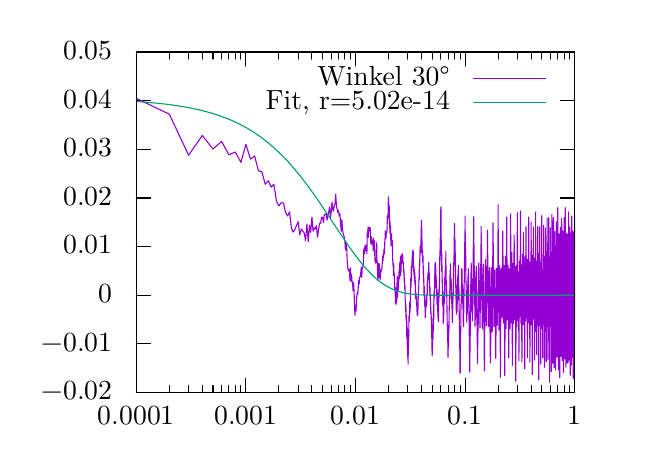
\begin{tikzpicture}[gnuplot]
%% generated with GNUPLOT 5.2p5a (Gentoo revision r0) (Lua 5.1; terminal rev. 99 , script rev. 107)
%% Sa 18 Mai 2019 18:31:00 CEST
\path (0.000,0.000) rectangle (7.500,5.250);
\gpcolor{color=gp lt color border}
\gpsetlinetype{gp lt border}
\gpsetdashtype{gp dt solid}
\gpsetlinewidth{1.00}
\draw[gp path] (1.380,0.616)--(1.560,0.616);
\draw[gp path] (6.947,0.616)--(6.767,0.616);
\node[gp node right] at (1.196,0.616) {$-0.02$};
\draw[gp path] (1.380,1.234)--(1.560,1.234);
\draw[gp path] (6.947,1.234)--(6.767,1.234);
\node[gp node right] at (1.196,1.234) {$-0.01$};
\draw[gp path] (1.380,1.852)--(1.560,1.852);
\draw[gp path] (6.947,1.852)--(6.767,1.852);
\node[gp node right] at (1.196,1.852) {$0$};
\draw[gp path] (1.380,2.470)--(1.560,2.470);
\draw[gp path] (6.947,2.470)--(6.767,2.470);
\node[gp node right] at (1.196,2.470) {$0.01$};
\draw[gp path] (1.380,3.087)--(1.560,3.087);
\draw[gp path] (6.947,3.087)--(6.767,3.087);
\node[gp node right] at (1.196,3.087) {$0.02$};
\draw[gp path] (1.380,3.705)--(1.560,3.705);
\draw[gp path] (6.947,3.705)--(6.767,3.705);
\node[gp node right] at (1.196,3.705) {$0.03$};
\draw[gp path] (1.380,4.323)--(1.560,4.323);
\draw[gp path] (6.947,4.323)--(6.767,4.323);
\node[gp node right] at (1.196,4.323) {$0.04$};
\draw[gp path] (1.380,4.941)--(1.560,4.941);
\draw[gp path] (6.947,4.941)--(6.767,4.941);
\node[gp node right] at (1.196,4.941) {$0.05$};
\draw[gp path] (1.380,0.616)--(1.380,0.796);
\draw[gp path] (1.380,4.941)--(1.380,4.761);
\node[gp node center] at (1.380,0.308) {$0.0001$};
\draw[gp path] (1.799,0.616)--(1.799,0.706);
\draw[gp path] (1.799,4.941)--(1.799,4.851);
\draw[gp path] (2.044,0.616)--(2.044,0.706);
\draw[gp path] (2.044,4.941)--(2.044,4.851);
\draw[gp path] (2.218,0.616)--(2.218,0.706);
\draw[gp path] (2.218,4.941)--(2.218,4.851);
\draw[gp path] (2.353,0.616)--(2.353,0.706);
\draw[gp path] (2.353,4.941)--(2.353,4.851);
\draw[gp path] (2.463,0.616)--(2.463,0.706);
\draw[gp path] (2.463,4.941)--(2.463,4.851);
\draw[gp path] (2.556,0.616)--(2.556,0.706);
\draw[gp path] (2.556,4.941)--(2.556,4.851);
\draw[gp path] (2.637,0.616)--(2.637,0.706);
\draw[gp path] (2.637,4.941)--(2.637,4.851);
\draw[gp path] (2.708,0.616)--(2.708,0.706);
\draw[gp path] (2.708,4.941)--(2.708,4.851);
\draw[gp path] (2.772,0.616)--(2.772,0.796);
\draw[gp path] (2.772,4.941)--(2.772,4.761);
\node[gp node center] at (2.772,0.308) {$0.001$};
\draw[gp path] (3.191,0.616)--(3.191,0.706);
\draw[gp path] (3.191,4.941)--(3.191,4.851);
\draw[gp path] (3.436,0.616)--(3.436,0.706);
\draw[gp path] (3.436,4.941)--(3.436,4.851);
\draw[gp path] (3.610,0.616)--(3.610,0.706);
\draw[gp path] (3.610,4.941)--(3.610,4.851);
\draw[gp path] (3.745,0.616)--(3.745,0.706);
\draw[gp path] (3.745,4.941)--(3.745,4.851);
\draw[gp path] (3.855,0.616)--(3.855,0.706);
\draw[gp path] (3.855,4.941)--(3.855,4.851);
\draw[gp path] (3.948,0.616)--(3.948,0.706);
\draw[gp path] (3.948,4.941)--(3.948,4.851);
\draw[gp path] (4.029,0.616)--(4.029,0.706);
\draw[gp path] (4.029,4.941)--(4.029,4.851);
\draw[gp path] (4.100,0.616)--(4.100,0.706);
\draw[gp path] (4.100,4.941)--(4.100,4.851);
\draw[gp path] (4.163,0.616)--(4.163,0.796);
\draw[gp path] (4.163,4.941)--(4.163,4.761);
\node[gp node center] at (4.163,0.308) {$0.01$};
\draw[gp path] (4.582,0.616)--(4.582,0.706);
\draw[gp path] (4.582,4.941)--(4.582,4.851);
\draw[gp path] (4.828,0.616)--(4.828,0.706);
\draw[gp path] (4.828,4.941)--(4.828,4.851);
\draw[gp path] (5.001,0.616)--(5.001,0.706);
\draw[gp path] (5.001,4.941)--(5.001,4.851);
\draw[gp path] (5.136,0.616)--(5.136,0.706);
\draw[gp path] (5.136,4.941)--(5.136,4.851);
\draw[gp path] (5.246,0.616)--(5.246,0.706);
\draw[gp path] (5.246,4.941)--(5.246,4.851);
\draw[gp path] (5.340,0.616)--(5.340,0.706);
\draw[gp path] (5.340,4.941)--(5.340,4.851);
\draw[gp path] (5.420,0.616)--(5.420,0.706);
\draw[gp path] (5.420,4.941)--(5.420,4.851);
\draw[gp path] (5.492,0.616)--(5.492,0.706);
\draw[gp path] (5.492,4.941)--(5.492,4.851);
\draw[gp path] (5.555,0.616)--(5.555,0.796);
\draw[gp path] (5.555,4.941)--(5.555,4.761);
\node[gp node center] at (5.555,0.308) {$0.1$};
\draw[gp path] (5.974,0.616)--(5.974,0.706);
\draw[gp path] (5.974,4.941)--(5.974,4.851);
\draw[gp path] (6.219,0.616)--(6.219,0.706);
\draw[gp path] (6.219,4.941)--(6.219,4.851);
\draw[gp path] (6.393,0.616)--(6.393,0.706);
\draw[gp path] (6.393,4.941)--(6.393,4.851);
\draw[gp path] (6.528,0.616)--(6.528,0.706);
\draw[gp path] (6.528,4.941)--(6.528,4.851);
\draw[gp path] (6.638,0.616)--(6.638,0.706);
\draw[gp path] (6.638,4.941)--(6.638,4.851);
\draw[gp path] (6.731,0.616)--(6.731,0.706);
\draw[gp path] (6.731,4.941)--(6.731,4.851);
\draw[gp path] (6.812,0.616)--(6.812,0.706);
\draw[gp path] (6.812,4.941)--(6.812,4.851);
\draw[gp path] (6.883,0.616)--(6.883,0.706);
\draw[gp path] (6.883,4.941)--(6.883,4.851);
\draw[gp path] (6.947,0.616)--(6.947,0.796);
\draw[gp path] (6.947,4.941)--(6.947,4.761);
\node[gp node center] at (6.947,0.308) {$1$};
\draw[gp path] (1.380,4.941)--(1.380,0.616)--(6.947,0.616)--(6.947,4.941)--cycle;
\node[gp node right] at (5.479,4.607) {Winkel 30°};
\gpcolor{rgb color={0.580,0.000,0.827}}
\draw[gp path] (5.663,4.607)--(6.579,4.607);
\draw[gp path] (1.380,4.352)--(1.799,4.151)--(2.044,3.630)--(2.218,3.881)--(2.353,3.709)%
  --(2.463,3.805)--(2.556,3.635)--(2.637,3.671)--(2.708,3.540)--(2.772,3.769)--(2.829,3.581)%
  --(2.882,3.621)--(2.930,3.435)--(2.975,3.417)--(3.017,3.261)--(3.056,3.306)--(3.092,3.225)%
  --(3.127,3.260)--(3.160,3.044)--(3.191,2.986)--(3.220,3.026)--(3.248,3.024)--(3.275,2.903)%
  --(3.301,2.858)--(3.326,2.912)--(3.349,2.706)--(3.372,2.654)--(3.394,2.688)--(3.415,2.741)%
  --(3.436,2.785)--(3.456,2.618)--(3.475,2.694)--(3.493,2.668)--(3.511,2.645)--(3.529,2.546)%
  --(3.546,2.756)--(3.563,2.533)--(3.579,2.740)--(3.594,2.650)--(3.610,2.843)--(3.625,2.665)%
  --(3.639,2.707)--(3.653,2.692)--(3.667,2.737)--(3.681,2.589)--(3.694,2.683)--(3.707,2.766)%
  --(3.720,2.765)--(3.732,2.842)--(3.745,2.843)--(3.757,2.774)--(3.768,2.881)--(3.780,2.879)%
  --(3.791,2.887)--(3.802,2.807)--(3.813,2.859)--(3.824,2.914)--(3.834,2.975)--(3.845,2.830)%
  --(3.855,2.921)--(3.865,3.033)--(3.875,2.941)--(3.884,2.921)--(3.894,2.996)--(3.903,3.008)%
  --(3.912,3.135)--(3.921,2.993)--(3.930,2.943)--(3.939,2.903)--(3.948,2.928)--(3.956,2.857)%
  --(3.965,2.888)--(3.973,2.777)--(3.982,2.665)--(3.990,2.813)--(3.998,2.698)--(4.006,2.633)%
  --(4.013,2.616)--(4.021,2.584)--(4.029,2.528)--(4.036,2.427)--(4.044,2.526)--(4.051,2.468)%
  --(4.058,2.289)--(4.065,2.198)--(4.072,2.171)--(4.079,2.160)--(4.086,2.183)--(4.093,2.039)%
  --(4.100,2.200)--(4.106,2.031)--(4.113,2.115)--(4.120,2.014)--(4.126,2.014)--(4.132,1.909)%
  --(4.139,2.015)--(4.145,1.903)--(4.151,1.713)--(4.157,1.598)--(4.164,1.710)--(4.170,1.652)%
  --(4.175,1.775)--(4.181,1.850)--(4.187,1.889)--(4.193,1.867)--(4.199,1.966)--(4.204,2.040)%
  --(4.210,1.993)--(4.216,2.075)--(4.221,2.088)--(4.227,2.092)--(4.232,2.158)--(4.237,2.206)%
  --(4.243,2.081)--(4.248,2.187)--(4.253,2.202)--(4.258,2.217)--(4.264,2.259)--(4.269,2.440)%
  --(4.274,2.376)--(4.279,2.441)--(4.284,2.483)--(4.289,2.424)--(4.294,2.440)--(4.298,2.408)%
  --(4.303,2.493)--(4.308,2.379)--(4.313,2.641)--(4.317,2.622)--(4.322,2.711)--(4.327,2.585)%
  --(4.331,2.717)--(4.336,2.691)--(4.340,2.671)--(4.345,2.713)--(4.349,2.707)--(4.354,2.650)%
  --(4.358,2.503)--(4.363,2.595)--(4.367,2.553)--(4.371,2.500)--(4.375,2.551)--(4.380,2.517)%
  --(4.384,2.527)--(4.388,2.417)--(4.392,2.578)--(4.396,2.517)--(4.400,2.498)--(4.405,2.542)%
  --(4.409,2.322)--(4.413,2.275)--(4.417,2.269)--(4.421,2.259)--(4.424,2.319)--(4.428,2.329)%
  --(4.432,2.519)--(4.436,2.274)--(4.440,2.274)--(4.444,2.152)--(4.448,2.036)--(4.451,2.180)%
  --(4.455,2.257)--(4.459,2.229)--(4.463,2.078)--(4.466,2.250)--(4.470,2.181)--(4.473,2.157)%
  --(4.477,2.053)--(4.481,2.087)--(4.484,2.172)--(4.488,2.148)--(4.491,2.182)--(4.495,2.184)%
  --(4.498,2.178)--(4.502,2.241)--(4.505,2.286)--(4.509,2.354)--(4.512,2.288)--(4.515,2.350)%
  --(4.519,2.331)--(4.522,2.375)--(4.525,2.440)--(4.529,2.421)--(4.532,2.379)--(4.535,2.523)%
  --(4.539,2.574)--(4.542,2.669)--(4.545,2.587)--(4.548,2.611)--(4.551,2.575)--(4.555,2.654)%
  --(4.558,2.655)--(4.561,2.643)--(4.564,2.695)--(4.567,2.860)--(4.570,2.767)--(4.573,2.840)%
  --(4.576,2.838)--(4.579,3.006)--(4.582,3.101)--(4.585,3.000)--(4.588,2.975)--(4.591,2.993)%
  --(4.594,2.807)--(4.597,2.843)--(4.600,2.639)--(4.603,2.775)--(4.606,2.676)--(4.609,2.718)%
  --(4.612,2.540)--(4.615,2.479)--(4.618,2.597)--(4.621,2.629)--(4.623,2.494)--(4.626,2.500)%
  --(4.629,2.499)--(4.632,2.547)--(4.635,2.320)--(4.637,2.280)--(4.640,2.233)--(4.643,2.232)%
  --(4.646,2.101)--(4.648,2.256)--(4.651,2.100)--(4.654,2.140)--(4.656,2.120)--(4.659,1.939)%
  --(4.662,1.937)--(4.664,1.966)--(4.667,1.848)--(4.670,1.944)--(4.672,1.740)--(4.675,1.944)%
  --(4.677,1.738)--(4.680,1.754)--(4.683,1.813)--(4.685,1.854)--(4.688,1.774)--(4.690,1.963)%
  --(4.693,2.091)--(4.695,1.951)--(4.698,1.827)--(4.700,2.013)--(4.703,1.905)--(4.705,1.996)%
  --(4.708,1.920)--(4.710,1.970)--(4.712,2.029)--(4.715,2.159)--(4.717,2.151)--(4.720,2.062)%
  --(4.722,2.248)--(4.725,2.095)--(4.727,2.122)--(4.729,2.279)--(4.732,2.138)--(4.734,2.342)%
  --(4.736,2.099)--(4.739,2.210)--(4.741,2.142)--(4.743,2.360)--(4.746,2.252)--(4.748,2.251)%
  --(4.750,2.345)--(4.753,2.343)--(4.755,2.350)--(4.757,2.378)--(4.759,2.345)--(4.762,2.264)%
  --(4.764,2.343)--(4.766,2.263)--(4.768,2.275)--(4.771,2.268)--(4.773,2.188)--(4.775,2.188)%
  --(4.777,2.137)--(4.779,2.159)--(4.781,2.038)--(4.784,2.083)--(4.786,2.020)--(4.788,1.937)%
  --(4.790,1.934)--(4.792,1.973)--(4.794,1.789)--(4.797,1.800)--(4.799,1.703)--(4.801,1.738)%
  --(4.803,1.573)--(4.805,1.689)--(4.807,1.544)--(4.809,1.519)--(4.811,1.552)--(4.813,1.601)%
  --(4.815,1.307)--(4.817,1.458)--(4.819,1.217)--(4.821,1.428)--(4.823,1.171)--(4.826,1.211)%
  --(4.828,1.030)--(4.830,1.192)--(4.832,0.977)--(4.834,1.375)--(4.836,1.206)--(4.838,1.415)%
  --(4.840,1.308)--(4.841,1.587)--(4.843,1.506)--(4.845,1.541)--(4.847,1.529)--(4.849,1.599)%
  --(4.851,1.572)--(4.853,1.765)--(4.855,1.639)--(4.857,1.636)--(4.859,1.750)--(4.861,1.929)%
  --(4.863,1.873)--(4.865,2.069)--(4.867,2.004)--(4.868,1.955)--(4.870,2.058)--(4.872,2.214)%
  --(4.874,2.035)--(4.876,2.220)--(4.878,2.199)--(4.880,2.288)--(4.881,2.281)--(4.883,2.342)%
  --(4.885,2.335)--(4.887,2.405)--(4.889,2.294)--(4.891,2.375)--(4.892,2.217)--(4.894,2.426)%
  --(4.896,2.215)--(4.898,2.400)--(4.900,2.163)--(4.901,2.261)--(4.903,2.167)--(4.905,2.149)%
  --(4.907,2.109)--(4.908,2.205)--(4.910,2.118)--(4.912,2.147)--(4.914,2.026)--(4.916,2.139)%
  --(4.917,1.986)--(4.919,2.097)--(4.921,1.976)--(4.922,2.041)--(4.924,1.938)--(4.926,1.808)%
  --(4.928,1.871)--(4.929,1.879)--(4.931,1.825)--(4.933,1.880)--(4.934,1.807)--(4.936,1.835)%
  --(4.938,1.761)--(4.939,1.824)--(4.941,1.729)--(4.943,1.692)--(4.944,1.644)--(4.946,1.669)%
  --(4.948,1.596)--(4.949,1.631)--(4.951,1.671)--(4.953,1.657)--(4.954,1.599)--(4.956,1.764)%
  --(4.958,1.677)--(4.959,1.790)--(4.961,1.846)--(4.962,1.956)--(4.964,1.908)--(4.966,1.964)%
  --(4.967,1.954)--(4.969,2.042)--(4.970,2.046)--(4.972,2.181)--(4.974,2.055)--(4.975,2.194)%
  --(4.977,2.227)--(4.978,2.315)--(4.980,2.235)--(4.981,2.417)--(4.983,2.347)--(4.985,2.477)%
  --(4.986,2.399)--(4.988,2.466)--(4.989,2.401)--(4.991,2.452)--(4.992,2.395)--(4.994,2.559)%
  --(4.995,2.463)--(4.997,2.715)--(4.998,2.662)--(5.000,2.682)--(5.001,2.804)--(5.003,2.714)%
  --(5.004,2.699)--(5.006,2.659)--(5.007,2.526)--(5.009,2.539)--(5.010,2.399)--(5.012,2.381)%
  --(5.013,2.346)--(5.015,2.431)--(5.016,2.275)--(5.018,2.365)--(5.019,2.261)--(5.021,2.346)%
  --(5.022,2.228)--(5.024,2.126)--(5.025,2.225)--(5.027,2.095)--(5.028,2.104)--(5.029,2.078)%
  --(5.031,2.001)--(5.032,2.031)--(5.034,1.851)--(5.035,1.926)--(5.037,1.955)--(5.038,1.960)%
  --(5.039,1.789)--(5.041,1.835)--(5.042,1.719)--(5.044,1.807)--(5.045,1.694)--(5.047,1.785)%
  --(5.048,1.566)--(5.049,1.632)--(5.051,1.569)--(5.052,1.584)--(5.054,1.688)--(5.055,1.706)%
  --(5.056,1.700)--(5.058,1.733)--(5.059,1.719)--(5.060,1.753)--(5.062,1.773)--(5.063,1.733)%
  --(5.064,1.851)--(5.066,1.793)--(5.067,1.707)--(5.069,1.832)--(5.070,1.838)--(5.071,1.870)%
  --(5.073,1.866)--(5.074,1.857)--(5.075,2.000)--(5.077,2.038)--(5.078,2.040)--(5.079,1.962)%
  --(5.081,2.089)--(5.082,2.079)--(5.083,2.066)--(5.085,2.139)--(5.086,2.103)--(5.087,2.068)%
  --(5.089,2.058)--(5.090,2.065)--(5.091,2.195)--(5.092,2.102)--(5.094,2.266)--(5.095,2.103)%
  --(5.096,2.165)--(5.098,2.126)--(5.099,2.159)--(5.100,2.044)--(5.101,2.052)--(5.103,2.008)%
  --(5.104,2.019)--(5.105,1.900)--(5.107,1.935)--(5.108,1.909)--(5.109,1.954)--(5.110,1.858)%
  --(5.112,1.881)--(5.113,1.834)--(5.114,1.723)--(5.115,1.828)--(5.117,1.737)--(5.118,1.721)%
  --(5.119,1.664)--(5.120,1.604)--(5.122,1.625)--(5.123,1.625)--(5.124,1.629)--(5.125,1.536)%
  --(5.127,1.584)--(5.128,1.457)--(5.129,1.472)--(5.130,1.314)--(5.131,1.406)--(5.133,1.342)%
  --(5.134,1.310)--(5.135,1.152)--(5.136,1.252)--(5.137,1.082)--(5.139,1.224)--(5.140,1.104)%
  --(5.141,1.308)--(5.142,1.202)--(5.144,1.474)--(5.145,1.404)--(5.146,1.447)--(5.147,1.393)%
  --(5.148,1.559)--(5.149,1.297)--(5.151,1.488)--(5.152,1.498)--(5.153,1.558)--(5.154,1.545)%
  --(5.155,1.741)--(5.157,1.550)--(5.158,1.776)--(5.159,1.680)--(5.160,1.876)--(5.161,1.784)%
  --(5.162,1.908)--(5.163,1.822)--(5.165,1.933)--(5.166,1.965)--(5.167,1.965)--(5.168,1.950)%
  --(5.169,2.114)--(5.170,2.027)--(5.172,2.058)--(5.173,2.253)--(5.174,2.178)--(5.175,2.221)%
  --(5.176,2.216)--(5.177,2.232)--(5.178,2.266)--(5.179,2.214)--(5.181,2.114)--(5.182,2.168)%
  --(5.183,2.206)--(5.184,2.034)--(5.185,2.109)--(5.186,1.940)--(5.187,1.986)--(5.188,2.035)%
  --(5.189,2.058)--(5.191,1.909)--(5.192,2.023)--(5.193,1.850)--(5.194,1.901)--(5.195,1.851)%
  --(5.196,1.932)--(5.197,1.764)--(5.198,1.823)--(5.199,1.732)--(5.200,1.917)--(5.202,1.781)%
  --(5.203,1.818)--(5.204,1.754)--(5.205,1.882)--(5.206,1.695)--(5.207,1.671)--(5.208,1.638)%
  --(5.209,1.653)--(5.210,1.582)--(5.211,1.616)--(5.212,1.589)--(5.213,1.614)--(5.214,1.533)%
  --(5.215,1.677)--(5.217,1.518)--(5.218,1.693)--(5.219,1.633)--(5.220,1.832)--(5.221,1.762)%
  --(5.222,1.870)--(5.223,1.851)--(5.224,1.926)--(5.225,1.816)--(5.226,1.885)--(5.227,1.891)%
  --(5.228,2.011)--(5.229,2.034)--(5.230,2.089)--(5.231,2.002)--(5.232,2.203)--(5.233,2.340)%
  --(5.234,2.334)--(5.235,2.237)--(5.236,2.420)--(5.237,2.353)--(5.238,2.458)--(5.239,2.432)%
  --(5.240,2.569)--(5.241,2.427)--(5.242,2.686)--(5.243,2.621)--(5.244,2.731)--(5.245,2.547)%
  --(5.246,2.940)--(5.247,2.690)--(5.249,2.972)--(5.250,2.557)--(5.251,2.709)--(5.252,2.483)%
  --(5.253,2.518)--(5.254,2.300)--(5.254,2.526)--(5.255,2.358)--(5.256,2.368)--(5.257,2.152)%
  --(5.258,2.381)--(5.259,2.257)--(5.260,2.190)--(5.261,2.239)--(5.262,2.196)--(5.263,2.109)%
  --(5.264,2.064)--(5.265,2.047)--(5.266,1.994)--(5.267,1.735)--(5.268,1.841)--(5.269,1.831)%
  --(5.270,1.758)--(5.271,1.829)--(5.272,1.817)--(5.273,1.740)--(5.274,1.700)--(5.275,1.790)%
  --(5.276,1.585)--(5.277,1.488)--(5.278,1.634)--(5.279,1.527)--(5.280,1.595)--(5.281,1.526)%
  --(5.282,1.719)--(5.283,1.523)--(5.284,1.723)--(5.285,1.640)--(5.286,1.851)--(5.286,1.711)%
  --(5.287,1.899)--(5.288,1.739)--(5.289,1.867)--(5.290,1.751)--(5.291,1.850)--(5.292,1.787)%
  --(5.293,1.897)--(5.294,1.823)--(5.295,1.936)--(5.296,1.883)--(5.297,2.063)--(5.298,2.046)%
  --(5.299,2.095)--(5.300,1.983)--(5.300,2.052)--(5.301,2.035)--(5.302,2.146)--(5.303,2.165)%
  --(5.304,2.135)--(5.305,2.140)--(5.306,2.141)--(5.307,2.195)--(5.308,2.229)--(5.309,2.323)%
  --(5.310,2.148)--(5.310,2.188)--(5.311,2.406)--(5.312,2.230)--(5.313,2.204)--(5.314,2.131)%
  --(5.315,2.031)--(5.316,2.040)--(5.317,1.982)--(5.318,1.920)--(5.319,1.989)--(5.319,1.900)%
  --(5.320,1.828)--(5.321,1.894)--(5.322,1.898)--(5.323,1.854)--(5.324,1.718)--(5.325,1.630)%
  --(5.326,1.668)--(5.327,1.653)--(5.327,1.717)--(5.328,1.453)--(5.329,1.496)--(5.330,1.437)%
  --(5.331,1.437)--(5.332,1.399)--(5.333,1.363)--(5.334,1.376)--(5.334,1.357)--(5.335,1.361)%
  --(5.336,1.174)--(5.337,1.251)--(5.338,1.072)--(5.339,1.063)--(5.340,1.133)--(5.341,1.210)%
  --(5.341,1.188)--(5.342,1.259)--(5.343,1.338)--(5.344,1.201)--(5.345,1.432)--(5.346,1.405)%
  --(5.347,1.361)--(5.347,1.474)--(5.348,1.408)--(5.349,1.379)--(5.350,1.526)--(5.351,1.433)%
  --(5.352,1.435)--(5.352,1.591)--(5.353,1.664)--(5.354,1.705)--(5.355,1.662)--(5.356,1.708)%
  --(5.357,1.832)--(5.358,1.798)--(5.358,1.811)--(5.359,1.816)--(5.360,1.907)--(5.361,1.806)%
  --(5.362,1.944)--(5.363,1.910)--(5.363,2.106)--(5.364,1.928)--(5.365,2.166)--(5.366,2.083)%
  --(5.367,2.152)--(5.368,2.049)--(5.368,2.252)--(5.369,2.089)--(5.370,2.158)--(5.371,2.210)%
  --(5.372,2.139)--(5.372,2.096)--(5.373,1.977)--(5.374,2.067)--(5.375,2.054)--(5.376,2.014)%
  --(5.377,2.070)--(5.377,1.992)--(5.378,1.978)--(5.379,1.932)--(5.380,2.026)--(5.381,1.955)%
  --(5.381,1.820)--(5.382,1.815)--(5.383,1.892)--(5.384,1.812)--(5.385,1.751)--(5.385,1.745)%
  --(5.386,1.765)--(5.387,1.848)--(5.388,1.685)--(5.389,1.754)--(5.389,1.857)--(5.390,1.816)%
  --(5.391,1.791)--(5.392,1.638)--(5.393,1.503)--(5.393,1.652)--(5.394,1.548)--(5.395,1.666)%
  --(5.396,1.581)--(5.396,1.668)--(5.397,1.660)--(5.398,1.732)--(5.399,1.726)--(5.400,1.691)%
  --(5.400,1.694)--(5.401,1.810)--(5.402,1.878)--(5.403,1.863)--(5.404,1.808)--(5.404,1.851)%
  --(5.405,1.957)--(5.406,2.034)--(5.407,2.053)--(5.407,2.130)--(5.408,1.984)--(5.409,2.005)%
  --(5.410,2.051)--(5.410,2.265)--(5.411,2.216)--(5.412,2.271)--(5.413,2.250)--(5.414,2.359)%
  --(5.414,2.245)--(5.415,2.319)--(5.416,2.488)--(5.417,2.295)--(5.417,2.463)--(5.418,2.596)%
  --(5.419,2.655)--(5.420,2.602)--(5.420,2.762)--(5.421,2.726)--(5.422,2.633)--(5.423,2.580)%
  --(5.423,2.579)--(5.424,2.571)--(5.425,2.516)--(5.426,2.507)--(5.426,2.359)--(5.427,2.557)%
  --(5.428,2.242)--(5.429,2.376)--(5.429,2.382)--(5.430,2.336)--(5.431,2.275)--(5.432,2.391)%
  --(5.432,2.228)--(5.433,2.238)--(5.434,2.063)--(5.435,2.110)--(5.435,1.951)--(5.436,2.039)%
  --(5.437,2.045)--(5.438,1.954)--(5.438,1.843)--(5.439,1.879)--(5.440,1.856)--(5.440,1.814)%
  --(5.441,1.767)--(5.442,1.664)--(5.443,1.654)--(5.443,1.690)--(5.444,1.627)--(5.445,1.830)%
  --(5.446,1.646)--(5.446,1.619)--(5.447,1.650)--(5.448,1.638)--(5.448,1.611)--(5.449,1.682)%
  --(5.450,1.692)--(5.451,1.775)--(5.451,1.737)--(5.452,1.844)--(5.453,1.642)--(5.453,1.856)%
  --(5.454,1.818)--(5.455,1.974)--(5.456,1.738)--(5.456,1.926)--(5.457,1.909)--(5.458,1.994)%
  --(5.458,1.773)--(5.459,1.960)--(5.460,1.951)--(5.461,2.091)--(5.461,1.883)--(5.462,1.997)%
  --(5.463,1.986)--(5.463,1.955)--(5.464,1.938)--(5.465,2.111)--(5.465,2.044)--(5.466,2.102)%
  --(5.467,1.986)--(5.468,2.178)--(5.468,2.093)--(5.469,2.175)--(5.470,2.114)--(5.470,2.232)%
  --(5.471,2.072)--(5.472,2.233)--(5.472,2.019)--(5.473,1.937)--(5.474,1.926)--(5.475,1.966)%
  --(5.475,1.917)--(5.476,1.918)--(5.477,1.792)--(5.477,1.940)--(5.478,1.823)--(5.479,1.776)%
  --(5.479,1.772)--(5.480,1.674)--(5.481,1.602)--(5.481,1.651)--(5.482,1.467)--(5.483,1.526)%
  --(5.483,1.415)--(5.484,1.407)--(5.485,1.399)--(5.485,1.352)--(5.486,1.251)--(5.487,1.315)%
  --(5.488,1.159)--(5.488,1.291)--(5.489,1.041)--(5.490,1.255)--(5.490,0.870)--(5.491,1.143)%
  --(5.492,0.904)--(5.492,0.961)--(5.493,0.862)--(5.494,0.988)--(5.494,1.044)--(5.495,1.228)%
  --(5.496,1.187)--(5.496,1.334)--(5.497,1.304)--(5.498,1.395)--(5.498,1.316)--(5.499,1.387)%
  --(5.500,1.410)--(5.501,1.481)--(5.502,1.635)--(5.502,1.661)--(5.503,1.685)--(5.504,1.749)%
  --(5.504,1.754)--(5.505,1.774)--(5.506,1.813)--(5.506,1.794)--(5.507,1.754)--(5.507,1.823)%
  --(5.508,1.933)--(5.509,1.901)--(5.509,1.993)--(5.510,1.982)--(5.511,2.014)--(5.511,2.124)%
  --(5.512,2.076)--(5.513,2.073)--(5.513,2.190)--(5.514,2.064)--(5.515,2.095)--(5.515,2.035)%
  --(5.516,2.183)--(5.517,2.008)--(5.517,2.073)--(5.518,1.876)--(5.518,2.019)--(5.519,1.830)%
  --(5.520,1.913)--(5.520,1.799)--(5.521,1.994)--(5.522,1.878)--(5.522,1.910)--(5.523,1.789)%
  --(5.524,1.861)--(5.524,1.859)--(5.525,1.820)--(5.526,1.738)--(5.526,1.838)--(5.527,1.675)%
  --(5.527,1.732)--(5.528,1.678)--(5.529,1.828)--(5.529,1.671)--(5.530,1.729)--(5.531,1.567)%
  --(5.531,1.700)--(5.532,1.572)--(5.532,1.507)--(5.533,1.601)--(5.534,1.516)--(5.534,1.482)%
  --(5.535,1.453)--(5.536,1.513)--(5.536,1.574)--(5.537,1.477)--(5.537,1.616)--(5.538,1.642)%
  --(5.539,1.779)--(5.539,1.725)--(5.540,1.863)--(5.541,1.931)--(5.541,1.900)--(5.542,1.979)%
  --(5.542,1.860)--(5.543,1.958)--(5.544,2.036)--(5.544,2.020)--(5.545,2.036)--(5.546,2.137)%
  --(5.546,2.088)--(5.547,2.248)--(5.547,2.288)--(5.548,2.220)--(5.549,2.461)--(5.549,2.316)%
  --(5.550,2.526)--(5.550,2.485)--(5.551,2.456)--(5.552,2.427)--(5.552,2.531)--(5.553,2.488)%
  --(5.553,2.598)--(5.554,2.486)--(5.555,2.795)--(5.555,2.858)--(5.556,2.718)--(5.556,2.678)%
  --(5.557,2.611)--(5.558,2.555)--(5.558,2.521)--(5.559,2.375)--(5.559,2.373)--(5.560,2.325)%
  --(5.561,2.359)--(5.561,2.455)--(5.562,2.228)--(5.562,2.302)--(5.563,2.266)--(5.564,2.356)%
  --(5.564,2.164)--(5.565,2.111)--(5.565,2.074)--(5.566,1.998)--(5.567,2.037)--(5.567,1.994)%
  --(5.568,2.018)--(5.568,1.844)--(5.569,1.878)--(5.570,1.887)--(5.570,1.877)--(5.571,1.741)%
  --(5.571,1.893)--(5.572,1.825)--(5.573,1.682)--(5.573,1.613)--(5.574,1.615)--(5.574,1.553)%
  --(5.575,1.587)--(5.575,1.532)--(5.576,1.611)--(5.577,1.599)--(5.577,1.523)--(5.578,1.507)%
  --(5.578,1.600)--(5.579,1.608)--(5.580,1.657)--(5.580,1.616)--(5.581,1.697)--(5.581,1.796)%
  --(5.582,1.619)--(5.582,1.755)--(5.583,1.772)--(5.584,1.805)--(5.584,1.773)--(5.585,1.845)%
  --(5.585,1.824)--(5.586,1.891)--(5.586,1.873)--(5.587,1.983)--(5.588,1.837)--(5.588,1.989)%
  --(5.589,1.914)--(5.589,1.959)--(5.590,1.978)--(5.590,2.079)--(5.591,1.995)--(5.592,2.073)%
  --(5.592,1.914)--(5.593,1.999)--(5.593,2.099)--(5.594,2.115)--(5.594,1.985)--(5.595,2.113)%
  --(5.596,1.987)--(5.596,2.190)--(5.597,1.959)--(5.597,2.090)--(5.598,1.956)--(5.598,1.887)%
  --(5.599,1.831)--(5.600,1.938)--(5.600,1.765)--(5.601,1.875)--(5.601,1.750)--(5.602,1.790)%
  --(5.602,1.704)--(5.603,1.719)--(5.603,1.711)--(5.604,1.655)--(5.605,1.553)--(5.605,1.587)%
  --(5.606,1.489)--(5.606,1.474)--(5.607,1.451)--(5.607,1.503)--(5.608,1.349)--(5.608,1.334)%
  --(5.609,1.379)--(5.610,1.418)--(5.610,1.314)--(5.611,1.300)--(5.611,1.132)--(5.612,1.226)%
  --(5.612,1.003)--(5.613,1.118)--(5.613,0.985)--(5.614,0.877)--(5.615,0.991)--(5.615,1.117)%
  --(5.616,0.967)--(5.616,1.186)--(5.617,1.121)--(5.617,1.349)--(5.618,1.219)--(5.618,1.412)%
  --(5.619,1.269)--(5.619,1.433)--(5.620,1.333)--(5.621,1.461)--(5.621,1.397)--(5.622,1.451)%
  --(5.622,1.511)--(5.623,1.707)--(5.623,1.619)--(5.624,1.734)--(5.624,1.611)--(5.625,1.874)%
  --(5.625,1.906)--(5.626,1.827)--(5.626,1.852)--(5.627,1.953)--(5.628,2.008)--(5.628,1.974)%
  --(5.629,2.028)--(5.629,2.116)--(5.630,2.050)--(5.630,2.135)--(5.631,2.119)--(5.631,2.120)%
  --(5.632,2.261)--(5.632,2.083)--(5.633,2.240)--(5.633,2.223)--(5.634,2.033)--(5.634,2.109)%
  --(5.635,1.863)--(5.636,2.025)--(5.636,1.980)--(5.637,2.011)--(5.637,1.941)--(5.638,2.026)%
  --(5.638,1.965)--(5.639,2.062)--(5.639,1.802)--(5.640,1.829)--(5.640,1.783)--(5.641,1.769)%
  --(5.641,1.649)--(5.642,1.931)--(5.642,1.840)--(5.643,1.850)--(5.643,1.873)--(5.644,1.882)%
  --(5.644,1.793)--(5.645,1.878)--(5.645,1.698)--(5.646,1.741)--(5.647,1.602)--(5.647,1.527)%
  --(5.648,1.531)--(5.648,1.689)--(5.649,1.604)--(5.649,1.727)--(5.650,1.626)--(5.650,1.621)%
  --(5.651,1.673)--(5.651,1.708)--(5.652,1.660)--(5.652,1.705)--(5.653,1.828)--(5.653,1.809)%
  --(5.654,1.875)--(5.654,1.840)--(5.655,1.909)--(5.655,1.960)--(5.656,1.901)--(5.656,2.008)%
  --(5.657,2.015)--(5.657,2.096)--(5.658,2.136)--(5.658,2.282)--(5.659,2.182)--(5.659,2.445)%
  --(5.660,2.235)--(5.660,2.422)--(5.661,2.204)--(5.661,2.493)--(5.662,2.282)--(5.662,2.567)%
  --(5.663,2.526)--(5.663,2.694)--(5.664,2.523)--(5.664,2.613)--(5.665,2.576)--(5.665,2.848)%
  --(5.666,2.656)--(5.666,2.750)--(5.667,2.496)--(5.667,2.630)--(5.668,2.397)--(5.668,2.417)%
  --(5.669,2.374)--(5.669,2.326)--(5.670,2.386)--(5.670,2.300)--(5.671,2.207)--(5.671,2.234)%
  --(5.672,2.134)--(5.672,2.179)--(5.673,1.980)--(5.673,2.125)--(5.674,2.019)--(5.674,2.071)%
  --(5.675,1.996)--(5.675,1.744)--(5.676,1.948)--(5.676,1.872)--(5.677,1.824)--(5.677,1.852)%
  --(5.678,1.727)--(5.678,1.740)--(5.679,1.684)--(5.679,1.718)--(5.680,1.579)--(5.680,1.638)%
  --(5.681,1.456)--(5.681,1.622)--(5.682,1.594)--(5.682,1.556)--(5.683,1.476)--(5.683,1.666)%
  --(5.684,1.539)--(5.684,1.751)--(5.685,1.641)--(5.685,1.713)--(5.686,1.693)--(5.686,1.889)%
  --(5.687,1.680)--(5.687,1.766)--(5.688,1.573)--(5.688,1.770)--(5.689,1.640)--(5.689,1.743)%
  --(5.690,1.858)--(5.690,1.911)--(5.691,1.786)--(5.691,1.860)--(5.692,1.779)--(5.692,1.824)%
  --(5.693,1.802)--(5.693,1.972)--(5.693,1.989)--(5.694,2.145)--(5.694,1.883)--(5.695,2.082)%
  --(5.695,2.027)--(5.696,1.986)--(5.696,2.064)--(5.697,2.107)--(5.697,2.176)--(5.698,2.125)%
  --(5.698,2.147)--(5.699,2.218)--(5.699,2.142)--(5.700,2.120)--(5.700,2.008)--(5.701,1.979)%
  --(5.701,1.885)--(5.702,1.882)--(5.702,1.953)--(5.703,1.864)--(5.703,1.841)--(5.704,1.712)%
  --(5.704,1.709)--(5.704,1.597)--(5.705,1.674)--(5.705,1.681)--(5.706,1.662)--(5.706,1.555)%
  --(5.707,1.474)--(5.707,1.618)--(5.708,1.414)--(5.708,1.448)--(5.709,1.226)--(5.709,1.324)%
  --(5.710,1.283)--(5.710,1.233)--(5.711,1.337)--(5.711,1.267)--(5.712,1.250)--(5.712,1.270)%
  --(5.712,1.161)--(5.713,1.125)--(5.713,1.037)--(5.714,1.040)--(5.714,1.094)--(5.715,0.987)%
  --(5.715,1.231)--(5.716,1.208)--(5.716,1.211)--(5.717,1.229)--(5.717,1.280)--(5.718,1.330)%
  --(5.718,1.340)--(5.718,1.410)--(5.719,1.377)--(5.719,1.393)--(5.720,1.482)--(5.720,1.412)%
  --(5.721,1.521)--(5.721,1.427)--(5.722,1.524)--(5.722,1.655)--(5.723,1.680)--(5.723,1.732)%
  --(5.724,1.773)--(5.724,1.884)--(5.724,1.827)--(5.725,1.836)--(5.725,1.786)--(5.726,1.953)%
  --(5.726,1.945)--(5.727,1.949)--(5.727,1.980)--(5.728,2.179)--(5.728,2.108)--(5.729,2.118)%
  --(5.729,2.258)--(5.729,2.138)--(5.730,2.161)--(5.730,2.220)--(5.731,2.032)--(5.731,2.119)%
  --(5.732,2.086)--(5.732,2.200)--(5.733,1.954)--(5.733,2.087)--(5.733,2.196)--(5.734,1.972)%
  --(5.734,2.088)--(5.735,1.876)--(5.735,2.043)--(5.736,1.942)--(5.736,1.893)--(5.737,1.813)%
  --(5.737,1.816)--(5.738,1.867)--(5.738,1.779)--(5.738,1.752)--(5.739,1.795)--(5.739,1.650)%
  --(5.740,1.774)--(5.740,1.673)--(5.741,1.774)--(5.741,1.702)--(5.742,1.708)--(5.742,1.670)%
  --(5.742,1.652)--(5.743,1.568)--(5.743,1.514)--(5.744,1.439)--(5.744,1.613)--(5.745,1.538)%
  --(5.745,1.618)--(5.746,1.548)--(5.746,1.675)--(5.746,1.590)--(5.747,1.631)--(5.747,1.781)%
  --(5.748,1.763)--(5.748,1.733)--(5.749,1.881)--(5.749,1.837)--(5.749,1.771)--(5.750,1.851)%
  --(5.750,1.771)--(5.751,1.975)--(5.751,1.965)--(5.752,1.994)--(5.752,1.992)--(5.753,2.162)%
  --(5.753,2.124)--(5.753,2.083)--(5.754,2.221)--(5.754,2.193)--(5.755,2.273)--(5.755,2.196)%
  --(5.756,2.328)--(5.756,2.303)--(5.756,2.377)--(5.757,2.399)--(5.757,2.498)--(5.758,2.463)%
  --(5.758,2.657)--(5.759,2.533)--(5.759,2.728)--(5.759,2.633)--(5.760,2.636)--(5.760,2.581)%
  --(5.761,2.564)--(5.761,2.481)--(5.762,2.487)--(5.762,2.336)--(5.762,2.488)--(5.763,2.246)%
  --(5.763,2.459)--(5.764,2.247)--(5.764,2.325)--(5.765,2.302)--(5.765,2.232)--(5.765,2.103)%
  --(5.766,2.122)--(5.766,2.040)--(5.767,2.035)--(5.767,1.941)--(5.768,1.985)--(5.768,1.800)%
  --(5.768,1.876)--(5.769,1.718)--(5.769,1.906)--(5.770,1.674)--(5.770,1.681)--(5.771,1.764)%
  --(5.771,1.487)--(5.771,1.557)--(5.772,1.527)--(5.772,1.433)--(5.773,1.516)--(5.773,1.502)%
  --(5.774,1.572)--(5.774,1.430)--(5.774,1.581)--(5.775,1.536)--(5.775,1.699)--(5.776,1.507)%
  --(5.776,1.712)--(5.776,1.507)--(5.777,1.766)--(5.777,1.743)--(5.778,1.841)--(5.778,1.691)%
  --(5.779,1.805)--(5.779,1.711)--(5.779,1.826)--(5.780,1.717)--(5.780,1.921)--(5.781,1.847)%
  --(5.781,1.900)--(5.781,1.904)--(5.782,2.042)--(5.782,1.977)--(5.783,2.005)--(5.783,1.900)%
  --(5.784,1.961)--(5.784,1.902)--(5.784,1.979)--(5.785,1.952)--(5.785,2.117)--(5.786,2.062)%
  --(5.786,2.158)--(5.786,2.188)--(5.787,2.232)--(5.787,2.119)--(5.788,2.137)--(5.788,2.247)%
  --(5.789,2.054)--(5.789,2.139)--(5.789,2.057)--(5.790,2.058)--(5.790,1.950)--(5.791,1.918)%
  --(5.791,1.980)--(5.791,1.889)--(5.792,1.809)--(5.792,1.776)--(5.793,1.795)--(5.793,1.708)%
  --(5.793,1.624)--(5.794,1.673)--(5.794,1.682)--(5.795,1.526)--(5.795,1.462)--(5.795,1.418)%
  --(5.796,1.396)--(5.796,1.360)--(5.797,1.552)--(5.797,1.292)--(5.797,1.372)--(5.798,1.232)%
  --(5.798,1.331)--(5.799,1.019)--(5.799,1.242)--(5.800,1.078)--(5.800,1.188)--(5.800,1.012)%
  --(5.801,1.169)--(5.801,0.890)--(5.802,1.071)--(5.802,1.147)--(5.802,1.314)--(5.803,1.280)%
  --(5.803,1.476)--(5.804,1.160)--(5.804,1.478)--(5.804,1.417)--(5.805,1.476)--(5.805,1.511)%
  --(5.806,1.521)--(5.806,1.649)--(5.806,1.561)--(5.807,1.718)--(5.807,1.743)--(5.808,1.706)%
  --(5.808,1.836)--(5.808,1.717)--(5.809,1.848)--(5.809,1.956)--(5.810,1.800)--(5.810,1.806)%
  --(5.810,1.910)--(5.811,1.912)--(5.811,2.011)--(5.812,2.029)--(5.812,2.040)--(5.812,2.008)%
  --(5.813,2.193)--(5.813,2.016)--(5.813,2.304)--(5.814,2.058)--(5.814,2.199)--(5.815,1.948)%
  --(5.815,2.230)--(5.815,2.058)--(5.816,2.009)--(5.816,1.964)--(5.817,2.054)--(5.817,1.911)%
  --(5.817,1.907)--(5.818,1.854)--(5.818,1.939)--(5.819,1.834)--(5.819,1.953)--(5.819,1.907)%
  --(5.820,1.852)--(5.820,1.818)--(5.821,1.780)--(5.821,1.814)--(5.821,1.686)--(5.822,1.662)%
  --(5.822,1.717)--(5.822,1.621)--(5.823,1.730)--(5.823,1.570)--(5.824,1.654)--(5.824,1.623)%
  --(5.824,1.521)--(5.825,1.604)--(5.825,1.648)--(5.826,1.465)--(5.826,1.529)--(5.826,1.468)%
  --(5.827,1.494)--(5.827,1.540)--(5.828,1.534)--(5.828,1.596)--(5.828,1.584)--(5.829,1.593)%
  --(5.829,1.815)--(5.829,1.782)--(5.830,1.755)--(5.830,1.814)--(5.831,1.832)--(5.831,1.879)%
  --(5.831,1.880)--(5.832,2.039)--(5.832,1.871)--(5.832,2.042)--(5.833,2.110)--(5.833,2.059)%
  --(5.834,2.198)--(5.834,2.125)--(5.834,2.225)--(5.835,2.110)--(5.835,2.297)--(5.836,2.149)%
  --(5.836,2.372)--(5.836,2.223)--(5.837,2.308)--(5.837,2.350)--(5.837,2.351)--(5.838,2.428)%
  --(5.838,2.430)--(5.839,2.362)--(5.839,2.478)--(5.839,2.544)--(5.840,2.679)--(5.840,2.459)%
  --(5.840,2.558)--(5.841,2.395)--(5.841,2.290)--(5.842,2.242)--(5.842,2.263)--(5.842,2.298)%
  --(5.843,2.364)--(5.843,2.157)--(5.843,2.258)--(5.844,2.283)--(5.844,2.304)--(5.845,2.259)%
  --(5.845,2.217)--(5.845,2.119)--(5.846,2.157)--(5.846,1.894)--(5.846,2.006)--(5.847,1.890)%
  --(5.847,1.847)--(5.848,1.839)--(5.848,1.854)--(5.848,1.897)--(5.849,1.863)--(5.849,1.753)%
  --(5.849,1.820)--(5.850,1.679)--(5.850,1.653)--(5.851,1.682)--(5.851,1.558)--(5.851,1.539)%
  --(5.852,1.455)--(5.852,1.600)--(5.852,1.474)--(5.853,1.559)--(5.853,1.569)--(5.854,1.706)%
  --(5.854,1.544)--(5.854,1.774)--(5.855,1.584)--(5.855,1.801)--(5.855,1.724)--(5.856,1.611)%
  --(5.856,1.719)--(5.856,1.799)--(5.857,1.788)--(5.857,1.743)--(5.858,1.713)--(5.858,1.833)%
  --(5.858,1.948)--(5.859,1.868)--(5.859,1.830)--(5.859,2.073)--(5.860,2.024)--(5.860,1.885)%
  --(5.860,1.922)--(5.861,1.966)--(5.861,1.964)--(5.862,2.080)--(5.862,1.985)--(5.862,2.112)%
  --(5.863,1.964)--(5.863,2.168)--(5.863,2.075)--(5.864,2.167)--(5.864,2.136)--(5.864,2.204)%
  --(5.865,1.985)--(5.865,2.126)--(5.866,2.076)--(5.866,2.111)--(5.866,1.993)--(5.867,1.920)%
  --(5.867,1.874)--(5.867,1.936)--(5.868,1.802)--(5.868,1.847)--(5.868,1.776)--(5.869,1.852)%
  --(5.869,1.708)--(5.870,1.791)--(5.870,1.752)--(5.870,1.698)--(5.871,1.627)--(5.871,1.587)%
  --(5.871,1.441)--(5.872,1.387)--(5.872,1.384)--(5.872,1.440)--(5.873,1.453)--(5.873,1.408)%
  --(5.873,1.358)--(5.874,1.319)--(5.874,1.227)--(5.875,1.319)--(5.875,1.073)--(5.875,1.115)%
  --(5.876,1.020)--(5.876,0.991)--(5.876,1.000)--(5.877,1.052)--(5.877,1.035)--(5.877,1.135)%
  --(5.878,1.043)--(5.878,1.306)--(5.878,1.080)--(5.879,1.303)--(5.879,1.093)--(5.880,1.392)%
  --(5.880,1.192)--(5.880,1.509)--(5.881,1.254)--(5.881,1.403)--(5.881,1.355)--(5.882,1.632)%
  --(5.882,1.488)--(5.882,1.700)--(5.883,1.724)--(5.883,1.613)--(5.883,1.764)--(5.884,1.768)%
  --(5.884,1.852)--(5.884,1.961)--(5.885,1.965)--(5.885,1.936)--(5.886,1.896)--(5.886,2.012)%
  --(5.886,2.032)--(5.887,2.049)--(5.887,2.043)--(5.887,2.203)--(5.888,1.970)--(5.888,2.120)%
  --(5.888,2.141)--(5.889,2.118)--(5.889,2.128)--(5.889,2.155)--(5.890,1.997)--(5.890,2.100)%
  --(5.890,1.927)--(5.891,2.014)--(5.891,1.830)--(5.891,1.975)--(5.892,1.901)--(5.892,2.021)%
  --(5.892,1.839)--(5.893,1.940)--(5.893,1.858)--(5.893,1.897)--(5.894,1.717)--(5.894,1.777)%
  --(5.895,1.730)--(5.895,1.710)--(5.895,1.630)--(5.896,1.723)--(5.896,1.645)--(5.896,1.704)%
  --(5.897,1.670)--(5.897,1.599)--(5.897,1.518)--(5.898,1.648)--(5.898,1.485)--(5.898,1.576)%
  --(5.899,1.523)--(5.899,1.588)--(5.899,1.383)--(5.900,1.423)--(5.900,1.431)--(5.900,1.593)%
  --(5.901,1.561)--(5.901,1.579)--(5.901,1.607)--(5.902,1.689)--(5.902,1.545)--(5.902,1.662)%
  --(5.903,1.738)--(5.903,1.695)--(5.903,1.843)--(5.904,1.829)--(5.904,1.872)--(5.904,1.960)%
  --(5.905,1.882)--(5.905,2.056)--(5.905,2.229)--(5.906,2.185)--(5.906,2.216)--(5.906,2.350)%
  --(5.907,2.295)--(5.907,2.285)--(5.907,2.242)--(5.908,2.325)--(5.908,2.277)--(5.909,2.583)%
  --(5.909,2.426)--(5.909,2.684)--(5.910,2.327)--(5.910,2.771)--(5.910,2.559)--(5.911,2.733)%
  --(5.911,2.612)--(5.911,2.758)--(5.912,2.639)--(5.912,2.621)--(5.912,2.516)--(5.913,2.461)%
  --(5.913,2.364)--(5.913,2.272)--(5.914,2.170)--(5.914,2.253)--(5.914,2.281)--(5.915,2.283)%
  --(5.915,2.208)--(5.915,2.218)--(5.916,2.200)--(5.916,2.075)--(5.916,1.959)--(5.917,2.081)%
  --(5.917,1.962)--(5.917,1.973)--(5.918,1.887)--(5.918,1.872)--(5.918,1.918)--(5.919,1.928)%
  --(5.919,1.764)--(5.919,1.816)--(5.920,1.790)--(5.920,1.810)--(5.920,1.594)--(5.921,1.641)%
  --(5.921,1.630)--(5.921,1.670)--(5.922,1.454)--(5.922,1.612)--(5.922,1.505)--(5.922,1.714)%
  --(5.923,1.677)--(5.923,1.598)--(5.923,1.658)--(5.924,1.707)--(5.924,1.809)--(5.924,1.868)%
  --(5.925,1.716)--(5.925,1.816)--(5.925,1.754)--(5.926,1.776)--(5.926,1.794)--(5.926,1.775)%
  --(5.927,1.889)--(5.927,1.849)--(5.927,1.860)--(5.928,1.847)--(5.928,1.917)--(5.928,1.909)%
  --(5.929,1.909)--(5.929,1.965)--(5.929,1.992)--(5.930,2.065)--(5.930,1.971)--(5.930,1.948)%
  --(5.931,2.072)--(5.931,2.056)--(5.931,2.086)--(5.932,2.074)--(5.932,2.079)--(5.932,2.052)%
  --(5.933,2.018)--(5.933,2.171)--(5.933,2.078)--(5.934,2.073)--(5.934,1.909)--(5.934,1.923)%
  --(5.935,1.798)--(5.935,1.828)--(5.935,1.919)--(5.936,1.852)--(5.936,1.719)--(5.936,1.712)%
  --(5.936,1.628)--(5.937,1.588)--(5.937,1.675)--(5.937,1.681)--(5.938,1.705)--(5.938,1.577)%
  --(5.938,1.541)--(5.939,1.505)--(5.939,1.368)--(5.939,1.432)--(5.940,1.368)--(5.940,1.293)%
  --(5.940,1.322)--(5.941,1.274)--(5.941,1.252)--(5.941,1.427)--(5.942,1.160)--(5.942,1.150)%
  --(5.942,1.234)--(5.943,1.086)--(5.943,1.104)--(5.943,1.065)--(5.944,1.052)--(5.944,1.153)%
  --(5.944,1.106)--(5.944,1.226)--(5.945,1.125)--(5.945,1.191)--(5.945,1.364)--(5.946,1.341)%
  --(5.946,1.311)--(5.946,1.328)--(5.947,1.376)--(5.947,1.459)--(5.947,1.448)--(5.948,1.344)%
  --(5.948,1.404)--(5.948,1.355)--(5.949,1.598)--(5.949,1.632)--(5.949,1.586)--(5.950,1.595)%
  --(5.950,1.738)--(5.950,1.783)--(5.950,1.798)--(5.951,1.665)--(5.951,1.756)--(5.951,1.945)%
  --(5.952,1.929)--(5.952,1.926)--(5.952,1.857)--(5.953,2.056)--(5.953,2.025)--(5.953,2.135)%
  --(5.954,1.977)--(5.954,1.951)--(5.954,2.195)--(5.955,2.121)--(5.955,2.087)--(5.955,2.148)%
  --(5.955,2.047)--(5.956,1.864)--(5.956,1.970)--(5.956,2.061)--(5.957,1.893)--(5.957,1.942)%
  --(5.957,2.026)--(5.958,1.935)--(5.958,1.928)--(5.958,1.796)--(5.959,1.986)--(5.959,1.821)%
  --(5.959,1.881)--(5.960,1.849)--(5.960,1.746)--(5.960,1.714)--(5.960,1.776)--(5.961,1.624)%
  --(5.961,1.641)--(5.961,1.618)--(5.962,1.721)--(5.962,1.730)--(5.962,1.756)--(5.963,1.666)%
  --(5.963,1.644)--(5.963,1.528)--(5.964,1.707)--(5.964,1.469)--(5.964,1.677)--(5.964,1.535)%
  --(5.965,1.753)--(5.965,1.505)--(5.965,1.700)--(5.966,1.566)--(5.966,1.745)--(5.966,1.630)%
  --(5.967,1.674)--(5.967,1.731)--(5.967,1.728)--(5.968,1.809)--(5.968,1.830)--(5.968,1.851)%
  --(5.968,1.973)--(5.969,1.952)--(5.969,2.146)--(5.969,1.973)--(5.970,2.048)--(5.970,2.113)%
  --(5.970,2.031)--(5.971,2.254)--(5.971,2.289)--(5.971,2.281)--(5.971,2.169)--(5.972,2.214)%
  --(5.972,2.384)--(5.972,2.258)--(5.973,2.438)--(5.973,2.543)--(5.973,2.534)--(5.974,2.720)%
  --(5.974,2.768)--(5.974,2.704)--(5.975,3.000)--(5.975,2.722)--(5.975,2.691)--(5.975,2.569)%
  --(5.976,2.693)--(5.976,2.447)--(5.976,2.690)--(5.977,2.384)--(5.977,2.523)--(5.977,2.315)%
  --(5.978,2.533)--(5.978,2.337)--(5.978,2.489)--(5.978,2.285)--(5.979,2.180)--(5.979,2.142)%
  --(5.979,2.229)--(5.980,2.030)--(5.980,2.084)--(5.980,1.956)--(5.981,1.976)--(5.981,1.830)%
  --(5.981,1.808)--(5.981,1.738)--(5.982,1.823)--(5.982,1.700)--(5.982,1.764)--(5.983,1.637)%
  --(5.983,1.665)--(5.983,1.684)--(5.984,1.653)--(5.984,1.472)--(5.984,1.426)--(5.984,1.521)%
  --(5.985,1.411)--(5.985,1.501)--(5.985,1.551)--(5.986,1.559)--(5.986,1.626)--(5.986,1.490)%
  --(5.986,1.676)--(5.987,1.714)--(5.987,1.711)--(5.987,1.627)--(5.988,1.715)--(5.988,1.692)%
  --(5.988,1.821)--(5.989,1.641)--(5.989,1.710)--(5.989,1.822)--(5.989,1.810)--(5.990,1.741)%
  --(5.990,1.889)--(5.990,1.837)--(5.991,2.021)--(5.991,1.801)--(5.991,2.016)--(5.991,1.902)%
  --(5.992,2.036)--(5.992,1.756)--(5.992,1.951)--(5.993,1.954)--(5.993,2.166)--(5.993,2.102)%
  --(5.994,2.227)--(5.994,2.096)--(5.994,2.122)--(5.994,2.053)--(5.995,2.139)--(5.995,2.170)%
  --(5.995,2.093)--(5.996,2.020)--(5.996,2.086)--(5.996,2.015)--(5.996,1.973)--(5.997,1.876)%
  --(5.997,1.866)--(5.997,1.769)--(5.998,1.943)--(5.998,1.784)--(5.998,1.909)--(5.998,1.656)%
  --(5.999,1.605)--(5.999,1.483)--(5.999,1.544)--(6.000,1.363)--(6.000,1.568)--(6.000,1.492)%
  --(6.001,1.470)--(6.001,1.363)--(6.001,1.395)--(6.001,1.175)--(6.002,1.303)--(6.002,1.147)%
  --(6.002,1.265)--(6.003,1.072)--(6.003,1.159)--(6.003,0.903)--(6.003,1.076)--(6.004,0.809)%
  --(6.004,0.908)--(6.004,0.901)--(6.005,1.098)--(6.005,1.050)--(6.005,1.225)--(6.005,1.213)%
  --(6.006,1.370)--(6.006,1.373)--(6.006,1.397)--(6.007,1.354)--(6.007,1.381)--(6.007,1.394)%
  --(6.007,1.482)--(6.008,1.469)--(6.008,1.542)--(6.008,1.701)--(6.009,1.514)--(6.009,1.513)%
  --(6.009,1.657)--(6.009,1.770)--(6.010,1.677)--(6.010,1.809)--(6.010,1.866)--(6.011,1.971)%
  --(6.011,1.787)--(6.011,1.864)--(6.011,1.955)--(6.012,1.958)--(6.012,2.066)--(6.012,2.054)%
  --(6.013,2.038)--(6.013,1.939)--(6.013,2.172)--(6.013,1.981)--(6.014,2.189)--(6.014,2.031)%
  --(6.014,2.195)--(6.015,1.958)--(6.015,2.085)--(6.015,2.027)--(6.015,2.053)--(6.016,1.946)%
  --(6.016,2.039)--(6.016,1.920)--(6.017,1.923)--(6.017,1.821)--(6.017,1.917)--(6.017,2.012)%
  --(6.018,1.923)--(6.018,1.785)--(6.018,1.867)--(6.018,1.782)--(6.019,1.854)--(6.019,1.806)%
  --(6.019,1.777)--(6.020,1.657)--(6.020,1.746)--(6.020,1.791)--(6.020,1.823)--(6.021,1.723)%
  --(6.021,1.760)--(6.021,1.590)--(6.022,1.572)--(6.022,1.585)--(6.022,1.606)--(6.022,1.613)%
  --(6.023,1.755)--(6.023,1.672)--(6.023,1.635)--(6.024,1.745)--(6.024,1.719)--(6.024,1.729)%
  --(6.024,1.718)--(6.025,1.798)--(6.025,1.836)--(6.025,1.881)--(6.025,1.977)--(6.026,1.925)%
  --(6.026,1.926)--(6.026,1.908)--(6.027,1.991)--(6.027,1.945)--(6.027,2.065)--(6.027,2.091)%
  --(6.028,2.108)--(6.028,2.193)--(6.028,2.309)--(6.029,2.244)--(6.029,2.326)--(6.029,2.193)%
  --(6.029,2.238)--(6.030,2.185)--(6.030,2.355)--(6.030,2.280)--(6.030,2.353)--(6.031,2.367)%
  --(6.031,2.399)--(6.031,2.545)--(6.032,2.413)--(6.032,2.548)--(6.032,2.668)--(6.032,2.570)%
  --(6.033,2.574)--(6.033,2.667)--(6.033,2.409)--(6.033,2.419)--(6.034,2.367)--(6.034,2.289)%
  --(6.034,2.227)--(6.035,2.360)--(6.035,2.266)--(6.035,2.252)--(6.035,2.364)--(6.036,2.304)%
  --(6.036,2.126)--(6.036,2.351)--(6.036,2.156)--(6.037,2.171)--(6.037,2.048)--(6.037,1.997)%
  --(6.038,1.969)--(6.038,1.876)--(6.038,1.759)--(6.038,1.818)--(6.039,1.860)--(6.039,1.746)%
  --(6.039,1.777)--(6.039,1.684)--(6.040,1.750)--(6.040,1.615)--(6.040,1.534)--(6.041,1.601)%
  --(6.041,1.500)--(6.041,1.577)--(6.041,1.531)--(6.042,1.652)--(6.042,1.518)--(6.042,1.514)%
  --(6.042,1.509)--(6.043,1.665)--(6.043,1.651)--(6.043,1.629)--(6.044,1.597)--(6.044,1.790)%
  --(6.044,1.635)--(6.044,1.744)--(6.045,1.628)--(6.045,1.783)--(6.045,1.630)--(6.045,1.854)%
  --(6.046,1.770)--(6.046,1.802)--(6.046,1.838)--(6.046,1.961)--(6.047,1.932)--(6.047,2.042)%
  --(6.047,1.925)--(6.048,1.802)--(6.048,1.879)--(6.048,1.995)--(6.048,2.006)--(6.049,1.974)%
  --(6.049,1.957)--(6.049,1.966)--(6.049,1.965)--(6.050,2.231)--(6.050,2.036)--(6.050,2.178)%
  --(6.050,2.099)--(6.051,2.139)--(6.051,2.010)--(6.051,2.068)--(6.052,1.974)--(6.052,1.947)%
  --(6.052,1.839)--(6.052,2.008)--(6.053,1.907)--(6.053,1.953)--(6.053,1.829)--(6.053,1.823)%
  --(6.054,1.760)--(6.054,1.728)--(6.054,1.649)--(6.054,1.682)--(6.055,1.579)--(6.055,1.705)%
  --(6.055,1.497)--(6.056,1.516)--(6.056,1.406)--(6.056,1.474)--(6.056,1.533)--(6.057,1.529)%
  --(6.057,1.387)--(6.057,1.351)--(6.057,1.319)--(6.058,1.273)--(6.058,1.193)--(6.058,1.176)%
  --(6.058,1.020)--(6.059,0.942)--(6.059,0.833)--(6.059,1.108)--(6.059,0.956)--(6.060,1.210)%
  --(6.060,1.072)--(6.060,1.239)--(6.061,1.107)--(6.061,1.428)--(6.061,1.228)--(6.061,1.357)%
  --(6.062,1.277)--(6.062,1.503)--(6.062,1.378)--(6.062,1.568)--(6.063,1.504)--(6.063,1.632)%
  --(6.063,1.592)--(6.063,1.533)--(6.064,1.665)--(6.064,1.778)--(6.064,1.786)--(6.064,1.905)%
  --(6.065,2.046)--(6.065,1.918)--(6.065,1.955)--(6.065,1.993)--(6.066,2.070)--(6.066,2.046)%
  --(6.066,2.088)--(6.067,2.186)--(6.067,2.254)--(6.067,2.230)--(6.067,2.348)--(6.068,2.201)%
  --(6.068,2.229)--(6.068,2.324)--(6.068,2.260)--(6.069,2.238)--(6.069,2.131)--(6.069,2.110)%
  --(6.069,2.097)--(6.070,2.188)--(6.070,2.093)--(6.070,2.061)--(6.070,1.923)--(6.071,2.059)%
  --(6.071,1.795)--(6.071,2.019)--(6.071,1.864)--(6.072,2.007)--(6.072,1.904)--(6.072,1.888)%
  --(6.072,1.805)--(6.073,1.966)--(6.073,1.856)--(6.073,1.853)--(6.073,1.754)--(6.074,1.862)%
  --(6.074,1.788)--(6.074,1.869)--(6.075,1.762)--(6.075,1.707)--(6.075,1.656)--(6.075,1.709)%
  --(6.076,1.525)--(6.076,1.429)--(6.076,1.483)--(6.076,1.581)--(6.077,1.552)--(6.077,1.524)%
  --(6.077,1.498)--(6.077,1.694)--(6.078,1.651)--(6.078,1.648)--(6.078,1.647)--(6.078,1.873)%
  --(6.079,1.808)--(6.079,1.774)--(6.079,1.683)--(6.079,2.053)--(6.080,1.953)--(6.080,1.987)%
  --(6.080,2.117)--(6.080,2.196)--(6.081,2.057)--(6.081,2.245)--(6.081,2.096)--(6.081,2.303)%
  --(6.082,2.260)--(6.082,2.374)--(6.082,2.243)--(6.082,2.440)--(6.083,2.308)--(6.083,2.471)%
  --(6.083,2.372)--(6.083,2.572)--(6.084,2.452)--(6.084,2.782)--(6.084,2.604)--(6.084,2.843)%
  --(6.085,2.670)--(6.085,2.708)--(6.085,2.703)--(6.085,2.656)--(6.086,2.466)--(6.086,2.570)%
  --(6.086,2.410)--(6.086,2.443)--(6.087,2.253)--(6.087,2.306)--(6.087,2.250)--(6.087,2.320)%
  --(6.088,2.262)--(6.088,2.268)--(6.088,2.069)--(6.088,2.165)--(6.089,2.057)--(6.089,2.072)%
  --(6.089,2.007)--(6.089,1.929)--(6.090,1.829)--(6.090,1.914)--(6.090,1.868)--(6.090,1.814)%
  --(6.091,1.751)--(6.091,1.664)--(6.091,1.705)--(6.091,1.790)--(6.092,1.658)--(6.092,1.751)%
  --(6.092,1.538)--(6.092,1.694)--(6.093,1.617)--(6.093,1.622)--(6.093,1.611)--(6.093,1.728)%
  --(6.094,1.568)--(6.094,1.678)--(6.094,1.686)--(6.094,1.752)--(6.095,1.752)--(6.095,1.763)%
  --(6.095,1.657)--(6.095,1.792)--(6.096,1.763)--(6.096,1.779)--(6.096,1.731)--(6.096,1.822)%
  --(6.097,1.829)--(6.097,1.847)--(6.097,1.846)--(6.097,1.912)--(6.098,1.908)--(6.098,1.836)%
  --(6.098,1.911)--(6.098,2.021)--(6.099,2.026)--(6.099,2.031)--(6.099,2.027)--(6.099,2.040)%
  --(6.100,2.034)--(6.100,2.173)--(6.100,2.066)--(6.100,2.145)--(6.101,1.995)--(6.101,2.230)%
  --(6.101,2.153)--(6.101,2.096)--(6.102,2.165)--(6.102,2.187)--(6.102,2.074)--(6.102,2.062)%
  --(6.103,2.013)--(6.103,2.012)--(6.103,1.983)--(6.103,1.935)--(6.103,1.851)--(6.104,1.914)%
  --(6.104,1.867)--(6.104,1.678)--(6.104,1.658)--(6.105,1.784)--(6.105,1.671)--(6.105,1.711)%
  --(6.105,1.580)--(6.106,1.630)--(6.106,1.655)--(6.106,1.581)--(6.106,1.612)--(6.107,1.523)%
  --(6.107,1.528)--(6.107,1.476)--(6.107,1.348)--(6.108,1.434)--(6.108,1.336)--(6.108,1.412)%
  --(6.108,1.339)--(6.109,1.275)--(6.109,1.303)--(6.109,1.261)--(6.109,1.197)--(6.110,1.168)%
  --(6.110,1.057)--(6.110,1.245)--(6.110,1.304)--(6.111,1.358)--(6.111,1.312)--(6.111,1.464)%
  --(6.111,1.516)--(6.111,1.475)--(6.112,1.524)--(6.112,1.408)--(6.112,1.435)--(6.112,1.444)%
  --(6.113,1.654)--(6.113,1.615)--(6.113,1.666)--(6.113,1.600)--(6.114,1.760)--(6.114,1.617)%
  --(6.114,1.820)--(6.114,1.794)--(6.115,1.768)--(6.115,1.782)--(6.115,1.816)--(6.115,1.889)%
  --(6.116,1.887)--(6.116,1.907)--(6.116,2.044)--(6.116,2.126)--(6.117,2.069)--(6.117,2.136)%
  --(6.117,2.134)--(6.117,2.085)--(6.117,2.139)--(6.118,2.187)--(6.118,2.000)--(6.118,2.099)%
  --(6.118,2.122)--(6.119,2.083)--(6.119,1.961)--(6.119,2.038)--(6.119,1.965)--(6.120,1.849)%
  --(6.120,1.922)--(6.120,1.930)--(6.120,1.953)--(6.121,1.955)--(6.121,2.029)--(6.121,1.954)%
  --(6.121,1.951)--(6.122,1.811)--(6.122,1.744)--(6.122,1.633)--(6.122,1.863)--(6.122,1.806)%
  --(6.123,1.747)--(6.123,1.753)--(6.123,1.716)--(6.123,1.729)--(6.124,1.722)--(6.124,1.673)%
  --(6.124,1.672)--(6.124,1.421)--(6.125,1.673)--(6.125,1.534)--(6.125,1.597)--(6.125,1.434)%
  --(6.126,1.631)--(6.126,1.582)--(6.126,1.720)--(6.126,1.585)--(6.126,1.677)--(6.127,1.631)%
  --(6.127,1.811)--(6.127,1.691)--(6.127,1.791)--(6.128,1.788)--(6.128,1.758)--(6.128,1.823)%
  --(6.128,1.975)--(6.129,1.900)--(6.129,1.953)--(6.129,1.852)--(6.129,2.089)--(6.130,2.085)%
  --(6.130,2.169)--(6.130,2.069)--(6.130,2.227)--(6.130,2.208)--(6.131,2.279)--(6.131,2.227)%
  --(6.131,2.421)--(6.131,2.301)--(6.132,2.323)--(6.132,2.435)--(6.132,2.604)--(6.132,2.500)%
  --(6.133,2.768)--(6.133,2.641)--(6.133,2.886)--(6.133,2.484)--(6.133,2.838)--(6.134,2.524)%
  --(6.134,2.782)--(6.134,2.501)--(6.134,2.538)--(6.135,2.263)--(6.135,2.617)--(6.135,2.277)%
  --(6.135,2.501)--(6.136,2.290)--(6.136,2.445)--(6.136,2.226)--(6.136,2.208)--(6.136,2.085)%
  --(6.137,2.199)--(6.137,2.021)--(6.137,2.014)--(6.137,1.973)--(6.138,1.864)--(6.138,1.826)%
  --(6.138,1.833)--(6.138,1.684)--(6.139,1.799)--(6.139,1.754)--(6.139,1.676)--(6.139,1.739)%
  --(6.139,1.742)--(6.140,1.622)--(6.140,1.540)--(6.140,1.635)--(6.140,1.591)--(6.141,1.503)%
  --(6.141,1.549)--(6.141,1.523)--(6.141,1.665)--(6.142,1.581)--(6.142,1.610)--(6.142,1.560)%
  --(6.142,1.806)--(6.142,1.692)--(6.143,1.805)--(6.143,1.773)--(6.143,1.809)--(6.143,1.851)%
  --(6.144,1.867)--(6.144,1.707)--(6.144,1.839)--(6.144,1.835)--(6.145,1.819)--(6.145,1.761)%
  --(6.145,2.032)--(6.145,1.961)--(6.145,2.004)--(6.146,1.984)--(6.146,2.102)--(6.146,1.983)%
  --(6.146,2.121)--(6.147,2.011)--(6.147,2.151)--(6.147,2.093)--(6.147,2.177)--(6.147,2.214)%
  --(6.148,2.265)--(6.148,2.288)--(6.148,2.397)--(6.148,2.219)--(6.149,2.254)--(6.149,2.336)%
  --(6.149,2.264)--(6.149,2.220)--(6.150,2.045)--(6.150,2.135)--(6.150,2.073)--(6.150,1.985)%
  --(6.150,1.935)--(6.151,1.882)--(6.151,1.950)--(6.151,1.821)--(6.151,1.785)--(6.152,1.660)%
  --(6.152,1.805)--(6.152,1.545)--(6.152,1.520)--(6.152,1.365)--(6.153,1.546)--(6.153,1.390)%
  --(6.153,1.520)--(6.153,1.354)--(6.154,1.373)--(6.154,1.252)--(6.154,1.489)--(6.154,1.307)%
  --(6.154,1.329)--(6.155,1.197)--(6.155,1.189)--(6.155,1.009)--(6.155,1.121)--(6.156,1.022)%
  --(6.156,1.045)--(6.156,0.961)--(6.156,1.066)--(6.156,1.169)--(6.157,1.248)--(6.157,1.250)%
  --(6.157,1.352)--(6.157,1.315)--(6.158,1.373)--(6.158,1.426)--(6.158,1.590)--(6.158,1.327)%
  --(6.159,1.450)--(6.159,1.397)--(6.159,1.496)--(6.159,1.553)--(6.159,1.594)--(6.160,1.597)%
  --(6.160,1.584)--(6.160,1.659)--(6.160,1.774)--(6.161,1.796)--(6.161,1.866)--(6.161,1.896)%
  --(6.161,1.816)--(6.161,1.897)--(6.162,1.863)--(6.162,1.775)--(6.162,2.048)--(6.162,2.005)%
  --(6.163,2.126)--(6.163,2.017)--(6.163,2.198)--(6.163,1.953)--(6.163,2.141)--(6.164,2.036)%
  --(6.164,2.192)--(6.164,1.990)--(6.164,2.255)--(6.164,1.917)--(6.165,2.106)--(6.165,2.074)%
  --(6.165,1.969)--(6.165,1.894)--(6.166,1.964)--(6.166,1.793)--(6.166,1.934)--(6.166,1.948)%
  --(6.166,1.904)--(6.167,1.912)--(6.167,1.934)--(6.167,1.677)--(6.167,1.817)--(6.168,1.672)%
  --(6.168,1.667)--(6.168,1.732)--(6.168,1.910)--(6.168,1.754)--(6.169,1.684)--(6.169,1.704)%
  --(6.169,1.740)--(6.169,1.605)--(6.170,1.592)--(6.170,1.669)--(6.170,1.596)--(6.170,1.503)%
  --(6.170,1.554)--(6.171,1.498)--(6.171,1.492)--(6.171,1.523)--(6.171,1.588)--(6.172,1.705)%
  --(6.172,1.767)--(6.172,1.666)--(6.172,1.723)--(6.172,1.781)--(6.173,1.662)--(6.173,1.897)%
  --(6.173,1.837)--(6.173,1.902)--(6.173,1.930)--(6.174,1.902)--(6.174,1.985)--(6.174,1.928)%
  --(6.174,2.053)--(6.175,2.145)--(6.175,2.204)--(6.175,2.187)--(6.175,2.248)--(6.175,2.273)%
  --(6.176,2.280)--(6.176,2.303)--(6.176,2.218)--(6.176,2.410)--(6.177,2.345)--(6.177,2.341)%
  --(6.177,2.454)--(6.177,2.414)--(6.177,2.515)--(6.178,2.558)--(6.178,2.594)--(6.178,2.612)%
  --(6.178,2.527)--(6.178,2.480)--(6.179,2.485)--(6.179,2.529)--(6.179,2.495)--(6.179,2.335)%
  --(6.180,2.267)--(6.180,2.297)--(6.180,2.229)--(6.180,2.371)--(6.180,2.200)--(6.181,2.345)%
  --(6.181,2.296)--(6.181,2.242)--(6.181,2.118)--(6.181,2.050)--(6.182,2.014)--(6.182,2.080)%
  --(6.182,1.935)--(6.183,2.004)--(6.183,1.882)--(6.183,1.902)--(6.183,1.935)--(6.183,1.924)%
  --(6.184,1.822)--(6.184,1.736)--(6.184,1.788)--(6.184,1.727)--(6.185,1.601)--(6.185,1.694)%
  --(6.185,1.541)--(6.185,1.608)--(6.186,1.656)--(6.186,1.557)--(6.186,1.607)--(6.186,1.645)%
  --(6.186,1.689)--(6.187,1.661)--(6.187,1.682)--(6.187,1.792)--(6.187,1.724)--(6.187,1.855)%
  --(6.188,1.776)--(6.188,1.821)--(6.188,1.608)--(6.188,1.853)--(6.188,1.876)--(6.189,1.902)%
  --(6.189,1.996)--(6.189,1.862)--(6.189,1.922)--(6.190,1.964)--(6.190,1.868)--(6.190,1.931)%
  --(6.190,1.757)--(6.190,1.989)--(6.191,1.847)--(6.191,2.088)--(6.191,1.851)--(6.191,2.110)%
  --(6.191,2.022)--(6.192,2.098)--(6.192,2.013)--(6.192,2.215)--(6.192,2.016)--(6.193,2.189)%
  --(6.193,1.959)--(6.193,2.173)--(6.193,1.961)--(6.193,1.946)--(6.194,1.914)--(6.194,1.840)%
  --(6.194,1.909)--(6.194,1.850)--(6.194,1.885)--(6.195,1.766)--(6.195,1.742)--(6.195,1.758)%
  --(6.195,1.688)--(6.195,1.581)--(6.196,1.664)--(6.196,1.536)--(6.196,1.680)--(6.196,1.618)%
  --(6.196,1.415)--(6.197,1.621)--(6.197,1.329)--(6.197,1.370)--(6.197,1.270)--(6.198,1.405)%
  --(6.198,1.374)--(6.198,1.185)--(6.198,1.224)--(6.198,1.078)--(6.199,0.956)--(6.199,1.101)%
  --(6.199,0.760)--(6.199,1.072)--(6.199,0.905)--(6.200,1.087)--(6.200,1.007)--(6.200,1.371)%
  --(6.200,1.114)--(6.200,1.360)--(6.201,1.264)--(6.201,1.352)--(6.201,1.260)--(6.201,1.431)%
  --(6.201,1.278)--(6.202,1.462)--(6.202,1.443)--(6.202,1.609)--(6.202,1.526)--(6.203,1.629)%
  --(6.203,1.678)--(6.203,1.693)--(6.203,1.698)--(6.203,1.917)--(6.204,1.779)--(6.204,1.869)%
  --(6.204,1.839)--(6.204,1.949)--(6.204,1.953)--(6.205,1.998)--(6.205,2.061)--(6.205,2.029)%
  --(6.205,2.027)--(6.205,2.164)--(6.206,2.138)--(6.206,2.180)--(6.206,2.107)--(6.206,2.130)%
  --(6.206,2.115)--(6.207,2.129)--(6.207,2.012)--(6.207,2.229)--(6.207,1.865)--(6.207,2.128)%
  --(6.208,1.897)--(6.208,1.994)--(6.208,1.854)--(6.208,1.934)--(6.209,1.941)--(6.209,2.049)%
  --(6.209,1.774)--(6.209,2.004)--(6.209,1.881)--(6.210,1.805)--(6.210,1.767)--(6.210,1.822)%
  --(6.210,1.958)--(6.210,1.793)--(6.211,1.753)--(6.211,1.705)--(6.211,1.757)--(6.211,1.805)%
  --(6.211,1.551)--(6.212,1.723)--(6.212,1.630)--(6.212,1.612)--(6.212,1.518)--(6.212,1.481)%
  --(6.213,1.455)--(6.213,1.520)--(6.213,1.491)--(6.213,1.609)--(6.213,1.569)--(6.214,1.689)%
  --(6.214,1.613)--(6.214,1.700)--(6.214,1.669)--(6.214,1.825)--(6.215,1.816)--(6.215,1.834)%
  --(6.215,1.830)--(6.215,1.980)--(6.215,2.068)--(6.216,2.039)--(6.216,1.934)--(6.216,2.147)%
  --(6.216,2.159)--(6.216,2.297)--(6.217,2.289)--(6.217,2.389)--(6.217,2.312)--(6.217,2.476)%
  --(6.217,2.326)--(6.218,2.554)--(6.218,2.370)--(6.218,2.536)--(6.218,2.486)--(6.218,2.661)%
  --(6.219,2.483)--(6.219,2.791)--(6.219,2.708)--(6.219,2.900)--(6.219,2.660)--(6.220,2.720)%
  --(6.220,2.702)--(6.220,2.600)--(6.220,2.475)--(6.220,2.572)--(6.221,2.520)--(6.221,2.418)%
  --(6.221,2.366)--(6.221,2.393)--(6.221,2.325)--(6.222,2.365)--(6.222,2.204)--(6.222,2.302)%
  --(6.222,2.191)--(6.222,2.185)--(6.223,2.153)--(6.223,2.108)--(6.223,2.011)--(6.223,2.098)%
  --(6.223,1.967)--(6.224,2.010)--(6.224,1.995)--(6.224,1.922)--(6.224,1.839)--(6.224,1.890)%
  --(6.225,1.751)--(6.225,1.812)--(6.225,1.713)--(6.225,1.782)--(6.225,1.750)--(6.226,1.699)%
  --(6.226,1.531)--(6.226,1.665)--(6.226,1.673)--(6.226,1.784)--(6.227,1.634)--(6.227,1.632)%
  --(6.227,1.631)--(6.227,1.682)--(6.227,1.692)--(6.228,1.770)--(6.228,1.665)--(6.228,1.813)%
  --(6.228,1.726)--(6.228,1.880)--(6.229,1.778)--(6.229,1.743)--(6.229,1.772)--(6.229,1.867)%
  --(6.229,1.903)--(6.230,1.874)--(6.230,1.961)--(6.230,1.942)--(6.230,2.069)--(6.231,1.843)%
  --(6.231,2.057)--(6.231,2.002)--(6.231,2.030)--(6.231,2.047)--(6.232,2.073)--(6.232,1.973)%
  --(6.232,2.149)--(6.232,2.133)--(6.232,2.090)--(6.233,2.132)--(6.233,2.085)--(6.233,2.092)%
  --(6.233,2.138)--(6.233,2.057)--(6.234,2.144)--(6.234,2.001)--(6.234,1.917)--(6.234,1.916)%
  --(6.235,2.004)--(6.235,1.782)--(6.235,1.946)--(6.235,1.836)--(6.235,1.777)--(6.236,1.705)%
  --(6.236,1.713)--(6.236,1.704)--(6.236,1.660)--(6.236,1.612)--(6.237,1.502)--(6.237,1.657)%
  --(6.237,1.609)--(6.237,1.528)--(6.237,1.395)--(6.238,1.477)--(6.238,1.488)--(6.238,1.357)%
  --(6.238,1.332)--(6.238,1.339)--(6.239,1.338)--(6.239,1.209)--(6.239,1.187)--(6.239,1.159)%
  --(6.239,1.020)--(6.239,1.124)--(6.240,1.132)--(6.240,1.161)--(6.240,1.339)--(6.240,1.344)%
  --(6.240,1.331)--(6.241,1.374)--(6.241,1.433)--(6.241,1.295)--(6.241,1.439)--(6.241,1.286)%
  --(6.242,1.405)--(6.242,1.492)--(6.242,1.435)--(6.242,1.700)--(6.242,1.659)--(6.243,1.560)%
  --(6.243,1.712)--(6.243,1.609)--(6.243,1.603)--(6.243,1.863)--(6.244,1.862)--(6.244,1.849)%
  --(6.244,1.951)--(6.244,1.926)--(6.244,1.883)--(6.245,1.984)--(6.245,1.962)--(6.245,1.983)%
  --(6.245,2.174)--(6.245,2.060)--(6.246,2.043)--(6.246,2.176)--(6.246,2.286)--(6.246,2.217)%
  --(6.246,2.116)--(6.246,2.177)--(6.247,2.196)--(6.247,2.169)--(6.247,2.092)--(6.247,2.099)%
  --(6.247,1.976)--(6.248,1.985)--(6.248,2.025)--(6.248,1.978)--(6.248,2.080)--(6.248,1.982)%
  --(6.249,1.870)--(6.249,2.081)--(6.249,1.874)--(6.249,1.902)--(6.250,1.828)--(6.250,1.935)%
  --(6.250,1.798)--(6.250,1.840)--(6.250,1.839)--(6.250,1.948)--(6.251,1.738)--(6.251,1.807)%
  --(6.251,1.632)--(6.251,1.859)--(6.251,1.696)--(6.252,1.711)--(6.252,1.716)--(6.252,1.825)%
  --(6.252,1.608)--(6.252,1.657)--(6.253,1.592)--(6.253,1.720)--(6.253,1.736)--(6.253,1.786)%
  --(6.253,1.724)--(6.254,1.803)--(6.254,1.798)--(6.254,1.889)--(6.254,1.860)--(6.254,1.920)%
  --(6.255,1.823)--(6.255,1.953)--(6.255,1.987)--(6.255,2.087)--(6.255,2.115)--(6.255,2.281)%
  --(6.256,2.174)--(6.256,2.349)--(6.256,2.251)--(6.256,2.288)--(6.256,2.231)--(6.257,2.326)%
  --(6.257,2.343)--(6.257,2.381)--(6.257,2.279)--(6.257,2.405)--(6.258,2.389)--(6.258,2.512)%
  --(6.258,2.622)--(6.258,2.691)--(6.258,2.820)--(6.258,2.855)--(6.259,2.668)--(6.259,2.922)%
  --(6.259,2.550)--(6.259,2.824)--(6.259,2.519)--(6.260,2.771)--(6.260,2.320)--(6.260,2.483)%
  --(6.260,2.432)--(6.260,2.412)--(6.261,2.320)--(6.261,2.338)--(6.261,2.288)--(6.261,2.228)%
  --(6.261,2.149)--(6.261,2.214)--(6.262,2.035)--(6.262,2.124)--(6.262,1.919)--(6.262,2.072)%
  --(6.262,1.868)--(6.263,1.937)--(6.263,1.772)--(6.263,1.929)--(6.263,1.617)--(6.263,1.708)%
  --(6.264,1.787)--(6.264,1.676)--(6.264,1.709)--(6.264,1.571)--(6.264,1.587)--(6.264,1.547)%
  --(6.265,1.519)--(6.265,1.604)--(6.265,1.578)--(6.265,1.673)--(6.265,1.494)--(6.266,1.757)%
  --(6.266,1.641)--(6.266,1.664)--(6.266,1.700)--(6.266,1.740)--(6.267,1.606)--(6.267,1.707)%
  --(6.267,1.742)--(6.267,1.901)--(6.267,1.758)--(6.267,1.892)--(6.268,1.818)--(6.268,1.749)%
  --(6.268,1.759)--(6.268,2.029)--(6.268,1.831)--(6.269,2.026)--(6.269,1.945)--(6.269,1.994)%
  --(6.269,2.006)--(6.269,2.035)--(6.270,2.075)--(6.270,2.037)--(6.270,1.871)--(6.270,2.091)%
  --(6.270,2.067)--(6.270,2.084)--(6.271,2.107)--(6.271,2.215)--(6.271,2.118)--(6.271,2.227)%
  --(6.271,2.238)--(6.272,2.096)--(6.272,2.186)--(6.272,2.103)--(6.272,2.001)--(6.272,2.034)%
  --(6.272,1.895)--(6.273,1.809)--(6.273,1.910)--(6.273,1.893)--(6.273,1.871)--(6.273,1.882)%
  --(6.274,1.798)--(6.274,1.654)--(6.274,1.618)--(6.274,1.573)--(6.274,1.490)--(6.275,1.485)%
  --(6.275,1.448)--(6.275,1.471)--(6.275,1.268)--(6.275,1.400)--(6.275,1.260)--(6.276,1.355)%
  --(6.276,1.149)--(6.276,1.292)--(6.276,1.119)--(6.276,1.237)--(6.277,1.047)--(6.277,1.185)%
  --(6.277,1.003)--(6.277,1.024)--(6.277,1.038)--(6.277,1.054)--(6.278,1.078)--(6.278,1.190)%
  --(6.278,1.219)--(6.278,1.190)--(6.278,1.351)--(6.279,1.452)--(6.279,1.338)--(6.279,1.482)%
  --(6.279,1.483)--(6.279,1.538)--(6.279,1.584)--(6.280,1.697)--(6.280,1.629)--(6.280,1.801)%
  --(6.280,1.759)--(6.280,1.754)--(6.281,1.831)--(6.281,1.876)--(6.281,2.013)--(6.281,1.911)%
  --(6.281,1.922)--(6.281,1.997)--(6.282,1.959)--(6.282,1.920)--(6.282,2.075)--(6.282,2.199)%
  --(6.282,1.983)--(6.283,2.190)--(6.283,2.107)--(6.283,2.370)--(6.283,2.097)--(6.283,2.182)%
  --(6.283,2.107)--(6.284,2.148)--(6.284,2.124)--(6.284,2.137)--(6.284,1.999)--(6.284,2.144)%
  --(6.285,2.054)--(6.285,2.168)--(6.285,2.036)--(6.285,1.966)--(6.285,1.954)--(6.285,1.990)%
  --(6.286,1.854)--(6.286,1.986)--(6.286,1.920)--(6.286,1.914)--(6.287,1.830)--(6.287,1.733)%
  --(6.287,1.798)--(6.287,1.762)--(6.287,1.834)--(6.287,1.781)--(6.288,1.720)--(6.288,1.689)%
  --(6.288,1.662)--(6.288,1.631)--(6.288,1.624)--(6.289,1.586)--(6.289,1.609)--(6.289,1.645)%
  --(6.289,1.477)--(6.289,1.600)--(6.289,1.599)--(6.290,1.707)--(6.290,1.658)--(6.290,1.663)%
  --(6.290,1.594)--(6.290,1.743)--(6.290,1.817)--(6.291,1.898)--(6.291,1.791)--(6.291,1.867)%
  --(6.291,1.859)--(6.291,1.875)--(6.292,1.884)--(6.292,1.946)--(6.292,1.978)--(6.292,2.018)%
  --(6.292,2.030)--(6.292,2.068)--(6.293,2.174)--(6.293,2.171)--(6.293,2.302)--(6.293,2.218)%
  --(6.293,2.217)--(6.294,2.242)--(6.294,2.266)--(6.294,2.338)--(6.294,2.266)--(6.294,2.365)%
  --(6.294,2.397)--(6.295,2.451)--(6.295,2.453)--(6.295,2.619)--(6.295,2.641)--(6.295,2.645)%
  --(6.295,2.574)--(6.296,2.550)--(6.296,2.615)--(6.296,2.414)--(6.296,2.357)--(6.296,2.422)%
  --(6.297,2.312)--(6.297,2.404)--(6.297,2.238)--(6.297,2.439)--(6.297,2.351)--(6.297,2.291)%
  --(6.298,2.141)--(6.298,2.343)--(6.298,2.075)--(6.298,2.143)--(6.298,2.093)--(6.298,2.049)%
  --(6.299,2.039)--(6.299,2.005)--(6.299,1.864)--(6.299,1.947)--(6.299,1.760)--(6.300,1.780)%
  --(6.300,1.858)--(6.300,1.730)--(6.300,1.707)--(6.300,1.758)--(6.300,1.537)--(6.301,1.540)%
  --(6.301,1.609)--(6.301,1.489)--(6.301,1.524)--(6.301,1.482)--(6.301,1.615)--(6.302,1.536)%
  --(6.302,1.644)--(6.302,1.577)--(6.302,1.712)--(6.302,1.632)--(6.303,1.745)--(6.303,1.688)%
  --(6.303,1.588)--(6.303,1.772)--(6.303,1.693)--(6.303,1.795)--(6.304,1.691)--(6.304,1.827)%
  --(6.304,1.742)--(6.304,1.948)--(6.304,1.856)--(6.304,1.985)--(6.305,1.943)--(6.305,1.932)%
  --(6.305,1.931)--(6.305,1.958)--(6.305,1.974)--(6.306,1.975)--(6.306,1.917)--(6.306,1.951)%
  --(6.306,1.937)--(6.306,2.126)--(6.306,2.025)--(6.307,2.225)--(6.307,2.064)--(6.307,2.310)%
  --(6.307,2.060)--(6.307,2.184)--(6.307,2.139)--(6.308,2.276)--(6.308,2.063)--(6.308,2.067)%
  --(6.308,1.968)--(6.308,2.026)--(6.308,1.947)--(6.309,2.056)--(6.309,1.965)--(6.309,1.914)%
  --(6.309,1.761)--(6.309,1.865)--(6.310,1.697)--(6.310,1.781)--(6.310,1.621)--(6.310,1.800)%
  --(6.310,1.757)--(6.310,1.670)--(6.311,1.571)--(6.311,1.626)--(6.311,1.474)--(6.311,1.670)%
  --(6.311,1.333)--(6.311,1.353)--(6.312,1.405)--(6.312,1.264)--(6.312,1.205)--(6.312,1.314)%
  --(6.312,1.085)--(6.312,1.282)--(6.313,0.916)--(6.313,1.134)--(6.313,1.012)--(6.313,1.231)%
  --(6.313,1.000)--(6.313,1.293)--(6.314,1.130)--(6.314,1.394)--(6.314,1.235)--(6.314,1.569)%
  --(6.314,1.480)--(6.315,1.373)--(6.315,1.445)--(6.315,1.547)--(6.315,1.539)--(6.315,1.670)%
  --(6.315,1.515)--(6.316,1.724)--(6.316,1.630)--(6.316,1.934)--(6.316,1.822)--(6.316,1.843)%
  --(6.316,1.918)--(6.317,2.015)--(6.317,1.976)--(6.317,1.928)--(6.317,1.966)--(6.317,1.992)%
  --(6.317,2.028)--(6.318,2.043)--(6.318,2.120)--(6.318,2.145)--(6.318,2.085)--(6.318,2.257)%
  --(6.318,2.115)--(6.319,2.230)--(6.319,2.189)--(6.319,2.351)--(6.319,2.068)--(6.319,2.144)%
  --(6.319,1.949)--(6.320,2.100)--(6.320,1.948)--(6.320,2.079)--(6.320,1.919)--(6.320,1.912)%
  --(6.321,1.863)--(6.321,1.855)--(6.321,1.931)--(6.321,1.945)--(6.321,1.864)--(6.321,2.029)%
  --(6.322,1.815)--(6.322,1.725)--(6.322,1.769)--(6.322,1.762)--(6.322,1.651)--(6.322,1.846)%
  --(6.323,1.662)--(6.323,1.794)--(6.323,1.595)--(6.323,1.679)--(6.323,1.547)--(6.323,1.624)%
  --(6.324,1.648)--(6.324,1.532)--(6.324,1.526)--(6.324,1.602)--(6.324,1.731)--(6.324,1.577)%
  --(6.325,1.574)--(6.325,1.658)--(6.325,1.591)--(6.325,1.690)--(6.325,1.718)--(6.325,1.797)%
  --(6.326,1.731)--(6.326,1.945)--(6.326,1.863)--(6.326,1.893)--(6.326,1.793)--(6.326,1.985)%
  --(6.327,2.062)--(6.327,2.135)--(6.327,2.030)--(6.327,2.173)--(6.327,2.239)--(6.327,2.268)%
  --(6.328,2.209)--(6.328,2.433)--(6.328,2.210)--(6.328,2.422)--(6.328,2.429)--(6.328,2.504)%
  --(6.329,2.358)--(6.329,2.449)--(6.329,2.444)--(6.329,2.722)--(6.329,2.553)--(6.329,2.685)%
  --(6.330,2.622)--(6.330,2.695)--(6.330,2.587)--(6.330,2.458)--(6.330,2.678)--(6.330,2.478)%
  --(6.331,2.443)--(6.331,2.403)--(6.331,2.254)--(6.331,2.375)--(6.331,2.415)--(6.331,2.303)%
  --(6.332,2.333)--(6.332,2.221)--(6.332,2.286)--(6.332,2.239)--(6.332,2.087)--(6.332,2.091)%
  --(6.333,1.988)--(6.333,1.857)--(6.333,1.889)--(6.333,2.025)--(6.333,1.920)--(6.334,1.897)%
  --(6.334,1.861)--(6.334,1.941)--(6.334,1.783)--(6.334,1.901)--(6.334,1.723)--(6.335,1.757)%
  --(6.335,1.674)--(6.335,1.676)--(6.335,1.638)--(6.335,1.628)--(6.335,1.573)--(6.335,1.663)%
  --(6.336,1.610)--(6.336,1.673)--(6.336,1.590)--(6.336,1.648)--(6.336,1.865)--(6.336,1.755)%
  --(6.337,1.767)--(6.337,1.828)--(6.337,1.754)--(6.337,1.814)--(6.337,1.841)--(6.337,1.918)%
  --(6.338,1.902)--(6.338,1.930)--(6.338,1.938)--(6.338,1.872)--(6.338,2.045)--(6.338,2.075)%
  --(6.339,2.007)--(6.339,1.952)--(6.339,1.983)--(6.339,2.069)--(6.339,2.122)--(6.339,1.905)%
  --(6.340,2.092)--(6.340,2.205)--(6.340,2.160)--(6.340,2.269)--(6.340,2.221)--(6.340,2.225)%
  --(6.341,2.275)--(6.341,2.308)--(6.341,2.154)--(6.341,2.163)--(6.341,2.162)--(6.341,2.110)%
  --(6.342,2.185)--(6.342,1.895)--(6.342,2.190)--(6.342,1.961)--(6.342,2.037)--(6.342,1.915)%
  --(6.343,1.956)--(6.343,1.864)--(6.343,1.782)--(6.343,1.703)--(6.343,1.793)--(6.343,1.667)%
  --(6.344,1.644)--(6.344,1.738)--(6.344,1.555)--(6.344,1.592)--(6.344,1.512)--(6.344,1.622)%
  --(6.345,1.460)--(6.345,1.510)--(6.345,1.554)--(6.345,1.497)--(6.345,1.351)--(6.345,1.419)%
  --(6.346,1.349)--(6.346,1.208)--(6.346,1.209)--(6.346,1.127)--(6.346,1.143)--(6.346,1.186)%
  --(6.347,1.155)--(6.347,1.137)--(6.347,1.088)--(6.347,1.060)--(6.347,1.373)--(6.347,1.299)%
  --(6.348,1.411)--(6.348,1.275)--(6.348,1.324)--(6.348,1.320)--(6.348,1.443)--(6.348,1.424)%
  --(6.349,1.513)--(6.349,1.497)--(6.349,1.428)--(6.349,1.659)--(6.349,1.618)--(6.349,1.888)%
  --(6.350,1.754)--(6.350,1.709)--(6.350,1.858)--(6.350,1.782)--(6.350,1.953)--(6.351,1.955)%
  --(6.351,1.926)--(6.351,1.973)--(6.351,2.074)--(6.351,2.066)--(6.351,2.241)--(6.352,2.163)%
  --(6.352,2.258)--(6.352,2.091)--(6.352,2.041)--(6.352,2.098)--(6.352,2.123)--(6.353,2.191)%
  --(6.353,2.235)--(6.353,2.085)--(6.353,2.027)--(6.353,1.967)--(6.353,2.032)--(6.354,1.933)%
  --(6.354,1.976)--(6.354,1.918)--(6.354,2.017)--(6.354,1.944)--(6.354,1.973)--(6.354,1.872)%
  --(6.355,1.931)--(6.355,1.803)--(6.355,1.876)--(6.355,1.723)--(6.355,1.859)--(6.355,1.761)%
  --(6.356,1.771)--(6.356,1.851)--(6.356,1.777)--(6.356,1.638)--(6.356,1.723)--(6.356,1.568)%
  --(6.357,1.697)--(6.357,1.598)--(6.357,1.642)--(6.357,1.556)--(6.357,1.539)--(6.357,1.568)%
  --(6.358,1.631)--(6.358,1.599)--(6.358,1.800)--(6.358,1.499)--(6.358,1.771)--(6.358,1.729)%
  --(6.358,1.784)--(6.359,1.707)--(6.359,1.805)--(6.359,1.845)--(6.359,1.766)--(6.359,1.840)%
  --(6.359,1.967)--(6.360,2.022)--(6.360,2.159)--(6.360,1.994)--(6.360,2.164)--(6.360,2.154)%
  --(6.360,2.239)--(6.361,2.148)--(6.361,2.373)--(6.361,2.275)--(6.361,2.286)--(6.361,2.339)%
  --(6.361,2.479)--(6.362,2.358)--(6.362,2.513)--(6.362,2.516)--(6.362,2.845)--(6.362,2.819)%
  --(6.362,2.684)--(6.362,2.665)--(6.363,2.836)--(6.363,2.565)--(6.363,2.701)--(6.363,2.407)%
  --(6.363,2.621)--(6.363,2.473)--(6.364,2.498)--(6.364,2.363)--(6.364,2.390)--(6.364,2.310)%
  --(6.364,2.296)--(6.364,2.223)--(6.365,2.242)--(6.365,2.168)--(6.365,2.222)--(6.365,2.123)%
  --(6.365,2.118)--(6.365,2.049)--(6.365,2.004)--(6.366,2.029)--(6.366,1.958)--(6.366,1.806)%
  --(6.366,1.728)--(6.366,1.808)--(6.366,1.789)--(6.367,1.779)--(6.367,1.808)--(6.367,1.694)%
  --(6.367,1.789)--(6.367,1.621)--(6.367,1.695)--(6.368,1.676)--(6.368,1.586)--(6.368,1.539)%
  --(6.368,1.618)--(6.368,1.517)--(6.368,1.715)--(6.368,1.674)--(6.369,1.854)--(6.369,1.701)%
  --(6.369,1.847)--(6.369,1.773)--(6.369,1.861)--(6.369,1.823)--(6.370,1.868)--(6.370,1.725)%
  --(6.370,1.825)--(6.370,1.771)--(6.370,1.980)--(6.370,1.941)--(6.371,1.999)--(6.371,1.914)%
  --(6.371,2.086)--(6.371,1.952)--(6.371,2.069)--(6.371,1.954)--(6.371,2.139)--(6.372,1.997)%
  --(6.372,2.113)--(6.372,2.106)--(6.372,2.219)--(6.372,1.959)--(6.372,2.120)--(6.373,2.126)%
  --(6.373,2.137)--(6.373,2.219)--(6.373,2.275)--(6.373,2.058)--(6.373,2.168)--(6.374,2.040)%
  --(6.374,2.009)--(6.374,2.062)--(6.374,1.951)--(6.374,1.938)--(6.374,1.941)--(6.374,1.977)%
  --(6.375,1.847)--(6.375,1.879)--(6.375,1.807)--(6.375,1.777)--(6.375,1.681)--(6.375,1.554)%
  --(6.376,1.653)--(6.376,1.511)--(6.376,1.580)--(6.376,1.325)--(6.376,1.444)--(6.376,1.429)%
  --(6.376,1.405)--(6.377,1.304)--(6.377,1.434)--(6.377,1.279)--(6.377,1.369)--(6.377,1.107)%
  --(6.377,1.248)--(6.378,1.139)--(6.378,1.190)--(6.378,1.093)--(6.378,1.002)--(6.378,1.137)%
  --(6.378,1.066)--(6.378,1.132)--(6.379,1.220)--(6.379,1.290)--(6.379,1.251)--(6.379,1.334)%
  --(6.379,1.365)--(6.379,1.323)--(6.380,1.496)--(6.380,1.454)--(6.380,1.441)--(6.380,1.459)%
  --(6.380,1.524)--(6.380,1.631)--(6.380,1.665)--(6.381,1.643)--(6.381,1.673)--(6.381,1.620)%
  --(6.381,1.782)--(6.381,1.850)--(6.381,1.829)--(6.382,1.781)--(6.382,1.846)--(6.382,1.781)%
  --(6.382,1.915)--(6.382,1.890)--(6.382,1.947)--(6.382,1.771)--(6.383,2.194)--(6.383,1.948)%
  --(6.383,2.135)--(6.383,2.085)--(6.383,2.084)--(6.383,2.160)--(6.384,2.149)--(6.384,2.106)%
  --(6.384,2.240)--(6.384,2.078)--(6.384,2.045)--(6.384,2.047)--(6.384,2.003)--(6.385,2.022)%
  --(6.385,2.003)--(6.385,1.891)--(6.385,1.969)--(6.385,1.883)--(6.385,1.961)--(6.386,1.919)%
  --(6.386,1.852)--(6.386,1.723)--(6.386,1.745)--(6.386,1.801)--(6.386,1.711)--(6.386,1.732)%
  --(6.387,1.724)--(6.387,1.701)--(6.387,1.788)--(6.387,1.745)--(6.387,1.627)--(6.387,1.687)%
  --(6.388,1.662)--(6.388,1.625)--(6.388,1.693)--(6.388,1.613)--(6.388,1.553)--(6.388,1.649)%
  --(6.388,1.576)--(6.389,1.577)--(6.389,1.473)--(6.389,1.545)--(6.389,1.697)--(6.389,1.840)%
  --(6.389,1.780)--(6.390,1.836)--(6.390,1.866)--(6.390,1.928)--(6.390,1.758)--(6.390,1.963)%
  --(6.390,1.783)--(6.390,2.050)--(6.391,1.885)--(6.391,2.092)--(6.391,2.151)--(6.391,2.217)%
  --(6.391,2.100)--(6.391,2.234)--(6.392,2.251)--(6.392,2.230)--(6.392,2.271)--(6.392,2.403)%
  --(6.392,2.404)--(6.392,2.409)--(6.392,2.351)--(6.393,2.355)--(6.393,2.577)--(6.393,2.437)%
  --(6.393,2.618)--(6.393,2.643)--(6.393,2.696)--(6.393,2.782)--(6.394,2.701)--(6.394,2.655)%
  --(6.394,2.574)--(6.394,2.531)--(6.394,2.638)--(6.394,2.512)--(6.395,2.414)--(6.395,2.492)%
  --(6.395,2.370)--(6.395,2.552)--(6.395,2.365)--(6.395,2.349)--(6.395,2.380)--(6.396,2.242)%
  --(6.396,2.319)--(6.396,2.247)--(6.396,2.046)--(6.396,2.138)--(6.396,2.081)--(6.396,2.086)%
  --(6.397,1.929)--(6.397,1.802)--(6.397,1.830)--(6.397,1.797)--(6.397,1.732)--(6.397,1.629)%
  --(6.398,1.716)--(6.398,1.730)--(6.398,1.649)--(6.398,1.578)--(6.398,1.507)--(6.398,1.569)%
  --(6.398,1.573)--(6.399,1.514)--(6.399,1.516)--(6.399,1.504)--(6.399,1.600)--(6.399,1.642)%
  --(6.399,1.716)--(6.399,1.685)--(6.400,1.593)--(6.400,1.716)--(6.400,1.682)--(6.400,1.655)%
  --(6.400,1.712)--(6.400,1.725)--(6.401,1.755)--(6.401,1.881)--(6.401,1.847)--(6.401,1.924)%
  --(6.401,1.810)--(6.401,1.916)--(6.401,1.868)--(6.402,2.019)--(6.402,1.761)--(6.402,1.946)%
  --(6.402,1.917)--(6.402,2.000)--(6.402,1.918)--(6.402,2.000)--(6.403,1.868)--(6.403,1.984)%
  --(6.403,1.948)--(6.403,2.195)--(6.403,2.047)--(6.403,2.119)--(6.404,2.206)--(6.404,2.222)%
  --(6.404,2.107)--(6.404,2.104)--(6.404,2.111)--(6.404,2.026)--(6.404,1.972)--(6.405,1.956)%
  --(6.405,2.014)--(6.405,1.917)--(6.405,1.926)--(6.405,1.976)--(6.405,1.857)--(6.405,1.810)%
  --(6.406,1.734)--(6.406,1.819)--(6.406,1.716)--(6.406,1.598)--(6.406,1.537)--(6.406,1.615)%
  --(6.406,1.545)--(6.407,1.503)--(6.407,1.355)--(6.407,1.437)--(6.407,1.234)--(6.407,1.368)%
  --(6.407,1.329)--(6.408,1.358)--(6.408,1.132)--(6.408,1.102)--(6.408,0.999)--(6.408,1.194)%
  --(6.408,0.844)--(6.408,1.135)--(6.409,0.852)--(6.409,1.134)--(6.409,1.013)--(6.409,1.273)%
  --(6.409,1.161)--(6.409,1.251)--(6.409,1.211)--(6.410,1.463)--(6.410,1.312)--(6.410,1.495)%
  --(6.410,1.305)--(6.410,1.530)--(6.410,1.476)--(6.410,1.605)--(6.411,1.503)--(6.411,1.674)%
  --(6.411,1.662)--(6.411,1.796)--(6.411,1.741)--(6.411,1.831)--(6.411,1.840)--(6.412,1.803)%
  --(6.412,1.868)--(6.412,2.027)--(6.412,1.894)--(6.412,2.053)--(6.412,1.933)--(6.412,2.070)%
  --(6.413,2.067)--(6.413,2.159)--(6.413,2.078)--(6.413,2.172)--(6.413,2.201)--(6.413,2.250)%
  --(6.414,2.122)--(6.414,2.361)--(6.414,2.153)--(6.414,2.221)--(6.414,1.976)--(6.414,2.040)%
  --(6.414,1.940)--(6.415,2.062)--(6.415,1.940)--(6.415,1.946)--(6.415,1.802)--(6.415,2.044)%
  --(6.415,1.937)--(6.415,1.987)--(6.416,1.827)--(6.416,1.875)--(6.416,1.851)--(6.416,2.120)%
  --(6.416,1.817)--(6.416,1.930)--(6.416,1.770)--(6.417,1.829)--(6.417,1.746)--(6.417,1.866)%
  --(6.417,1.771)--(6.417,1.788)--(6.417,1.694)--(6.417,1.763)--(6.418,1.707)--(6.418,1.589)%
  --(6.418,1.607)--(6.418,1.606)--(6.418,1.637)--(6.418,1.782)--(6.418,1.636)--(6.419,1.591)%
  --(6.419,1.796)--(6.419,1.789)--(6.419,1.751)--(6.419,1.876)--(6.419,1.888)--(6.419,1.897)%
  --(6.420,1.986)--(6.420,2.070)--(6.420,1.903)--(6.420,2.062)--(6.420,2.068)--(6.420,2.055)%
  --(6.420,2.152)--(6.421,2.220)--(6.421,2.168)--(6.421,2.352)--(6.421,2.311)--(6.421,2.328)%
  --(6.421,2.455)--(6.422,2.402)--(6.422,2.306)--(6.422,2.366)--(6.422,2.472)--(6.422,2.549)%
  --(6.422,2.377)--(6.422,2.682)--(6.423,2.553)--(6.423,2.577)--(6.423,2.716)--(6.423,2.674)%
  --(6.423,2.624)--(6.423,2.586)--(6.423,2.526)--(6.424,2.494)--(6.424,2.440)--(6.424,2.368)%
  --(6.424,2.341)--(6.424,2.204)--(6.424,2.334)--(6.424,2.393)--(6.425,2.325)--(6.425,2.274)%
  --(6.425,2.192)--(6.425,2.211)--(6.425,2.246)--(6.425,2.230)--(6.425,2.090)--(6.426,2.032)%
  --(6.426,1.969)--(6.426,2.081)--(6.426,1.879)--(6.426,1.884)--(6.426,1.848)--(6.426,1.836)%
  --(6.427,1.708)--(6.427,1.869)--(6.427,1.788)--(6.427,1.807)--(6.427,1.736)--(6.427,1.561)%
  --(6.427,1.580)--(6.428,1.612)--(6.428,1.552)--(6.428,1.623)--(6.428,1.676)--(6.428,1.629)%
  --(6.428,1.621)--(6.428,1.747)--(6.429,1.604)--(6.429,1.731)--(6.429,1.646)--(6.429,1.704)%
  --(6.429,1.655)--(6.429,1.832)--(6.429,1.775)--(6.430,1.886)--(6.430,1.895)--(6.430,1.801)%
  --(6.430,1.761)--(6.430,1.857)--(6.430,1.812)--(6.430,1.898)--(6.431,1.914)--(6.431,1.951)%
  --(6.431,2.044)--(6.431,1.953)--(6.431,2.065)--(6.431,1.990)--(6.431,2.022)--(6.432,2.026)%
  --(6.432,2.036)--(6.432,2.137)--(6.432,2.068)--(6.432,2.027)--(6.432,2.078)--(6.432,2.132)%
  --(6.433,2.019)--(6.433,2.103)--(6.433,2.186)--(6.433,1.945)--(6.433,2.163)--(6.433,2.005)%
  --(6.433,1.958)--(6.433,1.770)--(6.434,1.970)--(6.434,1.800)--(6.434,1.772)--(6.434,1.845)%
  --(6.434,1.822)--(6.434,1.867)--(6.434,1.716)--(6.435,1.497)--(6.435,1.601)--(6.435,1.577)%
  --(6.435,1.457)--(6.435,1.661)--(6.435,1.480)--(6.435,1.452)--(6.436,1.546)--(6.436,1.420)%
  --(6.436,1.470)--(6.436,1.333)--(6.436,1.410)--(6.436,1.320)--(6.436,1.272)--(6.437,1.327)%
  --(6.437,1.293)--(6.437,1.219)--(6.437,1.103)--(6.437,1.193)--(6.437,1.079)--(6.437,1.029)%
  --(6.438,1.099)--(6.438,1.222)--(6.438,1.339)--(6.438,1.190)--(6.438,1.451)--(6.438,1.190)%
  --(6.438,1.460)--(6.439,1.411)--(6.439,1.445)--(6.439,1.310)--(6.439,1.475)--(6.439,1.398)%
  --(6.439,1.604)--(6.439,1.562)--(6.440,1.544)--(6.440,1.686)--(6.440,1.750)--(6.440,1.789)%
  --(6.440,1.883)--(6.440,1.830)--(6.440,1.915)--(6.441,1.903)--(6.441,1.951)--(6.441,1.944)%
  --(6.441,1.970)--(6.441,2.078)--(6.441,2.119)--(6.441,2.190)--(6.442,2.307)--(6.442,2.318)%
  --(6.442,2.296)--(6.442,2.326)--(6.442,2.100)--(6.442,2.146)--(6.442,2.230)--(6.442,2.073)%
  --(6.443,2.177)--(6.443,2.246)--(6.443,2.006)--(6.443,1.997)--(6.443,2.168)--(6.443,1.961)%
  --(6.443,1.999)--(6.444,1.943)--(6.444,1.921)--(6.444,2.061)--(6.444,1.888)--(6.444,1.735)%
  --(6.444,1.770)--(6.444,1.824)--(6.445,1.832)--(6.445,1.699)--(6.445,1.811)--(6.445,1.722)%
  --(6.445,1.757)--(6.445,1.707)--(6.445,1.695)--(6.446,1.657)--(6.446,1.650)--(6.446,1.430)%
  --(6.446,1.678)--(6.446,1.457)--(6.446,1.626)--(6.446,1.547)--(6.447,1.541)--(6.447,1.460)%
  --(6.447,1.610)--(6.447,1.549)--(6.447,1.661)--(6.447,1.612)--(6.447,1.823)--(6.447,1.660)%
  --(6.448,1.722)--(6.448,1.684)--(6.448,1.748)--(6.448,1.801)--(6.448,1.758)--(6.448,1.801)%
  --(6.448,1.896)--(6.449,1.888)--(6.449,2.067)--(6.449,2.038)--(6.449,2.207)--(6.449,2.146)%
  --(6.449,2.212)--(6.449,2.203)--(6.450,2.328)--(6.450,2.243)--(6.450,2.393)--(6.450,2.321)%
  --(6.450,2.445)--(6.450,2.337)--(6.450,2.603)--(6.451,2.432)--(6.451,2.765)--(6.451,2.611)%
  --(6.451,2.907)--(6.451,2.662)--(6.451,2.811)--(6.451,2.635)--(6.451,2.711)--(6.452,2.501)%
  --(6.452,2.603)--(6.452,2.380)--(6.452,2.512)--(6.452,2.414)--(6.452,2.311)--(6.452,2.258)%
  --(6.453,2.364)--(6.453,2.232)--(6.453,2.210)--(6.453,2.078)--(6.453,2.182)--(6.453,2.005)%
  --(6.453,2.143)--(6.454,1.994)--(6.454,1.942)--(6.454,1.946)--(6.454,1.968)--(6.454,1.871)%
  --(6.454,1.731)--(6.454,1.846)--(6.454,1.772)--(6.455,1.725)--(6.455,1.747)--(6.455,1.575)%
  --(6.455,1.728)--(6.455,1.624)--(6.455,1.694)--(6.455,1.541)--(6.456,1.530)--(6.456,1.391)%
  --(6.456,1.582)--(6.456,1.506)--(6.456,1.604)--(6.456,1.597)--(6.456,1.645)--(6.457,1.657)%
  --(6.457,1.802)--(6.457,1.742)--(6.457,1.897)--(6.457,1.681)--(6.457,1.901)--(6.457,1.812)%
  --(6.457,1.720)--(6.458,1.812)--(6.458,1.953)--(6.458,1.834)--(6.458,1.847)--(6.458,1.855)%
  --(6.458,1.999)--(6.458,1.886)--(6.459,2.080)--(6.459,1.899)--(6.459,1.935)--(6.459,2.002)%
  --(6.459,1.893)--(6.459,2.172)--(6.459,2.164)--(6.460,2.078)--(6.460,2.125)--(6.460,2.149)%
  --(6.460,2.141)--(6.460,2.146)--(6.460,2.156)--(6.460,2.287)--(6.460,2.208)--(6.461,2.092)%
  --(6.461,1.993)--(6.461,2.061)--(6.461,2.013)--(6.461,2.029)--(6.461,1.848)--(6.461,1.937)%
  --(6.462,1.969)--(6.462,1.907)--(6.462,1.742)--(6.462,1.850)--(6.462,1.654)--(6.462,1.665)%
  --(6.462,1.641)--(6.462,1.564)--(6.463,1.723)--(6.463,1.492)--(6.463,1.480)--(6.463,1.491)%
  --(6.463,1.544)--(6.463,1.403)--(6.463,1.454)--(6.464,1.323)--(6.464,1.356)--(6.464,1.385)%
  --(6.464,1.414)--(6.464,1.199)--(6.464,1.256)--(6.464,1.263)--(6.464,1.161)--(6.465,1.200)%
  --(6.465,1.167)--(6.465,1.099)--(6.465,1.155)--(6.465,1.329)--(6.465,1.311)--(6.465,1.401)%
  --(6.466,1.413)--(6.466,1.493)--(6.466,1.461)--(6.466,1.614)--(6.466,1.532)--(6.466,1.526)%
  --(6.466,1.450)--(6.467,1.519)--(6.467,1.448)--(6.467,1.594)--(6.467,1.698)--(6.467,1.724)%
  --(6.467,1.679)--(6.467,1.776)--(6.468,1.768)--(6.468,1.850)--(6.468,1.894)--(6.468,1.784)%
  --(6.468,1.921)--(6.468,1.927)--(6.468,2.011)--(6.469,2.187)--(6.469,2.008)--(6.469,2.024)%
  --(6.469,2.004)--(6.469,2.184)--(6.469,1.949)--(6.469,2.104)--(6.469,2.054)--(6.470,2.093)%
  --(6.470,2.192)--(6.470,2.153)--(6.470,2.041)--(6.470,2.017)--(6.470,1.910)--(6.470,2.061)%
  --(6.471,2.001)--(6.471,1.880)--(6.471,1.995)--(6.471,1.986)--(6.471,1.918)--(6.471,1.955)%
  --(6.471,1.848)--(6.471,1.816)--(6.472,1.798)--(6.472,1.666)--(6.472,1.816)--(6.472,1.801)%
  --(6.472,1.855)--(6.472,1.689)--(6.472,1.688)--(6.472,1.661)--(6.473,1.657)--(6.473,1.597)%
  --(6.473,1.663)--(6.473,1.627)--(6.473,1.663)--(6.473,1.628)--(6.473,1.641)--(6.474,1.531)%
  --(6.474,1.628)--(6.474,1.502)--(6.474,1.677)--(6.474,1.683)--(6.474,1.652)--(6.474,1.762)%
  --(6.474,1.832)--(6.475,1.749)--(6.475,2.040)--(6.475,1.904)--(6.475,1.801)--(6.475,1.883)%
  --(6.475,1.880)--(6.475,1.908)--(6.476,1.953)--(6.476,2.050)--(6.476,2.035)--(6.476,2.045)%
  --(6.476,2.097)--(6.476,2.334)--(6.476,2.114)--(6.476,2.237)--(6.477,2.176)--(6.477,2.264)%
  --(6.477,2.243)--(6.477,2.249)--(6.477,2.352)--(6.477,2.281)--(6.477,2.380)--(6.478,2.551)%
  --(6.478,2.605)--(6.478,2.548)--(6.478,2.681)--(6.478,2.561)--(6.478,2.723)--(6.478,2.643)%
  --(6.478,2.699)--(6.479,2.459)--(6.479,2.414)--(6.479,2.347)--(6.479,2.401)--(6.479,2.453)%
  --(6.479,2.402)--(6.479,2.282)--(6.479,2.303)--(6.480,2.178)--(6.480,2.370)--(6.480,2.212)%
  --(6.480,2.179)--(6.480,1.963)--(6.480,2.055)--(6.480,1.994)--(6.481,1.903)--(6.481,1.880)%
  --(6.481,1.889)--(6.481,1.895)--(6.481,1.926)--(6.481,1.776)--(6.481,1.765)--(6.481,1.902)%
  --(6.482,1.702)--(6.482,1.628)--(6.482,1.596)--(6.482,1.626)--(6.482,1.547)--(6.482,1.531)%
  --(6.482,1.556)--(6.482,1.461)--(6.483,1.595)--(6.483,1.672)--(6.483,1.580)--(6.483,1.575)%
  --(6.483,1.783)--(6.483,1.760)--(6.483,1.652)--(6.484,1.642)--(6.484,1.881)--(6.484,1.678)%
  --(6.484,1.819)--(6.484,1.761)--(6.484,1.902)--(6.484,1.762)--(6.484,1.922)--(6.485,1.987)%
  --(6.485,1.932)--(6.485,1.947)--(6.485,2.032)--(6.485,2.104)--(6.485,2.001)--(6.485,1.957)%
  --(6.485,2.074)--(6.486,2.060)--(6.486,2.089)--(6.486,1.951)--(6.486,2.321)--(6.486,2.094)%
  --(6.486,2.383)--(6.486,2.259)--(6.487,2.318)--(6.487,2.133)--(6.487,2.274)--(6.487,2.107)%
  --(6.487,2.163)--(6.487,2.141)--(6.487,2.188)--(6.487,2.068)--(6.488,2.125)--(6.488,2.036)%
  --(6.488,1.925)--(6.488,1.848)--(6.488,1.867)--(6.488,1.783)--(6.488,1.719)--(6.489,1.824)%
  --(6.489,1.745)--(6.489,1.750)--(6.489,1.543)--(6.489,1.643)--(6.489,1.511)--(6.489,1.410)%
  --(6.489,1.289)--(6.490,1.386)--(6.490,1.312)--(6.490,1.325)--(6.490,1.238)--(6.490,1.482)%
  --(6.490,1.148)--(6.490,1.233)--(6.491,0.921)--(6.491,1.054)--(6.491,0.778)--(6.491,1.022)%
  --(6.491,0.835)--(6.491,1.243)--(6.491,0.928)--(6.491,1.158)--(6.492,1.048)--(6.492,1.294)%
  --(6.492,1.229)--(6.492,1.302)--(6.492,1.299)--(6.492,1.515)--(6.492,1.373)--(6.492,1.441)%
  --(6.493,1.570)--(6.493,1.499)--(6.493,1.645)--(6.493,1.656)--(6.493,1.663)--(6.493,1.764)%
  --(6.493,1.726)--(6.493,1.738)--(6.494,1.736)--(6.494,1.898)--(6.494,1.880)--(6.494,2.001)%
  --(6.494,1.911)--(6.494,1.970)--(6.494,1.985)--(6.494,2.113)--(6.495,1.941)--(6.495,2.163)%
  --(6.495,2.106)--(6.495,2.179)--(6.495,2.094)--(6.495,2.282)--(6.495,2.046)--(6.496,2.166)%
  --(6.496,1.981)--(6.496,2.054)--(6.496,1.845)--(6.496,1.985)--(6.496,1.911)--(6.496,2.011)%
  --(6.496,1.817)--(6.497,1.984)--(6.497,1.846)--(6.497,2.018)--(6.497,1.979)--(6.497,1.963)%
  --(6.497,1.832)--(6.497,1.836)--(6.497,1.765)--(6.498,1.804)--(6.498,1.696)--(6.498,1.733)%
  --(6.498,1.629)--(6.498,1.732)--(6.498,1.633)--(6.498,1.821)--(6.498,1.704)--(6.499,1.642)%
  --(6.499,1.587)--(6.499,1.569)--(6.499,1.534)--(6.499,1.464)--(6.499,1.564)--(6.499,1.501)%
  --(6.499,1.474)--(6.500,1.473)--(6.500,1.492)--(6.500,1.508)--(6.500,1.574)--(6.500,1.767)%
  --(6.500,1.669)--(6.500,1.799)--(6.501,1.828)--(6.501,1.888)--(6.501,1.852)--(6.501,1.848)%
  --(6.501,2.002)--(6.501,1.984)--(6.501,2.140)--(6.501,2.123)--(6.502,2.082)--(6.502,2.237)%
  --(6.502,2.264)--(6.502,2.263)--(6.502,2.266)--(6.502,2.319)--(6.502,2.399)--(6.502,2.255)%
  --(6.503,2.359)--(6.503,2.327)--(6.503,2.493)--(6.503,2.353)--(6.503,2.583)--(6.503,2.590)%
  --(6.503,2.551)--(6.503,2.567)--(6.504,2.724)--(6.504,2.590)--(6.504,2.641)--(6.504,2.406)%
  --(6.504,2.598)--(6.504,2.450)--(6.504,2.332)--(6.504,2.359)--(6.505,2.279)--(6.505,2.194)%
  --(6.505,2.306)--(6.505,2.372)--(6.505,2.188)--(6.505,2.323)--(6.505,2.274)--(6.506,2.317)%
  --(6.506,2.200)--(6.506,2.053)--(6.506,2.094)--(6.506,2.001)--(6.506,2.013)--(6.506,1.948)%
  --(6.506,2.020)--(6.507,1.920)--(6.507,2.009)--(6.507,1.746)--(6.507,1.854)--(6.507,1.822)%
  --(6.507,1.730)--(6.507,1.789)--(6.507,1.774)--(6.508,1.741)--(6.508,1.650)--(6.508,1.770)%
  --(6.508,1.586)--(6.508,1.617)--(6.508,1.757)--(6.508,1.644)--(6.508,1.566)--(6.509,1.808)%
  --(6.509,1.786)--(6.509,1.816)--(6.509,1.758)--(6.509,1.733)--(6.509,1.792)--(6.509,1.827)%
  --(6.509,1.834)--(6.510,1.841)--(6.510,1.800)--(6.510,1.852)--(6.510,1.886)--(6.510,1.866)%
  --(6.510,1.943)--(6.510,1.916)--(6.510,1.971)--(6.511,1.821)--(6.511,1.983)--(6.511,2.085)%
  --(6.511,2.041)--(6.511,1.951)--(6.511,2.005)--(6.511,2.004)--(6.511,1.970)--(6.511,2.097)%
  --(6.512,2.018)--(6.512,2.129)--(6.512,2.029)--(6.512,2.071)--(6.512,2.054)--(6.512,2.081)%
  --(6.512,2.054)--(6.512,2.134)--(6.513,1.985)--(6.513,2.020)--(6.513,1.859)--(6.513,1.951)%
  --(6.513,1.827)--(6.513,1.944)--(6.513,1.724)--(6.513,1.850)--(6.514,1.729)--(6.514,1.777)%
  --(6.514,1.726)--(6.514,1.733)--(6.514,1.644)--(6.514,1.683)--(6.514,1.554)--(6.514,1.657)%
  --(6.515,1.476)--(6.515,1.405)--(6.515,1.422)--(6.515,1.446)--(6.515,1.419)--(6.515,1.443)%
  --(6.515,1.382)--(6.515,1.354)--(6.516,1.174)--(6.516,1.385)--(6.516,1.122)--(6.516,1.059)%
  --(6.516,0.979)--(6.516,1.085)--(6.516,1.091)--(6.516,1.075)--(6.517,0.988)--(6.517,1.227)%
  --(6.517,1.263)--(6.517,1.359)--(6.517,1.292)--(6.517,1.340)--(6.517,1.232)--(6.517,1.354)%
  --(6.518,1.360)--(6.518,1.393)--(6.518,1.279)--(6.518,1.603)--(6.518,1.481)--(6.518,1.588)%
  --(6.518,1.586)--(6.518,1.741)--(6.519,1.671)--(6.519,1.749)--(6.519,1.792)--(6.519,1.914)%
  --(6.519,1.773)--(6.519,1.854)--(6.519,1.817)--(6.519,1.939)--(6.520,1.982)--(6.520,2.138)%
  --(6.520,2.047)--(6.520,2.183)--(6.520,2.050)--(6.520,2.264)--(6.520,2.181)--(6.520,2.150)%
  --(6.520,2.203)--(6.521,2.127)--(6.521,2.167)--(6.521,2.098)--(6.521,2.004)--(6.521,2.127)%
  --(6.521,1.884)--(6.521,1.993)--(6.521,1.776)--(6.522,1.875)--(6.522,1.806)--(6.522,2.030)%
  --(6.522,1.883)--(6.522,1.909)--(6.522,1.825)--(6.522,1.843)--(6.522,1.768)--(6.523,1.778)%
  --(6.523,1.773)--(6.523,1.917)--(6.523,1.716)--(6.523,1.816)--(6.523,1.631)--(6.523,1.750)%
  --(6.523,1.597)--(6.524,1.705)--(6.524,1.538)--(6.524,1.635)--(6.524,1.610)--(6.524,1.623)%
  --(6.524,1.479)--(6.524,1.594)--(6.524,1.426)--(6.525,1.594)--(6.525,1.591)--(6.525,1.565)%
  --(6.525,1.661)--(6.525,1.800)--(6.525,1.663)--(6.525,1.686)--(6.525,1.736)--(6.525,1.860)%
  --(6.526,1.845)--(6.526,1.779)--(6.526,1.863)--(6.526,1.994)--(6.526,1.892)--(6.526,2.105)%
  --(6.526,1.918)--(6.526,2.200)--(6.527,2.235)--(6.527,2.360)--(6.527,2.266)--(6.527,2.400)%
  --(6.527,2.420)--(6.527,2.434)--(6.527,2.319)--(6.527,2.472)--(6.528,2.384)--(6.528,2.561)%
  --(6.528,2.369)--(6.528,2.837)--(6.528,2.484)--(6.528,2.862)--(6.528,2.688)--(6.528,2.824)%
  --(6.529,2.739)--(6.529,2.762)--(6.529,2.571)--(6.529,2.654)--(6.529,2.364)--(6.529,2.575)%
  --(6.529,2.353)--(6.529,2.294)--(6.529,2.264)--(6.530,2.330)--(6.530,2.296)--(6.530,2.268)%
  --(6.530,2.118)--(6.530,2.248)--(6.530,2.013)--(6.530,1.889)--(6.530,2.035)--(6.531,2.015)%
  --(6.531,1.868)--(6.531,1.847)--(6.531,1.843)--(6.531,1.788)--(6.531,1.852)--(6.531,1.779)%
  --(6.532,1.745)--(6.532,1.678)--(6.532,1.739)--(6.532,1.534)--(6.532,1.580)--(6.532,1.567)%
  --(6.532,1.591)--(6.532,1.495)--(6.532,1.672)--(6.533,1.580)--(6.533,1.683)--(6.533,1.504)%
  --(6.533,1.647)--(6.533,1.722)--(6.533,1.686)--(6.533,1.652)--(6.533,1.688)--(6.534,1.663)%
  --(6.534,1.728)--(6.534,1.828)--(6.534,1.878)--(6.534,1.664)--(6.534,1.774)--(6.534,1.808)%
  --(6.534,1.940)--(6.535,1.877)--(6.535,1.944)--(6.535,1.880)--(6.535,1.986)--(6.535,2.026)%
  --(6.535,1.873)--(6.535,1.982)--(6.535,2.083)--(6.535,1.958)--(6.536,2.008)--(6.536,2.014)%
  --(6.536,2.134)--(6.536,2.070)--(6.536,2.091)--(6.536,2.071)--(6.536,2.136)--(6.536,2.157)%
  --(6.537,2.122)--(6.537,2.095)--(6.537,2.117)--(6.537,1.953)--(6.537,1.988)--(6.537,1.945)%
  --(6.537,1.877)--(6.537,1.807)--(6.538,1.727)--(6.538,1.784)--(6.538,1.741)--(6.538,1.717)%
  --(6.538,1.790)--(6.538,1.668)--(6.538,1.556)--(6.538,1.581)--(6.538,1.596)--(6.539,1.485)%
  --(6.539,1.469)--(6.539,1.412)--(6.539,1.526)--(6.539,1.340)--(6.539,1.320)--(6.539,1.253)%
  --(6.539,1.202)--(6.540,1.348)--(6.540,1.221)--(6.540,1.191)--(6.540,1.174)--(6.540,1.161)%
  --(6.540,1.072)--(6.540,1.068)--(6.540,1.090)--(6.540,1.127)--(6.541,1.059)--(6.541,1.196)%
  --(6.541,1.238)--(6.541,1.267)--(6.541,1.383)--(6.541,1.308)--(6.541,1.430)--(6.541,1.411)%
  --(6.542,1.343)--(6.542,1.337)--(6.542,1.418)--(6.542,1.514)--(6.542,1.511)--(6.542,1.510)%
  --(6.542,1.477)--(6.542,1.650)--(6.542,1.654)--(6.543,1.649)--(6.543,1.703)--(6.543,1.654)%
  --(6.543,1.816)--(6.543,1.743)--(6.543,1.850)--(6.543,1.785)--(6.543,1.840)--(6.544,1.891)%
  --(6.544,1.983)--(6.544,1.929)--(6.544,2.117)--(6.544,1.985)--(6.544,2.130)--(6.544,2.119)%
  --(6.544,2.120)--(6.544,2.174)--(6.545,2.089)--(6.545,2.023)--(6.545,2.145)--(6.545,1.999)%
  --(6.545,2.128)--(6.545,1.985)--(6.545,2.085)--(6.545,2.070)--(6.546,1.952)--(6.546,1.976)%
  --(6.546,2.105)--(6.546,1.996)--(6.546,1.970)--(6.546,1.901)--(6.546,1.843)--(6.546,1.908)%
  --(6.546,1.868)--(6.547,1.817)--(6.547,1.799)--(6.547,1.732)--(6.547,1.868)--(6.547,1.795)%
  --(6.547,1.772)--(6.547,1.851)--(6.547,1.574)--(6.548,1.730)--(6.548,1.683)--(6.548,1.721)%
  --(6.548,1.676)--(6.548,1.743)--(6.548,1.602)--(6.548,1.757)--(6.548,1.657)--(6.548,1.733)%
  --(6.549,1.669)--(6.549,1.753)--(6.549,1.758)--(6.549,1.952)--(6.549,1.732)--(6.549,1.916)%
  --(6.549,1.798)--(6.549,1.800)--(6.550,1.928)--(6.550,1.857)--(6.550,1.876)--(6.550,2.069)%
  --(6.550,2.031)--(6.550,2.004)--(6.550,1.973)--(6.550,2.227)--(6.550,2.131)--(6.551,2.092)%
  --(6.551,2.320)--(6.551,2.302)--(6.551,2.243)--(6.551,2.221)--(6.551,2.247)--(6.551,2.307)%
  --(6.551,2.346)--(6.552,2.402)--(6.552,2.456)--(6.552,2.542)--(6.552,2.703)--(6.552,2.739)%
  --(6.552,2.561)--(6.552,2.623)--(6.552,2.581)--(6.552,2.639)--(6.553,2.466)--(6.553,2.531)%
  --(6.553,2.391)--(6.553,2.494)--(6.553,2.409)--(6.553,2.555)--(6.553,2.334)--(6.553,2.367)%
  --(6.553,2.136)--(6.554,2.337)--(6.554,2.212)--(6.554,2.158)--(6.554,2.138)--(6.554,2.029)%
  --(6.554,1.995)--(6.554,1.986)--(6.554,1.789)--(6.555,1.888)--(6.555,1.866)--(6.555,1.892)%
  --(6.555,1.800)--(6.555,1.744)--(6.555,1.727)--(6.555,1.739)--(6.555,1.683)--(6.555,1.602)%
  --(6.556,1.560)--(6.556,1.542)--(6.556,1.534)--(6.556,1.622)--(6.556,1.479)--(6.556,1.598)%
  --(6.556,1.521)--(6.556,1.649)--(6.556,1.588)--(6.557,1.645)--(6.557,1.648)--(6.557,1.583)%
  --(6.557,1.638)--(6.557,1.850)--(6.557,1.648)--(6.557,1.874)--(6.557,1.838)--(6.558,1.691)%
  --(6.558,1.776)--(6.558,1.796)--(6.558,1.862)--(6.558,1.889)--(6.558,1.883)--(6.558,1.884)%
  --(6.558,1.857)--(6.558,1.925)--(6.559,1.930)--(6.559,1.889)--(6.559,1.848)--(6.559,2.005)%
  --(6.559,2.075)--(6.559,2.064)--(6.559,1.950)--(6.559,2.174)--(6.559,2.122)--(6.560,2.217)%
  --(6.560,2.169)--(6.560,2.292)--(6.560,2.125)--(6.560,2.117)--(6.560,2.087)--(6.560,2.091)%
  --(6.560,2.051)--(6.561,2.072)--(6.561,1.911)--(6.561,1.956)--(6.561,1.973)--(6.561,1.943)%
  --(6.561,1.843)--(6.561,1.862)--(6.561,1.938)--(6.561,1.680)--(6.562,1.659)--(6.562,1.577)%
  --(6.562,1.558)--(6.562,1.534)--(6.562,1.465)--(6.562,1.476)--(6.562,1.472)--(6.562,1.435)%
  --(6.562,1.385)--(6.563,1.449)--(6.563,1.221)--(6.563,1.270)--(6.563,1.116)--(6.563,1.307)%
  --(6.563,0.949)--(6.563,1.072)--(6.563,0.937)--(6.563,1.097)--(6.564,0.962)--(6.564,1.239)%
  --(6.564,1.030)--(6.564,1.251)--(6.564,1.040)--(6.564,1.318)--(6.564,1.251)--(6.564,1.380)%
  --(6.565,1.449)--(6.565,1.508)--(6.565,1.492)--(6.565,1.406)--(6.565,1.499)--(6.565,1.504)%
  --(6.565,1.540)--(6.565,1.712)--(6.565,1.779)--(6.566,1.698)--(6.566,1.762)--(6.566,1.877)%
  --(6.566,1.958)--(6.566,1.939)--(6.566,1.848)--(6.566,1.882)--(6.566,2.010)--(6.566,1.999)%
  --(6.567,2.095)--(6.567,2.083)--(6.567,2.070)--(6.567,2.251)--(6.567,2.169)--(6.567,2.316)%
  --(6.567,2.136)--(6.567,2.344)--(6.567,2.171)--(6.568,2.235)--(6.568,2.095)--(6.568,2.215)%
  --(6.568,1.983)--(6.568,2.035)--(6.568,1.999)--(6.568,2.008)--(6.568,2.070)--(6.568,2.000)%
  --(6.569,2.024)--(6.569,2.087)--(6.569,1.944)--(6.569,1.963)--(6.569,1.896)--(6.569,1.868)%
  --(6.569,1.836)--(6.569,1.914)--(6.570,1.751)--(6.570,1.798)--(6.570,1.625)--(6.570,1.775)%
  --(6.570,1.737)--(6.570,1.672)--(6.570,1.762)--(6.570,1.662)--(6.570,1.571)--(6.571,1.607)%
  --(6.571,1.603)--(6.571,1.659)--(6.571,1.484)--(6.571,1.659)--(6.571,1.394)--(6.571,1.563)%
  --(6.571,1.594)--(6.571,1.716)--(6.572,1.654)--(6.572,1.697)--(6.572,1.654)--(6.572,1.765)%
  --(6.572,1.801)--(6.572,1.758)--(6.572,1.783)--(6.572,1.929)--(6.572,1.884)--(6.573,1.900)%
  --(6.573,2.026)--(6.573,2.074)--(6.573,2.082)--(6.573,2.183)--(6.573,2.133)--(6.573,2.265)%
  --(6.573,2.215)--(6.573,2.170)--(6.574,2.188)--(6.574,2.303)--(6.574,2.280)--(6.574,2.324)%
  --(6.574,2.308)--(6.574,2.400)--(6.574,2.251)--(6.574,2.452)--(6.574,2.498)--(6.575,2.511)%
  --(6.575,2.663)--(6.575,2.554)--(6.575,2.704)--(6.575,2.581)--(6.575,2.650)--(6.575,2.524)%
  --(6.575,2.486)--(6.575,2.475)--(6.576,2.368)--(6.576,2.330)--(6.576,2.251)--(6.576,2.279)%
  --(6.576,2.231)--(6.576,2.268)--(6.576,2.288)--(6.576,2.158)--(6.576,2.174)--(6.577,2.123)%
  --(6.577,2.040)--(6.577,1.973)--(6.577,2.050)--(6.577,2.044)--(6.577,2.061)--(6.577,1.939)%
  --(6.577,2.025)--(6.577,1.888)--(6.578,1.730)--(6.578,1.889)--(6.578,1.791)--(6.578,1.823)%
  --(6.578,1.700)--(6.578,1.726)--(6.578,1.681)--(6.578,1.629)--(6.578,1.436)--(6.579,1.567)%
  --(6.579,1.520)--(6.579,1.525)--(6.579,1.576)--(6.579,1.723)--(6.579,1.686)--(6.579,1.684)%
  --(6.579,1.759)--(6.579,1.602)--(6.580,1.764)--(6.580,1.795)--(6.580,1.736)--(6.580,1.790)%
  --(6.580,1.810)--(6.580,1.797)--(6.580,1.747)--(6.580,1.819)--(6.580,1.959)--(6.581,1.834)%
  --(6.581,1.946)--(6.581,1.883)--(6.581,2.047)--(6.581,1.957)--(6.581,1.988)--(6.581,1.875)%
  --(6.581,1.872)--(6.581,1.991)--(6.582,1.930)--(6.582,2.024)--(6.582,2.128)--(6.582,1.998)%
  --(6.582,2.217)--(6.582,2.173)--(6.582,2.171)--(6.582,2.082)--(6.582,2.143)--(6.583,2.168)%
  --(6.583,2.274)--(6.583,2.030)--(6.583,2.109)--(6.583,1.958)--(6.583,1.967)--(6.583,1.907)%
  --(6.583,1.982)--(6.583,1.880)--(6.584,1.887)--(6.584,1.837)--(6.584,1.843)--(6.584,1.754)%
  --(6.584,1.712)--(6.584,1.766)--(6.584,1.715)--(6.584,1.716)--(6.584,1.649)--(6.585,1.658)%
  --(6.585,1.602)--(6.585,1.590)--(6.585,1.543)--(6.585,1.497)--(6.585,1.580)--(6.585,1.423)%
  --(6.585,1.465)--(6.585,1.355)--(6.586,1.356)--(6.586,1.372)--(6.586,1.156)--(6.586,1.039)%
  --(6.586,1.009)--(6.586,1.183)--(6.586,1.289)--(6.586,1.132)--(6.586,1.288)--(6.587,1.251)%
  --(6.587,1.312)--(6.587,1.352)--(6.587,1.459)--(6.587,1.456)--(6.587,1.469)--(6.587,1.362)%
  --(6.587,1.592)--(6.587,1.316)--(6.588,1.515)--(6.588,1.463)--(6.588,1.574)--(6.588,1.620)%
  --(6.588,1.768)--(6.588,1.737)--(6.588,1.841)--(6.588,1.792)--(6.588,1.836)--(6.589,1.918)%
  --(6.589,1.947)--(6.589,1.862)--(6.589,2.002)--(6.589,1.939)--(6.589,2.094)--(6.589,2.025)%
  --(6.589,2.101)--(6.589,2.201)--(6.589,2.186)--(6.590,2.246)--(6.590,2.208)--(6.590,2.189)%
  --(6.590,2.074)--(6.590,1.984)--(6.590,2.017)--(6.590,1.974)--(6.590,2.076)--(6.590,1.923)%
  --(6.591,1.999)--(6.591,1.875)--(6.591,1.939)--(6.591,1.935)--(6.591,2.009)--(6.591,2.057)%
  --(6.591,1.978)--(6.591,1.842)--(6.591,1.878)--(6.592,1.800)--(6.592,1.740)--(6.592,1.704)%
  --(6.592,1.760)--(6.592,1.667)--(6.592,1.671)--(6.592,1.684)--(6.592,1.670)--(6.592,1.750)%
  --(6.593,1.739)--(6.593,1.632)--(6.593,1.662)--(6.593,1.494)--(6.593,1.592)--(6.593,1.537)%
  --(6.593,1.519)--(6.593,1.512)--(6.593,1.452)--(6.594,1.554)--(6.594,1.645)--(6.594,1.583)%
  --(6.594,1.679)--(6.594,1.717)--(6.594,1.648)--(6.594,1.802)--(6.594,1.762)--(6.594,1.776)%
  --(6.594,1.831)--(6.595,1.828)--(6.595,1.895)--(6.595,1.852)--(6.595,2.093)--(6.595,2.031)%
  --(6.595,2.001)--(6.595,2.127)--(6.595,2.277)--(6.595,2.211)--(6.596,2.292)--(6.596,2.332)%
  --(6.596,2.350)--(6.596,2.305)--(6.596,2.487)--(6.596,2.420)--(6.596,2.612)--(6.596,2.385)%
  --(6.596,2.563)--(6.597,2.686)--(6.597,2.806)--(6.597,2.668)--(6.597,2.829)--(6.597,2.662)%
  --(6.597,2.654)--(6.597,2.519)--(6.597,2.585)--(6.597,2.438)--(6.598,2.517)--(6.598,2.443)%
  --(6.598,2.372)--(6.598,2.240)--(6.598,2.313)--(6.598,2.225)--(6.598,2.220)--(6.598,2.148)%
  --(6.598,2.149)--(6.598,2.113)--(6.599,2.114)--(6.599,2.001)--(6.599,1.931)--(6.599,1.945)%
  --(6.599,1.907)--(6.599,1.911)--(6.599,1.838)--(6.599,1.911)--(6.599,1.709)--(6.600,1.723)%
  --(6.600,1.782)--(6.600,1.686)--(6.600,1.726)--(6.600,1.572)--(6.600,1.641)--(6.600,1.559)%
  --(6.600,1.576)--(6.600,1.471)--(6.601,1.642)--(6.601,1.458)--(6.601,1.742)--(6.601,1.605)%
  --(6.601,1.686)--(6.601,1.665)--(6.601,1.697)--(6.601,1.662)--(6.601,1.812)--(6.601,1.666)%
  --(6.602,1.844)--(6.602,1.809)--(6.602,1.766)--(6.602,1.673)--(6.602,2.052)--(6.602,1.888)%
  --(6.602,1.942)--(6.602,1.891)--(6.602,1.910)--(6.603,2.009)--(6.603,2.182)--(6.603,2.025)%
  --(6.603,2.043)--(6.603,2.111)--(6.603,2.078)--(6.603,2.091)--(6.603,2.110)--(6.603,2.096)%
  --(6.604,2.191)--(6.604,2.148)--(6.604,2.232)--(6.604,2.320)--(6.604,2.223)--(6.604,2.153)%
  --(6.604,2.215)--(6.604,2.123)--(6.604,2.080)--(6.605,2.085)--(6.605,1.975)--(6.605,1.924)%
  --(6.605,1.979)--(6.605,1.967)--(6.605,1.842)--(6.605,1.876)--(6.605,1.809)--(6.605,1.812)%
  --(6.606,1.676)--(6.606,1.609)--(6.606,1.505)--(6.606,1.500)--(6.606,1.505)--(6.606,1.532)%
  --(6.606,1.344)--(6.606,1.469)--(6.606,1.497)--(6.606,1.525)--(6.607,1.393)--(6.607,1.391)%
  --(6.607,1.413)--(6.607,1.397)--(6.607,1.296)--(6.607,1.235)--(6.607,1.189)--(6.607,1.172)%
  --(6.607,1.103)--(6.608,1.067)--(6.608,1.034)--(6.608,1.163)--(6.608,1.185)--(6.608,1.182)%
  --(6.608,1.152)--(6.608,1.448)--(6.608,1.430)--(6.608,1.391)--(6.609,1.381)--(6.609,1.483)%
  --(6.609,1.449)--(6.609,1.447)--(6.609,1.510)--(6.609,1.431)--(6.609,1.541)--(6.609,1.506)%
  --(6.609,1.611)--(6.609,1.693)--(6.610,1.815)--(6.610,1.746)--(6.610,1.726)--(6.610,1.755)%
  --(6.610,1.789)--(6.610,1.844)--(6.610,1.861)--(6.610,1.911)--(6.610,1.835)--(6.611,2.024)%
  --(6.611,2.013)--(6.611,2.024)--(6.611,2.097)--(6.611,2.092)--(6.611,2.023)--(6.611,2.142)%
  --(6.611,2.107)--(6.611,2.141)--(6.611,2.050)--(6.612,2.099)--(6.612,2.055)--(6.612,2.048)%
  --(6.612,2.131)--(6.612,2.028)--(6.612,1.956)--(6.612,1.998)--(6.612,2.028)--(6.613,1.997)%
  --(6.613,1.897)--(6.613,1.976)--(6.613,1.996)--(6.613,1.863)--(6.613,1.803)--(6.613,1.852)%
  --(6.613,1.746)--(6.613,1.832)--(6.613,1.655)--(6.614,1.825)--(6.614,1.700)--(6.614,1.725)%
  --(6.614,1.644)--(6.614,1.652)--(6.614,1.587)--(6.614,1.704)--(6.614,1.537)--(6.614,1.599)%
  --(6.615,1.473)--(6.615,1.646)--(6.615,1.592)--(6.615,1.610)--(6.615,1.617)--(6.615,1.647)%
  --(6.615,1.623)--(6.615,1.829)--(6.615,1.898)--(6.615,1.912)--(6.616,1.964)--(6.616,1.962)%
  --(6.616,1.880)--(6.616,1.889)--(6.616,1.837)--(6.616,1.918)--(6.616,2.050)--(6.616,2.109)%
  --(6.616,2.125)--(6.616,2.181)--(6.617,2.204)--(6.617,2.213)--(6.617,2.187)--(6.617,2.300)%
  --(6.617,2.381)--(6.617,2.245)--(6.617,2.309)--(6.617,2.404)--(6.617,2.321)--(6.618,2.478)%
  --(6.618,2.525)--(6.618,2.696)--(6.618,2.531)--(6.618,2.777)--(6.618,2.837)--(6.618,2.768)%
  --(6.618,2.707)--(6.618,2.751)--(6.618,2.335)--(6.619,2.641)--(6.619,2.416)--(6.619,2.620)%
  --(6.619,2.347)--(6.619,2.449)--(6.619,2.223)--(6.619,2.442)--(6.619,2.265)--(6.619,2.331)%
  --(6.620,2.242)--(6.620,2.177)--(6.620,2.138)--(6.620,2.183)--(6.620,2.085)--(6.620,2.028)%
  --(6.620,1.931)--(6.620,1.992)--(6.620,1.916)--(6.620,1.890)--(6.621,1.886)--(6.621,1.823)%
  --(6.621,1.768)--(6.621,1.921)--(6.621,1.810)--(6.621,1.748)--(6.621,1.779)--(6.621,1.732)%
  --(6.621,1.663)--(6.621,1.554)--(6.622,1.501)--(6.622,1.527)--(6.622,1.481)--(6.622,1.600)%
  --(6.622,1.631)--(6.622,1.709)--(6.622,1.713)--(6.622,1.794)--(6.622,1.817)--(6.623,1.868)%
  --(6.623,1.938)--(6.623,1.733)--(6.623,1.858)--(6.623,1.805)--(6.623,1.874)--(6.623,1.965)%
  --(6.623,1.775)--(6.623,1.976)--(6.623,1.961)--(6.624,1.929)--(6.624,1.872)--(6.624,2.012)%
  --(6.624,1.874)--(6.624,1.996)--(6.624,1.969)--(6.624,2.078)--(6.624,2.012)--(6.624,2.208)%
  --(6.624,2.104)--(6.625,2.095)--(6.625,2.194)--(6.625,2.234)--(6.625,2.178)--(6.625,2.235)%
  --(6.625,2.179)--(6.625,2.207)--(6.625,2.054)--(6.625,2.086)--(6.626,2.099)--(6.626,1.996)%
  --(6.626,1.988)--(6.626,1.984)--(6.626,1.932)--(6.626,1.830)--(6.626,1.758)--(6.626,1.720)%
  --(6.626,1.836)--(6.626,1.701)--(6.627,1.714)--(6.627,1.682)--(6.627,1.559)--(6.627,1.609)%
  --(6.627,1.386)--(6.627,1.489)--(6.627,1.362)--(6.627,1.570)--(6.627,1.297)--(6.627,1.368)%
  --(6.628,1.222)--(6.628,1.320)--(6.628,0.984)--(6.628,1.228)--(6.628,0.969)--(6.628,1.083)%
  --(6.628,0.901)--(6.628,1.069)--(6.628,0.746)--(6.628,1.096)--(6.629,0.942)--(6.629,1.194)%
  --(6.629,1.233)--(6.629,1.353)--(6.629,1.193)--(6.629,1.401)--(6.629,1.288)--(6.629,1.385)%
  --(6.629,1.450)--(6.630,1.532)--(6.630,1.540)--(6.630,1.671)--(6.630,1.570)--(6.630,1.601)%
  --(6.630,1.686)--(6.630,1.803)--(6.630,1.748)--(6.630,1.766)--(6.630,1.846)--(6.631,1.817)%
  --(6.631,1.894)--(6.631,2.021)--(6.631,1.834)--(6.631,1.827)--(6.631,1.986)--(6.631,2.082)%
  --(6.631,1.951)--(6.631,2.090)--(6.631,1.999)--(6.632,2.160)--(6.632,2.051)--(6.632,2.213)%
  --(6.632,2.010)--(6.632,2.148)--(6.632,1.989)--(6.632,2.207)--(6.632,1.911)--(6.632,2.093)%
  --(6.632,1.883)--(6.633,1.892)--(6.633,1.907)--(6.633,1.994)--(6.633,1.946)--(6.633,2.060)%
  --(6.633,1.901)--(6.633,2.011)--(6.633,1.904)--(6.633,1.869)--(6.633,1.852)--(6.634,1.877)%
  --(6.634,1.738)--(6.634,1.768)--(6.634,1.678)--(6.634,1.759)--(6.634,1.701)--(6.634,1.651)%
  --(6.634,1.672)--(6.634,1.675)--(6.635,1.681)--(6.635,1.690)--(6.635,1.601)--(6.635,1.484)%
  --(6.635,1.566)--(6.635,1.557)--(6.635,1.455)--(6.635,1.569)--(6.635,1.519)--(6.635,1.521)%
  --(6.636,1.637)--(6.636,1.857)--(6.636,1.861)--(6.636,1.758)--(6.636,1.733)--(6.636,1.759)%
  --(6.636,1.889)--(6.636,1.860)--(6.636,1.960)--(6.636,1.893)--(6.637,1.989)--(6.637,2.040)%
  --(6.637,2.107)--(6.637,2.189)--(6.637,2.254)--(6.637,2.278)--(6.637,2.284)--(6.637,2.257)%
  --(6.637,2.312)--(6.637,2.314)--(6.638,2.408)--(6.638,2.552)--(6.638,2.336)--(6.638,2.285)%
  --(6.638,2.424)--(6.638,2.502)--(6.638,2.550)--(6.638,2.685)--(6.638,2.686)--(6.638,2.707)%
  --(6.639,2.688)--(6.639,2.482)--(6.639,2.535)--(6.639,2.664)--(6.639,2.539)--(6.639,2.545)%
  --(6.639,2.504)--(6.639,2.426)--(6.639,2.337)--(6.639,2.420)--(6.640,2.280)--(6.640,2.342)%
  --(6.640,2.238)--(6.640,2.332)--(6.640,2.265)--(6.640,2.143)--(6.640,2.192)--(6.640,2.083)%
  --(6.640,2.129)--(6.640,2.023)--(6.641,1.989)--(6.641,1.814)--(6.641,2.025)--(6.641,1.967)%
  --(6.641,1.968)--(6.641,1.868)--(6.641,1.876)--(6.641,1.848)--(6.641,1.663)--(6.641,1.761)%
  --(6.642,1.638)--(6.642,1.601)--(6.642,1.460)--(6.642,1.560)--(6.642,1.630)--(6.642,1.510)%
  --(6.642,1.593)--(6.642,1.562)--(6.642,1.627)--(6.642,1.651)--(6.643,1.590)--(6.643,1.735)%
  --(6.643,1.697)--(6.643,1.656)--(6.643,1.676)--(6.643,1.726)--(6.643,1.771)--(6.643,1.824)%
  --(6.643,1.833)--(6.643,1.809)--(6.644,1.830)--(6.644,1.855)--(6.644,1.878)--(6.644,1.840)%
  --(6.644,1.881)--(6.644,1.832)--(6.644,2.054)--(6.644,1.975)--(6.644,2.051)--(6.644,2.045)%
  --(6.645,2.049)--(6.645,1.990)--(6.645,2.021)--(6.645,2.031)--(6.645,2.256)--(6.645,2.114)%
  --(6.645,2.246)--(6.645,2.073)--(6.645,2.241)--(6.645,2.005)--(6.646,2.141)--(6.646,2.022)%
  --(6.646,2.000)--(6.646,1.944)--(6.646,2.025)--(6.646,1.908)--(6.646,1.884)--(6.646,1.995)%
  --(6.646,1.874)--(6.646,1.877)--(6.647,1.896)--(6.647,1.717)--(6.647,1.773)--(6.647,1.666)%
  --(6.647,1.713)--(6.647,1.633)--(6.647,1.626)--(6.647,1.418)--(6.647,1.625)--(6.647,1.653)%
  --(6.648,1.497)--(6.648,1.258)--(6.648,1.501)--(6.648,1.329)--(6.648,1.380)--(6.648,1.175)%
  --(6.648,1.117)--(6.648,1.190)--(6.648,1.036)--(6.648,1.051)--(6.649,1.042)--(6.649,0.881)%
  --(6.649,1.059)--(6.649,0.989)--(6.649,1.148)--(6.649,0.939)--(6.649,1.381)--(6.649,1.254)%
  --(6.649,1.438)--(6.649,1.125)--(6.650,1.467)--(6.650,1.386)--(6.650,1.361)--(6.650,1.442)%
  --(6.650,1.435)--(6.650,1.514)--(6.650,1.461)--(6.650,1.659)--(6.650,1.634)--(6.650,1.614)%
  --(6.651,1.743)--(6.651,1.758)--(6.651,1.930)--(6.651,1.886)--(6.651,1.845)--(6.651,1.946)%
  --(6.651,2.019)--(6.651,1.956)--(6.651,2.155)--(6.651,2.042)--(6.651,2.119)--(6.652,2.117)%
  --(6.652,2.168)--(6.652,2.125)--(6.652,2.153)--(6.652,2.258)--(6.652,2.187)--(6.652,2.185)%
  --(6.652,1.986)--(6.652,2.148)--(6.653,1.999)--(6.653,2.115)--(6.653,1.933)--(6.653,1.964)%
  --(6.653,1.938)--(6.653,2.176)--(6.653,1.965)--(6.653,1.873)--(6.653,1.896)--(6.653,1.972)%
  --(6.654,1.899)--(6.654,1.913)--(6.654,1.853)--(6.654,1.954)--(6.654,1.669)--(6.654,1.831)%
  --(6.654,1.766)--(6.654,1.848)--(6.654,1.664)--(6.654,1.799)--(6.655,1.640)--(6.655,1.830)%
  --(6.655,1.544)--(6.655,1.671)--(6.655,1.562)--(6.655,1.658)--(6.655,1.689)--(6.655,1.655)%
  --(6.655,1.714)--(6.655,1.663)--(6.656,1.604)--(6.656,1.825)--(6.656,1.754)--(6.656,1.873)%
  --(6.656,1.829)--(6.656,1.791)--(6.656,1.851)--(6.656,1.960)--(6.656,1.878)--(6.656,2.092)%
  --(6.656,1.924)--(6.657,2.060)--(6.657,2.108)--(6.657,1.975)--(6.657,2.104)--(6.657,2.255)%
  --(6.657,2.190)--(6.657,2.308)--(6.657,2.270)--(6.657,2.488)--(6.657,2.323)--(6.658,2.528)%
  --(6.658,2.382)--(6.658,2.588)--(6.658,2.465)--(6.658,2.732)--(6.658,2.631)--(6.658,2.813)%
  --(6.658,2.717)--(6.658,2.881)--(6.658,2.539)--(6.659,2.797)--(6.659,2.478)--(6.659,2.543)%
  --(6.659,2.497)--(6.659,2.331)--(6.659,2.390)--(6.659,2.322)--(6.659,2.272)--(6.659,2.372)%
  --(6.659,2.229)--(6.660,2.220)--(6.660,2.207)--(6.660,2.065)--(6.660,1.964)--(6.660,2.043)%
  --(6.660,2.030)--(6.660,2.020)--(6.660,1.941)--(6.660,1.899)--(6.660,1.795)--(6.660,1.891)%
  --(6.661,1.812)--(6.661,1.765)--(6.661,1.777)--(6.661,1.839)--(6.661,1.735)--(6.661,1.676)%
  --(6.661,1.661)--(6.661,1.683)--(6.661,1.590)--(6.661,1.627)--(6.662,1.582)--(6.662,1.556)%
  --(6.662,1.527)--(6.662,1.741)--(6.662,1.551)--(6.662,1.675)--(6.662,1.731)--(6.662,1.811)%
  --(6.662,1.704)--(6.662,1.748)--(6.663,1.698)--(6.663,1.670)--(6.663,1.745)--(6.663,1.888)%
  --(6.663,1.788)--(6.663,1.822)--(6.663,1.707)--(6.663,1.959)--(6.663,1.864)--(6.663,1.950)%
  --(6.663,2.012)--(6.664,2.010)--(6.664,1.988)--(6.664,1.968)--(6.664,2.045)--(6.664,2.050)%
  --(6.664,2.029)--(6.664,2.022)--(6.664,2.181)--(6.664,2.064)--(6.664,2.036)--(6.665,2.141)%
  --(6.665,2.065)--(6.665,2.153)--(6.665,2.074)--(6.665,2.221)--(6.665,2.237)--(6.665,2.086)%
  --(6.665,2.099)--(6.665,2.005)--(6.665,1.981)--(6.666,1.792)--(6.666,1.910)--(6.666,1.810)%
  --(6.666,1.819)--(6.666,1.633)--(6.666,1.791)--(6.666,1.841)--(6.666,1.704)--(6.666,1.576)%
  --(6.666,1.656)--(6.666,1.567)--(6.667,1.493)--(6.667,1.498)--(6.667,1.520)--(6.667,1.438)%
  --(6.667,1.432)--(6.667,1.463)--(6.667,1.386)--(6.667,1.296)--(6.667,1.345)--(6.667,1.365)%
  --(6.668,1.170)--(6.668,1.281)--(6.668,1.362)--(6.668,1.205)--(6.668,1.063)--(6.668,0.988)%
  --(6.668,1.125)--(6.668,1.185)--(6.668,1.183)--(6.668,1.197)--(6.668,1.331)--(6.669,1.223)%
  --(6.669,1.488)--(6.669,1.481)--(6.669,1.441)--(6.669,1.312)--(6.669,1.352)--(6.669,1.325)%
  --(6.669,1.598)--(6.669,1.361)--(6.669,1.608)--(6.670,1.567)--(6.670,1.665)--(6.670,1.760)%
  --(6.670,1.705)--(6.670,1.732)--(6.670,1.814)--(6.670,1.891)--(6.670,1.852)--(6.670,1.984)%
  --(6.670,1.924)--(6.671,2.011)--(6.671,2.026)--(6.671,1.966)--(6.671,2.088)--(6.671,2.081)%
  --(6.671,2.207)--(6.671,2.103)--(6.671,2.201)--(6.671,2.189)--(6.671,2.120)--(6.671,2.258)%
  --(6.672,2.216)--(6.672,2.163)--(6.672,2.132)--(6.672,2.103)--(6.672,2.154)--(6.672,2.067)%
  --(6.672,1.999)--(6.672,2.066)--(6.672,2.046)--(6.672,1.910)--(6.673,2.007)--(6.673,2.017)%
  --(6.673,2.026)--(6.673,1.917)--(6.673,2.016)--(6.673,1.803)--(6.673,1.842)--(6.673,1.811)%
  --(6.673,1.871)--(6.673,1.809)--(6.673,1.787)--(6.674,1.830)--(6.674,1.679)--(6.674,1.743)%
  --(6.674,1.671)--(6.674,1.675)--(6.674,1.618)--(6.674,1.593)--(6.674,1.632)--(6.674,1.616)%
  --(6.674,1.643)--(6.675,1.589)--(6.675,1.770)--(6.675,1.529)--(6.675,1.617)--(6.675,1.659)%
  --(6.675,1.849)--(6.675,1.691)--(6.675,1.796)--(6.675,1.799)--(6.675,1.758)--(6.675,1.856)%
  --(6.676,1.901)--(6.676,1.645)--(6.676,1.877)--(6.676,2.034)--(6.676,2.017)--(6.676,2.084)%
  --(6.676,2.107)--(6.676,2.062)--(6.676,2.278)--(6.676,2.190)--(6.676,2.365)--(6.677,2.243)%
  --(6.677,2.366)--(6.677,2.377)--(6.677,2.394)--(6.677,2.397)--(6.677,2.620)--(6.677,2.498)%
  --(6.677,2.689)--(6.677,2.543)--(6.677,2.806)--(6.678,2.723)--(6.678,2.836)--(6.678,2.764)%
  --(6.678,2.760)--(6.678,2.508)--(6.678,2.656)--(6.678,2.573)--(6.678,2.535)--(6.678,2.361)%
  --(6.678,2.513)--(6.678,2.263)--(6.679,2.437)--(6.679,2.339)--(6.679,2.335)--(6.679,2.290)%
  --(6.679,2.237)--(6.679,2.101)--(6.679,2.096)--(6.679,2.011)--(6.679,2.081)--(6.679,1.945)%
  --(6.680,1.909)--(6.680,1.839)--(6.680,1.878)--(6.680,1.767)--(6.680,1.907)--(6.680,1.732)%
  --(6.680,1.788)--(6.680,1.613)--(6.680,1.622)--(6.680,1.620)--(6.680,1.491)--(6.681,1.591)%
  --(6.681,1.565)--(6.681,1.553)--(6.681,1.552)--(6.681,1.448)--(6.681,1.653)--(6.681,1.656)%
  --(6.681,1.811)--(6.681,1.714)--(6.681,1.756)--(6.681,1.694)--(6.682,1.830)--(6.682,1.709)%
  --(6.682,1.795)--(6.682,1.765)--(6.682,1.767)--(6.682,1.881)--(6.682,1.856)--(6.682,1.859)%
  --(6.682,1.928)--(6.682,1.823)--(6.683,1.918)--(6.683,1.844)--(6.683,2.065)--(6.683,1.863)%
  --(6.683,2.048)--(6.683,1.903)--(6.683,2.064)--(6.683,2.007)--(6.683,2.027)--(6.683,2.133)%
  --(6.683,2.158)--(6.684,2.109)--(6.684,2.220)--(6.684,2.251)--(6.684,2.257)--(6.684,2.224)%
  --(6.684,2.229)--(6.684,2.162)--(6.684,2.096)--(6.684,2.075)--(6.684,2.032)--(6.684,2.002)%
  --(6.685,1.964)--(6.685,2.009)--(6.685,1.980)--(6.685,1.922)--(6.685,1.952)--(6.685,1.918)%
  --(6.685,1.752)--(6.685,1.809)--(6.685,1.742)--(6.685,1.719)--(6.686,1.750)--(6.686,1.592)%
  --(6.686,1.785)--(6.686,1.487)--(6.686,1.589)--(6.686,1.319)--(6.686,1.492)--(6.686,1.286)%
  --(6.686,1.421)--(6.686,1.251)--(6.686,1.356)--(6.687,1.182)--(6.687,1.384)--(6.687,1.106)%
  --(6.687,1.256)--(6.687,0.932)--(6.687,1.020)--(6.687,1.114)--(6.687,1.215)--(6.687,1.306)%
  --(6.687,1.313)--(6.687,1.356)--(6.688,1.356)--(6.688,1.441)--(6.688,1.631)--(6.688,1.476)%
  --(6.688,1.581)--(6.688,1.538)--(6.688,1.515)--(6.688,1.666)--(6.688,1.711)--(6.688,1.666)%
  --(6.688,1.725)--(6.689,1.766)--(6.689,1.845)--(6.689,1.834)--(6.689,2.002)--(6.689,1.892)%
  --(6.689,1.924)--(6.689,2.063)--(6.689,1.954)--(6.689,1.887)--(6.689,2.074)--(6.689,2.078)%
  --(6.690,2.076)--(6.690,1.976)--(6.690,2.242)--(6.690,2.036)--(6.690,2.248)--(6.690,2.069)%
  --(6.690,2.159)--(6.690,2.057)--(6.690,2.075)--(6.690,2.063)--(6.691,2.126)--(6.691,1.922)%
  --(6.691,2.012)--(6.691,1.811)--(6.691,1.943)--(6.691,2.043)--(6.691,2.089)--(6.691,1.962)%
  --(6.691,2.007)--(6.691,2.038)--(6.691,1.859)--(6.692,1.791)--(6.692,1.908)--(6.692,1.757)%
  --(6.692,1.802)--(6.692,1.659)--(6.692,1.723)--(6.692,1.718)--(6.692,1.897)--(6.692,1.876)%
  --(6.692,1.645)--(6.692,1.568)--(6.693,1.701)--(6.693,1.668)--(6.693,1.631)--(6.693,1.614)%
  --(6.693,1.565)--(6.693,1.507)--(6.693,1.627)--(6.693,1.582)--(6.693,1.624)--(6.693,1.684)%
  --(6.693,1.702)--(6.694,1.662)--(6.694,1.758)--(6.694,1.841)--(6.694,1.918)--(6.694,2.000)%
  --(6.694,1.815)--(6.694,1.964)--(6.694,1.878)--(6.694,2.039)--(6.694,2.031)--(6.694,2.059)%
  --(6.695,2.158)--(6.695,2.170)--(6.695,2.236)--(6.695,2.165)--(6.695,2.270)--(6.695,2.254)%
  --(6.695,2.293)--(6.695,2.315)--(6.695,2.338)--(6.695,2.299)--(6.695,2.385)--(6.696,2.412)%
  --(6.696,2.388)--(6.696,2.410)--(6.696,2.537)--(6.696,2.551)--(6.696,2.539)--(6.696,2.630)%
  --(6.696,2.519)--(6.696,2.597)--(6.696,2.660)--(6.696,2.499)--(6.697,2.433)--(6.697,2.387)%
  --(6.697,2.447)--(6.697,2.348)--(6.697,2.248)--(6.697,2.410)--(6.697,2.288)--(6.697,2.278)%
  --(6.697,2.280)--(6.697,2.329)--(6.697,2.246)--(6.698,2.239)--(6.698,2.070)--(6.698,2.152)%
  --(6.698,2.060)--(6.698,1.964)--(6.698,1.886)--(6.698,1.881)--(6.698,1.856)--(6.698,1.876)%
  --(6.698,1.936)--(6.699,1.779)--(6.699,1.732)--(6.699,1.768)--(6.699,1.739)--(6.699,1.714)%
  --(6.699,1.557)--(6.699,1.619)--(6.699,1.602)--(6.699,1.448)--(6.699,1.531)--(6.699,1.567)%
  --(6.700,1.707)--(6.700,1.615)--(6.700,1.646)--(6.700,1.710)--(6.700,1.754)--(6.700,1.801)%
  --(6.700,1.648)--(6.700,1.871)--(6.700,1.762)--(6.700,1.813)--(6.700,1.743)--(6.701,1.826)%
  --(6.701,1.779)--(6.701,1.970)--(6.701,1.927)--(6.701,1.935)--(6.701,1.885)--(6.701,2.059)%
  --(6.701,1.921)--(6.701,2.081)--(6.701,1.891)--(6.701,2.086)--(6.702,1.941)--(6.702,2.198)%
  --(6.702,2.176)--(6.702,2.119)--(6.702,2.171)--(6.702,2.366)--(6.702,2.101)--(6.702,2.180)%
  --(6.702,2.062)--(6.702,2.181)--(6.702,2.129)--(6.702,2.263)--(6.703,2.109)--(6.703,2.118)%
  --(6.703,2.095)--(6.703,2.094)--(6.703,1.968)--(6.703,2.044)--(6.703,1.974)--(6.703,2.024)%
  --(6.703,1.879)--(6.703,1.812)--(6.703,1.778)--(6.704,1.789)--(6.704,1.665)--(6.704,1.658)%
  --(6.704,1.735)--(6.704,1.643)--(6.704,1.537)--(6.704,1.573)--(6.704,1.571)--(6.704,1.469)%
  --(6.704,1.317)--(6.704,1.364)--(6.705,1.356)--(6.705,1.355)--(6.705,1.164)--(6.705,1.177)%
  --(6.705,1.129)--(6.705,1.119)--(6.705,0.928)--(6.705,1.048)--(6.705,0.906)--(6.705,1.057)%
  --(6.705,0.969)--(6.706,1.122)--(6.706,1.038)--(6.706,1.210)--(6.706,1.247)--(6.706,1.337)%
  --(6.706,1.314)--(6.706,1.374)--(6.706,1.209)--(6.706,1.400)--(6.706,1.374)--(6.706,1.612)%
  --(6.707,1.542)--(6.707,1.650)--(6.707,1.554)--(6.707,1.676)--(6.707,1.630)--(6.707,1.789)%
  --(6.707,1.779)--(6.707,1.785)--(6.707,1.815)--(6.707,1.816)--(6.707,1.950)--(6.708,1.853)%
  --(6.708,1.848)--(6.708,2.085)--(6.708,2.083)--(6.708,2.084)--(6.708,2.150)--(6.708,2.175)%
  --(6.708,2.165)--(6.708,2.156)--(6.708,2.210)--(6.708,2.207)--(6.709,1.977)--(6.709,2.106)%
  --(6.709,2.096)--(6.709,2.081)--(6.709,1.945)--(6.709,2.034)--(6.709,1.973)--(6.709,2.026)%
  --(6.709,1.907)--(6.709,2.014)--(6.709,1.879)--(6.710,2.018)--(6.710,1.905)--(6.710,1.865)%
  --(6.710,1.773)--(6.710,1.821)--(6.710,1.708)--(6.710,1.777)--(6.710,1.816)--(6.710,1.781)%
  --(6.710,1.748)--(6.710,1.728)--(6.711,1.719)--(6.711,1.782)--(6.711,1.634)--(6.711,1.597)%
  --(6.711,1.568)--(6.711,1.425)--(6.711,1.476)--(6.711,1.540)--(6.711,1.512)--(6.711,1.523)%
  --(6.711,1.484)--(6.711,1.517)--(6.712,1.625)--(6.712,1.670)--(6.712,1.627)--(6.712,1.794)%
  --(6.712,1.628)--(6.712,1.833)--(6.712,1.829)--(6.712,1.684)--(6.712,1.865)--(6.712,1.793)%
  --(6.712,1.897)--(6.713,2.001)--(6.713,1.868)--(6.713,2.145)--(6.713,2.077)--(6.713,2.279)%
  --(6.713,2.167)--(6.713,2.301)--(6.713,2.336)--(6.713,2.380)--(6.713,2.363)--(6.713,2.477)%
  --(6.714,2.390)--(6.714,2.705)--(6.714,2.402)--(6.714,2.662)--(6.714,2.590)--(6.714,2.761)%
  --(6.714,2.556)--(6.714,2.785)--(6.714,2.646)--(6.714,2.638)--(6.714,2.536)--(6.715,2.544)%
  --(6.715,2.464)--(6.715,2.330)--(6.715,2.321)--(6.715,2.397)--(6.715,2.312)--(6.715,2.260)%
  --(6.715,2.283)--(6.715,2.293)--(6.715,2.208)--(6.715,2.255)--(6.715,2.109)--(6.716,2.060)%
  --(6.716,2.079)--(6.716,1.999)--(6.716,2.065)--(6.716,1.963)--(6.716,1.974)--(6.716,1.912)%
  --(6.716,1.848)--(6.716,1.897)--(6.716,1.935)--(6.716,1.947)--(6.717,1.775)--(6.717,1.834)%
  --(6.717,1.685)--(6.717,1.884)--(6.717,1.651)--(6.717,1.738)--(6.717,1.619)--(6.717,1.789)%
  --(6.717,1.663)--(6.717,1.714)--(6.717,1.620)--(6.718,1.744)--(6.718,1.623)--(6.718,1.789)%
  --(6.718,1.721)--(6.718,1.729)--(6.718,1.808)--(6.718,1.779)--(6.718,1.662)--(6.718,1.897)%
  --(6.718,1.778)--(6.718,1.864)--(6.718,1.828)--(6.719,1.896)--(6.719,1.972)--(6.719,1.931)%
  --(6.719,1.888)--(6.719,2.029)--(6.719,2.026)--(6.719,2.035)--(6.719,1.979)--(6.719,2.029)%
  --(6.719,2.085)--(6.719,1.982)--(6.720,2.017)--(6.720,2.157)--(6.720,2.125)--(6.720,2.047)%
  --(6.720,2.154)--(6.720,2.136)--(6.720,2.042)--(6.720,2.084)--(6.720,2.128)--(6.720,2.256)%
  --(6.720,2.051)--(6.721,2.004)--(6.721,2.020)--(6.721,1.934)--(6.721,1.832)--(6.721,1.776)%
  --(6.721,1.818)--(6.721,1.724)--(6.721,1.785)--(6.721,1.757)--(6.721,1.713)--(6.721,1.675)%
  --(6.721,1.643)--(6.722,1.659)--(6.722,1.481)--(6.722,1.595)--(6.722,1.469)--(6.722,1.495)%
  --(6.722,1.435)--(6.722,1.520)--(6.722,1.415)--(6.722,1.392)--(6.722,1.336)--(6.722,1.219)%
  --(6.723,1.263)--(6.723,1.222)--(6.723,1.106)--(6.723,1.132)--(6.723,1.112)--(6.723,1.073)%
  --(6.723,1.070)--(6.723,1.115)--(6.723,1.166)--(6.723,1.111)--(6.723,1.266)--(6.724,1.231)%
  --(6.724,1.401)--(6.724,1.309)--(6.724,1.348)--(6.724,1.416)--(6.724,1.499)--(6.724,1.516)%
  --(6.724,1.521)--(6.724,1.448)--(6.724,1.552)--(6.724,1.502)--(6.724,1.553)--(6.725,1.585)%
  --(6.725,1.618)--(6.725,1.687)--(6.725,1.844)--(6.725,1.756)--(6.725,1.837)--(6.725,1.845)%
  --(6.725,1.754)--(6.725,1.860)--(6.725,1.951)--(6.725,2.017)--(6.726,2.047)--(6.726,2.097)%
  --(6.726,2.146)--(6.726,2.116)--(6.726,2.191)--(6.726,2.130)--(6.726,2.080)--(6.726,2.171)%
  --(6.726,2.182)--(6.726,2.171)--(6.726,2.074)--(6.726,2.057)--(6.727,2.124)--(6.727,2.010)%
  --(6.727,2.086)--(6.727,1.941)--(6.727,1.996)--(6.727,1.948)--(6.727,1.876)--(6.727,1.985)%
  --(6.727,1.933)--(6.727,1.862)--(6.727,1.806)--(6.728,1.733)--(6.728,1.880)--(6.728,1.813)%
  --(6.728,1.824)--(6.728,1.756)--(6.728,1.851)--(6.728,1.766)--(6.728,1.807)--(6.728,1.604)%
  --(6.728,1.755)--(6.728,1.654)--(6.728,1.685)--(6.729,1.524)--(6.729,1.550)--(6.729,1.593)%
  --(6.729,1.664)--(6.729,1.503)--(6.729,1.752)--(6.729,1.541)--(6.729,1.713)--(6.729,1.599)%
  --(6.729,1.753)--(6.729,1.672)--(6.730,1.825)--(6.730,1.776)--(6.730,1.866)--(6.730,1.903)%
  --(6.730,1.859)--(6.730,1.851)--(6.730,1.978)--(6.730,1.985)--(6.730,2.118)--(6.730,2.176)%
  --(6.730,2.147)--(6.730,2.191)--(6.731,2.325)--(6.731,2.262)--(6.731,2.312)--(6.731,2.325)%
  --(6.731,2.394)--(6.731,2.288)--(6.731,2.372)--(6.731,2.422)--(6.731,2.604)--(6.731,2.545)%
  --(6.731,2.744)--(6.732,2.675)--(6.732,2.965)--(6.732,2.840)--(6.732,2.841)--(6.732,2.729)%
  --(6.732,2.727)--(6.732,2.551)--(6.732,2.763)--(6.732,2.404)--(6.732,2.666)--(6.732,2.495)%
  --(6.732,2.589)--(6.733,2.387)--(6.733,2.299)--(6.733,2.184)--(6.733,2.278)--(6.733,2.183)%
  --(6.733,2.172)--(6.733,2.096)--(6.733,2.120)--(6.733,1.983)--(6.733,2.006)--(6.733,1.789)%
  --(6.733,1.979)--(6.734,1.826)--(6.734,1.817)--(6.734,1.775)--(6.734,1.821)--(6.734,1.787)%
  --(6.734,1.828)--(6.734,1.528)--(6.734,1.690)--(6.734,1.484)--(6.734,1.658)--(6.734,1.588)%
  --(6.735,1.581)--(6.735,1.440)--(6.735,1.583)--(6.735,1.494)--(6.735,1.602)--(6.735,1.567)%
  --(6.735,1.761)--(6.735,1.574)--(6.735,1.726)--(6.735,1.655)--(6.735,1.732)--(6.735,1.706)%
  --(6.736,1.862)--(6.736,1.644)--(6.736,1.798)--(6.736,1.793)--(6.736,1.827)--(6.736,1.795)%
  --(6.736,1.834)--(6.736,1.906)--(6.736,2.010)--(6.736,1.939)--(6.736,2.007)--(6.736,1.853)%
  --(6.737,2.006)--(6.737,1.877)--(6.737,1.993)--(6.737,1.921)--(6.737,2.074)--(6.737,2.087)%
  --(6.737,2.086)--(6.737,1.995)--(6.737,2.122)--(6.737,2.258)--(6.737,2.107)--(6.738,2.050)%
  --(6.738,2.193)--(6.738,2.094)--(6.738,2.159)--(6.738,2.063)--(6.738,1.955)--(6.738,1.952)%
  --(6.738,1.965)--(6.738,1.894)--(6.738,1.888)--(6.738,1.894)--(6.738,1.798)--(6.739,1.720)%
  --(6.739,1.695)--(6.739,1.609)--(6.739,1.670)--(6.739,1.525)--(6.739,1.495)--(6.739,1.608)%
  --(6.739,1.536)--(6.739,1.355)--(6.739,1.418)--(6.739,1.328)--(6.739,1.373)--(6.740,1.326)%
  --(6.740,1.461)--(6.740,1.145)--(6.740,1.254)--(6.740,1.139)--(6.740,1.215)--(6.740,0.902)%
  --(6.740,1.108)--(6.740,0.992)--(6.740,1.002)--(6.740,1.014)--(6.740,1.191)--(6.741,1.238)%
  --(6.741,1.355)--(6.741,1.262)--(6.741,1.354)--(6.741,1.333)--(6.741,1.443)--(6.741,1.528)%
  --(6.741,1.433)--(6.741,1.469)--(6.741,1.606)--(6.741,1.421)--(6.742,1.571)--(6.742,1.589)%
  --(6.742,1.603)--(6.742,1.601)--(6.742,1.684)--(6.742,1.767)--(6.742,1.733)--(6.742,1.828)%
  --(6.742,1.810)--(6.742,1.814)--(6.742,1.882)--(6.742,1.910)--(6.743,2.053)--(6.743,1.886)%
  --(6.743,2.084)--(6.743,1.952)--(6.743,2.156)--(6.743,1.915)--(6.743,2.245)--(6.743,2.032)%
  --(6.743,2.245)--(6.743,2.028)--(6.743,2.108)--(6.743,1.985)--(6.744,2.048)--(6.744,2.057)%
  --(6.744,2.000)--(6.744,1.971)--(6.744,2.104)--(6.744,1.905)--(6.744,1.949)--(6.744,1.836)%
  --(6.744,2.059)--(6.744,1.890)--(6.744,1.948)--(6.744,1.798)--(6.745,1.840)--(6.745,1.873)%
  --(6.745,1.700)--(6.745,1.787)--(6.745,1.857)--(6.745,1.732)--(6.745,1.785)--(6.745,1.729)%
  --(6.745,1.853)--(6.745,1.684)--(6.745,1.642)--(6.745,1.709)--(6.746,1.653)--(6.746,1.719)%
  --(6.746,1.521)--(6.746,1.613)--(6.746,1.609)--(6.746,1.606)--(6.746,1.571)--(6.746,1.817)%
  --(6.746,1.710)--(6.746,1.775)--(6.746,1.754)--(6.747,1.809)--(6.747,1.816)--(6.747,1.841)%
  --(6.747,1.923)--(6.747,1.876)--(6.747,1.921)--(6.747,1.934)--(6.747,1.923)--(6.747,2.003)%
  --(6.747,2.001)--(6.747,2.148)--(6.747,2.115)--(6.748,2.089)--(6.748,2.248)--(6.748,2.203)%
  --(6.748,2.333)--(6.748,2.239)--(6.748,2.275)--(6.748,2.239)--(6.748,2.334)--(6.748,2.371)%
  --(6.748,2.253)--(6.748,2.466)--(6.748,2.366)--(6.749,2.512)--(6.749,2.613)--(6.749,2.631)%
  --(6.749,2.516)--(6.749,2.543)--(6.749,2.420)--(6.749,2.551)--(6.749,2.459)--(6.749,2.478)%
  --(6.749,2.328)--(6.749,2.460)--(6.749,2.252)--(6.750,2.421)--(6.750,2.178)--(6.750,2.324)%
  --(6.750,2.190)--(6.750,2.286)--(6.750,2.133)--(6.750,2.140)--(6.750,2.085)--(6.750,2.109)%
  --(6.750,2.088)--(6.750,2.004)--(6.750,1.931)--(6.751,1.684)--(6.751,1.791)--(6.751,1.782)%
  --(6.751,1.838)--(6.751,1.803)--(6.751,1.696)--(6.751,1.692)--(6.751,1.602)--(6.751,1.560)%
  --(6.751,1.598)--(6.751,1.599)--(6.751,1.595)--(6.752,1.613)--(6.752,1.570)--(6.752,1.566)%
  --(6.752,1.457)--(6.752,1.632)--(6.752,1.677)--(6.752,1.705)--(6.752,1.658)--(6.752,1.796)%
  --(6.752,1.691)--(6.752,1.758)--(6.752,1.657)--(6.753,1.652)--(6.753,1.735)--(6.753,1.741)%
  --(6.753,1.718)--(6.753,1.827)--(6.753,1.844)--(6.753,1.852)--(6.753,1.884)--(6.753,1.936)%
  --(6.753,1.812)--(6.753,2.002)--(6.753,1.838)--(6.754,1.942)--(6.754,1.956)--(6.754,1.943)%
  --(6.754,1.900)--(6.754,2.106)--(6.754,2.053)--(6.754,2.065)--(6.754,1.920)--(6.754,2.132)%
  --(6.754,2.104)--(6.754,2.140)--(6.754,1.985)--(6.755,2.130)--(6.755,2.079)--(6.755,2.054)%
  --(6.755,1.966)--(6.755,1.949)--(6.755,1.869)--(6.755,1.923)--(6.755,1.786)--(6.755,1.930)%
  --(6.755,1.752)--(6.755,1.728)--(6.755,1.817)--(6.756,1.667)--(6.756,1.606)--(6.756,1.524)%
  --(6.756,1.528)--(6.756,1.610)--(6.756,1.413)--(6.756,1.495)--(6.756,1.433)--(6.756,1.460)%
  --(6.756,1.375)--(6.756,1.361)--(6.756,1.278)--(6.757,1.263)--(6.757,1.191)--(6.757,1.160)%
  --(6.757,1.107)--(6.757,1.032)--(6.757,0.867)--(6.757,1.016)--(6.757,0.858)--(6.757,1.099)%
  --(6.757,0.805)--(6.757,1.188)--(6.757,0.992)--(6.758,1.220)--(6.758,1.092)--(6.758,1.278)%
  --(6.758,1.213)--(6.758,1.323)--(6.758,1.271)--(6.758,1.429)--(6.758,1.446)--(6.758,1.459)%
  --(6.758,1.440)--(6.758,1.674)--(6.758,1.632)--(6.759,1.642)--(6.759,1.686)--(6.759,1.812)%
  --(6.759,1.844)--(6.759,1.937)--(6.759,1.782)--(6.759,1.846)--(6.759,1.915)--(6.759,2.043)%
  --(6.759,2.017)--(6.759,2.079)--(6.759,2.241)--(6.760,2.090)--(6.760,2.165)--(6.760,2.187)%
  --(6.760,2.037)--(6.760,2.276)--(6.760,2.128)--(6.760,2.267)--(6.760,2.095)--(6.760,2.146)%
  --(6.760,1.994)--(6.760,2.046)--(6.760,2.005)--(6.760,1.945)--(6.761,1.900)--(6.761,1.960)%
  --(6.761,1.914)--(6.761,1.940)--(6.761,1.897)--(6.761,1.942)--(6.761,1.885)--(6.761,1.877)%
  --(6.761,1.783)--(6.761,1.797)--(6.761,1.711)--(6.761,1.705)--(6.762,1.727)--(6.762,1.682)%
  --(6.762,1.648)--(6.762,1.719)--(6.762,1.659)--(6.762,1.737)--(6.762,1.544)--(6.762,1.664)%
  --(6.762,1.518)--(6.762,1.426)--(6.762,1.441)--(6.762,1.383)--(6.763,1.476)--(6.763,1.430)%
  --(6.763,1.484)--(6.763,1.529)--(6.763,1.546)--(6.763,1.634)--(6.763,1.712)--(6.763,1.609)%
  --(6.763,1.724)--(6.763,1.812)--(6.763,1.809)--(6.763,1.717)--(6.764,1.741)--(6.764,1.868)%
  --(6.764,1.821)--(6.764,2.022)--(6.764,1.968)--(6.764,2.200)--(6.764,2.079)--(6.764,2.106)%
  --(6.764,2.186)--(6.764,2.342)--(6.764,2.140)--(6.764,2.371)--(6.765,2.154)--(6.765,2.285)%
  --(6.765,2.267)--(6.765,2.475)--(6.765,2.296)--(6.765,2.509)--(6.765,2.501)--(6.765,2.625)%
  --(6.765,2.508)--(6.765,2.715)--(6.765,2.689)--(6.765,2.626)--(6.765,2.415)--(6.766,2.607)%
  --(6.766,2.408)--(6.766,2.558)--(6.766,2.401)--(6.766,2.347)--(6.766,2.309)--(6.766,2.230)%
  --(6.766,2.227)--(6.766,2.181)--(6.766,2.210)--(6.766,2.215)--(6.766,2.079)--(6.767,2.172)%
  --(6.767,2.063)--(6.767,2.051)--(6.767,2.121)--(6.767,1.901)--(6.767,1.917)--(6.767,1.875)%
  --(6.767,1.830)--(6.767,1.826)--(6.767,1.734)--(6.767,1.813)--(6.767,1.778)--(6.768,1.709)%
  --(6.768,1.679)--(6.768,1.738)--(6.768,1.539)--(6.768,1.667)--(6.768,1.461)--(6.768,1.686)%
  --(6.768,1.506)--(6.768,1.614)--(6.768,1.464)--(6.768,1.667)--(6.768,1.646)--(6.769,1.606)%
  --(6.769,1.719)--(6.769,1.682)--(6.769,1.704)--(6.769,1.780)--(6.769,1.753)--(6.769,1.776)%
  --(6.769,1.664)--(6.769,1.819)--(6.769,1.753)--(6.769,1.881)--(6.769,1.826)--(6.769,1.879)%
  --(6.770,1.915)--(6.770,1.809)--(6.770,1.987)--(6.770,2.034)--(6.770,1.997)--(6.770,1.937)%
  --(6.770,1.960)--(6.770,1.990)--(6.770,1.901)--(6.770,1.937)--(6.770,2.121)--(6.770,2.070)%
  --(6.771,2.045)--(6.771,2.000)--(6.771,2.152)--(6.771,2.156)--(6.771,2.132)--(6.771,1.907)%
  --(6.771,2.089)--(6.771,1.976)--(6.771,2.043)--(6.771,1.946)--(6.771,1.981)--(6.771,1.860)%
  --(6.772,1.787)--(6.772,1.874)--(6.772,1.847)--(6.772,1.748)--(6.772,1.761)--(6.772,1.652)%
  --(6.772,1.658)--(6.772,1.749)--(6.772,1.616)--(6.772,1.633)--(6.772,1.521)--(6.772,1.453)%
  --(6.772,1.541)--(6.773,1.493)--(6.773,1.515)--(6.773,1.347)--(6.773,1.377)--(6.773,1.522)%
  --(6.773,1.397)--(6.773,1.303)--(6.773,1.254)--(6.773,1.123)--(6.773,1.256)--(6.773,1.076)%
  --(6.773,1.084)--(6.774,1.136)--(6.774,1.194)--(6.774,1.163)--(6.774,1.301)--(6.774,1.352)%
  --(6.774,1.360)--(6.774,1.374)--(6.774,1.462)--(6.774,1.376)--(6.774,1.418)--(6.774,1.506)%
  --(6.774,1.503)--(6.774,1.295)--(6.775,1.596)--(6.775,1.430)--(6.775,1.576)--(6.775,1.568)%
  --(6.775,1.689)--(6.775,1.579)--(6.775,1.802)--(6.775,1.867)--(6.775,1.863)--(6.775,1.792)%
  --(6.775,1.968)--(6.775,1.805)--(6.776,1.831)--(6.776,1.919)--(6.776,2.081)--(6.776,2.192)%
  --(6.776,2.114)--(6.776,2.145)--(6.776,2.107)--(6.776,2.099)--(6.776,2.128)--(6.776,2.142)%
  --(6.776,2.147)--(6.776,2.059)--(6.776,2.115)--(6.777,1.989)--(6.777,1.930)--(6.777,1.993)%
  --(6.777,1.959)--(6.777,1.962)--(6.777,1.976)--(6.777,2.000)--(6.777,1.913)--(6.777,1.735)%
  --(6.777,1.906)--(6.777,1.724)--(6.777,1.785)--(6.778,1.809)--(6.778,1.781)--(6.778,1.656)%
  --(6.778,1.754)--(6.778,1.737)--(6.778,1.925)--(6.778,1.685)--(6.778,1.756)--(6.778,1.608)%
  --(6.778,1.681)--(6.778,1.653)--(6.778,1.771)--(6.778,1.563)--(6.779,1.736)--(6.779,1.498)%
  --(6.779,1.521)--(6.779,1.612)--(6.779,1.576)--(6.779,1.594)--(6.779,1.612)--(6.779,1.562)%
  --(6.779,1.605)--(6.779,1.677)--(6.779,1.727)--(6.779,1.742)--(6.780,1.794)--(6.780,1.769)%
  --(6.780,1.692)--(6.780,1.756)--(6.780,1.953)--(6.780,1.854)--(6.780,2.020)--(6.780,1.935)%
  --(6.780,2.048)--(6.780,2.182)--(6.780,2.126)--(6.780,2.162)--(6.780,2.293)--(6.781,2.213)%
  --(6.781,2.327)--(6.781,2.273)--(6.781,2.374)--(6.781,2.228)--(6.781,2.543)--(6.781,2.449)%
  --(6.781,2.613)--(6.781,2.443)--(6.781,2.826)--(6.781,2.480)--(6.781,2.783)--(6.782,2.601)%
  --(6.782,2.752)--(6.782,2.572)--(6.782,2.632)--(6.782,2.480)--(6.782,2.527)--(6.782,2.317)%
  --(6.782,2.371)--(6.782,2.179)--(6.782,2.358)--(6.782,2.236)--(6.782,2.233)--(6.782,2.171)%
  --(6.783,2.188)--(6.783,2.034)--(6.783,2.219)--(6.783,1.967)--(6.783,1.905)--(6.783,1.842)%
  --(6.783,1.839)--(6.783,1.746)--(6.783,1.826)--(6.783,1.738)--(6.783,1.843)--(6.783,1.715)%
  --(6.784,1.756)--(6.784,1.642)--(6.784,1.618)--(6.784,1.485)--(6.784,1.524)--(6.784,1.527)%
  --(6.784,1.535)--(6.784,1.462)--(6.784,1.703)--(6.784,1.597)--(6.784,1.651)--(6.784,1.592)%
  --(6.784,1.711)--(6.785,1.596)--(6.785,1.737)--(6.785,1.715)--(6.785,1.852)--(6.785,1.793)%
  --(6.785,1.820)--(6.785,1.826)--(6.785,1.778)--(6.785,1.702)--(6.785,1.938)--(6.785,1.727)%
  --(6.785,2.091)--(6.785,1.886)--(6.786,2.077)--(6.786,1.846)--(6.786,2.026)--(6.786,1.952)%
  --(6.786,2.087)--(6.786,1.987)--(6.786,2.188)--(6.786,2.009)--(6.786,2.142)--(6.786,2.172)%
  --(6.786,2.240)--(6.786,2.260)--(6.787,2.232)--(6.787,2.295)--(6.787,2.348)--(6.787,2.214)%
  --(6.787,2.230)--(6.787,2.136)--(6.787,2.200)--(6.787,2.086)--(6.787,2.054)--(6.787,2.072)%
  --(6.787,1.907)--(6.787,2.017)--(6.788,1.921)--(6.788,1.888)--(6.788,1.802)--(6.788,1.799)%
  --(6.788,1.791)--(6.788,1.636)--(6.788,1.650)--(6.788,1.539)--(6.788,1.415)--(6.788,1.472)%
  --(6.788,1.308)--(6.788,1.384)--(6.788,1.361)--(6.789,1.421)--(6.789,1.052)--(6.789,1.384)%
  --(6.789,1.231)--(6.789,1.212)--(6.789,1.169)--(6.789,1.205)--(6.789,1.051)--(6.789,1.136)%
  --(6.789,1.052)--(6.789,1.023)--(6.789,1.076)--(6.789,1.105)--(6.790,1.154)--(6.790,1.360)%
  --(6.790,1.283)--(6.790,1.494)--(6.790,1.330)--(6.790,1.442)--(6.790,1.468)--(6.790,1.403)%
  --(6.790,1.586)--(6.790,1.455)--(6.790,1.493)--(6.790,1.529)--(6.791,1.637)--(6.791,1.634)%
  --(6.791,1.633)--(6.791,1.666)--(6.791,1.702)--(6.791,1.750)--(6.791,1.708)--(6.791,1.880)%
  --(6.791,1.884)--(6.791,1.938)--(6.791,1.750)--(6.791,2.061)--(6.791,1.893)--(6.792,2.011)%
  --(6.792,1.926)--(6.792,2.169)--(6.792,2.028)--(6.792,2.075)--(6.792,2.027)--(6.792,2.231)%
  --(6.792,2.004)--(6.792,1.952)--(6.792,2.062)--(6.792,2.002)--(6.792,1.988)--(6.792,2.138)%
  --(6.793,1.933)--(6.793,1.861)--(6.793,1.996)--(6.793,2.014)--(6.793,1.912)--(6.793,1.972)%
  --(6.793,1.949)--(6.793,1.844)--(6.793,1.936)--(6.793,1.827)--(6.793,1.693)--(6.793,1.769)%
  --(6.794,1.717)--(6.794,1.733)--(6.794,1.609)--(6.794,1.750)--(6.794,1.670)--(6.794,1.767)%
  --(6.794,1.549)--(6.794,1.799)--(6.794,1.696)--(6.794,1.621)--(6.794,1.671)--(6.794,1.582)%
  --(6.794,1.584)--(6.795,1.629)--(6.795,1.524)--(6.795,1.713)--(6.795,1.662)--(6.795,1.714)%
  --(6.795,1.674)--(6.795,1.746)--(6.795,1.772)--(6.795,1.883)--(6.795,1.820)--(6.795,1.990)%
  --(6.795,1.864)--(6.796,1.867)--(6.796,1.981)--(6.796,1.861)--(6.796,2.059)--(6.796,1.909)%
  --(6.796,2.153)--(6.796,2.176)--(6.796,2.247)--(6.796,2.198)--(6.796,2.237)--(6.796,2.215)%
  --(6.796,2.187)--(6.796,2.198)--(6.797,2.268)--(6.797,2.341)--(6.797,2.347)--(6.797,2.407)%
  --(6.797,2.469)--(6.797,2.658)--(6.797,2.584)--(6.797,2.494)--(6.797,2.631)--(6.797,2.612)%
  --(6.797,2.666)--(6.797,2.583)--(6.797,2.462)--(6.798,2.475)--(6.798,2.467)--(6.798,2.538)%
  --(6.798,2.363)--(6.798,2.335)--(6.798,2.385)--(6.798,2.405)--(6.798,2.322)--(6.798,2.342)%
  --(6.798,2.235)--(6.798,2.305)--(6.798,2.211)--(6.798,2.168)--(6.799,2.180)--(6.799,2.106)%
  --(6.799,2.052)--(6.799,1.930)--(6.799,1.873)--(6.799,2.015)--(6.799,1.882)--(6.799,1.823)%
  --(6.799,1.840)--(6.799,1.798)--(6.799,1.805)--(6.799,1.811)--(6.799,1.683)--(6.800,1.611)%
  --(6.800,1.580)--(6.800,1.714)--(6.800,1.499)--(6.800,1.509)--(6.800,1.685)--(6.800,1.723)%
  --(6.800,1.618)--(6.800,1.733)--(6.800,1.622)--(6.800,1.632)--(6.800,1.741)--(6.800,1.772)%
  --(6.801,1.695)--(6.801,1.855)--(6.801,1.774)--(6.801,1.743)--(6.801,1.756)--(6.801,1.823)%
  --(6.801,1.780)--(6.801,2.028)--(6.801,1.852)--(6.801,1.981)--(6.801,1.863)--(6.801,1.859)%
  --(6.801,1.874)--(6.802,1.936)--(6.802,1.780)--(6.802,1.969)--(6.802,1.869)--(6.802,2.003)%
  --(6.802,1.964)--(6.802,2.064)--(6.802,2.048)--(6.802,2.155)--(6.802,2.039)--(6.802,2.196)%
  --(6.802,2.020)--(6.802,2.056)--(6.803,2.070)--(6.803,2.100)--(6.803,1.914)--(6.803,1.989)%
  --(6.803,2.021)--(6.803,1.978)--(6.803,1.912)--(6.803,1.902)--(6.803,1.831)--(6.803,1.818)%
  --(6.803,1.796)--(6.803,1.651)--(6.803,1.733)--(6.804,1.703)--(6.804,1.718)--(6.804,1.649)%
  --(6.804,1.420)--(6.804,1.495)--(6.804,1.408)--(6.804,1.483)--(6.804,1.251)--(6.804,1.422)%
  --(6.804,1.252)--(6.804,1.287)--(6.804,1.165)--(6.804,1.292)--(6.805,1.111)--(6.805,1.146)%
  --(6.805,0.871)--(6.805,1.056)--(6.805,0.892)--(6.805,1.103)--(6.805,0.876)--(6.805,1.162)%
  --(6.805,0.955)--(6.805,1.344)--(6.805,1.247)--(6.805,1.331)--(6.805,1.268)--(6.806,1.423)%
  --(6.806,1.417)--(6.806,1.455)--(6.806,1.360)--(6.806,1.508)--(6.806,1.399)--(6.806,1.656)%
  --(6.806,1.548)--(6.806,1.688)--(6.806,1.727)--(6.806,1.758)--(6.806,1.782)--(6.806,1.822)%
  --(6.807,1.913)--(6.807,1.863)--(6.807,1.946)--(6.807,1.932)--(6.807,1.906)--(6.807,1.973)%
  --(6.807,2.043)--(6.807,2.067)--(6.807,2.116)--(6.807,2.146)--(6.807,2.109)--(6.807,2.149)%
  --(6.807,2.066)--(6.807,2.135)--(6.808,2.091)--(6.808,2.088)--(6.808,2.056)--(6.808,2.117)%
  --(6.808,1.908)--(6.808,2.029)--(6.808,1.890)--(6.808,2.073)--(6.808,1.966)--(6.808,1.931)%
  --(6.808,1.829)--(6.808,2.051)--(6.808,1.934)--(6.809,1.817)--(6.809,1.875)--(6.809,1.876)%
  --(6.809,1.646)--(6.809,1.898)--(6.809,1.706)--(6.809,1.668)--(6.809,1.692)--(6.809,1.722)%
  --(6.809,1.781)--(6.809,1.826)--(6.809,1.639)--(6.809,1.591)--(6.810,1.682)--(6.810,1.619)%
  --(6.810,1.515)--(6.810,1.492)--(6.810,1.443)--(6.810,1.472)--(6.810,1.588)--(6.810,1.530)%
  --(6.810,1.494)--(6.810,1.710)--(6.810,1.598)--(6.810,1.797)--(6.810,1.676)--(6.811,1.896)%
  --(6.811,1.777)--(6.811,1.812)--(6.811,1.826)--(6.811,1.958)--(6.811,1.968)--(6.811,1.984)%
  --(6.811,2.031)--(6.811,2.093)--(6.811,2.214)--(6.811,2.290)--(6.811,2.322)--(6.811,2.366)%
  --(6.812,2.241)--(6.812,2.512)--(6.812,2.329)--(6.812,2.511)--(6.812,2.381)--(6.812,2.499)%
  --(6.812,2.422)--(6.812,2.704)--(6.812,2.508)--(6.812,2.641)--(6.812,2.665)--(6.812,2.837)%
  --(6.812,2.706)--(6.813,2.671)--(6.813,2.670)--(6.813,2.724)--(6.813,2.441)--(6.813,2.346)%
  --(6.813,2.517)--(6.813,2.392)--(6.813,2.315)--(6.813,2.300)--(6.813,2.257)--(6.813,2.320)%
  --(6.813,2.240)--(6.813,2.264)--(6.813,2.132)--(6.814,2.111)--(6.814,1.925)--(6.814,2.071)%
  --(6.814,2.006)--(6.814,1.950)--(6.814,1.972)--(6.814,1.835)--(6.814,1.988)--(6.814,1.933)%
  --(6.814,1.852)--(6.814,1.812)--(6.814,1.870)--(6.814,1.732)--(6.815,1.669)--(6.815,1.743)%
  --(6.815,1.598)--(6.815,1.740)--(6.815,1.483)--(6.815,1.637)--(6.815,1.572)--(6.815,1.634)%
  --(6.815,1.586)--(6.815,1.530)--(6.815,1.612)--(6.815,1.658)--(6.815,1.624)--(6.816,1.651)%
  --(6.816,1.583)--(6.816,1.786)--(6.816,1.619)--(6.816,1.801)--(6.816,1.819)--(6.816,1.750)%
  --(6.816,1.801)--(6.816,1.746)--(6.816,1.879)--(6.816,1.865)--(6.816,1.905)--(6.816,1.953)%
  --(6.816,1.957)--(6.817,1.877)--(6.817,1.941)--(6.817,1.898)--(6.817,1.990)--(6.817,2.017)%
  --(6.817,2.012)--(6.817,1.903)--(6.817,2.048)--(6.817,1.970)--(6.817,2.113)--(6.817,2.019)%
  --(6.817,2.160)--(6.817,2.031)--(6.818,2.181)--(6.818,1.992)--(6.818,1.995)--(6.818,1.849)%
  --(6.818,1.998)--(6.818,2.007)--(6.818,1.935)--(6.818,1.791)--(6.818,1.890)--(6.818,1.903)%
  --(6.818,1.975)--(6.818,1.894)--(6.818,1.711)--(6.819,1.684)--(6.819,1.661)--(6.819,1.541)%
  --(6.819,1.640)--(6.819,1.658)--(6.819,1.514)--(6.819,1.554)--(6.819,1.588)--(6.819,1.454)%
  --(6.819,1.378)--(6.819,1.301)--(6.819,1.312)--(6.819,1.413)--(6.819,1.353)--(6.820,1.197)%
  --(6.820,1.273)--(6.820,1.170)--(6.820,1.075)--(6.820,1.085)--(6.820,1.045)--(6.820,1.053)%
  --(6.820,1.220)--(6.820,1.207)--(6.820,1.123)--(6.820,1.058)--(6.820,1.429)--(6.820,1.254)%
  --(6.821,1.324)--(6.821,1.263)--(6.821,1.384)--(6.821,1.271)--(6.821,1.351)--(6.821,1.347)%
  --(6.821,1.450)--(6.821,1.478)--(6.821,1.538)--(6.821,1.531)--(6.821,1.668)--(6.821,1.735)%
  --(6.821,1.790)--(6.821,1.744)--(6.822,1.867)--(6.822,1.741)--(6.822,1.840)--(6.822,2.030)%
  --(6.822,1.970)--(6.822,1.929)--(6.822,1.989)--(6.822,2.081)--(6.822,2.042)--(6.822,2.130)%
  --(6.822,2.215)--(6.822,2.159)--(6.822,2.183)--(6.823,2.041)--(6.823,2.108)--(6.823,2.120)%
  --(6.823,2.155)--(6.823,2.064)--(6.823,2.034)--(6.823,1.951)--(6.823,1.973)--(6.823,2.021)%
  --(6.823,1.951)--(6.823,1.877)--(6.823,2.022)--(6.823,2.049)--(6.824,1.983)--(6.824,1.849)%
  --(6.824,1.921)--(6.824,1.863)--(6.824,1.909)--(6.824,1.831)--(6.824,1.968)--(6.824,1.720)%
  --(6.824,1.841)--(6.824,1.654)--(6.824,1.854)--(6.824,1.662)--(6.824,1.778)--(6.824,1.714)%
  --(6.825,1.868)--(6.825,1.734)--(6.825,1.709)--(6.825,1.519)--(6.825,1.732)--(6.825,1.580)%
  --(6.825,1.664)--(6.825,1.555)--(6.825,1.607)--(6.825,1.641)--(6.825,1.761)--(6.825,1.654)%
  --(6.825,1.732)--(6.826,1.843)--(6.826,1.758)--(6.826,1.839)--(6.826,1.824)--(6.826,1.908)%
  --(6.826,1.944)--(6.826,1.953)--(6.826,2.043)--(6.826,2.096)--(6.826,2.003)--(6.826,2.279)%
  --(6.826,2.120)--(6.826,2.189)--(6.827,2.278)--(6.827,2.225)--(6.827,2.360)--(6.827,2.490)%
  --(6.827,2.407)--(6.827,2.505)--(6.827,2.431)--(6.827,2.660)--(6.827,2.650)--(6.827,2.817)%
  --(6.827,2.560)--(6.827,2.965)--(6.827,2.664)--(6.827,2.752)--(6.828,2.700)--(6.828,2.770)%
  --(6.828,2.416)--(6.828,2.558)--(6.828,2.401)--(6.828,2.483)--(6.828,2.245)--(6.828,2.335)%
  --(6.828,2.203)--(6.828,2.251)--(6.828,2.127)--(6.828,2.149)--(6.828,2.034)--(6.829,2.112)%
  --(6.829,2.025)--(6.829,2.028)--(6.829,1.842)--(6.829,1.924)--(6.829,1.784)--(6.829,1.886)%
  --(6.829,1.841)--(6.829,1.840)--(6.829,1.743)--(6.829,1.741)--(6.829,1.673)--(6.829,1.613)%
  --(6.829,1.548)--(6.830,1.543)--(6.830,1.450)--(6.830,1.545)--(6.830,1.537)--(6.830,1.597)%
  --(6.830,1.451)--(6.830,1.599)--(6.830,1.525)--(6.830,1.731)--(6.830,1.634)--(6.830,1.828)%
  --(6.830,1.634)--(6.830,1.761)--(6.831,1.689)--(6.831,1.847)--(6.831,1.630)--(6.831,1.798)%
  --(6.831,1.811)--(6.831,1.852)--(6.831,1.804)--(6.831,2.002)--(6.831,1.917)--(6.831,1.883)%
  --(6.831,1.912)--(6.831,2.005)--(6.831,1.871)--(6.831,1.929)--(6.832,1.976)--(6.832,2.108)%
  --(6.832,1.880)--(6.832,2.029)--(6.832,2.034)--(6.832,2.101)--(6.832,2.092)--(6.832,2.076)%
  --(6.832,2.220)--(6.832,2.265)--(6.832,2.257)--(6.832,2.208)--(6.832,2.158)--(6.832,1.996)%
  --(6.833,1.958)--(6.833,2.032)--(6.833,1.940)--(6.833,1.908)--(6.833,1.763)--(6.833,1.828)%
  --(6.833,1.914)--(6.833,1.778)--(6.833,1.781)--(6.833,1.720)--(6.833,1.680)--(6.833,1.726)%
  --(6.833,1.516)--(6.834,1.522)--(6.834,1.452)--(6.834,1.594)--(6.834,1.485)--(6.834,1.459)%
  --(6.834,1.291)--(6.834,1.455)--(6.834,1.283)--(6.834,1.427)--(6.834,1.237)--(6.834,1.448)%
  --(6.834,1.266)--(6.834,1.329)--(6.834,1.153)--(6.835,1.187)--(6.835,0.938)--(6.835,1.112)%
  --(6.835,0.984)--(6.835,1.170)--(6.835,1.231)--(6.835,1.222)--(6.835,1.244)--(6.835,1.448)%
  --(6.835,1.527)--(6.835,1.455)--(6.835,1.405)--(6.835,1.442)--(6.835,1.499)--(6.836,1.515)%
  --(6.836,1.589)--(6.836,1.482)--(6.836,1.669)--(6.836,1.742)--(6.836,1.767)--(6.836,1.751)%
  --(6.836,1.919)--(6.836,1.811)--(6.836,1.845)--(6.836,1.801)--(6.836,1.857)--(6.836,1.909)%
  --(6.836,2.040)--(6.837,2.145)--(6.837,1.996)--(6.837,2.086)--(6.837,2.090)--(6.837,2.154)%
  --(6.837,2.178)--(6.837,2.238)--(6.837,2.187)--(6.837,2.265)--(6.837,2.289)--(6.837,2.178)%
  --(6.837,2.097)--(6.837,2.075)--(6.838,2.091)--(6.838,1.985)--(6.838,1.952)--(6.838,2.037)%
  --(6.838,1.872)--(6.838,2.005)--(6.838,1.999)--(6.838,2.124)--(6.838,1.978)--(6.838,1.970)%
  --(6.838,1.907)--(6.838,1.835)--(6.838,1.778)--(6.838,1.697)--(6.839,1.804)--(6.839,1.764)%
  --(6.839,1.809)--(6.839,1.781)--(6.839,1.790)--(6.839,1.859)--(6.839,1.781)--(6.839,1.740)%
  --(6.839,1.745)--(6.839,1.589)--(6.839,1.640)--(6.839,1.715)--(6.839,1.615)--(6.839,1.593)%
  --(6.840,1.599)--(6.840,1.649)--(6.840,1.628)--(6.840,1.638)--(6.840,1.652)--(6.840,1.612)%
  --(6.840,1.805)--(6.840,1.746)--(6.840,1.915)--(6.840,1.901)--(6.840,1.744)--(6.840,2.024)%
  --(6.840,1.862)--(6.840,1.858)--(6.841,1.915)--(6.841,1.963)--(6.841,2.120)--(6.841,2.014)%
  --(6.841,2.161)--(6.841,2.173)--(6.841,2.232)--(6.841,2.174)--(6.841,2.151)--(6.841,2.282)%
  --(6.841,2.274)--(6.841,2.212)--(6.841,2.317)--(6.841,2.329)--(6.842,2.346)--(6.842,2.459)%
  --(6.842,2.600)--(6.842,2.532)--(6.842,2.616)--(6.842,2.635)--(6.842,2.488)--(6.842,2.530)%
  --(6.842,2.520)--(6.842,2.469)--(6.842,2.461)--(6.842,2.338)--(6.842,2.412)--(6.842,2.306)%
  --(6.843,2.427)--(6.843,2.291)--(6.843,2.389)--(6.843,2.275)--(6.843,2.376)--(6.843,2.256)%
  --(6.843,2.246)--(6.843,2.058)--(6.843,2.202)--(6.843,2.019)--(6.843,2.161)--(6.843,1.981)%
  --(6.843,1.929)--(6.843,1.893)--(6.844,1.868)--(6.844,1.813)--(6.844,1.824)--(6.844,1.773)%
  --(6.844,1.797)--(6.844,1.590)--(6.844,1.630)--(6.844,1.569)--(6.844,1.727)--(6.844,1.561)%
  --(6.844,1.578)--(6.844,1.468)--(6.844,1.484)--(6.844,1.601)--(6.845,1.534)--(6.845,1.617)%
  --(6.845,1.652)--(6.845,1.633)--(6.845,1.687)--(6.845,1.774)--(6.845,1.718)--(6.845,1.592)%
  --(6.845,1.865)--(6.845,1.635)--(6.845,1.881)--(6.845,1.754)--(6.845,1.871)--(6.845,1.833)%
  --(6.846,1.856)--(6.846,1.732)--(6.846,2.047)--(6.846,1.840)--(6.846,1.966)--(6.846,1.932)%
  --(6.846,1.940)--(6.846,1.858)--(6.846,2.102)--(6.846,1.943)--(6.846,2.048)--(6.846,2.001)%
  --(6.846,2.102)--(6.846,2.122)--(6.847,2.132)--(6.847,1.984)--(6.847,2.219)--(6.847,2.178)%
  --(6.847,2.264)--(6.847,2.101)--(6.847,2.134)--(6.847,2.062)--(6.847,1.926)--(6.847,1.955)%
  --(6.847,1.928)--(6.847,1.987)--(6.847,1.997)--(6.847,1.952)--(6.848,1.889)--(6.848,1.829)%
  --(6.848,1.930)--(6.848,1.752)--(6.848,1.814)--(6.848,1.642)--(6.848,1.778)--(6.848,1.557)%
  --(6.848,1.608)--(6.848,1.449)--(6.848,1.614)--(6.848,1.421)--(6.848,1.437)--(6.848,1.370)%
  --(6.849,1.436)--(6.849,1.241)--(6.849,1.273)--(6.849,1.044)--(6.849,1.235)--(6.849,0.996)%
  --(6.849,1.235)--(6.849,1.012)--(6.849,1.119)--(6.849,0.990)--(6.849,1.206)--(6.849,1.155)%
  --(6.849,1.287)--(6.849,1.240)--(6.850,1.391)--(6.850,1.455)--(6.850,1.482)--(6.850,1.294)%
  --(6.850,1.509)--(6.850,1.464)--(6.850,1.569)--(6.850,1.506)--(6.850,1.614)--(6.850,1.725)%
  --(6.850,1.706)--(6.850,1.806)--(6.850,1.799)--(6.850,1.802)--(6.851,1.942)--(6.851,1.897)%
  --(6.851,2.003)--(6.851,1.909)--(6.851,1.924)--(6.851,1.966)--(6.851,1.929)--(6.851,1.988)%
  --(6.851,2.063)--(6.851,2.175)--(6.851,2.162)--(6.851,2.166)--(6.851,2.190)--(6.851,2.091)%
  --(6.852,2.187)--(6.852,2.200)--(6.852,2.214)--(6.852,2.038)--(6.852,2.117)--(6.852,1.982)%
  --(6.852,1.995)--(6.852,1.897)--(6.852,1.916)--(6.852,1.890)--(6.852,1.966)--(6.852,1.845)%
  --(6.852,1.921)--(6.852,1.940)--(6.853,1.928)--(6.853,1.854)--(6.853,1.782)--(6.853,1.690)%
  --(6.853,1.856)--(6.853,1.657)--(6.853,1.834)--(6.853,1.703)--(6.853,1.691)--(6.853,1.698)%
  --(6.853,1.624)--(6.853,1.602)--(6.853,1.655)--(6.853,1.726)--(6.854,1.573)--(6.854,1.473)%
  --(6.854,1.611)--(6.854,1.587)--(6.854,1.574)--(6.854,1.450)--(6.854,1.503)--(6.854,1.556)%
  --(6.854,1.551)--(6.854,1.558)--(6.854,1.748)--(6.854,1.787)--(6.854,1.736)--(6.854,1.882)%
  --(6.855,1.864)--(6.855,1.885)--(6.855,1.863)--(6.855,1.932)--(6.855,2.025)--(6.855,2.098)%
  --(6.855,2.095)--(6.855,2.025)--(6.855,2.187)--(6.855,2.147)--(6.855,2.294)--(6.855,2.339)%
  --(6.855,2.447)--(6.855,2.335)--(6.855,2.263)--(6.856,2.293)--(6.856,2.467)--(6.856,2.358)%
  --(6.856,2.437)--(6.856,2.479)--(6.856,2.626)--(6.856,2.563)--(6.856,2.599)--(6.856,2.578)%
  --(6.856,2.592)--(6.856,2.623)--(6.856,2.601)--(6.856,2.453)--(6.856,2.436)--(6.857,2.294)%
  --(6.857,2.272)--(6.857,2.341)--(6.857,2.272)--(6.857,2.231)--(6.857,2.224)--(6.857,2.211)%
  --(6.857,2.203)--(6.857,2.135)--(6.857,2.189)--(6.857,2.174)--(6.857,2.028)--(6.857,1.997)%
  --(6.857,1.979)--(6.858,1.917)--(6.858,1.889)--(6.858,1.966)--(6.858,1.930)--(6.858,1.845)%
  --(6.858,1.861)--(6.858,1.776)--(6.858,1.860)--(6.858,1.562)--(6.858,1.728)--(6.858,1.711)%
  --(6.858,1.601)--(6.858,1.714)--(6.858,1.582)--(6.859,1.642)--(6.859,1.656)--(6.859,1.548)%
  --(6.859,1.582)--(6.859,1.679)--(6.859,1.756)--(6.859,1.613)--(6.859,1.669)--(6.859,1.724)%
  --(6.859,1.701)--(6.859,1.728)--(6.859,1.690)--(6.859,1.754)--(6.859,1.745)--(6.859,1.793)%
  --(6.860,1.929)--(6.860,1.923)--(6.860,1.963)--(6.860,1.955)--(6.860,1.982)--(6.860,2.093)%
  --(6.860,2.031)--(6.860,1.996)--(6.860,2.091)--(6.860,2.120)--(6.860,2.081)--(6.860,2.078)%
  --(6.860,2.202)--(6.860,2.221)--(6.861,2.151)--(6.861,2.246)--(6.861,2.222)--(6.861,2.188)%
  --(6.861,2.212)--(6.861,2.261)--(6.861,2.197)--(6.861,2.193)--(6.861,2.037)--(6.861,2.121)%
  --(6.861,2.064)--(6.861,1.968)--(6.861,1.815)--(6.861,2.006)--(6.862,1.967)--(6.862,1.908)%
  --(6.862,1.815)--(6.862,1.768)--(6.862,1.728)--(6.862,1.817)--(6.862,1.744)--(6.862,1.660)%
  --(6.862,1.605)--(6.862,1.512)--(6.862,1.616)--(6.862,1.452)--(6.862,1.456)--(6.862,1.512)%
  --(6.862,1.412)--(6.863,1.448)--(6.863,1.456)--(6.863,1.390)--(6.863,1.303)--(6.863,1.340)%
  --(6.863,1.100)--(6.863,0.994)--(6.863,1.123)--(6.863,1.134)--(6.863,1.020)--(6.863,1.046)%
  --(6.863,1.030)--(6.863,1.239)--(6.863,1.181)--(6.864,1.248)--(6.864,1.175)--(6.864,1.404)%
  --(6.864,1.191)--(6.864,1.424)--(6.864,1.425)--(6.864,1.506)--(6.864,1.326)--(6.864,1.474)%
  --(6.864,1.527)--(6.864,1.588)--(6.864,1.470)--(6.864,1.712)--(6.864,1.662)--(6.864,1.652)%
  --(6.865,1.809)--(6.865,1.854)--(6.865,1.777)--(6.865,1.829)--(6.865,1.839)--(6.865,2.011)%
  --(6.865,1.974)--(6.865,2.010)--(6.865,2.108)--(6.865,2.089)--(6.865,2.073)--(6.865,2.049)%
  --(6.865,2.111)--(6.865,2.226)--(6.866,2.091)--(6.866,2.218)--(6.866,2.253)--(6.866,2.032)%
  --(6.866,2.090)--(6.866,2.072)--(6.866,1.929)--(6.866,2.070)--(6.866,1.998)--(6.866,2.084)%
  --(6.866,1.882)--(6.866,1.959)--(6.866,1.860)--(6.866,1.880)--(6.866,1.849)--(6.867,2.000)%
  --(6.867,1.831)--(6.867,1.871)--(6.867,1.788)--(6.867,1.881)--(6.867,1.841)--(6.867,1.799)%
  --(6.867,1.736)--(6.867,1.799)--(6.867,1.682)--(6.867,1.731)--(6.867,1.567)--(6.867,1.699)%
  --(6.867,1.544)--(6.868,1.622)--(6.868,1.593)--(6.868,1.536)--(6.868,1.397)--(6.868,1.492)%
  --(6.868,1.518)--(6.868,1.573)--(6.868,1.522)--(6.868,1.620)--(6.868,1.542)--(6.868,1.725)%
  --(6.868,1.702)--(6.868,1.712)--(6.868,1.716)--(6.868,1.768)--(6.869,1.752)--(6.869,1.933)%
  --(6.869,1.775)--(6.869,1.910)--(6.869,2.006)--(6.869,2.099)--(6.869,2.118)--(6.869,2.247)%
  --(6.869,2.182)--(6.869,2.268)--(6.869,2.270)--(6.869,2.399)--(6.869,2.299)--(6.869,2.423)%
  --(6.870,2.289)--(6.870,2.537)--(6.870,2.357)--(6.870,2.624)--(6.870,2.634)--(6.870,2.739)%
  --(6.870,2.615)--(6.870,2.910)--(6.870,2.549)--(6.870,2.862)--(6.870,2.565)--(6.870,2.625)%
  --(6.870,2.407)--(6.870,2.569)--(6.870,2.300)--(6.871,2.324)--(6.871,2.385)--(6.871,2.298)%
  --(6.871,2.108)--(6.871,2.344)--(6.871,2.196)--(6.871,2.228)--(6.871,2.102)--(6.871,2.091)%
  --(6.871,2.072)--(6.871,1.982)--(6.871,1.908)--(6.871,2.109)--(6.871,1.878)--(6.872,2.040)%
  --(6.872,1.842)--(6.872,1.871)--(6.872,1.918)--(6.872,1.962)--(6.872,1.793)--(6.872,1.788)%
  --(6.872,1.831)--(6.872,1.845)--(6.872,1.664)--(6.872,1.673)--(6.872,1.582)--(6.872,1.668)%
  --(6.872,1.538)--(6.872,1.755)--(6.873,1.636)--(6.873,1.874)--(6.873,1.657)--(6.873,1.855)%
  --(6.873,1.701)--(6.873,1.913)--(6.873,1.690)--(6.873,1.872)--(6.873,1.601)--(6.873,1.920)%
  --(6.873,1.825)--(6.873,1.869)--(6.873,1.801)--(6.873,1.903)--(6.873,1.749)--(6.874,2.008)%
  --(6.874,1.846)--(6.874,1.910)--(6.874,1.976)--(6.874,1.997)--(6.874,2.022)--(6.874,2.033)%
  --(6.874,1.963)--(6.874,1.902)--(6.874,2.103)--(6.874,2.046)--(6.874,2.191)--(6.874,2.107)%
  --(6.874,2.140)--(6.875,2.240)--(6.875,2.187)--(6.875,2.105)--(6.875,2.155)--(6.875,2.131)%
  --(6.875,2.113)--(6.875,2.011)--(6.875,1.928)--(6.875,1.950)--(6.875,1.888)--(6.875,1.782)%
  --(6.875,1.889)--(6.875,1.918)--(6.875,1.674)--(6.875,1.816)--(6.876,1.737)--(6.876,1.678)%
  --(6.876,1.607)--(6.876,1.574)--(6.876,1.426)--(6.876,1.560)--(6.876,1.508)--(6.876,1.478)%
  --(6.876,1.311)--(6.876,1.406)--(6.876,1.236)--(6.876,1.427)--(6.876,1.224)--(6.876,1.298)%
  --(6.876,1.194)--(6.877,1.124)--(6.877,1.147)--(6.877,1.160)--(6.877,1.169)--(6.877,1.132)%
  --(6.877,1.048)--(6.877,1.031)--(6.877,1.121)--(6.877,1.208)--(6.877,1.217)--(6.877,1.437)%
  --(6.877,1.444)--(6.877,1.364)--(6.877,1.397)--(6.878,1.573)--(6.878,1.422)--(6.878,1.488)%
  --(6.878,1.503)--(6.878,1.504)--(6.878,1.497)--(6.878,1.634)--(6.878,1.670)--(6.878,1.637)%
  --(6.878,1.763)--(6.878,1.855)--(6.878,1.804)--(6.878,1.824)--(6.878,1.847)--(6.878,1.893)%
  --(6.879,1.859)--(6.879,2.071)--(6.879,1.795)--(6.879,2.096)--(6.879,1.944)--(6.879,2.160)%
  --(6.879,1.984)--(6.879,2.133)--(6.879,2.150)--(6.879,2.063)--(6.879,2.191)--(6.879,2.078)%
  --(6.879,2.207)--(6.879,2.008)--(6.879,2.071)--(6.880,2.087)--(6.880,1.990)--(6.880,2.008)%
  --(6.880,2.071)--(6.880,1.992)--(6.880,1.972)--(6.880,2.023)--(6.880,1.894)--(6.880,1.905)%
  --(6.880,1.745)--(6.880,1.946)--(6.880,1.849)--(6.880,1.866)--(6.880,1.874)--(6.880,1.743)%
  --(6.881,1.805)--(6.881,1.802)--(6.881,1.746)--(6.881,1.731)--(6.881,1.747)--(6.881,1.716)%
  --(6.881,1.756)--(6.881,1.662)--(6.881,1.674)--(6.881,1.622)--(6.881,1.594)--(6.881,1.580)%
  --(6.881,1.760)--(6.881,1.609)--(6.882,1.651)--(6.882,1.726)--(6.882,1.711)--(6.882,1.693)%
  --(6.882,1.713)--(6.882,1.730)--(6.882,1.878)--(6.882,1.774)--(6.882,2.079)--(6.882,1.890)%
  --(6.882,2.072)--(6.882,1.959)--(6.882,1.883)--(6.882,2.049)--(6.882,2.107)--(6.883,2.260)%
  --(6.883,2.236)--(6.883,2.320)--(6.883,2.251)--(6.883,2.292)--(6.883,2.349)--(6.883,2.317)%
  --(6.883,2.419)--(6.883,2.409)--(6.883,2.358)--(6.883,2.391)--(6.883,2.550)--(6.883,2.627)%
  --(6.883,2.706)--(6.883,2.606)--(6.884,2.703)--(6.884,2.714)--(6.884,2.695)--(6.884,2.719)%
  --(6.884,2.688)--(6.884,2.509)--(6.884,2.591)--(6.884,2.485)--(6.884,2.684)--(6.884,2.449)%
  --(6.884,2.681)--(6.884,2.248)--(6.884,2.562)--(6.884,2.397)--(6.884,2.360)--(6.885,2.316)%
  --(6.885,2.212)--(6.885,2.087)--(6.885,2.132)--(6.885,2.082)--(6.885,2.117)--(6.885,2.055)%
  --(6.885,2.112)--(6.885,1.992)--(6.885,1.881)--(6.885,1.952)--(6.885,1.886)--(6.885,1.986)%
  --(6.885,1.913)--(6.885,1.681)--(6.886,1.868)--(6.886,1.653)--(6.886,1.639)--(6.886,1.575)%
  --(6.886,1.557)--(6.886,1.563)--(6.886,1.524)--(6.886,1.583)--(6.886,1.674)--(6.886,1.630)%
  --(6.886,1.794)--(6.886,1.610)--(6.886,1.677)--(6.886,1.681)--(6.886,1.799)--(6.887,1.680)%
  --(6.887,1.749)--(6.887,1.854)--(6.887,1.811)--(6.887,1.681)--(6.887,1.790)--(6.887,1.763)%
  --(6.887,1.872)--(6.887,1.886)--(6.887,1.809)--(6.887,1.890)--(6.887,2.010)--(6.887,1.968)%
  --(6.887,2.003)--(6.887,1.845)--(6.888,1.954)--(6.888,1.891)--(6.888,2.001)--(6.888,2.058)%
  --(6.888,2.073)--(6.888,2.078)--(6.888,2.196)--(6.888,2.120)--(6.888,2.204)--(6.888,2.190)%
  --(6.888,2.152)--(6.888,2.094)--(6.888,2.195)--(6.888,1.994)--(6.888,2.076)--(6.889,1.899)%
  --(6.889,2.018)--(6.889,2.021)--(6.889,1.935)--(6.889,1.906)--(6.889,1.867)--(6.889,1.892)%
  --(6.889,1.805)--(6.889,1.708)--(6.889,1.735)--(6.889,1.567)--(6.889,1.593)--(6.889,1.476)%
  --(6.889,1.509)--(6.889,1.338)--(6.890,1.427)--(6.890,1.352)--(6.890,1.435)--(6.890,1.201)%
  --(6.890,1.245)--(6.890,1.202)--(6.890,1.257)--(6.890,0.988)--(6.890,1.179)--(6.890,0.837)%
  --(6.890,1.128)--(6.890,0.897)--(6.890,1.017)--(6.890,0.974)--(6.890,1.143)--(6.891,1.103)%
  --(6.891,1.174)--(6.891,1.120)--(6.891,1.433)--(6.891,1.225)--(6.891,1.372)--(6.891,1.245)%
  --(6.891,1.421)--(6.891,1.530)--(6.891,1.406)--(6.891,1.532)--(6.891,1.553)--(6.891,1.569)%
  --(6.891,1.683)--(6.891,1.701)--(6.892,1.676)--(6.892,1.800)--(6.892,1.832)--(6.892,1.837)%
  --(6.892,1.800)--(6.892,1.876)--(6.892,1.991)--(6.892,1.743)--(6.892,1.995)--(6.892,1.882)%
  --(6.892,1.980)--(6.892,2.120)--(6.892,2.099)--(6.892,2.129)--(6.892,2.092)--(6.893,1.917)%
  --(6.893,2.162)--(6.893,2.143)--(6.893,2.147)--(6.893,1.993)--(6.893,2.075)--(6.893,1.943)%
  --(6.893,2.108)--(6.893,1.863)--(6.893,2.038)--(6.893,1.858)--(6.893,1.867)--(6.893,2.047)%
  --(6.893,1.958)--(6.894,2.039)--(6.894,1.768)--(6.894,1.845)--(6.894,1.757)--(6.894,1.832)%
  --(6.894,1.730)--(6.894,1.849)--(6.894,1.815)--(6.894,1.855)--(6.894,1.774)--(6.894,1.679)%
  --(6.894,1.677)--(6.894,1.819)--(6.894,1.733)--(6.894,1.753)--(6.894,1.592)--(6.895,1.643)%
  --(6.895,1.606)--(6.895,1.642)--(6.895,1.661)--(6.895,1.589)--(6.895,1.575)--(6.895,1.637)%
  --(6.895,1.678)--(6.895,1.811)--(6.895,1.727)--(6.895,1.890)--(6.895,1.813)--(6.895,1.906)%
  --(6.895,1.909)--(6.895,1.942)--(6.896,1.921)--(6.896,2.009)--(6.896,2.087)--(6.896,2.144)%
  --(6.896,2.146)--(6.896,2.123)--(6.896,2.165)--(6.896,2.319)--(6.896,2.229)--(6.896,2.255)%
  --(6.896,2.337)--(6.896,2.365)--(6.896,2.304)--(6.896,2.369)--(6.896,2.413)--(6.897,2.472)%
  --(6.897,2.349)--(6.897,2.527)--(6.897,2.541)--(6.897,2.639)--(6.897,2.606)--(6.897,2.545)%
  --(6.897,2.576)--(6.897,2.552)--(6.897,2.441)--(6.897,2.404)--(6.897,2.237)--(6.897,2.387)%
  --(6.897,2.281)--(6.897,2.296)--(6.898,2.301)--(6.898,2.170)--(6.898,2.342)--(6.898,2.343)%
  --(6.898,2.213)--(6.898,1.985)--(6.898,2.071)--(6.898,1.998)--(6.898,2.104)--(6.898,2.063)%
  --(6.898,1.989)--(6.898,1.938)--(6.898,1.779)--(6.898,1.950)--(6.898,1.956)--(6.899,1.888)%
  --(6.899,1.805)--(6.899,1.855)--(6.899,1.721)--(6.899,1.818)--(6.899,1.553)--(6.899,1.643)%
  --(6.899,1.635)--(6.899,1.671)--(6.899,1.458)--(6.899,1.594)--(6.899,1.585)--(6.899,1.613)%
  --(6.899,1.632)--(6.899,1.610)--(6.899,1.649)--(6.900,1.764)--(6.900,1.796)--(6.900,1.767)%
  --(6.900,1.739)--(6.900,1.780)--(6.900,1.765)--(6.900,1.778)--(6.900,1.828)--(6.900,1.680)%
  --(6.900,1.737)--(6.900,1.842)--(6.900,1.900)--(6.900,1.908)--(6.900,1.952)--(6.900,1.857)%
  --(6.901,2.010)--(6.901,1.895)--(6.901,1.911)--(6.901,1.922)--(6.901,2.073)--(6.901,1.955)%
  --(6.901,2.077)--(6.901,1.993)--(6.901,2.191)--(6.901,2.102)--(6.901,2.156)--(6.901,1.943)%
  --(6.901,2.203)--(6.901,2.082)--(6.901,2.035)--(6.902,1.977)--(6.902,2.060)--(6.902,1.934)%
  --(6.902,1.975)--(6.902,1.932)--(6.902,1.897)--(6.902,1.841)--(6.902,1.850)--(6.902,1.899)%
  --(6.902,1.663)--(6.902,1.744)--(6.902,1.681)--(6.902,1.686)--(6.902,1.724)--(6.902,1.537)%
  --(6.902,1.582)--(6.903,1.504)--(6.903,1.428)--(6.903,1.461)--(6.903,1.602)--(6.903,1.447)%
  --(6.903,1.442)--(6.903,1.516)--(6.903,1.397)--(6.903,1.261)--(6.903,1.332)--(6.903,1.278)%
  --(6.903,1.172)--(6.903,0.961)--(6.903,1.163)--(6.903,1.123)--(6.904,0.964)--(6.904,0.985)%
  --(6.904,1.157)--(6.904,1.124)--(6.904,1.262)--(6.904,1.159)--(6.904,1.493)--(6.904,1.252)%
  --(6.904,1.415)--(6.904,1.334)--(6.904,1.588)--(6.904,1.313)--(6.904,1.526)--(6.904,1.464)%
  --(6.904,1.637)--(6.904,1.476)--(6.905,1.704)--(6.905,1.774)--(6.905,1.831)--(6.905,1.810)%
  --(6.905,1.831)--(6.905,1.812)--(6.905,1.967)--(6.905,1.858)--(6.905,1.880)--(6.905,1.981)%
  --(6.905,2.086)--(6.905,2.125)--(6.905,2.175)--(6.905,2.159)--(6.905,2.155)--(6.906,2.202)%
  --(6.906,2.347)--(6.906,2.244)--(6.906,2.192)--(6.906,2.184)--(6.906,2.252)--(6.906,2.127)%
  --(6.906,2.169)--(6.906,1.963)--(6.906,2.196)--(6.906,2.123)--(6.906,2.077)--(6.906,1.931)%
  --(6.906,1.912)--(6.906,1.980)--(6.907,2.003)--(6.907,1.928)--(6.907,1.921)--(6.907,1.786)%
  --(6.907,1.931)--(6.907,1.746)--(6.907,1.857)--(6.907,1.795)--(6.907,1.811)--(6.907,1.739)%
  --(6.907,1.803)--(6.907,1.762)--(6.907,1.869)--(6.907,1.616)--(6.907,1.731)--(6.907,1.550)%
  --(6.908,1.594)--(6.908,1.491)--(6.908,1.609)--(6.908,1.511)--(6.908,1.591)--(6.908,1.555)%
  --(6.908,1.481)--(6.908,1.546)--(6.908,1.594)--(6.908,1.733)--(6.908,1.702)--(6.908,1.640)%
  --(6.908,1.823)--(6.908,1.764)--(6.908,1.739)--(6.909,1.868)--(6.909,1.923)--(6.909,1.871)%
  --(6.909,1.895)--(6.909,2.076)--(6.909,2.117)--(6.909,2.051)--(6.909,2.203)--(6.909,2.131)%
  --(6.909,2.239)--(6.909,2.268)--(6.909,2.381)--(6.909,2.273)--(6.909,2.364)--(6.909,2.383)%
  --(6.909,2.555)--(6.910,2.413)--(6.910,2.680)--(6.910,2.502)--(6.910,2.713)--(6.910,2.575)%
  --(6.910,2.804)--(6.910,2.585)--(6.910,2.855)--(6.910,2.564)--(6.910,2.711)--(6.910,2.494)%
  --(6.910,2.575)--(6.910,2.350)--(6.910,2.408)--(6.910,2.265)--(6.911,2.430)--(6.911,2.209)%
  --(6.911,2.225)--(6.911,2.180)--(6.911,2.196)--(6.911,2.105)--(6.911,2.004)--(6.911,2.024)%
  --(6.911,1.970)--(6.911,2.062)--(6.911,1.951)--(6.911,1.913)--(6.911,1.873)--(6.911,1.879)%
  --(6.911,1.824)--(6.911,1.729)--(6.912,1.757)--(6.912,1.741)--(6.912,1.650)--(6.912,1.556)%
  --(6.912,1.657)--(6.912,1.540)--(6.912,1.518)--(6.912,1.500)--(6.912,1.541)--(6.912,1.533)%
  --(6.912,1.542)--(6.912,1.403)--(6.912,1.703)--(6.912,1.615)--(6.912,1.752)--(6.912,1.630)%
  --(6.913,1.763)--(6.913,1.682)--(6.913,1.792)--(6.913,1.728)--(6.913,1.874)--(6.913,1.819)%
  --(6.913,1.796)--(6.913,1.790)--(6.913,1.744)--(6.913,1.782)--(6.913,1.876)--(6.913,1.849)%
  --(6.913,1.956)--(6.913,1.932)--(6.913,2.012)--(6.914,1.968)--(6.914,2.068)--(6.914,1.987)%
  --(6.914,1.822)--(6.914,2.020)--(6.914,2.028)--(6.914,2.064)--(6.914,1.956)--(6.914,2.136)%
  --(6.914,2.228)--(6.914,2.156)--(6.914,2.028)--(6.914,2.120)--(6.914,2.115)--(6.914,2.091)%
  --(6.915,2.012)--(6.915,2.127)--(6.915,1.987)--(6.915,1.803)--(6.915,1.925)--(6.915,1.919)%
  --(6.915,1.803)--(6.915,1.804)--(6.915,1.745)--(6.915,1.709)--(6.915,1.625)--(6.915,1.532)%
  --(6.915,1.531)--(6.915,1.543)--(6.915,1.480)--(6.915,1.525)--(6.916,1.507)--(6.916,1.421)%
  --(6.916,1.354)--(6.916,1.441)--(6.916,1.466)--(6.916,1.312)--(6.916,1.416)--(6.916,1.361)%
  --(6.916,1.257)--(6.916,1.242)--(6.916,1.196)--(6.916,1.064)--(6.916,1.164)--(6.916,1.134)%
  --(6.916,1.245)--(6.917,1.249)--(6.917,1.316)--(6.917,1.418)--(6.917,1.302)--(6.917,1.418)%
  --(6.917,1.410)--(6.917,1.375)--(6.917,1.332)--(6.917,1.351)--(6.917,1.547)--(6.917,1.335)%
  --(6.917,1.705)--(6.917,1.491)--(6.917,1.553)--(6.917,1.659)--(6.917,1.600)--(6.918,1.756)%
  --(6.918,1.833)--(6.918,1.912)--(6.918,1.824)--(6.918,1.822)--(6.918,1.899)--(6.918,1.829)%
  --(6.918,1.862)--(6.918,1.960)--(6.918,1.904)--(6.918,1.985)--(6.918,1.966)--(6.918,2.079)%
  --(6.918,2.075)--(6.918,2.187)--(6.918,2.100)--(6.919,2.106)--(6.919,2.085)--(6.919,2.094)%
  --(6.919,2.067)--(6.919,2.120)--(6.919,1.942)--(6.919,1.911)--(6.919,1.887)--(6.919,1.904)%
  --(6.919,1.965)--(6.919,1.995)--(6.919,1.994)--(6.919,1.848)--(6.919,1.884)--(6.919,1.803)%
  --(6.919,1.789)--(6.920,1.783)--(6.920,1.816)--(6.920,1.715)--(6.920,1.659)--(6.920,1.704)%
  --(6.920,1.807)--(6.920,1.653)--(6.920,1.720)--(6.920,1.635)--(6.920,1.636)--(6.920,1.591)%
  --(6.920,1.631)--(6.920,1.602)--(6.920,1.625)--(6.920,1.557)--(6.920,1.580)--(6.921,1.542)%
  --(6.921,1.706)--(6.921,1.502)--(6.921,1.662)--(6.921,1.611)--(6.921,1.749)--(6.921,1.778)%
  --(6.921,1.775)--(6.921,1.721)--(6.921,1.882)--(6.921,1.777)--(6.921,1.834)--(6.921,1.812)%
  --(6.921,1.886)--(6.921,1.923)--(6.922,1.961)--(6.922,1.997)--(6.922,2.052)--(6.922,2.062)%
  --(6.922,2.193)--(6.922,2.172)--(6.922,2.194)--(6.922,2.107)--(6.922,2.133)--(6.922,2.269)%
  --(6.922,2.200)--(6.922,2.170)--(6.922,2.367)--(6.922,2.481)--(6.922,2.559)--(6.922,2.507)%
  --(6.923,2.666)--(6.923,2.514)--(6.923,2.561)--(6.923,2.576)--(6.923,2.588)--(6.923,2.537)%
  --(6.923,2.430)--(6.923,2.456)--(6.923,2.559)--(6.923,2.294)--(6.923,2.513)--(6.923,2.347)%
  --(6.923,2.420)--(6.923,2.297)--(6.923,2.281)--(6.923,2.213)--(6.924,2.199)--(6.924,2.089)%
  --(6.924,2.130)--(6.924,1.996)--(6.924,2.056)--(6.924,1.945)--(6.924,1.914)--(6.924,1.808)%
  --(6.924,1.858)--(6.924,1.757)--(6.924,1.864)--(6.924,1.813)--(6.924,1.747)--(6.924,1.632)%
  --(6.924,1.562)--(6.924,1.533)--(6.925,1.623)--(6.925,1.431)--(6.925,1.508)--(6.925,1.528)%
  --(6.925,1.430)--(6.925,1.440)--(6.925,1.636)--(6.925,1.556)--(6.925,1.699)--(6.925,1.557)%
  --(6.925,1.649)--(6.925,1.697)--(6.925,1.795)--(6.925,1.654)--(6.925,1.776)--(6.925,1.655)%
  --(6.926,1.802)--(6.926,1.719)--(6.926,1.824)--(6.926,1.744)--(6.926,1.919)--(6.926,1.869)%
  --(6.926,1.990)--(6.926,1.845)--(6.926,2.024)--(6.926,2.017)--(6.926,2.101)--(6.926,1.942)%
  --(6.926,2.112)--(6.926,1.952)--(6.926,2.091)--(6.926,2.160)--(6.927,2.227)--(6.927,2.078)%
  --(6.927,2.262)--(6.927,2.166)--(6.927,2.238)--(6.927,2.235)--(6.927,2.322)--(6.927,2.075)%
  --(6.927,2.143)--(6.927,2.122)--(6.927,2.107)--(6.927,2.044)--(6.927,2.050)--(6.927,1.837)%
  --(6.927,1.915)--(6.927,1.852)--(6.928,1.800)--(6.928,1.813)--(6.928,1.908)--(6.928,1.727)%
  --(6.928,1.610)--(6.928,1.543)--(6.928,1.718)--(6.928,1.431)--(6.928,1.543)--(6.928,1.402)%
  --(6.928,1.421)--(6.928,1.298)--(6.928,1.395)--(6.928,1.245)--(6.928,1.213)--(6.928,1.158)%
  --(6.929,1.284)--(6.929,1.129)--(6.929,1.260)--(6.929,0.862)--(6.929,1.073)--(6.929,0.908)%
  --(6.929,1.017)--(6.929,0.794)--(6.929,1.053)--(6.929,1.132)--(6.929,1.168)--(6.929,1.027)%
  --(6.929,1.345)--(6.929,1.245)--(6.929,1.352)--(6.929,1.313)--(6.930,1.334)--(6.930,1.312)%
  --(6.930,1.443)--(6.930,1.550)--(6.930,1.554)--(6.930,1.364)--(6.930,1.672)--(6.930,1.712)%
  --(6.930,1.827)--(6.930,1.764)--(6.930,1.653)--(6.930,1.907)--(6.930,1.860)--(6.930,1.901)%
  --(6.930,1.850)--(6.930,1.853)--(6.931,1.834)--(6.931,1.993)--(6.931,2.028)--(6.931,1.870)%
  --(6.931,2.156)--(6.931,2.058)--(6.931,2.107)--(6.931,2.047)--(6.931,2.092)--(6.931,2.000)%
  --(6.931,2.134)--(6.931,1.989)--(6.931,2.152)--(6.931,1.914)--(6.931,1.984)--(6.931,1.885)%
  --(6.932,1.995)--(6.932,1.841)--(6.932,1.923)--(6.932,1.935)--(6.932,1.922)--(6.932,1.854)%
  --(6.932,1.836)--(6.932,1.873)--(6.932,1.911)--(6.932,1.695)--(6.932,1.775)--(6.932,1.745)%
  --(6.932,1.721)--(6.932,1.683)--(6.932,1.652)--(6.932,1.605)--(6.933,1.789)--(6.933,1.617)%
  --(6.933,1.570)--(6.933,1.604)--(6.933,1.599)--(6.933,1.644)--(6.933,1.548)--(6.933,1.601)%
  --(6.933,1.553)--(6.933,1.549)--(6.933,1.598)--(6.933,1.736)--(6.933,1.665)--(6.933,1.685)%
  --(6.933,1.717)--(6.933,1.746)--(6.934,1.648)--(6.934,1.759)--(6.934,1.844)--(6.934,1.903)%
  --(6.934,1.920)--(6.934,1.971)--(6.934,2.061)--(6.934,2.031)--(6.934,2.062)--(6.934,2.089)%
  --(6.934,2.227)--(6.934,2.261)--(6.934,2.150)--(6.934,2.200)--(6.934,2.202)--(6.934,2.306)%
  --(6.935,2.306)--(6.935,2.346)--(6.935,2.342)--(6.935,2.322)--(6.935,2.444)--(6.935,2.484)%
  --(6.935,2.603)--(6.935,2.555)--(6.935,2.639)--(6.935,2.653)--(6.935,2.643)--(6.935,2.617)%
  --(6.935,2.629)--(6.935,2.442)--(6.935,2.466)--(6.935,2.334)--(6.936,2.392)--(6.936,2.481)%
  --(6.936,2.270)--(6.936,2.246)--(6.936,2.247)--(6.936,2.238)--(6.936,2.109)--(6.936,2.138)%
  --(6.936,2.258)--(6.936,1.981)--(6.936,2.028)--(6.936,2.158)--(6.936,2.102)--(6.936,2.051)%
  --(6.936,1.968)--(6.937,1.895)--(6.937,1.901)--(6.937,1.794)--(6.937,1.840)--(6.937,1.805)%
  --(6.937,1.845)--(6.937,1.854)--(6.937,1.733)--(6.937,1.703)--(6.937,1.712)--(6.937,1.745)%
  --(6.937,1.533)--(6.937,1.669)--(6.937,1.668)--(6.937,1.699)--(6.937,1.563)--(6.937,1.604)%
  --(6.938,1.621)--(6.938,1.784)--(6.938,1.818)--(6.938,1.877)--(6.938,1.748)--(6.938,1.797)%
  --(6.938,1.777)--(6.938,1.940)--(6.938,1.820)--(6.938,1.762)--(6.938,1.882)--(6.938,1.946)%
  --(6.938,1.856)--(6.938,1.994)--(6.938,1.947)--(6.938,2.000)--(6.939,1.947)--(6.939,1.921)%
  --(6.939,1.938)--(6.939,2.054)--(6.939,1.950)--(6.939,2.080)--(6.939,1.978)--(6.939,2.182)%
  --(6.939,2.083)--(6.939,2.183)--(6.939,1.994)--(6.939,2.164)--(6.939,2.242)--(6.939,2.159)%
  --(6.939,2.071)--(6.939,2.088)--(6.940,2.028)--(6.940,2.054)--(6.940,1.910)--(6.940,2.015)%
  --(6.940,1.814)--(6.940,1.928)--(6.940,1.826)--(6.940,1.829)--(6.940,1.745)--(6.940,1.766)%
  --(6.940,1.790)--(6.940,1.659)--(6.940,1.681)--(6.940,1.593)--(6.940,1.574)--(6.940,1.620)%
  --(6.940,1.497)--(6.941,1.543)--(6.941,1.486)--(6.941,1.499)--(6.941,1.307)--(6.941,1.330)%
  --(6.941,1.394)--(6.941,1.301)--(6.941,1.323)--(6.941,1.175)--(6.941,1.122)--(6.941,1.081)%
  --(6.941,1.046)--(6.941,1.129)--(6.941,0.978)--(6.941,1.142)--(6.941,1.082)--(6.942,1.268)%
  --(6.942,1.195)--(6.942,1.404)--(6.942,1.156)--(6.942,1.420)--(6.942,1.274)--(6.942,1.322)%
  --(6.942,1.473)--(6.942,1.466)--(6.942,1.526)--(6.942,1.535)--(6.942,1.561)--(6.942,1.598)%
  --(6.942,1.775)--(6.942,1.825)--(6.942,1.856)--(6.943,1.746)--(6.943,1.800)--(6.943,1.905)%
  --(6.943,1.921)--(6.943,1.975)--(6.943,1.914)--(6.943,1.959)--(6.943,2.147)--(6.943,2.089)%
  --(6.943,2.145)--(6.943,2.120)--(6.943,2.156)--(6.943,2.215)--(6.943,2.098)--(6.943,2.224)%
  --(6.943,2.155)--(6.943,2.084)--(6.944,1.949)--(6.944,2.088)--(6.944,2.065)--(6.944,2.076)%
  --(6.944,1.925)--(6.944,2.030)--(6.944,1.860)--(6.944,2.079)--(6.944,1.959)--(6.944,1.973)%
  --(6.944,1.893)--(6.944,1.869)--(6.944,1.730)--(6.944,1.955)--(6.944,1.767)--(6.944,1.791)%
  --(6.945,1.732)--(6.945,1.827)--(6.945,1.703)--(6.945,1.787)--(6.945,1.755)--(6.945,1.854)%
  --(6.945,1.743)--(6.945,1.717)--(6.945,1.603)--(6.945,1.607)--(6.945,1.650)--(6.945,1.618)%
  --(6.945,1.502)--(6.945,1.447)--(6.945,1.549)--(6.945,1.654)--(6.945,1.621)--(6.946,1.604)%
  --(6.946,1.612)--(6.946,1.721)--(6.946,1.773)--(6.946,1.827)--(6.946,1.877)--(6.946,1.841)%
  --(6.946,1.994)--(6.946,2.087)--(6.946,2.023)--(6.946,2.182)--(6.946,2.100)--(6.946,2.210)%
  --(6.946,2.219)--(6.946,2.162)--(6.947,2.354)--(6.947,2.251)--(6.947,2.309)--(6.947,2.340)%
  --(6.947,2.573)--(6.947,2.430)--(6.947,2.754)--(6.947,2.499)--(6.947,2.842)--(6.947,2.611);
\gpcolor{color=gp lt color border}
\node[gp node right] at (5.479,4.299) {Fit, r=5.02e-14};
\gpcolor{rgb color={0.000,0.620,0.451}}
\draw[gp path] (5.663,4.299)--(6.579,4.299);
\draw[gp path] (1.380,4.312)--(1.436,4.308)--(1.492,4.304)--(1.549,4.299)--(1.605,4.294)%
  --(1.661,4.289)--(1.717,4.283)--(1.774,4.276)--(1.830,4.269)--(1.886,4.261)--(1.942,4.252)%
  --(1.999,4.243)--(2.055,4.232)--(2.111,4.221)--(2.167,4.209)--(2.223,4.195)--(2.280,4.180)%
  --(2.336,4.164)--(2.392,4.147)--(2.448,4.128)--(2.505,4.107)--(2.561,4.085)--(2.617,4.060)%
  --(2.673,4.034)--(2.730,4.005)--(2.786,3.974)--(2.842,3.940)--(2.898,3.904)--(2.955,3.865)%
  --(3.011,3.823)--(3.067,3.777)--(3.123,3.729)--(3.179,3.677)--(3.236,3.622)--(3.292,3.564)%
  --(3.348,3.502)--(3.404,3.436)--(3.461,3.367)--(3.517,3.295)--(3.573,3.220)--(3.629,3.142)%
  --(3.686,3.061)--(3.742,2.979)--(3.798,2.894)--(3.854,2.809)--(3.910,2.724)--(3.967,2.639)%
  --(4.023,2.555)--(4.079,2.473)--(4.135,2.394)--(4.192,2.319)--(4.248,2.248)--(4.304,2.183)%
  --(4.360,2.124)--(4.417,2.071)--(4.473,2.025)--(4.529,1.985)--(4.585,1.952)--(4.641,1.925)%
  --(4.698,1.904)--(4.754,1.887)--(4.810,1.875)--(4.866,1.867)--(4.923,1.861)--(4.979,1.857)%
  --(5.035,1.855)--(5.091,1.853)--(5.148,1.852)--(5.204,1.852)--(5.260,1.852)--(5.316,1.852)%
  --(5.372,1.852)--(5.429,1.852)--(5.485,1.852)--(5.541,1.852)--(5.597,1.852)--(5.654,1.852)%
  --(5.710,1.852)--(5.766,1.852)--(5.822,1.852)--(5.879,1.852)--(5.935,1.852)--(5.991,1.852)%
  --(6.047,1.852)--(6.104,1.852)--(6.160,1.852)--(6.216,1.852)--(6.272,1.852)--(6.328,1.852)%
  --(6.385,1.852)--(6.441,1.852)--(6.497,1.852)--(6.553,1.852)--(6.610,1.852)--(6.666,1.852)%
  --(6.722,1.852)--(6.778,1.852)--(6.835,1.852)--(6.891,1.852)--(6.947,1.852);
\gpcolor{color=gp lt color border}
\draw[gp path] (1.380,4.941)--(1.380,0.616)--(6.947,0.616)--(6.947,4.941)--cycle;
%% coordinates of the plot area
\gpdefrectangularnode{gp plot 1}{\pgfpoint{1.380cm}{0.616cm}}{\pgfpoint{6.947cm}{4.941cm}}
\end{tikzpicture}
%% gnuplot variables

		\caption{}
	\end{subfigure}
	\begin{subfigure}{.45\textwidth}
		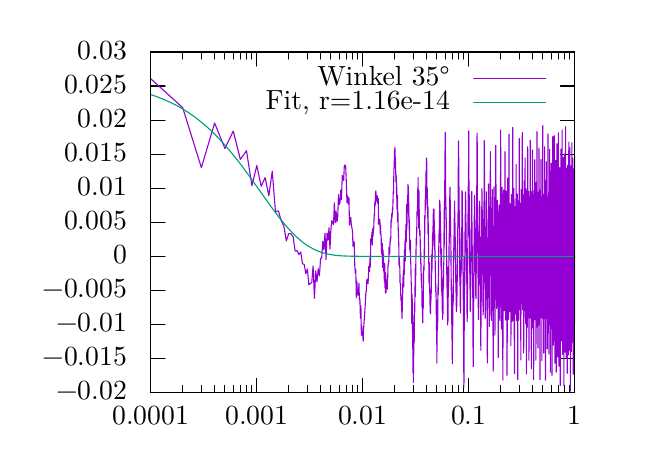
\begin{tikzpicture}[gnuplot]
%% generated with GNUPLOT 5.2p5a (Gentoo revision r0) (Lua 5.1; terminal rev. 99 , script rev. 107)
%% Sa 18 Mai 2019 18:31:02 CEST
\path (0.000,0.000) rectangle (7.500,5.250);
\gpcolor{color=gp lt color border}
\gpsetlinetype{gp lt border}
\gpsetdashtype{gp dt solid}
\gpsetlinewidth{1.00}
\draw[gp path] (1.564,0.616)--(1.744,0.616);
\draw[gp path] (6.947,0.616)--(6.767,0.616);
\node[gp node right] at (1.380,0.616) {$-0.02$};
\draw[gp path] (1.564,1.049)--(1.744,1.049);
\draw[gp path] (6.947,1.049)--(6.767,1.049);
\node[gp node right] at (1.380,1.049) {$-0.015$};
\draw[gp path] (1.564,1.481)--(1.744,1.481);
\draw[gp path] (6.947,1.481)--(6.767,1.481);
\node[gp node right] at (1.380,1.481) {$-0.01$};
\draw[gp path] (1.564,1.914)--(1.744,1.914);
\draw[gp path] (6.947,1.914)--(6.767,1.914);
\node[gp node right] at (1.380,1.914) {$-0.005$};
\draw[gp path] (1.564,2.346)--(1.744,2.346);
\draw[gp path] (6.947,2.346)--(6.767,2.346);
\node[gp node right] at (1.380,2.346) {$0$};
\draw[gp path] (1.564,2.779)--(1.744,2.779);
\draw[gp path] (6.947,2.779)--(6.767,2.779);
\node[gp node right] at (1.380,2.779) {$0.005$};
\draw[gp path] (1.564,3.211)--(1.744,3.211);
\draw[gp path] (6.947,3.211)--(6.767,3.211);
\node[gp node right] at (1.380,3.211) {$0.01$};
\draw[gp path] (1.564,3.644)--(1.744,3.644);
\draw[gp path] (6.947,3.644)--(6.767,3.644);
\node[gp node right] at (1.380,3.644) {$0.015$};
\draw[gp path] (1.564,4.076)--(1.744,4.076);
\draw[gp path] (6.947,4.076)--(6.767,4.076);
\node[gp node right] at (1.380,4.076) {$0.02$};
\draw[gp path] (1.564,4.509)--(1.744,4.509);
\draw[gp path] (6.947,4.509)--(6.767,4.509);
\node[gp node right] at (1.380,4.509) {$0.025$};
\draw[gp path] (1.564,4.941)--(1.744,4.941);
\draw[gp path] (6.947,4.941)--(6.767,4.941);
\node[gp node right] at (1.380,4.941) {$0.03$};
\draw[gp path] (1.564,0.616)--(1.564,0.796);
\draw[gp path] (1.564,4.941)--(1.564,4.761);
\node[gp node center] at (1.564,0.308) {$0.0001$};
\draw[gp path] (1.969,0.616)--(1.969,0.706);
\draw[gp path] (1.969,4.941)--(1.969,4.851);
\draw[gp path] (2.206,0.616)--(2.206,0.706);
\draw[gp path] (2.206,4.941)--(2.206,4.851);
\draw[gp path] (2.374,0.616)--(2.374,0.706);
\draw[gp path] (2.374,4.941)--(2.374,4.851);
\draw[gp path] (2.505,0.616)--(2.505,0.706);
\draw[gp path] (2.505,4.941)--(2.505,4.851);
\draw[gp path] (2.611,0.616)--(2.611,0.706);
\draw[gp path] (2.611,4.941)--(2.611,4.851);
\draw[gp path] (2.701,0.616)--(2.701,0.706);
\draw[gp path] (2.701,4.941)--(2.701,4.851);
\draw[gp path] (2.779,0.616)--(2.779,0.706);
\draw[gp path] (2.779,4.941)--(2.779,4.851);
\draw[gp path] (2.848,0.616)--(2.848,0.706);
\draw[gp path] (2.848,4.941)--(2.848,4.851);
\draw[gp path] (2.910,0.616)--(2.910,0.796);
\draw[gp path] (2.910,4.941)--(2.910,4.761);
\node[gp node center] at (2.910,0.308) {$0.001$};
\draw[gp path] (3.315,0.616)--(3.315,0.706);
\draw[gp path] (3.315,4.941)--(3.315,4.851);
\draw[gp path] (3.552,0.616)--(3.552,0.706);
\draw[gp path] (3.552,4.941)--(3.552,4.851);
\draw[gp path] (3.720,0.616)--(3.720,0.706);
\draw[gp path] (3.720,4.941)--(3.720,4.851);
\draw[gp path] (3.850,0.616)--(3.850,0.706);
\draw[gp path] (3.850,4.941)--(3.850,4.851);
\draw[gp path] (3.957,0.616)--(3.957,0.706);
\draw[gp path] (3.957,4.941)--(3.957,4.851);
\draw[gp path] (4.047,0.616)--(4.047,0.706);
\draw[gp path] (4.047,4.941)--(4.047,4.851);
\draw[gp path] (4.125,0.616)--(4.125,0.706);
\draw[gp path] (4.125,4.941)--(4.125,4.851);
\draw[gp path] (4.194,0.616)--(4.194,0.706);
\draw[gp path] (4.194,4.941)--(4.194,4.851);
\draw[gp path] (4.255,0.616)--(4.255,0.796);
\draw[gp path] (4.255,4.941)--(4.255,4.761);
\node[gp node center] at (4.255,0.308) {$0.01$};
\draw[gp path] (4.661,0.616)--(4.661,0.706);
\draw[gp path] (4.661,4.941)--(4.661,4.851);
\draw[gp path] (4.898,0.616)--(4.898,0.706);
\draw[gp path] (4.898,4.941)--(4.898,4.851);
\draw[gp path] (5.066,0.616)--(5.066,0.706);
\draw[gp path] (5.066,4.941)--(5.066,4.851);
\draw[gp path] (5.196,0.616)--(5.196,0.706);
\draw[gp path] (5.196,4.941)--(5.196,4.851);
\draw[gp path] (5.303,0.616)--(5.303,0.706);
\draw[gp path] (5.303,4.941)--(5.303,4.851);
\draw[gp path] (5.393,0.616)--(5.393,0.706);
\draw[gp path] (5.393,4.941)--(5.393,4.851);
\draw[gp path] (5.471,0.616)--(5.471,0.706);
\draw[gp path] (5.471,4.941)--(5.471,4.851);
\draw[gp path] (5.540,0.616)--(5.540,0.706);
\draw[gp path] (5.540,4.941)--(5.540,4.851);
\draw[gp path] (5.601,0.616)--(5.601,0.796);
\draw[gp path] (5.601,4.941)--(5.601,4.761);
\node[gp node center] at (5.601,0.308) {$0.1$};
\draw[gp path] (6.006,0.616)--(6.006,0.706);
\draw[gp path] (6.006,4.941)--(6.006,4.851);
\draw[gp path] (6.243,0.616)--(6.243,0.706);
\draw[gp path] (6.243,4.941)--(6.243,4.851);
\draw[gp path] (6.411,0.616)--(6.411,0.706);
\draw[gp path] (6.411,4.941)--(6.411,4.851);
\draw[gp path] (6.542,0.616)--(6.542,0.706);
\draw[gp path] (6.542,4.941)--(6.542,4.851);
\draw[gp path] (6.648,0.616)--(6.648,0.706);
\draw[gp path] (6.648,4.941)--(6.648,4.851);
\draw[gp path] (6.739,0.616)--(6.739,0.706);
\draw[gp path] (6.739,4.941)--(6.739,4.851);
\draw[gp path] (6.817,0.616)--(6.817,0.706);
\draw[gp path] (6.817,4.941)--(6.817,4.851);
\draw[gp path] (6.885,0.616)--(6.885,0.706);
\draw[gp path] (6.885,4.941)--(6.885,4.851);
\draw[gp path] (6.947,0.616)--(6.947,0.796);
\draw[gp path] (6.947,4.941)--(6.947,4.761);
\node[gp node center] at (6.947,0.308) {$1$};
\draw[gp path] (1.564,4.941)--(1.564,0.616)--(6.947,0.616)--(6.947,4.941)--cycle;
\node[gp node right] at (5.479,4.607) {Winkel 35°};
\gpcolor{rgb color={0.580,0.000,0.827}}
\draw[gp path] (5.663,4.607)--(6.579,4.607);
\draw[gp path] (1.564,4.601)--(1.969,4.234)--(2.206,3.472)--(2.374,4.039)--(2.505,3.715)%
  --(2.611,3.937)--(2.701,3.577)--(2.779,3.687)--(2.848,3.243)--(2.910,3.500)--(2.965,3.236)%
  --(3.016,3.346)--(3.063,3.115)--(3.106,3.426)--(3.147,2.912)--(3.184,2.923)--(3.220,2.799)%
  --(3.253,2.731)--(3.285,2.541)--(3.315,2.635)--(3.343,2.634)--(3.371,2.593)--(3.397,2.413)%
  --(3.421,2.419)--(3.445,2.369)--(3.468,2.401)--(3.490,2.252)--(3.512,2.244)--(3.532,2.124)%
  --(3.552,2.186)--(3.571,1.984)--(3.590,2.002)--(3.608,2.014)--(3.625,2.225)--(3.642,1.812)%
  --(3.658,2.162)--(3.674,2.024)--(3.690,2.190)--(3.705,2.099)--(3.720,2.317)--(3.734,2.329)%
  --(3.748,2.537)--(3.762,2.427)--(3.776,2.640)--(3.789,2.305)--(3.802,2.641)--(3.814,2.553)%
  --(3.827,2.709)--(3.839,2.438)--(3.850,2.673)--(3.862,2.799)--(3.873,2.779)--(3.884,2.748)%
  --(3.895,3.025)--(3.906,2.776)--(3.917,2.918)--(3.927,2.783)--(3.937,2.839)--(3.947,3.129)%
  --(3.957,3.002)--(3.967,3.033)--(3.976,3.186)--(3.985,3.067)--(3.995,3.373)--(4.004,3.360)%
  --(4.013,3.307)--(4.021,3.490)--(4.030,3.507)--(4.039,3.482)--(4.047,3.282)--(4.055,3.029)%
  --(4.064,3.112)--(4.072,3.008)--(4.080,3.089)--(4.087,2.743)--(4.095,2.820)--(4.103,2.842)%
  --(4.110,2.747)--(4.118,2.710)--(4.125,2.661)--(4.132,2.472)--(4.140,2.538)--(4.147,2.520)%
  --(4.154,2.231)--(4.161,2.133)--(4.167,2.177)--(4.174,1.819)--(4.181,2.029)--(4.187,1.855)%
  --(4.194,1.925)--(4.200,1.853)--(4.207,2.006)--(4.213,1.791)--(4.219,1.811)--(4.226,1.560)%
  --(4.232,1.717)--(4.238,1.344)--(4.244,1.458)--(4.250,1.348)--(4.256,1.333)--(4.261,1.268)%
  --(4.267,1.435)--(4.273,1.522)--(4.278,1.594)--(4.284,1.683)--(4.290,1.792)--(4.295,1.889)%
  --(4.300,1.897)--(4.306,2.037)--(4.311,2.052)--(4.316,2.057)--(4.322,1.997)--(4.327,2.073)%
  --(4.332,2.218)--(4.337,2.160)--(4.342,2.155)--(4.347,2.327)--(4.352,2.212)--(4.357,2.566)%
  --(4.362,2.575)--(4.367,2.542)--(4.372,2.654)--(4.376,2.489)--(4.381,2.697)--(4.386,2.600)%
  --(4.391,2.697)--(4.395,2.699)--(4.400,2.876)--(4.404,2.856)--(4.409,3.042)--(4.413,2.990)%
  --(4.418,3.152)--(4.422,3.177)--(4.427,3.070)--(4.431,3.049)--(4.435,3.072)--(4.439,3.117)%
  --(4.444,3.021)--(4.448,3.077)--(4.452,3.085)--(4.456,2.754)--(4.460,2.754)--(4.465,2.791)%
  --(4.469,2.808)--(4.473,2.816)--(4.477,2.635)--(4.481,2.739)--(4.485,2.612)--(4.489,2.613)%
  --(4.492,2.423)--(4.496,2.395)--(4.500,2.361)--(4.504,2.511)--(4.508,2.206)--(4.512,2.428)%
  --(4.515,2.353)--(4.519,2.375)--(4.523,2.147)--(4.527,2.146)--(4.530,2.020)--(4.534,2.256)%
  --(4.537,1.951)--(4.541,2.142)--(4.545,1.879)--(4.548,2.102)--(4.552,1.886)--(4.555,2.044)%
  --(4.559,1.974)--(4.562,1.992)--(4.566,1.930)--(4.569,2.049)--(4.572,2.065)--(4.576,2.230)%
  --(4.579,2.243)--(4.583,2.270)--(4.586,2.282)--(4.589,2.463)--(4.593,2.423)--(4.596,2.372)%
  --(4.599,2.415)--(4.602,2.529)--(4.605,2.574)--(4.609,2.535)--(4.612,2.611)--(4.615,2.807)%
  --(4.618,2.820)--(4.621,2.785)--(4.624,2.887)--(4.628,2.835)--(4.631,2.911)--(4.634,2.972)%
  --(4.637,2.932)--(4.640,3.065)--(4.643,3.163)--(4.646,3.139)--(4.649,3.330)--(4.652,3.466)%
  --(4.655,3.471)--(4.658,3.701)--(4.661,3.584)--(4.664,3.733)--(4.666,3.621)--(4.669,3.597)%
  --(4.672,3.498)--(4.675,3.384)--(4.678,3.286)--(4.681,3.370)--(4.684,3.129)--(4.686,3.283)%
  --(4.689,2.950)--(4.692,3.018)--(4.695,2.901)--(4.697,3.119)--(4.700,2.781)--(4.703,2.899)%
  --(4.706,2.684)--(4.708,2.650)--(4.711,2.560)--(4.714,2.441)--(4.716,2.232)--(4.719,2.332)%
  --(4.722,2.261)--(4.724,2.231)--(4.727,2.184)--(4.729,2.009)--(4.732,2.008)--(4.735,1.991)%
  --(4.737,1.844)--(4.740,1.853)--(4.742,1.780)--(4.745,1.829)--(4.747,1.739)--(4.750,1.689)%
  --(4.752,1.623)--(4.755,1.553)--(4.757,1.690)--(4.760,1.876)--(4.762,1.803)--(4.765,2.083)%
  --(4.767,2.004)--(4.770,2.110)--(4.772,2.168)--(4.774,2.091)--(4.777,1.959)--(4.779,2.323)%
  --(4.782,2.115)--(4.784,2.236)--(4.786,2.421)--(4.789,2.437)--(4.791,2.414)--(4.793,2.559)%
  --(4.796,2.286)--(4.798,2.460)--(4.800,2.492)--(4.803,2.748)--(4.805,2.543)--(4.807,2.728)%
  --(4.809,2.530)--(4.812,3.004)--(4.814,2.688)--(4.816,2.854)--(4.818,2.741)--(4.821,3.006)%
  --(4.823,2.976)--(4.825,3.120)--(4.827,2.902)--(4.829,3.259)--(4.832,3.153)--(4.834,3.239)%
  --(4.836,2.968)--(4.838,3.162)--(4.840,2.858)--(4.842,2.772)--(4.845,2.845)--(4.847,2.635)%
  --(4.849,2.771)--(4.851,2.621)--(4.853,2.428)--(4.855,2.539)--(4.857,2.527)--(4.859,2.393)%
  --(4.861,2.548)--(4.863,2.312)--(4.866,2.241)--(4.868,2.152)--(4.870,2.042)--(4.872,1.982)%
  --(4.874,1.798)--(4.876,1.824)--(4.878,1.494)--(4.880,1.872)--(4.882,1.726)--(4.884,1.809)%
  --(4.886,1.411)--(4.888,1.510)--(4.890,1.168)--(4.892,1.312)--(4.894,0.865)--(4.896,1.202)%
  --(4.898,0.743)--(4.900,1.139)--(4.901,0.861)--(4.903,1.380)--(4.905,1.087)--(4.907,1.609)%
  --(4.909,1.263)--(4.911,1.754)--(4.913,1.613)--(4.915,1.640)--(4.917,1.699)--(4.919,1.968)%
  --(4.921,1.924)--(4.922,2.196)--(4.924,1.837)--(4.926,2.059)--(4.928,2.108)--(4.930,2.345)%
  --(4.932,2.365)--(4.933,2.579)--(4.935,2.493)--(4.937,2.489)--(4.939,2.507)--(4.941,2.720)%
  --(4.943,2.648)--(4.944,2.915)--(4.946,2.833)--(4.948,2.900)--(4.950,2.925)--(4.952,3.022)%
  --(4.953,3.102)--(4.955,3.228)--(4.957,2.997)--(4.959,3.347)--(4.960,3.018)--(4.962,3.162)%
  --(4.964,3.082)--(4.966,3.042)--(4.967,2.705)--(4.969,3.190)--(4.971,2.877)--(4.972,2.984)%
  --(4.974,2.677)--(4.976,2.672)--(4.978,2.690)--(4.979,2.613)--(4.981,2.612)--(4.983,2.675)%
  --(4.984,2.471)--(4.986,2.557)--(4.988,2.330)--(4.989,2.433)--(4.991,2.252)--(4.993,2.396)%
  --(4.994,2.157)--(4.996,2.255)--(4.998,2.037)--(4.999,2.132)--(5.001,2.002)--(5.003,2.124)%
  --(5.004,1.963)--(5.006,1.944)--(5.007,1.711)--(5.009,1.766)--(5.011,1.688)--(5.012,1.726)%
  --(5.014,1.634)--(5.015,1.590)--(5.017,1.501)--(5.019,1.642)--(5.020,1.800)--(5.022,1.805)%
  --(5.023,1.679)--(5.025,1.996)--(5.026,1.953)--(5.028,2.206)--(5.030,2.165)--(5.031,2.228)%
  --(5.033,2.184)--(5.034,2.170)--(5.036,2.338)--(5.037,2.441)--(5.039,2.371)--(5.040,2.595)%
  --(5.042,2.604)--(5.043,2.864)--(5.045,2.843)--(5.046,2.860)--(5.048,2.825)--(5.049,3.068)%
  --(5.051,3.016)--(5.052,3.123)--(5.054,2.967)--(5.055,3.242)--(5.057,3.007)--(5.058,3.415)%
  --(5.060,3.174)--(5.061,3.309)--(5.063,3.486)--(5.064,3.589)--(5.066,3.595)--(5.067,3.565)%
  --(5.069,3.498)--(5.070,3.229)--(5.072,3.219)--(5.073,3.159)--(5.074,3.211)--(5.076,2.987)%
  --(5.077,3.100)--(5.079,2.838)--(5.080,2.952)--(5.082,2.941)--(5.083,2.759)--(5.084,2.636)%
  --(5.086,2.968)--(5.087,2.623)--(5.089,2.622)--(5.090,2.483)--(5.091,2.510)--(5.093,2.325)%
  --(5.094,2.271)--(5.096,2.133)--(5.097,2.018)--(5.098,2.100)--(5.100,2.047)--(5.101,1.987)%
  --(5.103,2.065)--(5.104,2.263)--(5.105,1.874)--(5.107,1.949)--(5.108,1.723)--(5.109,1.747)%
  --(5.111,1.750)--(5.112,1.806)--(5.113,1.631)--(5.115,1.905)--(5.116,1.633)--(5.117,1.616)%
  --(5.119,1.820)--(5.120,1.804)--(5.121,1.790)--(5.123,1.823)--(5.124,1.920)--(5.125,1.904)%
  --(5.127,1.881)--(5.128,2.121)--(5.129,2.039)--(5.131,2.191)--(5.132,2.367)--(5.133,2.140)%
  --(5.135,2.212)--(5.136,2.391)--(5.137,2.317)--(5.138,2.323)--(5.140,2.621)--(5.141,2.496)%
  --(5.142,2.597)--(5.144,2.476)--(5.145,2.637)--(5.146,2.727)--(5.147,2.721)--(5.149,2.660)%
  --(5.150,2.770)--(5.151,2.838)--(5.152,2.940)--(5.154,2.873)--(5.155,2.895)--(5.156,2.782)%
  --(5.157,2.753)--(5.159,2.948)--(5.160,2.941)--(5.161,2.553)--(5.162,2.602)--(5.164,2.586)%
  --(5.165,2.796)--(5.166,2.649)--(5.167,2.436)--(5.169,2.625)--(5.170,2.607)--(5.171,2.521)%
  --(5.172,2.441)--(5.173,2.380)--(5.175,2.223)--(5.176,2.286)--(5.177,2.146)--(5.178,2.141)%
  --(5.180,2.107)--(5.181,1.897)--(5.182,1.949)--(5.183,2.003)--(5.184,1.837)--(5.186,1.855)%
  --(5.187,1.900)--(5.188,1.743)--(5.189,1.711)--(5.190,1.501)--(5.191,1.491)--(5.193,1.378)%
  --(5.194,1.398)--(5.195,1.225)--(5.196,1.363)--(5.197,0.989)--(5.198,1.201)--(5.200,1.174)%
  --(5.201,1.497)--(5.202,1.405)--(5.203,1.709)--(5.204,1.425)--(5.205,1.792)--(5.207,1.459)%
  --(5.208,1.740)--(5.209,1.699)--(5.210,1.900)--(5.211,1.855)--(5.212,1.985)--(5.213,1.872)%
  --(5.215,1.860)--(5.216,1.891)--(5.217,2.169)--(5.218,2.280)--(5.219,2.325)--(5.220,2.475)%
  --(5.221,2.461)--(5.222,2.388)--(5.224,2.632)--(5.225,2.539)--(5.226,2.687)--(5.227,2.538)%
  --(5.228,2.654)--(5.229,2.869)--(5.230,2.914)--(5.231,2.921)--(5.232,3.060)--(5.233,3.029)%
  --(5.235,3.043)--(5.236,2.933)--(5.237,3.012)--(5.238,2.824)--(5.239,2.914)--(5.240,2.794)%
  --(5.241,2.775)--(5.242,2.518)--(5.243,2.663)--(5.244,2.384)--(5.245,2.673)--(5.247,2.461)%
  --(5.248,2.564)--(5.249,2.222)--(5.250,2.438)--(5.251,2.269)--(5.252,2.350)--(5.253,2.180)%
  --(5.254,2.206)--(5.255,1.950)--(5.256,2.440)--(5.257,2.017)--(5.258,2.177)--(5.259,1.895)%
  --(5.260,2.157)--(5.261,1.886)--(5.262,2.059)--(5.263,1.662)--(5.264,1.863)--(5.265,1.664)%
  --(5.267,1.812)--(5.268,1.623)--(5.269,1.640)--(5.270,1.546)--(5.271,1.618)--(5.272,1.679)%
  --(5.273,1.689)--(5.274,1.615)--(5.275,1.848)--(5.276,1.726)--(5.277,1.924)--(5.278,2.015)%
  --(5.279,2.053)--(5.280,2.083)--(5.281,1.960)--(5.282,2.101)--(5.283,2.213)--(5.284,2.267)%
  --(5.285,2.251)--(5.286,2.390)--(5.287,2.642)--(5.288,2.444)--(5.289,2.663)--(5.290,2.493)%
  --(5.291,2.952)--(5.292,2.843)--(5.293,2.948)--(5.294,2.966)--(5.295,3.309)--(5.296,2.945)%
  --(5.297,3.283)--(5.298,3.125)--(5.299,3.532)--(5.300,3.513)--(5.301,3.788)--(5.302,3.373)%
  --(5.303,3.921)--(5.304,3.531)--(5.305,3.907)--(5.306,3.432)--(5.307,3.621)--(5.308,3.123)%
  --(5.309,3.113)--(5.309,3.008)--(5.310,3.106)--(5.311,2.825)--(5.312,2.974)--(5.313,2.960)%
  --(5.314,2.899)--(5.315,2.744)--(5.316,2.834)--(5.317,2.576)--(5.318,2.622)--(5.319,2.386)%
  --(5.320,2.420)--(5.321,2.367)--(5.322,2.227)--(5.323,2.096)--(5.324,1.976)--(5.325,1.952)%
  --(5.326,2.151)--(5.327,2.102)--(5.327,1.865)--(5.328,1.808)--(5.329,1.889)--(5.330,1.587)%
  --(5.331,1.832)--(5.332,1.876)--(5.333,1.699)--(5.334,1.474)--(5.335,1.639)--(5.336,1.503)%
  --(5.337,1.740)--(5.338,1.528)--(5.339,2.096)--(5.340,1.869)--(5.340,2.209)--(5.341,2.033)%
  --(5.342,2.213)--(5.343,1.832)--(5.344,2.062)--(5.345,1.941)--(5.346,2.147)--(5.347,2.194)%
  --(5.348,2.174)--(5.349,2.025)--(5.349,2.475)--(5.350,2.271)--(5.351,2.459)--(5.352,2.496)%
  --(5.353,2.643)--(5.354,2.581)--(5.355,2.512)--(5.356,2.595)--(5.357,2.786)--(5.358,2.793)%
  --(5.358,2.843)--(5.359,2.831)--(5.360,2.964)--(5.361,3.108)--(5.362,3.013)--(5.363,3.067)%
  --(5.364,3.224)--(5.365,3.119)--(5.365,3.134)--(5.366,3.060)--(5.367,2.957)--(5.368,2.872)%
  --(5.369,2.824)--(5.370,2.749)--(5.371,2.651)--(5.372,2.629)--(5.372,2.608)--(5.373,2.621)%
  --(5.374,2.578)--(5.375,2.387)--(5.376,2.410)--(5.377,2.200)--(5.378,2.107)--(5.378,2.126)%
  --(5.379,2.022)--(5.380,1.907)--(5.381,1.996)--(5.382,1.719)--(5.383,1.862)--(5.384,1.857)%
  --(5.384,1.843)--(5.385,1.488)--(5.386,1.605)--(5.387,1.429)--(5.388,1.582)--(5.389,1.492)%
  --(5.389,1.290)--(5.390,1.359)--(5.391,1.390)--(5.392,1.183)--(5.393,0.981)--(5.394,1.306)%
  --(5.394,1.189)--(5.395,1.299)--(5.396,1.336)--(5.397,1.386)--(5.398,1.487)--(5.399,1.640)%
  --(5.399,1.692)--(5.400,1.954)--(5.401,1.724)--(5.402,1.906)--(5.403,1.824)--(5.404,1.864)%
  --(5.404,1.762)--(5.405,1.961)--(5.406,2.018)--(5.407,2.118)--(5.408,2.114)--(5.408,2.216)%
  --(5.409,2.450)--(5.410,2.277)--(5.411,2.358)--(5.412,2.378)--(5.412,2.457)--(5.413,2.545)%
  --(5.414,2.515)--(5.415,2.619)--(5.416,2.768)--(5.417,2.602)--(5.417,2.829)--(5.418,2.719)%
  --(5.419,2.817)--(5.420,2.796)--(5.421,2.942)--(5.421,2.906)--(5.422,3.047)--(5.423,2.936)%
  --(5.424,2.787)--(5.424,2.752)--(5.425,2.821)--(5.426,2.633)--(5.427,2.766)--(5.428,2.586)%
  --(5.428,2.474)--(5.429,2.558)--(5.430,2.585)--(5.431,2.390)--(5.432,2.556)--(5.432,2.519)%
  --(5.433,2.400)--(5.434,2.275)--(5.435,2.222)--(5.435,2.274)--(5.436,2.014)--(5.437,2.111)%
  --(5.438,2.041)--(5.439,1.932)--(5.439,1.892)--(5.440,2.093)--(5.441,1.874)--(5.442,1.925)%
  --(5.442,1.863)--(5.443,1.792)--(5.444,1.643)--(5.445,1.659)--(5.445,1.701)--(5.446,1.781)%
  --(5.447,1.783)--(5.448,1.790)--(5.448,1.670)--(5.449,1.857)--(5.450,1.706)--(5.451,2.110)%
  --(5.452,1.887)--(5.452,2.048)--(5.453,1.843)--(5.454,2.163)--(5.455,2.021)--(5.455,2.106)%
  --(5.456,2.195)--(5.457,2.411)--(5.458,2.275)--(5.458,2.319)--(5.459,2.543)--(5.460,2.533)%
  --(5.461,2.470)--(5.461,2.711)--(5.462,2.697)--(5.463,2.707)--(5.463,2.872)--(5.464,2.896)%
  --(5.465,2.720)--(5.466,2.828)--(5.466,2.949)--(5.467,3.186)--(5.468,3.204)--(5.469,3.513)%
  --(5.469,3.480)--(5.470,3.476)--(5.471,3.706)--(5.472,3.811)--(5.472,3.565)--(5.473,3.556)%
  --(5.474,3.447)--(5.474,3.601)--(5.475,3.026)--(5.476,3.545)--(5.477,2.894)--(5.477,3.233)%
  --(5.478,2.838)--(5.479,3.233)--(5.480,2.925)--(5.480,2.970)--(5.481,2.826)--(5.482,2.687)%
  --(5.482,2.695)--(5.483,2.701)--(5.484,2.574)--(5.485,2.493)--(5.485,2.485)--(5.486,2.322)%
  --(5.487,2.084)--(5.487,2.189)--(5.488,2.092)--(5.489,2.291)--(5.490,1.968)--(5.490,2.163)%
  --(5.491,2.068)--(5.492,1.822)--(5.492,1.733)--(5.493,1.888)--(5.494,1.829)--(5.494,1.715)%
  --(5.495,1.790)--(5.496,1.624)--(5.497,1.850)--(5.497,1.808)--(5.498,1.812)--(5.499,1.961)%
  --(5.499,2.018)--(5.500,1.992)--(5.501,2.004)--(5.501,2.266)--(5.502,2.225)--(5.503,2.284)%
  --(5.504,2.154)--(5.504,2.307)--(5.505,2.102)--(5.506,2.351)--(5.506,2.167)--(5.507,2.568)%
  --(5.508,2.386)--(5.508,2.353)--(5.509,2.343)--(5.510,2.713)--(5.510,2.376)--(5.511,2.701)%
  --(5.512,2.596)--(5.512,2.688)--(5.513,2.538)--(5.514,2.956)--(5.514,2.767)--(5.515,2.936)%
  --(5.516,2.918)--(5.516,3.180)--(5.517,2.962)--(5.518,3.077)--(5.519,3.111)--(5.519,3.159)%
  --(5.520,3.100)--(5.521,2.929)--(5.521,2.873)--(5.522,2.808)--(5.523,2.663)--(5.523,2.613)%
  --(5.524,2.544)--(5.525,2.463)--(5.525,2.353)--(5.526,2.648)--(5.527,2.563)--(5.527,2.517)%
  --(5.528,2.295)--(5.529,2.162)--(5.529,2.138)--(5.530,2.099)--(5.531,2.087)--(5.531,2.102)%
  --(5.532,1.816)--(5.532,1.949)--(5.533,1.578)--(5.534,1.755)--(5.534,1.354)--(5.535,1.604)%
  --(5.536,1.311)--(5.536,1.409)--(5.537,1.170)--(5.538,1.345)--(5.538,0.870)--(5.539,1.180)%
  --(5.540,0.683)--(5.540,1.054)--(5.541,0.740)--(5.542,1.269)--(5.542,1.057)--(5.543,1.541)%
  --(5.544,1.398)--(5.544,1.709)--(5.545,1.656)--(5.545,1.871)--(5.546,1.693)--(5.547,1.945)%
  --(5.547,1.857)--(5.548,2.142)--(5.549,1.928)--(5.549,2.004)--(5.550,1.928)--(5.551,2.342)%
  --(5.551,2.120)--(5.552,2.298)--(5.553,2.386)--(5.553,2.488)--(5.554,2.486)--(5.554,2.663)%
  --(5.555,2.586)--(5.556,2.655)--(5.556,2.729)--(5.557,2.881)--(5.558,2.627)--(5.558,2.883)%
  --(5.559,2.773)--(5.559,3.051)--(5.560,2.915)--(5.561,3.165)--(5.561,2.786)--(5.562,3.036)%
  --(5.563,2.785)--(5.563,3.059)--(5.564,2.750)--(5.564,2.838)--(5.565,2.584)--(5.566,2.773)%
  --(5.566,2.507)--(5.567,2.685)--(5.568,2.398)--(5.568,2.655)--(5.569,2.544)--(5.569,2.570)%
  --(5.570,2.435)--(5.571,2.513)--(5.571,2.387)--(5.572,2.410)--(5.573,2.162)--(5.573,2.371)%
  --(5.574,2.097)--(5.574,2.274)--(5.575,2.077)--(5.576,2.028)--(5.576,2.002)--(5.577,2.008)%
  --(5.577,2.091)--(5.578,1.926)--(5.579,1.907)--(5.579,1.680)--(5.580,1.750)--(5.580,1.612)%
  --(5.581,1.515)--(5.582,1.806)--(5.582,1.555)--(5.583,1.792)--(5.583,1.848)--(5.584,1.802)%
  --(5.585,1.833)--(5.585,1.938)--(5.586,1.854)--(5.586,2.077)--(5.587,2.140)--(5.588,2.207)%
  --(5.588,2.178)--(5.589,2.447)--(5.589,2.296)--(5.590,2.439)--(5.591,2.456)--(5.591,2.576)%
  --(5.592,2.651)--(5.592,2.892)--(5.593,2.703)--(5.594,2.835)--(5.594,2.996)--(5.595,3.235)%
  --(5.595,2.971)--(5.596,3.150)--(5.597,3.029)--(5.597,3.200)--(5.598,3.082)--(5.598,3.289)%
  --(5.599,3.436)--(5.599,3.488)--(5.600,3.476)--(5.601,3.935)--(5.601,3.939)--(5.602,3.633)%
  --(5.602,3.668)--(5.603,3.591)--(5.604,3.318)--(5.604,3.319)--(5.605,3.178)--(5.605,3.242)%
  --(5.606,3.254)--(5.606,3.161)--(5.607,3.188)--(5.608,2.971)--(5.608,2.844)--(5.609,2.901)%
  --(5.609,2.832)--(5.610,2.642)--(5.611,2.706)--(5.611,2.585)--(5.612,2.579)--(5.612,2.409)%
  --(5.613,2.456)--(5.613,2.136)--(5.614,2.327)--(5.615,2.319)--(5.615,2.221)--(5.616,2.212)%
  --(5.616,2.100)--(5.617,1.931)--(5.617,1.970)--(5.618,2.008)--(5.619,1.789)--(5.619,1.750)%
  --(5.620,1.861)--(5.620,1.822)--(5.621,1.664)--(5.621,1.662)--(5.622,1.646)--(5.622,1.843)%
  --(5.623,1.757)--(5.624,1.930)--(5.624,1.834)--(5.625,1.932)--(5.625,2.046)--(5.626,2.157)%
  --(5.626,2.095)--(5.627,2.156)--(5.628,2.140)--(5.628,2.127)--(5.629,2.323)--(5.629,2.290)%
  --(5.630,2.297)--(5.630,2.347)--(5.631,2.418)--(5.631,2.544)--(5.632,2.446)--(5.633,2.641)%
  --(5.633,2.575)--(5.634,2.571)--(5.634,2.678)--(5.635,2.611)--(5.635,2.660)--(5.636,2.607)%
  --(5.636,2.768)--(5.637,2.845)--(5.638,3.007)--(5.638,2.735)--(5.639,3.170)--(5.639,3.089)%
  --(5.640,3.068)--(5.640,2.776)--(5.641,2.955)--(5.641,2.695)--(5.642,2.834)--(5.642,2.754)%
  --(5.643,2.780)--(5.644,2.539)--(5.644,2.506)--(5.645,2.506)--(5.645,2.468)--(5.646,2.479)%
  --(5.646,2.455)--(5.647,2.196)--(5.647,2.439)--(5.648,2.326)--(5.648,2.108)--(5.649,2.136)%
  --(5.649,1.980)--(5.650,1.953)--(5.651,2.110)--(5.651,1.896)--(5.652,1.821)--(5.652,1.908)%
  --(5.653,1.874)--(5.653,2.035)--(5.654,1.918)--(5.654,1.540)--(5.655,1.399)--(5.655,1.414)%
  --(5.656,1.190)--(5.656,1.226)--(5.657,1.147)--(5.657,1.177)--(5.658,1.276)--(5.659,0.945)%
  --(5.659,1.449)--(5.660,1.117)--(5.660,1.747)--(5.661,1.338)--(5.661,1.618)--(5.662,1.414)%
  --(5.662,1.834)--(5.663,1.596)--(5.663,1.893)--(5.664,1.700)--(5.664,2.056)--(5.665,1.778)%
  --(5.665,2.066)--(5.666,2.073)--(5.666,2.243)--(5.667,2.181)--(5.667,2.363)--(5.668,2.439)%
  --(5.669,2.511)--(5.669,2.480)--(5.670,2.614)--(5.670,2.608)--(5.671,2.720)--(5.671,2.597)%
  --(5.672,2.839)--(5.672,2.858)--(5.673,2.940)--(5.673,2.739)--(5.674,3.101)--(5.674,3.055)%
  --(5.675,3.012)--(5.675,2.918)--(5.676,3.117)--(5.676,2.961)--(5.677,3.061)--(5.677,3.009)%
  --(5.678,2.824)--(5.678,2.697)--(5.679,2.739)--(5.679,2.737)--(5.680,2.720)--(5.680,2.563)%
  --(5.681,2.808)--(5.681,2.484)--(5.682,2.676)--(5.682,2.339)--(5.683,2.493)--(5.683,2.243)%
  --(5.684,2.531)--(5.684,2.151)--(5.685,2.463)--(5.685,2.164)--(5.686,2.293)--(5.686,2.256)%
  --(5.687,2.389)--(5.687,2.106)--(5.688,2.161)--(5.688,2.025)--(5.689,2.214)--(5.690,1.885)%
  --(5.690,1.903)--(5.691,1.846)--(5.691,1.920)--(5.692,1.926)--(5.692,1.978)--(5.693,1.809)%
  --(5.693,1.909)--(5.694,1.915)--(5.694,1.849)--(5.695,1.955)--(5.695,2.040)--(5.696,1.982)%
  --(5.696,2.306)--(5.696,2.147)--(5.697,2.130)--(5.697,2.150)--(5.698,2.303)--(5.698,2.284)%
  --(5.699,2.452)--(5.699,2.317)--(5.700,2.695)--(5.700,2.698)--(5.701,2.696)--(5.701,2.594)%
  --(5.702,3.044)--(5.702,2.739)--(5.703,3.134)--(5.703,2.911)--(5.704,3.293)--(5.704,3.101)%
  --(5.705,3.379)--(5.705,3.068)--(5.706,3.693)--(5.706,3.353)--(5.707,3.870)--(5.707,3.533)%
  --(5.708,3.909)--(5.708,3.655)--(5.709,3.799)--(5.709,3.478)--(5.710,3.636)--(5.710,3.299)%
  --(5.711,3.235)--(5.711,3.082)--(5.712,3.056)--(5.712,2.947)--(5.713,2.976)--(5.713,2.672)%
  --(5.714,2.860)--(5.714,2.752)--(5.715,2.917)--(5.715,2.669)--(5.716,2.636)--(5.716,2.389)%
  --(5.717,2.509)--(5.717,2.364)--(5.717,2.251)--(5.718,2.178)--(5.718,2.141)--(5.719,2.226)%
  --(5.719,2.208)--(5.720,2.029)--(5.720,1.965)--(5.721,2.033)--(5.721,1.977)--(5.722,1.698)%
  --(5.722,1.969)--(5.723,1.677)--(5.723,1.848)--(5.724,1.568)--(5.724,1.903)--(5.725,1.543)%
  --(5.725,1.890)--(5.726,1.582)--(5.726,2.033)--(5.727,1.958)--(5.727,2.297)--(5.727,1.909)%
  --(5.728,2.254)--(5.728,2.003)--(5.729,2.432)--(5.729,1.975)--(5.730,2.302)--(5.730,2.078)%
  --(5.731,2.316)--(5.731,2.295)--(5.732,2.490)--(5.732,2.349)--(5.733,2.494)--(5.733,2.465)%
  --(5.734,2.673)--(5.734,2.644)--(5.734,2.701)--(5.735,2.556)--(5.735,2.746)--(5.736,2.506)%
  --(5.736,2.621)--(5.737,2.675)--(5.737,2.914)--(5.738,2.938)--(5.738,3.007)--(5.739,2.999)%
  --(5.739,3.047)--(5.740,3.024)--(5.740,2.987)--(5.740,2.957)--(5.741,2.981)--(5.741,2.896)%
  --(5.742,2.857)--(5.742,2.559)--(5.743,2.599)--(5.743,2.466)--(5.744,2.533)--(5.744,2.595)%
  --(5.745,2.540)--(5.745,2.360)--(5.746,2.412)--(5.746,2.318)--(5.746,2.346)--(5.747,2.144)%
  --(5.747,2.108)--(5.748,2.058)--(5.748,2.071)--(5.749,1.814)--(5.749,1.951)--(5.750,1.696)%
  --(5.750,1.993)--(5.751,1.823)--(5.751,1.829)--(5.751,1.709)--(5.752,1.702)--(5.752,1.529)%
  --(5.753,1.454)--(5.753,1.210)--(5.754,1.234)--(5.754,1.356)--(5.755,1.278)--(5.755,1.152)%
  --(5.755,1.234)--(5.756,1.372)--(5.756,1.440)--(5.757,1.455)--(5.757,1.500)--(5.758,1.678)%
  --(5.758,1.665)--(5.759,1.729)--(5.759,1.510)--(5.760,1.903)--(5.760,1.840)--(5.760,1.850)%
  --(5.761,1.996)--(5.761,1.974)--(5.762,1.984)--(5.762,2.373)--(5.763,2.116)--(5.763,2.225)%
  --(5.764,2.373)--(5.764,2.596)--(5.764,2.541)--(5.765,2.617)--(5.765,2.778)--(5.766,2.542)%
  --(5.766,2.548)--(5.767,2.720)--(5.767,2.981)--(5.767,2.802)--(5.768,2.936)--(5.768,3.048)%
  --(5.769,3.206)--(5.769,3.008)--(5.770,3.059)--(5.770,3.173)--(5.771,3.173)--(5.771,3.005)%
  --(5.771,3.024)--(5.772,2.911)--(5.772,2.836)--(5.773,2.878)--(5.773,2.901)--(5.774,2.935)%
  --(5.774,2.753)--(5.774,2.679)--(5.775,2.606)--(5.775,2.878)--(5.776,2.584)--(5.776,2.539)%
  --(5.777,2.340)--(5.777,2.417)--(5.778,2.232)--(5.778,2.336)--(5.778,2.338)--(5.779,2.312)%
  --(5.779,2.109)--(5.780,2.198)--(5.780,2.181)--(5.781,2.128)--(5.781,1.947)--(5.781,1.974)%
  --(5.782,1.866)--(5.782,1.709)--(5.783,1.818)--(5.783,1.839)--(5.784,1.662)--(5.784,1.771)%
  --(5.784,1.601)--(5.785,1.773)--(5.785,1.629)--(5.786,1.875)--(5.786,1.807)--(5.787,2.032)%
  --(5.787,1.939)--(5.787,1.982)--(5.788,2.203)--(5.788,2.186)--(5.789,2.216)--(5.789,2.157)%
  --(5.789,2.005)--(5.790,2.254)--(5.790,2.412)--(5.791,2.391)--(5.791,2.402)--(5.792,2.586)%
  --(5.792,2.573)--(5.792,2.823)--(5.793,2.635)--(5.793,2.970)--(5.794,2.873)--(5.794,2.954)%
  --(5.795,2.973)--(5.795,3.002)--(5.795,2.935)--(5.796,3.052)--(5.796,3.042)--(5.797,3.291)%
  --(5.797,3.332)--(5.797,3.643)--(5.798,3.493)--(5.798,3.706)--(5.799,3.584)--(5.799,3.816)%
  --(5.800,3.255)--(5.800,3.481)--(5.800,3.179)--(5.801,3.423)--(5.801,3.039)--(5.802,2.965)%
  --(5.802,2.920)--(5.802,3.237)--(5.803,3.001)--(5.803,3.016)--(5.804,2.870)--(5.804,2.741)%
  --(5.805,2.603)--(5.805,2.546)--(5.805,2.719)--(5.806,2.474)--(5.806,2.340)--(5.807,2.169)%
  --(5.807,2.198)--(5.807,2.253)--(5.808,1.930)--(5.808,2.177)--(5.809,2.069)--(5.809,2.049)%
  --(5.809,1.752)--(5.810,2.064)--(5.810,1.626)--(5.811,1.622)--(5.811,1.558)--(5.812,1.730)%
  --(5.812,1.676)--(5.812,1.625)--(5.813,1.647)--(5.813,1.716)--(5.814,1.842)--(5.814,1.888)%
  --(5.814,1.844)--(5.815,1.897)--(5.815,2.090)--(5.816,2.095)--(5.816,2.009)--(5.816,2.328)%
  --(5.817,2.167)--(5.817,2.189)--(5.818,2.216)--(5.818,2.226)--(5.818,2.325)--(5.819,2.547)%
  --(5.819,2.314)--(5.820,2.619)--(5.820,2.418)--(5.820,2.528)--(5.821,2.551)--(5.821,2.580)%
  --(5.822,2.623)--(5.822,2.689)--(5.822,2.602)--(5.823,2.840)--(5.823,2.576)--(5.824,2.984)%
  --(5.824,2.939)--(5.824,3.052)--(5.825,3.024)--(5.825,3.077)--(5.826,3.122)--(5.826,3.165)%
  --(5.826,2.990)--(5.827,2.827)--(5.827,2.850)--(5.828,2.904)--(5.828,2.874)--(5.828,2.696)%
  --(5.829,2.661)--(5.829,2.641)--(5.830,2.522)--(5.830,2.514)--(5.830,2.582)--(5.831,2.345)%
  --(5.831,2.329)--(5.832,2.376)--(5.832,2.238)--(5.832,2.233)--(5.833,2.007)--(5.833,1.993)%
  --(5.834,1.845)--(5.834,1.898)--(5.834,1.659)--(5.835,1.953)--(5.835,1.557)--(5.835,1.740)%
  --(5.836,1.458)--(5.836,1.599)--(5.837,1.188)--(5.837,1.641)--(5.837,1.075)--(5.838,1.417)%
  --(5.838,0.991)--(5.839,1.339)--(5.839,1.082)--(5.839,1.285)--(5.840,1.381)--(5.840,1.581)%
  --(5.841,1.386)--(5.841,1.690)--(5.841,1.599)--(5.842,1.888)--(5.842,1.864)--(5.842,1.884)%
  --(5.843,1.964)--(5.843,2.065)--(5.844,1.816)--(5.844,2.110)--(5.844,2.076)--(5.845,2.090)%
  --(5.845,2.198)--(5.846,2.401)--(5.846,2.318)--(5.846,2.498)--(5.847,2.499)--(5.847,2.811)%
  --(5.848,2.686)--(5.848,2.615)--(5.848,2.611)--(5.849,2.763)--(5.849,2.633)--(5.849,2.635)%
  --(5.850,2.720)--(5.850,2.923)--(5.851,2.900)--(5.851,2.967)--(5.851,2.762)--(5.852,3.266)%
  --(5.852,2.866)--(5.852,2.924)--(5.853,2.661)--(5.853,2.669)--(5.854,2.506)--(5.854,2.812)%
  --(5.854,2.578)--(5.855,2.672)--(5.855,2.257)--(5.856,2.666)--(5.856,2.549)--(5.856,2.385)%
  --(5.857,2.405)--(5.857,2.517)--(5.857,2.416)--(5.858,2.396)--(5.858,2.139)--(5.859,2.378)%
  --(5.859,2.237)--(5.859,2.062)--(5.860,2.038)--(5.860,1.928)--(5.860,1.967)--(5.861,2.032)%
  --(5.861,1.896)--(5.862,1.979)--(5.862,1.817)--(5.862,1.780)--(5.863,1.628)--(5.863,1.714)%
  --(5.863,1.657)--(5.864,1.456)--(5.864,1.624)--(5.865,1.580)--(5.865,1.598)--(5.865,1.786)%
  --(5.866,1.721)--(5.866,1.792)--(5.866,2.026)--(5.867,2.019)--(5.867,1.943)--(5.867,2.036)%
  --(5.868,2.281)--(5.868,2.386)--(5.869,2.375)--(5.869,2.382)--(5.869,2.448)--(5.870,2.488)%
  --(5.870,2.433)--(5.870,2.701)--(5.871,2.539)--(5.871,2.922)--(5.872,2.984)--(5.872,2.829)%
  --(5.872,2.854)--(5.873,3.053)--(5.873,2.750)--(5.873,2.930)--(5.874,3.036)--(5.874,2.941)%
  --(5.874,3.194)--(5.875,3.370)--(5.875,3.322)--(5.876,3.676)--(5.876,3.422)--(5.876,3.583)%
  --(5.877,3.510)--(5.877,3.274)--(5.877,3.371)--(5.878,3.307)--(5.878,3.159)--(5.878,3.120)%
  --(5.879,2.914)--(5.879,3.035)--(5.880,2.805)--(5.880,2.714)--(5.880,2.928)--(5.881,2.846)%
  --(5.881,2.956)--(5.881,2.556)--(5.882,2.845)--(5.882,2.542)--(5.882,2.655)--(5.883,2.216)%
  --(5.883,2.369)--(5.884,2.296)--(5.884,2.136)--(5.884,2.133)--(5.885,2.082)--(5.885,2.235)%
  --(5.885,2.189)--(5.886,1.969)--(5.886,2.038)--(5.886,1.914)--(5.887,1.783)--(5.887,1.779)%
  --(5.888,1.695)--(5.888,1.641)--(5.888,1.598)--(5.889,1.638)--(5.889,1.531)--(5.889,1.659)%
  --(5.890,1.653)--(5.890,1.834)--(5.890,1.745)--(5.891,1.898)--(5.891,2.083)--(5.891,1.919)%
  --(5.892,1.921)--(5.892,2.114)--(5.893,2.143)--(5.893,2.314)--(5.893,2.146)--(5.894,2.131)%
  --(5.894,2.315)--(5.894,2.326)--(5.895,2.356)--(5.895,2.361)--(5.895,2.490)--(5.896,2.538)%
  --(5.896,2.756)--(5.896,2.675)--(5.897,2.648)--(5.897,2.421)--(5.897,2.652)--(5.898,2.697)%
  --(5.898,2.809)--(5.899,2.711)--(5.899,3.055)--(5.899,2.786)--(5.900,3.096)--(5.900,2.820)%
  --(5.900,3.075)--(5.901,2.802)--(5.901,3.195)--(5.901,2.858)--(5.902,2.984)--(5.902,2.595)%
  --(5.902,2.807)--(5.903,2.622)--(5.903,2.734)--(5.903,2.589)--(5.904,2.683)--(5.904,2.505)%
  --(5.904,2.672)--(5.905,2.362)--(5.905,2.345)--(5.906,2.419)--(5.906,2.262)--(5.906,2.115)%
  --(5.907,2.056)--(5.907,1.981)--(5.907,2.005)--(5.908,1.809)--(5.908,1.862)--(5.908,1.879)%
  --(5.909,1.792)--(5.909,1.828)--(5.909,1.467)--(5.910,1.690)--(5.910,1.594)--(5.910,1.333)%
  --(5.911,1.316)--(5.911,1.129)--(5.911,0.965)--(5.912,0.972)--(5.912,0.986)--(5.912,0.887)%
  --(5.913,1.366)--(5.913,1.096)--(5.913,1.544)--(5.914,1.236)--(5.914,1.638)--(5.914,1.395)%
  --(5.915,1.618)--(5.915,1.468)--(5.915,1.909)--(5.916,1.686)--(5.916,1.876)--(5.917,1.781)%
  --(5.917,1.867)--(5.917,2.103)--(5.918,2.136)--(5.918,2.147)--(5.918,2.289)--(5.919,2.271)%
  --(5.919,2.448)--(5.919,2.387)--(5.920,2.699)--(5.920,2.576)--(5.920,2.676)--(5.921,2.605)%
  --(5.921,2.779)--(5.921,2.734)--(5.922,2.901)--(5.922,2.981)--(5.922,3.141)--(5.923,3.221)%
  --(5.923,3.061)--(5.923,3.231)--(5.924,3.063)--(5.924,2.858)--(5.924,3.079)--(5.925,2.776)%
  --(5.925,2.804)--(5.925,2.752)--(5.926,2.825)--(5.926,2.450)--(5.926,2.597)--(5.927,2.501)%
  --(5.927,2.615)--(5.927,2.428)--(5.928,2.663)--(5.928,2.467)--(5.928,2.483)--(5.929,2.296)%
  --(5.929,2.463)--(5.929,2.177)--(5.930,2.313)--(5.930,2.128)--(5.930,1.936)--(5.931,1.937)%
  --(5.931,2.089)--(5.931,2.122)--(5.932,2.059)--(5.932,1.901)--(5.932,1.837)--(5.933,1.648)%
  --(5.933,1.719)--(5.933,1.346)--(5.934,1.778)--(5.934,1.747)--(5.934,1.494)--(5.935,1.519)%
  --(5.935,1.407)--(5.935,1.626)--(5.936,1.696)--(5.936,1.910)--(5.936,1.802)--(5.937,1.885)%
  --(5.937,1.998)--(5.937,1.922)--(5.938,2.181)--(5.938,2.136)--(5.938,2.196)--(5.939,2.105)%
  --(5.939,2.338)--(5.939,2.276)--(5.940,2.505)--(5.940,2.560)--(5.940,2.544)--(5.941,2.692)%
  --(5.941,2.772)--(5.941,2.884)--(5.942,3.101)--(5.942,2.941)--(5.942,3.100)--(5.943,2.971)%
  --(5.943,3.278)--(5.943,3.211)--(5.943,3.559)--(5.944,3.336)--(5.944,3.703)--(5.944,3.352)%
  --(5.945,3.758)--(5.945,3.577)--(5.945,3.671)--(5.946,3.385)--(5.946,3.431)--(5.946,3.317)%
  --(5.947,3.264)--(5.947,2.912)--(5.947,3.151)--(5.948,2.797)--(5.948,2.929)--(5.948,2.803)%
  --(5.949,2.839)--(5.949,2.750)--(5.949,2.641)--(5.950,2.478)--(5.950,2.864)--(5.950,2.464)%
  --(5.951,2.418)--(5.951,2.370)--(5.951,2.335)--(5.952,2.242)--(5.952,2.296)--(5.952,2.087)%
  --(5.953,2.138)--(5.953,2.038)--(5.953,2.115)--(5.953,2.019)--(5.954,1.993)--(5.954,1.986)%
  --(5.954,2.033)--(5.955,1.682)--(5.955,1.861)--(5.955,1.792)--(5.956,1.892)--(5.956,1.887)%
  --(5.956,1.958)--(5.957,1.705)--(5.957,1.925)--(5.957,1.848)--(5.958,2.098)--(5.958,1.994)%
  --(5.958,2.084)--(5.959,2.141)--(5.959,2.258)--(5.959,2.117)--(5.960,2.395)--(5.960,2.095)%
  --(5.960,2.205)--(5.960,2.088)--(5.961,2.392)--(5.961,2.173)--(5.961,2.565)--(5.962,2.449)%
  --(5.962,2.604)--(5.962,2.564)--(5.963,2.710)--(5.963,2.500)--(5.963,2.541)--(5.964,2.711)%
  --(5.964,2.520)--(5.964,2.841)--(5.965,2.771)--(5.965,2.941)--(5.965,2.763)--(5.966,3.058)%
  --(5.966,2.905)--(5.966,3.005)--(5.966,2.959)--(5.967,2.975)--(5.967,2.977)--(5.967,2.759)%
  --(5.968,2.794)--(5.968,2.611)--(5.968,2.777)--(5.969,2.626)--(5.969,2.513)--(5.969,2.372)%
  --(5.970,2.306)--(5.970,2.344)--(5.970,2.327)--(5.971,2.239)--(5.971,2.206)--(5.971,2.096)%
  --(5.971,2.332)--(5.972,1.763)--(5.972,2.043)--(5.972,1.906)--(5.973,1.887)--(5.973,1.753)%
  --(5.974,1.771)--(5.974,1.643)--(5.974,1.605)--(5.975,1.686)--(5.975,1.393)--(5.975,1.433)%
  --(5.975,1.582)--(5.976,1.346)--(5.976,1.061)--(5.976,1.278)--(5.977,1.121)--(5.977,1.198)%
  --(5.977,1.293)--(5.978,1.346)--(5.978,1.451)--(5.978,1.374)--(5.979,1.626)--(5.979,1.614)%
  --(5.979,1.736)--(5.979,1.797)--(5.980,1.847)--(5.980,1.837)--(5.980,1.885)--(5.981,1.824)%
  --(5.981,1.940)--(5.981,2.019)--(5.982,2.052)--(5.982,2.074)--(5.982,2.195)--(5.983,2.366)%
  --(5.983,2.279)--(5.983,2.444)--(5.983,2.326)--(5.984,2.611)--(5.984,2.417)--(5.984,2.374)%
  --(5.985,2.610)--(5.985,2.641)--(5.985,2.917)--(5.986,2.786)--(5.986,2.890)--(5.986,2.839)%
  --(5.986,2.822)--(5.987,2.950)--(5.987,3.000)--(5.987,2.851)--(5.988,2.910)--(5.988,2.780)%
  --(5.988,2.750)--(5.989,2.873)--(5.989,2.568)--(5.989,2.646)--(5.990,2.703)--(5.990,2.658)%
  --(5.990,2.597)--(5.991,2.542)--(5.991,2.438)--(5.991,2.442)--(5.992,2.235)--(5.992,2.305)%
  --(5.992,2.104)--(5.992,2.345)--(5.993,2.024)--(5.993,2.163)--(5.993,1.941)--(5.994,2.100)%
  --(5.994,2.083)--(5.994,2.239)--(5.995,2.037)--(5.995,2.030)--(5.995,1.835)--(5.995,1.978)%
  --(5.996,1.754)--(5.996,1.857)--(5.996,1.531)--(5.997,1.767)--(5.997,1.690)--(5.997,1.752)%
  --(5.998,1.698)--(5.998,1.849)--(5.998,1.749)--(5.998,1.884)--(5.999,1.853)--(5.999,1.960)%
  --(5.999,2.134)--(6.000,1.894)--(6.000,2.070)--(6.000,2.146)--(6.000,2.067)--(6.001,2.227)%
  --(6.001,2.218)--(6.001,2.466)--(6.002,2.398)--(6.002,2.671)--(6.002,2.485)--(6.003,2.770)%
  --(6.003,2.713)--(6.003,3.095)--(6.003,2.722)--(6.004,2.820)--(6.004,2.852)--(6.004,3.152)%
  --(6.005,3.020)--(6.005,3.082)--(6.005,3.285)--(6.005,3.391)--(6.006,3.360)--(6.006,3.835)%
  --(6.006,3.694)--(6.007,3.950)--(6.007,3.665)--(6.007,3.846)--(6.008,3.465)--(6.008,3.592)%
  --(6.008,3.268)--(6.008,3.451)--(6.009,3.060)--(6.009,3.308)--(6.009,3.139)--(6.010,3.044)%
  --(6.010,3.025)--(6.010,3.102)--(6.010,2.750)--(6.011,2.940)--(6.011,2.690)--(6.011,2.595)%
  --(6.012,2.517)--(6.012,2.381)--(6.012,2.287)--(6.012,2.404)--(6.013,2.133)--(6.013,2.288)%
  --(6.013,2.021)--(6.014,2.067)--(6.014,1.927)--(6.014,1.891)--(6.014,1.781)--(6.015,1.826)%
  --(6.015,1.728)--(6.015,1.924)--(6.016,1.577)--(6.016,1.717)--(6.016,1.577)--(6.017,1.629)%
  --(6.017,1.422)--(6.017,1.730)--(6.017,1.700)--(6.018,1.697)--(6.018,1.876)--(6.018,2.093)%
  --(6.019,1.840)--(6.019,2.129)--(6.019,1.896)--(6.019,2.252)--(6.020,2.216)--(6.020,2.297)%
  --(6.020,2.219)--(6.021,2.260)--(6.021,2.152)--(6.021,2.365)--(6.021,2.311)--(6.022,2.560)%
  --(6.022,2.260)--(6.022,2.722)--(6.023,2.494)--(6.023,2.612)--(6.023,2.484)--(6.023,2.688)%
  --(6.024,2.612)--(6.024,2.739)--(6.024,2.673)--(6.024,2.877)--(6.025,2.821)--(6.025,3.004)%
  --(6.025,2.932)--(6.026,3.223)--(6.026,3.089)--(6.026,2.992)--(6.026,3.166)--(6.027,3.110)%
  --(6.027,2.956)--(6.027,2.854)--(6.028,2.774)--(6.028,2.728)--(6.028,2.669)--(6.028,2.570)%
  --(6.029,2.561)--(6.029,2.710)--(6.029,2.362)--(6.030,2.506)--(6.030,2.406)--(6.030,2.161)%
  --(6.030,2.085)--(6.031,2.151)--(6.031,1.914)--(6.031,2.013)--(6.032,1.792)--(6.032,1.742)%
  --(6.032,1.611)--(6.032,1.891)--(6.033,1.602)--(6.033,1.687)--(6.033,1.395)--(6.033,1.437)%
  --(6.034,1.350)--(6.034,1.397)--(6.034,1.028)--(6.035,1.236)--(6.035,0.773)--(6.035,1.033)%
  --(6.035,0.959)--(6.036,1.273)--(6.036,1.188)--(6.036,1.360)--(6.037,1.347)--(6.037,1.544)%
  --(6.037,1.699)--(6.037,1.649)--(6.038,1.610)--(6.038,1.851)--(6.038,2.040)--(6.038,1.961)%
  --(6.039,1.849)--(6.039,1.973)--(6.039,2.039)--(6.040,2.232)--(6.040,2.305)--(6.040,2.249)%
  --(6.040,2.342)--(6.041,2.441)--(6.041,2.529)--(6.041,2.669)--(6.042,2.576)--(6.042,2.617)%
  --(6.042,2.535)--(6.042,2.593)--(6.043,2.614)--(6.043,2.700)--(6.043,2.683)--(6.043,2.970)%
  --(6.044,2.830)--(6.044,3.188)--(6.044,2.738)--(6.045,3.047)--(6.045,2.899)--(6.045,2.913)%
  --(6.045,2.765)--(6.046,2.945)--(6.046,2.643)--(6.046,2.650)--(6.046,2.529)--(6.047,2.739)%
  --(6.047,2.393)--(6.047,2.783)--(6.048,2.589)--(6.048,2.661)--(6.048,2.400)--(6.048,2.477)%
  --(6.049,2.407)--(6.049,2.369)--(6.049,2.307)--(6.049,2.325)--(6.050,2.211)--(6.050,2.376)%
  --(6.050,2.131)--(6.051,2.406)--(6.051,2.150)--(6.051,2.014)--(6.051,2.016)--(6.052,2.014)%
  --(6.052,1.937)--(6.052,2.016)--(6.052,1.890)--(6.053,1.858)--(6.053,1.864)--(6.053,1.746)%
  --(6.054,1.654)--(6.054,1.879)--(6.054,1.835)--(6.054,1.801)--(6.055,1.972)--(6.055,2.049)%
  --(6.055,2.250)--(6.055,2.193)--(6.056,2.156)--(6.056,2.217)--(6.056,2.365)--(6.056,2.315)%
  --(6.057,2.393)--(6.057,2.441)--(6.057,2.385)--(6.058,2.508)--(6.058,2.459)--(6.058,2.669)%
  --(6.058,2.807)--(6.059,2.976)--(6.059,2.704)--(6.059,2.973)--(6.059,2.749)--(6.060,2.914)%
  --(6.060,2.803)--(6.060,3.055)--(6.060,2.781)--(6.061,3.065)--(6.061,3.063)--(6.061,3.191)%
  --(6.062,3.321)--(6.062,3.523)--(6.062,3.674)--(6.062,3.658)--(6.063,3.405)--(6.063,3.487)%
  --(6.063,3.314)--(6.063,3.406)--(6.064,3.234)--(6.064,3.100)--(6.064,3.008)--(6.064,3.145)%
  --(6.065,2.932)--(6.065,3.088)--(6.065,2.963)--(6.066,2.808)--(6.066,3.184)--(6.066,2.730)%
  --(6.066,2.921)--(6.067,2.421)--(6.067,2.632)--(6.067,2.483)--(6.067,2.354)--(6.068,2.284)%
  --(6.068,2.427)--(6.068,2.095)--(6.068,2.032)--(6.069,2.245)--(6.069,2.224)--(6.069,2.202)%
  --(6.069,2.155)--(6.070,2.119)--(6.070,1.978)--(6.070,1.697)--(6.071,1.708)--(6.071,1.536)%
  --(6.071,1.740)--(6.071,1.647)--(6.072,1.751)--(6.072,1.792)--(6.072,1.621)--(6.072,1.809)%
  --(6.073,1.921)--(6.073,2.066)--(6.073,2.001)--(6.073,2.048)--(6.074,2.273)--(6.074,2.098)%
  --(6.074,2.168)--(6.074,2.093)--(6.075,2.204)--(6.075,2.262)--(6.075,2.254)--(6.075,2.283)%
  --(6.076,2.366)--(6.076,2.308)--(6.076,2.636)--(6.076,2.487)--(6.077,2.600)--(6.077,2.506)%
  --(6.077,2.661)--(6.078,2.647)--(6.078,2.738)--(6.078,2.626)--(6.078,2.881)--(6.079,2.716)%
  --(6.079,2.945)--(6.079,2.834)--(6.079,3.082)--(6.080,2.788)--(6.080,3.174)--(6.080,2.925)%
  --(6.080,2.944)--(6.081,2.773)--(6.081,3.044)--(6.081,2.870)--(6.081,2.724)--(6.082,2.699)%
  --(6.082,2.672)--(6.082,2.568)--(6.082,2.706)--(6.083,2.638)--(6.083,2.504)--(6.083,2.471)%
  --(6.083,2.611)--(6.084,2.281)--(6.084,2.197)--(6.084,2.150)--(6.084,2.097)--(6.085,2.035)%
  --(6.085,2.106)--(6.085,1.827)--(6.085,1.974)--(6.086,1.885)--(6.086,1.900)--(6.086,1.801)%
  --(6.087,1.732)--(6.087,1.675)--(6.087,1.460)--(6.087,1.323)--(6.088,1.520)--(6.088,1.009)%
  --(6.088,1.263)--(6.088,0.835)--(6.089,1.190)--(6.089,0.957)--(6.089,1.273)--(6.089,1.108)%
  --(6.090,1.524)--(6.090,1.251)--(6.090,1.805)--(6.090,1.416)--(6.091,1.830)--(6.091,1.441)%
  --(6.091,1.780)--(6.091,1.751)--(6.092,1.907)--(6.092,1.926)--(6.092,2.053)--(6.092,2.129)%
  --(6.093,2.316)--(6.093,2.335)--(6.093,2.474)--(6.093,2.505)--(6.094,2.512)--(6.094,2.540)%
  --(6.094,2.806)--(6.094,2.626)--(6.095,2.913)--(6.095,2.825)--(6.095,2.983)--(6.095,2.796)%
  --(6.096,3.063)--(6.096,3.069)--(6.096,3.291)--(6.096,3.341)--(6.097,3.292)--(6.097,3.258)%
  --(6.097,3.327)--(6.097,3.250)--(6.098,3.156)--(6.098,3.015)--(6.098,2.972)--(6.098,2.840)%
  --(6.099,2.887)--(6.099,2.825)--(6.099,2.893)--(6.099,2.498)--(6.100,2.669)--(6.100,2.422)%
  --(6.100,2.539)--(6.100,2.513)--(6.101,2.512)--(6.101,2.395)--(6.101,2.418)--(6.101,2.079)%
  --(6.102,2.325)--(6.102,2.039)--(6.102,2.140)--(6.102,1.907)--(6.103,2.145)--(6.103,2.001)%
  --(6.103,2.218)--(6.103,1.910)--(6.104,1.927)--(6.104,1.798)--(6.104,1.767)--(6.104,1.617)%
  --(6.105,1.730)--(6.105,1.726)--(6.105,1.546)--(6.105,1.724)--(6.106,1.575)--(6.106,1.546)%
  --(6.106,1.680)--(6.106,1.761)--(6.107,1.807)--(6.107,1.956)--(6.107,2.087)--(6.107,1.903)%
  --(6.108,2.070)--(6.108,2.244)--(6.108,2.307)--(6.108,2.268)--(6.109,2.211)--(6.109,2.466)%
  --(6.109,2.617)--(6.109,2.500)--(6.109,2.760)--(6.110,2.666)--(6.110,2.892)--(6.110,2.725)%
  --(6.110,3.053)--(6.111,2.922)--(6.111,3.274)--(6.111,2.877)--(6.111,3.546)--(6.112,3.014)%
  --(6.112,3.518)--(6.112,3.282)--(6.112,3.539)--(6.113,3.353)--(6.113,3.679)--(6.113,3.331)%
  --(6.113,3.896)--(6.114,3.534)--(6.114,3.454)--(6.114,3.379)--(6.114,3.272)--(6.115,3.102)%
  --(6.115,3.151)--(6.115,2.993)--(6.115,3.072)--(6.116,2.875)--(6.116,2.797)--(6.116,2.858)%
  --(6.116,2.790)--(6.117,2.873)--(6.117,2.861)--(6.117,2.419)--(6.117,2.427)--(6.118,2.483)%
  --(6.118,2.499)--(6.118,2.323)--(6.118,2.100)--(6.118,1.896)--(6.119,2.167)--(6.119,2.079)%
  --(6.119,2.005)--(6.119,2.055)--(6.120,2.171)--(6.120,2.036)--(6.120,1.957)--(6.120,1.812)%
  --(6.121,1.772)--(6.121,1.643)--(6.121,1.682)--(6.121,1.728)--(6.122,1.845)--(6.122,1.652)%
  --(6.122,1.820)--(6.122,1.687)--(6.123,2.017)--(6.123,1.774)--(6.123,2.048)--(6.123,2.042)%
  --(6.124,2.159)--(6.124,2.029)--(6.124,2.187)--(6.124,1.950)--(6.124,2.188)--(6.125,1.981)%
  --(6.125,2.400)--(6.125,2.208)--(6.125,2.432)--(6.126,2.306)--(6.126,2.446)--(6.126,2.599)%
  --(6.126,2.514)--(6.127,2.579)--(6.127,2.563)--(6.127,2.669)--(6.127,2.766)--(6.128,2.704)%
  --(6.128,2.779)--(6.128,2.820)--(6.128,2.880)--(6.129,2.951)--(6.129,2.885)--(6.129,2.952)%
  --(6.129,3.013)--(6.129,2.973)--(6.130,3.005)--(6.130,2.876)--(6.130,2.712)--(6.130,2.677)%
  --(6.131,2.614)--(6.131,2.599)--(6.131,2.505)--(6.131,2.507)--(6.132,2.592)--(6.132,2.578)%
  --(6.132,2.555)--(6.132,2.446)--(6.133,2.344)--(6.133,2.317)--(6.133,2.211)--(6.133,2.016)%
  --(6.133,2.059)--(6.134,1.994)--(6.134,2.137)--(6.134,1.930)--(6.134,2.051)--(6.135,1.881)%
  --(6.135,1.762)--(6.135,1.770)--(6.135,1.760)--(6.136,1.769)--(6.136,1.579)--(6.136,1.537)%
  --(6.136,1.421)--(6.137,1.542)--(6.137,1.556)--(6.137,1.338)--(6.137,1.239)--(6.137,1.212)%
  --(6.138,1.497)--(6.138,1.373)--(6.138,1.644)--(6.138,1.735)--(6.139,1.723)--(6.139,1.844)%
  --(6.139,1.629)--(6.139,1.776)--(6.140,1.961)--(6.140,1.962)--(6.140,1.770)--(6.140,2.100)%
  --(6.141,1.829)--(6.141,1.899)--(6.141,2.107)--(6.141,2.228)--(6.141,2.289)--(6.142,2.323)%
  --(6.142,2.439)--(6.142,2.368)--(6.142,2.607)--(6.143,2.394)--(6.143,2.465)--(6.143,2.552)%
  --(6.143,2.658)--(6.144,2.794)--(6.144,2.740)--(6.144,2.939)--(6.144,3.069)--(6.144,2.913)%
  --(6.145,2.904)--(6.145,2.934)--(6.145,3.133)--(6.145,3.069)--(6.146,2.926)--(6.146,2.954)%
  --(6.146,2.791)--(6.146,2.694)--(6.147,2.646)--(6.147,2.692)--(6.147,2.645)--(6.147,2.731)%
  --(6.147,2.507)--(6.148,2.696)--(6.148,2.499)--(6.148,2.560)--(6.148,2.389)--(6.149,2.367)%
  --(6.149,2.157)--(6.149,2.331)--(6.149,2.156)--(6.149,2.348)--(6.150,2.072)--(6.150,2.267)%
  --(6.150,2.076)--(6.150,2.191)--(6.151,1.922)--(6.151,2.100)--(6.151,1.892)--(6.151,1.953)%
  --(6.152,1.627)--(6.152,1.817)--(6.152,1.687)--(6.152,1.692)--(6.152,1.515)--(6.153,1.663)%
  --(6.153,1.651)--(6.153,1.851)--(6.153,1.614)--(6.154,1.893)--(6.154,1.899)--(6.154,2.016)%
  --(6.154,2.033)--(6.155,2.020)--(6.155,2.202)--(6.155,2.201)--(6.155,2.174)--(6.155,2.082)%
  --(6.156,2.168)--(6.156,2.325)--(6.156,2.286)--(6.156,2.430)--(6.157,2.432)--(6.157,2.706)%
  --(6.157,2.732)--(6.157,2.809)--(6.157,2.770)--(6.158,3.021)--(6.158,2.774)--(6.158,3.009)%
  --(6.158,2.948)--(6.159,2.925)--(6.159,3.071)--(6.159,3.215)--(6.159,3.304)--(6.159,3.748)%
  --(6.160,3.352)--(6.160,3.927)--(6.160,3.514)--(6.160,3.983)--(6.161,3.428)--(6.161,3.660)%
  --(6.161,3.261)--(6.161,3.306)--(6.161,2.932)--(6.162,3.480)--(6.162,2.990)--(6.162,3.051)%
  --(6.162,2.883)--(6.163,3.164)--(6.163,2.819)--(6.163,2.721)--(6.163,2.696)--(6.164,2.764)%
  --(6.164,2.487)--(6.164,2.574)--(6.164,2.316)--(6.164,2.091)--(6.165,2.082)--(6.165,2.242)%
  --(6.165,2.088)--(6.165,2.149)--(6.166,2.032)--(6.166,1.867)--(6.166,1.866)--(6.166,1.827)%
  --(6.166,1.699)--(6.167,1.909)--(6.167,1.740)--(6.167,1.532)--(6.167,1.650)--(6.168,1.630)%
  --(6.168,1.618)--(6.168,1.743)--(6.168,1.627)--(6.168,1.986)--(6.169,1.792)--(6.169,2.049)%
  --(6.169,1.805)--(6.169,1.987)--(6.170,1.875)--(6.170,2.255)--(6.170,2.166)--(6.170,2.192)%
  --(6.170,2.121)--(6.171,2.240)--(6.171,2.194)--(6.171,2.575)--(6.171,2.301)--(6.171,2.410)%
  --(6.172,2.252)--(6.172,2.652)--(6.172,2.651)--(6.172,2.738)--(6.173,2.333)--(6.173,2.652)%
  --(6.173,2.602)--(6.173,2.834)--(6.173,2.623)--(6.174,3.031)--(6.174,2.965)--(6.174,3.054)%
  --(6.174,3.208)--(6.175,3.202)--(6.175,3.167)--(6.175,2.936)--(6.175,3.027)--(6.175,3.171)%
  --(6.176,2.999)--(6.176,2.919)--(6.176,2.825)--(6.176,2.752)--(6.177,2.764)--(6.177,2.748)%
  --(6.177,2.576)--(6.177,2.622)--(6.177,2.547)--(6.178,2.486)--(6.178,2.394)--(6.178,2.375)%
  --(6.178,2.152)--(6.179,2.225)--(6.179,2.108)--(6.179,1.962)--(6.179,1.834)--(6.179,1.964)%
  --(6.180,1.691)--(6.180,1.608)--(6.180,1.485)--(6.180,1.906)--(6.180,1.293)--(6.181,1.517)%
  --(6.181,1.265)--(6.181,1.494)--(6.181,1.065)--(6.182,1.170)--(6.182,1.111)--(6.182,1.078)%
  --(6.182,0.858)--(6.182,1.145)--(6.183,1.059)--(6.183,1.347)--(6.183,1.473)--(6.183,1.442)%
  --(6.183,1.736)--(6.184,1.564)--(6.184,1.791)--(6.184,1.992)--(6.184,1.809)--(6.185,1.924)%
  --(6.185,1.963)--(6.185,1.948)--(6.185,2.015)--(6.185,2.111)--(6.186,2.045)--(6.186,2.242)%
  --(6.186,2.193)--(6.186,2.304)--(6.187,2.443)--(6.187,2.539)--(6.187,2.216)--(6.187,2.380)%
  --(6.187,2.485)--(6.188,2.676)--(6.188,2.482)--(6.188,2.784)--(6.188,2.715)--(6.188,2.906)%
  --(6.189,2.747)--(6.189,2.866)--(6.189,2.841)--(6.189,2.867)--(6.189,2.961)--(6.190,2.978)%
  --(6.190,2.837)--(6.190,2.777)--(6.190,2.901)--(6.191,2.812)--(6.191,2.644)--(6.191,2.863)%
  --(6.191,2.653)--(6.191,2.762)--(6.192,2.484)--(6.192,2.570)--(6.192,2.561)--(6.192,2.515)%
  --(6.192,2.339)--(6.193,2.544)--(6.193,2.149)--(6.193,2.118)--(6.193,2.246)--(6.194,2.116)%
  --(6.194,1.918)--(6.194,2.192)--(6.194,2.008)--(6.194,1.964)--(6.195,1.874)--(6.195,1.805)%
  --(6.195,1.815)--(6.195,1.750)--(6.195,1.709)--(6.196,1.660)--(6.196,1.613)--(6.196,1.669)%
  --(6.196,1.862)--(6.197,1.635)--(6.197,1.698)--(6.197,1.769)--(6.197,1.722)--(6.197,1.661)%
  --(6.198,1.911)--(6.198,2.061)--(6.198,2.170)--(6.198,2.101)--(6.198,2.097)--(6.199,2.324)%
  --(6.199,2.213)--(6.199,2.167)--(6.199,2.313)--(6.199,2.413)--(6.200,2.482)--(6.200,2.737)%
  --(6.200,2.671)--(6.200,2.872)--(6.201,2.594)--(6.201,2.888)--(6.201,2.667)--(6.201,2.844)%
  --(6.201,2.834)--(6.202,2.840)--(6.202,2.959)--(6.202,3.014)--(6.202,2.942)--(6.202,3.074)%
  --(6.203,3.030)--(6.203,3.260)--(6.203,3.270)--(6.203,3.514)--(6.203,3.465)--(6.204,3.444)%
  --(6.204,3.314)--(6.204,3.271)--(6.204,3.309)--(6.204,3.025)--(6.205,3.146)--(6.205,2.839)%
  --(6.205,2.983)--(6.205,2.777)--(6.206,3.145)--(6.206,2.901)--(6.206,2.865)--(6.206,2.820)%
  --(6.206,2.974)--(6.207,2.682)--(6.207,2.685)--(6.207,2.411)--(6.207,2.569)--(6.207,2.392)%
  --(6.208,2.371)--(6.208,2.350)--(6.208,2.345)--(6.208,2.117)--(6.208,2.124)--(6.209,2.162)%
  --(6.209,2.120)--(6.209,2.106)--(6.209,1.859)--(6.209,1.820)--(6.210,1.942)--(6.210,1.868)%
  --(6.210,1.878)--(6.210,1.680)--(6.210,1.646)--(6.211,1.526)--(6.211,1.904)--(6.211,1.787)%
  --(6.211,1.904)--(6.212,1.950)--(6.212,2.005)--(6.212,2.052)--(6.212,2.117)--(6.212,2.136)%
  --(6.213,2.149)--(6.213,1.979)--(6.213,2.285)--(6.213,2.128)--(6.213,2.284)--(6.214,2.279)%
  --(6.214,2.490)--(6.214,2.177)--(6.214,2.580)--(6.214,2.415)--(6.215,2.447)--(6.215,2.433)%
  --(6.215,2.708)--(6.215,2.543)--(6.215,2.634)--(6.216,2.601)--(6.216,2.839)--(6.216,2.612)%
  --(6.216,2.922)--(6.216,2.673)--(6.217,2.820)--(6.217,2.894)--(6.217,3.137)--(6.217,2.929)%
  --(6.217,2.908)--(6.218,2.786)--(6.218,2.971)--(6.218,2.797)--(6.218,2.825)--(6.218,2.673)%
  --(6.219,2.701)--(6.219,2.464)--(6.219,2.407)--(6.219,2.499)--(6.219,2.557)--(6.220,2.405)%
  --(6.220,2.307)--(6.220,2.429)--(6.220,2.118)--(6.220,2.139)--(6.221,2.142)--(6.221,2.015)%
  --(6.221,2.346)--(6.221,1.815)--(6.222,1.988)--(6.222,1.819)--(6.222,1.644)--(6.222,1.810)%
  --(6.222,1.839)--(6.223,1.454)--(6.223,1.520)--(6.223,1.231)--(6.223,1.397)--(6.223,1.035)%
  --(6.224,1.142)--(6.224,0.823)--(6.224,1.027)--(6.224,0.782)--(6.224,1.351)--(6.225,0.957)%
  --(6.225,1.180)--(6.225,1.246)--(6.225,1.540)--(6.225,1.317)--(6.226,1.712)--(6.226,1.505)%
  --(6.226,1.756)--(6.226,1.760)--(6.226,1.836)--(6.227,1.800)--(6.227,2.096)--(6.227,2.039)%
  --(6.227,2.170)--(6.227,2.256)--(6.228,2.348)--(6.228,2.205)--(6.228,2.442)--(6.228,2.520)%
  --(6.228,2.618)--(6.229,2.467)--(6.229,2.620)--(6.229,2.669)--(6.229,2.843)--(6.229,2.720)%
  --(6.230,2.893)--(6.230,2.925)--(6.230,2.792)--(6.230,3.050)--(6.230,3.019)--(6.231,2.945)%
  --(6.231,3.032)--(6.231,2.933)--(6.231,3.004)--(6.231,2.731)--(6.232,2.939)--(6.232,2.534)%
  --(6.232,2.798)--(6.232,2.486)--(6.232,2.572)--(6.233,2.446)--(6.233,2.690)--(6.233,2.511)%
  --(6.233,2.646)--(6.233,2.388)--(6.234,2.441)--(6.234,2.246)--(6.234,2.500)--(6.234,2.142)%
  --(6.234,2.213)--(6.235,2.213)--(6.235,2.345)--(6.235,2.177)--(6.235,2.131)--(6.235,2.023)%
  --(6.235,1.959)--(6.236,1.812)--(6.236,2.002)--(6.236,1.995)--(6.236,1.897)--(6.236,1.536)%
  --(6.237,1.563)--(6.237,1.701)--(6.237,1.808)--(6.237,1.635)--(6.237,1.775)--(6.238,1.762)%
  --(6.238,1.770)--(6.238,1.715)--(6.238,1.904)--(6.238,1.999)--(6.239,1.974)--(6.239,2.046)%
  --(6.239,2.135)--(6.239,2.014)--(6.239,2.365)--(6.240,2.131)--(6.240,2.234)--(6.240,2.246)%
  --(6.240,2.581)--(6.240,2.533)--(6.241,2.697)--(6.241,2.855)--(6.241,3.133)--(6.241,2.875)%
  --(6.241,3.148)--(6.242,2.959)--(6.242,3.206)--(6.242,2.951)--(6.242,3.152)--(6.242,3.138)%
  --(6.243,3.554)--(6.243,3.153)--(6.243,3.650)--(6.243,3.667)--(6.243,3.844)--(6.244,3.712)%
  --(6.244,3.648)--(6.244,3.460)--(6.244,3.785)--(6.244,3.267)--(6.245,3.271)--(6.245,3.226)%
  --(6.245,3.041)--(6.245,2.992)--(6.245,2.943)--(6.245,2.874)--(6.246,2.943)--(6.246,2.837)%
  --(6.246,2.896)--(6.246,2.798)--(6.246,2.739)--(6.247,2.687)--(6.247,2.517)--(6.247,2.394)%
  --(6.247,2.361)--(6.247,2.347)--(6.248,2.315)--(6.248,2.265)--(6.248,2.143)--(6.248,2.109)%
  --(6.248,2.088)--(6.249,1.985)--(6.249,2.017)--(6.249,1.912)--(6.249,1.989)--(6.249,1.818)%
  --(6.250,1.993)--(6.250,1.700)--(6.250,1.783)--(6.250,1.671)--(6.250,1.827)--(6.251,1.703)%
  --(6.251,1.806)--(6.251,1.836)--(6.251,1.918)--(6.251,1.951)--(6.251,2.077)--(6.252,2.027)%
  --(6.252,2.090)--(6.252,2.077)--(6.252,2.075)--(6.252,2.035)--(6.253,2.274)--(6.253,2.213)%
  --(6.253,2.337)--(6.253,2.306)--(6.253,2.416)--(6.254,2.401)--(6.254,2.598)--(6.254,2.475)%
  --(6.254,2.586)--(6.254,2.570)--(6.255,2.665)--(6.255,2.649)--(6.255,2.831)--(6.255,2.827)%
  --(6.255,2.671)--(6.255,2.840)--(6.256,2.986)--(6.256,2.910)--(6.256,3.003)--(6.256,2.950)%
  --(6.256,2.956)--(6.257,2.914)--(6.257,3.018)--(6.257,2.960)--(6.257,2.747)--(6.257,2.973)%
  --(6.258,2.599)--(6.258,2.841)--(6.258,2.430)--(6.258,2.468)--(6.258,2.523)--(6.259,2.432)%
  --(6.259,2.560)--(6.259,2.426)--(6.259,2.297)--(6.259,2.353)--(6.259,2.337)--(6.260,2.040)%
  --(6.260,2.069)--(6.260,2.018)--(6.260,1.948)--(6.260,1.784)--(6.261,1.968)--(6.261,1.875)%
  --(6.261,1.696)--(6.261,1.643)--(6.261,1.589)--(6.262,1.734)--(6.262,1.535)--(6.262,1.676)%
  --(6.262,1.488)--(6.262,1.277)--(6.262,1.324)--(6.263,1.404)--(6.263,1.031)--(6.263,1.335)%
  --(6.263,1.227)--(6.263,1.287)--(6.264,1.465)--(6.264,1.511)--(6.264,1.643)--(6.264,1.709)%
  --(6.264,1.539)--(6.265,1.728)--(6.265,1.770)--(6.265,1.777)--(6.265,1.605)--(6.265,1.916)%
  --(6.266,1.815)--(6.266,1.912)--(6.266,1.990)--(6.266,2.182)--(6.266,2.092)--(6.266,2.271)%
  --(6.267,2.345)--(6.267,2.405)--(6.267,2.635)--(6.267,2.547)--(6.267,2.377)--(6.268,2.346)%
  --(6.268,2.529)--(6.268,2.636)--(6.268,2.816)--(6.268,2.983)--(6.269,2.872)--(6.269,3.037)%
  --(6.269,3.085)--(6.269,3.196)--(6.269,2.932)--(6.269,3.188)--(6.270,2.977)--(6.270,2.999)%
  --(6.270,2.758)--(6.270,2.950)--(6.270,2.777)--(6.271,2.778)--(6.271,2.786)--(6.271,2.675)%
  --(6.271,2.502)--(6.271,2.656)--(6.271,2.530)--(6.272,2.662)--(6.272,2.533)--(6.272,2.359)%
  --(6.272,2.363)--(6.272,2.325)--(6.273,2.137)--(6.273,2.342)--(6.273,2.184)--(6.273,2.384)%
  --(6.273,2.150)--(6.274,2.036)--(6.274,2.018)--(6.274,2.044)--(6.274,2.043)--(6.274,2.119)%
  --(6.274,2.034)--(6.275,1.916)--(6.275,1.964)--(6.275,1.995)--(6.275,1.784)--(6.275,1.766)%
  --(6.276,1.779)--(6.276,1.852)--(6.276,1.746)--(6.276,1.928)--(6.276,1.958)--(6.276,2.166)%
  --(6.277,1.990)--(6.277,2.058)--(6.277,2.112)--(6.277,2.173)--(6.277,2.168)--(6.278,2.288)%
  --(6.278,2.275)--(6.278,2.272)--(6.278,2.350)--(6.278,2.410)--(6.278,2.533)--(6.279,2.604)%
  --(6.279,2.612)--(6.279,2.732)--(6.279,2.900)--(6.279,2.662)--(6.280,2.940)--(6.280,3.006)%
  --(6.280,2.969)--(6.280,3.155)--(6.280,3.036)--(6.281,3.332)--(6.281,3.200)--(6.281,3.583)%
  --(6.281,3.515)--(6.281,3.881)--(6.281,3.663)--(6.282,3.918)--(6.282,3.430)--(6.282,3.805)%
  --(6.282,3.258)--(6.282,3.545)--(6.283,3.136)--(6.283,3.416)--(6.283,3.029)--(6.283,3.030)%
  --(6.283,2.835)--(6.283,2.880)--(6.284,2.910)--(6.284,2.839)--(6.284,2.537)--(6.284,2.664)%
  --(6.284,2.366)--(6.285,2.659)--(6.285,2.319)--(6.285,2.235)--(6.285,2.136)--(6.285,2.239)%
  --(6.285,2.077)--(6.286,1.863)--(6.286,1.805)--(6.286,1.956)--(6.286,1.873)--(6.286,1.884)%
  --(6.287,1.783)--(6.287,1.758)--(6.287,1.819)--(6.287,1.737)--(6.287,1.667)--(6.287,1.666)%
  --(6.288,1.700)--(6.288,1.697)--(6.288,1.715)--(6.288,1.716)--(6.288,1.714)--(6.288,2.121)%
  --(6.289,1.825)--(6.289,2.218)--(6.289,1.950)--(6.289,2.182)--(6.289,2.156)--(6.290,2.296)%
  --(6.290,2.113)--(6.290,2.300)--(6.290,2.063)--(6.290,2.445)--(6.290,2.210)--(6.291,2.482)%
  --(6.291,2.447)--(6.291,2.609)--(6.291,2.639)--(6.291,2.573)--(6.292,2.525)--(6.292,2.719)%
  --(6.292,2.613)--(6.292,2.761)--(6.292,2.740)--(6.292,2.755)--(6.293,2.832)--(6.293,2.816)%
  --(6.293,2.858)--(6.293,3.071)--(6.293,3.087)--(6.294,3.112)--(6.294,2.852)--(6.294,3.126)%
  --(6.294,2.918)--(6.294,2.791)--(6.294,2.911)--(6.295,2.909)--(6.295,2.675)--(6.295,2.485)%
  --(6.295,2.544)--(6.295,2.618)--(6.295,2.681)--(6.296,2.693)--(6.296,2.339)--(6.296,2.203)%
  --(6.296,2.108)--(6.296,2.106)--(6.297,2.145)--(6.297,2.053)--(6.297,1.814)--(6.297,1.956)%
  --(6.297,1.662)--(6.297,1.781)--(6.298,1.574)--(6.298,1.676)--(6.298,1.686)--(6.298,1.756)%
  --(6.298,1.443)--(6.299,1.509)--(6.299,1.119)--(6.299,1.288)--(6.299,1.171)--(6.299,1.166)%
  --(6.299,1.131)--(6.300,1.296)--(6.300,1.178)--(6.300,1.300)--(6.300,1.407)--(6.300,1.616)%
  --(6.300,1.772)--(6.301,1.649)--(6.301,1.829)--(6.301,1.853)--(6.301,1.774)--(6.301,1.990)%
  --(6.302,1.767)--(6.302,2.104)--(6.302,1.854)--(6.302,2.093)--(6.302,2.169)--(6.302,2.321)%
  --(6.303,2.325)--(6.303,2.412)--(6.303,2.575)--(6.303,2.507)--(6.303,2.720)--(6.303,2.521)%
  --(6.304,2.616)--(6.304,2.678)--(6.304,2.685)--(6.304,2.859)--(6.304,2.739)--(6.305,2.933)%
  --(6.305,2.949)--(6.305,3.305)--(6.305,3.163)--(6.305,3.028)--(6.305,2.934)--(6.306,3.251)%
  --(6.306,2.912)--(6.306,3.072)--(6.306,2.839)--(6.306,3.005)--(6.306,2.822)--(6.307,2.661)%
  --(6.307,2.660)--(6.307,2.688)--(6.307,2.587)--(6.307,2.618)--(6.307,2.603)--(6.308,2.636)%
  --(6.308,2.364)--(6.308,2.606)--(6.308,2.327)--(6.308,2.294)--(6.309,2.225)--(6.309,2.205)%
  --(6.309,2.037)--(6.309,2.130)--(6.309,2.021)--(6.309,1.992)--(6.310,1.954)--(6.310,1.973)%
  --(6.310,2.048)--(6.310,1.935)--(6.310,1.818)--(6.310,1.851)--(6.311,1.660)--(6.311,1.708)%
  --(6.311,1.760)--(6.311,1.678)--(6.311,1.803)--(6.311,1.795)--(6.312,1.845)--(6.312,1.803)%
  --(6.312,2.116)--(6.312,1.982)--(6.312,2.290)--(6.313,1.990)--(6.313,2.187)--(6.313,2.157)%
  --(6.313,2.270)--(6.313,2.253)--(6.313,2.224)--(6.314,2.466)--(6.314,2.494)--(6.314,2.740)%
  --(6.314,2.650)--(6.314,2.722)--(6.315,2.739)--(6.315,2.698)--(6.315,2.944)--(6.315,2.827)%
  --(6.315,2.904)--(6.315,2.798)--(6.316,2.888)--(6.316,3.087)--(6.316,3.075)--(6.316,3.311)%
  --(6.316,3.441)--(6.316,3.282)--(6.317,3.583)--(6.317,3.405)--(6.317,3.513)--(6.317,3.596)%
  --(6.317,3.405)--(6.318,3.251)--(6.318,3.273)--(6.318,3.192)--(6.318,2.898)--(6.318,3.159)%
  --(6.318,2.995)--(6.319,3.211)--(6.319,2.882)--(6.319,3.073)--(6.319,2.912)--(6.319,2.943)%
  --(6.319,2.663)--(6.320,2.791)--(6.320,2.446)--(6.320,2.520)--(6.320,2.406)--(6.320,2.383)%
  --(6.320,2.274)--(6.321,2.232)--(6.321,2.301)--(6.321,2.202)--(6.321,2.007)--(6.321,2.034)%
  --(6.321,2.036)--(6.322,1.937)--(6.322,1.907)--(6.322,1.663)--(6.322,1.777)--(6.322,1.650)%
  --(6.322,1.566)--(6.323,1.800)--(6.323,1.490)--(6.323,1.624)--(6.323,1.765)--(6.323,1.703)%
  --(6.323,1.777)--(6.324,1.788)--(6.324,2.072)--(6.324,2.068)--(6.324,1.950)--(6.324,2.131)%
  --(6.325,2.111)--(6.325,2.184)--(6.325,2.116)--(6.325,2.266)--(6.325,2.131)--(6.325,2.412)%
  --(6.326,2.227)--(6.326,2.582)--(6.326,2.414)--(6.326,2.430)--(6.326,2.568)--(6.326,2.615)%
  --(6.327,2.594)--(6.327,2.618)--(6.327,2.677)--(6.327,2.905)--(6.327,2.705)--(6.327,3.035)%
  --(6.328,2.680)--(6.328,3.173)--(6.328,2.839)--(6.328,3.062)--(6.328,2.918)--(6.328,3.031)%
  --(6.329,2.909)--(6.329,3.025)--(6.329,2.851)--(6.329,2.711)--(6.329,2.553)--(6.329,2.614)%
  --(6.330,2.664)--(6.330,2.695)--(6.330,2.589)--(6.330,2.688)--(6.330,2.611)--(6.330,2.637)%
  --(6.331,2.382)--(6.331,2.427)--(6.331,2.293)--(6.331,2.336)--(6.331,2.011)--(6.331,2.094)%
  --(6.332,1.907)--(6.332,2.138)--(6.332,1.848)--(6.332,1.938)--(6.332,1.758)--(6.332,1.839)%
  --(6.333,1.691)--(6.333,1.629)--(6.333,1.391)--(6.333,1.382)--(6.333,1.320)--(6.333,1.518)%
  --(6.334,1.020)--(6.334,1.278)--(6.334,0.852)--(6.334,1.413)--(6.334,0.945)--(6.334,1.433)%
  --(6.335,1.309)--(6.335,1.773)--(6.335,1.454)--(6.335,1.644)--(6.335,1.694)--(6.335,1.889)%
  --(6.336,1.703)--(6.336,1.822)--(6.336,1.747)--(6.336,2.092)--(6.336,2.058)--(6.336,2.341)%
  --(6.337,2.056)--(6.337,2.595)--(6.337,2.427)--(6.337,2.501)--(6.337,2.564)--(6.337,2.549)%
  --(6.338,2.560)--(6.338,2.645)--(6.338,2.724)--(6.338,2.565)--(6.338,2.819)--(6.338,2.873)%
  --(6.339,2.823)--(6.339,3.056)--(6.339,2.877)--(6.339,3.054)--(6.339,3.048)--(6.339,3.202)%
  --(6.340,2.880)--(6.340,3.189)--(6.340,2.745)--(6.340,3.065)--(6.340,2.744)--(6.340,2.815)%
  --(6.341,2.567)--(6.341,2.805)--(6.341,2.526)--(6.341,2.620)--(6.341,2.471)--(6.341,2.430)%
  --(6.342,2.358)--(6.342,2.651)--(6.342,2.275)--(6.342,2.264)--(6.342,2.251)--(6.342,2.549)%
  --(6.343,2.128)--(6.343,2.396)--(6.343,2.105)--(6.343,2.097)--(6.343,1.984)--(6.343,2.027)%
  --(6.344,1.952)--(6.344,1.974)--(6.344,1.908)--(6.344,1.838)--(6.344,1.771)--(6.344,1.590)%
  --(6.345,1.627)--(6.345,1.554)--(6.345,1.453)--(6.345,1.444)--(6.345,1.679)--(6.345,1.736)%
  --(6.345,1.605)--(6.346,1.988)--(6.346,2.019)--(6.346,2.052)--(6.346,2.134)--(6.346,2.071)%
  --(6.346,2.191)--(6.347,2.233)--(6.347,2.136)--(6.347,2.261)--(6.347,2.411)--(6.347,2.594)%
  --(6.347,2.615)--(6.348,2.733)--(6.348,2.783)--(6.348,2.806)--(6.348,2.906)--(6.348,2.983)%
  --(6.348,2.837)--(6.349,3.090)--(6.349,3.134)--(6.349,2.935)--(6.349,3.165)--(6.349,3.197)%
  --(6.350,3.424)--(6.350,3.370)--(6.350,3.501)--(6.350,3.553)--(6.350,3.488)--(6.350,3.737)%
  --(6.351,3.563)--(6.351,3.389)--(6.351,3.287)--(6.351,3.082)--(6.351,3.180)--(6.351,3.010)%
  --(6.352,2.984)--(6.352,3.115)--(6.352,2.737)--(6.352,2.742)--(6.352,2.752)--(6.352,2.627)%
  --(6.352,2.696)--(6.353,2.612)--(6.353,2.617)--(6.353,2.431)--(6.353,2.448)--(6.353,2.316)%
  --(6.353,2.225)--(6.354,2.115)--(6.354,2.236)--(6.354,2.054)--(6.354,2.138)--(6.354,1.925)%
  --(6.354,2.167)--(6.355,1.775)--(6.355,2.078)--(6.355,1.740)--(6.355,1.921)--(6.355,1.596)%
  --(6.355,1.770)--(6.356,1.571)--(6.356,1.586)--(6.356,1.681)--(6.356,1.795)--(6.356,1.849)%
  --(6.356,1.916)--(6.357,1.798)--(6.357,2.031)--(6.357,2.026)--(6.357,2.052)--(6.357,1.915)%
  --(6.357,2.274)--(6.357,2.222)--(6.358,2.188)--(6.358,2.171)--(6.358,2.338)--(6.358,2.235)%
  --(6.358,2.320)--(6.358,2.339)--(6.359,2.624)--(6.359,2.545)--(6.359,2.710)--(6.359,2.677)%
  --(6.359,2.465)--(6.359,2.727)--(6.360,2.696)--(6.360,2.773)--(6.360,2.837)--(6.360,2.712)%
  --(6.360,3.002)--(6.360,3.078)--(6.361,3.025)--(6.361,3.169)--(6.361,3.019)--(6.361,3.129)%
  --(6.361,3.158)--(6.361,2.905)--(6.361,2.914)--(6.362,2.978)--(6.362,2.701)--(6.362,2.641)%
  --(6.362,2.626)--(6.362,2.629)--(6.362,2.538)--(6.363,2.687)--(6.363,2.562)--(6.363,2.358)%
  --(6.363,2.316)--(6.363,2.374)--(6.363,2.335)--(6.364,2.323)--(6.364,2.205)--(6.364,2.015)%
  --(6.364,2.013)--(6.364,1.906)--(6.364,1.991)--(6.364,1.784)--(6.365,1.915)--(6.365,1.883)%
  --(6.365,1.780)--(6.365,1.761)--(6.365,1.587)--(6.365,1.608)--(6.366,1.404)--(6.366,1.390)%
  --(6.366,1.262)--(6.366,1.058)--(6.366,1.026)--(6.366,1.184)--(6.367,1.135)--(6.367,1.206)%
  --(6.367,1.223)--(6.367,1.463)--(6.367,1.483)--(6.367,1.685)--(6.367,1.535)--(6.368,1.682)%
  --(6.368,1.585)--(6.368,1.876)--(6.368,1.623)--(6.368,2.026)--(6.368,1.736)--(6.369,1.774)%
  --(6.369,1.869)--(6.369,2.051)--(6.369,2.187)--(6.369,2.311)--(6.369,2.303)--(6.370,2.307)%
  --(6.370,2.402)--(6.370,2.517)--(6.370,2.537)--(6.370,2.658)--(6.370,2.575)--(6.370,2.889)%
  --(6.371,2.593)--(6.371,2.858)--(6.371,2.803)--(6.371,2.977)--(6.371,2.965)--(6.371,3.020)%
  --(6.372,2.906)--(6.372,3.075)--(6.372,3.096)--(6.372,2.978)--(6.372,2.847)--(6.372,2.717)%
  --(6.373,2.677)--(6.373,2.549)--(6.373,2.592)--(6.373,2.697)--(6.373,2.496)--(6.373,2.427)%
  --(6.373,2.449)--(6.374,2.683)--(6.374,2.596)--(6.374,2.400)--(6.374,1.992)--(6.374,2.413)%
  --(6.374,2.192)--(6.375,2.190)--(6.375,2.020)--(6.375,2.308)--(6.375,1.868)--(6.375,2.289)%
  --(6.375,1.969)--(6.375,2.033)--(6.376,2.002)--(6.376,1.884)--(6.376,1.836)--(6.376,1.802)%
  --(6.376,1.614)--(6.376,1.655)--(6.377,1.586)--(6.377,1.699)--(6.377,1.617)--(6.377,1.806)%
  --(6.377,1.561)--(6.377,1.624)--(6.377,1.737)--(6.378,1.815)--(6.378,1.833)--(6.378,1.841)%
  --(6.378,1.895)--(6.378,2.047)--(6.378,2.009)--(6.379,2.192)--(6.379,2.205)--(6.379,2.209)%
  --(6.379,2.389)--(6.379,2.336)--(6.379,2.345)--(6.379,2.735)--(6.380,2.715)--(6.380,2.853)%
  --(6.380,2.642)--(6.380,2.953)--(6.380,2.702)--(6.380,2.986)--(6.381,2.989)--(6.381,3.126)%
  --(6.381,3.239)--(6.381,3.346)--(6.381,3.319)--(6.381,3.667)--(6.381,3.260)--(6.382,3.722)%
  --(6.382,3.597)--(6.382,3.821)--(6.382,3.446)--(6.382,3.730)--(6.382,3.199)--(6.383,3.467)%
  --(6.383,3.129)--(6.383,3.204)--(6.383,3.009)--(6.383,3.046)--(6.383,2.981)--(6.383,2.945)%
  --(6.384,2.843)--(6.384,2.851)--(6.384,2.795)--(6.384,2.668)--(6.384,2.700)--(6.384,2.449)%
  --(6.385,2.350)--(6.385,2.479)--(6.385,2.312)--(6.385,2.295)--(6.385,2.259)--(6.385,2.030)%
  --(6.385,2.074)--(6.386,2.050)--(6.386,1.943)--(6.386,2.033)--(6.386,1.766)--(6.386,1.878)%
  --(6.386,1.980)--(6.387,1.921)--(6.387,1.784)--(6.387,1.688)--(6.387,1.583)--(6.387,1.997)%
  --(6.387,1.806)--(6.387,2.043)--(6.388,1.824)--(6.388,1.933)--(6.388,1.994)--(6.388,2.155)%
  --(6.388,2.011)--(6.388,2.117)--(6.389,2.113)--(6.389,2.251)--(6.389,2.091)--(6.389,2.252)%
  --(6.389,2.080)--(6.389,2.205)--(6.389,2.097)--(6.390,2.622)--(6.390,2.200)--(6.390,2.633)%
  --(6.390,2.441)--(6.390,2.735)--(6.390,2.483)--(6.390,2.658)--(6.391,2.452)--(6.391,2.634)%
  --(6.391,2.730)--(6.391,2.935)--(6.391,2.865)--(6.391,2.853)--(6.392,2.967)--(6.392,2.997)%
  --(6.392,3.170)--(6.392,3.149)--(6.392,3.008)--(6.392,3.059)--(6.392,2.887)--(6.393,2.812)%
  --(6.393,2.769)--(6.393,2.863)--(6.393,2.548)--(6.393,2.500)--(6.393,2.569)--(6.394,2.567)%
  --(6.394,2.381)--(6.394,2.555)--(6.394,2.376)--(6.394,2.250)--(6.394,2.290)--(6.394,2.212)%
  --(6.395,1.914)--(6.395,2.016)--(6.395,1.812)--(6.395,1.956)--(6.395,1.615)--(6.395,1.863)%
  --(6.395,1.459)--(6.396,1.860)--(6.396,1.480)--(6.396,1.553)--(6.396,1.292)--(6.396,1.584)%
  --(6.396,1.160)--(6.397,1.295)--(6.397,0.917)--(6.397,1.283)--(6.397,1.100)--(6.397,1.118)%
  --(6.397,1.172)--(6.397,1.320)--(6.398,1.367)--(6.398,1.533)--(6.398,1.528)--(6.398,1.590)%
  --(6.398,1.784)--(6.398,1.969)--(6.398,1.815)--(6.399,1.944)--(6.399,1.798)--(6.399,1.916)%
  --(6.399,1.934)--(6.399,2.075)--(6.399,2.078)--(6.400,2.137)--(6.400,2.307)--(6.400,2.451)%
  --(6.400,2.405)--(6.400,2.390)--(6.400,2.363)--(6.400,2.664)--(6.401,2.595)--(6.401,2.624)%
  --(6.401,2.690)--(6.401,2.651)--(6.401,2.559)--(6.401,2.825)--(6.401,2.717)--(6.402,3.043)%
  --(6.402,2.768)--(6.402,3.155)--(6.402,2.956)--(6.402,2.934)--(6.402,2.981)--(6.402,3.021)%
  --(6.403,2.658)--(6.403,2.770)--(6.403,2.615)--(6.403,2.664)--(6.403,2.531)--(6.403,2.595)%
  --(6.404,2.512)--(6.404,2.535)--(6.404,2.456)--(6.404,2.543)--(6.404,2.277)--(6.404,2.483)%
  --(6.404,2.466)--(6.405,2.363)--(6.405,2.320)--(6.405,2.181)--(6.405,2.161)--(6.405,2.235)%
  --(6.405,2.099)--(6.405,2.023)--(6.406,2.036)--(6.406,1.910)--(6.406,1.988)--(6.406,1.797)%
  --(6.406,2.019)--(6.406,1.805)--(6.406,1.664)--(6.407,1.610)--(6.407,1.724)--(6.407,1.537)%
  --(6.407,1.755)--(6.407,1.646)--(6.407,1.718)--(6.408,1.847)--(6.408,2.009)--(6.408,1.900)%
  --(6.408,2.171)--(6.408,1.977)--(6.408,2.068)--(6.408,1.961)--(6.409,2.197)--(6.409,2.217)%
  --(6.409,2.325)--(6.409,2.231)--(6.409,2.464)--(6.409,2.597)--(6.409,2.459)--(6.410,2.478)%
  --(6.410,2.729)--(6.410,2.892)--(6.410,2.822)--(6.410,2.989)--(6.410,2.962)--(6.410,2.903)%
  --(6.411,2.845)--(6.411,2.934)--(6.411,3.165)--(6.411,2.999)--(6.411,3.379)--(6.411,3.426)%
  --(6.411,3.696)--(6.412,3.675)--(6.412,3.514)--(6.412,3.628)--(6.412,3.547)--(6.412,3.331)%
  --(6.412,3.530)--(6.412,3.365)--(6.413,3.317)--(6.413,3.189)--(6.413,3.372)--(6.413,2.994)%
  --(6.413,3.137)--(6.413,2.847)--(6.414,3.116)--(6.414,2.726)--(6.414,3.104)--(6.414,2.865)%
  --(6.414,2.680)--(6.414,2.546)--(6.414,2.513)--(6.415,2.359)--(6.415,2.454)--(6.415,2.247)%
  --(6.415,2.327)--(6.415,1.968)--(6.415,2.107)--(6.415,1.948)--(6.416,1.920)--(6.416,1.852)%
  --(6.416,1.929)--(6.416,1.888)--(6.416,1.780)--(6.416,1.709)--(6.416,1.435)--(6.417,1.531)%
  --(6.417,1.664)--(6.417,1.574)--(6.417,1.705)--(6.417,1.715)--(6.417,1.771)--(6.417,1.799)%
  --(6.418,1.860)--(6.418,2.053)--(6.418,1.914)--(6.418,2.186)--(6.418,2.177)--(6.418,1.941)%
  --(6.418,2.144)--(6.419,2.005)--(6.419,2.341)--(6.419,2.130)--(6.419,2.397)--(6.419,2.244)%
  --(6.419,2.423)--(6.419,2.291)--(6.420,2.564)--(6.420,2.312)--(6.420,2.639)--(6.420,2.432)%
  --(6.420,2.633)--(6.420,2.793)--(6.420,2.925)--(6.421,2.567)--(6.421,2.680)--(6.421,2.832)%
  --(6.421,3.047)--(6.421,2.897)--(6.421,3.132)--(6.421,2.934)--(6.422,3.056)--(6.422,3.066)%
  --(6.422,2.827)--(6.422,2.739)--(6.422,2.857)--(6.422,2.696)--(6.422,2.760)--(6.423,2.612)%
  --(6.423,2.659)--(6.423,2.567)--(6.423,2.447)--(6.423,2.686)--(6.423,2.412)--(6.423,2.428)%
  --(6.424,2.287)--(6.424,2.154)--(6.424,2.219)--(6.424,2.196)--(6.424,2.169)--(6.424,2.033)%
  --(6.424,1.987)--(6.425,1.601)--(6.425,1.834)--(6.425,1.651)--(6.425,1.681)--(6.425,1.557)%
  --(6.425,1.500)--(6.425,1.339)--(6.426,1.623)--(6.426,0.966)--(6.426,1.278)--(6.426,0.859)%
  --(6.426,1.194)--(6.426,0.780)--(6.426,1.202)--(6.427,0.976)--(6.427,1.367)--(6.427,1.133)%
  --(6.427,1.497)--(6.427,1.291)--(6.427,1.696)--(6.427,1.433)--(6.428,1.645)--(6.428,1.731)%
  --(6.428,1.939)--(6.428,1.921)--(6.428,2.013)--(6.428,2.009)--(6.428,2.187)--(6.429,2.171)%
  --(6.429,2.256)--(6.429,2.243)--(6.429,2.553)--(6.429,2.484)--(6.429,2.648)--(6.429,2.620)%
  --(6.430,2.430)--(6.430,2.545)--(6.430,2.792)--(6.430,2.967)--(6.430,2.800)--(6.430,2.657)%
  --(6.430,2.878)--(6.431,3.069)--(6.431,2.938)--(6.431,2.841)--(6.431,3.028)--(6.431,3.032)%
  --(6.431,3.184)--(6.431,2.740)--(6.432,2.836)--(6.432,2.875)--(6.432,2.895)--(6.432,2.583)%
  --(6.432,2.833)--(6.432,2.326)--(6.432,2.626)--(6.433,2.336)--(6.433,2.520)--(6.433,2.430)%
  --(6.433,2.492)--(6.433,2.471)--(6.433,2.371)--(6.433,2.187)--(6.434,2.423)--(6.434,2.202)%
  --(6.434,2.365)--(6.434,2.111)--(6.434,2.299)--(6.434,2.103)--(6.434,2.141)--(6.435,2.052)%
  --(6.435,1.933)--(6.435,1.943)--(6.435,1.872)--(6.435,1.913)--(6.435,1.809)--(6.435,1.816)%
  --(6.436,1.784)--(6.436,1.538)--(6.436,1.722)--(6.436,1.689)--(6.436,1.811)--(6.436,1.864)%
  --(6.436,2.051)--(6.436,2.108)--(6.437,1.939)--(6.437,2.057)--(6.437,2.406)--(6.437,2.207)%
  --(6.437,2.256)--(6.437,2.215)--(6.437,2.206)--(6.438,2.221)--(6.438,2.421)--(6.438,2.714)%
  --(6.438,2.722)--(6.438,2.618)--(6.438,2.849)--(6.438,2.835)--(6.439,3.045)--(6.439,2.817)%
  --(6.439,3.106)--(6.439,2.776)--(6.439,3.247)--(6.439,2.974)--(6.439,3.194)--(6.440,3.191)%
  --(6.440,3.219)--(6.440,3.358)--(6.440,3.574)--(6.440,3.542)--(6.440,3.548)--(6.440,3.517)%
  --(6.441,3.524)--(6.441,3.374)--(6.441,3.323)--(6.441,3.128)--(6.441,3.146)--(6.441,3.107)%
  --(6.441,2.826)--(6.442,2.922)--(6.442,2.935)--(6.442,2.996)--(6.442,2.858)--(6.442,2.783)%
  --(6.442,2.695)--(6.442,2.750)--(6.442,2.798)--(6.443,2.611)--(6.443,2.423)--(6.443,2.449)%
  --(6.443,2.312)--(6.443,2.253)--(6.443,2.184)--(6.443,2.181)--(6.444,2.152)--(6.444,2.081)%
  --(6.444,2.048)--(6.444,2.033)--(6.444,2.007)--(6.444,1.876)--(6.444,1.865)--(6.445,1.718)%
  --(6.445,1.812)--(6.445,1.659)--(6.445,1.884)--(6.445,1.712)--(6.445,1.715)--(6.445,1.788)%
  --(6.446,1.968)--(6.446,1.844)--(6.446,2.091)--(6.446,1.915)--(6.446,2.005)--(6.446,2.031)%
  --(6.446,2.088)--(6.446,2.181)--(6.447,2.227)--(6.447,2.107)--(6.447,2.247)--(6.447,2.266)%
  --(6.447,2.388)--(6.447,2.516)--(6.447,2.455)--(6.448,2.624)--(6.448,2.609)--(6.448,2.684)%
  --(6.448,2.391)--(6.448,2.794)--(6.448,2.537)--(6.448,2.842)--(6.449,2.611)--(6.449,2.860)%
  --(6.449,2.890)--(6.449,2.864)--(6.449,2.596)--(6.449,2.925)--(6.449,2.849)--(6.450,3.051)%
  --(6.450,2.846)--(6.450,3.116)--(6.450,2.777)--(6.450,2.856)--(6.450,2.735)--(6.450,2.864)%
  --(6.450,2.576)--(6.451,2.583)--(6.451,2.496)--(6.451,2.461)--(6.451,2.620)--(6.451,2.475)%
  --(6.451,2.520)--(6.451,2.376)--(6.452,2.192)--(6.452,2.195)--(6.452,2.198)--(6.452,1.996)%
  --(6.452,2.042)--(6.452,1.998)--(6.452,1.973)--(6.453,1.911)--(6.453,1.856)--(6.453,1.674)%
  --(6.453,1.893)--(6.453,1.788)--(6.453,1.669)--(6.453,1.580)--(6.453,1.647)--(6.454,1.373)%
  --(6.454,1.442)--(6.454,1.216)--(6.454,1.027)--(6.454,1.177)--(6.454,1.286)--(6.454,1.334)%
  --(6.455,1.290)--(6.455,1.360)--(6.455,1.238)--(6.455,1.638)--(6.455,1.444)--(6.455,1.753)%
  --(6.455,1.561)--(6.456,1.726)--(6.456,1.845)--(6.456,1.727)--(6.456,1.755)--(6.456,2.077)%
  --(6.456,2.099)--(6.456,2.180)--(6.456,2.205)--(6.457,2.452)--(6.457,2.524)--(6.457,2.501)%
  --(6.457,2.534)--(6.457,2.718)--(6.457,2.569)--(6.457,2.757)--(6.458,2.703)--(6.458,2.751)%
  --(6.458,2.777)--(6.458,3.002)--(6.458,2.996)--(6.458,3.285)--(6.458,3.214)--(6.458,3.125)%
  --(6.459,3.118)--(6.459,3.220)--(6.459,3.087)--(6.459,3.090)--(6.459,3.020)--(6.459,2.996)%
  --(6.459,2.870)--(6.460,2.751)--(6.460,2.643)--(6.460,2.794)--(6.460,2.579)--(6.460,2.703)%
  --(6.460,2.481)--(6.460,2.464)--(6.460,2.398)--(6.461,2.618)--(6.461,2.364)--(6.461,2.337)%
  --(6.461,2.302)--(6.461,2.315)--(6.461,2.082)--(6.461,2.283)--(6.462,2.114)--(6.462,2.276)%
  --(6.462,1.970)--(6.462,2.142)--(6.462,1.983)--(6.462,2.077)--(6.462,1.893)--(6.463,1.978)%
  --(6.463,1.634)--(6.463,1.845)--(6.463,1.645)--(6.463,1.734)--(6.463,1.445)--(6.463,1.710)%
  --(6.463,1.598)--(6.464,1.853)--(6.464,1.865)--(6.464,1.933)--(6.464,1.837)--(6.464,1.836)%
  --(6.464,1.962)--(6.464,2.210)--(6.465,2.121)--(6.465,2.330)--(6.465,2.276)--(6.465,2.360)%
  --(6.465,2.187)--(6.465,2.557)--(6.465,2.395)--(6.465,2.532)--(6.466,2.611)--(6.466,2.726)%
  --(6.466,2.748)--(6.466,3.019)--(6.466,2.815)--(6.466,3.143)--(6.466,3.107)--(6.467,3.172)%
  --(6.467,3.083)--(6.467,3.355)--(6.467,3.170)--(6.467,3.610)--(6.467,3.376)--(6.467,3.897)%
  --(6.467,3.421)--(6.468,3.931)--(6.468,3.548)--(6.468,3.707)--(6.468,3.380)--(6.468,3.599)%
  --(6.468,3.054)--(6.468,3.320)--(6.469,2.903)--(6.469,3.007)--(6.469,3.058)--(6.469,2.907)%
  --(6.469,2.843)--(6.469,2.892)--(6.469,2.709)--(6.469,2.811)--(6.470,2.448)--(6.470,2.538)%
  --(6.470,2.467)--(6.470,2.443)--(6.470,2.047)--(6.470,2.092)--(6.470,2.383)--(6.470,2.234)%
  --(6.471,2.157)--(6.471,2.121)--(6.471,2.063)--(6.471,2.023)--(6.471,1.816)--(6.471,1.886)%
  --(6.471,1.649)--(6.472,1.801)--(6.472,1.619)--(6.472,1.818)--(6.472,1.635)--(6.472,1.965)%
  --(6.472,1.572)--(6.472,1.956)--(6.472,1.866)--(6.473,2.018)--(6.473,1.905)--(6.473,1.993)%
  --(6.473,2.055)--(6.473,2.153)--(6.473,2.082)--(6.473,2.181)--(6.474,2.063)--(6.474,2.312)%
  --(6.474,2.250)--(6.474,2.303)--(6.474,2.277)--(6.474,2.409)--(6.474,2.486)--(6.474,2.733)%
  --(6.475,2.491)--(6.475,2.662)--(6.475,2.404)--(6.475,2.733)--(6.475,2.809)--(6.475,2.808)%
  --(6.475,2.745)--(6.475,2.855)--(6.476,2.840)--(6.476,2.836)--(6.476,2.793)--(6.476,2.980)%
  --(6.476,3.058)--(6.476,3.104)--(6.476,3.040)--(6.477,3.160)--(6.477,2.791)--(6.477,3.043)%
  --(6.477,2.664)--(6.477,2.852)--(6.477,2.633)--(6.477,2.653)--(6.477,2.672)--(6.478,2.624)%
  --(6.478,2.480)--(6.478,2.454)--(6.478,2.340)--(6.478,2.343)--(6.478,2.377)--(6.478,2.118)%
  --(6.478,1.996)--(6.479,2.178)--(6.479,1.941)--(6.479,2.032)--(6.479,1.898)--(6.479,2.029)%
  --(6.479,1.706)--(6.479,1.905)--(6.480,1.647)--(6.480,1.679)--(6.480,1.508)--(6.480,1.646)%
  --(6.480,1.588)--(6.480,1.527)--(6.480,1.616)--(6.480,1.424)--(6.481,1.181)--(6.481,1.299)%
  --(6.481,1.595)--(6.481,1.478)--(6.481,1.535)--(6.481,1.586)--(6.481,1.720)--(6.481,1.717)%
  --(6.482,1.724)--(6.482,1.914)--(6.482,1.900)--(6.482,1.910)--(6.482,1.832)--(6.482,1.820)%
  --(6.482,1.997)--(6.483,1.926)--(6.483,2.027)--(6.483,2.185)--(6.483,2.398)--(6.483,2.402)%
  --(6.483,2.461)--(6.483,2.230)--(6.483,2.442)--(6.484,2.514)--(6.484,2.358)--(6.484,2.444)%
  --(6.484,2.636)--(6.484,2.772)--(6.484,2.846)--(6.484,2.961)--(6.484,2.748)--(6.485,2.867)%
  --(6.485,2.919)--(6.485,3.014)--(6.485,2.876)--(6.485,2.977)--(6.485,2.994)--(6.485,2.952)%
  --(6.485,2.767)--(6.486,2.824)--(6.486,2.658)--(6.486,2.784)--(6.486,2.553)--(6.486,2.734)%
  --(6.486,2.948)--(6.486,2.564)--(6.487,2.453)--(6.487,2.524)--(6.487,2.508)--(6.487,2.441)%
  --(6.487,2.296)--(6.487,2.219)--(6.487,2.402)--(6.487,2.117)--(6.488,2.181)--(6.488,2.266)%
  --(6.488,1.888)--(6.488,2.053)--(6.488,2.088)--(6.488,1.969)--(6.488,2.146)--(6.488,1.897)%
  --(6.489,1.955)--(6.489,1.647)--(6.489,1.861)--(6.489,1.678)--(6.489,1.774)--(6.489,1.519)%
  --(6.489,1.670)--(6.489,1.739)--(6.490,1.885)--(6.490,1.772)--(6.490,2.107)--(6.490,1.825)%
  --(6.490,1.994)--(6.490,1.974)--(6.490,2.191)--(6.490,2.084)--(6.491,2.278)--(6.491,2.186)%
  --(6.491,2.296)--(6.491,2.426)--(6.491,2.478)--(6.491,2.499)--(6.492,2.659)--(6.492,2.664)%
  --(6.492,2.696)--(6.492,2.612)--(6.492,2.600)--(6.492,2.856)--(6.492,2.926)--(6.492,2.854)%
  --(6.493,2.839)--(6.493,2.786)--(6.493,2.967)--(6.493,3.245)--(6.493,3.208)--(6.493,3.632)%
  --(6.493,3.520)--(6.493,3.721)--(6.494,3.474)--(6.494,3.606)--(6.494,3.399)--(6.494,3.603)%
  --(6.494,2.999)--(6.494,3.358)--(6.494,2.927)--(6.494,3.397)--(6.495,3.042)--(6.495,3.220)%
  --(6.495,3.051)--(6.495,3.100)--(6.495,2.783)--(6.495,2.968)--(6.495,2.742)--(6.495,2.730)%
  --(6.496,2.563)--(6.496,2.540)--(6.496,2.673)--(6.496,2.373)--(6.496,2.258)--(6.496,2.226)%
  --(6.496,2.176)--(6.496,2.151)--(6.497,2.072)--(6.497,2.164)--(6.497,1.870)--(6.497,2.017)%
  --(6.497,1.754)--(6.497,1.760)--(6.497,1.666)--(6.497,1.675)--(6.498,1.668)--(6.498,1.666)%
  --(6.498,1.475)--(6.498,1.565)--(6.498,1.576)--(6.498,1.786)--(6.498,1.739)--(6.498,1.856)%
  --(6.499,1.761)--(6.499,1.924)--(6.499,2.044)--(6.499,2.229)--(6.499,2.036)--(6.499,2.271)%
  --(6.499,2.089)--(6.499,2.285)--(6.500,2.267)--(6.500,2.510)--(6.500,2.320)--(6.500,2.588)%
  --(6.500,2.504)--(6.500,2.686)--(6.500,2.494)--(6.500,2.538)--(6.501,2.698)--(6.501,2.646)%
  --(6.501,2.773)--(6.501,2.909)--(6.501,2.842)--(6.501,3.097)--(6.501,2.946)--(6.501,3.153)%
  --(6.502,2.886)--(6.502,3.152)--(6.502,3.162)--(6.502,3.103)--(6.502,3.186)--(6.502,3.024)%
  --(6.502,3.014)--(6.502,2.967)--(6.503,2.899)--(6.503,2.787)--(6.503,2.885)--(6.503,2.711)%
  --(6.503,2.765)--(6.503,2.632)--(6.503,2.463)--(6.503,2.564)--(6.504,2.492)--(6.504,2.395)%
  --(6.504,2.238)--(6.504,2.444)--(6.504,1.945)--(6.504,2.153)--(6.504,1.875)--(6.504,1.942)%
  --(6.505,1.766)--(6.505,1.762)--(6.505,1.554)--(6.505,1.805)--(6.505,1.498)--(6.505,1.578)%
  --(6.505,1.117)--(6.505,1.403)--(6.506,1.046)--(6.506,1.380)--(6.506,0.780)--(6.506,1.356)%
  --(6.506,0.781)--(6.506,1.109)--(6.506,0.914)--(6.506,1.386)--(6.507,1.174)--(6.507,1.441)%
  --(6.507,1.433)--(6.507,1.711)--(6.507,1.518)--(6.507,1.847)--(6.507,1.848)--(6.507,1.762)%
  --(6.508,1.782)--(6.508,1.993)--(6.508,1.938)--(6.508,2.095)--(6.508,2.092)--(6.508,2.226)%
  --(6.508,2.280)--(6.508,2.423)--(6.509,2.404)--(6.509,2.575)--(6.509,2.426)--(6.509,2.523)%
  --(6.509,2.520)--(6.509,2.551)--(6.509,2.744)--(6.509,2.783)--(6.510,2.853)--(6.510,2.949)%
  --(6.510,2.870)--(6.510,3.022)--(6.510,2.897)--(6.510,3.190)--(6.510,2.800)--(6.510,2.943)%
  --(6.511,2.727)--(6.511,2.939)--(6.511,2.530)--(6.511,2.838)--(6.511,2.623)--(6.511,2.688)%
  --(6.511,2.541)--(6.511,2.894)--(6.512,2.423)--(6.512,2.638)--(6.512,2.348)--(6.512,2.471)%
  --(6.512,2.427)--(6.512,2.428)--(6.512,2.203)--(6.512,2.424)--(6.513,2.102)--(6.513,2.219)%
  --(6.513,2.231)--(6.513,2.227)--(6.513,2.041)--(6.513,1.908)--(6.513,1.941)--(6.513,1.825)%
  --(6.514,1.837)--(6.514,1.787)--(6.514,1.729)--(6.514,1.784)--(6.514,1.640)--(6.514,1.742)%
  --(6.514,1.568)--(6.514,1.589)--(6.514,1.598)--(6.515,1.706)--(6.515,1.726)--(6.515,2.001)%
  --(6.515,1.850)--(6.515,2.035)--(6.515,2.060)--(6.515,2.049)--(6.515,1.987)--(6.516,2.302)%
  --(6.516,2.183)--(6.516,2.242)--(6.516,2.272)--(6.516,2.396)--(6.516,2.361)--(6.516,2.618)%
  --(6.516,2.539)--(6.517,2.845)--(6.517,2.641)--(6.517,2.835)--(6.517,2.834)--(6.517,3.022)%
  --(6.517,2.832)--(6.517,3.091)--(6.517,2.925)--(6.518,3.151)--(6.518,2.992)--(6.518,3.154)%
  --(6.518,3.387)--(6.518,3.255)--(6.518,3.481)--(6.518,3.417)--(6.518,3.367)--(6.519,3.578)%
  --(6.519,3.289)--(6.519,3.157)--(6.519,3.276)--(6.519,2.948)--(6.519,3.001)--(6.519,3.005)%
  --(6.519,2.977)--(6.519,3.014)--(6.520,2.859)--(6.520,2.847)--(6.520,2.890)--(6.520,2.728)%
  --(6.520,2.879)--(6.520,2.592)--(6.520,2.646)--(6.520,2.517)--(6.521,2.388)--(6.521,2.441)%
  --(6.521,2.424)--(6.521,2.325)--(6.521,2.217)--(6.521,2.241)--(6.521,2.185)--(6.521,2.148)%
  --(6.522,2.189)--(6.522,2.151)--(6.522,2.048)--(6.522,2.087)--(6.522,2.074)--(6.522,2.040)%
  --(6.522,1.869)--(6.522,1.827)--(6.523,1.671)--(6.523,1.823)--(6.523,1.848)--(6.523,1.842)%
  --(6.523,1.768)--(6.523,1.924)--(6.523,2.091)--(6.523,2.011)--(6.523,2.196)--(6.524,2.165)%
  --(6.524,2.159)--(6.524,2.157)--(6.524,2.196)--(6.524,2.368)--(6.524,2.229)--(6.524,2.393)%
  --(6.524,2.321)--(6.525,2.362)--(6.525,2.521)--(6.525,2.438)--(6.525,2.642)--(6.525,2.588)%
  --(6.525,2.638)--(6.525,2.650)--(6.525,2.692)--(6.526,2.583)--(6.526,2.582)--(6.526,2.544)%
  --(6.526,2.812)--(6.526,2.787)--(6.526,2.928)--(6.526,2.848)--(6.526,2.882)--(6.526,2.826)%
  --(6.527,3.103)--(6.527,2.694)--(6.527,2.936)--(6.527,2.673)--(6.527,2.870)--(6.527,2.546)%
  --(6.527,2.542)--(6.527,2.464)--(6.528,2.512)--(6.528,2.357)--(6.528,2.496)--(6.528,2.374)%
  --(6.528,2.332)--(6.528,2.211)--(6.528,2.207)--(6.528,2.288)--(6.529,2.070)--(6.529,1.974)%
  --(6.529,1.888)--(6.529,1.833)--(6.529,1.794)--(6.529,1.889)--(6.529,1.866)--(6.529,1.784)%
  --(6.529,1.722)--(6.530,1.748)--(6.530,1.638)--(6.530,1.430)--(6.530,1.416)--(6.530,1.260)%
  --(6.530,1.204)--(6.530,1.022)--(6.530,1.246)--(6.531,1.038)--(6.531,1.158)--(6.531,1.095)%
  --(6.531,1.406)--(6.531,1.354)--(6.531,1.720)--(6.531,1.337)--(6.531,1.662)--(6.532,1.553)%
  --(6.532,1.774)--(6.532,1.598)--(6.532,1.729)--(6.532,1.807)--(6.532,2.009)--(6.532,1.922)%
  --(6.532,2.085)--(6.532,2.115)--(6.533,2.147)--(6.533,2.268)--(6.533,2.302)--(6.533,2.397)%
  --(6.533,2.569)--(6.533,2.527)--(6.533,2.682)--(6.533,2.665)--(6.534,2.724)--(6.534,2.592)%
  --(6.534,2.889)--(6.534,2.846)--(6.534,3.024)--(6.534,2.931)--(6.534,2.886)--(6.534,2.926)%
  --(6.534,2.934)--(6.535,2.828)--(6.535,3.043)--(6.535,2.823)--(6.535,2.896)--(6.535,2.668)%
  --(6.535,2.737)--(6.535,2.455)--(6.535,2.732)--(6.536,2.623)--(6.536,2.729)--(6.536,2.434)%
  --(6.536,2.542)--(6.536,2.354)--(6.536,2.499)--(6.536,2.240)--(6.536,2.280)--(6.536,2.238)%
  --(6.537,2.283)--(6.537,1.993)--(6.537,2.216)--(6.537,2.109)--(6.537,2.153)--(6.537,2.037)%
  --(6.537,2.140)--(6.537,1.876)--(6.538,1.915)--(6.538,1.770)--(6.538,1.950)--(6.538,1.736)%
  --(6.538,1.876)--(6.538,1.689)--(6.538,1.684)--(6.538,1.595)--(6.538,1.657)--(6.539,1.632)%
  --(6.539,1.701)--(6.539,1.685)--(6.539,1.923)--(6.539,1.736)--(6.539,2.017)--(6.539,1.936)%
  --(6.539,2.097)--(6.540,2.090)--(6.540,2.149)--(6.540,2.174)--(6.540,2.299)--(6.540,2.507)%
  --(6.540,2.488)--(6.540,2.473)--(6.540,2.716)--(6.540,2.594)--(6.541,2.830)--(6.541,3.020)%
  --(6.541,3.008)--(6.541,2.981)--(6.541,3.172)--(6.541,2.947)--(6.541,3.446)--(6.541,3.008)%
  --(6.542,3.305)--(6.542,3.403)--(6.542,3.772)--(6.542,3.547)--(6.542,3.977)--(6.542,3.460)%
  --(6.542,4.007)--(6.542,3.689)--(6.542,3.842)--(6.543,3.571)--(6.543,3.543)--(6.543,3.214)%
  --(6.543,3.331)--(6.543,3.048)--(6.543,3.228)--(6.543,2.966)--(6.543,2.864)--(6.544,2.717)%
  --(6.544,2.846)--(6.544,2.488)--(6.544,2.754)--(6.544,2.536)--(6.544,2.710)--(6.544,2.522)%
  --(6.544,2.274)--(6.544,2.160)--(6.545,2.297)--(6.545,2.032)--(6.545,2.018)--(6.545,1.994)%
  --(6.545,2.136)--(6.545,2.067)--(6.545,1.864)--(6.545,1.879)--(6.546,1.849)--(6.546,1.781)%
  --(6.546,1.894)--(6.546,1.553)--(6.546,1.719)--(6.546,1.712)--(6.546,1.643)--(6.546,1.655)%
  --(6.546,1.848)--(6.547,1.675)--(6.547,1.871)--(6.547,1.644)--(6.547,2.030)--(6.547,1.945)%
  --(6.547,1.996)--(6.547,2.206)--(6.547,2.251)--(6.547,2.137)--(6.548,2.177)--(6.548,2.213)%
  --(6.548,2.354)--(6.548,2.199)--(6.548,2.400)--(6.548,2.428)--(6.548,2.418)--(6.548,2.345)%
  --(6.549,2.609)--(6.549,2.573)--(6.549,2.712)--(6.549,2.810)--(6.549,2.611)--(6.549,2.619)%
  --(6.549,2.779)--(6.549,2.860)--(6.549,2.888)--(6.550,3.018)--(6.550,3.052)--(6.550,2.913)%
  --(6.550,3.018)--(6.550,3.051)--(6.550,3.133)--(6.550,2.880)--(6.550,2.942)--(6.550,2.844)%
  --(6.551,2.878)--(6.551,2.749)--(6.551,2.699)--(6.551,2.395)--(6.551,2.502)--(6.551,2.595)%
  --(6.551,2.397)--(6.551,2.464)--(6.552,2.188)--(6.552,2.285)--(6.552,2.062)--(6.552,2.220)%
  --(6.552,2.077)--(6.552,1.750)--(6.552,2.046)--(6.552,1.749)--(6.552,1.835)--(6.553,1.729)%
  --(6.553,1.728)--(6.553,1.575)--(6.553,1.767)--(6.553,1.464)--(6.553,1.702)--(6.553,1.325)%
  --(6.553,1.490)--(6.553,1.397)--(6.554,1.117)--(6.554,1.366)--(6.554,1.199)--(6.554,1.226)%
  --(6.554,1.275)--(6.554,1.312)--(6.554,1.439)--(6.554,1.588)--(6.554,1.548)--(6.555,1.760)%
  --(6.555,1.747)--(6.555,1.632)--(6.555,1.691)--(6.555,1.717)--(6.555,1.894)--(6.555,2.075)%
  --(6.555,1.881)--(6.556,2.119)--(6.556,1.952)--(6.556,2.083)--(6.556,2.262)--(6.556,2.235)%
  --(6.556,2.398)--(6.556,2.438)--(6.556,2.381)--(6.556,2.465)--(6.557,2.493)--(6.557,2.518)%
  --(6.557,2.734)--(6.557,2.487)--(6.557,2.724)--(6.557,2.786)--(6.557,2.929)--(6.557,2.716)%
  --(6.557,3.020)--(6.558,2.959)--(6.558,2.966)--(6.558,3.020)--(6.558,2.925)--(6.558,2.807)%
  --(6.558,2.817)--(6.558,2.789)--(6.558,2.649)--(6.558,2.669)--(6.559,2.735)--(6.559,2.606)%
  --(6.559,2.639)--(6.559,2.544)--(6.559,2.609)--(6.559,2.503)--(6.559,2.364)--(6.560,2.235)%
  --(6.560,2.461)--(6.560,2.278)--(6.560,2.404)--(6.560,1.914)--(6.560,2.245)--(6.560,2.187)%
  --(6.560,2.288)--(6.560,2.216)--(6.561,2.097)--(6.561,2.074)--(6.561,2.097)--(6.561,2.007)%
  --(6.561,2.172)--(6.561,1.845)--(6.561,1.958)--(6.561,1.731)--(6.561,1.811)--(6.562,1.758)%
  --(6.562,1.916)--(6.562,1.595)--(6.562,2.042)--(6.562,1.947)--(6.562,2.036)--(6.562,2.084)%
  --(6.562,2.110)--(6.562,2.176)--(6.563,2.217)--(6.563,2.167)--(6.563,2.256)--(6.563,2.317)%
  --(6.563,2.244)--(6.563,2.455)--(6.563,2.582)--(6.563,2.622)--(6.563,2.687)--(6.564,2.703)%
  --(6.564,2.689)--(6.564,2.872)--(6.564,2.943)--(6.564,2.699)--(6.564,2.955)--(6.564,2.936)%
  --(6.564,3.030)--(6.564,2.978)--(6.565,3.075)--(6.565,3.374)--(6.565,3.391)--(6.565,3.435)%
  --(6.565,3.540)--(6.565,3.378)--(6.565,3.738)--(6.565,3.416)--(6.565,3.590)--(6.566,3.154)%
  --(6.566,3.362)--(6.566,2.928)--(6.566,3.291)--(6.566,2.943)--(6.566,3.270)--(6.566,2.874)%
  --(6.566,3.093)--(6.566,2.835)--(6.567,2.937)--(6.567,2.722)--(6.567,2.811)--(6.567,2.404)%
  --(6.567,2.536)--(6.567,2.453)--(6.567,2.477)--(6.567,2.286)--(6.568,2.280)--(6.568,2.213)%
  --(6.568,2.155)--(6.568,1.917)--(6.568,2.197)--(6.568,1.771)--(6.568,1.958)--(6.568,1.859)%
  --(6.568,1.852)--(6.569,1.611)--(6.569,1.708)--(6.569,1.762)--(6.569,1.554)--(6.569,1.613)%
  --(6.569,1.594)--(6.569,1.720)--(6.569,1.714)--(6.569,1.783)--(6.570,1.894)--(6.570,1.868)%
  --(6.570,2.171)--(6.570,1.846)--(6.570,2.169)--(6.570,1.971)--(6.570,2.138)--(6.570,1.980)%
  --(6.570,2.195)--(6.571,2.261)--(6.571,2.365)--(6.571,2.253)--(6.571,2.368)--(6.571,2.402)%
  --(6.571,2.505)--(6.571,2.360)--(6.571,2.689)--(6.571,2.367)--(6.572,2.647)--(6.572,2.443)%
  --(6.572,2.783)--(6.572,2.552)--(6.572,2.682)--(6.572,2.645)--(6.572,3.024)--(6.572,2.852)%
  --(6.572,2.928)--(6.573,2.892)--(6.573,3.082)--(6.573,3.002)--(6.573,2.848)--(6.573,2.839)%
  --(6.573,2.919)--(6.573,2.563)--(6.573,2.807)--(6.573,2.731)--(6.574,2.660)--(6.574,2.609)%
  --(6.574,2.467)--(6.574,2.424)--(6.574,2.651)--(6.574,2.250)--(6.574,2.325)--(6.574,2.141)%
  --(6.574,2.189)--(6.575,2.106)--(6.575,2.055)--(6.575,1.735)--(6.575,1.876)--(6.575,1.774)%
  --(6.575,1.715)--(6.575,1.515)--(6.575,1.743)--(6.575,1.406)--(6.576,1.565)--(6.576,1.244)%
  --(6.576,1.607)--(6.576,1.205)--(6.576,1.342)--(6.576,0.956)--(6.576,1.322)--(6.576,0.774)%
  --(6.576,1.209)--(6.576,0.887)--(6.577,1.278)--(6.577,1.300)--(6.577,1.478)--(6.577,1.474)%
  --(6.577,1.661)--(6.577,1.779)--(6.577,1.954)--(6.577,1.792)--(6.577,1.745)--(6.578,1.856)%
  --(6.578,2.029)--(6.578,2.044)--(6.578,2.023)--(6.578,2.327)--(6.578,2.420)--(6.578,2.438)%
  --(6.578,2.541)--(6.579,2.557)--(6.579,2.613)--(6.579,2.711)--(6.579,2.613)--(6.579,2.683)%
  --(6.579,2.585)--(6.579,2.876)--(6.579,2.835)--(6.579,2.936)--(6.580,2.865)--(6.580,3.175)%
  --(6.580,3.074)--(6.580,3.312)--(6.580,2.941)--(6.580,2.994)--(6.580,2.857)--(6.580,3.112)%
  --(6.580,2.870)--(6.581,2.940)--(6.581,2.657)--(6.581,2.607)--(6.581,2.540)--(6.581,2.510)%
  --(6.581,2.445)--(6.581,2.595)--(6.581,2.525)--(6.581,2.715)--(6.582,2.410)--(6.582,2.469)%
  --(6.582,2.306)--(6.582,2.427)--(6.582,2.129)--(6.582,2.355)--(6.582,2.078)--(6.582,2.289)%
  --(6.582,2.079)--(6.583,2.094)--(6.583,1.998)--(6.583,2.014)--(6.583,1.824)--(6.583,1.842)%
  --(6.583,1.722)--(6.583,1.747)--(6.583,1.555)--(6.584,1.600)--(6.584,1.759)--(6.584,1.586)%
  --(6.584,1.691)--(6.584,1.666)--(6.584,1.859)--(6.584,1.778)--(6.584,1.875)--(6.584,2.066)%
  --(6.584,2.038)--(6.585,2.161)--(6.585,2.329)--(6.585,2.344)--(6.585,2.254)--(6.585,2.299)%
  --(6.585,2.412)--(6.585,2.432)--(6.585,2.514)--(6.585,2.586)--(6.586,2.878)--(6.586,2.810)%
  --(6.586,2.992)--(6.586,2.810)--(6.586,2.808)--(6.586,2.672)--(6.586,3.021)--(6.586,2.930)%
  --(6.586,3.244)--(6.587,2.990)--(6.587,3.160)--(6.587,3.288)--(6.587,3.279)--(6.587,3.445)%
  --(6.587,3.403)--(6.587,3.507)--(6.587,3.548)--(6.587,3.308)--(6.588,3.267)--(6.588,3.226)%
  --(6.588,3.111)--(6.588,3.180)--(6.588,2.979)--(6.588,3.101)--(6.588,2.921)--(6.588,2.714)%
  --(6.588,2.921)--(6.588,2.923)--(6.589,2.822)--(6.589,2.778)--(6.589,2.592)--(6.589,2.664)%
  --(6.589,2.452)--(6.589,2.473)--(6.589,2.321)--(6.589,2.358)--(6.589,2.237)--(6.590,2.166)%
  --(6.590,2.144)--(6.590,2.156)--(6.590,2.120)--(6.590,1.905)--(6.590,1.957)--(6.590,1.940)%
  --(6.590,1.738)--(6.590,1.772)--(6.591,1.738)--(6.591,1.728)--(6.591,1.613)--(6.591,1.689)%
  --(6.591,1.708)--(6.591,1.619)--(6.591,1.736)--(6.591,1.618)--(6.591,1.826)--(6.592,1.865)%
  --(6.592,1.824)--(6.592,2.051)--(6.592,2.058)--(6.592,2.177)--(6.592,2.077)--(6.592,2.131)%
  --(6.592,2.071)--(6.592,2.318)--(6.592,2.201)--(6.593,2.276)--(6.593,2.365)--(6.593,2.571)%
  --(6.593,2.370)--(6.593,2.569)--(6.593,2.524)--(6.593,2.647)--(6.593,2.678)--(6.593,2.540)%
  --(6.594,2.594)--(6.594,2.728)--(6.594,2.470)--(6.594,2.688)--(6.594,2.770)--(6.594,3.103)%
  --(6.594,2.974)--(6.594,2.986)--(6.594,2.842)--(6.595,2.868)--(6.595,2.721)--(6.595,2.895)%
  --(6.595,2.874)--(6.595,2.933)--(6.595,2.734)--(6.595,2.699)--(6.595,2.515)--(6.595,2.628)%
  --(6.595,2.497)--(6.596,2.615)--(6.596,2.596)--(6.596,2.586)--(6.596,2.417)--(6.596,2.285)%
  --(6.596,2.334)--(6.596,2.313)--(6.596,2.147)--(6.596,2.197)--(6.597,2.101)--(6.597,2.113)%
  --(6.597,1.889)--(6.597,1.757)--(6.597,1.856)--(6.597,1.912)--(6.597,1.786)--(6.597,1.851)%
  --(6.597,1.788)--(6.597,1.688)--(6.598,1.623)--(6.598,1.376)--(6.598,1.176)--(6.598,1.333)%
  --(6.598,1.244)--(6.598,1.458)--(6.598,1.172)--(6.598,1.451)--(6.598,1.456)--(6.599,1.590)%
  --(6.599,1.433)--(6.599,1.752)--(6.599,1.655)--(6.599,1.777)--(6.599,1.533)--(6.599,1.910)%
  --(6.599,1.735)--(6.599,1.940)--(6.600,1.883)--(6.600,2.036)--(6.600,2.149)--(6.600,2.372)%
  --(6.600,2.071)--(6.600,2.331)--(6.600,2.334)--(6.600,2.570)--(6.600,2.576)--(6.600,2.562)%
  --(6.601,2.512)--(6.601,2.764)--(6.601,2.757)--(6.601,2.849)--(6.601,2.816)--(6.601,3.037)%
  --(6.601,2.891)--(6.601,3.058)--(6.601,3.089)--(6.602,3.043)--(6.602,3.056)--(6.602,2.985)%
  --(6.602,2.900)--(6.602,2.936)--(6.602,2.719)--(6.602,2.837)--(6.602,2.715)--(6.602,2.594)%
  --(6.602,2.518)--(6.603,2.360)--(6.603,2.617)--(6.603,2.650)--(6.603,2.383)--(6.603,2.601)%
  --(6.603,2.310)--(6.603,2.344)--(6.603,2.406)--(6.603,2.399)--(6.604,2.207)--(6.604,2.192)%
  --(6.604,2.006)--(6.604,2.193)--(6.604,1.993)--(6.604,2.211)--(6.604,2.046)--(6.604,2.041)%
  --(6.604,1.857)--(6.604,1.981)--(6.605,1.707)--(6.605,1.783)--(6.605,1.699)--(6.605,1.682)%
  --(6.605,1.487)--(6.605,1.681)--(6.605,1.603)--(6.605,1.732)--(6.605,1.801)--(6.606,1.944)%
  --(6.606,1.894)--(6.606,1.972)--(6.606,2.051)--(6.606,2.092)--(6.606,2.133)--(6.606,2.076)%
  --(6.606,2.305)--(6.606,2.135)--(6.606,2.128)--(6.607,2.605)--(6.607,2.461)--(6.607,2.737)%
  --(6.607,2.634)--(6.607,2.845)--(6.607,2.743)--(6.607,2.963)--(6.607,2.884)--(6.607,2.968)%
  --(6.607,3.002)--(6.608,3.161)--(6.608,3.035)--(6.608,3.448)--(6.608,2.991)--(6.608,3.625)%
  --(6.608,3.324)--(6.608,3.734)--(6.608,3.569)--(6.608,3.902)--(6.609,3.488)--(6.609,3.828)%
  --(6.609,3.328)--(6.609,3.583)--(6.609,3.122)--(6.609,3.109)--(6.609,3.052)--(6.609,3.023)%
  --(6.609,3.007)--(6.609,3.038)--(6.610,2.748)--(6.610,2.808)--(6.610,2.758)--(6.610,2.771)%
  --(6.610,2.574)--(6.610,2.501)--(6.610,2.489)--(6.610,2.309)--(6.610,2.362)--(6.611,2.417)%
  --(6.611,2.290)--(6.611,2.085)--(6.611,1.987)--(6.611,2.076)--(6.611,2.007)--(6.611,2.091)%
  --(6.611,1.929)--(6.611,2.013)--(6.611,1.760)--(6.612,1.842)--(6.612,1.618)--(6.612,1.690)%
  --(6.612,1.633)--(6.612,1.776)--(6.612,1.695)--(6.612,1.955)--(6.612,1.870)--(6.612,2.008)%
  --(6.612,1.862)--(6.613,2.148)--(6.613,2.117)--(6.613,2.236)--(6.613,1.904)--(6.613,2.230)%
  --(6.613,1.975)--(6.613,2.242)--(6.613,2.133)--(6.613,2.311)--(6.614,2.201)--(6.614,2.348)%
  --(6.614,2.305)--(6.614,2.482)--(6.614,2.469)--(6.614,2.737)--(6.614,2.666)--(6.614,2.707)%
  --(6.614,2.709)--(6.614,2.649)--(6.615,2.658)--(6.615,2.872)--(6.615,3.023)--(6.615,2.995)%
  --(6.615,3.013)--(6.615,3.097)--(6.615,3.128)--(6.615,3.110)--(6.615,2.965)--(6.615,3.155)%
  --(6.616,3.121)--(6.616,2.999)--(6.616,3.004)--(6.616,2.869)--(6.616,2.758)--(6.616,2.728)%
  --(6.616,2.830)--(6.616,2.599)--(6.616,2.536)--(6.617,2.467)--(6.617,2.387)--(6.617,2.351)%
  --(6.617,2.184)--(6.617,2.261)--(6.617,2.079)--(6.617,2.245)--(6.617,2.179)--(6.617,1.799)%
  --(6.617,1.666)--(6.618,1.953)--(6.618,1.677)--(6.618,1.811)--(6.618,1.665)--(6.618,1.577)%
  --(6.618,1.658)--(6.618,1.587)--(6.618,1.548)--(6.618,1.433)--(6.618,1.379)--(6.619,1.336)%
  --(6.619,1.219)--(6.619,1.105)--(6.619,1.311)--(6.619,1.171)--(6.619,1.315)--(6.619,1.498)%
  --(6.619,1.428)--(6.619,1.689)--(6.619,1.707)--(6.620,1.652)--(6.620,1.760)--(6.620,1.746)%
  --(6.620,1.874)--(6.620,1.743)--(6.620,1.839)--(6.620,1.876)--(6.620,2.057)--(6.620,1.983)%
  --(6.621,2.162)--(6.621,2.216)--(6.621,2.221)--(6.621,2.275)--(6.621,2.261)--(6.621,2.375)%
  --(6.621,2.379)--(6.621,2.391)--(6.621,2.525)--(6.621,2.577)--(6.622,2.616)--(6.622,2.842)%
  --(6.622,2.870)--(6.622,2.810)--(6.622,2.844)--(6.622,2.898)--(6.622,3.007)--(6.622,3.070)%
  --(6.622,3.005)--(6.622,3.077)--(6.623,2.920)--(6.623,2.878)--(6.623,2.851)--(6.623,2.905)%
  --(6.623,2.952)--(6.623,2.652)--(6.623,2.859)--(6.623,2.633)--(6.623,2.676)--(6.623,2.389)%
  --(6.624,2.584)--(6.624,2.457)--(6.624,2.456)--(6.624,2.334)--(6.624,2.384)--(6.624,2.345)%
  --(6.624,2.191)--(6.624,2.156)--(6.624,2.437)--(6.624,2.087)--(6.625,2.105)--(6.625,2.032)%
  --(6.625,2.148)--(6.625,1.837)--(6.625,2.012)--(6.625,1.933)--(6.625,1.980)--(6.625,1.855)%
  --(6.625,1.863)--(6.626,1.574)--(6.626,1.888)--(6.626,1.482)--(6.626,1.807)--(6.626,1.575)%
  --(6.626,1.940)--(6.626,1.900)--(6.626,2.015)--(6.626,1.746)--(6.626,1.881)--(6.627,2.240)%
  --(6.627,2.326)--(6.627,2.044)--(6.627,2.146)--(6.627,2.056)--(6.627,2.232)--(6.627,2.549)%
  --(6.627,2.455)--(6.627,2.446)--(6.627,2.737)--(6.628,2.690)--(6.628,2.679)--(6.628,2.699)%
  --(6.628,2.737)--(6.628,2.673)--(6.628,2.762)--(6.628,2.833)--(6.628,2.952)--(6.628,2.944)%
  --(6.628,3.242)--(6.629,3.112)--(6.629,3.377)--(6.629,3.601)--(6.629,3.707)--(6.629,3.443)%
  --(6.629,3.674)--(6.629,3.197)--(6.629,3.607)--(6.629,3.265)--(6.629,3.400)--(6.630,3.329)%
  --(6.630,3.412)--(6.630,2.970)--(6.630,3.428)--(6.630,2.950)--(6.630,3.167)--(6.630,2.801)%
  --(6.630,2.915)--(6.630,2.783)--(6.630,2.842)--(6.631,2.674)--(6.631,2.765)--(6.631,2.543)%
  --(6.631,2.619)--(6.631,2.360)--(6.631,2.438)--(6.631,2.252)--(6.631,2.256)--(6.631,2.084)%
  --(6.631,2.046)--(6.632,2.066)--(6.632,1.993)--(6.632,1.831)--(6.632,1.853)--(6.632,1.798)%
  --(6.632,1.836)--(6.632,1.788)--(6.632,1.793)--(6.632,1.556)--(6.632,1.653)--(6.633,1.841)%
  --(6.633,1.748)--(6.633,1.732)--(6.633,2.151)--(6.633,1.890)--(6.633,2.234)--(6.633,1.929)%
  --(6.633,2.224)--(6.633,2.141)--(6.633,2.170)--(6.634,2.102)--(6.634,2.338)--(6.634,2.101)%
  --(6.634,2.362)--(6.634,2.246)--(6.634,2.586)--(6.634,2.348)--(6.634,2.477)--(6.634,2.310)%
  --(6.634,2.702)--(6.635,2.555)--(6.635,2.722)--(6.635,2.414)--(6.635,2.771)--(6.635,2.398)%
  --(6.635,2.858)--(6.635,2.783)--(6.635,2.969)--(6.635,2.831)--(6.635,2.830)--(6.636,3.078)%
  --(6.636,3.197)--(6.636,2.866)--(6.636,3.101)--(6.636,2.961)--(6.636,2.940)--(6.636,2.663)%
  --(6.636,2.821)--(6.636,2.709)--(6.636,2.683)--(6.637,2.531)--(6.637,2.653)--(6.637,2.461)%
  --(6.637,2.512)--(6.637,2.270)--(6.637,2.369)--(6.637,2.236)--(6.637,2.363)--(6.637,1.931)%
  --(6.637,1.944)--(6.638,1.988)--(6.638,1.869)--(6.638,1.752)--(6.638,1.907)--(6.638,1.575)%
  --(6.638,1.605)--(6.638,1.481)--(6.638,1.615)--(6.638,1.253)--(6.638,1.608)--(6.639,1.098)%
  --(6.639,1.161)--(6.639,0.874)--(6.639,1.143)--(6.639,1.045)--(6.639,1.108)--(6.639,0.971)%
  --(6.639,1.282)--(6.639,1.252)--(6.639,1.472)--(6.640,1.421)--(6.640,1.577)--(6.640,1.642)%
  --(6.640,1.801)--(6.640,1.658)--(6.640,1.889)--(6.640,1.802)--(6.640,2.001)--(6.640,1.956)%
  --(6.640,2.130)--(6.641,2.099)--(6.641,2.147)--(6.641,2.102)--(6.641,2.316)--(6.641,2.355)%
  --(6.641,2.514)--(6.641,2.491)--(6.641,2.505)--(6.641,2.608)--(6.641,2.541)--(6.641,2.650)%
  --(6.642,2.693)--(6.642,2.686)--(6.642,2.859)--(6.642,2.741)--(6.642,3.011)--(6.642,2.733)%
  --(6.642,3.103)--(6.642,3.030)--(6.642,2.951)--(6.642,2.770)--(6.643,3.022)--(6.643,2.805)%
  --(6.643,2.871)--(6.643,2.433)--(6.643,2.727)--(6.643,2.515)--(6.643,2.564)--(6.643,2.506)%
  --(6.643,2.570)--(6.643,2.346)--(6.644,2.537)--(6.644,2.410)--(6.644,2.470)--(6.644,2.284)%
  --(6.644,2.411)--(6.644,2.128)--(6.644,2.194)--(6.644,2.173)--(6.644,2.098)--(6.644,2.338)%
  --(6.645,2.214)--(6.645,2.050)--(6.645,1.984)--(6.645,2.019)--(6.645,1.808)--(6.645,1.732)%
  --(6.645,1.764)--(6.645,1.800)--(6.645,1.678)--(6.645,1.666)--(6.646,1.769)--(6.646,1.790)%
  --(6.646,1.646)--(6.646,1.838)--(6.646,1.790)--(6.646,1.971)--(6.646,1.904)--(6.646,2.168)%
  --(6.646,2.120)--(6.646,2.224)--(6.646,2.274)--(6.647,2.172)--(6.647,2.364)--(6.647,2.366)%
  --(6.647,2.345)--(6.647,2.495)--(6.647,2.644)--(6.647,2.542)--(6.647,2.850)--(6.647,2.833)%
  --(6.647,2.936)--(6.648,2.763)--(6.648,3.139)--(6.648,2.954)--(6.648,2.972)--(6.648,3.041)%
  --(6.648,3.003)--(6.648,3.107)--(6.648,3.121)--(6.648,3.269)--(6.648,3.436)--(6.649,3.464)%
  --(6.649,3.530)--(6.649,3.515)--(6.649,3.503)--(6.649,3.347)--(6.649,3.357)--(6.649,3.318)%
  --(6.649,3.354)--(6.649,3.201)--(6.649,3.149)--(6.650,3.115)--(6.650,3.183)--(6.650,3.025)%
  --(6.650,2.802)--(6.650,2.785)--(6.650,2.819)--(6.650,3.052)--(6.650,2.783)--(6.650,2.793)%
  --(6.650,2.657)--(6.650,2.691)--(6.651,2.443)--(6.651,2.383)--(6.651,2.249)--(6.651,2.217)%
  --(6.651,2.164)--(6.651,1.996)--(6.651,2.151)--(6.651,2.055)--(6.651,2.235)--(6.651,1.893)%
  --(6.652,1.753)--(6.652,1.775)--(6.652,1.723)--(6.652,1.696)--(6.652,1.616)--(6.652,1.619)%
  --(6.652,1.600)--(6.652,1.712)--(6.652,1.657)--(6.652,1.692)--(6.653,1.917)--(6.653,1.862)%
  --(6.653,2.011)--(6.653,1.961)--(6.653,1.914)--(6.653,2.167)--(6.653,2.070)--(6.653,1.966)%
  --(6.653,2.029)--(6.653,2.092)--(6.653,2.253)--(6.654,2.474)--(6.654,2.369)--(6.654,2.474)%
  --(6.654,2.424)--(6.654,2.517)--(6.654,2.501)--(6.654,2.507)--(6.654,2.599)--(6.654,2.483)%
  --(6.654,2.560)--(6.655,2.697)--(6.655,2.484)--(6.655,2.740)--(6.655,2.690)--(6.655,2.864)%
  --(6.655,2.799)--(6.655,3.122)--(6.655,2.861)--(6.655,3.159)--(6.655,2.817)--(6.656,2.918)%
  --(6.656,2.863)--(6.656,3.002)--(6.656,2.664)--(6.656,2.781)--(6.656,2.633)--(6.656,2.508)%
  --(6.656,2.448)--(6.656,2.587)--(6.656,2.426)--(6.656,2.578)--(6.657,2.474)--(6.657,2.248)%
  --(6.657,2.231)--(6.657,2.170)--(6.657,2.110)--(6.657,1.946)--(6.657,2.021)--(6.657,2.042)%
  --(6.657,2.015)--(6.657,1.916)--(6.658,1.840)--(6.658,1.655)--(6.658,1.748)--(6.658,1.696)%
  --(6.658,1.416)--(6.658,1.581)--(6.658,1.142)--(6.658,1.177)--(6.658,0.936)--(6.658,1.250)%
  --(6.658,0.879)--(6.659,1.188)--(6.659,0.836)--(6.659,1.353)--(6.659,1.229)--(6.659,1.551)%
  --(6.659,1.341)--(6.659,1.561)--(6.659,1.402)--(6.659,1.695)--(6.659,1.542)--(6.660,1.829)%
  --(6.660,1.743)--(6.660,1.961)--(6.660,1.812)--(6.660,2.190)--(6.660,2.105)--(6.660,2.258)%
  --(6.660,2.341)--(6.660,2.566)--(6.660,2.522)--(6.660,2.592)--(6.661,2.457)--(6.661,2.602)%
  --(6.661,2.609)--(6.661,2.692)--(6.661,2.725)--(6.661,2.811)--(6.661,2.800)--(6.661,2.918)%
  --(6.661,2.948)--(6.661,2.966)--(6.662,2.997)--(6.662,2.981)--(6.662,2.957)--(6.662,3.176)%
  --(6.662,2.858)--(6.662,3.008)--(6.662,2.882)--(6.662,2.925)--(6.662,2.686)--(6.662,2.797)%
  --(6.662,2.525)--(6.663,2.648)--(6.663,2.369)--(6.663,2.690)--(6.663,2.373)--(6.663,2.554)%
  --(6.663,2.358)--(6.663,2.544)--(6.663,2.322)--(6.663,2.222)--(6.663,2.218)--(6.664,2.425)%
  --(6.664,2.277)--(6.664,2.275)--(6.664,2.153)--(6.664,2.421)--(6.664,1.994)--(6.664,2.090)%
  --(6.664,1.977)--(6.664,2.135)--(6.664,1.959)--(6.664,1.898)--(6.665,1.648)--(6.665,1.620)%
  --(6.665,1.758)--(6.665,1.585)--(6.665,1.806)--(6.665,1.682)--(6.665,1.781)--(6.665,1.975)%
  --(6.665,1.832)--(6.665,2.072)--(6.666,1.968)--(6.666,2.059)--(6.666,2.077)--(6.666,2.089)%
  --(6.666,2.236)--(6.666,2.294)--(6.666,2.241)--(6.666,2.437)--(6.666,2.503)--(6.666,2.650)%
  --(6.666,2.458)--(6.667,2.888)--(6.667,2.847)--(6.667,2.955)--(6.667,2.794)--(6.667,3.079)%
  --(6.667,3.023)--(6.667,3.017)--(6.667,3.018)--(6.667,3.216)--(6.667,3.220)--(6.668,3.428)%
  --(6.668,3.172)--(6.668,3.865)--(6.668,3.586)--(6.668,3.781)--(6.668,3.677)--(6.668,3.635)%
  --(6.668,3.363)--(6.668,3.404)--(6.668,2.979)--(6.668,3.327)--(6.669,3.053)--(6.669,2.948)%
  --(6.669,2.785)--(6.669,2.836)--(6.669,2.677)--(6.669,2.902)--(6.669,2.758)--(6.669,2.771)%
  --(6.669,2.726)--(6.669,2.622)--(6.669,2.316)--(6.670,2.318)--(6.670,2.381)--(6.670,2.291)%
  --(6.670,2.241)--(6.670,2.269)--(6.670,1.977)--(6.670,2.113)--(6.670,2.090)--(6.670,2.172)%
  --(6.670,1.951)--(6.671,1.979)--(6.671,1.745)--(6.671,1.890)--(6.671,1.778)--(6.671,1.766)%
  --(6.671,1.718)--(6.671,1.846)--(6.671,1.671)--(6.671,2.113)--(6.671,1.769)--(6.671,1.895)%
  --(6.672,1.771)--(6.672,2.084)--(6.672,1.953)--(6.672,2.069)--(6.672,2.039)--(6.672,2.037)%
  --(6.672,2.134)--(6.672,2.350)--(6.672,2.203)--(6.672,2.427)--(6.672,2.296)--(6.673,2.516)%
  --(6.673,2.282)--(6.673,2.503)--(6.673,2.467)--(6.673,2.413)--(6.673,2.571)--(6.673,2.573)%
  --(6.673,2.697)--(6.673,2.583)--(6.673,2.667)--(6.674,2.870)--(6.674,2.788)--(6.674,2.806)%
  --(6.674,2.958)--(6.674,2.971)--(6.674,3.033)--(6.674,3.092)--(6.674,3.056)--(6.674,2.919)%
  --(6.674,2.882)--(6.674,2.967)--(6.675,2.791)--(6.675,2.651)--(6.675,2.776)--(6.675,2.533)%
  --(6.675,2.678)--(6.675,2.466)--(6.675,2.536)--(6.675,2.334)--(6.675,2.418)--(6.675,2.394)%
  --(6.675,2.214)--(6.676,2.280)--(6.676,2.164)--(6.676,2.260)--(6.676,2.031)--(6.676,1.865)%
  --(6.676,1.786)--(6.676,1.779)--(6.676,1.676)--(6.676,1.895)--(6.676,1.704)--(6.676,1.758)%
  --(6.677,1.666)--(6.677,1.609)--(6.677,1.650)--(6.677,1.414)--(6.677,1.306)--(6.677,1.301)%
  --(6.677,1.218)--(6.677,1.314)--(6.677,1.279)--(6.677,1.228)--(6.678,1.440)--(6.678,1.364)%
  --(6.678,1.463)--(6.678,1.461)--(6.678,1.615)--(6.678,1.607)--(6.678,1.566)--(6.678,1.557)%
  --(6.678,1.881)--(6.678,1.688)--(6.678,1.738)--(6.679,1.914)--(6.679,1.994)--(6.679,2.115)%
  --(6.679,2.109)--(6.679,1.983)--(6.679,2.361)--(6.679,2.389)--(6.679,2.451)--(6.679,2.543)%
  --(6.679,2.561)--(6.679,2.557)--(6.680,2.578)--(6.680,2.668)--(6.680,2.747)--(6.680,2.875)%
  --(6.680,2.911)--(6.680,3.058)--(6.680,3.024)--(6.680,2.921)--(6.680,3.095)--(6.680,3.081)%
  --(6.680,3.140)--(6.681,3.100)--(6.681,3.028)--(6.681,3.031)--(6.681,3.006)--(6.681,2.858)%
  --(6.681,2.902)--(6.681,2.678)--(6.681,2.846)--(6.681,2.636)--(6.681,2.708)--(6.681,2.468)%
  --(6.682,2.547)--(6.682,2.550)--(6.682,2.605)--(6.682,2.375)--(6.682,2.483)--(6.682,2.269)%
  --(6.682,2.212)--(6.682,2.108)--(6.682,2.226)--(6.682,2.235)--(6.683,2.145)--(6.683,2.018)%
  --(6.683,2.227)--(6.683,1.853)--(6.683,2.112)--(6.683,1.839)--(6.683,1.933)--(6.683,1.587)%
  --(6.683,1.821)--(6.683,1.449)--(6.683,1.728)--(6.684,1.528)--(6.684,1.913)--(6.684,1.666)%
  --(6.684,1.710)--(6.684,1.651)--(6.684,2.051)--(6.684,1.876)--(6.684,1.999)--(6.684,2.185)%
  --(6.684,2.058)--(6.684,2.206)--(6.685,2.014)--(6.685,2.288)--(6.685,2.322)--(6.685,2.373)%
  --(6.685,2.402)--(6.685,2.378)--(6.685,2.544)--(6.685,2.563)--(6.685,2.843)--(6.685,2.743)%
  --(6.685,2.867)--(6.686,2.831)--(6.686,2.905)--(6.686,2.930)--(6.686,3.017)--(6.686,3.081)%
  --(6.686,3.219)--(6.686,3.254)--(6.686,3.386)--(6.686,3.452)--(6.686,3.690)--(6.686,3.506)%
  --(6.687,3.823)--(6.687,3.614)--(6.687,3.880)--(6.687,3.205)--(6.687,3.504)--(6.687,3.224)%
  --(6.687,3.427)--(6.687,3.146)--(6.687,3.256)--(6.687,2.982)--(6.687,3.076)--(6.688,2.900)%
  --(6.688,2.963)--(6.688,2.726)--(6.688,2.935)--(6.688,2.518)--(6.688,2.663)--(6.688,2.455)%
  --(6.688,2.384)--(6.688,2.327)--(6.688,2.346)--(6.688,2.172)--(6.689,2.284)--(6.689,1.981)%
  --(6.689,2.159)--(6.689,1.984)--(6.689,1.899)--(6.689,1.874)--(6.689,1.818)--(6.689,1.653)%
  --(6.689,1.601)--(6.689,1.519)--(6.689,1.706)--(6.690,1.666)--(6.690,1.659)--(6.690,1.716)%
  --(6.690,1.484)--(6.690,1.698)--(6.690,1.850)--(6.690,1.788)--(6.690,2.072)--(6.690,1.925)%
  --(6.690,2.236)--(6.690,2.093)--(6.691,2.207)--(6.691,2.119)--(6.691,2.297)--(6.691,2.108)%
  --(6.691,2.336)--(6.691,2.072)--(6.691,2.391)--(6.691,2.236)--(6.691,2.532)--(6.691,2.452)%
  --(6.691,2.584)--(6.692,2.422)--(6.692,2.727)--(6.692,2.581)--(6.692,2.715)--(6.692,2.540)%
  --(6.692,2.960)--(6.692,2.656)--(6.692,2.934)--(6.692,2.780)--(6.692,2.965)--(6.692,3.056)%
  --(6.693,3.117)--(6.693,3.153)--(6.693,3.155)--(6.693,2.963)--(6.693,2.982)--(6.693,2.896)%
  --(6.693,2.845)--(6.693,2.757)--(6.693,2.697)--(6.693,2.679)--(6.693,2.524)--(6.694,2.497)%
  --(6.694,2.493)--(6.694,2.448)--(6.694,2.442)--(6.694,2.380)--(6.694,2.318)--(6.694,2.158)%
  --(6.694,2.085)--(6.694,2.092)--(6.694,1.958)--(6.694,2.059)--(6.695,2.002)--(6.695,1.748)%
  --(6.695,1.880)--(6.695,1.467)--(6.695,1.655)--(6.695,1.504)--(6.695,1.642)--(6.695,1.294)%
  --(6.695,1.647)--(6.695,1.137)--(6.695,1.384)--(6.695,0.990)--(6.696,1.331)--(6.696,1.241)%
  --(6.696,1.268)--(6.696,1.539)--(6.696,1.574)--(6.696,1.633)--(6.696,1.780)--(6.696,1.713)%
  --(6.696,1.772)--(6.696,1.870)--(6.696,2.038)--(6.697,1.909)--(6.697,2.066)--(6.697,2.026)%
  --(6.697,2.172)--(6.697,2.150)--(6.697,2.170)--(6.697,2.259)--(6.697,2.440)--(6.697,2.415)%
  --(6.697,2.360)--(6.697,2.616)--(6.698,2.418)--(6.698,2.648)--(6.698,2.637)--(6.698,2.639)%
  --(6.698,2.805)--(6.698,2.740)--(6.698,2.843)--(6.698,2.825)--(6.698,3.075)--(6.698,2.811)%
  --(6.698,3.033)--(6.699,2.745)--(6.699,3.112)--(6.699,2.692)--(6.699,2.987)--(6.699,2.916)%
  --(6.699,3.028)--(6.699,2.730)--(6.699,2.852)--(6.699,2.628)--(6.699,2.777)--(6.699,2.674)%
  --(6.700,2.587)--(6.700,2.486)--(6.700,2.678)--(6.700,2.452)--(6.700,2.397)--(6.700,2.274)%
  --(6.700,2.480)--(6.700,2.356)--(6.700,2.407)--(6.700,2.262)--(6.700,2.266)--(6.701,2.124)%
  --(6.701,2.032)--(6.701,2.292)--(6.701,2.074)--(6.701,1.947)--(6.701,1.938)--(6.701,1.837)%
  --(6.701,1.750)--(6.701,1.703)--(6.701,1.738)--(6.701,1.734)--(6.701,1.786)--(6.702,1.710)%
  --(6.702,1.770)--(6.702,1.846)--(6.702,1.936)--(6.702,2.028)--(6.702,1.958)--(6.702,2.088)%
  --(6.702,2.220)--(6.702,2.328)--(6.702,2.189)--(6.702,2.277)--(6.703,2.320)--(6.703,2.545)%
  --(6.703,2.254)--(6.703,2.424)--(6.703,2.598)--(6.703,2.588)--(6.703,2.735)--(6.703,2.652)%
  --(6.703,2.853)--(6.703,2.841)--(6.703,3.024)--(6.704,3.053)--(6.704,3.032)--(6.704,2.870)%
  --(6.704,2.969)--(6.704,3.173)--(6.704,3.052)--(6.704,3.173)--(6.704,3.226)--(6.704,3.407)%
  --(6.704,3.565)--(6.704,3.407)--(6.705,3.566)--(6.705,3.354)--(6.705,3.404)--(6.705,3.375)%
  --(6.705,3.339)--(6.705,3.174)--(6.705,3.200)--(6.705,3.089)--(6.705,3.060)--(6.705,3.092)%
  --(6.705,2.891)--(6.705,2.951)--(6.706,2.789)--(6.706,2.840)--(6.706,2.697)--(6.706,2.669)%
  --(6.706,2.580)--(6.706,2.497)--(6.706,2.455)--(6.706,2.512)--(6.706,2.323)--(6.706,2.305)%
  --(6.707,2.129)--(6.707,2.250)--(6.707,2.020)--(6.707,1.942)--(6.707,2.071)--(6.707,1.894)%
  --(6.707,2.001)--(6.707,1.808)--(6.707,1.754)--(6.707,1.727)--(6.707,1.691)--(6.708,1.814)%
  --(6.708,1.730)--(6.708,1.729)--(6.708,1.816)--(6.708,1.848)--(6.708,1.884)--(6.708,2.019)%
  --(6.708,2.060)--(6.708,1.946)--(6.708,2.140)--(6.708,2.049)--(6.708,2.137)--(6.709,2.132)%
  --(6.709,2.251)--(6.709,2.337)--(6.709,2.390)--(6.709,2.429)--(6.709,2.595)--(6.709,2.552)%
  --(6.709,2.639)--(6.709,2.482)--(6.709,2.701)--(6.709,2.514)--(6.710,2.807)--(6.710,2.573)%
  --(6.710,2.736)--(6.710,2.744)--(6.710,2.812)--(6.710,2.861)--(6.710,3.187)--(6.710,2.889)%
  --(6.710,3.160)--(6.710,3.038)--(6.710,3.116)--(6.710,2.826)--(6.711,3.024)--(6.711,2.931)%
  --(6.711,3.058)--(6.711,2.670)--(6.711,2.874)--(6.711,2.742)--(6.711,2.778)--(6.711,2.450)%
  --(6.711,2.653)--(6.711,2.657)--(6.711,2.562)--(6.712,2.427)--(6.712,2.426)--(6.712,2.265)%
  --(6.712,2.619)--(6.712,2.133)--(6.712,2.140)--(6.712,2.002)--(6.712,2.095)--(6.712,1.844)%
  --(6.712,1.870)--(6.712,1.931)--(6.713,1.785)--(6.713,1.639)--(6.713,1.689)--(6.713,1.453)%
  --(6.713,1.506)--(6.713,1.085)--(6.713,1.434)--(6.713,1.097)--(6.713,1.211)--(6.713,0.876)%
  --(6.713,1.120)--(6.713,0.886)--(6.714,1.353)--(6.714,1.023)--(6.714,1.616)--(6.714,1.263)%
  --(6.714,1.721)--(6.714,1.510)--(6.714,1.534)--(6.714,1.580)--(6.714,1.695)--(6.714,1.781)%
  --(6.714,2.039)--(6.715,1.886)--(6.715,2.046)--(6.715,2.078)--(6.715,2.202)--(6.715,2.203)%
  --(6.715,2.404)--(6.715,2.403)--(6.715,2.505)--(6.715,2.381)--(6.715,2.599)--(6.715,2.557)%
  --(6.715,2.762)--(6.716,2.554)--(6.716,2.870)--(6.716,2.840)--(6.716,2.873)--(6.716,2.998)%
  --(6.716,2.880)--(6.716,3.082)--(6.716,3.111)--(6.716,3.022)--(6.716,2.993)--(6.716,2.913)%
  --(6.717,3.073)--(6.717,2.877)--(6.717,2.721)--(6.717,2.616)--(6.717,2.772)--(6.717,2.381)%
  --(6.717,2.831)--(6.717,2.475)--(6.717,2.570)--(6.717,2.476)--(6.717,2.608)--(6.717,2.328)%
  --(6.718,2.355)--(6.718,2.180)--(6.718,2.449)--(6.718,2.274)--(6.718,2.173)--(6.718,2.113)%
  --(6.718,2.228)--(6.718,2.171)--(6.718,2.121)--(6.718,1.982)--(6.718,1.972)--(6.718,1.930)%
  --(6.719,1.883)--(6.719,1.684)--(6.719,1.841)--(6.719,1.759)--(6.719,1.645)--(6.719,1.624)%
  --(6.719,1.567)--(6.719,1.559)--(6.719,1.609)--(6.719,1.700)--(6.719,1.777)--(6.720,1.889)%
  --(6.720,1.790)--(6.720,1.855)--(6.720,2.093)--(6.720,2.148)--(6.720,2.018)--(6.720,2.114)%
  --(6.720,2.138)--(6.720,2.090)--(6.720,2.372)--(6.720,2.461)--(6.720,2.626)--(6.721,2.584)%
  --(6.721,2.888)--(6.721,2.873)--(6.721,2.902)--(6.721,2.834)--(6.721,3.021)--(6.721,3.013)%
  --(6.721,3.138)--(6.721,3.049)--(6.721,3.316)--(6.721,3.161)--(6.722,3.520)--(6.722,3.190)%
  --(6.722,3.732)--(6.722,3.270)--(6.722,3.665)--(6.722,3.497)--(6.722,3.777)--(6.722,3.601)%
  --(6.722,3.306)--(6.722,3.260)--(6.722,3.310)--(6.722,3.018)--(6.723,3.133)--(6.723,2.963)%
  --(6.723,2.865)--(6.723,3.001)--(6.723,2.783)--(6.723,2.737)--(6.723,2.760)--(6.723,2.635)%
  --(6.723,2.626)--(6.723,2.590)--(6.723,2.587)--(6.723,2.392)--(6.724,2.404)--(6.724,2.424)%
  --(6.724,2.255)--(6.724,2.174)--(6.724,2.053)--(6.724,2.179)--(6.724,2.044)--(6.724,2.023)%
  --(6.724,2.137)--(6.724,2.003)--(6.724,2.056)--(6.725,1.785)--(6.725,1.989)--(6.725,1.748)%
  --(6.725,2.023)--(6.725,1.664)--(6.725,1.844)--(6.725,1.824)--(6.725,2.063)--(6.725,1.967)%
  --(6.725,2.086)--(6.725,2.048)--(6.725,2.039)--(6.726,2.109)--(6.726,2.313)--(6.726,2.072)%
  --(6.726,2.141)--(6.726,2.026)--(6.726,2.249)--(6.726,2.235)--(6.726,2.368)--(6.726,2.421)%
  --(6.726,2.343)--(6.726,2.320)--(6.726,2.551)--(6.727,2.576)--(6.727,2.494)--(6.727,2.454)%
  --(6.727,2.430)--(6.727,2.729)--(6.727,2.601)--(6.727,2.785)--(6.727,2.675)--(6.727,2.811)%
  --(6.727,2.787)--(6.727,2.963)--(6.727,3.017)--(6.728,2.801)--(6.728,2.997)--(6.728,2.860)%
  --(6.728,2.888)--(6.728,2.992)--(6.728,2.595)--(6.728,2.711)--(6.728,2.473)--(6.728,2.643)%
  --(6.728,2.730)--(6.728,2.662)--(6.729,2.294)--(6.729,2.349)--(6.729,2.302)--(6.729,2.320)%
  --(6.729,2.356)--(6.729,1.973)--(6.729,2.110)--(6.729,2.025)--(6.729,1.994)--(6.729,1.899)%
  --(6.729,1.852)--(6.729,1.741)--(6.730,1.774)--(6.730,1.731)--(6.730,1.694)--(6.730,1.551)%
  --(6.730,1.524)--(6.730,1.402)--(6.730,1.650)--(6.730,1.240)--(6.730,1.248)--(6.730,1.228)%
  --(6.730,1.067)--(6.731,1.267)--(6.731,1.156)--(6.731,1.248)--(6.731,1.382)--(6.731,1.291)%
  --(6.731,1.533)--(6.731,1.680)--(6.731,1.690)--(6.731,1.634)--(6.731,1.794)--(6.731,1.684)%
  --(6.731,1.726)--(6.732,1.903)--(6.732,2.023)--(6.732,1.874)--(6.732,2.010)--(6.732,2.106)%
  --(6.732,2.110)--(6.732,2.225)--(6.732,2.357)--(6.732,2.459)--(6.732,2.395)--(6.732,2.467)%
  --(6.732,2.459)--(6.733,2.470)--(6.733,2.615)--(6.733,2.785)--(6.733,2.879)--(6.733,2.786)%
  --(6.733,2.822)--(6.733,2.929)--(6.733,2.959)--(6.733,3.018)--(6.733,3.012)--(6.733,3.038)%
  --(6.734,2.852)--(6.734,3.011)--(6.734,2.928)--(6.734,2.831)--(6.734,2.713)--(6.734,2.576)%
  --(6.734,2.588)--(6.734,2.560)--(6.734,2.598)--(6.734,2.451)--(6.734,2.496)--(6.734,2.436)%
  --(6.735,2.593)--(6.735,2.317)--(6.735,2.357)--(6.735,2.116)--(6.735,2.152)--(6.735,2.114)%
  --(6.735,2.146)--(6.735,2.099)--(6.735,2.171)--(6.735,2.132)--(6.735,2.197)--(6.735,1.887)%
  --(6.736,2.149)--(6.736,1.862)--(6.736,1.993)--(6.736,1.696)--(6.736,2.000)--(6.736,1.590)%
  --(6.736,1.785)--(6.736,1.469)--(6.736,1.734)--(6.736,1.581)--(6.736,1.897)--(6.736,1.724)%
  --(6.737,1.819)--(6.737,2.014)--(6.737,1.974)--(6.737,1.933)--(6.737,2.161)--(6.737,2.102)%
  --(6.737,2.074)--(6.737,2.064)--(6.737,2.173)--(6.737,2.213)--(6.737,2.460)--(6.737,2.441)%
  --(6.738,2.711)--(6.738,2.715)--(6.738,2.676)--(6.738,2.774)--(6.738,2.881)--(6.738,2.698)%
  --(6.738,2.881)--(6.738,2.901)--(6.738,3.101)--(6.738,2.965)--(6.738,3.328)--(6.738,3.270)%
  --(6.739,3.678)--(6.739,3.394)--(6.739,3.915)--(6.739,3.435)--(6.739,3.868)--(6.739,3.618)%
  --(6.739,3.754)--(6.739,3.420)--(6.739,3.709)--(6.739,3.088)--(6.739,3.451)--(6.739,2.926)%
  --(6.740,3.247)--(6.740,2.970)--(6.740,3.172)--(6.740,2.809)--(6.740,3.211)--(6.740,2.746)%
  --(6.740,2.781)--(6.740,2.662)--(6.740,2.642)--(6.740,2.560)--(6.740,2.443)--(6.740,2.367)%
  --(6.741,2.347)--(6.741,2.079)--(6.741,2.126)--(6.741,1.929)--(6.741,2.072)--(6.741,2.079)%
  --(6.741,2.077)--(6.741,1.926)--(6.741,1.675)--(6.741,1.658)--(6.741,1.646)--(6.741,1.666)%
  --(6.742,1.674)--(6.742,1.717)--(6.742,1.696)--(6.742,1.501)--(6.742,1.878)--(6.742,1.758)%
  --(6.742,1.979)--(6.742,1.731)--(6.742,1.953)--(6.742,1.986)--(6.742,2.237)--(6.742,2.096)%
  --(6.743,2.126)--(6.743,2.047)--(6.743,2.270)--(6.743,2.248)--(6.743,2.200)--(6.743,2.110)%
  --(6.743,2.428)--(6.743,2.216)--(6.743,2.479)--(6.743,2.237)--(6.743,2.603)--(6.743,2.457)%
  --(6.744,2.720)--(6.744,2.442)--(6.744,2.597)--(6.744,2.631)--(6.744,2.657)--(6.744,2.725)%
  --(6.744,2.852)--(6.744,2.805)--(6.744,3.051)--(6.744,3.118)--(6.744,2.848)--(6.744,3.024)%
  --(6.745,2.998)--(6.745,3.051)--(6.745,3.069)--(6.745,2.974)--(6.745,2.876)--(6.745,2.743)%
  --(6.745,2.824)--(6.745,2.376)--(6.745,2.568)--(6.745,2.382)--(6.745,2.646)--(6.745,2.352)%
  --(6.746,2.334)--(6.746,2.221)--(6.746,2.307)--(6.746,2.020)--(6.746,2.101)--(6.746,1.891)%
  --(6.746,1.980)--(6.746,1.742)--(6.746,1.918)--(6.746,1.490)--(6.746,1.805)--(6.746,1.548)%
  --(6.747,1.717)--(6.747,1.387)--(6.747,1.468)--(6.747,1.209)--(6.747,1.448)--(6.747,1.090)%
  --(6.747,1.199)--(6.747,0.951)--(6.747,1.137)--(6.747,1.176)--(6.747,1.146)--(6.747,1.281)%
  --(6.747,1.427)--(6.748,1.504)--(6.748,1.505)--(6.748,1.574)--(6.748,1.808)--(6.748,1.661)%
  --(6.748,1.808)--(6.748,1.805)--(6.748,1.809)--(6.748,1.898)--(6.748,2.116)--(6.748,2.074)%
  --(6.748,2.093)--(6.749,2.133)--(6.749,2.126)--(6.749,2.163)--(6.749,2.383)--(6.749,2.362)%
  --(6.749,2.614)--(6.749,2.575)--(6.749,2.697)--(6.749,2.583)--(6.749,2.669)--(6.749,2.665)%
  --(6.749,2.693)--(6.750,2.757)--(6.750,2.993)--(6.750,2.852)--(6.750,2.958)--(6.750,2.835)%
  --(6.750,3.138)--(6.750,2.794)--(6.750,3.070)--(6.750,2.802)--(6.750,2.800)--(6.750,2.710)%
  --(6.750,2.639)--(6.751,2.667)--(6.751,2.517)--(6.751,2.747)--(6.751,2.418)--(6.751,2.618)%
  --(6.751,2.690)--(6.751,2.427)--(6.751,2.447)--(6.751,2.286)--(6.751,2.421)--(6.751,2.320)%
  --(6.751,2.369)--(6.752,2.357)--(6.752,2.279)--(6.752,2.095)--(6.752,2.138)--(6.752,2.094)%
  --(6.752,2.041)--(6.752,2.218)--(6.752,2.026)--(6.752,1.937)--(6.752,1.880)--(6.752,1.778)%
  --(6.752,1.708)--(6.752,1.904)--(6.753,1.895)--(6.753,1.915)--(6.753,1.749)--(6.753,1.756)%
  --(6.753,1.856)--(6.753,1.891)--(6.753,2.027)--(6.753,2.107)--(6.753,2.199)--(6.753,2.127)%
  --(6.753,2.068)--(6.753,2.298)--(6.754,2.147)--(6.754,2.409)--(6.754,2.308)--(6.754,2.323)%
  --(6.754,2.480)--(6.754,2.460)--(6.754,2.539)--(6.754,2.587)--(6.754,2.755)--(6.754,2.762)%
  --(6.754,2.774)--(6.754,2.902)--(6.755,2.749)--(6.755,2.822)--(6.755,2.996)--(6.755,2.775)%
  --(6.755,2.995)--(6.755,3.162)--(6.755,3.007)--(6.755,3.325)--(6.755,3.296)--(6.755,3.473)%
  --(6.755,3.409)--(6.755,3.332)--(6.755,3.441)--(6.756,3.281)--(6.756,3.200)--(6.756,3.401)%
  --(6.756,3.210)--(6.756,3.164)--(6.756,2.979)--(6.756,3.076)--(6.756,3.002)--(6.756,2.888)%
  --(6.756,2.794)--(6.756,3.054)--(6.756,2.548)--(6.757,2.657)--(6.757,2.544)--(6.757,2.613)%
  --(6.757,2.538)--(6.757,2.474)--(6.757,2.270)--(6.757,2.194)--(6.757,2.205)--(6.757,2.153)%
  --(6.757,1.996)--(6.757,2.060)--(6.757,1.880)--(6.758,1.914)--(6.758,1.842)--(6.758,1.939)%
  --(6.758,1.634)--(6.758,1.640)--(6.758,1.621)--(6.758,1.669)--(6.758,1.586)--(6.758,1.775)%
  --(6.758,1.588)--(6.758,1.761)--(6.758,1.700)--(6.758,1.758)--(6.759,1.811)--(6.759,1.901)%
  --(6.759,1.857)--(6.759,2.030)--(6.759,1.927)--(6.759,2.019)--(6.759,2.186)--(6.759,2.134)%
  --(6.759,2.227)--(6.759,2.230)--(6.759,2.308)--(6.759,2.455)--(6.760,2.221)--(6.760,2.495)%
  --(6.760,2.379)--(6.760,2.567)--(6.760,2.442)--(6.760,2.578)--(6.760,2.572)--(6.760,2.604)%
  --(6.760,2.483)--(6.760,2.851)--(6.760,2.625)--(6.760,2.833)--(6.760,2.731)--(6.761,2.985)%
  --(6.761,2.860)--(6.761,3.071)--(6.761,2.845)--(6.761,2.973)--(6.761,2.884)--(6.761,2.877)%
  --(6.761,2.741)--(6.761,2.745)--(6.761,2.574)--(6.761,2.819)--(6.761,2.679)--(6.762,2.563)%
  --(6.762,2.645)--(6.762,2.387)--(6.762,2.277)--(6.762,2.455)--(6.762,2.366)--(6.762,2.385)%
  --(6.762,2.135)--(6.762,2.123)--(6.762,1.893)--(6.762,1.958)--(6.762,1.956)--(6.763,1.900)%
  --(6.763,1.800)--(6.763,1.756)--(6.763,1.538)--(6.763,1.393)--(6.763,1.539)--(6.763,1.162)%
  --(6.763,1.371)--(6.763,0.958)--(6.763,1.057)--(6.763,0.704)--(6.763,1.157)--(6.764,0.794)%
  --(6.764,1.299)--(6.764,1.042)--(6.764,1.364)--(6.764,1.382)--(6.764,1.644)--(6.764,1.533)%
  --(6.764,1.868)--(6.764,1.549)--(6.764,1.881)--(6.764,1.716)--(6.764,1.866)--(6.765,1.826)%
  --(6.765,2.048)--(6.765,2.020)--(6.765,2.373)--(6.765,2.371)--(6.765,2.375)--(6.765,2.474)%
  --(6.765,2.594)--(6.765,2.450)--(6.765,2.650)--(6.765,2.592)--(6.765,2.807)--(6.765,2.701)%
  --(6.766,2.897)--(6.766,2.864)--(6.766,2.926)--(6.766,2.853)--(6.766,3.140)--(6.766,3.052)%
  --(6.766,3.098)--(6.766,3.085)--(6.766,3.141)--(6.766,2.859)--(6.766,2.982)--(6.766,2.814)%
  --(6.766,2.942)--(6.767,2.524)--(6.767,2.754)--(6.767,2.675)--(6.767,2.785)--(6.767,2.530)%
  --(6.767,2.733)--(6.767,2.404)--(6.767,2.521)--(6.767,2.497)--(6.767,2.462)--(6.767,2.449)%
  --(6.767,2.506)--(6.768,2.259)--(6.768,2.383)--(6.768,2.107)--(6.768,2.155)--(6.768,2.039)%
  --(6.768,2.064)--(6.768,1.952)--(6.768,1.971)--(6.768,1.946)--(6.768,2.004)--(6.768,1.638)%
  --(6.768,1.815)--(6.768,1.701)--(6.769,1.570)--(6.769,1.491)--(6.769,1.406)--(6.769,1.700)%
  --(6.769,1.666)--(6.769,1.692)--(6.769,1.693)--(6.769,1.748)--(6.769,1.933)--(6.769,1.756)%
  --(6.769,2.023)--(6.769,2.134)--(6.770,2.138)--(6.770,2.159)--(6.770,2.145)--(6.770,2.087)%
  --(6.770,2.182)--(6.770,2.325)--(6.770,2.671)--(6.770,2.577)--(6.770,2.688)--(6.770,2.672)%
  --(6.770,2.962)--(6.770,2.809)--(6.770,2.966)--(6.771,3.156)--(6.771,3.028)--(6.771,2.761)%
  --(6.771,3.476)--(6.771,3.021)--(6.771,3.497)--(6.771,3.248)--(6.771,3.382)--(6.771,3.475)%
  --(6.771,3.607)--(6.771,3.479)--(6.771,3.709)--(6.771,3.545)--(6.772,3.333)--(6.772,3.441)%
  --(6.772,3.063)--(6.772,3.099)--(6.772,3.114)--(6.772,2.866)--(6.772,2.973)--(6.772,2.819)%
  --(6.772,2.852)--(6.772,2.738)--(6.772,2.590)--(6.772,2.725)--(6.773,2.612)--(6.773,2.631)%
  --(6.773,2.508)--(6.773,2.445)--(6.773,2.476)--(6.773,2.379)--(6.773,2.155)--(6.773,2.212)%
  --(6.773,2.213)--(6.773,2.033)--(6.773,2.001)--(6.773,1.958)--(6.773,2.052)--(6.774,1.865)%
  --(6.774,2.060)--(6.774,1.692)--(6.774,1.890)--(6.774,1.609)--(6.774,1.818)--(6.774,1.719)%
  --(6.774,1.828)--(6.774,1.723)--(6.774,1.800)--(6.774,1.777)--(6.774,1.939)--(6.774,1.972)%
  --(6.775,2.215)--(6.775,2.005)--(6.775,2.120)--(6.775,2.150)--(6.775,2.124)--(6.775,2.054)%
  --(6.775,2.233)--(6.775,2.129)--(6.775,2.289)--(6.775,2.237)--(6.775,2.307)--(6.775,2.401)%
  --(6.776,2.457)--(6.776,2.549)--(6.776,2.646)--(6.776,2.677)--(6.776,2.759)--(6.776,2.744)%
  --(6.776,2.731)--(6.776,2.717)--(6.776,2.744)--(6.776,2.897)--(6.776,2.839)--(6.776,2.908)%
  --(6.776,2.979)--(6.777,3.038)--(6.777,2.873)--(6.777,3.099)--(6.777,2.671)--(6.777,2.871)%
  --(6.777,2.898)--(6.777,2.825)--(6.777,2.748)--(6.777,2.615)--(6.777,2.680)--(6.777,2.426)%
  --(6.777,2.640)--(6.777,2.448)--(6.778,2.446)--(6.778,2.378)--(6.778,2.357)--(6.778,2.192)%
  --(6.778,2.166)--(6.778,2.226)--(6.778,2.202)--(6.778,1.966)--(6.778,2.160)--(6.778,2.110)%
  --(6.778,2.046)--(6.778,1.938)--(6.778,1.720)--(6.779,1.778)--(6.779,1.859)--(6.779,1.998)%
  --(6.779,1.789)--(6.779,1.697)--(6.779,1.484)--(6.779,1.553)--(6.779,1.269)--(6.779,1.351)%
  --(6.779,1.312)--(6.779,1.336)--(6.779,1.500)--(6.779,1.563)--(6.780,1.441)--(6.780,1.570)%
  --(6.780,1.591)--(6.780,1.763)--(6.780,1.664)--(6.780,1.761)--(6.780,1.690)--(6.780,1.899)%
  --(6.780,1.852)--(6.780,1.825)--(6.780,1.876)--(6.780,2.145)--(6.780,2.107)--(6.781,2.100)%
  --(6.781,2.366)--(6.781,2.213)--(6.781,2.418)--(6.781,2.407)--(6.781,2.513)--(6.781,2.312)%
  --(6.781,2.632)--(6.781,2.665)--(6.781,2.687)--(6.781,2.711)--(6.781,2.836)--(6.782,2.989)%
  --(6.782,2.902)--(6.782,3.075)--(6.782,3.098)--(6.782,3.160)--(6.782,3.012)--(6.782,3.035)%
  --(6.782,2.905)--(6.782,2.937)--(6.782,2.848)--(6.782,2.829)--(6.782,2.808)--(6.782,2.662)%
  --(6.783,2.548)--(6.783,2.789)--(6.783,2.602)--(6.783,2.703)--(6.783,2.598)--(6.783,2.698)%
  --(6.783,2.366)--(6.783,2.423)--(6.783,2.100)--(6.783,2.491)--(6.783,2.043)--(6.783,2.303)%
  --(6.783,2.092)--(6.784,2.324)--(6.784,2.005)--(6.784,2.179)--(6.784,1.988)--(6.784,2.094)%
  --(6.784,1.754)--(6.784,1.952)--(6.784,1.873)--(6.784,1.911)--(6.784,1.659)--(6.784,1.804)%
  --(6.784,1.621)--(6.784,1.671)--(6.785,1.619)--(6.785,1.740)--(6.785,1.732)--(6.785,1.864)%
  --(6.785,1.807)--(6.785,2.018)--(6.785,2.041)--(6.785,2.001)--(6.785,1.956)--(6.785,2.195)%
  --(6.785,2.240)--(6.785,2.355)--(6.785,2.251)--(6.786,2.429)--(6.786,2.409)--(6.786,2.482)%
  --(6.786,2.695)--(6.786,2.675)--(6.786,2.660)--(6.786,2.875)--(6.786,2.789)--(6.786,3.062)%
  --(6.786,2.808)--(6.786,3.024)--(6.786,2.980)--(6.786,3.118)--(6.787,3.100)--(6.787,3.523)%
  --(6.787,3.342)--(6.787,3.614)--(6.787,3.515)--(6.787,3.945)--(6.787,3.437)--(6.787,3.950)%
  --(6.787,3.475)--(6.787,3.622)--(6.787,3.278)--(6.787,3.654)--(6.787,3.124)--(6.788,3.226)%
  --(6.788,2.824)--(6.788,3.233)--(6.788,2.842)--(6.788,2.963)--(6.788,2.556)--(6.788,2.851)%
  --(6.788,2.633)--(6.788,2.753)--(6.788,2.402)--(6.788,2.414)--(6.788,2.318)--(6.788,2.378)%
  --(6.789,2.288)--(6.789,2.112)--(6.789,2.203)--(6.789,2.061)--(6.789,1.956)--(6.789,1.968)%
  --(6.789,1.976)--(6.789,1.843)--(6.789,1.889)--(6.789,1.742)--(6.789,1.643)--(6.789,1.761)%
  --(6.789,1.533)--(6.790,1.915)--(6.790,1.699)--(6.790,1.823)--(6.790,1.756)--(6.790,1.902)%
  --(6.790,1.763)--(6.790,2.055)--(6.790,1.938)--(6.790,2.213)--(6.790,2.016)--(6.790,2.162)%
  --(6.790,2.135)--(6.790,2.112)--(6.791,2.123)--(6.791,2.451)--(6.791,2.344)--(6.791,2.486)%
  --(6.791,2.592)--(6.791,2.611)--(6.791,2.329)--(6.791,2.603)--(6.791,2.573)--(6.791,2.739)%
  --(6.791,2.667)--(6.791,2.767)--(6.791,2.816)--(6.792,2.827)--(6.792,2.902)--(6.792,3.066)%
  --(6.792,3.063)--(6.792,3.114)--(6.792,3.152)--(6.792,3.226)--(6.792,3.024)--(6.792,3.108)%
  --(6.792,3.053)--(6.792,3.070)--(6.792,3.018)--(6.792,3.017)--(6.792,2.861)--(6.793,2.770)%
  --(6.793,2.664)--(6.793,2.704)--(6.793,2.582)--(6.793,2.543)--(6.793,2.417)--(6.793,2.491)%
  --(6.793,2.418)--(6.793,2.223)--(6.793,2.188)--(6.793,2.113)--(6.793,1.936)--(6.793,1.945)%
  --(6.794,1.923)--(6.794,1.915)--(6.794,1.726)--(6.794,1.892)--(6.794,1.564)--(6.794,1.618)%
  --(6.794,1.392)--(6.794,1.620)--(6.794,1.348)--(6.794,1.647)--(6.794,1.101)--(6.794,1.293)%
  --(6.794,1.289)--(6.795,1.239)--(6.795,1.123)--(6.795,1.395)--(6.795,1.293)--(6.795,1.413)%
  --(6.795,1.656)--(6.795,1.557)--(6.795,1.802)--(6.795,1.666)--(6.795,1.654)--(6.795,1.825)%
  --(6.795,1.847)--(6.795,1.903)--(6.796,1.962)--(6.796,2.036)--(6.796,2.156)--(6.796,2.183)%
  --(6.796,2.088)--(6.796,2.262)--(6.796,2.437)--(6.796,2.376)--(6.796,2.520)--(6.796,2.607)%
  --(6.796,2.510)--(6.796,2.669)--(6.796,2.410)--(6.797,2.630)--(6.797,2.496)--(6.797,2.656)%
  --(6.797,2.579)--(6.797,2.846)--(6.797,2.719)--(6.797,2.960)--(6.797,2.901)--(6.797,3.046)%
  --(6.797,2.690)--(6.797,3.012)--(6.797,2.914)--(6.797,2.955)--(6.797,2.740)--(6.798,2.737)%
  --(6.798,2.660)--(6.798,2.631)--(6.798,2.638)--(6.798,2.701)--(6.798,2.689)--(6.798,2.533)%
  --(6.798,2.449)--(6.798,2.555)--(6.798,2.271)--(6.798,2.304)--(6.798,2.217)--(6.798,2.147)%
  --(6.799,2.230)--(6.799,2.004)--(6.799,2.248)--(6.799,2.148)--(6.799,1.964)--(6.799,1.968)%
  --(6.799,1.886)--(6.799,2.006)--(6.799,1.948)--(6.799,1.828)--(6.799,1.880)--(6.799,1.789)%
  --(6.799,1.700)--(6.800,1.749)--(6.800,1.781)--(6.800,1.547)--(6.800,1.739)--(6.800,1.921)%
  --(6.800,1.936)--(6.800,1.910)--(6.800,1.931)--(6.800,2.031)--(6.800,2.126)--(6.800,2.022)%
  --(6.800,2.161)--(6.800,2.241)--(6.801,2.003)--(6.801,2.245)--(6.801,2.259)--(6.801,2.631)%
  --(6.801,2.564)--(6.801,2.593)--(6.801,2.586)--(6.801,2.664)--(6.801,2.778)--(6.801,2.823)%
  --(6.801,2.760)--(6.801,2.758)--(6.801,2.839)--(6.801,2.826)--(6.802,3.065)--(6.802,2.924)%
  --(6.802,3.134)--(6.802,3.114)--(6.802,3.052)--(6.802,3.193)--(6.802,3.565)--(6.802,3.386)%
  --(6.802,3.598)--(6.802,3.412)--(6.802,3.430)--(6.802,3.234)--(6.802,3.217)--(6.803,3.268)%
  --(6.803,3.564)--(6.803,2.984)--(6.803,3.289)--(6.803,3.037)--(6.803,2.951)--(6.803,2.838)%
  --(6.803,2.860)--(6.803,2.786)--(6.803,2.850)--(6.803,2.547)--(6.803,2.661)--(6.803,2.689)%
  --(6.804,2.414)--(6.804,2.396)--(6.804,2.298)--(6.804,2.396)--(6.804,2.222)--(6.804,2.084)%
  --(6.804,2.159)--(6.804,2.013)--(6.804,1.920)--(6.804,2.033)--(6.804,1.790)--(6.804,1.785)%
  --(6.804,1.819)--(6.805,1.785)--(6.805,1.621)--(6.805,1.725)--(6.805,1.709)--(6.805,1.840)%
  --(6.805,1.865)--(6.805,1.833)--(6.805,2.075)--(6.805,1.927)--(6.805,2.021)--(6.805,2.060)%
  --(6.805,2.178)--(6.805,2.305)--(6.806,2.057)--(6.806,2.213)--(6.806,2.072)--(6.806,2.359)%
  --(6.806,2.237)--(6.806,2.404)--(6.806,2.481)--(6.806,2.541)--(6.806,2.361)--(6.806,2.539)%
  --(6.806,2.475)--(6.806,2.729)--(6.806,2.440)--(6.806,2.730)--(6.807,2.642)--(6.807,2.743)%
  --(6.807,2.569)--(6.807,2.915)--(6.807,2.693)--(6.807,3.002)--(6.807,2.902)--(6.807,3.061)%
  --(6.807,2.749)--(6.807,3.083)--(6.807,2.816)--(6.807,2.856)--(6.807,2.777)--(6.808,2.874)%
  --(6.808,2.841)--(6.808,2.744)--(6.808,2.535)--(6.808,2.659)--(6.808,2.596)--(6.808,2.553)%
  --(6.808,2.315)--(6.808,2.410)--(6.808,2.413)--(6.808,2.244)--(6.808,2.006)--(6.808,2.139)%
  --(6.808,1.826)--(6.809,1.977)--(6.809,1.926)--(6.809,2.006)--(6.809,1.838)--(6.809,1.613)%
  --(6.809,1.534)--(6.809,1.674)--(6.809,1.435)--(6.809,1.653)--(6.809,1.096)--(6.809,1.447)%
  --(6.809,1.146)--(6.809,1.074)--(6.810,0.744)--(6.810,1.175)--(6.810,0.704)--(6.810,1.436)%
  --(6.810,1.054)--(6.810,1.417)--(6.810,1.259)--(6.810,1.561)--(6.810,1.574)--(6.810,1.756)%
  --(6.810,1.517)--(6.810,1.820)--(6.810,1.803)--(6.810,1.969)--(6.811,1.962)--(6.811,2.298)%
  --(6.811,2.116)--(6.811,2.134)--(6.811,2.107)--(6.811,2.365)--(6.811,2.534)--(6.811,2.499)%
  --(6.811,2.387)--(6.811,2.525)--(6.811,2.553)--(6.811,2.689)--(6.811,2.640)--(6.812,2.894)%
  --(6.812,2.689)--(6.812,2.769)--(6.812,2.904)--(6.812,3.150)--(6.812,2.973)--(6.812,2.946)%
  --(6.812,2.736)--(6.812,3.071)--(6.812,2.933)--(6.812,3.116)--(6.812,2.616)--(6.812,2.712)%
  --(6.812,2.503)--(6.813,2.537)--(6.813,2.431)--(6.813,2.664)--(6.813,2.603)--(6.813,2.528)%
  --(6.813,2.378)--(6.813,2.685)--(6.813,2.532)--(6.813,2.598)--(6.813,2.339)--(6.813,2.281)%
  --(6.813,2.164)--(6.813,2.402)--(6.814,2.050)--(6.814,2.196)--(6.814,2.076)--(6.814,2.090)%
  --(6.814,2.060)--(6.814,2.012)--(6.814,1.914)--(6.814,1.874)--(6.814,1.980)--(6.814,1.652)%
  --(6.814,1.722)--(6.814,1.630)--(6.814,1.582)--(6.814,1.713)--(6.815,1.543)--(6.815,1.660)%
  --(6.815,1.672)--(6.815,1.754)--(6.815,1.725)--(6.815,1.814)--(6.815,1.923)--(6.815,2.021)%
  --(6.815,2.162)--(6.815,2.057)--(6.815,2.164)--(6.815,2.401)--(6.815,2.218)--(6.815,2.387)%
  --(6.816,2.517)--(6.816,2.636)--(6.816,2.826)--(6.816,2.846)--(6.816,2.857)--(6.816,3.056)%
  --(6.816,2.852)--(6.816,3.193)--(6.816,3.030)--(6.816,3.356)--(6.816,3.052)--(6.816,3.253)%
  --(6.816,3.118)--(6.817,3.400)--(6.817,3.209)--(6.817,3.604)--(6.817,3.441)--(6.817,3.568)%
  --(6.817,3.648)--(6.817,3.606)--(6.817,3.495)--(6.817,3.524)--(6.817,3.449)--(6.817,3.344)%
  --(6.817,3.138)--(6.817,3.032)--(6.817,3.101)--(6.818,2.848)--(6.818,2.837)--(6.818,2.916)%
  --(6.818,2.878)--(6.818,2.833)--(6.818,2.712)--(6.818,2.747)--(6.818,2.772)--(6.818,2.661)%
  --(6.818,2.415)--(6.818,2.473)--(6.818,2.436)--(6.818,2.306)--(6.818,2.210)--(6.819,2.157)%
  --(6.819,2.019)--(6.819,2.121)--(6.819,1.983)--(6.819,2.091)--(6.819,1.819)--(6.819,1.991)%
  --(6.819,1.873)--(6.819,1.774)--(6.819,1.754)--(6.819,1.796)--(6.819,1.793)--(6.819,1.568)%
  --(6.819,1.617)--(6.820,1.990)--(6.820,1.779)--(6.820,1.916)--(6.820,1.781)--(6.820,2.063)%
  --(6.820,1.969)--(6.820,2.155)--(6.820,2.116)--(6.820,2.056)--(6.820,2.117)--(6.820,2.123)%
  --(6.820,2.266)--(6.820,2.281)--(6.821,2.205)--(6.821,2.442)--(6.821,2.436)--(6.821,2.392)%
  --(6.821,2.466)--(6.821,2.503)--(6.821,2.703)--(6.821,2.729)--(6.821,2.629)--(6.821,2.638)%
  --(6.821,2.742)--(6.821,2.620)--(6.821,2.825)--(6.821,2.822)--(6.822,2.810)--(6.822,2.898)%
  --(6.822,2.793)--(6.822,2.821)--(6.822,2.955)--(6.822,2.793)--(6.822,2.817)--(6.822,2.853)%
  --(6.822,2.872)--(6.822,2.579)--(6.822,2.680)--(6.822,2.594)--(6.822,2.608)--(6.822,2.537)%
  --(6.823,2.441)--(6.823,2.425)--(6.823,2.410)--(6.823,2.357)--(6.823,2.271)--(6.823,2.195)%
  --(6.823,1.992)--(6.823,2.166)--(6.823,1.874)--(6.823,2.159)--(6.823,2.089)--(6.823,2.024)%
  --(6.823,1.860)--(6.823,1.758)--(6.824,1.846)--(6.824,1.604)--(6.824,1.592)--(6.824,1.727)%
  --(6.824,1.419)--(6.824,1.445)--(6.824,1.155)--(6.824,1.275)--(6.824,1.130)--(6.824,1.215)%
  --(6.824,1.403)--(6.824,1.214)--(6.824,1.339)--(6.824,1.368)--(6.825,1.502)--(6.825,1.491)%
  --(6.825,1.745)--(6.825,1.550)--(6.825,1.652)--(6.825,1.607)--(6.825,1.718)--(6.825,1.743)%
  --(6.825,1.907)--(6.825,1.763)--(6.825,2.090)--(6.825,1.876)--(6.825,2.228)--(6.826,2.381)%
  --(6.826,2.493)--(6.826,2.175)--(6.826,2.443)--(6.826,2.530)--(6.826,2.591)--(6.826,2.622)%
  --(6.826,2.718)--(6.826,2.575)--(6.826,2.937)--(6.826,2.664)--(6.826,2.916)--(6.826,2.988)%
  --(6.826,3.084)--(6.827,2.914)--(6.827,3.038)--(6.827,3.154)--(6.827,3.006)--(6.827,2.977)%
  --(6.827,2.920)--(6.827,2.834)--(6.827,2.866)--(6.827,2.687)--(6.827,2.621)--(6.827,2.843)%
  --(6.827,2.786)--(6.827,2.425)--(6.827,2.642)--(6.828,2.540)--(6.828,2.489)--(6.828,2.386)%
  --(6.828,2.441)--(6.828,2.409)--(6.828,2.360)--(6.828,2.292)--(6.828,2.419)--(6.828,2.213)%
  --(6.828,2.352)--(6.828,1.958)--(6.828,2.221)--(6.828,1.946)--(6.828,2.257)--(6.829,1.836)%
  --(6.829,2.343)--(6.829,1.867)--(6.829,2.018)--(6.829,1.751)--(6.829,1.912)--(6.829,1.682)%
  --(6.829,1.749)--(6.829,1.690)--(6.829,1.975)--(6.829,1.777)--(6.829,1.952)--(6.829,1.898)%
  --(6.829,1.930)--(6.830,2.020)--(6.830,2.064)--(6.830,2.106)--(6.830,2.119)--(6.830,2.121)%
  --(6.830,2.173)--(6.830,2.205)--(6.830,2.329)--(6.830,2.516)--(6.830,2.483)--(6.830,2.458)%
  --(6.830,2.651)--(6.830,2.731)--(6.830,2.751)--(6.831,2.663)--(6.831,2.967)--(6.831,2.914)%
  --(6.831,3.157)--(6.831,2.883)--(6.831,3.213)--(6.831,2.970)--(6.831,3.471)--(6.831,3.365)%
  --(6.831,3.678)--(6.831,3.341)--(6.831,3.850)--(6.831,3.401)--(6.831,3.993)--(6.832,3.256)%
  --(6.832,3.720)--(6.832,3.213)--(6.832,3.465)--(6.832,3.149)--(6.832,3.052)--(6.832,2.887)%
  --(6.832,2.987)--(6.832,2.781)--(6.832,2.844)--(6.832,2.909)--(6.832,2.766)--(6.832,2.641)%
  --(6.832,2.624)--(6.833,2.539)--(6.833,2.535)--(6.833,2.232)--(6.833,2.323)--(6.833,1.983)%
  --(6.833,2.131)--(6.833,2.090)--(6.833,2.062)--(6.833,2.051)--(6.833,1.927)--(6.833,1.899)%
  --(6.833,1.852)--(6.833,1.811)--(6.833,1.777)--(6.834,1.711)--(6.834,1.580)--(6.834,1.668)%
  --(6.834,1.781)--(6.834,1.680)--(6.834,1.796)--(6.834,1.439)--(6.834,1.969)--(6.834,1.754)%
  --(6.834,1.895)--(6.834,1.845)--(6.834,2.036)--(6.834,1.968)--(6.834,2.037)--(6.834,2.012)%
  --(6.835,2.181)--(6.835,2.133)--(6.835,2.317)--(6.835,2.220)--(6.835,2.439)--(6.835,2.292)%
  --(6.835,2.513)--(6.835,2.328)--(6.835,2.619)--(6.835,2.517)--(6.835,2.806)--(6.835,2.464)%
  --(6.835,2.667)--(6.835,2.714)--(6.836,2.767)--(6.836,2.747)--(6.836,2.773)--(6.836,2.864)%
  --(6.836,2.894)--(6.836,2.910)--(6.836,3.055)--(6.836,3.020)--(6.836,2.971)--(6.836,3.089)%
  --(6.836,3.093)--(6.836,2.944)--(6.836,2.764)--(6.836,2.620)--(6.837,2.711)--(6.837,2.694)%
  --(6.837,2.525)--(6.837,2.468)--(6.837,2.421)--(6.837,2.296)--(6.837,2.413)--(6.837,2.335)%
  --(6.837,2.220)--(6.837,2.034)--(6.837,2.196)--(6.837,1.855)--(6.837,2.134)--(6.837,1.637)%
  --(6.838,1.856)--(6.838,1.700)--(6.838,1.805)--(6.838,1.638)--(6.838,1.750)--(6.838,1.556)%
  --(6.838,1.575)--(6.838,1.263)--(6.838,1.463)--(6.838,1.220)--(6.838,1.321)--(6.838,1.095)%
  --(6.838,1.110)--(6.838,1.061)--(6.839,1.308)--(6.839,1.252)--(6.839,1.458)--(6.839,1.408)%
  --(6.839,1.510)--(6.839,1.727)--(6.839,1.788)--(6.839,1.764)--(6.839,1.720)--(6.839,1.803)%
  --(6.839,1.898)--(6.839,1.835)--(6.839,1.889)--(6.839,1.886)--(6.840,1.980)--(6.840,2.139)%
  --(6.840,2.177)--(6.840,2.222)--(6.840,2.308)--(6.840,2.317)--(6.840,2.290)--(6.840,2.435)%
  --(6.840,2.722)--(6.840,2.565)--(6.840,2.630)--(6.840,2.403)--(6.840,2.881)--(6.840,2.794)%
  --(6.840,3.075)--(6.841,2.948)--(6.841,2.997)--(6.841,3.061)--(6.841,3.004)--(6.841,3.060)%
  --(6.841,3.014)--(6.841,3.039)--(6.841,2.990)--(6.841,2.803)--(6.841,2.955)--(6.841,2.682)%
  --(6.841,2.710)--(6.841,2.664)--(6.841,2.646)--(6.842,2.618)--(6.842,2.545)--(6.842,2.476)%
  --(6.842,2.450)--(6.842,2.475)--(6.842,2.315)--(6.842,2.413)--(6.842,2.437)--(6.842,2.295)%
  --(6.842,2.194)--(6.842,2.104)--(6.842,1.905)--(6.842,2.113)--(6.842,2.011)--(6.843,1.966)%
  --(6.843,1.875)--(6.843,1.915)--(6.843,1.752)--(6.843,1.840)--(6.843,1.822)--(6.843,1.785)%
  --(6.843,1.777)--(6.843,1.826)--(6.843,1.790)--(6.843,1.854)--(6.843,1.584)--(6.843,1.881)%
  --(6.843,1.800)--(6.843,1.966)--(6.844,1.798)--(6.844,2.198)--(6.844,1.972)--(6.844,2.022)%
  --(6.844,2.004)--(6.844,2.078)--(6.844,2.217)--(6.844,2.237)--(6.844,2.361)--(6.844,2.465)%
  --(6.844,2.582)--(6.844,2.780)--(6.844,2.464)--(6.844,2.627)--(6.845,2.587)--(6.845,2.727)%
  --(6.845,2.841)--(6.845,2.807)--(6.845,2.850)--(6.845,2.931)--(6.845,2.909)--(6.845,3.231)%
  --(6.845,3.110)--(6.845,3.230)--(6.845,3.399)--(6.845,3.234)--(6.845,3.449)--(6.845,3.464)%
  --(6.846,3.251)--(6.846,3.422)--(6.846,3.208)--(6.846,3.380)--(6.846,3.197)--(6.846,3.231)%
  --(6.846,3.152)--(6.846,3.300)--(6.846,2.832)--(6.846,3.111)--(6.846,2.727)--(6.846,2.877)%
  --(6.846,2.859)--(6.846,2.844)--(6.846,2.481)--(6.847,2.769)--(6.847,2.593)--(6.847,2.514)%
  --(6.847,2.374)--(6.847,2.258)--(6.847,2.240)--(6.847,2.054)--(6.847,2.070)--(6.847,2.087)%
  --(6.847,2.051)--(6.847,1.898)--(6.847,1.756)--(6.847,1.793)--(6.847,1.707)--(6.848,1.751)%
  --(6.848,1.759)--(6.848,1.658)--(6.848,1.531)--(6.848,1.680)--(6.848,1.712)--(6.848,1.798)%
  --(6.848,1.608)--(6.848,1.827)--(6.848,1.918)--(6.848,1.958)--(6.848,1.868)--(6.848,2.057)%
  --(6.848,2.050)--(6.848,2.124)--(6.849,2.035)--(6.849,2.156)--(6.849,2.198)--(6.849,2.351)%
  --(6.849,1.935)--(6.849,2.465)--(6.849,2.231)--(6.849,2.354)--(6.849,2.498)--(6.849,2.478)%
  --(6.849,2.448)--(6.849,2.617)--(6.849,2.488)--(6.849,2.823)--(6.850,2.647)--(6.850,2.877)%
  --(6.850,2.665)--(6.850,2.870)--(6.850,2.709)--(6.850,3.063)--(6.850,2.903)--(6.850,3.214)%
  --(6.850,2.937)--(6.850,3.057)--(6.850,2.847)--(6.850,3.122)--(6.850,2.810)--(6.850,2.688)%
  --(6.851,2.743)--(6.851,2.669)--(6.851,2.705)--(6.851,2.670)--(6.851,2.607)--(6.851,2.419)%
  --(6.851,2.463)--(6.851,2.421)--(6.851,2.361)--(6.851,2.262)--(6.851,2.218)--(6.851,2.247)%
  --(6.851,2.054)--(6.851,2.177)--(6.851,1.922)--(6.852,1.858)--(6.852,1.769)--(6.852,1.771)%
  --(6.852,1.639)--(6.852,1.833)--(6.852,1.548)--(6.852,1.770)--(6.852,1.354)--(6.852,1.682)%
  --(6.852,1.143)--(6.852,1.419)--(6.852,0.944)--(6.852,1.332)--(6.852,0.861)--(6.852,1.332)%
  --(6.853,1.169)--(6.853,1.638)--(6.853,1.389)--(6.853,1.726)--(6.853,1.421)--(6.853,1.676)%
  --(6.853,1.638)--(6.853,1.743)--(6.853,1.759)--(6.853,1.794)--(6.853,1.813)--(6.853,1.941)%
  --(6.853,2.034)--(6.853,2.224)--(6.854,2.151)--(6.854,2.335)--(6.854,2.408)--(6.854,2.449)%
  --(6.854,2.377)--(6.854,2.621)--(6.854,2.633)--(6.854,2.687)--(6.854,2.599)--(6.854,2.716)%
  --(6.854,2.817)--(6.854,2.764)--(6.854,2.761)--(6.854,2.952)--(6.854,2.817)--(6.855,3.030)%
  --(6.855,2.991)--(6.855,3.116)--(6.855,2.882)--(6.855,2.938)--(6.855,2.672)--(6.855,2.995)%
  --(6.855,2.616)--(6.855,2.740)--(6.855,2.659)--(6.855,2.705)--(6.855,2.530)--(6.855,2.630)%
  --(6.855,2.556)--(6.856,2.587)--(6.856,2.433)--(6.856,2.323)--(6.856,2.188)--(6.856,2.409)%
  --(6.856,2.309)--(6.856,2.234)--(6.856,2.062)--(6.856,2.097)--(6.856,2.077)--(6.856,2.083)%
  --(6.856,1.962)--(6.856,2.009)--(6.856,1.938)--(6.856,2.040)--(6.857,1.682)--(6.857,1.808)%
  --(6.857,1.732)--(6.857,1.689)--(6.857,1.613)--(6.857,1.756)--(6.857,1.662)--(6.857,1.654)%
  --(6.857,1.582)--(6.857,1.663)--(6.857,1.697)--(6.857,1.948)--(6.857,1.906)--(6.857,2.052)%
  --(6.857,1.950)--(6.858,2.100)--(6.858,2.174)--(6.858,2.279)--(6.858,2.111)--(6.858,2.410)%
  --(6.858,2.431)--(6.858,2.521)--(6.858,2.448)--(6.858,2.655)--(6.858,2.579)--(6.858,3.033)%
  --(6.858,3.023)--(6.858,3.183)--(6.858,2.665)--(6.859,3.087)--(6.859,3.065)--(6.859,3.140)%
  --(6.859,3.086)--(6.859,3.221)--(6.859,3.179)--(6.859,3.420)--(6.859,3.193)--(6.859,3.460)%
  --(6.859,3.421)--(6.859,3.373)--(6.859,3.505)--(6.859,3.395)--(6.859,3.201)--(6.859,3.265)%
  --(6.860,2.991)--(6.860,3.003)--(6.860,2.991)--(6.860,2.913)--(6.860,3.004)--(6.860,2.866)%
  --(6.860,2.781)--(6.860,2.756)--(6.860,2.735)--(6.860,2.629)--(6.860,2.687)--(6.860,2.549)%
  --(6.860,2.658)--(6.860,2.489)--(6.860,2.296)--(6.861,2.511)--(6.861,2.209)--(6.861,1.896)%
  --(6.861,2.210)--(6.861,2.099)--(6.861,1.990)--(6.861,2.037)--(6.861,1.966)--(6.861,2.027)%
  --(6.861,1.791)--(6.861,1.922)--(6.861,1.795)--(6.861,1.837)--(6.861,1.499)--(6.861,1.700)%
  --(6.862,1.685)--(6.862,1.862)--(6.862,1.810)--(6.862,1.883)--(6.862,1.790)--(6.862,2.005)%
  --(6.862,2.001)--(6.862,1.999)--(6.862,1.961)--(6.862,2.262)--(6.862,2.128)--(6.862,2.281)%
  --(6.862,2.252)--(6.862,2.220)--(6.863,2.431)--(6.863,2.449)--(6.863,2.392)--(6.863,2.479)%
  --(6.863,2.568)--(6.863,2.530)--(6.863,2.697)--(6.863,2.583)--(6.863,2.788)--(6.863,2.723)%
  --(6.863,2.814)--(6.863,2.879)--(6.863,2.952)--(6.863,3.094)--(6.863,3.123)--(6.864,2.904)%
  --(6.864,2.976)--(6.864,3.088)--(6.864,3.209)--(6.864,2.809)--(6.864,3.105)--(6.864,2.919)%
  --(6.864,2.924)--(6.864,2.708)--(6.864,3.014)--(6.864,2.597)--(6.864,2.618)--(6.864,2.579)%
  --(6.864,2.669)--(6.864,2.490)--(6.865,2.390)--(6.865,2.457)--(6.865,2.389)--(6.865,2.408)%
  --(6.865,2.084)--(6.865,2.233)--(6.865,1.958)--(6.865,1.817)--(6.865,1.927)--(6.865,1.863)%
  --(6.865,1.832)--(6.865,1.957)--(6.865,2.025)--(6.865,1.691)--(6.865,1.595)--(6.866,1.500)%
  --(6.866,1.462)--(6.866,1.427)--(6.866,1.377)--(6.866,1.247)--(6.866,1.176)--(6.866,1.117)%
  --(6.866,1.199)--(6.866,1.130)--(6.866,1.425)--(6.866,1.094)--(6.866,1.558)--(6.866,1.282)%
  --(6.866,1.567)--(6.866,1.571)--(6.867,1.636)--(6.867,1.430)--(6.867,1.833)--(6.867,1.624)%
  --(6.867,1.934)--(6.867,1.673)--(6.867,1.994)--(6.867,1.849)--(6.867,2.178)--(6.867,2.023)%
  --(6.867,2.297)--(6.867,2.437)--(6.867,2.411)--(6.867,2.389)--(6.867,2.436)--(6.868,2.634)%
  --(6.868,2.712)--(6.868,2.523)--(6.868,2.786)--(6.868,2.629)--(6.868,2.808)--(6.868,2.956)%
  --(6.868,2.927)--(6.868,3.116)--(6.868,3.079)--(6.868,3.030)--(6.868,2.938)--(6.868,3.161)%
  --(6.868,2.911)--(6.868,3.057)--(6.869,2.753)--(6.869,2.715)--(6.869,2.835)--(6.869,2.557)%
  --(6.869,2.800)--(6.869,2.586)--(6.869,2.502)--(6.869,2.522)--(6.869,2.603)--(6.869,2.285)%
  --(6.869,2.420)--(6.869,2.241)--(6.869,2.522)--(6.869,2.186)--(6.869,2.227)--(6.870,2.106)%
  --(6.870,2.344)--(6.870,2.036)--(6.870,2.260)--(6.870,1.864)--(6.870,2.070)--(6.870,1.974)%
  --(6.870,2.026)--(6.870,1.791)--(6.870,1.800)--(6.870,1.512)--(6.870,1.759)--(6.870,1.577)%
  --(6.870,1.744)--(6.870,1.685)--(6.871,1.786)--(6.871,1.779)--(6.871,1.647)--(6.871,1.770)%
  --(6.871,1.948)--(6.871,1.965)--(6.871,1.942)--(6.871,2.035)--(6.871,1.858)--(6.871,2.129)%
  --(6.871,2.236)--(6.871,2.116)--(6.871,2.353)--(6.871,2.379)--(6.871,2.499)--(6.872,2.553)%
  --(6.872,2.599)--(6.872,2.742)--(6.872,2.834)--(6.872,2.599)--(6.872,2.988)--(6.872,2.700)%
  --(6.872,3.071)--(6.872,3.021)--(6.872,3.277)--(6.872,3.187)--(6.872,3.553)--(6.872,2.978)%
  --(6.872,3.692)--(6.872,3.336)--(6.873,3.796)--(6.873,3.520)--(6.873,3.791)--(6.873,3.229)%
  --(6.873,3.648)--(6.873,3.239)--(6.873,3.393)--(6.873,3.245)--(6.873,3.243)--(6.873,3.028)%
  --(6.873,3.075)--(6.873,2.975)--(6.873,2.797)--(6.873,2.817)--(6.873,2.783)--(6.874,2.569)%
  --(6.874,2.706)--(6.874,2.604)--(6.874,2.623)--(6.874,2.428)--(6.874,2.571)--(6.874,2.259)%
  --(6.874,2.297)--(6.874,2.252)--(6.874,2.259)--(6.874,2.196)--(6.874,2.111)--(6.874,2.000)%
  --(6.874,2.012)--(6.874,2.024)--(6.875,2.045)--(6.875,1.775)--(6.875,1.936)--(6.875,1.884)%
  --(6.875,1.913)--(6.875,1.613)--(6.875,1.802)--(6.875,1.695)--(6.875,2.070)--(6.875,1.836)%
  --(6.875,2.132)--(6.875,1.937)--(6.875,2.153)--(6.875,2.078)--(6.875,2.299)--(6.876,2.114)%
  --(6.876,2.363)--(6.876,2.050)--(6.876,2.417)--(6.876,2.350)--(6.876,2.405)--(6.876,2.133)%
  --(6.876,2.424)--(6.876,2.330)--(6.876,2.540)--(6.876,2.515)--(6.876,2.655)--(6.876,2.492)%
  --(6.876,2.608)--(6.876,2.460)--(6.877,2.845)--(6.877,2.547)--(6.877,2.861)--(6.877,3.005)%
  --(6.877,2.973)--(6.877,2.962)--(6.877,3.031)--(6.877,2.998)--(6.877,3.001)--(6.877,3.051)%
  --(6.877,3.159)--(6.877,2.681)--(6.877,2.942)--(6.877,2.849)--(6.877,2.693)--(6.878,2.700)%
  --(6.878,2.740)--(6.878,2.526)--(6.878,2.370)--(6.878,2.519)--(6.878,2.509)--(6.878,2.252)%
  --(6.878,2.249)--(6.878,2.021)--(6.878,2.135)--(6.878,1.956)--(6.878,2.008)--(6.878,1.996)%
  --(6.878,1.802)--(6.878,1.653)--(6.878,1.796)--(6.879,1.494)--(6.879,1.738)--(6.879,1.550)%
  --(6.879,1.682)--(6.879,1.591)--(6.879,1.633)--(6.879,1.341)--(6.879,1.357)--(6.879,1.294)%
  --(6.879,1.422)--(6.879,1.193)--(6.879,1.153)--(6.879,1.294)--(6.879,1.265)--(6.879,1.365)%
  --(6.880,1.619)--(6.880,1.565)--(6.880,1.770)--(6.880,1.760)--(6.880,1.581)--(6.880,1.863)%
  --(6.880,1.776)--(6.880,2.030)--(6.880,1.896)--(6.880,1.854)--(6.880,1.864)--(6.880,1.944)%
  --(6.880,2.095)--(6.880,2.249)--(6.880,2.400)--(6.881,2.262)--(6.881,2.491)--(6.881,2.509)%
  --(6.881,2.469)--(6.881,2.380)--(6.881,2.663)--(6.881,2.557)--(6.881,2.733)--(6.881,2.679)%
  --(6.881,2.908)--(6.881,2.909)--(6.881,2.994)--(6.881,2.877)--(6.881,2.844)--(6.881,2.921)%
  --(6.882,2.871)--(6.882,2.981)--(6.882,2.913)--(6.882,2.751)--(6.882,2.870)--(6.882,2.686)%
  --(6.882,2.679)--(6.882,2.743)--(6.882,2.737)--(6.882,2.540)--(6.882,2.740)--(6.882,2.527)%
  --(6.882,2.436)--(6.882,2.469)--(6.882,2.354)--(6.882,2.415)--(6.883,2.385)--(6.883,2.163)%
  --(6.883,2.028)--(6.883,2.274)--(6.883,2.189)--(6.883,2.122)--(6.883,2.019)--(6.883,2.034)%
  --(6.883,2.017)--(6.883,1.976)--(6.883,1.853)--(6.883,1.918)--(6.883,1.730)--(6.883,1.890)%
  --(6.883,1.597)--(6.884,1.802)--(6.884,1.755)--(6.884,1.730)--(6.884,1.778)--(6.884,1.929)%
  --(6.884,1.803)--(6.884,2.075)--(6.884,1.908)--(6.884,2.110)--(6.884,1.988)--(6.884,2.175)%
  --(6.884,2.122)--(6.884,2.230)--(6.884,2.101)--(6.884,2.353)--(6.885,2.408)--(6.885,2.559)%
  --(6.885,2.443)--(6.885,2.602)--(6.885,2.671)--(6.885,2.732)--(6.885,2.775)--(6.885,2.870)%
  --(6.885,2.828)--(6.885,2.810)--(6.885,2.895)--(6.885,3.037)--(6.885,3.216)--(6.885,3.240)%
  --(6.885,3.272)--(6.885,3.395)--(6.886,3.319)--(6.886,3.371)--(6.886,3.673)--(6.886,3.499)%
  --(6.886,3.436)--(6.886,3.727)--(6.886,3.466)--(6.886,3.525)--(6.886,3.151)--(6.886,3.499)%
  --(6.886,3.204)--(6.886,3.234)--(6.886,2.986)--(6.886,3.298)--(6.886,2.913)--(6.887,3.191)%
  --(6.887,2.813)--(6.887,3.049)--(6.887,2.907)--(6.887,2.728)--(6.887,2.508)--(6.887,2.479)%
  --(6.887,2.313)--(6.887,2.273)--(6.887,2.141)--(6.887,2.250)--(6.887,2.017)--(6.887,2.180)%
  --(6.887,1.860)--(6.887,1.981)--(6.887,1.834)--(6.888,1.936)--(6.888,1.840)--(6.888,1.761)%
  --(6.888,1.663)--(6.888,1.825)--(6.888,1.577)--(6.888,1.531)--(6.888,1.713)--(6.888,1.543)%
  --(6.888,1.744)--(6.888,1.648)--(6.888,1.714)--(6.888,2.067)--(6.888,1.826)--(6.888,2.138)%
  --(6.889,1.884)--(6.889,2.040)--(6.889,2.017)--(6.889,2.211)--(6.889,1.992)--(6.889,2.250)%
  --(6.889,2.245)--(6.889,2.280)--(6.889,2.338)--(6.889,2.469)--(6.889,2.217)--(6.889,2.466)%
  --(6.889,2.604)--(6.889,2.646)--(6.889,2.368)--(6.889,2.630)--(6.890,2.411)--(6.890,2.762)%
  --(6.890,2.616)--(6.890,2.891)--(6.890,2.792)--(6.890,2.784)--(6.890,2.869)--(6.890,3.063)%
  --(6.890,2.964)--(6.890,2.918)--(6.890,2.985)--(6.890,3.054)--(6.890,2.988)--(6.890,2.957)%
  --(6.890,2.554)--(6.891,2.749)--(6.891,2.524)--(6.891,2.619)--(6.891,2.644)--(6.891,2.609)%
  --(6.891,2.555)--(6.891,2.438)--(6.891,2.389)--(6.891,2.336)--(6.891,2.249)--(6.891,2.102)%
  --(6.891,2.174)--(6.891,2.131)--(6.891,2.053)--(6.891,1.944)--(6.891,1.580)--(6.892,1.864)%
  --(6.892,1.476)--(6.892,1.817)--(6.892,1.348)--(6.892,1.581)--(6.892,1.215)--(6.892,1.453)%
  --(6.892,0.915)--(6.892,1.336)--(6.892,0.635)--(6.892,1.126)--(6.892,0.810)--(6.892,1.108)%
  --(6.892,1.000)--(6.892,1.373)--(6.893,1.246)--(6.893,1.688)--(6.893,1.310)--(6.893,1.601)%
  --(6.893,1.596)--(6.893,1.655)--(6.893,1.756)--(6.893,1.932)--(6.893,1.970)--(6.893,2.043)%
  --(6.893,2.098)--(6.893,2.125)--(6.893,2.300)--(6.893,2.215)--(6.893,2.306)--(6.893,2.373)%
  --(6.894,2.433)--(6.894,2.528)--(6.894,2.414)--(6.894,2.580)--(6.894,2.579)--(6.894,2.806)%
  --(6.894,2.703)--(6.894,2.787)--(6.894,2.791)--(6.894,2.932)--(6.894,2.814)--(6.894,3.038)%
  --(6.894,2.744)--(6.894,3.013)--(6.894,2.906)--(6.895,3.056)--(6.895,2.702)--(6.895,2.852)%
  --(6.895,2.677)--(6.895,2.793)--(6.895,2.378)--(6.895,2.886)--(6.895,2.435)--(6.895,2.667)%
  --(6.895,2.499)--(6.895,2.308)--(6.895,2.440)--(6.895,2.544)--(6.895,2.421)--(6.895,2.414)%
  --(6.895,2.394)--(6.896,2.383)--(6.896,2.099)--(6.896,2.294)--(6.896,2.152)--(6.896,2.166)%
  --(6.896,2.086)--(6.896,2.222)--(6.896,2.004)--(6.896,2.089)--(6.896,2.125)--(6.896,1.934)%
  --(6.896,1.874)--(6.896,1.944)--(6.896,1.582)--(6.896,1.727)--(6.896,1.695)--(6.897,1.734)%
  --(6.897,1.674)--(6.897,1.944)--(6.897,1.751)--(6.897,1.832)--(6.897,2.065)--(6.897,2.048)%
  --(6.897,2.154)--(6.897,2.104)--(6.897,2.165)--(6.897,2.026)--(6.897,2.426)--(6.897,2.332)%
  --(6.897,2.437)--(6.897,2.569)--(6.898,2.302)--(6.898,2.676)--(6.898,2.560)--(6.898,2.741)%
  --(6.898,2.785)--(6.898,2.875)--(6.898,2.842)--(6.898,3.095)--(6.898,2.948)--(6.898,3.131)%
  --(6.898,2.974)--(6.898,3.173)--(6.898,3.077)--(6.898,3.173)--(6.898,3.267)--(6.898,3.412)%
  --(6.899,3.493)--(6.899,3.430)--(6.899,3.314)--(6.899,3.294)--(6.899,3.290)--(6.899,3.240)%
  --(6.899,3.311)--(6.899,2.998)--(6.899,2.965)--(6.899,2.971)--(6.899,2.691)--(6.899,2.755)%
  --(6.899,2.970)--(6.899,2.861)--(6.899,2.723)--(6.899,2.670)--(6.900,2.728)--(6.900,2.498)%
  --(6.900,2.582)--(6.900,2.574)--(6.900,2.430)--(6.900,2.260)--(6.900,2.155)--(6.900,2.088)%
  --(6.900,2.085)--(6.900,2.038)--(6.900,2.116)--(6.900,2.181)--(6.900,1.911)--(6.900,1.987)%
  --(6.900,1.802)--(6.900,1.915)--(6.901,1.540)--(6.901,1.814)--(6.901,1.605)--(6.901,1.625)%
  --(6.901,1.602)--(6.901,1.847)--(6.901,1.680)--(6.901,1.664)--(6.901,1.781)--(6.901,1.956)%
  --(6.901,1.792)--(6.901,2.182)--(6.901,1.892)--(6.901,2.106)--(6.901,2.057)--(6.901,2.147)%
  --(6.902,2.138)--(6.902,2.079)--(6.902,2.089)--(6.902,2.329)--(6.902,2.380)--(6.902,2.263)%
  --(6.902,2.532)--(6.902,2.327)--(6.902,2.472)--(6.902,2.384)--(6.902,2.660)--(6.902,2.510)%
  --(6.902,2.483)--(6.902,2.619)--(6.902,2.563)--(6.903,2.579)--(6.903,2.867)--(6.903,2.727)%
  --(6.903,2.938)--(6.903,2.865)--(6.903,2.953)--(6.903,2.769)--(6.903,2.975)--(6.903,2.691)%
  --(6.903,2.856)--(6.903,2.687)--(6.903,2.881)--(6.903,2.478)--(6.903,2.662)--(6.903,2.433)%
  --(6.903,2.507)--(6.904,2.483)--(6.904,2.521)--(6.904,2.369)--(6.904,2.393)--(6.904,2.307)%
  --(6.904,2.209)--(6.904,2.171)--(6.904,2.093)--(6.904,2.029)--(6.904,2.183)--(6.904,1.895)%
  --(6.904,1.795)--(6.904,1.877)--(6.904,1.816)--(6.904,1.730)--(6.904,1.563)--(6.905,1.710)%
  --(6.905,1.363)--(6.905,1.360)--(6.905,1.324)--(6.905,1.344)--(6.905,1.190)--(6.905,1.187)%
  --(6.905,1.411)--(6.905,1.136)--(6.905,1.363)--(6.905,1.227)--(6.905,1.392)--(6.905,1.305)%
  --(6.905,1.465)--(6.905,1.270)--(6.905,1.755)--(6.906,1.568)--(6.906,1.737)--(6.906,1.534)%
  --(6.906,1.924)--(6.906,1.832)--(6.906,1.959)--(6.906,2.080)--(6.906,2.185)--(6.906,2.309)%
  --(6.906,2.294)--(6.906,2.325)--(6.906,2.465)--(6.906,2.304)--(6.906,2.426)--(6.906,2.613)%
  --(6.906,2.582)--(6.907,2.701)--(6.907,2.781)--(6.907,2.954)--(6.907,2.913)--(6.907,2.994)%
  --(6.907,2.924)--(6.907,3.188)--(6.907,3.023)--(6.907,3.148)--(6.907,3.226)--(6.907,3.107)%
  --(6.907,3.192)--(6.907,2.954)--(6.907,3.061)--(6.907,2.742)--(6.907,2.887)--(6.908,2.604)%
  --(6.908,2.897)--(6.908,2.465)--(6.908,2.840)--(6.908,2.453)--(6.908,2.547)--(6.908,2.392)%
  --(6.908,2.547)--(6.908,2.309)--(6.908,2.413)--(6.908,2.358)--(6.908,2.135)--(6.908,2.107)%
  --(6.908,2.248)--(6.908,2.095)--(6.908,2.194)--(6.909,1.876)--(6.909,2.194)--(6.909,1.689)%
  --(6.909,1.954)--(6.909,1.658)--(6.909,1.803)--(6.909,1.708)--(6.909,1.697)--(6.909,1.449)%
  --(6.909,1.699)--(6.909,1.643)--(6.909,1.797)--(6.909,1.708)--(6.909,1.815)--(6.909,1.825)%
  --(6.909,1.916)--(6.910,1.889)--(6.910,1.958)--(6.910,1.984)--(6.910,2.065)--(6.910,2.133)%
  --(6.910,2.157)--(6.910,2.233)--(6.910,2.359)--(6.910,2.306)--(6.910,2.469)--(6.910,2.557)%
  --(6.910,2.516)--(6.910,2.620)--(6.910,2.993)--(6.910,2.772)--(6.910,3.020)--(6.911,2.785)%
  --(6.911,2.956)--(6.911,2.949)--(6.911,3.168)--(6.911,3.173)--(6.911,3.428)--(6.911,3.137)%
  --(6.911,3.775)--(6.911,3.483)--(6.911,3.720)--(6.911,3.370)--(6.911,3.788)--(6.911,3.511)%
  --(6.911,3.429)--(6.911,3.367)--(6.911,3.424)--(6.912,3.200)--(6.912,3.263)--(6.912,2.947)%
  --(6.912,3.190)--(6.912,2.932)--(6.912,2.702)--(6.912,2.784)--(6.912,2.771)--(6.912,2.562)%
  --(6.912,2.729)--(6.912,2.465)--(6.912,2.426)--(6.912,2.386)--(6.912,2.271)--(6.912,2.259)%
  --(6.912,2.409)--(6.913,2.185)--(6.913,2.148)--(6.913,2.234)--(6.913,2.008)--(6.913,1.960)%
  --(6.913,2.050)--(6.913,1.797)--(6.913,2.060)--(6.913,1.703)--(6.913,1.705)--(6.913,1.641)%
  --(6.913,1.760)--(6.913,1.520)--(6.913,1.930)--(6.913,1.720)--(6.913,1.878)--(6.914,1.620)%
  --(6.914,1.898)--(6.914,1.958)--(6.914,2.137)--(6.914,1.967)--(6.914,2.294)--(6.914,2.131)%
  --(6.914,2.297)--(6.914,2.127)--(6.914,2.147)--(6.914,2.249)--(6.914,2.467)--(6.914,2.143)%
  --(6.914,2.414)--(6.914,2.481)--(6.914,2.426)--(6.914,2.612)--(6.915,2.706)--(6.915,2.692)%
  --(6.915,2.688)--(6.915,2.680)--(6.915,2.802)--(6.915,2.669)--(6.915,2.657)--(6.915,2.828)%
  --(6.915,2.869)--(6.915,2.995)--(6.915,2.890)--(6.915,2.990)--(6.915,2.938)--(6.915,2.872)%
  --(6.915,3.087)--(6.915,2.946)--(6.916,2.839)--(6.916,2.843)--(6.916,2.707)--(6.916,2.644)%
  --(6.916,2.629)--(6.916,2.524)--(6.916,2.462)--(6.916,2.657)--(6.916,2.349)--(6.916,2.486)%
  --(6.916,2.508)--(6.916,2.240)--(6.916,2.281)--(6.916,2.137)--(6.916,1.996)--(6.916,1.946)%
  --(6.917,2.062)--(6.917,1.770)--(6.917,1.844)--(6.917,1.652)--(6.917,1.837)--(6.917,1.607)%
  --(6.917,1.932)--(6.917,1.593)--(6.917,1.619)--(6.917,1.499)--(6.917,1.514)--(6.917,1.374)%
  --(6.917,1.370)--(6.917,1.389)--(6.917,1.394)--(6.917,1.425)--(6.918,1.252)--(6.918,1.453)%
  --(6.918,1.568)--(6.918,1.743)--(6.918,1.567)--(6.918,1.841)--(6.918,1.753)--(6.918,1.699)%
  --(6.918,1.773)--(6.918,1.814)--(6.918,1.947)--(6.918,2.054)--(6.918,1.970)--(6.918,2.172)%
  --(6.918,2.080)--(6.918,2.160)--(6.918,2.219)--(6.919,2.250)--(6.919,2.340)--(6.919,2.384)%
  --(6.919,2.398)--(6.919,2.287)--(6.919,2.804)--(6.919,2.647)--(6.919,2.751)--(6.919,2.729)%
  --(6.919,2.688)--(6.919,2.713)--(6.919,2.932)--(6.919,2.963)--(6.919,2.980)--(6.919,2.841)%
  --(6.919,2.978)--(6.920,2.948)--(6.920,3.033)--(6.920,2.719)--(6.920,2.799)--(6.920,2.751)%
  --(6.920,2.769)--(6.920,2.722)--(6.920,2.638)--(6.920,2.698)--(6.920,2.437)--(6.920,2.542)%
  --(6.920,2.401)--(6.920,2.371)--(6.920,2.368)--(6.920,2.327)--(6.920,2.247)--(6.921,2.363)%
  --(6.921,2.194)--(6.921,2.105)--(6.921,2.118)--(6.921,2.089)--(6.921,2.040)--(6.921,2.053)%
  --(6.921,1.885)--(6.921,1.944)--(6.921,1.814)--(6.921,1.899)--(6.921,1.767)--(6.921,1.887)%
  --(6.921,1.661)--(6.921,1.907)--(6.921,1.642)--(6.921,1.826)--(6.922,1.698)--(6.922,1.761)%
  --(6.922,1.738)--(6.922,1.890)--(6.922,1.845)--(6.922,2.020)--(6.922,2.115)--(6.922,2.159)%
  --(6.922,2.093)--(6.922,2.069)--(6.922,2.224)--(6.922,2.340)--(6.922,2.257)--(6.922,2.199)%
  --(6.922,2.521)--(6.922,2.500)--(6.923,2.505)--(6.923,2.543)--(6.923,2.581)--(6.923,2.713)%
  --(6.923,2.670)--(6.923,2.838)--(6.923,2.885)--(6.923,2.965)--(6.923,3.000)--(6.923,2.961)%
  --(6.923,3.137)--(6.923,3.169)--(6.923,3.227)--(6.923,3.429)--(6.923,3.190)--(6.923,3.594)%
  --(6.924,3.286)--(6.924,3.502)--(6.924,3.301)--(6.924,3.526)--(6.924,3.258)--(6.924,3.472)%
  --(6.924,3.151)--(6.924,3.483)--(6.924,3.055)--(6.924,3.088)--(6.924,2.976)--(6.924,2.896)%
  --(6.924,2.609)--(6.924,2.839)--(6.924,2.548)--(6.924,2.710)--(6.924,2.557)--(6.925,2.471)%
  --(6.925,2.061)--(6.925,2.329)--(6.925,2.244)--(6.925,2.314)--(6.925,2.249)--(6.925,2.196)%
  --(6.925,2.027)--(6.925,2.005)--(6.925,1.799)--(6.925,1.967)--(6.925,1.876)--(6.925,1.678)%
  --(6.925,1.793)--(6.925,1.806)--(6.925,1.784)--(6.926,1.626)--(6.926,1.602)--(6.926,1.689)%
  --(6.926,1.680)--(6.926,1.778)--(6.926,1.805)--(6.926,1.806)--(6.926,1.988)--(6.926,2.025)%
  --(6.926,1.828)--(6.926,2.285)--(6.926,1.975)--(6.926,2.368)--(6.926,2.202)--(6.926,2.416)%
  --(6.926,2.243)--(6.926,2.176)--(6.927,2.308)--(6.927,2.570)--(6.927,2.356)--(6.927,2.546)%
  --(6.927,2.347)--(6.927,2.790)--(6.927,2.571)--(6.927,2.794)--(6.927,2.746)--(6.927,2.743)%
  --(6.927,2.636)--(6.927,3.127)--(6.927,2.989)--(6.927,3.031)--(6.927,3.019)--(6.927,3.014)%
  --(6.928,3.180)--(6.928,2.960)--(6.928,2.930)--(6.928,2.884)--(6.928,2.926)--(6.928,2.886)%
  --(6.928,2.898)--(6.928,2.815)--(6.928,2.767)--(6.928,2.642)--(6.928,2.565)--(6.928,2.597)%
  --(6.928,2.537)--(6.928,2.528)--(6.928,2.387)--(6.928,2.315)--(6.928,2.151)--(6.929,2.332)%
  --(6.929,2.125)--(6.929,2.102)--(6.929,2.007)--(6.929,1.757)--(6.929,1.817)--(6.929,1.800)%
  --(6.929,1.640)--(6.929,1.863)--(6.929,1.373)--(6.929,1.526)--(6.929,1.266)--(6.929,1.335)%
  --(6.929,1.068)--(6.929,1.460)--(6.929,0.848)--(6.929,1.145)--(6.930,1.054)--(6.930,1.193)%
  --(6.930,1.125)--(6.930,1.346)--(6.930,1.234)--(6.930,1.476)--(6.930,1.432)--(6.930,1.700)%
  --(6.930,1.663)--(6.930,1.819)--(6.930,1.717)--(6.930,1.763)--(6.930,1.852)--(6.930,1.996)%
  --(6.930,1.953)--(6.930,1.952)--(6.931,2.243)--(6.931,2.165)--(6.931,2.430)--(6.931,2.350)%
  --(6.931,2.360)--(6.931,2.429)--(6.931,2.483)--(6.931,2.536)--(6.931,2.473)--(6.931,2.792)%
  --(6.931,2.623)--(6.931,2.688)--(6.931,2.810)--(6.931,2.873)--(6.931,2.971)--(6.931,2.952)%
  --(6.931,2.855)--(6.932,3.157)--(6.932,2.759)--(6.932,3.057)--(6.932,2.766)--(6.932,2.784)%
  --(6.932,2.584)--(6.932,2.745)--(6.932,2.485)--(6.932,2.752)--(6.932,2.549)--(6.932,2.629)%
  --(6.932,2.595)--(6.932,2.630)--(6.932,2.530)--(6.932,2.631)--(6.932,2.406)--(6.933,2.425)%
  --(6.933,2.313)--(6.933,2.402)--(6.933,2.182)--(6.933,2.435)--(6.933,2.241)--(6.933,2.127)%
  --(6.933,1.960)--(6.933,1.963)--(6.933,2.006)--(6.933,2.095)--(6.933,1.979)--(6.933,1.863)%
  --(6.933,1.697)--(6.933,1.780)--(6.933,1.734)--(6.933,1.625)--(6.934,1.552)--(6.934,1.688)%
  --(6.934,1.787)--(6.934,1.809)--(6.934,1.744)--(6.934,1.948)--(6.934,2.043)--(6.934,1.996)%
  --(6.934,2.034)--(6.934,2.215)--(6.934,2.273)--(6.934,2.118)--(6.934,2.365)--(6.934,2.251)%
  --(6.934,2.458)--(6.934,2.525)--(6.934,2.614)--(6.935,2.612)--(6.935,2.595)--(6.935,2.756)%
  --(6.935,2.571)--(6.935,2.990)--(6.935,2.866)--(6.935,3.027)--(6.935,2.997)--(6.935,3.178)%
  --(6.935,3.068)--(6.935,3.161)--(6.935,3.093)--(6.935,3.249)--(6.935,3.346)--(6.935,3.165)%
  --(6.935,3.362)--(6.935,3.381)--(6.936,3.345)--(6.936,3.455)--(6.936,3.360)--(6.936,3.400)%
  --(6.936,3.224)--(6.936,3.133)--(6.936,3.183)--(6.936,3.124)--(6.936,3.016)--(6.936,2.914)%
  --(6.936,2.917)--(6.936,2.802)--(6.936,2.983)--(6.936,2.707)--(6.936,2.880)--(6.936,2.735)%
  --(6.937,2.754)--(6.937,2.688)--(6.937,2.642)--(6.937,2.298)--(6.937,2.479)--(6.937,2.501)%
  --(6.937,2.353)--(6.937,2.295)--(6.937,2.323)--(6.937,2.254)--(6.937,2.291)--(6.937,2.241)%
  --(6.937,2.106)--(6.937,1.979)--(6.937,2.010)--(6.937,1.975)--(6.937,1.871)--(6.938,1.768)%
  --(6.938,2.015)--(6.938,1.752)--(6.938,1.952)--(6.938,1.859)--(6.938,1.798)--(6.938,1.938)%
  --(6.938,2.047)--(6.938,2.050)--(6.938,2.047)--(6.938,2.149)--(6.938,2.185)--(6.938,2.274)%
  --(6.938,2.176)--(6.938,2.076)--(6.938,2.209)--(6.938,2.369)--(6.939,2.364)--(6.939,2.392)%
  --(6.939,2.634)--(6.939,2.346)--(6.939,2.654)--(6.939,2.574)--(6.939,2.599)--(6.939,2.548)%
  --(6.939,2.717)--(6.939,2.570)--(6.939,2.764)--(6.939,2.591)--(6.939,2.920)--(6.939,2.611)%
  --(6.939,2.862)--(6.939,2.803)--(6.939,3.111)--(6.940,2.851)--(6.940,3.105)--(6.940,2.739)%
  --(6.940,2.984)--(6.940,2.790)--(6.940,2.773)--(6.940,2.589)--(6.940,2.737)--(6.940,2.654)%
  --(6.940,2.421)--(6.940,2.692)--(6.940,2.410)--(6.940,2.354)--(6.940,2.287)--(6.940,2.322)%
  --(6.940,2.144)--(6.940,2.247)--(6.941,2.130)--(6.941,2.047)--(6.941,2.136)--(6.941,1.950)%
  --(6.941,1.969)--(6.941,1.914)--(6.941,1.830)--(6.941,1.710)--(6.941,1.651)--(6.941,1.524)%
  --(6.941,1.465)--(6.941,1.417)--(6.941,1.287)--(6.941,1.168)--(6.941,1.233)--(6.941,1.049)%
  --(6.941,1.250)--(6.942,1.085)--(6.942,1.131)--(6.942,1.113)--(6.942,1.454)--(6.942,1.159)%
  --(6.942,1.421)--(6.942,1.346)--(6.942,1.745)--(6.942,1.538)--(6.942,1.706)--(6.942,1.637)%
  --(6.942,1.852)--(6.942,1.728)--(6.942,2.002)--(6.942,1.936)--(6.942,1.966)--(6.942,2.168)%
  --(6.943,2.233)--(6.943,2.319)--(6.943,2.428)--(6.943,2.473)--(6.943,2.617)--(6.943,2.531)%
  --(6.943,2.587)--(6.943,2.572)--(6.943,2.802)--(6.943,2.639)--(6.943,2.798)--(6.943,2.894)%
  --(6.943,3.126)--(6.943,2.928)--(6.943,3.016)--(6.943,2.984)--(6.943,3.042)--(6.944,2.853)%
  --(6.944,2.967)--(6.944,2.794)--(6.944,2.791)--(6.944,2.771)--(6.944,2.777)--(6.944,2.659)%
  --(6.944,2.631)--(6.944,2.521)--(6.944,2.598)--(6.944,2.434)--(6.944,2.497)--(6.944,2.219)%
  --(6.944,2.439)--(6.944,2.208)--(6.944,2.427)--(6.944,2.211)--(6.945,2.278)--(6.945,2.119)%
  --(6.945,2.329)--(6.945,2.045)--(6.945,2.245)--(6.945,2.035)--(6.945,2.049)--(6.945,2.102)%
  --(6.945,1.942)--(6.945,1.796)--(6.945,1.984)--(6.945,1.594)--(6.945,1.796)--(6.945,1.652)%
  --(6.945,1.488)--(6.945,1.694)--(6.945,1.744)--(6.946,1.721)--(6.946,1.651)--(6.946,1.854)%
  --(6.946,1.811)--(6.946,1.948)--(6.946,2.021)--(6.946,2.004)--(6.946,2.132)--(6.946,1.890)%
  --(6.946,2.151)--(6.946,2.142)--(6.946,2.246)--(6.946,2.436)--(6.946,2.746)--(6.946,2.415)%
  --(6.946,2.857)--(6.946,2.787)--(6.947,2.957)--(6.947,2.606)--(6.947,2.901)--(6.947,2.945)%
  --(6.947,3.251)--(6.947,3.035)--(6.947,3.624)--(6.947,3.213)--(6.947,3.581)--(6.947,3.247);
\gpcolor{color=gp lt color border}
\node[gp node right] at (5.479,4.299) {Fit, r=1.16e-14};
\gpcolor{rgb color={0.000,0.620,0.451}}
\draw[gp path] (5.663,4.299)--(6.579,4.299);
\draw[gp path] (1.564,4.400)--(1.618,4.381)--(1.673,4.361)--(1.727,4.339)--(1.781,4.315)%
  --(1.836,4.290)--(1.890,4.262)--(1.945,4.231)--(1.999,4.199)--(2.053,4.164)--(2.108,4.126)%
  --(2.162,4.085)--(2.216,4.042)--(2.271,3.995)--(2.325,3.946)--(2.380,3.893)--(2.434,3.837)%
  --(2.488,3.778)--(2.543,3.716)--(2.597,3.651)--(2.651,3.583)--(2.706,3.513)--(2.760,3.440)%
  --(2.815,3.366)--(2.869,3.290)--(2.923,3.213)--(2.978,3.136)--(3.032,3.059)--(3.086,2.984)%
  --(3.141,2.910)--(3.195,2.838)--(3.250,2.770)--(3.304,2.707)--(3.358,2.648)--(3.413,2.594)%
  --(3.467,2.546)--(3.521,2.504)--(3.576,2.468)--(3.630,2.438)--(3.685,2.413)--(3.739,2.394)%
  --(3.793,2.379)--(3.848,2.368)--(3.902,2.360)--(3.956,2.354)--(4.011,2.351)--(4.065,2.349)%
  --(4.120,2.347)--(4.174,2.347)--(4.228,2.346)--(4.283,2.346)--(4.337,2.346)--(4.391,2.346)%
  --(4.446,2.346)--(4.500,2.346)--(4.555,2.346)--(4.609,2.346)--(4.663,2.346)--(4.718,2.346)%
  --(4.772,2.346)--(4.826,2.346)--(4.881,2.346)--(4.935,2.346)--(4.990,2.346)--(5.044,2.346)%
  --(5.098,2.346)--(5.153,2.346)--(5.207,2.346)--(5.261,2.346)--(5.316,2.346)--(5.370,2.346)%
  --(5.425,2.346)--(5.479,2.346)--(5.533,2.346)--(5.588,2.346)--(5.642,2.346)--(5.696,2.346)%
  --(5.751,2.346)--(5.805,2.346)--(5.860,2.346)--(5.914,2.346)--(5.968,2.346)--(6.023,2.346)%
  --(6.077,2.346)--(6.131,2.346)--(6.186,2.346)--(6.240,2.346)--(6.295,2.346)--(6.349,2.346)%
  --(6.403,2.346)--(6.458,2.346)--(6.512,2.346)--(6.566,2.346)--(6.621,2.346)--(6.675,2.346)%
  --(6.730,2.346)--(6.784,2.346)--(6.838,2.346)--(6.893,2.346)--(6.947,2.346);
\gpcolor{color=gp lt color border}
\draw[gp path] (1.564,4.941)--(1.564,0.616)--(6.947,0.616)--(6.947,4.941)--cycle;
%% coordinates of the plot area
\gpdefrectangularnode{gp plot 1}{\pgfpoint{1.564cm}{0.616cm}}{\pgfpoint{6.947cm}{4.941cm}}
\end{tikzpicture}
%% gnuplot variables

		\caption{}
	\end{subfigure}
	\begin{subfigure}{.45\textwidth}
		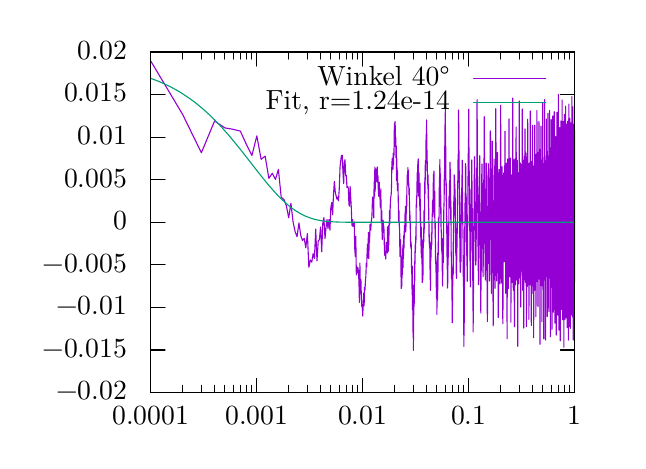
\begin{tikzpicture}[gnuplot]
%% generated with GNUPLOT 5.2p5a (Gentoo revision r0) (Lua 5.1; terminal rev. 99 , script rev. 107)
%% Sa 18 Mai 2019 18:31:05 CEST
\path (0.000,0.000) rectangle (7.500,5.250);
\gpcolor{color=gp lt color border}
\gpsetlinetype{gp lt border}
\gpsetdashtype{gp dt solid}
\gpsetlinewidth{1.00}
\draw[gp path] (1.564,0.616)--(1.744,0.616);
\draw[gp path] (6.947,0.616)--(6.767,0.616);
\node[gp node right] at (1.380,0.616) {$-0.02$};
\draw[gp path] (1.564,1.157)--(1.744,1.157);
\draw[gp path] (6.947,1.157)--(6.767,1.157);
\node[gp node right] at (1.380,1.157) {$-0.015$};
\draw[gp path] (1.564,1.697)--(1.744,1.697);
\draw[gp path] (6.947,1.697)--(6.767,1.697);
\node[gp node right] at (1.380,1.697) {$-0.01$};
\draw[gp path] (1.564,2.238)--(1.744,2.238);
\draw[gp path] (6.947,2.238)--(6.767,2.238);
\node[gp node right] at (1.380,2.238) {$-0.005$};
\draw[gp path] (1.564,2.779)--(1.744,2.779);
\draw[gp path] (6.947,2.779)--(6.767,2.779);
\node[gp node right] at (1.380,2.779) {$0$};
\draw[gp path] (1.564,3.319)--(1.744,3.319);
\draw[gp path] (6.947,3.319)--(6.767,3.319);
\node[gp node right] at (1.380,3.319) {$0.005$};
\draw[gp path] (1.564,3.860)--(1.744,3.860);
\draw[gp path] (6.947,3.860)--(6.767,3.860);
\node[gp node right] at (1.380,3.860) {$0.01$};
\draw[gp path] (1.564,4.400)--(1.744,4.400);
\draw[gp path] (6.947,4.400)--(6.767,4.400);
\node[gp node right] at (1.380,4.400) {$0.015$};
\draw[gp path] (1.564,4.941)--(1.744,4.941);
\draw[gp path] (6.947,4.941)--(6.767,4.941);
\node[gp node right] at (1.380,4.941) {$0.02$};
\draw[gp path] (1.564,0.616)--(1.564,0.796);
\draw[gp path] (1.564,4.941)--(1.564,4.761);
\node[gp node center] at (1.564,0.308) {$0.0001$};
\draw[gp path] (1.969,0.616)--(1.969,0.706);
\draw[gp path] (1.969,4.941)--(1.969,4.851);
\draw[gp path] (2.206,0.616)--(2.206,0.706);
\draw[gp path] (2.206,4.941)--(2.206,4.851);
\draw[gp path] (2.374,0.616)--(2.374,0.706);
\draw[gp path] (2.374,4.941)--(2.374,4.851);
\draw[gp path] (2.505,0.616)--(2.505,0.706);
\draw[gp path] (2.505,4.941)--(2.505,4.851);
\draw[gp path] (2.611,0.616)--(2.611,0.706);
\draw[gp path] (2.611,4.941)--(2.611,4.851);
\draw[gp path] (2.701,0.616)--(2.701,0.706);
\draw[gp path] (2.701,4.941)--(2.701,4.851);
\draw[gp path] (2.779,0.616)--(2.779,0.706);
\draw[gp path] (2.779,4.941)--(2.779,4.851);
\draw[gp path] (2.848,0.616)--(2.848,0.706);
\draw[gp path] (2.848,4.941)--(2.848,4.851);
\draw[gp path] (2.910,0.616)--(2.910,0.796);
\draw[gp path] (2.910,4.941)--(2.910,4.761);
\node[gp node center] at (2.910,0.308) {$0.001$};
\draw[gp path] (3.315,0.616)--(3.315,0.706);
\draw[gp path] (3.315,4.941)--(3.315,4.851);
\draw[gp path] (3.552,0.616)--(3.552,0.706);
\draw[gp path] (3.552,4.941)--(3.552,4.851);
\draw[gp path] (3.720,0.616)--(3.720,0.706);
\draw[gp path] (3.720,4.941)--(3.720,4.851);
\draw[gp path] (3.850,0.616)--(3.850,0.706);
\draw[gp path] (3.850,4.941)--(3.850,4.851);
\draw[gp path] (3.957,0.616)--(3.957,0.706);
\draw[gp path] (3.957,4.941)--(3.957,4.851);
\draw[gp path] (4.047,0.616)--(4.047,0.706);
\draw[gp path] (4.047,4.941)--(4.047,4.851);
\draw[gp path] (4.125,0.616)--(4.125,0.706);
\draw[gp path] (4.125,4.941)--(4.125,4.851);
\draw[gp path] (4.194,0.616)--(4.194,0.706);
\draw[gp path] (4.194,4.941)--(4.194,4.851);
\draw[gp path] (4.255,0.616)--(4.255,0.796);
\draw[gp path] (4.255,4.941)--(4.255,4.761);
\node[gp node center] at (4.255,0.308) {$0.01$};
\draw[gp path] (4.661,0.616)--(4.661,0.706);
\draw[gp path] (4.661,4.941)--(4.661,4.851);
\draw[gp path] (4.898,0.616)--(4.898,0.706);
\draw[gp path] (4.898,4.941)--(4.898,4.851);
\draw[gp path] (5.066,0.616)--(5.066,0.706);
\draw[gp path] (5.066,4.941)--(5.066,4.851);
\draw[gp path] (5.196,0.616)--(5.196,0.706);
\draw[gp path] (5.196,4.941)--(5.196,4.851);
\draw[gp path] (5.303,0.616)--(5.303,0.706);
\draw[gp path] (5.303,4.941)--(5.303,4.851);
\draw[gp path] (5.393,0.616)--(5.393,0.706);
\draw[gp path] (5.393,4.941)--(5.393,4.851);
\draw[gp path] (5.471,0.616)--(5.471,0.706);
\draw[gp path] (5.471,4.941)--(5.471,4.851);
\draw[gp path] (5.540,0.616)--(5.540,0.706);
\draw[gp path] (5.540,4.941)--(5.540,4.851);
\draw[gp path] (5.601,0.616)--(5.601,0.796);
\draw[gp path] (5.601,4.941)--(5.601,4.761);
\node[gp node center] at (5.601,0.308) {$0.1$};
\draw[gp path] (6.006,0.616)--(6.006,0.706);
\draw[gp path] (6.006,4.941)--(6.006,4.851);
\draw[gp path] (6.243,0.616)--(6.243,0.706);
\draw[gp path] (6.243,4.941)--(6.243,4.851);
\draw[gp path] (6.411,0.616)--(6.411,0.706);
\draw[gp path] (6.411,4.941)--(6.411,4.851);
\draw[gp path] (6.542,0.616)--(6.542,0.706);
\draw[gp path] (6.542,4.941)--(6.542,4.851);
\draw[gp path] (6.648,0.616)--(6.648,0.706);
\draw[gp path] (6.648,4.941)--(6.648,4.851);
\draw[gp path] (6.739,0.616)--(6.739,0.706);
\draw[gp path] (6.739,4.941)--(6.739,4.851);
\draw[gp path] (6.817,0.616)--(6.817,0.706);
\draw[gp path] (6.817,4.941)--(6.817,4.851);
\draw[gp path] (6.885,0.616)--(6.885,0.706);
\draw[gp path] (6.885,4.941)--(6.885,4.851);
\draw[gp path] (6.947,0.616)--(6.947,0.796);
\draw[gp path] (6.947,4.941)--(6.947,4.761);
\node[gp node center] at (6.947,0.308) {$1$};
\draw[gp path] (1.564,4.941)--(1.564,0.616)--(6.947,0.616)--(6.947,4.941)--cycle;
\node[gp node right] at (5.479,4.607) {Winkel 40°};
\gpcolor{rgb color={0.580,0.000,0.827}}
\draw[gp path] (5.663,4.607)--(6.579,4.607);
\draw[gp path] (1.564,4.825)--(1.969,4.146)--(2.206,3.662)--(2.374,4.065)--(2.505,3.977)%
  --(2.611,3.959)--(2.701,3.936)--(2.779,3.764)--(2.848,3.627)--(2.910,3.876)--(2.965,3.578)%
  --(3.016,3.619)--(3.063,3.336)--(3.106,3.401)--(3.147,3.323)--(3.184,3.450)--(3.220,3.095)%
  --(3.253,3.071)--(3.285,2.990)--(3.315,2.836)--(3.343,3.020)--(3.371,2.779)--(3.397,2.658)%
  --(3.421,2.595)--(3.445,2.770)--(3.468,2.611)--(3.490,2.547)--(3.512,2.574)--(3.532,2.455)%
  --(3.552,2.636)--(3.571,2.206)--(3.590,2.299)--(3.608,2.272)--(3.625,2.381)--(3.642,2.320)%
  --(3.658,2.692)--(3.674,2.288)--(3.690,2.539)--(3.705,2.559)--(3.720,2.718)--(3.734,2.403)%
  --(3.748,2.765)--(3.762,2.838)--(3.776,2.571)--(3.789,2.713)--(3.802,2.815)--(3.814,2.700)%
  --(3.827,2.815)--(3.839,2.678)--(3.850,2.964)--(3.862,3.030)--(3.873,2.875)--(3.884,3.134)%
  --(3.895,3.297)--(3.906,3.167)--(3.917,3.113)--(3.927,3.072)--(3.937,3.099)--(3.947,3.051)%
  --(3.957,3.201)--(3.967,3.479)--(3.976,3.560)--(3.985,3.628)--(3.995,3.629)--(4.004,3.416)%
  --(4.013,3.269)--(4.021,3.534)--(4.030,3.573)--(4.039,3.368)--(4.047,3.375)--(4.055,3.220)%
  --(4.064,3.235)--(4.072,3.212)--(4.080,3.006)--(4.087,2.983)--(4.095,3.236)--(4.103,3.088)%
  --(4.110,2.963)--(4.118,2.738)--(4.125,2.816)--(4.132,2.725)--(4.140,2.729)--(4.147,2.782)%
  --(4.154,2.441)--(4.161,2.342)--(4.167,2.600)--(4.174,2.109)--(4.181,2.216)--(4.187,2.135)%
  --(4.194,2.203)--(4.200,2.156)--(4.207,2.026)--(4.213,1.760)--(4.219,2.262)--(4.226,1.883)%
  --(4.232,2.053)--(4.238,1.815)--(4.244,1.703)--(4.250,1.714)--(4.256,1.587)--(4.261,1.759)%
  --(4.267,1.879)--(4.273,1.717)--(4.278,1.954)--(4.284,1.918)--(4.290,2.043)--(4.295,2.094)%
  --(4.300,2.260)--(4.306,2.212)--(4.311,2.414)--(4.316,2.502)--(4.322,2.327)--(4.327,2.650)%
  --(4.332,2.318)--(4.337,2.559)--(4.342,2.522)--(4.347,2.751)--(4.352,2.748)--(4.357,2.678)%
  --(4.362,2.772)--(4.367,2.811)--(4.372,2.852)--(4.376,2.990)--(4.381,3.100)--(4.386,2.959)%
  --(4.391,3.087)--(4.395,2.834)--(4.400,3.297)--(4.404,3.108)--(4.409,3.479)--(4.413,3.170)%
  --(4.418,3.458)--(4.422,3.452)--(4.427,3.383)--(4.431,3.303)--(4.435,3.291)--(4.439,3.481)%
  --(4.444,3.286)--(4.448,3.379)--(4.452,3.215)--(4.456,3.133)--(4.460,3.107)--(4.465,3.288)%
  --(4.469,3.117)--(4.473,3.163)--(4.477,2.988)--(4.481,2.964)--(4.485,3.204)--(4.489,2.839)%
  --(4.492,2.769)--(4.496,2.928)--(4.500,2.680)--(4.504,2.557)--(4.508,2.608)--(4.512,2.805)%
  --(4.515,2.793)--(4.519,2.653)--(4.523,2.730)--(4.527,2.638)--(4.530,2.432)--(4.534,2.363)%
  --(4.537,2.354)--(4.541,2.375)--(4.545,2.384)--(4.548,2.312)--(4.552,2.523)--(4.555,2.475)%
  --(4.559,2.499)--(4.562,2.462)--(4.566,2.388)--(4.569,2.719)--(4.572,2.554)--(4.576,2.555)%
  --(4.579,2.410)--(4.583,2.735)--(4.586,2.488)--(4.589,2.666)--(4.593,2.790)--(4.596,2.931)%
  --(4.599,2.757)--(4.602,2.868)--(4.605,2.999)--(4.609,3.084)--(4.612,3.106)--(4.615,3.115)%
  --(4.618,3.154)--(4.621,3.255)--(4.624,3.471)--(4.628,3.567)--(4.631,3.591)--(4.634,3.583)%
  --(4.637,3.500)--(4.640,3.451)--(4.643,3.657)--(4.646,3.511)--(4.649,3.637)--(4.652,3.633)%
  --(4.655,3.910)--(4.658,4.034)--(4.661,3.938)--(4.664,4.050)--(4.666,4.059)--(4.669,3.951)%
  --(4.672,3.736)--(4.675,3.857)--(4.678,3.598)--(4.681,3.748)--(4.684,3.308)--(4.686,3.614)%
  --(4.689,3.476)--(4.692,3.462)--(4.695,3.181)--(4.697,3.434)--(4.700,3.195)--(4.703,3.275)%
  --(4.706,3.090)--(4.708,2.967)--(4.711,2.784)--(4.714,2.934)--(4.716,2.915)--(4.719,2.743)%
  --(4.722,2.691)--(4.724,2.712)--(4.727,2.344)--(4.729,2.412)--(4.732,2.522)--(4.735,2.557)%
  --(4.737,2.340)--(4.740,2.461)--(4.742,2.053)--(4.745,1.937)--(4.747,2.238)--(4.750,1.960)%
  --(4.752,2.007)--(4.755,2.171)--(4.757,2.110)--(4.760,2.339)--(4.762,2.346)--(4.765,2.489)%
  --(4.767,2.200)--(4.770,2.437)--(4.772,2.318)--(4.774,2.609)--(4.777,2.482)--(4.779,2.449)%
  --(4.782,2.585)--(4.784,2.736)--(4.786,2.685)--(4.789,2.648)--(4.791,2.718)--(4.793,2.912)%
  --(4.796,2.656)--(4.798,2.981)--(4.800,2.664)--(4.803,2.672)--(4.805,2.760)--(4.807,2.889)%
  --(4.809,2.885)--(4.812,3.119)--(4.814,2.982)--(4.816,3.237)--(4.818,3.238)--(4.821,3.381)%
  --(4.823,3.302)--(4.825,3.426)--(4.827,3.412)--(4.829,3.473)--(4.832,3.260)--(4.834,3.441)%
  --(4.836,3.269)--(4.838,3.300)--(4.840,3.237)--(4.842,3.128)--(4.845,3.141)--(4.847,3.214)%
  --(4.849,2.975)--(4.851,2.981)--(4.853,2.796)--(4.855,2.869)--(4.857,2.839)--(4.859,2.728)%
  --(4.861,2.531)--(4.863,2.601)--(4.866,2.452)--(4.868,2.505)--(4.870,2.528)--(4.872,2.442)%
  --(4.874,2.318)--(4.876,2.120)--(4.878,2.160)--(4.880,2.192)--(4.882,1.856)--(4.884,2.222)%
  --(4.886,1.667)--(4.888,1.862)--(4.890,1.815)--(4.892,1.609)--(4.894,1.379)--(4.896,1.708)%
  --(4.898,1.152)--(4.900,1.695)--(4.901,1.280)--(4.903,1.982)--(4.905,1.603)--(4.907,1.952)%
  --(4.909,1.748)--(4.911,2.005)--(4.913,2.059)--(4.915,2.288)--(4.917,2.035)--(4.919,2.371)%
  --(4.921,2.489)--(4.922,2.444)--(4.924,2.393)--(4.926,2.521)--(4.928,2.597)--(4.930,2.517)%
  --(4.932,2.593)--(4.933,2.984)--(4.935,2.980)--(4.937,3.074)--(4.939,2.971)--(4.941,3.116)%
  --(4.943,3.121)--(4.944,3.170)--(4.946,3.407)--(4.948,3.173)--(4.950,3.252)--(4.952,3.496)%
  --(4.953,3.380)--(4.955,3.551)--(4.957,3.399)--(4.959,3.585)--(4.960,3.336)--(4.962,3.580)%
  --(4.964,3.110)--(4.966,3.397)--(4.967,3.351)--(4.969,3.412)--(4.971,3.120)--(4.972,3.216)%
  --(4.974,3.077)--(4.976,3.191)--(4.978,3.146)--(4.979,3.031)--(4.981,2.924)--(4.983,3.275)%
  --(4.984,2.772)--(4.986,3.071)--(4.988,2.838)--(4.989,2.781)--(4.991,2.589)--(4.993,2.782)%
  --(4.994,2.641)--(4.996,2.464)--(4.998,2.383)--(4.999,2.717)--(5.001,2.327)--(5.003,2.428)%
  --(5.004,2.410)--(5.006,2.558)--(5.007,2.298)--(5.009,2.227)--(5.011,2.013)--(5.012,2.179)%
  --(5.014,2.147)--(5.015,2.279)--(5.017,2.237)--(5.019,2.048)--(5.020,2.117)--(5.022,2.170)%
  --(5.023,2.447)--(5.025,2.590)--(5.026,2.512)--(5.028,2.627)--(5.030,2.526)--(5.031,2.764)%
  --(5.033,2.637)--(5.034,2.937)--(5.036,2.762)--(5.037,2.692)--(5.039,2.892)--(5.040,2.876)%
  --(5.042,3.256)--(5.043,3.277)--(5.045,3.346)--(5.046,3.285)--(5.048,3.141)--(5.049,3.507)%
  --(5.051,3.367)--(5.052,3.563)--(5.054,3.467)--(5.055,3.433)--(5.057,3.516)--(5.058,3.822)%
  --(5.060,3.718)--(5.061,3.748)--(5.063,3.940)--(5.064,3.561)--(5.066,4.078)--(5.067,3.934)%
  --(5.069,3.826)--(5.070,3.706)--(5.072,3.685)--(5.073,3.540)--(5.074,3.555)--(5.076,3.503)%
  --(5.077,3.287)--(5.079,3.295)--(5.080,3.258)--(5.082,3.258)--(5.083,3.205)--(5.084,3.380)%
  --(5.086,3.269)--(5.087,3.073)--(5.089,3.263)--(5.090,3.062)--(5.091,2.972)--(5.093,2.809)%
  --(5.094,2.958)--(5.096,2.591)--(5.097,2.761)--(5.098,2.699)--(5.100,2.513)--(5.101,2.624)%
  --(5.103,2.469)--(5.104,2.494)--(5.105,2.459)--(5.107,2.449)--(5.108,2.519)--(5.109,2.182)%
  --(5.111,2.186)--(5.112,2.051)--(5.113,2.184)--(5.115,1.913)--(5.116,2.137)--(5.117,2.373)%
  --(5.119,2.403)--(5.120,2.290)--(5.121,2.297)--(5.123,2.439)--(5.124,2.393)--(5.125,2.451)%
  --(5.127,2.632)--(5.128,2.646)--(5.129,2.569)--(5.131,2.521)--(5.132,2.614)--(5.133,2.493)%
  --(5.135,2.733)--(5.136,2.852)--(5.137,2.864)--(5.138,2.873)--(5.140,2.923)--(5.141,2.851)%
  --(5.142,3.061)--(5.144,2.870)--(5.145,3.059)--(5.146,2.881)--(5.147,2.908)--(5.149,3.112)%
  --(5.150,3.128)--(5.151,3.283)--(5.152,3.252)--(5.154,3.393)--(5.155,3.315)--(5.156,3.176)%
  --(5.157,3.318)--(5.159,3.430)--(5.160,3.423)--(5.161,3.115)--(5.162,3.237)--(5.164,3.027)%
  --(5.165,3.015)--(5.166,2.840)--(5.167,2.920)--(5.169,2.964)--(5.170,3.171)--(5.171,3.091)%
  --(5.172,2.831)--(5.173,2.696)--(5.175,2.733)--(5.176,2.778)--(5.177,2.530)--(5.178,2.616)%
  --(5.180,2.289)--(5.181,2.404)--(5.182,2.247)--(5.183,2.344)--(5.184,2.142)--(5.186,2.303)%
  --(5.187,2.259)--(5.188,1.958)--(5.189,2.123)--(5.190,2.006)--(5.191,1.893)--(5.193,1.810)%
  --(5.194,1.848)--(5.195,1.925)--(5.196,1.792)--(5.197,1.608)--(5.198,1.803)--(5.200,1.696)%
  --(5.201,1.975)--(5.202,1.844)--(5.203,2.035)--(5.204,2.065)--(5.205,2.274)--(5.207,1.789)%
  --(5.208,2.388)--(5.209,2.107)--(5.210,2.112)--(5.211,2.196)--(5.212,2.233)--(5.213,2.296)%
  --(5.215,2.545)--(5.216,2.616)--(5.217,2.830)--(5.218,2.694)--(5.219,2.669)--(5.220,2.828)%
  --(5.221,2.755)--(5.222,2.806)--(5.224,2.841)--(5.225,2.866)--(5.226,3.073)--(5.227,3.079)%
  --(5.228,3.309)--(5.229,3.088)--(5.230,3.280)--(5.231,3.367)--(5.232,3.188)--(5.233,3.447)%
  --(5.235,3.576)--(5.236,3.445)--(5.237,3.325)--(5.238,3.352)--(5.239,3.397)--(5.240,3.223)%
  --(5.241,3.036)--(5.242,2.977)--(5.243,3.188)--(5.244,3.032)--(5.245,3.178)--(5.247,2.827)%
  --(5.248,3.074)--(5.249,2.720)--(5.250,2.962)--(5.251,2.648)--(5.252,2.673)--(5.253,2.684)%
  --(5.254,2.673)--(5.255,2.478)--(5.256,2.521)--(5.257,2.561)--(5.258,2.553)--(5.259,2.413)%
  --(5.260,2.559)--(5.261,2.456)--(5.262,2.573)--(5.263,2.219)--(5.264,2.449)--(5.265,2.159)%
  --(5.267,2.345)--(5.268,2.137)--(5.269,1.969)--(5.270,2.118)--(5.271,2.252)--(5.272,2.097)%
  --(5.273,2.191)--(5.274,2.287)--(5.275,2.311)--(5.276,2.339)--(5.277,2.466)--(5.278,2.575)%
  --(5.279,2.266)--(5.280,2.428)--(5.281,2.649)--(5.282,2.646)--(5.283,2.937)--(5.284,2.806)%
  --(5.285,2.816)--(5.286,3.025)--(5.287,2.979)--(5.288,2.995)--(5.289,3.323)--(5.290,3.134)%
  --(5.291,3.231)--(5.292,3.289)--(5.293,3.429)--(5.294,3.314)--(5.295,3.566)--(5.296,3.410)%
  --(5.297,3.750)--(5.298,3.659)--(5.299,3.952)--(5.300,3.744)--(5.301,4.169)--(5.302,3.906)%
  --(5.303,4.116)--(5.304,3.719)--(5.305,4.224)--(5.306,3.738)--(5.307,3.803)--(5.308,3.722)%
  --(5.309,3.737)--(5.309,3.370)--(5.310,3.514)--(5.311,3.537)--(5.312,3.267)--(5.313,3.242)%
  --(5.314,3.314)--(5.315,3.315)--(5.316,3.044)--(5.317,3.108)--(5.318,3.129)--(5.319,2.823)%
  --(5.320,2.802)--(5.321,3.079)--(5.322,2.643)--(5.323,2.633)--(5.324,2.344)--(5.325,2.494)%
  --(5.326,2.656)--(5.327,2.562)--(5.327,2.548)--(5.328,2.377)--(5.329,2.178)--(5.330,2.276)%
  --(5.331,2.539)--(5.332,1.944)--(5.333,2.204)--(5.334,1.967)--(5.335,2.120)--(5.336,2.193)%
  --(5.337,2.311)--(5.338,2.237)--(5.339,2.233)--(5.340,2.280)--(5.340,2.252)--(5.341,2.396)%
  --(5.342,2.762)--(5.343,2.512)--(5.344,2.708)--(5.345,2.464)--(5.346,2.569)--(5.347,2.608)%
  --(5.348,2.684)--(5.349,2.696)--(5.349,2.898)--(5.350,2.951)--(5.351,3.097)--(5.352,3.115)%
  --(5.353,3.036)--(5.354,2.956)--(5.355,3.054)--(5.356,3.022)--(5.357,3.281)--(5.358,3.080)%
  --(5.358,3.270)--(5.359,3.300)--(5.360,3.305)--(5.361,3.315)--(5.362,3.459)--(5.363,3.500)%
  --(5.364,3.542)--(5.365,3.495)--(5.365,3.373)--(5.366,3.455)--(5.367,3.345)--(5.368,3.253)%
  --(5.369,3.257)--(5.370,3.226)--(5.371,3.177)--(5.372,2.965)--(5.372,3.099)--(5.373,2.952)%
  --(5.374,2.748)--(5.375,2.934)--(5.376,2.966)--(5.377,2.738)--(5.378,2.597)--(5.378,2.407)%
  --(5.379,2.346)--(5.380,2.403)--(5.381,2.205)--(5.382,2.062)--(5.383,2.171)--(5.384,2.176)%
  --(5.384,2.240)--(5.385,2.167)--(5.386,2.091)--(5.387,2.081)--(5.388,1.891)--(5.389,1.787)%
  --(5.389,1.882)--(5.390,1.923)--(5.391,1.661)--(5.392,1.503)--(5.393,1.523)--(5.394,1.537)%
  --(5.394,1.631)--(5.395,1.795)--(5.396,1.809)--(5.397,2.056)--(5.398,1.974)--(5.399,2.131)%
  --(5.399,2.115)--(5.400,2.063)--(5.401,2.204)--(5.402,2.198)--(5.403,2.232)--(5.404,2.524)%
  --(5.404,2.107)--(5.405,2.521)--(5.406,2.334)--(5.407,2.505)--(5.408,2.530)--(5.408,2.655)%
  --(5.409,2.730)--(5.410,2.684)--(5.411,3.040)--(5.412,2.876)--(5.412,3.114)--(5.413,2.844)%
  --(5.414,3.050)--(5.415,3.022)--(5.416,3.117)--(5.417,2.955)--(5.417,3.381)--(5.418,3.275)%
  --(5.419,3.341)--(5.420,3.319)--(5.421,3.239)--(5.421,3.305)--(5.422,3.269)--(5.423,3.253)%
  --(5.424,3.261)--(5.424,3.056)--(5.425,3.129)--(5.426,3.093)--(5.427,3.201)--(5.428,3.157)%
  --(5.428,2.997)--(5.429,3.080)--(5.430,2.896)--(5.431,2.856)--(5.432,3.085)--(5.432,2.815)%
  --(5.433,2.646)--(5.434,2.764)--(5.435,2.570)--(5.435,2.408)--(5.436,2.389)--(5.437,2.638)%
  --(5.438,2.406)--(5.439,2.465)--(5.439,2.544)--(5.440,2.365)--(5.441,2.325)--(5.442,2.379)%
  --(5.442,2.128)--(5.443,2.372)--(5.444,2.402)--(5.445,2.067)--(5.445,2.235)--(5.446,2.151)%
  --(5.447,2.202)--(5.448,2.575)--(5.448,2.067)--(5.449,2.616)--(5.450,2.299)--(5.451,2.550)%
  --(5.452,2.531)--(5.452,2.460)--(5.453,2.707)--(5.454,2.649)--(5.455,2.636)--(5.455,2.638)%
  --(5.456,2.746)--(5.457,2.896)--(5.458,2.769)--(5.458,2.797)--(5.459,3.027)--(5.460,3.136)%
  --(5.461,3.306)--(5.461,3.285)--(5.462,3.203)--(5.463,3.305)--(5.463,3.359)--(5.464,3.268)%
  --(5.465,3.574)--(5.466,3.287)--(5.466,3.282)--(5.467,3.533)--(5.468,3.528)--(5.469,3.654)%
  --(5.469,3.834)--(5.470,3.908)--(5.471,4.204)--(5.472,3.908)--(5.472,3.761)--(5.473,3.991)%
  --(5.474,3.960)--(5.474,4.037)--(5.475,3.620)--(5.476,3.647)--(5.477,3.478)--(5.477,3.704)%
  --(5.478,3.410)--(5.479,3.688)--(5.480,3.475)--(5.480,3.439)--(5.481,3.426)--(5.482,3.191)%
  --(5.482,3.156)--(5.483,3.151)--(5.484,3.038)--(5.485,2.992)--(5.485,2.878)--(5.486,3.157)%
  --(5.487,2.691)--(5.487,2.589)--(5.488,2.581)--(5.489,2.717)--(5.490,2.274)--(5.490,2.572)%
  --(5.491,2.422)--(5.492,2.435)--(5.492,2.288)--(5.493,2.416)--(5.494,2.143)--(5.494,2.229)%
  --(5.495,2.144)--(5.496,2.188)--(5.497,2.266)--(5.497,2.205)--(5.498,2.279)--(5.499,2.516)%
  --(5.499,2.303)--(5.500,2.551)--(5.501,2.500)--(5.501,2.533)--(5.502,2.672)--(5.503,2.695)%
  --(5.504,2.280)--(5.504,2.540)--(5.505,2.572)--(5.506,2.879)--(5.506,2.765)--(5.507,3.031)%
  --(5.508,2.956)--(5.508,2.809)--(5.509,3.122)--(5.510,2.933)--(5.510,2.896)--(5.511,3.011)%
  --(5.512,2.951)--(5.512,3.187)--(5.513,3.168)--(5.514,3.297)--(5.514,3.017)--(5.515,3.375)%
  --(5.516,3.206)--(5.516,3.334)--(5.517,3.343)--(5.518,3.172)--(5.519,3.568)--(5.519,3.338)%
  --(5.520,3.190)--(5.521,3.251)--(5.521,3.067)--(5.522,3.168)--(5.523,3.147)--(5.523,3.116)%
  --(5.524,2.942)--(5.525,2.751)--(5.525,2.752)--(5.526,2.834)--(5.527,2.907)--(5.527,2.761)%
  --(5.528,2.680)--(5.529,2.661)--(5.529,2.601)--(5.530,2.489)--(5.531,2.326)--(5.532,2.089)%
  --(5.532,2.361)--(5.533,2.078)--(5.534,2.161)--(5.534,1.960)--(5.535,2.191)--(5.536,1.810)%
  --(5.536,2.054)--(5.537,1.351)--(5.538,1.696)--(5.538,1.417)--(5.539,1.780)--(5.540,1.201)%
  --(5.540,1.463)--(5.541,1.337)--(5.542,1.599)--(5.542,1.690)--(5.543,2.010)--(5.544,1.502)%
  --(5.544,1.911)--(5.545,1.913)--(5.545,2.042)--(5.546,2.099)--(5.547,2.019)--(5.547,2.210)%
  --(5.548,2.291)--(5.549,2.449)--(5.549,2.400)--(5.550,2.530)--(5.551,2.540)--(5.551,2.654)%
  --(5.552,2.810)--(5.553,3.021)--(5.553,2.924)--(5.554,2.991)--(5.554,2.960)--(5.555,3.018)%
  --(5.556,3.153)--(5.556,2.896)--(5.557,3.084)--(5.558,3.059)--(5.558,3.204)--(5.559,3.257)%
  --(5.559,3.378)--(5.560,3.269)--(5.561,3.524)--(5.561,3.260)--(5.562,3.477)--(5.563,3.400)%
  --(5.563,3.488)--(5.564,3.109)--(5.564,3.175)--(5.565,3.110)--(5.566,3.125)--(5.566,2.957)%
  --(5.567,3.093)--(5.568,3.000)--(5.568,3.042)--(5.569,2.905)--(5.569,3.140)--(5.570,2.894)%
  --(5.571,2.637)--(5.571,2.809)--(5.572,2.723)--(5.573,2.520)--(5.573,2.795)--(5.574,2.641)%
  --(5.574,2.441)--(5.575,2.391)--(5.576,2.643)--(5.576,2.355)--(5.577,2.516)--(5.577,2.292)%
  --(5.578,2.380)--(5.579,2.542)--(5.579,2.335)--(5.580,2.302)--(5.580,2.227)--(5.581,2.179)%
  --(5.582,2.029)--(5.582,2.103)--(5.583,2.259)--(5.583,2.269)--(5.584,2.372)--(5.585,2.322)%
  --(5.585,2.331)--(5.586,2.522)--(5.586,2.591)--(5.587,2.516)--(5.588,2.684)--(5.588,2.831)%
  --(5.589,2.822)--(5.589,2.803)--(5.590,2.934)--(5.591,2.730)--(5.591,3.245)--(5.592,3.302)%
  --(5.592,3.240)--(5.593,3.409)--(5.594,3.418)--(5.594,3.256)--(5.595,3.655)--(5.595,3.323)%
  --(5.596,3.662)--(5.597,3.334)--(5.597,3.614)--(5.598,3.820)--(5.598,3.702)--(5.599,3.692)%
  --(5.599,3.839)--(5.600,4.003)--(5.601,4.006)--(5.601,4.214)--(5.602,4.080)--(5.602,4.172)%
  --(5.603,3.990)--(5.604,3.854)--(5.604,3.747)--(5.605,3.499)--(5.605,3.637)--(5.606,3.558)%
  --(5.606,3.541)--(5.607,3.386)--(5.608,3.378)--(5.608,3.261)--(5.609,3.420)--(5.609,3.425)%
  --(5.610,3.003)--(5.611,3.164)--(5.611,3.197)--(5.612,2.964)--(5.612,2.967)--(5.613,2.814)%
  --(5.613,2.769)--(5.614,2.668)--(5.615,3.010)--(5.615,2.611)--(5.616,2.640)--(5.616,2.840)%
  --(5.617,2.771)--(5.617,2.288)--(5.618,2.483)--(5.619,2.230)--(5.619,2.428)--(5.620,2.381)%
  --(5.620,2.223)--(5.621,2.038)--(5.621,2.297)--(5.622,1.958)--(5.622,2.178)--(5.623,2.430)%
  --(5.624,2.300)--(5.624,2.504)--(5.625,2.557)--(5.625,2.466)--(5.626,2.609)--(5.626,2.592)%
  --(5.627,2.569)--(5.628,2.419)--(5.628,2.634)--(5.629,2.921)--(5.629,2.507)--(5.630,2.819)%
  --(5.630,2.805)--(5.631,2.997)--(5.631,2.905)--(5.632,2.954)--(5.633,3.158)--(5.633,3.196)%
  --(5.634,2.939)--(5.634,3.024)--(5.635,3.137)--(5.635,3.103)--(5.636,3.149)--(5.636,3.224)%
  --(5.637,3.185)--(5.638,3.394)--(5.638,3.201)--(5.639,3.221)--(5.639,3.220)--(5.640,3.571)%
  --(5.640,3.294)--(5.641,3.242)--(5.641,3.128)--(5.642,3.301)--(5.642,3.125)--(5.643,3.302)%
  --(5.644,3.004)--(5.644,2.911)--(5.645,2.968)--(5.645,3.006)--(5.646,2.846)--(5.646,2.956)%
  --(5.647,2.863)--(5.647,2.613)--(5.648,2.824)--(5.648,2.389)--(5.649,2.445)--(5.649,2.537)%
  --(5.650,2.400)--(5.651,2.205)--(5.651,2.393)--(5.652,2.039)--(5.652,2.227)--(5.653,2.230)%
  --(5.653,2.205)--(5.654,2.430)--(5.654,1.964)--(5.655,1.790)--(5.655,1.792)--(5.656,1.652)%
  --(5.656,1.787)--(5.657,1.664)--(5.657,1.385)--(5.658,1.495)--(5.659,1.517)--(5.659,1.787)%
  --(5.660,1.943)--(5.660,1.856)--(5.661,1.700)--(5.661,2.072)--(5.662,1.874)--(5.662,2.168)%
  --(5.663,2.042)--(5.663,2.272)--(5.664,2.199)--(5.664,2.347)--(5.665,2.288)--(5.665,2.547)%
  --(5.666,2.788)--(5.666,2.466)--(5.667,2.677)--(5.667,2.639)--(5.668,2.703)--(5.669,2.972)%
  --(5.669,2.793)--(5.670,2.831)--(5.670,2.982)--(5.671,3.225)--(5.671,2.945)--(5.672,2.902)%
  --(5.672,3.382)--(5.673,3.361)--(5.673,3.282)--(5.674,3.612)--(5.674,3.390)--(5.675,3.417)%
  --(5.675,3.584)--(5.676,3.479)--(5.676,3.199)--(5.677,3.414)--(5.677,3.337)--(5.678,3.297)%
  --(5.678,3.236)--(5.679,3.217)--(5.679,2.852)--(5.680,3.070)--(5.680,2.769)--(5.681,3.022)%
  --(5.681,2.841)--(5.682,3.041)--(5.682,2.939)--(5.683,2.962)--(5.683,2.848)--(5.684,2.676)%
  --(5.684,2.761)--(5.685,2.795)--(5.685,2.532)--(5.686,2.725)--(5.686,2.591)--(5.687,2.545)%
  --(5.687,2.624)--(5.688,2.731)--(5.688,2.541)--(5.689,2.537)--(5.690,2.244)--(5.690,2.234)%
  --(5.691,2.331)--(5.691,2.387)--(5.692,2.427)--(5.692,2.250)--(5.693,2.286)--(5.693,2.348)%
  --(5.694,2.294)--(5.694,2.286)--(5.695,2.472)--(5.695,2.477)--(5.696,2.510)--(5.696,2.765)%
  --(5.696,2.553)--(5.697,2.601)--(5.697,2.651)--(5.698,2.769)--(5.698,2.693)--(5.699,2.911)%
  --(5.699,2.944)--(5.700,3.208)--(5.700,3.462)--(5.701,3.131)--(5.701,3.379)--(5.702,3.391)%
  --(5.702,3.429)--(5.703,3.392)--(5.703,3.344)--(5.704,3.492)--(5.704,3.486)--(5.705,3.807)%
  --(5.705,3.389)--(5.706,3.980)--(5.706,3.567)--(5.707,4.308)--(5.707,4.113)--(5.708,4.338)%
  --(5.708,3.984)--(5.709,4.084)--(5.709,3.713)--(5.710,3.840)--(5.710,3.666)--(5.711,3.805)%
  --(5.711,3.749)--(5.712,3.455)--(5.712,3.533)--(5.713,3.427)--(5.713,3.304)--(5.714,3.422)%
  --(5.714,3.160)--(5.715,3.304)--(5.715,3.163)--(5.716,2.988)--(5.716,2.898)--(5.717,2.959)%
  --(5.717,2.710)--(5.717,2.873)--(5.718,2.665)--(5.718,2.563)--(5.719,2.615)--(5.719,2.471)%
  --(5.720,2.488)--(5.720,2.300)--(5.721,2.455)--(5.721,2.591)--(5.722,2.246)--(5.722,2.233)%
  --(5.723,2.154)--(5.723,2.266)--(5.724,1.987)--(5.724,2.171)--(5.725,2.030)--(5.725,2.346)%
  --(5.726,2.263)--(5.726,2.350)--(5.727,2.455)--(5.727,2.451)--(5.727,2.436)--(5.728,2.591)%
  --(5.728,2.319)--(5.729,2.678)--(5.729,2.531)--(5.730,2.731)--(5.730,2.688)--(5.731,2.604)%
  --(5.731,2.741)--(5.732,2.812)--(5.732,2.762)--(5.733,2.823)--(5.733,2.758)--(5.734,2.864)%
  --(5.734,2.931)--(5.734,3.135)--(5.735,3.097)--(5.735,3.230)--(5.736,2.965)--(5.736,3.232)%
  --(5.737,3.250)--(5.737,3.326)--(5.738,3.162)--(5.738,3.348)--(5.739,3.362)--(5.739,3.443)%
  --(5.740,3.223)--(5.740,3.522)--(5.740,3.327)--(5.741,3.624)--(5.741,3.255)--(5.742,3.171)%
  --(5.742,3.112)--(5.743,2.981)--(5.743,2.929)--(5.744,2.871)--(5.744,2.742)--(5.745,2.819)%
  --(5.745,3.026)--(5.746,2.595)--(5.746,2.586)--(5.746,2.573)--(5.747,2.578)--(5.747,2.485)%
  --(5.748,2.517)--(5.748,2.636)--(5.749,2.408)--(5.749,2.357)--(5.750,2.223)--(5.750,2.242)%
  --(5.751,1.988)--(5.751,2.009)--(5.751,2.027)--(5.752,2.043)--(5.752,1.858)--(5.753,2.075)%
  --(5.753,1.651)--(5.754,1.730)--(5.754,1.856)--(5.755,1.748)--(5.755,1.625)--(5.755,1.657)%
  --(5.756,1.944)--(5.756,1.855)--(5.757,1.979)--(5.757,2.108)--(5.758,2.109)--(5.758,2.065)%
  --(5.759,2.200)--(5.759,2.111)--(5.760,2.184)--(5.760,2.163)--(5.760,2.360)--(5.761,2.323)%
  --(5.761,2.621)--(5.762,2.369)--(5.762,2.443)--(5.763,2.440)--(5.763,2.660)--(5.764,2.761)%
  --(5.764,2.881)--(5.764,2.915)--(5.765,2.891)--(5.765,3.004)--(5.766,2.846)--(5.766,3.207)%
  --(5.767,3.126)--(5.767,3.161)--(5.767,3.391)--(5.768,3.289)--(5.768,3.430)--(5.769,3.289)%
  --(5.769,3.423)--(5.770,3.464)--(5.770,3.519)--(5.771,3.436)--(5.771,3.355)--(5.771,3.477)%
  --(5.772,3.512)--(5.772,3.290)--(5.773,3.253)--(5.773,3.262)--(5.774,3.171)--(5.774,3.069)%
  --(5.774,3.061)--(5.775,3.053)--(5.775,2.876)--(5.776,2.860)--(5.776,2.762)--(5.777,2.778)%
  --(5.777,2.722)--(5.778,2.783)--(5.778,2.883)--(5.778,2.677)--(5.779,2.634)--(5.779,2.571)%
  --(5.780,2.488)--(5.780,2.480)--(5.781,2.553)--(5.781,2.489)--(5.781,2.465)--(5.782,2.371)%
  --(5.782,2.269)--(5.783,2.157)--(5.783,2.155)--(5.784,2.088)--(5.784,2.390)--(5.784,2.161)%
  --(5.785,2.276)--(5.785,2.263)--(5.786,2.418)--(5.786,2.218)--(5.787,2.468)--(5.787,2.446)%
  --(5.787,2.742)--(5.788,2.656)--(5.788,2.670)--(5.789,2.540)--(5.789,2.586)--(5.789,2.503)%
  --(5.790,2.609)--(5.790,2.856)--(5.791,2.838)--(5.791,2.910)--(5.792,3.079)--(5.792,3.093)%
  --(5.792,3.316)--(5.793,3.123)--(5.793,3.283)--(5.794,3.172)--(5.794,3.218)--(5.795,3.443)%
  --(5.795,3.422)--(5.795,3.591)--(5.796,3.498)--(5.796,3.629)--(5.797,3.889)--(5.797,3.790)%
  --(5.797,4.015)--(5.798,4.119)--(5.798,4.101)--(5.799,3.899)--(5.799,4.102)--(5.800,3.812)%
  --(5.800,3.852)--(5.800,3.658)--(5.801,3.588)--(5.801,3.443)--(5.802,3.662)--(5.802,3.272)%
  --(5.802,3.232)--(5.803,3.303)--(5.803,3.445)--(5.804,3.147)--(5.804,3.219)--(5.805,3.061)%
  --(5.805,3.021)--(5.805,2.861)--(5.806,2.883)--(5.806,2.895)--(5.807,2.677)--(5.807,2.510)%
  --(5.807,2.551)--(5.808,2.384)--(5.808,2.669)--(5.809,2.528)--(5.809,2.660)--(5.809,2.187)%
  --(5.810,2.106)--(5.810,2.380)--(5.811,2.133)--(5.811,2.395)--(5.812,2.220)--(5.812,2.074)%
  --(5.812,2.045)--(5.813,2.077)--(5.813,2.252)--(5.814,2.161)--(5.814,2.212)--(5.814,2.373)%
  --(5.815,2.506)--(5.815,2.369)--(5.816,2.492)--(5.816,2.518)--(5.816,2.514)--(5.817,2.456)%
  --(5.817,2.750)--(5.818,2.630)--(5.818,2.735)--(5.818,2.795)--(5.819,2.858)--(5.819,2.775)%
  --(5.820,2.866)--(5.820,2.869)--(5.820,2.928)--(5.821,2.902)--(5.821,2.929)--(5.822,2.972)%
  --(5.822,3.008)--(5.822,2.968)--(5.823,3.112)--(5.823,2.975)--(5.824,3.252)--(5.824,3.181)%
  --(5.824,3.530)--(5.825,3.227)--(5.825,3.319)--(5.826,3.119)--(5.826,3.300)--(5.826,3.402)%
  --(5.827,3.269)--(5.827,3.372)--(5.828,3.339)--(5.828,3.187)--(5.828,2.853)--(5.829,3.119)%
  --(5.829,3.025)--(5.830,2.941)--(5.830,2.944)--(5.830,2.879)--(5.831,2.879)--(5.831,2.539)%
  --(5.832,2.710)--(5.832,2.572)--(5.832,2.422)--(5.833,2.255)--(5.833,2.512)--(5.834,2.134)%
  --(5.834,2.327)--(5.834,2.019)--(5.835,2.135)--(5.835,1.968)--(5.835,2.095)--(5.836,1.808)%
  --(5.836,2.033)--(5.837,1.619)--(5.837,1.980)--(5.837,1.618)--(5.838,1.742)--(5.838,1.589)%
  --(5.839,1.693)--(5.839,1.518)--(5.839,1.648)--(5.840,1.611)--(5.840,2.024)--(5.841,1.792)%
  --(5.841,2.152)--(5.841,2.083)--(5.842,2.195)--(5.842,2.083)--(5.842,2.285)--(5.843,2.247)%
  --(5.843,2.326)--(5.844,2.470)--(5.844,2.393)--(5.844,2.437)--(5.845,2.498)--(5.845,2.660)%
  --(5.846,2.665)--(5.846,2.704)--(5.846,2.866)--(5.847,2.933)--(5.847,3.026)--(5.848,3.073)%
  --(5.848,3.171)--(5.848,2.772)--(5.849,3.058)--(5.849,2.993)--(5.849,3.286)--(5.850,3.430)%
  --(5.850,3.522)--(5.851,3.188)--(5.851,3.437)--(5.851,3.136)--(5.852,3.265)--(5.852,3.272)%
  --(5.852,3.461)--(5.853,3.116)--(5.853,3.226)--(5.854,3.053)--(5.854,2.972)--(5.854,3.100)%
  --(5.855,3.148)--(5.855,2.921)--(5.856,2.960)--(5.856,2.811)--(5.856,3.039)--(5.857,3.060)%
  --(5.857,2.827)--(5.857,2.763)--(5.858,2.722)--(5.858,2.549)--(5.859,2.790)--(5.859,2.564)%
  --(5.859,2.515)--(5.860,2.558)--(5.860,2.438)--(5.860,2.505)--(5.861,2.507)--(5.861,2.321)%
  --(5.862,2.444)--(5.862,2.430)--(5.862,2.302)--(5.863,2.215)--(5.863,2.103)--(5.863,2.144)%
  --(5.864,2.134)--(5.864,2.032)--(5.865,2.218)--(5.865,2.361)--(5.865,2.151)--(5.866,2.450)%
  --(5.866,2.349)--(5.866,2.416)--(5.867,2.656)--(5.867,2.463)--(5.867,2.579)--(5.868,2.637)%
  --(5.868,2.668)--(5.869,2.722)--(5.869,2.952)--(5.869,2.798)--(5.870,3.219)--(5.870,2.885)%
  --(5.870,3.087)--(5.871,3.094)--(5.871,3.254)--(5.872,3.287)--(5.872,3.236)--(5.872,3.331)%
  --(5.873,3.442)--(5.873,3.485)--(5.873,3.553)--(5.874,3.439)--(5.874,3.409)--(5.874,3.535)%
  --(5.875,3.521)--(5.875,3.927)--(5.876,3.867)--(5.876,3.818)--(5.876,3.939)--(5.877,3.829)%
  --(5.877,3.881)--(5.877,3.900)--(5.878,3.625)--(5.878,3.613)--(5.878,3.323)--(5.879,3.494)%
  --(5.879,3.245)--(5.880,3.476)--(5.880,3.227)--(5.880,3.444)--(5.881,3.460)--(5.881,3.241)%
  --(5.881,3.098)--(5.882,3.259)--(5.882,2.920)--(5.882,2.966)--(5.883,2.900)--(5.883,2.993)%
  --(5.884,2.833)--(5.884,2.552)--(5.884,2.742)--(5.885,2.631)--(5.885,2.606)--(5.885,2.570)%
  --(5.886,2.636)--(5.886,2.472)--(5.886,2.399)--(5.887,2.369)--(5.887,2.157)--(5.888,2.422)%
  --(5.888,2.037)--(5.888,2.259)--(5.889,1.874)--(5.889,2.187)--(5.889,2.229)--(5.890,2.136)%
  --(5.890,2.223)--(5.890,2.209)--(5.891,2.476)--(5.891,2.464)--(5.891,2.469)--(5.892,2.568)%
  --(5.892,2.607)--(5.893,2.654)--(5.893,2.517)--(5.893,2.440)--(5.894,2.599)--(5.894,2.701)%
  --(5.894,2.735)--(5.895,2.989)--(5.895,3.011)--(5.895,3.046)--(5.896,2.927)--(5.896,2.935)%
  --(5.896,3.131)--(5.897,3.087)--(5.897,3.402)--(5.898,3.085)--(5.898,3.230)--(5.899,3.325)%
  --(5.899,3.390)--(5.899,3.293)--(5.900,3.519)--(5.900,3.198)--(5.900,3.809)--(5.901,3.240)%
  --(5.901,3.352)--(5.901,3.097)--(5.902,3.187)--(5.902,3.038)--(5.902,3.077)--(5.903,2.998)%
  --(5.903,2.897)--(5.903,3.056)--(5.904,3.013)--(5.904,2.933)--(5.904,2.913)--(5.905,2.719)%
  --(5.905,2.725)--(5.906,2.666)--(5.906,2.400)--(5.906,2.684)--(5.907,2.205)--(5.907,2.341)%
  --(5.907,2.346)--(5.908,2.238)--(5.908,2.310)--(5.908,2.328)--(5.909,2.139)--(5.909,2.122)%
  --(5.909,2.147)--(5.910,1.824)--(5.910,1.925)--(5.910,1.772)--(5.911,1.870)--(5.911,1.466)%
  --(5.911,1.514)--(5.912,1.510)--(5.912,1.611)--(5.912,1.463)--(5.913,1.707)--(5.913,1.719)%
  --(5.913,1.726)--(5.914,1.666)--(5.914,2.014)--(5.914,1.861)--(5.915,2.109)--(5.915,1.986)%
  --(5.915,2.164)--(5.916,2.040)--(5.916,2.218)--(5.917,2.056)--(5.917,2.305)--(5.917,2.501)%
  --(5.918,2.674)--(5.918,2.602)--(5.918,2.795)--(5.919,2.744)--(5.919,2.954)--(5.919,2.834)%
  --(5.920,2.961)--(5.920,2.987)--(5.920,3.101)--(5.921,3.110)--(5.921,3.033)--(5.921,3.144)%
  --(5.922,3.375)--(5.922,3.210)--(5.922,3.327)--(5.923,3.183)--(5.923,3.270)--(5.923,3.367)%
  --(5.924,3.581)--(5.924,3.289)--(5.924,3.323)--(5.925,3.169)--(5.925,3.122)--(5.925,2.977)%
  --(5.926,3.112)--(5.926,2.872)--(5.926,3.006)--(5.927,3.000)--(5.927,3.176)--(5.927,2.820)%
  --(5.928,2.834)--(5.928,2.799)--(5.928,2.656)--(5.929,2.637)--(5.929,2.707)--(5.929,2.902)%
  --(5.930,2.642)--(5.930,2.524)--(5.930,2.574)--(5.931,2.491)--(5.931,2.447)--(5.931,2.454)%
  --(5.932,2.246)--(5.932,2.295)--(5.932,2.339)--(5.933,2.132)--(5.933,2.113)--(5.933,2.074)%
  --(5.934,2.311)--(5.934,1.960)--(5.934,2.194)--(5.935,2.145)--(5.935,1.939)--(5.935,1.950)%
  --(5.936,2.203)--(5.936,2.265)--(5.936,2.255)--(5.937,2.506)--(5.937,2.425)--(5.937,2.336)%
  --(5.938,2.589)--(5.938,2.720)--(5.938,2.567)--(5.939,2.648)--(5.939,2.651)--(5.939,2.813)%
  --(5.940,2.836)--(5.940,3.106)--(5.940,3.020)--(5.941,3.122)--(5.941,3.342)--(5.941,3.372)%
  --(5.942,3.500)--(5.942,3.318)--(5.942,3.580)--(5.943,3.518)--(5.943,3.525)--(5.943,3.517)%
  --(5.943,3.737)--(5.944,3.624)--(5.944,4.049)--(5.944,3.833)--(5.945,4.221)--(5.945,3.854)%
  --(5.945,4.085)--(5.946,3.697)--(5.946,3.786)--(5.946,3.778)--(5.947,3.725)--(5.947,3.701)%
  --(5.947,3.792)--(5.948,3.177)--(5.948,3.319)--(5.948,3.232)--(5.949,3.274)--(5.949,3.322)%
  --(5.949,3.146)--(5.950,3.022)--(5.950,3.195)--(5.950,2.974)--(5.951,2.842)--(5.951,2.808)%
  --(5.951,2.616)--(5.952,2.691)--(5.952,2.947)--(5.952,2.666)--(5.953,2.583)--(5.953,2.611)%
  --(5.953,2.646)--(5.953,2.437)--(5.954,2.479)--(5.954,2.186)--(5.954,2.236)--(5.955,2.033)%
  --(5.955,2.333)--(5.955,2.125)--(5.956,2.601)--(5.956,2.252)--(5.956,2.301)--(5.957,2.299)%
  --(5.957,2.637)--(5.957,2.171)--(5.958,2.375)--(5.958,2.355)--(5.958,2.601)--(5.959,2.434)%
  --(5.959,2.528)--(5.959,2.703)--(5.960,2.541)--(5.960,2.470)--(5.960,2.754)--(5.960,2.662)%
  --(5.961,2.762)--(5.961,2.608)--(5.961,2.732)--(5.962,3.019)--(5.962,2.945)--(5.962,2.950)%
  --(5.963,3.076)--(5.963,3.037)--(5.963,3.132)--(5.964,3.161)--(5.964,3.297)--(5.964,3.185)%
  --(5.965,3.304)--(5.965,2.981)--(5.965,3.471)--(5.966,3.450)--(5.966,3.388)--(5.966,3.367)%
  --(5.966,3.348)--(5.967,3.665)--(5.967,3.292)--(5.967,3.428)--(5.968,2.999)--(5.968,3.018)%
  --(5.968,3.098)--(5.969,3.049)--(5.969,3.048)--(5.969,2.880)--(5.970,2.919)--(5.970,2.776)%
  --(5.970,2.451)--(5.971,2.878)--(5.971,2.574)--(5.971,2.524)--(5.971,2.462)--(5.972,2.443)%
  --(5.972,2.388)--(5.972,2.217)--(5.973,2.371)--(5.973,2.235)--(5.973,2.232)--(5.974,2.094)%
  --(5.974,2.149)--(5.974,2.121)--(5.975,1.894)--(5.975,1.927)--(5.975,2.003)--(5.975,2.045)%
  --(5.976,1.567)--(5.976,1.641)--(5.976,1.757)--(5.977,1.682)--(5.977,1.673)--(5.977,1.727)%
  --(5.978,1.735)--(5.978,1.970)--(5.978,1.769)--(5.979,1.855)--(5.979,1.930)--(5.979,1.996)%
  --(5.979,2.028)--(5.980,2.251)--(5.980,2.248)--(5.980,2.232)--(5.981,1.974)--(5.981,2.347)%
  --(5.981,2.248)--(5.982,2.509)--(5.982,2.676)--(5.982,2.670)--(5.983,2.795)--(5.983,2.739)%
  --(5.983,2.748)--(5.983,2.621)--(5.984,2.797)--(5.984,2.981)--(5.984,3.254)--(5.985,3.156)%
  --(5.985,3.025)--(5.985,3.134)--(5.986,3.364)--(5.986,3.143)--(5.986,3.409)--(5.986,3.353)%
  --(5.987,3.393)--(5.987,3.429)--(5.987,3.237)--(5.988,3.286)--(5.988,3.448)--(5.988,3.272)%
  --(5.989,3.364)--(5.989,3.174)--(5.989,3.117)--(5.989,3.104)--(5.990,3.138)--(5.990,2.885)%
  --(5.990,2.948)--(5.991,2.986)--(5.991,2.949)--(5.991,2.995)--(5.992,2.746)--(5.992,2.822)%
  --(5.992,2.644)--(5.992,2.725)--(5.993,2.602)--(5.993,2.980)--(5.993,2.401)--(5.994,2.671)%
  --(5.994,2.595)--(5.994,2.603)--(5.995,2.341)--(5.995,2.523)--(5.995,2.406)--(5.995,2.375)%
  --(5.996,2.275)--(5.996,2.268)--(5.996,1.996)--(5.997,2.300)--(5.997,2.201)--(5.997,2.341)%
  --(5.998,2.061)--(5.998,2.262)--(5.998,2.416)--(5.998,2.468)--(5.999,2.623)--(5.999,2.519)%
  --(5.999,2.522)--(6.000,2.462)--(6.000,2.482)--(6.000,2.792)--(6.000,2.765)--(6.001,2.582)%
  --(6.001,2.642)--(6.001,2.905)--(6.002,3.188)--(6.002,2.975)--(6.002,3.167)--(6.003,3.182)%
  --(6.003,3.418)--(6.003,3.356)--(6.003,3.313)--(6.004,3.541)--(6.004,3.530)--(6.004,3.433)%
  --(6.005,3.462)--(6.005,3.780)--(6.005,3.749)--(6.005,3.849)--(6.006,3.817)--(6.006,4.221)%
  --(6.006,3.797)--(6.007,4.264)--(6.007,4.091)--(6.007,4.136)--(6.008,3.774)--(6.008,3.877)%
  --(6.008,3.596)--(6.008,3.896)--(6.009,3.441)--(6.009,3.654)--(6.009,3.543)--(6.010,3.648)%
  --(6.010,3.570)--(6.010,3.478)--(6.010,3.368)--(6.011,3.244)--(6.011,3.215)--(6.011,3.220)%
  --(6.012,2.960)--(6.012,2.897)--(6.012,2.627)--(6.012,2.663)--(6.013,2.635)--(6.013,2.777)%
  --(6.013,2.598)--(6.014,2.545)--(6.014,2.522)--(6.014,2.597)--(6.014,2.183)--(6.015,2.371)%
  --(6.015,2.394)--(6.015,2.338)--(6.016,2.229)--(6.016,2.127)--(6.016,2.058)--(6.017,2.132)%
  --(6.017,2.006)--(6.017,2.104)--(6.017,2.365)--(6.018,2.375)--(6.018,2.378)--(6.018,2.607)%
  --(6.019,2.551)--(6.019,2.572)--(6.019,2.430)--(6.019,2.752)--(6.020,2.479)--(6.020,2.649)%
  --(6.020,2.577)--(6.021,2.907)--(6.021,2.563)--(6.021,2.732)--(6.021,2.903)--(6.022,2.892)%
  --(6.022,2.859)--(6.022,3.072)--(6.023,2.955)--(6.023,3.162)--(6.023,3.193)--(6.023,3.272)%
  --(6.024,3.221)--(6.024,3.355)--(6.024,3.095)--(6.024,3.485)--(6.025,3.361)--(6.025,3.453)%
  --(6.025,3.310)--(6.026,3.420)--(6.026,3.473)--(6.026,3.451)--(6.026,3.404)--(6.027,3.325)%
  --(6.027,3.152)--(6.027,3.182)--(6.028,3.230)--(6.028,3.096)--(6.028,3.041)--(6.028,2.912)%
  --(6.029,2.989)--(6.029,3.013)--(6.029,2.873)--(6.030,2.790)--(6.030,2.751)--(6.030,2.629)%
  --(6.030,2.644)--(6.031,2.546)--(6.031,2.249)--(6.031,2.431)--(6.032,2.131)--(6.032,2.196)%
  --(6.032,1.965)--(6.032,2.097)--(6.033,2.158)--(6.033,2.050)--(6.033,1.859)--(6.033,1.824)%
  --(6.034,1.762)--(6.034,1.812)--(6.034,1.552)--(6.035,1.675)--(6.035,1.502)--(6.035,1.666)%
  --(6.035,1.489)--(6.036,1.694)--(6.036,1.842)--(6.037,1.752)--(6.037,1.998)--(6.037,1.963)%
  --(6.037,1.960)--(6.038,2.116)--(6.038,2.303)--(6.038,2.295)--(6.038,2.446)--(6.039,2.285)%
  --(6.039,2.291)--(6.039,2.542)--(6.040,2.377)--(6.040,2.738)--(6.040,2.530)--(6.040,2.774)%
  --(6.041,2.654)--(6.041,2.998)--(6.041,2.992)--(6.042,2.958)--(6.042,3.172)--(6.042,2.703)%
  --(6.042,3.176)--(6.043,3.276)--(6.043,3.156)--(6.043,3.309)--(6.043,3.327)--(6.044,3.175)%
  --(6.044,3.387)--(6.044,3.251)--(6.045,3.405)--(6.045,3.217)--(6.045,3.305)--(6.045,2.995)%
  --(6.046,3.273)--(6.046,3.314)--(6.046,3.312)--(6.046,3.052)--(6.047,3.085)--(6.047,3.041)%
  --(6.047,3.075)--(6.048,2.967)--(6.048,3.163)--(6.048,2.789)--(6.048,3.047)--(6.049,2.865)%
  --(6.049,2.843)--(6.049,2.539)--(6.049,2.824)--(6.050,2.706)--(6.050,2.653)--(6.050,2.614)%
  --(6.051,2.691)--(6.051,2.790)--(6.051,2.441)--(6.051,2.418)--(6.052,2.528)--(6.052,2.373)%
  --(6.052,2.675)--(6.052,2.277)--(6.053,2.439)--(6.053,2.318)--(6.053,2.357)--(6.054,2.314)%
  --(6.054,2.306)--(6.054,2.398)--(6.054,2.436)--(6.055,2.308)--(6.055,2.467)--(6.055,2.630)%
  --(6.055,2.592)--(6.056,2.647)--(6.056,2.516)--(6.056,2.705)--(6.056,2.765)--(6.057,2.720)%
  --(6.057,2.881)--(6.057,2.933)--(6.058,3.057)--(6.058,2.947)--(6.058,3.252)--(6.058,3.254)%
  --(6.059,3.501)--(6.059,3.350)--(6.059,3.333)--(6.059,3.273)--(6.060,3.367)--(6.060,3.266)%
  --(6.060,3.622)--(6.060,3.625)--(6.061,3.498)--(6.061,3.307)--(6.061,3.712)--(6.062,3.936)%
  --(6.062,3.572)--(6.062,3.851)--(6.062,3.932)--(6.063,3.764)--(6.063,3.777)--(6.063,3.823)%
  --(6.063,3.745)--(6.064,3.755)--(6.064,3.513)--(6.064,3.401)--(6.064,3.492)--(6.065,3.338)%
  --(6.065,3.506)--(6.065,3.276)--(6.066,3.522)--(6.066,3.469)--(6.066,3.171)--(6.066,3.060)%
  --(6.067,3.221)--(6.067,3.118)--(6.067,2.860)--(6.067,3.030)--(6.068,2.700)--(6.068,2.769)%
  --(6.068,2.822)--(6.068,2.829)--(6.069,2.519)--(6.069,2.443)--(6.069,2.522)--(6.069,2.471)%
  --(6.070,2.431)--(6.070,2.288)--(6.070,2.150)--(6.071,2.158)--(6.071,2.126)--(6.071,2.123)%
  --(6.071,1.876)--(6.072,2.128)--(6.072,2.141)--(6.072,2.170)--(6.072,2.216)--(6.073,2.341)%
  --(6.073,2.452)--(6.073,2.273)--(6.073,2.318)--(6.074,2.396)--(6.074,2.346)--(6.074,2.480)%
  --(6.074,2.694)--(6.075,2.624)--(6.075,2.644)--(6.075,2.650)--(6.075,2.697)--(6.076,2.924)%
  --(6.076,2.936)--(6.076,2.807)--(6.076,2.863)--(6.077,2.943)--(6.077,3.030)--(6.077,3.050)%
  --(6.078,3.037)--(6.078,3.226)--(6.078,3.074)--(6.078,3.171)--(6.079,3.335)--(6.079,3.319)%
  --(6.079,3.182)--(6.079,3.420)--(6.080,3.292)--(6.080,3.529)--(6.080,3.180)--(6.080,3.502)%
  --(6.081,3.097)--(6.081,3.424)--(6.081,3.032)--(6.081,3.232)--(6.082,3.025)--(6.082,3.044)%
  --(6.082,3.035)--(6.082,2.962)--(6.083,2.883)--(6.083,2.834)--(6.083,2.946)--(6.083,2.900)%
  --(6.084,2.653)--(6.084,2.650)--(6.084,2.581)--(6.084,2.559)--(6.085,2.469)--(6.085,2.258)%
  --(6.085,2.445)--(6.085,2.356)--(6.086,2.270)--(6.086,2.321)--(6.086,2.034)--(6.087,2.004)%
  --(6.087,2.059)--(6.087,1.798)--(6.087,1.829)--(6.088,1.621)--(6.088,1.674)--(6.088,1.575)%
  --(6.088,1.514)--(6.089,1.731)--(6.089,1.299)--(6.089,1.687)--(6.089,1.436)--(6.090,1.889)%
  --(6.090,1.839)--(6.090,1.934)--(6.090,2.007)--(6.091,2.144)--(6.091,2.109)--(6.091,2.319)%
  --(6.091,2.289)--(6.092,2.245)--(6.092,2.289)--(6.092,2.546)--(6.092,2.339)--(6.093,2.710)%
  --(6.093,2.544)--(6.093,2.729)--(6.093,2.839)--(6.094,2.818)--(6.094,3.021)--(6.094,2.997)%
  --(6.094,3.043)--(6.095,3.214)--(6.095,3.020)--(6.095,3.176)--(6.095,3.297)--(6.096,3.520)%
  --(6.096,3.279)--(6.096,3.546)--(6.096,3.511)--(6.097,3.582)--(6.097,3.318)--(6.097,3.500)%
  --(6.097,3.344)--(6.098,3.371)--(6.098,3.296)--(6.098,3.482)--(6.098,3.235)--(6.099,3.348)%
  --(6.099,3.128)--(6.099,3.235)--(6.099,2.951)--(6.100,2.999)--(6.100,2.734)--(6.100,2.844)%
  --(6.100,2.850)--(6.101,2.719)--(6.101,2.764)--(6.101,2.745)--(6.101,2.584)--(6.102,2.750)%
  --(6.102,2.400)--(6.102,2.756)--(6.102,2.441)--(6.103,2.436)--(6.103,2.517)--(6.103,2.579)%
  --(6.103,2.436)--(6.104,2.475)--(6.104,2.157)--(6.104,2.359)--(6.104,2.125)--(6.105,2.307)%
  --(6.105,2.238)--(6.105,1.982)--(6.105,1.935)--(6.106,2.234)--(6.106,2.193)--(6.106,2.452)%
  --(6.106,2.274)--(6.107,2.302)--(6.107,2.422)--(6.107,2.185)--(6.107,2.368)--(6.108,2.782)%
  --(6.108,2.631)--(6.108,2.804)--(6.108,2.691)--(6.109,2.664)--(6.109,2.981)--(6.109,3.024)%
  --(6.109,3.061)--(6.109,3.234)--(6.110,3.280)--(6.110,3.288)--(6.110,3.249)--(6.110,3.385)%
  --(6.111,3.398)--(6.111,3.422)--(6.111,3.350)--(6.111,3.914)--(6.112,3.485)--(6.112,4.033)%
  --(6.112,3.659)--(6.112,3.993)--(6.113,3.933)--(6.113,3.908)--(6.113,3.726)--(6.113,4.091)%
  --(6.114,3.941)--(6.114,3.953)--(6.114,3.438)--(6.114,3.740)--(6.115,3.595)--(6.115,3.409)%
  --(6.115,3.401)--(6.115,3.427)--(6.116,3.284)--(6.116,3.264)--(6.116,3.185)--(6.116,3.239)%
  --(6.117,3.045)--(6.117,3.069)--(6.117,3.177)--(6.117,2.880)--(6.118,2.792)--(6.118,3.003)%
  --(6.118,2.914)--(6.118,2.558)--(6.118,2.481)--(6.119,2.534)--(6.119,2.470)--(6.119,2.742)%
  --(6.119,2.535)--(6.120,2.605)--(6.120,2.159)--(6.120,2.394)--(6.120,2.213)--(6.121,2.377)%
  --(6.121,2.154)--(6.121,2.165)--(6.121,2.349)--(6.122,2.343)--(6.122,2.086)--(6.122,2.285)%
  --(6.122,2.413)--(6.123,2.329)--(6.123,2.402)--(6.123,2.397)--(6.123,2.495)--(6.124,2.629)%
  --(6.124,2.590)--(6.124,2.579)--(6.124,2.487)--(6.124,2.533)--(6.125,2.571)--(6.125,2.662)%
  --(6.125,2.764)--(6.125,2.842)--(6.126,3.034)--(6.126,3.044)--(6.126,2.895)--(6.126,3.254)%
  --(6.127,3.110)--(6.127,3.143)--(6.127,2.931)--(6.127,2.952)--(6.128,3.204)--(6.128,3.240)%
  --(6.128,3.212)--(6.128,3.328)--(6.129,3.214)--(6.129,3.390)--(6.129,3.465)--(6.129,3.594)%
  --(6.129,3.429)--(6.130,3.441)--(6.130,3.265)--(6.130,3.333)--(6.130,3.273)--(6.131,2.891)%
  --(6.131,3.122)--(6.131,2.929)--(6.131,2.903)--(6.132,2.768)--(6.132,2.843)--(6.132,2.949)%
  --(6.132,2.971)--(6.133,2.542)--(6.133,2.503)--(6.133,2.579)--(6.133,2.397)--(6.133,2.477)%
  --(6.134,2.263)--(6.134,2.654)--(6.134,2.347)--(6.134,2.398)--(6.135,2.206)--(6.135,2.240)%
  --(6.135,2.078)--(6.135,2.149)--(6.136,2.059)--(6.136,1.997)--(6.136,2.101)--(6.136,2.046)%
  --(6.137,1.575)--(6.137,1.633)--(6.137,1.650)--(6.137,1.509)--(6.137,1.631)--(6.138,1.915)%
  --(6.138,1.821)--(6.138,1.752)--(6.138,2.311)--(6.139,1.985)--(6.139,2.223)--(6.139,2.267)%
  --(6.139,2.289)--(6.140,2.136)--(6.140,2.413)--(6.140,2.237)--(6.140,2.331)--(6.141,2.236)%
  --(6.141,2.280)--(6.141,2.355)--(6.141,2.387)--(6.141,2.534)--(6.142,2.497)--(6.142,2.881)%
  --(6.142,2.840)--(6.142,2.843)--(6.143,2.777)--(6.143,2.870)--(6.143,2.976)--(6.143,3.088)%
  --(6.144,3.168)--(6.144,3.093)--(6.144,3.244)--(6.144,3.367)--(6.144,3.267)--(6.145,3.332)%
  --(6.145,3.369)--(6.145,3.380)--(6.145,3.339)--(6.146,3.240)--(6.146,3.259)--(6.146,3.153)%
  --(6.146,3.158)--(6.147,3.066)--(6.147,2.997)--(6.147,3.142)--(6.147,2.973)--(6.147,2.734)%
  --(6.148,2.996)--(6.148,3.120)--(6.148,2.862)--(6.148,2.915)--(6.149,2.828)--(6.149,2.686)%
  --(6.149,2.777)--(6.149,2.407)--(6.149,2.621)--(6.150,2.530)--(6.150,2.622)--(6.150,2.361)%
  --(6.150,2.431)--(6.151,2.435)--(6.151,2.384)--(6.151,2.245)--(6.151,2.348)--(6.152,2.213)%
  --(6.152,2.465)--(6.152,2.224)--(6.152,2.178)--(6.152,2.089)--(6.153,2.243)--(6.153,2.015)%
  --(6.153,2.364)--(6.153,2.148)--(6.154,2.412)--(6.154,2.289)--(6.154,2.462)--(6.154,2.619)%
  --(6.155,2.306)--(6.155,2.512)--(6.155,2.649)--(6.155,2.582)--(6.155,2.687)--(6.156,2.781)%
  --(6.156,2.959)--(6.156,3.012)--(6.156,2.992)--(6.157,2.967)--(6.157,3.151)--(6.157,3.277)%
  --(6.157,3.223)--(6.157,3.389)--(6.158,3.348)--(6.158,3.360)--(6.158,3.244)--(6.158,3.184)%
  --(6.159,3.447)--(6.159,3.851)--(6.159,3.727)--(6.159,3.620)--(6.159,3.955)--(6.160,4.049)%
  --(6.160,4.356)--(6.160,3.720)--(6.160,4.182)--(6.161,3.853)--(6.161,3.991)--(6.161,3.449)%
  --(6.161,3.791)--(6.161,3.630)--(6.162,3.584)--(6.162,3.599)--(6.162,3.507)--(6.162,3.271)%
  --(6.163,3.432)--(6.163,3.464)--(6.163,3.263)--(6.163,2.935)--(6.164,3.100)--(6.164,2.945)%
  --(6.164,2.774)--(6.164,2.878)--(6.164,2.840)--(6.165,2.600)--(6.165,2.577)--(6.165,2.655)%
  --(6.165,2.465)--(6.166,2.661)--(6.166,2.579)--(6.166,2.273)--(6.166,2.353)--(6.166,2.284)%
  --(6.167,2.232)--(6.167,2.200)--(6.167,2.099)--(6.167,1.943)--(6.168,2.078)--(6.168,1.970)%
  --(6.168,1.913)--(6.168,2.282)--(6.168,2.263)--(6.169,2.350)--(6.169,2.153)--(6.169,2.261)%
  --(6.169,2.166)--(6.170,2.541)--(6.170,2.684)--(6.170,2.605)--(6.170,2.578)--(6.170,2.401)%
  --(6.171,2.837)--(6.171,2.707)--(6.171,2.669)--(6.171,2.984)--(6.171,2.898)--(6.172,2.921)%
  --(6.172,3.203)--(6.172,3.020)--(6.172,2.884)--(6.173,2.978)--(6.173,3.086)--(6.173,3.109)%
  --(6.173,3.344)--(6.173,3.199)--(6.174,3.508)--(6.174,3.301)--(6.174,3.261)--(6.174,3.497)%
  --(6.175,3.573)--(6.175,3.517)--(6.175,3.438)--(6.175,3.444)--(6.175,3.410)--(6.176,3.314)%
  --(6.176,3.304)--(6.176,3.048)--(6.176,3.120)--(6.177,2.812)--(6.177,3.144)--(6.177,3.004)%
  --(6.177,2.974)--(6.177,2.860)--(6.178,2.761)--(6.178,2.741)--(6.178,2.583)--(6.178,2.584)%
  --(6.179,2.533)--(6.179,2.538)--(6.179,2.308)--(6.179,2.143)--(6.179,2.189)--(6.180,2.025)%
  --(6.180,1.966)--(6.180,1.774)--(6.180,1.986)--(6.180,1.939)--(6.181,2.027)--(6.181,1.668)%
  --(6.181,1.799)--(6.181,1.485)--(6.182,1.615)--(6.182,1.493)--(6.182,1.451)--(6.182,1.501)%
  --(6.182,1.688)--(6.183,1.548)--(6.183,1.959)--(6.183,1.920)--(6.183,1.901)--(6.183,2.013)%
  --(6.184,1.986)--(6.184,2.135)--(6.184,2.213)--(6.184,2.388)--(6.185,2.333)--(6.185,2.070)%
  --(6.185,2.412)--(6.185,2.437)--(6.185,2.340)--(6.186,2.620)--(6.186,2.698)--(6.186,2.820)%
  --(6.186,2.896)--(6.187,2.829)--(6.187,2.812)--(6.187,2.851)--(6.187,2.942)--(6.187,2.699)%
  --(6.188,2.993)--(6.188,2.944)--(6.188,3.093)--(6.188,3.281)--(6.188,3.152)--(6.189,3.164)%
  --(6.189,3.338)--(6.189,3.070)--(6.189,3.392)--(6.189,3.342)--(6.190,3.587)--(6.190,3.206)%
  --(6.190,3.291)--(6.190,2.950)--(6.191,3.161)--(6.191,2.996)--(6.191,2.899)--(6.191,2.842)%
  --(6.191,2.994)--(6.192,2.782)--(6.192,3.157)--(6.192,3.078)--(6.192,2.870)--(6.192,2.791)%
  --(6.193,2.665)--(6.193,2.747)--(6.193,2.550)--(6.193,2.429)--(6.194,2.623)--(6.194,2.292)%
  --(6.194,2.442)--(6.194,2.333)--(6.194,2.233)--(6.195,2.536)--(6.195,2.206)--(6.195,2.282)%
  --(6.195,2.191)--(6.195,1.984)--(6.196,2.001)--(6.196,2.060)--(6.196,2.179)--(6.196,2.144)%
  --(6.197,2.167)--(6.197,2.288)--(6.197,2.076)--(6.197,2.442)--(6.197,2.315)--(6.198,2.350)%
  --(6.198,2.378)--(6.198,2.728)--(6.198,2.715)--(6.198,2.744)--(6.199,2.676)--(6.199,2.807)%
  --(6.199,2.787)--(6.199,3.082)--(6.199,2.803)--(6.200,2.843)--(6.200,3.059)--(6.200,3.129)%
  --(6.200,3.301)--(6.201,3.429)--(6.201,3.192)--(6.201,3.298)--(6.201,3.296)--(6.201,3.382)%
  --(6.202,3.281)--(6.202,3.412)--(6.202,3.314)--(6.202,3.598)--(6.202,3.784)--(6.203,3.989)%
  --(6.203,3.778)--(6.203,3.783)--(6.203,3.765)--(6.203,3.731)--(6.204,3.980)--(6.204,3.650)%
  --(6.204,3.694)--(6.204,3.846)--(6.204,3.571)--(6.205,3.673)--(6.205,3.305)--(6.205,3.411)%
  --(6.205,3.469)--(6.206,3.384)--(6.206,3.374)--(6.206,3.550)--(6.206,3.216)--(6.206,3.315)%
  --(6.207,2.958)--(6.207,3.233)--(6.207,2.942)--(6.207,2.958)--(6.207,2.933)--(6.208,2.882)%
  --(6.208,2.875)--(6.208,2.721)--(6.208,2.608)--(6.208,2.467)--(6.209,2.493)--(6.209,2.456)%
  --(6.209,2.463)--(6.209,2.415)--(6.209,2.600)--(6.210,2.371)--(6.210,2.078)--(6.210,2.162)%
  --(6.210,2.045)--(6.210,2.198)--(6.211,2.073)--(6.211,2.152)--(6.211,2.286)--(6.211,2.312)%
  --(6.212,2.556)--(6.212,2.460)--(6.212,2.404)--(6.212,2.508)--(6.212,2.560)--(6.213,2.596)%
  --(6.213,2.456)--(6.213,2.936)--(6.213,2.539)--(6.213,2.656)--(6.214,2.739)--(6.214,2.808)%
  --(6.214,2.799)--(6.214,2.930)--(6.214,2.894)--(6.215,2.908)--(6.215,2.759)--(6.215,2.883)%
  --(6.215,2.869)--(6.215,2.870)--(6.216,3.169)--(6.216,2.923)--(6.216,2.948)--(6.216,3.284)%
  --(6.216,3.230)--(6.217,3.564)--(6.217,3.360)--(6.217,3.396)--(6.217,3.140)--(6.217,3.415)%
  --(6.218,3.281)--(6.218,3.308)--(6.218,3.167)--(6.218,3.168)--(6.218,3.033)--(6.219,3.169)%
  --(6.219,2.816)--(6.219,2.997)--(6.219,2.900)--(6.219,2.595)--(6.220,2.693)--(6.220,2.717)%
  --(6.220,2.673)--(6.220,2.740)--(6.220,2.461)--(6.221,2.305)--(6.221,2.276)--(6.221,2.262)%
  --(6.221,2.186)--(6.222,2.149)--(6.222,2.103)--(6.222,2.086)--(6.222,2.152)--(6.222,2.251)%
  --(6.223,1.847)--(6.223,1.926)--(6.223,1.796)--(6.223,1.697)--(6.223,1.651)--(6.224,1.474)%
  --(6.224,1.321)--(6.224,1.827)--(6.224,1.203)--(6.224,1.635)--(6.225,1.735)--(6.225,1.809)%
  --(6.225,1.644)--(6.225,1.988)--(6.225,2.046)--(6.226,2.143)--(6.226,1.951)--(6.226,2.062)%
  --(6.226,2.372)--(6.226,2.307)--(6.227,2.277)--(6.227,2.355)--(6.227,2.309)--(6.227,2.728)%
  --(6.227,2.491)--(6.228,2.836)--(6.228,2.570)--(6.228,2.907)--(6.228,2.837)--(6.228,3.058)%
  --(6.229,2.930)--(6.229,3.104)--(6.229,3.141)--(6.229,3.065)--(6.229,3.096)--(6.230,3.120)%
  --(6.230,3.279)--(6.230,3.273)--(6.230,3.355)--(6.230,3.279)--(6.231,3.244)--(6.231,3.210)%
  --(6.231,3.406)--(6.231,3.361)--(6.231,3.154)--(6.232,3.340)--(6.232,3.132)--(6.232,3.104)%
  --(6.232,2.900)--(6.232,3.132)--(6.233,2.926)--(6.233,2.942)--(6.233,2.968)--(6.233,3.167)%
  --(6.233,2.903)--(6.234,2.735)--(6.234,2.822)--(6.234,2.709)--(6.234,2.595)--(6.234,2.596)%
  --(6.235,2.597)--(6.235,2.644)--(6.235,2.620)--(6.235,2.468)--(6.235,2.176)--(6.235,2.443)%
  --(6.236,2.292)--(6.236,2.297)--(6.236,1.998)--(6.236,2.256)--(6.236,2.331)--(6.237,2.070)%
  --(6.237,2.303)--(6.237,2.256)--(6.237,2.124)--(6.237,2.346)--(6.238,2.110)--(6.238,2.168)%
  --(6.238,2.286)--(6.238,2.546)--(6.238,2.493)--(6.239,2.630)--(6.239,2.501)--(6.239,2.633)%
  --(6.239,2.691)--(6.239,2.563)--(6.240,2.605)--(6.240,2.901)--(6.240,2.782)--(6.240,2.975)%
  --(6.240,3.208)--(6.241,3.241)--(6.241,3.286)--(6.241,3.261)--(6.241,3.341)--(6.241,3.554)%
  --(6.242,3.331)--(6.242,3.438)--(6.242,3.517)--(6.242,3.866)--(6.242,3.514)--(6.243,3.913)%
  --(6.243,3.612)--(6.243,4.321)--(6.243,3.983)--(6.243,4.068)--(6.244,3.945)--(6.244,4.055)%
  --(6.244,3.997)--(6.244,3.844)--(6.244,3.724)--(6.245,3.730)--(6.245,3.641)--(6.245,3.485)%
  --(6.245,3.680)--(6.245,3.468)--(6.245,3.181)--(6.246,3.401)--(6.246,3.200)--(6.246,3.314)%
  --(6.246,3.090)--(6.246,3.247)--(6.247,3.090)--(6.247,3.216)--(6.247,3.124)--(6.247,2.781)%
  --(6.247,2.803)--(6.248,2.752)--(6.248,2.731)--(6.248,2.567)--(6.248,2.633)--(6.248,2.769)%
  --(6.249,2.275)--(6.249,2.492)--(6.249,2.507)--(6.249,2.521)--(6.249,2.170)--(6.250,2.293)%
  --(6.250,2.198)--(6.250,2.378)--(6.250,2.131)--(6.250,2.244)--(6.251,2.206)--(6.251,2.358)%
  --(6.251,2.072)--(6.251,2.483)--(6.251,2.112)--(6.251,2.532)--(6.252,2.354)--(6.252,2.565)%
  --(6.252,2.648)--(6.252,2.566)--(6.252,2.636)--(6.253,2.639)--(6.253,2.640)--(6.253,2.811)%
  --(6.253,2.707)--(6.253,2.811)--(6.254,2.845)--(6.254,2.851)--(6.254,2.951)--(6.254,2.985)%
  --(6.254,2.974)--(6.255,3.063)--(6.255,3.165)--(6.255,3.037)--(6.255,3.063)--(6.255,3.299)%
  --(6.255,3.163)--(6.256,3.309)--(6.256,3.448)--(6.256,3.230)--(6.256,3.204)--(6.256,3.533)%
  --(6.257,3.354)--(6.257,3.349)--(6.257,3.233)--(6.257,3.387)--(6.257,3.086)--(6.258,3.095)%
  --(6.258,3.124)--(6.258,2.787)--(6.258,3.143)--(6.258,2.852)--(6.259,2.882)--(6.259,2.870)%
  --(6.259,2.763)--(6.259,2.773)--(6.259,2.709)--(6.259,2.737)--(6.260,2.202)--(6.260,2.530)%
  --(6.260,2.412)--(6.260,2.126)--(6.260,2.101)--(6.261,2.346)--(6.261,2.175)--(6.261,2.111)%
  --(6.261,2.263)--(6.261,1.994)--(6.262,2.009)--(6.262,1.934)--(6.262,1.924)--(6.262,1.832)%
  --(6.262,1.702)--(6.262,1.818)--(6.263,1.798)--(6.263,1.755)--(6.263,1.862)--(6.263,1.756)%
  --(6.263,1.763)--(6.264,1.790)--(6.264,1.840)--(6.264,2.109)--(6.264,2.147)--(6.264,2.240)%
  --(6.265,2.135)--(6.265,2.104)--(6.265,2.389)--(6.265,2.172)--(6.265,2.228)--(6.266,2.265)%
  --(6.266,2.554)--(6.266,2.361)--(6.266,2.459)--(6.266,2.456)--(6.266,2.424)--(6.267,2.815)%
  --(6.267,2.823)--(6.267,3.092)--(6.267,3.083)--(6.267,3.228)--(6.268,3.118)--(6.268,3.021)%
  --(6.268,3.072)--(6.268,3.124)--(6.268,3.333)--(6.269,3.219)--(6.269,3.272)--(6.269,3.279)%
  --(6.269,3.281)--(6.269,3.292)--(6.269,3.512)--(6.270,3.280)--(6.270,3.429)--(6.270,3.391)%
  --(6.270,3.176)--(6.270,3.170)--(6.271,2.960)--(6.271,3.014)--(6.271,3.184)--(6.271,3.058)%
  --(6.271,2.946)--(6.271,3.048)--(6.272,3.009)--(6.272,2.862)--(6.272,2.896)--(6.272,2.592)%
  --(6.272,2.811)--(6.273,2.674)--(6.273,2.641)--(6.273,2.572)--(6.273,2.634)--(6.273,2.596)%
  --(6.274,2.570)--(6.274,2.544)--(6.274,2.359)--(6.274,2.482)--(6.274,2.606)--(6.274,2.308)%
  --(6.275,2.479)--(6.275,2.183)--(6.275,2.430)--(6.275,2.213)--(6.275,2.412)--(6.276,2.216)%
  --(6.276,2.158)--(6.276,2.238)--(6.276,2.425)--(6.276,2.293)--(6.276,2.612)--(6.277,2.484)%
  --(6.277,2.563)--(6.277,2.545)--(6.277,2.553)--(6.277,2.444)--(6.278,2.847)--(6.278,2.673)%
  --(6.278,2.847)--(6.278,2.866)--(6.278,3.111)--(6.278,3.151)--(6.279,3.143)--(6.279,3.129)%
  --(6.279,3.223)--(6.279,3.610)--(6.279,3.332)--(6.280,3.275)--(6.280,3.680)--(6.280,3.437)%
  --(6.280,3.619)--(6.280,3.523)--(6.281,3.758)--(6.281,3.877)--(6.281,4.043)--(6.281,3.823)%
  --(6.281,4.217)--(6.281,3.933)--(6.282,4.176)--(6.282,3.662)--(6.282,4.028)--(6.282,3.581)%
  --(6.282,3.921)--(6.283,3.590)--(6.283,3.654)--(6.283,3.472)--(6.283,3.661)--(6.283,3.615)%
  --(6.283,3.520)--(6.284,3.091)--(6.284,3.207)--(6.284,3.167)--(6.284,3.023)--(6.284,3.014)%
  --(6.285,3.088)--(6.285,2.859)--(6.285,2.812)--(6.285,2.769)--(6.285,2.656)--(6.285,2.662)%
  --(6.286,2.639)--(6.286,2.561)--(6.286,2.483)--(6.286,2.548)--(6.286,2.265)--(6.287,2.205)%
  --(6.287,2.406)--(6.287,2.250)--(6.287,2.265)--(6.287,1.996)--(6.287,2.186)--(6.288,2.168)%
  --(6.288,2.112)--(6.288,2.222)--(6.288,2.503)--(6.288,1.914)--(6.288,2.418)--(6.289,2.313)%
  --(6.289,2.597)--(6.289,2.583)--(6.289,2.344)--(6.289,2.542)--(6.290,2.745)--(6.290,2.511)%
  --(6.290,2.707)--(6.290,2.632)--(6.290,3.005)--(6.290,2.764)--(6.291,2.881)--(6.291,2.939)%
  --(6.291,2.931)--(6.291,2.958)--(6.291,3.048)--(6.292,2.927)--(6.292,2.829)--(6.292,2.982)%
  --(6.292,3.178)--(6.292,3.158)--(6.292,3.204)--(6.293,2.984)--(6.293,3.395)--(6.293,3.273)%
  --(6.293,3.284)--(6.293,3.566)--(6.294,3.414)--(6.294,3.431)--(6.294,3.258)--(6.294,3.291)%
  --(6.294,3.259)--(6.294,3.132)--(6.295,3.173)--(6.295,3.006)--(6.295,2.980)--(6.295,3.070)%
  --(6.295,2.850)--(6.295,2.959)--(6.296,2.975)--(6.296,2.711)--(6.296,2.559)--(6.296,2.338)%
  --(6.296,2.741)--(6.297,2.505)--(6.297,2.511)--(6.297,2.146)--(6.297,2.140)--(6.297,2.204)%
  --(6.297,2.203)--(6.298,2.092)--(6.298,2.126)--(6.298,1.776)--(6.298,2.178)--(6.298,1.769)%
  --(6.299,1.975)--(6.299,1.553)--(6.299,1.700)--(6.299,1.783)--(6.299,1.725)--(6.299,1.461)%
  --(6.300,1.435)--(6.300,1.604)--(6.300,2.003)--(6.300,1.688)--(6.300,2.159)--(6.300,2.090)%
  --(6.301,2.286)--(6.301,2.316)--(6.301,2.199)--(6.301,2.137)--(6.301,2.226)--(6.302,2.277)%
  --(6.302,2.417)--(6.302,2.293)--(6.302,2.435)--(6.302,2.448)--(6.302,2.809)--(6.303,2.657)%
  --(6.303,2.940)--(6.303,3.016)--(6.303,3.058)--(6.303,3.035)--(6.303,3.049)--(6.304,2.861)%
  --(6.304,3.168)--(6.304,3.113)--(6.304,3.411)--(6.304,3.036)--(6.305,3.446)--(6.305,3.480)%
  --(6.305,3.619)--(6.305,3.552)--(6.305,3.534)--(6.305,3.291)--(6.306,3.473)--(6.306,3.377)%
  --(6.306,3.250)--(6.306,3.279)--(6.306,3.315)--(6.306,3.258)--(6.307,3.142)--(6.307,3.193)%
  --(6.307,3.096)--(6.307,3.067)--(6.307,3.358)--(6.307,2.924)--(6.308,2.956)--(6.308,2.827)%
  --(6.308,2.780)--(6.308,2.826)--(6.308,2.654)--(6.309,2.488)--(6.309,2.643)--(6.309,2.516)%
  --(6.309,2.517)--(6.309,2.514)--(6.309,2.417)--(6.310,2.380)--(6.310,2.507)--(6.310,2.470)%
  --(6.310,2.384)--(6.310,2.506)--(6.310,2.388)--(6.311,2.212)--(6.311,2.262)--(6.311,2.226)%
  --(6.311,2.194)--(6.311,2.055)--(6.311,2.464)--(6.312,2.376)--(6.312,2.530)--(6.312,2.519)%
  --(6.312,2.470)--(6.312,2.724)--(6.313,2.768)--(6.313,2.805)--(6.313,2.674)--(6.313,2.698)%
  --(6.313,2.808)--(6.313,2.778)--(6.314,2.865)--(6.314,2.875)--(6.314,3.227)--(6.314,3.166)%
  --(6.314,3.308)--(6.314,3.321)--(6.315,3.200)--(6.315,3.269)--(6.315,3.292)--(6.315,3.429)%
  --(6.315,3.291)--(6.315,3.449)--(6.316,3.327)--(6.316,3.552)--(6.316,3.384)--(6.316,3.596)%
  --(6.316,3.772)--(6.316,3.964)--(6.317,3.828)--(6.317,3.916)--(6.317,3.826)--(6.317,3.782)%
  --(6.317,3.717)--(6.318,3.552)--(6.318,3.729)--(6.318,3.591)--(6.318,3.521)--(6.318,3.580)%
  --(6.318,3.424)--(6.319,3.679)--(6.319,3.151)--(6.319,3.368)--(6.319,3.169)--(6.319,3.223)%
  --(6.319,2.952)--(6.320,3.191)--(6.320,3.130)--(6.320,3.071)--(6.320,2.710)--(6.320,2.798)%
  --(6.320,2.585)--(6.321,2.577)--(6.321,2.439)--(6.321,2.565)--(6.321,2.409)--(6.321,2.530)%
  --(6.321,2.554)--(6.322,2.510)--(6.322,2.355)--(6.322,2.315)--(6.322,2.017)--(6.322,2.161)%
  --(6.322,2.170)--(6.323,2.161)--(6.323,2.217)--(6.323,2.165)--(6.323,2.206)--(6.323,2.315)%
  --(6.323,2.495)--(6.324,2.675)--(6.324,2.270)--(6.324,2.512)--(6.324,2.440)--(6.324,2.538)%
  --(6.325,2.662)--(6.325,2.747)--(6.325,2.658)--(6.325,2.778)--(6.325,2.667)--(6.325,2.882)%
  --(6.326,2.970)--(6.326,2.949)--(6.326,2.913)--(6.326,3.135)--(6.326,3.226)--(6.326,2.988)%
  --(6.327,3.035)--(6.327,3.160)--(6.327,3.074)--(6.327,3.095)--(6.327,3.250)--(6.327,3.392)%
  --(6.328,3.189)--(6.328,3.390)--(6.328,3.388)--(6.328,3.493)--(6.328,3.313)--(6.328,3.602)%
  --(6.329,3.156)--(6.329,3.294)--(6.329,3.358)--(6.329,3.235)--(6.329,3.286)--(6.329,3.102)%
  --(6.330,3.015)--(6.330,2.991)--(6.330,3.130)--(6.330,2.862)--(6.330,2.913)--(6.330,2.604)%
  --(6.331,2.697)--(6.331,2.577)--(6.331,2.698)--(6.331,2.452)--(6.331,2.481)--(6.331,2.307)%
  --(6.332,2.296)--(6.332,2.397)--(6.332,2.204)--(6.332,2.241)--(6.332,2.175)--(6.332,2.136)%
  --(6.333,1.808)--(6.333,1.922)--(6.333,1.763)--(6.333,2.059)--(6.333,1.640)--(6.333,1.810)%
  --(6.334,1.453)--(6.334,1.609)--(6.334,1.462)--(6.334,1.771)--(6.334,1.489)--(6.334,1.934)%
  --(6.335,1.628)--(6.335,2.000)--(6.335,2.122)--(6.335,2.351)--(6.335,2.231)--(6.335,2.294)%
  --(6.336,2.189)--(6.336,2.097)--(6.336,2.143)--(6.336,2.654)--(6.336,2.357)--(6.336,2.468)%
  --(6.337,2.507)--(6.337,2.846)--(6.337,2.769)--(6.337,2.862)--(6.337,2.999)--(6.337,2.809)%
  --(6.338,3.049)--(6.338,2.948)--(6.338,3.118)--(6.338,3.225)--(6.338,3.320)--(6.338,3.201)%
  --(6.339,3.358)--(6.339,3.394)--(6.339,3.588)--(6.339,3.656)--(6.339,3.364)--(6.339,3.365)%
  --(6.340,3.471)--(6.340,3.573)--(6.340,3.336)--(6.340,3.360)--(6.340,3.051)--(6.340,3.283)%
  --(6.341,3.061)--(6.341,3.032)--(6.341,2.800)--(6.341,3.068)--(6.341,3.069)--(6.341,2.902)%
  --(6.342,2.838)--(6.342,2.955)--(6.342,2.809)--(6.342,2.613)--(6.342,2.646)--(6.342,2.834)%
  --(6.343,2.581)--(6.343,2.674)--(6.343,2.370)--(6.343,2.395)--(6.343,2.408)--(6.343,2.378)%
  --(6.344,2.293)--(6.344,2.475)--(6.344,2.275)--(6.344,2.288)--(6.344,2.226)--(6.344,2.129)%
  --(6.345,2.131)--(6.345,2.120)--(6.345,2.014)--(6.345,2.212)--(6.345,1.961)--(6.345,2.217)%
  --(6.345,2.127)--(6.346,2.464)--(6.346,2.626)--(6.346,2.504)--(6.346,2.474)--(6.346,2.598)%
  --(6.346,2.458)--(6.347,2.739)--(6.347,2.676)--(6.347,2.791)--(6.347,2.918)--(6.347,2.906)%
  --(6.347,2.879)--(6.348,3.251)--(6.348,3.128)--(6.348,3.343)--(6.348,3.186)--(6.348,3.213)%
  --(6.348,3.168)--(6.349,3.586)--(6.349,3.397)--(6.349,3.667)--(6.349,3.633)--(6.349,3.598)%
  --(6.349,3.496)--(6.350,3.879)--(6.350,3.780)--(6.350,3.998)--(6.350,3.968)--(6.350,4.004)%
  --(6.350,4.087)--(6.351,3.850)--(6.351,3.782)--(6.351,3.797)--(6.351,3.590)--(6.351,3.348)%
  --(6.351,3.502)--(6.352,3.272)--(6.352,3.484)--(6.352,3.217)--(6.352,3.394)--(6.352,3.244)%
  --(6.352,3.204)--(6.352,3.047)--(6.353,2.907)--(6.353,2.899)--(6.353,2.885)--(6.353,2.852)%
  --(6.353,2.776)--(6.353,2.679)--(6.354,2.990)--(6.354,2.760)--(6.354,2.731)--(6.354,2.660)%
  --(6.354,2.546)--(6.354,2.415)--(6.355,2.629)--(6.355,2.387)--(6.355,2.307)--(6.355,2.220)%
  --(6.355,1.986)--(6.355,2.169)--(6.356,2.061)--(6.356,2.187)--(6.356,2.131)--(6.356,2.314)%
  --(6.356,2.428)--(6.356,2.192)--(6.357,2.211)--(6.357,2.550)--(6.357,2.228)--(6.357,2.702)%
  --(6.357,2.410)--(6.357,2.557)--(6.357,2.488)--(6.358,2.575)--(6.358,2.750)--(6.358,2.651)%
  --(6.358,2.681)--(6.358,2.790)--(6.358,2.783)--(6.359,3.090)--(6.359,3.038)--(6.359,3.124)%
  --(6.359,2.996)--(6.359,3.009)--(6.359,3.093)--(6.360,3.248)--(6.360,3.221)--(6.360,3.318)%
  --(6.360,3.228)--(6.360,3.294)--(6.360,3.414)--(6.361,3.382)--(6.361,3.310)--(6.361,3.522)%
  --(6.361,3.378)--(6.361,3.298)--(6.361,3.428)--(6.361,3.370)--(6.362,3.429)--(6.362,3.344)%
  --(6.362,3.088)--(6.362,2.953)--(6.362,3.096)--(6.362,2.978)--(6.363,3.113)--(6.363,2.746)%
  --(6.363,2.624)--(6.363,2.777)--(6.363,2.584)--(6.363,2.747)--(6.364,2.214)--(6.364,2.563)%
  --(6.364,2.268)--(6.364,2.454)--(6.364,2.171)--(6.364,2.302)--(6.364,2.107)--(6.365,2.112)%
  --(6.365,2.029)--(6.365,2.032)--(6.365,2.133)--(6.365,1.852)--(6.365,1.777)--(6.366,1.792)%
  --(6.366,1.846)--(6.366,1.591)--(6.366,1.671)--(6.366,1.544)--(6.366,1.761)--(6.367,1.719)%
  --(6.367,1.845)--(6.367,1.721)--(6.367,1.741)--(6.367,2.113)--(6.367,1.931)--(6.368,2.033)%
  --(6.368,2.086)--(6.368,2.281)--(6.368,2.231)--(6.368,2.068)--(6.368,2.206)--(6.369,2.417)%
  --(6.369,2.479)--(6.369,2.522)--(6.369,2.534)--(6.369,2.581)--(6.369,2.712)--(6.370,2.852)%
  --(6.370,3.046)--(6.370,2.789)--(6.370,2.759)--(6.370,2.997)--(6.370,3.076)--(6.370,3.015)%
  --(6.371,3.252)--(6.371,3.245)--(6.371,3.462)--(6.371,3.337)--(6.371,3.199)--(6.371,3.514)%
  --(6.372,3.330)--(6.372,3.530)--(6.372,3.198)--(6.372,3.331)--(6.372,3.090)--(6.372,3.207)%
  --(6.373,3.133)--(6.373,3.166)--(6.373,3.034)--(6.373,3.062)--(6.373,2.976)--(6.373,2.922)%
  --(6.374,3.131)--(6.374,2.706)--(6.374,2.935)--(6.374,2.631)--(6.374,2.723)--(6.374,2.619)%
  --(6.375,2.773)--(6.375,2.443)--(6.375,2.580)--(6.375,2.627)--(6.375,2.635)--(6.375,2.606)%
  --(6.375,2.489)--(6.376,2.542)--(6.376,2.398)--(6.376,2.199)--(6.376,2.320)--(6.376,2.124)%
  --(6.376,2.276)--(6.377,1.983)--(6.377,2.246)--(6.377,2.107)--(6.377,2.147)--(6.377,2.392)%
  --(6.377,2.237)--(6.377,2.364)--(6.378,2.304)--(6.378,2.410)--(6.378,2.514)--(6.378,2.510)%
  --(6.378,2.567)--(6.378,2.753)--(6.379,2.750)--(6.379,2.630)--(6.379,2.727)--(6.379,2.853)%
  --(6.379,2.758)--(6.379,2.867)--(6.379,3.130)--(6.380,3.109)--(6.380,3.202)--(6.380,3.155)%
  --(6.380,3.327)--(6.380,3.353)--(6.380,3.243)--(6.381,3.548)--(6.381,3.689)--(6.381,3.585)%
  --(6.381,3.849)--(6.381,3.662)--(6.381,4.188)--(6.381,3.819)--(6.382,4.192)--(6.382,3.942)%
  --(6.382,4.095)--(6.382,3.773)--(6.382,3.996)--(6.382,3.836)--(6.383,3.858)--(6.383,3.476)%
  --(6.383,3.639)--(6.383,3.535)--(6.383,3.601)--(6.383,3.355)--(6.383,3.548)--(6.384,3.290)%
  --(6.384,3.199)--(6.384,3.316)--(6.384,3.221)--(6.384,3.236)--(6.384,2.947)--(6.385,2.855)%
  --(6.385,2.771)--(6.385,2.723)--(6.385,2.714)--(6.385,2.810)--(6.385,2.578)--(6.385,2.581)%
  --(6.386,2.625)--(6.386,2.489)--(6.386,2.218)--(6.386,2.609)--(6.386,2.270)--(6.386,2.081)%
  --(6.387,2.372)--(6.387,2.191)--(6.387,2.360)--(6.387,2.069)--(6.387,2.290)--(6.387,2.077)%
  --(6.387,2.393)--(6.388,2.168)--(6.388,2.454)--(6.388,2.465)--(6.388,2.654)--(6.388,2.327)%
  --(6.388,2.814)--(6.389,2.527)--(6.389,2.554)--(6.389,2.584)--(6.389,2.721)--(6.389,2.750)%
  --(6.389,2.861)--(6.389,2.865)--(6.390,2.869)--(6.390,2.920)--(6.390,2.956)--(6.390,2.870)%
  --(6.390,3.095)--(6.390,3.066)--(6.390,3.100)--(6.391,3.195)--(6.391,3.364)--(6.391,3.165)%
  --(6.391,3.029)--(6.391,3.226)--(6.391,3.404)--(6.392,3.453)--(6.392,3.457)--(6.392,3.532)%
  --(6.392,3.554)--(6.392,3.496)--(6.392,3.486)--(6.392,3.391)--(6.393,3.191)--(6.393,3.135)%
  --(6.393,2.969)--(6.393,2.860)--(6.393,2.866)--(6.393,2.876)--(6.394,2.802)--(6.394,2.962)%
  --(6.394,2.764)--(6.394,2.699)--(6.394,2.602)--(6.394,2.364)--(6.394,2.493)--(6.395,2.466)%
  --(6.395,2.264)--(6.395,2.129)--(6.395,2.320)--(6.395,2.204)--(6.395,2.218)--(6.395,1.946)%
  --(6.396,2.018)--(6.396,1.944)--(6.396,2.105)--(6.396,1.816)--(6.396,1.635)--(6.396,1.509)%
  --(6.397,1.639)--(6.397,1.769)--(6.397,1.561)--(6.397,1.484)--(6.397,1.467)--(6.397,1.708)%
  --(6.397,1.766)--(6.398,2.012)--(6.398,1.979)--(6.398,1.976)--(6.398,2.019)--(6.398,1.966)%
  --(6.398,2.188)--(6.398,2.362)--(6.399,2.170)--(6.399,2.348)--(6.399,2.501)--(6.399,2.292)%
  --(6.399,2.556)--(6.399,2.514)--(6.400,2.584)--(6.400,2.662)--(6.400,2.800)--(6.400,2.740)%
  --(6.400,2.768)--(6.400,2.765)--(6.400,2.961)--(6.401,2.799)--(6.401,3.010)--(6.401,2.888)%
  --(6.401,3.052)--(6.401,3.043)--(6.401,3.305)--(6.401,3.189)--(6.402,3.452)--(6.402,3.139)%
  --(6.402,3.435)--(6.402,3.059)--(6.402,3.345)--(6.402,3.187)--(6.402,3.323)--(6.403,3.107)%
  --(6.403,3.215)--(6.403,3.221)--(6.403,3.199)--(6.403,2.898)--(6.403,3.196)--(6.404,2.886)%
  --(6.404,3.111)--(6.404,2.787)--(6.404,2.993)--(6.404,2.941)--(6.404,2.893)--(6.404,2.687)%
  --(6.405,2.554)--(6.405,2.757)--(6.405,2.579)--(6.405,2.665)--(6.405,2.576)--(6.405,2.575)%
  --(6.405,2.475)--(6.406,2.508)--(6.406,2.550)--(6.406,2.349)--(6.406,2.206)--(6.406,2.270)%
  --(6.406,2.233)--(6.406,2.299)--(6.407,2.367)--(6.407,2.236)--(6.407,1.986)--(6.407,2.019)%
  --(6.407,2.179)--(6.407,2.285)--(6.408,2.356)--(6.408,2.379)--(6.408,2.170)--(6.408,2.683)%
  --(6.408,2.527)--(6.408,2.686)--(6.408,2.805)--(6.409,2.686)--(6.409,2.714)--(6.409,2.798)%
  --(6.409,2.936)--(6.409,3.018)--(6.409,3.013)--(6.410,3.204)--(6.410,3.249)--(6.410,3.167)%
  --(6.410,3.453)--(6.410,3.411)--(6.410,3.300)--(6.410,3.575)--(6.411,3.407)--(6.411,3.659)%
  --(6.411,3.527)--(6.411,3.805)--(6.411,3.635)--(6.411,3.717)--(6.411,3.857)--(6.412,3.949)%
  --(6.412,3.824)--(6.412,4.008)--(6.412,3.936)--(6.412,3.799)--(6.412,3.851)--(6.412,3.764)%
  --(6.413,3.496)--(6.413,3.741)--(6.413,3.345)--(6.413,3.662)--(6.413,3.333)--(6.414,3.527)%
  --(6.414,3.103)--(6.414,3.265)--(6.414,3.342)--(6.414,3.130)--(6.414,3.009)--(6.414,2.942)%
  --(6.415,2.818)--(6.415,2.876)--(6.415,2.649)--(6.415,2.898)--(6.415,2.509)--(6.415,2.669)%
  --(6.415,2.417)--(6.416,2.552)--(6.416,2.369)--(6.416,2.318)--(6.416,2.329)--(6.416,2.534)%
  --(6.416,2.199)--(6.416,2.316)--(6.417,1.967)--(6.417,2.245)--(6.417,1.873)--(6.417,2.120)%
  --(6.417,2.171)--(6.417,2.269)--(6.417,2.303)--(6.418,2.287)--(6.418,2.370)--(6.418,2.397)%
  --(6.418,2.431)--(6.418,2.582)--(6.418,2.461)--(6.418,2.546)--(6.419,2.430)--(6.419,2.790)%
  --(6.419,2.745)--(6.419,2.528)--(6.419,2.695)--(6.419,2.757)--(6.419,2.899)--(6.420,3.072)%
  --(6.420,2.861)--(6.420,3.061)--(6.420,2.664)--(6.420,3.000)--(6.420,3.012)--(6.420,3.147)%
  --(6.421,2.900)--(6.421,3.432)--(6.421,3.262)--(6.421,3.494)--(6.421,3.269)--(6.421,3.403)%
  --(6.421,3.241)--(6.422,3.217)--(6.422,3.298)--(6.422,3.225)--(6.422,3.281)--(6.422,3.214)%
  --(6.422,2.946)--(6.422,2.914)--(6.423,3.048)--(6.423,2.994)--(6.423,3.006)--(6.423,2.953)%
  --(6.423,2.750)--(6.423,2.835)--(6.423,2.704)--(6.424,2.629)--(6.424,2.602)--(6.424,2.713)%
  --(6.424,2.420)--(6.424,2.451)--(6.424,2.145)--(6.424,2.072)--(6.425,2.082)--(6.425,2.394)%
  --(6.425,2.213)--(6.425,2.148)--(6.425,1.881)--(6.425,1.898)--(6.425,1.549)--(6.426,1.885)%
  --(6.426,1.508)--(6.426,1.720)--(6.426,1.312)--(6.426,1.621)--(6.426,1.340)--(6.426,1.677)%
  --(6.427,1.542)--(6.427,1.803)--(6.427,1.624)--(6.427,2.015)--(6.427,1.903)--(6.427,2.153)%
  --(6.427,1.942)--(6.428,2.352)--(6.428,2.142)--(6.428,2.259)--(6.428,2.258)--(6.428,2.246)%
  --(6.428,2.341)--(6.428,2.483)--(6.429,2.651)--(6.429,2.551)--(6.429,2.468)--(6.429,2.779)%
  --(6.429,2.822)--(6.429,2.988)--(6.429,2.943)--(6.430,2.932)--(6.430,3.143)--(6.430,3.110)%
  --(6.430,3.073)--(6.430,3.055)--(6.430,3.301)--(6.431,3.145)--(6.431,3.368)--(6.431,3.364)%
  --(6.431,3.461)--(6.431,3.263)--(6.431,3.280)--(6.431,3.104)--(6.432,3.264)--(6.432,3.075)%
  --(6.432,3.146)--(6.432,2.972)--(6.432,3.122)--(6.432,2.872)--(6.432,3.081)--(6.433,2.960)%
  --(6.433,2.899)--(6.433,2.878)--(6.433,2.915)--(6.433,2.899)--(6.433,2.698)--(6.433,2.649)%
  --(6.434,2.747)--(6.434,2.686)--(6.434,2.718)--(6.434,2.617)--(6.434,2.777)--(6.434,2.467)%
  --(6.434,2.634)--(6.435,2.454)--(6.435,2.405)--(6.435,2.438)--(6.435,2.271)--(6.435,2.315)%
  --(6.435,2.420)--(6.435,2.182)--(6.436,2.148)--(6.436,2.201)--(6.436,1.914)--(6.436,2.141)%
  --(6.436,2.241)--(6.436,2.458)--(6.436,2.285)--(6.436,2.372)--(6.437,2.449)--(6.437,2.412)%
  --(6.437,2.571)--(6.437,2.622)--(6.437,2.819)--(6.437,2.713)--(6.437,2.903)--(6.438,2.729)%
  --(6.438,3.012)--(6.438,3.144)--(6.438,3.220)--(6.438,3.202)--(6.438,3.298)--(6.438,3.375)%
  --(6.439,3.307)--(6.439,3.339)--(6.439,3.622)--(6.439,3.084)--(6.439,3.613)--(6.439,3.298)%
  --(6.439,3.607)--(6.440,3.666)--(6.440,3.796)--(6.440,3.792)--(6.440,3.857)--(6.440,4.011)%
  --(6.440,3.988)--(6.441,3.623)--(6.441,3.803)--(6.441,3.646)--(6.441,3.521)--(6.441,3.618)%
  --(6.441,3.321)--(6.441,3.729)--(6.442,3.442)--(6.442,3.395)--(6.442,3.314)--(6.442,3.086)%
  --(6.442,3.248)--(6.442,3.229)--(6.442,3.027)--(6.442,3.273)--(6.443,3.005)--(6.443,2.828)%
  --(6.443,2.763)--(6.443,2.807)--(6.443,2.854)--(6.443,2.683)--(6.443,2.793)--(6.444,2.637)%
  --(6.444,2.736)--(6.444,2.607)--(6.444,2.276)--(6.444,2.413)--(6.444,2.349)--(6.444,2.409)%
  --(6.445,2.064)--(6.445,2.078)--(6.445,2.085)--(6.445,2.138)--(6.445,2.233)--(6.445,2.377)%
  --(6.446,2.295)--(6.446,2.471)--(6.446,2.393)--(6.446,2.471)--(6.446,2.232)--(6.446,2.391)%
  --(6.446,2.539)--(6.446,2.385)--(6.447,2.491)--(6.447,2.829)--(6.447,2.561)--(6.447,2.897)%
  --(6.447,2.989)--(6.447,2.726)--(6.448,3.002)--(6.448,2.857)--(6.448,2.949)--(6.448,2.848)%
  --(6.448,3.185)--(6.448,3.027)--(6.448,3.173)--(6.449,3.087)--(6.449,3.333)--(6.449,3.276)%
  --(6.449,3.205)--(6.449,3.375)--(6.449,3.402)--(6.449,3.264)--(6.450,3.448)--(6.450,3.126)%
  --(6.450,3.208)--(6.450,3.091)--(6.450,3.146)--(6.450,3.092)--(6.450,3.059)--(6.450,2.699)%
  --(6.451,3.162)--(6.451,2.895)--(6.451,2.864)--(6.451,3.014)--(6.451,2.763)--(6.451,2.838)%
  --(6.451,2.629)--(6.452,2.703)--(6.452,2.650)--(6.452,2.401)--(6.452,2.677)--(6.452,2.393)%
  --(6.452,2.240)--(6.452,2.264)--(6.453,2.410)--(6.453,2.268)--(6.453,2.270)--(6.453,2.079)%
  --(6.453,2.025)--(6.453,2.079)--(6.453,1.988)--(6.453,2.000)--(6.454,1.679)--(6.454,1.874)%
  --(6.454,1.580)--(6.454,1.727)--(6.454,1.708)--(6.454,1.740)--(6.454,1.855)--(6.455,1.724)%
  --(6.455,2.039)--(6.455,1.801)--(6.455,1.989)--(6.455,2.031)--(6.455,2.171)--(6.455,1.976)%
  --(6.456,2.166)--(6.456,2.106)--(6.456,2.242)--(6.456,2.315)--(6.456,2.401)--(6.456,2.537)%
  --(6.456,2.499)--(6.456,2.709)--(6.457,2.895)--(6.457,2.805)--(6.457,2.958)--(6.457,3.038)%
  --(6.457,3.077)--(6.457,3.140)--(6.457,3.176)--(6.458,3.044)--(6.458,3.438)--(6.458,3.250)%
  --(6.458,3.298)--(6.458,3.421)--(6.458,3.579)--(6.458,3.454)--(6.458,3.522)--(6.459,3.512)%
  --(6.459,3.508)--(6.459,3.420)--(6.459,3.394)--(6.459,3.645)--(6.459,3.451)--(6.459,3.307)%
  --(6.460,3.314)--(6.460,3.200)--(6.460,3.341)--(6.460,3.274)--(6.460,3.217)--(6.460,3.047)%
  --(6.460,3.039)--(6.460,2.883)--(6.461,2.962)--(6.461,2.736)--(6.461,2.624)--(6.461,2.891)%
  --(6.461,2.659)--(6.461,2.651)--(6.461,2.702)--(6.462,2.549)--(6.462,2.630)--(6.462,2.587)%
  --(6.462,2.624)--(6.462,2.487)--(6.462,2.741)--(6.462,2.213)--(6.463,2.255)--(6.463,2.169)%
  --(6.463,2.372)--(6.463,2.048)--(6.463,2.149)--(6.463,2.084)--(6.463,2.183)--(6.463,2.077)%
  --(6.464,2.421)--(6.464,2.533)--(6.464,2.424)--(6.464,2.300)--(6.464,2.370)--(6.464,2.563)%
  --(6.464,2.693)--(6.465,2.764)--(6.465,2.804)--(6.465,2.853)--(6.465,2.883)--(6.465,2.969)%
  --(6.465,2.961)--(6.465,3.057)--(6.465,3.324)--(6.466,2.851)--(6.466,3.138)--(6.466,3.237)%
  --(6.466,3.300)--(6.466,3.651)--(6.466,3.321)--(6.467,3.689)--(6.467,3.510)--(6.467,3.997)%
  --(6.467,3.506)--(6.467,4.198)--(6.467,3.858)--(6.467,4.160)--(6.467,3.851)--(6.468,4.055)%
  --(6.468,3.861)--(6.468,3.951)--(6.468,3.629)--(6.468,3.942)--(6.468,3.447)--(6.468,3.629)%
  --(6.469,3.339)--(6.469,3.586)--(6.469,3.498)--(6.469,3.280)--(6.469,3.289)--(6.469,3.298)%
  --(6.469,3.255)--(6.469,3.071)--(6.470,2.834)--(6.470,3.206)--(6.470,3.104)--(6.470,2.679)%
  --(6.470,2.657)--(6.470,2.716)--(6.470,2.772)--(6.470,2.647)--(6.471,2.744)--(6.471,2.495)%
  --(6.471,2.535)--(6.471,2.716)--(6.471,2.363)--(6.471,2.034)--(6.471,2.090)--(6.472,2.087)%
  --(6.472,2.026)--(6.472,2.098)--(6.472,2.082)--(6.472,2.336)--(6.472,2.327)--(6.472,2.430)%
  --(6.472,2.520)--(6.473,2.588)--(6.473,2.351)--(6.473,2.451)--(6.473,2.502)--(6.473,2.478)%
  --(6.473,2.423)--(6.473,2.758)--(6.474,2.718)--(6.474,2.746)--(6.474,2.728)--(6.474,2.779)%
  --(6.474,2.623)--(6.474,2.903)--(6.474,2.752)--(6.474,2.878)--(6.475,2.915)--(6.475,3.044)%
  --(6.475,2.843)--(6.475,3.082)--(6.475,3.203)--(6.475,3.182)--(6.475,3.314)--(6.475,2.999)%
  --(6.476,3.287)--(6.476,3.189)--(6.476,3.477)--(6.476,3.333)--(6.476,3.540)--(6.476,3.328)%
  --(6.476,3.333)--(6.477,3.665)--(6.477,3.211)--(6.477,3.353)--(6.477,3.304)--(6.477,3.165)%
  --(6.477,3.122)--(6.477,3.057)--(6.477,2.881)--(6.478,3.002)--(6.478,3.080)--(6.478,2.729)%
  --(6.478,2.666)--(6.478,2.673)--(6.478,2.930)--(6.478,2.610)--(6.478,2.338)--(6.479,2.467)%
  --(6.479,2.442)--(6.479,2.379)--(6.479,2.211)--(6.479,2.072)--(6.479,2.407)--(6.480,1.751)%
  --(6.480,2.042)--(6.480,1.886)--(6.480,1.954)--(6.480,1.785)--(6.480,1.999)--(6.480,1.780)%
  --(6.481,1.826)--(6.481,1.707)--(6.481,1.785)--(6.481,2.060)--(6.481,1.940)--(6.481,2.194)%
  --(6.481,2.048)--(6.481,2.402)--(6.482,2.340)--(6.482,2.355)--(6.482,2.336)--(6.482,2.156)%
  --(6.482,2.275)--(6.482,2.365)--(6.482,2.392)--(6.483,2.542)--(6.483,2.466)--(6.483,2.485)%
  --(6.483,2.601)--(6.483,2.697)--(6.483,2.780)--(6.483,2.984)--(6.483,2.932)--(6.484,2.758)%
  --(6.484,2.781)--(6.484,3.090)--(6.484,3.042)--(6.484,3.043)--(6.484,3.167)--(6.484,3.292)%
  --(6.484,3.116)--(6.485,3.130)--(6.485,3.223)--(6.485,3.407)--(6.485,3.241)--(6.485,3.290)%
  --(6.485,3.297)--(6.485,3.141)--(6.485,3.314)--(6.486,3.275)--(6.486,3.005)--(6.486,2.996)%
  --(6.486,2.980)--(6.486,3.030)--(6.486,3.010)--(6.486,3.159)--(6.487,2.921)--(6.487,3.137)%
  --(6.487,3.230)--(6.487,2.794)--(6.487,2.739)--(6.487,2.621)--(6.487,2.481)--(6.487,2.473)%
  --(6.488,2.741)--(6.488,2.464)--(6.488,2.611)--(6.488,2.485)--(6.488,2.610)--(6.488,2.310)%
  --(6.488,2.424)--(6.488,2.197)--(6.489,2.319)--(6.489,2.184)--(6.489,2.220)--(6.489,2.095)%
  --(6.489,2.119)--(6.489,2.149)--(6.489,2.271)--(6.489,2.239)--(6.490,2.385)--(6.490,2.280)%
  --(6.490,2.312)--(6.490,2.451)--(6.490,2.613)--(6.490,2.563)--(6.490,2.370)--(6.490,2.626)%
  --(6.491,2.721)--(6.491,2.741)--(6.491,2.811)--(6.491,2.855)--(6.491,3.037)--(6.491,3.063)%
  --(6.491,3.036)--(6.492,3.200)--(6.492,2.938)--(6.492,3.224)--(6.492,3.132)--(6.492,3.363)%
  --(6.492,3.303)--(6.492,3.497)--(6.492,3.295)--(6.493,3.470)--(6.493,3.488)--(6.493,3.612)%
  --(6.493,3.444)--(6.493,3.737)--(6.493,3.870)--(6.493,3.869)--(6.493,4.058)--(6.494,3.876)%
  --(6.494,3.967)--(6.494,3.730)--(6.494,3.841)--(6.494,3.739)--(6.494,3.724)--(6.494,3.425)%
  --(6.494,3.641)--(6.495,3.443)--(6.495,3.651)--(6.495,3.465)--(6.495,3.334)--(6.495,3.415)%
  --(6.495,3.398)--(6.495,3.113)--(6.495,3.200)--(6.496,3.147)--(6.496,2.965)--(6.496,2.724)%
  --(6.496,2.795)--(6.496,2.689)--(6.496,2.716)--(6.496,2.629)--(6.496,2.557)--(6.497,2.687)%
  --(6.497,2.526)--(6.497,2.498)--(6.497,2.529)--(6.497,2.438)--(6.497,2.377)--(6.497,2.204)%
  --(6.497,2.075)--(6.498,2.057)--(6.498,2.197)--(6.498,2.095)--(6.498,2.070)--(6.498,2.304)%
  --(6.498,2.282)--(6.498,2.317)--(6.498,2.324)--(6.499,2.411)--(6.499,2.816)--(6.499,2.444)%
  --(6.499,2.639)--(6.499,2.485)--(6.499,2.741)--(6.499,2.634)--(6.499,2.829)--(6.500,2.506)%
  --(6.500,2.675)--(6.500,2.910)--(6.500,3.019)--(6.500,2.970)--(6.500,3.355)--(6.500,3.020)%
  --(6.500,3.107)--(6.501,3.103)--(6.501,3.056)--(6.501,2.988)--(6.501,3.283)--(6.501,3.177)%
  --(6.501,3.388)--(6.501,3.177)--(6.501,3.706)--(6.502,3.467)--(6.502,3.523)--(6.502,3.423)%
  --(6.502,3.547)--(6.502,3.391)--(6.502,3.316)--(6.502,3.159)--(6.502,3.377)--(6.503,3.155)%
  --(6.503,3.239)--(6.503,3.075)--(6.503,3.287)--(6.503,3.035)--(6.503,2.967)--(6.503,2.783)%
  --(6.503,2.941)--(6.504,2.745)--(6.504,2.704)--(6.504,2.729)--(6.504,2.501)--(6.504,2.752)%
  --(6.504,2.242)--(6.504,2.179)--(6.504,2.402)--(6.505,2.175)--(6.505,2.335)--(6.505,2.132)%
  --(6.505,2.098)--(6.505,2.018)--(6.505,2.021)--(6.505,1.726)--(6.505,1.915)--(6.506,1.624)%
  --(6.506,1.681)--(6.506,1.271)--(6.506,1.464)--(6.506,1.229)--(6.506,1.698)--(6.506,1.626)%
  --(6.506,1.664)--(6.507,1.814)--(6.507,1.798)--(6.507,1.996)--(6.507,2.168)--(6.507,2.173)%
  --(6.507,2.376)--(6.507,2.111)--(6.507,2.190)--(6.508,2.212)--(6.508,2.243)--(6.508,2.300)%
  --(6.508,2.486)--(6.508,2.345)--(6.508,2.478)--(6.508,2.703)--(6.508,2.655)--(6.509,3.018)%
  --(6.509,3.066)--(6.509,3.124)--(6.509,2.817)--(6.509,3.006)--(6.509,3.056)--(6.509,3.001)%
  --(6.509,3.210)--(6.510,3.288)--(6.510,3.301)--(6.510,3.343)--(6.510,3.309)--(6.510,3.255)%
  --(6.510,3.599)--(6.510,3.258)--(6.510,3.328)--(6.511,3.141)--(6.511,3.254)--(6.511,2.898)%
  --(6.511,3.183)--(6.511,2.949)--(6.511,2.871)--(6.511,3.124)--(6.511,2.941)--(6.512,3.047)%
  --(6.512,2.930)--(6.512,2.845)--(6.512,2.781)--(6.512,2.637)--(6.512,2.805)--(6.512,2.698)%
  --(6.512,2.673)--(6.513,2.592)--(6.513,2.474)--(6.513,2.353)--(6.513,2.525)--(6.513,2.385)%
  --(6.513,2.604)--(6.513,2.492)--(6.513,2.502)--(6.514,2.085)--(6.514,2.093)--(6.514,2.208)%
  --(6.514,2.203)--(6.514,2.048)--(6.514,2.166)--(6.514,1.972)--(6.514,2.111)--(6.514,2.157)%
  --(6.515,2.241)--(6.515,2.377)--(6.515,2.280)--(6.515,2.164)--(6.515,2.521)--(6.515,2.543)%
  --(6.515,2.456)--(6.515,2.720)--(6.516,2.639)--(6.516,2.678)--(6.516,2.836)--(6.516,2.755)%
  --(6.516,2.842)--(6.516,2.914)--(6.516,3.055)--(6.516,3.039)--(6.517,3.263)--(6.517,3.158)%
  --(6.517,3.137)--(6.517,3.431)--(6.517,3.505)--(6.517,3.309)--(6.517,3.520)--(6.517,3.211)%
  --(6.518,3.668)--(6.518,3.676)--(6.518,3.696)--(6.518,3.998)--(6.518,3.468)--(6.518,3.785)%
  --(6.518,3.941)--(6.518,3.935)--(6.519,3.998)--(6.519,3.719)--(6.519,3.661)--(6.519,3.782)%
  --(6.519,3.406)--(6.519,3.343)--(6.519,3.451)--(6.519,3.332)--(6.519,3.400)--(6.520,3.291)%
  --(6.520,3.301)--(6.520,3.453)--(6.520,3.157)--(6.520,3.401)--(6.520,2.961)--(6.520,3.030)%
  --(6.520,2.808)--(6.521,3.189)--(6.521,2.937)--(6.521,2.844)--(6.521,2.889)--(6.521,2.558)%
  --(6.521,2.625)--(6.521,2.582)--(6.521,2.714)--(6.522,2.592)--(6.522,2.496)--(6.522,2.432)%
  --(6.522,2.458)--(6.522,2.527)--(6.522,2.092)--(6.522,2.255)--(6.522,2.153)--(6.523,2.276)%
  --(6.523,2.310)--(6.523,2.246)--(6.523,2.209)--(6.523,2.474)--(6.523,2.407)--(6.523,2.450)%
  --(6.523,2.490)--(6.523,2.386)--(6.524,2.643)--(6.524,2.754)--(6.524,2.491)--(6.524,2.675)%
  --(6.524,2.572)--(6.524,2.590)--(6.524,2.917)--(6.524,2.796)--(6.525,2.973)--(6.525,3.003)%
  --(6.525,2.930)--(6.525,2.870)--(6.525,3.075)--(6.525,2.972)--(6.525,3.056)--(6.525,3.169)%
  --(6.526,3.105)--(6.526,3.038)--(6.526,3.041)--(6.526,3.230)--(6.526,3.460)--(6.526,3.174)%
  --(6.526,3.338)--(6.526,3.571)--(6.526,3.077)--(6.527,3.323)--(6.527,3.079)--(6.527,3.163)%
  --(6.527,3.018)--(6.527,3.237)--(6.527,2.890)--(6.527,3.362)--(6.527,2.901)--(6.528,3.033)%
  --(6.528,2.795)--(6.528,2.875)--(6.528,2.804)--(6.528,2.811)--(6.528,2.381)--(6.528,2.631)%
  --(6.528,2.664)--(6.529,2.356)--(6.529,2.483)--(6.529,2.307)--(6.529,2.242)--(6.529,2.153)%
  --(6.529,2.293)--(6.529,2.069)--(6.529,2.180)--(6.530,2.100)--(6.530,2.079)--(6.530,1.961)%
  --(6.530,1.613)--(6.530,1.680)--(6.530,1.604)--(6.530,1.522)--(6.530,1.515)--(6.531,1.560)%
  --(6.531,1.578)--(6.531,1.684)--(6.531,1.878)--(6.531,1.824)--(6.531,1.990)--(6.531,1.763)%
  --(6.531,2.088)--(6.532,2.107)--(6.532,2.087)--(6.532,2.021)--(6.532,1.923)--(6.532,2.158)%
  --(6.532,2.384)--(6.532,2.298)--(6.532,2.582)--(6.532,2.577)--(6.533,2.757)--(6.533,2.747)%
  --(6.533,2.883)--(6.533,2.938)--(6.533,2.974)--(6.533,2.927)--(6.533,2.980)--(6.533,3.131)%
  --(6.534,3.024)--(6.534,3.253)--(6.534,3.182)--(6.534,3.310)--(6.534,3.338)--(6.534,3.426)%
  --(6.534,3.383)--(6.534,3.361)--(6.534,3.427)--(6.535,3.344)--(6.535,3.259)--(6.535,3.216)%
  --(6.535,3.090)--(6.535,3.133)--(6.535,3.259)--(6.535,3.029)--(6.535,2.819)--(6.536,2.958)%
  --(6.536,3.067)--(6.536,2.995)--(6.536,2.952)--(6.536,2.761)--(6.536,2.883)--(6.536,2.833)%
  --(6.536,2.734)--(6.536,2.721)--(6.537,2.642)--(6.537,2.339)--(6.537,2.535)--(6.537,2.661)%
  --(6.537,2.651)--(6.537,2.392)--(6.537,2.440)--(6.537,2.257)--(6.538,2.481)--(6.538,2.255)%
  --(6.538,2.227)--(6.538,2.216)--(6.538,2.253)--(6.538,2.145)--(6.538,2.371)--(6.538,2.169)%
  --(6.538,2.134)--(6.539,2.295)--(6.539,2.244)--(6.539,2.252)--(6.539,2.396)--(6.539,2.481)%
  --(6.539,2.656)--(6.539,2.577)--(6.539,2.601)--(6.540,2.447)--(6.540,2.730)--(6.540,2.586)%
  --(6.540,2.633)--(6.540,2.929)--(6.540,2.900)--(6.540,2.873)--(6.540,3.187)--(6.540,3.296)%
  --(6.541,3.399)--(6.541,3.284)--(6.541,3.323)--(6.541,3.544)--(6.541,3.489)--(6.541,3.276)%
  --(6.541,3.612)--(6.541,3.562)--(6.542,3.961)--(6.542,3.819)--(6.542,4.292)--(6.542,3.924)%
  --(6.542,4.247)--(6.542,3.635)--(6.542,4.301)--(6.542,3.857)--(6.542,4.087)--(6.543,3.617)%
  --(6.543,3.854)--(6.543,3.696)--(6.543,3.858)--(6.543,3.487)--(6.543,3.493)--(6.543,3.406)%
  --(6.543,3.394)--(6.544,3.350)--(6.544,3.199)--(6.544,3.156)--(6.544,2.969)--(6.544,3.012)%
  --(6.544,2.910)--(6.544,3.265)--(6.544,2.718)--(6.544,2.771)--(6.545,2.633)--(6.545,2.437)%
  --(6.545,2.673)--(6.545,2.505)--(6.545,2.434)--(6.545,2.344)--(6.545,2.428)--(6.545,2.490)%
  --(6.546,2.504)--(6.546,2.289)--(6.546,2.350)--(6.546,2.044)--(6.546,2.436)--(6.546,2.208)%
  --(6.546,2.118)--(6.546,1.970)--(6.546,2.509)--(6.547,2.386)--(6.547,2.546)--(6.547,2.458)%
  --(6.547,2.515)--(6.547,2.494)--(6.547,2.488)--(6.547,2.615)--(6.547,2.451)--(6.547,2.486)%
  --(6.548,2.547)--(6.548,2.523)--(6.548,2.698)--(6.548,2.724)--(6.548,2.968)--(6.548,2.918)%
  --(6.548,3.126)--(6.548,2.900)--(6.549,2.990)--(6.549,3.016)--(6.549,2.956)--(6.549,3.077)%
  --(6.549,3.106)--(6.549,3.044)--(6.549,3.125)--(6.549,3.264)--(6.549,3.297)--(6.550,3.311)%
  --(6.550,3.383)--(6.550,3.242)--(6.550,3.364)--(6.550,3.418)--(6.550,3.422)--(6.550,3.310)%
  --(6.550,3.341)--(6.550,3.116)--(6.551,3.119)--(6.551,2.844)--(6.551,2.913)--(6.551,2.915)%
  --(6.551,2.813)--(6.551,2.992)--(6.551,2.688)--(6.551,2.681)--(6.552,2.674)--(6.552,2.718)%
  --(6.552,2.451)--(6.552,2.300)--(6.552,2.416)--(6.552,2.074)--(6.552,2.261)--(6.552,2.266)%
  --(6.552,2.181)--(6.553,2.099)--(6.553,2.093)--(6.553,2.116)--(6.553,2.069)--(6.553,1.993)%
  --(6.553,1.919)--(6.553,1.688)--(6.553,1.896)--(6.553,1.717)--(6.554,1.297)--(6.554,1.603)%
  --(6.554,1.456)--(6.554,1.589)--(6.554,1.970)--(6.554,1.717)--(6.554,2.008)--(6.554,2.121)%
  --(6.554,2.327)--(6.555,2.248)--(6.555,2.179)--(6.555,2.175)--(6.555,2.283)--(6.555,2.445)%
  --(6.555,2.405)--(6.555,2.383)--(6.555,2.431)--(6.556,2.411)--(6.556,2.540)--(6.556,2.436)%
  --(6.556,2.774)--(6.556,2.615)--(6.556,2.929)--(6.556,2.754)--(6.556,2.850)--(6.556,2.984)%
  --(6.557,2.871)--(6.557,2.789)--(6.557,2.899)--(6.557,2.939)--(6.557,3.196)--(6.557,3.081)%
  --(6.557,3.267)--(6.557,3.212)--(6.557,3.277)--(6.558,3.526)--(6.558,3.361)--(6.558,3.385)%
  --(6.558,3.479)--(6.558,3.240)--(6.558,3.165)--(6.558,3.090)--(6.558,3.100)--(6.558,3.102)%
  --(6.559,2.940)--(6.559,3.123)--(6.559,3.013)--(6.559,2.989)--(6.559,2.973)--(6.559,2.953)%
  --(6.559,2.944)--(6.559,2.712)--(6.560,2.776)--(6.560,2.799)--(6.560,2.701)--(6.560,2.833)%
  --(6.560,2.567)--(6.560,2.579)--(6.560,2.481)--(6.560,2.487)--(6.560,2.433)--(6.561,2.627)%
  --(6.561,2.266)--(6.561,2.459)--(6.561,2.432)--(6.561,2.491)--(6.561,2.527)--(6.561,2.550)%
  --(6.561,2.278)--(6.561,2.467)--(6.562,2.154)--(6.562,2.413)--(6.562,2.372)--(6.562,2.528)%
  --(6.562,2.500)--(6.562,2.531)--(6.562,2.594)--(6.562,2.724)--(6.562,2.645)--(6.563,2.625)%
  --(6.563,2.651)--(6.563,2.753)--(6.563,2.902)--(6.563,2.813)--(6.563,2.962)--(6.563,3.077)%
  --(6.563,3.280)--(6.563,3.094)--(6.564,3.201)--(6.564,3.221)--(6.564,3.287)--(6.564,3.482)%
  --(6.564,3.229)--(6.564,3.443)--(6.564,3.520)--(6.564,3.468)--(6.564,3.607)--(6.565,3.569)%
  --(6.565,3.740)--(6.565,3.877)--(6.565,3.871)--(6.565,4.034)--(6.565,3.774)--(6.565,4.336)%
  --(6.565,3.702)--(6.565,3.843)--(6.566,3.731)--(6.566,3.624)--(6.566,3.659)--(6.566,3.513)%
  --(6.566,3.377)--(6.566,3.625)--(6.566,3.339)--(6.566,3.406)--(6.566,3.290)--(6.567,3.099)%
  --(6.567,3.285)--(6.567,3.099)--(6.567,2.960)--(6.567,3.038)--(6.567,2.924)--(6.567,2.758)%
  --(6.567,2.648)--(6.568,2.619)--(6.568,2.521)--(6.568,2.560)--(6.568,2.629)--(6.568,2.616)%
  --(6.568,2.354)--(6.568,2.380)--(6.568,2.389)--(6.568,2.396)--(6.569,2.469)--(6.569,2.096)%
  --(6.569,2.163)--(6.569,2.128)--(6.569,2.083)--(6.569,2.041)--(6.569,2.223)--(6.569,2.374)%
  --(6.569,2.140)--(6.570,2.222)--(6.570,2.204)--(6.570,2.549)--(6.570,2.471)--(6.570,2.586)%
  --(6.570,2.532)--(6.570,2.825)--(6.570,2.488)--(6.570,2.467)--(6.571,2.710)--(6.571,3.073)%
  --(6.571,3.069)--(6.571,2.927)--(6.571,2.876)--(6.571,2.806)--(6.571,2.803)--(6.571,3.078)%
  --(6.571,2.919)--(6.572,3.105)--(6.572,2.773)--(6.572,3.019)--(6.572,3.063)--(6.572,3.136)%
  --(6.572,3.167)--(6.572,3.444)--(6.572,3.251)--(6.572,3.472)--(6.573,3.507)--(6.573,3.207)%
  --(6.573,3.513)--(6.573,3.340)--(6.573,3.179)--(6.573,3.214)--(6.573,3.115)--(6.573,3.056)%
  --(6.573,2.987)--(6.574,3.038)--(6.574,2.884)--(6.574,3.102)--(6.574,2.978)--(6.574,2.945)%
  --(6.574,2.592)--(6.574,2.675)--(6.574,2.486)--(6.574,2.725)--(6.575,2.493)--(6.575,2.589)%
  --(6.575,2.320)--(6.575,2.368)--(6.575,2.310)--(6.575,2.209)--(6.575,2.187)--(6.575,2.222)%
  --(6.575,1.936)--(6.576,1.970)--(6.576,1.650)--(6.576,1.895)--(6.576,1.609)--(6.576,1.577)%
  --(6.576,1.283)--(6.576,1.699)--(6.576,1.313)--(6.576,1.658)--(6.576,1.597)--(6.577,1.875)%
  --(6.577,1.844)--(6.577,1.787)--(6.577,1.917)--(6.577,1.963)--(6.577,2.167)--(6.577,2.282)%
  --(6.577,2.033)--(6.577,2.207)--(6.578,2.324)--(6.578,2.367)--(6.578,2.355)--(6.578,2.541)%
  --(6.578,2.426)--(6.578,2.914)--(6.578,2.709)--(6.578,3.029)--(6.578,2.951)--(6.579,2.967)%
  --(6.579,2.966)--(6.579,2.997)--(6.579,2.806)--(6.579,2.984)--(6.579,3.257)--(6.579,3.333)%
  --(6.579,3.247)--(6.579,3.338)--(6.580,3.501)--(6.580,3.562)--(6.580,3.444)--(6.580,3.541)%
  --(6.580,3.196)--(6.580,3.447)--(6.580,3.402)--(6.580,3.505)--(6.580,3.032)--(6.581,3.135)%
  --(6.581,2.976)--(6.581,2.982)--(6.581,2.921)--(6.581,2.953)--(6.581,3.146)--(6.581,3.016)%
  --(6.581,3.013)--(6.581,2.883)--(6.582,2.974)--(6.582,2.941)--(6.582,2.670)--(6.582,2.751)%
  --(6.582,2.556)--(6.582,2.627)--(6.582,2.645)--(6.582,2.696)--(6.582,2.496)--(6.583,2.433)%
  --(6.583,2.482)--(6.583,2.355)--(6.583,2.368)--(6.583,2.225)--(6.583,2.245)--(6.583,2.291)%
  --(6.583,2.161)--(6.583,2.143)--(6.584,2.103)--(6.584,2.277)--(6.584,2.225)--(6.584,2.196)%
  --(6.584,2.422)--(6.584,2.358)--(6.584,2.604)--(6.584,2.563)--(6.584,2.570)--(6.585,2.737)%
  --(6.585,2.443)--(6.585,2.681)--(6.585,2.810)--(6.585,2.815)--(6.585,2.984)--(6.585,3.265)%
  --(6.585,3.217)--(6.585,3.393)--(6.586,3.177)--(6.586,3.268)--(6.586,3.503)--(6.586,3.363)%
  --(6.586,3.348)--(6.586,3.590)--(6.586,3.623)--(6.586,3.602)--(6.586,3.493)--(6.587,3.693)%
  --(6.587,3.688)--(6.587,3.728)--(6.587,3.781)--(6.587,3.925)--(6.587,3.844)--(6.587,4.090)%
  --(6.587,3.794)--(6.587,3.914)--(6.588,3.899)--(6.588,3.465)--(6.588,3.561)--(6.588,3.366)%
  --(6.588,3.611)--(6.588,3.450)--(6.588,3.407)--(6.588,3.233)--(6.588,3.448)--(6.588,3.390)%
  --(6.589,3.288)--(6.589,3.276)--(6.589,3.136)--(6.589,3.122)--(6.589,2.973)--(6.589,2.755)%
  --(6.589,2.959)--(6.589,2.516)--(6.589,2.704)--(6.590,2.528)--(6.590,2.725)--(6.590,2.273)%
  --(6.590,2.682)--(6.590,2.515)--(6.590,2.502)--(6.590,2.383)--(6.590,2.526)--(6.590,2.210)%
  --(6.591,2.316)--(6.591,2.157)--(6.591,2.197)--(6.591,2.219)--(6.591,2.213)--(6.591,2.434)%
  --(6.591,2.358)--(6.591,2.086)--(6.591,2.363)--(6.592,2.311)--(6.592,2.482)--(6.592,2.338)%
  --(6.592,2.516)--(6.592,2.626)--(6.592,2.507)--(6.592,2.560)--(6.592,2.463)--(6.592,2.793)%
  --(6.592,2.840)--(6.593,2.806)--(6.593,2.791)--(6.593,2.995)--(6.593,2.791)--(6.593,3.037)%
  --(6.593,2.918)--(6.593,3.122)--(6.593,2.928)--(6.593,3.067)--(6.594,3.216)--(6.594,3.263)%
  --(6.594,2.993)--(6.594,3.243)--(6.594,3.171)--(6.594,3.365)--(6.594,3.447)--(6.594,3.379)%
  --(6.594,3.390)--(6.595,3.427)--(6.595,3.128)--(6.595,3.462)--(6.595,3.088)--(6.595,3.382)%
  --(6.595,2.729)--(6.595,3.188)--(6.595,3.115)--(6.595,3.002)--(6.595,3.078)--(6.596,2.808)%
  --(6.596,2.832)--(6.596,2.807)--(6.596,2.642)--(6.596,2.650)--(6.596,2.454)--(6.596,2.509)%
  --(6.596,2.660)--(6.596,2.590)--(6.597,2.398)--(6.597,2.448)--(6.597,2.365)--(6.597,2.328)%
  --(6.597,2.162)--(6.597,2.440)--(6.597,2.156)--(6.597,2.247)--(6.597,1.992)--(6.597,2.171)%
  --(6.598,1.895)--(6.598,1.979)--(6.598,1.699)--(6.598,1.666)--(6.598,1.580)--(6.598,1.938)%
  --(6.598,1.604)--(6.598,1.982)--(6.598,1.807)--(6.599,2.053)--(6.599,2.059)--(6.599,2.162)%
  --(6.599,2.113)--(6.599,2.079)--(6.599,2.029)--(6.599,2.293)--(6.599,2.247)--(6.599,2.106)%
  --(6.600,2.378)--(6.600,2.552)--(6.600,2.593)--(6.600,2.711)--(6.600,2.729)--(6.600,2.720)%
  --(6.600,2.995)--(6.600,2.921)--(6.600,2.798)--(6.600,3.158)--(6.601,2.837)--(6.601,3.010)%
  --(6.601,3.083)--(6.601,3.303)--(6.601,3.404)--(6.601,3.257)--(6.601,3.678)--(6.601,3.493)%
  --(6.601,3.389)--(6.602,3.441)--(6.602,3.327)--(6.602,3.540)--(6.602,3.329)--(6.602,3.239)%
  --(6.602,3.128)--(6.602,3.366)--(6.602,3.065)--(6.602,3.139)--(6.602,3.148)--(6.603,2.948)%
  --(6.603,2.853)--(6.603,3.049)--(6.603,2.838)--(6.603,3.050)--(6.603,2.744)--(6.603,2.927)%
  --(6.603,2.597)--(6.603,2.561)--(6.604,2.566)--(6.604,2.613)--(6.604,2.591)--(6.604,2.551)%
  --(6.604,2.674)--(6.604,2.536)--(6.604,2.222)--(6.604,2.485)--(6.604,2.441)--(6.604,2.315)%
  --(6.605,2.173)--(6.605,2.202)--(6.605,2.055)--(6.605,2.309)--(6.605,2.206)--(6.605,1.988)%
  --(6.605,2.273)--(6.605,2.186)--(6.606,2.350)--(6.606,2.258)--(6.606,2.403)--(6.606,2.478)%
  --(6.606,2.771)--(6.606,2.602)--(6.606,2.711)--(6.606,2.604)--(6.606,2.617)--(6.606,2.790)%
  --(6.607,2.839)--(6.607,2.877)--(6.607,3.023)--(6.607,3.112)--(6.607,3.287)--(6.607,3.267)%
  --(6.607,3.379)--(6.607,3.358)--(6.607,3.605)--(6.607,3.650)--(6.608,3.605)--(6.608,3.601)%
  --(6.608,3.965)--(6.608,3.651)--(6.608,4.127)--(6.608,3.739)--(6.608,4.159)--(6.608,4.164)%
  --(6.608,4.030)--(6.609,3.920)--(6.609,3.959)--(6.609,3.617)--(6.609,4.136)--(6.609,3.443)%
  --(6.609,3.626)--(6.609,3.598)--(6.609,3.397)--(6.609,3.501)--(6.609,3.301)--(6.610,3.168)%
  --(6.610,3.110)--(6.610,3.362)--(6.610,3.204)--(6.610,3.037)--(6.610,2.756)--(6.610,2.944)%
  --(6.610,2.772)--(6.610,2.730)--(6.611,2.801)--(6.611,2.687)--(6.611,2.636)--(6.611,2.582)%
  --(6.611,2.550)--(6.611,2.292)--(6.611,2.421)--(6.611,2.551)--(6.611,2.514)--(6.611,2.435)%
  --(6.612,2.502)--(6.612,2.228)--(6.612,2.253)--(6.612,1.864)--(6.612,2.339)--(6.612,2.102)%
  --(6.612,2.276)--(6.612,2.534)--(6.612,2.357)--(6.612,2.530)--(6.613,2.480)--(6.613,2.321)%
  --(6.613,2.609)--(6.613,2.543)--(6.613,2.741)--(6.613,2.637)--(6.613,2.539)--(6.613,2.446)%
  --(6.613,2.810)--(6.614,2.795)--(6.614,2.833)--(6.614,2.882)--(6.614,2.976)--(6.614,3.050)%
  --(6.614,3.130)--(6.614,3.226)--(6.614,3.055)--(6.614,3.333)--(6.614,3.195)--(6.615,3.243)%
  --(6.615,3.392)--(6.615,3.286)--(6.615,3.278)--(6.615,3.453)--(6.615,3.518)--(6.615,3.497)%
  --(6.615,3.622)--(6.615,3.319)--(6.615,3.519)--(6.616,3.457)--(6.616,3.331)--(6.616,3.199)%
  --(6.616,3.105)--(6.616,3.074)--(6.616,3.070)--(6.616,3.210)--(6.616,2.954)--(6.617,2.643)%
  --(6.617,2.725)--(6.617,2.672)--(6.617,2.475)--(6.617,2.536)--(6.617,2.598)--(6.617,2.213)%
  --(6.617,2.304)--(6.617,2.256)--(6.618,2.496)--(6.618,2.280)--(6.618,1.963)--(6.618,2.097)%
  --(6.618,2.240)--(6.618,2.124)--(6.618,1.928)--(6.618,1.885)--(6.618,1.722)--(6.618,1.690)%
  --(6.619,1.680)--(6.619,1.648)--(6.619,1.665)--(6.619,1.727)--(6.619,1.647)--(6.619,1.845)%
  --(6.619,1.876)--(6.619,1.982)--(6.619,2.005)--(6.619,2.257)--(6.620,2.292)--(6.620,2.208)%
  --(6.620,2.037)--(6.620,2.271)--(6.620,2.366)--(6.620,2.427)--(6.620,2.523)--(6.620,2.246)%
  --(6.620,2.549)--(6.621,2.676)--(6.621,2.535)--(6.621,2.751)--(6.621,2.623)--(6.621,2.529)%
  --(6.621,2.884)--(6.621,3.040)--(6.621,2.965)--(6.621,2.983)--(6.621,3.259)--(6.622,3.160)%
  --(6.622,3.189)--(6.622,3.243)--(6.622,3.398)--(6.622,3.334)--(6.622,3.412)--(6.622,3.427)%
  --(6.622,3.256)--(6.622,3.448)--(6.622,3.159)--(6.623,3.381)--(6.623,3.324)--(6.623,3.199)%
  --(6.623,2.953)--(6.623,3.093)--(6.623,2.949)--(6.623,3.037)--(6.623,3.228)--(6.623,3.120)%
  --(6.623,3.090)--(6.624,2.901)--(6.624,2.883)--(6.624,2.931)--(6.624,2.682)--(6.624,2.474)%
  --(6.624,2.540)--(6.624,2.637)--(6.624,2.536)--(6.624,2.721)--(6.624,2.481)--(6.625,2.350)%
  --(6.625,2.444)--(6.625,2.307)--(6.625,2.336)--(6.625,2.456)--(6.625,2.294)--(6.625,2.238)%
  --(6.625,2.118)--(6.625,2.586)--(6.626,2.166)--(6.626,2.404)--(6.626,2.070)--(6.626,2.322)%
  --(6.626,2.117)--(6.626,2.308)--(6.626,2.364)--(6.626,2.389)--(6.626,2.466)--(6.626,2.643)%
  --(6.627,2.519)--(6.627,2.727)--(6.627,2.662)--(6.627,2.781)--(6.627,2.686)--(6.627,2.851)%
  --(6.627,3.118)--(6.627,2.938)--(6.627,3.071)--(6.627,3.179)--(6.628,2.925)--(6.628,3.069)%
  --(6.628,3.141)--(6.628,3.222)--(6.628,3.242)--(6.628,3.488)--(6.628,3.414)--(6.628,3.671)%
  --(6.628,3.507)--(6.628,3.767)--(6.629,3.608)--(6.629,3.777)--(6.629,3.775)--(6.629,3.839)%
  --(6.629,3.920)--(6.629,4.199)--(6.629,3.768)--(6.629,4.060)--(6.629,3.811)--(6.629,3.682)%
  --(6.630,3.556)--(6.630,3.729)--(6.630,3.566)--(6.630,3.552)--(6.630,3.509)--(6.630,3.512)%
  --(6.630,3.404)--(6.630,3.466)--(6.630,3.334)--(6.630,3.286)--(6.631,3.046)--(6.631,3.005)%
  --(6.631,2.935)--(6.631,2.878)--(6.631,2.761)--(6.631,2.838)--(6.631,2.582)--(6.631,2.788)%
  --(6.631,2.715)--(6.631,2.604)--(6.632,2.453)--(6.632,2.721)--(6.632,2.483)--(6.632,2.370)%
  --(6.632,2.487)--(6.632,2.161)--(6.632,2.080)--(6.632,2.219)--(6.632,2.110)--(6.632,2.218)%
  --(6.633,2.191)--(6.633,2.261)--(6.633,2.157)--(6.633,2.436)--(6.633,2.458)--(6.633,2.634)%
  --(6.633,2.598)--(6.633,2.687)--(6.633,2.539)--(6.633,2.700)--(6.634,2.623)--(6.634,2.779)%
  --(6.634,2.793)--(6.634,2.711)--(6.634,2.783)--(6.634,2.859)--(6.634,2.694)--(6.634,2.960)%
  --(6.634,2.710)--(6.634,3.113)--(6.635,2.878)--(6.635,3.207)--(6.635,2.907)--(6.635,3.184)%
  --(6.635,3.157)--(6.635,3.187)--(6.635,3.140)--(6.635,3.416)--(6.635,3.300)--(6.635,3.333)%
  --(6.636,3.400)--(6.636,3.565)--(6.636,3.377)--(6.636,3.369)--(6.636,3.320)--(6.636,3.117)%
  --(6.636,3.147)--(6.636,3.165)--(6.636,3.160)--(6.636,3.031)--(6.637,2.977)--(6.637,3.003)%
  --(6.637,2.969)--(6.637,3.079)--(6.637,2.836)--(6.637,2.634)--(6.637,2.701)--(6.637,2.405)%
  --(6.637,2.416)--(6.637,2.408)--(6.638,2.233)--(6.638,2.344)--(6.638,2.080)--(6.638,2.246)%
  --(6.638,1.951)--(6.638,2.219)--(6.638,1.897)--(6.638,2.046)--(6.638,1.759)--(6.638,1.686)%
  --(6.639,1.621)--(6.639,1.767)--(6.639,1.459)--(6.639,1.695)--(6.639,1.325)--(6.639,1.662)%
  --(6.639,1.502)--(6.639,1.806)--(6.639,1.930)--(6.640,2.067)--(6.640,2.045)--(6.640,2.068)%
  --(6.640,2.267)--(6.640,2.216)--(6.640,2.236)--(6.640,2.192)--(6.640,2.374)--(6.640,2.292)%
  --(6.640,2.451)--(6.641,2.445)--(6.641,2.446)--(6.641,2.714)--(6.641,2.843)--(6.641,2.639)%
  --(6.641,2.756)--(6.641,3.033)--(6.641,2.928)--(6.641,2.925)--(6.641,2.922)--(6.641,3.085)%
  --(6.642,3.076)--(6.642,3.219)--(6.642,3.224)--(6.642,3.078)--(6.642,3.582)--(6.642,3.245)%
  --(6.642,3.452)--(6.642,3.181)--(6.642,3.093)--(6.642,3.134)--(6.643,3.396)--(6.643,3.116)%
  --(6.643,3.247)--(6.643,2.985)--(6.643,3.063)--(6.643,2.975)--(6.643,2.913)--(6.643,2.927)%
  --(6.643,2.962)--(6.643,2.879)--(6.644,3.188)--(6.644,2.760)--(6.644,2.632)--(6.644,2.808)%
  --(6.644,2.753)--(6.644,2.610)--(6.644,2.581)--(6.644,2.449)--(6.644,2.433)--(6.644,2.369)%
  --(6.645,2.383)--(6.645,2.279)--(6.645,2.328)--(6.645,2.483)--(6.645,2.293)--(6.645,2.195)%
  --(6.645,2.194)--(6.645,2.380)--(6.645,2.325)--(6.645,2.086)--(6.646,2.191)--(6.646,2.260)%
  --(6.646,2.341)--(6.646,2.245)--(6.646,2.205)--(6.646,2.222)--(6.646,2.515)--(6.646,2.646)%
  --(6.646,2.435)--(6.646,2.540)--(6.646,2.665)--(6.647,2.652)--(6.647,2.977)--(6.647,2.924)%
  --(6.647,2.995)--(6.647,3.025)--(6.647,3.176)--(6.647,3.184)--(6.647,3.344)--(6.647,3.448)%
  --(6.647,3.413)--(6.648,3.375)--(6.648,3.494)--(6.648,3.403)--(6.648,3.565)--(6.648,3.574)%
  --(6.648,3.472)--(6.648,3.369)--(6.648,3.760)--(6.648,3.804)--(6.648,3.883)--(6.649,4.058)%
  --(6.649,4.083)--(6.649,4.054)--(6.649,3.968)--(6.649,3.999)--(6.649,3.562)--(6.649,3.702)%
  --(6.649,3.690)--(6.649,3.552)--(6.649,3.620)--(6.650,3.262)--(6.650,3.384)--(6.650,3.424)%
  --(6.650,3.413)--(6.650,3.410)--(6.650,3.192)--(6.650,3.274)--(6.650,3.074)--(6.650,3.089)%
  --(6.650,3.200)--(6.650,2.890)--(6.651,2.681)--(6.651,3.121)--(6.651,2.790)--(6.651,2.584)%
  --(6.651,2.569)--(6.651,2.500)--(6.651,2.590)--(6.651,2.518)--(6.651,2.310)--(6.651,2.464)%
  --(6.652,2.449)--(6.652,2.203)--(6.652,2.234)--(6.652,2.285)--(6.652,2.237)--(6.652,2.457)%
  --(6.652,2.204)--(6.652,2.225)--(6.652,2.182)--(6.652,2.284)--(6.653,2.378)--(6.653,2.217)%
  --(6.653,2.267)--(6.653,2.517)--(6.653,2.620)--(6.653,2.581)--(6.653,2.469)--(6.653,2.512)%
  --(6.653,2.503)--(6.653,2.662)--(6.653,2.545)--(6.654,2.798)--(6.654,2.676)--(6.654,2.875)%
  --(6.654,3.018)--(6.654,2.780)--(6.654,2.919)--(6.654,2.954)--(6.654,3.124)--(6.654,3.142)%
  --(6.654,2.935)--(6.655,3.147)--(6.655,3.303)--(6.655,3.090)--(6.655,3.337)--(6.655,3.318)%
  --(6.655,3.267)--(6.655,3.118)--(6.655,3.187)--(6.655,3.499)--(6.655,3.035)--(6.656,3.360)%
  --(6.656,3.194)--(6.656,3.093)--(6.656,2.995)--(6.656,3.160)--(6.656,2.767)--(6.656,2.885)%
  --(6.656,2.947)--(6.656,2.802)--(6.656,2.724)--(6.656,2.822)--(6.657,2.761)--(6.657,2.461)%
  --(6.657,2.730)--(6.657,2.613)--(6.657,2.223)--(6.657,2.406)--(6.657,2.039)--(6.657,2.105)%
  --(6.657,2.435)--(6.657,2.265)--(6.658,2.131)--(6.658,2.007)--(6.658,2.056)--(6.658,2.103)%
  --(6.658,1.789)--(6.658,1.767)--(6.658,1.598)--(6.658,1.662)--(6.658,1.539)--(6.658,1.538)%
  --(6.658,1.416)--(6.659,1.483)--(6.659,1.544)--(6.659,1.841)--(6.659,1.551)--(6.659,1.895)%
  --(6.659,1.732)--(6.659,1.863)--(6.659,2.047)--(6.659,1.931)--(6.659,2.023)--(6.660,2.362)%
  --(6.660,2.111)--(6.660,2.333)--(6.660,2.223)--(6.660,2.544)--(6.660,2.496)--(6.660,2.566)%
  --(6.660,2.651)--(6.660,2.856)--(6.660,2.781)--(6.660,2.763)--(6.661,2.896)--(6.661,2.887)%
  --(6.661,3.045)--(6.661,3.061)--(6.661,3.234)--(6.661,3.193)--(6.661,3.315)--(6.661,3.325)%
  --(6.661,3.198)--(6.661,3.400)--(6.662,3.335)--(6.662,3.462)--(6.662,3.337)--(6.662,3.339)%
  --(6.662,3.158)--(6.662,3.159)--(6.662,3.271)--(6.662,3.282)--(6.662,3.013)--(6.662,2.872)%
  --(6.662,3.054)--(6.663,3.160)--(6.663,2.981)--(6.663,2.930)--(6.663,2.922)--(6.663,2.879)%
  --(6.663,2.815)--(6.663,2.892)--(6.663,2.738)--(6.663,2.695)--(6.663,2.796)--(6.664,2.750)%
  --(6.664,2.457)--(6.664,2.518)--(6.664,2.537)--(6.664,2.631)--(6.664,2.490)--(6.664,2.396)%
  --(6.664,2.353)--(6.664,2.475)--(6.664,2.214)--(6.664,2.269)--(6.665,2.147)--(6.665,2.304)%
  --(6.665,2.352)--(6.665,2.157)--(6.665,2.215)--(6.665,2.337)--(6.665,2.269)--(6.665,2.355)%
  --(6.665,2.382)--(6.665,2.530)--(6.666,2.526)--(6.666,2.725)--(6.666,2.559)--(6.666,2.622)%
  --(6.666,2.542)--(6.666,2.734)--(6.666,2.655)--(6.666,3.022)--(6.666,2.969)--(6.666,2.976)%
  --(6.666,3.293)--(6.667,3.319)--(6.667,3.189)--(6.667,3.396)--(6.667,3.245)--(6.667,3.645)%
  --(6.667,3.516)--(6.667,3.491)--(6.667,3.466)--(6.667,3.997)--(6.667,3.626)--(6.668,3.938)%
  --(6.668,3.628)--(6.668,4.128)--(6.668,3.782)--(6.668,4.081)--(6.668,4.080)--(6.668,4.103)%
  --(6.668,3.838)--(6.668,3.816)--(6.668,3.481)--(6.668,3.529)--(6.669,3.516)--(6.669,3.264)%
  --(6.669,3.363)--(6.669,3.229)--(6.669,3.174)--(6.669,3.053)--(6.669,3.025)--(6.669,3.018)%
  --(6.669,2.998)--(6.669,3.154)--(6.669,2.873)--(6.670,2.802)--(6.670,2.710)--(6.670,2.768)%
  --(6.670,2.599)--(6.670,2.759)--(6.670,2.623)--(6.670,2.553)--(6.670,2.633)--(6.670,2.558)%
  --(6.670,2.495)--(6.671,2.499)--(6.671,2.381)--(6.671,2.363)--(6.671,1.976)--(6.671,2.066)%
  --(6.671,2.081)--(6.671,2.299)--(6.671,2.261)--(6.671,2.153)--(6.671,2.255)--(6.671,2.329)%
  --(6.672,2.178)--(6.672,2.285)--(6.672,2.399)--(6.672,2.363)--(6.672,2.487)--(6.672,2.611)%
  --(6.672,2.553)--(6.672,2.532)--(6.672,2.700)--(6.672,2.769)--(6.672,2.555)--(6.673,2.994)%
  --(6.673,2.767)--(6.673,3.041)--(6.673,2.813)--(6.673,2.951)--(6.673,3.066)--(6.673,3.049)%
  --(6.673,3.058)--(6.673,3.120)--(6.673,3.083)--(6.674,3.169)--(6.674,3.174)--(6.674,3.280)%
  --(6.674,3.318)--(6.674,3.387)--(6.674,3.325)--(6.674,3.367)--(6.674,3.260)--(6.674,3.277)%
  --(6.674,3.303)--(6.674,3.391)--(6.675,3.187)--(6.675,3.170)--(6.675,2.994)--(6.675,2.780)%
  --(6.675,3.006)--(6.675,2.869)--(6.675,2.949)--(6.675,2.698)--(6.675,2.838)--(6.675,2.862)%
  --(6.675,2.765)--(6.676,2.403)--(6.676,2.524)--(6.676,2.322)--(6.676,2.372)--(6.676,2.254)%
  --(6.676,2.238)--(6.676,2.192)--(6.676,2.133)--(6.676,2.131)--(6.676,1.941)--(6.676,2.257)%
  --(6.677,2.130)--(6.677,1.915)--(6.677,2.092)--(6.677,1.898)--(6.677,1.744)--(6.677,1.764)%
  --(6.677,1.691)--(6.677,1.684)--(6.677,1.922)--(6.677,1.636)--(6.678,1.776)--(6.678,1.952)%
  --(6.678,2.037)--(6.678,2.147)--(6.678,1.984)--(6.678,2.124)--(6.678,2.160)--(6.678,2.407)%
  --(6.678,2.157)--(6.678,2.169)--(6.678,2.528)--(6.679,2.155)--(6.679,2.390)--(6.679,2.560)%
  --(6.679,2.527)--(6.679,2.777)--(6.679,2.820)--(6.679,2.888)--(6.679,2.984)--(6.679,2.672)%
  --(6.679,3.026)--(6.679,2.924)--(6.680,3.066)--(6.680,3.072)--(6.680,2.968)--(6.680,3.315)%
  --(6.680,3.288)--(6.680,3.321)--(6.680,3.506)--(6.680,3.370)--(6.680,3.299)--(6.680,3.475)%
  --(6.680,3.419)--(6.681,3.353)--(6.681,3.325)--(6.681,3.253)--(6.681,3.366)--(6.681,3.372)%
  --(6.681,2.994)--(6.681,3.198)--(6.681,3.308)--(6.681,3.149)--(6.681,3.003)--(6.681,2.972)%
  --(6.682,3.036)--(6.682,2.974)--(6.682,2.898)--(6.682,2.639)--(6.682,2.652)--(6.682,2.592)%
  --(6.682,2.417)--(6.682,2.403)--(6.682,2.668)--(6.682,2.646)--(6.683,2.508)--(6.683,2.507)%
  --(6.683,2.465)--(6.683,2.316)--(6.683,2.251)--(6.683,2.323)--(6.683,2.280)--(6.683,2.287)%
  --(6.683,2.309)--(6.683,2.166)--(6.684,2.145)--(6.684,2.401)--(6.684,2.182)--(6.684,2.436)%
  --(6.684,2.326)--(6.684,2.534)--(6.684,2.359)--(6.684,2.645)--(6.684,2.519)--(6.684,2.847)%
  --(6.684,2.651)--(6.685,2.648)--(6.685,2.493)--(6.685,3.008)--(6.685,2.696)--(6.685,2.833)%
  --(6.685,2.998)--(6.685,3.091)--(6.685,3.135)--(6.685,3.302)--(6.685,2.994)--(6.685,3.152)%
  --(6.686,3.174)--(6.686,3.318)--(6.686,3.521)--(6.686,3.484)--(6.686,3.572)--(6.686,3.942)%
  --(6.686,3.785)--(6.686,3.872)--(6.686,3.965)--(6.686,4.039)--(6.686,3.901)--(6.687,4.109)%
  --(6.687,3.944)--(6.687,4.182)--(6.687,3.763)--(6.687,3.767)--(6.687,3.437)--(6.687,3.804)%
  --(6.687,3.525)--(6.687,3.641)--(6.687,3.348)--(6.687,3.523)--(6.688,3.303)--(6.688,3.360)%
  --(6.688,3.028)--(6.688,3.099)--(6.688,3.133)--(6.688,2.913)--(6.688,2.701)--(6.688,2.896)%
  --(6.688,2.754)--(6.688,2.820)--(6.688,2.500)--(6.689,2.649)--(6.689,2.536)--(6.689,2.511)%
  --(6.689,2.518)--(6.689,2.375)--(6.689,2.307)--(6.689,2.170)--(6.689,2.073)--(6.689,2.060)%
  --(6.689,2.130)--(6.689,2.136)--(6.690,2.224)--(6.690,1.971)--(6.690,2.205)--(6.690,2.174)%
  --(6.690,2.290)--(6.690,2.431)--(6.690,2.277)--(6.690,2.507)--(6.690,2.491)--(6.690,2.631)%
  --(6.690,2.535)--(6.691,2.632)--(6.691,2.428)--(6.691,2.517)--(6.691,2.796)--(6.691,2.777)%
  --(6.691,2.741)--(6.691,3.006)--(6.691,2.727)--(6.691,2.839)--(6.691,3.023)--(6.691,3.128)%
  --(6.692,2.975)--(6.692,3.163)--(6.692,3.002)--(6.692,3.092)--(6.692,3.001)--(6.692,3.178)%
  --(6.692,3.362)--(6.692,3.269)--(6.692,3.361)--(6.692,3.251)--(6.692,3.451)--(6.693,3.495)%
  --(6.693,3.257)--(6.693,3.436)--(6.693,3.334)--(6.693,3.328)--(6.693,3.093)--(6.693,3.269)%
  --(6.693,2.988)--(6.693,3.176)--(6.693,2.956)--(6.693,2.777)--(6.694,2.983)--(6.694,2.901)%
  --(6.694,3.033)--(6.694,2.792)--(6.694,2.600)--(6.694,2.651)--(6.694,2.357)--(6.694,2.268)%
  --(6.694,2.455)--(6.694,2.522)--(6.694,2.266)--(6.695,2.261)--(6.695,2.229)--(6.695,2.105)%
  --(6.695,1.948)--(6.695,2.194)--(6.695,1.938)--(6.695,2.048)--(6.695,1.583)--(6.695,2.116)%
  --(6.695,1.632)--(6.695,1.811)--(6.695,1.497)--(6.696,1.851)--(6.696,1.789)--(6.696,1.627)%
  --(6.696,1.769)--(6.696,2.133)--(6.696,1.957)--(6.696,2.247)--(6.696,2.142)--(6.696,2.189)%
  --(6.696,2.274)--(6.696,2.291)--(6.697,2.446)--(6.697,2.569)--(6.697,2.456)--(6.697,2.549)%
  --(6.697,2.710)--(6.697,2.496)--(6.697,2.830)--(6.697,2.867)--(6.697,2.725)--(6.697,2.780)%
  --(6.697,2.831)--(6.698,2.994)--(6.698,2.967)--(6.698,3.060)--(6.698,3.113)--(6.698,3.178)%
  --(6.698,2.997)--(6.698,3.265)--(6.698,2.961)--(6.698,3.419)--(6.698,3.248)--(6.698,3.590)%
  --(6.699,3.213)--(6.699,3.302)--(6.699,3.211)--(6.699,3.450)--(6.699,3.099)--(6.699,3.289)%
  --(6.699,3.199)--(6.699,3.108)--(6.699,3.038)--(6.699,3.133)--(6.699,3.181)--(6.700,3.107)%
  --(6.700,2.944)--(6.700,2.942)--(6.700,2.852)--(6.700,2.939)--(6.700,2.506)--(6.700,2.737)%
  --(6.700,2.862)--(6.700,2.894)--(6.700,2.515)--(6.700,2.642)--(6.701,2.450)--(6.701,2.603)%
  --(6.701,2.676)--(6.701,2.393)--(6.701,2.349)--(6.701,2.399)--(6.701,2.287)--(6.701,2.160)%
  --(6.701,2.177)--(6.701,2.203)--(6.701,2.136)--(6.701,2.081)--(6.702,2.309)--(6.702,2.225)%
  --(6.702,2.181)--(6.702,2.247)--(6.702,2.569)--(6.702,2.480)--(6.702,2.551)--(6.702,2.525)%
  --(6.702,2.555)--(6.702,2.803)--(6.702,2.615)--(6.703,2.891)--(6.703,2.696)--(6.703,2.942)%
  --(6.703,2.856)--(6.703,3.201)--(6.703,3.014)--(6.703,3.251)--(6.703,3.273)--(6.703,3.298)%
  --(6.703,3.294)--(6.703,3.575)--(6.704,3.416)--(6.704,3.675)--(6.704,3.304)--(6.704,3.412)%
  --(6.704,3.657)--(6.704,3.522)--(6.704,3.371)--(6.704,3.624)--(6.704,3.802)--(6.704,3.828)%
  --(6.704,3.810)--(6.705,3.868)--(6.705,3.860)--(6.705,3.821)--(6.705,3.634)--(6.705,3.579)%
  --(6.705,3.588)--(6.705,3.548)--(6.705,3.161)--(6.705,3.372)--(6.705,3.299)--(6.705,3.466)%
  --(6.705,3.523)--(6.706,3.225)--(6.706,3.369)--(6.706,3.095)--(6.706,2.958)--(6.706,3.158)%
  --(6.706,2.923)--(6.706,3.013)--(6.706,2.794)--(6.706,2.747)--(6.706,2.571)--(6.706,2.847)%
  --(6.707,2.600)--(6.707,2.719)--(6.707,2.469)--(6.707,2.560)--(6.707,2.609)--(6.707,2.359)%
  --(6.707,2.395)--(6.707,2.243)--(6.707,2.306)--(6.707,2.023)--(6.707,2.280)--(6.708,2.110)%
  --(6.708,2.204)--(6.708,2.293)--(6.708,2.288)--(6.708,2.313)--(6.708,2.451)--(6.708,2.441)%
  --(6.708,2.465)--(6.708,2.746)--(6.708,2.885)--(6.708,2.593)--(6.708,2.577)--(6.709,2.585)%
  --(6.709,2.828)--(6.709,2.662)--(6.709,2.811)--(6.709,2.718)--(6.709,2.932)--(6.709,3.016)%
  --(6.709,2.972)--(6.709,3.129)--(6.709,3.037)--(6.709,3.064)--(6.710,3.069)--(6.710,3.053)%
  --(6.710,3.213)--(6.710,3.067)--(6.710,3.652)--(6.710,3.356)--(6.710,3.648)--(6.710,3.166)%
  --(6.710,3.589)--(6.710,3.509)--(6.710,3.714)--(6.710,3.317)--(6.711,3.220)--(6.711,3.388)%
  --(6.711,3.576)--(6.711,3.075)--(6.711,3.371)--(6.711,2.990)--(6.711,3.050)--(6.711,2.847)%
  --(6.711,3.028)--(6.711,3.021)--(6.711,2.882)--(6.712,2.903)--(6.712,2.493)--(6.712,2.708)%
  --(6.712,2.331)--(6.712,2.447)--(6.712,2.376)--(6.712,2.404)--(6.712,2.440)--(6.712,2.259)%
  --(6.712,2.239)--(6.712,2.142)--(6.713,2.169)--(6.713,1.980)--(6.713,1.869)--(6.713,2.033)%
  --(6.713,1.808)--(6.713,1.788)--(6.713,1.854)--(6.713,1.403)--(6.713,1.522)--(6.713,1.484)%
  --(6.713,1.952)--(6.713,1.345)--(6.714,1.721)--(6.714,1.499)--(6.714,1.956)--(6.714,1.866)%
  --(6.714,2.063)--(6.714,1.973)--(6.714,2.111)--(6.714,1.884)--(6.714,2.157)--(6.714,2.110)%
  --(6.714,2.467)--(6.715,2.460)--(6.715,2.477)--(6.715,2.432)--(6.715,2.607)--(6.715,2.476)%
  --(6.715,2.846)--(6.715,2.723)--(6.715,2.822)--(6.715,2.926)--(6.715,3.037)--(6.715,3.096)%
  --(6.715,3.148)--(6.716,3.380)--(6.716,3.165)--(6.716,3.198)--(6.716,3.452)--(6.716,3.489)%
  --(6.716,3.419)--(6.716,3.375)--(6.716,3.475)--(6.716,3.253)--(6.716,3.472)--(6.716,3.337)%
  --(6.717,3.364)--(6.717,3.011)--(6.717,3.138)--(6.717,3.202)--(6.717,3.048)--(6.717,2.941)%
  --(6.717,3.009)--(6.717,2.756)--(6.717,2.915)--(6.717,2.892)--(6.717,2.847)--(6.717,2.918)%
  --(6.718,2.915)--(6.718,2.794)--(6.718,2.690)--(6.718,2.672)--(6.718,2.682)--(6.718,2.436)%
  --(6.718,2.667)--(6.718,2.211)--(6.718,2.751)--(6.718,2.328)--(6.718,2.571)--(6.718,2.206)%
  --(6.719,2.222)--(6.719,2.108)--(6.719,2.380)--(6.719,2.154)--(6.719,1.948)--(6.719,2.050)%
  --(6.719,1.965)--(6.719,2.215)--(6.719,2.322)--(6.719,2.114)--(6.719,2.347)--(6.720,2.392)%
  --(6.720,2.577)--(6.720,2.595)--(6.720,2.454)--(6.720,2.537)--(6.720,2.641)--(6.720,2.605)%
  --(6.720,2.596)--(6.720,2.812)--(6.720,2.802)--(6.720,2.778)--(6.720,3.020)--(6.721,3.113)%
  --(6.721,3.271)--(6.721,3.164)--(6.721,3.455)--(6.721,3.283)--(6.721,3.433)--(6.721,3.447)%
  --(6.721,3.704)--(6.721,3.396)--(6.721,3.854)--(6.721,3.680)--(6.722,4.017)--(6.722,3.883)%
  --(6.722,4.177)--(6.722,3.812)--(6.722,4.109)--(6.722,3.944)--(6.722,4.139)--(6.722,3.787)%
  --(6.722,3.672)--(6.722,3.760)--(6.722,3.758)--(6.722,3.459)--(6.723,3.488)--(6.723,3.295)%
  --(6.723,3.395)--(6.723,3.234)--(6.723,3.132)--(6.723,3.262)--(6.723,3.332)--(6.723,3.028)%
  --(6.723,3.275)--(6.723,3.031)--(6.723,2.858)--(6.723,3.042)--(6.724,2.841)--(6.724,2.883)%
  --(6.724,2.738)--(6.724,2.716)--(6.724,2.581)--(6.724,2.627)--(6.724,2.629)--(6.724,2.425)%
  --(6.724,2.300)--(6.724,2.574)--(6.725,2.256)--(6.725,2.540)--(6.725,2.154)--(6.725,2.277)%
  --(6.725,2.233)--(6.725,2.437)--(6.725,2.302)--(6.725,2.478)--(6.725,2.287)--(6.725,2.614)%
  --(6.725,2.402)--(6.725,2.664)--(6.726,2.474)--(6.726,2.519)--(6.726,2.530)--(6.726,2.810)%
  --(6.726,2.551)--(6.726,2.616)--(6.726,2.695)--(6.726,2.730)--(6.726,2.650)--(6.726,2.928)%
  --(6.726,2.879)--(6.726,2.928)--(6.727,2.832)--(6.727,3.124)--(6.727,3.070)--(6.727,3.123)%
  --(6.727,3.191)--(6.727,3.353)--(6.727,3.024)--(6.727,3.224)--(6.727,3.096)--(6.727,3.452)%
  --(6.727,3.106)--(6.727,3.143)--(6.728,3.156)--(6.728,3.290)--(6.728,3.422)--(6.728,3.314)%
  --(6.728,3.323)--(6.728,2.954)--(6.728,3.084)--(6.728,2.913)--(6.728,3.162)--(6.728,2.815)%
  --(6.728,3.118)--(6.729,2.606)--(6.729,2.859)--(6.729,2.656)--(6.729,2.648)--(6.729,2.730)%
  --(6.729,2.600)--(6.729,2.437)--(6.729,2.137)--(6.729,2.432)--(6.729,2.254)--(6.729,2.266)%
  --(6.729,2.136)--(6.730,2.198)--(6.730,2.155)--(6.730,2.006)--(6.730,1.955)--(6.730,2.127)%
  --(6.730,1.953)--(6.730,1.879)--(6.730,2.082)--(6.730,1.625)--(6.730,1.871)--(6.730,1.599)%
  --(6.730,1.667)--(6.731,1.724)--(6.731,1.855)--(6.731,1.840)--(6.731,2.037)--(6.731,1.759)%
  --(6.731,2.287)--(6.731,2.059)--(6.731,2.174)--(6.731,2.047)--(6.731,1.951)--(6.731,2.210)%
  --(6.731,2.058)--(6.732,2.199)--(6.732,2.301)--(6.732,2.348)--(6.732,2.616)--(6.732,2.743)%
  --(6.732,2.836)--(6.732,2.802)--(6.732,2.749)--(6.732,2.708)--(6.732,2.975)--(6.732,3.034)%
  --(6.733,2.899)--(6.733,3.328)--(6.733,3.138)--(6.733,3.302)--(6.733,3.239)--(6.733,3.323)%
  --(6.733,3.202)--(6.733,3.408)--(6.733,3.284)--(6.733,3.574)--(6.733,3.283)--(6.734,3.306)%
  --(6.734,3.331)--(6.734,3.262)--(6.734,3.217)--(6.734,3.026)--(6.734,2.968)--(6.734,3.003)%
  --(6.734,3.167)--(6.734,3.063)--(6.734,2.775)--(6.734,3.040)--(6.734,3.033)--(6.735,2.977)%
  --(6.735,2.666)--(6.735,2.744)--(6.735,2.590)--(6.735,2.650)--(6.735,2.494)--(6.735,2.517)%
  --(6.735,2.468)--(6.735,2.512)--(6.735,2.775)--(6.735,2.640)--(6.735,2.465)--(6.736,2.463)%
  --(6.736,2.175)--(6.736,2.330)--(6.736,2.388)--(6.736,2.508)--(6.736,2.201)--(6.736,2.216)%
  --(6.736,1.963)--(6.736,2.266)--(6.736,2.255)--(6.736,2.483)--(6.736,2.397)--(6.737,2.451)%
  --(6.737,2.474)--(6.737,2.448)--(6.737,2.574)--(6.737,2.619)--(6.737,2.494)--(6.737,2.668)%
  --(6.737,2.861)--(6.737,2.798)--(6.737,2.762)--(6.737,2.908)--(6.737,2.971)--(6.738,3.080)%
  --(6.738,3.249)--(6.738,3.578)--(6.738,3.285)--(6.738,3.266)--(6.738,3.394)--(6.738,3.412)%
  --(6.738,3.470)--(6.738,3.524)--(6.738,3.653)--(6.738,3.724)--(6.738,3.896)--(6.739,3.969)%
  --(6.739,3.960)--(6.739,4.403)--(6.739,3.816)--(6.739,4.350)--(6.739,3.977)--(6.739,4.137)%
  --(6.739,3.801)--(6.739,3.921)--(6.739,3.585)--(6.739,3.811)--(6.739,3.548)--(6.740,3.596)%
  --(6.740,3.398)--(6.740,3.532)--(6.740,3.447)--(6.740,3.338)--(6.740,3.250)--(6.740,3.342)%
  --(6.740,3.126)--(6.740,3.148)--(6.740,2.954)--(6.740,2.783)--(6.740,2.717)--(6.741,2.700)%
  --(6.741,2.595)--(6.741,2.482)--(6.741,2.346)--(6.741,2.452)--(6.741,2.561)--(6.741,2.506)%
  --(6.741,2.328)--(6.741,2.268)--(6.741,2.365)--(6.741,2.199)--(6.741,2.106)--(6.742,2.161)%
  --(6.742,2.185)--(6.742,1.934)--(6.742,1.917)--(6.742,2.434)--(6.742,1.994)--(6.742,2.516)%
  --(6.742,2.412)--(6.742,2.559)--(6.742,2.453)--(6.742,2.489)--(6.742,2.504)--(6.743,2.567)%
  --(6.743,2.445)--(6.743,2.480)--(6.743,2.712)--(6.743,2.704)--(6.743,2.667)--(6.743,2.702)%
  --(6.743,2.852)--(6.743,2.925)--(6.743,3.015)--(6.743,2.901)--(6.743,2.758)--(6.744,3.006)%
  --(6.744,2.794)--(6.744,3.146)--(6.744,3.054)--(6.744,3.312)--(6.744,3.178)--(6.744,3.349)%
  --(6.744,3.211)--(6.744,3.263)--(6.744,3.144)--(6.744,3.502)--(6.744,3.468)--(6.745,3.340)%
  --(6.745,3.129)--(6.745,3.200)--(6.745,3.254)--(6.745,3.056)--(6.745,2.966)--(6.745,3.064)%
  --(6.745,2.788)--(6.745,2.979)--(6.745,2.915)--(6.745,2.942)--(6.745,2.825)--(6.746,2.781)%
  --(6.746,2.623)--(6.746,2.715)--(6.746,2.508)--(6.746,2.479)--(6.746,2.432)--(6.746,2.334)%
  --(6.746,2.304)--(6.746,2.280)--(6.746,2.014)--(6.746,2.011)--(6.746,1.984)--(6.747,2.004)%
  --(6.747,1.810)--(6.747,1.836)--(6.747,1.561)--(6.747,1.801)--(6.747,1.676)--(6.747,1.737)%
  --(6.747,1.456)--(6.747,1.600)--(6.747,1.408)--(6.747,1.678)--(6.747,1.798)--(6.747,1.896)%
  --(6.748,2.028)--(6.748,1.864)--(6.748,1.978)--(6.748,2.456)--(6.748,2.063)--(6.748,2.234)%
  --(6.748,2.027)--(6.748,2.520)--(6.748,2.110)--(6.748,2.399)--(6.748,2.648)--(6.748,2.338)%
  --(6.749,2.428)--(6.749,2.779)--(6.749,2.903)--(6.749,2.683)--(6.749,2.884)--(6.749,2.776)%
  --(6.749,2.995)--(6.749,2.974)--(6.749,2.890)--(6.749,3.149)--(6.749,2.942)--(6.749,3.242)%
  --(6.750,2.995)--(6.750,3.414)--(6.750,3.277)--(6.750,3.496)--(6.750,3.130)--(6.750,3.329)%
  --(6.750,3.255)--(6.750,3.296)--(6.750,3.234)--(6.750,3.250)--(6.750,3.123)--(6.750,2.947)%
  --(6.751,2.863)--(6.751,2.831)--(6.751,3.064)--(6.751,3.202)--(6.751,2.964)--(6.751,3.106)%
  --(6.751,2.873)--(6.751,2.946)--(6.751,2.705)--(6.751,2.676)--(6.751,2.699)--(6.751,2.618)%
  --(6.752,2.456)--(6.752,2.590)--(6.752,2.549)--(6.752,2.521)--(6.752,2.284)--(6.752,2.351)%
  --(6.752,2.401)--(6.752,2.335)--(6.752,2.387)--(6.752,2.334)--(6.752,2.409)--(6.752,2.524)%
  --(6.752,2.173)--(6.753,2.309)--(6.753,2.158)--(6.753,2.318)--(6.753,2.137)--(6.753,2.434)%
  --(6.753,2.480)--(6.753,2.407)--(6.753,2.654)--(6.753,2.409)--(6.753,2.571)--(6.753,2.601)%
  --(6.753,2.665)--(6.754,2.637)--(6.754,2.827)--(6.754,2.672)--(6.754,2.848)--(6.754,3.120)%
  --(6.754,2.882)--(6.754,3.007)--(6.754,2.986)--(6.754,3.339)--(6.754,3.246)--(6.754,3.322)%
  --(6.754,3.332)--(6.755,3.373)--(6.755,3.383)--(6.755,3.296)--(6.755,3.247)--(6.755,3.474)%
  --(6.755,3.603)--(6.755,3.909)--(6.755,3.774)--(6.755,3.679)--(6.755,3.982)--(6.755,3.932)%
  --(6.755,3.733)--(6.755,3.929)--(6.756,3.604)--(6.756,3.494)--(6.756,3.783)--(6.756,3.487)%
  --(6.756,3.482)--(6.756,3.392)--(6.756,3.544)--(6.756,3.297)--(6.756,3.155)--(6.756,3.124)%
  --(6.756,3.356)--(6.756,3.255)--(6.757,3.431)--(6.757,3.011)--(6.757,2.938)--(6.757,2.802)%
  --(6.757,2.762)--(6.757,2.658)--(6.757,2.688)--(6.757,2.456)--(6.757,2.714)--(6.757,2.675)%
  --(6.757,2.482)--(6.757,2.425)--(6.758,2.250)--(6.758,2.351)--(6.758,2.262)--(6.758,2.182)%
  --(6.758,2.158)--(6.758,2.142)--(6.758,2.004)--(6.758,2.061)--(6.758,1.999)--(6.758,2.122)%
  --(6.758,2.316)--(6.758,2.096)--(6.758,2.308)--(6.759,2.302)--(6.759,2.368)--(6.759,2.678)%
  --(6.759,2.424)--(6.759,2.388)--(6.759,2.666)--(6.759,2.563)--(6.759,2.671)--(6.759,2.752)%
  --(6.759,2.695)--(6.759,2.892)--(6.759,2.828)--(6.760,2.947)--(6.760,3.093)--(6.760,3.133)%
  --(6.760,2.966)--(6.760,2.850)--(6.760,2.990)--(6.760,2.873)--(6.760,3.238)--(6.760,3.007)%
  --(6.760,3.161)--(6.760,3.125)--(6.760,3.147)--(6.760,3.330)--(6.761,3.320)--(6.761,3.514)%
  --(6.761,3.409)--(6.761,3.244)--(6.761,3.424)--(6.761,3.273)--(6.761,3.147)--(6.761,3.110)%
  --(6.761,2.980)--(6.761,3.065)--(6.761,2.947)--(6.761,2.845)--(6.762,2.842)--(6.762,2.986)%
  --(6.762,2.764)--(6.762,2.749)--(6.762,2.569)--(6.762,2.773)--(6.762,2.574)--(6.762,2.448)%
  --(6.762,2.417)--(6.762,2.539)--(6.762,2.399)--(6.762,2.261)--(6.763,2.202)--(6.763,2.060)%
  --(6.763,2.250)--(6.763,2.116)--(6.763,2.230)--(6.763,1.852)--(6.763,1.753)--(6.763,1.849)%
  --(6.763,1.629)--(6.763,1.687)--(6.763,1.676)--(6.763,1.273)--(6.763,1.597)--(6.764,1.425)%
  --(6.764,1.706)--(6.764,1.620)--(6.764,1.886)--(6.764,2.031)--(6.764,2.126)--(6.764,1.972)%
  --(6.764,2.296)--(6.764,1.983)--(6.764,2.254)--(6.764,2.391)--(6.764,2.517)--(6.765,2.445)%
  --(6.765,2.631)--(6.765,2.467)--(6.765,2.716)--(6.765,2.794)--(6.765,2.694)--(6.765,2.824)%
  --(6.765,3.146)--(6.765,3.044)--(6.765,3.103)--(6.765,3.184)--(6.765,3.083)--(6.765,3.196)%
  --(6.766,3.269)--(6.766,3.123)--(6.766,3.240)--(6.766,3.588)--(6.766,3.468)--(6.766,3.490)%
  --(6.766,3.495)--(6.766,3.307)--(6.766,3.270)--(6.766,3.297)--(6.766,3.446)--(6.766,3.306)%
  --(6.766,3.347)--(6.767,3.085)--(6.767,2.996)--(6.767,3.122)--(6.767,2.983)--(6.767,2.921)%
  --(6.767,3.059)--(6.767,3.056)--(6.767,2.862)--(6.767,2.894)--(6.767,2.763)--(6.767,2.725)%
  --(6.767,2.668)--(6.768,2.732)--(6.768,2.898)--(6.768,2.614)--(6.768,2.648)--(6.768,2.562)%
  --(6.768,2.615)--(6.768,2.355)--(6.768,2.419)--(6.768,2.236)--(6.768,2.379)--(6.768,2.077)%
  --(6.768,2.181)--(6.768,2.022)--(6.769,2.031)--(6.769,2.192)--(6.769,2.151)--(6.769,2.033)%
  --(6.769,2.146)--(6.769,2.220)--(6.769,2.307)--(6.769,2.411)--(6.769,2.347)--(6.769,2.518)%
  --(6.769,2.478)--(6.769,2.544)--(6.770,2.718)--(6.770,2.723)--(6.770,2.654)--(6.770,2.822)%
  --(6.770,2.830)--(6.770,3.055)--(6.770,3.184)--(6.770,3.008)--(6.770,3.402)--(6.770,3.177)%
  --(6.770,3.465)--(6.770,3.249)--(6.770,3.549)--(6.771,3.368)--(6.771,3.514)--(6.771,3.303)%
  --(6.771,3.638)--(6.771,3.618)--(6.771,3.887)--(6.771,3.825)--(6.771,4.011)--(6.771,4.021)%
  --(6.771,3.978)--(6.771,3.832)--(6.771,4.065)--(6.771,3.664)--(6.772,3.819)--(6.772,3.738)%
  --(6.772,3.356)--(6.772,3.491)--(6.772,3.396)--(6.772,3.440)--(6.772,3.408)--(6.772,3.149)%
  --(6.772,3.292)--(6.772,3.188)--(6.772,3.042)--(6.772,3.105)--(6.773,3.146)--(6.773,3.250)%
  --(6.773,2.917)--(6.773,2.771)--(6.773,2.686)--(6.773,2.868)--(6.773,2.614)--(6.773,2.563)%
  --(6.773,2.689)--(6.773,2.538)--(6.773,2.604)--(6.773,2.510)--(6.773,2.506)--(6.774,2.538)%
  --(6.774,2.451)--(6.774,2.224)--(6.774,2.237)--(6.774,2.310)--(6.774,2.324)--(6.774,2.121)%
  --(6.774,2.242)--(6.774,2.084)--(6.774,2.415)--(6.774,2.386)--(6.774,2.493)--(6.774,2.480)%
  --(6.775,2.563)--(6.775,2.405)--(6.775,2.378)--(6.775,2.418)--(6.775,2.521)--(6.775,2.473)%
  --(6.775,2.685)--(6.775,2.618)--(6.775,2.623)--(6.775,2.666)--(6.775,2.821)--(6.775,2.721)%
  --(6.776,2.845)--(6.776,2.952)--(6.776,3.162)--(6.776,3.147)--(6.776,3.193)--(6.776,2.951)%
  --(6.776,3.015)--(6.776,3.170)--(6.776,3.250)--(6.776,3.405)--(6.776,3.420)--(6.776,3.235)%
  --(6.776,3.431)--(6.777,3.418)--(6.777,3.430)--(6.777,3.281)--(6.777,3.170)--(6.777,3.168)%
  --(6.777,3.044)--(6.777,3.130)--(6.777,2.967)--(6.777,2.894)--(6.777,2.829)--(6.777,2.790)%
  --(6.777,2.741)--(6.777,3.249)--(6.778,2.719)--(6.778,2.732)--(6.778,2.777)--(6.778,2.653)%
  --(6.778,2.844)--(6.778,2.508)--(6.778,2.374)--(6.778,2.275)--(6.778,2.469)--(6.778,2.379)%
  --(6.778,2.306)--(6.778,2.254)--(6.778,2.113)--(6.779,2.273)--(6.779,2.143)--(6.779,2.094)%
  --(6.779,2.091)--(6.779,2.090)--(6.779,1.786)--(6.779,1.669)--(6.779,1.782)--(6.779,1.746)%
  --(6.779,1.819)--(6.779,1.733)--(6.779,2.031)--(6.779,1.963)--(6.780,1.944)--(6.780,2.184)%
  --(6.780,2.093)--(6.780,2.213)--(6.780,2.092)--(6.780,2.174)--(6.780,2.213)--(6.780,2.396)%
  --(6.780,2.204)--(6.780,2.649)--(6.780,2.303)--(6.780,2.433)--(6.780,2.719)--(6.781,2.557)%
  --(6.781,2.780)--(6.781,2.738)--(6.781,2.669)--(6.781,2.738)--(6.781,2.891)--(6.781,2.892)%
  --(6.781,2.835)--(6.781,3.258)--(6.781,3.081)--(6.781,3.274)--(6.781,3.439)--(6.782,3.571)%
  --(6.782,3.431)--(6.782,3.312)--(6.782,3.402)--(6.782,3.600)--(6.782,3.374)--(6.782,3.352)%
  --(6.782,3.278)--(6.782,3.215)--(6.782,3.460)--(6.782,3.172)--(6.782,3.081)--(6.782,3.058)%
  --(6.783,2.869)--(6.783,3.203)--(6.783,3.048)--(6.783,3.205)--(6.783,2.939)--(6.783,3.073)%
  --(6.783,2.604)--(6.783,2.796)--(6.783,2.566)--(6.783,2.621)--(6.783,2.629)--(6.783,2.517)%
  --(6.783,2.366)--(6.784,2.733)--(6.784,2.624)--(6.784,2.481)--(6.784,2.483)--(6.784,2.511)%
  --(6.784,2.226)--(6.784,2.418)--(6.784,2.063)--(6.784,2.366)--(6.784,2.026)--(6.784,2.192)%
  --(6.784,2.306)--(6.784,2.149)--(6.785,2.034)--(6.785,2.184)--(6.785,2.279)--(6.785,2.451)%
  --(6.785,2.242)--(6.785,2.392)--(6.785,2.507)--(6.785,2.534)--(6.785,2.567)--(6.785,2.736)%
  --(6.785,2.773)--(6.785,2.723)--(6.785,2.872)--(6.786,2.836)--(6.786,3.051)--(6.786,3.069)%
  --(6.786,3.193)--(6.786,3.277)--(6.786,3.270)--(6.786,3.165)--(6.786,3.418)--(6.786,3.479)%
  --(6.786,3.393)--(6.786,3.700)--(6.786,3.556)--(6.786,3.593)--(6.787,3.579)--(6.787,3.838)%
  --(6.787,3.803)--(6.787,4.211)--(6.787,3.817)--(6.787,4.332)--(6.787,3.844)--(6.787,4.169)%
  --(6.787,3.834)--(6.787,3.952)--(6.787,3.807)--(6.787,3.818)--(6.787,3.392)--(6.788,3.881)%
  --(6.788,3.371)--(6.788,3.465)--(6.788,3.202)--(6.788,3.105)--(6.788,3.079)--(6.788,3.133)%
  --(6.788,3.288)--(6.788,2.978)--(6.788,2.963)--(6.788,2.678)--(6.788,2.790)--(6.788,2.561)%
  --(6.789,2.661)--(6.789,2.630)--(6.789,2.538)--(6.789,2.498)--(6.789,2.548)--(6.789,2.520)%
  --(6.789,2.356)--(6.789,2.253)--(6.789,2.092)--(6.789,2.263)--(6.789,2.158)--(6.789,2.522)%
  --(6.789,2.188)--(6.790,2.094)--(6.790,2.254)--(6.790,2.164)--(6.790,2.371)--(6.790,2.402)%
  --(6.790,2.310)--(6.790,2.566)--(6.790,2.460)--(6.790,2.609)--(6.790,2.684)--(6.790,2.608)%
  --(6.790,2.617)--(6.790,2.693)--(6.791,2.704)--(6.791,2.709)--(6.791,2.701)--(6.791,2.863)%
  --(6.791,3.103)--(6.791,3.026)--(6.791,2.873)--(6.791,3.013)--(6.791,3.042)--(6.791,3.185)%
  --(6.791,3.156)--(6.791,3.079)--(6.791,3.062)--(6.792,3.204)--(6.792,3.334)--(6.792,3.741)%
  --(6.792,3.631)--(6.792,3.729)--(6.792,3.592)--(6.792,3.544)--(6.792,3.515)--(6.792,3.566)%
  --(6.792,3.511)--(6.792,3.539)--(6.792,3.476)--(6.792,3.299)--(6.792,3.084)--(6.793,3.003)%
  --(6.793,3.051)--(6.793,3.101)--(6.793,2.967)--(6.793,2.877)--(6.793,2.818)--(6.793,2.693)%
  --(6.793,2.644)--(6.793,2.593)--(6.793,2.598)--(6.793,2.491)--(6.793,2.432)--(6.793,2.209)%
  --(6.794,2.125)--(6.794,2.361)--(6.794,1.833)--(6.794,2.014)--(6.794,1.983)--(6.794,2.216)%
  --(6.794,1.738)--(6.794,1.978)--(6.794,1.648)--(6.794,1.783)--(6.794,1.771)--(6.794,1.760)%
  --(6.794,1.706)--(6.795,1.659)--(6.795,1.540)--(6.795,1.744)--(6.795,1.678)--(6.795,2.059)%
  --(6.795,2.127)--(6.795,2.037)--(6.795,2.060)--(6.795,2.208)--(6.795,2.188)--(6.795,2.407)%
  --(6.795,2.404)--(6.795,2.305)--(6.796,2.474)--(6.796,2.424)--(6.796,2.585)--(6.796,2.713)%
  --(6.796,2.456)--(6.796,2.669)--(6.796,2.526)--(6.796,2.899)--(6.796,2.843)--(6.796,2.877)%
  --(6.796,2.956)--(6.796,2.934)--(6.796,2.759)--(6.797,3.230)--(6.797,3.066)--(6.797,2.989)%
  --(6.797,2.841)--(6.797,3.370)--(6.797,3.240)--(6.797,3.385)--(6.797,3.272)--(6.797,3.337)%
  --(6.797,3.343)--(6.797,3.494)--(6.797,3.340)--(6.797,3.217)--(6.797,3.138)--(6.798,3.164)%
  --(6.798,3.113)--(6.798,3.065)--(6.798,3.112)--(6.798,3.143)--(6.798,3.008)--(6.798,3.010)%
  --(6.798,2.952)--(6.798,2.796)--(6.798,2.822)--(6.798,2.819)--(6.798,2.685)--(6.798,2.655)%
  --(6.799,2.650)--(6.799,2.505)--(6.799,2.680)--(6.799,2.507)--(6.799,2.515)--(6.799,2.440)%
  --(6.799,2.410)--(6.799,2.073)--(6.799,2.043)--(6.799,2.103)--(6.799,2.083)--(6.799,2.290)%
  --(6.800,2.119)--(6.800,2.154)--(6.800,2.026)--(6.800,2.463)--(6.800,2.363)--(6.800,2.402)%
  --(6.800,2.317)--(6.800,2.507)--(6.800,2.565)--(6.800,2.571)--(6.800,2.438)--(6.800,2.867)%
  --(6.800,2.908)--(6.801,2.781)--(6.801,2.695)--(6.801,2.936)--(6.801,3.064)--(6.801,2.967)%
  --(6.801,3.162)--(6.801,3.041)--(6.801,3.128)--(6.801,3.299)--(6.801,3.184)--(6.801,3.288)%
  --(6.801,3.250)--(6.801,3.396)--(6.801,3.208)--(6.802,3.627)--(6.802,3.557)--(6.802,3.646)%
  --(6.802,3.761)--(6.802,3.888)--(6.802,4.059)--(6.802,3.900)--(6.802,3.916)--(6.802,3.905)%
  --(6.802,3.988)--(6.802,3.991)--(6.802,3.787)--(6.802,3.652)--(6.803,3.667)--(6.803,3.732)%
  --(6.803,3.279)--(6.803,3.640)--(6.803,3.203)--(6.803,3.417)--(6.803,3.351)--(6.803,3.479)%
  --(6.803,3.257)--(6.803,3.367)--(6.803,3.126)--(6.803,3.123)--(6.803,3.031)--(6.804,3.026)%
  --(6.804,3.073)--(6.804,2.786)--(6.804,2.770)--(6.804,2.587)--(6.804,2.849)--(6.804,2.597)%
  --(6.804,2.437)--(6.804,2.660)--(6.804,2.535)--(6.804,2.517)--(6.804,2.357)--(6.804,2.327)%
  --(6.804,2.209)--(6.805,2.283)--(6.805,2.147)--(6.805,2.320)--(6.805,2.227)--(6.805,2.273)%
  --(6.805,2.397)--(6.805,2.490)--(6.805,2.404)--(6.805,2.481)--(6.805,2.425)--(6.805,2.691)%
  --(6.805,2.400)--(6.805,2.649)--(6.806,2.481)--(6.806,2.577)--(6.806,2.690)--(6.806,2.788)%
  --(6.806,2.652)--(6.806,2.890)--(6.806,2.871)--(6.806,3.046)--(6.806,2.897)--(6.806,2.987)%
  --(6.806,3.093)--(6.806,3.037)--(6.806,2.949)--(6.806,3.172)--(6.807,3.060)--(6.807,3.161)%
  --(6.807,3.271)--(6.807,3.316)--(6.807,3.213)--(6.807,3.418)--(6.807,3.353)--(6.807,3.641)%
  --(6.807,3.291)--(6.807,3.218)--(6.807,3.395)--(6.807,3.272)--(6.807,3.003)--(6.808,3.224)%
  --(6.808,3.107)--(6.808,3.069)--(6.808,2.933)--(6.808,3.067)--(6.808,2.909)--(6.808,2.837)%
  --(6.808,2.749)--(6.808,2.670)--(6.808,2.544)--(6.808,2.675)--(6.808,2.442)--(6.808,2.566)%
  --(6.808,2.447)--(6.809,2.213)--(6.809,2.322)--(6.809,2.159)--(6.809,2.119)--(6.809,2.066)%
  --(6.809,2.068)--(6.809,2.028)--(6.809,1.739)--(6.809,1.897)--(6.809,1.459)--(6.809,1.932)%
  --(6.809,1.413)--(6.809,1.758)--(6.810,1.192)--(6.810,1.620)--(6.810,1.245)--(6.810,1.811)%
  --(6.810,1.456)--(6.810,1.960)--(6.810,1.856)--(6.810,1.944)--(6.810,1.880)--(6.810,2.097)%
  --(6.810,2.001)--(6.810,2.351)--(6.810,2.143)--(6.810,2.270)--(6.811,2.294)--(6.811,2.566)%
  --(6.811,2.332)--(6.811,2.548)--(6.811,2.603)--(6.811,2.896)--(6.811,2.752)--(6.811,2.827)%
  --(6.811,2.663)--(6.811,2.975)--(6.811,2.930)--(6.811,3.106)--(6.811,3.361)--(6.812,2.925)%
  --(6.812,3.197)--(6.812,3.110)--(6.812,3.197)--(6.812,3.299)--(6.812,3.413)--(6.812,3.213)%
  --(6.812,3.245)--(6.812,3.536)--(6.812,3.426)--(6.812,3.575)--(6.812,3.078)--(6.812,2.936)%
  --(6.812,3.035)--(6.813,3.101)--(6.813,3.070)--(6.813,3.205)--(6.813,2.904)--(6.813,3.015)%
  --(6.813,2.913)--(6.813,3.033)--(6.813,2.763)--(6.813,2.831)--(6.813,2.738)--(6.813,2.767)%
  --(6.813,2.622)--(6.813,2.541)--(6.814,2.573)--(6.814,2.649)--(6.814,2.382)--(6.814,2.588)%
  --(6.814,2.388)--(6.814,2.360)--(6.814,2.494)--(6.814,2.296)--(6.814,2.028)--(6.814,2.350)%
  --(6.814,2.296)--(6.814,1.958)--(6.814,2.056)--(6.814,2.267)--(6.815,2.200)--(6.815,2.279)%
  --(6.815,2.266)--(6.815,2.553)--(6.815,2.259)--(6.815,2.792)--(6.815,2.479)--(6.815,2.645)%
  --(6.815,2.701)--(6.815,2.601)--(6.815,2.625)--(6.815,2.691)--(6.815,3.064)--(6.816,2.888)%
  --(6.816,3.038)--(6.816,3.293)--(6.816,3.294)--(6.816,3.317)--(6.816,3.631)--(6.816,3.278)%
  --(6.816,3.681)--(6.816,3.443)--(6.816,3.561)--(6.816,3.493)--(6.816,3.607)--(6.816,3.411)%
  --(6.817,3.851)--(6.817,3.919)--(6.817,4.099)--(6.817,3.822)--(6.817,4.149)--(6.817,4.048)%
  --(6.817,4.077)--(6.817,3.842)--(6.817,3.816)--(6.817,3.607)--(6.817,3.589)--(6.817,3.557)%
  --(6.817,3.568)--(6.817,3.548)--(6.818,3.365)--(6.818,3.336)--(6.818,3.188)--(6.818,3.163)%
  --(6.818,3.159)--(6.818,3.114)--(6.818,3.308)--(6.818,3.112)--(6.818,2.902)--(6.818,2.917)%
  --(6.818,2.886)--(6.818,2.760)--(6.818,2.895)--(6.818,2.654)--(6.819,2.694)--(6.819,2.597)%
  --(6.819,2.449)--(6.819,2.413)--(6.819,2.422)--(6.819,2.239)--(6.819,2.410)--(6.819,2.298)%
  --(6.819,2.374)--(6.819,2.070)--(6.819,2.266)--(6.819,2.302)--(6.819,2.031)--(6.819,2.296)%
  --(6.820,1.876)--(6.820,2.472)--(6.820,2.280)--(6.820,2.534)--(6.820,2.505)--(6.820,2.477)%
  --(6.820,2.473)--(6.820,2.389)--(6.820,2.595)--(6.820,2.582)--(6.820,2.819)--(6.820,2.664)%
  --(6.820,2.501)--(6.821,2.699)--(6.821,2.712)--(6.821,2.733)--(6.821,2.858)--(6.821,3.064)%
  --(6.821,3.033)--(6.821,3.099)--(6.821,3.109)--(6.821,3.050)--(6.821,3.162)--(6.821,3.084)%
  --(6.821,3.451)--(6.821,3.239)--(6.821,3.247)--(6.822,3.175)--(6.822,3.260)--(6.822,3.406)%
  --(6.822,3.411)--(6.822,3.267)--(6.822,3.126)--(6.822,3.468)--(6.822,2.803)--(6.822,3.169)%
  --(6.822,2.938)--(6.822,3.068)--(6.822,2.951)--(6.822,2.809)--(6.822,2.798)--(6.823,2.883)%
  --(6.823,2.783)--(6.823,2.891)--(6.823,2.641)--(6.823,2.572)--(6.823,2.558)--(6.823,2.301)%
  --(6.823,2.330)--(6.823,2.335)--(6.823,2.261)--(6.823,2.197)--(6.823,2.304)--(6.823,2.207)%
  --(6.823,2.045)--(6.824,2.310)--(6.824,1.921)--(6.824,2.076)--(6.824,2.006)--(6.824,1.856)%
  --(6.824,1.817)--(6.824,1.612)--(6.824,1.562)--(6.824,1.547)--(6.824,1.776)--(6.824,1.887)%
  --(6.824,1.745)--(6.824,1.762)--(6.824,1.732)--(6.825,2.122)--(6.825,1.876)--(6.825,2.217)%
  --(6.825,2.049)--(6.825,2.109)--(6.825,2.076)--(6.825,2.131)--(6.825,2.213)--(6.825,2.254)%
  --(6.825,2.444)--(6.825,2.377)--(6.825,2.491)--(6.825,2.574)--(6.826,2.894)--(6.826,2.840)%
  --(6.826,2.642)--(6.826,2.795)--(6.826,2.640)--(6.826,2.938)--(6.826,2.949)--(6.826,3.050)%
  --(6.826,3.051)--(6.826,3.396)--(6.826,3.466)--(6.826,3.315)--(6.826,3.308)--(6.826,3.221)%
  --(6.827,3.272)--(6.827,3.509)--(6.827,3.459)--(6.827,3.292)--(6.827,3.323)--(6.827,3.292)%
  --(6.827,3.303)--(6.827,3.271)--(6.827,3.225)--(6.827,3.150)--(6.827,3.086)--(6.827,3.027)%
  --(6.827,2.875)--(6.827,3.080)--(6.828,2.872)--(6.828,2.857)--(6.828,2.916)--(6.828,2.850)%
  --(6.828,2.618)--(6.828,2.808)--(6.828,2.757)--(6.828,2.533)--(6.828,2.576)--(6.828,2.589)%
  --(6.828,2.591)--(6.828,2.677)--(6.828,2.604)--(6.828,2.510)--(6.829,2.341)--(6.829,2.513)%
  --(6.829,2.188)--(6.829,2.287)--(6.829,2.064)--(6.829,2.179)--(6.829,2.213)--(6.829,2.291)%
  --(6.829,2.257)--(6.829,2.130)--(6.829,2.339)--(6.829,2.427)--(6.829,2.356)--(6.829,2.537)%
  --(6.830,2.542)--(6.830,2.691)--(6.830,2.654)--(6.830,2.791)--(6.830,2.487)--(6.830,2.617)%
  --(6.830,2.705)--(6.830,3.009)--(6.830,3.143)--(6.830,3.057)--(6.830,3.053)--(6.830,3.225)%
  --(6.830,3.391)--(6.830,3.360)--(6.831,3.472)--(6.831,3.373)--(6.831,3.502)--(6.831,3.655)%
  --(6.831,3.405)--(6.831,3.700)--(6.831,3.665)--(6.831,4.035)--(6.831,3.800)--(6.831,4.016)%
  --(6.831,3.888)--(6.831,4.190)--(6.831,3.866)--(6.831,4.253)--(6.832,3.573)--(6.832,3.961)%
  --(6.832,3.720)--(6.832,3.993)--(6.832,3.381)--(6.832,3.474)--(6.832,3.234)--(6.832,3.384)%
  --(6.832,3.201)--(6.832,3.289)--(6.832,3.191)--(6.832,3.125)--(6.832,3.001)--(6.832,3.027)%
  --(6.833,3.019)--(6.833,3.022)--(6.833,2.578)--(6.833,2.538)--(6.833,2.487)--(6.833,2.610)%
  --(6.833,2.504)--(6.833,2.621)--(6.833,2.463)--(6.833,2.331)--(6.833,2.366)--(6.833,2.233)%
  --(6.833,2.146)--(6.833,2.227)--(6.834,2.250)--(6.834,2.190)--(6.834,2.340)--(6.834,2.187)%
  --(6.834,1.912)--(6.834,2.226)--(6.834,2.113)--(6.834,2.352)--(6.834,2.083)--(6.834,2.386)%
  --(6.834,2.307)--(6.834,2.715)--(6.834,2.593)--(6.834,2.580)--(6.834,2.540)--(6.835,2.772)%
  --(6.835,2.475)--(6.835,2.692)--(6.835,2.509)--(6.835,2.632)--(6.835,2.646)--(6.835,2.803)%
  --(6.835,2.972)--(6.835,2.992)--(6.835,2.821)--(6.835,3.054)--(6.835,2.932)--(6.835,3.034)%
  --(6.835,3.058)--(6.836,3.042)--(6.836,3.262)--(6.836,3.248)--(6.836,3.303)--(6.836,3.283)%
  --(6.836,3.386)--(6.836,3.433)--(6.836,3.369)--(6.836,3.570)--(6.836,3.368)--(6.836,3.293)%
  --(6.836,3.198)--(6.836,3.086)--(6.836,2.918)--(6.837,3.142)--(6.837,3.127)--(6.837,2.892)%
  --(6.837,2.938)--(6.837,2.935)--(6.837,2.825)--(6.837,2.843)--(6.837,2.800)--(6.837,2.703)%
  --(6.837,2.394)--(6.837,2.254)--(6.837,2.230)--(6.837,2.385)--(6.837,2.132)--(6.838,2.208)%
  --(6.838,1.967)--(6.838,2.250)--(6.838,2.091)--(6.838,1.841)--(6.838,2.003)--(6.838,2.232)%
  --(6.838,1.932)--(6.838,1.858)--(6.838,1.835)--(6.838,1.619)--(6.838,1.696)--(6.838,1.999)%
  --(6.839,1.569)--(6.839,1.638)--(6.839,1.956)--(6.839,1.992)--(6.839,2.221)--(6.839,2.267)%
  --(6.839,2.299)--(6.839,2.167)--(6.839,2.201)--(6.839,2.309)--(6.839,2.227)--(6.839,2.391)%
  --(6.839,2.470)--(6.839,2.329)--(6.840,2.505)--(6.840,2.708)--(6.840,2.779)--(6.840,2.760)%
  --(6.840,2.802)--(6.840,2.872)--(6.840,2.786)--(6.840,2.801)--(6.840,3.009)--(6.840,2.796)%
  --(6.840,3.193)--(6.840,2.871)--(6.840,3.327)--(6.840,3.107)--(6.840,3.293)--(6.841,3.377)%
  --(6.841,3.351)--(6.841,3.433)--(6.841,3.492)--(6.841,3.391)--(6.841,3.440)--(6.841,3.273)%
  --(6.841,3.195)--(6.841,3.214)--(6.841,3.362)--(6.841,3.179)--(6.841,3.155)--(6.841,3.114)%
  --(6.841,2.945)--(6.842,2.990)--(6.842,3.010)--(6.842,3.015)--(6.842,2.924)--(6.842,2.848)%
  --(6.842,2.764)--(6.842,2.767)--(6.842,2.671)--(6.842,2.734)--(6.842,2.560)--(6.842,2.660)%
  --(6.842,2.536)--(6.842,2.512)--(6.842,2.553)--(6.843,2.462)--(6.843,2.433)--(6.843,2.396)%
  --(6.843,2.217)--(6.843,2.099)--(6.843,2.254)--(6.843,2.272)--(6.843,2.296)--(6.843,2.161)%
  --(6.843,2.324)--(6.843,2.054)--(6.843,2.114)--(6.843,2.272)--(6.843,2.060)--(6.843,2.575)%
  --(6.844,2.538)--(6.844,2.499)--(6.844,2.594)--(6.844,2.646)--(6.844,2.808)--(6.844,2.724)%
  --(6.844,2.538)--(6.844,2.844)--(6.844,2.724)--(6.844,2.918)--(6.844,3.197)--(6.844,3.032)%
  --(6.844,3.065)--(6.844,3.282)--(6.845,3.236)--(6.845,3.096)--(6.845,3.244)--(6.845,3.193)%
  --(6.845,3.312)--(6.845,3.387)--(6.845,3.388)--(6.845,3.550)--(6.845,3.544)--(6.845,3.724)%
  --(6.845,3.900)--(6.845,4.024)--(6.845,3.821)--(6.845,3.879)--(6.846,3.757)--(6.846,3.715)%
  --(6.846,3.734)--(6.846,3.767)--(6.846,3.492)--(6.846,3.473)--(6.846,3.303)--(6.846,3.517)%
  --(6.846,3.115)--(6.846,3.463)--(6.846,3.205)--(6.846,3.220)--(6.846,3.236)--(6.846,3.090)%
  --(6.846,2.997)--(6.847,3.177)--(6.847,2.831)--(6.847,2.872)--(6.847,2.666)--(6.847,2.662)%
  --(6.847,2.801)--(6.847,2.553)--(6.847,2.388)--(6.847,2.405)--(6.847,2.381)--(6.847,2.487)%
  --(6.847,2.250)--(6.847,2.357)--(6.847,2.094)--(6.848,2.207)--(6.848,2.094)--(6.848,2.006)%
  --(6.848,2.291)--(6.848,2.075)--(6.848,1.961)--(6.848,2.393)--(6.848,2.306)--(6.848,2.436)%
  --(6.848,2.200)--(6.848,2.602)--(6.848,2.211)--(6.848,2.654)--(6.848,2.512)--(6.848,2.550)%
  --(6.849,2.660)--(6.849,2.589)--(6.849,2.439)--(6.849,2.671)--(6.849,2.707)--(6.849,3.122)%
  --(6.849,2.931)--(6.849,2.867)--(6.849,2.939)--(6.849,2.895)--(6.849,2.847)--(6.849,3.006)%
  --(6.849,2.991)--(6.849,3.141)--(6.850,3.005)--(6.850,3.113)--(6.850,3.056)--(6.850,3.189)%
  --(6.850,3.176)--(6.850,3.294)--(6.850,3.194)--(6.850,3.431)--(6.850,3.408)--(6.850,3.486)%
  --(6.850,3.370)--(6.850,3.284)--(6.850,3.261)--(6.850,3.157)--(6.851,3.182)--(6.851,2.865)%
  --(6.851,2.935)--(6.851,3.069)--(6.851,3.012)--(6.851,3.119)--(6.851,2.669)--(6.851,2.847)%
  --(6.851,2.532)--(6.851,2.756)--(6.851,2.589)--(6.851,2.438)--(6.851,2.465)--(6.851,2.371)%
  --(6.851,2.269)--(6.852,2.334)--(6.852,2.178)--(6.852,2.223)--(6.852,2.094)--(6.852,2.051)%
  --(6.852,1.846)--(6.852,2.099)--(6.852,1.589)--(6.852,2.162)--(6.852,1.569)--(6.852,1.887)%
  --(6.852,1.454)--(6.852,1.441)--(6.852,1.466)--(6.852,1.983)--(6.853,1.508)--(6.853,1.824)%
  --(6.853,1.856)--(6.853,2.134)--(6.853,1.952)--(6.853,2.132)--(6.853,2.118)--(6.853,2.142)%
  --(6.853,2.137)--(6.853,2.485)--(6.853,2.300)--(6.853,2.540)--(6.853,2.539)--(6.853,2.787)%
  --(6.854,2.850)--(6.854,2.550)--(6.854,2.882)--(6.854,3.067)--(6.854,2.904)--(6.854,2.996)%
  --(6.854,3.074)--(6.854,3.084)--(6.854,2.991)--(6.854,3.094)--(6.854,3.276)--(6.854,3.302)%
  --(6.854,3.347)--(6.854,3.362)--(6.854,3.379)--(6.855,3.356)--(6.855,3.228)--(6.855,3.468)%
  --(6.855,3.222)--(6.855,3.341)--(6.855,3.165)--(6.855,3.071)--(6.855,3.020)--(6.855,2.993)%
  --(6.855,3.221)--(6.855,2.912)--(6.855,3.001)--(6.855,2.999)--(6.855,2.822)--(6.856,3.000)%
  --(6.856,2.835)--(6.856,3.036)--(6.856,2.850)--(6.856,2.751)--(6.856,2.506)--(6.856,2.372)%
  --(6.856,2.633)--(6.856,2.636)--(6.856,2.564)--(6.856,2.515)--(6.856,2.353)--(6.856,2.405)%
  --(6.856,2.169)--(6.856,2.385)--(6.857,2.142)--(6.857,2.296)--(6.857,2.198)--(6.857,2.214)%
  --(6.857,2.196)--(6.857,2.064)--(6.857,2.117)--(6.857,2.227)--(6.857,2.378)--(6.857,2.275)%
  --(6.857,2.435)--(6.857,2.357)--(6.857,2.398)--(6.857,2.659)--(6.857,2.453)--(6.858,2.550)%
  --(6.858,2.753)--(6.858,2.799)--(6.858,2.721)--(6.858,2.903)--(6.858,2.909)--(6.858,3.029)%
  --(6.858,3.031)--(6.858,3.227)--(6.858,3.154)--(6.858,3.554)--(6.858,3.368)--(6.858,3.385)%
  --(6.858,3.357)--(6.859,3.510)--(6.859,3.550)--(6.859,3.563)--(6.859,3.532)--(6.859,3.610)%
  --(6.859,3.637)--(6.859,3.855)--(6.859,3.975)--(6.859,3.747)--(6.859,4.061)--(6.859,3.794)%
  --(6.859,3.632)--(6.859,3.726)--(6.859,3.644)--(6.859,3.459)--(6.860,3.378)--(6.860,3.223)%
  --(6.860,3.246)--(6.860,3.446)--(6.860,3.351)--(6.860,3.238)--(6.860,3.034)--(6.860,3.219)%
  --(6.860,3.099)--(6.860,3.024)--(6.860,3.184)--(6.860,3.118)--(6.860,3.006)--(6.860,2.859)%
  --(6.860,2.847)--(6.861,2.666)--(6.861,2.663)--(6.861,2.755)--(6.861,2.645)--(6.861,2.561)%
  --(6.861,2.410)--(6.861,2.372)--(6.861,2.517)--(6.861,2.429)--(6.861,2.138)--(6.861,2.429)%
  --(6.861,2.155)--(6.861,2.170)--(6.861,2.029)--(6.861,2.199)--(6.862,2.346)--(6.862,2.134)%
  --(6.862,2.470)--(6.862,2.088)--(6.862,2.446)--(6.862,2.238)--(6.862,2.637)--(6.862,2.646)%
  --(6.862,2.583)--(6.862,2.584)--(6.862,2.399)--(6.862,2.393)--(6.862,2.584)--(6.862,2.733)%
  --(6.863,2.808)--(6.863,2.852)--(6.863,2.817)--(6.863,2.865)--(6.863,2.950)--(6.863,2.803)%
  --(6.863,3.215)--(6.863,3.202)--(6.863,3.055)--(6.863,3.229)--(6.863,3.138)--(6.863,3.363)%
  --(6.863,3.416)--(6.863,3.331)--(6.863,3.513)--(6.864,3.372)--(6.864,3.696)--(6.864,3.400)%
  --(6.864,3.430)--(6.864,3.344)--(6.864,3.281)--(6.864,3.179)--(6.864,3.377)--(6.864,3.281)%
  --(6.864,3.264)--(6.864,3.029)--(6.864,3.006)--(6.864,2.938)--(6.864,2.871)--(6.864,2.911)%
  --(6.865,2.930)--(6.865,2.649)--(6.865,2.650)--(6.865,2.533)--(6.865,2.508)--(6.865,2.741)%
  --(6.865,2.526)--(6.865,2.223)--(6.865,2.433)--(6.865,2.498)--(6.865,2.266)--(6.865,2.302)%
  --(6.865,2.197)--(6.865,2.083)--(6.866,1.960)--(6.866,1.958)--(6.866,2.063)--(6.866,1.768)%
  --(6.866,1.711)--(6.866,1.786)--(6.866,1.281)--(6.866,1.782)--(6.866,1.778)--(6.866,1.842)%
  --(6.866,1.906)--(6.866,2.119)--(6.866,1.944)--(6.866,2.028)--(6.866,1.887)--(6.867,2.168)%
  --(6.867,2.255)--(6.867,2.180)--(6.867,2.117)--(6.867,2.465)--(6.867,2.332)--(6.867,2.560)%
  --(6.867,2.373)--(6.867,2.273)--(6.867,2.759)--(6.867,2.644)--(6.867,2.785)--(6.867,2.761)%
  --(6.867,3.025)--(6.867,3.101)--(6.868,2.951)--(6.868,3.075)--(6.868,3.192)--(6.868,3.148)%
  --(6.868,3.295)--(6.868,3.245)--(6.868,3.213)--(6.868,3.596)--(6.868,3.413)--(6.868,3.561)%
  --(6.868,3.186)--(6.868,3.481)--(6.868,3.385)--(6.868,3.313)--(6.868,3.120)--(6.869,3.073)%
  --(6.869,2.840)--(6.869,3.137)--(6.869,3.072)--(6.869,3.099)--(6.869,2.955)--(6.869,3.009)%
  --(6.869,2.843)--(6.869,2.893)--(6.869,2.832)--(6.869,2.797)--(6.869,2.830)--(6.869,2.694)%
  --(6.869,2.661)--(6.869,2.502)--(6.870,2.553)--(6.870,2.814)--(6.870,2.444)--(6.870,2.589)%
  --(6.870,2.473)--(6.870,2.289)--(6.870,2.418)--(6.870,2.199)--(6.870,2.311)--(6.870,2.284)%
  --(6.870,2.044)--(6.870,2.434)--(6.870,2.104)--(6.870,2.254)--(6.870,2.223)--(6.871,2.319)%
  --(6.871,2.238)--(6.871,2.250)--(6.871,2.439)--(6.871,2.700)--(6.871,2.606)--(6.871,2.673)%
  --(6.871,2.518)--(6.871,2.715)--(6.871,2.609)--(6.871,2.633)--(6.871,2.836)--(6.871,3.077)%
  --(6.871,2.851)--(6.871,2.881)--(6.872,3.113)--(6.872,3.138)--(6.872,3.099)--(6.872,3.309)%
  --(6.872,3.258)--(6.872,3.351)--(6.872,3.285)--(6.872,3.432)--(6.872,3.641)--(6.872,3.783)%
  --(6.872,3.824)--(6.872,4.014)--(6.872,3.789)--(6.872,4.091)--(6.872,3.835)--(6.873,4.279)%
  --(6.873,3.791)--(6.873,4.081)--(6.873,3.639)--(6.873,3.946)--(6.873,3.594)--(6.873,3.723)%
  --(6.873,3.691)--(6.873,3.525)--(6.873,3.354)--(6.873,3.461)--(6.873,3.204)--(6.873,3.441)%
  --(6.873,3.311)--(6.873,3.209)--(6.874,3.016)--(6.874,3.310)--(6.874,3.012)--(6.874,3.149)%
  --(6.874,2.800)--(6.874,2.803)--(6.874,2.524)--(6.874,2.977)--(6.874,2.860)--(6.874,2.496)%
  --(6.874,2.659)--(6.874,2.461)--(6.874,2.494)--(6.874,2.396)--(6.874,2.683)--(6.875,2.566)%
  --(6.875,2.268)--(6.875,2.343)--(6.875,2.171)--(6.875,2.509)--(6.875,2.277)--(6.875,2.471)%
  --(6.875,2.261)--(6.875,2.442)--(6.875,2.389)--(6.875,2.590)--(6.875,2.465)--(6.875,2.619)%
  --(6.875,2.616)--(6.875,2.515)--(6.876,2.661)--(6.876,2.805)--(6.876,2.526)--(6.876,2.622)%
  --(6.876,2.539)--(6.876,2.762)--(6.876,3.012)--(6.876,3.032)--(6.876,2.817)--(6.876,3.074)%
  --(6.876,2.861)--(6.876,2.922)--(6.876,3.218)--(6.876,3.116)--(6.876,3.316)--(6.877,3.315)%
  --(6.877,3.286)--(6.877,3.209)--(6.877,3.428)--(6.877,3.339)--(6.877,3.650)--(6.877,3.285)%
  --(6.877,3.595)--(6.877,3.304)--(6.877,3.392)--(6.877,3.240)--(6.877,3.179)--(6.877,3.007)%
  --(6.877,3.350)--(6.877,3.113)--(6.878,3.165)--(6.878,3.086)--(6.878,2.770)--(6.878,2.815)%
  --(6.878,2.711)--(6.878,2.576)--(6.878,2.567)--(6.878,2.533)--(6.878,2.580)--(6.878,2.737)%
  --(6.878,2.294)--(6.878,2.305)--(6.878,2.231)--(6.878,2.376)--(6.878,2.032)--(6.878,2.243)%
  --(6.879,1.754)--(6.879,2.221)--(6.879,1.969)--(6.879,2.132)--(6.879,1.857)--(6.879,1.950)%
  --(6.879,1.707)--(6.879,1.635)--(6.879,1.820)--(6.879,1.748)--(6.879,1.455)--(6.879,1.474)%
  --(6.879,1.674)--(6.879,2.016)--(6.879,2.062)--(6.880,1.968)--(6.880,2.173)--(6.880,2.158)%
  --(6.880,2.221)--(6.880,2.132)--(6.880,2.318)--(6.880,2.279)--(6.880,2.434)--(6.880,2.472)%
  --(6.880,2.498)--(6.880,2.536)--(6.880,2.570)--(6.880,2.648)--(6.880,2.642)--(6.880,2.654)%
  --(6.881,2.541)--(6.881,2.950)--(6.881,2.854)--(6.881,2.883)--(6.881,2.781)--(6.881,3.109)%
  --(6.881,2.995)--(6.881,2.985)--(6.881,3.077)--(6.881,3.231)--(6.881,3.202)--(6.881,3.433)%
  --(6.881,3.423)--(6.881,3.303)--(6.881,3.382)--(6.882,3.403)--(6.882,3.315)--(6.882,3.298)%
  --(6.882,3.215)--(6.882,3.021)--(6.882,3.293)--(6.882,3.152)--(6.882,3.201)--(6.882,3.182)%
  --(6.882,3.149)--(6.882,3.137)--(6.882,3.166)--(6.882,2.743)--(6.882,2.889)--(6.882,2.710)%
  --(6.883,2.712)--(6.883,2.946)--(6.883,2.628)--(6.883,2.361)--(6.883,2.614)--(6.883,2.537)%
  --(6.883,2.431)--(6.883,2.543)--(6.883,2.486)--(6.883,2.394)--(6.883,2.368)--(6.883,2.318)%
  --(6.883,2.177)--(6.883,2.125)--(6.883,2.346)--(6.884,2.399)--(6.884,2.157)--(6.884,2.196)%
  --(6.884,2.167)--(6.884,2.505)--(6.884,2.466)--(6.884,2.277)--(6.884,2.552)--(6.884,2.507)%
  --(6.884,2.432)--(6.884,2.886)--(6.884,2.693)--(6.884,2.768)--(6.884,2.982)--(6.884,2.961)%
  --(6.885,3.006)--(6.885,2.942)--(6.885,3.049)--(6.885,3.183)--(6.885,3.389)--(6.885,3.178)%
  --(6.885,3.246)--(6.885,3.371)--(6.885,3.268)--(6.885,3.500)--(6.885,3.576)--(6.885,3.802)%
  --(6.885,3.547)--(6.885,3.789)--(6.885,3.613)--(6.885,4.047)--(6.886,3.706)--(6.886,3.989)%
  --(6.886,4.099)--(6.886,3.963)--(6.886,3.919)--(6.886,3.860)--(6.886,3.894)--(6.886,3.709)%
  --(6.886,3.477)--(6.886,3.744)--(6.886,3.578)--(6.886,3.665)--(6.886,3.301)--(6.886,3.345)%
  --(6.886,3.327)--(6.887,3.446)--(6.887,3.197)--(6.887,3.358)--(6.887,3.092)--(6.887,3.065)%
  --(6.887,2.798)--(6.887,2.939)--(6.887,2.704)--(6.887,2.716)--(6.887,2.715)--(6.887,2.653)%
  --(6.887,2.651)--(6.887,2.727)--(6.887,2.275)--(6.887,2.639)--(6.887,2.231)--(6.888,2.366)%
  --(6.888,2.262)--(6.888,2.207)--(6.888,2.290)--(6.888,2.105)--(6.888,2.082)--(6.888,2.159)%
  --(6.888,2.199)--(6.888,2.221)--(6.888,2.224)--(6.888,2.207)--(6.888,2.182)--(6.888,2.294)%
  --(6.888,2.494)--(6.888,2.540)--(6.889,2.410)--(6.889,2.481)--(6.889,2.573)--(6.889,2.688)%
  --(6.889,2.644)--(6.889,2.707)--(6.889,2.839)--(6.889,2.843)--(6.889,2.676)--(6.889,2.889)%
  --(6.889,2.738)--(6.889,3.045)--(6.889,2.908)--(6.889,3.071)--(6.889,2.865)--(6.889,2.999)%
  --(6.890,2.951)--(6.890,3.154)--(6.890,3.252)--(6.890,3.474)--(6.890,3.264)--(6.890,3.539)%
  --(6.890,3.234)--(6.890,3.613)--(6.890,3.285)--(6.890,3.443)--(6.890,3.188)--(6.890,3.091)%
  --(6.890,3.087)--(6.890,3.085)--(6.890,2.984)--(6.891,3.083)--(6.891,3.037)--(6.891,2.872)%
  --(6.891,2.916)--(6.891,2.972)--(6.891,2.741)--(6.891,2.706)--(6.891,2.516)--(6.891,2.722)%
  --(6.891,2.629)--(6.891,2.209)--(6.891,2.464)--(6.891,2.369)--(6.891,2.340)--(6.891,2.309)%
  --(6.891,2.134)--(6.892,2.077)--(6.892,1.868)--(6.892,2.152)--(6.892,1.881)--(6.892,1.778)%
  --(6.892,1.578)--(6.892,1.629)--(6.892,1.431)--(6.892,1.762)--(6.892,1.455)--(6.892,1.564)%
  --(6.892,1.512)--(6.892,1.668)--(6.892,1.574)--(6.892,1.942)--(6.893,2.062)--(6.893,2.042)%
  --(6.893,1.918)--(6.893,2.156)--(6.893,2.146)--(6.893,2.195)--(6.893,2.101)--(6.893,2.331)%
  --(6.893,2.377)--(6.893,2.198)--(6.893,2.549)--(6.893,2.554)--(6.893,2.475)--(6.893,2.565)%
  --(6.893,2.818)--(6.893,2.867)--(6.894,2.795)--(6.894,2.960)--(6.894,2.873)--(6.894,3.104)%
  --(6.894,2.995)--(6.894,3.020)--(6.894,3.193)--(6.894,3.294)--(6.894,3.237)--(6.894,3.410)%
  --(6.894,3.164)--(6.894,3.512)--(6.894,3.034)--(6.894,3.409)--(6.894,3.214)--(6.895,3.466)%
  --(6.895,3.265)--(6.895,3.419)--(6.895,3.045)--(6.895,3.269)--(6.895,2.999)--(6.895,3.126)%
  --(6.895,3.243)--(6.895,3.048)--(6.895,2.913)--(6.895,2.813)--(6.895,2.789)--(6.895,2.914)%
  --(6.895,2.787)--(6.895,2.686)--(6.895,2.647)--(6.896,2.644)--(6.896,2.488)--(6.896,2.655)%
  --(6.896,2.594)--(6.896,2.654)--(6.896,2.342)--(6.896,2.570)--(6.896,2.450)--(6.896,2.468)%
  --(6.896,2.256)--(6.896,2.301)--(6.896,2.258)--(6.896,2.198)--(6.896,2.319)--(6.896,2.315)%
  --(6.896,2.143)--(6.897,2.111)--(6.897,2.177)--(6.897,2.475)--(6.897,2.584)--(6.897,2.462)%
  --(6.897,2.483)--(6.897,2.790)--(6.897,2.758)--(6.897,2.759)--(6.897,2.763)--(6.897,2.694)%
  --(6.897,2.909)--(6.897,2.868)--(6.897,2.828)--(6.897,3.038)--(6.898,3.108)--(6.898,3.178)%
  --(6.898,3.224)--(6.898,3.378)--(6.898,3.198)--(6.898,3.356)--(6.898,3.427)--(6.898,3.314)%
  --(6.898,3.405)--(6.898,3.654)--(6.898,3.657)--(6.898,3.689)--(6.898,3.794)--(6.898,4.041)%
  --(6.898,3.912)--(6.899,3.957)--(6.899,3.683)--(6.899,4.031)--(6.899,3.586)--(6.899,3.690)%
  --(6.899,3.557)--(6.899,3.482)--(6.899,3.524)--(6.899,3.641)--(6.899,3.328)--(6.899,3.390)%
  --(6.899,3.329)--(6.899,3.346)--(6.899,3.211)--(6.899,3.213)--(6.899,3.032)--(6.900,3.097)%
  --(6.900,2.937)--(6.900,2.835)--(6.900,2.872)--(6.900,2.791)--(6.900,2.662)--(6.900,2.709)%
  --(6.900,2.803)--(6.900,2.545)--(6.900,2.655)--(6.900,2.385)--(6.900,2.463)--(6.900,2.343)%
  --(6.900,2.773)--(6.900,2.219)--(6.900,2.302)--(6.901,2.125)--(6.901,2.060)--(6.901,2.294)%
  --(6.901,2.160)--(6.901,2.355)--(6.901,2.190)--(6.901,2.331)--(6.901,2.062)--(6.901,2.297)%
  --(6.901,2.371)--(6.901,2.415)--(6.901,2.520)--(6.901,2.331)--(6.901,2.559)--(6.901,2.486)%
  --(6.901,2.478)--(6.902,2.521)--(6.902,2.746)--(6.902,2.854)--(6.902,2.728)--(6.902,2.941)%
  --(6.902,2.789)--(6.902,3.004)--(6.902,2.919)--(6.902,3.175)--(6.902,2.985)--(6.902,3.011)%
  --(6.902,2.851)--(6.902,3.206)--(6.902,3.081)--(6.902,3.217)--(6.903,3.200)--(6.903,3.178)%
  --(6.903,3.336)--(6.903,3.235)--(6.903,3.342)--(6.903,3.457)--(6.903,3.309)--(6.903,3.323)%
  --(6.903,3.158)--(6.903,3.025)--(6.903,2.954)--(6.903,3.035)--(6.903,2.909)--(6.903,3.085)%
  --(6.903,2.881)--(6.903,2.844)--(6.904,2.837)--(6.904,2.858)--(6.904,2.512)--(6.904,2.449)%
  --(6.904,2.603)--(6.904,2.569)--(6.904,2.462)--(6.904,2.408)--(6.904,2.613)--(6.904,2.427)%
  --(6.904,2.142)--(6.904,2.294)--(6.904,2.188)--(6.904,1.975)--(6.904,2.169)--(6.904,1.762)%
  --(6.905,1.860)--(6.905,1.890)--(6.905,1.821)--(6.905,1.750)--(6.905,1.602)--(6.905,1.636)%
  --(6.905,1.854)--(6.905,1.780)--(6.905,1.899)--(6.905,1.804)--(6.905,1.655)--(6.905,2.041)%
  --(6.905,1.711)--(6.905,2.085)--(6.905,2.068)--(6.905,2.151)--(6.906,2.127)--(6.906,2.131)%
  --(6.906,2.290)--(6.906,2.320)--(6.906,2.556)--(6.906,2.560)--(6.906,2.570)--(6.906,2.418)%
  --(6.906,2.780)--(6.906,2.708)--(6.906,3.056)--(6.906,2.905)--(6.906,2.836)--(6.906,2.963)%
  --(6.906,3.134)--(6.906,3.031)--(6.907,3.194)--(6.907,3.189)--(6.907,3.217)--(6.907,3.540)%
  --(6.907,3.390)--(6.907,3.384)--(6.907,3.443)--(6.907,3.438)--(6.907,3.299)--(6.907,3.527)%
  --(6.907,3.563)--(6.907,3.330)--(6.907,3.435)--(6.907,3.294)--(6.907,3.139)--(6.907,3.267)%
  --(6.908,2.888)--(6.908,3.106)--(6.908,2.937)--(6.908,3.037)--(6.908,2.922)--(6.908,2.755)%
  --(6.908,2.664)--(6.908,2.995)--(6.908,2.685)--(6.908,2.599)--(6.908,2.588)--(6.908,2.508)%
  --(6.908,2.661)--(6.908,2.665)--(6.908,2.466)--(6.908,2.823)--(6.909,2.528)--(6.909,2.558)%
  --(6.909,2.255)--(6.909,2.563)--(6.909,2.302)--(6.909,2.504)--(6.909,2.153)--(6.909,2.119)%
  --(6.909,2.106)--(6.909,2.066)--(6.909,2.028)--(6.909,2.156)--(6.909,2.367)--(6.909,2.340)%
  --(6.909,2.297)--(6.909,2.400)--(6.910,2.081)--(6.910,2.624)--(6.910,2.512)--(6.910,2.614)%
  --(6.910,2.586)--(6.910,2.503)--(6.910,2.630)--(6.910,2.992)--(6.910,2.921)--(6.910,3.032)%
  --(6.910,3.068)--(6.910,3.246)--(6.910,3.256)--(6.910,3.305)--(6.910,3.233)--(6.910,3.394)%
  --(6.911,3.449)--(6.911,3.642)--(6.911,3.442)--(6.911,3.571)--(6.911,3.663)--(6.911,4.027)%
  --(6.911,3.717)--(6.911,4.162)--(6.911,3.814)--(6.911,4.376)--(6.911,3.841)--(6.911,4.187)%
  --(6.911,3.978)--(6.911,3.879)--(6.911,3.665)--(6.911,3.602)--(6.912,3.318)--(6.912,3.547)%
  --(6.912,3.328)--(6.912,3.309)--(6.912,3.258)--(6.912,3.392)--(6.912,3.213)--(6.912,3.373)%
  --(6.912,3.120)--(6.912,3.107)--(6.912,2.792)--(6.912,2.779)--(6.912,2.759)--(6.912,2.603)%
  --(6.912,2.557)--(6.912,2.615)--(6.913,2.631)--(6.913,2.538)--(6.913,2.436)--(6.913,2.586)%
  --(6.913,2.498)--(6.913,2.185)--(6.913,2.224)--(6.913,2.562)--(6.913,2.322)--(6.913,2.223)%
  --(6.913,2.188)--(6.913,2.084)--(6.913,2.205)--(6.913,2.274)--(6.913,2.326)--(6.913,2.400)%
  --(6.914,2.256)--(6.914,2.471)--(6.914,2.435)--(6.914,2.446)--(6.914,2.480)--(6.914,2.677)%
  --(6.914,2.659)--(6.914,2.638)--(6.914,2.781)--(6.914,2.673)--(6.914,2.605)--(6.914,2.576)%
  --(6.914,2.743)--(6.914,3.143)--(6.914,3.030)--(6.914,3.048)--(6.914,2.914)--(6.915,3.093)%
  --(6.915,3.143)--(6.915,3.062)--(6.915,2.995)--(6.915,3.372)--(6.915,3.180)--(6.915,3.222)%
  --(6.915,3.169)--(6.915,3.256)--(6.915,3.435)--(6.915,3.592)--(6.915,3.623)--(6.915,3.380)%
  --(6.915,3.322)--(6.915,3.320)--(6.915,3.212)--(6.916,3.170)--(6.916,3.080)--(6.916,2.993)%
  --(6.916,3.002)--(6.916,3.026)--(6.916,2.921)--(6.916,3.039)--(6.916,3.002)--(6.916,2.776)%
  --(6.916,2.793)--(6.916,2.530)--(6.916,2.471)--(6.916,2.408)--(6.916,2.323)--(6.916,2.591)%
  --(6.916,2.136)--(6.917,2.368)--(6.917,2.122)--(6.917,2.194)--(6.917,1.988)--(6.917,2.132)%
  --(6.917,2.108)--(6.917,2.105)--(6.917,2.051)--(6.917,2.065)--(6.917,1.747)--(6.917,1.692)%
  --(6.917,1.578)--(6.917,1.717)--(6.917,1.848)--(6.917,1.728)--(6.917,1.724)--(6.918,1.815)%
  --(6.918,1.990)--(6.918,1.847)--(6.918,2.206)--(6.918,2.323)--(6.918,2.246)--(6.918,2.274)%
  --(6.918,2.311)--(6.918,2.199)--(6.918,2.438)--(6.918,2.386)--(6.918,2.286)--(6.918,2.333)%
  --(6.918,2.318)--(6.918,2.455)--(6.918,2.683)--(6.918,2.485)--(6.919,2.805)--(6.919,2.660)%
  --(6.919,2.688)--(6.919,3.021)--(6.919,2.945)--(6.919,3.130)--(6.919,2.826)--(6.919,3.158)%
  --(6.919,3.039)--(6.919,3.210)--(6.919,3.241)--(6.919,3.360)--(6.919,3.358)--(6.919,3.302)%
  --(6.919,3.439)--(6.919,3.361)--(6.920,3.247)--(6.920,3.110)--(6.920,3.186)--(6.920,3.176)%
  --(6.920,3.304)--(6.920,3.233)--(6.920,3.116)--(6.920,2.989)--(6.920,2.893)--(6.920,3.041)%
  --(6.920,3.015)--(6.920,3.025)--(6.920,2.889)--(6.920,2.583)--(6.920,2.891)--(6.920,2.573)%
  --(6.921,2.686)--(6.921,2.611)--(6.921,2.554)--(6.921,2.364)--(6.921,2.431)--(6.921,2.442)%
  --(6.921,2.475)--(6.921,2.365)--(6.921,2.443)--(6.921,2.559)--(6.921,2.458)--(6.921,2.258)%
  --(6.921,2.347)--(6.921,2.110)--(6.921,2.262)--(6.921,2.059)--(6.921,2.108)--(6.922,2.214)%
  --(6.922,2.357)--(6.922,2.408)--(6.922,2.400)--(6.922,2.293)--(6.922,2.494)--(6.922,2.543)%
  --(6.922,2.620)--(6.922,2.589)--(6.922,2.650)--(6.922,2.543)--(6.922,2.838)--(6.922,2.948)%
  --(6.922,3.082)--(6.922,2.915)--(6.923,3.089)--(6.923,3.207)--(6.923,3.201)--(6.923,3.272)%
  --(6.923,3.221)--(6.923,3.249)--(6.923,3.226)--(6.923,3.422)--(6.923,3.623)--(6.923,3.539)%
  --(6.923,3.734)--(6.923,3.649)--(6.923,3.767)--(6.923,3.821)--(6.923,3.865)--(6.923,4.038)%
  --(6.924,4.129)--(6.924,4.244)--(6.924,3.847)--(6.924,3.772)--(6.924,3.679)--(6.924,3.895)%
  --(6.924,3.534)--(6.924,3.473)--(6.924,3.460)--(6.924,3.617)--(6.924,3.220)--(6.924,3.354)%
  --(6.924,3.109)--(6.924,3.011)--(6.924,3.167)--(6.924,3.006)--(6.924,2.977)--(6.925,2.731)%
  --(6.925,2.771)--(6.925,2.797)--(6.925,2.638)--(6.925,2.698)--(6.925,2.600)--(6.925,2.478)%
  --(6.925,2.299)--(6.925,2.346)--(6.925,2.387)--(6.925,2.425)--(6.925,2.369)--(6.925,2.168)%
  --(6.925,2.076)--(6.925,2.097)--(6.925,2.123)--(6.926,2.203)--(6.926,2.090)--(6.926,2.199)%
  --(6.926,2.272)--(6.926,2.377)--(6.926,2.372)--(6.926,2.530)--(6.926,2.321)--(6.926,2.572)%
  --(6.926,2.301)--(6.926,2.656)--(6.926,2.469)--(6.926,2.654)--(6.926,2.640)--(6.926,2.791)%
  --(6.926,2.799)--(6.926,2.731)--(6.927,2.980)--(6.927,3.030)--(6.927,3.092)--(6.927,3.171)%
  --(6.927,2.939)--(6.927,2.942)--(6.927,3.153)--(6.927,3.033)--(6.927,3.000)--(6.927,3.204)%
  --(6.927,3.256)--(6.927,3.403)--(6.927,3.333)--(6.927,3.296)--(6.927,3.655)--(6.927,3.612)%
  --(6.928,3.389)--(6.928,3.348)--(6.928,3.271)--(6.928,3.393)--(6.928,3.381)--(6.928,3.354)%
  --(6.928,3.112)--(6.928,3.183)--(6.928,3.105)--(6.928,3.087)--(6.928,2.736)--(6.928,2.991)%
  --(6.928,2.868)--(6.928,3.018)--(6.928,2.682)--(6.928,2.628)--(6.928,2.475)--(6.929,2.529)%
  --(6.929,2.304)--(6.929,2.526)--(6.929,2.091)--(6.929,2.192)--(6.929,2.129)--(6.929,2.170)%
  --(6.929,2.048)--(6.929,2.138)--(6.929,1.709)--(6.929,1.992)--(6.929,1.551)--(6.929,1.899)%
  --(6.929,1.510)--(6.929,1.870)--(6.929,1.282)--(6.929,1.663)--(6.930,1.366)--(6.930,1.710)%
  --(6.930,1.745)--(6.930,1.971)--(6.930,1.826)--(6.930,1.954)--(6.930,2.024)--(6.930,1.976)%
  --(6.930,2.063)--(6.930,2.206)--(6.930,2.418)--(6.930,2.399)--(6.930,2.279)--(6.930,2.479)%
  --(6.930,2.664)--(6.930,2.522)--(6.931,2.461)--(6.931,2.792)--(6.931,2.646)--(6.931,2.848)%
  --(6.931,2.923)--(6.931,2.903)--(6.931,2.926)--(6.931,3.035)--(6.931,2.916)--(6.931,3.172)%
  --(6.931,3.321)--(6.931,3.240)--(6.931,3.122)--(6.931,3.358)--(6.931,3.125)--(6.931,3.319)%
  --(6.931,3.190)--(6.932,3.519)--(6.932,3.267)--(6.932,3.382)--(6.932,2.969)--(6.932,3.229)%
  --(6.932,3.010)--(6.932,3.018)--(6.932,2.939)--(6.932,2.956)--(6.932,2.781)--(6.932,3.093)%
  --(6.932,2.911)--(6.932,3.207)--(6.932,2.872)--(6.932,2.967)--(6.932,2.637)--(6.933,2.699)%
  --(6.933,2.517)--(6.933,2.604)--(6.933,2.691)--(6.933,2.568)--(6.933,2.535)--(6.933,2.609)%
  --(6.933,2.435)--(6.933,2.545)--(6.933,2.372)--(6.933,2.373)--(6.933,2.192)--(6.933,2.095)%
  --(6.933,2.322)--(6.933,2.247)--(6.933,2.021)--(6.933,2.047)--(6.934,2.139)--(6.934,2.048)%
  --(6.934,2.098)--(6.934,2.264)--(6.934,2.146)--(6.934,2.239)--(6.934,2.341)--(6.934,2.762)%
  --(6.934,2.517)--(6.934,2.619)--(6.934,2.537)--(6.934,2.654)--(6.934,2.658)--(6.934,2.798)%
  --(6.934,2.940)--(6.934,2.959)--(6.934,2.998)--(6.935,3.159)--(6.935,2.979)--(6.935,3.458)%
  --(6.935,3.146)--(6.935,3.294)--(6.935,3.316)--(6.935,3.588)--(6.935,3.411)--(6.935,3.748)%
  --(6.935,3.567)--(6.935,3.484)--(6.935,3.680)--(6.935,3.735)--(6.935,3.675)--(6.935,3.826)%
  --(6.935,4.020)--(6.935,3.762)--(6.936,3.844)--(6.936,3.826)--(6.936,3.682)--(6.936,3.582)%
  --(6.936,3.537)--(6.936,3.572)--(6.936,3.466)--(6.936,3.380)--(6.936,3.357)--(6.936,3.344)%
  --(6.936,3.432)--(6.936,3.349)--(6.936,3.362)--(6.936,2.974)--(6.936,3.115)--(6.936,2.947)%
  --(6.937,3.144)--(6.937,3.242)--(6.937,2.905)--(6.937,2.960)--(6.937,2.798)--(6.937,2.833)%
  --(6.937,2.991)--(6.937,2.707)--(6.937,2.565)--(6.937,2.544)--(6.937,2.711)--(6.937,2.589)%
  --(6.937,2.417)--(6.937,2.584)--(6.937,2.178)--(6.937,2.119)--(6.937,2.100)--(6.938,2.151)%
  --(6.938,2.387)--(6.938,2.616)--(6.938,2.366)--(6.938,2.334)--(6.938,2.414)--(6.938,2.245)%
  --(6.938,2.545)--(6.938,2.416)--(6.938,2.598)--(6.938,2.526)--(6.938,2.599)--(6.938,2.788)%
  --(6.938,2.680)--(6.938,2.745)--(6.938,2.866)--(6.939,2.831)--(6.939,3.097)--(6.939,3.022)%
  --(6.939,2.992)--(6.939,3.221)--(6.939,2.990)--(6.939,3.072)--(6.939,3.098)--(6.939,3.217)%
  --(6.939,3.134)--(6.939,3.125)--(6.939,3.172)--(6.939,3.402)--(6.939,3.128)--(6.939,3.440)%
  --(6.939,3.339)--(6.939,3.407)--(6.940,3.108)--(6.940,3.370)--(6.940,3.234)--(6.940,3.150)%
  --(6.940,3.028)--(6.940,3.229)--(6.940,2.889)--(6.940,3.204)--(6.940,3.031)--(6.940,2.937)%
  --(6.940,2.885)--(6.940,2.669)--(6.940,2.825)--(6.940,2.657)--(6.940,2.491)--(6.940,2.787)%
  --(6.940,2.627)--(6.941,2.536)--(6.941,2.457)--(6.941,2.347)--(6.941,2.290)--(6.941,2.138)%
  --(6.941,2.166)--(6.941,2.316)--(6.941,2.131)--(6.941,1.837)--(6.941,2.255)--(6.941,2.078)%
  --(6.941,1.779)--(6.941,1.851)--(6.941,1.689)--(6.941,1.367)--(6.941,1.427)--(6.941,1.534)%
  --(6.942,1.444)--(6.942,1.638)--(6.942,1.678)--(6.942,2.005)--(6.942,1.671)--(6.942,2.106)%
  --(6.942,2.053)--(6.942,2.414)--(6.942,1.948)--(6.942,2.312)--(6.942,2.095)--(6.942,2.296)%
  --(6.942,2.405)--(6.942,2.635)--(6.942,2.583)--(6.942,2.586)--(6.942,2.526)--(6.943,2.649)%
  --(6.943,2.806)--(6.943,2.872)--(6.943,3.000)--(6.943,3.065)--(6.943,2.992)--(6.943,3.217)%
  --(6.943,2.941)--(6.943,3.196)--(6.943,3.152)--(6.943,3.310)--(6.943,3.237)--(6.943,3.370)%
  --(6.943,3.411)--(6.943,3.338)--(6.943,3.327)--(6.943,3.383)--(6.944,3.286)--(6.944,3.427)%
  --(6.944,3.082)--(6.944,3.329)--(6.944,3.012)--(6.944,3.207)--(6.944,3.035)--(6.944,3.109)%
  --(6.944,3.012)--(6.944,3.227)--(6.944,2.855)--(6.944,3.139)--(6.944,3.054)--(6.944,2.762)%
  --(6.944,2.699)--(6.944,2.722)--(6.945,2.747)--(6.945,2.607)--(6.945,2.654)--(6.945,2.387)%
  --(6.945,2.741)--(6.945,2.514)--(6.945,2.408)--(6.945,2.212)--(6.945,2.439)--(6.945,2.251)%
  --(6.945,2.365)--(6.945,2.036)--(6.945,2.014)--(6.945,2.224)--(6.945,2.492)--(6.945,2.272)%
  --(6.945,2.141)--(6.946,2.065)--(6.946,2.360)--(6.946,2.219)--(6.946,2.398)--(6.946,2.323)%
  --(6.946,2.516)--(6.946,2.567)--(6.946,2.895)--(6.946,2.761)--(6.946,2.743)--(6.946,2.681)%
  --(6.946,2.843)--(6.946,2.944)--(6.946,3.007)--(6.946,3.185)--(6.946,3.324)--(6.946,3.364)%
  --(6.947,3.498)--(6.947,3.489)--(6.947,3.249)--(6.947,3.578)--(6.947,3.602)--(6.947,3.898)%
  --(6.947,3.953)--(6.947,3.536)--(6.947,3.798)--(6.947,3.721);
\gpcolor{color=gp lt color border}
\node[gp node right] at (5.479,4.299) {Fit, r=1.24e-14};
\gpcolor{rgb color={0.000,0.620,0.451}}
\draw[gp path] (5.663,4.299)--(6.579,4.299);
\draw[gp path] (1.564,4.606)--(1.618,4.586)--(1.673,4.564)--(1.727,4.540)--(1.781,4.515)%
  --(1.836,4.487)--(1.890,4.457)--(1.945,4.425)--(1.999,4.390)--(2.053,4.353)--(2.108,4.314)%
  --(2.162,4.271)--(2.216,4.226)--(2.271,4.178)--(2.325,4.127)--(2.380,4.073)--(2.434,4.017)%
  --(2.488,3.958)--(2.543,3.896)--(2.597,3.832)--(2.651,3.766)--(2.706,3.698)--(2.760,3.629)%
  --(2.815,3.559)--(2.869,3.489)--(2.923,3.420)--(2.978,3.351)--(3.032,3.284)--(3.086,3.220)%
  --(3.141,3.158)--(3.195,3.101)--(3.250,3.048)--(3.304,2.999)--(3.358,2.956)--(3.413,2.919)%
  --(3.467,2.886)--(3.521,2.859)--(3.576,2.838)--(3.630,2.820)--(3.685,2.807)--(3.739,2.797)%
  --(3.793,2.790)--(3.848,2.786)--(3.902,2.783)--(3.956,2.781)--(4.011,2.780)--(4.065,2.779)%
  --(4.120,2.779)--(4.174,2.779)--(4.228,2.779)--(4.283,2.779)--(4.337,2.779)--(4.391,2.779)%
  --(4.446,2.779)--(4.500,2.779)--(4.555,2.779)--(4.609,2.779)--(4.663,2.779)--(4.718,2.779)%
  --(4.772,2.779)--(4.826,2.779)--(4.881,2.779)--(4.935,2.779)--(4.990,2.779)--(5.044,2.779)%
  --(5.098,2.779)--(5.153,2.779)--(5.207,2.779)--(5.261,2.779)--(5.316,2.779)--(5.370,2.779)%
  --(5.425,2.779)--(5.479,2.779)--(5.533,2.779)--(5.588,2.779)--(5.642,2.779)--(5.696,2.779)%
  --(5.751,2.779)--(5.805,2.779)--(5.860,2.779)--(5.914,2.779)--(5.968,2.779)--(6.023,2.779)%
  --(6.077,2.779)--(6.131,2.779)--(6.186,2.779)--(6.240,2.779)--(6.295,2.779)--(6.349,2.779)%
  --(6.403,2.779)--(6.458,2.779)--(6.512,2.779)--(6.566,2.779)--(6.621,2.779)--(6.675,2.779)%
  --(6.730,2.779)--(6.784,2.779)--(6.838,2.779)--(6.893,2.779)--(6.947,2.779);
\gpcolor{color=gp lt color border}
\draw[gp path] (1.564,4.941)--(1.564,0.616)--(6.947,0.616)--(6.947,4.941)--cycle;
%% coordinates of the plot area
\gpdefrectangularnode{gp plot 1}{\pgfpoint{1.564cm}{0.616cm}}{\pgfpoint{6.947cm}{4.941cm}}
\end{tikzpicture}
%% gnuplot variables

		\caption{}
	\end{subfigure}
\end{figure}
\begin{figure}
	\begin{subfigure}{.45\textwidth}
		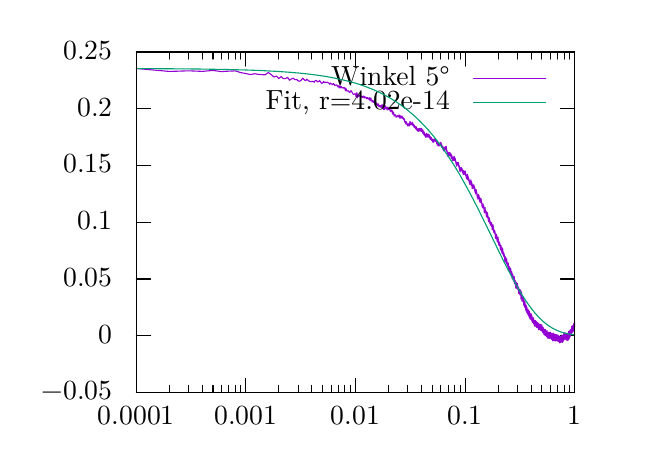
\begin{tikzpicture}[gnuplot]
%% generated with GNUPLOT 5.2p5a (Gentoo revision r0) (Lua 5.1; terminal rev. 99 , script rev. 107)
%% Sa 18 Mai 2019 18:30:47 CEST
\path (0.000,0.000) rectangle (7.500,5.250);
\gpcolor{color=gp lt color border}
\gpsetlinetype{gp lt border}
\gpsetdashtype{gp dt solid}
\gpsetlinewidth{1.00}
\draw[gp path] (1.380,0.616)--(1.560,0.616);
\draw[gp path] (6.947,0.616)--(6.767,0.616);
\node[gp node right] at (1.196,0.616) {$-0.05$};
\draw[gp path] (1.380,1.337)--(1.560,1.337);
\draw[gp path] (6.947,1.337)--(6.767,1.337);
\node[gp node right] at (1.196,1.337) {$0$};
\draw[gp path] (1.380,2.058)--(1.560,2.058);
\draw[gp path] (6.947,2.058)--(6.767,2.058);
\node[gp node right] at (1.196,2.058) {$0.05$};
\draw[gp path] (1.380,2.779)--(1.560,2.779);
\draw[gp path] (6.947,2.779)--(6.767,2.779);
\node[gp node right] at (1.196,2.779) {$0.1$};
\draw[gp path] (1.380,3.499)--(1.560,3.499);
\draw[gp path] (6.947,3.499)--(6.767,3.499);
\node[gp node right] at (1.196,3.499) {$0.15$};
\draw[gp path] (1.380,4.220)--(1.560,4.220);
\draw[gp path] (6.947,4.220)--(6.767,4.220);
\node[gp node right] at (1.196,4.220) {$0.2$};
\draw[gp path] (1.380,4.941)--(1.560,4.941);
\draw[gp path] (6.947,4.941)--(6.767,4.941);
\node[gp node right] at (1.196,4.941) {$0.25$};
\draw[gp path] (1.380,0.616)--(1.380,0.796);
\draw[gp path] (1.380,4.941)--(1.380,4.761);
\node[gp node center] at (1.380,0.308) {$0.0001$};
\draw[gp path] (1.799,0.616)--(1.799,0.706);
\draw[gp path] (1.799,4.941)--(1.799,4.851);
\draw[gp path] (2.044,0.616)--(2.044,0.706);
\draw[gp path] (2.044,4.941)--(2.044,4.851);
\draw[gp path] (2.218,0.616)--(2.218,0.706);
\draw[gp path] (2.218,4.941)--(2.218,4.851);
\draw[gp path] (2.353,0.616)--(2.353,0.706);
\draw[gp path] (2.353,4.941)--(2.353,4.851);
\draw[gp path] (2.463,0.616)--(2.463,0.706);
\draw[gp path] (2.463,4.941)--(2.463,4.851);
\draw[gp path] (2.556,0.616)--(2.556,0.706);
\draw[gp path] (2.556,4.941)--(2.556,4.851);
\draw[gp path] (2.637,0.616)--(2.637,0.706);
\draw[gp path] (2.637,4.941)--(2.637,4.851);
\draw[gp path] (2.708,0.616)--(2.708,0.706);
\draw[gp path] (2.708,4.941)--(2.708,4.851);
\draw[gp path] (2.772,0.616)--(2.772,0.796);
\draw[gp path] (2.772,4.941)--(2.772,4.761);
\node[gp node center] at (2.772,0.308) {$0.001$};
\draw[gp path] (3.191,0.616)--(3.191,0.706);
\draw[gp path] (3.191,4.941)--(3.191,4.851);
\draw[gp path] (3.436,0.616)--(3.436,0.706);
\draw[gp path] (3.436,4.941)--(3.436,4.851);
\draw[gp path] (3.610,0.616)--(3.610,0.706);
\draw[gp path] (3.610,4.941)--(3.610,4.851);
\draw[gp path] (3.745,0.616)--(3.745,0.706);
\draw[gp path] (3.745,4.941)--(3.745,4.851);
\draw[gp path] (3.855,0.616)--(3.855,0.706);
\draw[gp path] (3.855,4.941)--(3.855,4.851);
\draw[gp path] (3.948,0.616)--(3.948,0.706);
\draw[gp path] (3.948,4.941)--(3.948,4.851);
\draw[gp path] (4.029,0.616)--(4.029,0.706);
\draw[gp path] (4.029,4.941)--(4.029,4.851);
\draw[gp path] (4.100,0.616)--(4.100,0.706);
\draw[gp path] (4.100,4.941)--(4.100,4.851);
\draw[gp path] (4.163,0.616)--(4.163,0.796);
\draw[gp path] (4.163,4.941)--(4.163,4.761);
\node[gp node center] at (4.163,0.308) {$0.01$};
\draw[gp path] (4.582,0.616)--(4.582,0.706);
\draw[gp path] (4.582,4.941)--(4.582,4.851);
\draw[gp path] (4.828,0.616)--(4.828,0.706);
\draw[gp path] (4.828,4.941)--(4.828,4.851);
\draw[gp path] (5.001,0.616)--(5.001,0.706);
\draw[gp path] (5.001,4.941)--(5.001,4.851);
\draw[gp path] (5.136,0.616)--(5.136,0.706);
\draw[gp path] (5.136,4.941)--(5.136,4.851);
\draw[gp path] (5.246,0.616)--(5.246,0.706);
\draw[gp path] (5.246,4.941)--(5.246,4.851);
\draw[gp path] (5.340,0.616)--(5.340,0.706);
\draw[gp path] (5.340,4.941)--(5.340,4.851);
\draw[gp path] (5.420,0.616)--(5.420,0.706);
\draw[gp path] (5.420,4.941)--(5.420,4.851);
\draw[gp path] (5.492,0.616)--(5.492,0.706);
\draw[gp path] (5.492,4.941)--(5.492,4.851);
\draw[gp path] (5.555,0.616)--(5.555,0.796);
\draw[gp path] (5.555,4.941)--(5.555,4.761);
\node[gp node center] at (5.555,0.308) {$0.1$};
\draw[gp path] (5.974,0.616)--(5.974,0.706);
\draw[gp path] (5.974,4.941)--(5.974,4.851);
\draw[gp path] (6.219,0.616)--(6.219,0.706);
\draw[gp path] (6.219,4.941)--(6.219,4.851);
\draw[gp path] (6.393,0.616)--(6.393,0.706);
\draw[gp path] (6.393,4.941)--(6.393,4.851);
\draw[gp path] (6.528,0.616)--(6.528,0.706);
\draw[gp path] (6.528,4.941)--(6.528,4.851);
\draw[gp path] (6.638,0.616)--(6.638,0.706);
\draw[gp path] (6.638,4.941)--(6.638,4.851);
\draw[gp path] (6.731,0.616)--(6.731,0.706);
\draw[gp path] (6.731,4.941)--(6.731,4.851);
\draw[gp path] (6.812,0.616)--(6.812,0.706);
\draw[gp path] (6.812,4.941)--(6.812,4.851);
\draw[gp path] (6.883,0.616)--(6.883,0.706);
\draw[gp path] (6.883,4.941)--(6.883,4.851);
\draw[gp path] (6.947,0.616)--(6.947,0.796);
\draw[gp path] (6.947,4.941)--(6.947,4.761);
\node[gp node center] at (6.947,0.308) {$1$};
\draw[gp path] (1.380,4.941)--(1.380,0.616)--(6.947,0.616)--(6.947,4.941)--cycle;
\node[gp node right] at (5.479,4.607) {Winkel 5°};
\gpcolor{rgb color={0.580,0.000,0.827}}
\draw[gp path] (5.663,4.607)--(6.579,4.607);
\draw[gp path] (1.380,4.732)--(1.799,4.694)--(2.044,4.702)--(2.218,4.695)--(2.353,4.707)%
  --(2.463,4.692)--(2.556,4.698)--(2.637,4.701)--(2.708,4.679)--(2.772,4.667)--(2.829,4.654)%
  --(2.882,4.665)--(2.930,4.657)--(2.975,4.653)--(3.017,4.652)--(3.056,4.680)--(3.092,4.655)%
  --(3.127,4.623)--(3.160,4.635)--(3.191,4.605)--(3.220,4.629)--(3.248,4.602)--(3.275,4.604)%
  --(3.301,4.619)--(3.326,4.582)--(3.349,4.600)--(3.372,4.608)--(3.394,4.589)--(3.415,4.594)%
  --(3.436,4.573)--(3.456,4.570)--(3.475,4.585)--(3.493,4.608)--(3.511,4.590)--(3.529,4.575)%
  --(3.546,4.595)--(3.563,4.580)--(3.579,4.568)--(3.594,4.565)--(3.610,4.565)--(3.625,4.568)%
  --(3.639,4.557)--(3.653,4.579)--(3.667,4.578)--(3.681,4.562)--(3.694,4.564)--(3.707,4.579)%
  --(3.720,4.561)--(3.732,4.543)--(3.745,4.546)--(3.757,4.568)--(3.768,4.551)--(3.780,4.559)%
  --(3.791,4.551)--(3.802,4.559)--(3.813,4.551)--(3.824,4.547)--(3.834,4.532)--(3.845,4.547)%
  --(3.855,4.534)--(3.865,4.537)--(3.875,4.525)--(3.884,4.540)--(3.894,4.529)--(3.903,4.515)%
  --(3.912,4.521)--(3.921,4.523)--(3.930,4.518)--(3.939,4.500)--(3.948,4.512)--(3.956,4.484)%
  --(3.965,4.509)--(3.973,4.486)--(3.982,4.503)--(3.990,4.486)--(3.998,4.487)--(4.006,4.484)%
  --(4.013,4.491)--(4.021,4.475)--(4.029,4.487)--(4.036,4.448)--(4.044,4.474)--(4.051,4.456)%
  --(4.058,4.443)--(4.065,4.445)--(4.072,4.448)--(4.079,4.438)--(4.086,4.427)--(4.093,4.435)%
  --(4.100,4.433)--(4.106,4.451)--(4.113,4.437)--(4.120,4.431)--(4.126,4.418)--(4.132,4.408)%
  --(4.139,4.402)--(4.145,4.406)--(4.151,4.405)--(4.157,4.413)--(4.164,4.403)--(4.170,4.374)%
  --(4.175,4.388)--(4.181,4.427)--(4.187,4.358)--(4.193,4.395)--(4.199,4.393)--(4.204,4.378)%
  --(4.210,4.385)--(4.216,4.395)--(4.221,4.382)--(4.227,4.379)--(4.232,4.379)--(4.237,4.368)%
  --(4.243,4.383)--(4.248,4.376)--(4.253,4.363)--(4.258,4.368)--(4.264,4.380)--(4.269,4.381)%
  --(4.274,4.357)--(4.279,4.375)--(4.284,4.359)--(4.289,4.364)--(4.294,4.367)--(4.298,4.364)%
  --(4.303,4.350)--(4.308,4.347)--(4.313,4.362)--(4.317,4.359)--(4.322,4.348)--(4.327,4.355)%
  --(4.331,4.346)--(4.336,4.339)--(4.340,4.360)--(4.345,4.343)--(4.349,4.321)--(4.354,4.334)%
  --(4.358,4.359)--(4.363,4.331)--(4.367,4.331)--(4.371,4.321)--(4.375,4.305)--(4.380,4.319)%
  --(4.384,4.326)--(4.388,4.312)--(4.392,4.316)--(4.396,4.298)--(4.400,4.316)--(4.405,4.303)%
  --(4.409,4.279)--(4.413,4.270)--(4.417,4.283)--(4.421,4.300)--(4.424,4.293)--(4.428,4.283)%
  --(4.432,4.271)--(4.436,4.269)--(4.440,4.270)--(4.444,4.261)--(4.448,4.290)--(4.451,4.254)%
  --(4.455,4.277)--(4.459,4.247)--(4.463,4.252)--(4.466,4.248)--(4.470,4.261)--(4.473,4.243)%
  --(4.477,4.249)--(4.481,4.261)--(4.484,4.239)--(4.488,4.249)--(4.491,4.252)--(4.495,4.268)%
  --(4.498,4.231)--(4.502,4.256)--(4.505,4.248)--(4.509,4.272)--(4.512,4.266)--(4.515,4.222)%
  --(4.519,4.212)--(4.522,4.230)--(4.525,4.233)--(4.529,4.246)--(4.532,4.210)--(4.535,4.229)%
  --(4.539,4.240)--(4.542,4.236)--(4.545,4.257)--(4.548,4.249)--(4.551,4.219)--(4.555,4.237)%
  --(4.558,4.235)--(4.561,4.232)--(4.564,4.221)--(4.567,4.205)--(4.570,4.222)--(4.573,4.241)%
  --(4.576,4.220)--(4.579,4.214)--(4.582,4.230)--(4.585,4.216)--(4.588,4.209)--(4.591,4.216)%
  --(4.594,4.211)--(4.597,4.208)--(4.600,4.221)--(4.603,4.191)--(4.606,4.187)--(4.609,4.201)%
  --(4.612,4.195)--(4.615,4.201)--(4.618,4.197)--(4.621,4.187)--(4.623,4.193)--(4.626,4.206)%
  --(4.629,4.167)--(4.632,4.186)--(4.635,4.152)--(4.637,4.177)--(4.640,4.163)--(4.643,4.176)%
  --(4.646,4.179)--(4.648,4.154)--(4.651,4.153)--(4.654,4.126)--(4.656,4.147)--(4.659,4.132)%
  --(4.662,4.145)--(4.664,4.147)--(4.667,4.139)--(4.670,4.141)--(4.672,4.130)--(4.675,4.130)%
  --(4.677,4.113)--(4.680,4.128)--(4.683,4.116)--(4.685,4.114)--(4.688,4.124)--(4.690,4.116)%
  --(4.693,4.130)--(4.695,4.126)--(4.698,4.132)--(4.700,4.132)--(4.703,4.123)--(4.705,4.140)%
  --(4.708,4.123)--(4.710,4.125)--(4.712,4.121)--(4.715,4.117)--(4.717,4.116)--(4.720,4.111)%
  --(4.722,4.102)--(4.725,4.140)--(4.727,4.126)--(4.729,4.107)--(4.732,4.128)--(4.734,4.128)%
  --(4.736,4.105)--(4.739,4.101)--(4.741,4.116)--(4.743,4.112)--(4.746,4.104)--(4.748,4.109)%
  --(4.750,4.105)--(4.753,4.130)--(4.755,4.102)--(4.757,4.105)--(4.759,4.114)--(4.762,4.112)%
  --(4.764,4.095)--(4.766,4.110)--(4.768,4.096)--(4.771,4.092)--(4.773,4.104)--(4.775,4.092)%
  --(4.777,4.079)--(4.779,4.080)--(4.781,4.090)--(4.784,4.092)--(4.786,4.079)--(4.788,4.055)%
  --(4.790,4.049)--(4.792,4.058)--(4.794,4.048)--(4.797,4.057)--(4.799,4.037)--(4.801,4.049)%
  --(4.803,4.027)--(4.805,4.058)--(4.807,4.033)--(4.809,4.052)--(4.811,4.049)--(4.813,4.044)%
  --(4.815,4.023)--(4.817,4.021)--(4.819,4.017)--(4.821,4.024)--(4.823,4.009)--(4.826,4.015)%
  --(4.828,4.000)--(4.830,4.027)--(4.832,4.028)--(4.834,4.009)--(4.836,4.018)--(4.838,4.007)%
  --(4.840,4.005)--(4.841,4.028)--(4.843,4.022)--(4.845,4.019)--(4.847,4.003)--(4.849,4.040)%
  --(4.851,4.029)--(4.853,4.017)--(4.855,4.059)--(4.857,4.017)--(4.859,4.055)--(4.861,4.027)%
  --(4.863,4.045)--(4.865,4.033)--(4.867,4.022)--(4.868,4.026)--(4.870,4.016)--(4.872,4.039)%
  --(4.874,4.024)--(4.876,4.031)--(4.878,4.018)--(4.880,4.040)--(4.881,4.022)--(4.883,4.031)%
  --(4.885,4.048)--(4.887,4.031)--(4.889,4.044)--(4.891,4.011)--(4.892,4.005)--(4.894,4.026)%
  --(4.896,4.027)--(4.898,4.026)--(4.900,4.016)--(4.901,4.007)--(4.903,3.999)--(4.905,4.018)%
  --(4.907,3.985)--(4.908,3.987)--(4.910,3.999)--(4.912,4.008)--(4.914,3.988)--(4.916,3.995)%
  --(4.917,3.990)--(4.919,3.996)--(4.921,3.988)--(4.922,3.979)--(4.924,3.971)--(4.926,3.990)%
  --(4.928,3.980)--(4.929,3.980)--(4.931,3.991)--(4.933,3.970)--(4.934,3.956)--(4.936,3.992)%
  --(4.938,3.958)--(4.939,3.969)--(4.941,3.961)--(4.943,3.947)--(4.944,3.963)--(4.946,3.958)%
  --(4.948,3.949)--(4.949,3.956)--(4.951,3.937)--(4.953,3.954)--(4.954,3.966)--(4.956,3.954)%
  --(4.958,3.951)--(4.959,3.971)--(4.961,3.946)--(4.962,3.956)--(4.964,3.964)--(4.966,3.933)%
  --(4.967,3.936)--(4.969,3.947)--(4.970,3.959)--(4.972,3.954)--(4.974,3.968)--(4.975,3.943)%
  --(4.977,3.955)--(4.978,3.948)--(4.980,3.956)--(4.981,3.967)--(4.983,3.959)--(4.985,3.952)%
  --(4.986,3.938)--(4.988,3.948)--(4.989,3.956)--(4.991,3.961)--(4.992,3.970)--(4.994,3.969)%
  --(4.995,3.936)--(4.997,3.962)--(4.998,3.969)--(5.000,3.932)--(5.001,3.941)--(5.003,3.959)%
  --(5.004,3.962)--(5.006,3.968)--(5.007,3.933)--(5.009,3.941)--(5.010,3.941)--(5.012,3.936)%
  --(5.013,3.941)--(5.015,3.936)--(5.016,3.910)--(5.018,3.940)--(5.019,3.942)--(5.021,3.951)%
  --(5.022,3.906)--(5.024,3.910)--(5.025,3.909)--(5.027,3.926)--(5.028,3.922)--(5.029,3.920)%
  --(5.031,3.891)--(5.032,3.921)--(5.034,3.927)--(5.035,3.916)--(5.037,3.903)--(5.038,3.919)%
  --(5.039,3.878)--(5.041,3.892)--(5.042,3.877)--(5.044,3.901)--(5.045,3.882)--(5.047,3.890)%
  --(5.048,3.891)--(5.049,3.897)--(5.051,3.890)--(5.052,3.885)--(5.054,3.889)--(5.055,3.887)%
  --(5.056,3.856)--(5.058,3.888)--(5.059,3.873)--(5.060,3.885)--(5.062,3.889)--(5.063,3.908)%
  --(5.064,3.895)--(5.066,3.894)--(5.067,3.891)--(5.069,3.890)--(5.070,3.864)--(5.071,3.876)%
  --(5.073,3.894)--(5.074,3.892)--(5.075,3.896)--(5.077,3.885)--(5.078,3.899)--(5.079,3.891)%
  --(5.081,3.889)--(5.082,3.898)--(5.083,3.875)--(5.085,3.857)--(5.086,3.868)--(5.087,3.884)%
  --(5.089,3.879)--(5.090,3.864)--(5.091,3.896)--(5.092,3.873)--(5.094,3.878)--(5.095,3.890)%
  --(5.096,3.876)--(5.098,3.875)--(5.099,3.868)--(5.100,3.865)--(5.101,3.872)--(5.103,3.889)%
  --(5.104,3.873)--(5.105,3.849)--(5.107,3.858)--(5.108,3.866)--(5.109,3.867)--(5.110,3.841)%
  --(5.112,3.865)--(5.113,3.832)--(5.114,3.856)--(5.115,3.837)--(5.117,3.847)--(5.118,3.842)%
  --(5.119,3.850)--(5.120,3.850)--(5.122,3.828)--(5.123,3.858)--(5.124,3.832)--(5.125,3.856)%
  --(5.127,3.822)--(5.128,3.847)--(5.129,3.831)--(5.130,3.831)--(5.131,3.836)--(5.133,3.823)%
  --(5.134,3.833)--(5.135,3.814)--(5.136,3.826)--(5.137,3.813)--(5.139,3.823)--(5.140,3.810)%
  --(5.141,3.826)--(5.142,3.833)--(5.144,3.819)--(5.145,3.797)--(5.146,3.800)--(5.147,3.794)%
  --(5.148,3.823)--(5.149,3.810)--(5.151,3.822)--(5.152,3.828)--(5.153,3.812)--(5.154,3.804)%
  --(5.155,3.815)--(5.157,3.798)--(5.158,3.823)--(5.159,3.798)--(5.160,3.826)--(5.161,3.803)%
  --(5.162,3.824)--(5.163,3.828)--(5.165,3.819)--(5.166,3.825)--(5.167,3.821)--(5.168,3.825)%
  --(5.169,3.817)--(5.170,3.814)--(5.172,3.838)--(5.173,3.847)--(5.174,3.823)--(5.175,3.810)%
  --(5.176,3.824)--(5.177,3.809)--(5.178,3.831)--(5.179,3.806)--(5.181,3.816)--(5.182,3.812)%
  --(5.183,3.824)--(5.184,3.815)--(5.185,3.810)--(5.186,3.807)--(5.187,3.811)--(5.188,3.812)%
  --(5.189,3.802)--(5.191,3.801)--(5.192,3.814)--(5.193,3.780)--(5.194,3.780)--(5.195,3.784)%
  --(5.196,3.788)--(5.197,3.802)--(5.198,3.798)--(5.199,3.785)--(5.200,3.773)--(5.202,3.760)%
  --(5.203,3.788)--(5.204,3.779)--(5.205,3.769)--(5.206,3.775)--(5.207,3.788)--(5.208,3.770)%
  --(5.209,3.765)--(5.210,3.770)--(5.211,3.769)--(5.212,3.748)--(5.213,3.779)--(5.214,3.769)%
  --(5.215,3.750)--(5.217,3.765)--(5.218,3.770)--(5.219,3.756)--(5.220,3.760)--(5.221,3.761)%
  --(5.222,3.772)--(5.223,3.748)--(5.224,3.778)--(5.225,3.754)--(5.226,3.771)--(5.227,3.766)%
  --(5.228,3.782)--(5.229,3.764)--(5.230,3.767)--(5.231,3.756)--(5.232,3.758)--(5.233,3.750)%
  --(5.234,3.772)--(5.235,3.766)--(5.236,3.774)--(5.237,3.787)--(5.238,3.767)--(5.239,3.781)%
  --(5.240,3.782)--(5.241,3.784)--(5.242,3.773)--(5.243,3.755)--(5.244,3.783)--(5.245,3.790)%
  --(5.246,3.795)--(5.247,3.783)--(5.249,3.773)--(5.250,3.786)--(5.251,3.777)--(5.252,3.762)%
  --(5.253,3.762)--(5.254,3.768)--(5.254,3.755)--(5.255,3.735)--(5.256,3.755)--(5.257,3.773)%
  --(5.258,3.740)--(5.259,3.759)--(5.260,3.729)--(5.261,3.756)--(5.262,3.742)--(5.263,3.744)%
  --(5.264,3.754)--(5.265,3.723)--(5.266,3.728)--(5.267,3.735)--(5.268,3.726)--(5.269,3.734)%
  --(5.270,3.717)--(5.271,3.724)--(5.272,3.714)--(5.273,3.713)--(5.274,3.726)--(5.275,3.738)%
  --(5.276,3.702)--(5.277,3.727)--(5.278,3.710)--(5.279,3.691)--(5.280,3.710)--(5.281,3.690)%
  --(5.282,3.707)--(5.283,3.708)--(5.284,3.724)--(5.285,3.709)--(5.286,3.703)--(5.286,3.712)%
  --(5.287,3.702)--(5.288,3.714)--(5.289,3.681)--(5.290,3.726)--(5.291,3.717)--(5.292,3.712)%
  --(5.293,3.700)--(5.294,3.718)--(5.295,3.725)--(5.296,3.718)--(5.297,3.716)--(5.298,3.701)%
  --(5.299,3.712)--(5.300,3.730)--(5.300,3.702)--(5.301,3.717)--(5.302,3.736)--(5.303,3.735)%
  --(5.304,3.740)--(5.305,3.698)--(5.306,3.710)--(5.307,3.699)--(5.308,3.722)--(5.309,3.714)%
  --(5.310,3.725)--(5.310,3.720)--(5.311,3.718)--(5.312,3.700)--(5.313,3.705)--(5.314,3.704)%
  --(5.315,3.742)--(5.316,3.720)--(5.317,3.694)--(5.318,3.698)--(5.319,3.721)--(5.319,3.689)%
  --(5.320,3.701)--(5.321,3.681)--(5.322,3.684)--(5.323,3.682)--(5.324,3.691)--(5.325,3.680)%
  --(5.326,3.672)--(5.327,3.688)--(5.327,3.667)--(5.328,3.673)--(5.329,3.668)--(5.330,3.671)%
  --(5.331,3.671)--(5.332,3.667)--(5.333,3.658)--(5.334,3.651)--(5.334,3.624)--(5.335,3.651)%
  --(5.336,3.632)--(5.337,3.615)--(5.338,3.653)--(5.339,3.623)--(5.340,3.658)--(5.341,3.630)%
  --(5.341,3.617)--(5.342,3.650)--(5.343,3.658)--(5.344,3.627)--(5.345,3.634)--(5.346,3.648)%
  --(5.347,3.666)--(5.347,3.637)--(5.348,3.656)--(5.349,3.668)--(5.350,3.636)--(5.351,3.650)%
  --(5.352,3.640)--(5.352,3.631)--(5.353,3.631)--(5.354,3.622)--(5.355,3.663)--(5.356,3.647)%
  --(5.357,3.640)--(5.358,3.648)--(5.358,3.642)--(5.359,3.642)--(5.360,3.649)--(5.361,3.650)%
  --(5.362,3.632)--(5.363,3.640)--(5.364,3.631)--(5.365,3.659)--(5.366,3.646)--(5.367,3.658)%
  --(5.368,3.657)--(5.368,3.653)--(5.369,3.646)--(5.370,3.623)--(5.371,3.649)--(5.372,3.635)%
  --(5.372,3.636)--(5.373,3.642)--(5.374,3.630)--(5.375,3.631)--(5.376,3.609)--(5.377,3.620)%
  --(5.377,3.645)--(5.378,3.629)--(5.379,3.626)--(5.380,3.590)--(5.381,3.620)--(5.381,3.606)%
  --(5.382,3.604)--(5.383,3.603)--(5.384,3.600)--(5.385,3.620)--(5.385,3.631)--(5.386,3.589)%
  --(5.387,3.601)--(5.388,3.624)--(5.389,3.601)--(5.389,3.614)--(5.390,3.603)--(5.391,3.594)%
  --(5.392,3.589)--(5.393,3.602)--(5.393,3.575)--(5.394,3.578)--(5.395,3.595)--(5.396,3.568)%
  --(5.396,3.564)--(5.397,3.562)--(5.398,3.577)--(5.399,3.582)--(5.400,3.579)--(5.400,3.592)%
  --(5.401,3.590)--(5.402,3.596)--(5.403,3.573)--(5.404,3.584)--(5.404,3.587)--(5.405,3.564)%
  --(5.406,3.583)--(5.407,3.600)--(5.407,3.580)--(5.408,3.583)--(5.409,3.601)--(5.410,3.592)%
  --(5.410,3.595)--(5.411,3.609)--(5.412,3.610)--(5.413,3.580)--(5.414,3.613)--(5.414,3.572)%
  --(5.415,3.592)--(5.416,3.579)--(5.417,3.566)--(5.417,3.602)--(5.418,3.576)--(5.419,3.582)%
  --(5.420,3.605)--(5.420,3.580)--(5.421,3.606)--(5.422,3.598)--(5.423,3.610)--(5.423,3.593)%
  --(5.424,3.590)--(5.425,3.591)--(5.426,3.594)--(5.426,3.573)--(5.427,3.593)--(5.428,3.579)%
  --(5.429,3.568)--(5.429,3.588)--(5.430,3.573)--(5.431,3.557)--(5.432,3.587)--(5.432,3.564)%
  --(5.433,3.547)--(5.434,3.553)--(5.435,3.545)--(5.435,3.557)--(5.436,3.548)--(5.437,3.558)%
  --(5.438,3.549)--(5.438,3.538)--(5.439,3.523)--(5.440,3.524)--(5.440,3.544)--(5.441,3.543)%
  --(5.442,3.527)--(5.443,3.534)--(5.443,3.517)--(5.444,3.526)--(5.445,3.490)--(5.446,3.529)%
  --(5.446,3.536)--(5.447,3.520)--(5.448,3.512)--(5.448,3.505)--(5.449,3.525)--(5.450,3.509)%
  --(5.451,3.530)--(5.451,3.514)--(5.452,3.518)--(5.453,3.523)--(5.453,3.536)--(5.454,3.532)%
  --(5.455,3.520)--(5.456,3.527)--(5.456,3.528)--(5.457,3.521)--(5.458,3.534)--(5.458,3.531)%
  --(5.459,3.511)--(5.460,3.506)--(5.461,3.519)--(5.461,3.516)--(5.462,3.525)--(5.463,3.523)%
  --(5.463,3.518)--(5.464,3.538)--(5.465,3.522)--(5.465,3.524)--(5.466,3.529)--(5.467,3.519)%
  --(5.468,3.520)--(5.468,3.530)--(5.469,3.508)--(5.470,3.536)--(5.470,3.507)--(5.471,3.496)%
  --(5.472,3.497)--(5.472,3.508)--(5.473,3.531)--(5.474,3.502)--(5.475,3.489)--(5.475,3.487)%
  --(5.476,3.504)--(5.477,3.488)--(5.477,3.478)--(5.478,3.491)--(5.479,3.500)--(5.479,3.493)%
  --(5.480,3.481)--(5.481,3.496)--(5.481,3.484)--(5.482,3.464)--(5.483,3.464)--(5.483,3.452)%
  --(5.484,3.455)--(5.485,3.472)--(5.485,3.457)--(5.486,3.459)--(5.487,3.438)--(5.488,3.474)%
  --(5.488,3.454)--(5.489,3.462)--(5.490,3.438)--(5.490,3.422)--(5.491,3.439)--(5.492,3.433)%
  --(5.492,3.448)--(5.493,3.443)--(5.494,3.448)--(5.494,3.453)--(5.495,3.441)--(5.496,3.454)%
  --(5.496,3.446)--(5.497,3.438)--(5.498,3.462)--(5.498,3.436)--(5.499,3.458)--(5.500,3.463)%
  --(5.500,3.447)--(5.501,3.440)--(5.502,3.430)--(5.502,3.443)--(5.503,3.456)--(5.504,3.462)%
  --(5.504,3.429)--(5.505,3.472)--(5.506,3.464)--(5.506,3.475)--(5.507,3.458)--(5.507,3.454)%
  --(5.508,3.445)--(5.509,3.466)--(5.509,3.470)--(5.510,3.455)--(5.511,3.442)--(5.511,3.462)%
  --(5.512,3.443)--(5.513,3.450)--(5.513,3.438)--(5.514,3.458)--(5.515,3.464)--(5.515,3.440)%
  --(5.516,3.462)--(5.517,3.450)--(5.517,3.445)--(5.518,3.440)--(5.518,3.449)--(5.519,3.438)%
  --(5.520,3.427)--(5.520,3.434)--(5.521,3.433)--(5.522,3.410)--(5.522,3.441)--(5.523,3.421)%
  --(5.524,3.429)--(5.525,3.444)--(5.526,3.424)--(5.526,3.437)--(5.527,3.409)--(5.527,3.417)%
  --(5.528,3.426)--(5.529,3.417)--(5.529,3.396)--(5.530,3.410)--(5.531,3.404)--(5.531,3.423)%
  --(5.532,3.408)--(5.532,3.387)--(5.533,3.435)--(5.534,3.412)--(5.534,3.407)--(5.535,3.396)%
  --(5.536,3.393)--(5.536,3.387)--(5.537,3.403)--(5.537,3.386)--(5.538,3.400)--(5.539,3.385)%
  --(5.539,3.407)--(5.540,3.390)--(5.541,3.407)--(5.541,3.404)--(5.542,3.405)--(5.542,3.411)%
  --(5.543,3.398)--(5.544,3.411)--(5.544,3.404)--(5.545,3.387)--(5.546,3.417)--(5.546,3.402)%
  --(5.547,3.403)--(5.547,3.424)--(5.548,3.400)--(5.549,3.411)--(5.549,3.400)--(5.550,3.416)%
  --(5.550,3.394)--(5.551,3.413)--(5.552,3.408)--(5.552,3.432)--(5.553,3.423)--(5.553,3.418)%
  --(5.554,3.417)--(5.555,3.416)--(5.555,3.421)--(5.556,3.409)--(5.556,3.410)--(5.557,3.431)%
  --(5.558,3.383)--(5.558,3.423)--(5.559,3.420)--(5.559,3.377)--(5.560,3.395)--(5.561,3.413)%
  --(5.561,3.398)--(5.562,3.410)--(5.562,3.411)--(5.563,3.389)--(5.564,3.394)--(5.564,3.374)%
  --(5.565,3.392)--(5.565,3.377)--(5.566,3.362)--(5.567,3.380)--(5.567,3.379)--(5.568,3.379)%
  --(5.568,3.368)--(5.569,3.380)--(5.570,3.347)--(5.570,3.352)--(5.571,3.372)--(5.571,3.357)%
  --(5.572,3.356)--(5.573,3.361)--(5.573,3.337)--(5.574,3.353)--(5.574,3.345)--(5.575,3.355)%
  --(5.575,3.328)--(5.576,3.380)--(5.577,3.334)--(5.577,3.333)--(5.578,3.337)--(5.578,3.342)%
  --(5.579,3.353)--(5.580,3.358)--(5.580,3.336)--(5.581,3.357)--(5.581,3.343)--(5.582,3.357)%
  --(5.582,3.354)--(5.583,3.326)--(5.584,3.353)--(5.585,3.353)--(5.585,3.346)--(5.586,3.343)%
  --(5.586,3.325)--(5.587,3.386)--(5.588,3.333)--(5.588,3.339)--(5.589,3.334)--(5.589,3.357)%
  --(5.590,3.341)--(5.590,3.343)--(5.591,3.356)--(5.592,3.329)--(5.592,3.366)--(5.593,3.320)%
  --(5.593,3.343)--(5.594,3.334)--(5.594,3.331)--(5.595,3.332)--(5.596,3.343)--(5.596,3.338)%
  --(5.597,3.352)--(5.597,3.340)--(5.598,3.315)--(5.598,3.335)--(5.599,3.336)--(5.600,3.316)%
  --(5.600,3.306)--(5.601,3.331)--(5.601,3.324)--(5.602,3.333)--(5.602,3.334)--(5.603,3.321)%
  --(5.603,3.317)--(5.604,3.311)--(5.605,3.323)--(5.605,3.301)--(5.606,3.302)--(5.606,3.316)%
  --(5.607,3.318)--(5.607,3.289)--(5.608,3.290)--(5.608,3.308)--(5.609,3.305)--(5.610,3.309)%
  --(5.610,3.295)--(5.611,3.302)--(5.611,3.285)--(5.612,3.275)--(5.612,3.289)--(5.613,3.270)%
  --(5.613,3.278)--(5.614,3.276)--(5.615,3.274)--(5.615,3.283)--(5.616,3.285)--(5.616,3.291)%
  --(5.617,3.256)--(5.617,3.301)--(5.618,3.288)--(5.618,3.285)--(5.619,3.259)--(5.619,3.276)%
  --(5.620,3.280)--(5.621,3.293)--(5.621,3.281)--(5.622,3.279)--(5.622,3.286)--(5.623,3.271)%
  --(5.623,3.286)--(5.624,3.283)--(5.624,3.299)--(5.625,3.296)--(5.625,3.277)--(5.626,3.296)%
  --(5.626,3.270)--(5.627,3.303)--(5.628,3.299)--(5.628,3.278)--(5.629,3.280)--(5.629,3.319)%
  --(5.630,3.272)--(5.630,3.299)--(5.631,3.299)--(5.631,3.298)--(5.632,3.290)--(5.632,3.305)%
  --(5.633,3.275)--(5.633,3.285)--(5.634,3.269)--(5.634,3.271)--(5.635,3.284)--(5.636,3.297)%
  --(5.636,3.277)--(5.637,3.281)--(5.637,3.242)--(5.638,3.270)--(5.638,3.271)--(5.639,3.267)%
  --(5.639,3.266)--(5.640,3.262)--(5.640,3.260)--(5.641,3.247)--(5.641,3.270)--(5.642,3.270)%
  --(5.642,3.244)--(5.643,3.271)--(5.643,3.251)--(5.644,3.253)--(5.644,3.205)--(5.645,3.260)%
  --(5.645,3.257)--(5.646,3.248)--(5.647,3.249)--(5.647,3.256)--(5.648,3.224)--(5.648,3.237)%
  --(5.649,3.232)--(5.649,3.239)--(5.650,3.222)--(5.650,3.226)--(5.651,3.210)--(5.651,3.222)%
  --(5.652,3.247)--(5.652,3.238)--(5.653,3.231)--(5.653,3.217)--(5.654,3.223)--(5.654,3.224)%
  --(5.655,3.219)--(5.655,3.229)--(5.656,3.236)--(5.656,3.253)--(5.657,3.235)--(5.657,3.219)%
  --(5.658,3.217)--(5.658,3.234)--(5.659,3.234)--(5.659,3.213)--(5.660,3.233)--(5.660,3.239)%
  --(5.661,3.250)--(5.662,3.254)--(5.662,3.238)--(5.663,3.234)--(5.664,3.250)--(5.664,3.252)%
  --(5.665,3.254)--(5.666,3.242)--(5.666,3.236)--(5.667,3.234)--(5.667,3.244)--(5.668,3.228)%
  --(5.668,3.244)--(5.669,3.237)--(5.669,3.220)--(5.670,3.223)--(5.670,3.231)--(5.671,3.237)%
  --(5.671,3.221)--(5.672,3.208)--(5.673,3.205)--(5.673,3.204)--(5.674,3.207)--(5.674,3.211)%
  --(5.675,3.197)--(5.675,3.210)--(5.676,3.188)--(5.676,3.193)--(5.677,3.198)--(5.677,3.222)%
  --(5.678,3.179)--(5.678,3.190)--(5.679,3.192)--(5.679,3.167)--(5.680,3.161)--(5.680,3.185)%
  --(5.681,3.176)--(5.681,3.158)--(5.682,3.171)--(5.682,3.180)--(5.683,3.178)--(5.683,3.173)%
  --(5.684,3.159)--(5.684,3.167)--(5.685,3.159)--(5.685,3.161)--(5.686,3.162)--(5.686,3.180)%
  --(5.687,3.165)--(5.687,3.181)--(5.688,3.176)--(5.688,3.185)--(5.689,3.137)--(5.689,3.170)%
  --(5.690,3.165)--(5.690,3.175)--(5.691,3.166)--(5.691,3.172)--(5.692,3.168)--(5.692,3.164)%
  --(5.693,3.184)--(5.693,3.174)--(5.693,3.196)--(5.694,3.180)--(5.694,3.174)--(5.695,3.170)%
  --(5.695,3.165)--(5.696,3.177)--(5.696,3.165)--(5.697,3.150)--(5.697,3.161)--(5.698,3.183)%
  --(5.698,3.148)--(5.699,3.170)--(5.699,3.150)--(5.700,3.154)--(5.700,3.158)--(5.701,3.161)%
  --(5.701,3.154)--(5.702,3.144)--(5.702,3.145)--(5.703,3.163)--(5.703,3.143)--(5.704,3.160)%
  --(5.704,3.157)--(5.704,3.139)--(5.705,3.163)--(5.705,3.127)--(5.706,3.131)--(5.706,3.138)%
  --(5.707,3.122)--(5.707,3.118)--(5.708,3.117)--(5.708,3.102)--(5.709,3.113)--(5.709,3.129)%
  --(5.710,3.111)--(5.710,3.116)--(5.711,3.102)--(5.711,3.103)--(5.712,3.113)--(5.712,3.110)%
  --(5.712,3.118)--(5.713,3.105)--(5.713,3.088)--(5.714,3.108)--(5.714,3.093)--(5.715,3.085)%
  --(5.715,3.097)--(5.716,3.088)--(5.716,3.100)--(5.717,3.120)--(5.717,3.100)--(5.718,3.071)%
  --(5.718,3.099)--(5.718,3.095)--(5.719,3.118)--(5.720,3.112)--(5.720,3.106)--(5.721,3.103)%
  --(5.721,3.096)--(5.722,3.118)--(5.722,3.120)--(5.723,3.096)--(5.723,3.099)--(5.724,3.110)%
  --(5.724,3.090)--(5.724,3.110)--(5.725,3.110)--(5.725,3.101)--(5.726,3.114)--(5.726,3.108)%
  --(5.727,3.133)--(5.727,3.105)--(5.728,3.124)--(5.728,3.122)--(5.729,3.119)--(5.729,3.112)%
  --(5.729,3.099)--(5.730,3.111)--(5.730,3.109)--(5.731,3.091)--(5.731,3.099)--(5.732,3.097)%
  --(5.732,3.096)--(5.733,3.082)--(5.733,3.105)--(5.733,3.114)--(5.734,3.087)--(5.734,3.096)%
  --(5.735,3.101)--(5.735,3.080)--(5.736,3.073)--(5.736,3.094)--(5.737,3.092)--(5.737,3.087)%
  --(5.738,3.072)--(5.738,3.078)--(5.738,3.050)--(5.739,3.088)--(5.739,3.081)--(5.740,3.044)%
  --(5.740,3.066)--(5.741,3.072)--(5.741,3.066)--(5.742,3.056)--(5.742,3.055)--(5.742,3.041)%
  --(5.743,3.053)--(5.743,3.040)--(5.744,3.045)--(5.744,3.046)--(5.745,3.035)--(5.745,3.045)%
  --(5.746,3.046)--(5.746,3.072)--(5.746,3.029)--(5.747,3.041)--(5.747,3.070)--(5.748,3.039)%
  --(5.748,3.045)--(5.749,3.033)--(5.749,3.051)--(5.749,3.042)--(5.750,3.053)--(5.750,3.043)%
  --(5.751,3.059)--(5.751,3.043)--(5.752,3.042)--(5.752,3.060)--(5.753,3.040)--(5.753,3.034)%
  --(5.753,3.062)--(5.754,3.059)--(5.754,3.054)--(5.755,3.047)--(5.755,3.055)--(5.756,3.071)%
  --(5.756,3.040)--(5.756,3.086)--(5.757,3.049)--(5.757,3.063)--(5.758,3.053)--(5.758,3.070)%
  --(5.759,3.063)--(5.759,3.066)--(5.759,3.050)--(5.760,3.045)--(5.760,3.053)--(5.761,3.043)%
  --(5.761,3.034)--(5.762,3.064)--(5.762,3.058)--(5.762,3.052)--(5.763,3.027)--(5.763,3.031)%
  --(5.764,3.019)--(5.764,3.042)--(5.765,3.022)--(5.765,3.046)--(5.765,3.024)--(5.766,3.021)%
  --(5.766,3.015)--(5.767,3.026)--(5.767,3.020)--(5.768,3.012)--(5.768,2.993)--(5.768,3.006)%
  --(5.769,3.005)--(5.769,3.026)--(5.770,2.987)--(5.770,3.009)--(5.771,3.002)--(5.771,2.984)%
  --(5.771,3.013)--(5.772,2.976)--(5.772,2.985)--(5.773,2.994)--(5.773,2.982)--(5.774,2.984)%
  --(5.774,2.986)--(5.774,2.966)--(5.775,2.962)--(5.775,2.988)--(5.776,2.986)--(5.776,2.972)%
  --(5.776,2.995)--(5.777,2.974)--(5.777,3.000)--(5.778,2.979)--(5.778,2.981)--(5.779,2.979)%
  --(5.779,2.992)--(5.779,2.982)--(5.780,2.987)--(5.780,2.982)--(5.781,2.996)--(5.781,2.981)%
  --(5.781,2.998)--(5.782,3.012)--(5.782,2.989)--(5.783,3.011)--(5.783,2.994)--(5.784,2.982)%
  --(5.784,2.981)--(5.784,2.975)--(5.785,3.000)--(5.785,2.975)--(5.786,2.982)--(5.786,2.993)%
  --(5.786,2.967)--(5.787,2.994)--(5.788,2.983)--(5.788,2.971)--(5.789,2.979)--(5.789,2.994)%
  --(5.789,2.981)--(5.790,2.962)--(5.790,2.968)--(5.791,2.957)--(5.791,2.982)--(5.791,2.970)%
  --(5.792,2.987)--(5.792,2.976)--(5.793,2.958)--(5.793,2.968)--(5.793,2.972)--(5.794,2.964)%
  --(5.794,2.960)--(5.795,2.948)--(5.795,2.947)--(5.795,2.941)--(5.796,2.946)--(5.796,2.940)%
  --(5.797,2.932)--(5.797,2.931)--(5.798,2.937)--(5.798,2.928)--(5.799,2.913)--(5.799,2.912)%
  --(5.800,2.928)--(5.800,2.935)--(5.800,2.897)--(5.801,2.930)--(5.801,2.917)--(5.802,2.926)%
  --(5.802,2.910)--(5.802,2.922)--(5.803,2.917)--(5.803,2.937)--(5.804,2.933)--(5.804,2.924)%
  --(5.804,2.951)--(5.805,2.928)--(5.805,2.904)--(5.806,2.925)--(5.806,2.918)--(5.806,2.930)%
  --(5.807,2.926)--(5.807,2.917)--(5.808,2.916)--(5.808,2.944)--(5.808,2.927)--(5.809,2.916)%
  --(5.809,2.939)--(5.810,2.932)--(5.810,2.965)--(5.810,2.912)--(5.811,2.933)--(5.811,2.917)%
  --(5.812,2.920)--(5.812,2.918)--(5.813,2.925)--(5.813,2.922)--(5.813,2.929)--(5.814,2.919)%
  --(5.814,2.926)--(5.815,2.920)--(5.815,2.921)--(5.815,2.904)--(5.816,2.932)--(5.817,2.901)%
  --(5.817,2.928)--(5.817,2.908)--(5.818,2.912)--(5.818,2.929)--(5.819,2.907)--(5.819,2.908)%
  --(5.819,2.889)--(5.820,2.908)--(5.820,2.915)--(5.821,2.903)--(5.821,2.905)--(5.821,2.920)%
  --(5.822,2.894)--(5.822,2.892)--(5.823,2.897)--(5.823,2.889)--(5.824,2.867)--(5.824,2.868)%
  --(5.824,2.891)--(5.825,2.884)--(5.825,2.861)--(5.826,2.883)--(5.826,2.866)--(5.826,2.846)%
  --(5.827,2.863)--(5.827,2.869)--(5.828,2.872)--(5.828,2.860)--(5.828,2.874)--(5.829,2.860)%
  --(5.829,2.871)--(5.829,2.866)--(5.830,2.862)--(5.830,2.877)--(5.831,2.876)--(5.831,2.856)%
  --(5.831,2.875)--(5.832,2.875)--(5.832,2.896)--(5.832,2.871)--(5.833,2.889)--(5.833,2.870)%
  --(5.834,2.876)--(5.834,2.886)--(5.835,2.878)--(5.835,2.904)--(5.836,2.878)--(5.836,2.872)%
  --(5.836,2.883)--(5.837,2.887)--(5.837,2.875)--(5.837,2.866)--(5.838,2.901)--(5.838,2.887)%
  --(5.839,2.873)--(5.839,2.894)--(5.839,2.878)--(5.840,2.898)--(5.840,2.892)--(5.840,2.887)%
  --(5.841,2.895)--(5.841,2.870)--(5.842,2.888)--(5.842,2.862)--(5.842,2.835)--(5.843,2.861)%
  --(5.843,2.857)--(5.843,2.866)--(5.844,2.851)--(5.844,2.853)--(5.845,2.862)--(5.845,2.857)%
  --(5.845,2.835)--(5.846,2.857)--(5.846,2.852)--(5.846,2.844)--(5.847,2.844)--(5.847,2.858)%
  --(5.848,2.842)--(5.848,2.822)--(5.848,2.837)--(5.849,2.826)--(5.849,2.846)--(5.849,2.829)%
  --(5.850,2.806)--(5.850,2.835)--(5.851,2.822)--(5.851,2.809)--(5.851,2.818)--(5.852,2.818)%
  --(5.852,2.834)--(5.852,2.793)--(5.853,2.840)--(5.853,2.808)--(5.854,2.808)--(5.854,2.827)%
  --(5.854,2.809)--(5.855,2.821)--(5.855,2.815)--(5.855,2.790)--(5.856,2.821)--(5.856,2.818)%
  --(5.856,2.783)--(5.857,2.818)--(5.857,2.812)--(5.858,2.827)--(5.858,2.813)--(5.858,2.830)%
  --(5.859,2.816)--(5.859,2.819)--(5.859,2.790)--(5.860,2.822)--(5.860,2.810)--(5.860,2.831)%
  --(5.861,2.800)--(5.861,2.794)--(5.862,2.825)--(5.862,2.824)--(5.862,2.813)--(5.863,2.826)%
  --(5.863,2.810)--(5.863,2.836)--(5.864,2.815)--(5.864,2.816)--(5.864,2.828)--(5.865,2.821)%
  --(5.865,2.823)--(5.866,2.820)--(5.866,2.805)--(5.866,2.792)--(5.867,2.790)--(5.867,2.806)%
  --(5.867,2.814)--(5.868,2.796)--(5.868,2.805)--(5.868,2.799)--(5.869,2.809)--(5.869,2.791)%
  --(5.870,2.794)--(5.870,2.805)--(5.870,2.785)--(5.871,2.778)--(5.871,2.793)--(5.871,2.781)%
  --(5.872,2.759)--(5.872,2.773)--(5.872,2.785)--(5.873,2.773)--(5.873,2.767)--(5.873,2.761)%
  --(5.874,2.750)--(5.874,2.758)--(5.875,2.759)--(5.875,2.753)--(5.875,2.762)--(5.876,2.756)%
  --(5.876,2.745)--(5.876,2.749)--(5.877,2.758)--(5.877,2.756)--(5.877,2.748)--(5.878,2.763)%
  --(5.878,2.744)--(5.878,2.762)--(5.879,2.751)--(5.879,2.755)--(5.880,2.764)--(5.880,2.763)%
  --(5.881,2.762)--(5.881,2.767)--(5.881,2.741)--(5.882,2.754)--(5.882,2.774)--(5.882,2.771)%
  --(5.883,2.765)--(5.883,2.747)--(5.883,2.746)--(5.884,2.757)--(5.884,2.771)--(5.884,2.753)%
  --(5.885,2.748)--(5.885,2.778)--(5.886,2.776)--(5.886,2.742)--(5.886,2.764)--(5.887,2.756)%
  --(5.887,2.766)--(5.888,2.773)--(5.888,2.765)--(5.888,2.758)--(5.889,2.769)--(5.889,2.765)%
  --(5.889,2.756)--(5.890,2.770)--(5.890,2.774)--(5.890,2.764)--(5.891,2.755)--(5.891,2.737)%
  --(5.891,2.752)--(5.892,2.735)--(5.892,2.741)--(5.892,2.733)--(5.893,2.738)--(5.893,2.759)%
  --(5.893,2.739)--(5.894,2.755)--(5.894,2.724)--(5.895,2.718)--(5.895,2.729)--(5.895,2.734)%
  --(5.896,2.729)--(5.896,2.733)--(5.896,2.728)--(5.897,2.736)--(5.897,2.716)--(5.897,2.714)%
  --(5.898,2.726)--(5.898,2.702)--(5.898,2.706)--(5.899,2.714)--(5.899,2.710)--(5.899,2.683)%
  --(5.900,2.688)--(5.900,2.718)--(5.900,2.685)--(5.901,2.700)--(5.901,2.710)--(5.901,2.703)%
  --(5.902,2.720)--(5.902,2.699)--(5.902,2.703)--(5.903,2.717)--(5.903,2.704)--(5.903,2.714)%
  --(5.904,2.715)--(5.904,2.697)--(5.904,2.726)--(5.905,2.723)--(5.905,2.745)--(5.905,2.732)%
  --(5.906,2.731)--(5.906,2.716)--(5.906,2.737)--(5.907,2.739)--(5.907,2.723)--(5.907,2.700)%
  --(5.908,2.736)--(5.908,2.686)--(5.909,2.730)--(5.909,2.718)--(5.909,2.720)--(5.910,2.720)%
  --(5.910,2.718)--(5.910,2.734)--(5.911,2.747)--(5.911,2.735)--(5.911,2.732)--(5.912,2.713)%
  --(5.912,2.707)--(5.912,2.703)--(5.913,2.719)--(5.913,2.696)--(5.913,2.702)--(5.914,2.700)%
  --(5.914,2.723)--(5.914,2.677)--(5.915,2.710)--(5.915,2.686)--(5.915,2.688)--(5.916,2.685)%
  --(5.916,2.672)--(5.916,2.685)--(5.917,2.670)--(5.917,2.669)--(5.917,2.677)--(5.918,2.696)%
  --(5.918,2.673)--(5.918,2.652)--(5.919,2.657)--(5.919,2.658)--(5.919,2.692)--(5.920,2.668)%
  --(5.920,2.656)--(5.920,2.660)--(5.921,2.668)--(5.921,2.661)--(5.921,2.651)--(5.922,2.669)%
  --(5.922,2.666)--(5.922,2.669)--(5.922,2.661)--(5.923,2.662)--(5.923,2.680)--(5.923,2.654)%
  --(5.924,2.659)--(5.924,2.669)--(5.924,2.665)--(5.925,2.643)--(5.925,2.653)--(5.925,2.661)%
  --(5.926,2.662)--(5.926,2.648)--(5.926,2.656)--(5.927,2.677)--(5.927,2.662)--(5.927,2.666)%
  --(5.928,2.660)--(5.928,2.659)--(5.928,2.663)--(5.929,2.665)--(5.929,2.657)--(5.929,2.653)%
  --(5.930,2.660)--(5.930,2.658)--(5.930,2.662)--(5.931,2.641)--(5.931,2.655)--(5.931,2.666)%
  --(5.932,2.661)--(5.932,2.642)--(5.932,2.668)--(5.933,2.662)--(5.933,2.641)--(5.933,2.663)%
  --(5.934,2.656)--(5.934,2.659)--(5.934,2.670)--(5.935,2.633)--(5.935,2.658)--(5.935,2.646)%
  --(5.936,2.643)--(5.936,2.652)--(5.936,2.637)--(5.936,2.657)--(5.937,2.620)--(5.937,2.640)%
  --(5.937,2.634)--(5.938,2.638)--(5.938,2.626)--(5.938,2.619)--(5.939,2.613)--(5.939,2.637)%
  --(5.939,2.593)--(5.940,2.600)--(5.940,2.596)--(5.940,2.614)--(5.941,2.613)--(5.941,2.608)%
  --(5.941,2.580)--(5.942,2.594)--(5.942,2.591)--(5.942,2.596)--(5.943,2.584)--(5.943,2.605)%
  --(5.943,2.594)--(5.944,2.573)--(5.944,2.587)--(5.944,2.604)--(5.945,2.597)--(5.945,2.588)%
  --(5.945,2.595)--(5.946,2.596)--(5.946,2.585)--(5.946,2.593)--(5.947,2.607)--(5.947,2.610)%
  --(5.947,2.608)--(5.948,2.587)--(5.948,2.610)--(5.948,2.607)--(5.949,2.583)--(5.949,2.589)%
  --(5.949,2.581)--(5.950,2.607)--(5.950,2.597)--(5.950,2.610)--(5.950,2.608)--(5.951,2.586)%
  --(5.951,2.584)--(5.951,2.626)--(5.952,2.599)--(5.952,2.608)--(5.952,2.606)--(5.953,2.599)%
  --(5.953,2.614)--(5.953,2.608)--(5.954,2.621)--(5.954,2.611)--(5.954,2.609)--(5.955,2.598)%
  --(5.955,2.600)--(5.955,2.595)--(5.955,2.589)--(5.956,2.586)--(5.956,2.594)--(5.956,2.567)%
  --(5.957,2.586)--(5.957,2.611)--(5.957,2.576)--(5.958,2.589)--(5.958,2.588)--(5.959,2.580)%
  --(5.959,2.560)--(5.959,2.581)--(5.960,2.555)--(5.960,2.554)--(5.960,2.564)--(5.960,2.561)%
  --(5.961,2.579)--(5.961,2.550)--(5.961,2.558)--(5.962,2.580)--(5.962,2.571)--(5.962,2.577)%
  --(5.963,2.537)--(5.963,2.572)--(5.963,2.555)--(5.964,2.572)--(5.964,2.566)--(5.964,2.538)%
  --(5.964,2.536)--(5.965,2.558)--(5.965,2.555)--(5.965,2.549)--(5.966,2.540)--(5.966,2.537)%
  --(5.966,2.570)--(5.967,2.538)--(5.967,2.543)--(5.967,2.556)--(5.968,2.528)--(5.968,2.543)%
  --(5.968,2.542)--(5.968,2.536)--(5.969,2.537)--(5.969,2.564)--(5.969,2.550)--(5.970,2.539)%
  --(5.970,2.562)--(5.970,2.561)--(5.971,2.581)--(5.971,2.574)--(5.971,2.554)--(5.971,2.584)%
  --(5.972,2.561)--(5.972,2.576)--(5.972,2.538)--(5.973,2.556)--(5.973,2.546)--(5.973,2.567)%
  --(5.974,2.553)--(5.974,2.571)--(5.974,2.567)--(5.975,2.591)--(5.975,2.575)--(5.975,2.559)%
  --(5.975,2.578)--(5.976,2.547)--(5.976,2.558)--(5.976,2.560)--(5.977,2.561)--(5.977,2.557)%
  --(5.977,2.544)--(5.978,2.552)--(5.978,2.534)--(5.978,2.541)--(5.978,2.523)--(5.979,2.531)%
  --(5.979,2.525)--(5.979,2.524)--(5.980,2.524)--(5.980,2.516)--(5.980,2.528)--(5.981,2.523)%
  --(5.981,2.525)--(5.981,2.522)--(5.981,2.535)--(5.982,2.516)--(5.982,2.523)--(5.982,2.514)%
  --(5.983,2.490)--(5.983,2.516)--(5.983,2.509)--(5.984,2.531)--(5.984,2.501)--(5.984,2.498)%
  --(5.984,2.514)--(5.985,2.504)--(5.985,2.485)--(5.985,2.489)--(5.986,2.503)--(5.986,2.498)%
  --(5.986,2.502)--(5.986,2.507)--(5.987,2.510)--(5.987,2.493)--(5.987,2.505)--(5.988,2.510)%
  --(5.988,2.486)--(5.988,2.502)--(5.989,2.502)--(5.989,2.514)--(5.989,2.497)--(5.989,2.528)%
  --(5.990,2.514)--(5.990,2.502)--(5.990,2.519)--(5.991,2.508)--(5.991,2.489)--(5.991,2.510)%
  --(5.991,2.506)--(5.992,2.521)--(5.992,2.499)--(5.992,2.513)--(5.993,2.494)--(5.993,2.486)%
  --(5.993,2.517)--(5.994,2.499)--(5.994,2.515)--(5.994,2.514)--(5.994,2.492)--(5.995,2.507)%
  --(5.995,2.484)--(5.995,2.502)--(5.996,2.500)--(5.996,2.510)--(5.996,2.497)--(5.996,2.513)%
  --(5.997,2.498)--(5.997,2.479)--(5.997,2.505)--(5.998,2.481)--(5.998,2.488)--(5.998,2.500)%
  --(5.998,2.488)--(5.999,2.482)--(5.999,2.470)--(5.999,2.477)--(6.000,2.469)--(6.000,2.449)%
  --(6.000,2.462)--(6.001,2.458)--(6.001,2.453)--(6.001,2.471)--(6.001,2.464)--(6.002,2.460)%
  --(6.002,2.443)--(6.002,2.441)--(6.003,2.444)--(6.003,2.435)--(6.003,2.449)--(6.003,2.439)%
  --(6.004,2.451)--(6.004,2.447)--(6.004,2.451)--(6.005,2.451)--(6.005,2.439)--(6.005,2.436)%
  --(6.005,2.452)--(6.006,2.453)--(6.006,2.467)--(6.006,2.452)--(6.007,2.455)--(6.007,2.442)%
  --(6.007,2.453)--(6.008,2.457)--(6.008,2.475)--(6.008,2.447)--(6.009,2.442)--(6.009,2.451)%
  --(6.009,2.469)--(6.009,2.442)--(6.010,2.464)--(6.010,2.463)--(6.010,2.479)--(6.011,2.468)%
  --(6.011,2.458)--(6.011,2.477)--(6.011,2.438)--(6.012,2.442)--(6.012,2.470)--(6.012,2.447)%
  --(6.013,2.480)--(6.013,2.464)--(6.013,2.468)--(6.013,2.484)--(6.014,2.452)--(6.014,2.439)%
  --(6.014,2.458)--(6.015,2.414)--(6.015,2.453)--(6.015,2.462)--(6.016,2.450)--(6.016,2.461)%
  --(6.016,2.432)--(6.017,2.448)--(6.017,2.426)--(6.017,2.444)--(6.017,2.446)--(6.018,2.433)%
  --(6.018,2.445)--(6.018,2.422)--(6.018,2.436)--(6.019,2.433)--(6.019,2.417)--(6.019,2.439)%
  --(6.020,2.418)--(6.020,2.420)--(6.020,2.422)--(6.020,2.429)--(6.021,2.426)--(6.021,2.406)%
  --(6.021,2.417)--(6.022,2.412)--(6.022,2.417)--(6.022,2.411)--(6.022,2.423)--(6.023,2.417)%
  --(6.023,2.409)--(6.023,2.421)--(6.024,2.406)--(6.024,2.402)--(6.024,2.384)--(6.024,2.425)%
  --(6.025,2.412)--(6.025,2.395)--(6.025,2.426)--(6.025,2.424)--(6.026,2.421)--(6.026,2.420)%
  --(6.026,2.419)--(6.027,2.411)--(6.027,2.428)--(6.027,2.420)--(6.027,2.436)--(6.028,2.425)%
  --(6.028,2.437)--(6.028,2.423)--(6.029,2.433)--(6.029,2.419)--(6.029,2.403)--(6.029,2.422)%
  --(6.030,2.408)--(6.030,2.428)--(6.030,2.426)--(6.030,2.423)--(6.031,2.452)--(6.031,2.439)%
  --(6.031,2.438)--(6.032,2.424)--(6.032,2.440)--(6.032,2.426)--(6.032,2.420)--(6.033,2.423)%
  --(6.033,2.432)--(6.033,2.410)--(6.033,2.420)--(6.034,2.430)--(6.034,2.422)--(6.034,2.410)%
  --(6.035,2.418)--(6.035,2.393)--(6.035,2.425)--(6.035,2.405)--(6.036,2.412)--(6.036,2.372)%
  --(6.036,2.399)--(6.036,2.404)--(6.037,2.396)--(6.037,2.385)--(6.037,2.391)--(6.038,2.395)%
  --(6.038,2.403)--(6.038,2.380)--(6.038,2.367)--(6.039,2.378)--(6.039,2.380)--(6.039,2.369)%
  --(6.039,2.372)--(6.040,2.381)--(6.040,2.376)--(6.040,2.380)--(6.041,2.372)--(6.041,2.357)%
  --(6.041,2.353)--(6.041,2.362)--(6.042,2.380)--(6.042,2.381)--(6.042,2.368)--(6.042,2.394)%
  --(6.043,2.381)--(6.043,2.357)--(6.043,2.369)--(6.044,2.353)--(6.044,2.360)--(6.044,2.354)%
  --(6.044,2.379)--(6.045,2.376)--(6.045,2.378)--(6.045,2.357)--(6.045,2.375)--(6.046,2.362)%
  --(6.046,2.345)--(6.046,2.369)--(6.046,2.382)--(6.047,2.363)--(6.047,2.372)--(6.047,2.384)%
  --(6.048,2.364)--(6.048,2.363)--(6.048,2.384)--(6.048,2.387)--(6.049,2.376)--(6.049,2.373)%
  --(6.049,2.365)--(6.049,2.361)--(6.050,2.380)--(6.050,2.355)--(6.050,2.372)--(6.050,2.374)%
  --(6.051,2.376)--(6.051,2.377)--(6.051,2.375)--(6.052,2.362)--(6.052,2.359)--(6.052,2.358)%
  --(6.052,2.366)--(6.053,2.348)--(6.053,2.343)--(6.053,2.354)--(6.053,2.353)--(6.054,2.351)%
  --(6.054,2.352)--(6.054,2.350)--(6.054,2.337)--(6.055,2.330)--(6.055,2.340)--(6.055,2.345)%
  --(6.056,2.333)--(6.056,2.336)--(6.056,2.333)--(6.056,2.330)--(6.057,2.333)--(6.057,2.344)%
  --(6.057,2.311)--(6.057,2.318)--(6.058,2.328)--(6.058,2.314)--(6.058,2.341)--(6.058,2.297)%
  --(6.059,2.298)--(6.059,2.305)--(6.059,2.281)--(6.059,2.285)--(6.060,2.310)--(6.060,2.309)%
  --(6.060,2.322)--(6.061,2.318)--(6.061,2.299)--(6.061,2.311)--(6.061,2.307)--(6.062,2.306)%
  --(6.062,2.304)--(6.062,2.317)--(6.062,2.320)--(6.063,2.289)--(6.063,2.333)--(6.063,2.341)%
  --(6.063,2.319)--(6.064,2.323)--(6.064,2.333)--(6.064,2.308)--(6.064,2.343)--(6.065,2.338)%
  --(6.065,2.333)--(6.065,2.338)--(6.065,2.336)--(6.066,2.323)--(6.066,2.333)--(6.066,2.331)%
  --(6.067,2.326)--(6.067,2.318)--(6.067,2.335)--(6.067,2.317)--(6.068,2.327)--(6.068,2.328)%
  --(6.068,2.314)--(6.068,2.339)--(6.069,2.334)--(6.069,2.320)--(6.069,2.327)--(6.069,2.308)%
  --(6.070,2.317)--(6.070,2.312)--(6.070,2.297)--(6.070,2.291)--(6.071,2.319)--(6.071,2.333)%
  --(6.071,2.308)--(6.071,2.290)--(6.072,2.289)--(6.072,2.298)--(6.072,2.278)--(6.072,2.291)%
  --(6.073,2.305)--(6.073,2.297)--(6.073,2.300)--(6.073,2.295)--(6.074,2.292)--(6.074,2.304)%
  --(6.074,2.275)--(6.075,2.276)--(6.075,2.305)--(6.075,2.274)--(6.075,2.267)--(6.076,2.293)%
  --(6.076,2.283)--(6.076,2.268)--(6.076,2.274)--(6.077,2.282)--(6.077,2.280)--(6.077,2.263)%
  --(6.077,2.273)--(6.078,2.283)--(6.078,2.266)--(6.078,2.280)--(6.078,2.283)--(6.079,2.251)%
  --(6.079,2.275)--(6.079,2.279)--(6.079,2.281)--(6.080,2.280)--(6.080,2.269)--(6.080,2.278)%
  --(6.080,2.293)--(6.081,2.289)--(6.081,2.271)--(6.081,2.282)--(6.082,2.276)--(6.082,2.302)%
  --(6.082,2.288)--(6.082,2.292)--(6.083,2.285)--(6.083,2.301)--(6.083,2.290)--(6.083,2.278)%
  --(6.084,2.302)--(6.084,2.281)--(6.084,2.278)--(6.084,2.313)--(6.085,2.283)--(6.085,2.290)%
  --(6.085,2.284)--(6.085,2.275)--(6.086,2.288)--(6.086,2.301)--(6.086,2.294)--(6.086,2.285)%
  --(6.087,2.276)--(6.087,2.272)--(6.087,2.266)--(6.087,2.272)--(6.088,2.259)--(6.088,2.264)%
  --(6.088,2.265)--(6.088,2.271)--(6.089,2.250)--(6.089,2.270)--(6.089,2.257)--(6.089,2.255)%
  --(6.090,2.261)--(6.090,2.264)--(6.090,2.261)--(6.090,2.265)--(6.091,2.247)--(6.091,2.246)%
  --(6.091,2.260)--(6.091,2.241)--(6.092,2.239)--(6.092,2.235)--(6.092,2.236)--(6.092,2.244)%
  --(6.093,2.249)--(6.093,2.242)--(6.093,2.223)--(6.093,2.231)--(6.094,2.225)--(6.094,2.245)%
  --(6.094,2.239)--(6.094,2.232)--(6.095,2.230)--(6.095,2.236)--(6.095,2.245)--(6.095,2.224)%
  --(6.096,2.250)--(6.096,2.243)--(6.096,2.229)--(6.096,2.254)--(6.097,2.237)--(6.097,2.220)%
  --(6.097,2.230)--(6.097,2.232)--(6.098,2.255)--(6.098,2.236)--(6.098,2.233)--(6.098,2.234)%
  --(6.099,2.252)--(6.099,2.262)--(6.099,2.244)--(6.099,2.255)--(6.100,2.252)--(6.100,2.234)%
  --(6.100,2.240)--(6.100,2.252)--(6.101,2.255)--(6.101,2.235)--(6.101,2.250)--(6.101,2.246)%
  --(6.102,2.245)--(6.102,2.242)--(6.102,2.241)--(6.102,2.251)--(6.103,2.262)--(6.103,2.216)%
  --(6.103,2.232)--(6.103,2.225)--(6.103,2.236)--(6.104,2.221)--(6.104,2.222)--(6.104,2.232)%
  --(6.104,2.221)--(6.105,2.211)--(6.105,2.209)--(6.105,2.218)--(6.105,2.215)--(6.106,2.207)%
  --(6.106,2.205)--(6.106,2.203)--(6.106,2.170)--(6.107,2.202)--(6.107,2.221)--(6.107,2.206)%
  --(6.107,2.204)--(6.108,2.205)--(6.108,2.206)--(6.108,2.190)--(6.108,2.175)--(6.109,2.201)%
  --(6.109,2.177)--(6.109,2.184)--(6.109,2.181)--(6.110,2.192)--(6.110,2.197)--(6.110,2.174)%
  --(6.110,2.180)--(6.111,2.210)--(6.111,2.214)--(6.111,2.190)--(6.111,2.201)--(6.111,2.189)%
  --(6.112,2.202)--(6.112,2.187)--(6.112,2.202)--(6.112,2.192)--(6.113,2.196)--(6.113,2.179)%
  --(6.113,2.213)--(6.113,2.215)--(6.114,2.179)--(6.114,2.191)--(6.114,2.188)--(6.114,2.200)%
  --(6.115,2.211)--(6.115,2.200)--(6.115,2.201)--(6.115,2.203)--(6.116,2.210)--(6.116,2.208)%
  --(6.116,2.202)--(6.116,2.182)--(6.117,2.216)--(6.117,2.211)--(6.117,2.216)--(6.117,2.217)%
  --(6.117,2.202)--(6.118,2.196)--(6.118,2.198)--(6.118,2.192)--(6.118,2.193)--(6.119,2.203)%
  --(6.119,2.205)--(6.119,2.191)--(6.119,2.167)--(6.120,2.186)--(6.120,2.176)--(6.120,2.194)%
  --(6.120,2.172)--(6.121,2.169)--(6.121,2.189)--(6.121,2.182)--(6.121,2.186)--(6.122,2.178)%
  --(6.122,2.175)--(6.122,2.170)--(6.122,2.172)--(6.122,2.146)--(6.123,2.173)--(6.123,2.154)%
  --(6.123,2.189)--(6.123,2.160)--(6.124,2.172)--(6.124,2.171)--(6.124,2.166)--(6.124,2.165)%
  --(6.125,2.170)--(6.125,2.174)--(6.125,2.173)--(6.125,2.146)--(6.126,2.146)--(6.126,2.150)%
  --(6.126,2.159)--(6.126,2.156)--(6.126,2.167)--(6.127,2.168)--(6.127,2.171)--(6.127,2.167)%
  --(6.128,2.170)--(6.128,2.151)--(6.128,2.166)--(6.128,2.164)--(6.129,2.164)--(6.129,2.157)%
  --(6.129,2.154)--(6.129,2.180)--(6.130,2.151)--(6.130,2.187)--(6.130,2.170)--(6.130,2.167)%
  --(6.130,2.175)--(6.131,2.178)--(6.131,2.174)--(6.131,2.158)--(6.131,2.155)--(6.132,2.149)%
  --(6.132,2.184)--(6.132,2.193)--(6.132,2.188)--(6.133,2.184)--(6.133,2.191)--(6.133,2.185)%
  --(6.133,2.172)--(6.134,2.196)--(6.134,2.184)--(6.134,2.159)--(6.134,2.196)--(6.135,2.166)%
  --(6.135,2.182)--(6.135,2.162)--(6.135,2.145)--(6.136,2.158)--(6.136,2.169)--(6.136,2.148)%
  --(6.136,2.164)--(6.137,2.153)--(6.137,2.143)--(6.137,2.150)--(6.137,2.132)--(6.138,2.133)%
  --(6.138,2.147)--(6.138,2.141)--(6.138,2.126)--(6.139,2.120)--(6.139,2.135)--(6.139,2.126)%
  --(6.139,2.119)--(6.139,2.118)--(6.140,2.115)--(6.140,2.127)--(6.140,2.116)--(6.140,2.115)%
  --(6.141,2.127)--(6.141,2.113)--(6.141,2.129)--(6.141,2.107)--(6.142,2.131)--(6.142,2.107)%
  --(6.142,2.127)--(6.142,2.128)--(6.142,2.118)--(6.143,2.124)--(6.143,2.132)--(6.143,2.103)%
  --(6.143,2.130)--(6.144,2.127)--(6.144,2.117)--(6.144,2.113)--(6.144,2.127)--(6.145,2.111)%
  --(6.145,2.135)--(6.145,2.116)--(6.145,2.150)--(6.145,2.144)--(6.146,2.136)--(6.146,2.134)%
  --(6.146,2.124)--(6.146,2.131)--(6.147,2.141)--(6.147,2.131)--(6.147,2.153)--(6.147,2.148)%
  --(6.147,2.134)--(6.148,2.152)--(6.148,2.139)--(6.148,2.140)--(6.148,2.146)--(6.149,2.122)%
  --(6.149,2.120)--(6.149,2.126)--(6.149,2.121)--(6.150,2.135)--(6.150,2.116)--(6.150,2.131)%
  --(6.150,2.117)--(6.150,2.123)--(6.151,2.131)--(6.151,2.110)--(6.151,2.124)--(6.151,2.103)%
  --(6.152,2.118)--(6.152,2.107)--(6.152,2.102)--(6.152,2.096)--(6.152,2.106)--(6.153,2.103)%
  --(6.153,2.113)--(6.153,2.099)--(6.153,2.072)--(6.154,2.086)--(6.154,2.061)--(6.154,2.076)%
  --(6.154,2.079)--(6.154,2.067)--(6.155,2.068)--(6.155,2.084)--(6.155,2.076)--(6.155,2.061)%
  --(6.156,2.073)--(6.156,2.074)--(6.156,2.067)--(6.156,2.070)--(6.156,2.076)--(6.157,2.076)%
  --(6.157,2.073)--(6.157,2.060)--(6.157,2.093)--(6.158,2.088)--(6.158,2.083)--(6.158,2.091)%
  --(6.158,2.096)--(6.159,2.072)--(6.159,2.089)--(6.159,2.072)--(6.159,2.078)--(6.160,2.082)%
  --(6.160,2.083)--(6.160,2.063)--(6.160,2.082)--(6.161,2.098)--(6.161,2.104)--(6.161,2.115)%
  --(6.161,2.103)--(6.161,2.076)--(6.162,2.079)--(6.162,2.093)--(6.162,2.098)--(6.162,2.088)%
  --(6.163,2.099)--(6.163,2.091)--(6.163,2.102)--(6.163,2.088)--(6.163,2.090)--(6.164,2.100)%
  --(6.164,2.098)--(6.164,2.097)--(6.164,2.084)--(6.164,2.092)--(6.165,2.098)--(6.165,2.083)%
  --(6.165,2.093)--(6.165,2.099)--(6.166,2.081)--(6.166,2.064)--(6.166,2.087)--(6.166,2.090)%
  --(6.166,2.068)--(6.167,2.072)--(6.167,2.066)--(6.167,2.087)--(6.167,2.066)--(6.168,2.036)%
  --(6.168,2.053)--(6.168,2.073)--(6.168,2.083)--(6.168,2.062)--(6.169,2.066)--(6.169,2.073)%
  --(6.169,2.054)--(6.170,2.032)--(6.170,2.049)--(6.170,2.050)--(6.170,2.055)--(6.170,2.035)%
  --(6.171,2.052)--(6.171,2.055)--(6.171,2.040)--(6.171,2.054)--(6.172,2.068)--(6.172,2.042)%
  --(6.172,2.053)--(6.172,2.039)--(6.172,2.050)--(6.173,2.053)--(6.173,2.055)--(6.173,2.049)%
  --(6.173,2.055)--(6.173,2.060)--(6.174,2.047)--(6.174,2.062)--(6.174,2.050)--(6.174,2.069)%
  --(6.175,2.048)--(6.175,2.057)--(6.175,2.072)--(6.175,2.065)--(6.176,2.077)--(6.176,2.078)%
  --(6.176,2.058)--(6.176,2.065)--(6.177,2.067)--(6.177,2.041)--(6.177,2.069)--(6.177,2.074)%
  --(6.177,2.070)--(6.178,2.048)--(6.178,2.051)--(6.178,2.080)--(6.178,2.046)--(6.178,2.065)%
  --(6.179,2.088)--(6.179,2.061)--(6.179,2.066)--(6.179,2.040)--(6.180,2.055)--(6.180,2.060)%
  --(6.180,2.058)--(6.180,2.056)--(6.180,2.066)--(6.181,2.045)--(6.181,2.046)--(6.181,2.064)%
  --(6.181,2.027)--(6.181,2.034)--(6.182,2.055)--(6.182,2.029)--(6.182,2.046)--(6.182,2.042)%
  --(6.183,2.040)--(6.183,2.034)--(6.183,2.032)--(6.183,1.999)--(6.183,2.023)--(6.184,2.040)%
  --(6.184,2.004)--(6.184,2.003)--(6.184,2.011)--(6.184,2.022)--(6.185,2.029)--(6.185,2.010)%
  --(6.185,2.011)--(6.185,2.017)--(6.186,2.030)--(6.186,2.009)--(6.186,2.002)--(6.186,2.007)%
  --(6.186,2.040)--(6.187,2.036)--(6.187,2.026)--(6.187,2.024)--(6.187,2.006)--(6.187,2.010)%
  --(6.188,2.034)--(6.188,2.021)--(6.188,2.016)--(6.188,2.020)--(6.188,1.996)--(6.189,2.029)%
  --(6.189,2.025)--(6.189,2.034)--(6.189,2.023)--(6.190,2.018)--(6.190,2.027)--(6.190,2.026)%
  --(6.190,2.012)--(6.190,2.031)--(6.191,2.012)--(6.191,2.016)--(6.191,2.027)--(6.191,2.002)%
  --(6.191,2.009)--(6.192,2.010)--(6.192,2.028)--(6.192,2.022)--(6.192,2.011)--(6.193,2.019)%
  --(6.193,2.035)--(6.193,2.015)--(6.193,2.023)--(6.193,2.001)--(6.194,2.000)--(6.194,2.018)%
  --(6.194,2.009)--(6.194,1.992)--(6.194,2.009)--(6.195,2.025)--(6.195,2.005)--(6.195,2.001)%
  --(6.195,1.982)--(6.196,1.995)--(6.196,1.998)--(6.196,1.993)--(6.196,1.992)--(6.196,2.021)%
  --(6.197,1.995)--(6.197,1.984)--(6.197,1.987)--(6.197,1.971)--(6.198,1.978)--(6.198,1.973)%
  --(6.198,1.989)--(6.198,2.000)--(6.198,1.973)--(6.199,1.969)--(6.199,1.977)--(6.199,1.958)%
  --(6.199,1.968)--(6.199,1.944)--(6.200,1.948)--(6.200,1.950)--(6.200,1.975)--(6.200,1.966)%
  --(6.200,1.978)--(6.201,1.974)--(6.201,1.984)--(6.201,1.963)--(6.201,1.979)--(6.201,1.968)%
  --(6.202,1.981)--(6.202,1.965)--(6.202,1.969)--(6.202,1.980)--(6.203,1.980)--(6.203,1.979)%
  --(6.203,1.976)--(6.203,1.996)--(6.203,1.979)--(6.204,2.011)--(6.204,1.997)--(6.204,1.980)%
  --(6.204,2.009)--(6.204,2.005)--(6.205,1.983)--(6.205,2.014)--(6.205,2.012)--(6.205,1.979)%
  --(6.205,2.005)--(6.206,1.985)--(6.206,1.994)--(6.206,2.006)--(6.206,1.988)--(6.206,1.999)%
  --(6.207,2.002)--(6.207,1.982)--(6.207,1.990)--(6.207,1.985)--(6.207,1.993)--(6.208,1.977)%
  --(6.208,1.991)--(6.208,2.008)--(6.208,1.981)--(6.209,1.978)--(6.209,1.963)--(6.209,1.976)%
  --(6.209,1.966)--(6.209,1.976)--(6.210,1.976)--(6.210,1.971)--(6.210,1.957)--(6.210,1.972)%
  --(6.210,1.942)--(6.211,1.948)--(6.211,1.968)--(6.211,1.956)--(6.211,1.968)--(6.211,1.962)%
  --(6.212,1.954)--(6.212,1.974)--(6.212,1.971)--(6.212,1.936)--(6.212,1.948)--(6.213,1.961)%
  --(6.213,1.962)--(6.213,1.945)--(6.213,1.949)--(6.213,1.959)--(6.214,1.980)--(6.214,1.957)%
  --(6.214,1.967)--(6.214,1.958)--(6.214,1.963)--(6.215,1.952)--(6.215,1.964)--(6.215,1.962)%
  --(6.215,1.954)--(6.215,1.953)--(6.216,1.980)--(6.216,1.969)--(6.216,1.944)--(6.216,1.965)%
  --(6.216,1.970)--(6.217,1.966)--(6.217,1.978)--(6.217,1.980)--(6.217,1.991)--(6.217,1.953)%
  --(6.218,1.995)--(6.218,1.982)--(6.218,1.973)--(6.218,1.994)--(6.218,1.998)--(6.219,1.995)%
  --(6.219,1.996)--(6.219,1.983)--(6.219,1.992)--(6.220,1.996)--(6.220,2.003)--(6.220,1.980)%
  --(6.220,1.974)--(6.220,1.962)--(6.221,1.984)--(6.221,1.965)--(6.221,1.963)--(6.221,1.975)%
  --(6.221,1.987)--(6.222,1.986)--(6.222,1.976)--(6.222,1.966)--(6.222,1.951)--(6.222,1.955)%
  --(6.223,1.934)--(6.223,1.942)--(6.223,1.935)--(6.223,1.954)--(6.223,1.965)--(6.224,1.960)%
  --(6.224,1.937)--(6.224,1.968)--(6.224,1.954)--(6.224,1.952)--(6.225,1.944)--(6.225,1.930)%
  --(6.225,1.937)--(6.225,1.921)--(6.225,1.925)--(6.226,1.927)--(6.226,1.917)--(6.226,1.941)%
  --(6.226,1.938)--(6.226,1.939)--(6.227,1.929)--(6.227,1.944)--(6.227,1.940)--(6.227,1.925)%
  --(6.227,1.933)--(6.228,1.926)--(6.228,1.947)--(6.228,1.942)--(6.228,1.955)--(6.228,1.922)%
  --(6.229,1.928)--(6.229,1.945)--(6.229,1.943)--(6.229,1.929)--(6.229,1.941)--(6.230,1.938)%
  --(6.230,1.943)--(6.230,1.941)--(6.230,1.950)--(6.230,1.922)--(6.231,1.943)--(6.231,1.946)%
  --(6.231,1.941)--(6.231,1.942)--(6.231,1.940)--(6.232,1.946)--(6.232,1.913)--(6.232,1.932)%
  --(6.232,1.933)--(6.232,1.932)--(6.233,1.938)--(6.233,1.955)--(6.233,1.924)--(6.233,1.936)%
  --(6.233,1.925)--(6.234,1.931)--(6.234,1.941)--(6.234,1.926)--(6.234,1.919)--(6.234,1.921)%
  --(6.235,1.933)--(6.235,1.908)--(6.235,1.913)--(6.235,1.928)--(6.235,1.917)--(6.236,1.941)%
  --(6.236,1.912)--(6.236,1.905)--(6.236,1.914)--(6.236,1.903)--(6.237,1.922)--(6.237,1.901)%
  --(6.237,1.874)--(6.237,1.905)--(6.237,1.894)--(6.238,1.922)--(6.238,1.924)--(6.238,1.884)%
  --(6.238,1.897)--(6.239,1.902)--(6.239,1.911)--(6.239,1.880)--(6.239,1.904)--(6.239,1.882)%
  --(6.239,1.885)--(6.240,1.894)--(6.240,1.873)--(6.240,1.887)--(6.240,1.878)--(6.240,1.908)%
  --(6.241,1.904)--(6.241,1.897)--(6.241,1.899)--(6.241,1.882)--(6.241,1.892)--(6.242,1.910)%
  --(6.242,1.893)--(6.242,1.877)--(6.242,1.896)--(6.242,1.901)--(6.243,1.893)--(6.243,1.905)%
  --(6.243,1.894)--(6.243,1.909)--(6.243,1.894)--(6.244,1.923)--(6.244,1.915)--(6.244,1.899)%
  --(6.244,1.888)--(6.244,1.913)--(6.245,1.905)--(6.245,1.891)--(6.245,1.906)--(6.245,1.927)%
  --(6.245,1.915)--(6.246,1.922)--(6.246,1.899)--(6.246,1.926)--(6.246,1.905)--(6.246,1.899)%
  --(6.246,1.910)--(6.247,1.923)--(6.247,1.899)--(6.247,1.909)--(6.247,1.910)--(6.247,1.882)%
  --(6.248,1.900)--(6.248,1.889)--(6.248,1.892)--(6.248,1.890)--(6.248,1.894)--(6.249,1.892)%
  --(6.249,1.905)--(6.249,1.906)--(6.249,1.879)--(6.250,1.870)--(6.250,1.895)--(6.250,1.884)%
  --(6.250,1.882)--(6.250,1.869)--(6.250,1.883)--(6.251,1.905)--(6.251,1.872)--(6.251,1.886)%
  --(6.251,1.884)--(6.251,1.860)--(6.252,1.889)--(6.252,1.863)--(6.252,1.888)--(6.252,1.867)%
  --(6.252,1.858)--(6.253,1.854)--(6.253,1.895)--(6.253,1.888)--(6.253,1.891)--(6.253,1.893)%
  --(6.254,1.901)--(6.254,1.867)--(6.254,1.858)--(6.254,1.881)--(6.254,1.884)--(6.255,1.897)%
  --(6.255,1.880)--(6.255,1.898)--(6.255,1.879)--(6.255,1.884)--(6.255,1.858)--(6.256,1.870)%
  --(6.256,1.880)--(6.256,1.909)--(6.256,1.890)--(6.256,1.885)--(6.257,1.895)--(6.257,1.878)%
  --(6.257,1.897)--(6.257,1.883)--(6.257,1.886)--(6.258,1.889)--(6.258,1.895)--(6.258,1.910)%
  --(6.258,1.898)--(6.258,1.902)--(6.258,1.896)--(6.259,1.898)--(6.259,1.914)--(6.259,1.894)%
  --(6.259,1.898)--(6.259,1.877)--(6.260,1.918)--(6.260,1.875)--(6.260,1.878)--(6.260,1.884)%
  --(6.260,1.869)--(6.261,1.869)--(6.261,1.889)--(6.261,1.856)--(6.261,1.887)--(6.261,1.860)%
  --(6.261,1.879)--(6.262,1.868)--(6.262,1.875)--(6.262,1.870)--(6.262,1.877)--(6.262,1.857)%
  --(6.263,1.847)--(6.263,1.846)--(6.263,1.876)--(6.263,1.866)--(6.263,1.876)--(6.264,1.853)%
  --(6.264,1.838)--(6.264,1.846)--(6.264,1.805)--(6.264,1.850)--(6.264,1.846)--(6.265,1.860)%
  --(6.265,1.858)--(6.265,1.838)--(6.265,1.840)--(6.265,1.836)--(6.266,1.858)--(6.266,1.815)%
  --(6.266,1.851)--(6.266,1.842)--(6.266,1.834)--(6.267,1.826)--(6.267,1.836)--(6.267,1.839)%
  --(6.267,1.842)--(6.267,1.826)--(6.267,1.849)--(6.268,1.847)--(6.268,1.842)--(6.268,1.835)%
  --(6.268,1.851)--(6.268,1.845)--(6.269,1.875)--(6.269,1.858)--(6.269,1.835)--(6.269,1.852)%
  --(6.269,1.861)--(6.270,1.838)--(6.270,1.856)--(6.270,1.874)--(6.270,1.840)--(6.270,1.849)%
  --(6.270,1.833)--(6.271,1.839)--(6.271,1.866)--(6.271,1.850)--(6.271,1.896)--(6.271,1.855)%
  --(6.272,1.833)--(6.272,1.843)--(6.272,1.834)--(6.272,1.870)--(6.272,1.849)--(6.272,1.839)%
  --(6.273,1.844)--(6.273,1.830)--(6.273,1.828)--(6.273,1.839)--(6.273,1.831)--(6.274,1.820)%
  --(6.274,1.841)--(6.274,1.848)--(6.274,1.841)--(6.274,1.822)--(6.275,1.827)--(6.275,1.825)%
  --(6.275,1.830)--(6.275,1.809)--(6.275,1.826)--(6.275,1.801)--(6.276,1.806)--(6.276,1.809)%
  --(6.276,1.811)--(6.276,1.789)--(6.276,1.795)--(6.277,1.803)--(6.277,1.785)--(6.277,1.818)%
  --(6.277,1.798)--(6.277,1.796)--(6.277,1.800)--(6.278,1.805)--(6.278,1.806)--(6.278,1.778)%
  --(6.278,1.800)--(6.278,1.799)--(6.279,1.795)--(6.279,1.816)--(6.279,1.810)--(6.279,1.809)%
  --(6.279,1.798)--(6.279,1.791)--(6.280,1.799)--(6.280,1.797)--(6.280,1.812)--(6.280,1.814)%
  --(6.280,1.836)--(6.281,1.813)--(6.281,1.830)--(6.281,1.824)--(6.281,1.823)--(6.281,1.809)%
  --(6.281,1.826)--(6.282,1.817)--(6.282,1.818)--(6.282,1.837)--(6.282,1.826)--(6.283,1.828)%
  --(6.283,1.841)--(6.283,1.825)--(6.283,1.832)--(6.283,1.823)--(6.284,1.834)--(6.284,1.812)%
  --(6.284,1.823)--(6.284,1.829)--(6.285,1.814)--(6.285,1.817)--(6.285,1.815)--(6.285,1.823)%
  --(6.285,1.819)--(6.285,1.809)--(6.286,1.821)--(6.286,1.824)--(6.286,1.797)--(6.286,1.802)%
  --(6.286,1.821)--(6.287,1.811)--(6.287,1.776)--(6.287,1.795)--(6.287,1.783)--(6.287,1.774)%
  --(6.288,1.801)--(6.288,1.783)--(6.288,1.806)--(6.288,1.772)--(6.288,1.783)--(6.289,1.793)%
  --(6.289,1.770)--(6.289,1.780)--(6.289,1.785)--(6.289,1.793)--(6.289,1.794)--(6.290,1.786)%
  --(6.290,1.787)--(6.290,1.770)--(6.290,1.777)--(6.290,1.791)--(6.290,1.786)--(6.291,1.796)%
  --(6.291,1.799)--(6.291,1.785)--(6.291,1.791)--(6.291,1.789)--(6.292,1.786)--(6.292,1.770)%
  --(6.292,1.783)--(6.292,1.784)--(6.292,1.785)--(6.292,1.798)--(6.293,1.792)--(6.293,1.790)%
  --(6.293,1.802)--(6.293,1.809)--(6.293,1.800)--(6.294,1.802)--(6.294,1.812)--(6.294,1.790)%
  --(6.294,1.808)--(6.294,1.811)--(6.294,1.800)--(6.295,1.790)--(6.295,1.791)--(6.295,1.805)%
  --(6.295,1.816)--(6.295,1.815)--(6.295,1.781)--(6.296,1.787)--(6.296,1.799)--(6.296,1.790)%
  --(6.296,1.785)--(6.296,1.780)--(6.297,1.771)--(6.297,1.808)--(6.297,1.765)--(6.297,1.798)%
  --(6.297,1.784)--(6.297,1.787)--(6.298,1.774)--(6.298,1.791)--(6.298,1.771)--(6.298,1.776)%
  --(6.298,1.769)--(6.299,1.761)--(6.299,1.768)--(6.299,1.769)--(6.299,1.764)--(6.299,1.769)%
  --(6.300,1.756)--(6.300,1.745)--(6.300,1.746)--(6.300,1.735)--(6.300,1.749)--(6.300,1.744)%
  --(6.301,1.737)--(6.301,1.731)--(6.301,1.751)--(6.301,1.750)--(6.301,1.761)--(6.301,1.734)%
  --(6.302,1.748)--(6.302,1.739)--(6.302,1.753)--(6.302,1.731)--(6.302,1.749)--(6.303,1.745)%
  --(6.303,1.757)--(6.303,1.742)--(6.303,1.718)--(6.303,1.759)--(6.303,1.734)--(6.304,1.729)%
  --(6.304,1.751)--(6.304,1.765)--(6.304,1.723)--(6.304,1.767)--(6.304,1.761)--(6.305,1.764)%
  --(6.305,1.754)--(6.305,1.743)--(6.305,1.785)--(6.305,1.747)--(6.306,1.757)--(6.306,1.744)%
  --(6.306,1.752)--(6.306,1.746)--(6.306,1.751)--(6.307,1.780)--(6.307,1.774)--(6.307,1.770)%
  --(6.307,1.776)--(6.307,1.756)--(6.307,1.745)--(6.308,1.746)--(6.308,1.764)--(6.308,1.761)%
  --(6.308,1.752)--(6.308,1.753)--(6.308,1.762)--(6.309,1.738)--(6.309,1.746)--(6.309,1.759)%
  --(6.309,1.748)--(6.309,1.733)--(6.310,1.733)--(6.310,1.716)--(6.310,1.746)--(6.310,1.729)%
  --(6.310,1.737)--(6.310,1.736)--(6.311,1.724)--(6.311,1.715)--(6.311,1.725)--(6.311,1.719)%
  --(6.311,1.715)--(6.311,1.714)--(6.312,1.725)--(6.312,1.700)--(6.312,1.698)--(6.312,1.708)%
  --(6.312,1.716)--(6.312,1.702)--(6.313,1.712)--(6.313,1.724)--(6.313,1.703)--(6.313,1.709)%
  --(6.313,1.707)--(6.313,1.717)--(6.314,1.719)--(6.314,1.703)--(6.314,1.697)--(6.314,1.704)%
  --(6.314,1.744)--(6.315,1.741)--(6.315,1.708)--(6.315,1.717)--(6.315,1.706)--(6.315,1.730)%
  --(6.315,1.738)--(6.316,1.698)--(6.316,1.725)--(6.316,1.721)--(6.316,1.738)--(6.316,1.728)%
  --(6.316,1.722)--(6.317,1.727)--(6.317,1.720)--(6.317,1.716)--(6.317,1.742)--(6.317,1.738)%
  --(6.317,1.751)--(6.318,1.720)--(6.318,1.717)--(6.318,1.765)--(6.318,1.731)--(6.318,1.747)%
  --(6.318,1.719)--(6.319,1.726)--(6.319,1.740)--(6.319,1.734)--(6.319,1.735)--(6.319,1.715)%
  --(6.319,1.721)--(6.320,1.701)--(6.320,1.698)--(6.320,1.724)--(6.320,1.714)--(6.320,1.715)%
  --(6.321,1.702)--(6.321,1.725)--(6.321,1.695)--(6.321,1.727)--(6.321,1.708)--(6.321,1.715)%
  --(6.322,1.715)--(6.322,1.697)--(6.322,1.699)--(6.322,1.704)--(6.322,1.693)--(6.322,1.720)%
  --(6.323,1.691)--(6.323,1.708)--(6.323,1.694)--(6.323,1.703)--(6.323,1.672)--(6.323,1.662)%
  --(6.324,1.672)--(6.324,1.683)--(6.324,1.686)--(6.324,1.680)--(6.324,1.676)--(6.324,1.682)%
  --(6.325,1.671)--(6.325,1.681)--(6.325,1.693)--(6.325,1.687)--(6.325,1.680)--(6.326,1.669)%
  --(6.326,1.687)--(6.326,1.708)--(6.326,1.690)--(6.326,1.703)--(6.327,1.681)--(6.327,1.690)%
  --(6.327,1.712)--(6.327,1.711)--(6.327,1.681)--(6.327,1.709)--(6.328,1.712)--(6.328,1.710)%
  --(6.328,1.705)--(6.328,1.725)--(6.328,1.721)--(6.328,1.700)--(6.329,1.702)--(6.329,1.726)%
  --(6.329,1.714)--(6.329,1.704)--(6.329,1.718)--(6.329,1.714)--(6.330,1.716)--(6.330,1.708)%
  --(6.330,1.704)--(6.330,1.727)--(6.330,1.695)--(6.330,1.705)--(6.331,1.709)--(6.331,1.699)%
  --(6.331,1.690)--(6.331,1.681)--(6.331,1.694)--(6.331,1.673)--(6.332,1.670)--(6.332,1.720)%
  --(6.332,1.673)--(6.332,1.686)--(6.332,1.687)--(6.332,1.684)--(6.333,1.671)--(6.333,1.676)%
  --(6.333,1.699)--(6.333,1.670)--(6.333,1.673)--(6.334,1.669)--(6.334,1.673)--(6.334,1.680)%
  --(6.334,1.689)--(6.334,1.664)--(6.334,1.653)--(6.335,1.638)--(6.335,1.661)--(6.335,1.680)%
  --(6.335,1.652)--(6.335,1.678)--(6.335,1.675)--(6.335,1.658)--(6.336,1.679)--(6.336,1.671)%
  --(6.336,1.668)--(6.336,1.680)--(6.336,1.636)--(6.336,1.658)--(6.337,1.665)--(6.337,1.676)%
  --(6.337,1.658)--(6.337,1.665)--(6.337,1.669)--(6.337,1.673)--(6.338,1.658)--(6.338,1.675)%
  --(6.338,1.682)--(6.338,1.676)--(6.338,1.658)--(6.338,1.676)--(6.339,1.656)--(6.339,1.684)%
  --(6.339,1.693)--(6.339,1.661)--(6.339,1.679)--(6.340,1.673)--(6.340,1.674)--(6.340,1.689)%
  --(6.340,1.681)--(6.340,1.684)--(6.340,1.685)--(6.341,1.683)--(6.341,1.697)--(6.341,1.682)%
  --(6.341,1.672)--(6.341,1.666)--(6.341,1.670)--(6.342,1.670)--(6.342,1.675)--(6.342,1.673)%
  --(6.342,1.659)--(6.342,1.660)--(6.342,1.659)--(6.343,1.641)--(6.343,1.664)--(6.343,1.667)%
  --(6.343,1.637)--(6.343,1.658)--(6.343,1.651)--(6.344,1.643)--(6.344,1.631)--(6.344,1.640)%
  --(6.344,1.639)--(6.344,1.657)--(6.344,1.656)--(6.345,1.638)--(6.345,1.641)--(6.345,1.639)%
  --(6.345,1.645)--(6.345,1.656)--(6.345,1.637)--(6.346,1.625)--(6.346,1.635)--(6.346,1.622)%
  --(6.346,1.647)--(6.346,1.617)--(6.346,1.630)--(6.347,1.634)--(6.347,1.616)--(6.347,1.632)%
  --(6.347,1.625)--(6.347,1.631)--(6.347,1.619)--(6.348,1.620)--(6.348,1.626)--(6.348,1.648)%
  --(6.348,1.646)--(6.348,1.650)--(6.348,1.636)--(6.348,1.637)--(6.349,1.645)--(6.349,1.662)%
  --(6.349,1.652)--(6.349,1.635)--(6.349,1.633)--(6.350,1.644)--(6.350,1.649)--(6.350,1.642)%
  --(6.350,1.660)--(6.350,1.655)--(6.350,1.653)--(6.351,1.645)--(6.351,1.659)--(6.351,1.664)%
  --(6.351,1.659)--(6.351,1.672)--(6.352,1.652)--(6.352,1.653)--(6.352,1.642)--(6.352,1.651)%
  --(6.352,1.645)--(6.353,1.652)--(6.353,1.654)--(6.353,1.643)--(6.353,1.641)--(6.353,1.667)%
  --(6.353,1.648)--(6.354,1.647)--(6.354,1.645)--(6.354,1.669)--(6.354,1.639)--(6.354,1.612)%
  --(6.354,1.636)--(6.354,1.642)--(6.355,1.619)--(6.355,1.618)--(6.355,1.646)--(6.355,1.607)%
  --(6.355,1.630)--(6.355,1.604)--(6.356,1.632)--(6.356,1.619)--(6.356,1.639)--(6.356,1.614)%
  --(6.356,1.613)--(6.356,1.607)--(6.357,1.635)--(6.357,1.612)--(6.357,1.618)--(6.357,1.626)%
  --(6.357,1.613)--(6.357,1.616)--(6.358,1.601)--(6.358,1.622)--(6.358,1.605)--(6.358,1.638)%
  --(6.358,1.610)--(6.358,1.594)--(6.358,1.622)--(6.359,1.640)--(6.359,1.623)--(6.359,1.615)%
  --(6.359,1.630)--(6.359,1.641)--(6.359,1.638)--(6.360,1.642)--(6.360,1.658)--(6.360,1.629)%
  --(6.360,1.631)--(6.360,1.655)--(6.360,1.626)--(6.361,1.632)--(6.361,1.644)--(6.361,1.625)%
  --(6.361,1.646)--(6.361,1.655)--(6.361,1.630)--(6.362,1.651)--(6.362,1.663)--(6.362,1.665)%
  --(6.362,1.660)--(6.362,1.645)--(6.362,1.664)--(6.362,1.638)--(6.363,1.650)--(6.363,1.623)%
  --(6.363,1.646)--(6.363,1.644)--(6.363,1.623)--(6.363,1.631)--(6.364,1.640)--(6.364,1.645)%
  --(6.364,1.632)--(6.364,1.633)--(6.364,1.642)--(6.364,1.646)--(6.365,1.625)--(6.365,1.614)%
  --(6.365,1.632)--(6.365,1.614)--(6.365,1.610)--(6.365,1.622)--(6.365,1.618)--(6.366,1.636)%
  --(6.366,1.616)--(6.366,1.585)--(6.366,1.602)--(6.366,1.595)--(6.366,1.623)--(6.367,1.611)%
  --(6.367,1.595)--(6.367,1.592)--(6.367,1.605)--(6.367,1.613)--(6.367,1.621)--(6.368,1.620)%
  --(6.368,1.587)--(6.368,1.594)--(6.368,1.580)--(6.368,1.595)--(6.368,1.616)--(6.368,1.611)%
  --(6.369,1.617)--(6.369,1.635)--(6.369,1.619)--(6.369,1.624)--(6.369,1.618)--(6.369,1.624)%
  --(6.370,1.607)--(6.370,1.618)--(6.370,1.608)--(6.370,1.625)--(6.370,1.636)--(6.370,1.612)%
  --(6.371,1.606)--(6.371,1.571)--(6.371,1.632)--(6.371,1.640)--(6.371,1.622)--(6.371,1.624)%
  --(6.371,1.626)--(6.372,1.631)--(6.372,1.626)--(6.372,1.638)--(6.372,1.646)--(6.372,1.613)%
  --(6.372,1.617)--(6.373,1.637)--(6.373,1.594)--(6.373,1.606)--(6.373,1.619)--(6.373,1.635)%
  --(6.373,1.630)--(6.374,1.628)--(6.374,1.624)--(6.374,1.631)--(6.374,1.619)--(6.374,1.612)%
  --(6.374,1.622)--(6.374,1.594)--(6.375,1.597)--(6.375,1.624)--(6.375,1.612)--(6.375,1.613)%
  --(6.375,1.605)--(6.375,1.618)--(6.376,1.617)--(6.376,1.592)--(6.376,1.597)--(6.376,1.594)%
  --(6.376,1.585)--(6.376,1.607)--(6.376,1.572)--(6.377,1.602)--(6.377,1.591)--(6.377,1.589)%
  --(6.377,1.583)--(6.377,1.575)--(6.377,1.579)--(6.378,1.559)--(6.378,1.586)--(6.378,1.551)%
  --(6.378,1.566)--(6.378,1.579)--(6.378,1.565)--(6.378,1.582)--(6.379,1.586)--(6.379,1.553)%
  --(6.379,1.578)--(6.379,1.574)--(6.379,1.579)--(6.379,1.580)--(6.380,1.577)--(6.380,1.585)%
  --(6.380,1.578)--(6.380,1.575)--(6.380,1.584)--(6.380,1.576)--(6.380,1.600)--(6.381,1.606)%
  --(6.381,1.600)--(6.381,1.590)--(6.381,1.605)--(6.381,1.594)--(6.381,1.612)--(6.382,1.591)%
  --(6.382,1.570)--(6.382,1.583)--(6.382,1.617)--(6.382,1.587)--(6.382,1.605)--(6.382,1.608)%
  --(6.383,1.599)--(6.383,1.621)--(6.383,1.594)--(6.383,1.608)--(6.383,1.598)--(6.383,1.596)%
  --(6.384,1.592)--(6.384,1.610)--(6.384,1.612)--(6.384,1.594)--(6.384,1.598)--(6.384,1.570)%
  --(6.385,1.599)--(6.385,1.593)--(6.385,1.605)--(6.385,1.585)--(6.385,1.588)--(6.385,1.611)%
  --(6.386,1.563)--(6.386,1.582)--(6.386,1.589)--(6.386,1.574)--(6.386,1.578)--(6.386,1.589)%
  --(6.387,1.549)--(6.387,1.582)--(6.387,1.555)--(6.387,1.595)--(6.387,1.581)--(6.387,1.553)%
  --(6.388,1.577)--(6.388,1.581)--(6.388,1.576)--(6.388,1.546)--(6.388,1.577)--(6.388,1.570)%
  --(6.388,1.558)--(6.389,1.557)--(6.389,1.600)--(6.389,1.594)--(6.389,1.560)--(6.389,1.582)%
  --(6.389,1.579)--(6.390,1.564)--(6.390,1.575)--(6.390,1.567)--(6.390,1.580)--(6.390,1.584)%
  --(6.390,1.568)--(6.390,1.587)--(6.391,1.578)--(6.391,1.577)--(6.391,1.583)--(6.391,1.578)%
  --(6.391,1.605)--(6.392,1.611)--(6.392,1.587)--(6.392,1.589)--(6.392,1.581)--(6.392,1.589)%
  --(6.392,1.590)--(6.392,1.583)--(6.393,1.594)--(6.393,1.599)--(6.393,1.594)--(6.393,1.596)%
  --(6.393,1.598)--(6.393,1.616)--(6.393,1.603)--(6.394,1.599)--(6.394,1.602)--(6.394,1.615)%
  --(6.394,1.594)--(6.394,1.600)--(6.395,1.587)--(6.395,1.606)--(6.395,1.598)--(6.395,1.612)%
  --(6.395,1.591)--(6.395,1.570)--(6.395,1.586)--(6.396,1.576)--(6.396,1.589)--(6.396,1.607)%
  --(6.396,1.565)--(6.396,1.571)--(6.396,1.588)--(6.396,1.563)--(6.397,1.580)--(6.397,1.577)%
  --(6.397,1.571)--(6.397,1.595)--(6.397,1.562)--(6.398,1.571)--(6.398,1.557)--(6.398,1.547)%
  --(6.398,1.552)--(6.398,1.558)--(6.398,1.586)--(6.398,1.557)--(6.399,1.562)--(6.399,1.569)%
  --(6.399,1.561)--(6.399,1.559)--(6.399,1.572)--(6.399,1.573)--(6.400,1.556)--(6.400,1.558)%
  --(6.400,1.571)--(6.400,1.534)--(6.400,1.564)--(6.400,1.569)--(6.401,1.583)--(6.401,1.563)%
  --(6.401,1.553)--(6.401,1.579)--(6.401,1.573)--(6.401,1.561)--(6.401,1.575)--(6.402,1.555)%
  --(6.402,1.579)--(6.402,1.566)--(6.402,1.577)--(6.402,1.561)--(6.402,1.566)--(6.402,1.599)%
  --(6.403,1.586)--(6.403,1.557)--(6.403,1.554)--(6.403,1.575)--(6.403,1.566)--(6.403,1.578)%
  --(6.404,1.572)--(6.404,1.581)--(6.404,1.572)--(6.404,1.580)--(6.404,1.576)--(6.404,1.571)%
  --(6.404,1.576)--(6.405,1.576)--(6.405,1.579)--(6.405,1.569)--(6.405,1.542)--(6.405,1.525)%
  --(6.405,1.571)--(6.405,1.550)--(6.406,1.556)--(6.406,1.554)--(6.406,1.552)--(6.406,1.562)%
  --(6.406,1.516)--(6.406,1.542)--(6.406,1.557)--(6.407,1.548)--(6.407,1.534)--(6.407,1.557)%
  --(6.407,1.525)--(6.407,1.527)--(6.407,1.525)--(6.408,1.527)--(6.408,1.523)--(6.408,1.543)%
  --(6.408,1.534)--(6.408,1.527)--(6.408,1.532)--(6.408,1.528)--(6.409,1.529)--(6.409,1.520)%
  --(6.409,1.508)--(6.409,1.536)--(6.409,1.533)--(6.409,1.547)--(6.409,1.536)--(6.410,1.539)%
  --(6.410,1.548)--(6.410,1.534)--(6.410,1.539)--(6.410,1.537)--(6.410,1.528)--(6.410,1.534)%
  --(6.411,1.532)--(6.411,1.556)--(6.411,1.540)--(6.411,1.534)--(6.411,1.513)--(6.411,1.555)%
  --(6.411,1.540)--(6.412,1.549)--(6.412,1.561)--(6.412,1.558)--(6.412,1.561)--(6.412,1.555)%
  --(6.412,1.542)--(6.412,1.552)--(6.413,1.541)--(6.413,1.542)--(6.413,1.547)--(6.413,1.570)%
  --(6.413,1.553)--(6.413,1.549)--(6.414,1.549)--(6.414,1.566)--(6.414,1.544)--(6.414,1.565)%
  --(6.414,1.548)--(6.414,1.555)--(6.414,1.544)--(6.415,1.544)--(6.415,1.565)--(6.415,1.546)%
  --(6.415,1.538)--(6.415,1.525)--(6.415,1.565)--(6.415,1.548)--(6.416,1.541)--(6.416,1.549)%
  --(6.416,1.543)--(6.416,1.541)--(6.416,1.521)--(6.416,1.519)--(6.416,1.518)--(6.417,1.539)%
  --(6.417,1.530)--(6.417,1.548)--(6.417,1.517)--(6.417,1.514)--(6.417,1.530)--(6.417,1.506)%
  --(6.418,1.519)--(6.418,1.526)--(6.418,1.528)--(6.418,1.532)--(6.418,1.520)--(6.418,1.536)%
  --(6.418,1.523)--(6.419,1.520)--(6.419,1.522)--(6.419,1.506)--(6.419,1.504)--(6.419,1.519)%
  --(6.419,1.526)--(6.419,1.532)--(6.420,1.527)--(6.420,1.524)--(6.420,1.512)--(6.420,1.534)%
  --(6.420,1.548)--(6.420,1.535)--(6.420,1.511)--(6.421,1.544)--(6.421,1.514)--(6.421,1.551)%
  --(6.421,1.552)--(6.421,1.540)--(6.421,1.542)--(6.422,1.538)--(6.422,1.551)--(6.422,1.541)%
  --(6.422,1.552)--(6.422,1.555)--(6.422,1.540)--(6.422,1.553)--(6.423,1.547)--(6.423,1.539)%
  --(6.423,1.551)--(6.423,1.549)--(6.423,1.529)--(6.423,1.551)--(6.423,1.541)--(6.424,1.565)%
  --(6.424,1.542)--(6.424,1.531)--(6.424,1.536)--(6.424,1.532)--(6.424,1.544)--(6.424,1.536)%
  --(6.425,1.546)--(6.425,1.528)--(6.425,1.531)--(6.425,1.519)--(6.425,1.538)--(6.425,1.536)%
  --(6.425,1.529)--(6.426,1.540)--(6.426,1.519)--(6.426,1.495)--(6.426,1.517)--(6.426,1.505)%
  --(6.426,1.498)--(6.426,1.499)--(6.427,1.498)--(6.427,1.516)--(6.427,1.501)--(6.427,1.520)%
  --(6.427,1.490)--(6.427,1.504)--(6.427,1.503)--(6.428,1.496)--(6.428,1.509)--(6.428,1.506)%
  --(6.428,1.498)--(6.428,1.521)--(6.428,1.499)--(6.428,1.486)--(6.429,1.503)--(6.429,1.511)%
  --(6.429,1.496)--(6.429,1.511)--(6.429,1.507)--(6.429,1.534)--(6.429,1.497)--(6.430,1.515)%
  --(6.430,1.519)--(6.430,1.504)--(6.430,1.511)--(6.430,1.528)--(6.430,1.496)--(6.430,1.516)%
  --(6.431,1.526)--(6.431,1.502)--(6.431,1.521)--(6.431,1.500)--(6.431,1.526)--(6.431,1.517)%
  --(6.431,1.534)--(6.432,1.508)--(6.432,1.524)--(6.432,1.513)--(6.432,1.532)--(6.432,1.513)%
  --(6.432,1.522)--(6.432,1.520)--(6.433,1.517)--(6.433,1.509)--(6.433,1.528)--(6.433,1.515)%
  --(6.433,1.528)--(6.433,1.493)--(6.433,1.511)--(6.433,1.516)--(6.434,1.511)--(6.434,1.528)%
  --(6.434,1.501)--(6.434,1.520)--(6.434,1.507)--(6.434,1.513)--(6.434,1.506)--(6.435,1.488)%
  --(6.435,1.493)--(6.435,1.504)--(6.435,1.489)--(6.435,1.496)--(6.435,1.506)--(6.435,1.491)%
  --(6.436,1.483)--(6.436,1.505)--(6.436,1.474)--(6.436,1.484)--(6.436,1.470)--(6.436,1.487)%
  --(6.436,1.466)--(6.437,1.507)--(6.437,1.472)--(6.437,1.465)--(6.437,1.460)--(6.437,1.474)%
  --(6.437,1.487)--(6.437,1.473)--(6.438,1.482)--(6.438,1.467)--(6.438,1.488)--(6.438,1.475)%
  --(6.438,1.480)--(6.438,1.485)--(6.438,1.479)--(6.439,1.490)--(6.439,1.491)--(6.439,1.502)%
  --(6.439,1.480)--(6.439,1.481)--(6.439,1.496)--(6.440,1.493)--(6.440,1.495)--(6.440,1.507)%
  --(6.440,1.483)--(6.440,1.520)--(6.440,1.508)--(6.440,1.510)--(6.441,1.486)--(6.441,1.532)%
  --(6.441,1.491)--(6.441,1.517)--(6.441,1.533)--(6.441,1.493)--(6.441,1.519)--(6.442,1.524)%
  --(6.442,1.522)--(6.442,1.523)--(6.442,1.506)--(6.442,1.502)--(6.442,1.517)--(6.442,1.498)%
  --(6.443,1.502)--(6.443,1.506)--(6.443,1.500)--(6.443,1.516)--(6.443,1.520)--(6.443,1.517)%
  --(6.443,1.516)--(6.444,1.499)--(6.444,1.481)--(6.444,1.510)--(6.444,1.496)--(6.444,1.510)%
  --(6.444,1.511)--(6.445,1.490)--(6.445,1.497)--(6.445,1.485)--(6.445,1.488)--(6.445,1.495)%
  --(6.445,1.465)--(6.445,1.484)--(6.446,1.492)--(6.446,1.471)--(6.446,1.483)--(6.446,1.463)%
  --(6.446,1.495)--(6.446,1.486)--(6.446,1.459)--(6.447,1.488)--(6.447,1.489)--(6.447,1.477)%
  --(6.447,1.472)--(6.447,1.470)--(6.447,1.497)--(6.447,1.506)--(6.447,1.471)--(6.448,1.462)%
  --(6.448,1.494)--(6.448,1.490)--(6.448,1.488)--(6.448,1.481)--(6.448,1.479)--(6.448,1.490)%
  --(6.449,1.490)--(6.449,1.504)--(6.449,1.496)--(6.449,1.497)--(6.449,1.513)--(6.449,1.503)%
  --(6.449,1.518)--(6.450,1.504)--(6.450,1.492)--(6.450,1.512)--(6.450,1.498)--(6.450,1.516)%
  --(6.450,1.506)--(6.450,1.523)--(6.451,1.482)--(6.451,1.528)--(6.451,1.509)--(6.451,1.530)%
  --(6.451,1.522)--(6.451,1.511)--(6.451,1.520)--(6.451,1.521)--(6.452,1.504)--(6.452,1.500)%
  --(6.452,1.502)--(6.452,1.493)--(6.452,1.487)--(6.452,1.497)--(6.452,1.477)--(6.453,1.494)%
  --(6.453,1.509)--(6.453,1.490)--(6.453,1.481)--(6.453,1.495)--(6.453,1.476)--(6.453,1.472)%
  --(6.454,1.489)--(6.454,1.496)--(6.454,1.479)--(6.454,1.481)--(6.454,1.477)--(6.454,1.459)%
  --(6.454,1.497)--(6.454,1.479)--(6.455,1.464)--(6.455,1.477)--(6.455,1.480)--(6.455,1.475)%
  --(6.455,1.460)--(6.455,1.467)--(6.455,1.458)--(6.456,1.467)--(6.456,1.481)--(6.456,1.458)%
  --(6.456,1.478)--(6.456,1.475)--(6.456,1.476)--(6.456,1.473)--(6.457,1.488)--(6.457,1.466)%
  --(6.457,1.473)--(6.457,1.496)--(6.457,1.489)--(6.457,1.497)--(6.457,1.488)--(6.457,1.475)%
  --(6.458,1.490)--(6.458,1.493)--(6.458,1.494)--(6.458,1.487)--(6.458,1.500)--(6.458,1.497)%
  --(6.458,1.491)--(6.459,1.505)--(6.459,1.488)--(6.459,1.492)--(6.459,1.503)--(6.459,1.479)%
  --(6.459,1.494)--(6.459,1.506)--(6.460,1.494)--(6.460,1.514)--(6.460,1.509)--(6.460,1.494)%
  --(6.460,1.500)--(6.460,1.489)--(6.460,1.488)--(6.460,1.517)--(6.461,1.495)--(6.461,1.478)%
  --(6.461,1.502)--(6.461,1.485)--(6.461,1.501)--(6.461,1.511)--(6.461,1.497)--(6.462,1.485)%
  --(6.462,1.490)--(6.462,1.513)--(6.462,1.488)--(6.462,1.492)--(6.462,1.467)--(6.462,1.471)%
  --(6.462,1.473)--(6.463,1.468)--(6.463,1.474)--(6.463,1.465)--(6.463,1.460)--(6.463,1.469)%
  --(6.463,1.458)--(6.463,1.468)--(6.464,1.451)--(6.464,1.462)--(6.464,1.443)--(6.464,1.464)%
  --(6.464,1.470)--(6.464,1.473)--(6.464,1.471)--(6.464,1.474)--(6.465,1.453)--(6.465,1.472)%
  --(6.465,1.482)--(6.465,1.456)--(6.465,1.459)--(6.465,1.449)--(6.465,1.451)--(6.466,1.462)%
  --(6.466,1.454)--(6.466,1.473)--(6.466,1.474)--(6.466,1.466)--(6.466,1.475)--(6.466,1.483)%
  --(6.467,1.493)--(6.467,1.474)--(6.467,1.466)--(6.467,1.473)--(6.467,1.486)--(6.467,1.492)%
  --(6.467,1.502)--(6.467,1.495)--(6.468,1.466)--(6.468,1.475)--(6.468,1.479)--(6.468,1.477)%
  --(6.468,1.483)--(6.468,1.504)--(6.468,1.480)--(6.469,1.491)--(6.469,1.496)--(6.469,1.490)%
  --(6.469,1.485)--(6.469,1.498)--(6.469,1.485)--(6.469,1.486)--(6.469,1.470)--(6.470,1.483)%
  --(6.470,1.487)--(6.470,1.462)--(6.470,1.490)--(6.470,1.467)--(6.470,1.493)--(6.471,1.463)%
  --(6.471,1.491)--(6.471,1.471)--(6.471,1.478)--(6.471,1.464)--(6.471,1.458)--(6.471,1.457)%
  --(6.472,1.475)--(6.472,1.461)--(6.472,1.472)--(6.472,1.465)--(6.472,1.462)--(6.472,1.469)%
  --(6.472,1.448)--(6.472,1.454)--(6.473,1.469)--(6.473,1.475)--(6.473,1.454)--(6.473,1.459)%
  --(6.473,1.452)--(6.473,1.444)--(6.473,1.459)--(6.474,1.453)--(6.474,1.458)--(6.474,1.442)%
  --(6.474,1.479)--(6.474,1.460)--(6.474,1.468)--(6.474,1.486)--(6.474,1.456)--(6.475,1.477)%
  --(6.475,1.461)--(6.475,1.444)--(6.475,1.478)--(6.475,1.492)--(6.475,1.464)--(6.475,1.483)%
  --(6.476,1.468)--(6.476,1.464)--(6.476,1.469)--(6.476,1.477)--(6.476,1.488)--(6.476,1.474)%
  --(6.476,1.497)--(6.476,1.480)--(6.477,1.478)--(6.477,1.488)--(6.477,1.504)--(6.477,1.485)%
  --(6.477,1.475)--(6.477,1.496)--(6.477,1.485)--(6.478,1.495)--(6.478,1.497)--(6.478,1.477)%
  --(6.478,1.484)--(6.478,1.494)--(6.478,1.480)--(6.478,1.481)--(6.478,1.502)--(6.479,1.482)%
  --(6.479,1.491)--(6.479,1.481)--(6.479,1.476)--(6.479,1.473)--(6.479,1.485)--(6.479,1.469)%
  --(6.480,1.483)--(6.480,1.491)--(6.480,1.462)--(6.480,1.475)--(6.480,1.477)--(6.480,1.463)%
  --(6.481,1.480)--(6.481,1.468)--(6.481,1.475)--(6.481,1.465)--(6.481,1.467)--(6.481,1.449)%
  --(6.481,1.467)--(6.481,1.477)--(6.482,1.441)--(6.482,1.460)--(6.482,1.434)--(6.482,1.451)%
  --(6.482,1.433)--(6.482,1.446)--(6.482,1.469)--(6.482,1.436)--(6.483,1.471)--(6.483,1.450)%
  --(6.483,1.471)--(6.483,1.453)--(6.483,1.444)--(6.483,1.445)--(6.483,1.461)--(6.484,1.439)%
  --(6.484,1.481)--(6.484,1.469)--(6.484,1.467)--(6.484,1.466)--(6.484,1.458)--(6.484,1.476)%
  --(6.484,1.480)--(6.485,1.459)--(6.485,1.472)--(6.485,1.462)--(6.485,1.459)--(6.485,1.486)%
  --(6.485,1.463)--(6.485,1.461)--(6.485,1.456)--(6.486,1.451)--(6.486,1.481)--(6.486,1.459)%
  --(6.486,1.485)--(6.486,1.483)--(6.486,1.479)--(6.487,1.493)--(6.487,1.487)--(6.487,1.495)%
  --(6.487,1.485)--(6.487,1.457)--(6.487,1.479)--(6.487,1.489)--(6.487,1.473)--(6.488,1.471)%
  --(6.488,1.463)--(6.488,1.457)--(6.488,1.444)--(6.488,1.464)--(6.488,1.463)--(6.488,1.449)%
  --(6.488,1.481)--(6.489,1.448)--(6.489,1.457)--(6.489,1.447)--(6.489,1.450)--(6.489,1.462)%
  --(6.489,1.438)--(6.489,1.468)--(6.489,1.453)--(6.490,1.452)--(6.490,1.443)--(6.490,1.456)%
  --(6.490,1.438)--(6.490,1.447)--(6.490,1.418)--(6.490,1.420)--(6.491,1.432)--(6.491,1.427)%
  --(6.491,1.413)--(6.491,1.447)--(6.491,1.420)--(6.491,1.429)--(6.491,1.431)--(6.491,1.456)%
  --(6.492,1.442)--(6.492,1.443)--(6.492,1.433)--(6.492,1.454)--(6.492,1.429)--(6.492,1.443)%
  --(6.492,1.442)--(6.492,1.454)--(6.493,1.440)--(6.493,1.449)--(6.493,1.441)--(6.493,1.462)%
  --(6.493,1.457)--(6.493,1.454)--(6.493,1.453)--(6.493,1.443)--(6.494,1.432)--(6.494,1.449)%
  --(6.494,1.460)--(6.494,1.434)--(6.494,1.468)--(6.494,1.478)--(6.494,1.465)--(6.494,1.456)%
  --(6.495,1.462)--(6.495,1.467)--(6.495,1.457)--(6.495,1.474)--(6.495,1.473)--(6.495,1.451)%
  --(6.495,1.465)--(6.496,1.461)--(6.496,1.445)--(6.496,1.455)--(6.496,1.459)--(6.496,1.461)%
  --(6.496,1.483)--(6.496,1.469)--(6.496,1.472)--(6.497,1.470)--(6.497,1.473)--(6.497,1.459)%
  --(6.497,1.458)--(6.497,1.456)--(6.497,1.459)--(6.497,1.447)--(6.497,1.451)--(6.498,1.449)%
  --(6.498,1.455)--(6.498,1.427)--(6.498,1.438)--(6.498,1.436)--(6.498,1.430)--(6.498,1.449)%
  --(6.498,1.425)--(6.499,1.440)--(6.499,1.436)--(6.499,1.425)--(6.499,1.430)--(6.499,1.436)%
  --(6.499,1.434)--(6.499,1.443)--(6.499,1.444)--(6.500,1.447)--(6.500,1.435)--(6.500,1.429)%
  --(6.500,1.460)--(6.500,1.442)--(6.500,1.451)--(6.500,1.455)--(6.500,1.451)--(6.501,1.456)%
  --(6.501,1.439)--(6.501,1.435)--(6.501,1.448)--(6.501,1.463)--(6.501,1.447)--(6.501,1.456)%
  --(6.501,1.448)--(6.502,1.480)--(6.502,1.456)--(6.502,1.469)--(6.502,1.467)--(6.502,1.461)%
  --(6.502,1.444)--(6.502,1.455)--(6.502,1.479)--(6.503,1.485)--(6.503,1.471)--(6.503,1.470)%
  --(6.503,1.458)--(6.503,1.456)--(6.503,1.452)--(6.503,1.469)--(6.503,1.483)--(6.504,1.476)%
  --(6.504,1.469)--(6.504,1.478)--(6.504,1.475)--(6.504,1.485)--(6.504,1.480)--(6.504,1.460)%
  --(6.504,1.462)--(6.505,1.469)--(6.505,1.462)--(6.505,1.474)--(6.505,1.470)--(6.505,1.464)%
  --(6.505,1.451)--(6.505,1.443)--(6.506,1.445)--(6.506,1.438)--(6.506,1.445)--(6.506,1.454)%
  --(6.506,1.443)--(6.506,1.423)--(6.506,1.419)--(6.506,1.445)--(6.507,1.425)--(6.507,1.438)%
  --(6.507,1.429)--(6.507,1.426)--(6.507,1.429)--(6.507,1.453)--(6.507,1.438)--(6.507,1.419)%
  --(6.508,1.435)--(6.508,1.432)--(6.508,1.440)--(6.508,1.428)--(6.508,1.425)--(6.508,1.446)%
  --(6.508,1.465)--(6.508,1.442)--(6.509,1.426)--(6.509,1.450)--(6.509,1.445)--(6.509,1.448)%
  --(6.509,1.440)--(6.509,1.425)--(6.509,1.448)--(6.509,1.439)--(6.510,1.447)--(6.510,1.454)%
  --(6.510,1.452)--(6.510,1.446)--(6.510,1.451)--(6.510,1.442)--(6.510,1.439)--(6.510,1.435)%
  --(6.511,1.467)--(6.511,1.453)--(6.511,1.458)--(6.511,1.444)--(6.511,1.452)--(6.511,1.446)%
  --(6.511,1.438)--(6.511,1.453)--(6.511,1.458)--(6.512,1.453)--(6.512,1.444)--(6.512,1.458)%
  --(6.512,1.446)--(6.512,1.481)--(6.512,1.465)--(6.512,1.451)--(6.513,1.455)--(6.513,1.435)%
  --(6.513,1.454)--(6.513,1.445)--(6.513,1.456)--(6.513,1.436)--(6.513,1.429)--(6.513,1.456)%
  --(6.514,1.414)--(6.514,1.432)--(6.514,1.436)--(6.514,1.439)--(6.514,1.440)--(6.514,1.423)%
  --(6.514,1.448)--(6.514,1.440)--(6.515,1.440)--(6.515,1.436)--(6.515,1.428)--(6.515,1.423)%
  --(6.515,1.439)--(6.515,1.427)--(6.515,1.410)--(6.515,1.428)--(6.516,1.404)--(6.516,1.417)%
  --(6.516,1.422)--(6.516,1.415)--(6.516,1.403)--(6.516,1.409)--(6.516,1.408)--(6.516,1.414)%
  --(6.517,1.409)--(6.517,1.414)--(6.517,1.406)--(6.517,1.408)--(6.517,1.405)--(6.517,1.431)%
  --(6.517,1.414)--(6.517,1.433)--(6.518,1.428)--(6.518,1.435)--(6.518,1.438)--(6.518,1.431)%
  --(6.518,1.434)--(6.518,1.438)--(6.518,1.448)--(6.518,1.444)--(6.519,1.430)--(6.519,1.435)%
  --(6.519,1.450)--(6.519,1.453)--(6.519,1.458)--(6.519,1.454)--(6.519,1.449)--(6.519,1.469)%
  --(6.520,1.449)--(6.520,1.443)--(6.520,1.466)--(6.520,1.452)--(6.520,1.449)--(6.520,1.463)%
  --(6.520,1.456)--(6.520,1.447)--(6.520,1.452)--(6.521,1.437)--(6.521,1.446)--(6.521,1.442)%
  --(6.521,1.445)--(6.521,1.439)--(6.521,1.434)--(6.521,1.438)--(6.521,1.431)--(6.522,1.452)%
  --(6.522,1.418)--(6.522,1.426)--(6.522,1.432)--(6.522,1.433)--(6.522,1.442)--(6.522,1.438)%
  --(6.522,1.424)--(6.523,1.416)--(6.523,1.412)--(6.523,1.447)--(6.523,1.411)--(6.523,1.439)%
  --(6.523,1.424)--(6.523,1.435)--(6.523,1.432)--(6.524,1.445)--(6.524,1.439)--(6.524,1.435)%
  --(6.524,1.419)--(6.524,1.421)--(6.524,1.422)--(6.524,1.429)--(6.524,1.411)--(6.525,1.413)%
  --(6.525,1.406)--(6.525,1.407)--(6.525,1.437)--(6.525,1.418)--(6.525,1.422)--(6.525,1.437)%
  --(6.525,1.429)--(6.525,1.425)--(6.526,1.433)--(6.526,1.434)--(6.526,1.449)--(6.526,1.439)%
  --(6.526,1.420)--(6.526,1.450)--(6.526,1.432)--(6.527,1.436)--(6.527,1.427)--(6.527,1.438)%
  --(6.527,1.422)--(6.527,1.456)--(6.527,1.464)--(6.527,1.465)--(6.528,1.456)--(6.528,1.458)%
  --(6.528,1.453)--(6.528,1.462)--(6.528,1.454)--(6.528,1.463)--(6.528,1.458)--(6.528,1.453)%
  --(6.529,1.457)--(6.529,1.452)--(6.529,1.477)--(6.529,1.448)--(6.529,1.464)--(6.529,1.466)%
  --(6.529,1.434)--(6.529,1.462)--(6.529,1.438)--(6.530,1.446)--(6.530,1.450)--(6.530,1.438)%
  --(6.530,1.451)--(6.530,1.420)--(6.530,1.438)--(6.530,1.428)--(6.530,1.432)--(6.531,1.413)%
  --(6.531,1.410)--(6.531,1.439)--(6.531,1.425)--(6.531,1.424)--(6.531,1.415)--(6.531,1.421)%
  --(6.531,1.412)--(6.532,1.409)--(6.532,1.419)--(6.532,1.421)--(6.532,1.402)--(6.532,1.410)%
  --(6.532,1.423)--(6.532,1.412)--(6.532,1.422)--(6.532,1.412)--(6.533,1.435)--(6.533,1.413)%
  --(6.533,1.419)--(6.533,1.392)--(6.533,1.400)--(6.533,1.402)--(6.533,1.390)--(6.533,1.422)%
  --(6.534,1.409)--(6.534,1.412)--(6.534,1.421)--(6.534,1.418)--(6.534,1.429)--(6.534,1.414)%
  --(6.534,1.431)--(6.535,1.420)--(6.535,1.435)--(6.535,1.423)--(6.535,1.426)--(6.535,1.439)%
  --(6.535,1.436)--(6.535,1.419)--(6.535,1.423)--(6.535,1.419)--(6.536,1.424)--(6.536,1.435)%
  --(6.536,1.434)--(6.536,1.443)--(6.536,1.428)--(6.536,1.424)--(6.537,1.435)--(6.537,1.426)%
  --(6.537,1.416)--(6.537,1.439)--(6.537,1.435)--(6.537,1.427)--(6.537,1.408)--(6.537,1.420)%
  --(6.538,1.421)--(6.538,1.414)--(6.538,1.422)--(6.538,1.421)--(6.538,1.422)--(6.538,1.395)%
  --(6.538,1.412)--(6.538,1.411)--(6.538,1.402)--(6.539,1.390)--(6.539,1.393)--(6.539,1.403)%
  --(6.539,1.401)--(6.539,1.413)--(6.539,1.408)--(6.539,1.395)--(6.539,1.385)--(6.540,1.393)%
  --(6.540,1.387)--(6.540,1.389)--(6.540,1.386)--(6.540,1.395)--(6.540,1.385)--(6.540,1.399)%
  --(6.540,1.393)--(6.540,1.380)--(6.541,1.391)--(6.541,1.381)--(6.541,1.397)--(6.541,1.407)%
  --(6.541,1.391)--(6.541,1.412)--(6.541,1.401)--(6.541,1.404)--(6.542,1.401)--(6.542,1.398)%
  --(6.542,1.394)--(6.542,1.404)--(6.542,1.411)--(6.542,1.395)--(6.542,1.408)--(6.542,1.410)%
  --(6.542,1.411)--(6.543,1.417)--(6.543,1.410)--(6.543,1.401)--(6.543,1.423)--(6.543,1.396)%
  --(6.543,1.415)--(6.543,1.412)--(6.543,1.421)--(6.544,1.448)--(6.544,1.415)--(6.544,1.419)%
  --(6.544,1.440)--(6.544,1.419)--(6.544,1.430)--(6.544,1.423)--(6.544,1.439)--(6.544,1.427)%
  --(6.545,1.436)--(6.545,1.398)--(6.545,1.409)--(6.545,1.429)--(6.545,1.410)--(6.545,1.433)%
  --(6.545,1.422)--(6.545,1.408)--(6.546,1.402)--(6.546,1.414)--(6.546,1.425)--(6.546,1.376)%
  --(6.546,1.374)--(6.546,1.410)--(6.546,1.398)--(6.546,1.402)--(6.547,1.421)--(6.547,1.408)%
  --(6.547,1.393)--(6.547,1.423)--(6.547,1.412)--(6.547,1.404)--(6.547,1.402)--(6.547,1.398)%
  --(6.548,1.373)--(6.548,1.401)--(6.548,1.402)--(6.548,1.408)--(6.548,1.401)--(6.548,1.403)%
  --(6.548,1.388)--(6.548,1.393)--(6.548,1.401)--(6.549,1.370)--(6.549,1.402)--(6.549,1.401)%
  --(6.549,1.386)--(6.549,1.394)--(6.549,1.397)--(6.549,1.395)--(6.549,1.411)--(6.550,1.389)%
  --(6.550,1.419)--(6.550,1.409)--(6.550,1.401)--(6.550,1.417)--(6.550,1.400)--(6.550,1.397)%
  --(6.550,1.408)--(6.550,1.421)--(6.551,1.415)--(6.551,1.423)--(6.551,1.416)--(6.551,1.428)%
  --(6.551,1.421)--(6.551,1.411)--(6.551,1.414)--(6.551,1.433)--(6.552,1.421)--(6.552,1.431)%
  --(6.552,1.404)--(6.552,1.434)--(6.552,1.428)--(6.552,1.404)--(6.552,1.414)--(6.552,1.417)%
  --(6.552,1.413)--(6.553,1.410)--(6.553,1.414)--(6.553,1.427)--(6.553,1.413)--(6.553,1.414)%
  --(6.553,1.423)--(6.553,1.417)--(6.553,1.410)--(6.553,1.415)--(6.554,1.396)--(6.554,1.405)%
  --(6.554,1.397)--(6.554,1.402)--(6.554,1.395)--(6.554,1.391)--(6.554,1.395)--(6.554,1.388)%
  --(6.555,1.383)--(6.555,1.373)--(6.555,1.368)--(6.555,1.406)--(6.555,1.376)--(6.555,1.398)%
  --(6.555,1.383)--(6.555,1.362)--(6.555,1.364)--(6.556,1.372)--(6.556,1.354)--(6.556,1.380)%
  --(6.556,1.379)--(6.556,1.361)--(6.556,1.380)--(6.556,1.386)--(6.556,1.383)--(6.556,1.380)%
  --(6.557,1.380)--(6.557,1.391)--(6.557,1.395)--(6.557,1.402)--(6.557,1.403)--(6.557,1.401)%
  --(6.557,1.393)--(6.557,1.376)--(6.558,1.406)--(6.558,1.415)--(6.558,1.381)--(6.558,1.383)%
  --(6.558,1.384)--(6.558,1.383)--(6.558,1.407)--(6.558,1.397)--(6.558,1.402)--(6.559,1.379)%
  --(6.559,1.409)--(6.559,1.378)--(6.559,1.389)--(6.559,1.387)--(6.559,1.378)--(6.559,1.393)%
  --(6.559,1.401)--(6.559,1.408)--(6.560,1.418)--(6.560,1.387)--(6.560,1.416)--(6.560,1.389)%
  --(6.560,1.417)--(6.560,1.416)--(6.560,1.407)--(6.560,1.385)--(6.561,1.391)--(6.561,1.380)%
  --(6.561,1.384)--(6.561,1.388)--(6.561,1.403)--(6.561,1.377)--(6.561,1.393)--(6.561,1.384)%
  --(6.561,1.391)--(6.562,1.401)--(6.562,1.393)--(6.562,1.376)--(6.562,1.372)--(6.562,1.382)%
  --(6.562,1.374)--(6.562,1.376)--(6.562,1.374)--(6.562,1.352)--(6.563,1.364)--(6.563,1.369)%
  --(6.563,1.353)--(6.563,1.369)--(6.563,1.375)--(6.563,1.363)--(6.563,1.369)--(6.563,1.367)%
  --(6.563,1.352)--(6.564,1.346)--(6.564,1.356)--(6.564,1.374)--(6.564,1.366)--(6.564,1.381)%
  --(6.564,1.367)--(6.564,1.373)--(6.564,1.388)--(6.565,1.377)--(6.565,1.368)--(6.565,1.374)%
  --(6.565,1.391)--(6.565,1.402)--(6.565,1.377)--(6.565,1.394)--(6.565,1.361)--(6.565,1.382)%
  --(6.566,1.369)--(6.566,1.395)--(6.566,1.399)--(6.566,1.384)--(6.566,1.396)--(6.566,1.394)%
  --(6.566,1.402)--(6.566,1.391)--(6.566,1.409)--(6.567,1.399)--(6.567,1.410)--(6.567,1.411)%
  --(6.567,1.386)--(6.567,1.382)--(6.567,1.413)--(6.567,1.408)--(6.567,1.399)--(6.568,1.405)%
  --(6.568,1.376)--(6.568,1.394)--(6.568,1.380)--(6.568,1.386)--(6.568,1.390)--(6.568,1.411)%
  --(6.568,1.377)--(6.568,1.389)--(6.569,1.398)--(6.569,1.354)--(6.569,1.392)--(6.569,1.375)%
  --(6.569,1.381)--(6.569,1.384)--(6.569,1.386)--(6.569,1.382)--(6.570,1.372)--(6.570,1.378)%
  --(6.570,1.364)--(6.570,1.358)--(6.570,1.386)--(6.570,1.369)--(6.570,1.389)--(6.570,1.372)%
  --(6.570,1.389)--(6.571,1.371)--(6.571,1.357)--(6.571,1.364)--(6.571,1.369)--(6.571,1.379)%
  --(6.571,1.376)--(6.571,1.362)--(6.571,1.383)--(6.571,1.372)--(6.572,1.359)--(6.572,1.362)%
  --(6.572,1.387)--(6.572,1.380)--(6.572,1.376)--(6.572,1.371)--(6.572,1.383)--(6.572,1.390)%
  --(6.572,1.395)--(6.573,1.362)--(6.573,1.387)--(6.573,1.366)--(6.573,1.384)--(6.573,1.385)%
  --(6.573,1.384)--(6.573,1.387)--(6.573,1.383)--(6.573,1.377)--(6.574,1.393)--(6.574,1.379)%
  --(6.574,1.383)--(6.574,1.395)--(6.574,1.393)--(6.574,1.383)--(6.574,1.397)--(6.574,1.366)%
  --(6.574,1.399)--(6.575,1.405)--(6.575,1.411)--(6.575,1.402)--(6.575,1.417)--(6.575,1.384)%
  --(6.575,1.410)--(6.575,1.376)--(6.575,1.379)--(6.575,1.402)--(6.576,1.407)--(6.576,1.393)%
  --(6.576,1.384)--(6.576,1.388)--(6.576,1.416)--(6.576,1.397)--(6.576,1.371)--(6.576,1.387)%
  --(6.576,1.391)--(6.577,1.401)--(6.577,1.379)--(6.577,1.384)--(6.577,1.371)--(6.577,1.362)%
  --(6.577,1.374)--(6.577,1.388)--(6.577,1.380)--(6.577,1.369)--(6.578,1.368)--(6.578,1.363)%
  --(6.578,1.358)--(6.578,1.344)--(6.578,1.371)--(6.578,1.383)--(6.578,1.349)--(6.578,1.369)%
  --(6.579,1.346)--(6.579,1.354)--(6.579,1.362)--(6.579,1.336)--(6.579,1.370)--(6.579,1.369)%
  --(6.579,1.365)--(6.579,1.361)--(6.579,1.352)--(6.580,1.390)--(6.580,1.371)--(6.580,1.344)%
  --(6.580,1.378)--(6.580,1.362)--(6.580,1.375)--(6.580,1.356)--(6.580,1.362)--(6.580,1.370)%
  --(6.581,1.385)--(6.581,1.371)--(6.581,1.375)--(6.581,1.385)--(6.581,1.377)--(6.581,1.385)%
  --(6.581,1.392)--(6.581,1.387)--(6.581,1.361)--(6.582,1.365)--(6.582,1.370)--(6.582,1.383)%
  --(6.582,1.370)--(6.582,1.386)--(6.582,1.396)--(6.582,1.365)--(6.582,1.369)--(6.582,1.381)%
  --(6.583,1.378)--(6.583,1.386)--(6.583,1.356)--(6.583,1.369)--(6.583,1.388)--(6.583,1.374)%
  --(6.583,1.371)--(6.583,1.352)--(6.584,1.393)--(6.584,1.367)--(6.584,1.372)--(6.584,1.363)%
  --(6.584,1.374)--(6.584,1.351)--(6.584,1.340)--(6.584,1.351)--(6.584,1.357)--(6.585,1.356)%
  --(6.585,1.376)--(6.585,1.363)--(6.585,1.357)--(6.585,1.363)--(6.585,1.353)--(6.585,1.349)%
  --(6.585,1.347)--(6.585,1.334)--(6.586,1.352)--(6.586,1.348)--(6.586,1.359)--(6.586,1.340)%
  --(6.586,1.348)--(6.586,1.342)--(6.586,1.352)--(6.586,1.347)--(6.586,1.359)--(6.587,1.343)%
  --(6.587,1.354)--(6.587,1.347)--(6.587,1.372)--(6.587,1.349)--(6.587,1.352)--(6.587,1.361)%
  --(6.587,1.356)--(6.587,1.347)--(6.588,1.352)--(6.588,1.377)--(6.588,1.359)--(6.588,1.344)%
  --(6.588,1.355)--(6.588,1.362)--(6.588,1.371)--(6.588,1.378)--(6.588,1.368)--(6.589,1.380)%
  --(6.589,1.369)--(6.589,1.389)--(6.589,1.352)--(6.589,1.376)--(6.589,1.383)--(6.589,1.371)%
  --(6.589,1.376)--(6.589,1.391)--(6.589,1.383)--(6.590,1.364)--(6.590,1.375)--(6.590,1.372)%
  --(6.590,1.356)--(6.590,1.350)--(6.590,1.368)--(6.590,1.360)--(6.590,1.361)--(6.591,1.342)%
  --(6.591,1.368)--(6.591,1.360)--(6.591,1.359)--(6.591,1.347)--(6.591,1.365)--(6.591,1.345)%
  --(6.591,1.346)--(6.591,1.378)--(6.592,1.368)--(6.592,1.362)--(6.592,1.370)--(6.592,1.360)%
  --(6.592,1.337)--(6.592,1.362)--(6.592,1.325)--(6.592,1.365)--(6.592,1.345)--(6.593,1.339)%
  --(6.593,1.341)--(6.593,1.344)--(6.593,1.351)--(6.593,1.359)--(6.593,1.339)--(6.593,1.338)%
  --(6.593,1.343)--(6.593,1.329)--(6.594,1.331)--(6.594,1.347)--(6.594,1.344)--(6.594,1.353)%
  --(6.594,1.343)--(6.594,1.342)--(6.594,1.362)--(6.594,1.357)--(6.594,1.347)--(6.594,1.363)%
  --(6.595,1.329)--(6.595,1.359)--(6.595,1.352)--(6.595,1.366)--(6.595,1.364)--(6.595,1.350)%
  --(6.595,1.345)--(6.595,1.374)--(6.595,1.380)--(6.596,1.382)--(6.596,1.376)--(6.596,1.348)%
  --(6.596,1.370)--(6.596,1.363)--(6.596,1.355)--(6.596,1.377)--(6.596,1.381)--(6.596,1.397)%
  --(6.597,1.394)--(6.597,1.383)--(6.597,1.396)--(6.597,1.403)--(6.597,1.381)--(6.597,1.390)%
  --(6.597,1.372)--(6.597,1.363)--(6.597,1.373)--(6.598,1.358)--(6.598,1.349)--(6.598,1.372)%
  --(6.598,1.342)--(6.598,1.345)--(6.598,1.368)--(6.598,1.361)--(6.598,1.358)--(6.598,1.347)%
  --(6.598,1.351)--(6.599,1.350)--(6.599,1.344)--(6.599,1.366)--(6.599,1.337)--(6.599,1.347)%
  --(6.599,1.358)--(6.599,1.346)--(6.599,1.350)--(6.599,1.341)--(6.600,1.332)--(6.600,1.355)%
  --(6.600,1.334)--(6.600,1.332)--(6.600,1.336)--(6.600,1.333)--(6.600,1.341)--(6.600,1.336)%
  --(6.600,1.317)--(6.601,1.342)--(6.601,1.346)--(6.601,1.337)--(6.601,1.336)--(6.601,1.331)%
  --(6.601,1.338)--(6.601,1.341)--(6.602,1.334)--(6.602,1.330)--(6.602,1.346)--(6.602,1.344)%
  --(6.602,1.374)--(6.602,1.344)--(6.602,1.373)--(6.602,1.346)--(6.602,1.339)--(6.603,1.339)%
  --(6.603,1.341)--(6.603,1.354)--(6.603,1.343)--(6.603,1.359)--(6.603,1.352)--(6.603,1.365)%
  --(6.603,1.339)--(6.603,1.351)--(6.604,1.360)--(6.604,1.350)--(6.604,1.355)--(6.604,1.357)%
  --(6.604,1.350)--(6.604,1.348)--(6.604,1.358)--(6.604,1.355)--(6.604,1.350)--(6.604,1.362)%
  --(6.605,1.355)--(6.605,1.335)--(6.605,1.365)--(6.605,1.348)--(6.605,1.347)--(6.605,1.368)%
  --(6.605,1.330)--(6.605,1.375)--(6.606,1.329)--(6.606,1.331)--(6.606,1.329)--(6.606,1.326)%
  --(6.606,1.340)--(6.606,1.331)--(6.606,1.318)--(6.606,1.341)--(6.606,1.361)--(6.606,1.338)%
  --(6.607,1.327)--(6.607,1.326)--(6.607,1.320)--(6.607,1.316)--(6.607,1.325)--(6.607,1.314)%
  --(6.607,1.321)--(6.607,1.330)--(6.607,1.319)--(6.608,1.302)--(6.608,1.317)--(6.608,1.331)%
  --(6.608,1.336)--(6.608,1.339)--(6.608,1.331)--(6.608,1.327)--(6.608,1.326)--(6.608,1.320)%
  --(6.609,1.339)--(6.609,1.320)--(6.609,1.353)--(6.609,1.329)--(6.609,1.339)--(6.609,1.333)%
  --(6.609,1.334)--(6.609,1.347)--(6.609,1.372)--(6.609,1.351)--(6.610,1.354)--(6.610,1.344)%
  --(6.610,1.335)--(6.610,1.346)--(6.610,1.354)--(6.610,1.334)--(6.610,1.346)--(6.610,1.339)%
  --(6.610,1.335)--(6.611,1.354)--(6.611,1.343)--(6.611,1.361)--(6.611,1.329)--(6.611,1.366)%
  --(6.611,1.363)--(6.611,1.359)--(6.611,1.346)--(6.611,1.358)--(6.612,1.360)--(6.612,1.342)%
  --(6.612,1.359)--(6.612,1.365)--(6.612,1.340)--(6.612,1.354)--(6.612,1.351)--(6.612,1.347)%
  --(6.613,1.333)--(6.613,1.353)--(6.613,1.337)--(6.613,1.347)--(6.613,1.328)--(6.613,1.329)%
  --(6.613,1.340)--(6.613,1.320)--(6.613,1.319)--(6.613,1.329)--(6.614,1.350)--(6.614,1.325)%
  --(6.614,1.327)--(6.614,1.331)--(6.614,1.329)--(6.614,1.306)--(6.614,1.347)--(6.614,1.327)%
  --(6.614,1.354)--(6.615,1.325)--(6.615,1.338)--(6.615,1.321)--(6.615,1.326)--(6.615,1.337)%
  --(6.615,1.334)--(6.615,1.324)--(6.615,1.330)--(6.615,1.312)--(6.615,1.326)--(6.616,1.329)%
  --(6.616,1.341)--(6.616,1.334)--(6.616,1.352)--(6.616,1.353)--(6.616,1.340)--(6.616,1.346)%
  --(6.616,1.347)--(6.616,1.348)--(6.617,1.336)--(6.617,1.349)--(6.617,1.362)--(6.617,1.351)%
  --(6.617,1.340)--(6.617,1.383)--(6.617,1.354)--(6.617,1.362)--(6.617,1.381)--(6.618,1.376)%
  --(6.618,1.352)--(6.618,1.360)--(6.618,1.377)--(6.618,1.370)--(6.618,1.356)--(6.618,1.357)%
  --(6.618,1.367)--(6.618,1.357)--(6.619,1.377)--(6.619,1.343)--(6.619,1.367)--(6.619,1.357)%
  --(6.619,1.352)--(6.619,1.349)--(6.619,1.369)--(6.619,1.355)--(6.619,1.346)--(6.620,1.348)%
  --(6.620,1.352)--(6.620,1.347)--(6.620,1.342)--(6.620,1.373)--(6.620,1.336)--(6.620,1.338)%
  --(6.620,1.342)--(6.620,1.344)--(6.620,1.367)--(6.621,1.330)--(6.621,1.323)--(6.621,1.344)%
  --(6.621,1.337)--(6.621,1.318)--(6.621,1.338)--(6.621,1.340)--(6.621,1.330)--(6.621,1.314)%
  --(6.622,1.328)--(6.622,1.318)--(6.622,1.333)--(6.622,1.342)--(6.622,1.329)--(6.622,1.339)%
  --(6.622,1.348)--(6.622,1.322)--(6.622,1.335)--(6.623,1.354)--(6.623,1.339)--(6.623,1.326)%
  --(6.623,1.345)--(6.623,1.365)--(6.623,1.356)--(6.623,1.340)--(6.623,1.337)--(6.623,1.355)%
  --(6.623,1.351)--(6.624,1.347)--(6.624,1.337)--(6.624,1.344)--(6.624,1.347)--(6.624,1.354)%
  --(6.624,1.346)--(6.624,1.337)--(6.624,1.358)--(6.624,1.363)--(6.624,1.348)--(6.625,1.377)%
  --(6.625,1.369)--(6.625,1.356)--(6.625,1.344)--(6.625,1.370)--(6.625,1.371)--(6.625,1.346)%
  --(6.625,1.357)--(6.625,1.366)--(6.626,1.352)--(6.626,1.345)--(6.626,1.338)--(6.626,1.343)%
  --(6.626,1.352)--(6.626,1.339)--(6.626,1.345)--(6.626,1.351)--(6.626,1.334)--(6.626,1.331)%
  --(6.627,1.351)--(6.627,1.309)--(6.627,1.335)--(6.627,1.326)--(6.627,1.319)--(6.627,1.336)%
  --(6.627,1.315)--(6.627,1.334)--(6.627,1.338)--(6.627,1.327)--(6.628,1.321)--(6.628,1.322)%
  --(6.628,1.327)--(6.628,1.328)--(6.628,1.313)--(6.628,1.317)--(6.628,1.309)--(6.628,1.334)%
  --(6.628,1.313)--(6.628,1.303)--(6.629,1.341)--(6.629,1.310)--(6.629,1.324)--(6.629,1.327)%
  --(6.629,1.330)--(6.629,1.340)--(6.629,1.319)--(6.629,1.313)--(6.630,1.317)--(6.630,1.335)%
  --(6.630,1.351)--(6.630,1.328)--(6.630,1.339)--(6.630,1.353)--(6.630,1.368)--(6.630,1.345)%
  --(6.630,1.347)--(6.630,1.349)--(6.631,1.351)--(6.631,1.343)--(6.631,1.368)--(6.631,1.363)%
  --(6.631,1.358)--(6.631,1.353)--(6.631,1.359)--(6.631,1.352)--(6.631,1.357)--(6.632,1.362)%
  --(6.632,1.331)--(6.632,1.364)--(6.632,1.347)--(6.632,1.367)--(6.632,1.344)--(6.632,1.343)%
  --(6.632,1.341)--(6.632,1.351)--(6.632,1.346)--(6.633,1.335)--(6.633,1.350)--(6.633,1.333)%
  --(6.633,1.335)--(6.633,1.344)--(6.633,1.350)--(6.633,1.333)--(6.633,1.347)--(6.633,1.317)%
  --(6.633,1.331)--(6.634,1.351)--(6.634,1.335)--(6.634,1.337)--(6.634,1.339)--(6.634,1.342)%
  --(6.634,1.340)--(6.634,1.339)--(6.634,1.349)--(6.634,1.335)--(6.635,1.323)--(6.635,1.340)%
  --(6.635,1.345)--(6.635,1.325)--(6.635,1.335)--(6.635,1.327)--(6.635,1.324)--(6.635,1.320)%
  --(6.635,1.314)--(6.635,1.319)--(6.636,1.352)--(6.636,1.333)--(6.636,1.334)--(6.636,1.335)%
  --(6.636,1.340)--(6.636,1.352)--(6.636,1.345)--(6.636,1.319)--(6.636,1.348)--(6.636,1.331)%
  --(6.637,1.346)--(6.637,1.342)--(6.637,1.366)--(6.637,1.341)--(6.637,1.359)--(6.637,1.351)%
  --(6.637,1.360)--(6.637,1.381)--(6.637,1.370)--(6.638,1.373)--(6.638,1.361)--(6.638,1.376)%
  --(6.638,1.369)--(6.638,1.361)--(6.638,1.363)--(6.638,1.369)--(6.638,1.358)--(6.638,1.364)%
  --(6.638,1.366)--(6.639,1.382)--(6.639,1.342)--(6.639,1.355)--(6.639,1.344)--(6.639,1.338)%
  --(6.639,1.372)--(6.639,1.345)--(6.639,1.362)--(6.639,1.347)--(6.639,1.366)--(6.640,1.366)%
  --(6.640,1.343)--(6.640,1.354)--(6.640,1.337)--(6.640,1.353)--(6.640,1.342)--(6.640,1.355)%
  --(6.640,1.346)--(6.640,1.354)--(6.640,1.309)--(6.641,1.342)--(6.641,1.324)--(6.641,1.350)%
  --(6.641,1.353)--(6.641,1.341)--(6.641,1.346)--(6.641,1.354)--(6.641,1.322)--(6.641,1.349)%
  --(6.641,1.333)--(6.642,1.327)--(6.642,1.324)--(6.642,1.318)--(6.642,1.324)--(6.642,1.348)%
  --(6.642,1.308)--(6.642,1.328)--(6.642,1.324)--(6.642,1.312)--(6.642,1.319)--(6.643,1.335)%
  --(6.643,1.349)--(6.643,1.338)--(6.643,1.331)--(6.643,1.339)--(6.643,1.333)--(6.643,1.320)%
  --(6.643,1.360)--(6.643,1.341)--(6.643,1.321)--(6.644,1.323)--(6.644,1.355)--(6.644,1.337)%
  --(6.644,1.328)--(6.644,1.352)--(6.644,1.343)--(6.644,1.350)--(6.644,1.344)--(6.644,1.346)%
  --(6.644,1.344)--(6.645,1.366)--(6.645,1.342)--(6.645,1.357)--(6.645,1.320)--(6.645,1.364)%
  --(6.645,1.351)--(6.645,1.352)--(6.645,1.350)--(6.645,1.355)--(6.645,1.339)--(6.646,1.335)%
  --(6.646,1.327)--(6.646,1.341)--(6.646,1.324)--(6.646,1.357)--(6.646,1.347)--(6.646,1.351)%
  --(6.646,1.353)--(6.646,1.337)--(6.646,1.334)--(6.647,1.338)--(6.647,1.317)--(6.647,1.354)%
  --(6.647,1.330)--(6.647,1.322)--(6.647,1.346)--(6.647,1.314)--(6.647,1.340)--(6.647,1.325)%
  --(6.648,1.327)--(6.648,1.331)--(6.648,1.326)--(6.648,1.322)--(6.648,1.326)--(6.648,1.327)%
  --(6.648,1.314)--(6.648,1.299)--(6.648,1.333)--(6.648,1.316)--(6.649,1.331)--(6.649,1.315)%
  --(6.649,1.297)--(6.649,1.311)--(6.649,1.293)--(6.649,1.302)--(6.649,1.313)--(6.649,1.317)%
  --(6.649,1.312)--(6.649,1.316)--(6.650,1.323)--(6.650,1.320)--(6.650,1.337)--(6.650,1.324)%
  --(6.650,1.325)--(6.650,1.321)--(6.650,1.332)--(6.650,1.322)--(6.650,1.344)--(6.650,1.334)%
  --(6.651,1.341)--(6.651,1.336)--(6.651,1.347)--(6.651,1.338)--(6.651,1.364)--(6.651,1.331)%
  --(6.651,1.325)--(6.651,1.352)--(6.651,1.331)--(6.651,1.350)--(6.651,1.356)--(6.652,1.342)%
  --(6.652,1.344)--(6.652,1.345)--(6.652,1.329)--(6.652,1.343)--(6.652,1.335)--(6.652,1.323)%
  --(6.652,1.326)--(6.652,1.357)--(6.652,1.344)--(6.653,1.321)--(6.653,1.331)--(6.653,1.341)%
  --(6.653,1.339)--(6.653,1.349)--(6.653,1.336)--(6.653,1.324)--(6.653,1.350)--(6.653,1.331)%
  --(6.653,1.326)--(6.654,1.314)--(6.654,1.339)--(6.654,1.333)--(6.654,1.331)--(6.654,1.327)%
  --(6.654,1.315)--(6.654,1.336)--(6.654,1.311)--(6.654,1.319)--(6.654,1.327)--(6.655,1.315)%
  --(6.655,1.320)--(6.655,1.296)--(6.655,1.308)--(6.655,1.323)--(6.655,1.315)--(6.655,1.326)%
  --(6.655,1.312)--(6.655,1.334)--(6.655,1.315)--(6.656,1.331)--(6.656,1.336)--(6.656,1.335)%
  --(6.656,1.324)--(6.656,1.327)--(6.656,1.318)--(6.656,1.323)--(6.656,1.333)--(6.656,1.337)%
  --(6.656,1.332)--(6.656,1.335)--(6.657,1.338)--(6.657,1.321)--(6.657,1.352)--(6.657,1.327)%
  --(6.657,1.338)--(6.657,1.346)--(6.657,1.364)--(6.657,1.329)--(6.657,1.343)--(6.657,1.322)%
  --(6.658,1.357)--(6.658,1.359)--(6.658,1.358)--(6.658,1.370)--(6.658,1.371)--(6.658,1.348)%
  --(6.658,1.363)--(6.658,1.351)--(6.658,1.350)--(6.658,1.367)--(6.659,1.343)--(6.659,1.335)%
  --(6.659,1.334)--(6.659,1.332)--(6.659,1.342)--(6.659,1.345)--(6.659,1.340)--(6.659,1.345)%
  --(6.659,1.311)--(6.659,1.350)--(6.660,1.341)--(6.660,1.329)--(6.660,1.314)--(6.660,1.325)%
  --(6.660,1.315)--(6.660,1.331)--(6.660,1.319)--(6.660,1.320)--(6.660,1.329)--(6.660,1.319)%
  --(6.660,1.323)--(6.661,1.317)--(6.661,1.329)--(6.661,1.309)--(6.661,1.312)--(6.661,1.291)%
  --(6.661,1.315)--(6.661,1.307)--(6.661,1.305)--(6.661,1.302)--(6.662,1.293)--(6.662,1.308)%
  --(6.662,1.304)--(6.662,1.311)--(6.662,1.310)--(6.662,1.328)--(6.662,1.319)--(6.662,1.325)%
  --(6.662,1.305)--(6.662,1.325)--(6.663,1.318)--(6.663,1.313)--(6.663,1.320)--(6.663,1.333)%
  --(6.663,1.323)--(6.663,1.308)--(6.663,1.317)--(6.663,1.301)--(6.663,1.328)--(6.663,1.306)%
  --(6.663,1.331)--(6.664,1.327)--(6.664,1.325)--(6.664,1.311)--(6.664,1.343)--(6.664,1.310)%
  --(6.664,1.333)--(6.664,1.322)--(6.664,1.331)--(6.664,1.356)--(6.664,1.331)--(6.665,1.348)%
  --(6.665,1.343)--(6.665,1.335)--(6.665,1.348)--(6.665,1.332)--(6.665,1.318)--(6.665,1.337)%
  --(6.665,1.342)--(6.665,1.332)--(6.665,1.345)--(6.666,1.333)--(6.666,1.339)--(6.666,1.318)%
  --(6.666,1.323)--(6.666,1.306)--(6.666,1.315)--(6.666,1.304)--(6.666,1.311)--(6.666,1.295)%
  --(6.666,1.319)--(6.666,1.301)--(6.667,1.319)--(6.667,1.302)--(6.667,1.309)--(6.667,1.323)%
  --(6.667,1.303)--(6.667,1.300)--(6.667,1.317)--(6.667,1.285)--(6.667,1.301)--(6.668,1.307)%
  --(6.668,1.275)--(6.668,1.293)--(6.668,1.302)--(6.668,1.274)--(6.668,1.309)--(6.668,1.291)%
  --(6.668,1.289)--(6.668,1.311)--(6.668,1.306)--(6.668,1.310)--(6.669,1.308)--(6.669,1.306)%
  --(6.669,1.300)--(6.669,1.303)--(6.669,1.317)--(6.669,1.333)--(6.669,1.312)--(6.669,1.323)%
  --(6.669,1.330)--(6.669,1.299)--(6.670,1.318)--(6.670,1.319)--(6.670,1.309)--(6.670,1.320)%
  --(6.670,1.303)--(6.670,1.331)--(6.670,1.322)--(6.670,1.325)--(6.670,1.337)--(6.670,1.319)%
  --(6.671,1.338)--(6.671,1.335)--(6.671,1.362)--(6.671,1.335)--(6.671,1.337)--(6.671,1.323)%
  --(6.671,1.318)--(6.671,1.343)--(6.671,1.334)--(6.671,1.343)--(6.672,1.322)--(6.672,1.321)%
  --(6.672,1.329)--(6.672,1.339)--(6.672,1.323)--(6.672,1.318)--(6.672,1.324)--(6.672,1.317)%
  --(6.672,1.328)--(6.672,1.329)--(6.673,1.327)--(6.673,1.299)--(6.673,1.311)--(6.673,1.300)%
  --(6.673,1.318)--(6.673,1.328)--(6.673,1.314)--(6.673,1.313)--(6.673,1.300)--(6.673,1.310)%
  --(6.673,1.300)--(6.674,1.327)--(6.674,1.325)--(6.674,1.313)--(6.674,1.319)--(6.674,1.330)%
  --(6.674,1.311)--(6.674,1.303)--(6.674,1.323)--(6.674,1.324)--(6.674,1.314)--(6.675,1.312)%
  --(6.675,1.330)--(6.675,1.316)--(6.675,1.309)--(6.675,1.342)--(6.675,1.337)--(6.675,1.309)%
  --(6.675,1.308)--(6.675,1.339)--(6.675,1.333)--(6.675,1.332)--(6.676,1.326)--(6.676,1.313)%
  --(6.676,1.321)--(6.676,1.334)--(6.676,1.326)--(6.676,1.337)--(6.676,1.347)--(6.676,1.340)%
  --(6.676,1.343)--(6.676,1.345)--(6.676,1.342)--(6.677,1.321)--(6.677,1.347)--(6.677,1.348)%
  --(6.677,1.324)--(6.677,1.334)--(6.677,1.338)--(6.677,1.337)--(6.677,1.362)--(6.677,1.358)%
  --(6.677,1.351)--(6.678,1.329)--(6.678,1.364)--(6.678,1.369)--(6.678,1.358)--(6.678,1.337)%
  --(6.678,1.357)--(6.678,1.363)--(6.678,1.349)--(6.678,1.345)--(6.678,1.326)--(6.678,1.367)%
  --(6.679,1.324)--(6.679,1.337)--(6.679,1.350)--(6.679,1.306)--(6.679,1.310)--(6.679,1.337)%
  --(6.679,1.334)--(6.679,1.317)--(6.679,1.335)--(6.679,1.337)--(6.680,1.296)--(6.680,1.338)%
  --(6.680,1.318)--(6.680,1.325)--(6.680,1.326)--(6.680,1.328)--(6.680,1.313)--(6.680,1.309)%
  --(6.680,1.303)--(6.680,1.314)--(6.680,1.311)--(6.681,1.306)--(6.681,1.312)--(6.681,1.308)%
  --(6.681,1.301)--(6.681,1.307)--(6.681,1.293)--(6.681,1.309)--(6.681,1.319)--(6.681,1.327)%
  --(6.681,1.311)--(6.681,1.341)--(6.682,1.343)--(6.682,1.327)--(6.682,1.323)--(6.682,1.312)%
  --(6.682,1.333)--(6.682,1.318)--(6.682,1.319)--(6.682,1.309)--(6.682,1.338)--(6.683,1.316)%
  --(6.683,1.322)--(6.683,1.343)--(6.683,1.346)--(6.683,1.342)--(6.683,1.323)--(6.683,1.347)%
  --(6.683,1.356)--(6.683,1.330)--(6.683,1.349)--(6.683,1.356)--(6.684,1.331)--(6.684,1.349)%
  --(6.684,1.346)--(6.684,1.338)--(6.684,1.348)--(6.684,1.328)--(6.684,1.345)--(6.684,1.326)%
  --(6.684,1.324)--(6.684,1.323)--(6.684,1.342)--(6.685,1.337)--(6.685,1.312)--(6.685,1.336)%
  --(6.685,1.333)--(6.685,1.335)--(6.685,1.333)--(6.685,1.323)--(6.685,1.334)--(6.685,1.335)%
  --(6.685,1.338)--(6.686,1.309)--(6.686,1.322)--(6.686,1.300)--(6.686,1.305)--(6.686,1.309)%
  --(6.686,1.321)--(6.686,1.324)--(6.686,1.300)--(6.686,1.314)--(6.686,1.293)--(6.686,1.281)%
  --(6.687,1.293)--(6.687,1.310)--(6.687,1.290)--(6.687,1.274)--(6.687,1.295)--(6.687,1.287)%
  --(6.687,1.295)--(6.687,1.319)--(6.687,1.310)--(6.687,1.303)--(6.687,1.300)--(6.688,1.309)%
  --(6.688,1.314)--(6.688,1.318)--(6.688,1.303)--(6.688,1.300)--(6.688,1.325)--(6.688,1.304)%
  --(6.688,1.296)--(6.688,1.301)--(6.688,1.339)--(6.688,1.315)--(6.689,1.318)--(6.689,1.303)%
  --(6.689,1.315)--(6.689,1.311)--(6.689,1.324)--(6.689,1.319)--(6.689,1.315)--(6.689,1.337)%
  --(6.689,1.321)--(6.689,1.325)--(6.690,1.325)--(6.690,1.333)--(6.690,1.356)--(6.690,1.321)%
  --(6.690,1.335)--(6.690,1.314)--(6.690,1.340)--(6.690,1.323)--(6.690,1.317)--(6.690,1.333)%
  --(6.691,1.309)--(6.691,1.330)--(6.691,1.314)--(6.691,1.324)--(6.691,1.302)--(6.691,1.333)%
  --(6.691,1.331)--(6.691,1.301)--(6.691,1.300)--(6.692,1.306)--(6.692,1.318)--(6.692,1.325)%
  --(6.692,1.307)--(6.692,1.296)--(6.692,1.303)--(6.692,1.293)--(6.692,1.325)--(6.692,1.300)%
  --(6.692,1.296)--(6.692,1.303)--(6.693,1.303)--(6.693,1.296)--(6.693,1.294)--(6.693,1.286)%
  --(6.693,1.289)--(6.693,1.293)--(6.693,1.301)--(6.693,1.300)--(6.693,1.298)--(6.693,1.288)%
  --(6.693,1.310)--(6.694,1.286)--(6.694,1.311)--(6.694,1.304)--(6.694,1.295)--(6.694,1.315)%
  --(6.694,1.307)--(6.694,1.288)--(6.694,1.317)--(6.694,1.305)--(6.694,1.304)--(6.695,1.327)%
  --(6.695,1.335)--(6.695,1.326)--(6.695,1.322)--(6.695,1.328)--(6.695,1.324)--(6.695,1.332)%
  --(6.695,1.315)--(6.695,1.310)--(6.695,1.332)--(6.696,1.331)--(6.696,1.327)--(6.696,1.322)%
  --(6.696,1.325)--(6.696,1.345)--(6.696,1.329)--(6.696,1.336)--(6.696,1.333)--(6.696,1.328)%
  --(6.696,1.333)--(6.697,1.322)--(6.697,1.316)--(6.697,1.308)--(6.697,1.334)--(6.697,1.336)%
  --(6.697,1.314)--(6.697,1.320)--(6.697,1.326)--(6.697,1.315)--(6.697,1.327)--(6.697,1.313)%
  --(6.698,1.324)--(6.698,1.314)--(6.698,1.305)--(6.698,1.320)--(6.698,1.307)--(6.698,1.303)%
  --(6.698,1.314)--(6.698,1.310)--(6.698,1.325)--(6.699,1.317)--(6.699,1.285)--(6.699,1.289)%
  --(6.699,1.310)--(6.699,1.296)--(6.699,1.306)--(6.699,1.287)--(6.699,1.303)--(6.699,1.298)%
  --(6.699,1.302)--(6.699,1.300)--(6.700,1.295)--(6.700,1.310)--(6.700,1.295)--(6.700,1.288)%
  --(6.700,1.306)--(6.700,1.299)--(6.700,1.300)--(6.700,1.306)--(6.700,1.308)--(6.700,1.300)%
  --(6.701,1.316)--(6.701,1.319)--(6.701,1.301)--(6.701,1.325)--(6.701,1.324)--(6.701,1.314)%
  --(6.701,1.327)--(6.701,1.331)--(6.701,1.321)--(6.701,1.323)--(6.701,1.319)--(6.702,1.354)%
  --(6.702,1.319)--(6.702,1.329)--(6.702,1.314)--(6.702,1.336)--(6.702,1.328)--(6.702,1.335)%
  --(6.702,1.338)--(6.702,1.321)--(6.702,1.324)--(6.702,1.329)--(6.703,1.302)--(6.703,1.318)%
  --(6.703,1.325)--(6.703,1.323)--(6.703,1.321)--(6.703,1.309)--(6.703,1.319)--(6.703,1.296)%
  --(6.703,1.311)--(6.703,1.316)--(6.703,1.323)--(6.704,1.310)--(6.704,1.306)--(6.704,1.292)%
  --(6.704,1.315)--(6.704,1.321)--(6.704,1.308)--(6.704,1.292)--(6.704,1.291)--(6.704,1.307)%
  --(6.704,1.306)--(6.704,1.300)--(6.705,1.270)--(6.705,1.302)--(6.705,1.283)--(6.705,1.302)%
  --(6.705,1.290)--(6.705,1.287)--(6.705,1.289)--(6.705,1.276)--(6.705,1.289)--(6.705,1.286)%
  --(6.706,1.292)--(6.706,1.277)--(6.706,1.287)--(6.706,1.296)--(6.706,1.299)--(6.706,1.304)%
  --(6.706,1.299)--(6.706,1.311)--(6.706,1.308)--(6.706,1.307)--(6.706,1.315)--(6.707,1.311)%
  --(6.707,1.306)--(6.707,1.309)--(6.707,1.314)--(6.707,1.320)--(6.707,1.309)--(6.707,1.319)%
  --(6.707,1.332)--(6.707,1.312)--(6.707,1.333)--(6.707,1.338)--(6.708,1.317)--(6.708,1.330)%
  --(6.708,1.318)--(6.708,1.343)--(6.708,1.322)--(6.708,1.327)--(6.708,1.319)--(6.708,1.336)%
  --(6.708,1.345)--(6.708,1.328)--(6.708,1.340)--(6.709,1.323)--(6.709,1.345)--(6.709,1.315)%
  --(6.709,1.289)--(6.709,1.304)--(6.709,1.300)--(6.709,1.339)--(6.709,1.307)--(6.709,1.298)%
  --(6.709,1.313)--(6.709,1.304)--(6.710,1.332)--(6.710,1.299)--(6.710,1.290)--(6.710,1.286)%
  --(6.710,1.301)--(6.710,1.303)--(6.710,1.288)--(6.710,1.304)--(6.710,1.294)--(6.710,1.289)%
  --(6.710,1.297)--(6.711,1.302)--(6.711,1.311)--(6.711,1.290)--(6.711,1.289)--(6.711,1.284)%
  --(6.711,1.279)--(6.711,1.301)--(6.711,1.300)--(6.711,1.283)--(6.711,1.294)--(6.711,1.301)%
  --(6.712,1.310)--(6.712,1.314)--(6.712,1.291)--(6.712,1.313)--(6.712,1.302)--(6.712,1.310)%
  --(6.712,1.312)--(6.712,1.317)--(6.712,1.313)--(6.712,1.306)--(6.712,1.326)--(6.713,1.307)%
  --(6.713,1.299)--(6.713,1.305)--(6.713,1.334)--(6.713,1.301)--(6.713,1.337)--(6.713,1.300)%
  --(6.713,1.303)--(6.713,1.329)--(6.713,1.333)--(6.713,1.325)--(6.714,1.353)--(6.714,1.337)%
  --(6.714,1.324)--(6.714,1.342)--(6.714,1.338)--(6.714,1.340)--(6.714,1.334)--(6.714,1.347)%
  --(6.714,1.327)--(6.714,1.349)--(6.714,1.321)--(6.715,1.353)--(6.715,1.323)--(6.715,1.327)%
  --(6.715,1.330)--(6.715,1.332)--(6.715,1.328)--(6.715,1.319)--(6.715,1.339)--(6.715,1.343)%
  --(6.715,1.340)--(6.715,1.332)--(6.715,1.312)--(6.716,1.327)--(6.716,1.295)--(6.716,1.322)%
  --(6.716,1.302)--(6.716,1.318)--(6.716,1.324)--(6.716,1.317)--(6.716,1.302)--(6.716,1.308)%
  --(6.716,1.312)--(6.716,1.308)--(6.717,1.302)--(6.717,1.291)--(6.717,1.297)--(6.717,1.307)%
  --(6.717,1.317)--(6.717,1.322)--(6.717,1.302)--(6.717,1.319)--(6.717,1.306)--(6.717,1.308)%
  --(6.717,1.298)--(6.718,1.302)--(6.718,1.318)--(6.718,1.314)--(6.718,1.296)--(6.718,1.299)%
  --(6.718,1.300)--(6.718,1.310)--(6.718,1.333)--(6.718,1.309)--(6.718,1.294)--(6.718,1.309)%
  --(6.718,1.318)--(6.719,1.310)--(6.719,1.303)--(6.719,1.340)--(6.719,1.313)--(6.719,1.348)%
  --(6.719,1.298)--(6.719,1.325)--(6.719,1.330)--(6.719,1.321)--(6.719,1.322)--(6.719,1.315)%
  --(6.720,1.312)--(6.720,1.340)--(6.720,1.316)--(6.720,1.314)--(6.720,1.320)--(6.720,1.327)%
  --(6.720,1.341)--(6.720,1.322)--(6.720,1.310)--(6.720,1.312)--(6.721,1.305)--(6.721,1.311)%
  --(6.721,1.316)--(6.721,1.315)--(6.721,1.325)--(6.721,1.334)--(6.721,1.329)--(6.721,1.317)%
  --(6.721,1.308)--(6.721,1.299)--(6.721,1.306)--(6.721,1.307)--(6.722,1.307)--(6.722,1.291)%
  --(6.722,1.292)--(6.722,1.303)--(6.722,1.309)--(6.722,1.293)--(6.722,1.300)--(6.722,1.299)%
  --(6.722,1.286)--(6.722,1.298)--(6.722,1.282)--(6.723,1.285)--(6.723,1.271)--(6.723,1.290)%
  --(6.723,1.298)--(6.723,1.294)--(6.723,1.285)--(6.723,1.274)--(6.723,1.288)--(6.723,1.300)%
  --(6.723,1.289)--(6.723,1.297)--(6.724,1.276)--(6.724,1.299)--(6.724,1.309)--(6.724,1.300)%
  --(6.724,1.290)--(6.724,1.296)--(6.724,1.317)--(6.724,1.293)--(6.724,1.301)--(6.724,1.303)%
  --(6.724,1.333)--(6.724,1.313)--(6.725,1.296)--(6.725,1.313)--(6.725,1.308)--(6.725,1.289)%
  --(6.725,1.318)--(6.725,1.298)--(6.725,1.315)--(6.725,1.328)--(6.725,1.297)--(6.725,1.330)%
  --(6.726,1.317)--(6.726,1.305)--(6.726,1.319)--(6.726,1.314)--(6.726,1.341)--(6.726,1.304)%
  --(6.726,1.305)--(6.726,1.297)--(6.726,1.315)--(6.726,1.329)--(6.726,1.295)--(6.726,1.305)%
  --(6.727,1.322)--(6.727,1.324)--(6.727,1.305)--(6.727,1.299)--(6.727,1.308)--(6.727,1.293)%
  --(6.727,1.313)--(6.727,1.307)--(6.727,1.310)--(6.727,1.321)--(6.728,1.299)--(6.728,1.287)%
  --(6.728,1.298)--(6.728,1.305)--(6.728,1.290)--(6.728,1.286)--(6.728,1.288)--(6.728,1.313)%
  --(6.728,1.294)--(6.728,1.279)--(6.728,1.293)--(6.728,1.294)--(6.729,1.295)--(6.729,1.287)%
  --(6.729,1.292)--(6.729,1.313)--(6.729,1.291)--(6.729,1.288)--(6.729,1.290)--(6.729,1.298)%
  --(6.729,1.289)--(6.729,1.308)--(6.730,1.302)--(6.730,1.300)--(6.730,1.304)--(6.730,1.313)%
  --(6.730,1.296)--(6.730,1.327)--(6.730,1.293)--(6.730,1.287)--(6.730,1.334)--(6.730,1.304)%
  --(6.730,1.313)--(6.730,1.321)--(6.731,1.348)--(6.731,1.316)--(6.731,1.306)--(6.731,1.328)%
  --(6.731,1.312)--(6.731,1.305)--(6.731,1.330)--(6.731,1.339)--(6.731,1.324)--(6.731,1.323)%
  --(6.731,1.339)--(6.732,1.345)--(6.732,1.347)--(6.732,1.328)--(6.732,1.313)--(6.732,1.337)%
  --(6.732,1.316)--(6.732,1.341)--(6.732,1.300)--(6.732,1.337)--(6.732,1.327)--(6.732,1.311)%
  --(6.733,1.318)--(6.733,1.316)--(6.733,1.301)--(6.733,1.312)--(6.733,1.309)--(6.733,1.311)%
  --(6.733,1.278)--(6.733,1.294)--(6.733,1.298)--(6.733,1.303)--(6.733,1.297)--(6.733,1.299)%
  --(6.734,1.289)--(6.734,1.306)--(6.734,1.283)--(6.734,1.273)--(6.734,1.295)--(6.734,1.313)%
  --(6.734,1.290)--(6.734,1.299)--(6.734,1.270)--(6.734,1.295)--(6.734,1.286)--(6.735,1.307)%
  --(6.735,1.295)--(6.735,1.285)--(6.735,1.289)--(6.735,1.291)--(6.735,1.286)--(6.735,1.293)%
  --(6.735,1.306)--(6.735,1.289)--(6.735,1.305)--(6.735,1.302)--(6.735,1.308)--(6.736,1.305)%
  --(6.736,1.301)--(6.736,1.298)--(6.736,1.299)--(6.736,1.306)--(6.736,1.326)--(6.736,1.325)%
  --(6.736,1.294)--(6.736,1.311)--(6.736,1.303)--(6.736,1.304)--(6.736,1.314)--(6.737,1.295)%
  --(6.737,1.306)--(6.737,1.300)--(6.737,1.327)--(6.737,1.311)--(6.737,1.312)--(6.737,1.309)%
  --(6.737,1.325)--(6.737,1.323)--(6.737,1.318)--(6.737,1.326)--(6.738,1.321)--(6.738,1.332)%
  --(6.738,1.299)--(6.738,1.323)--(6.738,1.309)--(6.738,1.331)--(6.738,1.315)--(6.738,1.299)%
  --(6.738,1.300)--(6.738,1.323)--(6.738,1.293)--(6.738,1.295)--(6.739,1.315)--(6.739,1.307)%
  --(6.739,1.311)--(6.739,1.293)--(6.739,1.275)--(6.739,1.299)--(6.739,1.294)--(6.739,1.302)%
  --(6.739,1.267)--(6.739,1.295)--(6.739,1.289)--(6.739,1.295)--(6.740,1.268)--(6.740,1.294)%
  --(6.740,1.281)--(6.740,1.278)--(6.740,1.282)--(6.740,1.278)--(6.740,1.262)--(6.740,1.288)%
  --(6.740,1.276)--(6.740,1.282)--(6.740,1.265)--(6.740,1.268)--(6.741,1.272)--(6.741,1.279)%
  --(6.741,1.271)--(6.741,1.274)--(6.741,1.301)--(6.741,1.270)--(6.741,1.281)--(6.741,1.290)%
  --(6.741,1.289)--(6.741,1.290)--(6.741,1.281)--(6.742,1.297)--(6.742,1.280)--(6.742,1.300)%
  --(6.742,1.295)--(6.742,1.305)--(6.742,1.304)--(6.742,1.288)--(6.742,1.294)--(6.742,1.319)%
  --(6.742,1.294)--(6.742,1.337)--(6.742,1.317)--(6.743,1.315)--(6.743,1.306)--(6.743,1.305)%
  --(6.743,1.327)--(6.743,1.326)--(6.743,1.297)--(6.743,1.322)--(6.743,1.311)--(6.743,1.318)%
  --(6.743,1.294)--(6.744,1.303)--(6.744,1.301)--(6.744,1.296)--(6.744,1.303)--(6.744,1.308)%
  --(6.744,1.281)--(6.744,1.316)--(6.744,1.292)--(6.744,1.290)--(6.744,1.274)--(6.744,1.293)%
  --(6.745,1.271)--(6.745,1.305)--(6.745,1.288)--(6.745,1.302)--(6.745,1.279)--(6.745,1.275)%
  --(6.745,1.296)--(6.745,1.282)--(6.745,1.275)--(6.745,1.286)--(6.745,1.283)--(6.745,1.292)%
  --(6.746,1.298)--(6.746,1.292)--(6.746,1.268)--(6.746,1.285)--(6.746,1.277)--(6.746,1.279)%
  --(6.746,1.283)--(6.746,1.289)--(6.746,1.288)--(6.746,1.295)--(6.746,1.299)--(6.747,1.299)%
  --(6.747,1.286)--(6.747,1.314)--(6.747,1.296)--(6.747,1.298)--(6.747,1.307)--(6.747,1.284)%
  --(6.747,1.290)--(6.747,1.308)--(6.747,1.309)--(6.747,1.323)--(6.747,1.291)--(6.748,1.304)%
  --(6.748,1.313)--(6.748,1.303)--(6.748,1.306)--(6.748,1.301)--(6.748,1.300)--(6.748,1.319)%
  --(6.748,1.315)--(6.748,1.300)--(6.748,1.304)--(6.748,1.309)--(6.748,1.318)--(6.749,1.317)%
  --(6.749,1.331)--(6.749,1.321)--(6.749,1.313)--(6.749,1.298)--(6.749,1.307)--(6.749,1.304)%
  --(6.749,1.297)--(6.749,1.309)--(6.749,1.289)--(6.749,1.298)--(6.749,1.305)--(6.750,1.288)%
  --(6.750,1.306)--(6.750,1.307)--(6.750,1.296)--(6.750,1.295)--(6.750,1.298)--(6.750,1.291)%
  --(6.750,1.299)--(6.750,1.298)--(6.750,1.291)--(6.750,1.303)--(6.750,1.279)--(6.751,1.258)%
  --(6.751,1.270)--(6.751,1.296)--(6.751,1.276)--(6.751,1.286)--(6.751,1.284)--(6.751,1.299)%
  --(6.751,1.274)--(6.751,1.287)--(6.751,1.274)--(6.751,1.279)--(6.751,1.266)--(6.752,1.279)%
  --(6.752,1.260)--(6.752,1.271)--(6.752,1.263)--(6.752,1.270)--(6.752,1.272)--(6.752,1.278)%
  --(6.752,1.288)--(6.752,1.275)--(6.752,1.285)--(6.752,1.278)--(6.752,1.276)--(6.753,1.267)%
  --(6.753,1.303)--(6.753,1.279)--(6.753,1.289)--(6.753,1.294)--(6.753,1.295)--(6.753,1.274)%
  --(6.753,1.283)--(6.753,1.301)--(6.753,1.285)--(6.753,1.286)--(6.753,1.293)--(6.754,1.301)%
  --(6.754,1.306)--(6.754,1.282)--(6.754,1.281)--(6.754,1.287)--(6.754,1.308)--(6.754,1.302)%
  --(6.754,1.316)--(6.754,1.301)--(6.754,1.322)--(6.754,1.314)--(6.754,1.304)--(6.755,1.303)%
  --(6.755,1.309)--(6.755,1.313)--(6.755,1.284)--(6.755,1.310)--(6.755,1.288)--(6.755,1.286)%
  --(6.755,1.314)--(6.755,1.290)--(6.755,1.275)--(6.755,1.298)--(6.755,1.247)--(6.756,1.307)%
  --(6.756,1.286)--(6.756,1.295)--(6.756,1.317)--(6.756,1.274)--(6.756,1.280)--(6.756,1.269)%
  --(6.756,1.257)--(6.756,1.264)--(6.756,1.272)--(6.756,1.277)--(6.756,1.267)--(6.757,1.276)%
  --(6.757,1.258)--(6.757,1.250)--(6.757,1.275)--(6.757,1.268)--(6.757,1.257)--(6.757,1.254)%
  --(6.757,1.256)--(6.757,1.272)--(6.757,1.266)--(6.757,1.265)--(6.757,1.266)--(6.758,1.291)%
  --(6.758,1.256)--(6.758,1.258)--(6.758,1.256)--(6.758,1.284)--(6.758,1.269)--(6.758,1.279)%
  --(6.758,1.270)--(6.758,1.256)--(6.758,1.277)--(6.758,1.301)--(6.758,1.298)--(6.759,1.290)%
  --(6.759,1.271)--(6.759,1.288)--(6.759,1.287)--(6.759,1.290)--(6.759,1.303)--(6.759,1.315)%
  --(6.759,1.319)--(6.759,1.326)--(6.759,1.311)--(6.759,1.286)--(6.760,1.332)--(6.760,1.310)%
  --(6.760,1.327)--(6.760,1.299)--(6.760,1.308)--(6.760,1.295)--(6.760,1.292)--(6.760,1.314)%
  --(6.760,1.313)--(6.760,1.297)--(6.760,1.322)--(6.760,1.301)--(6.760,1.330)--(6.761,1.282)%
  --(6.761,1.300)--(6.761,1.317)--(6.761,1.309)--(6.761,1.287)--(6.761,1.304)--(6.761,1.294)%
  --(6.761,1.306)--(6.761,1.261)--(6.761,1.296)--(6.761,1.291)--(6.761,1.288)--(6.762,1.287)%
  --(6.762,1.298)--(6.762,1.281)--(6.762,1.286)--(6.762,1.279)--(6.762,1.297)--(6.762,1.275)%
  --(6.762,1.278)--(6.762,1.249)--(6.762,1.276)--(6.762,1.273)--(6.762,1.267)--(6.763,1.279)%
  --(6.763,1.275)--(6.763,1.284)--(6.763,1.271)--(6.763,1.266)--(6.763,1.285)--(6.763,1.273)%
  --(6.763,1.287)--(6.763,1.285)--(6.764,1.289)--(6.764,1.283)--(6.764,1.313)--(6.764,1.279)%
  --(6.764,1.296)--(6.764,1.309)--(6.764,1.297)--(6.764,1.324)--(6.764,1.319)--(6.764,1.302)%
  --(6.764,1.291)--(6.765,1.283)--(6.765,1.302)--(6.765,1.300)--(6.765,1.326)--(6.765,1.303)%
  --(6.765,1.306)--(6.765,1.297)--(6.765,1.314)--(6.765,1.325)--(6.765,1.327)--(6.765,1.328)%
  --(6.765,1.298)--(6.766,1.318)--(6.766,1.308)--(6.766,1.294)--(6.766,1.321)--(6.766,1.309)%
  --(6.766,1.314)--(6.766,1.296)--(6.766,1.308)--(6.766,1.301)--(6.766,1.308)--(6.766,1.289)%
  --(6.766,1.270)--(6.767,1.285)--(6.767,1.298)--(6.767,1.289)--(6.767,1.290)--(6.767,1.292)%
  --(6.767,1.275)--(6.767,1.284)--(6.767,1.285)--(6.767,1.275)--(6.767,1.277)--(6.767,1.283)%
  --(6.767,1.254)--(6.768,1.265)--(6.768,1.270)--(6.768,1.279)--(6.768,1.264)--(6.768,1.272)%
  --(6.768,1.263)--(6.768,1.278)--(6.768,1.282)--(6.768,1.270)--(6.768,1.285)--(6.768,1.287)%
  --(6.768,1.283)--(6.769,1.280)--(6.769,1.282)--(6.769,1.296)--(6.769,1.268)--(6.769,1.289)%
  --(6.769,1.293)--(6.769,1.288)--(6.769,1.303)--(6.769,1.296)--(6.769,1.303)--(6.769,1.285)%
  --(6.769,1.281)--(6.769,1.305)--(6.770,1.296)--(6.770,1.309)--(6.770,1.296)--(6.770,1.307)%
  --(6.770,1.283)--(6.770,1.295)--(6.770,1.304)--(6.770,1.318)--(6.770,1.290)--(6.770,1.300)%
  --(6.770,1.312)--(6.770,1.323)--(6.771,1.293)--(6.771,1.286)--(6.771,1.292)--(6.771,1.303)%
  --(6.771,1.318)--(6.771,1.302)--(6.771,1.295)--(6.771,1.290)--(6.771,1.301)--(6.771,1.296)%
  --(6.771,1.308)--(6.771,1.286)--(6.772,1.307)--(6.772,1.299)--(6.772,1.301)--(6.772,1.279)%
  --(6.772,1.304)--(6.772,1.310)--(6.772,1.271)--(6.772,1.282)--(6.772,1.283)--(6.772,1.284)%
  --(6.772,1.285)--(6.772,1.280)--(6.772,1.268)--(6.773,1.279)--(6.773,1.284)--(6.773,1.291)%
  --(6.773,1.275)--(6.773,1.278)--(6.773,1.269)--(6.773,1.285)--(6.773,1.256)--(6.773,1.270)%
  --(6.773,1.280)--(6.773,1.278)--(6.773,1.260)--(6.774,1.269)--(6.774,1.274)--(6.774,1.270)%
  --(6.774,1.285)--(6.774,1.280)--(6.774,1.283)--(6.774,1.269)--(6.774,1.289)--(6.774,1.282)%
  --(6.774,1.285)--(6.774,1.292)--(6.774,1.281)--(6.774,1.285)--(6.775,1.276)--(6.775,1.294)%
  --(6.775,1.277)--(6.775,1.273)--(6.775,1.295)--(6.775,1.300)--(6.775,1.288)--(6.775,1.319)%
  --(6.775,1.315)--(6.775,1.308)--(6.775,1.306)--(6.775,1.301)--(6.776,1.276)--(6.776,1.315)%
  --(6.776,1.313)--(6.776,1.308)--(6.776,1.307)--(6.776,1.306)--(6.776,1.293)--(6.776,1.298)%
  --(6.776,1.319)--(6.776,1.303)--(6.776,1.300)--(6.776,1.314)--(6.776,1.309)--(6.777,1.299)%
  --(6.777,1.303)--(6.777,1.287)--(6.777,1.302)--(6.777,1.300)--(6.777,1.301)--(6.777,1.297)%
  --(6.777,1.315)--(6.777,1.301)--(6.777,1.293)--(6.777,1.270)--(6.777,1.267)--(6.778,1.285)%
  --(6.778,1.288)--(6.778,1.283)--(6.778,1.284)--(6.778,1.279)--(6.778,1.295)--(6.778,1.285)%
  --(6.778,1.278)--(6.778,1.271)--(6.778,1.278)--(6.778,1.293)--(6.778,1.264)--(6.778,1.274)%
  --(6.779,1.278)--(6.779,1.277)--(6.779,1.287)--(6.779,1.276)--(6.779,1.285)--(6.779,1.278)%
  --(6.779,1.271)--(6.779,1.305)--(6.779,1.285)--(6.779,1.290)--(6.779,1.303)--(6.780,1.286)%
  --(6.780,1.288)--(6.780,1.289)--(6.780,1.284)--(6.780,1.291)--(6.780,1.309)--(6.780,1.317)%
  --(6.780,1.306)--(6.780,1.301)--(6.780,1.299)--(6.780,1.320)--(6.780,1.318)--(6.780,1.321)%
  --(6.781,1.322)--(6.781,1.304)--(6.781,1.331)--(6.781,1.305)--(6.781,1.328)--(6.781,1.323)%
  --(6.781,1.325)--(6.781,1.305)--(6.781,1.322)--(6.781,1.345)--(6.781,1.330)--(6.781,1.332)%
  --(6.782,1.298)--(6.782,1.314)--(6.782,1.326)--(6.782,1.327)--(6.782,1.303)--(6.782,1.310)%
  --(6.782,1.302)--(6.782,1.319)--(6.782,1.308)--(6.782,1.303)--(6.782,1.305)--(6.782,1.297)%
  --(6.782,1.304)--(6.783,1.291)--(6.783,1.292)--(6.783,1.301)--(6.783,1.288)--(6.783,1.298)%
  --(6.783,1.309)--(6.783,1.302)--(6.783,1.290)--(6.783,1.289)--(6.783,1.278)--(6.783,1.269)%
  --(6.784,1.293)--(6.784,1.286)--(6.784,1.273)--(6.784,1.292)--(6.784,1.273)--(6.784,1.296)%
  --(6.784,1.283)--(6.784,1.293)--(6.784,1.268)--(6.784,1.285)--(6.784,1.288)--(6.784,1.299)%
  --(6.784,1.294)--(6.785,1.281)--(6.785,1.285)--(6.785,1.282)--(6.785,1.287)--(6.785,1.286)%
  --(6.785,1.284)--(6.785,1.310)--(6.785,1.289)--(6.785,1.297)--(6.785,1.292)--(6.785,1.308)%
  --(6.785,1.295)--(6.786,1.291)--(6.786,1.317)--(6.786,1.311)--(6.786,1.281)--(6.786,1.319)%
  --(6.786,1.337)--(6.786,1.328)--(6.786,1.310)--(6.786,1.295)--(6.786,1.299)--(6.786,1.316)%
  --(6.786,1.315)--(6.787,1.336)--(6.787,1.332)--(6.787,1.315)--(6.787,1.330)--(6.787,1.313)%
  --(6.787,1.309)--(6.787,1.318)--(6.787,1.300)--(6.787,1.319)--(6.787,1.330)--(6.787,1.316)%
  --(6.787,1.295)--(6.788,1.288)--(6.788,1.295)--(6.788,1.305)--(6.788,1.278)--(6.788,1.295)%
  --(6.788,1.293)--(6.788,1.302)--(6.788,1.263)--(6.788,1.294)--(6.788,1.293)--(6.788,1.279)%
  --(6.788,1.280)--(6.788,1.279)--(6.789,1.282)--(6.789,1.278)--(6.789,1.287)--(6.789,1.286)%
  --(6.789,1.252)--(6.789,1.256)--(6.789,1.283)--(6.789,1.287)--(6.789,1.261)--(6.789,1.255)%
  --(6.789,1.288)--(6.789,1.272)--(6.789,1.274)--(6.790,1.290)--(6.790,1.278)--(6.790,1.276)%
  --(6.790,1.290)--(6.790,1.291)--(6.790,1.261)--(6.790,1.287)--(6.790,1.313)--(6.790,1.285)%
  --(6.790,1.276)--(6.790,1.296)--(6.791,1.308)--(6.791,1.298)--(6.791,1.300)--(6.791,1.314)%
  --(6.791,1.313)--(6.791,1.312)--(6.791,1.303)--(6.791,1.313)--(6.791,1.309)--(6.791,1.325)%
  --(6.791,1.305)--(6.791,1.293)--(6.791,1.294)--(6.792,1.305)--(6.792,1.304)--(6.792,1.309)%
  --(6.792,1.300)--(6.792,1.318)--(6.792,1.323)--(6.792,1.311)--(6.792,1.302)--(6.792,1.317)%
  --(6.792,1.291)--(6.792,1.289)--(6.792,1.285)--(6.792,1.304)--(6.793,1.296)--(6.793,1.310)%
  --(6.793,1.288)--(6.793,1.287)--(6.793,1.309)--(6.793,1.307)--(6.793,1.294)--(6.793,1.286)%
  --(6.793,1.280)--(6.793,1.294)--(6.793,1.290)--(6.793,1.281)--(6.793,1.292)--(6.794,1.298)%
  --(6.794,1.295)--(6.794,1.277)--(6.794,1.278)--(6.794,1.264)--(6.794,1.315)--(6.794,1.280)%
  --(6.794,1.275)--(6.794,1.293)--(6.794,1.299)--(6.794,1.297)--(6.794,1.303)--(6.794,1.274)%
  --(6.795,1.311)--(6.795,1.289)--(6.795,1.290)--(6.795,1.270)--(6.795,1.282)--(6.795,1.298)%
  --(6.795,1.287)--(6.795,1.297)--(6.795,1.302)--(6.795,1.311)--(6.795,1.285)--(6.796,1.306)%
  --(6.796,1.316)--(6.796,1.295)--(6.796,1.297)--(6.796,1.313)--(6.796,1.294)--(6.796,1.325)%
  --(6.796,1.302)--(6.796,1.307)--(6.796,1.313)--(6.796,1.301)--(6.796,1.318)--(6.796,1.316)%
  --(6.797,1.325)--(6.797,1.328)--(6.797,1.330)--(6.797,1.323)--(6.797,1.319)--(6.797,1.343)%
  --(6.797,1.321)--(6.797,1.345)--(6.797,1.326)--(6.797,1.339)--(6.797,1.313)--(6.797,1.302)%
  --(6.798,1.330)--(6.798,1.331)--(6.798,1.324)--(6.798,1.320)--(6.798,1.312)--(6.798,1.307)%
  --(6.798,1.295)--(6.798,1.307)--(6.798,1.328)--(6.798,1.305)--(6.798,1.316)--(6.798,1.289)%
  --(6.798,1.306)--(6.799,1.327)--(6.799,1.289)--(6.799,1.280)--(6.799,1.286)--(6.799,1.294)%
  --(6.799,1.304)--(6.799,1.321)--(6.799,1.300)--(6.799,1.304)--(6.799,1.309)--(6.799,1.287)%
  --(6.799,1.299)--(6.799,1.288)--(6.800,1.303)--(6.800,1.283)--(6.800,1.286)--(6.800,1.300)%
  --(6.800,1.290)--(6.800,1.282)--(6.800,1.299)--(6.800,1.277)--(6.800,1.295)--(6.800,1.288)%
  --(6.800,1.308)--(6.800,1.299)--(6.800,1.323)--(6.801,1.295)--(6.801,1.307)--(6.801,1.302)%
  --(6.801,1.325)--(6.801,1.306)--(6.801,1.312)--(6.801,1.319)--(6.801,1.324)--(6.801,1.314)%
  --(6.801,1.309)--(6.801,1.317)--(6.801,1.302)--(6.802,1.317)--(6.802,1.320)--(6.802,1.332)%
  --(6.802,1.298)--(6.802,1.303)--(6.802,1.305)--(6.802,1.335)--(6.802,1.314)--(6.802,1.319)%
  --(6.802,1.317)--(6.802,1.341)--(6.802,1.310)--(6.802,1.308)--(6.803,1.317)--(6.803,1.320)%
  --(6.803,1.321)--(6.803,1.287)--(6.803,1.307)--(6.803,1.326)--(6.803,1.291)--(6.803,1.300)%
  --(6.803,1.309)--(6.803,1.325)--(6.803,1.324)--(6.803,1.299)--(6.803,1.292)--(6.804,1.314)%
  --(6.804,1.302)--(6.804,1.298)--(6.804,1.311)--(6.804,1.305)--(6.804,1.294)--(6.804,1.309)%
  --(6.804,1.294)--(6.804,1.302)--(6.804,1.279)--(6.804,1.299)--(6.804,1.292)--(6.804,1.282)%
  --(6.805,1.280)--(6.805,1.274)--(6.805,1.294)--(6.805,1.293)--(6.805,1.276)--(6.805,1.296)%
  --(6.805,1.270)--(6.805,1.281)--(6.805,1.284)--(6.805,1.306)--(6.805,1.288)--(6.805,1.295)%
  --(6.805,1.282)--(6.806,1.292)--(6.806,1.296)--(6.806,1.308)--(6.806,1.304)--(6.806,1.285)%
  --(6.806,1.321)--(6.806,1.290)--(6.806,1.301)--(6.806,1.321)--(6.806,1.309)--(6.806,1.306)%
  --(6.806,1.329)--(6.806,1.310)--(6.807,1.332)--(6.807,1.319)--(6.807,1.336)--(6.807,1.340)%
  --(6.807,1.313)--(6.807,1.318)--(6.807,1.362)--(6.807,1.341)--(6.807,1.332)--(6.807,1.310)%
  --(6.807,1.316)--(6.807,1.325)--(6.807,1.332)--(6.807,1.322)--(6.808,1.331)--(6.808,1.324)%
  --(6.808,1.344)--(6.808,1.326)--(6.808,1.324)--(6.808,1.315)--(6.808,1.313)--(6.808,1.326)%
  --(6.808,1.333)--(6.808,1.313)--(6.808,1.310)--(6.808,1.327)--(6.808,1.299)--(6.809,1.340)%
  --(6.809,1.337)--(6.809,1.291)--(6.809,1.310)--(6.809,1.309)--(6.809,1.319)--(6.809,1.300)%
  --(6.809,1.307)--(6.809,1.312)--(6.809,1.297)--(6.809,1.315)--(6.809,1.306)--(6.809,1.308)%
  --(6.810,1.315)--(6.810,1.313)--(6.810,1.300)--(6.810,1.306)--(6.810,1.313)--(6.810,1.310)%
  --(6.810,1.301)--(6.810,1.298)--(6.810,1.305)--(6.810,1.316)--(6.810,1.324)--(6.810,1.301)%
  --(6.810,1.304)--(6.811,1.319)--(6.811,1.312)--(6.811,1.327)--(6.811,1.321)--(6.811,1.333)%
  --(6.811,1.334)--(6.811,1.341)--(6.811,1.324)--(6.811,1.334)--(6.811,1.336)--(6.811,1.333)%
  --(6.811,1.349)--(6.811,1.346)--(6.812,1.351)--(6.812,1.319)--(6.812,1.326)--(6.812,1.341)%
  --(6.812,1.358)--(6.812,1.345)--(6.812,1.368)--(6.812,1.355)--(6.812,1.344)--(6.812,1.354)%
  --(6.812,1.339)--(6.812,1.348)--(6.813,1.338)--(6.813,1.337)--(6.813,1.370)--(6.813,1.337)%
  --(6.813,1.329)--(6.813,1.334)--(6.813,1.318)--(6.813,1.346)--(6.813,1.317)--(6.813,1.322)%
  --(6.813,1.333)--(6.813,1.319)--(6.813,1.336)--(6.813,1.346)--(6.814,1.346)--(6.814,1.330)%
  --(6.814,1.323)--(6.814,1.310)--(6.814,1.332)--(6.814,1.317)--(6.814,1.320)--(6.814,1.321)%
  --(6.814,1.324)--(6.814,1.311)--(6.814,1.317)--(6.814,1.304)--(6.814,1.306)--(6.815,1.305)%
  --(6.815,1.321)--(6.815,1.316)--(6.815,1.296)--(6.815,1.305)--(6.815,1.319)--(6.815,1.315)%
  --(6.815,1.321)--(6.815,1.305)--(6.815,1.341)--(6.815,1.326)--(6.815,1.314)--(6.815,1.321)%
  --(6.816,1.337)--(6.816,1.325)--(6.816,1.326)--(6.816,1.309)--(6.816,1.329)--(6.816,1.323)%
  --(6.816,1.329)--(6.816,1.332)--(6.816,1.324)--(6.816,1.355)--(6.816,1.314)--(6.816,1.339)%
  --(6.816,1.335)--(6.816,1.359)--(6.817,1.344)--(6.817,1.350)--(6.817,1.344)--(6.817,1.357)%
  --(6.817,1.321)--(6.817,1.353)--(6.817,1.338)--(6.817,1.347)--(6.817,1.361)--(6.817,1.353)%
  --(6.817,1.349)--(6.817,1.343)--(6.817,1.341)--(6.818,1.333)--(6.818,1.348)--(6.818,1.355)%
  --(6.818,1.352)--(6.818,1.338)--(6.818,1.329)--(6.818,1.344)--(6.818,1.339)--(6.818,1.343)%
  --(6.818,1.331)--(6.818,1.336)--(6.819,1.334)--(6.819,1.314)--(6.819,1.311)--(6.819,1.341)%
  --(6.819,1.338)--(6.819,1.329)--(6.819,1.322)--(6.819,1.327)--(6.819,1.329)--(6.819,1.341)%
  --(6.819,1.326)--(6.819,1.305)--(6.819,1.321)--(6.819,1.313)--(6.820,1.331)--(6.820,1.292)%
  --(6.820,1.319)--(6.820,1.307)--(6.820,1.306)--(6.820,1.317)--(6.820,1.293)--(6.820,1.310)%
  --(6.820,1.309)--(6.820,1.297)--(6.820,1.306)--(6.820,1.315)--(6.820,1.304)--(6.821,1.342)%
  --(6.821,1.329)--(6.821,1.326)--(6.821,1.328)--(6.821,1.305)--(6.821,1.335)--(6.821,1.319)%
  --(6.821,1.341)--(6.821,1.328)--(6.821,1.337)--(6.821,1.335)--(6.821,1.352)--(6.821,1.342)%
  --(6.822,1.326)--(6.822,1.349)--(6.822,1.336)--(6.822,1.354)--(6.822,1.351)--(6.822,1.356)%
  --(6.822,1.350)--(6.822,1.340)--(6.822,1.337)--(6.822,1.363)--(6.822,1.340)--(6.822,1.345)%
  --(6.822,1.370)--(6.823,1.336)--(6.823,1.362)--(6.823,1.353)--(6.823,1.351)--(6.823,1.355)%
  --(6.823,1.370)--(6.823,1.339)--(6.823,1.343)--(6.823,1.356)--(6.823,1.345)--(6.823,1.346)%
  --(6.823,1.342)--(6.823,1.346)--(6.824,1.325)--(6.824,1.331)--(6.824,1.345)--(6.824,1.327)%
  --(6.824,1.350)--(6.824,1.315)--(6.824,1.341)--(6.824,1.334)--(6.824,1.330)--(6.824,1.320)%
  --(6.824,1.318)--(6.824,1.322)--(6.824,1.339)--(6.824,1.325)--(6.825,1.361)--(6.825,1.340)%
  --(6.825,1.313)--(6.825,1.301)--(6.825,1.315)--(6.825,1.340)--(6.825,1.330)--(6.825,1.338)%
  --(6.825,1.330)--(6.825,1.335)--(6.825,1.329)--(6.825,1.323)--(6.825,1.333)--(6.826,1.324)%
  --(6.826,1.340)--(6.826,1.321)--(6.826,1.350)--(6.826,1.340)--(6.826,1.338)--(6.826,1.349)%
  --(6.826,1.321)--(6.826,1.341)--(6.826,1.354)--(6.826,1.346)--(6.826,1.351)--(6.826,1.348)%
  --(6.826,1.338)--(6.827,1.346)--(6.827,1.366)--(6.827,1.358)--(6.827,1.349)--(6.827,1.355)%
  --(6.827,1.361)--(6.827,1.362)--(6.827,1.364)--(6.827,1.355)--(6.827,1.371)--(6.827,1.346)%
  --(6.827,1.367)--(6.827,1.360)--(6.827,1.372)--(6.828,1.348)--(6.828,1.356)--(6.828,1.350)%
  --(6.828,1.363)--(6.828,1.338)--(6.828,1.361)--(6.828,1.347)--(6.828,1.332)--(6.828,1.336)%
  --(6.828,1.343)--(6.828,1.350)--(6.828,1.325)--(6.828,1.335)--(6.829,1.333)--(6.829,1.341)%
  --(6.829,1.324)--(6.829,1.317)--(6.829,1.330)--(6.829,1.301)--(6.829,1.325)--(6.829,1.313)%
  --(6.829,1.319)--(6.829,1.317)--(6.829,1.313)--(6.829,1.302)--(6.829,1.310)--(6.829,1.319)%
  --(6.830,1.301)--(6.830,1.323)--(6.830,1.338)--(6.830,1.317)--(6.830,1.309)--(6.830,1.326)%
  --(6.830,1.320)--(6.830,1.304)--(6.830,1.332)--(6.830,1.330)--(6.830,1.323)--(6.830,1.318)%
  --(6.831,1.320)--(6.831,1.326)--(6.831,1.324)--(6.831,1.338)--(6.831,1.326)--(6.831,1.331)%
  --(6.831,1.319)--(6.831,1.348)--(6.831,1.325)--(6.831,1.337)--(6.831,1.327)--(6.831,1.340)%
  --(6.831,1.310)--(6.831,1.315)--(6.832,1.335)--(6.832,1.336)--(6.832,1.338)--(6.832,1.363)%
  --(6.832,1.331)--(6.832,1.360)--(6.832,1.346)--(6.832,1.344)--(6.832,1.329)--(6.832,1.348)%
  --(6.832,1.323)--(6.832,1.334)--(6.832,1.332)--(6.833,1.317)--(6.833,1.338)--(6.833,1.335)%
  --(6.833,1.314)--(6.833,1.332)--(6.833,1.346)--(6.833,1.324)--(6.833,1.308)--(6.833,1.316)%
  --(6.833,1.308)--(6.833,1.318)--(6.833,1.327)--(6.833,1.308)--(6.834,1.312)--(6.834,1.307)%
  --(6.834,1.334)--(6.834,1.317)--(6.834,1.328)--(6.834,1.327)--(6.834,1.305)--(6.834,1.312)%
  --(6.834,1.317)--(6.834,1.318)--(6.834,1.306)--(6.834,1.293)--(6.834,1.290)--(6.835,1.320)%
  --(6.835,1.301)--(6.835,1.302)--(6.835,1.296)--(6.835,1.318)--(6.835,1.317)--(6.835,1.322)%
  --(6.835,1.297)--(6.835,1.305)--(6.835,1.312)--(6.835,1.314)--(6.835,1.309)--(6.835,1.320)%
  --(6.835,1.307)--(6.836,1.323)--(6.836,1.315)--(6.836,1.316)--(6.836,1.328)--(6.836,1.320)%
  --(6.836,1.334)--(6.836,1.321)--(6.836,1.332)--(6.836,1.326)--(6.836,1.310)--(6.836,1.312)%
  --(6.836,1.350)--(6.836,1.333)--(6.836,1.340)--(6.837,1.355)--(6.837,1.314)--(6.837,1.333)%
  --(6.837,1.352)--(6.837,1.355)--(6.837,1.334)--(6.837,1.331)--(6.837,1.329)--(6.837,1.342)%
  --(6.837,1.341)--(6.837,1.331)--(6.837,1.327)--(6.837,1.334)--(6.838,1.332)--(6.838,1.320)%
  --(6.838,1.331)--(6.838,1.306)--(6.838,1.329)--(6.838,1.327)--(6.838,1.338)--(6.838,1.317)%
  --(6.838,1.310)--(6.838,1.317)--(6.838,1.338)--(6.838,1.345)--(6.838,1.318)--(6.838,1.309)%
  --(6.839,1.314)--(6.839,1.340)--(6.839,1.346)--(6.839,1.308)--(6.839,1.324)--(6.839,1.298)%
  --(6.839,1.323)--(6.839,1.319)--(6.839,1.304)--(6.839,1.301)--(6.839,1.310)--(6.839,1.296)%
  --(6.839,1.315)--(6.839,1.305)--(6.840,1.314)--(6.840,1.326)--(6.840,1.322)--(6.840,1.327)%
  --(6.840,1.328)--(6.840,1.312)--(6.840,1.318)--(6.840,1.317)--(6.840,1.297)--(6.840,1.328)%
  --(6.840,1.332)--(6.840,1.325)--(6.840,1.332)--(6.840,1.292)--(6.841,1.341)--(6.841,1.340)%
  --(6.841,1.333)--(6.841,1.327)--(6.841,1.343)--(6.841,1.330)--(6.841,1.314)--(6.841,1.360)%
  --(6.841,1.321)--(6.841,1.337)--(6.841,1.341)--(6.841,1.344)--(6.841,1.340)--(6.841,1.366)%
  --(6.842,1.358)--(6.842,1.356)--(6.842,1.348)--(6.842,1.349)--(6.842,1.356)--(6.842,1.353)%
  --(6.842,1.335)--(6.842,1.359)--(6.842,1.354)--(6.842,1.353)--(6.842,1.334)--(6.842,1.360)%
  --(6.842,1.339)--(6.843,1.341)--(6.843,1.314)--(6.843,1.322)--(6.843,1.339)--(6.843,1.322)%
  --(6.843,1.330)--(6.843,1.311)--(6.843,1.313)--(6.843,1.309)--(6.843,1.342)--(6.843,1.320)%
  --(6.843,1.334)--(6.843,1.310)--(6.843,1.302)--(6.844,1.308)--(6.844,1.320)--(6.844,1.314)%
  --(6.844,1.300)--(6.844,1.311)--(6.844,1.305)--(6.844,1.303)--(6.844,1.306)--(6.844,1.305)%
  --(6.844,1.314)--(6.844,1.317)--(6.844,1.307)--(6.845,1.305)--(6.845,1.301)--(6.845,1.306)%
  --(6.845,1.298)--(6.845,1.312)--(6.845,1.306)--(6.845,1.299)--(6.845,1.319)--(6.845,1.328)%
  --(6.845,1.322)--(6.845,1.330)--(6.845,1.311)--(6.845,1.327)--(6.845,1.300)--(6.846,1.314)%
  --(6.846,1.315)--(6.846,1.346)--(6.846,1.321)--(6.846,1.317)--(6.846,1.329)--(6.846,1.342)%
  --(6.846,1.288)--(6.846,1.341)--(6.846,1.326)--(6.846,1.330)--(6.846,1.343)--(6.846,1.344)%
  --(6.846,1.354)--(6.847,1.329)--(6.847,1.323)--(6.847,1.345)--(6.847,1.332)--(6.847,1.329)%
  --(6.847,1.338)--(6.847,1.321)--(6.847,1.318)--(6.847,1.338)--(6.847,1.332)--(6.847,1.322)%
  --(6.847,1.319)--(6.847,1.313)--(6.847,1.314)--(6.848,1.331)--(6.848,1.297)--(6.848,1.304)%
  --(6.848,1.308)--(6.848,1.295)--(6.848,1.298)--(6.848,1.330)--(6.848,1.323)--(6.848,1.320)%
  --(6.848,1.289)--(6.848,1.332)--(6.848,1.315)--(6.848,1.285)--(6.848,1.294)--(6.849,1.304)%
  --(6.849,1.297)--(6.849,1.291)--(6.849,1.300)--(6.849,1.302)--(6.849,1.283)--(6.849,1.296)%
  --(6.849,1.286)--(6.849,1.311)--(6.849,1.309)--(6.849,1.312)--(6.849,1.313)--(6.849,1.309)%
  --(6.849,1.303)--(6.850,1.300)--(6.850,1.307)--(6.850,1.302)--(6.850,1.294)--(6.850,1.277)%
  --(6.850,1.333)--(6.850,1.300)--(6.850,1.299)--(6.850,1.323)--(6.850,1.325)--(6.850,1.336)%
  --(6.850,1.309)--(6.850,1.327)--(6.850,1.331)--(6.851,1.316)--(6.851,1.333)--(6.851,1.331)%
  --(6.851,1.316)--(6.851,1.310)--(6.851,1.335)--(6.851,1.318)--(6.851,1.330)--(6.851,1.331)%
  --(6.851,1.330)--(6.851,1.339)--(6.851,1.328)--(6.851,1.347)--(6.851,1.342)--(6.852,1.329)%
  --(6.852,1.332)--(6.852,1.313)--(6.852,1.314)--(6.852,1.338)--(6.852,1.305)--(6.852,1.311)%
  --(6.852,1.318)--(6.852,1.324)--(6.852,1.305)--(6.852,1.329)--(6.852,1.320)--(6.852,1.322)%
  --(6.852,1.321)--(6.853,1.305)--(6.853,1.306)--(6.853,1.329)--(6.853,1.305)--(6.853,1.313)%
  --(6.853,1.304)--(6.853,1.309)--(6.853,1.289)--(6.853,1.293)--(6.853,1.296)--(6.853,1.312)%
  --(6.853,1.303)--(6.853,1.293)--(6.853,1.290)--(6.854,1.288)--(6.854,1.299)--(6.854,1.292)%
  --(6.854,1.296)--(6.854,1.307)--(6.854,1.286)--(6.854,1.309)--(6.854,1.313)--(6.854,1.308)%
  --(6.854,1.314)--(6.854,1.318)--(6.854,1.324)--(6.854,1.308)--(6.854,1.319)--(6.855,1.310)%
  --(6.855,1.308)--(6.855,1.340)--(6.855,1.330)--(6.855,1.337)--(6.855,1.323)--(6.855,1.333)%
  --(6.855,1.319)--(6.855,1.327)--(6.855,1.340)--(6.855,1.338)--(6.855,1.339)--(6.855,1.330)%
  --(6.855,1.308)--(6.855,1.347)--(6.856,1.350)--(6.856,1.327)--(6.856,1.348)--(6.856,1.328)%
  --(6.856,1.354)--(6.856,1.348)--(6.856,1.365)--(6.856,1.328)--(6.856,1.348)--(6.856,1.323)%
  --(6.856,1.333)--(6.856,1.324)--(6.857,1.349)--(6.857,1.337)--(6.857,1.329)--(6.857,1.352)%
  --(6.857,1.335)--(6.857,1.323)--(6.857,1.322)--(6.857,1.331)--(6.857,1.315)--(6.857,1.318)%
  --(6.857,1.323)--(6.857,1.332)--(6.858,1.320)--(6.858,1.330)--(6.858,1.306)--(6.858,1.307)%
  --(6.858,1.316)--(6.858,1.330)--(6.858,1.315)--(6.858,1.314)--(6.858,1.333)--(6.858,1.295)%
  --(6.858,1.300)--(6.858,1.302)--(6.859,1.310)--(6.859,1.333)--(6.859,1.314)--(6.859,1.321)%
  --(6.859,1.317)--(6.859,1.304)--(6.859,1.338)--(6.859,1.326)--(6.859,1.328)--(6.859,1.319)%
  --(6.859,1.331)--(6.859,1.326)--(6.859,1.311)--(6.859,1.321)--(6.859,1.315)--(6.860,1.330)%
  --(6.860,1.321)--(6.860,1.339)--(6.860,1.315)--(6.860,1.323)--(6.860,1.324)--(6.860,1.347)%
  --(6.860,1.356)--(6.860,1.323)--(6.860,1.341)--(6.860,1.349)--(6.860,1.342)--(6.860,1.371)%
  --(6.861,1.346)--(6.861,1.336)--(6.861,1.355)--(6.861,1.345)--(6.861,1.333)--(6.861,1.337)%
  --(6.861,1.349)--(6.861,1.337)--(6.861,1.346)--(6.861,1.315)--(6.861,1.332)--(6.861,1.343)%
  --(6.861,1.338)--(6.861,1.316)--(6.862,1.336)--(6.862,1.329)--(6.862,1.337)--(6.862,1.343)%
  --(6.862,1.321)--(6.862,1.336)--(6.862,1.329)--(6.862,1.321)--(6.862,1.331)--(6.862,1.313)%
  --(6.862,1.325)--(6.862,1.328)--(6.862,1.330)--(6.862,1.322)--(6.862,1.310)--(6.863,1.313)%
  --(6.863,1.316)--(6.863,1.305)--(6.863,1.308)--(6.863,1.326)--(6.863,1.336)--(6.863,1.314)%
  --(6.863,1.279)--(6.863,1.339)--(6.863,1.290)--(6.863,1.301)--(6.863,1.305)--(6.863,1.318)%
  --(6.863,1.309)--(6.864,1.318)--(6.864,1.316)--(6.864,1.309)--(6.864,1.311)--(6.864,1.320)%
  --(6.864,1.330)--(6.864,1.319)--(6.864,1.324)--(6.864,1.335)--(6.864,1.328)--(6.864,1.319)%
  --(6.864,1.342)--(6.864,1.326)--(6.864,1.344)--(6.865,1.356)--(6.865,1.329)--(6.865,1.333)%
  --(6.865,1.342)--(6.865,1.319)--(6.865,1.363)--(6.865,1.334)--(6.865,1.329)--(6.865,1.337)%
  --(6.865,1.340)--(6.865,1.363)--(6.865,1.355)--(6.865,1.348)--(6.865,1.355)--(6.866,1.349)%
  --(6.866,1.339)--(6.866,1.353)--(6.866,1.343)--(6.866,1.332)--(6.866,1.341)--(6.866,1.335)%
  --(6.866,1.324)--(6.866,1.354)--(6.866,1.351)--(6.866,1.345)--(6.866,1.323)--(6.866,1.325)%
  --(6.866,1.347)--(6.866,1.321)--(6.867,1.332)--(6.867,1.327)--(6.867,1.319)--(6.867,1.328)%
  --(6.867,1.319)--(6.867,1.308)--(6.867,1.336)--(6.867,1.320)--(6.867,1.336)--(6.867,1.310)%
  --(6.867,1.320)--(6.867,1.316)--(6.867,1.329)--(6.867,1.297)--(6.868,1.318)--(6.868,1.310)%
  --(6.868,1.313)--(6.868,1.316)--(6.868,1.330)--(6.868,1.346)--(6.868,1.320)--(6.868,1.317)%
  --(6.868,1.322)--(6.868,1.303)--(6.868,1.326)--(6.868,1.319)--(6.868,1.320)--(6.868,1.348)%
  --(6.868,1.345)--(6.869,1.348)--(6.869,1.338)--(6.869,1.337)--(6.869,1.347)--(6.869,1.336)%
  --(6.869,1.349)--(6.869,1.357)--(6.869,1.355)--(6.869,1.345)--(6.869,1.346)--(6.869,1.353)%
  --(6.869,1.343)--(6.869,1.371)--(6.870,1.358)--(6.870,1.384)--(6.870,1.352)--(6.870,1.347)%
  --(6.870,1.378)--(6.870,1.395)--(6.870,1.375)--(6.870,1.395)--(6.870,1.363)--(6.870,1.371)%
  --(6.870,1.367)--(6.870,1.353)--(6.870,1.343)--(6.870,1.357)--(6.870,1.355)--(6.871,1.343)%
  --(6.871,1.350)--(6.871,1.345)--(6.871,1.343)--(6.871,1.342)--(6.871,1.357)--(6.871,1.350)%
  --(6.871,1.320)--(6.871,1.334)--(6.871,1.348)--(6.871,1.338)--(6.871,1.320)--(6.871,1.343)%
  --(6.872,1.340)--(6.872,1.346)--(6.872,1.326)--(6.872,1.339)--(6.872,1.293)--(6.872,1.343)%
  --(6.872,1.339)--(6.872,1.320)--(6.872,1.340)--(6.872,1.326)--(6.872,1.341)--(6.872,1.315)%
  --(6.872,1.329)--(6.873,1.330)--(6.873,1.352)--(6.873,1.326)--(6.873,1.345)--(6.873,1.340)%
  --(6.873,1.322)--(6.873,1.339)--(6.873,1.362)--(6.873,1.342)--(6.873,1.343)--(6.873,1.334)%
  --(6.873,1.338)--(6.873,1.315)--(6.873,1.356)--(6.873,1.334)--(6.874,1.360)--(6.874,1.340)%
  --(6.874,1.358)--(6.874,1.367)--(6.874,1.347)--(6.874,1.345)--(6.874,1.349)--(6.874,1.332)%
  --(6.874,1.346)--(6.874,1.345)--(6.874,1.344)--(6.874,1.354)--(6.874,1.358)--(6.874,1.361)%
  --(6.875,1.356)--(6.875,1.368)--(6.875,1.380)--(6.875,1.351)--(6.875,1.348)--(6.875,1.361)%
  --(6.875,1.370)--(6.875,1.357)--(6.875,1.349)--(6.875,1.333)--(6.875,1.335)--(6.875,1.337)%
  --(6.875,1.315)--(6.875,1.337)--(6.875,1.345)--(6.876,1.323)--(6.876,1.330)--(6.876,1.346)%
  --(6.876,1.335)--(6.876,1.338)--(6.876,1.317)--(6.876,1.310)--(6.876,1.343)--(6.876,1.316)%
  --(6.876,1.314)--(6.876,1.315)--(6.876,1.327)--(6.876,1.305)--(6.876,1.319)--(6.876,1.317)%
  --(6.877,1.298)--(6.877,1.320)--(6.877,1.319)--(6.877,1.316)--(6.877,1.330)--(6.877,1.322)%
  --(6.877,1.330)--(6.877,1.326)--(6.877,1.329)--(6.877,1.314)--(6.877,1.297)--(6.877,1.333)%
  --(6.877,1.322)--(6.877,1.324)--(6.878,1.327)--(6.878,1.321)--(6.878,1.332)--(6.878,1.323)%
  --(6.878,1.360)--(6.878,1.348)--(6.878,1.356)--(6.878,1.321)--(6.878,1.342)--(6.878,1.360)%
  --(6.878,1.333)--(6.878,1.344)--(6.878,1.353)--(6.878,1.342)--(6.879,1.352)--(6.879,1.340)%
  --(6.879,1.331)--(6.879,1.354)--(6.879,1.358)--(6.879,1.370)--(6.879,1.374)--(6.879,1.353)%
  --(6.879,1.361)--(6.879,1.349)--(6.879,1.373)--(6.879,1.370)--(6.879,1.368)--(6.879,1.361)%
  --(6.879,1.343)--(6.880,1.354)--(6.880,1.366)--(6.880,1.335)--(6.880,1.341)--(6.880,1.347)%
  --(6.880,1.352)--(6.880,1.347)--(6.880,1.349)--(6.880,1.348)--(6.880,1.350)--(6.880,1.339)%
  --(6.880,1.348)--(6.880,1.355)--(6.880,1.345)--(6.881,1.372)--(6.881,1.349)--(6.881,1.345)%
  --(6.881,1.350)--(6.881,1.338)--(6.881,1.311)--(6.881,1.350)--(6.881,1.335)--(6.881,1.348)%
  --(6.881,1.344)--(6.881,1.327)--(6.881,1.328)--(6.881,1.345)--(6.881,1.347)--(6.882,1.329)%
  --(6.882,1.341)--(6.882,1.348)--(6.882,1.353)--(6.882,1.347)--(6.882,1.354)--(6.882,1.351)%
  --(6.882,1.350)--(6.882,1.353)--(6.882,1.357)--(6.882,1.353)--(6.882,1.367)--(6.882,1.346)%
  --(6.882,1.380)--(6.883,1.369)--(6.883,1.379)--(6.883,1.368)--(6.883,1.378)--(6.883,1.361)%
  --(6.883,1.368)--(6.883,1.362)--(6.883,1.385)--(6.883,1.367)--(6.883,1.358)--(6.883,1.367)%
  --(6.883,1.382)--(6.883,1.369)--(6.883,1.379)--(6.883,1.355)--(6.884,1.384)--(6.884,1.376)%
  --(6.884,1.399)--(6.884,1.375)--(6.884,1.379)--(6.884,1.374)--(6.884,1.377)--(6.884,1.386)%
  --(6.884,1.388)--(6.884,1.380)--(6.884,1.368)--(6.884,1.387)--(6.884,1.402)--(6.884,1.378)%
  --(6.885,1.369)--(6.885,1.380)--(6.885,1.361)--(6.885,1.393)--(6.885,1.357)--(6.885,1.348)%
  --(6.885,1.353)--(6.885,1.338)--(6.885,1.345)--(6.885,1.347)--(6.885,1.349)--(6.885,1.371)%
  --(6.885,1.368)--(6.885,1.344)--(6.885,1.369)--(6.886,1.362)--(6.886,1.355)--(6.886,1.330)%
  --(6.886,1.343)--(6.886,1.358)--(6.886,1.331)--(6.886,1.358)--(6.886,1.345)--(6.886,1.366)%
  --(6.886,1.345)--(6.886,1.371)--(6.886,1.351)--(6.886,1.353)--(6.886,1.356)--(6.886,1.367)%
  --(6.887,1.353)--(6.887,1.362)--(6.887,1.349)--(6.887,1.363)--(6.887,1.375)--(6.887,1.371)%
  --(6.887,1.365)--(6.887,1.381)--(6.887,1.353)--(6.887,1.386)--(6.887,1.387)--(6.887,1.382)%
  --(6.887,1.379)--(6.887,1.396)--(6.887,1.377)--(6.888,1.395)--(6.888,1.388)--(6.888,1.393)%
  --(6.888,1.364)--(6.888,1.397)--(6.888,1.375)--(6.888,1.381)--(6.888,1.384)--(6.888,1.386)%
  --(6.888,1.396)--(6.888,1.378)--(6.888,1.387)--(6.888,1.380)--(6.888,1.395)--(6.888,1.384)%
  --(6.889,1.375)--(6.889,1.382)--(6.889,1.375)--(6.889,1.368)--(6.889,1.354)--(6.889,1.376)%
  --(6.889,1.372)--(6.889,1.377)--(6.889,1.354)--(6.889,1.369)--(6.889,1.360)--(6.889,1.365)%
  --(6.889,1.348)--(6.889,1.366)--(6.889,1.358)--(6.890,1.363)--(6.890,1.362)--(6.890,1.366)%
  --(6.890,1.340)--(6.890,1.361)--(6.890,1.339)--(6.890,1.332)--(6.890,1.335)--(6.890,1.353)%
  --(6.890,1.343)--(6.890,1.347)--(6.890,1.329)--(6.890,1.366)--(6.890,1.361)--(6.890,1.352)%
  --(6.891,1.360)--(6.891,1.372)--(6.891,1.363)--(6.891,1.361)--(6.891,1.356)--(6.891,1.361)%
  --(6.891,1.378)--(6.891,1.355)--(6.891,1.369)--(6.891,1.390)--(6.891,1.378)--(6.891,1.403)%
  --(6.891,1.377)--(6.891,1.383)--(6.891,1.381)--(6.892,1.382)--(6.892,1.365)--(6.892,1.397)%
  --(6.892,1.383)--(6.892,1.393)--(6.892,1.395)--(6.892,1.394)--(6.892,1.392)--(6.892,1.383)%
  --(6.892,1.399)--(6.892,1.397)--(6.892,1.403)--(6.892,1.379)--(6.892,1.390)--(6.892,1.408)%
  --(6.893,1.386)--(6.893,1.389)--(6.893,1.387)--(6.893,1.380)--(6.893,1.388)--(6.893,1.386)%
  --(6.893,1.369)--(6.893,1.384)--(6.893,1.390)--(6.893,1.380)--(6.893,1.376)--(6.893,1.399)%
  --(6.893,1.388)--(6.893,1.390)--(6.893,1.374)--(6.894,1.387)--(6.894,1.382)--(6.894,1.388)%
  --(6.894,1.395)--(6.894,1.408)--(6.894,1.389)--(6.894,1.391)--(6.894,1.374)--(6.894,1.392)%
  --(6.894,1.390)--(6.894,1.381)--(6.894,1.376)--(6.894,1.375)--(6.894,1.379)--(6.894,1.385)%
  --(6.894,1.377)--(6.895,1.371)--(6.895,1.367)--(6.895,1.385)--(6.895,1.370)--(6.895,1.358)%
  --(6.895,1.372)--(6.895,1.394)--(6.895,1.402)--(6.895,1.364)--(6.895,1.385)--(6.895,1.391)%
  --(6.895,1.387)--(6.895,1.354)--(6.895,1.385)--(6.895,1.393)--(6.896,1.390)--(6.896,1.382)%
  --(6.896,1.387)--(6.896,1.395)--(6.896,1.372)--(6.896,1.376)--(6.896,1.392)--(6.896,1.404)%
  --(6.896,1.414)--(6.896,1.412)--(6.896,1.415)--(6.896,1.393)--(6.896,1.404)--(6.896,1.407)%
  --(6.896,1.393)--(6.897,1.393)--(6.897,1.407)--(6.897,1.417)--(6.897,1.418)--(6.897,1.409)%
  --(6.897,1.410)--(6.897,1.409)--(6.897,1.391)--(6.897,1.382)--(6.897,1.409)--(6.897,1.385)%
  --(6.897,1.401)--(6.897,1.389)--(6.897,1.396)--(6.897,1.398)--(6.898,1.391)--(6.898,1.381)%
  --(6.898,1.396)--(6.898,1.412)--(6.898,1.382)--(6.898,1.397)--(6.898,1.380)--(6.898,1.385)%
  --(6.898,1.361)--(6.898,1.373)--(6.898,1.393)--(6.898,1.380)--(6.898,1.368)--(6.898,1.378)%
  --(6.898,1.370)--(6.899,1.369)--(6.899,1.388)--(6.899,1.362)--(6.899,1.393)--(6.899,1.368)%
  --(6.899,1.375)--(6.899,1.363)--(6.899,1.372)--(6.899,1.381)--(6.899,1.356)--(6.899,1.386)%
  --(6.899,1.362)--(6.899,1.372)--(6.899,1.382)--(6.899,1.377)--(6.899,1.358)--(6.900,1.388)%
  --(6.900,1.392)--(6.900,1.372)--(6.900,1.376)--(6.900,1.380)--(6.900,1.378)--(6.900,1.379)%
  --(6.900,1.385)--(6.900,1.398)--(6.900,1.386)--(6.900,1.379)--(6.900,1.384)--(6.900,1.412)%
  --(6.901,1.423)--(6.901,1.394)--(6.901,1.392)--(6.901,1.413)--(6.901,1.405)--(6.901,1.389)%
  --(6.901,1.407)--(6.901,1.394)--(6.901,1.400)--(6.901,1.401)--(6.901,1.398)--(6.901,1.402)%
  --(6.901,1.386)--(6.901,1.389)--(6.901,1.392)--(6.902,1.396)--(6.902,1.400)--(6.902,1.398)%
  --(6.902,1.395)--(6.902,1.392)--(6.902,1.383)--(6.902,1.378)--(6.902,1.392)--(6.902,1.390)%
  --(6.902,1.395)--(6.902,1.367)--(6.902,1.388)--(6.902,1.398)--(6.902,1.371)--(6.902,1.370)%
  --(6.903,1.377)--(6.903,1.381)--(6.903,1.365)--(6.903,1.393)--(6.903,1.374)--(6.903,1.375)%
  --(6.903,1.363)--(6.903,1.374)--(6.903,1.360)--(6.903,1.380)--(6.903,1.379)--(6.903,1.349)%
  --(6.903,1.373)--(6.903,1.367)--(6.904,1.383)--(6.904,1.367)--(6.904,1.369)--(6.904,1.350)%
  --(6.904,1.366)--(6.904,1.393)--(6.904,1.365)--(6.904,1.392)--(6.904,1.388)--(6.904,1.363)%
  --(6.904,1.369)--(6.904,1.401)--(6.904,1.396)--(6.904,1.398)--(6.904,1.404)--(6.904,1.412)%
  --(6.905,1.399)--(6.905,1.389)--(6.905,1.396)--(6.905,1.397)--(6.905,1.385)--(6.905,1.404)%
  --(6.905,1.421)--(6.905,1.419)--(6.905,1.413)--(6.905,1.399)--(6.905,1.421)--(6.905,1.407)%
  --(6.905,1.416)--(6.906,1.426)--(6.906,1.417)--(6.906,1.399)--(6.906,1.400)--(6.906,1.419)%
  --(6.906,1.420)--(6.906,1.379)--(6.906,1.395)--(6.906,1.405)--(6.906,1.400)--(6.906,1.391)%
  --(6.906,1.409)--(6.906,1.411)--(6.906,1.398)--(6.906,1.406)--(6.907,1.416)--(6.907,1.383)%
  --(6.907,1.413)--(6.907,1.405)--(6.907,1.397)--(6.907,1.374)--(6.907,1.402)--(6.907,1.397)%
  --(6.907,1.411)--(6.907,1.393)--(6.907,1.378)--(6.907,1.387)--(6.907,1.372)--(6.907,1.364)%
  --(6.907,1.391)--(6.907,1.369)--(6.908,1.380)--(6.908,1.371)--(6.908,1.413)--(6.908,1.380)%
  --(6.908,1.396)--(6.908,1.388)--(6.908,1.385)--(6.908,1.390)--(6.908,1.395)--(6.908,1.405)%
  --(6.908,1.400)--(6.908,1.384)--(6.908,1.413)--(6.908,1.382)--(6.908,1.399)--(6.909,1.404)%
  --(6.909,1.411)--(6.909,1.409)--(6.909,1.402)--(6.909,1.430)--(6.909,1.421)--(6.909,1.409)%
  --(6.909,1.394)--(6.909,1.423)--(6.909,1.402)--(6.909,1.426)--(6.909,1.405)--(6.909,1.440)%
  --(6.909,1.404)--(6.909,1.442)--(6.910,1.446)--(6.910,1.441)--(6.910,1.459)--(6.910,1.430)%
  --(6.910,1.442)--(6.910,1.446)--(6.910,1.439)--(6.910,1.436)--(6.910,1.427)--(6.910,1.416)%
  --(6.910,1.436)--(6.910,1.425)--(6.910,1.407)--(6.911,1.428)--(6.911,1.415)--(6.911,1.412)%
  --(6.911,1.421)--(6.911,1.416)--(6.911,1.403)--(6.911,1.402)--(6.911,1.383)--(6.911,1.400)%
  --(6.911,1.392)--(6.911,1.395)--(6.911,1.401)--(6.911,1.392)--(6.911,1.387)--(6.911,1.390)%
  --(6.911,1.405)--(6.912,1.374)--(6.912,1.384)--(6.912,1.408)--(6.912,1.388)--(6.912,1.407)%
  --(6.912,1.402)--(6.912,1.407)--(6.912,1.387)--(6.912,1.396)--(6.912,1.383)--(6.912,1.400)%
  --(6.912,1.417)--(6.912,1.402)--(6.912,1.411)--(6.913,1.404)--(6.913,1.413)--(6.913,1.418)%
  --(6.913,1.402)--(6.913,1.387)--(6.913,1.420)--(6.913,1.412)--(6.913,1.431)--(6.913,1.421)%
  --(6.913,1.422)--(6.913,1.438)--(6.913,1.428)--(6.913,1.405)--(6.913,1.427)--(6.914,1.409)%
  --(6.914,1.429)--(6.914,1.401)--(6.914,1.410)--(6.914,1.437)--(6.914,1.432)--(6.914,1.427)%
  --(6.914,1.423)--(6.914,1.436)--(6.914,1.438)--(6.914,1.424)--(6.914,1.422)--(6.914,1.437)%
  --(6.914,1.413)--(6.914,1.404)--(6.915,1.407)--(6.915,1.401)--(6.915,1.424)--(6.915,1.412)%
  --(6.915,1.428)--(6.915,1.421)--(6.915,1.422)--(6.915,1.410)--(6.915,1.384)--(6.915,1.393)%
  --(6.915,1.388)--(6.915,1.391)--(6.915,1.414)--(6.915,1.420)--(6.915,1.410)--(6.915,1.405)%
  --(6.916,1.403)--(6.916,1.399)--(6.916,1.407)--(6.916,1.394)--(6.916,1.400)--(6.916,1.390)%
  --(6.916,1.393)--(6.916,1.398)--(6.916,1.395)--(6.916,1.422)--(6.916,1.392)--(6.916,1.411)%
  --(6.916,1.397)--(6.916,1.412)--(6.917,1.419)--(6.917,1.405)--(6.917,1.393)--(6.917,1.417)%
  --(6.917,1.410)--(6.917,1.413)--(6.917,1.411)--(6.917,1.413)--(6.917,1.399)--(6.917,1.422)%
  --(6.917,1.414)--(6.917,1.406)--(6.917,1.436)--(6.917,1.447)--(6.917,1.431)--(6.918,1.408)%
  --(6.918,1.410)--(6.918,1.433)--(6.918,1.419)--(6.918,1.429)--(6.918,1.412)--(6.918,1.433)%
  --(6.918,1.408)--(6.918,1.429)--(6.918,1.435)--(6.918,1.426)--(6.918,1.441)--(6.918,1.429)%
  --(6.918,1.433)--(6.918,1.435)--(6.918,1.414)--(6.919,1.439)--(6.919,1.434)--(6.919,1.418)%
  --(6.919,1.451)--(6.919,1.443)--(6.919,1.427)--(6.919,1.424)--(6.919,1.437)--(6.919,1.439)%
  --(6.919,1.407)--(6.919,1.424)--(6.919,1.405)--(6.919,1.424)--(6.919,1.414)--(6.920,1.422)%
  --(6.920,1.414)--(6.920,1.418)--(6.920,1.396)--(6.920,1.421)--(6.920,1.407)--(6.920,1.403)%
  --(6.920,1.420)--(6.920,1.413)--(6.920,1.408)--(6.920,1.427)--(6.920,1.408)--(6.920,1.417)%
  --(6.920,1.418)--(6.920,1.398)--(6.921,1.404)--(6.921,1.418)--(6.921,1.395)--(6.921,1.433)%
  --(6.921,1.426)--(6.921,1.418)--(6.921,1.416)--(6.921,1.425)--(6.921,1.414)--(6.921,1.418)%
  --(6.921,1.433)--(6.921,1.419)--(6.921,1.422)--(6.921,1.443)--(6.921,1.436)--(6.922,1.426)%
  --(6.922,1.436)--(6.922,1.434)--(6.922,1.424)--(6.922,1.426)--(6.922,1.446)--(6.922,1.419)%
  --(6.922,1.443)--(6.922,1.436)--(6.922,1.457)--(6.922,1.448)--(6.922,1.427)--(6.922,1.430)%
  --(6.922,1.465)--(6.922,1.434)--(6.922,1.442)--(6.923,1.444)--(6.923,1.429)--(6.923,1.433)%
  --(6.923,1.435)--(6.923,1.456)--(6.923,1.449)--(6.923,1.448)--(6.923,1.429)--(6.923,1.453)%
  --(6.923,1.431)--(6.923,1.422)--(6.923,1.419)--(6.923,1.446)--(6.923,1.415)--(6.923,1.445)%
  --(6.923,1.424)--(6.924,1.422)--(6.924,1.425)--(6.924,1.442)--(6.924,1.435)--(6.924,1.406)%
  --(6.924,1.423)--(6.924,1.413)--(6.924,1.419)--(6.924,1.384)--(6.924,1.392)--(6.924,1.427)%
  --(6.924,1.405)--(6.924,1.424)--(6.924,1.406)--(6.924,1.414)--(6.924,1.421)--(6.925,1.404)%
  --(6.925,1.419)--(6.925,1.397)--(6.925,1.414)--(6.925,1.416)--(6.925,1.434)--(6.925,1.421)%
  --(6.925,1.408)--(6.925,1.426)--(6.925,1.405)--(6.925,1.430)--(6.925,1.413)--(6.925,1.407)%
  --(6.925,1.436)--(6.925,1.440)--(6.925,1.432)--(6.926,1.415)--(6.926,1.449)--(6.926,1.425)%
  --(6.926,1.429)--(6.926,1.428)--(6.926,1.423)--(6.926,1.433)--(6.926,1.441)--(6.926,1.446)%
  --(6.926,1.432)--(6.926,1.436)--(6.926,1.435)--(6.926,1.438)--(6.926,1.440)--(6.927,1.455)%
  --(6.927,1.453)--(6.927,1.464)--(6.927,1.430)--(6.927,1.444)--(6.927,1.455)--(6.927,1.445)%
  --(6.927,1.438)--(6.927,1.444)--(6.927,1.437)--(6.927,1.449)--(6.927,1.420)--(6.927,1.442)%
  --(6.927,1.435)--(6.927,1.434)--(6.927,1.417)--(6.928,1.451)--(6.928,1.424)--(6.928,1.423)%
  --(6.928,1.424)--(6.928,1.426)--(6.928,1.425)--(6.928,1.448)--(6.928,1.446)--(6.928,1.406)%
  --(6.928,1.415)--(6.928,1.418)--(6.928,1.421)--(6.928,1.419)--(6.928,1.404)--(6.928,1.408)%
  --(6.928,1.398)--(6.929,1.393)--(6.929,1.400)--(6.929,1.393)--(6.929,1.400)--(6.929,1.424)%
  --(6.929,1.413)--(6.929,1.411)--(6.929,1.419)--(6.929,1.405)--(6.929,1.404)--(6.929,1.430)%
  --(6.929,1.418)--(6.929,1.433)--(6.929,1.413)--(6.929,1.423)--(6.929,1.428)--(6.930,1.418)%
  --(6.930,1.413)--(6.930,1.427)--(6.930,1.438)--(6.930,1.423)--(6.930,1.420)--(6.930,1.452)%
  --(6.930,1.434)--(6.930,1.447)--(6.930,1.461)--(6.930,1.432)--(6.930,1.447)--(6.930,1.467)%
  --(6.930,1.419)--(6.930,1.439)--(6.931,1.445)--(6.931,1.451)--(6.931,1.462)--(6.931,1.445)%
  --(6.931,1.432)--(6.931,1.437)--(6.931,1.453)--(6.931,1.425)--(6.931,1.439)--(6.931,1.458)%
  --(6.931,1.465)--(6.931,1.440)--(6.931,1.441)--(6.931,1.433)--(6.931,1.460)--(6.931,1.444)%
  --(6.932,1.442)--(6.932,1.467)--(6.932,1.444)--(6.932,1.446)--(6.932,1.453)--(6.932,1.446)%
  --(6.932,1.431)--(6.932,1.437)--(6.932,1.425)--(6.932,1.447)--(6.932,1.418)--(6.932,1.444)%
  --(6.932,1.433)--(6.932,1.429)--(6.932,1.444)--(6.933,1.431)--(6.933,1.455)--(6.933,1.418)%
  --(6.933,1.419)--(6.933,1.454)--(6.933,1.443)--(6.933,1.433)--(6.933,1.444)--(6.933,1.428)%
  --(6.933,1.437)--(6.933,1.436)--(6.933,1.449)--(6.933,1.440)--(6.933,1.432)--(6.933,1.444)%
  --(6.933,1.470)--(6.933,1.443)--(6.934,1.440)--(6.934,1.437)--(6.934,1.464)--(6.934,1.472)%
  --(6.934,1.453)--(6.934,1.463)--(6.934,1.446)--(6.934,1.476)--(6.934,1.457)--(6.934,1.466)%
  --(6.934,1.482)--(6.934,1.462)--(6.934,1.450)--(6.934,1.451)--(6.934,1.472)--(6.934,1.464)%
  --(6.935,1.458)--(6.935,1.454)--(6.935,1.460)--(6.935,1.473)--(6.935,1.474)--(6.935,1.492)%
  --(6.935,1.485)--(6.935,1.483)--(6.935,1.478)--(6.935,1.479)--(6.935,1.450)--(6.935,1.458)%
  --(6.935,1.476)--(6.935,1.460)--(6.935,1.478)--(6.935,1.466)--(6.936,1.476)--(6.936,1.463)%
  --(6.936,1.454)--(6.936,1.471)--(6.936,1.475)--(6.936,1.461)--(6.936,1.454)--(6.936,1.468)%
  --(6.936,1.451)--(6.936,1.471)--(6.936,1.455)--(6.936,1.465)--(6.936,1.457)--(6.936,1.432)%
  --(6.936,1.470)--(6.936,1.466)--(6.937,1.447)--(6.937,1.452)--(6.937,1.458)--(6.937,1.457)%
  --(6.937,1.436)--(6.937,1.454)--(6.937,1.444)--(6.937,1.438)--(6.937,1.454)--(6.937,1.460)%
  --(6.937,1.466)--(6.937,1.459)--(6.937,1.455)--(6.937,1.460)--(6.937,1.462)--(6.937,1.429)%
  --(6.938,1.461)--(6.938,1.453)--(6.938,1.442)--(6.938,1.448)--(6.938,1.437)--(6.938,1.462)%
  --(6.938,1.457)--(6.938,1.447)--(6.938,1.444)--(6.938,1.459)--(6.938,1.481)--(6.938,1.457)%
  --(6.938,1.460)--(6.938,1.462)--(6.938,1.463)--(6.938,1.474)--(6.939,1.458)--(6.939,1.482)%
  --(6.939,1.451)--(6.939,1.479)--(6.939,1.488)--(6.939,1.467)--(6.939,1.473)--(6.939,1.465)%
  --(6.939,1.482)--(6.939,1.485)--(6.939,1.447)--(6.939,1.479)--(6.939,1.466)--(6.939,1.483)%
  --(6.939,1.486)--(6.939,1.472)--(6.940,1.460)--(6.940,1.459)--(6.940,1.477)--(6.940,1.461)%
  --(6.940,1.470)--(6.940,1.471)--(6.940,1.474)--(6.940,1.464)--(6.940,1.470)--(6.940,1.457)%
  --(6.940,1.466)--(6.940,1.479)--(6.940,1.451)--(6.940,1.468)--(6.940,1.464)--(6.940,1.460)%
  --(6.940,1.461)--(6.941,1.443)--(6.941,1.450)--(6.941,1.445)--(6.941,1.439)--(6.941,1.454)%
  --(6.941,1.471)--(6.941,1.441)--(6.941,1.437)--(6.941,1.455)--(6.941,1.436)--(6.941,1.440)%
  --(6.941,1.452)--(6.941,1.441)--(6.941,1.428)--(6.941,1.447)--(6.941,1.439)--(6.942,1.450)%
  --(6.942,1.464)--(6.942,1.457)--(6.942,1.464)--(6.942,1.453)--(6.942,1.448)--(6.942,1.461)%
  --(6.942,1.458)--(6.942,1.456)--(6.942,1.477)--(6.942,1.454)--(6.942,1.488)--(6.943,1.460)%
  --(6.943,1.479)--(6.943,1.491)--(6.943,1.463)--(6.943,1.488)--(6.943,1.494)--(6.943,1.478)%
  --(6.943,1.487)--(6.943,1.476)--(6.943,1.501)--(6.943,1.493)--(6.943,1.466)--(6.943,1.489)%
  --(6.943,1.501)--(6.943,1.518)--(6.943,1.490)--(6.944,1.471)--(6.944,1.493)--(6.944,1.484)%
  --(6.944,1.481)--(6.944,1.475)--(6.944,1.471)--(6.944,1.491)--(6.944,1.496)--(6.944,1.473)%
  --(6.944,1.459)--(6.944,1.475)--(6.944,1.478)--(6.944,1.465)--(6.944,1.478)--(6.944,1.473)%
  --(6.944,1.465)--(6.945,1.465)--(6.945,1.485)--(6.945,1.468)--(6.945,1.453)--(6.945,1.470)%
  --(6.945,1.490)--(6.945,1.458)--(6.945,1.466)--(6.945,1.457)--(6.945,1.453)--(6.945,1.455)%
  --(6.945,1.474)--(6.945,1.444)--(6.945,1.465)--(6.945,1.487)--(6.945,1.466)--(6.945,1.475)%
  --(6.946,1.488)--(6.946,1.502)--(6.946,1.470)--(6.946,1.491)--(6.946,1.469)--(6.946,1.488)%
  --(6.946,1.489)--(6.946,1.480)--(6.946,1.482)--(6.946,1.504)--(6.946,1.482)--(6.946,1.476)%
  --(6.946,1.494)--(6.946,1.483)--(6.946,1.494)--(6.946,1.505)--(6.947,1.488)--(6.947,1.503)%
  --(6.947,1.504)--(6.947,1.514)--(6.947,1.520)--(6.947,1.512)--(6.947,1.517)--(6.947,1.509)%
  --(6.947,1.508);
\gpcolor{color=gp lt color border}
\node[gp node right] at (5.479,4.299) {Fit, r=4.02e-14};
\gpcolor{rgb color={0.000,0.620,0.451}}
\draw[gp path] (5.663,4.299)--(6.579,4.299);
\draw[gp path] (1.380,4.730)--(1.436,4.729)--(1.492,4.729)--(1.549,4.729)--(1.605,4.729)%
  --(1.661,4.729)--(1.717,4.728)--(1.774,4.728)--(1.830,4.728)--(1.886,4.727)--(1.942,4.727)%
  --(1.999,4.726)--(2.055,4.726)--(2.111,4.725)--(2.167,4.725)--(2.223,4.724)--(2.280,4.723)%
  --(2.336,4.722)--(2.392,4.721)--(2.448,4.720)--(2.505,4.719)--(2.561,4.718)--(2.617,4.717)%
  --(2.673,4.715)--(2.730,4.714)--(2.786,4.712)--(2.842,4.710)--(2.898,4.708)--(2.955,4.706)%
  --(3.011,4.703)--(3.067,4.700)--(3.123,4.697)--(3.179,4.694)--(3.236,4.690)--(3.292,4.686)%
  --(3.348,4.682)--(3.404,4.677)--(3.461,4.672)--(3.517,4.666)--(3.573,4.660)--(3.629,4.653)%
  --(3.686,4.645)--(3.742,4.637)--(3.798,4.628)--(3.854,4.618)--(3.910,4.607)--(3.967,4.595)%
  --(4.023,4.582)--(4.079,4.568)--(4.135,4.553)--(4.192,4.536)--(4.248,4.517)--(4.304,4.497)%
  --(4.360,4.475)--(4.417,4.451)--(4.473,4.425)--(4.529,4.397)--(4.585,4.366)--(4.641,4.333)%
  --(4.698,4.296)--(4.754,4.257)--(4.810,4.214)--(4.866,4.168)--(4.923,4.119)--(4.979,4.065)%
  --(5.035,4.008)--(5.091,3.946)--(5.148,3.880)--(5.204,3.809)--(5.260,3.734)--(5.316,3.654)%
  --(5.372,3.569)--(5.429,3.480)--(5.485,3.386)--(5.541,3.287)--(5.597,3.185)--(5.654,3.078)%
  --(5.710,2.969)--(5.766,2.856)--(5.822,2.742)--(5.879,2.626)--(5.935,2.510)--(5.991,2.394)%
  --(6.047,2.281)--(6.104,2.170)--(6.160,2.063)--(6.216,1.962)--(6.272,1.867)--(6.328,1.779)%
  --(6.385,1.699)--(6.441,1.628)--(6.497,1.566)--(6.553,1.513)--(6.610,1.469)--(6.666,1.433)%
  --(6.722,1.405)--(6.778,1.383)--(6.835,1.367)--(6.891,1.356)--(6.947,1.349);
\gpcolor{color=gp lt color border}
\draw[gp path] (1.380,4.941)--(1.380,0.616)--(6.947,0.616)--(6.947,4.941)--cycle;
%% coordinates of the plot area
\gpdefrectangularnode{gp plot 1}{\pgfpoint{1.380cm}{0.616cm}}{\pgfpoint{6.947cm}{4.941cm}}
\end{tikzpicture}
%% gnuplot variables

		\caption{}
	\end{subfigure}
	\begin{subfigure}{.45\textwidth}
		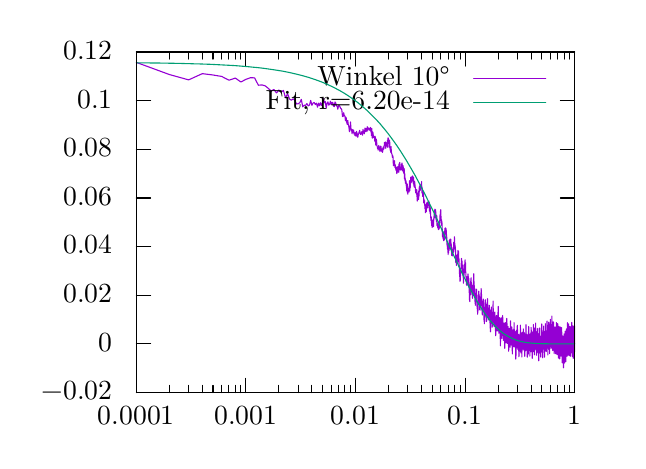
\begin{tikzpicture}[gnuplot]
%% generated with GNUPLOT 5.2p5a (Gentoo revision r0) (Lua 5.1; terminal rev. 99 , script rev. 107)
%% Sa 18 Mai 2019 18:30:31 CEST
\path (0.000,0.000) rectangle (7.500,5.250);
\gpcolor{color=gp lt color border}
\gpsetlinetype{gp lt border}
\gpsetdashtype{gp dt solid}
\gpsetlinewidth{1.00}
\draw[gp path] (1.380,0.616)--(1.560,0.616);
\draw[gp path] (6.947,0.616)--(6.767,0.616);
\node[gp node right] at (1.196,0.616) {$-0.02$};
\draw[gp path] (1.380,1.234)--(1.560,1.234);
\draw[gp path] (6.947,1.234)--(6.767,1.234);
\node[gp node right] at (1.196,1.234) {$0$};
\draw[gp path] (1.380,1.852)--(1.560,1.852);
\draw[gp path] (6.947,1.852)--(6.767,1.852);
\node[gp node right] at (1.196,1.852) {$0.02$};
\draw[gp path] (1.380,2.470)--(1.560,2.470);
\draw[gp path] (6.947,2.470)--(6.767,2.470);
\node[gp node right] at (1.196,2.470) {$0.04$};
\draw[gp path] (1.380,3.087)--(1.560,3.087);
\draw[gp path] (6.947,3.087)--(6.767,3.087);
\node[gp node right] at (1.196,3.087) {$0.06$};
\draw[gp path] (1.380,3.705)--(1.560,3.705);
\draw[gp path] (6.947,3.705)--(6.767,3.705);
\node[gp node right] at (1.196,3.705) {$0.08$};
\draw[gp path] (1.380,4.323)--(1.560,4.323);
\draw[gp path] (6.947,4.323)--(6.767,4.323);
\node[gp node right] at (1.196,4.323) {$0.1$};
\draw[gp path] (1.380,4.941)--(1.560,4.941);
\draw[gp path] (6.947,4.941)--(6.767,4.941);
\node[gp node right] at (1.196,4.941) {$0.12$};
\draw[gp path] (1.380,0.616)--(1.380,0.796);
\draw[gp path] (1.380,4.941)--(1.380,4.761);
\node[gp node center] at (1.380,0.308) {$0.0001$};
\draw[gp path] (1.799,0.616)--(1.799,0.706);
\draw[gp path] (1.799,4.941)--(1.799,4.851);
\draw[gp path] (2.044,0.616)--(2.044,0.706);
\draw[gp path] (2.044,4.941)--(2.044,4.851);
\draw[gp path] (2.218,0.616)--(2.218,0.706);
\draw[gp path] (2.218,4.941)--(2.218,4.851);
\draw[gp path] (2.353,0.616)--(2.353,0.706);
\draw[gp path] (2.353,4.941)--(2.353,4.851);
\draw[gp path] (2.463,0.616)--(2.463,0.706);
\draw[gp path] (2.463,4.941)--(2.463,4.851);
\draw[gp path] (2.556,0.616)--(2.556,0.706);
\draw[gp path] (2.556,4.941)--(2.556,4.851);
\draw[gp path] (2.637,0.616)--(2.637,0.706);
\draw[gp path] (2.637,4.941)--(2.637,4.851);
\draw[gp path] (2.708,0.616)--(2.708,0.706);
\draw[gp path] (2.708,4.941)--(2.708,4.851);
\draw[gp path] (2.772,0.616)--(2.772,0.796);
\draw[gp path] (2.772,4.941)--(2.772,4.761);
\node[gp node center] at (2.772,0.308) {$0.001$};
\draw[gp path] (3.191,0.616)--(3.191,0.706);
\draw[gp path] (3.191,4.941)--(3.191,4.851);
\draw[gp path] (3.436,0.616)--(3.436,0.706);
\draw[gp path] (3.436,4.941)--(3.436,4.851);
\draw[gp path] (3.610,0.616)--(3.610,0.706);
\draw[gp path] (3.610,4.941)--(3.610,4.851);
\draw[gp path] (3.745,0.616)--(3.745,0.706);
\draw[gp path] (3.745,4.941)--(3.745,4.851);
\draw[gp path] (3.855,0.616)--(3.855,0.706);
\draw[gp path] (3.855,4.941)--(3.855,4.851);
\draw[gp path] (3.948,0.616)--(3.948,0.706);
\draw[gp path] (3.948,4.941)--(3.948,4.851);
\draw[gp path] (4.029,0.616)--(4.029,0.706);
\draw[gp path] (4.029,4.941)--(4.029,4.851);
\draw[gp path] (4.100,0.616)--(4.100,0.706);
\draw[gp path] (4.100,4.941)--(4.100,4.851);
\draw[gp path] (4.163,0.616)--(4.163,0.796);
\draw[gp path] (4.163,4.941)--(4.163,4.761);
\node[gp node center] at (4.163,0.308) {$0.01$};
\draw[gp path] (4.582,0.616)--(4.582,0.706);
\draw[gp path] (4.582,4.941)--(4.582,4.851);
\draw[gp path] (4.828,0.616)--(4.828,0.706);
\draw[gp path] (4.828,4.941)--(4.828,4.851);
\draw[gp path] (5.001,0.616)--(5.001,0.706);
\draw[gp path] (5.001,4.941)--(5.001,4.851);
\draw[gp path] (5.136,0.616)--(5.136,0.706);
\draw[gp path] (5.136,4.941)--(5.136,4.851);
\draw[gp path] (5.246,0.616)--(5.246,0.706);
\draw[gp path] (5.246,4.941)--(5.246,4.851);
\draw[gp path] (5.340,0.616)--(5.340,0.706);
\draw[gp path] (5.340,4.941)--(5.340,4.851);
\draw[gp path] (5.420,0.616)--(5.420,0.706);
\draw[gp path] (5.420,4.941)--(5.420,4.851);
\draw[gp path] (5.492,0.616)--(5.492,0.706);
\draw[gp path] (5.492,4.941)--(5.492,4.851);
\draw[gp path] (5.555,0.616)--(5.555,0.796);
\draw[gp path] (5.555,4.941)--(5.555,4.761);
\node[gp node center] at (5.555,0.308) {$0.1$};
\draw[gp path] (5.974,0.616)--(5.974,0.706);
\draw[gp path] (5.974,4.941)--(5.974,4.851);
\draw[gp path] (6.219,0.616)--(6.219,0.706);
\draw[gp path] (6.219,4.941)--(6.219,4.851);
\draw[gp path] (6.393,0.616)--(6.393,0.706);
\draw[gp path] (6.393,4.941)--(6.393,4.851);
\draw[gp path] (6.528,0.616)--(6.528,0.706);
\draw[gp path] (6.528,4.941)--(6.528,4.851);
\draw[gp path] (6.638,0.616)--(6.638,0.706);
\draw[gp path] (6.638,4.941)--(6.638,4.851);
\draw[gp path] (6.731,0.616)--(6.731,0.706);
\draw[gp path] (6.731,4.941)--(6.731,4.851);
\draw[gp path] (6.812,0.616)--(6.812,0.706);
\draw[gp path] (6.812,4.941)--(6.812,4.851);
\draw[gp path] (6.883,0.616)--(6.883,0.706);
\draw[gp path] (6.883,4.941)--(6.883,4.851);
\draw[gp path] (6.947,0.616)--(6.947,0.796);
\draw[gp path] (6.947,4.941)--(6.947,4.761);
\node[gp node center] at (6.947,0.308) {$1$};
\draw[gp path] (1.380,4.941)--(1.380,0.616)--(6.947,0.616)--(6.947,4.941)--cycle;
\node[gp node right] at (5.479,4.607) {Winkel 10°};
\gpcolor{rgb color={0.580,0.000,0.827}}
\draw[gp path] (5.663,4.607)--(6.579,4.607);
\draw[gp path] (1.380,4.809)--(1.799,4.655)--(2.044,4.587)--(2.218,4.666)--(2.353,4.649)%
  --(2.463,4.631)--(2.556,4.583)--(2.637,4.610)--(2.708,4.560)--(2.772,4.594)--(2.829,4.614)%
  --(2.882,4.613)--(2.930,4.519)--(2.975,4.523)--(3.017,4.511)--(3.056,4.479)--(3.092,4.445)%
  --(3.127,4.465)--(3.160,4.421)--(3.191,4.458)--(3.220,4.432)--(3.248,4.453)--(3.275,4.358)%
  --(3.301,4.412)--(3.326,4.343)--(3.349,4.329)--(3.372,4.346)--(3.394,4.323)--(3.415,4.281)%
  --(3.436,4.284)--(3.456,4.297)--(3.475,4.340)--(3.493,4.245)--(3.511,4.265)--(3.529,4.263)%
  --(3.546,4.286)--(3.563,4.257)--(3.579,4.267)--(3.594,4.326)--(3.610,4.264)--(3.625,4.293)%
  --(3.639,4.300)--(3.653,4.274)--(3.667,4.292)--(3.681,4.240)--(3.694,4.292)--(3.707,4.259)%
  --(3.720,4.297)--(3.732,4.261)--(3.745,4.295)--(3.757,4.350)--(3.768,4.296)--(3.780,4.312)%
  --(3.791,4.231)--(3.802,4.286)--(3.813,4.308)--(3.824,4.266)--(3.834,4.276)--(3.845,4.315)%
  --(3.855,4.272)--(3.865,4.302)--(3.875,4.299)--(3.884,4.254)--(3.894,4.248)--(3.903,4.307)%
  --(3.912,4.294)--(3.921,4.257)--(3.930,4.254)--(3.939,4.214)--(3.948,4.259)--(3.956,4.263)%
  --(3.965,4.249)--(3.973,4.227)--(3.982,4.221)--(3.990,4.203)--(3.998,4.123)--(4.006,4.121)%
  --(4.013,4.170)--(4.021,4.133)--(4.029,4.129)--(4.036,4.067)--(4.044,4.110)--(4.051,4.053)%
  --(4.058,4.022)--(4.065,4.073)--(4.072,4.016)--(4.079,3.993)--(4.086,3.929)--(4.093,3.943)%
  --(4.100,4.052)--(4.106,3.960)--(4.113,3.963)--(4.120,3.903)--(4.126,3.955)--(4.132,3.922)%
  --(4.139,3.950)--(4.145,3.898)--(4.151,3.915)--(4.157,3.879)--(4.164,3.916)--(4.170,3.872)%
  --(4.175,3.932)--(4.181,3.919)--(4.187,3.872)--(4.193,3.858)--(4.199,3.900)--(4.204,3.902)%
  --(4.210,3.928)--(4.216,3.946)--(4.221,3.923)--(4.227,3.896)--(4.232,3.898)--(4.237,3.900)%
  --(4.243,3.929)--(4.248,3.928)--(4.253,3.884)--(4.258,3.957)--(4.264,3.935)--(4.269,3.940)%
  --(4.274,3.902)--(4.279,3.927)--(4.284,3.975)--(4.289,3.930)--(4.294,3.962)--(4.298,3.968)%
  --(4.303,3.966)--(4.308,3.929)--(4.313,3.992)--(4.317,3.968)--(4.322,3.950)--(4.327,3.961)%
  --(4.331,3.978)--(4.336,3.961)--(4.340,3.961)--(4.345,3.947)--(4.349,3.963)--(4.354,3.983)%
  --(4.358,3.934)--(4.363,3.921)--(4.367,3.878)--(4.371,3.970)--(4.375,3.856)--(4.380,3.847)%
  --(4.384,3.924)--(4.388,3.892)--(4.392,3.854)--(4.396,3.873)--(4.400,3.867)--(4.405,3.866)%
  --(4.409,3.805)--(4.413,3.871)--(4.417,3.804)--(4.421,3.758)--(4.424,3.763)--(4.428,3.835)%
  --(4.432,3.797)--(4.436,3.748)--(4.440,3.740)--(4.444,3.713)--(4.448,3.722)--(4.451,3.694)%
  --(4.455,3.737)--(4.459,3.754)--(4.463,3.726)--(4.466,3.727)--(4.470,3.712)--(4.473,3.678)%
  --(4.477,3.730)--(4.481,3.745)--(4.484,3.742)--(4.488,3.739)--(4.491,3.681)--(4.495,3.689)%
  --(4.498,3.710)--(4.502,3.712)--(4.505,3.667)--(4.509,3.680)--(4.512,3.713)--(4.515,3.735)%
  --(4.519,3.705)--(4.522,3.709)--(4.525,3.721)--(4.529,3.758)--(4.532,3.794)--(4.535,3.754)%
  --(4.539,3.750)--(4.542,3.784)--(4.545,3.799)--(4.548,3.719)--(4.551,3.748)--(4.555,3.758)%
  --(4.558,3.788)--(4.561,3.747)--(4.564,3.782)--(4.567,3.763)--(4.570,3.821)--(4.573,3.731)%
  --(4.576,3.849)--(4.579,3.848)--(4.582,3.802)--(4.585,3.803)--(4.588,3.796)--(4.591,3.825)%
  --(4.594,3.733)--(4.597,3.816)--(4.600,3.719)--(4.603,3.723)--(4.606,3.687)--(4.609,3.708)%
  --(4.612,3.664)--(4.615,3.740)--(4.618,3.677)--(4.621,3.659)--(4.623,3.652)--(4.626,3.642)%
  --(4.629,3.635)--(4.632,3.603)--(4.635,3.626)--(4.637,3.619)--(4.640,3.606)--(4.643,3.530)%
  --(4.646,3.497)--(4.648,3.560)--(4.651,3.513)--(4.654,3.539)--(4.656,3.546)--(4.659,3.561)%
  --(4.662,3.503)--(4.664,3.474)--(4.667,3.510)--(4.670,3.491)--(4.672,3.469)--(4.675,3.455)%
  --(4.677,3.438)--(4.680,3.478)--(4.683,3.459)--(4.685,3.448)--(4.688,3.396)--(4.690,3.448)%
  --(4.693,3.455)--(4.695,3.482)--(4.698,3.415)--(4.700,3.440)--(4.703,3.442)--(4.705,3.483)%
  --(4.708,3.454)--(4.710,3.490)--(4.712,3.413)--(4.715,3.520)--(4.717,3.439)--(4.720,3.476)%
  --(4.722,3.458)--(4.725,3.539)--(4.727,3.450)--(4.729,3.467)--(4.732,3.466)--(4.734,3.443)%
  --(4.736,3.476)--(4.739,3.479)--(4.741,3.442)--(4.743,3.461)--(4.746,3.448)--(4.748,3.516)%
  --(4.750,3.504)--(4.753,3.530)--(4.755,3.530)--(4.757,3.502)--(4.759,3.453)--(4.762,3.431)%
  --(4.764,3.460)--(4.766,3.499)--(4.768,3.469)--(4.771,3.480)--(4.773,3.416)--(4.775,3.410)%
  --(4.777,3.460)--(4.779,3.394)--(4.781,3.462)--(4.784,3.410)--(4.786,3.329)--(4.788,3.361)%
  --(4.790,3.395)--(4.792,3.312)--(4.794,3.342)--(4.797,3.275)--(4.799,3.303)--(4.801,3.271)%
  --(4.803,3.279)--(4.805,3.305)--(4.807,3.285)--(4.809,3.230)--(4.811,3.219)--(4.813,3.225)%
  --(4.815,3.175)--(4.817,3.219)--(4.819,3.189)--(4.821,3.266)--(4.823,3.151)--(4.826,3.172)%
  --(4.828,3.135)--(4.830,3.182)--(4.832,3.163)--(4.834,3.180)--(4.836,3.179)--(4.838,3.214)%
  --(4.840,3.177)--(4.841,3.210)--(4.843,3.163)--(4.845,3.220)--(4.847,3.242)--(4.849,3.307)%
  --(4.851,3.202)--(4.853,3.180)--(4.855,3.222)--(4.857,3.212)--(4.859,3.229)--(4.861,3.277)%
  --(4.863,3.271)--(4.865,3.350)--(4.867,3.319)--(4.868,3.323)--(4.870,3.281)--(4.872,3.294)%
  --(4.874,3.317)--(4.876,3.355)--(4.878,3.318)--(4.880,3.346)--(4.881,3.320)--(4.883,3.303)%
  --(4.885,3.367)--(4.887,3.362)--(4.889,3.356)--(4.891,3.335)--(4.892,3.353)--(4.894,3.357)%
  --(4.896,3.305)--(4.898,3.265)--(4.900,3.349)--(4.901,3.312)--(4.903,3.297)--(4.905,3.304)%
  --(4.907,3.235)--(4.908,3.281)--(4.910,3.224)--(4.912,3.264)--(4.914,3.298)--(4.916,3.272)%
  --(4.917,3.249)--(4.919,3.255)--(4.921,3.231)--(4.922,3.220)--(4.924,3.224)--(4.926,3.173)%
  --(4.928,3.155)--(4.929,3.178)--(4.931,3.170)--(4.933,3.174)--(4.934,3.150)--(4.936,3.139)%
  --(4.938,3.164)--(4.939,3.132)--(4.941,3.193)--(4.943,3.113)--(4.944,3.133)--(4.946,3.075)%
  --(4.948,3.048)--(4.949,3.105)--(4.951,3.071)--(4.953,3.148)--(4.954,3.116)--(4.956,3.117)%
  --(4.958,3.128)--(4.959,3.129)--(4.961,3.108)--(4.962,3.150)--(4.964,3.066)--(4.966,3.177)%
  --(4.967,3.098)--(4.969,3.152)--(4.970,3.115)--(4.972,3.149)--(4.974,3.233)--(4.975,3.177)%
  --(4.977,3.188)--(4.978,3.194)--(4.980,3.224)--(4.981,3.217)--(4.983,3.253)--(4.985,3.216)%
  --(4.986,3.185)--(4.988,3.225)--(4.989,3.226)--(4.991,3.241)--(4.992,3.240)--(4.994,3.257)%
  --(4.995,3.236)--(4.997,3.264)--(4.998,3.246)--(5.000,3.261)--(5.001,3.239)--(5.003,3.296)%
  --(5.004,3.239)--(5.006,3.219)--(5.007,3.159)--(5.009,3.148)--(5.010,3.221)--(5.012,3.162)%
  --(5.013,3.192)--(5.015,3.161)--(5.016,3.108)--(5.018,3.143)--(5.019,3.112)--(5.021,3.117)%
  --(5.022,3.119)--(5.024,3.170)--(5.025,3.132)--(5.027,3.146)--(5.028,3.073)--(5.029,3.027)%
  --(5.031,3.077)--(5.032,3.071)--(5.034,3.065)--(5.035,3.036)--(5.037,3.037)--(5.038,3.016)%
  --(5.039,3.054)--(5.041,3.047)--(5.042,2.991)--(5.044,3.005)--(5.045,2.955)--(5.047,2.948)%
  --(5.048,2.951)--(5.049,2.984)--(5.051,2.900)--(5.052,2.949)--(5.054,3.001)--(5.055,2.961)%
  --(5.056,2.977)--(5.058,2.983)--(5.059,2.913)--(5.060,2.939)--(5.062,2.912)--(5.063,2.964)%
  --(5.064,2.969)--(5.066,3.025)--(5.067,3.017)--(5.069,2.978)--(5.070,2.990)--(5.071,2.998)%
  --(5.073,2.989)--(5.074,2.995)--(5.075,3.020)--(5.077,3.011)--(5.078,2.993)--(5.079,2.960)%
  --(5.081,3.035)--(5.082,2.964)--(5.083,3.005)--(5.085,3.001)--(5.086,3.046)--(5.087,3.029)%
  --(5.089,3.019)--(5.090,3.033)--(5.091,3.030)--(5.092,2.995)--(5.094,3.026)--(5.095,3.047)%
  --(5.096,3.020)--(5.098,3.013)--(5.099,3.001)--(5.100,3.031)--(5.101,3.012)--(5.103,2.920)%
  --(5.104,2.985)--(5.105,2.986)--(5.107,2.952)--(5.108,2.929)--(5.109,2.908)--(5.110,2.986)%
  --(5.112,2.964)--(5.113,2.886)--(5.114,2.899)--(5.115,2.887)--(5.117,2.912)--(5.118,2.860)%
  --(5.119,2.849)--(5.120,2.823)--(5.122,2.810)--(5.123,2.799)--(5.124,2.822)--(5.125,2.845)%
  --(5.127,2.810)--(5.128,2.816)--(5.129,2.764)--(5.130,2.762)--(5.131,2.734)--(5.133,2.780)%
  --(5.134,2.730)--(5.135,2.749)--(5.136,2.712)--(5.137,2.725)--(5.139,2.755)--(5.140,2.740)%
  --(5.141,2.736)--(5.142,2.801)--(5.144,2.783)--(5.145,2.727)--(5.146,2.808)--(5.147,2.722)%
  --(5.148,2.758)--(5.149,2.730)--(5.151,2.789)--(5.152,2.802)--(5.153,2.775)--(5.154,2.725)%
  --(5.155,2.807)--(5.157,2.805)--(5.158,2.832)--(5.159,2.844)--(5.160,2.834)--(5.161,2.853)%
  --(5.162,2.842)--(5.163,2.885)--(5.165,2.873)--(5.166,2.849)--(5.167,2.836)--(5.168,2.898)%
  --(5.169,2.880)--(5.170,2.932)--(5.172,2.945)--(5.173,2.880)--(5.174,2.942)--(5.175,2.904)%
  --(5.176,2.921)--(5.177,2.874)--(5.178,2.856)--(5.179,2.902)--(5.181,2.938)--(5.182,2.906)%
  --(5.183,2.865)--(5.184,2.844)--(5.185,2.877)--(5.186,2.816)--(5.187,2.842)--(5.188,2.817)%
  --(5.189,2.863)--(5.191,2.788)--(5.192,2.832)--(5.193,2.785)--(5.194,2.818)--(5.195,2.818)%
  --(5.196,2.861)--(5.197,2.760)--(5.198,2.768)--(5.199,2.735)--(5.200,2.754)--(5.202,2.755)%
  --(5.203,2.763)--(5.204,2.728)--(5.205,2.771)--(5.206,2.713)--(5.207,2.715)--(5.208,2.722)%
  --(5.209,2.730)--(5.210,2.722)--(5.211,2.757)--(5.212,2.701)--(5.213,2.721)--(5.214,2.708)%
  --(5.215,2.690)--(5.217,2.726)--(5.218,2.727)--(5.219,2.685)--(5.220,2.717)--(5.221,2.721)%
  --(5.222,2.689)--(5.223,2.710)--(5.224,2.695)--(5.225,2.729)--(5.226,2.762)--(5.227,2.711)%
  --(5.228,2.702)--(5.229,2.798)--(5.230,2.789)--(5.231,2.792)--(5.232,2.783)--(5.233,2.793)%
  --(5.234,2.770)--(5.235,2.804)--(5.236,2.857)--(5.237,2.865)--(5.238,2.848)--(5.239,2.826)%
  --(5.240,2.883)--(5.241,2.857)--(5.242,2.918)--(5.243,2.845)--(5.244,2.910)--(5.245,2.866)%
  --(5.246,2.937)--(5.247,2.877)--(5.249,2.851)--(5.250,2.849)--(5.251,2.845)--(5.252,2.796)%
  --(5.253,2.812)--(5.254,2.740)--(5.254,2.773)--(5.255,2.758)--(5.256,2.811)--(5.257,2.749)%
  --(5.258,2.793)--(5.259,2.766)--(5.260,2.743)--(5.261,2.780)--(5.262,2.746)--(5.263,2.770)%
  --(5.264,2.711)--(5.265,2.669)--(5.266,2.650)--(5.267,2.597)--(5.268,2.621)--(5.269,2.640)%
  --(5.270,2.633)--(5.271,2.651)--(5.272,2.602)--(5.273,2.633)--(5.274,2.648)--(5.275,2.573)%
  --(5.276,2.583)--(5.277,2.591)--(5.278,2.591)--(5.279,2.559)--(5.280,2.594)--(5.281,2.576)%
  --(5.282,2.600)--(5.283,2.544)--(5.284,2.562)--(5.285,2.628)--(5.286,2.660)--(5.286,2.620)%
  --(5.287,2.609)--(5.288,2.596)--(5.289,2.628)--(5.290,2.553)--(5.291,2.629)--(5.292,2.590)%
  --(5.293,2.649)--(5.294,2.594)--(5.295,2.640)--(5.296,2.588)--(5.297,2.644)--(5.298,2.702)%
  --(5.299,2.618)--(5.300,2.637)--(5.300,2.651)--(5.301,2.651)--(5.302,2.647)--(5.303,2.664)%
  --(5.304,2.667)--(5.305,2.670)--(5.306,2.708)--(5.307,2.649)--(5.308,2.664)--(5.309,2.703)%
  --(5.310,2.677)--(5.310,2.649)--(5.311,2.683)--(5.312,2.683)--(5.313,2.675)--(5.314,2.694)%
  --(5.315,2.680)--(5.316,2.643)--(5.317,2.611)--(5.318,2.564)--(5.319,2.593)--(5.319,2.623)%
  --(5.320,2.598)--(5.321,2.539)--(5.322,2.592)--(5.323,2.562)--(5.324,2.519)--(5.325,2.496)%
  --(5.326,2.533)--(5.327,2.475)--(5.327,2.518)--(5.328,2.492)--(5.329,2.519)--(5.330,2.471)%
  --(5.331,2.473)--(5.332,2.439)--(5.333,2.433)--(5.334,2.477)--(5.334,2.480)--(5.335,2.497)%
  --(5.336,2.463)--(5.337,2.406)--(5.338,2.447)--(5.339,2.376)--(5.340,2.369)--(5.341,2.398)%
  --(5.341,2.405)--(5.342,2.401)--(5.343,2.496)--(5.344,2.388)--(5.345,2.452)--(5.346,2.438)%
  --(5.347,2.447)--(5.347,2.417)--(5.348,2.418)--(5.349,2.446)--(5.350,2.455)--(5.351,2.421)%
  --(5.352,2.480)--(5.352,2.468)--(5.353,2.547)--(5.354,2.500)--(5.355,2.509)--(5.356,2.464)%
  --(5.357,2.500)--(5.358,2.517)--(5.358,2.451)--(5.359,2.496)--(5.360,2.507)--(5.361,2.445)%
  --(5.362,2.447)--(5.363,2.530)--(5.363,2.564)--(5.364,2.551)--(5.365,2.546)--(5.366,2.558)%
  --(5.367,2.541)--(5.368,2.517)--(5.368,2.563)--(5.369,2.554)--(5.370,2.565)--(5.371,2.520)%
  --(5.372,2.542)--(5.372,2.546)--(5.373,2.564)--(5.374,2.542)--(5.375,2.501)--(5.376,2.479)%
  --(5.377,2.481)--(5.377,2.515)--(5.378,2.496)--(5.379,2.474)--(5.380,2.479)--(5.381,2.495)%
  --(5.381,2.474)--(5.382,2.468)--(5.383,2.406)--(5.384,2.429)--(5.385,2.421)--(5.385,2.420)%
  --(5.386,2.355)--(5.387,2.418)--(5.388,2.426)--(5.389,2.399)--(5.389,2.420)--(5.390,2.401)%
  --(5.391,2.428)--(5.392,2.388)--(5.393,2.407)--(5.393,2.427)--(5.394,2.352)--(5.395,2.421)%
  --(5.396,2.362)--(5.396,2.431)--(5.397,2.376)--(5.398,2.385)--(5.399,2.378)--(5.400,2.365)%
  --(5.400,2.375)--(5.401,2.426)--(5.402,2.409)--(5.403,2.441)--(5.404,2.402)--(5.404,2.396)%
  --(5.405,2.457)--(5.406,2.452)--(5.407,2.408)--(5.407,2.434)--(5.408,2.396)--(5.409,2.461)%
  --(5.410,2.480)--(5.410,2.524)--(5.411,2.471)--(5.412,2.488)--(5.413,2.494)--(5.414,2.485)%
  --(5.414,2.515)--(5.415,2.437)--(5.416,2.466)--(5.417,2.482)--(5.417,2.522)--(5.418,2.516)%
  --(5.419,2.595)--(5.420,2.539)--(5.420,2.563)--(5.421,2.583)--(5.422,2.524)--(5.423,2.577)%
  --(5.423,2.513)--(5.424,2.504)--(5.425,2.502)--(5.426,2.452)--(5.426,2.490)--(5.427,2.491)%
  --(5.428,2.454)--(5.429,2.452)--(5.429,2.440)--(5.430,2.470)--(5.431,2.437)--(5.432,2.407)%
  --(5.432,2.415)--(5.433,2.430)--(5.434,2.404)--(5.435,2.390)--(5.435,2.391)--(5.436,2.272)%
  --(5.437,2.302)--(5.438,2.264)--(5.438,2.324)--(5.439,2.282)--(5.440,2.307)--(5.440,2.332)%
  --(5.441,2.303)--(5.442,2.359)--(5.443,2.301)--(5.443,2.289)--(5.444,2.230)--(5.445,2.300)%
  --(5.446,2.250)--(5.446,2.270)--(5.447,2.267)--(5.448,2.284)--(5.448,2.261)--(5.449,2.284)%
  --(5.450,2.300)--(5.451,2.275)--(5.451,2.283)--(5.452,2.290)--(5.453,2.307)--(5.453,2.284)%
  --(5.454,2.261)--(5.455,2.279)--(5.456,2.336)--(5.456,2.348)--(5.457,2.303)--(5.458,2.311)%
  --(5.458,2.316)--(5.459,2.373)--(5.460,2.284)--(5.461,2.276)--(5.461,2.316)--(5.462,2.365)%
  --(5.463,2.328)--(5.463,2.355)--(5.464,2.343)--(5.465,2.421)--(5.465,2.392)--(5.466,2.288)%
  --(5.467,2.317)--(5.468,2.378)--(5.468,2.382)--(5.469,2.350)--(5.470,2.371)--(5.470,2.344)%
  --(5.471,2.408)--(5.472,2.340)--(5.472,2.320)--(5.473,2.325)--(5.474,2.326)--(5.475,2.313)%
  --(5.475,2.306)--(5.476,2.309)--(5.477,2.252)--(5.477,2.212)--(5.478,2.275)--(5.479,2.311)%
  --(5.479,2.269)--(5.480,2.243)--(5.481,2.202)--(5.481,2.225)--(5.482,2.187)--(5.483,2.204)%
  --(5.483,2.183)--(5.484,2.163)--(5.485,2.112)--(5.485,2.138)--(5.486,2.150)--(5.487,2.143)%
  --(5.488,2.083)--(5.488,2.137)--(5.489,2.068)--(5.490,2.111)--(5.490,2.029)--(5.491,2.099)%
  --(5.492,2.050)--(5.492,2.109)--(5.493,2.056)--(5.494,2.062)--(5.494,2.070)--(5.495,2.110)%
  --(5.496,2.042)--(5.496,2.158)--(5.497,2.100)--(5.498,2.161)--(5.498,2.102)--(5.499,2.195)%
  --(5.500,2.136)--(5.500,2.189)--(5.501,2.167)--(5.502,2.157)--(5.502,2.205)--(5.503,2.191)%
  --(5.504,2.198)--(5.504,2.229)--(5.505,2.236)--(5.506,2.231)--(5.506,2.260)--(5.507,2.236)%
  --(5.507,2.260)--(5.508,2.221)--(5.509,2.230)--(5.509,2.320)--(5.510,2.221)--(5.511,2.261)%
  --(5.511,2.263)--(5.512,2.269)--(5.513,2.265)--(5.513,2.258)--(5.514,2.233)--(5.515,2.264)%
  --(5.515,2.248)--(5.516,2.274)--(5.517,2.286)--(5.517,2.249)--(5.518,2.223)--(5.518,2.190)%
  --(5.519,2.222)--(5.520,2.198)--(5.520,2.128)--(5.521,2.150)--(5.522,2.158)--(5.522,2.190)%
  --(5.523,2.171)--(5.524,2.236)--(5.524,2.159)--(5.525,2.189)--(5.526,2.122)--(5.526,2.165)%
  --(5.527,2.166)--(5.527,2.150)--(5.528,2.140)--(5.529,2.096)--(5.529,2.126)--(5.530,2.126)%
  --(5.531,2.161)--(5.531,2.076)--(5.532,2.082)--(5.532,2.078)--(5.533,2.136)--(5.534,2.063)%
  --(5.534,2.004)--(5.535,2.052)--(5.536,2.089)--(5.536,2.064)--(5.537,2.047)--(5.537,2.116)%
  --(5.538,2.063)--(5.539,2.063)--(5.539,2.099)--(5.540,2.105)--(5.541,2.105)--(5.541,2.118)%
  --(5.542,2.116)--(5.542,2.117)--(5.543,2.123)--(5.544,2.138)--(5.544,2.224)--(5.545,2.239)%
  --(5.546,2.223)--(5.546,2.214)--(5.547,2.187)--(5.547,2.191)--(5.548,2.200)--(5.549,2.202)%
  --(5.549,2.190)--(5.550,2.209)--(5.550,2.247)--(5.551,2.243)--(5.552,2.259)--(5.552,2.246)%
  --(5.553,2.291)--(5.553,2.263)--(5.554,2.292)--(5.555,2.274)--(5.555,2.301)--(5.556,2.287)%
  --(5.556,2.293)--(5.557,2.203)--(5.558,2.225)--(5.558,2.155)--(5.559,2.233)--(5.559,2.236)%
  --(5.560,2.169)--(5.561,2.265)--(5.561,2.211)--(5.562,2.197)--(5.562,2.192)--(5.563,2.138)%
  --(5.564,2.151)--(5.564,2.144)--(5.565,2.144)--(5.565,2.124)--(5.566,2.090)--(5.567,2.085)%
  --(5.567,2.081)--(5.568,2.075)--(5.568,2.062)--(5.569,2.079)--(5.570,2.090)--(5.570,2.041)%
  --(5.571,2.003)--(5.571,1.987)--(5.572,2.027)--(5.573,2.041)--(5.573,1.983)--(5.574,1.990)%
  --(5.574,2.024)--(5.575,2.010)--(5.575,2.015)--(5.576,2.010)--(5.577,2.011)--(5.577,1.976)%
  --(5.578,1.976)--(5.578,2.023)--(5.579,2.072)--(5.580,2.020)--(5.580,1.999)--(5.581,1.987)%
  --(5.581,1.976)--(5.582,2.062)--(5.582,1.997)--(5.583,2.007)--(5.584,2.022)--(5.584,2.057)%
  --(5.585,2.050)--(5.586,2.064)--(5.586,2.089)--(5.587,2.075)--(5.588,2.089)--(5.588,2.093)%
  --(5.589,2.005)--(5.589,2.085)--(5.590,2.070)--(5.590,2.074)--(5.591,2.096)--(5.592,2.073)%
  --(5.592,2.124)--(5.593,2.082)--(5.593,2.102)--(5.594,2.101)--(5.594,2.070)--(5.595,2.090)%
  --(5.596,2.067)--(5.596,2.061)--(5.597,2.029)--(5.597,2.067)--(5.598,2.031)--(5.598,2.056)%
  --(5.599,2.031)--(5.600,2.041)--(5.600,2.034)--(5.601,2.066)--(5.601,2.012)--(5.602,2.040)%
  --(5.602,1.958)--(5.603,2.033)--(5.603,1.988)--(5.604,1.972)--(5.605,1.989)--(5.605,1.943)%
  --(5.606,1.945)--(5.606,1.916)--(5.607,1.898)--(5.607,1.933)--(5.608,1.910)--(5.608,1.882)%
  --(5.609,1.901)--(5.610,1.916)--(5.610,1.850)--(5.611,1.836)--(5.611,1.794)--(5.612,1.793)%
  --(5.612,1.885)--(5.613,1.844)--(5.613,1.806)--(5.614,1.851)--(5.615,1.770)--(5.615,1.925)%
  --(5.616,1.836)--(5.616,1.877)--(5.617,1.861)--(5.617,1.858)--(5.618,1.877)--(5.618,1.868)%
  --(5.619,1.866)--(5.619,1.907)--(5.620,1.873)--(5.621,1.914)--(5.621,1.900)--(5.622,1.980)%
  --(5.622,1.923)--(5.623,1.855)--(5.623,1.935)--(5.624,1.951)--(5.624,2.015)--(5.625,1.963)%
  --(5.625,1.964)--(5.626,1.983)--(5.626,1.973)--(5.627,2.033)--(5.628,1.999)--(5.628,2.008)%
  --(5.629,1.978)--(5.629,2.047)--(5.630,2.025)--(5.630,2.027)--(5.631,2.074)--(5.631,1.993)%
  --(5.632,2.045)--(5.632,1.965)--(5.633,2.017)--(5.633,1.948)--(5.634,2.012)--(5.634,1.977)%
  --(5.635,1.914)--(5.636,1.942)--(5.636,1.990)--(5.637,1.983)--(5.637,1.919)--(5.638,1.996)%
  --(5.638,1.975)--(5.639,1.958)--(5.639,1.924)--(5.640,1.966)--(5.640,1.932)--(5.641,1.936)%
  --(5.641,1.862)--(5.642,1.920)--(5.642,1.897)--(5.643,1.979)--(5.643,1.901)--(5.644,1.862)%
  --(5.644,1.863)--(5.645,1.907)--(5.645,1.922)--(5.646,1.917)--(5.647,1.857)--(5.647,1.841)%
  --(5.648,1.869)--(5.648,1.875)--(5.649,1.879)--(5.649,1.860)--(5.650,1.813)--(5.650,1.864)%
  --(5.651,1.858)--(5.651,1.845)--(5.652,1.904)--(5.652,1.876)--(5.653,1.879)--(5.653,1.898)%
  --(5.654,1.886)--(5.654,1.903)--(5.655,1.868)--(5.655,1.864)--(5.656,1.932)--(5.656,1.935)%
  --(5.657,1.882)--(5.657,1.906)--(5.658,1.966)--(5.658,1.931)--(5.659,1.958)--(5.659,1.942)%
  --(5.660,1.987)--(5.660,1.970)--(5.661,2.019)--(5.661,2.014)--(5.662,2.033)--(5.662,2.051)%
  --(5.663,1.987)--(5.663,2.063)--(5.664,2.031)--(5.664,2.122)--(5.665,2.070)--(5.665,2.080)%
  --(5.666,2.077)--(5.666,2.126)--(5.667,1.978)--(5.667,2.030)--(5.668,1.986)--(5.668,2.028)%
  --(5.669,1.995)--(5.669,2.002)--(5.670,1.970)--(5.670,1.996)--(5.671,1.969)--(5.671,1.945)%
  --(5.672,1.951)--(5.672,1.958)--(5.673,1.853)--(5.673,1.862)--(5.674,1.882)--(5.674,1.867)%
  --(5.675,1.857)--(5.675,1.877)--(5.676,1.823)--(5.676,1.831)--(5.677,1.877)--(5.677,1.825)%
  --(5.678,1.845)--(5.678,1.861)--(5.679,1.824)--(5.679,1.772)--(5.680,1.800)--(5.680,1.818)%
  --(5.681,1.801)--(5.681,1.825)--(5.682,1.760)--(5.682,1.746)--(5.683,1.750)--(5.683,1.836)%
  --(5.684,1.784)--(5.684,1.816)--(5.685,1.816)--(5.685,1.724)--(5.686,1.788)--(5.686,1.851)%
  --(5.687,1.835)--(5.687,1.843)--(5.688,1.764)--(5.688,1.776)--(5.689,1.807)--(5.689,1.842)%
  --(5.690,1.837)--(5.690,1.867)--(5.691,1.832)--(5.691,1.854)--(5.692,1.810)--(5.692,1.931)%
  --(5.693,1.886)--(5.693,1.820)--(5.693,1.924)--(5.694,1.921)--(5.694,1.903)--(5.695,1.853)%
  --(5.695,1.866)--(5.696,1.826)--(5.696,1.885)--(5.697,1.892)--(5.697,1.893)--(5.698,1.911)%
  --(5.698,1.882)--(5.699,1.886)--(5.699,1.838)--(5.700,1.892)--(5.700,1.875)--(5.701,1.928)%
  --(5.701,1.809)--(5.702,1.855)--(5.702,1.825)--(5.703,1.812)--(5.703,1.838)--(5.704,1.857)%
  --(5.704,1.845)--(5.704,1.856)--(5.705,1.762)--(5.705,1.780)--(5.706,1.784)--(5.706,1.779)%
  --(5.707,1.706)--(5.707,1.735)--(5.708,1.753)--(5.708,1.733)--(5.709,1.714)--(5.709,1.702)%
  --(5.710,1.694)--(5.710,1.681)--(5.711,1.673)--(5.711,1.679)--(5.712,1.718)--(5.712,1.690)%
  --(5.712,1.646)--(5.713,1.647)--(5.713,1.694)--(5.714,1.636)--(5.714,1.610)--(5.715,1.670)%
  --(5.715,1.693)--(5.716,1.674)--(5.716,1.690)--(5.717,1.653)--(5.717,1.645)--(5.718,1.664)%
  --(5.718,1.635)--(5.718,1.729)--(5.719,1.707)--(5.719,1.658)--(5.720,1.680)--(5.720,1.736)%
  --(5.721,1.697)--(5.721,1.726)--(5.722,1.758)--(5.722,1.740)--(5.723,1.774)--(5.723,1.796)%
  --(5.724,1.830)--(5.724,1.795)--(5.724,1.779)--(5.725,1.826)--(5.725,1.854)--(5.726,1.843)%
  --(5.726,1.811)--(5.727,1.829)--(5.727,1.852)--(5.728,1.816)--(5.728,1.837)--(5.729,1.903)%
  --(5.729,1.875)--(5.729,1.877)--(5.730,1.799)--(5.730,1.827)--(5.731,1.784)--(5.731,1.841)%
  --(5.732,1.866)--(5.732,1.859)--(5.733,1.847)--(5.733,1.774)--(5.733,1.799)--(5.734,1.827)%
  --(5.734,1.767)--(5.735,1.847)--(5.735,1.758)--(5.736,1.805)--(5.736,1.775)--(5.737,1.762)%
  --(5.737,1.748)--(5.738,1.731)--(5.738,1.733)--(5.738,1.750)--(5.739,1.759)--(5.739,1.731)%
  --(5.740,1.791)--(5.740,1.667)--(5.741,1.741)--(5.741,1.697)--(5.742,1.707)--(5.742,1.704)%
  --(5.742,1.678)--(5.743,1.669)--(5.743,1.689)--(5.744,1.695)--(5.744,1.711)--(5.745,1.662)%
  --(5.745,1.715)--(5.746,1.672)--(5.746,1.699)--(5.746,1.691)--(5.747,1.766)--(5.747,1.733)%
  --(5.748,1.710)--(5.748,1.707)--(5.749,1.707)--(5.749,1.752)--(5.749,1.762)--(5.750,1.757)%
  --(5.750,1.760)--(5.751,1.774)--(5.751,1.823)--(5.752,1.763)--(5.752,1.794)--(5.753,1.823)%
  --(5.753,1.830)--(5.753,1.802)--(5.754,1.833)--(5.754,1.829)--(5.755,1.769)--(5.755,1.879)%
  --(5.756,1.821)--(5.756,1.816)--(5.756,1.884)--(5.757,1.872)--(5.757,1.855)--(5.758,1.861)%
  --(5.758,1.932)--(5.759,1.885)--(5.759,1.938)--(5.759,1.870)--(5.760,1.924)--(5.760,1.835)%
  --(5.761,1.860)--(5.761,1.820)--(5.762,1.897)--(5.762,1.856)--(5.762,1.833)--(5.763,1.792)%
  --(5.763,1.866)--(5.764,1.787)--(5.764,1.817)--(5.765,1.790)--(5.765,1.817)--(5.765,1.786)%
  --(5.766,1.769)--(5.766,1.730)--(5.767,1.779)--(5.767,1.723)--(5.768,1.699)--(5.768,1.675)%
  --(5.768,1.700)--(5.769,1.762)--(5.769,1.708)--(5.770,1.657)--(5.770,1.694)--(5.771,1.686)%
  --(5.771,1.695)--(5.771,1.613)--(5.772,1.613)--(5.772,1.691)--(5.773,1.663)--(5.773,1.659)%
  --(5.774,1.601)--(5.774,1.651)--(5.774,1.686)--(5.775,1.670)--(5.775,1.677)--(5.776,1.641)%
  --(5.776,1.704)--(5.776,1.678)--(5.777,1.698)--(5.777,1.684)--(5.778,1.673)--(5.778,1.657)%
  --(5.779,1.730)--(5.779,1.655)--(5.779,1.707)--(5.780,1.725)--(5.780,1.747)--(5.781,1.674)%
  --(5.781,1.699)--(5.781,1.707)--(5.782,1.773)--(5.782,1.721)--(5.783,1.739)--(5.783,1.710)%
  --(5.784,1.781)--(5.784,1.702)--(5.784,1.795)--(5.785,1.754)--(5.785,1.720)--(5.786,1.750)%
  --(5.786,1.779)--(5.786,1.751)--(5.787,1.803)--(5.787,1.768)--(5.788,1.755)--(5.788,1.801)%
  --(5.789,1.758)--(5.789,1.727)--(5.789,1.767)--(5.790,1.699)--(5.790,1.745)--(5.791,1.717)%
  --(5.791,1.743)--(5.791,1.695)--(5.792,1.740)--(5.792,1.666)--(5.793,1.758)--(5.793,1.626)%
  --(5.793,1.674)--(5.794,1.612)--(5.794,1.660)--(5.795,1.538)--(5.795,1.644)--(5.795,1.613)%
  --(5.796,1.629)--(5.796,1.518)--(5.797,1.577)--(5.797,1.606)--(5.797,1.562)--(5.798,1.559)%
  --(5.798,1.550)--(5.799,1.573)--(5.799,1.538)--(5.800,1.545)--(5.800,1.575)--(5.800,1.489)%
  --(5.801,1.537)--(5.801,1.541)--(5.802,1.514)--(5.802,1.544)--(5.802,1.564)--(5.803,1.580)%
  --(5.803,1.599)--(5.804,1.629)--(5.804,1.590)--(5.804,1.625)--(5.805,1.597)--(5.805,1.601)%
  --(5.806,1.584)--(5.806,1.634)--(5.806,1.614)--(5.807,1.689)--(5.807,1.647)--(5.808,1.598)%
  --(5.808,1.695)--(5.808,1.668)--(5.809,1.664)--(5.809,1.671)--(5.810,1.696)--(5.810,1.664)%
  --(5.810,1.703)--(5.811,1.693)--(5.811,1.702)--(5.812,1.687)--(5.812,1.711)--(5.812,1.699)%
  --(5.813,1.727)--(5.813,1.680)--(5.813,1.795)--(5.814,1.678)--(5.814,1.705)--(5.815,1.710)%
  --(5.815,1.719)--(5.815,1.711)--(5.816,1.675)--(5.816,1.653)--(5.817,1.743)--(5.817,1.681)%
  --(5.817,1.740)--(5.818,1.671)--(5.818,1.683)--(5.819,1.650)--(5.819,1.673)--(5.820,1.673)%
  --(5.820,1.613)--(5.821,1.652)--(5.821,1.595)--(5.821,1.669)--(5.822,1.666)--(5.822,1.630)%
  --(5.822,1.607)--(5.823,1.631)--(5.823,1.614)--(5.824,1.630)--(5.824,1.599)--(5.824,1.568)%
  --(5.825,1.567)--(5.825,1.542)--(5.826,1.518)--(5.826,1.563)--(5.826,1.561)--(5.827,1.531)%
  --(5.827,1.525)--(5.828,1.592)--(5.828,1.523)--(5.828,1.558)--(5.829,1.612)--(5.829,1.636)%
  --(5.829,1.609)--(5.830,1.572)--(5.830,1.615)--(5.831,1.635)--(5.831,1.650)--(5.831,1.612)%
  --(5.832,1.600)--(5.832,1.692)--(5.832,1.648)--(5.833,1.689)--(5.833,1.726)--(5.834,1.684)%
  --(5.834,1.671)--(5.834,1.690)--(5.835,1.704)--(5.835,1.674)--(5.836,1.720)--(5.836,1.743)%
  --(5.836,1.725)--(5.837,1.733)--(5.837,1.722)--(5.837,1.762)--(5.838,1.780)--(5.838,1.758)%
  --(5.839,1.735)--(5.839,1.741)--(5.839,1.808)--(5.840,1.802)--(5.840,1.775)--(5.840,1.744)%
  --(5.841,1.716)--(5.841,1.694)--(5.842,1.687)--(5.842,1.776)--(5.842,1.711)--(5.843,1.732)%
  --(5.843,1.680)--(5.843,1.659)--(5.844,1.701)--(5.844,1.663)--(5.845,1.676)--(5.845,1.655)%
  --(5.845,1.673)--(5.846,1.667)--(5.846,1.677)--(5.846,1.661)--(5.847,1.645)--(5.847,1.644)%
  --(5.848,1.672)--(5.848,1.602)--(5.848,1.639)--(5.849,1.621)--(5.849,1.599)--(5.849,1.605)%
  --(5.850,1.552)--(5.850,1.549)--(5.851,1.648)--(5.851,1.598)--(5.851,1.584)--(5.852,1.538)%
  --(5.852,1.562)--(5.853,1.549)--(5.853,1.584)--(5.854,1.549)--(5.854,1.564)--(5.854,1.551)%
  --(5.855,1.563)--(5.855,1.594)--(5.855,1.592)--(5.856,1.573)--(5.856,1.569)--(5.856,1.597)%
  --(5.857,1.557)--(5.857,1.622)--(5.858,1.592)--(5.858,1.628)--(5.858,1.582)--(5.859,1.638)%
  --(5.859,1.615)--(5.859,1.612)--(5.860,1.599)--(5.860,1.631)--(5.860,1.653)--(5.861,1.642)%
  --(5.861,1.652)--(5.862,1.683)--(5.862,1.578)--(5.862,1.694)--(5.863,1.679)--(5.863,1.723)%
  --(5.863,1.635)--(5.864,1.676)--(5.864,1.674)--(5.864,1.686)--(5.865,1.650)--(5.865,1.636)%
  --(5.866,1.653)--(5.866,1.637)--(5.866,1.677)--(5.867,1.599)--(5.867,1.672)--(5.867,1.604)%
  --(5.868,1.661)--(5.868,1.582)--(5.868,1.614)--(5.869,1.610)--(5.870,1.531)--(5.870,1.562)%
  --(5.870,1.564)--(5.871,1.534)--(5.871,1.529)--(5.871,1.536)--(5.872,1.552)--(5.872,1.499)%
  --(5.872,1.508)--(5.873,1.496)--(5.873,1.488)--(5.873,1.509)--(5.874,1.523)--(5.874,1.504)%
  --(5.875,1.433)--(5.875,1.476)--(5.875,1.456)--(5.876,1.435)--(5.876,1.423)--(5.876,1.413)%
  --(5.877,1.420)--(5.877,1.403)--(5.877,1.418)--(5.878,1.446)--(5.878,1.387)--(5.878,1.481)%
  --(5.879,1.485)--(5.879,1.412)--(5.880,1.464)--(5.880,1.441)--(5.880,1.483)--(5.881,1.504)%
  --(5.881,1.537)--(5.881,1.491)--(5.882,1.533)--(5.882,1.554)--(5.882,1.538)--(5.883,1.551)%
  --(5.883,1.581)--(5.883,1.537)--(5.884,1.597)--(5.884,1.600)--(5.884,1.580)--(5.885,1.606)%
  --(5.885,1.560)--(5.886,1.577)--(5.886,1.572)--(5.886,1.585)--(5.887,1.660)--(5.887,1.579)%
  --(5.887,1.671)--(5.888,1.623)--(5.888,1.646)--(5.888,1.648)--(5.889,1.661)--(5.889,1.627)%
  --(5.889,1.702)--(5.890,1.597)--(5.890,1.620)--(5.890,1.544)--(5.891,1.592)--(5.891,1.625)%
  --(5.891,1.568)--(5.892,1.526)--(5.892,1.558)--(5.892,1.592)--(5.893,1.607)--(5.893,1.558)%
  --(5.893,1.554)--(5.894,1.537)--(5.894,1.577)--(5.895,1.522)--(5.895,1.546)--(5.895,1.497)%
  --(5.896,1.518)--(5.896,1.538)--(5.896,1.575)--(5.897,1.546)--(5.897,1.528)--(5.897,1.514)%
  --(5.898,1.524)--(5.898,1.544)--(5.898,1.511)--(5.899,1.464)--(5.899,1.468)--(5.899,1.446)%
  --(5.900,1.469)--(5.900,1.499)--(5.900,1.495)--(5.901,1.534)--(5.901,1.525)--(5.901,1.497)%
  --(5.902,1.516)--(5.902,1.505)--(5.902,1.525)--(5.903,1.551)--(5.903,1.512)--(5.903,1.570)%
  --(5.904,1.555)--(5.904,1.546)--(5.904,1.566)--(5.905,1.566)--(5.905,1.609)--(5.905,1.617)%
  --(5.906,1.637)--(5.906,1.604)--(5.906,1.596)--(5.907,1.623)--(5.907,1.642)--(5.907,1.633)%
  --(5.908,1.722)--(5.908,1.610)--(5.909,1.712)--(5.909,1.724)--(5.909,1.728)--(5.910,1.709)%
  --(5.910,1.733)--(5.910,1.704)--(5.911,1.777)--(5.911,1.712)--(5.911,1.735)--(5.912,1.664)%
  --(5.912,1.650)--(5.912,1.678)--(5.913,1.685)--(5.913,1.664)--(5.913,1.625)--(5.914,1.614)%
  --(5.914,1.663)--(5.914,1.631)--(5.915,1.600)--(5.915,1.603)--(5.915,1.641)--(5.916,1.556)%
  --(5.916,1.632)--(5.916,1.549)--(5.917,1.584)--(5.917,1.577)--(5.917,1.570)--(5.918,1.549)%
  --(5.918,1.526)--(5.918,1.500)--(5.919,1.578)--(5.919,1.516)--(5.919,1.539)--(5.920,1.549)%
  --(5.920,1.491)--(5.920,1.519)--(5.921,1.503)--(5.921,1.505)--(5.921,1.462)--(5.922,1.528)%
  --(5.922,1.492)--(5.922,1.485)--(5.922,1.459)--(5.923,1.501)--(5.923,1.508)--(5.923,1.522)%
  --(5.924,1.473)--(5.924,1.454)--(5.924,1.500)--(5.925,1.553)--(5.925,1.512)--(5.925,1.481)%
  --(5.926,1.521)--(5.926,1.530)--(5.926,1.524)--(5.927,1.557)--(5.927,1.580)--(5.927,1.531)%
  --(5.928,1.535)--(5.928,1.537)--(5.928,1.547)--(5.929,1.532)--(5.929,1.597)--(5.929,1.603)%
  --(5.930,1.612)--(5.930,1.561)--(5.930,1.636)--(5.931,1.629)--(5.931,1.587)--(5.931,1.620)%
  --(5.932,1.589)--(5.932,1.588)--(5.932,1.629)--(5.933,1.613)--(5.933,1.598)--(5.933,1.639)%
  --(5.934,1.631)--(5.934,1.612)--(5.934,1.568)--(5.935,1.582)--(5.935,1.543)--(5.935,1.571)%
  --(5.936,1.560)--(5.936,1.487)--(5.936,1.496)--(5.937,1.482)--(5.937,1.556)--(5.937,1.478)%
  --(5.938,1.478)--(5.938,1.473)--(5.938,1.457)--(5.939,1.517)--(5.939,1.450)--(5.939,1.479)%
  --(5.940,1.434)--(5.940,1.401)--(5.940,1.406)--(5.941,1.442)--(5.941,1.454)--(5.941,1.396)%
  --(5.942,1.421)--(5.942,1.403)--(5.942,1.397)--(5.943,1.359)--(5.943,1.364)--(5.943,1.337)%
  --(5.944,1.356)--(5.944,1.371)--(5.944,1.350)--(5.944,1.371)--(5.945,1.346)--(5.945,1.435)%
  --(5.945,1.465)--(5.946,1.413)--(5.946,1.404)--(5.946,1.407)--(5.947,1.440)--(5.947,1.412)%
  --(5.947,1.481)--(5.948,1.419)--(5.948,1.482)--(5.948,1.490)--(5.949,1.520)--(5.949,1.477)%
  --(5.949,1.519)--(5.950,1.496)--(5.950,1.515)--(5.950,1.484)--(5.950,1.529)--(5.951,1.520)%
  --(5.951,1.562)--(5.951,1.504)--(5.952,1.521)--(5.952,1.592)--(5.952,1.566)--(5.953,1.541)%
  --(5.953,1.588)--(5.953,1.558)--(5.954,1.597)--(5.954,1.540)--(5.954,1.556)--(5.955,1.574)%
  --(5.955,1.566)--(5.955,1.556)--(5.955,1.570)--(5.956,1.501)--(5.956,1.543)--(5.956,1.548)%
  --(5.957,1.554)--(5.957,1.529)--(5.957,1.557)--(5.958,1.515)--(5.958,1.503)--(5.958,1.514)%
  --(5.959,1.563)--(5.959,1.518)--(5.959,1.524)--(5.960,1.504)--(5.960,1.441)--(5.960,1.470)%
  --(5.960,1.502)--(5.961,1.478)--(5.961,1.508)--(5.961,1.442)--(5.962,1.462)--(5.962,1.430)%
  --(5.962,1.478)--(5.963,1.405)--(5.963,1.458)--(5.963,1.398)--(5.964,1.453)--(5.964,1.441)%
  --(5.964,1.478)--(5.964,1.411)--(5.965,1.426)--(5.965,1.400)--(5.965,1.426)--(5.966,1.442)%
  --(5.966,1.406)--(5.966,1.483)--(5.967,1.452)--(5.967,1.483)--(5.967,1.410)--(5.968,1.465)%
  --(5.968,1.526)--(5.968,1.510)--(5.968,1.481)--(5.969,1.467)--(5.969,1.487)--(5.969,1.500)%
  --(5.970,1.494)--(5.970,1.547)--(5.970,1.492)--(5.971,1.557)--(5.971,1.599)--(5.971,1.579)%
  --(5.971,1.562)--(5.972,1.557)--(5.972,1.590)--(5.972,1.618)--(5.973,1.632)--(5.973,1.635)%
  --(5.973,1.596)--(5.974,1.651)--(5.974,1.699)--(5.974,1.659)--(5.975,1.679)--(5.975,1.634)%
  --(5.975,1.681)--(5.975,1.588)--(5.976,1.710)--(5.976,1.625)--(5.976,1.654)--(5.977,1.586)%
  --(5.977,1.608)--(5.977,1.583)--(5.978,1.598)--(5.978,1.576)--(5.978,1.627)--(5.978,1.529)%
  --(5.979,1.569)--(5.979,1.517)--(5.979,1.508)--(5.980,1.499)--(5.980,1.489)--(5.980,1.466)%
  --(5.981,1.394)--(5.981,1.455)--(5.981,1.473)--(5.981,1.483)--(5.982,1.419)--(5.982,1.403)%
  --(5.982,1.489)--(5.983,1.432)--(5.983,1.424)--(5.983,1.442)--(5.984,1.423)--(5.984,1.369)%
  --(5.984,1.377)--(5.984,1.412)--(5.985,1.382)--(5.985,1.411)--(5.985,1.404)--(5.986,1.409)%
  --(5.986,1.434)--(5.986,1.471)--(5.986,1.459)--(5.987,1.479)--(5.987,1.452)--(5.987,1.457)%
  --(5.988,1.445)--(5.988,1.406)--(5.988,1.489)--(5.989,1.465)--(5.989,1.441)--(5.989,1.477)%
  --(5.989,1.502)--(5.990,1.478)--(5.990,1.475)--(5.990,1.453)--(5.991,1.487)--(5.991,1.458)%
  --(5.991,1.479)--(5.991,1.497)--(5.992,1.484)--(5.992,1.468)--(5.992,1.535)--(5.993,1.568)%
  --(5.993,1.514)--(5.993,1.565)--(5.994,1.524)--(5.994,1.528)--(5.994,1.539)--(5.994,1.563)%
  --(5.995,1.553)--(5.995,1.515)--(5.995,1.520)--(5.996,1.500)--(5.996,1.505)--(5.996,1.484)%
  --(5.996,1.487)--(5.997,1.500)--(5.997,1.506)--(5.997,1.472)--(5.998,1.476)--(5.998,1.447)%
  --(5.998,1.458)--(5.999,1.401)--(5.999,1.438)--(5.999,1.367)--(6.000,1.403)--(6.000,1.416)%
  --(6.000,1.355)--(6.001,1.387)--(6.001,1.369)--(6.001,1.318)--(6.002,1.319)--(6.002,1.297)%
  --(6.002,1.336)--(6.003,1.249)--(6.003,1.309)--(6.003,1.282)--(6.003,1.314)--(6.004,1.210)%
  --(6.004,1.286)--(6.004,1.248)--(6.005,1.317)--(6.005,1.335)--(6.005,1.268)--(6.005,1.303)%
  --(6.006,1.381)--(6.006,1.330)--(6.006,1.357)--(6.007,1.309)--(6.007,1.333)--(6.007,1.356)%
  --(6.007,1.381)--(6.008,1.385)--(6.008,1.406)--(6.008,1.410)--(6.009,1.460)--(6.009,1.411)%
  --(6.009,1.420)--(6.009,1.440)--(6.010,1.462)--(6.010,1.450)--(6.010,1.462)--(6.011,1.461)%
  --(6.011,1.440)--(6.011,1.443)--(6.011,1.504)--(6.012,1.479)--(6.012,1.496)--(6.012,1.467)%
  --(6.013,1.564)--(6.013,1.506)--(6.013,1.548)--(6.013,1.442)--(6.014,1.519)--(6.014,1.459)%
  --(6.014,1.509)--(6.015,1.457)--(6.015,1.545)--(6.015,1.487)--(6.015,1.509)--(6.016,1.498)%
  --(6.016,1.501)--(6.016,1.412)--(6.017,1.448)--(6.017,1.415)--(6.017,1.462)--(6.017,1.423)%
  --(6.018,1.470)--(6.018,1.453)--(6.018,1.438)--(6.018,1.433)--(6.019,1.431)--(6.019,1.464)%
  --(6.019,1.361)--(6.020,1.383)--(6.020,1.415)--(6.020,1.389)--(6.020,1.364)--(6.021,1.428)%
  --(6.021,1.374)--(6.021,1.423)--(6.022,1.390)--(6.022,1.302)--(6.022,1.369)--(6.022,1.421)%
  --(6.023,1.386)--(6.023,1.353)--(6.023,1.387)--(6.024,1.392)--(6.024,1.414)--(6.024,1.356)%
  --(6.024,1.454)--(6.025,1.475)--(6.025,1.463)--(6.025,1.460)--(6.025,1.439)--(6.026,1.420)%
  --(6.026,1.433)--(6.026,1.387)--(6.027,1.463)--(6.027,1.455)--(6.027,1.457)--(6.027,1.437)%
  --(6.028,1.474)--(6.028,1.493)--(6.028,1.494)--(6.029,1.437)--(6.029,1.472)--(6.029,1.469)%
  --(6.029,1.528)--(6.030,1.512)--(6.030,1.547)--(6.030,1.570)--(6.030,1.549)--(6.031,1.589)%
  --(6.031,1.566)--(6.031,1.572)--(6.032,1.549)--(6.032,1.582)--(6.032,1.573)--(6.032,1.595)%
  --(6.033,1.559)--(6.033,1.522)--(6.033,1.555)--(6.033,1.556)--(6.034,1.514)--(6.034,1.566)%
  --(6.034,1.535)--(6.035,1.510)--(6.035,1.520)--(6.035,1.523)--(6.035,1.508)--(6.036,1.504)%
  --(6.036,1.461)--(6.036,1.454)--(6.036,1.452)--(6.037,1.456)--(6.037,1.412)--(6.037,1.444)%
  --(6.038,1.449)--(6.038,1.395)--(6.038,1.391)--(6.038,1.392)--(6.039,1.386)--(6.039,1.357)%
  --(6.039,1.412)--(6.039,1.335)--(6.040,1.364)--(6.040,1.359)--(6.040,1.423)--(6.041,1.334)%
  --(6.041,1.314)--(6.041,1.276)--(6.041,1.339)--(6.042,1.323)--(6.042,1.396)--(6.042,1.376)%
  --(6.042,1.367)--(6.043,1.373)--(6.043,1.346)--(6.043,1.367)--(6.044,1.423)--(6.044,1.358)%
  --(6.044,1.418)--(6.044,1.377)--(6.045,1.346)--(6.045,1.387)--(6.045,1.398)--(6.045,1.448)%
  --(6.046,1.399)--(6.046,1.424)--(6.046,1.438)--(6.046,1.427)--(6.047,1.454)--(6.047,1.428)%
  --(6.047,1.427)--(6.048,1.421)--(6.048,1.445)--(6.048,1.457)--(6.048,1.436)--(6.049,1.408)%
  --(6.049,1.464)--(6.049,1.455)--(6.049,1.404)--(6.050,1.462)--(6.050,1.466)--(6.050,1.477)%
  --(6.050,1.457)--(6.051,1.462)--(6.051,1.422)--(6.051,1.498)--(6.052,1.455)--(6.052,1.471)%
  --(6.052,1.403)--(6.052,1.430)--(6.053,1.416)--(6.053,1.427)--(6.053,1.408)--(6.053,1.406)%
  --(6.054,1.399)--(6.054,1.394)--(6.054,1.355)--(6.054,1.374)--(6.055,1.348)--(6.055,1.359)%
  --(6.055,1.349)--(6.056,1.289)--(6.056,1.324)--(6.056,1.303)--(6.056,1.321)--(6.057,1.296)%
  --(6.057,1.288)--(6.057,1.304)--(6.057,1.323)--(6.058,1.320)--(6.058,1.273)--(6.058,1.236)%
  --(6.058,1.237)--(6.059,1.246)--(6.059,1.178)--(6.059,1.227)--(6.059,1.248)--(6.060,1.285)%
  --(6.060,1.235)--(6.060,1.269)--(6.061,1.286)--(6.061,1.293)--(6.061,1.227)--(6.061,1.319)%
  --(6.062,1.301)--(6.062,1.285)--(6.062,1.260)--(6.062,1.274)--(6.063,1.314)--(6.063,1.363)%
  --(6.063,1.366)--(6.063,1.313)--(6.064,1.428)--(6.064,1.409)--(6.064,1.407)--(6.064,1.419)%
  --(6.065,1.337)--(6.065,1.366)--(6.065,1.446)--(6.065,1.417)--(6.066,1.399)--(6.066,1.462)%
  --(6.066,1.455)--(6.067,1.483)--(6.067,1.505)--(6.067,1.439)--(6.067,1.486)--(6.068,1.496)%
  --(6.068,1.451)--(6.068,1.438)--(6.068,1.469)--(6.069,1.474)--(6.069,1.421)--(6.069,1.361)%
  --(6.069,1.453)--(6.070,1.423)--(6.070,1.428)--(6.070,1.454)--(6.070,1.372)--(6.071,1.386)%
  --(6.071,1.371)--(6.071,1.399)--(6.071,1.385)--(6.072,1.387)--(6.072,1.369)--(6.072,1.344)%
  --(6.072,1.355)--(6.073,1.445)--(6.073,1.343)--(6.073,1.319)--(6.073,1.291)--(6.074,1.393)%
  --(6.074,1.324)--(6.074,1.350)--(6.075,1.331)--(6.075,1.370)--(6.075,1.299)--(6.075,1.332)%
  --(6.076,1.327)--(6.076,1.247)--(6.076,1.324)--(6.076,1.288)--(6.077,1.281)--(6.077,1.325)%
  --(6.077,1.278)--(6.077,1.322)--(6.078,1.361)--(6.078,1.328)--(6.078,1.322)--(6.078,1.343)%
  --(6.079,1.350)--(6.079,1.343)--(6.079,1.324)--(6.079,1.320)--(6.080,1.444)--(6.080,1.397)%
  --(6.080,1.395)--(6.080,1.421)--(6.081,1.462)--(6.081,1.445)--(6.082,1.477)--(6.082,1.455)%
  --(6.082,1.436)--(6.082,1.500)--(6.083,1.443)--(6.083,1.531)--(6.083,1.472)--(6.083,1.492)%
  --(6.084,1.472)--(6.084,1.532)--(6.084,1.482)--(6.084,1.558)--(6.085,1.472)--(6.085,1.549)%
  --(6.085,1.469)--(6.085,1.454)--(6.086,1.479)--(6.086,1.494)--(6.086,1.429)--(6.086,1.462)%
  --(6.087,1.447)--(6.087,1.478)--(6.087,1.410)--(6.087,1.495)--(6.088,1.403)--(6.088,1.423)%
  --(6.088,1.372)--(6.088,1.365)--(6.089,1.399)--(6.089,1.343)--(6.089,1.335)--(6.089,1.323)%
  --(6.090,1.330)--(6.090,1.278)--(6.090,1.302)--(6.090,1.311)--(6.091,1.363)--(6.091,1.321)%
  --(6.091,1.373)--(6.091,1.313)--(6.092,1.240)--(6.092,1.298)--(6.092,1.262)--(6.092,1.272)%
  --(6.093,1.269)--(6.093,1.271)--(6.093,1.267)--(6.093,1.273)--(6.094,1.264)--(6.094,1.269)%
  --(6.094,1.301)--(6.094,1.345)--(6.095,1.292)--(6.095,1.285)--(6.095,1.310)--(6.095,1.323)%
  --(6.096,1.306)--(6.096,1.360)--(6.096,1.312)--(6.096,1.341)--(6.097,1.340)--(6.097,1.332)%
  --(6.097,1.369)--(6.097,1.357)--(6.098,1.374)--(6.098,1.357)--(6.098,1.411)--(6.098,1.345)%
  --(6.099,1.306)--(6.099,1.395)--(6.099,1.353)--(6.099,1.379)--(6.100,1.375)--(6.100,1.444)%
  --(6.100,1.418)--(6.100,1.355)--(6.101,1.382)--(6.101,1.455)--(6.101,1.362)--(6.101,1.396)%
  --(6.102,1.380)--(6.102,1.414)--(6.102,1.351)--(6.102,1.384)--(6.103,1.418)--(6.103,1.388)%
  --(6.103,1.326)--(6.103,1.301)--(6.103,1.346)--(6.104,1.323)--(6.104,1.303)--(6.104,1.349)%
  --(6.105,1.279)--(6.105,1.304)--(6.105,1.245)--(6.105,1.235)--(6.106,1.241)--(6.106,1.255)%
  --(6.106,1.267)--(6.107,1.240)--(6.107,1.262)--(6.107,1.206)--(6.107,1.237)--(6.108,1.182)%
  --(6.108,1.241)--(6.108,1.200)--(6.108,1.141)--(6.109,1.212)--(6.109,1.210)--(6.109,1.194)%
  --(6.109,1.211)--(6.110,1.208)--(6.110,1.211)--(6.110,1.196)--(6.110,1.215)--(6.111,1.235)%
  --(6.111,1.199)--(6.111,1.224)--(6.111,1.206)--(6.111,1.262)--(6.112,1.220)--(6.112,1.162)%
  --(6.112,1.258)--(6.112,1.274)--(6.113,1.253)--(6.113,1.279)--(6.113,1.323)--(6.113,1.286)%
  --(6.114,1.302)--(6.114,1.299)--(6.114,1.312)--(6.114,1.351)--(6.115,1.323)--(6.115,1.328)%
  --(6.115,1.375)--(6.116,1.373)--(6.116,1.311)--(6.116,1.416)--(6.116,1.406)--(6.117,1.430)%
  --(6.117,1.419)--(6.117,1.405)--(6.117,1.377)--(6.117,1.375)--(6.118,1.379)--(6.118,1.389)%
  --(6.118,1.408)--(6.118,1.353)--(6.119,1.355)--(6.119,1.359)--(6.119,1.396)--(6.119,1.347)%
  --(6.120,1.345)--(6.120,1.357)--(6.120,1.351)--(6.120,1.350)--(6.121,1.319)--(6.121,1.318)%
  --(6.121,1.277)--(6.121,1.304)--(6.122,1.307)--(6.122,1.294)--(6.122,1.323)--(6.122,1.280)%
  --(6.122,1.246)--(6.123,1.289)--(6.123,1.293)--(6.123,1.295)--(6.123,1.284)--(6.124,1.279)%
  --(6.124,1.252)--(6.124,1.230)--(6.124,1.247)--(6.125,1.256)--(6.125,1.252)--(6.125,1.295)%
  --(6.125,1.274)--(6.126,1.249)--(6.126,1.192)--(6.126,1.214)--(6.126,1.250)--(6.126,1.288)%
  --(6.127,1.261)--(6.127,1.315)--(6.127,1.311)--(6.127,1.259)--(6.128,1.328)--(6.128,1.309)%
  --(6.128,1.333)--(6.128,1.329)--(6.129,1.344)--(6.129,1.349)--(6.129,1.403)--(6.129,1.369)%
  --(6.130,1.359)--(6.130,1.431)--(6.130,1.336)--(6.130,1.394)--(6.130,1.368)--(6.131,1.394)%
  --(6.131,1.428)--(6.131,1.406)--(6.131,1.451)--(6.132,1.497)--(6.132,1.364)--(6.132,1.478)%
  --(6.132,1.527)--(6.133,1.493)--(6.133,1.444)--(6.133,1.500)--(6.133,1.434)--(6.133,1.516)%
  --(6.134,1.443)--(6.134,1.472)--(6.134,1.435)--(6.134,1.466)--(6.135,1.404)--(6.135,1.426)%
  --(6.135,1.417)--(6.135,1.400)--(6.136,1.380)--(6.136,1.417)--(6.136,1.362)--(6.136,1.364)%
  --(6.136,1.343)--(6.137,1.355)--(6.137,1.357)--(6.137,1.305)--(6.137,1.280)--(6.138,1.318)%
  --(6.138,1.322)--(6.138,1.336)--(6.138,1.302)--(6.139,1.304)--(6.139,1.252)--(6.139,1.264)%
  --(6.139,1.327)--(6.139,1.220)--(6.140,1.264)--(6.140,1.323)--(6.140,1.269)--(6.140,1.243)%
  --(6.141,1.223)--(6.141,1.299)--(6.141,1.260)--(6.141,1.259)--(6.142,1.224)--(6.142,1.251)%
  --(6.142,1.240)--(6.142,1.297)--(6.142,1.258)--(6.143,1.326)--(6.143,1.297)--(6.143,1.357)%
  --(6.143,1.296)--(6.144,1.264)--(6.144,1.302)--(6.144,1.308)--(6.144,1.307)--(6.145,1.303)%
  --(6.145,1.384)--(6.145,1.356)--(6.145,1.341)--(6.145,1.353)--(6.146,1.353)--(6.146,1.311)%
  --(6.146,1.366)--(6.146,1.363)--(6.147,1.311)--(6.147,1.358)--(6.147,1.384)--(6.147,1.450)%
  --(6.147,1.379)--(6.148,1.382)--(6.148,1.383)--(6.148,1.419)--(6.148,1.433)--(6.149,1.345)%
  --(6.149,1.409)--(6.149,1.393)--(6.149,1.398)--(6.150,1.359)--(6.150,1.311)--(6.150,1.354)%
  --(6.150,1.328)--(6.150,1.333)--(6.151,1.333)--(6.151,1.366)--(6.151,1.339)--(6.151,1.297)%
  --(6.152,1.257)--(6.152,1.309)--(6.152,1.268)--(6.152,1.272)--(6.152,1.238)--(6.153,1.239)%
  --(6.153,1.204)--(6.153,1.186)--(6.153,1.169)--(6.154,1.224)--(6.154,1.158)--(6.154,1.187)%
  --(6.154,1.170)--(6.154,1.171)--(6.155,1.132)--(6.155,1.172)--(6.155,1.144)--(6.155,1.168)%
  --(6.156,1.107)--(6.156,1.180)--(6.156,1.184)--(6.156,1.189)--(6.156,1.145)--(6.157,1.198)%
  --(6.157,1.234)--(6.157,1.189)--(6.157,1.233)--(6.158,1.200)--(6.158,1.206)--(6.158,1.273)%
  --(6.158,1.226)--(6.159,1.280)--(6.159,1.237)--(6.159,1.310)--(6.159,1.276)--(6.159,1.323)%
  --(6.160,1.281)--(6.160,1.254)--(6.160,1.300)--(6.160,1.339)--(6.161,1.352)--(6.161,1.332)%
  --(6.161,1.381)--(6.161,1.371)--(6.161,1.339)--(6.162,1.354)--(6.162,1.331)--(6.162,1.366)%
  --(6.162,1.378)--(6.163,1.344)--(6.163,1.323)--(6.163,1.412)--(6.163,1.370)--(6.163,1.377)%
  --(6.164,1.320)--(6.164,1.377)--(6.164,1.383)--(6.164,1.384)--(6.164,1.323)--(6.165,1.401)%
  --(6.165,1.316)--(6.165,1.336)--(6.165,1.288)--(6.166,1.319)--(6.166,1.289)--(6.166,1.303)%
  --(6.166,1.321)--(6.166,1.326)--(6.167,1.286)--(6.167,1.292)--(6.167,1.286)--(6.167,1.273)%
  --(6.168,1.330)--(6.168,1.233)--(6.168,1.310)--(6.168,1.273)--(6.168,1.232)--(6.169,1.212)%
  --(6.169,1.265)--(6.169,1.235)--(6.169,1.219)--(6.170,1.250)--(6.170,1.200)--(6.170,1.259)%
  --(6.170,1.245)--(6.170,1.209)--(6.171,1.218)--(6.171,1.236)--(6.171,1.267)--(6.171,1.258)%
  --(6.172,1.279)--(6.172,1.264)--(6.172,1.222)--(6.172,1.214)--(6.172,1.297)--(6.173,1.283)%
  --(6.173,1.317)--(6.173,1.325)--(6.173,1.346)--(6.173,1.321)--(6.174,1.337)--(6.174,1.380)%
  --(6.174,1.360)--(6.174,1.329)--(6.175,1.375)--(6.175,1.346)--(6.175,1.413)--(6.175,1.377)%
  --(6.175,1.417)--(6.176,1.395)--(6.176,1.356)--(6.176,1.420)--(6.177,1.427)--(6.177,1.457)%
  --(6.177,1.504)--(6.177,1.428)--(6.177,1.442)--(6.178,1.466)--(6.178,1.497)--(6.178,1.465)%
  --(6.178,1.419)--(6.179,1.417)--(6.179,1.393)--(6.179,1.414)--(6.179,1.374)--(6.180,1.323)%
  --(6.180,1.395)--(6.180,1.379)--(6.180,1.406)--(6.180,1.415)--(6.181,1.355)--(6.181,1.353)%
  --(6.181,1.350)--(6.181,1.298)--(6.181,1.328)--(6.182,1.370)--(6.182,1.277)--(6.182,1.303)%
  --(6.182,1.323)--(6.183,1.255)--(6.183,1.273)--(6.183,1.242)--(6.183,1.280)--(6.183,1.288)%
  --(6.184,1.275)--(6.184,1.234)--(6.184,1.230)--(6.184,1.221)--(6.185,1.230)--(6.185,1.207)%
  --(6.185,1.246)--(6.185,1.195)--(6.186,1.227)--(6.186,1.241)--(6.186,1.253)--(6.186,1.249)%
  --(6.186,1.235)--(6.187,1.232)--(6.187,1.267)--(6.187,1.286)--(6.187,1.259)--(6.187,1.319)%
  --(6.188,1.219)--(6.188,1.302)--(6.188,1.250)--(6.188,1.317)--(6.188,1.288)--(6.189,1.323)%
  --(6.189,1.281)--(6.189,1.355)--(6.189,1.360)--(6.190,1.299)--(6.190,1.348)--(6.190,1.331)%
  --(6.190,1.302)--(6.190,1.328)--(6.191,1.324)--(6.191,1.308)--(6.191,1.337)--(6.191,1.306)%
  --(6.191,1.374)--(6.192,1.361)--(6.192,1.359)--(6.192,1.390)--(6.192,1.344)--(6.193,1.389)%
  --(6.193,1.326)--(6.193,1.286)--(6.193,1.322)--(6.193,1.299)--(6.194,1.295)--(6.194,1.336)%
  --(6.194,1.307)--(6.194,1.338)--(6.194,1.294)--(6.195,1.284)--(6.195,1.280)--(6.195,1.271)%
  --(6.195,1.268)--(6.195,1.315)--(6.196,1.206)--(6.196,1.270)--(6.196,1.199)--(6.196,1.181)%
  --(6.196,1.247)--(6.197,1.194)--(6.197,1.203)--(6.197,1.159)--(6.197,1.143)--(6.198,1.156)%
  --(6.198,1.096)--(6.198,1.151)--(6.198,1.041)--(6.198,1.077)--(6.199,1.102)--(6.199,1.075)%
  --(6.199,1.094)--(6.199,1.115)--(6.199,1.110)--(6.200,1.139)--(6.200,1.112)--(6.200,1.157)%
  --(6.200,1.171)--(6.200,1.124)--(6.201,1.086)--(6.201,1.193)--(6.201,1.154)--(6.201,1.162)%
  --(6.201,1.180)--(6.202,1.198)--(6.202,1.211)--(6.202,1.261)--(6.202,1.263)--(6.203,1.238)%
  --(6.203,1.260)--(6.203,1.277)--(6.203,1.239)--(6.203,1.289)--(6.204,1.281)--(6.204,1.269)%
  --(6.204,1.328)--(6.204,1.318)--(6.204,1.280)--(6.205,1.314)--(6.205,1.329)--(6.205,1.369)%
  --(6.205,1.391)--(6.205,1.318)--(6.206,1.405)--(6.206,1.363)--(6.206,1.323)--(6.206,1.339)%
  --(6.206,1.317)--(6.207,1.352)--(6.207,1.291)--(6.207,1.318)--(6.207,1.293)--(6.207,1.320)%
  --(6.208,1.334)--(6.208,1.314)--(6.208,1.304)--(6.208,1.359)--(6.209,1.266)--(6.209,1.283)%
  --(6.209,1.242)--(6.209,1.272)--(6.209,1.243)--(6.210,1.300)--(6.210,1.251)--(6.210,1.262)%
  --(6.210,1.208)--(6.210,1.300)--(6.211,1.209)--(6.211,1.239)--(6.211,1.224)--(6.211,1.185)%
  --(6.211,1.229)--(6.212,1.263)--(6.212,1.201)--(6.212,1.246)--(6.212,1.231)--(6.212,1.199)%
  --(6.213,1.187)--(6.213,1.209)--(6.213,1.186)--(6.213,1.183)--(6.213,1.230)--(6.214,1.229)%
  --(6.214,1.213)--(6.214,1.229)--(6.214,1.279)--(6.214,1.222)--(6.215,1.252)--(6.215,1.314)%
  --(6.215,1.248)--(6.215,1.256)--(6.215,1.234)--(6.216,1.300)--(6.216,1.328)--(6.216,1.320)%
  --(6.216,1.369)--(6.216,1.349)--(6.217,1.357)--(6.217,1.388)--(6.217,1.384)--(6.217,1.408)%
  --(6.217,1.311)--(6.218,1.447)--(6.218,1.399)--(6.218,1.347)--(6.218,1.378)--(6.218,1.461)%
  --(6.219,1.438)--(6.219,1.471)--(6.219,1.441)--(6.219,1.471)--(6.219,1.450)--(6.220,1.461)%
  --(6.220,1.390)--(6.220,1.435)--(6.220,1.442)--(6.220,1.385)--(6.221,1.417)--(6.221,1.374)%
  --(6.221,1.377)--(6.221,1.392)--(6.221,1.360)--(6.222,1.323)--(6.222,1.343)--(6.222,1.302)%
  --(6.222,1.304)--(6.222,1.275)--(6.223,1.282)--(6.223,1.222)--(6.223,1.328)--(6.223,1.265)%
  --(6.223,1.252)--(6.224,1.265)--(6.224,1.217)--(6.224,1.250)--(6.224,1.211)--(6.224,1.246)%
  --(6.225,1.216)--(6.225,1.297)--(6.225,1.233)--(6.225,1.220)--(6.225,1.186)--(6.226,1.248)%
  --(6.226,1.176)--(6.226,1.213)--(6.226,1.191)--(6.226,1.200)--(6.227,1.209)--(6.227,1.218)%
  --(6.227,1.161)--(6.227,1.276)--(6.227,1.219)--(6.228,1.266)--(6.228,1.234)--(6.228,1.183)%
  --(6.228,1.220)--(6.228,1.243)--(6.229,1.224)--(6.229,1.270)--(6.229,1.210)--(6.229,1.265)%
  --(6.229,1.289)--(6.230,1.273)--(6.230,1.245)--(6.230,1.321)--(6.230,1.287)--(6.230,1.354)%
  --(6.231,1.279)--(6.231,1.273)--(6.231,1.295)--(6.231,1.273)--(6.231,1.305)--(6.232,1.271)%
  --(6.232,1.330)--(6.232,1.288)--(6.232,1.314)--(6.232,1.338)--(6.233,1.353)--(6.233,1.322)%
  --(6.233,1.339)--(6.233,1.300)--(6.233,1.234)--(6.234,1.344)--(6.234,1.336)--(6.234,1.291)%
  --(6.234,1.297)--(6.234,1.301)--(6.235,1.276)--(6.235,1.227)--(6.235,1.253)--(6.235,1.328)%
  --(6.235,1.232)--(6.236,1.245)--(6.236,1.220)--(6.236,1.241)--(6.236,1.232)--(6.236,1.231)%
  --(6.237,1.182)--(6.237,1.170)--(6.237,1.142)--(6.237,1.195)--(6.237,1.183)--(6.238,1.230)%
  --(6.238,1.143)--(6.238,1.125)--(6.238,1.123)--(6.238,1.163)--(6.239,1.085)--(6.239,1.148)%
  --(6.239,1.134)--(6.239,1.124)--(6.239,1.160)--(6.239,1.071)--(6.240,1.172)--(6.240,1.091)%
  --(6.240,1.132)--(6.240,1.101)--(6.240,1.096)--(6.241,1.135)--(6.241,1.149)--(6.241,1.127)%
  --(6.241,1.190)--(6.241,1.166)--(6.242,1.221)--(6.242,1.215)--(6.242,1.169)--(6.242,1.144)%
  --(6.242,1.178)--(6.243,1.223)--(6.243,1.215)--(6.243,1.246)--(6.243,1.219)--(6.243,1.269)%
  --(6.244,1.222)--(6.244,1.294)--(6.244,1.316)--(6.244,1.256)--(6.244,1.221)--(6.245,1.264)%
  --(6.245,1.337)--(6.245,1.284)--(6.245,1.325)--(6.245,1.300)--(6.246,1.295)--(6.246,1.344)%
  --(6.246,1.331)--(6.246,1.302)--(6.246,1.337)--(6.246,1.267)--(6.247,1.259)--(6.247,1.313)%
  --(6.247,1.308)--(6.247,1.315)--(6.247,1.269)--(6.248,1.349)--(6.248,1.277)--(6.248,1.242)%
  --(6.248,1.309)--(6.248,1.273)--(6.249,1.237)--(6.249,1.258)--(6.249,1.251)--(6.249,1.270)%
  --(6.249,1.249)--(6.250,1.223)--(6.250,1.265)--(6.250,1.234)--(6.250,1.225)--(6.250,1.199)%
  --(6.250,1.244)--(6.251,1.224)--(6.251,1.214)--(6.251,1.197)--(6.251,1.193)--(6.252,1.198)%
  --(6.252,1.221)--(6.252,1.203)--(6.252,1.157)--(6.252,1.195)--(6.253,1.141)--(6.253,1.219)%
  --(6.253,1.203)--(6.253,1.238)--(6.253,1.244)--(6.254,1.222)--(6.254,1.244)--(6.254,1.223)%
  --(6.254,1.238)--(6.254,1.212)--(6.255,1.246)--(6.255,1.245)--(6.255,1.276)--(6.255,1.304)%
  --(6.255,1.262)--(6.255,1.301)--(6.256,1.356)--(6.256,1.373)--(6.256,1.303)--(6.256,1.361)%
  --(6.256,1.343)--(6.257,1.376)--(6.257,1.324)--(6.257,1.348)--(6.257,1.353)--(6.257,1.329)%
  --(6.258,1.391)--(6.258,1.471)--(6.258,1.419)--(6.258,1.408)--(6.258,1.432)--(6.258,1.439)%
  --(6.259,1.364)--(6.259,1.428)--(6.259,1.312)--(6.259,1.399)--(6.259,1.376)--(6.260,1.355)%
  --(6.260,1.374)--(6.260,1.340)--(6.260,1.355)--(6.260,1.365)--(6.261,1.284)--(6.261,1.329)%
  --(6.261,1.295)--(6.261,1.313)--(6.261,1.283)--(6.261,1.245)--(6.262,1.259)--(6.262,1.294)%
  --(6.262,1.223)--(6.262,1.258)--(6.262,1.230)--(6.263,1.256)--(6.263,1.208)--(6.263,1.216)%
  --(6.263,1.225)--(6.263,1.254)--(6.264,1.190)--(6.264,1.193)--(6.264,1.216)--(6.264,1.154)%
  --(6.264,1.189)--(6.264,1.120)--(6.265,1.190)--(6.265,1.224)--(6.265,1.167)--(6.265,1.173)%
  --(6.265,1.199)--(6.266,1.215)--(6.266,1.187)--(6.266,1.241)--(6.266,1.206)--(6.266,1.251)%
  --(6.267,1.251)--(6.267,1.188)--(6.267,1.252)--(6.267,1.271)--(6.267,1.232)--(6.267,1.258)%
  --(6.268,1.257)--(6.268,1.322)--(6.268,1.261)--(6.268,1.297)--(6.268,1.306)--(6.269,1.274)%
  --(6.269,1.268)--(6.269,1.294)--(6.269,1.257)--(6.269,1.334)--(6.270,1.297)--(6.270,1.266)%
  --(6.270,1.313)--(6.270,1.300)--(6.270,1.365)--(6.270,1.283)--(6.271,1.373)--(6.271,1.270)%
  --(6.271,1.337)--(6.271,1.293)--(6.271,1.336)--(6.272,1.295)--(6.272,1.334)--(6.272,1.350)%
  --(6.272,1.281)--(6.272,1.241)--(6.272,1.306)--(6.273,1.266)--(6.273,1.283)--(6.273,1.301)%
  --(6.273,1.293)--(6.273,1.324)--(6.274,1.252)--(6.274,1.208)--(6.274,1.205)--(6.274,1.224)%
  --(6.274,1.188)--(6.275,1.186)--(6.275,1.149)--(6.275,1.216)--(6.275,1.138)--(6.275,1.201)%
  --(6.275,1.134)--(6.276,1.186)--(6.276,1.125)--(6.276,1.078)--(6.276,1.071)--(6.277,1.079)%
  --(6.277,1.068)--(6.277,1.087)--(6.277,1.143)--(6.277,1.126)--(6.277,1.151)--(6.278,1.149)%
  --(6.278,1.143)--(6.278,1.166)--(6.278,1.153)--(6.278,1.141)--(6.279,1.171)--(6.279,1.191)%
  --(6.279,1.219)--(6.279,1.170)--(6.279,1.177)--(6.279,1.172)--(6.280,1.245)--(6.280,1.212)%
  --(6.280,1.288)--(6.280,1.239)--(6.280,1.315)--(6.281,1.253)--(6.281,1.269)--(6.281,1.292)%
  --(6.281,1.299)--(6.281,1.315)--(6.281,1.310)--(6.282,1.279)--(6.282,1.275)--(6.282,1.328)%
  --(6.282,1.326)--(6.282,1.279)--(6.283,1.344)--(6.283,1.378)--(6.283,1.339)--(6.283,1.323)%
  --(6.283,1.346)--(6.283,1.282)--(6.284,1.374)--(6.284,1.325)--(6.284,1.296)--(6.284,1.295)%
  --(6.284,1.365)--(6.285,1.285)--(6.285,1.374)--(6.285,1.306)--(6.285,1.292)--(6.285,1.257)%
  --(6.285,1.311)--(6.286,1.270)--(6.286,1.335)--(6.286,1.210)--(6.286,1.262)--(6.286,1.270)%
  --(6.287,1.252)--(6.287,1.250)--(6.287,1.192)--(6.287,1.184)--(6.287,1.191)--(6.287,1.172)%
  --(6.288,1.229)--(6.288,1.220)--(6.288,1.212)--(6.288,1.258)--(6.288,1.192)--(6.289,1.228)%
  --(6.289,1.217)--(6.289,1.175)--(6.289,1.222)--(6.289,1.204)--(6.289,1.199)--(6.290,1.169)%
  --(6.290,1.221)--(6.290,1.197)--(6.290,1.248)--(6.290,1.260)--(6.290,1.222)--(6.291,1.206)%
  --(6.291,1.285)--(6.291,1.253)--(6.291,1.272)--(6.291,1.229)--(6.292,1.300)--(6.292,1.327)%
  --(6.292,1.290)--(6.292,1.269)--(6.292,1.278)--(6.292,1.319)--(6.293,1.309)--(6.293,1.336)%
  --(6.293,1.362)--(6.293,1.345)--(6.293,1.331)--(6.294,1.349)--(6.294,1.392)--(6.294,1.331)%
  --(6.294,1.304)--(6.294,1.376)--(6.294,1.390)--(6.295,1.376)--(6.295,1.392)--(6.295,1.368)%
  --(6.295,1.403)--(6.295,1.424)--(6.295,1.410)--(6.296,1.371)--(6.296,1.370)--(6.296,1.392)%
  --(6.296,1.383)--(6.296,1.332)--(6.297,1.385)--(6.297,1.359)--(6.297,1.357)--(6.297,1.318)%
  --(6.297,1.354)--(6.297,1.290)--(6.298,1.370)--(6.298,1.332)--(6.298,1.334)--(6.298,1.335)%
  --(6.298,1.295)--(6.298,1.258)--(6.299,1.251)--(6.299,1.294)--(6.299,1.250)--(6.299,1.235)%
  --(6.299,1.244)--(6.300,1.280)--(6.300,1.267)--(6.300,1.223)--(6.300,1.264)--(6.300,1.205)%
  --(6.300,1.192)--(6.301,1.237)--(6.301,1.204)--(6.301,1.156)--(6.301,1.188)--(6.301,1.230)%
  --(6.301,1.215)--(6.302,1.203)--(6.302,1.176)--(6.302,1.219)--(6.302,1.214)--(6.302,1.188)%
  --(6.303,1.210)--(6.303,1.245)--(6.303,1.215)--(6.303,1.309)--(6.303,1.235)--(6.303,1.266)%
  --(6.304,1.238)--(6.304,1.250)--(6.304,1.293)--(6.304,1.283)--(6.304,1.286)--(6.304,1.277)%
  --(6.305,1.300)--(6.305,1.325)--(6.305,1.299)--(6.305,1.272)--(6.305,1.289)--(6.306,1.373)%
  --(6.306,1.292)--(6.306,1.326)--(6.306,1.265)--(6.306,1.311)--(6.306,1.338)--(6.307,1.325)%
  --(6.307,1.292)--(6.307,1.377)--(6.307,1.330)--(6.307,1.303)--(6.307,1.369)--(6.308,1.306)%
  --(6.308,1.308)--(6.308,1.233)--(6.308,1.276)--(6.308,1.291)--(6.308,1.259)--(6.309,1.241)%
  --(6.309,1.287)--(6.309,1.278)--(6.309,1.313)--(6.309,1.248)--(6.310,1.242)--(6.310,1.224)%
  --(6.310,1.235)--(6.310,1.230)--(6.310,1.185)--(6.310,1.218)--(6.311,1.242)--(6.311,1.193)%
  --(6.311,1.163)--(6.311,1.143)--(6.311,1.195)--(6.311,1.182)--(6.312,1.126)--(6.312,1.139)%
  --(6.312,1.154)--(6.312,1.159)--(6.312,1.134)--(6.312,1.135)--(6.313,1.112)--(6.313,1.182)%
  --(6.313,1.077)--(6.313,1.138)--(6.313,1.102)--(6.313,1.138)--(6.314,1.107)--(6.314,1.168)%
  --(6.314,1.146)--(6.314,1.161)--(6.314,1.182)--(6.315,1.184)--(6.315,1.122)--(6.315,1.275)%
  --(6.315,1.168)--(6.315,1.261)--(6.315,1.231)--(6.316,1.262)--(6.316,1.218)--(6.316,1.294)%
  --(6.316,1.324)--(6.316,1.303)--(6.316,1.304)--(6.317,1.271)--(6.317,1.328)--(6.317,1.266)%
  --(6.317,1.306)--(6.317,1.320)--(6.318,1.332)--(6.318,1.342)--(6.318,1.327)--(6.318,1.308)%
  --(6.318,1.356)--(6.318,1.330)--(6.319,1.285)--(6.319,1.333)--(6.319,1.355)--(6.319,1.308)%
  --(6.319,1.299)--(6.319,1.296)--(6.320,1.337)--(6.320,1.265)--(6.320,1.288)--(6.320,1.272)%
  --(6.320,1.218)--(6.321,1.241)--(6.321,1.318)--(6.321,1.254)--(6.321,1.292)--(6.321,1.225)%
  --(6.321,1.268)--(6.322,1.273)--(6.322,1.267)--(6.322,1.240)--(6.322,1.226)--(6.322,1.213)%
  --(6.322,1.222)--(6.323,1.244)--(6.323,1.241)--(6.323,1.215)--(6.323,1.226)--(6.323,1.162)%
  --(6.323,1.181)--(6.324,1.167)--(6.324,1.149)--(6.324,1.147)--(6.324,1.218)--(6.324,1.222)%
  --(6.324,1.225)--(6.325,1.218)--(6.325,1.207)--(6.325,1.208)--(6.325,1.268)--(6.325,1.254)%
  --(6.325,1.267)--(6.326,1.264)--(6.326,1.202)--(6.326,1.199)--(6.326,1.292)--(6.326,1.279)%
  --(6.326,1.293)--(6.327,1.261)--(6.327,1.328)--(6.327,1.290)--(6.327,1.291)--(6.327,1.323)%
  --(6.327,1.371)--(6.328,1.350)--(6.328,1.398)--(6.328,1.316)--(6.328,1.417)--(6.328,1.409)%
  --(6.328,1.435)--(6.329,1.356)--(6.329,1.352)--(6.329,1.406)--(6.329,1.479)--(6.329,1.442)%
  --(6.329,1.454)--(6.330,1.392)--(6.330,1.405)--(6.330,1.323)--(6.330,1.422)--(6.330,1.337)%
  --(6.330,1.381)--(6.331,1.364)--(6.331,1.367)--(6.331,1.295)--(6.331,1.300)--(6.331,1.369)%
  --(6.331,1.330)--(6.332,1.341)--(6.332,1.260)--(6.332,1.276)--(6.332,1.290)--(6.332,1.289)%
  --(6.332,1.306)--(6.333,1.251)--(6.333,1.260)--(6.333,1.250)--(6.333,1.311)--(6.333,1.262)%
  --(6.334,1.288)--(6.334,1.230)--(6.334,1.221)--(6.334,1.242)--(6.334,1.180)--(6.334,1.207)%
  --(6.335,1.250)--(6.335,1.222)--(6.335,1.175)--(6.335,1.154)--(6.335,1.228)--(6.335,1.163)%
  --(6.335,1.241)--(6.336,1.205)--(6.336,1.217)--(6.336,1.269)--(6.336,1.259)--(6.336,1.250)%
  --(6.336,1.242)--(6.337,1.241)--(6.337,1.233)--(6.337,1.229)--(6.337,1.242)--(6.337,1.259)%
  --(6.337,1.185)--(6.338,1.267)--(6.338,1.220)--(6.338,1.257)--(6.338,1.287)--(6.338,1.347)%
  --(6.338,1.288)--(6.339,1.298)--(6.339,1.250)--(6.339,1.355)--(6.339,1.332)--(6.339,1.336)%
  --(6.339,1.239)--(6.340,1.288)--(6.340,1.281)--(6.340,1.315)--(6.340,1.300)--(6.340,1.327)%
  --(6.340,1.277)--(6.341,1.352)--(6.341,1.350)--(6.341,1.290)--(6.341,1.316)--(6.341,1.320)%
  --(6.341,1.288)--(6.342,1.295)--(6.342,1.286)--(6.342,1.261)--(6.342,1.269)--(6.342,1.272)%
  --(6.342,1.282)--(6.343,1.292)--(6.343,1.272)--(6.343,1.245)--(6.343,1.209)--(6.343,1.243)%
  --(6.343,1.255)--(6.344,1.190)--(6.344,1.165)--(6.344,1.163)--(6.344,1.153)--(6.344,1.159)%
  --(6.344,1.152)--(6.345,1.176)--(6.345,1.132)--(6.345,1.169)--(6.345,1.181)--(6.345,1.139)%
  --(6.345,1.067)--(6.346,1.099)--(6.346,1.070)--(6.346,1.114)--(6.346,1.101)--(6.346,1.124)%
  --(6.346,1.066)--(6.347,1.086)--(6.347,1.133)--(6.347,1.082)--(6.347,1.091)--(6.347,1.205)%
  --(6.347,1.079)--(6.348,1.134)--(6.348,1.181)--(6.348,1.168)--(6.348,1.142)--(6.348,1.199)%
  --(6.348,1.116)--(6.348,1.230)--(6.349,1.218)--(6.349,1.180)--(6.349,1.210)--(6.349,1.248)%
  --(6.349,1.257)--(6.349,1.266)--(6.350,1.242)--(6.350,1.249)--(6.350,1.234)--(6.350,1.273)%
  --(6.350,1.238)--(6.350,1.248)--(6.351,1.297)--(6.351,1.309)--(6.351,1.276)--(6.351,1.316)%
  --(6.351,1.322)--(6.351,1.320)--(6.352,1.326)--(6.352,1.328)--(6.352,1.292)--(6.352,1.286)%
  --(6.352,1.280)--(6.352,1.284)--(6.353,1.257)--(6.353,1.303)--(6.353,1.275)--(6.353,1.340)%
  --(6.353,1.268)--(6.353,1.265)--(6.354,1.234)--(6.354,1.286)--(6.354,1.244)--(6.354,1.322)%
  --(6.354,1.263)--(6.354,1.243)--(6.355,1.209)--(6.355,1.275)--(6.355,1.234)--(6.355,1.160)%
  --(6.355,1.253)--(6.355,1.207)--(6.356,1.197)--(6.356,1.234)--(6.356,1.261)--(6.356,1.199)%
  --(6.356,1.204)--(6.356,1.187)--(6.357,1.124)--(6.357,1.105)--(6.357,1.201)--(6.357,1.149)%
  --(6.357,1.172)--(6.357,1.170)--(6.358,1.228)--(6.358,1.269)--(6.358,1.193)--(6.358,1.190)%
  --(6.358,1.205)--(6.358,1.200)--(6.358,1.193)--(6.359,1.228)--(6.359,1.205)--(6.359,1.299)%
  --(6.359,1.280)--(6.359,1.253)--(6.359,1.240)--(6.360,1.258)--(6.360,1.318)--(6.360,1.278)%
  --(6.360,1.362)--(6.360,1.300)--(6.360,1.303)--(6.361,1.371)--(6.361,1.392)--(6.361,1.387)%
  --(6.361,1.322)--(6.361,1.385)--(6.361,1.353)--(6.362,1.390)--(6.362,1.442)--(6.362,1.346)%
  --(6.362,1.450)--(6.362,1.443)--(6.362,1.455)--(6.362,1.359)--(6.363,1.450)--(6.363,1.388)%
  --(6.363,1.425)--(6.363,1.381)--(6.363,1.380)--(6.363,1.394)--(6.364,1.343)--(6.364,1.322)%
  --(6.364,1.315)--(6.364,1.322)--(6.364,1.339)--(6.364,1.329)--(6.365,1.319)--(6.365,1.306)%
  --(6.365,1.280)--(6.365,1.296)--(6.365,1.304)--(6.365,1.246)--(6.365,1.219)--(6.366,1.267)%
  --(6.366,1.251)--(6.366,1.254)--(6.366,1.249)--(6.366,1.206)--(6.366,1.187)--(6.367,1.203)%
  --(6.367,1.186)--(6.367,1.193)--(6.367,1.181)--(6.367,1.191)--(6.367,1.184)--(6.368,1.235)%
  --(6.368,1.210)--(6.368,1.205)--(6.368,1.217)--(6.368,1.183)--(6.368,1.192)--(6.368,1.188)%
  --(6.369,1.204)--(6.369,1.239)--(6.369,1.192)--(6.369,1.230)--(6.369,1.203)--(6.369,1.222)%
  --(6.370,1.272)--(6.370,1.263)--(6.370,1.260)--(6.370,1.266)--(6.370,1.289)--(6.370,1.270)%
  --(6.371,1.333)--(6.371,1.339)--(6.371,1.314)--(6.371,1.297)--(6.371,1.295)--(6.371,1.333)%
  --(6.371,1.276)--(6.372,1.309)--(6.372,1.336)--(6.372,1.319)--(6.372,1.344)--(6.372,1.288)%
  --(6.372,1.338)--(6.373,1.353)--(6.373,1.327)--(6.373,1.298)--(6.373,1.345)--(6.373,1.351)%
  --(6.373,1.278)--(6.374,1.303)--(6.374,1.326)--(6.374,1.258)--(6.374,1.322)--(6.374,1.325)%
  --(6.374,1.277)--(6.374,1.316)--(6.375,1.273)--(6.375,1.247)--(6.375,1.263)--(6.375,1.225)%
  --(6.375,1.211)--(6.375,1.212)--(6.376,1.285)--(6.376,1.202)--(6.376,1.203)--(6.376,1.154)%
  --(6.376,1.190)--(6.376,1.145)--(6.376,1.179)--(6.377,1.174)--(6.377,1.175)--(6.377,1.144)%
  --(6.377,1.130)--(6.377,1.079)--(6.377,1.123)--(6.378,1.085)--(6.378,1.108)--(6.378,1.102)%
  --(6.378,1.084)--(6.378,1.088)--(6.378,1.118)--(6.378,1.121)--(6.379,1.123)--(6.379,1.201)%
  --(6.379,1.159)--(6.379,1.172)--(6.379,1.185)--(6.379,1.193)--(6.380,1.226)--(6.380,1.181)%
  --(6.380,1.177)--(6.380,1.149)--(6.380,1.200)--(6.380,1.204)--(6.380,1.273)--(6.381,1.254)%
  --(6.381,1.232)--(6.381,1.280)--(6.381,1.317)--(6.381,1.305)--(6.381,1.321)--(6.382,1.211)%
  --(6.382,1.300)--(6.382,1.293)--(6.382,1.285)--(6.382,1.265)--(6.382,1.316)--(6.382,1.304)%
  --(6.383,1.322)--(6.383,1.330)--(6.383,1.360)--(6.383,1.288)--(6.383,1.334)--(6.383,1.295)%
  --(6.384,1.303)--(6.384,1.295)--(6.384,1.327)--(6.384,1.308)--(6.384,1.313)--(6.384,1.300)%
  --(6.384,1.298)--(6.385,1.267)--(6.385,1.270)--(6.385,1.299)--(6.385,1.255)--(6.385,1.225)%
  --(6.385,1.281)--(6.386,1.229)--(6.386,1.257)--(6.386,1.210)--(6.386,1.255)--(6.386,1.266)%
  --(6.386,1.249)--(6.386,1.218)--(6.387,1.230)--(6.387,1.224)--(6.387,1.222)--(6.387,1.209)%
  --(6.387,1.257)--(6.387,1.226)--(6.388,1.209)--(6.388,1.184)--(6.388,1.173)--(6.388,1.248)%
  --(6.388,1.175)--(6.388,1.227)--(6.388,1.178)--(6.389,1.199)--(6.389,1.200)--(6.389,1.225)%
  --(6.389,1.242)--(6.389,1.211)--(6.389,1.226)--(6.390,1.254)--(6.390,1.279)--(6.390,1.255)%
  --(6.390,1.272)--(6.390,1.240)--(6.390,1.260)--(6.390,1.267)--(6.391,1.296)--(6.391,1.314)%
  --(6.391,1.297)--(6.391,1.346)--(6.391,1.359)--(6.391,1.295)--(6.392,1.334)--(6.392,1.349)%
  --(6.392,1.358)--(6.392,1.381)--(6.392,1.367)--(6.392,1.362)--(6.392,1.369)--(6.393,1.370)%
  --(6.393,1.414)--(6.393,1.402)--(6.393,1.406)--(6.393,1.443)--(6.393,1.410)--(6.393,1.395)%
  --(6.394,1.409)--(6.394,1.394)--(6.394,1.354)--(6.394,1.406)--(6.394,1.343)--(6.394,1.373)%
  --(6.395,1.352)--(6.395,1.412)--(6.395,1.382)--(6.395,1.325)--(6.395,1.394)--(6.395,1.307)%
  --(6.395,1.279)--(6.396,1.287)--(6.396,1.305)--(6.396,1.293)--(6.396,1.322)--(6.396,1.286)%
  --(6.396,1.238)--(6.396,1.230)--(6.397,1.257)--(6.397,1.247)--(6.397,1.270)--(6.397,1.216)%
  --(6.397,1.232)--(6.397,1.246)--(6.398,1.199)--(6.398,1.225)--(6.398,1.135)--(6.398,1.229)%
  --(6.398,1.175)--(6.398,1.167)--(6.398,1.189)--(6.399,1.170)--(6.399,1.219)--(6.399,1.187)%
  --(6.399,1.199)--(6.399,1.200)--(6.399,1.226)--(6.399,1.203)--(6.400,1.212)--(6.400,1.237)%
  --(6.400,1.220)--(6.400,1.226)--(6.400,1.231)--(6.400,1.226)--(6.401,1.325)--(6.401,1.258)%
  --(6.401,1.259)--(6.401,1.246)--(6.401,1.307)--(6.401,1.276)--(6.401,1.264)--(6.402,1.341)%
  --(6.402,1.259)--(6.402,1.327)--(6.402,1.265)--(6.402,1.280)--(6.402,1.285)--(6.402,1.356)%
  --(6.403,1.308)--(6.403,1.343)--(6.403,1.335)--(6.403,1.302)--(6.403,1.361)--(6.403,1.291)%
  --(6.404,1.366)--(6.404,1.290)--(6.404,1.329)--(6.404,1.300)--(6.404,1.358)--(6.404,1.332)%
  --(6.404,1.338)--(6.405,1.319)--(6.405,1.334)--(6.405,1.261)--(6.405,1.289)--(6.405,1.278)%
  --(6.405,1.279)--(6.405,1.276)--(6.406,1.254)--(6.406,1.235)--(6.406,1.156)--(6.406,1.257)%
  --(6.406,1.251)--(6.406,1.172)--(6.406,1.168)--(6.407,1.194)--(6.407,1.166)--(6.407,1.203)%
  --(6.407,1.130)--(6.407,1.196)--(6.407,1.114)--(6.408,1.152)--(6.408,1.086)--(6.408,1.119)%
  --(6.408,1.050)--(6.408,1.104)--(6.408,1.094)--(6.408,1.111)--(6.409,1.077)--(6.409,1.144)%
  --(6.409,1.066)--(6.409,1.175)--(6.409,1.117)--(6.409,1.208)--(6.409,1.108)--(6.410,1.139)%
  --(6.410,1.214)--(6.410,1.215)--(6.410,1.193)--(6.410,1.220)--(6.410,1.142)--(6.410,1.247)%
  --(6.411,1.245)--(6.411,1.251)--(6.411,1.250)--(6.411,1.287)--(6.411,1.290)--(6.411,1.275)%
  --(6.411,1.287)--(6.412,1.310)--(6.412,1.317)--(6.412,1.299)--(6.412,1.358)--(6.412,1.326)%
  --(6.412,1.337)--(6.412,1.303)--(6.413,1.329)--(6.413,1.385)--(6.413,1.335)--(6.413,1.343)%
  --(6.413,1.337)--(6.413,1.357)--(6.414,1.348)--(6.414,1.330)--(6.414,1.334)--(6.414,1.345)%
  --(6.414,1.308)--(6.414,1.343)--(6.414,1.297)--(6.415,1.273)--(6.415,1.325)--(6.415,1.292)%
  --(6.415,1.284)--(6.415,1.266)--(6.415,1.281)--(6.415,1.326)--(6.416,1.228)--(6.416,1.296)%
  --(6.416,1.213)--(6.416,1.261)--(6.416,1.252)--(6.416,1.290)--(6.416,1.226)--(6.417,1.256)%
  --(6.417,1.221)--(6.417,1.228)--(6.417,1.222)--(6.417,1.232)--(6.417,1.219)--(6.417,1.207)%
  --(6.418,1.251)--(6.418,1.239)--(6.418,1.213)--(6.418,1.221)--(6.418,1.133)--(6.418,1.246)%
  --(6.418,1.242)--(6.419,1.214)--(6.419,1.181)--(6.419,1.226)--(6.419,1.265)--(6.419,1.243)%
  --(6.419,1.271)--(6.420,1.229)--(6.420,1.232)--(6.420,1.247)--(6.420,1.310)--(6.420,1.345)%
  --(6.420,1.318)--(6.420,1.337)--(6.421,1.342)--(6.421,1.340)--(6.421,1.360)--(6.421,1.362)%
  --(6.421,1.384)--(6.421,1.369)--(6.422,1.434)--(6.422,1.320)--(6.422,1.389)--(6.422,1.382)%
  --(6.422,1.414)--(6.422,1.428)--(6.422,1.364)--(6.423,1.375)--(6.423,1.416)--(6.423,1.403)%
  --(6.423,1.442)--(6.423,1.422)--(6.423,1.404)--(6.423,1.480)--(6.424,1.326)--(6.424,1.372)%
  --(6.424,1.383)--(6.424,1.343)--(6.424,1.339)--(6.424,1.385)--(6.424,1.341)--(6.425,1.347)%
  --(6.425,1.305)--(6.425,1.262)--(6.425,1.287)--(6.425,1.286)--(6.425,1.341)--(6.425,1.280)%
  --(6.426,1.239)--(6.426,1.220)--(6.426,1.279)--(6.426,1.211)--(6.426,1.259)--(6.426,1.228)%
  --(6.426,1.232)--(6.427,1.238)--(6.427,1.204)--(6.427,1.162)--(6.427,1.189)--(6.427,1.155)%
  --(6.427,1.146)--(6.428,1.195)--(6.428,1.222)--(6.428,1.208)--(6.428,1.161)--(6.428,1.232)%
  --(6.428,1.212)--(6.428,1.237)--(6.429,1.253)--(6.429,1.237)--(6.429,1.249)--(6.429,1.289)%
  --(6.429,1.233)--(6.429,1.220)--(6.429,1.254)--(6.430,1.241)--(6.430,1.217)--(6.430,1.287)%
  --(6.430,1.249)--(6.430,1.296)--(6.430,1.255)--(6.430,1.295)--(6.431,1.309)--(6.431,1.287)%
  --(6.431,1.334)--(6.431,1.315)--(6.431,1.294)--(6.431,1.243)--(6.431,1.318)--(6.432,1.281)%
  --(6.432,1.302)--(6.432,1.385)--(6.432,1.281)--(6.432,1.354)--(6.432,1.342)--(6.432,1.339)%
  --(6.433,1.387)--(6.433,1.329)--(6.433,1.287)--(6.433,1.273)--(6.433,1.303)--(6.433,1.282)%
  --(6.433,1.303)--(6.433,1.274)--(6.434,1.270)--(6.434,1.229)--(6.434,1.351)--(6.434,1.248)%
  --(6.434,1.255)--(6.434,1.286)--(6.434,1.211)--(6.435,1.224)--(6.435,1.214)--(6.435,1.194)%
  --(6.435,1.206)--(6.435,1.209)--(6.435,1.169)--(6.435,1.266)--(6.436,1.155)--(6.436,1.178)%
  --(6.436,1.190)--(6.436,1.154)--(6.436,1.165)--(6.436,1.154)--(6.436,1.141)--(6.437,1.151)%
  --(6.437,1.141)--(6.437,1.095)--(6.437,1.132)--(6.437,1.143)--(6.437,1.173)--(6.437,1.118)%
  --(6.438,1.140)--(6.438,1.174)--(6.438,1.195)--(6.438,1.141)--(6.438,1.175)--(6.438,1.144)%
  --(6.438,1.222)--(6.439,1.166)--(6.439,1.163)--(6.439,1.187)--(6.439,1.189)--(6.439,1.241)%
  --(6.439,1.198)--(6.439,1.250)--(6.440,1.274)--(6.440,1.290)--(6.440,1.260)--(6.440,1.306)%
  --(6.440,1.290)--(6.440,1.289)--(6.440,1.282)--(6.441,1.269)--(6.441,1.341)--(6.441,1.380)%
  --(6.441,1.331)--(6.441,1.336)--(6.441,1.406)--(6.441,1.364)--(6.442,1.385)--(6.442,1.435)%
  --(6.442,1.397)--(6.442,1.365)--(6.442,1.335)--(6.442,1.317)--(6.442,1.350)--(6.442,1.334)%
  --(6.443,1.335)--(6.443,1.340)--(6.443,1.328)--(6.443,1.316)--(6.443,1.256)--(6.443,1.271)%
  --(6.443,1.344)--(6.444,1.305)--(6.444,1.276)--(6.444,1.297)--(6.444,1.291)--(6.444,1.277)%
  --(6.444,1.263)--(6.444,1.303)--(6.445,1.280)--(6.445,1.189)--(6.445,1.277)--(6.445,1.244)%
  --(6.445,1.240)--(6.445,1.252)--(6.445,1.272)--(6.446,1.201)--(6.446,1.217)--(6.446,1.213)%
  --(6.446,1.166)--(6.446,1.259)--(6.446,1.187)--(6.446,1.194)--(6.447,1.224)--(6.447,1.235)%
  --(6.447,1.233)--(6.447,1.255)--(6.447,1.287)--(6.447,1.243)--(6.447,1.249)--(6.448,1.243)%
  --(6.448,1.217)--(6.448,1.242)--(6.448,1.287)--(6.448,1.257)--(6.448,1.245)--(6.448,1.286)%
  --(6.449,1.259)--(6.449,1.323)--(6.449,1.294)--(6.449,1.329)--(6.449,1.298)--(6.449,1.363)%
  --(6.449,1.280)--(6.450,1.411)--(6.450,1.382)--(6.450,1.367)--(6.450,1.410)--(6.450,1.399)%
  --(6.450,1.373)--(6.450,1.469)--(6.451,1.457)--(6.451,1.449)--(6.451,1.382)--(6.451,1.498)%
  --(6.451,1.387)--(6.451,1.435)--(6.451,1.358)--(6.451,1.423)--(6.452,1.430)--(6.452,1.398)%
  --(6.452,1.351)--(6.452,1.395)--(6.452,1.348)--(6.452,1.360)--(6.452,1.291)--(6.453,1.320)%
  --(6.453,1.328)--(6.453,1.338)--(6.453,1.381)--(6.453,1.293)--(6.453,1.239)--(6.453,1.302)%
  --(6.454,1.340)--(6.454,1.254)--(6.454,1.259)--(6.454,1.203)--(6.454,1.237)--(6.454,1.235)%
  --(6.454,1.177)--(6.455,1.206)--(6.455,1.188)--(6.455,1.169)--(6.455,1.211)--(6.455,1.217)%
  --(6.455,1.193)--(6.455,1.199)--(6.456,1.180)--(6.456,1.225)--(6.456,1.211)--(6.456,1.192)%
  --(6.456,1.255)--(6.456,1.190)--(6.456,1.245)--(6.457,1.226)--(6.457,1.275)--(6.457,1.257)%
  --(6.457,1.237)--(6.457,1.248)--(6.457,1.278)--(6.457,1.290)--(6.457,1.259)--(6.458,1.283)%
  --(6.458,1.252)--(6.458,1.254)--(6.458,1.295)--(6.458,1.320)--(6.458,1.275)--(6.459,1.343)%
  --(6.459,1.313)--(6.459,1.292)--(6.459,1.273)--(6.459,1.316)--(6.459,1.256)--(6.459,1.282)%
  --(6.460,1.335)--(6.460,1.295)--(6.460,1.390)--(6.460,1.370)--(6.460,1.374)--(6.460,1.339)%
  --(6.460,1.324)--(6.460,1.281)--(6.461,1.272)--(6.461,1.306)--(6.461,1.278)--(6.461,1.258)%
  --(6.461,1.260)--(6.461,1.265)--(6.462,1.291)--(6.462,1.251)--(6.462,1.306)--(6.462,1.244)%
  --(6.462,1.173)--(6.462,1.260)--(6.462,1.147)--(6.463,1.164)--(6.463,1.162)--(6.463,1.193)%
  --(6.463,1.190)--(6.463,1.144)--(6.463,1.096)--(6.463,1.192)--(6.464,1.138)--(6.464,1.131)%
  --(6.464,1.148)--(6.464,1.144)--(6.464,1.136)--(6.464,1.107)--(6.464,1.089)--(6.464,1.164)%
  --(6.465,1.149)--(6.465,1.158)--(6.465,1.136)--(6.465,1.131)--(6.465,1.197)--(6.465,1.125)%
  --(6.465,1.166)--(6.466,1.241)--(6.466,1.161)--(6.466,1.176)--(6.466,1.226)--(6.466,1.267)%
  --(6.466,1.191)--(6.466,1.282)--(6.467,1.194)--(6.467,1.195)--(6.467,1.260)--(6.467,1.249)%
  --(6.467,1.260)--(6.467,1.222)--(6.467,1.212)--(6.467,1.288)--(6.468,1.266)--(6.468,1.278)%
  --(6.468,1.283)--(6.468,1.281)--(6.468,1.301)--(6.468,1.295)--(6.468,1.323)--(6.469,1.343)%
  --(6.469,1.297)--(6.469,1.311)--(6.469,1.278)--(6.469,1.324)--(6.469,1.306)--(6.469,1.323)%
  --(6.469,1.288)--(6.470,1.265)--(6.470,1.277)--(6.470,1.284)--(6.470,1.265)--(6.470,1.311)%
  --(6.470,1.240)--(6.470,1.295)--(6.471,1.261)--(6.471,1.242)--(6.471,1.301)--(6.471,1.264)%
  --(6.471,1.275)--(6.471,1.244)--(6.471,1.209)--(6.471,1.234)--(6.472,1.222)--(6.472,1.211)%
  --(6.472,1.203)--(6.472,1.171)--(6.472,1.231)--(6.472,1.159)--(6.472,1.202)--(6.472,1.192)%
  --(6.473,1.149)--(6.473,1.171)--(6.473,1.131)--(6.473,1.154)--(6.473,1.171)--(6.473,1.150)%
  --(6.473,1.187)--(6.474,1.179)--(6.474,1.225)--(6.474,1.240)--(6.474,1.226)--(6.474,1.189)%
  --(6.474,1.252)--(6.474,1.196)--(6.474,1.243)--(6.475,1.202)--(6.475,1.242)--(6.475,1.245)%
  --(6.475,1.247)--(6.475,1.281)--(6.475,1.294)--(6.475,1.238)--(6.476,1.323)--(6.476,1.322)%
  --(6.476,1.285)--(6.476,1.321)--(6.476,1.305)--(6.476,1.341)--(6.476,1.330)--(6.477,1.328)%
  --(6.477,1.315)--(6.477,1.400)--(6.477,1.344)--(6.477,1.401)--(6.477,1.396)--(6.477,1.381)%
  --(6.478,1.374)--(6.478,1.429)--(6.478,1.372)--(6.478,1.385)--(6.478,1.375)--(6.478,1.385)%
  --(6.478,1.331)--(6.478,1.369)--(6.479,1.332)--(6.479,1.359)--(6.479,1.325)--(6.479,1.362)%
  --(6.479,1.335)--(6.479,1.329)--(6.479,1.308)--(6.479,1.356)--(6.480,1.294)--(6.480,1.278)%
  --(6.480,1.223)--(6.480,1.312)--(6.480,1.276)--(6.480,1.229)--(6.480,1.213)--(6.481,1.242)%
  --(6.481,1.183)--(6.481,1.262)--(6.481,1.244)--(6.481,1.242)--(6.481,1.191)--(6.481,1.206)%
  --(6.481,1.187)--(6.482,1.196)--(6.482,1.159)--(6.482,1.143)--(6.482,1.171)--(6.482,1.121)%
  --(6.482,1.146)--(6.482,1.168)--(6.482,1.154)--(6.483,1.173)--(6.483,1.190)--(6.483,1.193)%
  --(6.483,1.170)--(6.483,1.173)--(6.483,1.179)--(6.483,1.153)--(6.484,1.258)--(6.484,1.197)%
  --(6.484,1.206)--(6.484,1.243)--(6.484,1.222)--(6.484,1.231)--(6.484,1.220)--(6.484,1.273)%
  --(6.485,1.267)--(6.485,1.272)--(6.485,1.270)--(6.485,1.304)--(6.485,1.277)--(6.485,1.267)%
  --(6.485,1.257)--(6.485,1.282)--(6.486,1.287)--(6.486,1.338)--(6.486,1.265)--(6.486,1.311)%
  --(6.486,1.361)--(6.486,1.329)--(6.486,1.365)--(6.487,1.363)--(6.487,1.314)--(6.487,1.303)%
  --(6.487,1.335)--(6.487,1.322)--(6.487,1.331)--(6.487,1.272)--(6.487,1.274)--(6.488,1.303)%
  --(6.488,1.265)--(6.488,1.264)--(6.488,1.251)--(6.488,1.279)--(6.488,1.247)--(6.488,1.287)%
  --(6.488,1.208)--(6.489,1.160)--(6.489,1.187)--(6.489,1.215)--(6.489,1.218)--(6.489,1.131)%
  --(6.489,1.130)--(6.489,1.151)--(6.489,1.110)--(6.490,1.162)--(6.490,1.174)--(6.490,1.158)%
  --(6.490,1.107)--(6.490,1.137)--(6.490,1.084)--(6.490,1.054)--(6.491,1.051)--(6.491,1.109)%
  --(6.491,1.043)--(6.491,1.117)--(6.491,1.020)--(6.491,1.138)--(6.491,1.087)--(6.491,1.145)%
  --(6.492,1.080)--(6.492,1.224)--(6.492,1.144)--(6.492,1.152)--(6.492,1.121)--(6.492,1.104)%
  --(6.492,1.133)--(6.492,1.239)--(6.493,1.153)--(6.493,1.208)--(6.493,1.230)--(6.493,1.185)%
  --(6.493,1.258)--(6.493,1.248)--(6.493,1.204)--(6.493,1.273)--(6.494,1.246)--(6.494,1.237)%
  --(6.494,1.253)--(6.494,1.273)--(6.494,1.336)--(6.494,1.284)--(6.494,1.258)--(6.495,1.299)%
  --(6.495,1.297)--(6.495,1.276)--(6.495,1.279)--(6.495,1.297)--(6.495,1.341)--(6.495,1.276)%
  --(6.496,1.259)--(6.496,1.244)--(6.496,1.329)--(6.496,1.211)--(6.496,1.315)--(6.496,1.297)%
  --(6.496,1.249)--(6.496,1.252)--(6.497,1.253)--(6.497,1.223)--(6.497,1.212)--(6.497,1.290)%
  --(6.497,1.263)--(6.497,1.269)--(6.497,1.222)--(6.497,1.235)--(6.498,1.243)--(6.498,1.188)%
  --(6.498,1.213)--(6.498,1.185)--(6.498,1.198)--(6.498,1.185)--(6.498,1.188)--(6.498,1.200)%
  --(6.499,1.148)--(6.499,1.162)--(6.499,1.220)--(6.499,1.184)--(6.499,1.148)--(6.499,1.197)%
  --(6.499,1.203)--(6.499,1.115)--(6.500,1.178)--(6.500,1.183)--(6.500,1.204)--(6.500,1.186)%
  --(6.500,1.257)--(6.500,1.181)--(6.500,1.227)--(6.500,1.224)--(6.501,1.270)--(6.501,1.216)%
  --(6.501,1.235)--(6.501,1.259)--(6.501,1.213)--(6.501,1.277)--(6.501,1.321)--(6.501,1.276)%
  --(6.502,1.293)--(6.502,1.345)--(6.502,1.334)--(6.502,1.342)--(6.502,1.363)--(6.502,1.338)%
  --(6.502,1.372)--(6.502,1.346)--(6.503,1.389)--(6.503,1.363)--(6.503,1.346)--(6.503,1.390)%
  --(6.503,1.373)--(6.503,1.437)--(6.503,1.415)--(6.503,1.433)--(6.504,1.402)--(6.504,1.350)%
  --(6.504,1.409)--(6.504,1.347)--(6.504,1.344)--(6.504,1.330)--(6.504,1.332)--(6.504,1.365)%
  --(6.505,1.353)--(6.505,1.300)--(6.505,1.343)--(6.505,1.292)--(6.505,1.278)--(6.505,1.328)%
  --(6.505,1.224)--(6.506,1.220)--(6.506,1.242)--(6.506,1.284)--(6.506,1.263)--(6.506,1.277)%
  --(6.506,1.260)--(6.506,1.196)--(6.506,1.202)--(6.507,1.228)--(6.507,1.248)--(6.507,1.227)%
  --(6.507,1.216)--(6.507,1.253)--(6.507,1.185)--(6.507,1.146)--(6.507,1.235)--(6.508,1.219)%
  --(6.508,1.214)--(6.508,1.191)--(6.508,1.190)--(6.508,1.200)--(6.508,1.198)--(6.508,1.165)%
  --(6.508,1.153)--(6.509,1.178)--(6.509,1.183)--(6.509,1.236)--(6.509,1.218)--(6.509,1.184)%
  --(6.509,1.176)--(6.509,1.169)--(6.509,1.278)--(6.510,1.211)--(6.510,1.209)--(6.510,1.297)%
  --(6.510,1.280)--(6.510,1.209)--(6.510,1.270)--(6.510,1.297)--(6.510,1.264)--(6.511,1.276)%
  --(6.511,1.242)--(6.511,1.316)--(6.511,1.243)--(6.511,1.271)--(6.511,1.234)--(6.511,1.334)%
  --(6.511,1.329)--(6.511,1.267)--(6.512,1.278)--(6.512,1.259)--(6.512,1.303)--(6.512,1.285)%
  --(6.512,1.314)--(6.512,1.284)--(6.512,1.241)--(6.512,1.217)--(6.513,1.297)--(6.513,1.219)%
  --(6.513,1.239)--(6.513,1.230)--(6.513,1.279)--(6.513,1.227)--(6.513,1.229)--(6.513,1.207)%
  --(6.514,1.179)--(6.514,1.237)--(6.514,1.202)--(6.514,1.194)--(6.514,1.140)--(6.514,1.171)%
  --(6.514,1.170)--(6.514,1.120)--(6.515,1.155)--(6.515,1.134)--(6.515,1.109)--(6.515,1.187)%
  --(6.515,1.108)--(6.515,1.101)--(6.515,1.113)--(6.515,1.096)--(6.516,1.112)--(6.516,1.074)%
  --(6.516,1.067)--(6.516,1.120)--(6.516,1.105)--(6.516,1.067)--(6.516,1.098)--(6.516,1.099)%
  --(6.517,1.099)--(6.517,1.153)--(6.517,1.111)--(6.517,1.164)--(6.517,1.155)--(6.517,1.145)%
  --(6.517,1.126)--(6.517,1.184)--(6.518,1.132)--(6.518,1.198)--(6.518,1.176)--(6.518,1.195)%
  --(6.518,1.212)--(6.518,1.217)--(6.518,1.187)--(6.518,1.218)--(6.519,1.209)--(6.519,1.239)%
  --(6.519,1.236)--(6.519,1.268)--(6.519,1.252)--(6.519,1.283)--(6.519,1.268)--(6.519,1.307)%
  --(6.520,1.276)--(6.520,1.291)--(6.520,1.271)--(6.520,1.308)--(6.520,1.306)--(6.520,1.314)%
  --(6.520,1.306)--(6.520,1.300)--(6.520,1.295)--(6.521,1.311)--(6.521,1.253)--(6.521,1.252)%
  --(6.521,1.266)--(6.521,1.242)--(6.521,1.271)--(6.521,1.228)--(6.521,1.204)--(6.522,1.255)%
  --(6.522,1.276)--(6.522,1.247)--(6.522,1.186)--(6.522,1.192)--(6.522,1.260)--(6.522,1.273)%
  --(6.522,1.193)--(6.523,1.220)--(6.523,1.209)--(6.523,1.222)--(6.523,1.182)--(6.523,1.184)%
  --(6.523,1.168)--(6.523,1.183)--(6.523,1.147)--(6.524,1.148)--(6.524,1.153)--(6.524,1.148)%
  --(6.524,1.149)--(6.524,1.130)--(6.524,1.173)--(6.524,1.192)--(6.524,1.180)--(6.525,1.147)%
  --(6.525,1.216)--(6.525,1.230)--(6.525,1.181)--(6.525,1.194)--(6.525,1.181)--(6.525,1.230)%
  --(6.525,1.220)--(6.525,1.234)--(6.526,1.219)--(6.526,1.266)--(6.526,1.242)--(6.526,1.220)%
  --(6.526,1.262)--(6.526,1.269)--(6.526,1.308)--(6.526,1.309)--(6.527,1.306)--(6.527,1.340)%
  --(6.527,1.314)--(6.527,1.352)--(6.527,1.358)--(6.527,1.348)--(6.527,1.367)--(6.527,1.401)%
  --(6.528,1.409)--(6.528,1.400)--(6.528,1.397)--(6.528,1.443)--(6.528,1.396)--(6.528,1.466)%
  --(6.528,1.380)--(6.528,1.487)--(6.529,1.385)--(6.529,1.410)--(6.529,1.366)--(6.529,1.387)%
  --(6.529,1.325)--(6.529,1.382)--(6.529,1.341)--(6.529,1.371)--(6.529,1.321)--(6.530,1.324)%
  --(6.530,1.284)--(6.530,1.316)--(6.530,1.296)--(6.530,1.262)--(6.530,1.247)--(6.530,1.212)%
  --(6.530,1.216)--(6.531,1.211)--(6.531,1.249)--(6.531,1.204)--(6.531,1.174)--(6.531,1.191)%
  --(6.531,1.202)--(6.531,1.234)--(6.531,1.136)--(6.532,1.165)--(6.532,1.193)--(6.532,1.140)%
  --(6.532,1.174)--(6.532,1.182)--(6.532,1.139)--(6.532,1.179)--(6.532,1.166)--(6.532,1.173)%
  --(6.533,1.219)--(6.533,1.177)--(6.533,1.211)--(6.533,1.184)--(6.533,1.237)--(6.533,1.196)%
  --(6.533,1.173)--(6.533,1.199)--(6.534,1.163)--(6.534,1.207)--(6.534,1.228)--(6.534,1.244)%
  --(6.534,1.179)--(6.534,1.246)--(6.534,1.209)--(6.534,1.258)--(6.535,1.261)--(6.535,1.272)%
  --(6.535,1.268)--(6.535,1.284)--(6.535,1.272)--(6.535,1.264)--(6.535,1.276)--(6.535,1.277)%
  --(6.535,1.296)--(6.536,1.277)--(6.536,1.312)--(6.536,1.333)--(6.536,1.335)--(6.536,1.318)%
  --(6.536,1.302)--(6.536,1.291)--(6.536,1.264)--(6.537,1.251)--(6.537,1.241)--(6.537,1.220)%
  --(6.537,1.256)--(6.537,1.231)--(6.537,1.247)--(6.537,1.271)--(6.537,1.226)--(6.538,1.190)%
  --(6.538,1.227)--(6.538,1.225)--(6.538,1.170)--(6.538,1.142)--(6.538,1.240)--(6.538,1.192)%
  --(6.538,1.163)--(6.539,1.153)--(6.539,1.154)--(6.539,1.104)--(6.539,1.166)--(6.539,1.129)%
  --(6.539,1.114)--(6.539,1.106)--(6.539,1.159)--(6.540,1.098)--(6.540,1.075)--(6.540,1.099)%
  --(6.540,1.094)--(6.540,1.057)--(6.540,1.111)--(6.540,1.108)--(6.540,1.121)--(6.540,1.091)%
  --(6.541,1.154)--(6.541,1.121)--(6.541,1.164)--(6.541,1.144)--(6.541,1.125)--(6.541,1.176)%
  --(6.541,1.215)--(6.541,1.180)--(6.542,1.195)--(6.542,1.152)--(6.542,1.173)--(6.542,1.227)%
  --(6.542,1.186)--(6.542,1.219)--(6.542,1.254)--(6.542,1.213)--(6.542,1.229)--(6.543,1.222)%
  --(6.543,1.255)--(6.543,1.233)--(6.543,1.300)--(6.543,1.254)--(6.543,1.261)--(6.543,1.246)%
  --(6.543,1.302)--(6.544,1.303)--(6.544,1.274)--(6.544,1.323)--(6.544,1.344)--(6.544,1.323)%
  --(6.544,1.300)--(6.544,1.384)--(6.544,1.315)--(6.544,1.339)--(6.545,1.246)--(6.545,1.306)%
  --(6.545,1.346)--(6.545,1.312)--(6.545,1.268)--(6.545,1.230)--(6.545,1.326)--(6.546,1.275)%
  --(6.546,1.301)--(6.546,1.238)--(6.546,1.292)--(6.546,1.215)--(6.546,1.212)--(6.546,1.194)%
  --(6.546,1.265)--(6.546,1.236)--(6.547,1.229)--(6.547,1.271)--(6.547,1.249)--(6.547,1.203)%
  --(6.547,1.223)--(6.547,1.232)--(6.547,1.250)--(6.547,1.196)--(6.548,1.261)--(6.548,1.217)%
  --(6.548,1.225)--(6.548,1.253)--(6.548,1.250)--(6.548,1.245)--(6.548,1.231)--(6.548,1.204)%
  --(6.548,1.217)--(6.549,1.234)--(6.549,1.261)--(6.549,1.260)--(6.549,1.295)--(6.549,1.229)%
  --(6.549,1.249)--(6.549,1.296)--(6.549,1.282)--(6.550,1.290)--(6.550,1.324)--(6.550,1.253)%
  --(6.550,1.297)--(6.550,1.298)--(6.550,1.304)--(6.550,1.374)--(6.550,1.343)--(6.550,1.359)%
  --(6.551,1.403)--(6.551,1.304)--(6.551,1.299)--(6.551,1.298)--(6.551,1.407)--(6.551,1.341)%
  --(6.551,1.375)--(6.551,1.383)--(6.552,1.423)--(6.552,1.411)--(6.552,1.460)--(6.552,1.392)%
  --(6.552,1.415)--(6.552,1.379)--(6.552,1.435)--(6.552,1.328)--(6.552,1.381)--(6.553,1.377)%
  --(6.553,1.378)--(6.553,1.325)--(6.553,1.437)--(6.553,1.355)--(6.553,1.352)--(6.553,1.369)%
  --(6.553,1.386)--(6.553,1.334)--(6.554,1.364)--(6.554,1.342)--(6.554,1.268)--(6.554,1.286)%
  --(6.554,1.326)--(6.554,1.241)--(6.554,1.236)--(6.554,1.227)--(6.555,1.234)--(6.555,1.208)%
  --(6.555,1.257)--(6.555,1.234)--(6.555,1.185)--(6.555,1.205)--(6.555,1.293)--(6.555,1.219)%
  --(6.555,1.209)--(6.556,1.221)--(6.556,1.196)--(6.556,1.194)--(6.556,1.225)--(6.556,1.167)%
  --(6.556,1.264)--(6.556,1.221)--(6.556,1.222)--(6.556,1.237)--(6.557,1.252)--(6.557,1.212)%
  --(6.557,1.224)--(6.557,1.212)--(6.557,1.249)--(6.557,1.229)--(6.557,1.341)--(6.557,1.275)%
  --(6.558,1.327)--(6.558,1.265)--(6.558,1.255)--(6.558,1.314)--(6.558,1.316)--(6.558,1.299)%
  --(6.558,1.253)--(6.558,1.313)--(6.558,1.318)--(6.559,1.283)--(6.559,1.321)--(6.559,1.283)%
  --(6.559,1.327)--(6.559,1.297)--(6.559,1.331)--(6.559,1.344)--(6.559,1.328)--(6.559,1.358)%
  --(6.560,1.319)--(6.560,1.348)--(6.560,1.292)--(6.560,1.287)--(6.560,1.313)--(6.560,1.329)%
  --(6.560,1.304)--(6.560,1.335)--(6.561,1.274)--(6.561,1.315)--(6.561,1.286)--(6.561,1.272)%
  --(6.561,1.295)--(6.561,1.239)--(6.561,1.211)--(6.561,1.199)--(6.561,1.250)--(6.562,1.217)%
  --(6.562,1.265)--(6.562,1.231)--(6.562,1.236)--(6.562,1.141)--(6.562,1.211)--(6.562,1.199)%
  --(6.562,1.156)--(6.562,1.158)--(6.563,1.179)--(6.563,1.095)--(6.563,1.126)--(6.563,1.069)%
  --(6.563,1.149)--(6.563,1.065)--(6.563,1.136)--(6.563,1.089)--(6.563,1.115)--(6.564,1.117)%
  --(6.564,1.135)--(6.564,1.124)--(6.564,1.131)--(6.564,1.155)--(6.564,1.207)--(6.564,1.134)%
  --(6.564,1.165)--(6.565,1.200)--(6.565,1.249)--(6.565,1.227)--(6.565,1.212)--(6.565,1.259)%
  --(6.565,1.221)--(6.565,1.255)--(6.565,1.236)--(6.565,1.297)--(6.566,1.308)--(6.566,1.224)%
  --(6.566,1.235)--(6.566,1.297)--(6.566,1.288)--(6.566,1.289)--(6.566,1.309)--(6.566,1.345)%
  --(6.566,1.313)--(6.567,1.362)--(6.567,1.342)--(6.567,1.382)--(6.567,1.352)--(6.567,1.383)%
  --(6.567,1.391)--(6.567,1.323)--(6.567,1.332)--(6.567,1.274)--(6.568,1.365)--(6.568,1.350)%
  --(6.568,1.285)--(6.568,1.316)--(6.568,1.327)--(6.568,1.318)--(6.568,1.347)--(6.568,1.279)%
  --(6.568,1.330)--(6.569,1.267)--(6.569,1.309)--(6.569,1.225)--(6.569,1.285)--(6.569,1.300)%
  --(6.569,1.199)--(6.569,1.305)--(6.569,1.236)--(6.570,1.239)--(6.570,1.201)--(6.570,1.241)%
  --(6.570,1.222)--(6.570,1.240)--(6.570,1.242)--(6.570,1.225)--(6.570,1.211)--(6.570,1.198)%
  --(6.571,1.210)--(6.571,1.152)--(6.571,1.167)--(6.571,1.209)--(6.571,1.223)--(6.571,1.219)%
  --(6.571,1.257)--(6.571,1.248)--(6.571,1.237)--(6.572,1.207)--(6.572,1.229)--(6.572,1.275)%
  --(6.572,1.229)--(6.572,1.283)--(6.572,1.233)--(6.572,1.268)--(6.572,1.309)--(6.572,1.294)%
  --(6.573,1.302)--(6.573,1.311)--(6.573,1.316)--(6.573,1.338)--(6.573,1.343)--(6.573,1.383)%
  --(6.573,1.356)--(6.573,1.387)--(6.573,1.297)--(6.574,1.354)--(6.574,1.424)--(6.574,1.356)%
  --(6.574,1.375)--(6.574,1.420)--(6.574,1.419)--(6.574,1.432)--(6.574,1.491)--(6.574,1.438)%
  --(6.575,1.446)--(6.575,1.447)--(6.575,1.401)--(6.575,1.411)--(6.575,1.357)--(6.575,1.372)%
  --(6.575,1.392)--(6.575,1.351)--(6.575,1.350)--(6.576,1.387)--(6.576,1.390)--(6.576,1.392)%
  --(6.576,1.385)--(6.576,1.339)--(6.576,1.387)--(6.576,1.318)--(6.576,1.323)--(6.576,1.271)%
  --(6.577,1.320)--(6.577,1.258)--(6.577,1.289)--(6.577,1.266)--(6.577,1.239)--(6.577,1.260)%
  --(6.577,1.293)--(6.577,1.261)--(6.577,1.259)--(6.578,1.204)--(6.578,1.148)--(6.578,1.211)%
  --(6.578,1.227)--(6.578,1.191)--(6.578,1.250)--(6.578,1.240)--(6.578,1.289)--(6.578,1.199)%
  --(6.579,1.190)--(6.579,1.230)--(6.579,1.237)--(6.579,1.243)--(6.579,1.231)--(6.579,1.180)%
  --(6.579,1.232)--(6.579,1.263)--(6.579,1.225)--(6.580,1.208)--(6.580,1.278)--(6.580,1.230)%
  --(6.580,1.268)--(6.580,1.265)--(6.580,1.284)--(6.580,1.346)--(6.580,1.294)--(6.580,1.319)%
  --(6.581,1.288)--(6.581,1.352)--(6.581,1.324)--(6.581,1.310)--(6.581,1.309)--(6.581,1.341)%
  --(6.581,1.331)--(6.581,1.371)--(6.581,1.278)--(6.582,1.337)--(6.582,1.358)--(6.582,1.351)%
  --(6.582,1.341)--(6.582,1.368)--(6.582,1.340)--(6.582,1.324)--(6.582,1.295)--(6.582,1.349)%
  --(6.583,1.309)--(6.583,1.355)--(6.583,1.292)--(6.583,1.275)--(6.583,1.296)--(6.583,1.337)%
  --(6.583,1.341)--(6.583,1.322)--(6.583,1.248)--(6.584,1.293)--(6.584,1.301)--(6.584,1.255)%
  --(6.584,1.262)--(6.584,1.302)--(6.584,1.236)--(6.584,1.273)--(6.584,1.230)--(6.584,1.231)%
  --(6.585,1.247)--(6.585,1.216)--(6.585,1.202)--(6.585,1.201)--(6.585,1.225)--(6.585,1.207)%
  --(6.585,1.169)--(6.585,1.148)--(6.585,1.180)--(6.586,1.172)--(6.586,1.158)--(6.586,1.136)%
  --(6.586,1.195)--(6.586,1.140)--(6.586,1.146)--(6.586,1.151)--(6.586,1.195)--(6.586,1.243)%
  --(6.587,1.172)--(6.587,1.181)--(6.587,1.170)--(6.587,1.215)--(6.587,1.193)--(6.587,1.215)%
  --(6.587,1.272)--(6.587,1.217)--(6.588,1.243)--(6.588,1.284)--(6.588,1.321)--(6.588,1.252)%
  --(6.588,1.303)--(6.588,1.305)--(6.588,1.299)--(6.588,1.336)--(6.588,1.337)--(6.589,1.360)%
  --(6.589,1.383)--(6.589,1.344)--(6.589,1.386)--(6.589,1.330)--(6.589,1.344)--(6.589,1.324)%
  --(6.589,1.361)--(6.589,1.331)--(6.589,1.399)--(6.590,1.401)--(6.590,1.385)--(6.590,1.379)%
  --(6.590,1.392)--(6.590,1.403)--(6.590,1.315)--(6.590,1.370)--(6.590,1.358)--(6.591,1.303)%
  --(6.591,1.340)--(6.591,1.318)--(6.591,1.303)--(6.591,1.342)--(6.591,1.319)--(6.591,1.290)%
  --(6.591,1.307)--(6.591,1.284)--(6.592,1.279)--(6.592,1.303)--(6.592,1.281)--(6.592,1.287)%
  --(6.592,1.230)--(6.592,1.280)--(6.592,1.224)--(6.592,1.250)--(6.592,1.229)--(6.593,1.240)%
  --(6.593,1.220)--(6.593,1.187)--(6.593,1.180)--(6.593,1.226)--(6.593,1.230)--(6.593,1.209)%
  --(6.593,1.319)--(6.593,1.264)--(6.594,1.261)--(6.594,1.253)--(6.594,1.259)--(6.594,1.328)%
  --(6.594,1.326)--(6.594,1.290)--(6.594,1.291)--(6.594,1.302)--(6.594,1.262)--(6.594,1.352)%
  --(6.595,1.322)--(6.595,1.353)--(6.595,1.369)--(6.595,1.352)--(6.595,1.361)--(6.595,1.357)%
  --(6.595,1.416)--(6.595,1.415)--(6.596,1.397)--(6.596,1.438)--(6.596,1.411)--(6.596,1.425)%
  --(6.596,1.489)--(6.596,1.495)--(6.596,1.476)--(6.596,1.441)--(6.596,1.524)--(6.597,1.462)%
  --(6.597,1.498)--(6.597,1.480)--(6.597,1.487)--(6.597,1.440)--(6.597,1.486)--(6.597,1.384)%
  --(6.597,1.463)--(6.597,1.420)--(6.598,1.405)--(6.598,1.436)--(6.598,1.363)--(6.598,1.396)%
  --(6.598,1.377)--(6.598,1.381)--(6.598,1.348)--(6.598,1.374)--(6.598,1.316)--(6.598,1.363)%
  --(6.599,1.303)--(6.599,1.276)--(6.599,1.295)--(6.599,1.299)--(6.599,1.330)--(6.599,1.311)%
  --(6.599,1.267)--(6.599,1.241)--(6.599,1.307)--(6.600,1.197)--(6.600,1.252)--(6.600,1.214)%
  --(6.600,1.232)--(6.600,1.205)--(6.600,1.198)--(6.600,1.247)--(6.600,1.308)--(6.600,1.288)%
  --(6.601,1.274)--(6.601,1.219)--(6.601,1.252)--(6.601,1.293)--(6.601,1.309)--(6.601,1.252)%
  --(6.601,1.328)--(6.601,1.251)--(6.601,1.303)--(6.601,1.312)--(6.602,1.261)--(6.602,1.278)%
  --(6.602,1.296)--(6.602,1.286)--(6.602,1.307)--(6.602,1.367)--(6.602,1.342)--(6.602,1.318)%
  --(6.602,1.372)--(6.603,1.303)--(6.603,1.405)--(6.603,1.323)--(6.603,1.310)--(6.603,1.370)%
  --(6.603,1.409)--(6.603,1.330)--(6.603,1.379)--(6.603,1.363)--(6.604,1.469)--(6.604,1.424)%
  --(6.604,1.419)--(6.604,1.339)--(6.604,1.383)--(6.604,1.380)--(6.604,1.365)--(6.604,1.349)%
  --(6.604,1.393)--(6.604,1.390)--(6.605,1.378)--(6.605,1.321)--(6.605,1.317)--(6.605,1.318)%
  --(6.605,1.282)--(6.605,1.312)--(6.605,1.259)--(6.605,1.260)--(6.605,1.283)--(6.606,1.267)%
  --(6.606,1.288)--(6.606,1.211)--(6.606,1.254)--(6.606,1.239)--(6.606,1.231)--(6.606,1.205)%
  --(6.606,1.233)--(6.606,1.189)--(6.606,1.206)--(6.607,1.144)--(6.607,1.197)--(6.607,1.222)%
  --(6.607,1.200)--(6.607,1.170)--(6.607,1.093)--(6.607,1.185)--(6.607,1.177)--(6.607,1.174)%
  --(6.608,1.160)--(6.608,1.169)--(6.608,1.193)--(6.608,1.206)--(6.608,1.170)--(6.608,1.219)%
  --(6.608,1.222)--(6.608,1.238)--(6.608,1.227)--(6.609,1.291)--(6.609,1.271)--(6.609,1.188)%
  --(6.609,1.286)--(6.609,1.260)--(6.609,1.283)--(6.609,1.254)--(6.609,1.293)--(6.609,1.260)%
  --(6.609,1.348)--(6.610,1.332)--(6.610,1.345)--(6.610,1.260)--(6.610,1.332)--(6.610,1.323)%
  --(6.610,1.399)--(6.610,1.375)--(6.610,1.329)--(6.610,1.382)--(6.611,1.412)--(6.611,1.421)%
  --(6.611,1.380)--(6.611,1.396)--(6.611,1.425)--(6.611,1.403)--(6.611,1.400)--(6.611,1.375)%
  --(6.611,1.323)--(6.611,1.333)--(6.612,1.398)--(6.612,1.353)--(6.612,1.355)--(6.612,1.330)%
  --(6.612,1.331)--(6.612,1.273)--(6.612,1.373)--(6.612,1.316)--(6.612,1.305)--(6.613,1.329)%
  --(6.613,1.315)--(6.613,1.262)--(6.613,1.294)--(6.613,1.315)--(6.613,1.295)--(6.613,1.274)%
  --(6.613,1.246)--(6.613,1.301)--(6.613,1.313)--(6.614,1.262)--(6.614,1.282)--(6.614,1.200)%
  --(6.614,1.267)--(6.614,1.167)--(6.614,1.216)--(6.614,1.292)--(6.614,1.256)--(6.614,1.231)%
  --(6.615,1.260)--(6.615,1.267)--(6.615,1.225)--(6.615,1.304)--(6.615,1.275)--(6.615,1.320)%
  --(6.615,1.282)--(6.615,1.283)--(6.615,1.312)--(6.615,1.290)--(6.616,1.323)--(6.616,1.337)%
  --(6.616,1.346)--(6.616,1.362)--(6.616,1.326)--(6.616,1.353)--(6.616,1.439)--(6.616,1.360)%
  --(6.616,1.393)--(6.616,1.381)--(6.617,1.379)--(6.617,1.419)--(6.617,1.386)--(6.617,1.382)%
  --(6.617,1.424)--(6.617,1.434)--(6.617,1.421)--(6.617,1.457)--(6.618,1.481)--(6.618,1.468)%
  --(6.618,1.480)--(6.618,1.459)--(6.618,1.510)--(6.618,1.416)--(6.618,1.482)--(6.618,1.435)%
  --(6.618,1.484)--(6.618,1.409)--(6.619,1.409)--(6.619,1.360)--(6.619,1.412)--(6.619,1.424)%
  --(6.619,1.420)--(6.619,1.360)--(6.619,1.411)--(6.619,1.407)--(6.619,1.387)--(6.620,1.350)%
  --(6.620,1.349)--(6.620,1.399)--(6.620,1.288)--(6.620,1.344)--(6.620,1.313)--(6.620,1.342)%
  --(6.620,1.345)--(6.620,1.306)--(6.620,1.270)--(6.621,1.270)--(6.621,1.268)--(6.621,1.290)%
  --(6.621,1.303)--(6.621,1.293)--(6.621,1.280)--(6.621,1.210)--(6.621,1.270)--(6.621,1.260)%
  --(6.622,1.244)--(6.622,1.266)--(6.622,1.292)--(6.622,1.320)--(6.622,1.317)--(6.622,1.293)%
  --(6.622,1.275)--(6.622,1.283)--(6.622,1.213)--(6.623,1.289)--(6.623,1.277)--(6.623,1.334)%
  --(6.623,1.336)--(6.623,1.354)--(6.623,1.351)--(6.623,1.350)--(6.623,1.343)--(6.623,1.373)%
  --(6.623,1.341)--(6.624,1.411)--(6.624,1.294)--(6.624,1.396)--(6.624,1.366)--(6.624,1.394)%
  --(6.624,1.378)--(6.624,1.370)--(6.624,1.414)--(6.624,1.405)--(6.624,1.411)--(6.625,1.417)%
  --(6.625,1.399)--(6.625,1.382)--(6.625,1.381)--(6.625,1.402)--(6.625,1.395)--(6.625,1.335)%
  --(6.625,1.375)--(6.625,1.370)--(6.626,1.354)--(6.626,1.385)--(6.626,1.345)--(6.626,1.315)%
  --(6.626,1.375)--(6.626,1.292)--(6.626,1.326)--(6.626,1.315)--(6.626,1.304)--(6.626,1.300)%
  --(6.627,1.255)--(6.627,1.348)--(6.627,1.234)--(6.627,1.195)--(6.627,1.267)--(6.627,1.182)%
  --(6.627,1.204)--(6.627,1.161)--(6.627,1.197)--(6.628,1.154)--(6.628,1.197)--(6.628,1.111)%
  --(6.628,1.172)--(6.628,1.146)--(6.628,1.172)--(6.628,1.122)--(6.628,1.192)--(6.628,1.124)%
  --(6.628,1.205)--(6.629,1.153)--(6.629,1.231)--(6.629,1.251)--(6.629,1.207)--(6.629,1.258)%
  --(6.629,1.230)--(6.629,1.243)--(6.629,1.245)--(6.629,1.299)--(6.630,1.291)--(6.630,1.304)%
  --(6.630,1.318)--(6.630,1.286)--(6.630,1.310)--(6.630,1.325)--(6.630,1.359)--(6.630,1.348)%
  --(6.630,1.356)--(6.631,1.352)--(6.631,1.382)--(6.631,1.407)--(6.631,1.386)--(6.631,1.403)%
  --(6.631,1.370)--(6.631,1.428)--(6.631,1.461)--(6.631,1.363)--(6.632,1.399)--(6.632,1.417)%
  --(6.632,1.469)--(6.632,1.423)--(6.632,1.385)--(6.632,1.346)--(6.632,1.343)--(6.632,1.339)%
  --(6.632,1.383)--(6.632,1.368)--(6.633,1.402)--(6.633,1.351)--(6.633,1.345)--(6.633,1.365)%
  --(6.633,1.345)--(6.633,1.347)--(6.633,1.323)--(6.633,1.313)--(6.633,1.286)--(6.633,1.305)%
  --(6.634,1.334)--(6.634,1.300)--(6.634,1.336)--(6.634,1.310)--(6.634,1.289)--(6.634,1.302)%
  --(6.634,1.259)--(6.634,1.288)--(6.634,1.285)--(6.635,1.256)--(6.635,1.293)--(6.635,1.327)%
  --(6.635,1.303)--(6.635,1.261)--(6.635,1.269)--(6.635,1.245)--(6.635,1.271)--(6.635,1.302)%
  --(6.635,1.295)--(6.636,1.283)--(6.636,1.289)--(6.636,1.324)--(6.636,1.337)--(6.636,1.355)%
  --(6.636,1.318)--(6.636,1.344)--(6.636,1.375)--(6.636,1.352)--(6.636,1.425)--(6.637,1.372)%
  --(6.637,1.450)--(6.637,1.419)--(6.637,1.412)--(6.637,1.459)--(6.637,1.492)--(6.637,1.485)%
  --(6.637,1.443)--(6.637,1.429)--(6.637,1.450)--(6.638,1.490)--(6.638,1.468)--(6.638,1.431)%
  --(6.638,1.480)--(6.638,1.530)--(6.638,1.471)--(6.638,1.443)--(6.638,1.512)--(6.638,1.546)%
  --(6.638,1.496)--(6.639,1.437)--(6.639,1.424)--(6.639,1.520)--(6.639,1.478)--(6.639,1.507)%
  --(6.639,1.471)--(6.639,1.504)--(6.639,1.453)--(6.639,1.455)--(6.639,1.450)--(6.640,1.466)%
  --(6.640,1.413)--(6.640,1.432)--(6.640,1.362)--(6.640,1.382)--(6.640,1.386)--(6.640,1.397)%
  --(6.640,1.378)--(6.640,1.349)--(6.640,1.323)--(6.641,1.346)--(6.641,1.364)--(6.641,1.348)%
  --(6.641,1.368)--(6.641,1.300)--(6.641,1.304)--(6.641,1.318)--(6.641,1.286)--(6.641,1.300)%
  --(6.641,1.303)--(6.642,1.336)--(6.642,1.358)--(6.642,1.195)--(6.642,1.322)--(6.642,1.329)%
  --(6.642,1.265)--(6.642,1.331)--(6.642,1.292)--(6.642,1.336)--(6.642,1.311)--(6.643,1.272)%
  --(6.643,1.353)--(6.643,1.337)--(6.643,1.332)--(6.643,1.297)--(6.643,1.316)--(6.643,1.347)%
  --(6.643,1.344)--(6.643,1.380)--(6.643,1.384)--(6.644,1.344)--(6.644,1.440)--(6.644,1.363)%
  --(6.644,1.331)--(6.644,1.401)--(6.644,1.397)--(6.644,1.375)--(6.644,1.377)--(6.644,1.391)%
  --(6.644,1.431)--(6.645,1.419)--(6.645,1.391)--(6.645,1.442)--(6.645,1.381)--(6.645,1.414)%
  --(6.645,1.408)--(6.645,1.478)--(6.645,1.426)--(6.645,1.399)--(6.645,1.348)--(6.646,1.394)%
  --(6.646,1.389)--(6.646,1.363)--(6.646,1.346)--(6.646,1.425)--(6.646,1.385)--(6.646,1.350)%
  --(6.646,1.327)--(6.646,1.373)--(6.646,1.352)--(6.647,1.364)--(6.647,1.344)--(6.647,1.283)%
  --(6.647,1.347)--(6.647,1.299)--(6.647,1.246)--(6.647,1.322)--(6.647,1.263)--(6.647,1.287)%
  --(6.647,1.272)--(6.648,1.236)--(6.648,1.221)--(6.648,1.300)--(6.648,1.254)--(6.648,1.196)%
  --(6.648,1.208)--(6.648,1.191)--(6.648,1.172)--(6.648,1.196)--(6.648,1.172)--(6.649,1.228)%
  --(6.649,1.273)--(6.649,1.294)--(6.649,1.212)--(6.649,1.231)--(6.649,1.183)--(6.649,1.231)%
  --(6.649,1.245)--(6.649,1.257)--(6.649,1.240)--(6.650,1.296)--(6.650,1.287)--(6.650,1.284)%
  --(6.650,1.298)--(6.650,1.308)--(6.650,1.279)--(6.650,1.342)--(6.650,1.367)--(6.650,1.358)%
  --(6.650,1.355)--(6.651,1.391)--(6.651,1.418)--(6.651,1.440)--(6.651,1.442)--(6.651,1.402)%
  --(6.651,1.420)--(6.651,1.441)--(6.651,1.460)--(6.651,1.435)--(6.651,1.473)--(6.651,1.392)%
  --(6.652,1.425)--(6.652,1.453)--(6.652,1.463)--(6.652,1.402)--(6.652,1.467)--(6.652,1.403)%
  --(6.652,1.408)--(6.652,1.424)--(6.652,1.418)--(6.652,1.420)--(6.653,1.421)--(6.653,1.418)%
  --(6.653,1.411)--(6.653,1.385)--(6.653,1.363)--(6.653,1.357)--(6.653,1.371)--(6.653,1.335)%
  --(6.653,1.339)--(6.654,1.314)--(6.654,1.369)--(6.654,1.296)--(6.654,1.337)--(6.654,1.314)%
  --(6.654,1.329)--(6.654,1.298)--(6.654,1.373)--(6.654,1.319)--(6.654,1.284)--(6.655,1.355)%
  --(6.655,1.340)--(6.655,1.326)--(6.655,1.336)--(6.655,1.279)--(6.655,1.297)--(6.655,1.350)%
  --(6.655,1.300)--(6.655,1.252)--(6.655,1.325)--(6.656,1.376)--(6.656,1.286)--(6.656,1.378)%
  --(6.656,1.333)--(6.656,1.363)--(6.656,1.377)--(6.656,1.379)--(6.656,1.360)--(6.656,1.391)%
  --(6.656,1.349)--(6.656,1.401)--(6.657,1.401)--(6.657,1.433)--(6.657,1.430)--(6.657,1.455)%
  --(6.657,1.447)--(6.657,1.493)--(6.657,1.535)--(6.657,1.461)--(6.657,1.479)--(6.657,1.471)%
  --(6.658,1.514)--(6.658,1.505)--(6.658,1.587)--(6.658,1.517)--(6.658,1.550)--(6.658,1.534)%
  --(6.658,1.554)--(6.658,1.503)--(6.658,1.544)--(6.658,1.476)--(6.659,1.524)--(6.659,1.489)%
  --(6.659,1.481)--(6.659,1.479)--(6.659,1.464)--(6.659,1.445)--(6.659,1.488)--(6.659,1.442)%
  --(6.659,1.457)--(6.659,1.442)--(6.660,1.435)--(6.660,1.391)--(6.660,1.370)--(6.660,1.375)%
  --(6.660,1.411)--(6.660,1.368)--(6.660,1.369)--(6.660,1.314)--(6.660,1.307)--(6.660,1.331)%
  --(6.660,1.311)--(6.661,1.303)--(6.661,1.377)--(6.661,1.314)--(6.661,1.287)--(6.661,1.290)%
  --(6.661,1.310)--(6.661,1.276)--(6.661,1.315)--(6.661,1.273)--(6.661,1.336)--(6.662,1.304)%
  --(6.662,1.346)--(6.662,1.326)--(6.662,1.321)--(6.662,1.332)--(6.662,1.341)--(6.662,1.334)%
  --(6.662,1.291)--(6.662,1.350)--(6.662,1.381)--(6.663,1.324)--(6.663,1.289)--(6.663,1.363)%
  --(6.663,1.357)--(6.663,1.393)--(6.663,1.373)--(6.663,1.344)--(6.663,1.381)--(6.663,1.408)%
  --(6.663,1.383)--(6.663,1.377)--(6.664,1.370)--(6.664,1.409)--(6.664,1.388)--(6.664,1.421)%
  --(6.664,1.410)--(6.664,1.417)--(6.664,1.373)--(6.664,1.413)--(6.664,1.359)--(6.664,1.380)%
  --(6.665,1.423)--(6.665,1.458)--(6.665,1.390)--(6.665,1.409)--(6.665,1.384)--(6.665,1.383)%
  --(6.665,1.371)--(6.665,1.345)--(6.665,1.379)--(6.666,1.326)--(6.666,1.389)--(6.666,1.356)%
  --(6.666,1.305)--(6.666,1.317)--(6.666,1.332)--(6.666,1.291)--(6.666,1.265)--(6.666,1.262)%
  --(6.666,1.276)--(6.666,1.327)--(6.667,1.275)--(6.667,1.273)--(6.667,1.206)--(6.667,1.226)%
  --(6.667,1.233)--(6.667,1.262)--(6.667,1.210)--(6.667,1.266)--(6.667,1.207)--(6.667,1.200)%
  --(6.668,1.192)--(6.668,1.179)--(6.668,1.214)--(6.668,1.184)--(6.668,1.150)--(6.668,1.207)%
  --(6.668,1.183)--(6.668,1.258)--(6.668,1.235)--(6.668,1.256)--(6.668,1.249)--(6.669,1.238)%
  --(6.669,1.232)--(6.669,1.260)--(6.669,1.239)--(6.669,1.225)--(6.669,1.320)--(6.669,1.289)%
  --(6.669,1.249)--(6.669,1.353)--(6.669,1.316)--(6.670,1.288)--(6.670,1.283)--(6.670,1.365)%
  --(6.670,1.292)--(6.670,1.366)--(6.670,1.379)--(6.670,1.338)--(6.670,1.345)--(6.670,1.380)%
  --(6.670,1.393)--(6.671,1.421)--(6.671,1.401)--(6.671,1.388)--(6.671,1.413)--(6.671,1.410)%
  --(6.671,1.375)--(6.671,1.471)--(6.671,1.419)--(6.671,1.399)--(6.671,1.401)--(6.671,1.404)%
  --(6.672,1.379)--(6.672,1.427)--(6.672,1.335)--(6.672,1.369)--(6.672,1.341)--(6.672,1.352)%
  --(6.672,1.393)--(6.672,1.382)--(6.672,1.395)--(6.672,1.341)--(6.673,1.292)--(6.673,1.355)%
  --(6.673,1.314)--(6.673,1.286)--(6.673,1.293)--(6.673,1.292)--(6.673,1.244)--(6.673,1.297)%
  --(6.673,1.313)--(6.673,1.327)--(6.674,1.268)--(6.674,1.279)--(6.674,1.293)--(6.674,1.283)%
  --(6.674,1.241)--(6.674,1.272)--(6.674,1.222)--(6.674,1.267)--(6.674,1.226)--(6.674,1.278)%
  --(6.675,1.268)--(6.675,1.266)--(6.675,1.293)--(6.675,1.325)--(6.675,1.326)--(6.675,1.311)%
  --(6.675,1.277)--(6.675,1.318)--(6.675,1.312)--(6.675,1.335)--(6.675,1.279)--(6.676,1.358)%
  --(6.676,1.353)--(6.676,1.364)--(6.676,1.337)--(6.676,1.375)--(6.676,1.383)--(6.676,1.375)%
  --(6.676,1.381)--(6.676,1.356)--(6.676,1.419)--(6.676,1.429)--(6.677,1.435)--(6.677,1.433)%
  --(6.677,1.468)--(6.677,1.442)--(6.677,1.444)--(6.677,1.428)--(6.677,1.449)--(6.677,1.513)%
  --(6.677,1.431)--(6.677,1.480)--(6.678,1.473)--(6.678,1.443)--(6.678,1.462)--(6.678,1.506)%
  --(6.678,1.429)--(6.678,1.486)--(6.678,1.369)--(6.678,1.432)--(6.678,1.402)--(6.678,1.430)%
  --(6.678,1.417)--(6.679,1.406)--(6.679,1.372)--(6.679,1.319)--(6.679,1.300)--(6.679,1.339)%
  --(6.679,1.331)--(6.679,1.326)--(6.679,1.350)--(6.679,1.308)--(6.679,1.320)--(6.680,1.353)%
  --(6.680,1.273)--(6.680,1.222)--(6.680,1.269)--(6.680,1.212)--(6.680,1.216)--(6.680,1.255)%
  --(6.680,1.235)--(6.680,1.265)--(6.680,1.318)--(6.680,1.164)--(6.681,1.195)--(6.681,1.232)%
  --(6.681,1.288)--(6.681,1.237)--(6.681,1.275)--(6.681,1.248)--(6.681,1.328)--(6.681,1.315)%
  --(6.681,1.279)--(6.681,1.312)--(6.681,1.275)--(6.682,1.310)--(6.682,1.278)--(6.682,1.304)%
  --(6.682,1.274)--(6.682,1.337)--(6.682,1.325)--(6.682,1.355)--(6.682,1.374)--(6.682,1.343)%
  --(6.682,1.315)--(6.683,1.377)--(6.683,1.334)--(6.683,1.359)--(6.683,1.353)--(6.683,1.408)%
  --(6.683,1.319)--(6.683,1.370)--(6.683,1.366)--(6.683,1.396)--(6.683,1.354)--(6.683,1.385)%
  --(6.684,1.386)--(6.684,1.367)--(6.684,1.383)--(6.684,1.390)--(6.684,1.387)--(6.684,1.359)%
  --(6.684,1.336)--(6.684,1.358)--(6.684,1.360)--(6.684,1.333)--(6.684,1.301)--(6.685,1.363)%
  --(6.685,1.325)--(6.685,1.305)--(6.685,1.309)--(6.685,1.295)--(6.685,1.271)--(6.685,1.282)%
  --(6.685,1.189)--(6.685,1.265)--(6.685,1.203)--(6.686,1.248)--(6.686,1.217)--(6.686,1.245)%
  --(6.686,1.212)--(6.686,1.211)--(6.686,1.202)--(6.686,1.250)--(6.686,1.111)--(6.686,1.143)%
  --(6.686,1.140)--(6.686,1.163)--(6.687,1.126)--(6.687,1.196)--(6.687,1.125)--(6.687,1.169)%
  --(6.687,1.175)--(6.687,1.141)--(6.687,1.169)--(6.687,1.172)--(6.687,1.242)--(6.687,1.232)%
  --(6.687,1.271)--(6.688,1.183)--(6.688,1.201)--(6.688,1.219)--(6.688,1.238)--(6.688,1.243)%
  --(6.688,1.225)--(6.688,1.286)--(6.688,1.263)--(6.688,1.340)--(6.688,1.319)--(6.688,1.285)%
  --(6.689,1.286)--(6.689,1.351)--(6.689,1.327)--(6.689,1.314)--(6.689,1.364)--(6.689,1.308)%
  --(6.689,1.330)--(6.689,1.392)--(6.689,1.388)--(6.689,1.359)--(6.689,1.308)--(6.690,1.356)%
  --(6.690,1.389)--(6.690,1.384)--(6.690,1.372)--(6.690,1.379)--(6.690,1.373)--(6.690,1.381)%
  --(6.690,1.329)--(6.690,1.283)--(6.690,1.282)--(6.691,1.353)--(6.691,1.301)--(6.691,1.315)%
  --(6.691,1.317)--(6.691,1.319)--(6.691,1.300)--(6.691,1.312)--(6.691,1.338)--(6.691,1.255)%
  --(6.691,1.302)--(6.691,1.295)--(6.692,1.257)--(6.692,1.286)--(6.692,1.203)--(6.692,1.249)%
  --(6.692,1.235)--(6.692,1.269)--(6.692,1.235)--(6.692,1.275)--(6.692,1.318)--(6.692,1.252)%
  --(6.692,1.276)--(6.693,1.223)--(6.693,1.164)--(6.693,1.214)--(6.693,1.223)--(6.693,1.240)%
  --(6.693,1.211)--(6.693,1.253)--(6.693,1.275)--(6.693,1.313)--(6.693,1.258)--(6.693,1.264)%
  --(6.694,1.239)--(6.694,1.299)--(6.694,1.314)--(6.694,1.271)--(6.694,1.298)--(6.694,1.288)%
  --(6.694,1.300)--(6.694,1.304)--(6.694,1.347)--(6.694,1.405)--(6.694,1.422)--(6.695,1.357)%
  --(6.695,1.426)--(6.695,1.367)--(6.695,1.361)--(6.695,1.386)--(6.695,1.365)--(6.695,1.402)%
  --(6.695,1.385)--(6.695,1.405)--(6.695,1.407)--(6.695,1.447)--(6.696,1.444)--(6.696,1.433)%
  --(6.696,1.393)--(6.696,1.435)--(6.696,1.448)--(6.696,1.447)--(6.696,1.418)--(6.696,1.419)%
  --(6.696,1.400)--(6.696,1.392)--(6.696,1.391)--(6.697,1.420)--(6.697,1.365)--(6.697,1.354)%
  --(6.697,1.346)--(6.697,1.386)--(6.697,1.402)--(6.697,1.334)--(6.697,1.336)--(6.697,1.360)%
  --(6.697,1.323)--(6.697,1.330)--(6.698,1.311)--(6.698,1.271)--(6.698,1.267)--(6.698,1.197)%
  --(6.698,1.295)--(6.698,1.322)--(6.698,1.244)--(6.698,1.248)--(6.698,1.240)--(6.698,1.285)%
  --(6.699,1.185)--(6.699,1.212)--(6.699,1.232)--(6.699,1.224)--(6.699,1.249)--(6.699,1.220)%
  --(6.699,1.225)--(6.699,1.229)--(6.699,1.243)--(6.699,1.261)--(6.699,1.201)--(6.700,1.230)%
  --(6.700,1.263)--(6.700,1.269)--(6.700,1.287)--(6.700,1.293)--(6.700,1.284)--(6.700,1.276)%
  --(6.700,1.306)--(6.700,1.269)--(6.700,1.239)--(6.700,1.276)--(6.701,1.289)--(6.701,1.287)%
  --(6.701,1.324)--(6.701,1.357)--(6.701,1.309)--(6.701,1.334)--(6.701,1.338)--(6.701,1.374)%
  --(6.701,1.339)--(6.701,1.312)--(6.702,1.331)--(6.702,1.367)--(6.702,1.390)--(6.702,1.400)%
  --(6.702,1.358)--(6.702,1.354)--(6.702,1.370)--(6.702,1.396)--(6.702,1.370)--(6.702,1.344)%
  --(6.702,1.280)--(6.702,1.326)--(6.703,1.328)--(6.703,1.337)--(6.703,1.297)--(6.703,1.294)%
  --(6.703,1.334)--(6.703,1.308)--(6.703,1.324)--(6.703,1.308)--(6.703,1.242)--(6.703,1.265)%
  --(6.703,1.231)--(6.704,1.239)--(6.704,1.241)--(6.704,1.249)--(6.704,1.224)--(6.704,1.177)%
  --(6.704,1.245)--(6.704,1.185)--(6.704,1.180)--(6.704,1.177)--(6.704,1.138)--(6.704,1.190)%
  --(6.705,1.157)--(6.705,1.121)--(6.705,1.109)--(6.705,1.186)--(6.705,1.137)--(6.705,1.147)%
  --(6.705,1.164)--(6.705,1.137)--(6.705,1.133)--(6.705,1.206)--(6.705,1.174)--(6.706,1.201)%
  --(6.706,1.135)--(6.706,1.215)--(6.706,1.164)--(6.706,1.249)--(6.706,1.182)--(6.706,1.204)%
  --(6.706,1.230)--(6.706,1.243)--(6.706,1.238)--(6.706,1.253)--(6.707,1.242)--(6.707,1.257)%
  --(6.707,1.267)--(6.707,1.255)--(6.707,1.292)--(6.707,1.343)--(6.707,1.311)--(6.707,1.356)%
  --(6.707,1.338)--(6.707,1.314)--(6.707,1.322)--(6.708,1.372)--(6.708,1.386)--(6.708,1.342)%
  --(6.708,1.311)--(6.708,1.343)--(6.708,1.420)--(6.708,1.356)--(6.708,1.348)--(6.708,1.351)%
  --(6.708,1.375)--(6.708,1.373)--(6.709,1.425)--(6.709,1.329)--(6.709,1.313)--(6.709,1.330)%
  --(6.709,1.343)--(6.709,1.346)--(6.709,1.322)--(6.709,1.323)--(6.709,1.276)--(6.709,1.296)%
  --(6.709,1.299)--(6.710,1.285)--(6.710,1.279)--(6.710,1.270)--(6.710,1.234)--(6.710,1.296)%
  --(6.710,1.233)--(6.710,1.256)--(6.710,1.215)--(6.710,1.238)--(6.710,1.244)--(6.710,1.275)%
  --(6.711,1.237)--(6.711,1.302)--(6.711,1.222)--(6.711,1.218)--(6.711,1.222)--(6.711,1.160)%
  --(6.711,1.225)--(6.711,1.217)--(6.711,1.216)--(6.711,1.250)--(6.711,1.272)--(6.711,1.218)%
  --(6.712,1.238)--(6.712,1.262)--(6.712,1.296)--(6.712,1.301)--(6.712,1.251)--(6.712,1.317)%
  --(6.712,1.261)--(6.712,1.283)--(6.712,1.280)--(6.712,1.308)--(6.712,1.340)--(6.713,1.365)%
  --(6.713,1.378)--(6.713,1.397)--(6.713,1.369)--(6.713,1.450)--(6.713,1.336)--(6.713,1.400)%
  --(6.713,1.369)--(6.713,1.456)--(6.713,1.430)--(6.713,1.427)--(6.714,1.417)--(6.714,1.478)%
  --(6.714,1.473)--(6.714,1.438)--(6.714,1.461)--(6.714,1.504)--(6.714,1.414)--(6.714,1.442)%
  --(6.714,1.460)--(6.714,1.464)--(6.714,1.422)--(6.715,1.412)--(6.715,1.343)--(6.715,1.436)%
  --(6.715,1.391)--(6.715,1.370)--(6.715,1.408)--(6.715,1.363)--(6.715,1.337)--(6.715,1.314)%
  --(6.715,1.334)--(6.715,1.318)--(6.715,1.292)--(6.716,1.312)--(6.716,1.303)--(6.716,1.312)%
  --(6.716,1.262)--(6.716,1.279)--(6.716,1.244)--(6.716,1.276)--(6.716,1.247)--(6.716,1.279)%
  --(6.716,1.299)--(6.716,1.244)--(6.717,1.249)--(6.717,1.208)--(6.717,1.250)--(6.717,1.283)%
  --(6.717,1.245)--(6.717,1.198)--(6.717,1.272)--(6.717,1.286)--(6.717,1.208)--(6.717,1.296)%
  --(6.717,1.306)--(6.718,1.255)--(6.718,1.309)--(6.718,1.263)--(6.718,1.279)--(6.718,1.288)%
  --(6.718,1.289)--(6.718,1.275)--(6.718,1.352)--(6.718,1.314)--(6.718,1.281)--(6.718,1.355)%
  --(6.718,1.319)--(6.719,1.351)--(6.719,1.333)--(6.719,1.282)--(6.719,1.323)--(6.719,1.315)%
  --(6.719,1.310)--(6.719,1.325)--(6.719,1.369)--(6.719,1.302)--(6.719,1.346)--(6.719,1.400)%
  --(6.720,1.319)--(6.720,1.343)--(6.720,1.369)--(6.720,1.326)--(6.720,1.332)--(6.720,1.370)%
  --(6.720,1.315)--(6.720,1.310)--(6.720,1.311)--(6.720,1.279)--(6.720,1.364)--(6.721,1.305)%
  --(6.721,1.288)--(6.721,1.251)--(6.721,1.285)--(6.721,1.308)--(6.721,1.311)--(6.721,1.291)%
  --(6.721,1.232)--(6.721,1.290)--(6.721,1.235)--(6.721,1.230)--(6.721,1.202)--(6.722,1.203)%
  --(6.722,1.150)--(6.722,1.163)--(6.722,1.190)--(6.722,1.188)--(6.722,1.153)--(6.722,1.170)%
  --(6.722,1.129)--(6.722,1.164)--(6.722,1.159)--(6.722,1.139)--(6.723,1.147)--(6.723,1.140)%
  --(6.723,1.120)--(6.723,1.126)--(6.723,1.097)--(6.723,1.128)--(6.723,1.180)--(6.723,1.170)%
  --(6.723,1.143)--(6.723,1.162)--(6.723,1.198)--(6.724,1.210)--(6.724,1.214)--(6.724,1.183)%
  --(6.724,1.187)--(6.724,1.211)--(6.724,1.209)--(6.724,1.225)--(6.724,1.265)--(6.724,1.197)%
  --(6.724,1.244)--(6.724,1.290)--(6.724,1.265)--(6.725,1.288)--(6.725,1.279)--(6.725,1.296)%
  --(6.725,1.255)--(6.725,1.294)--(6.725,1.335)--(6.725,1.319)--(6.725,1.284)--(6.725,1.348)%
  --(6.725,1.374)--(6.725,1.359)--(6.726,1.353)--(6.726,1.355)--(6.726,1.368)--(6.726,1.343)%
  --(6.726,1.352)--(6.726,1.303)--(6.726,1.299)--(6.726,1.365)--(6.726,1.320)--(6.726,1.341)%
  --(6.726,1.371)--(6.726,1.289)--(6.727,1.272)--(6.727,1.273)--(6.727,1.301)--(6.727,1.337)%
  --(6.727,1.335)--(6.727,1.352)--(6.727,1.254)--(6.727,1.247)--(6.727,1.265)--(6.727,1.287)%
  --(6.727,1.249)--(6.728,1.240)--(6.728,1.206)--(6.728,1.231)--(6.728,1.247)--(6.728,1.264)%
  --(6.728,1.261)--(6.728,1.264)--(6.728,1.165)--(6.728,1.246)--(6.728,1.235)--(6.728,1.215)%
  --(6.728,1.197)--(6.729,1.191)--(6.729,1.229)--(6.729,1.220)--(6.729,1.190)--(6.729,1.167)%
  --(6.729,1.237)--(6.729,1.238)--(6.729,1.265)--(6.729,1.224)--(6.729,1.282)--(6.729,1.271)%
  --(6.730,1.248)--(6.730,1.254)--(6.730,1.310)--(6.730,1.250)--(6.730,1.297)--(6.730,1.253)%
  --(6.730,1.268)--(6.730,1.358)--(6.730,1.380)--(6.730,1.310)--(6.730,1.336)--(6.730,1.320)%
  --(6.731,1.368)--(6.731,1.406)--(6.731,1.338)--(6.731,1.393)--(6.731,1.346)--(6.731,1.433)%
  --(6.731,1.419)--(6.731,1.411)--(6.731,1.467)--(6.731,1.419)--(6.731,1.492)--(6.732,1.450)%
  --(6.732,1.466)--(6.732,1.410)--(6.732,1.443)--(6.732,1.487)--(6.732,1.424)--(6.732,1.387)%
  --(6.732,1.408)--(6.732,1.355)--(6.732,1.383)--(6.732,1.394)--(6.732,1.364)--(6.733,1.359)%
  --(6.733,1.355)--(6.733,1.301)--(6.733,1.332)--(6.733,1.280)--(6.733,1.266)--(6.733,1.307)%
  --(6.733,1.343)--(6.733,1.279)--(6.733,1.244)--(6.733,1.227)--(6.734,1.261)--(6.734,1.235)%
  --(6.734,1.206)--(6.734,1.227)--(6.734,1.237)--(6.734,1.211)--(6.734,1.233)--(6.734,1.193)%
  --(6.734,1.230)--(6.734,1.194)--(6.734,1.165)--(6.735,1.238)--(6.735,1.222)--(6.735,1.210)%
  --(6.735,1.207)--(6.735,1.271)--(6.735,1.262)--(6.735,1.305)--(6.735,1.239)--(6.735,1.302)%
  --(6.735,1.244)--(6.735,1.254)--(6.735,1.234)--(6.736,1.259)--(6.736,1.272)--(6.736,1.260)%
  --(6.736,1.290)--(6.736,1.322)--(6.736,1.302)--(6.736,1.290)--(6.736,1.318)--(6.736,1.291)%
  --(6.736,1.324)--(6.736,1.320)--(6.737,1.364)--(6.737,1.294)--(6.737,1.308)--(6.737,1.333)%
  --(6.737,1.383)--(6.737,1.341)--(6.737,1.358)--(6.737,1.380)--(6.737,1.310)--(6.737,1.396)%
  --(6.737,1.382)--(6.738,1.349)--(6.738,1.304)--(6.738,1.309)--(6.738,1.301)--(6.738,1.323)%
  --(6.738,1.366)--(6.738,1.282)--(6.738,1.291)--(6.738,1.294)--(6.738,1.303)--(6.738,1.307)%
  --(6.738,1.305)--(6.739,1.249)--(6.739,1.190)--(6.739,1.265)--(6.739,1.223)--(6.739,1.182)%
  --(6.739,1.207)--(6.739,1.197)--(6.739,1.170)--(6.739,1.228)--(6.739,1.138)--(6.739,1.153)%
  --(6.740,1.053)--(6.740,1.152)--(6.740,1.125)--(6.740,1.135)--(6.740,1.121)--(6.740,1.138)%
  --(6.740,1.112)--(6.740,1.168)--(6.740,1.165)--(6.740,1.158)--(6.740,1.131)--(6.740,1.130)%
  --(6.741,1.195)--(6.741,1.178)--(6.741,1.221)--(6.741,1.252)--(6.741,1.237)--(6.741,1.211)%
  --(6.741,1.242)--(6.741,1.302)--(6.741,1.242)--(6.741,1.232)--(6.741,1.243)--(6.742,1.275)%
  --(6.742,1.323)--(6.742,1.280)--(6.742,1.346)--(6.742,1.264)--(6.742,1.306)--(6.742,1.366)%
  --(6.742,1.277)--(6.742,1.334)--(6.742,1.350)--(6.742,1.364)--(6.742,1.358)--(6.743,1.386)%
  --(6.743,1.326)--(6.743,1.357)--(6.743,1.365)--(6.743,1.397)--(6.743,1.316)--(6.743,1.365)%
  --(6.743,1.304)--(6.743,1.356)--(6.743,1.392)--(6.743,1.413)--(6.743,1.355)--(6.744,1.354)%
  --(6.744,1.314)--(6.744,1.346)--(6.744,1.375)--(6.744,1.328)--(6.744,1.341)--(6.744,1.364)%
  --(6.744,1.258)--(6.744,1.317)--(6.744,1.290)--(6.744,1.306)--(6.745,1.300)--(6.745,1.277)%
  --(6.745,1.270)--(6.745,1.297)--(6.745,1.248)--(6.745,1.269)--(6.745,1.288)--(6.745,1.278)%
  --(6.745,1.279)--(6.745,1.283)--(6.745,1.180)--(6.745,1.197)--(6.746,1.234)--(6.746,1.244)%
  --(6.746,1.216)--(6.746,1.277)--(6.746,1.243)--(6.746,1.238)--(6.746,1.249)--(6.746,1.241)%
  --(6.746,1.253)--(6.746,1.272)--(6.747,1.284)--(6.747,1.239)--(6.747,1.280)--(6.747,1.332)%
  --(6.747,1.329)--(6.747,1.326)--(6.747,1.340)--(6.747,1.335)--(6.747,1.310)--(6.747,1.311)%
  --(6.747,1.308)--(6.747,1.361)--(6.748,1.325)--(6.748,1.357)--(6.748,1.382)--(6.748,1.391)%
  --(6.748,1.417)--(6.748,1.379)--(6.748,1.407)--(6.748,1.399)--(6.748,1.405)--(6.748,1.404)%
  --(6.748,1.402)--(6.748,1.444)--(6.749,1.448)--(6.749,1.426)--(6.749,1.456)--(6.749,1.400)%
  --(6.749,1.379)--(6.749,1.369)--(6.749,1.447)--(6.749,1.402)--(6.749,1.376)--(6.749,1.388)%
  --(6.749,1.325)--(6.749,1.361)--(6.750,1.324)--(6.750,1.373)--(6.750,1.299)--(6.750,1.336)%
  --(6.750,1.308)--(6.750,1.289)--(6.750,1.302)--(6.750,1.271)--(6.750,1.275)--(6.750,1.234)%
  --(6.750,1.294)--(6.750,1.268)--(6.751,1.287)--(6.751,1.266)--(6.751,1.194)--(6.751,1.249)%
  --(6.751,1.203)--(6.751,1.172)--(6.751,1.231)--(6.751,1.175)--(6.751,1.200)--(6.751,1.198)%
  --(6.751,1.257)--(6.751,1.172)--(6.752,1.264)--(6.752,1.273)--(6.752,1.226)--(6.752,1.249)%
  --(6.752,1.260)--(6.752,1.235)--(6.752,1.244)--(6.752,1.318)--(6.752,1.309)--(6.752,1.256)%
  --(6.752,1.259)--(6.752,1.229)--(6.753,1.250)--(6.753,1.276)--(6.753,1.278)--(6.753,1.348)%
  --(6.753,1.335)--(6.753,1.297)--(6.753,1.308)--(6.753,1.316)--(6.753,1.333)--(6.753,1.296)%
  --(6.753,1.332)--(6.753,1.363)--(6.754,1.303)--(6.754,1.306)--(6.754,1.342)--(6.754,1.350)%
  --(6.754,1.269)--(6.754,1.374)--(6.754,1.375)--(6.754,1.363)--(6.754,1.369)--(6.754,1.327)%
  --(6.754,1.385)--(6.754,1.361)--(6.755,1.349)--(6.755,1.290)--(6.755,1.304)--(6.755,1.359)%
  --(6.755,1.302)--(6.755,1.318)--(6.755,1.290)--(6.755,1.276)--(6.755,1.277)--(6.755,1.282)%
  --(6.755,1.279)--(6.755,1.263)--(6.756,1.274)--(6.756,1.192)--(6.756,1.229)--(6.756,1.177)%
  --(6.756,1.199)--(6.756,1.192)--(6.756,1.215)--(6.756,1.161)--(6.756,1.153)--(6.756,1.142)%
  --(6.756,1.186)--(6.756,1.143)--(6.757,1.077)--(6.757,1.123)--(6.757,1.098)--(6.757,1.080)%
  --(6.757,1.097)--(6.757,1.043)--(6.757,1.161)--(6.757,1.092)--(6.757,1.173)--(6.757,1.128)%
  --(6.757,1.158)--(6.757,1.168)--(6.758,1.227)--(6.758,1.191)--(6.758,1.177)--(6.758,1.180)%
  --(6.758,1.245)--(6.758,1.195)--(6.758,1.191)--(6.758,1.193)--(6.758,1.247)--(6.758,1.268)%
  --(6.758,1.245)--(6.758,1.252)--(6.759,1.301)--(6.759,1.309)--(6.759,1.355)--(6.759,1.298)%
  --(6.759,1.319)--(6.759,1.335)--(6.759,1.309)--(6.759,1.346)--(6.759,1.339)--(6.759,1.358)%
  --(6.759,1.381)--(6.759,1.361)--(6.760,1.335)--(6.760,1.370)--(6.760,1.322)--(6.760,1.389)%
  --(6.760,1.319)--(6.760,1.368)--(6.760,1.354)--(6.760,1.379)--(6.760,1.310)--(6.760,1.331)%
  --(6.760,1.383)--(6.760,1.307)--(6.760,1.268)--(6.761,1.267)--(6.761,1.354)--(6.761,1.292)%
  --(6.761,1.303)--(6.761,1.259)--(6.761,1.321)--(6.761,1.298)--(6.761,1.247)--(6.761,1.276)%
  --(6.761,1.215)--(6.761,1.204)--(6.762,1.229)--(6.762,1.263)--(6.762,1.172)--(6.762,1.229)%
  --(6.762,1.190)--(6.762,1.180)--(6.762,1.211)--(6.762,1.175)--(6.762,1.147)--(6.762,1.226)%
  --(6.762,1.171)--(6.763,1.216)--(6.763,1.234)--(6.763,1.237)--(6.763,1.213)--(6.763,1.304)%
  --(6.763,1.186)--(6.763,1.259)--(6.763,1.216)--(6.763,1.257)--(6.763,1.227)--(6.763,1.250)%
  --(6.764,1.255)--(6.764,1.317)--(6.764,1.284)--(6.764,1.349)--(6.764,1.303)--(6.764,1.342)%
  --(6.764,1.305)--(6.764,1.368)--(6.764,1.336)--(6.764,1.377)--(6.764,1.342)--(6.764,1.374)%
  --(6.765,1.370)--(6.765,1.390)--(6.765,1.394)--(6.765,1.417)--(6.765,1.320)--(6.765,1.441)%
  --(6.765,1.403)--(6.765,1.429)--(6.765,1.449)--(6.765,1.441)--(6.765,1.401)--(6.765,1.387)%
  --(6.765,1.353)--(6.766,1.362)--(6.766,1.336)--(6.766,1.327)--(6.766,1.309)--(6.766,1.318)%
  --(6.766,1.356)--(6.766,1.296)--(6.766,1.282)--(6.766,1.306)--(6.766,1.315)--(6.766,1.249)%
  --(6.767,1.296)--(6.767,1.264)--(6.767,1.224)--(6.767,1.249)--(6.767,1.201)--(6.767,1.200)%
  --(6.767,1.248)--(6.767,1.211)--(6.767,1.229)--(6.767,1.212)--(6.767,1.271)--(6.767,1.197)%
  --(6.768,1.196)--(6.768,1.174)--(6.768,1.176)--(6.768,1.182)--(6.768,1.193)--(6.768,1.158)%
  --(6.768,1.237)--(6.768,1.193)--(6.768,1.182)--(6.768,1.200)--(6.768,1.260)--(6.768,1.138)%
  --(6.769,1.259)--(6.769,1.187)--(6.769,1.237)--(6.769,1.212)--(6.769,1.260)--(6.769,1.233)%
  --(6.769,1.251)--(6.769,1.247)--(6.769,1.251)--(6.769,1.263)--(6.769,1.283)--(6.769,1.256)%
  --(6.769,1.321)--(6.770,1.334)--(6.770,1.251)--(6.770,1.281)--(6.770,1.246)--(6.770,1.329)%
  --(6.770,1.340)--(6.770,1.336)--(6.770,1.274)--(6.770,1.302)--(6.770,1.337)--(6.770,1.302)%
  --(6.770,1.311)--(6.771,1.327)--(6.771,1.332)--(6.771,1.300)--(6.771,1.323)--(6.771,1.326)%
  --(6.771,1.331)--(6.771,1.277)--(6.771,1.288)--(6.771,1.263)--(6.771,1.307)--(6.771,1.235)%
  --(6.771,1.219)--(6.772,1.229)--(6.772,1.194)--(6.772,1.262)--(6.772,1.198)--(6.772,1.228)%
  --(6.772,1.176)--(6.772,1.169)--(6.772,1.158)--(6.772,1.172)--(6.772,1.111)--(6.772,1.199)%
  --(6.772,1.181)--(6.772,1.219)--(6.773,1.159)--(6.773,1.178)--(6.773,1.123)--(6.773,1.084)%
  --(6.773,1.104)--(6.773,1.130)--(6.773,1.151)--(6.773,1.092)--(6.773,1.078)--(6.773,1.111)%
  --(6.773,1.130)--(6.773,1.153)--(6.774,1.163)--(6.774,1.129)--(6.774,1.147)--(6.774,1.189)%
  --(6.774,1.156)--(6.774,1.175)--(6.774,1.145)--(6.774,1.184)--(6.774,1.169)--(6.774,1.159)%
  --(6.774,1.186)--(6.774,1.205)--(6.774,1.214)--(6.775,1.226)--(6.775,1.228)--(6.775,1.244)%
  --(6.775,1.276)--(6.775,1.235)--(6.775,1.241)--(6.775,1.202)--(6.775,1.264)--(6.775,1.291)%
  --(6.775,1.305)--(6.775,1.262)--(6.775,1.292)--(6.776,1.290)--(6.776,1.271)--(6.776,1.328)%
  --(6.776,1.307)--(6.776,1.319)--(6.776,1.308)--(6.776,1.296)--(6.776,1.264)--(6.776,1.244)%
  --(6.776,1.323)--(6.776,1.281)--(6.776,1.263)--(6.776,1.290)--(6.777,1.276)--(6.777,1.283)%
  --(6.777,1.268)--(6.777,1.285)--(6.777,1.221)--(6.777,1.251)--(6.777,1.257)--(6.777,1.261)%
  --(6.777,1.248)--(6.777,1.233)--(6.777,1.218)--(6.777,1.205)--(6.778,1.215)--(6.778,1.223)%
  --(6.778,1.187)--(6.778,1.180)--(6.778,1.229)--(6.778,1.219)--(6.778,1.180)--(6.778,1.197)%
  --(6.778,1.172)--(6.778,1.163)--(6.778,1.118)--(6.778,1.147)--(6.778,1.163)--(6.779,1.157)%
  --(6.779,1.192)--(6.779,1.191)--(6.779,1.158)--(6.779,1.196)--(6.779,1.199)--(6.779,1.203)%
  --(6.779,1.212)--(6.779,1.218)--(6.779,1.214)--(6.779,1.243)--(6.779,1.214)--(6.780,1.269)%
  --(6.780,1.246)--(6.780,1.258)--(6.780,1.283)--(6.780,1.294)--(6.780,1.257)--(6.780,1.306)%
  --(6.780,1.266)--(6.780,1.295)--(6.780,1.329)--(6.780,1.287)--(6.780,1.333)--(6.780,1.353)%
  --(6.781,1.313)--(6.781,1.374)--(6.781,1.440)--(6.781,1.414)--(6.781,1.373)--(6.781,1.383)%
  --(6.781,1.409)--(6.781,1.385)--(6.781,1.402)--(6.781,1.418)--(6.781,1.333)--(6.782,1.370)%
  --(6.782,1.387)--(6.782,1.367)--(6.782,1.316)--(6.782,1.312)--(6.782,1.347)--(6.782,1.325)%
  --(6.782,1.292)--(6.782,1.260)--(6.782,1.324)--(6.782,1.264)--(6.782,1.270)--(6.782,1.259)%
  --(6.783,1.277)--(6.783,1.235)--(6.783,1.215)--(6.783,1.199)--(6.783,1.253)--(6.783,1.169)%
  --(6.783,1.224)--(6.783,1.149)--(6.783,1.204)--(6.783,1.170)--(6.783,1.179)--(6.783,1.186)%
  --(6.784,1.164)--(6.784,1.132)--(6.784,1.079)--(6.784,1.116)--(6.784,1.163)--(6.784,1.151)%
  --(6.784,1.164)--(6.784,1.148)--(6.784,1.159)--(6.784,1.203)--(6.784,1.153)--(6.784,1.190)%
  --(6.784,1.181)--(6.785,1.184)--(6.785,1.206)--(6.785,1.181)--(6.785,1.192)--(6.785,1.156)%
  --(6.785,1.211)--(6.785,1.241)--(6.785,1.236)--(6.785,1.209)--(6.785,1.259)--(6.785,1.240)%
  --(6.785,1.293)--(6.786,1.265)--(6.786,1.194)--(6.786,1.248)--(6.786,1.205)--(6.786,1.253)%
  --(6.786,1.291)--(6.786,1.303)--(6.786,1.292)--(6.786,1.230)--(6.786,1.309)--(6.786,1.295)%
  --(6.786,1.312)--(6.787,1.298)--(6.787,1.269)--(6.787,1.273)--(6.787,1.231)--(6.787,1.265)%
  --(6.787,1.199)--(6.787,1.292)--(6.787,1.248)--(6.787,1.217)--(6.787,1.163)--(6.787,1.256)%
  --(6.787,1.249)--(6.787,1.201)--(6.788,1.214)--(6.788,1.230)--(6.788,1.156)--(6.788,1.175)%
  --(6.788,1.170)--(6.788,1.166)--(6.788,1.139)--(6.788,1.117)--(6.788,1.159)--(6.788,1.111)%
  --(6.788,1.097)--(6.788,1.062)--(6.788,1.063)--(6.789,1.097)--(6.789,0.995)--(6.789,1.112)%
  --(6.789,1.062)--(6.789,1.038)--(6.789,1.020)--(6.789,1.042)--(6.789,1.077)--(6.789,1.046)%
  --(6.789,1.022)--(6.789,1.064)--(6.789,1.150)--(6.789,1.057)--(6.790,1.043)--(6.790,1.088)%
  --(6.790,1.097)--(6.790,1.084)--(6.790,1.116)--(6.790,1.138)--(6.790,1.111)--(6.790,1.195)%
  --(6.790,1.158)--(6.790,1.144)--(6.790,1.159)--(6.790,1.182)--(6.791,1.197)--(6.791,1.191)%
  --(6.791,1.186)--(6.791,1.203)--(6.791,1.202)--(6.791,1.204)--(6.791,1.180)--(6.791,1.214)%
  --(6.791,1.168)--(6.791,1.193)--(6.791,1.256)--(6.791,1.237)--(6.791,1.175)--(6.792,1.257)%
  --(6.792,1.198)--(6.792,1.227)--(6.792,1.250)--(6.792,1.221)--(6.792,1.236)--(6.792,1.239)%
  --(6.792,1.244)--(6.792,1.235)--(6.792,1.199)--(6.792,1.197)--(6.792,1.230)--(6.792,1.237)%
  --(6.793,1.158)--(6.793,1.239)--(6.793,1.146)--(6.793,1.185)--(6.793,1.149)--(6.793,1.171)%
  --(6.793,1.177)--(6.793,1.142)--(6.793,1.154)--(6.793,1.108)--(6.793,1.154)--(6.793,1.128)%
  --(6.793,1.134)--(6.794,1.160)--(6.794,1.182)--(6.794,1.148)--(6.794,1.156)--(6.794,1.160)%
  --(6.794,1.095)--(6.794,1.105)--(6.794,1.099)--(6.794,1.034)--(6.794,1.035)--(6.794,1.117)%
  --(6.794,1.147)--(6.794,1.132)--(6.795,1.101)--(6.795,1.163)--(6.795,1.156)--(6.795,1.115)%
  --(6.795,1.124)--(6.795,1.150)--(6.795,1.230)--(6.795,1.221)--(6.795,1.173)--(6.795,1.242)%
  --(6.795,1.194)--(6.795,1.179)--(6.796,1.206)--(6.796,1.252)--(6.796,1.208)--(6.796,1.224)%
  --(6.796,1.260)--(6.796,1.238)--(6.796,1.265)--(6.796,1.252)--(6.796,1.280)--(6.796,1.254)%
  --(6.796,1.275)--(6.796,1.256)--(6.796,1.197)--(6.797,1.312)--(6.797,1.335)--(6.797,1.269)%
  --(6.797,1.287)--(6.797,1.333)--(6.797,1.323)--(6.797,1.333)--(6.797,1.243)--(6.797,1.280)%
  --(6.797,1.335)--(6.797,1.225)--(6.797,1.275)--(6.797,1.252)--(6.798,1.287)--(6.798,1.310)%
  --(6.798,1.304)--(6.798,1.221)--(6.798,1.228)--(6.798,1.293)--(6.798,1.219)--(6.798,1.216)%
  --(6.798,1.254)--(6.798,1.214)--(6.798,1.132)--(6.798,1.184)--(6.798,1.145)--(6.799,1.183)%
  --(6.799,1.132)--(6.799,1.181)--(6.799,1.139)--(6.799,1.093)--(6.799,1.106)--(6.799,1.148)%
  --(6.799,1.091)--(6.799,1.115)--(6.799,1.031)--(6.799,1.170)--(6.799,1.141)--(6.800,1.123)%
  --(6.800,1.051)--(6.800,1.139)--(6.800,1.127)--(6.800,1.104)--(6.800,1.108)--(6.800,1.122)%
  --(6.800,1.123)--(6.800,1.189)--(6.800,1.117)--(6.800,1.137)--(6.800,1.139)--(6.800,1.136)%
  --(6.801,1.157)--(6.801,1.153)--(6.801,1.111)--(6.801,1.169)--(6.801,1.184)--(6.801,1.206)%
  --(6.801,1.207)--(6.801,1.217)--(6.801,1.200)--(6.801,1.183)--(6.801,1.151)--(6.801,1.237)%
  --(6.801,1.211)--(6.802,1.239)--(6.802,1.171)--(6.802,1.254)--(6.802,1.226)--(6.802,1.201)%
  --(6.802,1.227)--(6.802,1.200)--(6.802,1.240)--(6.802,1.190)--(6.802,1.205)--(6.802,1.192)%
  --(6.802,1.214)--(6.802,1.188)--(6.803,1.201)--(6.803,1.172)--(6.803,1.187)--(6.803,1.201)%
  --(6.803,1.173)--(6.803,1.208)--(6.803,1.140)--(6.803,1.111)--(6.803,1.104)--(6.803,1.122)%
  --(6.803,1.082)--(6.803,1.062)--(6.803,1.103)--(6.804,1.076)--(6.804,1.122)--(6.804,1.132)%
  --(6.804,1.049)--(6.804,1.061)--(6.804,0.984)--(6.804,1.009)--(6.804,1.029)--(6.804,1.023)%
  --(6.804,1.049)--(6.804,1.036)--(6.804,0.971)--(6.804,1.023)--(6.805,0.931)--(6.805,0.994)%
  --(6.805,0.981)--(6.805,1.033)--(6.805,0.955)--(6.805,1.030)--(6.805,0.993)--(6.805,1.040)%
  --(6.805,1.073)--(6.805,1.021)--(6.805,1.041)--(6.805,1.117)--(6.805,1.042)--(6.806,1.080)%
  --(6.806,1.082)--(6.806,1.077)--(6.806,1.127)--(6.806,1.103)--(6.806,1.128)--(6.806,1.096)%
  --(6.806,1.127)--(6.806,1.196)--(6.806,1.186)--(6.806,1.231)--(6.806,1.190)--(6.806,1.154)%
  --(6.807,1.186)--(6.807,1.238)--(6.807,1.204)--(6.807,1.155)--(6.807,1.189)--(6.807,1.175)%
  --(6.807,1.202)--(6.807,1.212)--(6.807,1.215)--(6.807,1.209)--(6.807,1.241)--(6.807,1.175)%
  --(6.807,1.164)--(6.808,1.158)--(6.808,1.234)--(6.808,1.169)--(6.808,1.214)--(6.808,1.112)%
  --(6.808,1.205)--(6.808,1.155)--(6.808,1.170)--(6.808,1.190)--(6.808,1.162)--(6.808,1.139)%
  --(6.808,1.151)--(6.808,1.169)--(6.809,1.081)--(6.809,1.067)--(6.809,1.160)--(6.809,1.118)%
  --(6.809,1.156)--(6.809,1.123)--(6.809,1.137)--(6.809,1.076)--(6.809,1.138)--(6.809,1.132)%
  --(6.809,1.045)--(6.809,1.066)--(6.809,1.123)--(6.810,1.061)--(6.810,1.083)--(6.810,1.085)%
  --(6.810,1.102)--(6.810,1.115)--(6.810,1.105)--(6.810,1.082)--(6.810,1.123)--(6.810,1.086)%
  --(6.810,1.079)--(6.810,1.171)--(6.810,1.174)--(6.811,1.179)--(6.811,1.127)--(6.811,1.171)%
  --(6.811,1.143)--(6.811,1.197)--(6.811,1.202)--(6.811,1.207)--(6.811,1.233)--(6.811,1.243)%
  --(6.811,1.228)--(6.811,1.284)--(6.811,1.295)--(6.811,1.253)--(6.812,1.263)--(6.812,1.319)%
  --(6.812,1.283)--(6.812,1.262)--(6.812,1.298)--(6.812,1.358)--(6.812,1.263)--(6.812,1.360)%
  --(6.812,1.332)--(6.812,1.326)--(6.812,1.295)--(6.812,1.317)--(6.812,1.337)--(6.813,1.300)%
  --(6.813,1.289)--(6.813,1.267)--(6.813,1.340)--(6.813,1.230)--(6.813,1.244)--(6.813,1.266)%
  --(6.813,1.243)--(6.813,1.256)--(6.813,1.215)--(6.813,1.143)--(6.813,1.234)--(6.813,1.188)%
  --(6.813,1.225)--(6.814,1.201)--(6.814,1.193)--(6.814,1.177)--(6.814,1.189)--(6.814,1.139)%
  --(6.814,1.170)--(6.814,1.162)--(6.814,1.143)--(6.814,1.151)--(6.814,1.138)--(6.814,1.113)%
  --(6.814,1.120)--(6.814,1.104)--(6.815,1.101)--(6.815,1.124)--(6.815,1.065)--(6.815,1.141)%
  --(6.815,1.106)--(6.815,1.121)--(6.815,1.097)--(6.815,1.078)--(6.815,1.117)--(6.815,1.146)%
  --(6.815,1.116)--(6.815,1.127)--(6.815,1.148)--(6.816,1.105)--(6.816,1.138)--(6.816,1.115)%
  --(6.816,1.121)--(6.816,1.204)--(6.816,1.116)--(6.816,1.193)--(6.816,1.155)--(6.816,1.197)%
  --(6.816,1.164)--(6.816,1.171)--(6.816,1.229)--(6.816,1.167)--(6.816,1.166)--(6.817,1.202)%
  --(6.817,1.226)--(6.817,1.238)--(6.817,1.191)--(6.817,1.196)--(6.817,1.255)--(6.817,1.180)%
  --(6.817,1.222)--(6.817,1.208)--(6.817,1.165)--(6.817,1.247)--(6.817,1.222)--(6.817,1.134)%
  --(6.818,1.222)--(6.818,1.157)--(6.818,1.202)--(6.818,1.138)--(6.818,1.183)--(6.818,1.132)%
  --(6.818,1.154)--(6.818,1.113)--(6.818,1.126)--(6.818,1.101)--(6.818,1.143)--(6.818,1.134)%
  --(6.818,1.131)--(6.819,1.051)--(6.819,1.098)--(6.819,1.112)--(6.819,1.120)--(6.819,1.081)%
  --(6.819,1.086)--(6.819,1.120)--(6.819,1.026)--(6.819,1.033)--(6.819,0.999)--(6.819,1.049)%
  --(6.819,1.052)--(6.819,1.021)--(6.819,1.023)--(6.820,1.068)--(6.820,0.992)--(6.820,1.028)%
  --(6.820,1.007)--(6.820,1.017)--(6.820,1.025)--(6.820,1.054)--(6.820,1.061)--(6.820,1.032)%
  --(6.820,1.057)--(6.820,1.053)--(6.820,1.070)--(6.820,1.088)--(6.821,1.057)--(6.821,1.017)%
  --(6.821,1.075)--(6.821,1.040)--(6.821,1.086)--(6.821,1.166)--(6.821,1.143)--(6.821,1.183)%
  --(6.821,1.136)--(6.821,1.153)--(6.821,1.168)--(6.821,1.193)--(6.821,1.124)--(6.821,1.204)%
  --(6.822,1.155)--(6.822,1.205)--(6.822,1.254)--(6.822,1.208)--(6.822,1.281)--(6.822,1.205)%
  --(6.822,1.230)--(6.822,1.237)--(6.822,1.244)--(6.822,1.258)--(6.822,1.240)--(6.822,1.248)%
  --(6.822,1.242)--(6.823,1.239)--(6.823,1.187)--(6.823,1.183)--(6.823,1.250)--(6.823,1.233)%
  --(6.823,1.227)--(6.823,1.208)--(6.823,1.191)--(6.823,1.167)--(6.823,1.174)--(6.823,1.172)%
  --(6.823,1.142)--(6.823,1.143)--(6.824,1.221)--(6.824,1.169)--(6.824,1.144)--(6.824,1.133)%
  --(6.824,1.193)--(6.824,1.139)--(6.824,1.115)--(6.824,1.159)--(6.824,1.139)--(6.824,1.162)%
  --(6.824,1.165)--(6.824,1.167)--(6.824,1.172)--(6.824,1.151)--(6.825,1.160)--(6.825,1.136)%
  --(6.825,1.117)--(6.825,1.096)--(6.825,1.107)--(6.825,1.114)--(6.825,1.130)--(6.825,1.127)%
  --(6.825,1.138)--(6.825,1.159)--(6.825,1.200)--(6.825,1.145)--(6.825,1.185)--(6.826,1.127)%
  --(6.826,1.151)--(6.826,1.218)--(6.826,1.157)--(6.826,1.206)--(6.826,1.204)--(6.826,1.187)%
  --(6.826,1.192)--(6.826,1.211)--(6.826,1.271)--(6.826,1.244)--(6.826,1.250)--(6.826,1.283)%
  --(6.826,1.261)--(6.827,1.314)--(6.827,1.333)--(6.827,1.282)--(6.827,1.318)--(6.827,1.283)%
  --(6.827,1.343)--(6.827,1.287)--(6.827,1.396)--(6.827,1.328)--(6.827,1.374)--(6.827,1.284)%
  --(6.827,1.340)--(6.827,1.338)--(6.827,1.337)--(6.828,1.305)--(6.828,1.301)--(6.828,1.280)%
  --(6.828,1.296)--(6.828,1.261)--(6.828,1.292)--(6.828,1.243)--(6.828,1.227)--(6.828,1.187)%
  --(6.828,1.243)--(6.828,1.182)--(6.828,1.192)--(6.828,1.185)--(6.829,1.194)--(6.829,1.147)%
  --(6.829,1.173)--(6.829,1.186)--(6.829,1.180)--(6.829,1.125)--(6.829,1.157)--(6.829,1.133)%
  --(6.829,1.170)--(6.829,1.143)--(6.829,1.149)--(6.829,1.089)--(6.829,1.144)--(6.829,1.158)%
  --(6.830,1.118)--(6.830,1.085)--(6.830,1.103)--(6.830,1.118)--(6.830,1.132)--(6.830,1.098)%
  --(6.830,1.127)--(6.830,1.165)--(6.830,1.167)--(6.830,1.165)--(6.830,1.190)--(6.830,1.132)%
  --(6.830,1.177)--(6.831,1.188)--(6.831,1.270)--(6.831,1.139)--(6.831,1.187)--(6.831,1.214)%
  --(6.831,1.238)--(6.831,1.198)--(6.831,1.244)--(6.831,1.169)--(6.831,1.208)--(6.831,1.241)%
  --(6.831,1.262)--(6.831,1.251)--(6.831,1.228)--(6.832,1.218)--(6.832,1.266)--(6.832,1.310)%
  --(6.832,1.332)--(6.832,1.250)--(6.832,1.273)--(6.832,1.271)--(6.832,1.285)--(6.832,1.257)%
  --(6.832,1.249)--(6.832,1.263)--(6.832,1.239)--(6.832,1.213)--(6.832,1.308)--(6.833,1.249)%
  --(6.833,1.242)--(6.833,1.253)--(6.833,1.189)--(6.833,1.198)--(6.833,1.177)--(6.833,1.167)%
  --(6.833,1.123)--(6.833,1.135)--(6.833,1.178)--(6.833,1.128)--(6.833,1.156)--(6.833,1.054)%
  --(6.834,1.138)--(6.834,1.096)--(6.834,1.139)--(6.834,1.102)--(6.834,1.090)--(6.834,1.047)%
  --(6.834,1.029)--(6.834,1.015)--(6.834,1.057)--(6.834,1.083)--(6.834,1.082)--(6.834,1.035)%
  --(6.834,1.061)--(6.834,1.068)--(6.835,1.007)--(6.835,1.048)--(6.835,1.141)--(6.835,1.096)%
  --(6.835,1.143)--(6.835,1.092)--(6.835,1.113)--(6.835,1.095)--(6.835,1.149)--(6.835,1.118)%
  --(6.835,1.104)--(6.835,1.122)--(6.835,1.131)--(6.835,1.135)--(6.836,1.172)--(6.836,1.178)%
  --(6.836,1.189)--(6.836,1.250)--(6.836,1.206)--(6.836,1.238)--(6.836,1.173)--(6.836,1.242)%
  --(6.836,1.279)--(6.836,1.208)--(6.836,1.247)--(6.836,1.205)--(6.836,1.249)--(6.836,1.236)%
  --(6.837,1.296)--(6.837,1.216)--(6.837,1.202)--(6.837,1.253)--(6.837,1.310)--(6.837,1.285)%
  --(6.837,1.318)--(6.837,1.262)--(6.837,1.274)--(6.837,1.271)--(6.837,1.229)--(6.837,1.242)%
  --(6.837,1.286)--(6.838,1.297)--(6.838,1.230)--(6.838,1.261)--(6.838,1.285)--(6.838,1.240)%
  --(6.838,1.259)--(6.838,1.236)--(6.838,1.184)--(6.838,1.215)--(6.838,1.201)--(6.838,1.187)%
  --(6.838,1.204)--(6.838,1.233)--(6.838,1.198)--(6.839,1.226)--(6.839,1.169)--(6.839,1.165)%
  --(6.839,1.212)--(6.839,1.141)--(6.839,1.228)--(6.839,1.169)--(6.839,1.186)--(6.839,1.139)%
  --(6.839,1.155)--(6.839,1.167)--(6.839,1.161)--(6.839,1.144)--(6.839,1.177)--(6.840,1.201)%
  --(6.840,1.221)--(6.840,1.227)--(6.840,1.225)--(6.840,1.190)--(6.840,1.249)--(6.840,1.215)%
  --(6.840,1.250)--(6.840,1.163)--(6.840,1.258)--(6.840,1.241)--(6.840,1.254)--(6.840,1.253)%
  --(6.840,1.231)--(6.841,1.291)--(6.841,1.263)--(6.841,1.328)--(6.841,1.293)--(6.841,1.318)%
  --(6.841,1.319)--(6.841,1.352)--(6.841,1.339)--(6.841,1.320)--(6.841,1.390)--(6.841,1.331)%
  --(6.841,1.330)--(6.841,1.377)--(6.841,1.358)--(6.842,1.372)--(6.842,1.381)--(6.842,1.376)%
  --(6.842,1.415)--(6.842,1.373)--(6.842,1.379)--(6.842,1.354)--(6.842,1.363)--(6.842,1.342)%
  --(6.842,1.424)--(6.842,1.390)--(6.842,1.362)--(6.842,1.360)--(6.842,1.312)--(6.843,1.338)%
  --(6.843,1.311)--(6.843,1.344)--(6.843,1.307)--(6.843,1.275)--(6.843,1.267)--(6.843,1.260)%
  --(6.843,1.221)--(6.843,1.282)--(6.843,1.195)--(6.843,1.265)--(6.843,1.255)--(6.843,1.207)%
  --(6.843,1.239)--(6.844,1.207)--(6.844,1.191)--(6.844,1.209)--(6.844,1.200)--(6.844,1.139)%
  --(6.844,1.222)--(6.844,1.173)--(6.844,1.243)--(6.844,1.206)--(6.844,1.209)--(6.844,1.170)%
  --(6.844,1.176)--(6.844,1.145)--(6.845,1.219)--(6.845,1.217)--(6.845,1.229)--(6.845,1.203)%
  --(6.845,1.207)--(6.845,1.224)--(6.845,1.241)--(6.845,1.196)--(6.845,1.237)--(6.845,1.234)%
  --(6.845,1.373)--(6.845,1.260)--(6.845,1.294)--(6.845,1.260)--(6.846,1.248)--(6.846,1.211)%
  --(6.846,1.294)--(6.846,1.327)--(6.846,1.283)--(6.846,1.260)--(6.846,1.237)--(6.846,1.274)%
  --(6.846,1.290)--(6.846,1.314)--(6.846,1.332)--(6.846,1.316)--(6.846,1.307)--(6.846,1.319)%
  --(6.847,1.331)--(6.847,1.267)--(6.847,1.264)--(6.847,1.291)--(6.847,1.325)--(6.847,1.273)%
  --(6.847,1.299)--(6.847,1.256)--(6.847,1.292)--(6.847,1.250)--(6.847,1.273)--(6.847,1.314)%
  --(6.847,1.287)--(6.847,1.266)--(6.848,1.216)--(6.848,1.229)--(6.848,1.216)--(6.848,1.217)%
  --(6.848,1.204)--(6.848,1.180)--(6.848,1.212)--(6.848,1.137)--(6.848,1.160)--(6.848,1.109)%
  --(6.848,1.164)--(6.848,1.226)--(6.848,1.136)--(6.849,1.103)--(6.849,1.083)--(6.849,1.130)%
  --(6.849,1.084)--(6.849,1.116)--(6.849,1.075)--(6.849,1.111)--(6.849,1.130)--(6.849,1.137)%
  --(6.849,1.140)--(6.849,1.158)--(6.849,1.150)--(6.849,1.216)--(6.849,1.194)--(6.850,1.214)%
  --(6.850,1.188)--(6.850,1.192)--(6.850,1.230)--(6.850,1.211)--(6.850,1.243)--(6.850,1.284)%
  --(6.850,1.236)--(6.850,1.293)--(6.850,1.263)--(6.850,1.268)--(6.850,1.277)--(6.850,1.331)%
  --(6.850,1.262)--(6.851,1.372)--(6.851,1.317)--(6.851,1.313)--(6.851,1.320)--(6.851,1.351)%
  --(6.851,1.368)--(6.851,1.360)--(6.851,1.392)--(6.851,1.337)--(6.851,1.371)--(6.851,1.361)%
  --(6.851,1.362)--(6.851,1.281)--(6.851,1.336)--(6.852,1.339)--(6.852,1.326)--(6.852,1.329)%
  --(6.852,1.295)--(6.852,1.274)--(6.852,1.264)--(6.852,1.328)--(6.852,1.258)--(6.852,1.302)%
  --(6.852,1.243)--(6.852,1.300)--(6.852,1.274)--(6.852,1.347)--(6.852,1.279)--(6.853,1.262)%
  --(6.853,1.255)--(6.853,1.277)--(6.853,1.291)--(6.853,1.310)--(6.853,1.232)--(6.853,1.224)%
  --(6.853,1.223)--(6.853,1.181)--(6.853,1.213)--(6.853,1.221)--(6.853,1.203)--(6.853,1.205)%
  --(6.853,1.183)--(6.854,1.151)--(6.854,1.195)--(6.854,1.227)--(6.854,1.170)--(6.854,1.207)%
  --(6.854,1.271)--(6.854,1.267)--(6.854,1.310)--(6.854,1.231)--(6.854,1.270)--(6.854,1.291)%
  --(6.854,1.290)--(6.854,1.304)--(6.854,1.290)--(6.855,1.337)--(6.855,1.328)--(6.855,1.335)%
  --(6.855,1.322)--(6.855,1.399)--(6.855,1.329)--(6.855,1.398)--(6.855,1.342)--(6.855,1.418)%
  --(6.855,1.337)--(6.855,1.503)--(6.855,1.476)--(6.855,1.405)--(6.855,1.381)--(6.855,1.457)%
  --(6.856,1.434)--(6.856,1.430)--(6.856,1.429)--(6.856,1.462)--(6.856,1.473)--(6.856,1.477)%
  --(6.856,1.423)--(6.856,1.410)--(6.856,1.393)--(6.856,1.367)--(6.856,1.389)--(6.856,1.406)%
  --(6.856,1.367)--(6.856,1.384)--(6.857,1.378)--(6.857,1.394)--(6.857,1.387)--(6.857,1.288)%
  --(6.857,1.318)--(6.857,1.349)--(6.857,1.267)--(6.857,1.290)--(6.857,1.286)--(6.857,1.283)%
  --(6.857,1.290)--(6.857,1.246)--(6.857,1.258)--(6.857,1.286)--(6.858,1.280)--(6.858,1.260)%
  --(6.858,1.271)--(6.858,1.249)--(6.858,1.245)--(6.858,1.218)--(6.858,1.210)--(6.858,1.268)%
  --(6.858,1.249)--(6.858,1.287)--(6.858,1.234)--(6.858,1.303)--(6.858,1.256)--(6.859,1.177)%
  --(6.859,1.263)--(6.859,1.282)--(6.859,1.271)--(6.859,1.252)--(6.859,1.256)--(6.859,1.304)%
  --(6.859,1.273)--(6.859,1.245)--(6.859,1.288)--(6.859,1.264)--(6.859,1.311)--(6.859,1.317)%
  --(6.859,1.352)--(6.859,1.290)--(6.860,1.332)--(6.860,1.339)--(6.860,1.350)--(6.860,1.316)%
  --(6.860,1.346)--(6.860,1.355)--(6.860,1.357)--(6.860,1.336)--(6.860,1.354)--(6.860,1.372)%
  --(6.860,1.358)--(6.860,1.339)--(6.860,1.374)--(6.860,1.347)--(6.861,1.415)--(6.861,1.387)%
  --(6.861,1.373)--(6.861,1.369)--(6.861,1.336)--(6.861,1.297)--(6.861,1.321)--(6.861,1.324)%
  --(6.861,1.302)--(6.861,1.330)--(6.861,1.362)--(6.861,1.313)--(6.861,1.283)--(6.861,1.296)%
  --(6.862,1.287)--(6.862,1.267)--(6.862,1.297)--(6.862,1.231)--(6.862,1.267)--(6.862,1.271)%
  --(6.862,1.222)--(6.862,1.223)--(6.862,1.231)--(6.862,1.179)--(6.862,1.225)--(6.862,1.211)%
  --(6.862,1.186)--(6.862,1.156)--(6.862,1.164)--(6.863,1.180)--(6.863,1.150)--(6.863,1.115)%
  --(6.863,1.170)--(6.863,1.169)--(6.863,1.092)--(6.863,1.159)--(6.863,1.172)--(6.863,1.169)%
  --(6.863,1.175)--(6.863,1.198)--(6.863,1.135)--(6.863,1.149)--(6.863,1.194)--(6.864,1.191)%
  --(6.864,1.168)--(6.864,1.202)--(6.864,1.184)--(6.864,1.199)--(6.864,1.194)--(6.864,1.258)%
  --(6.864,1.247)--(6.864,1.279)--(6.864,1.246)--(6.864,1.284)--(6.864,1.276)--(6.864,1.302)%
  --(6.864,1.307)--(6.864,1.325)--(6.865,1.297)--(6.865,1.369)--(6.865,1.274)--(6.865,1.330)%
  --(6.865,1.371)--(6.865,1.294)--(6.865,1.311)--(6.865,1.296)--(6.865,1.383)--(6.865,1.331)%
  --(6.865,1.362)--(6.865,1.399)--(6.865,1.364)--(6.865,1.325)--(6.866,1.366)--(6.866,1.347)%
  --(6.866,1.284)--(6.866,1.344)--(6.866,1.308)--(6.866,1.288)--(6.866,1.296)--(6.866,1.287)%
  --(6.866,1.355)--(6.866,1.339)--(6.866,1.292)--(6.866,1.283)--(6.866,1.265)--(6.866,1.304)%
  --(6.866,1.256)--(6.867,1.300)--(6.867,1.275)--(6.867,1.283)--(6.867,1.257)--(6.867,1.242)%
  --(6.867,1.267)--(6.867,1.277)--(6.867,1.221)--(6.867,1.286)--(6.867,1.271)--(6.867,1.231)%
  --(6.867,1.225)--(6.867,1.203)--(6.867,1.208)--(6.868,1.259)--(6.868,1.241)--(6.868,1.242)%
  --(6.868,1.247)--(6.868,1.268)--(6.868,1.213)--(6.868,1.288)--(6.868,1.256)--(6.868,1.284)%
  --(6.868,1.313)--(6.868,1.273)--(6.868,1.287)--(6.868,1.318)--(6.868,1.306)--(6.868,1.327)%
  --(6.869,1.305)--(6.869,1.370)--(6.869,1.250)--(6.869,1.312)--(6.869,1.382)--(6.869,1.354)%
  --(6.869,1.368)--(6.869,1.351)--(6.869,1.370)--(6.869,1.394)--(6.869,1.402)--(6.869,1.392)%
  --(6.869,1.348)--(6.869,1.423)--(6.870,1.443)--(6.870,1.475)--(6.870,1.402)--(6.870,1.485)%
  --(6.870,1.367)--(6.870,1.489)--(6.870,1.430)--(6.870,1.426)--(6.870,1.404)--(6.870,1.427)%
  --(6.870,1.381)--(6.870,1.421)--(6.870,1.399)--(6.870,1.368)--(6.870,1.343)--(6.871,1.360)%
  --(6.871,1.344)--(6.871,1.374)--(6.871,1.316)--(6.871,1.326)--(6.871,1.313)--(6.871,1.316)%
  --(6.871,1.207)--(6.871,1.299)--(6.871,1.255)--(6.871,1.308)--(6.871,1.273)--(6.871,1.263)%
  --(6.871,1.268)--(6.872,1.226)--(6.872,1.193)--(6.872,1.295)--(6.872,1.206)--(6.872,1.203)%
  --(6.872,1.232)--(6.872,1.269)--(6.872,1.173)--(6.872,1.236)--(6.872,1.211)--(6.872,1.185)%
  --(6.872,1.250)--(6.872,1.222)--(6.872,1.260)--(6.872,1.261)--(6.873,1.243)--(6.873,1.255)%
  --(6.873,1.211)--(6.873,1.286)--(6.873,1.274)--(6.873,1.254)--(6.873,1.238)--(6.873,1.272)%
  --(6.873,1.273)--(6.873,1.252)--(6.873,1.287)--(6.873,1.259)--(6.873,1.269)--(6.873,1.302)%
  --(6.873,1.296)--(6.874,1.344)--(6.874,1.275)--(6.874,1.337)--(6.874,1.335)--(6.874,1.318)%
  --(6.874,1.285)--(6.874,1.320)--(6.874,1.288)--(6.874,1.323)--(6.874,1.371)--(6.874,1.376)%
  --(6.874,1.343)--(6.874,1.282)--(6.874,1.304)--(6.875,1.293)--(6.875,1.302)--(6.875,1.268)%
  --(6.875,1.304)--(6.875,1.285)--(6.875,1.286)--(6.875,1.260)--(6.875,1.281)--(6.875,1.304)%
  --(6.875,1.242)--(6.875,1.273)--(6.875,1.263)--(6.875,1.246)--(6.875,1.229)--(6.875,1.174)%
  --(6.876,1.181)--(6.876,1.205)--(6.876,1.153)--(6.876,1.215)--(6.876,1.114)--(6.876,1.164)%
  --(6.876,1.111)--(6.876,1.225)--(6.876,1.092)--(6.876,1.192)--(6.876,1.121)--(6.876,1.134)%
  --(6.876,1.122)--(6.876,1.092)--(6.876,1.094)--(6.877,1.088)--(6.877,1.107)--(6.877,1.151)%
  --(6.877,1.167)--(6.877,1.121)--(6.877,1.185)--(6.877,1.111)--(6.877,1.175)--(6.877,1.197)%
  --(6.877,1.187)--(6.877,1.210)--(6.877,1.192)--(6.877,1.160)--(6.877,1.207)--(6.878,1.198)%
  --(6.878,1.254)--(6.878,1.263)--(6.878,1.228)--(6.878,1.249)--(6.878,1.196)--(6.878,1.239)%
  --(6.878,1.307)--(6.878,1.267)--(6.878,1.260)--(6.878,1.300)--(6.878,1.299)--(6.878,1.247)%
  --(6.878,1.322)--(6.878,1.300)--(6.879,1.249)--(6.879,1.331)--(6.879,1.308)--(6.879,1.315)%
  --(6.879,1.342)--(6.879,1.314)--(6.879,1.329)--(6.879,1.319)--(6.879,1.336)--(6.879,1.359)%
  --(6.879,1.253)--(6.879,1.312)--(6.879,1.291)--(6.879,1.346)--(6.879,1.306)--(6.880,1.267)%
  --(6.880,1.295)--(6.880,1.303)--(6.880,1.272)--(6.880,1.251)--(6.880,1.301)--(6.880,1.258)%
  --(6.880,1.254)--(6.880,1.205)--(6.880,1.241)--(6.880,1.298)--(6.880,1.208)--(6.880,1.296)%
  --(6.880,1.260)--(6.880,1.244)--(6.881,1.231)--(6.881,1.236)--(6.881,1.253)--(6.881,1.194)%
  --(6.881,1.221)--(6.881,1.241)--(6.881,1.172)--(6.881,1.219)--(6.881,1.240)--(6.881,1.202)%
  --(6.881,1.256)--(6.881,1.285)--(6.881,1.252)--(6.881,1.278)--(6.882,1.243)--(6.882,1.209)%
  --(6.882,1.245)--(6.882,1.253)--(6.882,1.250)--(6.882,1.319)--(6.882,1.276)--(6.882,1.306)%
  --(6.882,1.329)--(6.882,1.298)--(6.882,1.325)--(6.882,1.320)--(6.882,1.335)--(6.882,1.366)%
  --(6.882,1.389)--(6.883,1.337)--(6.883,1.365)--(6.883,1.381)--(6.883,1.389)--(6.883,1.320)%
  --(6.883,1.450)--(6.883,1.370)--(6.883,1.396)--(6.883,1.413)--(6.883,1.418)--(6.883,1.423)%
  --(6.883,1.455)--(6.883,1.444)--(6.883,1.443)--(6.883,1.382)--(6.884,1.442)--(6.884,1.391)%
  --(6.884,1.396)--(6.884,1.405)--(6.884,1.413)--(6.884,1.395)--(6.884,1.409)--(6.884,1.374)%
  --(6.884,1.352)--(6.884,1.343)--(6.884,1.385)--(6.884,1.322)--(6.884,1.359)--(6.884,1.356)%
  --(6.885,1.338)--(6.885,1.288)--(6.885,1.342)--(6.885,1.280)--(6.885,1.327)--(6.885,1.272)%
  --(6.885,1.274)--(6.885,1.291)--(6.885,1.256)--(6.885,1.282)--(6.885,1.274)--(6.885,1.270)%
  --(6.885,1.221)--(6.885,1.248)--(6.885,1.227)--(6.886,1.216)--(6.886,1.250)--(6.886,1.247)%
  --(6.886,1.217)--(6.886,1.254)--(6.886,1.212)--(6.886,1.249)--(6.886,1.256)--(6.886,1.251)%
  --(6.886,1.239)--(6.886,1.246)--(6.886,1.232)--(6.886,1.266)--(6.886,1.294)--(6.886,1.273)%
  --(6.887,1.237)--(6.887,1.269)--(6.887,1.289)--(6.887,1.329)--(6.887,1.253)--(6.887,1.245)%
  --(6.887,1.270)--(6.887,1.352)--(6.887,1.319)--(6.887,1.301)--(6.887,1.325)--(6.887,1.340)%
  --(6.887,1.281)--(6.887,1.333)--(6.887,1.307)--(6.888,1.327)--(6.888,1.335)--(6.888,1.347)%
  --(6.888,1.374)--(6.888,1.282)--(6.888,1.357)--(6.888,1.314)--(6.888,1.308)--(6.888,1.373)%
  --(6.888,1.307)--(6.888,1.324)--(6.888,1.356)--(6.888,1.289)--(6.888,1.359)--(6.888,1.304)%
  --(6.889,1.321)--(6.889,1.302)--(6.889,1.308)--(6.889,1.263)--(6.889,1.226)--(6.889,1.289)%
  --(6.889,1.244)--(6.889,1.239)--(6.889,1.212)--(6.889,1.224)--(6.889,1.196)--(6.889,1.234)%
  --(6.889,1.179)--(6.889,1.207)--(6.889,1.161)--(6.890,1.208)--(6.890,1.162)--(6.890,1.147)%
  --(6.890,1.106)--(6.890,1.140)--(6.890,1.154)--(6.890,1.077)--(6.890,1.107)--(6.890,1.176)%
  --(6.890,1.118)--(6.890,1.208)--(6.890,1.115)--(6.890,1.151)--(6.890,1.097)--(6.890,1.127)%
  --(6.891,1.184)--(6.891,1.169)--(6.891,1.167)--(6.891,1.176)--(6.891,1.202)--(6.891,1.246)%
  --(6.891,1.218)--(6.891,1.234)--(6.891,1.206)--(6.891,1.244)--(6.891,1.242)--(6.891,1.243)%
  --(6.891,1.277)--(6.891,1.241)--(6.891,1.336)--(6.892,1.323)--(6.892,1.272)--(6.892,1.302)%
  --(6.892,1.315)--(6.892,1.324)--(6.892,1.265)--(6.892,1.380)--(6.892,1.339)--(6.892,1.341)%
  --(6.892,1.389)--(6.892,1.360)--(6.892,1.346)--(6.892,1.310)--(6.892,1.357)--(6.892,1.359)%
  --(6.893,1.312)--(6.893,1.334)--(6.893,1.321)--(6.893,1.340)--(6.893,1.334)--(6.893,1.308)%
  --(6.893,1.291)--(6.893,1.315)--(6.893,1.286)--(6.893,1.264)--(6.893,1.309)--(6.893,1.301)%
  --(6.893,1.273)--(6.893,1.284)--(6.893,1.277)--(6.894,1.294)--(6.894,1.318)--(6.894,1.268)%
  --(6.894,1.220)--(6.894,1.224)--(6.894,1.235)--(6.894,1.231)--(6.894,1.254)--(6.894,1.247)%
  --(6.894,1.232)--(6.894,1.224)--(6.894,1.217)--(6.894,1.224)--(6.894,1.267)--(6.894,1.270)%
  --(6.894,1.234)--(6.895,1.244)--(6.895,1.251)--(6.895,1.260)--(6.895,1.187)--(6.895,1.244)%
  --(6.895,1.250)--(6.895,1.246)--(6.895,1.273)--(6.895,1.261)--(6.895,1.311)--(6.895,1.348)%
  --(6.895,1.295)--(6.895,1.349)--(6.895,1.281)--(6.895,1.377)--(6.896,1.364)--(6.896,1.309)%
  --(6.896,1.386)--(6.896,1.395)--(6.896,1.417)--(6.896,1.383)--(6.896,1.330)--(6.896,1.439)%
  --(6.896,1.394)--(6.896,1.386)--(6.896,1.361)--(6.896,1.395)--(6.896,1.396)--(6.896,1.391)%
  --(6.896,1.424)--(6.897,1.428)--(6.897,1.414)--(6.897,1.406)--(6.897,1.401)--(6.897,1.453)%
  --(6.897,1.440)--(6.897,1.377)--(6.897,1.424)--(6.897,1.396)--(6.897,1.349)--(6.897,1.360)%
  --(6.897,1.399)--(6.897,1.404)--(6.897,1.306)--(6.897,1.322)--(6.898,1.366)--(6.898,1.292)%
  --(6.898,1.323)--(6.898,1.310)--(6.898,1.329)--(6.898,1.315)--(6.898,1.287)--(6.898,1.282)%
  --(6.898,1.295)--(6.898,1.306)--(6.898,1.317)--(6.898,1.277)--(6.898,1.259)--(6.898,1.292)%
  --(6.898,1.256)--(6.899,1.266)--(6.899,1.253)--(6.899,1.201)--(6.899,1.234)--(6.899,1.187)%
  --(6.899,1.161)--(6.899,1.179)--(6.899,1.205)--(6.899,1.222)--(6.899,1.247)--(6.899,1.245)%
  --(6.899,1.227)--(6.899,1.216)--(6.899,1.265)--(6.899,1.271)--(6.899,1.299)--(6.900,1.221)%
  --(6.900,1.278)--(6.900,1.234)--(6.900,1.306)--(6.900,1.286)--(6.900,1.301)--(6.900,1.291)%
  --(6.900,1.308)--(6.900,1.283)--(6.900,1.302)--(6.900,1.286)--(6.900,1.312)--(6.900,1.332)%
  --(6.900,1.268)--(6.900,1.343)--(6.901,1.363)--(6.901,1.315)--(6.901,1.347)--(6.901,1.342)%
  --(6.901,1.363)--(6.901,1.355)--(6.901,1.387)--(6.901,1.311)--(6.901,1.316)--(6.901,1.286)%
  --(6.901,1.361)--(6.901,1.317)--(6.901,1.343)--(6.901,1.313)--(6.901,1.288)--(6.902,1.344)%
  --(6.902,1.320)--(6.902,1.239)--(6.902,1.296)--(6.902,1.277)--(6.902,1.312)--(6.902,1.264)%
  --(6.902,1.290)--(6.902,1.238)--(6.902,1.227)--(6.902,1.248)--(6.902,1.202)--(6.902,1.234)%
  --(6.902,1.212)--(6.902,1.214)--(6.902,1.192)--(6.903,1.232)--(6.903,1.171)--(6.903,1.196)%
  --(6.903,1.186)--(6.903,1.149)--(6.903,1.164)--(6.903,1.141)--(6.903,1.127)--(6.903,1.167)%
  --(6.903,1.151)--(6.903,1.122)--(6.903,1.184)--(6.903,1.138)--(6.903,1.143)--(6.904,1.176)%
  --(6.904,1.155)--(6.904,1.182)--(6.904,1.130)--(6.904,1.245)--(6.904,1.179)--(6.904,1.242)%
  --(6.904,1.192)--(6.904,1.220)--(6.904,1.213)--(6.904,1.232)--(6.904,1.262)--(6.904,1.285)%
  --(6.904,1.286)--(6.904,1.293)--(6.904,1.297)--(6.905,1.272)--(6.905,1.314)--(6.905,1.275)%
  --(6.905,1.326)--(6.905,1.289)--(6.905,1.327)--(6.905,1.345)--(6.905,1.343)--(6.905,1.387)%
  --(6.905,1.333)--(6.905,1.359)--(6.905,1.392)--(6.905,1.339)--(6.905,1.374)--(6.905,1.356)%
  --(6.906,1.350)--(6.906,1.392)--(6.906,1.346)--(6.906,1.335)--(6.906,1.351)--(6.906,1.350)%
  --(6.906,1.323)--(6.906,1.281)--(6.906,1.295)--(6.906,1.328)--(6.906,1.312)--(6.906,1.255)%
  --(6.906,1.321)--(6.906,1.285)--(6.906,1.303)--(6.907,1.275)--(6.907,1.311)--(6.907,1.328)%
  --(6.907,1.299)--(6.907,1.241)--(6.907,1.221)--(6.907,1.256)--(6.907,1.245)--(6.907,1.194)%
  --(6.907,1.237)--(6.907,1.199)--(6.907,1.236)--(6.907,1.278)--(6.907,1.249)--(6.907,1.253)%
  --(6.907,1.239)--(6.908,1.217)--(6.908,1.210)--(6.908,1.259)--(6.908,1.209)--(6.908,1.269)%
  --(6.908,1.256)--(6.908,1.243)--(6.908,1.230)--(6.908,1.273)--(6.908,1.224)--(6.908,1.276)%
  --(6.908,1.300)--(6.908,1.281)--(6.908,1.282)--(6.908,1.291)--(6.909,1.311)--(6.909,1.291)%
  --(6.909,1.302)--(6.909,1.353)--(6.909,1.329)--(6.909,1.361)--(6.909,1.318)--(6.909,1.375)%
  --(6.909,1.398)--(6.909,1.400)--(6.909,1.348)--(6.909,1.415)--(6.909,1.454)--(6.909,1.389)%
  --(6.909,1.397)--(6.909,1.453)--(6.910,1.444)--(6.910,1.450)--(6.910,1.438)--(6.910,1.506)%
  --(6.910,1.393)--(6.910,1.451)--(6.910,1.388)--(6.910,1.426)--(6.910,1.425)--(6.910,1.368)%
  --(6.910,1.337)--(6.910,1.376)--(6.910,1.318)--(6.910,1.391)--(6.910,1.370)--(6.911,1.357)%
  --(6.911,1.310)--(6.911,1.317)--(6.911,1.340)--(6.911,1.298)--(6.911,1.289)--(6.911,1.276)%
  --(6.911,1.271)--(6.911,1.235)--(6.911,1.261)--(6.911,1.299)--(6.911,1.254)--(6.911,1.235)%
  --(6.911,1.225)--(6.911,1.157)--(6.912,1.154)--(6.912,1.168)--(6.912,1.174)--(6.912,1.134)%
  --(6.912,1.207)--(6.912,1.186)--(6.912,1.193)--(6.912,1.189)--(6.912,1.239)--(6.912,1.182)%
  --(6.912,1.219)--(6.912,1.199)--(6.912,1.231)--(6.912,1.212)--(6.912,1.300)--(6.912,1.218)%
  --(6.913,1.266)--(6.913,1.271)--(6.913,1.259)--(6.913,1.290)--(6.913,1.293)--(6.913,1.270)%
  --(6.913,1.293)--(6.913,1.263)--(6.913,1.306)--(6.913,1.329)--(6.913,1.267)--(6.913,1.369)%
  --(6.913,1.342)--(6.913,1.257)--(6.914,1.317)--(6.914,1.305)--(6.914,1.336)--(6.914,1.335)%
  --(6.914,1.287)--(6.914,1.380)--(6.914,1.389)--(6.914,1.400)--(6.914,1.351)--(6.914,1.327)%
  --(6.914,1.312)--(6.914,1.300)--(6.914,1.289)--(6.914,1.325)--(6.914,1.278)--(6.914,1.262)%
  --(6.915,1.286)--(6.915,1.285)--(6.915,1.277)--(6.915,1.279)--(6.915,1.243)--(6.915,1.249)%
  --(6.915,1.215)--(6.915,1.172)--(6.915,1.188)--(6.915,1.189)--(6.915,1.186)--(6.915,1.142)%
  --(6.915,1.188)--(6.915,1.234)--(6.915,1.122)--(6.915,1.185)--(6.916,1.127)--(6.916,1.194)%
  --(6.916,1.095)--(6.916,1.144)--(6.916,1.119)--(6.916,1.149)--(6.916,1.135)--(6.916,1.075)%
  --(6.916,1.189)--(6.916,1.097)--(6.916,1.124)--(6.916,1.147)--(6.916,1.164)--(6.916,1.160)%
  --(6.916,1.149)--(6.917,1.150)--(6.917,1.253)--(6.917,1.173)--(6.917,1.208)--(6.917,1.193)%
  --(6.917,1.247)--(6.917,1.208)--(6.917,1.219)--(6.917,1.227)--(6.917,1.256)--(6.917,1.257)%
  --(6.917,1.255)--(6.917,1.266)--(6.917,1.222)--(6.917,1.289)--(6.917,1.307)--(6.918,1.300)%
  --(6.918,1.230)--(6.918,1.284)--(6.918,1.331)--(6.918,1.336)--(6.918,1.344)--(6.918,1.348)%
  --(6.918,1.328)--(6.918,1.323)--(6.918,1.292)--(6.918,1.293)--(6.918,1.326)--(6.918,1.347)%
  --(6.918,1.352)--(6.918,1.335)--(6.918,1.247)--(6.919,1.329)--(6.919,1.282)--(6.919,1.320)%
  --(6.919,1.314)--(6.919,1.315)--(6.919,1.275)--(6.919,1.282)--(6.919,1.312)--(6.919,1.280)%
  --(6.919,1.301)--(6.919,1.299)--(6.919,1.239)--(6.919,1.264)--(6.919,1.232)--(6.919,1.256)%
  --(6.919,1.252)--(6.920,1.223)--(6.920,1.249)--(6.920,1.262)--(6.920,1.243)--(6.920,1.241)%
  --(6.920,1.172)--(6.920,1.209)--(6.920,1.202)--(6.920,1.158)--(6.920,1.189)--(6.920,1.225)%
  --(6.920,1.164)--(6.920,1.187)--(6.920,1.214)--(6.920,1.220)--(6.920,1.181)--(6.921,1.183)%
  --(6.921,1.206)--(6.921,1.210)--(6.921,1.265)--(6.921,1.233)--(6.921,1.319)--(6.921,1.256)%
  --(6.921,1.276)--(6.921,1.244)--(6.921,1.248)--(6.921,1.302)--(6.921,1.282)--(6.921,1.340)%
  --(6.921,1.305)--(6.921,1.309)--(6.922,1.339)--(6.922,1.303)--(6.922,1.332)--(6.922,1.347)%
  --(6.922,1.314)--(6.922,1.374)--(6.922,1.310)--(6.922,1.373)--(6.922,1.401)--(6.922,1.400)%
  --(6.922,1.392)--(6.922,1.399)--(6.922,1.406)--(6.922,1.442)--(6.922,1.462)--(6.922,1.392)%
  --(6.923,1.408)--(6.923,1.441)--(6.923,1.416)--(6.923,1.417)--(6.923,1.444)--(6.923,1.333)%
  --(6.923,1.383)--(6.923,1.310)--(6.923,1.345)--(6.923,1.330)--(6.923,1.350)--(6.923,1.332)%
  --(6.923,1.298)--(6.923,1.319)--(6.923,1.322)--(6.923,1.341)--(6.924,1.327)--(6.924,1.323)%
  --(6.924,1.308)--(6.924,1.264)--(6.924,1.265)--(6.924,1.261)--(6.924,1.273)--(6.924,1.229)%
  --(6.924,1.213)--(6.924,1.204)--(6.924,1.242)--(6.924,1.175)--(6.924,1.249)--(6.924,1.192)%
  --(6.924,1.210)--(6.924,1.161)--(6.925,1.191)--(6.925,1.160)--(6.925,1.247)--(6.925,1.198)%
  --(6.925,1.239)--(6.925,1.229)--(6.925,1.198)--(6.925,1.199)--(6.925,1.290)--(6.925,1.274)%
  --(6.925,1.260)--(6.925,1.257)--(6.925,1.260)--(6.925,1.206)--(6.925,1.261)--(6.925,1.271)%
  --(6.926,1.308)--(6.926,1.261)--(6.926,1.340)--(6.926,1.323)--(6.926,1.298)--(6.926,1.317)%
  --(6.926,1.302)--(6.926,1.331)--(6.926,1.287)--(6.926,1.333)--(6.926,1.386)--(6.926,1.330)%
  --(6.926,1.353)--(6.926,1.401)--(6.926,1.380)--(6.926,1.314)--(6.927,1.365)--(6.927,1.299)%
  --(6.927,1.310)--(6.927,1.350)--(6.927,1.377)--(6.927,1.301)--(6.927,1.319)--(6.927,1.322)%
  --(6.927,1.306)--(6.927,1.305)--(6.927,1.348)--(6.927,1.312)--(6.927,1.310)--(6.927,1.302)%
  --(6.927,1.245)--(6.928,1.258)--(6.928,1.278)--(6.928,1.238)--(6.928,1.215)--(6.928,1.237)%
  --(6.928,1.195)--(6.928,1.229)--(6.928,1.172)--(6.928,1.194)--(6.928,1.168)--(6.928,1.180)%
  --(6.928,1.132)--(6.928,1.143)--(6.928,1.122)--(6.928,1.153)--(6.928,1.095)--(6.929,1.060)%
  --(6.929,1.051)--(6.929,1.112)--(6.929,1.081)--(6.929,1.146)--(6.929,1.099)--(6.929,1.083)%
  --(6.929,1.107)--(6.929,1.106)--(6.929,1.173)--(6.929,1.215)--(6.929,1.159)--(6.929,1.186)%
  --(6.929,1.168)--(6.929,1.201)--(6.929,1.248)--(6.930,1.256)--(6.930,1.244)--(6.930,1.254)%
  --(6.930,1.188)--(6.930,1.297)--(6.930,1.269)--(6.930,1.256)--(6.930,1.275)--(6.930,1.221)%
  --(6.930,1.329)--(6.930,1.284)--(6.930,1.387)--(6.930,1.274)--(6.930,1.321)--(6.930,1.359)%
  --(6.930,1.303)--(6.931,1.311)--(6.931,1.352)--(6.931,1.362)--(6.931,1.311)--(6.931,1.362)%
  --(6.931,1.341)--(6.931,1.356)--(6.931,1.295)--(6.931,1.333)--(6.931,1.334)--(6.931,1.285)%
  --(6.931,1.282)--(6.931,1.299)--(6.931,1.340)--(6.931,1.254)--(6.931,1.253)--(6.932,1.290)%
  --(6.932,1.298)--(6.932,1.288)--(6.932,1.268)--(6.932,1.308)--(6.932,1.217)--(6.932,1.237)%
  --(6.932,1.264)--(6.932,1.240)--(6.932,1.188)--(6.932,1.238)--(6.932,1.250)--(6.932,1.214)%
  --(6.932,1.236)--(6.932,1.211)--(6.932,1.136)--(6.933,1.209)--(6.933,1.148)--(6.933,1.230)%
  --(6.933,1.223)--(6.933,1.221)--(6.933,1.265)--(6.933,1.178)--(6.933,1.209)--(6.933,1.251)%
  --(6.933,1.227)--(6.933,1.173)--(6.933,1.251)--(6.933,1.233)--(6.933,1.279)--(6.933,1.271)%
  --(6.933,1.249)--(6.933,1.268)--(6.934,1.246)--(6.934,1.331)--(6.934,1.277)--(6.934,1.297)%
  --(6.934,1.320)--(6.934,1.300)--(6.934,1.329)--(6.934,1.359)--(6.934,1.363)--(6.934,1.345)%
  --(6.934,1.338)--(6.934,1.411)--(6.934,1.395)--(6.934,1.419)--(6.934,1.415)--(6.934,1.391)%
  --(6.935,1.447)--(6.935,1.409)--(6.935,1.449)--(6.935,1.409)--(6.935,1.439)--(6.935,1.459)%
  --(6.935,1.369)--(6.935,1.404)--(6.935,1.370)--(6.935,1.392)--(6.935,1.373)--(6.935,1.383)%
  --(6.935,1.404)--(6.935,1.321)--(6.935,1.336)--(6.935,1.347)--(6.936,1.337)--(6.936,1.374)%
  --(6.936,1.362)--(6.936,1.310)--(6.936,1.335)--(6.936,1.254)--(6.936,1.319)--(6.936,1.306)%
  --(6.936,1.293)--(6.936,1.250)--(6.936,1.309)--(6.936,1.243)--(6.936,1.252)--(6.936,1.300)%
  --(6.936,1.260)--(6.937,1.246)--(6.937,1.221)--(6.937,1.230)--(6.937,1.214)--(6.937,1.250)%
  --(6.937,1.237)--(6.937,1.207)--(6.937,1.179)--(6.937,1.196)--(6.937,1.263)--(6.937,1.260)%
  --(6.937,1.207)--(6.937,1.238)--(6.937,1.240)--(6.937,1.198)--(6.937,1.202)--(6.938,1.236)%
  --(6.938,1.214)--(6.938,1.267)--(6.938,1.268)--(6.938,1.283)--(6.938,1.278)--(6.938,1.314)%
  --(6.938,1.290)--(6.938,1.361)--(6.938,1.298)--(6.938,1.274)--(6.938,1.287)--(6.938,1.265)%
  --(6.938,1.286)--(6.938,1.317)--(6.939,1.271)--(6.939,1.312)--(6.939,1.371)--(6.939,1.343)%
  --(6.939,1.338)--(6.939,1.269)--(6.939,1.289)--(6.939,1.286)--(6.939,1.325)--(6.939,1.358)%
  --(6.939,1.302)--(6.939,1.345)--(6.939,1.297)--(6.939,1.284)--(6.939,1.281)--(6.939,1.277)%
  --(6.940,1.282)--(6.940,1.262)--(6.940,1.275)--(6.940,1.303)--(6.940,1.209)--(6.940,1.222)%
  --(6.940,1.324)--(6.940,1.184)--(6.940,1.173)--(6.940,1.215)--(6.940,1.219)--(6.940,1.181)%
  --(6.940,1.208)--(6.940,1.226)--(6.940,1.237)--(6.940,1.141)--(6.940,1.132)--(6.941,1.158)%
  --(6.941,1.118)--(6.941,1.103)--(6.941,1.112)--(6.941,1.087)--(6.941,1.092)--(6.941,1.165)%
  --(6.941,1.136)--(6.941,1.084)--(6.941,1.099)--(6.941,1.114)--(6.941,1.123)--(6.941,1.130)%
  --(6.941,1.126)--(6.941,1.150)--(6.941,1.094)--(6.942,1.123)--(6.942,1.147)--(6.942,1.118)%
  --(6.942,1.124)--(6.942,1.196)--(6.942,1.218)--(6.942,1.211)--(6.942,1.226)--(6.942,1.164)%
  --(6.942,1.247)--(6.942,1.260)--(6.942,1.233)--(6.942,1.278)--(6.942,1.222)--(6.942,1.295)%
  --(6.942,1.247)--(6.943,1.282)--(6.943,1.299)--(6.943,1.325)--(6.943,1.313)--(6.943,1.258)%
  --(6.943,1.345)--(6.943,1.336)--(6.943,1.314)--(6.943,1.275)--(6.943,1.338)--(6.943,1.291)%
  --(6.943,1.329)--(6.943,1.288)--(6.943,1.286)--(6.943,1.252)--(6.943,1.260)--(6.943,1.250)%
  --(6.944,1.220)--(6.944,1.243)--(6.944,1.282)--(6.944,1.290)--(6.944,1.272)--(6.944,1.279)%
  --(6.944,1.203)--(6.944,1.260)--(6.944,1.231)--(6.944,1.274)--(6.944,1.197)--(6.944,1.198)%
  --(6.944,1.188)--(6.944,1.211)--(6.944,1.180)--(6.944,1.198)--(6.945,1.217)--(6.945,1.184)%
  --(6.945,1.175)--(6.945,1.163)--(6.945,1.153)--(6.945,1.134)--(6.945,1.182)--(6.945,1.222)%
  --(6.945,1.200)--(6.945,1.181)--(6.945,1.141)--(6.945,1.163)--(6.945,1.242)--(6.945,1.172)%
  --(6.945,1.182)--(6.945,1.237)--(6.946,1.203)--(6.946,1.241)--(6.946,1.255)--(6.946,1.224)%
  --(6.946,1.279)--(6.946,1.241)--(6.946,1.261)--(6.946,1.339)--(6.946,1.312)--(6.946,1.324)%
  --(6.946,1.323)--(6.946,1.368)--(6.946,1.321)--(6.946,1.360)--(6.946,1.414)--(6.947,1.391)%
  --(6.947,1.373)--(6.947,1.414)--(6.947,1.331)--(6.947,1.373)--(6.947,1.351)--(6.947,1.462)%
  --(6.947,1.408)--(6.947,1.428)--(6.947,1.419);
\gpcolor{color=gp lt color border}
\node[gp node right] at (5.479,4.299) {Fit, r=6.20e-14};
\gpcolor{rgb color={0.000,0.620,0.451}}
\draw[gp path] (5.663,4.299)--(6.579,4.299);
\draw[gp path] (1.380,4.804)--(1.436,4.803)--(1.492,4.803)--(1.549,4.802)--(1.605,4.801)%
  --(1.661,4.801)--(1.717,4.800)--(1.774,4.799)--(1.830,4.798)--(1.886,4.797)--(1.942,4.796)%
  --(1.999,4.794)--(2.055,4.793)--(2.111,4.791)--(2.167,4.790)--(2.223,4.788)--(2.280,4.786)%
  --(2.336,4.784)--(2.392,4.781)--(2.448,4.778)--(2.505,4.775)--(2.561,4.772)--(2.617,4.769)%
  --(2.673,4.765)--(2.730,4.760)--(2.786,4.756)--(2.842,4.750)--(2.898,4.745)--(2.955,4.739)%
  --(3.011,4.732)--(3.067,4.724)--(3.123,4.716)--(3.179,4.707)--(3.236,4.698)--(3.292,4.687)%
  --(3.348,4.675)--(3.404,4.662)--(3.461,4.648)--(3.517,4.633)--(3.573,4.617)--(3.629,4.598)%
  --(3.686,4.578)--(3.742,4.557)--(3.798,4.533)--(3.854,4.507)--(3.910,4.479)--(3.967,4.449)%
  --(4.023,4.416)--(4.079,4.380)--(4.135,4.341)--(4.192,4.299)--(4.248,4.253)--(4.304,4.204)%
  --(4.360,4.150)--(4.417,4.093)--(4.473,4.032)--(4.529,3.965)--(4.585,3.895)--(4.641,3.819)%
  --(4.698,3.739)--(4.754,3.653)--(4.810,3.563)--(4.866,3.468)--(4.923,3.368)--(4.979,3.263)%
  --(5.035,3.154)--(5.091,3.041)--(5.148,2.925)--(5.204,2.806)--(5.260,2.684)--(5.316,2.562)%
  --(5.372,2.440)--(5.429,2.319)--(5.485,2.200)--(5.541,2.084)--(5.597,1.973)--(5.654,1.868)%
  --(5.710,1.769)--(5.766,1.679)--(5.822,1.597)--(5.879,1.524)--(5.935,1.461)--(5.991,1.408)%
  --(6.047,1.363)--(6.104,1.328)--(6.160,1.300)--(6.216,1.278)--(6.272,1.263)--(6.328,1.252)%
  --(6.385,1.245)--(6.441,1.240)--(6.497,1.237)--(6.553,1.236)--(6.610,1.235)--(6.666,1.234)%
  --(6.722,1.234)--(6.778,1.234)--(6.835,1.234)--(6.891,1.234)--(6.947,1.234);
\gpcolor{color=gp lt color border}
\draw[gp path] (1.380,4.941)--(1.380,0.616)--(6.947,0.616)--(6.947,4.941)--cycle;
%% coordinates of the plot area
\gpdefrectangularnode{gp plot 1}{\pgfpoint{1.380cm}{0.616cm}}{\pgfpoint{6.947cm}{4.941cm}}
\end{tikzpicture}
%% gnuplot variables

		\caption{}
	\end{subfigure}
	\begin{subfigure}{.45\textwidth}
		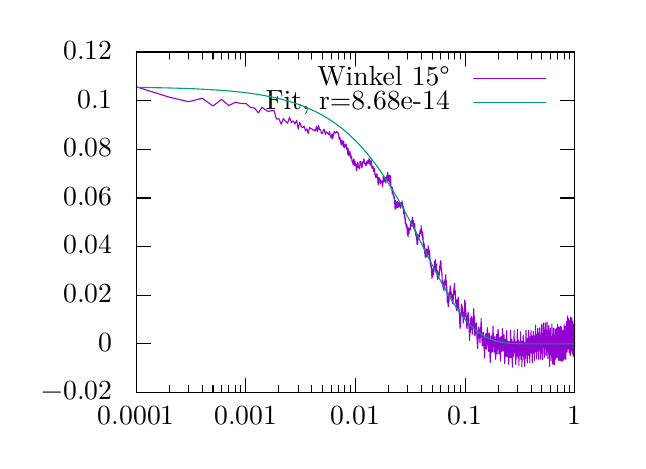
\begin{tikzpicture}[gnuplot]
%% generated with GNUPLOT 5.2p5a (Gentoo revision r0) (Lua 5.1; terminal rev. 99 , script rev. 107)
%% Sa 18 Mai 2019 18:30:33 CEST
\path (0.000,0.000) rectangle (7.500,5.250);
\gpcolor{color=gp lt color border}
\gpsetlinetype{gp lt border}
\gpsetdashtype{gp dt solid}
\gpsetlinewidth{1.00}
\draw[gp path] (1.380,0.616)--(1.560,0.616);
\draw[gp path] (6.947,0.616)--(6.767,0.616);
\node[gp node right] at (1.196,0.616) {$-0.02$};
\draw[gp path] (1.380,1.234)--(1.560,1.234);
\draw[gp path] (6.947,1.234)--(6.767,1.234);
\node[gp node right] at (1.196,1.234) {$0$};
\draw[gp path] (1.380,1.852)--(1.560,1.852);
\draw[gp path] (6.947,1.852)--(6.767,1.852);
\node[gp node right] at (1.196,1.852) {$0.02$};
\draw[gp path] (1.380,2.470)--(1.560,2.470);
\draw[gp path] (6.947,2.470)--(6.767,2.470);
\node[gp node right] at (1.196,2.470) {$0.04$};
\draw[gp path] (1.380,3.087)--(1.560,3.087);
\draw[gp path] (6.947,3.087)--(6.767,3.087);
\node[gp node right] at (1.196,3.087) {$0.06$};
\draw[gp path] (1.380,3.705)--(1.560,3.705);
\draw[gp path] (6.947,3.705)--(6.767,3.705);
\node[gp node right] at (1.196,3.705) {$0.08$};
\draw[gp path] (1.380,4.323)--(1.560,4.323);
\draw[gp path] (6.947,4.323)--(6.767,4.323);
\node[gp node right] at (1.196,4.323) {$0.1$};
\draw[gp path] (1.380,4.941)--(1.560,4.941);
\draw[gp path] (6.947,4.941)--(6.767,4.941);
\node[gp node right] at (1.196,4.941) {$0.12$};
\draw[gp path] (1.380,0.616)--(1.380,0.796);
\draw[gp path] (1.380,4.941)--(1.380,4.761);
\node[gp node center] at (1.380,0.308) {$0.0001$};
\draw[gp path] (1.799,0.616)--(1.799,0.706);
\draw[gp path] (1.799,4.941)--(1.799,4.851);
\draw[gp path] (2.044,0.616)--(2.044,0.706);
\draw[gp path] (2.044,4.941)--(2.044,4.851);
\draw[gp path] (2.218,0.616)--(2.218,0.706);
\draw[gp path] (2.218,4.941)--(2.218,4.851);
\draw[gp path] (2.353,0.616)--(2.353,0.706);
\draw[gp path] (2.353,4.941)--(2.353,4.851);
\draw[gp path] (2.463,0.616)--(2.463,0.706);
\draw[gp path] (2.463,4.941)--(2.463,4.851);
\draw[gp path] (2.556,0.616)--(2.556,0.706);
\draw[gp path] (2.556,4.941)--(2.556,4.851);
\draw[gp path] (2.637,0.616)--(2.637,0.706);
\draw[gp path] (2.637,4.941)--(2.637,4.851);
\draw[gp path] (2.708,0.616)--(2.708,0.706);
\draw[gp path] (2.708,4.941)--(2.708,4.851);
\draw[gp path] (2.772,0.616)--(2.772,0.796);
\draw[gp path] (2.772,4.941)--(2.772,4.761);
\node[gp node center] at (2.772,0.308) {$0.001$};
\draw[gp path] (3.191,0.616)--(3.191,0.706);
\draw[gp path] (3.191,4.941)--(3.191,4.851);
\draw[gp path] (3.436,0.616)--(3.436,0.706);
\draw[gp path] (3.436,4.941)--(3.436,4.851);
\draw[gp path] (3.610,0.616)--(3.610,0.706);
\draw[gp path] (3.610,4.941)--(3.610,4.851);
\draw[gp path] (3.745,0.616)--(3.745,0.706);
\draw[gp path] (3.745,4.941)--(3.745,4.851);
\draw[gp path] (3.855,0.616)--(3.855,0.706);
\draw[gp path] (3.855,4.941)--(3.855,4.851);
\draw[gp path] (3.948,0.616)--(3.948,0.706);
\draw[gp path] (3.948,4.941)--(3.948,4.851);
\draw[gp path] (4.029,0.616)--(4.029,0.706);
\draw[gp path] (4.029,4.941)--(4.029,4.851);
\draw[gp path] (4.100,0.616)--(4.100,0.706);
\draw[gp path] (4.100,4.941)--(4.100,4.851);
\draw[gp path] (4.163,0.616)--(4.163,0.796);
\draw[gp path] (4.163,4.941)--(4.163,4.761);
\node[gp node center] at (4.163,0.308) {$0.01$};
\draw[gp path] (4.582,0.616)--(4.582,0.706);
\draw[gp path] (4.582,4.941)--(4.582,4.851);
\draw[gp path] (4.828,0.616)--(4.828,0.706);
\draw[gp path] (4.828,4.941)--(4.828,4.851);
\draw[gp path] (5.001,0.616)--(5.001,0.706);
\draw[gp path] (5.001,4.941)--(5.001,4.851);
\draw[gp path] (5.136,0.616)--(5.136,0.706);
\draw[gp path] (5.136,4.941)--(5.136,4.851);
\draw[gp path] (5.246,0.616)--(5.246,0.706);
\draw[gp path] (5.246,4.941)--(5.246,4.851);
\draw[gp path] (5.340,0.616)--(5.340,0.706);
\draw[gp path] (5.340,4.941)--(5.340,4.851);
\draw[gp path] (5.420,0.616)--(5.420,0.706);
\draw[gp path] (5.420,4.941)--(5.420,4.851);
\draw[gp path] (5.492,0.616)--(5.492,0.706);
\draw[gp path] (5.492,4.941)--(5.492,4.851);
\draw[gp path] (5.555,0.616)--(5.555,0.796);
\draw[gp path] (5.555,4.941)--(5.555,4.761);
\node[gp node center] at (5.555,0.308) {$0.1$};
\draw[gp path] (5.974,0.616)--(5.974,0.706);
\draw[gp path] (5.974,4.941)--(5.974,4.851);
\draw[gp path] (6.219,0.616)--(6.219,0.706);
\draw[gp path] (6.219,4.941)--(6.219,4.851);
\draw[gp path] (6.393,0.616)--(6.393,0.706);
\draw[gp path] (6.393,4.941)--(6.393,4.851);
\draw[gp path] (6.528,0.616)--(6.528,0.706);
\draw[gp path] (6.528,4.941)--(6.528,4.851);
\draw[gp path] (6.638,0.616)--(6.638,0.706);
\draw[gp path] (6.638,4.941)--(6.638,4.851);
\draw[gp path] (6.731,0.616)--(6.731,0.706);
\draw[gp path] (6.731,4.941)--(6.731,4.851);
\draw[gp path] (6.812,0.616)--(6.812,0.706);
\draw[gp path] (6.812,4.941)--(6.812,4.851);
\draw[gp path] (6.883,0.616)--(6.883,0.706);
\draw[gp path] (6.883,4.941)--(6.883,4.851);
\draw[gp path] (6.947,0.616)--(6.947,0.796);
\draw[gp path] (6.947,4.941)--(6.947,4.761);
\node[gp node center] at (6.947,0.308) {$1$};
\draw[gp path] (1.380,4.941)--(1.380,0.616)--(6.947,0.616)--(6.947,4.941)--cycle;
\node[gp node right] at (5.479,4.607) {Winkel 15°};
\gpcolor{rgb color={0.580,0.000,0.827}}
\draw[gp path] (5.663,4.607)--(6.579,4.607);
\draw[gp path] (1.380,4.499)--(1.799,4.367)--(2.044,4.310)--(2.218,4.353)--(2.353,4.255)%
  --(2.463,4.339)--(2.556,4.261)--(2.637,4.303)--(2.708,4.287)--(2.772,4.288)--(2.829,4.238)%
  --(2.882,4.229)--(2.930,4.168)--(2.975,4.239)--(3.017,4.209)--(3.056,4.186)--(3.092,4.196)%
  --(3.127,4.199)--(3.160,4.089)--(3.191,4.093)--(3.220,4.024)--(3.248,4.096)--(3.275,4.059)%
  --(3.301,4.038)--(3.326,4.112)--(3.349,4.045)--(3.372,4.066)--(3.394,4.026)--(3.415,4.073)%
  --(3.436,3.963)--(3.456,4.049)--(3.475,3.992)--(3.493,3.981)--(3.511,3.999)--(3.529,3.939)%
  --(3.546,3.965)--(3.563,3.906)--(3.579,3.981)--(3.594,3.972)--(3.610,3.962)--(3.625,3.948)%
  --(3.639,3.954)--(3.653,3.935)--(3.667,3.995)--(3.681,3.930)--(3.694,4.006)--(3.707,3.953)%
  --(3.720,3.954)--(3.732,3.906)--(3.745,3.906)--(3.757,3.957)--(3.768,3.953)--(3.780,3.896)%
  --(3.791,3.925)--(3.802,3.920)--(3.813,3.903)--(3.824,3.893)--(3.834,3.930)--(3.845,3.873)%
  --(3.855,3.848)--(3.865,3.902)--(3.875,3.841)--(3.884,3.897)--(3.894,3.930)--(3.903,3.910)%
  --(3.912,3.916)--(3.921,3.933)--(3.930,3.916)--(3.939,3.924)--(3.948,3.895)--(3.956,3.831)%
  --(3.965,3.858)--(3.973,3.815)--(3.982,3.761)--(3.990,3.820)--(3.998,3.804)--(4.006,3.743)%
  --(4.013,3.811)--(4.021,3.723)--(4.029,3.762)--(4.036,3.744)--(4.044,3.774)--(4.051,3.707)%
  --(4.058,3.726)--(4.065,3.642)--(4.072,3.711)--(4.079,3.619)--(4.086,3.646)--(4.093,3.675)%
  --(4.100,3.630)--(4.106,3.586)--(4.113,3.619)--(4.120,3.548)--(4.126,3.550)--(4.132,3.511)%
  --(4.139,3.579)--(4.145,3.578)--(4.151,3.497)--(4.157,3.553)--(4.164,3.499)--(4.170,3.520)%
  --(4.175,3.434)--(4.181,3.461)--(4.187,3.504)--(4.193,3.540)--(4.199,3.473)--(4.204,3.471)%
  --(4.210,3.491)--(4.216,3.455)--(4.221,3.553)--(4.227,3.518)--(4.232,3.549)--(4.237,3.510)%
  --(4.243,3.473)--(4.248,3.485)--(4.253,3.525)--(4.258,3.551)--(4.264,3.536)--(4.269,3.584)%
  --(4.274,3.557)--(4.279,3.523)--(4.284,3.516)--(4.289,3.531)--(4.294,3.504)--(4.298,3.495)%
  --(4.303,3.546)--(4.308,3.515)--(4.313,3.559)--(4.317,3.526)--(4.322,3.523)--(4.327,3.567)%
  --(4.331,3.550)--(4.336,3.591)--(4.340,3.533)--(4.345,3.574)--(4.349,3.499)--(4.354,3.553)%
  --(4.358,3.529)--(4.363,3.559)--(4.367,3.522)--(4.371,3.471)--(4.375,3.466)--(4.380,3.462)%
  --(4.384,3.492)--(4.388,3.477)--(4.392,3.426)--(4.396,3.428)--(4.400,3.467)--(4.405,3.450)%
  --(4.409,3.380)--(4.413,3.392)--(4.417,3.371)--(4.421,3.350)--(4.424,3.347)--(4.428,3.382)%
  --(4.432,3.372)--(4.436,3.395)--(4.440,3.349)--(4.444,3.325)--(4.448,3.315)--(4.451,3.250)%
  --(4.455,3.350)--(4.459,3.295)--(4.463,3.294)--(4.466,3.321)--(4.470,3.340)--(4.473,3.305)%
  --(4.477,3.263)--(4.481,3.286)--(4.484,3.312)--(4.488,3.307)--(4.491,3.285)--(4.495,3.301)%
  --(4.498,3.296)--(4.502,3.302)--(4.505,3.230)--(4.509,3.259)--(4.512,3.275)--(4.515,3.360)%
  --(4.519,3.366)--(4.522,3.351)--(4.525,3.305)--(4.529,3.297)--(4.532,3.313)--(4.535,3.349)%
  --(4.539,3.314)--(4.542,3.321)--(4.545,3.347)--(4.548,3.277)--(4.551,3.345)--(4.555,3.333)%
  --(4.558,3.357)--(4.561,3.340)--(4.564,3.376)--(4.567,3.312)--(4.570,3.384)--(4.573,3.413)%
  --(4.576,3.336)--(4.579,3.376)--(4.582,3.303)--(4.585,3.330)--(4.588,3.356)--(4.591,3.297)%
  --(4.594,3.312)--(4.597,3.378)--(4.600,3.271)--(4.603,3.343)--(4.606,3.245)--(4.609,3.368)%
  --(4.612,3.267)--(4.615,3.205)--(4.618,3.231)--(4.621,3.227)--(4.623,3.212)--(4.626,3.216)%
  --(4.629,3.139)--(4.632,3.213)--(4.635,3.220)--(4.637,3.166)--(4.640,3.160)--(4.643,3.121)%
  --(4.646,3.116)--(4.648,3.121)--(4.651,3.082)--(4.654,3.082)--(4.656,3.104)--(4.659,3.040)%
  --(4.662,3.013)--(4.664,2.995)--(4.667,2.939)--(4.670,3.054)--(4.672,3.035)--(4.675,2.998)%
  --(4.677,2.997)--(4.680,2.960)--(4.683,2.957)--(4.685,3.008)--(4.688,3.016)--(4.690,3.035)%
  --(4.693,3.039)--(4.695,3.043)--(4.698,2.965)--(4.700,2.980)--(4.703,3.033)--(4.705,3.025)%
  --(4.708,3.014)--(4.710,3.006)--(4.712,2.972)--(4.715,3.027)--(4.717,3.012)--(4.720,2.977)%
  --(4.722,3.009)--(4.725,3.020)--(4.727,3.000)--(4.729,3.027)--(4.732,3.003)--(4.734,3.011)%
  --(4.736,2.958)--(4.739,2.996)--(4.741,3.007)--(4.743,3.029)--(4.746,3.018)--(4.748,3.006)%
  --(4.750,3.028)--(4.753,2.984)--(4.755,3.051)--(4.757,2.983)--(4.759,3.028)--(4.762,2.982)%
  --(4.764,2.964)--(4.766,2.990)--(4.768,2.952)--(4.771,2.972)--(4.773,2.896)--(4.775,2.974)%
  --(4.777,2.883)--(4.779,2.929)--(4.781,2.950)--(4.784,2.910)--(4.786,2.837)--(4.788,2.872)%
  --(4.790,2.869)--(4.792,2.838)--(4.794,2.762)--(4.797,2.826)--(4.799,2.817)--(4.801,2.774)%
  --(4.803,2.767)--(4.805,2.742)--(4.807,2.718)--(4.809,2.708)--(4.811,2.718)--(4.813,2.753)%
  --(4.815,2.709)--(4.817,2.737)--(4.819,2.685)--(4.821,2.644)--(4.823,2.619)--(4.826,2.695)%
  --(4.828,2.605)--(4.830,2.648)--(4.832,2.593)--(4.834,2.707)--(4.836,2.666)--(4.838,2.705)%
  --(4.840,2.680)--(4.841,2.685)--(4.843,2.634)--(4.845,2.698)--(4.847,2.697)--(4.849,2.690)%
  --(4.851,2.700)--(4.853,2.704)--(4.855,2.688)--(4.857,2.726)--(4.859,2.679)--(4.861,2.756)%
  --(4.863,2.756)--(4.865,2.787)--(4.867,2.740)--(4.868,2.770)--(4.870,2.789)--(4.872,2.796)%
  --(4.874,2.750)--(4.876,2.775)--(4.878,2.728)--(4.880,2.778)--(4.881,2.792)--(4.883,2.787)%
  --(4.885,2.818)--(4.887,2.843)--(4.889,2.780)--(4.891,2.792)--(4.892,2.763)--(4.894,2.769)%
  --(4.896,2.807)--(4.898,2.755)--(4.900,2.781)--(4.901,2.727)--(4.903,2.768)--(4.905,2.759)%
  --(4.907,2.715)--(4.908,2.749)--(4.910,2.713)--(4.912,2.746)--(4.914,2.713)--(4.916,2.760)%
  --(4.917,2.711)--(4.919,2.675)--(4.921,2.670)--(4.922,2.672)--(4.924,2.678)--(4.926,2.652)%
  --(4.928,2.615)--(4.929,2.628)--(4.931,2.640)--(4.933,2.651)--(4.934,2.591)--(4.936,2.654)%
  --(4.938,2.586)--(4.939,2.568)--(4.941,2.581)--(4.943,2.509)--(4.944,2.506)--(4.946,2.499)%
  --(4.948,2.580)--(4.949,2.628)--(4.951,2.558)--(4.953,2.496)--(4.954,2.560)--(4.956,2.620)%
  --(4.958,2.570)--(4.959,2.609)--(4.961,2.562)--(4.962,2.589)--(4.964,2.575)--(4.966,2.612)%
  --(4.967,2.578)--(4.969,2.594)--(4.970,2.618)--(4.972,2.587)--(4.974,2.624)--(4.975,2.600)%
  --(4.977,2.630)--(4.978,2.640)--(4.980,2.646)--(4.981,2.664)--(4.983,2.664)--(4.985,2.676)%
  --(4.986,2.631)--(4.988,2.656)--(4.989,2.680)--(4.991,2.653)--(4.992,2.666)--(4.994,2.677)%
  --(4.995,2.665)--(4.997,2.738)--(4.998,2.698)--(5.000,2.704)--(5.001,2.688)--(5.003,2.654)%
  --(5.004,2.645)--(5.006,2.674)--(5.007,2.603)--(5.009,2.665)--(5.010,2.628)--(5.012,2.602)%
  --(5.013,2.652)--(5.015,2.590)--(5.016,2.560)--(5.018,2.645)--(5.019,2.595)--(5.021,2.598)%
  --(5.022,2.580)--(5.024,2.506)--(5.025,2.527)--(5.027,2.472)--(5.028,2.505)--(5.029,2.529)%
  --(5.031,2.486)--(5.032,2.441)--(5.034,2.467)--(5.035,2.507)--(5.037,2.476)--(5.038,2.453)%
  --(5.039,2.466)--(5.041,2.400)--(5.042,2.388)--(5.044,2.377)--(5.045,2.390)--(5.047,2.381)%
  --(5.048,2.337)--(5.049,2.361)--(5.051,2.331)--(5.052,2.406)--(5.054,2.367)--(5.055,2.340)%
  --(5.056,2.352)--(5.058,2.371)--(5.059,2.408)--(5.060,2.445)--(5.062,2.365)--(5.063,2.347)%
  --(5.064,2.394)--(5.066,2.338)--(5.067,2.391)--(5.069,2.411)--(5.070,2.409)--(5.071,2.392)%
  --(5.073,2.432)--(5.074,2.389)--(5.075,2.420)--(5.077,2.407)--(5.078,2.379)--(5.079,2.426)%
  --(5.081,2.381)--(5.082,2.368)--(5.083,2.402)--(5.085,2.407)--(5.086,2.486)--(5.087,2.376)%
  --(5.089,2.462)--(5.090,2.444)--(5.091,2.421)--(5.092,2.441)--(5.094,2.397)--(5.095,2.393)%
  --(5.096,2.424)--(5.098,2.432)--(5.099,2.393)--(5.100,2.329)--(5.101,2.414)--(5.103,2.311)%
  --(5.104,2.353)--(5.105,2.344)--(5.107,2.371)--(5.108,2.317)--(5.109,2.327)--(5.110,2.292)%
  --(5.112,2.265)--(5.113,2.253)--(5.114,2.265)--(5.115,2.242)--(5.117,2.294)--(5.118,2.219)%
  --(5.119,2.235)--(5.120,2.208)--(5.122,2.233)--(5.123,2.249)--(5.124,2.230)--(5.125,2.221)%
  --(5.127,2.170)--(5.128,2.188)--(5.129,2.130)--(5.130,2.199)--(5.131,2.176)--(5.133,2.061)%
  --(5.134,2.161)--(5.135,2.080)--(5.136,2.124)--(5.137,2.141)--(5.139,2.112)--(5.140,2.120)%
  --(5.141,2.140)--(5.142,2.084)--(5.144,2.128)--(5.145,2.087)--(5.146,2.185)--(5.147,2.126)%
  --(5.148,2.187)--(5.149,2.123)--(5.151,2.124)--(5.152,2.200)--(5.153,2.181)--(5.154,2.115)%
  --(5.155,2.141)--(5.157,2.206)--(5.158,2.192)--(5.159,2.196)--(5.160,2.155)--(5.161,2.175)%
  --(5.162,2.192)--(5.163,2.223)--(5.165,2.201)--(5.166,2.215)--(5.167,2.229)--(5.168,2.282)%
  --(5.169,2.206)--(5.170,2.234)--(5.172,2.228)--(5.173,2.225)--(5.174,2.269)--(5.175,2.234)%
  --(5.176,2.236)--(5.177,2.307)--(5.178,2.274)--(5.179,2.221)--(5.181,2.212)--(5.182,2.173)%
  --(5.183,2.261)--(5.184,2.249)--(5.185,2.206)--(5.186,2.171)--(5.187,2.202)--(5.188,2.133)%
  --(5.189,2.217)--(5.191,2.172)--(5.192,2.243)--(5.193,2.195)--(5.194,2.157)--(5.195,2.132)%
  --(5.196,2.173)--(5.197,2.146)--(5.198,2.122)--(5.199,2.161)--(5.200,2.165)--(5.202,2.077)%
  --(5.203,2.158)--(5.204,2.164)--(5.205,2.103)--(5.206,2.051)--(5.207,2.135)--(5.208,2.103)%
  --(5.209,2.069)--(5.210,2.074)--(5.211,2.064)--(5.212,2.104)--(5.213,2.108)--(5.214,2.088)%
  --(5.215,2.097)--(5.217,2.070)--(5.218,2.076)--(5.219,2.124)--(5.220,2.105)--(5.221,2.086)%
  --(5.222,2.128)--(5.223,2.089)--(5.224,2.138)--(5.225,2.124)--(5.226,2.142)--(5.227,2.147)%
  --(5.228,2.117)--(5.229,2.182)--(5.230,2.158)--(5.231,2.161)--(5.232,2.220)--(5.233,2.187)%
  --(5.234,2.196)--(5.235,2.212)--(5.236,2.231)--(5.237,2.224)--(5.238,2.205)--(5.239,2.202)%
  --(5.240,2.243)--(5.241,2.194)--(5.242,2.291)--(5.243,2.242)--(5.244,2.239)--(5.245,2.228)%
  --(5.246,2.266)--(5.247,2.245)--(5.249,2.277)--(5.250,2.198)--(5.251,2.238)--(5.252,2.168)%
  --(5.253,2.166)--(5.254,2.186)--(5.254,2.190)--(5.255,2.191)--(5.256,2.189)--(5.257,2.141)%
  --(5.258,2.150)--(5.259,2.159)--(5.260,2.093)--(5.261,2.134)--(5.262,2.130)--(5.263,2.068)%
  --(5.264,2.056)--(5.265,2.031)--(5.266,2.043)--(5.267,2.043)--(5.268,2.043)--(5.269,2.032)%
  --(5.270,2.032)--(5.271,2.035)--(5.272,1.995)--(5.273,1.954)--(5.274,1.979)--(5.275,1.954)%
  --(5.276,1.962)--(5.277,1.959)--(5.278,1.960)--(5.279,2.000)--(5.280,1.947)--(5.281,1.924)%
  --(5.282,1.983)--(5.283,1.986)--(5.284,1.926)--(5.285,1.963)--(5.286,2.016)--(5.286,1.910)%
  --(5.287,1.987)--(5.288,1.987)--(5.289,2.004)--(5.290,1.970)--(5.291,1.969)--(5.292,1.944)%
  --(5.293,2.011)--(5.294,1.988)--(5.295,2.009)--(5.296,2.007)--(5.297,2.030)--(5.298,2.021)%
  --(5.299,2.021)--(5.300,2.052)--(5.300,2.031)--(5.301,2.054)--(5.302,2.050)--(5.303,1.986)%
  --(5.304,2.063)--(5.305,2.019)--(5.306,2.020)--(5.307,2.059)--(5.308,2.009)--(5.309,2.021)%
  --(5.310,2.111)--(5.310,2.047)--(5.311,2.051)--(5.312,2.049)--(5.313,2.002)--(5.314,2.023)%
  --(5.315,1.940)--(5.316,1.985)--(5.317,2.037)--(5.318,1.951)--(5.319,1.974)--(5.319,1.990)%
  --(5.320,1.919)--(5.321,1.933)--(5.322,1.920)--(5.323,1.962)--(5.324,1.926)--(5.325,1.909)%
  --(5.326,1.856)--(5.327,1.862)--(5.327,1.837)--(5.328,1.765)--(5.329,1.789)--(5.330,1.797)%
  --(5.331,1.841)--(5.332,1.841)--(5.333,1.792)--(5.334,1.778)--(5.334,1.785)--(5.335,1.779)%
  --(5.336,1.794)--(5.337,1.776)--(5.338,1.746)--(5.339,1.737)--(5.340,1.807)--(5.341,1.708)%
  --(5.341,1.802)--(5.342,1.794)--(5.343,1.798)--(5.344,1.819)--(5.345,1.803)--(5.346,1.791)%
  --(5.347,1.819)--(5.347,1.801)--(5.348,1.844)--(5.349,1.760)--(5.350,1.888)--(5.351,1.849)%
  --(5.352,1.779)--(5.352,1.797)--(5.353,1.825)--(5.354,1.858)--(5.355,1.893)--(5.356,1.877)%
  --(5.357,1.860)--(5.358,1.882)--(5.358,1.831)--(5.359,1.885)--(5.360,1.881)--(5.361,1.894)%
  --(5.362,1.888)--(5.363,1.882)--(5.363,1.934)--(5.364,1.897)--(5.365,1.968)--(5.366,1.897)%
  --(5.367,1.869)--(5.368,1.970)--(5.368,1.963)--(5.369,1.880)--(5.370,1.941)--(5.371,1.909)%
  --(5.372,1.885)--(5.372,1.921)--(5.373,1.905)--(5.374,1.907)--(5.375,1.900)--(5.376,1.888)%
  --(5.377,1.884)--(5.377,1.827)--(5.378,1.862)--(5.379,1.862)--(5.380,1.825)--(5.381,1.883)%
  --(5.381,1.844)--(5.382,1.852)--(5.383,1.871)--(5.384,1.840)--(5.385,1.860)--(5.385,1.844)%
  --(5.386,1.832)--(5.387,1.849)--(5.388,1.862)--(5.389,1.851)--(5.389,1.781)--(5.390,1.792)%
  --(5.391,1.781)--(5.392,1.821)--(5.393,1.793)--(5.393,1.812)--(5.394,1.757)--(5.395,1.795)%
  --(5.396,1.747)--(5.396,1.801)--(5.397,1.784)--(5.398,1.742)--(5.399,1.768)--(5.400,1.819)%
  --(5.400,1.813)--(5.401,1.808)--(5.402,1.766)--(5.403,1.819)--(5.404,1.774)--(5.404,1.808)%
  --(5.405,1.842)--(5.406,1.803)--(5.407,1.910)--(5.407,1.849)--(5.408,1.875)--(5.409,1.874)%
  --(5.410,1.908)--(5.410,1.879)--(5.411,1.862)--(5.412,1.905)--(5.413,1.879)--(5.414,1.942)%
  --(5.415,1.910)--(5.416,1.872)--(5.417,1.891)--(5.417,1.941)--(5.418,1.958)--(5.419,2.000)%
  --(5.420,1.956)--(5.420,1.939)--(5.421,1.955)--(5.422,2.002)--(5.423,1.964)--(5.423,1.917)%
  --(5.424,1.894)--(5.425,1.921)--(5.426,1.910)--(5.426,1.899)--(5.427,1.889)--(5.428,1.895)%
  --(5.429,1.856)--(5.429,1.865)--(5.430,1.908)--(5.431,1.871)--(5.432,1.851)--(5.432,1.804)%
  --(5.433,1.830)--(5.434,1.798)--(5.435,1.779)--(5.435,1.798)--(5.436,1.753)--(5.437,1.767)%
  --(5.438,1.799)--(5.438,1.779)--(5.439,1.767)--(5.440,1.761)--(5.441,1.700)--(5.442,1.750)%
  --(5.443,1.731)--(5.443,1.690)--(5.444,1.697)--(5.445,1.659)--(5.446,1.682)--(5.446,1.679)%
  --(5.447,1.665)--(5.448,1.679)--(5.448,1.659)--(5.449,1.719)--(5.450,1.700)--(5.451,1.688)%
  --(5.451,1.710)--(5.452,1.700)--(5.453,1.678)--(5.453,1.702)--(5.454,1.713)--(5.455,1.747)%
  --(5.456,1.690)--(5.456,1.793)--(5.457,1.666)--(5.458,1.742)--(5.458,1.761)--(5.459,1.679)%
  --(5.460,1.743)--(5.461,1.719)--(5.462,1.765)--(5.463,1.738)--(5.463,1.710)--(5.464,1.726)%
  --(5.465,1.753)--(5.465,1.730)--(5.466,1.831)--(5.467,1.733)--(5.468,1.784)--(5.468,1.824)%
  --(5.469,1.783)--(5.470,1.806)--(5.470,1.761)--(5.471,1.717)--(5.472,1.738)--(5.472,1.730)%
  --(5.473,1.734)--(5.474,1.688)--(5.475,1.727)--(5.475,1.693)--(5.476,1.701)--(5.477,1.667)%
  --(5.477,1.669)--(5.478,1.658)--(5.479,1.650)--(5.479,1.617)--(5.480,1.670)--(5.481,1.661)%
  --(5.481,1.670)--(5.482,1.599)--(5.483,1.591)--(5.483,1.583)--(5.484,1.585)--(5.485,1.580)%
  --(5.485,1.543)--(5.486,1.521)--(5.487,1.519)--(5.488,1.487)--(5.488,1.578)--(5.489,1.456)%
  --(5.490,1.491)--(5.490,1.432)--(5.491,1.490)--(5.492,1.496)--(5.492,1.513)--(5.493,1.449)%
  --(5.494,1.471)--(5.494,1.523)--(5.495,1.523)--(5.496,1.565)--(5.496,1.524)--(5.497,1.535)%
  --(5.498,1.561)--(5.498,1.591)--(5.499,1.611)--(5.500,1.556)--(5.500,1.615)--(5.501,1.590)%
  --(5.502,1.607)--(5.502,1.603)--(5.503,1.608)--(5.504,1.647)--(5.504,1.604)--(5.505,1.651)%
  --(5.506,1.657)--(5.506,1.673)--(5.507,1.692)--(5.507,1.669)--(5.508,1.676)--(5.509,1.659)%
  --(5.509,1.739)--(5.510,1.674)--(5.511,1.680)--(5.511,1.654)--(5.512,1.703)--(5.513,1.686)%
  --(5.513,1.683)--(5.514,1.686)--(5.515,1.731)--(5.515,1.673)--(5.516,1.678)--(5.517,1.637)%
  --(5.517,1.690)--(5.518,1.641)--(5.518,1.714)--(5.519,1.665)--(5.520,1.668)--(5.520,1.657)%
  --(5.521,1.622)--(5.522,1.659)--(5.522,1.599)--(5.523,1.583)--(5.524,1.643)--(5.524,1.596)%
  --(5.525,1.616)--(5.526,1.589)--(5.526,1.607)--(5.527,1.613)--(5.527,1.634)--(5.528,1.570)%
  --(5.529,1.627)--(5.529,1.607)--(5.530,1.603)--(5.531,1.586)--(5.531,1.498)--(5.532,1.513)%
  --(5.532,1.567)--(5.533,1.574)--(5.534,1.540)--(5.534,1.520)--(5.535,1.533)--(5.536,1.516)%
  --(5.536,1.554)--(5.537,1.545)--(5.537,1.528)--(5.538,1.574)--(5.539,1.629)--(5.539,1.586)%
  --(5.540,1.576)--(5.541,1.542)--(5.541,1.593)--(5.542,1.614)--(5.542,1.600)--(5.543,1.645)%
  --(5.544,1.569)--(5.544,1.601)--(5.545,1.685)--(5.546,1.675)--(5.546,1.673)--(5.547,1.684)%
  --(5.547,1.652)--(5.548,1.714)--(5.549,1.692)--(5.549,1.736)--(5.550,1.790)--(5.550,1.724)%
  --(5.551,1.765)--(5.552,1.706)--(5.552,1.721)--(5.553,1.743)--(5.553,1.711)--(5.554,1.756)%
  --(5.555,1.782)--(5.555,1.754)--(5.556,1.773)--(5.556,1.759)--(5.557,1.741)--(5.558,1.720)%
  --(5.558,1.721)--(5.559,1.669)--(5.559,1.697)--(5.560,1.684)--(5.561,1.709)--(5.561,1.680)%
  --(5.562,1.643)--(5.562,1.652)--(5.563,1.659)--(5.564,1.638)--(5.564,1.580)--(5.565,1.593)%
  --(5.565,1.612)--(5.566,1.632)--(5.567,1.585)--(5.567,1.612)--(5.568,1.577)--(5.568,1.585)%
  --(5.569,1.572)--(5.570,1.570)--(5.570,1.508)--(5.571,1.560)--(5.571,1.523)--(5.572,1.536)%
  --(5.573,1.535)--(5.573,1.467)--(5.574,1.476)--(5.574,1.478)--(5.575,1.446)--(5.575,1.566)%
  --(5.576,1.471)--(5.577,1.516)--(5.577,1.506)--(5.578,1.483)--(5.578,1.458)--(5.579,1.505)%
  --(5.580,1.427)--(5.580,1.506)--(5.581,1.550)--(5.581,1.549)--(5.582,1.499)--(5.582,1.485)%
  --(5.583,1.495)--(5.584,1.565)--(5.584,1.513)--(5.585,1.529)--(5.585,1.564)--(5.586,1.525)%
  --(5.586,1.575)--(5.587,1.596)--(5.588,1.474)--(5.588,1.582)--(5.589,1.529)--(5.589,1.587)%
  --(5.590,1.566)--(5.590,1.574)--(5.591,1.566)--(5.592,1.598)--(5.592,1.584)--(5.593,1.639)%
  --(5.593,1.559)--(5.594,1.569)--(5.594,1.498)--(5.595,1.541)--(5.596,1.628)--(5.596,1.573)%
  --(5.597,1.590)--(5.597,1.538)--(5.598,1.503)--(5.598,1.541)--(5.599,1.564)--(5.600,1.514)%
  --(5.600,1.571)--(5.601,1.536)--(5.601,1.531)--(5.602,1.529)--(5.602,1.498)--(5.603,1.491)%
  --(5.603,1.475)--(5.604,1.472)--(5.605,1.435)--(5.605,1.463)--(5.606,1.410)--(5.606,1.433)%
  --(5.607,1.431)--(5.607,1.414)--(5.608,1.412)--(5.608,1.402)--(5.609,1.378)--(5.610,1.424)%
  --(5.610,1.389)--(5.611,1.423)--(5.611,1.347)--(5.612,1.311)--(5.612,1.335)--(5.613,1.362)%
  --(5.613,1.277)--(5.614,1.396)--(5.615,1.334)--(5.615,1.367)--(5.616,1.343)--(5.616,1.386)%
  --(5.617,1.383)--(5.617,1.408)--(5.618,1.421)--(5.618,1.429)--(5.619,1.392)--(5.619,1.426)%
  --(5.620,1.374)--(5.621,1.386)--(5.621,1.427)--(5.622,1.417)--(5.622,1.476)--(5.623,1.435)%
  --(5.623,1.477)--(5.624,1.452)--(5.624,1.465)--(5.625,1.534)--(5.625,1.471)--(5.626,1.493)%
  --(5.626,1.532)--(5.627,1.556)--(5.628,1.513)--(5.628,1.489)--(5.629,1.506)--(5.629,1.541)%
  --(5.630,1.491)--(5.630,1.554)--(5.631,1.556)--(5.631,1.566)--(5.632,1.511)--(5.632,1.578)%
  --(5.633,1.535)--(5.633,1.584)--(5.634,1.549)--(5.634,1.514)--(5.635,1.520)--(5.636,1.540)%
  --(5.636,1.572)--(5.637,1.503)--(5.637,1.422)--(5.638,1.522)--(5.638,1.497)--(5.639,1.449)%
  --(5.639,1.501)--(5.640,1.523)--(5.640,1.459)--(5.641,1.490)--(5.641,1.428)--(5.642,1.446)%
  --(5.642,1.407)--(5.643,1.454)--(5.643,1.489)--(5.644,1.468)--(5.644,1.448)--(5.645,1.471)%
  --(5.645,1.446)--(5.646,1.418)--(5.647,1.432)--(5.647,1.492)--(5.648,1.357)--(5.648,1.393)%
  --(5.649,1.414)--(5.649,1.402)--(5.650,1.408)--(5.650,1.455)--(5.651,1.467)--(5.651,1.394)%
  --(5.652,1.435)--(5.652,1.478)--(5.653,1.467)--(5.653,1.534)--(5.654,1.430)--(5.654,1.439)%
  --(5.655,1.480)--(5.655,1.556)--(5.656,1.488)--(5.656,1.455)--(5.657,1.523)--(5.657,1.494)%
  --(5.658,1.487)--(5.658,1.481)--(5.659,1.532)--(5.659,1.579)--(5.660,1.592)--(5.660,1.534)%
  --(5.661,1.578)--(5.661,1.635)--(5.662,1.563)--(5.662,1.609)--(5.663,1.589)--(5.663,1.672)%
  --(5.664,1.582)--(5.664,1.650)--(5.665,1.637)--(5.665,1.681)--(5.666,1.654)--(5.666,1.623)%
  --(5.667,1.561)--(5.667,1.653)--(5.668,1.531)--(5.668,1.579)--(5.669,1.577)--(5.669,1.554)%
  --(5.670,1.553)--(5.670,1.517)--(5.671,1.494)--(5.671,1.541)--(5.672,1.500)--(5.672,1.589)%
  --(5.673,1.437)--(5.673,1.530)--(5.674,1.463)--(5.674,1.473)--(5.675,1.514)--(5.675,1.413)%
  --(5.676,1.383)--(5.676,1.453)--(5.677,1.418)--(5.677,1.406)--(5.678,1.346)--(5.678,1.401)%
  --(5.679,1.405)--(5.679,1.358)--(5.680,1.367)--(5.680,1.373)--(5.681,1.337)--(5.681,1.379)%
  --(5.682,1.346)--(5.682,1.371)--(5.683,1.361)--(5.683,1.374)--(5.684,1.365)--(5.684,1.360)%
  --(5.685,1.375)--(5.685,1.442)--(5.686,1.424)--(5.686,1.389)--(5.687,1.383)--(5.687,1.401)%
  --(5.688,1.469)--(5.688,1.416)--(5.689,1.405)--(5.689,1.385)--(5.690,1.399)--(5.690,1.424)%
  --(5.691,1.394)--(5.691,1.401)--(5.692,1.440)--(5.692,1.493)--(5.693,1.378)--(5.693,1.445)%
  --(5.693,1.421)--(5.694,1.441)--(5.694,1.413)--(5.695,1.411)--(5.695,1.441)--(5.696,1.430)%
  --(5.696,1.478)--(5.697,1.474)--(5.697,1.484)--(5.698,1.451)--(5.698,1.462)--(5.699,1.502)%
  --(5.699,1.414)--(5.700,1.471)--(5.700,1.441)--(5.701,1.405)--(5.701,1.382)--(5.702,1.381)%
  --(5.702,1.396)--(5.703,1.418)--(5.703,1.426)--(5.704,1.422)--(5.704,1.394)--(5.704,1.360)%
  --(5.705,1.352)--(5.705,1.375)--(5.706,1.344)--(5.706,1.299)--(5.707,1.358)--(5.707,1.300)%
  --(5.708,1.292)--(5.708,1.332)--(5.709,1.240)--(5.709,1.306)--(5.710,1.264)--(5.710,1.298)%
  --(5.711,1.293)--(5.711,1.210)--(5.712,1.220)--(5.712,1.275)--(5.712,1.250)--(5.713,1.195)%
  --(5.713,1.228)--(5.714,1.202)--(5.714,1.192)--(5.715,1.249)--(5.715,1.174)--(5.716,1.211)%
  --(5.716,1.250)--(5.717,1.270)--(5.717,1.289)--(5.718,1.306)--(5.718,1.285)--(5.718,1.293)%
  --(5.719,1.316)--(5.719,1.345)--(5.720,1.339)--(5.720,1.332)--(5.721,1.281)--(5.721,1.267)%
  --(5.722,1.365)--(5.722,1.332)--(5.723,1.354)--(5.723,1.341)--(5.724,1.310)--(5.724,1.380)%
  --(5.724,1.342)--(5.725,1.408)--(5.725,1.404)--(5.726,1.402)--(5.726,1.395)--(5.727,1.426)%
  --(5.727,1.372)--(5.728,1.415)--(5.728,1.445)--(5.729,1.446)--(5.729,1.429)--(5.729,1.394)%
  --(5.730,1.445)--(5.730,1.411)--(5.731,1.448)--(5.731,1.381)--(5.732,1.396)--(5.732,1.401)%
  --(5.733,1.390)--(5.733,1.424)--(5.733,1.388)--(5.734,1.410)--(5.734,1.429)--(5.735,1.392)%
  --(5.735,1.379)--(5.736,1.384)--(5.736,1.399)--(5.737,1.365)--(5.737,1.377)--(5.738,1.340)%
  --(5.738,1.345)--(5.738,1.371)--(5.739,1.343)--(5.739,1.322)--(5.740,1.356)--(5.741,1.366)%
  --(5.741,1.295)--(5.742,1.335)--(5.742,1.355)--(5.742,1.311)--(5.743,1.297)--(5.743,1.301)%
  --(5.744,1.257)--(5.744,1.284)--(5.745,1.247)--(5.745,1.283)--(5.746,1.285)--(5.746,1.314)%
  --(5.746,1.295)--(5.747,1.371)--(5.747,1.307)--(5.748,1.338)--(5.748,1.309)--(5.749,1.388)%
  --(5.749,1.367)--(5.749,1.390)--(5.750,1.340)--(5.750,1.379)--(5.751,1.383)--(5.751,1.368)%
  --(5.752,1.385)--(5.752,1.375)--(5.753,1.438)--(5.753,1.424)--(5.753,1.440)--(5.754,1.428)%
  --(5.754,1.397)--(5.755,1.480)--(5.755,1.461)--(5.756,1.436)--(5.756,1.480)--(5.756,1.500)%
  --(5.757,1.492)--(5.757,1.477)--(5.758,1.451)--(5.758,1.505)--(5.759,1.557)--(5.759,1.514)%
  --(5.759,1.501)--(5.760,1.511)--(5.760,1.458)--(5.761,1.477)--(5.761,1.448)--(5.762,1.472)%
  --(5.762,1.437)--(5.762,1.496)--(5.763,1.446)--(5.763,1.405)--(5.764,1.430)--(5.764,1.416)%
  --(5.765,1.414)--(5.765,1.334)--(5.765,1.360)--(5.766,1.347)--(5.766,1.329)--(5.767,1.358)%
  --(5.767,1.359)--(5.768,1.329)--(5.768,1.276)--(5.768,1.354)--(5.769,1.283)--(5.769,1.291)%
  --(5.770,1.302)--(5.770,1.296)--(5.771,1.285)--(5.771,1.297)--(5.771,1.208)--(5.772,1.264)%
  --(5.772,1.212)--(5.773,1.285)--(5.773,1.246)--(5.774,1.242)--(5.774,1.266)--(5.774,1.220)%
  --(5.775,1.253)--(5.775,1.257)--(5.776,1.271)--(5.776,1.300)--(5.776,1.252)--(5.777,1.294)%
  --(5.777,1.254)--(5.778,1.269)--(5.778,1.212)--(5.779,1.293)--(5.779,1.246)--(5.779,1.299)%
  --(5.780,1.282)--(5.780,1.285)--(5.781,1.317)--(5.781,1.280)--(5.781,1.312)--(5.782,1.321)%
  --(5.782,1.319)--(5.783,1.294)--(5.783,1.305)--(5.784,1.326)--(5.784,1.367)--(5.784,1.325)%
  --(5.785,1.286)--(5.785,1.310)--(5.786,1.384)--(5.786,1.346)--(5.786,1.328)--(5.787,1.370)%
  --(5.787,1.355)--(5.788,1.352)--(5.788,1.336)--(5.789,1.309)--(5.789,1.280)--(5.789,1.320)%
  --(5.790,1.280)--(5.790,1.239)--(5.791,1.275)--(5.791,1.305)--(5.791,1.259)--(5.792,1.261)%
  --(5.792,1.260)--(5.793,1.222)--(5.793,1.255)--(5.793,1.247)--(5.794,1.247)--(5.794,1.179)%
  --(5.795,1.239)--(5.795,1.183)--(5.795,1.185)--(5.796,1.198)--(5.796,1.148)--(5.797,1.181)%
  --(5.797,1.214)--(5.797,1.148)--(5.798,1.140)--(5.798,1.139)--(5.799,1.147)--(5.799,1.160)%
  --(5.800,1.087)--(5.800,1.179)--(5.800,1.073)--(5.801,1.088)--(5.801,1.130)--(5.802,1.133)%
  --(5.802,1.055)--(5.802,1.158)--(5.803,1.143)--(5.803,1.173)--(5.804,1.192)--(5.804,1.132)%
  --(5.804,1.214)--(5.805,1.242)--(5.805,1.212)--(5.806,1.152)--(5.806,1.184)--(5.806,1.256)%
  --(5.807,1.217)--(5.807,1.228)--(5.808,1.272)--(5.808,1.256)--(5.808,1.302)--(5.809,1.287)%
  --(5.809,1.248)--(5.810,1.311)--(5.810,1.270)--(5.810,1.303)--(5.811,1.295)--(5.811,1.278)%
  --(5.812,1.350)--(5.812,1.341)--(5.812,1.284)--(5.813,1.352)--(5.813,1.317)--(5.814,1.296)%
  --(5.814,1.354)--(5.815,1.288)--(5.815,1.349)--(5.815,1.302)--(5.816,1.340)--(5.816,1.262)%
  --(5.817,1.265)--(5.817,1.308)--(5.817,1.264)--(5.818,1.350)--(5.818,1.286)--(5.819,1.324)%
  --(5.819,1.364)--(5.819,1.300)--(5.820,1.260)--(5.820,1.230)--(5.821,1.227)--(5.821,1.180)%
  --(5.821,1.211)--(5.822,1.233)--(5.822,1.174)--(5.822,1.214)--(5.823,1.225)--(5.823,1.266)%
  --(5.824,1.232)--(5.824,1.209)--(5.824,1.243)--(5.825,1.228)--(5.825,1.183)--(5.826,1.219)%
  --(5.826,1.200)--(5.826,1.176)--(5.827,1.186)--(5.827,1.196)--(5.828,1.177)--(5.828,1.168)%
  --(5.828,1.249)--(5.829,1.226)--(5.829,1.246)--(5.829,1.240)--(5.830,1.276)--(5.830,1.292)%
  --(5.831,1.275)--(5.831,1.263)--(5.831,1.272)--(5.832,1.277)--(5.832,1.256)--(5.832,1.313)%
  --(5.833,1.312)--(5.833,1.299)--(5.834,1.346)--(5.834,1.319)--(5.834,1.337)--(5.835,1.351)%
  --(5.835,1.349)--(5.836,1.367)--(5.836,1.385)--(5.836,1.374)--(5.837,1.321)--(5.837,1.375)%
  --(5.837,1.420)--(5.838,1.393)--(5.838,1.440)--(5.839,1.396)--(5.839,1.425)--(5.839,1.405)%
  --(5.840,1.397)--(5.840,1.393)--(5.840,1.332)--(5.841,1.379)--(5.841,1.327)--(5.842,1.348)%
  --(5.842,1.344)--(5.842,1.337)--(5.843,1.308)--(5.843,1.394)--(5.843,1.322)--(5.844,1.382)%
  --(5.844,1.312)--(5.845,1.294)--(5.845,1.290)--(5.845,1.305)--(5.846,1.286)--(5.846,1.354)%
  --(5.846,1.223)--(5.847,1.245)--(5.847,1.248)--(5.848,1.241)--(5.848,1.298)--(5.848,1.230)%
  --(5.849,1.209)--(5.849,1.217)--(5.849,1.249)--(5.850,1.191)--(5.850,1.261)--(5.851,1.196)%
  --(5.851,1.160)--(5.851,1.215)--(5.852,1.191)--(5.852,1.244)--(5.852,1.138)--(5.853,1.215)%
  --(5.853,1.250)--(5.854,1.221)--(5.854,1.204)--(5.854,1.210)--(5.855,1.209)--(5.855,1.199)%
  --(5.855,1.169)--(5.856,1.231)--(5.856,1.247)--(5.856,1.200)--(5.857,1.219)--(5.857,1.191)%
  --(5.858,1.223)--(5.858,1.237)--(5.858,1.228)--(5.859,1.315)--(5.859,1.247)--(5.859,1.309)%
  --(5.860,1.297)--(5.860,1.293)--(5.860,1.302)--(5.861,1.276)--(5.861,1.272)--(5.862,1.311)%
  --(5.862,1.270)--(5.862,1.287)--(5.863,1.348)--(5.863,1.315)--(5.863,1.312)--(5.864,1.368)%
  --(5.864,1.299)--(5.864,1.302)--(5.865,1.293)--(5.865,1.369)--(5.866,1.331)--(5.866,1.269)%
  --(5.866,1.234)--(5.867,1.259)--(5.867,1.279)--(5.867,1.235)--(5.868,1.209)--(5.868,1.244)%
  --(5.868,1.231)--(5.869,1.190)--(5.869,1.215)--(5.870,1.203)--(5.870,1.225)--(5.870,1.171)%
  --(5.871,1.156)--(5.871,1.180)--(5.871,1.122)--(5.872,1.106)--(5.872,1.059)--(5.872,1.176)%
  --(5.873,1.164)--(5.873,1.180)--(5.873,1.148)--(5.874,1.074)--(5.874,1.101)--(5.875,1.089)%
  --(5.875,0.999)--(5.875,1.061)--(5.876,1.061)--(5.876,1.051)--(5.876,1.062)--(5.877,1.093)%
  --(5.877,1.086)--(5.877,1.115)--(5.878,1.123)--(5.878,1.149)--(5.878,1.139)--(5.879,1.162)%
  --(5.879,1.109)--(5.880,1.152)--(5.880,1.125)--(5.880,1.151)--(5.881,1.120)--(5.881,1.127)%
  --(5.881,1.130)--(5.882,1.173)--(5.882,1.218)--(5.883,1.215)--(5.883,1.227)--(5.883,1.244)%
  --(5.884,1.229)--(5.884,1.225)--(5.884,1.283)--(5.885,1.273)--(5.885,1.267)--(5.886,1.309)%
  --(5.886,1.286)--(5.886,1.241)--(5.887,1.307)--(5.887,1.303)--(5.887,1.327)--(5.888,1.335)%
  --(5.888,1.336)--(5.888,1.289)--(5.889,1.297)--(5.889,1.246)--(5.889,1.260)--(5.890,1.291)%
  --(5.890,1.233)--(5.890,1.275)--(5.891,1.314)--(5.891,1.251)--(5.891,1.286)--(5.892,1.240)%
  --(5.892,1.247)--(5.892,1.240)--(5.893,1.226)--(5.893,1.217)--(5.893,1.190)--(5.894,1.219)%
  --(5.894,1.258)--(5.895,1.249)--(5.895,1.230)--(5.895,1.168)--(5.896,1.289)--(5.896,1.222)%
  --(5.896,1.128)--(5.897,1.175)--(5.897,1.220)--(5.897,1.185)--(5.898,1.154)--(5.898,1.159)%
  --(5.898,1.210)--(5.899,1.149)--(5.899,1.138)--(5.899,1.171)--(5.900,1.150)--(5.900,1.134)%
  --(5.900,1.182)--(5.901,1.171)--(5.901,1.214)--(5.901,1.204)--(5.902,1.211)--(5.902,1.187)%
  --(5.902,1.257)--(5.903,1.225)--(5.903,1.194)--(5.903,1.273)--(5.904,1.278)--(5.904,1.256)%
  --(5.904,1.265)--(5.905,1.281)--(5.905,1.263)--(5.905,1.301)--(5.906,1.334)--(5.906,1.351)%
  --(5.906,1.318)--(5.907,1.328)--(5.907,1.368)--(5.907,1.337)--(5.908,1.362)--(5.908,1.350)%
  --(5.909,1.410)--(5.909,1.348)--(5.909,1.459)--(5.910,1.369)--(5.910,1.419)--(5.910,1.428)%
  --(5.911,1.438)--(5.911,1.395)--(5.911,1.414)--(5.912,1.372)--(5.912,1.368)--(5.912,1.285)%
  --(5.913,1.344)--(5.913,1.309)--(5.913,1.374)--(5.914,1.358)--(5.914,1.351)--(5.914,1.315)%
  --(5.915,1.340)--(5.915,1.345)--(5.915,1.343)--(5.916,1.319)--(5.916,1.277)--(5.916,1.302)%
  --(5.917,1.242)--(5.917,1.292)--(5.917,1.208)--(5.918,1.210)--(5.918,1.264)--(5.918,1.208)%
  --(5.919,1.217)--(5.919,1.246)--(5.919,1.241)--(5.920,1.196)--(5.920,1.207)--(5.920,1.145)%
  --(5.921,1.175)--(5.921,1.140)--(5.921,1.214)--(5.922,1.131)--(5.922,1.195)--(5.922,1.158)%
  --(5.922,1.200)--(5.923,1.190)--(5.923,1.199)--(5.923,1.154)--(5.924,1.223)--(5.924,1.201)%
  --(5.924,1.157)--(5.925,1.234)--(5.925,1.171)--(5.925,1.206)--(5.926,1.212)--(5.926,1.154)%
  --(5.926,1.233)--(5.927,1.196)--(5.927,1.194)--(5.927,1.254)--(5.928,1.295)--(5.928,1.273)%
  --(5.928,1.267)--(5.929,1.283)--(5.929,1.275)--(5.929,1.214)--(5.930,1.239)--(5.930,1.320)%
  --(5.930,1.246)--(5.931,1.230)--(5.931,1.289)--(5.931,1.301)--(5.932,1.273)--(5.932,1.300)%
  --(5.932,1.324)--(5.933,1.315)--(5.933,1.283)--(5.933,1.253)--(5.934,1.258)--(5.934,1.200)%
  --(5.934,1.253)--(5.935,1.251)--(5.935,1.194)--(5.935,1.294)--(5.936,1.193)--(5.936,1.203)%
  --(5.936,1.187)--(5.937,1.199)--(5.937,1.234)--(5.937,1.191)--(5.938,1.188)--(5.938,1.165)%
  --(5.938,1.108)--(5.939,1.152)--(5.939,1.180)--(5.939,1.097)--(5.940,1.091)--(5.940,1.144)%
  --(5.940,1.111)--(5.941,1.086)--(5.941,1.103)--(5.941,1.037)--(5.942,1.088)--(5.942,1.080)%
  --(5.942,1.098)--(5.943,1.093)--(5.943,1.059)--(5.943,1.068)--(5.944,1.081)--(5.944,1.080)%
  --(5.944,1.112)--(5.945,1.125)--(5.945,1.114)--(5.945,1.147)--(5.946,1.076)--(5.946,1.120)%
  --(5.946,1.116)--(5.947,1.158)--(5.947,1.141)--(5.947,1.140)--(5.948,1.179)--(5.948,1.172)%
  --(5.948,1.130)--(5.949,1.196)--(5.949,1.151)--(5.949,1.211)--(5.950,1.187)--(5.950,1.236)%
  --(5.950,1.242)--(5.950,1.225)--(5.951,1.243)--(5.951,1.218)--(5.951,1.289)--(5.952,1.225)%
  --(5.952,1.218)--(5.952,1.272)--(5.953,1.228)--(5.953,1.249)--(5.953,1.241)--(5.954,1.354)%
  --(5.954,1.327)--(5.954,1.294)--(5.955,1.277)--(5.955,1.283)--(5.955,1.310)--(5.955,1.261)%
  --(5.956,1.276)--(5.956,1.253)--(5.956,1.259)--(5.957,1.280)--(5.957,1.217)--(5.957,1.231)%
  --(5.958,1.285)--(5.958,1.259)--(5.958,1.208)--(5.959,1.233)--(5.959,1.226)--(5.959,1.263)%
  --(5.960,1.183)--(5.960,1.211)--(5.960,1.160)--(5.960,1.192)--(5.961,1.194)--(5.961,1.192)%
  --(5.961,1.187)--(5.962,1.190)--(5.962,1.107)--(5.962,1.184)--(5.963,1.166)--(5.963,1.206)%
  --(5.963,1.191)--(5.964,1.155)--(5.964,1.198)--(5.964,1.152)--(5.964,1.215)--(5.965,1.174)%
  --(5.965,1.200)--(5.965,1.216)--(5.966,1.243)--(5.966,1.248)--(5.966,1.264)--(5.967,1.233)%
  --(5.967,1.200)--(5.967,1.236)--(5.968,1.221)--(5.968,1.284)--(5.968,1.239)--(5.968,1.297)%
  --(5.969,1.276)--(5.969,1.343)--(5.969,1.279)--(5.970,1.303)--(5.970,1.325)--(5.970,1.322)%
  --(5.971,1.325)--(5.971,1.255)--(5.971,1.328)--(5.971,1.357)--(5.972,1.306)--(5.972,1.395)%
  --(5.972,1.413)--(5.973,1.332)--(5.973,1.365)--(5.973,1.404)--(5.974,1.377)--(5.974,1.380)%
  --(5.974,1.412)--(5.975,1.418)--(5.975,1.355)--(5.975,1.396)--(5.975,1.358)--(5.976,1.364)%
  --(5.976,1.344)--(5.976,1.342)--(5.977,1.322)--(5.977,1.397)--(5.977,1.365)--(5.978,1.304)%
  --(5.978,1.302)--(5.978,1.327)--(5.978,1.272)--(5.979,1.266)--(5.979,1.311)--(5.979,1.232)%
  --(5.980,1.234)--(5.980,1.259)--(5.980,1.228)--(5.981,1.215)--(5.981,1.214)--(5.981,1.215)%
  --(5.981,1.226)--(5.982,1.220)--(5.982,1.196)--(5.982,1.235)--(5.983,1.211)--(5.983,1.162)%
  --(5.983,1.163)--(5.984,1.200)--(5.984,1.126)--(5.984,1.108)--(5.984,1.138)--(5.985,1.173)%
  --(5.985,1.138)--(5.985,1.241)--(5.986,1.232)--(5.986,1.188)--(5.986,1.211)--(5.986,1.170)%
  --(5.987,1.184)--(5.987,1.183)--(5.987,1.181)--(5.988,1.212)--(5.988,1.221)--(5.988,1.201)%
  --(5.989,1.277)--(5.989,1.250)--(5.989,1.263)--(5.989,1.242)--(5.990,1.255)--(5.990,1.203)%
  --(5.990,1.215)--(5.991,1.252)--(5.991,1.197)--(5.991,1.297)--(5.991,1.269)--(5.992,1.294)%
  --(5.992,1.264)--(5.992,1.296)--(5.993,1.219)--(5.993,1.282)--(5.993,1.268)--(5.994,1.261)%
  --(5.994,1.244)--(5.994,1.271)--(5.994,1.251)--(5.995,1.274)--(5.995,1.238)--(5.995,1.276)%
  --(5.996,1.210)--(5.996,1.206)--(5.996,1.317)--(5.996,1.234)--(5.997,1.287)--(5.997,1.255)%
  --(5.997,1.225)--(5.998,1.193)--(5.998,1.154)--(5.998,1.153)--(5.998,1.157)--(5.999,1.208)%
  --(5.999,1.177)--(5.999,1.122)--(6.000,1.169)--(6.000,1.167)--(6.000,1.093)--(6.001,1.101)%
  --(6.001,1.154)--(6.001,1.133)--(6.001,1.082)--(6.002,1.077)--(6.002,1.097)--(6.002,1.086)%
  --(6.003,1.101)--(6.003,1.047)--(6.003,1.071)--(6.003,1.025)--(6.004,1.015)--(6.004,1.097)%
  --(6.004,1.098)--(6.005,1.096)--(6.005,1.080)--(6.005,1.063)--(6.005,1.147)--(6.006,1.124)%
  --(6.006,1.093)--(6.006,1.150)--(6.007,1.116)--(6.007,1.107)--(6.007,1.194)--(6.007,1.177)%
  --(6.008,1.181)--(6.008,1.179)--(6.008,1.213)--(6.009,1.187)--(6.009,1.206)--(6.009,1.222)%
  --(6.009,1.322)--(6.010,1.218)--(6.010,1.265)--(6.010,1.262)--(6.011,1.256)--(6.011,1.243)%
  --(6.011,1.222)--(6.011,1.298)--(6.012,1.297)--(6.012,1.278)--(6.012,1.289)--(6.013,1.264)%
  --(6.013,1.257)--(6.013,1.328)--(6.013,1.280)--(6.014,1.285)--(6.014,1.280)--(6.014,1.272)%
  --(6.015,1.257)--(6.015,1.241)--(6.015,1.256)--(6.015,1.243)--(6.016,1.249)--(6.016,1.244)%
  --(6.016,1.185)--(6.017,1.251)--(6.017,1.249)--(6.017,1.265)--(6.017,1.217)--(6.018,1.300)%
  --(6.018,1.212)--(6.018,1.202)--(6.018,1.219)--(6.019,1.194)--(6.019,1.215)--(6.019,1.221)%
  --(6.020,1.234)--(6.020,1.144)--(6.020,1.153)--(6.020,1.174)--(6.021,1.218)--(6.021,1.206)%
  --(6.021,1.175)--(6.022,1.152)--(6.022,1.137)--(6.022,1.202)--(6.022,1.196)--(6.023,1.217)%
  --(6.023,1.180)--(6.023,1.173)--(6.024,1.207)--(6.024,1.183)--(6.024,1.218)--(6.024,1.213)%
  --(6.025,1.224)--(6.025,1.220)--(6.025,1.218)--(6.025,1.238)--(6.026,1.284)--(6.026,1.276)%
  --(6.026,1.300)--(6.027,1.263)--(6.027,1.279)--(6.027,1.285)--(6.027,1.256)--(6.028,1.321)%
  --(6.028,1.334)--(6.028,1.333)--(6.029,1.365)--(6.029,1.353)--(6.029,1.295)--(6.029,1.336)%
  --(6.030,1.365)--(6.030,1.358)--(6.030,1.334)--(6.030,1.428)--(6.031,1.397)--(6.031,1.392)%
  --(6.031,1.390)--(6.032,1.376)--(6.032,1.352)--(6.032,1.397)--(6.032,1.323)--(6.033,1.365)%
  --(6.033,1.349)--(6.033,1.332)--(6.033,1.367)--(6.034,1.345)--(6.034,1.346)--(6.035,1.299)%
  --(6.035,1.297)--(6.035,1.346)--(6.035,1.301)--(6.036,1.259)--(6.036,1.238)--(6.036,1.245)%
  --(6.036,1.260)--(6.037,1.293)--(6.037,1.218)--(6.037,1.255)--(6.038,1.237)--(6.038,1.238)%
  --(6.038,1.271)--(6.038,1.192)--(6.039,1.182)--(6.039,1.185)--(6.039,1.153)--(6.040,1.178)%
  --(6.040,1.194)--(6.040,1.175)--(6.041,1.166)--(6.041,1.172)--(6.041,1.145)--(6.041,1.147)%
  --(6.042,1.183)--(6.042,1.190)--(6.042,1.177)--(6.042,1.158)--(6.043,1.227)--(6.043,1.245)%
  --(6.043,1.147)--(6.044,1.204)--(6.044,1.159)--(6.044,1.170)--(6.044,1.173)--(6.045,1.198)%
  --(6.045,1.220)--(6.045,1.162)--(6.045,1.216)--(6.046,1.230)--(6.046,1.247)--(6.046,1.273)%
  --(6.046,1.274)--(6.047,1.223)--(6.047,1.231)--(6.047,1.240)--(6.048,1.216)--(6.048,1.290)%
  --(6.048,1.265)--(6.049,1.275)--(6.049,1.300)--(6.049,1.347)--(6.049,1.278)--(6.050,1.212)%
  --(6.050,1.273)--(6.050,1.226)--(6.050,1.244)--(6.051,1.254)--(6.051,1.262)--(6.051,1.256)%
  --(6.052,1.214)--(6.052,1.206)--(6.052,1.191)--(6.052,1.218)--(6.053,1.171)--(6.053,1.214)%
  --(6.053,1.169)--(6.053,1.217)--(6.054,1.169)--(6.054,1.178)--(6.054,1.164)--(6.054,1.146)%
  --(6.055,1.129)--(6.055,1.181)--(6.055,1.129)--(6.056,1.197)--(6.056,1.093)--(6.056,1.086)%
  --(6.056,1.045)--(6.057,1.122)--(6.057,1.069)--(6.057,1.109)--(6.057,1.051)--(6.058,1.053)%
  --(6.058,1.065)--(6.058,1.043)--(6.058,0.983)--(6.059,1.049)--(6.059,1.048)--(6.059,1.093)%
  --(6.059,1.052)--(6.060,1.050)--(6.060,1.033)--(6.060,1.082)--(6.061,1.063)--(6.061,1.108)%
  --(6.061,1.079)--(6.061,1.078)--(6.062,1.119)--(6.062,1.147)--(6.062,1.106)--(6.062,1.143)%
  --(6.063,1.140)--(6.063,1.168)--(6.063,1.123)--(6.063,1.150)--(6.064,1.173)--(6.064,1.217)%
  --(6.064,1.199)--(6.064,1.246)--(6.065,1.199)--(6.065,1.261)--(6.065,1.230)--(6.065,1.249)%
  --(6.066,1.209)--(6.066,1.243)--(6.066,1.210)--(6.067,1.264)--(6.067,1.232)--(6.067,1.278)%
  --(6.067,1.226)--(6.068,1.295)--(6.068,1.290)--(6.068,1.247)--(6.068,1.234)--(6.069,1.256)%
  --(6.069,1.240)--(6.069,1.241)--(6.069,1.142)--(6.070,1.258)--(6.070,1.261)--(6.070,1.205)%
  --(6.070,1.164)--(6.071,1.198)--(6.071,1.127)--(6.071,1.197)--(6.072,1.169)--(6.072,1.170)%
  --(6.072,1.177)--(6.072,1.160)--(6.073,1.160)--(6.073,1.088)--(6.073,1.152)--(6.073,1.133)%
  --(6.074,1.136)--(6.074,1.123)--(6.074,1.174)--(6.075,1.134)--(6.075,1.102)--(6.075,1.069)%
  --(6.075,1.157)--(6.076,1.138)--(6.076,1.102)--(6.076,1.118)--(6.076,1.150)--(6.077,1.148)%
  --(6.077,1.109)--(6.077,1.132)--(6.077,1.129)--(6.078,1.084)--(6.078,1.156)--(6.078,1.147)%
  --(6.078,1.163)--(6.079,1.226)--(6.079,1.151)--(6.079,1.158)--(6.079,1.192)--(6.080,1.156)%
  --(6.080,1.187)--(6.080,1.164)--(6.080,1.275)--(6.081,1.254)--(6.081,1.229)--(6.081,1.275)%
  --(6.081,1.278)--(6.082,1.260)--(6.082,1.295)--(6.082,1.281)--(6.082,1.317)--(6.083,1.295)%
  --(6.083,1.319)--(6.083,1.287)--(6.083,1.402)--(6.084,1.293)--(6.084,1.370)--(6.084,1.333)%
  --(6.084,1.393)--(6.085,1.331)--(6.085,1.357)--(6.085,1.343)--(6.085,1.278)--(6.086,1.283)%
  --(6.086,1.281)--(6.086,1.317)--(6.086,1.292)--(6.087,1.294)--(6.087,1.289)--(6.087,1.247)%
  --(6.087,1.284)--(6.088,1.234)--(6.088,1.276)--(6.088,1.212)--(6.088,1.196)--(6.089,1.179)%
  --(6.089,1.191)--(6.089,1.175)--(6.089,1.198)--(6.090,1.214)--(6.090,1.189)--(6.090,1.144)%
  --(6.090,1.161)--(6.091,1.138)--(6.091,1.199)--(6.091,1.159)--(6.091,1.148)--(6.092,1.096)%
  --(6.092,1.081)--(6.092,1.132)--(6.092,1.139)--(6.093,1.077)--(6.093,1.133)--(6.093,1.090)%
  --(6.093,1.135)--(6.094,1.180)--(6.094,1.124)--(6.094,1.158)--(6.095,1.170)--(6.095,1.157)%
  --(6.095,1.126)--(6.095,1.152)--(6.096,1.154)--(6.096,1.139)--(6.096,1.108)--(6.096,1.164)%
  --(6.097,1.145)--(6.097,1.191)--(6.097,1.164)--(6.097,1.179)--(6.098,1.200)--(6.098,1.232)%
  --(6.098,1.211)--(6.098,1.223)--(6.099,1.196)--(6.099,1.199)--(6.099,1.170)--(6.099,1.230)%
  --(6.100,1.242)--(6.100,1.233)--(6.100,1.213)--(6.100,1.199)--(6.101,1.212)--(6.101,1.194)%
  --(6.101,1.219)--(6.101,1.264)--(6.102,1.257)--(6.102,1.169)--(6.102,1.146)--(6.102,1.193)%
  --(6.103,1.163)--(6.103,1.197)--(6.103,1.163)--(6.103,1.176)--(6.104,1.103)--(6.104,1.162)%
  --(6.104,1.118)--(6.104,1.121)--(6.105,1.061)--(6.105,1.136)--(6.105,1.104)--(6.105,1.076)%
  --(6.106,1.085)--(6.106,1.054)--(6.106,1.103)--(6.106,1.076)--(6.107,1.061)--(6.107,1.083)%
  --(6.107,1.089)--(6.107,1.073)--(6.108,1.043)--(6.108,1.064)--(6.108,1.029)--(6.108,1.034)%
  --(6.109,1.032)--(6.109,1.034)--(6.109,0.976)--(6.109,0.990)--(6.110,0.996)--(6.110,1.023)%
  --(6.110,1.065)--(6.110,1.110)--(6.111,1.072)--(6.111,1.037)--(6.111,1.099)--(6.111,1.111)%
  --(6.111,1.114)--(6.112,1.061)--(6.112,1.111)--(6.112,1.069)--(6.112,1.146)--(6.113,1.167)%
  --(6.113,1.092)--(6.113,1.134)--(6.113,1.178)--(6.114,1.154)--(6.114,1.096)--(6.114,1.124)%
  --(6.114,1.148)--(6.115,1.205)--(6.115,1.189)--(6.115,1.177)--(6.115,1.194)--(6.116,1.222)%
  --(6.116,1.209)--(6.116,1.194)--(6.116,1.190)--(6.117,1.261)--(6.117,1.244)--(6.117,1.211)%
  --(6.117,1.234)--(6.117,1.178)--(6.118,1.231)--(6.118,1.222)--(6.118,1.202)--(6.118,1.197)%
  --(6.119,1.244)--(6.119,1.141)--(6.119,1.136)--(6.119,1.224)--(6.120,1.231)--(6.120,1.196)%
  --(6.120,1.161)--(6.120,1.166)--(6.121,1.192)--(6.121,1.167)--(6.121,1.185)--(6.122,1.134)%
  --(6.122,1.175)--(6.122,1.151)--(6.122,1.131)--(6.122,1.149)--(6.123,1.165)--(6.123,1.192)%
  --(6.123,1.148)--(6.123,1.208)--(6.124,1.155)--(6.124,1.095)--(6.124,1.085)--(6.124,1.057)%
  --(6.125,1.124)--(6.125,1.112)--(6.125,1.141)--(6.125,1.087)--(6.126,1.121)--(6.126,1.116)%
  --(6.126,1.175)--(6.126,1.157)--(6.126,1.121)--(6.127,1.159)--(6.127,1.151)--(6.127,1.144)%
  --(6.127,1.148)--(6.128,1.230)--(6.128,1.224)--(6.128,1.204)--(6.128,1.239)--(6.129,1.224)%
  --(6.129,1.207)--(6.129,1.190)--(6.129,1.243)--(6.130,1.239)--(6.130,1.258)--(6.130,1.273)%
  --(6.130,1.250)--(6.130,1.297)--(6.131,1.276)--(6.131,1.321)--(6.131,1.286)--(6.131,1.292)%
  --(6.132,1.314)--(6.132,1.290)--(6.132,1.341)--(6.132,1.361)--(6.133,1.373)--(6.133,1.314)%
  --(6.133,1.353)--(6.133,1.408)--(6.133,1.371)--(6.134,1.248)--(6.134,1.322)--(6.134,1.248)%
  --(6.134,1.281)--(6.135,1.275)--(6.135,1.291)--(6.135,1.280)--(6.135,1.255)--(6.136,1.271)%
  --(6.136,1.269)--(6.136,1.257)--(6.136,1.237)--(6.136,1.220)--(6.137,1.228)--(6.137,1.203)%
  --(6.137,1.172)--(6.137,1.165)--(6.138,1.205)--(6.138,1.171)--(6.138,1.166)--(6.138,1.156)%
  --(6.139,1.131)--(6.139,1.092)--(6.139,1.118)--(6.139,1.142)--(6.139,1.154)--(6.140,1.061)%
  --(6.140,1.104)--(6.140,1.133)--(6.140,1.087)--(6.141,1.089)--(6.141,1.133)--(6.141,1.082)%
  --(6.141,1.152)--(6.142,1.107)--(6.142,1.180)--(6.142,1.097)--(6.142,1.138)--(6.142,1.093)%
  --(6.143,1.142)--(6.143,1.155)--(6.143,1.135)--(6.143,1.136)--(6.144,1.175)--(6.144,1.166)%
  --(6.144,1.157)--(6.144,1.156)--(6.145,1.181)--(6.145,1.159)--(6.145,1.144)--(6.145,1.220)%
  --(6.145,1.169)--(6.146,1.190)--(6.146,1.173)--(6.146,1.239)--(6.146,1.224)--(6.147,1.217)%
  --(6.147,1.240)--(6.147,1.185)--(6.147,1.242)--(6.147,1.217)--(6.148,1.293)--(6.148,1.221)%
  --(6.148,1.212)--(6.148,1.235)--(6.149,1.218)--(6.149,1.190)--(6.149,1.203)--(6.149,1.218)%
  --(6.150,1.199)--(6.150,1.181)--(6.150,1.212)--(6.150,1.190)--(6.150,1.197)--(6.151,1.134)%
  --(6.151,1.144)--(6.151,1.150)--(6.151,1.205)--(6.152,1.114)--(6.152,1.087)--(6.152,1.127)%
  --(6.152,1.073)--(6.152,1.051)--(6.153,1.085)--(6.153,1.093)--(6.153,1.096)--(6.153,1.121)%
  --(6.154,1.078)--(6.154,1.095)--(6.154,1.074)--(6.154,1.024)--(6.154,1.031)--(6.155,0.967)%
  --(6.155,1.010)--(6.155,0.961)--(6.155,1.041)--(6.156,1.008)--(6.156,0.939)--(6.156,0.992)%
  --(6.156,1.021)--(6.156,1.019)--(6.157,1.040)--(6.157,1.035)--(6.157,1.073)--(6.157,1.015)%
  --(6.158,1.033)--(6.158,1.055)--(6.158,1.118)--(6.158,1.112)--(6.159,1.050)--(6.159,1.132)%
  --(6.159,1.152)--(6.159,1.081)--(6.159,1.157)--(6.160,1.142)--(6.160,1.159)--(6.160,1.153)%
  --(6.160,1.167)--(6.161,1.189)--(6.161,1.145)--(6.161,1.181)--(6.161,1.231)--(6.161,1.166)%
  --(6.162,1.215)--(6.162,1.210)--(6.162,1.212)--(6.162,1.186)--(6.163,1.260)--(6.163,1.227)%
  --(6.163,1.208)--(6.163,1.242)--(6.163,1.234)--(6.164,1.206)--(6.164,1.260)--(6.164,1.227)%
  --(6.164,1.161)--(6.164,1.190)--(6.165,1.158)--(6.165,1.147)--(6.165,1.184)--(6.165,1.220)%
  --(6.166,1.154)--(6.166,1.224)--(6.166,1.215)--(6.166,1.205)--(6.166,1.165)--(6.167,1.151)%
  --(6.167,1.167)--(6.167,1.159)--(6.167,1.129)--(6.168,1.179)--(6.168,1.168)--(6.168,1.183)%
  --(6.168,1.152)--(6.168,1.114)--(6.169,1.121)--(6.169,1.122)--(6.169,1.165)--(6.169,1.125)%
  --(6.170,1.101)--(6.170,1.178)--(6.170,1.130)--(6.170,1.108)--(6.170,1.165)--(6.171,1.165)%
  --(6.171,1.132)--(6.171,1.078)--(6.171,1.153)--(6.172,1.169)--(6.172,1.181)--(6.172,1.190)%
  --(6.172,1.173)--(6.172,1.205)--(6.173,1.186)--(6.173,1.218)--(6.173,1.185)--(6.173,1.224)%
  --(6.173,1.258)--(6.174,1.256)--(6.174,1.232)--(6.174,1.245)--(6.174,1.266)--(6.175,1.316)%
  --(6.175,1.330)--(6.175,1.294)--(6.175,1.318)--(6.175,1.281)--(6.176,1.291)--(6.176,1.321)%
  --(6.176,1.280)--(6.176,1.325)--(6.177,1.266)--(6.177,1.340)--(6.177,1.317)--(6.177,1.409)%
  --(6.177,1.345)--(6.178,1.316)--(6.178,1.328)--(6.178,1.319)--(6.178,1.365)--(6.178,1.298)%
  --(6.179,1.249)--(6.179,1.304)--(6.179,1.276)--(6.179,1.228)--(6.180,1.235)--(6.180,1.261)%
  --(6.180,1.253)--(6.180,1.278)--(6.180,1.250)--(6.181,1.230)--(6.181,1.229)--(6.181,1.260)%
  --(6.181,1.249)--(6.181,1.197)--(6.182,1.204)--(6.182,1.215)--(6.182,1.168)--(6.182,1.223)%
  --(6.183,1.175)--(6.183,1.125)--(6.183,1.181)--(6.183,1.146)--(6.183,1.195)--(6.184,1.156)%
  --(6.184,1.179)--(6.184,1.133)--(6.184,1.128)--(6.184,1.126)--(6.185,1.138)--(6.185,1.165)%
  --(6.185,1.139)--(6.185,1.194)--(6.186,1.168)--(6.186,1.137)--(6.186,1.143)--(6.186,1.122)%
  --(6.186,1.161)--(6.187,1.180)--(6.187,1.140)--(6.187,1.222)--(6.187,1.152)--(6.187,1.173)%
  --(6.188,1.197)--(6.188,1.220)--(6.188,1.197)--(6.188,1.216)--(6.188,1.175)--(6.189,1.211)%
  --(6.189,1.171)--(6.189,1.181)--(6.189,1.170)--(6.190,1.184)--(6.190,1.224)--(6.190,1.229)%
  --(6.190,1.238)--(6.190,1.194)--(6.191,1.237)--(6.191,1.171)--(6.191,1.238)--(6.191,1.272)%
  --(6.192,1.253)--(6.192,1.193)--(6.192,1.248)--(6.192,1.194)--(6.193,1.259)--(6.193,1.180)%
  --(6.193,1.219)--(6.193,1.189)--(6.193,1.228)--(6.194,1.209)--(6.194,1.193)--(6.194,1.210)%
  --(6.194,1.137)--(6.194,1.160)--(6.195,1.097)--(6.195,1.133)--(6.195,1.093)--(6.195,1.114)%
  --(6.195,1.104)--(6.196,1.044)--(6.196,1.108)--(6.196,1.104)--(6.196,1.133)--(6.196,1.060)%
  --(6.197,1.059)--(6.197,1.112)--(6.197,1.094)--(6.197,1.025)--(6.198,1.007)--(6.198,1.010)%
  --(6.198,0.986)--(6.198,0.978)--(6.198,0.973)--(6.199,0.977)--(6.199,1.015)--(6.199,1.027)%
  --(6.199,1.044)--(6.199,0.974)--(6.200,1.031)--(6.200,1.022)--(6.200,1.076)--(6.200,1.004)%
  --(6.200,1.052)--(6.201,1.034)--(6.201,1.099)--(6.201,1.077)--(6.201,1.151)--(6.201,1.103)%
  --(6.202,1.072)--(6.202,1.125)--(6.202,1.160)--(6.202,1.186)--(6.203,1.177)--(6.203,1.203)%
  --(6.203,1.133)--(6.203,1.189)--(6.203,1.186)--(6.204,1.193)--(6.204,1.211)--(6.204,1.200)%
  --(6.204,1.195)--(6.204,1.238)--(6.205,1.215)--(6.205,1.218)--(6.205,1.209)--(6.205,1.242)%
  --(6.205,1.259)--(6.206,1.250)--(6.206,1.231)--(6.206,1.185)--(6.206,1.192)--(6.206,1.174)%
  --(6.207,1.204)--(6.207,1.184)--(6.207,1.217)--(6.207,1.175)--(6.207,1.210)--(6.208,1.229)%
  --(6.208,1.171)--(6.208,1.188)--(6.208,1.197)--(6.209,1.133)--(6.209,1.153)--(6.209,1.142)%
  --(6.209,1.147)--(6.209,1.176)--(6.210,1.141)--(6.210,1.143)--(6.210,1.215)--(6.210,1.154)%
  --(6.210,1.165)--(6.211,1.187)--(6.211,1.156)--(6.211,1.128)--(6.211,1.124)--(6.211,1.106)%
  --(6.212,1.142)--(6.212,1.093)--(6.212,1.124)--(6.212,1.118)--(6.212,1.098)--(6.213,1.116)%
  --(6.213,1.170)--(6.213,1.143)--(6.213,1.098)--(6.213,1.149)--(6.214,1.127)--(6.214,1.081)%
  --(6.214,1.138)--(6.214,1.133)--(6.214,1.130)--(6.215,1.170)--(6.215,1.165)--(6.215,1.159)%
  --(6.215,1.168)--(6.215,1.172)--(6.216,1.189)--(6.216,1.193)--(6.216,1.280)--(6.216,1.288)%
  --(6.216,1.235)--(6.217,1.273)--(6.217,1.308)--(6.217,1.234)--(6.217,1.319)--(6.217,1.230)%
  --(6.218,1.365)--(6.218,1.311)--(6.218,1.348)--(6.218,1.321)--(6.218,1.351)--(6.219,1.340)%
  --(6.219,1.420)--(6.219,1.355)--(6.219,1.328)--(6.219,1.359)--(6.220,1.332)--(6.220,1.339)%
  --(6.220,1.318)--(6.220,1.298)--(6.220,1.288)--(6.221,1.275)--(6.221,1.305)--(6.221,1.272)%
  --(6.221,1.252)--(6.221,1.254)--(6.222,1.329)--(6.222,1.277)--(6.222,1.258)--(6.222,1.253)%
  --(6.222,1.221)--(6.223,1.205)--(6.223,1.197)--(6.223,1.208)--(6.223,1.184)--(6.223,1.176)%
  --(6.224,1.215)--(6.224,1.162)--(6.224,1.167)--(6.224,1.148)--(6.224,1.158)--(6.225,1.103)%
  --(6.225,1.125)--(6.225,1.130)--(6.225,1.120)--(6.225,1.061)--(6.226,1.104)--(6.226,1.078)%
  --(6.226,1.147)--(6.226,1.145)--(6.226,1.158)--(6.227,1.124)--(6.227,1.128)--(6.227,1.152)%
  --(6.227,1.123)--(6.227,1.195)--(6.228,1.169)--(6.228,1.130)--(6.228,1.191)--(6.228,1.142)%
  --(6.228,1.135)--(6.229,1.168)--(6.229,1.169)--(6.229,1.127)--(6.229,1.171)--(6.229,1.182)%
  --(6.230,1.203)--(6.230,1.205)--(6.230,1.164)--(6.230,1.146)--(6.230,1.169)--(6.231,1.191)%
  --(6.231,1.217)--(6.231,1.197)--(6.231,1.210)--(6.231,1.257)--(6.232,1.220)--(6.232,1.188)%
  --(6.232,1.284)--(6.232,1.191)--(6.232,1.237)--(6.233,1.270)--(6.233,1.254)--(6.233,1.241)%
  --(6.233,1.222)--(6.233,1.188)--(6.234,1.184)--(6.234,1.231)--(6.234,1.109)--(6.234,1.176)%
  --(6.234,1.157)--(6.235,1.155)--(6.235,1.171)--(6.235,1.167)--(6.235,1.202)--(6.235,1.109)%
  --(6.236,1.115)--(6.236,1.113)--(6.236,1.133)--(6.236,1.076)--(6.236,1.075)--(6.237,1.070)%
  --(6.237,1.119)--(6.237,1.084)--(6.237,1.042)--(6.237,1.060)--(6.238,1.061)--(6.238,1.053)%
  --(6.238,1.055)--(6.238,1.006)--(6.238,1.024)--(6.239,1.024)--(6.239,1.009)--(6.239,0.965)%
  --(6.239,1.001)--(6.239,0.958)--(6.239,1.062)--(6.240,1.075)--(6.240,1.049)--(6.240,1.013)%
  --(6.240,1.030)--(6.240,1.105)--(6.241,1.076)--(6.241,1.072)--(6.241,1.050)--(6.241,1.111)%
  --(6.241,1.100)--(6.242,1.065)--(6.242,1.083)--(6.242,1.055)--(6.242,1.106)--(6.242,1.120)%
  --(6.243,1.118)--(6.243,1.133)--(6.243,1.132)--(6.243,1.107)--(6.243,1.205)--(6.244,1.186)%
  --(6.244,1.220)--(6.244,1.173)--(6.244,1.175)--(6.244,1.151)--(6.245,1.139)--(6.245,1.254)%
  --(6.245,1.230)--(6.245,1.194)--(6.245,1.215)--(6.246,1.220)--(6.246,1.225)--(6.246,1.211)%
  --(6.246,1.217)--(6.246,1.215)--(6.246,1.216)--(6.247,1.208)--(6.247,1.167)--(6.247,1.211)%
  --(6.247,1.184)--(6.247,1.197)--(6.248,1.171)--(6.248,1.162)--(6.248,1.193)--(6.248,1.209)%
  --(6.248,1.144)--(6.249,1.169)--(6.249,1.127)--(6.249,1.193)--(6.249,1.099)--(6.249,1.157)%
  --(6.250,1.156)--(6.250,1.153)--(6.250,1.198)--(6.250,1.143)--(6.250,1.138)--(6.250,1.106)%
  --(6.251,1.086)--(6.251,1.132)--(6.251,1.124)--(6.251,1.096)--(6.251,1.101)--(6.252,1.091)%
  --(6.252,1.146)--(6.252,1.142)--(6.252,1.140)--(6.252,1.136)--(6.253,1.139)--(6.253,1.147)%
  --(6.253,1.129)--(6.253,1.168)--(6.253,1.162)--(6.254,1.173)--(6.254,1.165)--(6.254,1.183)%
  --(6.254,1.199)--(6.254,1.147)--(6.255,1.237)--(6.255,1.238)--(6.255,1.211)--(6.255,1.239)%
  --(6.255,1.208)--(6.255,1.249)--(6.256,1.220)--(6.256,1.265)--(6.256,1.255)--(6.256,1.240)%
  --(6.256,1.232)--(6.257,1.246)--(6.257,1.259)--(6.257,1.282)--(6.257,1.252)--(6.257,1.341)%
  --(6.258,1.270)--(6.258,1.341)--(6.258,1.330)--(6.258,1.342)--(6.258,1.312)--(6.258,1.387)%
  --(6.259,1.276)--(6.259,1.337)--(6.259,1.272)--(6.259,1.298)--(6.259,1.286)--(6.260,1.266)%
  --(6.260,1.291)--(6.260,1.280)--(6.260,1.290)--(6.260,1.271)--(6.261,1.236)--(6.261,1.284)%
  --(6.261,1.193)--(6.261,1.221)--(6.261,1.220)--(6.261,1.254)--(6.262,1.187)--(6.262,1.135)%
  --(6.262,1.154)--(6.262,1.161)--(6.262,1.102)--(6.263,1.168)--(6.263,1.189)--(6.263,1.161)%
  --(6.263,1.095)--(6.263,1.084)--(6.264,1.128)--(6.264,1.169)--(6.264,1.080)--(6.264,1.038)%
  --(6.264,1.117)--(6.264,1.142)--(6.265,1.093)--(6.265,1.083)--(6.265,1.078)--(6.265,1.133)%
  --(6.265,1.153)--(6.266,1.131)--(6.266,1.142)--(6.266,1.118)--(6.266,1.114)--(6.266,1.160)%
  --(6.267,1.146)--(6.267,1.128)--(6.267,1.137)--(6.267,1.129)--(6.267,1.173)--(6.267,1.160)%
  --(6.268,1.195)--(6.268,1.178)--(6.268,1.188)--(6.268,1.216)--(6.268,1.097)--(6.269,1.213)%
  --(6.269,1.205)--(6.269,1.226)--(6.269,1.217)--(6.269,1.204)--(6.270,1.210)--(6.270,1.270)%
  --(6.270,1.240)--(6.270,1.220)--(6.270,1.224)--(6.270,1.177)--(6.271,1.229)--(6.271,1.225)%
  --(6.271,1.174)--(6.271,1.160)--(6.272,1.189)--(6.272,1.197)--(6.272,1.216)--(6.272,1.164)%
  --(6.272,1.145)--(6.272,1.090)--(6.273,1.166)--(6.273,1.151)--(6.273,1.097)--(6.273,1.145)%
  --(6.273,1.155)--(6.274,1.180)--(6.274,1.098)--(6.274,1.061)--(6.274,1.078)--(6.274,1.087)%
  --(6.275,1.110)--(6.275,1.055)--(6.275,1.046)--(6.275,1.047)--(6.275,1.037)--(6.275,1.044)%
  --(6.276,1.049)--(6.276,0.990)--(6.276,1.044)--(6.276,0.989)--(6.276,0.951)--(6.277,0.964)%
  --(6.277,0.976)--(6.277,0.939)--(6.277,1.064)--(6.277,1.017)--(6.277,1.022)--(6.278,1.061)%
  --(6.278,1.006)--(6.278,1.017)--(6.278,1.028)--(6.278,1.052)--(6.279,1.086)--(6.279,1.081)%
  --(6.279,1.091)--(6.279,1.074)--(6.279,1.131)--(6.279,1.108)--(6.280,1.135)--(6.280,1.098)%
  --(6.280,1.132)--(6.280,1.086)--(6.280,1.164)--(6.281,1.174)--(6.281,1.239)--(6.281,1.216)%
  --(6.281,1.168)--(6.281,1.188)--(6.281,1.166)--(6.282,1.165)--(6.282,1.208)--(6.282,1.198)%
  --(6.282,1.240)--(6.282,1.230)--(6.283,1.220)--(6.283,1.223)--(6.283,1.240)--(6.283,1.242)%
  --(6.283,1.267)--(6.283,1.195)--(6.284,1.239)--(6.284,1.186)--(6.284,1.250)--(6.284,1.203)%
  --(6.284,1.219)--(6.285,1.196)--(6.285,1.207)--(6.285,1.217)--(6.285,1.190)--(6.285,1.137)%
  --(6.285,1.223)--(6.286,1.185)--(6.286,1.164)--(6.286,1.172)--(6.286,1.177)--(6.287,1.147)%
  --(6.287,1.172)--(6.287,1.125)--(6.287,1.158)--(6.287,1.223)--(6.287,1.121)--(6.288,1.106)%
  --(6.288,1.143)--(6.288,1.101)--(6.288,1.096)--(6.288,1.098)--(6.289,1.108)--(6.289,1.147)%
  --(6.289,1.132)--(6.289,1.115)--(6.289,1.098)--(6.289,1.133)--(6.290,1.091)--(6.290,1.125)%
  --(6.290,1.133)--(6.290,1.167)--(6.290,1.149)--(6.290,1.107)--(6.291,1.193)--(6.291,1.156)%
  --(6.291,1.241)--(6.291,1.187)--(6.291,1.247)--(6.292,1.227)--(6.292,1.193)--(6.292,1.239)%
  --(6.292,1.230)--(6.292,1.257)--(6.292,1.217)--(6.293,1.251)--(6.293,1.213)--(6.293,1.245)%
  --(6.293,1.274)--(6.293,1.258)--(6.294,1.284)--(6.294,1.278)--(6.294,1.315)--(6.294,1.291)%
  --(6.294,1.334)--(6.294,1.307)--(6.295,1.338)--(6.295,1.340)--(6.295,1.338)--(6.295,1.331)%
  --(6.295,1.312)--(6.295,1.299)--(6.296,1.280)--(6.296,1.281)--(6.296,1.299)--(6.296,1.261)%
  --(6.296,1.292)--(6.297,1.187)--(6.297,1.294)--(6.297,1.219)--(6.297,1.253)--(6.297,1.254)%
  --(6.297,1.235)--(6.298,1.243)--(6.298,1.200)--(6.298,1.173)--(6.298,1.180)--(6.298,1.122)%
  --(6.298,1.184)--(6.299,1.105)--(6.299,1.190)--(6.299,1.188)--(6.299,1.125)--(6.299,1.179)%
  --(6.300,1.165)--(6.300,1.115)--(6.300,1.179)--(6.300,1.120)--(6.300,1.101)--(6.300,1.074)%
  --(6.301,1.102)--(6.301,1.098)--(6.301,1.110)--(6.301,1.030)--(6.301,1.100)--(6.301,1.146)%
  --(6.302,1.160)--(6.302,1.129)--(6.302,1.127)--(6.302,1.122)--(6.302,1.135)--(6.303,1.103)%
  --(6.303,1.132)--(6.303,1.127)--(6.303,1.135)--(6.303,1.150)--(6.303,1.191)--(6.304,1.102)%
  --(6.304,1.196)--(6.304,1.168)--(6.304,1.247)--(6.304,1.209)--(6.304,1.187)--(6.305,1.185)%
  --(6.305,1.175)--(6.305,1.196)--(6.305,1.161)--(6.305,1.152)--(6.306,1.195)--(6.306,1.149)%
  --(6.306,1.204)--(6.306,1.212)--(6.306,1.258)--(6.306,1.214)--(6.307,1.238)--(6.307,1.206)%
  --(6.307,1.223)--(6.307,1.196)--(6.307,1.202)--(6.307,1.171)--(6.308,1.184)--(6.308,1.135)%
  --(6.308,1.148)--(6.308,1.173)--(6.308,1.164)--(6.308,1.139)--(6.309,1.176)--(6.309,1.148)%
  --(6.309,1.142)--(6.309,1.199)--(6.309,1.076)--(6.310,1.061)--(6.310,1.097)--(6.310,1.073)%
  --(6.310,1.074)--(6.310,1.124)--(6.310,1.102)--(6.311,1.067)--(6.311,1.070)--(6.311,1.067)%
  --(6.311,1.072)--(6.311,1.063)--(6.312,0.977)--(6.312,0.995)--(6.312,0.993)--(6.312,1.028)%
  --(6.312,1.023)--(6.312,0.949)--(6.313,1.009)--(6.313,1.070)--(6.313,0.968)--(6.313,1.076)%
  --(6.313,1.036)--(6.313,1.070)--(6.314,1.006)--(6.314,1.036)--(6.314,1.038)--(6.314,1.114)%
  --(6.314,1.035)--(6.315,1.080)--(6.315,1.033)--(6.315,1.121)--(6.315,1.074)--(6.315,1.080)%
  --(6.315,1.127)--(6.316,1.151)--(6.316,1.122)--(6.316,1.239)--(6.316,1.180)--(6.316,1.142)%
  --(6.316,1.186)--(6.317,1.177)--(6.317,1.153)--(6.317,1.191)--(6.317,1.222)--(6.317,1.216)%
  --(6.317,1.210)--(6.318,1.211)--(6.318,1.246)--(6.318,1.205)--(6.318,1.230)--(6.318,1.181)%
  --(6.318,1.213)--(6.319,1.246)--(6.319,1.150)--(6.319,1.169)--(6.319,1.120)--(6.319,1.194)%
  --(6.319,1.155)--(6.320,1.133)--(6.320,1.178)--(6.320,1.220)--(6.320,1.161)--(6.320,1.210)%
  --(6.321,1.123)--(6.321,1.177)--(6.321,1.162)--(6.321,1.137)--(6.321,1.146)--(6.321,1.114)%
  --(6.322,1.102)--(6.322,1.147)--(6.322,1.123)--(6.322,1.164)--(6.322,1.107)--(6.322,1.130)%
  --(6.323,1.110)--(6.323,1.127)--(6.323,1.130)--(6.323,1.125)--(6.323,1.121)--(6.323,1.071)%
  --(6.324,1.083)--(6.324,1.056)--(6.324,1.050)--(6.324,1.072)--(6.324,1.110)--(6.324,1.137)%
  --(6.325,1.151)--(6.325,1.159)--(6.325,1.182)--(6.325,1.191)--(6.325,1.092)--(6.325,1.158)%
  --(6.326,1.166)--(6.326,1.225)--(6.326,1.197)--(6.326,1.162)--(6.326,1.205)--(6.326,1.219)%
  --(6.327,1.224)--(6.327,1.259)--(6.327,1.212)--(6.327,1.268)--(6.327,1.292)--(6.327,1.253)%
  --(6.328,1.255)--(6.328,1.281)--(6.328,1.263)--(6.328,1.299)--(6.328,1.290)--(6.328,1.357)%
  --(6.329,1.267)--(6.329,1.408)--(6.329,1.305)--(6.329,1.333)--(6.329,1.330)--(6.329,1.371)%
  --(6.330,1.306)--(6.330,1.337)--(6.330,1.300)--(6.330,1.266)--(6.330,1.313)--(6.330,1.272)%
  --(6.331,1.262)--(6.331,1.294)--(6.331,1.250)--(6.331,1.274)--(6.331,1.247)--(6.331,1.255)%
  --(6.332,1.197)--(6.332,1.245)--(6.332,1.235)--(6.332,1.234)--(6.332,1.205)--(6.332,1.197)%
  --(6.333,1.183)--(6.333,1.187)--(6.333,1.191)--(6.333,1.168)--(6.333,1.165)--(6.334,1.170)%
  --(6.334,1.166)--(6.334,1.123)--(6.334,1.095)--(6.334,1.146)--(6.334,1.136)--(6.335,1.112)%
  --(6.335,1.094)--(6.335,1.122)--(6.335,1.094)--(6.335,1.116)--(6.335,1.133)--(6.335,1.118)%
  --(6.336,1.124)--(6.336,1.131)--(6.336,1.191)--(6.336,1.147)--(6.336,1.125)--(6.336,1.161)%
  --(6.337,1.187)--(6.337,1.150)--(6.337,1.142)--(6.337,1.170)--(6.337,1.140)--(6.337,1.158)%
  --(6.338,1.179)--(6.338,1.219)--(6.338,1.164)--(6.338,1.203)--(6.338,1.200)--(6.338,1.206)%
  --(6.339,1.213)--(6.339,1.297)--(6.339,1.183)--(6.339,1.186)--(6.339,1.205)--(6.339,1.218)%
  --(6.340,1.214)--(6.340,1.223)--(6.340,1.249)--(6.340,1.306)--(6.340,1.270)--(6.340,1.272)%
  --(6.341,1.221)--(6.341,1.243)--(6.341,1.258)--(6.341,1.217)--(6.341,1.206)--(6.341,1.167)%
  --(6.342,1.205)--(6.342,1.179)--(6.342,1.197)--(6.342,1.188)--(6.342,1.197)--(6.342,1.140)%
  --(6.343,1.144)--(6.343,1.166)--(6.343,1.115)--(6.343,1.136)--(6.343,1.108)--(6.343,1.095)%
  --(6.344,1.067)--(6.344,1.090)--(6.344,1.071)--(6.344,1.118)--(6.344,1.093)--(6.344,1.069)%
  --(6.345,1.051)--(6.345,1.047)--(6.345,1.058)--(6.345,1.024)--(6.345,1.010)--(6.345,1.013)%
  --(6.346,1.017)--(6.346,1.044)--(6.346,1.016)--(6.346,1.030)--(6.346,1.007)--(6.346,1.042)%
  --(6.347,1.059)--(6.347,1.012)--(6.347,1.066)--(6.347,0.994)--(6.347,1.056)--(6.347,1.038)%
  --(6.348,1.071)--(6.348,1.101)--(6.348,1.066)--(6.348,1.097)--(6.348,1.091)--(6.348,1.068)%
  --(6.348,1.106)--(6.349,1.107)--(6.349,1.134)--(6.349,1.165)--(6.349,1.160)--(6.349,1.171)%
  --(6.350,1.184)--(6.350,1.162)--(6.350,1.198)--(6.350,1.172)--(6.350,1.195)--(6.350,1.222)%
  --(6.351,1.201)--(6.351,1.217)--(6.351,1.150)--(6.351,1.224)--(6.351,1.268)--(6.351,1.296)%
  --(6.352,1.238)--(6.352,1.245)--(6.352,1.212)--(6.352,1.238)--(6.352,1.236)--(6.352,1.173)%
  --(6.353,1.211)--(6.353,1.182)--(6.353,1.260)--(6.353,1.290)--(6.353,1.199)--(6.353,1.247)%
  --(6.354,1.164)--(6.354,1.207)--(6.354,1.234)--(6.354,1.132)--(6.354,1.179)--(6.354,1.146)%
  --(6.354,1.197)--(6.355,1.150)--(6.355,1.137)--(6.355,1.141)--(6.355,1.168)--(6.355,1.187)%
  --(6.356,1.108)--(6.356,1.144)--(6.356,1.203)--(6.356,1.142)--(6.356,1.147)--(6.356,1.135)%
  --(6.357,1.107)--(6.357,1.084)--(6.357,1.151)--(6.357,1.160)--(6.357,1.103)--(6.358,1.170)%
  --(6.358,1.157)--(6.358,1.154)--(6.358,1.167)--(6.358,1.186)--(6.358,1.170)--(6.358,1.191)%
  --(6.359,1.200)--(6.359,1.243)--(6.359,1.238)--(6.359,1.255)--(6.359,1.268)--(6.360,1.260)%
  --(6.360,1.236)--(6.360,1.327)--(6.360,1.284)--(6.360,1.264)--(6.360,1.287)--(6.361,1.362)%
  --(6.361,1.244)--(6.361,1.324)--(6.361,1.318)--(6.361,1.348)--(6.361,1.337)--(6.362,1.394)%
  --(6.362,1.386)--(6.362,1.332)--(6.362,1.381)--(6.362,1.315)--(6.362,1.403)--(6.362,1.300)%
  --(6.363,1.394)--(6.363,1.325)--(6.363,1.307)--(6.363,1.333)--(6.363,1.346)--(6.363,1.301)%
  --(6.364,1.299)--(6.364,1.274)--(6.364,1.295)--(6.364,1.272)--(6.364,1.308)--(6.364,1.238)%
  --(6.365,1.262)--(6.365,1.221)--(6.365,1.241)--(6.365,1.255)--(6.365,1.243)--(6.365,1.215)%
  --(6.365,1.212)--(6.366,1.184)--(6.366,1.186)--(6.366,1.176)--(6.366,1.184)--(6.366,1.213)%
  --(6.367,1.170)--(6.367,1.150)--(6.367,1.136)--(6.367,1.161)--(6.367,1.141)--(6.367,1.158)%
  --(6.368,1.107)--(6.368,1.193)--(6.368,1.130)--(6.368,1.198)--(6.368,1.159)--(6.368,1.119)%
  --(6.368,1.151)--(6.369,1.186)--(6.369,1.188)--(6.369,1.171)--(6.369,1.184)--(6.369,1.133)%
  --(6.369,1.185)--(6.370,1.161)--(6.370,1.226)--(6.370,1.224)--(6.370,1.248)--(6.370,1.195)%
  --(6.370,1.208)--(6.371,1.242)--(6.371,1.199)--(6.371,1.235)--(6.371,1.161)--(6.371,1.263)%
  --(6.371,1.212)--(6.371,1.244)--(6.372,1.271)--(6.372,1.248)--(6.372,1.192)--(6.372,1.271)%
  --(6.372,1.233)--(6.372,1.304)--(6.373,1.316)--(6.373,1.284)--(6.373,1.244)--(6.373,1.236)%
  --(6.373,1.187)--(6.373,1.271)--(6.374,1.177)--(6.374,1.207)--(6.374,1.205)--(6.374,1.223)%
  --(6.374,1.189)--(6.374,1.219)--(6.374,1.175)--(6.375,1.168)--(6.375,1.201)--(6.375,1.161)%
  --(6.375,1.123)--(6.375,1.065)--(6.375,1.096)--(6.376,1.127)--(6.376,1.079)--(6.376,1.069)%
  --(6.376,1.119)--(6.376,1.076)--(6.376,1.045)--(6.376,1.068)--(6.377,1.102)--(6.377,1.048)%
  --(6.377,1.011)--(6.377,1.068)--(6.377,1.035)--(6.377,1.003)--(6.378,1.013)--(6.378,1.039)%
  --(6.378,1.032)--(6.378,1.040)--(6.378,0.991)--(6.378,1.082)--(6.378,1.056)--(6.379,1.107)%
  --(6.379,1.078)--(6.379,1.114)--(6.379,1.077)--(6.379,1.081)--(6.379,1.154)--(6.380,1.155)%
  --(6.380,1.120)--(6.380,1.123)--(6.380,1.152)--(6.380,1.180)--(6.380,1.136)--(6.380,1.157)%
  --(6.381,1.224)--(6.381,1.199)--(6.381,1.227)--(6.381,1.217)--(6.381,1.207)--(6.382,1.187)%
  --(6.382,1.236)--(6.382,1.218)--(6.382,1.229)--(6.382,1.293)--(6.382,1.305)--(6.382,1.252)%
  --(6.383,1.325)--(6.383,1.239)--(6.383,1.254)--(6.383,1.272)--(6.383,1.266)--(6.383,1.263)%
  --(6.384,1.232)--(6.384,1.252)--(6.384,1.267)--(6.384,1.219)--(6.384,1.195)--(6.384,1.218)%
  --(6.384,1.205)--(6.385,1.223)--(6.385,1.253)--(6.385,1.214)--(6.385,1.222)--(6.385,1.201)%
  --(6.385,1.228)--(6.386,1.175)--(6.386,1.147)--(6.386,1.186)--(6.386,1.147)--(6.386,1.153)%
  --(6.386,1.214)--(6.386,1.178)--(6.387,1.180)--(6.387,1.123)--(6.387,1.165)--(6.387,1.171)%
  --(6.387,1.204)--(6.387,1.148)--(6.388,1.181)--(6.388,1.215)--(6.388,1.146)--(6.388,1.190)%
  --(6.388,1.146)--(6.388,1.196)--(6.388,1.171)--(6.389,1.189)--(6.389,1.148)--(6.389,1.274)%
  --(6.389,1.224)--(6.389,1.206)--(6.389,1.220)--(6.390,1.223)--(6.390,1.188)--(6.390,1.228)%
  --(6.390,1.232)--(6.390,1.274)--(6.390,1.271)--(6.390,1.274)--(6.391,1.334)--(6.391,1.278)%
  --(6.391,1.281)--(6.391,1.316)--(6.391,1.308)--(6.391,1.322)--(6.392,1.332)--(6.392,1.376)%
  --(6.392,1.337)--(6.392,1.351)--(6.392,1.309)--(6.392,1.360)--(6.392,1.323)--(6.393,1.364)%
  --(6.393,1.366)--(6.393,1.390)--(6.393,1.405)--(6.393,1.398)--(6.393,1.377)--(6.393,1.381)%
  --(6.394,1.357)--(6.394,1.350)--(6.394,1.336)--(6.394,1.344)--(6.394,1.304)--(6.394,1.360)%
  --(6.395,1.327)--(6.395,1.341)--(6.395,1.291)--(6.395,1.283)--(6.395,1.341)--(6.395,1.330)%
  --(6.395,1.302)--(6.396,1.288)--(6.396,1.266)--(6.396,1.238)--(6.396,1.259)--(6.396,1.256)%
  --(6.396,1.235)--(6.396,1.190)--(6.397,1.204)--(6.397,1.167)--(6.397,1.205)--(6.397,1.120)%
  --(6.397,1.202)--(6.397,1.134)--(6.398,1.173)--(6.398,1.180)--(6.398,1.147)--(6.398,1.161)%
  --(6.398,1.179)--(6.398,1.186)--(6.398,1.127)--(6.399,1.208)--(6.399,1.180)--(6.399,1.164)%
  --(6.399,1.209)--(6.399,1.221)--(6.399,1.204)--(6.399,1.173)--(6.400,1.165)--(6.400,1.221)%
  --(6.400,1.181)--(6.400,1.231)--(6.400,1.175)--(6.400,1.239)--(6.401,1.212)--(6.401,1.264)%
  --(6.401,1.212)--(6.401,1.274)--(6.401,1.225)--(6.401,1.243)--(6.401,1.242)--(6.402,1.236)%
  --(6.402,1.249)--(6.402,1.210)--(6.402,1.219)--(6.402,1.281)--(6.402,1.298)--(6.402,1.336)%
  --(6.403,1.305)--(6.403,1.319)--(6.403,1.286)--(6.403,1.307)--(6.403,1.293)--(6.403,1.266)%
  --(6.404,1.291)--(6.404,1.260)--(6.404,1.270)--(6.404,1.285)--(6.404,1.275)--(6.404,1.233)%
  --(6.405,1.197)--(6.405,1.185)--(6.405,1.215)--(6.405,1.199)--(6.405,1.225)--(6.405,1.173)%
  --(6.405,1.183)--(6.406,1.129)--(6.406,1.185)--(6.406,1.158)--(6.406,1.155)--(6.406,1.144)%
  --(6.406,1.132)--(6.406,1.161)--(6.407,1.130)--(6.407,1.099)--(6.407,1.166)--(6.407,1.079)%
  --(6.407,1.095)--(6.407,1.063)--(6.408,1.130)--(6.408,1.041)--(6.408,1.049)--(6.408,1.046)%
  --(6.408,1.104)--(6.408,1.047)--(6.408,1.074)--(6.409,0.995)--(6.409,1.060)--(6.409,1.093)%
  --(6.409,1.155)--(6.409,1.128)--(6.409,1.148)--(6.409,1.157)--(6.410,1.131)--(6.410,1.098)%
  --(6.410,1.137)--(6.410,1.151)--(6.410,1.115)--(6.410,1.135)--(6.410,1.152)--(6.411,1.198)%
  --(6.411,1.180)--(6.411,1.206)--(6.411,1.203)--(6.411,1.157)--(6.411,1.191)--(6.411,1.226)%
  --(6.412,1.284)--(6.412,1.203)--(6.412,1.254)--(6.412,1.299)--(6.412,1.260)--(6.412,1.315)%
  --(6.412,1.284)--(6.413,1.307)--(6.413,1.289)--(6.413,1.299)--(6.413,1.251)--(6.413,1.270)%
  --(6.413,1.268)--(6.414,1.292)--(6.414,1.251)--(6.414,1.236)--(6.414,1.300)--(6.414,1.290)%
  --(6.414,1.218)--(6.414,1.204)--(6.415,1.220)--(6.415,1.191)--(6.415,1.176)--(6.415,1.250)%
  --(6.415,1.273)--(6.415,1.255)--(6.415,1.212)--(6.416,1.230)--(6.416,1.225)--(6.416,1.175)%
  --(6.416,1.233)--(6.416,1.205)--(6.416,1.231)--(6.416,1.188)--(6.417,1.255)--(6.417,1.186)%
  --(6.417,1.202)--(6.417,1.178)--(6.417,1.186)--(6.417,1.148)--(6.417,1.111)--(6.418,1.180)%
  --(6.418,1.176)--(6.418,1.203)--(6.418,1.193)--(6.418,1.170)--(6.418,1.183)--(6.418,1.197)%
  --(6.419,1.219)--(6.419,1.198)--(6.419,1.209)--(6.419,1.210)--(6.419,1.262)--(6.419,1.246)%
  --(6.419,1.228)--(6.420,1.256)--(6.420,1.203)--(6.420,1.237)--(6.420,1.240)--(6.420,1.341)%
  --(6.420,1.324)--(6.420,1.317)--(6.421,1.356)--(6.421,1.305)--(6.421,1.363)--(6.421,1.321)%
  --(6.421,1.329)--(6.421,1.322)--(6.422,1.358)--(6.422,1.378)--(6.422,1.347)--(6.422,1.372)%
  --(6.422,1.338)--(6.422,1.366)--(6.422,1.368)--(6.423,1.379)--(6.423,1.387)--(6.423,1.395)%
  --(6.423,1.343)--(6.423,1.309)--(6.423,1.287)--(6.423,1.323)--(6.424,1.296)--(6.424,1.273)%
  --(6.424,1.298)--(6.424,1.312)--(6.424,1.307)--(6.424,1.297)--(6.424,1.266)--(6.425,1.268)%
  --(6.425,1.256)--(6.425,1.269)--(6.425,1.258)--(6.425,1.240)--(6.425,1.246)--(6.425,1.198)%
  --(6.426,1.219)--(6.426,1.244)--(6.426,1.209)--(6.426,1.134)--(6.426,1.171)--(6.426,1.137)%
  --(6.426,1.213)--(6.427,1.179)--(6.427,1.177)--(6.427,1.227)--(6.427,1.152)--(6.427,1.187)%
  --(6.427,1.186)--(6.427,1.142)--(6.428,1.205)--(6.428,1.173)--(6.428,1.188)--(6.428,1.147)%
  --(6.428,1.242)--(6.428,1.166)--(6.428,1.219)--(6.429,1.225)--(6.429,1.192)--(6.429,1.188)%
  --(6.429,1.206)--(6.429,1.163)--(6.429,1.201)--(6.429,1.257)--(6.430,1.219)--(6.430,1.215)%
  --(6.430,1.257)--(6.430,1.265)--(6.430,1.248)--(6.430,1.289)--(6.430,1.235)--(6.431,1.199)%
  --(6.431,1.241)--(6.431,1.255)--(6.431,1.265)--(6.431,1.213)--(6.431,1.229)--(6.431,1.315)%
  --(6.432,1.285)--(6.432,1.323)--(6.432,1.296)--(6.432,1.285)--(6.432,1.279)--(6.432,1.186)%
  --(6.432,1.265)--(6.433,1.267)--(6.433,1.215)--(6.433,1.277)--(6.433,1.247)--(6.433,1.196)%
  --(6.433,1.260)--(6.433,1.207)--(6.433,1.226)--(6.434,1.218)--(6.434,1.144)--(6.434,1.237)%
  --(6.434,1.230)--(6.434,1.164)--(6.434,1.205)--(6.434,1.197)--(6.435,1.122)--(6.435,1.146)%
  --(6.435,1.169)--(6.435,1.116)--(6.435,1.151)--(6.435,1.165)--(6.435,1.083)--(6.436,1.107)%
  --(6.436,1.106)--(6.436,1.047)--(6.436,1.129)--(6.436,1.093)--(6.436,1.061)--(6.436,1.067)%
  --(6.437,1.075)--(6.437,1.045)--(6.437,1.042)--(6.437,1.026)--(6.437,1.132)--(6.437,1.126)%
  --(6.437,1.068)--(6.438,1.101)--(6.438,1.148)--(6.438,1.103)--(6.438,1.124)--(6.438,1.127)%
  --(6.438,1.147)--(6.438,1.131)--(6.439,1.160)--(6.439,1.145)--(6.439,1.133)--(6.439,1.179)%
  --(6.439,1.145)--(6.439,1.219)--(6.439,1.220)--(6.440,1.242)--(6.440,1.243)--(6.440,1.231)%
  --(6.440,1.261)--(6.440,1.219)--(6.440,1.225)--(6.440,1.240)--(6.441,1.285)--(6.441,1.251)%
  --(6.441,1.338)--(6.441,1.326)--(6.441,1.276)--(6.441,1.327)--(6.441,1.329)--(6.442,1.333)%
  --(6.442,1.347)--(6.442,1.301)--(6.442,1.277)--(6.442,1.273)--(6.442,1.290)--(6.442,1.309)%
  --(6.442,1.230)--(6.443,1.291)--(6.443,1.270)--(6.443,1.220)--(6.443,1.274)--(6.443,1.270)%
  --(6.443,1.268)--(6.443,1.163)--(6.444,1.267)--(6.444,1.251)--(6.444,1.212)--(6.444,1.218)%
  --(6.444,1.207)--(6.444,1.240)--(6.444,1.207)--(6.445,1.209)--(6.445,1.219)--(6.445,1.240)%
  --(6.445,1.197)--(6.445,1.215)--(6.445,1.145)--(6.445,1.188)--(6.446,1.162)--(6.446,1.129)%
  --(6.446,1.152)--(6.446,1.176)--(6.446,1.199)--(6.446,1.155)--(6.446,1.176)--(6.447,1.207)%
  --(6.447,1.201)--(6.447,1.196)--(6.447,1.186)--(6.447,1.234)--(6.447,1.266)--(6.447,1.293)%
  --(6.448,1.261)--(6.448,1.236)--(6.448,1.261)--(6.448,1.264)--(6.448,1.262)--(6.448,1.265)%
  --(6.448,1.316)--(6.449,1.309)--(6.449,1.332)--(6.449,1.288)--(6.449,1.303)--(6.449,1.296)%
  --(6.449,1.303)--(6.449,1.373)--(6.450,1.300)--(6.450,1.299)--(6.450,1.417)--(6.450,1.326)%
  --(6.450,1.453)--(6.450,1.402)--(6.450,1.467)--(6.451,1.433)--(6.451,1.467)--(6.451,1.472)%
  --(6.451,1.444)--(6.451,1.353)--(6.451,1.332)--(6.451,1.411)--(6.452,1.374)--(6.452,1.386)%
  --(6.452,1.265)--(6.452,1.342)--(6.452,1.291)--(6.452,1.299)--(6.452,1.294)--(6.453,1.362)%
  --(6.453,1.303)--(6.453,1.276)--(6.453,1.201)--(6.453,1.286)--(6.453,1.234)--(6.453,1.241)%
  --(6.454,1.196)--(6.454,1.199)--(6.454,1.245)--(6.454,1.213)--(6.454,1.221)--(6.454,1.216)%
  --(6.454,1.182)--(6.454,1.177)--(6.455,1.180)--(6.455,1.149)--(6.455,1.160)--(6.455,1.173)%
  --(6.455,1.193)--(6.455,1.181)--(6.455,1.198)--(6.456,1.159)--(6.456,1.203)--(6.456,1.151)%
  --(6.456,1.203)--(6.456,1.258)--(6.456,1.154)--(6.456,1.185)--(6.457,1.189)--(6.457,1.185)%
  --(6.457,1.219)--(6.457,1.194)--(6.457,1.263)--(6.457,1.241)--(6.457,1.231)--(6.457,1.290)%
  --(6.458,1.206)--(6.458,1.271)--(6.458,1.253)--(6.458,1.266)--(6.458,1.300)--(6.458,1.295)%
  --(6.458,1.217)--(6.459,1.308)--(6.459,1.284)--(6.459,1.324)--(6.459,1.310)--(6.459,1.284)%
  --(6.459,1.296)--(6.459,1.315)--(6.460,1.278)--(6.460,1.308)--(6.460,1.310)--(6.460,1.321)%
  --(6.460,1.253)--(6.460,1.337)--(6.460,1.262)--(6.460,1.307)--(6.461,1.235)--(6.461,1.335)%
  --(6.461,1.302)--(6.461,1.230)--(6.461,1.212)--(6.461,1.201)--(6.461,1.190)--(6.462,1.172)%
  --(6.462,1.188)--(6.462,1.199)--(6.462,1.214)--(6.462,1.192)--(6.462,1.188)--(6.462,1.147)%
  --(6.462,1.152)--(6.463,1.226)--(6.463,1.199)--(6.463,1.197)--(6.463,1.207)--(6.463,1.171)%
  --(6.463,1.060)--(6.463,1.105)--(6.464,1.098)--(6.464,1.101)--(6.464,1.082)--(6.464,1.043)%
  --(6.464,1.108)--(6.464,1.054)--(6.464,1.111)--(6.464,1.103)--(6.465,1.078)--(6.465,1.148)%
  --(6.465,1.128)--(6.465,1.114)--(6.465,1.158)--(6.465,1.134)--(6.465,1.215)--(6.466,1.169)%
  --(6.466,1.126)--(6.466,1.175)--(6.466,1.123)--(6.466,1.176)--(6.466,1.119)--(6.466,1.234)%
  --(6.467,1.212)--(6.467,1.218)--(6.467,1.136)--(6.467,1.193)--(6.467,1.239)--(6.467,1.237)%
  --(6.467,1.181)--(6.467,1.316)--(6.468,1.224)--(6.468,1.288)--(6.468,1.265)--(6.468,1.273)%
  --(6.468,1.270)--(6.468,1.329)--(6.468,1.352)--(6.469,1.285)--(6.469,1.280)--(6.469,1.303)%
  --(6.469,1.267)--(6.469,1.312)--(6.469,1.245)--(6.469,1.252)--(6.469,1.285)--(6.470,1.265)%
  --(6.470,1.252)--(6.470,1.249)--(6.470,1.262)--(6.470,1.268)--(6.470,1.229)--(6.470,1.274)%
  --(6.471,1.254)--(6.471,1.236)--(6.471,1.224)--(6.471,1.190)--(6.471,1.267)--(6.471,1.273)%
  --(6.471,1.204)--(6.471,1.225)--(6.472,1.186)--(6.472,1.195)--(6.472,1.230)--(6.472,1.218)%
  --(6.472,1.157)--(6.472,1.244)--(6.472,1.163)--(6.472,1.176)--(6.473,1.167)--(6.473,1.202)%
  --(6.473,1.248)--(6.473,1.173)--(6.473,1.176)--(6.473,1.206)--(6.474,1.212)--(6.474,1.272)%
  --(6.474,1.216)--(6.474,1.215)--(6.474,1.263)--(6.474,1.284)--(6.474,1.214)--(6.474,1.253)%
  --(6.475,1.274)--(6.475,1.277)--(6.475,1.328)--(6.475,1.248)--(6.475,1.304)--(6.475,1.275)%
  --(6.475,1.325)--(6.476,1.312)--(6.476,1.362)--(6.476,1.324)--(6.476,1.322)--(6.476,1.314)%
  --(6.476,1.340)--(6.476,1.308)--(6.476,1.336)--(6.477,1.354)--(6.477,1.327)--(6.477,1.364)%
  --(6.477,1.388)--(6.477,1.375)--(6.477,1.416)--(6.477,1.376)--(6.478,1.399)--(6.478,1.386)%
  --(6.478,1.381)--(6.478,1.429)--(6.478,1.424)--(6.478,1.388)--(6.478,1.354)--(6.478,1.356)%
  --(6.479,1.369)--(6.479,1.380)--(6.479,1.354)--(6.479,1.356)--(6.479,1.339)--(6.479,1.327)%
  --(6.479,1.300)--(6.479,1.390)--(6.480,1.285)--(6.480,1.323)--(6.480,1.283)--(6.480,1.317)%
  --(6.480,1.323)--(6.480,1.285)--(6.480,1.236)--(6.481,1.254)--(6.481,1.219)--(6.481,1.235)%
  --(6.481,1.218)--(6.481,1.279)--(6.481,1.275)--(6.481,1.241)--(6.481,1.208)--(6.482,1.225)%
  --(6.482,1.139)--(6.482,1.190)--(6.482,1.203)--(6.482,1.154)--(6.482,1.217)--(6.482,1.199)%
  --(6.482,1.194)--(6.483,1.186)--(6.483,1.256)--(6.483,1.226)--(6.483,1.255)--(6.483,1.260)%
  --(6.483,1.220)--(6.483,1.230)--(6.484,1.227)--(6.484,1.271)--(6.484,1.236)--(6.484,1.259)%
  --(6.484,1.285)--(6.484,1.235)--(6.484,1.282)--(6.484,1.275)--(6.485,1.298)--(6.485,1.288)%
  --(6.485,1.252)--(6.485,1.298)--(6.485,1.268)--(6.485,1.370)--(6.485,1.308)--(6.485,1.296)%
  --(6.486,1.289)--(6.486,1.361)--(6.486,1.287)--(6.486,1.315)--(6.486,1.316)--(6.486,1.375)%
  --(6.486,1.349)--(6.487,1.335)--(6.487,1.336)--(6.487,1.292)--(6.487,1.305)--(6.487,1.265)%
  --(6.487,1.299)--(6.487,1.290)--(6.487,1.311)--(6.488,1.249)--(6.488,1.298)--(6.488,1.272)%
  --(6.488,1.190)--(6.488,1.264)--(6.488,1.228)--(6.488,1.250)--(6.488,1.217)--(6.489,1.268)%
  --(6.489,1.226)--(6.489,1.200)--(6.489,1.183)--(6.489,1.171)--(6.489,1.155)--(6.489,1.133)%
  --(6.489,1.164)--(6.490,1.147)--(6.490,1.128)--(6.490,1.145)--(6.490,1.124)--(6.490,1.136)%
  --(6.490,1.073)--(6.490,1.113)--(6.491,1.049)--(6.491,1.091)--(6.491,1.076)--(6.491,1.149)%
  --(6.491,1.039)--(6.491,1.116)--(6.491,1.093)--(6.491,1.150)--(6.492,1.117)--(6.492,1.171)%
  --(6.492,1.175)--(6.492,1.145)--(6.492,1.185)--(6.492,1.183)--(6.492,1.174)--(6.492,1.173)%
  --(6.493,1.256)--(6.493,1.161)--(6.493,1.265)--(6.493,1.286)--(6.493,1.245)--(6.493,1.272)%
  --(6.493,1.255)--(6.493,1.232)--(6.494,1.262)--(6.494,1.308)--(6.494,1.306)--(6.494,1.274)%
  --(6.494,1.283)--(6.494,1.273)--(6.494,1.360)--(6.494,1.307)--(6.495,1.342)--(6.495,1.317)%
  --(6.495,1.252)--(6.495,1.282)--(6.495,1.328)--(6.495,1.330)--(6.495,1.276)--(6.496,1.310)%
  --(6.496,1.241)--(6.496,1.264)--(6.496,1.231)--(6.496,1.337)--(6.496,1.340)--(6.496,1.274)%
  --(6.496,1.271)--(6.497,1.265)--(6.497,1.221)--(6.497,1.254)--(6.497,1.224)--(6.497,1.215)%
  --(6.497,1.220)--(6.497,1.273)--(6.497,1.194)--(6.498,1.275)--(6.498,1.205)--(6.498,1.240)%
  --(6.498,1.205)--(6.498,1.215)--(6.498,1.225)--(6.498,1.200)--(6.498,1.166)--(6.499,1.163)%
  --(6.499,1.245)--(6.499,1.196)--(6.499,1.164)--(6.499,1.207)--(6.499,1.173)--(6.499,1.160)%
  --(6.499,1.208)--(6.500,1.235)--(6.500,1.251)--(6.500,1.225)--(6.500,1.242)--(6.500,1.319)%
  --(6.500,1.282)--(6.500,1.239)--(6.500,1.247)--(6.501,1.275)--(6.501,1.271)--(6.501,1.266)%
  --(6.501,1.281)--(6.501,1.334)--(6.501,1.309)--(6.501,1.346)--(6.501,1.299)--(6.502,1.357)%
  --(6.502,1.322)--(6.502,1.364)--(6.502,1.322)--(6.502,1.338)--(6.502,1.362)--(6.502,1.438)%
  --(6.502,1.331)--(6.503,1.368)--(6.503,1.394)--(6.503,1.362)--(6.503,1.434)--(6.503,1.371)%
  --(6.503,1.428)--(6.503,1.422)--(6.503,1.404)--(6.504,1.405)--(6.504,1.367)--(6.504,1.388)%
  --(6.504,1.362)--(6.504,1.347)--(6.504,1.336)--(6.504,1.352)--(6.504,1.385)--(6.505,1.329)%
  --(6.505,1.274)--(6.505,1.309)--(6.505,1.345)--(6.505,1.311)--(6.505,1.304)--(6.505,1.236)%
  --(6.506,1.273)--(6.506,1.267)--(6.506,1.242)--(6.506,1.259)--(6.506,1.237)--(6.506,1.276)%
  --(6.506,1.227)--(6.506,1.278)--(6.507,1.241)--(6.507,1.222)--(6.507,1.146)--(6.507,1.232)%
  --(6.507,1.204)--(6.507,1.222)--(6.507,1.215)--(6.507,1.185)--(6.508,1.200)--(6.508,1.199)%
  --(6.508,1.190)--(6.508,1.187)--(6.508,1.173)--(6.508,1.174)--(6.508,1.215)--(6.508,1.250)%
  --(6.509,1.203)--(6.509,1.274)--(6.509,1.230)--(6.509,1.259)--(6.509,1.203)--(6.509,1.231)%
  --(6.509,1.251)--(6.509,1.185)--(6.510,1.250)--(6.510,1.311)--(6.510,1.288)--(6.510,1.319)%
  --(6.510,1.241)--(6.510,1.185)--(6.510,1.283)--(6.510,1.252)--(6.511,1.346)--(6.511,1.323)%
  --(6.511,1.248)--(6.511,1.287)--(6.511,1.315)--(6.511,1.237)--(6.511,1.271)--(6.511,1.274)%
  --(6.511,1.320)--(6.512,1.272)--(6.512,1.279)--(6.512,1.312)--(6.512,1.255)--(6.512,1.242)%
  --(6.512,1.239)--(6.512,1.248)--(6.512,1.236)--(6.513,1.258)--(6.513,1.204)--(6.513,1.212)%
  --(6.513,1.254)--(6.513,1.174)--(6.513,1.179)--(6.513,1.199)--(6.513,1.237)--(6.514,1.131)%
  --(6.514,1.154)--(6.514,1.177)--(6.514,1.102)--(6.514,1.125)--(6.514,1.137)--(6.514,1.179)%
  --(6.514,1.116)--(6.515,1.112)--(6.515,1.128)--(6.515,1.138)--(6.515,1.159)--(6.515,1.064)%
  --(6.515,1.097)--(6.515,1.040)--(6.515,1.079)--(6.516,1.060)--(6.516,1.073)--(6.516,1.043)%
  --(6.516,1.086)--(6.516,1.099)--(6.516,1.081)--(6.516,1.147)--(6.516,1.107)--(6.517,1.113)%
  --(6.517,1.137)--(6.517,1.148)--(6.517,1.139)--(6.517,1.092)--(6.517,1.175)--(6.517,1.125)%
  --(6.517,1.179)--(6.518,1.127)--(6.518,1.156)--(6.518,1.159)--(6.518,1.227)--(6.518,1.176)%
  --(6.518,1.229)--(6.518,1.227)--(6.518,1.234)--(6.519,1.285)--(6.519,1.223)--(6.519,1.240)%
  --(6.519,1.257)--(6.519,1.315)--(6.519,1.240)--(6.519,1.269)--(6.519,1.304)--(6.520,1.231)%
  --(6.520,1.299)--(6.520,1.271)--(6.520,1.314)--(6.520,1.237)--(6.520,1.233)--(6.520,1.283)%
  --(6.520,1.308)--(6.520,1.300)--(6.521,1.271)--(6.521,1.210)--(6.521,1.280)--(6.521,1.261)%
  --(6.521,1.265)--(6.521,1.245)--(6.521,1.262)--(6.521,1.251)--(6.522,1.212)--(6.522,1.205)%
  --(6.522,1.250)--(6.522,1.211)--(6.522,1.189)--(6.522,1.227)--(6.522,1.182)--(6.522,1.213)%
  --(6.523,1.209)--(6.523,1.194)--(6.523,1.207)--(6.523,1.202)--(6.523,1.198)--(6.523,1.179)%
  --(6.523,1.162)--(6.523,1.165)--(6.524,1.179)--(6.524,1.148)--(6.524,1.178)--(6.524,1.169)%
  --(6.524,1.114)--(6.524,1.168)--(6.524,1.195)--(6.525,1.215)--(6.525,1.188)--(6.525,1.263)%
  --(6.525,1.222)--(6.525,1.238)--(6.525,1.239)--(6.525,1.262)--(6.525,1.278)--(6.525,1.269)%
  --(6.526,1.230)--(6.526,1.261)--(6.526,1.282)--(6.526,1.288)--(6.526,1.380)--(6.526,1.302)%
  --(6.526,1.331)--(6.526,1.357)--(6.527,1.357)--(6.527,1.355)--(6.527,1.346)--(6.527,1.401)%
  --(6.527,1.414)--(6.527,1.400)--(6.527,1.432)--(6.528,1.366)--(6.528,1.400)--(6.528,1.434)%
  --(6.528,1.480)--(6.528,1.427)--(6.528,1.472)--(6.528,1.367)--(6.528,1.402)--(6.529,1.375)%
  --(6.529,1.366)--(6.529,1.370)--(6.529,1.394)--(6.529,1.327)--(6.529,1.342)--(6.529,1.343)%
  --(6.529,1.338)--(6.529,1.327)--(6.530,1.233)--(6.530,1.268)--(6.530,1.302)--(6.530,1.281)%
  --(6.530,1.272)--(6.530,1.289)--(6.530,1.238)--(6.530,1.258)--(6.531,1.216)--(6.531,1.229)%
  --(6.531,1.227)--(6.531,1.230)--(6.531,1.254)--(6.531,1.233)--(6.531,1.207)--(6.531,1.224)%
  --(6.532,1.224)--(6.532,1.179)--(6.532,1.175)--(6.532,1.187)--(6.532,1.190)--(6.532,1.174)%
  --(6.532,1.245)--(6.532,1.214)--(6.532,1.200)--(6.533,1.229)--(6.533,1.242)--(6.533,1.225)%
  --(6.533,1.201)--(6.533,1.180)--(6.533,1.278)--(6.533,1.257)--(6.533,1.233)--(6.534,1.260)%
  --(6.534,1.241)--(6.534,1.318)--(6.534,1.272)--(6.534,1.304)--(6.534,1.295)--(6.534,1.238)%
  --(6.534,1.250)--(6.535,1.230)--(6.535,1.275)--(6.535,1.280)--(6.535,1.301)--(6.535,1.250)%
  --(6.535,1.289)--(6.535,1.345)--(6.535,1.304)--(6.535,1.288)--(6.536,1.344)--(6.536,1.305)%
  --(6.536,1.342)--(6.536,1.326)--(6.536,1.292)--(6.536,1.290)--(6.536,1.282)--(6.536,1.283)%
  --(6.537,1.278)--(6.537,1.219)--(6.537,1.242)--(6.537,1.202)--(6.537,1.233)--(6.537,1.292)%
  --(6.537,1.228)--(6.537,1.239)--(6.538,1.222)--(6.538,1.201)--(6.538,1.187)--(6.538,1.201)%
  --(6.538,1.187)--(6.538,1.216)--(6.538,1.158)--(6.538,1.152)--(6.538,1.186)--(6.539,1.145)%
  --(6.539,1.170)--(6.539,1.089)--(6.539,1.153)--(6.539,1.109)--(6.539,1.118)--(6.539,1.091)%
  --(6.539,1.106)--(6.540,1.099)--(6.540,1.108)--(6.540,1.142)--(6.540,1.032)--(6.540,1.088)%
  --(6.540,1.077)--(6.540,1.118)--(6.540,1.158)--(6.541,1.121)--(6.541,1.107)--(6.541,1.148)%
  --(6.541,1.161)--(6.541,1.162)--(6.541,1.191)--(6.541,1.219)--(6.541,1.193)--(6.542,1.139)%
  --(6.542,1.229)--(6.542,1.199)--(6.542,1.220)--(6.542,1.240)--(6.542,1.285)--(6.542,1.290)%
  --(6.542,1.262)--(6.542,1.258)--(6.543,1.268)--(6.543,1.291)--(6.543,1.252)--(6.543,1.348)%
  --(6.543,1.296)--(6.543,1.338)--(6.543,1.297)--(6.543,1.313)--(6.544,1.310)--(6.544,1.346)%
  --(6.544,1.332)--(6.544,1.365)--(6.544,1.351)--(6.544,1.348)--(6.544,1.308)--(6.544,1.299)%
  --(6.544,1.317)--(6.545,1.307)--(6.545,1.286)--(6.545,1.285)--(6.545,1.278)--(6.545,1.309)%
  --(6.545,1.314)--(6.545,1.320)--(6.545,1.303)--(6.546,1.301)--(6.546,1.285)--(6.546,1.202)%
  --(6.546,1.309)--(6.546,1.253)--(6.546,1.250)--(6.546,1.223)--(6.546,1.295)--(6.546,1.315)%
  --(6.547,1.294)--(6.547,1.246)--(6.547,1.271)--(6.547,1.265)--(6.547,1.228)--(6.547,1.254)%
  --(6.547,1.234)--(6.547,1.216)--(6.548,1.230)--(6.548,1.211)--(6.548,1.258)--(6.548,1.265)%
  --(6.548,1.275)--(6.548,1.250)--(6.548,1.238)--(6.548,1.288)--(6.548,1.246)--(6.549,1.223)%
  --(6.549,1.351)--(6.549,1.313)--(6.549,1.274)--(6.549,1.316)--(6.549,1.262)--(6.549,1.339)%
  --(6.549,1.325)--(6.550,1.365)--(6.550,1.323)--(6.550,1.345)--(6.550,1.378)--(6.550,1.365)%
  --(6.550,1.404)--(6.550,1.391)--(6.550,1.420)--(6.551,1.356)--(6.551,1.375)--(6.551,1.373)%
  --(6.551,1.404)--(6.551,1.422)--(6.551,1.498)--(6.551,1.467)--(6.551,1.499)--(6.552,1.398)%
  --(6.552,1.440)--(6.552,1.495)--(6.552,1.435)--(6.552,1.445)--(6.552,1.425)--(6.552,1.471)%
  --(6.552,1.437)--(6.552,1.433)--(6.553,1.413)--(6.553,1.372)--(6.553,1.343)--(6.553,1.392)%
  --(6.553,1.315)--(6.553,1.362)--(6.553,1.358)--(6.553,1.353)--(6.553,1.339)--(6.554,1.328)%
  --(6.554,1.294)--(6.554,1.348)--(6.554,1.270)--(6.554,1.327)--(6.554,1.277)--(6.554,1.285)%
  --(6.554,1.284)--(6.555,1.250)--(6.555,1.281)--(6.555,1.271)--(6.555,1.278)--(6.555,1.234)%
  --(6.555,1.232)--(6.555,1.241)--(6.555,1.205)--(6.555,1.233)--(6.556,1.189)--(6.556,1.203)%
  --(6.556,1.208)--(6.556,1.265)--(6.556,1.211)--(6.556,1.247)--(6.556,1.253)--(6.556,1.264)%
  --(6.556,1.290)--(6.557,1.246)--(6.557,1.252)--(6.557,1.275)--(6.557,1.226)--(6.557,1.317)%
  --(6.557,1.308)--(6.557,1.273)--(6.557,1.266)--(6.558,1.281)--(6.558,1.308)--(6.558,1.317)%
  --(6.558,1.320)--(6.558,1.357)--(6.558,1.321)--(6.558,1.317)--(6.558,1.300)--(6.558,1.284)%
  --(6.559,1.322)--(6.559,1.375)--(6.559,1.276)--(6.559,1.322)--(6.559,1.304)--(6.559,1.380)%
  --(6.559,1.361)--(6.559,1.330)--(6.559,1.353)--(6.560,1.337)--(6.560,1.386)--(6.560,1.342)%
  --(6.560,1.287)--(6.560,1.315)--(6.560,1.327)--(6.560,1.277)--(6.560,1.256)--(6.561,1.285)%
  --(6.561,1.262)--(6.561,1.331)--(6.561,1.238)--(6.561,1.291)--(6.561,1.274)--(6.561,1.208)%
  --(6.561,1.186)--(6.561,1.215)--(6.562,1.171)--(6.562,1.205)--(6.562,1.203)--(6.562,1.164)%
  --(6.562,1.155)--(6.562,1.175)--(6.562,1.157)--(6.562,1.165)--(6.562,1.155)--(6.563,1.132)%
  --(6.563,1.110)--(6.563,1.172)--(6.563,1.063)--(6.563,1.156)--(6.563,1.097)--(6.563,1.113)%
  --(6.563,1.078)--(6.563,1.176)--(6.564,1.126)--(6.564,1.150)--(6.564,1.141)--(6.564,1.166)%
  --(6.564,1.134)--(6.564,1.234)--(6.564,1.208)--(6.564,1.201)--(6.565,1.259)--(6.565,1.222)%
  --(6.565,1.236)--(6.565,1.239)--(6.565,1.241)--(6.565,1.268)--(6.565,1.292)--(6.565,1.284)%
  --(6.565,1.274)--(6.566,1.263)--(6.566,1.256)--(6.566,1.292)--(6.566,1.328)--(6.566,1.270)%
  --(6.566,1.326)--(6.566,1.322)--(6.566,1.386)--(6.567,1.367)--(6.567,1.412)--(6.567,1.353)%
  --(6.567,1.332)--(6.567,1.383)--(6.567,1.318)--(6.567,1.277)--(6.567,1.334)--(6.567,1.309)%
  --(6.568,1.388)--(6.568,1.306)--(6.568,1.331)--(6.568,1.316)--(6.568,1.355)--(6.568,1.317)%
  --(6.568,1.316)--(6.568,1.319)--(6.569,1.286)--(6.569,1.289)--(6.569,1.259)--(6.569,1.301)%
  --(6.569,1.259)--(6.569,1.254)--(6.569,1.353)--(6.569,1.234)--(6.570,1.264)--(6.570,1.248)%
  --(6.570,1.215)--(6.570,1.220)--(6.570,1.227)--(6.570,1.210)--(6.570,1.262)--(6.570,1.218)%
  --(6.570,1.174)--(6.571,1.238)--(6.571,1.242)--(6.571,1.222)--(6.571,1.249)--(6.571,1.281)%
  --(6.571,1.223)--(6.571,1.213)--(6.571,1.262)--(6.571,1.297)--(6.572,1.317)--(6.572,1.307)%
  --(6.572,1.269)--(6.572,1.328)--(6.572,1.275)--(6.572,1.318)--(6.572,1.349)--(6.572,1.339)%
  --(6.572,1.344)--(6.573,1.350)--(6.573,1.326)--(6.573,1.384)--(6.573,1.422)--(6.573,1.394)%
  --(6.573,1.399)--(6.573,1.346)--(6.573,1.397)--(6.573,1.440)--(6.574,1.448)--(6.574,1.385)%
  --(6.574,1.407)--(6.574,1.470)--(6.574,1.434)--(6.574,1.481)--(6.574,1.428)--(6.574,1.499)%
  --(6.574,1.455)--(6.575,1.490)--(6.575,1.435)--(6.575,1.440)--(6.575,1.396)--(6.575,1.356)%
  --(6.575,1.446)--(6.575,1.431)--(6.575,1.348)--(6.575,1.388)--(6.576,1.400)--(6.576,1.369)%
  --(6.576,1.417)--(6.576,1.370)--(6.576,1.363)--(6.576,1.364)--(6.576,1.359)--(6.576,1.343)%
  --(6.576,1.373)--(6.577,1.326)--(6.577,1.343)--(6.577,1.308)--(6.577,1.297)--(6.577,1.280)%
  --(6.577,1.320)--(6.577,1.291)--(6.577,1.220)--(6.577,1.291)--(6.578,1.290)--(6.578,1.233)%
  --(6.578,1.235)--(6.578,1.228)--(6.578,1.248)--(6.578,1.258)--(6.578,1.212)--(6.578,1.227)%
  --(6.578,1.202)--(6.579,1.260)--(6.579,1.246)--(6.579,1.248)--(6.579,1.279)--(6.579,1.293)%
  --(6.579,1.292)--(6.579,1.276)--(6.579,1.298)--(6.579,1.291)--(6.580,1.287)--(6.580,1.298)%
  --(6.580,1.280)--(6.580,1.265)--(6.580,1.306)--(6.580,1.323)--(6.580,1.342)--(6.580,1.345)%
  --(6.580,1.269)--(6.581,1.329)--(6.581,1.283)--(6.581,1.289)--(6.581,1.381)--(6.581,1.335)%
  --(6.581,1.349)--(6.581,1.296)--(6.581,1.356)--(6.581,1.405)--(6.582,1.345)--(6.582,1.330)%
  --(6.582,1.358)--(6.582,1.313)--(6.582,1.376)--(6.582,1.359)--(6.582,1.362)--(6.582,1.311)%
  --(6.582,1.307)--(6.583,1.336)--(6.583,1.299)--(6.583,1.275)--(6.583,1.294)--(6.583,1.265)%
  --(6.583,1.277)--(6.583,1.263)--(6.583,1.240)--(6.583,1.294)--(6.584,1.295)--(6.584,1.261)%
  --(6.584,1.202)--(6.584,1.207)--(6.584,1.247)--(6.584,1.181)--(6.584,1.233)--(6.584,1.209)%
  --(6.584,1.188)--(6.585,1.245)--(6.585,1.283)--(6.585,1.221)--(6.585,1.154)--(6.585,1.125)%
  --(6.585,1.235)--(6.585,1.125)--(6.585,1.145)--(6.585,1.187)--(6.586,1.185)--(6.586,1.090)%
  --(6.586,1.122)--(6.586,1.195)--(6.586,1.192)--(6.586,1.176)--(6.586,1.245)--(6.586,1.169)%
  --(6.586,1.178)--(6.587,1.185)--(6.587,1.258)--(6.587,1.174)--(6.587,1.230)--(6.587,1.279)%
  --(6.587,1.239)--(6.587,1.229)--(6.587,1.258)--(6.587,1.264)--(6.588,1.286)--(6.588,1.256)%
  --(6.588,1.249)--(6.588,1.265)--(6.588,1.251)--(6.588,1.348)--(6.588,1.344)--(6.588,1.332)%
  --(6.588,1.369)--(6.589,1.331)--(6.589,1.389)--(6.589,1.328)--(6.589,1.372)--(6.589,1.305)%
  --(6.589,1.346)--(6.589,1.383)--(6.589,1.345)--(6.589,1.328)--(6.589,1.316)--(6.590,1.372)%
  --(6.590,1.287)--(6.590,1.376)--(6.590,1.323)--(6.590,1.263)--(6.590,1.281)--(6.590,1.297)%
  --(6.590,1.341)--(6.590,1.309)--(6.591,1.330)--(6.591,1.308)--(6.591,1.319)--(6.591,1.276)%
  --(6.591,1.250)--(6.591,1.256)--(6.591,1.300)--(6.591,1.268)--(6.591,1.273)--(6.592,1.303)%
  --(6.592,1.292)--(6.592,1.288)--(6.592,1.257)--(6.592,1.208)--(6.592,1.230)--(6.592,1.263)%
  --(6.592,1.219)--(6.592,1.233)--(6.593,1.228)--(6.593,1.184)--(6.593,1.208)--(6.593,1.168)%
  --(6.593,1.215)--(6.593,1.209)--(6.593,1.250)--(6.593,1.282)--(6.593,1.245)--(6.594,1.278)%
  --(6.594,1.258)--(6.594,1.313)--(6.594,1.286)--(6.594,1.263)--(6.594,1.353)--(6.594,1.255)%
  --(6.594,1.316)--(6.594,1.305)--(6.594,1.339)--(6.595,1.345)--(6.595,1.339)--(6.595,1.373)%
  --(6.595,1.382)--(6.595,1.417)--(6.595,1.373)--(6.595,1.332)--(6.595,1.401)--(6.595,1.425)%
  --(6.596,1.349)--(6.596,1.406)--(6.596,1.500)--(6.596,1.459)--(6.596,1.484)--(6.596,1.438)%
  --(6.596,1.511)--(6.596,1.451)--(6.596,1.485)--(6.597,1.429)--(6.597,1.478)--(6.597,1.402)%
  --(6.597,1.454)--(6.597,1.435)--(6.597,1.428)--(6.597,1.393)--(6.597,1.417)--(6.597,1.373)%
  --(6.598,1.379)--(6.598,1.398)--(6.598,1.409)--(6.598,1.354)--(6.598,1.351)--(6.598,1.282)%
  --(6.598,1.315)--(6.598,1.297)--(6.598,1.310)--(6.598,1.317)--(6.599,1.271)--(6.599,1.275)%
  --(6.599,1.249)--(6.599,1.265)--(6.599,1.304)--(6.599,1.277)--(6.599,1.218)--(6.599,1.269)%
  --(6.599,1.238)--(6.600,1.204)--(6.600,1.200)--(6.600,1.205)--(6.600,1.188)--(6.600,1.244)%
  --(6.600,1.261)--(6.600,1.172)--(6.600,1.211)--(6.600,1.197)--(6.601,1.260)--(6.601,1.197)%
  --(6.601,1.222)--(6.601,1.269)--(6.601,1.238)--(6.601,1.283)--(6.601,1.315)--(6.601,1.234)%
  --(6.601,1.249)--(6.601,1.305)--(6.602,1.344)--(6.602,1.276)--(6.602,1.265)--(6.602,1.214)%
  --(6.602,1.267)--(6.602,1.304)--(6.602,1.299)--(6.602,1.281)--(6.602,1.280)--(6.603,1.337)%
  --(6.603,1.317)--(6.603,1.294)--(6.603,1.325)--(6.603,1.300)--(6.603,1.350)--(6.603,1.375)%
  --(6.603,1.310)--(6.603,1.356)--(6.604,1.350)--(6.604,1.363)--(6.604,1.359)--(6.604,1.311)%
  --(6.604,1.350)--(6.604,1.310)--(6.604,1.304)--(6.604,1.289)--(6.604,1.316)--(6.604,1.282)%
  --(6.605,1.239)--(6.605,1.244)--(6.605,1.230)--(6.605,1.242)--(6.605,1.202)--(6.605,1.236)%
  --(6.605,1.196)--(6.605,1.160)--(6.605,1.130)--(6.606,1.176)--(6.606,1.168)--(6.606,1.143)%
  --(6.606,1.205)--(6.606,1.154)--(6.606,1.178)--(6.606,1.161)--(6.606,1.226)--(6.606,1.109)%
  --(6.606,1.111)--(6.607,1.088)--(6.607,1.118)--(6.607,1.060)--(6.607,1.046)--(6.607,1.103)%
  --(6.607,1.100)--(6.607,1.087)--(6.607,1.128)--(6.607,1.091)--(6.608,1.115)--(6.608,1.126)%
  --(6.608,1.145)--(6.608,1.103)--(6.608,1.148)--(6.608,1.230)--(6.608,1.128)--(6.608,1.147)%
  --(6.608,1.179)--(6.609,1.142)--(6.609,1.155)--(6.609,1.217)--(6.609,1.198)--(6.609,1.219)%
  --(6.609,1.232)--(6.609,1.273)--(6.609,1.231)--(6.609,1.232)--(6.609,1.224)--(6.610,1.266)%
  --(6.610,1.245)--(6.610,1.253)--(6.610,1.185)--(6.610,1.215)--(6.610,1.360)--(6.610,1.326)%
  --(6.610,1.291)--(6.610,1.283)--(6.611,1.285)--(6.611,1.309)--(6.611,1.296)--(6.611,1.278)%
  --(6.611,1.291)--(6.611,1.310)--(6.611,1.277)--(6.611,1.267)--(6.611,1.257)--(6.611,1.291)%
  --(6.612,1.297)--(6.612,1.254)--(6.612,1.275)--(6.612,1.248)--(6.612,1.236)--(6.612,1.276)%
  --(6.612,1.260)--(6.612,1.228)--(6.612,1.260)--(6.613,1.273)--(6.613,1.215)--(6.613,1.232)%
  --(6.613,1.229)--(6.613,1.246)--(6.613,1.239)--(6.613,1.224)--(6.613,1.251)--(6.613,1.204)%
  --(6.613,1.188)--(6.614,1.242)--(6.614,1.158)--(6.614,1.199)--(6.614,1.215)--(6.614,1.205)%
  --(6.614,1.152)--(6.614,1.175)--(6.614,1.178)--(6.614,1.236)--(6.615,1.207)--(6.615,1.194)%
  --(6.615,1.196)--(6.615,1.229)--(6.615,1.203)--(6.615,1.233)--(6.615,1.174)--(6.615,1.263)%
  --(6.615,1.249)--(6.615,1.220)--(6.616,1.288)--(6.616,1.298)--(6.616,1.282)--(6.616,1.283)%
  --(6.616,1.314)--(6.616,1.346)--(6.616,1.325)--(6.616,1.349)--(6.617,1.279)--(6.617,1.388)%
  --(6.617,1.359)--(6.617,1.305)--(6.617,1.360)--(6.617,1.309)--(6.617,1.416)--(6.617,1.406)%
  --(6.617,1.381)--(6.618,1.426)--(6.618,1.435)--(6.618,1.395)--(6.618,1.401)--(6.618,1.467)%
  --(6.618,1.387)--(6.618,1.436)--(6.618,1.365)--(6.618,1.366)--(6.618,1.318)--(6.619,1.368)%
  --(6.619,1.359)--(6.619,1.342)--(6.619,1.312)--(6.619,1.319)--(6.619,1.310)--(6.619,1.325)%
  --(6.619,1.334)--(6.619,1.287)--(6.620,1.245)--(6.620,1.289)--(6.620,1.263)--(6.620,1.223)%
  --(6.620,1.250)--(6.620,1.181)--(6.620,1.249)--(6.620,1.231)--(6.620,1.180)--(6.620,1.264)%
  --(6.621,1.238)--(6.621,1.166)--(6.621,1.125)--(6.621,1.199)--(6.621,1.217)--(6.621,1.154)%
  --(6.621,1.212)--(6.621,1.193)--(6.621,1.158)--(6.621,1.175)--(6.622,1.177)--(6.622,1.228)%
  --(6.622,1.178)--(6.622,1.184)--(6.622,1.204)--(6.622,1.278)--(6.622,1.211)--(6.622,1.267)%
  --(6.622,1.207)--(6.623,1.250)--(6.623,1.211)--(6.623,1.206)--(6.623,1.233)--(6.623,1.199)%
  --(6.623,1.281)--(6.623,1.284)--(6.623,1.211)--(6.623,1.252)--(6.623,1.238)--(6.624,1.246)%
  --(6.624,1.290)--(6.624,1.273)--(6.624,1.212)--(6.624,1.237)--(6.624,1.280)--(6.624,1.264)%
  --(6.624,1.231)--(6.624,1.310)--(6.624,1.308)--(6.625,1.244)--(6.625,1.242)--(6.625,1.263)%
  --(6.625,1.290)--(6.625,1.196)--(6.625,1.221)--(6.625,1.207)--(6.625,1.259)--(6.625,1.208)%
  --(6.626,1.307)--(6.626,1.250)--(6.626,1.174)--(6.626,1.218)--(6.626,1.149)--(6.626,1.201)%
  --(6.626,1.173)--(6.626,1.161)--(6.626,1.152)--(6.626,1.107)--(6.627,1.151)--(6.627,1.155)%
  --(6.627,1.096)--(6.627,1.109)--(6.627,1.105)--(6.627,1.071)--(6.627,1.049)--(6.627,1.107)%
  --(6.627,1.084)--(6.627,1.099)--(6.628,1.072)--(6.628,1.042)--(6.628,1.038)--(6.628,1.048)%
  --(6.628,0.946)--(6.628,1.060)--(6.628,1.083)--(6.628,1.055)--(6.628,1.134)--(6.628,1.100)%
  --(6.629,1.106)--(6.629,1.080)--(6.629,1.095)--(6.629,1.136)--(6.629,1.103)--(6.629,1.136)%
  --(6.629,1.113)--(6.629,1.124)--(6.629,1.178)--(6.630,1.219)--(6.630,1.149)--(6.630,1.208)%
  --(6.630,1.225)--(6.630,1.210)--(6.630,1.222)--(6.630,1.203)--(6.630,1.205)--(6.630,1.270)%
  --(6.630,1.229)--(6.631,1.294)--(6.631,1.241)--(6.631,1.286)--(6.631,1.221)--(6.631,1.293)%
  --(6.631,1.251)--(6.631,1.346)--(6.631,1.287)--(6.631,1.324)--(6.631,1.252)--(6.632,1.269)%
  --(6.632,1.262)--(6.632,1.252)--(6.632,1.244)--(6.632,1.256)--(6.632,1.259)--(6.632,1.226)%
  --(6.632,1.263)--(6.632,1.272)--(6.632,1.248)--(6.633,1.276)--(6.633,1.224)--(6.633,1.241)%
  --(6.633,1.204)--(6.633,1.261)--(6.633,1.191)--(6.633,1.209)--(6.633,1.241)--(6.633,1.202)%
  --(6.633,1.201)--(6.634,1.200)--(6.634,1.192)--(6.634,1.198)--(6.634,1.201)--(6.634,1.175)%
  --(6.634,1.199)--(6.634,1.164)--(6.634,1.146)--(6.634,1.142)--(6.635,1.152)--(6.635,1.201)%
  --(6.635,1.127)--(6.635,1.186)--(6.635,1.170)--(6.635,1.191)--(6.635,1.210)--(6.635,1.205)%
  --(6.635,1.218)--(6.635,1.197)--(6.636,1.202)--(6.636,1.240)--(6.636,1.215)--(6.636,1.174)%
  --(6.636,1.250)--(6.636,1.244)--(6.636,1.265)--(6.636,1.307)--(6.636,1.286)--(6.636,1.270)%
  --(6.637,1.283)--(6.637,1.285)--(6.637,1.280)--(6.637,1.359)--(6.637,1.358)--(6.637,1.361)%
  --(6.637,1.405)--(6.637,1.341)--(6.637,1.351)--(6.637,1.359)--(6.638,1.387)--(6.638,1.389)%
  --(6.638,1.349)--(6.638,1.415)--(6.638,1.394)--(6.638,1.412)--(6.638,1.431)--(6.638,1.386)%
  --(6.638,1.345)--(6.638,1.369)--(6.639,1.314)--(6.639,1.309)--(6.639,1.338)--(6.639,1.302)%
  --(6.639,1.352)--(6.639,1.351)--(6.639,1.334)--(6.639,1.343)--(6.639,1.279)--(6.639,1.301)%
  --(6.640,1.323)--(6.640,1.293)--(6.640,1.225)--(6.640,1.270)--(6.640,1.266)--(6.640,1.280)%
  --(6.640,1.245)--(6.640,1.216)--(6.640,1.252)--(6.640,1.263)--(6.641,1.209)--(6.641,1.220)%
  --(6.641,1.165)--(6.641,1.210)--(6.641,1.220)--(6.641,1.191)--(6.641,1.096)--(6.641,1.167)%
  --(6.641,1.159)--(6.641,1.167)--(6.642,1.150)--(6.642,1.133)--(6.642,1.164)--(6.642,1.159)%
  --(6.642,1.186)--(6.642,1.143)--(6.642,1.142)--(6.642,1.178)--(6.642,1.215)--(6.643,1.276)%
  --(6.643,1.205)--(6.643,1.215)--(6.643,1.173)--(6.643,1.244)--(6.643,1.202)--(6.643,1.273)%
  --(6.643,1.230)--(6.643,1.234)--(6.643,1.238)--(6.644,1.190)--(6.644,1.241)--(6.644,1.257)%
  --(6.644,1.227)--(6.644,1.323)--(6.644,1.268)--(6.644,1.286)--(6.644,1.237)--(6.644,1.251)%
  --(6.644,1.262)--(6.645,1.265)--(6.645,1.274)--(6.645,1.279)--(6.645,1.244)--(6.645,1.309)%
  --(6.645,1.226)--(6.645,1.251)--(6.645,1.277)--(6.645,1.283)--(6.645,1.161)--(6.646,1.250)%
  --(6.646,1.270)--(6.646,1.219)--(6.646,1.157)--(6.646,1.173)--(6.646,1.244)--(6.646,1.230)%
  --(6.646,1.164)--(6.646,1.200)--(6.646,1.156)--(6.647,1.144)--(6.647,1.140)--(6.647,1.129)%
  --(6.647,1.122)--(6.647,1.149)--(6.647,1.162)--(6.647,1.146)--(6.647,1.110)--(6.647,1.138)%
  --(6.647,1.090)--(6.648,1.087)--(6.648,1.071)--(6.648,1.031)--(6.648,1.054)--(6.648,1.021)%
  --(6.648,1.043)--(6.648,1.108)--(6.648,1.078)--(6.648,1.144)--(6.648,1.050)--(6.649,1.133)%
  --(6.649,1.083)--(6.649,1.126)--(6.649,1.063)--(6.649,1.089)--(6.649,1.121)--(6.649,1.134)%
  --(6.649,1.142)--(6.649,1.168)--(6.649,1.136)--(6.650,1.140)--(6.650,1.144)--(6.650,1.190)%
  --(6.650,1.166)--(6.650,1.157)--(6.650,1.182)--(6.650,1.248)--(6.650,1.186)--(6.650,1.216)%
  --(6.650,1.243)--(6.651,1.254)--(6.651,1.182)--(6.651,1.309)--(6.651,1.210)--(6.651,1.259)%
  --(6.651,1.240)--(6.651,1.286)--(6.651,1.283)--(6.651,1.326)--(6.651,1.259)--(6.651,1.321)%
  --(6.652,1.266)--(6.652,1.288)--(6.652,1.301)--(6.652,1.268)--(6.652,1.293)--(6.652,1.262)%
  --(6.652,1.214)--(6.652,1.221)--(6.652,1.196)--(6.652,1.219)--(6.653,1.250)--(6.653,1.312)%
  --(6.653,1.250)--(6.653,1.216)--(6.653,1.237)--(6.653,1.176)--(6.653,1.272)--(6.653,1.250)%
  --(6.653,1.194)--(6.653,1.201)--(6.654,1.220)--(6.654,1.212)--(6.654,1.245)--(6.654,1.260)%
  --(6.654,1.239)--(6.654,1.219)--(6.654,1.189)--(6.654,1.192)--(6.654,1.183)--(6.654,1.136)%
  --(6.655,1.129)--(6.655,1.184)--(6.655,1.124)--(6.655,1.182)--(6.655,1.195)--(6.655,1.228)%
  --(6.655,1.231)--(6.655,1.185)--(6.655,1.209)--(6.655,1.218)--(6.656,1.259)--(6.656,1.211)%
  --(6.656,1.205)--(6.656,1.242)--(6.656,1.286)--(6.656,1.251)--(6.656,1.288)--(6.656,1.302)%
  --(6.656,1.271)--(6.656,1.313)--(6.656,1.306)--(6.657,1.303)--(6.657,1.292)--(6.657,1.369)%
  --(6.657,1.349)--(6.657,1.317)--(6.657,1.299)--(6.657,1.353)--(6.657,1.391)--(6.657,1.389)%
  --(6.657,1.375)--(6.658,1.434)--(6.658,1.372)--(6.658,1.488)--(6.658,1.392)--(6.658,1.425)%
  --(6.658,1.387)--(6.658,1.432)--(6.658,1.344)--(6.658,1.367)--(6.659,1.332)--(6.659,1.316)%
  --(6.659,1.347)--(6.659,1.350)--(6.659,1.293)--(6.659,1.255)--(6.659,1.320)--(6.659,1.302)%
  --(6.659,1.299)--(6.659,1.290)--(6.660,1.246)--(6.660,1.282)--(6.660,1.241)--(6.660,1.206)%
  --(6.660,1.276)--(6.660,1.199)--(6.660,1.176)--(6.660,1.208)--(6.660,1.207)--(6.660,1.246)%
  --(6.660,1.207)--(6.661,1.133)--(6.661,1.187)--(6.661,1.190)--(6.661,1.153)--(6.661,1.130)%
  --(6.661,1.176)--(6.661,1.174)--(6.661,1.213)--(6.661,1.166)--(6.661,1.222)--(6.662,1.181)%
  --(6.662,1.201)--(6.662,1.186)--(6.662,1.215)--(6.662,1.183)--(6.662,1.263)--(6.662,1.217)%
  --(6.662,1.204)--(6.662,1.178)--(6.662,1.213)--(6.663,1.199)--(6.663,1.188)--(6.663,1.218)%
  --(6.663,1.249)--(6.663,1.231)--(6.663,1.279)--(6.663,1.216)--(6.663,1.231)--(6.663,1.227)%
  --(6.663,1.289)--(6.663,1.244)--(6.664,1.308)--(6.664,1.261)--(6.664,1.271)--(6.664,1.245)%
  --(6.664,1.288)--(6.664,1.280)--(6.664,1.277)--(6.664,1.284)--(6.664,1.302)--(6.664,1.282)%
  --(6.665,1.297)--(6.665,1.287)--(6.665,1.231)--(6.665,1.242)--(6.665,1.244)--(6.665,1.234)%
  --(6.665,1.194)--(6.665,1.231)--(6.665,1.206)--(6.666,1.188)--(6.666,1.212)--(6.666,1.193)%
  --(6.666,1.182)--(6.666,1.137)--(6.666,1.116)--(6.666,1.140)--(6.666,1.146)--(6.666,1.152)%
  --(6.666,1.135)--(6.666,1.094)--(6.667,1.075)--(6.667,1.154)--(6.667,1.077)--(6.667,1.089)%
  --(6.667,1.131)--(6.667,1.066)--(6.667,1.077)--(6.667,1.084)--(6.667,1.041)--(6.667,1.063)%
  --(6.668,0.977)--(6.668,1.050)--(6.668,1.063)--(6.668,1.078)--(6.668,1.060)--(6.668,1.101)%
  --(6.668,1.122)--(6.668,1.154)--(6.668,1.103)--(6.668,1.102)--(6.668,1.104)--(6.669,1.166)%
  --(6.669,1.124)--(6.669,1.158)--(6.669,1.181)--(6.669,1.153)--(6.669,1.208)--(6.669,1.170)%
  --(6.669,1.181)--(6.669,1.192)--(6.669,1.210)--(6.670,1.215)--(6.670,1.188)--(6.670,1.212)%
  --(6.670,1.208)--(6.670,1.201)--(6.670,1.235)--(6.670,1.223)--(6.670,1.245)--(6.670,1.262)%
  --(6.670,1.266)--(6.671,1.301)--(6.671,1.249)--(6.671,1.259)--(6.671,1.290)--(6.671,1.271)%
  --(6.671,1.267)--(6.671,1.322)--(6.671,1.334)--(6.671,1.258)--(6.671,1.294)--(6.671,1.217)%
  --(6.672,1.224)--(6.672,1.250)--(6.672,1.267)--(6.672,1.244)--(6.672,1.234)--(6.672,1.209)%
  --(6.672,1.226)--(6.672,1.223)--(6.672,1.198)--(6.673,1.192)--(6.673,1.215)--(6.673,1.164)%
  --(6.673,1.213)--(6.673,1.191)--(6.673,1.194)--(6.673,1.136)--(6.673,1.215)--(6.673,1.186)%
  --(6.673,1.132)--(6.673,1.188)--(6.674,1.174)--(6.674,1.128)--(6.674,1.133)--(6.674,1.119)%
  --(6.674,1.173)--(6.674,1.159)--(6.674,1.196)--(6.674,1.135)--(6.674,1.183)--(6.675,1.228)%
  --(6.675,1.192)--(6.675,1.193)--(6.675,1.222)--(6.675,1.212)--(6.675,1.206)--(6.675,1.183)%
  --(6.675,1.201)--(6.675,1.243)--(6.675,1.249)--(6.675,1.229)--(6.676,1.201)--(6.676,1.302)%
  --(6.676,1.285)--(6.676,1.318)--(6.676,1.315)--(6.676,1.288)--(6.676,1.293)--(6.676,1.346)%
  --(6.676,1.284)--(6.676,1.348)--(6.676,1.372)--(6.677,1.377)--(6.677,1.364)--(6.677,1.356)%
  --(6.677,1.321)--(6.677,1.358)--(6.677,1.388)--(6.677,1.369)--(6.677,1.435)--(6.677,1.354)%
  --(6.677,1.321)--(6.678,1.335)--(6.678,1.349)--(6.678,1.308)--(6.678,1.303)--(6.678,1.301)%
  --(6.678,1.345)--(6.678,1.304)--(6.678,1.320)--(6.678,1.308)--(6.678,1.289)--(6.678,1.238)%
  --(6.679,1.294)--(6.679,1.247)--(6.679,1.254)--(6.679,1.245)--(6.679,1.251)--(6.679,1.218)%
  --(6.679,1.210)--(6.679,1.198)--(6.679,1.193)--(6.679,1.204)--(6.680,1.170)--(6.680,1.182)%
  --(6.680,1.165)--(6.680,1.209)--(6.680,1.159)--(6.680,1.117)--(6.680,1.158)--(6.680,1.120)%
  --(6.680,1.103)--(6.680,1.124)--(6.680,1.151)--(6.681,1.134)--(6.681,1.203)--(6.681,1.148)%
  --(6.681,1.172)--(6.681,1.151)--(6.681,1.147)--(6.681,1.213)--(6.681,1.223)--(6.681,1.184)%
  --(6.681,1.178)--(6.681,1.202)--(6.682,1.188)--(6.682,1.168)--(6.682,1.272)--(6.682,1.257)%
  --(6.682,1.225)--(6.682,1.182)--(6.682,1.233)--(6.682,1.247)--(6.682,1.289)--(6.682,1.230)%
  --(6.683,1.240)--(6.683,1.225)--(6.683,1.254)--(6.683,1.250)--(6.683,1.236)--(6.683,1.270)%
  --(6.683,1.300)--(6.683,1.249)--(6.683,1.266)--(6.683,1.302)--(6.683,1.293)--(6.684,1.250)%
  --(6.684,1.237)--(6.684,1.286)--(6.684,1.284)--(6.684,1.256)--(6.684,1.259)--(6.684,1.208)%
  --(6.684,1.280)--(6.684,1.217)--(6.684,1.229)--(6.684,1.185)--(6.685,1.204)--(6.685,1.176)%
  --(6.685,1.194)--(6.685,1.159)--(6.685,1.121)--(6.685,1.199)--(6.685,1.131)--(6.685,1.125)%
  --(6.685,1.154)--(6.686,1.082)--(6.686,1.113)--(6.686,1.061)--(6.686,1.082)--(6.686,1.097)%
  --(6.686,1.082)--(6.686,1.086)--(6.686,1.013)--(6.686,1.051)--(6.686,1.046)--(6.686,1.008)%
  --(6.687,0.965)--(6.687,1.058)--(6.687,1.073)--(6.687,1.065)--(6.687,1.064)--(6.687,1.087)%
  --(6.687,1.136)--(6.687,1.126)--(6.687,1.121)--(6.687,1.140)--(6.687,1.076)--(6.688,1.118)%
  --(6.688,1.086)--(6.688,1.166)--(6.688,1.119)--(6.688,1.136)--(6.688,1.152)--(6.688,1.203)%
  --(6.688,1.218)--(6.688,1.221)--(6.688,1.196)--(6.688,1.135)--(6.689,1.196)--(6.689,1.201)%
  --(6.689,1.264)--(6.689,1.235)--(6.689,1.256)--(6.689,1.203)--(6.689,1.313)--(6.689,1.245)%
  --(6.689,1.271)--(6.689,1.278)--(6.689,1.271)--(6.690,1.258)--(6.690,1.240)--(6.690,1.282)%
  --(6.690,1.268)--(6.690,1.232)--(6.690,1.230)--(6.690,1.205)--(6.690,1.194)--(6.690,1.287)%
  --(6.690,1.225)--(6.691,1.240)--(6.691,1.231)--(6.691,1.202)--(6.691,1.224)--(6.691,1.194)%
  --(6.691,1.198)--(6.691,1.215)--(6.691,1.183)--(6.691,1.201)--(6.691,1.136)--(6.691,1.240)%
  --(6.692,1.140)--(6.692,1.213)--(6.692,1.275)--(6.692,1.169)--(6.692,1.198)--(6.692,1.186)%
  --(6.692,1.178)--(6.692,1.150)--(6.692,1.235)--(6.692,1.163)--(6.692,1.191)--(6.693,1.135)%
  --(6.693,1.137)--(6.693,1.147)--(6.693,1.133)--(6.693,1.166)--(6.693,1.161)--(6.693,1.177)%
  --(6.693,1.185)--(6.693,1.225)--(6.693,1.276)--(6.693,1.206)--(6.694,1.192)--(6.694,1.297)%
  --(6.694,1.248)--(6.694,1.288)--(6.694,1.283)--(6.694,1.270)--(6.694,1.275)--(6.694,1.274)%
  --(6.694,1.261)--(6.694,1.272)--(6.694,1.301)--(6.695,1.342)--(6.695,1.264)--(6.695,1.312)%
  --(6.695,1.286)--(6.695,1.365)--(6.695,1.338)--(6.695,1.312)--(6.695,1.341)--(6.695,1.349)%
  --(6.695,1.371)--(6.695,1.424)--(6.696,1.379)--(6.696,1.385)--(6.696,1.397)--(6.696,1.393)%
  --(6.696,1.361)--(6.696,1.346)--(6.696,1.332)--(6.696,1.378)--(6.696,1.278)--(6.696,1.310)%
  --(6.696,1.323)--(6.697,1.325)--(6.697,1.311)--(6.697,1.252)--(6.697,1.248)--(6.697,1.332)%
  --(6.697,1.305)--(6.697,1.279)--(6.697,1.224)--(6.697,1.229)--(6.697,1.212)--(6.697,1.265)%
  --(6.698,1.224)--(6.698,1.240)--(6.698,1.145)--(6.698,1.232)--(6.698,1.136)--(6.698,1.156)%
  --(6.698,1.181)--(6.698,1.230)--(6.698,1.156)--(6.698,1.185)--(6.699,1.179)--(6.699,1.134)%
  --(6.699,1.121)--(6.699,1.170)--(6.699,1.130)--(6.699,1.211)--(6.699,1.099)--(6.699,1.178)%
  --(6.699,1.122)--(6.699,1.165)--(6.699,1.274)--(6.700,1.215)--(6.700,1.182)--(6.700,1.140)%
  --(6.700,1.177)--(6.700,1.196)--(6.700,1.237)--(6.700,1.202)--(6.700,1.256)--(6.700,1.247)%
  --(6.700,1.219)--(6.700,1.237)--(6.701,1.249)--(6.701,1.283)--(6.701,1.276)--(6.701,1.267)%
  --(6.701,1.294)--(6.701,1.311)--(6.701,1.258)--(6.701,1.309)--(6.701,1.277)--(6.701,1.296)%
  --(6.701,1.304)--(6.702,1.306)--(6.702,1.291)--(6.702,1.282)--(6.702,1.228)--(6.702,1.347)%
  --(6.702,1.273)--(6.702,1.310)--(6.702,1.270)--(6.702,1.199)--(6.702,1.240)--(6.702,1.221)%
  --(6.702,1.243)--(6.703,1.217)--(6.703,1.251)--(6.703,1.252)--(6.703,1.264)--(6.703,1.218)%
  --(6.703,1.163)--(6.703,1.215)--(6.703,1.135)--(6.703,1.164)--(6.703,1.193)--(6.703,1.178)%
  --(6.704,1.148)--(6.704,1.169)--(6.704,1.181)--(6.704,1.109)--(6.704,1.117)--(6.704,1.072)%
  --(6.704,1.135)--(6.704,1.082)--(6.704,1.086)--(6.704,1.130)--(6.704,1.098)--(6.705,1.061)%
  --(6.705,1.039)--(6.705,1.081)--(6.705,1.079)--(6.705,1.045)--(6.705,1.107)--(6.705,1.046)%
  --(6.705,1.103)--(6.705,1.096)--(6.705,1.070)--(6.705,1.107)--(6.706,1.117)--(6.706,1.101)%
  --(6.706,1.189)--(6.706,1.152)--(6.706,1.159)--(6.706,1.119)--(6.706,1.117)--(6.706,1.185)%
  --(6.706,1.172)--(6.706,1.200)--(6.706,1.211)--(6.707,1.183)--(6.707,1.230)--(6.707,1.229)%
  --(6.707,1.213)--(6.707,1.218)--(6.707,1.231)--(6.707,1.256)--(6.707,1.268)--(6.707,1.332)%
  --(6.707,1.306)--(6.707,1.246)--(6.708,1.264)--(6.708,1.312)--(6.708,1.305)--(6.708,1.273)%
  --(6.708,1.281)--(6.708,1.272)--(6.708,1.287)--(6.708,1.262)--(6.708,1.241)--(6.708,1.255)%
  --(6.708,1.226)--(6.709,1.273)--(6.709,1.233)--(6.709,1.250)--(6.709,1.260)--(6.709,1.261)%
  --(6.709,1.308)--(6.709,1.211)--(6.709,1.220)--(6.709,1.225)--(6.709,1.288)--(6.709,1.239)%
  --(6.710,1.222)--(6.710,1.227)--(6.710,1.205)--(6.710,1.214)--(6.710,1.178)--(6.710,1.184)%
  --(6.710,1.212)--(6.710,1.222)--(6.710,1.178)--(6.710,1.206)--(6.710,1.186)--(6.711,1.161)%
  --(6.711,1.146)--(6.711,1.184)--(6.711,1.153)--(6.711,1.141)--(6.711,1.142)--(6.711,1.193)%
  --(6.711,1.168)--(6.711,1.179)--(6.711,1.199)--(6.711,1.195)--(6.711,1.227)--(6.712,1.248)%
  --(6.712,1.242)--(6.712,1.223)--(6.712,1.248)--(6.712,1.219)--(6.712,1.318)--(6.712,1.272)%
  --(6.712,1.311)--(6.712,1.288)--(6.712,1.272)--(6.712,1.322)--(6.713,1.301)--(6.713,1.348)%
  --(6.713,1.313)--(6.713,1.334)--(6.713,1.374)--(6.713,1.291)--(6.713,1.389)--(6.713,1.396)%
  --(6.713,1.419)--(6.713,1.358)--(6.713,1.367)--(6.714,1.353)--(6.714,1.436)--(6.714,1.409)%
  --(6.714,1.429)--(6.714,1.387)--(6.714,1.369)--(6.714,1.372)--(6.714,1.369)--(6.714,1.333)%
  --(6.714,1.377)--(6.714,1.326)--(6.715,1.339)--(6.715,1.310)--(6.715,1.316)--(6.715,1.344)%
  --(6.715,1.339)--(6.715,1.291)--(6.715,1.290)--(6.715,1.257)--(6.715,1.293)--(6.715,1.299)%
  --(6.715,1.276)--(6.715,1.307)--(6.716,1.266)--(6.716,1.299)--(6.716,1.230)--(6.716,1.193)%
  --(6.716,1.291)--(6.716,1.279)--(6.716,1.242)--(6.716,1.225)--(6.716,1.213)--(6.716,1.181)%
  --(6.716,1.196)--(6.717,1.155)--(6.717,1.195)--(6.717,1.191)--(6.717,1.203)--(6.717,1.109)%
  --(6.717,1.233)--(6.717,1.196)--(6.717,1.216)--(6.717,1.205)--(6.717,1.238)--(6.717,1.237)%
  --(6.718,1.233)--(6.718,1.257)--(6.718,1.202)--(6.718,1.190)--(6.718,1.231)--(6.718,1.232)%
  --(6.718,1.278)--(6.718,1.253)--(6.718,1.306)--(6.718,1.249)--(6.718,1.264)--(6.718,1.272)%
  --(6.719,1.298)--(6.719,1.268)--(6.719,1.274)--(6.719,1.295)--(6.719,1.285)--(6.719,1.326)%
  --(6.719,1.320)--(6.719,1.265)--(6.719,1.268)--(6.719,1.348)--(6.719,1.373)--(6.720,1.292)%
  --(6.720,1.336)--(6.720,1.300)--(6.720,1.352)--(6.720,1.287)--(6.720,1.268)--(6.720,1.269)%
  --(6.720,1.275)--(6.720,1.256)--(6.720,1.218)--(6.720,1.294)--(6.721,1.248)--(6.721,1.239)%
  --(6.721,1.213)--(6.721,1.216)--(6.721,1.230)--(6.721,1.213)--(6.721,1.215)--(6.721,1.177)%
  --(6.721,1.176)--(6.721,1.142)--(6.721,1.139)--(6.721,1.115)--(6.722,1.127)--(6.722,1.103)%
  --(6.722,1.178)--(6.722,1.093)--(6.722,1.167)--(6.722,1.186)--(6.722,1.120)--(6.722,1.103)%
  --(6.722,1.060)--(6.722,1.083)--(6.722,1.076)--(6.723,1.113)--(6.723,1.101)--(6.723,1.130)%
  --(6.723,1.079)--(6.723,1.147)--(6.723,1.108)--(6.723,1.099)--(6.723,1.145)--(6.723,1.080)%
  --(6.723,1.176)--(6.723,1.121)--(6.724,1.169)--(6.724,1.191)--(6.724,1.193)--(6.724,1.185)%
  --(6.724,1.176)--(6.724,1.169)--(6.724,1.219)--(6.724,1.224)--(6.724,1.242)--(6.724,1.287)%
  --(6.724,1.221)--(6.724,1.228)--(6.725,1.220)--(6.725,1.257)--(6.725,1.278)--(6.725,1.264)%
  --(6.725,1.273)--(6.725,1.308)--(6.725,1.286)--(6.725,1.248)--(6.725,1.279)--(6.725,1.311)%
  --(6.725,1.316)--(6.726,1.297)--(6.726,1.293)--(6.726,1.322)--(6.726,1.263)--(6.726,1.293)%
  --(6.726,1.291)--(6.726,1.315)--(6.726,1.318)--(6.726,1.220)--(6.726,1.326)--(6.726,1.246)%
  --(6.726,1.307)--(6.727,1.261)--(6.727,1.258)--(6.727,1.320)--(6.727,1.227)--(6.727,1.282)%
  --(6.727,1.259)--(6.727,1.246)--(6.727,1.240)--(6.727,1.232)--(6.727,1.220)--(6.728,1.214)%
  --(6.728,1.220)--(6.728,1.232)--(6.728,1.224)--(6.728,1.241)--(6.728,1.197)--(6.728,1.174)%
  --(6.728,1.192)--(6.728,1.271)--(6.728,1.258)--(6.728,1.154)--(6.728,1.216)--(6.729,1.243)%
  --(6.729,1.201)--(6.729,1.227)--(6.729,1.261)--(6.729,1.226)--(6.729,1.248)--(6.729,1.256)%
  --(6.729,1.226)--(6.729,1.251)--(6.729,1.244)--(6.729,1.285)--(6.730,1.293)--(6.730,1.294)%
  --(6.730,1.302)--(6.730,1.337)--(6.730,1.314)--(6.730,1.297)--(6.730,1.351)--(6.730,1.389)%
  --(6.730,1.342)--(6.730,1.381)--(6.730,1.367)--(6.730,1.384)--(6.731,1.380)--(6.731,1.366)%
  --(6.731,1.412)--(6.731,1.391)--(6.731,1.392)--(6.731,1.427)--(6.731,1.474)--(6.731,1.455)%
  --(6.731,1.480)--(6.731,1.482)--(6.731,1.462)--(6.732,1.447)--(6.732,1.375)--(6.732,1.357)%
  --(6.732,1.453)--(6.732,1.436)--(6.732,1.341)--(6.732,1.383)--(6.732,1.449)--(6.732,1.326)%
  --(6.732,1.384)--(6.732,1.358)--(6.732,1.393)--(6.733,1.308)--(6.733,1.332)--(6.733,1.325)%
  --(6.733,1.289)--(6.733,1.316)--(6.733,1.330)--(6.733,1.265)--(6.733,1.245)--(6.733,1.274)%
  --(6.733,1.250)--(6.733,1.244)--(6.733,1.224)--(6.734,1.283)--(6.734,1.244)--(6.734,1.197)%
  --(6.734,1.177)--(6.734,1.176)--(6.734,1.218)--(6.734,1.219)--(6.734,1.191)--(6.734,1.174)%
  --(6.734,1.245)--(6.734,1.239)--(6.735,1.172)--(6.735,1.213)--(6.735,1.232)--(6.735,1.289)%
  --(6.735,1.305)--(6.735,1.238)--(6.735,1.302)--(6.735,1.252)--(6.735,1.285)--(6.735,1.263)%
  --(6.735,1.260)--(6.735,1.273)--(6.736,1.220)--(6.736,1.274)--(6.736,1.292)--(6.736,1.272)%
  --(6.736,1.239)--(6.736,1.227)--(6.736,1.284)--(6.736,1.310)--(6.736,1.337)--(6.736,1.269)%
  --(6.736,1.266)--(6.736,1.307)--(6.737,1.375)--(6.737,1.311)--(6.737,1.347)--(6.737,1.302)%
  --(6.737,1.350)--(6.737,1.318)--(6.737,1.337)--(6.737,1.287)--(6.737,1.307)--(6.737,1.343)%
  --(6.737,1.284)--(6.738,1.302)--(6.738,1.261)--(6.738,1.227)--(6.738,1.310)--(6.738,1.283)%
  --(6.738,1.205)--(6.738,1.253)--(6.738,1.217)--(6.738,1.226)--(6.738,1.183)--(6.738,1.175)%
  --(6.739,1.161)--(6.739,1.188)--(6.739,1.193)--(6.739,1.185)--(6.739,1.192)--(6.739,1.177)%
  --(6.739,1.150)--(6.739,1.111)--(6.739,1.116)--(6.739,1.167)--(6.739,1.087)--(6.739,1.130)%
  --(6.740,1.031)--(6.740,1.152)--(6.740,1.029)--(6.740,1.060)--(6.740,1.025)--(6.740,1.058)%
  --(6.740,1.104)--(6.740,1.146)--(6.740,1.120)--(6.740,1.105)--(6.740,1.136)--(6.740,1.204)%
  --(6.741,1.159)--(6.741,1.200)--(6.741,1.211)--(6.741,1.127)--(6.741,1.128)--(6.741,1.202)%
  --(6.741,1.174)--(6.741,1.203)--(6.741,1.183)--(6.741,1.217)--(6.741,1.288)--(6.742,1.284)%
  --(6.742,1.239)--(6.742,1.292)--(6.742,1.270)--(6.742,1.286)--(6.742,1.261)--(6.742,1.265)%
  --(6.742,1.228)--(6.742,1.265)--(6.742,1.306)--(6.742,1.287)--(6.742,1.303)--(6.743,1.329)%
  --(6.743,1.328)--(6.743,1.344)--(6.743,1.248)--(6.743,1.281)--(6.743,1.278)--(6.743,1.358)%
  --(6.743,1.284)--(6.743,1.270)--(6.743,1.254)--(6.743,1.290)--(6.743,1.317)--(6.744,1.255)%
  --(6.744,1.272)--(6.744,1.254)--(6.744,1.302)--(6.744,1.289)--(6.744,1.261)--(6.744,1.256)%
  --(6.744,1.249)--(6.744,1.222)--(6.744,1.212)--(6.744,1.224)--(6.744,1.258)--(6.745,1.275)%
  --(6.745,1.222)--(6.745,1.195)--(6.745,1.223)--(6.745,1.208)--(6.745,1.206)--(6.745,1.197)%
  --(6.745,1.176)--(6.745,1.204)--(6.745,1.230)--(6.745,1.190)--(6.745,1.172)--(6.746,1.198)%
  --(6.746,1.221)--(6.746,1.246)--(6.746,1.210)--(6.746,1.239)--(6.746,1.233)--(6.746,1.246)%
  --(6.746,1.241)--(6.746,1.228)--(6.746,1.206)--(6.746,1.255)--(6.747,1.309)--(6.747,1.279)%
  --(6.747,1.245)--(6.747,1.315)--(6.747,1.319)--(6.747,1.336)--(6.747,1.355)--(6.747,1.330)%
  --(6.747,1.332)--(6.747,1.361)--(6.747,1.350)--(6.747,1.348)--(6.748,1.401)--(6.748,1.384)%
  --(6.748,1.343)--(6.748,1.365)--(6.748,1.385)--(6.748,1.324)--(6.748,1.410)--(6.748,1.442)%
  --(6.748,1.421)--(6.748,1.406)--(6.748,1.398)--(6.748,1.404)--(6.749,1.347)--(6.749,1.356)%
  --(6.749,1.321)--(6.749,1.350)--(6.749,1.333)--(6.749,1.338)--(6.749,1.295)--(6.749,1.315)%
  --(6.749,1.327)--(6.749,1.294)--(6.749,1.328)--(6.749,1.280)--(6.750,1.276)--(6.750,1.316)%
  --(6.750,1.311)--(6.750,1.279)--(6.750,1.274)--(6.750,1.237)--(6.750,1.233)--(6.750,1.230)%
  --(6.750,1.240)--(6.750,1.249)--(6.750,1.227)--(6.750,1.224)--(6.751,1.210)--(6.751,1.204)%
  --(6.751,1.210)--(6.751,1.203)--(6.751,1.190)--(6.751,1.171)--(6.751,1.129)--(6.751,1.135)%
  --(6.751,1.246)--(6.751,1.191)--(6.751,1.145)--(6.751,1.188)--(6.752,1.244)--(6.752,1.179)%
  --(6.752,1.189)--(6.752,1.175)--(6.752,1.212)--(6.752,1.176)--(6.752,1.170)--(6.752,1.191)%
  --(6.752,1.261)--(6.752,1.250)--(6.752,1.238)--(6.752,1.225)--(6.753,1.301)--(6.753,1.239)%
  --(6.753,1.262)--(6.753,1.289)--(6.753,1.342)--(6.753,1.306)--(6.753,1.320)--(6.753,1.258)%
  --(6.753,1.333)--(6.753,1.300)--(6.753,1.294)--(6.754,1.242)--(6.754,1.303)--(6.754,1.327)%
  --(6.754,1.300)--(6.754,1.314)--(6.754,1.307)--(6.754,1.259)--(6.754,1.230)--(6.754,1.240)%
  --(6.754,1.226)--(6.754,1.245)--(6.755,1.228)--(6.755,1.271)--(6.755,1.199)--(6.755,1.255)%
  --(6.755,1.210)--(6.755,1.224)--(6.755,1.173)--(6.755,1.187)--(6.755,1.202)--(6.755,1.195)%
  --(6.755,1.130)--(6.755,1.159)--(6.756,1.119)--(6.756,1.120)--(6.756,1.109)--(6.756,1.139)%
  --(6.756,1.110)--(6.756,1.116)--(6.756,1.102)--(6.756,1.079)--(6.756,1.080)--(6.756,1.106)%
  --(6.756,1.100)--(6.756,1.063)--(6.757,1.081)--(6.757,1.080)--(6.757,1.051)--(6.757,1.025)%
  --(6.757,1.091)--(6.757,1.063)--(6.757,1.069)--(6.757,1.095)--(6.757,1.089)--(6.757,1.079)%
  --(6.757,1.113)--(6.757,1.121)--(6.758,1.151)--(6.758,1.168)--(6.758,1.169)--(6.758,1.133)%
  --(6.758,1.170)--(6.758,1.190)--(6.758,1.183)--(6.758,1.170)--(6.758,1.190)--(6.758,1.174)%
  --(6.758,1.221)--(6.758,1.236)--(6.759,1.234)--(6.759,1.198)--(6.759,1.296)--(6.759,1.263)%
  --(6.759,1.270)--(6.759,1.276)--(6.759,1.310)--(6.759,1.335)--(6.759,1.298)--(6.759,1.327)%
  --(6.759,1.321)--(6.759,1.323)--(6.760,1.316)--(6.760,1.306)--(6.760,1.280)--(6.760,1.235)%
  --(6.760,1.212)--(6.760,1.273)--(6.760,1.271)--(6.760,1.229)--(6.760,1.264)--(6.760,1.280)%
  --(6.760,1.306)--(6.760,1.251)--(6.761,1.247)--(6.761,1.258)--(6.761,1.240)--(6.761,1.219)%
  --(6.761,1.211)--(6.761,1.269)--(6.761,1.186)--(6.761,1.235)--(6.761,1.185)--(6.761,1.216)%
  --(6.761,1.129)--(6.761,1.225)--(6.762,1.206)--(6.762,1.194)--(6.762,1.189)--(6.762,1.192)%
  --(6.762,1.155)--(6.762,1.138)--(6.762,1.196)--(6.762,1.174)--(6.762,1.193)--(6.762,1.212)%
  --(6.762,1.176)--(6.762,1.196)--(6.763,1.207)--(6.763,1.197)--(6.763,1.222)--(6.763,1.224)%
  --(6.763,1.250)--(6.763,1.276)--(6.763,1.181)--(6.763,1.257)--(6.763,1.267)--(6.763,1.288)%
  --(6.763,1.281)--(6.763,1.284)--(6.764,1.259)--(6.764,1.277)--(6.764,1.301)--(6.764,1.271)%
  --(6.764,1.299)--(6.764,1.286)--(6.764,1.314)--(6.764,1.377)--(6.764,1.332)--(6.764,1.382)%
  --(6.764,1.373)--(6.764,1.378)--(6.765,1.356)--(6.765,1.435)--(6.765,1.329)--(6.765,1.424)%
  --(6.765,1.436)--(6.765,1.456)--(6.765,1.438)--(6.765,1.357)--(6.765,1.355)--(6.765,1.357)%
  --(6.765,1.330)--(6.765,1.374)--(6.765,1.358)--(6.766,1.309)--(6.766,1.338)--(6.766,1.301)%
  --(6.766,1.386)--(6.766,1.285)--(6.766,1.291)--(6.766,1.341)--(6.766,1.274)--(6.766,1.282)%
  --(6.766,1.275)--(6.766,1.312)--(6.766,1.241)--(6.767,1.203)--(6.767,1.236)--(6.767,1.263)%
  --(6.767,1.267)--(6.767,1.234)--(6.767,1.211)--(6.767,1.186)--(6.767,1.153)--(6.767,1.259)%
  --(6.767,1.183)--(6.767,1.182)--(6.767,1.160)--(6.768,1.204)--(6.768,1.139)--(6.768,1.208)%
  --(6.768,1.232)--(6.768,1.196)--(6.768,1.180)--(6.768,1.205)--(6.768,1.206)--(6.768,1.191)%
  --(6.768,1.171)--(6.768,1.208)--(6.768,1.262)--(6.769,1.221)--(6.769,1.172)--(6.769,1.210)%
  --(6.769,1.201)--(6.769,1.228)--(6.769,1.315)--(6.769,1.224)--(6.769,1.240)--(6.769,1.219)%
  --(6.769,1.250)--(6.769,1.303)--(6.769,1.269)--(6.769,1.286)--(6.770,1.293)--(6.770,1.313)%
  --(6.770,1.255)--(6.770,1.314)--(6.770,1.284)--(6.770,1.288)--(6.770,1.286)--(6.770,1.288)%
  --(6.770,1.302)--(6.770,1.300)--(6.770,1.286)--(6.770,1.273)--(6.771,1.248)--(6.771,1.250)%
  --(6.771,1.310)--(6.771,1.250)--(6.771,1.251)--(6.771,1.296)--(6.771,1.254)--(6.771,1.262)%
  --(6.771,1.230)--(6.771,1.200)--(6.771,1.175)--(6.771,1.188)--(6.772,1.148)--(6.772,1.182)%
  --(6.772,1.178)--(6.772,1.174)--(6.772,1.141)--(6.772,1.132)--(6.772,1.167)--(6.772,1.134)%
  --(6.772,1.157)--(6.772,1.063)--(6.772,1.152)--(6.772,1.131)--(6.772,1.139)--(6.773,1.068)%
  --(6.773,1.075)--(6.773,1.072)--(6.773,1.020)--(6.773,1.095)--(6.773,1.116)--(6.773,1.097)%
  --(6.773,1.086)--(6.773,1.145)--(6.773,1.112)--(6.773,1.117)--(6.773,1.071)--(6.774,1.138)%
  --(6.774,1.082)--(6.774,1.161)--(6.774,1.121)--(6.774,1.155)--(6.774,1.165)--(6.774,1.178)%
  --(6.774,1.223)--(6.774,1.118)--(6.774,1.185)--(6.774,1.162)--(6.774,1.224)--(6.774,1.216)%
  --(6.775,1.232)--(6.775,1.273)--(6.775,1.245)--(6.775,1.292)--(6.775,1.242)--(6.775,1.218)%
  --(6.775,1.254)--(6.775,1.244)--(6.775,1.205)--(6.775,1.304)--(6.775,1.300)--(6.775,1.286)%
  --(6.776,1.293)--(6.776,1.277)--(6.776,1.318)--(6.776,1.286)--(6.776,1.321)--(6.776,1.279)%
  --(6.776,1.303)--(6.776,1.227)--(6.776,1.226)--(6.776,1.229)--(6.776,1.284)--(6.776,1.276)%
  --(6.776,1.268)--(6.777,1.271)--(6.777,1.269)--(6.777,1.226)--(6.777,1.197)--(6.777,1.206)%
  --(6.777,1.195)--(6.777,1.218)--(6.777,1.188)--(6.777,1.283)--(6.777,1.199)--(6.777,1.219)%
  --(6.777,1.254)--(6.778,1.207)--(6.778,1.203)--(6.778,1.164)--(6.778,1.190)--(6.778,1.181)%
  --(6.778,1.221)--(6.778,1.205)--(6.778,1.121)--(6.778,1.161)--(6.778,1.183)--(6.778,1.171)%
  --(6.778,1.206)--(6.778,1.112)--(6.779,1.238)--(6.779,1.183)--(6.779,1.184)--(6.779,1.189)%
  --(6.779,1.208)--(6.779,1.191)--(6.779,1.222)--(6.779,1.213)--(6.779,1.257)--(6.779,1.268)%
  --(6.779,1.262)--(6.779,1.302)--(6.780,1.272)--(6.780,1.252)--(6.780,1.260)--(6.780,1.364)%
  --(6.780,1.263)--(6.780,1.292)--(6.780,1.322)--(6.780,1.333)--(6.780,1.372)--(6.780,1.325)%
  --(6.780,1.372)--(6.780,1.385)--(6.780,1.339)--(6.781,1.361)--(6.781,1.375)--(6.781,1.420)%
  --(6.781,1.451)--(6.781,1.383)--(6.781,1.434)--(6.781,1.368)--(6.781,1.372)--(6.781,1.378)%
  --(6.781,1.411)--(6.781,1.336)--(6.781,1.380)--(6.782,1.326)--(6.782,1.367)--(6.782,1.321)%
  --(6.782,1.355)--(6.782,1.323)--(6.782,1.424)--(6.782,1.326)--(6.782,1.340)--(6.782,1.285)%
  --(6.782,1.310)--(6.782,1.319)--(6.782,1.262)--(6.782,1.264)--(6.783,1.223)--(6.783,1.236)%
  --(6.783,1.285)--(6.783,1.234)--(6.783,1.220)--(6.783,1.205)--(6.783,1.189)--(6.783,1.144)%
  --(6.783,1.250)--(6.783,1.183)--(6.783,1.164)--(6.783,1.173)--(6.784,1.138)--(6.784,1.223)%
  --(6.784,1.184)--(6.784,1.167)--(6.784,1.179)--(6.784,1.141)--(6.784,1.182)--(6.784,1.209)%
  --(6.784,1.238)--(6.784,1.189)--(6.784,1.196)--(6.784,1.206)--(6.784,1.225)--(6.785,1.190)%
  --(6.785,1.218)--(6.785,1.219)--(6.785,1.257)--(6.785,1.191)--(6.785,1.217)--(6.785,1.242)%
  --(6.785,1.246)--(6.785,1.273)--(6.785,1.242)--(6.785,1.225)--(6.785,1.268)--(6.785,1.297)%
  --(6.786,1.283)--(6.786,1.239)--(6.786,1.297)--(6.786,1.231)--(6.786,1.317)--(6.786,1.289)%
  --(6.786,1.301)--(6.786,1.243)--(6.786,1.299)--(6.786,1.315)--(6.786,1.332)--(6.786,1.316)%
  --(6.787,1.291)--(6.787,1.275)--(6.787,1.283)--(6.787,1.250)--(6.787,1.281)--(6.787,1.222)%
  --(6.787,1.262)--(6.787,1.217)--(6.787,1.199)--(6.787,1.228)--(6.787,1.238)--(6.787,1.241)%
  --(6.787,1.201)--(6.788,1.158)--(6.788,1.156)--(6.788,1.179)--(6.788,1.122)--(6.788,1.145)%
  --(6.788,1.118)--(6.788,1.133)--(6.788,1.156)--(6.788,1.105)--(6.788,1.124)--(6.788,1.040)%
  --(6.788,1.049)--(6.788,1.122)--(6.789,1.070)--(6.789,1.014)--(6.789,1.055)--(6.789,1.039)%
  --(6.789,1.117)--(6.789,1.052)--(6.789,1.114)--(6.789,1.074)--(6.789,1.084)--(6.789,1.091)%
  --(6.789,1.133)--(6.789,1.197)--(6.789,1.137)--(6.790,1.120)--(6.790,1.165)--(6.790,1.146)%
  --(6.790,1.172)--(6.790,1.149)--(6.790,1.162)--(6.790,1.148)--(6.790,1.161)--(6.790,1.216)%
  --(6.790,1.231)--(6.790,1.252)--(6.790,1.210)--(6.791,1.217)--(6.791,1.252)--(6.791,1.231)%
  --(6.791,1.233)--(6.791,1.228)--(6.791,1.260)--(6.791,1.273)--(6.791,1.247)--(6.791,1.223)%
  --(6.791,1.302)--(6.791,1.243)--(6.791,1.238)--(6.791,1.290)--(6.792,1.286)--(6.792,1.278)%
  --(6.792,1.252)--(6.792,1.269)--(6.792,1.247)--(6.792,1.286)--(6.792,1.252)--(6.792,1.244)%
  --(6.792,1.278)--(6.792,1.255)--(6.792,1.267)--(6.792,1.243)--(6.792,1.267)--(6.793,1.288)%
  --(6.793,1.263)--(6.793,1.214)--(6.793,1.232)--(6.793,1.176)--(6.793,1.170)--(6.793,1.186)%
  --(6.793,1.193)--(6.793,1.182)--(6.793,1.229)--(6.793,1.196)--(6.793,1.160)--(6.794,1.137)%
  --(6.794,1.180)--(6.794,1.136)--(6.794,1.156)--(6.794,1.146)--(6.794,1.202)--(6.794,1.113)%
  --(6.794,1.129)--(6.794,1.198)--(6.794,1.214)--(6.794,1.142)--(6.794,1.191)--(6.794,1.253)%
  --(6.795,1.228)--(6.795,1.243)--(6.795,1.246)--(6.795,1.228)--(6.795,1.168)--(6.795,1.235)%
  --(6.795,1.239)--(6.795,1.257)--(6.795,1.269)--(6.795,1.291)--(6.795,1.322)--(6.795,1.294)%
  --(6.796,1.266)--(6.796,1.274)--(6.796,1.272)--(6.796,1.355)--(6.796,1.313)--(6.796,1.317)%
  --(6.796,1.315)--(6.796,1.337)--(6.796,1.367)--(6.796,1.364)--(6.796,1.350)--(6.796,1.397)%
  --(6.797,1.360)--(6.797,1.399)--(6.797,1.375)--(6.797,1.372)--(6.797,1.379)--(6.797,1.350)%
  --(6.797,1.360)--(6.797,1.367)--(6.797,1.341)--(6.797,1.296)--(6.797,1.335)--(6.797,1.288)%
  --(6.797,1.285)--(6.798,1.317)--(6.798,1.323)--(6.798,1.361)--(6.798,1.236)--(6.798,1.242)%
  --(6.798,1.231)--(6.798,1.237)--(6.798,1.230)--(6.798,1.225)--(6.798,1.279)--(6.798,1.252)%
  --(6.798,1.223)--(6.798,1.234)--(6.799,1.231)--(6.799,1.232)--(6.799,1.198)--(6.799,1.204)%
  --(6.799,1.177)--(6.799,1.182)--(6.799,1.188)--(6.799,1.161)--(6.799,1.166)--(6.799,1.195)%
  --(6.799,1.201)--(6.800,1.158)--(6.800,1.225)--(6.800,1.191)--(6.800,1.194)--(6.800,1.187)%
  --(6.800,1.227)--(6.800,1.228)--(6.800,1.174)--(6.800,1.192)--(6.800,1.240)--(6.800,1.141)%
  --(6.800,1.220)--(6.800,1.307)--(6.801,1.206)--(6.801,1.248)--(6.801,1.264)--(6.801,1.247)%
  --(6.801,1.257)--(6.801,1.254)--(6.801,1.292)--(6.801,1.236)--(6.801,1.223)--(6.801,1.250)%
  --(6.801,1.283)--(6.801,1.305)--(6.801,1.234)--(6.802,1.274)--(6.802,1.267)--(6.802,1.295)%
  --(6.802,1.257)--(6.802,1.296)--(6.802,1.270)--(6.802,1.278)--(6.802,1.292)--(6.802,1.209)%
  --(6.802,1.241)--(6.802,1.246)--(6.802,1.187)--(6.802,1.226)--(6.803,1.236)--(6.803,1.177)%
  --(6.803,1.214)--(6.803,1.194)--(6.803,1.224)--(6.803,1.207)--(6.803,1.157)--(6.803,1.145)%
  --(6.803,1.183)--(6.803,1.223)--(6.803,1.112)--(6.803,1.117)--(6.803,1.150)--(6.804,1.154)%
  --(6.804,1.124)--(6.804,1.083)--(6.804,1.080)--(6.804,1.064)--(6.804,1.101)--(6.804,1.032)%
  --(6.804,1.050)--(6.804,1.076)--(6.804,1.094)--(6.804,1.059)--(6.804,1.100)--(6.805,1.046)%
  --(6.805,1.063)--(6.805,1.055)--(6.805,1.133)--(6.805,1.095)--(6.805,1.117)--(6.805,1.130)%
  --(6.805,1.139)--(6.805,1.133)--(6.805,1.144)--(6.805,1.149)--(6.805,1.195)--(6.805,1.160)%
  --(6.806,1.170)--(6.806,1.111)--(6.806,1.169)--(6.806,1.183)--(6.806,1.157)--(6.806,1.207)%
  --(6.806,1.188)--(6.806,1.180)--(6.806,1.291)--(6.806,1.219)--(6.806,1.259)--(6.806,1.240)%
  --(6.806,1.243)--(6.807,1.338)--(6.807,1.262)--(6.807,1.281)--(6.807,1.322)--(6.807,1.271)%
  --(6.807,1.332)--(6.807,1.276)--(6.807,1.298)--(6.807,1.242)--(6.807,1.305)--(6.807,1.317)%
  --(6.807,1.298)--(6.807,1.246)--(6.807,1.310)--(6.808,1.263)--(6.808,1.249)--(6.808,1.253)%
  --(6.808,1.272)--(6.808,1.230)--(6.808,1.267)--(6.808,1.229)--(6.808,1.278)--(6.808,1.206)%
  --(6.808,1.218)--(6.808,1.211)--(6.808,1.196)--(6.808,1.208)--(6.809,1.151)--(6.809,1.164)%
  --(6.809,1.175)--(6.809,1.165)--(6.809,1.195)--(6.809,1.125)--(6.809,1.203)--(6.809,1.133)%
  --(6.809,1.185)--(6.809,1.192)--(6.809,1.148)--(6.809,1.121)--(6.809,1.133)--(6.810,1.217)%
  --(6.810,1.170)--(6.810,1.117)--(6.810,1.174)--(6.810,1.226)--(6.810,1.267)--(6.810,1.221)%
  --(6.810,1.262)--(6.810,1.206)--(6.810,1.272)--(6.810,1.217)--(6.810,1.222)--(6.810,1.248)%
  --(6.811,1.305)--(6.811,1.280)--(6.811,1.306)--(6.811,1.267)--(6.811,1.298)--(6.811,1.324)%
  --(6.811,1.354)--(6.811,1.353)--(6.811,1.359)--(6.811,1.307)--(6.811,1.376)--(6.811,1.316)%
  --(6.811,1.407)--(6.812,1.347)--(6.812,1.443)--(6.812,1.434)--(6.812,1.458)--(6.812,1.446)%
  --(6.812,1.416)--(6.812,1.435)--(6.812,1.477)--(6.812,1.341)--(6.812,1.363)--(6.812,1.365)%
  --(6.812,1.409)--(6.812,1.349)--(6.813,1.321)--(6.813,1.361)--(6.813,1.322)--(6.813,1.314)%
  --(6.813,1.316)--(6.813,1.362)--(6.813,1.336)--(6.813,1.301)--(6.813,1.276)--(6.813,1.242)%
  --(6.813,1.216)--(6.813,1.227)--(6.813,1.218)--(6.813,1.284)--(6.814,1.224)--(6.814,1.268)%
  --(6.814,1.224)--(6.814,1.180)--(6.814,1.213)--(6.814,1.268)--(6.814,1.218)--(6.814,1.158)%
  --(6.814,1.224)--(6.814,1.198)--(6.814,1.280)--(6.814,1.126)--(6.814,1.114)--(6.815,1.192)%
  --(6.815,1.173)--(6.815,1.171)--(6.815,1.230)--(6.815,1.170)--(6.815,1.194)--(6.815,1.153)%
  --(6.815,1.187)--(6.815,1.231)--(6.815,1.172)--(6.815,1.155)--(6.815,1.160)--(6.815,1.214)%
  --(6.816,1.255)--(6.816,1.199)--(6.816,1.241)--(6.816,1.242)--(6.816,1.259)--(6.816,1.253)%
  --(6.816,1.270)--(6.816,1.285)--(6.816,1.257)--(6.816,1.201)--(6.816,1.273)--(6.816,1.286)%
  --(6.816,1.262)--(6.816,1.261)--(6.817,1.292)--(6.817,1.285)--(6.817,1.294)--(6.817,1.259)%
  --(6.817,1.310)--(6.817,1.253)--(6.817,1.305)--(6.817,1.316)--(6.817,1.287)--(6.817,1.297)%
  --(6.817,1.302)--(6.817,1.262)--(6.818,1.252)--(6.818,1.215)--(6.818,1.236)--(6.818,1.212)%
  --(6.818,1.230)--(6.818,1.223)--(6.818,1.234)--(6.818,1.177)--(6.818,1.208)--(6.818,1.219)%
  --(6.818,1.146)--(6.818,1.177)--(6.819,1.151)--(6.819,1.146)--(6.819,1.106)--(6.819,1.115)%
  --(6.819,1.116)--(6.819,1.073)--(6.819,1.127)--(6.819,1.132)--(6.819,1.108)--(6.819,1.050)%
  --(6.819,1.072)--(6.819,1.075)--(6.819,1.062)--(6.819,1.065)--(6.820,1.071)--(6.820,1.044)%
  --(6.820,1.113)--(6.820,1.116)--(6.820,1.115)--(6.820,1.160)--(6.820,1.171)--(6.820,1.162)%
  --(6.820,1.087)--(6.820,1.168)--(6.820,1.141)--(6.820,1.164)--(6.820,1.207)--(6.821,1.214)%
  --(6.821,1.143)--(6.821,1.152)--(6.821,1.185)--(6.821,1.200)--(6.821,1.212)--(6.821,1.224)%
  --(6.821,1.248)--(6.821,1.245)--(6.821,1.271)--(6.821,1.308)--(6.821,1.242)--(6.822,1.274)%
  --(6.822,1.316)--(6.822,1.323)--(6.822,1.335)--(6.822,1.250)--(6.822,1.316)--(6.822,1.283)%
  --(6.822,1.314)--(6.822,1.278)--(6.822,1.302)--(6.822,1.222)--(6.822,1.274)--(6.822,1.313)%
  --(6.823,1.277)--(6.823,1.322)--(6.823,1.283)--(6.823,1.312)--(6.823,1.279)--(6.823,1.259)%
  --(6.823,1.273)--(6.823,1.323)--(6.823,1.222)--(6.823,1.229)--(6.823,1.206)--(6.823,1.232)%
  --(6.823,1.176)--(6.824,1.233)--(6.824,1.242)--(6.824,1.249)--(6.824,1.257)--(6.824,1.283)%
  --(6.824,1.269)--(6.824,1.232)--(6.824,1.187)--(6.824,1.184)--(6.824,1.164)--(6.824,1.200)%
  --(6.824,1.107)--(6.824,1.202)--(6.824,1.208)--(6.825,1.207)--(6.825,1.188)--(6.825,1.228)%
  --(6.825,1.223)--(6.825,1.230)--(6.825,1.178)--(6.825,1.245)--(6.825,1.233)--(6.825,1.265)%
  --(6.825,1.277)--(6.825,1.273)--(6.825,1.264)--(6.825,1.285)--(6.826,1.335)--(6.826,1.319)%
  --(6.826,1.327)--(6.826,1.331)--(6.826,1.293)--(6.826,1.321)--(6.826,1.318)--(6.826,1.368)%
  --(6.826,1.396)--(6.826,1.317)--(6.826,1.366)--(6.826,1.406)--(6.826,1.363)--(6.826,1.382)%
  --(6.827,1.380)--(6.827,1.459)--(6.827,1.400)--(6.827,1.443)--(6.827,1.456)--(6.827,1.443)%
  --(6.827,1.360)--(6.827,1.420)--(6.827,1.443)--(6.827,1.413)--(6.827,1.397)--(6.827,1.390)%
  --(6.827,1.319)--(6.827,1.407)--(6.828,1.338)--(6.828,1.385)--(6.828,1.301)--(6.828,1.336)%
  --(6.828,1.359)--(6.828,1.339)--(6.828,1.356)--(6.828,1.314)--(6.828,1.297)--(6.828,1.327)%
  --(6.828,1.235)--(6.828,1.313)--(6.828,1.231)--(6.829,1.329)--(6.829,1.220)--(6.829,1.266)%
  --(6.829,1.278)--(6.829,1.253)--(6.829,1.245)--(6.829,1.210)--(6.829,1.200)--(6.829,1.194)%
  --(6.829,1.173)--(6.829,1.222)--(6.829,1.195)--(6.829,1.201)--(6.829,1.246)--(6.830,1.188)%
  --(6.830,1.248)--(6.830,1.169)--(6.830,1.178)--(6.830,1.207)--(6.830,1.220)--(6.830,1.301)%
  --(6.830,1.271)--(6.830,1.206)--(6.830,1.194)--(6.830,1.299)--(6.830,1.293)--(6.830,1.280)%
  --(6.831,1.345)--(6.831,1.248)--(6.831,1.245)--(6.831,1.278)--(6.831,1.257)--(6.831,1.294)%
  --(6.831,1.275)--(6.831,1.308)--(6.831,1.288)--(6.831,1.323)--(6.831,1.264)--(6.831,1.381)%
  --(6.831,1.311)--(6.831,1.313)--(6.832,1.283)--(6.832,1.350)--(6.832,1.278)--(6.832,1.328)%
  --(6.832,1.353)--(6.832,1.313)--(6.832,1.305)--(6.832,1.336)--(6.832,1.266)--(6.832,1.284)%
  --(6.832,1.285)--(6.832,1.313)--(6.832,1.268)--(6.832,1.248)--(6.833,1.258)--(6.833,1.267)%
  --(6.833,1.257)--(6.833,1.225)--(6.833,1.244)--(6.833,1.182)--(6.833,1.183)--(6.833,1.134)%
  --(6.833,1.180)--(6.833,1.168)--(6.833,1.183)--(6.833,1.158)--(6.833,1.169)--(6.834,1.126)%
  --(6.834,1.114)--(6.834,1.202)--(6.834,1.107)--(6.834,1.128)--(6.834,1.095)--(6.834,1.096)%
  --(6.834,1.039)--(6.834,1.132)--(6.834,1.036)--(6.834,1.085)--(6.834,1.061)--(6.834,1.066)%
  --(6.834,1.121)--(6.835,1.084)--(6.835,1.162)--(6.835,1.166)--(6.835,1.129)--(6.835,1.189)%
  --(6.835,1.153)--(6.835,1.126)--(6.835,1.202)--(6.835,1.211)--(6.835,1.186)--(6.835,1.208)%
  --(6.835,1.228)--(6.835,1.260)--(6.835,1.226)--(6.836,1.245)--(6.836,1.249)--(6.836,1.270)%
  --(6.836,1.267)--(6.836,1.317)--(6.836,1.269)--(6.836,1.296)--(6.836,1.312)--(6.836,1.353)%
  --(6.836,1.329)--(6.836,1.334)--(6.836,1.352)--(6.836,1.344)--(6.836,1.306)--(6.837,1.382)%
  --(6.837,1.345)--(6.837,1.358)--(6.837,1.310)--(6.837,1.346)--(6.837,1.310)--(6.837,1.288)%
  --(6.837,1.323)--(6.837,1.334)--(6.837,1.274)--(6.837,1.332)--(6.837,1.292)--(6.837,1.272)%
  --(6.838,1.291)--(6.838,1.226)--(6.838,1.291)--(6.838,1.256)--(6.838,1.278)--(6.838,1.263)%
  --(6.838,1.275)--(6.838,1.284)--(6.838,1.256)--(6.838,1.277)--(6.838,1.223)--(6.838,1.203)%
  --(6.838,1.317)--(6.838,1.241)--(6.839,1.264)--(6.839,1.239)--(6.839,1.252)--(6.839,1.209)%
  --(6.839,1.220)--(6.839,1.256)--(6.839,1.238)--(6.839,1.204)--(6.839,1.255)--(6.839,1.250)%
  --(6.839,1.272)--(6.839,1.299)--(6.839,1.228)--(6.840,1.254)--(6.840,1.260)--(6.840,1.258)%
  --(6.840,1.283)--(6.840,1.263)--(6.840,1.312)--(6.840,1.286)--(6.840,1.317)--(6.840,1.326)%
  --(6.840,1.354)--(6.840,1.350)--(6.840,1.392)--(6.840,1.352)--(6.840,1.355)--(6.841,1.314)%
  --(6.841,1.399)--(6.841,1.400)--(6.841,1.380)--(6.841,1.378)--(6.841,1.367)--(6.841,1.458)%
  --(6.841,1.418)--(6.841,1.393)--(6.841,1.455)--(6.841,1.448)--(6.841,1.463)--(6.841,1.478)%
  --(6.841,1.384)--(6.842,1.515)--(6.842,1.457)--(6.842,1.445)--(6.842,1.411)--(6.842,1.416)%
  --(6.842,1.403)--(6.842,1.405)--(6.842,1.384)--(6.842,1.406)--(6.842,1.429)--(6.842,1.366)%
  --(6.842,1.447)--(6.842,1.345)--(6.842,1.400)--(6.843,1.389)--(6.843,1.336)--(6.843,1.388)%
  --(6.843,1.315)--(6.843,1.371)--(6.843,1.314)--(6.843,1.318)--(6.843,1.333)--(6.843,1.338)%
  --(6.843,1.355)--(6.843,1.313)--(6.843,1.293)--(6.843,1.250)--(6.843,1.257)--(6.844,1.267)%
  --(6.844,1.260)--(6.844,1.267)--(6.844,1.262)--(6.844,1.253)--(6.844,1.259)--(6.844,1.221)%
  --(6.844,1.243)--(6.844,1.244)--(6.844,1.280)--(6.844,1.265)--(6.844,1.322)--(6.844,1.355)%
  --(6.844,1.237)--(6.845,1.237)--(6.845,1.341)--(6.845,1.265)--(6.845,1.358)--(6.845,1.302)%
  --(6.845,1.295)--(6.845,1.304)--(6.845,1.321)--(6.845,1.345)--(6.845,1.349)--(6.845,1.370)%
  --(6.845,1.345)--(6.845,1.338)--(6.845,1.312)--(6.846,1.386)--(6.846,1.361)--(6.846,1.313)%
  --(6.846,1.346)--(6.846,1.357)--(6.846,1.387)--(6.846,1.396)--(6.846,1.373)--(6.846,1.378)%
  --(6.846,1.356)--(6.846,1.368)--(6.846,1.336)--(6.846,1.342)--(6.846,1.375)--(6.847,1.384)%
  --(6.847,1.351)--(6.847,1.337)--(6.847,1.343)--(6.847,1.351)--(6.847,1.299)--(6.847,1.285)%
  --(6.847,1.321)--(6.847,1.314)--(6.847,1.313)--(6.847,1.309)--(6.847,1.281)--(6.847,1.327)%
  --(6.847,1.271)--(6.848,1.245)--(6.848,1.239)--(6.848,1.255)--(6.848,1.229)--(6.848,1.226)%
  --(6.848,1.251)--(6.848,1.284)--(6.848,1.211)--(6.848,1.244)--(6.848,1.224)--(6.848,1.211)%
  --(6.848,1.173)--(6.848,1.204)--(6.848,1.141)--(6.849,1.206)--(6.849,1.129)--(6.849,1.186)%
  --(6.849,1.184)--(6.849,1.209)--(6.849,1.154)--(6.849,1.202)--(6.849,1.261)--(6.849,1.178)%
  --(6.849,1.204)--(6.849,1.239)--(6.849,1.221)--(6.849,1.268)--(6.849,1.242)--(6.850,1.261)%
  --(6.850,1.306)--(6.850,1.297)--(6.850,1.367)--(6.850,1.328)--(6.850,1.305)--(6.850,1.346)%
  --(6.850,1.355)--(6.850,1.363)--(6.850,1.288)--(6.850,1.352)--(6.850,1.324)--(6.850,1.391)%
  --(6.850,1.363)--(6.851,1.365)--(6.851,1.406)--(6.851,1.290)--(6.851,1.404)--(6.851,1.441)%
  --(6.851,1.434)--(6.851,1.458)--(6.851,1.421)--(6.851,1.407)--(6.851,1.381)--(6.851,1.416)%
  --(6.851,1.357)--(6.851,1.382)--(6.851,1.349)--(6.852,1.422)--(6.852,1.373)--(6.852,1.337)%
  --(6.852,1.330)--(6.852,1.306)--(6.852,1.360)--(6.852,1.368)--(6.852,1.348)--(6.852,1.360)%
  --(6.852,1.384)--(6.852,1.321)--(6.852,1.324)--(6.852,1.345)--(6.853,1.326)--(6.853,1.345)%
  --(6.853,1.333)--(6.853,1.337)--(6.853,1.311)--(6.853,1.279)--(6.853,1.295)--(6.853,1.245)%
  --(6.853,1.283)--(6.853,1.261)--(6.853,1.309)--(6.853,1.274)--(6.853,1.280)--(6.853,1.307)%
  --(6.854,1.299)--(6.854,1.333)--(6.854,1.324)--(6.854,1.373)--(6.854,1.359)--(6.854,1.329)%
  --(6.854,1.327)--(6.854,1.344)--(6.854,1.297)--(6.854,1.314)--(6.854,1.372)--(6.854,1.366)%
  --(6.854,1.458)--(6.854,1.427)--(6.855,1.401)--(6.855,1.472)--(6.855,1.464)--(6.855,1.433)%
  --(6.855,1.473)--(6.855,1.455)--(6.855,1.493)--(6.855,1.454)--(6.855,1.500)--(6.855,1.433)%
  --(6.855,1.516)--(6.855,1.590)--(6.855,1.506)--(6.855,1.457)--(6.855,1.553)--(6.856,1.511)%
  --(6.856,1.507)--(6.856,1.506)--(6.856,1.537)--(6.856,1.566)--(6.856,1.491)--(6.856,1.500)%
  --(6.856,1.542)--(6.856,1.513)--(6.856,1.465)--(6.856,1.475)--(6.856,1.404)--(6.856,1.425)%
  --(6.856,1.459)--(6.857,1.415)--(6.857,1.420)--(6.857,1.461)--(6.857,1.426)--(6.857,1.398)%
  --(6.857,1.423)--(6.857,1.427)--(6.857,1.372)--(6.857,1.340)--(6.857,1.343)--(6.857,1.365)%
  --(6.857,1.306)--(6.857,1.321)--(6.857,1.294)--(6.858,1.331)--(6.858,1.357)--(6.858,1.284)%
  --(6.858,1.320)--(6.858,1.280)--(6.858,1.318)--(6.858,1.253)--(6.858,1.326)--(6.858,1.281)%
  --(6.858,1.298)--(6.858,1.374)--(6.858,1.360)--(6.858,1.294)--(6.858,1.320)--(6.859,1.300)%
  --(6.859,1.341)--(6.859,1.285)--(6.859,1.338)--(6.859,1.355)--(6.859,1.357)--(6.859,1.387)%
  --(6.859,1.335)--(6.859,1.348)--(6.859,1.336)--(6.859,1.442)--(6.859,1.384)--(6.859,1.376)%
  --(6.859,1.333)--(6.860,1.367)--(6.860,1.411)--(6.860,1.421)--(6.860,1.395)--(6.860,1.414)%
  --(6.860,1.395)--(6.860,1.399)--(6.860,1.417)--(6.860,1.430)--(6.860,1.463)--(6.860,1.429)%
  --(6.860,1.404)--(6.860,1.429)--(6.860,1.440)--(6.861,1.407)--(6.861,1.386)--(6.861,1.351)%
  --(6.861,1.380)--(6.861,1.373)--(6.861,1.332)--(6.861,1.320)--(6.861,1.403)--(6.861,1.363)%
  --(6.861,1.294)--(6.861,1.323)--(6.861,1.357)--(6.861,1.368)--(6.861,1.378)--(6.862,1.335)%
  --(6.862,1.260)--(6.862,1.311)--(6.862,1.257)--(6.862,1.258)--(6.862,1.273)--(6.862,1.279)%
  --(6.862,1.241)--(6.862,1.285)--(6.862,1.221)--(6.862,1.230)--(6.862,1.222)--(6.862,1.170)%
  --(6.862,1.192)--(6.862,1.228)--(6.863,1.208)--(6.863,1.223)--(6.863,1.199)--(6.863,1.232)%
  --(6.863,1.215)--(6.863,1.192)--(6.863,1.278)--(6.863,1.296)--(6.863,1.256)--(6.863,1.284)%
  --(6.863,1.253)--(6.863,1.290)--(6.863,1.300)--(6.864,1.283)--(6.864,1.324)--(6.864,1.286)%
  --(6.864,1.293)--(6.864,1.328)--(6.864,1.343)--(6.864,1.319)--(6.864,1.353)--(6.864,1.383)%
  --(6.864,1.376)--(6.864,1.393)--(6.864,1.372)--(6.864,1.360)--(6.864,1.431)--(6.864,1.394)%
  --(6.865,1.427)--(6.865,1.400)--(6.865,1.383)--(6.865,1.432)--(6.865,1.370)--(6.865,1.443)%
  --(6.865,1.428)--(6.865,1.468)--(6.865,1.441)--(6.865,1.457)--(6.865,1.445)--(6.865,1.408)%
  --(6.865,1.404)--(6.865,1.385)--(6.866,1.375)--(6.866,1.341)--(6.866,1.398)--(6.866,1.381)%
  --(6.866,1.344)--(6.866,1.391)--(6.866,1.369)--(6.866,1.370)--(6.866,1.399)--(6.866,1.393)%
  --(6.866,1.343)--(6.866,1.356)--(6.866,1.323)--(6.866,1.354)--(6.866,1.332)--(6.867,1.310)%
  --(6.867,1.322)--(6.867,1.295)--(6.867,1.300)--(6.867,1.277)--(6.867,1.312)--(6.867,1.339)%
  --(6.867,1.312)--(6.867,1.267)--(6.867,1.289)--(6.867,1.347)--(6.867,1.279)--(6.867,1.375)%
  --(6.867,1.329)--(6.868,1.304)--(6.868,1.300)--(6.868,1.284)--(6.868,1.336)--(6.868,1.353)%
  --(6.868,1.283)--(6.868,1.330)--(6.868,1.369)--(6.868,1.351)--(6.868,1.403)--(6.868,1.354)%
  --(6.868,1.357)--(6.868,1.383)--(6.868,1.473)--(6.868,1.416)--(6.869,1.364)--(6.869,1.428)%
  --(6.869,1.374)--(6.869,1.465)--(6.869,1.436)--(6.869,1.425)--(6.869,1.433)--(6.869,1.489)%
  --(6.869,1.493)--(6.869,1.460)--(6.869,1.476)--(6.869,1.517)--(6.869,1.509)--(6.869,1.541)%
  --(6.870,1.513)--(6.870,1.544)--(6.870,1.485)--(6.870,1.556)--(6.870,1.451)--(6.870,1.499)%
  --(6.870,1.456)--(6.870,1.441)--(6.870,1.468)--(6.870,1.448)--(6.870,1.399)--(6.870,1.457)%
  --(6.870,1.494)--(6.870,1.434)--(6.870,1.386)--(6.871,1.435)--(6.871,1.381)--(6.871,1.398)%
  --(6.871,1.357)--(6.871,1.323)--(6.871,1.373)--(6.871,1.333)--(6.871,1.362)--(6.871,1.376)%
  --(6.871,1.356)--(6.871,1.339)--(6.871,1.286)--(6.871,1.282)--(6.871,1.335)--(6.872,1.343)%
  --(6.872,1.349)--(6.872,1.292)--(6.872,1.279)--(6.872,1.312)--(6.872,1.338)--(6.872,1.286)%
  --(6.872,1.283)--(6.872,1.319)--(6.872,1.257)--(6.872,1.376)--(6.872,1.294)--(6.872,1.319)%
  --(6.872,1.318)--(6.872,1.315)--(6.873,1.316)--(6.873,1.383)--(6.873,1.322)--(6.873,1.340)%
  --(6.873,1.338)--(6.873,1.328)--(6.873,1.333)--(6.873,1.334)--(6.873,1.356)--(6.873,1.397)%
  --(6.873,1.348)--(6.873,1.372)--(6.873,1.400)--(6.873,1.335)--(6.873,1.334)--(6.874,1.373)%
  --(6.874,1.403)--(6.874,1.398)--(6.874,1.375)--(6.874,1.401)--(6.874,1.405)--(6.874,1.400)%
  --(6.874,1.362)--(6.874,1.395)--(6.874,1.414)--(6.874,1.386)--(6.874,1.362)--(6.874,1.346)%
  --(6.874,1.379)--(6.875,1.376)--(6.875,1.298)--(6.875,1.338)--(6.875,1.311)--(6.875,1.331)%
  --(6.875,1.327)--(6.875,1.336)--(6.875,1.304)--(6.875,1.282)--(6.875,1.296)--(6.875,1.275)%
  --(6.875,1.324)--(6.875,1.230)--(6.875,1.282)--(6.875,1.211)--(6.876,1.251)--(6.876,1.221)%
  --(6.876,1.207)--(6.876,1.219)--(6.876,1.214)--(6.876,1.200)--(6.876,1.208)--(6.876,1.156)%
  --(6.876,1.174)--(6.876,1.168)--(6.876,1.156)--(6.876,1.141)--(6.876,1.125)--(6.876,1.194)%
  --(6.876,1.214)--(6.877,1.149)--(6.877,1.173)--(6.877,1.227)--(6.877,1.225)--(6.877,1.241)%
  --(6.877,1.261)--(6.877,1.244)--(6.877,1.259)--(6.877,1.267)--(6.877,1.266)--(6.877,1.258)%
  --(6.877,1.227)--(6.877,1.294)--(6.877,1.253)--(6.878,1.256)--(6.878,1.318)--(6.878,1.314)%
  --(6.878,1.300)--(6.878,1.348)--(6.878,1.353)--(6.878,1.356)--(6.878,1.349)--(6.878,1.384)%
  --(6.878,1.385)--(6.878,1.380)--(6.878,1.374)--(6.878,1.413)--(6.878,1.359)--(6.878,1.454)%
  --(6.879,1.401)--(6.879,1.405)--(6.879,1.407)--(6.879,1.387)--(6.879,1.415)--(6.879,1.344)%
  --(6.879,1.341)--(6.879,1.374)--(6.879,1.402)--(6.879,1.356)--(6.879,1.385)--(6.879,1.381)%
  --(6.879,1.349)--(6.879,1.366)--(6.879,1.325)--(6.880,1.376)--(6.880,1.335)--(6.880,1.366)%
  --(6.880,1.290)--(6.880,1.262)--(6.880,1.314)--(6.880,1.308)--(6.880,1.291)--(6.880,1.314)%
  --(6.880,1.295)--(6.880,1.322)--(6.880,1.318)--(6.880,1.349)--(6.880,1.263)--(6.880,1.295)%
  --(6.881,1.260)--(6.881,1.224)--(6.881,1.216)--(6.881,1.308)--(6.881,1.310)--(6.881,1.271)%
  --(6.881,1.268)--(6.881,1.290)--(6.881,1.322)--(6.881,1.313)--(6.881,1.365)--(6.881,1.340)%
  --(6.881,1.348)--(6.882,1.342)--(6.882,1.305)--(6.882,1.346)--(6.882,1.324)--(6.882,1.375)%
  --(6.882,1.358)--(6.882,1.366)--(6.882,1.407)--(6.882,1.371)--(6.882,1.421)--(6.882,1.425)%
  --(6.882,1.436)--(6.882,1.408)--(6.882,1.454)--(6.882,1.443)--(6.883,1.477)--(6.883,1.429)%
  --(6.883,1.511)--(6.883,1.448)--(6.883,1.465)--(6.883,1.528)--(6.883,1.523)--(6.883,1.474)%
  --(6.883,1.461)--(6.883,1.479)--(6.883,1.501)--(6.883,1.469)--(6.883,1.493)--(6.883,1.472)%
  --(6.883,1.460)--(6.884,1.467)--(6.884,1.440)--(6.884,1.421)--(6.884,1.403)--(6.884,1.446)%
  --(6.884,1.408)--(6.884,1.495)--(6.884,1.423)--(6.884,1.430)--(6.884,1.445)--(6.884,1.395)%
  --(6.884,1.394)--(6.884,1.413)--(6.884,1.386)--(6.884,1.407)--(6.885,1.315)--(6.885,1.340)%
  --(6.885,1.374)--(6.885,1.333)--(6.885,1.344)--(6.885,1.350)--(6.885,1.335)--(6.885,1.330)%
  --(6.885,1.269)--(6.885,1.298)--(6.885,1.278)--(6.885,1.282)--(6.885,1.293)--(6.885,1.268)%
  --(6.885,1.255)--(6.886,1.274)--(6.886,1.253)--(6.886,1.315)--(6.886,1.337)--(6.886,1.320)%
  --(6.886,1.307)--(6.886,1.309)--(6.886,1.327)--(6.886,1.295)--(6.886,1.336)--(6.886,1.333)%
  --(6.886,1.306)--(6.886,1.345)--(6.886,1.337)--(6.886,1.325)--(6.887,1.324)--(6.887,1.319)%
  --(6.887,1.321)--(6.887,1.298)--(6.887,1.368)--(6.887,1.315)--(6.887,1.354)--(6.887,1.308)%
  --(6.887,1.336)--(6.887,1.328)--(6.887,1.399)--(6.887,1.397)--(6.887,1.360)--(6.888,1.370)%
  --(6.888,1.449)--(6.888,1.417)--(6.888,1.398)--(6.888,1.399)--(6.888,1.418)--(6.888,1.354)%
  --(6.888,1.327)--(6.888,1.357)--(6.888,1.344)--(6.888,1.298)--(6.888,1.357)--(6.888,1.327)%
  --(6.888,1.322)--(6.888,1.306)--(6.889,1.291)--(6.889,1.307)--(6.889,1.250)--(6.889,1.270)%
  --(6.889,1.303)--(6.889,1.300)--(6.889,1.272)--(6.889,1.256)--(6.889,1.223)--(6.889,1.226)%
  --(6.889,1.243)--(6.889,1.203)--(6.889,1.210)--(6.889,1.205)--(6.889,1.172)--(6.890,1.218)%
  --(6.890,1.168)--(6.890,1.220)--(6.890,1.150)--(6.890,1.156)--(6.890,1.087)--(6.890,1.235)%
  --(6.890,1.132)--(6.890,1.155)--(6.890,1.203)--(6.890,1.225)--(6.890,1.196)--(6.890,1.239)%
  --(6.890,1.136)--(6.890,1.243)--(6.891,1.258)--(6.891,1.270)--(6.891,1.292)--(6.891,1.261)%
  --(6.891,1.273)--(6.891,1.285)--(6.891,1.297)--(6.891,1.368)--(6.891,1.351)--(6.891,1.279)%
  --(6.891,1.325)--(6.891,1.317)--(6.891,1.351)--(6.891,1.339)--(6.891,1.371)--(6.892,1.331)%
  --(6.892,1.353)--(6.892,1.322)--(6.892,1.372)--(6.892,1.399)--(6.892,1.406)--(6.892,1.424)%
  --(6.892,1.364)--(6.892,1.416)--(6.892,1.370)--(6.892,1.408)--(6.892,1.354)--(6.892,1.375)%
  --(6.892,1.348)--(6.892,1.360)--(6.893,1.310)--(6.893,1.347)--(6.893,1.344)--(6.893,1.328)%
  --(6.893,1.285)--(6.893,1.394)--(6.893,1.296)--(6.893,1.369)--(6.893,1.367)--(6.893,1.324)%
  --(6.893,1.309)--(6.893,1.329)--(6.893,1.270)--(6.893,1.376)--(6.893,1.323)--(6.894,1.291)%
  --(6.894,1.314)--(6.894,1.341)--(6.894,1.325)--(6.894,1.318)--(6.894,1.282)--(6.894,1.313)%
  --(6.894,1.268)--(6.894,1.292)--(6.894,1.302)--(6.894,1.263)--(6.894,1.300)--(6.894,1.323)%
  --(6.894,1.297)--(6.894,1.360)--(6.895,1.305)--(6.895,1.298)--(6.895,1.351)--(6.895,1.297)%
  --(6.895,1.339)--(6.895,1.301)--(6.895,1.376)--(6.895,1.363)--(6.895,1.408)--(6.895,1.368)%
  --(6.895,1.406)--(6.895,1.416)--(6.895,1.445)--(6.895,1.385)--(6.895,1.450)--(6.896,1.412)%
  --(6.896,1.444)--(6.896,1.404)--(6.896,1.462)--(6.896,1.472)--(6.896,1.479)--(6.896,1.418)%
  --(6.896,1.526)--(6.896,1.474)--(6.896,1.526)--(6.896,1.451)--(6.896,1.534)--(6.896,1.492)%
  --(6.896,1.542)--(6.896,1.515)--(6.897,1.575)--(6.897,1.443)--(6.897,1.486)--(6.897,1.495)%
  --(6.897,1.481)--(6.897,1.422)--(6.897,1.420)--(6.897,1.448)--(6.897,1.416)--(6.897,1.448)%
  --(6.897,1.415)--(6.897,1.363)--(6.897,1.360)--(6.897,1.392)--(6.898,1.350)--(6.898,1.387)%
  --(6.898,1.412)--(6.898,1.377)--(6.898,1.346)--(6.898,1.323)--(6.898,1.348)--(6.898,1.308)%
  --(6.898,1.310)--(6.898,1.346)--(6.898,1.279)--(6.898,1.318)--(6.898,1.320)--(6.898,1.324)%
  --(6.898,1.270)--(6.899,1.301)--(6.899,1.253)--(6.899,1.295)--(6.899,1.324)--(6.899,1.303)%
  --(6.899,1.255)--(6.899,1.374)--(6.899,1.288)--(6.899,1.343)--(6.899,1.285)--(6.899,1.339)%
  --(6.899,1.292)--(6.899,1.325)--(6.899,1.337)--(6.899,1.348)--(6.899,1.335)--(6.900,1.324)%
  --(6.900,1.347)--(6.900,1.388)--(6.900,1.355)--(6.900,1.383)--(6.900,1.358)--(6.900,1.368)%
  --(6.900,1.443)--(6.900,1.345)--(6.900,1.381)--(6.900,1.414)--(6.900,1.365)--(6.900,1.379)%
  --(6.900,1.345)--(6.900,1.421)--(6.901,1.372)--(6.901,1.419)--(6.901,1.428)--(6.901,1.368)%
  --(6.901,1.372)--(6.901,1.388)--(6.901,1.423)--(6.901,1.379)--(6.901,1.311)--(6.901,1.375)%
  --(6.901,1.370)--(6.901,1.411)--(6.901,1.304)--(6.901,1.364)--(6.901,1.390)--(6.902,1.309)%
  --(6.902,1.333)--(6.902,1.294)--(6.902,1.327)--(6.902,1.311)--(6.902,1.276)--(6.902,1.286)%
  --(6.902,1.253)--(6.902,1.311)--(6.902,1.265)--(6.902,1.223)--(6.902,1.243)--(6.902,1.253)%
  --(6.902,1.240)--(6.902,1.222)--(6.902,1.203)--(6.903,1.245)--(6.903,1.220)--(6.903,1.191)%
  --(6.903,1.219)--(6.903,1.177)--(6.903,1.184)--(6.903,1.146)--(6.903,1.174)--(6.903,1.209)%
  --(6.903,1.168)--(6.903,1.229)--(6.903,1.226)--(6.903,1.267)--(6.903,1.225)--(6.903,1.237)%
  --(6.904,1.215)--(6.904,1.256)--(6.904,1.257)--(6.904,1.265)--(6.904,1.317)--(6.904,1.252)%
  --(6.904,1.278)--(6.904,1.334)--(6.904,1.305)--(6.904,1.347)--(6.904,1.349)--(6.904,1.316)%
  --(6.904,1.340)--(6.904,1.377)--(6.904,1.372)--(6.904,1.370)--(6.905,1.389)--(6.905,1.363)%
  --(6.905,1.406)--(6.905,1.333)--(6.905,1.350)--(6.905,1.414)--(6.905,1.438)--(6.905,1.426)%
  --(6.905,1.439)--(6.905,1.477)--(6.905,1.409)--(6.905,1.400)--(6.905,1.408)--(6.906,1.396)%
  --(6.906,1.398)--(6.906,1.462)--(6.906,1.376)--(6.906,1.374)--(6.906,1.440)--(6.906,1.372)%
  --(6.906,1.338)--(6.906,1.353)--(6.906,1.398)--(6.906,1.340)--(6.906,1.364)--(6.906,1.308)%
  --(6.906,1.327)--(6.906,1.345)--(6.907,1.343)--(6.907,1.362)--(6.907,1.342)--(6.907,1.326)%
  --(6.907,1.316)--(6.907,1.354)--(6.907,1.340)--(6.907,1.303)--(6.907,1.291)--(6.907,1.302)%
  --(6.907,1.266)--(6.907,1.260)--(6.907,1.301)--(6.907,1.299)--(6.907,1.345)--(6.907,1.304)%
  --(6.908,1.317)--(6.908,1.281)--(6.908,1.328)--(6.908,1.339)--(6.908,1.361)--(6.908,1.283)%
  --(6.908,1.364)--(6.908,1.329)--(6.908,1.356)--(6.908,1.374)--(6.908,1.348)--(6.908,1.361)%
  --(6.908,1.408)--(6.908,1.390)--(6.908,1.394)--(6.909,1.367)--(6.909,1.432)--(6.909,1.425)%
  --(6.909,1.413)--(6.909,1.469)--(6.909,1.439)--(6.909,1.472)--(6.909,1.483)--(6.909,1.454)%
  --(6.909,1.452)--(6.909,1.488)--(6.909,1.481)--(6.909,1.486)--(6.909,1.558)--(6.909,1.505)%
  --(6.909,1.538)--(6.910,1.541)--(6.910,1.539)--(6.910,1.530)--(6.910,1.451)--(6.910,1.439)%
  --(6.910,1.428)--(6.910,1.416)--(6.910,1.433)--(6.910,1.448)--(6.910,1.456)--(6.910,1.459)%
  --(6.910,1.389)--(6.910,1.471)--(6.910,1.430)--(6.910,1.368)--(6.911,1.381)--(6.911,1.362)%
  --(6.911,1.338)--(6.911,1.313)--(6.911,1.363)--(6.911,1.314)--(6.911,1.250)--(6.911,1.313)%
  --(6.911,1.319)--(6.911,1.302)--(6.911,1.324)--(6.911,1.231)--(6.911,1.246)--(6.911,1.278)%
  --(6.911,1.258)--(6.911,1.205)--(6.912,1.291)--(6.912,1.277)--(6.912,1.266)--(6.912,1.267)%
  --(6.912,1.344)--(6.912,1.306)--(6.912,1.345)--(6.912,1.204)--(6.912,1.287)--(6.912,1.283)%
  --(6.912,1.305)--(6.912,1.272)--(6.912,1.284)--(6.912,1.245)--(6.912,1.282)--(6.912,1.270)%
  --(6.913,1.295)--(6.913,1.335)--(6.913,1.296)--(6.913,1.315)--(6.913,1.302)--(6.913,1.385)%
  --(6.913,1.354)--(6.913,1.314)--(6.913,1.366)--(6.913,1.352)--(6.913,1.379)--(6.913,1.308)%
  --(6.913,1.392)--(6.913,1.353)--(6.913,1.393)--(6.914,1.399)--(6.914,1.364)--(6.914,1.340)%
  --(6.914,1.393)--(6.914,1.366)--(6.914,1.367)--(6.914,1.361)--(6.914,1.374)--(6.914,1.308)%
  --(6.914,1.342)--(6.914,1.362)--(6.914,1.346)--(6.914,1.325)--(6.914,1.310)--(6.914,1.282)%
  --(6.915,1.314)--(6.915,1.292)--(6.915,1.319)--(6.915,1.292)--(6.915,1.271)--(6.915,1.252)%
  --(6.915,1.288)--(6.915,1.245)--(6.915,1.195)--(6.915,1.242)--(6.915,1.202)--(6.915,1.233)%
  --(6.915,1.204)--(6.915,1.212)--(6.915,1.124)--(6.915,1.208)--(6.916,1.157)--(6.916,1.215)%
  --(6.916,1.153)--(6.916,1.120)--(6.916,1.147)--(6.916,1.146)--(6.916,1.107)--(6.916,1.220)%
  --(6.916,1.168)--(6.916,1.207)--(6.916,1.150)--(6.916,1.148)--(6.916,1.207)--(6.916,1.213)%
  --(6.916,1.258)--(6.917,1.254)--(6.917,1.260)--(6.917,1.228)--(6.917,1.219)--(6.917,1.272)%
  --(6.917,1.236)--(6.917,1.264)--(6.917,1.231)--(6.917,1.347)--(6.917,1.265)--(6.917,1.322)%
  --(6.917,1.352)--(6.917,1.313)--(6.917,1.308)--(6.917,1.367)--(6.918,1.368)--(6.918,1.359)%
  --(6.918,1.343)--(6.918,1.358)--(6.918,1.401)--(6.918,1.377)--(6.918,1.409)--(6.918,1.360)%
  --(6.918,1.334)--(6.918,1.295)--(6.918,1.329)--(6.918,1.413)--(6.918,1.378)--(6.918,1.297)%
  --(6.918,1.347)--(6.918,1.307)--(6.919,1.325)--(6.919,1.309)--(6.919,1.374)--(6.919,1.308)%
  --(6.919,1.327)--(6.919,1.271)--(6.919,1.312)--(6.919,1.289)--(6.919,1.327)--(6.919,1.273)%
  --(6.919,1.349)--(6.919,1.265)--(6.919,1.237)--(6.919,1.260)--(6.919,1.227)--(6.919,1.323)%
  --(6.920,1.275)--(6.920,1.337)--(6.920,1.201)--(6.920,1.259)--(6.920,1.242)--(6.920,1.299)%
  --(6.920,1.250)--(6.920,1.237)--(6.920,1.256)--(6.920,1.273)--(6.920,1.285)--(6.920,1.345)%
  --(6.920,1.258)--(6.920,1.281)--(6.920,1.275)--(6.920,1.308)--(6.921,1.327)--(6.921,1.307)%
  --(6.921,1.338)--(6.921,1.306)--(6.921,1.307)--(6.921,1.381)--(6.921,1.355)--(6.921,1.310)%
  --(6.921,1.343)--(6.921,1.414)--(6.921,1.442)--(6.921,1.338)--(6.921,1.471)--(6.921,1.400)%
  --(6.921,1.427)--(6.922,1.412)--(6.922,1.425)--(6.922,1.439)--(6.922,1.419)--(6.922,1.471)%
  --(6.922,1.429)--(6.922,1.486)--(6.922,1.474)--(6.922,1.483)--(6.922,1.464)--(6.922,1.480)%
  --(6.922,1.521)--(6.922,1.501)--(6.922,1.476)--(6.922,1.430)--(6.922,1.400)--(6.923,1.446)%
  --(6.923,1.406)--(6.923,1.396)--(6.923,1.420)--(6.923,1.398)--(6.923,1.424)--(6.923,1.410)%
  --(6.923,1.413)--(6.923,1.353)--(6.923,1.378)--(6.923,1.353)--(6.923,1.349)--(6.923,1.316)%
  --(6.923,1.321)--(6.923,1.322)--(6.923,1.367)--(6.924,1.335)--(6.924,1.326)--(6.924,1.330)%
  --(6.924,1.272)--(6.924,1.316)--(6.924,1.220)--(6.924,1.305)--(6.924,1.234)--(6.924,1.215)%
  --(6.924,1.237)--(6.924,1.235)--(6.924,1.280)--(6.924,1.233)--(6.924,1.223)--(6.924,1.282)%
  --(6.924,1.257)--(6.925,1.209)--(6.925,1.283)--(6.925,1.262)--(6.925,1.297)--(6.925,1.263)%
  --(6.925,1.266)--(6.925,1.302)--(6.925,1.285)--(6.925,1.317)--(6.925,1.267)--(6.925,1.309)%
  --(6.925,1.301)--(6.925,1.343)--(6.925,1.337)--(6.925,1.290)--(6.925,1.330)--(6.926,1.325)%
  --(6.926,1.323)--(6.926,1.320)--(6.926,1.321)--(6.926,1.350)--(6.926,1.378)--(6.926,1.389)%
  --(6.926,1.348)--(6.926,1.329)--(6.926,1.408)--(6.926,1.382)--(6.926,1.369)--(6.926,1.440)%
  --(6.926,1.352)--(6.926,1.407)--(6.926,1.376)--(6.927,1.355)--(6.927,1.371)--(6.927,1.337)%
  --(6.927,1.336)--(6.927,1.343)--(6.927,1.322)--(6.927,1.347)--(6.927,1.319)--(6.927,1.344)%
  --(6.927,1.336)--(6.927,1.332)--(6.927,1.278)--(6.927,1.294)--(6.927,1.286)--(6.927,1.270)%
  --(6.927,1.322)--(6.928,1.225)--(6.928,1.247)--(6.928,1.271)--(6.928,1.263)--(6.928,1.210)%
  --(6.928,1.168)--(6.928,1.159)--(6.928,1.201)--(6.928,1.229)--(6.928,1.154)--(6.928,1.074)%
  --(6.928,1.127)--(6.928,1.087)--(6.928,1.162)--(6.928,1.092)--(6.929,1.163)--(6.929,1.085)%
  --(6.929,1.141)--(6.929,1.131)--(6.929,1.117)--(6.929,1.193)--(6.929,1.205)--(6.929,1.240)%
  --(6.929,1.200)--(6.929,1.144)--(6.929,1.210)--(6.929,1.238)--(6.929,1.225)--(6.929,1.250)%
  --(6.929,1.297)--(6.929,1.268)--(6.930,1.273)--(6.930,1.272)--(6.930,1.307)--(6.930,1.279)%
  --(6.930,1.336)--(6.930,1.364)--(6.930,1.275)--(6.930,1.344)--(6.930,1.329)--(6.930,1.327)%
  --(6.930,1.310)--(6.930,1.338)--(6.930,1.390)--(6.930,1.427)--(6.930,1.408)--(6.930,1.386)%
  --(6.931,1.339)--(6.931,1.341)--(6.931,1.430)--(6.931,1.331)--(6.931,1.375)--(6.931,1.304)%
  --(6.931,1.359)--(6.931,1.324)--(6.931,1.288)--(6.931,1.282)--(6.931,1.318)--(6.931,1.306)%
  --(6.931,1.395)--(6.931,1.330)--(6.931,1.303)--(6.931,1.357)--(6.932,1.340)--(6.932,1.276)%
  --(6.932,1.308)--(6.932,1.268)--(6.932,1.298)--(6.932,1.245)--(6.932,1.340)--(6.932,1.285)%
  --(6.932,1.250)--(6.932,1.267)--(6.932,1.208)--(6.932,1.232)--(6.932,1.249)--(6.932,1.205)%
  --(6.932,1.218)--(6.933,1.198)--(6.933,1.219)--(6.933,1.249)--(6.933,1.231)--(6.933,1.277)%
  --(6.933,1.219)--(6.933,1.284)--(6.933,1.252)--(6.933,1.248)--(6.933,1.245)--(6.933,1.268)%
  --(6.933,1.275)--(6.933,1.290)--(6.933,1.309)--(6.933,1.308)--(6.933,1.332)--(6.933,1.362)%
  --(6.934,1.368)--(6.934,1.378)--(6.934,1.339)--(6.934,1.362)--(6.934,1.439)--(6.934,1.435)%
  --(6.934,1.365)--(6.934,1.362)--(6.934,1.374)--(6.934,1.429)--(6.934,1.380)--(6.934,1.394)%
  --(6.934,1.423)--(6.934,1.463)--(6.934,1.479)--(6.934,1.470)--(6.935,1.438)--(6.935,1.483)%
  --(6.935,1.439)--(6.935,1.433)--(6.935,1.412)--(6.935,1.416)--(6.935,1.425)--(6.935,1.417)%
  --(6.935,1.456)--(6.935,1.407)--(6.935,1.418)--(6.935,1.376)--(6.935,1.331)--(6.935,1.389)%
  --(6.935,1.356)--(6.935,1.385)--(6.936,1.384)--(6.936,1.308)--(6.936,1.384)--(6.936,1.343)%
  --(6.936,1.303)--(6.936,1.318)--(6.936,1.286)--(6.936,1.306)--(6.936,1.272)--(6.936,1.314)%
  --(6.936,1.271)--(6.936,1.311)--(6.936,1.247)--(6.936,1.269)--(6.936,1.230)--(6.936,1.240)%
  --(6.937,1.226)--(6.937,1.271)--(6.937,1.263)--(6.937,1.239)--(6.937,1.225)--(6.937,1.278)%
  --(6.937,1.292)--(6.937,1.265)--(6.937,1.258)--(6.937,1.229)--(6.937,1.270)--(6.937,1.277)%
  --(6.937,1.319)--(6.937,1.274)--(6.937,1.292)--(6.937,1.249)--(6.937,1.275)--(6.938,1.337)%
  --(6.938,1.290)--(6.938,1.256)--(6.938,1.298)--(6.938,1.313)--(6.938,1.299)--(6.938,1.317)%
  --(6.938,1.314)--(6.938,1.301)--(6.938,1.321)--(6.938,1.331)--(6.938,1.353)--(6.938,1.349)%
  --(6.938,1.330)--(6.938,1.317)--(6.938,1.267)--(6.939,1.354)--(6.939,1.334)--(6.939,1.374)%
  --(6.939,1.347)--(6.939,1.329)--(6.939,1.247)--(6.939,1.287)--(6.939,1.316)--(6.939,1.279)%
  --(6.939,1.346)--(6.939,1.251)--(6.939,1.323)--(6.939,1.285)--(6.939,1.288)--(6.939,1.298)%
  --(6.939,1.232)--(6.940,1.265)--(6.940,1.284)--(6.940,1.229)--(6.940,1.209)--(6.940,1.205)%
  --(6.940,1.227)--(6.940,1.184)--(6.940,1.206)--(6.940,1.212)--(6.940,1.198)--(6.940,1.188)%
  --(6.940,1.186)--(6.940,1.176)--(6.940,1.153)--(6.940,1.194)--(6.940,1.172)--(6.940,1.133)%
  --(6.941,1.147)--(6.941,1.154)--(6.941,1.135)--(6.941,1.140)--(6.941,1.153)--(6.941,1.127)%
  --(6.941,1.141)--(6.941,1.145)--(6.941,1.130)--(6.941,1.124)--(6.941,1.174)--(6.941,1.164)%
  --(6.941,1.210)--(6.941,1.185)--(6.941,1.200)--(6.941,1.209)--(6.942,1.207)--(6.942,1.213)%
  --(6.942,1.224)--(6.942,1.240)--(6.942,1.202)--(6.942,1.289)--(6.942,1.250)--(6.942,1.292)%
  --(6.942,1.215)--(6.942,1.303)--(6.942,1.309)--(6.942,1.281)--(6.942,1.277)--(6.942,1.298)%
  --(6.942,1.352)--(6.942,1.325)--(6.943,1.350)--(6.943,1.341)--(6.943,1.336)--(6.943,1.348)%
  --(6.943,1.340)--(6.943,1.385)--(6.943,1.352)--(6.943,1.335)--(6.943,1.275)--(6.943,1.335)%
  --(6.943,1.354)--(6.943,1.347)--(6.943,1.310)--(6.943,1.287)--(6.943,1.340)--(6.943,1.329)%
  --(6.943,1.307)--(6.944,1.308)--(6.944,1.296)--(6.944,1.272)--(6.944,1.308)--(6.944,1.346)%
  --(6.944,1.324)--(6.944,1.276)--(6.944,1.246)--(6.944,1.254)--(6.944,1.259)--(6.944,1.291)%
  --(6.944,1.234)--(6.944,1.199)--(6.944,1.244)--(6.944,1.215)--(6.945,1.246)--(6.945,1.236)%
  --(6.945,1.266)--(6.945,1.192)--(6.945,1.174)--(6.945,1.238)--(6.945,1.198)--(6.945,1.267)%
  --(6.945,1.246)--(6.945,1.234)--(6.945,1.276)--(6.945,1.281)--(6.945,1.321)--(6.945,1.299)%
  --(6.945,1.286)--(6.945,1.278)--(6.945,1.303)--(6.946,1.315)--(6.946,1.260)--(6.946,1.307)%
  --(6.946,1.341)--(6.946,1.310)--(6.946,1.321)--(6.946,1.342)--(6.946,1.368)--(6.946,1.358)%
  --(6.946,1.392)--(6.946,1.408)--(6.946,1.425)--(6.946,1.402)--(6.946,1.426)--(6.946,1.405)%
  --(6.946,1.475)--(6.947,1.485)--(6.947,1.447)--(6.947,1.458)--(6.947,1.400)--(6.947,1.535)%
  --(6.947,1.424)--(6.947,1.500)--(6.947,1.461)--(6.947,1.475)--(6.947,1.411);
\gpcolor{color=gp lt color border}
\node[gp node right] at (5.479,4.299) {Fit, r=8.68e-14};
\gpcolor{rgb color={0.000,0.620,0.451}}
\draw[gp path] (5.663,4.299)--(6.579,4.299);
\draw[gp path] (1.380,4.492)--(1.436,4.491)--(1.492,4.490)--(1.549,4.489)--(1.605,4.488)%
  --(1.661,4.487)--(1.717,4.486)--(1.774,4.485)--(1.830,4.483)--(1.886,4.482)--(1.942,4.480)%
  --(1.999,4.478)--(2.055,4.476)--(2.111,4.474)--(2.167,4.471)--(2.223,4.468)--(2.280,4.465)%
  --(2.336,4.462)--(2.392,4.459)--(2.448,4.455)--(2.505,4.450)--(2.561,4.446)--(2.617,4.440)%
  --(2.673,4.435)--(2.730,4.428)--(2.786,4.422)--(2.842,4.414)--(2.898,4.406)--(2.955,4.397)%
  --(3.011,4.387)--(3.067,4.376)--(3.123,4.365)--(3.179,4.352)--(3.236,4.338)--(3.292,4.323)%
  --(3.348,4.306)--(3.404,4.288)--(3.461,4.268)--(3.517,4.246)--(3.573,4.222)--(3.629,4.197)%
  --(3.686,4.169)--(3.742,4.138)--(3.798,4.105)--(3.854,4.070)--(3.910,4.031)--(3.967,3.989)%
  --(4.023,3.944)--(4.079,3.895)--(4.135,3.842)--(4.192,3.786)--(4.248,3.725)--(4.304,3.660)%
  --(4.360,3.591)--(4.417,3.517)--(4.473,3.439)--(4.529,3.356)--(4.585,3.269)--(4.641,3.177)%
  --(4.698,3.082)--(4.754,2.982)--(4.810,2.878)--(4.866,2.772)--(4.923,2.663)--(4.979,2.553)%
  --(5.035,2.441)--(5.091,2.329)--(5.148,2.219)--(5.204,2.110)--(5.260,2.005)--(5.316,1.903)%
  --(5.372,1.808)--(5.429,1.718)--(5.485,1.636)--(5.541,1.562)--(5.597,1.496)--(5.654,1.439)%
  --(5.710,1.390)--(5.766,1.350)--(5.822,1.318)--(5.879,1.293)--(5.935,1.274)--(5.991,1.260)%
  --(6.047,1.250)--(6.104,1.243)--(6.160,1.239)--(6.216,1.237)--(6.272,1.235)--(6.328,1.235)%
  --(6.385,1.234)--(6.441,1.234)--(6.497,1.234)--(6.553,1.234)--(6.610,1.234)--(6.666,1.234)%
  --(6.722,1.234)--(6.778,1.234)--(6.835,1.234)--(6.891,1.234)--(6.947,1.234);
\gpcolor{color=gp lt color border}
\draw[gp path] (1.380,4.941)--(1.380,0.616)--(6.947,0.616)--(6.947,4.941)--cycle;
%% coordinates of the plot area
\gpdefrectangularnode{gp plot 1}{\pgfpoint{1.380cm}{0.616cm}}{\pgfpoint{6.947cm}{4.941cm}}
\end{tikzpicture}
%% gnuplot variables

		\caption{}
	\end{subfigure}
	\begin{subfigure}{.45\textwidth}
		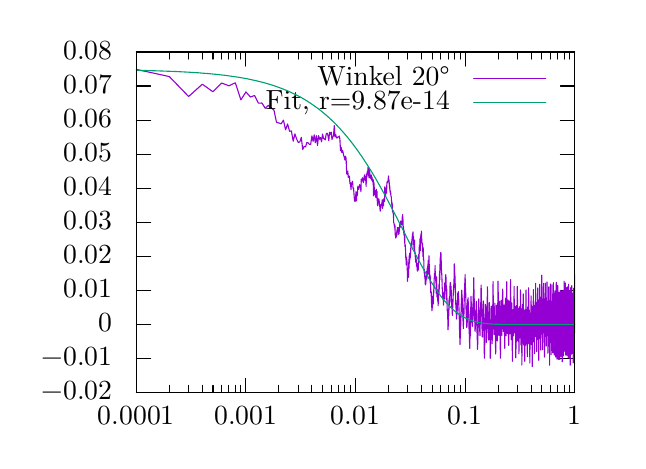
\begin{tikzpicture}[gnuplot]
%% generated with GNUPLOT 5.2p5a (Gentoo revision r0) (Lua 5.1; terminal rev. 99 , script rev. 107)
%% Sa 18 Mai 2019 18:30:35 CEST
\path (0.000,0.000) rectangle (7.500,5.250);
\gpcolor{color=gp lt color border}
\gpsetlinetype{gp lt border}
\gpsetdashtype{gp dt solid}
\gpsetlinewidth{1.00}
\draw[gp path] (1.380,0.616)--(1.560,0.616);
\draw[gp path] (6.947,0.616)--(6.767,0.616);
\node[gp node right] at (1.196,0.616) {$-0.02$};
\draw[gp path] (1.380,1.049)--(1.560,1.049);
\draw[gp path] (6.947,1.049)--(6.767,1.049);
\node[gp node right] at (1.196,1.049) {$-0.01$};
\draw[gp path] (1.380,1.481)--(1.560,1.481);
\draw[gp path] (6.947,1.481)--(6.767,1.481);
\node[gp node right] at (1.196,1.481) {$0$};
\draw[gp path] (1.380,1.914)--(1.560,1.914);
\draw[gp path] (6.947,1.914)--(6.767,1.914);
\node[gp node right] at (1.196,1.914) {$0.01$};
\draw[gp path] (1.380,2.346)--(1.560,2.346);
\draw[gp path] (6.947,2.346)--(6.767,2.346);
\node[gp node right] at (1.196,2.346) {$0.02$};
\draw[gp path] (1.380,2.779)--(1.560,2.779);
\draw[gp path] (6.947,2.779)--(6.767,2.779);
\node[gp node right] at (1.196,2.779) {$0.03$};
\draw[gp path] (1.380,3.211)--(1.560,3.211);
\draw[gp path] (6.947,3.211)--(6.767,3.211);
\node[gp node right] at (1.196,3.211) {$0.04$};
\draw[gp path] (1.380,3.644)--(1.560,3.644);
\draw[gp path] (6.947,3.644)--(6.767,3.644);
\node[gp node right] at (1.196,3.644) {$0.05$};
\draw[gp path] (1.380,4.076)--(1.560,4.076);
\draw[gp path] (6.947,4.076)--(6.767,4.076);
\node[gp node right] at (1.196,4.076) {$0.06$};
\draw[gp path] (1.380,4.509)--(1.560,4.509);
\draw[gp path] (6.947,4.509)--(6.767,4.509);
\node[gp node right] at (1.196,4.509) {$0.07$};
\draw[gp path] (1.380,4.941)--(1.560,4.941);
\draw[gp path] (6.947,4.941)--(6.767,4.941);
\node[gp node right] at (1.196,4.941) {$0.08$};
\draw[gp path] (1.380,0.616)--(1.380,0.796);
\draw[gp path] (1.380,4.941)--(1.380,4.761);
\node[gp node center] at (1.380,0.308) {$0.0001$};
\draw[gp path] (1.799,0.616)--(1.799,0.706);
\draw[gp path] (1.799,4.941)--(1.799,4.851);
\draw[gp path] (2.044,0.616)--(2.044,0.706);
\draw[gp path] (2.044,4.941)--(2.044,4.851);
\draw[gp path] (2.218,0.616)--(2.218,0.706);
\draw[gp path] (2.218,4.941)--(2.218,4.851);
\draw[gp path] (2.353,0.616)--(2.353,0.706);
\draw[gp path] (2.353,4.941)--(2.353,4.851);
\draw[gp path] (2.463,0.616)--(2.463,0.706);
\draw[gp path] (2.463,4.941)--(2.463,4.851);
\draw[gp path] (2.556,0.616)--(2.556,0.706);
\draw[gp path] (2.556,4.941)--(2.556,4.851);
\draw[gp path] (2.637,0.616)--(2.637,0.706);
\draw[gp path] (2.637,4.941)--(2.637,4.851);
\draw[gp path] (2.708,0.616)--(2.708,0.706);
\draw[gp path] (2.708,4.941)--(2.708,4.851);
\draw[gp path] (2.772,0.616)--(2.772,0.796);
\draw[gp path] (2.772,4.941)--(2.772,4.761);
\node[gp node center] at (2.772,0.308) {$0.001$};
\draw[gp path] (3.191,0.616)--(3.191,0.706);
\draw[gp path] (3.191,4.941)--(3.191,4.851);
\draw[gp path] (3.436,0.616)--(3.436,0.706);
\draw[gp path] (3.436,4.941)--(3.436,4.851);
\draw[gp path] (3.610,0.616)--(3.610,0.706);
\draw[gp path] (3.610,4.941)--(3.610,4.851);
\draw[gp path] (3.745,0.616)--(3.745,0.706);
\draw[gp path] (3.745,4.941)--(3.745,4.851);
\draw[gp path] (3.855,0.616)--(3.855,0.706);
\draw[gp path] (3.855,4.941)--(3.855,4.851);
\draw[gp path] (3.948,0.616)--(3.948,0.706);
\draw[gp path] (3.948,4.941)--(3.948,4.851);
\draw[gp path] (4.029,0.616)--(4.029,0.706);
\draw[gp path] (4.029,4.941)--(4.029,4.851);
\draw[gp path] (4.100,0.616)--(4.100,0.706);
\draw[gp path] (4.100,4.941)--(4.100,4.851);
\draw[gp path] (4.163,0.616)--(4.163,0.796);
\draw[gp path] (4.163,4.941)--(4.163,4.761);
\node[gp node center] at (4.163,0.308) {$0.01$};
\draw[gp path] (4.582,0.616)--(4.582,0.706);
\draw[gp path] (4.582,4.941)--(4.582,4.851);
\draw[gp path] (4.828,0.616)--(4.828,0.706);
\draw[gp path] (4.828,4.941)--(4.828,4.851);
\draw[gp path] (5.001,0.616)--(5.001,0.706);
\draw[gp path] (5.001,4.941)--(5.001,4.851);
\draw[gp path] (5.136,0.616)--(5.136,0.706);
\draw[gp path] (5.136,4.941)--(5.136,4.851);
\draw[gp path] (5.246,0.616)--(5.246,0.706);
\draw[gp path] (5.246,4.941)--(5.246,4.851);
\draw[gp path] (5.340,0.616)--(5.340,0.706);
\draw[gp path] (5.340,4.941)--(5.340,4.851);
\draw[gp path] (5.420,0.616)--(5.420,0.706);
\draw[gp path] (5.420,4.941)--(5.420,4.851);
\draw[gp path] (5.492,0.616)--(5.492,0.706);
\draw[gp path] (5.492,4.941)--(5.492,4.851);
\draw[gp path] (5.555,0.616)--(5.555,0.796);
\draw[gp path] (5.555,4.941)--(5.555,4.761);
\node[gp node center] at (5.555,0.308) {$0.1$};
\draw[gp path] (5.974,0.616)--(5.974,0.706);
\draw[gp path] (5.974,4.941)--(5.974,4.851);
\draw[gp path] (6.219,0.616)--(6.219,0.706);
\draw[gp path] (6.219,4.941)--(6.219,4.851);
\draw[gp path] (6.393,0.616)--(6.393,0.706);
\draw[gp path] (6.393,4.941)--(6.393,4.851);
\draw[gp path] (6.528,0.616)--(6.528,0.706);
\draw[gp path] (6.528,4.941)--(6.528,4.851);
\draw[gp path] (6.638,0.616)--(6.638,0.706);
\draw[gp path] (6.638,4.941)--(6.638,4.851);
\draw[gp path] (6.731,0.616)--(6.731,0.706);
\draw[gp path] (6.731,4.941)--(6.731,4.851);
\draw[gp path] (6.812,0.616)--(6.812,0.706);
\draw[gp path] (6.812,4.941)--(6.812,4.851);
\draw[gp path] (6.883,0.616)--(6.883,0.706);
\draw[gp path] (6.883,4.941)--(6.883,4.851);
\draw[gp path] (6.947,0.616)--(6.947,0.796);
\draw[gp path] (6.947,4.941)--(6.947,4.761);
\node[gp node center] at (6.947,0.308) {$1$};
\draw[gp path] (1.380,4.941)--(1.380,0.616)--(6.947,0.616)--(6.947,4.941)--cycle;
\node[gp node right] at (5.479,4.607) {Winkel 20°};
\gpcolor{rgb color={0.580,0.000,0.827}}
\draw[gp path] (5.663,4.607)--(6.579,4.607);
\draw[gp path] (1.380,4.720)--(1.799,4.629)--(2.044,4.376)--(2.218,4.532)--(2.353,4.436)%
  --(2.463,4.547)--(2.556,4.512)--(2.637,4.550)--(2.708,4.333)--(2.772,4.434)--(2.829,4.369)%
  --(2.882,4.389)--(2.930,4.291)--(2.975,4.293)--(3.017,4.226)--(3.056,4.264)--(3.092,4.228)%
  --(3.127,4.206)--(3.160,4.048)--(3.191,4.039)--(3.220,4.029)--(3.248,4.076)--(3.275,3.953)%
  --(3.301,4.027)--(3.326,3.934)--(3.349,3.939)--(3.372,3.808)--(3.394,3.901)--(3.415,3.838)%
  --(3.436,3.793)--(3.456,3.798)--(3.475,3.857)--(3.493,3.702)--(3.511,3.743)--(3.529,3.735)%
  --(3.546,3.793)--(3.563,3.786)--(3.579,3.767)--(3.594,3.770)--(3.610,3.876)--(3.625,3.805)%
  --(3.639,3.889)--(3.653,3.789)--(3.667,3.878)--(3.681,3.752)--(3.694,3.879)--(3.707,3.833)%
  --(3.720,3.855)--(3.732,3.800)--(3.745,3.899)--(3.757,3.845)--(3.768,3.836)--(3.780,3.826)%
  --(3.791,3.900)--(3.802,3.910)--(3.813,3.885)--(3.824,3.816)--(3.834,3.923)--(3.845,3.896)%
  --(3.855,3.923)--(3.865,3.831)--(3.875,3.859)--(3.884,3.879)--(3.894,4.006)--(3.903,3.865)%
  --(3.912,3.892)--(3.921,3.852)--(3.930,3.848)--(3.939,3.861)--(3.948,3.863)--(3.956,3.874)%
  --(3.965,3.835)--(3.973,3.686)--(3.982,3.728)--(3.990,3.662)--(3.998,3.692)--(4.006,3.666)%
  --(4.013,3.629)--(4.021,3.605)--(4.029,3.569)--(4.036,3.617)--(4.044,3.590)--(4.051,3.399)%
  --(4.058,3.386)--(4.065,3.429)--(4.072,3.348)--(4.079,3.366)--(4.086,3.364)--(4.093,3.266)%
  --(4.100,3.280)--(4.106,3.194)--(4.113,3.278)--(4.120,3.280)--(4.126,3.299)--(4.132,3.211)%
  --(4.139,3.209)--(4.145,3.125)--(4.151,3.051)--(4.157,3.044)--(4.164,3.085)--(4.170,3.167)%
  --(4.175,3.049)--(4.181,3.142)--(4.187,3.120)--(4.193,3.237)--(4.199,3.197)--(4.204,3.197)%
  --(4.210,3.225)--(4.216,3.257)--(4.221,3.226)--(4.227,3.227)--(4.232,3.168)--(4.237,3.326)%
  --(4.243,3.306)--(4.248,3.325)--(4.253,3.344)--(4.258,3.301)--(4.264,3.281)--(4.269,3.312)%
  --(4.274,3.359)--(4.279,3.382)--(4.284,3.323)--(4.289,3.311)--(4.294,3.357)--(4.298,3.234)%
  --(4.303,3.392)--(4.308,3.352)--(4.313,3.421)--(4.317,3.389)--(4.322,3.474)--(4.327,3.475)%
  --(4.331,3.377)--(4.336,3.342)--(4.340,3.458)--(4.345,3.394)--(4.349,3.374)--(4.354,3.340)%
  --(4.358,3.335)--(4.363,3.379)--(4.367,3.314)--(4.371,3.357)--(4.375,3.335)--(4.380,3.293)%
  --(4.384,3.298)--(4.388,3.321)--(4.392,3.114)--(4.396,3.290)--(4.400,3.242)--(4.405,3.134)%
  --(4.409,3.183)--(4.413,3.163)--(4.417,3.109)--(4.421,3.095)--(4.424,3.113)--(4.428,3.199)%
  --(4.432,3.087)--(4.436,3.169)--(4.440,3.052)--(4.444,2.989)--(4.448,3.017)--(4.451,3.082)%
  --(4.455,3.033)--(4.459,3.061)--(4.463,3.068)--(4.466,3.013)--(4.470,2.979)--(4.473,2.972)%
  --(4.477,2.919)--(4.481,3.001)--(4.484,2.967)--(4.488,2.998)--(4.491,2.992)--(4.495,3.016)%
  --(4.498,2.991)--(4.502,3.065)--(4.505,2.955)--(4.509,2.985)--(4.512,3.058)--(4.515,3.055)%
  --(4.519,2.987)--(4.522,3.063)--(4.525,3.080)--(4.529,3.041)--(4.532,3.053)--(4.535,3.229)%
  --(4.539,3.196)--(4.542,3.149)--(4.545,3.110)--(4.548,3.213)--(4.551,3.140)--(4.555,3.170)%
  --(4.558,3.153)--(4.561,3.255)--(4.564,3.285)--(4.567,3.297)--(4.570,3.279)--(4.573,3.295)%
  --(4.576,3.303)--(4.579,3.325)--(4.582,3.367)--(4.585,3.308)--(4.588,3.320)--(4.591,3.292)%
  --(4.594,3.231)--(4.597,3.249)--(4.600,3.175)--(4.603,3.191)--(4.606,3.146)--(4.609,3.168)%
  --(4.612,3.123)--(4.615,3.106)--(4.618,3.099)--(4.621,3.047)--(4.623,3.040)--(4.626,2.963)%
  --(4.629,3.024)--(4.632,2.920)--(4.635,2.914)--(4.637,2.918)--(4.640,2.895)--(4.643,2.896)%
  --(4.646,2.862)--(4.648,2.772)--(4.651,2.770)--(4.654,2.765)--(4.656,2.739)--(4.659,2.714)%
  --(4.662,2.742)--(4.664,2.744)--(4.667,2.620)--(4.670,2.612)--(4.672,2.608)--(4.675,2.578)%
  --(4.677,2.591)--(4.680,2.600)--(4.683,2.595)--(4.685,2.657)--(4.688,2.611)--(4.690,2.680)%
  --(4.693,2.650)--(4.695,2.713)--(4.698,2.685)--(4.700,2.686)--(4.703,2.698)--(4.705,2.710)%
  --(4.708,2.624)--(4.710,2.674)--(4.712,2.652)--(4.715,2.701)--(4.717,2.632)--(4.720,2.699)%
  --(4.722,2.708)--(4.725,2.767)--(4.727,2.733)--(4.729,2.729)--(4.732,2.716)--(4.734,2.766)%
  --(4.736,2.767)--(4.739,2.795)--(4.741,2.779)--(4.743,2.752)--(4.746,2.775)--(4.748,2.749)%
  --(4.750,2.793)--(4.753,2.771)--(4.755,2.745)--(4.757,2.849)--(4.759,2.813)--(4.762,2.878)%
  --(4.764,2.807)--(4.766,2.814)--(4.768,2.709)--(4.771,2.726)--(4.773,2.706)--(4.775,2.645)%
  --(4.777,2.685)--(4.779,2.617)--(4.781,2.626)--(4.784,2.667)--(4.786,2.550)--(4.788,2.615)%
  --(4.790,2.472)--(4.792,2.477)--(4.794,2.496)--(4.797,2.456)--(4.799,2.421)--(4.801,2.376)%
  --(4.803,2.299)--(4.805,2.319)--(4.807,2.238)--(4.809,2.337)--(4.811,2.263)--(4.813,2.332)%
  --(4.815,2.230)--(4.817,2.280)--(4.819,2.189)--(4.821,2.183)--(4.823,2.028)--(4.826,2.135)%
  --(4.828,2.125)--(4.830,2.143)--(4.832,2.095)--(4.834,2.199)--(4.836,2.078)--(4.838,2.192)%
  --(4.840,2.257)--(4.841,2.307)--(4.843,2.191)--(4.845,2.353)--(4.847,2.290)--(4.849,2.314)%
  --(4.851,2.260)--(4.853,2.388)--(4.855,2.331)--(4.857,2.382)--(4.859,2.326)--(4.861,2.377)%
  --(4.863,2.372)--(4.865,2.447)--(4.867,2.453)--(4.868,2.513)--(4.870,2.460)--(4.872,2.516)%
  --(4.874,2.525)--(4.876,2.536)--(4.878,2.465)--(4.880,2.563)--(4.881,2.561)--(4.883,2.563)%
  --(4.885,2.606)--(4.887,2.632)--(4.889,2.599)--(4.891,2.587)--(4.892,2.555)--(4.894,2.657)%
  --(4.896,2.546)--(4.898,2.577)--(4.900,2.493)--(4.901,2.599)--(4.903,2.541)--(4.905,2.476)%
  --(4.907,2.441)--(4.908,2.514)--(4.910,2.478)--(4.912,2.552)--(4.914,2.446)--(4.916,2.391)%
  --(4.917,2.419)--(4.919,2.394)--(4.921,2.337)--(4.922,2.385)--(4.924,2.375)--(4.926,2.302)%
  --(4.928,2.272)--(4.929,2.354)--(4.931,2.281)--(4.933,2.317)--(4.934,2.309)--(4.936,2.285)%
  --(4.938,2.253)--(4.939,2.222)--(4.941,2.220)--(4.943,2.210)--(4.944,2.216)--(4.946,2.214)%
  --(4.948,2.168)--(4.949,2.166)--(4.951,2.158)--(4.953,2.186)--(4.954,2.188)--(4.956,2.259)%
  --(4.958,2.209)--(4.959,2.212)--(4.961,2.171)--(4.962,2.365)--(4.964,2.326)--(4.966,2.292)%
  --(4.967,2.306)--(4.969,2.300)--(4.970,2.376)--(4.972,2.365)--(4.974,2.489)--(4.975,2.381)%
  --(4.977,2.407)--(4.978,2.479)--(4.980,2.473)--(4.981,2.569)--(4.983,2.444)--(4.985,2.452)%
  --(4.986,2.418)--(4.988,2.574)--(4.989,2.519)--(4.991,2.604)--(4.992,2.541)--(4.994,2.563)%
  --(4.995,2.628)--(4.997,2.634)--(4.998,2.591)--(5.000,2.667)--(5.001,2.640)--(5.003,2.650)%
  --(5.004,2.571)--(5.006,2.566)--(5.007,2.503)--(5.009,2.509)--(5.010,2.502)--(5.012,2.479)%
  --(5.013,2.514)--(5.015,2.501)--(5.016,2.404)--(5.018,2.447)--(5.019,2.423)--(5.021,2.343)%
  --(5.022,2.460)--(5.024,2.434)--(5.025,2.399)--(5.027,2.308)--(5.028,2.293)--(5.029,2.305)%
  --(5.031,2.292)--(5.032,2.188)--(5.034,2.166)--(5.035,2.136)--(5.037,2.181)--(5.038,2.163)%
  --(5.039,2.126)--(5.041,2.132)--(5.042,2.110)--(5.044,2.073)--(5.045,2.059)--(5.047,2.083)%
  --(5.048,2.021)--(5.049,1.990)--(5.051,2.045)--(5.052,2.002)--(5.054,1.984)--(5.055,1.999)%
  --(5.056,2.090)--(5.058,2.073)--(5.059,2.029)--(5.060,2.072)--(5.062,2.053)--(5.063,2.091)%
  --(5.064,2.136)--(5.066,2.111)--(5.067,2.156)--(5.069,2.124)--(5.070,2.058)--(5.071,2.121)%
  --(5.073,2.160)--(5.074,2.198)--(5.075,2.152)--(5.077,2.158)--(5.078,2.142)--(5.079,2.128)%
  --(5.081,2.196)--(5.082,2.247)--(5.083,2.114)--(5.085,2.156)--(5.086,2.229)--(5.087,2.293)%
  --(5.089,2.295)--(5.090,2.233)--(5.091,2.238)--(5.092,2.223)--(5.094,2.218)--(5.095,2.236)%
  --(5.096,2.355)--(5.098,2.189)--(5.099,2.269)--(5.100,2.181)--(5.101,2.241)--(5.103,2.082)%
  --(5.104,2.171)--(5.105,2.057)--(5.107,2.117)--(5.108,2.102)--(5.109,2.104)--(5.110,2.045)%
  --(5.112,2.087)--(5.113,2.006)--(5.114,2.004)--(5.115,2.000)--(5.117,1.977)--(5.118,1.885)%
  --(5.119,1.934)--(5.120,1.903)--(5.122,1.894)--(5.123,1.902)--(5.124,1.877)--(5.125,1.834)%
  --(5.127,1.889)--(5.128,1.852)--(5.129,1.753)--(5.130,1.710)--(5.131,1.696)--(5.133,1.696)%
  --(5.134,1.655)--(5.135,1.674)--(5.136,1.732)--(5.137,1.733)--(5.139,1.689)--(5.140,1.705)%
  --(5.141,1.782)--(5.142,1.757)--(5.144,1.835)--(5.145,1.747)--(5.146,1.795)--(5.147,1.763)%
  --(5.148,1.744)--(5.149,1.754)--(5.151,1.795)--(5.152,1.741)--(5.153,1.846)--(5.154,1.834)%
  --(5.155,1.921)--(5.157,1.884)--(5.158,1.905)--(5.159,1.885)--(5.160,1.963)--(5.161,2.019)%
  --(5.162,1.991)--(5.163,2.075)--(5.165,2.069)--(5.166,2.121)--(5.167,2.129)--(5.168,2.089)%
  --(5.169,2.077)--(5.170,2.127)--(5.172,2.147)--(5.173,2.117)--(5.174,2.230)--(5.175,2.126)%
  --(5.176,2.133)--(5.177,2.132)--(5.178,2.154)--(5.179,2.081)--(5.181,2.073)--(5.182,2.088)%
  --(5.183,2.033)--(5.184,2.064)--(5.185,2.075)--(5.186,2.007)--(5.187,2.023)--(5.188,1.877)%
  --(5.189,2.029)--(5.191,1.986)--(5.192,2.083)--(5.193,1.929)--(5.194,2.002)--(5.195,1.997)%
  --(5.196,1.959)--(5.197,1.830)--(5.198,1.895)--(5.199,1.832)--(5.200,1.899)--(5.202,1.887)%
  --(5.203,1.921)--(5.204,1.921)--(5.205,1.916)--(5.206,1.854)--(5.207,1.852)--(5.208,1.784)%
  --(5.209,1.780)--(5.210,1.855)--(5.211,1.814)--(5.212,1.743)--(5.213,1.718)--(5.214,1.759)%
  --(5.215,1.888)--(5.217,1.809)--(5.218,1.857)--(5.219,1.892)--(5.220,1.923)--(5.221,1.907)%
  --(5.222,1.931)--(5.223,1.986)--(5.224,1.887)--(5.225,1.936)--(5.226,1.910)--(5.227,1.982)%
  --(5.228,2.003)--(5.229,2.021)--(5.230,2.121)--(5.231,2.109)--(5.232,2.160)--(5.233,2.075)%
  --(5.234,2.163)--(5.235,2.049)--(5.236,2.198)--(5.237,2.241)--(5.238,2.272)--(5.239,2.218)%
  --(5.240,2.326)--(5.241,2.237)--(5.242,2.350)--(5.243,2.213)--(5.244,2.394)--(5.245,2.256)%
  --(5.246,2.394)--(5.247,2.370)--(5.249,2.383)--(5.250,2.287)--(5.251,2.323)--(5.252,2.168)%
  --(5.253,2.206)--(5.254,2.243)--(5.254,2.289)--(5.255,2.151)--(5.256,2.143)--(5.257,2.112)%
  --(5.258,2.118)--(5.259,2.130)--(5.260,2.097)--(5.261,2.071)--(5.262,2.026)--(5.263,2.020)%
  --(5.264,1.937)--(5.265,1.950)--(5.266,1.924)--(5.267,1.904)--(5.268,1.897)--(5.269,1.861)%
  --(5.270,1.885)--(5.271,1.893)--(5.272,1.822)--(5.273,1.838)--(5.274,1.805)--(5.275,1.808)%
  --(5.276,1.822)--(5.277,1.788)--(5.278,1.836)--(5.279,1.780)--(5.280,1.726)--(5.281,1.731)%
  --(5.282,1.754)--(5.283,1.830)--(5.284,1.847)--(5.285,1.771)--(5.286,1.832)--(5.286,1.829)%
  --(5.287,1.863)--(5.288,1.808)--(5.289,1.887)--(5.290,1.870)--(5.291,1.860)--(5.292,1.855)%
  --(5.293,1.805)--(5.294,1.852)--(5.295,2.008)--(5.296,1.879)--(5.297,1.921)--(5.298,1.865)%
  --(5.299,1.924)--(5.300,1.974)--(5.300,1.984)--(5.301,1.937)--(5.302,1.957)--(5.303,1.968)%
  --(5.304,1.941)--(5.305,1.962)--(5.306,2.082)--(5.307,2.058)--(5.308,2.041)--(5.309,1.993)%
  --(5.310,2.040)--(5.310,2.113)--(5.311,2.076)--(5.312,1.976)--(5.313,2.081)--(5.314,2.026)%
  --(5.315,1.988)--(5.316,1.910)--(5.317,1.902)--(5.318,1.930)--(5.319,1.857)--(5.319,1.796)%
  --(5.320,1.892)--(5.321,1.885)--(5.322,1.932)--(5.323,1.846)--(5.324,1.773)--(5.325,1.755)%
  --(5.326,1.810)--(5.327,1.758)--(5.327,1.748)--(5.328,1.667)--(5.329,1.658)--(5.330,1.636)%
  --(5.331,1.639)--(5.332,1.664)--(5.333,1.625)--(5.334,1.606)--(5.334,1.631)--(5.335,1.599)%
  --(5.336,1.506)--(5.337,1.518)--(5.338,1.413)--(5.339,1.451)--(5.340,1.477)--(5.341,1.467)%
  --(5.341,1.458)--(5.342,1.487)--(5.343,1.607)--(5.344,1.592)--(5.345,1.643)--(5.346,1.584)%
  --(5.347,1.596)--(5.347,1.680)--(5.348,1.593)--(5.349,1.601)--(5.350,1.784)--(5.351,1.721)%
  --(5.352,1.688)--(5.352,1.672)--(5.353,1.700)--(5.354,1.810)--(5.355,1.759)--(5.356,1.836)%
  --(5.357,1.746)--(5.358,1.836)--(5.358,1.796)--(5.359,1.790)--(5.360,1.800)--(5.361,1.771)%
  --(5.362,1.921)--(5.363,1.969)--(5.363,1.953)--(5.364,1.932)--(5.365,1.891)--(5.366,1.906)%
  --(5.367,2.011)--(5.368,2.008)--(5.368,1.986)--(5.369,2.015)--(5.370,1.899)--(5.371,1.975)%
  --(5.372,1.982)--(5.372,1.914)--(5.373,1.932)--(5.374,1.854)--(5.375,1.902)--(5.376,1.866)%
  --(5.377,1.965)--(5.377,1.948)--(5.378,1.932)--(5.379,1.910)--(5.380,1.840)--(5.381,1.791)%
  --(5.381,1.764)--(5.382,1.807)--(5.383,1.775)--(5.384,1.798)--(5.385,1.709)--(5.385,1.793)%
  --(5.386,1.756)--(5.387,1.791)--(5.388,1.691)--(5.389,1.799)--(5.389,1.684)--(5.390,1.748)%
  --(5.391,1.704)--(5.392,1.664)--(5.393,1.595)--(5.393,1.677)--(5.394,1.632)--(5.395,1.675)%
  --(5.396,1.696)--(5.396,1.654)--(5.397,1.636)--(5.398,1.719)--(5.399,1.729)--(5.400,1.718)%
  --(5.400,1.694)--(5.401,1.784)--(5.402,1.766)--(5.403,1.839)--(5.404,1.786)--(5.404,1.847)%
  --(5.405,1.861)--(5.406,1.915)--(5.407,1.885)--(5.407,1.877)--(5.408,1.921)--(5.409,1.940)%
  --(5.410,1.986)--(5.410,1.938)--(5.411,1.953)--(5.412,1.997)--(5.413,2.002)--(5.414,1.978)%
  --(5.414,2.027)--(5.415,2.061)--(5.416,2.051)--(5.417,2.044)--(5.417,2.065)--(5.418,2.251)%
  --(5.419,2.185)--(5.420,2.191)--(5.420,2.221)--(5.421,2.121)--(5.422,2.174)--(5.423,2.096)%
  --(5.423,2.063)--(5.424,2.139)--(5.425,2.034)--(5.426,2.058)--(5.426,1.986)--(5.427,2.096)%
  --(5.428,1.966)--(5.429,2.006)--(5.429,2.026)--(5.430,1.974)--(5.431,1.910)--(5.432,1.945)%
  --(5.432,1.888)--(5.433,1.907)--(5.434,1.853)--(5.435,1.879)--(5.435,1.862)--(5.436,1.734)%
  --(5.437,1.762)--(5.438,1.785)--(5.438,1.769)--(5.439,1.753)--(5.440,1.681)--(5.440,1.702)%
  --(5.441,1.696)--(5.442,1.632)--(5.443,1.613)--(5.443,1.614)--(5.444,1.673)--(5.445,1.611)%
  --(5.446,1.630)--(5.446,1.550)--(5.447,1.577)--(5.448,1.591)--(5.448,1.596)--(5.449,1.656)%
  --(5.450,1.599)--(5.451,1.680)--(5.451,1.625)--(5.452,1.693)--(5.453,1.647)--(5.453,1.747)%
  --(5.454,1.608)--(5.455,1.701)--(5.456,1.661)--(5.456,1.720)--(5.457,1.701)--(5.458,1.722)%
  --(5.458,1.767)--(5.459,1.791)--(5.460,1.728)--(5.461,1.772)--(5.461,1.752)--(5.462,1.879)%
  --(5.463,1.809)--(5.463,1.808)--(5.464,1.777)--(5.465,1.821)--(5.465,1.837)--(5.466,1.842)%
  --(5.467,1.755)--(5.468,1.891)--(5.468,1.818)--(5.469,1.788)--(5.470,1.898)--(5.470,1.879)%
  --(5.471,1.834)--(5.472,1.820)--(5.472,1.776)--(5.473,1.755)--(5.474,1.728)--(5.475,1.802)%
  --(5.475,1.730)--(5.476,1.712)--(5.477,1.699)--(5.477,1.702)--(5.478,1.655)--(5.479,1.647)%
  --(5.479,1.654)--(5.480,1.627)--(5.481,1.587)--(5.481,1.579)--(5.482,1.530)--(5.483,1.553)%
  --(5.483,1.504)--(5.484,1.408)--(5.485,1.489)--(5.485,1.522)--(5.486,1.490)--(5.487,1.367)%
  --(5.488,1.309)--(5.488,1.306)--(5.489,1.349)--(5.490,1.347)--(5.490,1.225)--(5.491,1.323)%
  --(5.492,1.246)--(5.492,1.325)--(5.493,1.300)--(5.494,1.321)--(5.494,1.336)--(5.495,1.407)%
  --(5.496,1.345)--(5.496,1.398)--(5.497,1.462)--(5.498,1.483)--(5.498,1.466)--(5.499,1.473)%
  --(5.500,1.470)--(5.500,1.601)--(5.501,1.568)--(5.502,1.549)--(5.502,1.542)--(5.503,1.587)%
  --(5.504,1.644)--(5.504,1.616)--(5.505,1.709)--(5.506,1.641)--(5.506,1.702)--(5.507,1.723)%
  --(5.507,1.747)--(5.508,1.706)--(5.509,1.802)--(5.509,1.833)--(5.510,1.815)--(5.511,1.837)%
  --(5.511,1.725)--(5.512,1.808)--(5.513,1.819)--(5.513,1.917)--(5.514,1.795)--(5.515,1.863)%
  --(5.515,1.817)--(5.516,1.841)--(5.517,1.786)--(5.517,1.860)--(5.518,1.746)--(5.518,1.725)%
  --(5.519,1.691)--(5.520,1.812)--(5.520,1.702)--(5.521,1.725)--(5.522,1.708)--(5.522,1.704)%
  --(5.523,1.733)--(5.524,1.614)--(5.524,1.630)--(5.525,1.668)--(5.526,1.689)--(5.526,1.618)%
  --(5.527,1.529)--(5.527,1.653)--(5.528,1.584)--(5.529,1.623)--(5.529,1.586)--(5.530,1.573)%
  --(5.531,1.527)--(5.531,1.514)--(5.532,1.529)--(5.532,1.470)--(5.533,1.428)--(5.534,1.478)%
  --(5.534,1.471)--(5.535,1.576)--(5.536,1.476)--(5.536,1.615)--(5.537,1.534)--(5.537,1.607)%
  --(5.538,1.595)--(5.539,1.600)--(5.539,1.593)--(5.540,1.587)--(5.541,1.638)--(5.541,1.678)%
  --(5.542,1.683)--(5.542,1.625)--(5.543,1.792)--(5.544,1.774)--(5.544,1.843)--(5.545,1.792)%
  --(5.546,1.829)--(5.546,1.888)--(5.547,1.852)--(5.547,1.889)--(5.548,1.886)--(5.549,1.981)%
  --(5.549,1.908)--(5.550,1.947)--(5.550,2.004)--(5.551,1.950)--(5.552,1.865)--(5.552,1.881)%
  --(5.553,1.990)--(5.553,2.046)--(5.554,2.013)--(5.555,2.111)--(5.555,2.112)--(5.556,2.115)%
  --(5.556,2.088)--(5.557,2.026)--(5.558,2.055)--(5.558,1.933)--(5.559,1.948)--(5.559,1.882)%
  --(5.560,1.918)--(5.561,1.864)--(5.561,1.879)--(5.562,1.944)--(5.562,1.888)--(5.563,1.879)%
  --(5.564,1.862)--(5.564,1.816)--(5.565,1.805)--(5.565,1.789)--(5.566,1.739)--(5.567,1.750)%
  --(5.567,1.674)--(5.568,1.733)--(5.568,1.704)--(5.569,1.692)--(5.570,1.569)--(5.570,1.593)%
  --(5.571,1.629)--(5.571,1.639)--(5.572,1.537)--(5.573,1.703)--(5.573,1.515)--(5.574,1.525)%
  --(5.574,1.452)--(5.575,1.519)--(5.575,1.442)--(5.576,1.447)--(5.577,1.537)--(5.577,1.492)%
  --(5.578,1.480)--(5.578,1.526)--(5.579,1.580)--(5.580,1.618)--(5.580,1.518)--(5.581,1.459)%
  --(5.581,1.528)--(5.582,1.644)--(5.582,1.556)--(5.583,1.577)--(5.584,1.505)--(5.584,1.615)%
  --(5.585,1.654)--(5.585,1.580)--(5.586,1.688)--(5.586,1.672)--(5.587,1.795)--(5.588,1.660)%
  --(5.588,1.727)--(5.589,1.680)--(5.589,1.800)--(5.590,1.733)--(5.590,1.663)--(5.591,1.752)%
  --(5.592,1.717)--(5.592,1.719)--(5.593,1.821)--(5.593,1.732)--(5.594,1.782)--(5.594,1.733)%
  --(5.595,1.769)--(5.596,1.694)--(5.596,1.719)--(5.597,1.742)--(5.597,1.702)--(5.598,1.659)%
  --(5.598,1.678)--(5.599,1.656)--(5.600,1.654)--(5.600,1.611)--(5.601,1.646)--(5.601,1.594)%
  --(5.602,1.565)--(5.602,1.580)--(5.603,1.596)--(5.603,1.502)--(5.604,1.425)--(5.605,1.526)%
  --(5.605,1.488)--(5.606,1.396)--(5.606,1.481)--(5.607,1.369)--(5.607,1.386)--(5.608,1.363)%
  --(5.609,1.395)--(5.610,1.394)--(5.610,1.303)--(5.611,1.370)--(5.611,1.252)--(5.612,1.276)%
  --(5.612,1.199)--(5.613,1.246)--(5.613,1.245)--(5.614,1.248)--(5.615,1.174)--(5.615,1.299)%
  --(5.616,1.219)--(5.616,1.253)--(5.617,1.316)--(5.617,1.309)--(5.618,1.321)--(5.618,1.392)%
  --(5.619,1.371)--(5.619,1.374)--(5.620,1.336)--(5.621,1.418)--(5.621,1.496)--(5.622,1.514)%
  --(5.622,1.469)--(5.623,1.482)--(5.623,1.438)--(5.624,1.615)--(5.624,1.580)--(5.625,1.577)%
  --(5.625,1.563)--(5.626,1.704)--(5.626,1.657)--(5.627,1.666)--(5.628,1.686)--(5.628,1.712)%
  --(5.629,1.730)--(5.629,1.813)--(5.630,1.781)--(5.630,1.837)--(5.631,1.698)--(5.631,1.715)%
  --(5.632,1.714)--(5.632,1.687)--(5.633,1.705)--(5.633,1.756)--(5.634,1.768)--(5.634,1.679)%
  --(5.635,1.682)--(5.636,1.673)--(5.636,1.685)--(5.637,1.606)--(5.637,1.652)--(5.638,1.743)%
  --(5.638,1.601)--(5.639,1.688)--(5.639,1.601)--(5.640,1.575)--(5.640,1.512)--(5.641,1.615)%
  --(5.641,1.577)--(5.642,1.569)--(5.642,1.580)--(5.643,1.549)--(5.643,1.523)--(5.644,1.517)%
  --(5.644,1.495)--(5.645,1.624)--(5.645,1.552)--(5.646,1.595)--(5.647,1.510)--(5.647,1.536)%
  --(5.648,1.456)--(5.648,1.533)--(5.649,1.508)--(5.649,1.459)--(5.650,1.478)--(5.650,1.565)%
  --(5.651,1.558)--(5.651,1.521)--(5.652,1.538)--(5.652,1.567)--(5.653,1.563)--(5.653,1.607)%
  --(5.654,1.575)--(5.654,1.622)--(5.655,1.618)--(5.655,1.597)--(5.656,1.590)--(5.656,1.699)%
  --(5.657,1.653)--(5.657,1.746)--(5.658,1.695)--(5.658,1.714)--(5.659,1.719)--(5.659,1.842)%
  --(5.660,1.787)--(5.660,1.853)--(5.661,1.821)--(5.661,1.851)--(5.662,1.880)--(5.662,1.865)%
  --(5.663,1.851)--(5.663,2.021)--(5.664,1.894)--(5.664,2.049)--(5.665,1.963)--(5.665,2.075)%
  --(5.666,1.967)--(5.666,2.007)--(5.667,1.979)--(5.667,1.946)--(5.668,1.913)--(5.668,1.860)%
  --(5.669,1.792)--(5.669,1.777)--(5.670,1.878)--(5.670,1.838)--(5.671,1.798)--(5.671,1.778)%
  --(5.672,1.722)--(5.672,1.786)--(5.673,1.703)--(5.673,1.748)--(5.674,1.668)--(5.674,1.621)%
  --(5.675,1.547)--(5.675,1.593)--(5.676,1.577)--(5.676,1.562)--(5.677,1.553)--(5.677,1.508)%
  --(5.678,1.596)--(5.678,1.524)--(5.679,1.489)--(5.679,1.405)--(5.680,1.459)--(5.680,1.492)%
  --(5.681,1.400)--(5.681,1.468)--(5.682,1.392)--(5.682,1.473)--(5.683,1.401)--(5.683,1.444)%
  --(5.684,1.452)--(5.684,1.497)--(5.685,1.493)--(5.685,1.466)--(5.686,1.421)--(5.686,1.475)%
  --(5.687,1.476)--(5.687,1.505)--(5.688,1.521)--(5.688,1.467)--(5.689,1.540)--(5.689,1.580)%
  --(5.690,1.549)--(5.690,1.653)--(5.691,1.561)--(5.691,1.599)--(5.692,1.581)--(5.692,1.603)%
  --(5.693,1.623)--(5.693,1.566)--(5.693,1.621)--(5.694,1.653)--(5.694,1.599)--(5.695,1.715)%
  --(5.695,1.686)--(5.696,1.706)--(5.696,1.685)--(5.697,1.756)--(5.697,1.633)--(5.698,1.775)%
  --(5.698,1.677)--(5.699,1.766)--(5.699,1.678)--(5.700,1.733)--(5.700,1.654)--(5.701,1.617)%
  --(5.701,1.585)--(5.702,1.576)--(5.702,1.565)--(5.703,1.620)--(5.703,1.608)--(5.704,1.530)%
  --(5.704,1.526)--(5.704,1.494)--(5.705,1.515)--(5.705,1.482)--(5.706,1.471)--(5.706,1.401)%
  --(5.707,1.373)--(5.707,1.482)--(5.708,1.424)--(5.708,1.390)--(5.709,1.332)--(5.709,1.343)%
  --(5.710,1.330)--(5.710,1.283)--(5.711,1.292)--(5.711,1.304)--(5.712,1.284)--(5.712,1.164)%
  --(5.712,1.207)--(5.713,1.229)--(5.713,1.184)--(5.714,1.174)--(5.714,1.220)--(5.715,1.182)%
  --(5.715,1.316)--(5.716,1.225)--(5.716,1.238)--(5.717,1.343)--(5.717,1.292)--(5.718,1.301)%
  --(5.718,1.378)--(5.718,1.307)--(5.719,1.396)--(5.719,1.341)--(5.720,1.417)--(5.720,1.432)%
  --(5.721,1.422)--(5.721,1.398)--(5.722,1.477)--(5.722,1.450)--(5.723,1.489)--(5.723,1.565)%
  --(5.724,1.667)--(5.724,1.564)--(5.724,1.586)--(5.725,1.589)--(5.725,1.562)--(5.726,1.622)%
  --(5.726,1.638)--(5.727,1.664)--(5.727,1.672)--(5.728,1.750)--(5.728,1.777)--(5.729,1.707)%
  --(5.729,1.804)--(5.729,1.776)--(5.730,1.741)--(5.730,1.726)--(5.731,1.646)--(5.731,1.707)%
  --(5.732,1.646)--(5.732,1.639)--(5.733,1.645)--(5.733,1.648)--(5.733,1.632)--(5.734,1.549)%
  --(5.734,1.634)--(5.735,1.577)--(5.735,1.591)--(5.736,1.535)--(5.736,1.645)--(5.737,1.531)%
  --(5.737,1.561)--(5.738,1.533)--(5.738,1.498)--(5.738,1.552)--(5.739,1.493)--(5.739,1.440)%
  --(5.740,1.493)--(5.740,1.458)--(5.741,1.434)--(5.741,1.392)--(5.742,1.419)--(5.742,1.435)%
  --(5.742,1.406)--(5.743,1.441)--(5.743,1.478)--(5.744,1.339)--(5.744,1.427)--(5.745,1.451)%
  --(5.745,1.493)--(5.746,1.447)--(5.746,1.392)--(5.746,1.424)--(5.747,1.519)--(5.747,1.480)%
  --(5.748,1.481)--(5.748,1.509)--(5.749,1.636)--(5.749,1.569)--(5.749,1.574)--(5.750,1.528)%
  --(5.750,1.569)--(5.751,1.667)--(5.751,1.608)--(5.752,1.709)--(5.752,1.667)--(5.753,1.698)%
  --(5.753,1.678)--(5.753,1.702)--(5.754,1.744)--(5.754,1.761)--(5.755,1.742)--(5.755,1.755)%
  --(5.756,1.745)--(5.756,1.827)--(5.756,1.864)--(5.757,1.854)--(5.757,1.934)--(5.758,1.942)%
  --(5.758,1.950)--(5.759,1.982)--(5.759,1.928)--(5.759,1.916)--(5.760,1.941)--(5.760,1.778)%
  --(5.761,1.925)--(5.761,1.843)--(5.762,1.849)--(5.762,1.808)--(5.762,1.834)--(5.763,1.723)%
  --(5.763,1.729)--(5.764,1.704)--(5.764,1.731)--(5.765,1.682)--(5.765,1.699)--(5.765,1.677)%
  --(5.766,1.622)--(5.766,1.583)--(5.767,1.630)--(5.767,1.591)--(5.768,1.620)--(5.768,1.492)%
  --(5.768,1.541)--(5.769,1.522)--(5.769,1.492)--(5.770,1.450)--(5.770,1.499)--(5.771,1.355)%
  --(5.771,1.388)--(5.771,1.357)--(5.772,1.327)--(5.772,1.455)--(5.773,1.353)--(5.773,1.321)%
  --(5.774,1.375)--(5.774,1.381)--(5.774,1.367)--(5.775,1.414)--(5.775,1.478)--(5.776,1.477)%
  --(5.776,1.427)--(5.776,1.418)--(5.777,1.471)--(5.777,1.401)--(5.778,1.411)--(5.778,1.466)%
  --(5.779,1.486)--(5.779,1.432)--(5.779,1.507)--(5.780,1.527)--(5.780,1.497)--(5.781,1.572)%
  --(5.781,1.536)--(5.781,1.566)--(5.782,1.568)--(5.782,1.582)--(5.783,1.679)--(5.783,1.561)%
  --(5.784,1.635)--(5.784,1.599)--(5.784,1.652)--(5.785,1.587)--(5.785,1.717)--(5.786,1.636)%
  --(5.786,1.779)--(5.786,1.715)--(5.787,1.753)--(5.787,1.749)--(5.788,1.725)--(5.788,1.697)%
  --(5.789,1.650)--(5.789,1.750)--(5.789,1.577)--(5.790,1.606)--(5.790,1.618)--(5.791,1.591)%
  --(5.791,1.583)--(5.791,1.574)--(5.792,1.553)--(5.792,1.526)--(5.793,1.468)--(5.793,1.464)%
  --(5.793,1.417)--(5.794,1.466)--(5.794,1.475)--(5.795,1.374)--(5.795,1.372)--(5.795,1.319)%
  --(5.796,1.356)--(5.796,1.311)--(5.797,1.262)--(5.797,1.289)--(5.797,1.382)--(5.798,1.244)%
  --(5.798,1.165)--(5.799,1.110)--(5.799,1.162)--(5.800,1.052)--(5.800,1.227)--(5.800,1.119)%
  --(5.801,1.250)--(5.801,1.099)--(5.802,1.187)--(5.802,1.161)--(5.802,1.317)--(5.803,1.260)%
  --(5.803,1.316)--(5.804,1.300)--(5.804,1.456)--(5.804,1.328)--(5.805,1.351)--(5.805,1.222)%
  --(5.806,1.435)--(5.806,1.384)--(5.806,1.428)--(5.807,1.382)--(5.807,1.428)--(5.808,1.489)%
  --(5.808,1.524)--(5.808,1.544)--(5.809,1.465)--(5.809,1.561)--(5.810,1.575)--(5.810,1.598)%
  --(5.810,1.577)--(5.811,1.581)--(5.811,1.613)--(5.812,1.598)--(5.812,1.716)--(5.812,1.664)%
  --(5.813,1.735)--(5.813,1.614)--(5.813,1.685)--(5.814,1.574)--(5.814,1.707)--(5.815,1.599)%
  --(5.815,1.664)--(5.815,1.561)--(5.816,1.706)--(5.816,1.578)--(5.817,1.661)--(5.817,1.591)%
  --(5.817,1.629)--(5.818,1.540)--(5.818,1.590)--(5.819,1.598)--(5.819,1.571)--(5.819,1.504)%
  --(5.820,1.591)--(5.820,1.538)--(5.821,1.498)--(5.821,1.462)--(5.821,1.490)--(5.822,1.412)%
  --(5.822,1.509)--(5.822,1.442)--(5.823,1.470)--(5.823,1.486)--(5.824,1.442)--(5.824,1.435)%
  --(5.824,1.476)--(5.825,1.433)--(5.825,1.352)--(5.826,1.322)--(5.826,1.253)--(5.826,1.332)%
  --(5.827,1.380)--(5.827,1.302)--(5.828,1.433)--(5.828,1.371)--(5.828,1.523)--(5.829,1.388)%
  --(5.829,1.487)--(5.829,1.424)--(5.830,1.429)--(5.830,1.562)--(5.831,1.538)--(5.831,1.629)%
  --(5.831,1.552)--(5.832,1.554)--(5.832,1.620)--(5.832,1.559)--(5.833,1.688)--(5.833,1.622)%
  --(5.834,1.727)--(5.834,1.649)--(5.834,1.725)--(5.835,1.662)--(5.835,1.767)--(5.836,1.762)%
  --(5.836,1.781)--(5.836,1.769)--(5.837,1.793)--(5.837,1.749)--(5.837,1.835)--(5.838,1.821)%
  --(5.838,1.840)--(5.839,1.856)--(5.839,1.959)--(5.839,1.923)--(5.840,1.894)--(5.840,1.851)%
  --(5.840,1.885)--(5.841,1.822)--(5.841,1.714)--(5.842,1.786)--(5.842,1.741)--(5.842,1.755)%
  --(5.843,1.695)--(5.843,1.754)--(5.843,1.636)--(5.844,1.697)--(5.844,1.720)--(5.845,1.654)%
  --(5.845,1.659)--(5.845,1.662)--(5.846,1.611)--(5.846,1.544)--(5.846,1.582)--(5.847,1.571)%
  --(5.847,1.611)--(5.848,1.529)--(5.848,1.428)--(5.848,1.544)--(5.849,1.538)--(5.849,1.427)%
  --(5.849,1.416)--(5.850,1.368)--(5.850,1.377)--(5.851,1.343)--(5.851,1.409)--(5.851,1.383)%
  --(5.852,1.283)--(5.852,1.349)--(5.852,1.308)--(5.853,1.384)--(5.853,1.448)--(5.854,1.285)%
  --(5.854,1.389)--(5.854,1.399)--(5.855,1.411)--(5.855,1.384)--(5.855,1.421)--(5.856,1.462)%
  --(5.856,1.389)--(5.856,1.447)--(5.857,1.454)--(5.857,1.501)--(5.858,1.547)--(5.858,1.566)%
  --(5.858,1.536)--(5.859,1.610)--(5.859,1.476)--(5.859,1.539)--(5.860,1.579)--(5.860,1.614)%
  --(5.860,1.601)--(5.861,1.583)--(5.861,1.579)--(5.862,1.585)--(5.862,1.566)--(5.862,1.574)%
  --(5.863,1.612)--(5.863,1.721)--(5.863,1.699)--(5.864,1.759)--(5.864,1.646)--(5.864,1.661)%
  --(5.865,1.529)--(5.865,1.676)--(5.866,1.603)--(5.866,1.576)--(5.866,1.590)--(5.867,1.682)%
  --(5.867,1.556)--(5.867,1.574)--(5.868,1.496)--(5.868,1.517)--(5.868,1.535)--(5.869,1.424)%
  --(5.869,1.379)--(5.870,1.382)--(5.870,1.458)--(5.870,1.371)--(5.871,1.431)--(5.871,1.349)%
  --(5.871,1.363)--(5.872,1.286)--(5.872,1.328)--(5.872,1.287)--(5.873,1.276)--(5.873,1.201)%
  --(5.873,1.247)--(5.874,1.273)--(5.874,1.177)--(5.875,1.148)--(5.875,1.121)--(5.875,1.051)%
  --(5.876,1.074)--(5.876,1.111)--(5.876,1.122)--(5.877,1.150)--(5.877,1.202)--(5.877,1.122)%
  --(5.878,1.144)--(5.878,1.254)--(5.878,1.132)--(5.879,1.257)--(5.879,1.187)--(5.880,1.296)%
  --(5.880,1.289)--(5.880,1.350)--(5.881,1.290)--(5.881,1.336)--(5.881,1.327)--(5.882,1.419)%
  --(5.882,1.408)--(5.882,1.493)--(5.883,1.511)--(5.883,1.507)--(5.883,1.424)--(5.884,1.482)%
  --(5.884,1.487)--(5.884,1.543)--(5.885,1.529)--(5.885,1.602)--(5.886,1.556)--(5.886,1.644)%
  --(5.886,1.612)--(5.887,1.561)--(5.887,1.625)--(5.887,1.714)--(5.888,1.661)--(5.888,1.679)%
  --(5.888,1.580)--(5.889,1.621)--(5.889,1.684)--(5.889,1.640)--(5.890,1.599)--(5.890,1.635)%
  --(5.890,1.515)--(5.891,1.575)--(5.891,1.518)--(5.891,1.576)--(5.892,1.527)--(5.892,1.524)%
  --(5.892,1.502)--(5.893,1.580)--(5.893,1.491)--(5.893,1.526)--(5.894,1.390)--(5.894,1.454)%
  --(5.895,1.387)--(5.895,1.519)--(5.895,1.372)--(5.896,1.467)--(5.896,1.393)--(5.896,1.414)%
  --(5.897,1.427)--(5.897,1.492)--(5.897,1.333)--(5.898,1.357)--(5.898,1.382)--(5.898,1.237)%
  --(5.899,1.328)--(5.899,1.275)--(5.899,1.309)--(5.900,1.277)--(5.900,1.315)--(5.900,1.349)%
  --(5.901,1.344)--(5.901,1.362)--(5.901,1.413)--(5.902,1.507)--(5.902,1.430)--(5.902,1.460)%
  --(5.903,1.488)--(5.903,1.586)--(5.903,1.484)--(5.904,1.508)--(5.904,1.536)--(5.904,1.583)%
  --(5.905,1.561)--(5.905,1.573)--(5.905,1.624)--(5.906,1.677)--(5.906,1.721)--(5.906,1.693)%
  --(5.907,1.726)--(5.907,1.732)--(5.907,1.696)--(5.908,1.772)--(5.908,1.725)--(5.909,1.860)%
  --(5.909,1.929)--(5.910,1.857)--(5.910,1.992)--(5.910,1.897)--(5.911,2.025)--(5.911,1.885)%
  --(5.911,1.977)--(5.912,1.812)--(5.912,1.843)--(5.912,1.850)--(5.913,1.820)--(5.913,1.705)%
  --(5.913,1.733)--(5.914,1.721)--(5.914,1.731)--(5.914,1.715)--(5.915,1.670)--(5.915,1.655)%
  --(5.915,1.722)--(5.916,1.666)--(5.916,1.611)--(5.916,1.522)--(5.917,1.495)--(5.917,1.554)%
  --(5.917,1.507)--(5.918,1.556)--(5.918,1.496)--(5.918,1.498)--(5.919,1.500)--(5.919,1.419)%
  --(5.919,1.421)--(5.920,1.500)--(5.920,1.505)--(5.920,1.388)--(5.921,1.448)--(5.921,1.369)%
  --(5.921,1.445)--(5.922,1.414)--(5.922,1.454)--(5.922,1.353)--(5.922,1.499)--(5.923,1.401)%
  --(5.923,1.455)--(5.923,1.382)--(5.924,1.462)--(5.924,1.494)--(5.924,1.475)--(5.925,1.393)%
  --(5.925,1.453)--(5.925,1.490)--(5.926,1.505)--(5.926,1.511)--(5.926,1.565)--(5.927,1.458)%
  --(5.927,1.532)--(5.927,1.485)--(5.928,1.611)--(5.928,1.573)--(5.928,1.595)--(5.929,1.565)%
  --(5.929,1.572)--(5.929,1.558)--(5.930,1.618)--(5.930,1.697)--(5.930,1.670)--(5.931,1.585)%
  --(5.931,1.627)--(5.931,1.636)--(5.932,1.650)--(5.932,1.617)--(5.932,1.652)--(5.933,1.656)%
  --(5.933,1.751)--(5.933,1.638)--(5.934,1.627)--(5.934,1.625)--(5.934,1.602)--(5.935,1.581)%
  --(5.935,1.587)--(5.935,1.557)--(5.936,1.572)--(5.936,1.499)--(5.936,1.532)--(5.936,1.482)%
  --(5.937,1.498)--(5.937,1.426)--(5.937,1.388)--(5.938,1.382)--(5.938,1.388)--(5.938,1.345)%
  --(5.939,1.379)--(5.939,1.320)--(5.939,1.366)--(5.940,1.189)--(5.940,1.217)--(5.940,1.280)%
  --(5.941,1.287)--(5.941,1.286)--(5.941,1.265)--(5.942,1.237)--(5.942,1.200)--(5.942,1.131)%
  --(5.943,1.139)--(5.943,1.121)--(5.943,1.106)--(5.944,1.133)--(5.944,1.210)--(5.944,1.165)%
  --(5.944,1.174)--(5.945,1.276)--(5.945,1.259)--(5.945,1.370)--(5.946,1.307)--(5.946,1.318)%
  --(5.946,1.301)--(5.947,1.365)--(5.947,1.324)--(5.947,1.414)--(5.948,1.464)--(5.948,1.413)%
  --(5.948,1.425)--(5.949,1.416)--(5.949,1.461)--(5.949,1.468)--(5.950,1.537)--(5.950,1.454)%
  --(5.950,1.575)--(5.950,1.494)--(5.951,1.466)--(5.951,1.490)--(5.951,1.557)--(5.952,1.613)%
  --(5.952,1.654)--(5.952,1.595)--(5.953,1.604)--(5.953,1.673)--(5.953,1.632)--(5.954,1.682)%
  --(5.954,1.662)--(5.954,1.725)--(5.955,1.621)--(5.955,1.652)--(5.955,1.609)--(5.955,1.583)%
  --(5.956,1.540)--(5.956,1.666)--(5.956,1.587)--(5.957,1.491)--(5.957,1.621)--(5.957,1.542)%
  --(5.958,1.522)--(5.958,1.588)--(5.958,1.530)--(5.959,1.504)--(5.959,1.545)--(5.959,1.523)%
  --(5.960,1.433)--(5.960,1.544)--(5.960,1.414)--(5.960,1.462)--(5.961,1.486)--(5.961,1.502)%
  --(5.961,1.521)--(5.962,1.448)--(5.962,1.406)--(5.962,1.446)--(5.963,1.386)--(5.963,1.353)%
  --(5.964,1.403)--(5.964,1.384)--(5.964,1.450)--(5.964,1.271)--(5.965,1.469)--(5.965,1.452)%
  --(5.965,1.506)--(5.966,1.377)--(5.966,1.511)--(5.966,1.436)--(5.967,1.483)--(5.967,1.477)%
  --(5.967,1.535)--(5.968,1.584)--(5.968,1.565)--(5.968,1.591)--(5.968,1.585)--(5.969,1.616)%
  --(5.969,1.648)--(5.969,1.630)--(5.970,1.692)--(5.970,1.741)--(5.970,1.716)--(5.971,1.783)%
  --(5.971,1.759)--(5.971,1.738)--(5.971,1.759)--(5.972,1.706)--(5.972,1.810)--(5.972,1.827)%
  --(5.973,1.860)--(5.973,1.882)--(5.973,2.029)--(5.974,1.913)--(5.974,1.959)--(5.974,2.003)%
  --(5.975,2.013)--(5.975,1.964)--(5.975,2.010)--(5.975,1.859)--(5.976,1.894)--(5.976,1.866)%
  --(5.976,1.865)--(5.977,1.750)--(5.977,1.795)--(5.977,1.750)--(5.978,1.801)--(5.978,1.749)%
  --(5.978,1.730)--(5.978,1.761)--(5.979,1.764)--(5.979,1.703)--(5.979,1.643)--(5.980,1.599)%
  --(5.980,1.580)--(5.980,1.563)--(5.981,1.525)--(5.981,1.567)--(5.981,1.506)--(5.981,1.498)%
  --(5.982,1.513)--(5.982,1.404)--(5.982,1.440)--(5.983,1.341)--(5.983,1.413)--(5.983,1.416)%
  --(5.984,1.441)--(5.984,1.440)--(5.984,1.348)--(5.984,1.343)--(5.985,1.370)--(5.985,1.365)%
  --(5.985,1.385)--(5.986,1.432)--(5.986,1.409)--(5.986,1.447)--(5.986,1.485)--(5.987,1.450)%
  --(5.987,1.525)--(5.987,1.446)--(5.988,1.519)--(5.988,1.572)--(5.988,1.500)--(5.989,1.482)%
  --(5.989,1.604)--(5.989,1.528)--(5.989,1.669)--(5.990,1.496)--(5.990,1.644)--(5.990,1.560)%
  --(5.991,1.567)--(5.991,1.592)--(5.991,1.668)--(5.991,1.558)--(5.992,1.677)--(5.992,1.557)%
  --(5.992,1.742)--(5.993,1.649)--(5.993,1.735)--(5.993,1.561)--(5.994,1.685)--(5.994,1.702)%
  --(5.994,1.736)--(5.994,1.776)--(5.995,1.679)--(5.995,1.671)--(5.995,1.661)--(5.996,1.619)%
  --(5.996,1.547)--(5.996,1.564)--(5.996,1.690)--(5.997,1.599)--(5.997,1.600)--(5.997,1.516)%
  --(5.998,1.517)--(5.998,1.465)--(5.998,1.462)--(5.998,1.496)--(5.999,1.451)--(5.999,1.410)%
  --(5.999,1.444)--(6.000,1.307)--(6.000,1.348)--(6.000,1.293)--(6.001,1.337)--(6.001,1.236)%
  --(6.001,1.321)--(6.001,1.214)--(6.002,1.275)--(6.002,1.154)--(6.002,1.219)--(6.003,1.137)%
  --(6.003,1.172)--(6.003,1.051)--(6.003,1.274)--(6.004,1.077)--(6.004,1.154)--(6.004,1.097)%
  --(6.005,1.105)--(6.005,1.164)--(6.005,1.247)--(6.005,1.268)--(6.006,1.306)--(6.006,1.366)%
  --(6.006,1.344)--(6.007,1.313)--(6.007,1.327)--(6.007,1.379)--(6.007,1.407)--(6.008,1.437)%
  --(6.008,1.455)--(6.008,1.429)--(6.009,1.468)--(6.009,1.405)--(6.009,1.462)--(6.009,1.493)%
  --(6.010,1.584)--(6.010,1.593)--(6.010,1.546)--(6.011,1.587)--(6.011,1.678)--(6.011,1.616)%
  --(6.011,1.607)--(6.012,1.648)--(6.012,1.685)--(6.012,1.689)--(6.013,1.788)--(6.013,1.632)%
  --(6.013,1.710)--(6.013,1.648)--(6.014,1.676)--(6.014,1.669)--(6.014,1.702)--(6.015,1.695)%
  --(6.015,1.665)--(6.015,1.621)--(6.015,1.635)--(6.016,1.629)--(6.016,1.586)--(6.016,1.616)%
  --(6.017,1.668)--(6.017,1.496)--(6.017,1.587)--(6.017,1.524)--(6.018,1.593)--(6.018,1.557)%
  --(6.018,1.534)--(6.018,1.532)--(6.019,1.546)--(6.019,1.452)--(6.019,1.563)--(6.020,1.509)%
  --(6.020,1.486)--(6.020,1.490)--(6.020,1.397)--(6.021,1.497)--(6.021,1.463)--(6.021,1.500)%
  --(6.022,1.418)--(6.022,1.340)--(6.022,1.458)--(6.022,1.438)--(6.023,1.507)--(6.023,1.407)%
  --(6.023,1.451)--(6.024,1.500)--(6.024,1.466)--(6.024,1.478)--(6.024,1.489)--(6.025,1.505)%
  --(6.025,1.529)--(6.025,1.539)--(6.025,1.657)--(6.026,1.606)--(6.026,1.611)--(6.026,1.635)%
  --(6.027,1.591)--(6.027,1.718)--(6.027,1.679)--(6.027,1.680)--(6.028,1.742)--(6.028,1.730)%
  --(6.028,1.809)--(6.029,1.760)--(6.029,1.850)--(6.029,1.743)--(6.029,1.798)--(6.030,1.780)%
  --(6.030,1.788)--(6.030,1.816)--(6.030,1.857)--(6.031,1.862)--(6.031,1.849)--(6.031,1.883)%
  --(6.032,1.930)--(6.032,1.928)--(6.032,1.839)--(6.032,1.910)--(6.033,1.858)--(6.033,1.841)%
  --(6.033,1.910)--(6.033,1.855)--(6.034,1.828)--(6.034,1.771)--(6.034,1.820)--(6.035,1.725)%
  --(6.035,1.794)--(6.035,1.732)--(6.035,1.730)--(6.036,1.734)--(6.036,1.643)--(6.036,1.710)%
  --(6.036,1.657)--(6.037,1.609)--(6.037,1.630)--(6.037,1.607)--(6.038,1.603)--(6.038,1.541)%
  --(6.038,1.613)--(6.038,1.575)--(6.039,1.524)--(6.039,1.550)--(6.039,1.471)--(6.039,1.424)%
  --(6.040,1.490)--(6.040,1.484)--(6.040,1.453)--(6.041,1.413)--(6.041,1.392)--(6.041,1.426)%
  --(6.041,1.485)--(6.042,1.422)--(6.042,1.487)--(6.042,1.456)--(6.042,1.466)--(6.043,1.510)%
  --(6.043,1.529)--(6.043,1.525)--(6.044,1.499)--(6.044,1.508)--(6.044,1.523)--(6.044,1.508)%
  --(6.045,1.525)--(6.045,1.513)--(6.045,1.498)--(6.045,1.571)--(6.046,1.604)--(6.046,1.634)%
  --(6.046,1.603)--(6.046,1.608)--(6.047,1.571)--(6.047,1.601)--(6.047,1.664)--(6.048,1.608)%
  --(6.048,1.617)--(6.048,1.599)--(6.048,1.602)--(6.049,1.662)--(6.049,1.705)--(6.049,1.725)%
  --(6.049,1.694)--(6.050,1.726)--(6.050,1.654)--(6.050,1.702)--(6.050,1.650)--(6.051,1.704)%
  --(6.051,1.608)--(6.051,1.615)--(6.052,1.650)--(6.052,1.683)--(6.052,1.559)--(6.052,1.604)%
  --(6.053,1.630)--(6.053,1.538)--(6.053,1.553)--(6.053,1.516)--(6.054,1.530)--(6.054,1.440)%
  --(6.054,1.454)--(6.054,1.499)--(6.055,1.440)--(6.055,1.392)--(6.055,1.411)--(6.056,1.403)%
  --(6.056,1.395)--(6.056,1.359)--(6.056,1.344)--(6.057,1.358)--(6.057,1.329)--(6.057,1.296)%
  --(6.057,1.273)--(6.058,1.202)--(6.058,1.227)--(6.058,1.272)--(6.058,1.197)--(6.059,1.188)%
  --(6.059,1.191)--(6.059,1.179)--(6.059,1.250)--(6.060,1.324)--(6.060,1.301)--(6.060,1.258)%
  --(6.061,1.286)--(6.061,1.391)--(6.061,1.348)--(6.061,1.448)--(6.062,1.447)--(6.062,1.425)%
  --(6.062,1.397)--(6.062,1.450)--(6.063,1.349)--(6.063,1.482)--(6.063,1.565)--(6.063,1.566)%
  --(6.064,1.570)--(6.064,1.593)--(6.064,1.609)--(6.064,1.666)--(6.065,1.594)--(6.065,1.743)%
  --(6.065,1.612)--(6.065,1.678)--(6.066,1.640)--(6.066,1.652)--(6.066,1.797)--(6.067,1.741)%
  --(6.067,1.784)--(6.067,1.747)--(6.067,1.810)--(6.068,1.771)--(6.068,1.795)--(6.068,1.780)%
  --(6.068,1.694)--(6.069,1.813)--(6.069,1.575)--(6.069,1.785)--(6.069,1.639)--(6.070,1.647)%
  --(6.070,1.619)--(6.070,1.731)--(6.070,1.671)--(6.071,1.619)--(6.071,1.664)--(6.071,1.656)%
  --(6.071,1.549)--(6.072,1.572)--(6.072,1.539)--(6.072,1.578)--(6.072,1.504)--(6.073,1.602)%
  --(6.073,1.477)--(6.073,1.561)--(6.073,1.455)--(6.074,1.547)--(6.074,1.405)--(6.074,1.497)%
  --(6.075,1.460)--(6.075,1.486)--(6.075,1.409)--(6.075,1.411)--(6.076,1.477)--(6.076,1.359)%
  --(6.076,1.350)--(6.076,1.419)--(6.077,1.411)--(6.077,1.470)--(6.077,1.338)--(6.077,1.480)%
  --(6.078,1.429)--(6.078,1.475)--(6.078,1.496)--(6.078,1.497)--(6.079,1.531)--(6.079,1.621)%
  --(6.079,1.579)--(6.079,1.618)--(6.080,1.659)--(6.080,1.596)--(6.080,1.636)--(6.080,1.726)%
  --(6.081,1.687)--(6.081,1.780)--(6.081,1.705)--(6.081,1.795)--(6.082,1.863)--(6.082,1.856)%
  --(6.082,1.834)--(6.082,1.926)--(6.083,1.832)--(6.083,1.992)--(6.083,1.880)--(6.083,2.013)%
  --(6.084,1.964)--(6.084,2.025)--(6.084,1.902)--(6.084,2.016)--(6.085,2.006)--(6.085,2.009)%
  --(6.085,1.919)--(6.085,1.896)--(6.086,1.825)--(6.086,1.880)--(6.086,1.818)--(6.086,1.835)%
  --(6.087,1.779)--(6.087,1.790)--(6.087,1.740)--(6.087,1.778)--(6.088,1.715)--(6.088,1.768)%
  --(6.088,1.672)--(6.088,1.628)--(6.089,1.625)--(6.089,1.590)--(6.089,1.599)--(6.090,1.593)%
  --(6.090,1.657)--(6.090,1.569)--(6.090,1.566)--(6.091,1.488)--(6.091,1.503)--(6.091,1.462)%
  --(6.091,1.513)--(6.092,1.426)--(6.092,1.436)--(6.092,1.429)--(6.092,1.392)--(6.093,1.431)%
  --(6.093,1.484)--(6.093,1.405)--(6.093,1.469)--(6.094,1.365)--(6.094,1.510)--(6.094,1.492)%
  --(6.094,1.509)--(6.095,1.480)--(6.095,1.517)--(6.095,1.488)--(6.095,1.577)--(6.096,1.475)%
  --(6.096,1.481)--(6.096,1.553)--(6.096,1.571)--(6.097,1.440)--(6.097,1.542)--(6.097,1.618)%
  --(6.097,1.668)--(6.098,1.627)--(6.098,1.633)--(6.098,1.602)--(6.098,1.635)--(6.099,1.682)%
  --(6.099,1.661)--(6.099,1.608)--(6.099,1.704)--(6.100,1.724)--(6.100,1.769)--(6.100,1.741)%
  --(6.100,1.696)--(6.101,1.745)--(6.101,1.792)--(6.101,1.732)--(6.101,1.685)--(6.102,1.747)%
  --(6.102,1.693)--(6.102,1.622)--(6.102,1.651)--(6.103,1.573)--(6.103,1.595)--(6.103,1.536)%
  --(6.103,1.499)--(6.103,1.570)--(6.104,1.533)--(6.104,1.552)--(6.104,1.563)--(6.104,1.532)%
  --(6.105,1.531)--(6.105,1.458)--(6.105,1.460)--(6.105,1.364)--(6.106,1.426)--(6.106,1.410)%
  --(6.106,1.339)--(6.106,1.342)--(6.107,1.292)--(6.107,1.288)--(6.107,1.342)--(6.107,1.270)%
  --(6.108,1.300)--(6.108,1.260)--(6.108,1.238)--(6.108,1.213)--(6.109,1.256)--(6.109,1.309)%
  --(6.109,1.253)--(6.109,1.223)--(6.110,1.257)--(6.110,1.283)--(6.110,1.285)--(6.110,1.273)%
  --(6.111,1.383)--(6.111,1.406)--(6.111,1.302)--(6.111,1.402)--(6.111,1.365)--(6.112,1.434)%
  --(6.112,1.355)--(6.112,1.397)--(6.112,1.503)--(6.113,1.443)--(6.113,1.431)--(6.113,1.482)%
  --(6.113,1.513)--(6.114,1.507)--(6.114,1.478)--(6.114,1.536)--(6.114,1.533)--(6.115,1.536)%
  --(6.115,1.577)--(6.115,1.538)--(6.115,1.610)--(6.116,1.575)--(6.116,1.610)--(6.116,1.684)%
  --(6.116,1.666)--(6.117,1.777)--(6.117,1.711)--(6.117,1.714)--(6.117,1.645)--(6.117,1.719)%
  --(6.118,1.756)--(6.118,1.672)--(6.118,1.623)--(6.118,1.720)--(6.119,1.631)--(6.119,1.689)%
  --(6.119,1.620)--(6.119,1.585)--(6.120,1.585)--(6.120,1.605)--(6.120,1.574)--(6.120,1.589)%
  --(6.121,1.531)--(6.121,1.580)--(6.121,1.517)--(6.121,1.518)--(6.122,1.533)--(6.122,1.510)%
  --(6.122,1.550)--(6.122,1.496)--(6.122,1.500)--(6.123,1.508)--(6.123,1.429)--(6.123,1.573)%
  --(6.123,1.509)--(6.124,1.470)--(6.124,1.367)--(6.124,1.429)--(6.124,1.371)--(6.125,1.428)%
  --(6.125,1.362)--(6.125,1.391)--(6.125,1.446)--(6.126,1.478)--(6.126,1.409)--(6.126,1.429)%
  --(6.126,1.513)--(6.126,1.437)--(6.127,1.414)--(6.127,1.525)--(6.127,1.477)--(6.127,1.619)%
  --(6.128,1.576)--(6.128,1.562)--(6.128,1.614)--(6.128,1.486)--(6.129,1.537)--(6.129,1.710)%
  --(6.129,1.627)--(6.129,1.709)--(6.130,1.703)--(6.130,1.614)--(6.130,1.660)--(6.130,1.783)%
  --(6.130,1.731)--(6.131,1.781)--(6.131,1.741)--(6.131,1.808)--(6.131,1.787)--(6.132,1.814)%
  --(6.132,1.835)--(6.132,1.874)--(6.132,1.911)--(6.133,2.051)--(6.133,1.927)--(6.133,1.946)%
  --(6.133,1.892)--(6.133,1.945)--(6.134,1.901)--(6.134,1.878)--(6.134,1.803)--(6.134,1.851)%
  --(6.135,1.788)--(6.135,1.824)--(6.135,1.798)--(6.135,1.786)--(6.136,1.674)--(6.136,1.719)%
  --(6.136,1.715)--(6.136,1.654)--(6.136,1.659)--(6.137,1.700)--(6.137,1.585)--(6.137,1.584)%
  --(6.137,1.510)--(6.138,1.486)--(6.138,1.463)--(6.138,1.529)--(6.138,1.467)--(6.139,1.414)%
  --(6.139,1.481)--(6.139,1.538)--(6.139,1.406)--(6.139,1.438)--(6.140,1.348)--(6.140,1.379)%
  --(6.140,1.426)--(6.140,1.337)--(6.141,1.289)--(6.141,1.375)--(6.141,1.416)--(6.141,1.494)%
  --(6.142,1.456)--(6.142,1.533)--(6.142,1.439)--(6.142,1.480)--(6.142,1.403)--(6.143,1.510)%
  --(6.143,1.410)--(6.143,1.538)--(6.143,1.478)--(6.144,1.537)--(6.144,1.509)--(6.144,1.617)%
  --(6.144,1.542)--(6.145,1.609)--(6.145,1.519)--(6.145,1.662)--(6.145,1.592)--(6.145,1.639)%
  --(6.146,1.653)--(6.146,1.633)--(6.146,1.572)--(6.146,1.618)--(6.147,1.599)--(6.147,1.706)%
  --(6.147,1.688)--(6.147,1.725)--(6.147,1.701)--(6.148,1.703)--(6.148,1.754)--(6.148,1.678)%
  --(6.148,1.732)--(6.149,1.725)--(6.149,1.728)--(6.149,1.647)--(6.149,1.634)--(6.150,1.595)%
  --(6.150,1.571)--(6.150,1.598)--(6.150,1.557)--(6.150,1.584)--(6.151,1.497)--(6.151,1.573)%
  --(6.151,1.496)--(6.151,1.516)--(6.152,1.466)--(6.152,1.371)--(6.152,1.426)--(6.152,1.412)%
  --(6.152,1.309)--(6.153,1.338)--(6.153,1.276)--(6.153,1.364)--(6.153,1.239)--(6.154,1.343)%
  --(6.154,1.237)--(6.154,1.311)--(6.154,1.168)--(6.154,1.223)--(6.155,1.113)--(6.155,1.195)%
  --(6.155,1.101)--(6.155,1.109)--(6.156,1.013)--(6.156,1.230)--(6.156,1.118)--(6.156,1.232)%
  --(6.156,1.209)--(6.157,1.233)--(6.157,1.312)--(6.157,1.254)--(6.157,1.318)--(6.158,1.303)%
  --(6.158,1.364)--(6.158,1.392)--(6.158,1.342)--(6.159,1.419)--(6.159,1.373)--(6.159,1.403)%
  --(6.159,1.393)--(6.159,1.456)--(6.160,1.460)--(6.160,1.515)--(6.160,1.580)--(6.160,1.492)%
  --(6.161,1.536)--(6.161,1.565)--(6.161,1.595)--(6.161,1.576)--(6.161,1.550)--(6.162,1.625)%
  --(6.162,1.576)--(6.162,1.639)--(6.162,1.629)--(6.163,1.668)--(6.163,1.534)--(6.163,1.644)%
  --(6.163,1.610)--(6.163,1.637)--(6.164,1.661)--(6.164,1.647)--(6.164,1.634)--(6.164,1.613)%
  --(6.164,1.656)--(6.165,1.532)--(6.165,1.538)--(6.165,1.525)--(6.165,1.590)--(6.166,1.596)%
  --(6.166,1.505)--(6.166,1.576)--(6.166,1.496)--(6.166,1.477)--(6.167,1.516)--(6.167,1.460)%
  --(6.167,1.535)--(6.167,1.538)--(6.168,1.437)--(6.168,1.458)--(6.168,1.386)--(6.168,1.469)%
  --(6.168,1.451)--(6.169,1.417)--(6.169,1.425)--(6.169,1.379)--(6.169,1.392)--(6.170,1.359)%
  --(6.170,1.336)--(6.170,1.337)--(6.170,1.347)--(6.170,1.417)--(6.171,1.355)--(6.171,1.351)%
  --(6.171,1.379)--(6.171,1.380)--(6.172,1.429)--(6.172,1.480)--(6.172,1.471)--(6.172,1.429)%
  --(6.172,1.505)--(6.173,1.625)--(6.173,1.606)--(6.173,1.570)--(6.173,1.566)--(6.173,1.554)%
  --(6.174,1.588)--(6.174,1.680)--(6.174,1.651)--(6.174,1.679)--(6.175,1.745)--(6.175,1.694)%
  --(6.175,1.778)--(6.175,1.840)--(6.175,1.729)--(6.176,1.771)--(6.176,1.792)--(6.176,1.808)%
  --(6.176,1.831)--(6.177,1.828)--(6.177,1.827)--(6.177,1.832)--(6.177,1.908)--(6.177,1.948)%
  --(6.178,1.964)--(6.178,1.927)--(6.178,1.907)--(6.178,1.878)--(6.178,1.803)--(6.179,1.805)%
  --(6.179,1.807)--(6.179,1.712)--(6.179,1.765)--(6.180,1.801)--(6.180,1.713)--(6.180,1.743)%
  --(6.180,1.741)--(6.180,1.731)--(6.181,1.609)--(6.181,1.612)--(6.181,1.639)--(6.181,1.631)%
  --(6.181,1.622)--(6.182,1.622)--(6.182,1.548)--(6.182,1.567)--(6.182,1.531)--(6.183,1.507)%
  --(6.183,1.513)--(6.183,1.541)--(6.183,1.441)--(6.183,1.512)--(6.184,1.457)--(6.184,1.422)%
  --(6.184,1.435)--(6.184,1.412)--(6.184,1.395)--(6.185,1.394)--(6.185,1.424)--(6.185,1.377)%
  --(6.185,1.395)--(6.186,1.382)--(6.186,1.442)--(6.186,1.402)--(6.186,1.540)--(6.186,1.419)%
  --(6.187,1.491)--(6.187,1.454)--(6.187,1.496)--(6.187,1.421)--(6.187,1.416)--(6.188,1.463)%
  --(6.188,1.481)--(6.188,1.498)--(6.188,1.513)--(6.188,1.562)--(6.189,1.571)--(6.189,1.576)%
  --(6.189,1.475)--(6.189,1.584)--(6.190,1.627)--(6.190,1.544)--(6.190,1.551)--(6.190,1.549)%
  --(6.190,1.563)--(6.191,1.615)--(6.191,1.669)--(6.191,1.618)--(6.191,1.679)--(6.191,1.636)%
  --(6.192,1.710)--(6.192,1.606)--(6.192,1.614)--(6.192,1.617)--(6.193,1.635)--(6.193,1.569)%
  --(6.193,1.547)--(6.193,1.661)--(6.193,1.543)--(6.194,1.551)--(6.194,1.516)--(6.194,1.464)%
  --(6.194,1.494)--(6.194,1.503)--(6.195,1.418)--(6.195,1.435)--(6.195,1.417)--(6.195,1.372)%
  --(6.195,1.440)--(6.196,1.360)--(6.196,1.408)--(6.196,1.269)--(6.196,1.344)--(6.196,1.275)%
  --(6.197,1.258)--(6.197,1.326)--(6.197,1.280)--(6.197,1.226)--(6.198,1.208)--(6.198,1.164)%
  --(6.198,1.128)--(6.198,1.091)--(6.198,1.096)--(6.199,1.063)--(6.199,1.070)--(6.199,1.056)%
  --(6.199,1.158)--(6.199,1.093)--(6.200,1.198)--(6.200,1.190)--(6.200,1.231)--(6.200,1.139)%
  --(6.200,1.250)--(6.201,1.172)--(6.201,1.261)--(6.201,1.255)--(6.201,1.350)--(6.201,1.293)%
  --(6.202,1.412)--(6.202,1.395)--(6.202,1.388)--(6.202,1.461)--(6.203,1.467)--(6.203,1.485)%
  --(6.203,1.520)--(6.203,1.424)--(6.203,1.543)--(6.204,1.547)--(6.204,1.584)--(6.204,1.605)%
  --(6.204,1.530)--(6.204,1.565)--(6.205,1.662)--(6.205,1.650)--(6.205,1.676)--(6.205,1.661)%
  --(6.206,1.719)--(6.206,1.642)--(6.206,1.668)--(6.206,1.704)--(6.206,1.592)--(6.207,1.642)%
  --(6.207,1.576)--(6.207,1.627)--(6.207,1.569)--(6.207,1.568)--(6.208,1.586)--(6.208,1.592)%
  --(6.208,1.558)--(6.208,1.606)--(6.209,1.547)--(6.209,1.559)--(6.209,1.447)--(6.209,1.516)%
  --(6.209,1.450)--(6.210,1.552)--(6.210,1.390)--(6.210,1.403)--(6.210,1.385)--(6.210,1.477)%
  --(6.211,1.477)--(6.211,1.433)--(6.211,1.409)--(6.211,1.479)--(6.211,1.331)--(6.212,1.426)%
  --(6.212,1.401)--(6.212,1.371)--(6.212,1.289)--(6.212,1.265)--(6.213,1.276)--(6.213,1.341)%
  --(6.213,1.321)--(6.213,1.399)--(6.213,1.368)--(6.214,1.402)--(6.214,1.417)--(6.214,1.410)%
  --(6.214,1.399)--(6.214,1.464)--(6.215,1.489)--(6.215,1.533)--(6.215,1.573)--(6.215,1.584)%
  --(6.215,1.550)--(6.216,1.649)--(6.216,1.636)--(6.216,1.686)--(6.216,1.706)--(6.217,1.706)%
  --(6.217,1.774)--(6.217,1.719)--(6.217,1.778)--(6.217,1.690)--(6.218,1.879)--(6.218,1.786)%
  --(6.218,1.819)--(6.218,1.793)--(6.218,1.961)--(6.219,1.934)--(6.219,1.964)--(6.219,1.947)%
  --(6.219,1.957)--(6.219,1.963)--(6.220,1.920)--(6.220,1.822)--(6.220,1.785)--(6.220,1.826)%
  --(6.220,1.809)--(6.221,1.736)--(6.221,1.700)--(6.221,1.790)--(6.221,1.693)--(6.221,1.685)%
  --(6.222,1.678)--(6.222,1.684)--(6.222,1.631)--(6.222,1.636)--(6.222,1.616)--(6.223,1.515)%
  --(6.223,1.567)--(6.223,1.536)--(6.223,1.510)--(6.223,1.531)--(6.224,1.557)--(6.224,1.475)%
  --(6.224,1.578)--(6.224,1.436)--(6.224,1.496)--(6.225,1.375)--(6.225,1.429)--(6.225,1.370)%
  --(6.225,1.405)--(6.225,1.279)--(6.226,1.391)--(6.226,1.344)--(6.226,1.359)--(6.226,1.299)%
  --(6.226,1.377)--(6.227,1.350)--(6.227,1.460)--(6.227,1.400)--(6.227,1.426)--(6.227,1.405)%
  --(6.228,1.441)--(6.228,1.417)--(6.228,1.414)--(6.228,1.424)--(6.228,1.533)--(6.229,1.444)%
  --(6.229,1.473)--(6.229,1.516)--(6.229,1.520)--(6.229,1.493)--(6.230,1.545)--(6.230,1.548)%
  --(6.230,1.546)--(6.230,1.556)--(6.230,1.550)--(6.231,1.500)--(6.231,1.657)--(6.231,1.589)%
  --(6.231,1.554)--(6.231,1.496)--(6.232,1.671)--(6.232,1.632)--(6.232,1.682)--(6.232,1.635)%
  --(6.232,1.575)--(6.233,1.622)--(6.233,1.613)--(6.233,1.537)--(6.233,1.585)--(6.233,1.595)%
  --(6.234,1.595)--(6.234,1.539)--(6.234,1.503)--(6.234,1.467)--(6.234,1.486)--(6.235,1.481)%
  --(6.235,1.370)--(6.235,1.442)--(6.235,1.415)--(6.235,1.431)--(6.236,1.391)--(6.236,1.436)%
  --(6.236,1.444)--(6.236,1.283)--(6.236,1.310)--(6.237,1.321)--(6.237,1.312)--(6.237,1.287)%
  --(6.237,1.256)--(6.237,1.280)--(6.238,1.326)--(6.238,1.251)--(6.238,1.182)--(6.238,1.217)%
  --(6.238,1.158)--(6.239,1.185)--(6.239,1.183)--(6.239,1.140)--(6.239,1.108)--(6.239,1.139)%
  --(6.239,1.172)--(6.240,1.197)--(6.240,1.141)--(6.240,1.318)--(6.240,1.210)--(6.240,1.201)%
  --(6.241,1.258)--(6.241,1.252)--(6.241,1.264)--(6.241,1.251)--(6.241,1.324)--(6.242,1.284)%
  --(6.242,1.333)--(6.242,1.415)--(6.242,1.346)--(6.242,1.324)--(6.243,1.456)--(6.243,1.381)%
  --(6.243,1.487)--(6.243,1.470)--(6.243,1.462)--(6.244,1.493)--(6.244,1.547)--(6.244,1.571)%
  --(6.244,1.590)--(6.244,1.643)--(6.245,1.543)--(6.245,1.568)--(6.245,1.644)--(6.245,1.638)%
  --(6.245,1.705)--(6.246,1.641)--(6.246,1.687)--(6.246,1.622)--(6.246,1.664)--(6.246,1.579)%
  --(6.246,1.588)--(6.247,1.632)--(6.247,1.563)--(6.247,1.637)--(6.247,1.515)--(6.247,1.567)%
  --(6.248,1.475)--(6.248,1.606)--(6.248,1.621)--(6.248,1.610)--(6.248,1.521)--(6.249,1.606)%
  --(6.249,1.513)--(6.249,1.527)--(6.249,1.467)--(6.249,1.544)--(6.250,1.464)--(6.250,1.506)%
  --(6.250,1.481)--(6.250,1.467)--(6.250,1.401)--(6.250,1.498)--(6.251,1.432)--(6.251,1.499)%
  --(6.251,1.384)--(6.251,1.363)--(6.251,1.404)--(6.252,1.420)--(6.252,1.312)--(6.252,1.450)%
  --(6.252,1.380)--(6.252,1.355)--(6.253,1.336)--(6.253,1.420)--(6.253,1.316)--(6.253,1.433)%
  --(6.253,1.448)--(6.254,1.421)--(6.254,1.460)--(6.254,1.477)--(6.254,1.440)--(6.254,1.455)%
  --(6.255,1.515)--(6.255,1.536)--(6.255,1.603)--(6.255,1.580)--(6.255,1.572)--(6.255,1.716)%
  --(6.256,1.610)--(6.256,1.692)--(6.256,1.649)--(6.256,1.644)--(6.256,1.680)--(6.257,1.757)%
  --(6.257,1.754)--(6.257,1.759)--(6.257,1.702)--(6.257,1.828)--(6.258,1.758)--(6.258,1.884)%
  --(6.258,1.850)--(6.258,1.906)--(6.258,1.843)--(6.258,1.920)--(6.259,1.847)--(6.259,1.906)%
  --(6.259,1.709)--(6.259,1.855)--(6.259,1.694)--(6.260,1.811)--(6.260,1.661)--(6.260,1.799)%
  --(6.260,1.695)--(6.260,1.615)--(6.261,1.665)--(6.261,1.630)--(6.261,1.619)--(6.261,1.676)%
  --(6.261,1.601)--(6.261,1.585)--(6.262,1.406)--(6.262,1.606)--(6.262,1.468)--(6.262,1.569)%
  --(6.262,1.480)--(6.263,1.360)--(6.263,1.387)--(6.263,1.328)--(6.263,1.453)--(6.263,1.347)%
  --(6.264,1.320)--(6.264,1.323)--(6.264,1.273)--(6.264,1.362)--(6.264,1.219)--(6.264,1.235)%
  --(6.265,1.302)--(6.265,1.290)--(6.265,1.373)--(6.265,1.394)--(6.265,1.287)--(6.266,1.378)%
  --(6.266,1.316)--(6.266,1.433)--(6.266,1.322)--(6.266,1.409)--(6.267,1.349)--(6.267,1.449)%
  --(6.267,1.410)--(6.267,1.353)--(6.267,1.442)--(6.267,1.472)--(6.268,1.424)--(6.268,1.378)%
  --(6.268,1.435)--(6.268,1.501)--(6.268,1.442)--(6.269,1.584)--(6.269,1.587)--(6.269,1.513)%
  --(6.269,1.494)--(6.269,1.552)--(6.270,1.498)--(6.270,1.575)--(6.270,1.610)--(6.270,1.578)%
  --(6.270,1.623)--(6.270,1.639)--(6.271,1.604)--(6.271,1.598)--(6.271,1.680)--(6.271,1.598)%
  --(6.271,1.496)--(6.272,1.553)--(6.272,1.498)--(6.272,1.579)--(6.272,1.444)--(6.272,1.495)%
  --(6.272,1.463)--(6.273,1.452)--(6.273,1.438)--(6.273,1.433)--(6.273,1.431)--(6.273,1.448)%
  --(6.274,1.426)--(6.274,1.239)--(6.274,1.262)--(6.274,1.236)--(6.275,1.311)--(6.275,1.238)%
  --(6.275,1.205)--(6.275,1.202)--(6.275,1.171)--(6.275,1.120)--(6.276,1.141)--(6.276,1.059)%
  --(6.276,1.147)--(6.276,0.965)--(6.276,1.099)--(6.277,1.036)--(6.277,1.072)--(6.277,1.010)%
  --(6.277,1.006)--(6.277,1.065)--(6.277,1.087)--(6.278,1.198)--(6.278,1.075)--(6.278,1.119)%
  --(6.278,1.196)--(6.278,1.147)--(6.279,1.258)--(6.279,1.267)--(6.279,1.248)--(6.279,1.264)%
  --(6.279,1.275)--(6.279,1.311)--(6.280,1.346)--(6.280,1.364)--(6.280,1.360)--(6.280,1.438)%
  --(6.280,1.424)--(6.281,1.428)--(6.281,1.473)--(6.281,1.450)--(6.281,1.414)--(6.281,1.450)%
  --(6.281,1.492)--(6.282,1.508)--(6.282,1.594)--(6.282,1.573)--(6.282,1.569)--(6.282,1.577)%
  --(6.283,1.641)--(6.283,1.623)--(6.283,1.734)--(6.283,1.577)--(6.283,1.597)--(6.283,1.588)%
  --(6.284,1.600)--(6.284,1.449)--(6.284,1.563)--(6.284,1.541)--(6.284,1.510)--(6.285,1.532)%
  --(6.285,1.552)--(6.285,1.522)--(6.285,1.586)--(6.285,1.500)--(6.285,1.481)--(6.286,1.490)%
  --(6.286,1.438)--(6.286,1.498)--(6.286,1.515)--(6.286,1.478)--(6.287,1.348)--(6.287,1.415)%
  --(6.287,1.399)--(6.287,1.357)--(6.287,1.382)--(6.287,1.365)--(6.288,1.409)--(6.288,1.321)%
  --(6.288,1.316)--(6.288,1.288)--(6.288,1.279)--(6.289,1.279)--(6.289,1.285)--(6.289,1.246)%
  --(6.289,1.272)--(6.289,1.316)--(6.289,1.330)--(6.290,1.369)--(6.290,1.340)--(6.290,1.379)%
  --(6.290,1.340)--(6.290,1.464)--(6.290,1.419)--(6.291,1.469)--(6.291,1.418)--(6.291,1.470)%
  --(6.291,1.512)--(6.291,1.451)--(6.292,1.490)--(6.292,1.467)--(6.292,1.604)--(6.292,1.619)%
  --(6.292,1.610)--(6.292,1.613)--(6.293,1.619)--(6.293,1.622)--(6.293,1.684)--(6.293,1.697)%
  --(6.293,1.673)--(6.294,1.706)--(6.294,1.655)--(6.294,1.730)--(6.294,1.725)--(6.294,1.807)%
  --(6.294,1.869)--(6.295,1.778)--(6.295,1.856)--(6.295,1.763)--(6.295,1.848)--(6.295,1.756)%
  --(6.295,1.764)--(6.296,1.775)--(6.296,1.689)--(6.296,1.741)--(6.296,1.734)--(6.296,1.703)%
  --(6.297,1.657)--(6.297,1.677)--(6.297,1.572)--(6.297,1.626)--(6.297,1.657)--(6.297,1.609)%
  --(6.298,1.536)--(6.298,1.485)--(6.298,1.544)--(6.298,1.514)--(6.298,1.563)--(6.298,1.508)%
  --(6.299,1.540)--(6.299,1.420)--(6.299,1.478)--(6.299,1.433)--(6.299,1.424)--(6.300,1.373)%
  --(6.300,1.392)--(6.300,1.380)--(6.300,1.356)--(6.300,1.321)--(6.300,1.218)--(6.301,1.274)%
  --(6.301,1.313)--(6.301,1.286)--(6.301,1.249)--(6.301,1.273)--(6.301,1.277)--(6.302,1.309)%
  --(6.302,1.272)--(6.302,1.270)--(6.302,1.267)--(6.302,1.362)--(6.303,1.390)--(6.303,1.398)%
  --(6.303,1.413)--(6.303,1.393)--(6.303,1.367)--(6.303,1.438)--(6.304,1.366)--(6.304,1.473)%
  --(6.304,1.397)--(6.304,1.515)--(6.304,1.479)--(6.304,1.535)--(6.305,1.529)--(6.305,1.504)%
  --(6.305,1.465)--(6.305,1.502)--(6.306,1.618)--(6.306,1.534)--(6.306,1.645)--(6.306,1.480)%
  --(6.306,1.654)--(6.306,1.649)--(6.307,1.657)--(6.307,1.533)--(6.307,1.587)--(6.307,1.521)%
  --(6.307,1.636)--(6.307,1.481)--(6.308,1.537)--(6.308,1.451)--(6.308,1.485)--(6.308,1.441)%
  --(6.308,1.520)--(6.308,1.448)--(6.309,1.482)--(6.309,1.438)--(6.309,1.436)--(6.309,1.343)%
  --(6.309,1.409)--(6.310,1.450)--(6.310,1.382)--(6.310,1.261)--(6.310,1.245)--(6.310,1.264)%
  --(6.311,1.256)--(6.311,1.236)--(6.311,1.208)--(6.311,1.230)--(6.311,1.191)--(6.311,1.241)%
  --(6.312,1.054)--(6.312,1.153)--(6.312,1.048)--(6.312,1.084)--(6.312,1.024)--(6.312,1.132)%
  --(6.313,1.013)--(6.313,1.098)--(6.313,1.024)--(6.313,1.238)--(6.313,1.077)--(6.313,1.246)%
  --(6.314,1.134)--(6.314,1.384)--(6.314,1.126)--(6.314,1.203)--(6.314,1.207)--(6.315,1.249)%
  --(6.315,1.276)--(6.315,1.269)--(6.315,1.368)--(6.315,1.377)--(6.315,1.331)--(6.316,1.512)%
  --(6.316,1.408)--(6.316,1.456)--(6.316,1.441)--(6.316,1.508)--(6.316,1.486)--(6.317,1.554)%
  --(6.317,1.529)--(6.317,1.523)--(6.317,1.543)--(6.317,1.600)--(6.317,1.549)--(6.318,1.524)%
  --(6.318,1.510)--(6.318,1.592)--(6.318,1.569)--(6.318,1.543)--(6.318,1.606)--(6.319,1.668)%
  --(6.319,1.506)--(6.319,1.569)--(6.319,1.460)--(6.319,1.564)--(6.319,1.486)--(6.320,1.541)%
  --(6.320,1.496)--(6.320,1.487)--(6.320,1.450)--(6.320,1.456)--(6.321,1.508)--(6.321,1.548)%
  --(6.321,1.431)--(6.321,1.449)--(6.321,1.420)--(6.321,1.338)--(6.322,1.412)--(6.322,1.429)%
  --(6.322,1.350)--(6.322,1.438)--(6.322,1.401)--(6.322,1.417)--(6.323,1.412)--(6.323,1.341)%
  --(6.323,1.215)--(6.323,1.378)--(6.323,1.325)--(6.323,1.294)--(6.324,1.290)--(6.324,1.275)%
  --(6.324,1.296)--(6.324,1.320)--(6.324,1.263)--(6.324,1.336)--(6.325,1.361)--(6.325,1.369)%
  --(6.325,1.399)--(6.325,1.398)--(6.325,1.385)--(6.325,1.452)--(6.326,1.448)--(6.326,1.468)%
  --(6.326,1.476)--(6.326,1.495)--(6.326,1.507)--(6.326,1.461)--(6.327,1.549)--(6.327,1.689)%
  --(6.327,1.567)--(6.327,1.704)--(6.327,1.673)--(6.327,1.666)--(6.328,1.650)--(6.328,1.723)%
  --(6.328,1.747)--(6.328,1.777)--(6.328,1.745)--(6.328,1.836)--(6.329,1.805)--(6.329,1.811)%
  --(6.329,1.781)--(6.329,1.918)--(6.329,1.895)--(6.329,1.872)--(6.330,1.805)--(6.330,1.846)%
  --(6.330,1.783)--(6.330,1.701)--(6.330,1.747)--(6.330,1.738)--(6.331,1.742)--(6.331,1.704)%
  --(6.331,1.615)--(6.331,1.631)--(6.331,1.557)--(6.331,1.653)--(6.332,1.603)--(6.332,1.579)%
  --(6.332,1.563)--(6.332,1.556)--(6.332,1.530)--(6.332,1.533)--(6.333,1.481)--(6.333,1.517)%
  --(6.333,1.495)--(6.333,1.521)--(6.333,1.464)--(6.334,1.459)--(6.334,1.369)--(6.334,1.411)%
  --(6.334,1.403)--(6.334,1.415)--(6.334,1.377)--(6.335,1.407)--(6.335,1.270)--(6.335,1.369)%
  --(6.335,1.238)--(6.335,1.319)--(6.335,1.303)--(6.335,1.374)--(6.336,1.367)--(6.336,1.382)%
  --(6.336,1.340)--(6.336,1.444)--(6.336,1.414)--(6.336,1.412)--(6.337,1.398)--(6.337,1.392)%
  --(6.337,1.433)--(6.337,1.445)--(6.337,1.345)--(6.337,1.406)--(6.338,1.512)--(6.338,1.526)%
  --(6.338,1.507)--(6.338,1.502)--(6.338,1.552)--(6.338,1.545)--(6.339,1.514)--(6.339,1.518)%
  --(6.339,1.582)--(6.339,1.556)--(6.339,1.583)--(6.339,1.569)--(6.340,1.631)--(6.340,1.665)%
  --(6.340,1.635)--(6.340,1.616)--(6.340,1.670)--(6.341,1.666)--(6.341,1.634)--(6.341,1.641)%
  --(6.341,1.602)--(6.341,1.644)--(6.341,1.500)--(6.342,1.515)--(6.342,1.480)--(6.342,1.501)%
  --(6.342,1.516)--(6.342,1.563)--(6.342,1.477)--(6.343,1.432)--(6.343,1.444)--(6.343,1.412)%
  --(6.343,1.376)--(6.343,1.372)--(6.343,1.352)--(6.344,1.342)--(6.344,1.276)--(6.344,1.361)%
  --(6.344,1.322)--(6.344,1.249)--(6.344,1.273)--(6.345,1.313)--(6.345,1.271)--(6.345,1.269)%
  --(6.345,1.112)--(6.345,1.121)--(6.345,1.171)--(6.346,1.163)--(6.346,1.070)--(6.346,1.114)%
  --(6.346,1.156)--(6.346,1.100)--(6.346,1.124)--(6.347,1.140)--(6.347,1.185)--(6.347,1.250)%
  --(6.347,1.154)--(6.347,1.271)--(6.347,1.220)--(6.348,1.286)--(6.348,1.233)--(6.348,1.264)%
  --(6.348,1.289)--(6.348,1.361)--(6.348,1.250)--(6.348,1.313)--(6.349,1.315)--(6.349,1.299)%
  --(6.349,1.371)--(6.349,1.329)--(6.349,1.466)--(6.349,1.469)--(6.350,1.508)--(6.350,1.458)%
  --(6.350,1.476)--(6.350,1.627)--(6.350,1.586)--(6.350,1.591)--(6.351,1.541)--(6.351,1.631)%
  --(6.351,1.552)--(6.351,1.702)--(6.351,1.588)--(6.351,1.602)--(6.352,1.671)--(6.352,1.620)%
  --(6.352,1.607)--(6.352,1.611)--(6.352,1.607)--(6.352,1.645)--(6.353,1.493)--(6.353,1.532)%
  --(6.353,1.485)--(6.353,1.606)--(6.353,1.512)--(6.353,1.584)--(6.354,1.450)--(6.354,1.481)%
  --(6.354,1.532)--(6.354,1.568)--(6.354,1.408)--(6.354,1.471)--(6.354,1.377)--(6.355,1.452)%
  --(6.355,1.331)--(6.355,1.372)--(6.355,1.414)--(6.355,1.380)--(6.355,1.365)--(6.356,1.374)%
  --(6.356,1.370)--(6.356,1.381)--(6.356,1.286)--(6.356,1.306)--(6.356,1.307)--(6.357,1.316)%
  --(6.357,1.278)--(6.357,1.358)--(6.357,1.237)--(6.357,1.343)--(6.357,1.337)--(6.358,1.299)%
  --(6.358,1.259)--(6.358,1.359)--(6.358,1.360)--(6.358,1.412)--(6.358,1.441)--(6.358,1.426)%
  --(6.359,1.538)--(6.359,1.448)--(6.359,1.459)--(6.359,1.444)--(6.359,1.561)--(6.359,1.587)%
  --(6.360,1.619)--(6.360,1.592)--(6.360,1.553)--(6.360,1.571)--(6.360,1.646)--(6.361,1.699)%
  --(6.361,1.704)--(6.361,1.678)--(6.361,1.751)--(6.361,1.708)--(6.361,1.820)--(6.362,1.710)%
  --(6.362,1.947)--(6.362,1.801)--(6.362,1.947)--(6.362,1.800)--(6.362,1.875)--(6.362,1.881)%
  --(6.363,1.870)--(6.363,1.736)--(6.363,1.724)--(6.363,1.651)--(6.363,1.776)--(6.363,1.695)%
  --(6.364,1.821)--(6.364,1.629)--(6.364,1.646)--(6.364,1.598)--(6.364,1.612)--(6.364,1.558)%
  --(6.365,1.597)--(6.365,1.562)--(6.365,1.553)--(6.365,1.464)--(6.365,1.448)--(6.365,1.489)%
  --(6.365,1.471)--(6.366,1.390)--(6.366,1.372)--(6.366,1.437)--(6.366,1.370)--(6.366,1.351)%
  --(6.366,1.405)--(6.367,1.347)--(6.367,1.295)--(6.367,1.302)--(6.367,1.341)--(6.367,1.262)%
  --(6.367,1.407)--(6.368,1.274)--(6.368,1.344)--(6.368,1.242)--(6.368,1.338)--(6.368,1.309)%
  --(6.368,1.376)--(6.368,1.303)--(6.369,1.436)--(6.369,1.369)--(6.369,1.356)--(6.369,1.292)%
  --(6.369,1.329)--(6.369,1.343)--(6.370,1.412)--(6.370,1.400)--(6.370,1.509)--(6.370,1.409)%
  --(6.370,1.482)--(6.370,1.536)--(6.371,1.541)--(6.371,1.403)--(6.371,1.477)--(6.371,1.507)%
  --(6.371,1.541)--(6.371,1.396)--(6.371,1.520)--(6.372,1.537)--(6.372,1.522)--(6.372,1.540)%
  --(6.372,1.663)--(6.372,1.610)--(6.372,1.608)--(6.373,1.630)--(6.373,1.623)--(6.373,1.515)%
  --(6.373,1.613)--(6.373,1.542)--(6.373,1.563)--(6.374,1.545)--(6.374,1.465)--(6.374,1.430)%
  --(6.374,1.434)--(6.374,1.416)--(6.374,1.442)--(6.374,1.431)--(6.375,1.426)--(6.375,1.342)%
  --(6.375,1.323)--(6.375,1.311)--(6.375,1.318)--(6.375,1.228)--(6.376,1.260)--(6.376,1.215)%
  --(6.376,1.213)--(6.376,1.216)--(6.376,1.235)--(6.376,1.069)--(6.376,1.217)--(6.377,1.210)%
  --(6.377,1.201)--(6.377,1.070)--(6.377,1.102)--(6.377,0.991)--(6.377,1.065)--(6.378,1.039)%
  --(6.378,1.077)--(6.378,1.025)--(6.378,1.073)--(6.378,1.054)--(6.378,1.085)--(6.378,1.133)%
  --(6.379,1.169)--(6.379,1.205)--(6.379,1.186)--(6.379,1.225)--(6.379,1.180)--(6.379,1.225)%
  --(6.380,1.212)--(6.380,1.238)--(6.380,1.171)--(6.380,1.253)--(6.380,1.288)--(6.380,1.358)%
  --(6.380,1.332)--(6.381,1.362)--(6.381,1.434)--(6.381,1.377)--(6.381,1.441)--(6.381,1.361)%
  --(6.381,1.506)--(6.382,1.419)--(6.382,1.504)--(6.382,1.401)--(6.382,1.521)--(6.382,1.477)%
  --(6.382,1.533)--(6.382,1.510)--(6.383,1.578)--(6.383,1.479)--(6.383,1.560)--(6.383,1.502)%
  --(6.383,1.545)--(6.383,1.454)--(6.384,1.556)--(6.384,1.475)--(6.384,1.569)--(6.384,1.480)%
  --(6.384,1.443)--(6.384,1.511)--(6.384,1.543)--(6.385,1.487)--(6.385,1.462)--(6.385,1.412)%
  --(6.385,1.364)--(6.385,1.346)--(6.385,1.381)--(6.386,1.406)--(6.386,1.389)--(6.386,1.410)%
  --(6.386,1.385)--(6.386,1.355)--(6.386,1.350)--(6.386,1.344)--(6.387,1.326)--(6.387,1.334)%
  --(6.387,1.386)--(6.387,1.246)--(6.387,1.315)--(6.387,1.288)--(6.388,1.327)--(6.388,1.373)%
  --(6.388,1.286)--(6.388,1.314)--(6.388,1.317)--(6.388,1.281)--(6.388,1.334)--(6.389,1.288)%
  --(6.389,1.292)--(6.389,1.381)--(6.389,1.357)--(6.389,1.426)--(6.389,1.386)--(6.390,1.451)%
  --(6.390,1.371)--(6.390,1.505)--(6.390,1.415)--(6.390,1.450)--(6.390,1.587)--(6.390,1.562)%
  --(6.391,1.530)--(6.391,1.585)--(6.391,1.559)--(6.391,1.544)--(6.391,1.653)--(6.391,1.592)%
  --(6.392,1.617)--(6.392,1.660)--(6.392,1.646)--(6.392,1.749)--(6.392,1.715)--(6.392,1.697)%
  --(6.392,1.653)--(6.393,1.809)--(6.393,1.784)--(6.393,1.790)--(6.393,1.842)--(6.393,1.804)%
  --(6.393,1.800)--(6.393,1.843)--(6.394,1.757)--(6.394,1.788)--(6.394,1.778)--(6.394,1.752)%
  --(6.394,1.719)--(6.394,1.757)--(6.395,1.721)--(6.395,1.718)--(6.395,1.639)--(6.395,1.707)%
  --(6.395,1.544)--(6.395,1.639)--(6.395,1.594)--(6.396,1.576)--(6.396,1.532)--(6.396,1.556)%
  --(6.396,1.495)--(6.396,1.521)--(6.396,1.436)--(6.396,1.506)--(6.397,1.441)--(6.397,1.450)%
  --(6.397,1.358)--(6.397,1.444)--(6.397,1.367)--(6.397,1.317)--(6.398,1.260)--(6.398,1.365)%
  --(6.398,1.289)--(6.398,1.277)--(6.398,1.225)--(6.398,1.256)--(6.398,1.290)--(6.399,1.328)%
  --(6.399,1.302)--(6.399,1.412)--(6.399,1.323)--(6.399,1.405)--(6.399,1.307)--(6.399,1.413)%
  --(6.400,1.412)--(6.400,1.383)--(6.400,1.376)--(6.400,1.417)--(6.400,1.329)--(6.400,1.477)%
  --(6.401,1.457)--(6.401,1.437)--(6.401,1.408)--(6.401,1.518)--(6.401,1.517)--(6.401,1.481)%
  --(6.401,1.501)--(6.402,1.573)--(6.402,1.476)--(6.402,1.528)--(6.402,1.518)--(6.402,1.485)%
  --(6.402,1.529)--(6.402,1.583)--(6.403,1.587)--(6.403,1.649)--(6.403,1.521)--(6.403,1.601)%
  --(6.403,1.603)--(6.403,1.619)--(6.404,1.568)--(6.404,1.659)--(6.404,1.549)--(6.404,1.609)%
  --(6.404,1.570)--(6.404,1.465)--(6.404,1.534)--(6.405,1.446)--(6.405,1.477)--(6.405,1.470)%
  --(6.405,1.472)--(6.405,1.529)--(6.405,1.349)--(6.405,1.314)--(6.406,1.343)--(6.406,1.367)%
  --(6.406,1.325)--(6.406,1.320)--(6.406,1.203)--(6.406,1.294)--(6.406,1.136)--(6.407,1.247)%
  --(6.407,1.212)--(6.407,1.274)--(6.407,1.117)--(6.407,1.200)--(6.407,1.079)--(6.408,1.107)%
  --(6.408,1.066)--(6.408,1.123)--(6.408,1.010)--(6.408,1.115)--(6.408,0.946)--(6.408,1.139)%
  --(6.409,1.095)--(6.409,1.097)--(6.409,1.087)--(6.409,1.221)--(6.409,1.126)--(6.409,1.226)%
  --(6.409,1.229)--(6.410,1.311)--(6.410,1.295)--(6.410,1.291)--(6.410,1.313)--(6.410,1.358)%
  --(6.410,1.271)--(6.410,1.407)--(6.411,1.357)--(6.411,1.433)--(6.411,1.417)--(6.411,1.472)%
  --(6.411,1.493)--(6.411,1.545)--(6.411,1.457)--(6.412,1.563)--(6.412,1.504)--(6.412,1.541)%
  --(6.412,1.597)--(6.412,1.633)--(6.412,1.680)--(6.412,1.606)--(6.413,1.572)--(6.413,1.598)%
  --(6.413,1.608)--(6.413,1.713)--(6.413,1.640)--(6.413,1.700)--(6.414,1.612)--(6.414,1.611)%
  --(6.414,1.532)--(6.414,1.592)--(6.414,1.559)--(6.414,1.548)--(6.414,1.525)--(6.415,1.561)%
  --(6.415,1.534)--(6.415,1.580)--(6.415,1.551)--(6.415,1.565)--(6.415,1.418)--(6.415,1.508)%
  --(6.416,1.446)--(6.416,1.536)--(6.416,1.391)--(6.416,1.497)--(6.416,1.417)--(6.416,1.521)%
  --(6.416,1.364)--(6.417,1.403)--(6.417,1.375)--(6.417,1.439)--(6.417,1.366)--(6.417,1.347)%
  --(6.417,1.365)--(6.417,1.400)--(6.418,1.256)--(6.418,1.381)--(6.418,1.407)--(6.418,1.437)%
  --(6.418,1.364)--(6.418,1.458)--(6.418,1.433)--(6.419,1.440)--(6.419,1.439)--(6.419,1.545)%
  --(6.419,1.454)--(6.419,1.465)--(6.419,1.473)--(6.419,1.515)--(6.420,1.458)--(6.420,1.576)%
  --(6.420,1.593)--(6.420,1.583)--(6.420,1.678)--(6.420,1.768)--(6.420,1.692)--(6.421,1.703)%
  --(6.421,1.687)--(6.421,1.772)--(6.421,1.705)--(6.421,1.782)--(6.421,1.749)--(6.422,1.821)%
  --(6.422,1.698)--(6.422,1.902)--(6.422,1.766)--(6.422,1.903)--(6.422,1.827)--(6.422,1.923)%
  --(6.423,1.865)--(6.423,1.898)--(6.423,1.861)--(6.423,1.844)--(6.423,1.835)--(6.423,1.775)%
  --(6.423,1.785)--(6.424,1.698)--(6.424,1.748)--(6.424,1.765)--(6.424,1.705)--(6.424,1.632)%
  --(6.424,1.638)--(6.424,1.645)--(6.425,1.605)--(6.425,1.608)--(6.425,1.611)--(6.425,1.593)%
  --(6.425,1.565)--(6.425,1.622)--(6.425,1.547)--(6.426,1.536)--(6.426,1.503)--(6.426,1.496)%
  --(6.426,1.490)--(6.426,1.560)--(6.426,1.421)--(6.426,1.434)--(6.427,1.478)--(6.427,1.488)%
  --(6.427,1.385)--(6.427,1.465)--(6.427,1.358)--(6.427,1.361)--(6.427,1.269)--(6.428,1.371)%
  --(6.428,1.367)--(6.428,1.424)--(6.428,1.408)--(6.428,1.426)--(6.428,1.397)--(6.428,1.465)%
  --(6.429,1.436)--(6.429,1.419)--(6.429,1.411)--(6.429,1.370)--(6.429,1.421)--(6.429,1.498)%
  --(6.429,1.393)--(6.430,1.467)--(6.430,1.540)--(6.430,1.559)--(6.430,1.518)--(6.430,1.566)%
  --(6.430,1.599)--(6.430,1.595)--(6.431,1.599)--(6.431,1.537)--(6.431,1.591)--(6.431,1.578)%
  --(6.431,1.663)--(6.431,1.591)--(6.431,1.646)--(6.432,1.628)--(6.432,1.646)--(6.432,1.688)%
  --(6.432,1.654)--(6.432,1.651)--(6.432,1.663)--(6.432,1.598)--(6.433,1.655)--(6.433,1.610)%
  --(6.433,1.569)--(6.433,1.544)--(6.433,1.627)--(6.433,1.476)--(6.433,1.531)--(6.433,1.494)%
  --(6.434,1.467)--(6.434,1.452)--(6.434,1.454)--(6.434,1.544)--(6.434,1.503)--(6.434,1.379)%
  --(6.434,1.397)--(6.435,1.331)--(6.435,1.351)--(6.435,1.389)--(6.435,1.360)--(6.435,1.345)%
  --(6.435,1.272)--(6.435,1.230)--(6.436,1.251)--(6.436,1.243)--(6.436,1.323)--(6.436,1.238)%
  --(6.436,1.155)--(6.436,1.176)--(6.436,1.117)--(6.437,1.170)--(6.437,1.112)--(6.437,1.130)%
  --(6.437,1.173)--(6.437,1.177)--(6.437,1.146)--(6.437,1.173)--(6.438,1.222)--(6.438,1.287)%
  --(6.438,1.286)--(6.438,1.232)--(6.438,1.280)--(6.438,1.285)--(6.438,1.376)--(6.439,1.261)%
  --(6.439,1.311)--(6.439,1.403)--(6.439,1.359)--(6.439,1.383)--(6.439,1.411)--(6.439,1.376)%
  --(6.440,1.489)--(6.440,1.509)--(6.440,1.517)--(6.440,1.540)--(6.440,1.584)--(6.440,1.564)%
  --(6.440,1.580)--(6.441,1.578)--(6.441,1.588)--(6.441,1.581)--(6.441,1.615)--(6.441,1.699)%
  --(6.441,1.679)--(6.441,1.690)--(6.442,1.725)--(6.442,1.700)--(6.442,1.715)--(6.442,1.629)%
  --(6.442,1.701)--(6.442,1.720)--(6.442,1.688)--(6.442,1.615)--(6.443,1.624)--(6.443,1.618)%
  --(6.443,1.638)--(6.443,1.622)--(6.443,1.584)--(6.443,1.537)--(6.443,1.577)--(6.444,1.558)%
  --(6.444,1.575)--(6.444,1.540)--(6.444,1.522)--(6.444,1.500)--(6.444,1.529)--(6.444,1.458)%
  --(6.445,1.557)--(6.445,1.523)--(6.445,1.432)--(6.445,1.429)--(6.445,1.520)--(6.445,1.426)%
  --(6.445,1.484)--(6.446,1.333)--(6.446,1.444)--(6.446,1.396)--(6.446,1.459)--(6.446,1.348)%
  --(6.446,1.406)--(6.446,1.370)--(6.447,1.391)--(6.447,1.392)--(6.447,1.405)--(6.447,1.431)%
  --(6.447,1.488)--(6.447,1.418)--(6.447,1.475)--(6.447,1.503)--(6.448,1.528)--(6.448,1.567)%
  --(6.448,1.503)--(6.448,1.583)--(6.448,1.577)--(6.448,1.616)--(6.448,1.672)--(6.449,1.596)%
  --(6.449,1.652)--(6.449,1.674)--(6.449,1.691)--(6.449,1.747)--(6.449,1.796)--(6.449,1.759)%
  --(6.450,1.772)--(6.450,1.740)--(6.450,1.918)--(6.450,1.727)--(6.450,1.935)--(6.450,1.804)%
  --(6.450,1.923)--(6.451,1.888)--(6.451,1.986)--(6.451,1.856)--(6.451,2.003)--(6.451,1.923)%
  --(6.451,1.983)--(6.451,1.821)--(6.451,1.887)--(6.452,1.798)--(6.452,1.873)--(6.452,1.730)%
  --(6.452,1.764)--(6.452,1.721)--(6.452,1.685)--(6.452,1.673)--(6.453,1.719)--(6.453,1.645)%
  --(6.453,1.644)--(6.453,1.589)--(6.453,1.593)--(6.453,1.538)--(6.453,1.530)--(6.454,1.519)%
  --(6.454,1.452)--(6.454,1.524)--(6.454,1.528)--(6.454,1.521)--(6.454,1.493)--(6.454,1.391)%
  --(6.454,1.383)--(6.455,1.342)--(6.455,1.392)--(6.455,1.471)--(6.455,1.412)--(6.455,1.399)%
  --(6.455,1.326)--(6.455,1.338)--(6.456,1.400)--(6.456,1.342)--(6.456,1.492)--(6.456,1.364)%
  --(6.456,1.468)--(6.456,1.481)--(6.456,1.523)--(6.457,1.547)--(6.457,1.483)--(6.457,1.408)%
  --(6.457,1.418)--(6.457,1.445)--(6.457,1.566)--(6.457,1.471)--(6.457,1.555)--(6.458,1.513)%
  --(6.458,1.615)--(6.458,1.564)--(6.458,1.543)--(6.458,1.555)--(6.458,1.589)--(6.458,1.579)%
  --(6.459,1.629)--(6.459,1.594)--(6.459,1.679)--(6.459,1.559)--(6.459,1.612)--(6.459,1.667)%
  --(6.459,1.765)--(6.460,1.692)--(6.460,1.695)--(6.460,1.682)--(6.460,1.641)--(6.460,1.667)%
  --(6.460,1.671)--(6.460,1.588)--(6.460,1.664)--(6.461,1.609)--(6.461,1.674)--(6.461,1.589)%
  --(6.461,1.550)--(6.461,1.483)--(6.461,1.524)--(6.461,1.551)--(6.462,1.552)--(6.462,1.505)%
  --(6.462,1.449)--(6.462,1.401)--(6.462,1.439)--(6.462,1.333)--(6.462,1.449)--(6.462,1.364)%
  --(6.463,1.384)--(6.463,1.316)--(6.463,1.391)--(6.463,1.313)--(6.463,1.284)--(6.463,1.239)%
  --(6.463,1.293)--(6.464,1.135)--(6.464,1.234)--(6.464,1.279)--(6.464,1.210)--(6.464,1.183)%
  --(6.464,1.135)--(6.464,1.249)--(6.464,1.262)--(6.465,1.141)--(6.465,1.213)--(6.465,1.292)%
  --(6.465,1.283)--(6.465,1.223)--(6.465,1.194)--(6.465,1.290)--(6.466,1.330)--(6.466,1.266)%
  --(6.466,1.339)--(6.466,1.391)--(6.466,1.352)--(6.466,1.371)--(6.466,1.437)--(6.467,1.369)%
  --(6.467,1.458)--(6.467,1.468)--(6.467,1.419)--(6.467,1.444)--(6.467,1.514)--(6.467,1.479)%
  --(6.467,1.594)--(6.468,1.503)--(6.468,1.556)--(6.468,1.442)--(6.468,1.531)--(6.468,1.582)%
  --(6.468,1.680)--(6.468,1.690)--(6.469,1.748)--(6.469,1.695)--(6.469,1.667)--(6.469,1.630)%
  --(6.469,1.658)--(6.469,1.603)--(6.469,1.612)--(6.469,1.564)--(6.470,1.653)--(6.470,1.678)%
  --(6.470,1.542)--(6.470,1.577)--(6.470,1.590)--(6.470,1.568)--(6.470,1.543)--(6.471,1.614)%
  --(6.471,1.545)--(6.471,1.504)--(6.471,1.525)--(6.471,1.438)--(6.471,1.459)--(6.471,1.502)%
  --(6.471,1.468)--(6.472,1.450)--(6.472,1.506)--(6.472,1.478)--(6.472,1.399)--(6.472,1.424)%
  --(6.472,1.421)--(6.472,1.388)--(6.472,1.407)--(6.473,1.413)--(6.473,1.387)--(6.473,1.357)%
  --(6.473,1.382)--(6.473,1.287)--(6.473,1.323)--(6.473,1.388)--(6.474,1.429)--(6.474,1.396)%
  --(6.474,1.438)--(6.474,1.496)--(6.474,1.404)--(6.474,1.523)--(6.474,1.551)--(6.474,1.533)%
  --(6.475,1.510)--(6.475,1.493)--(6.475,1.546)--(6.475,1.530)--(6.475,1.582)--(6.475,1.666)%
  --(6.475,1.740)--(6.476,1.684)--(6.476,1.694)--(6.476,1.680)--(6.476,1.700)--(6.476,1.709)%
  --(6.476,1.712)--(6.476,1.763)--(6.476,1.689)--(6.477,1.768)--(6.477,1.756)--(6.477,1.790)%
  --(6.477,1.755)--(6.477,1.815)--(6.477,1.881)--(6.477,1.907)--(6.478,1.881)--(6.478,1.944)%
  --(6.478,1.885)--(6.478,1.851)--(6.478,1.852)--(6.478,1.866)--(6.478,1.779)--(6.478,1.842)%
  --(6.479,1.720)--(6.479,1.808)--(6.479,1.728)--(6.479,1.718)--(6.479,1.717)--(6.479,1.761)%
  --(6.479,1.704)--(6.479,1.699)--(6.480,1.603)--(6.480,1.593)--(6.480,1.564)--(6.480,1.659)%
  --(6.480,1.567)--(6.480,1.563)--(6.480,1.490)--(6.481,1.499)--(6.481,1.491)--(6.481,1.572)%
  --(6.481,1.502)--(6.481,1.441)--(6.481,1.463)--(6.481,1.430)--(6.481,1.393)--(6.482,1.384)%
  --(6.482,1.327)--(6.482,1.365)--(6.482,1.435)--(6.482,1.327)--(6.482,1.359)--(6.482,1.379)%
  --(6.482,1.416)--(6.483,1.425)--(6.483,1.370)--(6.483,1.433)--(6.483,1.454)--(6.483,1.567)%
  --(6.483,1.390)--(6.483,1.495)--(6.484,1.450)--(6.484,1.489)--(6.484,1.527)--(6.484,1.487)%
  --(6.484,1.468)--(6.484,1.517)--(6.484,1.530)--(6.484,1.601)--(6.485,1.571)--(6.485,1.561)%
  --(6.485,1.576)--(6.485,1.598)--(6.485,1.632)--(6.485,1.593)--(6.485,1.680)--(6.485,1.658)%
  --(6.486,1.627)--(6.486,1.742)--(6.486,1.719)--(6.486,1.757)--(6.486,1.625)--(6.486,1.794)%
  --(6.486,1.580)--(6.487,1.719)--(6.487,1.696)--(6.487,1.649)--(6.487,1.663)--(6.487,1.619)%
  --(6.487,1.567)--(6.487,1.612)--(6.487,1.597)--(6.488,1.650)--(6.488,1.605)--(6.488,1.524)%
  --(6.488,1.507)--(6.488,1.518)--(6.488,1.505)--(6.488,1.506)--(6.488,1.465)--(6.489,1.355)%
  --(6.489,1.427)--(6.489,1.491)--(6.489,1.375)--(6.489,1.338)--(6.489,1.290)--(6.489,1.253)%
  --(6.489,1.302)--(6.490,1.286)--(6.490,1.193)--(6.490,1.257)--(6.490,1.124)--(6.490,1.248)%
  --(6.490,1.216)--(6.490,1.109)--(6.491,1.025)--(6.491,1.133)--(6.491,1.067)--(6.491,1.143)%
  --(6.491,1.150)--(6.491,1.260)--(6.491,1.190)--(6.491,1.271)--(6.492,1.276)--(6.492,1.341)%
  --(6.492,1.301)--(6.492,1.368)--(6.492,1.256)--(6.492,1.352)--(6.492,1.382)--(6.492,1.353)%
  --(6.493,1.370)--(6.493,1.503)--(6.493,1.493)--(6.493,1.510)--(6.493,1.533)--(6.493,1.530)%
  --(6.493,1.608)--(6.493,1.533)--(6.494,1.562)--(6.494,1.655)--(6.494,1.612)--(6.494,1.632)%
  --(6.494,1.649)--(6.494,1.616)--(6.494,1.596)--(6.494,1.667)--(6.495,1.617)--(6.495,1.643)%
  --(6.495,1.668)--(6.495,1.678)--(6.495,1.636)--(6.495,1.698)--(6.495,1.684)--(6.496,1.632)%
  --(6.496,1.567)--(6.496,1.627)--(6.496,1.668)--(6.496,1.645)--(6.496,1.516)--(6.496,1.587)%
  --(6.496,1.611)--(6.497,1.611)--(6.497,1.637)--(6.497,1.537)--(6.497,1.617)--(6.497,1.507)%
  --(6.497,1.472)--(6.497,1.488)--(6.497,1.498)--(6.498,1.521)--(6.498,1.543)--(6.498,1.485)%
  --(6.498,1.403)--(6.498,1.511)--(6.498,1.467)--(6.498,1.384)--(6.498,1.478)--(6.499,1.415)%
  --(6.499,1.322)--(6.499,1.475)--(6.499,1.313)--(6.499,1.344)--(6.499,1.339)--(6.499,1.395)%
  --(6.499,1.298)--(6.500,1.455)--(6.500,1.394)--(6.500,1.489)--(6.500,1.495)--(6.500,1.519)%
  --(6.500,1.646)--(6.500,1.515)--(6.500,1.556)--(6.501,1.578)--(6.501,1.570)--(6.501,1.633)%
  --(6.501,1.681)--(6.501,1.653)--(6.501,1.623)--(6.501,1.722)--(6.501,1.744)--(6.502,1.807)%
  --(6.502,1.758)--(6.502,1.826)--(6.502,1.848)--(6.502,1.923)--(6.502,1.782)--(6.502,1.867)%
  --(6.502,1.807)--(6.503,1.864)--(6.503,1.916)--(6.503,1.883)--(6.503,1.928)--(6.503,1.991)%
  --(6.503,1.945)--(6.503,1.985)--(6.503,1.932)--(6.504,1.917)--(6.504,1.863)--(6.504,1.858)%
  --(6.504,1.792)--(6.504,1.935)--(6.504,1.847)--(6.504,1.840)--(6.504,1.846)--(6.505,1.784)%
  --(6.505,1.758)--(6.505,1.781)--(6.505,1.643)--(6.505,1.736)--(6.505,1.708)--(6.505,1.720)%
  --(6.506,1.690)--(6.506,1.581)--(6.506,1.635)--(6.506,1.536)--(6.506,1.525)--(6.506,1.612)%
  --(6.506,1.560)--(6.506,1.628)--(6.507,1.555)--(6.507,1.527)--(6.507,1.510)--(6.507,1.567)%
  --(6.507,1.513)--(6.507,1.439)--(6.507,1.429)--(6.507,1.502)--(6.508,1.443)--(6.508,1.455)%
  --(6.508,1.421)--(6.508,1.479)--(6.508,1.500)--(6.508,1.457)--(6.508,1.435)--(6.508,1.522)%
  --(6.509,1.502)--(6.509,1.477)--(6.509,1.608)--(6.509,1.510)--(6.509,1.479)--(6.509,1.563)%
  --(6.509,1.546)--(6.509,1.549)--(6.510,1.543)--(6.510,1.580)--(6.510,1.589)--(6.510,1.599)%
  --(6.510,1.565)--(6.510,1.596)--(6.510,1.733)--(6.510,1.641)--(6.511,1.646)--(6.511,1.609)%
  --(6.511,1.653)--(6.511,1.682)--(6.511,1.671)--(6.511,1.757)--(6.511,1.693)--(6.511,1.830)%
  --(6.511,1.743)--(6.512,1.758)--(6.512,1.703)--(6.512,1.625)--(6.512,1.716)--(6.512,1.646)%
  --(6.512,1.640)--(6.512,1.625)--(6.512,1.627)--(6.513,1.542)--(6.513,1.605)--(6.513,1.575)%
  --(6.513,1.662)--(6.513,1.505)--(6.513,1.525)--(6.513,1.442)--(6.513,1.517)--(6.514,1.505)%
  --(6.514,1.504)--(6.514,1.468)--(6.514,1.448)--(6.514,1.446)--(6.514,1.415)--(6.514,1.393)%
  --(6.514,1.320)--(6.515,1.358)--(6.515,1.256)--(6.515,1.298)--(6.515,1.354)--(6.515,1.324)%
  --(6.515,1.258)--(6.515,1.243)--(6.515,1.247)--(6.516,1.304)--(6.516,1.180)--(6.516,1.154)%
  --(6.516,1.193)--(6.516,1.247)--(6.516,1.199)--(6.516,1.245)--(6.516,1.272)--(6.517,1.305)%
  --(6.517,1.317)--(6.517,1.274)--(6.517,1.368)--(6.517,1.268)--(6.517,1.373)--(6.517,1.321)%
  --(6.517,1.323)--(6.518,1.416)--(6.518,1.450)--(6.518,1.362)--(6.518,1.449)--(6.518,1.465)%
  --(6.518,1.532)--(6.518,1.553)--(6.518,1.503)--(6.519,1.599)--(6.519,1.529)--(6.519,1.611)%
  --(6.519,1.598)--(6.519,1.570)--(6.519,1.654)--(6.519,1.649)--(6.519,1.759)--(6.520,1.669)%
  --(6.520,1.685)--(6.520,1.683)--(6.520,1.653)--(6.520,1.626)--(6.520,1.776)--(6.520,1.711)%
  --(6.520,1.639)--(6.520,1.643)--(6.521,1.628)--(6.521,1.731)--(6.521,1.651)--(6.521,1.597)%
  --(6.521,1.640)--(6.521,1.591)--(6.521,1.620)--(6.521,1.566)--(6.522,1.555)--(6.522,1.451)%
  --(6.522,1.584)--(6.522,1.517)--(6.522,1.582)--(6.522,1.535)--(6.522,1.563)--(6.522,1.503)%
  --(6.523,1.612)--(6.523,1.496)--(6.523,1.484)--(6.523,1.512)--(6.523,1.473)--(6.523,1.470)%
  --(6.523,1.537)--(6.523,1.402)--(6.524,1.480)--(6.524,1.396)--(6.524,1.448)--(6.524,1.356)%
  --(6.524,1.439)--(6.524,1.386)--(6.524,1.484)--(6.524,1.487)--(6.525,1.461)--(6.525,1.555)%
  --(6.525,1.495)--(6.525,1.556)--(6.525,1.522)--(6.525,1.579)--(6.525,1.566)--(6.525,1.643)%
  --(6.525,1.564)--(6.526,1.559)--(6.526,1.677)--(6.526,1.709)--(6.526,1.700)--(6.526,1.684)%
  --(6.526,1.762)--(6.526,1.737)--(6.526,1.797)--(6.527,1.781)--(6.527,1.820)--(6.527,1.824)%
  --(6.527,1.877)--(6.527,1.834)--(6.527,1.932)--(6.527,1.874)--(6.527,1.999)--(6.528,1.900)%
  --(6.528,2.048)--(6.528,1.968)--(6.528,2.107)--(6.528,2.038)--(6.528,2.054)--(6.528,1.982)%
  --(6.528,2.045)--(6.529,1.912)--(6.529,1.920)--(6.529,1.791)--(6.529,1.845)--(6.529,1.812)%
  --(6.529,1.834)--(6.529,1.751)--(6.529,1.770)--(6.529,1.738)--(6.530,1.814)--(6.530,1.707)%
  --(6.530,1.650)--(6.530,1.673)--(6.530,1.657)--(6.530,1.672)--(6.530,1.597)--(6.530,1.603)%
  --(6.531,1.518)--(6.531,1.541)--(6.531,1.544)--(6.531,1.506)--(6.531,1.488)--(6.531,1.449)%
  --(6.531,1.471)--(6.531,1.452)--(6.532,1.484)--(6.532,1.371)--(6.532,1.402)--(6.532,1.355)%
  --(6.532,1.485)--(6.532,1.371)--(6.532,1.421)--(6.532,1.378)--(6.532,1.469)--(6.533,1.452)%
  --(6.533,1.456)--(6.533,1.544)--(6.533,1.525)--(6.533,1.503)--(6.533,1.560)--(6.533,1.506)%
  --(6.533,1.514)--(6.534,1.486)--(6.534,1.565)--(6.534,1.524)--(6.534,1.549)--(6.534,1.620)%
  --(6.534,1.603)--(6.534,1.623)--(6.534,1.624)--(6.535,1.622)--(6.535,1.713)--(6.535,1.600)%
  --(6.535,1.659)--(6.535,1.609)--(6.535,1.737)--(6.535,1.708)--(6.535,1.721)--(6.535,1.751)%
  --(6.536,1.758)--(6.536,1.684)--(6.536,1.759)--(6.536,1.780)--(6.536,1.767)--(6.536,1.698)%
  --(6.536,1.724)--(6.536,1.702)--(6.537,1.728)--(6.537,1.606)--(6.537,1.660)--(6.537,1.604)%
  --(6.537,1.614)--(6.537,1.542)--(6.537,1.605)--(6.537,1.525)--(6.538,1.514)--(6.538,1.526)%
  --(6.538,1.448)--(6.538,1.455)--(6.538,1.462)--(6.538,1.358)--(6.538,1.449)--(6.538,1.318)%
  --(6.538,1.385)--(6.539,1.297)--(6.539,1.413)--(6.539,1.324)--(6.539,1.326)--(6.539,1.369)%
  --(6.539,1.300)--(6.539,1.208)--(6.539,1.269)--(6.540,1.173)--(6.540,1.213)--(6.540,1.203)%
  --(6.540,1.159)--(6.540,1.218)--(6.540,1.195)--(6.540,1.259)--(6.540,1.254)--(6.540,1.275)%
  --(6.541,1.327)--(6.541,1.251)--(6.541,1.345)--(6.541,1.292)--(6.541,1.418)--(6.541,1.321)%
  --(6.541,1.290)--(6.541,1.437)--(6.542,1.402)--(6.542,1.434)--(6.542,1.512)--(6.542,1.529)%
  --(6.542,1.506)--(6.542,1.644)--(6.542,1.547)--(6.542,1.566)--(6.542,1.533)--(6.543,1.561)%
  --(6.543,1.580)--(6.543,1.615)--(6.543,1.652)--(6.543,1.641)--(6.543,1.703)--(6.543,1.690)%
  --(6.543,1.724)--(6.544,1.730)--(6.544,1.745)--(6.544,1.793)--(6.544,1.805)--(6.544,1.732)%
  --(6.544,1.765)--(6.544,1.663)--(6.544,1.683)--(6.544,1.671)--(6.545,1.682)--(6.545,1.673)%
  --(6.545,1.674)--(6.545,1.612)--(6.545,1.657)--(6.545,1.592)--(6.545,1.680)--(6.545,1.621)%
  --(6.546,1.597)--(6.546,1.705)--(6.546,1.563)--(6.546,1.575)--(6.546,1.550)--(6.546,1.497)%
  --(6.546,1.459)--(6.546,1.558)--(6.546,1.528)--(6.547,1.540)--(6.547,1.591)--(6.547,1.574)%
  --(6.547,1.454)--(6.547,1.490)--(6.547,1.499)--(6.547,1.518)--(6.547,1.466)--(6.548,1.431)%
  --(6.548,1.390)--(6.548,1.451)--(6.548,1.507)--(6.548,1.506)--(6.548,1.483)--(6.548,1.518)%
  --(6.548,1.563)--(6.548,1.569)--(6.549,1.558)--(6.549,1.568)--(6.549,1.525)--(6.549,1.586)%
  --(6.549,1.618)--(6.549,1.561)--(6.549,1.635)--(6.549,1.646)--(6.550,1.657)--(6.550,1.681)%
  --(6.550,1.737)--(6.550,1.727)--(6.550,1.731)--(6.550,1.667)--(6.550,1.725)--(6.550,1.772)%
  --(6.550,1.879)--(6.551,1.809)--(6.551,1.804)--(6.551,1.895)--(6.551,1.915)--(6.551,1.907)%
  --(6.551,1.957)--(6.551,1.961)--(6.552,1.949)--(6.552,2.001)--(6.552,1.988)--(6.552,2.003)%
  --(6.552,1.954)--(6.552,1.937)--(6.552,1.901)--(6.552,1.880)--(6.553,1.859)--(6.553,1.895)%
  --(6.553,1.852)--(6.553,1.789)--(6.553,1.720)--(6.553,1.863)--(6.553,1.697)--(6.553,1.713)%
  --(6.553,1.730)--(6.554,1.705)--(6.554,1.590)--(6.554,1.699)--(6.554,1.585)--(6.554,1.621)%
  --(6.554,1.591)--(6.554,1.574)--(6.554,1.552)--(6.555,1.485)--(6.555,1.493)--(6.555,1.485)%
  --(6.555,1.544)--(6.555,1.460)--(6.555,1.373)--(6.555,1.489)--(6.555,1.376)--(6.555,1.420)%
  --(6.556,1.411)--(6.556,1.497)--(6.556,1.421)--(6.556,1.388)--(6.556,1.402)--(6.556,1.461)%
  --(6.556,1.486)--(6.556,1.465)--(6.556,1.420)--(6.557,1.480)--(6.557,1.466)--(6.557,1.559)%
  --(6.557,1.476)--(6.557,1.634)--(6.557,1.454)--(6.557,1.544)--(6.557,1.521)--(6.558,1.627)%
  --(6.558,1.599)--(6.558,1.605)--(6.558,1.629)--(6.558,1.675)--(6.558,1.594)--(6.558,1.674)%
  --(6.558,1.572)--(6.558,1.667)--(6.559,1.625)--(6.559,1.676)--(6.559,1.683)--(6.559,1.677)%
  --(6.559,1.653)--(6.559,1.762)--(6.559,1.725)--(6.559,1.682)--(6.559,1.761)--(6.560,1.725)%
  --(6.560,1.657)--(6.560,1.719)--(6.560,1.712)--(6.560,1.603)--(6.560,1.660)--(6.560,1.623)%
  --(6.560,1.614)--(6.561,1.528)--(6.561,1.668)--(6.561,1.523)--(6.561,1.551)--(6.561,1.576)%
  --(6.561,1.492)--(6.561,1.550)--(6.561,1.402)--(6.561,1.448)--(6.562,1.423)--(6.562,1.442)%
  --(6.562,1.294)--(6.562,1.374)--(6.562,1.280)--(6.562,1.288)--(6.562,1.264)--(6.562,1.438)%
  --(6.562,1.235)--(6.563,1.229)--(6.563,1.153)--(6.563,1.220)--(6.563,1.145)--(6.563,1.179)%
  --(6.563,1.066)--(6.563,1.201)--(6.563,1.132)--(6.563,1.300)--(6.564,1.193)--(6.564,1.311)%
  --(6.564,1.227)--(6.564,1.317)--(6.564,1.266)--(6.564,1.316)--(6.564,1.297)--(6.564,1.289)%
  --(6.565,1.430)--(6.565,1.431)--(6.565,1.425)--(6.565,1.428)--(6.565,1.506)--(6.565,1.505)%
  --(6.565,1.452)--(6.565,1.535)--(6.565,1.521)--(6.566,1.512)--(6.566,1.496)--(6.566,1.603)%
  --(6.566,1.657)--(6.566,1.624)--(6.566,1.635)--(6.566,1.662)--(6.566,1.682)--(6.566,1.740)%
  --(6.567,1.742)--(6.567,1.692)--(6.567,1.681)--(6.567,1.760)--(6.567,1.743)--(6.567,1.809)%
  --(6.567,1.700)--(6.567,1.713)--(6.567,1.701)--(6.568,1.712)--(6.568,1.672)--(6.568,1.631)%
  --(6.568,1.636)--(6.568,1.671)--(6.568,1.637)--(6.568,1.592)--(6.568,1.573)--(6.568,1.651)%
  --(6.569,1.557)--(6.569,1.622)--(6.569,1.508)--(6.569,1.613)--(6.569,1.522)--(6.569,1.549)%
  --(6.569,1.495)--(6.569,1.581)--(6.570,1.486)--(6.570,1.468)--(6.570,1.474)--(6.570,1.468)%
  --(6.570,1.467)--(6.570,1.497)--(6.570,1.423)--(6.570,1.481)--(6.570,1.375)--(6.571,1.390)%
  --(6.571,1.397)--(6.571,1.396)--(6.571,1.329)--(6.571,1.373)--(6.571,1.471)--(6.571,1.526)%
  --(6.571,1.479)--(6.571,1.515)--(6.572,1.481)--(6.572,1.523)--(6.572,1.457)--(6.572,1.554)%
  --(6.572,1.531)--(6.572,1.586)--(6.572,1.655)--(6.572,1.644)--(6.572,1.639)--(6.573,1.751)%
  --(6.573,1.679)--(6.573,1.793)--(6.573,1.720)--(6.573,1.787)--(6.573,1.750)--(6.573,1.832)%
  --(6.573,1.724)--(6.573,1.877)--(6.574,1.752)--(6.574,1.787)--(6.574,1.884)--(6.574,1.850)%
  --(6.574,1.891)--(6.574,2.005)--(6.574,1.899)--(6.574,1.928)--(6.574,1.990)--(6.575,1.960)%
  --(6.575,1.892)--(6.575,1.895)--(6.575,1.914)--(6.575,1.830)--(6.575,1.817)--(6.575,1.790)%
  --(6.575,1.754)--(6.575,1.834)--(6.576,1.767)--(6.576,1.679)--(6.576,1.782)--(6.576,1.721)%
  --(6.576,1.673)--(6.576,1.640)--(6.576,1.697)--(6.576,1.624)--(6.576,1.575)--(6.577,1.691)%
  --(6.577,1.700)--(6.577,1.662)--(6.577,1.572)--(6.577,1.493)--(6.577,1.553)--(6.577,1.578)%
  --(6.577,1.465)--(6.577,1.498)--(6.578,1.460)--(6.578,1.438)--(6.578,1.404)--(6.578,1.492)%
  --(6.578,1.354)--(6.578,1.478)--(6.578,1.350)--(6.578,1.385)--(6.578,1.443)--(6.579,1.409)%
  --(6.579,1.397)--(6.579,1.511)--(6.579,1.417)--(6.579,1.586)--(6.579,1.548)--(6.579,1.510)%
  --(6.579,1.475)--(6.579,1.458)--(6.580,1.474)--(6.580,1.482)--(6.580,1.611)--(6.580,1.542)%
  --(6.580,1.617)--(6.580,1.561)--(6.580,1.541)--(6.580,1.691)--(6.580,1.602)--(6.581,1.639)%
  --(6.581,1.552)--(6.581,1.546)--(6.581,1.636)--(6.581,1.693)--(6.581,1.739)--(6.581,1.668)%
  --(6.581,1.697)--(6.581,1.691)--(6.582,1.663)--(6.582,1.697)--(6.582,1.721)--(6.582,1.633)%
  --(6.582,1.792)--(6.582,1.686)--(6.582,1.671)--(6.582,1.676)--(6.582,1.644)--(6.583,1.647)%
  --(6.583,1.570)--(6.583,1.590)--(6.583,1.605)--(6.583,1.532)--(6.583,1.595)--(6.583,1.461)%
  --(6.583,1.508)--(6.583,1.495)--(6.584,1.488)--(6.584,1.492)--(6.584,1.496)--(6.584,1.474)%
  --(6.584,1.471)--(6.584,1.392)--(6.584,1.467)--(6.584,1.473)--(6.584,1.411)--(6.585,1.414)%
  --(6.585,1.358)--(6.585,1.321)--(6.585,1.335)--(6.585,1.322)--(6.585,1.237)--(6.585,1.262)%
  --(6.585,1.228)--(6.585,1.270)--(6.586,1.225)--(6.586,1.244)--(6.586,1.305)--(6.586,1.219)%
  --(6.586,1.237)--(6.586,1.298)--(6.586,1.311)--(6.586,1.205)--(6.586,1.294)--(6.587,1.322)%
  --(6.587,1.378)--(6.587,1.253)--(6.587,1.435)--(6.587,1.341)--(6.587,1.397)--(6.587,1.444)%
  --(6.587,1.496)--(6.587,1.399)--(6.588,1.484)--(6.588,1.536)--(6.588,1.504)--(6.588,1.608)%
  --(6.588,1.537)--(6.588,1.531)--(6.588,1.674)--(6.588,1.517)--(6.588,1.596)--(6.589,1.670)%
  --(6.589,1.709)--(6.589,1.655)--(6.589,1.688)--(6.589,1.718)--(6.589,1.636)--(6.589,1.658)%
  --(6.589,1.821)--(6.589,1.763)--(6.589,1.685)--(6.590,1.698)--(6.590,1.713)--(6.590,1.687)%
  --(6.590,1.673)--(6.590,1.654)--(6.590,1.647)--(6.590,1.629)--(6.590,1.593)--(6.590,1.575)%
  --(6.591,1.602)--(6.591,1.583)--(6.591,1.605)--(6.591,1.517)--(6.591,1.566)--(6.591,1.505)%
  --(6.591,1.550)--(6.591,1.471)--(6.591,1.458)--(6.592,1.395)--(6.592,1.559)--(6.592,1.508)%
  --(6.592,1.524)--(6.592,1.439)--(6.592,1.533)--(6.592,1.402)--(6.592,1.492)--(6.592,1.385)%
  --(6.593,1.410)--(6.593,1.367)--(6.593,1.337)--(6.593,1.396)--(6.593,1.365)--(6.593,1.370)%
  --(6.593,1.415)--(6.593,1.441)--(6.593,1.405)--(6.594,1.500)--(6.594,1.525)--(6.594,1.542)%
  --(6.594,1.470)--(6.594,1.545)--(6.594,1.468)--(6.594,1.532)--(6.594,1.529)--(6.594,1.578)%
  --(6.594,1.579)--(6.595,1.685)--(6.595,1.704)--(6.595,1.717)--(6.595,1.710)--(6.595,1.674)%
  --(6.595,1.735)--(6.595,1.770)--(6.595,1.872)--(6.595,1.783)--(6.596,1.779)--(6.596,1.818)%
  --(6.596,1.917)--(6.596,1.916)--(6.596,1.920)--(6.596,1.921)--(6.596,1.934)--(6.596,1.835)%
  --(6.596,2.020)--(6.597,1.932)--(6.597,1.989)--(6.597,1.874)--(6.597,1.896)--(6.597,1.787)%
  --(6.597,1.913)--(6.597,1.830)--(6.597,1.814)--(6.597,1.713)--(6.598,1.774)--(6.598,1.656)%
  --(6.598,1.686)--(6.598,1.738)--(6.598,1.695)--(6.598,1.671)--(6.598,1.678)--(6.598,1.514)%
  --(6.598,1.644)--(6.598,1.544)--(6.599,1.481)--(6.599,1.570)--(6.599,1.437)--(6.599,1.534)%
  --(6.599,1.535)--(6.599,1.520)--(6.599,1.415)--(6.599,1.462)--(6.599,1.418)--(6.600,1.447)%
  --(6.600,1.428)--(6.600,1.368)--(6.600,1.451)--(6.600,1.364)--(6.600,1.339)--(6.600,1.358)%
  --(6.600,1.423)--(6.600,1.349)--(6.601,1.463)--(6.601,1.394)--(6.601,1.505)--(6.601,1.447)%
  --(6.601,1.545)--(6.601,1.452)--(6.601,1.486)--(6.601,1.491)--(6.601,1.456)--(6.601,1.470)%
  --(6.602,1.562)--(6.602,1.543)--(6.602,1.642)--(6.602,1.441)--(6.602,1.536)--(6.602,1.487)%
  --(6.602,1.629)--(6.602,1.571)--(6.602,1.638)--(6.603,1.573)--(6.603,1.693)--(6.603,1.567)%
  --(6.603,1.622)--(6.603,1.608)--(6.603,1.692)--(6.603,1.662)--(6.603,1.759)--(6.603,1.687)%
  --(6.604,1.701)--(6.604,1.712)--(6.604,1.775)--(6.604,1.707)--(6.604,1.640)--(6.604,1.637)%
  --(6.604,1.690)--(6.604,1.652)--(6.604,1.623)--(6.604,1.571)--(6.605,1.516)--(6.605,1.523)%
  --(6.605,1.617)--(6.605,1.506)--(6.605,1.564)--(6.605,1.428)--(6.605,1.406)--(6.605,1.445)%
  --(6.605,1.490)--(6.606,1.389)--(6.606,1.354)--(6.606,1.387)--(6.606,1.355)--(6.606,1.266)%
  --(6.606,1.337)--(6.606,1.268)--(6.606,1.328)--(6.606,1.264)--(6.606,1.272)--(6.607,1.172)%
  --(6.607,1.165)--(6.607,1.142)--(6.607,1.151)--(6.607,1.152)--(6.607,1.133)--(6.607,1.239)%
  --(6.607,1.115)--(6.607,1.226)--(6.608,1.255)--(6.608,1.259)--(6.608,1.217)--(6.608,1.304)%
  --(6.608,1.199)--(6.608,1.336)--(6.608,1.227)--(6.608,1.298)--(6.608,1.314)--(6.609,1.261)%
  --(6.609,1.246)--(6.609,1.392)--(6.609,1.454)--(6.609,1.388)--(6.609,1.460)--(6.609,1.499)%
  --(6.609,1.498)--(6.609,1.511)--(6.609,1.607)--(6.610,1.546)--(6.610,1.538)--(6.610,1.488)%
  --(6.610,1.574)--(6.610,1.642)--(6.610,1.648)--(6.610,1.533)--(6.610,1.542)--(6.610,1.646)%
  --(6.611,1.657)--(6.611,1.664)--(6.611,1.686)--(6.611,1.633)--(6.611,1.689)--(6.611,1.601)%
  --(6.611,1.638)--(6.611,1.625)--(6.611,1.608)--(6.611,1.624)--(6.612,1.620)--(6.612,1.562)%
  --(6.612,1.538)--(6.612,1.581)--(6.612,1.560)--(6.612,1.530)--(6.612,1.565)--(6.612,1.553)%
  --(6.612,1.451)--(6.613,1.563)--(6.613,1.513)--(6.613,1.523)--(6.613,1.497)--(6.613,1.385)%
  --(6.613,1.531)--(6.613,1.483)--(6.613,1.456)--(6.613,1.464)--(6.613,1.393)--(6.614,1.454)%
  --(6.614,1.440)--(6.614,1.400)--(6.614,1.404)--(6.614,1.364)--(6.614,1.351)--(6.614,1.378)%
  --(6.614,1.426)--(6.614,1.369)--(6.615,1.330)--(6.615,1.513)--(6.615,1.384)--(6.615,1.443)%
  --(6.615,1.505)--(6.615,1.480)--(6.615,1.410)--(6.615,1.549)--(6.615,1.480)--(6.615,1.557)%
  --(6.616,1.531)--(6.616,1.530)--(6.616,1.542)--(6.616,1.647)--(6.616,1.551)--(6.616,1.576)%
  --(6.616,1.654)--(6.616,1.616)--(6.616,1.700)--(6.616,1.752)--(6.617,1.712)--(6.617,1.744)%
  --(6.617,1.746)--(6.617,1.798)--(6.617,1.750)--(6.617,1.769)--(6.617,1.830)--(6.617,1.811)%
  --(6.617,1.876)--(6.618,1.941)--(6.618,1.934)--(6.618,1.959)--(6.618,1.893)--(6.618,1.892)%
  --(6.618,1.780)--(6.618,1.813)--(6.618,1.754)--(6.618,1.921)--(6.618,1.732)--(6.619,1.788)%
  --(6.619,1.777)--(6.619,1.759)--(6.619,1.665)--(6.619,1.725)--(6.619,1.672)--(6.619,1.694)%
  --(6.619,1.659)--(6.619,1.631)--(6.620,1.604)--(6.620,1.572)--(6.620,1.544)--(6.620,1.530)%
  --(6.620,1.584)--(6.620,1.492)--(6.620,1.496)--(6.620,1.547)--(6.620,1.396)--(6.620,1.474)%
  --(6.621,1.385)--(6.621,1.405)--(6.621,1.400)--(6.621,1.406)--(6.621,1.329)--(6.621,1.419)%
  --(6.621,1.326)--(6.621,1.396)--(6.621,1.340)--(6.621,1.349)--(6.622,1.351)--(6.622,1.380)%
  --(6.622,1.324)--(6.622,1.470)--(6.622,1.394)--(6.622,1.468)--(6.622,1.407)--(6.622,1.495)%
  --(6.622,1.421)--(6.623,1.434)--(6.623,1.450)--(6.623,1.530)--(6.623,1.473)--(6.623,1.479)%
  --(6.623,1.510)--(6.623,1.534)--(6.623,1.552)--(6.623,1.589)--(6.623,1.580)--(6.624,1.590)%
  --(6.624,1.530)--(6.624,1.591)--(6.624,1.577)--(6.624,1.655)--(6.624,1.542)--(6.624,1.650)%
  --(6.624,1.622)--(6.624,1.704)--(6.624,1.594)--(6.625,1.564)--(6.625,1.620)--(6.625,1.583)%
  --(6.625,1.596)--(6.625,1.571)--(6.625,1.581)--(6.625,1.595)--(6.625,1.564)--(6.625,1.577)%
  --(6.626,1.604)--(6.626,1.494)--(6.626,1.546)--(6.626,1.479)--(6.626,1.475)--(6.626,1.461)%
  --(6.626,1.366)--(6.626,1.399)--(6.626,1.386)--(6.626,1.362)--(6.627,1.345)--(6.627,1.332)%
  --(6.627,1.326)--(6.627,1.361)--(6.627,1.171)--(6.627,1.275)--(6.627,1.198)--(6.627,1.199)%
  --(6.627,1.197)--(6.627,1.165)--(6.628,1.111)--(6.628,1.108)--(6.628,1.014)--(6.628,1.102)%
  --(6.628,0.963)--(6.628,1.092)--(6.628,1.029)--(6.628,1.145)--(6.628,1.042)--(6.628,1.274)%
  --(6.629,1.127)--(6.629,1.225)--(6.629,1.197)--(6.629,1.247)--(6.629,1.252)--(6.629,1.247)%
  --(6.629,1.269)--(6.629,1.377)--(6.629,1.275)--(6.630,1.294)--(6.630,1.401)--(6.630,1.412)%
  --(6.630,1.382)--(6.630,1.409)--(6.630,1.414)--(6.630,1.452)--(6.630,1.513)--(6.630,1.582)%
  --(6.631,1.484)--(6.631,1.591)--(6.631,1.492)--(6.631,1.598)--(6.631,1.620)--(6.631,1.473)%
  --(6.631,1.671)--(6.631,1.595)--(6.631,1.654)--(6.631,1.575)--(6.632,1.602)--(6.632,1.557)%
  --(6.632,1.728)--(6.632,1.580)--(6.632,1.568)--(6.632,1.505)--(6.632,1.515)--(6.632,1.566)%
  --(6.632,1.565)--(6.632,1.524)--(6.633,1.590)--(6.633,1.526)--(6.633,1.505)--(6.633,1.474)%
  --(6.633,1.505)--(6.633,1.372)--(6.633,1.428)--(6.633,1.457)--(6.633,1.498)--(6.633,1.414)%
  --(6.634,1.480)--(6.634,1.420)--(6.634,1.445)--(6.634,1.391)--(6.634,1.473)--(6.634,1.338)%
  --(6.634,1.449)--(6.634,1.362)--(6.634,1.420)--(6.635,1.318)--(6.635,1.295)--(6.635,1.248)%
  --(6.635,1.318)--(6.635,1.351)--(6.635,1.395)--(6.635,1.342)--(6.635,1.334)--(6.635,1.405)%
  --(6.635,1.353)--(6.636,1.334)--(6.636,1.469)--(6.636,1.430)--(6.636,1.461)--(6.636,1.471)%
  --(6.636,1.506)--(6.636,1.586)--(6.636,1.606)--(6.636,1.556)--(6.636,1.641)--(6.637,1.566)%
  --(6.637,1.702)--(6.637,1.645)--(6.637,1.739)--(6.637,1.698)--(6.637,1.732)--(6.637,1.758)%
  --(6.637,1.793)--(6.637,1.763)--(6.637,1.749)--(6.638,1.800)--(6.638,1.775)--(6.638,1.836)%
  --(6.638,1.893)--(6.638,1.837)--(6.638,1.953)--(6.638,1.892)--(6.638,1.995)--(6.638,1.937)%
  --(6.638,1.871)--(6.639,1.795)--(6.639,1.812)--(6.639,1.773)--(6.639,1.737)--(6.639,1.755)%
  --(6.639,1.802)--(6.639,1.674)--(6.639,1.623)--(6.639,1.709)--(6.640,1.688)--(6.640,1.609)%
  --(6.640,1.648)--(6.640,1.566)--(6.640,1.570)--(6.640,1.543)--(6.640,1.548)--(6.640,1.561)%
  --(6.640,1.493)--(6.640,1.527)--(6.641,1.471)--(6.641,1.524)--(6.641,1.497)--(6.641,1.481)%
  --(6.641,1.325)--(6.641,1.425)--(6.641,1.337)--(6.641,1.410)--(6.641,1.384)--(6.641,1.438)%
  --(6.642,1.320)--(6.642,1.344)--(6.642,1.355)--(6.642,1.319)--(6.642,1.329)--(6.642,1.443)%
  --(6.642,1.423)--(6.642,1.455)--(6.642,1.382)--(6.642,1.468)--(6.643,1.400)--(6.643,1.431)%
  --(6.643,1.430)--(6.643,1.486)--(6.643,1.476)--(6.643,1.485)--(6.643,1.498)--(6.643,1.506)%
  --(6.643,1.533)--(6.643,1.527)--(6.644,1.559)--(6.644,1.584)--(6.644,1.577)--(6.644,1.609)%
  --(6.644,1.575)--(6.644,1.591)--(6.644,1.660)--(6.644,1.635)--(6.644,1.710)--(6.644,1.700)%
  --(6.645,1.624)--(6.645,1.622)--(6.645,1.774)--(6.645,1.624)--(6.645,1.659)--(6.645,1.655)%
  --(6.645,1.593)--(6.645,1.649)--(6.645,1.578)--(6.645,1.560)--(6.646,1.559)--(6.646,1.488)%
  --(6.646,1.552)--(6.646,1.473)--(6.646,1.423)--(6.646,1.455)--(6.646,1.401)--(6.646,1.448)%
  --(6.646,1.425)--(6.646,1.377)--(6.647,1.382)--(6.647,1.370)--(6.647,1.341)--(6.647,1.306)%
  --(6.647,1.366)--(6.647,1.325)--(6.647,1.282)--(6.647,1.265)--(6.647,1.231)--(6.647,1.290)%
  --(6.648,1.272)--(6.648,1.213)--(6.648,1.178)--(6.648,1.163)--(6.648,1.153)--(6.648,1.165)%
  --(6.648,1.096)--(6.648,1.107)--(6.648,1.148)--(6.648,1.186)--(6.649,1.192)--(6.649,1.166)%
  --(6.649,1.257)--(6.649,1.151)--(6.649,1.272)--(6.649,1.231)--(6.649,1.314)--(6.649,1.147)%
  --(6.649,1.320)--(6.649,1.296)--(6.650,1.323)--(6.650,1.320)--(6.650,1.396)--(6.650,1.338)%
  --(6.650,1.429)--(6.650,1.438)--(6.650,1.473)--(6.650,1.500)--(6.650,1.529)--(6.650,1.512)%
  --(6.651,1.576)--(6.651,1.497)--(6.651,1.634)--(6.651,1.607)--(6.651,1.622)--(6.651,1.562)%
  --(6.651,1.644)--(6.651,1.637)--(6.651,1.678)--(6.651,1.721)--(6.651,1.680)--(6.652,1.702)%
  --(6.652,1.658)--(6.652,1.648)--(6.652,1.658)--(6.652,1.538)--(6.652,1.630)--(6.652,1.579)%
  --(6.652,1.609)--(6.652,1.515)--(6.652,1.543)--(6.653,1.613)--(6.653,1.618)--(6.653,1.604)%
  --(6.653,1.590)--(6.653,1.514)--(6.653,1.671)--(6.653,1.559)--(6.653,1.475)--(6.653,1.387)%
  --(6.653,1.470)--(6.654,1.382)--(6.654,1.451)--(6.654,1.519)--(6.654,1.533)--(6.654,1.447)%
  --(6.654,1.535)--(6.654,1.429)--(6.654,1.509)--(6.654,1.358)--(6.654,1.406)--(6.655,1.390)%
  --(6.655,1.366)--(6.655,1.356)--(6.655,1.442)--(6.655,1.400)--(6.655,1.305)--(6.655,1.404)%
  --(6.655,1.435)--(6.655,1.477)--(6.655,1.532)--(6.656,1.427)--(6.656,1.472)--(6.656,1.517)%
  --(6.656,1.553)--(6.656,1.442)--(6.656,1.589)--(6.656,1.599)--(6.656,1.601)--(6.656,1.592)%
  --(6.656,1.654)--(6.656,1.610)--(6.657,1.729)--(6.657,1.625)--(6.657,1.691)--(6.657,1.725)%
  --(6.657,1.762)--(6.657,1.818)--(6.657,1.795)--(6.657,1.723)--(6.657,1.824)--(6.657,1.814)%
  --(6.658,1.938)--(6.658,1.859)--(6.658,1.928)--(6.658,1.957)--(6.658,1.985)--(6.658,1.900)%
  --(6.658,1.952)--(6.658,1.770)--(6.658,1.901)--(6.658,1.816)--(6.659,1.872)--(6.659,1.686)%
  --(6.659,1.755)--(6.659,1.733)--(6.659,1.709)--(6.659,1.747)--(6.659,1.684)--(6.659,1.748)%
  --(6.659,1.634)--(6.659,1.602)--(6.660,1.604)--(6.660,1.619)--(6.660,1.566)--(6.660,1.534)%
  --(6.660,1.562)--(6.660,1.454)--(6.660,1.575)--(6.660,1.430)--(6.660,1.451)--(6.660,1.419)%
  --(6.660,1.411)--(6.661,1.362)--(6.661,1.426)--(6.661,1.346)--(6.661,1.315)--(6.661,1.343)%
  --(6.661,1.331)--(6.661,1.344)--(6.661,1.343)--(6.661,1.275)--(6.661,1.366)--(6.662,1.382)%
  --(6.662,1.402)--(6.662,1.404)--(6.662,1.435)--(6.662,1.411)--(6.662,1.449)--(6.662,1.396)%
  --(6.662,1.508)--(6.662,1.430)--(6.662,1.451)--(6.663,1.392)--(6.663,1.500)--(6.663,1.493)%
  --(6.663,1.571)--(6.663,1.550)--(6.663,1.502)--(6.663,1.541)--(6.663,1.470)--(6.663,1.520)%
  --(6.663,1.599)--(6.663,1.549)--(6.664,1.567)--(6.664,1.671)--(6.664,1.644)--(6.664,1.569)%
  --(6.664,1.660)--(6.664,1.624)--(6.664,1.682)--(6.664,1.681)--(6.664,1.630)--(6.664,1.688)%
  --(6.665,1.666)--(6.665,1.603)--(6.665,1.680)--(6.665,1.633)--(6.665,1.531)--(6.665,1.555)%
  --(6.665,1.497)--(6.665,1.525)--(6.665,1.490)--(6.665,1.512)--(6.666,1.498)--(6.666,1.441)%
  --(6.666,1.516)--(6.666,1.384)--(6.666,1.454)--(6.666,1.424)--(6.666,1.412)--(6.666,1.363)%
  --(6.666,1.386)--(6.666,1.323)--(6.666,1.306)--(6.667,1.275)--(6.667,1.247)--(6.667,1.228)%
  --(6.667,1.323)--(6.667,1.327)--(6.667,1.153)--(6.667,1.296)--(6.667,1.204)--(6.667,1.221)%
  --(6.667,1.178)--(6.668,1.146)--(6.668,1.190)--(6.668,1.195)--(6.668,1.120)--(6.668,1.138)%
  --(6.668,1.244)--(6.668,1.207)--(6.668,1.155)--(6.668,1.328)--(6.668,1.266)--(6.668,1.382)%
  --(6.669,1.273)--(6.669,1.275)--(6.669,1.299)--(6.669,1.336)--(6.669,1.335)--(6.669,1.365)%
  --(6.669,1.376)--(6.669,1.429)--(6.669,1.461)--(6.669,1.485)--(6.670,1.500)--(6.670,1.525)%
  --(6.670,1.606)--(6.670,1.445)--(6.670,1.582)--(6.670,1.518)--(6.670,1.589)--(6.670,1.580)%
  --(6.670,1.643)--(6.670,1.628)--(6.671,1.721)--(6.671,1.609)--(6.671,1.712)--(6.671,1.723)%
  --(6.671,1.668)--(6.671,1.740)--(6.671,1.656)--(6.671,1.696)--(6.671,1.714)--(6.671,1.591)%
  --(6.671,1.636)--(6.672,1.556)--(6.672,1.570)--(6.672,1.653)--(6.672,1.549)--(6.672,1.628)%
  --(6.672,1.511)--(6.672,1.549)--(6.672,1.529)--(6.672,1.525)--(6.672,1.477)--(6.673,1.527)%
  --(6.673,1.442)--(6.673,1.493)--(6.673,1.478)--(6.673,1.525)--(6.673,1.464)--(6.673,1.480)%
  --(6.673,1.457)--(6.673,1.461)--(6.673,1.370)--(6.673,1.367)--(6.674,1.456)--(6.674,1.414)%
  --(6.674,1.356)--(6.674,1.360)--(6.674,1.398)--(6.674,1.381)--(6.674,1.368)--(6.674,1.344)%
  --(6.674,1.484)--(6.674,1.450)--(6.675,1.378)--(6.675,1.503)--(6.675,1.517)--(6.675,1.471)%
  --(6.675,1.494)--(6.675,1.549)--(6.675,1.515)--(6.675,1.509)--(6.675,1.552)--(6.675,1.617)%
  --(6.675,1.491)--(6.676,1.605)--(6.676,1.668)--(6.676,1.648)--(6.676,1.663)--(6.676,1.727)%
  --(6.676,1.683)--(6.676,1.732)--(6.676,1.738)--(6.676,1.820)--(6.676,1.714)--(6.676,1.723)%
  --(6.677,1.777)--(6.677,1.802)--(6.677,1.791)--(6.677,1.898)--(6.677,1.921)--(6.677,2.012)%
  --(6.677,1.893)--(6.677,1.926)--(6.677,1.933)--(6.677,1.857)--(6.678,1.837)--(6.678,1.878)%
  --(6.678,1.855)--(6.678,1.881)--(6.678,1.802)--(6.678,1.843)--(6.678,1.822)--(6.678,1.727)%
  --(6.678,1.747)--(6.678,1.721)--(6.678,1.702)--(6.679,1.640)--(6.679,1.635)--(6.679,1.604)%
  --(6.679,1.572)--(6.679,1.562)--(6.679,1.491)--(6.679,1.539)--(6.679,1.413)--(6.679,1.500)%
  --(6.679,1.489)--(6.680,1.533)--(6.680,1.423)--(6.680,1.431)--(6.680,1.432)--(6.680,1.455)%
  --(6.680,1.407)--(6.680,1.353)--(6.680,1.379)--(6.680,1.334)--(6.680,1.332)--(6.680,1.398)%
  --(6.681,1.338)--(6.681,1.385)--(6.681,1.377)--(6.681,1.388)--(6.681,1.423)--(6.681,1.449)%
  --(6.681,1.421)--(6.681,1.519)--(6.681,1.388)--(6.681,1.439)--(6.681,1.469)--(6.682,1.587)%
  --(6.682,1.503)--(6.682,1.511)--(6.682,1.515)--(6.682,1.584)--(6.682,1.486)--(6.682,1.532)%
  --(6.682,1.561)--(6.682,1.656)--(6.682,1.516)--(6.683,1.627)--(6.683,1.625)--(6.683,1.664)%
  --(6.683,1.514)--(6.683,1.667)--(6.683,1.585)--(6.683,1.607)--(6.683,1.674)--(6.683,1.692)%
  --(6.683,1.687)--(6.683,1.657)--(6.684,1.642)--(6.684,1.657)--(6.684,1.629)--(6.684,1.711)%
  --(6.684,1.625)--(6.684,1.573)--(6.684,1.546)--(6.684,1.605)--(6.684,1.560)--(6.684,1.572)%
  --(6.684,1.479)--(6.685,1.572)--(6.685,1.467)--(6.685,1.487)--(6.685,1.455)--(6.685,1.466)%
  --(6.685,1.458)--(6.685,1.373)--(6.685,1.367)--(6.685,1.419)--(6.685,1.332)--(6.686,1.320)%
  --(6.686,1.304)--(6.686,1.325)--(6.686,1.270)--(6.686,1.259)--(6.686,1.150)--(6.686,1.193)%
  --(6.686,1.107)--(6.686,1.231)--(6.686,1.108)--(6.686,1.204)--(6.687,1.138)--(6.687,1.245)%
  --(6.687,1.091)--(6.687,1.164)--(6.687,1.188)--(6.687,1.225)--(6.687,1.259)--(6.687,1.334)%
  --(6.687,1.319)--(6.687,1.344)--(6.687,1.299)--(6.688,1.324)--(6.688,1.298)--(6.688,1.391)%
  --(6.688,1.314)--(6.688,1.344)--(6.688,1.411)--(6.688,1.408)--(6.688,1.465)--(6.688,1.401)%
  --(6.688,1.504)--(6.688,1.509)--(6.689,1.527)--(6.689,1.524)--(6.689,1.593)--(6.689,1.618)%
  --(6.689,1.611)--(6.689,1.599)--(6.689,1.667)--(6.689,1.660)--(6.689,1.567)--(6.689,1.618)%
  --(6.689,1.686)--(6.690,1.687)--(6.690,1.620)--(6.690,1.636)--(6.690,1.598)--(6.690,1.603)%
  --(6.690,1.561)--(6.690,1.671)--(6.690,1.548)--(6.690,1.549)--(6.690,1.559)--(6.691,1.548)%
  --(6.691,1.558)--(6.691,1.566)--(6.691,1.492)--(6.691,1.519)--(6.691,1.515)--(6.691,1.500)%
  --(6.691,1.530)--(6.691,1.518)--(6.691,1.389)--(6.691,1.516)--(6.692,1.510)--(6.692,1.480)%
  --(6.692,1.383)--(6.692,1.443)--(6.692,1.442)--(6.692,1.429)--(6.692,1.427)--(6.692,1.337)%
  --(6.692,1.416)--(6.692,1.408)--(6.692,1.376)--(6.693,1.254)--(6.693,1.376)--(6.693,1.342)%
  --(6.693,1.379)--(6.693,1.391)--(6.693,1.302)--(6.693,1.367)--(6.693,1.396)--(6.693,1.461)%
  --(6.693,1.485)--(6.693,1.416)--(6.694,1.494)--(6.694,1.497)--(6.694,1.549)--(6.694,1.582)%
  --(6.694,1.608)--(6.694,1.535)--(6.694,1.632)--(6.694,1.583)--(6.694,1.712)--(6.694,1.718)%
  --(6.694,1.683)--(6.695,1.764)--(6.695,1.728)--(6.695,1.741)--(6.695,1.747)--(6.695,1.713)%
  --(6.695,1.777)--(6.695,1.736)--(6.695,1.742)--(6.695,1.866)--(6.695,1.826)--(6.695,1.860)%
  --(6.696,1.854)--(6.696,1.826)--(6.696,1.886)--(6.696,1.866)--(6.696,1.839)--(6.696,1.875)%
  --(6.696,1.810)--(6.696,1.908)--(6.696,1.806)--(6.696,1.752)--(6.696,1.649)--(6.697,1.711)%
  --(6.697,1.772)--(6.697,1.668)--(6.697,1.783)--(6.697,1.656)--(6.697,1.696)--(6.697,1.713)%
  --(6.697,1.682)--(6.697,1.516)--(6.697,1.563)--(6.698,1.518)--(6.698,1.455)--(6.698,1.490)%
  --(6.698,1.465)--(6.698,1.539)--(6.698,1.449)--(6.698,1.425)--(6.698,1.421)--(6.698,1.460)%
  --(6.698,1.452)--(6.699,1.387)--(6.699,1.369)--(6.699,1.320)--(6.699,1.394)--(6.699,1.309)%
  --(6.699,1.343)--(6.699,1.350)--(6.699,1.308)--(6.699,1.332)--(6.699,1.300)--(6.699,1.466)%
  --(6.700,1.408)--(6.700,1.447)--(6.700,1.446)--(6.700,1.438)--(6.700,1.515)--(6.700,1.546)%
  --(6.700,1.489)--(6.700,1.446)--(6.700,1.426)--(6.700,1.435)--(6.700,1.517)--(6.701,1.574)%
  --(6.701,1.500)--(6.701,1.643)--(6.701,1.559)--(6.701,1.552)--(6.701,1.579)--(6.701,1.596)%
  --(6.701,1.584)--(6.701,1.638)--(6.701,1.626)--(6.701,1.555)--(6.702,1.577)--(6.702,1.721)%
  --(6.702,1.666)--(6.702,1.663)--(6.702,1.729)--(6.702,1.762)--(6.702,1.642)--(6.702,1.673)%
  --(6.702,1.644)--(6.702,1.585)--(6.702,1.568)--(6.702,1.589)--(6.703,1.596)--(6.703,1.582)%
  --(6.703,1.560)--(6.703,1.526)--(6.703,1.449)--(6.703,1.493)--(6.703,1.533)--(6.703,1.495)%
  --(6.703,1.425)--(6.703,1.484)--(6.703,1.506)--(6.704,1.367)--(6.704,1.402)--(6.704,1.364)%
  --(6.704,1.347)--(6.704,1.319)--(6.704,1.352)--(6.704,1.263)--(6.704,1.204)--(6.704,1.260)%
  --(6.704,1.195)--(6.704,1.197)--(6.705,1.144)--(6.705,1.220)--(6.705,1.145)--(6.705,1.139)%
  --(6.705,1.068)--(6.705,1.151)--(6.705,1.142)--(6.705,1.257)--(6.705,1.133)--(6.705,1.237)%
  --(6.705,1.245)--(6.706,1.251)--(6.706,1.228)--(6.706,1.316)--(6.706,1.265)--(6.706,1.388)%
  --(6.706,1.310)--(6.706,1.339)--(6.706,1.386)--(6.706,1.421)--(6.706,1.351)--(6.706,1.428)%
  --(6.707,1.457)--(6.707,1.433)--(6.707,1.518)--(6.707,1.569)--(6.707,1.574)--(6.707,1.541)%
  --(6.707,1.524)--(6.707,1.611)--(6.707,1.563)--(6.707,1.602)--(6.707,1.630)--(6.708,1.680)%
  --(6.708,1.666)--(6.708,1.687)--(6.708,1.675)--(6.708,1.750)--(6.708,1.655)--(6.708,1.673)%
  --(6.708,1.690)--(6.708,1.602)--(6.708,1.563)--(6.708,1.630)--(6.709,1.583)--(6.709,1.556)%
  --(6.709,1.585)--(6.709,1.582)--(6.709,1.526)--(6.709,1.586)--(6.709,1.484)--(6.709,1.582)%
  --(6.709,1.578)--(6.709,1.558)--(6.709,1.460)--(6.710,1.516)--(6.710,1.527)--(6.710,1.442)%
  --(6.710,1.467)--(6.710,1.517)--(6.710,1.438)--(6.710,1.524)--(6.710,1.369)--(6.710,1.454)%
  --(6.710,1.389)--(6.710,1.334)--(6.711,1.401)--(6.711,1.370)--(6.711,1.365)--(6.711,1.332)%
  --(6.711,1.380)--(6.711,1.420)--(6.711,1.308)--(6.711,1.423)--(6.711,1.345)--(6.711,1.400)%
  --(6.711,1.479)--(6.711,1.435)--(6.712,1.439)--(6.712,1.506)--(6.712,1.450)--(6.712,1.562)%
  --(6.712,1.473)--(6.712,1.571)--(6.712,1.565)--(6.712,1.556)--(6.712,1.654)--(6.712,1.665)%
  --(6.712,1.632)--(6.713,1.713)--(6.713,1.646)--(6.713,1.693)--(6.713,1.705)--(6.713,1.829)%
  --(6.713,1.765)--(6.713,1.835)--(6.713,1.807)--(6.713,1.939)--(6.713,1.842)--(6.713,1.999)%
  --(6.714,1.844)--(6.714,1.924)--(6.714,1.943)--(6.714,2.011)--(6.714,1.909)--(6.714,2.016)%
  --(6.714,1.897)--(6.714,1.994)--(6.714,1.827)--(6.714,1.879)--(6.714,1.756)--(6.715,1.729)%
  --(6.715,1.754)--(6.715,1.765)--(6.715,1.617)--(6.715,1.769)--(6.715,1.675)--(6.715,1.699)%
  --(6.715,1.647)--(6.715,1.611)--(6.715,1.673)--(6.715,1.674)--(6.715,1.508)--(6.716,1.524)%
  --(6.716,1.549)--(6.716,1.573)--(6.716,1.553)--(6.716,1.529)--(6.716,1.522)--(6.716,1.482)%
  --(6.716,1.416)--(6.716,1.440)--(6.716,1.359)--(6.716,1.442)--(6.717,1.398)--(6.717,1.403)%
  --(6.717,1.377)--(6.717,1.460)--(6.717,1.334)--(6.717,1.428)--(6.717,1.390)--(6.717,1.441)%
  --(6.717,1.464)--(6.717,1.468)--(6.717,1.428)--(6.718,1.452)--(6.718,1.447)--(6.718,1.492)%
  --(6.718,1.474)--(6.718,1.552)--(6.718,1.467)--(6.718,1.486)--(6.718,1.531)--(6.718,1.664)%
  --(6.718,1.559)--(6.718,1.571)--(6.718,1.613)--(6.719,1.559)--(6.719,1.569)--(6.719,1.576)%
  --(6.719,1.617)--(6.719,1.610)--(6.719,1.577)--(6.719,1.564)--(6.719,1.651)--(6.719,1.678)%
  --(6.719,1.702)--(6.720,1.613)--(6.720,1.671)--(6.720,1.653)--(6.720,1.657)--(6.720,1.624)%
  --(6.720,1.658)--(6.720,1.594)--(6.720,1.600)--(6.720,1.620)--(6.720,1.601)--(6.720,1.607)%
  --(6.721,1.464)--(6.721,1.529)--(6.721,1.509)--(6.721,1.456)--(6.721,1.430)--(6.721,1.521)%
  --(6.721,1.461)--(6.721,1.369)--(6.721,1.320)--(6.721,1.310)--(6.721,1.380)--(6.721,1.330)%
  --(6.722,1.335)--(6.722,1.244)--(6.722,1.221)--(6.722,1.176)--(6.722,1.241)--(6.722,1.221)%
  --(6.722,1.215)--(6.722,1.165)--(6.722,1.160)--(6.722,1.151)--(6.722,1.168)--(6.723,1.080)%
  --(6.723,1.042)--(6.723,1.172)--(6.723,1.105)--(6.723,1.154)--(6.723,1.121)--(6.723,1.143)%
  --(6.723,1.204)--(6.723,1.284)--(6.723,1.235)--(6.723,1.242)--(6.724,1.307)--(6.724,1.257)%
  --(6.724,1.270)--(6.724,1.346)--(6.724,1.385)--(6.724,1.465)--(6.724,1.428)--(6.724,1.316)%
  --(6.724,1.429)--(6.724,1.413)--(6.724,1.477)--(6.724,1.480)--(6.725,1.538)--(6.725,1.464)%
  --(6.725,1.527)--(6.725,1.468)--(6.725,1.512)--(6.725,1.534)--(6.725,1.616)--(6.725,1.618)%
  --(6.725,1.626)--(6.725,1.647)--(6.725,1.643)--(6.726,1.668)--(6.726,1.625)--(6.726,1.626)%
  --(6.726,1.586)--(6.726,1.624)--(6.726,1.542)--(6.726,1.621)--(6.726,1.567)--(6.726,1.606)%
  --(6.726,1.575)--(6.726,1.593)--(6.726,1.628)--(6.727,1.538)--(6.727,1.557)--(6.727,1.518)%
  --(6.727,1.472)--(6.727,1.511)--(6.727,1.475)--(6.727,1.509)--(6.727,1.456)--(6.727,1.423)%
  --(6.727,1.469)--(6.727,1.451)--(6.728,1.404)--(6.728,1.424)--(6.728,1.439)--(6.728,1.395)%
  --(6.728,1.410)--(6.728,1.344)--(6.728,1.397)--(6.728,1.437)--(6.728,1.317)--(6.728,1.334)%
  --(6.728,1.351)--(6.728,1.426)--(6.729,1.401)--(6.729,1.358)--(6.729,1.366)--(6.729,1.444)%
  --(6.729,1.438)--(6.729,1.373)--(6.729,1.424)--(6.729,1.407)--(6.729,1.505)--(6.729,1.470)%
  --(6.729,1.517)--(6.730,1.557)--(6.730,1.541)--(6.730,1.629)--(6.730,1.593)--(6.730,1.634)%
  --(6.730,1.590)--(6.730,1.662)--(6.730,1.619)--(6.730,1.646)--(6.730,1.734)--(6.730,1.760)%
  --(6.730,1.753)--(6.731,1.751)--(6.731,1.676)--(6.731,1.783)--(6.731,1.809)--(6.731,1.783)%
  --(6.731,1.767)--(6.731,1.883)--(6.731,1.928)--(6.731,1.978)--(6.731,1.905)--(6.731,1.922)%
  --(6.732,1.924)--(6.732,1.972)--(6.732,1.828)--(6.732,1.907)--(6.732,1.719)--(6.732,1.828)%
  --(6.732,1.794)--(6.732,1.830)--(6.732,1.831)--(6.732,1.725)--(6.732,1.718)--(6.732,1.727)%
  --(6.733,1.669)--(6.733,1.650)--(6.733,1.674)--(6.733,1.714)--(6.733,1.629)--(6.733,1.538)%
  --(6.733,1.554)--(6.733,1.555)--(6.733,1.570)--(6.733,1.513)--(6.733,1.415)--(6.733,1.513)%
  --(6.734,1.397)--(6.734,1.457)--(6.734,1.490)--(6.734,1.371)--(6.734,1.307)--(6.734,1.384)%
  --(6.734,1.278)--(6.734,1.304)--(6.734,1.310)--(6.734,1.403)--(6.734,1.399)--(6.735,1.346)%
  --(6.735,1.436)--(6.735,1.426)--(6.735,1.397)--(6.735,1.463)--(6.735,1.429)--(6.735,1.462)%
  --(6.735,1.403)--(6.735,1.505)--(6.735,1.435)--(6.735,1.549)--(6.735,1.504)--(6.736,1.545)%
  --(6.736,1.465)--(6.736,1.483)--(6.736,1.575)--(6.736,1.602)--(6.736,1.562)--(6.736,1.582)%
  --(6.736,1.528)--(6.736,1.560)--(6.736,1.564)--(6.736,1.646)--(6.736,1.547)--(6.737,1.709)%
  --(6.737,1.593)--(6.737,1.704)--(6.737,1.671)--(6.737,1.638)--(6.737,1.684)--(6.737,1.674)%
  --(6.737,1.629)--(6.737,1.701)--(6.737,1.680)--(6.737,1.594)--(6.738,1.603)--(6.738,1.633)%
  --(6.738,1.592)--(6.738,1.588)--(6.738,1.581)--(6.738,1.570)--(6.738,1.497)--(6.738,1.577)%
  --(6.738,1.498)--(6.738,1.487)--(6.738,1.379)--(6.738,1.365)--(6.739,1.438)--(6.739,1.422)%
  --(6.739,1.314)--(6.739,1.404)--(6.739,1.258)--(6.739,1.304)--(6.739,1.273)--(6.739,1.281)%
  --(6.739,1.201)--(6.739,1.299)--(6.739,1.177)--(6.739,1.183)--(6.740,1.075)--(6.740,1.215)%
  --(6.740,1.037)--(6.740,1.101)--(6.740,1.056)--(6.740,1.170)--(6.740,1.129)--(6.740,1.216)%
  --(6.740,1.181)--(6.740,1.216)--(6.740,1.177)--(6.740,1.323)--(6.741,1.240)--(6.741,1.363)%
  --(6.741,1.324)--(6.741,1.318)--(6.741,1.311)--(6.741,1.381)--(6.741,1.460)--(6.741,1.420)%
  --(6.741,1.474)--(6.741,1.469)--(6.742,1.461)--(6.742,1.570)--(6.742,1.457)--(6.742,1.462)%
  --(6.742,1.505)--(6.742,1.526)--(6.742,1.562)--(6.742,1.586)--(6.742,1.631)--(6.742,1.493)%
  --(6.742,1.666)--(6.742,1.649)--(6.743,1.652)--(6.743,1.624)--(6.743,1.687)--(6.743,1.673)%
  --(6.743,1.643)--(6.743,1.583)--(6.743,1.657)--(6.743,1.621)--(6.743,1.681)--(6.743,1.569)%
  --(6.743,1.553)--(6.743,1.603)--(6.744,1.593)--(6.744,1.559)--(6.744,1.502)--(6.744,1.579)%
  --(6.744,1.664)--(6.744,1.505)--(6.744,1.527)--(6.744,1.408)--(6.744,1.465)--(6.744,1.476)%
  --(6.744,1.506)--(6.745,1.534)--(6.745,1.481)--(6.745,1.486)--(6.745,1.466)--(6.745,1.442)%
  --(6.745,1.421)--(6.745,1.399)--(6.745,1.402)--(6.745,1.394)--(6.745,1.361)--(6.745,1.372)%
  --(6.745,1.365)--(6.746,1.434)--(6.746,1.403)--(6.746,1.380)--(6.746,1.361)--(6.746,1.485)%
  --(6.746,1.417)--(6.746,1.409)--(6.746,1.424)--(6.746,1.567)--(6.746,1.540)--(6.746,1.497)%
  --(6.747,1.501)--(6.747,1.611)--(6.747,1.652)--(6.747,1.526)--(6.747,1.629)--(6.747,1.676)%
  --(6.747,1.680)--(6.747,1.627)--(6.747,1.702)--(6.747,1.752)--(6.747,1.768)--(6.747,1.756)%
  --(6.748,1.693)--(6.748,1.771)--(6.748,1.751)--(6.748,1.799)--(6.748,1.856)--(6.748,1.776)%
  --(6.748,1.787)--(6.748,1.791)--(6.748,1.858)--(6.748,1.883)--(6.748,1.789)--(6.748,1.891)%
  --(6.749,1.819)--(6.749,1.836)--(6.749,1.803)--(6.749,1.824)--(6.749,1.774)--(6.749,1.750)%
  --(6.749,1.782)--(6.749,1.736)--(6.749,1.715)--(6.749,1.690)--(6.749,1.682)--(6.749,1.631)%
  --(6.750,1.697)--(6.750,1.658)--(6.750,1.626)--(6.750,1.595)--(6.750,1.532)--(6.750,1.555)%
  --(6.750,1.505)--(6.750,1.586)--(6.750,1.518)--(6.750,1.566)--(6.750,1.492)--(6.750,1.473)%
  --(6.751,1.499)--(6.751,1.455)--(6.751,1.310)--(6.751,1.424)--(6.751,1.330)--(6.751,1.367)%
  --(6.751,1.374)--(6.751,1.392)--(6.751,1.405)--(6.751,1.235)--(6.751,1.320)--(6.751,1.304)%
  --(6.752,1.339)--(6.752,1.377)--(6.752,1.376)--(6.752,1.463)--(6.752,1.428)--(6.752,1.438)%
  --(6.752,1.423)--(6.752,1.446)--(6.752,1.487)--(6.752,1.418)--(6.752,1.459)--(6.752,1.461)%
  --(6.753,1.469)--(6.753,1.530)--(6.753,1.549)--(6.753,1.533)--(6.753,1.546)--(6.753,1.622)%
  --(6.753,1.604)--(6.753,1.516)--(6.753,1.509)--(6.753,1.621)--(6.753,1.620)--(6.753,1.510)%
  --(6.754,1.644)--(6.754,1.567)--(6.754,1.687)--(6.754,1.641)--(6.754,1.607)--(6.754,1.613)%
  --(6.754,1.649)--(6.754,1.545)--(6.754,1.663)--(6.754,1.540)--(6.754,1.567)--(6.754,1.576)%
  --(6.755,1.597)--(6.755,1.554)--(6.755,1.473)--(6.755,1.513)--(6.755,1.494)--(6.755,1.455)%
  --(6.755,1.484)--(6.755,1.416)--(6.755,1.439)--(6.755,1.408)--(6.755,1.332)--(6.755,1.354)%
  --(6.756,1.359)--(6.756,1.374)--(6.756,1.368)--(6.756,1.307)--(6.756,1.267)--(6.756,1.323)%
  --(6.756,1.297)--(6.756,1.168)--(6.756,1.218)--(6.756,1.236)--(6.756,1.191)--(6.756,1.179)%
  --(6.757,1.034)--(6.757,1.164)--(6.757,1.157)--(6.757,1.081)--(6.757,1.147)--(6.757,1.076)%
  --(6.757,1.241)--(6.757,1.117)--(6.757,1.228)--(6.757,1.193)--(6.757,1.297)--(6.757,1.110)%
  --(6.758,1.305)--(6.758,1.216)--(6.758,1.331)--(6.758,1.243)--(6.758,1.357)--(6.758,1.384)%
  --(6.758,1.432)--(6.758,1.387)--(6.758,1.460)--(6.758,1.399)--(6.758,1.405)--(6.758,1.501)%
  --(6.759,1.517)--(6.759,1.505)--(6.759,1.551)--(6.759,1.526)--(6.759,1.607)--(6.759,1.573)%
  --(6.759,1.592)--(6.759,1.559)--(6.759,1.615)--(6.759,1.686)--(6.759,1.620)--(6.759,1.694)%
  --(6.760,1.633)--(6.760,1.665)--(6.760,1.651)--(6.760,1.569)--(6.760,1.580)--(6.760,1.476)%
  --(6.760,1.575)--(6.760,1.462)--(6.760,1.514)--(6.760,1.551)--(6.760,1.548)--(6.760,1.532)%
  --(6.760,1.453)--(6.761,1.452)--(6.761,1.461)--(6.761,1.478)--(6.761,1.437)--(6.761,1.494)%
  --(6.761,1.408)--(6.761,1.421)--(6.761,1.491)--(6.761,1.367)--(6.761,1.455)--(6.761,1.361)%
  --(6.761,1.408)--(6.762,1.360)--(6.762,1.464)--(6.762,1.376)--(6.762,1.404)--(6.762,1.292)%
  --(6.762,1.319)--(6.762,1.248)--(6.762,1.301)--(6.762,1.298)--(6.762,1.241)--(6.762,1.340)%
  --(6.762,1.289)--(6.763,1.295)--(6.763,1.421)--(6.763,1.353)--(6.763,1.345)--(6.763,1.438)%
  --(6.763,1.478)--(6.763,1.476)--(6.763,1.466)--(6.763,1.401)--(6.763,1.545)--(6.763,1.499)%
  --(6.763,1.503)--(6.764,1.553)--(6.764,1.547)--(6.764,1.580)--(6.764,1.635)--(6.764,1.625)%
  --(6.764,1.719)--(6.764,1.669)--(6.764,1.714)--(6.764,1.724)--(6.764,1.749)--(6.764,1.673)%
  --(6.764,1.815)--(6.765,1.769)--(6.765,1.861)--(6.765,1.732)--(6.765,1.914)--(6.765,1.828)%
  --(6.765,1.877)--(6.765,1.857)--(6.765,1.885)--(6.765,1.869)--(6.765,1.808)--(6.765,1.782)%
  --(6.765,1.830)--(6.765,1.726)--(6.766,1.701)--(6.766,1.713)--(6.766,1.559)--(6.766,1.641)%
  --(6.766,1.635)--(6.766,1.671)--(6.766,1.582)--(6.766,1.569)--(6.766,1.559)--(6.766,1.563)%
  --(6.766,1.517)--(6.766,1.457)--(6.767,1.429)--(6.767,1.387)--(6.767,1.517)--(6.767,1.436)%
  --(6.767,1.424)--(6.767,1.382)--(6.767,1.387)--(6.767,1.301)--(6.767,1.348)--(6.767,1.328)%
  --(6.767,1.350)--(6.767,1.311)--(6.768,1.315)--(6.768,1.308)--(6.768,1.333)--(6.768,1.204)%
  --(6.768,1.298)--(6.768,1.289)--(6.768,1.335)--(6.768,1.384)--(6.768,1.353)--(6.768,1.293)%
  --(6.768,1.346)--(6.768,1.376)--(6.769,1.462)--(6.769,1.355)--(6.769,1.480)--(6.769,1.360)%
  --(6.769,1.424)--(6.769,1.432)--(6.769,1.479)--(6.769,1.464)--(6.769,1.476)--(6.769,1.437)%
  --(6.769,1.541)--(6.769,1.509)--(6.769,1.459)--(6.770,1.463)--(6.770,1.585)--(6.770,1.595)%
  --(6.770,1.515)--(6.770,1.525)--(6.770,1.630)--(6.770,1.611)--(6.770,1.624)--(6.770,1.525)%
  --(6.770,1.653)--(6.770,1.623)--(6.770,1.611)--(6.771,1.566)--(6.771,1.501)--(6.771,1.537)%
  --(6.771,1.480)--(6.771,1.432)--(6.771,1.520)--(6.771,1.494)--(6.771,1.424)--(6.771,1.482)%
  --(6.771,1.466)--(6.771,1.439)--(6.771,1.376)--(6.772,1.409)--(6.772,1.343)--(6.772,1.317)%
  --(6.772,1.346)--(6.772,1.383)--(6.772,1.260)--(6.772,1.254)--(6.772,1.245)--(6.772,1.253)%
  --(6.772,1.292)--(6.772,1.254)--(6.772,1.200)--(6.772,1.164)--(6.773,1.218)--(6.773,1.179)%
  --(6.773,1.116)--(6.773,1.165)--(6.773,1.125)--(6.773,1.076)--(6.773,1.182)--(6.773,1.188)%
  --(6.773,1.123)--(6.773,1.186)--(6.773,1.178)--(6.773,1.157)--(6.774,1.192)--(6.774,1.178)%
  --(6.774,1.185)--(6.774,1.327)--(6.774,1.300)--(6.774,1.272)--(6.774,1.254)--(6.774,1.308)%
  --(6.774,1.254)--(6.774,1.316)--(6.774,1.318)--(6.774,1.325)--(6.774,1.352)--(6.775,1.432)%
  --(6.775,1.448)--(6.775,1.374)--(6.775,1.467)--(6.775,1.491)--(6.775,1.453)--(6.775,1.417)%
  --(6.775,1.474)--(6.775,1.514)--(6.775,1.566)--(6.775,1.567)--(6.775,1.526)--(6.776,1.530)%
  --(6.776,1.649)--(6.776,1.541)--(6.776,1.568)--(6.776,1.577)--(6.776,1.559)--(6.776,1.514)%
  --(6.776,1.523)--(6.776,1.545)--(6.776,1.600)--(6.776,1.542)--(6.776,1.548)--(6.776,1.560)%
  --(6.777,1.470)--(6.777,1.564)--(6.777,1.464)--(6.777,1.392)--(6.777,1.533)--(6.777,1.489)%
  --(6.777,1.379)--(6.777,1.452)--(6.777,1.336)--(6.777,1.463)--(6.777,1.372)--(6.777,1.422)%
  --(6.778,1.357)--(6.778,1.273)--(6.778,1.398)--(6.778,1.378)--(6.778,1.303)--(6.778,1.390)%
  --(6.778,1.322)--(6.778,1.267)--(6.778,1.297)--(6.778,1.303)--(6.778,1.286)--(6.778,1.296)%
  --(6.778,1.276)--(6.779,1.380)--(6.779,1.277)--(6.779,1.356)--(6.779,1.401)--(6.779,1.380)%
  --(6.779,1.426)--(6.779,1.466)--(6.779,1.469)--(6.779,1.409)--(6.779,1.449)--(6.779,1.434)%
  --(6.779,1.490)--(6.780,1.433)--(6.780,1.507)--(6.780,1.589)--(6.780,1.552)--(6.780,1.577)%
  --(6.780,1.571)--(6.780,1.566)--(6.780,1.551)--(6.780,1.616)--(6.780,1.613)--(6.780,1.692)%
  --(6.780,1.647)--(6.780,1.741)--(6.781,1.750)--(6.781,1.816)--(6.781,1.762)--(6.781,1.831)%
  --(6.781,1.863)--(6.781,1.885)--(6.781,1.861)--(6.781,1.826)--(6.781,1.883)--(6.781,1.902)%
  --(6.781,1.760)--(6.781,1.829)--(6.782,1.728)--(6.782,1.784)--(6.782,1.625)--(6.782,1.771)%
  --(6.782,1.649)--(6.782,1.781)--(6.782,1.640)--(6.782,1.643)--(6.782,1.596)--(6.782,1.469)%
  --(6.782,1.573)--(6.782,1.497)--(6.783,1.501)--(6.783,1.538)--(6.783,1.478)--(6.783,1.394)%
  --(6.783,1.396)--(6.783,1.444)--(6.783,1.301)--(6.783,1.415)--(6.783,1.336)--(6.783,1.352)%
  --(6.783,1.336)--(6.784,1.306)--(6.784,1.346)--(6.784,1.301)--(6.784,1.281)--(6.784,1.290)%
  --(6.784,1.324)--(6.784,1.368)--(6.784,1.336)--(6.784,1.434)--(6.784,1.294)--(6.784,1.382)%
  --(6.784,1.336)--(6.784,1.414)--(6.785,1.339)--(6.785,1.407)--(6.785,1.413)--(6.785,1.479)%
  --(6.785,1.452)--(6.785,1.495)--(6.785,1.464)--(6.785,1.510)--(6.785,1.487)--(6.785,1.532)%
  --(6.785,1.517)--(6.785,1.598)--(6.785,1.495)--(6.786,1.620)--(6.786,1.586)--(6.786,1.518)%
  --(6.786,1.578)--(6.786,1.610)--(6.786,1.565)--(6.786,1.600)--(6.786,1.601)--(6.786,1.677)%
  --(6.786,1.666)--(6.786,1.695)--(6.786,1.673)--(6.787,1.738)--(6.787,1.748)--(6.787,1.592)%
  --(6.787,1.598)--(6.787,1.571)--(6.787,1.459)--(6.787,1.554)--(6.787,1.483)--(6.787,1.624)%
  --(6.787,1.486)--(6.787,1.535)--(6.787,1.485)--(6.787,1.376)--(6.788,1.416)--(6.788,1.378)%
  --(6.788,1.398)--(6.788,1.364)--(6.788,1.245)--(6.788,1.353)--(6.788,1.297)--(6.788,1.302)%
  --(6.788,1.213)--(6.788,1.328)--(6.788,1.146)--(6.788,1.224)--(6.788,1.192)--(6.789,1.187)%
  --(6.789,1.072)--(6.789,1.078)--(6.789,1.007)--(6.789,1.184)--(6.789,1.043)--(6.789,1.087)%
  --(6.789,1.102)--(6.789,1.138)--(6.789,1.111)--(6.789,1.252)--(6.789,1.130)--(6.789,1.279)%
  --(6.790,1.237)--(6.790,1.335)--(6.790,1.227)--(6.790,1.296)--(6.790,1.317)--(6.790,1.338)%
  --(6.790,1.325)--(6.790,1.419)--(6.790,1.506)--(6.790,1.370)--(6.790,1.377)--(6.790,1.439)%
  --(6.791,1.497)--(6.791,1.484)--(6.791,1.502)--(6.791,1.513)--(6.791,1.514)--(6.791,1.578)%
  --(6.791,1.510)--(6.791,1.577)--(6.791,1.592)--(6.791,1.621)--(6.791,1.601)--(6.791,1.660)%
  --(6.791,1.567)--(6.792,1.650)--(6.792,1.585)--(6.792,1.568)--(6.792,1.591)--(6.792,1.550)%
  --(6.792,1.570)--(6.792,1.581)--(6.792,1.579)--(6.792,1.582)--(6.792,1.601)--(6.792,1.501)%
  --(6.792,1.576)--(6.793,1.620)--(6.793,1.540)--(6.793,1.512)--(6.793,1.517)--(6.793,1.561)%
  --(6.793,1.506)--(6.793,1.448)--(6.793,1.464)--(6.793,1.410)--(6.793,1.344)--(6.793,1.404)%
  --(6.793,1.414)--(6.793,1.463)--(6.794,1.419)--(6.794,1.348)--(6.794,1.435)--(6.794,1.340)%
  --(6.794,1.368)--(6.794,1.369)--(6.794,1.311)--(6.794,1.255)--(6.794,1.415)--(6.794,1.298)%
  --(6.794,1.366)--(6.794,1.395)--(6.795,1.402)--(6.795,1.485)--(6.795,1.423)--(6.795,1.415)%
  --(6.795,1.481)--(6.795,1.503)--(6.795,1.458)--(6.795,1.634)--(6.795,1.574)--(6.795,1.635)%
  --(6.795,1.547)--(6.795,1.625)--(6.796,1.598)--(6.796,1.672)--(6.796,1.750)--(6.796,1.700)%
  --(6.796,1.668)--(6.796,1.682)--(6.796,1.710)--(6.796,1.796)--(6.796,1.726)--(6.796,1.741)%
  --(6.796,1.736)--(6.796,1.774)--(6.796,1.785)--(6.797,1.851)--(6.797,1.768)--(6.797,1.879)%
  --(6.797,1.916)--(6.797,1.773)--(6.797,1.828)--(6.797,1.872)--(6.797,1.845)--(6.797,1.778)%
  --(6.797,1.878)--(6.797,1.802)--(6.797,1.700)--(6.797,1.731)--(6.798,1.694)--(6.798,1.687)%
  --(6.798,1.729)--(6.798,1.646)--(6.798,1.718)--(6.798,1.563)--(6.798,1.624)--(6.798,1.644)%
  --(6.798,1.607)--(6.798,1.618)--(6.798,1.544)--(6.798,1.457)--(6.799,1.552)--(6.799,1.537)%
  --(6.799,1.498)--(6.799,1.377)--(6.799,1.426)--(6.799,1.417)--(6.799,1.410)--(6.799,1.385)%
  --(6.799,1.463)--(6.799,1.367)--(6.799,1.408)--(6.799,1.415)--(6.799,1.404)--(6.800,1.411)%
  --(6.800,1.353)--(6.800,1.439)--(6.800,1.408)--(6.800,1.363)--(6.800,1.387)--(6.800,1.475)%
  --(6.800,1.443)--(6.800,1.479)--(6.800,1.435)--(6.800,1.471)--(6.800,1.481)--(6.800,1.533)%
  --(6.801,1.517)--(6.801,1.604)--(6.801,1.473)--(6.801,1.519)--(6.801,1.496)--(6.801,1.628)%
  --(6.801,1.622)--(6.801,1.565)--(6.801,1.578)--(6.801,1.535)--(6.801,1.575)--(6.801,1.702)%
  --(6.801,1.587)--(6.802,1.659)--(6.802,1.596)--(6.802,1.673)--(6.802,1.593)--(6.802,1.712)%
  --(6.802,1.637)--(6.802,1.650)--(6.802,1.633)--(6.802,1.619)--(6.802,1.560)--(6.802,1.715)%
  --(6.802,1.520)--(6.802,1.546)--(6.803,1.563)--(6.803,1.546)--(6.803,1.532)--(6.803,1.504)%
  --(6.803,1.543)--(6.803,1.592)--(6.803,1.469)--(6.803,1.454)--(6.803,1.429)--(6.803,1.457)%
  --(6.803,1.391)--(6.803,1.323)--(6.803,1.365)--(6.804,1.356)--(6.804,1.269)--(6.804,1.330)%
  --(6.804,1.243)--(6.804,1.287)--(6.804,1.314)--(6.804,1.250)--(6.804,1.225)--(6.804,1.291)%
  --(6.804,1.142)--(6.804,1.151)--(6.804,1.092)--(6.804,1.167)--(6.805,1.083)--(6.805,1.177)%
  --(6.805,1.188)--(6.805,1.218)--(6.805,1.232)--(6.805,1.264)--(6.805,1.184)--(6.805,1.354)%
  --(6.805,1.319)--(6.805,1.295)--(6.805,1.253)--(6.805,1.266)--(6.805,1.317)--(6.806,1.384)%
  --(6.806,1.406)--(6.806,1.415)--(6.806,1.434)--(6.806,1.530)--(6.806,1.491)--(6.806,1.460)%
  --(6.806,1.525)--(6.806,1.589)--(6.806,1.530)--(6.806,1.616)--(6.806,1.570)--(6.806,1.562)%
  --(6.807,1.705)--(6.807,1.649)--(6.807,1.660)--(6.807,1.687)--(6.807,1.730)--(6.807,1.644)%
  --(6.807,1.680)--(6.807,1.685)--(6.807,1.549)--(6.807,1.646)--(6.807,1.712)--(6.807,1.698)%
  --(6.807,1.602)--(6.807,1.666)--(6.808,1.602)--(6.808,1.669)--(6.808,1.554)--(6.808,1.531)%
  --(6.808,1.568)--(6.808,1.570)--(6.808,1.547)--(6.808,1.596)--(6.808,1.521)--(6.808,1.547)%
  --(6.808,1.544)--(6.808,1.471)--(6.808,1.519)--(6.809,1.479)--(6.809,1.458)--(6.809,1.496)%
  --(6.809,1.486)--(6.809,1.523)--(6.809,1.411)--(6.809,1.467)--(6.809,1.405)--(6.809,1.524)%
  --(6.809,1.382)--(6.809,1.428)--(6.809,1.297)--(6.809,1.406)--(6.810,1.401)--(6.810,1.409)%
  --(6.810,1.449)--(6.810,1.451)--(6.810,1.419)--(6.810,1.397)--(6.810,1.435)--(6.810,1.529)%
  --(6.810,1.532)--(6.810,1.575)--(6.810,1.491)--(6.810,1.573)--(6.810,1.580)--(6.811,1.562)%
  --(6.811,1.616)--(6.811,1.644)--(6.811,1.673)--(6.811,1.702)--(6.811,1.646)--(6.811,1.800)%
  --(6.811,1.695)--(6.811,1.766)--(6.811,1.733)--(6.811,1.890)--(6.811,1.814)--(6.811,1.855)%
  --(6.812,1.845)--(6.812,2.015)--(6.812,1.821)--(6.812,1.961)--(6.812,1.904)--(6.812,1.942)%
  --(6.812,1.970)--(6.812,2.028)--(6.812,1.999)--(6.812,2.030)--(6.812,1.975)--(6.812,1.902)%
  --(6.812,1.825)--(6.813,1.838)--(6.813,1.853)--(6.813,1.776)--(6.813,1.767)--(6.813,1.771)%
  --(6.813,1.825)--(6.813,1.798)--(6.813,1.694)--(6.813,1.764)--(6.813,1.625)--(6.813,1.638)%
  --(6.813,1.653)--(6.813,1.594)--(6.813,1.645)--(6.814,1.639)--(6.814,1.588)--(6.814,1.530)%
  --(6.814,1.525)--(6.814,1.544)--(6.814,1.488)--(6.814,1.439)--(6.814,1.449)--(6.814,1.468)%
  --(6.814,1.429)--(6.814,1.513)--(6.814,1.374)--(6.814,1.418)--(6.815,1.333)--(6.815,1.385)%
  --(6.815,1.416)--(6.815,1.437)--(6.815,1.473)--(6.815,1.458)--(6.815,1.487)--(6.815,1.480)%
  --(6.815,1.481)--(6.815,1.434)--(6.815,1.489)--(6.815,1.504)--(6.815,1.475)--(6.816,1.563)%
  --(6.816,1.541)--(6.816,1.525)--(6.816,1.439)--(6.816,1.609)--(6.816,1.501)--(6.816,1.657)%
  --(6.816,1.639)--(6.816,1.575)--(6.816,1.566)--(6.816,1.604)--(6.816,1.597)--(6.816,1.703)%
  --(6.816,1.627)--(6.817,1.682)--(6.817,1.597)--(6.817,1.681)--(6.817,1.674)--(6.817,1.690)%
  --(6.817,1.728)--(6.817,1.733)--(6.817,1.662)--(6.817,1.633)--(6.817,1.689)--(6.817,1.639)%
  --(6.817,1.667)--(6.817,1.616)--(6.818,1.625)--(6.818,1.558)--(6.818,1.634)--(6.818,1.525)%
  --(6.818,1.505)--(6.818,1.580)--(6.818,1.498)--(6.818,1.500)--(6.818,1.493)--(6.818,1.509)%
  --(6.818,1.433)--(6.818,1.416)--(6.818,1.406)--(6.819,1.352)--(6.819,1.410)--(6.819,1.374)%
  --(6.819,1.388)--(6.819,1.359)--(6.819,1.353)--(6.819,1.316)--(6.819,1.355)--(6.819,1.257)%
  --(6.819,1.317)--(6.819,1.203)--(6.819,1.240)--(6.819,1.198)--(6.819,1.142)--(6.820,1.157)%
  --(6.820,1.202)--(6.820,1.206)--(6.820,1.214)--(6.820,1.218)--(6.820,1.300)--(6.820,1.262)%
  --(6.820,1.316)--(6.820,1.277)--(6.820,1.321)--(6.820,1.303)--(6.820,1.315)--(6.820,1.325)%
  --(6.821,1.411)--(6.821,1.288)--(6.821,1.442)--(6.821,1.410)--(6.821,1.502)--(6.821,1.418)%
  --(6.821,1.490)--(6.821,1.472)--(6.821,1.529)--(6.821,1.539)--(6.821,1.646)--(6.821,1.612)%
  --(6.821,1.546)--(6.821,1.601)--(6.822,1.618)--(6.822,1.637)--(6.822,1.726)--(6.822,1.651)%
  --(6.822,1.675)--(6.822,1.694)--(6.822,1.709)--(6.822,1.701)--(6.822,1.641)--(6.822,1.664)%
  --(6.822,1.682)--(6.822,1.679)--(6.823,1.667)--(6.823,1.642)--(6.823,1.626)--(6.823,1.646)%
  --(6.823,1.671)--(6.823,1.605)--(6.823,1.571)--(6.823,1.601)--(6.823,1.607)--(6.823,1.625)%
  --(6.823,1.501)--(6.823,1.538)--(6.823,1.477)--(6.824,1.491)--(6.824,1.492)--(6.824,1.506)%
  --(6.824,1.440)--(6.824,1.499)--(6.824,1.365)--(6.824,1.486)--(6.824,1.468)--(6.824,1.421)%
  --(6.824,1.366)--(6.824,1.441)--(6.824,1.400)--(6.824,1.441)--(6.824,1.397)--(6.825,1.453)%
  --(6.825,1.410)--(6.825,1.491)--(6.825,1.411)--(6.825,1.482)--(6.825,1.457)--(6.825,1.485)%
  --(6.825,1.499)--(6.825,1.574)--(6.825,1.425)--(6.825,1.565)--(6.825,1.625)--(6.825,1.583)%
  --(6.826,1.550)--(6.826,1.626)--(6.826,1.654)--(6.826,1.704)--(6.826,1.680)--(6.826,1.693)%
  --(6.826,1.718)--(6.826,1.711)--(6.826,1.656)--(6.826,1.833)--(6.826,1.784)--(6.826,1.801)%
  --(6.826,1.761)--(6.826,1.763)--(6.827,1.807)--(6.827,1.826)--(6.827,1.873)--(6.827,1.876)%
  --(6.827,1.885)--(6.827,1.982)--(6.827,1.996)--(6.827,2.009)--(6.827,1.844)--(6.827,1.979)%
  --(6.827,1.814)--(6.827,1.897)--(6.827,1.823)--(6.827,1.923)--(6.828,1.800)--(6.828,1.792)%
  --(6.828,1.756)--(6.828,1.810)--(6.828,1.752)--(6.828,1.717)--(6.828,1.683)--(6.828,1.770)%
  --(6.828,1.624)--(6.828,1.637)--(6.828,1.577)--(6.828,1.618)--(6.828,1.509)--(6.829,1.544)%
  --(6.829,1.559)--(6.829,1.493)--(6.829,1.443)--(6.829,1.442)--(6.829,1.476)--(6.829,1.449)%
  --(6.829,1.400)--(6.829,1.420)--(6.829,1.349)--(6.829,1.372)--(6.829,1.406)--(6.829,1.429)%
  --(6.829,1.381)--(6.830,1.296)--(6.830,1.384)--(6.830,1.418)--(6.830,1.392)--(6.830,1.457)%
  --(6.830,1.410)--(6.830,1.472)--(6.830,1.442)--(6.830,1.535)--(6.830,1.473)--(6.830,1.492)%
  --(6.830,1.482)--(6.830,1.478)--(6.831,1.523)--(6.831,1.543)--(6.831,1.532)--(6.831,1.587)%
  --(6.831,1.511)--(6.831,1.564)--(6.831,1.560)--(6.831,1.554)--(6.831,1.568)--(6.831,1.649)%
  --(6.831,1.608)--(6.831,1.652)--(6.831,1.597)--(6.831,1.681)--(6.832,1.638)--(6.832,1.696)%
  --(6.832,1.648)--(6.832,1.609)--(6.832,1.679)--(6.832,1.704)--(6.832,1.587)--(6.832,1.691)%
  --(6.832,1.689)--(6.832,1.601)--(6.832,1.675)--(6.832,1.604)--(6.832,1.595)--(6.832,1.678)%
  --(6.833,1.541)--(6.833,1.509)--(6.833,1.478)--(6.833,1.514)--(6.833,1.485)--(6.833,1.396)%
  --(6.833,1.392)--(6.833,1.431)--(6.833,1.373)--(6.833,1.403)--(6.833,1.350)--(6.833,1.328)%
  --(6.833,1.296)--(6.834,1.366)--(6.834,1.306)--(6.834,1.319)--(6.834,1.165)--(6.834,1.334)%
  --(6.834,1.227)--(6.834,1.308)--(6.834,1.100)--(6.834,1.263)--(6.834,1.117)--(6.834,1.142)%
  --(6.834,1.092)--(6.834,1.204)--(6.834,1.135)--(6.835,1.226)--(6.835,1.266)--(6.835,1.296)%
  --(6.835,1.275)--(6.835,1.322)--(6.835,1.220)--(6.835,1.261)--(6.835,1.293)--(6.835,1.355)%
  --(6.835,1.460)--(6.835,1.423)--(6.835,1.424)--(6.835,1.435)--(6.835,1.494)--(6.836,1.457)%
  --(6.836,1.466)--(6.836,1.456)--(6.836,1.482)--(6.836,1.496)--(6.836,1.558)--(6.836,1.508)%
  --(6.836,1.530)--(6.836,1.674)--(6.836,1.574)--(6.836,1.617)--(6.836,1.586)--(6.836,1.683)%
  --(6.836,1.690)--(6.837,1.710)--(6.837,1.733)--(6.837,1.700)--(6.837,1.732)--(6.837,1.718)%
  --(6.837,1.641)--(6.837,1.669)--(6.837,1.668)--(6.837,1.682)--(6.837,1.667)--(6.837,1.674)%
  --(6.837,1.635)--(6.837,1.620)--(6.838,1.569)--(6.838,1.668)--(6.838,1.562)--(6.838,1.596)%
  --(6.838,1.557)--(6.838,1.589)--(6.838,1.537)--(6.838,1.584)--(6.838,1.542)--(6.838,1.517)%
  --(6.838,1.538)--(6.838,1.511)--(6.838,1.483)--(6.838,1.443)--(6.839,1.458)--(6.839,1.451)%
  --(6.839,1.464)--(6.839,1.394)--(6.839,1.359)--(6.839,1.501)--(6.839,1.339)--(6.839,1.440)%
  --(6.839,1.318)--(6.839,1.420)--(6.839,1.315)--(6.839,1.393)--(6.839,1.409)--(6.839,1.390)%
  --(6.840,1.474)--(6.840,1.483)--(6.840,1.544)--(6.840,1.499)--(6.840,1.524)--(6.840,1.474)%
  --(6.840,1.552)--(6.840,1.551)--(6.840,1.618)--(6.840,1.606)--(6.840,1.658)--(6.840,1.674)%
  --(6.840,1.745)--(6.840,1.713)--(6.841,1.712)--(6.841,1.720)--(6.841,1.752)--(6.841,1.744)%
  --(6.841,1.662)--(6.841,1.774)--(6.841,1.816)--(6.841,1.741)--(6.841,1.895)--(6.841,1.845)%
  --(6.841,1.868)--(6.841,1.901)--(6.841,1.869)--(6.841,1.847)--(6.842,1.948)--(6.842,1.864)%
  --(6.842,1.880)--(6.842,1.851)--(6.842,1.811)--(6.842,1.824)--(6.842,1.813)--(6.842,1.719)%
  --(6.842,1.859)--(6.842,1.731)--(6.842,1.764)--(6.842,1.690)--(6.842,1.702)--(6.842,1.769)%
  --(6.843,1.678)--(6.843,1.691)--(6.843,1.693)--(6.843,1.603)--(6.843,1.674)--(6.843,1.625)%
  --(6.843,1.533)--(6.843,1.599)--(6.843,1.569)--(6.843,1.505)--(6.843,1.507)--(6.843,1.547)%
  --(6.843,1.516)--(6.843,1.460)--(6.844,1.437)--(6.844,1.446)--(6.844,1.320)--(6.844,1.427)%
  --(6.844,1.395)--(6.844,1.404)--(6.844,1.355)--(6.844,1.394)--(6.844,1.397)--(6.844,1.475)%
  --(6.844,1.393)--(6.844,1.428)--(6.844,1.373)--(6.844,1.440)--(6.845,1.413)--(6.845,1.474)%
  --(6.845,1.448)--(6.845,1.521)--(6.845,1.504)--(6.845,1.487)--(6.845,1.514)--(6.845,1.489)%
  --(6.845,1.541)--(6.845,1.480)--(6.845,1.533)--(6.845,1.538)--(6.845,1.657)--(6.845,1.550)%
  --(6.846,1.692)--(6.846,1.635)--(6.846,1.616)--(6.846,1.651)--(6.846,1.614)--(6.846,1.615)%
  --(6.846,1.660)--(6.846,1.688)--(6.846,1.678)--(6.846,1.685)--(6.846,1.583)--(6.846,1.771)%
  --(6.846,1.623)--(6.847,1.620)--(6.847,1.546)--(6.847,1.662)--(6.847,1.638)--(6.847,1.597)%
  --(6.847,1.538)--(6.847,1.512)--(6.847,1.543)--(6.847,1.491)--(6.847,1.518)--(6.847,1.557)%
  --(6.847,1.477)--(6.847,1.544)--(6.847,1.395)--(6.848,1.403)--(6.848,1.373)--(6.848,1.379)%
  --(6.848,1.368)--(6.848,1.352)--(6.848,1.347)--(6.848,1.401)--(6.848,1.283)--(6.848,1.310)%
  --(6.848,1.252)--(6.848,1.198)--(6.848,1.187)--(6.848,1.265)--(6.848,1.188)--(6.849,1.196)%
  --(6.849,1.103)--(6.849,1.187)--(6.849,1.088)--(6.849,1.181)--(6.849,1.130)--(6.849,1.201)%
  --(6.849,1.218)--(6.849,1.255)--(6.849,1.183)--(6.849,1.295)--(6.849,1.221)--(6.849,1.331)%
  --(6.849,1.357)--(6.850,1.344)--(6.850,1.301)--(6.850,1.333)--(6.850,1.391)--(6.850,1.413)%
  --(6.850,1.389)--(6.850,1.452)--(6.850,1.444)--(6.850,1.487)--(6.850,1.449)--(6.850,1.556)%
  --(6.850,1.491)--(6.850,1.542)--(6.850,1.522)--(6.851,1.587)--(6.851,1.548)--(6.851,1.679)%
  --(6.851,1.680)--(6.851,1.647)--(6.851,1.636)--(6.851,1.697)--(6.851,1.711)--(6.851,1.662)%
  --(6.851,1.596)--(6.851,1.672)--(6.851,1.599)--(6.851,1.586)--(6.851,1.533)--(6.852,1.620)%
  --(6.852,1.518)--(6.852,1.523)--(6.852,1.529)--(6.852,1.546)--(6.852,1.541)--(6.852,1.592)%
  --(6.852,1.480)--(6.852,1.469)--(6.852,1.505)--(6.852,1.450)--(6.852,1.433)--(6.852,1.473)%
  --(6.853,1.451)--(6.853,1.476)--(6.853,1.428)--(6.853,1.436)--(6.853,1.480)--(6.853,1.407)%
  --(6.853,1.475)--(6.853,1.378)--(6.853,1.364)--(6.853,1.296)--(6.853,1.238)--(6.853,1.253)%
  --(6.853,1.306)--(6.853,1.332)--(6.854,1.270)--(6.854,1.372)--(6.854,1.474)--(6.854,1.335)%
  --(6.854,1.322)--(6.854,1.443)--(6.854,1.440)--(6.854,1.336)--(6.854,1.474)--(6.854,1.434)%
  --(6.854,1.522)--(6.854,1.439)--(6.854,1.507)--(6.854,1.504)--(6.855,1.563)--(6.855,1.585)%
  --(6.855,1.621)--(6.855,1.554)--(6.855,1.656)--(6.855,1.587)--(6.855,1.691)--(6.855,1.662)%
  --(6.855,1.784)--(6.855,1.655)--(6.855,1.802)--(6.855,1.816)--(6.855,1.896)--(6.855,1.803)%
  --(6.855,1.863)--(6.856,1.833)--(6.856,1.888)--(6.856,1.844)--(6.856,1.959)--(6.856,1.847)%
  --(6.856,1.871)--(6.856,1.833)--(6.856,1.800)--(6.856,1.735)--(6.856,1.781)--(6.856,1.747)%
  --(6.856,1.737)--(6.856,1.661)--(6.856,1.753)--(6.857,1.696)--(6.857,1.732)--(6.857,1.672)%
  --(6.857,1.585)--(6.857,1.564)--(6.857,1.629)--(6.857,1.624)--(6.857,1.493)--(6.857,1.522)%
  --(6.857,1.524)--(6.857,1.507)--(6.857,1.398)--(6.857,1.474)--(6.857,1.495)--(6.858,1.369)%
  --(6.858,1.476)--(6.858,1.446)--(6.858,1.425)--(6.858,1.379)--(6.858,1.408)--(6.858,1.312)%
  --(6.858,1.468)--(6.858,1.354)--(6.858,1.379)--(6.858,1.311)--(6.858,1.363)--(6.858,1.332)%
  --(6.858,1.346)--(6.859,1.381)--(6.859,1.345)--(6.859,1.433)--(6.859,1.365)--(6.859,1.433)%
  --(6.859,1.418)--(6.859,1.425)--(6.859,1.495)--(6.859,1.428)--(6.859,1.440)--(6.859,1.448)%
  --(6.859,1.498)--(6.859,1.562)--(6.859,1.580)--(6.859,1.478)--(6.860,1.560)--(6.860,1.604)%
  --(6.860,1.575)--(6.860,1.648)--(6.860,1.567)--(6.860,1.566)--(6.860,1.650)--(6.860,1.624)%
  --(6.860,1.576)--(6.860,1.647)--(6.860,1.607)--(6.860,1.654)--(6.860,1.611)--(6.860,1.613)%
  --(6.861,1.686)--(6.861,1.708)--(6.861,1.585)--(6.861,1.635)--(6.861,1.560)--(6.861,1.565)%
  --(6.861,1.566)--(6.861,1.530)--(6.861,1.513)--(6.861,1.537)--(6.861,1.462)--(6.861,1.439)%
  --(6.861,1.470)--(6.861,1.415)--(6.862,1.410)--(6.862,1.340)--(6.862,1.419)--(6.862,1.333)%
  --(6.862,1.345)--(6.862,1.313)--(6.862,1.276)--(6.862,1.205)--(6.862,1.219)--(6.862,1.188)%
  --(6.862,1.261)--(6.862,1.267)--(6.862,1.158)--(6.862,1.191)--(6.862,1.182)--(6.863,1.197)%
  --(6.863,1.166)--(6.863,1.063)--(6.863,1.112)--(6.863,1.146)--(6.863,1.182)--(6.863,1.131)%
  --(6.863,1.244)--(6.863,1.207)--(6.863,1.231)--(6.863,1.233)--(6.863,1.219)--(6.863,1.305)%
  --(6.863,1.255)--(6.864,1.303)--(6.864,1.279)--(6.864,1.329)--(6.864,1.335)--(6.864,1.316)%
  --(6.864,1.310)--(6.864,1.365)--(6.864,1.480)--(6.864,1.419)--(6.864,1.391)--(6.864,1.539)%
  --(6.864,1.441)--(6.864,1.492)--(6.864,1.468)--(6.864,1.474)--(6.865,1.557)--(6.865,1.548)%
  --(6.865,1.623)--(6.865,1.566)--(6.865,1.646)--(6.865,1.578)--(6.865,1.612)--(6.865,1.670)%
  --(6.865,1.610)--(6.865,1.649)--(6.865,1.605)--(6.865,1.654)--(6.865,1.601)--(6.865,1.627)%
  --(6.866,1.588)--(6.866,1.606)--(6.866,1.555)--(6.866,1.587)--(6.866,1.557)--(6.866,1.591)%
  --(6.866,1.640)--(6.866,1.532)--(6.866,1.506)--(6.866,1.543)--(6.866,1.438)--(6.866,1.455)%
  --(6.866,1.353)--(6.866,1.458)--(6.866,1.400)--(6.867,1.414)--(6.867,1.413)--(6.867,1.478)%
  --(6.867,1.378)--(6.867,1.437)--(6.867,1.329)--(6.867,1.443)--(6.867,1.335)--(6.867,1.417)%
  --(6.867,1.302)--(6.867,1.293)--(6.867,1.261)--(6.867,1.414)--(6.867,1.267)--(6.868,1.320)%
  --(6.868,1.360)--(6.868,1.422)--(6.868,1.391)--(6.868,1.402)--(6.868,1.387)--(6.868,1.410)%
  --(6.868,1.390)--(6.868,1.513)--(6.868,1.506)--(6.868,1.551)--(6.868,1.485)--(6.868,1.466)%
  --(6.868,1.638)--(6.868,1.592)--(6.869,1.580)--(6.869,1.606)--(6.869,1.685)--(6.869,1.689)%
  --(6.869,1.715)--(6.869,1.724)--(6.869,1.751)--(6.869,1.720)--(6.869,1.799)--(6.869,1.816)%
  --(6.869,1.814)--(6.869,1.826)--(6.869,1.882)--(6.870,1.890)--(6.870,1.893)--(6.870,1.909)%
  --(6.870,1.970)--(6.870,1.846)--(6.870,1.992)--(6.870,1.805)--(6.870,1.831)--(6.870,1.758)%
  --(6.870,1.794)--(6.870,1.723)--(6.870,1.742)--(6.870,1.740)--(6.870,1.720)--(6.870,1.669)%
  --(6.871,1.749)--(6.871,1.608)--(6.871,1.631)--(6.871,1.602)--(6.871,1.601)--(6.871,1.527)%
  --(6.871,1.562)--(6.871,1.523)--(6.871,1.515)--(6.871,1.482)--(6.871,1.553)--(6.871,1.476)%
  --(6.871,1.439)--(6.871,1.465)--(6.872,1.471)--(6.872,1.465)--(6.872,1.450)--(6.872,1.320)%
  --(6.872,1.436)--(6.872,1.406)--(6.872,1.419)--(6.872,1.425)--(6.872,1.394)--(6.872,1.366)%
  --(6.872,1.413)--(6.872,1.416)--(6.872,1.499)--(6.872,1.363)--(6.872,1.463)--(6.873,1.393)%
  --(6.873,1.508)--(6.873,1.495)--(6.873,1.512)--(6.873,1.477)--(6.873,1.479)--(6.873,1.463)%
  --(6.873,1.564)--(6.873,1.457)--(6.873,1.582)--(6.873,1.458)--(6.873,1.529)--(6.873,1.540)%
  --(6.873,1.554)--(6.873,1.552)--(6.874,1.542)--(6.874,1.599)--(6.874,1.567)--(6.874,1.593)%
  --(6.874,1.651)--(6.874,1.636)--(6.874,1.574)--(6.874,1.628)--(6.874,1.662)--(6.874,1.674)%
  --(6.874,1.653)--(6.874,1.630)--(6.874,1.681)--(6.874,1.581)--(6.875,1.631)--(6.875,1.638)%
  --(6.875,1.569)--(6.875,1.533)--(6.875,1.580)--(6.875,1.573)--(6.875,1.539)--(6.875,1.486)%
  --(6.875,1.446)--(6.875,1.454)--(6.875,1.390)--(6.875,1.355)--(6.875,1.512)--(6.875,1.330)%
  --(6.875,1.337)--(6.876,1.359)--(6.876,1.369)--(6.876,1.278)--(6.876,1.385)--(6.876,1.226)%
  --(6.876,1.360)--(6.876,1.129)--(6.876,1.193)--(6.876,1.154)--(6.876,1.114)--(6.876,1.053)%
  --(6.876,1.119)--(6.876,1.140)--(6.876,1.135)--(6.876,1.123)--(6.877,1.135)--(6.877,1.142)%
  --(6.877,1.132)--(6.877,1.202)--(6.877,1.308)--(6.877,1.277)--(6.877,1.231)--(6.877,1.257)%
  --(6.877,1.263)--(6.877,1.279)--(6.877,1.299)--(6.877,1.322)--(6.877,1.332)--(6.877,1.345)%
  --(6.878,1.324)--(6.878,1.362)--(6.878,1.442)--(6.878,1.412)--(6.878,1.515)--(6.878,1.556)%
  --(6.878,1.532)--(6.878,1.555)--(6.878,1.550)--(6.878,1.490)--(6.878,1.609)--(6.878,1.554)%
  --(6.878,1.560)--(6.878,1.585)--(6.878,1.613)--(6.879,1.666)--(6.879,1.710)--(6.879,1.512)%
  --(6.879,1.664)--(6.879,1.596)--(6.879,1.619)--(6.879,1.637)--(6.879,1.630)--(6.879,1.584)%
  --(6.879,1.591)--(6.879,1.569)--(6.879,1.526)--(6.879,1.628)--(6.879,1.587)--(6.879,1.515)%
  --(6.880,1.518)--(6.880,1.530)--(6.880,1.572)--(6.880,1.531)--(6.880,1.535)--(6.880,1.496)%
  --(6.880,1.491)--(6.880,1.416)--(6.880,1.460)--(6.880,1.456)--(6.880,1.399)--(6.880,1.436)%
  --(6.880,1.396)--(6.880,1.496)--(6.880,1.371)--(6.881,1.462)--(6.881,1.369)--(6.881,1.367)%
  --(6.881,1.394)--(6.881,1.292)--(6.881,1.425)--(6.881,1.335)--(6.881,1.405)--(6.881,1.412)%
  --(6.881,1.330)--(6.881,1.435)--(6.881,1.306)--(6.881,1.469)--(6.882,1.396)--(6.882,1.449)%
  --(6.882,1.542)--(6.882,1.446)--(6.882,1.585)--(6.882,1.529)--(6.882,1.565)--(6.882,1.520)%
  --(6.882,1.580)--(6.882,1.682)--(6.882,1.652)--(6.882,1.664)--(6.882,1.681)--(6.882,1.609)%
  --(6.882,1.769)--(6.883,1.762)--(6.883,1.765)--(6.883,1.734)--(6.883,1.783)--(6.883,1.788)%
  --(6.883,1.775)--(6.883,1.837)--(6.883,1.828)--(6.883,1.870)--(6.883,1.819)--(6.883,1.891)%
  --(6.883,1.847)--(6.883,1.907)--(6.883,1.833)--(6.883,1.864)--(6.884,1.818)--(6.884,1.903)%
  --(6.884,1.786)--(6.884,1.835)--(6.884,1.757)--(6.884,1.799)--(6.884,1.746)--(6.884,1.722)%
  --(6.884,1.701)--(6.884,1.606)--(6.884,1.672)--(6.884,1.595)--(6.884,1.605)--(6.884,1.612)%
  --(6.884,1.536)--(6.885,1.562)--(6.885,1.570)--(6.885,1.631)--(6.885,1.460)--(6.885,1.498)%
  --(6.885,1.389)--(6.885,1.412)--(6.885,1.462)--(6.885,1.439)--(6.885,1.402)--(6.885,1.356)%
  --(6.885,1.355)--(6.885,1.255)--(6.885,1.376)--(6.885,1.336)--(6.886,1.305)--(6.886,1.364)%
  --(6.886,1.325)--(6.886,1.378)--(6.886,1.347)--(6.886,1.307)--(6.886,1.350)--(6.886,1.430)%
  --(6.886,1.399)--(6.886,1.409)--(6.886,1.491)--(6.886,1.359)--(6.886,1.481)--(6.886,1.474)%
  --(6.886,1.482)--(6.887,1.421)--(6.887,1.527)--(6.887,1.580)--(6.887,1.541)--(6.887,1.593)%
  --(6.887,1.492)--(6.887,1.533)--(6.887,1.560)--(6.887,1.525)--(6.887,1.552)--(6.887,1.592)%
  --(6.887,1.578)--(6.887,1.561)--(6.887,1.615)--(6.887,1.603)--(6.888,1.571)--(6.888,1.543)%
  --(6.888,1.610)--(6.888,1.638)--(6.888,1.651)--(6.888,1.621)--(6.888,1.609)--(6.888,1.587)%
  --(6.888,1.577)--(6.888,1.528)--(6.888,1.539)--(6.888,1.541)--(6.888,1.478)--(6.888,1.451)%
  --(6.888,1.428)--(6.889,1.409)--(6.889,1.436)--(6.889,1.338)--(6.889,1.365)--(6.889,1.379)%
  --(6.889,1.369)--(6.889,1.277)--(6.889,1.291)--(6.889,1.283)--(6.889,1.264)--(6.889,1.246)%
  --(6.889,1.247)--(6.889,1.152)--(6.889,1.181)--(6.889,1.174)--(6.890,1.168)--(6.890,1.097)%
  --(6.890,1.155)--(6.890,1.060)--(6.890,1.079)--(6.890,0.964)--(6.890,1.061)--(6.890,0.963)%
  --(6.890,1.112)--(6.890,1.085)--(6.890,1.111)--(6.890,1.079)--(6.890,1.222)--(6.890,1.137)%
  --(6.890,1.218)--(6.891,1.241)--(6.891,1.200)--(6.891,1.252)--(6.891,1.289)--(6.891,1.300)%
  --(6.891,1.278)--(6.891,1.390)--(6.891,1.376)--(6.891,1.385)--(6.891,1.437)--(6.891,1.409)%
  --(6.891,1.411)--(6.891,1.451)--(6.891,1.529)--(6.892,1.520)--(6.892,1.467)--(6.892,1.517)%
  --(6.892,1.514)--(6.892,1.609)--(6.892,1.615)--(6.892,1.534)--(6.892,1.612)--(6.892,1.631)%
  --(6.892,1.643)--(6.892,1.605)--(6.892,1.536)--(6.892,1.623)--(6.892,1.575)--(6.892,1.615)%
  --(6.893,1.544)--(6.893,1.612)--(6.893,1.591)--(6.893,1.567)--(6.893,1.466)--(6.893,1.502)%
  --(6.893,1.510)--(6.893,1.591)--(6.893,1.524)--(6.893,1.473)--(6.893,1.427)--(6.893,1.529)%
  --(6.893,1.459)--(6.893,1.486)--(6.893,1.417)--(6.894,1.539)--(6.894,1.451)--(6.894,1.484)%
  --(6.894,1.340)--(6.894,1.468)--(6.894,1.376)--(6.894,1.423)--(6.894,1.370)--(6.894,1.353)%
  --(6.894,1.327)--(6.894,1.402)--(6.894,1.341)--(6.894,1.352)--(6.894,1.337)--(6.894,1.311)%
  --(6.894,1.388)--(6.895,1.379)--(6.895,1.393)--(6.895,1.419)--(6.895,1.360)--(6.895,1.448)%
  --(6.895,1.420)--(6.895,1.447)--(6.895,1.423)--(6.895,1.517)--(6.895,1.474)--(6.895,1.519)%
  --(6.895,1.470)--(6.895,1.599)--(6.895,1.574)--(6.895,1.619)--(6.896,1.655)--(6.896,1.696)%
  --(6.896,1.674)--(6.896,1.683)--(6.896,1.655)--(6.896,1.771)--(6.896,1.668)--(6.896,1.795)%
  --(6.896,1.787)--(6.896,1.824)--(6.896,1.785)--(6.896,1.834)--(6.896,1.866)--(6.896,1.948)%
  --(6.896,1.843)--(6.897,1.926)--(6.897,1.859)--(6.897,1.836)--(6.897,1.749)--(6.897,1.815)%
  --(6.897,1.764)--(6.897,1.767)--(6.897,1.680)--(6.897,1.684)--(6.897,1.627)--(6.897,1.640)%
  --(6.897,1.705)--(6.897,1.652)--(6.897,1.638)--(6.897,1.533)--(6.898,1.560)--(6.898,1.592)%
  --(6.898,1.519)--(6.898,1.529)--(6.898,1.486)--(6.898,1.499)--(6.898,1.514)--(6.898,1.388)%
  --(6.898,1.468)--(6.898,1.448)--(6.898,1.483)--(6.898,1.436)--(6.898,1.377)--(6.898,1.409)%
  --(6.898,1.393)--(6.899,1.417)--(6.899,1.313)--(6.899,1.380)--(6.899,1.319)--(6.899,1.423)%
  --(6.899,1.323)--(6.899,1.375)--(6.899,1.358)--(6.899,1.403)--(6.899,1.391)--(6.899,1.375)%
  --(6.899,1.450)--(6.899,1.366)--(6.899,1.419)--(6.899,1.440)--(6.899,1.403)--(6.900,1.458)%
  --(6.900,1.498)--(6.900,1.511)--(6.900,1.483)--(6.900,1.436)--(6.900,1.489)--(6.900,1.563)%
  --(6.900,1.530)--(6.900,1.579)--(6.900,1.546)--(6.900,1.504)--(6.900,1.556)--(6.900,1.502)%
  --(6.900,1.607)--(6.900,1.604)--(6.901,1.554)--(6.901,1.630)--(6.901,1.647)--(6.901,1.576)%
  --(6.901,1.621)--(6.901,1.593)--(6.901,1.656)--(6.901,1.611)--(6.901,1.646)--(6.901,1.605)%
  --(6.901,1.563)--(6.901,1.549)--(6.901,1.595)--(6.901,1.494)--(6.901,1.542)--(6.902,1.472)%
  --(6.902,1.537)--(6.902,1.450)--(6.902,1.479)--(6.902,1.415)--(6.902,1.358)--(6.902,1.368)%
  --(6.902,1.374)--(6.902,1.302)--(6.902,1.325)--(6.902,1.336)--(6.902,1.252)--(6.902,1.304)%
  --(6.902,1.323)--(6.902,1.274)--(6.903,1.272)--(6.903,1.197)--(6.903,1.242)--(6.903,1.198)%
  --(6.903,1.109)--(6.903,1.197)--(6.903,1.149)--(6.903,1.140)--(6.903,1.172)--(6.903,1.151)%
  --(6.903,1.101)--(6.903,1.153)--(6.903,1.160)--(6.903,1.222)--(6.903,1.160)--(6.904,1.202)%
  --(6.904,1.222)--(6.904,1.246)--(6.904,1.214)--(6.904,1.276)--(6.904,1.231)--(6.904,1.372)%
  --(6.904,1.282)--(6.904,1.302)--(6.904,1.303)--(6.904,1.370)--(6.904,1.419)--(6.904,1.456)%
  --(6.904,1.429)--(6.904,1.563)--(6.904,1.501)--(6.905,1.504)--(6.905,1.505)--(6.905,1.545)%
  --(6.905,1.586)--(6.905,1.604)--(6.905,1.600)--(6.905,1.657)--(6.905,1.674)--(6.905,1.616)%
  --(6.905,1.639)--(6.905,1.658)--(6.905,1.645)--(6.905,1.653)--(6.905,1.621)--(6.905,1.619)%
  --(6.906,1.600)--(6.906,1.542)--(6.906,1.489)--(6.906,1.512)--(6.906,1.549)--(6.906,1.580)%
  --(6.906,1.516)--(6.906,1.534)--(6.906,1.475)--(6.906,1.545)--(6.906,1.529)--(6.906,1.570)%
  --(6.906,1.424)--(6.906,1.476)--(6.906,1.520)--(6.907,1.495)--(6.907,1.419)--(6.907,1.592)%
  --(6.907,1.340)--(6.907,1.456)--(6.907,1.339)--(6.907,1.385)--(6.907,1.377)--(6.907,1.459)%
  --(6.907,1.302)--(6.907,1.376)--(6.907,1.364)--(6.907,1.386)--(6.907,1.266)--(6.907,1.389)%
  --(6.907,1.332)--(6.908,1.405)--(6.908,1.447)--(6.908,1.394)--(6.908,1.466)--(6.908,1.480)%
  --(6.908,1.413)--(6.908,1.437)--(6.908,1.511)--(6.908,1.486)--(6.908,1.416)--(6.908,1.511)%
  --(6.908,1.504)--(6.908,1.500)--(6.908,1.644)--(6.909,1.641)--(6.909,1.643)--(6.909,1.760)%
  --(6.909,1.617)--(6.909,1.691)--(6.909,1.690)--(6.909,1.738)--(6.909,1.743)--(6.909,1.777)%
  --(6.909,1.839)--(6.909,1.820)--(6.909,1.851)--(6.909,1.827)--(6.909,1.918)--(6.909,1.892)%
  --(6.909,1.920)--(6.910,1.833)--(6.910,1.973)--(6.910,1.797)--(6.910,1.893)--(6.910,1.732)%
  --(6.910,1.843)--(6.910,1.828)--(6.910,1.835)--(6.910,1.710)--(6.910,1.779)--(6.910,1.674)%
  --(6.910,1.702)--(6.910,1.637)--(6.910,1.752)--(6.910,1.632)--(6.911,1.592)--(6.911,1.586)%
  --(6.911,1.686)--(6.911,1.542)--(6.911,1.536)--(6.911,1.538)--(6.911,1.481)--(6.911,1.530)%
  --(6.911,1.503)--(6.911,1.504)--(6.911,1.401)--(6.911,1.408)--(6.911,1.467)--(6.911,1.415)%
  --(6.911,1.331)--(6.911,1.347)--(6.912,1.310)--(6.912,1.341)--(6.912,1.370)--(6.912,1.324)%
  --(6.912,1.357)--(6.912,1.337)--(6.912,1.417)--(6.912,1.339)--(6.912,1.438)--(6.912,1.390)%
  --(6.912,1.449)--(6.912,1.323)--(6.912,1.456)--(6.912,1.330)--(6.912,1.506)--(6.912,1.408)%
  --(6.913,1.488)--(6.913,1.477)--(6.913,1.529)--(6.913,1.495)--(6.913,1.500)--(6.913,1.673)%
  --(6.913,1.547)--(6.913,1.478)--(6.913,1.509)--(6.913,1.592)--(6.913,1.559)--(6.913,1.553)%
  --(6.913,1.646)--(6.913,1.640)--(6.914,1.677)--(6.914,1.689)--(6.914,1.798)--(6.914,1.670)%
  --(6.914,1.664)--(6.914,1.662)--(6.914,1.673)--(6.914,1.634)--(6.914,1.605)--(6.914,1.640)%
  --(6.914,1.639)--(6.914,1.534)--(6.914,1.514)--(6.914,1.639)--(6.914,1.516)--(6.914,1.569)%
  --(6.915,1.557)--(6.915,1.559)--(6.915,1.563)--(6.915,1.494)--(6.915,1.457)--(6.915,1.428)%
  --(6.915,1.405)--(6.915,1.337)--(6.915,1.323)--(6.915,1.371)--(6.915,1.295)--(6.915,1.307)%
  --(6.915,1.256)--(6.915,1.296)--(6.915,1.182)--(6.915,1.225)--(6.916,1.192)--(6.916,1.200)%
  --(6.916,1.156)--(6.916,1.181)--(6.916,1.190)--(6.916,1.188)--(6.916,1.114)--(6.916,1.257)%
  --(6.916,1.133)--(6.916,1.221)--(6.916,1.215)--(6.916,1.179)--(6.916,1.259)--(6.916,1.397)%
  --(6.916,1.313)--(6.917,1.244)--(6.917,1.373)--(6.917,1.359)--(6.917,1.339)--(6.917,1.325)%
  --(6.917,1.396)--(6.917,1.425)--(6.917,1.426)--(6.917,1.432)--(6.917,1.505)--(6.917,1.403)%
  --(6.917,1.562)--(6.917,1.565)--(6.917,1.482)--(6.917,1.591)--(6.917,1.646)--(6.918,1.658)%
  --(6.918,1.534)--(6.918,1.652)--(6.918,1.604)--(6.918,1.679)--(6.918,1.596)--(6.918,1.689)%
  --(6.918,1.636)--(6.918,1.639)--(6.918,1.606)--(6.918,1.629)--(6.918,1.640)--(6.918,1.645)%
  --(6.918,1.590)--(6.918,1.596)--(6.918,1.564)--(6.919,1.590)--(6.919,1.556)--(6.919,1.579)%
  --(6.919,1.591)--(6.919,1.606)--(6.919,1.536)--(6.919,1.529)--(6.919,1.593)--(6.919,1.565)%
  --(6.919,1.500)--(6.919,1.512)--(6.919,1.561)--(6.919,1.377)--(6.919,1.445)--(6.919,1.477)%
  --(6.919,1.469)--(6.920,1.475)--(6.920,1.381)--(6.920,1.429)--(6.920,1.426)--(6.920,1.393)%
  --(6.920,1.392)--(6.920,1.428)--(6.920,1.427)--(6.920,1.386)--(6.920,1.348)--(6.920,1.307)%
  --(6.920,1.395)--(6.920,1.429)--(6.920,1.420)--(6.920,1.362)--(6.920,1.374)--(6.921,1.466)%
  --(6.921,1.533)--(6.921,1.502)--(6.921,1.525)--(6.921,1.515)--(6.921,1.538)--(6.921,1.566)%
  --(6.921,1.530)--(6.921,1.618)--(6.921,1.619)--(6.921,1.646)--(6.921,1.639)--(6.921,1.688)%
  --(6.921,1.638)--(6.921,1.659)--(6.922,1.737)--(6.922,1.664)--(6.922,1.676)--(6.922,1.734)%
  --(6.922,1.817)--(6.922,1.777)--(6.922,1.761)--(6.922,1.756)--(6.922,1.834)--(6.922,1.832)%
  --(6.922,1.844)--(6.922,1.869)--(6.922,1.867)--(6.922,1.875)--(6.922,1.849)--(6.922,1.850)%
  --(6.923,1.789)--(6.923,1.836)--(6.923,1.735)--(6.923,1.782)--(6.923,1.738)--(6.923,1.665)%
  --(6.923,1.800)--(6.923,1.715)--(6.923,1.839)--(6.923,1.709)--(6.923,1.791)--(6.923,1.720)%
  --(6.923,1.620)--(6.923,1.598)--(6.923,1.581)--(6.923,1.552)--(6.924,1.522)--(6.924,1.519)%
  --(6.924,1.486)--(6.924,1.556)--(6.924,1.508)--(6.924,1.558)--(6.924,1.418)--(6.924,1.393)%
  --(6.924,1.408)--(6.924,1.400)--(6.924,1.348)--(6.924,1.434)--(6.924,1.371)--(6.924,1.420)%
  --(6.924,1.373)--(6.924,1.367)--(6.925,1.373)--(6.925,1.419)--(6.925,1.407)--(6.925,1.410)%
  --(6.925,1.443)--(6.925,1.435)--(6.925,1.443)--(6.925,1.499)--(6.925,1.475)--(6.925,1.493)%
  --(6.925,1.586)--(6.925,1.444)--(6.925,1.457)--(6.925,1.497)--(6.925,1.518)--(6.925,1.521)%
  --(6.926,1.668)--(6.926,1.547)--(6.926,1.594)--(6.926,1.635)--(6.926,1.682)--(6.926,1.556)%
  --(6.926,1.615)--(6.926,1.571)--(6.926,1.605)--(6.926,1.622)--(6.926,1.736)--(6.926,1.603)%
  --(6.926,1.748)--(6.926,1.759)--(6.926,1.775)--(6.926,1.632)--(6.927,1.694)--(6.927,1.696)%
  --(6.927,1.671)--(6.927,1.700)--(6.927,1.578)--(6.927,1.651)--(6.927,1.718)--(6.927,1.544)%
  --(6.927,1.619)--(6.927,1.519)--(6.927,1.578)--(6.927,1.519)--(6.927,1.516)--(6.927,1.490)%
  --(6.927,1.525)--(6.927,1.482)--(6.928,1.503)--(6.928,1.373)--(6.928,1.434)--(6.928,1.388)%
  --(6.928,1.359)--(6.928,1.311)--(6.928,1.326)--(6.928,1.250)--(6.928,1.271)--(6.928,1.314)%
  --(6.928,1.189)--(6.928,1.149)--(6.928,1.142)--(6.928,1.148)--(6.928,1.209)--(6.928,1.044)%
  --(6.929,1.186)--(6.929,0.994)--(6.929,1.169)--(6.929,1.115)--(6.929,1.202)--(6.929,1.165)%
  --(6.929,1.226)--(6.929,1.280)--(6.929,1.279)--(6.929,1.275)--(6.929,1.234)--(6.929,1.306)%
  --(6.929,1.295)--(6.929,1.351)--(6.929,1.371)--(6.929,1.402)--(6.930,1.460)--(6.930,1.477)%
  --(6.930,1.555)--(6.930,1.537)--(6.930,1.494)--(6.930,1.471)--(6.930,1.558)--(6.930,1.645)%
  --(6.930,1.580)--(6.930,1.611)--(6.930,1.621)--(6.930,1.654)--(6.930,1.645)--(6.930,1.674)%
  --(6.930,1.705)--(6.931,1.604)--(6.931,1.724)--(6.931,1.704)--(6.931,1.619)--(6.931,1.646)%
  --(6.931,1.681)--(6.931,1.713)--(6.931,1.631)--(6.931,1.612)--(6.931,1.650)--(6.931,1.701)%
  --(6.931,1.585)--(6.931,1.527)--(6.931,1.555)--(6.931,1.600)--(6.931,1.629)--(6.932,1.594)%
  --(6.932,1.529)--(6.932,1.608)--(6.932,1.465)--(6.932,1.441)--(6.932,1.504)--(6.932,1.544)%
  --(6.932,1.491)--(6.932,1.470)--(6.932,1.425)--(6.932,1.414)--(6.932,1.458)--(6.932,1.467)%
  --(6.932,1.349)--(6.932,1.455)--(6.932,1.372)--(6.933,1.294)--(6.933,1.400)--(6.933,1.330)%
  --(6.933,1.334)--(6.933,1.419)--(6.933,1.370)--(6.933,1.411)--(6.933,1.380)--(6.933,1.396)%
  --(6.933,1.471)--(6.933,1.501)--(6.933,1.559)--(6.933,1.525)--(6.933,1.516)--(6.933,1.602)%
  --(6.933,1.610)--(6.933,1.548)--(6.934,1.627)--(6.934,1.566)--(6.934,1.672)--(6.934,1.607)%
  --(6.934,1.674)--(6.934,1.751)--(6.934,1.755)--(6.934,1.762)--(6.934,1.748)--(6.934,1.873)%
  --(6.934,1.799)--(6.934,1.865)--(6.934,1.730)--(6.934,1.928)--(6.934,1.941)--(6.934,1.901)%
  --(6.935,1.940)--(6.935,1.812)--(6.935,1.894)--(6.935,1.942)--(6.935,1.912)--(6.935,1.913)%
  --(6.935,1.829)--(6.935,1.784)--(6.935,1.765)--(6.935,1.759)--(6.935,1.792)--(6.935,1.750)%
  --(6.935,1.763)--(6.935,1.764)--(6.935,1.649)--(6.935,1.749)--(6.936,1.733)--(6.936,1.623)%
  --(6.936,1.680)--(6.936,1.566)--(6.936,1.579)--(6.936,1.601)--(6.936,1.606)--(6.936,1.562)%
  --(6.936,1.552)--(6.936,1.549)--(6.936,1.528)--(6.936,1.557)--(6.936,1.468)--(6.936,1.544)%
  --(6.936,1.466)--(6.936,1.494)--(6.937,1.478)--(6.937,1.455)--(6.937,1.413)--(6.937,1.409)%
  --(6.937,1.437)--(6.937,1.527)--(6.937,1.425)--(6.937,1.511)--(6.937,1.521)--(6.937,1.441)%
  --(6.937,1.403)--(6.937,1.447)--(6.937,1.537)--(6.937,1.502)--(6.937,1.528)--(6.937,1.472)%
  --(6.937,1.496)--(6.938,1.443)--(6.938,1.455)--(6.938,1.517)--(6.938,1.549)--(6.938,1.550)%
  --(6.938,1.556)--(6.938,1.532)--(6.938,1.582)--(6.938,1.612)--(6.938,1.651)--(6.938,1.592)%
  --(6.938,1.676)--(6.938,1.562)--(6.938,1.661)--(6.938,1.640)--(6.938,1.645)--(6.939,1.630)%
  --(6.939,1.573)--(6.939,1.655)--(6.939,1.782)--(6.939,1.701)--(6.939,1.700)--(6.939,1.666)%
  --(6.939,1.679)--(6.939,1.572)--(6.939,1.663)--(6.939,1.504)--(6.939,1.643)--(6.939,1.554)%
  --(6.939,1.601)--(6.939,1.544)--(6.939,1.560)--(6.940,1.480)--(6.940,1.561)--(6.940,1.473)%
  --(6.940,1.407)--(6.940,1.514)--(6.940,1.452)--(6.940,1.398)--(6.940,1.411)--(6.940,1.345)%
  --(6.940,1.367)--(6.940,1.324)--(6.940,1.327)--(6.940,1.352)--(6.940,1.280)--(6.940,1.327)%
  --(6.940,1.289)--(6.941,1.230)--(6.941,1.251)--(6.941,1.200)--(6.941,1.160)--(6.941,1.133)%
  --(6.941,1.246)--(6.941,1.144)--(6.941,1.241)--(6.941,1.179)--(6.941,1.251)--(6.941,1.306)%
  --(6.941,1.222)--(6.941,1.279)--(6.941,1.281)--(6.941,1.285)--(6.941,1.310)--(6.942,1.330)%
  --(6.942,1.353)--(6.942,1.355)--(6.942,1.365)--(6.942,1.402)--(6.942,1.356)--(6.942,1.445)%
  --(6.942,1.479)--(6.942,1.506)--(6.942,1.569)--(6.942,1.510)--(6.942,1.513)--(6.942,1.599)%
  --(6.942,1.593)--(6.942,1.674)--(6.942,1.662)--(6.943,1.669)--(6.943,1.605)--(6.943,1.764)%
  --(6.943,1.634)--(6.943,1.731)--(6.943,1.657)--(6.943,1.773)--(6.943,1.787)--(6.943,1.690)%
  --(6.943,1.667)--(6.943,1.643)--(6.943,1.630)--(6.943,1.700)--(6.943,1.594)--(6.943,1.693)%
  --(6.943,1.653)--(6.943,1.713)--(6.944,1.631)--(6.944,1.621)--(6.944,1.510)--(6.944,1.654)%
  --(6.944,1.511)--(6.944,1.562)--(6.944,1.474)--(6.944,1.514)--(6.944,1.485)--(6.944,1.514)%
  --(6.944,1.434)--(6.944,1.495)--(6.944,1.411)--(6.944,1.448)--(6.944,1.470)--(6.944,1.572)%
  --(6.945,1.503)--(6.945,1.525)--(6.945,1.428)--(6.945,1.439)--(6.945,1.453)--(6.945,1.401)%
  --(6.945,1.407)--(6.945,1.371)--(6.945,1.412)--(6.945,1.464)--(6.945,1.374)--(6.945,1.425)%
  --(6.945,1.550)--(6.945,1.505)--(6.945,1.523)--(6.945,1.591)--(6.945,1.568)--(6.946,1.562)%
  --(6.946,1.614)--(6.946,1.606)--(6.946,1.610)--(6.946,1.676)--(6.946,1.618)--(6.946,1.701)%
  --(6.946,1.730)--(6.946,1.661)--(6.946,1.595)--(6.946,1.719)--(6.946,1.769)--(6.946,1.850)%
  --(6.946,1.788)--(6.946,1.865)--(6.946,1.930)--(6.947,1.887)--(6.947,1.921)--(6.947,1.947)%
  --(6.947,1.944)--(6.947,1.984)--(6.947,2.013)--(6.947,2.112)--(6.947,1.991)--(6.947,2.027)%
  --(6.947,1.865);
\gpcolor{color=gp lt color border}
\node[gp node right] at (5.479,4.299) {Fit, r=9.87e-14};
\gpcolor{rgb color={0.000,0.620,0.451}}
\draw[gp path] (5.663,4.299)--(6.579,4.299);
\draw[gp path] (1.380,4.708)--(1.436,4.707)--(1.492,4.706)--(1.549,4.704)--(1.605,4.703)%
  --(1.661,4.701)--(1.717,4.699)--(1.774,4.697)--(1.830,4.695)--(1.886,4.693)--(1.942,4.690)%
  --(1.999,4.687)--(2.055,4.684)--(2.111,4.680)--(2.167,4.677)--(2.223,4.672)--(2.280,4.668)%
  --(2.336,4.663)--(2.392,4.657)--(2.448,4.651)--(2.505,4.645)--(2.561,4.637)--(2.617,4.629)%
  --(2.673,4.621)--(2.730,4.611)--(2.786,4.601)--(2.842,4.589)--(2.898,4.577)--(2.955,4.563)%
  --(3.011,4.549)--(3.067,4.532)--(3.123,4.515)--(3.179,4.495)--(3.236,4.474)--(3.292,4.451)%
  --(3.348,4.426)--(3.404,4.399)--(3.461,4.370)--(3.517,4.338)--(3.573,4.303)--(3.629,4.265)%
  --(3.686,4.224)--(3.742,4.180)--(3.798,4.133)--(3.854,4.082)--(3.910,4.027)--(3.967,3.967)%
  --(4.023,3.904)--(4.079,3.837)--(4.135,3.765)--(4.192,3.688)--(4.248,3.607)--(4.304,3.521)%
  --(4.360,3.432)--(4.417,3.338)--(4.473,3.239)--(4.529,3.138)--(4.585,3.033)--(4.641,2.926)%
  --(4.698,2.816)--(4.754,2.706)--(4.810,2.595)--(4.866,2.485)--(4.923,2.376)--(4.979,2.271)%
  --(5.035,2.169)--(5.091,2.073)--(5.148,1.983)--(5.204,1.899)--(5.260,1.823)--(5.316,1.756)%
  --(5.372,1.697)--(5.429,1.647)--(5.485,1.605)--(5.541,1.572)--(5.597,1.545)--(5.654,1.525)%
  --(5.710,1.510)--(5.766,1.499)--(5.822,1.492)--(5.879,1.487)--(5.935,1.484)--(5.991,1.483)%
  --(6.047,1.482)--(6.104,1.481)--(6.160,1.481)--(6.216,1.481)--(6.272,1.481)--(6.328,1.481)%
  --(6.385,1.481)--(6.441,1.481)--(6.497,1.481)--(6.553,1.481)--(6.610,1.481)--(6.666,1.481)%
  --(6.722,1.481)--(6.778,1.481)--(6.835,1.481)--(6.891,1.481)--(6.947,1.481);
\gpcolor{color=gp lt color border}
\draw[gp path] (1.380,4.941)--(1.380,0.616)--(6.947,0.616)--(6.947,4.941)--cycle;
%% coordinates of the plot area
\gpdefrectangularnode{gp plot 1}{\pgfpoint{1.380cm}{0.616cm}}{\pgfpoint{6.947cm}{4.941cm}}
\end{tikzpicture}
%% gnuplot variables

		\caption{}
	\end{subfigure}
	\begin{subfigure}{.45\textwidth}
		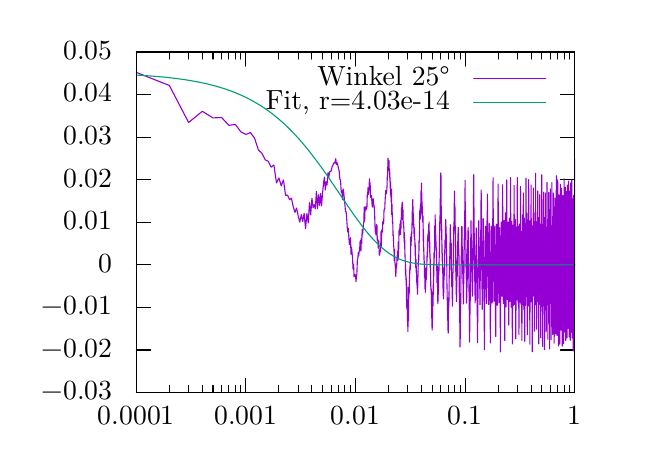
\begin{tikzpicture}[gnuplot]
%% generated with GNUPLOT 5.2p5a (Gentoo revision r0) (Lua 5.1; terminal rev. 99 , script rev. 107)
%% Sa 18 Mai 2019 18:30:38 CEST
\path (0.000,0.000) rectangle (7.500,5.250);
\gpcolor{color=gp lt color border}
\gpsetlinetype{gp lt border}
\gpsetdashtype{gp dt solid}
\gpsetlinewidth{1.00}
\draw[gp path] (1.380,0.616)--(1.560,0.616);
\draw[gp path] (6.947,0.616)--(6.767,0.616);
\node[gp node right] at (1.196,0.616) {$-0.03$};
\draw[gp path] (1.380,1.157)--(1.560,1.157);
\draw[gp path] (6.947,1.157)--(6.767,1.157);
\node[gp node right] at (1.196,1.157) {$-0.02$};
\draw[gp path] (1.380,1.697)--(1.560,1.697);
\draw[gp path] (6.947,1.697)--(6.767,1.697);
\node[gp node right] at (1.196,1.697) {$-0.01$};
\draw[gp path] (1.380,2.238)--(1.560,2.238);
\draw[gp path] (6.947,2.238)--(6.767,2.238);
\node[gp node right] at (1.196,2.238) {$0$};
\draw[gp path] (1.380,2.779)--(1.560,2.779);
\draw[gp path] (6.947,2.779)--(6.767,2.779);
\node[gp node right] at (1.196,2.779) {$0.01$};
\draw[gp path] (1.380,3.319)--(1.560,3.319);
\draw[gp path] (6.947,3.319)--(6.767,3.319);
\node[gp node right] at (1.196,3.319) {$0.02$};
\draw[gp path] (1.380,3.860)--(1.560,3.860);
\draw[gp path] (6.947,3.860)--(6.767,3.860);
\node[gp node right] at (1.196,3.860) {$0.03$};
\draw[gp path] (1.380,4.400)--(1.560,4.400);
\draw[gp path] (6.947,4.400)--(6.767,4.400);
\node[gp node right] at (1.196,4.400) {$0.04$};
\draw[gp path] (1.380,4.941)--(1.560,4.941);
\draw[gp path] (6.947,4.941)--(6.767,4.941);
\node[gp node right] at (1.196,4.941) {$0.05$};
\draw[gp path] (1.380,0.616)--(1.380,0.796);
\draw[gp path] (1.380,4.941)--(1.380,4.761);
\node[gp node center] at (1.380,0.308) {$0.0001$};
\draw[gp path] (1.799,0.616)--(1.799,0.706);
\draw[gp path] (1.799,4.941)--(1.799,4.851);
\draw[gp path] (2.044,0.616)--(2.044,0.706);
\draw[gp path] (2.044,4.941)--(2.044,4.851);
\draw[gp path] (2.218,0.616)--(2.218,0.706);
\draw[gp path] (2.218,4.941)--(2.218,4.851);
\draw[gp path] (2.353,0.616)--(2.353,0.706);
\draw[gp path] (2.353,4.941)--(2.353,4.851);
\draw[gp path] (2.463,0.616)--(2.463,0.706);
\draw[gp path] (2.463,4.941)--(2.463,4.851);
\draw[gp path] (2.556,0.616)--(2.556,0.706);
\draw[gp path] (2.556,4.941)--(2.556,4.851);
\draw[gp path] (2.637,0.616)--(2.637,0.706);
\draw[gp path] (2.637,4.941)--(2.637,4.851);
\draw[gp path] (2.708,0.616)--(2.708,0.706);
\draw[gp path] (2.708,4.941)--(2.708,4.851);
\draw[gp path] (2.772,0.616)--(2.772,0.796);
\draw[gp path] (2.772,4.941)--(2.772,4.761);
\node[gp node center] at (2.772,0.308) {$0.001$};
\draw[gp path] (3.191,0.616)--(3.191,0.706);
\draw[gp path] (3.191,4.941)--(3.191,4.851);
\draw[gp path] (3.436,0.616)--(3.436,0.706);
\draw[gp path] (3.436,4.941)--(3.436,4.851);
\draw[gp path] (3.610,0.616)--(3.610,0.706);
\draw[gp path] (3.610,4.941)--(3.610,4.851);
\draw[gp path] (3.745,0.616)--(3.745,0.706);
\draw[gp path] (3.745,4.941)--(3.745,4.851);
\draw[gp path] (3.855,0.616)--(3.855,0.706);
\draw[gp path] (3.855,4.941)--(3.855,4.851);
\draw[gp path] (3.948,0.616)--(3.948,0.706);
\draw[gp path] (3.948,4.941)--(3.948,4.851);
\draw[gp path] (4.029,0.616)--(4.029,0.706);
\draw[gp path] (4.029,4.941)--(4.029,4.851);
\draw[gp path] (4.100,0.616)--(4.100,0.706);
\draw[gp path] (4.100,4.941)--(4.100,4.851);
\draw[gp path] (4.163,0.616)--(4.163,0.796);
\draw[gp path] (4.163,4.941)--(4.163,4.761);
\node[gp node center] at (4.163,0.308) {$0.01$};
\draw[gp path] (4.582,0.616)--(4.582,0.706);
\draw[gp path] (4.582,4.941)--(4.582,4.851);
\draw[gp path] (4.828,0.616)--(4.828,0.706);
\draw[gp path] (4.828,4.941)--(4.828,4.851);
\draw[gp path] (5.001,0.616)--(5.001,0.706);
\draw[gp path] (5.001,4.941)--(5.001,4.851);
\draw[gp path] (5.136,0.616)--(5.136,0.706);
\draw[gp path] (5.136,4.941)--(5.136,4.851);
\draw[gp path] (5.246,0.616)--(5.246,0.706);
\draw[gp path] (5.246,4.941)--(5.246,4.851);
\draw[gp path] (5.340,0.616)--(5.340,0.706);
\draw[gp path] (5.340,4.941)--(5.340,4.851);
\draw[gp path] (5.420,0.616)--(5.420,0.706);
\draw[gp path] (5.420,4.941)--(5.420,4.851);
\draw[gp path] (5.492,0.616)--(5.492,0.706);
\draw[gp path] (5.492,4.941)--(5.492,4.851);
\draw[gp path] (5.555,0.616)--(5.555,0.796);
\draw[gp path] (5.555,4.941)--(5.555,4.761);
\node[gp node center] at (5.555,0.308) {$0.1$};
\draw[gp path] (5.974,0.616)--(5.974,0.706);
\draw[gp path] (5.974,4.941)--(5.974,4.851);
\draw[gp path] (6.219,0.616)--(6.219,0.706);
\draw[gp path] (6.219,4.941)--(6.219,4.851);
\draw[gp path] (6.393,0.616)--(6.393,0.706);
\draw[gp path] (6.393,4.941)--(6.393,4.851);
\draw[gp path] (6.528,0.616)--(6.528,0.706);
\draw[gp path] (6.528,4.941)--(6.528,4.851);
\draw[gp path] (6.638,0.616)--(6.638,0.706);
\draw[gp path] (6.638,4.941)--(6.638,4.851);
\draw[gp path] (6.731,0.616)--(6.731,0.706);
\draw[gp path] (6.731,4.941)--(6.731,4.851);
\draw[gp path] (6.812,0.616)--(6.812,0.706);
\draw[gp path] (6.812,4.941)--(6.812,4.851);
\draw[gp path] (6.883,0.616)--(6.883,0.706);
\draw[gp path] (6.883,4.941)--(6.883,4.851);
\draw[gp path] (6.947,0.616)--(6.947,0.796);
\draw[gp path] (6.947,4.941)--(6.947,4.761);
\node[gp node center] at (6.947,0.308) {$1$};
\draw[gp path] (1.380,4.941)--(1.380,0.616)--(6.947,0.616)--(6.947,4.941)--cycle;
\node[gp node right] at (5.479,4.607) {Winkel 25°};
\gpcolor{rgb color={0.580,0.000,0.827}}
\draw[gp path] (5.663,4.607)--(6.579,4.607);
\draw[gp path] (1.380,4.682)--(1.799,4.516)--(2.044,4.046)--(2.218,4.188)--(2.353,4.104)%
  --(2.463,4.109)--(2.556,4.009)--(2.637,4.022)--(2.708,3.926)--(2.772,3.894)--(2.829,3.918)%
  --(2.882,3.846)--(2.930,3.697)--(2.975,3.654)--(3.017,3.571)--(3.056,3.552)--(3.092,3.479)%
  --(3.127,3.505)--(3.160,3.278)--(3.191,3.341)--(3.220,3.241)--(3.248,3.316)--(3.275,3.122)%
  --(3.301,3.121)--(3.326,3.065)--(3.349,3.086)--(3.372,2.979)--(3.394,2.904)--(3.415,2.959)%
  --(3.436,2.858)--(3.456,2.780)--(3.475,2.876)--(3.493,2.789)--(3.511,2.892)--(3.529,2.698)%
  --(3.546,2.890)--(3.563,2.773)--(3.579,3.028)--(3.594,2.871)--(3.610,3.082)--(3.625,2.962)%
  --(3.639,3.002)--(3.653,2.949)--(3.667,3.171)--(3.681,2.952)--(3.694,3.128)--(3.707,2.994)%
  --(3.720,3.143)--(3.732,2.987)--(3.745,3.151)--(3.757,3.267)--(3.768,3.352)--(3.780,3.188)%
  --(3.791,3.293)--(3.802,3.251)--(3.813,3.408)--(3.824,3.346)--(3.834,3.416)--(3.845,3.426)%
  --(3.855,3.431)--(3.865,3.484)--(3.875,3.499)--(3.884,3.523)--(3.894,3.538)--(3.903,3.529)%
  --(3.912,3.585)--(3.921,3.510)--(3.930,3.535)--(3.939,3.501)--(3.948,3.460)--(3.956,3.430)%
  --(3.965,3.323)--(3.973,3.317)--(3.982,3.160)--(3.990,3.179)--(3.998,3.066)--(4.006,3.203)%
  --(4.013,3.162)--(4.021,3.085)--(4.029,3.000)--(4.036,2.915)--(4.044,2.916)--(4.051,2.832)%
  --(4.058,2.720)--(4.065,2.655)--(4.072,2.702)--(4.079,2.586)--(4.086,2.497)--(4.093,2.498)%
  --(4.100,2.583)--(4.106,2.373)--(4.113,2.460)--(4.120,2.385)--(4.126,2.326)--(4.132,2.187)%
  --(4.139,2.246)--(4.145,2.089)--(4.151,2.092)--(4.157,2.114)--(4.164,2.099)--(4.170,2.026)%
  --(4.175,2.090)--(4.181,2.127)--(4.187,2.305)--(4.193,2.315)--(4.199,2.394)--(4.204,2.353)%
  --(4.210,2.407)--(4.216,2.425)--(4.221,2.527)--(4.227,2.547)--(4.232,2.413)--(4.237,2.573)%
  --(4.243,2.511)--(4.248,2.685)--(4.253,2.625)--(4.258,2.677)--(4.264,2.752)--(4.269,2.782)%
  --(4.274,2.974)--(4.279,2.792)--(4.284,2.928)--(4.289,2.938)--(4.294,2.975)--(4.298,2.935)%
  --(4.303,2.979)--(4.308,2.952)--(4.313,3.130)--(4.317,3.105)--(4.322,3.218)--(4.327,3.133)%
  --(4.331,3.156)--(4.336,3.199)--(4.340,3.330)--(4.345,3.244)--(4.349,3.279)--(4.354,3.095)%
  --(4.358,3.095)--(4.363,3.106)--(4.367,3.117)--(4.371,3.044)--(4.375,2.989)--(4.380,2.971)%
  --(4.384,3.049)--(4.388,3.077)--(4.392,3.024)--(4.396,2.995)--(4.400,2.990)--(4.405,2.915)%
  --(4.409,2.802)--(4.413,2.680)--(4.417,2.641)--(4.421,2.687)--(4.424,2.615)--(4.428,2.681)%
  --(4.432,2.750)--(4.436,2.733)--(4.440,2.550)--(4.444,2.547)--(4.448,2.560)--(4.451,2.451)%
  --(4.455,2.495)--(4.459,2.542)--(4.463,2.430)--(4.466,2.359)--(4.470,2.364)--(4.473,2.420)%
  --(4.477,2.404)--(4.481,2.408)--(4.484,2.492)--(4.488,2.664)--(4.491,2.462)--(4.495,2.677)%
  --(4.498,2.638)--(4.502,2.693)--(4.505,2.657)--(4.509,2.786)--(4.512,2.756)--(4.515,2.771)%
  --(4.519,2.757)--(4.522,2.797)--(4.525,2.921)--(4.529,2.943)--(4.532,2.949)--(4.535,2.950)%
  --(4.539,3.047)--(4.542,3.097)--(4.545,3.138)--(4.548,3.183)--(4.551,3.157)--(4.555,3.143)%
  --(4.558,3.158)--(4.561,3.191)--(4.564,3.242)--(4.567,3.354)--(4.570,3.364)--(4.573,3.453)%
  --(4.576,3.592)--(4.579,3.524)--(4.582,3.526)--(4.585,3.563)--(4.588,3.564)--(4.591,3.470)%
  --(4.594,3.395)--(4.597,3.450)--(4.600,3.296)--(4.603,3.353)--(4.606,3.167)--(4.609,3.294)%
  --(4.612,3.099)--(4.615,3.175)--(4.618,3.034)--(4.621,3.197)--(4.623,2.877)--(4.626,3.010)%
  --(4.629,2.920)--(4.632,2.794)--(4.635,2.758)--(4.637,2.786)--(4.640,2.607)--(4.643,2.613)%
  --(4.646,2.565)--(4.648,2.481)--(4.651,2.450)--(4.654,2.384)--(4.656,2.289)--(4.659,2.437)%
  --(4.662,2.295)--(4.664,2.262)--(4.667,2.256)--(4.670,2.200)--(4.672,2.145)--(4.675,2.091)%
  --(4.677,2.134)--(4.680,2.209)--(4.683,2.196)--(4.685,2.261)--(4.688,2.241)--(4.690,2.326)%
  --(4.693,2.340)--(4.695,2.367)--(4.698,2.293)--(4.700,2.416)--(4.703,2.298)--(4.705,2.527)%
  --(4.708,2.316)--(4.710,2.507)--(4.712,2.439)--(4.715,2.665)--(4.717,2.680)--(4.720,2.661)%
  --(4.722,2.616)--(4.725,2.647)--(4.727,2.756)--(4.729,2.739)--(4.732,2.704)--(4.734,2.795)%
  --(4.736,2.624)--(4.739,2.807)--(4.741,2.700)--(4.743,2.838)--(4.746,2.816)--(4.748,2.963)%
  --(4.750,2.864)--(4.753,3.011)--(4.755,2.971)--(4.757,3.034)--(4.759,2.810)--(4.762,2.913)%
  --(4.764,2.845)--(4.766,2.940)--(4.768,2.760)--(4.771,2.788)--(4.773,2.755)--(4.775,2.727)%
  --(4.777,2.710)--(4.779,2.624)--(4.781,2.525)--(4.784,2.649)--(4.786,2.540)--(4.788,2.554)%
  --(4.790,2.400)--(4.792,2.360)--(4.794,2.287)--(4.797,2.289)--(4.799,2.154)--(4.801,2.181)%
  --(4.803,2.051)--(4.805,2.104)--(4.807,1.977)--(4.809,2.058)--(4.811,1.788)--(4.813,1.990)%
  --(4.815,1.676)--(4.817,1.957)--(4.819,1.699)--(4.821,1.797)--(4.823,1.526)--(4.826,1.687)%
  --(4.828,1.389)--(4.830,1.661)--(4.832,1.448)--(4.834,1.712)--(4.836,1.579)--(4.838,1.951)%
  --(4.840,1.815)--(4.841,1.867)--(4.843,1.857)--(4.845,1.987)--(4.847,1.887)--(4.849,2.081)%
  --(4.851,2.098)--(4.853,2.182)--(4.855,2.170)--(4.857,2.255)--(4.859,2.175)--(4.861,2.297)%
  --(4.863,2.410)--(4.865,2.591)--(4.867,2.515)--(4.868,2.593)--(4.870,2.482)--(4.872,2.635)%
  --(4.874,2.565)--(4.876,2.634)--(4.878,2.640)--(4.880,2.762)--(4.881,2.706)--(4.883,2.827)%
  --(4.885,2.928)--(4.887,2.898)--(4.889,2.968)--(4.891,3.067)--(4.892,3.011)--(4.894,2.932)%
  --(4.896,2.794)--(4.898,2.888)--(4.900,2.742)--(4.901,2.827)--(4.903,2.723)--(4.905,2.700)%
  --(4.907,2.628)--(4.908,2.684)--(4.910,2.592)--(4.912,2.708)--(4.914,2.573)--(4.916,2.569)%
  --(4.917,2.532)--(4.919,2.516)--(4.921,2.358)--(4.922,2.490)--(4.924,2.340)--(4.926,2.373)%
  --(4.928,2.203)--(4.929,2.230)--(4.931,2.306)--(4.933,2.144)--(4.934,2.202)--(4.936,2.218)%
  --(4.938,2.141)--(4.939,2.120)--(4.941,2.045)--(4.943,1.981)--(4.944,2.051)--(4.946,1.938)%
  --(4.948,1.996)--(4.949,1.892)--(4.951,1.865)--(4.953,2.035)--(4.954,1.951)--(4.956,2.082)%
  --(4.958,2.109)--(4.959,2.199)--(4.961,2.276)--(4.962,2.275)--(4.964,2.334)--(4.966,2.367)%
  --(4.967,2.287)--(4.969,2.404)--(4.970,2.541)--(4.972,2.518)--(4.974,2.567)--(4.975,2.669)%
  --(4.977,2.587)--(4.978,2.833)--(4.980,2.928)--(4.981,2.842)--(4.983,2.815)--(4.985,2.958)%
  --(4.986,2.827)--(4.988,2.993)--(4.989,2.863)--(4.991,3.017)--(4.992,2.897)--(4.994,3.097)%
  --(4.995,3.168)--(4.997,3.097)--(4.998,3.135)--(5.000,3.230)--(5.001,3.276)--(5.003,3.249)%
  --(5.004,3.147)--(5.006,3.132)--(5.007,3.047)--(5.009,3.008)--(5.010,3.017)--(5.012,2.844)%
  --(5.013,2.874)--(5.015,2.830)--(5.016,2.784)--(5.018,2.777)--(5.019,2.798)--(5.021,2.860)%
  --(5.022,2.733)--(5.024,2.541)--(5.025,2.689)--(5.027,2.566)--(5.028,2.611)--(5.029,2.409)%
  --(5.031,2.458)--(5.032,2.382)--(5.034,2.298)--(5.035,2.260)--(5.037,2.279)--(5.038,2.286)%
  --(5.039,2.077)--(5.041,2.210)--(5.042,2.076)--(5.044,2.152)--(5.045,1.932)--(5.047,2.029)%
  --(5.048,1.942)--(5.049,2.061)--(5.051,1.889)--(5.052,1.926)--(5.054,2.022)--(5.055,2.005)%
  --(5.056,2.055)--(5.058,2.194)--(5.059,2.089)--(5.060,2.126)--(5.062,2.051)--(5.063,2.175)%
  --(5.064,2.176)--(5.066,2.170)--(5.067,2.209)--(5.069,2.168)--(5.070,2.289)--(5.071,2.285)%
  --(5.073,2.406)--(5.074,2.336)--(5.075,2.393)--(5.077,2.521)--(5.078,2.560)--(5.079,2.408)%
  --(5.081,2.598)--(5.082,2.524)--(5.083,2.573)--(5.085,2.634)--(5.086,2.601)--(5.087,2.548)%
  --(5.089,2.661)--(5.090,2.671)--(5.091,2.631)--(5.092,2.652)--(5.094,2.750)--(5.095,2.715)%
  --(5.096,2.716)--(5.098,2.781)--(5.099,2.707)--(5.100,2.540)--(5.101,2.551)--(5.103,2.553)%
  --(5.104,2.432)--(5.105,2.431)--(5.107,2.394)--(5.108,2.521)--(5.109,2.342)--(5.110,2.325)%
  --(5.112,2.203)--(5.113,2.314)--(5.114,2.177)--(5.115,2.145)--(5.117,2.091)--(5.118,2.063)%
  --(5.119,1.983)--(5.120,1.950)--(5.122,1.948)--(5.123,1.908)--(5.124,1.903)--(5.125,1.867)%
  --(5.127,1.925)--(5.128,1.890)--(5.129,1.746)--(5.130,1.665)--(5.131,1.639)--(5.133,1.522)%
  --(5.134,1.486)--(5.135,1.446)--(5.136,1.490)--(5.137,1.410)--(5.139,1.536)--(5.140,1.538)%
  --(5.141,1.573)--(5.142,1.666)--(5.144,1.773)--(5.145,1.737)--(5.146,1.825)--(5.147,1.714)%
  --(5.148,1.902)--(5.149,1.780)--(5.151,1.982)--(5.152,1.860)--(5.153,1.923)--(5.154,1.950)%
  --(5.155,2.108)--(5.157,2.094)--(5.158,2.301)--(5.159,2.286)--(5.160,2.246)--(5.161,2.393)%
  --(5.162,2.400)--(5.163,2.323)--(5.165,2.437)--(5.166,2.437)--(5.167,2.475)--(5.168,2.423)%
  --(5.169,2.733)--(5.170,2.638)--(5.172,2.636)--(5.173,2.682)--(5.174,2.715)--(5.175,2.874)%
  --(5.176,2.754)--(5.177,2.772)--(5.178,2.749)--(5.179,2.590)--(5.181,2.749)--(5.182,2.466)%
  --(5.183,2.617)--(5.184,2.506)--(5.185,2.537)--(5.186,2.461)--(5.187,2.478)--(5.188,2.414)%
  --(5.189,2.454)--(5.191,2.338)--(5.192,2.457)--(5.193,2.359)--(5.194,2.322)--(5.195,2.162)%
  --(5.196,2.202)--(5.197,2.182)--(5.198,2.153)--(5.199,2.009)--(5.200,2.225)--(5.202,2.069)%
  --(5.203,2.220)--(5.204,1.958)--(5.205,2.059)--(5.206,2.035)--(5.207,1.973)--(5.208,1.770)%
  --(5.209,1.921)--(5.210,1.745)--(5.211,1.817)--(5.212,1.779)--(5.213,1.794)--(5.214,1.918)%
  --(5.215,1.990)--(5.217,1.925)--(5.218,2.113)--(5.219,2.011)--(5.220,2.159)--(5.221,2.209)%
  --(5.222,2.109)--(5.223,2.148)--(5.224,2.273)--(5.225,2.201)--(5.226,2.347)--(5.227,2.328)%
  --(5.228,2.456)--(5.229,2.451)--(5.230,2.504)--(5.231,2.651)--(5.232,2.767)--(5.233,2.786)%
  --(5.234,2.647)--(5.235,2.749)--(5.236,2.862)--(5.237,2.764)--(5.238,2.931)--(5.239,2.771)%
  --(5.240,3.077)--(5.241,2.895)--(5.242,3.226)--(5.243,3.009)--(5.244,3.321)--(5.245,3.222)%
  --(5.246,3.405)--(5.247,3.172)--(5.249,3.371)--(5.250,3.016)--(5.251,3.116)--(5.252,2.892)%
  --(5.253,2.981)--(5.254,2.832)--(5.254,2.811)--(5.255,2.678)--(5.256,2.746)--(5.257,2.643)%
  --(5.258,2.691)--(5.259,2.551)--(5.260,2.652)--(5.261,2.456)--(5.262,2.501)--(5.263,2.284)%
  --(5.264,2.399)--(5.265,2.362)--(5.266,2.373)--(5.267,2.286)--(5.268,2.174)--(5.269,2.195)%
  --(5.270,2.223)--(5.271,2.204)--(5.272,2.134)--(5.273,2.021)--(5.274,2.028)--(5.275,1.940)%
  --(5.276,2.082)--(5.277,1.844)--(5.278,1.949)--(5.279,1.804)--(5.280,1.886)--(5.281,1.814)%
  --(5.282,1.916)--(5.283,1.878)--(5.284,2.062)--(5.285,1.885)--(5.286,2.131)--(5.286,2.018)%
  --(5.287,2.186)--(5.288,2.044)--(5.289,2.095)--(5.290,2.160)--(5.291,2.198)--(5.292,2.101)%
  --(5.293,2.176)--(5.294,2.205)--(5.295,2.308)--(5.296,2.428)--(5.297,2.430)--(5.298,2.385)%
  --(5.299,2.481)--(5.300,2.448)--(5.300,2.553)--(5.301,2.471)--(5.302,2.545)--(5.303,2.536)%
  --(5.304,2.530)--(5.305,2.581)--(5.306,2.637)--(5.307,2.730)--(5.308,2.815)--(5.309,2.801)%
  --(5.310,2.792)--(5.310,2.798)--(5.311,2.766)--(5.312,2.725)--(5.313,2.673)--(5.314,2.589)%
  --(5.315,2.663)--(5.316,2.458)--(5.317,2.509)--(5.318,2.446)--(5.319,2.423)--(5.319,2.420)%
  --(5.320,2.332)--(5.321,2.357)--(5.322,2.335)--(5.323,2.198)--(5.324,2.067)--(5.325,1.930)%
  --(5.326,1.997)--(5.327,1.890)--(5.327,1.896)--(5.328,1.816)--(5.329,1.790)--(5.330,1.788)%
  --(5.331,1.775)--(5.332,1.656)--(5.333,1.799)--(5.334,1.530)--(5.334,1.635)--(5.335,1.543)%
  --(5.336,1.614)--(5.337,1.403)--(5.338,1.420)--(5.339,1.453)--(5.340,1.426)--(5.341,1.372)%
  --(5.341,1.442)--(5.342,1.492)--(5.343,1.588)--(5.344,1.632)--(5.345,1.695)--(5.346,1.695)%
  --(5.347,1.712)--(5.347,1.820)--(5.348,1.790)--(5.349,1.899)--(5.350,1.765)--(5.351,1.867)%
  --(5.352,1.847)--(5.352,2.068)--(5.353,2.052)--(5.354,2.108)--(5.355,2.110)--(5.356,2.222)%
  --(5.357,2.263)--(5.358,2.177)--(5.358,2.296)--(5.359,2.287)--(5.360,2.326)--(5.361,2.350)%
  --(5.362,2.479)--(5.363,2.473)--(5.363,2.519)--(5.364,2.486)--(5.365,2.640)--(5.366,2.556)%
  --(5.367,2.713)--(5.368,2.677)--(5.368,2.748)--(5.369,2.620)--(5.370,2.655)--(5.371,2.645)%
  --(5.372,2.606)--(5.372,2.535)--(5.373,2.446)--(5.374,2.491)--(5.375,2.558)--(5.376,2.423)%
  --(5.377,2.431)--(5.377,2.461)--(5.378,2.408)--(5.379,2.510)--(5.380,2.165)--(5.381,2.314)%
  --(5.381,2.287)--(5.382,2.089)--(5.383,2.147)--(5.384,2.096)--(5.385,2.109)--(5.385,2.078)%
  --(5.386,1.960)--(5.387,2.001)--(5.388,2.019)--(5.389,1.985)--(5.389,2.071)--(5.390,1.967)%
  --(5.391,1.884)--(5.392,1.808)--(5.393,1.812)--(5.393,1.953)--(5.394,1.713)--(5.395,1.854)%
  --(5.396,1.821)--(5.396,1.891)--(5.397,1.902)--(5.398,2.014)--(5.399,1.975)--(5.400,2.003)%
  --(5.400,2.012)--(5.401,2.154)--(5.402,2.194)--(5.403,2.211)--(5.404,2.258)--(5.404,2.269)%
  --(5.405,2.235)--(5.406,2.397)--(5.407,2.411)--(5.407,2.534)--(5.408,2.473)--(5.409,2.559)%
  --(5.410,2.520)--(5.410,2.632)--(5.411,2.701)--(5.412,2.726)--(5.413,2.630)--(5.414,2.784)%
  --(5.414,2.723)--(5.415,2.735)--(5.416,2.809)--(5.417,2.935)--(5.417,2.862)--(5.418,3.020)%
  --(5.419,3.074)--(5.420,3.142)--(5.420,3.175)--(5.421,3.173)--(5.422,3.054)--(5.423,3.158)%
  --(5.423,2.908)--(5.424,3.000)--(5.425,2.918)--(5.426,2.953)--(5.426,2.754)--(5.427,2.968)%
  --(5.428,2.668)--(5.429,2.800)--(5.429,2.759)--(5.430,2.707)--(5.431,2.670)--(5.432,2.665)%
  --(5.432,2.572)--(5.433,2.435)--(5.434,2.317)--(5.435,2.430)--(5.435,2.385)--(5.436,2.315)%
  --(5.437,2.153)--(5.438,2.214)--(5.438,2.216)--(5.439,2.212)--(5.440,2.041)--(5.440,2.126)%
  --(5.441,1.907)--(5.442,2.028)--(5.443,1.876)--(5.443,1.920)--(5.444,1.811)--(5.445,1.772)%
  --(5.446,1.901)--(5.446,1.886)--(5.447,1.900)--(5.448,1.961)--(5.448,1.888)--(5.449,2.017)%
  --(5.450,1.982)--(5.451,2.139)--(5.451,1.985)--(5.452,2.151)--(5.453,2.084)--(5.453,2.137)%
  --(5.454,2.111)--(5.455,2.183)--(5.456,2.096)--(5.456,2.296)--(5.457,2.214)--(5.458,2.516)%
  --(5.458,2.348)--(5.459,2.481)--(5.460,2.422)--(5.461,2.537)--(5.461,2.356)--(5.462,2.473)%
  --(5.463,2.410)--(5.463,2.548)--(5.464,2.440)--(5.465,2.515)--(5.465,2.507)--(5.466,2.683)%
  --(5.467,2.596)--(5.468,2.716)--(5.468,2.657)--(5.469,2.694)--(5.470,2.682)--(5.470,2.697)%
  --(5.471,2.587)--(5.472,2.659)--(5.472,2.542)--(5.473,2.396)--(5.474,2.447)--(5.475,2.436)%
  --(5.475,2.383)--(5.476,2.377)--(5.477,2.390)--(5.477,2.366)--(5.478,2.253)--(5.479,2.239)%
  --(5.479,2.207)--(5.480,2.122)--(5.481,2.020)--(5.481,1.943)--(5.482,1.851)--(5.483,1.931)%
  --(5.483,1.772)--(5.484,1.758)--(5.485,1.732)--(5.485,1.718)--(5.486,1.654)--(5.487,1.725)%
  --(5.488,1.488)--(5.488,1.618)--(5.489,1.356)--(5.490,1.424)--(5.490,1.194)--(5.491,1.460)%
  --(5.492,1.199)--(5.492,1.414)--(5.493,1.295)--(5.494,1.482)--(5.494,1.373)--(5.495,1.479)%
  --(5.496,1.556)--(5.496,1.661)--(5.497,1.614)--(5.498,1.787)--(5.498,1.801)--(5.499,1.728)%
  --(5.500,1.764)--(5.500,1.835)--(5.501,1.900)--(5.502,2.016)--(5.502,1.907)--(5.503,2.229)%
  --(5.504,2.152)--(5.504,2.265)--(5.505,2.278)--(5.506,2.253)--(5.506,2.285)--(5.507,2.337)%
  --(5.507,2.352)--(5.508,2.409)--(5.509,2.436)--(5.509,2.505)--(5.510,2.481)--(5.511,2.724)%
  --(5.511,2.605)--(5.512,2.688)--(5.513,2.545)--(5.513,2.713)--(5.514,2.632)--(5.515,2.644)%
  --(5.515,2.529)--(5.516,2.722)--(5.517,2.395)--(5.517,2.486)--(5.518,2.344)--(5.518,2.450)%
  --(5.519,2.473)--(5.520,2.436)--(5.520,2.337)--(5.521,2.404)--(5.522,2.365)--(5.522,2.435)%
  --(5.523,2.271)--(5.524,2.394)--(5.524,2.367)--(5.525,2.260)--(5.526,2.120)--(5.526,2.205)%
  --(5.527,2.130)--(5.527,2.161)--(5.528,1.999)--(5.529,1.997)--(5.529,2.070)--(5.530,1.937)%
  --(5.531,2.099)--(5.531,1.990)--(5.532,1.876)--(5.532,1.875)--(5.533,1.741)--(5.534,1.913)%
  --(5.534,1.761)--(5.535,1.788)--(5.536,1.747)--(5.536,1.820)--(5.537,1.832)--(5.537,2.035)%
  --(5.538,1.995)--(5.539,2.016)--(5.539,2.090)--(5.540,2.162)--(5.541,2.134)--(5.541,2.231)%
  --(5.542,2.278)--(5.542,2.250)--(5.543,2.313)--(5.544,2.486)--(5.544,2.427)--(5.545,2.578)%
  --(5.546,2.488)--(5.546,2.685)--(5.547,2.634)--(5.547,2.766)--(5.548,2.676)--(5.549,2.861)%
  --(5.549,2.766)--(5.550,2.808)--(5.550,2.771)--(5.551,2.848)--(5.552,3.014)--(5.552,3.076)%
  --(5.553,2.957)--(5.553,3.176)--(5.554,3.165)--(5.555,3.245)--(5.555,3.312)--(5.556,3.216)%
  --(5.556,3.039)--(5.557,3.043)--(5.558,2.942)--(5.558,3.005)--(5.559,2.794)--(5.559,2.847)%
  --(5.560,2.844)--(5.561,2.643)--(5.561,2.872)--(5.562,2.687)--(5.562,2.721)--(5.563,2.638)%
  --(5.564,2.657)--(5.564,2.571)--(5.565,2.482)--(5.565,2.413)--(5.566,2.375)--(5.567,2.310)%
  --(5.567,2.202)--(5.568,2.234)--(5.568,2.225)--(5.569,2.307)--(5.570,2.129)--(5.571,1.991)%
  --(5.571,2.005)--(5.572,2.052)--(5.573,1.947)--(5.573,1.753)--(5.574,1.858)--(5.574,1.836)%
  --(5.575,1.810)--(5.575,1.832)--(5.576,1.820)--(5.577,1.964)--(5.577,1.993)--(5.578,1.935)%
  --(5.578,1.934)--(5.579,1.967)--(5.580,2.122)--(5.580,1.943)--(5.581,2.109)--(5.581,2.021)%
  --(5.582,2.046)--(5.582,2.128)--(5.583,2.180)--(5.584,2.195)--(5.584,2.143)--(5.585,2.265)%
  --(5.585,2.221)--(5.586,2.260)--(5.586,2.380)--(5.587,2.549)--(5.588,2.400)--(5.588,2.464)%
  --(5.589,2.417)--(5.589,2.450)--(5.590,2.397)--(5.590,2.538)--(5.591,2.556)--(5.592,2.680)%
  --(5.592,2.539)--(5.593,2.710)--(5.593,2.494)--(5.594,2.713)--(5.594,2.628)--(5.595,2.670)%
  --(5.596,2.575)--(5.596,2.490)--(5.597,2.422)--(5.597,2.554)--(5.598,2.340)--(5.598,2.414)%
  --(5.599,2.319)--(5.600,2.329)--(5.600,2.217)--(5.601,2.249)--(5.601,2.228)--(5.602,2.252)%
  --(5.602,2.067)--(5.603,2.160)--(5.603,2.013)--(5.604,1.973)--(5.605,1.989)--(5.605,1.900)%
  --(5.606,1.886)--(5.606,1.904)--(5.607,1.848)--(5.607,1.828)--(5.608,1.738)--(5.608,1.672)%
  --(5.609,1.659)--(5.610,1.864)--(5.610,1.510)--(5.611,1.388)--(5.611,1.417)--(5.612,1.347)%
  --(5.612,1.257)--(5.613,1.387)--(5.613,1.370)--(5.614,1.545)--(5.615,1.387)--(5.615,1.639)%
  --(5.616,1.541)--(5.616,1.637)--(5.617,1.627)--(5.617,1.639)--(5.618,1.611)--(5.618,1.705)%
  --(5.619,1.615)--(5.619,1.930)--(5.620,1.777)--(5.621,1.883)--(5.621,1.910)--(5.622,2.095)%
  --(5.622,1.943)--(5.623,2.137)--(5.623,2.164)--(5.624,2.253)--(5.624,2.256)--(5.625,2.280)%
  --(5.625,2.396)--(5.626,2.440)--(5.626,2.449)--(5.627,2.585)--(5.628,2.475)--(5.628,2.581)%
  --(5.629,2.628)--(5.629,2.728)--(5.630,2.715)--(5.630,2.800)--(5.631,2.686)--(5.631,2.687)%
  --(5.632,2.715)--(5.632,2.575)--(5.633,2.629)--(5.633,2.507)--(5.634,2.620)--(5.634,2.586)%
  --(5.635,2.430)--(5.636,2.486)--(5.636,2.485)--(5.637,2.392)--(5.637,2.335)--(5.638,2.547)%
  --(5.638,2.382)--(5.639,2.374)--(5.639,2.275)--(5.640,2.409)--(5.640,2.145)--(5.641,2.259)%
  --(5.641,2.025)--(5.642,2.193)--(5.642,2.108)--(5.643,2.261)--(5.643,2.154)--(5.644,2.149)%
  --(5.644,2.029)--(5.645,2.134)--(5.645,1.892)--(5.646,1.992)--(5.647,1.986)--(5.647,1.892)%
  --(5.648,1.840)--(5.648,1.887)--(5.649,1.903)--(5.649,1.865)--(5.650,1.913)--(5.650,2.057)%
  --(5.651,1.978)--(5.651,2.026)--(5.652,2.017)--(5.652,2.187)--(5.653,2.218)--(5.653,2.222)%
  --(5.654,2.204)--(5.654,2.192)--(5.655,2.314)--(5.655,2.380)--(5.656,2.331)--(5.656,2.450)%
  --(5.657,2.443)--(5.657,2.454)--(5.658,2.565)--(5.658,2.693)--(5.659,2.768)--(5.659,2.780)%
  --(5.660,2.633)--(5.660,2.874)--(5.661,2.740)--(5.661,2.947)--(5.662,2.799)--(5.662,3.133)%
  --(5.663,2.955)--(5.663,3.265)--(5.664,3.043)--(5.664,3.267)--(5.665,3.155)--(5.665,3.384)%
  --(5.666,3.074)--(5.666,3.318)--(5.667,2.987)--(5.667,3.079)--(5.668,2.766)--(5.668,2.968)%
  --(5.669,2.812)--(5.669,2.702)--(5.670,2.664)--(5.670,2.806)--(5.671,2.568)--(5.671,2.640)%
  --(5.672,2.488)--(5.672,2.622)--(5.673,2.436)--(5.673,2.459)--(5.674,2.352)--(5.674,2.311)%
  --(5.675,2.331)--(5.675,2.192)--(5.676,2.152)--(5.676,2.203)--(5.677,2.183)--(5.677,2.039)%
  --(5.678,2.045)--(5.678,2.029)--(5.679,2.054)--(5.679,2.053)--(5.680,1.929)--(5.680,1.912)%
  --(5.681,1.864)--(5.681,1.904)--(5.682,1.819)--(5.682,1.850)--(5.683,1.755)--(5.683,1.959)%
  --(5.684,1.782)--(5.684,2.045)--(5.685,2.001)--(5.685,2.117)--(5.686,1.980)--(5.686,2.078)%
  --(5.687,2.008)--(5.687,2.157)--(5.688,2.061)--(5.688,2.091)--(5.689,2.044)--(5.689,2.163)%
  --(5.690,2.250)--(5.690,2.311)--(5.691,2.263)--(5.691,2.311)--(5.692,2.361)--(5.692,2.460)%
  --(5.693,2.355)--(5.693,2.466)--(5.693,2.412)--(5.694,2.495)--(5.694,2.372)--(5.695,2.460)%
  --(5.695,2.494)--(5.696,2.604)--(5.696,2.642)--(5.697,2.707)--(5.697,2.694)--(5.698,2.639)%
  --(5.698,2.705)--(5.699,2.653)--(5.699,2.591)--(5.700,2.669)--(5.700,2.486)--(5.701,2.448)%
  --(5.701,2.427)--(5.702,2.387)--(5.702,2.309)--(5.703,2.295)--(5.703,2.311)--(5.704,2.149)%
  --(5.704,2.229)--(5.704,2.124)--(5.705,2.140)--(5.705,2.028)--(5.706,2.031)--(5.706,1.946)%
  --(5.707,1.890)--(5.707,1.793)--(5.708,1.740)--(5.708,1.784)--(5.709,1.707)--(5.709,1.768)%
  --(5.710,1.614)--(5.710,1.587)--(5.711,1.597)--(5.711,1.655)--(5.712,1.590)--(5.712,1.467)%
  --(5.712,1.461)--(5.713,1.394)--(5.713,1.356)--(5.714,1.432)--(5.714,1.250)--(5.715,1.382)%
  --(5.715,1.492)--(5.716,1.571)--(5.716,1.559)--(5.717,1.670)--(5.717,1.658)--(5.718,1.713)%
  --(5.718,1.771)--(5.718,1.814)--(5.719,1.812)--(5.719,1.866)--(5.720,1.831)--(5.720,1.862)%
  --(5.721,1.916)--(5.721,2.045)--(5.722,2.088)--(5.722,2.205)--(5.723,2.093)--(5.723,2.228)%
  --(5.724,2.255)--(5.724,2.340)--(5.724,2.283)--(5.725,2.374)--(5.725,2.379)--(5.726,2.404)%
  --(5.726,2.488)--(5.727,2.576)--(5.727,2.571)--(5.728,2.630)--(5.728,2.671)--(5.729,2.798)%
  --(5.729,2.700)--(5.729,2.788)--(5.730,2.683)--(5.730,2.609)--(5.731,2.697)--(5.731,2.595)%
  --(5.732,2.544)--(5.732,2.571)--(5.733,2.579)--(5.733,2.476)--(5.733,2.444)--(5.734,2.581)%
  --(5.734,2.422)--(5.735,2.397)--(5.735,2.303)--(5.736,2.335)--(5.736,2.230)--(5.737,2.130)%
  --(5.737,2.135)--(5.738,2.134)--(5.738,2.144)--(5.738,2.074)--(5.739,2.154)--(5.739,2.003)%
  --(5.740,1.988)--(5.740,2.007)--(5.741,2.086)--(5.741,1.968)--(5.742,1.934)--(5.742,1.771)%
  --(5.742,1.919)--(5.743,1.744)--(5.743,1.890)--(5.744,1.829)--(5.744,1.876)--(5.745,1.731)%
  --(5.745,1.851)--(5.746,1.901)--(5.746,2.032)--(5.746,1.957)--(5.747,2.105)--(5.747,2.036)%
  --(5.748,2.132)--(5.748,2.167)--(5.749,2.147)--(5.749,2.126)--(5.749,2.236)--(5.750,2.290)%
  --(5.750,2.331)--(5.751,2.307)--(5.751,2.473)--(5.752,2.318)--(5.752,2.541)--(5.753,2.508)%
  --(5.753,2.564)--(5.753,2.599)--(5.754,2.631)--(5.754,2.632)--(5.755,2.709)--(5.755,2.770)%
  --(5.756,2.794)--(5.756,2.874)--(5.756,2.938)--(5.757,3.031)--(5.757,3.032)--(5.758,3.061)%
  --(5.758,3.113)--(5.759,3.188)--(5.759,3.155)--(5.759,3.065)--(5.760,3.108)--(5.760,2.901)%
  --(5.761,3.152)--(5.761,2.911)--(5.762,2.905)--(5.762,2.711)--(5.762,2.822)--(5.763,2.650)%
  --(5.763,2.832)--(5.764,2.612)--(5.764,2.754)--(5.765,2.612)--(5.765,2.463)--(5.765,2.374)%
  --(5.766,2.423)--(5.766,2.356)--(5.767,2.300)--(5.767,2.169)--(5.768,2.264)--(5.768,2.160)%
  --(5.768,2.237)--(5.769,2.068)--(5.769,2.098)--(5.770,1.927)--(5.770,2.042)--(5.771,1.863)%
  --(5.771,1.883)--(5.771,1.753)--(5.772,1.833)--(5.772,1.794)--(5.773,1.691)--(5.773,1.672)%
  --(5.774,1.760)--(5.774,1.854)--(5.774,1.891)--(5.775,1.892)--(5.775,1.877)--(5.776,2.022)%
  --(5.776,2.141)--(5.776,2.020)--(5.777,2.170)--(5.777,1.937)--(5.778,2.126)--(5.778,2.084)%
  --(5.779,2.218)--(5.779,2.206)--(5.779,2.325)--(5.780,2.192)--(5.780,2.353)--(5.781,2.176)%
  --(5.781,2.476)--(5.781,2.344)--(5.782,2.374)--(5.782,2.369)--(5.783,2.541)--(5.783,2.503)%
  --(5.784,2.504)--(5.784,2.387)--(5.784,2.651)--(5.785,2.533)--(5.785,2.636)--(5.786,2.674)%
  --(5.786,2.823)--(5.786,2.680)--(5.787,2.708)--(5.787,2.723)--(5.788,2.628)--(5.788,2.608)%
  --(5.789,2.602)--(5.789,2.402)--(5.789,2.476)--(5.790,2.435)--(5.790,2.445)--(5.791,2.411)%
  --(5.791,2.246)--(5.791,2.255)--(5.792,2.332)--(5.792,2.262)--(5.793,2.234)--(5.793,2.135)%
  --(5.793,2.086)--(5.794,2.055)--(5.794,1.890)--(5.795,1.860)--(5.795,1.901)--(5.795,1.885)%
  --(5.796,1.769)--(5.796,1.691)--(5.797,1.746)--(5.797,1.624)--(5.797,1.652)--(5.798,1.541)%
  --(5.798,1.661)--(5.799,1.399)--(5.799,1.431)--(5.800,1.161)--(5.800,1.540)--(5.800,1.223)%
  --(5.801,1.480)--(5.801,1.386)--(5.802,1.467)--(5.802,1.478)--(5.802,1.624)--(5.803,1.685)%
  --(5.803,1.799)--(5.804,1.727)--(5.804,1.736)--(5.804,1.875)--(5.805,1.815)--(5.805,1.894)%
  --(5.806,1.933)--(5.806,1.937)--(5.806,2.049)--(5.807,1.941)--(5.807,2.087)--(5.808,2.248)%
  --(5.808,2.215)--(5.808,2.339)--(5.809,2.295)--(5.809,2.395)--(5.810,2.347)--(5.810,2.430)%
  --(5.810,2.508)--(5.811,2.547)--(5.811,2.508)--(5.812,2.467)--(5.812,2.548)--(5.812,2.587)%
  --(5.813,2.674)--(5.813,2.572)--(5.813,2.696)--(5.814,2.728)--(5.814,2.661)--(5.815,2.546)%
  --(5.815,2.640)--(5.815,2.426)--(5.816,2.539)--(5.816,2.462)--(5.817,2.510)--(5.817,2.396)%
  --(5.817,2.416)--(5.818,2.447)--(5.818,2.403)--(5.819,2.418)--(5.819,2.480)--(5.819,2.338)%
  --(5.820,2.306)--(5.820,2.205)--(5.821,2.239)--(5.821,2.100)--(5.821,2.166)--(5.822,2.017)%
  --(5.822,2.039)--(5.822,2.049)--(5.823,2.032)--(5.823,2.024)--(5.824,2.070)--(5.824,1.995)%
  --(5.824,1.931)--(5.825,1.920)--(5.825,1.792)--(5.826,1.745)--(5.826,1.818)--(5.826,1.812)%
  --(5.827,1.844)--(5.827,1.838)--(5.828,1.907)--(5.828,1.955)--(5.828,1.920)--(5.829,2.004)%
  --(5.829,2.036)--(5.829,2.107)--(5.830,2.108)--(5.830,2.185)--(5.831,2.090)--(5.831,2.230)%
  --(5.831,2.244)--(5.832,2.358)--(5.832,2.461)--(5.832,2.440)--(5.833,2.572)--(5.833,2.440)%
  --(5.834,2.679)--(5.834,2.614)--(5.834,2.799)--(5.835,2.740)--(5.835,2.749)--(5.836,2.762)%
  --(5.836,2.805)--(5.836,2.707)--(5.837,2.880)--(5.837,2.922)--(5.837,2.924)--(5.838,2.953)%
  --(5.838,2.995)--(5.839,3.096)--(5.839,3.136)--(5.839,3.037)--(5.840,3.015)--(5.840,2.999)%
  --(5.840,2.994)--(5.841,2.918)--(5.841,2.829)--(5.842,2.752)--(5.842,2.787)--(5.842,2.678)%
  --(5.843,2.781)--(5.843,2.639)--(5.843,2.549)--(5.844,2.724)--(5.844,2.670)--(5.845,2.591)%
  --(5.845,2.571)--(5.845,2.514)--(5.846,2.372)--(5.846,2.403)--(5.846,2.326)--(5.847,2.381)%
  --(5.847,2.233)--(5.848,2.216)--(5.848,2.274)--(5.848,2.236)--(5.849,2.024)--(5.849,2.082)%
  --(5.849,2.144)--(5.850,1.926)--(5.850,2.030)--(5.851,1.880)--(5.851,1.847)--(5.851,1.787)%
  --(5.852,1.804)--(5.852,1.841)--(5.852,1.734)--(5.853,1.909)--(5.853,2.012)--(5.854,1.968)%
  --(5.854,1.961)--(5.854,1.903)--(5.855,2.104)--(5.855,2.109)--(5.855,2.145)--(5.856,2.053)%
  --(5.856,2.066)--(5.856,2.173)--(5.857,2.185)--(5.857,2.270)--(5.858,2.291)--(5.858,2.300)%
  --(5.858,2.257)--(5.859,2.446)--(5.859,2.396)--(5.859,2.535)--(5.860,2.537)--(5.860,2.611)%
  --(5.860,2.482)--(5.861,2.511)--(5.861,2.469)--(5.862,2.582)--(5.862,2.533)--(5.862,2.646)%
  --(5.863,2.654)--(5.863,2.609)--(5.863,2.706)--(5.864,2.735)--(5.864,2.600)--(5.864,2.761)%
  --(5.865,2.551)--(5.865,2.643)--(5.866,2.539)--(5.866,2.627)--(5.866,2.392)--(5.867,2.457)%
  --(5.867,2.411)--(5.867,2.391)--(5.868,2.346)--(5.868,2.380)--(5.868,2.277)--(5.869,2.223)%
  --(5.869,2.162)--(5.870,2.153)--(5.870,1.995)--(5.870,1.929)--(5.871,1.891)--(5.871,2.025)%
  --(5.871,1.887)--(5.872,1.783)--(5.872,1.786)--(5.872,1.832)--(5.873,1.745)--(5.873,1.758)%
  --(5.873,1.649)--(5.874,1.641)--(5.874,1.557)--(5.875,1.504)--(5.875,1.439)--(5.875,1.448)%
  --(5.876,1.357)--(5.876,1.386)--(5.876,1.245)--(5.877,1.414)--(5.877,1.366)--(5.877,1.582)%
  --(5.878,1.512)--(5.878,1.678)--(5.878,1.514)--(5.879,1.665)--(5.880,1.743)--(5.880,1.764)%
  --(5.880,1.809)--(5.881,1.712)--(5.881,1.924)--(5.881,1.829)--(5.882,1.925)--(5.882,2.003)%
  --(5.882,2.193)--(5.883,2.256)--(5.883,2.206)--(5.883,2.191)--(5.884,2.396)--(5.884,2.334)%
  --(5.884,2.404)--(5.885,2.394)--(5.885,2.391)--(5.886,2.420)--(5.886,2.505)--(5.886,2.619)%
  --(5.887,2.702)--(5.887,2.684)--(5.887,2.729)--(5.888,2.627)--(5.888,2.634)--(5.888,2.601)%
  --(5.889,2.623)--(5.889,2.662)--(5.889,2.577)--(5.890,2.404)--(5.890,2.564)--(5.890,2.510)%
  --(5.891,2.472)--(5.891,2.437)--(5.891,2.493)--(5.892,2.428)--(5.892,2.366)--(5.892,2.368)%
  --(5.893,2.377)--(5.893,2.190)--(5.893,2.254)--(5.894,2.131)--(5.894,2.222)--(5.895,1.959)%
  --(5.895,2.171)--(5.895,1.949)--(5.896,2.084)--(5.896,2.078)--(5.896,2.105)--(5.897,2.053)%
  --(5.897,2.098)--(5.897,1.848)--(5.898,1.970)--(5.898,1.768)--(5.898,1.808)--(5.899,1.768)%
  --(5.899,1.777)--(5.899,1.754)--(5.900,1.834)--(5.900,1.767)--(5.900,1.862)--(5.901,1.903)%
  --(5.901,1.936)--(5.901,1.952)--(5.902,2.087)--(5.902,2.083)--(5.902,2.191)--(5.903,2.034)%
  --(5.903,2.199)--(5.903,2.255)--(5.904,2.251)--(5.904,2.226)--(5.904,2.386)--(5.905,2.371)%
  --(5.905,2.541)--(5.905,2.443)--(5.906,2.571)--(5.906,2.656)--(5.906,2.827)--(5.907,2.663)%
  --(5.907,2.831)--(5.907,2.716)--(5.908,2.924)--(5.908,2.752)--(5.909,2.988)--(5.909,2.891)%
  --(5.909,3.189)--(5.910,2.948)--(5.910,3.302)--(5.910,3.050)--(5.911,3.342)--(5.911,3.067)%
  --(5.911,3.247)--(5.912,3.036)--(5.912,3.049)--(5.912,2.912)--(5.913,2.949)--(5.913,2.827)%
  --(5.913,2.804)--(5.914,2.637)--(5.914,2.759)--(5.914,2.767)--(5.915,2.623)--(5.915,2.557)%
  --(5.915,2.591)--(5.916,2.470)--(5.916,2.443)--(5.916,2.410)--(5.917,2.452)--(5.917,2.246)%
  --(5.917,2.268)--(5.918,2.180)--(5.918,2.225)--(5.918,2.132)--(5.919,2.190)--(5.919,2.053)%
  --(5.919,2.025)--(5.920,2.046)--(5.920,2.021)--(5.920,1.939)--(5.921,1.958)--(5.921,1.946)%
  --(5.921,1.967)--(5.922,1.774)--(5.922,1.910)--(5.922,1.833)--(5.922,2.003)--(5.923,1.901)%
  --(5.923,2.014)--(5.923,2.068)--(5.924,2.054)--(5.924,2.135)--(5.924,2.171)--(5.925,2.134)%
  --(5.925,2.255)--(5.925,2.135)--(5.926,2.167)--(5.926,2.065)--(5.926,2.300)--(5.927,2.206)%
  --(5.927,2.345)--(5.927,2.364)--(5.928,2.512)--(5.928,2.444)--(5.928,2.502)--(5.929,2.475)%
  --(5.929,2.535)--(5.929,2.410)--(5.930,2.496)--(5.930,2.463)--(5.930,2.549)--(5.931,2.571)%
  --(5.931,2.594)--(5.931,2.647)--(5.932,2.678)--(5.932,2.651)--(5.932,2.702)--(5.933,2.732)%
  --(5.933,2.706)--(5.933,2.635)--(5.934,2.694)--(5.934,2.600)--(5.934,2.546)--(5.935,2.373)%
  --(5.935,2.416)--(5.935,2.352)--(5.936,2.315)--(5.936,2.252)--(5.936,2.132)--(5.936,2.203)%
  --(5.937,2.162)--(5.937,1.986)--(5.937,2.017)--(5.938,1.905)--(5.938,2.057)--(5.938,1.835)%
  --(5.939,1.853)--(5.939,1.723)--(5.939,1.806)--(5.940,1.667)--(5.940,1.803)--(5.940,1.596)%
  --(5.941,1.793)--(5.941,1.602)--(5.941,1.576)--(5.942,1.516)--(5.942,1.541)--(5.942,1.425)%
  --(5.943,1.354)--(5.943,1.417)--(5.943,1.414)--(5.944,1.327)--(5.944,1.544)--(5.944,1.562)%
  --(5.944,1.559)--(5.945,1.646)--(5.945,1.654)--(5.945,1.747)--(5.946,1.775)--(5.946,1.680)%
  --(5.946,1.768)--(5.947,1.854)--(5.947,1.849)--(5.947,1.920)--(5.948,1.867)--(5.948,2.096)%
  --(5.948,1.986)--(5.949,2.084)--(5.949,2.163)--(5.950,2.209)--(5.950,2.205)--(5.950,2.363)%
  --(5.950,2.342)--(5.951,2.389)--(5.951,2.313)--(5.951,2.460)--(5.952,2.451)--(5.952,2.610)%
  --(5.952,2.530)--(5.953,2.556)--(5.953,2.629)--(5.953,2.719)--(5.954,2.754)--(5.954,2.553)%
  --(5.954,2.636)--(5.955,2.712)--(5.955,2.564)--(5.955,2.540)--(5.956,2.507)--(5.956,2.530)%
  --(5.956,2.440)--(5.957,2.447)--(5.957,2.422)--(5.957,2.409)--(5.958,2.416)--(5.958,2.344)%
  --(5.958,2.314)--(5.959,2.294)--(5.959,2.155)--(5.959,2.221)--(5.960,2.115)--(5.960,2.167)%
  --(5.960,2.019)--(5.960,2.008)--(5.961,2.026)--(5.961,2.016)--(5.961,1.969)--(5.962,2.053)%
  --(5.962,2.026)--(5.962,1.963)--(5.963,1.780)--(5.963,1.888)--(5.963,1.775)--(5.964,1.924)%
  --(5.964,1.723)--(5.964,1.821)--(5.964,1.885)--(5.965,1.974)--(5.965,1.969)--(5.965,1.958)%
  --(5.966,1.986)--(5.966,1.976)--(5.966,1.921)--(5.967,2.166)--(5.967,2.142)--(5.967,2.189)%
  --(5.968,2.220)--(5.968,2.176)--(5.968,2.196)--(5.968,2.376)--(5.969,2.452)--(5.969,2.457)%
  --(5.969,2.636)--(5.970,2.552)--(5.970,2.563)--(5.970,2.630)--(5.971,2.691)--(5.971,2.791)%
  --(5.971,2.742)--(5.971,2.791)--(5.972,2.772)--(5.972,2.927)--(5.972,2.821)--(5.973,2.917)%
  --(5.973,3.014)--(5.973,3.088)--(5.974,3.025)--(5.974,3.224)--(5.974,3.209)--(5.975,3.264)%
  --(5.975,3.126)--(5.975,3.146)--(5.975,3.015)--(5.976,3.045)--(5.976,2.926)--(5.976,2.985)%
  --(5.977,2.807)--(5.977,2.878)--(5.977,2.715)--(5.978,2.788)--(5.978,2.690)--(5.978,2.683)%
  --(5.978,2.677)--(5.979,2.659)--(5.979,2.507)--(5.979,2.452)--(5.980,2.358)--(5.980,2.373)%
  --(5.980,2.353)--(5.981,2.148)--(5.981,2.101)--(5.981,2.184)--(5.981,2.099)--(5.982,2.065)%
  --(5.982,2.013)--(5.982,1.930)--(5.983,1.933)--(5.983,1.889)--(5.983,1.870)--(5.984,1.932)%
  --(5.984,1.782)--(5.984,1.756)--(5.984,1.802)--(5.985,1.810)--(5.985,1.872)--(5.985,1.951)%
  --(5.986,1.929)--(5.986,2.011)--(5.986,1.924)--(5.986,2.101)--(5.987,2.013)--(5.987,2.182)%
  --(5.987,2.030)--(5.988,2.122)--(5.988,2.008)--(5.988,2.218)--(5.989,2.216)--(5.989,2.309)%
  --(5.989,2.239)--(5.989,2.277)--(5.990,2.319)--(5.990,2.443)--(5.990,2.363)--(5.991,2.410)%
  --(5.991,2.287)--(5.991,2.469)--(5.991,2.321)--(5.992,2.518)--(5.992,2.490)--(5.992,2.525)%
  --(5.993,2.584)--(5.993,2.690)--(5.993,2.630)--(5.994,2.711)--(5.994,2.659)--(5.994,2.643)%
  --(5.994,2.588)--(5.995,2.613)--(5.995,2.581)--(5.995,2.559)--(5.996,2.450)--(5.996,2.413)%
  --(5.996,2.391)--(5.996,2.443)--(5.997,2.279)--(5.997,2.299)--(5.997,2.174)--(5.998,2.298)%
  --(5.998,2.245)--(5.998,2.207)--(5.998,2.054)--(5.999,2.058)--(5.999,1.921)--(5.999,1.858)%
  --(6.000,1.882)--(6.000,1.816)--(6.000,1.793)--(6.001,1.745)--(6.001,1.612)--(6.001,1.718)%
  --(6.001,1.542)--(6.002,1.612)--(6.002,1.437)--(6.002,1.548)--(6.003,1.272)--(6.003,1.467)%
  --(6.003,1.133)--(6.003,1.316)--(6.004,1.254)--(6.004,1.487)--(6.004,1.353)--(6.005,1.473)%
  --(6.005,1.464)--(6.005,1.622)--(6.005,1.623)--(6.006,1.653)--(6.006,1.677)--(6.006,1.859)%
  --(6.007,1.735)--(6.007,1.935)--(6.007,1.856)--(6.007,1.850)--(6.008,1.872)--(6.008,2.091)%
  --(6.008,2.051)--(6.009,2.147)--(6.009,2.184)--(6.009,2.339)--(6.009,2.305)--(6.010,2.303)%
  --(6.010,2.254)--(6.010,2.356)--(6.011,2.367)--(6.011,2.389)--(6.011,2.365)--(6.011,2.521)%
  --(6.012,2.539)--(6.012,2.630)--(6.012,2.510)--(6.013,2.606)--(6.013,2.539)--(6.013,2.781)%
  --(6.013,2.546)--(6.014,2.775)--(6.014,2.600)--(6.014,2.629)--(6.015,2.443)--(6.015,2.511)%
  --(6.015,2.369)--(6.015,2.477)--(6.016,2.494)--(6.016,2.401)--(6.016,2.417)--(6.017,2.543)%
  --(6.017,2.351)--(6.017,2.528)--(6.017,2.317)--(6.018,2.280)--(6.018,2.236)--(6.018,2.274)%
  --(6.018,2.151)--(6.019,2.079)--(6.019,2.165)--(6.019,2.107)--(6.020,2.173)--(6.020,2.086)%
  --(6.020,2.020)--(6.020,2.177)--(6.021,2.067)--(6.021,1.949)--(6.021,1.927)--(6.022,1.886)%
  --(6.022,1.874)--(6.022,1.957)--(6.022,1.839)--(6.023,1.986)--(6.023,1.948)--(6.023,2.007)%
  --(6.024,1.957)--(6.024,2.027)--(6.024,2.107)--(6.024,2.108)--(6.025,2.134)--(6.025,2.192)%
  --(6.025,2.224)--(6.025,2.194)--(6.026,2.333)--(6.026,2.360)--(6.026,2.361)--(6.027,2.345)%
  --(6.027,2.485)--(6.027,2.650)--(6.027,2.570)--(6.028,2.596)--(6.028,2.640)--(6.028,2.819)%
  --(6.029,2.696)--(6.029,2.766)--(6.029,2.744)--(6.029,2.811)--(6.030,2.813)--(6.030,2.937)%
  --(6.030,2.839)--(6.030,2.981)--(6.031,3.034)--(6.031,3.005)--(6.031,3.102)--(6.032,3.138)%
  --(6.032,3.255)--(6.032,3.111)--(6.032,2.996)--(6.033,2.974)--(6.033,2.868)--(6.033,2.841)%
  --(6.033,2.739)--(6.034,2.715)--(6.034,2.860)--(6.034,2.742)--(6.035,2.737)--(6.035,2.696)%
  --(6.035,2.658)--(6.035,2.614)--(6.036,2.612)--(6.036,2.569)--(6.036,2.526)--(6.036,2.495)%
  --(6.037,2.528)--(6.037,2.300)--(6.037,2.269)--(6.038,2.238)--(6.038,2.164)--(6.038,2.157)%
  --(6.038,2.201)--(6.039,2.177)--(6.039,2.097)--(6.039,2.021)--(6.039,2.012)--(6.040,1.918)%
  --(6.040,1.887)--(6.040,1.790)--(6.041,1.986)--(6.041,1.847)--(6.041,1.813)--(6.041,1.746)%
  --(6.042,1.852)--(6.042,1.945)--(6.042,1.840)--(6.042,1.906)--(6.043,1.969)--(6.043,1.973)%
  --(6.043,2.087)--(6.044,1.970)--(6.044,2.132)--(6.044,2.091)--(6.044,2.145)--(6.045,2.151)%
  --(6.045,2.357)--(6.045,2.339)--(6.045,2.341)--(6.046,2.409)--(6.046,2.492)--(6.046,2.424)%
  --(6.046,2.481)--(6.047,2.377)--(6.047,2.448)--(6.047,2.445)--(6.048,2.602)--(6.048,2.344)%
  --(6.048,2.506)--(6.048,2.550)--(6.049,2.667)--(6.049,2.579)--(6.049,2.748)--(6.049,2.565)%
  --(6.050,2.800)--(6.050,2.583)--(6.050,2.733)--(6.050,2.526)--(6.051,2.625)--(6.051,2.429)%
  --(6.051,2.569)--(6.052,2.335)--(6.052,2.419)--(6.052,2.230)--(6.052,2.260)--(6.053,2.369)%
  --(6.053,2.352)--(6.053,2.254)--(6.053,2.192)--(6.054,2.242)--(6.054,2.155)--(6.054,2.023)%
  --(6.054,1.951)--(6.055,1.956)--(6.055,1.890)--(6.055,1.819)--(6.056,1.868)--(6.056,1.780)%
  --(6.056,1.821)--(6.056,1.740)--(6.057,1.786)--(6.057,1.665)--(6.057,1.621)--(6.057,1.569)%
  --(6.058,1.429)--(6.058,1.425)--(6.058,1.422)--(6.058,1.283)--(6.059,1.426)--(6.059,1.275)%
  --(6.059,1.542)--(6.059,1.325)--(6.060,1.600)--(6.060,1.474)--(6.060,1.853)--(6.061,1.569)%
  --(6.061,1.860)--(6.061,1.669)--(6.061,1.844)--(6.062,1.721)--(6.062,1.855)--(6.062,1.777)%
  --(6.062,2.025)--(6.063,2.037)--(6.063,2.049)--(6.063,2.169)--(6.063,2.193)--(6.064,2.214)%
  --(6.064,2.367)--(6.064,2.243)--(6.064,2.467)--(6.065,2.366)--(6.065,2.511)--(6.065,2.452)%
  --(6.065,2.527)--(6.066,2.613)--(6.066,2.693)--(6.066,2.718)--(6.067,2.717)--(6.067,2.774)%
  --(6.067,2.899)--(6.067,2.819)--(6.068,2.842)--(6.068,2.723)--(6.068,2.698)--(6.068,2.607)%
  --(6.069,2.621)--(6.069,2.477)--(6.069,2.536)--(6.069,2.439)--(6.070,2.676)--(6.070,2.451)%
  --(6.070,2.330)--(6.071,2.435)--(6.071,2.342)--(6.071,2.410)--(6.071,2.264)--(6.072,2.321)%
  --(6.072,2.117)--(6.072,2.207)--(6.072,2.073)--(6.073,2.243)--(6.073,2.038)--(6.073,2.172)%
  --(6.073,2.107)--(6.074,2.099)--(6.074,1.954)--(6.074,2.033)--(6.075,1.889)--(6.075,1.912)%
  --(6.075,1.883)--(6.075,1.932)--(6.076,1.850)--(6.076,1.797)--(6.076,1.842)--(6.076,1.703)%
  --(6.077,1.872)--(6.077,1.867)--(6.077,1.917)--(6.077,2.010)--(6.078,2.036)--(6.078,2.090)%
  --(6.078,2.057)--(6.078,2.212)--(6.079,2.166)--(6.079,2.279)--(6.079,2.282)--(6.080,2.342)%
  --(6.080,2.385)--(6.080,2.377)--(6.080,2.486)--(6.081,2.525)--(6.081,2.805)--(6.081,2.549)%
  --(6.081,2.856)--(6.082,2.871)--(6.082,2.809)--(6.082,2.789)--(6.082,2.926)--(6.083,2.873)%
  --(6.083,3.119)--(6.083,2.960)--(6.083,3.259)--(6.084,3.104)--(6.084,3.316)--(6.084,3.051)%
  --(6.084,3.214)--(6.085,3.078)--(6.085,3.172)--(6.085,3.034)--(6.085,3.037)--(6.086,2.872)%
  --(6.086,2.839)--(6.086,2.794)--(6.086,2.791)--(6.087,2.631)--(6.087,2.679)--(6.087,2.719)%
  --(6.087,2.679)--(6.088,2.613)--(6.088,2.587)--(6.088,2.462)--(6.088,2.498)--(6.089,2.332)%
  --(6.089,2.325)--(6.089,2.210)--(6.089,2.376)--(6.090,2.164)--(6.090,2.214)--(6.090,2.047)%
  --(6.090,2.173)--(6.091,2.080)--(6.091,1.996)--(6.091,2.034)--(6.091,2.075)--(6.092,1.857)%
  --(6.092,1.840)--(6.092,1.797)--(6.092,1.910)--(6.093,1.831)--(6.093,1.961)--(6.093,1.824)%
  --(6.093,1.951)--(6.094,1.967)--(6.094,2.094)--(6.094,2.029)--(6.094,2.037)--(6.095,2.009)%
  --(6.095,2.083)--(6.095,2.033)--(6.095,2.084)--(6.096,2.112)--(6.096,2.131)--(6.096,2.106)%
  --(6.096,2.175)--(6.097,2.264)--(6.097,2.279)--(6.097,2.335)--(6.097,2.439)--(6.098,2.432)%
  --(6.098,2.555)--(6.098,2.397)--(6.098,2.518)--(6.099,2.407)--(6.099,2.532)--(6.099,2.541)%
  --(6.099,2.496)--(6.100,2.624)--(6.100,2.615)--(6.100,2.738)--(6.101,2.781)--(6.101,2.627)%
  --(6.101,2.649)--(6.101,2.685)--(6.102,2.665)--(6.102,2.577)--(6.102,2.538)--(6.102,2.499)%
  --(6.103,2.474)--(6.103,2.377)--(6.103,2.340)--(6.103,2.305)--(6.103,2.241)--(6.104,2.336)%
  --(6.104,2.275)--(6.104,2.181)--(6.104,2.176)--(6.105,2.122)--(6.105,1.975)--(6.105,1.990)%
  --(6.105,1.916)--(6.106,1.958)--(6.106,1.785)--(6.106,1.879)--(6.106,1.767)--(6.107,1.807)%
  --(6.107,1.735)--(6.107,1.697)--(6.108,1.761)--(6.108,1.544)--(6.108,1.524)--(6.108,1.492)%
  --(6.109,1.475)--(6.109,1.488)--(6.109,1.494)--(6.109,1.533)--(6.110,1.554)--(6.110,1.473)%
  --(6.110,1.642)--(6.110,1.687)--(6.111,1.806)--(6.111,1.891)--(6.111,1.745)--(6.111,1.876)%
  --(6.111,1.859)--(6.112,1.912)--(6.112,1.856)--(6.112,1.988)--(6.112,1.895)--(6.113,2.014)%
  --(6.113,2.028)--(6.113,2.207)--(6.113,2.238)--(6.114,2.173)--(6.114,2.293)--(6.114,2.108)%
  --(6.114,2.252)--(6.115,2.361)--(6.115,2.416)--(6.115,2.412)--(6.115,2.593)--(6.116,2.451)%
  --(6.116,2.590)--(6.116,2.581)--(6.116,2.688)--(6.117,2.828)--(6.117,2.632)--(6.117,2.663)%
  --(6.117,2.749)--(6.117,2.701)--(6.118,2.698)--(6.118,2.696)--(6.118,2.547)--(6.118,2.497)%
  --(6.119,2.505)--(6.119,2.561)--(6.119,2.519)--(6.119,2.387)--(6.120,2.434)--(6.120,2.529)%
  --(6.120,2.411)--(6.120,2.389)--(6.121,2.278)--(6.121,2.295)--(6.121,2.192)--(6.121,2.226)%
  --(6.122,2.138)--(6.122,2.095)--(6.122,2.084)--(6.122,2.034)--(6.123,1.984)--(6.123,2.162)%
  --(6.123,2.178)--(6.123,1.982)--(6.124,1.989)--(6.124,1.904)--(6.124,1.967)--(6.124,1.820)%
  --(6.125,1.895)--(6.125,1.773)--(6.125,1.872)--(6.125,1.792)--(6.126,1.951)--(6.126,1.908)%
  --(6.126,1.996)--(6.126,2.010)--(6.126,2.074)--(6.127,2.051)--(6.127,2.088)--(6.127,2.078)%
  --(6.127,2.139)--(6.128,2.300)--(6.128,2.325)--(6.128,2.307)--(6.128,2.447)--(6.129,2.328)%
  --(6.129,2.505)--(6.129,2.590)--(6.129,2.527)--(6.130,2.577)--(6.130,2.684)--(6.130,2.624)%
  --(6.130,2.717)--(6.130,2.747)--(6.131,2.793)--(6.131,2.754)--(6.131,2.953)--(6.131,2.934)%
  --(6.132,3.018)--(6.132,3.034)--(6.132,3.195)--(6.132,3.083)--(6.133,3.174)--(6.133,3.140)%
  --(6.133,3.346)--(6.133,3.067)--(6.133,3.155)--(6.134,2.910)--(6.134,2.926)--(6.134,2.749)%
  --(6.134,2.976)--(6.135,2.699)--(6.135,2.799)--(6.135,2.759)--(6.135,2.787)--(6.136,2.628)%
  --(6.136,2.706)--(6.136,2.534)--(6.136,2.537)--(6.136,2.475)--(6.137,2.333)--(6.137,2.320)%
  --(6.137,2.310)--(6.137,2.094)--(6.138,2.262)--(6.138,2.135)--(6.138,2.173)--(6.138,2.069)%
  --(6.139,2.079)--(6.139,2.105)--(6.139,1.930)--(6.139,1.948)--(6.139,1.928)--(6.140,1.884)%
  --(6.140,1.864)--(6.140,1.768)--(6.140,1.800)--(6.141,1.700)--(6.141,1.877)--(6.141,1.789)%
  --(6.141,1.906)--(6.142,1.906)--(6.142,1.995)--(6.142,1.974)--(6.142,2.058)--(6.142,1.967)%
  --(6.143,2.102)--(6.143,2.057)--(6.143,2.067)--(6.143,2.094)--(6.144,2.216)--(6.144,2.180)%
  --(6.144,2.240)--(6.144,2.308)--(6.145,2.380)--(6.145,2.418)--(6.145,2.482)--(6.145,2.439)%
  --(6.145,2.551)--(6.146,2.488)--(6.146,2.515)--(6.146,2.366)--(6.146,2.533)--(6.147,2.479)%
  --(6.147,2.638)--(6.147,2.614)--(6.147,2.739)--(6.147,2.633)--(6.148,2.702)--(6.148,2.773)%
  --(6.148,2.788)--(6.148,2.664)--(6.149,2.589)--(6.149,2.651)--(6.149,2.519)--(6.149,2.503)%
  --(6.150,2.524)--(6.150,2.449)--(6.150,2.319)--(6.150,2.301)--(6.150,2.460)--(6.151,2.321)%
  --(6.151,2.214)--(6.151,2.180)--(6.151,2.230)--(6.152,2.092)--(6.152,2.050)--(6.152,1.999)%
  --(6.152,1.900)--(6.152,1.780)--(6.153,1.939)--(6.153,1.766)--(6.153,1.712)--(6.153,1.660)%
  --(6.154,1.741)--(6.154,1.560)--(6.154,1.691)--(6.154,1.435)--(6.154,1.691)--(6.155,1.324)%
  --(6.155,1.445)--(6.155,1.234)--(6.155,1.420)--(6.156,1.371)--(6.156,1.438)--(6.156,1.422)%
  --(6.156,1.547)--(6.156,1.592)--(6.157,1.675)--(6.157,1.753)--(6.157,1.782)--(6.157,1.628)%
  --(6.158,1.835)--(6.158,1.813)--(6.158,1.893)--(6.158,1.910)--(6.159,2.021)--(6.159,2.014)%
  --(6.159,1.965)--(6.159,1.998)--(6.159,2.087)--(6.160,2.126)--(6.160,2.273)--(6.160,2.235)%
  --(6.160,2.321)--(6.161,2.418)--(6.161,2.399)--(6.161,2.290)--(6.161,2.391)--(6.161,2.489)%
  --(6.162,2.514)--(6.162,2.488)--(6.162,2.557)--(6.162,2.572)--(6.163,2.633)--(6.163,2.630)%
  --(6.163,2.742)--(6.163,2.506)--(6.163,2.651)--(6.164,2.550)--(6.164,2.556)--(6.164,2.464)%
  --(6.164,2.550)--(6.164,2.469)--(6.165,2.479)--(6.165,2.402)--(6.165,2.456)--(6.165,2.387)%
  --(6.166,2.430)--(6.166,2.359)--(6.166,2.414)--(6.166,2.283)--(6.166,2.332)--(6.167,2.203)%
  --(6.167,2.138)--(6.167,2.082)--(6.167,2.065)--(6.168,2.014)--(6.168,2.038)--(6.168,2.027)%
  --(6.168,2.009)--(6.168,1.959)--(6.169,2.017)--(6.169,1.917)--(6.169,1.947)--(6.169,1.764)%
  --(6.170,1.891)--(6.170,1.923)--(6.170,1.825)--(6.170,1.730)--(6.170,1.724)--(6.171,1.760)%
  --(6.171,1.885)--(6.171,1.786)--(6.171,1.922)--(6.172,2.041)--(6.172,2.086)--(6.172,2.147)%
  --(6.172,2.118)--(6.172,2.165)--(6.173,2.140)--(6.173,2.306)--(6.173,2.307)--(6.173,2.395)%
  --(6.173,2.489)--(6.174,2.273)--(6.174,2.496)--(6.174,2.546)--(6.174,2.672)--(6.175,2.588)%
  --(6.175,2.702)--(6.175,2.673)--(6.175,2.755)--(6.175,2.832)--(6.176,2.849)--(6.176,2.817)%
  --(6.176,2.751)--(6.176,2.883)--(6.177,2.875)--(6.177,2.989)--(6.177,3.125)--(6.177,3.083)%
  --(6.177,3.242)--(6.178,3.247)--(6.178,3.167)--(6.178,3.063)--(6.178,2.885)--(6.178,2.921)%
  --(6.179,2.783)--(6.179,2.798)--(6.179,2.754)--(6.179,2.880)--(6.180,2.723)--(6.180,2.721)%
  --(6.180,2.771)--(6.180,2.705)--(6.180,2.619)--(6.181,2.659)--(6.181,2.498)--(6.181,2.572)%
  --(6.181,2.537)--(6.181,2.436)--(6.182,2.390)--(6.182,2.308)--(6.182,2.350)--(6.182,2.218)%
  --(6.183,2.201)--(6.183,2.284)--(6.183,2.147)--(6.183,2.104)--(6.183,1.953)--(6.184,2.013)%
  --(6.184,1.991)--(6.184,1.911)--(6.184,1.764)--(6.184,1.847)--(6.185,1.956)--(6.185,1.899)%
  --(6.185,1.736)--(6.185,1.871)--(6.186,1.856)--(6.186,1.917)--(6.186,2.001)--(6.186,2.098)%
  --(6.186,2.116)--(6.187,2.058)--(6.187,2.151)--(6.187,2.132)--(6.187,2.124)--(6.187,2.191)%
  --(6.188,2.129)--(6.188,2.250)--(6.188,2.223)--(6.188,2.485)--(6.188,2.323)--(6.189,2.376)%
  --(6.189,2.486)--(6.189,2.483)--(6.189,2.380)--(6.190,2.602)--(6.190,2.418)--(6.190,2.448)%
  --(6.190,2.546)--(6.190,2.547)--(6.191,2.591)--(6.191,2.531)--(6.191,2.562)--(6.191,2.721)%
  --(6.191,2.598)--(6.192,2.674)--(6.192,2.677)--(6.192,2.814)--(6.192,2.645)--(6.193,2.672)%
  --(6.193,2.427)--(6.193,2.576)--(6.193,2.379)--(6.193,2.489)--(6.194,2.333)--(6.194,2.378)%
  --(6.194,2.335)--(6.194,2.380)--(6.194,2.278)--(6.195,2.281)--(6.195,2.113)--(6.195,2.098)%
  --(6.195,2.037)--(6.195,2.030)--(6.196,1.997)--(6.196,1.987)--(6.196,1.868)--(6.196,1.930)%
  --(6.196,1.828)--(6.197,1.799)--(6.197,1.713)--(6.197,1.710)--(6.197,1.615)--(6.198,1.749)%
  --(6.198,1.471)--(6.198,1.530)--(6.198,1.454)--(6.198,1.441)--(6.199,1.381)--(6.199,1.473)%
  --(6.199,1.313)--(6.199,1.464)--(6.199,1.298)--(6.200,1.553)--(6.200,1.493)--(6.200,1.773)%
  --(6.200,1.537)--(6.200,1.735)--(6.201,1.656)--(6.201,1.883)--(6.201,1.704)--(6.201,1.877)%
  --(6.201,1.942)--(6.202,1.993)--(6.202,2.047)--(6.202,2.079)--(6.202,2.086)--(6.203,2.195)%
  --(6.203,2.176)--(6.203,2.304)--(6.203,2.332)--(6.203,2.399)--(6.204,2.317)--(6.204,2.483)%
  --(6.204,2.422)--(6.204,2.460)--(6.204,2.569)--(6.205,2.540)--(6.205,2.639)--(6.205,2.665)%
  --(6.205,2.692)--(6.205,2.716)--(6.206,2.619)--(6.206,2.697)--(6.206,2.656)--(6.206,2.637)%
  --(6.206,2.625)--(6.207,2.554)--(6.207,2.505)--(6.207,2.499)--(6.207,2.371)--(6.207,2.462)%
  --(6.208,2.315)--(6.208,2.501)--(6.208,2.379)--(6.208,2.419)--(6.209,2.419)--(6.209,2.355)%
  --(6.209,2.249)--(6.209,2.227)--(6.209,2.138)--(6.210,2.212)--(6.210,2.108)--(6.210,2.160)%
  --(6.210,2.028)--(6.210,2.286)--(6.211,1.967)--(6.211,2.070)--(6.211,2.013)--(6.211,2.059)%
  --(6.211,1.902)--(6.212,1.812)--(6.212,1.826)--(6.212,1.829)--(6.212,1.797)--(6.212,1.801)%
  --(6.213,1.836)--(6.213,1.800)--(6.213,1.883)--(6.213,1.945)--(6.213,1.885)--(6.214,2.017)%
  --(6.214,2.035)--(6.214,2.053)--(6.214,2.052)--(6.214,2.250)--(6.215,2.142)--(6.215,2.368)%
  --(6.215,2.307)--(6.215,2.315)--(6.215,2.284)--(6.216,2.493)--(6.216,2.522)--(6.216,2.694)%
  --(6.216,2.573)--(6.217,2.696)--(6.217,2.885)--(6.217,2.845)--(6.217,2.915)--(6.217,2.771)%
  --(6.218,2.989)--(6.218,2.877)--(6.218,3.087)--(6.218,2.946)--(6.218,3.256)--(6.219,3.078)%
  --(6.219,3.262)--(6.219,3.187)--(6.219,3.348)--(6.219,3.091)--(6.220,3.059)--(6.220,2.973)%
  --(6.220,3.036)--(6.220,2.893)--(6.220,2.762)--(6.221,2.755)--(6.221,2.788)--(6.221,2.759)%
  --(6.221,2.808)--(6.221,2.709)--(6.222,2.671)--(6.222,2.692)--(6.222,2.618)--(6.222,2.428)%
  --(6.222,2.565)--(6.223,2.274)--(6.223,2.370)--(6.223,2.341)--(6.223,2.250)--(6.223,2.211)%
  --(6.224,2.210)--(6.224,2.207)--(6.224,2.057)--(6.224,2.007)--(6.224,2.109)--(6.225,1.940)%
  --(6.225,1.905)--(6.225,1.938)--(6.225,1.956)--(6.225,1.780)--(6.226,1.913)--(6.226,1.772)%
  --(6.226,1.911)--(6.226,1.867)--(6.226,1.992)--(6.227,1.968)--(6.227,1.974)--(6.227,1.949)%
  --(6.227,2.060)--(6.227,2.101)--(6.228,2.040)--(6.228,2.029)--(6.228,1.986)--(6.228,1.985)%
  --(6.228,2.156)--(6.229,2.172)--(6.229,2.158)--(6.229,2.238)--(6.229,2.367)--(6.229,2.325)%
  --(6.230,2.393)--(6.230,2.355)--(6.230,2.402)--(6.230,2.385)--(6.230,2.429)--(6.231,2.438)%
  --(6.231,2.550)--(6.231,2.510)--(6.231,2.549)--(6.231,2.550)--(6.232,2.689)--(6.232,2.576)%
  --(6.232,2.723)--(6.232,2.640)--(6.232,2.642)--(6.233,2.652)--(6.233,2.691)--(6.233,2.546)%
  --(6.233,2.597)--(6.233,2.492)--(6.234,2.498)--(6.234,2.421)--(6.234,2.329)--(6.234,2.303)%
  --(6.234,2.361)--(6.235,2.328)--(6.235,2.177)--(6.235,2.134)--(6.235,2.174)--(6.235,2.061)%
  --(6.236,2.024)--(6.236,2.156)--(6.236,1.989)--(6.236,1.892)--(6.236,1.957)--(6.237,1.760)%
  --(6.237,1.828)--(6.237,1.718)--(6.237,1.799)--(6.237,1.685)--(6.238,1.712)--(6.238,1.582)%
  --(6.238,1.584)--(6.238,1.469)--(6.238,1.504)--(6.239,1.405)--(6.239,1.417)--(6.239,1.452)%
  --(6.239,1.353)--(6.239,1.354)--(6.239,1.423)--(6.240,1.539)--(6.240,1.610)--(6.240,1.596)%
  --(6.240,1.742)--(6.240,1.655)--(6.241,1.711)--(6.241,1.779)--(6.241,1.698)--(6.241,1.802)%
  --(6.241,1.753)--(6.242,1.874)--(6.242,1.940)--(6.242,2.038)--(6.242,1.925)--(6.242,2.083)%
  --(6.243,2.081)--(6.243,2.176)--(6.243,2.196)--(6.243,2.255)--(6.243,2.324)--(6.244,2.273)%
  --(6.244,2.398)--(6.244,2.406)--(6.244,2.391)--(6.244,2.490)--(6.245,2.417)--(6.245,2.588)%
  --(6.245,2.632)--(6.245,2.694)--(6.245,2.631)--(6.246,2.753)--(6.246,2.698)--(6.246,2.631)%
  --(6.246,2.585)--(6.246,2.676)--(6.246,2.605)--(6.247,2.542)--(6.247,2.465)--(6.247,2.455)%
  --(6.247,2.416)--(6.247,2.480)--(6.248,2.473)--(6.248,2.429)--(6.248,2.318)--(6.248,2.353)%
  --(6.248,2.268)--(6.249,2.300)--(6.249,2.197)--(6.249,2.226)--(6.249,2.117)--(6.249,2.149)%
  --(6.250,2.100)--(6.250,2.090)--(6.250,2.057)--(6.250,2.151)--(6.250,2.108)--(6.250,2.105)%
  --(6.251,2.011)--(6.251,2.061)--(6.251,1.766)--(6.251,2.069)--(6.251,1.827)--(6.252,2.040)%
  --(6.252,1.889)--(6.252,1.968)--(6.252,1.764)--(6.252,1.981)--(6.253,1.946)--(6.253,2.096)%
  --(6.253,1.952)--(6.253,2.014)--(6.253,2.117)--(6.254,1.988)--(6.254,2.166)--(6.254,2.165)%
  --(6.254,2.277)--(6.254,2.280)--(6.255,2.401)--(6.255,2.414)--(6.255,2.291)--(6.255,2.540)%
  --(6.255,2.522)--(6.255,2.551)--(6.256,2.558)--(6.256,2.593)--(6.256,2.576)--(6.256,2.740)%
  --(6.256,2.742)--(6.257,2.731)--(6.257,2.839)--(6.257,2.874)--(6.257,2.829)--(6.257,2.964)%
  --(6.258,3.071)--(6.258,3.139)--(6.258,3.130)--(6.258,3.129)--(6.258,3.186)--(6.258,3.234)%
  --(6.259,2.976)--(6.259,3.114)--(6.259,2.886)--(6.259,3.135)--(6.259,2.710)--(6.260,2.904)%
  --(6.260,2.628)--(6.260,2.820)--(6.260,2.658)--(6.260,2.687)--(6.261,2.633)--(6.261,2.581)%
  --(6.261,2.574)--(6.261,2.540)--(6.261,2.503)--(6.261,2.381)--(6.262,2.398)--(6.262,2.282)%
  --(6.262,2.147)--(6.262,2.210)--(6.262,2.107)--(6.263,2.146)--(6.263,2.003)--(6.263,2.035)%
  --(6.263,2.026)--(6.263,2.020)--(6.264,1.814)--(6.264,1.876)--(6.264,1.801)--(6.264,1.828)%
  --(6.264,1.764)--(6.264,1.739)--(6.265,1.740)--(6.265,1.904)--(6.265,1.808)--(6.265,1.907)%
  --(6.265,1.830)--(6.266,2.088)--(6.266,2.056)--(6.266,2.131)--(6.266,1.879)--(6.266,2.134)%
  --(6.267,1.983)--(6.267,2.155)--(6.267,2.096)--(6.267,2.127)--(6.267,2.160)--(6.267,2.309)%
  --(6.268,2.228)--(6.268,2.386)--(6.268,2.380)--(6.268,2.426)--(6.268,2.392)--(6.269,2.496)%
  --(6.269,2.357)--(6.269,2.473)--(6.269,2.365)--(6.269,2.493)--(6.270,2.472)--(6.270,2.503)%
  --(6.270,2.526)--(6.270,2.596)--(6.270,2.623)--(6.270,2.626)--(6.271,2.647)--(6.271,2.660)%
  --(6.271,2.592)--(6.271,2.594)--(6.271,2.609)--(6.272,2.625)--(6.272,2.398)--(6.272,2.454)%
  --(6.272,2.363)--(6.272,2.396)--(6.272,2.414)--(6.273,2.238)--(6.273,2.159)--(6.273,2.285)%
  --(6.273,2.140)--(6.274,1.911)--(6.274,1.899)--(6.274,1.904)--(6.274,1.862)--(6.274,1.763)%
  --(6.275,1.736)--(6.275,1.754)--(6.275,1.781)--(6.275,1.499)--(6.275,1.795)--(6.275,1.553)%
  --(6.276,1.593)--(6.276,1.503)--(6.276,1.493)--(6.276,1.304)--(6.276,1.440)--(6.277,1.278)%
  --(6.277,1.328)--(6.277,1.321)--(6.277,1.376)--(6.277,1.493)--(6.277,1.476)--(6.278,1.561)%
  --(6.278,1.665)--(6.278,1.684)--(6.278,1.733)--(6.278,1.785)--(6.279,1.904)--(6.279,1.761)%
  --(6.279,1.905)--(6.279,1.902)--(6.279,1.887)--(6.279,1.971)--(6.280,1.992)--(6.280,2.071)%
  --(6.280,2.129)--(6.280,2.275)--(6.280,2.195)--(6.281,2.255)--(6.281,2.366)--(6.281,2.378)%
  --(6.281,2.424)--(6.281,2.483)--(6.281,2.424)--(6.282,2.525)--(6.282,2.601)--(6.282,2.500)%
  --(6.282,2.628)--(6.282,2.563)--(6.283,2.834)--(6.283,2.635)--(6.283,2.872)--(6.283,2.699)%
  --(6.283,2.726)--(6.283,2.522)--(6.284,2.600)--(6.284,2.547)--(6.284,2.464)--(6.284,2.448)%
  --(6.284,2.444)--(6.285,2.522)--(6.285,2.466)--(6.285,2.500)--(6.285,2.528)--(6.285,2.443)%
  --(6.285,2.407)--(6.286,2.306)--(6.286,2.354)--(6.286,2.280)--(6.286,2.209)--(6.286,2.123)%
  --(6.287,2.057)--(6.287,2.041)--(6.287,2.123)--(6.287,2.012)--(6.287,2.016)--(6.287,2.068)%
  --(6.288,1.932)--(6.288,1.952)--(6.288,1.958)--(6.288,1.892)--(6.288,1.849)--(6.289,1.815)%
  --(6.289,1.737)--(6.289,1.766)--(6.289,1.929)--(6.289,1.824)--(6.289,1.894)--(6.290,1.978)%
  --(6.290,1.983)--(6.290,2.034)--(6.290,2.046)--(6.290,2.070)--(6.290,2.082)--(6.291,2.181)%
  --(6.291,2.218)--(6.291,2.278)--(6.291,2.319)--(6.291,2.347)--(6.292,2.381)--(6.292,2.473)%
  --(6.292,2.522)--(6.292,2.455)--(6.292,2.653)--(6.292,2.611)--(6.293,2.710)--(6.293,2.681)%
  --(6.293,2.682)--(6.293,2.772)--(6.293,2.805)--(6.294,2.850)--(6.294,2.791)--(6.294,2.846)%
  --(6.294,2.906)--(6.294,2.985)--(6.294,2.939)--(6.295,3.098)--(6.295,3.151)--(6.295,2.994)%
  --(6.295,3.013)--(6.295,2.952)--(6.295,2.986)--(6.296,2.822)--(6.296,2.887)--(6.296,2.831)%
  --(6.296,2.751)--(6.296,2.735)--(6.297,2.711)--(6.297,2.778)--(6.297,2.615)--(6.297,2.743)%
  --(6.297,2.667)--(6.297,2.674)--(6.298,2.539)--(6.298,2.459)--(6.298,2.457)--(6.298,2.516)%
  --(6.298,2.295)--(6.298,2.250)--(6.299,2.320)--(6.299,2.160)--(6.299,2.146)--(6.299,2.107)%
  --(6.299,2.085)--(6.300,2.050)--(6.300,2.008)--(6.300,2.087)--(6.300,1.831)--(6.300,1.871)%
  --(6.300,1.711)--(6.301,1.744)--(6.301,1.788)--(6.301,1.669)--(6.301,1.776)--(6.301,1.886)%
  --(6.301,1.934)--(6.302,1.901)--(6.302,1.925)--(6.302,2.000)--(6.302,1.954)--(6.302,2.078)%
  --(6.303,2.072)--(6.303,2.131)--(6.303,2.039)--(6.303,2.117)--(6.303,2.058)--(6.303,2.257)%
  --(6.304,2.202)--(6.304,2.269)--(6.304,2.233)--(6.304,2.431)--(6.304,2.364)--(6.304,2.454)%
  --(6.305,2.369)--(6.305,2.487)--(6.305,2.319)--(6.305,2.576)--(6.305,2.419)--(6.306,2.511)%
  --(6.306,2.539)--(6.306,2.703)--(6.306,2.533)--(6.306,2.700)--(6.306,2.563)--(6.307,2.832)%
  --(6.307,2.696)--(6.307,2.685)--(6.307,2.502)--(6.307,2.546)--(6.307,2.372)--(6.308,2.587)%
  --(6.308,2.403)--(6.308,2.383)--(6.308,2.458)--(6.308,2.257)--(6.308,2.322)--(6.309,2.279)%
  --(6.309,2.295)--(6.309,2.119)--(6.309,2.050)--(6.310,1.962)--(6.310,2.032)--(6.310,1.926)%
  --(6.310,1.957)--(6.310,1.844)--(6.310,1.850)--(6.311,1.830)--(6.311,1.849)--(6.311,1.730)%
  --(6.311,1.631)--(6.311,1.504)--(6.311,1.580)--(6.312,1.454)--(6.312,1.417)--(6.312,1.355)%
  --(6.312,1.500)--(6.312,1.283)--(6.312,1.434)--(6.313,1.266)--(6.313,1.555)--(6.313,1.460)%
  --(6.313,1.749)--(6.313,1.487)--(6.313,1.683)--(6.314,1.629)--(6.314,1.755)--(6.314,1.769)%
  --(6.314,1.911)--(6.314,1.785)--(6.315,1.906)--(6.315,1.905)--(6.315,1.945)--(6.315,1.936)%
  --(6.315,2.126)--(6.315,2.179)--(6.316,2.155)--(6.316,2.205)--(6.316,2.332)--(6.316,2.264)%
  --(6.316,2.371)--(6.316,2.362)--(6.317,2.413)--(6.317,2.431)--(6.317,2.473)--(6.317,2.546)%
  --(6.317,2.562)--(6.317,2.564)--(6.318,2.623)--(6.318,2.721)--(6.318,2.628)--(6.318,2.688)%
  --(6.318,2.764)--(6.318,2.677)--(6.319,2.633)--(6.319,2.414)--(6.319,2.606)--(6.319,2.410)%
  --(6.319,2.381)--(6.319,2.385)--(6.320,2.423)--(6.320,2.358)--(6.320,2.371)--(6.320,2.331)%
  --(6.320,2.460)--(6.321,2.208)--(6.321,2.343)--(6.321,2.148)--(6.321,2.252)--(6.321,2.164)%
  --(6.321,2.154)--(6.322,2.036)--(6.322,2.112)--(6.322,1.953)--(6.322,2.035)--(6.322,1.908)%
  --(6.322,2.053)--(6.323,1.864)--(6.323,1.966)--(6.323,1.908)--(6.323,1.909)--(6.323,1.730)%
  --(6.323,1.723)--(6.324,1.821)--(6.324,1.782)--(6.324,1.831)--(6.324,1.725)--(6.324,1.836)%
  --(6.324,1.904)--(6.325,1.985)--(6.325,1.997)--(6.325,2.014)--(6.325,2.068)--(6.325,2.031)%
  --(6.325,2.174)--(6.326,2.199)--(6.326,2.215)--(6.326,2.241)--(6.326,2.410)--(6.326,2.352)%
  --(6.326,2.475)--(6.327,2.503)--(6.327,2.501)--(6.327,2.565)--(6.327,2.709)--(6.327,2.749)%
  --(6.327,2.819)--(6.328,2.635)--(6.328,2.865)--(6.328,2.846)--(6.328,3.066)--(6.328,2.713)%
  --(6.328,3.028)--(6.329,2.918)--(6.329,3.097)--(6.329,2.956)--(6.329,3.338)--(6.329,3.075)%
  --(6.329,3.112)--(6.330,3.029)--(6.330,3.100)--(6.330,2.912)--(6.330,2.913)--(6.330,2.803)%
  --(6.330,2.766)--(6.331,2.710)--(6.331,2.739)--(6.331,2.584)--(6.331,2.717)--(6.331,2.658)%
  --(6.331,2.573)--(6.332,2.642)--(6.332,2.586)--(6.332,2.410)--(6.332,2.423)--(6.332,2.393)%
  --(6.332,2.289)--(6.333,2.200)--(6.333,2.178)--(6.333,2.186)--(6.333,2.176)--(6.333,2.098)%
  --(6.334,2.136)--(6.334,1.980)--(6.334,2.069)--(6.334,1.892)--(6.334,2.063)--(6.334,1.918)%
  --(6.335,1.964)--(6.335,1.837)--(6.335,1.906)--(6.335,1.858)--(6.335,1.873)--(6.335,1.934)%
  --(6.336,1.902)--(6.336,2.043)--(6.336,1.990)--(6.336,2.062)--(6.336,2.122)--(6.336,2.109)%
  --(6.337,2.106)--(6.337,2.082)--(6.337,1.977)--(6.337,2.196)--(6.337,2.187)--(6.337,2.274)%
  --(6.338,2.225)--(6.338,2.285)--(6.338,2.362)--(6.338,2.289)--(6.338,2.464)--(6.338,2.552)%
  --(6.339,2.500)--(6.339,2.569)--(6.339,2.492)--(6.339,2.501)--(6.339,2.570)--(6.339,2.562)%
  --(6.340,2.590)--(6.340,2.690)--(6.340,2.737)--(6.340,2.747)--(6.340,2.837)--(6.340,2.893)%
  --(6.341,2.772)--(6.341,2.677)--(6.341,2.726)--(6.341,2.566)--(6.341,2.549)--(6.341,2.509)%
  --(6.342,2.422)--(6.342,2.405)--(6.342,2.363)--(6.342,2.277)--(6.342,2.389)--(6.342,2.256)%
  --(6.343,2.206)--(6.343,2.064)--(6.343,2.150)--(6.343,2.078)--(6.343,2.015)--(6.343,2.020)%
  --(6.344,1.945)--(6.344,1.946)--(6.344,1.902)--(6.344,1.768)--(6.344,1.755)--(6.344,1.767)%
  --(6.345,1.724)--(6.345,1.783)--(6.345,1.660)--(6.345,1.604)--(6.345,1.571)--(6.345,1.451)%
  --(6.346,1.497)--(6.346,1.439)--(6.346,1.350)--(6.346,1.518)--(6.346,1.473)--(6.346,1.441)%
  --(6.347,1.488)--(6.347,1.630)--(6.347,1.645)--(6.347,1.655)--(6.347,1.873)--(6.347,1.726)%
  --(6.348,1.767)--(6.348,1.789)--(6.348,1.902)--(6.348,1.856)--(6.348,1.931)--(6.348,1.890)%
  --(6.348,2.063)--(6.349,1.992)--(6.349,2.051)--(6.349,2.118)--(6.349,2.140)--(6.349,2.212)%
  --(6.349,2.167)--(6.350,2.271)--(6.350,2.310)--(6.350,2.423)--(6.350,2.369)--(6.350,2.463)%
  --(6.350,2.410)--(6.351,2.668)--(6.351,2.593)--(6.351,2.638)--(6.351,2.744)--(6.351,2.691)%
  --(6.351,2.660)--(6.352,2.606)--(6.352,2.678)--(6.352,2.717)--(6.352,2.632)--(6.352,2.521)%
  --(6.352,2.574)--(6.353,2.478)--(6.353,2.485)--(6.353,2.442)--(6.353,2.451)--(6.353,2.408)%
  --(6.353,2.407)--(6.354,2.289)--(6.354,2.343)--(6.354,2.243)--(6.354,2.311)--(6.354,2.189)%
  --(6.354,2.198)--(6.354,2.092)--(6.355,2.165)--(6.355,2.118)--(6.355,2.132)--(6.355,2.089)%
  --(6.355,2.091)--(6.355,2.006)--(6.356,2.049)--(6.356,2.044)--(6.356,2.073)--(6.356,1.974)%
  --(6.356,1.918)--(6.356,1.821)--(6.357,1.892)--(6.357,1.715)--(6.357,1.908)--(6.357,1.806)%
  --(6.357,1.948)--(6.357,1.824)--(6.358,1.999)--(6.358,1.928)--(6.358,2.159)--(6.358,2.001)%
  --(6.358,2.135)--(6.358,2.157)--(6.358,2.179)--(6.359,2.235)--(6.359,2.271)--(6.359,2.162)%
  --(6.359,2.393)--(6.359,2.454)--(6.359,2.534)--(6.360,2.490)--(6.360,2.528)--(6.360,2.599)%
  --(6.360,2.619)--(6.360,2.750)--(6.360,2.787)--(6.361,2.718)--(6.361,2.902)--(6.361,2.771)%
  --(6.361,2.865)--(6.361,2.976)--(6.361,2.978)--(6.362,3.059)--(6.362,3.320)--(6.362,3.066)%
  --(6.362,3.264)--(6.362,3.007)--(6.362,3.256)--(6.362,2.957)--(6.363,3.206)--(6.363,2.910)%
  --(6.363,3.008)--(6.363,2.772)--(6.363,2.931)--(6.363,2.719)--(6.364,2.920)--(6.364,2.662)%
  --(6.364,2.758)--(6.364,2.668)--(6.364,2.660)--(6.364,2.469)--(6.365,2.544)--(6.365,2.432)%
  --(6.365,2.427)--(6.365,2.300)--(6.365,2.280)--(6.365,2.203)--(6.365,2.327)--(6.366,2.156)%
  --(6.366,2.199)--(6.366,2.132)--(6.366,2.122)--(6.366,2.046)--(6.366,1.870)--(6.367,1.975)%
  --(6.367,1.861)--(6.367,1.795)--(6.367,1.889)--(6.367,1.860)--(6.367,1.915)--(6.368,1.902)%
  --(6.368,1.997)--(6.368,1.810)--(6.368,2.035)--(6.368,2.025)--(6.368,2.196)--(6.368,2.002)%
  --(6.369,2.172)--(6.369,2.010)--(6.369,2.191)--(6.369,2.041)--(6.369,2.238)--(6.369,2.057)%
  --(6.370,2.325)--(6.370,2.183)--(6.370,2.321)--(6.370,2.271)--(6.370,2.447)--(6.370,2.361)%
  --(6.371,2.482)--(6.371,2.361)--(6.371,2.517)--(6.371,2.451)--(6.371,2.519)--(6.371,2.422)%
  --(6.371,2.605)--(6.372,2.607)--(6.372,2.654)--(6.372,2.691)--(6.372,2.670)--(6.372,2.711)%
  --(6.372,2.658)--(6.373,2.608)--(6.373,2.655)--(6.373,2.642)--(6.373,2.617)--(6.373,2.542)%
  --(6.373,2.507)--(6.374,2.443)--(6.374,2.475)--(6.374,2.400)--(6.374,2.376)--(6.374,2.275)%
  --(6.374,2.292)--(6.374,2.214)--(6.375,2.298)--(6.375,2.165)--(6.375,2.124)--(6.375,1.963)%
  --(6.375,2.016)--(6.375,1.902)--(6.376,1.927)--(6.376,1.787)--(6.376,1.900)--(6.376,1.667)%
  --(6.376,1.838)--(6.376,1.572)--(6.376,1.719)--(6.377,1.523)--(6.377,1.601)--(6.377,1.450)%
  --(6.377,1.573)--(6.377,1.436)--(6.377,1.303)--(6.378,1.326)--(6.378,1.436)--(6.378,1.230)%
  --(6.378,1.423)--(6.378,1.502)--(6.378,1.561)--(6.378,1.574)--(6.379,1.749)--(6.379,1.635)%
  --(6.379,1.698)--(6.379,1.744)--(6.379,1.804)--(6.379,1.801)--(6.380,1.927)--(6.380,2.006)%
  --(6.380,1.961)--(6.380,1.912)--(6.380,2.019)--(6.380,2.138)--(6.380,2.163)--(6.381,2.130)%
  --(6.381,2.203)--(6.381,2.271)--(6.381,2.400)--(6.381,2.345)--(6.381,2.465)--(6.382,2.301)%
  --(6.382,2.500)--(6.382,2.392)--(6.382,2.476)--(6.382,2.482)--(6.382,2.632)--(6.382,2.534)%
  --(6.383,2.798)--(6.383,2.591)--(6.383,2.691)--(6.383,2.542)--(6.383,2.651)--(6.383,2.601)%
  --(6.384,2.486)--(6.384,2.460)--(6.384,2.488)--(6.384,2.444)--(6.384,2.467)--(6.384,2.388)%
  --(6.384,2.443)--(6.385,2.427)--(6.385,2.475)--(6.385,2.420)--(6.385,2.472)--(6.385,2.257)%
  --(6.385,2.281)--(6.386,2.250)--(6.386,2.243)--(6.386,2.031)--(6.386,2.118)--(6.386,2.053)%
  --(6.386,2.036)--(6.386,1.985)--(6.387,1.878)--(6.387,1.940)--(6.387,1.916)--(6.387,1.901)%
  --(6.387,1.997)--(6.387,1.974)--(6.388,1.849)--(6.388,1.767)--(6.388,1.807)--(6.388,1.910)%
  --(6.388,1.828)--(6.388,1.849)--(6.388,1.995)--(6.389,1.961)--(6.389,1.917)--(6.389,2.120)%
  --(6.389,2.112)--(6.389,2.148)--(6.389,2.075)--(6.390,2.176)--(6.390,2.308)--(6.390,2.243)%
  --(6.390,2.389)--(6.390,2.457)--(6.390,2.348)--(6.390,2.436)--(6.391,2.530)--(6.391,2.518)%
  --(6.391,2.620)--(6.391,2.572)--(6.391,2.686)--(6.391,2.930)--(6.392,2.861)--(6.392,2.804)%
  --(6.392,2.841)--(6.392,2.695)--(6.392,3.001)--(6.392,2.816)--(6.392,2.866)--(6.393,2.994)%
  --(6.393,3.126)--(6.393,3.141)--(6.393,3.253)--(6.393,3.133)--(6.393,3.220)--(6.393,3.029)%
  --(6.394,3.061)--(6.394,2.972)--(6.394,2.790)--(6.394,2.933)--(6.394,2.749)--(6.394,2.865)%
  --(6.395,2.750)--(6.395,2.830)--(6.395,2.672)--(6.395,2.806)--(6.395,2.626)--(6.395,2.591)%
  --(6.396,2.479)--(6.396,2.402)--(6.396,2.406)--(6.396,2.358)--(6.396,2.286)--(6.396,2.296)%
  --(6.396,2.203)--(6.397,2.207)--(6.397,2.137)--(6.397,2.089)--(6.397,1.905)--(6.397,2.036)%
  --(6.397,2.087)--(6.398,1.848)--(6.398,1.821)--(6.398,1.853)--(6.398,1.773)--(6.398,1.775)%
  --(6.398,1.814)--(6.398,1.807)--(6.399,1.939)--(6.399,1.801)--(6.399,1.904)--(6.399,1.975)%
  --(6.399,1.918)--(6.399,1.928)--(6.399,2.078)--(6.400,1.995)--(6.400,2.171)--(6.400,1.909)%
  --(6.400,2.177)--(6.400,2.056)--(6.400,2.211)--(6.401,2.209)--(6.401,2.317)--(6.401,2.236)%
  --(6.401,2.403)--(6.401,2.398)--(6.401,2.399)--(6.401,2.404)--(6.402,2.433)--(6.402,2.475)%
  --(6.402,2.516)--(6.402,2.431)--(6.402,2.550)--(6.402,2.530)--(6.402,2.695)--(6.403,2.560)%
  --(6.403,2.674)--(6.403,2.603)--(6.403,2.695)--(6.403,2.526)--(6.403,2.735)--(6.404,2.476)%
  --(6.404,2.552)--(6.404,2.500)--(6.404,2.458)--(6.404,2.447)--(6.404,2.283)--(6.404,2.322)%
  --(6.405,2.350)--(6.405,2.271)--(6.405,2.294)--(6.405,2.216)--(6.405,2.211)--(6.405,2.119)%
  --(6.405,2.128)--(6.406,2.049)--(6.406,2.028)--(6.406,1.907)--(6.406,1.966)--(6.406,1.818)%
  --(6.406,1.929)--(6.406,1.757)--(6.407,1.764)--(6.407,1.657)--(6.407,1.663)--(6.407,1.588)%
  --(6.407,1.487)--(6.407,1.449)--(6.408,1.498)--(6.408,1.223)--(6.408,1.397)--(6.408,1.207)%
  --(6.408,1.440)--(6.408,1.132)--(6.408,1.472)--(6.409,1.335)--(6.409,1.609)--(6.409,1.483)%
  --(6.409,1.655)--(6.409,1.532)--(6.409,1.669)--(6.409,1.659)--(6.410,1.828)--(6.410,1.782)%
  --(6.410,1.857)--(6.410,1.964)--(6.410,1.913)--(6.410,1.890)--(6.410,2.042)--(6.411,2.207)%
  --(6.411,2.140)--(6.411,2.177)--(6.411,2.324)--(6.411,2.279)--(6.411,2.399)--(6.411,2.308)%
  --(6.412,2.337)--(6.412,2.452)--(6.412,2.515)--(6.412,2.539)--(6.412,2.593)--(6.412,2.714)%
  --(6.412,2.733)--(6.413,2.720)--(6.413,2.699)--(6.413,2.712)--(6.413,2.646)--(6.413,2.611)%
  --(6.413,2.652)--(6.414,2.496)--(6.414,2.527)--(6.414,2.510)--(6.414,2.413)--(6.414,2.326)%
  --(6.414,2.441)--(6.414,2.404)--(6.415,2.487)--(6.415,2.299)--(6.415,2.501)--(6.415,2.361)%
  --(6.415,2.340)--(6.415,2.304)--(6.415,2.287)--(6.416,2.081)--(6.416,2.135)--(6.416,2.083)%
  --(6.416,2.086)--(6.416,2.126)--(6.416,2.179)--(6.416,2.013)--(6.417,1.988)--(6.417,1.989)%
  --(6.417,2.015)--(6.417,1.934)--(6.417,1.944)--(6.417,1.840)--(6.417,1.885)--(6.418,1.842)%
  --(6.418,1.843)--(6.418,1.880)--(6.418,1.932)--(6.418,1.856)--(6.418,1.952)--(6.418,1.954)%
  --(6.419,2.084)--(6.419,2.055)--(6.419,2.202)--(6.419,2.142)--(6.419,2.219)--(6.419,2.293)%
  --(6.419,2.267)--(6.420,2.303)--(6.420,2.380)--(6.420,2.351)--(6.420,2.508)--(6.420,2.537)%
  --(6.420,2.648)--(6.420,2.689)--(6.421,2.730)--(6.421,2.761)--(6.421,2.861)--(6.421,2.820)%
  --(6.421,2.849)--(6.421,2.827)--(6.422,2.999)--(6.422,2.905)--(6.422,3.033)--(6.422,2.914)%
  --(6.422,3.213)--(6.422,3.019)--(6.422,3.160)--(6.423,3.150)--(6.423,2.976)--(6.423,3.026)%
  --(6.423,3.013)--(6.423,2.932)--(6.423,2.762)--(6.424,2.791)--(6.424,2.765)--(6.424,2.748)%
  --(6.424,2.649)--(6.424,2.751)--(6.424,2.616)--(6.424,2.602)--(6.425,2.538)--(6.425,2.532)%
  --(6.425,2.415)--(6.425,2.257)--(6.425,2.399)--(6.425,2.391)--(6.425,2.241)--(6.426,2.232)%
  --(6.426,2.318)--(6.426,2.164)--(6.426,2.132)--(6.426,2.056)--(6.426,2.043)--(6.426,2.102)%
  --(6.427,1.889)--(6.427,1.986)--(6.427,1.918)--(6.427,1.904)--(6.427,1.881)--(6.427,1.889)%
  --(6.427,1.857)--(6.428,1.937)--(6.428,1.844)--(6.428,1.930)--(6.428,1.926)--(6.428,2.059)%
  --(6.428,1.909)--(6.428,2.057)--(6.429,2.072)--(6.429,2.028)--(6.429,2.083)--(6.429,2.068)%
  --(6.429,1.934)--(6.429,2.194)--(6.429,2.137)--(6.430,2.218)--(6.430,2.285)--(6.430,2.276)%
  --(6.430,2.363)--(6.430,2.415)--(6.430,2.385)--(6.430,2.418)--(6.431,2.411)--(6.431,2.359)%
  --(6.431,2.550)--(6.431,2.484)--(6.431,2.455)--(6.431,2.585)--(6.431,2.565)--(6.432,2.636)%
  --(6.432,2.606)--(6.432,2.626)--(6.432,2.663)--(6.432,2.706)--(6.432,2.695)--(6.432,2.675)%
  --(6.433,2.655)--(6.433,2.544)--(6.433,2.425)--(6.433,2.464)--(6.433,2.520)--(6.433,2.312)%
  --(6.433,2.276)--(6.433,2.228)--(6.434,2.299)--(6.434,2.164)--(6.434,2.187)--(6.434,2.188)%
  --(6.434,2.129)--(6.434,2.083)--(6.434,2.044)--(6.435,1.891)--(6.435,1.904)--(6.435,1.923)%
  --(6.435,1.818)--(6.435,1.915)--(6.435,1.810)--(6.435,1.688)--(6.436,1.737)--(6.436,1.703)%
  --(6.436,1.686)--(6.436,1.723)--(6.436,1.638)--(6.436,1.552)--(6.436,1.396)--(6.437,1.398)%
  --(6.437,1.477)--(6.437,1.498)--(6.437,1.473)--(6.437,1.501)--(6.437,1.643)--(6.437,1.543)%
  --(6.438,1.780)--(6.438,1.679)--(6.438,1.768)--(6.438,1.646)--(6.438,1.837)--(6.438,1.811)%
  --(6.438,1.999)--(6.439,1.833)--(6.439,1.917)--(6.439,1.864)--(6.439,1.989)--(6.439,1.949)%
  --(6.439,2.085)--(6.439,2.051)--(6.440,2.075)--(6.440,2.325)--(6.440,2.381)--(6.440,2.344)%
  --(6.440,2.434)--(6.440,2.490)--(6.440,2.506)--(6.441,2.444)--(6.441,2.641)--(6.441,2.704)%
  --(6.441,2.700)--(6.441,2.655)--(6.441,2.749)--(6.441,2.838)--(6.442,2.901)--(6.442,2.719)%
  --(6.442,2.739)--(6.442,2.650)--(6.442,2.566)--(6.442,2.588)--(6.442,2.556)--(6.442,2.534)%
  --(6.443,2.538)--(6.443,2.573)--(6.443,2.536)--(6.443,2.483)--(6.443,2.583)--(6.443,2.387)%
  --(6.443,2.441)--(6.444,2.398)--(6.444,2.276)--(6.444,2.141)--(6.444,2.200)--(6.444,2.112)%
  --(6.444,2.252)--(6.444,2.070)--(6.445,2.070)--(6.445,2.054)--(6.445,2.107)--(6.445,1.987)%
  --(6.445,2.118)--(6.445,1.989)--(6.445,2.099)--(6.446,1.782)--(6.446,2.024)--(6.446,1.747)%
  --(6.446,1.859)--(6.446,1.749)--(6.446,1.978)--(6.446,1.919)--(6.447,1.879)--(6.447,1.905)%
  --(6.447,2.035)--(6.447,2.041)--(6.447,2.107)--(6.447,2.114)--(6.447,2.194)--(6.448,2.260)%
  --(6.448,2.258)--(6.448,2.220)--(6.448,2.346)--(6.448,2.420)--(6.448,2.457)--(6.448,2.488)%
  --(6.449,2.514)--(6.449,2.612)--(6.449,2.539)--(6.449,2.656)--(6.449,2.629)--(6.449,2.815)%
  --(6.449,2.704)--(6.450,2.968)--(6.450,2.765)--(6.450,3.010)--(6.450,2.823)--(6.450,3.054)%
  --(6.450,3.019)--(6.450,3.246)--(6.451,3.064)--(6.451,3.401)--(6.451,3.042)--(6.451,3.209)%
  --(6.451,2.948)--(6.451,3.129)--(6.451,2.841)--(6.451,3.009)--(6.452,2.874)--(6.452,2.915)%
  --(6.452,2.730)--(6.452,2.739)--(6.452,2.654)--(6.452,2.699)--(6.452,2.559)--(6.453,2.652)%
  --(6.453,2.561)--(6.453,2.620)--(6.453,2.454)--(6.453,2.388)--(6.453,2.279)--(6.453,2.283)%
  --(6.454,2.110)--(6.454,2.187)--(6.454,2.102)--(6.454,2.035)--(6.454,2.074)--(6.454,2.140)%
  --(6.454,1.925)--(6.454,1.981)--(6.455,1.876)--(6.455,1.932)--(6.455,1.768)--(6.455,1.732)%
  --(6.455,1.820)--(6.455,1.804)--(6.455,1.842)--(6.456,1.869)--(6.456,1.816)--(6.456,2.017)%
  --(6.456,2.024)--(6.456,2.083)--(6.456,1.995)--(6.456,2.142)--(6.457,2.115)--(6.457,2.153)%
  --(6.457,2.023)--(6.457,2.150)--(6.457,2.108)--(6.457,2.271)--(6.457,2.221)--(6.457,2.257)%
  --(6.458,2.221)--(6.458,2.326)--(6.458,2.448)--(6.458,2.506)--(6.458,2.369)--(6.458,2.442)%
  --(6.458,2.390)--(6.459,2.538)--(6.459,2.493)--(6.459,2.600)--(6.459,2.525)--(6.459,2.673)%
  --(6.459,2.633)--(6.459,2.735)--(6.460,2.672)--(6.460,2.639)--(6.460,2.699)--(6.460,2.776)%
  --(6.460,2.709)--(6.460,2.690)--(6.460,2.479)--(6.460,2.623)--(6.461,2.460)--(6.461,2.386)%
  --(6.461,2.383)--(6.461,2.390)--(6.461,2.360)--(6.461,2.306)--(6.461,2.273)--(6.462,2.211)%
  --(6.462,2.178)--(6.462,2.148)--(6.462,2.029)--(6.462,1.983)--(6.462,1.891)--(6.462,1.854)%
  --(6.462,1.718)--(6.463,1.746)--(6.463,1.788)--(6.463,1.838)--(6.463,1.735)--(6.463,1.714)%
  --(6.463,1.517)--(6.463,1.797)--(6.464,1.463)--(6.464,1.579)--(6.464,1.435)--(6.464,1.533)%
  --(6.464,1.469)--(6.464,1.463)--(6.464,1.420)--(6.464,1.556)--(6.465,1.654)--(6.465,1.558)%
  --(6.465,1.611)--(6.465,1.756)--(6.465,1.712)--(6.465,1.727)--(6.465,1.866)--(6.466,2.033)%
  --(6.466,1.807)--(6.466,1.881)--(6.466,1.957)--(6.466,2.005)--(6.466,2.069)--(6.466,1.984)%
  --(6.467,2.114)--(6.467,2.135)--(6.467,2.138)--(6.467,2.250)--(6.467,2.333)--(6.467,2.361)%
  --(6.467,2.403)--(6.467,2.396)--(6.468,2.313)--(6.468,2.401)--(6.468,2.396)--(6.468,2.517)%
  --(6.468,2.391)--(6.468,2.664)--(6.468,2.598)--(6.469,2.788)--(6.469,2.603)--(6.469,2.718)%
  --(6.469,2.611)--(6.469,2.697)--(6.469,2.658)--(6.469,2.561)--(6.470,2.511)--(6.470,2.544)%
  --(6.470,2.503)--(6.470,2.420)--(6.470,2.423)--(6.470,2.522)--(6.470,2.349)--(6.471,2.402)%
  --(6.471,2.481)--(6.471,2.363)--(6.471,2.251)--(6.471,2.172)--(6.471,2.232)--(6.471,2.129)%
  --(6.471,2.076)--(6.472,2.120)--(6.472,2.093)--(6.472,2.144)--(6.472,2.073)--(6.472,1.921)%
  --(6.472,2.005)--(6.472,1.911)--(6.472,1.935)--(6.473,1.861)--(6.473,1.858)--(6.473,1.897)%
  --(6.473,1.907)--(6.473,1.919)--(6.473,1.876)--(6.473,1.936)--(6.474,1.879)--(6.474,2.012)%
  --(6.474,1.983)--(6.474,2.093)--(6.474,2.108)--(6.474,2.128)--(6.474,2.056)--(6.474,2.217)%
  --(6.475,2.252)--(6.475,2.293)--(6.475,2.286)--(6.475,2.407)--(6.475,2.406)--(6.475,2.494)%
  --(6.475,2.486)--(6.476,2.504)--(6.476,2.637)--(6.476,2.634)--(6.476,2.668)--(6.476,2.647)%
  --(6.476,2.695)--(6.476,2.846)--(6.476,2.842)--(6.477,2.867)--(6.477,2.899)--(6.477,2.896)%
  --(6.477,2.908)--(6.477,2.912)--(6.477,3.103)--(6.477,3.058)--(6.478,3.043)--(6.478,3.177)%
  --(6.478,3.058)--(6.478,3.102)--(6.478,2.916)--(6.478,2.988)--(6.478,2.816)--(6.478,2.927)%
  --(6.479,2.708)--(6.479,2.857)--(6.479,2.690)--(6.479,2.840)--(6.479,2.666)--(6.479,2.685)%
  --(6.479,2.606)--(6.479,2.561)--(6.480,2.494)--(6.480,2.465)--(6.480,2.388)--(6.480,2.395)%
  --(6.480,2.347)--(6.480,2.360)--(6.480,2.248)--(6.481,2.160)--(6.481,2.220)--(6.481,2.214)%
  --(6.481,1.971)--(6.481,2.049)--(6.481,2.027)--(6.481,1.995)--(6.481,1.860)--(6.482,1.855)%
  --(6.482,1.827)--(6.482,1.771)--(6.482,1.826)--(6.482,1.839)--(6.482,1.801)--(6.482,1.941)%
  --(6.482,1.864)--(6.483,2.015)--(6.483,2.100)--(6.483,2.047)--(6.483,2.082)--(6.483,2.113)%
  --(6.483,2.052)--(6.483,2.172)--(6.484,2.080)--(6.484,2.157)--(6.484,2.161)--(6.484,2.280)%
  --(6.484,2.365)--(6.484,2.374)--(6.484,2.386)--(6.484,2.431)--(6.485,2.367)--(6.485,2.565)%
  --(6.485,2.439)--(6.485,2.527)--(6.485,2.370)--(6.485,2.497)--(6.485,2.607)--(6.485,2.606)%
  --(6.486,2.476)--(6.486,2.702)--(6.486,2.639)--(6.486,2.726)--(6.486,2.703)--(6.486,2.837)%
  --(6.486,2.689)--(6.487,2.770)--(6.487,2.605)--(6.487,2.601)--(6.487,2.573)--(6.487,2.549)%
  --(6.487,2.430)--(6.487,2.495)--(6.487,2.445)--(6.488,2.416)--(6.488,2.250)--(6.488,2.173)%
  --(6.488,2.214)--(6.488,2.179)--(6.488,2.191)--(6.488,2.116)--(6.488,2.014)--(6.489,2.045)%
  --(6.489,1.907)--(6.489,2.010)--(6.489,1.803)--(6.489,1.873)--(6.489,1.726)--(6.489,1.748)%
  --(6.489,1.693)--(6.490,1.686)--(6.490,1.498)--(6.490,1.631)--(6.490,1.300)--(6.490,1.423)%
  --(6.490,1.257)--(6.490,1.478)--(6.491,1.234)--(6.491,1.472)--(6.491,1.262)--(6.491,1.468)%
  --(6.491,1.359)--(6.491,1.603)--(6.491,1.477)--(6.491,1.658)--(6.492,1.647)--(6.492,1.862)%
  --(6.492,1.685)--(6.492,1.877)--(6.492,1.867)--(6.492,1.902)--(6.492,1.914)--(6.492,2.039)%
  --(6.493,1.951)--(6.493,2.108)--(6.493,2.043)--(6.493,2.195)--(6.493,2.275)--(6.493,2.287)%
  --(6.493,2.305)--(6.493,2.309)--(6.494,2.390)--(6.494,2.428)--(6.494,2.386)--(6.494,2.519)%
  --(6.494,2.551)--(6.494,2.532)--(6.494,2.648)--(6.494,2.674)--(6.495,2.603)--(6.495,2.628)%
  --(6.495,2.629)--(6.495,2.689)--(6.495,2.572)--(6.495,2.588)--(6.495,2.561)--(6.496,2.555)%
  --(6.496,2.379)--(6.496,2.457)--(6.496,2.371)--(6.496,2.477)--(6.496,2.311)--(6.496,2.398)%
  --(6.496,2.281)--(6.497,2.468)--(6.497,2.314)--(6.497,2.404)--(6.497,2.121)--(6.497,2.221)%
  --(6.497,2.020)--(6.497,2.151)--(6.497,2.066)--(6.498,2.038)--(6.498,2.039)--(6.498,2.112)%
  --(6.498,1.933)--(6.498,2.027)--(6.498,1.870)--(6.498,1.875)--(6.498,1.937)--(6.499,1.851)%
  --(6.499,1.856)--(6.499,1.859)--(6.499,1.778)--(6.499,1.734)--(6.499,1.896)--(6.499,1.819)%
  --(6.499,1.830)--(6.500,1.873)--(6.500,1.936)--(6.500,1.998)--(6.500,1.931)--(6.500,2.127)%
  --(6.500,2.168)--(6.500,2.077)--(6.501,2.211)--(6.501,2.249)--(6.501,2.298)--(6.501,2.484)%
  --(6.501,2.440)--(6.501,2.532)--(6.501,2.543)--(6.502,2.760)--(6.502,2.657)--(6.502,2.752)%
  --(6.502,2.707)--(6.502,2.789)--(6.502,2.634)--(6.502,3.044)--(6.502,2.945)--(6.503,3.023)%
  --(6.503,2.971)--(6.503,3.105)--(6.503,2.997)--(6.503,3.115)--(6.503,3.034)--(6.503,3.130)%
  --(6.503,3.042)--(6.504,2.983)--(6.504,2.938)--(6.504,2.921)--(6.504,2.878)--(6.504,2.773)%
  --(6.504,2.763)--(6.504,2.700)--(6.504,2.710)--(6.505,2.648)--(6.505,2.672)--(6.505,2.594)%
  --(6.505,2.514)--(6.505,2.436)--(6.505,2.499)--(6.505,2.395)--(6.506,2.383)--(6.506,2.321)%
  --(6.506,2.290)--(6.506,2.268)--(6.506,2.179)--(6.506,2.131)--(6.506,2.152)--(6.507,2.027)%
  --(6.507,2.106)--(6.507,1.976)--(6.507,2.046)--(6.507,1.858)--(6.507,2.016)--(6.507,1.879)%
  --(6.507,1.880)--(6.508,1.924)--(6.508,1.912)--(6.508,1.881)--(6.508,1.895)--(6.508,2.017)%
  --(6.508,2.092)--(6.508,2.009)--(6.508,2.083)--(6.509,1.965)--(6.509,2.093)--(6.509,2.019)%
  --(6.509,2.112)--(6.509,1.994)--(6.509,2.173)--(6.509,2.104)--(6.509,2.267)--(6.510,2.316)%
  --(6.510,2.263)--(6.510,2.348)--(6.510,2.310)--(6.510,2.328)--(6.510,2.362)--(6.510,2.524)%
  --(6.510,2.413)--(6.511,2.527)--(6.511,2.600)--(6.511,2.458)--(6.511,2.526)--(6.511,2.487)%
  --(6.511,2.530)--(6.511,2.650)--(6.511,2.646)--(6.511,2.651)--(6.512,2.653)--(6.512,2.663)%
  --(6.512,2.577)--(6.512,2.598)--(6.512,2.437)--(6.512,2.530)--(6.512,2.316)--(6.512,2.434)%
  --(6.513,2.352)--(6.513,2.363)--(6.513,2.229)--(6.513,2.334)--(6.513,2.090)--(6.513,2.174)%
  --(6.513,2.129)--(6.513,2.027)--(6.514,2.038)--(6.514,1.974)--(6.514,1.947)--(6.514,1.882)%
  --(6.514,1.905)--(6.514,1.792)--(6.514,1.705)--(6.514,1.713)--(6.515,1.754)--(6.515,1.837)%
  --(6.515,1.614)--(6.515,1.663)--(6.515,1.541)--(6.515,1.632)--(6.515,1.342)--(6.515,1.369)%
  --(6.516,1.353)--(6.516,1.407)--(6.516,1.311)--(6.516,1.379)--(6.516,1.400)--(6.516,1.455)%
  --(6.516,1.516)--(6.516,1.646)--(6.517,1.586)--(6.517,1.646)--(6.517,1.625)--(6.517,1.767)%
  --(6.517,1.599)--(6.517,1.854)--(6.517,1.747)--(6.517,1.921)--(6.518,1.862)--(6.518,1.890)%
  --(6.518,1.964)--(6.518,2.034)--(6.518,2.094)--(6.518,2.137)--(6.518,2.324)--(6.518,2.256)%
  --(6.519,2.219)--(6.519,2.249)--(6.519,2.365)--(6.519,2.387)--(6.519,2.446)--(6.519,2.452)%
  --(6.519,2.458)--(6.519,2.654)--(6.520,2.667)--(6.520,2.682)--(6.520,2.694)--(6.520,2.617)%
  --(6.520,2.595)--(6.520,2.755)--(6.520,2.568)--(6.520,2.673)--(6.520,2.527)--(6.521,2.457)%
  --(6.521,2.367)--(6.521,2.437)--(6.521,2.489)--(6.521,2.430)--(6.521,2.305)--(6.521,2.416)%
  --(6.521,2.330)--(6.522,2.370)--(6.522,2.245)--(6.522,2.242)--(6.522,2.147)--(6.522,2.073)%
  --(6.522,2.036)--(6.522,2.125)--(6.522,1.986)--(6.523,1.935)--(6.523,1.993)--(6.523,2.016)%
  --(6.523,1.977)--(6.523,1.990)--(6.523,1.767)--(6.523,1.914)--(6.523,1.903)--(6.524,1.928)%
  --(6.524,1.709)--(6.524,1.867)--(6.524,1.839)--(6.524,1.767)--(6.524,2.001)--(6.524,1.891)%
  --(6.524,1.900)--(6.525,1.932)--(6.525,1.951)--(6.525,2.044)--(6.525,2.084)--(6.525,2.059)%
  --(6.525,2.172)--(6.525,2.179)--(6.525,2.162)--(6.525,2.238)--(6.526,2.331)--(6.526,2.376)%
  --(6.526,2.357)--(6.526,2.467)--(6.526,2.423)--(6.526,2.645)--(6.526,2.606)--(6.526,2.764)%
  --(6.527,2.661)--(6.527,2.794)--(6.527,2.700)--(6.527,2.905)--(6.527,2.736)--(6.527,2.988)%
  --(6.527,2.825)--(6.527,3.167)--(6.528,3.000)--(6.528,3.280)--(6.528,3.174)--(6.528,3.382)%
  --(6.528,3.160)--(6.528,3.323)--(6.528,2.876)--(6.528,3.057)--(6.529,2.946)--(6.529,3.006)%
  --(6.529,2.732)--(6.529,2.707)--(6.529,2.726)--(6.529,2.751)--(6.529,2.616)--(6.529,2.718)%
  --(6.529,2.580)--(6.530,2.620)--(6.530,2.468)--(6.530,2.462)--(6.530,2.359)--(6.530,2.301)%
  --(6.530,2.244)--(6.530,2.276)--(6.530,2.207)--(6.531,2.186)--(6.531,2.161)--(6.531,2.083)%
  --(6.531,2.016)--(6.531,2.028)--(6.531,1.929)--(6.531,1.909)--(6.531,1.877)--(6.532,1.795)%
  --(6.532,1.752)--(6.532,1.832)--(6.532,1.777)--(6.532,1.874)--(6.532,1.739)--(6.532,1.812)%
  --(6.532,1.807)--(6.532,1.941)--(6.533,1.881)--(6.533,1.988)--(6.533,1.896)--(6.533,2.036)%
  --(6.533,1.946)--(6.533,2.096)--(6.533,1.977)--(6.533,2.100)--(6.534,1.976)--(6.534,2.110)%
  --(6.534,2.094)--(6.534,2.365)--(6.534,2.176)--(6.534,2.261)--(6.534,2.242)--(6.534,2.435)%
  --(6.535,2.336)--(6.535,2.558)--(6.535,2.297)--(6.535,2.427)--(6.535,2.422)--(6.535,2.539)%
  --(6.535,2.423)--(6.535,2.557)--(6.535,2.542)--(6.536,2.598)--(6.536,2.582)--(6.536,2.631)%
  --(6.536,2.708)--(6.536,2.751)--(6.536,2.643)--(6.536,2.615)--(6.536,2.476)--(6.537,2.470)%
  --(6.537,2.356)--(6.537,2.406)--(6.537,2.363)--(6.537,2.287)--(6.537,2.276)--(6.537,2.330)%
  --(6.537,2.098)--(6.538,2.120)--(6.538,2.077)--(6.538,2.009)--(6.538,1.920)--(6.538,1.942)%
  --(6.538,1.847)--(6.538,1.804)--(6.538,1.746)--(6.538,1.926)--(6.539,1.605)--(6.539,1.851)%
  --(6.539,1.594)--(6.539,1.660)--(6.539,1.482)--(6.539,1.558)--(6.539,1.452)--(6.539,1.501)%
  --(6.540,1.334)--(6.540,1.355)--(6.540,1.200)--(6.540,1.303)--(6.540,1.351)--(6.540,1.367)%
  --(6.540,1.508)--(6.540,1.421)--(6.540,1.488)--(6.541,1.660)--(6.541,1.632)--(6.541,1.653)%
  --(6.541,1.723)--(6.541,1.760)--(6.541,1.769)--(6.541,1.792)--(6.541,1.756)--(6.542,1.842)%
  --(6.542,1.888)--(6.542,1.994)--(6.542,1.990)--(6.542,2.086)--(6.542,2.091)--(6.542,2.152)%
  --(6.542,2.216)--(6.542,2.165)--(6.543,2.243)--(6.543,2.324)--(6.543,2.273)--(6.543,2.381)%
  --(6.543,2.421)--(6.543,2.459)--(6.543,2.454)--(6.543,2.518)--(6.544,2.573)--(6.544,2.622)%
  --(6.544,2.474)--(6.544,2.630)--(6.544,2.496)--(6.544,2.556)--(6.544,2.550)--(6.544,2.516)%
  --(6.544,2.494)--(6.545,2.477)--(6.545,2.378)--(6.545,2.400)--(6.545,2.261)--(6.545,2.401)%
  --(6.545,2.370)--(6.545,2.374)--(6.545,2.326)--(6.546,2.326)--(6.546,2.308)--(6.546,2.219)%
  --(6.546,2.252)--(6.546,2.082)--(6.546,1.980)--(6.546,2.057)--(6.546,2.116)--(6.546,2.058)%
  --(6.547,2.149)--(6.547,2.034)--(6.547,2.029)--(6.547,1.950)--(6.547,1.984)--(6.547,1.866)%
  --(6.547,1.712)--(6.547,1.904)--(6.548,1.886)--(6.548,1.848)--(6.548,1.810)--(6.548,1.927)%
  --(6.548,1.984)--(6.548,1.948)--(6.548,1.984)--(6.548,1.990)--(6.548,2.080)--(6.549,2.011)%
  --(6.549,2.195)--(6.549,2.121)--(6.549,2.124)--(6.549,2.120)--(6.549,2.305)--(6.549,2.400)%
  --(6.549,2.310)--(6.550,2.445)--(6.550,2.368)--(6.550,2.526)--(6.550,2.508)--(6.550,2.501)%
  --(6.550,2.622)--(6.550,2.520)--(6.550,2.691)--(6.550,2.664)--(6.551,2.705)--(6.551,2.755)%
  --(6.551,2.779)--(6.551,2.721)--(6.551,2.857)--(6.551,2.826)--(6.551,2.995)--(6.551,3.017)%
  --(6.552,3.108)--(6.552,3.161)--(6.552,3.038)--(6.552,3.028)--(6.552,3.000)--(6.552,2.930)%
  --(6.552,2.981)--(6.552,2.851)--(6.552,2.912)--(6.553,2.685)--(6.553,2.838)--(6.553,2.653)%
  --(6.553,2.775)--(6.553,2.537)--(6.553,2.669)--(6.553,2.584)--(6.553,2.511)--(6.553,2.469)%
  --(6.554,2.400)--(6.554,2.318)--(6.554,2.406)--(6.554,2.303)--(6.554,2.227)--(6.554,2.216)%
  --(6.554,2.113)--(6.554,2.104)--(6.555,2.052)--(6.555,2.054)--(6.555,1.992)--(6.555,1.903)%
  --(6.555,1.867)--(6.555,1.953)--(6.555,1.835)--(6.555,1.747)--(6.555,1.852)--(6.556,1.783)%
  --(6.556,1.818)--(6.556,1.828)--(6.556,1.809)--(6.556,1.889)--(6.556,1.994)--(6.556,1.940)%
  --(6.556,2.069)--(6.556,1.984)--(6.557,1.932)--(6.557,1.983)--(6.557,2.050)--(6.557,2.126)%
  --(6.557,2.196)--(6.557,2.258)--(6.557,2.190)--(6.557,2.254)--(6.558,2.390)--(6.558,2.212)%
  --(6.558,2.414)--(6.558,2.418)--(6.558,2.479)--(6.558,2.386)--(6.558,2.504)--(6.558,2.311)%
  --(6.558,2.466)--(6.559,2.355)--(6.559,2.638)--(6.559,2.494)--(6.559,2.604)--(6.559,2.649)%
  --(6.559,2.777)--(6.559,2.572)--(6.559,2.707)--(6.559,2.545)--(6.560,2.612)--(6.560,2.597)%
  --(6.560,2.485)--(6.560,2.506)--(6.560,2.518)--(6.560,2.388)--(6.560,2.421)--(6.560,2.370)%
  --(6.561,2.311)--(6.561,2.237)--(6.561,2.277)--(6.561,2.215)--(6.561,2.092)--(6.561,2.151)%
  --(6.561,2.101)--(6.561,1.912)--(6.561,1.953)--(6.562,1.947)--(6.562,1.872)--(6.562,1.755)%
  --(6.562,1.893)--(6.562,1.737)--(6.562,1.670)--(6.562,1.559)--(6.562,1.626)--(6.562,1.473)%
  --(6.563,1.509)--(6.563,1.397)--(6.563,1.530)--(6.563,1.192)--(6.563,1.469)--(6.563,1.161)%
  --(6.563,1.439)--(6.563,1.268)--(6.563,1.515)--(6.564,1.485)--(6.564,1.565)--(6.564,1.559)%
  --(6.564,1.712)--(6.564,1.682)--(6.564,1.730)--(6.564,1.717)--(6.564,1.842)--(6.565,1.918)%
  --(6.565,1.874)--(6.565,1.847)--(6.565,2.000)--(6.565,2.210)--(6.565,2.051)--(6.565,2.226)%
  --(6.565,2.230)--(6.566,2.238)--(6.566,2.356)--(6.566,2.465)--(6.566,2.499)--(6.566,2.454)%
  --(6.566,2.514)--(6.566,2.508)--(6.566,2.597)--(6.566,2.722)--(6.567,2.694)--(6.567,2.709)%
  --(6.567,2.642)--(6.567,2.674)--(6.567,2.694)--(6.567,2.841)--(6.567,2.551)--(6.567,2.636)%
  --(6.567,2.426)--(6.568,2.662)--(6.568,2.415)--(6.568,2.478)--(6.568,2.388)--(6.568,2.572)%
  --(6.568,2.430)--(6.568,2.475)--(6.568,2.447)--(6.568,2.415)--(6.569,2.306)--(6.569,2.312)%
  --(6.569,2.201)--(6.569,2.222)--(6.569,2.086)--(6.569,2.121)--(6.569,2.060)--(6.569,2.140)%
  --(6.570,2.057)--(6.570,2.100)--(6.570,1.880)--(6.570,2.124)--(6.570,1.946)--(6.570,1.956)%
  --(6.570,1.911)--(6.570,1.722)--(6.570,1.791)--(6.571,1.716)--(6.571,1.770)--(6.571,1.787)%
  --(6.571,1.830)--(6.571,1.870)--(6.571,1.807)--(6.571,2.010)--(6.571,2.005)--(6.571,2.023)%
  --(6.572,2.028)--(6.572,2.194)--(6.572,2.142)--(6.572,2.218)--(6.572,2.245)--(6.572,2.309)%
  --(6.572,2.377)--(6.572,2.412)--(6.572,2.375)--(6.573,2.469)--(6.573,2.532)--(6.573,2.594)%
  --(6.573,2.727)--(6.573,2.711)--(6.573,2.652)--(6.573,2.710)--(6.573,2.596)--(6.573,2.775)%
  --(6.574,2.683)--(6.574,2.880)--(6.574,2.879)--(6.574,2.988)--(6.574,2.944)--(6.574,3.023)%
  --(6.574,3.121)--(6.574,3.151)--(6.574,3.028)--(6.575,3.059)--(6.575,3.061)--(6.575,2.843)%
  --(6.575,2.938)--(6.575,2.845)--(6.575,2.773)--(6.575,2.684)--(6.575,2.777)--(6.575,2.649)%
  --(6.576,2.623)--(6.576,2.641)--(6.576,2.678)--(6.576,2.528)--(6.576,2.629)--(6.576,2.462)%
  --(6.576,2.607)--(6.576,2.410)--(6.576,2.425)--(6.577,2.371)--(6.577,2.297)--(6.577,2.278)%
  --(6.577,2.164)--(6.577,2.162)--(6.577,2.167)--(6.577,2.115)--(6.577,2.048)--(6.577,2.037)%
  --(6.578,1.882)--(6.578,2.010)--(6.578,1.871)--(6.578,1.915)--(6.578,1.762)--(6.578,1.841)%
  --(6.578,1.665)--(6.578,1.807)--(6.578,1.855)--(6.579,1.842)--(6.579,1.911)--(6.579,1.897)%
  --(6.579,1.986)--(6.579,2.147)--(6.579,1.919)--(6.579,2.073)--(6.579,1.954)--(6.579,2.028)%
  --(6.580,2.017)--(6.580,2.120)--(6.580,2.090)--(6.580,2.153)--(6.580,2.245)--(6.580,2.345)%
  --(6.580,2.436)--(6.580,2.382)--(6.580,2.453)--(6.581,2.546)--(6.581,2.499)--(6.581,2.486)%
  --(6.581,2.507)--(6.581,2.513)--(6.581,2.417)--(6.581,2.515)--(6.581,2.600)--(6.581,2.540)%
  --(6.582,2.583)--(6.582,2.569)--(6.582,2.643)--(6.582,2.581)--(6.582,2.710)--(6.582,2.678)%
  --(6.582,2.605)--(6.582,2.389)--(6.582,2.510)--(6.583,2.382)--(6.583,2.365)--(6.583,2.257)%
  --(6.583,2.349)--(6.583,2.282)--(6.583,2.241)--(6.583,2.231)--(6.583,2.058)--(6.583,2.078)%
  --(6.584,2.081)--(6.584,2.123)--(6.584,2.039)--(6.584,1.984)--(6.584,1.913)--(6.584,1.848)%
  --(6.584,1.872)--(6.584,1.864)--(6.584,1.820)--(6.585,1.841)--(6.585,1.754)--(6.585,1.717)%
  --(6.585,1.713)--(6.585,1.650)--(6.585,1.619)--(6.585,1.471)--(6.585,1.495)--(6.585,1.385)%
  --(6.586,1.518)--(6.586,1.523)--(6.586,1.506)--(6.586,1.415)--(6.586,1.680)--(6.586,1.576)%
  --(6.586,1.833)--(6.586,1.544)--(6.586,1.750)--(6.587,1.723)--(6.587,1.831)--(6.587,1.767)%
  --(6.587,1.838)--(6.587,1.788)--(6.587,1.959)--(6.587,1.848)--(6.587,2.045)--(6.587,2.005)%
  --(6.588,2.040)--(6.588,2.120)--(6.588,2.206)--(6.588,2.262)--(6.588,2.252)--(6.588,2.226)%
  --(6.588,2.311)--(6.588,2.245)--(6.588,2.408)--(6.589,2.474)--(6.589,2.518)--(6.589,2.621)%
  --(6.589,2.560)--(6.589,2.616)--(6.589,2.705)--(6.589,2.559)--(6.589,2.635)--(6.589,2.715)%
  --(6.589,2.644)--(6.590,2.581)--(6.590,2.616)--(6.590,2.468)--(6.590,2.574)--(6.590,2.472)%
  --(6.590,2.371)--(6.590,2.362)--(6.590,2.272)--(6.591,2.411)--(6.591,2.344)--(6.591,2.261)%
  --(6.591,2.206)--(6.591,2.299)--(6.591,2.080)--(6.591,2.092)--(6.591,1.995)--(6.591,2.139)%
  --(6.592,2.024)--(6.592,2.112)--(6.592,1.994)--(6.592,2.073)--(6.592,1.965)--(6.592,1.982)%
  --(6.592,1.884)--(6.592,1.923)--(6.592,1.785)--(6.593,1.999)--(6.593,1.737)--(6.593,1.766)%
  --(6.593,1.750)--(6.593,1.869)--(6.593,1.788)--(6.593,1.833)--(6.593,1.910)--(6.593,2.013)%
  --(6.594,2.083)--(6.594,2.094)--(6.594,2.082)--(6.594,1.995)--(6.594,2.070)--(6.594,2.190)%
  --(6.594,2.124)--(6.594,2.233)--(6.594,2.368)--(6.594,2.456)--(6.595,2.446)--(6.595,2.500)%
  --(6.595,2.461)--(6.595,2.519)--(6.595,2.639)--(6.595,2.674)--(6.595,2.664)--(6.595,2.820)%
  --(6.595,2.741)--(6.596,2.800)--(6.596,2.715)--(6.596,3.005)--(6.596,2.922)--(6.596,3.143)%
  --(6.596,3.067)--(6.596,3.256)--(6.596,3.028)--(6.596,3.285)--(6.597,3.034)--(6.597,3.215)%
  --(6.597,2.966)--(6.597,3.048)--(6.597,2.805)--(6.597,2.860)--(6.597,2.711)--(6.597,2.795)%
  --(6.597,2.760)--(6.598,2.742)--(6.598,2.628)--(6.598,2.602)--(6.598,2.491)--(6.598,2.587)%
  --(6.598,2.438)--(6.598,2.482)--(6.598,2.399)--(6.598,2.379)--(6.598,2.284)--(6.599,2.128)%
  --(6.599,2.064)--(6.599,2.161)--(6.599,2.076)--(6.599,2.104)--(6.599,2.002)--(6.599,1.913)%
  --(6.599,1.832)--(6.600,1.770)--(6.600,1.733)--(6.600,1.734)--(6.600,1.904)--(6.600,1.806)%
  --(6.600,1.891)--(6.600,1.849)--(6.600,1.902)--(6.600,1.774)--(6.601,1.940)--(6.601,1.913)%
  --(6.601,2.090)--(6.601,1.941)--(6.601,2.010)--(6.601,1.993)--(6.601,2.113)--(6.601,2.049)%
  --(6.601,2.065)--(6.601,2.104)--(6.602,2.174)--(6.602,2.270)--(6.602,2.225)--(6.602,2.247)%
  --(6.602,2.324)--(6.602,2.328)--(6.602,2.508)--(6.602,2.360)--(6.602,2.375)--(6.603,2.372)%
  --(6.603,2.550)--(6.603,2.539)--(6.603,2.574)--(6.603,2.627)--(6.603,2.708)--(6.603,2.693)%
  --(6.603,2.697)--(6.603,2.724)--(6.604,2.707)--(6.604,2.740)--(6.604,2.817)--(6.604,2.675)%
  --(6.604,2.678)--(6.604,2.583)--(6.604,2.500)--(6.604,2.422)--(6.604,2.404)--(6.604,2.271)%
  --(6.605,2.362)--(6.605,2.297)--(6.605,2.338)--(6.605,2.219)--(6.605,2.132)--(6.605,2.084)%
  --(6.605,2.051)--(6.605,1.897)--(6.605,1.914)--(6.606,1.706)--(6.606,1.861)--(6.606,1.744)%
  --(6.606,1.698)--(6.606,1.691)--(6.606,1.622)--(6.606,1.585)--(6.606,1.686)--(6.606,1.649)%
  --(6.606,1.646)--(6.607,1.505)--(6.607,1.454)--(6.607,1.510)--(6.607,1.403)--(6.607,1.292)%
  --(6.607,1.366)--(6.607,1.464)--(6.607,1.411)--(6.607,1.487)--(6.608,1.515)--(6.608,1.670)%
  --(6.608,1.680)--(6.608,1.605)--(6.608,1.725)--(6.608,1.843)--(6.608,1.798)--(6.608,1.730)%
  --(6.608,1.698)--(6.609,1.880)--(6.609,1.881)--(6.609,1.947)--(6.609,1.959)--(6.609,2.050)%
  --(6.609,2.089)--(6.609,2.122)--(6.609,2.119)--(6.609,2.201)--(6.609,2.316)--(6.610,2.217)%
  --(6.610,2.282)--(6.610,2.297)--(6.610,2.383)--(6.610,2.311)--(6.610,2.565)--(6.610,2.478)%
  --(6.610,2.667)--(6.610,2.594)--(6.611,2.704)--(6.611,2.735)--(6.611,2.584)--(6.611,2.573)%
  --(6.611,2.585)--(6.611,2.613)--(6.611,2.509)--(6.611,2.468)--(6.611,2.431)--(6.611,2.440)%
  --(6.612,2.462)--(6.612,2.427)--(6.612,2.401)--(6.612,2.341)--(6.612,2.439)--(6.612,2.305)%
  --(6.612,2.244)--(6.612,2.307)--(6.612,2.180)--(6.613,2.291)--(6.613,2.067)--(6.613,2.029)%
  --(6.613,2.159)--(6.613,2.052)--(6.613,2.008)--(6.613,2.037)--(6.613,1.934)--(6.613,2.028)%
  --(6.613,1.861)--(6.614,2.004)--(6.614,1.834)--(6.614,1.899)--(6.614,1.786)--(6.614,1.790)%
  --(6.614,1.757)--(6.614,1.934)--(6.614,1.752)--(6.614,1.925)--(6.615,1.833)--(6.615,1.890)%
  --(6.615,1.909)--(6.615,2.072)--(6.615,2.036)--(6.615,2.131)--(6.615,2.016)--(6.615,2.245)%
  --(6.615,2.202)--(6.615,2.267)--(6.616,2.318)--(6.616,2.486)--(6.616,2.426)--(6.616,2.382)%
  --(6.616,2.447)--(6.616,2.469)--(6.616,2.561)--(6.616,2.510)--(6.616,2.570)--(6.616,2.667)%
  --(6.617,2.605)--(6.617,2.720)--(6.617,2.655)--(6.617,2.815)--(6.617,2.818)--(6.617,2.813)%
  --(6.617,3.023)--(6.617,2.883)--(6.617,2.977)--(6.618,3.157)--(6.618,2.950)--(6.618,3.062)%
  --(6.618,3.041)--(6.618,3.063)--(6.618,2.843)--(6.618,3.059)--(6.618,2.732)--(6.618,2.910)%
  --(6.618,2.620)--(6.619,2.739)--(6.619,2.810)--(6.619,2.845)--(6.619,2.665)--(6.619,2.815)%
  --(6.619,2.635)--(6.619,2.621)--(6.619,2.524)--(6.619,2.418)--(6.620,2.381)--(6.620,2.297)%
  --(6.620,2.211)--(6.620,2.271)--(6.620,2.240)--(6.620,2.095)--(6.620,2.081)--(6.620,2.107)%
  --(6.620,2.058)--(6.620,1.968)--(6.621,1.944)--(6.621,1.866)--(6.621,1.829)--(6.621,1.925)%
  --(6.621,1.753)--(6.621,1.855)--(6.621,1.794)--(6.621,1.851)--(6.621,1.970)--(6.622,1.925)%
  --(6.622,2.034)--(6.622,1.952)--(6.622,2.063)--(6.622,2.097)--(6.622,2.174)--(6.622,2.072)%
  --(6.622,2.224)--(6.622,2.102)--(6.623,2.132)--(6.623,2.048)--(6.623,2.189)--(6.623,2.210)%
  --(6.623,2.356)--(6.623,2.358)--(6.623,2.402)--(6.623,2.282)--(6.623,2.362)--(6.623,2.475)%
  --(6.624,2.453)--(6.624,2.329)--(6.624,2.517)--(6.624,2.395)--(6.624,2.603)--(6.624,2.580)%
  --(6.624,2.629)--(6.624,2.616)--(6.624,2.747)--(6.624,2.613)--(6.625,2.610)--(6.625,2.612)%
  --(6.625,2.591)--(6.625,2.624)--(6.625,2.554)--(6.625,2.499)--(6.625,2.452)--(6.625,2.463)%
  --(6.625,2.432)--(6.626,2.360)--(6.626,2.303)--(6.626,2.204)--(6.626,2.291)--(6.626,2.179)%
  --(6.626,2.232)--(6.626,2.045)--(6.626,2.071)--(6.626,2.003)--(6.626,1.948)--(6.627,1.858)%
  --(6.627,1.910)--(6.627,1.796)--(6.627,1.768)--(6.627,1.670)--(6.627,1.783)--(6.627,1.525)%
  --(6.627,1.684)--(6.627,1.499)--(6.627,1.588)--(6.628,1.442)--(6.628,1.467)--(6.628,1.214)%
  --(6.628,1.384)--(6.628,1.169)--(6.628,1.509)--(6.628,1.195)--(6.628,1.492)--(6.628,1.422)%
  --(6.628,1.493)--(6.629,1.547)--(6.629,1.658)--(6.629,1.689)--(6.629,1.742)--(6.629,1.710)%
  --(6.629,1.839)--(6.629,1.760)--(6.629,1.896)--(6.629,1.895)--(6.630,2.006)--(6.630,2.032)%
  --(6.630,2.079)--(6.630,2.162)--(6.630,2.193)--(6.630,2.217)--(6.630,2.268)--(6.630,2.324)%
  --(6.630,2.420)--(6.630,2.362)--(6.631,2.445)--(6.631,2.448)--(6.631,2.474)--(6.631,2.543)%
  --(6.631,2.600)--(6.631,2.522)--(6.631,2.735)--(6.631,2.619)--(6.631,2.677)--(6.631,2.628)%
  --(6.632,2.607)--(6.632,2.513)--(6.632,2.644)--(6.632,2.366)--(6.632,2.447)--(6.632,2.327)%
  --(6.632,2.373)--(6.632,2.405)--(6.632,2.500)--(6.632,2.415)--(6.633,2.495)--(6.633,2.334)%
  --(6.633,2.440)--(6.633,2.236)--(6.633,2.302)--(6.633,2.092)--(6.633,2.256)--(6.633,2.138)%
  --(6.633,2.098)--(6.633,1.976)--(6.634,2.075)--(6.634,1.991)--(6.634,2.048)--(6.634,2.047)%
  --(6.634,2.020)--(6.634,1.993)--(6.634,1.899)--(6.634,1.843)--(6.634,1.947)--(6.635,1.846)%
  --(6.635,1.788)--(6.635,1.749)--(6.635,1.921)--(6.635,1.839)--(6.635,1.814)--(6.635,1.843)%
  --(6.635,2.018)--(6.635,1.964)--(6.635,2.060)--(6.636,2.166)--(6.636,2.101)--(6.636,2.118)%
  --(6.636,2.133)--(6.636,2.310)--(6.636,2.315)--(6.636,2.299)--(6.636,2.297)--(6.636,2.413)%
  --(6.636,2.501)--(6.637,2.581)--(6.637,2.616)--(6.637,2.678)--(6.637,2.759)--(6.637,2.728)%
  --(6.637,2.869)--(6.637,2.788)--(6.637,2.946)--(6.637,2.839)--(6.637,2.822)--(6.638,2.860)%
  --(6.638,2.959)--(6.638,3.034)--(6.638,3.105)--(6.638,3.186)--(6.638,3.153)--(6.638,3.133)%
  --(6.638,3.202)--(6.638,3.046)--(6.638,3.029)--(6.639,3.027)--(6.639,2.854)--(6.639,2.903)%
  --(6.639,2.838)--(6.639,2.761)--(6.639,2.682)--(6.639,2.671)--(6.639,2.567)--(6.639,2.666)%
  --(6.639,2.545)--(6.640,2.556)--(6.640,2.493)--(6.640,2.359)--(6.640,2.384)--(6.640,2.247)%
  --(6.640,2.441)--(6.640,2.339)--(6.640,2.202)--(6.640,2.195)--(6.640,2.140)--(6.641,2.135)%
  --(6.641,2.108)--(6.641,2.051)--(6.641,2.055)--(6.641,1.947)--(6.641,1.946)--(6.641,1.803)%
  --(6.641,1.897)--(6.641,1.759)--(6.641,1.887)--(6.642,1.833)--(6.642,1.808)--(6.642,1.768)%
  --(6.642,1.929)--(6.642,1.847)--(6.642,1.960)--(6.642,1.886)--(6.642,2.015)--(6.642,1.960)%
  --(6.642,2.024)--(6.643,1.952)--(6.643,1.976)--(6.643,2.035)--(6.643,2.118)--(6.643,2.166)%
  --(6.643,2.193)--(6.643,2.208)--(6.643,2.353)--(6.643,2.283)--(6.643,2.380)--(6.644,2.397)%
  --(6.644,2.275)--(6.644,2.450)--(6.644,2.361)--(6.644,2.431)--(6.644,2.428)--(6.644,2.417)%
  --(6.644,2.470)--(6.644,2.581)--(6.644,2.462)--(6.645,2.680)--(6.645,2.545)--(6.645,2.738)%
  --(6.645,2.497)--(6.645,2.670)--(6.645,2.498)--(6.645,2.500)--(6.645,2.438)--(6.645,2.403)%
  --(6.645,2.353)--(6.646,2.333)--(6.646,2.310)--(6.646,2.324)--(6.646,2.210)--(6.646,2.226)%
  --(6.646,2.169)--(6.646,2.112)--(6.646,2.106)--(6.646,2.032)--(6.646,1.993)--(6.647,1.935)%
  --(6.647,1.924)--(6.647,1.915)--(6.647,1.882)--(6.647,1.906)--(6.647,1.853)--(6.647,1.833)%
  --(6.647,1.708)--(6.647,1.684)--(6.647,1.734)--(6.648,1.678)--(6.648,1.499)--(6.648,1.401)%
  --(6.648,1.454)--(6.648,1.432)--(6.648,1.289)--(6.648,1.344)--(6.648,1.296)--(6.648,1.429)%
  --(6.648,1.321)--(6.649,1.519)--(6.649,1.478)--(6.649,1.633)--(6.649,1.526)--(6.649,1.719)%
  --(6.649,1.560)--(6.649,1.758)--(6.649,1.706)--(6.649,1.829)--(6.649,1.744)--(6.650,1.788)%
  --(6.650,1.851)--(6.650,2.040)--(6.650,1.973)--(6.650,2.142)--(6.650,2.013)--(6.650,2.020)%
  --(6.650,2.243)--(6.650,2.176)--(6.650,2.273)--(6.651,2.328)--(6.651,2.324)--(6.651,2.443)%
  --(6.651,2.404)--(6.651,2.540)--(6.651,2.469)--(6.651,2.596)--(6.651,2.636)--(6.651,2.689)%
  --(6.651,2.601)--(6.651,2.735)--(6.652,2.646)--(6.652,2.531)--(6.652,2.611)--(6.652,2.594)%
  --(6.652,2.456)--(6.652,2.468)--(6.652,2.378)--(6.652,2.398)--(6.652,2.429)--(6.652,2.376)%
  --(6.653,2.364)--(6.653,2.380)--(6.653,2.274)--(6.653,2.236)--(6.653,2.303)--(6.653,2.220)%
  --(6.653,2.106)--(6.653,2.147)--(6.653,2.109)--(6.653,2.178)--(6.654,1.998)--(6.654,2.130)%
  --(6.654,2.012)--(6.654,2.099)--(6.654,1.933)--(6.654,2.096)--(6.654,1.923)--(6.654,2.000)%
  --(6.654,1.802)--(6.654,1.928)--(6.655,1.792)--(6.655,1.863)--(6.655,1.795)--(6.655,1.849)%
  --(6.655,1.897)--(6.655,1.939)--(6.655,1.833)--(6.655,1.917)--(6.655,1.959)--(6.655,2.125)%
  --(6.656,2.028)--(6.656,2.172)--(6.656,2.094)--(6.656,2.276)--(6.656,2.207)--(6.656,2.391)%
  --(6.656,2.351)--(6.656,2.445)--(6.656,2.491)--(6.656,2.514)--(6.656,2.455)--(6.657,2.632)%
  --(6.657,2.601)--(6.657,2.726)--(6.657,2.732)--(6.657,2.829)--(6.657,2.710)--(6.657,2.912)%
  --(6.657,2.808)--(6.657,3.062)--(6.657,2.831)--(6.658,3.186)--(6.658,2.960)--(6.658,3.244)%
  --(6.658,3.099)--(6.658,3.283)--(6.658,3.025)--(6.658,3.223)--(6.658,2.923)--(6.658,2.969)%
  --(6.658,2.860)--(6.659,2.834)--(6.659,2.706)--(6.659,2.801)--(6.659,2.604)--(6.659,2.684)%
  --(6.659,2.566)--(6.659,2.558)--(6.659,2.534)--(6.659,2.502)--(6.659,2.419)--(6.660,2.419)%
  --(6.660,2.338)--(6.660,2.288)--(6.660,2.162)--(6.660,2.199)--(6.660,2.035)--(6.660,2.212)%
  --(6.660,1.982)--(6.660,1.997)--(6.660,2.038)--(6.660,2.000)--(6.661,1.882)--(6.661,1.964)%
  --(6.661,1.867)--(6.661,1.907)--(6.661,1.949)--(6.661,1.780)--(6.661,1.736)--(6.661,1.845)%
  --(6.661,1.787)--(6.661,1.958)--(6.662,1.788)--(6.662,2.040)--(6.662,1.849)--(6.662,2.013)%
  --(6.662,1.892)--(6.662,2.044)--(6.662,1.970)--(6.662,2.126)--(6.662,2.118)--(6.662,2.213)%
  --(6.663,2.013)--(6.663,2.228)--(6.663,2.288)--(6.663,2.359)--(6.663,2.339)--(6.663,2.349)%
  --(6.663,2.284)--(6.663,2.435)--(6.663,2.364)--(6.663,2.453)--(6.663,2.444)--(6.664,2.492)%
  --(6.664,2.385)--(6.664,2.485)--(6.664,2.537)--(6.664,2.580)--(6.664,2.591)--(6.664,2.623)%
  --(6.664,2.653)--(6.664,2.669)--(6.664,2.618)--(6.665,2.656)--(6.665,2.578)--(6.665,2.563)%
  --(6.665,2.509)--(6.665,2.441)--(6.665,2.466)--(6.665,2.395)--(6.665,2.271)--(6.665,2.250)%
  --(6.665,2.277)--(6.666,2.220)--(6.666,2.161)--(6.666,2.136)--(6.666,2.067)--(6.666,2.032)%
  --(6.666,1.937)--(6.666,1.940)--(6.666,1.849)--(6.666,1.870)--(6.666,1.636)--(6.666,1.786)%
  --(6.667,1.540)--(6.667,1.695)--(6.667,1.662)--(6.667,1.714)--(6.667,1.414)--(6.667,1.644)%
  --(6.667,1.570)--(6.667,1.533)--(6.667,1.355)--(6.667,1.434)--(6.668,1.356)--(6.668,1.427)%
  --(6.668,1.420)--(6.668,1.474)--(6.668,1.519)--(6.668,1.580)--(6.668,1.516)--(6.668,1.626)%
  --(6.668,1.641)--(6.668,1.674)--(6.668,1.766)--(6.669,1.830)--(6.669,1.808)--(6.669,1.834)%
  --(6.669,1.800)--(6.669,1.925)--(6.669,1.887)--(6.669,1.831)--(6.669,2.049)--(6.669,2.149)%
  --(6.669,2.171)--(6.670,2.192)--(6.670,2.225)--(6.670,2.242)--(6.670,2.293)--(6.670,2.328)%
  --(6.670,2.327)--(6.670,2.444)--(6.670,2.424)--(6.670,2.544)--(6.670,2.525)--(6.671,2.648)%
  --(6.671,2.673)--(6.671,2.771)--(6.671,2.698)--(6.671,2.657)--(6.671,2.659)--(6.671,2.732)%
  --(6.671,2.528)--(6.671,2.592)--(6.671,2.500)--(6.671,2.496)--(6.672,2.355)--(6.672,2.375)%
  --(6.672,2.401)--(6.672,2.536)--(6.672,2.401)--(6.672,2.415)--(6.672,2.292)--(6.672,2.260)%
  --(6.672,2.233)--(6.672,2.272)--(6.673,2.134)--(6.673,2.090)--(6.673,2.103)--(6.673,2.007)%
  --(6.673,2.032)--(6.673,1.954)--(6.673,2.069)--(6.673,2.009)--(6.673,1.979)--(6.673,1.963)%
  --(6.673,1.985)--(6.674,1.829)--(6.674,1.907)--(6.674,1.821)--(6.674,1.882)--(6.674,1.731)%
  --(6.674,1.888)--(6.674,1.812)--(6.674,1.940)--(6.674,1.869)--(6.674,2.014)--(6.675,1.993)%
  --(6.675,2.022)--(6.675,2.082)--(6.675,2.059)--(6.675,2.138)--(6.675,2.272)--(6.675,2.227)%
  --(6.675,2.204)--(6.675,2.312)--(6.675,2.274)--(6.675,2.448)--(6.676,2.388)--(6.676,2.448)%
  --(6.676,2.544)--(6.676,2.609)--(6.676,2.656)--(6.676,2.666)--(6.676,2.650)--(6.676,2.652)%
  --(6.676,2.725)--(6.676,2.668)--(6.676,2.860)--(6.677,2.739)--(6.677,2.889)--(6.677,2.916)%
  --(6.677,2.968)--(6.677,3.114)--(6.677,3.150)--(6.677,3.058)--(6.677,3.144)--(6.677,3.017)%
  --(6.677,2.994)--(6.678,2.905)--(6.678,2.888)--(6.678,2.789)--(6.678,2.978)--(6.678,2.730)%
  --(6.678,2.826)--(6.678,2.666)--(6.678,2.839)--(6.678,2.690)--(6.678,2.661)--(6.678,2.580)%
  --(6.679,2.556)--(6.679,2.364)--(6.679,2.400)--(6.679,2.340)--(6.679,2.295)--(6.679,2.106)%
  --(6.679,2.254)--(6.679,2.083)--(6.679,2.174)--(6.679,2.143)--(6.680,2.023)--(6.680,1.931)%
  --(6.680,1.950)--(6.680,1.808)--(6.680,1.857)--(6.680,1.853)--(6.680,1.764)--(6.680,1.847)%
  --(6.680,1.779)--(6.680,1.709)--(6.680,1.816)--(6.681,1.785)--(6.681,1.898)--(6.681,1.849)%
  --(6.681,1.962)--(6.681,1.883)--(6.681,1.980)--(6.681,1.962)--(6.681,2.075)--(6.681,2.009)%
  --(6.681,2.111)--(6.681,2.047)--(6.682,2.118)--(6.682,2.138)--(6.682,2.267)--(6.682,2.142)%
  --(6.682,2.319)--(6.682,2.284)--(6.682,2.373)--(6.682,2.323)--(6.682,2.469)--(6.682,2.345)%
  --(6.683,2.423)--(6.683,2.367)--(6.683,2.532)--(6.683,2.466)--(6.683,2.651)--(6.683,2.426)%
  --(6.683,2.574)--(6.683,2.730)--(6.683,2.682)--(6.683,2.539)--(6.683,2.696)--(6.684,2.637)%
  --(6.684,2.584)--(6.684,2.615)--(6.684,2.520)--(6.684,2.457)--(6.684,2.480)--(6.684,2.317)%
  --(6.684,2.362)--(6.684,2.358)--(6.684,2.227)--(6.684,2.349)--(6.685,2.303)--(6.685,2.281)%
  --(6.685,2.158)--(6.685,2.132)--(6.685,2.071)--(6.685,1.890)--(6.685,1.886)--(6.685,1.795)%
  --(6.685,1.868)--(6.685,1.770)--(6.686,1.778)--(6.686,1.688)--(6.686,1.766)--(6.686,1.701)%
  --(6.686,1.648)--(6.686,1.470)--(6.686,1.592)--(6.686,1.391)--(6.686,1.484)--(6.686,1.244)%
  --(6.686,1.465)--(6.687,1.328)--(6.687,1.633)--(6.687,1.385)--(6.687,1.524)--(6.687,1.486)%
  --(6.687,1.669)--(6.687,1.634)--(6.687,1.727)--(6.687,1.777)--(6.687,1.832)--(6.687,1.825)%
  --(6.688,1.787)--(6.688,1.992)--(6.688,2.015)--(6.688,1.967)--(6.688,1.937)--(6.688,2.065)%
  --(6.688,2.228)--(6.688,2.227)--(6.688,2.264)--(6.688,2.163)--(6.688,2.410)--(6.689,2.249)%
  --(6.689,2.339)--(6.689,2.318)--(6.689,2.412)--(6.689,2.576)--(6.689,2.475)--(6.689,2.538)%
  --(6.689,2.676)--(6.689,2.597)--(6.689,2.699)--(6.689,2.599)--(6.690,2.648)--(6.690,2.608)%
  --(6.690,2.727)--(6.690,2.532)--(6.690,2.575)--(6.690,2.486)--(6.690,2.474)--(6.690,2.409)%
  --(6.690,2.514)--(6.690,2.377)--(6.691,2.559)--(6.691,2.383)--(6.691,2.434)--(6.691,2.333)%
  --(6.691,2.417)--(6.691,2.242)--(6.691,2.323)--(6.691,2.218)--(6.691,2.205)--(6.691,2.006)%
  --(6.691,2.098)--(6.692,2.089)--(6.692,2.127)--(6.692,1.979)--(6.692,2.022)--(6.692,1.893)%
  --(6.692,1.921)--(6.692,1.981)--(6.692,1.936)--(6.692,2.027)--(6.692,1.912)--(6.692,1.815)%
  --(6.693,1.686)--(6.693,1.730)--(6.693,1.759)--(6.693,1.860)--(6.693,1.793)--(6.693,1.785)%
  --(6.693,1.969)--(6.693,1.966)--(6.693,2.068)--(6.693,2.123)--(6.693,2.097)--(6.694,2.133)%
  --(6.694,2.124)--(6.694,2.199)--(6.694,2.277)--(6.694,2.317)--(6.694,2.372)--(6.694,2.496)%
  --(6.694,2.494)--(6.694,2.558)--(6.694,2.681)--(6.694,2.577)--(6.695,2.739)--(6.695,2.543)%
  --(6.695,2.722)--(6.695,2.735)--(6.695,2.793)--(6.695,2.774)--(6.695,2.838)--(6.695,2.899)%
  --(6.695,2.988)--(6.695,2.973)--(6.695,3.072)--(6.696,3.082)--(6.696,3.040)--(6.696,3.087)%
  --(6.696,3.018)--(6.696,2.887)--(6.696,2.988)--(6.696,2.924)--(6.696,2.863)--(6.696,2.784)%
  --(6.696,2.692)--(6.696,2.642)--(6.697,2.692)--(6.697,2.642)--(6.697,2.603)--(6.697,2.614)%
  --(6.697,2.541)--(6.697,2.628)--(6.697,2.519)--(6.697,2.478)--(6.697,2.298)--(6.697,2.361)%
  --(6.697,2.309)--(6.698,2.205)--(6.698,2.209)--(6.698,2.232)--(6.698,2.234)--(6.698,2.101)%
  --(6.698,2.033)--(6.698,2.129)--(6.698,2.084)--(6.698,1.931)--(6.698,1.890)--(6.699,1.903)%
  --(6.699,1.826)--(6.699,1.789)--(6.699,1.743)--(6.699,1.846)--(6.699,1.877)--(6.699,1.911)%
  --(6.699,1.947)--(6.699,1.879)--(6.699,1.896)--(6.699,2.132)--(6.700,1.989)--(6.700,2.057)%
  --(6.700,1.986)--(6.700,2.073)--(6.700,2.082)--(6.700,2.118)--(6.700,2.107)--(6.700,2.274)%
  --(6.700,2.187)--(6.700,2.240)--(6.700,2.309)--(6.701,2.419)--(6.701,2.469)--(6.701,2.489)%
  --(6.701,2.458)--(6.701,2.580)--(6.701,2.526)--(6.701,2.522)--(6.701,2.547)--(6.701,2.533)%
  --(6.701,2.561)--(6.701,2.610)--(6.702,2.623)--(6.702,2.746)--(6.702,2.638)--(6.702,2.835)%
  --(6.702,2.684)--(6.702,2.697)--(6.702,2.634)--(6.702,2.620)--(6.702,2.569)--(6.702,2.550)%
  --(6.702,2.381)--(6.702,2.355)--(6.703,2.337)--(6.703,2.397)--(6.703,2.357)--(6.703,2.271)%
  --(6.703,2.295)--(6.703,2.169)--(6.703,2.215)--(6.703,2.164)--(6.703,2.025)--(6.703,1.950)%
  --(6.703,1.982)--(6.704,1.962)--(6.704,1.780)--(6.704,1.935)--(6.704,1.846)--(6.704,1.801)%
  --(6.704,1.843)--(6.704,1.795)--(6.704,1.676)--(6.704,1.559)--(6.704,1.611)--(6.704,1.523)%
  --(6.705,1.439)--(6.705,1.535)--(6.705,1.399)--(6.705,1.486)--(6.705,1.372)--(6.705,1.526)%
  --(6.705,1.398)--(6.705,1.680)--(6.705,1.362)--(6.705,1.744)--(6.705,1.629)--(6.706,1.813)%
  --(6.706,1.679)--(6.706,1.915)--(6.706,1.753)--(6.706,1.935)--(6.706,1.846)--(6.706,2.010)%
  --(6.706,2.025)--(6.706,1.994)--(6.706,2.053)--(6.706,2.274)--(6.707,2.185)--(6.707,2.200)%
  --(6.707,2.229)--(6.707,2.328)--(6.707,2.383)--(6.707,2.404)--(6.707,2.479)--(6.707,2.453)%
  --(6.707,2.635)--(6.707,2.581)--(6.708,2.805)--(6.708,2.691)--(6.708,2.710)--(6.708,2.680)%
  --(6.708,2.693)--(6.708,2.709)--(6.708,2.610)--(6.708,2.560)--(6.708,2.555)--(6.708,2.439)%
  --(6.708,2.441)--(6.709,2.487)--(6.709,2.472)--(6.709,2.445)--(6.709,2.414)--(6.709,2.257)%
  --(6.709,2.512)--(6.709,2.402)--(6.709,2.333)--(6.709,2.252)--(6.709,2.325)--(6.709,2.185)%
  --(6.710,2.133)--(6.710,2.076)--(6.710,2.156)--(6.710,1.975)--(6.710,2.141)--(6.710,1.955)%
  --(6.710,2.036)--(6.710,1.874)--(6.710,2.074)--(6.710,1.890)--(6.710,1.946)--(6.711,1.869)%
  --(6.711,1.787)--(6.711,1.738)--(6.711,1.779)--(6.711,1.822)--(6.711,1.879)--(6.711,1.829)%
  --(6.711,1.902)--(6.711,1.819)--(6.711,2.012)--(6.711,1.986)--(6.711,2.041)--(6.712,2.054)%
  --(6.712,2.181)--(6.712,2.110)--(6.712,2.239)--(6.712,2.180)--(6.712,2.369)--(6.712,2.325)%
  --(6.712,2.525)--(6.712,2.502)--(6.712,2.577)--(6.712,2.484)--(6.713,2.678)--(6.713,2.680)%
  --(6.713,2.835)--(6.713,2.722)--(6.713,2.826)--(6.713,2.846)--(6.713,2.961)--(6.713,2.849)%
  --(6.713,3.012)--(6.713,2.891)--(6.713,3.185)--(6.714,2.997)--(6.714,3.370)--(6.714,3.176)%
  --(6.714,3.355)--(6.714,3.072)--(6.714,3.264)--(6.714,2.898)--(6.714,2.972)--(6.714,2.797)%
  --(6.714,2.853)--(6.714,2.737)--(6.715,2.690)--(6.715,2.696)--(6.715,2.807)--(6.715,2.670)%
  --(6.715,2.642)--(6.715,2.572)--(6.715,2.577)--(6.715,2.499)--(6.715,2.429)--(6.715,2.394)%
  --(6.715,2.370)--(6.715,2.222)--(6.716,2.350)--(6.716,2.080)--(6.716,2.243)--(6.716,2.220)%
  --(6.716,2.205)--(6.716,2.089)--(6.716,2.099)--(6.716,1.886)--(6.716,1.961)--(6.716,1.947)%
  --(6.716,1.936)--(6.717,1.797)--(6.717,1.894)--(6.717,1.895)--(6.717,2.001)--(6.717,1.920)%
  --(6.717,2.037)--(6.717,1.907)--(6.717,2.054)--(6.717,2.086)--(6.717,2.021)--(6.717,2.102)%
  --(6.718,2.159)--(6.718,1.956)--(6.718,2.224)--(6.718,2.136)--(6.718,2.210)--(6.718,2.198)%
  --(6.718,2.231)--(6.718,2.257)--(6.718,2.296)--(6.718,2.270)--(6.718,2.339)--(6.718,2.422)%
  --(6.719,2.439)--(6.719,2.527)--(6.719,2.523)--(6.719,2.550)--(6.719,2.541)--(6.719,2.525)%
  --(6.719,2.581)--(6.719,2.601)--(6.719,2.646)--(6.719,2.708)--(6.719,2.661)--(6.720,2.679)%
  --(6.720,2.706)--(6.720,2.647)--(6.720,2.764)--(6.720,2.552)--(6.720,2.624)--(6.720,2.428)%
  --(6.720,2.491)--(6.720,2.529)--(6.720,2.487)--(6.720,2.320)--(6.721,2.198)--(6.721,2.215)%
  --(6.721,2.153)--(6.721,2.202)--(6.721,2.186)--(6.721,2.054)--(6.721,2.022)--(6.721,1.946)%
  --(6.721,1.957)--(6.721,1.854)--(6.721,1.892)--(6.721,1.774)--(6.722,1.865)--(6.722,1.743)%
  --(6.722,1.770)--(6.722,1.702)--(6.722,1.687)--(6.722,1.658)--(6.722,1.687)--(6.722,1.572)%
  --(6.722,1.522)--(6.722,1.444)--(6.722,1.430)--(6.723,1.405)--(6.723,1.437)--(6.723,1.340)%
  --(6.723,1.410)--(6.723,1.622)--(6.723,1.674)--(6.723,1.681)--(6.723,1.707)--(6.723,1.650)%
  --(6.723,1.809)--(6.723,1.762)--(6.724,1.834)--(6.724,1.913)--(6.724,1.831)--(6.724,1.837)%
  --(6.724,1.930)--(6.724,2.055)--(6.724,2.018)--(6.724,2.183)--(6.724,1.977)--(6.724,2.132)%
  --(6.724,2.237)--(6.724,2.206)--(6.725,2.323)--(6.725,2.261)--(6.725,2.299)--(6.725,2.354)%
  --(6.725,2.487)--(6.725,2.383)--(6.725,2.652)--(6.725,2.540)--(6.725,2.703)--(6.725,2.687)%
  --(6.725,2.574)--(6.726,2.619)--(6.726,2.643)--(6.726,2.657)--(6.726,2.568)--(6.726,2.544)%
  --(6.726,2.509)--(6.726,2.537)--(6.726,2.468)--(6.726,2.456)--(6.726,2.402)--(6.726,2.533)%
  --(6.726,2.391)--(6.727,2.350)--(6.727,2.435)--(6.727,2.466)--(6.727,2.257)--(6.727,2.276)%
  --(6.727,2.130)--(6.727,2.246)--(6.727,2.134)--(6.727,2.056)--(6.727,2.065)--(6.727,2.078)%
  --(6.728,2.071)--(6.728,2.080)--(6.728,2.009)--(6.728,2.157)--(6.728,1.967)--(6.728,1.916)%
  --(6.728,1.886)--(6.728,1.907)--(6.728,1.810)--(6.728,1.901)--(6.728,1.785)--(6.728,1.964)%
  --(6.729,1.893)--(6.729,2.039)--(6.729,1.858)--(6.729,2.013)--(6.729,1.985)--(6.729,2.118)%
  --(6.729,2.093)--(6.729,2.201)--(6.729,2.148)--(6.729,2.290)--(6.729,2.279)--(6.730,2.235)%
  --(6.730,2.409)--(6.730,2.313)--(6.730,2.431)--(6.730,2.493)--(6.730,2.452)--(6.730,2.663)%
  --(6.730,2.478)--(6.730,2.644)--(6.730,2.691)--(6.730,2.848)--(6.730,2.756)--(6.731,2.730)%
  --(6.731,2.804)--(6.731,2.834)--(6.731,2.913)--(6.731,2.927)--(6.731,2.874)--(6.731,3.158)%
  --(6.731,3.104)--(6.731,3.168)--(6.731,3.134)--(6.731,3.318)--(6.732,3.165)--(6.732,3.212)%
  --(6.732,2.954)--(6.732,3.093)--(6.732,2.918)--(6.732,2.914)--(6.732,2.787)--(6.732,2.903)%
  --(6.732,2.733)--(6.732,2.581)--(6.732,2.743)--(6.733,2.616)--(6.733,2.421)--(6.733,2.447)%
  --(6.733,2.377)--(6.733,2.367)--(6.733,2.229)--(6.733,2.285)--(6.733,2.227)--(6.733,2.081)%
  --(6.733,2.145)--(6.733,2.057)--(6.733,2.095)--(6.734,2.004)--(6.734,1.994)--(6.734,1.847)%
  --(6.734,1.922)--(6.734,1.809)--(6.734,1.770)--(6.734,1.807)--(6.734,1.776)--(6.734,1.764)%
  --(6.734,1.829)--(6.734,1.877)--(6.735,1.957)--(6.735,1.924)--(6.735,1.969)--(6.735,1.834)%
  --(6.735,2.056)--(6.735,1.945)--(6.735,2.162)--(6.735,1.951)--(6.735,2.115)--(6.735,2.042)%
  --(6.735,2.163)--(6.735,2.141)--(6.736,2.291)--(6.736,2.216)--(6.736,2.312)--(6.736,2.331)%
  --(6.736,2.401)--(6.736,2.441)--(6.736,2.487)--(6.736,2.290)--(6.736,2.508)--(6.736,2.520)%
  --(6.736,2.451)--(6.736,2.352)--(6.737,2.588)--(6.737,2.534)--(6.737,2.730)--(6.737,2.662)%
  --(6.737,2.699)--(6.737,2.697)--(6.737,2.621)--(6.737,2.515)--(6.737,2.664)--(6.737,2.546)%
  --(6.737,2.591)--(6.738,2.530)--(6.738,2.496)--(6.738,2.407)--(6.738,2.392)--(6.738,2.264)%
  --(6.738,2.187)--(6.738,2.264)--(6.738,2.186)--(6.738,2.182)--(6.738,2.164)--(6.738,2.043)%
  --(6.738,2.113)--(6.739,1.855)--(6.739,2.010)--(6.739,1.856)--(6.739,1.880)--(6.739,1.667)%
  --(6.739,1.783)--(6.739,1.570)--(6.739,1.732)--(6.739,1.576)--(6.739,1.794)--(6.739,1.459)%
  --(6.739,1.590)--(6.740,1.318)--(6.740,1.467)--(6.740,1.207)--(6.740,1.450)--(6.740,1.264)%
  --(6.740,1.389)--(6.740,1.392)--(6.740,1.458)--(6.740,1.480)--(6.740,1.643)--(6.740,1.662)%
  --(6.740,1.759)--(6.741,1.713)--(6.741,1.732)--(6.741,1.868)--(6.741,1.818)--(6.741,1.789)%
  --(6.741,1.960)--(6.741,1.883)--(6.741,2.046)--(6.741,2.033)--(6.741,2.122)--(6.741,2.160)%
  --(6.742,2.245)--(6.742,2.254)--(6.742,2.371)--(6.742,2.333)--(6.742,2.394)--(6.742,2.309)%
  --(6.742,2.512)--(6.742,2.432)--(6.742,2.496)--(6.742,2.492)--(6.742,2.626)--(6.742,2.571)%
  --(6.743,2.714)--(6.743,2.680)--(6.743,2.712)--(6.743,2.515)--(6.743,2.602)--(6.743,2.529)%
  --(6.743,2.660)--(6.743,2.395)--(6.743,2.522)--(6.743,2.417)--(6.743,2.423)--(6.743,2.320)%
  --(6.744,2.423)--(6.744,2.340)--(6.744,2.466)--(6.744,2.389)--(6.744,2.438)--(6.744,2.311)%
  --(6.744,2.338)--(6.744,2.137)--(6.744,2.284)--(6.744,2.149)--(6.744,2.095)--(6.744,2.048)%
  --(6.745,2.063)--(6.745,2.079)--(6.745,2.121)--(6.745,2.078)--(6.745,2.021)--(6.745,2.011)%
  --(6.745,1.893)--(6.745,1.867)--(6.745,1.869)--(6.745,1.873)--(6.745,1.738)--(6.745,1.816)%
  --(6.746,1.882)--(6.746,1.880)--(6.746,2.038)--(6.746,1.986)--(6.746,2.043)--(6.746,2.123)%
  --(6.746,2.111)--(6.746,2.123)--(6.746,2.147)--(6.746,2.230)--(6.746,2.189)--(6.747,2.268)%
  --(6.747,2.290)--(6.747,2.462)--(6.747,2.395)--(6.747,2.425)--(6.747,2.520)--(6.747,2.599)%
  --(6.747,2.607)--(6.747,2.598)--(6.747,2.786)--(6.747,2.777)--(6.747,2.881)--(6.748,2.667)%
  --(6.748,2.888)--(6.748,2.809)--(6.748,2.846)--(6.748,2.845)--(6.748,2.939)--(6.748,3.042)%
  --(6.748,3.057)--(6.748,3.127)--(6.748,3.097)--(6.748,3.081)--(6.748,3.079)--(6.749,2.997)%
  --(6.749,2.902)--(6.749,2.844)--(6.749,2.816)--(6.749,2.760)--(6.749,2.712)--(6.749,2.701)%
  --(6.749,2.654)--(6.749,2.750)--(6.749,2.603)--(6.749,2.683)--(6.749,2.563)--(6.750,2.569)%
  --(6.750,2.528)--(6.750,2.547)--(6.750,2.426)--(6.750,2.359)--(6.750,2.302)--(6.750,2.325)%
  --(6.750,2.091)--(6.750,2.039)--(6.750,2.169)--(6.750,2.051)--(6.750,2.029)--(6.751,1.916)%
  --(6.751,1.975)--(6.751,1.884)--(6.751,1.917)--(6.751,1.798)--(6.751,1.766)--(6.751,1.971)%
  --(6.751,1.675)--(6.751,1.751)--(6.751,1.761)--(6.751,1.886)--(6.751,1.836)--(6.752,1.928)%
  --(6.752,1.974)--(6.752,1.955)--(6.752,2.033)--(6.752,2.019)--(6.752,1.975)--(6.752,1.902)%
  --(6.752,1.987)--(6.752,2.150)--(6.752,2.041)--(6.752,2.209)--(6.752,2.155)--(6.753,2.304)%
  --(6.753,2.239)--(6.753,2.245)--(6.753,2.423)--(6.753,2.447)--(6.753,2.410)--(6.753,2.400)%
  --(6.753,2.435)--(6.753,2.378)--(6.753,2.410)--(6.753,2.391)--(6.753,2.442)--(6.754,2.641)%
  --(6.754,2.503)--(6.754,2.678)--(6.754,2.518)--(6.754,2.682)--(6.754,2.545)--(6.754,2.610)%
  --(6.754,2.472)--(6.754,2.490)--(6.754,2.419)--(6.754,2.402)--(6.754,2.289)--(6.755,2.291)%
  --(6.755,2.290)--(6.755,2.335)--(6.755,2.139)--(6.755,2.223)--(6.755,2.245)--(6.755,2.110)%
  --(6.755,2.128)--(6.755,2.130)--(6.755,1.905)--(6.755,1.940)--(6.755,1.893)--(6.756,1.929)%
  --(6.756,1.755)--(6.756,1.754)--(6.756,1.824)--(6.756,1.696)--(6.756,1.677)--(6.756,1.639)%
  --(6.756,1.617)--(6.756,1.520)--(6.756,1.421)--(6.756,1.453)--(6.756,1.317)--(6.757,1.335)%
  --(6.757,1.350)--(6.757,1.363)--(6.757,1.230)--(6.757,1.396)--(6.757,1.336)--(6.757,1.649)%
  --(6.757,1.426)--(6.757,1.778)--(6.757,1.537)--(6.757,1.729)--(6.757,1.610)--(6.758,1.818)%
  --(6.758,1.799)--(6.758,1.877)--(6.758,1.806)--(6.758,1.930)--(6.758,1.940)--(6.758,1.957)%
  --(6.758,1.988)--(6.758,2.178)--(6.758,2.191)--(6.758,2.310)--(6.758,2.289)--(6.759,2.355)%
  --(6.759,2.303)--(6.759,2.352)--(6.759,2.466)--(6.759,2.408)--(6.759,2.495)--(6.759,2.565)%
  --(6.759,2.586)--(6.759,2.653)--(6.759,2.689)--(6.759,2.754)--(6.759,2.604)--(6.760,2.745)%
  --(6.760,2.752)--(6.760,2.770)--(6.760,2.564)--(6.760,2.511)--(6.760,2.475)--(6.760,2.428)%
  --(6.760,2.399)--(6.760,2.486)--(6.760,2.411)--(6.760,2.468)--(6.760,2.388)--(6.760,2.369)%
  --(6.761,2.317)--(6.761,2.208)--(6.761,2.234)--(6.761,2.260)--(6.761,2.061)--(6.761,2.156)%
  --(6.761,1.979)--(6.761,2.074)--(6.761,1.964)--(6.761,2.076)--(6.761,1.985)--(6.761,2.005)%
  --(6.762,2.047)--(6.762,1.960)--(6.762,1.845)--(6.762,1.889)--(6.762,1.781)--(6.762,1.759)%
  --(6.762,1.784)--(6.762,1.783)--(6.762,1.739)--(6.762,1.861)--(6.762,1.780)--(6.762,1.828)%
  --(6.763,1.934)--(6.763,1.964)--(6.763,1.908)--(6.763,1.996)--(6.763,2.047)--(6.763,2.131)%
  --(6.763,2.187)--(6.763,2.205)--(6.763,2.227)--(6.763,2.234)--(6.763,2.251)--(6.763,2.447)%
  --(6.764,2.506)--(6.764,2.417)--(6.764,2.571)--(6.764,2.671)--(6.764,2.605)--(6.764,2.809)%
  --(6.764,2.634)--(6.764,2.827)--(6.764,2.682)--(6.764,2.976)--(6.764,2.747)--(6.764,3.082)%
  --(6.765,2.893)--(6.765,3.153)--(6.765,3.017)--(6.765,3.262)--(6.765,3.047)--(6.765,3.155)%
  --(6.765,3.034)--(6.765,3.046)--(6.765,3.024)--(6.765,2.890)--(6.765,2.734)--(6.765,2.793)%
  --(6.765,2.638)--(6.766,2.775)--(6.766,2.674)--(6.766,2.642)--(6.766,2.664)--(6.766,2.532)%
  --(6.766,2.464)--(6.766,2.525)--(6.766,2.421)--(6.766,2.445)--(6.766,2.229)--(6.766,2.222)%
  --(6.766,2.264)--(6.767,2.140)--(6.767,2.121)--(6.767,2.055)--(6.767,1.981)--(6.767,2.068)%
  --(6.767,2.046)--(6.767,1.917)--(6.767,1.984)--(6.767,1.904)--(6.767,1.892)--(6.767,1.915)%
  --(6.767,1.731)--(6.768,1.874)--(6.768,1.694)--(6.768,1.866)--(6.768,1.748)--(6.768,1.906)%
  --(6.768,1.904)--(6.768,2.066)--(6.768,1.884)--(6.768,2.007)--(6.768,1.930)--(6.768,2.056)%
  --(6.768,2.011)--(6.769,2.114)--(6.769,2.005)--(6.769,2.033)--(6.769,2.048)--(6.769,2.116)%
  --(6.769,2.188)--(6.769,2.313)--(6.769,2.207)--(6.769,2.354)--(6.769,2.449)--(6.769,2.481)%
  --(6.769,2.326)--(6.769,2.396)--(6.770,2.469)--(6.770,2.470)--(6.770,2.486)--(6.770,2.447)%
  --(6.770,2.472)--(6.770,2.556)--(6.770,2.629)--(6.770,2.546)--(6.770,2.561)--(6.770,2.615)%
  --(6.770,2.603)--(6.770,2.639)--(6.771,2.485)--(6.771,2.461)--(6.771,2.485)--(6.771,2.491)%
  --(6.771,2.338)--(6.771,2.384)--(6.771,2.275)--(6.771,2.261)--(6.771,2.220)--(6.771,2.169)%
  --(6.771,2.226)--(6.771,2.126)--(6.772,2.023)--(6.772,2.032)--(6.772,1.893)--(6.772,1.978)%
  --(6.772,1.884)--(6.772,1.842)--(6.772,1.781)--(6.772,1.829)--(6.772,1.760)--(6.772,1.841)%
  --(6.772,1.740)--(6.772,1.640)--(6.772,1.613)--(6.773,1.648)--(6.773,1.442)--(6.773,1.410)%
  --(6.773,1.430)--(6.773,1.443)--(6.773,1.501)--(6.773,1.506)--(6.773,1.453)--(6.773,1.605)%
  --(6.773,1.534)--(6.773,1.682)--(6.773,1.718)--(6.774,1.653)--(6.774,1.735)--(6.774,1.682)%
  --(6.774,1.792)--(6.774,1.841)--(6.774,1.925)--(6.774,1.824)--(6.774,1.974)--(6.774,1.926)%
  --(6.774,1.982)--(6.774,1.892)--(6.774,2.145)--(6.774,2.129)--(6.775,2.269)--(6.775,2.143)%
  --(6.775,2.219)--(6.775,2.185)--(6.775,2.320)--(6.775,2.359)--(6.775,2.376)--(6.775,2.574)%
  --(6.775,2.370)--(6.775,2.456)--(6.775,2.513)--(6.775,2.611)--(6.776,2.650)--(6.776,2.585)%
  --(6.776,2.622)--(6.776,2.664)--(6.776,2.667)--(6.776,2.730)--(6.776,2.528)--(6.776,2.536)%
  --(6.776,2.553)--(6.776,2.472)--(6.776,2.456)--(6.776,2.472)--(6.776,2.376)--(6.777,2.486)%
  --(6.777,2.360)--(6.777,2.254)--(6.777,2.288)--(6.777,2.259)--(6.777,2.286)--(6.777,2.185)%
  --(6.777,2.170)--(6.777,2.069)--(6.777,2.097)--(6.777,2.049)--(6.777,2.041)--(6.778,1.954)%
  --(6.778,2.117)--(6.778,1.895)--(6.778,1.983)--(6.778,2.008)--(6.778,1.899)--(6.778,1.830)%
  --(6.778,1.886)--(6.778,1.831)--(6.778,1.911)--(6.778,1.770)--(6.778,1.914)--(6.778,1.804)%
  --(6.779,1.872)--(6.779,1.976)--(6.779,2.061)--(6.779,2.066)--(6.779,2.181)--(6.779,1.943)%
  --(6.779,2.059)--(6.779,2.234)--(6.779,2.195)--(6.779,2.234)--(6.779,2.222)--(6.779,2.349)%
  --(6.780,2.387)--(6.780,2.383)--(6.780,2.386)--(6.780,2.489)--(6.780,2.539)--(6.780,2.597)%
  --(6.780,2.646)--(6.780,2.665)--(6.780,2.662)--(6.780,2.657)--(6.780,2.744)--(6.780,2.667)%
  --(6.780,2.865)--(6.781,2.929)--(6.781,2.995)--(6.781,2.898)--(6.781,3.102)--(6.781,2.940)%
  --(6.781,3.164)--(6.781,3.085)--(6.781,3.211)--(6.781,2.956)--(6.781,3.157)--(6.781,2.832)%
  --(6.781,2.963)--(6.782,2.720)--(6.782,2.874)--(6.782,2.781)--(6.782,2.788)--(6.782,2.664)%
  --(6.782,2.614)--(6.782,2.616)--(6.782,2.753)--(6.782,2.584)--(6.782,2.532)--(6.782,2.407)%
  --(6.782,2.336)--(6.782,2.338)--(6.783,2.288)--(6.783,2.193)--(6.783,2.221)--(6.783,2.126)%
  --(6.783,2.120)--(6.783,2.101)--(6.783,1.993)--(6.783,2.070)--(6.783,1.956)--(6.783,1.824)%
  --(6.783,1.858)--(6.783,1.753)--(6.784,1.868)--(6.784,1.806)--(6.784,1.821)--(6.784,1.791)%
  --(6.784,1.819)--(6.784,1.884)--(6.784,1.912)--(6.784,1.861)--(6.784,2.030)--(6.784,1.966)%
  --(6.784,2.135)--(6.784,2.081)--(6.784,2.161)--(6.785,2.054)--(6.785,2.145)--(6.785,2.040)%
  --(6.785,2.243)--(6.785,2.241)--(6.785,2.293)--(6.785,2.292)--(6.785,2.416)--(6.785,2.217)%
  --(6.785,2.434)--(6.785,2.352)--(6.785,2.578)--(6.785,2.515)--(6.786,2.440)--(6.786,2.597)%
  --(6.786,2.494)--(6.786,2.508)--(6.786,2.702)--(6.786,2.657)--(6.786,2.684)--(6.786,2.639)%
  --(6.786,2.793)--(6.786,2.669)--(6.786,2.748)--(6.786,2.690)--(6.787,2.674)--(6.787,2.563)%
  --(6.787,2.585)--(6.787,2.570)--(6.787,2.556)--(6.787,2.379)--(6.787,2.498)--(6.787,2.307)%
  --(6.787,2.348)--(6.787,2.285)--(6.787,2.243)--(6.787,2.174)--(6.787,2.155)--(6.788,2.190)%
  --(6.788,2.084)--(6.788,1.899)--(6.788,1.889)--(6.788,1.923)--(6.788,1.821)--(6.788,1.677)%
  --(6.788,1.839)--(6.788,1.674)--(6.788,1.669)--(6.788,1.553)--(6.788,1.610)--(6.788,1.479)%
  --(6.789,1.498)--(6.789,1.205)--(6.789,1.420)--(6.789,1.239)--(6.789,1.358)--(6.789,1.226)%
  --(6.789,1.524)--(6.789,1.356)--(6.789,1.532)--(6.789,1.609)--(6.789,1.650)--(6.789,1.681)%
  --(6.789,1.726)--(6.790,1.844)--(6.790,1.794)--(6.790,1.696)--(6.790,1.837)--(6.790,1.839)%
  --(6.790,1.976)--(6.790,1.986)--(6.790,1.990)--(6.790,2.106)--(6.790,2.227)--(6.790,2.224)%
  --(6.790,2.145)--(6.791,2.244)--(6.791,2.154)--(6.791,2.403)--(6.791,2.394)--(6.791,2.445)%
  --(6.791,2.449)--(6.791,2.370)--(6.791,2.507)--(6.791,2.435)--(6.791,2.613)--(6.791,2.556)%
  --(6.791,2.622)--(6.791,2.526)--(6.792,2.680)--(6.792,2.510)--(6.792,2.690)--(6.792,2.556)%
  --(6.792,2.566)--(6.792,2.467)--(6.792,2.541)--(6.792,2.478)--(6.792,2.409)--(6.792,2.403)%
  --(6.792,2.371)--(6.792,2.422)--(6.792,2.359)--(6.793,2.269)--(6.793,2.350)--(6.793,2.267)%
  --(6.793,2.260)--(6.793,2.198)--(6.793,2.178)--(6.793,2.050)--(6.793,2.039)--(6.793,1.985)%
  --(6.793,2.013)--(6.793,2.033)--(6.793,1.921)--(6.793,2.011)--(6.794,1.925)--(6.794,1.930)%
  --(6.794,1.889)--(6.794,1.895)--(6.794,1.823)--(6.794,1.785)--(6.794,1.728)--(6.794,1.808)%
  --(6.794,1.794)--(6.794,1.726)--(6.794,1.967)--(6.794,1.946)--(6.794,1.932)--(6.795,2.021)%
  --(6.795,2.100)--(6.795,2.039)--(6.795,2.078)--(6.795,2.179)--(6.795,2.209)--(6.795,2.269)%
  --(6.795,2.299)--(6.795,2.321)--(6.795,2.455)--(6.795,2.464)--(6.795,2.623)--(6.796,2.488)%
  --(6.796,2.677)--(6.796,2.591)--(6.796,2.712)--(6.796,2.697)--(6.796,2.652)--(6.796,2.732)%
  --(6.796,2.828)--(6.796,2.624)--(6.796,2.804)--(6.796,2.892)--(6.796,2.974)--(6.796,2.966)%
  --(6.797,3.119)--(6.797,3.099)--(6.797,3.040)--(6.797,2.978)--(6.797,3.017)--(6.797,2.878)%
  --(6.797,2.933)--(6.797,2.887)--(6.797,2.791)--(6.797,2.856)--(6.797,2.771)--(6.797,2.788)%
  --(6.797,2.796)--(6.798,2.801)--(6.798,2.670)--(6.798,2.705)--(6.798,2.464)--(6.798,2.674)%
  --(6.798,2.439)--(6.798,2.480)--(6.798,2.317)--(6.798,2.371)--(6.798,2.364)--(6.798,2.296)%
  --(6.798,2.224)--(6.798,2.260)--(6.799,2.164)--(6.799,2.119)--(6.799,2.127)--(6.799,2.092)%
  --(6.799,2.089)--(6.799,2.005)--(6.799,1.910)--(6.799,1.902)--(6.799,1.776)--(6.799,1.796)%
  --(6.799,1.900)--(6.799,1.964)--(6.799,1.822)--(6.800,1.888)--(6.800,1.951)--(6.800,2.029)%
  --(6.800,1.972)--(6.800,1.958)--(6.800,2.005)--(6.800,2.121)--(6.800,2.101)--(6.800,2.170)%
  --(6.800,2.119)--(6.800,2.144)--(6.800,2.204)--(6.800,2.157)--(6.801,2.216)--(6.801,2.286)%
  --(6.801,2.304)--(6.801,2.434)--(6.801,2.403)--(6.801,2.454)--(6.801,2.474)--(6.801,2.534)%
  --(6.801,2.372)--(6.801,2.492)--(6.801,2.334)--(6.801,2.614)--(6.801,2.433)--(6.802,2.597)%
  --(6.802,2.441)--(6.802,2.749)--(6.802,2.632)--(6.802,2.731)--(6.802,2.603)--(6.802,2.699)%
  --(6.802,2.415)--(6.802,2.571)--(6.802,2.402)--(6.802,2.427)--(6.802,2.376)--(6.802,2.523)%
  --(6.803,2.323)--(6.803,2.300)--(6.803,2.245)--(6.803,2.216)--(6.803,2.300)--(6.803,2.281)%
  --(6.803,2.082)--(6.803,2.069)--(6.803,2.009)--(6.803,2.048)--(6.803,1.934)--(6.803,1.860)%
  --(6.803,1.895)--(6.804,1.806)--(6.804,1.707)--(6.804,1.770)--(6.804,1.699)--(6.804,1.730)%
  --(6.804,1.587)--(6.804,1.502)--(6.804,1.481)--(6.804,1.515)--(6.804,1.375)--(6.804,1.415)%
  --(6.804,1.311)--(6.804,1.472)--(6.805,1.237)--(6.805,1.519)--(6.805,1.292)--(6.805,1.551)%
  --(6.805,1.441)--(6.805,1.745)--(6.805,1.504)--(6.805,1.820)--(6.805,1.625)--(6.805,1.817)%
  --(6.805,1.745)--(6.805,1.798)--(6.805,1.768)--(6.806,1.952)--(6.806,1.918)--(6.806,2.097)%
  --(6.806,2.186)--(6.806,2.235)--(6.806,2.272)--(6.806,2.263)--(6.806,2.193)--(6.806,2.425)%
  --(6.806,2.257)--(6.806,2.440)--(6.806,2.470)--(6.806,2.521)--(6.807,2.620)--(6.807,2.657)%
  --(6.807,2.535)--(6.807,2.579)--(6.807,2.623)--(6.807,2.499)--(6.807,2.638)--(6.807,2.646)%
  --(6.807,2.631)--(6.807,2.640)--(6.807,2.527)--(6.807,2.621)--(6.807,2.476)--(6.807,2.591)%
  --(6.808,2.299)--(6.808,2.454)--(6.808,2.369)--(6.808,2.484)--(6.808,2.284)--(6.808,2.331)%
  --(6.808,2.323)--(6.808,2.306)--(6.808,2.270)--(6.808,2.305)--(6.808,2.145)--(6.808,2.231)%
  --(6.808,2.069)--(6.809,2.041)--(6.809,1.966)--(6.809,2.118)--(6.809,1.876)--(6.809,2.175)%
  --(6.809,1.964)--(6.809,2.047)--(6.809,1.891)--(6.809,1.952)--(6.809,1.747)--(6.809,1.774)%
  --(6.809,1.732)--(6.809,1.864)--(6.810,1.893)--(6.810,1.801)--(6.810,1.904)--(6.810,1.929)%
  --(6.810,1.890)--(6.810,2.049)--(6.810,2.096)--(6.810,2.115)--(6.810,2.095)--(6.810,2.175)%
  --(6.810,2.270)--(6.810,2.263)--(6.810,2.214)--(6.811,2.357)--(6.811,2.409)--(6.811,2.491)%
  --(6.811,2.548)--(6.811,2.574)--(6.811,2.589)--(6.811,2.684)--(6.811,2.655)--(6.811,2.776)%
  --(6.811,2.812)--(6.811,2.907)--(6.811,2.831)--(6.811,2.977)--(6.812,2.814)--(6.812,3.160)%
  --(6.812,2.911)--(6.812,3.174)--(6.812,3.060)--(6.812,3.330)--(6.812,3.165)--(6.812,3.304)%
  --(6.812,3.063)--(6.812,3.189)--(6.812,2.990)--(6.812,3.008)--(6.812,2.918)--(6.813,2.854)%
  --(6.813,2.881)--(6.813,2.715)--(6.813,2.682)--(6.813,2.767)--(6.813,2.745)--(6.813,2.643)%
  --(6.813,2.589)--(6.813,2.564)--(6.813,2.486)--(6.813,2.398)--(6.813,2.256)--(6.813,2.276)%
  --(6.813,2.155)--(6.814,2.285)--(6.814,2.290)--(6.814,2.233)--(6.814,2.120)--(6.814,2.081)%
  --(6.814,1.965)--(6.814,2.051)--(6.814,1.907)--(6.814,1.962)--(6.814,1.880)--(6.814,1.940)%
  --(6.814,1.714)--(6.814,1.854)--(6.815,1.760)--(6.815,1.952)--(6.815,1.847)--(6.815,1.948)%
  --(6.815,1.955)--(6.815,2.081)--(6.815,1.978)--(6.815,2.057)--(6.815,1.977)--(6.815,2.107)%
  --(6.815,2.054)--(6.815,2.115)--(6.815,2.152)--(6.816,2.128)--(6.816,2.121)--(6.816,2.140)%
  --(6.816,2.180)--(6.816,2.304)--(6.816,2.364)--(6.816,2.397)--(6.816,2.384)--(6.816,2.448)%
  --(6.816,2.500)--(6.816,2.367)--(6.816,2.376)--(6.816,2.435)--(6.816,2.503)--(6.817,2.513)%
  --(6.817,2.468)--(6.817,2.609)--(6.817,2.569)--(6.817,2.612)--(6.817,2.657)--(6.817,2.651)%
  --(6.817,2.606)--(6.817,2.627)--(6.817,2.568)--(6.817,2.626)--(6.817,2.490)--(6.817,2.423)%
  --(6.818,2.440)--(6.818,2.289)--(6.818,2.342)--(6.818,2.327)--(6.818,2.164)--(6.818,2.130)%
  --(6.818,2.210)--(6.818,2.171)--(6.818,2.125)--(6.818,2.025)--(6.818,1.990)--(6.818,2.008)%
  --(6.818,1.874)--(6.819,1.886)--(6.819,1.708)--(6.819,1.867)--(6.819,1.715)--(6.819,1.740)%
  --(6.819,1.791)--(6.819,1.702)--(6.819,1.630)--(6.819,1.625)--(6.819,1.489)--(6.819,1.437)%
  --(6.819,1.431)--(6.819,1.392)--(6.819,1.385)--(6.820,1.468)--(6.820,1.461)--(6.820,1.432)%
  --(6.820,1.473)--(6.820,1.578)--(6.820,1.617)--(6.820,1.700)--(6.820,1.741)--(6.820,1.674)%
  --(6.820,1.814)--(6.820,1.802)--(6.820,1.886)--(6.820,1.862)--(6.821,1.870)--(6.821,1.962)%
  --(6.821,1.935)--(6.821,2.040)--(6.821,2.072)--(6.821,2.151)--(6.821,2.078)--(6.821,2.282)%
  --(6.821,2.266)--(6.821,2.349)--(6.821,2.294)--(6.821,2.422)--(6.821,2.476)--(6.821,2.496)%
  --(6.822,2.456)--(6.822,2.618)--(6.822,2.711)--(6.822,2.647)--(6.822,2.557)--(6.822,2.664)%
  --(6.822,2.698)--(6.822,2.622)--(6.822,2.644)--(6.822,2.652)--(6.822,2.515)--(6.822,2.526)%
  --(6.822,2.628)--(6.823,2.544)--(6.823,2.558)--(6.823,2.370)--(6.823,2.437)--(6.823,2.358)%
  --(6.823,2.480)--(6.823,2.386)--(6.823,2.349)--(6.823,2.223)--(6.823,2.327)--(6.823,2.153)%
  --(6.823,2.212)--(6.823,2.115)--(6.824,2.169)--(6.824,2.007)--(6.824,2.127)--(6.824,2.009)%
  --(6.824,2.026)--(6.824,2.043)--(6.824,2.195)--(6.824,2.016)--(6.824,2.050)--(6.824,1.928)%
  --(6.824,2.003)--(6.824,1.843)--(6.824,2.020)--(6.824,1.812)--(6.825,2.053)--(6.825,1.869)%
  --(6.825,1.986)--(6.825,1.914)--(6.825,2.139)--(6.825,2.041)--(6.825,2.194)--(6.825,2.038)%
  --(6.825,2.143)--(6.825,2.188)--(6.825,2.299)--(6.825,2.362)--(6.825,2.363)--(6.826,2.356)%
  --(6.826,2.393)--(6.826,2.534)--(6.826,2.432)--(6.826,2.457)--(6.826,2.567)--(6.826,2.631)%
  --(6.826,2.692)--(6.826,2.744)--(6.826,2.740)--(6.826,2.705)--(6.826,2.888)--(6.826,2.906)%
  --(6.826,2.978)--(6.827,2.917)--(6.827,3.069)--(6.827,3.025)--(6.827,3.175)--(6.827,3.064)%
  --(6.827,3.225)--(6.827,3.057)--(6.827,3.198)--(6.827,2.933)--(6.827,3.129)--(6.827,2.872)%
  --(6.827,3.038)--(6.827,2.842)--(6.827,2.962)--(6.828,2.738)--(6.828,2.829)--(6.828,2.734)%
  --(6.828,2.727)--(6.828,2.604)--(6.828,2.559)--(6.828,2.467)--(6.828,2.407)--(6.828,2.505)%
  --(6.828,2.371)--(6.828,2.345)--(6.828,2.341)--(6.828,2.262)--(6.829,2.188)--(6.829,2.085)%
  --(6.829,2.211)--(6.829,1.973)--(6.829,2.034)--(6.829,1.933)--(6.829,1.894)--(6.829,1.901)%
  --(6.829,1.836)--(6.829,1.838)--(6.829,1.832)--(6.829,1.789)--(6.829,1.778)--(6.830,1.984)%
  --(6.830,1.825)--(6.830,1.858)--(6.830,1.865)--(6.830,2.072)--(6.830,2.013)--(6.830,2.154)%
  --(6.830,2.114)--(6.830,2.136)--(6.830,2.001)--(6.830,2.167)--(6.830,2.119)--(6.830,2.192)%
  --(6.831,2.251)--(6.831,2.368)--(6.831,2.246)--(6.831,2.356)--(6.831,2.308)--(6.831,2.377)%
  --(6.831,2.445)--(6.831,2.436)--(6.831,2.425)--(6.831,2.653)--(6.831,2.473)--(6.831,2.555)%
  --(6.831,2.611)--(6.831,2.651)--(6.832,2.634)--(6.832,2.735)--(6.832,2.783)--(6.832,2.671)%
  --(6.832,2.592)--(6.832,2.650)--(6.832,2.669)--(6.832,2.622)--(6.832,2.522)--(6.832,2.560)%
  --(6.832,2.429)--(6.832,2.554)--(6.832,2.358)--(6.832,2.459)--(6.833,2.282)--(6.833,2.402)%
  --(6.833,2.276)--(6.833,2.236)--(6.833,2.176)--(6.833,2.164)--(6.833,2.097)--(6.833,2.013)%
  --(6.833,1.889)--(6.833,1.984)--(6.833,1.753)--(6.833,1.846)--(6.833,1.827)--(6.834,1.750)%
  --(6.834,1.518)--(6.834,1.763)--(6.834,1.464)--(6.834,1.571)--(6.834,1.514)--(6.834,1.548)%
  --(6.834,1.347)--(6.834,1.488)--(6.834,1.277)--(6.834,1.354)--(6.834,1.458)--(6.834,1.532)%
  --(6.834,1.493)--(6.835,1.567)--(6.835,1.529)--(6.835,1.716)--(6.835,1.721)--(6.835,1.758)%
  --(6.835,1.885)--(6.835,1.875)--(6.835,1.825)--(6.835,1.865)--(6.835,2.026)--(6.835,1.923)%
  --(6.835,2.065)--(6.835,2.001)--(6.835,2.114)--(6.836,2.215)--(6.836,2.276)--(6.836,2.308)%
  --(6.836,2.352)--(6.836,2.400)--(6.836,2.363)--(6.836,2.453)--(6.836,2.413)--(6.836,2.530)%
  --(6.836,2.554)--(6.836,2.531)--(6.836,2.545)--(6.836,2.629)--(6.836,2.534)--(6.837,2.777)%
  --(6.837,2.669)--(6.837,2.750)--(6.837,2.714)--(6.837,2.692)--(6.837,2.550)--(6.837,2.586)%
  --(6.837,2.553)--(6.837,2.600)--(6.837,2.461)--(6.837,2.491)--(6.837,2.559)--(6.837,2.507)%
  --(6.838,2.493)--(6.838,2.513)--(6.838,2.301)--(6.838,2.416)--(6.838,2.359)--(6.838,2.263)%
  --(6.838,2.237)--(6.838,2.052)--(6.838,2.143)--(6.838,2.207)--(6.838,2.125)--(6.838,2.061)%
  --(6.838,2.126)--(6.838,2.177)--(6.839,2.069)--(6.839,2.038)--(6.839,1.921)--(6.839,1.939)%
  --(6.839,1.870)--(6.839,1.812)--(6.839,1.798)--(6.839,1.879)--(6.839,1.778)--(6.839,1.823)%
  --(6.839,1.841)--(6.839,1.921)--(6.839,1.868)--(6.839,2.077)--(6.840,2.055)--(6.840,2.073)%
  --(6.840,2.124)--(6.840,2.242)--(6.840,2.189)--(6.840,2.228)--(6.840,2.278)--(6.840,2.327)%
  --(6.840,2.338)--(6.840,2.421)--(6.840,2.440)--(6.840,2.553)--(6.840,2.546)--(6.840,2.707)%
  --(6.841,2.651)--(6.841,2.728)--(6.841,2.699)--(6.841,2.800)--(6.841,2.756)--(6.841,2.770)%
  --(6.841,2.834)--(6.841,2.869)--(6.841,2.959)--(6.841,2.962)--(6.841,2.997)--(6.841,3.053)%
  --(6.841,3.163)--(6.841,3.027)--(6.842,3.169)--(6.842,2.965)--(6.842,2.971)--(6.842,2.954)%
  --(6.842,2.900)--(6.842,2.928)--(6.842,2.743)--(6.842,2.735)--(6.842,2.768)--(6.842,2.655)%
  --(6.842,2.760)--(6.842,2.699)--(6.842,2.611)--(6.842,2.561)--(6.843,2.539)--(6.843,2.486)%
  --(6.843,2.500)--(6.843,2.388)--(6.843,2.296)--(6.843,2.309)--(6.843,2.212)--(6.843,2.184)%
  --(6.843,2.178)--(6.843,2.124)--(6.843,2.071)--(6.843,2.076)--(6.843,1.977)--(6.843,1.955)%
  --(6.844,1.829)--(6.844,1.892)--(6.844,1.900)--(6.844,1.853)--(6.844,1.812)--(6.844,1.739)%
  --(6.844,1.719)--(6.844,1.827)--(6.844,1.820)--(6.844,1.998)--(6.844,1.869)--(6.844,1.904)%
  --(6.844,2.042)--(6.844,2.017)--(6.845,1.926)--(6.845,2.037)--(6.845,2.142)--(6.845,2.011)%
  --(6.845,2.192)--(6.845,2.128)--(6.845,2.165)--(6.845,2.197)--(6.845,2.398)--(6.845,2.323)%
  --(6.845,2.539)--(6.845,2.322)--(6.845,2.460)--(6.845,2.398)--(6.846,2.433)--(6.846,2.361)%
  --(6.846,2.535)--(6.846,2.506)--(6.846,2.501)--(6.846,2.540)--(6.846,2.664)--(6.846,2.630)%
  --(6.846,2.664)--(6.846,2.609)--(6.846,2.720)--(6.846,2.543)--(6.846,2.651)--(6.846,2.525)%
  --(6.847,2.556)--(6.847,2.439)--(6.847,2.531)--(6.847,2.425)--(6.847,2.347)--(6.847,2.240)%
  --(6.847,2.388)--(6.847,2.217)--(6.847,2.253)--(6.847,2.162)--(6.847,2.241)--(6.847,2.150)%
  --(6.847,2.140)--(6.847,2.002)--(6.848,2.095)--(6.848,1.973)--(6.848,1.966)--(6.848,1.876)%
  --(6.848,1.821)--(6.848,1.759)--(6.848,1.739)--(6.848,1.762)--(6.848,1.815)--(6.848,1.536)%
  --(6.848,1.565)--(6.848,1.432)--(6.848,1.565)--(6.848,1.434)--(6.849,1.404)--(6.849,1.358)%
  --(6.849,1.619)--(6.849,1.311)--(6.849,1.615)--(6.849,1.467)--(6.849,1.673)--(6.849,1.520)%
  --(6.849,1.736)--(6.849,1.620)--(6.849,1.764)--(6.849,1.724)--(6.849,1.904)--(6.849,1.779)%
  --(6.850,1.906)--(6.850,2.045)--(6.850,1.952)--(6.850,1.976)--(6.850,2.141)--(6.850,2.245)%
  --(6.850,2.296)--(6.850,2.324)--(6.850,2.230)--(6.850,2.369)--(6.850,2.393)--(6.850,2.555)%
  --(6.850,2.472)--(6.851,2.519)--(6.851,2.543)--(6.851,2.580)--(6.851,2.762)--(6.851,2.672)%
  --(6.851,2.699)--(6.851,2.671)--(6.851,2.612)--(6.851,2.730)--(6.851,2.607)--(6.851,2.684)%
  --(6.851,2.552)--(6.851,2.579)--(6.851,2.381)--(6.852,2.539)--(6.852,2.494)--(6.852,2.483)%
  --(6.852,2.319)--(6.852,2.369)--(6.852,2.398)--(6.852,2.350)--(6.852,2.292)--(6.852,2.294)%
  --(6.852,2.148)--(6.852,2.343)--(6.852,2.218)--(6.852,2.128)--(6.852,2.022)--(6.853,2.220)%
  --(6.853,2.098)--(6.853,2.131)--(6.853,2.011)--(6.853,2.079)--(6.853,1.947)--(6.853,2.037)%
  --(6.853,1.914)--(6.853,1.846)--(6.853,1.770)--(6.853,1.837)--(6.853,1.777)--(6.853,1.786)%
  --(6.853,1.820)--(6.854,1.866)--(6.854,1.834)--(6.854,1.934)--(6.854,1.998)--(6.854,2.005)%
  --(6.854,1.935)--(6.854,2.120)--(6.854,2.066)--(6.854,2.183)--(6.854,2.269)--(6.854,2.212)%
  --(6.854,2.251)--(6.854,2.376)--(6.854,2.407)--(6.855,2.432)--(6.855,2.477)--(6.855,2.539)%
  --(6.855,2.669)--(6.855,2.710)--(6.855,2.743)--(6.855,2.742)--(6.855,2.671)--(6.855,2.895)%
  --(6.855,2.715)--(6.855,3.053)--(6.855,2.839)--(6.855,3.161)--(6.855,2.953)--(6.855,3.135)%
  --(6.856,3.012)--(6.856,3.251)--(6.856,3.081)--(6.856,3.170)--(6.856,3.028)--(6.856,3.137)%
  --(6.856,2.948)--(6.856,2.928)--(6.856,2.772)--(6.856,2.778)--(6.856,2.713)--(6.856,2.644)%
  --(6.856,2.560)--(6.856,2.776)--(6.857,2.692)--(6.857,2.574)--(6.857,2.518)--(6.857,2.492)%
  --(6.857,2.384)--(6.857,2.366)--(6.857,2.403)--(6.857,2.356)--(6.857,2.186)--(6.857,2.221)%
  --(6.857,2.151)--(6.857,2.234)--(6.857,2.167)--(6.857,2.184)--(6.858,2.080)--(6.858,2.129)%
  --(6.858,1.919)--(6.858,2.001)--(6.858,1.914)--(6.858,1.891)--(6.858,1.790)--(6.858,1.875)%
  --(6.858,1.842)--(6.858,1.917)--(6.858,1.908)--(6.858,1.975)--(6.858,1.991)--(6.858,2.009)%
  --(6.859,2.065)--(6.859,2.074)--(6.859,2.040)--(6.859,2.030)--(6.859,1.959)--(6.859,2.114)%
  --(6.859,2.141)--(6.859,2.151)--(6.859,2.110)--(6.859,2.151)--(6.859,2.285)--(6.859,2.410)%
  --(6.859,2.368)--(6.859,2.357)--(6.859,2.407)--(6.860,2.480)--(6.860,2.557)--(6.860,2.539)%
  --(6.860,2.631)--(6.860,2.521)--(6.860,2.603)--(6.860,2.594)--(6.860,2.653)--(6.860,2.662)%
  --(6.860,2.732)--(6.860,2.726)--(6.860,2.786)--(6.860,2.779)--(6.860,2.824)--(6.861,2.829)%
  --(6.861,2.742)--(6.861,2.619)--(6.861,2.576)--(6.861,2.496)--(6.861,2.434)--(6.861,2.461)%
  --(6.861,2.412)--(6.861,2.371)--(6.861,2.322)--(6.861,2.320)--(6.861,2.287)--(6.861,2.161)%
  --(6.861,2.257)--(6.862,2.236)--(6.862,2.005)--(6.862,1.896)--(6.862,1.914)--(6.862,1.845)%
  --(6.862,1.811)--(6.862,1.801)--(6.862,1.812)--(6.862,1.761)--(6.862,1.759)--(6.862,1.796)%
  --(6.862,1.719)--(6.862,1.552)--(6.862,1.555)--(6.862,1.552)--(6.863,1.592)--(6.863,1.591)%
  --(6.863,1.516)--(6.863,1.432)--(6.863,1.578)--(6.863,1.580)--(6.863,1.676)--(6.863,1.633)%
  --(6.863,1.613)--(6.863,1.681)--(6.863,1.700)--(6.863,1.722)--(6.863,1.872)--(6.863,1.793)%
  --(6.864,1.847)--(6.864,1.899)--(6.864,1.942)--(6.864,1.962)--(6.864,1.958)--(6.864,2.040)%
  --(6.864,2.019)--(6.864,2.062)--(6.864,2.302)--(6.864,2.184)--(6.864,2.286)--(6.864,2.301)%
  --(6.864,2.382)--(6.864,2.405)--(6.864,2.331)--(6.865,2.434)--(6.865,2.406)--(6.865,2.520)%
  --(6.865,2.606)--(6.865,2.664)--(6.865,2.735)--(6.865,2.710)--(6.865,2.757)--(6.865,2.660)%
  --(6.865,2.649)--(6.865,2.613)--(6.865,2.596)--(6.865,2.555)--(6.865,2.502)--(6.866,2.459)%
  --(6.866,2.464)--(6.866,2.510)--(6.866,2.422)--(6.866,2.392)--(6.866,2.526)--(6.866,2.212)%
  --(6.866,2.383)--(6.866,2.248)--(6.866,2.397)--(6.866,2.259)--(6.866,2.245)--(6.866,2.104)%
  --(6.866,2.147)--(6.866,2.081)--(6.867,2.139)--(6.867,2.070)--(6.867,2.008)--(6.867,1.999)%
  --(6.867,2.095)--(6.867,1.931)--(6.867,1.983)--(6.867,1.818)--(6.867,2.027)--(6.867,1.781)%
  --(6.867,1.855)--(6.867,1.799)--(6.867,1.844)--(6.867,1.832)--(6.868,1.975)--(6.868,2.082)%
  --(6.868,1.945)--(6.868,2.075)--(6.868,2.093)--(6.868,2.056)--(6.868,2.176)--(6.868,2.116)%
  --(6.868,2.202)--(6.868,2.219)--(6.868,2.292)--(6.868,2.249)--(6.868,2.464)--(6.868,2.430)%
  --(6.868,2.548)--(6.869,2.480)--(6.869,2.503)--(6.869,2.508)--(6.869,2.638)--(6.869,2.674)%
  --(6.869,2.679)--(6.869,2.706)--(6.869,2.806)--(6.869,2.841)--(6.869,2.866)--(6.869,2.864)%
  --(6.869,3.054)--(6.869,2.954)--(6.869,3.228)--(6.870,3.071)--(6.870,3.301)--(6.870,3.068)%
  --(6.870,3.249)--(6.870,2.992)--(6.870,3.198)--(6.870,2.829)--(6.870,3.111)--(6.870,2.727)%
  --(6.870,2.919)--(6.870,2.700)--(6.870,2.842)--(6.870,2.662)--(6.870,2.858)--(6.870,2.585)%
  --(6.871,2.617)--(6.871,2.453)--(6.871,2.501)--(6.871,2.358)--(6.871,2.324)--(6.871,2.314)%
  --(6.871,2.432)--(6.871,2.148)--(6.871,2.255)--(6.871,2.126)--(6.871,2.119)--(6.871,2.036)%
  --(6.871,2.030)--(6.871,2.013)--(6.872,2.063)--(6.872,1.927)--(6.872,1.910)--(6.872,1.864)%
  --(6.872,1.878)--(6.872,1.919)--(6.872,1.862)--(6.872,1.893)--(6.872,1.959)--(6.872,1.873)%
  --(6.872,2.089)--(6.872,2.039)--(6.872,2.140)--(6.872,2.037)--(6.872,2.107)--(6.873,2.082)%
  --(6.873,2.119)--(6.873,2.017)--(6.873,2.162)--(6.873,2.122)--(6.873,2.176)--(6.873,2.075)%
  --(6.873,2.309)--(6.873,2.293)--(6.873,2.413)--(6.873,2.384)--(6.873,2.476)--(6.873,2.294)%
  --(6.873,2.445)--(6.873,2.328)--(6.874,2.498)--(6.874,2.504)--(6.874,2.562)--(6.874,2.548)%
  --(6.874,2.713)--(6.874,2.582)--(6.874,2.677)--(6.874,2.679)--(6.874,2.665)--(6.874,2.759)%
  --(6.874,2.685)--(6.874,2.567)--(6.874,2.744)--(6.874,2.510)--(6.875,2.499)--(6.875,2.452)%
  --(6.875,2.432)--(6.875,2.406)--(6.875,2.410)--(6.875,2.364)--(6.875,2.327)--(6.875,2.299)%
  --(6.875,2.217)--(6.875,2.099)--(6.875,2.117)--(6.875,2.061)--(6.875,1.917)--(6.875,1.918)%
  --(6.875,1.877)--(6.876,1.637)--(6.876,1.758)--(6.876,1.737)--(6.876,1.771)--(6.876,1.492)%
  --(6.876,1.630)--(6.876,1.528)--(6.876,1.527)--(6.876,1.426)--(6.876,1.547)--(6.876,1.362)%
  --(6.876,1.494)--(6.876,1.323)--(6.876,1.466)--(6.876,1.392)--(6.877,1.340)--(6.877,1.401)%
  --(6.877,1.540)--(6.877,1.569)--(6.877,1.733)--(6.877,1.662)--(6.877,1.798)--(6.877,1.801)%
  --(6.877,1.882)--(6.877,1.907)--(6.877,1.932)--(6.877,1.961)--(6.877,1.947)--(6.878,2.078)%
  --(6.878,2.076)--(6.878,2.018)--(6.878,2.242)--(6.878,2.288)--(6.878,2.261)--(6.878,2.328)%
  --(6.878,2.373)--(6.878,2.349)--(6.878,2.400)--(6.878,2.459)--(6.878,2.423)--(6.878,2.549)%
  --(6.878,2.509)--(6.878,2.534)--(6.879,2.533)--(6.879,2.652)--(6.879,2.609)--(6.879,2.636)%
  --(6.879,2.590)--(6.879,2.625)--(6.879,2.507)--(6.879,2.606)--(6.879,2.506)--(6.879,2.534)%
  --(6.879,2.542)--(6.879,2.429)--(6.879,2.531)--(6.879,2.491)--(6.879,2.462)--(6.880,2.481)%
  --(6.880,2.263)--(6.880,2.350)--(6.880,2.286)--(6.880,2.207)--(6.880,2.090)--(6.880,2.187)%
  --(6.880,2.060)--(6.880,2.071)--(6.880,1.975)--(6.880,2.012)--(6.880,1.983)--(6.880,1.995)%
  --(6.880,2.009)--(6.880,1.834)--(6.881,1.870)--(6.881,1.955)--(6.881,1.908)--(6.881,1.757)%
  --(6.881,1.788)--(6.881,1.784)--(6.881,1.877)--(6.881,1.845)--(6.881,1.922)--(6.881,1.900)%
  --(6.881,2.023)--(6.881,2.057)--(6.881,2.135)--(6.881,2.074)--(6.882,2.117)--(6.882,2.255)%
  --(6.882,2.208)--(6.882,2.276)--(6.882,2.366)--(6.882,2.412)--(6.882,2.442)--(6.882,2.522)%
  --(6.882,2.427)--(6.882,2.613)--(6.882,2.641)--(6.882,2.699)--(6.882,2.623)--(6.882,2.681)%
  --(6.882,2.778)--(6.883,2.808)--(6.883,2.723)--(6.883,2.808)--(6.883,2.847)--(6.883,2.894)%
  --(6.883,2.991)--(6.883,2.962)--(6.883,2.985)--(6.883,3.162)--(6.883,3.152)--(6.883,3.124)%
  --(6.883,3.164)--(6.883,3.172)--(6.883,3.078)--(6.883,2.928)--(6.884,3.047)--(6.884,2.897)%
  --(6.884,2.861)--(6.884,2.768)--(6.884,2.875)--(6.884,2.685)--(6.884,2.798)--(6.884,2.691)%
  --(6.884,2.737)--(6.884,2.564)--(6.884,2.608)--(6.884,2.505)--(6.884,2.411)--(6.884,2.368)%
  --(6.884,2.404)--(6.885,2.297)--(6.885,2.157)--(6.885,2.185)--(6.885,2.139)--(6.885,2.115)%
  --(6.885,2.059)--(6.885,2.080)--(6.885,1.942)--(6.885,1.863)--(6.885,1.916)--(6.885,1.943)%
  --(6.885,1.708)--(6.885,1.784)--(6.885,1.841)--(6.886,1.828)--(6.886,1.902)--(6.886,1.925)%
  --(6.886,1.885)--(6.886,1.913)--(6.886,1.937)--(6.886,2.026)--(6.886,1.977)--(6.886,1.937)%
  --(6.886,2.051)--(6.886,2.035)--(6.886,2.085)--(6.886,2.138)--(6.886,2.164)--(6.886,2.272)%
  --(6.887,2.262)--(6.887,2.250)--(6.887,2.180)--(6.887,2.355)--(6.887,2.291)--(6.887,2.473)%
  --(6.887,2.373)--(6.887,2.562)--(6.887,2.351)--(6.887,2.505)--(6.887,2.381)--(6.887,2.560)%
  --(6.887,2.472)--(6.887,2.629)--(6.887,2.552)--(6.888,2.710)--(6.888,2.624)--(6.888,2.669)%
  --(6.888,2.590)--(6.888,2.605)--(6.888,2.603)--(6.888,2.527)--(6.888,2.404)--(6.888,2.499)%
  --(6.888,2.426)--(6.888,2.351)--(6.888,2.379)--(6.888,2.285)--(6.888,2.300)--(6.888,2.303)%
  --(6.889,2.171)--(6.889,2.155)--(6.889,2.171)--(6.889,2.025)--(6.889,2.116)--(6.889,1.979)%
  --(6.889,1.879)--(6.889,1.912)--(6.889,1.797)--(6.889,1.916)--(6.889,1.747)--(6.889,1.681)%
  --(6.889,1.671)--(6.889,1.660)--(6.889,1.577)--(6.890,1.524)--(6.890,1.334)--(6.890,1.456)%
  --(6.890,1.324)--(6.890,1.427)--(6.890,1.299)--(6.890,1.332)--(6.890,1.280)--(6.890,1.582)%
  --(6.890,1.394)--(6.890,1.592)--(6.890,1.493)--(6.890,1.739)--(6.890,1.650)--(6.890,1.720)%
  --(6.891,1.691)--(6.891,1.792)--(6.891,1.781)--(6.891,1.874)--(6.891,1.849)--(6.891,2.056)%
  --(6.891,2.039)--(6.891,2.149)--(6.891,2.114)--(6.891,2.203)--(6.891,2.251)--(6.891,2.351)%
  --(6.891,2.244)--(6.891,2.302)--(6.891,2.396)--(6.892,2.451)--(6.892,2.446)--(6.892,2.550)%
  --(6.892,2.500)--(6.892,2.555)--(6.892,2.705)--(6.892,2.667)--(6.892,2.592)--(6.892,2.636)%
  --(6.892,2.665)--(6.892,2.615)--(6.892,2.627)--(6.892,2.689)--(6.892,2.512)--(6.892,2.651)%
  --(6.893,2.468)--(6.893,2.462)--(6.893,2.361)--(6.893,2.506)--(6.893,2.352)--(6.893,2.465)%
  --(6.893,2.330)--(6.893,2.305)--(6.893,2.326)--(6.893,2.299)--(6.893,2.220)--(6.893,2.256)%
  --(6.893,2.069)--(6.893,2.165)--(6.893,2.029)--(6.894,2.200)--(6.894,2.081)--(6.894,2.056)%
  --(6.894,2.107)--(6.894,2.097)--(6.894,1.974)--(6.894,1.979)--(6.894,1.926)--(6.894,1.881)%
  --(6.894,1.852)--(6.894,1.896)--(6.894,1.771)--(6.894,1.873)--(6.894,1.794)--(6.894,1.846)%
  --(6.894,1.878)--(6.895,2.027)--(6.895,1.989)--(6.895,2.164)--(6.895,2.133)--(6.895,2.189)%
  --(6.895,2.105)--(6.895,2.237)--(6.895,2.133)--(6.895,2.337)--(6.895,2.290)--(6.895,2.410)%
  --(6.895,2.369)--(6.895,2.452)--(6.895,2.528)--(6.895,2.664)--(6.896,2.590)--(6.896,2.676)%
  --(6.896,2.652)--(6.896,2.771)--(6.896,2.768)--(6.896,2.874)--(6.896,2.719)--(6.896,2.929)%
  --(6.896,2.845)--(6.896,3.017)--(6.896,2.903)--(6.896,3.277)--(6.896,3.098)--(6.896,3.129)%
  --(6.896,3.064)--(6.897,3.143)--(6.897,3.101)--(6.897,3.050)--(6.897,2.857)--(6.897,3.015)%
  --(6.897,2.787)--(6.897,2.813)--(6.897,2.643)--(6.897,2.725)--(6.897,2.654)--(6.897,2.585)%
  --(6.897,2.500)--(6.897,2.549)--(6.897,2.483)--(6.897,2.485)--(6.898,2.352)--(6.898,2.401)%
  --(6.898,2.410)--(6.898,2.314)--(6.898,2.318)--(6.898,2.202)--(6.898,2.224)--(6.898,2.186)%
  --(6.898,2.175)--(6.898,2.106)--(6.898,1.966)--(6.898,2.175)--(6.898,1.895)--(6.898,2.003)%
  --(6.898,1.865)--(6.899,1.912)--(6.899,1.865)--(6.899,1.972)--(6.899,1.809)--(6.899,1.815)%
  --(6.899,1.866)--(6.899,1.982)--(6.899,1.917)--(6.899,1.983)--(6.899,1.999)--(6.899,1.974)%
  --(6.899,2.071)--(6.899,2.021)--(6.899,2.075)--(6.899,1.979)--(6.899,1.961)--(6.900,2.111)%
  --(6.900,2.105)--(6.900,2.241)--(6.900,2.185)--(6.900,2.335)--(6.900,2.304)--(6.900,2.371)%
  --(6.900,2.344)--(6.900,2.407)--(6.900,2.508)--(6.900,2.437)--(6.900,2.467)--(6.900,2.390)%
  --(6.900,2.555)--(6.900,2.569)--(6.901,2.561)--(6.901,2.553)--(6.901,2.543)--(6.901,2.623)%
  --(6.901,2.679)--(6.901,2.597)--(6.901,2.587)--(6.901,2.589)--(6.901,2.579)--(6.901,2.480)%
  --(6.901,2.487)--(6.901,2.286)--(6.901,2.384)--(6.901,2.261)--(6.901,2.354)--(6.902,2.192)%
  --(6.902,2.296)--(6.902,2.222)--(6.902,2.132)--(6.902,2.023)--(6.902,2.053)--(6.902,1.964)%
  --(6.902,1.940)--(6.902,1.924)--(6.902,1.903)--(6.902,1.879)--(6.902,1.791)--(6.902,1.706)%
  --(6.902,1.719)--(6.902,1.689)--(6.903,1.666)--(6.903,1.597)--(6.903,1.581)--(6.903,1.561)%
  --(6.903,1.519)--(6.903,1.417)--(6.903,1.396)--(6.903,1.384)--(6.903,1.414)--(6.903,1.457)%
  --(6.903,1.491)--(6.903,1.620)--(6.903,1.607)--(6.903,1.685)--(6.903,1.510)--(6.904,1.758)%
  --(6.904,1.669)--(6.904,1.760)--(6.904,1.746)--(6.904,1.756)--(6.904,1.769)--(6.904,1.911)%
  --(6.904,1.885)--(6.904,1.927)--(6.904,2.053)--(6.904,2.143)--(6.904,2.161)--(6.904,2.169)%
  --(6.904,2.236)--(6.904,2.305)--(6.904,2.404)--(6.905,2.388)--(6.905,2.396)--(6.905,2.409)%
  --(6.905,2.477)--(6.905,2.533)--(6.905,2.611)--(6.905,2.650)--(6.905,2.662)--(6.905,2.700)%
  --(6.905,2.709)--(6.905,2.728)--(6.905,2.714)--(6.905,2.691)--(6.905,2.649)--(6.905,2.669)%
  --(6.906,2.598)--(6.906,2.574)--(6.906,2.434)--(6.906,2.408)--(6.906,2.466)--(6.906,2.552)%
  --(6.906,2.378)--(6.906,2.410)--(6.906,2.403)--(6.906,2.412)--(6.906,2.309)--(6.906,2.201)%
  --(6.906,2.180)--(6.906,2.251)--(6.906,2.077)--(6.907,2.115)--(6.907,2.008)--(6.907,2.101)%
  --(6.907,2.052)--(6.907,1.983)--(6.907,1.993)--(6.907,2.122)--(6.907,2.060)--(6.907,2.000)%
  --(6.907,1.831)--(6.907,1.905)--(6.907,1.726)--(6.907,1.881)--(6.907,1.710)--(6.907,1.841)%
  --(6.907,1.844)--(6.908,1.960)--(6.908,1.905)--(6.908,2.062)--(6.908,2.012)--(6.908,2.017)%
  --(6.908,2.139)--(6.908,2.017)--(6.908,2.111)--(6.908,2.015)--(6.908,2.098)--(6.908,2.269)%
  --(6.908,2.303)--(6.908,2.445)--(6.908,2.407)--(6.908,2.546)--(6.909,2.469)--(6.909,2.656)%
  --(6.909,2.545)--(6.909,2.701)--(6.909,2.756)--(6.909,2.718)--(6.909,2.755)--(6.909,2.858)%
  --(6.909,2.904)--(6.909,2.902)--(6.909,2.924)--(6.909,3.051)--(6.909,2.973)--(6.909,3.212)%
  --(6.909,3.102)--(6.909,3.316)--(6.910,2.948)--(6.910,3.110)--(6.910,2.924)--(6.910,3.140)%
  --(6.910,2.825)--(6.910,2.948)--(6.910,2.672)--(6.910,2.851)--(6.910,2.604)--(6.910,2.729)%
  --(6.910,2.649)--(6.910,2.638)--(6.910,2.613)--(6.910,2.572)--(6.910,2.459)--(6.911,2.442)%
  --(6.911,2.344)--(6.911,2.395)--(6.911,2.127)--(6.911,2.271)--(6.911,2.132)--(6.911,2.154)%
  --(6.911,2.028)--(6.911,2.059)--(6.911,2.003)--(6.911,2.043)--(6.911,1.929)--(6.911,1.869)%
  --(6.911,1.829)--(6.911,1.802)--(6.911,1.914)--(6.912,1.813)--(6.912,1.735)--(6.912,1.749)%
  --(6.912,1.695)--(6.912,1.847)--(6.912,1.858)--(6.912,1.928)--(6.912,1.775)--(6.912,1.956)%
  --(6.912,1.831)--(6.912,2.123)--(6.912,2.098)--(6.912,2.070)--(6.912,1.975)--(6.912,2.080)%
  --(6.912,2.074)--(6.913,2.243)--(6.913,2.172)--(6.913,2.259)--(6.913,2.274)--(6.913,2.317)%
  --(6.913,2.276)--(6.913,2.444)--(6.913,2.388)--(6.913,2.308)--(6.913,2.434)--(6.913,2.514)%
  --(6.913,2.401)--(6.913,2.449)--(6.913,2.443)--(6.913,2.543)--(6.914,2.579)--(6.914,2.639)%
  --(6.914,2.676)--(6.914,2.716)--(6.914,2.558)--(6.914,2.692)--(6.914,2.627)--(6.914,2.599)%
  --(6.914,2.409)--(6.914,2.518)--(6.914,2.337)--(6.914,2.471)--(6.914,2.373)--(6.914,2.365)%
  --(6.914,2.328)--(6.914,2.286)--(6.915,2.285)--(6.915,2.189)--(6.915,2.127)--(6.915,2.067)%
  --(6.915,2.119)--(6.915,1.991)--(6.915,1.929)--(6.915,1.837)--(6.915,1.797)--(6.915,1.880)%
  --(6.915,1.597)--(6.915,1.731)--(6.915,1.575)--(6.915,1.779)--(6.915,1.607)--(6.915,1.718)%
  --(6.916,1.471)--(6.916,1.458)--(6.916,1.431)--(6.916,1.310)--(6.916,1.545)--(6.916,1.430)%
  --(6.916,1.526)--(6.916,1.519)--(6.916,1.573)--(6.916,1.660)--(6.916,1.661)--(6.916,1.774)%
  --(6.916,1.823)--(6.916,1.824)--(6.917,1.813)--(6.917,1.853)--(6.917,1.934)--(6.917,1.998)%
  --(6.917,2.108)--(6.917,1.992)--(6.917,2.051)--(6.917,2.073)--(6.917,2.203)--(6.917,2.352)%
  --(6.917,2.248)--(6.917,2.413)--(6.917,2.310)--(6.917,2.402)--(6.917,2.447)--(6.918,2.376)%
  --(6.918,2.323)--(6.918,2.601)--(6.918,2.505)--(6.918,2.570)--(6.918,2.577)--(6.918,2.659)%
  --(6.918,2.608)--(6.918,2.638)--(6.918,2.644)--(6.918,2.608)--(6.918,2.559)--(6.918,2.663)%
  --(6.918,2.496)--(6.918,2.477)--(6.918,2.461)--(6.919,2.504)--(6.919,2.301)--(6.919,2.387)%
  --(6.919,2.358)--(6.919,2.405)--(6.919,2.319)--(6.919,2.348)--(6.919,2.246)--(6.919,2.248)%
  --(6.919,2.257)--(6.919,2.124)--(6.919,2.209)--(6.919,2.117)--(6.919,2.042)--(6.919,1.937)%
  --(6.919,1.983)--(6.920,2.051)--(6.920,2.001)--(6.920,1.906)--(6.920,1.960)--(6.920,1.870)%
  --(6.920,1.878)--(6.920,1.717)--(6.920,1.835)--(6.920,1.755)--(6.920,1.716)--(6.920,1.864)%
  --(6.920,1.896)--(6.920,1.801)--(6.920,2.049)--(6.920,1.930)--(6.920,2.126)--(6.921,2.040)%
  --(6.921,2.224)--(6.921,2.035)--(6.921,2.189)--(6.921,2.286)--(6.921,2.188)--(6.921,2.166)%
  --(6.921,2.376)--(6.921,2.429)--(6.921,2.496)--(6.921,2.388)--(6.921,2.553)--(6.921,2.647)%
  --(6.921,2.590)--(6.921,2.723)--(6.922,2.638)--(6.922,2.651)--(6.922,2.712)--(6.922,2.783)%
  --(6.922,2.777)--(6.922,2.781)--(6.922,2.856)--(6.922,2.847)--(6.922,3.074)--(6.922,2.879)%
  --(6.922,3.022)--(6.922,3.017)--(6.922,2.993)--(6.922,2.939)--(6.922,2.929)--(6.922,2.897)%
  --(6.923,2.959)--(6.923,2.795)--(6.923,2.762)--(6.923,2.713)--(6.923,2.738)--(6.923,2.703)%
  --(6.923,2.664)--(6.923,2.632)--(6.923,2.669)--(6.923,2.599)--(6.923,2.586)--(6.923,2.400)%
  --(6.923,2.396)--(6.923,2.336)--(6.923,2.208)--(6.923,2.299)--(6.924,2.273)--(6.924,2.134)%
  --(6.924,2.129)--(6.924,2.127)--(6.924,2.009)--(6.924,1.975)--(6.924,1.923)--(6.924,1.867)%
  --(6.924,1.895)--(6.924,1.862)--(6.924,1.732)--(6.924,1.776)--(6.924,1.764)--(6.924,1.850)%
  --(6.924,1.849)--(6.925,1.798)--(6.925,1.789)--(6.925,1.961)--(6.925,1.916)--(6.925,2.004)%
  --(6.925,1.991)--(6.925,2.071)--(6.925,2.009)--(6.925,2.095)--(6.925,2.068)--(6.925,2.136)%
  --(6.925,2.105)--(6.925,2.135)--(6.925,2.242)--(6.925,2.279)--(6.925,2.371)--(6.926,2.325)%
  --(6.926,2.329)--(6.926,2.424)--(6.926,2.383)--(6.926,2.401)--(6.926,2.353)--(6.926,2.608)%
  --(6.926,2.510)--(6.926,2.596)--(6.926,2.485)--(6.926,2.643)--(6.926,2.560)--(6.926,2.770)%
  --(6.926,2.580)--(6.926,2.785)--(6.926,2.648)--(6.927,2.696)--(6.927,2.457)--(6.927,2.515)%
  --(6.927,2.547)--(6.927,2.519)--(6.927,2.339)--(6.927,2.382)--(6.927,2.343)--(6.927,2.294)%
  --(6.927,2.268)--(6.927,2.344)--(6.927,2.174)--(6.927,2.212)--(6.927,2.003)--(6.927,2.035)%
  --(6.927,1.974)--(6.928,1.935)--(6.928,1.940)--(6.928,1.941)--(6.928,1.736)--(6.928,1.921)%
  --(6.928,1.641)--(6.928,1.767)--(6.928,1.575)--(6.928,1.662)--(6.928,1.450)--(6.928,1.510)%
  --(6.928,1.300)--(6.928,1.467)--(6.928,1.319)--(6.928,1.325)--(6.928,1.143)--(6.929,1.341)%
  --(6.929,1.264)--(6.929,1.537)--(6.929,1.369)--(6.929,1.516)--(6.929,1.566)--(6.929,1.670)%
  --(6.929,1.606)--(6.929,1.681)--(6.929,1.665)--(6.929,1.715)--(6.929,1.701)--(6.929,1.805)%
  --(6.929,1.817)--(6.929,1.959)--(6.929,1.990)--(6.930,2.088)--(6.930,2.100)--(6.930,2.274)%
  --(6.930,2.120)--(6.930,2.206)--(6.930,2.252)--(6.930,2.367)--(6.930,2.358)--(6.930,2.514)%
  --(6.930,2.420)--(6.930,2.477)--(6.930,2.469)--(6.930,2.483)--(6.930,2.517)--(6.930,2.723)%
  --(6.930,2.573)--(6.931,2.620)--(6.931,2.581)--(6.931,2.703)--(6.931,2.553)--(6.931,2.578)%
  --(6.931,2.406)--(6.931,2.517)--(6.931,2.357)--(6.931,2.528)--(6.931,2.367)--(6.931,2.361)%
  --(6.931,2.348)--(6.931,2.419)--(6.931,2.301)--(6.931,2.321)--(6.931,2.214)--(6.932,2.262)%
  --(6.932,2.160)--(6.932,2.175)--(6.932,2.000)--(6.932,2.142)--(6.932,2.037)--(6.932,2.084)%
  --(6.932,1.928)--(6.932,1.989)--(6.932,2.001)--(6.932,2.014)--(6.932,1.869)--(6.932,1.941)%
  --(6.932,1.822)--(6.932,1.845)--(6.932,1.770)--(6.933,1.769)--(6.933,1.780)--(6.933,1.791)%
  --(6.933,1.757)--(6.933,1.844)--(6.933,1.816)--(6.933,1.930)--(6.933,1.989)--(6.933,2.016)%
  --(6.933,2.010)--(6.933,2.138)--(6.933,2.131)--(6.933,2.204)--(6.933,2.194)--(6.933,2.180)%
  --(6.933,2.280)--(6.933,2.300)--(6.934,2.424)--(6.934,2.522)--(6.934,2.447)--(6.934,2.612)%
  --(6.934,2.574)--(6.934,2.805)--(6.934,2.607)--(6.934,2.872)--(6.934,2.691)--(6.934,2.932)%
  --(6.934,2.716)--(6.934,3.034)--(6.934,2.824)--(6.934,3.070)--(6.934,2.971)--(6.934,3.105)%
  --(6.935,2.997)--(6.935,3.123)--(6.935,3.067)--(6.935,3.056)--(6.935,2.963)--(6.935,3.048)%
  --(6.935,2.842)--(6.935,2.851)--(6.935,2.748)--(6.935,2.747)--(6.935,2.717)--(6.935,2.654)%
  --(6.935,2.560)--(6.935,2.638)--(6.935,2.602)--(6.935,2.601)--(6.936,2.518)--(6.936,2.462)%
  --(6.936,2.514)--(6.936,2.428)--(6.936,2.338)--(6.936,2.288)--(6.936,2.270)--(6.936,2.252)%
  --(6.936,2.204)--(6.936,2.180)--(6.936,2.161)--(6.936,2.199)--(6.936,2.109)--(6.936,2.177)%
  --(6.936,1.945)--(6.936,2.002)--(6.937,1.924)--(6.937,1.984)--(6.937,1.846)--(6.937,1.922)%
  --(6.937,1.923)--(6.937,1.990)--(6.937,1.997)--(6.937,2.057)--(6.937,2.041)--(6.937,2.070)%
  --(6.937,1.927)--(6.937,2.012)--(6.937,2.107)--(6.937,2.155)--(6.937,2.146)--(6.937,2.191)%
  --(6.937,2.074)--(6.938,2.103)--(6.938,2.143)--(6.938,2.179)--(6.938,2.134)--(6.938,2.303)%
  --(6.938,2.313)--(6.938,2.423)--(6.938,2.352)--(6.938,2.445)--(6.938,2.394)--(6.938,2.520)%
  --(6.938,2.551)--(6.938,2.579)--(6.938,2.589)--(6.938,2.490)--(6.938,2.624)--(6.939,2.612)%
  --(6.939,2.710)--(6.939,2.712)--(6.939,2.676)--(6.939,2.621)--(6.939,2.657)--(6.939,2.624)%
  --(6.939,2.561)--(6.939,2.526)--(6.939,2.430)--(6.939,2.420)--(6.939,2.360)--(6.939,2.311)%
  --(6.939,2.422)--(6.939,2.213)--(6.939,2.241)--(6.940,2.186)--(6.940,2.103)--(6.940,2.127)%
  --(6.940,1.914)--(6.940,2.065)--(6.940,1.986)--(6.940,1.957)--(6.940,1.794)--(6.940,1.790)%
  --(6.940,1.810)--(6.940,1.864)--(6.940,1.790)--(6.940,1.667)--(6.940,1.758)--(6.940,1.742)%
  --(6.940,1.634)--(6.940,1.633)--(6.941,1.566)--(6.941,1.559)--(6.941,1.379)--(6.941,1.447)%
  --(6.941,1.505)--(6.941,1.402)--(6.941,1.433)--(6.941,1.560)--(6.941,1.568)--(6.941,1.560)%
  --(6.941,1.717)--(6.941,1.611)--(6.941,1.736)--(6.941,1.718)--(6.941,1.899)--(6.941,1.783)%
  --(6.942,1.816)--(6.942,1.922)--(6.942,1.929)--(6.942,1.936)--(6.942,2.025)--(6.942,2.062)%
  --(6.942,2.136)--(6.942,2.164)--(6.942,2.306)--(6.942,2.230)--(6.942,2.378)--(6.942,2.407)%
  --(6.942,2.441)--(6.942,2.420)--(6.942,2.466)--(6.942,2.467)--(6.943,2.507)--(6.943,2.601)%
  --(6.943,2.527)--(6.943,2.631)--(6.943,2.676)--(6.943,2.713)--(6.943,2.743)--(6.943,2.595)%
  --(6.943,2.768)--(6.943,2.621)--(6.943,2.557)--(6.943,2.508)--(6.943,2.591)--(6.943,2.483)%
  --(6.943,2.443)--(6.943,2.514)--(6.943,2.424)--(6.944,2.400)--(6.944,2.324)--(6.944,2.403)%
  --(6.944,2.285)--(6.944,2.209)--(6.944,2.310)--(6.944,2.118)--(6.944,2.139)--(6.944,2.163)%
  --(6.944,2.203)--(6.944,2.105)--(6.944,2.115)--(6.944,1.997)--(6.944,2.119)--(6.944,1.947)%
  --(6.944,2.076)--(6.945,1.900)--(6.945,2.101)--(6.945,1.926)--(6.945,1.946)--(6.945,1.778)%
  --(6.945,1.897)--(6.945,1.786)--(6.945,2.058)--(6.945,1.781)--(6.945,1.806)--(6.945,1.859)%
  --(6.945,2.012)--(6.945,2.074)--(6.945,2.131)--(6.945,2.098)--(6.945,2.122)--(6.945,2.204)%
  --(6.946,2.234)--(6.946,2.319)--(6.946,2.383)--(6.946,2.353)--(6.946,2.435)--(6.946,2.381)%
  --(6.946,2.511)--(6.946,2.600)--(6.946,2.623)--(6.946,2.646)--(6.946,2.771)--(6.946,2.800)%
  --(6.946,2.942)--(6.946,2.902)--(6.946,3.028)--(6.946,2.856)--(6.947,3.013)--(6.947,3.084)%
  --(6.947,3.116)--(6.947,3.002)--(6.947,3.356)--(6.947,3.157)--(6.947,3.584)--(6.947,3.115)%
  --(6.947,3.315)--(6.947,3.115);
\gpcolor{color=gp lt color border}
\node[gp node right] at (5.479,4.299) {Fit, r=4.03e-14};
\gpcolor{rgb color={0.000,0.620,0.451}}
\draw[gp path] (5.663,4.299)--(6.579,4.299);
\draw[gp path] (1.380,4.648)--(1.436,4.645)--(1.492,4.641)--(1.549,4.637)--(1.605,4.633)%
  --(1.661,4.628)--(1.717,4.623)--(1.774,4.618)--(1.830,4.611)--(1.886,4.605)--(1.942,4.597)%
  --(1.999,4.589)--(2.055,4.580)--(2.111,4.570)--(2.167,4.560)--(2.223,4.548)--(2.280,4.536)%
  --(2.336,4.522)--(2.392,4.507)--(2.448,4.490)--(2.505,4.473)--(2.561,4.453)--(2.617,4.432)%
  --(2.673,4.409)--(2.730,4.384)--(2.786,4.357)--(2.842,4.328)--(2.898,4.296)--(2.955,4.262)%
  --(3.011,4.225)--(3.067,4.186)--(3.123,4.143)--(3.179,4.097)--(3.236,4.048)--(3.292,3.996)%
  --(3.348,3.940)--(3.404,3.882)--(3.461,3.819)--(3.517,3.753)--(3.573,3.684)--(3.629,3.612)%
  --(3.686,3.537)--(3.742,3.460)--(3.798,3.380)--(3.854,3.298)--(3.910,3.215)--(3.967,3.132)%
  --(4.023,3.048)--(4.079,2.966)--(4.135,2.884)--(4.192,2.806)--(4.248,2.730)--(4.304,2.659)%
  --(4.360,2.593)--(4.417,2.532)--(4.473,2.477)--(4.529,2.429)--(4.585,2.387)--(4.641,2.351)%
  --(4.698,2.322)--(4.754,2.298)--(4.810,2.280)--(4.866,2.266)--(4.923,2.256)--(4.979,2.249)%
  --(5.035,2.245)--(5.091,2.242)--(5.148,2.240)--(5.204,2.239)--(5.260,2.238)--(5.316,2.238)%
  --(5.372,2.238)--(5.429,2.238)--(5.485,2.238)--(5.541,2.238)--(5.597,2.238)--(5.654,2.238)%
  --(5.710,2.238)--(5.766,2.238)--(5.822,2.238)--(5.879,2.238)--(5.935,2.238)--(5.991,2.238)%
  --(6.047,2.238)--(6.104,2.238)--(6.160,2.238)--(6.216,2.238)--(6.272,2.238)--(6.328,2.238)%
  --(6.385,2.238)--(6.441,2.238)--(6.497,2.238)--(6.553,2.238)--(6.610,2.238)--(6.666,2.238)%
  --(6.722,2.238)--(6.778,2.238)--(6.835,2.238)--(6.891,2.238)--(6.947,2.238);
\gpcolor{color=gp lt color border}
\draw[gp path] (1.380,4.941)--(1.380,0.616)--(6.947,0.616)--(6.947,4.941)--cycle;
%% coordinates of the plot area
\gpdefrectangularnode{gp plot 1}{\pgfpoint{1.380cm}{0.616cm}}{\pgfpoint{6.947cm}{4.941cm}}
\end{tikzpicture}
%% gnuplot variables

		\caption{}
	\end{subfigure}
	\begin{subfigure}{.45\textwidth}
		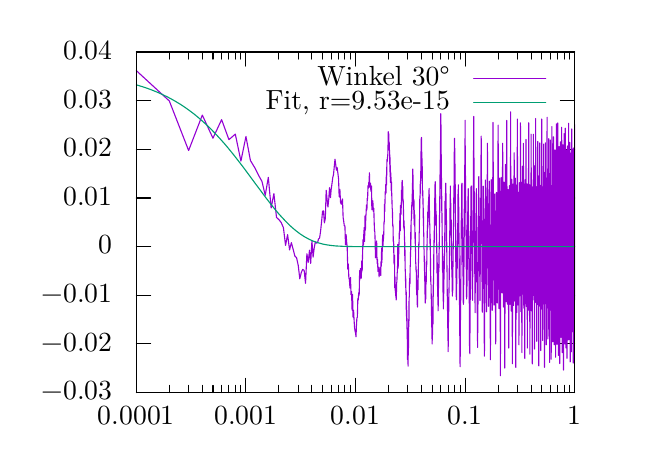
\begin{tikzpicture}[gnuplot]
%% generated with GNUPLOT 5.2p5a (Gentoo revision r0) (Lua 5.1; terminal rev. 99 , script rev. 107)
%% Sa 18 Mai 2019 18:30:40 CEST
\path (0.000,0.000) rectangle (7.500,5.250);
\gpcolor{color=gp lt color border}
\gpsetlinetype{gp lt border}
\gpsetdashtype{gp dt solid}
\gpsetlinewidth{1.00}
\draw[gp path] (1.380,0.616)--(1.560,0.616);
\draw[gp path] (6.947,0.616)--(6.767,0.616);
\node[gp node right] at (1.196,0.616) {$-0.03$};
\draw[gp path] (1.380,1.234)--(1.560,1.234);
\draw[gp path] (6.947,1.234)--(6.767,1.234);
\node[gp node right] at (1.196,1.234) {$-0.02$};
\draw[gp path] (1.380,1.852)--(1.560,1.852);
\draw[gp path] (6.947,1.852)--(6.767,1.852);
\node[gp node right] at (1.196,1.852) {$-0.01$};
\draw[gp path] (1.380,2.470)--(1.560,2.470);
\draw[gp path] (6.947,2.470)--(6.767,2.470);
\node[gp node right] at (1.196,2.470) {$0$};
\draw[gp path] (1.380,3.087)--(1.560,3.087);
\draw[gp path] (6.947,3.087)--(6.767,3.087);
\node[gp node right] at (1.196,3.087) {$0.01$};
\draw[gp path] (1.380,3.705)--(1.560,3.705);
\draw[gp path] (6.947,3.705)--(6.767,3.705);
\node[gp node right] at (1.196,3.705) {$0.02$};
\draw[gp path] (1.380,4.323)--(1.560,4.323);
\draw[gp path] (6.947,4.323)--(6.767,4.323);
\node[gp node right] at (1.196,4.323) {$0.03$};
\draw[gp path] (1.380,4.941)--(1.560,4.941);
\draw[gp path] (6.947,4.941)--(6.767,4.941);
\node[gp node right] at (1.196,4.941) {$0.04$};
\draw[gp path] (1.380,0.616)--(1.380,0.796);
\draw[gp path] (1.380,4.941)--(1.380,4.761);
\node[gp node center] at (1.380,0.308) {$0.0001$};
\draw[gp path] (1.799,0.616)--(1.799,0.706);
\draw[gp path] (1.799,4.941)--(1.799,4.851);
\draw[gp path] (2.044,0.616)--(2.044,0.706);
\draw[gp path] (2.044,4.941)--(2.044,4.851);
\draw[gp path] (2.218,0.616)--(2.218,0.706);
\draw[gp path] (2.218,4.941)--(2.218,4.851);
\draw[gp path] (2.353,0.616)--(2.353,0.706);
\draw[gp path] (2.353,4.941)--(2.353,4.851);
\draw[gp path] (2.463,0.616)--(2.463,0.706);
\draw[gp path] (2.463,4.941)--(2.463,4.851);
\draw[gp path] (2.556,0.616)--(2.556,0.706);
\draw[gp path] (2.556,4.941)--(2.556,4.851);
\draw[gp path] (2.637,0.616)--(2.637,0.706);
\draw[gp path] (2.637,4.941)--(2.637,4.851);
\draw[gp path] (2.708,0.616)--(2.708,0.706);
\draw[gp path] (2.708,4.941)--(2.708,4.851);
\draw[gp path] (2.772,0.616)--(2.772,0.796);
\draw[gp path] (2.772,4.941)--(2.772,4.761);
\node[gp node center] at (2.772,0.308) {$0.001$};
\draw[gp path] (3.191,0.616)--(3.191,0.706);
\draw[gp path] (3.191,4.941)--(3.191,4.851);
\draw[gp path] (3.436,0.616)--(3.436,0.706);
\draw[gp path] (3.436,4.941)--(3.436,4.851);
\draw[gp path] (3.610,0.616)--(3.610,0.706);
\draw[gp path] (3.610,4.941)--(3.610,4.851);
\draw[gp path] (3.745,0.616)--(3.745,0.706);
\draw[gp path] (3.745,4.941)--(3.745,4.851);
\draw[gp path] (3.855,0.616)--(3.855,0.706);
\draw[gp path] (3.855,4.941)--(3.855,4.851);
\draw[gp path] (3.948,0.616)--(3.948,0.706);
\draw[gp path] (3.948,4.941)--(3.948,4.851);
\draw[gp path] (4.029,0.616)--(4.029,0.706);
\draw[gp path] (4.029,4.941)--(4.029,4.851);
\draw[gp path] (4.100,0.616)--(4.100,0.706);
\draw[gp path] (4.100,4.941)--(4.100,4.851);
\draw[gp path] (4.163,0.616)--(4.163,0.796);
\draw[gp path] (4.163,4.941)--(4.163,4.761);
\node[gp node center] at (4.163,0.308) {$0.01$};
\draw[gp path] (4.582,0.616)--(4.582,0.706);
\draw[gp path] (4.582,4.941)--(4.582,4.851);
\draw[gp path] (4.828,0.616)--(4.828,0.706);
\draw[gp path] (4.828,4.941)--(4.828,4.851);
\draw[gp path] (5.001,0.616)--(5.001,0.706);
\draw[gp path] (5.001,4.941)--(5.001,4.851);
\draw[gp path] (5.136,0.616)--(5.136,0.706);
\draw[gp path] (5.136,4.941)--(5.136,4.851);
\draw[gp path] (5.246,0.616)--(5.246,0.706);
\draw[gp path] (5.246,4.941)--(5.246,4.851);
\draw[gp path] (5.340,0.616)--(5.340,0.706);
\draw[gp path] (5.340,4.941)--(5.340,4.851);
\draw[gp path] (5.420,0.616)--(5.420,0.706);
\draw[gp path] (5.420,4.941)--(5.420,4.851);
\draw[gp path] (5.492,0.616)--(5.492,0.706);
\draw[gp path] (5.492,4.941)--(5.492,4.851);
\draw[gp path] (5.555,0.616)--(5.555,0.796);
\draw[gp path] (5.555,4.941)--(5.555,4.761);
\node[gp node center] at (5.555,0.308) {$0.1$};
\draw[gp path] (5.974,0.616)--(5.974,0.706);
\draw[gp path] (5.974,4.941)--(5.974,4.851);
\draw[gp path] (6.219,0.616)--(6.219,0.706);
\draw[gp path] (6.219,4.941)--(6.219,4.851);
\draw[gp path] (6.393,0.616)--(6.393,0.706);
\draw[gp path] (6.393,4.941)--(6.393,4.851);
\draw[gp path] (6.528,0.616)--(6.528,0.706);
\draw[gp path] (6.528,4.941)--(6.528,4.851);
\draw[gp path] (6.638,0.616)--(6.638,0.706);
\draw[gp path] (6.638,4.941)--(6.638,4.851);
\draw[gp path] (6.731,0.616)--(6.731,0.706);
\draw[gp path] (6.731,4.941)--(6.731,4.851);
\draw[gp path] (6.812,0.616)--(6.812,0.706);
\draw[gp path] (6.812,4.941)--(6.812,4.851);
\draw[gp path] (6.883,0.616)--(6.883,0.706);
\draw[gp path] (6.883,4.941)--(6.883,4.851);
\draw[gp path] (6.947,0.616)--(6.947,0.796);
\draw[gp path] (6.947,4.941)--(6.947,4.761);
\node[gp node center] at (6.947,0.308) {$1$};
\draw[gp path] (1.380,4.941)--(1.380,0.616)--(6.947,0.616)--(6.947,4.941)--cycle;
\node[gp node right] at (5.479,4.607) {Winkel 30°};
\gpcolor{rgb color={0.580,0.000,0.827}}
\draw[gp path] (5.663,4.607)--(6.579,4.607);
\draw[gp path] (1.380,4.704)--(1.799,4.319)--(2.044,3.690)--(2.218,4.140)--(2.353,3.846)%
  --(2.463,4.082)--(2.556,3.828)--(2.637,3.898)--(2.708,3.555)--(2.772,3.868)--(2.829,3.563)%
  --(2.882,3.475)--(2.930,3.379)--(2.975,3.299)--(3.017,3.121)--(3.056,3.349)--(3.092,2.960)%
  --(3.127,3.143)--(3.160,2.840)--(3.191,2.812)--(3.220,2.775)--(3.248,2.710)--(3.275,2.485)%
  --(3.301,2.622)--(3.326,2.427)--(3.349,2.520)--(3.372,2.433)--(3.394,2.348)--(3.415,2.328)%
  --(3.436,2.231)--(3.456,2.061)--(3.475,2.141)--(3.493,2.180)--(3.511,2.168)--(3.529,2.003)%
  --(3.546,2.379)--(3.563,2.271)--(3.579,2.424)--(3.594,2.256)--(3.610,2.541)--(3.625,2.336)%
  --(3.639,2.454)--(3.653,2.526)--(3.667,2.514)--(3.681,2.520)--(3.694,2.567)--(3.707,2.577)%
  --(3.720,2.666)--(3.732,2.780)--(3.745,2.919)--(3.757,2.923)--(3.768,2.771)--(3.780,2.825)%
  --(3.791,3.185)--(3.802,3.074)--(3.813,2.972)--(3.824,3.076)--(3.834,3.218)--(3.845,3.091)%
  --(3.855,3.199)--(3.865,3.271)--(3.875,3.348)--(3.884,3.385)--(3.894,3.489)--(3.903,3.579)%
  --(3.912,3.512)--(3.921,3.441)--(3.930,3.474)--(3.939,3.406)--(3.948,3.332)--(3.956,3.102)%
  --(3.965,3.196)--(3.973,3.034)--(3.982,3.007)--(3.990,3.052)--(3.998,3.075)--(4.006,2.842)%
  --(4.013,2.795)--(4.021,2.735)--(4.029,2.734)--(4.036,2.492)--(4.044,2.623)--(4.051,2.528)%
  --(4.058,2.463)--(4.065,2.183)--(4.072,2.248)--(4.079,2.072)--(4.086,2.049)--(4.093,1.943)%
  --(4.100,2.079)--(4.106,1.859)--(4.113,1.899)--(4.120,1.661)--(4.126,1.862)--(4.132,1.573)%
  --(4.139,1.661)--(4.145,1.542)--(4.151,1.446)--(4.157,1.400)--(4.164,1.373)--(4.170,1.323)%
  --(4.175,1.460)--(4.181,1.563)--(4.187,1.572)--(4.193,1.811)--(4.199,1.793)--(4.204,1.884)%
  --(4.210,1.852)--(4.216,2.164)--(4.221,2.058)--(4.227,2.191)--(4.232,2.080)--(4.237,2.069)%
  --(4.243,2.289)--(4.248,2.161)--(4.253,2.371)--(4.258,2.557)--(4.264,2.487)--(4.269,2.634)%
  --(4.274,2.711)--(4.279,2.536)--(4.284,2.858)--(4.289,2.679)--(4.294,2.838)--(4.298,2.894)%
  --(4.303,3.000)--(4.308,2.934)--(4.313,3.084)--(4.317,3.073)--(4.322,3.242)--(4.327,3.213)%
  --(4.331,3.284)--(4.336,3.279)--(4.340,3.407)--(4.345,3.223)--(4.349,3.277)--(4.354,3.270)%
  --(4.358,3.185)--(4.363,3.168)--(4.367,3.239)--(4.371,2.938)--(4.375,3.056)--(4.380,3.050)%
  --(4.384,3.050)--(4.388,2.919)--(4.392,2.937)--(4.396,2.957)--(4.400,2.792)--(4.405,2.671)%
  --(4.409,2.654)--(4.413,2.526)--(4.417,2.327)--(4.421,2.453)--(4.424,2.432)--(4.428,2.518)%
  --(4.432,2.541)--(4.436,2.318)--(4.440,2.254)--(4.444,2.304)--(4.448,2.154)--(4.451,2.215)%
  --(4.455,2.159)--(4.459,2.184)--(4.463,2.086)--(4.466,2.152)--(4.470,2.125)--(4.473,2.206)%
  --(4.477,2.107)--(4.481,2.132)--(4.484,2.103)--(4.488,2.283)--(4.491,2.221)--(4.495,2.451)%
  --(4.498,2.266)--(4.502,2.389)--(4.505,2.529)--(4.509,2.618)--(4.512,2.483)--(4.515,2.535)%
  --(4.519,2.578)--(4.522,2.624)--(4.525,2.772)--(4.529,2.787)--(4.532,3.010)--(4.535,2.916)%
  --(4.539,3.089)--(4.542,3.172)--(4.545,3.160)--(4.548,3.260)--(4.551,3.149)--(4.555,3.381)%
  --(4.558,3.253)--(4.561,3.494)--(4.564,3.578)--(4.567,3.555)--(4.570,3.604)--(4.573,3.625)%
  --(4.576,3.707)--(4.579,3.928)--(4.582,3.857)--(4.585,3.905)--(4.588,3.784)--(4.591,3.800)%
  --(4.594,3.693)--(4.597,3.694)--(4.600,3.418)--(4.603,3.602)--(4.606,3.285)--(4.609,3.418)%
  --(4.612,3.388)--(4.615,3.318)--(4.618,3.181)--(4.621,3.291)--(4.623,3.151)--(4.626,3.066)%
  --(4.629,2.957)--(4.632,2.937)--(4.635,2.772)--(4.637,2.733)--(4.640,2.734)--(4.643,2.540)%
  --(4.646,2.526)--(4.648,2.539)--(4.651,2.286)--(4.654,2.246)--(4.656,2.256)--(4.659,2.361)%
  --(4.662,1.946)--(4.664,2.095)--(4.667,1.953)--(4.670,1.883)--(4.672,1.899)--(4.675,1.846)%
  --(4.677,1.847)--(4.680,1.792)--(4.683,1.870)--(4.685,2.011)--(4.688,2.018)--(4.690,2.058)%
  --(4.693,2.137)--(4.695,2.148)--(4.698,2.243)--(4.700,2.497)--(4.703,2.194)--(4.705,2.282)%
  --(4.708,2.222)--(4.710,2.453)--(4.712,2.375)--(4.715,2.526)--(4.717,2.494)--(4.720,2.666)%
  --(4.722,2.619)--(4.725,2.798)--(4.727,2.686)--(4.729,2.890)--(4.732,2.670)--(4.734,2.992)%
  --(4.736,2.899)--(4.739,2.934)--(4.741,2.880)--(4.743,3.030)--(4.746,2.960)--(4.748,3.185)%
  --(4.750,3.086)--(4.753,3.288)--(4.755,3.153)--(4.757,3.310)--(4.759,3.130)--(4.762,3.175)%
  --(4.764,3.233)--(4.766,3.066)--(4.768,3.009)--(4.771,3.053)--(4.773,2.877)--(4.775,2.819)%
  --(4.777,2.700)--(4.779,2.799)--(4.781,2.755)--(4.784,2.641)--(4.786,2.556)--(4.788,2.539)%
  --(4.790,2.288)--(4.792,2.426)--(4.794,2.194)--(4.797,2.130)--(4.799,2.029)--(4.801,2.064)%
  --(4.803,1.860)--(4.805,1.912)--(4.807,1.672)--(4.809,1.889)--(4.811,1.584)--(4.813,1.715)%
  --(4.815,1.511)--(4.817,1.559)--(4.819,1.297)--(4.821,1.429)--(4.823,1.035)--(4.826,1.425)%
  --(4.828,0.978)--(4.830,1.329)--(4.832,0.951)--(4.834,1.438)--(4.836,1.180)--(4.838,1.542)%
  --(4.840,1.452)--(4.841,1.775)--(4.843,1.526)--(4.845,1.825)--(4.847,1.837)--(4.849,2.025)%
  --(4.851,1.958)--(4.853,2.069)--(4.855,2.001)--(4.857,2.226)--(4.859,2.214)--(4.861,2.331)%
  --(4.863,2.428)--(4.865,2.652)--(4.867,2.431)--(4.868,2.696)--(4.870,2.811)--(4.872,2.800)%
  --(4.874,2.825)--(4.876,2.996)--(4.878,2.885)--(4.880,2.982)--(4.881,3.020)--(4.883,3.073)%
  --(4.885,3.151)--(4.887,3.278)--(4.889,3.267)--(4.891,3.455)--(4.892,3.219)--(4.894,3.380)%
  --(4.896,3.127)--(4.898,3.188)--(4.900,2.973)--(4.901,3.036)--(4.903,2.937)--(4.905,3.067)%
  --(4.907,2.819)--(4.908,3.050)--(4.910,2.745)--(4.912,2.786)--(4.914,2.730)--(4.916,2.875)%
  --(4.917,2.731)--(4.919,2.602)--(4.921,2.508)--(4.922,2.649)--(4.924,2.409)--(4.926,2.435)%
  --(4.928,2.251)--(4.929,2.257)--(4.931,2.217)--(4.933,2.149)--(4.934,2.175)--(4.936,2.165)%
  --(4.938,2.073)--(4.939,1.860)--(4.941,1.996)--(4.943,1.851)--(4.944,1.863)--(4.946,1.915)%
  --(4.948,1.731)--(4.949,1.795)--(4.951,1.702)--(4.953,1.927)--(4.954,1.930)--(4.956,2.046)%
  --(4.958,1.922)--(4.959,2.181)--(4.961,2.076)--(4.962,2.314)--(4.964,2.259)--(4.966,2.504)%
  --(4.967,2.449)--(4.969,2.527)--(4.970,2.489)--(4.972,2.637)--(4.974,2.666)--(4.975,2.817)%
  --(4.977,2.815)--(4.978,3.074)--(4.980,2.956)--(4.981,3.115)--(4.983,3.082)--(4.985,3.263)%
  --(4.986,3.145)--(4.988,3.266)--(4.989,3.266)--(4.991,3.426)--(4.992,3.304)--(4.994,3.493)%
  --(4.995,3.587)--(4.997,3.803)--(4.998,3.839)--(5.000,3.738)--(5.001,3.856)--(5.003,3.747)%
  --(5.004,3.672)--(5.006,3.618)--(5.007,3.596)--(5.009,3.535)--(5.010,3.531)--(5.012,3.305)%
  --(5.013,3.165)--(5.015,3.113)--(5.016,3.183)--(5.018,3.174)--(5.019,3.127)--(5.021,3.023)%
  --(5.022,2.948)--(5.024,2.831)--(5.025,2.960)--(5.027,2.791)--(5.028,2.688)--(5.029,2.663)%
  --(5.031,2.586)--(5.032,2.450)--(5.034,2.433)--(5.035,2.396)--(5.037,2.281)--(5.038,2.244)%
  --(5.039,2.160)--(5.041,2.311)--(5.042,2.029)--(5.044,2.096)--(5.045,1.865)--(5.047,2.036)%
  --(5.048,1.839)--(5.049,1.753)--(5.051,1.793)--(5.052,1.859)--(5.054,1.797)--(5.055,1.809)%
  --(5.056,1.963)--(5.058,1.991)--(5.059,1.996)--(5.060,2.010)--(5.062,2.032)--(5.063,2.249)%
  --(5.064,2.198)--(5.066,2.285)--(5.067,2.258)--(5.069,2.243)--(5.070,2.269)--(5.071,2.498)%
  --(5.073,2.486)--(5.074,2.597)--(5.075,2.665)--(5.077,2.694)--(5.078,2.715)--(5.079,2.792)%
  --(5.081,2.909)--(5.082,2.716)--(5.083,2.820)--(5.085,2.785)--(5.086,2.915)--(5.087,2.949)%
  --(5.089,3.043)--(5.090,3.030)--(5.091,3.022)--(5.092,3.097)--(5.094,3.094)--(5.095,2.993)%
  --(5.096,3.187)--(5.098,3.012)--(5.099,3.208)--(5.100,2.916)--(5.101,2.880)--(5.103,2.831)%
  --(5.104,2.924)--(5.105,2.743)--(5.107,2.759)--(5.108,2.509)--(5.109,2.630)--(5.110,2.539)%
  --(5.112,2.569)--(5.113,2.445)--(5.114,2.378)--(5.115,2.336)--(5.117,2.098)--(5.118,2.050)%
  --(5.119,2.095)--(5.120,1.988)--(5.122,1.990)--(5.123,1.982)--(5.124,1.938)--(5.125,1.841)%
  --(5.127,1.775)--(5.128,1.695)--(5.129,1.607)--(5.130,1.523)--(5.131,1.474)--(5.133,1.432)%
  --(5.134,1.329)--(5.135,1.298)--(5.136,1.365)--(5.137,1.233)--(5.139,1.482)--(5.140,1.289)%
  --(5.141,1.398)--(5.142,1.433)--(5.144,1.553)--(5.145,1.509)--(5.146,1.703)--(5.147,1.484)%
  --(5.148,1.843)--(5.149,1.835)--(5.151,1.984)--(5.152,1.836)--(5.153,2.064)--(5.154,1.990)%
  --(5.155,2.095)--(5.157,2.210)--(5.158,2.421)--(5.159,2.380)--(5.160,2.547)--(5.161,2.550)%
  --(5.162,2.671)--(5.163,2.520)--(5.165,2.727)--(5.166,2.747)--(5.167,2.850)--(5.168,2.801)%
  --(5.169,2.896)--(5.170,3.087)--(5.172,3.048)--(5.173,3.260)--(5.174,3.115)--(5.175,3.262)%
  --(5.176,3.293)--(5.177,3.196)--(5.178,3.132)--(5.179,3.069)--(5.181,3.131)--(5.182,2.990)%
  --(5.183,2.939)--(5.184,2.792)--(5.185,2.919)--(5.186,2.734)--(5.187,2.919)--(5.188,2.742)%
  --(5.189,2.876)--(5.191,2.571)--(5.192,2.637)--(5.193,2.521)--(5.194,2.625)--(5.195,2.383)%
  --(5.196,2.413)--(5.197,2.196)--(5.198,2.326)--(5.199,2.132)--(5.200,2.356)--(5.202,2.148)%
  --(5.203,2.252)--(5.204,2.260)--(5.205,1.964)--(5.206,2.048)--(5.207,2.099)--(5.208,1.834)%
  --(5.209,1.919)--(5.210,1.832)--(5.211,1.926)--(5.212,1.654)--(5.213,1.814)--(5.214,1.711)%
  --(5.215,1.859)--(5.217,2.019)--(5.218,1.940)--(5.219,1.952)--(5.220,2.173)--(5.221,2.149)%
  --(5.222,2.290)--(5.223,2.185)--(5.224,2.369)--(5.225,2.410)--(5.226,2.472)--(5.227,2.438)%
  --(5.228,2.583)--(5.229,2.653)--(5.230,2.869)--(5.231,2.719)--(5.232,2.818)--(5.233,2.950)%
  --(5.234,3.112)--(5.235,3.045)--(5.236,3.383)--(5.237,3.204)--(5.238,3.407)--(5.239,3.325)%
  --(5.240,3.571)--(5.241,3.345)--(5.242,3.754)--(5.243,3.660)--(5.244,3.975)--(5.245,3.785)%
  --(5.246,4.158)--(5.247,3.746)--(5.249,4.017)--(5.250,3.472)--(5.251,3.837)--(5.252,3.539)%
  --(5.253,3.481)--(5.254,3.322)--(5.254,3.304)--(5.255,3.076)--(5.256,3.341)--(5.257,3.078)%
  --(5.258,3.112)--(5.259,2.923)--(5.260,2.944)--(5.261,2.772)--(5.262,2.895)--(5.263,2.678)%
  --(5.264,2.672)--(5.265,2.477)--(5.266,2.470)--(5.267,2.500)--(5.268,2.275)--(5.269,2.156)%
  --(5.270,2.313)--(5.271,2.275)--(5.272,2.142)--(5.273,2.079)--(5.274,2.103)--(5.275,1.900)%
  --(5.276,1.851)--(5.277,1.890)--(5.278,1.843)--(5.279,1.678)--(5.280,1.956)--(5.281,1.788)%
  --(5.282,1.818)--(5.283,1.764)--(5.284,2.034)--(5.285,1.911)--(5.286,2.200)--(5.286,2.112)%
  --(5.287,2.055)--(5.288,2.210)--(5.289,2.313)--(5.290,2.347)--(5.291,2.282)--(5.292,2.187)%
  --(5.293,2.434)--(5.294,2.354)--(5.295,2.644)--(5.296,2.449)--(5.297,2.586)--(5.298,2.591)%
  --(5.299,2.849)--(5.300,2.839)--(5.300,3.046)--(5.301,2.827)--(5.302,2.958)--(5.303,2.853)%
  --(5.304,3.027)--(5.305,3.004)--(5.306,3.148)--(5.307,3.113)--(5.308,3.191)--(5.309,3.204)%
  --(5.310,3.175)--(5.310,3.275)--(5.311,3.250)--(5.312,3.142)--(5.313,3.143)--(5.314,2.983)%
  --(5.315,2.987)--(5.316,2.745)--(5.317,2.823)--(5.318,2.828)--(5.319,2.757)--(5.319,2.541)%
  --(5.320,2.656)--(5.321,2.543)--(5.322,2.504)--(5.323,2.378)--(5.324,2.333)--(5.325,2.182)%
  --(5.326,2.148)--(5.327,2.056)--(5.327,2.067)--(5.328,1.843)--(5.329,1.927)--(5.330,1.695)%
  --(5.331,1.840)--(5.332,1.650)--(5.333,1.686)--(5.334,1.469)--(5.334,1.463)--(5.335,1.435)%
  --(5.336,1.519)--(5.337,1.383)--(5.338,1.278)--(5.339,1.271)--(5.340,1.135)--(5.341,1.249)%
  --(5.341,1.302)--(5.342,1.376)--(5.343,1.525)--(5.344,1.508)--(5.345,1.555)--(5.346,1.670)%
  --(5.347,1.746)--(5.347,1.644)--(5.348,1.668)--(5.349,1.840)--(5.350,1.877)--(5.351,1.920)%
  --(5.352,1.985)--(5.352,2.079)--(5.353,2.018)--(5.354,2.128)--(5.355,2.235)--(5.356,2.308)%
  --(5.357,2.415)--(5.358,2.411)--(5.358,2.601)--(5.359,2.523)--(5.360,2.672)--(5.361,2.585)%
  --(5.362,2.668)--(5.363,2.642)--(5.363,2.742)--(5.364,2.954)--(5.365,2.981)--(5.366,2.940)%
  --(5.367,3.140)--(5.368,3.002)--(5.368,3.239)--(5.369,2.991)--(5.370,3.010)--(5.371,3.076)%
  --(5.372,2.861)--(5.372,3.068)--(5.373,2.921)--(5.374,2.838)--(5.375,2.836)--(5.376,2.778)%
  --(5.377,2.795)--(5.377,2.803)--(5.378,2.694)--(5.379,2.810)--(5.380,2.612)--(5.381,2.498)%
  --(5.381,2.509)--(5.382,2.537)--(5.383,2.292)--(5.384,2.217)--(5.385,2.289)--(5.385,2.220)%
  --(5.386,2.182)--(5.387,2.284)--(5.388,2.082)--(5.389,2.081)--(5.389,2.119)--(5.390,2.061)%
  --(5.391,2.029)--(5.392,1.933)--(5.393,1.882)--(5.393,1.919)--(5.394,1.841)--(5.395,1.929)%
  --(5.396,1.880)--(5.396,2.037)--(5.397,1.888)--(5.398,1.926)--(5.399,2.006)--(5.400,2.098)%
  --(5.400,2.126)--(5.401,2.231)--(5.402,2.213)--(5.403,2.308)--(5.404,2.386)--(5.404,2.436)%
  --(5.405,2.458)--(5.406,2.575)--(5.407,2.696)--(5.407,2.667)--(5.408,2.749)--(5.409,2.789)%
  --(5.410,2.817)--(5.410,2.852)--(5.411,2.955)--(5.412,3.135)--(5.413,3.009)--(5.414,3.128)%
  --(5.414,3.132)--(5.415,3.249)--(5.416,3.235)--(5.417,3.382)--(5.417,3.516)--(5.418,3.667)%
  --(5.419,3.722)--(5.420,3.693)--(5.420,3.666)--(5.421,3.845)--(5.422,3.807)--(5.423,3.817)%
  --(5.423,3.614)--(5.424,3.719)--(5.425,3.424)--(5.426,3.588)--(5.426,3.392)--(5.427,3.520)%
  --(5.428,3.248)--(5.429,3.282)--(5.429,3.089)--(5.430,3.259)--(5.431,2.962)--(5.432,2.965)%
  --(5.432,2.875)--(5.433,2.763)--(5.434,2.722)--(5.435,2.616)--(5.435,2.623)--(5.436,2.526)%
  --(5.437,2.276)--(5.438,2.424)--(5.438,2.281)--(5.439,2.356)--(5.440,2.153)--(5.440,2.117)%
  --(5.441,1.986)--(5.442,1.969)--(5.443,1.898)--(5.443,1.831)--(5.444,1.923)--(5.445,1.927)%
  --(5.446,1.909)--(5.446,1.793)--(5.447,1.897)--(5.448,1.947)--(5.448,1.945)--(5.449,2.048)%
  --(5.450,2.051)--(5.451,2.343)--(5.451,2.183)--(5.452,2.204)--(5.453,2.284)--(5.453,2.414)%
  --(5.454,2.261)--(5.455,2.339)--(5.456,2.194)--(5.456,2.459)--(5.457,2.409)--(5.458,2.685)%
  --(5.458,2.475)--(5.459,2.683)--(5.460,2.615)--(5.461,2.766)--(5.461,2.605)--(5.462,2.729)%
  --(5.463,2.728)--(5.463,2.844)--(5.464,2.683)--(5.465,2.949)--(5.465,3.051)--(5.466,3.166)%
  --(5.467,3.032)--(5.468,3.196)--(5.468,3.123)--(5.469,3.129)--(5.470,3.140)--(5.470,3.254)%
  --(5.471,3.019)--(5.472,3.094)--(5.472,3.085)--(5.473,2.905)--(5.474,2.973)--(5.475,2.848)%
  --(5.475,2.627)--(5.476,2.750)--(5.477,2.599)--(5.477,2.654)--(5.478,2.515)--(5.479,2.492)%
  --(5.479,2.418)--(5.480,2.401)--(5.481,2.078)--(5.481,2.136)--(5.482,2.020)--(5.483,1.982)%
  --(5.483,1.837)--(5.484,1.883)--(5.485,1.686)--(5.485,1.649)--(5.486,1.620)--(5.487,1.726)%
  --(5.488,1.319)--(5.488,1.649)--(5.489,1.191)--(5.490,1.424)--(5.490,0.984)--(5.491,1.208)%
  --(5.492,0.943)--(5.492,1.311)--(5.493,1.072)--(5.494,1.381)--(5.494,1.246)--(5.495,1.479)%
  --(5.496,1.417)--(5.496,1.511)--(5.497,1.715)--(5.498,1.773)--(5.498,1.807)--(5.499,1.886)%
  --(5.500,1.788)--(5.500,1.970)--(5.501,2.107)--(5.502,2.076)--(5.502,2.276)--(5.503,2.237)%
  --(5.504,2.378)--(5.504,2.467)--(5.505,2.410)--(5.506,2.681)--(5.506,2.618)--(5.507,2.804)%
  --(5.507,2.741)--(5.508,2.883)--(5.509,2.897)--(5.509,2.838)--(5.510,2.835)--(5.511,3.086)%
  --(5.511,3.025)--(5.512,3.137)--(5.513,3.092)--(5.513,3.261)--(5.514,2.994)--(5.515,3.201)%
  --(5.515,2.933)--(5.516,3.274)--(5.517,3.005)--(5.517,3.040)--(5.518,2.797)--(5.518,2.794)%
  --(5.519,2.723)--(5.520,2.808)--(5.520,2.697)--(5.521,2.826)--(5.522,2.572)--(5.522,2.721)%
  --(5.523,2.598)--(5.524,2.669)--(5.524,2.524)--(5.525,2.588)--(5.526,2.271)--(5.526,2.334)%
  --(5.527,2.298)--(5.527,2.310)--(5.528,2.121)--(5.529,2.166)--(5.529,2.103)--(5.530,2.054)%
  --(5.531,1.968)--(5.531,2.039)--(5.532,1.860)--(5.532,1.758)--(5.533,1.807)--(5.534,1.804)%
  --(5.534,1.737)--(5.535,1.807)--(5.536,1.871)--(5.536,1.914)--(5.537,1.821)--(5.537,2.064)%
  --(5.538,1.985)--(5.539,2.179)--(5.539,2.195)--(5.540,2.274)--(5.541,2.212)--(5.541,2.317)%
  --(5.542,2.339)--(5.542,2.551)--(5.543,2.477)--(5.544,2.628)--(5.544,2.767)--(5.545,2.949)%
  --(5.546,2.926)--(5.546,2.976)--(5.547,2.912)--(5.547,3.203)--(5.548,3.228)--(5.549,3.389)%
  --(5.549,3.303)--(5.550,3.507)--(5.550,3.459)--(5.551,3.500)--(5.552,3.387)--(5.552,3.577)%
  --(5.553,3.689)--(5.553,3.720)--(5.554,3.697)--(5.555,3.927)--(5.555,4.074)--(5.556,3.891)%
  --(5.556,3.824)--(5.557,3.666)--(5.558,3.587)--(5.558,3.639)--(5.559,3.408)--(5.559,3.428)%
  --(5.560,3.337)--(5.561,3.241)--(5.561,3.233)--(5.562,3.183)--(5.562,3.129)--(5.563,3.033)%
  --(5.564,2.898)--(5.564,2.992)--(5.565,3.019)--(5.565,2.862)--(5.566,2.745)--(5.567,2.716)%
  --(5.567,2.677)--(5.568,2.475)--(5.568,2.496)--(5.569,2.412)--(5.570,2.187)--(5.570,2.325)%
  --(5.571,2.048)--(5.571,2.224)--(5.572,2.124)--(5.573,2.150)--(5.573,1.891)--(5.574,1.804)%
  --(5.574,1.838)--(5.575,1.808)--(5.575,1.885)--(5.576,1.827)--(5.577,1.914)--(5.577,1.855)%
  --(5.578,1.954)--(5.578,2.059)--(5.579,1.964)--(5.580,2.149)--(5.580,2.046)--(5.581,2.125)%
  --(5.581,2.230)--(5.582,2.283)--(5.582,2.176)--(5.583,2.392)--(5.584,2.464)--(5.584,2.344)%
  --(5.585,2.557)--(5.585,2.625)--(5.586,2.662)--(5.586,2.557)--(5.587,2.884)--(5.588,2.815)%
  --(5.588,2.817)--(5.589,2.779)--(5.589,2.914)--(5.590,2.726)--(5.590,2.873)--(5.591,2.945)%
  --(5.592,3.009)--(5.592,2.955)--(5.593,3.161)--(5.593,3.012)--(5.594,3.162)--(5.594,2.954)%
  --(5.595,3.206)--(5.596,3.032)--(5.596,3.120)--(5.597,2.851)--(5.597,3.071)--(5.598,2.797)%
  --(5.598,2.792)--(5.599,2.720)--(5.600,2.735)--(5.600,2.607)--(5.601,2.666)--(5.601,2.652)%
  --(5.602,2.562)--(5.602,2.313)--(5.603,2.384)--(5.603,2.285)--(5.604,2.342)--(5.605,2.056)%
  --(5.605,2.074)--(5.606,1.994)--(5.606,1.908)--(5.607,1.881)--(5.607,1.864)--(5.608,1.749)%
  --(5.608,1.892)--(5.609,1.831)--(5.610,1.898)--(5.610,1.481)--(5.611,1.489)--(5.611,1.209)%
  --(5.612,1.387)--(5.612,1.216)--(5.613,1.284)--(5.613,1.167)--(5.614,1.351)--(5.615,1.109)%
  --(5.615,1.499)--(5.616,1.280)--(5.616,1.600)--(5.617,1.372)--(5.617,1.752)--(5.618,1.558)%
  --(5.618,1.851)--(5.619,1.621)--(5.619,1.882)--(5.620,1.792)--(5.621,1.998)--(5.621,1.991)%
  --(5.622,2.082)--(5.622,2.147)--(5.623,2.383)--(5.623,2.357)--(5.624,2.510)--(5.624,2.605)%
  --(5.625,2.558)--(5.625,2.566)--(5.626,2.693)--(5.626,2.707)--(5.627,2.857)--(5.628,2.844)%
  --(5.628,2.994)--(5.629,2.926)--(5.629,3.072)--(5.630,3.176)--(5.630,3.225)--(5.631,3.176)%
  --(5.631,3.235)--(5.632,3.217)--(5.632,3.221)--(5.633,3.202)--(5.633,3.240)--(5.634,3.123)%
  --(5.634,3.121)--(5.635,2.870)--(5.636,2.889)--(5.636,2.651)--(5.637,2.779)--(5.637,2.667)%
  --(5.638,2.929)--(5.638,2.653)--(5.639,2.673)--(5.639,2.541)--(5.640,2.593)--(5.640,2.404)%
  --(5.641,2.384)--(5.641,2.313)--(5.642,2.358)--(5.642,2.219)--(5.643,2.505)--(5.643,2.162)%
  --(5.644,2.283)--(5.644,2.221)--(5.645,2.291)--(5.645,1.967)--(5.646,2.031)--(5.647,1.890)%
  --(5.647,2.131)--(5.648,1.836)--(5.648,2.103)--(5.649,2.025)--(5.649,1.971)--(5.650,1.787)%
  --(5.650,1.860)--(5.651,2.031)--(5.651,2.059)--(5.652,2.092)--(5.652,2.085)--(5.653,2.225)%
  --(5.653,2.359)--(5.654,2.353)--(5.654,2.422)--(5.655,2.492)--(5.655,2.474)--(5.656,2.474)%
  --(5.656,2.529)--(5.657,2.530)--(5.657,2.932)--(5.658,2.814)--(5.658,3.077)--(5.659,3.118)%
  --(5.659,3.242)--(5.660,3.170)--(5.660,3.301)--(5.661,3.205)--(5.661,3.448)--(5.662,3.388)%
  --(5.662,3.690)--(5.663,3.473)--(5.663,3.825)--(5.664,3.503)--(5.664,4.026)--(5.665,3.618)%
  --(5.665,4.123)--(5.666,3.715)--(5.666,3.994)--(5.667,3.556)--(5.667,3.744)--(5.668,3.489)%
  --(5.668,3.579)--(5.669,3.384)--(5.669,3.335)--(5.670,3.232)--(5.670,3.228)--(5.671,3.150)%
  --(5.671,3.092)--(5.672,3.008)--(5.672,3.096)--(5.673,2.801)--(5.673,2.863)--(5.674,2.655)%
  --(5.674,2.615)--(5.675,2.612)--(5.675,2.519)--(5.676,2.537)--(5.676,2.347)--(5.677,2.182)%
  --(5.677,2.394)--(5.678,2.215)--(5.678,2.190)--(5.679,2.045)--(5.679,2.093)--(5.680,1.929)%
  --(5.680,2.028)--(5.681,1.757)--(5.681,1.960)--(5.682,1.631)--(5.682,1.919)--(5.683,1.734)%
  --(5.683,2.087)--(5.684,1.898)--(5.684,2.189)--(5.685,1.880)--(5.685,2.195)--(5.686,2.020)%
  --(5.686,2.223)--(5.687,2.022)--(5.687,2.254)--(5.688,2.094)--(5.688,2.227)--(5.689,2.326)%
  --(5.689,2.350)--(5.690,2.443)--(5.690,2.531)--(5.691,2.460)--(5.691,2.621)--(5.692,2.582)%
  --(5.692,2.734)--(5.693,2.629)--(5.693,2.857)--(5.693,2.834)--(5.694,2.828)--(5.694,2.857)%
  --(5.695,2.973)--(5.695,2.953)--(5.696,3.044)--(5.696,3.123)--(5.697,3.064)--(5.697,3.112)%
  --(5.698,3.199)--(5.698,3.144)--(5.699,3.205)--(5.699,3.013)--(5.700,3.139)--(5.700,3.010)%
  --(5.701,2.855)--(5.701,2.740)--(5.702,2.822)--(5.702,2.756)--(5.703,2.681)--(5.703,2.566)%
  --(5.704,2.619)--(5.704,2.399)--(5.704,2.395)--(5.705,2.402)--(5.705,2.284)--(5.706,2.069)%
  --(5.706,2.270)--(5.707,2.014)--(5.707,2.015)--(5.708,1.917)--(5.708,1.987)--(5.709,1.800)%
  --(5.709,1.844)--(5.710,1.621)--(5.710,1.735)--(5.711,1.604)--(5.711,1.531)--(5.712,1.543)%
  --(5.712,1.510)--(5.712,1.406)--(5.713,1.268)--(5.713,1.288)--(5.714,1.285)--(5.714,1.303)%
  --(5.715,1.189)--(5.715,1.366)--(5.716,1.409)--(5.716,1.569)--(5.717,1.572)--(5.717,1.708)%
  --(5.718,1.608)--(5.718,1.795)--(5.718,1.697)--(5.719,1.801)--(5.719,1.810)--(5.720,2.001)%
  --(5.720,2.093)--(5.721,2.179)--(5.721,2.115)--(5.722,2.192)--(5.722,2.204)--(5.723,2.279)%
  --(5.723,2.491)--(5.724,2.446)--(5.724,2.623)--(5.724,2.558)--(5.725,2.807)--(5.725,2.688)%
  --(5.726,2.863)--(5.726,2.851)--(5.727,2.986)--(5.728,3.118)--(5.728,3.141)--(5.729,3.207)%
  --(5.729,3.240)--(5.729,3.359)--(5.730,3.219)--(5.730,3.140)--(5.731,3.158)--(5.731,3.095)%
  --(5.732,3.043)--(5.732,3.073)--(5.733,2.926)--(5.733,2.914)--(5.733,2.877)--(5.734,2.851)%
  --(5.734,2.888)--(5.735,2.766)--(5.735,2.742)--(5.736,2.536)--(5.736,2.695)--(5.737,2.576)%
  --(5.737,2.455)--(5.738,2.335)--(5.738,2.402)--(5.738,2.414)--(5.739,2.233)--(5.739,2.091)%
  --(5.740,2.195)--(5.740,2.220)--(5.741,2.118)--(5.741,2.100)--(5.742,2.143)--(5.742,2.046)%
  --(5.742,2.089)--(5.743,1.826)--(5.743,2.035)--(5.744,1.785)--(5.744,1.854)--(5.745,1.824)%
  --(5.745,1.998)--(5.746,1.786)--(5.746,2.129)--(5.746,1.967)--(5.747,2.155)--(5.747,2.118)%
  --(5.748,2.260)--(5.748,2.156)--(5.749,2.288)--(5.749,2.389)--(5.749,2.326)--(5.750,2.390)%
  --(5.750,2.518)--(5.751,2.574)--(5.751,2.729)--(5.752,2.647)--(5.752,2.902)--(5.753,2.792)%
  --(5.753,2.854)--(5.753,3.033)--(5.754,3.019)--(5.754,2.950)--(5.755,3.162)--(5.755,3.114)%
  --(5.756,3.109)--(5.756,3.208)--(5.756,3.349)--(5.757,3.458)--(5.757,3.621)--(5.758,3.637)%
  --(5.758,3.789)--(5.759,3.872)--(5.759,3.808)--(5.759,3.620)--(5.760,3.844)--(5.760,3.456)%
  --(5.761,3.819)--(5.761,3.337)--(5.762,3.606)--(5.762,3.177)--(5.762,3.516)--(5.763,3.244)%
  --(5.763,3.324)--(5.764,3.105)--(5.764,3.164)--(5.765,2.948)--(5.765,2.951)--(5.765,2.832)%
  --(5.766,2.801)--(5.766,2.714)--(5.767,2.537)--(5.767,2.527)--(5.768,2.464)--(5.768,2.396)%
  --(5.768,2.328)--(5.769,2.222)--(5.769,2.252)--(5.770,2.203)--(5.770,2.122)--(5.771,1.934)%
  --(5.771,1.911)--(5.771,1.847)--(5.772,1.817)--(5.772,1.723)--(5.773,1.663)--(5.773,1.676)%
  --(5.774,1.636)--(5.774,1.728)--(5.774,1.852)--(5.775,1.714)--(5.775,1.841)--(5.776,2.015)%
  --(5.776,2.034)--(5.776,2.073)--(5.777,2.258)--(5.777,2.236)--(5.778,2.274)--(5.778,2.161)%
  --(5.779,2.425)--(5.779,2.195)--(5.779,2.340)--(5.780,2.478)--(5.780,2.609)--(5.781,2.387)%
  --(5.781,2.690)--(5.781,2.546)--(5.782,2.727)--(5.782,2.688)--(5.783,2.752)--(5.783,2.653)%
  --(5.784,2.909)--(5.784,2.706)--(5.784,3.111)--(5.785,2.894)--(5.785,3.201)--(5.786,2.949)%
  --(5.786,3.236)--(5.786,3.095)--(5.787,3.031)--(5.787,3.112)--(5.788,3.015)--(5.788,3.065)%
  --(5.789,3.077)--(5.789,2.906)--(5.789,2.938)--(5.790,2.678)--(5.790,2.775)--(5.791,2.657)%
  --(5.791,2.763)--(5.791,2.592)--(5.792,2.821)--(5.792,2.525)--(5.793,2.515)--(5.793,2.432)%
  --(5.793,2.319)--(5.794,2.137)--(5.794,2.219)--(5.795,1.976)--(5.795,1.978)--(5.795,1.751)%
  --(5.796,1.909)--(5.796,1.774)--(5.797,1.836)--(5.797,1.560)--(5.797,1.763)--(5.798,1.421)%
  --(5.798,1.576)--(5.799,1.241)--(5.799,1.427)--(5.800,1.080)--(5.800,1.369)--(5.800,1.079)%
  --(5.801,1.252)--(5.801,1.142)--(5.802,1.330)--(5.802,1.302)--(5.802,1.468)--(5.803,1.467)%
  --(5.803,1.724)--(5.804,1.655)--(5.804,1.874)--(5.804,1.734)--(5.805,1.902)--(5.805,1.904)%
  --(5.806,2.014)--(5.806,1.951)--(5.806,2.036)--(5.807,2.171)--(5.807,2.360)--(5.808,2.305)%
  --(5.808,2.427)--(5.808,2.479)--(5.809,2.542)--(5.809,2.462)--(5.810,2.738)--(5.810,2.577)%
  --(5.810,2.675)--(5.811,2.817)--(5.811,2.953)--(5.812,2.909)--(5.812,3.036)--(5.812,3.024)%
  --(5.813,3.135)--(5.813,3.012)--(5.813,3.316)--(5.814,2.988)--(5.814,3.163)--(5.815,3.045)%
  --(5.815,3.216)--(5.815,2.856)--(5.816,2.898)--(5.816,2.828)--(5.817,2.814)--(5.817,2.730)%
  --(5.817,2.733)--(5.818,2.767)--(5.818,2.837)--(5.819,2.660)--(5.819,2.733)--(5.819,2.613)%
  --(5.820,2.460)--(5.820,2.508)--(5.821,2.537)--(5.821,2.306)--(5.821,2.393)--(5.822,2.216)%
  --(5.822,2.192)--(5.822,2.120)--(5.823,2.247)--(5.823,2.214)--(5.824,2.071)--(5.824,1.995)%
  --(5.824,1.999)--(5.825,2.038)--(5.825,1.850)--(5.826,1.734)--(5.826,1.698)--(5.826,1.757)%
  --(5.827,1.910)--(5.827,1.641)--(5.828,1.846)--(5.828,1.773)--(5.828,1.944)--(5.829,2.050)%
  --(5.829,2.054)--(5.829,2.163)--(5.830,2.223)--(5.830,2.363)--(5.831,2.244)--(5.831,2.442)%
  --(5.831,2.545)--(5.832,2.489)--(5.832,2.537)--(5.832,2.698)--(5.833,2.698)--(5.833,2.854)%
  --(5.834,2.952)--(5.834,2.862)--(5.834,3.107)--(5.835,3.031)--(5.835,3.068)--(5.836,3.152)%
  --(5.836,3.321)--(5.836,3.209)--(5.837,3.179)--(5.837,3.324)--(5.837,3.363)--(5.838,3.484)%
  --(5.838,3.434)--(5.839,3.545)--(5.839,3.782)--(5.839,3.672)--(5.840,3.674)--(5.840,3.650)%
  --(5.840,3.604)--(5.841,3.616)--(5.841,3.388)--(5.842,3.326)--(5.842,3.260)--(5.842,3.145)%
  --(5.843,3.196)--(5.843,3.098)--(5.843,3.139)--(5.844,3.156)--(5.844,3.037)--(5.845,2.921)%
  --(5.845,2.790)--(5.845,2.796)--(5.846,2.703)--(5.846,2.642)--(5.846,2.474)--(5.847,2.491)%
  --(5.847,2.441)--(5.848,2.361)--(5.848,2.355)--(5.848,2.280)--(5.849,2.300)--(5.849,2.155)%
  --(5.849,2.138)--(5.850,1.963)--(5.850,2.018)--(5.851,1.935)--(5.851,2.002)--(5.851,1.811)%
  --(5.852,1.712)--(5.852,1.749)--(5.852,1.751)--(5.853,1.890)--(5.853,1.863)--(5.854,1.842)%
  --(5.854,1.938)--(5.854,2.080)--(5.855,2.079)--(5.855,2.044)--(5.855,2.031)--(5.856,2.230)%
  --(5.856,2.158)--(5.856,2.296)--(5.857,2.252)--(5.857,2.277)--(5.858,2.445)--(5.858,2.473)%
  --(5.858,2.457)--(5.859,2.633)--(5.859,2.614)--(5.859,2.767)--(5.860,2.895)--(5.860,2.904)%
  --(5.860,2.810)--(5.861,2.849)--(5.861,2.810)--(5.862,3.019)--(5.862,2.918)--(5.862,2.985)%
  --(5.863,2.907)--(5.863,3.132)--(5.863,3.018)--(5.864,3.300)--(5.864,3.195)--(5.864,3.207)%
  --(5.865,3.022)--(5.865,3.165)--(5.866,3.012)--(5.866,2.983)--(5.866,2.870)--(5.867,2.870)%
  --(5.867,2.726)--(5.867,2.845)--(5.868,2.687)--(5.868,2.622)--(5.868,2.606)--(5.869,2.625)%
  --(5.869,2.462)--(5.870,2.401)--(5.870,2.414)--(5.870,2.285)--(5.871,2.204)--(5.871,2.076)%
  --(5.871,2.007)--(5.872,1.891)--(5.872,1.834)--(5.872,1.819)--(5.873,1.800)--(5.873,1.732)%
  --(5.873,1.693)--(5.874,1.692)--(5.874,1.572)--(5.875,1.479)--(5.875,1.334)--(5.875,1.340)%
  --(5.876,1.224)--(5.876,1.119)--(5.876,1.033)--(5.877,1.181)--(5.877,1.139)--(5.877,1.515)%
  --(5.878,1.217)--(5.878,1.546)--(5.878,1.322)--(5.879,1.684)--(5.879,1.462)--(5.880,1.699)%
  --(5.880,1.671)--(5.880,1.898)--(5.881,1.754)--(5.881,2.021)--(5.881,1.877)--(5.882,2.024)%
  --(5.882,2.139)--(5.882,2.286)--(5.883,2.344)--(5.883,2.582)--(5.883,2.419)--(5.884,2.476)%
  --(5.884,2.632)--(5.884,2.591)--(5.885,2.641)--(5.885,2.841)--(5.886,2.741)--(5.886,2.887)%
  --(5.886,2.975)--(5.887,3.098)--(5.887,3.086)--(5.887,3.171)--(5.888,3.183)--(5.888,3.320)%
  --(5.888,3.234)--(5.889,3.173)--(5.889,3.084)--(5.889,3.028)--(5.890,3.036)--(5.890,2.987)%
  --(5.890,2.781)--(5.891,2.893)--(5.891,2.830)--(5.891,2.796)--(5.892,2.602)--(5.892,2.823)%
  --(5.892,2.655)--(5.893,2.605)--(5.893,2.636)--(5.893,2.571)--(5.894,2.371)--(5.894,2.402)%
  --(5.895,2.253)--(5.895,2.407)--(5.895,2.141)--(5.896,2.275)--(5.896,2.071)--(5.896,2.173)%
  --(5.897,2.088)--(5.897,2.140)--(5.897,1.953)--(5.898,2.044)--(5.898,1.849)--(5.898,1.873)%
  --(5.899,1.823)--(5.899,1.822)--(5.899,1.777)--(5.900,1.824)--(5.900,1.659)--(5.900,1.764)%
  --(5.901,1.891)--(5.901,1.947)--(5.901,1.950)--(5.902,2.073)--(5.902,2.211)--(5.902,2.178)%
  --(5.903,2.234)--(5.903,2.241)--(5.903,2.393)--(5.904,2.510)--(5.904,2.435)--(5.904,2.688)%
  --(5.905,2.544)--(5.905,2.780)--(5.905,2.912)--(5.906,2.920)--(5.906,2.934)--(5.906,3.115)%
  --(5.907,3.138)--(5.907,3.352)--(5.907,2.946)--(5.908,3.478)--(5.908,3.322)--(5.909,3.636)%
  --(5.909,3.498)--(5.909,3.667)--(5.910,3.542)--(5.910,4.046)--(5.910,3.649)--(5.911,3.973)%
  --(5.911,3.694)--(5.911,3.958)--(5.912,3.653)--(5.912,3.644)--(5.912,3.518)--(5.913,3.544)%
  --(5.913,3.274)--(5.913,3.300)--(5.914,3.178)--(5.914,3.186)--(5.914,3.084)--(5.915,3.356)%
  --(5.915,3.040)--(5.915,2.973)--(5.916,2.816)--(5.916,2.767)--(5.916,2.679)--(5.917,2.643)%
  --(5.917,2.552)--(5.917,2.464)--(5.918,2.443)--(5.918,2.473)--(5.918,2.364)--(5.919,2.317)%
  --(5.919,2.201)--(5.919,2.184)--(5.920,1.993)--(5.920,2.116)--(5.920,1.920)--(5.921,2.107)%
  --(5.921,1.928)--(5.921,1.956)--(5.922,1.772)--(5.922,1.983)--(5.922,1.726)--(5.922,2.053)%
  --(5.923,1.932)--(5.923,2.023)--(5.923,1.958)--(5.924,2.201)--(5.924,2.148)--(5.924,2.165)%
  --(5.925,2.305)--(5.925,2.245)--(5.925,2.224)--(5.926,2.324)--(5.926,2.140)--(5.926,2.351)%
  --(5.927,2.225)--(5.927,2.404)--(5.927,2.530)--(5.928,2.663)--(5.928,2.604)--(5.928,2.852)%
  --(5.929,2.635)--(5.929,2.733)--(5.929,2.678)--(5.930,2.977)--(5.930,2.864)--(5.930,2.938)%
  --(5.931,2.950)--(5.931,3.120)--(5.931,3.121)--(5.932,3.062)--(5.932,3.135)--(5.932,3.122)%
  --(5.933,3.029)--(5.933,3.136)--(5.933,2.978)--(5.934,3.140)--(5.934,3.072)--(5.934,2.991)%
  --(5.935,2.756)--(5.935,2.766)--(5.935,2.754)--(5.936,2.681)--(5.936,2.629)--(5.936,2.488)%
  --(5.936,2.499)--(5.937,2.449)--(5.937,2.314)--(5.937,2.323)--(5.938,2.284)--(5.938,2.123)%
  --(5.938,2.051)--(5.939,2.130)--(5.939,1.996)--(5.939,1.977)--(5.940,1.746)--(5.940,1.812)%
  --(5.940,1.632)--(5.941,1.669)--(5.941,1.639)--(5.941,1.663)--(5.942,1.665)--(5.942,1.536)%
  --(5.942,1.328)--(5.943,1.234)--(5.943,1.301)--(5.943,1.344)--(5.944,1.262)--(5.944,1.273)%
  --(5.944,1.281)--(5.944,1.399)--(5.945,1.500)--(5.945,1.516)--(5.945,1.622)--(5.946,1.768)%
  --(5.946,1.679)--(5.946,1.796)--(5.947,1.900)--(5.947,1.923)--(5.947,2.011)--(5.948,1.771)%
  --(5.948,2.088)--(5.948,2.043)--(5.949,2.055)--(5.949,2.207)--(5.949,2.328)--(5.950,2.406)%
  --(5.950,2.404)--(5.950,2.607)--(5.950,2.603)--(5.951,2.611)--(5.951,2.646)--(5.951,2.708)%
  --(5.952,2.758)--(5.952,2.782)--(5.952,2.916)--(5.953,2.957)--(5.953,3.013)--(5.953,3.023)%
  --(5.954,3.158)--(5.954,3.049)--(5.954,3.156)--(5.955,3.145)--(5.955,3.104)--(5.955,2.955)%
  --(5.955,2.989)--(5.956,2.853)--(5.956,2.982)--(5.956,2.991)--(5.957,2.769)--(5.957,2.869)%
  --(5.957,2.752)--(5.958,2.765)--(5.958,2.567)--(5.958,2.668)--(5.959,2.602)--(5.959,2.587)%
  --(5.959,2.514)--(5.960,2.363)--(5.960,2.333)--(5.960,2.256)--(5.960,2.268)--(5.961,2.133)%
  --(5.961,2.235)--(5.961,1.990)--(5.962,2.161)--(5.962,1.963)--(5.962,2.174)--(5.963,2.074)%
  --(5.963,2.119)--(5.963,1.812)--(5.964,1.871)--(5.964,1.834)--(5.964,1.891)--(5.964,1.754)%
  --(5.965,1.904)--(5.965,1.772)--(5.965,2.054)--(5.966,2.041)--(5.966,2.094)--(5.966,1.988)%
  --(5.967,2.278)--(5.967,2.260)--(5.967,2.247)--(5.968,2.241)--(5.968,2.497)--(5.968,2.528)%
  --(5.968,2.522)--(5.969,2.593)--(5.969,2.747)--(5.969,2.771)--(5.970,2.845)--(5.970,2.914)%
  --(5.970,2.977)--(5.971,2.974)--(5.971,3.168)--(5.971,3.061)--(5.971,3.274)--(5.972,3.202)%
  --(5.972,3.385)--(5.972,3.376)--(5.973,3.468)--(5.973,3.625)--(5.973,3.793)--(5.974,3.820)%
  --(5.974,4.009)--(5.974,3.878)--(5.975,4.012)--(5.975,3.733)--(5.975,3.952)--(5.975,3.643)%
  --(5.976,3.776)--(5.976,3.548)--(5.976,3.766)--(5.977,3.356)--(5.977,3.531)--(5.977,3.237)%
  --(5.978,3.345)--(5.978,3.139)--(5.978,3.221)--(5.978,3.038)--(5.979,3.004)--(5.979,2.980)%
  --(5.979,2.832)--(5.980,2.676)--(5.980,2.674)--(5.980,2.601)--(5.981,2.599)--(5.981,2.385)%
  --(5.981,2.377)--(5.981,2.274)--(5.982,2.308)--(5.982,2.226)--(5.982,2.074)--(5.983,2.024)%
  --(5.983,2.043)--(5.983,1.923)--(5.984,1.982)--(5.984,1.744)--(5.984,1.764)--(5.984,1.727)%
  --(5.985,1.793)--(5.985,1.683)--(5.985,1.877)--(5.986,1.883)--(5.986,2.138)--(5.986,2.039)%
  --(5.986,2.101)--(5.987,2.031)--(5.987,2.125)--(5.987,2.216)--(5.988,2.331)--(5.988,2.165)%
  --(5.988,2.271)--(5.989,2.353)--(5.989,2.367)--(5.989,2.503)--(5.989,2.575)--(5.990,2.615)%
  --(5.990,2.599)--(5.990,2.605)--(5.991,2.795)--(5.991,2.676)--(5.991,2.751)--(5.991,2.734)%
  --(5.992,2.840)--(5.992,2.711)--(5.992,2.920)--(5.993,2.953)--(5.993,3.108)--(5.993,3.077)%
  --(5.994,3.232)--(5.994,3.175)--(5.994,3.339)--(5.994,3.183)--(5.995,3.175)--(5.995,3.096)%
  --(5.995,3.091)--(5.996,2.926)--(5.996,2.943)--(5.996,2.857)--(5.996,2.790)--(5.997,2.768)%
  --(5.997,2.831)--(5.997,2.661)--(5.998,2.642)--(5.998,2.562)--(5.998,2.417)--(5.998,2.322)%
  --(5.999,2.371)--(5.999,2.153)--(5.999,2.195)--(6.000,1.974)--(6.000,2.061)--(6.000,1.877)%
  --(6.001,1.903)--(6.001,1.714)--(6.001,1.864)--(6.001,1.535)--(6.002,1.733)--(6.002,1.389)%
  --(6.002,1.517)--(6.003,1.255)--(6.003,1.458)--(6.003,1.034)--(6.003,1.297)--(6.004,0.830)%
  --(6.004,1.278)--(6.004,1.077)--(6.005,1.317)--(6.005,1.207)--(6.005,1.513)--(6.005,1.544)%
  --(6.006,1.624)--(6.006,1.600)--(6.006,1.884)--(6.007,1.835)--(6.007,1.985)--(6.007,1.798)%
  --(6.007,1.997)--(6.008,1.951)--(6.008,2.112)--(6.008,2.216)--(6.009,2.221)--(6.009,2.112)%
  --(6.009,2.352)--(6.009,2.499)--(6.010,2.558)--(6.010,2.641)--(6.010,2.721)--(6.011,2.822)%
  --(6.011,2.713)--(6.011,2.602)--(6.011,2.806)--(6.012,2.895)--(6.012,3.041)--(6.012,2.893)%
  --(6.013,3.156)--(6.013,2.960)--(6.013,3.347)--(6.013,3.019)--(6.014,3.289)--(6.014,2.947)%
  --(6.014,3.250)--(6.015,3.053)--(6.015,3.084)--(6.015,2.807)--(6.015,2.834)--(6.016,2.865)%
  --(6.016,2.795)--(6.016,2.763)--(6.017,2.742)--(6.017,2.666)--(6.017,2.876)--(6.017,2.708)%
  --(6.018,2.646)--(6.018,2.560)--(6.018,2.663)--(6.018,2.376)--(6.019,2.351)--(6.019,2.306)%
  --(6.019,2.237)--(6.020,2.189)--(6.020,2.264)--(6.020,2.224)--(6.020,2.163)--(6.021,2.132)%
  --(6.021,2.042)--(6.021,2.156)--(6.022,1.913)--(6.022,1.966)--(6.022,2.025)--(6.022,2.011)%
  --(6.023,2.167)--(6.023,1.921)--(6.023,1.927)--(6.024,1.881)--(6.024,2.084)--(6.024,2.141)%
  --(6.024,2.073)--(6.025,2.252)--(6.025,2.358)--(6.025,2.418)--(6.025,2.416)--(6.026,2.491)%
  --(6.026,2.576)--(6.026,2.608)--(6.027,2.618)--(6.027,2.713)--(6.027,2.790)--(6.027,2.723)%
  --(6.028,2.883)--(6.028,2.879)--(6.028,3.272)--(6.029,3.086)--(6.029,3.045)--(6.029,3.074)%
  --(6.029,3.237)--(6.030,3.325)--(6.030,3.289)--(6.030,3.299)--(6.030,3.376)--(6.031,3.500)%
  --(6.031,3.508)--(6.031,3.678)--(6.032,3.716)--(6.032,3.722)--(6.032,3.782)--(6.032,3.548)%
  --(6.033,3.671)--(6.033,3.635)--(6.033,3.394)--(6.033,3.370)--(6.034,3.280)--(6.034,3.441)%
  --(6.034,3.275)--(6.035,3.268)--(6.035,3.199)--(6.035,3.110)--(6.036,3.039)--(6.036,2.791)%
  --(6.036,2.865)--(6.036,2.783)--(6.037,2.723)--(6.037,2.668)--(6.037,2.710)--(6.038,2.480)%
  --(6.038,2.509)--(6.038,2.385)--(6.038,2.336)--(6.039,2.418)--(6.039,2.120)--(6.039,2.156)%
  --(6.039,2.081)--(6.040,2.012)--(6.040,1.881)--(6.040,1.961)--(6.041,1.886)--(6.041,1.721)%
  --(6.041,1.835)--(6.041,1.787)--(6.042,1.831)--(6.042,1.701)--(6.042,1.856)--(6.042,1.963)%
  --(6.043,2.036)--(6.043,1.936)--(6.043,2.131)--(6.044,2.127)--(6.044,2.233)--(6.044,2.276)%
  --(6.044,2.330)--(6.045,2.305)--(6.045,2.271)--(6.045,2.291)--(6.045,2.424)--(6.046,2.450)%
  --(6.046,2.622)--(6.046,2.515)--(6.046,2.840)--(6.047,2.783)--(6.047,2.901)--(6.047,2.787)%
  --(6.048,2.825)--(6.048,2.747)--(6.048,2.955)--(6.048,2.897)--(6.049,3.009)--(6.049,2.830)%
  --(6.049,3.215)--(6.049,2.994)--(6.050,3.168)--(6.050,3.022)--(6.050,3.288)--(6.050,3.014)%
  --(6.051,3.161)--(6.051,2.956)--(6.051,3.028)--(6.052,2.801)--(6.052,2.820)--(6.052,2.705)%
  --(6.052,2.717)--(6.053,2.773)--(6.053,2.619)--(6.053,2.598)--(6.053,2.476)--(6.054,2.462)%
  --(6.054,2.514)--(6.054,2.404)--(6.054,2.271)--(6.055,2.162)--(6.055,2.092)--(6.055,2.045)%
  --(6.056,1.950)--(6.056,1.931)--(6.056,1.975)--(6.056,1.705)--(6.057,1.803)--(6.057,1.614)%
  --(6.057,1.740)--(6.057,1.627)--(6.058,1.528)--(6.058,1.261)--(6.058,1.387)--(6.058,1.128)%
  --(6.059,1.274)--(6.059,0.928)--(6.059,1.277)--(6.059,1.124)--(6.060,1.413)--(6.060,1.168)%
  --(6.060,1.607)--(6.061,1.367)--(6.061,1.810)--(6.061,1.509)--(6.061,1.821)--(6.062,1.619)%
  --(6.062,1.946)--(6.062,1.769)--(6.062,1.871)--(6.063,2.027)--(6.063,2.110)--(6.063,2.148)%
  --(6.063,2.252)--(6.064,2.258)--(6.064,2.515)--(6.064,2.566)--(6.064,2.709)--(6.065,2.526)%
  --(6.065,2.741)--(6.065,2.870)--(6.065,2.950)--(6.066,2.879)--(6.066,3.100)--(6.066,3.049)%
  --(6.067,3.091)--(6.067,3.166)--(6.067,3.287)--(6.067,3.414)--(6.068,3.512)--(6.068,3.292)%
  --(6.068,3.312)--(6.068,3.134)--(6.069,3.257)--(6.069,2.862)--(6.069,2.961)--(6.069,2.825)%
  --(6.070,3.015)--(6.070,2.919)--(6.070,3.011)--(6.070,2.843)--(6.071,2.880)--(6.071,2.581)%
  --(6.071,2.728)--(6.071,2.476)--(6.072,2.646)--(6.072,2.485)--(6.072,2.508)--(6.072,2.269)%
  --(6.073,2.468)--(6.073,2.176)--(6.073,2.274)--(6.073,2.135)--(6.074,2.216)--(6.074,2.187)%
  --(6.074,2.196)--(6.075,2.029)--(6.075,1.971)--(6.075,1.770)--(6.075,2.070)--(6.076,1.781)%
  --(6.076,1.780)--(6.076,1.769)--(6.076,1.898)--(6.077,1.809)--(6.077,1.866)--(6.077,1.788)%
  --(6.077,1.916)--(6.078,1.896)--(6.078,2.058)--(6.078,2.125)--(6.078,2.267)--(6.079,2.167)%
  --(6.079,2.442)--(6.079,2.260)--(6.079,2.567)--(6.080,2.547)--(6.080,2.673)--(6.080,2.670)%
  --(6.080,2.830)--(6.081,2.774)--(6.081,2.925)--(6.081,2.922)--(6.081,3.146)--(6.082,3.122)%
  --(6.082,3.392)--(6.082,3.168)--(6.082,3.466)--(6.083,3.115)--(6.083,3.697)--(6.083,3.376)%
  --(6.083,3.850)--(6.084,3.500)--(6.084,3.652)--(6.084,3.618)--(6.084,4.071)--(6.085,3.832)%
  --(6.085,3.939)--(6.085,3.598)--(6.085,3.733)--(6.086,3.464)--(6.086,3.382)--(6.086,3.197)%
  --(6.086,3.312)--(6.087,3.162)--(6.087,3.235)--(6.087,3.087)--(6.087,2.988)--(6.088,3.020)%
  --(6.088,2.916)--(6.088,2.867)--(6.088,2.758)--(6.089,2.742)--(6.089,2.692)--(6.089,2.601)%
  --(6.089,2.448)--(6.090,2.451)--(6.090,2.446)--(6.090,2.376)--(6.090,2.382)--(6.091,2.172)%
  --(6.091,2.221)--(6.091,2.002)--(6.091,2.081)--(6.092,2.008)--(6.092,2.134)--(6.092,1.797)%
  --(6.092,1.943)--(6.093,1.798)--(6.093,1.882)--(6.093,1.764)--(6.093,1.958)--(6.094,1.738)%
  --(6.094,2.015)--(6.094,1.917)--(6.094,2.089)--(6.095,1.990)--(6.095,2.100)--(6.095,2.042)%
  --(6.095,2.237)--(6.096,2.216)--(6.096,2.224)--(6.096,2.116)--(6.096,2.276)--(6.097,2.285)%
  --(6.097,2.540)--(6.097,2.435)--(6.097,2.693)--(6.098,2.658)--(6.098,2.612)--(6.098,2.667)%
  --(6.098,2.722)--(6.099,2.764)--(6.099,2.935)--(6.099,2.841)--(6.099,2.850)--(6.100,3.011)%
  --(6.100,2.982)--(6.100,3.099)--(6.100,3.047)--(6.101,3.086)--(6.101,3.135)--(6.101,3.143)%
  --(6.101,3.156)--(6.102,3.193)--(6.102,3.060)--(6.102,3.019)--(6.102,2.949)--(6.103,2.869)%
  --(6.103,2.775)--(6.103,2.812)--(6.103,2.613)--(6.103,2.699)--(6.104,2.435)--(6.104,2.589)%
  --(6.104,2.543)--(6.104,2.472)--(6.105,2.485)--(6.105,2.286)--(6.105,2.344)--(6.105,2.021)%
  --(6.106,2.082)--(6.106,2.030)--(6.106,1.987)--(6.106,1.937)--(6.107,1.838)--(6.107,1.785)%
  --(6.107,1.797)--(6.107,1.667)--(6.108,1.698)--(6.108,1.628)--(6.108,1.450)--(6.108,1.421)%
  --(6.109,1.510)--(6.109,1.528)--(6.109,1.446)--(6.109,1.331)--(6.110,1.181)--(6.110,1.340)%
  --(6.110,1.421)--(6.110,1.530)--(6.111,1.598)--(6.111,1.677)--(6.111,1.697)--(6.111,1.742)%
  --(6.111,1.858)--(6.112,1.815)--(6.112,1.846)--(6.112,1.925)--(6.112,1.860)--(6.113,2.021)%
  --(6.113,1.977)--(6.113,2.252)--(6.113,2.178)--(6.114,2.325)--(6.114,2.407)--(6.114,2.491)%
  --(6.114,2.494)--(6.115,2.515)--(6.115,2.657)--(6.115,2.683)--(6.115,2.643)--(6.116,2.784)%
  --(6.116,2.877)--(6.116,2.939)--(6.116,2.987)--(6.117,3.072)--(6.117,3.158)--(6.117,3.224)%
  --(6.117,3.167)--(6.117,3.243)--(6.118,3.132)--(6.118,3.189)--(6.118,3.142)--(6.118,3.061)%
  --(6.119,2.952)--(6.119,2.919)--(6.119,2.852)--(6.119,2.849)--(6.120,2.793)--(6.120,2.843)%
  --(6.120,2.820)--(6.120,2.761)--(6.121,2.628)--(6.121,2.610)--(6.121,2.579)--(6.121,2.477)%
  --(6.122,2.389)--(6.122,2.336)--(6.122,2.239)--(6.122,2.455)--(6.122,2.182)--(6.123,2.297)%
  --(6.123,2.169)--(6.123,2.037)--(6.123,1.984)--(6.124,2.152)--(6.124,1.912)--(6.124,2.043)%
  --(6.124,1.900)--(6.125,1.959)--(6.125,1.737)--(6.125,1.974)--(6.125,1.744)--(6.126,1.966)%
  --(6.126,1.798)--(6.126,1.943)--(6.126,2.030)--(6.126,2.094)--(6.127,1.986)--(6.127,2.144)%
  --(6.127,2.178)--(6.127,2.353)--(6.128,2.340)--(6.128,2.306)--(6.128,2.320)--(6.128,2.478)%
  --(6.129,2.443)--(6.129,2.694)--(6.129,2.583)--(6.129,2.829)--(6.130,2.727)--(6.130,2.863)%
  --(6.130,3.056)--(6.130,3.049)--(6.130,3.120)--(6.131,3.230)--(6.131,3.198)--(6.131,3.190)%
  --(6.131,3.238)--(6.132,3.465)--(6.132,3.440)--(6.132,3.610)--(6.132,3.418)--(6.133,3.734)%
  --(6.133,3.687)--(6.133,4.181)--(6.133,3.672)--(6.133,3.955)--(6.134,3.516)--(6.134,3.749)%
  --(6.134,3.498)--(6.134,3.583)--(6.135,3.263)--(6.135,3.495)--(6.135,3.099)--(6.135,3.463)%
  --(6.136,3.023)--(6.136,3.147)--(6.136,2.977)--(6.136,2.959)--(6.136,2.780)--(6.137,2.819)%
  --(6.137,2.597)--(6.137,2.657)--(6.137,2.452)--(6.138,2.587)--(6.138,2.398)--(6.138,2.359)%
  --(6.138,2.241)--(6.139,2.244)--(6.139,2.125)--(6.139,2.159)--(6.139,1.979)--(6.139,1.899)%
  --(6.140,1.958)--(6.140,1.839)--(6.140,1.764)--(6.140,1.651)--(6.141,1.749)--(6.141,1.729)%
  --(6.141,1.656)--(6.141,1.882)--(6.142,1.951)--(6.142,2.102)--(6.142,1.948)--(6.142,2.179)%
  --(6.142,2.084)--(6.143,2.201)--(6.143,2.029)--(6.143,2.179)--(6.143,2.170)--(6.144,2.366)%
  --(6.144,2.337)--(6.144,2.504)--(6.144,2.353)--(6.145,2.558)--(6.145,2.492)--(6.145,2.681)%
  --(6.145,2.595)--(6.145,2.781)--(6.146,2.634)--(6.146,2.894)--(6.146,2.707)--(6.146,2.953)%
  --(6.147,2.864)--(6.147,3.070)--(6.147,2.956)--(6.147,3.122)--(6.147,2.969)--(6.148,3.258)%
  --(6.148,3.275)--(6.148,3.276)--(6.148,3.323)--(6.149,3.199)--(6.149,3.071)--(6.149,3.129)%
  --(6.149,3.127)--(6.150,2.940)--(6.150,2.824)--(6.150,2.807)--(6.150,2.669)--(6.150,2.814)%
  --(6.151,2.683)--(6.151,2.686)--(6.151,2.495)--(6.151,2.487)--(6.152,2.343)--(6.152,2.311)%
  --(6.152,2.180)--(6.152,2.172)--(6.152,2.017)--(6.153,2.120)--(6.153,1.767)--(6.153,1.791)%
  --(6.153,1.631)--(6.154,1.800)--(6.154,1.574)--(6.154,1.626)--(6.154,1.328)--(6.154,1.574)%
  --(6.155,1.329)--(6.155,1.275)--(6.155,1.146)--(6.155,1.225)--(6.156,1.141)--(6.156,1.233)%
  --(6.156,0.982)--(6.156,1.276)--(6.156,1.234)--(6.157,1.514)--(6.157,1.456)--(6.157,1.500)%
  --(6.157,1.587)--(6.158,1.801)--(6.158,1.808)--(6.158,1.847)--(6.158,1.806)--(6.159,2.010)%
  --(6.159,1.905)--(6.159,2.033)--(6.159,2.032)--(6.159,2.215)--(6.160,2.326)--(6.160,2.336)%
  --(6.160,2.426)--(6.160,2.613)--(6.161,2.611)--(6.161,2.561)--(6.161,2.698)--(6.161,2.761)%
  --(6.161,2.616)--(6.162,2.898)--(6.162,2.872)--(6.162,2.868)--(6.162,2.808)--(6.163,3.028)%
  --(6.163,3.006)--(6.163,3.262)--(6.163,3.027)--(6.163,3.224)--(6.164,3.045)--(6.164,3.190)%
  --(6.164,2.983)--(6.164,2.826)--(6.164,2.885)--(6.165,2.936)--(6.165,2.894)--(6.165,2.816)%
  --(6.165,2.824)--(6.166,2.795)--(6.166,2.733)--(6.166,2.725)--(6.166,2.603)--(6.166,2.750)%
  --(6.167,2.520)--(6.167,2.577)--(6.167,2.270)--(6.167,2.338)--(6.168,2.323)--(6.168,2.211)%
  --(6.168,2.155)--(6.168,2.151)--(6.168,2.058)--(6.169,2.098)--(6.169,1.963)--(6.169,1.961)%
  --(6.169,1.986)--(6.170,1.888)--(6.170,1.793)--(6.170,1.980)--(6.170,1.965)--(6.170,1.744)%
  --(6.171,1.723)--(6.171,1.775)--(6.171,1.944)--(6.171,1.963)--(6.172,1.946)--(6.172,2.071)%
  --(6.172,2.248)--(6.172,2.188)--(6.172,2.367)--(6.173,2.331)--(6.173,2.328)--(6.173,2.434)%
  --(6.173,2.510)--(6.173,2.450)--(6.174,2.687)--(6.174,2.822)--(6.174,2.833)--(6.174,2.848)%
  --(6.175,2.876)--(6.175,3.019)--(6.175,2.888)--(6.175,3.024)--(6.175,3.149)--(6.176,3.112)%
  --(6.176,3.317)--(6.176,3.294)--(6.176,3.249)--(6.177,3.381)--(6.177,3.388)--(6.177,3.545)%
  --(6.177,3.427)--(6.177,3.601)--(6.178,3.632)--(6.178,3.629)--(6.178,3.662)--(6.178,3.575)%
  --(6.178,3.560)--(6.179,3.571)--(6.179,3.429)--(6.179,3.265)--(6.179,3.376)--(6.180,3.152)%
  --(6.180,3.292)--(6.180,3.122)--(6.180,3.212)--(6.180,3.068)--(6.181,3.062)--(6.181,2.924)%
  --(6.181,2.976)--(6.181,2.846)--(6.181,2.814)--(6.182,2.593)--(6.182,2.610)--(6.182,2.522)%
  --(6.182,2.560)--(6.183,2.427)--(6.183,2.346)--(6.183,2.285)--(6.183,2.251)--(6.183,2.240)%
  --(6.184,2.127)--(6.184,2.055)--(6.184,1.993)--(6.184,1.892)--(6.184,2.035)--(6.185,1.818)%
  --(6.185,1.859)--(6.185,1.779)--(6.185,1.875)--(6.186,1.780)--(6.186,1.883)--(6.186,1.886)%
  --(6.186,1.958)--(6.186,2.012)--(6.187,2.034)--(6.187,2.079)--(6.187,2.261)--(6.187,2.166)%
  --(6.187,2.248)--(6.188,2.235)--(6.188,2.322)--(6.188,2.356)--(6.188,2.515)--(6.188,2.523)%
  --(6.189,2.633)--(6.189,2.589)--(6.189,2.816)--(6.189,2.619)--(6.190,2.728)--(6.190,2.699)%
  --(6.190,2.829)--(6.190,2.800)--(6.190,2.909)--(6.191,2.825)--(6.191,3.000)--(6.191,2.770)%
  --(6.191,3.023)--(6.191,2.943)--(6.192,3.223)--(6.192,3.036)--(6.192,3.340)--(6.192,3.016)%
  --(6.193,3.109)--(6.193,3.046)--(6.193,3.068)--(6.193,2.938)--(6.193,2.786)--(6.194,2.832)%
  --(6.194,2.725)--(6.194,2.701)--(6.194,2.645)--(6.194,2.586)--(6.195,2.569)--(6.195,2.395)%
  --(6.195,2.485)--(6.195,2.351)--(6.195,2.347)--(6.196,2.142)--(6.196,2.208)--(6.196,2.060)%
  --(6.196,2.041)--(6.196,1.920)--(6.197,1.862)--(6.197,1.847)--(6.197,1.822)--(6.197,1.605)%
  --(6.198,1.605)--(6.198,1.533)--(6.198,1.555)--(6.198,1.194)--(6.198,1.385)--(6.199,1.131)%
  --(6.199,1.304)--(6.199,0.940)--(6.199,1.217)--(6.199,0.935)--(6.200,1.390)--(6.200,1.210)%
  --(6.200,1.489)--(6.200,1.207)--(6.200,1.670)--(6.201,1.541)--(6.201,1.692)--(6.201,1.615)%
  --(6.201,1.845)--(6.201,1.800)--(6.202,1.982)--(6.202,1.881)--(6.202,2.073)--(6.202,2.224)%
  --(6.203,2.257)--(6.203,2.263)--(6.203,2.427)--(6.203,2.371)--(6.203,2.591)--(6.204,2.617)%
  --(6.204,2.612)--(6.204,2.636)--(6.204,2.819)--(6.204,2.829)--(6.205,2.958)--(6.205,2.931)%
  --(6.205,3.024)--(6.205,3.011)--(6.205,3.250)--(6.206,3.144)--(6.206,3.196)--(6.206,3.183)%
  --(6.206,3.201)--(6.206,3.058)--(6.207,3.154)--(6.207,2.928)--(6.207,3.035)--(6.207,2.705)%
  --(6.207,2.912)--(6.208,2.758)--(6.208,2.886)--(6.208,2.565)--(6.208,2.791)--(6.209,2.686)%
  --(6.209,2.771)--(6.209,2.556)--(6.209,2.717)--(6.209,2.417)--(6.210,2.474)--(6.210,2.374)%
  --(6.210,2.367)--(6.210,2.107)--(6.210,2.180)--(6.211,2.135)--(6.211,2.334)--(6.211,2.035)%
  --(6.211,2.158)--(6.211,2.059)--(6.212,1.979)--(6.212,1.839)--(6.212,1.869)--(6.212,1.678)%
  --(6.212,1.721)--(6.213,1.635)--(6.213,1.836)--(6.213,1.764)--(6.213,1.777)--(6.213,1.849)%
  --(6.214,1.976)--(6.214,1.955)--(6.214,2.110)--(6.214,2.029)--(6.214,2.036)--(6.215,2.230)%
  --(6.215,2.404)--(6.215,2.377)--(6.215,2.544)--(6.215,2.457)--(6.216,2.633)--(6.216,2.629)%
  --(6.216,2.666)--(6.216,2.752)--(6.216,3.135)--(6.217,2.982)--(6.217,3.154)--(6.217,3.272)%
  --(6.217,3.442)--(6.217,3.267)--(6.218,3.460)--(6.218,3.226)--(6.218,3.577)--(6.218,3.409)%
  --(6.218,3.735)--(6.219,3.587)--(6.219,3.879)--(6.219,3.882)--(6.219,4.088)--(6.219,3.956)%
  --(6.220,3.967)--(6.220,3.728)--(6.220,3.767)--(6.220,3.538)--(6.220,3.618)--(6.221,3.481)%
  --(6.221,3.456)--(6.221,3.270)--(6.221,3.261)--(6.221,3.068)--(6.222,3.140)--(6.222,3.051)%
  --(6.222,3.031)--(6.222,2.879)--(6.222,2.907)--(6.223,2.857)--(6.223,2.672)--(6.223,2.588)%
  --(6.223,2.617)--(6.223,2.442)--(6.224,2.429)--(6.224,2.368)--(6.224,2.302)--(6.224,2.198)%
  --(6.224,2.207)--(6.225,2.098)--(6.225,2.205)--(6.225,1.853)--(6.225,2.145)--(6.225,1.843)%
  --(6.226,2.070)--(6.226,1.895)--(6.226,2.025)--(6.226,1.729)--(6.226,1.982)--(6.227,1.881)%
  --(6.227,1.941)--(6.227,2.076)--(6.227,1.998)--(6.228,2.070)--(6.228,2.029)--(6.228,2.283)%
  --(6.228,2.169)--(6.228,2.231)--(6.229,2.148)--(6.229,2.370)--(6.229,2.265)--(6.229,2.445)%
  --(6.229,2.458)--(6.230,2.585)--(6.230,2.539)--(6.230,2.610)--(6.230,2.694)--(6.230,2.732)%
  --(6.231,2.786)--(6.231,2.920)--(6.231,2.867)--(6.231,2.956)--(6.231,3.034)--(6.232,2.996)%
  --(6.232,3.021)--(6.232,3.159)--(6.232,3.136)--(6.232,3.059)--(6.233,3.126)--(6.233,3.139)%
  --(6.233,3.132)--(6.233,3.062)--(6.233,3.038)--(6.234,2.991)--(6.234,2.889)--(6.234,2.783)%
  --(6.234,2.759)--(6.234,2.692)--(6.235,2.747)--(6.235,2.550)--(6.235,2.551)--(6.235,2.510)%
  --(6.235,2.453)--(6.236,2.389)--(6.236,2.190)--(6.236,2.146)--(6.236,2.135)--(6.236,1.992)%
  --(6.237,1.954)--(6.237,1.999)--(6.237,1.980)--(6.237,1.818)--(6.237,1.842)--(6.238,1.817)%
  --(6.238,1.870)--(6.238,1.695)--(6.238,1.668)--(6.238,1.550)--(6.239,1.481)--(6.239,1.348)%
  --(6.239,1.223)--(6.239,1.361)--(6.239,1.264)--(6.239,1.340)--(6.240,1.339)--(6.240,1.400)%
  --(6.240,1.492)--(6.240,1.503)--(6.240,1.568)--(6.241,1.601)--(6.241,1.699)--(6.241,1.550)%
  --(6.241,1.840)--(6.241,1.834)--(6.242,1.933)--(6.242,1.888)--(6.242,1.980)--(6.242,2.018)%
  --(6.242,2.062)--(6.243,2.142)--(6.243,2.402)--(6.243,2.261)--(6.243,2.404)--(6.243,2.447)%
  --(6.244,2.534)--(6.244,2.743)--(6.244,2.678)--(6.244,2.737)--(6.244,2.771)--(6.245,2.791)%
  --(6.245,2.943)--(6.245,2.994)--(6.245,3.125)--(6.245,3.042)--(6.246,3.215)--(6.246,3.270)%
  --(6.246,3.281)--(6.246,3.132)--(6.246,3.218)--(6.246,3.027)--(6.247,3.215)--(6.247,3.042)%
  --(6.247,2.998)--(6.247,2.877)--(6.247,2.863)--(6.248,2.860)--(6.248,2.784)--(6.248,2.772)%
  --(6.248,2.823)--(6.248,2.616)--(6.249,2.670)--(6.249,2.574)--(6.249,2.597)--(6.249,2.425)%
  --(6.249,2.481)--(6.250,2.312)--(6.250,2.301)--(6.250,2.273)--(6.250,2.308)--(6.250,2.183)%
  --(6.250,2.402)--(6.251,2.015)--(6.251,2.228)--(6.251,1.948)--(6.251,2.085)--(6.251,1.846)%
  --(6.252,2.096)--(6.252,1.897)--(6.252,2.135)--(6.252,1.927)--(6.252,2.018)--(6.253,1.932)%
  --(6.253,2.076)--(6.253,1.886)--(6.253,2.021)--(6.253,1.949)--(6.254,2.419)--(6.254,2.322)%
  --(6.254,2.201)--(6.254,2.273)--(6.254,2.423)--(6.255,2.479)--(6.255,2.557)--(6.255,2.521)%
  --(6.255,2.585)--(6.255,2.662)--(6.255,2.895)--(6.256,2.799)--(6.256,2.978)--(6.256,3.004)%
  --(6.256,3.140)--(6.256,3.018)--(6.257,3.199)--(6.257,3.225)--(6.257,3.446)--(6.257,3.278)%
  --(6.257,3.513)--(6.258,3.414)--(6.258,3.748)--(6.258,3.592)--(6.258,3.923)--(6.258,3.771)%
  --(6.258,4.041)--(6.259,3.713)--(6.259,3.956)--(6.259,3.510)--(6.259,3.870)--(6.259,3.395)%
  --(6.260,3.616)--(6.260,3.382)--(6.260,3.427)--(6.260,3.149)--(6.260,3.274)--(6.261,3.128)%
  --(6.261,3.185)--(6.261,2.945)--(6.261,2.953)--(6.261,2.857)--(6.261,2.917)--(6.262,2.658)%
  --(6.262,2.772)--(6.262,2.620)--(6.262,2.478)--(6.262,2.345)--(6.263,2.422)--(6.263,2.307)%
  --(6.263,2.190)--(6.263,2.096)--(6.263,2.167)--(6.264,1.969)--(6.264,2.036)--(6.264,1.958)%
  --(6.264,1.822)--(6.264,1.841)--(6.264,1.797)--(6.265,1.643)--(6.265,1.828)--(6.265,1.648)%
  --(6.265,1.931)--(6.265,1.801)--(6.266,2.078)--(6.266,1.967)--(6.266,2.193)--(6.266,2.118)%
  --(6.266,2.345)--(6.267,2.166)--(6.267,2.270)--(6.267,2.228)--(6.267,2.415)--(6.267,2.291)%
  --(6.267,2.504)--(6.268,2.336)--(6.268,2.521)--(6.268,2.565)--(6.268,2.819)--(6.268,2.603)%
  --(6.269,2.707)--(6.269,2.737)--(6.269,2.864)--(6.269,2.647)--(6.269,3.063)--(6.270,2.838)%
  --(6.270,2.972)--(6.270,2.913)--(6.270,3.046)--(6.270,2.983)--(6.270,3.122)--(6.271,3.113)%
  --(6.271,3.256)--(6.271,3.214)--(6.271,3.286)--(6.271,3.197)--(6.272,3.235)--(6.272,3.011)%
  --(6.272,3.026)--(6.272,2.793)--(6.272,2.966)--(6.272,2.735)--(6.273,2.646)--(6.273,2.616)%
  --(6.273,2.697)--(6.273,2.578)--(6.273,2.623)--(6.274,2.345)--(6.274,2.305)--(6.274,2.116)%
  --(6.274,2.035)--(6.274,1.951)--(6.275,1.995)--(6.275,1.890)--(6.275,1.908)--(6.275,1.705)%
  --(6.275,1.706)--(6.275,1.506)--(6.276,1.733)--(6.276,1.376)--(6.276,1.606)--(6.276,1.268)%
  --(6.276,1.505)--(6.277,1.236)--(6.277,1.298)--(6.277,1.263)--(6.277,1.226)--(6.277,1.124)%
  --(6.277,1.411)--(6.278,1.340)--(6.278,1.416)--(6.278,1.605)--(6.278,1.646)--(6.278,1.670)%
  --(6.279,1.731)--(6.279,1.962)--(6.279,1.906)--(6.279,1.858)--(6.279,1.984)--(6.279,2.059)%
  --(6.280,2.143)--(6.280,2.233)--(6.280,2.168)--(6.280,2.348)--(6.280,2.360)--(6.281,2.328)%
  --(6.281,2.607)--(6.281,2.529)--(6.281,2.639)--(6.281,2.804)--(6.281,2.697)--(6.282,2.788)%
  --(6.282,2.914)--(6.282,2.789)--(6.282,3.122)--(6.282,3.053)--(6.283,3.154)--(6.283,3.192)%
  --(6.283,3.490)--(6.283,3.271)--(6.283,3.272)--(6.283,2.985)--(6.284,3.154)--(6.284,3.068)%
  --(6.284,3.059)--(6.284,2.960)--(6.284,2.914)--(6.285,2.893)--(6.285,2.936)--(6.285,2.815)%
  --(6.285,2.966)--(6.285,2.834)--(6.285,2.764)--(6.286,2.656)--(6.286,2.726)--(6.286,2.520)%
  --(6.286,2.499)--(6.286,2.417)--(6.287,2.458)--(6.287,2.339)--(6.287,2.281)--(6.287,2.185)%
  --(6.287,2.139)--(6.287,2.130)--(6.288,2.079)--(6.288,2.107)--(6.288,2.010)--(6.288,1.888)%
  --(6.288,1.981)--(6.289,1.909)--(6.289,1.950)--(6.289,1.872)--(6.289,1.880)--(6.289,1.866)%
  --(6.289,1.964)--(6.290,2.082)--(6.290,1.942)--(6.290,1.995)--(6.290,2.058)--(6.290,2.127)%
  --(6.290,2.144)--(6.291,2.462)--(6.291,2.109)--(6.291,2.366)--(6.291,2.306)--(6.291,2.456)%
  --(6.292,2.556)--(6.292,2.631)--(6.292,2.713)--(6.292,2.818)--(6.292,2.857)--(6.292,2.895)%
  --(6.293,3.120)--(6.293,2.843)--(6.293,3.050)--(6.293,3.074)--(6.293,3.237)--(6.294,3.262)%
  --(6.294,3.205)--(6.294,3.360)--(6.294,3.329)--(6.294,3.391)--(6.294,3.285)--(6.295,3.615)%
  --(6.295,3.772)--(6.295,3.707)--(6.295,3.780)--(6.295,3.781)--(6.295,3.622)--(6.296,3.674)%
  --(6.296,3.468)--(6.296,3.536)--(6.296,3.389)--(6.296,3.267)--(6.297,3.223)--(6.297,3.493)%
  --(6.297,3.246)--(6.297,3.206)--(6.297,3.127)--(6.297,3.185)--(6.298,3.084)--(6.298,3.015)%
  --(6.298,2.819)--(6.298,2.797)--(6.298,2.652)--(6.298,2.565)--(6.299,2.687)--(6.299,2.478)%
  --(6.299,2.408)--(6.299,2.334)--(6.299,2.189)--(6.300,2.249)--(6.300,2.101)--(6.300,2.187)%
  --(6.300,2.030)--(6.300,2.053)--(6.300,1.833)--(6.301,1.689)--(6.301,1.755)--(6.301,1.885)%
  --(6.301,1.764)--(6.301,1.882)--(6.301,1.923)--(6.302,1.830)--(6.302,1.958)--(6.302,1.966)%
  --(6.302,1.960)--(6.302,2.097)--(6.303,2.032)--(6.303,2.155)--(6.303,2.156)--(6.303,2.232)%
  --(6.303,2.166)--(6.303,2.321)--(6.304,2.235)--(6.304,2.578)--(6.304,2.374)--(6.304,2.611)%
  --(6.304,2.501)--(6.304,2.803)--(6.305,2.617)--(6.305,2.831)--(6.305,2.706)--(6.305,2.827)%
  --(6.305,2.773)--(6.306,2.869)--(6.306,2.850)--(6.306,2.988)--(6.306,2.976)--(6.306,3.132)%
  --(6.306,3.031)--(6.307,3.263)--(6.307,3.004)--(6.307,3.202)--(6.307,2.986)--(6.307,3.235)%
  --(6.307,3.013)--(6.308,3.045)--(6.308,3.016)--(6.308,2.932)--(6.308,2.823)--(6.308,2.768)%
  --(6.308,2.677)--(6.309,2.759)--(6.309,2.740)--(6.309,2.608)--(6.309,2.416)--(6.309,2.526)%
  --(6.310,2.322)--(6.310,2.475)--(6.310,2.107)--(6.310,2.208)--(6.310,2.022)--(6.310,2.171)%
  --(6.311,1.960)--(6.311,1.957)--(6.311,1.792)--(6.311,1.817)--(6.311,1.805)--(6.311,1.761)%
  --(6.312,1.576)--(6.312,1.669)--(6.312,1.304)--(6.312,1.444)--(6.312,1.272)--(6.312,1.392)%
  --(6.313,1.049)--(6.313,1.344)--(6.313,1.142)--(6.313,1.575)--(6.313,1.180)--(6.313,1.572)%
  --(6.314,1.362)--(6.314,1.722)--(6.314,1.734)--(6.314,1.911)--(6.314,1.735)--(6.315,1.923)%
  --(6.315,1.811)--(6.315,1.965)--(6.315,1.827)--(6.315,2.038)--(6.315,2.131)--(6.316,2.332)%
  --(6.316,2.323)--(6.316,2.562)--(6.316,2.629)--(6.316,2.608)--(6.316,2.611)--(6.317,2.696)%
  --(6.317,2.726)--(6.317,2.880)--(6.317,2.806)--(6.317,2.889)--(6.317,2.981)--(6.318,3.160)%
  --(6.318,3.123)--(6.318,3.230)--(6.318,3.132)--(6.318,3.237)--(6.318,3.088)--(6.319,3.320)%
  --(6.319,3.032)--(6.319,3.108)--(6.319,2.890)--(6.319,3.047)--(6.319,2.802)--(6.320,2.900)%
  --(6.320,2.684)--(6.320,2.821)--(6.320,2.593)--(6.320,2.680)--(6.321,2.577)--(6.321,2.715)%
  --(6.321,2.634)--(6.321,2.734)--(6.321,2.426)--(6.321,2.448)--(6.322,2.364)--(6.322,2.313)%
  --(6.322,2.324)--(6.322,2.223)--(6.322,2.214)--(6.322,2.236)--(6.323,2.098)--(6.323,2.165)%
  --(6.323,1.993)--(6.323,1.996)--(6.323,1.895)--(6.323,1.891)--(6.324,1.801)--(6.324,1.835)%
  --(6.324,1.765)--(6.324,1.809)--(6.324,1.753)--(6.324,1.747)--(6.325,1.797)--(6.325,1.849)%
  --(6.325,2.004)--(6.325,2.135)--(6.325,2.075)--(6.325,2.210)--(6.326,2.134)--(6.326,2.472)%
  --(6.326,2.327)--(6.326,2.386)--(6.326,2.417)--(6.326,2.651)--(6.327,2.635)--(6.327,2.890)%
  --(6.327,2.746)--(6.327,2.886)--(6.327,3.066)--(6.327,3.103)--(6.328,3.089)--(6.328,3.392)%
  --(6.328,3.065)--(6.328,3.438)--(6.328,3.274)--(6.328,3.469)--(6.329,3.201)--(6.329,3.639)%
  --(6.329,3.459)--(6.329,3.830)--(6.329,3.523)--(6.329,3.823)--(6.330,3.632)--(6.330,3.722)%
  --(6.330,3.670)--(6.330,3.424)--(6.330,3.452)--(6.330,3.526)--(6.331,3.314)--(6.331,3.412)%
  --(6.331,3.081)--(6.331,3.241)--(6.331,3.024)--(6.331,3.123)--(6.332,3.173)--(6.332,2.933)%
  --(6.332,3.012)--(6.332,2.798)--(6.332,2.794)--(6.332,2.735)--(6.333,2.642)--(6.333,2.612)%
  --(6.333,2.522)--(6.333,2.409)--(6.333,2.334)--(6.334,2.343)--(6.334,2.197)--(6.334,2.185)%
  --(6.334,2.147)--(6.334,2.092)--(6.334,2.055)--(6.335,2.002)--(6.335,1.777)--(6.335,1.969)%
  --(6.335,1.757)--(6.335,1.833)--(6.335,1.708)--(6.335,1.899)--(6.336,1.725)--(6.336,1.983)%
  --(6.336,1.989)--(6.336,2.047)--(6.336,2.162)--(6.336,2.060)--(6.337,2.071)--(6.337,2.153)%
  --(6.337,2.196)--(6.337,2.376)--(6.337,2.235)--(6.337,2.256)--(6.338,2.313)--(6.338,2.548)%
  --(6.338,2.455)--(6.338,2.461)--(6.338,2.632)--(6.338,2.626)--(6.339,2.781)--(6.339,2.866)%
  --(6.339,3.015)--(6.339,2.931)--(6.339,2.895)--(6.339,2.971)--(6.340,2.967)--(6.340,2.922)%
  --(6.340,3.131)--(6.340,3.151)--(6.340,3.186)--(6.340,3.144)--(6.341,3.266)--(6.341,3.240)%
  --(6.341,3.246)--(6.341,3.044)--(6.341,3.172)--(6.341,2.951)--(6.342,3.126)--(6.342,2.704)%
  --(6.342,2.859)--(6.342,2.676)--(6.342,2.802)--(6.342,2.709)--(6.343,2.609)--(6.343,2.474)%
  --(6.343,2.507)--(6.343,2.266)--(6.343,2.348)--(6.343,2.280)--(6.344,2.138)--(6.344,2.189)%
  --(6.344,1.985)--(6.344,1.999)--(6.344,1.750)--(6.344,1.839)--(6.345,1.853)--(6.345,1.820)%
  --(6.345,1.880)--(6.345,1.721)--(6.345,1.799)--(6.345,1.546)--(6.346,1.526)--(6.346,1.450)%
  --(6.346,1.377)--(6.346,1.181)--(6.346,1.317)--(6.346,1.283)--(6.347,1.299)--(6.347,1.328)%
  --(6.347,1.522)--(6.347,1.350)--(6.347,1.537)--(6.347,1.591)--(6.348,1.622)--(6.348,1.680)%
  --(6.348,1.794)--(6.348,1.720)--(6.348,1.842)--(6.348,1.767)--(6.348,1.879)--(6.349,2.033)%
  --(6.349,2.002)--(6.349,2.085)--(6.349,2.257)--(6.349,2.289)--(6.349,2.411)--(6.350,2.422)%
  --(6.350,2.414)--(6.350,2.619)--(6.350,2.588)--(6.350,2.739)--(6.350,2.718)--(6.351,2.732)%
  --(6.351,2.962)--(6.351,2.902)--(6.351,3.085)--(6.351,3.080)--(6.351,3.162)--(6.352,3.149)%
  --(6.352,3.221)--(6.352,3.203)--(6.352,3.204)--(6.352,3.151)--(6.352,3.092)--(6.353,2.993)%
  --(6.353,2.971)--(6.353,2.881)--(6.353,2.929)--(6.353,2.758)--(6.353,2.814)--(6.354,2.860)%
  --(6.354,2.728)--(6.354,2.551)--(6.354,2.777)--(6.354,2.513)--(6.354,2.557)--(6.354,2.306)%
  --(6.355,2.460)--(6.355,2.151)--(6.355,2.276)--(6.355,2.183)--(6.355,2.302)--(6.355,2.173)%
  --(6.356,2.212)--(6.356,2.016)--(6.356,2.193)--(6.356,2.000)--(6.356,2.009)--(6.356,1.868)%
  --(6.357,1.920)--(6.357,1.750)--(6.357,1.942)--(6.357,1.660)--(6.357,1.989)--(6.357,1.884)%
  --(6.358,1.852)--(6.358,1.838)--(6.358,2.074)--(6.358,2.010)--(6.358,2.124)--(6.358,2.106)%
  --(6.358,2.161)--(6.359,2.352)--(6.359,2.360)--(6.359,2.307)--(6.359,2.428)--(6.359,2.462)%
  --(6.359,2.647)--(6.360,2.558)--(6.360,2.753)--(6.360,2.811)--(6.360,2.946)--(6.360,2.902)%
  --(6.360,3.060)--(6.361,3.178)--(6.361,3.111)--(6.361,3.077)--(6.361,3.079)--(6.361,3.352)%
  --(6.361,3.465)--(6.362,3.471)--(6.362,3.780)--(6.362,3.473)--(6.362,3.878)--(6.362,3.728)%
  --(6.362,3.981)--(6.362,3.667)--(6.363,4.042)--(6.363,3.593)--(6.363,3.823)--(6.363,3.434)%
  --(6.363,3.624)--(6.363,3.261)--(6.364,3.336)--(6.364,3.171)--(6.364,3.250)--(6.364,3.134)%
  --(6.364,3.180)--(6.364,2.927)--(6.365,3.122)--(6.365,2.907)--(6.365,2.816)--(6.365,2.666)%
  --(6.365,2.742)--(6.365,2.650)--(6.365,2.527)--(6.366,2.445)--(6.366,2.389)--(6.366,2.292)%
  --(6.366,2.254)--(6.366,2.287)--(6.366,2.261)--(6.367,2.188)--(6.367,2.025)--(6.367,1.939)%
  --(6.367,1.911)--(6.367,1.793)--(6.367,2.037)--(6.368,1.910)--(6.368,1.941)--(6.368,1.703)%
  --(6.368,1.962)--(6.368,1.926)--(6.368,2.044)--(6.368,1.986)--(6.369,2.200)--(6.369,2.034)%
  --(6.369,2.208)--(6.369,2.081)--(6.369,2.292)--(6.369,2.216)--(6.370,2.300)--(6.370,2.203)%
  --(6.370,2.327)--(6.370,2.370)--(6.370,2.575)--(6.370,2.434)--(6.371,2.646)--(6.371,2.585)%
  --(6.371,2.858)--(6.371,2.645)--(6.371,2.867)--(6.371,2.737)--(6.371,2.879)--(6.372,2.857)%
  --(6.372,3.113)--(6.372,2.945)--(6.372,3.011)--(6.372,3.075)--(6.372,3.128)--(6.373,3.094)%
  --(6.373,3.255)--(6.373,3.169)--(6.373,3.217)--(6.373,3.180)--(6.373,3.176)--(6.374,3.008)%
  --(6.374,2.843)--(6.374,2.825)--(6.374,2.843)--(6.374,2.717)--(6.374,2.771)--(6.374,2.527)%
  --(6.375,2.549)--(6.375,2.547)--(6.375,2.457)--(6.375,2.369)--(6.375,2.343)--(6.375,2.170)%
  --(6.376,2.043)--(6.376,1.909)--(6.376,2.033)--(6.376,1.883)--(6.376,1.830)--(6.376,1.665)%
  --(6.376,1.776)--(6.377,1.503)--(6.377,1.656)--(6.377,1.458)--(6.377,1.588)--(6.377,1.308)%
  --(6.377,1.464)--(6.378,1.152)--(6.378,1.317)--(6.378,1.104)--(6.378,1.241)--(6.378,1.109)%
  --(6.378,1.323)--(6.378,1.294)--(6.379,1.472)--(6.379,1.540)--(6.379,1.654)--(6.379,1.665)%
  --(6.379,1.840)--(6.379,1.837)--(6.380,1.871)--(6.380,1.879)--(6.380,1.892)--(6.380,1.881)%
  --(6.380,1.993)--(6.380,2.136)--(6.380,2.197)--(6.381,2.208)--(6.381,2.294)--(6.381,2.364)%
  --(6.381,2.306)--(6.381,2.509)--(6.381,2.482)--(6.382,2.416)--(6.382,2.682)--(6.382,2.576)%
  --(6.382,2.771)--(6.382,2.710)--(6.382,2.969)--(6.382,2.867)--(6.383,2.942)--(6.383,2.874)%
  --(6.383,3.152)--(6.383,2.985)--(6.383,3.174)--(6.383,3.037)--(6.384,3.189)--(6.384,3.059)%
  --(6.384,2.998)--(6.384,2.904)--(6.384,2.938)--(6.384,2.860)--(6.384,2.848)--(6.385,2.802)%
  --(6.385,2.823)--(6.385,2.624)--(6.385,2.716)--(6.385,2.681)--(6.385,2.709)--(6.386,2.594)%
  --(6.386,2.475)--(6.386,2.467)--(6.386,2.383)--(6.386,2.318)--(6.386,2.234)--(6.386,2.112)%
  --(6.387,2.179)--(6.387,2.120)--(6.387,2.128)--(6.387,2.027)--(6.387,1.993)--(6.387,1.992)%
  --(6.388,1.994)--(6.388,1.996)--(6.388,1.764)--(6.388,1.947)--(6.388,1.857)--(6.388,1.928)%
  --(6.388,1.782)--(6.389,1.873)--(6.389,1.842)--(6.389,2.125)--(6.389,2.019)--(6.389,2.192)%
  --(6.389,2.058)--(6.390,2.137)--(6.390,2.296)--(6.390,2.362)--(6.390,2.415)--(6.390,2.437)%
  --(6.390,2.479)--(6.390,2.649)--(6.391,2.603)--(6.391,2.700)--(6.391,2.731)--(6.391,2.782)%
  --(6.391,2.975)--(6.391,3.021)--(6.392,3.047)--(6.392,3.110)--(6.392,3.205)--(6.392,3.292)%
  --(6.392,3.220)--(6.392,3.409)--(6.392,3.276)--(6.393,3.373)--(6.393,3.469)--(6.393,3.735)%
  --(6.393,3.672)--(6.393,3.897)--(6.393,3.728)--(6.393,3.711)--(6.394,3.710)--(6.394,3.697)%
  --(6.394,3.559)--(6.394,3.628)--(6.394,3.413)--(6.394,3.558)--(6.395,3.355)--(6.395,3.471)%
  --(6.395,3.309)--(6.395,3.380)--(6.395,3.062)--(6.395,3.188)--(6.395,2.949)--(6.396,3.175)%
  --(6.396,2.926)--(6.396,2.923)--(6.396,2.727)--(6.396,2.654)--(6.396,2.569)--(6.396,2.499)%
  --(6.397,2.473)--(6.397,2.336)--(6.397,2.229)--(6.397,2.244)--(6.397,2.209)--(6.397,2.077)%
  --(6.398,2.042)--(6.398,1.863)--(6.398,1.901)--(6.398,1.878)--(6.398,1.847)--(6.398,1.849)%
  --(6.398,1.655)--(6.399,1.817)--(6.399,1.848)--(6.399,1.889)--(6.399,1.912)--(6.399,2.003)%
  --(6.399,1.936)--(6.399,2.106)--(6.400,2.020)--(6.400,2.155)--(6.400,2.159)--(6.400,2.248)%
  --(6.400,2.259)--(6.400,2.254)--(6.401,2.264)--(6.401,2.593)--(6.401,2.381)--(6.401,2.575)%
  --(6.401,2.379)--(6.401,2.691)--(6.401,2.646)--(6.402,2.709)--(6.402,2.676)--(6.402,2.815)%
  --(6.402,2.642)--(6.402,2.964)--(6.402,2.829)--(6.402,3.055)--(6.403,2.864)--(6.403,3.151)%
  --(6.403,2.944)--(6.403,3.173)--(6.403,3.010)--(6.403,3.210)--(6.404,3.071)--(6.404,3.128)%
  --(6.404,3.002)--(6.404,3.058)--(6.404,2.900)--(6.404,2.949)--(6.404,2.813)--(6.405,2.871)%
  --(6.405,2.763)--(6.405,2.765)--(6.405,2.747)--(6.405,2.709)--(6.405,2.544)--(6.405,2.612)%
  --(6.406,2.295)--(6.406,2.353)--(6.406,2.170)--(6.406,2.243)--(6.406,2.145)--(6.406,2.073)%
  --(6.406,1.946)--(6.407,1.968)--(6.407,1.825)--(6.407,1.882)--(6.407,1.643)--(6.407,1.715)%
  --(6.407,1.565)--(6.408,1.484)--(6.408,1.238)--(6.408,1.400)--(6.408,1.056)--(6.408,1.285)%
  --(6.408,0.988)--(6.408,1.189)--(6.409,0.980)--(6.409,1.329)--(6.409,1.124)--(6.409,1.417)%
  --(6.409,1.343)--(6.409,1.643)--(6.409,1.524)--(6.410,1.719)--(6.410,1.767)--(6.410,1.992)%
  --(6.410,1.839)--(6.410,2.037)--(6.410,2.010)--(6.410,2.121)--(6.411,2.112)--(6.411,2.234)%
  --(6.411,2.213)--(6.411,2.440)--(6.411,2.328)--(6.411,2.567)--(6.411,2.594)--(6.412,2.750)%
  --(6.412,2.639)--(6.412,2.842)--(6.412,2.895)--(6.412,2.910)--(6.412,2.980)--(6.412,3.117)%
  --(6.413,3.035)--(6.413,3.077)--(6.413,3.115)--(6.413,3.230)--(6.413,3.010)--(6.413,3.170)%
  --(6.414,2.985)--(6.414,3.223)--(6.414,3.031)--(6.414,2.986)--(6.414,2.795)--(6.414,3.036)%
  --(6.414,2.662)--(6.415,2.934)--(6.415,2.714)--(6.415,2.871)--(6.415,2.670)--(6.415,2.752)%
  --(6.415,2.597)--(6.415,2.561)--(6.416,2.582)--(6.416,2.376)--(6.416,2.447)--(6.416,2.342)%
  --(6.416,2.298)--(6.416,2.362)--(6.416,2.145)--(6.417,2.188)--(6.417,2.211)--(6.417,2.166)%
  --(6.417,2.091)--(6.417,2.008)--(6.417,1.939)--(6.417,1.883)--(6.418,1.970)--(6.418,1.926)%
  --(6.418,1.975)--(6.418,2.012)--(6.418,1.850)--(6.418,1.963)--(6.418,1.940)--(6.419,1.991)%
  --(6.419,1.897)--(6.419,2.164)--(6.419,2.168)--(6.419,2.326)--(6.419,2.330)--(6.419,2.428)%
  --(6.420,2.468)--(6.420,2.537)--(6.420,2.517)--(6.420,2.638)--(6.420,2.658)--(6.420,2.879)%
  --(6.420,2.846)--(6.421,3.043)--(6.421,2.957)--(6.421,3.120)--(6.421,3.130)--(6.421,3.320)%
  --(6.421,3.185)--(6.422,3.406)--(6.422,3.315)--(6.422,3.510)--(6.422,3.428)--(6.422,3.697)%
  --(6.422,3.505)--(6.422,3.646)--(6.423,3.628)--(6.423,3.762)--(6.423,3.652)--(6.423,3.896)%
  --(6.423,3.607)--(6.423,3.589)--(6.423,3.550)--(6.424,3.491)--(6.424,3.370)--(6.424,3.332)%
  --(6.424,3.210)--(6.424,3.222)--(6.424,3.183)--(6.424,3.163)--(6.425,3.048)--(6.425,2.999)%
  --(6.425,2.947)--(6.425,2.784)--(6.425,2.854)--(6.425,2.975)--(6.425,2.765)--(6.426,2.685)%
  --(6.426,2.479)--(6.426,2.362)--(6.426,2.303)--(6.426,2.489)--(6.426,2.272)--(6.426,2.247)%
  --(6.427,2.069)--(6.427,2.113)--(6.427,2.105)--(6.427,2.108)--(6.427,2.026)--(6.427,2.056)%
  --(6.427,1.929)--(6.428,1.996)--(6.428,1.792)--(6.428,1.957)--(6.428,1.890)--(6.428,1.947)%
  --(6.428,2.016)--(6.428,2.073)--(6.429,1.981)--(6.429,2.061)--(6.429,2.152)--(6.429,2.225)%
  --(6.429,2.133)--(6.429,2.174)--(6.429,2.124)--(6.430,2.290)--(6.430,2.332)--(6.430,2.335)%
  --(6.430,2.417)--(6.430,2.521)--(6.430,2.693)--(6.430,2.715)--(6.431,2.735)--(6.431,2.684)%
  --(6.431,2.801)--(6.431,2.939)--(6.431,2.812)--(6.431,2.824)--(6.431,2.993)--(6.432,2.796)%
  --(6.432,3.034)--(6.432,3.090)--(6.432,3.043)--(6.432,3.064)--(6.432,3.074)--(6.432,3.061)%
  --(6.433,3.174)--(6.433,3.028)--(6.433,3.113)--(6.433,2.914)--(6.433,2.925)--(6.433,2.737)%
  --(6.433,2.808)--(6.433,2.653)--(6.434,2.741)--(6.434,2.470)--(6.434,2.534)--(6.434,2.420)%
  --(6.434,2.539)--(6.434,2.466)--(6.434,2.404)--(6.435,2.130)--(6.435,2.251)--(6.435,2.108)%
  --(6.435,2.114)--(6.435,1.994)--(6.435,1.913)--(6.435,1.847)--(6.436,1.831)--(6.436,1.818)%
  --(6.436,1.790)--(6.436,1.695)--(6.436,1.650)--(6.436,1.687)--(6.436,1.520)--(6.437,1.458)%
  --(6.437,1.450)--(6.437,1.230)--(6.437,1.197)--(6.437,1.230)--(6.437,1.382)--(6.437,1.168)%
  --(6.438,1.408)--(6.438,1.381)--(6.438,1.734)--(6.438,1.509)--(6.438,1.682)--(6.438,1.546)%
  --(6.438,1.731)--(6.439,1.711)--(6.439,1.920)--(6.439,1.905)--(6.439,2.032)--(6.439,1.993)%
  --(6.439,2.158)--(6.439,2.186)--(6.440,2.218)--(6.440,2.337)--(6.440,2.417)--(6.440,2.563)%
  --(6.440,2.636)--(6.440,2.697)--(6.440,2.863)--(6.441,2.804)--(6.441,2.814)--(6.441,2.791)%
  --(6.441,3.137)--(6.441,3.031)--(6.441,3.162)--(6.441,3.354)--(6.442,3.496)--(6.442,3.423)%
  --(6.442,3.342)--(6.442,3.199)--(6.442,3.224)--(6.442,3.130)--(6.442,3.160)--(6.442,3.077)%
  --(6.443,3.012)--(6.443,3.000)--(6.443,2.935)--(6.443,3.023)--(6.443,2.935)--(6.443,2.806)%
  --(6.443,2.786)--(6.444,2.711)--(6.444,2.861)--(6.444,2.609)--(6.444,2.563)--(6.444,2.446)%
  --(6.444,2.510)--(6.444,2.268)--(6.445,2.317)--(6.445,2.226)--(6.445,2.347)--(6.445,2.103)%
  --(6.445,2.292)--(6.445,2.036)--(6.445,2.154)--(6.446,2.019)--(6.446,2.109)--(6.446,1.769)%
  --(6.446,1.994)--(6.446,1.807)--(6.446,2.182)--(6.446,1.819)--(6.447,1.923)--(6.447,1.787)%
  --(6.447,1.917)--(6.447,1.978)--(6.447,2.039)--(6.447,2.069)--(6.447,2.221)--(6.447,2.199)%
  --(6.448,2.235)--(6.448,2.153)--(6.448,2.314)--(6.448,2.315)--(6.448,2.554)--(6.448,2.444)%
  --(6.448,2.729)--(6.449,2.712)--(6.449,2.707)--(6.449,2.823)--(6.449,2.944)--(6.449,2.925)%
  --(6.449,3.155)--(6.449,3.067)--(6.450,3.185)--(6.450,3.047)--(6.450,3.342)--(6.450,3.298)%
  --(6.450,3.495)--(6.450,3.456)--(6.450,3.847)--(6.451,3.620)--(6.451,4.096)--(6.451,3.694)%
  --(6.451,4.065)--(6.451,3.661)--(6.451,3.989)--(6.451,3.592)--(6.451,3.722)--(6.452,3.588)%
  --(6.452,3.736)--(6.452,3.344)--(6.452,3.433)--(6.452,3.203)--(6.452,3.321)--(6.452,3.184)%
  --(6.453,3.127)--(6.453,2.967)--(6.453,3.096)--(6.453,2.803)--(6.453,2.861)--(6.453,2.734)%
  --(6.453,2.659)--(6.454,2.520)--(6.454,2.581)--(6.454,2.487)--(6.454,2.372)--(6.454,2.235)%
  --(6.454,2.339)--(6.454,2.211)--(6.454,2.235)--(6.455,2.056)--(6.455,2.057)--(6.455,2.032)%
  --(6.455,2.059)--(6.455,1.760)--(6.455,1.854)--(6.455,1.847)--(6.456,2.084)--(6.456,1.779)%
  --(6.456,1.831)--(6.456,1.806)--(6.456,2.153)--(6.456,1.855)--(6.456,2.160)--(6.457,1.922)%
  --(6.457,2.259)--(6.457,2.112)--(6.457,2.227)--(6.457,2.104)--(6.457,2.272)--(6.457,2.267)%
  --(6.457,2.413)--(6.458,2.340)--(6.458,2.550)--(6.458,2.468)--(6.458,2.577)--(6.458,2.503)%
  --(6.458,2.789)--(6.458,2.737)--(6.459,2.882)--(6.459,2.843)--(6.459,2.936)--(6.459,2.946)%
  --(6.459,2.965)--(6.459,3.011)--(6.459,3.016)--(6.460,3.019)--(6.460,3.234)--(6.460,3.065)%
  --(6.460,3.107)--(6.460,3.190)--(6.460,3.233)--(6.460,3.161)--(6.460,3.024)--(6.461,3.004)%
  --(6.461,3.071)--(6.461,2.943)--(6.461,2.957)--(6.461,2.720)--(6.461,2.755)--(6.461,2.693)%
  --(6.462,2.709)--(6.462,2.537)--(6.462,2.670)--(6.462,2.356)--(6.462,2.459)--(6.462,2.322)%
  --(6.462,2.351)--(6.462,2.141)--(6.463,2.116)--(6.463,1.874)--(6.463,1.916)--(6.463,1.839)%
  --(6.463,1.971)--(6.463,1.646)--(6.463,1.715)--(6.464,1.576)--(6.464,1.601)--(6.464,1.453)%
  --(6.464,1.591)--(6.464,1.403)--(6.464,1.396)--(6.464,1.498)--(6.464,1.507)--(6.465,1.268)%
  --(6.465,1.349)--(6.465,1.433)--(6.465,1.393)--(6.465,1.471)--(6.465,1.726)--(6.465,1.813)%
  --(6.466,1.830)--(6.466,1.952)--(6.466,1.897)--(6.466,1.917)--(6.466,1.927)--(6.466,1.994)%
  --(6.466,2.024)--(6.467,2.087)--(6.467,2.173)--(6.467,2.223)--(6.467,2.336)--(6.467,2.309)%
  --(6.467,2.440)--(6.467,2.437)--(6.467,2.540)--(6.468,2.684)--(6.468,2.729)--(6.468,2.575)%
  --(6.468,2.790)--(6.468,2.711)--(6.468,3.094)--(6.468,3.059)--(6.469,3.106)--(6.469,2.969)%
  --(6.469,3.155)--(6.469,3.145)--(6.469,3.171)--(6.469,3.159)--(6.469,3.221)--(6.469,3.108)%
  --(6.470,3.097)--(6.470,3.025)--(6.470,2.953)--(6.470,2.833)--(6.470,2.854)--(6.470,2.837)%
  --(6.470,2.813)--(6.471,2.773)--(6.471,2.716)--(6.471,2.607)--(6.471,2.687)--(6.471,2.642)%
  --(6.471,2.529)--(6.471,2.418)--(6.471,2.368)--(6.472,2.330)--(6.472,2.265)--(6.472,2.183)%
  --(6.472,2.322)--(6.472,2.255)--(6.472,2.155)--(6.472,2.061)--(6.472,2.143)--(6.473,2.194)%
  --(6.473,2.035)--(6.473,1.958)--(6.473,1.852)--(6.473,1.869)--(6.473,1.916)--(6.473,1.900)%
  --(6.474,1.855)--(6.474,1.996)--(6.474,1.806)--(6.474,2.080)--(6.474,1.983)--(6.474,2.159)%
  --(6.474,2.164)--(6.474,2.189)--(6.475,2.219)--(6.475,2.380)--(6.475,2.357)--(6.475,2.471)%
  --(6.475,2.480)--(6.475,2.536)--(6.475,2.564)--(6.476,2.725)--(6.476,2.784)--(6.476,2.960)%
  --(6.476,2.977)--(6.476,2.995)--(6.476,3.010)--(6.476,3.106)--(6.476,3.126)--(6.477,3.236)%
  --(6.477,3.157)--(6.477,3.266)--(6.477,3.247)--(6.477,3.329)--(6.477,3.381)--(6.477,3.513)%
  --(6.478,3.595)--(6.478,3.806)--(6.478,3.732)--(6.478,3.802)--(6.478,3.748)--(6.478,3.725)%
  --(6.478,3.548)--(6.478,3.543)--(6.479,3.415)--(6.479,3.447)--(6.479,3.267)--(6.479,3.380)%
  --(6.479,3.196)--(6.479,3.324)--(6.479,3.110)--(6.479,3.186)--(6.480,3.055)--(6.480,2.941)%
  --(6.480,2.828)--(6.480,2.903)--(6.480,2.747)--(6.480,2.724)--(6.480,2.546)--(6.481,2.513)%
  --(6.481,2.556)--(6.481,2.528)--(6.481,2.243)--(6.481,2.250)--(6.481,2.213)--(6.481,2.130)%
  --(6.481,2.100)--(6.482,2.045)--(6.482,1.913)--(6.482,1.860)--(6.482,1.775)--(6.482,1.900)%
  --(6.482,1.732)--(6.482,1.777)--(6.482,1.746)--(6.483,1.862)--(6.483,1.878)--(6.483,2.032)%
  --(6.483,2.055)--(6.483,2.142)--(6.483,2.041)--(6.483,2.193)--(6.484,2.085)--(6.484,2.315)%
  --(6.484,2.253)--(6.484,2.407)--(6.484,2.414)--(6.484,2.529)--(6.484,2.401)--(6.484,2.646)%
  --(6.485,2.582)--(6.485,2.748)--(6.485,2.692)--(6.485,2.844)--(6.485,2.814)--(6.485,2.851)%
  --(6.485,2.769)--(6.485,2.927)--(6.486,2.856)--(6.486,2.988)--(6.486,2.887)--(6.486,3.302)%
  --(6.486,3.070)--(6.486,3.369)--(6.486,3.209)--(6.487,3.302)--(6.487,3.135)--(6.487,3.277)%
  --(6.487,3.142)--(6.487,3.169)--(6.487,3.014)--(6.487,2.910)--(6.487,2.989)--(6.488,2.848)%
  --(6.488,2.867)--(6.488,2.849)--(6.488,2.682)--(6.488,2.645)--(6.488,2.531)--(6.488,2.397)%
  --(6.488,2.350)--(6.489,2.405)--(6.489,2.324)--(6.489,2.256)--(6.489,2.255)--(6.489,1.999)%
  --(6.489,1.842)--(6.489,1.725)--(6.489,1.790)--(6.490,1.865)--(6.490,1.680)--(6.490,1.733)%
  --(6.490,1.396)--(6.490,1.603)--(6.490,1.213)--(6.490,1.310)--(6.491,1.073)--(6.491,1.271)%
  --(6.491,0.954)--(6.491,1.176)--(6.491,1.070)--(6.491,1.387)--(6.491,1.113)--(6.491,1.489)%
  --(6.492,1.366)--(6.492,1.599)--(6.492,1.423)--(6.492,1.802)--(6.492,1.716)--(6.492,1.869)%
  --(6.492,1.833)--(6.492,1.927)--(6.493,1.889)--(6.493,2.139)--(6.493,2.057)--(6.493,2.283)%
  --(6.493,2.218)--(6.493,2.476)--(6.493,2.471)--(6.493,2.576)--(6.494,2.454)--(6.494,2.728)%
  --(6.494,2.700)--(6.494,2.717)--(6.494,2.790)--(6.494,2.936)--(6.494,2.842)--(6.494,3.091)%
  --(6.495,3.069)--(6.495,3.129)--(6.495,3.059)--(6.495,3.137)--(6.495,2.962)--(6.495,3.140)%
  --(6.495,2.985)--(6.496,3.221)--(6.496,2.919)--(6.496,3.054)--(6.496,2.805)--(6.496,2.922)%
  --(6.496,2.693)--(6.496,2.836)--(6.496,2.640)--(6.497,2.803)--(6.497,2.619)--(6.497,2.758)%
  --(6.497,2.554)--(6.497,2.676)--(6.497,2.541)--(6.497,2.592)--(6.497,2.372)--(6.498,2.314)%
  --(6.498,2.254)--(6.498,2.262)--(6.498,2.040)--(6.498,2.223)--(6.498,2.126)--(6.498,1.989)%
  --(6.498,2.074)--(6.499,1.953)--(6.499,1.926)--(6.499,1.922)--(6.499,1.755)--(6.499,1.761)%
  --(6.499,1.712)--(6.499,1.927)--(6.499,1.730)--(6.500,1.929)--(6.500,1.873)--(6.500,1.987)%
  --(6.500,2.044)--(6.500,2.114)--(6.500,2.078)--(6.500,2.182)--(6.500,2.221)--(6.501,2.271)%
  --(6.501,2.361)--(6.501,2.407)--(6.501,2.455)--(6.501,2.617)--(6.501,2.675)--(6.501,2.791)%
  --(6.501,2.746)--(6.502,3.012)--(6.502,2.987)--(6.502,3.182)--(6.502,3.146)--(6.502,3.182)%
  --(6.502,3.113)--(6.502,3.224)--(6.502,3.146)--(6.503,3.548)--(6.503,3.391)--(6.503,3.545)%
  --(6.503,3.437)--(6.503,3.582)--(6.503,3.581)--(6.503,3.673)--(6.503,3.786)--(6.504,3.678)%
  --(6.504,3.596)--(6.504,3.659)--(6.504,3.439)--(6.504,3.428)--(6.504,3.352)--(6.504,3.169)%
  --(6.504,3.245)--(6.505,3.199)--(6.505,3.182)--(6.505,3.100)--(6.505,3.165)--(6.505,2.992)%
  --(6.505,2.909)--(6.505,2.940)--(6.506,2.833)--(6.506,2.740)--(6.506,2.664)--(6.506,2.697)%
  --(6.506,2.596)--(6.506,2.669)--(6.506,2.580)--(6.506,2.421)--(6.507,2.248)--(6.507,2.388)%
  --(6.507,2.250)--(6.507,2.212)--(6.507,2.043)--(6.507,2.068)--(6.507,2.115)--(6.507,1.956)%
  --(6.508,2.009)--(6.508,1.962)--(6.508,1.757)--(6.508,1.957)--(6.508,1.909)--(6.508,1.988)%
  --(6.508,1.927)--(6.508,1.929)--(6.509,1.907)--(6.509,2.104)--(6.509,2.178)--(6.509,2.110)%
  --(6.509,2.103)--(6.509,2.182)--(6.509,2.235)--(6.509,2.258)--(6.510,2.253)--(6.510,2.362)%
  --(6.510,2.457)--(6.510,2.507)--(6.510,2.578)--(6.510,2.560)--(6.510,2.681)--(6.510,2.636)%
  --(6.511,2.712)--(6.511,2.714)--(6.511,2.781)--(6.511,2.792)--(6.511,2.884)--(6.511,2.959)%
  --(6.511,3.068)--(6.511,3.028)--(6.511,3.043)--(6.512,3.026)--(6.512,3.093)--(6.512,2.948)%
  --(6.512,3.103)--(6.512,2.979)--(6.512,3.114)--(6.512,2.909)--(6.512,2.946)--(6.513,2.841)%
  --(6.513,2.799)--(6.513,2.647)--(6.513,2.728)--(6.513,2.596)--(6.513,2.574)--(6.513,2.594)%
  --(6.513,2.391)--(6.514,2.441)--(6.514,2.361)--(6.514,2.284)--(6.514,2.203)--(6.514,2.274)%
  --(6.514,2.015)--(6.514,2.021)--(6.514,1.891)--(6.515,1.963)--(6.515,1.856)--(6.515,1.760)%
  --(6.515,1.769)--(6.515,1.497)--(6.515,1.680)--(6.515,1.601)--(6.515,1.496)--(6.516,1.382)%
  --(6.516,1.304)--(6.516,1.329)--(6.516,1.375)--(6.516,1.150)--(6.516,1.331)--(6.516,1.260)%
  --(6.516,1.372)--(6.517,1.245)--(6.517,1.368)--(6.517,1.449)--(6.517,1.610)--(6.517,1.443)%
  --(6.517,1.764)--(6.517,1.657)--(6.517,1.770)--(6.518,1.735)--(6.518,1.884)--(6.518,1.907)%
  --(6.518,2.032)--(6.518,2.050)--(6.518,2.293)--(6.518,2.428)--(6.518,2.425)--(6.519,2.406)%
  --(6.519,2.381)--(6.519,2.520)--(6.519,2.670)--(6.519,2.739)--(6.519,2.782)--(6.519,2.851)%
  --(6.519,2.974)--(6.520,2.986)--(6.520,3.008)--(6.520,2.960)--(6.520,3.098)--(6.520,2.980)%
  --(6.520,3.169)--(6.520,3.246)--(6.520,3.211)--(6.520,3.120)--(6.521,3.065)--(6.521,2.959)%
  --(6.521,3.067)--(6.521,2.939)--(6.521,2.980)--(6.521,2.776)--(6.521,2.846)--(6.521,2.706)%
  --(6.522,2.838)--(6.522,2.587)--(6.522,2.656)--(6.522,2.548)--(6.522,2.532)--(6.522,2.323)%
  --(6.522,2.412)--(6.522,2.259)--(6.523,2.477)--(6.523,2.273)--(6.523,2.220)--(6.523,2.092)%
  --(6.523,2.276)--(6.523,2.006)--(6.523,2.066)--(6.523,1.980)--(6.524,2.084)--(6.524,1.930)%
  --(6.524,1.920)--(6.524,1.674)--(6.524,1.836)--(6.524,1.784)--(6.524,1.970)--(6.524,1.750)%
  --(6.525,1.928)--(6.525,1.871)--(6.525,1.988)--(6.525,2.049)--(6.525,2.101)--(6.525,2.131)%
  --(6.525,2.188)--(6.525,2.121)--(6.525,2.461)--(6.526,2.299)--(6.526,2.423)--(6.526,2.512)%
  --(6.526,2.639)--(6.526,2.634)--(6.526,2.746)--(6.526,2.820)--(6.526,2.956)--(6.527,2.924)%
  --(6.527,3.139)--(6.527,3.013)--(6.527,3.325)--(6.527,3.216)--(6.527,3.506)--(6.527,3.172)%
  --(6.527,3.563)--(6.528,3.419)--(6.528,3.829)--(6.528,3.635)--(6.528,4.090)--(6.528,3.771)%
  --(6.528,4.068)--(6.528,3.686)--(6.528,4.090)--(6.529,3.639)--(6.529,3.825)--(6.529,3.469)%
  --(6.529,3.652)--(6.529,3.319)--(6.529,3.372)--(6.529,3.236)--(6.529,3.254)--(6.529,3.170)%
  --(6.530,3.221)--(6.530,3.032)--(6.530,3.022)--(6.530,2.848)--(6.530,2.893)--(6.530,2.741)%
  --(6.530,2.753)--(6.530,2.592)--(6.531,2.483)--(6.531,2.370)--(6.531,2.343)--(6.531,2.350)%
  --(6.531,2.227)--(6.531,2.293)--(6.531,2.221)--(6.531,1.988)--(6.532,2.053)--(6.532,1.985)%
  --(6.532,1.950)--(6.532,1.767)--(6.532,1.810)--(6.532,1.819)--(6.532,1.836)--(6.532,1.724)%
  --(6.532,1.860)--(6.533,1.771)--(6.533,2.152)--(6.533,1.900)--(6.533,2.105)--(6.533,1.997)%
  --(6.533,2.314)--(6.533,2.183)--(6.533,2.246)--(6.534,2.197)--(6.534,2.140)--(6.534,2.172)%
  --(6.534,2.333)--(6.534,2.374)--(6.534,2.402)--(6.534,2.419)--(6.534,2.625)--(6.535,2.586)%
  --(6.535,2.740)--(6.535,2.690)--(6.535,2.864)--(6.535,2.707)--(6.535,2.961)--(6.535,2.799)%
  --(6.535,2.877)--(6.535,2.936)--(6.536,3.049)--(6.536,3.041)--(6.536,3.229)--(6.536,3.128)%
  --(6.536,3.169)--(6.536,3.231)--(6.536,3.122)--(6.536,3.071)--(6.537,3.050)--(6.537,2.876)%
  --(6.537,2.999)--(6.537,2.960)--(6.537,2.857)--(6.537,2.679)--(6.537,2.524)--(6.537,2.632)%
  --(6.538,2.562)--(6.538,2.527)--(6.538,2.402)--(6.538,2.398)--(6.538,2.400)--(6.538,2.087)%
  --(6.538,2.075)--(6.538,2.064)--(6.538,1.985)--(6.539,1.814)--(6.539,1.841)--(6.539,1.723)%
  --(6.539,1.758)--(6.539,1.602)--(6.539,1.664)--(6.539,1.624)--(6.539,1.643)--(6.540,1.418)%
  --(6.540,1.459)--(6.540,1.389)--(6.540,1.364)--(6.540,1.302)--(6.540,1.277)--(6.540,1.286)%
  --(6.540,1.338)--(6.540,1.383)--(6.541,1.465)--(6.541,1.417)--(6.541,1.535)--(6.541,1.580)%
  --(6.541,1.748)--(6.541,1.730)--(6.541,1.799)--(6.541,1.795)--(6.542,1.832)--(6.542,1.896)%
  --(6.542,1.909)--(6.542,1.983)--(6.542,2.185)--(6.542,2.170)--(6.542,2.185)--(6.542,2.315)%
  --(6.542,2.349)--(6.543,2.404)--(6.543,2.489)--(6.543,2.599)--(6.543,2.588)--(6.543,2.626)%
  --(6.543,2.659)--(6.543,2.612)--(6.543,2.877)--(6.544,2.923)--(6.544,2.983)--(6.544,2.910)%
  --(6.544,2.982)--(6.544,3.003)--(6.544,3.072)--(6.544,3.104)--(6.544,3.097)--(6.544,3.131)%
  --(6.545,3.010)--(6.545,2.975)--(6.545,3.024)--(6.545,2.813)--(6.545,2.792)--(6.545,2.769)%
  --(6.545,2.701)--(6.545,2.904)--(6.546,2.803)--(6.546,2.765)--(6.546,2.508)--(6.546,2.620)%
  --(6.546,2.585)--(6.546,2.466)--(6.546,2.242)--(6.546,2.524)--(6.546,2.312)--(6.547,2.282)%
  --(6.547,2.195)--(6.547,2.236)--(6.547,2.196)--(6.547,2.221)--(6.547,2.081)--(6.547,2.049)%
  --(6.547,1.932)--(6.548,2.014)--(6.548,1.861)--(6.548,2.107)--(6.548,1.946)--(6.548,2.065)%
  --(6.548,1.881)--(6.548,2.047)--(6.548,1.829)--(6.548,2.074)--(6.549,2.004)--(6.549,2.222)%
  --(6.549,2.115)--(6.549,2.310)--(6.549,2.329)--(6.549,2.435)--(6.549,2.293)--(6.549,2.471)%
  --(6.550,2.331)--(6.550,2.438)--(6.550,2.559)--(6.550,2.687)--(6.550,2.791)--(6.550,2.826)%
  --(6.550,2.929)--(6.550,3.007)--(6.550,3.022)--(6.551,3.040)--(6.551,3.007)--(6.551,3.115)%
  --(6.551,3.159)--(6.551,3.252)--(6.551,3.233)--(6.551,3.436)--(6.551,3.403)--(6.552,3.558)%
  --(6.552,3.728)--(6.552,3.748)--(6.552,3.620)--(6.552,3.771)--(6.552,3.650)--(6.552,3.736)%
  --(6.552,3.424)--(6.552,3.708)--(6.553,3.547)--(6.553,3.571)--(6.553,3.181)--(6.553,3.412)%
  --(6.553,3.179)--(6.553,3.334)--(6.553,3.186)--(6.553,3.139)--(6.553,3.073)--(6.554,3.078)%
  --(6.554,2.836)--(6.554,2.875)--(6.554,2.691)--(6.554,2.674)--(6.554,2.533)--(6.554,2.541)%
  --(6.554,2.367)--(6.555,2.343)--(6.555,2.232)--(6.555,2.295)--(6.555,2.093)--(6.555,2.148)%
  --(6.555,1.927)--(6.555,1.958)--(6.555,1.791)--(6.555,1.919)--(6.556,1.848)--(6.556,1.786)%
  --(6.556,1.740)--(6.556,1.758)--(6.556,1.772)--(6.556,1.905)--(6.556,1.866)--(6.556,1.909)%
  --(6.556,1.858)--(6.557,2.093)--(6.557,2.122)--(6.557,2.072)--(6.557,1.996)--(6.557,2.286)%
  --(6.557,2.179)--(6.557,2.464)--(6.557,2.246)--(6.558,2.602)--(6.558,2.414)--(6.558,2.584)%
  --(6.558,2.559)--(6.558,2.724)--(6.558,2.653)--(6.558,2.716)--(6.558,2.587)--(6.558,2.818)%
  --(6.559,2.639)--(6.559,2.925)--(6.559,2.782)--(6.559,3.051)--(6.559,2.755)--(6.559,3.048)%
  --(6.559,2.974)--(6.559,3.219)--(6.559,3.099)--(6.560,3.223)--(6.560,3.109)--(6.560,3.132)%
  --(6.560,3.029)--(6.560,3.079)--(6.560,3.053)--(6.560,2.889)--(6.560,2.929)--(6.561,2.797)%
  --(6.561,2.681)--(6.561,2.601)--(6.561,2.603)--(6.561,2.538)--(6.561,2.504)--(6.561,2.377)%
  --(6.561,2.416)--(6.562,2.165)--(6.562,2.250)--(6.562,1.995)--(6.562,2.081)--(6.562,1.833)%
  --(6.562,1.784)--(6.562,1.810)--(6.562,1.829)--(6.562,1.530)--(6.563,1.670)--(6.563,1.383)%
  --(6.563,1.618)--(6.563,1.198)--(6.563,1.369)--(6.563,1.061)--(6.563,1.228)--(6.563,0.936)%
  --(6.563,1.371)--(6.564,1.068)--(6.564,1.335)--(6.564,1.248)--(6.564,1.451)--(6.564,1.340)%
  --(6.564,1.497)--(6.564,1.596)--(6.564,1.741)--(6.565,1.830)--(6.565,1.941)--(6.565,1.862)%
  --(6.565,2.043)--(6.565,2.041)--(6.565,2.097)--(6.565,2.227)--(6.565,2.400)--(6.565,2.427)%
  --(6.566,2.552)--(6.566,2.403)--(6.566,2.554)--(6.566,2.635)--(6.566,2.819)--(6.566,2.704)%
  --(6.566,2.814)--(6.566,2.848)--(6.566,3.043)--(6.567,3.021)--(6.567,2.978)--(6.567,3.035)%
  --(6.567,3.296)--(6.567,3.222)--(6.567,3.412)--(6.567,3.053)--(6.567,3.351)--(6.567,2.943)%
  --(6.568,3.203)--(6.568,2.925)--(6.568,3.087)--(6.568,2.969)--(6.568,3.114)--(6.568,2.850)%
  --(6.568,2.913)--(6.568,2.851)--(6.568,2.905)--(6.569,2.773)--(6.569,2.765)--(6.569,2.586)%
  --(6.569,2.778)--(6.569,2.580)--(6.569,2.591)--(6.569,2.477)--(6.569,2.373)--(6.570,2.246)%
  --(6.570,2.378)--(6.570,2.081)--(6.570,2.190)--(6.570,2.164)--(6.570,2.073)--(6.570,2.028)%
  --(6.570,2.067)--(6.570,1.848)--(6.571,1.918)--(6.571,1.745)--(6.571,1.785)--(6.571,1.752)%
  --(6.571,1.778)--(6.571,1.864)--(6.571,1.762)--(6.571,1.992)--(6.571,2.097)--(6.572,2.015)%
  --(6.572,2.131)--(6.572,2.005)--(6.572,2.211)--(6.572,2.204)--(6.572,2.365)--(6.572,2.348)%
  --(6.572,2.439)--(6.572,2.612)--(6.573,2.526)--(6.573,2.599)--(6.573,2.704)--(6.573,2.706)%
  --(6.573,2.973)--(6.573,2.861)--(6.573,3.150)--(6.573,3.027)--(6.573,3.230)--(6.574,3.175)%
  --(6.574,3.277)--(6.574,3.282)--(6.574,3.295)--(6.574,3.366)--(6.574,3.557)--(6.574,3.406)%
  --(6.574,3.698)--(6.574,3.661)--(6.575,3.596)--(6.575,3.702)--(6.575,3.577)--(6.575,3.787)%
  --(6.575,3.622)--(6.575,3.427)--(6.575,3.488)--(6.575,3.426)--(6.575,3.304)--(6.576,3.236)%
  --(6.576,3.113)--(6.576,3.129)--(6.576,3.087)--(6.576,3.182)--(6.576,3.033)--(6.576,2.964)%
  --(6.576,2.875)--(6.576,2.904)--(6.577,2.755)--(6.577,2.651)--(6.577,2.689)--(6.577,2.661)%
  --(6.577,2.432)--(6.577,2.387)--(6.577,2.573)--(6.577,2.381)--(6.577,2.236)--(6.578,2.210)%
  --(6.578,2.284)--(6.578,2.018)--(6.578,2.104)--(6.578,1.997)--(6.578,2.009)--(6.578,1.935)%
  --(6.578,1.926)--(6.578,1.931)--(6.579,1.783)--(6.579,1.843)--(6.579,1.939)--(6.579,2.055)%
  --(6.579,2.095)--(6.579,1.937)--(6.579,2.109)--(6.579,2.133)--(6.579,2.143)--(6.580,2.195)%
  --(6.580,2.163)--(6.580,2.206)--(6.580,2.201)--(6.580,2.276)--(6.580,2.430)--(6.580,2.506)%
  --(6.580,2.663)--(6.581,2.527)--(6.581,2.797)--(6.581,2.650)--(6.581,2.700)--(6.581,2.774)%
  --(6.581,2.822)--(6.581,2.769)--(6.581,2.941)--(6.581,2.901)--(6.582,2.933)--(6.582,2.901)%
  --(6.582,3.126)--(6.582,3.101)--(6.582,3.333)--(6.582,3.149)--(6.582,3.247)--(6.582,3.041)%
  --(6.582,3.091)--(6.583,2.870)--(6.583,3.125)--(6.583,2.837)--(6.583,2.902)--(6.583,2.778)%
  --(6.583,2.813)--(6.583,2.744)--(6.583,2.750)--(6.583,2.668)--(6.584,2.605)--(6.584,2.548)%
  --(6.584,2.268)--(6.584,2.347)--(6.584,2.209)--(6.584,2.141)--(6.584,2.104)--(6.584,2.107)%
  --(6.585,1.994)--(6.585,1.993)--(6.585,1.905)--(6.585,1.885)--(6.585,1.780)--(6.585,1.652)%
  --(6.585,1.739)--(6.585,1.573)--(6.585,1.620)--(6.586,1.562)--(6.586,1.611)--(6.586,1.513)%
  --(6.586,1.411)--(6.586,1.281)--(6.586,1.223)--(6.586,1.405)--(6.586,1.292)--(6.586,1.568)%
  --(6.587,1.549)--(6.587,1.799)--(6.587,1.593)--(6.587,1.923)--(6.587,1.843)--(6.587,1.971)%
  --(6.587,1.818)--(6.587,1.959)--(6.587,1.965)--(6.588,2.132)--(6.588,2.254)--(6.588,2.371)%
  --(6.588,2.300)--(6.588,2.487)--(6.588,2.445)--(6.588,2.596)--(6.588,2.676)--(6.588,2.736)%
  --(6.589,2.715)--(6.589,2.928)--(6.589,2.791)--(6.589,3.026)--(6.589,3.033)--(6.589,3.123)%
  --(6.589,3.065)--(6.589,3.185)--(6.589,3.129)--(6.589,3.211)--(6.590,3.344)--(6.590,3.245)%
  --(6.590,3.081)--(6.590,3.165)--(6.590,3.012)--(6.590,3.072)--(6.590,2.897)--(6.590,2.941)%
  --(6.590,2.815)--(6.591,2.888)--(6.591,2.743)--(6.591,2.847)--(6.591,2.579)--(6.591,2.760)%
  --(6.591,2.636)--(6.591,2.551)--(6.591,2.463)--(6.591,2.409)--(6.592,2.283)--(6.592,2.393)%
  --(6.592,2.252)--(6.592,2.380)--(6.592,2.142)--(6.592,2.272)--(6.592,2.052)--(6.592,2.266)%
  --(6.592,1.957)--(6.593,2.170)--(6.593,1.823)--(6.593,2.035)--(6.593,1.873)--(6.593,1.943)%
  --(6.593,1.701)--(6.593,1.813)--(6.593,1.868)--(6.593,1.722)--(6.594,1.927)--(6.594,1.996)%
  --(6.594,2.033)--(6.594,2.110)--(6.594,2.252)--(6.594,2.260)--(6.594,2.409)--(6.594,2.351)%
  --(6.594,2.459)--(6.595,2.403)--(6.595,2.567)--(6.595,2.625)--(6.595,2.718)--(6.595,2.813)%
  --(6.595,2.898)--(6.595,3.049)--(6.595,3.147)--(6.595,3.212)--(6.596,3.306)--(6.596,3.142)%
  --(6.596,3.437)--(6.596,3.290)--(6.596,3.607)--(6.596,3.454)--(6.596,3.801)--(6.596,3.546)%
  --(6.596,3.937)--(6.597,3.588)--(6.597,4.113)--(6.597,3.714)--(6.597,4.020)--(6.597,3.661)%
  --(6.597,3.864)--(6.597,3.479)--(6.597,3.405)--(6.597,3.320)--(6.598,3.420)--(6.598,3.194)%
  --(6.598,3.211)--(6.598,3.116)--(6.598,3.127)--(6.598,2.946)--(6.598,3.115)--(6.598,2.802)%
  --(6.598,2.846)--(6.598,2.744)--(6.599,2.651)--(6.599,2.547)--(6.599,2.501)--(6.599,2.359)%
  --(6.599,2.483)--(6.599,2.391)--(6.599,2.183)--(6.599,2.107)--(6.599,2.177)--(6.600,2.113)%
  --(6.600,2.142)--(6.600,2.008)--(6.600,2.070)--(6.600,1.807)--(6.600,1.982)--(6.600,1.731)%
  --(6.600,1.902)--(6.600,1.691)--(6.601,1.976)--(6.601,1.817)--(6.601,2.138)--(6.601,1.877)%
  --(6.601,2.166)--(6.601,2.053)--(6.601,2.349)--(6.601,2.053)--(6.601,2.328)--(6.601,2.256)%
  --(6.602,2.286)--(6.602,2.391)--(6.602,2.354)--(6.602,2.410)--(6.602,2.452)--(6.602,2.639)%
  --(6.602,2.594)--(6.602,2.882)--(6.603,2.802)--(6.603,2.903)--(6.603,2.980)--(6.603,3.076)%
  --(6.603,3.013)--(6.603,3.062)--(6.603,3.071)--(6.603,3.044)--(6.603,3.143)--(6.604,3.223)%
  --(6.604,3.350)--(6.604,3.455)--(6.604,3.288)--(6.604,3.220)--(6.604,3.150)--(6.604,3.225)%
  --(6.604,3.081)--(6.604,3.086)--(6.604,3.001)--(6.605,2.996)--(6.605,2.741)--(6.605,2.671)%
  --(6.605,2.786)--(6.605,2.619)--(6.605,2.499)--(6.605,2.515)--(6.605,2.500)--(6.605,2.343)%
  --(6.606,2.135)--(6.606,2.306)--(6.606,2.200)--(6.606,2.157)--(6.606,2.026)--(6.606,1.923)%
  --(6.606,1.724)--(6.606,1.864)--(6.606,1.725)--(6.606,1.615)--(6.607,1.725)--(6.607,1.611)%
  --(6.607,1.612)--(6.607,1.552)--(6.607,1.505)--(6.607,1.426)--(6.607,1.308)--(6.607,1.297)%
  --(6.607,1.364)--(6.608,1.331)--(6.608,1.362)--(6.608,1.400)--(6.608,1.477)--(6.608,1.546)%
  --(6.608,1.504)--(6.608,1.753)--(6.608,1.787)--(6.608,1.796)--(6.609,1.859)--(6.609,1.916)%
  --(6.609,1.917)--(6.609,1.911)--(6.609,1.906)--(6.609,2.100)--(6.609,2.211)--(6.609,2.231)%
  --(6.609,2.324)--(6.609,2.512)--(6.610,2.489)--(6.610,2.532)--(6.610,2.591)--(6.610,2.695)%
  --(6.610,2.589)--(6.610,2.707)--(6.610,2.755)--(6.610,2.844)--(6.610,2.838)--(6.611,3.010)%
  --(6.611,3.054)--(6.611,3.140)--(6.611,3.158)--(6.611,3.087)--(6.611,3.133)--(6.611,2.992)%
  --(6.611,3.022)--(6.611,3.091)--(6.611,2.982)--(6.612,3.005)--(6.612,2.882)--(6.612,2.950)%
  --(6.612,2.889)--(6.612,2.811)--(6.612,2.755)--(6.612,2.732)--(6.612,2.751)--(6.612,2.721)%
  --(6.613,2.604)--(6.613,2.577)--(6.613,2.635)--(6.613,2.351)--(6.613,2.427)--(6.613,2.265)%
  --(6.613,2.273)--(6.613,2.139)--(6.613,2.014)--(6.613,2.207)--(6.614,2.155)--(6.614,2.139)%
  --(6.614,2.138)--(6.614,1.968)--(6.614,2.021)--(6.614,1.866)--(6.614,1.922)--(6.614,1.843)%
  --(6.614,1.910)--(6.615,1.783)--(6.615,2.048)--(6.615,1.822)--(6.615,2.066)--(6.615,1.984)%
  --(6.615,2.116)--(6.615,1.978)--(6.615,2.239)--(6.615,2.157)--(6.615,2.420)--(6.616,2.371)%
  --(6.616,2.644)--(6.616,2.393)--(6.616,2.369)--(6.616,2.490)--(6.616,2.567)--(6.616,2.734)%
  --(6.616,2.745)--(6.616,2.774)--(6.616,2.907)--(6.617,2.919)--(6.617,3.061)--(6.617,3.057)%
  --(6.617,3.087)--(6.617,3.189)--(6.617,3.169)--(6.617,3.244)--(6.617,3.329)--(6.617,3.352)%
  --(6.618,3.669)--(6.618,3.683)--(6.618,3.822)--(6.618,3.758)--(6.618,3.840)--(6.618,3.652)%
  --(6.618,3.833)--(6.618,3.505)--(6.618,3.802)--(6.618,3.422)--(6.619,3.639)--(6.619,3.348)%
  --(6.619,3.507)--(6.619,3.183)--(6.619,3.378)--(6.619,3.176)--(6.619,3.216)--(6.619,2.930)%
  --(6.619,3.140)--(6.620,2.877)--(6.620,2.825)--(6.620,2.815)--(6.620,2.712)--(6.620,2.621)%
  --(6.620,2.617)--(6.620,2.511)--(6.620,2.556)--(6.620,2.340)--(6.620,2.429)--(6.621,2.088)%
  --(6.621,2.134)--(6.621,2.078)--(6.621,2.143)--(6.621,1.972)--(6.621,1.955)--(6.621,1.996)%
  --(6.621,1.918)--(6.621,1.924)--(6.621,1.853)--(6.622,1.842)--(6.622,1.886)--(6.622,1.971)%
  --(6.622,2.023)--(6.622,1.893)--(6.622,2.096)--(6.622,2.056)--(6.622,2.242)--(6.622,2.213)%
  --(6.623,2.310)--(6.623,2.293)--(6.623,2.376)--(6.623,2.261)--(6.623,2.464)--(6.623,2.430)%
  --(6.623,2.701)--(6.623,2.549)--(6.623,2.806)--(6.623,2.684)--(6.624,2.803)--(6.624,2.702)%
  --(6.624,2.798)--(6.624,2.785)--(6.624,2.916)--(6.624,2.762)--(6.624,2.994)--(6.624,2.927)%
  --(6.624,3.131)--(6.624,2.978)--(6.625,3.217)--(6.625,3.122)--(6.625,3.301)--(6.625,3.130)%
  --(6.625,3.209)--(6.625,3.135)--(6.625,3.193)--(6.625,2.976)--(6.625,3.038)--(6.626,2.831)%
  --(6.626,2.869)--(6.626,2.803)--(6.626,2.784)--(6.626,2.646)--(6.626,2.582)--(6.626,2.411)%
  --(6.626,2.530)--(6.626,2.388)--(6.626,2.406)--(6.627,2.253)--(6.627,2.190)--(6.627,2.054)%
  --(6.627,1.936)--(6.627,1.947)--(6.627,1.857)--(6.627,1.751)--(6.627,1.840)--(6.627,1.559)%
  --(6.627,1.626)--(6.628,1.355)--(6.628,1.571)--(6.628,1.238)--(6.628,1.423)--(6.628,0.999)%
  --(6.628,1.290)--(6.628,1.113)--(6.628,1.389)--(6.628,1.046)--(6.628,1.219)--(6.629,1.297)%
  --(6.629,1.482)--(6.629,1.320)--(6.629,1.564)--(6.629,1.618)--(6.629,1.860)--(6.629,1.734)%
  --(6.629,1.826)--(6.629,1.865)--(6.630,1.866)--(6.630,1.927)--(6.630,2.169)--(6.630,2.214)%
  --(6.630,2.192)--(6.630,2.286)--(6.630,2.493)--(6.630,2.460)--(6.630,2.532)--(6.630,2.559)%
  --(6.631,2.733)--(6.631,2.718)--(6.631,2.807)--(6.631,2.782)--(6.631,2.784)--(6.631,2.926)%
  --(6.631,2.943)--(6.631,2.931)--(6.631,3.019)--(6.632,3.195)--(6.632,3.045)--(6.632,3.349)%
  --(6.632,2.988)--(6.632,3.111)--(6.632,2.891)--(6.632,2.939)--(6.632,2.871)--(6.632,3.045)%
  --(6.632,2.764)--(6.633,2.945)--(6.633,2.695)--(6.633,2.757)--(6.633,2.616)--(6.633,2.559)%
  --(6.633,2.597)--(6.633,2.663)--(6.633,2.509)--(6.633,2.614)--(6.633,2.459)--(6.634,2.393)%
  --(6.634,2.209)--(6.634,2.253)--(6.634,2.096)--(6.634,2.274)--(6.634,2.030)--(6.634,1.988)%
  --(6.634,1.979)--(6.634,1.909)--(6.635,1.965)--(6.635,1.934)--(6.635,2.053)--(6.635,1.800)%
  --(6.635,1.843)--(6.635,1.863)--(6.635,1.661)--(6.635,1.793)--(6.635,1.964)--(6.635,1.884)%
  --(6.636,1.877)--(6.636,1.944)--(6.636,2.150)--(6.636,2.141)--(6.636,2.256)--(6.636,2.316)%
  --(6.636,2.342)--(6.636,2.411)--(6.636,2.506)--(6.636,2.660)--(6.637,2.664)--(6.637,2.702)%
  --(6.637,2.769)--(6.637,3.003)--(6.637,2.835)--(6.637,3.112)--(6.637,3.077)--(6.637,3.264)%
  --(6.637,3.197)--(6.637,3.403)--(6.638,3.193)--(6.638,3.445)--(6.638,3.347)--(6.638,3.529)%
  --(6.638,3.503)--(6.638,3.521)--(6.638,3.602)--(6.638,3.824)--(6.638,3.735)--(6.638,3.792)%
  --(6.639,3.702)--(6.639,3.643)--(6.639,3.607)--(6.639,3.498)--(6.639,3.479)--(6.639,3.473)%
  --(6.639,3.497)--(6.639,3.201)--(6.639,3.349)--(6.639,3.142)--(6.640,3.131)--(6.640,3.111)%
  --(6.640,3.143)--(6.640,3.011)--(6.640,2.906)--(6.640,2.745)--(6.640,2.841)--(6.640,2.601)%
  --(6.640,2.729)--(6.640,2.550)--(6.641,2.422)--(6.641,2.431)--(6.641,2.240)--(6.641,2.282)%
  --(6.641,2.243)--(6.641,2.224)--(6.641,2.148)--(6.641,2.106)--(6.641,2.068)--(6.641,1.863)%
  --(6.642,1.954)--(6.642,1.850)--(6.642,1.783)--(6.642,1.840)--(6.642,1.828)--(6.642,1.842)%
  --(6.642,1.837)--(6.642,1.977)--(6.642,1.882)--(6.642,1.969)--(6.643,2.106)--(6.643,2.105)%
  --(6.643,2.169)--(6.643,2.103)--(6.643,2.213)--(6.643,2.167)--(6.643,2.407)--(6.643,2.306)%
  --(6.643,2.445)--(6.643,2.377)--(6.644,2.639)--(6.644,2.593)--(6.644,2.686)--(6.644,2.659)%
  --(6.644,2.743)--(6.644,2.747)--(6.644,2.842)--(6.644,2.683)--(6.644,2.920)--(6.644,2.840)%
  --(6.645,2.961)--(6.645,2.873)--(6.645,3.057)--(6.645,2.888)--(6.645,3.125)--(6.645,3.029)%
  --(6.645,3.039)--(6.645,2.974)--(6.645,3.220)--(6.645,2.859)--(6.646,2.986)--(6.646,2.768)%
  --(6.646,2.978)--(6.646,2.636)--(6.646,2.643)--(6.646,2.592)--(6.646,2.737)--(6.646,2.585)%
  --(6.646,2.560)--(6.646,2.367)--(6.647,2.462)--(6.647,2.362)--(6.647,2.229)--(6.647,2.207)%
  --(6.647,2.138)--(6.647,2.074)--(6.647,2.032)--(6.647,1.942)--(6.647,1.887)--(6.647,1.826)%
  --(6.648,1.799)--(6.648,1.690)--(6.648,1.695)--(6.648,1.503)--(6.648,1.568)--(6.648,1.307)%
  --(6.648,1.451)--(6.648,1.225)--(6.648,1.190)--(6.648,1.039)--(6.649,1.172)--(6.649,1.170)%
  --(6.649,1.383)--(6.649,1.146)--(6.649,1.419)--(6.649,1.352)--(6.649,1.610)--(6.649,1.514)%
  --(6.649,1.739)--(6.649,1.549)--(6.650,1.949)--(6.650,1.757)--(6.650,1.917)--(6.650,1.930)%
  --(6.650,2.023)--(6.650,2.079)--(6.650,2.217)--(6.650,2.248)--(6.650,2.412)--(6.650,2.455)%
  --(6.651,2.436)--(6.651,2.518)--(6.651,2.710)--(6.651,2.719)--(6.651,2.802)--(6.651,2.846)%
  --(6.651,3.013)--(6.651,2.989)--(6.651,2.896)--(6.651,3.037)--(6.651,3.081)--(6.652,3.156)%
  --(6.652,3.130)--(6.652,3.245)--(6.652,3.191)--(6.652,3.165)--(6.652,3.064)--(6.652,2.952)%
  --(6.652,3.042)--(6.652,2.882)--(6.652,2.850)--(6.653,2.746)--(6.653,2.816)--(6.653,2.772)%
  --(6.653,2.936)--(6.653,2.815)--(6.653,2.709)--(6.653,2.632)--(6.653,2.497)--(6.653,2.377)%
  --(6.653,2.475)--(6.654,2.270)--(6.654,2.463)--(6.654,2.375)--(6.654,2.428)--(6.654,2.192)%
  --(6.654,2.295)--(6.654,2.253)--(6.654,2.223)--(6.654,1.975)--(6.654,2.214)--(6.655,1.901)%
  --(6.655,1.989)--(6.655,1.948)--(6.655,1.906)--(6.655,1.830)--(6.655,1.852)--(6.655,1.941)%
  --(6.655,1.932)--(6.655,1.777)--(6.655,2.021)--(6.656,1.925)--(6.656,2.062)--(6.656,2.134)%
  --(6.656,2.194)--(6.656,2.219)--(6.656,2.366)--(6.656,2.349)--(6.656,2.481)--(6.656,2.421)%
  --(6.656,2.650)--(6.656,2.754)--(6.657,2.826)--(6.657,2.743)--(6.657,2.995)--(6.657,2.937)%
  --(6.657,3.076)--(6.657,3.138)--(6.657,3.292)--(6.657,3.256)--(6.657,3.371)--(6.657,3.155)%
  --(6.658,3.497)--(6.658,3.305)--(6.658,3.802)--(6.658,3.489)--(6.658,3.869)--(6.658,3.455)%
  --(6.658,3.994)--(6.658,3.668)--(6.658,3.956)--(6.658,3.794)--(6.659,3.706)--(6.659,3.538)%
  --(6.659,3.523)--(6.659,3.175)--(6.659,3.405)--(6.659,3.295)--(6.659,3.223)--(6.659,3.136)%
  --(6.659,3.044)--(6.659,2.978)--(6.660,2.828)--(6.660,2.864)--(6.660,2.832)--(6.660,2.695)%
  --(6.660,2.681)--(6.660,2.675)--(6.660,2.519)--(6.660,2.418)--(6.660,2.437)--(6.660,2.375)%
  --(6.660,2.331)--(6.661,2.222)--(6.661,2.159)--(6.661,2.185)--(6.661,2.095)--(6.661,1.970)%
  --(6.661,2.003)--(6.661,1.886)--(6.661,1.977)--(6.661,1.827)--(6.661,1.939)--(6.662,1.751)%
  --(6.662,1.937)--(6.662,1.769)--(6.662,2.029)--(6.662,1.884)--(6.662,2.110)--(6.662,2.038)%
  --(6.662,2.163)--(6.662,2.081)--(6.662,2.191)--(6.663,2.168)--(6.663,2.213)--(6.663,2.117)%
  --(6.663,2.431)--(6.663,2.347)--(6.663,2.390)--(6.663,2.359)--(6.663,2.592)--(6.663,2.601)%
  --(6.663,2.645)--(6.663,2.678)--(6.664,2.755)--(6.664,2.798)--(6.664,2.861)--(6.664,2.821)%
  --(6.664,2.964)--(6.664,3.074)--(6.664,3.018)--(6.664,3.011)--(6.664,2.982)--(6.664,3.201)%
  --(6.665,3.075)--(6.665,3.318)--(6.665,3.136)--(6.665,3.117)--(6.665,3.164)--(6.665,2.939)%
  --(6.665,2.916)--(6.665,2.900)--(6.665,2.805)--(6.665,2.730)--(6.666,2.597)--(6.666,2.757)%
  --(6.666,2.580)--(6.666,2.544)--(6.666,2.402)--(6.666,2.348)--(6.666,2.350)--(6.666,2.233)%
  --(6.666,2.211)--(6.666,2.106)--(6.666,2.112)--(6.667,1.855)--(6.667,1.883)--(6.667,1.778)%
  --(6.667,1.923)--(6.667,1.705)--(6.667,1.662)--(6.667,1.638)--(6.667,1.609)--(6.667,1.481)%
  --(6.667,1.474)--(6.668,1.436)--(6.668,1.346)--(6.668,1.260)--(6.668,1.317)--(6.668,1.273)%
  --(6.668,1.337)--(6.668,1.287)--(6.668,1.393)--(6.668,1.680)--(6.668,1.539)--(6.668,1.622)%
  --(6.669,1.625)--(6.669,1.705)--(6.669,1.824)--(6.669,1.807)--(6.669,1.828)--(6.669,1.907)%
  --(6.669,1.945)--(6.669,2.081)--(6.669,2.086)--(6.669,2.155)--(6.670,2.197)--(6.670,2.378)%
  --(6.670,2.227)--(6.670,2.446)--(6.670,2.534)--(6.670,2.526)--(6.670,2.741)--(6.670,2.649)%
  --(6.670,2.732)--(6.670,2.735)--(6.671,2.899)--(6.671,2.976)--(6.671,3.028)--(6.671,3.143)%
  --(6.671,3.266)--(6.671,3.210)--(6.671,3.182)--(6.671,3.156)--(6.671,3.100)--(6.671,3.263)%
  --(6.671,2.942)--(6.672,3.058)--(6.672,3.169)--(6.672,2.946)--(6.672,3.010)--(6.672,2.927)%
  --(6.672,3.013)--(6.672,2.882)--(6.672,2.757)--(6.672,2.716)--(6.672,2.717)--(6.673,2.745)%
  --(6.673,2.512)--(6.673,2.548)--(6.673,2.345)--(6.673,2.438)--(6.673,2.212)--(6.673,2.271)%
  --(6.673,2.142)--(6.673,2.147)--(6.673,2.181)--(6.673,2.164)--(6.674,2.073)--(6.674,2.037)%
  --(6.674,1.927)--(6.674,2.071)--(6.674,1.866)--(6.674,2.095)--(6.674,1.867)--(6.674,1.941)%
  --(6.674,1.752)--(6.674,1.887)--(6.675,1.830)--(6.675,1.895)--(6.675,1.879)--(6.675,2.182)%
  --(6.675,2.097)--(6.675,2.165)--(6.675,2.189)--(6.675,2.445)--(6.675,2.264)--(6.675,2.371)%
  --(6.675,2.460)--(6.676,2.507)--(6.676,2.485)--(6.676,2.712)--(6.676,2.679)--(6.676,2.731)%
  --(6.676,2.811)--(6.676,2.938)--(6.676,3.009)--(6.676,3.148)--(6.676,2.939)--(6.676,3.147)%
  --(6.677,3.128)--(6.677,3.204)--(6.677,3.312)--(6.677,3.497)--(6.677,3.446)--(6.677,3.697)%
  --(6.677,3.599)--(6.677,3.864)--(6.677,3.698)--(6.677,3.829)--(6.678,3.772)--(6.678,3.842)%
  --(6.678,3.547)--(6.678,3.863)--(6.678,3.371)--(6.678,3.573)--(6.678,3.248)--(6.678,3.523)%
  --(6.678,3.248)--(6.678,3.333)--(6.678,3.101)--(6.679,3.243)--(6.679,3.021)--(6.679,2.987)%
  --(6.679,2.883)--(6.679,2.786)--(6.679,2.754)--(6.679,2.792)--(6.679,2.583)--(6.679,2.549)%
  --(6.679,2.338)--(6.680,2.433)--(6.680,2.117)--(6.680,2.390)--(6.680,2.217)--(6.680,2.082)%
  --(6.680,2.088)--(6.680,2.047)--(6.680,1.841)--(6.680,1.995)--(6.680,1.989)--(6.680,1.882)%
  --(6.681,1.781)--(6.681,1.766)--(6.681,1.894)--(6.681,1.807)--(6.681,1.909)--(6.681,1.946)%
  --(6.681,1.976)--(6.681,2.096)--(6.681,1.988)--(6.681,2.233)--(6.681,2.043)--(6.682,2.366)%
  --(6.682,2.266)--(6.682,2.281)--(6.682,2.218)--(6.682,2.498)--(6.682,2.307)--(6.682,2.443)%
  --(6.682,2.358)--(6.682,2.683)--(6.682,2.513)--(6.683,2.730)--(6.683,2.726)--(6.683,2.856)%
  --(6.683,2.786)--(6.683,2.916)--(6.683,2.703)--(6.683,2.946)--(6.683,2.942)--(6.683,3.139)%
  --(6.683,3.034)--(6.683,3.118)--(6.684,3.138)--(6.684,3.212)--(6.684,3.107)--(6.684,3.176)%
  --(6.684,3.182)--(6.684,3.133)--(6.684,2.982)--(6.684,2.931)--(6.684,2.973)--(6.684,2.902)%
  --(6.684,2.762)--(6.685,2.844)--(6.685,2.841)--(6.685,2.698)--(6.685,2.583)--(6.685,2.509)%
  --(6.685,2.395)--(6.685,2.345)--(6.685,2.260)--(6.685,2.217)--(6.685,2.023)--(6.686,2.034)%
  --(6.686,1.869)--(6.686,1.945)--(6.686,1.755)--(6.686,1.857)--(6.686,1.590)--(6.686,1.786)%
  --(6.686,1.485)--(6.686,1.722)--(6.686,1.368)--(6.686,1.538)--(6.687,1.284)--(6.687,1.651)%
  --(6.687,1.223)--(6.687,1.392)--(6.687,1.235)--(6.687,1.314)--(6.687,1.337)--(6.687,1.449)%
  --(6.687,1.535)--(6.687,1.581)--(6.687,1.731)--(6.688,1.860)--(6.688,1.889)--(6.688,1.941)%
  --(6.688,1.888)--(6.688,2.027)--(6.688,2.022)--(6.688,2.192)--(6.688,2.087)--(6.688,2.250)%
  --(6.688,2.374)--(6.688,2.348)--(6.689,2.399)--(6.689,2.509)--(6.689,2.599)--(6.689,2.662)%
  --(6.689,2.668)--(6.689,2.793)--(6.689,2.790)--(6.689,2.908)--(6.689,2.762)--(6.689,3.106)%
  --(6.689,2.885)--(6.690,3.092)--(6.690,3.020)--(6.690,3.178)--(6.690,2.941)--(6.690,3.203)%
  --(6.690,2.987)--(6.690,3.087)--(6.690,2.869)--(6.690,3.132)--(6.690,2.840)--(6.691,2.940)%
  --(6.691,2.881)--(6.691,2.755)--(6.691,2.678)--(6.691,2.729)--(6.691,2.625)--(6.691,2.809)%
  --(6.691,2.717)--(6.691,2.784)--(6.691,2.611)--(6.691,2.624)--(6.692,2.323)--(6.692,2.449)%
  --(6.692,2.356)--(6.692,2.253)--(6.692,2.190)--(6.692,2.114)--(6.692,2.130)--(6.692,2.218)%
  --(6.692,2.153)--(6.692,2.005)--(6.692,1.859)--(6.693,1.827)--(6.693,1.919)--(6.693,2.008)%
  --(6.693,1.793)--(6.693,1.889)--(6.693,1.795)--(6.693,1.958)--(6.693,1.839)--(6.693,1.910)%
  --(6.693,2.023)--(6.693,2.095)--(6.694,2.130)--(6.694,2.113)--(6.694,2.289)--(6.694,2.348)%
  --(6.694,2.357)--(6.694,2.478)--(6.694,2.497)--(6.694,2.487)--(6.694,2.538)--(6.694,2.736)%
  --(6.694,2.729)--(6.695,2.856)--(6.695,2.892)--(6.695,3.021)--(6.695,2.963)--(6.695,3.038)%
  --(6.695,3.179)--(6.695,3.201)--(6.695,3.168)--(6.695,3.354)--(6.695,3.229)--(6.695,3.326)%
  --(6.696,3.459)--(6.696,3.508)--(6.696,3.578)--(6.696,3.447)--(6.696,3.697)--(6.696,3.654)%
  --(6.696,3.635)--(6.696,3.577)--(6.696,3.660)--(6.696,3.470)--(6.697,3.420)--(6.697,3.340)%
  --(6.697,3.328)--(6.697,3.293)--(6.697,3.282)--(6.697,3.144)--(6.697,2.988)--(6.697,3.085)%
  --(6.697,2.893)--(6.697,3.097)--(6.697,2.819)--(6.698,2.896)--(6.698,2.570)--(6.698,2.639)%
  --(6.698,2.533)--(6.698,2.494)--(6.698,2.436)--(6.698,2.255)--(6.698,2.265)--(6.698,2.241)%
  --(6.698,2.246)--(6.699,2.157)--(6.699,2.142)--(6.699,1.962)--(6.699,1.936)--(6.699,1.786)%
  --(6.699,1.897)--(6.699,1.861)--(6.699,1.792)--(6.699,1.888)--(6.699,1.958)--(6.699,1.864)%
  --(6.700,1.844)--(6.700,1.935)--(6.700,2.012)--(6.700,2.068)--(6.700,2.092)--(6.700,2.145)%
  --(6.700,2.139)--(6.700,2.250)--(6.700,2.234)--(6.700,2.338)--(6.700,2.211)--(6.701,2.515)%
  --(6.701,2.414)--(6.701,2.661)--(6.701,2.600)--(6.701,2.760)--(6.701,2.659)--(6.701,2.860)%
  --(6.701,2.714)--(6.701,2.947)--(6.701,2.797)--(6.701,3.034)--(6.702,2.920)--(6.702,3.034)%
  --(6.702,3.054)--(6.702,3.183)--(6.702,3.125)--(6.702,3.405)--(6.702,3.085)--(6.702,3.192)%
  --(6.702,3.078)--(6.702,3.247)--(6.702,2.936)--(6.702,3.040)--(6.703,2.905)--(6.703,2.923)%
  --(6.703,2.730)--(6.703,2.774)--(6.703,2.761)--(6.703,2.768)--(6.703,2.773)--(6.703,2.437)%
  --(6.703,2.477)--(6.703,2.493)--(6.703,2.456)--(6.704,2.463)--(6.704,2.171)--(6.704,2.220)%
  --(6.704,2.053)--(6.704,2.060)--(6.704,1.930)--(6.704,1.950)--(6.704,1.777)--(6.704,1.913)%
  --(6.704,1.618)--(6.704,1.696)--(6.705,1.562)--(6.705,1.477)--(6.705,1.306)--(6.705,1.399)%
  --(6.705,1.226)--(6.705,1.340)--(6.705,1.064)--(6.705,1.466)--(6.705,1.217)--(6.705,1.338)%
  --(6.705,1.181)--(6.706,1.427)--(6.706,1.227)--(6.706,1.619)--(6.706,1.426)--(6.706,1.795)%
  --(6.706,1.671)--(6.706,1.760)--(6.706,1.668)--(6.706,1.927)--(6.706,2.005)--(6.706,2.262)%
  --(6.707,2.077)--(6.707,2.205)--(6.707,2.227)--(6.707,2.304)--(6.707,2.393)--(6.707,2.569)%
  --(6.707,2.447)--(6.707,2.736)--(6.707,2.681)--(6.707,2.793)--(6.707,2.736)--(6.708,2.934)%
  --(6.708,2.968)--(6.708,3.064)--(6.708,2.990)--(6.708,3.230)--(6.708,3.140)--(6.708,3.205)%
  --(6.708,3.145)--(6.708,3.208)--(6.708,2.976)--(6.708,3.135)--(6.709,2.921)--(6.709,2.990)%
  --(6.709,2.858)--(6.709,2.921)--(6.709,2.714)--(6.709,2.839)--(6.709,2.719)--(6.709,2.792)%
  --(6.709,2.709)--(6.709,2.766)--(6.709,2.518)--(6.710,2.685)--(6.710,2.399)--(6.710,2.548)%
  --(6.710,2.437)--(6.710,2.426)--(6.710,2.226)--(6.710,2.298)--(6.710,2.184)--(6.710,2.367)%
  --(6.710,2.117)--(6.710,2.191)--(6.711,1.923)--(6.711,2.114)--(6.711,1.981)--(6.711,1.899)%
  --(6.711,1.796)--(6.711,1.804)--(6.711,1.772)--(6.711,1.783)--(6.711,1.788)--(6.711,1.866)%
  --(6.711,1.946)--(6.712,1.923)--(6.712,2.063)--(6.712,2.087)--(6.712,2.148)--(6.712,2.197)%
  --(6.712,2.271)--(6.712,2.303)--(6.712,2.420)--(6.712,2.459)--(6.712,2.501)--(6.712,2.674)%
  --(6.713,2.791)--(6.713,2.661)--(6.713,2.850)--(6.713,3.045)--(6.713,3.143)--(6.713,3.062)%
  --(6.713,3.260)--(6.713,3.137)--(6.713,3.538)--(6.713,3.248)--(6.713,3.693)--(6.714,3.328)%
  --(6.714,3.701)--(6.714,3.588)--(6.714,3.798)--(6.714,3.643)--(6.714,4.029)--(6.714,3.619)%
  --(6.714,3.792)--(6.714,3.635)--(6.714,3.703)--(6.714,3.601)--(6.715,3.428)--(6.715,3.484)%
  --(6.715,3.327)--(6.715,3.142)--(6.715,3.237)--(6.715,3.103)--(6.715,3.197)--(6.715,3.056)%
  --(6.715,2.948)--(6.715,2.854)--(6.715,2.907)--(6.715,2.798)--(6.716,2.749)--(6.716,2.689)%
  --(6.716,2.655)--(6.716,2.591)--(6.716,2.456)--(6.716,2.491)--(6.716,2.397)--(6.716,2.306)%
  --(6.716,2.314)--(6.716,2.209)--(6.716,2.075)--(6.717,2.004)--(6.717,2.087)--(6.717,2.004)%
  --(6.717,2.116)--(6.717,1.950)--(6.717,2.016)--(6.717,1.712)--(6.717,1.957)--(6.717,1.846)%
  --(6.717,2.148)--(6.717,1.983)--(6.718,2.117)--(6.718,2.124)--(6.718,2.244)--(6.718,2.268)%
  --(6.718,2.184)--(6.718,2.062)--(6.718,2.296)--(6.718,2.180)--(6.718,2.366)--(6.718,2.413)%
  --(6.718,2.564)--(6.718,2.519)--(6.719,2.508)--(6.719,2.542)--(6.719,2.686)--(6.719,2.586)%
  --(6.719,2.779)--(6.719,2.754)--(6.719,2.784)--(6.719,2.846)--(6.719,2.914)--(6.719,2.977)%
  --(6.719,2.927)--(6.720,3.070)--(6.720,3.050)--(6.720,3.089)--(6.720,3.062)--(6.720,3.115)%
  --(6.720,3.105)--(6.720,3.083)--(6.720,3.036)--(6.720,2.914)--(6.720,2.966)--(6.720,2.937)%
  --(6.721,2.825)--(6.721,2.635)--(6.721,2.655)--(6.721,2.628)--(6.721,2.572)--(6.721,2.550)%
  --(6.721,2.455)--(6.721,2.365)--(6.721,2.359)--(6.721,2.312)--(6.721,2.322)--(6.721,2.073)%
  --(6.722,2.188)--(6.722,1.918)--(6.722,1.934)--(6.722,1.769)--(6.722,1.918)--(6.722,1.644)%
  --(6.722,1.708)--(6.722,1.572)--(6.722,1.584)--(6.722,1.620)--(6.722,1.523)--(6.723,1.532)%
  --(6.723,1.379)--(6.723,1.407)--(6.723,1.282)--(6.723,1.228)--(6.723,1.342)--(6.723,1.295)%
  --(6.723,1.370)--(6.723,1.476)--(6.723,1.408)--(6.723,1.625)--(6.724,1.640)--(6.724,1.667)%
  --(6.724,1.652)--(6.724,1.865)--(6.724,1.729)--(6.724,1.893)--(6.724,1.772)--(6.724,2.067)%
  --(6.724,1.947)--(6.724,2.257)--(6.724,2.141)--(6.724,2.267)--(6.725,2.228)--(6.725,2.339)%
  --(6.725,2.488)--(6.725,2.459)--(6.725,2.540)--(6.725,2.675)--(6.725,2.766)--(6.725,2.796)%
  --(6.725,2.902)--(6.725,2.864)--(6.725,2.962)--(6.726,3.044)--(6.726,3.042)--(6.726,3.269)%
  --(6.726,3.094)--(6.726,3.120)--(6.726,3.068)--(6.726,3.206)--(6.726,3.028)--(6.726,3.100)%
  --(6.726,3.074)--(6.726,2.964)--(6.726,2.957)--(6.727,2.937)--(6.727,2.891)--(6.727,2.765)%
  --(6.727,2.716)--(6.727,2.721)--(6.727,2.764)--(6.727,2.619)--(6.727,2.537)--(6.727,2.516)%
  --(6.727,2.355)--(6.727,2.469)--(6.728,2.268)--(6.728,2.303)--(6.728,2.175)--(6.728,2.169)%
  --(6.728,2.228)--(6.728,2.146)--(6.728,2.105)--(6.728,1.941)--(6.728,1.973)--(6.728,1.918)%
  --(6.728,2.080)--(6.729,1.761)--(6.729,1.978)--(6.729,1.726)--(6.729,1.920)--(6.729,1.825)%
  --(6.729,1.922)--(6.729,1.903)--(6.729,2.031)--(6.729,2.106)--(6.729,2.271)--(6.729,2.132)%
  --(6.730,2.293)--(6.730,2.374)--(6.730,2.360)--(6.730,2.359)--(6.730,2.487)--(6.730,2.546)%
  --(6.730,2.649)--(6.730,2.633)--(6.730,2.669)--(6.730,2.802)--(6.730,2.847)--(6.730,3.056)%
  --(6.731,3.023)--(6.731,3.168)--(6.731,3.268)--(6.731,3.217)--(6.731,3.329)--(6.731,3.351)%
  --(6.731,3.437)--(6.731,3.505)--(6.731,3.576)--(6.731,3.800)--(6.731,3.843)--(6.732,3.615)%
  --(6.732,4.040)--(6.732,3.678)--(6.732,4.035)--(6.732,3.639)--(6.732,3.973)--(6.732,3.582)%
  --(6.732,3.702)--(6.732,3.373)--(6.732,3.646)--(6.732,3.303)--(6.732,3.409)--(6.733,3.015)%
  --(6.733,3.116)--(6.733,2.951)--(6.733,3.009)--(6.733,2.857)--(6.733,2.894)--(6.733,2.817)%
  --(6.733,2.706)--(6.733,2.674)--(6.733,2.456)--(6.733,2.349)--(6.733,2.390)--(6.734,2.299)%
  --(6.734,2.223)--(6.734,2.113)--(6.734,2.065)--(6.734,2.091)--(6.734,2.002)--(6.734,1.838)%
  --(6.734,1.782)--(6.734,1.775)--(6.734,1.657)--(6.734,1.794)--(6.735,1.841)--(6.735,1.793)%
  --(6.735,1.946)--(6.735,1.891)--(6.735,2.054)--(6.735,1.942)--(6.735,2.094)--(6.735,2.141)%
  --(6.735,2.107)--(6.735,1.961)--(6.735,2.234)--(6.735,2.101)--(6.736,2.369)--(6.736,2.316)%
  --(6.736,2.312)--(6.736,2.468)--(6.736,2.534)--(6.736,2.436)--(6.736,2.677)--(6.736,2.590)%
  --(6.736,2.632)--(6.736,2.618)--(6.736,2.858)--(6.736,2.669)--(6.737,2.763)--(6.737,2.798)%
  --(6.737,2.902)--(6.737,2.884)--(6.737,3.155)--(6.737,3.019)--(6.737,3.044)--(6.737,3.156)%
  --(6.737,3.124)--(6.737,3.042)--(6.737,3.191)--(6.738,3.115)--(6.738,3.084)--(6.738,3.010)%
  --(6.738,3.070)--(6.738,2.901)--(6.738,2.928)--(6.738,2.685)--(6.738,2.783)--(6.738,2.688)%
  --(6.738,2.607)--(6.738,2.471)--(6.738,2.494)--(6.739,2.413)--(6.739,2.307)--(6.739,2.114)%
  --(6.739,2.179)--(6.739,2.005)--(6.739,2.041)--(6.739,1.893)--(6.739,1.925)--(6.739,1.731)%
  --(6.739,1.818)--(6.739,1.569)--(6.739,1.645)--(6.740,1.368)--(6.740,1.593)--(6.740,1.267)%
  --(6.740,1.524)--(6.740,1.088)--(6.740,1.364)--(6.740,1.114)--(6.740,1.262)--(6.740,1.102)%
  --(6.740,1.413)--(6.740,1.218)--(6.740,1.398)--(6.741,1.443)--(6.741,1.569)--(6.741,1.713)%
  --(6.741,1.760)--(6.741,1.742)--(6.741,1.843)--(6.741,1.817)--(6.741,1.910)--(6.741,2.024)%
  --(6.741,2.080)--(6.741,2.068)--(6.742,2.221)--(6.742,2.175)--(6.742,2.310)--(6.742,2.463)%
  --(6.742,2.549)--(6.742,2.500)--(6.742,2.611)--(6.742,2.653)--(6.742,2.696)--(6.742,2.831)%
  --(6.742,2.734)--(6.743,3.018)--(6.743,2.835)--(6.743,3.090)--(6.743,2.903)--(6.743,3.198)%
  --(6.743,3.005)--(6.743,3.206)--(6.743,2.999)--(6.743,3.105)--(6.743,2.919)--(6.743,3.027)%
  --(6.743,2.922)--(6.744,2.975)--(6.744,2.739)--(6.744,2.954)--(6.744,2.764)--(6.744,2.865)%
  --(6.744,2.826)--(6.744,2.857)--(6.744,2.775)--(6.744,2.668)--(6.744,2.609)--(6.744,2.500)%
  --(6.744,2.569)--(6.745,2.464)--(6.745,2.452)--(6.745,2.289)--(6.745,2.211)--(6.745,2.340)%
  --(6.745,2.123)--(6.745,2.204)--(6.745,2.115)--(6.745,2.090)--(6.745,2.057)--(6.745,1.944)%
  --(6.745,1.920)--(6.746,2.079)--(6.746,2.065)--(6.746,2.020)--(6.746,1.915)--(6.746,1.967)%
  --(6.746,1.933)--(6.746,1.965)--(6.746,2.073)--(6.746,2.078)--(6.746,2.186)--(6.746,2.242)%
  --(6.747,2.428)--(6.747,2.286)--(6.747,2.411)--(6.747,2.469)--(6.747,2.481)--(6.747,2.378)%
  --(6.747,2.668)--(6.747,2.679)--(6.747,2.840)--(6.747,2.960)--(6.747,2.762)--(6.747,3.007)%
  --(6.748,2.999)--(6.748,3.155)--(6.748,3.100)--(6.748,3.192)--(6.748,3.167)--(6.748,3.182)%
  --(6.748,3.276)--(6.748,3.350)--(6.748,3.301)--(6.748,3.461)--(6.748,3.423)--(6.748,3.420)%
  --(6.749,3.686)--(6.749,3.696)--(6.749,3.740)--(6.749,3.703)--(6.749,3.506)--(6.749,3.574)%
  --(6.749,3.483)--(6.749,3.233)--(6.749,3.330)--(6.749,3.250)--(6.749,3.270)--(6.749,3.053)%
  --(6.750,3.141)--(6.750,3.067)--(6.750,3.116)--(6.750,3.003)--(6.750,3.017)--(6.750,2.777)%
  --(6.750,2.836)--(6.750,2.748)--(6.750,2.634)--(6.750,2.457)--(6.750,2.456)--(6.750,2.482)%
  --(6.751,2.382)--(6.751,2.281)--(6.751,2.242)--(6.751,2.145)--(6.751,2.132)--(6.751,2.010)%
  --(6.751,2.045)--(6.751,1.982)--(6.751,1.853)--(6.751,1.900)--(6.751,1.859)--(6.751,1.815)%
  --(6.752,1.750)--(6.752,1.773)--(6.752,1.855)--(6.752,1.834)--(6.752,1.891)--(6.752,2.009)%
  --(6.752,1.964)--(6.752,2.006)--(6.752,2.185)--(6.752,2.213)--(6.752,2.322)--(6.752,2.131)%
  --(6.753,2.347)--(6.753,2.239)--(6.753,2.375)--(6.753,2.347)--(6.753,2.538)--(6.753,2.497)%
  --(6.753,2.610)--(6.753,2.589)--(6.753,2.709)--(6.753,2.609)--(6.753,2.767)--(6.753,2.879)%
  --(6.754,2.893)--(6.754,2.816)--(6.754,3.062)--(6.754,2.771)--(6.754,3.065)--(6.754,3.025)%
  --(6.754,3.097)--(6.754,2.962)--(6.754,3.048)--(6.754,2.992)--(6.754,3.184)--(6.754,2.918)%
  --(6.755,3.094)--(6.755,3.004)--(6.755,2.897)--(6.755,2.766)--(6.755,2.847)--(6.755,2.702)%
  --(6.755,2.723)--(6.755,2.592)--(6.755,2.605)--(6.755,2.490)--(6.755,2.513)--(6.755,2.347)%
  --(6.756,2.246)--(6.756,2.164)--(6.756,2.153)--(6.756,2.049)--(6.756,2.004)--(6.756,1.919)%
  --(6.756,1.888)--(6.756,1.782)--(6.756,1.725)--(6.756,1.615)--(6.756,1.659)--(6.756,1.559)%
  --(6.757,1.595)--(6.757,1.351)--(6.757,1.296)--(6.757,1.160)--(6.757,1.353)--(6.757,1.019)%
  --(6.757,1.300)--(6.757,0.985)--(6.757,1.334)--(6.757,1.179)--(6.757,1.511)--(6.757,1.351)%
  --(6.758,1.631)--(6.758,1.568)--(6.758,1.832)--(6.758,1.689)--(6.758,1.913)--(6.758,1.835)%
  --(6.758,1.942)--(6.758,2.080)--(6.758,2.107)--(6.758,2.028)--(6.758,2.247)--(6.758,2.312)%
  --(6.759,2.401)--(6.759,2.469)--(6.759,2.490)--(6.759,2.591)--(6.759,2.702)--(6.759,2.724)%
  --(6.759,2.897)--(6.759,2.808)--(6.759,2.985)--(6.759,2.887)--(6.759,3.067)--(6.759,3.227)%
  --(6.760,3.153)--(6.760,3.126)--(6.760,3.346)--(6.760,3.219)--(6.760,3.199)--(6.760,3.086)%
  --(6.760,3.129)--(6.760,2.929)--(6.760,3.081)--(6.760,2.896)--(6.760,3.105)--(6.760,2.872)%
  --(6.760,2.829)--(6.761,2.700)--(6.761,2.807)--(6.761,2.622)--(6.761,2.731)--(6.761,2.657)%
  --(6.761,2.728)--(6.761,2.523)--(6.761,2.585)--(6.761,2.424)--(6.761,2.468)--(6.761,2.293)%
  --(6.761,2.405)--(6.762,2.090)--(6.762,2.219)--(6.762,2.158)--(6.762,2.114)--(6.762,2.027)%
  --(6.762,2.086)--(6.762,1.918)--(6.762,2.073)--(6.762,1.855)--(6.762,1.877)--(6.762,1.748)%
  --(6.762,1.791)--(6.763,1.856)--(6.763,1.802)--(6.763,1.782)--(6.763,1.979)--(6.763,1.872)%
  --(6.763,2.109)--(6.763,2.036)--(6.763,2.137)--(6.763,2.191)--(6.763,2.366)--(6.763,2.228)%
  --(6.763,2.549)--(6.764,2.428)--(6.764,2.651)--(6.764,2.556)--(6.764,2.803)--(6.764,2.738)%
  --(6.764,2.950)--(6.764,2.976)--(6.764,3.142)--(6.764,3.058)--(6.764,3.270)--(6.764,3.163)%
  --(6.764,3.320)--(6.765,3.244)--(6.765,3.570)--(6.765,3.333)--(6.765,3.692)--(6.765,3.468)%
  --(6.765,3.768)--(6.765,3.678)--(6.765,3.741)--(6.765,3.760)--(6.765,3.801)--(6.765,3.608)%
  --(6.765,3.625)--(6.765,3.461)--(6.766,3.460)--(6.766,3.401)--(6.766,3.322)--(6.766,3.216)%
  --(6.766,3.139)--(6.766,3.135)--(6.766,3.031)--(6.766,3.043)--(6.766,3.037)--(6.766,2.896)%
  --(6.766,2.836)--(6.766,2.791)--(6.767,2.807)--(6.767,2.755)--(6.767,2.587)--(6.767,2.420)%
  --(6.767,2.480)--(6.767,2.386)--(6.767,2.207)--(6.767,2.269)--(6.767,2.252)--(6.767,2.261)%
  --(6.767,2.175)--(6.767,2.113)--(6.768,2.109)--(6.768,1.889)--(6.768,1.988)--(6.768,1.778)%
  --(6.768,2.066)--(6.768,1.875)--(6.768,1.977)--(6.768,1.887)--(6.768,1.997)--(6.768,2.025)%
  --(6.768,2.092)--(6.768,2.050)--(6.769,2.144)--(6.769,2.041)--(6.769,2.251)--(6.769,2.298)%
  --(6.769,2.252)--(6.769,2.262)--(6.769,2.344)--(6.769,2.392)--(6.769,2.493)--(6.769,2.515)%
  --(6.769,2.521)--(6.769,2.609)--(6.769,2.636)--(6.770,2.668)--(6.770,2.750)--(6.770,2.812)%
  --(6.770,2.769)--(6.770,2.820)--(6.770,2.866)--(6.770,2.897)--(6.770,2.977)--(6.770,3.081)%
  --(6.770,2.966)--(6.770,3.017)--(6.770,3.284)--(6.771,3.185)--(6.771,3.188)--(6.771,3.098)%
  --(6.771,3.086)--(6.771,3.109)--(6.771,2.952)--(6.771,2.947)--(6.771,2.818)--(6.771,2.747)%
  --(6.771,2.757)--(6.771,2.704)--(6.771,2.648)--(6.772,2.672)--(6.772,2.628)--(6.772,2.550)%
  --(6.772,2.465)--(6.772,2.362)--(6.772,2.269)--(6.772,2.176)--(6.772,2.203)--(6.772,2.217)%
  --(6.772,2.088)--(6.772,1.937)--(6.772,1.958)--(6.772,1.909)--(6.773,1.833)--(6.773,1.697)%
  --(6.773,1.686)--(6.773,1.763)--(6.773,1.686)--(6.773,1.776)--(6.773,1.669)--(6.773,1.565)%
  --(6.773,1.640)--(6.773,1.443)--(6.773,1.317)--(6.773,1.364)--(6.774,1.407)--(6.774,1.481)%
  --(6.774,1.600)--(6.774,1.527)--(6.774,1.709)--(6.774,1.722)--(6.774,1.668)--(6.774,1.851)%
  --(6.774,1.803)--(6.774,2.010)--(6.774,1.835)--(6.774,1.991)--(6.774,2.053)--(6.775,2.090)%
  --(6.775,2.105)--(6.775,2.320)--(6.775,2.322)--(6.775,2.490)--(6.775,2.447)--(6.775,2.470)%
  --(6.775,2.697)--(6.775,2.649)--(6.775,2.729)--(6.775,2.760)--(6.775,2.747)--(6.776,2.908)%
  --(6.776,2.919)--(6.776,3.002)--(6.776,3.080)--(6.776,3.201)--(6.776,3.228)--(6.776,3.132)%
  --(6.776,3.170)--(6.776,3.231)--(6.776,3.021)--(6.776,3.086)--(6.776,3.082)--(6.776,3.094)%
  --(6.777,2.985)--(6.777,2.930)--(6.777,2.847)--(6.777,2.817)--(6.777,2.747)--(6.777,2.705)%
  --(6.777,2.495)--(6.777,2.756)--(6.777,2.492)--(6.777,2.659)--(6.777,2.365)--(6.777,2.427)%
  --(6.778,2.330)--(6.778,2.455)--(6.778,2.248)--(6.778,2.232)--(6.778,2.062)--(6.778,2.226)%
  --(6.778,2.140)--(6.778,2.150)--(6.778,1.965)--(6.778,2.235)--(6.778,2.002)--(6.778,2.058)%
  --(6.778,1.708)--(6.779,1.862)--(6.779,1.864)--(6.779,2.006)--(6.779,1.815)--(6.779,2.076)%
  --(6.779,1.964)--(6.779,2.031)--(6.779,1.984)--(6.779,2.117)--(6.779,2.133)--(6.779,2.198)%
  --(6.779,2.276)--(6.780,2.422)--(6.780,2.390)--(6.780,2.380)--(6.780,2.417)--(6.780,2.671)%
  --(6.780,2.576)--(6.780,2.777)--(6.780,2.774)--(6.780,2.947)--(6.780,2.792)--(6.780,3.166)%
  --(6.780,2.934)--(6.780,3.223)--(6.781,3.196)--(6.781,3.426)--(6.781,3.210)--(6.781,3.560)%
  --(6.781,3.415)--(6.781,3.674)--(6.781,3.528)--(6.781,3.799)--(6.781,3.630)--(6.781,3.985)%
  --(6.781,3.819)--(6.781,3.920)--(6.782,3.480)--(6.782,3.826)--(6.782,3.448)--(6.782,3.721)%
  --(6.782,3.354)--(6.782,3.473)--(6.782,3.188)--(6.782,3.239)--(6.782,3.103)--(6.782,3.142)%
  --(6.782,3.169)--(6.782,2.955)--(6.782,2.875)--(6.783,2.862)--(6.783,2.690)--(6.783,2.819)%
  --(6.783,2.517)--(6.783,2.581)--(6.783,2.355)--(6.783,2.389)--(6.783,2.157)--(6.783,2.342)%
  --(6.783,2.160)--(6.783,2.308)--(6.783,2.034)--(6.784,2.041)--(6.784,1.936)--(6.784,2.016)%
  --(6.784,1.796)--(6.784,1.743)--(6.784,1.786)--(6.784,1.781)--(6.784,1.795)--(6.784,1.895)%
  --(6.784,1.814)--(6.784,2.113)--(6.784,1.943)--(6.784,2.004)--(6.785,1.986)--(6.785,2.252)%
  --(6.785,2.110)--(6.785,2.353)--(6.785,2.173)--(6.785,2.356)--(6.785,2.238)--(6.785,2.474)%
  --(6.785,2.308)--(6.785,2.578)--(6.785,2.478)--(6.785,2.796)--(6.785,2.693)--(6.786,2.872)%
  --(6.786,2.652)--(6.786,2.895)--(6.786,2.856)--(6.786,3.087)--(6.786,2.958)--(6.786,3.084)%
  --(6.786,2.978)--(6.786,3.205)--(6.786,3.144)--(6.786,3.307)--(6.786,3.332)--(6.787,3.268)%
  --(6.787,3.319)--(6.787,3.168)--(6.787,3.174)--(6.787,3.145)--(6.787,3.029)--(6.787,3.130)%
  --(6.787,2.973)--(6.787,2.899)--(6.787,2.797)--(6.787,2.872)--(6.787,2.699)--(6.787,2.731)%
  --(6.788,2.595)--(6.788,2.630)--(6.788,2.507)--(6.788,2.412)--(6.788,2.314)--(6.788,2.164)%
  --(6.788,2.155)--(6.788,2.063)--(6.788,1.858)--(6.788,1.941)--(6.788,1.590)--(6.788,1.720)%
  --(6.788,1.579)--(6.789,1.656)--(6.789,1.465)--(6.789,1.679)--(6.789,1.361)--(6.789,1.563)%
  --(6.789,1.215)--(6.789,1.410)--(6.789,1.125)--(6.789,1.266)--(6.789,1.194)--(6.789,1.214)%
  --(6.789,1.285)--(6.789,1.540)--(6.790,1.556)--(6.790,1.638)--(6.790,1.630)--(6.790,1.806)%
  --(6.790,1.840)--(6.790,1.903)--(6.790,1.874)--(6.790,1.791)--(6.790,2.008)--(6.790,2.144)%
  --(6.790,2.083)--(6.790,2.107)--(6.791,2.273)--(6.791,2.394)--(6.791,2.489)--(6.791,2.571)%
  --(6.791,2.459)--(6.791,2.628)--(6.791,2.555)--(6.791,2.705)--(6.791,2.581)--(6.791,2.817)%
  --(6.791,2.843)--(6.791,2.895)--(6.791,2.793)--(6.792,3.104)--(6.792,2.939)--(6.792,3.077)%
  --(6.792,3.015)--(6.792,3.233)--(6.792,3.017)--(6.792,3.150)--(6.792,3.100)--(6.792,3.053)%
  --(6.792,2.990)--(6.792,2.891)--(6.792,3.022)--(6.792,2.893)--(6.793,2.783)--(6.793,2.800)%
  --(6.793,2.823)--(6.793,2.813)--(6.793,2.693)--(6.793,2.727)--(6.793,2.521)--(6.793,2.529)%
  --(6.793,2.487)--(6.793,2.363)--(6.793,2.364)--(6.793,2.331)--(6.793,2.164)--(6.794,2.160)%
  --(6.794,2.213)--(6.794,2.075)--(6.794,2.181)--(6.794,1.984)--(6.794,1.964)--(6.794,1.913)%
  --(6.794,1.964)--(6.794,1.905)--(6.794,1.860)--(6.794,1.931)--(6.794,1.803)--(6.794,1.971)%
  --(6.795,1.917)--(6.795,1.808)--(6.795,2.055)--(6.795,2.049)--(6.795,2.182)--(6.795,2.159)%
  --(6.795,2.233)--(6.795,2.305)--(6.795,2.465)--(6.795,2.408)--(6.795,2.435)--(6.795,2.580)%
  --(6.796,2.577)--(6.796,2.748)--(6.796,2.665)--(6.796,2.708)--(6.796,2.826)--(6.796,2.909)%
  --(6.796,3.030)--(6.796,3.194)--(6.796,2.984)--(6.796,3.059)--(6.796,3.177)--(6.796,3.168)%
  --(6.796,3.334)--(6.797,3.325)--(6.797,3.532)--(6.797,3.373)--(6.797,3.484)--(6.797,3.589)%
  --(6.797,3.650)--(6.797,3.647)--(6.797,3.728)--(6.797,3.762)--(6.797,3.639)--(6.797,3.596)%
  --(6.797,3.422)--(6.797,3.364)--(6.798,3.527)--(6.798,3.302)--(6.798,3.422)--(6.798,3.252)%
  --(6.798,3.253)--(6.798,3.118)--(6.798,3.112)--(6.798,3.003)--(6.798,3.104)--(6.798,2.942)%
  --(6.798,2.821)--(6.798,2.710)--(6.798,2.940)--(6.799,2.752)--(6.799,2.659)--(6.799,2.508)%
  --(6.799,2.458)--(6.799,2.389)--(6.799,2.355)--(6.799,2.290)--(6.799,2.183)--(6.799,2.035)%
  --(6.799,2.037)--(6.799,1.967)--(6.799,2.081)--(6.799,2.069)--(6.800,1.921)--(6.800,1.796)%
  --(6.800,1.928)--(6.800,1.867)--(6.800,1.924)--(6.800,2.013)--(6.800,1.994)--(6.800,1.992)%
  --(6.800,2.138)--(6.800,2.132)--(6.800,2.130)--(6.800,2.164)--(6.800,2.328)--(6.801,2.158)%
  --(6.801,2.322)--(6.801,2.299)--(6.801,2.544)--(6.801,2.338)--(6.801,2.547)--(6.801,2.487)%
  --(6.801,2.689)--(6.801,2.547)--(6.801,2.663)--(6.801,2.654)--(6.801,2.766)--(6.801,2.718)%
  --(6.802,2.879)--(6.802,2.785)--(6.802,3.117)--(6.802,2.793)--(6.802,3.078)--(6.802,2.804)%
  --(6.802,3.152)--(6.802,2.937)--(6.802,3.206)--(6.802,3.017)--(6.802,3.164)--(6.802,3.082)%
  --(6.802,3.155)--(6.803,2.833)--(6.803,2.793)--(6.803,2.884)--(6.803,2.892)--(6.803,2.685)%
  --(6.803,2.652)--(6.803,2.519)--(6.803,2.650)--(6.803,2.501)--(6.803,2.611)--(6.803,2.298)%
  --(6.803,2.299)--(6.803,2.259)--(6.804,2.204)--(6.804,2.000)--(6.804,1.985)--(6.804,1.937)%
  --(6.804,1.975)--(6.804,1.839)--(6.804,1.804)--(6.804,1.631)--(6.804,1.722)--(6.804,1.431)%
  --(6.804,1.462)--(6.804,1.174)--(6.804,1.459)--(6.805,1.216)--(6.805,1.312)--(6.805,1.060)%
  --(6.805,1.313)--(6.805,0.901)--(6.805,1.298)--(6.805,1.120)--(6.805,1.410)--(6.805,1.239)%
  --(6.805,1.522)--(6.805,1.579)--(6.805,1.706)--(6.805,1.776)--(6.806,1.912)--(6.806,1.823)%
  --(6.806,2.007)--(6.806,1.967)--(6.806,2.020)--(6.806,2.170)--(6.806,2.230)--(6.806,2.361)%
  --(6.806,2.415)--(6.806,2.486)--(6.806,2.659)--(6.806,2.551)--(6.806,2.737)--(6.807,2.608)%
  --(6.807,2.748)--(6.807,2.907)--(6.807,2.849)--(6.807,3.050)--(6.807,2.913)--(6.807,3.064)%
  --(6.807,3.105)--(6.807,3.237)--(6.807,2.990)--(6.807,3.228)--(6.807,3.082)--(6.807,3.172)%
  --(6.808,2.972)--(6.808,3.118)--(6.808,2.785)--(6.808,2.932)--(6.808,2.757)--(6.808,2.977)%
  --(6.808,2.612)--(6.808,2.811)--(6.808,2.595)--(6.808,2.626)--(6.808,2.549)--(6.808,2.583)%
  --(6.808,2.471)--(6.809,2.602)--(6.809,2.378)--(6.809,2.368)--(6.809,2.304)--(6.809,2.368)%
  --(6.809,2.123)--(6.809,2.215)--(6.809,2.080)--(6.809,2.143)--(6.809,1.908)--(6.809,2.057)%
  --(6.809,1.860)--(6.809,1.844)--(6.810,1.927)--(6.810,1.976)--(6.810,1.755)--(6.810,1.811)%
  --(6.810,1.803)--(6.810,1.885)--(6.810,1.968)--(6.810,1.979)--(6.810,1.859)--(6.810,2.036)%
  --(6.810,2.016)--(6.810,2.263)--(6.810,2.283)--(6.811,2.372)--(6.811,2.393)--(6.811,2.429)%
  --(6.811,2.442)--(6.811,2.623)--(6.811,2.725)--(6.811,2.736)--(6.811,2.834)--(6.811,2.954)%
  --(6.811,3.018)--(6.811,3.109)--(6.811,3.189)--(6.811,3.418)--(6.812,3.256)--(6.812,3.436)%
  --(6.812,3.268)--(6.812,3.578)--(6.812,3.485)--(6.812,3.771)--(6.812,3.472)--(6.812,3.866)%
  --(6.812,3.686)--(6.812,3.904)--(6.812,3.707)--(6.812,3.846)--(6.812,3.675)--(6.813,3.695)%
  --(6.813,3.535)--(6.813,3.605)--(6.813,3.430)--(6.813,3.368)--(6.813,3.238)--(6.813,3.241)%
  --(6.813,3.193)--(6.813,3.076)--(6.813,3.069)--(6.813,2.917)--(6.813,2.897)--(6.813,2.930)%
  --(6.813,2.770)--(6.814,2.847)--(6.814,2.720)--(6.814,2.576)--(6.814,2.577)--(6.814,2.519)%
  --(6.814,2.452)--(6.814,2.340)--(6.814,2.202)--(6.814,2.299)--(6.814,2.190)--(6.814,2.169)%
  --(6.814,2.007)--(6.814,2.096)--(6.815,1.979)--(6.815,2.049)--(6.815,1.919)--(6.815,1.879)%
  --(6.815,1.820)--(6.815,1.946)--(6.815,1.904)--(6.815,1.962)--(6.815,1.934)--(6.815,1.984)%
  --(6.815,2.005)--(6.815,2.159)--(6.815,1.952)--(6.816,2.066)--(6.816,2.110)--(6.816,2.265)%
  --(6.816,2.099)--(6.816,2.319)--(6.816,2.214)--(6.816,2.350)--(6.816,2.470)--(6.816,2.455)%
  --(6.816,2.430)--(6.816,2.599)--(6.816,2.674)--(6.816,2.738)--(6.816,2.816)--(6.817,2.749)%
  --(6.817,2.782)--(6.817,2.835)--(6.817,2.952)--(6.817,2.929)--(6.817,3.012)--(6.817,2.971)%
  --(6.817,3.073)--(6.817,3.091)--(6.817,3.180)--(6.817,3.032)--(6.817,3.057)--(6.817,2.955)%
  --(6.818,3.056)--(6.818,2.820)--(6.818,2.914)--(6.818,2.772)--(6.818,2.756)--(6.818,2.683)%
  --(6.818,2.705)--(6.818,2.603)--(6.818,2.562)--(6.818,2.447)--(6.818,2.444)--(6.818,2.400)%
  --(6.818,2.324)--(6.819,2.254)--(6.819,2.150)--(6.819,2.211)--(6.819,2.151)--(6.819,2.015)%
  --(6.819,1.943)--(6.819,1.890)--(6.819,1.765)--(6.819,1.887)--(6.819,1.828)--(6.819,1.800)%
  --(6.819,1.536)--(6.819,1.507)--(6.819,1.565)--(6.820,1.428)--(6.820,1.395)--(6.820,1.287)%
  --(6.820,1.235)--(6.820,1.285)--(6.820,1.497)--(6.820,1.361)--(6.820,1.353)--(6.820,1.436)%
  --(6.820,1.567)--(6.820,1.496)--(6.820,1.583)--(6.820,1.608)--(6.821,1.821)--(6.821,1.800)%
  --(6.821,1.785)--(6.821,1.720)--(6.821,1.967)--(6.821,1.942)--(6.821,2.072)--(6.821,2.093)%
  --(6.821,2.213)--(6.821,2.177)--(6.821,2.311)--(6.821,2.447)--(6.821,2.486)--(6.821,2.448)%
  --(6.822,2.480)--(6.822,2.642)--(6.822,2.789)--(6.822,2.869)--(6.822,2.839)--(6.822,2.810)%
  --(6.822,3.003)--(6.822,2.934)--(6.822,3.184)--(6.822,3.000)--(6.822,3.059)--(6.822,3.119)%
  --(6.822,3.083)--(6.823,3.022)--(6.823,3.087)--(6.823,2.941)--(6.823,2.985)--(6.823,2.905)%
  --(6.823,2.921)--(6.823,2.845)--(6.823,2.900)--(6.823,2.731)--(6.823,2.863)--(6.823,2.766)%
  --(6.823,2.667)--(6.823,2.548)--(6.824,2.634)--(6.824,2.503)--(6.824,2.496)--(6.824,2.383)%
  --(6.824,2.473)--(6.824,2.329)--(6.824,2.332)--(6.824,2.171)--(6.824,2.256)--(6.824,2.069)%
  --(6.824,2.293)--(6.824,1.939)--(6.824,2.183)--(6.824,1.844)--(6.825,2.152)--(6.825,1.888)%
  --(6.825,2.102)--(6.825,1.835)--(6.825,2.015)--(6.825,1.938)--(6.825,2.003)--(6.825,2.012)%
  --(6.825,2.018)--(6.825,1.958)--(6.825,2.229)--(6.825,2.199)--(6.825,2.269)--(6.826,2.361)%
  --(6.826,2.396)--(6.826,2.302)--(6.826,2.405)--(6.826,2.470)--(6.826,2.591)--(6.826,2.636)%
  --(6.826,2.759)--(6.826,2.665)--(6.826,2.918)--(6.826,2.793)--(6.826,3.027)--(6.826,3.026)%
  --(6.826,3.207)--(6.827,3.050)--(6.827,3.217)--(6.827,3.106)--(6.827,3.538)--(6.827,3.383)%
  --(6.827,3.590)--(6.827,3.413)--(6.827,3.834)--(6.827,3.440)--(6.827,3.974)--(6.827,3.753)%
  --(6.827,3.825)--(6.827,3.536)--(6.827,3.856)--(6.828,3.464)--(6.828,3.660)--(6.828,3.251)%
  --(6.828,3.510)--(6.828,3.214)--(6.828,3.291)--(6.828,3.076)--(6.828,3.183)--(6.828,2.862)%
  --(6.828,2.997)--(6.828,2.811)--(6.828,3.019)--(6.828,2.732)--(6.829,2.753)--(6.829,2.437)%
  --(6.829,2.541)--(6.829,2.430)--(6.829,2.314)--(6.829,2.233)--(6.829,2.208)--(6.829,2.115)%
  --(6.829,2.207)--(6.829,2.021)--(6.829,2.058)--(6.829,1.874)--(6.829,1.882)--(6.829,1.881)%
  --(6.830,1.915)--(6.830,1.787)--(6.830,1.862)--(6.830,1.693)--(6.830,1.805)--(6.830,1.828)%
  --(6.830,1.943)--(6.830,1.842)--(6.830,2.164)--(6.830,2.011)--(6.830,2.217)--(6.830,2.130)%
  --(6.830,2.278)--(6.831,2.157)--(6.831,2.260)--(6.831,2.224)--(6.831,2.379)--(6.831,2.323)%
  --(6.831,2.434)--(6.831,2.459)--(6.831,2.640)--(6.831,2.574)--(6.831,2.713)--(6.831,2.653)%
  --(6.831,2.726)--(6.831,2.610)--(6.831,2.803)--(6.832,2.701)--(6.832,2.995)--(6.832,2.934)%
  --(6.832,2.948)--(6.832,2.952)--(6.832,3.116)--(6.832,3.134)--(6.832,3.153)--(6.832,3.111)%
  --(6.832,3.132)--(6.832,3.097)--(6.832,3.055)--(6.832,3.108)--(6.832,3.052)--(6.833,3.048)%
  --(6.833,2.786)--(6.833,2.688)--(6.833,2.649)--(6.833,2.771)--(6.833,2.551)--(6.833,2.531)%
  --(6.833,2.381)--(6.833,2.340)--(6.833,2.403)--(6.833,2.192)--(6.833,2.128)--(6.833,2.010)%
  --(6.834,2.090)--(6.834,1.861)--(6.834,1.843)--(6.834,1.697)--(6.834,1.741)--(6.834,1.604)%
  --(6.834,1.690)--(6.834,1.525)--(6.834,1.628)--(6.834,1.452)--(6.834,1.509)--(6.834,1.254)%
  --(6.834,1.434)--(6.834,1.227)--(6.835,1.316)--(6.835,1.184)--(6.835,1.269)--(6.835,1.287)%
  --(6.835,1.353)--(6.835,1.519)--(6.835,1.601)--(6.835,1.549)--(6.835,1.655)--(6.835,1.680)%
  --(6.835,1.854)--(6.835,1.861)--(6.835,1.971)--(6.835,1.883)--(6.836,2.006)--(6.836,2.082)%
  --(6.836,2.228)--(6.836,2.130)--(6.836,2.252)--(6.836,2.319)--(6.836,2.430)--(6.836,2.501)%
  --(6.836,2.638)--(6.836,2.634)--(6.836,2.907)--(6.836,2.669)--(6.836,2.824)--(6.836,2.805)%
  --(6.837,3.026)--(6.837,2.961)--(6.837,3.146)--(6.837,2.978)--(6.837,3.131)--(6.837,3.074)%
  --(6.837,3.211)--(6.837,3.050)--(6.837,3.166)--(6.837,2.897)--(6.837,3.214)--(6.837,3.060)%
  --(6.837,3.002)--(6.838,2.910)--(6.838,2.927)--(6.838,2.813)--(6.838,2.922)--(6.838,2.822)%
  --(6.838,2.688)--(6.838,2.739)--(6.838,2.638)--(6.838,2.634)--(6.838,2.679)--(6.838,2.601)%
  --(6.838,2.459)--(6.838,2.452)--(6.838,2.224)--(6.839,2.154)--(6.839,2.149)--(6.839,2.098)%
  --(6.839,2.128)--(6.839,2.121)--(6.839,2.070)--(6.839,1.975)--(6.839,1.993)--(6.839,1.878)%
  --(6.839,1.831)--(6.839,1.840)--(6.839,1.859)--(6.839,1.773)--(6.839,1.828)--(6.840,1.943)%
  --(6.840,1.916)--(6.840,2.008)--(6.840,1.937)--(6.840,2.162)--(6.840,2.026)--(6.840,2.234)%
  --(6.840,2.300)--(6.840,2.314)--(6.840,2.310)--(6.840,2.332)--(6.840,2.368)--(6.840,2.630)%
  --(6.840,2.633)--(6.841,2.627)--(6.841,2.762)--(6.841,2.826)--(6.841,2.931)--(6.841,2.920)%
  --(6.841,2.938)--(6.841,3.034)--(6.841,3.114)--(6.841,3.105)--(6.841,3.216)--(6.841,3.260)%
  --(6.841,3.377)--(6.841,3.355)--(6.841,3.357)--(6.842,3.465)--(6.842,3.573)--(6.842,3.481)%
  --(6.842,3.585)--(6.842,3.572)--(6.842,3.578)--(6.842,3.696)--(6.842,3.613)--(6.842,3.649)%
  --(6.842,3.459)--(6.842,3.512)--(6.842,3.297)--(6.842,3.466)--(6.842,3.234)--(6.843,3.273)%
  --(6.843,3.003)--(6.843,3.141)--(6.843,3.002)--(6.843,3.135)--(6.843,2.775)--(6.843,2.843)%
  --(6.843,2.781)--(6.843,2.689)--(6.843,2.501)--(6.843,2.478)--(6.843,2.414)--(6.843,2.305)%
  --(6.843,2.315)--(6.844,2.299)--(6.844,2.281)--(6.844,2.163)--(6.844,2.058)--(6.844,1.973)%
  --(6.844,1.896)--(6.844,1.874)--(6.844,1.791)--(6.844,1.815)--(6.844,1.762)--(6.844,1.728)%
  --(6.844,1.676)--(6.844,1.807)--(6.844,1.865)--(6.845,1.866)--(6.845,1.949)--(6.845,1.988)%
  --(6.845,1.885)--(6.845,2.153)--(6.845,2.093)--(6.845,2.109)--(6.845,2.148)--(6.845,2.211)%
  --(6.845,2.287)--(6.845,2.449)--(6.845,2.318)--(6.845,2.565)--(6.845,2.417)--(6.846,2.603)%
  --(6.846,2.572)--(6.846,2.805)--(6.846,2.642)--(6.846,2.768)--(6.846,2.721)--(6.846,2.925)%
  --(6.846,2.779)--(6.846,3.097)--(6.846,2.784)--(6.846,3.025)--(6.846,3.067)--(6.846,3.151)%
  --(6.846,2.965)--(6.847,3.270)--(6.847,2.883)--(6.847,3.286)--(6.847,3.108)--(6.847,3.213)%
  --(6.847,2.943)--(6.847,2.983)--(6.847,2.761)--(6.847,2.900)--(6.847,2.756)--(6.847,2.720)%
  --(6.847,2.683)--(6.847,2.653)--(6.847,2.584)--(6.848,2.537)--(6.848,2.396)--(6.848,2.376)%
  --(6.848,2.237)--(6.848,2.157)--(6.848,2.178)--(6.848,2.123)--(6.848,1.994)--(6.848,2.014)%
  --(6.848,1.923)--(6.848,1.862)--(6.848,1.746)--(6.848,1.644)--(6.848,1.515)--(6.849,1.649)%
  --(6.849,1.400)--(6.849,1.606)--(6.849,1.276)--(6.849,1.429)--(6.849,1.149)--(6.849,1.407)%
  --(6.849,1.050)--(6.849,1.478)--(6.849,1.080)--(6.849,1.432)--(6.849,1.379)--(6.849,1.716)%
  --(6.849,1.662)--(6.850,1.797)--(6.850,1.813)--(6.850,2.021)--(6.850,1.765)--(6.850,2.004)%
  --(6.850,1.953)--(6.850,2.166)--(6.850,2.090)--(6.850,2.301)--(6.850,2.345)--(6.850,2.542)%
  --(6.850,2.336)--(6.850,2.498)--(6.850,2.610)--(6.851,2.642)--(6.851,2.645)--(6.851,2.777)%
  --(6.851,2.725)--(6.851,2.888)--(6.851,2.812)--(6.851,2.952)--(6.851,2.911)--(6.851,3.077)%
  --(6.851,3.133)--(6.851,3.160)--(6.851,3.077)--(6.851,3.160)--(6.851,3.058)--(6.852,3.077)%
  --(6.852,2.856)--(6.852,3.050)--(6.852,2.692)--(6.852,3.009)--(6.852,2.692)--(6.852,2.869)%
  --(6.852,2.638)--(6.852,2.857)--(6.852,2.643)--(6.852,2.766)--(6.852,2.530)--(6.852,2.649)%
  --(6.852,2.516)--(6.853,2.558)--(6.853,2.340)--(6.853,2.436)--(6.853,2.272)--(6.853,2.253)%
  --(6.853,2.230)--(6.853,2.247)--(6.853,2.042)--(6.853,2.100)--(6.853,1.966)--(6.853,2.074)%
  --(6.853,1.890)--(6.853,1.738)--(6.853,1.765)--(6.854,1.879)--(6.854,1.801)--(6.854,1.904)%
  --(6.854,1.775)--(6.854,1.824)--(6.854,1.905)--(6.854,2.010)--(6.854,2.037)--(6.854,2.092)%
  --(6.854,2.039)--(6.854,2.187)--(6.854,2.159)--(6.854,2.303)--(6.854,2.452)--(6.855,2.560)%
  --(6.855,2.400)--(6.855,2.477)--(6.855,2.572)--(6.855,2.842)--(6.855,2.682)--(6.855,2.869)%
  --(6.855,2.999)--(6.855,3.002)--(6.855,3.113)--(6.855,3.407)--(6.855,3.285)--(6.855,3.369)%
  --(6.855,3.189)--(6.855,3.475)--(6.856,3.404)--(6.856,3.547)--(6.856,3.501)--(6.856,3.701)%
  --(6.856,3.594)--(6.856,3.749)--(6.856,3.644)--(6.856,3.703)--(6.856,3.609)--(6.856,3.619)%
  --(6.856,3.665)--(6.856,3.438)--(6.856,3.312)--(6.856,3.368)--(6.857,3.254)--(6.857,3.244)%
  --(6.857,3.132)--(6.857,3.158)--(6.857,2.872)--(6.857,2.925)--(6.857,2.974)--(6.857,2.831)%
  --(6.857,2.756)--(6.857,2.860)--(6.857,2.630)--(6.857,2.733)--(6.857,2.406)--(6.857,2.457)%
  --(6.858,2.444)--(6.858,2.376)--(6.858,2.229)--(6.858,2.335)--(6.858,2.152)--(6.858,2.248)%
  --(6.858,2.217)--(6.858,2.072)--(6.858,1.909)--(6.858,2.052)--(6.858,1.881)--(6.858,1.888)%
  --(6.858,1.762)--(6.858,2.041)--(6.859,1.905)--(6.859,1.884)--(6.859,1.875)--(6.859,2.103)%
  --(6.859,1.919)--(6.859,2.062)--(6.859,2.151)--(6.859,2.163)--(6.859,2.200)--(6.859,2.286)%
  --(6.859,2.263)--(6.859,2.455)--(6.859,2.322)--(6.859,2.407)--(6.859,2.433)--(6.860,2.555)%
  --(6.860,2.585)--(6.860,2.605)--(6.860,2.712)--(6.860,2.754)--(6.860,2.905)--(6.860,2.711)%
  --(6.860,3.009)--(6.860,2.956)--(6.860,2.985)--(6.860,2.964)--(6.860,3.011)--(6.860,2.959)%
  --(6.860,3.224)--(6.861,3.376)--(6.861,3.218)--(6.861,3.174)--(6.861,3.084)--(6.861,3.121)%
  --(6.861,3.138)--(6.861,3.046)--(6.861,3.052)--(6.861,2.875)--(6.861,2.958)--(6.861,2.775)%
  --(6.861,2.968)--(6.861,2.637)--(6.861,2.689)--(6.862,2.499)--(6.862,2.454)--(6.862,2.453)%
  --(6.862,2.335)--(6.862,2.419)--(6.862,2.253)--(6.862,2.234)--(6.862,2.128)--(6.862,2.039)%
  --(6.862,2.005)--(6.862,2.015)--(6.862,1.843)--(6.862,1.813)--(6.862,1.825)--(6.862,1.808)%
  --(6.863,1.676)--(6.863,1.572)--(6.863,1.684)--(6.863,1.459)--(6.863,1.470)--(6.863,1.434)%
  --(6.863,1.404)--(6.863,1.416)--(6.863,1.303)--(6.863,1.387)--(6.863,1.381)--(6.863,1.284)%
  --(6.863,1.479)--(6.863,1.457)--(6.864,1.707)--(6.864,1.643)--(6.864,1.608)--(6.864,1.630)%
  --(6.864,1.921)--(6.864,1.808)--(6.864,2.034)--(6.864,1.874)--(6.864,1.999)--(6.864,2.141)%
  --(6.864,2.323)--(6.864,2.193)--(6.864,2.313)--(6.864,2.351)--(6.864,2.468)--(6.865,2.602)%
  --(6.865,2.721)--(6.865,2.675)--(6.865,2.806)--(6.865,2.924)--(6.865,2.915)--(6.865,2.968)%
  --(6.865,3.033)--(6.865,2.969)--(6.865,3.026)--(6.865,3.187)--(6.865,3.064)--(6.865,3.134)%
  --(6.865,3.280)--(6.866,3.085)--(6.866,3.018)--(6.866,3.079)--(6.866,2.999)--(6.866,2.932)%
  --(6.866,2.882)--(6.866,2.866)--(6.866,2.970)--(6.866,2.653)--(6.866,2.808)--(6.866,2.735)%
  --(6.866,2.712)--(6.866,2.579)--(6.866,2.497)--(6.866,2.486)--(6.867,2.543)--(6.867,2.288)%
  --(6.867,2.435)--(6.867,2.231)--(6.867,2.378)--(6.867,2.238)--(6.867,2.256)--(6.867,2.098)%
  --(6.867,2.212)--(6.867,1.998)--(6.867,2.152)--(6.867,1.945)--(6.867,1.971)--(6.867,1.728)%
  --(6.868,2.047)--(6.868,1.842)--(6.868,2.018)--(6.868,1.803)--(6.868,1.957)--(6.868,1.891)%
  --(6.868,1.926)--(6.868,2.082)--(6.868,2.113)--(6.868,2.099)--(6.868,2.192)--(6.868,2.131)%
  --(6.868,2.270)--(6.868,2.339)--(6.868,2.447)--(6.869,2.527)--(6.869,2.632)--(6.869,2.566)%
  --(6.869,2.753)--(6.869,2.720)--(6.869,2.893)--(6.869,2.920)--(6.869,2.989)--(6.869,3.042)%
  --(6.869,3.296)--(6.869,3.109)--(6.869,3.390)--(6.869,3.296)--(6.869,3.555)--(6.870,3.359)%
  --(6.870,3.640)--(6.870,3.489)--(6.870,3.802)--(6.870,3.630)--(6.870,4.018)--(6.870,3.604)%
  --(6.870,4.037)--(6.870,3.627)--(6.870,3.844)--(6.870,3.554)--(6.870,3.613)--(6.870,3.316)%
  --(6.870,3.496)--(6.870,3.210)--(6.871,3.251)--(6.871,3.141)--(6.871,3.221)--(6.871,3.020)%
  --(6.871,3.056)--(6.871,2.922)--(6.871,2.928)--(6.871,2.662)--(6.871,2.686)--(6.871,2.598)%
  --(6.871,2.637)--(6.871,2.496)--(6.871,2.611)--(6.871,2.348)--(6.872,2.287)--(6.872,2.218)%
  --(6.872,2.275)--(6.872,2.089)--(6.872,2.149)--(6.872,2.142)--(6.872,2.119)--(6.872,2.101)%
  --(6.872,2.204)--(6.872,1.882)--(6.872,1.965)--(6.872,1.845)--(6.872,1.985)--(6.872,1.739)%
  --(6.872,2.127)--(6.873,1.991)--(6.873,2.192)--(6.873,2.081)--(6.873,2.225)--(6.873,2.114)%
  --(6.873,2.389)--(6.873,2.130)--(6.873,2.386)--(6.873,2.289)--(6.873,2.432)--(6.873,2.266)%
  --(6.873,2.451)--(6.873,2.455)--(6.873,2.572)--(6.873,2.577)--(6.874,2.708)--(6.874,2.595)%
  --(6.874,2.759)--(6.874,2.852)--(6.874,2.956)--(6.874,2.750)--(6.874,3.031)--(6.874,2.989)%
  --(6.874,2.972)--(6.874,3.015)--(6.874,3.031)--(6.874,3.186)--(6.874,3.013)--(6.874,3.194)%
  --(6.875,3.223)--(6.875,3.181)--(6.875,3.214)--(6.875,2.952)--(6.875,2.982)--(6.875,2.883)%
  --(6.875,2.920)--(6.875,2.742)--(6.875,2.835)--(6.875,2.696)--(6.875,2.630)--(6.875,2.558)%
  --(6.875,2.457)--(6.875,2.376)--(6.875,2.413)--(6.876,2.145)--(6.876,2.024)--(6.876,2.107)%
  --(6.876,2.125)--(6.876,1.908)--(6.876,1.981)--(6.876,1.764)--(6.876,1.879)--(6.876,1.542)%
  --(6.876,1.724)--(6.876,1.418)--(6.876,1.654)--(6.876,1.432)--(6.876,1.496)--(6.876,1.449)%
  --(6.877,1.441)--(6.877,1.300)--(6.877,1.290)--(6.877,1.366)--(6.877,1.304)--(6.877,1.397)%
  --(6.877,1.419)--(6.877,1.440)--(6.877,1.560)--(6.877,1.651)--(6.877,1.806)--(6.877,1.891)%
  --(6.877,1.862)--(6.877,1.904)--(6.878,1.971)--(6.878,1.890)--(6.878,2.074)--(6.878,2.071)%
  --(6.878,2.118)--(6.878,2.213)--(6.878,2.254)--(6.878,2.439)--(6.878,2.432)--(6.878,2.507)%
  --(6.878,2.602)--(6.878,2.558)--(6.878,2.683)--(6.878,2.605)--(6.878,2.776)--(6.879,2.814)%
  --(6.879,2.908)--(6.879,2.831)--(6.879,3.062)--(6.879,3.013)--(6.879,3.167)--(6.879,3.015)%
  --(6.879,3.121)--(6.879,3.188)--(6.879,3.043)--(6.879,2.944)--(6.879,2.930)--(6.879,3.070)%
  --(6.879,3.034)--(6.879,2.759)--(6.880,2.948)--(6.880,2.873)--(6.880,2.834)--(6.880,2.784)%
  --(6.880,2.818)--(6.880,2.761)--(6.880,2.640)--(6.880,2.669)--(6.880,2.495)--(6.880,2.502)%
  --(6.880,2.430)--(6.880,2.287)--(6.880,2.328)--(6.880,2.172)--(6.880,2.210)--(6.881,2.246)%
  --(6.881,2.157)--(6.881,2.193)--(6.881,2.086)--(6.881,2.114)--(6.881,2.047)--(6.881,2.016)%
  --(6.881,1.958)--(6.881,1.928)--(6.881,1.998)--(6.881,1.935)--(6.881,1.878)--(6.881,1.938)%
  --(6.881,1.990)--(6.882,2.075)--(6.882,1.928)--(6.882,2.175)--(6.882,2.166)--(6.882,2.314)%
  --(6.882,2.226)--(6.882,2.378)--(6.882,2.450)--(6.882,2.414)--(6.882,2.380)--(6.882,2.552)%
  --(6.882,2.536)--(6.882,2.708)--(6.882,2.843)--(6.882,2.764)--(6.883,2.965)--(6.883,3.028)%
  --(6.883,3.007)--(6.883,3.282)--(6.883,3.122)--(6.883,3.179)--(6.883,3.236)--(6.883,3.323)%
  --(6.883,3.352)--(6.883,3.442)--(6.883,3.508)--(6.883,3.614)--(6.883,3.742)--(6.883,3.762)%
  --(6.883,3.750)--(6.884,3.723)--(6.884,3.790)--(6.884,3.792)--(6.884,3.602)--(6.884,3.652)%
  --(6.884,3.460)--(6.884,3.579)--(6.884,3.254)--(6.884,3.529)--(6.884,3.147)--(6.884,3.334)%
  --(6.884,3.102)--(6.884,3.292)--(6.884,2.980)--(6.884,3.079)--(6.885,2.989)--(6.885,2.990)%
  --(6.885,2.846)--(6.885,2.735)--(6.885,2.569)--(6.885,2.547)--(6.885,2.407)--(6.885,2.411)%
  --(6.885,2.294)--(6.885,2.170)--(6.885,2.098)--(6.885,2.186)--(6.885,2.075)--(6.885,2.068)%
  --(6.885,1.879)--(6.886,1.967)--(6.886,1.823)--(6.886,1.846)--(6.886,1.899)--(6.886,1.991)%
  --(6.886,1.734)--(6.886,1.994)--(6.886,1.904)--(6.886,1.869)--(6.886,2.000)--(6.886,1.975)%
  --(6.886,2.085)--(6.886,2.018)--(6.886,2.142)--(6.886,2.186)--(6.887,2.093)--(6.887,2.416)%
  --(6.887,2.255)--(6.887,2.432)--(6.887,2.417)--(6.887,2.507)--(6.887,2.447)--(6.887,2.677)%
  --(6.887,2.572)--(6.887,2.791)--(6.887,2.557)--(6.887,2.802)--(6.887,2.778)--(6.887,2.832)%
  --(6.887,2.770)--(6.888,2.916)--(6.888,2.811)--(6.888,3.078)--(6.888,2.981)--(6.888,3.164)%
  --(6.888,3.054)--(6.888,3.238)--(6.888,2.966)--(6.888,3.103)--(6.888,3.163)--(6.888,3.145)%
  --(6.888,3.009)--(6.888,2.992)--(6.888,2.917)--(6.888,2.770)--(6.889,2.764)--(6.889,2.796)%
  --(6.889,2.684)--(6.889,2.638)--(6.889,2.608)--(6.889,2.555)--(6.889,2.388)--(6.889,2.394)%
  --(6.889,2.197)--(6.889,2.229)--(6.889,2.028)--(6.889,2.032)--(6.889,1.903)--(6.889,1.955)%
  --(6.889,1.765)--(6.890,1.748)--(6.890,1.588)--(6.890,1.788)--(6.890,1.473)--(6.890,1.552)%
  --(6.890,1.297)--(6.890,1.454)--(6.890,1.140)--(6.890,1.413)--(6.890,1.005)--(6.890,1.298)%
  --(6.890,1.020)--(6.890,1.401)--(6.890,1.097)--(6.890,1.565)--(6.891,1.258)--(6.891,1.654)%
  --(6.891,1.567)--(6.891,1.847)--(6.891,1.673)--(6.891,1.894)--(6.891,1.886)--(6.891,2.005)%
  --(6.891,1.964)--(6.891,2.189)--(6.891,2.060)--(6.891,2.300)--(6.891,2.269)--(6.891,2.308)%
  --(6.891,2.315)--(6.892,2.465)--(6.892,2.466)--(6.892,2.577)--(6.892,2.758)--(6.892,2.769)%
  --(6.892,2.729)--(6.892,2.796)--(6.892,2.845)--(6.892,2.993)--(6.892,2.966)--(6.892,3.108)%
  --(6.892,3.095)--(6.892,3.164)--(6.892,3.056)--(6.892,3.224)--(6.893,3.127)--(6.893,3.129)%
  --(6.893,2.892)--(6.893,3.068)--(6.893,2.982)--(6.893,2.930)--(6.893,2.866)--(6.893,2.924)%
  --(6.893,2.667)--(6.893,2.886)--(6.893,2.677)--(6.893,2.827)--(6.893,2.636)--(6.893,2.672)%
  --(6.893,2.574)--(6.894,2.495)--(6.894,2.522)--(6.894,2.605)--(6.894,2.338)--(6.894,2.339)%
  --(6.894,2.250)--(6.894,2.304)--(6.894,2.118)--(6.894,2.139)--(6.894,2.047)--(6.894,2.197)%
  --(6.894,1.980)--(6.894,1.967)--(6.894,1.977)--(6.894,1.991)--(6.894,1.931)--(6.895,1.978)%
  --(6.895,1.909)--(6.895,1.995)--(6.895,1.791)--(6.895,2.065)--(6.895,1.897)--(6.895,2.023)%
  --(6.895,2.153)--(6.895,2.223)--(6.895,2.290)--(6.895,2.384)--(6.895,2.419)--(6.895,2.466)%
  --(6.895,2.456)--(6.895,2.585)--(6.896,2.618)--(6.896,2.757)--(6.896,2.779)--(6.896,2.847)%
  --(6.896,2.969)--(6.896,3.073)--(6.896,2.929)--(6.896,3.149)--(6.896,3.035)--(6.896,3.495)%
  --(6.896,3.279)--(6.896,3.497)--(6.896,3.369)--(6.896,3.595)--(6.896,3.473)--(6.897,3.628)%
  --(6.897,3.571)--(6.897,3.578)--(6.897,3.594)--(6.897,3.656)--(6.897,3.527)--(6.897,3.610)%
  --(6.897,3.569)--(6.897,3.465)--(6.897,3.352)--(6.897,3.143)--(6.897,3.210)--(6.897,3.137)%
  --(6.897,3.142)--(6.897,3.052)--(6.898,2.974)--(6.898,2.941)--(6.898,3.077)--(6.898,2.930)%
  --(6.898,2.740)--(6.898,2.646)--(6.898,2.649)--(6.898,2.666)--(6.898,2.487)--(6.898,2.542)%
  --(6.898,2.438)--(6.898,2.503)--(6.898,2.285)--(6.898,2.249)--(6.898,2.067)--(6.899,2.140)%
  --(6.899,2.141)--(6.899,2.082)--(6.899,1.945)--(6.899,1.991)--(6.899,1.897)--(6.899,1.934)%
  --(6.899,1.872)--(6.899,1.934)--(6.899,1.886)--(6.899,1.896)--(6.899,1.880)--(6.899,1.906)%
  --(6.899,1.877)--(6.899,2.074)--(6.899,2.035)--(6.900,2.136)--(6.900,2.133)--(6.900,2.193)%
  --(6.900,2.221)--(6.900,2.279)--(6.900,2.371)--(6.900,2.430)--(6.900,2.391)--(6.900,2.426)%
  --(6.900,2.490)--(6.900,2.513)--(6.900,2.595)--(6.900,2.637)--(6.900,2.766)--(6.900,2.749)%
  --(6.901,2.926)--(6.901,2.727)--(6.901,2.857)--(6.901,2.909)--(6.901,2.921)--(6.901,2.990)%
  --(6.901,2.914)--(6.901,2.939)--(6.901,3.219)--(6.901,3.000)--(6.901,3.106)--(6.901,3.033)%
  --(6.901,3.050)--(6.901,2.942)--(6.901,3.043)--(6.902,2.823)--(6.902,2.860)--(6.902,2.667)%
  --(6.902,2.668)--(6.902,2.615)--(6.902,2.524)--(6.902,2.508)--(6.902,2.495)--(6.902,2.389)%
  --(6.902,2.377)--(6.902,2.282)--(6.902,2.253)--(6.902,2.167)--(6.902,2.108)--(6.902,2.081)%
  --(6.902,1.994)--(6.903,1.799)--(6.903,1.879)--(6.903,1.853)--(6.903,1.745)--(6.903,1.678)%
  --(6.903,1.657)--(6.903,1.637)--(6.903,1.578)--(6.903,1.534)--(6.903,1.417)--(6.903,1.384)%
  --(6.903,1.472)--(6.903,1.335)--(6.903,1.312)--(6.903,1.133)--(6.904,1.447)--(6.904,1.300)%
  --(6.904,1.502)--(6.904,1.423)--(6.904,1.736)--(6.904,1.398)--(6.904,1.794)--(6.904,1.582)%
  --(6.904,1.854)--(6.904,1.754)--(6.904,1.903)--(6.904,1.857)--(6.904,2.103)--(6.904,2.122)%
  --(6.904,2.239)--(6.904,2.357)--(6.905,2.403)--(6.905,2.491)--(6.905,2.471)--(6.905,2.567)%
  --(6.905,2.683)--(6.905,2.759)--(6.905,2.730)--(6.905,2.905)--(6.905,2.962)--(6.905,3.008)%
  --(6.905,3.106)--(6.905,3.174)--(6.905,3.241)--(6.905,3.195)--(6.905,3.231)--(6.906,3.114)%
  --(6.906,3.263)--(6.906,3.224)--(6.906,3.177)--(6.906,3.124)--(6.906,3.062)--(6.906,2.926)%
  --(6.906,2.974)--(6.906,2.828)--(6.906,2.925)--(6.906,2.800)--(6.906,2.782)--(6.906,2.559)%
  --(6.906,2.753)--(6.906,2.576)--(6.907,2.641)--(6.907,2.461)--(6.907,2.543)--(6.907,2.396)%
  --(6.907,2.425)--(6.907,2.200)--(6.907,2.237)--(6.907,2.289)--(6.907,2.282)--(6.907,2.139)%
  --(6.907,2.147)--(6.907,2.005)--(6.907,2.166)--(6.907,1.779)--(6.907,2.155)--(6.907,1.823)%
  --(6.908,1.836)--(6.908,1.710)--(6.908,1.895)--(6.908,1.685)--(6.908,1.918)--(6.908,1.953)%
  --(6.908,1.962)--(6.908,1.937)--(6.908,2.023)--(6.908,2.210)--(6.908,2.317)--(6.908,2.248)%
  --(6.908,2.297)--(6.908,2.395)--(6.908,2.549)--(6.909,2.403)--(6.909,2.593)--(6.909,2.539)%
  --(6.909,2.629)--(6.909,2.738)--(6.909,2.930)--(6.909,2.983)--(6.909,3.050)--(6.909,3.023)%
  --(6.909,3.167)--(6.909,3.087)--(6.909,3.318)--(6.909,3.239)--(6.909,3.561)--(6.909,3.350)%
  --(6.909,3.612)--(6.910,3.429)--(6.910,3.841)--(6.910,3.538)--(6.910,3.935)--(6.910,3.667)%
  --(6.910,3.965)--(6.910,3.584)--(6.910,3.911)--(6.910,3.506)--(6.910,3.557)--(6.910,3.259)%
  --(6.910,3.464)--(6.910,3.237)--(6.910,3.289)--(6.910,3.028)--(6.911,3.114)--(6.911,2.985)%
  --(6.911,3.065)--(6.911,2.832)--(6.911,2.924)--(6.911,2.697)--(6.911,2.675)--(6.911,2.493)%
  --(6.911,2.524)--(6.911,2.475)--(6.911,2.426)--(6.911,2.224)--(6.911,2.269)--(6.911,2.248)%
  --(6.911,2.137)--(6.911,2.071)--(6.912,2.056)--(6.912,1.999)--(6.912,1.959)--(6.912,1.862)%
  --(6.912,1.743)--(6.912,1.928)--(6.912,1.755)--(6.912,1.981)--(6.912,1.892)--(6.912,2.059)%
  --(6.912,1.922)--(6.912,2.053)--(6.912,2.014)--(6.912,2.164)--(6.912,2.058)--(6.913,2.315)%
  --(6.913,2.072)--(6.913,2.206)--(6.913,2.241)--(6.913,2.308)--(6.913,2.235)--(6.913,2.436)%
  --(6.913,2.351)--(6.913,2.555)--(6.913,2.499)--(6.913,2.686)--(6.913,2.580)--(6.913,2.694)%
  --(6.913,2.671)--(6.913,2.931)--(6.914,2.803)--(6.914,2.914)--(6.914,2.927)--(6.914,3.001)%
  --(6.914,2.957)--(6.914,3.050)--(6.914,3.087)--(6.914,3.024)--(6.914,3.066)--(6.914,3.137)%
  --(6.914,3.153)--(6.914,3.096)--(6.914,3.013)--(6.914,2.956)--(6.914,2.918)--(6.914,2.945)%
  --(6.915,2.743)--(6.915,2.642)--(6.915,2.654)--(6.915,2.721)--(6.915,2.519)--(6.915,2.482)%
  --(6.915,2.417)--(6.915,2.295)--(6.915,2.286)--(6.915,2.230)--(6.915,2.076)--(6.915,2.075)%
  --(6.915,1.972)--(6.915,2.092)--(6.915,1.871)--(6.915,1.838)--(6.916,1.777)--(6.916,1.835)%
  --(6.916,1.657)--(6.916,1.686)--(6.916,1.391)--(6.916,1.548)--(6.916,1.493)--(6.916,1.639)%
  --(6.916,1.422)--(6.916,1.391)--(6.916,1.424)--(6.916,1.422)--(6.916,1.437)--(6.916,1.426)%
  --(6.916,1.514)--(6.917,1.679)--(6.917,1.708)--(6.917,1.650)--(6.917,1.773)--(6.917,1.813)%
  --(6.917,1.953)--(6.917,1.992)--(6.917,1.895)--(6.917,1.874)--(6.917,2.108)--(6.917,2.175)%
  --(6.917,2.145)--(6.917,2.261)--(6.917,2.288)--(6.917,2.339)--(6.917,2.363)--(6.918,2.575)%
  --(6.918,2.486)--(6.918,2.532)--(6.918,2.495)--(6.918,2.661)--(6.918,2.768)--(6.918,2.873)%
  --(6.918,2.737)--(6.918,2.908)--(6.918,2.876)--(6.918,2.883)--(6.918,2.919)--(6.918,3.071)%
  --(6.918,2.974)--(6.918,3.077)--(6.918,3.083)--(6.919,3.014)--(6.919,2.979)--(6.919,2.926)%
  --(6.919,2.864)--(6.919,2.949)--(6.919,2.661)--(6.919,2.815)--(6.919,2.722)--(6.919,2.735)%
  --(6.919,2.708)--(6.919,2.616)--(6.919,2.547)--(6.919,2.484)--(6.919,2.450)--(6.919,2.378)%
  --(6.920,2.206)--(6.920,2.345)--(6.920,2.286)--(6.920,2.032)--(6.920,2.161)--(6.920,2.154)%
  --(6.920,2.033)--(6.920,2.098)--(6.920,1.949)--(6.920,1.919)--(6.920,1.903)--(6.920,1.939)%
  --(6.920,1.922)--(6.920,1.895)--(6.920,1.822)--(6.920,1.974)--(6.921,1.819)--(6.921,2.000)%
  --(6.921,1.951)--(6.921,2.274)--(6.921,2.091)--(6.921,2.349)--(6.921,2.199)--(6.921,2.390)%
  --(6.921,2.277)--(6.921,2.409)--(6.921,2.532)--(6.921,2.529)--(6.921,2.532)--(6.921,2.615)%
  --(6.921,2.692)--(6.922,2.702)--(6.922,2.851)--(6.922,2.868)--(6.922,2.942)--(6.922,3.030)%
  --(6.922,3.089)--(6.922,3.185)--(6.922,3.059)--(6.922,3.183)--(6.922,3.220)--(6.922,3.286)%
  --(6.922,3.423)--(6.922,3.540)--(6.922,3.465)--(6.922,3.542)--(6.922,3.615)--(6.923,3.704)%
  --(6.923,3.599)--(6.923,3.657)--(6.923,3.624)--(6.923,3.706)--(6.923,3.518)--(6.923,3.533)%
  --(6.923,3.298)--(6.923,3.555)--(6.923,3.275)--(6.923,3.372)--(6.923,3.127)--(6.923,3.274)%
  --(6.923,2.956)--(6.923,3.009)--(6.923,2.837)--(6.924,2.970)--(6.924,2.745)--(6.924,2.717)%
  --(6.924,2.553)--(6.924,2.468)--(6.924,2.437)--(6.924,2.452)--(6.924,2.293)--(6.924,2.126)%
  --(6.924,2.228)--(6.924,2.268)--(6.924,1.958)--(6.924,1.984)--(6.924,1.954)--(6.924,1.799)%
  --(6.924,1.809)--(6.925,1.785)--(6.925,1.818)--(6.925,1.905)--(6.925,1.873)--(6.925,1.795)%
  --(6.925,1.817)--(6.925,1.960)--(6.925,1.791)--(6.925,2.057)--(6.925,2.016)--(6.925,2.076)%
  --(6.925,2.189)--(6.925,2.242)--(6.925,2.180)--(6.925,2.305)--(6.925,2.219)--(6.926,2.437)%
  --(6.926,2.290)--(6.926,2.519)--(6.926,2.457)--(6.926,2.653)--(6.926,2.665)--(6.926,2.829)%
  --(6.926,2.647)--(6.926,2.880)--(6.926,2.797)--(6.926,2.966)--(6.926,2.779)--(6.926,3.051)%
  --(6.926,2.822)--(6.926,3.121)--(6.926,3.125)--(6.927,3.251)--(6.927,3.137)--(6.927,3.245)%
  --(6.927,3.109)--(6.927,3.261)--(6.927,3.009)--(6.927,3.182)--(6.927,3.040)--(6.927,2.999)%
  --(6.927,2.992)--(6.927,2.875)--(6.927,2.810)--(6.927,2.826)--(6.927,2.565)--(6.927,2.671)%
  --(6.927,2.304)--(6.928,2.479)--(6.928,2.464)--(6.928,2.584)--(6.928,2.407)--(6.928,2.257)%
  --(6.928,2.088)--(6.928,2.023)--(6.928,1.975)--(6.928,1.930)--(6.928,1.727)--(6.928,1.845)%
  --(6.928,1.617)--(6.928,1.630)--(6.928,1.493)--(6.928,1.630)--(6.928,1.341)--(6.929,1.532)%
  --(6.929,1.287)--(6.929,1.343)--(6.929,0.991)--(6.929,1.479)--(6.929,1.094)--(6.929,1.328)%
  --(6.929,1.128)--(6.929,1.472)--(6.929,1.297)--(6.929,1.578)--(6.929,1.598)--(6.929,1.727)%
  --(6.929,1.788)--(6.929,1.804)--(6.929,1.843)--(6.930,1.992)--(6.930,1.937)--(6.930,2.088)%
  --(6.930,2.134)--(6.930,2.203)--(6.930,2.259)--(6.930,2.467)--(6.930,2.471)--(6.930,2.606)%
  --(6.930,2.541)--(6.930,2.722)--(6.930,2.608)--(6.930,2.767)--(6.930,2.748)--(6.930,2.851)%
  --(6.930,2.895)--(6.931,3.008)--(6.931,3.050)--(6.931,3.012)--(6.931,2.924)--(6.931,3.072)%
  --(6.931,2.967)--(6.931,3.128)--(6.931,3.036)--(6.931,3.196)--(6.931,2.951)--(6.931,3.085)%
  --(6.931,2.847)--(6.931,2.961)--(6.931,2.793)--(6.931,2.989)--(6.931,2.795)--(6.932,2.783)%
  --(6.932,2.742)--(6.932,2.732)--(6.932,2.637)--(6.932,2.659)--(6.932,2.443)--(6.932,2.647)%
  --(6.932,2.437)--(6.932,2.389)--(6.932,2.335)--(6.932,2.243)--(6.932,2.186)--(6.932,2.333)%
  --(6.932,2.057)--(6.932,2.102)--(6.932,2.083)--(6.933,1.963)--(6.933,1.821)--(6.933,1.946)%
  --(6.933,1.967)--(6.933,1.890)--(6.933,1.808)--(6.933,1.865)--(6.933,1.893)--(6.933,1.825)%
  --(6.933,1.875)--(6.933,1.870)--(6.933,2.011)--(6.933,2.034)--(6.933,2.068)--(6.933,2.179)%
  --(6.933,2.185)--(6.933,2.307)--(6.934,2.353)--(6.934,2.360)--(6.934,2.404)--(6.934,2.563)%
  --(6.934,2.537)--(6.934,2.697)--(6.934,2.749)--(6.934,2.788)--(6.934,2.870)--(6.934,3.126)%
  --(6.934,2.848)--(6.934,3.194)--(6.934,3.078)--(6.934,3.246)--(6.934,3.193)--(6.934,3.400)%
  --(6.935,3.276)--(6.935,3.438)--(6.935,3.346)--(6.935,3.493)--(6.935,3.599)--(6.935,3.632)%
  --(6.935,3.724)--(6.935,3.577)--(6.935,3.702)--(6.935,3.656)--(6.935,3.420)--(6.935,3.656)%
  --(6.935,3.489)--(6.935,3.377)--(6.935,3.128)--(6.935,3.225)--(6.936,3.229)--(6.936,3.129)%
  --(6.936,3.140)--(6.936,3.083)--(6.936,2.930)--(6.936,2.907)--(6.936,2.986)--(6.936,2.837)%
  --(6.936,2.826)--(6.936,2.703)--(6.936,2.766)--(6.936,2.594)--(6.936,2.538)--(6.936,2.529)%
  --(6.936,2.281)--(6.936,2.379)--(6.937,2.287)--(6.937,2.226)--(6.937,2.170)--(6.937,2.205)%
  --(6.937,2.221)--(6.937,2.322)--(6.937,2.142)--(6.937,2.043)--(6.937,1.973)--(6.937,1.886)%
  --(6.937,1.923)--(6.937,1.999)--(6.937,1.969)--(6.937,2.116)--(6.937,2.133)--(6.937,2.140)%
  --(6.937,2.042)--(6.938,2.153)--(6.938,2.230)--(6.938,2.318)--(6.938,2.137)--(6.938,2.326)%
  --(6.938,2.381)--(6.938,2.371)--(6.938,2.443)--(6.938,2.437)--(6.938,2.560)--(6.938,2.496)%
  --(6.938,2.673)--(6.938,2.507)--(6.938,2.714)--(6.938,2.746)--(6.938,2.879)--(6.939,2.845)%
  --(6.939,2.922)--(6.939,2.853)--(6.939,2.908)--(6.939,2.862)--(6.939,3.144)--(6.939,3.010)%
  --(6.939,3.171)--(6.939,3.048)--(6.939,3.123)--(6.939,2.925)--(6.939,3.091)--(6.939,2.952)%
  --(6.939,2.981)--(6.939,2.821)--(6.939,2.930)--(6.940,2.772)--(6.940,2.802)--(6.940,2.661)%
  --(6.940,2.704)--(6.940,2.544)--(6.940,2.671)--(6.940,2.562)--(6.940,2.417)--(6.940,2.303)%
  --(6.940,2.260)--(6.940,2.080)--(6.940,2.074)--(6.940,2.094)--(6.940,2.002)--(6.940,1.957)%
  --(6.940,1.884)--(6.941,1.718)--(6.941,1.670)--(6.941,1.763)--(6.941,1.505)--(6.941,1.604)%
  --(6.941,1.512)--(6.941,1.440)--(6.941,1.228)--(6.941,1.229)--(6.941,1.269)--(6.941,1.347)%
  --(6.941,1.242)--(6.941,1.347)--(6.941,1.177)--(6.941,1.531)--(6.941,1.386)--(6.942,1.748)%
  --(6.942,1.569)--(6.942,1.810)--(6.942,1.656)--(6.942,1.893)--(6.942,1.715)--(6.942,1.947)%
  --(6.942,1.976)--(6.942,1.965)--(6.942,2.169)--(6.942,2.223)--(6.942,2.153)--(6.942,2.335)%
  --(6.942,2.396)--(6.942,2.539)--(6.942,2.532)--(6.943,2.637)--(6.943,2.789)--(6.943,2.744)%
  --(6.943,2.748)--(6.943,2.877)--(6.943,2.973)--(6.943,3.041)--(6.943,2.907)--(6.943,3.157)%
  --(6.943,3.063)--(6.943,3.185)--(6.943,3.200)--(6.943,3.199)--(6.943,3.157)--(6.943,3.143)%
  --(6.943,2.935)--(6.943,2.982)--(6.944,2.922)--(6.944,2.989)--(6.944,2.837)--(6.944,2.946)%
  --(6.944,2.745)--(6.944,2.771)--(6.944,2.579)--(6.944,2.723)--(6.944,2.591)--(6.944,2.702)%
  --(6.944,2.353)--(6.944,2.509)--(6.944,2.430)--(6.944,2.454)--(6.944,2.273)--(6.944,2.387)%
  --(6.945,2.114)--(6.945,2.219)--(6.945,2.067)--(6.945,2.257)--(6.945,2.112)--(6.945,2.143)%
  --(6.945,2.011)--(6.945,1.852)--(6.945,1.964)--(6.945,1.940)--(6.945,1.795)--(6.945,1.868)%
  --(6.945,1.791)--(6.945,1.842)--(6.945,1.894)--(6.945,2.039)--(6.945,1.943)--(6.946,2.175)%
  --(6.946,2.103)--(6.946,2.267)--(6.946,2.223)--(6.946,2.255)--(6.946,2.384)--(6.946,2.471)%
  --(6.946,2.424)--(6.946,2.538)--(6.946,2.505)--(6.946,2.747)--(6.946,2.797)--(6.946,2.968)%
  --(6.946,2.988)--(6.946,3.090)--(6.946,3.078)--(6.947,3.241)--(6.947,3.139)--(6.947,3.439)%
  --(6.947,3.371)--(6.947,3.604)--(6.947,3.501)--(6.947,4.018)--(6.947,3.494)--(6.947,3.948)%
  --(6.947,3.678);
\gpcolor{color=gp lt color border}
\node[gp node right] at (5.479,4.299) {Fit, r=9.53e-15};
\gpcolor{rgb color={0.000,0.620,0.451}}
\draw[gp path] (5.663,4.299)--(6.579,4.299);
\draw[gp path] (1.380,4.524)--(1.436,4.507)--(1.492,4.489)--(1.549,4.469)--(1.605,4.447)%
  --(1.661,4.424)--(1.717,4.398)--(1.774,4.371)--(1.830,4.341)--(1.886,4.309)--(1.942,4.275)%
  --(1.999,4.237)--(2.055,4.197)--(2.111,4.155)--(2.167,4.109)--(2.223,4.060)--(2.280,4.008)%
  --(2.336,3.953)--(2.392,3.895)--(2.448,3.834)--(2.505,3.770)--(2.561,3.703)--(2.617,3.634)%
  --(2.673,3.562)--(2.730,3.488)--(2.786,3.413)--(2.842,3.337)--(2.898,3.261)--(2.955,3.185)%
  --(3.011,3.109)--(3.067,3.036)--(3.123,2.965)--(3.179,2.897)--(3.236,2.834)--(3.292,2.775)%
  --(3.348,2.721)--(3.404,2.673)--(3.461,2.630)--(3.517,2.594)--(3.573,2.563)--(3.629,2.538)%
  --(3.686,2.519)--(3.742,2.503)--(3.798,2.492)--(3.854,2.484)--(3.910,2.478)--(3.967,2.475)%
  --(4.023,2.472)--(4.079,2.471)--(4.135,2.470)--(4.192,2.470)--(4.248,2.470)--(4.304,2.470)%
  --(4.360,2.470)--(4.417,2.470)--(4.473,2.470)--(4.529,2.470)--(4.585,2.470)--(4.641,2.470)%
  --(4.698,2.470)--(4.754,2.470)--(4.810,2.470)--(4.866,2.470)--(4.923,2.470)--(4.979,2.470)%
  --(5.035,2.470)--(5.091,2.470)--(5.148,2.470)--(5.204,2.470)--(5.260,2.470)--(5.316,2.470)%
  --(5.372,2.470)--(5.429,2.470)--(5.485,2.470)--(5.541,2.470)--(5.597,2.470)--(5.654,2.470)%
  --(5.710,2.470)--(5.766,2.470)--(5.822,2.470)--(5.879,2.470)--(5.935,2.470)--(5.991,2.470)%
  --(6.047,2.470)--(6.104,2.470)--(6.160,2.470)--(6.216,2.470)--(6.272,2.470)--(6.328,2.470)%
  --(6.385,2.470)--(6.441,2.470)--(6.497,2.470)--(6.553,2.470)--(6.610,2.470)--(6.666,2.470)%
  --(6.722,2.470)--(6.778,2.470)--(6.835,2.470)--(6.891,2.470)--(6.947,2.470);
\gpcolor{color=gp lt color border}
\draw[gp path] (1.380,4.941)--(1.380,0.616)--(6.947,0.616)--(6.947,4.941)--cycle;
%% coordinates of the plot area
\gpdefrectangularnode{gp plot 1}{\pgfpoint{1.380cm}{0.616cm}}{\pgfpoint{6.947cm}{4.941cm}}
\end{tikzpicture}
%% gnuplot variables

		\caption{}
	\end{subfigure}
	\begin{subfigure}{.45\textwidth}
		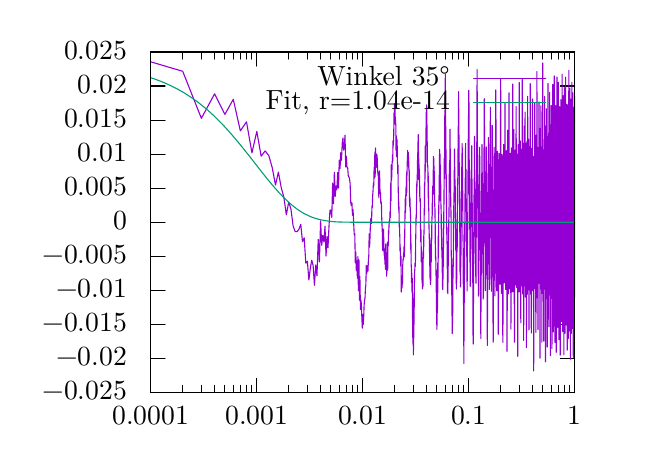
\begin{tikzpicture}[gnuplot]
%% generated with GNUPLOT 5.2p5a (Gentoo revision r0) (Lua 5.1; terminal rev. 99 , script rev. 107)
%% Sa 18 Mai 2019 18:30:43 CEST
\path (0.000,0.000) rectangle (7.500,5.250);
\gpcolor{color=gp lt color border}
\gpsetlinetype{gp lt border}
\gpsetdashtype{gp dt solid}
\gpsetlinewidth{1.00}
\draw[gp path] (1.564,0.616)--(1.744,0.616);
\draw[gp path] (6.947,0.616)--(6.767,0.616);
\node[gp node right] at (1.380,0.616) {$-0.025$};
\draw[gp path] (1.564,1.049)--(1.744,1.049);
\draw[gp path] (6.947,1.049)--(6.767,1.049);
\node[gp node right] at (1.380,1.049) {$-0.02$};
\draw[gp path] (1.564,1.481)--(1.744,1.481);
\draw[gp path] (6.947,1.481)--(6.767,1.481);
\node[gp node right] at (1.380,1.481) {$-0.015$};
\draw[gp path] (1.564,1.914)--(1.744,1.914);
\draw[gp path] (6.947,1.914)--(6.767,1.914);
\node[gp node right] at (1.380,1.914) {$-0.01$};
\draw[gp path] (1.564,2.346)--(1.744,2.346);
\draw[gp path] (6.947,2.346)--(6.767,2.346);
\node[gp node right] at (1.380,2.346) {$-0.005$};
\draw[gp path] (1.564,2.779)--(1.744,2.779);
\draw[gp path] (6.947,2.779)--(6.767,2.779);
\node[gp node right] at (1.380,2.779) {$0$};
\draw[gp path] (1.564,3.211)--(1.744,3.211);
\draw[gp path] (6.947,3.211)--(6.767,3.211);
\node[gp node right] at (1.380,3.211) {$0.005$};
\draw[gp path] (1.564,3.644)--(1.744,3.644);
\draw[gp path] (6.947,3.644)--(6.767,3.644);
\node[gp node right] at (1.380,3.644) {$0.01$};
\draw[gp path] (1.564,4.076)--(1.744,4.076);
\draw[gp path] (6.947,4.076)--(6.767,4.076);
\node[gp node right] at (1.380,4.076) {$0.015$};
\draw[gp path] (1.564,4.509)--(1.744,4.509);
\draw[gp path] (6.947,4.509)--(6.767,4.509);
\node[gp node right] at (1.380,4.509) {$0.02$};
\draw[gp path] (1.564,4.941)--(1.744,4.941);
\draw[gp path] (6.947,4.941)--(6.767,4.941);
\node[gp node right] at (1.380,4.941) {$0.025$};
\draw[gp path] (1.564,0.616)--(1.564,0.796);
\draw[gp path] (1.564,4.941)--(1.564,4.761);
\node[gp node center] at (1.564,0.308) {$0.0001$};
\draw[gp path] (1.969,0.616)--(1.969,0.706);
\draw[gp path] (1.969,4.941)--(1.969,4.851);
\draw[gp path] (2.206,0.616)--(2.206,0.706);
\draw[gp path] (2.206,4.941)--(2.206,4.851);
\draw[gp path] (2.374,0.616)--(2.374,0.706);
\draw[gp path] (2.374,4.941)--(2.374,4.851);
\draw[gp path] (2.505,0.616)--(2.505,0.706);
\draw[gp path] (2.505,4.941)--(2.505,4.851);
\draw[gp path] (2.611,0.616)--(2.611,0.706);
\draw[gp path] (2.611,4.941)--(2.611,4.851);
\draw[gp path] (2.701,0.616)--(2.701,0.706);
\draw[gp path] (2.701,4.941)--(2.701,4.851);
\draw[gp path] (2.779,0.616)--(2.779,0.706);
\draw[gp path] (2.779,4.941)--(2.779,4.851);
\draw[gp path] (2.848,0.616)--(2.848,0.706);
\draw[gp path] (2.848,4.941)--(2.848,4.851);
\draw[gp path] (2.910,0.616)--(2.910,0.796);
\draw[gp path] (2.910,4.941)--(2.910,4.761);
\node[gp node center] at (2.910,0.308) {$0.001$};
\draw[gp path] (3.315,0.616)--(3.315,0.706);
\draw[gp path] (3.315,4.941)--(3.315,4.851);
\draw[gp path] (3.552,0.616)--(3.552,0.706);
\draw[gp path] (3.552,4.941)--(3.552,4.851);
\draw[gp path] (3.720,0.616)--(3.720,0.706);
\draw[gp path] (3.720,4.941)--(3.720,4.851);
\draw[gp path] (3.850,0.616)--(3.850,0.706);
\draw[gp path] (3.850,4.941)--(3.850,4.851);
\draw[gp path] (3.957,0.616)--(3.957,0.706);
\draw[gp path] (3.957,4.941)--(3.957,4.851);
\draw[gp path] (4.047,0.616)--(4.047,0.706);
\draw[gp path] (4.047,4.941)--(4.047,4.851);
\draw[gp path] (4.125,0.616)--(4.125,0.706);
\draw[gp path] (4.125,4.941)--(4.125,4.851);
\draw[gp path] (4.194,0.616)--(4.194,0.706);
\draw[gp path] (4.194,4.941)--(4.194,4.851);
\draw[gp path] (4.255,0.616)--(4.255,0.796);
\draw[gp path] (4.255,4.941)--(4.255,4.761);
\node[gp node center] at (4.255,0.308) {$0.01$};
\draw[gp path] (4.661,0.616)--(4.661,0.706);
\draw[gp path] (4.661,4.941)--(4.661,4.851);
\draw[gp path] (4.898,0.616)--(4.898,0.706);
\draw[gp path] (4.898,4.941)--(4.898,4.851);
\draw[gp path] (5.066,0.616)--(5.066,0.706);
\draw[gp path] (5.066,4.941)--(5.066,4.851);
\draw[gp path] (5.196,0.616)--(5.196,0.706);
\draw[gp path] (5.196,4.941)--(5.196,4.851);
\draw[gp path] (5.303,0.616)--(5.303,0.706);
\draw[gp path] (5.303,4.941)--(5.303,4.851);
\draw[gp path] (5.393,0.616)--(5.393,0.706);
\draw[gp path] (5.393,4.941)--(5.393,4.851);
\draw[gp path] (5.471,0.616)--(5.471,0.706);
\draw[gp path] (5.471,4.941)--(5.471,4.851);
\draw[gp path] (5.540,0.616)--(5.540,0.706);
\draw[gp path] (5.540,4.941)--(5.540,4.851);
\draw[gp path] (5.601,0.616)--(5.601,0.796);
\draw[gp path] (5.601,4.941)--(5.601,4.761);
\node[gp node center] at (5.601,0.308) {$0.1$};
\draw[gp path] (6.006,0.616)--(6.006,0.706);
\draw[gp path] (6.006,4.941)--(6.006,4.851);
\draw[gp path] (6.243,0.616)--(6.243,0.706);
\draw[gp path] (6.243,4.941)--(6.243,4.851);
\draw[gp path] (6.411,0.616)--(6.411,0.706);
\draw[gp path] (6.411,4.941)--(6.411,4.851);
\draw[gp path] (6.542,0.616)--(6.542,0.706);
\draw[gp path] (6.542,4.941)--(6.542,4.851);
\draw[gp path] (6.648,0.616)--(6.648,0.706);
\draw[gp path] (6.648,4.941)--(6.648,4.851);
\draw[gp path] (6.739,0.616)--(6.739,0.706);
\draw[gp path] (6.739,4.941)--(6.739,4.851);
\draw[gp path] (6.817,0.616)--(6.817,0.706);
\draw[gp path] (6.817,4.941)--(6.817,4.851);
\draw[gp path] (6.885,0.616)--(6.885,0.706);
\draw[gp path] (6.885,4.941)--(6.885,4.851);
\draw[gp path] (6.947,0.616)--(6.947,0.796);
\draw[gp path] (6.947,4.941)--(6.947,4.761);
\node[gp node center] at (6.947,0.308) {$1$};
\draw[gp path] (1.564,4.941)--(1.564,0.616)--(6.947,0.616)--(6.947,4.941)--cycle;
\node[gp node right] at (5.479,4.607) {Winkel 35°};
\gpcolor{rgb color={0.580,0.000,0.827}}
\draw[gp path] (5.663,4.607)--(6.579,4.607);
\draw[gp path] (1.564,4.816)--(1.969,4.696)--(2.206,4.099)--(2.374,4.410)--(2.505,4.149)%
  --(2.611,4.340)--(2.701,3.939)--(2.779,4.054)--(2.848,3.660)--(2.910,3.933)--(2.965,3.618)%
  --(3.016,3.685)--(3.063,3.624)--(3.106,3.471)--(3.147,3.251)--(3.184,3.415)--(3.220,3.219)%
  --(3.253,3.100)--(3.285,2.873)--(3.315,3.035)--(3.343,2.950)--(3.371,2.733)--(3.397,2.660)%
  --(3.421,2.660)--(3.445,2.690)--(3.468,2.753)--(3.490,2.533)--(3.512,2.581)--(3.532,2.260)%
  --(3.552,2.285)--(3.571,2.046)--(3.590,2.198)--(3.608,2.297)--(3.625,2.230)--(3.642,1.978)%
  --(3.658,2.236)--(3.674,2.098)--(3.690,2.562)--(3.705,2.275)--(3.720,2.796)--(3.734,2.486)%
  --(3.748,2.613)--(3.762,2.530)--(3.776,2.728)--(3.789,2.350)--(3.802,2.596)--(3.814,2.455)%
  --(3.827,2.734)--(3.839,2.931)--(3.850,2.934)--(3.862,2.841)--(3.873,3.276)--(3.884,3.013)%
  --(3.895,3.414)--(3.906,3.107)--(3.917,3.241)--(3.927,3.195)--(3.937,3.413)--(3.947,3.212)%
  --(3.957,3.566)--(3.967,3.462)--(3.976,3.661)--(3.985,3.565)--(3.995,3.782)--(4.004,3.849)%
  --(4.013,3.695)--(4.021,3.724)--(4.030,3.886)--(4.039,3.481)--(4.047,3.616)--(4.055,3.479)%
  --(4.064,3.471)--(4.072,3.366)--(4.080,3.355)--(4.087,3.334)--(4.095,3.272)--(4.103,3.029)%
  --(4.110,2.990)--(4.118,3.026)--(4.125,2.867)--(4.132,2.942)--(4.140,2.768)--(4.147,2.625)%
  --(4.154,2.635)--(4.161,2.262)--(4.167,2.402)--(4.174,2.164)--(4.181,2.290)--(4.187,2.069)%
  --(4.194,2.343)--(4.200,1.909)--(4.207,2.302)--(4.213,1.791)--(4.219,2.092)--(4.226,1.669)%
  --(4.232,1.791)--(4.238,1.739)--(4.244,1.565)--(4.250,1.434)--(4.256,1.604)--(4.261,1.478)%
  --(4.267,1.570)--(4.273,1.732)--(4.278,1.787)--(4.284,1.815)--(4.290,1.947)--(4.295,1.983)%
  --(4.300,2.229)--(4.306,2.127)--(4.311,2.165)--(4.316,2.227)--(4.322,2.158)--(4.327,2.303)%
  --(4.332,2.348)--(4.337,2.633)--(4.342,2.463)--(4.347,2.571)--(4.352,2.730)--(4.357,2.819)%
  --(4.362,2.831)--(4.367,2.764)--(4.372,2.986)--(4.376,2.964)--(4.381,3.110)--(4.386,3.177)%
  --(4.391,3.280)--(4.395,3.240)--(4.400,3.478)--(4.404,3.339)--(4.409,3.669)--(4.413,3.358)%
  --(4.418,3.723)--(4.422,3.577)--(4.427,3.647)--(4.431,3.476)--(4.435,3.638)--(4.439,3.593)%
  --(4.444,3.458)--(4.448,3.386)--(4.452,3.412)--(4.456,3.206)--(4.460,3.090)--(4.465,3.305)%
  --(4.469,3.432)--(4.473,3.210)--(4.477,3.162)--(4.481,3.150)--(4.485,3.021)--(4.489,3.012)%
  --(4.492,3.035)--(4.496,2.844)--(4.500,2.744)--(4.504,2.650)--(4.508,2.422)--(4.512,2.693)%
  --(4.515,2.612)--(4.519,2.691)--(4.523,2.519)--(4.527,2.360)--(4.530,2.406)--(4.534,2.360)%
  --(4.537,2.245)--(4.541,2.441)--(4.545,2.180)--(4.548,2.504)--(4.552,2.289)--(4.555,2.339)%
  --(4.559,2.093)--(4.562,2.272)--(4.566,2.198)--(4.569,2.526)--(4.572,2.172)--(4.576,2.526)%
  --(4.579,2.482)--(4.583,2.679)--(4.586,2.628)--(4.589,2.742)--(4.593,2.802)--(4.596,2.769)%
  --(4.599,2.829)--(4.602,2.914)--(4.605,2.838)--(4.609,3.121)--(4.612,3.291)--(4.615,3.051)%
  --(4.618,3.509)--(4.621,3.312)--(4.624,3.366)--(4.628,3.506)--(4.631,3.564)--(4.634,3.638)%
  --(4.637,3.558)--(4.640,3.815)--(4.643,3.755)--(4.646,3.805)--(4.649,3.893)--(4.652,4.168)%
  --(4.655,4.023)--(4.658,4.285)--(4.661,4.179)--(4.664,4.245)--(4.666,4.112)--(4.669,4.114)%
  --(4.672,4.044)--(4.675,4.028)--(4.678,3.692)--(4.681,3.877)--(4.684,3.612)--(4.686,3.850)%
  --(4.689,3.609)--(4.692,3.828)--(4.695,3.549)--(4.697,3.538)--(4.700,3.393)--(4.703,3.506)%
  --(4.706,3.182)--(4.708,3.118)--(4.711,2.941)--(4.714,3.035)--(4.716,2.926)--(4.719,2.725)%
  --(4.722,2.743)--(4.724,2.645)--(4.727,2.565)--(4.729,2.413)--(4.732,2.460)--(4.735,2.323)%
  --(4.737,2.225)--(4.740,2.241)--(4.742,2.347)--(4.745,1.893)--(4.747,1.965)--(4.750,1.948)%
  --(4.752,2.001)--(4.755,1.943)--(4.757,2.006)--(4.760,2.011)--(4.762,2.220)--(4.765,2.256)%
  --(4.767,2.312)--(4.770,2.306)--(4.772,2.319)--(4.774,2.393)--(4.777,2.371)--(4.779,2.463)%
  --(4.782,2.339)--(4.784,2.592)--(4.786,2.400)--(4.789,2.658)--(4.791,2.795)--(4.793,2.954)%
  --(4.796,3.083)--(4.798,2.987)--(4.800,2.904)--(4.803,3.210)--(4.805,3.146)--(4.807,3.233)%
  --(4.809,3.115)--(4.812,3.414)--(4.814,3.154)--(4.816,3.432)--(4.818,3.375)--(4.821,3.556)%
  --(4.823,3.496)--(4.825,3.691)--(4.827,3.532)--(4.829,3.605)--(4.832,3.670)--(4.834,3.655)%
  --(4.836,3.605)--(4.838,3.470)--(4.840,3.552)--(4.842,3.431)--(4.845,3.456)--(4.847,3.266)%
  --(4.849,3.086)--(4.851,2.975)--(4.853,3.095)--(4.855,3.075)--(4.857,2.924)--(4.859,2.965)%
  --(4.861,2.879)--(4.863,2.805)--(4.866,2.387)--(4.868,2.510)--(4.870,2.255)--(4.872,2.214)%
  --(4.874,2.014)--(4.876,2.182)--(4.878,2.081)--(4.880,1.903)--(4.882,1.922)--(4.884,2.067)%
  --(4.886,1.549)--(4.888,1.813)--(4.890,1.314)--(4.892,1.597)--(4.894,1.237)--(4.896,1.495)%
  --(4.898,1.094)--(4.900,1.705)--(4.901,1.150)--(4.903,1.488)--(4.905,1.306)--(4.907,1.892)%
  --(4.909,1.697)--(4.911,1.945)--(4.913,2.096)--(4.915,2.160)--(4.917,2.184)--(4.919,2.257)%
  --(4.921,2.260)--(4.922,2.215)--(4.924,2.244)--(4.926,2.404)--(4.928,2.582)--(4.930,2.666)%
  --(4.932,2.818)--(4.933,2.873)--(4.935,2.833)--(4.937,3.003)--(4.939,3.018)--(4.941,3.269)%
  --(4.943,3.151)--(4.944,3.267)--(4.946,3.336)--(4.948,3.385)--(4.950,3.365)--(4.952,3.659)%
  --(4.953,3.610)--(4.955,3.599)--(4.957,3.771)--(4.959,3.859)--(4.960,3.887)--(4.962,3.892)%
  --(4.964,3.320)--(4.966,3.588)--(4.967,3.353)--(4.969,3.518)--(4.971,3.402)--(4.972,3.483)%
  --(4.974,3.291)--(4.976,3.282)--(4.978,3.380)--(4.979,3.153)--(4.981,3.043)--(4.983,3.059)%
  --(4.984,3.034)--(4.986,3.081)--(4.988,2.812)--(4.989,2.712)--(4.991,2.530)--(4.993,2.644)%
  --(4.994,2.582)--(4.996,2.684)--(4.998,2.277)--(4.999,2.469)--(5.001,2.317)--(5.003,2.445)%
  --(5.004,2.419)--(5.006,2.278)--(5.007,2.147)--(5.009,2.011)--(5.011,2.019)--(5.012,1.997)%
  --(5.014,1.932)--(5.015,1.967)--(5.017,2.176)--(5.019,2.033)--(5.020,2.181)--(5.022,1.966)%
  --(5.023,2.317)--(5.025,2.343)--(5.026,2.322)--(5.028,2.421)--(5.030,2.604)--(5.031,2.469)%
  --(5.033,2.671)--(5.034,2.681)--(5.036,2.893)--(5.037,2.955)--(5.039,2.913)--(5.040,3.260)%
  --(5.042,3.240)--(5.043,3.244)--(5.045,3.427)--(5.046,3.513)--(5.048,3.328)--(5.049,3.747)%
  --(5.051,3.429)--(5.052,3.646)--(5.054,3.628)--(5.055,3.743)--(5.057,3.543)--(5.058,3.975)%
  --(5.060,3.979)--(5.061,4.156)--(5.063,4.184)--(5.064,4.029)--(5.066,4.269)--(5.067,4.150)%
  --(5.069,4.248)--(5.070,4.097)--(5.072,3.862)--(5.073,3.755)--(5.074,3.802)--(5.076,3.714)%
  --(5.077,3.514)--(5.079,3.480)--(5.080,3.503)--(5.082,3.481)--(5.083,3.491)--(5.084,3.302)%
  --(5.086,3.261)--(5.087,3.093)--(5.089,3.365)--(5.090,3.033)--(5.091,3.011)--(5.093,2.922)%
  --(5.094,2.957)--(5.096,2.704)--(5.097,2.694)--(5.098,2.750)--(5.100,2.568)--(5.101,2.584)%
  --(5.103,2.390)--(5.104,2.503)--(5.105,2.256)--(5.107,2.220)--(5.108,2.184)--(5.109,2.075)%
  --(5.111,2.150)--(5.112,2.064)--(5.113,2.054)--(5.115,1.988)--(5.116,2.006)--(5.117,2.180)%
  --(5.119,2.037)--(5.120,2.266)--(5.121,2.307)--(5.123,2.581)--(5.124,2.272)--(5.125,2.272)%
  --(5.127,2.418)--(5.128,2.558)--(5.129,2.533)--(5.131,2.561)--(5.132,2.710)--(5.133,2.809)%
  --(5.135,2.815)--(5.136,2.887)--(5.137,3.022)--(5.138,2.867)--(5.140,3.122)--(5.141,3.031)%
  --(5.142,3.194)--(5.144,3.237)--(5.145,3.236)--(5.146,3.141)--(5.147,3.128)--(5.149,3.304)%
  --(5.150,3.442)--(5.151,3.288)--(5.152,3.615)--(5.154,3.463)--(5.155,3.516)--(5.156,3.499)%
  --(5.157,3.591)--(5.159,3.375)--(5.160,3.472)--(5.161,3.375)--(5.162,3.489)--(5.164,3.324)%
  --(5.165,3.283)--(5.166,3.192)--(5.167,3.162)--(5.169,2.980)--(5.170,3.021)--(5.171,2.948)%
  --(5.172,3.000)--(5.173,2.830)--(5.175,2.833)--(5.176,2.658)--(5.177,2.472)--(5.178,2.520)%
  --(5.180,2.325)--(5.181,2.349)--(5.182,2.341)--(5.183,2.308)--(5.184,2.254)--(5.186,2.104)%
  --(5.187,2.098)--(5.188,1.956)--(5.189,1.893)--(5.190,1.903)--(5.191,1.758)--(5.193,1.621)%
  --(5.194,1.481)--(5.195,1.640)--(5.196,1.725)--(5.197,1.417)--(5.198,1.652)--(5.200,1.465)%
  --(5.201,1.705)--(5.202,1.628)--(5.203,1.664)--(5.204,1.648)--(5.205,2.171)--(5.207,1.880)%
  --(5.208,2.263)--(5.209,1.885)--(5.210,2.183)--(5.211,2.074)--(5.212,2.297)--(5.213,2.206)%
  --(5.215,2.620)--(5.216,2.603)--(5.217,2.469)--(5.218,2.613)--(5.219,2.679)--(5.220,2.997)%
  --(5.221,2.885)--(5.222,3.079)--(5.224,3.029)--(5.225,3.238)--(5.226,3.181)--(5.227,3.381)%
  --(5.228,3.279)--(5.229,3.474)--(5.230,3.644)--(5.231,3.588)--(5.232,3.704)--(5.233,3.625)%
  --(5.235,3.543)--(5.236,3.569)--(5.237,3.641)--(5.238,3.521)--(5.239,3.510)--(5.240,3.415)%
  --(5.241,3.392)--(5.242,3.296)--(5.243,3.053)--(5.244,3.307)--(5.245,3.292)--(5.247,3.064)%
  --(5.248,3.062)--(5.249,2.949)--(5.250,2.965)--(5.251,2.851)--(5.252,2.880)--(5.253,2.692)%
  --(5.254,2.729)--(5.255,2.591)--(5.256,2.726)--(5.257,2.541)--(5.258,2.585)--(5.259,2.427)%
  --(5.260,2.532)--(5.261,2.353)--(5.262,2.458)--(5.263,2.208)--(5.264,2.377)--(5.265,2.161)%
  --(5.267,2.099)--(5.268,1.958)--(5.269,2.154)--(5.270,1.934)--(5.271,1.967)--(5.272,1.924)%
  --(5.273,2.128)--(5.274,2.054)--(5.275,2.105)--(5.276,2.305)--(5.277,2.203)--(5.278,2.330)%
  --(5.279,2.459)--(5.280,2.372)--(5.281,2.696)--(5.282,2.638)--(5.283,2.678)--(5.284,2.738)%
  --(5.285,2.968)--(5.286,2.902)--(5.287,3.081)--(5.288,3.198)--(5.289,3.305)--(5.290,3.416)%
  --(5.291,3.587)--(5.292,3.382)--(5.293,3.599)--(5.294,3.330)--(5.295,3.795)--(5.296,3.891)%
  --(5.297,4.134)--(5.298,3.740)--(5.299,4.121)--(5.300,4.020)--(5.301,4.303)--(5.302,4.209)%
  --(5.303,4.607)--(5.304,4.274)--(5.305,4.665)--(5.306,3.944)--(5.307,4.207)--(5.308,3.928)%
  --(5.309,3.995)--(5.309,3.680)--(5.310,3.821)--(5.311,3.517)--(5.312,3.704)--(5.313,3.393)%
  --(5.314,3.427)--(5.315,3.410)--(5.316,3.271)--(5.317,3.175)--(5.318,3.195)--(5.319,2.897)%
  --(5.320,2.898)--(5.321,2.809)--(5.322,2.626)--(5.323,2.655)--(5.324,2.608)--(5.325,2.505)%
  --(5.326,2.519)--(5.327,2.398)--(5.327,2.193)--(5.328,2.261)--(5.329,2.343)--(5.330,2.200)%
  --(5.331,2.122)--(5.332,1.886)--(5.333,2.073)--(5.334,2.018)--(5.335,2.135)--(5.336,1.871)%
  --(5.337,2.142)--(5.338,2.014)--(5.339,2.375)--(5.340,2.096)--(5.340,2.402)--(5.341,2.225)%
  --(5.342,2.486)--(5.343,2.392)--(5.344,2.715)--(5.345,2.632)--(5.346,2.555)--(5.347,2.774)%
  --(5.348,2.809)--(5.349,2.659)--(5.349,2.775)--(5.350,2.843)--(5.351,2.896)--(5.352,3.056)%
  --(5.353,3.147)--(5.354,3.173)--(5.355,3.527)--(5.356,3.355)--(5.357,3.316)--(5.358,3.215)%
  --(5.358,3.319)--(5.359,3.419)--(5.360,3.567)--(5.361,3.505)--(5.362,3.580)--(5.363,3.614)%
  --(5.364,3.960)--(5.365,3.667)--(5.365,3.855)--(5.366,3.707)--(5.367,3.711)--(5.368,3.431)%
  --(5.369,3.330)--(5.370,3.231)--(5.371,3.179)--(5.372,3.186)--(5.372,3.127)--(5.373,3.014)%
  --(5.374,2.949)--(5.375,2.913)--(5.376,2.838)--(5.377,2.928)--(5.378,2.674)--(5.378,2.572)%
  --(5.379,2.346)--(5.380,2.348)--(5.381,2.410)--(5.382,2.106)--(5.383,2.326)--(5.384,1.993)%
  --(5.384,2.013)--(5.385,1.854)--(5.386,2.057)--(5.387,1.686)--(5.388,2.067)--(5.389,1.735)%
  --(5.389,1.685)--(5.390,1.506)--(5.391,1.481)--(5.392,1.366)--(5.393,1.518)--(5.394,1.470)%
  --(5.394,1.586)--(5.395,1.482)--(5.396,1.701)--(5.397,1.688)--(5.398,1.624)--(5.399,1.919)%
  --(5.399,1.960)--(5.400,2.001)--(5.401,2.076)--(5.402,2.238)--(5.403,2.078)--(5.404,2.160)%
  --(5.404,2.210)--(5.405,2.289)--(5.406,2.353)--(5.407,2.549)--(5.408,2.536)--(5.408,2.634)%
  --(5.409,2.986)--(5.410,2.928)--(5.411,2.893)--(5.412,2.969)--(5.412,2.835)--(5.413,3.073)%
  --(5.414,3.086)--(5.415,3.158)--(5.416,3.312)--(5.417,3.232)--(5.417,3.440)--(5.418,3.367)%
  --(5.419,3.557)--(5.420,3.709)--(5.421,3.537)--(5.421,3.488)--(5.422,3.529)--(5.423,3.484)%
  --(5.424,3.438)--(5.424,3.343)--(5.425,3.400)--(5.426,3.239)--(5.427,3.210)--(5.428,3.173)%
  --(5.428,3.034)--(5.429,3.321)--(5.430,3.131)--(5.431,3.179)--(5.432,2.967)--(5.432,2.846)%
  --(5.433,2.905)--(5.434,2.697)--(5.435,2.537)--(5.435,2.550)--(5.436,2.429)--(5.437,2.576)%
  --(5.438,2.692)--(5.439,2.457)--(5.439,2.449)--(5.440,2.436)--(5.441,2.361)--(5.442,2.420)%
  --(5.442,1.997)--(5.443,2.282)--(5.444,2.173)--(5.445,2.218)--(5.445,1.930)--(5.446,2.308)%
  --(5.447,2.028)--(5.448,2.165)--(5.448,2.010)--(5.449,2.201)--(5.450,2.056)--(5.451,2.331)%
  --(5.452,2.430)--(5.452,2.543)--(5.453,2.571)--(5.454,2.481)--(5.455,2.461)--(5.455,2.476)%
  --(5.456,2.811)--(5.457,2.761)--(5.458,3.107)--(5.458,3.001)--(5.459,3.227)--(5.460,2.987)%
  --(5.461,3.262)--(5.461,3.248)--(5.462,3.291)--(5.463,3.384)--(5.463,3.421)--(5.464,3.382)%
  --(5.465,3.515)--(5.466,3.784)--(5.466,3.521)--(5.467,3.859)--(5.468,3.993)--(5.469,3.920)%
  --(5.469,4.193)--(5.470,4.209)--(5.471,4.337)--(5.472,4.333)--(5.472,4.137)--(5.473,4.439)%
  --(5.474,3.960)--(5.474,4.223)--(5.475,3.784)--(5.476,3.979)--(5.477,3.782)--(5.477,3.681)%
  --(5.478,3.390)--(5.479,3.882)--(5.480,3.593)--(5.480,3.601)--(5.481,3.367)--(5.482,3.531)%
  --(5.482,3.270)--(5.483,3.277)--(5.484,3.023)--(5.485,3.019)--(5.485,2.845)--(5.486,2.831)%
  --(5.487,2.730)--(5.487,2.725)--(5.488,2.647)--(5.489,2.639)--(5.490,2.428)--(5.490,2.152)%
  --(5.491,2.158)--(5.492,2.222)--(5.492,2.144)--(5.493,2.112)--(5.494,2.243)--(5.494,2.290)%
  --(5.495,2.218)--(5.496,1.957)--(5.497,2.026)--(5.497,2.254)--(5.498,1.975)--(5.499,2.152)%
  --(5.499,2.273)--(5.500,2.538)--(5.501,2.211)--(5.501,2.603)--(5.502,2.440)--(5.503,2.478)%
  --(5.504,2.359)--(5.504,2.603)--(5.505,2.586)--(5.506,3.054)--(5.506,2.713)--(5.507,3.076)%
  --(5.508,2.885)--(5.508,3.027)--(5.509,3.185)--(5.510,3.177)--(5.510,3.056)--(5.511,3.245)%
  --(5.512,3.183)--(5.512,3.479)--(5.513,3.133)--(5.514,3.539)--(5.514,3.239)--(5.515,3.404)%
  --(5.516,3.428)--(5.516,3.656)--(5.517,3.556)--(5.518,3.778)--(5.519,3.643)--(5.519,3.492)%
  --(5.520,3.608)--(5.521,3.692)--(5.521,3.273)--(5.522,3.434)--(5.523,3.232)--(5.523,3.131)%
  --(5.524,3.246)--(5.525,3.153)--(5.525,2.960)--(5.526,2.922)--(5.527,2.910)--(5.527,2.848)%
  --(5.528,2.570)--(5.529,2.621)--(5.529,2.537)--(5.530,2.549)--(5.531,2.289)--(5.531,2.466)%
  --(5.532,2.144)--(5.532,2.034)--(5.533,1.937)--(5.534,2.054)--(5.534,1.793)--(5.535,1.987)%
  --(5.536,1.547)--(5.536,1.879)--(5.537,1.213)--(5.538,1.539)--(5.538,1.208)--(5.539,1.506)%
  --(5.540,0.985)--(5.540,1.373)--(5.541,1.269)--(5.542,1.657)--(5.542,1.497)--(5.543,1.798)%
  --(5.544,1.755)--(5.544,1.919)--(5.545,1.894)--(5.545,2.130)--(5.546,2.013)--(5.547,2.114)%
  --(5.547,2.140)--(5.548,2.405)--(5.549,2.138)--(5.549,2.322)--(5.550,2.523)--(5.551,2.590)%
  --(5.551,2.684)--(5.552,2.869)--(5.553,2.882)--(5.553,2.924)--(5.554,3.074)--(5.554,3.067)%
  --(5.555,3.181)--(5.556,3.239)--(5.556,3.155)--(5.557,3.341)--(5.558,3.128)--(5.558,3.436)%
  --(5.559,3.443)--(5.559,3.613)--(5.560,3.478)--(5.561,3.728)--(5.561,3.550)--(5.562,3.780)%
  --(5.563,3.338)--(5.563,3.447)--(5.564,3.268)--(5.564,3.339)--(5.565,3.120)--(5.566,3.455)%
  --(5.566,3.071)--(5.567,3.191)--(5.568,3.114)--(5.568,2.985)--(5.569,2.910)--(5.569,3.103)%
  --(5.570,2.941)--(5.571,3.042)--(5.571,2.808)--(5.572,2.901)--(5.573,2.532)--(5.573,2.671)%
  --(5.574,2.467)--(5.574,2.550)--(5.575,2.480)--(5.576,2.457)--(5.576,2.346)--(5.577,2.475)%
  --(5.577,2.372)--(5.578,2.311)--(5.579,2.162)--(5.579,2.271)--(5.580,2.215)--(5.580,2.026)%
  --(5.581,1.906)--(5.582,2.075)--(5.582,2.031)--(5.583,2.201)--(5.583,2.101)--(5.584,2.216)%
  --(5.585,2.201)--(5.585,2.498)--(5.586,2.523)--(5.586,2.482)--(5.587,2.509)--(5.588,2.576)%
  --(5.588,2.728)--(5.589,2.675)--(5.589,2.906)--(5.590,2.862)--(5.591,2.940)--(5.591,3.226)%
  --(5.592,3.121)--(5.592,3.433)--(5.593,3.356)--(5.594,3.601)--(5.594,3.627)--(5.595,3.613)%
  --(5.595,3.589)--(5.596,3.856)--(5.597,3.492)--(5.597,3.703)--(5.598,3.849)--(5.598,3.995)%
  --(5.599,4.141)--(5.599,4.067)--(5.600,4.068)--(5.601,4.422)--(5.601,4.454)--(5.602,4.271)%
  --(5.602,4.177)--(5.603,3.988)--(5.604,4.042)--(5.604,4.342)--(5.605,3.822)--(5.605,3.720)%
  --(5.606,3.712)--(5.606,3.547)--(5.607,3.584)--(5.608,3.549)--(5.608,3.522)--(5.609,3.339)%
  --(5.609,3.438)--(5.610,3.368)--(5.611,3.434)--(5.611,3.190)--(5.612,3.124)--(5.612,3.109)%
  --(5.613,2.853)--(5.613,2.795)--(5.614,2.791)--(5.615,2.684)--(5.615,2.511)--(5.616,2.662)%
  --(5.616,2.462)--(5.617,2.521)--(5.617,2.352)--(5.618,2.278)--(5.619,2.207)--(5.619,2.226)%
  --(5.620,2.168)--(5.620,2.024)--(5.621,2.061)--(5.621,1.964)--(5.622,1.990)--(5.622,2.235)%
  --(5.623,2.187)--(5.624,2.404)--(5.624,2.360)--(5.625,2.260)--(5.625,2.431)--(5.626,2.452)%
  --(5.626,2.372)--(5.627,2.384)--(5.628,2.480)--(5.628,2.561)--(5.629,2.517)--(5.629,2.621)%
  --(5.630,2.827)--(5.630,2.716)--(5.631,3.087)--(5.631,3.013)--(5.632,3.017)--(5.633,3.045)%
  --(5.633,3.107)--(5.634,3.116)--(5.634,3.337)--(5.635,3.264)--(5.635,3.299)--(5.636,3.300)%
  --(5.636,3.451)--(5.637,3.321)--(5.638,3.458)--(5.638,3.408)--(5.639,3.752)--(5.639,3.487)%
  --(5.640,3.651)--(5.640,3.463)--(5.641,3.678)--(5.641,3.262)--(5.642,3.494)--(5.642,3.173)%
  --(5.643,3.327)--(5.644,3.122)--(5.644,2.992)--(5.645,2.888)--(5.645,2.940)--(5.646,3.024)%
  --(5.646,2.834)--(5.647,2.867)--(5.647,2.661)--(5.648,2.515)--(5.649,2.550)--(5.649,2.653)%
  --(5.650,2.414)--(5.651,2.169)--(5.651,2.334)--(5.652,2.223)--(5.652,2.158)--(5.653,2.008)%
  --(5.653,2.098)--(5.654,1.992)--(5.654,1.752)--(5.655,1.730)--(5.655,1.580)--(5.656,1.577)%
  --(5.656,1.343)--(5.657,1.395)--(5.657,1.416)--(5.658,1.409)--(5.659,1.233)--(5.659,1.722)%
  --(5.660,1.539)--(5.660,1.905)--(5.661,1.577)--(5.661,1.966)--(5.662,1.747)--(5.662,2.034)%
  --(5.663,2.094)--(5.663,2.222)--(5.664,2.093)--(5.664,2.328)--(5.665,2.250)--(5.665,2.469)%
  --(5.666,2.373)--(5.666,2.551)--(5.667,2.610)--(5.667,2.768)--(5.668,2.820)--(5.669,3.154)%
  --(5.669,3.068)--(5.670,3.093)--(5.670,2.997)--(5.671,3.197)--(5.671,3.309)--(5.672,3.299)%
  --(5.672,3.321)--(5.673,3.564)--(5.673,3.585)--(5.674,3.869)--(5.674,3.696)--(5.675,3.632)%
  --(5.675,3.677)--(5.676,3.707)--(5.676,3.563)--(5.677,3.537)--(5.677,3.407)--(5.678,3.444)%
  --(5.678,3.345)--(5.679,3.255)--(5.679,3.227)--(5.680,3.285)--(5.680,3.234)--(5.681,3.124)%
  --(5.681,3.006)--(5.682,3.096)--(5.682,2.782)--(5.683,3.012)--(5.683,2.597)--(5.684,2.863)%
  --(5.684,2.621)--(5.685,2.589)--(5.685,2.569)--(5.686,2.730)--(5.686,2.582)--(5.687,2.646)%
  --(5.687,2.384)--(5.688,2.407)--(5.688,2.090)--(5.689,2.387)--(5.690,2.178)--(5.690,2.316)%
  --(5.691,2.197)--(5.691,2.318)--(5.692,2.228)--(5.692,2.162)--(5.693,2.118)--(5.693,2.086)%
  --(5.694,2.004)--(5.694,2.195)--(5.695,2.054)--(5.695,2.174)--(5.696,2.590)--(5.696,2.556)%
  --(5.696,2.730)--(5.697,2.775)--(5.697,2.586)--(5.698,2.890)--(5.698,2.775)--(5.699,2.928)%
  --(5.699,2.946)--(5.700,3.193)--(5.700,3.066)--(5.701,3.400)--(5.701,3.386)--(5.702,3.504)%
  --(5.702,3.505)--(5.703,3.663)--(5.703,3.618)--(5.704,3.829)--(5.704,3.770)--(5.705,4.078)%
  --(5.705,3.790)--(5.706,4.201)--(5.706,3.943)--(5.707,4.520)--(5.707,4.167)--(5.708,4.717)%
  --(5.708,4.250)--(5.709,4.442)--(5.709,4.087)--(5.710,4.275)--(5.710,3.762)--(5.711,4.006)%
  --(5.711,3.832)--(5.712,3.699)--(5.712,3.748)--(5.713,3.628)--(5.713,3.405)--(5.714,3.486)%
  --(5.714,3.328)--(5.715,3.315)--(5.715,3.150)--(5.716,3.260)--(5.716,2.957)--(5.717,3.024)%
  --(5.717,2.881)--(5.717,2.824)--(5.718,2.725)--(5.718,2.614)--(5.719,2.713)--(5.719,2.636)%
  --(5.720,2.567)--(5.720,2.394)--(5.721,2.224)--(5.721,2.297)--(5.722,2.165)--(5.722,2.202)%
  --(5.723,2.091)--(5.723,2.211)--(5.724,1.971)--(5.724,2.266)--(5.725,1.840)--(5.725,2.329)%
  --(5.726,2.064)--(5.726,2.236)--(5.727,2.275)--(5.727,2.416)--(5.727,2.441)--(5.728,2.426)%
  --(5.728,2.516)--(5.729,2.551)--(5.729,2.528)--(5.730,2.538)--(5.730,2.480)--(5.731,2.590)%
  --(5.731,2.728)--(5.732,2.870)--(5.732,2.978)--(5.733,2.875)--(5.733,2.959)--(5.734,3.133)%
  --(5.734,2.966)--(5.734,3.186)--(5.735,3.383)--(5.735,3.368)--(5.736,3.163)--(5.736,3.177)%
  --(5.737,3.311)--(5.737,3.328)--(5.738,3.513)--(5.738,3.431)--(5.739,3.692)--(5.739,3.667)%
  --(5.740,3.565)--(5.740,3.528)--(5.740,3.730)--(5.741,3.544)--(5.741,3.448)--(5.742,3.444)%
  --(5.742,3.381)--(5.743,3.300)--(5.743,3.120)--(5.744,3.173)--(5.744,3.009)--(5.745,2.978)%
  --(5.745,2.843)--(5.746,2.838)--(5.746,2.812)--(5.746,2.573)--(5.747,2.580)--(5.747,2.703)%
  --(5.748,2.288)--(5.748,2.367)--(5.749,2.196)--(5.749,2.164)--(5.750,1.951)--(5.750,2.159)%
  --(5.751,1.857)--(5.751,1.974)--(5.751,1.858)--(5.752,1.903)--(5.752,1.748)--(5.753,1.734)%
  --(5.753,1.685)--(5.754,1.656)--(5.754,1.479)--(5.755,1.302)--(5.755,1.372)--(5.755,1.502)%
  --(5.756,1.468)--(5.756,1.545)--(5.757,1.745)--(5.757,1.983)--(5.758,1.996)--(5.758,2.001)%
  --(5.759,2.016)--(5.759,2.114)--(5.760,2.107)--(5.760,2.163)--(5.760,2.242)--(5.761,2.238)%
  --(5.761,2.330)--(5.762,2.386)--(5.762,2.526)--(5.763,2.530)--(5.763,2.591)--(5.764,2.863)%
  --(5.764,2.840)--(5.764,2.881)--(5.765,2.999)--(5.765,2.994)--(5.766,3.031)--(5.766,3.344)%
  --(5.767,3.197)--(5.767,3.319)--(5.767,3.358)--(5.768,3.477)--(5.768,3.579)--(5.769,3.754)%
  --(5.769,3.765)--(5.770,3.764)--(5.770,3.548)--(5.771,3.667)--(5.771,3.445)--(5.771,3.473)%
  --(5.772,3.473)--(5.772,3.505)--(5.773,3.250)--(5.773,3.298)--(5.774,3.267)--(5.774,3.238)%
  --(5.774,3.092)--(5.775,3.194)--(5.775,3.036)--(5.776,3.058)--(5.776,3.101)--(5.777,2.912)%
  --(5.777,2.785)--(5.778,2.773)--(5.778,2.602)--(5.778,2.471)--(5.779,2.778)--(5.779,2.510)%
  --(5.780,2.371)--(5.780,2.474)--(5.781,2.441)--(5.781,2.350)--(5.781,2.337)--(5.782,2.257)%
  --(5.782,2.193)--(5.783,2.136)--(5.783,2.255)--(5.784,2.037)--(5.784,2.098)--(5.784,2.028)%
  --(5.785,2.309)--(5.785,1.802)--(5.786,2.164)--(5.786,2.107)--(5.787,2.470)--(5.787,2.226)%
  --(5.787,2.411)--(5.788,2.533)--(5.788,2.503)--(5.789,2.531)--(5.789,2.619)--(5.789,2.666)%
  --(5.790,2.751)--(5.790,2.978)--(5.791,2.930)--(5.791,3.126)--(5.792,3.153)--(5.792,3.082)%
  --(5.792,3.204)--(5.793,3.294)--(5.793,3.236)--(5.794,3.423)--(5.794,3.689)--(5.795,3.472)%
  --(5.795,3.668)--(5.795,3.657)--(5.796,3.731)--(5.796,3.872)--(5.797,4.032)--(5.797,4.085)%
  --(5.797,4.079)--(5.798,4.339)--(5.798,4.307)--(5.799,4.174)--(5.799,4.348)--(5.800,4.131)%
  --(5.800,4.174)--(5.800,3.821)--(5.801,4.005)--(5.801,3.682)--(5.802,3.830)--(5.802,3.463)%
  --(5.802,3.573)--(5.803,3.426)--(5.803,3.638)--(5.804,3.366)--(5.804,3.436)--(5.805,3.294)%
  --(5.805,3.137)--(5.805,2.978)--(5.806,2.948)--(5.806,2.786)--(5.807,2.909)--(5.807,2.635)%
  --(5.807,2.740)--(5.808,2.541)--(5.808,2.611)--(5.809,2.394)--(5.809,2.291)--(5.809,2.329)%
  --(5.810,2.178)--(5.810,2.162)--(5.811,1.933)--(5.811,1.935)--(5.812,1.910)--(5.812,2.006)%
  --(5.812,2.029)--(5.813,1.989)--(5.813,1.992)--(5.814,2.179)--(5.814,2.241)--(5.814,2.128)%
  --(5.815,2.450)--(5.815,2.337)--(5.816,2.471)--(5.816,2.378)--(5.816,2.733)--(5.817,2.631)%
  --(5.817,2.596)--(5.818,2.564)--(5.818,2.728)--(5.818,2.843)--(5.819,2.831)--(5.819,2.908)%
  --(5.820,2.797)--(5.820,3.059)--(5.820,3.097)--(5.821,3.183)--(5.821,3.195)--(5.822,3.093)%
  --(5.822,3.262)--(5.822,3.161)--(5.823,3.373)--(5.823,3.434)--(5.824,3.577)--(5.824,3.443)%
  --(5.824,3.730)--(5.825,3.554)--(5.825,3.679)--(5.826,3.735)--(5.826,3.661)--(5.826,3.582)%
  --(5.827,3.388)--(5.827,3.561)--(5.828,3.451)--(5.828,3.406)--(5.828,3.255)--(5.829,3.052)%
  --(5.829,3.244)--(5.830,3.079)--(5.830,2.880)--(5.830,3.022)--(5.831,2.744)--(5.831,2.644)%
  --(5.832,2.752)--(5.832,2.448)--(5.832,2.457)--(5.833,2.271)--(5.833,2.355)--(5.834,2.129)%
  --(5.834,2.132)--(5.834,2.060)--(5.835,2.000)--(5.835,1.703)--(5.835,2.126)--(5.836,1.524)%
  --(5.836,1.802)--(5.837,1.447)--(5.837,1.701)--(5.837,1.292)--(5.838,1.830)--(5.838,1.215)%
  --(5.839,1.543)--(5.839,1.313)--(5.839,1.566)--(5.840,1.511)--(5.840,1.733)--(5.841,1.785)%
  --(5.841,1.871)--(5.841,1.886)--(5.842,2.197)--(5.842,2.073)--(5.842,2.229)--(5.843,2.305)%
  --(5.843,2.371)--(5.844,2.270)--(5.844,2.448)--(5.844,2.453)--(5.845,2.874)--(5.845,2.658)%
  --(5.846,2.627)--(5.846,2.848)--(5.846,2.951)--(5.847,3.069)--(5.847,2.959)--(5.848,2.943)%
  --(5.848,3.139)--(5.848,3.183)--(5.849,3.403)--(5.849,3.311)--(5.849,3.313)--(5.850,3.402)%
  --(5.850,3.628)--(5.851,3.534)--(5.851,3.856)--(5.851,3.536)--(5.852,3.776)--(5.852,3.366)%
  --(5.852,3.451)--(5.853,3.379)--(5.853,3.305)--(5.854,3.299)--(5.854,3.297)--(5.854,3.037)%
  --(5.855,3.172)--(5.855,2.996)--(5.856,3.165)--(5.856,3.062)--(5.856,3.138)--(5.857,3.033)%
  --(5.857,2.890)--(5.857,2.871)--(5.858,2.913)--(5.858,2.554)--(5.859,2.737)--(5.859,2.671)%
  --(5.859,2.517)--(5.860,2.530)--(5.860,2.306)--(5.860,2.324)--(5.861,2.282)--(5.861,2.419)%
  --(5.862,2.240)--(5.862,2.285)--(5.862,2.080)--(5.863,2.025)--(5.863,1.986)--(5.863,1.971)%
  --(5.864,1.997)--(5.864,1.925)--(5.865,2.232)--(5.865,2.087)--(5.865,2.076)--(5.866,2.333)%
  --(5.866,2.245)--(5.866,2.370)--(5.867,2.383)--(5.867,2.666)--(5.867,2.477)--(5.868,2.643)%
  --(5.868,2.685)--(5.869,2.929)--(5.869,2.821)--(5.869,2.855)--(5.870,3.031)--(5.870,3.204)%
  --(5.870,3.155)--(5.871,3.081)--(5.871,3.476)--(5.872,3.374)--(5.872,3.517)--(5.872,3.350)%
  --(5.873,3.698)--(5.873,3.547)--(5.873,3.653)--(5.874,3.589)--(5.874,3.935)--(5.874,3.975)%
  --(5.875,3.798)--(5.875,3.989)--(5.876,4.240)--(5.876,4.040)--(5.876,3.992)--(5.877,4.148)%
  --(5.877,4.011)--(5.877,4.030)--(5.878,3.930)--(5.878,3.651)--(5.878,3.777)--(5.879,3.551)%
  --(5.879,3.667)--(5.880,3.384)--(5.880,3.377)--(5.880,3.454)--(5.881,3.238)--(5.881,3.247)%
  --(5.881,3.249)--(5.882,3.373)--(5.882,3.005)--(5.882,3.166)--(5.883,2.998)--(5.883,2.957)%
  --(5.884,2.803)--(5.884,2.660)--(5.884,2.750)--(5.885,2.626)--(5.885,2.506)--(5.885,2.477)%
  --(5.886,2.324)--(5.886,2.352)--(5.886,2.307)--(5.887,2.299)--(5.887,2.210)--(5.888,2.102)%
  --(5.888,1.983)--(5.888,2.072)--(5.889,1.903)--(5.889,2.047)--(5.889,1.967)--(5.890,2.104)%
  --(5.890,2.164)--(5.890,2.455)--(5.891,2.399)--(5.891,2.346)--(5.891,2.441)--(5.892,2.511)%
  --(5.892,2.370)--(5.893,2.569)--(5.893,2.505)--(5.893,2.652)--(5.894,2.719)--(5.894,2.853)%
  --(5.894,2.734)--(5.895,3.155)--(5.895,2.970)--(5.895,2.961)--(5.896,3.028)--(5.896,3.077)%
  --(5.896,3.188)--(5.897,3.135)--(5.897,3.151)--(5.897,3.481)--(5.898,3.300)--(5.898,3.387)%
  --(5.899,3.394)--(5.899,3.525)--(5.899,3.476)--(5.900,4.008)--(5.900,3.625)--(5.900,3.835)%
  --(5.901,3.581)--(5.901,3.599)--(5.901,3.402)--(5.902,3.333)--(5.902,3.298)--(5.902,3.373)%
  --(5.903,3.032)--(5.903,3.102)--(5.903,3.104)--(5.904,3.150)--(5.904,2.999)--(5.904,2.979)%
  --(5.905,2.993)--(5.905,2.718)--(5.906,2.663)--(5.906,2.555)--(5.906,2.631)--(5.907,2.479)%
  --(5.907,2.287)--(5.907,2.282)--(5.908,2.161)--(5.908,2.299)--(5.908,2.124)--(5.909,2.003)%
  --(5.909,2.022)--(5.909,1.874)--(5.910,1.842)--(5.910,1.745)--(5.910,1.499)--(5.911,1.628)%
  --(5.911,1.489)--(5.911,1.409)--(5.912,1.299)--(5.912,1.399)--(5.912,1.254)--(5.913,1.597)%
  --(5.913,1.322)--(5.913,1.714)--(5.914,1.530)--(5.914,1.852)--(5.914,1.759)--(5.915,2.128)%
  --(5.915,1.851)--(5.915,2.081)--(5.916,2.039)--(5.916,2.191)--(5.917,2.270)--(5.917,2.364)%
  --(5.917,2.439)--(5.918,2.511)--(5.918,2.622)--(5.918,2.714)--(5.919,2.707)--(5.919,3.078)%
  --(5.919,3.017)--(5.920,3.060)--(5.920,3.007)--(5.920,3.158)--(5.921,3.258)--(5.921,3.439)%
  --(5.921,3.407)--(5.922,3.619)--(5.922,3.559)--(5.922,3.581)--(5.923,3.625)--(5.923,3.718)%
  --(5.923,3.730)--(5.924,3.421)--(5.924,3.508)--(5.924,3.556)--(5.925,3.471)--(5.925,3.384)%
  --(5.925,3.301)--(5.926,3.279)--(5.926,3.216)--(5.926,3.404)--(5.927,3.072)--(5.927,3.304)%
  --(5.927,2.960)--(5.928,3.032)--(5.928,2.859)--(5.928,2.856)--(5.929,2.886)--(5.929,2.737)%
  --(5.929,2.412)--(5.930,2.768)--(5.930,2.549)--(5.930,2.641)--(5.931,2.477)--(5.931,2.557)%
  --(5.931,2.392)--(5.932,2.337)--(5.932,2.068)--(5.932,2.247)--(5.933,2.062)--(5.933,2.155)%
  --(5.933,1.945)--(5.934,1.844)--(5.934,1.864)--(5.934,1.959)--(5.935,2.029)--(5.935,1.954)%
  --(5.935,2.086)--(5.936,2.103)--(5.936,2.126)--(5.936,2.462)--(5.937,2.366)--(5.937,2.357)%
  --(5.937,2.552)--(5.938,2.679)--(5.938,2.635)--(5.938,2.764)--(5.939,2.763)--(5.939,2.981)%
  --(5.939,2.854)--(5.940,3.127)--(5.940,3.197)--(5.940,3.406)--(5.941,3.192)--(5.941,3.407)%
  --(5.941,3.336)--(5.942,3.664)--(5.942,3.372)--(5.942,3.734)--(5.943,3.675)--(5.943,3.847)%
  --(5.943,3.771)--(5.943,4.143)--(5.944,3.929)--(5.944,4.411)--(5.944,4.210)--(5.945,4.459)%
  --(5.945,4.202)--(5.945,4.270)--(5.946,4.043)--(5.946,4.154)--(5.946,3.973)--(5.947,4.085)%
  --(5.947,3.853)--(5.947,3.763)--(5.948,3.559)--(5.948,3.718)--(5.948,3.525)--(5.949,3.436)%
  --(5.949,3.377)--(5.949,3.268)--(5.950,3.324)--(5.950,3.169)--(5.950,3.170)--(5.951,2.968)%
  --(5.951,2.919)--(5.951,2.811)--(5.952,2.746)--(5.952,2.674)--(5.952,2.591)--(5.953,2.618)%
  --(5.953,2.396)--(5.953,2.445)--(5.953,2.402)--(5.954,2.381)--(5.954,2.161)--(5.954,2.390)%
  --(5.955,2.004)--(5.955,2.368)--(5.955,2.207)--(5.956,2.379)--(5.956,2.010)--(5.956,2.258)%
  --(5.957,1.908)--(5.957,2.306)--(5.957,2.193)--(5.958,2.527)--(5.958,2.337)--(5.958,2.483)%
  --(5.959,2.464)--(5.959,2.561)--(5.959,2.434)--(5.960,2.554)--(5.960,2.550)--(5.960,2.690)%
  --(5.960,2.817)--(5.961,2.870)--(5.961,2.841)--(5.961,2.888)--(5.962,2.788)--(5.962,3.236)%
  --(5.962,3.061)--(5.963,3.242)--(5.963,3.194)--(5.963,3.248)--(5.964,3.388)--(5.964,3.261)%
  --(5.964,3.336)--(5.965,3.379)--(5.965,3.494)--(5.965,3.543)--(5.966,3.679)--(5.966,3.680)%
  --(5.966,3.648)--(5.966,3.581)--(5.967,3.561)--(5.967,3.671)--(5.967,3.461)--(5.968,3.312)%
  --(5.968,3.243)--(5.968,3.218)--(5.969,3.166)--(5.969,3.095)--(5.969,3.037)--(5.970,2.866)%
  --(5.970,2.943)--(5.970,2.640)--(5.971,2.751)--(5.971,2.651)--(5.971,2.556)--(5.971,2.334)%
  --(5.972,2.392)--(5.972,2.479)--(5.972,2.183)--(5.973,2.337)--(5.973,2.164)--(5.973,2.184)%
  --(5.974,1.970)--(5.974,1.992)--(5.974,1.989)--(5.975,1.960)--(5.975,1.940)--(5.975,1.716)%
  --(5.975,1.592)--(5.976,1.613)--(5.976,1.666)--(5.976,1.444)--(5.977,1.355)--(5.977,1.663)%
  --(5.977,1.526)--(5.978,1.618)--(5.978,1.759)--(5.978,1.790)--(5.979,1.802)--(5.979,1.985)%
  --(5.979,2.188)--(5.979,2.030)--(5.980,2.245)--(5.980,2.078)--(5.980,2.221)--(5.981,2.162)%
  --(5.981,2.278)--(5.981,2.176)--(5.982,2.447)--(5.982,2.598)--(5.982,2.541)--(5.983,2.729)%
  --(5.983,2.792)--(5.983,2.796)--(5.983,2.929)--(5.984,3.062)--(5.984,3.008)--(5.984,3.089)%
  --(5.985,3.140)--(5.985,3.233)--(5.985,3.255)--(5.986,3.396)--(5.986,3.238)--(5.986,3.462)%
  --(5.986,3.518)--(5.987,3.651)--(5.987,3.568)--(5.987,3.576)--(5.988,3.575)--(5.988,3.490)%
  --(5.988,3.319)--(5.989,3.249)--(5.989,3.256)--(5.989,3.180)--(5.989,3.260)--(5.990,3.121)%
  --(5.990,3.069)--(5.990,3.156)--(5.991,3.170)--(5.991,2.945)--(5.991,2.950)--(5.992,2.808)%
  --(5.992,2.865)--(5.992,2.689)--(5.992,2.793)--(5.993,2.462)--(5.993,2.489)--(5.993,2.612)%
  --(5.994,2.631)--(5.994,2.528)--(5.994,2.545)--(5.995,2.329)--(5.995,2.325)--(5.995,2.310)%
  --(5.995,2.179)--(5.996,2.161)--(5.996,2.231)--(5.996,2.136)--(5.997,2.104)--(5.997,2.051)%
  --(5.997,2.337)--(5.998,2.001)--(5.998,1.991)--(5.998,2.243)--(5.998,2.202)--(5.999,2.292)%
  --(5.999,2.380)--(5.999,2.393)--(6.000,2.585)--(6.000,2.595)--(6.000,2.717)--(6.000,2.608)%
  --(6.001,2.811)--(6.001,2.876)--(6.001,2.860)--(6.002,3.181)--(6.002,3.119)--(6.002,3.128)%
  --(6.003,3.262)--(6.003,3.478)--(6.003,3.401)--(6.003,3.357)--(6.004,3.738)--(6.004,3.649)%
  --(6.004,3.544)--(6.005,3.903)--(6.005,3.753)--(6.005,4.002)--(6.005,4.161)--(6.006,4.218)%
  --(6.006,4.449)--(6.006,4.396)--(6.007,4.595)--(6.007,4.334)--(6.007,4.556)--(6.008,4.207)%
  --(6.008,4.252)--(6.008,3.870)--(6.008,4.243)--(6.009,3.650)--(6.009,4.015)--(6.009,3.692)%
  --(6.010,3.688)--(6.010,3.482)--(6.010,3.625)--(6.010,3.410)--(6.011,3.479)--(6.011,3.296)%
  --(6.011,3.093)--(6.012,3.157)--(6.012,2.926)--(6.012,3.072)--(6.012,2.635)--(6.013,2.819)%
  --(6.013,2.556)--(6.013,2.555)--(6.014,2.498)--(6.014,2.372)--(6.014,2.495)--(6.014,2.214)%
  --(6.015,2.142)--(6.015,2.140)--(6.015,2.149)--(6.016,1.874)--(6.016,1.939)--(6.016,1.889)%
  --(6.017,1.983)--(6.017,1.921)--(6.017,2.059)--(6.017,2.006)--(6.018,2.121)--(6.018,2.287)%
  --(6.018,2.413)--(6.019,2.304)--(6.019,2.488)--(6.019,2.366)--(6.019,2.551)--(6.020,2.470)%
  --(6.020,2.708)--(6.020,2.475)--(6.021,2.669)--(6.021,2.781)--(6.021,2.941)--(6.021,2.889)%
  --(6.022,3.036)--(6.022,2.942)--(6.022,3.107)--(6.023,3.023)--(6.023,3.213)--(6.023,3.031)%
  --(6.023,3.231)--(6.024,3.142)--(6.024,3.522)--(6.024,3.362)--(6.024,3.624)--(6.025,3.435)%
  --(6.025,3.619)--(6.025,3.598)--(6.026,3.580)--(6.026,3.581)--(6.026,3.608)--(6.026,3.641)%
  --(6.027,3.452)--(6.027,3.510)--(6.027,3.364)--(6.028,3.213)--(6.028,3.114)--(6.028,3.156)%
  --(6.028,3.153)--(6.029,2.965)--(6.029,2.958)--(6.029,2.910)--(6.030,2.903)--(6.030,2.760)%
  --(6.030,2.772)--(6.030,2.505)--(6.031,2.524)--(6.031,2.409)--(6.031,2.359)--(6.032,2.219)%
  --(6.032,2.266)--(6.032,2.130)--(6.032,2.115)--(6.033,1.826)--(6.033,1.990)--(6.033,1.808)%
  --(6.033,1.751)--(6.034,1.341)--(6.034,1.675)--(6.034,1.343)--(6.035,1.394)--(6.035,1.251)%
  --(6.035,1.514)--(6.035,1.339)--(6.036,1.497)--(6.036,1.484)--(6.036,1.663)--(6.037,1.667)%
  --(6.037,1.936)--(6.037,2.073)--(6.037,2.243)--(6.038,2.093)--(6.038,2.104)--(6.038,2.186)%
  --(6.038,2.098)--(6.039,2.375)--(6.039,2.236)--(6.039,2.438)--(6.040,2.454)--(6.040,2.448)%
  --(6.040,2.727)--(6.040,2.697)--(6.041,2.834)--(6.041,2.921)--(6.041,2.953)--(6.042,3.200)%
  --(6.042,3.189)--(6.042,3.223)--(6.043,3.164)--(6.043,3.511)--(6.043,3.465)--(6.043,3.623)%
  --(6.044,3.349)--(6.044,3.767)--(6.044,3.391)--(6.045,3.723)--(6.045,3.379)--(6.045,3.502)%
  --(6.045,3.279)--(6.046,3.628)--(6.046,3.308)--(6.046,3.419)--(6.046,3.173)--(6.047,3.212)%
  --(6.047,3.172)--(6.047,3.228)--(6.048,3.161)--(6.048,3.039)--(6.048,2.973)--(6.048,2.994)%
  --(6.049,2.956)--(6.049,2.709)--(6.049,2.612)--(6.049,2.732)--(6.050,2.579)--(6.050,2.658)%
  --(6.050,2.499)--(6.051,2.580)--(6.051,2.429)--(6.051,2.550)--(6.051,2.385)--(6.052,2.378)%
  --(6.052,2.239)--(6.052,2.131)--(6.052,2.008)--(6.053,2.229)--(6.053,2.358)--(6.053,2.217)%
  --(6.054,2.047)--(6.054,2.105)--(6.054,2.162)--(6.054,2.345)--(6.055,2.440)--(6.055,2.229)%
  --(6.055,2.496)--(6.055,2.441)--(6.056,2.591)--(6.056,2.780)--(6.056,2.679)--(6.056,2.688)%
  --(6.057,2.880)--(6.057,2.932)--(6.057,2.925)--(6.058,3.092)--(6.058,3.187)--(6.058,3.295)%
  --(6.058,3.214)--(6.059,3.504)--(6.059,3.393)--(6.059,3.573)--(6.059,3.531)--(6.060,3.491)%
  --(6.060,3.486)--(6.060,3.671)--(6.060,3.729)--(6.061,3.766)--(6.061,3.760)--(6.061,3.830)%
  --(6.062,3.943)--(6.062,4.147)--(6.062,4.157)--(6.062,4.287)--(6.063,4.220)--(6.063,4.185)%
  --(6.063,4.048)--(6.063,3.961)--(6.064,3.882)--(6.064,3.776)--(6.064,3.692)--(6.064,3.749)%
  --(6.065,3.569)--(6.065,3.431)--(6.065,3.448)--(6.066,3.314)--(6.066,3.397)--(6.066,3.229)%
  --(6.066,3.308)--(6.067,3.141)--(6.067,3.162)--(6.067,2.971)--(6.067,3.012)--(6.068,2.863)%
  --(6.068,2.577)--(6.068,2.609)--(6.068,2.499)--(6.069,2.646)--(6.069,2.556)--(6.069,2.536)%
  --(6.069,2.236)--(6.070,2.376)--(6.070,2.334)--(6.070,2.268)--(6.071,2.127)--(6.071,1.924)%
  --(6.071,2.047)--(6.071,1.930)--(6.072,2.066)--(6.072,2.115)--(6.072,2.084)--(6.072,2.196)%
  --(6.073,2.291)--(6.073,2.255)--(6.073,2.378)--(6.073,2.226)--(6.074,2.364)--(6.074,2.434)%
  --(6.074,2.507)--(6.074,2.425)--(6.075,2.585)--(6.075,2.744)--(6.075,2.647)--(6.075,2.808)%
  --(6.076,2.873)--(6.076,2.875)--(6.076,3.104)--(6.076,3.115)--(6.077,3.218)--(6.077,2.972)%
  --(6.077,3.286)--(6.078,3.075)--(6.078,3.280)--(6.078,3.114)--(6.078,3.338)--(6.079,3.256)%
  --(6.079,3.491)--(6.079,3.316)--(6.079,3.515)--(6.080,3.298)--(6.080,3.688)--(6.080,3.322)%
  --(6.080,3.412)--(6.081,3.254)--(6.081,3.531)--(6.081,3.425)--(6.081,3.491)--(6.082,3.218)%
  --(6.082,3.069)--(6.082,3.252)--(6.082,2.981)--(6.083,2.917)--(6.083,2.908)--(6.083,2.900)%
  --(6.083,2.802)--(6.084,2.759)--(6.084,2.558)--(6.084,2.435)--(6.084,2.378)--(6.085,2.496)%
  --(6.085,2.454)--(6.085,2.227)--(6.085,2.330)--(6.086,2.257)--(6.086,2.045)--(6.086,1.869)%
  --(6.087,1.993)--(6.087,1.826)--(6.087,1.726)--(6.087,1.578)--(6.088,1.564)--(6.088,1.335)%
  --(6.088,1.493)--(6.088,1.140)--(6.089,1.516)--(6.089,1.197)--(6.089,1.625)--(6.089,1.236)%
  --(6.090,1.776)--(6.090,1.653)--(6.090,2.049)--(6.090,1.757)--(6.091,2.144)--(6.091,1.873)%
  --(6.091,2.204)--(6.091,1.977)--(6.092,2.227)--(6.092,2.305)--(6.092,2.598)--(6.092,2.490)%
  --(6.093,2.736)--(6.093,2.779)--(6.093,2.780)--(6.093,2.835)--(6.094,2.887)--(6.094,2.991)%
  --(6.094,3.113)--(6.094,3.304)--(6.095,3.231)--(6.095,3.289)--(6.095,3.290)--(6.095,3.403)%
  --(6.096,3.527)--(6.096,3.533)--(6.096,3.856)--(6.096,3.770)--(6.097,3.948)--(6.097,3.741)%
  --(6.097,3.871)--(6.097,3.578)--(6.098,3.732)--(6.098,3.423)--(6.098,3.609)--(6.098,3.192)%
  --(6.099,3.433)--(6.099,3.292)--(6.099,3.307)--(6.099,3.113)--(6.100,3.141)--(6.100,3.257)%
  --(6.100,3.113)--(6.100,3.125)--(6.101,3.036)--(6.101,2.871)--(6.101,2.968)--(6.101,2.344)%
  --(6.102,2.679)--(6.102,2.670)--(6.102,2.638)--(6.102,2.449)--(6.103,2.634)--(6.103,2.264)%
  --(6.103,2.515)--(6.103,2.237)--(6.104,2.318)--(6.104,1.955)--(6.104,2.117)--(6.104,2.010)%
  --(6.105,2.135)--(6.105,2.020)--(6.105,1.954)--(6.105,1.869)--(6.106,1.962)--(6.106,2.132)%
  --(6.106,2.140)--(6.106,2.120)--(6.107,2.200)--(6.107,2.345)--(6.107,2.492)--(6.107,2.532)%
  --(6.108,2.488)--(6.108,2.427)--(6.108,2.734)--(6.108,2.905)--(6.109,2.941)--(6.109,2.987)%
  --(6.109,3.067)--(6.109,3.144)--(6.109,3.278)--(6.110,3.333)--(6.110,3.457)--(6.110,3.325)%
  --(6.110,3.686)--(6.111,3.592)--(6.111,3.756)--(6.111,3.571)--(6.111,3.998)--(6.112,3.769)%
  --(6.112,4.186)--(6.112,3.878)--(6.112,4.368)--(6.113,4.088)--(6.113,4.413)--(6.113,4.130)%
  --(6.113,4.423)--(6.114,4.211)--(6.114,4.183)--(6.114,3.766)--(6.114,3.898)--(6.115,3.883)%
  --(6.115,3.635)--(6.115,3.612)--(6.115,3.665)--(6.116,3.563)--(6.116,3.459)--(6.116,3.461)%
  --(6.116,3.571)--(6.117,3.192)--(6.117,3.073)--(6.117,3.035)--(6.117,2.951)--(6.118,2.932)%
  --(6.118,3.044)--(6.118,2.717)--(6.118,2.777)--(6.118,2.690)--(6.119,2.713)--(6.119,2.301)%
  --(6.119,2.463)--(6.119,2.318)--(6.120,2.327)--(6.120,2.188)--(6.120,2.203)--(6.120,2.115)%
  --(6.121,2.223)--(6.121,1.988)--(6.121,2.204)--(6.121,1.932)--(6.122,2.098)--(6.122,2.155)%
  --(6.122,2.111)--(6.122,2.149)--(6.123,2.415)--(6.123,2.178)--(6.123,2.407)--(6.123,2.346)%
  --(6.124,2.560)--(6.124,2.585)--(6.124,2.600)--(6.124,2.459)--(6.124,2.771)--(6.125,2.553)%
  --(6.125,2.713)--(6.125,2.739)--(6.125,2.964)--(6.126,3.029)--(6.126,3.065)--(6.126,3.071)%
  --(6.126,3.189)--(6.127,3.255)--(6.127,3.188)--(6.127,3.228)--(6.127,3.292)--(6.128,3.216)%
  --(6.128,3.360)--(6.128,3.567)--(6.128,3.543)--(6.129,3.497)--(6.129,3.559)--(6.129,3.449)%
  --(6.129,3.543)--(6.129,3.526)--(6.130,3.654)--(6.130,3.532)--(6.130,3.266)--(6.130,3.358)%
  --(6.131,3.164)--(6.131,3.300)--(6.131,2.997)--(6.131,3.084)--(6.132,3.150)--(6.132,3.158)%
  --(6.132,2.845)--(6.132,2.846)--(6.133,2.757)--(6.133,2.648)--(6.133,2.665)--(6.133,2.607)%
  --(6.133,2.364)--(6.134,2.157)--(6.134,2.301)--(6.134,2.188)--(6.134,2.217)--(6.135,2.134)%
  --(6.135,2.183)--(6.135,2.060)--(6.135,1.881)--(6.136,1.929)--(6.136,1.830)--(6.136,1.774)%
  --(6.136,1.800)--(6.137,1.923)--(6.137,1.719)--(6.137,1.715)--(6.137,1.505)--(6.137,1.421)%
  --(6.138,1.586)--(6.138,1.833)--(6.138,1.575)--(6.138,1.865)--(6.139,1.959)--(6.139,2.164)%
  --(6.139,2.071)--(6.139,2.156)--(6.140,2.173)--(6.140,2.174)--(6.140,2.215)--(6.140,2.349)%
  --(6.141,2.271)--(6.141,2.246)--(6.141,2.525)--(6.141,2.585)--(6.141,2.545)--(6.142,2.807)%
  --(6.142,2.969)--(6.142,2.957)--(6.142,2.971)--(6.143,3.017)--(6.143,3.097)--(6.143,3.173)%
  --(6.143,3.214)--(6.144,3.440)--(6.144,3.377)--(6.144,3.481)--(6.144,3.724)--(6.144,3.650)%
  --(6.145,3.528)--(6.145,3.600)--(6.145,3.689)--(6.145,3.532)--(6.146,3.439)--(6.146,3.436)%
  --(6.146,3.281)--(6.146,3.286)--(6.147,3.219)--(6.147,3.353)--(6.147,3.063)--(6.147,3.075)%
  --(6.147,3.032)--(6.148,3.178)--(6.148,3.075)--(6.148,3.019)--(6.148,2.933)--(6.149,2.867)%
  --(6.149,2.752)--(6.149,2.719)--(6.149,2.405)--(6.149,2.612)--(6.150,2.493)--(6.150,2.555)%
  --(6.150,2.457)--(6.150,2.647)--(6.151,2.282)--(6.151,2.391)--(6.151,2.267)--(6.151,2.386)%
  --(6.152,1.938)--(6.152,2.160)--(6.152,1.906)--(6.152,2.310)--(6.152,1.920)--(6.153,2.110)%
  --(6.153,1.893)--(6.153,2.123)--(6.153,2.137)--(6.154,2.307)--(6.154,2.250)--(6.154,2.270)%
  --(6.154,2.395)--(6.155,2.587)--(6.155,2.573)--(6.155,2.688)--(6.155,2.621)--(6.155,2.688)%
  --(6.156,2.748)--(6.156,2.932)--(6.156,3.033)--(6.156,2.955)--(6.157,3.099)--(6.157,3.131)%
  --(6.157,3.373)--(6.157,3.477)--(6.157,3.538)--(6.158,3.610)--(6.158,3.639)--(6.158,3.614)%
  --(6.158,3.626)--(6.159,3.863)--(6.159,3.751)--(6.159,4.138)--(6.159,4.067)--(6.159,4.376)%
  --(6.160,4.131)--(6.160,4.479)--(6.160,4.185)--(6.160,4.534)--(6.161,3.977)--(6.161,4.341)%
  --(6.161,3.808)--(6.161,4.049)--(6.161,3.814)--(6.162,3.896)--(6.162,3.671)--(6.162,3.729)%
  --(6.162,3.498)--(6.163,3.489)--(6.163,3.412)--(6.163,3.408)--(6.163,3.160)--(6.164,3.100)%
  --(6.164,2.952)--(6.164,3.110)--(6.164,2.772)--(6.164,2.906)--(6.165,2.681)--(6.165,2.695)%
  --(6.165,2.631)--(6.165,2.593)--(6.166,2.284)--(6.166,2.378)--(6.166,2.240)--(6.166,2.201)%
  --(6.166,2.115)--(6.167,2.227)--(6.167,2.089)--(6.167,1.921)--(6.167,1.986)--(6.168,2.142)%
  --(6.168,1.898)--(6.168,2.003)--(6.168,2.099)--(6.168,2.382)--(6.169,2.267)--(6.169,2.511)%
  --(6.169,2.343)--(6.169,2.561)--(6.170,2.529)--(6.170,2.639)--(6.170,2.397)--(6.170,2.654)%
  --(6.170,2.667)--(6.171,2.832)--(6.171,2.719)--(6.171,2.772)--(6.171,2.821)--(6.171,2.894)%
  --(6.172,3.019)--(6.172,3.138)--(6.172,2.965)--(6.172,3.198)--(6.173,3.277)--(6.173,3.400)%
  --(6.173,3.302)--(6.173,3.527)--(6.173,3.309)--(6.174,3.486)--(6.174,3.497)--(6.174,3.798)%
  --(6.174,3.825)--(6.175,3.955)--(6.175,3.887)--(6.175,3.720)--(6.175,3.716)--(6.175,3.670)%
  --(6.176,3.477)--(6.176,3.419)--(6.176,3.340)--(6.176,3.179)--(6.177,3.295)--(6.177,3.044)%
  --(6.177,3.027)--(6.177,3.110)--(6.177,2.927)--(6.178,2.918)--(6.178,2.851)--(6.178,2.774)%
  --(6.178,2.589)--(6.179,2.373)--(6.179,2.221)--(6.179,2.266)--(6.179,2.174)--(6.179,2.148)%
  --(6.180,2.128)--(6.180,2.304)--(6.180,1.923)--(6.180,2.066)--(6.180,1.738)--(6.181,1.879)%
  --(6.181,1.453)--(6.181,1.730)--(6.181,1.396)--(6.182,1.472)--(6.182,1.282)--(6.182,1.365)%
  --(6.182,1.255)--(6.182,1.386)--(6.183,1.409)--(6.183,1.578)--(6.183,1.686)--(6.183,1.750)%
  --(6.183,2.019)--(6.184,1.957)--(6.184,2.204)--(6.184,2.145)--(6.184,2.203)--(6.185,2.215)%
  --(6.185,2.161)--(6.185,2.242)--(6.185,2.561)--(6.185,2.375)--(6.186,2.636)--(6.186,2.606)%
  --(6.186,2.706)--(6.186,2.872)--(6.187,2.916)--(6.187,2.831)--(6.187,2.961)--(6.187,3.079)%
  --(6.188,3.294)--(6.188,3.167)--(6.188,3.329)--(6.188,3.318)--(6.188,3.532)--(6.189,3.250)%
  --(6.189,3.669)--(6.189,3.399)--(6.189,3.693)--(6.189,3.263)--(6.190,3.613)--(6.190,3.325)%
  --(6.190,3.337)--(6.190,3.336)--(6.191,3.355)--(6.191,3.248)--(6.191,3.352)--(6.191,3.181)%
  --(6.191,3.103)--(6.192,3.237)--(6.192,3.085)--(6.192,2.996)--(6.192,3.151)--(6.192,2.824)%
  --(6.193,2.856)--(6.193,2.771)--(6.193,2.631)--(6.193,2.583)--(6.194,2.559)--(6.194,2.466)%
  --(6.194,2.459)--(6.194,2.474)--(6.194,2.400)--(6.195,2.265)--(6.195,2.246)--(6.195,2.237)%
  --(6.195,2.209)--(6.195,2.168)--(6.196,2.103)--(6.196,2.091)--(6.196,2.022)--(6.196,2.011)%
  --(6.197,2.127)--(6.197,1.982)--(6.197,2.182)--(6.197,2.309)--(6.197,2.245)--(6.198,2.390)%
  --(6.198,2.378)--(6.198,2.605)--(6.198,2.663)--(6.198,2.559)--(6.199,2.650)--(6.199,2.739)%
  --(6.199,2.757)--(6.199,2.870)--(6.199,3.048)--(6.200,3.048)--(6.200,3.165)--(6.200,3.096)%
  --(6.200,3.412)--(6.201,3.258)--(6.201,3.517)--(6.201,3.247)--(6.201,3.621)--(6.201,3.461)%
  --(6.202,3.430)--(6.202,3.753)--(6.202,3.780)--(6.202,3.816)--(6.202,3.858)--(6.203,3.996)%
  --(6.203,4.068)--(6.203,4.020)--(6.203,4.170)--(6.203,4.249)--(6.204,4.205)--(6.204,4.113)%
  --(6.204,4.019)--(6.204,3.914)--(6.204,3.792)--(6.205,3.844)--(6.205,3.674)--(6.205,3.631)%
  --(6.205,3.552)--(6.206,3.612)--(6.206,3.538)--(6.206,3.304)--(6.206,3.115)--(6.206,3.409)%
  --(6.207,3.148)--(6.207,3.248)--(6.207,3.116)--(6.207,2.900)--(6.207,2.811)--(6.208,2.777)%
  --(6.208,2.790)--(6.208,2.631)--(6.208,2.802)--(6.208,2.641)--(6.209,2.436)--(6.209,2.332)%
  --(6.209,2.347)--(6.209,2.341)--(6.209,2.168)--(6.210,2.280)--(6.210,2.204)--(6.210,2.210)%
  --(6.210,2.077)--(6.210,1.997)--(6.211,2.023)--(6.211,1.951)--(6.211,2.248)--(6.211,2.186)%
  --(6.212,2.322)--(6.212,2.297)--(6.212,2.332)--(6.212,2.313)--(6.212,2.220)--(6.213,2.667)%
  --(6.213,2.491)--(6.213,2.676)--(6.213,2.638)--(6.213,2.742)--(6.214,2.740)--(6.214,2.984)%
  --(6.214,2.931)--(6.214,3.080)--(6.214,3.028)--(6.215,3.076)--(6.215,3.133)--(6.215,3.084)%
  --(6.215,3.076)--(6.215,3.245)--(6.216,3.337)--(6.216,3.232)--(6.216,3.286)--(6.216,3.574)%
  --(6.216,3.486)--(6.217,3.488)--(6.217,3.487)--(6.217,3.544)--(6.217,3.504)--(6.217,3.582)%
  --(6.218,3.449)--(6.218,3.642)--(6.218,3.194)--(6.218,3.307)--(6.218,3.216)--(6.219,3.022)%
  --(6.219,3.042)--(6.219,3.082)--(6.219,3.106)--(6.219,3.013)--(6.220,2.924)--(6.220,2.712)%
  --(6.220,2.808)--(6.220,2.613)--(6.220,2.462)--(6.221,2.579)--(6.221,2.442)--(6.221,2.372)%
  --(6.221,2.170)--(6.222,2.289)--(6.222,2.064)--(6.222,2.067)--(6.222,1.951)--(6.222,1.891)%
  --(6.223,1.807)--(6.223,1.590)--(6.223,1.597)--(6.223,1.472)--(6.223,1.344)--(6.224,1.626)%
  --(6.224,1.171)--(6.224,1.201)--(6.224,1.076)--(6.224,1.619)--(6.225,1.233)--(6.225,1.747)%
  --(6.225,1.380)--(6.225,1.908)--(6.225,1.806)--(6.226,1.981)--(6.226,1.840)--(6.226,1.991)%
  --(6.226,2.224)--(6.226,2.142)--(6.227,2.242)--(6.227,2.494)--(6.227,2.382)--(6.227,2.500)%
  --(6.227,2.727)--(6.228,2.825)--(6.228,2.857)--(6.228,2.870)--(6.228,2.852)--(6.228,3.050)%
  --(6.229,2.955)--(6.229,3.193)--(6.229,3.201)--(6.229,3.223)--(6.229,3.312)--(6.230,3.394)%
  --(6.230,3.654)--(6.230,3.544)--(6.230,3.724)--(6.230,3.765)--(6.231,3.548)--(6.231,3.566)%
  --(6.231,3.495)--(6.231,3.451)--(6.232,3.377)--(6.232,3.182)--(6.232,3.201)--(6.232,3.212)%
  --(6.232,3.225)--(6.233,2.918)--(6.233,3.254)--(6.233,2.992)--(6.233,3.106)--(6.233,2.917)%
  --(6.234,2.930)--(6.234,2.799)--(6.234,2.738)--(6.234,2.690)--(6.234,2.596)--(6.235,2.486)%
  --(6.235,2.690)--(6.235,2.303)--(6.235,2.522)--(6.235,2.312)--(6.235,2.484)--(6.236,2.295)%
  --(6.236,2.346)--(6.236,2.111)--(6.236,2.224)--(6.236,2.026)--(6.237,1.894)--(6.237,1.968)%
  --(6.237,1.923)--(6.237,1.941)--(6.237,2.006)--(6.238,2.007)--(6.238,2.223)--(6.238,2.318)%
  --(6.238,2.398)--(6.238,2.243)--(6.239,2.438)--(6.239,2.531)--(6.239,2.528)--(6.239,2.476)%
  --(6.239,2.727)--(6.240,2.683)--(6.240,2.960)--(6.240,2.967)--(6.240,3.087)--(6.240,3.155)%
  --(6.241,3.395)--(6.241,3.277)--(6.241,3.572)--(6.241,3.453)--(6.241,3.579)--(6.242,3.596)%
  --(6.242,3.954)--(6.242,3.657)--(6.242,4.058)--(6.242,3.744)--(6.243,4.195)--(6.243,3.904)%
  --(6.243,4.328)--(6.243,4.388)--(6.243,4.555)--(6.244,4.545)--(6.244,4.497)--(6.244,4.238)%
  --(6.244,4.224)--(6.244,3.956)--(6.245,3.792)--(6.245,3.799)--(6.245,3.873)--(6.245,3.770)%
  --(6.245,3.439)--(6.245,3.591)--(6.246,3.516)--(6.246,3.486)--(6.246,3.417)--(6.246,3.386)%
  --(6.246,3.254)--(6.247,3.143)--(6.247,2.984)--(6.247,2.947)--(6.247,2.799)--(6.247,2.936)%
  --(6.248,2.786)--(6.248,2.546)--(6.248,2.471)--(6.248,2.482)--(6.248,2.574)--(6.249,2.457)%
  --(6.249,2.285)--(6.249,2.312)--(6.249,2.325)--(6.249,2.130)--(6.250,2.278)--(6.250,1.966)%
  --(6.250,2.102)--(6.250,2.009)--(6.250,2.046)--(6.251,1.896)--(6.251,2.100)--(6.251,2.241)%
  --(6.251,2.258)--(6.251,2.303)--(6.251,2.368)--(6.252,2.365)--(6.252,2.383)--(6.252,2.466)%
  --(6.252,2.456)--(6.252,2.410)--(6.253,2.580)--(6.253,2.536)--(6.253,2.757)--(6.253,2.734)%
  --(6.253,3.037)--(6.254,3.092)--(6.254,3.058)--(6.254,3.105)--(6.254,3.220)--(6.254,3.112)%
  --(6.255,3.212)--(6.255,3.260)--(6.255,3.218)--(6.255,3.250)--(6.255,3.174)--(6.255,3.387)%
  --(6.256,3.427)--(6.256,3.519)--(6.256,3.554)--(6.256,3.812)--(6.256,3.519)--(6.257,3.667)%
  --(6.257,3.596)--(6.257,3.568)--(6.257,3.397)--(6.257,3.332)--(6.258,3.347)--(6.258,3.195)%
  --(6.258,3.107)--(6.258,3.028)--(6.258,2.999)--(6.259,3.030)--(6.259,2.941)--(6.259,2.830)%
  --(6.259,2.738)--(6.259,2.767)--(6.259,2.749)--(6.260,2.496)--(6.260,2.357)--(6.260,2.240)%
  --(6.260,2.364)--(6.260,2.282)--(6.261,2.234)--(6.261,1.989)--(6.261,2.182)--(6.261,1.977)%
  --(6.261,2.032)--(6.262,2.019)--(6.262,1.850)--(6.262,1.667)--(6.262,1.553)--(6.262,1.583)%
  --(6.262,1.576)--(6.263,1.573)--(6.263,1.502)--(6.263,1.597)--(6.263,1.502)--(6.263,1.677)%
  --(6.264,1.789)--(6.264,1.780)--(6.264,1.938)--(6.264,1.998)--(6.264,1.853)--(6.265,2.078)%
  --(6.265,2.058)--(6.265,2.202)--(6.265,1.957)--(6.265,2.296)--(6.266,2.222)--(6.266,2.409)%
  --(6.266,2.418)--(6.266,2.635)--(6.266,2.637)--(6.266,2.738)--(6.267,2.832)--(6.267,2.876)%
  --(6.267,3.001)--(6.267,2.957)--(6.267,3.048)--(6.268,3.147)--(6.268,3.150)--(6.268,3.149)%
  --(6.268,3.395)--(6.268,3.569)--(6.269,3.590)--(6.269,3.512)--(6.269,3.634)--(6.269,3.685)%
  --(6.269,3.625)--(6.269,3.704)--(6.270,3.469)--(6.270,3.554)--(6.270,3.459)--(6.270,3.628)%
  --(6.270,3.300)--(6.271,3.198)--(6.271,3.212)--(6.271,3.250)--(6.271,3.068)--(6.271,3.215)%
  --(6.271,3.205)--(6.272,3.180)--(6.272,2.770)--(6.272,2.888)--(6.272,2.686)--(6.272,2.755)%
  --(6.273,2.519)--(6.273,2.704)--(6.273,2.420)--(6.273,2.551)--(6.273,2.524)--(6.274,2.708)%
  --(6.274,2.445)--(6.274,2.527)--(6.274,2.465)--(6.274,2.564)--(6.274,1.980)--(6.275,2.242)%
  --(6.275,2.237)--(6.275,2.511)--(6.275,1.992)--(6.275,2.222)--(6.276,2.034)--(6.276,2.102)%
  --(6.276,2.192)--(6.276,2.244)--(6.276,2.265)--(6.276,2.312)--(6.277,2.503)--(6.277,2.589)%
  --(6.277,2.620)--(6.277,2.541)--(6.277,2.374)--(6.278,2.660)--(6.278,2.763)--(6.278,2.982)%
  --(6.278,2.995)--(6.278,3.007)--(6.278,3.124)--(6.279,3.363)--(6.279,3.304)--(6.279,3.628)%
  --(6.279,3.264)--(6.279,3.505)--(6.280,3.500)--(6.280,3.638)--(6.280,3.720)--(6.280,3.882)%
  --(6.280,3.832)--(6.281,4.260)--(6.281,4.080)--(6.281,4.485)--(6.281,4.149)--(6.281,4.593)%
  --(6.281,4.112)--(6.282,4.500)--(6.282,3.970)--(6.282,4.298)--(6.282,3.815)--(6.282,3.928)%
  --(6.283,3.637)--(6.283,3.993)--(6.283,3.591)--(6.283,3.679)--(6.283,3.471)--(6.283,3.504)%
  --(6.284,3.300)--(6.284,3.403)--(6.284,3.139)--(6.284,3.128)--(6.284,3.017)--(6.285,3.087)%
  --(6.285,2.849)--(6.285,2.947)--(6.285,2.736)--(6.285,2.480)--(6.285,2.402)--(6.286,2.476)%
  --(6.286,2.538)--(6.286,2.226)--(6.286,2.323)--(6.286,2.202)--(6.287,2.265)--(6.287,2.094)%
  --(6.287,2.053)--(6.287,2.002)--(6.287,1.868)--(6.287,1.981)--(6.288,2.109)--(6.288,2.167)%
  --(6.288,2.116)--(6.288,2.059)--(6.288,2.146)--(6.288,2.362)--(6.289,2.280)--(6.289,2.410)%
  --(6.289,2.351)--(6.289,2.571)--(6.289,2.520)--(6.290,2.591)--(6.290,2.552)--(6.290,2.806)%
  --(6.290,2.646)--(6.290,3.037)--(6.290,2.697)--(6.291,2.949)--(6.291,2.985)--(6.291,3.223)%
  --(6.291,3.043)--(6.291,3.287)--(6.292,3.071)--(6.292,3.346)--(6.292,3.084)--(6.292,3.343)%
  --(6.292,3.332)--(6.292,3.474)--(6.293,3.472)--(6.293,3.606)--(6.293,3.579)--(6.293,3.677)%
  --(6.293,3.780)--(6.294,3.690)--(6.294,3.749)--(6.294,3.597)--(6.294,3.390)--(6.294,3.391)%
  --(6.294,3.304)--(6.295,3.396)--(6.295,3.099)--(6.295,3.162)--(6.295,2.996)--(6.295,2.989)%
  --(6.295,2.954)--(6.296,2.908)--(6.296,2.733)--(6.296,2.710)--(6.296,2.521)--(6.296,2.429)%
  --(6.297,2.347)--(6.297,2.362)--(6.297,2.136)--(6.297,2.186)--(6.297,1.951)--(6.297,2.126)%
  --(6.298,1.835)--(6.298,1.911)--(6.298,1.753)--(6.298,1.956)--(6.298,1.622)--(6.299,1.833)%
  --(6.299,1.568)--(6.299,1.652)--(6.299,1.278)--(6.299,1.538)--(6.299,1.304)--(6.300,1.730)%
  --(6.300,1.473)--(6.300,1.745)--(6.300,1.682)--(6.300,1.787)--(6.300,1.943)--(6.301,1.956)%
  --(6.301,2.152)--(6.301,2.149)--(6.301,2.165)--(6.301,2.305)--(6.302,2.288)--(6.302,2.302)%
  --(6.302,2.417)--(6.302,2.435)--(6.302,2.428)--(6.302,2.711)--(6.303,2.641)--(6.303,2.863)%
  --(6.303,2.969)--(6.303,3.051)--(6.303,3.128)--(6.303,3.202)--(6.304,3.066)--(6.304,3.315)%
  --(6.304,3.190)--(6.304,3.481)--(6.304,3.363)--(6.305,3.644)--(6.305,3.491)--(6.305,3.998)%
  --(6.305,3.835)--(6.305,3.707)--(6.305,3.508)--(6.306,3.651)--(6.306,3.605)--(6.306,3.467)%
  --(6.306,3.342)--(6.306,3.379)--(6.306,3.303)--(6.307,3.282)--(6.307,3.119)--(6.307,3.198)%
  --(6.307,3.160)--(6.307,3.078)--(6.307,3.106)--(6.308,3.150)--(6.308,2.955)--(6.308,2.735)%
  --(6.308,2.843)--(6.308,2.741)--(6.309,2.536)--(6.309,2.611)--(6.309,2.487)--(6.309,2.401)%
  --(6.309,2.595)--(6.309,2.420)--(6.310,2.496)--(6.310,2.504)--(6.310,2.451)--(6.310,2.249)%
  --(6.310,2.231)--(6.310,2.099)--(6.311,2.049)--(6.311,2.055)--(6.311,2.152)--(6.311,2.021)%
  --(6.311,1.972)--(6.311,2.212)--(6.312,2.220)--(6.312,2.278)--(6.312,2.402)--(6.312,2.266)%
  --(6.312,2.688)--(6.313,2.489)--(6.313,2.735)--(6.313,2.666)--(6.313,2.763)--(6.313,2.834)%
  --(6.313,2.607)--(6.314,2.989)--(6.314,2.881)--(6.314,3.154)--(6.314,3.193)--(6.314,3.276)%
  --(6.314,3.203)--(6.315,3.431)--(6.315,3.290)--(6.315,3.365)--(6.315,3.373)--(6.315,3.635)%
  --(6.315,3.640)--(6.316,3.630)--(6.316,3.715)--(6.316,3.840)--(6.316,3.907)--(6.316,4.098)%
  --(6.316,3.955)--(6.317,4.131)--(6.317,4.178)--(6.317,4.169)--(6.317,4.111)--(6.317,4.128)%
  --(6.318,3.926)--(6.318,3.850)--(6.318,3.905)--(6.318,3.581)--(6.318,3.826)--(6.318,3.513)%
  --(6.319,3.615)--(6.319,3.410)--(6.319,3.392)--(6.319,3.214)--(6.319,3.427)--(6.319,3.175)%
  --(6.320,3.229)--(6.320,3.075)--(6.320,3.135)--(6.320,3.054)--(6.320,2.864)--(6.320,2.678)%
  --(6.321,2.492)--(6.321,2.481)--(6.321,2.448)--(6.321,2.525)--(6.321,2.425)--(6.321,2.242)%
  --(6.322,2.162)--(6.322,2.158)--(6.322,2.121)--(6.322,1.927)--(6.322,1.925)--(6.322,1.829)%
  --(6.323,2.111)--(6.323,1.895)--(6.323,2.081)--(6.323,2.053)--(6.323,2.231)--(6.323,2.335)%
  --(6.324,2.318)--(6.324,2.366)--(6.324,2.389)--(6.324,2.432)--(6.324,2.604)--(6.325,2.231)%
  --(6.325,2.534)--(6.325,2.631)--(6.325,2.854)--(6.325,2.794)--(6.325,2.779)--(6.326,2.783)%
  --(6.326,2.986)--(6.326,3.040)--(6.326,3.169)--(6.326,3.252)--(6.326,3.232)--(6.327,3.215)%
  --(6.327,3.342)--(6.327,3.143)--(6.327,3.289)--(6.327,3.239)--(6.327,3.766)--(6.328,3.365)%
  --(6.328,3.615)--(6.328,3.560)--(6.328,3.781)--(6.328,3.619)--(6.328,3.573)--(6.329,3.505)%
  --(6.329,3.553)--(6.329,3.500)--(6.329,3.459)--(6.329,3.275)--(6.329,3.193)--(6.330,3.155)%
  --(6.330,3.083)--(6.330,3.032)--(6.330,3.140)--(6.330,3.021)--(6.330,2.752)--(6.331,2.708)%
  --(6.331,2.674)--(6.331,2.535)--(6.331,2.587)--(6.331,2.393)--(6.331,2.317)--(6.332,2.244)%
  --(6.332,2.256)--(6.332,2.184)--(6.332,2.281)--(6.332,2.144)--(6.332,2.022)--(6.333,1.767)%
  --(6.333,1.890)--(6.333,1.656)--(6.333,1.811)--(6.333,1.604)--(6.333,1.778)--(6.334,1.246)%
  --(6.334,1.594)--(6.334,1.185)--(6.334,1.699)--(6.334,1.249)--(6.334,1.803)--(6.335,1.369)%
  --(6.335,2.014)--(6.335,1.790)--(6.335,2.018)--(6.335,2.136)--(6.335,2.206)--(6.336,2.059)%
  --(6.336,2.359)--(6.336,2.431)--(6.336,2.386)--(6.336,2.413)--(6.336,2.468)--(6.337,2.516)%
  --(6.337,2.755)--(6.337,2.989)--(6.337,3.150)--(6.337,2.879)--(6.337,3.052)--(6.338,3.233)%
  --(6.338,3.192)--(6.338,3.469)--(6.338,3.321)--(6.338,3.430)--(6.338,3.332)--(6.339,3.456)%
  --(6.339,3.658)--(6.339,3.554)--(6.339,3.804)--(6.339,3.649)--(6.339,3.717)--(6.340,3.519)%
  --(6.340,3.577)--(6.340,3.436)--(6.340,3.442)--(6.340,3.159)--(6.340,3.284)--(6.341,3.014)%
  --(6.341,3.241)--(6.341,3.060)--(6.341,3.317)--(6.341,3.098)--(6.341,3.082)--(6.342,2.998)%
  --(6.342,2.964)--(6.342,2.826)--(6.342,2.947)--(6.342,2.615)--(6.342,2.784)--(6.343,2.481)%
  --(6.343,2.591)--(6.343,2.420)--(6.343,2.410)--(6.343,2.426)--(6.343,2.452)--(6.344,2.139)%
  --(6.344,2.454)--(6.344,2.172)--(6.344,2.270)--(6.344,1.864)--(6.344,2.037)--(6.345,2.085)%
  --(6.345,2.050)--(6.345,2.138)--(6.345,1.945)--(6.345,1.959)--(6.345,2.219)--(6.345,2.197)%
  --(6.346,2.204)--(6.346,2.394)--(6.346,2.483)--(6.346,2.478)--(6.346,2.475)--(6.346,2.760)%
  --(6.347,2.814)--(6.347,2.718)--(6.347,2.892)--(6.347,2.988)--(6.347,2.949)--(6.347,3.095)%
  --(6.348,3.252)--(6.348,3.300)--(6.348,3.585)--(6.348,3.371)--(6.348,3.727)--(6.348,3.535)%
  --(6.349,3.644)--(6.349,3.666)--(6.349,3.860)--(6.349,3.695)--(6.349,4.047)--(6.349,3.730)%
  --(6.350,4.154)--(6.350,3.858)--(6.350,4.378)--(6.350,4.247)--(6.350,4.218)--(6.350,4.125)%
  --(6.351,4.087)--(6.351,4.112)--(6.351,3.903)--(6.351,3.619)--(6.351,3.729)--(6.351,3.583)%
  --(6.352,3.470)--(6.352,3.558)--(6.352,3.451)--(6.352,3.437)--(6.352,3.417)--(6.352,3.396)%
  --(6.352,3.236)--(6.353,3.258)--(6.353,2.848)--(6.353,3.069)--(6.353,2.896)--(6.353,2.696)%
  --(6.353,2.610)--(6.354,2.656)--(6.354,2.725)--(6.354,2.430)--(6.354,2.554)--(6.354,2.395)%
  --(6.354,2.467)--(6.355,2.162)--(6.355,2.258)--(6.355,2.165)--(6.355,2.359)--(6.355,1.987)%
  --(6.355,2.224)--(6.356,1.924)--(6.356,2.171)--(6.356,2.066)--(6.356,2.139)--(6.356,2.279)%
  --(6.356,2.329)--(6.357,2.343)--(6.357,2.291)--(6.357,2.377)--(6.357,2.476)--(6.357,2.358)%
  --(6.357,2.406)--(6.357,2.569)--(6.358,2.529)--(6.358,2.612)--(6.358,2.712)--(6.358,2.607)%
  --(6.358,2.656)--(6.358,2.904)--(6.359,3.033)--(6.359,3.068)--(6.359,3.173)--(6.359,3.294)%
  --(6.359,3.420)--(6.359,3.359)--(6.360,3.215)--(6.360,3.243)--(6.360,3.282)--(6.360,3.418)%
  --(6.360,3.478)--(6.360,3.574)--(6.361,3.591)--(6.361,3.834)--(6.361,3.749)--(6.361,3.819)%
  --(6.361,3.499)--(6.361,3.576)--(6.361,3.450)--(6.362,3.546)--(6.362,3.266)--(6.362,3.284)%
  --(6.362,3.129)--(6.362,3.240)--(6.362,3.047)--(6.363,2.995)--(6.363,2.917)--(6.363,2.779)%
  --(6.363,2.864)--(6.363,2.624)--(6.363,2.625)--(6.364,2.516)--(6.364,2.527)--(6.364,2.418)%
  --(6.364,2.257)--(6.364,2.227)--(6.364,2.050)--(6.364,2.186)--(6.365,2.260)--(6.365,2.027)%
  --(6.365,1.997)--(6.365,1.886)--(6.365,1.845)--(6.365,1.876)--(6.366,1.620)--(6.366,1.728)%
  --(6.366,1.501)--(6.366,1.411)--(6.366,1.511)--(6.366,1.487)--(6.367,1.416)--(6.367,1.560)%
  --(6.367,1.553)--(6.367,1.526)--(6.367,1.801)--(6.367,1.961)--(6.367,1.883)--(6.368,2.082)%
  --(6.368,1.998)--(6.368,2.274)--(6.368,2.030)--(6.368,2.207)--(6.368,2.167)--(6.369,2.359)%
  --(6.369,2.605)--(6.369,2.596)--(6.369,2.604)--(6.369,2.719)--(6.369,2.687)--(6.370,2.734)%
  --(6.370,2.879)--(6.370,2.975)--(6.370,3.166)--(6.370,3.125)--(6.370,3.156)--(6.370,3.184)%
  --(6.371,3.365)--(6.371,3.441)--(6.371,3.682)--(6.371,3.455)--(6.371,3.583)--(6.371,3.624)%
  --(6.372,3.737)--(6.372,3.479)--(6.372,3.457)--(6.372,3.359)--(6.372,3.389)--(6.372,3.359)%
  --(6.373,3.311)--(6.373,3.200)--(6.373,3.263)--(6.373,3.239)--(6.373,3.135)--(6.373,3.246)%
  --(6.373,3.048)--(6.374,3.119)--(6.374,3.038)--(6.374,3.037)--(6.374,2.796)--(6.374,2.698)%
  --(6.374,2.638)--(6.375,2.544)--(6.375,2.542)--(6.375,2.517)--(6.375,2.412)--(6.375,2.474)%
  --(6.375,2.315)--(6.375,2.589)--(6.376,2.257)--(6.376,2.208)--(6.376,2.200)--(6.376,2.107)%
  --(6.376,1.943)--(6.376,2.065)--(6.377,1.916)--(6.377,2.045)--(6.377,2.033)--(6.377,2.181)%
  --(6.377,2.036)--(6.377,2.263)--(6.377,2.198)--(6.378,2.319)--(6.378,2.495)--(6.378,2.481)%
  --(6.378,2.529)--(6.378,2.574)--(6.378,2.590)--(6.379,2.815)--(6.379,2.688)--(6.379,2.875)%
  --(6.379,2.962)--(6.379,3.048)--(6.379,3.068)--(6.379,3.184)--(6.380,3.222)--(6.380,3.324)%
  --(6.380,3.402)--(6.380,3.569)--(6.380,3.652)--(6.380,3.497)--(6.381,3.687)--(6.381,3.832)%
  --(6.381,3.776)--(6.381,4.094)--(6.381,3.959)--(6.381,4.419)--(6.381,4.152)--(6.382,4.534)%
  --(6.382,4.300)--(6.382,4.540)--(6.382,4.111)--(6.382,4.355)--(6.382,3.935)--(6.383,4.263)%
  --(6.383,3.724)--(6.383,3.778)--(6.383,3.584)--(6.383,3.743)--(6.383,3.536)--(6.383,3.499)%
  --(6.384,3.467)--(6.384,3.482)--(6.384,3.199)--(6.384,3.179)--(6.384,2.949)--(6.384,3.181)%
  --(6.385,2.884)--(6.385,2.843)--(6.385,2.847)--(6.385,2.829)--(6.385,2.608)--(6.385,2.683)%
  --(6.385,2.512)--(6.386,2.299)--(6.386,2.437)--(6.386,2.105)--(6.386,2.163)--(6.386,2.304)%
  --(6.386,2.180)--(6.387,2.229)--(6.387,1.989)--(6.387,2.083)--(6.387,1.867)--(6.387,2.148)%
  --(6.387,2.205)--(6.387,2.161)--(6.388,2.154)--(6.388,2.385)--(6.388,2.444)--(6.388,2.510)%
  --(6.388,2.379)--(6.388,2.563)--(6.389,2.356)--(6.389,2.574)--(6.389,2.472)--(6.389,2.630)%
  --(6.389,2.670)--(6.389,2.751)--(6.389,2.639)--(6.390,2.920)--(6.390,2.931)--(6.390,3.104)%
  --(6.390,2.947)--(6.390,3.293)--(6.390,3.207)--(6.390,3.244)--(6.391,3.223)--(6.391,3.370)%
  --(6.391,3.307)--(6.391,3.337)--(6.391,3.312)--(6.391,3.406)--(6.392,3.636)--(6.392,3.720)%
  --(6.392,3.699)--(6.392,3.656)--(6.392,3.581)--(6.392,3.401)--(6.392,3.469)--(6.393,3.408)%
  --(6.393,3.366)--(6.393,3.186)--(6.393,3.285)--(6.393,3.188)--(6.393,3.178)--(6.394,2.854)%
  --(6.394,2.773)--(6.394,2.903)--(6.394,2.745)--(6.394,2.624)--(6.394,2.638)--(6.394,2.375)%
  --(6.395,2.394)--(6.395,2.193)--(6.395,2.113)--(6.395,2.210)--(6.395,2.117)--(6.395,2.123)%
  --(6.395,1.744)--(6.396,1.822)--(6.396,1.738)--(6.396,1.995)--(6.396,1.674)--(6.396,1.715)%
  --(6.396,1.439)--(6.397,1.630)--(6.397,1.416)--(6.397,1.396)--(6.397,1.373)--(6.397,1.383)%
  --(6.397,1.444)--(6.397,1.651)--(6.398,1.791)--(6.398,1.694)--(6.398,1.807)--(6.398,1.997)%
  --(6.398,1.927)--(6.398,2.219)--(6.398,2.109)--(6.399,2.326)--(6.399,2.357)--(6.399,2.214)%
  --(6.399,2.430)--(6.399,2.361)--(6.399,2.508)--(6.400,2.598)--(6.400,2.733)--(6.400,2.885)%
  --(6.400,2.763)--(6.400,2.879)--(6.400,2.937)--(6.400,3.033)--(6.401,3.118)--(6.401,3.179)%
  --(6.401,3.119)--(6.401,3.147)--(6.401,3.203)--(6.401,3.301)--(6.401,3.328)--(6.402,3.500)%
  --(6.402,3.385)--(6.402,3.499)--(6.402,3.456)--(6.402,3.625)--(6.402,3.510)--(6.402,3.476)%
  --(6.403,3.453)--(6.403,3.300)--(6.403,3.225)--(6.403,3.354)--(6.403,3.199)--(6.403,3.140)%
  --(6.404,3.120)--(6.404,3.130)--(6.404,3.071)--(6.404,2.958)--(6.404,2.877)--(6.404,2.679)%
  --(6.404,2.839)--(6.405,2.711)--(6.405,2.666)--(6.405,2.500)--(6.405,2.524)--(6.405,2.528)%
  --(6.405,2.532)--(6.405,2.371)--(6.406,2.454)--(6.406,2.282)--(6.406,2.369)--(6.406,2.295)%
  --(6.406,2.185)--(6.406,2.183)--(6.406,2.246)--(6.407,2.149)--(6.407,2.044)--(6.407,2.102)%
  --(6.407,1.997)--(6.407,2.043)--(6.407,2.146)--(6.408,2.267)--(6.408,2.388)--(6.408,2.398)%
  --(6.408,2.536)--(6.408,2.502)--(6.408,2.706)--(6.408,2.528)--(6.409,2.730)--(6.409,2.712)%
  --(6.409,2.838)--(6.409,2.910)--(6.409,3.002)--(6.409,2.953)--(6.409,3.079)--(6.410,3.175)%
  --(6.410,3.231)--(6.410,3.389)--(6.410,3.375)--(6.410,3.516)--(6.410,3.504)--(6.410,3.623)%
  --(6.411,3.649)--(6.411,3.691)--(6.411,3.957)--(6.411,3.730)--(6.411,4.012)--(6.411,4.222)%
  --(6.411,4.346)--(6.412,4.286)--(6.412,4.309)--(6.412,4.226)--(6.412,4.230)--(6.412,3.948)%
  --(6.412,3.990)--(6.412,3.879)--(6.413,3.861)--(6.413,3.718)--(6.413,4.019)--(6.413,3.536)%
  --(6.413,3.781)--(6.413,3.555)--(6.414,3.622)--(6.414,3.389)--(6.414,3.621)--(6.414,3.281)%
  --(6.414,3.318)--(6.414,3.066)--(6.414,2.894)--(6.415,3.048)--(6.415,2.783)--(6.415,2.820)%
  --(6.415,2.499)--(6.415,2.607)--(6.415,2.576)--(6.415,2.512)--(6.416,2.516)--(6.416,2.293)%
  --(6.416,2.303)--(6.416,2.091)--(6.416,2.203)--(6.416,2.223)--(6.416,1.911)--(6.417,1.958)%
  --(6.417,2.050)--(6.417,2.034)--(6.417,2.068)--(6.417,2.085)--(6.417,1.926)--(6.417,2.240)%
  --(6.418,2.349)--(6.418,2.255)--(6.418,2.430)--(6.418,2.357)--(6.418,2.600)--(6.418,2.390)%
  --(6.418,2.570)--(6.419,2.557)--(6.419,2.681)--(6.419,2.674)--(6.419,2.813)--(6.419,2.891)%
  --(6.419,3.051)--(6.419,3.073)--(6.420,3.117)--(6.420,3.097)--(6.420,3.283)--(6.420,3.103)%
  --(6.420,3.172)--(6.420,3.226)--(6.420,3.369)--(6.421,3.205)--(6.421,3.418)--(6.421,3.468)%
  --(6.421,3.519)--(6.421,3.516)--(6.421,3.555)--(6.421,3.616)--(6.422,3.575)--(6.422,3.469)%
  --(6.422,3.603)--(6.422,3.371)--(6.422,3.417)--(6.422,3.425)--(6.422,2.965)--(6.423,3.058)%
  --(6.423,3.098)--(6.423,3.040)--(6.423,3.074)--(6.423,2.955)--(6.423,3.082)--(6.423,2.751)%
  --(6.424,2.566)--(6.424,2.428)--(6.424,2.555)--(6.424,2.423)--(6.424,2.407)--(6.424,2.142)%
  --(6.424,2.262)--(6.425,2.065)--(6.425,2.238)--(6.425,1.931)--(6.425,1.978)--(6.425,1.868)%
  --(6.425,1.822)--(6.425,1.502)--(6.426,1.738)--(6.426,1.071)--(6.426,1.609)--(6.426,0.890)%
  --(6.426,1.414)--(6.426,1.061)--(6.426,1.485)--(6.427,0.986)--(6.427,1.714)--(6.427,1.627)%
  --(6.427,1.907)--(6.427,1.717)--(6.427,1.930)--(6.427,1.894)--(6.428,2.045)--(6.428,2.209)%
  --(6.428,2.306)--(6.428,2.175)--(6.428,2.464)--(6.428,2.327)--(6.428,2.307)--(6.429,2.626)%
  --(6.429,2.729)--(6.429,2.765)--(6.429,2.884)--(6.429,2.998)--(6.429,3.072)--(6.429,3.037)%
  --(6.430,3.167)--(6.430,3.270)--(6.430,3.399)--(6.430,3.384)--(6.430,3.521)--(6.430,3.494)%
  --(6.430,3.520)--(6.431,3.527)--(6.431,3.600)--(6.431,3.560)--(6.431,3.616)--(6.431,3.563)%
  --(6.431,3.597)--(6.431,3.256)--(6.432,3.547)--(6.432,3.137)--(6.432,3.455)--(6.432,3.161)%
  --(6.432,3.242)--(6.432,3.116)--(6.432,3.170)--(6.433,2.955)--(6.433,3.032)--(6.433,3.053)%
  --(6.433,2.989)--(6.433,2.843)--(6.433,2.757)--(6.433,2.656)--(6.434,2.716)--(6.434,2.613)%
  --(6.434,2.869)--(6.434,2.459)--(6.434,2.473)--(6.434,2.431)--(6.434,2.523)--(6.435,2.275)%
  --(6.435,2.404)--(6.435,2.158)--(6.435,2.231)--(6.435,2.125)--(6.435,2.222)--(6.435,2.086)%
  --(6.436,2.187)--(6.436,2.056)--(6.436,2.161)--(6.436,2.191)--(6.436,2.084)--(6.436,2.182)%
  --(6.436,2.316)--(6.436,2.348)--(6.437,2.435)--(6.437,2.685)--(6.437,2.648)--(6.437,2.577)%
  --(6.437,2.637)--(6.437,2.742)--(6.437,3.028)--(6.438,2.958)--(6.438,3.123)--(6.438,3.209)%
  --(6.438,3.214)--(6.438,3.298)--(6.438,3.448)--(6.438,3.507)--(6.439,3.671)--(6.439,3.515)%
  --(6.439,3.793)--(6.439,3.590)--(6.439,3.829)--(6.439,3.687)--(6.439,3.984)--(6.440,3.821)%
  --(6.440,3.985)--(6.440,4.172)--(6.440,4.257)--(6.440,4.023)--(6.440,4.297)--(6.440,4.089)%
  --(6.441,3.947)--(6.441,4.061)--(6.441,3.893)--(6.441,3.687)--(6.441,3.692)--(6.441,3.502)%
  --(6.441,3.593)--(6.442,3.506)--(6.442,3.514)--(6.442,3.320)--(6.442,3.394)--(6.442,3.323)%
  --(6.442,3.398)--(6.442,3.282)--(6.442,3.184)--(6.443,2.911)--(6.443,2.925)--(6.443,2.834)%
  --(6.443,2.778)--(6.443,2.687)--(6.443,2.652)--(6.443,2.601)--(6.444,2.568)--(6.444,2.401)%
  --(6.444,2.590)--(6.444,2.189)--(6.444,2.381)--(6.444,2.137)--(6.444,2.135)--(6.445,2.015)%
  --(6.445,2.317)--(6.445,1.967)--(6.445,2.032)--(6.445,1.936)--(6.445,2.077)--(6.445,2.119)%
  --(6.446,2.163)--(6.446,2.436)--(6.446,2.275)--(6.446,2.255)--(6.446,2.401)--(6.446,2.472)%
  --(6.446,2.468)--(6.446,2.386)--(6.447,2.482)--(6.447,2.588)--(6.447,2.586)--(6.447,2.649)%
  --(6.447,2.796)--(6.447,2.924)--(6.447,2.885)--(6.448,3.067)--(6.448,3.204)--(6.448,3.178)%
  --(6.448,3.148)--(6.448,3.190)--(6.448,3.176)--(6.448,3.275)--(6.449,3.151)--(6.449,3.453)%
  --(6.449,3.378)--(6.449,3.402)--(6.449,3.474)--(6.449,3.546)--(6.449,3.433)--(6.450,3.678)%
  --(6.450,3.405)--(6.450,3.656)--(6.450,3.475)--(6.450,3.483)--(6.450,3.187)--(6.450,3.421)%
  --(6.450,3.088)--(6.451,3.236)--(6.451,3.102)--(6.451,2.983)--(6.451,2.925)--(6.451,3.079)%
  --(6.451,2.707)--(6.451,2.776)--(6.452,2.669)--(6.452,2.467)--(6.452,2.587)--(6.452,2.391)%
  --(6.452,2.296)--(6.452,2.273)--(6.452,2.271)--(6.453,2.245)--(6.453,2.284)--(6.453,2.067)%
  --(6.453,2.185)--(6.453,1.910)--(6.453,1.866)--(6.453,1.821)--(6.453,1.641)--(6.454,1.735)%
  --(6.454,1.551)--(6.454,1.455)--(6.454,1.503)--(6.454,1.379)--(6.454,1.406)--(6.454,1.486)%
  --(6.455,1.635)--(6.455,1.953)--(6.455,1.622)--(6.455,2.069)--(6.455,1.847)--(6.455,2.001)%
  --(6.455,1.966)--(6.456,2.096)--(6.456,2.106)--(6.456,2.191)--(6.456,2.218)--(6.456,2.333)%
  --(6.456,2.311)--(6.456,2.568)--(6.456,2.642)--(6.457,2.682)--(6.457,2.698)--(6.457,2.969)%
  --(6.457,2.982)--(6.457,3.085)--(6.457,3.000)--(6.457,3.258)--(6.458,3.197)--(6.458,3.376)%
  --(6.458,3.427)--(6.458,3.498)--(6.458,3.675)--(6.458,3.807)--(6.458,3.836)--(6.458,3.777)%
  --(6.459,3.625)--(6.459,3.885)--(6.459,3.612)--(6.459,3.570)--(6.459,3.523)--(6.459,3.650)%
  --(6.459,3.422)--(6.460,3.283)--(6.460,3.230)--(6.460,3.165)--(6.460,3.167)--(6.460,3.221)%
  --(6.460,3.147)--(6.460,3.286)--(6.460,3.036)--(6.461,3.084)--(6.461,2.758)--(6.461,2.734)%
  --(6.461,2.733)--(6.461,2.551)--(6.461,2.512)--(6.461,2.489)--(6.462,2.312)--(6.462,2.487)%
  --(6.462,2.396)--(6.462,2.503)--(6.462,2.075)--(6.462,2.337)--(6.462,2.221)--(6.463,2.302)%
  --(6.463,2.177)--(6.463,2.100)--(6.463,1.940)--(6.463,1.817)--(6.463,1.979)--(6.463,2.107)%
  --(6.463,2.002)--(6.464,2.140)--(6.464,2.289)--(6.464,2.287)--(6.464,2.410)--(6.464,2.407)%
  --(6.464,2.575)--(6.464,2.532)--(6.465,2.510)--(6.465,2.777)--(6.465,2.753)--(6.465,2.715)%
  --(6.465,2.849)--(6.465,3.045)--(6.465,3.064)--(6.465,3.189)--(6.466,3.213)--(6.466,3.481)%
  --(6.466,3.431)--(6.466,3.567)--(6.466,3.571)--(6.466,3.760)--(6.466,3.715)--(6.467,3.829)%
  --(6.467,3.848)--(6.467,4.096)--(6.467,3.966)--(6.467,4.441)--(6.467,4.125)--(6.467,4.692)%
  --(6.467,4.146)--(6.468,4.433)--(6.468,4.161)--(6.468,4.149)--(6.468,3.854)--(6.468,3.940)%
  --(6.468,3.669)--(6.468,3.797)--(6.469,3.708)--(6.469,3.558)--(6.469,3.616)--(6.469,3.413)%
  --(6.469,3.336)--(6.469,3.421)--(6.469,3.073)--(6.469,3.230)--(6.470,3.002)--(6.470,3.126)%
  --(6.470,3.129)--(6.470,3.063)--(6.470,2.761)--(6.470,2.697)--(6.470,2.529)--(6.470,2.569)%
  --(6.471,2.438)--(6.471,2.514)--(6.471,2.443)--(6.471,2.206)--(6.471,2.268)--(6.471,2.243)%
  --(6.471,2.039)--(6.472,2.102)--(6.472,2.007)--(6.472,2.079)--(6.472,1.887)--(6.472,2.030)%
  --(6.472,1.921)--(6.472,2.236)--(6.472,2.029)--(6.473,2.337)--(6.473,2.306)--(6.473,2.463)%
  --(6.473,2.150)--(6.473,2.397)--(6.473,2.373)--(6.473,2.657)--(6.474,2.423)--(6.474,2.503)%
  --(6.474,2.694)--(6.474,2.907)--(6.474,2.661)--(6.474,2.976)--(6.474,2.939)--(6.474,3.108)%
  --(6.475,3.031)--(6.475,3.171)--(6.475,3.099)--(6.475,3.172)--(6.475,3.317)--(6.475,3.308)%
  --(6.475,3.113)--(6.475,3.400)--(6.476,3.495)--(6.476,3.412)--(6.476,3.534)--(6.476,3.632)%
  --(6.476,3.581)--(6.476,3.732)--(6.476,3.535)--(6.477,3.586)--(6.477,3.655)--(6.477,3.425)%
  --(6.477,3.344)--(6.477,3.228)--(6.477,3.148)--(6.477,3.236)--(6.477,3.167)--(6.478,3.170)%
  --(6.478,2.914)--(6.478,2.896)--(6.478,2.783)--(6.478,2.628)--(6.478,2.756)--(6.478,2.483)%
  --(6.478,2.500)--(6.479,2.502)--(6.479,2.050)--(6.479,2.343)--(6.479,2.208)--(6.479,2.270)%
  --(6.479,2.057)--(6.479,2.159)--(6.480,1.887)--(6.480,2.027)--(6.480,1.749)--(6.480,1.803)%
  --(6.480,1.648)--(6.480,1.799)--(6.480,1.652)--(6.480,1.707)--(6.481,1.581)--(6.481,1.417)%
  --(6.481,1.437)--(6.481,1.494)--(6.481,1.780)--(6.481,1.704)--(6.481,1.999)--(6.481,2.066)%
  --(6.482,2.208)--(6.482,2.226)--(6.482,2.231)--(6.482,2.214)--(6.482,2.341)--(6.482,2.178)%
  --(6.482,2.376)--(6.483,2.499)--(6.483,2.541)--(6.483,2.575)--(6.483,2.707)--(6.483,2.891)%
  --(6.483,2.868)--(6.483,2.933)--(6.483,2.983)--(6.484,2.993)--(6.484,3.041)--(6.484,3.163)%
  --(6.484,2.951)--(6.484,3.240)--(6.484,3.375)--(6.484,3.471)--(6.484,3.395)--(6.485,3.554)%
  --(6.485,3.329)--(6.485,3.440)--(6.485,3.582)--(6.485,3.621)--(6.485,3.635)--(6.485,3.524)%
  --(6.485,3.355)--(6.486,3.480)--(6.486,3.378)--(6.486,3.239)--(6.486,3.187)--(6.486,3.246)%
  --(6.486,3.157)--(6.486,3.251)--(6.487,2.997)--(6.487,3.125)--(6.487,2.897)--(6.487,2.826)%
  --(6.487,2.740)--(6.487,2.601)--(6.487,2.604)--(6.487,2.494)--(6.488,2.640)--(6.488,2.487)%
  --(6.488,2.510)--(6.488,2.345)--(6.488,2.402)--(6.488,2.216)--(6.488,2.373)--(6.488,2.140)%
  --(6.489,2.215)--(6.489,2.181)--(6.489,2.097)--(6.489,2.116)--(6.489,2.098)--(6.489,2.139)%
  --(6.489,2.056)--(6.489,2.028)--(6.490,2.319)--(6.490,2.034)--(6.490,2.476)--(6.490,2.202)%
  --(6.490,2.539)--(6.490,2.461)--(6.490,2.607)--(6.490,2.559)--(6.491,2.623)--(6.491,2.706)%
  --(6.491,2.686)--(6.491,2.825)--(6.491,2.940)--(6.491,3.005)--(6.491,3.008)--(6.492,3.130)%
  --(6.492,3.142)--(6.492,3.170)--(6.492,3.413)--(6.492,3.398)--(6.492,3.393)--(6.492,3.458)%
  --(6.492,3.522)--(6.493,3.583)--(6.493,3.689)--(6.493,3.722)--(6.493,3.992)--(6.493,3.899)%
  --(6.493,4.094)--(6.493,4.131)--(6.493,4.187)--(6.494,4.259)--(6.494,4.308)--(6.494,3.955)%
  --(6.494,3.996)--(6.494,3.810)--(6.494,3.907)--(6.494,3.576)--(6.494,3.750)--(6.495,3.614)%
  --(6.495,3.826)--(6.495,3.396)--(6.495,3.642)--(6.495,3.306)--(6.495,3.504)--(6.495,3.209)%
  --(6.495,3.056)--(6.496,3.280)--(6.496,3.164)--(6.496,2.908)--(6.496,2.927)--(6.496,2.875)%
  --(6.496,2.714)--(6.496,2.513)--(6.496,2.563)--(6.497,2.396)--(6.497,2.469)--(6.497,2.350)%
  --(6.497,2.291)--(6.497,2.113)--(6.497,2.031)--(6.497,2.036)--(6.497,2.176)--(6.498,2.001)%
  --(6.498,2.040)--(6.498,2.021)--(6.498,2.099)--(6.498,2.295)--(6.498,2.255)--(6.498,2.335)%
  --(6.499,2.320)--(6.499,2.535)--(6.499,2.533)--(6.499,2.547)--(6.499,2.402)--(6.499,2.552)%
  --(6.499,2.811)--(6.499,2.764)--(6.500,2.740)--(6.500,2.784)--(6.500,2.820)--(6.500,3.139)%
  --(6.500,2.957)--(6.500,3.319)--(6.500,3.054)--(6.500,3.291)--(6.501,3.299)--(6.501,3.408)%
  --(6.501,3.156)--(6.501,3.354)--(6.501,3.120)--(6.501,3.527)--(6.501,3.408)--(6.501,3.672)%
  --(6.502,3.795)--(6.502,3.972)--(6.502,3.559)--(6.502,3.726)--(6.502,3.453)--(6.502,3.718)%
  --(6.502,3.567)--(6.502,3.538)--(6.503,3.406)--(6.503,3.255)--(6.503,3.180)--(6.503,3.365)%
  --(6.503,3.035)--(6.503,2.997)--(6.503,2.959)--(6.503,2.924)--(6.504,2.833)--(6.504,2.810)%
  --(6.504,2.561)--(6.504,2.625)--(6.504,2.571)--(6.504,2.442)--(6.504,2.329)--(6.504,2.318)%
  --(6.505,2.190)--(6.505,2.123)--(6.505,2.017)--(6.505,2.210)--(6.505,1.704)--(6.505,1.972)%
  --(6.505,1.653)--(6.505,1.848)--(6.506,1.378)--(6.506,1.578)--(6.506,1.052)--(6.506,1.505)%
  --(6.506,1.102)--(6.506,1.384)--(6.506,1.103)--(6.506,1.591)--(6.507,1.401)--(6.507,1.919)%
  --(6.507,1.779)--(6.507,2.130)--(6.507,1.874)--(6.507,2.078)--(6.507,2.147)--(6.507,2.248)%
  --(6.508,2.339)--(6.508,2.405)--(6.508,2.316)--(6.508,2.511)--(6.508,2.593)--(6.508,2.789)%
  --(6.508,2.995)--(6.508,3.005)--(6.509,2.982)--(6.509,2.935)--(6.509,3.090)--(6.509,3.154)%
  --(6.509,3.222)--(6.509,3.194)--(6.509,3.302)--(6.509,3.440)--(6.510,3.327)--(6.510,3.547)%
  --(6.510,3.600)--(6.510,3.768)--(6.510,3.638)--(6.510,3.630)--(6.510,3.455)--(6.510,3.658)%
  --(6.511,3.245)--(6.511,3.496)--(6.511,3.177)--(6.511,3.396)--(6.511,2.991)--(6.511,3.239)%
  --(6.511,3.049)--(6.511,3.078)--(6.512,2.854)--(6.512,3.076)--(6.512,2.896)--(6.512,2.861)%
  --(6.512,2.909)--(6.512,2.780)--(6.512,2.583)--(6.512,2.738)--(6.513,2.412)--(6.513,2.678)%
  --(6.513,2.441)--(6.513,2.413)--(6.513,2.374)--(6.513,2.515)--(6.513,2.377)--(6.513,2.171)%
  --(6.514,2.228)--(6.514,2.115)--(6.514,1.991)--(6.514,1.933)--(6.514,2.163)--(6.514,1.952)%
  --(6.514,1.941)--(6.514,2.019)--(6.514,1.997)--(6.515,2.100)--(6.515,2.149)--(6.515,2.175)%
  --(6.515,2.209)--(6.515,2.349)--(6.515,2.405)--(6.515,2.560)--(6.515,2.627)--(6.516,2.677)%
  --(6.516,2.673)--(6.516,2.702)--(6.516,2.864)--(6.516,3.017)--(6.516,2.971)--(6.516,2.923)%
  --(6.516,3.045)--(6.517,3.417)--(6.517,3.328)--(6.517,3.504)--(6.517,3.367)--(6.517,3.654)%
  --(6.517,3.563)--(6.517,3.590)--(6.517,3.417)--(6.518,3.833)--(6.518,3.755)--(6.518,3.864)%
  --(6.518,4.099)--(6.518,4.073)--(6.518,4.258)--(6.518,4.180)--(6.518,4.152)--(6.519,4.182)%
  --(6.519,3.964)--(6.519,3.941)--(6.519,3.967)--(6.519,3.696)--(6.519,3.554)--(6.519,3.595)%
  --(6.519,3.602)--(6.519,3.493)--(6.520,3.538)--(6.520,3.351)--(6.520,3.308)--(6.520,3.209)%
  --(6.520,3.329)--(6.520,3.188)--(6.520,3.345)--(6.520,2.923)--(6.521,2.928)--(6.521,2.824)%
  --(6.521,2.665)--(6.521,2.685)--(6.521,2.560)--(6.521,2.644)--(6.521,2.550)--(6.521,2.552)%
  --(6.522,2.283)--(6.522,2.505)--(6.522,2.148)--(6.522,2.351)--(6.522,2.229)--(6.522,2.192)%
  --(6.522,2.178)--(6.522,1.990)--(6.523,2.024)--(6.523,2.186)--(6.523,2.172)--(6.523,2.353)%
  --(6.523,2.254)--(6.523,2.286)--(6.523,2.385)--(6.523,2.457)--(6.523,2.372)--(6.524,2.475)%
  --(6.524,2.648)--(6.524,2.545)--(6.524,2.627)--(6.524,2.738)--(6.524,2.846)--(6.524,2.968)%
  --(6.525,2.866)--(6.525,3.126)--(6.525,3.006)--(6.525,2.956)--(6.525,3.208)--(6.525,3.303)%
  --(6.525,3.243)--(6.525,3.331)--(6.526,3.347)--(6.526,3.337)--(6.526,3.233)--(6.526,3.481)%
  --(6.526,3.454)--(6.526,3.736)--(6.526,3.382)--(6.526,3.526)--(6.526,3.513)--(6.527,3.567)%
  --(6.527,3.243)--(6.527,3.446)--(6.527,3.105)--(6.527,3.356)--(6.527,3.116)--(6.527,3.316)%
  --(6.527,3.062)--(6.528,3.059)--(6.528,2.911)--(6.528,2.831)--(6.528,2.695)--(6.528,2.682)%
  --(6.528,2.626)--(6.528,2.719)--(6.528,2.439)--(6.529,2.356)--(6.529,2.422)--(6.529,2.258)%
  --(6.529,2.357)--(6.529,2.349)--(6.529,1.983)--(6.529,2.256)--(6.529,2.015)--(6.529,1.868)%
  --(6.530,1.901)--(6.530,1.795)--(6.530,1.687)--(6.530,1.537)--(6.530,1.398)--(6.530,1.559)%
  --(6.530,1.255)--(6.530,1.419)--(6.531,1.325)--(6.531,1.593)--(6.531,1.413)--(6.531,1.731)%
  --(6.531,1.522)--(6.531,2.211)--(6.531,1.668)--(6.531,2.168)--(6.532,1.773)--(6.532,2.136)%
  --(6.532,2.049)--(6.532,2.285)--(6.532,2.060)--(6.532,2.288)--(6.532,2.334)--(6.532,2.394)%
  --(6.532,2.469)--(6.533,2.602)--(6.533,2.731)--(6.533,2.869)--(6.533,2.774)--(6.533,2.936)%
  --(6.533,2.942)--(6.533,3.208)--(6.533,3.170)--(6.534,3.234)--(6.534,3.214)--(6.534,3.477)%
  --(6.534,3.320)--(6.534,3.661)--(6.534,3.645)--(6.534,3.736)--(6.534,3.379)--(6.534,3.559)%
  --(6.535,3.566)--(6.535,3.522)--(6.535,3.553)--(6.535,3.538)--(6.535,3.324)--(6.535,3.464)%
  --(6.535,3.201)--(6.535,3.229)--(6.536,2.949)--(6.536,3.352)--(6.536,3.111)--(6.536,3.211)%
  --(6.536,2.968)--(6.536,2.965)--(6.536,2.788)--(6.536,2.919)--(6.536,2.651)--(6.537,2.698)%
  --(6.537,2.523)--(6.537,2.571)--(6.537,2.330)--(6.537,2.508)--(6.537,2.500)--(6.537,2.427)%
  --(6.537,2.162)--(6.538,2.469)--(6.538,2.040)--(6.538,2.229)--(6.538,2.055)--(6.538,2.155)%
  --(6.538,1.892)--(6.538,1.915)--(6.538,1.873)--(6.538,2.046)--(6.539,1.929)--(6.539,2.128)%
  --(6.539,2.229)--(6.539,2.054)--(6.539,2.287)--(6.539,2.315)--(6.539,2.304)--(6.539,2.568)%
  --(6.540,2.577)--(6.540,2.711)--(6.540,2.789)--(6.540,2.828)--(6.540,3.106)--(6.540,3.073)%
  --(6.540,3.216)--(6.540,3.249)--(6.540,3.274)--(6.541,3.469)--(6.541,3.445)--(6.541,3.661)%
  --(6.541,3.577)--(6.541,3.763)--(6.541,3.570)--(6.541,3.959)--(6.541,3.578)--(6.542,4.273)%
  --(6.542,3.993)--(6.542,4.726)--(6.542,4.282)--(6.542,4.802)--(6.542,4.197)--(6.542,4.613)%
  --(6.542,4.166)--(6.542,4.451)--(6.543,3.919)--(6.543,4.119)--(6.543,3.821)--(6.543,3.927)%
  --(6.543,3.634)--(6.543,3.752)--(6.543,3.437)--(6.543,3.545)--(6.544,3.552)--(6.544,3.297)%
  --(6.544,3.337)--(6.544,3.252)--(6.544,3.289)--(6.544,2.974)--(6.544,3.004)--(6.544,2.848)%
  --(6.544,2.864)--(6.545,2.633)--(6.545,2.549)--(6.545,2.724)--(6.545,2.624)--(6.545,2.459)%
  --(6.545,2.236)--(6.545,2.205)--(6.545,2.174)--(6.546,2.187)--(6.546,2.113)--(6.546,2.319)%
  --(6.546,2.045)--(6.546,2.240)--(6.546,1.980)--(6.546,2.177)--(6.546,1.952)--(6.546,2.300)%
  --(6.547,2.061)--(6.547,2.524)--(6.547,2.457)--(6.547,2.428)--(6.547,2.466)--(6.547,2.566)%
  --(6.547,2.341)--(6.547,2.558)--(6.547,2.552)--(6.548,2.626)--(6.548,2.632)--(6.548,2.757)%
  --(6.548,2.785)--(6.548,2.962)--(6.548,2.963)--(6.548,3.100)--(6.548,3.183)--(6.549,3.146)%
  --(6.549,3.070)--(6.549,3.209)--(6.549,3.132)--(6.549,3.312)--(6.549,3.207)--(6.549,3.381)%
  --(6.549,3.399)--(6.549,3.699)--(6.550,3.432)--(6.550,3.294)--(6.550,3.448)--(6.550,3.659)%
  --(6.550,3.690)--(6.550,3.645)--(6.550,3.622)--(6.550,3.499)--(6.550,3.575)--(6.551,3.254)%
  --(6.551,3.216)--(6.551,3.144)--(6.551,2.920)--(6.551,2.975)--(6.551,2.992)--(6.551,3.046)%
  --(6.551,2.771)--(6.552,2.827)--(6.552,2.607)--(6.552,2.498)--(6.552,2.398)--(6.552,2.299)%
  --(6.552,2.174)--(6.552,2.198)--(6.552,2.036)--(6.552,2.081)--(6.553,1.810)--(6.553,2.234)%
  --(6.553,1.978)--(6.553,1.942)--(6.553,1.604)--(6.553,1.850)--(6.553,1.634)--(6.553,1.614)%
  --(6.553,1.485)--(6.554,1.513)--(6.554,1.370)--(6.554,1.456)--(6.554,1.270)--(6.554,1.474)%
  --(6.554,1.765)--(6.554,1.661)--(6.554,1.814)--(6.554,1.855)--(6.555,2.091)--(6.555,2.042)%
  --(6.555,2.179)--(6.555,2.217)--(6.555,2.205)--(6.555,2.211)--(6.555,2.326)--(6.555,2.275)%
  --(6.556,2.418)--(6.556,2.616)--(6.556,2.599)--(6.556,2.582)--(6.556,2.681)--(6.556,2.822)%
  --(6.556,2.891)--(6.556,2.861)--(6.556,2.930)--(6.557,2.968)--(6.557,3.077)--(6.557,3.290)%
  --(6.557,3.125)--(6.557,3.413)--(6.557,3.298)--(6.557,3.458)--(6.557,3.528)--(6.557,3.686)%
  --(6.558,3.579)--(6.558,3.618)--(6.558,3.443)--(6.558,3.668)--(6.558,3.426)--(6.558,3.389)%
  --(6.558,3.359)--(6.558,3.247)--(6.558,3.233)--(6.559,3.339)--(6.559,3.108)--(6.559,3.156)%
  --(6.559,3.308)--(6.559,2.814)--(6.559,3.035)--(6.559,3.073)--(6.559,2.875)--(6.560,2.680)%
  --(6.560,2.767)--(6.560,2.603)--(6.560,2.545)--(6.560,2.411)--(6.560,2.545)--(6.560,2.348)%
  --(6.560,2.541)--(6.560,2.363)--(6.561,2.460)--(6.561,2.286)--(6.561,2.380)--(6.561,2.267)%
  --(6.561,2.431)--(6.561,2.107)--(6.561,2.315)--(6.561,1.927)--(6.561,2.205)--(6.562,2.015)%
  --(6.562,2.228)--(6.562,2.124)--(6.562,2.445)--(6.562,2.356)--(6.562,2.468)--(6.562,2.419)%
  --(6.562,2.600)--(6.562,2.565)--(6.563,2.771)--(6.563,2.535)--(6.563,2.671)--(6.563,2.743)%
  --(6.563,2.777)--(6.563,3.223)--(6.563,3.161)--(6.563,3.124)--(6.563,3.184)--(6.564,3.382)%
  --(6.564,3.418)--(6.564,3.365)--(6.564,3.468)--(6.564,3.561)--(6.564,3.626)--(6.564,3.491)%
  --(6.564,3.657)--(6.564,3.832)--(6.565,3.844)--(6.565,3.919)--(6.565,4.182)--(6.565,4.138)%
  --(6.565,4.207)--(6.565,4.181)--(6.565,4.375)--(6.565,4.167)--(6.565,4.144)--(6.566,3.792)%
  --(6.566,4.055)--(6.566,3.688)--(6.566,3.835)--(6.566,3.602)--(6.566,3.733)--(6.566,3.417)%
  --(6.566,3.564)--(6.566,3.389)--(6.567,3.599)--(6.567,3.326)--(6.567,3.323)--(6.567,3.188)%
  --(6.567,2.995)--(6.567,2.844)--(6.567,2.925)--(6.567,2.647)--(6.568,2.712)--(6.568,2.649)%
  --(6.568,2.631)--(6.568,2.580)--(6.568,2.413)--(6.568,2.248)--(6.568,2.190)--(6.568,2.264)%
  --(6.568,2.120)--(6.569,2.239)--(6.569,2.007)--(6.569,2.134)--(6.569,2.026)--(6.569,2.122)%
  --(6.569,2.015)--(6.569,2.141)--(6.569,2.183)--(6.569,2.134)--(6.570,2.326)--(6.570,2.289)%
  --(6.570,2.292)--(6.570,2.267)--(6.570,2.434)--(6.570,2.471)--(6.570,2.511)--(6.570,2.640)%
  --(6.570,2.692)--(6.571,2.595)--(6.571,2.809)--(6.571,2.653)--(6.571,2.969)--(6.571,3.176)%
  --(6.571,2.997)--(6.571,3.153)--(6.571,3.279)--(6.571,3.055)--(6.572,3.241)--(6.572,3.111)%
  --(6.572,3.427)--(6.572,3.159)--(6.572,3.324)--(6.572,3.392)--(6.572,3.530)--(6.572,3.596)%
  --(6.572,3.771)--(6.573,3.536)--(6.573,3.719)--(6.573,3.527)--(6.573,3.601)--(6.573,3.501)%
  --(6.573,3.457)--(6.573,3.409)--(6.573,3.388)--(6.573,3.015)--(6.574,3.270)--(6.574,3.130)%
  --(6.574,3.078)--(6.574,2.963)--(6.574,2.940)--(6.574,2.879)--(6.574,2.836)--(6.574,2.657)%
  --(6.574,2.598)--(6.575,2.395)--(6.575,2.457)--(6.575,2.374)--(6.575,2.275)--(6.575,2.207)%
  --(6.575,2.063)--(6.575,1.944)--(6.575,2.235)--(6.575,1.778)--(6.576,1.817)--(6.576,1.533)%
  --(6.576,1.777)--(6.576,1.230)--(6.576,1.656)--(6.576,1.006)--(6.576,1.317)--(6.576,1.175)%
  --(6.576,1.547)--(6.576,1.292)--(6.577,1.670)--(6.577,1.631)--(6.577,1.810)--(6.577,1.726)%
  --(6.577,1.992)--(6.577,2.035)--(6.577,2.098)--(6.577,2.039)--(6.577,2.264)--(6.578,2.233)%
  --(6.578,2.206)--(6.578,2.317)--(6.578,2.496)--(6.578,2.676)--(6.578,2.778)--(6.578,2.762)%
  --(6.578,2.916)--(6.578,3.031)--(6.579,2.990)--(6.579,3.040)--(6.579,3.060)--(6.579,3.299)%
  --(6.579,3.325)--(6.579,3.396)--(6.579,3.469)--(6.579,3.546)--(6.579,3.675)--(6.580,3.691)%
  --(6.580,4.002)--(6.580,3.632)--(6.580,3.781)--(6.580,3.529)--(6.580,3.796)--(6.580,3.519)%
  --(6.580,3.639)--(6.580,3.313)--(6.581,3.494)--(6.581,3.154)--(6.581,3.382)--(6.581,3.258)%
  --(6.581,3.024)--(6.581,3.016)--(6.581,3.168)--(6.581,3.084)--(6.581,3.055)--(6.582,2.862)%
  --(6.582,2.995)--(6.582,2.747)--(6.582,2.661)--(6.582,2.580)--(6.582,2.594)--(6.582,2.355)%
  --(6.582,2.451)--(6.582,2.413)--(6.583,2.341)--(6.583,2.380)--(6.583,2.349)--(6.583,2.201)%
  --(6.583,2.239)--(6.583,2.244)--(6.583,2.153)--(6.583,2.046)--(6.583,2.001)--(6.584,2.047)%
  --(6.584,2.054)--(6.584,1.997)--(6.584,1.963)--(6.584,1.950)--(6.584,2.196)--(6.584,2.222)%
  --(6.584,2.345)--(6.584,2.490)--(6.585,2.671)--(6.585,2.528)--(6.585,2.677)--(6.585,2.708)%
  --(6.585,2.876)--(6.585,2.956)--(6.585,3.055)--(6.585,3.275)--(6.585,3.228)--(6.586,3.422)%
  --(6.586,3.363)--(6.586,3.601)--(6.586,3.363)--(6.586,3.549)--(6.586,3.743)--(6.586,3.563)%
  --(6.586,3.801)--(6.587,3.693)--(6.587,3.837)--(6.587,4.056)--(6.587,4.210)--(6.587,4.220)%
  --(6.587,4.026)--(6.587,4.194)--(6.587,4.119)--(6.587,3.883)--(6.588,3.961)--(6.588,3.901)%
  --(6.588,3.938)--(6.588,3.560)--(6.588,3.703)--(6.588,3.550)--(6.588,3.221)--(6.588,3.472)%
  --(6.588,3.251)--(6.588,3.402)--(6.589,3.313)--(6.589,3.390)--(6.589,3.175)--(6.589,3.196)%
  --(6.589,2.987)--(6.589,2.919)--(6.589,2.857)--(6.589,2.781)--(6.589,2.842)--(6.590,2.580)%
  --(6.590,2.574)--(6.590,2.399)--(6.590,2.485)--(6.590,2.256)--(6.590,2.363)--(6.590,2.231)%
  --(6.590,2.344)--(6.590,2.081)--(6.591,2.043)--(6.591,1.808)--(6.591,2.230)--(6.591,1.814)%
  --(6.591,2.049)--(6.591,2.084)--(6.591,2.189)--(6.591,2.282)--(6.591,2.262)--(6.592,2.400)%
  --(6.592,2.315)--(6.592,2.363)--(6.592,2.465)--(6.592,2.389)--(6.592,2.506)--(6.592,2.551)%
  --(6.592,2.530)--(6.592,2.686)--(6.592,2.668)--(6.593,2.926)--(6.593,2.963)--(6.593,2.982)%
  --(6.593,3.061)--(6.593,3.307)--(6.593,3.242)--(6.593,3.112)--(6.593,3.190)--(6.593,3.328)%
  --(6.594,3.223)--(6.594,3.175)--(6.594,3.271)--(6.594,3.534)--(6.594,3.494)--(6.594,3.704)%
  --(6.594,3.507)--(6.594,3.690)--(6.594,3.551)--(6.595,3.728)--(6.595,3.365)--(6.595,3.521)%
  --(6.595,3.169)--(6.595,3.331)--(6.595,3.114)--(6.595,3.206)--(6.595,3.033)--(6.595,3.275)%
  --(6.595,2.978)--(6.596,2.982)--(6.596,3.070)--(6.596,2.854)--(6.596,2.814)--(6.596,2.634)%
  --(6.596,2.673)--(6.596,2.466)--(6.596,2.602)--(6.596,2.441)--(6.597,2.360)--(6.597,2.268)%
  --(6.597,2.386)--(6.597,2.167)--(6.597,2.083)--(6.597,2.065)--(6.597,1.996)--(6.597,1.916)%
  --(6.597,1.856)--(6.597,1.619)--(6.598,1.720)--(6.598,1.459)--(6.598,1.514)--(6.598,1.500)%
  --(6.598,1.194)--(6.598,1.594)--(6.598,1.375)--(6.598,1.559)--(6.598,1.558)--(6.599,2.045)%
  --(6.599,1.640)--(6.599,2.053)--(6.599,1.878)--(6.599,2.237)--(6.599,2.009)--(6.599,2.282)%
  --(6.599,2.079)--(6.599,2.303)--(6.600,2.444)--(6.600,2.606)--(6.600,2.554)--(6.600,2.683)%
  --(6.600,2.877)--(6.600,2.790)--(6.600,2.916)--(6.600,3.013)--(6.600,3.122)--(6.600,3.155)%
  --(6.601,3.188)--(6.601,3.436)--(6.601,3.456)--(6.601,3.372)--(6.601,3.582)--(6.601,3.647)%
  --(6.601,3.871)--(6.601,3.739)--(6.601,3.713)--(6.602,3.700)--(6.602,3.647)--(6.602,3.787)%
  --(6.602,3.542)--(6.602,3.306)--(6.602,3.302)--(6.602,3.331)--(6.602,3.278)--(6.602,3.250)%
  --(6.602,3.077)--(6.603,3.108)--(6.603,3.089)--(6.603,3.193)--(6.603,2.907)--(6.603,3.205)%
  --(6.603,2.965)--(6.603,2.745)--(6.603,2.623)--(6.603,2.788)--(6.604,2.621)--(6.604,2.789)%
  --(6.604,2.484)--(6.604,2.581)--(6.604,2.391)--(6.604,2.581)--(6.604,2.409)--(6.604,2.325)%
  --(6.604,2.090)--(6.604,2.274)--(6.605,2.094)--(6.605,2.078)--(6.605,1.957)--(6.605,1.896)%
  --(6.605,1.887)--(6.605,1.985)--(6.605,1.978)--(6.605,2.168)--(6.605,2.116)--(6.606,2.132)%
  --(6.606,2.232)--(6.606,2.396)--(6.606,2.417)--(6.606,2.539)--(6.606,2.572)--(6.606,2.601)%
  --(6.606,2.769)--(6.606,2.698)--(6.606,2.862)--(6.607,3.018)--(6.607,2.940)--(6.607,3.422)%
  --(6.607,3.290)--(6.607,3.493)--(6.607,3.351)--(6.607,3.473)--(6.607,3.516)--(6.607,3.702)%
  --(6.607,3.617)--(6.608,3.782)--(6.608,3.709)--(6.608,4.034)--(6.608,3.863)--(6.608,4.350)%
  --(6.608,4.253)--(6.608,4.411)--(6.608,4.205)--(6.608,4.541)--(6.609,4.081)--(6.609,4.430)%
  --(6.609,4.030)--(6.609,4.120)--(6.609,3.809)--(6.609,3.745)--(6.609,3.669)--(6.609,3.640)%
  --(6.609,3.540)--(6.609,3.555)--(6.610,3.365)--(6.610,3.460)--(6.610,3.327)--(6.610,3.203)%
  --(6.610,3.161)--(6.610,3.124)--(6.610,2.892)--(6.610,2.793)--(6.610,2.926)--(6.611,2.759)%
  --(6.611,2.716)--(6.611,2.577)--(6.611,2.542)--(6.611,2.436)--(6.611,2.372)--(6.611,2.322)%
  --(6.611,2.257)--(6.611,2.234)--(6.611,2.129)--(6.612,2.217)--(6.612,1.841)--(6.612,2.253)%
  --(6.612,1.900)--(6.612,2.092)--(6.612,2.021)--(6.612,2.212)--(6.612,2.144)--(6.612,2.426)%
  --(6.612,2.205)--(6.613,2.437)--(6.613,2.299)--(6.613,2.539)--(6.613,2.414)--(6.613,2.644)%
  --(6.613,2.518)--(6.613,2.667)--(6.613,2.630)--(6.613,2.763)--(6.614,2.770)--(6.614,2.962)%
  --(6.614,2.939)--(6.614,3.032)--(6.614,3.143)--(6.614,3.137)--(6.614,3.250)--(6.614,3.316)%
  --(6.614,3.261)--(6.614,3.295)--(6.615,3.489)--(6.615,3.465)--(6.615,3.525)--(6.615,3.599)%
  --(6.615,3.768)--(6.615,3.911)--(6.615,3.839)--(6.615,3.668)--(6.615,3.749)--(6.615,3.657)%
  --(6.616,3.604)--(6.616,3.586)--(6.616,3.406)--(6.616,3.243)--(6.616,3.352)--(6.616,3.346)%
  --(6.616,3.050)--(6.616,3.068)--(6.616,3.060)--(6.617,2.932)--(6.617,2.871)--(6.617,2.717)%
  --(6.617,2.773)--(6.617,2.509)--(6.617,2.449)--(6.617,2.494)--(6.617,2.289)--(6.617,2.394)%
  --(6.617,2.088)--(6.618,2.281)--(6.618,2.075)--(6.618,1.949)--(6.618,1.967)--(6.618,2.048)%
  --(6.618,1.856)--(6.618,1.977)--(6.618,1.760)--(6.618,1.749)--(6.618,1.570)--(6.619,1.467)%
  --(6.619,1.506)--(6.619,1.451)--(6.619,1.646)--(6.619,1.493)--(6.619,1.712)--(6.619,1.708)%
  --(6.619,1.677)--(6.619,1.976)--(6.619,1.960)--(6.620,1.909)--(6.620,1.933)--(6.620,1.944)%
  --(6.620,2.117)--(6.620,2.207)--(6.620,2.425)--(6.620,2.297)--(6.620,2.429)--(6.620,2.596)%
  --(6.621,2.619)--(6.621,2.645)--(6.621,2.559)--(6.621,2.623)--(6.621,2.749)--(6.621,2.841)%
  --(6.621,3.086)--(6.621,3.105)--(6.621,2.967)--(6.621,3.316)--(6.622,3.272)--(6.622,3.430)%
  --(6.622,3.394)--(6.622,3.415)--(6.622,3.406)--(6.622,3.603)--(6.622,3.583)--(6.622,3.570)%
  --(6.623,3.446)--(6.623,3.313)--(6.623,3.343)--(6.623,3.199)--(6.623,3.441)--(6.623,3.133)%
  --(6.623,3.184)--(6.623,3.227)--(6.623,3.142)--(6.623,3.096)--(6.624,3.014)--(6.624,2.924)%
  --(6.624,2.865)--(6.624,2.780)--(6.624,2.839)--(6.624,2.665)--(6.624,2.608)--(6.624,2.503)%
  --(6.624,2.598)--(6.624,2.389)--(6.625,2.635)--(6.625,2.291)--(6.625,2.113)--(6.625,2.160)%
  --(6.625,2.197)--(6.625,2.237)--(6.625,2.249)--(6.625,2.053)--(6.625,2.225)--(6.626,1.998)%
  --(6.626,2.086)--(6.626,1.857)--(6.626,2.404)--(6.626,2.110)--(6.626,2.251)--(6.626,2.184)%
  --(6.626,2.410)--(6.626,2.343)--(6.626,2.319)--(6.627,2.742)--(6.627,2.593)--(6.627,2.509)%
  --(6.627,2.592)--(6.627,2.777)--(6.627,2.736)--(6.627,2.902)--(6.627,3.007)--(6.627,3.095)%
  --(6.627,3.197)--(6.628,3.297)--(6.628,3.303)--(6.628,3.292)--(6.628,3.568)--(6.628,3.563)%
  --(6.628,3.553)--(6.628,3.504)--(6.628,3.749)--(6.628,3.796)--(6.628,3.959)--(6.629,4.009)%
  --(6.629,4.130)--(6.629,4.123)--(6.629,4.358)--(6.629,4.252)--(6.629,4.426)--(6.629,3.979)%
  --(6.629,4.381)--(6.629,3.942)--(6.629,4.114)--(6.630,3.849)--(6.630,4.021)--(6.630,3.598)%
  --(6.630,3.735)--(6.630,3.517)--(6.630,3.657)--(6.630,3.400)--(6.630,3.491)--(6.630,3.286)%
  --(6.630,3.313)--(6.631,3.092)--(6.631,3.221)--(6.631,2.963)--(6.631,2.949)--(6.631,2.873)%
  --(6.631,2.734)--(6.631,2.460)--(6.631,2.685)--(6.631,2.546)--(6.631,2.385)--(6.632,2.274)%
  --(6.632,2.363)--(6.632,2.235)--(6.632,2.213)--(6.632,2.164)--(6.632,2.066)--(6.632,2.028)%
  --(6.632,2.196)--(6.632,1.921)--(6.632,1.914)--(6.633,2.036)--(6.633,2.288)--(6.633,2.260)%
  --(6.633,2.364)--(6.633,2.163)--(6.633,2.472)--(6.633,2.261)--(6.633,2.656)--(6.633,2.464)%
  --(6.633,2.494)--(6.634,2.462)--(6.634,2.757)--(6.634,2.656)--(6.634,2.794)--(6.634,2.762)%
  --(6.634,2.992)--(6.634,2.957)--(6.634,3.013)--(6.634,3.107)--(6.634,3.219)--(6.635,3.167)%
  --(6.635,3.234)--(6.635,3.043)--(6.635,3.422)--(6.635,3.168)--(6.635,3.420)--(6.635,3.495)%
  --(6.635,3.684)--(6.635,3.736)--(6.635,3.665)--(6.636,3.773)--(6.636,3.629)--(6.636,3.586)%
  --(6.636,3.633)--(6.636,3.604)--(6.636,3.503)--(6.636,3.392)--(6.636,3.315)--(6.636,3.114)%
  --(6.636,3.122)--(6.637,3.074)--(6.637,2.957)--(6.637,2.888)--(6.637,2.982)--(6.637,2.860)%
  --(6.637,2.739)--(6.637,2.617)--(6.637,2.518)--(6.637,2.356)--(6.637,2.326)--(6.638,2.068)%
  --(6.638,2.103)--(6.638,1.923)--(6.638,2.136)--(6.638,1.881)--(6.638,1.910)--(6.638,1.600)%
  --(6.638,1.858)--(6.638,1.687)--(6.638,1.731)--(6.639,1.165)--(6.639,1.657)--(6.639,1.084)%
  --(6.639,1.524)--(6.639,1.174)--(6.639,1.352)--(6.639,1.379)--(6.639,1.630)--(6.639,1.529)%
  --(6.639,1.833)--(6.640,1.808)--(6.640,2.141)--(6.640,1.996)--(6.640,2.187)--(6.640,2.195)%
  --(6.640,2.111)--(6.640,2.153)--(6.640,2.379)--(6.640,2.297)--(6.640,2.569)--(6.641,2.478)%
  --(6.641,2.518)--(6.641,2.650)--(6.641,2.743)--(6.641,2.851)--(6.641,2.887)--(6.641,2.915)%
  --(6.641,3.068)--(6.641,3.086)--(6.641,3.183)--(6.641,3.299)--(6.642,3.450)--(6.642,3.375)%
  --(6.642,3.532)--(6.642,3.461)--(6.642,3.791)--(6.642,3.500)--(6.642,3.818)--(6.642,3.374)%
  --(6.642,3.402)--(6.642,3.450)--(6.643,3.511)--(6.643,3.174)--(6.643,3.401)--(6.643,3.121)%
  --(6.643,3.346)--(6.643,3.094)--(6.643,3.199)--(6.643,3.126)--(6.643,3.118)--(6.643,2.985)%
  --(6.644,2.953)--(6.644,2.865)--(6.644,2.915)--(6.644,2.692)--(6.644,2.670)--(6.644,2.548)%
  --(6.644,2.497)--(6.644,2.578)--(6.644,2.477)--(6.644,2.435)--(6.645,2.330)--(6.645,2.273)%
  --(6.645,2.343)--(6.645,2.271)--(6.645,2.030)--(6.645,1.923)--(6.645,2.030)--(6.645,1.987)%
  --(6.645,2.023)--(6.646,1.975)--(6.646,2.138)--(6.646,2.192)--(6.646,1.990)--(6.646,2.235)%
  --(6.646,2.311)--(6.646,2.267)--(6.646,2.583)--(6.646,2.581)--(6.646,2.611)--(6.646,2.804)%
  --(6.647,2.736)--(6.647,2.857)--(6.647,2.884)--(6.647,3.048)--(6.647,3.015)--(6.647,3.042)%
  --(6.647,3.155)--(6.647,3.443)--(6.647,3.336)--(6.647,3.560)--(6.648,3.541)--(6.648,3.768)%
  --(6.648,3.675)--(6.648,3.616)--(6.648,3.515)--(6.648,3.645)--(6.648,3.850)--(6.648,4.015)%
  --(6.648,4.028)--(6.648,4.174)--(6.649,4.104)--(6.649,4.263)--(6.649,4.196)--(6.649,4.156)%
  --(6.649,4.232)--(6.649,3.964)--(6.649,4.014)--(6.649,4.031)--(6.649,3.792)--(6.649,3.893)%
  --(6.650,3.683)--(6.650,3.447)--(6.650,3.614)--(6.650,3.503)--(6.650,3.578)--(6.650,3.254)%
  --(6.650,3.417)--(6.650,3.173)--(6.650,3.299)--(6.650,3.175)--(6.650,2.927)--(6.651,2.785)%
  --(6.651,3.021)--(6.651,2.768)--(6.651,2.764)--(6.651,2.623)--(6.651,2.557)--(6.651,2.514)%
  --(6.651,2.368)--(6.651,2.371)--(6.651,2.187)--(6.652,2.270)--(6.652,2.082)--(6.652,1.888)%
  --(6.652,2.046)--(6.652,1.940)--(6.652,2.083)--(6.652,2.062)--(6.652,1.969)--(6.652,2.028)%
  --(6.652,2.143)--(6.653,2.336)--(6.653,2.317)--(6.653,2.510)--(6.653,2.397)--(6.653,2.265)%
  --(6.653,2.508)--(6.653,2.497)--(6.653,2.672)--(6.653,2.545)--(6.653,2.766)--(6.653,2.733)%
  --(6.654,2.873)--(6.654,2.829)--(6.654,3.051)--(6.654,2.860)--(6.654,2.974)--(6.654,2.964)%
  --(6.654,3.010)--(6.654,2.914)--(6.654,3.201)--(6.654,3.145)--(6.655,3.423)--(6.655,3.161)%
  --(6.655,3.542)--(6.655,3.428)--(6.655,3.649)--(6.655,3.296)--(6.655,3.468)--(6.655,3.568)%
  --(6.655,3.731)--(6.655,3.408)--(6.656,3.509)--(6.656,3.305)--(6.656,3.416)--(6.656,3.159)%
  --(6.656,3.283)--(6.656,3.068)--(6.656,3.031)--(6.656,2.892)--(6.656,2.966)--(6.656,2.702)%
  --(6.656,2.910)--(6.657,2.743)--(6.657,2.744)--(6.657,2.625)--(6.657,2.505)--(6.657,2.479)%
  --(6.657,2.303)--(6.657,2.236)--(6.657,2.340)--(6.657,2.223)--(6.657,2.194)--(6.658,1.965)%
  --(6.658,1.932)--(6.658,1.982)--(6.658,1.878)--(6.658,1.704)--(6.658,1.835)--(6.658,1.333)%
  --(6.658,1.435)--(6.658,1.407)--(6.658,1.411)--(6.658,1.174)--(6.659,1.517)--(6.659,1.355)%
  --(6.659,1.833)--(6.659,1.428)--(6.659,1.811)--(6.659,1.723)--(6.659,2.043)--(6.659,1.880)%
  --(6.659,2.091)--(6.659,2.053)--(6.660,2.259)--(6.660,2.152)--(6.660,2.299)--(6.660,2.312)%
  --(6.660,2.436)--(6.660,2.469)--(6.660,2.786)--(6.660,2.552)--(6.660,2.799)--(6.660,2.823)%
  --(6.660,2.868)--(6.661,3.133)--(6.661,3.014)--(6.661,3.197)--(6.661,3.245)--(6.661,3.388)%
  --(6.661,3.531)--(6.661,3.566)--(6.661,3.601)--(6.661,3.669)--(6.661,3.526)--(6.662,3.670)%
  --(6.662,3.715)--(6.662,3.585)--(6.662,3.659)--(6.662,3.523)--(6.662,3.405)--(6.662,3.391)%
  --(6.662,3.398)--(6.662,3.174)--(6.662,3.277)--(6.662,3.061)--(6.663,3.113)--(6.663,3.147)%
  --(6.663,3.235)--(6.663,3.014)--(6.663,2.905)--(6.663,2.792)--(6.663,2.903)--(6.663,2.740)%
  --(6.663,2.627)--(6.663,2.642)--(6.664,2.688)--(6.664,2.560)--(6.664,2.717)--(6.664,2.355)%
  --(6.664,2.589)--(6.664,2.275)--(6.664,2.432)--(6.664,2.088)--(6.664,2.394)--(6.664,2.075)%
  --(6.664,2.343)--(6.665,2.112)--(6.665,2.022)--(6.665,2.035)--(6.665,1.964)--(6.665,2.064)%
  --(6.665,2.022)--(6.665,2.065)--(6.665,2.191)--(6.665,2.252)--(6.665,2.529)--(6.666,2.524)%
  --(6.666,2.492)--(6.666,2.335)--(6.666,2.669)--(6.666,2.668)--(6.666,2.722)--(6.666,2.818)%
  --(6.666,2.972)--(6.666,2.912)--(6.666,3.178)--(6.666,3.129)--(6.667,3.406)--(6.667,3.358)%
  --(6.667,3.640)--(6.667,3.495)--(6.667,3.692)--(6.667,3.599)--(6.667,3.747)--(6.667,3.558)%
  --(6.667,4.106)--(6.667,3.920)--(6.668,4.208)--(6.668,4.035)--(6.668,4.411)--(6.668,4.254)%
  --(6.668,4.528)--(6.668,4.256)--(6.668,4.382)--(6.668,3.923)--(6.668,4.069)--(6.668,3.959)%
  --(6.668,3.857)--(6.669,3.817)--(6.669,3.566)--(6.669,3.519)--(6.669,3.335)--(6.669,3.372)%
  --(6.669,3.327)--(6.669,3.287)--(6.669,3.212)--(6.669,3.061)--(6.669,3.131)--(6.669,2.968)%
  --(6.670,3.013)--(6.670,2.800)--(6.670,2.658)--(6.670,2.589)--(6.670,2.657)--(6.670,2.583)%
  --(6.670,2.557)--(6.670,2.424)--(6.670,2.484)--(6.670,2.223)--(6.671,2.299)--(6.671,2.184)%
  --(6.671,2.206)--(6.671,2.005)--(6.671,2.091)--(6.671,1.985)--(6.671,2.205)--(6.671,1.836)%
  --(6.671,2.181)--(6.671,2.183)--(6.671,2.275)--(6.672,2.262)--(6.672,2.295)--(6.672,2.395)%
  --(6.672,2.567)--(6.672,2.538)--(6.672,2.640)--(6.672,2.631)--(6.672,2.615)--(6.672,2.601)%
  --(6.672,2.695)--(6.672,2.652)--(6.673,2.731)--(6.673,2.771)--(6.673,3.083)--(6.673,3.041)%
  --(6.673,3.156)--(6.673,3.113)--(6.673,3.279)--(6.673,3.290)--(6.673,3.395)--(6.673,3.320)%
  --(6.674,3.370)--(6.674,3.260)--(6.674,3.495)--(6.674,3.445)--(6.674,3.519)--(6.674,3.718)%
  --(6.674,3.440)--(6.674,3.495)--(6.674,3.611)--(6.674,3.574)--(6.674,3.419)--(6.675,3.379)%
  --(6.675,3.480)--(6.675,3.153)--(6.675,3.016)--(6.675,3.092)--(6.675,2.883)--(6.675,2.873)%
  --(6.675,2.827)--(6.675,2.933)--(6.675,2.860)--(6.675,2.767)--(6.676,2.804)--(6.676,2.283)%
  --(6.676,2.331)--(6.676,2.279)--(6.676,2.275)--(6.676,2.116)--(6.676,2.251)--(6.676,2.005)%
  --(6.676,2.255)--(6.676,1.983)--(6.676,1.968)--(6.677,1.815)--(6.677,1.834)--(6.677,1.669)%
  --(6.677,1.659)--(6.677,1.710)--(6.677,1.490)--(6.677,1.530)--(6.677,1.385)--(6.677,1.538)%
  --(6.677,1.389)--(6.678,1.684)--(6.678,1.643)--(6.678,1.822)--(6.678,1.782)--(6.678,1.920)%
  --(6.678,1.967)--(6.678,2.082)--(6.678,2.054)--(6.678,2.215)--(6.678,2.170)--(6.678,2.327)%
  --(6.679,2.338)--(6.679,2.387)--(6.679,2.484)--(6.679,2.554)--(6.679,2.632)--(6.679,2.597)%
  --(6.679,2.926)--(6.679,2.953)--(6.679,2.982)--(6.679,2.868)--(6.679,3.118)--(6.680,3.067)%
  --(6.680,3.282)--(6.680,3.307)--(6.680,3.375)--(6.680,3.332)--(6.680,3.666)--(6.680,3.616)%
  --(6.680,3.656)--(6.680,3.598)--(6.680,3.523)--(6.680,3.587)--(6.681,3.549)--(6.681,3.675)%
  --(6.681,3.512)--(6.681,3.439)--(6.681,3.262)--(6.681,3.314)--(6.681,3.451)--(6.681,3.158)%
  --(6.681,3.067)--(6.681,3.009)--(6.681,3.108)--(6.682,3.133)--(6.682,2.868)--(6.682,2.909)%
  --(6.682,2.764)--(6.682,2.835)--(6.682,2.801)--(6.682,2.637)--(6.682,2.470)--(6.682,2.595)%
  --(6.682,2.604)--(6.683,2.552)--(6.683,2.524)--(6.683,2.416)--(6.683,2.286)--(6.683,2.378)%
  --(6.683,2.198)--(6.683,2.291)--(6.683,2.117)--(6.683,2.109)--(6.683,1.882)--(6.683,2.060)%
  --(6.684,1.951)--(6.684,2.137)--(6.684,2.166)--(6.684,2.289)--(6.684,2.257)--(6.684,2.334)%
  --(6.684,2.474)--(6.684,2.523)--(6.684,2.524)--(6.684,2.450)--(6.684,2.637)--(6.685,2.613)%
  --(6.685,2.677)--(6.685,2.789)--(6.685,2.861)--(6.685,2.995)--(6.685,3.251)--(6.685,3.194)%
  --(6.685,3.214)--(6.685,3.217)--(6.685,3.361)--(6.685,3.468)--(6.686,3.474)--(6.686,3.452)%
  --(6.686,3.570)--(6.686,3.542)--(6.686,3.769)--(6.686,3.948)--(6.686,3.803)--(6.686,4.263)%
  --(6.686,4.094)--(6.686,4.400)--(6.686,4.253)--(6.687,4.636)--(6.687,3.963)--(6.687,4.401)%
  --(6.687,3.711)--(6.687,4.143)--(6.687,3.676)--(6.687,4.100)--(6.687,3.548)--(6.687,3.822)%
  --(6.687,3.524)--(6.687,3.580)--(6.688,3.370)--(6.688,3.597)--(6.688,3.389)--(6.688,3.566)%
  --(6.688,3.301)--(6.688,3.019)--(6.688,2.989)--(6.688,2.903)--(6.688,2.665)--(6.688,2.912)%
  --(6.688,2.594)--(6.689,2.373)--(6.689,2.371)--(6.689,2.355)--(6.689,2.417)--(6.689,2.326)%
  --(6.689,2.194)--(6.689,2.108)--(6.689,2.003)--(6.689,2.081)--(6.689,2.091)--(6.689,1.925)%
  --(6.690,1.951)--(6.690,1.963)--(6.690,2.088)--(6.690,2.278)--(6.690,2.199)--(6.690,2.327)%
  --(6.690,2.185)--(6.690,2.349)--(6.690,2.148)--(6.690,2.472)--(6.690,2.356)--(6.691,2.516)%
  --(6.691,2.413)--(6.691,2.771)--(6.691,2.567)--(6.691,2.756)--(6.691,2.586)--(6.691,2.860)%
  --(6.691,2.969)--(6.691,3.080)--(6.691,2.899)--(6.691,3.188)--(6.692,3.026)--(6.692,3.360)%
  --(6.692,3.054)--(6.692,3.190)--(6.692,3.129)--(6.692,3.435)--(6.692,3.365)--(6.692,3.491)%
  --(6.692,3.434)--(6.692,3.788)--(6.692,3.758)--(6.693,3.723)--(6.693,3.798)--(6.693,3.534)%
  --(6.693,3.618)--(6.693,3.483)--(6.693,3.490)--(6.693,3.314)--(6.693,3.215)--(6.693,3.222)%
  --(6.693,3.157)--(6.693,3.215)--(6.694,2.973)--(6.694,2.938)--(6.694,2.844)--(6.694,2.802)%
  --(6.694,2.589)--(6.694,2.556)--(6.694,2.443)--(6.694,2.422)--(6.694,2.369)--(6.694,2.271)%
  --(6.694,2.020)--(6.695,2.216)--(6.695,1.966)--(6.695,2.017)--(6.695,1.810)--(6.695,1.879)%
  --(6.695,1.566)--(6.695,1.891)--(6.695,1.591)--(6.695,2.033)--(6.695,1.362)--(6.695,1.676)%
  --(6.695,1.268)--(6.696,1.552)--(6.696,1.252)--(6.696,1.686)--(6.696,1.588)--(6.696,1.978)%
  --(6.696,1.805)--(6.696,1.929)--(6.696,2.206)--(6.696,2.151)--(6.696,2.210)--(6.696,2.089)%
  --(6.697,2.380)--(6.697,2.292)--(6.697,2.331)--(6.697,2.513)--(6.697,2.515)--(6.697,2.644)%
  --(6.697,2.751)--(6.697,2.759)--(6.697,2.893)--(6.697,2.993)--(6.697,3.239)--(6.698,3.003)%
  --(6.698,3.102)--(6.698,3.362)--(6.698,3.147)--(6.698,3.340)--(6.698,3.309)--(6.698,3.624)%
  --(6.698,3.567)--(6.698,3.757)--(6.698,3.461)--(6.698,3.581)--(6.699,3.450)--(6.699,3.697)%
  --(6.699,3.259)--(6.699,3.541)--(6.699,3.369)--(6.699,3.295)--(6.699,3.231)--(6.699,3.377)%
  --(6.699,3.082)--(6.699,3.275)--(6.699,2.996)--(6.700,3.164)--(6.700,3.088)--(6.700,3.039)%
  --(6.700,2.971)--(6.700,2.913)--(6.700,2.710)--(6.700,2.765)--(6.700,2.547)--(6.700,2.712)%
  --(6.700,2.282)--(6.700,2.555)--(6.701,2.468)--(6.701,2.551)--(6.701,2.468)--(6.701,2.507)%
  --(6.701,2.308)--(6.701,2.197)--(6.701,2.209)--(6.701,2.041)--(6.701,2.125)--(6.701,1.878)%
  --(6.701,1.922)--(6.701,2.182)--(6.702,2.077)--(6.702,2.139)--(6.702,2.218)--(6.702,2.100)%
  --(6.702,2.153)--(6.702,2.381)--(6.702,2.503)--(6.702,2.558)--(6.702,2.641)--(6.702,2.651)%
  --(6.702,2.815)--(6.703,2.649)--(6.703,2.841)--(6.703,3.031)--(6.703,3.010)--(6.703,3.216)%
  --(6.703,3.370)--(6.703,3.424)--(6.703,3.257)--(6.703,3.456)--(6.703,3.477)--(6.703,3.525)%
  --(6.704,3.283)--(6.704,3.608)--(6.704,3.465)--(6.704,3.695)--(6.704,3.685)--(6.704,3.788)%
  --(6.704,3.869)--(6.704,3.913)--(6.704,4.230)--(6.704,4.226)--(6.704,4.261)--(6.705,4.076)%
  --(6.705,4.200)--(6.705,4.013)--(6.705,4.063)--(6.705,3.810)--(6.705,3.745)--(6.705,3.587)%
  --(6.705,3.633)--(6.705,3.653)--(6.705,3.697)--(6.705,3.477)--(6.705,3.553)--(6.706,3.331)%
  --(6.706,3.283)--(6.706,3.205)--(6.706,3.367)--(6.706,3.128)--(6.706,3.107)--(6.706,2.914)%
  --(6.706,2.988)--(6.706,2.791)--(6.706,2.577)--(6.706,2.592)--(6.707,2.616)--(6.707,2.566)%
  --(6.707,2.495)--(6.707,2.523)--(6.707,2.294)--(6.707,2.234)--(6.707,2.244)--(6.707,2.148)%
  --(6.707,2.026)--(6.707,1.966)--(6.707,2.175)--(6.708,2.136)--(6.708,2.106)--(6.708,2.194)%
  --(6.708,2.219)--(6.708,2.349)--(6.708,2.270)--(6.708,2.243)--(6.708,2.415)--(6.708,2.554)%
  --(6.708,2.447)--(6.708,2.331)--(6.708,2.657)--(6.709,2.638)--(6.709,2.850)--(6.709,2.733)%
  --(6.709,2.832)--(6.709,2.912)--(6.709,2.880)--(6.709,3.074)--(6.709,3.176)--(6.709,3.132)%
  --(6.709,3.298)--(6.709,3.178)--(6.710,3.226)--(6.710,3.152)--(6.710,3.442)--(6.710,3.353)%
  --(6.710,3.640)--(6.710,3.654)--(6.710,3.822)--(6.710,3.569)--(6.710,3.755)--(6.710,3.584)%
  --(6.710,3.794)--(6.710,3.536)--(6.711,3.629)--(6.711,3.374)--(6.711,3.522)--(6.711,3.253)%
  --(6.711,3.436)--(6.711,3.181)--(6.711,3.268)--(6.711,3.155)--(6.711,3.003)--(6.711,3.133)%
  --(6.711,2.862)--(6.712,2.684)--(6.712,2.773)--(6.712,2.697)--(6.712,2.530)--(6.712,2.494)%
  --(6.712,2.408)--(6.712,2.489)--(6.712,2.358)--(6.712,2.341)--(6.712,2.151)--(6.712,2.053)%
  --(6.713,2.116)--(6.713,2.045)--(6.713,1.921)--(6.713,1.761)--(6.713,1.693)--(6.713,1.553)%
  --(6.713,1.556)--(6.713,1.371)--(6.713,1.453)--(6.713,1.128)--(6.713,1.591)--(6.713,1.258)%
  --(6.714,1.722)--(6.714,1.490)--(6.714,1.825)--(6.714,1.591)--(6.714,2.099)--(6.714,1.818)%
  --(6.714,2.087)--(6.714,1.948)--(6.714,2.237)--(6.714,2.231)--(6.714,2.555)--(6.715,2.390)%
  --(6.715,2.244)--(6.715,2.510)--(6.715,2.693)--(6.715,2.894)--(6.715,2.642)--(6.715,2.763)%
  --(6.715,2.991)--(6.715,3.080)--(6.715,3.113)--(6.715,2.959)--(6.715,3.195)--(6.716,3.297)%
  --(6.716,3.312)--(6.716,3.279)--(6.716,3.545)--(6.716,3.605)--(6.716,3.722)--(6.716,3.588)%
  --(6.716,3.565)--(6.716,3.652)--(6.716,3.575)--(6.716,3.489)--(6.717,3.566)--(6.717,3.394)%
  --(6.717,3.413)--(6.717,3.309)--(6.717,3.185)--(6.717,3.116)--(6.717,3.417)--(6.717,3.174)%
  --(6.717,3.312)--(6.717,2.962)--(6.717,3.031)--(6.717,2.838)--(6.718,2.910)--(6.718,2.590)%
  --(6.718,2.587)--(6.718,2.387)--(6.718,2.585)--(6.718,2.377)--(6.718,2.591)--(6.718,2.359)%
  --(6.718,2.386)--(6.718,2.289)--(6.718,2.453)--(6.718,2.019)--(6.719,2.459)--(6.719,2.051)%
  --(6.719,2.152)--(6.719,1.963)--(6.719,1.945)--(6.719,1.919)--(6.719,2.031)--(6.719,2.090)%
  --(6.719,2.077)--(6.719,2.318)--(6.719,2.155)--(6.720,2.341)--(6.720,2.320)--(6.720,2.657)%
  --(6.720,2.630)--(6.720,2.590)--(6.720,2.592)--(6.720,2.671)--(6.720,2.899)--(6.720,2.903)%
  --(6.720,2.839)--(6.720,2.920)--(6.720,3.027)--(6.721,3.167)--(6.721,3.359)--(6.721,3.453)%
  --(6.721,3.512)--(6.721,3.522)--(6.721,3.685)--(6.721,3.607)--(6.721,3.870)--(6.721,3.591)%
  --(6.721,4.208)--(6.721,3.772)--(6.722,4.308)--(6.722,3.963)--(6.722,4.465)--(6.722,4.049)%
  --(6.722,4.623)--(6.722,4.347)--(6.722,4.318)--(6.722,4.249)--(6.722,3.984)--(6.722,4.009)%
  --(6.722,3.761)--(6.722,3.610)--(6.723,3.531)--(6.723,3.460)--(6.723,3.489)--(6.723,3.513)%
  --(6.723,3.479)--(6.723,3.381)--(6.723,3.324)--(6.723,3.220)--(6.723,3.165)--(6.723,3.013)%
  --(6.723,3.045)--(6.723,2.951)--(6.724,2.800)--(6.724,2.857)--(6.724,2.734)--(6.724,2.647)%
  --(6.724,2.627)--(6.724,2.527)--(6.724,2.453)--(6.724,2.314)--(6.724,2.397)--(6.724,2.207)%
  --(6.724,2.408)--(6.725,2.197)--(6.725,2.159)--(6.725,1.964)--(6.725,2.161)--(6.725,2.120)%
  --(6.725,2.235)--(6.725,2.087)--(6.725,2.277)--(6.725,2.321)--(6.725,2.438)--(6.725,2.504)%
  --(6.725,2.505)--(6.726,2.564)--(6.726,2.736)--(6.726,2.336)--(6.726,2.669)--(6.726,2.604)%
  --(6.726,2.715)--(6.726,2.771)--(6.726,2.887)--(6.726,2.826)--(6.726,3.022)--(6.726,3.109)%
  --(6.726,3.220)--(6.727,3.171)--(6.727,3.204)--(6.727,3.184)--(6.727,3.222)--(6.727,3.289)%
  --(6.727,3.291)--(6.727,3.540)--(6.727,3.529)--(6.727,3.668)--(6.727,3.382)--(6.727,3.571)%
  --(6.727,3.483)--(6.728,3.462)--(6.728,3.549)--(6.728,3.459)--(6.728,3.629)--(6.728,3.524)%
  --(6.728,3.145)--(6.728,3.390)--(6.728,3.191)--(6.728,3.130)--(6.728,3.013)--(6.728,3.106)%
  --(6.729,2.929)--(6.729,2.786)--(6.729,2.761)--(6.729,2.684)--(6.729,2.650)--(6.729,2.543)%
  --(6.729,2.482)--(6.729,2.179)--(6.729,2.444)--(6.729,2.064)--(6.729,2.251)--(6.729,2.160)%
  --(6.730,2.206)--(6.730,2.180)--(6.730,2.147)--(6.730,1.942)--(6.730,1.819)--(6.730,1.793)%
  --(6.730,1.763)--(6.730,1.614)--(6.730,1.581)--(6.730,1.507)--(6.730,1.468)--(6.730,1.442)%
  --(6.731,1.589)--(6.731,1.621)--(6.731,1.631)--(6.731,1.692)--(6.731,1.897)--(6.731,1.976)%
  --(6.731,2.003)--(6.731,2.026)--(6.731,1.969)--(6.731,2.255)--(6.731,2.045)--(6.731,2.337)%
  --(6.732,2.142)--(6.732,2.401)--(6.732,2.331)--(6.732,2.503)--(6.732,2.592)--(6.732,2.658)%
  --(6.732,2.719)--(6.732,2.666)--(6.732,2.876)--(6.732,2.915)--(6.732,3.121)--(6.732,3.083)%
  --(6.733,3.137)--(6.733,3.184)--(6.733,3.277)--(6.733,3.429)--(6.733,3.388)--(6.733,3.550)%
  --(6.733,3.592)--(6.733,3.549)--(6.733,3.457)--(6.733,3.445)--(6.733,3.572)--(6.734,3.673)%
  --(6.734,3.561)--(6.734,3.490)--(6.734,3.255)--(6.734,3.345)--(6.734,3.239)--(6.734,3.233)%
  --(6.734,3.197)--(6.734,3.111)--(6.734,2.940)--(6.734,3.052)--(6.734,2.824)--(6.735,3.096)%
  --(6.735,2.780)--(6.735,2.748)--(6.735,2.543)--(6.735,2.572)--(6.735,2.583)--(6.735,2.489)%
  --(6.735,2.503)--(6.735,2.527)--(6.735,2.387)--(6.735,2.380)--(6.735,2.195)--(6.736,2.281)%
  --(6.736,2.177)--(6.736,2.168)--(6.736,2.192)--(6.736,2.199)--(6.736,2.029)--(6.736,2.219)%
  --(6.736,1.903)--(6.736,2.118)--(6.736,2.065)--(6.736,2.453)--(6.736,2.000)--(6.737,2.174)%
  --(6.737,2.210)--(6.737,2.615)--(6.737,2.555)--(6.737,2.584)--(6.737,2.653)--(6.737,2.769)%
  --(6.737,2.758)--(6.737,2.920)--(6.737,2.778)--(6.737,2.956)--(6.737,3.014)--(6.738,3.200)%
  --(6.738,3.288)--(6.738,3.436)--(6.738,3.223)--(6.738,3.505)--(6.738,3.554)--(6.738,3.629)%
  --(6.738,3.568)--(6.738,3.792)--(6.738,3.617)--(6.738,4.008)--(6.738,4.048)--(6.739,4.328)%
  --(6.739,4.370)--(6.739,4.499)--(6.739,4.254)--(6.739,4.556)--(6.739,4.049)--(6.739,4.410)%
  --(6.739,3.907)--(6.739,4.259)--(6.739,3.772)--(6.739,4.031)--(6.739,3.613)--(6.740,3.884)%
  --(6.740,3.587)--(6.740,3.642)--(6.740,3.443)--(6.740,3.493)--(6.740,3.216)--(6.740,3.315)%
  --(6.740,3.248)--(6.740,3.259)--(6.740,3.024)--(6.740,2.711)--(6.740,2.755)--(6.741,2.875)%
  --(6.741,2.613)--(6.741,2.808)--(6.741,2.499)--(6.741,2.452)--(6.741,2.299)--(6.741,2.241)%
  --(6.741,2.178)--(6.741,2.068)--(6.741,2.158)--(6.741,1.996)--(6.741,2.030)--(6.742,1.997)%
  --(6.742,1.898)--(6.742,1.991)--(6.742,2.049)--(6.742,2.145)--(6.742,2.014)--(6.742,2.372)%
  --(6.742,2.303)--(6.742,2.513)--(6.742,2.254)--(6.742,2.595)--(6.742,2.488)--(6.743,2.502)%
  --(6.743,2.393)--(6.743,2.680)--(6.743,2.583)--(6.743,2.758)--(6.743,2.791)--(6.743,3.100)%
  --(6.743,2.846)--(6.743,3.015)--(6.743,3.028)--(6.743,3.038)--(6.743,3.116)--(6.744,3.164)%
  --(6.744,3.062)--(6.744,3.458)--(6.744,3.143)--(6.744,3.389)--(6.744,3.384)--(6.744,3.519)%
  --(6.744,3.477)--(6.744,3.523)--(6.744,3.688)--(6.744,3.653)--(6.744,3.659)--(6.745,3.653)%
  --(6.745,3.635)--(6.745,3.415)--(6.745,3.435)--(6.745,3.438)--(6.745,3.217)--(6.745,3.406)%
  --(6.745,3.113)--(6.745,3.133)--(6.745,2.931)--(6.745,2.869)--(6.745,2.620)--(6.746,2.880)%
  --(6.746,2.656)--(6.746,2.438)--(6.746,2.511)--(6.746,2.349)--(6.746,2.310)--(6.746,2.092)%
  --(6.746,2.002)--(6.746,2.117)--(6.746,1.969)--(6.746,2.249)--(6.746,1.701)--(6.747,1.907)%
  --(6.747,1.513)--(6.747,1.868)--(6.747,1.445)--(6.747,1.587)--(6.747,1.288)--(6.747,1.474)%
  --(6.747,1.332)--(6.747,1.366)--(6.747,1.303)--(6.747,1.571)--(6.747,1.583)--(6.747,1.822)%
  --(6.748,1.797)--(6.748,1.925)--(6.748,1.806)--(6.748,2.089)--(6.748,1.862)--(6.748,2.068)%
  --(6.748,2.025)--(6.748,2.085)--(6.748,2.327)--(6.748,2.519)--(6.748,2.263)--(6.748,2.665)%
  --(6.749,2.706)--(6.749,2.759)--(6.749,2.907)--(6.749,2.852)--(6.749,2.776)--(6.749,2.938)%
  --(6.749,3.109)--(6.749,3.052)--(6.749,3.051)--(6.749,3.282)--(6.749,3.239)--(6.749,3.439)%
  --(6.750,3.347)--(6.750,3.668)--(6.750,3.420)--(6.750,3.767)--(6.750,3.493)--(6.750,3.545)%
  --(6.750,3.255)--(6.750,3.523)--(6.750,3.207)--(6.750,3.408)--(6.750,3.142)--(6.750,3.335)%
  --(6.751,2.981)--(6.751,3.120)--(6.751,3.147)--(6.751,3.115)--(6.751,3.270)--(6.751,3.122)%
  --(6.751,2.915)--(6.751,2.938)--(6.751,2.724)--(6.751,2.703)--(6.751,2.711)--(6.751,2.516)%
  --(6.752,2.545)--(6.752,2.456)--(6.752,2.486)--(6.752,2.395)--(6.752,2.345)--(6.752,2.173)%
  --(6.752,2.287)--(6.752,2.310)--(6.752,2.422)--(6.752,2.166)--(6.752,2.028)--(6.752,2.140)%
  --(6.753,2.063)--(6.753,2.164)--(6.753,1.976)--(6.753,2.360)--(6.753,2.132)--(6.753,2.281)%
  --(6.753,2.437)--(6.753,2.746)--(6.753,2.487)--(6.753,2.561)--(6.753,2.580)--(6.753,2.808)%
  --(6.754,2.799)--(6.754,2.793)--(6.754,2.891)--(6.754,3.045)--(6.754,3.083)--(6.754,2.914)%
  --(6.754,3.392)--(6.754,3.297)--(6.754,3.384)--(6.754,3.343)--(6.754,3.531)--(6.754,3.453)%
  --(6.755,3.403)--(6.755,3.535)--(6.755,3.560)--(6.755,3.719)--(6.755,3.873)--(6.755,3.898)%
  --(6.755,3.886)--(6.755,4.080)--(6.755,4.035)--(6.755,4.227)--(6.755,4.182)--(6.755,4.034)%
  --(6.755,4.246)--(6.756,4.084)--(6.756,3.855)--(6.756,3.586)--(6.756,3.644)--(6.756,3.521)%
  --(6.756,3.485)--(6.756,3.667)--(6.756,3.302)--(6.756,3.548)--(6.756,3.320)--(6.756,3.404)%
  --(6.756,3.245)--(6.757,3.204)--(6.757,2.998)--(6.757,3.123)--(6.757,3.062)--(6.757,2.820)%
  --(6.757,2.646)--(6.757,2.902)--(6.757,2.569)--(6.757,2.622)--(6.757,2.559)--(6.757,2.486)%
  --(6.757,2.325)--(6.758,2.403)--(6.758,2.148)--(6.758,2.156)--(6.758,2.007)--(6.758,1.981)%
  --(6.758,1.849)--(6.758,2.056)--(6.758,1.891)--(6.758,1.939)--(6.758,2.023)--(6.758,2.034)%
  --(6.758,2.238)--(6.758,2.150)--(6.759,2.201)--(6.759,2.366)--(6.759,2.327)--(6.759,2.391)%
  --(6.759,2.414)--(6.759,2.559)--(6.759,2.555)--(6.759,2.605)--(6.759,2.427)--(6.759,2.844)%
  --(6.759,2.756)--(6.759,3.211)--(6.760,2.835)--(6.760,3.090)--(6.760,3.085)--(6.760,3.065)%
  --(6.760,3.132)--(6.760,3.218)--(6.760,2.999)--(6.760,3.311)--(6.760,3.142)--(6.760,3.465)%
  --(6.760,3.297)--(6.760,3.592)--(6.760,3.346)--(6.761,3.664)--(6.761,3.379)--(6.761,3.564)%
  --(6.761,3.415)--(6.761,3.554)--(6.761,3.333)--(6.761,3.424)--(6.761,3.168)--(6.761,3.333)%
  --(6.761,3.303)--(6.761,3.286)--(6.761,3.062)--(6.762,3.080)--(6.762,2.996)--(6.762,3.013)%
  --(6.762,2.657)--(6.762,2.538)--(6.762,2.685)--(6.762,2.675)--(6.762,2.350)--(6.762,2.422)%
  --(6.762,2.183)--(6.762,2.222)--(6.762,2.273)--(6.763,2.145)--(6.763,2.066)--(6.763,2.175)%
  --(6.763,1.806)--(6.763,1.902)--(6.763,1.744)--(6.763,1.782)--(6.763,1.526)--(6.763,1.498)%
  --(6.763,1.291)--(6.763,1.478)--(6.763,1.091)--(6.763,1.391)--(6.764,1.146)--(6.764,1.765)%
  --(6.764,1.448)--(6.764,1.750)--(6.764,1.739)--(6.764,1.889)--(6.764,1.760)--(6.764,2.260)%
  --(6.764,2.131)--(6.764,2.149)--(6.764,2.101)--(6.764,2.371)--(6.765,2.275)--(6.765,2.397)%
  --(6.765,2.405)--(6.765,2.699)--(6.765,2.769)--(6.765,2.816)--(6.765,3.135)--(6.765,3.082)%
  --(6.765,3.002)--(6.765,3.174)--(6.765,3.286)--(6.765,3.233)--(6.765,3.363)--(6.766,3.404)%
  --(6.766,3.675)--(6.766,3.704)--(6.766,3.769)--(6.766,3.747)--(6.766,3.715)--(6.766,3.665)%
  --(6.766,3.751)--(6.766,3.586)--(6.766,3.481)--(6.766,3.734)--(6.766,3.509)--(6.766,3.529)%
  --(6.767,3.413)--(6.767,3.326)--(6.767,3.143)--(6.767,3.395)--(6.767,3.051)--(6.767,3.320)%
  --(6.767,3.053)--(6.767,2.978)--(6.767,2.986)--(6.767,2.938)--(6.767,2.711)--(6.767,2.817)%
  --(6.768,2.558)--(6.768,2.670)--(6.768,2.221)--(6.768,2.487)--(6.768,2.386)--(6.768,2.615)%
  --(6.768,2.192)--(6.768,2.405)--(6.768,2.217)--(6.768,2.269)--(6.768,2.232)--(6.768,2.099)%
  --(6.768,2.014)--(6.769,1.930)--(6.769,1.859)--(6.769,2.062)--(6.769,2.097)--(6.769,1.960)%
  --(6.769,1.899)--(6.769,2.013)--(6.769,2.183)--(6.769,2.274)--(6.769,2.410)--(6.769,2.529)%
  --(6.769,2.575)--(6.770,2.644)--(6.770,2.694)--(6.770,2.789)--(6.770,2.758)--(6.770,2.942)%
  --(6.770,3.059)--(6.770,3.230)--(6.770,3.256)--(6.770,3.259)--(6.770,3.284)--(6.770,3.660)%
  --(6.770,3.542)--(6.770,3.654)--(6.771,3.509)--(6.771,3.797)--(6.771,3.677)--(6.771,3.906)%
  --(6.771,3.669)--(6.771,4.258)--(6.771,3.939)--(6.771,4.297)--(6.771,4.233)--(6.771,4.336)%
  --(6.771,4.182)--(6.771,4.259)--(6.771,4.027)--(6.772,4.007)--(6.772,3.834)--(6.772,3.723)%
  --(6.772,3.650)--(6.772,3.681)--(6.772,3.540)--(6.772,3.559)--(6.772,3.292)--(6.772,3.343)%
  --(6.772,3.233)--(6.772,3.229)--(6.772,3.144)--(6.773,3.130)--(6.773,3.207)--(6.773,3.122)%
  --(6.773,2.729)--(6.773,2.774)--(6.773,2.698)--(6.773,2.790)--(6.773,2.605)--(6.773,2.622)%
  --(6.773,2.468)--(6.773,2.455)--(6.773,2.331)--(6.773,2.441)--(6.774,2.227)--(6.774,2.332)%
  --(6.774,1.883)--(6.774,2.213)--(6.774,2.161)--(6.774,2.210)--(6.774,1.942)--(6.774,2.325)%
  --(6.774,2.149)--(6.774,2.239)--(6.774,2.321)--(6.774,2.377)--(6.774,2.357)--(6.775,2.429)%
  --(6.775,2.413)--(6.775,2.514)--(6.775,2.536)--(6.775,2.634)--(6.775,2.592)--(6.775,2.710)%
  --(6.775,2.589)--(6.775,2.948)--(6.775,2.775)--(6.775,2.929)--(6.775,3.101)--(6.776,3.103)%
  --(6.776,3.137)--(6.776,3.199)--(6.776,3.312)--(6.776,3.117)--(6.776,3.241)--(6.776,3.262)%
  --(6.776,3.286)--(6.776,3.308)--(6.776,3.571)--(6.776,3.463)--(6.776,3.483)--(6.776,3.635)%
  --(6.777,3.454)--(6.777,3.558)--(6.777,3.595)--(6.777,3.493)--(6.777,3.474)--(6.777,3.301)%
  --(6.777,3.271)--(6.777,3.214)--(6.777,3.069)--(6.777,3.068)--(6.777,3.073)--(6.777,2.950)%
  --(6.777,2.885)--(6.778,2.792)--(6.778,2.707)--(6.778,2.713)--(6.778,2.600)--(6.778,2.724)%
  --(6.778,2.462)--(6.778,2.416)--(6.778,2.212)--(6.778,2.423)--(6.778,2.260)--(6.778,2.189)%
  --(6.778,2.242)--(6.778,2.216)--(6.779,1.898)--(6.779,2.108)--(6.779,1.987)--(6.779,2.180)%
  --(6.779,2.037)--(6.779,1.834)--(6.779,1.535)--(6.779,1.582)--(6.779,1.517)--(6.779,1.589)%
  --(6.779,1.725)--(6.779,1.707)--(6.779,1.838)--(6.780,1.889)--(6.780,1.978)--(6.780,1.795)%
  --(6.780,2.146)--(6.780,2.001)--(6.780,2.159)--(6.780,2.146)--(6.780,2.271)--(6.780,2.210)%
  --(6.780,2.242)--(6.780,2.271)--(6.780,2.481)--(6.780,2.528)--(6.781,2.708)--(6.781,2.710)%
  --(6.781,2.805)--(6.781,2.886)--(6.781,2.969)--(6.781,3.087)--(6.781,3.046)--(6.781,3.194)%
  --(6.781,3.185)--(6.781,3.254)--(6.781,3.451)--(6.781,3.434)--(6.782,3.541)--(6.782,3.538)%
  --(6.782,3.633)--(6.782,3.683)--(6.782,3.516)--(6.782,3.596)--(6.782,3.465)--(6.782,3.530)%
  --(6.782,3.501)--(6.782,3.366)--(6.782,3.427)--(6.782,3.318)--(6.782,3.281)--(6.783,3.048)%
  --(6.783,3.310)--(6.783,3.202)--(6.783,3.162)--(6.783,2.998)--(6.783,3.131)--(6.783,2.817)%
  --(6.783,2.804)--(6.783,2.642)--(6.783,2.699)--(6.783,2.442)--(6.783,2.573)--(6.783,2.483)%
  --(6.784,2.545)--(6.784,2.441)--(6.784,2.513)--(6.784,2.291)--(6.784,2.520)--(6.784,2.023)%
  --(6.784,2.261)--(6.784,1.960)--(6.784,2.269)--(6.784,2.079)--(6.784,2.262)--(6.784,1.904)%
  --(6.784,2.122)--(6.785,2.000)--(6.785,2.230)--(6.785,2.121)--(6.785,2.303)--(6.785,2.299)%
  --(6.785,2.364)--(6.785,2.551)--(6.785,2.412)--(6.785,2.620)--(6.785,2.557)--(6.785,2.665)%
  --(6.785,2.796)--(6.785,2.921)--(6.786,2.968)--(6.786,3.113)--(6.786,3.239)--(6.786,3.325)%
  --(6.786,3.348)--(6.786,3.405)--(6.786,3.306)--(6.786,3.468)--(6.786,3.609)--(6.786,3.612)%
  --(6.786,3.725)--(6.786,3.821)--(6.786,3.839)--(6.787,3.799)--(6.787,4.241)--(6.787,4.162)%
  --(6.787,4.310)--(6.787,4.162)--(6.787,4.614)--(6.787,3.985)--(6.787,4.659)--(6.787,3.958)%
  --(6.787,3.996)--(6.787,3.914)--(6.787,3.923)--(6.787,3.646)--(6.788,3.799)--(6.788,3.619)%
  --(6.788,3.589)--(6.788,3.476)--(6.788,3.314)--(6.788,3.305)--(6.788,3.406)--(6.788,3.079)%
  --(6.788,3.090)--(6.788,2.950)--(6.788,2.858)--(6.788,2.752)--(6.788,2.765)--(6.789,2.675)%
  --(6.789,2.680)--(6.789,2.463)--(6.789,2.469)--(6.789,2.215)--(6.789,2.350)--(6.789,2.221)%
  --(6.789,2.189)--(6.789,2.253)--(6.789,2.141)--(6.789,2.159)--(6.789,2.081)--(6.789,1.735)%
  --(6.790,2.074)--(6.790,2.067)--(6.790,2.189)--(6.790,2.280)--(6.790,2.393)--(6.790,2.119)%
  --(6.790,2.477)--(6.790,2.398)--(6.790,2.672)--(6.790,2.466)--(6.790,2.651)--(6.790,2.592)%
  --(6.790,2.795)--(6.791,2.552)--(6.791,2.805)--(6.791,2.831)--(6.791,2.930)--(6.791,2.998)%
  --(6.791,3.087)--(6.791,2.940)--(6.791,3.338)--(6.791,3.122)--(6.791,3.401)--(6.791,3.160)%
  --(6.791,3.354)--(6.791,3.513)--(6.792,3.424)--(6.792,3.480)--(6.792,3.762)--(6.792,3.809)%
  --(6.792,3.842)--(6.792,3.709)--(6.792,3.723)--(6.792,3.910)--(6.792,3.909)--(6.792,3.534)%
  --(6.792,3.755)--(6.792,3.520)--(6.792,3.476)--(6.792,3.413)--(6.793,3.311)--(6.793,3.061)%
  --(6.793,3.103)--(6.793,3.082)--(6.793,3.029)--(6.793,2.826)--(6.793,2.823)--(6.793,2.748)%
  --(6.793,2.487)--(6.793,2.550)--(6.793,2.570)--(6.793,2.078)--(6.793,2.332)--(6.794,2.043)%
  --(6.794,2.268)--(6.794,1.910)--(6.794,2.140)--(6.794,1.603)--(6.794,2.153)--(6.794,1.669)%
  --(6.794,1.859)--(6.794,1.432)--(6.794,1.721)--(6.794,1.488)--(6.794,1.484)--(6.794,1.425)%
  --(6.795,1.390)--(6.795,1.427)--(6.795,1.736)--(6.795,1.618)--(6.795,1.758)--(6.795,1.972)%
  --(6.795,1.873)--(6.795,1.972)--(6.795,2.058)--(6.795,2.179)--(6.795,2.325)--(6.795,2.249)%
  --(6.795,2.369)--(6.796,2.381)--(6.796,2.399)--(6.796,2.431)--(6.796,2.435)--(6.796,2.650)%
  --(6.796,2.662)--(6.796,2.870)--(6.796,2.809)--(6.796,2.791)--(6.796,2.985)--(6.796,3.007)%
  --(6.796,3.099)--(6.796,2.982)--(6.797,3.212)--(6.797,3.087)--(6.797,3.450)--(6.797,3.287)%
  --(6.797,3.538)--(6.797,3.374)--(6.797,3.609)--(6.797,3.420)--(6.797,3.586)--(6.797,3.446)%
  --(6.797,3.469)--(6.797,3.476)--(6.797,3.422)--(6.797,3.343)--(6.798,3.420)--(6.798,3.252)%
  --(6.798,3.282)--(6.798,3.028)--(6.798,3.185)--(6.798,3.149)--(6.798,3.091)--(6.798,2.960)%
  --(6.798,2.942)--(6.798,2.923)--(6.798,2.745)--(6.798,2.643)--(6.798,2.607)--(6.799,2.576)%
  --(6.799,2.583)--(6.799,2.517)--(6.799,2.394)--(6.799,2.520)--(6.799,2.294)--(6.799,2.382)%
  --(6.799,2.454)--(6.799,2.204)--(6.799,2.267)--(6.799,2.074)--(6.799,2.017)--(6.799,2.011)%
  --(6.800,2.065)--(6.800,2.107)--(6.800,1.942)--(6.800,2.000)--(6.800,2.089)--(6.800,2.251)%
  --(6.800,2.250)--(6.800,2.593)--(6.800,2.425)--(6.800,2.604)--(6.800,2.724)--(6.800,2.740)%
  --(6.800,2.803)--(6.801,2.847)--(6.801,3.040)--(6.801,2.906)--(6.801,3.035)--(6.801,3.007)%
  --(6.801,3.148)--(6.801,3.181)--(6.801,3.496)--(6.801,3.386)--(6.801,3.492)--(6.801,3.462)%
  --(6.801,3.562)--(6.801,3.523)--(6.801,3.566)--(6.802,3.715)--(6.802,3.695)--(6.802,3.947)%
  --(6.802,4.060)--(6.802,4.027)--(6.802,4.116)--(6.802,4.385)--(6.802,4.165)--(6.802,4.111)%
  --(6.802,4.062)--(6.802,4.112)--(6.802,3.930)--(6.802,4.166)--(6.803,3.693)--(6.803,3.932)%
  --(6.803,3.675)--(6.803,3.882)--(6.803,3.331)--(6.803,3.556)--(6.803,3.441)--(6.803,3.542)%
  --(6.803,3.306)--(6.803,3.346)--(6.803,3.120)--(6.803,3.246)--(6.803,3.076)--(6.804,2.863)%
  --(6.804,2.962)--(6.804,2.769)--(6.804,2.647)--(6.804,2.706)--(6.804,2.641)--(6.804,2.735)%
  --(6.804,2.480)--(6.804,2.357)--(6.804,2.320)--(6.804,2.413)--(6.804,2.371)--(6.804,2.176)%
  --(6.804,2.080)--(6.805,2.099)--(6.805,2.172)--(6.805,2.060)--(6.805,1.960)--(6.805,2.228)%
  --(6.805,2.284)--(6.805,2.277)--(6.805,2.295)--(6.805,2.476)--(6.805,2.493)--(6.805,2.333)%
  --(6.805,2.311)--(6.805,2.407)--(6.806,2.642)--(6.806,2.706)--(6.806,2.674)--(6.806,2.752)%
  --(6.806,2.768)--(6.806,2.772)--(6.806,2.983)--(6.806,3.047)--(6.806,3.077)--(6.806,3.260)%
  --(6.806,3.161)--(6.806,3.345)--(6.806,3.247)--(6.806,3.234)--(6.807,3.110)--(6.807,3.548)%
  --(6.807,3.399)--(6.807,3.743)--(6.807,3.435)--(6.807,3.594)--(6.807,3.563)--(6.807,3.722)%
  --(6.807,3.395)--(6.807,3.618)--(6.807,3.533)--(6.807,3.462)--(6.807,3.346)--(6.808,3.311)%
  --(6.808,3.140)--(6.808,3.054)--(6.808,3.156)--(6.808,3.179)--(6.808,2.881)--(6.808,2.885)%
  --(6.808,2.733)--(6.808,2.849)--(6.808,2.659)--(6.808,2.608)--(6.808,2.508)--(6.808,2.497)%
  --(6.808,2.303)--(6.809,2.399)--(6.809,2.114)--(6.809,2.177)--(6.809,2.022)--(6.809,1.883)%
  --(6.809,1.827)--(6.809,1.860)--(6.809,1.658)--(6.809,1.700)--(6.809,1.461)--(6.809,1.575)%
  --(6.809,1.312)--(6.809,1.454)--(6.810,1.096)--(6.810,1.493)--(6.810,1.147)--(6.810,1.561)%
  --(6.810,1.423)--(6.810,1.827)--(6.810,1.668)--(6.810,1.922)--(6.810,1.861)--(6.810,2.075)%
  --(6.810,2.117)--(6.810,2.202)--(6.810,2.128)--(6.810,2.326)--(6.811,2.356)--(6.811,2.456)%
  --(6.811,2.476)--(6.811,2.674)--(6.811,2.740)--(6.811,2.774)--(6.811,2.929)--(6.811,2.906)%
  --(6.811,2.957)--(6.811,3.086)--(6.811,3.218)--(6.811,3.178)--(6.811,3.250)--(6.812,3.417)%
  --(6.812,3.482)--(6.812,3.524)--(6.812,3.628)--(6.812,3.570)--(6.812,3.589)--(6.812,3.861)%
  --(6.812,3.500)--(6.812,3.588)--(6.812,3.389)--(6.812,3.738)--(6.812,3.407)--(6.812,3.507)%
  --(6.812,3.134)--(6.813,3.367)--(6.813,3.184)--(6.813,3.286)--(6.813,3.133)--(6.813,3.109)%
  --(6.813,2.935)--(6.813,2.833)--(6.813,2.800)--(6.813,3.002)--(6.813,2.626)--(6.813,2.729)%
  --(6.813,2.456)--(6.813,2.592)--(6.814,2.611)--(6.814,2.449)--(6.814,2.345)--(6.814,2.434)%
  --(6.814,2.283)--(6.814,2.461)--(6.814,2.171)--(6.814,2.298)--(6.814,2.289)--(6.814,2.093)%
  --(6.814,1.958)--(6.814,1.834)--(6.814,1.879)--(6.814,2.104)--(6.815,2.026)--(6.815,2.166)%
  --(6.815,2.146)--(6.815,2.221)--(6.815,2.192)--(6.815,2.369)--(6.815,2.402)--(6.815,2.525)%
  --(6.815,2.663)--(6.815,2.810)--(6.815,2.700)--(6.815,2.863)--(6.815,2.911)--(6.815,2.870)%
  --(6.816,2.983)--(6.816,3.186)--(6.816,3.174)--(6.816,3.531)--(6.816,3.390)--(6.816,3.636)%
  --(6.816,3.427)--(6.816,3.654)--(6.816,3.606)--(6.816,3.870)--(6.816,3.657)--(6.816,3.959)%
  --(6.816,3.849)--(6.817,4.318)--(6.817,4.271)--(6.817,4.487)--(6.817,4.223)--(6.817,4.331)%
  --(6.817,4.367)--(6.817,4.230)--(6.817,4.155)--(6.817,4.105)--(6.817,3.923)--(6.817,3.972)%
  --(6.817,3.783)--(6.817,3.698)--(6.817,3.556)--(6.818,3.562)--(6.818,3.368)--(6.818,3.436)%
  --(6.818,3.428)--(6.818,3.356)--(6.818,3.264)--(6.818,3.195)--(6.818,3.112)--(6.818,2.935)%
  --(6.818,2.922)--(6.818,2.818)--(6.818,2.714)--(6.818,2.680)--(6.818,2.594)--(6.819,2.742)%
  --(6.819,2.444)--(6.819,2.520)--(6.819,2.366)--(6.819,2.516)--(6.819,2.304)--(6.819,2.410)%
  --(6.819,2.149)--(6.819,2.026)--(6.819,2.012)--(6.819,2.087)--(6.819,1.972)--(6.819,2.171)%
  --(6.819,2.039)--(6.820,2.272)--(6.820,2.262)--(6.820,2.380)--(6.820,2.338)--(6.820,2.433)%
  --(6.820,2.364)--(6.820,2.480)--(6.820,2.539)--(6.820,2.556)--(6.820,2.460)--(6.820,2.539)%
  --(6.820,2.561)--(6.820,2.721)--(6.821,2.845)--(6.821,2.896)--(6.821,3.052)--(6.821,2.920)%
  --(6.821,3.271)--(6.821,3.175)--(6.821,3.104)--(6.821,3.205)--(6.821,3.102)--(6.821,3.222)%
  --(6.821,3.101)--(6.821,3.354)--(6.821,3.416)--(6.821,3.349)--(6.822,3.527)--(6.822,3.477)%
  --(6.822,3.654)--(6.822,3.542)--(6.822,3.674)--(6.822,3.418)--(6.822,3.498)--(6.822,3.250)%
  --(6.822,3.314)--(6.822,3.027)--(6.822,3.383)--(6.822,3.033)--(6.822,3.077)--(6.822,2.927)%
  --(6.823,3.012)--(6.823,2.986)--(6.823,2.823)--(6.823,2.735)--(6.823,2.610)--(6.823,2.462)%
  --(6.823,2.339)--(6.823,2.376)--(6.823,2.435)--(6.823,2.257)--(6.823,2.118)--(6.823,2.244)%
  --(6.823,2.243)--(6.823,1.902)--(6.824,1.985)--(6.824,1.815)--(6.824,1.999)--(6.824,1.792)%
  --(6.824,1.650)--(6.824,1.632)--(6.824,1.526)--(6.824,1.572)--(6.824,1.577)--(6.824,1.369)%
  --(6.824,1.403)--(6.824,1.437)--(6.824,1.641)--(6.824,1.553)--(6.825,1.814)--(6.825,1.789)%
  --(6.825,2.088)--(6.825,1.803)--(6.825,2.104)--(6.825,2.003)--(6.825,2.343)--(6.825,2.215)%
  --(6.825,2.216)--(6.825,2.256)--(6.825,2.458)--(6.825,2.415)--(6.825,2.685)--(6.826,2.678)%
  --(6.826,2.828)--(6.826,2.753)--(6.826,2.827)--(6.826,3.140)--(6.826,3.029)--(6.826,3.098)%
  --(6.826,3.185)--(6.826,3.307)--(6.826,3.301)--(6.826,3.368)--(6.826,3.453)--(6.826,3.519)%
  --(6.826,3.713)--(6.827,3.546)--(6.827,3.618)--(6.827,3.703)--(6.827,3.595)--(6.827,3.574)%
  --(6.827,3.481)--(6.827,3.391)--(6.827,3.158)--(6.827,3.319)--(6.827,3.419)--(6.827,3.117)%
  --(6.827,2.983)--(6.827,3.158)--(6.827,3.282)--(6.828,3.013)--(6.828,3.103)--(6.828,2.823)%
  --(6.828,2.849)--(6.828,2.590)--(6.828,2.714)--(6.828,2.666)--(6.828,2.734)--(6.828,2.641)%
  --(6.828,2.503)--(6.828,2.524)--(6.828,2.561)--(6.828,2.110)--(6.828,2.412)--(6.829,2.374)%
  --(6.829,2.615)--(6.829,2.183)--(6.829,2.422)--(6.829,1.948)--(6.829,2.139)--(6.829,1.854)%
  --(6.829,2.008)--(6.829,2.005)--(6.829,2.006)--(6.829,2.107)--(6.829,2.308)--(6.829,2.463)%
  --(6.829,2.368)--(6.830,2.401)--(6.830,2.681)--(6.830,2.459)--(6.830,2.550)--(6.830,2.638)%
  --(6.830,2.523)--(6.830,2.649)--(6.830,2.928)--(6.830,2.910)--(6.830,3.083)--(6.830,3.146)%
  --(6.830,3.417)--(6.830,3.158)--(6.830,3.449)--(6.831,3.495)--(6.831,3.703)--(6.831,3.568)%
  --(6.831,3.777)--(6.831,3.760)--(6.831,4.089)--(6.831,3.912)--(6.831,4.159)--(6.831,3.991)%
  --(6.831,4.496)--(6.831,4.121)--(6.831,4.554)--(6.831,3.922)--(6.831,4.622)--(6.832,3.912)%
  --(6.832,4.286)--(6.832,3.634)--(6.832,3.838)--(6.832,3.723)--(6.832,3.717)--(6.832,3.414)%
  --(6.832,3.497)--(6.832,3.319)--(6.832,3.375)--(6.832,3.301)--(6.832,3.375)--(6.832,3.367)%
  --(6.832,3.139)--(6.833,2.846)--(6.833,2.904)--(6.833,2.820)--(6.833,2.716)--(6.833,2.477)%
  --(6.833,2.432)--(6.833,2.611)--(6.833,2.504)--(6.833,2.383)--(6.833,2.405)--(6.833,2.185)%
  --(6.833,2.097)--(6.833,1.994)--(6.833,2.138)--(6.834,2.015)--(6.834,1.869)--(6.834,1.746)%
  --(6.834,1.914)--(6.834,1.951)--(6.834,2.188)--(6.834,2.028)--(6.834,2.357)--(6.834,2.187)%
  --(6.834,2.374)--(6.834,2.239)--(6.834,2.420)--(6.834,2.385)--(6.834,2.597)--(6.834,2.495)%
  --(6.835,2.669)--(6.835,2.631)--(6.835,2.787)--(6.835,2.721)--(6.835,3.058)--(6.835,2.816)%
  --(6.835,3.030)--(6.835,2.939)--(6.835,3.084)--(6.835,3.043)--(6.835,3.233)--(6.835,3.112)%
  --(6.835,3.263)--(6.835,3.250)--(6.836,3.441)--(6.836,3.220)--(6.836,3.483)--(6.836,3.519)%
  --(6.836,3.557)--(6.836,3.507)--(6.836,3.555)--(6.836,3.568)--(6.836,3.748)--(6.836,3.449)%
  --(6.836,3.474)--(6.836,3.344)--(6.836,3.469)--(6.836,3.180)--(6.837,3.140)--(6.837,3.072)%
  --(6.837,3.080)--(6.837,3.064)--(6.837,2.913)--(6.837,2.946)--(6.837,2.700)--(6.837,2.646)%
  --(6.837,2.562)--(6.837,2.478)--(6.837,2.384)--(6.837,2.295)--(6.837,2.245)--(6.837,2.048)%
  --(6.838,2.167)--(6.838,2.029)--(6.838,2.098)--(6.838,1.993)--(6.838,1.891)--(6.838,1.874)%
  --(6.838,1.807)--(6.838,1.533)--(6.838,1.704)--(6.838,1.654)--(6.838,1.677)--(6.838,1.475)%
  --(6.838,1.494)--(6.838,1.532)--(6.839,1.630)--(6.839,1.787)--(6.839,1.687)--(6.839,1.808)%
  --(6.839,1.964)--(6.839,1.847)--(6.839,2.190)--(6.839,2.045)--(6.839,2.037)--(6.839,2.263)%
  --(6.839,2.142)--(6.839,2.277)--(6.839,2.397)--(6.839,2.552)--(6.840,2.399)--(6.840,2.797)%
  --(6.840,2.723)--(6.840,2.810)--(6.840,2.829)--(6.840,2.941)--(6.840,3.053)--(6.840,2.859)%
  --(6.840,3.020)--(6.840,3.062)--(6.840,3.182)--(6.840,3.159)--(6.840,3.527)--(6.840,3.247)%
  --(6.840,3.671)--(6.841,3.589)--(6.841,3.700)--(6.841,3.446)--(6.841,3.562)--(6.841,3.495)%
  --(6.841,3.579)--(6.841,3.405)--(6.841,3.636)--(6.841,3.448)--(6.841,3.220)--(6.841,3.154)%
  --(6.841,3.308)--(6.841,3.166)--(6.841,3.313)--(6.842,3.146)--(6.842,3.051)--(6.842,2.909)%
  --(6.842,2.950)--(6.842,2.974)--(6.842,2.705)--(6.842,2.498)--(6.842,2.629)--(6.842,2.536)%
  --(6.842,2.439)--(6.842,2.373)--(6.842,2.558)--(6.842,2.379)--(6.842,2.248)--(6.843,2.345)%
  --(6.843,2.352)--(6.843,2.280)--(6.843,2.191)--(6.843,2.129)--(6.843,2.017)--(6.843,2.079)%
  --(6.843,2.026)--(6.843,2.018)--(6.843,1.985)--(6.843,2.300)--(6.843,1.905)--(6.843,2.441)%
  --(6.843,2.222)--(6.843,2.407)--(6.844,2.285)--(6.844,2.684)--(6.844,2.573)--(6.844,2.639)%
  --(6.844,2.560)--(6.844,2.642)--(6.844,2.811)--(6.844,2.785)--(6.844,2.852)--(6.844,3.166)%
  --(6.844,3.041)--(6.844,3.042)--(6.844,3.196)--(6.844,3.247)--(6.845,3.448)--(6.845,3.390)%
  --(6.845,3.529)--(6.845,3.481)--(6.845,3.499)--(6.845,3.641)--(6.845,3.814)--(6.845,3.902)%
  --(6.845,3.967)--(6.845,3.963)--(6.845,4.147)--(6.845,4.112)--(6.845,4.276)--(6.845,4.264)%
  --(6.846,3.880)--(6.846,4.109)--(6.846,3.930)--(6.846,3.886)--(6.846,3.761)--(6.846,3.870)%
  --(6.846,3.750)--(6.846,3.785)--(6.846,3.439)--(6.846,3.619)--(6.846,3.425)--(6.846,3.335)%
  --(6.846,3.221)--(6.846,3.285)--(6.846,3.140)--(6.847,3.132)--(6.847,2.978)--(6.847,2.852)%
  --(6.847,2.795)--(6.847,2.767)--(6.847,2.669)--(6.847,2.539)--(6.847,2.510)--(6.847,2.592)%
  --(6.847,2.276)--(6.847,2.212)--(6.847,2.345)--(6.847,2.047)--(6.847,2.144)--(6.848,2.015)%
  --(6.848,2.116)--(6.848,2.000)--(6.848,1.903)--(6.848,2.001)--(6.848,2.118)--(6.848,1.998)%
  --(6.848,1.888)--(6.848,2.268)--(6.848,2.227)--(6.848,2.377)--(6.848,2.292)--(6.848,2.498)%
  --(6.848,2.411)--(6.848,2.618)--(6.849,2.313)--(6.849,2.674)--(6.849,2.538)--(6.849,2.566)%
  --(6.849,2.530)--(6.849,2.846)--(6.849,3.036)--(6.849,3.154)--(6.849,2.947)--(6.849,3.047)%
  --(6.849,3.053)--(6.849,3.255)--(6.849,2.911)--(6.849,3.269)--(6.850,3.118)--(6.850,3.460)%
  --(6.850,3.308)--(6.850,3.515)--(6.850,3.401)--(6.850,3.616)--(6.850,3.604)--(6.850,3.496)%
  --(6.850,3.620)--(6.850,3.685)--(6.850,3.517)--(6.850,3.518)--(6.850,3.453)--(6.850,3.383)%
  --(6.851,3.306)--(6.851,3.254)--(6.851,3.215)--(6.851,3.165)--(6.851,3.082)--(6.851,2.932)%
  --(6.851,2.939)--(6.851,2.754)--(6.851,2.732)--(6.851,2.637)--(6.851,2.413)--(6.851,2.594)%
  --(6.851,2.279)--(6.851,2.609)--(6.851,2.253)--(6.852,2.234)--(6.852,2.078)--(6.852,2.220)%
  --(6.852,1.789)--(6.852,2.015)--(6.852,1.700)--(6.852,1.720)--(6.852,1.519)--(6.852,1.565)%
  --(6.852,1.285)--(6.852,1.639)--(6.852,1.154)--(6.852,1.485)--(6.852,1.182)--(6.852,1.562)%
  --(6.853,1.565)--(6.853,2.035)--(6.853,1.858)--(6.853,1.960)--(6.853,2.061)--(6.853,2.115)%
  --(6.853,2.122)--(6.853,1.973)--(6.853,2.072)--(6.853,2.485)--(6.853,2.477)--(6.853,2.361)%
  --(6.853,2.418)--(6.853,2.723)--(6.854,2.808)--(6.854,2.796)--(6.854,2.827)--(6.854,3.100)%
  --(6.854,3.146)--(6.854,3.275)--(6.854,3.078)--(6.854,3.295)--(6.854,3.166)--(6.854,3.441)%
  --(6.854,3.301)--(6.854,3.497)--(6.854,3.592)--(6.854,3.473)--(6.854,3.573)--(6.855,3.701)%
  --(6.855,3.569)--(6.855,3.567)--(6.855,3.556)--(6.855,3.454)--(6.855,3.262)--(6.855,3.347)%
  --(6.855,3.191)--(6.855,3.188)--(6.855,3.135)--(6.855,3.066)--(6.855,3.057)--(6.855,3.084)%
  --(6.855,2.902)--(6.856,3.140)--(6.856,3.013)--(6.856,3.007)--(6.856,2.746)--(6.856,2.908)%
  --(6.856,2.539)--(6.856,2.683)--(6.856,2.612)--(6.856,2.698)--(6.856,2.410)--(6.856,2.387)%
  --(6.856,2.390)--(6.856,2.354)--(6.856,2.495)--(6.856,2.239)--(6.857,2.257)--(6.857,2.178)%
  --(6.857,1.923)--(6.857,1.927)--(6.857,1.942)--(6.857,1.994)--(6.857,1.903)--(6.857,2.011)%
  --(6.857,2.112)--(6.857,2.156)--(6.857,2.307)--(6.857,2.404)--(6.857,2.564)--(6.857,2.639)%
  --(6.858,2.499)--(6.858,2.712)--(6.858,2.807)--(6.858,2.782)--(6.858,2.949)--(6.858,3.159)%
  --(6.858,3.253)--(6.858,2.968)--(6.858,3.193)--(6.858,3.341)--(6.858,3.431)--(6.858,3.591)%
  --(6.858,3.748)--(6.858,3.314)--(6.859,3.623)--(6.859,3.551)--(6.859,3.882)--(6.859,3.747)%
  --(6.859,3.973)--(6.859,3.932)--(6.859,4.017)--(6.859,4.270)--(6.859,4.203)--(6.859,4.174)%
  --(6.859,4.101)--(6.859,4.154)--(6.859,3.995)--(6.859,3.911)--(6.859,3.842)--(6.860,3.804)%
  --(6.860,3.771)--(6.860,3.553)--(6.860,3.541)--(6.860,3.315)--(6.860,3.442)--(6.860,3.447)%
  --(6.860,3.290)--(6.860,3.248)--(6.860,3.181)--(6.860,3.188)--(6.860,3.054)--(6.860,3.162)%
  --(6.860,2.927)--(6.860,2.838)--(6.861,2.770)--(6.861,2.478)--(6.861,2.729)--(6.861,2.565)%
  --(6.861,2.580)--(6.861,2.532)--(6.861,2.453)--(6.861,2.176)--(6.861,2.345)--(6.861,2.291)%
  --(6.861,2.311)--(6.861,2.066)--(6.861,1.930)--(6.861,2.044)--(6.861,2.190)--(6.862,2.142)%
  --(6.862,2.268)--(6.862,2.089)--(6.862,2.223)--(6.862,2.329)--(6.862,2.260)--(6.862,2.510)%
  --(6.862,2.456)--(6.862,2.538)--(6.862,2.627)--(6.862,2.631)--(6.862,2.632)--(6.862,2.648)%
  --(6.862,2.706)--(6.863,2.953)--(6.863,2.873)--(6.863,3.084)--(6.863,3.321)--(6.863,3.300)%
  --(6.863,3.342)--(6.863,3.168)--(6.863,3.288)--(6.863,3.328)--(6.863,3.295)--(6.863,3.478)%
  --(6.863,3.496)--(6.863,3.612)--(6.863,3.803)--(6.864,3.635)--(6.864,3.663)--(6.864,3.545)%
  --(6.864,3.556)--(6.864,3.585)--(6.864,3.588)--(6.864,3.285)--(6.864,3.421)--(6.864,3.330)%
  --(6.864,3.207)--(6.864,3.128)--(6.864,3.091)--(6.864,3.076)--(6.864,3.053)--(6.864,2.896)%
  --(6.865,2.897)--(6.865,2.699)--(6.865,2.615)--(6.865,2.686)--(6.865,2.487)--(6.865,2.486)%
  --(6.865,2.447)--(6.865,2.440)--(6.865,2.331)--(6.865,2.187)--(6.865,2.128)--(6.865,2.079)%
  --(6.865,2.107)--(6.865,2.002)--(6.865,1.978)--(6.866,1.779)--(6.866,1.740)--(6.866,1.492)%
  --(6.866,1.545)--(6.866,1.622)--(6.866,1.510)--(6.866,1.301)--(6.866,1.456)--(6.866,1.431)%
  --(6.866,1.708)--(6.866,1.686)--(6.866,1.893)--(6.866,1.756)--(6.866,1.950)--(6.866,1.871)%
  --(6.867,2.179)--(6.867,1.884)--(6.867,2.213)--(6.867,2.096)--(6.867,2.372)--(6.867,2.374)%
  --(6.867,2.310)--(6.867,2.427)--(6.867,2.686)--(6.867,2.982)--(6.867,2.769)--(6.867,2.942)%
  --(6.867,2.830)--(6.867,2.977)--(6.867,3.152)--(6.868,3.128)--(6.868,3.265)--(6.868,3.217)%
  --(6.868,3.419)--(6.868,3.393)--(6.868,3.608)--(6.868,3.455)--(6.868,3.651)--(6.868,3.608)%
  --(6.868,3.536)--(6.868,3.653)--(6.868,3.564)--(6.868,3.431)--(6.868,3.396)--(6.868,3.294)%
  --(6.869,3.451)--(6.869,3.280)--(6.869,3.316)--(6.869,3.113)--(6.869,3.239)--(6.869,3.142)%
  --(6.869,2.986)--(6.869,2.969)--(6.869,3.105)--(6.869,2.864)--(6.869,2.894)--(6.869,2.715)%
  --(6.869,2.710)--(6.869,2.534)--(6.869,2.673)--(6.870,2.457)--(6.870,2.657)--(6.870,2.408)%
  --(6.870,2.403)--(6.870,2.264)--(6.870,2.285)--(6.870,2.119)--(6.870,2.465)--(6.870,2.013)%
  --(6.870,2.200)--(6.870,2.065)--(6.870,2.050)--(6.870,1.996)--(6.870,2.077)--(6.870,1.964)%
  --(6.871,2.137)--(6.871,2.109)--(6.871,2.222)--(6.871,2.295)--(6.871,2.208)--(6.871,2.413)%
  --(6.871,2.296)--(6.871,2.532)--(6.871,2.646)--(6.871,2.681)--(6.871,2.711)--(6.871,2.725)%
  --(6.871,2.864)--(6.871,3.152)--(6.871,3.247)--(6.872,3.198)--(6.872,3.219)--(6.872,3.214)%
  --(6.872,3.435)--(6.872,3.379)--(6.872,3.753)--(6.872,3.630)--(6.872,3.666)--(6.872,3.651)%
  --(6.872,3.962)--(6.872,3.940)--(6.872,4.217)--(6.872,4.097)--(6.872,4.448)--(6.872,4.267)%
  --(6.873,4.709)--(6.873,4.183)--(6.873,4.449)--(6.873,4.055)--(6.873,4.108)--(6.873,3.921)%
  --(6.873,4.134)--(6.873,3.702)--(6.873,3.746)--(6.873,3.601)--(6.873,3.511)--(6.873,3.389)%
  --(6.873,3.535)--(6.873,3.290)--(6.873,3.467)--(6.874,3.106)--(6.874,3.161)--(6.874,3.062)%
  --(6.874,3.048)--(6.874,2.991)--(6.874,2.733)--(6.874,2.672)--(6.874,2.718)--(6.874,2.688)%
  --(6.874,2.634)--(6.874,2.479)--(6.874,2.348)--(6.874,2.333)--(6.874,2.379)--(6.874,2.184)%
  --(6.875,2.348)--(6.875,2.101)--(6.875,2.133)--(6.875,2.053)--(6.875,2.193)--(6.875,2.086)%
  --(6.875,2.133)--(6.875,2.050)--(6.875,2.351)--(6.875,2.314)--(6.875,2.545)--(6.875,2.346)%
  --(6.875,2.484)--(6.875,2.399)--(6.875,2.593)--(6.876,2.473)--(6.876,2.641)--(6.876,2.671)%
  --(6.876,2.959)--(6.876,2.637)--(6.876,2.923)--(6.876,2.869)--(6.876,3.097)--(6.876,3.096)%
  --(6.876,3.268)--(6.876,3.066)--(6.876,3.401)--(6.876,3.274)--(6.876,3.343)--(6.876,3.089)%
  --(6.877,3.284)--(6.877,3.360)--(6.877,3.785)--(6.877,3.835)--(6.877,3.572)--(6.877,3.617)%
  --(6.877,3.638)--(6.877,3.658)--(6.877,3.802)--(6.877,3.631)--(6.877,3.470)--(6.877,3.343)%
  --(6.877,3.396)--(6.877,3.340)--(6.877,3.146)--(6.878,3.129)--(6.878,3.024)--(6.878,2.970)%
  --(6.878,2.857)--(6.878,2.929)--(6.878,2.804)--(6.878,2.649)--(6.878,2.650)--(6.878,2.485)%
  --(6.878,2.490)--(6.878,2.384)--(6.878,2.178)--(6.878,2.227)--(6.878,2.273)--(6.878,1.974)%
  --(6.878,2.086)--(6.879,1.885)--(6.879,2.007)--(6.879,1.808)--(6.879,1.857)--(6.879,1.662)%
  --(6.879,1.584)--(6.879,1.410)--(6.879,1.638)--(6.879,1.530)--(6.879,1.532)--(6.879,1.398)%
  --(6.879,1.589)--(6.879,1.510)--(6.879,1.744)--(6.879,1.774)--(6.880,2.057)--(6.880,2.003)%
  --(6.880,1.845)--(6.880,2.149)--(6.880,2.328)--(6.880,2.341)--(6.880,2.071)--(6.880,2.146)%
  --(6.880,2.269)--(6.880,2.335)--(6.880,2.519)--(6.880,2.540)--(6.880,2.649)--(6.880,2.710)%
  --(6.880,2.612)--(6.881,2.685)--(6.881,2.974)--(6.881,2.916)--(6.881,2.948)--(6.881,3.051)%
  --(6.881,3.191)--(6.881,3.083)--(6.881,3.340)--(6.881,3.214)--(6.881,3.530)--(6.881,3.513)%
  --(6.881,3.582)--(6.881,3.516)--(6.881,3.562)--(6.881,3.472)--(6.882,3.504)--(6.882,3.501)%
  --(6.882,3.479)--(6.882,3.267)--(6.882,3.271)--(6.882,3.263)--(6.882,3.200)--(6.882,3.105)%
  --(6.882,3.076)--(6.882,3.108)--(6.882,3.239)--(6.882,3.198)--(6.882,3.043)--(6.882,3.077)%
  --(6.882,2.910)--(6.882,2.929)--(6.883,2.622)--(6.883,2.557)--(6.883,2.592)--(6.883,2.538)%
  --(6.883,2.382)--(6.883,2.545)--(6.883,2.461)--(6.883,2.416)--(6.883,2.428)--(6.883,2.371)%
  --(6.883,2.298)--(6.883,2.376)--(6.883,2.151)--(6.883,2.009)--(6.883,2.064)--(6.884,2.079)%
  --(6.884,1.981)--(6.884,2.317)--(6.884,2.066)--(6.884,2.295)--(6.884,2.158)--(6.884,2.495)%
  --(6.884,2.331)--(6.884,2.519)--(6.884,2.447)--(6.884,2.569)--(6.884,2.720)--(6.884,2.762)%
  --(6.884,2.769)--(6.884,2.828)--(6.885,2.789)--(6.885,3.128)--(6.885,3.184)--(6.885,3.219)%
  --(6.885,3.417)--(6.885,3.372)--(6.885,3.510)--(6.885,3.358)--(6.885,3.498)--(6.885,3.472)%
  --(6.885,3.524)--(6.885,3.566)--(6.885,3.790)--(6.885,4.011)--(6.885,3.994)--(6.885,4.180)%
  --(6.886,4.111)--(6.886,4.383)--(6.886,4.479)--(6.886,4.348)--(6.886,4.036)--(6.886,4.403)%
  --(6.886,4.057)--(6.886,4.236)--(6.886,3.769)--(6.886,4.005)--(6.886,3.694)--(6.886,3.903)%
  --(6.886,3.611)--(6.886,3.732)--(6.886,3.463)--(6.887,3.545)--(6.887,3.285)--(6.887,3.479)%
  --(6.887,3.134)--(6.887,3.229)--(6.887,2.904)--(6.887,2.902)--(6.887,2.859)--(6.887,2.878)%
  --(6.887,2.717)--(6.887,2.624)--(6.887,2.430)--(6.887,2.580)--(6.887,2.076)--(6.887,2.301)%
  --(6.887,2.426)--(6.888,2.158)--(6.888,2.127)--(6.888,2.007)--(6.888,1.843)--(6.888,2.048)%
  --(6.888,2.071)--(6.888,1.953)--(6.888,2.015)--(6.888,2.085)--(6.888,2.035)--(6.888,2.203)%
  --(6.888,2.169)--(6.888,2.235)--(6.888,2.300)--(6.888,2.405)--(6.889,2.227)--(6.889,2.466)%
  --(6.889,2.614)--(6.889,2.701)--(6.889,2.491)--(6.889,2.745)--(6.889,2.832)--(6.889,2.917)%
  --(6.889,2.772)--(6.889,3.050)--(6.889,2.879)--(6.889,3.341)--(6.889,3.099)--(6.889,3.270)%
  --(6.889,2.957)--(6.889,3.307)--(6.890,3.224)--(6.890,3.430)--(6.890,3.145)--(6.890,3.612)%
  --(6.890,3.690)--(6.890,3.753)--(6.890,3.590)--(6.890,3.710)--(6.890,3.405)--(6.890,3.622)%
  --(6.890,3.461)--(6.890,3.399)--(6.890,3.582)--(6.890,3.327)--(6.890,3.317)--(6.891,3.200)%
  --(6.891,3.134)--(6.891,3.152)--(6.891,3.156)--(6.891,2.987)--(6.891,2.914)--(6.891,2.804)%
  --(6.891,2.799)--(6.891,2.777)--(6.891,2.488)--(6.891,2.427)--(6.891,2.491)--(6.891,2.252)%
  --(6.891,2.200)--(6.891,2.179)--(6.891,1.831)--(6.892,2.003)--(6.892,1.751)--(6.892,2.018)%
  --(6.892,1.478)--(6.892,1.961)--(6.892,1.251)--(6.892,1.562)--(6.892,1.160)--(6.892,1.458)%
  --(6.892,1.039)--(6.892,1.480)--(6.892,1.229)--(6.892,1.717)--(6.892,1.412)--(6.892,1.668)%
  --(6.893,1.567)--(6.893,1.873)--(6.893,1.896)--(6.893,1.874)--(6.893,2.063)--(6.893,2.212)%
  --(6.893,2.207)--(6.893,2.289)--(6.893,2.389)--(6.893,2.477)--(6.893,2.382)--(6.893,2.768)%
  --(6.893,2.668)--(6.893,2.848)--(6.893,2.815)--(6.893,2.943)--(6.894,2.911)--(6.894,2.977)%
  --(6.894,3.084)--(6.894,3.056)--(6.894,3.364)--(6.894,3.439)--(6.894,3.349)--(6.894,3.427)%
  --(6.894,3.361)--(6.894,3.605)--(6.894,3.393)--(6.894,3.629)--(6.894,3.460)--(6.894,3.720)%
  --(6.894,3.453)--(6.895,3.630)--(6.895,3.332)--(6.895,3.360)--(6.895,3.241)--(6.895,3.374)%
  --(6.895,3.290)--(6.895,3.347)--(6.895,3.195)--(6.895,3.155)--(6.895,2.968)--(6.895,3.238)%
  --(6.895,2.993)--(6.895,2.920)--(6.895,2.731)--(6.895,2.836)--(6.895,2.705)--(6.896,2.656)%
  --(6.896,2.556)--(6.896,2.539)--(6.896,2.568)--(6.896,2.497)--(6.896,2.492)--(6.896,2.400)%
  --(6.896,2.350)--(6.896,2.411)--(6.896,2.313)--(6.896,2.404)--(6.896,2.276)--(6.896,2.087)%
  --(6.896,2.159)--(6.896,2.009)--(6.896,2.059)--(6.897,2.061)--(6.897,2.144)--(6.897,2.211)%
  --(6.897,2.150)--(6.897,2.402)--(6.897,2.479)--(6.897,2.524)--(6.897,2.448)--(6.897,2.548)%
  --(6.897,2.768)--(6.897,2.824)--(6.897,2.725)--(6.897,2.788)--(6.897,2.981)--(6.897,3.202)%
  --(6.898,3.234)--(6.898,3.342)--(6.898,3.258)--(6.898,3.619)--(6.898,3.367)--(6.898,3.710)%
  --(6.898,3.682)--(6.898,3.655)--(6.898,3.628)--(6.898,3.787)--(6.898,3.753)--(6.898,3.923)%
  --(6.898,3.968)--(6.898,3.929)--(6.898,3.971)--(6.898,4.116)--(6.899,4.342)--(6.899,4.180)%
  --(6.899,4.283)--(6.899,3.910)--(6.899,3.922)--(6.899,3.907)--(6.899,3.838)--(6.899,3.607)%
  --(6.899,3.611)--(6.899,3.551)--(6.899,3.341)--(6.899,3.358)--(6.899,3.417)--(6.899,3.301)%
  --(6.899,3.365)--(6.899,3.235)--(6.900,3.190)--(6.900,3.058)--(6.900,3.079)--(6.900,2.903)%
  --(6.900,2.771)--(6.900,2.812)--(6.900,2.791)--(6.900,2.710)--(6.900,2.612)--(6.900,2.484)%
  --(6.900,2.379)--(6.900,2.562)--(6.900,2.318)--(6.900,2.444)--(6.900,1.987)--(6.900,2.149)%
  --(6.901,2.132)--(6.901,2.054)--(6.901,2.015)--(6.901,2.092)--(6.901,2.220)--(6.901,2.063)%
  --(6.901,2.322)--(6.901,2.313)--(6.901,2.466)--(6.901,2.289)--(6.901,2.372)--(6.901,2.412)%
  --(6.901,2.419)--(6.901,2.451)--(6.901,2.669)--(6.901,2.661)--(6.902,2.593)--(6.902,2.690)%
  --(6.902,2.812)--(6.902,2.683)--(6.902,2.920)--(6.902,3.109)--(6.902,3.167)--(6.902,3.071)%
  --(6.902,3.255)--(6.902,3.112)--(6.902,3.152)--(6.902,3.166)--(6.902,3.257)--(6.902,3.186)%
  --(6.902,3.246)--(6.903,3.448)--(6.903,3.509)--(6.903,3.424)--(6.903,3.548)--(6.903,3.375)%
  --(6.903,3.628)--(6.903,3.434)--(6.903,3.614)--(6.903,3.193)--(6.903,3.316)--(6.903,3.231)%
  --(6.903,3.219)--(6.903,3.115)--(6.903,3.218)--(6.903,3.005)--(6.903,3.029)--(6.904,2.926)%
  --(6.904,2.903)--(6.904,2.716)--(6.904,2.616)--(6.904,2.584)--(6.904,2.430)--(6.904,2.512)%
  --(6.904,2.440)--(6.904,2.360)--(6.904,2.396)--(6.904,2.149)--(6.904,2.148)--(6.904,2.009)%
  --(6.904,2.099)--(6.904,1.926)--(6.904,1.923)--(6.905,1.931)--(6.905,1.838)--(6.905,1.575)%
  --(6.905,1.554)--(6.905,1.460)--(6.905,1.388)--(6.905,1.368)--(6.905,1.435)--(6.905,1.473)%
  --(6.905,1.721)--(6.905,1.519)--(6.905,1.897)--(6.905,1.782)--(6.905,2.102)--(6.905,1.685)%
  --(6.905,1.897)--(6.906,1.954)--(6.906,2.122)--(6.906,1.933)--(6.906,2.475)--(6.906,2.331)%
  --(6.906,2.503)--(6.906,2.380)--(6.906,2.553)--(6.906,2.808)--(6.906,2.773)--(6.906,2.930)%
  --(6.906,3.109)--(6.906,2.757)--(6.906,3.217)--(6.906,3.082)--(6.906,3.291)--(6.907,3.319)%
  --(6.907,3.353)--(6.907,3.505)--(6.907,3.719)--(6.907,3.714)--(6.907,3.761)--(6.907,3.849)%
  --(6.907,3.689)--(6.907,3.702)--(6.907,3.696)--(6.907,3.804)--(6.907,3.614)--(6.907,3.340)%
  --(6.907,3.379)--(6.907,3.360)--(6.907,3.310)--(6.908,3.108)--(6.908,3.238)--(6.908,3.095)%
  --(6.908,3.114)--(6.908,3.105)--(6.908,3.083)--(6.908,2.830)--(6.908,2.855)--(6.908,2.723)%
  --(6.908,2.744)--(6.908,2.590)--(6.908,2.710)--(6.908,2.436)--(6.908,2.575)--(6.908,2.429)%
  --(6.908,2.474)--(6.909,2.296)--(6.909,2.367)--(6.909,2.055)--(6.909,2.241)--(6.909,2.012)%
  --(6.909,2.227)--(6.909,2.019)--(6.909,1.986)--(6.909,1.921)--(6.909,1.868)--(6.909,1.898)%
  --(6.909,2.124)--(6.909,2.070)--(6.909,2.057)--(6.909,2.222)--(6.909,2.278)--(6.910,2.408)%
  --(6.910,2.404)--(6.910,2.400)--(6.910,2.491)--(6.910,2.497)--(6.910,2.688)--(6.910,2.607)%
  --(6.910,3.054)--(6.910,2.966)--(6.910,3.218)--(6.910,3.214)--(6.910,3.373)--(6.910,3.206)%
  --(6.910,3.392)--(6.910,3.461)--(6.910,3.637)--(6.911,3.342)--(6.911,3.915)--(6.911,3.640)%
  --(6.911,3.877)--(6.911,3.733)--(6.911,4.130)--(6.911,3.939)--(6.911,4.446)--(6.911,4.051)%
  --(6.911,4.554)--(6.911,4.357)--(6.911,4.453)--(6.911,3.919)--(6.911,4.175)--(6.911,3.883)%
  --(6.911,4.063)--(6.912,3.652)--(6.912,3.732)--(6.912,3.615)--(6.912,3.613)--(6.912,3.411)%
  --(6.912,3.275)--(6.912,3.351)--(6.912,3.439)--(6.912,3.221)--(6.912,3.120)--(6.912,3.066)%
  --(6.912,2.903)--(6.912,2.821)--(6.912,2.812)--(6.912,2.531)--(6.912,2.627)--(6.913,2.599)%
  --(6.913,2.457)--(6.913,2.338)--(6.913,2.320)--(6.913,2.402)--(6.913,2.181)--(6.913,2.245)%
  --(6.913,2.184)--(6.913,2.155)--(6.913,2.157)--(6.913,1.815)--(6.913,2.062)--(6.913,1.932)%
  --(6.913,2.142)--(6.913,1.963)--(6.913,2.284)--(6.914,2.287)--(6.914,2.493)--(6.914,2.190)%
  --(6.914,2.547)--(6.914,2.266)--(6.914,2.553)--(6.914,2.476)--(6.914,2.687)--(6.914,2.431)%
  --(6.914,2.577)--(6.914,2.582)--(6.914,2.964)--(6.914,2.869)--(6.914,2.953)--(6.914,2.944)%
  --(6.914,3.072)--(6.914,3.033)--(6.915,3.090)--(6.915,3.148)--(6.915,3.167)--(6.915,3.170)%
  --(6.915,3.343)--(6.915,3.306)--(6.915,3.436)--(6.915,3.523)--(6.915,3.669)--(6.915,3.606)%
  --(6.915,3.608)--(6.915,3.604)--(6.915,3.684)--(6.915,3.498)--(6.915,3.553)--(6.915,3.307)%
  --(6.916,3.332)--(6.916,3.353)--(6.916,3.238)--(6.916,3.060)--(6.916,3.172)--(6.916,2.977)%
  --(6.916,2.952)--(6.916,2.927)--(6.916,2.657)--(6.916,2.686)--(6.916,2.655)--(6.916,2.439)%
  --(6.916,2.579)--(6.916,2.413)--(6.916,2.431)--(6.916,2.301)--(6.917,2.354)--(6.917,1.940)%
  --(6.917,2.127)--(6.917,1.790)--(6.917,1.935)--(6.917,1.799)--(6.917,2.120)--(6.917,1.973)%
  --(6.917,1.895)--(6.917,1.794)--(6.917,1.771)--(6.917,1.598)--(6.917,1.571)--(6.917,1.430)%
  --(6.917,1.545)--(6.917,1.518)--(6.918,1.598)--(6.918,1.808)--(6.918,1.975)--(6.918,1.956)%
  --(6.918,2.073)--(6.918,2.065)--(6.918,2.006)--(6.918,2.036)--(6.918,2.214)--(6.918,2.399)%
  --(6.918,2.300)--(6.918,2.585)--(6.918,2.389)--(6.918,2.662)--(6.918,2.473)--(6.918,2.688)%
  --(6.918,2.770)--(6.919,2.883)--(6.919,2.982)--(6.919,2.974)--(6.919,3.149)--(6.919,3.146)%
  --(6.919,3.122)--(6.919,3.433)--(6.919,3.423)--(6.919,3.570)--(6.919,3.410)--(6.919,3.656)%
  --(6.919,3.482)--(6.919,3.477)--(6.919,3.669)--(6.919,3.605)--(6.920,3.416)--(6.920,3.452)%
  --(6.920,3.519)--(6.920,3.423)--(6.920,3.337)--(6.920,3.195)--(6.920,3.125)--(6.920,3.211)%
  --(6.920,3.107)--(6.920,2.893)--(6.920,3.154)--(6.920,2.961)--(6.920,2.867)--(6.920,2.854)%
  --(6.920,2.827)--(6.920,2.708)--(6.921,2.662)--(6.921,2.405)--(6.921,2.531)--(6.921,2.498)%
  --(6.921,2.475)--(6.921,2.415)--(6.921,2.185)--(6.921,2.263)--(6.921,2.196)--(6.921,2.234)%
  --(6.921,2.297)--(6.921,2.101)--(6.921,2.134)--(6.921,2.088)--(6.921,2.206)--(6.921,1.964)%
  --(6.921,2.220)--(6.922,1.914)--(6.922,2.232)--(6.922,2.090)--(6.922,2.316)--(6.922,2.287)%
  --(6.922,2.546)--(6.922,2.593)--(6.922,2.612)--(6.922,2.636)--(6.922,2.582)--(6.922,2.616)%
  --(6.922,2.775)--(6.922,2.796)--(6.922,2.935)--(6.922,3.035)--(6.922,3.057)--(6.923,3.183)%
  --(6.923,3.182)--(6.923,3.323)--(6.923,3.330)--(6.923,3.409)--(6.923,3.385)--(6.923,3.452)%
  --(6.923,3.598)--(6.923,3.637)--(6.923,3.876)--(6.923,3.886)--(6.923,3.874)--(6.923,4.058)%
  --(6.923,4.423)--(6.923,4.037)--(6.923,4.174)--(6.924,4.289)--(6.924,4.243)--(6.924,4.235)%
  --(6.924,4.219)--(6.924,3.696)--(6.924,4.108)--(6.924,3.544)--(6.924,3.841)--(6.924,3.411)%
  --(6.924,3.524)--(6.924,3.392)--(6.924,3.511)--(6.924,3.341)--(6.924,3.393)--(6.924,3.229)%
  --(6.924,3.194)--(6.924,3.039)--(6.925,2.954)--(6.925,2.865)--(6.925,2.798)--(6.925,2.727)%
  --(6.925,2.570)--(6.925,2.483)--(6.925,2.457)--(6.925,2.405)--(6.925,2.371)--(6.925,2.356)%
  --(6.925,2.248)--(6.925,2.070)--(6.925,2.096)--(6.925,2.052)--(6.925,2.010)--(6.925,1.893)%
  --(6.926,2.025)--(6.926,2.107)--(6.926,2.212)--(6.926,2.031)--(6.926,2.273)--(6.926,2.155)%
  --(6.926,2.481)--(6.926,2.564)--(6.926,2.347)--(6.926,2.335)--(6.926,2.590)--(6.926,2.486)%
  --(6.926,2.725)--(6.926,2.579)--(6.926,2.846)--(6.926,2.589)--(6.926,2.811)--(6.927,2.981)%
  --(6.927,3.075)--(6.927,3.232)--(6.927,3.350)--(6.927,3.013)--(6.927,3.322)--(6.927,3.075)%
  --(6.927,3.462)--(6.927,3.112)--(6.927,3.576)--(6.927,3.480)--(6.927,3.775)--(6.927,3.658)%
  --(6.927,3.681)--(6.927,3.630)--(6.927,3.678)--(6.928,3.654)--(6.928,3.730)--(6.928,3.650)%
  --(6.928,3.586)--(6.928,3.427)--(6.928,3.436)--(6.928,3.376)--(6.928,3.224)--(6.928,3.044)%
  --(6.928,3.109)--(6.928,3.155)--(6.928,2.936)--(6.928,2.773)--(6.928,3.035)--(6.928,2.860)%
  --(6.928,2.751)--(6.928,2.498)--(6.929,2.482)--(6.929,2.459)--(6.929,2.212)--(6.929,2.230)%
  --(6.929,2.335)--(6.929,2.142)--(6.929,2.043)--(6.929,1.852)--(6.929,1.981)--(6.929,1.637)%
  --(6.929,1.940)--(6.929,1.562)--(6.929,1.610)--(6.929,1.288)--(6.929,1.775)--(6.929,1.085)%
  --(6.929,1.557)--(6.930,1.060)--(6.930,1.648)--(6.930,1.386)--(6.930,1.824)--(6.930,1.816)%
  --(6.930,1.868)--(6.930,1.886)--(6.930,1.987)--(6.930,2.064)--(6.930,2.033)--(6.930,2.215)%
  --(6.930,2.111)--(6.930,2.476)--(6.930,2.363)--(6.930,2.557)--(6.930,2.706)--(6.931,2.712)%
  --(6.931,2.807)--(6.931,2.817)--(6.931,2.991)--(6.931,3.000)--(6.931,3.090)--(6.931,3.017)%
  --(6.931,3.136)--(6.931,3.147)--(6.931,3.349)--(6.931,3.408)--(6.931,3.432)--(6.931,3.406)%
  --(6.931,3.627)--(6.931,3.501)--(6.931,3.611)--(6.931,3.619)--(6.932,3.690)--(6.932,3.308)%
  --(6.932,3.397)--(6.932,3.395)--(6.932,3.372)--(6.932,3.290)--(6.932,3.268)--(6.932,3.114)%
  --(6.932,3.176)--(6.932,3.088)--(6.932,3.178)--(6.932,3.067)--(6.932,3.116)--(6.932,3.000)%
  --(6.932,2.980)--(6.932,2.705)--(6.933,2.786)--(6.933,2.730)--(6.933,2.679)--(6.933,2.577)%
  --(6.933,2.823)--(6.933,2.353)--(6.933,2.484)--(6.933,2.246)--(6.933,2.334)--(6.933,2.330)%
  --(6.933,2.126)--(6.933,2.288)--(6.933,2.053)--(6.933,2.168)--(6.933,2.049)--(6.933,1.981)%
  --(6.933,2.056)--(6.934,2.019)--(6.934,2.135)--(6.934,2.315)--(6.934,2.159)--(6.934,2.472)%
  --(6.934,2.213)--(6.934,2.384)--(6.934,2.492)--(6.934,2.703)--(6.934,2.599)--(6.934,2.676)%
  --(6.934,2.723)--(6.934,2.846)--(6.934,2.924)--(6.934,3.158)--(6.934,3.381)--(6.935,3.222)%
  --(6.935,3.187)--(6.935,3.401)--(6.935,3.311)--(6.935,3.416)--(6.935,3.371)--(6.935,3.581)%
  --(6.935,3.568)--(6.935,3.784)--(6.935,3.729)--(6.935,3.842)--(6.935,3.942)--(6.935,3.925)%
  --(6.935,4.194)--(6.935,4.110)--(6.935,4.224)--(6.935,4.116)--(6.936,4.148)--(6.936,4.238)%
  --(6.936,3.990)--(6.936,3.941)--(6.936,3.821)--(6.936,3.763)--(6.936,3.690)--(6.936,3.524)%
  --(6.936,3.630)--(6.936,3.388)--(6.936,3.529)--(6.936,3.334)--(6.936,3.357)--(6.936,3.084)%
  --(6.936,3.525)--(6.936,3.134)--(6.937,3.250)--(6.937,2.969)--(6.937,2.939)--(6.937,2.868)%
  --(6.937,2.894)--(6.937,2.689)--(6.937,2.784)--(6.937,2.686)--(6.937,2.500)--(6.937,2.460)%
  --(6.937,2.524)--(6.937,2.575)--(6.937,2.445)--(6.937,2.322)--(6.937,2.018)--(6.937,2.187)%
  --(6.937,1.913)--(6.938,2.039)--(6.938,2.131)--(6.938,2.166)--(6.938,2.248)--(6.938,2.187)%
  --(6.938,2.471)--(6.938,2.574)--(6.938,2.312)--(6.938,2.459)--(6.938,2.483)--(6.938,2.558)%
  --(6.938,2.507)--(6.938,2.488)--(6.938,2.719)--(6.938,2.741)--(6.938,2.691)--(6.938,2.781)%
  --(6.939,2.933)--(6.939,2.999)--(6.939,3.066)--(6.939,3.105)--(6.939,3.153)--(6.939,3.285)%
  --(6.939,3.198)--(6.939,3.037)--(6.939,3.183)--(6.939,3.233)--(6.939,3.441)--(6.939,3.293)%
  --(6.939,3.521)--(6.939,3.470)--(6.939,3.524)--(6.939,3.457)--(6.939,3.670)--(6.940,3.317)%
  --(6.940,3.653)--(6.940,3.449)--(6.940,3.433)--(6.940,3.190)--(6.940,3.339)--(6.940,3.188)%
  --(6.940,3.281)--(6.940,3.081)--(6.940,2.956)--(6.940,2.992)--(6.940,2.881)--(6.940,2.913)%
  --(6.940,2.799)--(6.940,2.637)--(6.940,2.444)--(6.940,2.568)--(6.941,2.555)--(6.941,2.372)%
  --(6.941,2.465)--(6.941,2.239)--(6.941,2.106)--(6.941,2.237)--(6.941,2.069)--(6.941,1.983)%
  --(6.941,2.080)--(6.941,1.728)--(6.941,1.777)--(6.941,1.531)--(6.941,1.584)--(6.941,1.395)%
  --(6.941,1.502)--(6.941,1.233)--(6.941,1.305)--(6.942,1.249)--(6.942,1.575)--(6.942,1.460)%
  --(6.942,1.946)--(6.942,1.424)--(6.942,1.898)--(6.942,1.762)--(6.942,2.061)--(6.942,1.958)%
  --(6.942,2.269)--(6.942,2.066)--(6.942,2.320)--(6.942,2.399)--(6.942,2.393)--(6.942,2.544)%
  --(6.942,2.498)--(6.942,2.709)--(6.943,2.807)--(6.943,2.786)--(6.943,3.065)--(6.943,2.966)%
  --(6.943,3.085)--(6.943,2.995)--(6.943,3.262)--(6.943,3.331)--(6.943,3.221)--(6.943,3.280)%
  --(6.943,3.421)--(6.943,3.596)--(6.943,3.548)--(6.943,3.728)--(6.943,3.628)--(6.943,3.557)%
  --(6.943,3.603)--(6.944,3.474)--(6.944,3.525)--(6.944,3.218)--(6.944,3.462)--(6.944,3.261)%
  --(6.944,3.425)--(6.944,3.202)--(6.944,3.217)--(6.944,3.048)--(6.944,3.062)--(6.944,3.124)%
  --(6.944,3.139)--(6.944,2.846)--(6.944,2.913)--(6.944,2.655)--(6.944,2.825)--(6.944,2.580)%
  --(6.945,2.614)--(6.945,2.430)--(6.945,2.608)--(6.945,2.341)--(6.945,2.522)--(6.945,2.357)%
  --(6.945,2.422)--(6.945,2.256)--(6.945,2.359)--(6.945,2.133)--(6.945,2.250)--(6.945,2.034)%
  --(6.945,1.824)--(6.945,1.877)--(6.945,1.924)--(6.945,1.844)--(6.945,2.058)--(6.946,2.075)%
  --(6.946,2.171)--(6.946,2.183)--(6.946,2.297)--(6.946,2.446)--(6.946,2.524)--(6.946,2.579)%
  --(6.946,2.675)--(6.946,2.565)--(6.946,2.816)--(6.946,2.794)--(6.946,3.060)--(6.946,2.823)%
  --(6.946,3.223)--(6.946,3.262)--(6.946,3.528)--(6.946,3.379)--(6.947,3.607)--(6.947,3.497)%
  --(6.947,3.572)--(6.947,3.574)--(6.947,3.966)--(6.947,3.708)--(6.947,4.196)--(6.947,3.940)%
  --(6.947,4.382)--(6.947,4.008);
\gpcolor{color=gp lt color border}
\node[gp node right] at (5.479,4.299) {Fit, r=1.04e-14};
\gpcolor{rgb color={0.000,0.620,0.451}}
\draw[gp path] (5.663,4.299)--(6.579,4.299);
\draw[gp path] (1.564,4.614)--(1.618,4.596)--(1.673,4.575)--(1.727,4.554)--(1.781,4.530)%
  --(1.836,4.504)--(1.890,4.477)--(1.945,4.447)--(1.999,4.415)--(2.053,4.380)--(2.108,4.343)%
  --(2.162,4.303)--(2.216,4.261)--(2.271,4.216)--(2.325,4.168)--(2.380,4.117)--(2.434,4.063)%
  --(2.488,4.007)--(2.543,3.947)--(2.597,3.886)--(2.651,3.822)--(2.706,3.756)--(2.760,3.688)%
  --(2.815,3.620)--(2.869,3.550)--(2.923,3.481)--(2.978,3.411)--(3.032,3.343)--(3.086,3.277)%
  --(3.141,3.213)--(3.195,3.152)--(3.250,3.095)--(3.304,3.043)--(3.358,2.995)--(3.413,2.952)%
  --(3.467,2.915)--(3.521,2.884)--(3.576,2.857)--(3.630,2.836)--(3.685,2.819)--(3.739,2.806)%
  --(3.793,2.797)--(3.848,2.790)--(3.902,2.785)--(3.956,2.782)--(4.011,2.781)--(4.065,2.780)%
  --(4.120,2.779)--(4.174,2.779)--(4.228,2.779)--(4.283,2.779)--(4.337,2.779)--(4.391,2.779)%
  --(4.446,2.779)--(4.500,2.779)--(4.555,2.779)--(4.609,2.779)--(4.663,2.779)--(4.718,2.779)%
  --(4.772,2.779)--(4.826,2.779)--(4.881,2.779)--(4.935,2.779)--(4.990,2.779)--(5.044,2.779)%
  --(5.098,2.779)--(5.153,2.779)--(5.207,2.779)--(5.261,2.779)--(5.316,2.779)--(5.370,2.779)%
  --(5.425,2.779)--(5.479,2.779)--(5.533,2.779)--(5.588,2.779)--(5.642,2.779)--(5.696,2.779)%
  --(5.751,2.779)--(5.805,2.779)--(5.860,2.779)--(5.914,2.779)--(5.968,2.779)--(6.023,2.779)%
  --(6.077,2.779)--(6.131,2.779)--(6.186,2.779)--(6.240,2.779)--(6.295,2.779)--(6.349,2.779)%
  --(6.403,2.779)--(6.458,2.779)--(6.512,2.779)--(6.566,2.779)--(6.621,2.779)--(6.675,2.779)%
  --(6.730,2.779)--(6.784,2.779)--(6.838,2.779)--(6.893,2.779)--(6.947,2.779);
\gpcolor{color=gp lt color border}
\draw[gp path] (1.564,4.941)--(1.564,0.616)--(6.947,0.616)--(6.947,4.941)--cycle;
%% coordinates of the plot area
\gpdefrectangularnode{gp plot 1}{\pgfpoint{1.564cm}{0.616cm}}{\pgfpoint{6.947cm}{4.941cm}}
\end{tikzpicture}
%% gnuplot variables

		\caption{}
	\end{subfigure}
	\begin{subfigure}{.45\textwidth}
		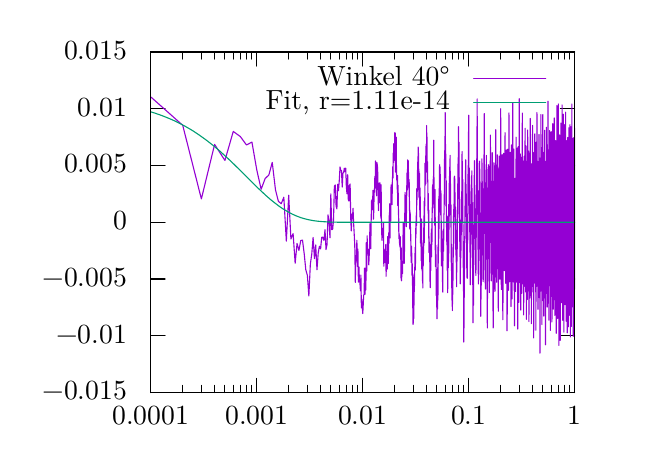
\begin{tikzpicture}[gnuplot]
%% generated with GNUPLOT 5.2p5a (Gentoo revision r0) (Lua 5.1; terminal rev. 99 , script rev. 107)
%% Sa 18 Mai 2019 18:30:45 CEST
\path (0.000,0.000) rectangle (7.500,5.250);
\gpcolor{color=gp lt color border}
\gpsetlinetype{gp lt border}
\gpsetdashtype{gp dt solid}
\gpsetlinewidth{1.00}
\draw[gp path] (1.564,0.616)--(1.744,0.616);
\draw[gp path] (6.947,0.616)--(6.767,0.616);
\node[gp node right] at (1.380,0.616) {$-0.015$};
\draw[gp path] (1.564,1.337)--(1.744,1.337);
\draw[gp path] (6.947,1.337)--(6.767,1.337);
\node[gp node right] at (1.380,1.337) {$-0.01$};
\draw[gp path] (1.564,2.058)--(1.744,2.058);
\draw[gp path] (6.947,2.058)--(6.767,2.058);
\node[gp node right] at (1.380,2.058) {$-0.005$};
\draw[gp path] (1.564,2.779)--(1.744,2.779);
\draw[gp path] (6.947,2.779)--(6.767,2.779);
\node[gp node right] at (1.380,2.779) {$0$};
\draw[gp path] (1.564,3.499)--(1.744,3.499);
\draw[gp path] (6.947,3.499)--(6.767,3.499);
\node[gp node right] at (1.380,3.499) {$0.005$};
\draw[gp path] (1.564,4.220)--(1.744,4.220);
\draw[gp path] (6.947,4.220)--(6.767,4.220);
\node[gp node right] at (1.380,4.220) {$0.01$};
\draw[gp path] (1.564,4.941)--(1.744,4.941);
\draw[gp path] (6.947,4.941)--(6.767,4.941);
\node[gp node right] at (1.380,4.941) {$0.015$};
\draw[gp path] (1.564,0.616)--(1.564,0.796);
\draw[gp path] (1.564,4.941)--(1.564,4.761);
\node[gp node center] at (1.564,0.308) {$0.0001$};
\draw[gp path] (1.969,0.616)--(1.969,0.706);
\draw[gp path] (1.969,4.941)--(1.969,4.851);
\draw[gp path] (2.206,0.616)--(2.206,0.706);
\draw[gp path] (2.206,4.941)--(2.206,4.851);
\draw[gp path] (2.374,0.616)--(2.374,0.706);
\draw[gp path] (2.374,4.941)--(2.374,4.851);
\draw[gp path] (2.505,0.616)--(2.505,0.706);
\draw[gp path] (2.505,4.941)--(2.505,4.851);
\draw[gp path] (2.611,0.616)--(2.611,0.706);
\draw[gp path] (2.611,4.941)--(2.611,4.851);
\draw[gp path] (2.701,0.616)--(2.701,0.706);
\draw[gp path] (2.701,4.941)--(2.701,4.851);
\draw[gp path] (2.779,0.616)--(2.779,0.706);
\draw[gp path] (2.779,4.941)--(2.779,4.851);
\draw[gp path] (2.848,0.616)--(2.848,0.706);
\draw[gp path] (2.848,4.941)--(2.848,4.851);
\draw[gp path] (2.910,0.616)--(2.910,0.796);
\draw[gp path] (2.910,4.941)--(2.910,4.761);
\node[gp node center] at (2.910,0.308) {$0.001$};
\draw[gp path] (3.315,0.616)--(3.315,0.706);
\draw[gp path] (3.315,4.941)--(3.315,4.851);
\draw[gp path] (3.552,0.616)--(3.552,0.706);
\draw[gp path] (3.552,4.941)--(3.552,4.851);
\draw[gp path] (3.720,0.616)--(3.720,0.706);
\draw[gp path] (3.720,4.941)--(3.720,4.851);
\draw[gp path] (3.850,0.616)--(3.850,0.706);
\draw[gp path] (3.850,4.941)--(3.850,4.851);
\draw[gp path] (3.957,0.616)--(3.957,0.706);
\draw[gp path] (3.957,4.941)--(3.957,4.851);
\draw[gp path] (4.047,0.616)--(4.047,0.706);
\draw[gp path] (4.047,4.941)--(4.047,4.851);
\draw[gp path] (4.125,0.616)--(4.125,0.706);
\draw[gp path] (4.125,4.941)--(4.125,4.851);
\draw[gp path] (4.194,0.616)--(4.194,0.706);
\draw[gp path] (4.194,4.941)--(4.194,4.851);
\draw[gp path] (4.255,0.616)--(4.255,0.796);
\draw[gp path] (4.255,4.941)--(4.255,4.761);
\node[gp node center] at (4.255,0.308) {$0.01$};
\draw[gp path] (4.661,0.616)--(4.661,0.706);
\draw[gp path] (4.661,4.941)--(4.661,4.851);
\draw[gp path] (4.898,0.616)--(4.898,0.706);
\draw[gp path] (4.898,4.941)--(4.898,4.851);
\draw[gp path] (5.066,0.616)--(5.066,0.706);
\draw[gp path] (5.066,4.941)--(5.066,4.851);
\draw[gp path] (5.196,0.616)--(5.196,0.706);
\draw[gp path] (5.196,4.941)--(5.196,4.851);
\draw[gp path] (5.303,0.616)--(5.303,0.706);
\draw[gp path] (5.303,4.941)--(5.303,4.851);
\draw[gp path] (5.393,0.616)--(5.393,0.706);
\draw[gp path] (5.393,4.941)--(5.393,4.851);
\draw[gp path] (5.471,0.616)--(5.471,0.706);
\draw[gp path] (5.471,4.941)--(5.471,4.851);
\draw[gp path] (5.540,0.616)--(5.540,0.706);
\draw[gp path] (5.540,4.941)--(5.540,4.851);
\draw[gp path] (5.601,0.616)--(5.601,0.796);
\draw[gp path] (5.601,4.941)--(5.601,4.761);
\node[gp node center] at (5.601,0.308) {$0.1$};
\draw[gp path] (6.006,0.616)--(6.006,0.706);
\draw[gp path] (6.006,4.941)--(6.006,4.851);
\draw[gp path] (6.243,0.616)--(6.243,0.706);
\draw[gp path] (6.243,4.941)--(6.243,4.851);
\draw[gp path] (6.411,0.616)--(6.411,0.706);
\draw[gp path] (6.411,4.941)--(6.411,4.851);
\draw[gp path] (6.542,0.616)--(6.542,0.706);
\draw[gp path] (6.542,4.941)--(6.542,4.851);
\draw[gp path] (6.648,0.616)--(6.648,0.706);
\draw[gp path] (6.648,4.941)--(6.648,4.851);
\draw[gp path] (6.739,0.616)--(6.739,0.706);
\draw[gp path] (6.739,4.941)--(6.739,4.851);
\draw[gp path] (6.817,0.616)--(6.817,0.706);
\draw[gp path] (6.817,4.941)--(6.817,4.851);
\draw[gp path] (6.885,0.616)--(6.885,0.706);
\draw[gp path] (6.885,4.941)--(6.885,4.851);
\draw[gp path] (6.947,0.616)--(6.947,0.796);
\draw[gp path] (6.947,4.941)--(6.947,4.761);
\node[gp node center] at (6.947,0.308) {$1$};
\draw[gp path] (1.564,4.941)--(1.564,0.616)--(6.947,0.616)--(6.947,4.941)--cycle;
\node[gp node right] at (5.479,4.607) {Winkel 40°};
\gpcolor{rgb color={0.580,0.000,0.827}}
\draw[gp path] (5.663,4.607)--(6.579,4.607);
\draw[gp path] (1.564,4.370)--(1.969,4.010)--(2.206,3.075)--(2.374,3.767)--(2.505,3.564)%
  --(2.611,3.932)--(2.701,3.867)--(2.779,3.760)--(2.848,3.797)--(2.910,3.441)--(2.965,3.198)%
  --(3.016,3.334)--(3.063,3.379)--(3.106,3.539)--(3.147,3.190)--(3.184,3.045)--(3.220,3.014)%
  --(3.253,3.097)--(3.285,2.539)--(3.315,3.122)--(3.343,2.566)--(3.371,2.635)--(3.397,2.258)%
  --(3.421,2.509)--(3.445,2.421)--(3.468,2.546)--(3.490,2.553)--(3.512,2.378)--(3.532,2.176)%
  --(3.552,2.105)--(3.571,1.842)--(3.590,2.249)--(3.608,2.376)--(3.625,2.586)--(3.642,2.316)%
  --(3.658,2.491)--(3.674,2.176)--(3.690,2.389)--(3.705,2.474)--(3.720,2.441)--(3.734,2.588)%
  --(3.748,2.588)--(3.762,2.548)--(3.776,2.684)--(3.789,2.433)--(3.802,2.497)--(3.814,2.873)%
  --(3.827,2.788)--(3.839,2.582)--(3.850,3.139)--(3.862,2.684)--(3.873,2.689)--(3.884,2.802)%
  --(3.895,3.236)--(3.906,3.253)--(3.917,2.982)--(3.927,2.949)--(3.937,3.261)--(3.947,3.181)%
  --(3.957,3.305)--(3.967,3.481)--(3.976,3.439)--(3.985,3.434)--(3.995,3.226)--(4.004,3.403)%
  --(4.013,3.412)--(4.021,3.465)--(4.030,3.421)--(4.039,3.467)--(4.047,3.235)--(4.055,3.141)%
  --(4.064,3.383)--(4.072,3.067)--(4.080,3.048)--(4.087,3.245)--(4.095,3.265)--(4.103,2.823)%
  --(4.110,2.669)--(4.118,2.883)--(4.125,2.829)--(4.132,2.956)--(4.140,2.757)--(4.147,2.628)%
  --(4.154,2.488)--(4.161,2.015)--(4.167,2.349)--(4.174,2.358)--(4.181,2.550)--(4.187,2.217)%
  --(4.194,2.438)--(4.200,2.018)--(4.207,2.213)--(4.213,2.031)--(4.219,2.012)--(4.226,1.909)%
  --(4.232,2.108)--(4.238,1.692)--(4.244,1.796)--(4.250,1.692)--(4.256,1.619)--(4.261,1.723)%
  --(4.267,1.850)--(4.273,1.862)--(4.278,2.197)--(4.284,1.864)--(4.290,2.122)--(4.295,1.919)%
  --(4.300,2.520)--(4.306,2.158)--(4.311,2.608)--(4.316,2.387)--(4.322,2.375)--(4.327,2.436)%
  --(4.332,2.237)--(4.337,2.347)--(4.342,2.503)--(4.347,2.760)--(4.352,2.687)--(4.357,2.440)%
  --(4.362,2.769)--(4.367,3.054)--(4.372,2.937)--(4.376,3.070)--(4.381,3.065)--(4.386,3.185)%
  --(4.391,2.817)--(4.395,2.911)--(4.400,3.157)--(4.404,3.159)--(4.409,3.362)--(4.413,3.213)%
  --(4.418,3.557)--(4.422,3.369)--(4.427,3.328)--(4.431,3.114)--(4.435,3.538)--(4.439,3.512)%
  --(4.444,3.467)--(4.448,3.311)--(4.452,3.030)--(4.456,2.928)--(4.460,3.272)--(4.465,3.027)%
  --(4.469,3.185)--(4.473,3.282)--(4.477,3.218)--(4.481,3.083)--(4.485,2.832)--(4.489,3.255)%
  --(4.492,2.855)--(4.496,2.652)--(4.500,2.548)--(4.504,2.652)--(4.508,2.701)--(4.512,2.606)%
  --(4.515,2.585)--(4.519,2.766)--(4.523,2.220)--(4.527,2.439)--(4.530,2.411)--(4.534,2.362)%
  --(4.537,2.267)--(4.541,2.393)--(4.545,2.368)--(4.548,2.496)--(4.552,2.092)--(4.555,2.240)%
  --(4.559,2.355)--(4.562,2.406)--(4.566,2.184)--(4.569,2.450)--(4.572,2.597)--(4.576,2.554)%
  --(4.579,2.255)--(4.583,2.413)--(4.586,2.648)--(4.589,2.510)--(4.593,2.902)--(4.596,2.803)%
  --(4.599,3.015)--(4.602,2.579)--(4.605,2.901)--(4.609,2.860)--(4.612,2.795)--(4.615,3.253)%
  --(4.618,3.073)--(4.621,3.142)--(4.624,3.126)--(4.628,3.002)--(4.631,3.314)--(4.634,3.359)%
  --(4.637,3.486)--(4.640,3.340)--(4.643,3.660)--(4.646,3.536)--(4.649,3.777)--(4.652,3.562)%
  --(4.655,3.703)--(4.658,3.688)--(4.661,3.904)--(4.664,3.920)--(4.666,3.673)--(4.669,3.908)%
  --(4.672,3.416)--(4.675,3.644)--(4.678,3.563)--(4.681,3.860)--(4.684,3.399)--(4.686,3.337)%
  --(4.689,3.305)--(4.692,3.329)--(4.695,3.150)--(4.697,3.372)--(4.700,2.990)--(4.703,3.249)%
  --(4.706,3.136)--(4.708,2.873)--(4.711,2.941)--(4.714,2.570)--(4.716,2.640)--(4.719,2.615)%
  --(4.722,2.526)--(4.724,2.488)--(4.727,2.512)--(4.729,2.464)--(4.732,2.596)--(4.735,2.429)%
  --(4.737,2.393)--(4.740,2.233)--(4.742,2.058)--(4.745,2.452)--(4.747,2.036)--(4.750,2.180)%
  --(4.752,2.083)--(4.755,2.274)--(4.757,2.257)--(4.760,2.127)--(4.762,2.286)--(4.765,2.252)%
  --(4.767,2.605)--(4.770,2.773)--(4.772,2.394)--(4.774,2.610)--(4.777,2.346)--(4.779,2.271)%
  --(4.782,2.257)--(4.784,2.769)--(4.786,2.408)--(4.789,2.858)--(4.791,3.021)--(4.793,3.157)%
  --(4.796,2.945)--(4.798,2.910)--(4.800,2.828)--(4.803,3.116)--(4.805,2.904)--(4.807,2.917)%
  --(4.809,2.722)--(4.812,3.104)--(4.814,3.121)--(4.816,3.405)--(4.818,3.225)--(4.821,3.342)%
  --(4.823,3.190)--(4.825,3.571)--(4.827,3.289)--(4.829,3.280)--(4.832,3.492)--(4.834,3.560)%
  --(4.836,3.395)--(4.838,3.295)--(4.840,3.236)--(4.842,3.221)--(4.845,3.321)--(4.847,3.050)%
  --(4.849,2.925)--(4.851,3.043)--(4.853,2.693)--(4.855,2.849)--(4.857,2.908)--(4.859,2.866)%
  --(4.861,2.716)--(4.863,2.716)--(4.866,2.517)--(4.868,2.404)--(4.870,2.269)--(4.872,2.477)%
  --(4.874,2.326)--(4.876,2.470)--(4.878,2.308)--(4.880,2.106)--(4.882,2.209)--(4.884,2.254)%
  --(4.886,1.977)--(4.888,2.083)--(4.890,1.688)--(4.892,1.739)--(4.894,1.481)--(4.896,1.563)%
  --(4.898,1.495)--(4.900,1.824)--(4.901,1.687)--(4.903,1.888)--(4.905,1.558)--(4.907,2.124)%
  --(4.909,1.896)--(4.911,1.967)--(4.913,1.976)--(4.915,2.210)--(4.917,2.165)--(4.919,2.385)%
  --(4.921,2.263)--(4.922,2.462)--(4.924,2.173)--(4.926,2.419)--(4.928,2.592)--(4.930,2.785)%
  --(4.932,2.628)--(4.933,2.666)--(4.935,2.850)--(4.937,2.902)--(4.939,2.739)--(4.941,3.205)%
  --(4.943,2.997)--(4.944,3.093)--(4.946,3.156)--(4.948,3.187)--(4.950,3.285)--(4.952,3.512)%
  --(4.953,3.299)--(4.955,3.612)--(4.957,3.223)--(4.959,3.734)--(4.960,3.432)--(4.962,3.726)%
  --(4.964,3.539)--(4.966,3.453)--(4.967,3.201)--(4.969,3.096)--(4.971,3.131)--(4.972,3.421)%
  --(4.974,3.082)--(4.976,3.320)--(4.978,3.396)--(4.979,3.013)--(4.981,2.847)--(4.983,3.187)%
  --(4.984,3.212)--(4.986,2.990)--(4.988,2.516)--(4.989,2.765)--(4.991,2.587)--(4.993,2.635)%
  --(4.994,2.529)--(4.996,2.463)--(4.998,2.290)--(4.999,2.290)--(5.001,2.822)--(5.003,2.495)%
  --(5.004,2.185)--(5.006,2.466)--(5.007,2.312)--(5.009,2.450)--(5.011,2.200)--(5.012,2.144)%
  --(5.014,2.087)--(5.015,2.025)--(5.017,2.069)--(5.019,1.944)--(5.020,2.256)--(5.022,2.250)%
  --(5.023,2.519)--(5.025,2.231)--(5.026,2.548)--(5.028,2.383)--(5.030,2.522)--(5.031,2.768)%
  --(5.033,2.741)--(5.034,2.869)--(5.036,2.518)--(5.037,3.048)--(5.039,2.731)--(5.040,3.012)%
  --(5.042,3.090)--(5.043,2.986)--(5.045,3.149)--(5.046,3.530)--(5.048,3.243)--(5.049,3.516)%
  --(5.051,3.328)--(5.052,3.302)--(5.054,3.263)--(5.055,3.623)--(5.057,3.268)--(5.058,3.744)%
  --(5.060,3.415)--(5.061,3.774)--(5.063,3.534)--(5.064,3.740)--(5.066,3.742)--(5.067,4.007)%
  --(5.069,3.623)--(5.070,3.916)--(5.072,3.764)--(5.073,3.582)--(5.074,3.457)--(5.076,3.490)%
  --(5.077,3.410)--(5.079,3.547)--(5.080,3.324)--(5.082,3.275)--(5.083,3.164)--(5.084,2.951)%
  --(5.086,2.889)--(5.087,3.146)--(5.089,2.952)--(5.090,2.845)--(5.091,2.812)--(5.093,2.937)%
  --(5.094,2.574)--(5.096,2.619)--(5.097,2.395)--(5.098,2.533)--(5.100,2.526)--(5.101,2.469)%
  --(5.103,2.413)--(5.104,2.504)--(5.105,2.275)--(5.107,2.355)--(5.108,2.026)--(5.109,2.425)%
  --(5.111,2.212)--(5.112,2.004)--(5.113,1.948)--(5.115,2.212)--(5.116,2.245)--(5.117,2.236)%
  --(5.119,2.348)--(5.120,2.166)--(5.121,2.370)--(5.123,2.508)--(5.124,2.394)--(5.125,2.593)%
  --(5.127,2.691)--(5.128,2.339)--(5.129,2.512)--(5.131,2.608)--(5.132,2.493)--(5.133,2.702)%
  --(5.135,2.831)--(5.136,2.532)--(5.137,2.965)--(5.138,2.899)--(5.140,2.990)--(5.141,3.036)%
  --(5.142,3.255)--(5.144,2.957)--(5.145,3.213)--(5.146,3.102)--(5.147,3.244)--(5.149,3.105)%
  --(5.150,3.280)--(5.151,3.326)--(5.152,3.214)--(5.154,3.323)--(5.155,3.400)--(5.156,3.240)%
  --(5.157,3.821)--(5.159,3.316)--(5.160,3.348)--(5.161,3.302)--(5.162,3.021)--(5.164,3.008)%
  --(5.165,3.097)--(5.166,2.776)--(5.167,2.830)--(5.169,2.742)--(5.170,2.766)--(5.171,2.878)%
  --(5.172,2.808)--(5.173,2.845)--(5.175,3.193)--(5.176,2.426)--(5.177,2.590)--(5.178,2.613)%
  --(5.180,2.214)--(5.181,2.441)--(5.182,2.487)--(5.183,2.352)--(5.184,2.338)--(5.186,2.365)%
  --(5.187,2.367)--(5.188,2.057)--(5.189,1.846)--(5.190,2.084)--(5.191,2.049)--(5.193,1.901)%
  --(5.194,1.699)--(5.195,1.699)--(5.196,1.882)--(5.197,1.685)--(5.198,1.552)--(5.200,1.600)%
  --(5.201,1.831)--(5.202,1.894)--(5.203,2.089)--(5.204,1.895)--(5.205,2.183)--(5.207,1.677)%
  --(5.208,2.205)--(5.209,2.133)--(5.210,2.463)--(5.211,1.854)--(5.212,2.495)--(5.213,2.188)%
  --(5.215,2.437)--(5.216,2.424)--(5.217,2.413)--(5.218,2.860)--(5.219,2.634)--(5.220,2.570)%
  --(5.221,3.064)--(5.222,3.108)--(5.224,2.695)--(5.225,2.786)--(5.226,2.885)--(5.227,2.955)%
  --(5.228,3.364)--(5.229,3.280)--(5.230,3.489)--(5.231,3.356)--(5.232,3.510)--(5.233,3.474)%
  --(5.235,3.286)--(5.236,3.483)--(5.237,3.270)--(5.238,3.031)--(5.239,3.391)--(5.240,3.069)%
  --(5.241,3.248)--(5.242,3.064)--(5.243,3.058)--(5.244,3.109)--(5.245,2.914)--(5.247,2.866)%
  --(5.248,3.177)--(5.249,3.113)--(5.250,2.847)--(5.251,2.879)--(5.252,2.759)--(5.253,2.398)%
  --(5.254,2.628)--(5.255,2.505)--(5.256,2.224)--(5.257,2.252)--(5.258,2.674)--(5.259,2.338)%
  --(5.260,2.436)--(5.261,2.315)--(5.262,2.426)--(5.263,2.353)--(5.264,2.283)--(5.265,2.425)%
  --(5.267,2.020)--(5.268,2.045)--(5.269,2.302)--(5.270,2.113)--(5.271,2.202)--(5.272,1.891)%
  --(5.273,2.315)--(5.274,2.360)--(5.275,2.495)--(5.276,2.289)--(5.277,2.442)--(5.278,2.570)%
  --(5.279,2.437)--(5.280,2.475)--(5.281,2.691)--(5.282,2.411)--(5.283,2.694)--(5.284,2.550)%
  --(5.285,2.735)--(5.286,2.867)--(5.287,2.890)--(5.288,2.878)--(5.289,3.131)--(5.290,3.004)%
  --(5.291,3.011)--(5.292,3.260)--(5.293,3.583)--(5.294,3.486)--(5.295,3.690)--(5.296,3.417)%
  --(5.297,3.444)--(5.298,3.398)--(5.299,3.870)--(5.300,3.674)--(5.301,3.976)--(5.302,3.621)%
  --(5.303,4.172)--(5.304,3.705)--(5.305,4.132)--(5.306,3.562)--(5.307,3.435)--(5.308,3.506)%
  --(5.309,3.646)--(5.309,3.565)--(5.310,3.358)--(5.311,3.253)--(5.312,3.310)--(5.313,2.984)%
  --(5.314,3.218)--(5.315,3.289)--(5.316,3.308)--(5.317,3.001)--(5.318,2.896)--(5.319,2.715)%
  --(5.320,2.861)--(5.321,2.739)--(5.322,2.624)--(5.323,2.520)--(5.324,2.490)--(5.325,2.558)%
  --(5.326,2.853)--(5.327,2.507)--(5.328,2.265)--(5.329,2.168)--(5.330,2.319)--(5.331,2.161)%
  --(5.332,2.450)--(5.333,2.219)--(5.334,1.885)--(5.335,2.117)--(5.336,2.143)--(5.337,2.258)%
  --(5.338,2.271)--(5.339,2.616)--(5.340,2.309)--(5.340,2.338)--(5.341,2.201)--(5.342,2.526)%
  --(5.343,2.444)--(5.344,2.875)--(5.345,2.281)--(5.346,2.381)--(5.347,2.385)--(5.348,3.006)%
  --(5.349,2.599)--(5.349,2.653)--(5.350,2.668)--(5.351,2.904)--(5.352,2.910)--(5.353,2.754)%
  --(5.354,3.139)--(5.355,3.363)--(5.356,3.122)--(5.357,3.325)--(5.358,3.178)--(5.358,3.422)%
  --(5.359,3.135)--(5.360,3.480)--(5.361,3.359)--(5.362,3.404)--(5.363,3.346)--(5.364,3.586)%
  --(5.365,3.568)--(5.365,3.628)--(5.366,3.330)--(5.367,3.429)--(5.368,3.294)--(5.369,3.290)%
  --(5.370,3.121)--(5.371,3.013)--(5.372,3.239)--(5.372,2.948)--(5.373,3.009)--(5.374,2.800)%
  --(5.375,2.959)--(5.376,2.716)--(5.377,2.995)--(5.378,2.610)--(5.378,2.271)--(5.379,2.387)%
  --(5.380,2.412)--(5.381,2.165)--(5.382,2.479)--(5.383,2.407)--(5.384,2.485)--(5.384,2.500)%
  --(5.385,2.030)--(5.386,1.942)--(5.387,1.999)--(5.388,2.041)--(5.389,1.962)--(5.389,1.786)%
  --(5.390,1.856)--(5.391,1.857)--(5.392,1.709)--(5.393,1.858)--(5.394,1.668)--(5.394,1.657)%
  --(5.395,1.804)--(5.396,1.920)--(5.397,2.169)--(5.398,1.936)--(5.399,2.256)--(5.399,1.860)%
  --(5.400,2.031)--(5.401,2.232)--(5.402,2.257)--(5.403,2.039)--(5.404,2.204)--(5.404,2.398)%
  --(5.405,2.458)--(5.406,2.336)--(5.407,2.513)--(5.408,2.509)--(5.408,2.767)--(5.409,2.932)%
  --(5.410,2.935)--(5.411,2.743)--(5.412,3.009)--(5.412,2.828)--(5.413,2.894)--(5.414,2.845)%
  --(5.415,2.985)--(5.416,3.281)--(5.417,3.091)--(5.417,3.347)--(5.418,3.157)--(5.419,3.300)%
  --(5.420,3.103)--(5.421,3.363)--(5.421,3.217)--(5.422,3.358)--(5.423,3.347)--(5.424,3.198)%
  --(5.424,3.160)--(5.425,3.110)--(5.426,2.916)--(5.427,3.094)--(5.428,3.111)--(5.428,3.155)%
  --(5.429,2.929)--(5.430,2.845)--(5.431,2.963)--(5.432,2.721)--(5.432,2.947)--(5.433,2.436)%
  --(5.434,2.670)--(5.435,2.501)--(5.435,2.971)--(5.436,2.613)--(5.437,2.568)--(5.438,2.536)%
  --(5.439,2.360)--(5.439,2.623)--(5.440,2.499)--(5.441,2.600)--(5.442,2.439)--(5.442,2.368)%
  --(5.443,2.314)--(5.444,2.226)--(5.445,2.191)--(5.445,2.212)--(5.446,2.053)--(5.447,2.069)%
  --(5.448,2.328)--(5.448,1.960)--(5.449,2.319)--(5.450,2.222)--(5.451,2.287)--(5.452,2.505)%
  --(5.452,2.560)--(5.453,2.423)--(5.454,2.284)--(5.455,2.462)--(5.455,2.805)--(5.456,2.819)%
  --(5.457,2.552)--(5.458,2.700)--(5.458,2.839)--(5.459,2.902)--(5.460,2.990)--(5.461,3.126)%
  --(5.461,2.790)--(5.462,3.241)--(5.463,3.294)--(5.463,3.485)--(5.464,3.299)--(5.465,3.520)%
  --(5.466,3.073)--(5.466,3.485)--(5.467,3.312)--(5.468,3.517)--(5.469,3.609)--(5.469,3.593)%
  --(5.470,3.837)--(5.471,3.885)--(5.472,3.992)--(5.472,3.497)--(5.473,3.975)--(5.474,3.704)%
  --(5.474,3.630)--(5.475,3.587)--(5.476,3.784)--(5.477,3.317)--(5.477,3.655)--(5.478,3.480)%
  --(5.479,3.793)--(5.480,3.449)--(5.480,3.177)--(5.481,3.348)--(5.482,3.228)--(5.482,3.218)%
  --(5.483,3.175)--(5.484,2.935)--(5.485,2.810)--(5.485,2.690)--(5.486,2.816)--(5.487,2.601)%
  --(5.487,2.702)--(5.488,2.525)--(5.489,2.804)--(5.490,2.531)--(5.490,2.591)--(5.491,2.339)%
  --(5.492,2.377)--(5.492,2.190)--(5.493,2.500)--(5.494,2.098)--(5.494,1.996)--(5.495,2.011)%
  --(5.496,2.440)--(5.497,2.363)--(5.497,2.318)--(5.498,2.194)--(5.499,2.546)--(5.499,2.305)%
  --(5.500,2.366)--(5.501,2.592)--(5.501,2.363)--(5.502,2.450)--(5.503,2.718)--(5.504,2.420)%
  --(5.504,2.819)--(5.505,2.555)--(5.506,2.646)--(5.506,2.752)--(5.507,2.725)--(5.508,2.898)%
  --(5.508,2.955)--(5.509,3.100)--(5.510,2.953)--(5.510,2.854)--(5.511,3.169)--(5.512,2.836)%
  --(5.512,3.165)--(5.513,2.773)--(5.514,3.210)--(5.514,3.078)--(5.515,3.431)--(5.516,3.287)%
  --(5.516,3.608)--(5.517,3.676)--(5.518,3.484)--(5.519,3.316)--(5.519,3.553)--(5.520,3.290)%
  --(5.521,3.223)--(5.521,3.140)--(5.522,3.327)--(5.523,3.142)--(5.523,2.893)--(5.524,2.831)%
  --(5.525,3.323)--(5.525,3.101)--(5.526,2.954)--(5.527,2.866)--(5.527,2.811)--(5.528,2.743)%
  --(5.529,2.671)--(5.529,2.661)--(5.530,2.645)--(5.531,2.525)--(5.531,2.204)--(5.532,2.429)%
  --(5.532,2.518)--(5.533,2.159)--(5.534,2.213)--(5.534,2.177)--(5.535,2.124)--(5.536,1.745)%
  --(5.536,2.194)--(5.537,1.717)--(5.538,1.669)--(5.538,1.257)--(5.539,1.944)--(5.540,1.486)%
  --(5.540,1.712)--(5.541,1.465)--(5.542,2.039)--(5.542,1.435)--(5.543,1.958)--(5.544,1.821)%
  --(5.544,2.115)--(5.545,2.120)--(5.545,1.991)--(5.546,2.276)--(5.547,2.271)--(5.547,2.182)%
  --(5.548,2.540)--(5.549,2.528)--(5.549,2.489)--(5.550,2.509)--(5.551,2.576)--(5.551,2.547)%
  --(5.552,2.668)--(5.553,2.566)--(5.553,2.844)--(5.554,2.853)--(5.554,2.888)--(5.555,3.041)%
  --(5.556,2.903)--(5.556,3.285)--(5.557,3.062)--(5.558,3.058)--(5.558,2.904)--(5.559,3.302)%
  --(5.559,3.435)--(5.560,3.346)--(5.561,3.214)--(5.561,3.104)--(5.562,3.425)--(5.563,3.308)%
  --(5.563,3.572)--(5.564,3.113)--(5.564,3.491)--(5.565,2.876)--(5.566,3.211)--(5.566,3.102)%
  --(5.567,2.944)--(5.568,2.959)--(5.568,3.261)--(5.569,2.980)--(5.569,3.173)--(5.570,2.981)%
  --(5.571,2.857)--(5.571,2.729)--(5.572,2.926)--(5.573,2.814)--(5.573,2.762)--(5.574,2.483)%
  --(5.574,2.322)--(5.575,2.563)--(5.576,2.480)--(5.576,2.272)--(5.577,2.183)--(5.577,2.350)%
  --(5.578,2.228)--(5.579,2.437)--(5.579,2.076)--(5.580,2.230)--(5.580,2.157)--(5.581,2.104)%
  --(5.582,2.126)--(5.582,2.066)--(5.583,2.384)--(5.583,2.279)--(5.584,2.160)--(5.585,2.646)%
  --(5.585,2.532)--(5.586,2.608)--(5.586,2.508)--(5.587,2.563)--(5.588,2.579)--(5.588,2.552)%
  --(5.589,2.667)--(5.589,2.552)--(5.590,2.748)--(5.591,2.919)--(5.591,3.222)--(5.592,2.882)%
  --(5.592,3.083)--(5.593,3.499)--(5.594,3.042)--(5.594,3.351)--(5.595,3.437)--(5.595,3.417)%
  --(5.596,3.214)--(5.597,3.512)--(5.597,3.572)--(5.598,3.472)--(5.598,3.667)--(5.599,3.825)%
  --(5.599,3.929)--(5.600,3.703)--(5.601,3.975)--(5.601,3.983)--(5.602,3.814)--(5.602,4.138)%
  --(5.603,3.627)--(5.604,3.928)--(5.604,3.479)--(5.605,3.445)--(5.605,3.470)--(5.606,3.451)%
  --(5.606,3.256)--(5.607,3.302)--(5.608,3.240)--(5.608,3.466)--(5.609,3.296)--(5.609,3.233)%
  --(5.610,3.053)--(5.611,3.170)--(5.611,3.014)--(5.612,2.984)--(5.612,3.118)--(5.613,2.698)%
  --(5.613,2.702)--(5.614,2.655)--(5.615,2.840)--(5.615,2.682)--(5.616,2.803)--(5.616,2.647)%
  --(5.617,2.396)--(5.617,2.402)--(5.618,2.416)--(5.619,2.395)--(5.619,2.515)--(5.620,1.985)%
  --(5.620,2.418)--(5.621,2.270)--(5.621,2.117)--(5.622,2.035)--(5.622,2.192)--(5.623,2.172)%
  --(5.624,2.362)--(5.624,2.383)--(5.625,2.678)--(5.625,2.564)--(5.626,2.371)--(5.626,2.338)%
  --(5.627,2.330)--(5.628,2.462)--(5.628,2.737)--(5.629,2.758)--(5.629,2.651)--(5.630,2.621)%
  --(5.630,3.007)--(5.631,2.757)--(5.631,3.005)--(5.632,2.992)--(5.633,3.026)--(5.633,3.105)%
  --(5.634,3.161)--(5.634,3.257)--(5.635,2.877)--(5.635,3.025)--(5.636,3.106)--(5.636,3.139)%
  --(5.637,3.362)--(5.638,3.297)--(5.638,3.322)--(5.639,3.372)--(5.639,3.139)--(5.640,3.307)%
  --(5.640,3.329)--(5.641,3.431)--(5.641,3.194)--(5.642,3.406)--(5.642,2.919)--(5.643,3.212)%
  --(5.644,2.961)--(5.644,3.026)--(5.645,2.888)--(5.645,3.066)--(5.646,2.965)--(5.646,2.816)%
  --(5.647,2.869)--(5.647,2.931)--(5.648,2.650)--(5.648,2.765)--(5.649,2.735)--(5.649,2.500)%
  --(5.650,2.528)--(5.651,2.467)--(5.651,2.194)--(5.652,2.163)--(5.652,1.986)--(5.653,2.185)%
  --(5.653,2.041)--(5.654,2.294)--(5.654,2.168)--(5.655,1.797)--(5.655,1.915)--(5.656,1.502)%
  --(5.656,1.602)--(5.657,1.972)--(5.657,1.769)--(5.658,1.880)--(5.659,1.788)--(5.659,2.113)%
  --(5.660,1.959)--(5.660,2.072)--(5.661,1.819)--(5.661,2.300)--(5.662,1.724)--(5.662,2.464)%
  --(5.663,2.108)--(5.663,2.362)--(5.664,2.076)--(5.664,2.520)--(5.665,2.492)--(5.665,2.486)%
  --(5.666,2.239)--(5.666,2.543)--(5.667,2.691)--(5.667,2.678)--(5.668,2.769)--(5.669,3.053)%
  --(5.669,2.988)--(5.670,3.111)--(5.670,2.884)--(5.671,2.977)--(5.671,2.990)--(5.672,3.294)%
  --(5.672,3.371)--(5.673,3.438)--(5.673,3.474)--(5.674,3.324)--(5.674,3.402)--(5.675,3.560)%
  --(5.675,3.163)--(5.676,3.523)--(5.676,3.176)--(5.677,3.486)--(5.677,3.262)--(5.678,3.142)%
  --(5.678,3.098)--(5.679,2.952)--(5.679,2.979)--(5.680,3.024)--(5.680,2.958)--(5.681,2.906)%
  --(5.681,2.572)--(5.682,2.856)--(5.682,2.873)--(5.683,2.951)--(5.683,2.620)--(5.684,2.755)%
  --(5.684,2.716)--(5.685,2.620)--(5.685,2.556)--(5.686,2.692)--(5.686,2.530)--(5.687,2.429)%
  --(5.687,2.487)--(5.688,2.598)--(5.688,2.446)--(5.689,2.595)--(5.690,2.379)--(5.690,2.483)%
  --(5.691,2.210)--(5.691,2.140)--(5.692,2.102)--(5.692,2.302)--(5.693,2.347)--(5.693,2.170)%
  --(5.694,2.220)--(5.694,2.378)--(5.695,2.235)--(5.695,2.695)--(5.696,2.346)--(5.696,2.634)%
  --(5.696,2.535)--(5.697,2.849)--(5.697,2.627)--(5.698,2.671)--(5.698,2.678)--(5.699,2.742)%
  --(5.699,2.880)--(5.700,3.117)--(5.700,3.028)--(5.701,3.177)--(5.701,3.206)--(5.702,3.585)%
  --(5.702,3.492)--(5.703,3.337)--(5.703,3.302)--(5.704,3.516)--(5.704,3.259)--(5.705,3.636)%
  --(5.705,3.852)--(5.706,3.335)--(5.706,3.766)--(5.707,3.997)--(5.707,3.661)--(5.708,4.345)%
  --(5.708,3.960)--(5.709,4.126)--(5.709,3.723)--(5.710,4.039)--(5.710,3.640)--(5.711,3.472)%
  --(5.711,3.303)--(5.712,3.456)--(5.712,3.558)--(5.713,3.408)--(5.713,3.248)--(5.714,3.289)%
  --(5.714,3.096)--(5.715,3.219)--(5.715,2.996)--(5.716,3.187)--(5.716,2.876)--(5.717,3.139)%
  --(5.717,2.682)--(5.717,2.708)--(5.718,2.707)--(5.718,2.625)--(5.719,2.432)--(5.719,2.446)%
  --(5.720,2.734)--(5.720,2.683)--(5.721,2.124)--(5.721,2.366)--(5.722,2.366)--(5.722,2.238)%
  --(5.723,2.208)--(5.723,2.028)--(5.724,2.021)--(5.724,1.995)--(5.725,2.188)--(5.725,2.219)%
  --(5.726,2.179)--(5.726,2.187)--(5.727,2.115)--(5.727,2.617)--(5.727,2.529)--(5.728,2.449)%
  --(5.728,2.444)--(5.729,2.481)--(5.729,2.436)--(5.730,2.584)--(5.730,2.709)--(5.731,2.809)%
  --(5.731,2.777)--(5.732,3.170)--(5.732,2.862)--(5.733,2.962)--(5.733,3.104)--(5.734,3.038)%
  --(5.734,2.953)--(5.734,3.178)--(5.735,2.980)--(5.735,3.114)--(5.736,3.003)--(5.736,3.089)%
  --(5.737,3.260)--(5.737,3.373)--(5.738,3.406)--(5.738,3.530)--(5.739,3.310)--(5.739,3.556)%
  --(5.740,3.337)--(5.740,3.260)--(5.740,3.507)--(5.741,3.132)--(5.741,3.457)--(5.742,3.041)%
  --(5.742,3.359)--(5.743,3.057)--(5.743,2.964)--(5.744,3.294)--(5.744,2.947)--(5.745,2.935)%
  --(5.745,2.984)--(5.746,2.866)--(5.746,2.876)--(5.746,2.657)--(5.747,2.694)--(5.747,2.351)%
  --(5.748,2.327)--(5.748,2.385)--(5.749,2.078)--(5.749,2.412)--(5.750,2.353)--(5.750,2.424)%
  --(5.751,2.037)--(5.751,2.257)--(5.751,2.266)--(5.752,2.150)--(5.752,1.963)--(5.753,1.988)%
  --(5.753,1.810)--(5.754,1.872)--(5.754,1.583)--(5.755,1.866)--(5.755,1.709)--(5.755,1.588)%
  --(5.756,1.870)--(5.756,1.904)--(5.757,2.149)--(5.757,1.800)--(5.758,2.124)--(5.758,1.969)%
  --(5.759,2.136)--(5.759,2.357)--(5.760,2.133)--(5.760,1.979)--(5.760,2.298)--(5.761,2.202)%
  --(5.761,2.346)--(5.762,2.492)--(5.762,2.613)--(5.763,2.635)--(5.763,2.660)--(5.764,2.681)%
  --(5.764,2.901)--(5.764,2.805)--(5.765,3.039)--(5.765,3.115)--(5.766,3.076)--(5.766,3.176)%
  --(5.767,3.245)--(5.767,3.124)--(5.767,3.208)--(5.768,3.404)--(5.768,3.434)--(5.769,3.584)%
  --(5.769,3.535)--(5.770,3.526)--(5.770,3.363)--(5.771,3.502)--(5.771,3.333)--(5.771,3.298)%
  --(5.772,3.217)--(5.772,3.367)--(5.773,3.174)--(5.773,3.198)--(5.774,3.012)--(5.774,3.191)%
  --(5.774,3.082)--(5.775,2.980)--(5.775,2.761)--(5.776,3.012)--(5.776,3.104)--(5.777,2.975)%
  --(5.777,2.913)--(5.778,2.594)--(5.778,2.882)--(5.778,2.551)--(5.779,2.360)--(5.779,2.544)%
  --(5.780,2.535)--(5.780,2.756)--(5.781,2.649)--(5.781,2.425)--(5.781,2.496)--(5.782,2.458)%
  --(5.782,2.164)--(5.783,2.355)--(5.783,2.053)--(5.784,2.244)--(5.784,2.200)--(5.784,2.309)%
  --(5.785,2.282)--(5.785,2.026)--(5.786,2.485)--(5.786,2.227)--(5.787,2.201)--(5.787,2.432)%
  --(5.787,2.286)--(5.788,2.313)--(5.788,2.678)--(5.789,2.651)--(5.789,2.631)--(5.789,2.655)%
  --(5.790,2.668)--(5.790,2.723)--(5.791,2.814)--(5.791,2.906)--(5.792,2.866)--(5.792,2.978)%
  --(5.792,3.209)--(5.793,3.033)--(5.793,3.310)--(5.794,3.186)--(5.794,3.341)--(5.795,3.326)%
  --(5.795,3.201)--(5.795,3.638)--(5.796,3.252)--(5.796,3.201)--(5.797,3.753)--(5.797,3.578)%
  --(5.797,3.860)--(5.798,3.655)--(5.798,3.859)--(5.799,3.989)--(5.799,4.159)--(5.800,3.879)%
  --(5.800,3.792)--(5.800,3.676)--(5.801,3.487)--(5.801,3.388)--(5.802,3.504)--(5.802,3.514)%
  --(5.802,3.448)--(5.803,3.178)--(5.803,3.469)--(5.804,3.402)--(5.804,3.295)--(5.805,3.198)%
  --(5.805,3.086)--(5.805,2.833)--(5.806,2.835)--(5.806,2.609)--(5.807,2.796)--(5.807,2.626)%
  --(5.807,2.421)--(5.808,2.173)--(5.808,2.550)--(5.809,2.588)--(5.809,2.010)--(5.809,2.220)%
  --(5.810,2.126)--(5.810,2.138)--(5.811,2.490)--(5.811,2.188)--(5.812,2.042)--(5.812,2.120)%
  --(5.812,2.018)--(5.813,2.013)--(5.813,2.147)--(5.814,2.425)--(5.814,1.931)--(5.814,2.290)%
  --(5.815,2.317)--(5.815,2.434)--(5.816,2.465)--(5.816,2.362)--(5.816,2.193)--(5.817,2.371)%
  --(5.817,2.662)--(5.818,2.647)--(5.818,2.677)--(5.818,2.625)--(5.819,2.781)--(5.819,2.822)%
  --(5.820,2.637)--(5.820,2.929)--(5.820,3.064)--(5.821,2.910)--(5.821,3.263)--(5.822,3.088)%
  --(5.822,3.206)--(5.822,2.756)--(5.823,3.316)--(5.823,3.381)--(5.824,3.208)--(5.824,3.402)%
  --(5.824,3.436)--(5.825,3.449)--(5.825,3.233)--(5.826,3.390)--(5.826,3.628)--(5.826,3.274)%
  --(5.827,3.341)--(5.827,3.359)--(5.828,3.478)--(5.828,3.202)--(5.828,3.128)--(5.829,3.210)%
  --(5.829,2.947)--(5.830,2.669)--(5.830,3.219)--(5.830,2.688)--(5.831,2.649)--(5.831,2.746)%
  --(5.832,2.646)--(5.832,2.432)--(5.832,2.330)--(5.833,2.664)--(5.833,2.399)--(5.834,2.304)%
  --(5.834,2.396)--(5.834,2.330)--(5.835,2.240)--(5.835,2.013)--(5.835,2.061)--(5.836,2.075)%
  --(5.836,1.984)--(5.837,1.868)--(5.837,1.869)--(5.837,1.497)--(5.838,1.733)--(5.838,1.595)%
  --(5.839,1.719)--(5.839,1.436)--(5.839,2.294)--(5.840,1.841)--(5.840,1.810)--(5.841,2.037)%
  --(5.841,2.187)--(5.841,1.946)--(5.842,2.078)--(5.842,2.237)--(5.842,2.385)--(5.843,2.491)%
  --(5.843,2.322)--(5.844,2.519)--(5.844,2.313)--(5.844,2.526)--(5.845,2.512)--(5.845,2.805)%
  --(5.846,2.812)--(5.846,2.952)--(5.846,3.097)--(5.847,2.898)--(5.847,3.038)--(5.848,3.070)%
  --(5.848,3.191)--(5.848,3.186)--(5.849,3.254)--(5.849,2.902)--(5.849,3.236)--(5.850,3.476)%
  --(5.850,3.510)--(5.851,3.278)--(5.851,3.438)--(5.851,3.271)--(5.852,3.197)--(5.852,3.490)%
  --(5.852,3.340)--(5.853,3.125)--(5.853,3.382)--(5.854,3.314)--(5.854,3.094)--(5.854,2.995)%
  --(5.855,3.173)--(5.855,2.936)--(5.856,3.012)--(5.856,2.895)--(5.856,3.035)--(5.857,2.711)%
  --(5.857,2.887)--(5.857,2.821)--(5.858,2.924)--(5.858,2.564)--(5.859,2.691)--(5.859,2.467)%
  --(5.859,2.399)--(5.860,2.692)--(5.860,2.543)--(5.860,2.099)--(5.861,2.317)--(5.861,2.486)%
  --(5.862,2.333)--(5.862,2.502)--(5.862,2.154)--(5.863,1.946)--(5.863,2.157)--(5.863,2.044)%
  --(5.864,1.886)--(5.864,2.127)--(5.865,2.134)--(5.865,2.208)--(5.865,2.203)--(5.866,2.312)%
  --(5.866,2.333)--(5.866,2.459)--(5.867,2.531)--(5.867,2.732)--(5.867,2.498)--(5.868,2.530)%
  --(5.868,2.690)--(5.869,2.780)--(5.869,2.828)--(5.869,3.031)--(5.870,3.017)--(5.870,2.986)%
  --(5.870,2.931)--(5.871,2.903)--(5.871,3.167)--(5.872,3.509)--(5.872,3.085)--(5.872,3.180)%
  --(5.873,3.305)--(5.873,3.225)--(5.873,3.414)--(5.874,3.270)--(5.874,3.536)--(5.874,3.422)%
  --(5.875,3.332)--(5.875,3.436)--(5.876,3.844)--(5.876,3.886)--(5.876,3.852)--(5.877,3.678)%
  --(5.877,3.727)--(5.877,3.502)--(5.878,3.736)--(5.878,3.431)--(5.878,3.405)--(5.879,3.266)%
  --(5.879,3.434)--(5.880,3.022)--(5.880,3.291)--(5.880,3.136)--(5.881,3.104)--(5.881,3.163)%
  --(5.881,3.304)--(5.882,3.277)--(5.882,2.980)--(5.882,3.004)--(5.883,2.986)--(5.883,2.677)%
  --(5.884,2.556)--(5.884,2.763)--(5.884,2.620)--(5.885,2.567)--(5.885,2.548)--(5.885,2.568)%
  --(5.886,2.627)--(5.886,2.224)--(5.886,2.286)--(5.887,2.312)--(5.887,2.165)--(5.888,2.140)%
  --(5.888,2.318)--(5.888,2.034)--(5.889,2.268)--(5.889,2.372)--(5.889,2.266)--(5.890,2.115)%
  --(5.890,2.266)--(5.890,2.127)--(5.891,2.251)--(5.891,2.385)--(5.891,2.461)--(5.892,2.599)%
  --(5.892,2.871)--(5.893,2.673)--(5.893,2.611)--(5.893,2.644)--(5.894,2.458)--(5.894,2.467)%
  --(5.894,2.586)--(5.895,2.787)--(5.895,2.831)--(5.895,3.010)--(5.896,2.996)--(5.896,3.208)%
  --(5.896,3.110)--(5.897,3.252)--(5.897,3.273)--(5.897,3.150)--(5.898,3.308)--(5.898,3.052)%
  --(5.899,3.057)--(5.899,3.535)--(5.899,3.247)--(5.900,3.628)--(5.900,3.222)--(5.900,3.662)%
  --(5.901,3.272)--(5.901,3.249)--(5.901,3.436)--(5.902,3.085)--(5.902,3.088)--(5.902,3.169)%
  --(5.903,3.305)--(5.903,2.676)--(5.903,2.766)--(5.904,3.118)--(5.904,3.003)--(5.904,2.587)%
  --(5.905,2.954)--(5.905,2.684)--(5.906,2.567)--(5.906,2.755)--(5.906,2.648)--(5.907,2.203)%
  --(5.907,2.455)--(5.907,2.474)--(5.908,2.162)--(5.908,2.308)--(5.908,2.190)--(5.909,2.326)%
  --(5.909,2.266)--(5.909,2.181)--(5.910,1.949)--(5.910,2.062)--(5.910,1.650)--(5.911,2.158)%
  --(5.911,1.846)--(5.911,1.959)--(5.912,1.846)--(5.912,1.551)--(5.912,1.436)--(5.913,1.537)%
  --(5.913,1.738)--(5.913,1.943)--(5.914,1.906)--(5.914,1.976)--(5.914,1.742)--(5.915,2.160)%
  --(5.915,2.178)--(5.915,2.329)--(5.916,1.926)--(5.916,2.116)--(5.917,2.098)--(5.917,2.526)%
  --(5.917,2.573)--(5.918,2.587)--(5.918,2.595)--(5.918,2.483)--(5.919,2.868)--(5.919,2.838)%
  --(5.919,2.972)--(5.920,3.026)--(5.920,2.953)--(5.920,2.924)--(5.921,3.080)--(5.921,3.312)%
  --(5.921,3.330)--(5.922,3.189)--(5.922,3.451)--(5.922,3.534)--(5.923,3.008)--(5.923,3.526)%
  --(5.923,3.461)--(5.924,3.299)--(5.924,3.322)--(5.924,3.361)--(5.925,3.247)--(5.925,3.338)%
  --(5.925,3.116)--(5.926,3.088)--(5.926,2.871)--(5.926,3.160)--(5.927,3.127)--(5.927,3.060)%
  --(5.927,2.823)--(5.928,3.021)--(5.928,2.831)--(5.928,2.834)--(5.929,2.728)--(5.929,2.835)%
  --(5.929,2.725)--(5.930,2.429)--(5.930,2.634)--(5.930,2.546)--(5.931,2.366)--(5.931,2.723)%
  --(5.931,2.431)--(5.932,2.451)--(5.932,2.161)--(5.932,2.174)--(5.933,2.098)--(5.933,2.242)%
  --(5.933,2.288)--(5.934,1.900)--(5.934,1.947)--(5.934,2.244)--(5.935,2.030)--(5.935,2.245)%
  --(5.935,2.282)--(5.936,2.316)--(5.936,1.908)--(5.936,2.228)--(5.937,2.330)--(5.937,2.640)%
  --(5.937,2.452)--(5.938,2.619)--(5.938,2.629)--(5.938,2.743)--(5.939,2.714)--(5.939,2.877)%
  --(5.939,2.697)--(5.940,2.656)--(5.940,3.114)--(5.940,2.889)--(5.941,2.940)--(5.941,3.095)%
  --(5.941,3.370)--(5.942,3.502)--(5.942,3.237)--(5.942,3.494)--(5.943,3.176)--(5.943,3.799)%
  --(5.943,3.442)--(5.943,3.824)--(5.944,3.784)--(5.944,3.955)--(5.944,3.838)--(5.945,3.894)%
  --(5.945,3.745)--(5.945,3.914)--(5.946,3.715)--(5.946,3.817)--(5.946,3.436)--(5.947,3.473)%
  --(5.947,3.269)--(5.947,3.510)--(5.948,3.471)--(5.948,3.264)--(5.948,3.228)--(5.949,3.365)%
  --(5.949,3.010)--(5.949,3.093)--(5.950,2.964)--(5.950,3.075)--(5.950,3.218)--(5.951,2.963)%
  --(5.951,2.968)--(5.951,2.738)--(5.952,2.581)--(5.952,2.872)--(5.952,2.770)--(5.953,2.593)%
  --(5.953,2.840)--(5.953,2.588)--(5.953,2.663)--(5.954,2.564)--(5.954,2.252)--(5.954,2.091)%
  --(5.955,2.074)--(5.955,2.234)--(5.955,2.121)--(5.956,2.297)--(5.956,2.017)--(5.956,2.451)%
  --(5.957,2.270)--(5.957,2.387)--(5.957,2.567)--(5.958,2.641)--(5.958,2.536)--(5.959,2.495)%
  --(5.959,2.820)--(5.959,2.531)--(5.960,2.586)--(5.960,2.502)--(5.960,2.731)--(5.960,2.927)%
  --(5.961,2.811)--(5.961,2.563)--(5.961,2.997)--(5.962,3.084)--(5.962,2.971)--(5.962,3.039)%
  --(5.963,2.899)--(5.963,3.239)--(5.963,3.063)--(5.964,3.054)--(5.964,3.028)--(5.964,3.418)%
  --(5.965,3.427)--(5.965,3.304)--(5.965,3.425)--(5.966,3.262)--(5.966,3.635)--(5.966,3.326)%
  --(5.966,3.485)--(5.967,3.393)--(5.967,3.201)--(5.967,3.003)--(5.968,3.366)--(5.968,2.994)%
  --(5.968,3.105)--(5.969,3.301)--(5.969,2.927)--(5.969,3.024)--(5.970,2.763)--(5.970,2.839)%
  --(5.970,3.038)--(5.971,2.703)--(5.971,2.682)--(5.971,2.795)--(5.972,2.445)--(5.972,2.523)%
  --(5.972,2.186)--(5.973,2.455)--(5.973,2.295)--(5.973,2.373)--(5.974,2.133)--(5.974,2.339)%
  --(5.974,2.306)--(5.975,2.376)--(5.975,1.961)--(5.975,2.039)--(5.975,1.836)--(5.976,1.741)%
  --(5.976,1.920)--(5.976,2.011)--(5.977,1.654)--(5.977,1.649)--(5.977,1.888)--(5.978,2.073)%
  --(5.978,2.059)--(5.978,2.029)--(5.979,2.263)--(5.979,2.260)--(5.979,2.283)--(5.979,2.051)%
  --(5.980,2.099)--(5.980,2.293)--(5.980,2.330)--(5.981,2.348)--(5.981,2.331)--(5.981,2.343)%
  --(5.982,2.456)--(5.982,2.507)--(5.982,2.610)--(5.983,2.595)--(5.983,2.916)--(5.983,2.777)%
  --(5.983,2.811)--(5.984,3.225)--(5.984,2.789)--(5.984,3.044)--(5.985,3.036)--(5.985,3.358)%
  --(5.985,3.198)--(5.986,3.265)--(5.986,3.420)--(5.986,3.462)--(5.986,3.186)--(5.987,3.230)%
  --(5.987,3.374)--(5.987,3.619)--(5.988,3.566)--(5.988,3.450)--(5.988,3.609)--(5.989,3.105)%
  --(5.989,3.355)--(5.989,3.181)--(5.989,3.099)--(5.990,2.839)--(5.990,3.091)--(5.990,3.060)%
  --(5.991,2.948)--(5.991,3.129)--(5.991,2.883)--(5.992,2.954)--(5.992,3.113)--(5.992,2.870)%
  --(5.992,2.905)--(5.993,2.715)--(5.993,2.773)--(5.993,2.619)--(5.994,2.495)--(5.994,2.383)%
  --(5.994,2.583)--(5.995,2.325)--(5.995,2.789)--(5.995,2.271)--(5.995,2.293)--(5.996,2.217)%
  --(5.996,2.319)--(5.996,2.099)--(5.997,2.642)--(5.997,2.056)--(5.997,2.371)--(5.998,2.115)%
  --(5.998,2.234)--(5.998,2.135)--(5.998,2.419)--(5.999,2.431)--(5.999,2.589)--(5.999,2.399)%
  --(6.000,2.640)--(6.000,2.578)--(6.000,2.902)--(6.000,2.594)--(6.001,2.611)--(6.001,2.841)%
  --(6.001,2.795)--(6.002,2.903)--(6.002,2.898)--(6.002,3.081)--(6.003,3.199)--(6.003,3.166)%
  --(6.003,3.301)--(6.003,3.390)--(6.004,3.441)--(6.004,3.246)--(6.004,3.683)--(6.005,3.510)%
  --(6.005,3.613)--(6.005,3.470)--(6.005,3.633)--(6.006,3.421)--(6.006,3.828)--(6.006,4.113)%
  --(6.007,4.221)--(6.007,3.832)--(6.007,4.218)--(6.008,3.850)--(6.008,3.720)--(6.008,3.510)%
  --(6.008,3.707)--(6.009,3.497)--(6.009,3.767)--(6.009,3.620)--(6.010,3.688)--(6.010,3.238)%
  --(6.010,3.259)--(6.010,3.329)--(6.011,3.302)--(6.011,2.818)--(6.011,2.936)--(6.012,2.960)%
  --(6.012,2.927)--(6.012,3.071)--(6.012,2.761)--(6.013,2.712)--(6.013,3.033)--(6.013,2.439)%
  --(6.014,2.525)--(6.014,2.403)--(6.014,2.277)--(6.014,1.987)--(6.015,2.438)--(6.015,2.377)%
  --(6.015,2.514)--(6.016,2.219)--(6.016,1.935)--(6.016,2.003)--(6.017,1.954)--(6.017,1.932)%
  --(6.017,2.464)--(6.017,1.924)--(6.018,2.205)--(6.018,2.392)--(6.018,2.613)--(6.019,2.099)%
  --(6.019,2.541)--(6.019,2.453)--(6.019,2.606)--(6.020,2.420)--(6.020,2.603)--(6.020,2.471)%
  --(6.021,2.960)--(6.021,2.797)--(6.021,2.954)--(6.021,2.758)--(6.022,3.290)--(6.022,2.810)%
  --(6.022,2.837)--(6.023,2.899)--(6.023,3.201)--(6.023,3.043)--(6.023,3.264)--(6.024,3.096)%
  --(6.024,3.397)--(6.024,3.170)--(6.024,3.122)--(6.025,3.407)--(6.025,3.276)--(6.025,3.357)%
  --(6.026,3.294)--(6.026,3.139)--(6.026,3.442)--(6.026,3.440)--(6.027,3.214)--(6.027,3.636)%
  --(6.027,3.241)--(6.028,3.200)--(6.028,3.016)--(6.028,2.963)--(6.028,3.061)--(6.029,2.992)%
  --(6.029,2.791)--(6.029,2.750)--(6.030,2.869)--(6.030,2.400)--(6.030,2.576)--(6.030,2.486)%
  --(6.031,2.362)--(6.031,2.364)--(6.031,2.524)--(6.032,2.306)--(6.032,2.246)--(6.032,2.232)%
  --(6.032,2.028)--(6.033,2.026)--(6.033,2.150)--(6.033,1.650)--(6.033,2.112)--(6.034,1.785)%
  --(6.034,2.023)--(6.034,1.776)--(6.035,1.861)--(6.035,1.540)--(6.035,1.619)--(6.035,1.667)%
  --(6.036,1.768)--(6.036,1.837)--(6.036,1.886)--(6.037,1.922)--(6.037,2.012)--(6.037,2.006)%
  --(6.037,2.011)--(6.038,2.197)--(6.038,2.359)--(6.038,2.388)--(6.038,2.362)--(6.039,2.142)%
  --(6.039,2.292)--(6.039,2.374)--(6.040,2.290)--(6.040,2.659)--(6.040,2.726)--(6.040,2.691)%
  --(6.041,3.016)--(6.041,2.619)--(6.041,2.859)--(6.042,3.110)--(6.042,3.287)--(6.042,3.088)%
  --(6.042,3.031)--(6.043,3.113)--(6.043,2.953)--(6.043,3.430)--(6.043,3.560)--(6.044,3.655)%
  --(6.044,3.306)--(6.044,3.151)--(6.045,3.352)--(6.045,3.210)--(6.045,3.250)--(6.045,3.224)%
  --(6.046,3.085)--(6.046,3.004)--(6.046,3.286)--(6.046,3.263)--(6.047,3.161)--(6.047,2.924)%
  --(6.047,3.086)--(6.048,2.947)--(6.048,2.995)--(6.048,2.993)--(6.048,2.995)--(6.049,3.098)%
  --(6.049,2.735)--(6.049,2.721)--(6.049,2.904)--(6.050,2.621)--(6.050,2.735)--(6.050,2.539)%
  --(6.051,2.749)--(6.051,2.438)--(6.051,2.538)--(6.051,2.244)--(6.052,2.361)--(6.052,2.254)%
  --(6.052,2.494)--(6.052,2.199)--(6.053,2.344)--(6.053,2.491)--(6.053,2.448)--(6.054,2.164)%
  --(6.054,2.431)--(6.054,2.291)--(6.054,2.453)--(6.055,2.558)--(6.055,2.595)--(6.055,2.604)%
  --(6.055,2.565)--(6.056,2.637)--(6.056,2.535)--(6.056,2.564)--(6.056,2.618)--(6.057,2.695)%
  --(6.057,2.967)--(6.057,2.899)--(6.058,2.933)--(6.058,3.069)--(6.058,3.039)--(6.058,3.144)%
  --(6.059,3.309)--(6.059,3.422)--(6.059,3.305)--(6.060,3.404)--(6.060,3.052)--(6.060,3.385)%
  --(6.060,3.389)--(6.061,3.527)--(6.061,3.726)--(6.061,3.586)--(6.062,3.568)--(6.062,3.651)%
  --(6.062,3.832)--(6.062,3.812)--(6.063,3.916)--(6.063,3.767)--(6.063,3.465)--(6.063,3.498)%
  --(6.064,3.800)--(6.064,3.608)--(6.064,3.716)--(6.064,3.358)--(6.065,3.544)--(6.065,3.207)%
  --(6.065,3.440)--(6.066,3.395)--(6.066,3.444)--(6.066,2.955)--(6.066,3.397)--(6.067,2.951)%
  --(6.067,3.079)--(6.067,2.927)--(6.067,2.843)--(6.068,2.646)--(6.068,2.816)--(6.068,2.426)%
  --(6.068,2.640)--(6.069,2.724)--(6.069,2.474)--(6.069,2.468)--(6.069,2.485)--(6.070,2.167)%
  --(6.070,2.107)--(6.070,2.307)--(6.071,2.223)--(6.071,2.257)--(6.071,2.020)--(6.071,2.478)%
  --(6.072,2.004)--(6.072,2.225)--(6.072,2.322)--(6.072,2.292)--(6.073,2.326)--(6.073,2.607)%
  --(6.073,2.557)--(6.073,2.398)--(6.074,2.560)--(6.074,2.791)--(6.074,2.288)--(6.074,2.283)%
  --(6.075,2.549)--(6.075,2.635)--(6.075,2.894)--(6.075,2.475)--(6.076,3.061)--(6.076,2.607)%
  --(6.076,3.011)--(6.076,2.846)--(6.077,3.023)--(6.077,2.854)--(6.077,3.047)--(6.078,2.937)%
  --(6.078,3.277)--(6.078,3.291)--(6.078,3.011)--(6.079,3.178)--(6.079,3.171)--(6.079,3.064)%
  --(6.079,3.390)--(6.080,3.266)--(6.080,3.505)--(6.080,3.397)--(6.080,3.697)--(6.081,3.099)%
  --(6.081,3.410)--(6.081,3.047)--(6.081,3.401)--(6.082,3.043)--(6.082,3.280)--(6.082,2.964)%
  --(6.082,3.089)--(6.083,2.829)--(6.083,2.903)--(6.083,2.840)--(6.083,2.708)--(6.084,2.642)%
  --(6.084,2.710)--(6.084,2.478)--(6.084,2.586)--(6.085,2.429)--(6.085,2.484)--(6.085,2.319)%
  --(6.085,2.240)--(6.086,2.214)--(6.086,2.383)--(6.086,2.321)--(6.087,2.118)--(6.087,2.367)%
  --(6.087,1.985)--(6.087,1.850)--(6.088,1.968)--(6.088,1.603)--(6.088,1.961)--(6.088,1.400)%
  --(6.089,1.739)--(6.089,1.603)--(6.089,2.021)--(6.089,1.505)--(6.090,1.909)--(6.090,1.608)%
  --(6.090,2.114)--(6.090,2.023)--(6.091,2.125)--(6.091,2.367)--(6.091,2.200)--(6.091,2.409)%
  --(6.092,2.436)--(6.092,2.313)--(6.092,2.066)--(6.092,2.557)--(6.093,2.597)--(6.093,2.447)%
  --(6.093,2.771)--(6.093,3.144)--(6.094,3.003)--(6.094,3.295)--(6.094,2.857)--(6.094,2.784)%
  --(6.095,3.520)--(6.095,3.279)--(6.095,3.496)--(6.095,3.340)--(6.096,3.433)--(6.096,3.446)%
  --(6.096,3.707)--(6.096,3.527)--(6.097,3.477)--(6.097,3.414)--(6.097,3.302)--(6.097,3.256)%
  --(6.098,3.614)--(6.098,3.081)--(6.098,3.307)--(6.098,3.181)--(6.099,3.316)--(6.099,3.125)%
  --(6.099,3.203)--(6.099,3.231)--(6.100,3.236)--(6.100,3.046)--(6.100,2.859)--(6.100,2.753)%
  --(6.101,3.060)--(6.101,2.724)--(6.101,3.009)--(6.101,2.474)--(6.102,2.646)--(6.102,2.461)%
  --(6.102,2.471)--(6.102,2.477)--(6.103,2.532)--(6.103,2.267)--(6.103,2.470)--(6.103,2.136)%
  --(6.104,2.440)--(6.104,2.252)--(6.104,2.157)--(6.104,2.208)--(6.105,2.085)--(6.105,2.327)%
  --(6.105,2.288)--(6.105,2.027)--(6.106,1.915)--(6.106,2.274)--(6.106,2.139)--(6.106,2.328)%
  --(6.107,2.305)--(6.107,2.172)--(6.107,2.703)--(6.107,2.668)--(6.108,2.742)--(6.108,2.627)%
  --(6.108,2.877)--(6.108,2.623)--(6.109,3.088)--(6.109,2.883)--(6.109,2.984)--(6.109,3.053)%
  --(6.109,3.404)--(6.110,2.989)--(6.110,3.620)--(6.110,3.278)--(6.110,3.570)--(6.111,3.616)%
  --(6.111,3.379)--(6.111,3.382)--(6.111,3.794)--(6.112,3.589)--(6.112,3.655)--(6.112,3.642)%
  --(6.112,4.167)--(6.113,3.842)--(6.113,4.083)--(6.113,3.872)--(6.113,4.037)--(6.114,3.461)%
  --(6.114,3.615)--(6.114,3.693)--(6.114,3.704)--(6.115,3.370)--(6.115,3.390)--(6.115,3.353)%
  --(6.115,3.379)--(6.116,3.126)--(6.116,3.262)--(6.116,3.135)--(6.116,2.925)--(6.117,3.147)%
  --(6.117,2.876)--(6.117,3.311)--(6.117,3.224)--(6.118,3.008)--(6.118,2.747)--(6.118,2.805)%
  --(6.118,2.853)--(6.118,2.652)--(6.119,2.452)--(6.119,2.700)--(6.119,2.646)--(6.119,2.508)%
  --(6.120,2.602)--(6.120,2.285)--(6.120,2.251)--(6.120,2.219)--(6.121,2.338)--(6.121,2.023)%
  --(6.121,2.316)--(6.121,2.337)--(6.122,2.051)--(6.122,2.202)--(6.122,2.429)--(6.123,2.655)%
  --(6.123,2.249)--(6.123,2.671)--(6.123,2.454)--(6.124,2.640)--(6.124,2.591)--(6.124,2.666)%
  --(6.124,2.491)--(6.124,2.815)--(6.125,2.858)--(6.125,2.592)--(6.125,2.635)--(6.125,3.042)%
  --(6.126,3.064)--(6.126,3.110)--(6.126,3.174)--(6.126,3.008)--(6.127,2.809)--(6.127,3.021)%
  --(6.127,3.157)--(6.127,3.536)--(6.128,3.126)--(6.128,3.311)--(6.128,3.297)--(6.128,3.354)%
  --(6.129,3.666)--(6.129,3.321)--(6.129,3.289)--(6.129,3.378)--(6.129,3.496)--(6.130,3.243)%
  --(6.130,3.619)--(6.130,3.157)--(6.130,3.343)--(6.131,3.006)--(6.131,3.263)--(6.131,2.779)%
  --(6.131,2.987)--(6.132,2.790)--(6.132,2.755)--(6.132,2.863)--(6.132,2.835)--(6.133,2.870)%
  --(6.133,2.701)--(6.133,2.540)--(6.133,2.529)--(6.133,2.495)--(6.134,2.523)--(6.134,2.385)%
  --(6.134,2.425)--(6.134,2.572)--(6.135,2.184)--(6.135,2.390)--(6.135,2.283)--(6.135,2.183)%
  --(6.136,2.195)--(6.136,2.154)--(6.136,2.005)--(6.136,1.788)--(6.137,1.969)--(6.137,1.830)%
  --(6.137,1.923)--(6.137,1.729)--(6.137,1.878)--(6.138,1.866)--(6.138,1.709)--(6.138,1.891)%
  --(6.138,2.082)--(6.139,2.320)--(6.139,2.288)--(6.139,2.058)--(6.139,2.423)--(6.140,2.487)%
  --(6.140,2.361)--(6.140,2.275)--(6.140,2.158)--(6.141,2.530)--(6.141,2.614)--(6.141,2.553)%
  --(6.141,2.722)--(6.141,2.729)--(6.142,2.831)--(6.142,2.610)--(6.142,2.810)--(6.142,2.843)%
  --(6.143,2.832)--(6.143,2.789)--(6.143,3.273)--(6.143,3.160)--(6.144,3.315)--(6.144,3.372)%
  --(6.144,3.341)--(6.144,3.318)--(6.144,3.109)--(6.145,3.327)--(6.145,3.365)--(6.145,3.762)%
  --(6.145,3.663)--(6.146,3.293)--(6.146,3.151)--(6.146,3.088)--(6.146,3.274)--(6.147,3.232)%
  --(6.147,3.254)--(6.147,2.987)--(6.147,3.191)--(6.147,2.980)--(6.148,3.029)--(6.148,2.866)%
  --(6.148,2.906)--(6.148,3.078)--(6.149,2.646)--(6.149,2.869)--(6.149,2.625)--(6.149,2.708)%
  --(6.149,2.630)--(6.150,2.304)--(6.150,2.572)--(6.150,2.779)--(6.150,2.570)--(6.151,2.281)%
  --(6.151,2.695)--(6.151,2.191)--(6.151,2.526)--(6.152,2.071)--(6.152,2.346)--(6.152,2.018)%
  --(6.152,2.328)--(6.152,1.805)--(6.153,2.377)--(6.153,2.057)--(6.153,2.257)--(6.153,2.218)%
  --(6.154,2.382)--(6.154,2.635)--(6.154,2.303)--(6.155,2.641)--(6.155,2.565)--(6.155,2.611)%
  --(6.155,2.675)--(6.155,2.596)--(6.156,2.740)--(6.156,2.596)--(6.156,2.725)--(6.156,2.813)%
  --(6.157,3.104)--(6.157,2.980)--(6.157,3.147)--(6.157,3.633)--(6.157,3.028)--(6.158,3.166)%
  --(6.158,3.452)--(6.158,3.419)--(6.158,3.249)--(6.159,3.589)--(6.159,3.391)--(6.159,3.896)%
  --(6.159,3.775)--(6.159,3.860)--(6.160,3.555)--(6.160,4.105)--(6.160,3.825)--(6.160,4.295)%
  --(6.161,3.478)--(6.161,3.726)--(6.161,3.372)--(6.161,3.745)--(6.161,3.181)--(6.162,3.742)%
  --(6.162,3.195)--(6.162,3.514)--(6.162,3.323)--(6.163,3.616)--(6.163,3.169)--(6.163,3.218)%
  --(6.163,3.075)--(6.164,2.922)--(6.164,3.060)--(6.164,2.914)--(6.164,2.969)--(6.164,2.827)%
  --(6.165,2.710)--(6.165,2.466)--(6.165,2.521)--(6.165,2.441)--(6.166,2.512)--(6.166,2.476)%
  --(6.166,2.394)--(6.166,2.370)--(6.166,2.148)--(6.167,2.102)--(6.167,2.021)--(6.167,2.123)%
  --(6.167,2.107)--(6.168,2.235)--(6.168,2.222)--(6.168,2.158)--(6.168,2.086)--(6.168,2.244)%
  --(6.169,2.109)--(6.169,2.548)--(6.169,2.607)--(6.169,2.571)--(6.170,2.327)--(6.170,2.708)%
  --(6.170,2.609)--(6.170,2.973)--(6.170,2.570)--(6.171,2.669)--(6.171,2.852)--(6.171,2.911)%
  --(6.171,2.583)--(6.171,2.902)--(6.172,2.850)--(6.172,3.161)--(6.172,3.131)--(6.172,3.128)%
  --(6.173,2.923)--(6.173,3.070)--(6.173,2.980)--(6.173,3.124)--(6.173,3.297)--(6.174,3.368)%
  --(6.174,3.660)--(6.174,3.413)--(6.174,3.360)--(6.175,3.708)--(6.175,3.522)--(6.175,3.310)%
  --(6.175,3.619)--(6.175,3.483)--(6.176,3.053)--(6.176,3.281)--(6.176,3.185)--(6.176,3.203)%
  --(6.177,2.904)--(6.177,3.176)--(6.177,3.039)--(6.177,2.747)--(6.177,2.882)--(6.178,2.926)%
  --(6.178,2.798)--(6.178,2.786)--(6.178,2.819)--(6.179,2.527)--(6.179,2.441)--(6.179,2.509)%
  --(6.179,2.179)--(6.179,2.388)--(6.180,1.911)--(6.180,2.468)--(6.180,2.033)--(6.180,2.140)%
  --(6.180,2.025)--(6.181,2.062)--(6.181,1.607)--(6.181,1.834)--(6.181,1.794)--(6.182,1.594)%
  --(6.182,1.767)--(6.182,1.679)--(6.182,1.463)--(6.182,1.833)--(6.183,1.832)--(6.183,1.800)%
  --(6.183,1.826)--(6.183,1.958)--(6.183,1.828)--(6.184,2.415)--(6.184,2.268)--(6.184,2.420)%
  --(6.184,2.221)--(6.185,2.367)--(6.185,2.419)--(6.185,2.384)--(6.185,2.584)--(6.185,2.549)%
  --(6.186,2.768)--(6.186,2.462)--(6.186,2.713)--(6.186,2.996)--(6.187,2.948)--(6.187,2.734)%
  --(6.187,2.956)--(6.187,3.039)--(6.187,2.788)--(6.188,2.909)--(6.188,2.948)--(6.188,2.893)%
  --(6.188,3.243)--(6.188,3.313)--(6.189,3.000)--(6.189,3.336)--(6.189,3.269)--(6.189,3.201)%
  --(6.189,3.152)--(6.190,3.323)--(6.190,3.248)--(6.190,3.216)--(6.190,3.244)--(6.191,3.096)%
  --(6.191,3.019)--(6.191,3.064)--(6.191,3.095)--(6.191,3.235)--(6.192,2.762)--(6.192,3.029)%
  --(6.192,2.913)--(6.192,2.992)--(6.192,3.078)--(6.193,2.741)--(6.193,2.493)--(6.193,2.719)%
  --(6.193,2.695)--(6.194,2.495)--(6.194,2.297)--(6.194,2.637)--(6.194,2.387)--(6.194,2.443)%
  --(6.195,2.537)--(6.195,2.266)--(6.195,2.483)--(6.195,2.328)--(6.195,2.270)--(6.196,2.411)%
  --(6.196,2.084)--(6.196,2.213)--(6.196,2.251)--(6.197,1.902)--(6.197,1.901)--(6.197,2.409)%
  --(6.197,2.217)--(6.197,2.207)--(6.198,2.313)--(6.198,2.463)--(6.198,2.299)--(6.198,2.755)%
  --(6.198,2.391)--(6.199,2.630)--(6.199,2.402)--(6.199,2.443)--(6.199,2.628)--(6.199,2.924)%
  --(6.200,2.992)--(6.200,2.944)--(6.200,2.962)--(6.200,3.252)--(6.201,3.292)--(6.201,3.137)%
  --(6.201,3.110)--(6.201,3.343)--(6.201,3.310)--(6.202,3.241)--(6.202,3.333)--(6.202,3.468)%
  --(6.202,3.523)--(6.202,3.583)--(6.203,3.434)--(6.203,3.627)--(6.203,3.832)--(6.203,3.704)%
  --(6.203,3.859)--(6.204,3.618)--(6.204,3.468)--(6.204,3.721)--(6.204,3.597)--(6.204,3.729)%
  --(6.205,3.559)--(6.205,3.210)--(6.205,3.555)--(6.205,3.001)--(6.206,3.482)--(6.206,3.406)%
  --(6.206,3.056)--(6.206,3.258)--(6.206,3.130)--(6.207,2.905)--(6.207,2.703)--(6.207,2.959)%
  --(6.207,2.753)--(6.207,2.883)--(6.208,2.677)--(6.208,2.891)--(6.208,2.520)--(6.208,2.572)%
  --(6.208,2.480)--(6.209,2.597)--(6.209,2.225)--(6.209,2.380)--(6.209,2.674)--(6.209,2.045)%
  --(6.210,2.140)--(6.210,2.284)--(6.210,2.170)--(6.210,2.098)--(6.210,2.201)--(6.211,2.020)%
  --(6.211,2.376)--(6.211,2.258)--(6.211,2.678)--(6.212,2.362)--(6.212,2.314)--(6.212,2.497)%
  --(6.212,2.325)--(6.212,2.494)--(6.213,2.704)--(6.213,2.664)--(6.213,2.819)--(6.213,2.506)%
  --(6.213,2.625)--(6.214,2.805)--(6.214,3.263)--(6.214,2.840)--(6.214,2.811)--(6.214,2.839)%
  --(6.215,2.972)--(6.215,2.982)--(6.215,3.014)--(6.215,3.084)--(6.215,3.489)--(6.216,2.892)%
  --(6.216,3.386)--(6.216,3.081)--(6.216,3.550)--(6.216,3.022)--(6.217,3.647)--(6.217,3.351)%
  --(6.217,3.720)--(6.217,3.277)--(6.217,3.247)--(6.218,3.184)--(6.218,3.385)--(6.218,3.170)%
  --(6.218,3.309)--(6.218,3.140)--(6.219,3.109)--(6.219,2.896)--(6.219,2.888)--(6.219,3.230)%
  --(6.219,2.795)--(6.220,2.664)--(6.220,2.893)--(6.220,2.675)--(6.220,2.567)--(6.220,2.469)%
  --(6.221,2.772)--(6.221,2.321)--(6.221,2.487)--(6.221,2.476)--(6.222,2.091)--(6.222,2.444)%
  --(6.222,2.048)--(6.222,2.185)--(6.222,2.009)--(6.223,1.818)--(6.223,2.069)--(6.223,1.938)%
  --(6.223,1.623)--(6.223,1.733)--(6.224,1.734)--(6.224,1.423)--(6.224,1.670)--(6.224,1.445)%
  --(6.224,1.518)--(6.225,1.645)--(6.225,2.205)--(6.225,1.960)--(6.225,2.213)--(6.225,1.732)%
  --(6.226,2.212)--(6.226,1.837)--(6.226,2.238)--(6.226,2.134)--(6.226,2.534)--(6.227,2.455)%
  --(6.227,2.460)--(6.227,2.525)--(6.227,2.585)--(6.227,2.344)--(6.228,2.530)--(6.228,2.827)%
  --(6.228,2.946)--(6.228,2.786)--(6.228,3.070)--(6.229,2.948)--(6.229,3.033)--(6.229,2.970)%
  --(6.229,2.918)--(6.229,2.779)--(6.230,3.422)--(6.230,3.635)--(6.230,3.492)--(6.230,3.738)%
  --(6.231,3.181)--(6.231,3.252)--(6.231,3.393)--(6.231,3.572)--(6.231,3.180)--(6.232,3.374)%
  --(6.232,3.030)--(6.232,3.230)--(6.232,3.089)--(6.232,3.266)--(6.233,2.975)--(6.233,3.112)%
  --(6.233,3.115)--(6.233,3.014)--(6.233,2.905)--(6.234,2.781)--(6.234,2.745)--(6.234,2.680)%
  --(6.234,2.635)--(6.234,2.578)--(6.235,2.602)--(6.235,2.378)--(6.235,2.527)--(6.235,2.599)%
  --(6.235,2.345)--(6.235,2.506)--(6.236,2.295)--(6.236,2.169)--(6.236,1.994)--(6.236,2.388)%
  --(6.236,2.341)--(6.237,2.013)--(6.237,2.153)--(6.237,2.446)--(6.237,2.100)--(6.237,1.762)%
  --(6.238,1.763)--(6.238,2.490)--(6.238,2.346)--(6.238,2.360)--(6.238,2.697)--(6.239,2.666)%
  --(6.239,2.378)--(6.239,2.624)--(6.239,2.470)--(6.239,2.711)--(6.240,2.657)--(6.240,2.912)%
  --(6.240,2.737)--(6.240,2.867)--(6.240,2.966)--(6.241,3.371)--(6.241,3.243)--(6.241,3.261)%
  --(6.241,3.235)--(6.241,3.411)--(6.242,3.258)--(6.242,3.675)--(6.242,3.796)--(6.242,3.555)%
  --(6.242,3.321)--(6.243,3.847)--(6.243,3.724)--(6.243,3.990)--(6.243,3.822)--(6.243,4.348)%
  --(6.244,4.144)--(6.244,4.067)--(6.244,3.748)--(6.244,3.967)--(6.244,3.998)--(6.245,3.684)%
  --(6.245,3.444)--(6.245,3.610)--(6.245,3.374)--(6.245,3.737)--(6.245,3.600)--(6.246,3.543)%
  --(6.246,3.064)--(6.246,3.134)--(6.246,3.196)--(6.246,3.105)--(6.247,3.061)--(6.247,2.824)%
  --(6.247,2.922)--(6.247,2.651)--(6.247,2.821)--(6.248,2.641)--(6.248,2.644)--(6.248,2.383)%
  --(6.248,2.655)--(6.248,2.402)--(6.249,2.339)--(6.249,2.320)--(6.249,2.040)--(6.249,2.534)%
  --(6.249,2.240)--(6.250,2.517)--(6.250,2.319)--(6.250,2.276)--(6.250,2.143)--(6.250,2.016)%
  --(6.251,2.259)--(6.251,2.241)--(6.251,2.014)--(6.251,2.544)--(6.251,2.193)--(6.251,2.438)%
  --(6.252,2.546)--(6.252,2.543)--(6.252,2.502)--(6.252,2.446)--(6.252,2.315)--(6.253,2.496)%
  --(6.253,2.663)--(6.253,2.616)--(6.253,2.914)--(6.253,2.760)--(6.254,2.681)--(6.254,2.900)%
  --(6.254,2.911)--(6.254,3.105)--(6.254,2.973)--(6.255,3.202)--(6.255,3.012)--(6.255,3.163)%
  --(6.255,3.341)--(6.255,3.177)--(6.255,3.150)--(6.256,3.376)--(6.256,3.646)--(6.256,3.365)%
  --(6.256,3.415)--(6.256,3.192)--(6.257,3.451)--(6.257,3.393)--(6.257,3.464)--(6.257,3.082)%
  --(6.257,3.260)--(6.258,2.938)--(6.258,2.957)--(6.258,3.193)--(6.258,2.779)--(6.258,2.822)%
  --(6.259,2.827)--(6.259,2.817)--(6.259,2.730)--(6.259,2.746)--(6.259,2.768)--(6.259,2.555)%
  --(6.260,2.551)--(6.260,2.275)--(6.260,2.586)--(6.260,2.547)--(6.260,2.233)--(6.261,1.989)%
  --(6.261,2.079)--(6.261,2.248)--(6.261,2.412)--(6.261,2.075)--(6.262,2.532)--(6.262,1.959)%
  --(6.262,2.303)--(6.262,2.221)--(6.262,1.845)--(6.262,1.662)--(6.263,1.685)--(6.263,1.731)%
  --(6.263,1.883)--(6.263,1.887)--(6.263,1.698)--(6.264,1.736)--(6.264,2.193)--(6.264,2.167)%
  --(6.264,2.097)--(6.264,2.048)--(6.265,2.237)--(6.265,2.318)--(6.265,2.367)--(6.265,2.312)%
  --(6.265,2.299)--(6.266,2.270)--(6.266,2.431)--(6.266,2.449)--(6.266,2.494)--(6.266,2.648)%
  --(6.266,2.867)--(6.267,2.660)--(6.267,2.954)--(6.267,2.799)--(6.267,3.044)--(6.267,2.874)%
  --(6.268,3.102)--(6.268,2.918)--(6.268,3.162)--(6.268,3.188)--(6.268,3.161)--(6.269,3.257)%
  --(6.269,3.105)--(6.269,3.195)--(6.269,3.603)--(6.269,3.368)--(6.269,3.574)--(6.270,3.407)%
  --(6.270,3.441)--(6.270,3.306)--(6.270,3.352)--(6.270,3.265)--(6.271,3.052)--(6.271,2.945)%
  --(6.271,3.096)--(6.271,3.157)--(6.271,3.186)--(6.271,3.074)--(6.272,2.950)--(6.272,3.013)%
  --(6.272,2.813)--(6.272,2.868)--(6.272,2.845)--(6.273,2.383)--(6.273,2.580)--(6.273,2.486)%
  --(6.273,2.716)--(6.273,2.440)--(6.274,2.498)--(6.274,2.357)--(6.274,2.554)--(6.274,2.540)%
  --(6.274,2.529)--(6.274,2.247)--(6.275,2.349)--(6.275,2.249)--(6.275,2.459)--(6.275,2.037)%
  --(6.275,2.407)--(6.276,1.876)--(6.276,2.199)--(6.276,2.046)--(6.276,2.492)--(6.276,2.385)%
  --(6.276,2.488)--(6.277,2.493)--(6.277,2.772)--(6.277,2.327)--(6.277,2.782)--(6.277,2.606)%
  --(6.278,2.590)--(6.278,2.691)--(6.278,2.938)--(6.278,2.914)--(6.278,3.090)--(6.278,3.037)%
  --(6.279,3.044)--(6.279,3.104)--(6.279,3.208)--(6.279,3.084)--(6.279,3.162)--(6.280,3.357)%
  --(6.280,3.553)--(6.280,3.410)--(6.280,3.768)--(6.280,3.546)--(6.281,3.808)--(6.281,3.620)%
  --(6.281,3.773)--(6.281,3.749)--(6.281,3.945)--(6.281,3.744)--(6.282,4.165)--(6.282,3.706)%
  --(6.282,4.112)--(6.282,3.688)--(6.282,3.757)--(6.283,3.440)--(6.283,3.347)--(6.283,3.427)%
  --(6.283,3.580)--(6.283,3.153)--(6.283,3.427)--(6.284,3.267)--(6.284,3.381)--(6.284,3.349)%
  --(6.284,3.326)--(6.284,3.185)--(6.285,2.983)--(6.285,2.863)--(6.285,2.788)--(6.285,2.698)%
  --(6.285,2.613)--(6.285,2.609)--(6.286,2.531)--(6.286,2.789)--(6.286,2.483)--(6.286,2.487)%
  --(6.286,2.339)--(6.287,2.340)--(6.287,2.034)--(6.287,2.078)--(6.287,2.184)--(6.287,2.039)%
  --(6.287,2.103)--(6.288,1.998)--(6.288,2.479)--(6.288,2.052)--(6.288,2.111)--(6.288,2.325)%
  --(6.288,2.172)--(6.289,2.434)--(6.289,2.347)--(6.289,2.330)--(6.289,2.464)--(6.289,2.440)%
  --(6.290,2.555)--(6.290,2.649)--(6.290,2.797)--(6.290,2.628)--(6.290,2.868)--(6.290,2.873)%
  --(6.291,2.912)--(6.291,2.715)--(6.291,3.159)--(6.291,2.985)--(6.291,3.174)--(6.292,2.945)%
  --(6.292,3.107)--(6.292,2.982)--(6.292,3.161)--(6.292,3.162)--(6.292,3.424)--(6.293,3.069)%
  --(6.293,3.464)--(6.293,3.394)--(6.293,3.556)--(6.293,3.511)--(6.294,3.154)--(6.294,3.218)%
  --(6.294,3.261)--(6.294,3.158)--(6.294,3.227)--(6.294,3.186)--(6.295,3.260)--(6.295,3.180)%
  --(6.295,2.865)--(6.295,2.905)--(6.295,2.971)--(6.295,3.130)--(6.296,2.872)--(6.296,2.962)%
  --(6.296,2.532)--(6.296,2.329)--(6.296,2.781)--(6.297,2.326)--(6.297,2.593)--(6.297,2.173)%
  --(6.297,2.380)--(6.297,2.364)--(6.297,2.375)--(6.298,2.114)--(6.298,2.164)--(6.298,1.829)%
  --(6.298,1.968)--(6.298,1.947)--(6.299,2.118)--(6.299,1.843)--(6.299,2.082)--(6.299,1.602)%
  --(6.299,1.634)--(6.299,1.731)--(6.300,1.803)--(6.300,1.788)--(6.300,2.180)--(6.300,2.169)%
  --(6.300,2.144)--(6.300,2.052)--(6.301,2.174)--(6.301,2.176)--(6.301,2.321)--(6.301,2.267)%
  --(6.301,2.218)--(6.302,2.412)--(6.302,2.484)--(6.302,2.639)--(6.302,2.452)--(6.302,2.790)%
  --(6.302,2.309)--(6.303,2.650)--(6.303,2.823)--(6.303,2.758)--(6.303,2.964)--(6.303,2.745)%
  --(6.303,3.040)--(6.304,2.981)--(6.304,3.187)--(6.304,2.800)--(6.304,3.137)--(6.304,3.115)%
  --(6.305,3.394)--(6.305,3.451)--(6.305,3.368)--(6.305,3.617)--(6.305,3.365)--(6.305,3.431)%
  --(6.306,3.498)--(6.306,3.192)--(6.306,3.023)--(6.306,3.429)--(6.306,3.327)--(6.306,3.288)%
  --(6.307,3.165)--(6.307,3.517)--(6.307,3.315)--(6.307,3.097)--(6.307,2.994)--(6.307,3.021)%
  --(6.308,2.936)--(6.308,2.587)--(6.308,3.005)--(6.308,2.917)--(6.308,2.687)--(6.309,2.872)%
  --(6.309,2.839)--(6.309,2.633)--(6.309,2.610)--(6.309,2.356)--(6.309,2.547)--(6.310,2.413)%
  --(6.310,2.325)--(6.310,2.519)--(6.310,2.369)--(6.310,2.093)--(6.310,2.204)--(6.311,2.215)%
  --(6.311,2.167)--(6.311,1.993)--(6.311,2.177)--(6.311,2.274)--(6.311,1.965)--(6.312,2.392)%
  --(6.312,2.329)--(6.312,2.514)--(6.312,2.137)--(6.312,2.432)--(6.313,2.322)--(6.313,2.695)%
  --(6.313,2.665)--(6.313,2.819)--(6.313,2.577)--(6.313,2.938)--(6.314,2.864)--(6.314,2.769)%
  --(6.314,2.939)--(6.314,3.335)--(6.314,2.928)--(6.314,3.154)--(6.315,3.268)--(6.315,3.174)%
  --(6.315,3.242)--(6.315,3.302)--(6.315,3.228)--(6.315,3.456)--(6.316,3.305)--(6.316,3.437)%
  --(6.316,3.592)--(6.316,3.698)--(6.316,3.636)--(6.316,3.545)--(6.317,3.972)--(6.317,3.926)%
  --(6.317,3.885)--(6.317,3.767)--(6.317,3.812)--(6.318,3.341)--(6.318,3.418)--(6.318,3.436)%
  --(6.318,3.506)--(6.318,3.599)--(6.318,3.360)--(6.319,3.372)--(6.319,3.285)--(6.319,3.485)%
  --(6.319,3.265)--(6.319,2.799)--(6.319,3.104)--(6.320,3.215)--(6.320,2.782)--(6.320,2.960)%
  --(6.320,2.663)--(6.320,3.044)--(6.320,2.808)--(6.321,2.816)--(6.321,2.731)--(6.321,2.380)%
  --(6.321,2.498)--(6.321,2.201)--(6.321,2.336)--(6.322,2.266)--(6.322,2.130)--(6.322,2.041)%
  --(6.322,2.170)--(6.322,2.143)--(6.322,2.006)--(6.323,2.210)--(6.323,2.276)--(6.323,1.898)%
  --(6.323,2.172)--(6.323,2.215)--(6.323,1.894)--(6.324,2.499)--(6.324,2.243)--(6.324,2.604)%
  --(6.324,2.329)--(6.324,2.505)--(6.325,2.408)--(6.325,2.420)--(6.325,2.509)--(6.325,2.795)%
  --(6.325,2.563)--(6.325,2.794)--(6.326,2.956)--(6.326,2.930)--(6.326,2.714)--(6.326,2.880)%
  --(6.326,3.121)--(6.326,3.425)--(6.327,3.131)--(6.327,3.200)--(6.327,2.927)--(6.327,3.105)%
  --(6.327,3.002)--(6.327,3.456)--(6.328,3.305)--(6.328,3.483)--(6.328,3.459)--(6.328,3.750)%
  --(6.328,3.363)--(6.328,3.479)--(6.329,3.256)--(6.329,3.243)--(6.329,3.112)--(6.329,3.478)%
  --(6.329,2.951)--(6.329,3.081)--(6.330,3.032)--(6.330,3.370)--(6.330,3.140)--(6.330,2.841)%
  --(6.330,2.759)--(6.330,2.895)--(6.331,2.700)--(6.331,2.609)--(6.331,2.442)--(6.331,2.683)%
  --(6.331,2.198)--(6.331,2.554)--(6.332,2.488)--(6.332,2.454)--(6.332,2.393)--(6.332,2.265)%
  --(6.332,2.213)--(6.332,2.257)--(6.333,1.882)--(6.333,2.048)--(6.333,2.043)--(6.333,1.881)%
  --(6.333,1.726)--(6.333,2.338)--(6.334,1.546)--(6.334,1.910)--(6.334,1.589)--(6.334,1.735)%
  --(6.334,1.598)--(6.334,2.018)--(6.335,1.807)--(6.335,2.290)--(6.335,1.892)--(6.335,2.285)%
  --(6.335,2.218)--(6.335,2.338)--(6.336,2.164)--(6.336,2.372)--(6.336,2.132)--(6.336,2.406)%
  --(6.336,2.362)--(6.336,2.455)--(6.337,2.656)--(6.337,2.706)--(6.337,2.615)--(6.337,2.995)%
  --(6.337,2.987)--(6.337,2.952)--(6.338,3.143)--(6.338,2.973)--(6.338,3.105)--(6.338,3.146)%
  --(6.338,3.475)--(6.338,3.406)--(6.339,3.314)--(6.339,3.270)--(6.339,3.417)--(6.339,3.551)%
  --(6.339,3.119)--(6.339,3.319)--(6.340,3.351)--(6.340,3.057)--(6.340,3.374)--(6.340,3.162)%
  --(6.340,3.233)--(6.340,3.039)--(6.341,3.160)--(6.341,3.146)--(6.341,2.962)--(6.341,3.126)%
  --(6.341,3.017)--(6.341,3.342)--(6.342,3.059)--(6.342,3.259)--(6.342,2.884)--(6.342,2.915)%
  --(6.342,2.269)--(6.342,2.833)--(6.343,2.471)--(6.343,2.624)--(6.343,2.365)--(6.343,2.303)%
  --(6.343,2.364)--(6.343,2.651)--(6.344,2.448)--(6.344,2.430)--(6.344,2.346)--(6.344,2.082)%
  --(6.344,1.878)--(6.344,2.118)--(6.345,1.935)--(6.345,2.240)--(6.345,1.797)--(6.345,2.072)%
  --(6.345,2.153)--(6.345,2.072)--(6.345,2.074)--(6.346,2.362)--(6.346,2.478)--(6.346,2.436)%
  --(6.346,2.659)--(6.346,2.786)--(6.346,2.650)--(6.347,2.598)--(6.347,2.751)--(6.347,2.604)%
  --(6.347,2.974)--(6.347,2.807)--(6.347,2.843)--(6.348,3.255)--(6.348,3.280)--(6.348,3.105)%
  --(6.348,3.218)--(6.348,3.332)--(6.348,3.313)--(6.349,3.458)--(6.349,3.368)--(6.349,3.512)%
  --(6.349,3.468)--(6.349,3.726)--(6.349,3.387)--(6.350,3.633)--(6.350,3.539)--(6.350,3.727)%
  --(6.350,3.950)--(6.350,3.911)--(6.350,3.879)--(6.351,3.795)--(6.351,3.554)--(6.351,3.504)%
  --(6.351,3.444)--(6.351,3.773)--(6.351,3.322)--(6.352,2.958)--(6.352,3.363)--(6.352,3.292)%
  --(6.352,3.424)--(6.352,3.292)--(6.352,3.329)--(6.352,3.148)--(6.353,2.891)--(6.353,2.973)%
  --(6.353,2.847)--(6.353,2.860)--(6.353,2.600)--(6.353,2.644)--(6.354,2.623)--(6.354,2.585)%
  --(6.354,2.542)--(6.354,2.816)--(6.354,2.346)--(6.354,2.464)--(6.355,2.409)--(6.355,2.427)%
  --(6.355,2.099)--(6.355,2.294)--(6.355,1.909)--(6.355,2.277)--(6.356,1.966)--(6.356,2.149)%
  --(6.356,2.492)--(6.356,2.107)--(6.356,2.344)--(6.356,2.162)--(6.357,2.304)--(6.357,2.446)%
  --(6.357,2.611)--(6.357,2.481)--(6.357,2.152)--(6.357,2.578)--(6.357,2.629)--(6.358,2.374)%
  --(6.358,2.754)--(6.358,2.785)--(6.358,2.611)--(6.358,2.832)--(6.358,2.843)--(6.359,3.095)%
  --(6.359,3.137)--(6.359,2.934)--(6.359,3.037)--(6.359,2.995)--(6.359,2.989)--(6.360,3.393)%
  --(6.360,2.917)--(6.360,3.241)--(6.360,3.175)--(6.360,3.298)--(6.360,3.192)--(6.361,3.415)%
  --(6.361,3.541)--(6.361,3.605)--(6.361,3.583)--(6.361,3.683)--(6.361,3.336)--(6.361,3.244)%
  --(6.362,3.332)--(6.362,3.063)--(6.362,3.221)--(6.362,3.005)--(6.362,3.249)--(6.362,3.245)%
  --(6.363,3.064)--(6.363,3.017)--(6.363,2.726)--(6.363,2.652)--(6.363,2.753)--(6.363,2.551)%
  --(6.364,2.693)--(6.364,2.484)--(6.364,2.585)--(6.364,2.465)--(6.364,2.422)--(6.364,2.590)%
  --(6.364,2.156)--(6.365,2.280)--(6.365,2.217)--(6.365,2.219)--(6.365,2.009)--(6.365,2.230)%
  --(6.365,2.007)--(6.366,1.800)--(6.366,1.901)--(6.366,1.980)--(6.366,1.517)--(6.366,1.523)%
  --(6.366,1.587)--(6.367,1.830)--(6.367,1.973)--(6.367,2.053)--(6.367,2.203)--(6.367,2.125)%
  --(6.367,1.933)--(6.367,1.796)--(6.368,2.042)--(6.368,2.004)--(6.368,2.212)--(6.368,2.059)%
  --(6.368,2.361)--(6.368,2.476)--(6.369,2.420)--(6.369,2.520)--(6.369,2.755)--(6.369,2.475)%
  --(6.369,2.700)--(6.369,2.664)--(6.370,2.804)--(6.370,2.918)--(6.370,3.033)--(6.370,2.795)%
  --(6.370,2.897)--(6.370,3.122)--(6.371,3.032)--(6.371,3.260)--(6.371,3.294)--(6.371,3.437)%
  --(6.371,3.600)--(6.371,3.548)--(6.372,3.656)--(6.372,3.246)--(6.372,3.292)--(6.372,3.441)%
  --(6.372,3.321)--(6.372,3.258)--(6.373,3.049)--(6.373,3.419)--(6.373,3.269)--(6.373,2.995)%
  --(6.373,3.293)--(6.373,2.875)--(6.373,2.905)--(6.374,3.242)--(6.374,2.898)--(6.374,2.836)%
  --(6.374,2.787)--(6.374,2.825)--(6.374,2.606)--(6.375,2.737)--(6.375,2.415)--(6.375,2.655)%
  --(6.375,2.628)--(6.375,2.780)--(6.375,2.334)--(6.375,2.626)--(6.376,2.335)--(6.376,2.121)%
  --(6.376,2.188)--(6.376,2.405)--(6.376,1.817)--(6.376,2.388)--(6.377,2.176)--(6.377,1.949)%
  --(6.377,2.029)--(6.377,2.183)--(6.377,2.401)--(6.377,2.270)--(6.377,2.209)--(6.378,2.346)%
  --(6.378,2.294)--(6.378,2.516)--(6.378,2.607)--(6.378,2.723)--(6.378,2.499)--(6.379,2.639)%
  --(6.379,2.627)--(6.379,2.642)--(6.379,2.678)--(6.379,2.857)--(6.379,3.256)--(6.379,3.201)%
  --(6.380,3.114)--(6.380,3.327)--(6.380,3.323)--(6.380,3.183)--(6.380,3.215)--(6.380,3.401)%
  --(6.381,3.618)--(6.381,3.672)--(6.381,3.513)--(6.381,3.951)--(6.381,3.973)--(6.381,3.821)%
  --(6.381,3.820)--(6.382,3.897)--(6.382,3.687)--(6.382,4.098)--(6.382,3.905)--(6.382,3.911)%
  --(6.382,3.685)--(6.383,3.902)--(6.383,3.638)--(6.383,3.615)--(6.383,3.594)--(6.383,3.344)%
  --(6.383,3.600)--(6.383,3.218)--(6.384,3.150)--(6.384,3.228)--(6.384,3.308)--(6.384,3.135)%
  --(6.384,2.843)--(6.384,2.920)--(6.385,2.749)--(6.385,2.927)--(6.385,2.687)--(6.385,2.689)%
  --(6.385,2.794)--(6.385,2.643)--(6.385,2.450)--(6.386,2.518)--(6.386,2.667)--(6.386,2.373)%
  --(6.386,2.088)--(6.386,2.278)--(6.386,2.018)--(6.387,2.270)--(6.387,2.024)--(6.387,2.154)%
  --(6.387,2.308)--(6.387,2.012)--(6.387,2.030)--(6.388,2.098)--(6.388,2.430)--(6.388,2.360)%
  --(6.388,2.546)--(6.388,2.574)--(6.388,2.556)--(6.389,2.550)--(6.389,2.490)--(6.389,2.736)%
  --(6.389,2.727)--(6.389,2.699)--(6.389,2.586)--(6.389,2.973)--(6.390,3.162)--(6.390,2.879)%
  --(6.390,3.257)--(6.390,2.809)--(6.390,3.224)--(6.390,2.990)--(6.390,2.876)--(6.391,3.210)%
  --(6.391,3.311)--(6.391,2.909)--(6.391,3.277)--(6.391,3.360)--(6.391,3.321)--(6.392,3.484)%
  --(6.392,3.524)--(6.392,3.156)--(6.392,3.434)--(6.392,3.403)--(6.392,3.424)--(6.392,3.231)%
  --(6.393,3.255)--(6.393,3.088)--(6.393,3.334)--(6.393,2.647)--(6.393,3.294)--(6.393,3.032)%
  --(6.394,2.962)--(6.394,3.045)--(6.394,2.737)--(6.394,2.835)--(6.394,2.718)--(6.394,2.397)%
  --(6.394,2.652)--(6.395,2.122)--(6.395,2.263)--(6.395,2.425)--(6.395,2.279)--(6.395,2.042)%
  --(6.395,2.123)--(6.395,1.843)--(6.396,2.304)--(6.396,2.152)--(6.396,1.931)--(6.396,2.114)%
  --(6.396,1.914)--(6.396,2.077)--(6.397,1.692)--(6.397,1.640)--(6.397,1.491)--(6.397,1.518)%
  --(6.397,1.556)--(6.397,1.837)--(6.397,1.798)--(6.398,2.036)--(6.398,1.792)--(6.398,2.112)%
  --(6.398,2.273)--(6.398,2.099)--(6.398,2.373)--(6.398,2.301)--(6.399,2.404)--(6.399,2.063)%
  --(6.399,2.424)--(6.399,2.310)--(6.399,2.357)--(6.399,2.690)--(6.400,2.398)--(6.400,2.704)%
  --(6.400,2.653)--(6.400,2.845)--(6.400,2.688)--(6.400,2.711)--(6.400,2.934)--(6.401,2.908)%
  --(6.401,3.015)--(6.401,2.830)--(6.401,3.016)--(6.401,2.961)--(6.401,3.095)--(6.401,2.981)%
  --(6.402,3.297)--(6.402,3.332)--(6.402,3.225)--(6.402,3.049)--(6.402,3.315)--(6.402,3.031)%
  --(6.402,3.249)--(6.403,3.140)--(6.403,3.163)--(6.403,3.154)--(6.403,3.103)--(6.403,3.007)%
  --(6.403,3.190)--(6.404,2.831)--(6.404,3.361)--(6.404,2.660)--(6.404,2.652)--(6.404,3.021)%
  --(6.404,2.473)--(6.404,2.730)--(6.405,2.672)--(6.405,2.626)--(6.405,2.608)--(6.405,2.574)%
  --(6.405,2.544)--(6.405,2.484)--(6.405,2.248)--(6.406,2.472)--(6.406,2.444)--(6.406,2.311)%
  --(6.406,2.415)--(6.406,2.298)--(6.406,2.112)--(6.406,2.024)--(6.407,2.032)--(6.407,1.895)%
  --(6.407,2.160)--(6.407,2.254)--(6.407,2.107)--(6.407,2.382)--(6.408,2.155)--(6.408,2.619)%
  --(6.408,2.337)--(6.408,2.713)--(6.408,2.368)--(6.408,2.787)--(6.408,2.660)--(6.409,2.926)%
  --(6.409,2.655)--(6.409,2.781)--(6.409,2.816)--(6.409,3.049)--(6.409,2.857)--(6.409,3.076)%
  --(6.410,3.001)--(6.410,3.102)--(6.410,3.092)--(6.410,3.144)--(6.410,3.214)--(6.410,3.153)%
  --(6.410,3.440)--(6.411,3.306)--(6.411,3.248)--(6.411,3.438)--(6.411,3.591)--(6.411,3.766)%
  --(6.411,3.896)--(6.411,3.752)--(6.412,3.747)--(6.412,3.939)--(6.412,4.008)--(6.412,3.843)%
  --(6.412,3.538)--(6.412,3.464)--(6.412,3.659)--(6.413,3.839)--(6.413,3.453)--(6.413,3.432)%
  --(6.413,3.214)--(6.413,3.306)--(6.413,3.464)--(6.414,3.464)--(6.414,3.164)--(6.414,3.374)%
  --(6.414,3.066)--(6.414,3.078)--(6.414,2.852)--(6.414,2.915)--(6.415,2.771)--(6.415,2.794)%
  --(6.415,2.883)--(6.415,2.629)--(6.415,2.708)--(6.415,2.692)--(6.415,2.286)--(6.416,2.681)%
  --(6.416,2.333)--(6.416,2.295)--(6.416,2.429)--(6.416,2.312)--(6.416,2.219)--(6.416,2.323)%
  --(6.417,1.965)--(6.417,2.172)--(6.417,2.081)--(6.417,2.034)--(6.417,2.596)--(6.417,2.396)%
  --(6.417,2.279)--(6.418,2.230)--(6.418,2.092)--(6.418,2.418)--(6.418,2.493)--(6.418,2.432)%
  --(6.418,2.570)--(6.419,2.695)--(6.419,2.601)--(6.419,2.775)--(6.419,2.785)--(6.419,2.876)%
  --(6.419,3.069)--(6.419,2.876)--(6.420,2.903)--(6.420,3.191)--(6.420,3.130)--(6.420,3.021)%
  --(6.420,3.218)--(6.420,3.261)--(6.420,3.443)--(6.421,3.239)--(6.421,3.191)--(6.421,3.104)%
  --(6.421,3.664)--(6.421,3.292)--(6.421,3.370)--(6.421,3.607)--(6.422,3.331)--(6.422,3.488)%
  --(6.422,3.389)--(6.422,3.516)--(6.422,3.365)--(6.422,3.486)--(6.422,3.047)--(6.423,2.719)%
  --(6.423,3.227)--(6.423,2.907)--(6.423,2.874)--(6.423,2.769)--(6.423,2.690)--(6.423,2.900)%
  --(6.424,2.633)--(6.424,2.568)--(6.424,2.941)--(6.424,2.035)--(6.424,2.613)--(6.424,2.203)%
  --(6.424,2.457)--(6.425,2.108)--(6.425,2.419)--(6.425,2.261)--(6.425,1.914)--(6.425,2.123)%
  --(6.425,2.041)--(6.425,1.979)--(6.426,2.032)--(6.426,1.714)--(6.426,1.800)--(6.426,1.310)%
  --(6.426,1.576)--(6.426,1.483)--(6.426,1.795)--(6.427,1.405)--(6.427,1.922)--(6.427,1.942)%
  --(6.427,2.136)--(6.427,1.944)--(6.427,2.241)--(6.427,1.915)--(6.428,2.287)--(6.428,2.227)%
  --(6.428,2.152)--(6.428,2.391)--(6.428,2.456)--(6.428,2.270)--(6.428,2.930)--(6.429,2.566)%
  --(6.429,2.874)--(6.429,2.589)--(6.429,3.048)--(6.429,2.945)--(6.429,2.966)--(6.429,2.984)%
  --(6.430,2.831)--(6.430,3.224)--(6.430,3.275)--(6.430,2.877)--(6.430,3.132)--(6.430,3.289)%
  --(6.430,3.366)--(6.431,3.388)--(6.431,3.620)--(6.431,3.271)--(6.431,3.645)--(6.431,3.398)%
  --(6.431,3.369)--(6.431,3.273)--(6.432,3.400)--(6.432,3.061)--(6.432,3.151)--(6.432,3.216)%
  --(6.432,3.228)--(6.432,3.075)--(6.432,3.108)--(6.433,3.000)--(6.433,3.354)--(6.433,3.239)%
  --(6.433,2.852)--(6.433,2.826)--(6.433,2.859)--(6.433,2.661)--(6.434,2.813)--(6.434,2.622)%
  --(6.434,2.599)--(6.434,2.582)--(6.434,2.572)--(6.434,2.497)--(6.434,2.735)--(6.435,2.456)%
  --(6.435,2.502)--(6.435,2.512)--(6.435,2.086)--(6.435,2.184)--(6.435,2.261)--(6.435,2.340)%
  --(6.436,2.054)--(6.436,2.007)--(6.436,2.333)--(6.436,2.381)--(6.436,2.118)--(6.436,2.153)%
  --(6.436,2.395)--(6.436,2.481)--(6.437,2.793)--(6.437,2.585)--(6.437,2.636)--(6.437,2.783)%
  --(6.437,2.750)--(6.437,2.751)--(6.437,3.008)--(6.438,2.966)--(6.438,2.632)--(6.438,3.048)%
  --(6.438,2.939)--(6.438,3.388)--(6.438,3.100)--(6.438,3.241)--(6.439,3.247)--(6.439,3.311)%
  --(6.439,3.361)--(6.439,3.123)--(6.439,3.666)--(6.439,3.328)--(6.439,3.616)--(6.440,3.559)%
  --(6.440,3.302)--(6.440,3.580)--(6.440,3.902)--(6.440,3.675)--(6.440,3.887)--(6.440,3.831)%
  --(6.441,3.748)--(6.441,3.536)--(6.441,3.658)--(6.441,3.490)--(6.441,3.382)--(6.441,3.318)%
  --(6.441,3.660)--(6.442,3.323)--(6.442,3.396)--(6.442,2.987)--(6.442,3.361)--(6.442,2.891)%
  --(6.442,2.938)--(6.442,3.183)--(6.442,2.993)--(6.443,2.919)--(6.443,3.016)--(6.443,2.780)%
  --(6.443,2.913)--(6.443,2.669)--(6.443,2.895)--(6.443,2.762)--(6.444,2.559)--(6.444,2.517)%
  --(6.444,2.503)--(6.444,2.383)--(6.444,2.652)--(6.444,2.534)--(6.444,2.243)--(6.445,2.373)%
  --(6.445,2.420)--(6.445,2.094)--(6.445,2.154)--(6.445,2.229)--(6.445,2.432)--(6.445,2.307)%
  --(6.446,2.194)--(6.446,2.297)--(6.446,2.142)--(6.446,2.387)--(6.446,2.462)--(6.446,2.349)%
  --(6.446,2.337)--(6.446,2.562)--(6.447,2.558)--(6.447,2.747)--(6.447,2.652)--(6.447,2.634)%
  --(6.447,2.762)--(6.447,2.739)--(6.447,3.004)--(6.448,2.770)--(6.448,2.995)--(6.448,2.987)%
  --(6.448,3.278)--(6.448,3.240)--(6.448,2.970)--(6.448,3.120)--(6.449,3.169)--(6.449,3.213)%
  --(6.449,3.081)--(6.449,3.421)--(6.449,3.373)--(6.449,3.226)--(6.449,3.668)--(6.450,3.435)%
  --(6.450,3.057)--(6.450,3.234)--(6.450,3.185)--(6.450,3.021)--(6.450,2.973)--(6.450,3.159)%
  --(6.450,3.254)--(6.451,3.260)--(6.451,2.853)--(6.451,2.751)--(6.451,2.961)--(6.451,2.951)%
  --(6.451,3.071)--(6.451,2.820)--(6.452,2.593)--(6.452,2.665)--(6.452,2.368)--(6.452,2.676)%
  --(6.452,2.488)--(6.452,2.325)--(6.452,2.372)--(6.453,2.145)--(6.453,2.444)--(6.453,2.162)%
  --(6.453,2.170)--(6.453,1.967)--(6.453,1.892)--(6.453,1.996)--(6.453,2.128)--(6.454,1.885)%
  --(6.454,1.821)--(6.454,1.728)--(6.454,1.407)--(6.454,1.528)--(6.454,1.879)--(6.454,1.991)%
  --(6.455,1.771)--(6.455,2.153)--(6.455,2.083)--(6.455,2.397)--(6.455,1.868)--(6.455,2.079)%
  --(6.455,1.984)--(6.456,2.431)--(6.456,2.073)--(6.456,2.442)--(6.456,2.336)--(6.456,2.584)%
  --(6.456,2.459)--(6.456,2.707)--(6.456,2.359)--(6.457,2.929)--(6.457,2.665)--(6.457,3.009)%
  --(6.457,3.048)--(6.457,3.177)--(6.457,3.056)--(6.457,2.951)--(6.458,2.761)--(6.458,3.150)%
  --(6.458,3.444)--(6.458,3.396)--(6.458,3.378)--(6.458,3.568)--(6.458,3.724)--(6.458,3.600)%
  --(6.459,3.324)--(6.459,3.796)--(6.459,3.287)--(6.459,3.439)--(6.459,3.409)--(6.459,3.392)%
  --(6.459,3.014)--(6.460,3.160)--(6.460,3.267)--(6.460,2.919)--(6.460,3.036)--(6.460,2.943)%
  --(6.460,2.984)--(6.460,3.179)--(6.460,2.940)--(6.461,2.745)--(6.461,2.842)--(6.461,2.671)%
  --(6.461,2.533)--(6.461,2.926)--(6.461,2.448)--(6.461,2.570)--(6.462,2.365)--(6.462,2.504)%
  --(6.462,2.616)--(6.462,2.440)--(6.462,2.473)--(6.462,2.537)--(6.462,2.275)--(6.463,2.232)%
  --(6.463,2.297)--(6.463,2.264)--(6.463,1.963)--(6.463,2.281)--(6.463,2.086)--(6.463,2.036)%
  --(6.463,2.344)--(6.464,2.260)--(6.464,2.382)--(6.464,2.335)--(6.464,2.337)--(6.464,2.358)%
  --(6.464,2.436)--(6.464,2.669)--(6.465,2.575)--(6.465,2.629)--(6.465,2.543)--(6.465,2.811)%
  --(6.465,2.929)--(6.465,3.121)--(6.465,2.860)--(6.465,2.855)--(6.466,3.169)--(6.466,2.895)%
  --(6.466,3.270)--(6.466,3.326)--(6.466,3.697)--(6.466,3.328)--(6.466,3.258)--(6.467,3.261)%
  --(6.467,3.567)--(6.467,3.331)--(6.467,3.603)--(6.467,3.751)--(6.467,3.677)--(6.467,4.173)%
  --(6.467,3.798)--(6.468,4.080)--(6.468,3.639)--(6.468,4.154)--(6.468,3.429)--(6.468,3.671)%
  --(6.468,3.351)--(6.468,3.759)--(6.469,3.293)--(6.469,3.529)--(6.469,3.319)--(6.469,3.255)%
  --(6.469,3.344)--(6.469,3.196)--(6.469,3.041)--(6.469,3.266)--(6.470,3.142)--(6.470,2.955)%
  --(6.470,2.813)--(6.470,2.822)--(6.470,2.831)--(6.470,2.601)--(6.470,2.426)--(6.470,2.661)%
  --(6.471,2.519)--(6.471,2.365)--(6.471,2.435)--(6.471,2.355)--(6.471,2.326)--(6.471,2.252)%
  --(6.471,2.155)--(6.472,2.432)--(6.472,1.996)--(6.472,2.213)--(6.472,1.984)--(6.472,2.202)%
  --(6.472,2.065)--(6.472,2.182)--(6.472,2.305)--(6.473,2.439)--(6.473,2.423)--(6.473,2.565)%
  --(6.473,2.461)--(6.473,2.394)--(6.473,2.481)--(6.473,2.503)--(6.474,2.472)--(6.474,2.690)%
  --(6.474,2.440)--(6.474,2.720)--(6.474,2.848)--(6.474,2.973)--(6.474,2.761)--(6.474,3.094)%
  --(6.475,2.871)--(6.475,3.034)--(6.475,2.803)--(6.475,3.285)--(6.475,3.110)--(6.475,3.235)%
  --(6.475,3.241)--(6.475,3.299)--(6.476,3.373)--(6.476,3.395)--(6.476,3.553)--(6.476,3.337)%
  --(6.476,3.219)--(6.476,3.424)--(6.476,3.224)--(6.477,3.419)--(6.477,3.198)--(6.477,3.344)%
  --(6.477,3.464)--(6.477,3.432)--(6.477,3.158)--(6.477,3.153)--(6.477,3.058)--(6.478,3.255)%
  --(6.478,3.038)--(6.478,2.531)--(6.478,2.766)--(6.478,2.677)--(6.478,2.660)--(6.478,2.600)%
  --(6.478,2.406)--(6.479,2.485)--(6.479,2.268)--(6.479,2.498)--(6.479,2.284)--(6.479,2.188)%
  --(6.479,2.237)--(6.479,2.304)--(6.480,2.143)--(6.480,2.121)--(6.480,2.184)--(6.480,2.152)%
  --(6.480,1.949)--(6.480,2.064)--(6.480,1.819)--(6.480,2.135)--(6.481,2.010)--(6.481,1.873)%
  --(6.481,1.674)--(6.481,2.003)--(6.481,2.067)--(6.481,2.119)--(6.481,2.145)--(6.481,2.347)%
  --(6.482,2.436)--(6.482,2.456)--(6.482,2.164)--(6.482,2.363)--(6.482,2.372)--(6.482,2.485)%
  --(6.482,2.565)--(6.483,2.560)--(6.483,2.430)--(6.483,2.677)--(6.483,2.857)--(6.483,2.685)%
  --(6.483,2.794)--(6.483,3.055)--(6.483,2.769)--(6.484,3.193)--(6.484,2.525)--(6.484,3.116)%
  --(6.484,2.894)--(6.484,3.077)--(6.484,3.220)--(6.484,3.409)--(6.484,3.172)--(6.485,3.326)%
  --(6.485,3.250)--(6.485,3.503)--(6.485,3.281)--(6.485,3.446)--(6.485,3.256)--(6.485,3.347)%
  --(6.485,3.285)--(6.486,3.416)--(6.486,2.992)--(6.486,3.195)--(6.486,3.109)--(6.486,2.867)%
  --(6.486,2.842)--(6.486,3.055)--(6.487,2.898)--(6.487,2.611)--(6.487,2.885)--(6.487,2.799)%
  --(6.487,2.949)--(6.487,2.471)--(6.487,2.697)--(6.487,2.608)--(6.488,2.812)--(6.488,2.331)%
  --(6.488,2.500)--(6.488,2.513)--(6.488,2.539)--(6.488,2.274)--(6.488,2.319)--(6.488,2.237)%
  --(6.489,2.445)--(6.489,2.336)--(6.489,2.557)--(6.489,2.123)--(6.489,2.087)--(6.489,2.033)%
  --(6.489,2.163)--(6.489,2.178)--(6.490,2.055)--(6.490,2.268)--(6.490,2.513)--(6.490,2.591)%
  --(6.490,2.541)--(6.490,2.415)--(6.490,2.596)--(6.490,2.433)--(6.491,2.688)--(6.491,2.828)%
  --(6.491,2.654)--(6.491,2.717)--(6.491,2.634)--(6.491,2.639)--(6.491,2.761)--(6.492,3.143)%
  --(6.492,2.991)--(6.492,3.315)--(6.492,3.050)--(6.492,3.329)--(6.492,3.216)--(6.492,3.012)%
  --(6.492,3.331)--(6.493,3.513)--(6.493,3.526)--(6.493,3.367)--(6.493,3.461)--(6.493,3.714)%
  --(6.493,3.754)--(6.493,3.787)--(6.493,3.817)--(6.494,3.807)--(6.494,3.799)--(6.494,3.780)%
  --(6.494,3.894)--(6.494,3.588)--(6.494,3.541)--(6.494,3.450)--(6.494,3.787)--(6.495,3.408)%
  --(6.495,3.579)--(6.495,3.145)--(6.495,3.282)--(6.495,3.240)--(6.495,3.272)--(6.495,3.062)%
  --(6.495,3.265)--(6.496,3.109)--(6.496,2.857)--(6.496,2.784)--(6.496,2.882)--(6.496,2.734)%
  --(6.496,2.697)--(6.496,2.604)--(6.496,2.553)--(6.497,2.486)--(6.497,2.549)--(6.497,2.252)%
  --(6.497,2.248)--(6.497,2.317)--(6.497,1.823)--(6.497,2.188)--(6.497,1.826)--(6.498,1.956)%
  --(6.498,2.104)--(6.498,2.217)--(6.498,2.394)--(6.498,2.079)--(6.498,2.318)--(6.498,2.087)%
  --(6.498,2.423)--(6.499,2.418)--(6.499,2.452)--(6.499,2.484)--(6.499,2.294)--(6.499,2.175)%
  --(6.499,2.683)--(6.499,2.598)--(6.499,2.669)--(6.500,2.588)--(6.500,2.891)--(6.500,2.954)%
  --(6.500,2.936)--(6.500,2.836)--(6.500,3.308)--(6.500,2.987)--(6.500,3.213)--(6.501,2.965)%
  --(6.501,3.119)--(6.501,3.096)--(6.501,3.517)--(6.501,3.172)--(6.501,3.272)--(6.501,3.363)%
  --(6.501,3.580)--(6.502,3.356)--(6.502,3.272)--(6.502,3.210)--(6.502,3.594)--(6.502,3.450)%
  --(6.502,3.233)--(6.502,3.508)--(6.502,3.272)--(6.503,3.310)--(6.503,3.307)--(6.503,3.001)%
  --(6.503,3.051)--(6.503,3.024)--(6.503,2.825)--(6.503,2.899)--(6.503,2.929)--(6.504,2.819)%
  --(6.504,2.651)--(6.504,2.735)--(6.504,2.868)--(6.504,2.623)--(6.504,2.403)--(6.504,2.341)%
  --(6.504,2.308)--(6.505,2.385)--(6.505,2.221)--(6.505,2.421)--(6.505,2.176)--(6.505,1.845)%
  --(6.505,2.031)--(6.505,1.565)--(6.505,1.960)--(6.506,1.757)--(6.506,1.689)--(6.506,1.582)%
  --(6.506,1.651)--(6.506,1.116)--(6.506,1.754)--(6.506,1.744)--(6.506,1.763)--(6.507,1.896)%
  --(6.507,2.175)--(6.507,2.167)--(6.507,2.135)--(6.507,1.830)--(6.507,2.119)--(6.507,2.283)%
  --(6.507,2.101)--(6.508,2.595)--(6.508,2.472)--(6.508,2.449)--(6.508,2.521)--(6.508,2.456)%
  --(6.508,2.598)--(6.508,2.554)--(6.508,2.740)--(6.509,2.903)--(6.509,2.953)--(6.509,3.125)%
  --(6.509,3.225)--(6.509,3.079)--(6.509,3.189)--(6.509,3.282)--(6.509,3.215)--(6.510,3.221)%
  --(6.510,3.436)--(6.510,3.225)--(6.510,3.249)--(6.510,3.437)--(6.510,3.594)--(6.510,3.138)%
  --(6.510,3.515)--(6.511,2.964)--(6.511,3.089)--(6.511,3.188)--(6.511,3.268)--(6.511,3.059)%
  --(6.511,3.168)--(6.511,2.804)--(6.511,3.187)--(6.512,3.046)--(6.512,2.906)--(6.512,3.087)%
  --(6.512,3.013)--(6.512,2.549)--(6.512,2.703)--(6.512,2.929)--(6.512,2.852)--(6.513,2.689)%
  --(6.513,2.573)--(6.513,2.310)--(6.513,2.462)--(6.513,2.470)--(6.513,2.185)--(6.513,2.435)%
  --(6.513,2.498)--(6.514,2.296)--(6.514,2.220)--(6.514,2.254)--(6.514,1.962)--(6.514,2.073)%
  --(6.514,2.179)--(6.514,1.913)--(6.514,2.156)--(6.514,2.243)--(6.515,1.904)--(6.515,2.164)%
  --(6.515,2.387)--(6.515,2.607)--(6.515,2.482)--(6.515,2.695)--(6.515,2.171)--(6.515,2.749)%
  --(6.516,2.582)--(6.516,2.675)--(6.516,2.542)--(6.516,2.783)--(6.516,2.651)--(6.516,2.671)%
  --(6.516,3.213)--(6.516,2.986)--(6.517,3.256)--(6.517,3.230)--(6.517,3.183)--(6.517,3.541)%
  --(6.517,3.305)--(6.517,3.205)--(6.517,3.495)--(6.517,3.364)--(6.518,3.392)--(6.518,3.550)%
  --(6.518,3.578)--(6.518,3.752)--(6.518,3.973)--(6.518,4.133)--(6.518,3.810)--(6.518,4.146)%
  --(6.519,3.604)--(6.519,3.537)--(6.519,3.544)--(6.519,3.451)--(6.519,3.357)--(6.519,3.472)%
  --(6.519,3.294)--(6.519,3.225)--(6.519,3.343)--(6.520,3.023)--(6.520,3.257)--(6.520,3.491)%
  --(6.520,3.352)--(6.520,3.170)--(6.520,2.963)--(6.520,2.977)--(6.520,2.986)--(6.521,3.015)%
  --(6.521,2.622)--(6.521,2.891)--(6.521,2.611)--(6.521,2.815)--(6.521,2.600)--(6.521,2.586)%
  --(6.521,2.864)--(6.522,2.581)--(6.522,2.573)--(6.522,2.354)--(6.522,2.204)--(6.522,2.397)%
  --(6.522,2.162)--(6.522,2.011)--(6.522,1.955)--(6.523,2.145)--(6.523,2.362)--(6.523,2.273)%
  --(6.523,2.069)--(6.523,2.272)--(6.523,2.447)--(6.523,2.716)--(6.523,2.516)--(6.523,2.459)%
  --(6.524,2.329)--(6.524,2.593)--(6.524,2.767)--(6.524,2.644)--(6.524,2.484)--(6.524,2.596)%
  --(6.524,2.821)--(6.524,2.672)--(6.525,2.904)--(6.525,2.960)--(6.525,2.895)--(6.525,2.711)%
  --(6.525,3.127)--(6.525,3.123)--(6.525,3.055)--(6.525,3.177)--(6.526,3.283)--(6.526,3.217)%
  --(6.526,3.188)--(6.526,3.113)--(6.526,3.104)--(6.526,3.369)--(6.526,3.327)--(6.526,3.657)%
  --(6.526,3.355)--(6.527,3.431)--(6.527,3.357)--(6.527,3.083)--(6.527,3.171)--(6.527,3.232)%
  --(6.527,2.912)--(6.527,3.267)--(6.527,2.975)--(6.528,3.155)--(6.528,3.072)--(6.528,2.756)%
  --(6.528,2.875)--(6.528,2.846)--(6.528,2.592)--(6.528,2.629)--(6.528,2.430)--(6.529,2.346)%
  --(6.529,2.658)--(6.529,2.478)--(6.529,2.054)--(6.529,2.605)--(6.529,2.581)--(6.529,2.381)%
  --(6.529,2.150)--(6.529,2.108)--(6.530,2.009)--(6.530,2.093)--(6.530,1.927)--(6.530,1.843)%
  --(6.530,1.595)--(6.530,1.944)--(6.530,1.548)--(6.530,1.656)--(6.531,1.673)--(6.531,1.479)%
  --(6.531,1.726)--(6.531,2.098)--(6.531,2.160)--(6.531,2.289)--(6.531,1.984)--(6.531,2.119)%
  --(6.532,2.012)--(6.532,2.345)--(6.532,1.981)--(6.532,2.361)--(6.532,2.248)--(6.532,2.480)%
  --(6.532,2.293)--(6.532,2.486)--(6.532,2.649)--(6.533,2.796)--(6.533,2.562)--(6.533,3.008)%
  --(6.533,2.757)--(6.533,2.762)--(6.533,3.095)--(6.533,2.890)--(6.533,2.950)--(6.534,3.234)%
  --(6.534,2.947)--(6.534,3.609)--(6.534,3.261)--(6.534,3.596)--(6.534,3.396)--(6.534,3.462)%
  --(6.534,3.727)--(6.534,3.465)--(6.535,3.506)--(6.535,3.531)--(6.535,3.336)--(6.535,2.991)%
  --(6.535,3.249)--(6.535,3.156)--(6.535,3.168)--(6.535,3.458)--(6.536,3.042)--(6.536,3.178)%
  --(6.536,2.978)--(6.536,3.148)--(6.536,3.089)--(6.536,3.062)--(6.536,2.918)--(6.536,2.542)%
  --(6.536,2.517)--(6.537,2.758)--(6.537,2.544)--(6.537,2.843)--(6.537,2.364)--(6.537,2.515)%
  --(6.537,2.355)--(6.537,2.334)--(6.537,2.271)--(6.538,2.500)--(6.538,2.202)--(6.538,2.485)%
  --(6.538,2.030)--(6.538,2.218)--(6.538,2.179)--(6.538,2.305)--(6.538,1.785)--(6.538,2.249)%
  --(6.539,2.051)--(6.539,2.350)--(6.539,2.394)--(6.539,2.344)--(6.539,2.512)--(6.539,2.412)%
  --(6.539,2.542)--(6.539,2.478)--(6.540,2.514)--(6.540,2.611)--(6.540,2.558)--(6.540,2.828)%
  --(6.540,2.824)--(6.540,2.811)--(6.540,2.887)--(6.540,3.080)--(6.540,3.042)--(6.541,3.165)%
  --(6.541,3.376)--(6.541,2.986)--(6.541,3.212)--(6.541,3.412)--(6.541,3.264)--(6.541,3.716)%
  --(6.541,3.336)--(6.542,3.813)--(6.542,3.715)--(6.542,4.024)--(6.542,3.711)--(6.542,3.995)%
  --(6.542,3.826)--(6.542,3.985)--(6.542,4.057)--(6.542,4.146)--(6.543,3.410)--(6.543,3.856)%
  --(6.543,3.582)--(6.543,3.601)--(6.543,3.450)--(6.543,3.517)--(6.543,3.607)--(6.543,3.198)%
  --(6.544,3.160)--(6.544,3.124)--(6.544,3.292)--(6.544,3.376)--(6.544,3.108)--(6.544,3.218)%
  --(6.544,2.750)--(6.544,2.919)--(6.544,2.660)--(6.545,2.696)--(6.545,2.475)--(6.545,2.722)%
  --(6.545,2.488)--(6.545,2.498)--(6.545,2.296)--(6.545,2.237)--(6.545,2.527)--(6.546,2.449)%
  --(6.546,2.352)--(6.546,2.278)--(6.546,2.245)--(6.546,2.413)--(6.546,2.306)--(6.546,2.021)%
  --(6.546,2.043)--(6.546,2.279)--(6.547,2.228)--(6.547,2.246)--(6.547,2.348)--(6.547,2.663)%
  --(6.547,2.370)--(6.547,2.712)--(6.547,2.538)--(6.547,2.486)--(6.547,2.491)--(6.548,2.486)%
  --(6.548,2.658)--(6.548,2.941)--(6.548,2.527)--(6.548,2.761)--(6.548,2.779)--(6.548,3.035)%
  --(6.548,2.853)--(6.549,3.036)--(6.549,2.837)--(6.549,2.930)--(6.549,2.899)--(6.549,3.050)%
  --(6.549,3.410)--(6.549,3.372)--(6.549,3.337)--(6.549,3.352)--(6.550,3.587)--(6.550,3.392)%
  --(6.550,3.555)--(6.550,3.668)--(6.550,3.564)--(6.550,3.367)--(6.550,3.120)--(6.550,3.056)%
  --(6.550,3.227)--(6.551,3.194)--(6.551,2.697)--(6.551,3.072)--(6.551,2.824)--(6.551,2.895)%
  --(6.551,3.018)--(6.551,2.926)--(6.551,2.949)--(6.552,2.633)--(6.552,2.725)--(6.552,2.862)%
  --(6.552,2.422)--(6.552,2.444)--(6.552,2.172)--(6.552,2.225)--(6.552,2.345)--(6.552,2.240)%
  --(6.553,2.241)--(6.553,2.410)--(6.553,2.360)--(6.553,2.085)--(6.553,2.125)--(6.553,2.170)%
  --(6.553,2.078)--(6.553,1.761)--(6.553,1.884)--(6.554,1.810)--(6.554,1.588)--(6.554,1.691)%
  --(6.554,2.015)--(6.554,1.923)--(6.554,2.241)--(6.554,1.939)--(6.554,1.836)--(6.554,1.987)%
  --(6.555,2.149)--(6.555,2.251)--(6.555,2.197)--(6.555,2.308)--(6.555,2.292)--(6.555,2.115)%
  --(6.555,2.479)--(6.555,2.367)--(6.556,2.527)--(6.556,2.450)--(6.556,2.561)--(6.556,2.449)%
  --(6.556,2.789)--(6.556,3.004)--(6.556,2.960)--(6.556,2.978)--(6.556,2.869)--(6.557,2.976)%
  --(6.557,2.781)--(6.557,3.025)--(6.557,3.077)--(6.557,3.120)--(6.557,3.339)--(6.557,3.385)%
  --(6.557,3.265)--(6.557,3.506)--(6.558,3.289)--(6.558,3.331)--(6.558,3.342)--(6.558,3.475)%
  --(6.558,3.183)--(6.558,3.434)--(6.558,3.144)--(6.558,3.138)--(6.558,3.116)--(6.559,3.226)%
  --(6.559,2.984)--(6.559,3.073)--(6.559,3.263)--(6.559,3.129)--(6.559,3.070)--(6.559,2.869)%
  --(6.559,2.810)--(6.560,2.582)--(6.560,2.685)--(6.560,2.974)--(6.560,2.676)--(6.560,2.431)%
  --(6.560,2.469)--(6.560,2.276)--(6.560,2.797)--(6.560,2.283)--(6.561,2.538)--(6.561,2.439)%
  --(6.561,2.460)--(6.561,2.241)--(6.561,2.325)--(6.561,2.337)--(6.561,2.277)--(6.561,1.958)%
  --(6.561,2.531)--(6.562,2.078)--(6.562,2.255)--(6.562,2.384)--(6.562,2.425)--(6.562,2.045)%
  --(6.562,2.423)--(6.562,2.422)--(6.562,2.752)--(6.562,2.524)--(6.563,3.003)--(6.563,2.463)%
  --(6.563,2.729)--(6.563,2.655)--(6.563,2.706)--(6.563,2.826)--(6.563,3.109)--(6.563,2.777)%
  --(6.563,3.248)--(6.564,3.196)--(6.564,3.052)--(6.564,3.173)--(6.564,3.295)--(6.564,3.416)%
  --(6.564,3.278)--(6.564,3.454)--(6.564,3.433)--(6.564,3.417)--(6.565,3.405)--(6.565,3.501)%
  --(6.565,3.622)--(6.565,3.645)--(6.565,3.780)--(6.565,3.677)--(6.565,3.790)--(6.565,3.947)%
  --(6.565,3.856)--(6.566,3.652)--(6.566,3.746)--(6.566,3.387)--(6.566,3.341)--(6.566,3.399)%
  --(6.566,3.536)--(6.566,3.304)--(6.566,3.233)--(6.566,3.137)--(6.567,3.404)--(6.567,3.217)%
  --(6.567,3.002)--(6.567,3.344)--(6.567,2.917)--(6.567,2.780)--(6.567,2.587)--(6.567,2.784)%
  --(6.568,2.705)--(6.568,2.594)--(6.568,2.542)--(6.568,2.536)--(6.568,2.430)--(6.568,2.522)%
  --(6.568,2.470)--(6.568,2.235)--(6.568,2.332)--(6.569,2.297)--(6.569,2.184)--(6.569,2.215)%
  --(6.569,1.938)--(6.569,1.818)--(6.569,2.128)--(6.569,2.215)--(6.569,2.224)--(6.569,2.383)%
  --(6.570,2.377)--(6.570,2.454)--(6.570,2.597)--(6.570,2.456)--(6.570,2.163)--(6.570,2.547)%
  --(6.570,2.839)--(6.570,2.763)--(6.570,2.617)--(6.571,2.660)--(6.571,2.837)--(6.571,2.987)%
  --(6.571,2.832)--(6.571,2.874)--(6.571,2.926)--(6.571,3.124)--(6.571,3.324)--(6.571,3.071)%
  --(6.572,2.992)--(6.572,3.141)--(6.572,3.011)--(6.572,3.114)--(6.572,3.326)--(6.572,3.056)%
  --(6.572,3.271)--(6.572,3.506)--(6.572,3.210)--(6.573,3.379)--(6.573,3.278)--(6.573,3.431)%
  --(6.573,3.200)--(6.573,3.090)--(6.573,3.249)--(6.573,3.247)--(6.573,2.929)--(6.573,3.186)%
  --(6.574,2.880)--(6.574,3.137)--(6.574,2.865)--(6.574,2.845)--(6.574,3.055)--(6.574,2.751)%
  --(6.574,2.938)--(6.574,2.665)--(6.574,2.547)--(6.575,2.383)--(6.575,2.561)--(6.575,2.321)%
  --(6.575,2.332)--(6.575,2.006)--(6.575,2.412)--(6.575,2.124)--(6.575,2.158)--(6.575,1.913)%
  --(6.576,2.135)--(6.576,1.687)--(6.576,1.908)--(6.576,1.792)--(6.576,1.752)--(6.576,1.223)%
  --(6.576,1.624)--(6.576,1.530)--(6.576,1.705)--(6.576,1.785)--(6.577,1.918)--(6.577,1.817)%
  --(6.577,1.861)--(6.577,1.990)--(6.577,2.148)--(6.577,2.278)--(6.577,2.164)--(6.577,2.370)%
  --(6.577,2.529)--(6.578,2.530)--(6.578,2.345)--(6.578,2.423)--(6.578,2.612)--(6.578,2.852)%
  --(6.578,2.771)--(6.578,2.727)--(6.578,2.892)--(6.578,2.830)--(6.579,3.087)--(6.579,3.133)%
  --(6.579,3.214)--(6.579,3.141)--(6.579,3.368)--(6.579,3.166)--(6.579,3.319)--(6.579,3.165)%
  --(6.579,3.425)--(6.580,3.408)--(6.580,3.552)--(6.580,3.392)--(6.580,3.500)--(6.580,3.480)%
  --(6.580,3.364)--(6.580,3.180)--(6.580,3.436)--(6.580,3.356)--(6.581,3.334)--(6.581,3.145)%
  --(6.581,3.366)--(6.581,3.210)--(6.581,3.228)--(6.581,3.030)--(6.581,3.112)--(6.581,2.996)%
  --(6.581,3.178)--(6.582,2.908)--(6.582,2.959)--(6.582,2.820)--(6.582,2.759)--(6.582,2.477)%
  --(6.582,2.710)--(6.582,2.413)--(6.582,2.341)--(6.582,2.392)--(6.583,2.486)--(6.583,2.416)%
  --(6.583,2.398)--(6.583,2.485)--(6.583,2.268)--(6.583,2.469)--(6.583,2.367)--(6.583,1.999)%
  --(6.583,2.335)--(6.584,1.928)--(6.584,1.988)--(6.584,1.874)--(6.584,2.179)--(6.584,2.343)%
  --(6.584,2.311)--(6.584,2.244)--(6.584,2.642)--(6.584,2.559)--(6.584,2.610)--(6.585,2.454)%
  --(6.585,2.850)--(6.585,2.764)--(6.585,2.858)--(6.585,2.760)--(6.585,2.726)--(6.585,2.729)%
  --(6.585,2.992)--(6.585,2.889)--(6.586,3.342)--(6.586,2.958)--(6.586,3.349)--(6.586,3.434)%
  --(6.586,3.261)--(6.586,3.279)--(6.586,3.359)--(6.586,3.480)--(6.586,3.189)--(6.587,3.280)%
  --(6.587,3.950)--(6.587,3.598)--(6.587,3.585)--(6.587,3.853)--(6.587,3.551)--(6.587,3.964)%
  --(6.587,3.779)--(6.587,3.985)--(6.588,3.650)--(6.588,3.604)--(6.588,3.644)--(6.588,3.198)%
  --(6.588,3.453)--(6.588,3.431)--(6.588,3.084)--(6.588,3.398)--(6.588,3.245)--(6.588,3.160)%
  --(6.589,3.011)--(6.589,3.150)--(6.589,3.188)--(6.589,3.223)--(6.589,2.980)--(6.589,2.743)%
  --(6.589,2.611)--(6.589,2.812)--(6.589,2.548)--(6.590,2.560)--(6.590,2.864)--(6.590,2.515)%
  --(6.590,2.492)--(6.590,2.617)--(6.590,2.539)--(6.590,2.443)--(6.590,2.111)--(6.590,2.245)%
  --(6.591,2.219)--(6.591,2.117)--(6.591,2.056)--(6.591,2.011)--(6.591,2.254)--(6.591,2.512)%
  --(6.591,2.393)--(6.591,2.231)--(6.591,2.462)--(6.592,2.117)--(6.592,2.239)--(6.592,2.810)%
  --(6.592,2.544)--(6.592,2.463)--(6.592,2.419)--(6.592,2.606)--(6.592,2.788)--(6.592,2.843)%
  --(6.592,3.057)--(6.593,2.836)--(6.593,2.915)--(6.593,3.061)--(6.593,2.963)--(6.593,3.108)%
  --(6.593,3.010)--(6.593,3.059)--(6.593,2.859)--(6.594,2.862)--(6.594,3.338)--(6.594,3.002)%
  --(6.594,3.243)--(6.594,3.125)--(6.594,3.762)--(6.594,3.208)--(6.594,3.356)--(6.594,3.190)%
  --(6.595,3.391)--(6.595,3.236)--(6.595,3.557)--(6.595,3.142)--(6.595,3.386)--(6.595,2.916)%
  --(6.595,3.189)--(6.595,3.127)--(6.595,3.198)--(6.595,2.731)--(6.596,3.020)--(6.596,3.063)%
  --(6.596,3.065)--(6.596,2.818)--(6.596,2.690)--(6.596,2.683)--(6.596,2.922)--(6.596,2.701)%
  --(6.596,2.485)--(6.597,2.699)--(6.597,2.483)--(6.597,2.265)--(6.597,2.253)--(6.597,2.299)%
  --(6.597,2.428)--(6.597,2.289)--(6.597,2.115)--(6.597,2.266)--(6.597,2.220)--(6.598,2.080)%
  --(6.598,2.048)--(6.598,1.701)--(6.598,1.885)--(6.598,1.794)--(6.598,1.777)--(6.598,1.812)%
  --(6.598,1.928)--(6.598,1.836)--(6.599,2.078)--(6.599,2.041)--(6.599,2.122)--(6.599,2.104)%
  --(6.599,2.276)--(6.599,2.332)--(6.599,2.256)--(6.599,2.313)--(6.599,2.448)--(6.600,2.406)%
  --(6.600,2.544)--(6.600,2.564)--(6.600,2.645)--(6.600,2.640)--(6.600,2.592)--(6.600,2.845)%
  --(6.600,3.178)--(6.600,2.939)--(6.600,2.856)--(6.601,3.123)--(6.601,3.324)--(6.601,3.248)%
  --(6.601,3.086)--(6.601,3.452)--(6.601,3.395)--(6.601,3.489)--(6.601,3.562)--(6.601,3.217)%
  --(6.602,3.638)--(6.602,3.562)--(6.602,3.371)--(6.602,3.175)--(6.602,3.445)--(6.602,3.171)%
  --(6.602,3.316)--(6.602,2.938)--(6.602,2.992)--(6.602,3.206)--(6.603,3.225)--(6.603,2.978)%
  --(6.603,3.194)--(6.603,2.895)--(6.603,3.066)--(6.603,2.653)--(6.603,2.736)--(6.603,2.911)%
  --(6.603,2.748)--(6.604,2.691)--(6.604,2.611)--(6.604,2.347)--(6.604,2.615)--(6.604,2.213)%
  --(6.604,2.385)--(6.604,2.603)--(6.604,2.425)--(6.604,2.088)--(6.604,2.172)--(6.605,2.242)%
  --(6.605,2.274)--(6.605,2.262)--(6.605,2.085)--(6.605,2.380)--(6.605,2.120)--(6.605,1.879)%
  --(6.605,2.299)--(6.605,2.120)--(6.606,2.272)--(6.606,2.426)--(6.606,2.626)--(6.606,2.315)%
  --(6.606,2.694)--(6.606,2.359)--(6.606,2.566)--(6.606,2.606)--(6.606,2.981)--(6.606,2.921)%
  --(6.607,2.932)--(6.607,2.943)--(6.607,3.165)--(6.607,3.339)--(6.607,3.194)--(6.607,2.914)%
  --(6.607,3.169)--(6.607,3.179)--(6.607,3.409)--(6.607,3.328)--(6.608,3.608)--(6.608,3.498)%
  --(6.608,3.748)--(6.608,3.573)--(6.608,3.848)--(6.608,3.725)--(6.608,4.316)--(6.608,3.717)%
  --(6.608,4.023)--(6.609,3.687)--(6.609,4.096)--(6.609,3.647)--(6.609,3.671)--(6.609,3.591)%
  --(6.609,3.475)--(6.609,3.400)--(6.609,3.549)--(6.609,3.108)--(6.609,3.472)--(6.610,3.195)%
  --(6.610,3.235)--(6.610,3.100)--(6.610,3.142)--(6.610,2.953)--(6.610,3.129)--(6.610,2.911)%
  --(6.610,2.681)--(6.610,2.922)--(6.611,2.773)--(6.611,2.510)--(6.611,2.713)--(6.611,2.498)%
  --(6.611,2.575)--(6.611,2.297)--(6.611,2.785)--(6.611,2.316)--(6.611,2.238)--(6.611,2.376)%
  --(6.612,2.150)--(6.612,1.849)--(6.612,2.229)--(6.612,2.130)--(6.612,2.220)--(6.612,2.238)%
  --(6.612,2.395)--(6.612,2.466)--(6.612,2.342)--(6.612,2.415)--(6.613,2.582)--(6.613,2.436)%
  --(6.613,2.589)--(6.613,2.575)--(6.613,2.619)--(6.613,2.573)--(6.613,2.319)--(6.613,2.462)%
  --(6.613,2.635)--(6.614,2.778)--(6.614,2.883)--(6.614,2.766)--(6.614,3.167)--(6.614,2.848)%
  --(6.614,3.059)--(6.614,2.950)--(6.614,3.019)--(6.614,3.341)--(6.614,2.779)--(6.615,3.236)%
  --(6.615,3.217)--(6.615,3.205)--(6.615,3.309)--(6.615,3.699)--(6.615,3.633)--(6.615,3.517)%
  --(6.615,3.359)--(6.615,3.173)--(6.615,3.653)--(6.616,3.454)--(6.616,3.239)--(6.616,3.548)%
  --(6.616,3.337)--(6.616,3.118)--(6.616,3.107)--(6.616,2.924)--(6.616,3.157)--(6.616,2.822)%
  --(6.617,2.623)--(6.617,2.774)--(6.617,2.998)--(6.617,2.699)--(6.617,2.509)--(6.617,2.487)%
  --(6.617,2.470)--(6.617,2.245)--(6.617,2.548)--(6.617,2.312)--(6.618,2.243)--(6.618,2.211)%
  --(6.618,2.275)--(6.618,2.138)--(6.618,2.154)--(6.618,2.349)--(6.618,1.746)--(6.618,2.171)%
  --(6.618,2.076)--(6.618,1.791)--(6.619,1.776)--(6.619,1.535)--(6.619,1.778)--(6.619,1.619)%
  --(6.619,1.915)--(6.619,2.187)--(6.619,2.170)--(6.619,1.990)--(6.619,2.107)--(6.619,2.069)%
  --(6.620,2.401)--(6.620,2.170)--(6.620,2.372)--(6.620,2.305)--(6.620,2.471)--(6.620,2.196)%
  --(6.620,2.318)--(6.620,2.246)--(6.620,2.537)--(6.621,2.628)--(6.621,2.558)--(6.621,2.829)%
  --(6.621,3.014)--(6.621,2.710)--(6.621,2.940)--(6.621,2.976)--(6.621,3.008)--(6.621,2.888)%
  --(6.621,2.943)--(6.622,3.002)--(6.622,3.063)--(6.622,3.265)--(6.622,3.122)--(6.622,3.570)%
  --(6.622,3.219)--(6.622,3.304)--(6.622,3.286)--(6.622,3.631)--(6.622,3.286)--(6.623,3.334)%
  --(6.623,3.224)--(6.623,3.410)--(6.623,3.211)--(6.623,3.097)--(6.623,2.971)--(6.623,2.886)%
  --(6.623,3.152)--(6.623,2.850)--(6.623,2.954)--(6.624,3.227)--(6.624,2.617)--(6.624,2.826)%
  --(6.624,2.710)--(6.624,2.524)--(6.624,2.860)--(6.624,2.684)--(6.624,2.441)--(6.624,2.579)%
  --(6.624,2.345)--(6.625,2.621)--(6.625,2.588)--(6.625,2.619)--(6.625,2.365)--(6.625,2.249)%
  --(6.625,2.248)--(6.625,2.469)--(6.625,1.974)--(6.625,2.229)--(6.626,1.994)--(6.626,2.305)%
  --(6.626,2.001)--(6.626,2.119)--(6.626,2.306)--(6.626,2.248)--(6.626,2.107)--(6.626,2.447)%
  --(6.626,2.226)--(6.626,2.596)--(6.627,2.467)--(6.627,2.792)--(6.627,2.438)--(6.627,2.591)%
  --(6.627,2.651)--(6.627,2.694)--(6.627,2.951)--(6.627,2.780)--(6.627,2.953)--(6.627,2.963)%
  --(6.628,2.939)--(6.628,3.148)--(6.628,3.301)--(6.628,3.325)--(6.628,3.169)--(6.628,3.465)%
  --(6.628,3.530)--(6.628,3.496)--(6.628,3.358)--(6.628,3.754)--(6.629,3.492)--(6.629,3.638)%
  --(6.629,3.469)--(6.629,3.944)--(6.629,3.838)--(6.629,3.887)--(6.629,3.624)--(6.629,3.841)%
  --(6.629,3.644)--(6.629,3.668)--(6.630,3.603)--(6.630,3.480)--(6.630,3.345)--(6.630,3.648)%
  --(6.630,3.392)--(6.630,3.575)--(6.630,3.373)--(6.630,3.223)--(6.630,2.917)--(6.630,3.199)%
  --(6.631,3.147)--(6.631,2.841)--(6.631,2.803)--(6.631,2.585)--(6.631,2.703)--(6.631,2.854)%
  --(6.631,2.806)--(6.631,2.448)--(6.631,2.484)--(6.631,2.310)--(6.632,2.239)--(6.632,2.543)%
  --(6.632,2.153)--(6.632,2.388)--(6.632,2.228)--(6.632,2.292)--(6.632,2.284)--(6.632,2.444)%
  --(6.632,2.234)--(6.632,2.255)--(6.633,2.039)--(6.633,2.142)--(6.633,2.306)--(6.633,2.416)%
  --(6.633,2.541)--(6.633,2.679)--(6.633,2.526)--(6.633,2.308)--(6.633,2.454)--(6.633,2.753)%
  --(6.634,2.640)--(6.634,2.892)--(6.634,2.586)--(6.634,2.933)--(6.634,2.473)--(6.634,2.789)%
  --(6.634,2.658)--(6.634,2.933)--(6.634,3.043)--(6.635,2.834)--(6.635,3.085)--(6.635,2.909)%
  --(6.635,3.107)--(6.635,2.996)--(6.635,3.147)--(6.635,3.200)--(6.635,3.348)--(6.635,3.369)%
  --(6.635,3.389)--(6.636,3.350)--(6.636,3.467)--(6.636,3.485)--(6.636,3.248)--(6.636,3.286)%
  --(6.636,3.217)--(6.636,3.209)--(6.636,3.063)--(6.636,2.974)--(6.636,3.131)--(6.637,2.787)%
  --(6.637,3.085)--(6.637,3.068)--(6.637,2.915)--(6.637,2.652)--(6.637,2.843)--(6.637,2.509)%
  --(6.637,2.437)--(6.637,2.313)--(6.637,2.529)--(6.638,2.330)--(6.638,2.405)--(6.638,2.161)%
  --(6.638,2.354)--(6.638,1.787)--(6.638,1.955)--(6.638,1.793)--(6.638,1.897)--(6.638,1.716)%
  --(6.638,1.719)--(6.639,1.634)--(6.639,1.766)--(6.639,1.457)--(6.639,1.794)--(6.639,1.405)%
  --(6.639,1.752)--(6.639,1.641)--(6.639,1.987)--(6.639,1.881)--(6.639,2.120)--(6.640,1.996)%
  --(6.640,2.181)--(6.640,2.151)--(6.640,2.244)--(6.640,2.426)--(6.640,2.190)--(6.640,2.282)%
  --(6.640,2.627)--(6.640,2.323)--(6.640,2.300)--(6.641,2.577)--(6.641,2.426)--(6.641,2.815)%
  --(6.641,2.827)--(6.641,2.748)--(6.641,2.840)--(6.641,2.698)--(6.641,3.136)--(6.641,2.880)%
  --(6.641,3.013)--(6.641,3.132)--(6.642,3.141)--(6.642,3.570)--(6.642,3.444)--(6.642,3.254)%
  --(6.642,3.100)--(6.642,3.923)--(6.642,3.199)--(6.642,3.371)--(6.642,3.223)--(6.643,3.313)%
  --(6.643,3.243)--(6.643,3.217)--(6.643,3.275)--(6.643,3.008)--(6.643,2.904)--(6.643,3.208)%
  --(6.643,2.873)--(6.643,2.942)--(6.643,3.044)--(6.644,2.921)--(6.644,2.597)--(6.644,2.655)%
  --(6.644,2.668)--(6.644,2.944)--(6.644,2.640)--(6.644,2.602)--(6.644,2.524)--(6.644,2.612)%
  --(6.644,2.170)--(6.645,2.259)--(6.645,2.291)--(6.645,2.187)--(6.645,2.325)--(6.645,2.432)%
  --(6.645,2.005)--(6.645,2.056)--(6.645,2.275)--(6.645,2.283)--(6.645,2.413)--(6.646,2.132)%
  --(6.646,2.262)--(6.646,2.053)--(6.646,2.137)--(6.646,2.386)--(6.646,2.322)--(6.646,2.299)%
  --(6.646,2.502)--(6.646,2.790)--(6.646,2.728)--(6.646,2.724)--(6.647,2.559)--(6.647,2.562)%
  --(6.647,2.774)--(6.647,2.858)--(6.647,2.578)--(6.647,2.810)--(6.647,2.877)--(6.647,3.234)%
  --(6.647,3.153)--(6.647,3.448)--(6.648,3.300)--(6.648,3.406)--(6.648,3.070)--(6.648,3.452)%
  --(6.648,3.672)--(6.648,3.389)--(6.648,3.820)--(6.648,3.432)--(6.648,3.738)--(6.648,3.920)%
  --(6.649,3.733)--(6.649,3.930)--(6.649,3.837)--(6.649,3.650)--(6.649,3.930)--(6.649,3.687)%
  --(6.649,3.684)--(6.649,3.612)--(6.649,3.406)--(6.649,3.483)--(6.650,3.308)--(6.650,3.558)%
  --(6.650,3.059)--(6.650,3.141)--(6.650,3.173)--(6.650,3.001)--(6.650,3.234)--(6.650,3.105)%
  --(6.650,3.019)--(6.650,3.003)--(6.650,3.091)--(6.651,2.684)--(6.651,2.808)--(6.651,2.717)%
  --(6.651,2.877)--(6.651,2.731)--(6.651,2.542)--(6.651,2.623)--(6.651,2.441)--(6.651,2.367)%
  --(6.651,2.534)--(6.652,2.088)--(6.652,2.266)--(6.652,1.989)--(6.652,1.836)--(6.652,2.131)%
  --(6.652,2.128)--(6.652,2.103)--(6.652,2.247)--(6.652,2.240)--(6.652,2.186)--(6.653,2.238)%
  --(6.653,2.280)--(6.653,2.490)--(6.653,2.028)--(6.653,2.650)--(6.653,2.295)--(6.653,2.521)%
  --(6.653,2.746)--(6.653,2.488)--(6.653,2.305)--(6.653,2.531)--(6.654,2.778)--(6.654,2.561)%
  --(6.654,2.653)--(6.654,2.872)--(6.654,3.087)--(6.654,2.967)--(6.654,3.065)--(6.654,3.021)%
  --(6.654,2.888)--(6.654,3.173)--(6.655,3.320)--(6.655,2.906)--(6.655,3.020)--(6.655,3.028)%
  --(6.655,3.158)--(6.655,3.140)--(6.655,3.469)--(6.655,3.194)--(6.655,3.513)--(6.655,3.443)%
  --(6.656,3.600)--(6.656,2.899)--(6.656,3.256)--(6.656,3.155)--(6.656,3.290)--(6.656,3.166)%
  --(6.656,3.152)--(6.656,3.118)--(6.656,3.114)--(6.656,2.664)--(6.656,2.949)--(6.657,2.970)%
  --(6.657,2.542)--(6.657,2.445)--(6.657,2.708)--(6.657,2.230)--(6.657,2.432)--(6.657,2.334)%
  --(6.657,2.326)--(6.657,2.408)--(6.657,2.353)--(6.658,2.194)--(6.658,2.242)--(6.658,1.791)%
  --(6.658,2.066)--(6.658,1.973)--(6.658,1.927)--(6.658,1.686)--(6.658,1.670)--(6.658,1.686)%
  --(6.658,1.512)--(6.658,1.547)--(6.659,1.566)--(6.659,1.863)--(6.659,2.118)--(6.659,1.806)%
  --(6.659,1.696)--(6.659,1.959)--(6.659,2.171)--(6.659,2.063)--(6.659,2.303)--(6.659,2.158)%
  --(6.660,2.336)--(6.660,2.168)--(6.660,2.158)--(6.660,2.521)--(6.660,2.685)--(6.660,2.629)%
  --(6.660,2.589)--(6.660,2.724)--(6.660,2.788)--(6.660,2.826)--(6.660,2.887)--(6.661,2.998)%
  --(6.661,3.005)--(6.661,2.721)--(6.661,2.941)--(6.661,3.271)--(6.661,3.397)--(6.661,3.298)%
  --(6.661,3.297)--(6.661,3.367)--(6.661,3.582)--(6.662,3.612)--(6.662,3.182)--(6.662,3.805)%
  --(6.662,3.739)--(6.662,3.182)--(6.662,3.481)--(6.662,3.130)--(6.662,3.100)--(6.662,3.145)%
  --(6.662,3.001)--(6.662,2.591)--(6.663,3.138)--(6.663,2.958)--(6.663,3.286)--(6.663,3.013)%
  --(6.663,2.917)--(6.663,2.711)--(6.663,2.910)--(6.663,2.620)--(6.663,2.527)--(6.663,2.699)%
  --(6.664,2.793)--(6.664,2.526)--(6.664,2.370)--(6.664,2.475)--(6.664,2.505)--(6.664,2.093)%
  --(6.664,2.393)--(6.664,2.205)--(6.664,2.300)--(6.664,2.363)--(6.664,2.261)--(6.665,2.149)%
  --(6.665,2.227)--(6.665,2.190)--(6.665,2.152)--(6.665,2.200)--(6.665,2.353)--(6.665,2.254)%
  --(6.665,2.246)--(6.665,2.040)--(6.665,2.595)--(6.666,2.622)--(6.666,2.418)--(6.666,2.605)%
  --(6.666,2.384)--(6.666,2.468)--(6.666,2.727)--(6.666,2.876)--(6.666,2.849)--(6.666,2.770)%
  --(6.666,2.809)--(6.666,2.788)--(6.667,3.400)--(6.667,3.184)--(6.667,3.278)--(6.667,3.403)%
  --(6.667,3.585)--(6.667,3.563)--(6.667,3.729)--(6.667,3.140)--(6.667,3.749)--(6.667,3.655)%
  --(6.668,3.847)--(6.668,3.959)--(6.668,4.031)--(6.668,3.687)--(6.668,3.948)--(6.668,3.826)%
  --(6.668,3.992)--(6.668,3.664)--(6.668,3.868)--(6.668,3.407)--(6.668,3.396)--(6.669,3.542)%
  --(6.669,3.420)--(6.669,3.143)--(6.669,3.205)--(6.669,3.244)--(6.669,3.171)--(6.669,3.121)%
  --(6.669,3.055)--(6.669,3.331)--(6.669,2.901)--(6.669,2.842)--(6.670,2.875)--(6.670,2.749)%
  --(6.670,2.691)--(6.670,2.786)--(6.670,2.499)--(6.670,2.771)--(6.670,2.439)--(6.670,2.149)%
  --(6.670,2.614)--(6.670,2.449)--(6.671,2.306)--(6.671,2.295)--(6.671,2.353)--(6.671,2.183)%
  --(6.671,2.260)--(6.671,1.881)--(6.671,2.268)--(6.671,2.125)--(6.671,2.410)--(6.671,2.005)%
  --(6.671,2.293)--(6.672,2.516)--(6.672,2.653)--(6.672,2.401)--(6.672,2.404)--(6.672,2.318)%
  --(6.672,2.457)--(6.672,2.501)--(6.672,2.761)--(6.672,2.720)--(6.672,2.358)--(6.672,2.462)%
  --(6.673,2.619)--(6.673,2.805)--(6.673,3.082)--(6.673,3.212)--(6.673,3.204)--(6.673,2.751)%
  --(6.673,3.136)--(6.673,3.042)--(6.673,3.278)--(6.673,2.786)--(6.674,3.019)--(6.674,3.081)%
  --(6.674,3.468)--(6.674,3.328)--(6.674,3.022)--(6.674,3.506)--(6.674,3.602)--(6.674,3.455)%
  --(6.674,3.250)--(6.674,3.188)--(6.674,3.189)--(6.675,3.081)--(6.675,2.922)--(6.675,3.028)%
  --(6.675,3.015)--(6.675,2.793)--(6.675,2.869)--(6.675,3.062)--(6.675,2.955)--(6.675,2.810)%
  --(6.675,2.726)--(6.675,2.557)--(6.676,2.812)--(6.676,2.450)--(6.676,2.237)--(6.676,2.341)%
  --(6.676,2.374)--(6.676,2.360)--(6.676,2.303)--(6.676,2.106)--(6.676,2.290)--(6.676,2.159)%
  --(6.676,1.795)--(6.677,2.362)--(6.677,2.192)--(6.677,2.191)--(6.677,1.785)--(6.677,1.858)%
  --(6.677,1.732)--(6.677,1.884)--(6.677,1.675)--(6.677,1.804)--(6.677,1.778)--(6.678,1.835)%
  --(6.678,1.914)--(6.678,2.052)--(6.678,1.983)--(6.678,1.960)--(6.678,2.149)--(6.678,2.052)%
  --(6.678,2.101)--(6.678,2.283)--(6.678,2.294)--(6.678,2.285)--(6.679,2.459)--(6.679,2.256)%
  --(6.679,2.675)--(6.679,2.710)--(6.679,2.664)--(6.679,2.968)--(6.679,2.554)--(6.679,2.834)%
  --(6.679,2.828)--(6.679,2.946)--(6.679,3.191)--(6.680,3.034)--(6.680,3.278)--(6.680,2.930)%
  --(6.680,2.965)--(6.680,3.056)--(6.680,3.290)--(6.680,3.430)--(6.680,3.533)--(6.680,3.538)%
  --(6.680,3.351)--(6.680,3.553)--(6.681,3.325)--(6.681,3.397)--(6.681,3.551)--(6.681,3.283)%
  --(6.681,3.337)--(6.681,3.177)--(6.681,3.109)--(6.681,2.918)--(6.681,3.091)--(6.681,2.980)%
  --(6.681,2.948)--(6.682,2.859)--(6.682,2.955)--(6.682,2.743)--(6.682,2.427)--(6.682,3.078)%
  --(6.682,2.637)--(6.682,2.664)--(6.682,2.546)--(6.682,2.589)--(6.682,2.426)--(6.683,2.461)%
  --(6.683,2.412)--(6.683,2.495)--(6.683,2.430)--(6.683,2.414)--(6.683,2.791)--(6.683,2.230)%
  --(6.683,2.402)--(6.683,2.089)--(6.683,2.028)--(6.683,2.176)--(6.684,2.180)--(6.684,2.543)%
  --(6.684,2.058)--(6.684,2.343)--(6.684,2.250)--(6.684,2.349)--(6.684,2.280)--(6.684,2.328)%
  --(6.684,2.189)--(6.684,2.571)--(6.684,2.491)--(6.685,2.764)--(6.685,2.739)--(6.685,3.043)%
  --(6.685,2.948)--(6.685,2.771)--(6.685,2.824)--(6.685,2.957)--(6.685,2.715)--(6.685,3.010)%
  --(6.685,3.100)--(6.685,3.171)--(6.686,3.104)--(6.686,3.542)--(6.686,3.263)--(6.686,3.222)%
  --(6.686,3.359)--(6.686,3.390)--(6.686,3.522)--(6.686,3.574)--(6.686,3.745)--(6.686,3.732)%
  --(6.686,3.808)--(6.687,4.058)--(6.687,3.937)--(6.687,4.103)--(6.687,3.803)--(6.687,3.876)%
  --(6.687,3.353)--(6.687,3.645)--(6.687,3.201)--(6.687,3.494)--(6.687,3.540)--(6.687,3.334)%
  --(6.688,3.237)--(6.688,3.157)--(6.688,3.104)--(6.688,3.252)--(6.688,2.906)--(6.688,3.065)%
  --(6.688,3.115)--(6.688,2.494)--(6.688,2.751)--(6.688,2.633)--(6.688,2.621)--(6.689,2.624)%
  --(6.689,2.527)--(6.689,2.421)--(6.689,2.473)--(6.689,2.578)--(6.689,2.425)--(6.689,2.271)%
  --(6.689,2.210)--(6.689,2.296)--(6.689,2.268)--(6.689,2.288)--(6.690,2.071)--(6.690,2.246)%
  --(6.690,2.015)--(6.690,2.360)--(6.690,2.319)--(6.690,2.479)--(6.690,2.282)--(6.690,2.481)%
  --(6.690,2.212)--(6.690,2.627)--(6.690,2.264)--(6.691,2.612)--(6.691,2.744)--(6.691,2.752)%
  --(6.691,2.584)--(6.691,2.819)--(6.691,2.789)--(6.691,2.697)--(6.691,2.773)--(6.691,2.902)%
  --(6.691,3.113)--(6.691,3.090)--(6.692,3.235)--(6.692,2.857)--(6.692,3.447)--(6.692,3.281)%
  --(6.692,3.381)--(6.692,3.411)--(6.692,3.178)--(6.692,3.225)--(6.692,3.194)--(6.692,3.538)%
  --(6.693,3.407)--(6.693,3.391)--(6.693,3.642)--(6.693,3.308)--(6.693,3.289)--(6.693,3.020)%
  --(6.693,3.522)--(6.693,3.205)--(6.693,3.243)--(6.693,3.080)--(6.693,3.008)--(6.694,2.838)%
  --(6.694,3.065)--(6.694,2.869)--(6.694,3.014)--(6.694,2.489)--(6.694,2.526)--(6.694,2.705)%
  --(6.694,2.668)--(6.694,2.332)--(6.694,2.414)--(6.694,2.128)--(6.695,2.593)--(6.695,2.353)%
  --(6.695,2.337)--(6.695,1.964)--(6.695,2.141)--(6.695,1.978)--(6.695,2.186)--(6.695,1.698)%
  --(6.695,2.161)--(6.695,1.995)--(6.695,2.027)--(6.695,1.597)--(6.696,1.779)--(6.696,1.696)%
  --(6.696,2.005)--(6.696,2.033)--(6.696,2.338)--(6.696,2.252)--(6.696,2.256)--(6.696,2.441)%
  --(6.696,2.515)--(6.696,2.111)--(6.696,2.252)--(6.697,2.523)--(6.697,2.627)--(6.697,2.598)%
  --(6.697,2.530)--(6.697,2.601)--(6.697,2.649)--(6.697,2.662)--(6.697,2.795)--(6.697,2.671)%
  --(6.697,2.955)--(6.697,2.958)--(6.698,3.076)--(6.698,3.015)--(6.698,2.983)--(6.698,3.103)%
  --(6.698,3.272)--(6.698,3.259)--(6.698,3.111)--(6.698,3.252)--(6.698,3.470)--(6.698,3.093)%
  --(6.698,3.402)--(6.699,3.650)--(6.699,3.499)--(6.699,3.283)--(6.699,3.486)--(6.699,3.066)%
  --(6.699,3.235)--(6.699,3.280)--(6.699,3.222)--(6.699,2.939)--(6.699,3.098)--(6.699,2.885)%
  --(6.700,3.205)--(6.700,2.811)--(6.700,3.078)--(6.700,3.109)--(6.700,2.932)--(6.700,2.745)%
  --(6.700,2.859)--(6.700,2.726)--(6.700,2.729)--(6.700,2.840)--(6.700,2.423)--(6.701,2.420)%
  --(6.701,2.439)--(6.701,2.571)--(6.701,2.249)--(6.701,2.355)--(6.701,2.142)--(6.701,2.369)%
  --(6.701,2.344)--(6.701,2.488)--(6.701,2.034)--(6.701,1.846)--(6.701,2.006)--(6.702,1.919)%
  --(6.702,2.156)--(6.702,2.391)--(6.702,2.312)--(6.702,2.364)--(6.702,2.440)--(6.702,2.325)%
  --(6.702,2.369)--(6.702,2.729)--(6.702,2.641)--(6.702,2.747)--(6.703,2.641)--(6.703,2.451)%
  --(6.703,2.766)--(6.703,2.922)--(6.703,2.793)--(6.703,2.816)--(6.703,3.175)--(6.703,2.996)%
  --(6.703,2.877)--(6.703,3.074)--(6.703,3.559)--(6.704,3.494)--(6.704,3.152)--(6.704,3.260)%
  --(6.704,3.232)--(6.704,3.280)--(6.704,3.383)--(6.704,3.446)--(6.704,3.817)--(6.704,3.691)%
  --(6.704,3.550)--(6.704,3.773)--(6.705,3.552)--(6.705,3.514)--(6.705,3.664)--(6.705,3.763)%
  --(6.705,3.419)--(6.705,3.490)--(6.705,3.455)--(6.705,3.561)--(6.705,3.359)--(6.705,3.182)%
  --(6.705,3.132)--(6.705,3.470)--(6.706,3.052)--(6.706,3.251)--(6.706,2.968)--(6.706,3.324)%
  --(6.706,2.850)--(6.706,3.101)--(6.706,2.885)--(6.706,2.653)--(6.706,2.788)--(6.706,2.530)%
  --(6.706,2.678)--(6.707,2.340)--(6.707,2.646)--(6.707,2.418)--(6.707,2.280)--(6.707,2.656)%
  --(6.707,2.203)--(6.707,2.262)--(6.707,2.434)--(6.707,2.327)--(6.707,2.249)--(6.707,2.071)%
  --(6.708,2.236)--(6.708,2.287)--(6.708,2.284)--(6.708,2.436)--(6.708,2.284)--(6.708,2.385)%
  --(6.708,2.463)--(6.708,2.412)--(6.708,2.352)--(6.708,2.603)--(6.708,2.592)--(6.709,2.924)%
  --(6.709,2.756)--(6.709,2.518)--(6.709,2.578)--(6.709,2.887)--(6.709,3.021)--(6.709,3.066)%
  --(6.709,2.867)--(6.709,2.890)--(6.709,2.739)--(6.709,2.981)--(6.710,3.068)--(6.710,3.047)%
  --(6.710,3.024)--(6.710,3.147)--(6.710,3.363)--(6.710,3.288)--(6.710,3.420)--(6.710,3.442)%
  --(6.710,3.653)--(6.710,3.138)--(6.710,3.585)--(6.710,3.294)--(6.711,3.578)--(6.711,3.489)%
  --(6.711,3.277)--(6.711,3.168)--(6.711,3.200)--(6.711,3.098)--(6.711,3.046)--(6.711,2.831)%
  --(6.711,3.105)--(6.711,2.885)--(6.711,3.334)--(6.712,2.806)--(6.712,2.945)--(6.712,2.816)%
  --(6.712,2.762)--(6.712,2.388)--(6.712,2.753)--(6.712,2.247)--(6.712,2.598)--(6.712,2.336)%
  --(6.712,2.208)--(6.712,2.338)--(6.713,2.323)--(6.713,2.175)--(6.713,2.215)--(6.713,1.771)%
  --(6.713,1.964)--(6.713,1.852)--(6.713,1.894)--(6.713,1.511)--(6.713,1.577)--(6.713,1.367)%
  --(6.713,1.618)--(6.713,1.395)--(6.714,1.911)--(6.714,1.642)--(6.714,2.307)--(6.714,1.847)%
  --(6.714,1.989)--(6.714,2.013)--(6.714,2.162)--(6.714,2.201)--(6.714,2.194)--(6.714,2.256)%
  --(6.714,2.211)--(6.715,2.668)--(6.715,2.390)--(6.715,2.473)--(6.715,2.783)--(6.715,2.747)%
  --(6.715,2.820)--(6.715,2.655)--(6.715,3.065)--(6.715,2.998)--(6.715,2.973)--(6.715,3.169)%
  --(6.715,3.233)--(6.716,3.197)--(6.716,3.317)--(6.716,3.392)--(6.716,3.354)--(6.716,3.223)%
  --(6.716,3.550)--(6.716,3.716)--(6.716,3.528)--(6.716,3.376)--(6.716,3.230)--(6.716,3.593)%
  --(6.717,3.487)--(6.717,3.334)--(6.717,3.583)--(6.717,2.980)--(6.717,3.498)--(6.717,3.155)%
  --(6.717,2.829)--(6.717,3.140)--(6.717,3.022)--(6.717,3.080)--(6.717,2.819)--(6.717,2.711)%
  --(6.718,2.837)--(6.718,2.603)--(6.718,2.867)--(6.718,2.679)--(6.718,2.836)--(6.718,2.590)%
  --(6.718,2.431)--(6.718,2.538)--(6.718,2.591)--(6.718,2.433)--(6.718,2.248)--(6.718,2.503)%
  --(6.719,2.325)--(6.719,2.359)--(6.719,2.228)--(6.719,2.310)--(6.719,2.108)--(6.719,2.180)%
  --(6.719,1.920)--(6.719,2.107)--(6.719,1.988)--(6.719,2.290)--(6.719,2.182)--(6.720,2.350)%
  --(6.720,2.590)--(6.720,2.276)--(6.720,2.612)--(6.720,2.464)--(6.720,2.381)--(6.720,2.295)%
  --(6.720,2.797)--(6.720,2.870)--(6.720,2.781)--(6.720,2.817)--(6.720,2.861)--(6.721,3.096)%
  --(6.721,3.226)--(6.721,3.134)--(6.721,3.243)--(6.721,3.400)--(6.721,3.523)--(6.721,3.366)%
  --(6.721,3.509)--(6.721,3.546)--(6.721,3.665)--(6.721,3.538)--(6.722,3.709)--(6.722,3.645)%
  --(6.722,4.112)--(6.722,3.843)--(6.722,4.261)--(6.722,3.876)--(6.722,3.936)--(6.722,3.946)%
  --(6.722,3.871)--(6.722,3.707)--(6.722,3.570)--(6.722,3.541)--(6.723,3.562)--(6.723,3.232)%
  --(6.723,3.193)--(6.723,2.981)--(6.723,3.262)--(6.723,2.922)--(6.723,3.267)--(6.723,3.184)%
  --(6.723,3.063)--(6.723,2.841)--(6.723,3.110)--(6.723,2.867)--(6.724,3.158)--(6.724,2.567)%
  --(6.724,2.843)--(6.724,2.785)--(6.724,2.595)--(6.724,2.683)--(6.724,2.635)--(6.724,2.368)%
  --(6.724,2.593)--(6.724,2.289)--(6.724,2.501)--(6.725,1.984)--(6.725,2.276)--(6.725,2.095)%
  --(6.725,2.198)--(6.725,2.295)--(6.725,2.130)--(6.725,2.201)--(6.725,2.387)--(6.725,2.171)%
  --(6.725,2.491)--(6.725,2.414)--(6.725,2.558)--(6.726,2.575)--(6.726,2.707)--(6.726,2.463)%
  --(6.726,2.759)--(6.726,2.488)--(6.726,2.780)--(6.726,2.634)--(6.726,2.800)--(6.726,2.714)%
  --(6.726,2.875)--(6.726,3.027)--(6.726,2.944)--(6.727,2.749)--(6.727,3.023)--(6.727,3.147)%
  --(6.727,3.112)--(6.727,3.285)--(6.727,3.052)--(6.727,3.015)--(6.727,3.135)--(6.727,3.346)%
  --(6.727,3.293)--(6.727,3.466)--(6.727,3.284)--(6.728,3.632)--(6.728,3.440)--(6.728,3.611)%
  --(6.728,3.547)--(6.728,3.337)--(6.728,3.013)--(6.728,3.093)--(6.728,2.826)--(6.728,3.119)%
  --(6.728,2.944)--(6.728,3.109)--(6.729,2.791)--(6.729,2.900)--(6.729,2.580)--(6.729,2.798)%
  --(6.729,2.624)--(6.729,2.536)--(6.729,2.637)--(6.729,2.613)--(6.729,2.556)--(6.729,2.231)%
  --(6.729,2.371)--(6.729,2.272)--(6.730,2.278)--(6.730,2.315)--(6.730,2.190)--(6.730,2.321)%
  --(6.730,2.105)--(6.730,2.188)--(6.730,2.016)--(6.730,2.208)--(6.730,1.778)--(6.730,2.043)%
  --(6.730,1.557)--(6.730,1.722)--(6.731,1.587)--(6.731,1.725)--(6.731,2.025)--(6.731,2.276)%
  --(6.731,2.037)--(6.731,1.946)--(6.731,2.432)--(6.731,2.291)--(6.731,1.908)--(6.731,2.310)%
  --(6.731,2.410)--(6.731,2.102)--(6.732,2.370)--(6.732,2.450)--(6.732,2.283)--(6.732,2.566)%
  --(6.732,2.471)--(6.732,2.573)--(6.732,2.534)--(6.732,2.756)--(6.732,2.821)--(6.732,2.720)%
  --(6.732,2.823)--(6.732,2.961)--(6.733,3.165)--(6.733,3.044)--(6.733,3.200)--(6.733,3.128)%
  --(6.733,3.025)--(6.733,3.326)--(6.733,2.992)--(6.733,3.534)--(6.733,3.341)--(6.733,3.591)%
  --(6.733,3.089)--(6.734,3.506)--(6.734,3.155)--(6.734,3.494)--(6.734,3.119)--(6.734,3.174)%
  --(6.734,3.013)--(6.734,3.093)--(6.734,3.049)--(6.734,3.042)--(6.734,2.818)--(6.734,2.982)%
  --(6.734,2.851)--(6.735,2.769)--(6.735,2.578)--(6.735,3.094)--(6.735,2.617)--(6.735,2.698)%
  --(6.735,2.577)--(6.735,2.528)--(6.735,2.243)--(6.735,2.748)--(6.735,2.340)--(6.735,2.325)%
  --(6.735,2.567)--(6.736,2.620)--(6.736,2.217)--(6.736,2.396)--(6.736,2.230)--(6.736,2.287)%
  --(6.736,2.139)--(6.736,2.366)--(6.736,1.882)--(6.736,2.443)--(6.736,2.107)--(6.736,2.200)%
  --(6.736,2.017)--(6.737,2.512)--(6.737,2.445)--(6.737,2.523)--(6.737,2.318)--(6.737,2.615)%
  --(6.737,2.752)--(6.737,2.481)--(6.737,2.818)--(6.737,2.672)--(6.737,2.773)--(6.737,2.893)%
  --(6.737,3.328)--(6.738,3.198)--(6.738,3.128)--(6.738,3.504)--(6.738,3.201)--(6.738,3.417)%
  --(6.738,3.263)--(6.738,3.389)--(6.738,3.362)--(6.738,3.445)--(6.738,3.429)--(6.738,3.735)%
  --(6.738,3.887)--(6.739,3.953)--(6.739,3.686)--(6.739,3.988)--(6.739,3.840)--(6.739,4.282)%
  --(6.739,3.598)--(6.739,3.985)--(6.739,3.934)--(6.739,3.761)--(6.739,3.267)--(6.739,3.623)%
  --(6.739,3.409)--(6.740,3.666)--(6.740,3.584)--(6.740,3.443)--(6.740,3.044)--(6.740,3.375)%
  --(6.740,3.315)--(6.740,3.200)--(6.740,3.237)--(6.740,3.111)--(6.740,2.869)--(6.740,2.821)%
  --(6.740,3.135)--(6.741,2.905)--(6.741,2.725)--(6.741,2.714)--(6.741,2.487)--(6.741,2.459)%
  --(6.741,2.748)--(6.741,2.305)--(6.741,2.393)--(6.741,2.186)--(6.741,2.335)--(6.741,2.447)%
  --(6.741,2.201)--(6.742,2.088)--(6.742,2.068)--(6.742,2.077)--(6.742,2.192)--(6.742,2.221)%
  --(6.742,2.170)--(6.742,2.528)--(6.742,1.892)--(6.742,2.437)--(6.742,2.396)--(6.742,2.720)%
  --(6.742,2.012)--(6.743,2.497)--(6.743,2.660)--(6.743,2.713)--(6.743,2.456)--(6.743,2.563)%
  --(6.743,2.683)--(6.743,2.680)--(6.743,2.922)--(6.743,2.738)--(6.743,2.915)--(6.743,2.894)%
  --(6.743,2.794)--(6.744,3.096)--(6.744,3.039)--(6.744,3.042)--(6.744,2.891)--(6.744,3.277)%
  --(6.744,3.204)--(6.744,3.096)--(6.744,3.240)--(6.744,3.244)--(6.744,3.259)--(6.744,3.545)%
  --(6.744,3.312)--(6.745,3.442)--(6.745,3.425)--(6.745,3.348)--(6.745,3.102)--(6.745,3.304)%
  --(6.745,3.131)--(6.745,3.249)--(6.745,2.842)--(6.745,3.196)--(6.745,3.005)--(6.745,2.841)%
  --(6.745,3.004)--(6.746,2.685)--(6.746,2.720)--(6.746,2.760)--(6.746,2.489)--(6.746,2.636)%
  --(6.746,2.465)--(6.746,2.683)--(6.746,2.095)--(6.746,2.430)--(6.746,2.253)--(6.746,2.346)%
  --(6.746,1.812)--(6.747,2.166)--(6.747,1.609)--(6.747,1.983)--(6.747,1.723)--(6.747,1.775)%
  --(6.747,1.215)--(6.747,1.902)--(6.747,1.542)--(6.747,1.795)--(6.747,1.400)--(6.747,1.776)%
  --(6.747,1.620)--(6.747,2.093)--(6.748,1.944)--(6.748,2.240)--(6.748,2.260)--(6.748,2.327)%
  --(6.748,2.518)--(6.748,2.341)--(6.748,2.148)--(6.748,2.623)--(6.748,1.951)--(6.748,2.322)%
  --(6.748,2.389)--(6.748,2.493)--(6.749,2.671)--(6.749,2.756)--(6.749,3.014)--(6.749,2.549)%
  --(6.749,2.855)--(6.749,3.016)--(6.749,3.058)--(6.749,2.990)--(6.749,2.917)--(6.749,2.967)%
  --(6.749,2.917)--(6.749,2.993)--(6.750,3.212)--(6.750,3.469)--(6.750,3.409)--(6.750,3.172)%
  --(6.750,3.436)--(6.750,3.233)--(6.750,3.135)--(6.750,3.291)--(6.750,3.222)--(6.750,3.059)%
  --(6.750,3.173)--(6.750,3.261)--(6.751,3.158)--(6.751,3.069)--(6.751,2.924)--(6.751,2.908)%
  --(6.751,2.948)--(6.751,3.016)--(6.751,2.917)--(6.751,2.881)--(6.751,2.813)--(6.751,2.659)%
  --(6.751,2.719)--(6.751,2.511)--(6.752,2.627)--(6.752,2.738)--(6.752,2.687)--(6.752,2.444)%
  --(6.752,2.607)--(6.752,2.360)--(6.752,2.263)--(6.752,2.568)--(6.752,2.439)--(6.752,2.282)%
  --(6.752,2.453)--(6.752,1.975)--(6.752,1.914)--(6.753,2.090)--(6.753,2.328)--(6.753,2.130)%
  --(6.753,2.283)--(6.753,2.529)--(6.753,2.502)--(6.753,2.538)--(6.753,2.805)--(6.753,2.580)%
  --(6.753,2.715)--(6.753,2.444)--(6.753,2.923)--(6.754,2.763)--(6.754,2.876)--(6.754,2.689)%
  --(6.754,2.718)--(6.754,2.816)--(6.754,3.107)--(6.754,2.959)--(6.754,3.004)--(6.754,3.308)%
  --(6.754,3.289)--(6.754,3.255)--(6.754,3.104)--(6.755,3.319)--(6.755,3.548)--(6.755,3.259)%
  --(6.755,3.669)--(6.755,3.415)--(6.755,3.240)--(6.755,3.454)--(6.755,3.849)--(6.755,3.606)%
  --(6.755,3.799)--(6.755,3.810)--(6.755,3.888)--(6.755,3.421)--(6.756,3.595)--(6.756,3.743)%
  --(6.756,3.458)--(6.756,3.368)--(6.756,3.594)--(6.756,3.436)--(6.756,3.295)--(6.756,3.284)%
  --(6.756,3.169)--(6.756,3.470)--(6.756,3.273)--(6.756,2.849)--(6.757,3.187)--(6.757,3.111)%
  --(6.757,2.810)--(6.757,3.076)--(6.757,2.542)--(6.757,2.722)--(6.757,2.579)--(6.757,2.647)%
  --(6.757,2.331)--(6.757,2.656)--(6.757,2.515)--(6.757,2.789)--(6.758,2.372)--(6.758,2.242)%
  --(6.758,2.063)--(6.758,2.173)--(6.758,2.175)--(6.758,2.256)--(6.758,2.141)--(6.758,2.206)%
  --(6.758,1.822)--(6.758,2.093)--(6.758,2.385)--(6.758,2.201)--(6.758,2.451)--(6.759,2.360)%
  --(6.759,2.420)--(6.759,2.505)--(6.759,2.502)--(6.759,2.578)--(6.759,2.262)--(6.759,2.812)%
  --(6.759,2.760)--(6.759,2.978)--(6.759,2.526)--(6.759,2.708)--(6.759,2.926)--(6.760,2.913)%
  --(6.760,3.148)--(6.760,2.759)--(6.760,3.042)--(6.760,3.033)--(6.760,3.071)--(6.760,3.196)%
  --(6.760,3.501)--(6.760,3.011)--(6.760,3.484)--(6.760,3.181)--(6.760,3.585)--(6.760,3.339)%
  --(6.761,3.377)--(6.761,3.242)--(6.761,3.309)--(6.761,3.244)--(6.761,3.350)--(6.761,3.323)%
  --(6.761,2.987)--(6.761,3.294)--(6.761,3.266)--(6.761,3.426)--(6.761,3.114)--(6.761,2.770)%
  --(6.762,3.054)--(6.762,2.785)--(6.762,2.945)--(6.762,2.705)--(6.762,2.990)--(6.762,2.810)%
  --(6.762,2.777)--(6.762,2.730)--(6.762,2.496)--(6.762,2.465)--(6.762,2.401)--(6.762,2.260)%
  --(6.763,2.252)--(6.763,2.233)--(6.763,1.963)--(6.763,1.751)--(6.763,2.058)--(6.763,1.803)%
  --(6.763,2.158)--(6.763,1.844)--(6.763,1.933)--(6.763,1.544)--(6.763,1.651)--(6.763,1.278)%
  --(6.763,1.658)--(6.764,1.862)--(6.764,2.018)--(6.764,1.859)--(6.764,1.965)--(6.764,1.774)%
  --(6.764,2.191)--(6.764,1.931)--(6.764,2.260)--(6.764,1.984)--(6.764,2.247)--(6.764,2.208)%
  --(6.764,2.716)--(6.765,2.365)--(6.765,2.511)--(6.765,2.407)--(6.765,2.688)--(6.765,2.619)%
  --(6.765,3.042)--(6.765,3.138)--(6.765,2.984)--(6.765,2.969)--(6.765,2.979)--(6.765,2.946)%
  --(6.765,3.044)--(6.765,2.965)--(6.766,3.291)--(6.766,3.347)--(6.766,3.566)--(6.766,3.498)%
  --(6.766,3.712)--(6.766,3.383)--(6.766,3.513)--(6.766,3.434)--(6.766,3.447)--(6.766,3.474)%
  --(6.766,3.549)--(6.766,3.127)--(6.766,3.513)--(6.767,3.106)--(6.767,3.271)--(6.767,2.979)%
  --(6.767,3.176)--(6.767,2.914)--(6.767,3.240)--(6.767,3.209)--(6.767,2.714)--(6.767,2.928)%
  --(6.767,2.966)--(6.767,2.803)--(6.767,2.846)--(6.768,2.745)--(6.768,2.568)--(6.768,2.240)%
  --(6.768,2.677)--(6.768,2.353)--(6.768,2.590)--(6.768,2.597)--(6.768,2.478)--(6.768,2.240)%
  --(6.768,2.498)--(6.768,2.109)--(6.768,2.379)--(6.768,2.089)--(6.769,2.140)--(6.769,2.142)%
  --(6.769,2.101)--(6.769,2.195)--(6.769,2.410)--(6.769,2.406)--(6.769,2.432)--(6.769,2.307)%
  --(6.769,2.342)--(6.769,2.423)--(6.769,2.491)--(6.769,2.495)--(6.770,2.564)--(6.770,2.445)%
  --(6.770,2.643)--(6.770,2.910)--(6.770,2.985)--(6.770,2.964)--(6.770,2.997)--(6.770,3.016)%
  --(6.770,3.270)--(6.770,3.593)--(6.770,3.339)--(6.770,3.124)--(6.770,3.315)--(6.771,3.314)%
  --(6.771,3.987)--(6.771,3.418)--(6.771,3.687)--(6.771,3.572)--(6.771,3.660)--(6.771,3.773)%
  --(6.771,3.885)--(6.771,3.740)--(6.771,4.038)--(6.771,3.917)--(6.771,3.985)--(6.771,3.711)%
  --(6.772,3.668)--(6.772,3.616)--(6.772,3.468)--(6.772,3.318)--(6.772,3.651)--(6.772,3.309)%
  --(6.772,3.458)--(6.772,3.210)--(6.772,3.449)--(6.772,2.950)--(6.772,3.293)--(6.772,3.065)%
  --(6.773,2.801)--(6.773,2.698)--(6.773,2.923)--(6.773,2.948)--(6.773,2.923)--(6.773,2.666)%
  --(6.773,2.523)--(6.773,2.749)--(6.773,2.735)--(6.773,2.398)--(6.773,2.205)--(6.773,2.378)%
  --(6.773,2.322)--(6.774,2.558)--(6.774,2.524)--(6.774,2.134)--(6.774,2.273)--(6.774,2.144)%
  --(6.774,2.116)--(6.774,2.262)--(6.774,2.529)--(6.774,2.226)--(6.774,2.590)--(6.774,2.212)%
  --(6.774,2.325)--(6.774,2.543)--(6.775,2.417)--(6.775,2.552)--(6.775,2.463)--(6.775,2.838)%
  --(6.775,2.806)--(6.775,2.692)--(6.775,2.590)--(6.775,2.441)--(6.775,2.853)--(6.775,2.960)%
  --(6.775,2.864)--(6.775,3.188)--(6.776,3.077)--(6.776,2.806)--(6.776,2.883)--(6.776,2.930)%
  --(6.776,3.049)--(6.776,3.381)--(6.776,3.108)--(6.776,3.180)--(6.776,3.226)--(6.776,3.236)%
  --(6.776,3.463)--(6.776,3.122)--(6.776,3.349)--(6.777,3.394)--(6.777,3.413)--(6.777,3.616)%
  --(6.777,3.585)--(6.777,3.527)--(6.777,3.104)--(6.777,3.363)--(6.777,3.061)--(6.777,2.894)%
  --(6.777,2.837)--(6.777,3.176)--(6.777,2.964)--(6.777,2.949)--(6.778,2.865)--(6.778,2.767)%
  --(6.778,2.755)--(6.778,2.796)--(6.778,2.569)--(6.778,2.546)--(6.778,2.472)--(6.778,2.413)%
  --(6.778,2.384)--(6.778,2.386)--(6.778,2.321)--(6.778,2.049)--(6.778,2.259)--(6.779,2.165)%
  --(6.779,2.459)--(6.779,2.599)--(6.779,2.190)--(6.779,2.164)--(6.779,1.833)--(6.779,1.769)%
  --(6.779,1.790)--(6.779,1.845)--(6.779,1.757)--(6.779,1.859)--(6.779,2.019)--(6.779,2.137)%
  --(6.780,2.344)--(6.780,2.046)--(6.780,2.003)--(6.780,2.108)--(6.780,2.365)--(6.780,2.307)%
  --(6.780,2.281)--(6.780,2.306)--(6.780,2.382)--(6.780,2.236)--(6.780,2.573)--(6.780,2.110)%
  --(6.780,2.525)--(6.781,2.745)--(6.781,2.722)--(6.781,2.714)--(6.781,2.847)--(6.781,2.996)%
  --(6.781,2.574)--(6.781,3.222)--(6.781,3.010)--(6.781,3.117)--(6.781,3.128)--(6.781,3.281)%
  --(6.781,2.796)--(6.782,3.453)--(6.782,3.272)--(6.782,3.517)--(6.782,3.419)--(6.782,3.418)%
  --(6.782,3.319)--(6.782,3.385)--(6.782,3.196)--(6.782,3.202)--(6.782,2.899)--(6.782,3.162)%
  --(6.782,3.153)--(6.782,3.318)--(6.783,2.648)--(6.783,3.136)--(6.783,3.026)--(6.783,3.191)%
  --(6.783,2.863)--(6.783,2.914)--(6.783,2.883)--(6.783,2.796)--(6.783,2.722)--(6.783,2.625)%
  --(6.783,2.577)--(6.783,2.675)--(6.783,2.363)--(6.784,2.627)--(6.784,2.360)--(6.784,2.594)%
  --(6.784,2.458)--(6.784,2.365)--(6.784,2.481)--(6.784,2.507)--(6.784,2.180)--(6.784,2.231)%
  --(6.784,1.797)--(6.784,2.200)--(6.784,2.036)--(6.784,2.400)--(6.785,1.964)--(6.785,2.242)%
  --(6.785,2.289)--(6.785,2.464)--(6.785,2.302)--(6.785,2.309)--(6.785,2.524)--(6.785,2.495)%
  --(6.785,2.375)--(6.785,2.749)--(6.785,2.672)--(6.785,2.647)--(6.785,2.679)--(6.786,2.977)%
  --(6.786,2.834)--(6.786,2.950)--(6.786,2.960)--(6.786,3.086)--(6.786,3.085)--(6.786,3.190)%
  --(6.786,3.370)--(6.786,3.409)--(6.786,3.304)--(6.786,3.652)--(6.786,3.178)--(6.786,3.563)%
  --(6.787,3.537)--(6.787,3.725)--(6.787,3.457)--(6.787,3.716)--(6.787,3.555)--(6.787,4.269)%
  --(6.787,3.876)--(6.787,3.800)--(6.787,3.545)--(6.787,4.139)--(6.787,3.532)--(6.787,3.673)%
  --(6.787,3.475)--(6.788,3.521)--(6.788,3.317)--(6.788,3.478)--(6.788,3.281)--(6.788,3.323)%
  --(6.788,2.973)--(6.788,3.213)--(6.788,2.938)--(6.788,3.150)--(6.788,3.093)--(6.788,2.905)%
  --(6.788,2.581)--(6.788,2.727)--(6.789,2.337)--(6.789,2.464)--(6.789,2.622)--(6.789,2.292)%
  --(6.789,2.259)--(6.789,2.197)--(6.789,2.110)--(6.789,2.368)--(6.789,2.360)--(6.789,2.350)%
  --(6.789,1.991)--(6.789,2.299)--(6.789,2.222)--(6.790,2.346)--(6.790,2.219)--(6.790,1.991)%
  --(6.790,2.494)--(6.790,1.957)--(6.790,2.629)--(6.790,2.394)--(6.790,2.529)--(6.790,2.484)%
  --(6.790,2.783)--(6.790,2.460)--(6.790,2.471)--(6.791,2.480)--(6.791,2.618)--(6.791,2.787)%
  --(6.791,2.845)--(6.791,2.917)--(6.791,3.178)--(6.791,2.783)--(6.791,3.170)--(6.791,2.902)%
  --(6.791,3.112)--(6.791,3.033)--(6.791,3.031)--(6.791,3.017)--(6.792,3.389)--(6.792,3.460)%
  --(6.792,3.500)--(6.792,3.371)--(6.792,3.564)--(6.792,3.598)--(6.792,3.562)--(6.792,3.344)%
  --(6.792,3.680)--(6.792,3.388)--(6.792,3.335)--(6.792,3.353)--(6.792,3.115)--(6.792,3.125)%
  --(6.793,3.505)--(6.793,3.187)--(6.793,3.248)--(6.793,3.023)--(6.793,3.018)--(6.793,3.145)%
  --(6.793,2.853)--(6.793,2.759)--(6.793,2.547)--(6.793,2.599)--(6.793,2.333)--(6.793,2.530)%
  --(6.793,2.474)--(6.794,2.485)--(6.794,2.073)--(6.794,2.131)--(6.794,2.257)--(6.794,2.085)%
  --(6.794,2.030)--(6.794,1.789)--(6.794,2.093)--(6.794,1.815)--(6.794,2.096)--(6.794,1.833)%
  --(6.794,1.758)--(6.794,1.584)--(6.795,1.854)--(6.795,1.534)--(6.795,1.540)--(6.795,1.980)%
  --(6.795,1.850)--(6.795,2.039)--(6.795,2.233)--(6.795,2.297)--(6.795,2.432)--(6.795,1.916)%
  --(6.795,2.448)--(6.795,2.318)--(6.795,2.376)--(6.796,2.593)--(6.796,2.279)--(6.796,2.457)%
  --(6.796,2.450)--(6.796,2.663)--(6.796,2.319)--(6.796,3.081)--(6.796,2.833)--(6.796,2.722)%
  --(6.796,2.827)--(6.796,2.758)--(6.796,2.936)--(6.796,2.820)--(6.797,2.986)--(6.797,3.049)%
  --(6.797,3.150)--(6.797,3.105)--(6.797,3.326)--(6.797,3.053)--(6.797,3.523)--(6.797,3.427)%
  --(6.797,3.204)--(6.797,3.101)--(6.797,3.502)--(6.797,3.110)--(6.797,3.151)--(6.797,3.225)%
  --(6.798,3.072)--(6.798,3.203)--(6.798,3.136)--(6.798,2.734)--(6.798,2.984)--(6.798,3.096)%
  --(6.798,3.063)--(6.798,2.819)--(6.798,2.884)--(6.798,2.656)--(6.798,2.744)--(6.798,2.872)%
  --(6.798,2.553)--(6.799,2.359)--(6.799,2.572)--(6.799,2.625)--(6.799,2.456)--(6.799,2.337)%
  --(6.799,2.291)--(6.799,2.462)--(6.799,2.383)--(6.799,2.386)--(6.799,2.165)--(6.799,2.277)%
  --(6.799,2.376)--(6.799,2.032)--(6.800,1.950)--(6.800,2.137)--(6.800,2.199)--(6.800,2.161)%
  --(6.800,2.163)--(6.800,2.393)--(6.800,2.524)--(6.800,2.300)--(6.800,2.368)--(6.800,2.415)%
  --(6.800,2.575)--(6.800,2.590)--(6.800,2.711)--(6.801,2.590)--(6.801,2.718)--(6.801,2.777)%
  --(6.801,2.815)--(6.801,2.705)--(6.801,2.782)--(6.801,2.789)--(6.801,3.247)--(6.801,3.160)%
  --(6.801,3.182)--(6.801,3.226)--(6.801,3.119)--(6.801,3.608)--(6.801,3.369)--(6.802,3.311)%
  --(6.802,3.550)--(6.802,3.379)--(6.802,3.546)--(6.802,3.645)--(6.802,3.973)--(6.802,3.544)%
  --(6.802,3.711)--(6.802,4.151)--(6.802,3.854)--(6.802,3.679)--(6.802,3.236)--(6.802,3.560)%
  --(6.803,3.505)--(6.803,3.806)--(6.803,3.306)--(6.803,3.460)--(6.803,3.067)--(6.803,3.396)%
  --(6.803,3.263)--(6.803,3.406)--(6.803,3.231)--(6.803,3.038)--(6.803,3.198)--(6.803,3.121)%
  --(6.803,2.821)--(6.804,2.985)--(6.804,3.008)--(6.804,2.734)--(6.804,2.516)--(6.804,2.881)%
  --(6.804,2.668)--(6.804,2.576)--(6.804,2.523)--(6.804,2.630)--(6.804,2.298)--(6.804,2.437)%
  --(6.804,2.467)--(6.804,2.402)--(6.804,2.293)--(6.805,2.195)--(6.805,2.198)--(6.805,2.328)%
  --(6.805,2.320)--(6.805,2.277)--(6.805,2.188)--(6.805,2.351)--(6.805,2.462)--(6.805,2.451)%
  --(6.805,2.375)--(6.805,2.282)--(6.805,2.588)--(6.805,2.474)--(6.806,2.457)--(6.806,2.455)%
  --(6.806,2.515)--(6.806,2.626)--(6.806,2.686)--(6.806,3.054)--(6.806,2.480)--(6.806,2.998)%
  --(6.806,2.772)--(6.806,3.326)--(6.806,2.963)--(6.806,3.172)--(6.806,3.023)--(6.806,3.165)%
  --(6.807,3.284)--(6.807,3.317)--(6.807,3.068)--(6.807,3.364)--(6.807,2.862)--(6.807,3.310)%
  --(6.807,3.476)--(6.807,3.473)--(6.807,3.394)--(6.807,3.480)--(6.807,3.192)--(6.807,3.482)%
  --(6.807,3.083)--(6.808,3.357)--(6.808,3.011)--(6.808,3.342)--(6.808,3.263)--(6.808,3.094)%
  --(6.808,3.101)--(6.808,2.639)--(6.808,2.698)--(6.808,2.958)--(6.808,2.468)--(6.808,2.622)%
  --(6.808,2.603)--(6.808,2.376)--(6.808,2.355)--(6.809,2.401)--(6.809,2.161)--(6.809,2.156)%
  --(6.809,2.337)--(6.809,1.996)--(6.809,2.253)--(6.809,1.795)--(6.809,2.216)--(6.809,1.514)%
  --(6.809,1.762)--(6.809,1.611)--(6.809,1.854)--(6.810,1.454)--(6.810,1.878)--(6.810,1.383)%
  --(6.810,2.011)--(6.810,1.780)--(6.810,2.258)--(6.810,1.676)--(6.810,2.254)--(6.810,1.897)%
  --(6.810,2.261)--(6.810,2.218)--(6.810,2.362)--(6.810,2.191)--(6.810,2.157)--(6.811,2.187)%
  --(6.811,2.375)--(6.811,2.613)--(6.811,2.670)--(6.811,2.578)--(6.811,3.124)--(6.811,2.871)%
  --(6.811,2.743)--(6.811,3.047)--(6.811,2.667)--(6.811,3.006)--(6.811,3.150)--(6.811,3.213)%
  --(6.812,3.101)--(6.812,3.216)--(6.812,3.397)--(6.812,3.114)--(6.812,3.363)--(6.812,3.367)%
  --(6.812,3.337)--(6.812,3.515)--(6.812,3.268)--(6.812,3.103)--(6.812,3.484)--(6.812,3.038)%
  --(6.812,3.060)--(6.812,3.279)--(6.813,3.058)--(6.813,3.035)--(6.813,3.108)--(6.813,2.661)%
  --(6.813,3.018)--(6.813,3.086)--(6.813,3.218)--(6.813,2.701)--(6.813,2.862)--(6.813,2.626)%
  --(6.813,2.653)--(6.813,2.898)--(6.813,2.753)--(6.814,2.482)--(6.814,2.439)--(6.814,2.789)%
  --(6.814,2.573)--(6.814,2.173)--(6.814,2.405)--(6.814,2.330)--(6.814,2.523)--(6.814,2.122)%
  --(6.814,2.194)--(6.814,2.349)--(6.814,2.071)--(6.814,1.929)--(6.814,2.230)--(6.815,2.332)%
  --(6.815,2.140)--(6.815,2.317)--(6.815,2.204)--(6.815,2.492)--(6.815,2.424)--(6.815,2.234)%
  --(6.815,2.488)--(6.815,2.469)--(6.815,2.596)--(6.815,2.593)--(6.815,2.897)--(6.815,2.605)%
  --(6.815,2.907)--(6.816,3.068)--(6.816,3.214)--(6.816,3.100)--(6.816,3.220)--(6.816,3.110)%
  --(6.816,3.328)--(6.816,3.512)--(6.816,3.800)--(6.816,3.474)--(6.816,3.751)--(6.816,3.630)%
  --(6.816,3.944)--(6.816,3.462)--(6.817,3.920)--(6.817,3.727)--(6.817,3.924)--(6.817,3.864)%
  --(6.817,3.930)--(6.817,3.906)--(6.817,3.808)--(6.817,3.697)--(6.817,4.018)--(6.817,3.532)%
  --(6.817,3.545)--(6.817,3.554)--(6.817,3.542)--(6.817,3.469)--(6.818,3.244)--(6.818,3.005)%
  --(6.818,3.303)--(6.818,3.141)--(6.818,3.048)--(6.818,3.021)--(6.818,3.258)--(6.818,3.213)%
  --(6.818,3.286)--(6.818,2.833)--(6.818,2.751)--(6.818,2.746)--(6.818,3.001)--(6.818,2.543)%
  --(6.819,2.553)--(6.819,2.331)--(6.819,2.445)--(6.819,2.339)--(6.819,2.539)--(6.819,2.169)%
  --(6.819,2.530)--(6.819,2.081)--(6.819,2.196)--(6.819,1.972)--(6.819,2.125)--(6.819,2.187)%
  --(6.819,2.275)--(6.819,2.286)--(6.820,2.301)--(6.820,2.225)--(6.820,2.398)--(6.820,2.225)%
  --(6.820,2.561)--(6.820,2.497)--(6.820,2.550)--(6.820,2.667)--(6.820,2.353)--(6.820,2.626)%
  --(6.820,2.589)--(6.820,2.813)--(6.820,2.466)--(6.821,2.662)--(6.821,2.742)--(6.821,2.757)%
  --(6.821,2.818)--(6.821,2.855)--(6.821,3.043)--(6.821,3.225)--(6.821,2.675)--(6.821,3.107)%
  --(6.821,2.994)--(6.821,3.195)--(6.821,3.323)--(6.821,3.381)--(6.821,3.185)--(6.822,3.516)%
  --(6.822,3.328)--(6.822,3.247)--(6.822,3.324)--(6.822,3.145)--(6.822,3.275)--(6.822,3.302)%
  --(6.822,3.155)--(6.822,3.012)--(6.822,3.312)--(6.822,2.917)--(6.822,2.670)--(6.822,2.911)%
  --(6.822,3.028)--(6.823,3.103)--(6.823,2.693)--(6.823,2.559)--(6.823,2.702)--(6.823,2.262)%
  --(6.823,2.761)--(6.823,2.609)--(6.823,2.537)--(6.823,2.612)--(6.823,2.226)--(6.823,2.570)%
  --(6.823,2.371)--(6.823,2.298)--(6.823,2.464)--(6.824,2.275)--(6.824,1.838)--(6.824,2.203)%
  --(6.824,1.957)--(6.824,2.018)--(6.824,1.806)--(6.824,1.883)--(6.824,1.826)--(6.824,1.866)%
  --(6.824,1.733)--(6.824,1.810)--(6.824,1.905)--(6.824,1.758)--(6.824,2.063)--(6.825,2.038)%
  --(6.825,2.006)--(6.825,2.013)--(6.825,1.918)--(6.825,2.189)--(6.825,1.835)--(6.825,2.452)%
  --(6.825,2.163)--(6.825,2.413)--(6.825,2.340)--(6.825,2.351)--(6.825,2.419)--(6.826,2.829)%
  --(6.826,2.875)--(6.826,2.823)--(6.826,2.772)--(6.826,3.111)--(6.826,3.175)--(6.826,3.391)%
  --(6.826,3.240)--(6.826,3.109)--(6.826,2.964)--(6.826,3.173)--(6.826,3.215)--(6.826,3.527)%
  --(6.826,3.292)--(6.827,3.119)--(6.827,3.397)--(6.827,3.466)--(6.827,3.859)--(6.827,3.348)%
  --(6.827,3.414)--(6.827,3.613)--(6.827,3.240)--(6.827,2.989)--(6.827,3.284)--(6.827,3.137)%
  --(6.827,3.078)--(6.827,2.979)--(6.827,2.978)--(6.828,2.706)--(6.828,3.218)--(6.828,3.003)%
  --(6.828,2.784)--(6.828,2.572)--(6.828,2.862)--(6.828,2.628)--(6.828,2.647)--(6.828,2.512)%
  --(6.828,2.793)--(6.828,2.521)--(6.828,2.609)--(6.828,2.385)--(6.828,2.639)--(6.829,2.419)%
  --(6.829,2.424)--(6.829,2.351)--(6.829,2.182)--(6.829,2.179)--(6.829,2.331)--(6.829,2.127)%
  --(6.829,1.905)--(6.829,2.206)--(6.829,2.262)--(6.829,2.295)--(6.829,2.733)--(6.829,2.181)%
  --(6.829,2.432)--(6.830,2.519)--(6.830,2.516)--(6.830,2.475)--(6.830,2.636)--(6.830,2.532)%
  --(6.830,2.733)--(6.830,2.708)--(6.830,2.745)--(6.830,3.142)--(6.830,2.964)--(6.830,2.863)%
  --(6.830,3.191)--(6.830,3.152)--(6.830,3.337)--(6.831,3.199)--(6.831,3.401)--(6.831,3.329)%
  --(6.831,3.291)--(6.831,3.331)--(6.831,3.441)--(6.831,3.385)--(6.831,3.943)--(6.831,3.589)%
  --(6.831,3.999)--(6.831,3.846)--(6.831,4.177)--(6.831,3.685)--(6.831,4.109)--(6.832,3.632)%
  --(6.832,3.960)--(6.832,3.586)--(6.832,3.543)--(6.832,3.410)--(6.832,3.377)--(6.832,3.482)%
  --(6.832,3.561)--(6.832,3.343)--(6.832,3.334)--(6.832,3.109)--(6.832,3.235)--(6.832,2.980)%
  --(6.832,3.335)--(6.833,2.681)--(6.833,2.830)--(6.833,2.632)--(6.833,2.736)--(6.833,2.746)%
  --(6.833,2.570)--(6.833,2.482)--(6.833,2.414)--(6.833,2.618)--(6.833,2.378)--(6.833,2.328)%
  --(6.833,2.358)--(6.833,2.276)--(6.833,2.229)--(6.834,2.036)--(6.834,2.111)--(6.834,2.141)%
  --(6.834,2.186)--(6.834,1.897)--(6.834,2.206)--(6.834,2.182)--(6.834,2.270)--(6.834,2.451)%
  --(6.834,2.567)--(6.834,2.218)--(6.834,2.518)--(6.834,2.121)--(6.834,2.442)--(6.834,2.259)%
  --(6.835,2.555)--(6.835,2.693)--(6.835,2.754)--(6.835,2.568)--(6.835,2.514)--(6.835,2.563)%
  --(6.835,3.209)--(6.835,2.703)--(6.835,2.765)--(6.835,3.165)--(6.835,3.008)--(6.835,3.033)%
  --(6.835,3.097)--(6.835,3.315)--(6.836,3.223)--(6.836,3.254)--(6.836,3.078)--(6.836,3.347)%
  --(6.836,3.482)--(6.836,3.478)--(6.836,3.288)--(6.836,3.482)--(6.836,3.311)--(6.836,3.308)%
  --(6.836,3.275)--(6.836,3.162)--(6.836,3.217)--(6.836,3.148)--(6.837,3.190)--(6.837,3.338)%
  --(6.837,3.191)--(6.837,2.711)--(6.837,2.724)--(6.837,2.884)--(6.837,2.883)--(6.837,2.535)%
  --(6.837,2.538)--(6.837,2.519)--(6.837,2.425)--(6.837,2.508)--(6.837,2.624)--(6.837,2.397)%
  --(6.838,2.245)--(6.838,2.153)--(6.838,2.201)--(6.838,2.275)--(6.838,2.062)--(6.838,2.084)%
  --(6.838,1.838)--(6.838,1.715)--(6.838,1.809)--(6.838,1.567)--(6.838,1.826)--(6.838,1.768)%
  --(6.838,1.522)--(6.838,1.623)--(6.839,1.684)--(6.839,1.763)--(6.839,1.883)--(6.839,2.068)%
  --(6.839,1.807)--(6.839,1.954)--(6.839,2.104)--(6.839,1.933)--(6.839,2.236)--(6.839,2.513)%
  --(6.839,2.297)--(6.839,2.556)--(6.839,2.305)--(6.839,2.496)--(6.840,2.942)--(6.840,2.566)%
  --(6.840,2.714)--(6.840,2.859)--(6.840,3.041)--(6.840,2.755)--(6.840,3.081)--(6.840,3.068)%
  --(6.840,2.891)--(6.840,2.794)--(6.840,3.071)--(6.840,3.153)--(6.840,3.115)--(6.840,3.294)%
  --(6.840,3.180)--(6.841,3.254)--(6.841,3.293)--(6.841,3.345)--(6.841,3.614)--(6.841,3.536)%
  --(6.841,3.390)--(6.841,3.427)--(6.841,3.215)--(6.841,3.177)--(6.841,3.283)--(6.841,3.192)%
  --(6.841,3.088)--(6.841,3.095)--(6.841,2.919)--(6.842,3.109)--(6.842,3.112)--(6.842,2.938)%
  --(6.842,3.099)--(6.842,2.752)--(6.842,2.584)--(6.842,2.690)--(6.842,2.922)--(6.842,2.648)%
  --(6.842,2.631)--(6.842,2.736)--(6.842,2.342)--(6.842,2.658)--(6.842,2.405)--(6.843,2.234)%
  --(6.843,2.333)--(6.843,2.282)--(6.843,2.221)--(6.843,2.227)--(6.843,2.238)--(6.843,2.368)%
  --(6.843,2.295)--(6.843,2.101)--(6.843,2.204)--(6.843,2.203)--(6.843,2.152)--(6.843,2.466)%
  --(6.843,2.316)--(6.843,2.415)--(6.844,2.437)--(6.844,2.645)--(6.844,2.427)--(6.844,2.522)%
  --(6.844,2.429)--(6.844,2.718)--(6.844,2.809)--(6.844,2.676)--(6.844,3.155)--(6.844,2.704)%
  --(6.844,2.558)--(6.844,2.856)--(6.844,2.957)--(6.844,3.300)--(6.845,3.155)--(6.845,3.126)%
  --(6.845,3.307)--(6.845,3.356)--(6.845,3.426)--(6.845,3.462)--(6.845,3.205)--(6.845,3.387)%
  --(6.845,3.465)--(6.845,3.522)--(6.845,3.667)--(6.845,3.815)--(6.845,3.588)--(6.845,3.779)%
  --(6.846,3.546)--(6.846,3.780)--(6.846,3.526)--(6.846,3.695)--(6.846,3.552)--(6.846,3.530)%
  --(6.846,3.160)--(6.846,3.614)--(6.846,3.327)--(6.846,3.299)--(6.846,3.123)--(6.846,3.435)%
  --(6.846,2.890)--(6.846,2.959)--(6.846,3.015)--(6.847,3.326)--(6.847,2.783)--(6.847,2.722)%
  --(6.847,2.888)--(6.847,2.774)--(6.847,2.679)--(6.847,2.552)--(6.847,2.539)--(6.847,2.194)%
  --(6.847,2.454)--(6.847,2.375)--(6.847,2.291)--(6.847,2.247)--(6.848,2.281)--(6.848,2.004)%
  --(6.848,1.978)--(6.848,2.244)--(6.848,2.319)--(6.848,2.201)--(6.848,2.250)--(6.848,2.157)%
  --(6.848,2.262)--(6.848,2.470)--(6.848,2.648)--(6.848,2.417)--(6.848,2.378)--(6.848,2.321)%
  --(6.848,2.638)--(6.849,2.323)--(6.849,2.501)--(6.849,2.858)--(6.849,2.737)--(6.849,2.457)%
  --(6.849,2.684)--(6.849,2.846)--(6.849,2.899)--(6.849,2.841)--(6.849,3.036)--(6.849,2.767)%
  --(6.849,3.216)--(6.849,3.080)--(6.849,3.394)--(6.850,2.992)--(6.850,3.212)--(6.850,3.036)%
  --(6.850,3.338)--(6.850,3.357)--(6.850,3.353)--(6.850,3.313)--(6.850,3.462)--(6.850,3.474)%
  --(6.850,3.363)--(6.850,3.336)--(6.850,3.339)--(6.850,3.391)--(6.850,3.290)--(6.851,3.110)%
  --(6.851,2.857)--(6.851,3.006)--(6.851,3.211)--(6.851,3.173)--(6.851,2.998)--(6.851,2.797)%
  --(6.851,2.815)--(6.851,2.728)--(6.851,2.604)--(6.851,2.725)--(6.851,2.713)--(6.851,2.598)%
  --(6.851,2.322)--(6.851,2.481)--(6.852,2.642)--(6.852,2.327)--(6.852,2.282)--(6.852,1.985)%
  --(6.852,2.354)--(6.852,2.046)--(6.852,1.992)--(6.852,1.847)--(6.852,2.082)--(6.852,1.681)%
  --(6.852,1.571)--(6.852,1.438)--(6.852,1.595)--(6.852,1.375)--(6.852,1.689)--(6.853,1.765)%
  --(6.853,1.901)--(6.853,1.875)--(6.853,2.340)--(6.853,2.179)--(6.853,2.056)--(6.853,2.135)%
  --(6.853,2.332)--(6.853,2.384)--(6.853,2.369)--(6.853,2.258)--(6.853,2.325)--(6.853,2.514)%
  --(6.853,2.940)--(6.854,2.771)--(6.854,2.600)--(6.854,2.854)--(6.854,3.046)--(6.854,2.619)%
  --(6.854,2.912)--(6.854,2.895)--(6.854,3.229)--(6.854,2.964)--(6.854,3.241)--(6.854,3.021)%
  --(6.854,3.374)--(6.854,3.430)--(6.854,3.440)--(6.854,3.349)--(6.855,3.736)--(6.855,3.112)%
  --(6.855,3.568)--(6.855,3.153)--(6.855,3.141)--(6.855,3.164)--(6.855,3.300)--(6.855,3.299)%
  --(6.855,3.334)--(6.855,3.162)--(6.855,2.666)--(6.855,2.898)--(6.855,3.255)--(6.855,2.933)%
  --(6.856,3.043)--(6.856,2.894)--(6.856,2.624)--(6.856,2.868)--(6.856,2.909)--(6.856,2.730)%
  --(6.856,2.438)--(6.856,2.573)--(6.856,2.740)--(6.856,2.477)--(6.856,2.555)--(6.856,2.609)%
  --(6.856,2.352)--(6.856,2.449)--(6.856,2.434)--(6.857,2.393)--(6.857,2.175)--(6.857,2.061)%
  --(6.857,2.453)--(6.857,2.092)--(6.857,2.318)--(6.857,2.248)--(6.857,2.184)--(6.857,2.505)%
  --(6.857,2.272)--(6.857,2.128)--(6.857,2.461)--(6.857,2.253)--(6.857,2.099)--(6.857,2.557)%
  --(6.858,2.793)--(6.858,2.606)--(6.858,2.686)--(6.858,2.572)--(6.858,2.998)--(6.858,2.861)%
  --(6.858,2.902)--(6.858,3.215)--(6.858,3.077)--(6.858,3.066)--(6.858,3.093)--(6.858,3.203)%
  --(6.858,3.360)--(6.858,3.161)--(6.859,3.502)--(6.859,3.488)--(6.859,3.566)--(6.859,3.426)%
  --(6.859,3.508)--(6.859,3.340)--(6.859,3.524)--(6.859,3.855)--(6.859,3.707)--(6.859,3.746)%
  --(6.859,3.810)--(6.859,3.679)--(6.859,3.828)--(6.859,3.382)--(6.859,3.446)--(6.860,3.838)%
  --(6.860,3.199)--(6.860,3.151)--(6.860,3.270)--(6.860,3.108)--(6.860,3.383)--(6.860,3.474)%
  --(6.860,3.222)--(6.860,3.463)--(6.860,3.114)--(6.860,2.917)--(6.860,2.827)--(6.860,2.805)%
  --(6.860,2.804)--(6.860,2.749)--(6.861,2.543)--(6.861,2.742)--(6.861,2.779)--(6.861,2.585)%
  --(6.861,2.711)--(6.861,2.262)--(6.861,2.751)--(6.861,2.278)--(6.861,2.440)--(6.861,2.177)%
  --(6.861,2.261)--(6.861,2.023)--(6.861,2.211)--(6.861,2.229)--(6.861,2.168)--(6.862,2.192)%
  --(6.862,2.537)--(6.862,2.229)--(6.862,2.470)--(6.862,2.548)--(6.862,2.564)--(6.862,2.493)%
  --(6.862,2.646)--(6.862,2.435)--(6.862,2.596)--(6.862,2.688)--(6.862,2.870)--(6.862,2.709)%
  --(6.862,2.840)--(6.863,2.782)--(6.863,2.868)--(6.863,3.029)--(6.863,2.853)--(6.863,3.142)%
  --(6.863,3.127)--(6.863,2.863)--(6.863,3.033)--(6.863,3.205)--(6.863,3.016)--(6.863,3.133)%
  --(6.863,3.171)--(6.863,3.412)--(6.863,3.654)--(6.863,3.287)--(6.864,3.198)--(6.864,3.473)%
  --(6.864,3.533)--(6.864,3.451)--(6.864,3.167)--(6.864,3.400)--(6.864,3.263)--(6.864,3.427)%
  --(6.864,3.194)--(6.864,3.165)--(6.864,3.077)--(6.864,2.947)--(6.864,3.117)--(6.864,3.022)%
  --(6.864,2.878)--(6.865,2.909)--(6.865,2.947)--(6.865,2.603)--(6.865,2.619)--(6.865,2.678)%
  --(6.865,2.590)--(6.865,2.530)--(6.865,2.787)--(6.865,2.149)--(6.865,2.519)--(6.865,2.444)%
  --(6.865,2.240)--(6.865,2.245)--(6.865,2.064)--(6.865,2.183)--(6.866,1.843)--(6.866,1.838)%
  --(6.866,1.957)--(6.866,1.923)--(6.866,1.943)--(6.866,1.746)--(6.866,1.451)--(6.866,1.868)%
  --(6.866,1.740)--(6.866,2.031)--(6.866,2.007)--(6.866,2.179)--(6.866,1.874)--(6.866,2.038)%
  --(6.866,2.033)--(6.867,2.451)--(6.867,2.253)--(6.867,2.088)--(6.867,2.073)--(6.867,2.656)%
  --(6.867,2.464)--(6.867,2.513)--(6.867,2.694)--(6.867,2.422)--(6.867,2.711)--(6.867,2.723)%
  --(6.867,2.679)--(6.867,2.714)--(6.867,3.041)--(6.867,2.764)--(6.868,2.738)--(6.868,2.801)%
  --(6.868,3.030)--(6.868,3.235)--(6.868,3.319)--(6.868,3.364)--(6.868,3.375)--(6.868,3.589)%
  --(6.868,3.191)--(6.868,3.474)--(6.868,3.364)--(6.868,3.585)--(6.868,3.509)--(6.868,3.414)%
  --(6.868,3.280)--(6.869,3.251)--(6.869,2.768)--(6.869,3.031)--(6.869,2.959)--(6.869,3.261)%
  --(6.869,3.182)--(6.869,2.953)--(6.869,2.924)--(6.869,3.094)--(6.869,2.866)--(6.869,3.054)%
  --(6.869,2.749)--(6.869,2.722)--(6.869,2.639)--(6.869,2.800)--(6.870,2.514)--(6.870,2.808)%
  --(6.870,2.243)--(6.870,2.748)--(6.870,2.201)--(6.870,2.621)--(6.870,2.055)--(6.870,2.433)%
  --(6.870,2.018)--(6.870,2.213)--(6.870,2.164)--(6.870,2.201)--(6.870,2.155)--(6.870,2.140)%
  --(6.870,1.929)--(6.871,1.986)--(6.871,2.553)--(6.871,2.518)--(6.871,1.995)--(6.871,2.323)%
  --(6.871,2.356)--(6.871,2.405)--(6.871,2.365)--(6.871,2.396)--(6.871,2.423)--(6.871,2.688)%
  --(6.871,2.559)--(6.871,2.983)--(6.871,2.399)--(6.871,3.052)--(6.872,3.058)--(6.872,3.447)%
  --(6.872,3.331)--(6.872,3.393)--(6.872,3.197)--(6.872,3.169)--(6.872,3.031)--(6.872,3.536)%
  --(6.872,3.743)--(6.872,3.236)--(6.872,3.558)--(6.872,3.741)--(6.872,3.636)--(6.872,3.737)%
  --(6.872,3.722)--(6.873,3.976)--(6.873,3.756)--(6.873,3.979)--(6.873,3.739)--(6.873,3.681)%
  --(6.873,3.590)--(6.873,3.633)--(6.873,3.518)--(6.873,3.595)--(6.873,3.223)--(6.873,3.428)%
  --(6.873,3.104)--(6.873,3.136)--(6.873,3.032)--(6.873,3.126)--(6.874,3.219)--(6.874,2.838)%
  --(6.874,3.168)--(6.874,3.146)--(6.874,2.722)--(6.874,2.910)--(6.874,2.668)--(6.874,2.523)%
  --(6.874,2.781)--(6.874,2.539)--(6.874,2.487)--(6.874,2.545)--(6.874,2.449)--(6.874,2.517)%
  --(6.874,2.363)--(6.875,2.414)--(6.875,2.150)--(6.875,2.491)--(6.875,1.947)--(6.875,2.071)%
  --(6.875,2.048)--(6.875,2.358)--(6.875,2.273)--(6.875,2.937)--(6.875,2.173)--(6.875,2.391)%
  --(6.875,2.306)--(6.875,2.381)--(6.875,2.278)--(6.875,2.776)--(6.876,2.313)--(6.876,2.359)%
  --(6.876,2.526)--(6.876,2.727)--(6.876,2.847)--(6.876,2.993)--(6.876,2.801)--(6.876,2.955)%
  --(6.876,2.884)--(6.876,2.912)--(6.876,2.999)--(6.876,3.191)--(6.876,3.133)--(6.876,3.120)%
  --(6.876,3.044)--(6.877,3.433)--(6.877,2.955)--(6.877,3.186)--(6.877,3.126)--(6.877,3.489)%
  --(6.877,3.412)--(6.877,3.293)--(6.877,3.380)--(6.877,3.221)--(6.877,3.441)--(6.877,3.633)%
  --(6.877,3.377)--(6.877,3.393)--(6.877,2.916)--(6.877,2.994)--(6.878,2.889)--(6.878,2.964)%
  --(6.878,3.103)--(6.878,2.924)--(6.878,2.672)--(6.878,2.624)--(6.878,2.687)--(6.878,2.686)%
  --(6.878,2.832)--(6.878,2.529)--(6.878,2.558)--(6.878,2.487)--(6.878,2.042)--(6.878,2.230)%
  --(6.878,2.212)--(6.878,2.271)--(6.879,2.185)--(6.879,2.363)--(6.879,2.415)--(6.879,2.105)%
  --(6.879,1.751)--(6.879,1.839)--(6.879,1.934)--(6.879,1.794)--(6.879,2.134)--(6.879,1.934)%
  --(6.879,1.740)--(6.879,1.598)--(6.879,1.909)--(6.879,1.700)--(6.879,2.227)--(6.880,2.268)%
  --(6.880,1.962)--(6.880,2.193)--(6.880,2.387)--(6.880,2.275)--(6.880,2.201)--(6.880,2.491)%
  --(6.880,2.260)--(6.880,2.319)--(6.880,2.539)--(6.880,2.430)--(6.880,2.452)--(6.880,2.568)%
  --(6.880,2.752)--(6.880,2.701)--(6.881,2.665)--(6.881,2.899)--(6.881,3.122)--(6.881,3.208)%
  --(6.881,2.917)--(6.881,2.847)--(6.881,3.171)--(6.881,3.029)--(6.881,2.942)--(6.881,3.297)%
  --(6.881,3.516)--(6.881,3.268)--(6.881,3.289)--(6.881,3.272)--(6.881,3.538)--(6.882,3.248)%
  --(6.882,3.337)--(6.882,3.522)--(6.882,3.328)--(6.882,3.222)--(6.882,3.030)--(6.882,3.088)%
  --(6.882,3.192)--(6.882,3.018)--(6.882,2.832)--(6.882,3.176)--(6.882,3.045)--(6.882,2.796)%
  --(6.882,2.823)--(6.882,2.609)--(6.882,2.695)--(6.883,2.544)--(6.883,2.692)--(6.883,2.725)%
  --(6.883,2.648)--(6.883,2.681)--(6.883,2.336)--(6.883,2.664)--(6.883,2.579)--(6.883,2.495)%
  --(6.883,2.252)--(6.883,2.119)--(6.883,2.311)--(6.883,2.292)--(6.883,2.065)--(6.883,2.308)%
  --(6.884,2.470)--(6.884,1.917)--(6.884,2.272)--(6.884,2.259)--(6.884,2.567)--(6.884,2.252)%
  --(6.884,2.511)--(6.884,2.353)--(6.884,2.535)--(6.884,2.510)--(6.884,2.585)--(6.884,2.428)%
  --(6.884,2.859)--(6.884,2.734)--(6.884,2.531)--(6.885,2.735)--(6.885,3.036)--(6.885,3.018)%
  --(6.885,3.051)--(6.885,2.944)--(6.885,3.232)--(6.885,3.356)--(6.885,3.144)--(6.885,3.188)%
  --(6.885,3.577)--(6.885,3.101)--(6.885,3.410)--(6.885,3.769)--(6.885,3.657)--(6.885,3.938)%
  --(6.885,3.830)--(6.886,3.708)--(6.886,3.714)--(6.886,3.843)--(6.886,4.018)--(6.886,3.893)%
  --(6.886,3.852)--(6.886,3.464)--(6.886,3.937)--(6.886,3.469)--(6.886,3.743)--(6.886,3.580)%
  --(6.886,3.608)--(6.886,3.272)--(6.886,3.359)--(6.886,3.313)--(6.887,3.575)--(6.887,2.952)%
  --(6.887,3.352)--(6.887,3.071)--(6.887,2.921)--(6.887,2.822)--(6.887,2.858)--(6.887,2.861)%
  --(6.887,2.717)--(6.887,2.473)--(6.887,2.763)--(6.887,2.854)--(6.887,2.592)--(6.887,2.660)%
  --(6.887,2.667)--(6.887,2.191)--(6.888,2.430)--(6.888,2.374)--(6.888,2.139)--(6.888,1.990)%
  --(6.888,2.305)--(6.888,2.215)--(6.888,2.102)--(6.888,2.261)--(6.888,2.319)--(6.888,2.426)%
  --(6.888,2.334)--(6.888,2.333)--(6.888,2.629)--(6.888,2.263)--(6.888,2.355)--(6.889,2.456)%
  --(6.889,2.581)--(6.889,2.527)--(6.889,2.565)--(6.889,2.485)--(6.889,2.857)--(6.889,2.879)%
  --(6.889,2.941)--(6.889,2.802)--(6.889,2.643)--(6.889,2.849)--(6.889,3.058)--(6.889,2.919)%
  --(6.889,3.206)--(6.889,2.948)--(6.889,3.096)--(6.890,3.227)--(6.890,3.194)--(6.890,3.023)%
  --(6.890,3.570)--(6.890,3.428)--(6.890,3.208)--(6.890,3.420)--(6.890,3.234)--(6.890,3.268)%
  --(6.890,3.286)--(6.890,3.310)--(6.890,3.355)--(6.890,2.978)--(6.890,3.187)--(6.890,3.103)%
  --(6.891,3.058)--(6.891,3.217)--(6.891,2.995)--(6.891,2.829)--(6.891,2.813)--(6.891,2.680)%
  --(6.891,2.760)--(6.891,2.729)--(6.891,2.446)--(6.891,2.598)--(6.891,2.681)--(6.891,2.413)%
  --(6.891,2.345)--(6.891,2.317)--(6.891,2.349)--(6.891,2.198)--(6.892,2.284)--(6.892,2.439)%
  --(6.892,2.173)--(6.892,2.403)--(6.892,2.112)--(6.892,1.689)--(6.892,1.841)--(6.892,1.694)%
  --(6.892,1.781)--(6.892,1.323)--(6.892,1.749)--(6.892,1.506)--(6.892,1.758)--(6.892,1.680)%
  --(6.892,1.880)--(6.893,1.994)--(6.893,2.023)--(6.893,2.099)--(6.893,2.242)--(6.893,1.842)%
  --(6.893,2.096)--(6.893,2.185)--(6.893,2.409)--(6.893,2.408)--(6.893,2.568)--(6.893,2.321)%
  --(6.893,2.514)--(6.893,2.731)--(6.893,2.738)--(6.893,2.929)--(6.893,2.726)--(6.894,2.775)%
  --(6.894,3.121)--(6.894,2.900)--(6.894,3.180)--(6.894,3.122)--(6.894,3.090)--(6.894,3.418)%
  --(6.894,3.344)--(6.894,3.303)--(6.894,3.358)--(6.894,3.235)--(6.894,3.476)--(6.894,3.309)%
  --(6.894,3.407)--(6.894,3.354)--(6.895,3.401)--(6.895,3.164)--(6.895,3.295)--(6.895,3.187)%
  --(6.895,2.992)--(6.895,3.027)--(6.895,3.251)--(6.895,2.764)--(6.895,3.346)--(6.895,2.691)%
  --(6.895,2.605)--(6.895,3.190)--(6.895,2.779)--(6.895,2.614)--(6.895,2.845)--(6.895,2.717)%
  --(6.896,2.516)--(6.896,2.500)--(6.896,2.597)--(6.896,2.571)--(6.896,2.542)--(6.896,2.428)%
  --(6.896,2.704)--(6.896,2.353)--(6.896,2.479)--(6.896,2.486)--(6.896,2.465)--(6.896,2.185)%
  --(6.896,2.286)--(6.896,2.191)--(6.896,2.434)--(6.896,2.138)--(6.897,2.183)--(6.897,2.351)%
  --(6.897,2.358)--(6.897,2.584)--(6.897,2.373)--(6.897,2.943)--(6.897,2.403)--(6.897,2.535)%
  --(6.897,2.664)--(6.897,2.475)--(6.897,2.408)--(6.897,2.820)--(6.897,2.754)--(6.897,3.020)%
  --(6.897,3.072)--(6.898,2.925)--(6.898,3.184)--(6.898,3.083)--(6.898,3.307)--(6.898,3.411)%
  --(6.898,3.344)--(6.898,3.317)--(6.898,3.153)--(6.898,3.321)--(6.898,3.548)--(6.898,3.322)%
  --(6.898,3.353)--(6.898,3.425)--(6.898,3.487)--(6.898,3.776)--(6.898,3.991)--(6.899,3.568)%
  --(6.899,3.762)--(6.899,3.642)--(6.899,3.544)--(6.899,3.668)--(6.899,3.484)--(6.899,3.384)%
  --(6.899,3.372)--(6.899,3.281)--(6.899,3.223)--(6.899,3.456)--(6.899,3.422)--(6.899,3.199)%
  --(6.899,3.382)--(6.899,3.154)--(6.899,3.166)--(6.900,3.128)--(6.900,2.897)--(6.900,2.978)%
  --(6.900,2.952)--(6.900,2.485)--(6.900,2.648)--(6.900,2.510)--(6.900,2.546)--(6.900,2.610)%
  --(6.900,2.381)--(6.900,2.657)--(6.900,2.374)--(6.900,2.320)--(6.900,2.359)--(6.900,2.349)%
  --(6.901,2.034)--(6.901,2.037)--(6.901,2.362)--(6.901,2.214)--(6.901,2.050)--(6.901,2.233)%
  --(6.901,2.164)--(6.901,2.448)--(6.901,2.280)--(6.901,2.265)--(6.901,2.624)--(6.901,2.464)%
  --(6.901,2.395)--(6.901,2.591)--(6.901,2.494)--(6.901,2.595)--(6.902,2.521)--(6.902,2.538)%
  --(6.902,2.768)--(6.902,2.864)--(6.902,2.852)--(6.902,2.841)--(6.902,3.261)--(6.902,3.086)%
  --(6.902,3.003)--(6.902,3.020)--(6.902,3.036)--(6.902,3.095)--(6.902,3.166)--(6.902,3.429)%
  --(6.902,3.161)--(6.903,3.313)--(6.903,2.973)--(6.903,3.252)--(6.903,3.216)--(6.903,3.334)%
  --(6.903,3.357)--(6.903,3.219)--(6.903,3.138)--(6.903,3.109)--(6.903,3.470)--(6.903,3.136)%
  --(6.903,2.896)--(6.903,3.171)--(6.903,2.976)--(6.903,2.647)--(6.903,3.136)--(6.904,3.095)%
  --(6.904,2.789)--(6.904,2.838)--(6.904,2.767)--(6.904,2.438)--(6.904,2.453)--(6.904,2.485)%
  --(6.904,2.358)--(6.904,2.587)--(6.904,2.504)--(6.904,2.202)--(6.904,2.511)--(6.904,2.158)%
  --(6.904,2.205)--(6.904,2.309)--(6.904,2.149)--(6.905,1.967)--(6.905,2.088)--(6.905,1.800)%
  --(6.905,2.050)--(6.905,1.667)--(6.905,1.747)--(6.905,1.486)--(6.905,1.757)--(6.905,1.455)%
  --(6.905,1.762)--(6.905,1.802)--(6.905,1.908)--(6.905,1.938)--(6.905,2.388)--(6.905,2.023)%
  --(6.905,2.061)--(6.906,2.008)--(6.906,2.270)--(6.906,2.230)--(6.906,2.510)--(6.906,2.389)%
  --(6.906,2.401)--(6.906,2.468)--(6.906,2.697)--(6.906,2.671)--(6.906,2.837)--(6.906,2.698)%
  --(6.906,2.933)--(6.906,2.931)--(6.906,3.074)--(6.906,2.772)--(6.906,3.021)--(6.907,2.941)%
  --(6.907,3.149)--(6.907,3.049)--(6.907,3.140)--(6.907,3.344)--(6.907,3.461)--(6.907,3.477)%
  --(6.907,3.537)--(6.907,3.289)--(6.907,3.577)--(6.907,3.331)--(6.907,3.182)--(6.907,3.489)%
  --(6.907,3.191)--(6.907,3.251)--(6.908,2.960)--(6.908,2.933)--(6.908,3.041)--(6.908,3.122)%
  --(6.908,3.098)--(6.908,3.186)--(6.908,2.840)--(6.908,3.178)--(6.908,2.852)--(6.908,2.866)%
  --(6.908,2.541)--(6.908,2.725)--(6.908,2.370)--(6.908,2.682)--(6.908,2.621)--(6.908,2.411)%
  --(6.909,2.223)--(6.909,2.558)--(6.909,2.398)--(6.909,2.548)--(6.909,2.134)--(6.909,2.061)%
  --(6.909,2.196)--(6.909,2.207)--(6.909,2.106)--(6.909,2.075)--(6.909,2.055)--(6.909,2.184)%
  --(6.909,1.993)--(6.909,2.184)--(6.909,2.159)--(6.909,2.464)--(6.910,2.222)--(6.910,2.411)%
  --(6.910,2.486)--(6.910,2.643)--(6.910,2.653)--(6.910,2.683)--(6.910,2.732)--(6.910,2.863)%
  --(6.910,2.477)--(6.910,3.054)--(6.910,2.942)--(6.910,3.036)--(6.910,3.271)--(6.910,3.524)%
  --(6.910,3.204)--(6.910,3.508)--(6.911,3.058)--(6.911,3.291)--(6.911,3.295)--(6.911,3.775)%
  --(6.911,3.512)--(6.911,3.760)--(6.911,3.688)--(6.911,3.937)--(6.911,3.890)--(6.911,4.125)%
  --(6.911,3.933)--(6.911,4.269)--(6.911,3.652)--(6.911,4.280)--(6.911,3.666)--(6.911,3.677)%
  --(6.912,3.313)--(6.912,3.320)--(6.912,3.236)--(6.912,3.188)--(6.912,2.935)--(6.912,3.284)%
  --(6.912,3.190)--(6.912,3.360)--(6.912,3.110)--(6.912,3.168)--(6.912,2.857)--(6.912,3.096)%
  --(6.912,2.933)--(6.912,2.689)--(6.912,2.436)--(6.912,2.695)--(6.913,2.607)--(6.913,2.620)%
  --(6.913,2.538)--(6.913,2.582)--(6.913,2.376)--(6.913,2.398)--(6.913,2.144)--(6.913,1.930)%
  --(6.913,2.044)--(6.913,2.102)--(6.913,1.901)--(6.913,2.250)--(6.913,2.137)--(6.913,2.229)%
  --(6.913,2.318)--(6.913,2.428)--(6.914,2.095)--(6.914,2.345)--(6.914,2.186)--(6.914,2.243)%
  --(6.914,2.708)--(6.914,2.493)--(6.914,2.561)--(6.914,2.500)--(6.914,2.584)--(6.914,2.489)%
  --(6.914,2.721)--(6.914,2.789)--(6.914,2.587)--(6.914,2.792)--(6.914,2.809)--(6.914,2.948)%
  --(6.914,3.006)--(6.915,3.184)--(6.915,3.102)--(6.915,3.134)--(6.915,3.029)--(6.915,2.993)%
  --(6.915,3.158)--(6.915,3.306)--(6.915,3.486)--(6.915,3.277)--(6.915,3.335)--(6.915,3.396)%
  --(6.915,3.494)--(6.915,3.380)--(6.915,3.430)--(6.915,3.343)--(6.915,3.177)--(6.916,3.374)%
  --(6.916,3.060)--(6.916,2.878)--(6.916,3.128)--(6.916,3.032)--(6.916,2.856)--(6.916,2.812)%
  --(6.916,3.161)--(6.916,2.626)--(6.916,2.879)--(6.916,2.702)--(6.916,2.916)--(6.916,2.748)%
  --(6.916,2.339)--(6.916,2.911)--(6.916,2.664)--(6.917,2.501)--(6.917,2.185)--(6.917,2.344)%
  --(6.917,2.507)--(6.917,1.767)--(6.917,2.278)--(6.917,1.899)--(6.917,2.293)--(6.917,2.211)%
  --(6.917,1.915)--(6.917,1.887)--(6.917,1.996)--(6.917,2.060)--(6.917,1.706)--(6.917,1.790)%
  --(6.917,1.991)--(6.918,2.116)--(6.918,2.078)--(6.918,2.131)--(6.918,2.463)--(6.918,2.030)%
  --(6.918,2.378)--(6.918,2.161)--(6.918,2.136)--(6.918,2.383)--(6.918,2.345)--(6.918,2.440)%
  --(6.918,2.372)--(6.918,2.421)--(6.918,2.371)--(6.918,2.633)--(6.918,2.678)--(6.918,2.762)%
  --(6.919,2.791)--(6.919,2.994)--(6.919,2.765)--(6.919,2.880)--(6.919,2.899)--(6.919,3.191)%
  --(6.919,3.150)--(6.919,3.144)--(6.919,3.025)--(6.919,3.263)--(6.919,3.090)--(6.919,2.909)%
  --(6.919,3.191)--(6.919,3.121)--(6.919,3.167)--(6.919,3.702)--(6.920,3.539)--(6.920,3.161)%
  --(6.920,3.080)--(6.920,3.223)--(6.920,3.163)--(6.920,3.244)--(6.920,3.123)--(6.920,3.119)%
  --(6.920,3.046)--(6.920,2.726)--(6.920,3.109)--(6.920,3.161)--(6.920,2.933)--(6.920,2.528)%
  --(6.920,2.936)--(6.920,2.786)--(6.921,2.648)--(6.921,2.527)--(6.921,2.780)--(6.921,2.424)%
  --(6.921,2.534)--(6.921,2.367)--(6.921,2.455)--(6.921,2.394)--(6.921,2.589)--(6.921,2.224)%
  --(6.921,2.158)--(6.921,2.216)--(6.921,2.335)--(6.921,2.143)--(6.921,2.225)--(6.921,1.895)%
  --(6.921,1.968)--(6.922,2.241)--(6.922,2.163)--(6.922,2.344)--(6.922,2.459)--(6.922,2.314)%
  --(6.922,2.530)--(6.922,2.391)--(6.922,2.708)--(6.922,2.509)--(6.922,2.782)--(6.922,2.627)%
  --(6.922,2.743)--(6.922,2.801)--(6.922,3.082)--(6.922,2.723)--(6.922,3.006)--(6.923,2.960)%
  --(6.923,3.065)--(6.923,3.182)--(6.923,3.339)--(6.923,3.172)--(6.923,3.270)--(6.923,3.160)%
  --(6.923,3.472)--(6.923,3.452)--(6.923,3.621)--(6.923,3.382)--(6.923,3.773)--(6.923,3.593)%
  --(6.923,3.684)--(6.923,3.597)--(6.923,3.823)--(6.924,3.713)--(6.924,3.772)--(6.924,3.842)%
  --(6.924,3.795)--(6.924,3.433)--(6.924,3.755)--(6.924,3.436)--(6.924,3.788)--(6.924,3.153)%
  --(6.924,3.462)--(6.924,3.024)--(6.924,3.338)--(6.924,3.697)--(6.924,3.310)--(6.924,3.100)%
  --(6.924,3.033)--(6.924,2.727)--(6.925,3.110)--(6.925,2.650)--(6.925,2.849)--(6.925,2.512)%
  --(6.925,2.655)--(6.925,2.622)--(6.925,2.329)--(6.925,2.253)--(6.925,2.422)--(6.925,2.201)%
  --(6.925,2.203)--(6.925,2.252)--(6.925,2.295)--(6.925,2.180)--(6.925,2.131)--(6.925,2.058)%
  --(6.926,2.162)--(6.926,2.017)--(6.926,2.362)--(6.926,2.020)--(6.926,1.996)--(6.926,2.352)%
  --(6.926,2.343)--(6.926,2.233)--(6.926,2.512)--(6.926,2.414)--(6.926,2.563)--(6.926,2.555)%
  --(6.926,2.512)--(6.926,2.578)--(6.926,2.789)--(6.926,2.605)--(6.926,2.965)--(6.927,2.943)%
  --(6.927,3.025)--(6.927,2.910)--(6.927,3.152)--(6.927,2.943)--(6.927,3.114)--(6.927,3.230)%
  --(6.927,3.012)--(6.927,3.143)--(6.927,3.109)--(6.927,3.232)--(6.927,3.596)--(6.927,3.586)%
  --(6.927,3.645)--(6.927,3.167)--(6.927,3.456)--(6.928,3.378)--(6.928,3.499)--(6.928,3.529)%
  --(6.928,3.427)--(6.928,3.221)--(6.928,3.100)--(6.928,3.243)--(6.928,3.501)--(6.928,3.074)%
  --(6.928,3.073)--(6.928,2.885)--(6.928,3.125)--(6.928,3.086)--(6.928,3.180)--(6.928,2.828)%
  --(6.928,2.674)--(6.928,2.380)--(6.929,2.367)--(6.929,2.377)--(6.929,2.663)--(6.929,2.336)%
  --(6.929,2.251)--(6.929,2.179)--(6.929,2.436)--(6.929,1.940)--(6.929,1.925)--(6.929,1.689)%
  --(6.929,2.142)--(6.929,1.916)--(6.929,2.024)--(6.929,1.403)--(6.929,1.846)--(6.929,1.331)%
  --(6.929,1.833)--(6.930,1.618)--(6.930,1.989)--(6.930,1.548)--(6.930,1.875)--(6.930,1.950)%
  --(6.930,1.997)--(6.930,1.875)--(6.930,2.171)--(6.930,2.310)--(6.930,2.425)--(6.930,2.183)%
  --(6.930,2.224)--(6.930,2.442)--(6.930,2.440)--(6.930,2.439)--(6.930,2.655)--(6.931,2.859)%
  --(6.931,2.543)--(6.931,2.984)--(6.931,3.175)--(6.931,3.000)--(6.931,2.797)--(6.931,3.051)%
  --(6.931,2.920)--(6.931,3.004)--(6.931,3.125)--(6.931,3.187)--(6.931,3.264)--(6.931,3.242)%
  --(6.931,3.440)--(6.931,3.293)--(6.931,3.415)--(6.931,3.294)--(6.932,3.373)--(6.932,3.185)%
  --(6.932,3.462)--(6.932,3.280)--(6.932,3.307)--(6.932,3.298)--(6.932,3.344)--(6.932,3.011)%
  --(6.932,3.040)--(6.932,3.161)--(6.932,3.237)--(6.932,2.975)--(6.932,2.823)--(6.932,2.960)%
  --(6.932,2.903)--(6.932,2.718)--(6.933,2.821)--(6.933,2.733)--(6.933,2.710)--(6.933,2.614)%
  --(6.933,2.604)--(6.933,2.285)--(6.933,2.610)--(6.933,2.171)--(6.933,2.676)--(6.933,2.301)%
  --(6.933,2.436)--(6.933,2.418)--(6.933,2.173)--(6.933,2.093)--(6.933,2.089)--(6.933,2.172)%
  --(6.933,2.273)--(6.934,1.935)--(6.934,2.487)--(6.934,2.218)--(6.934,2.207)--(6.934,2.240)%
  --(6.934,2.413)--(6.934,2.407)--(6.934,2.537)--(6.934,2.736)--(6.934,2.353)--(6.934,2.387)%
  --(6.934,2.510)--(6.934,2.759)--(6.934,2.880)--(6.934,2.864)--(6.934,2.896)--(6.934,2.846)%
  --(6.935,2.767)--(6.935,3.026)--(6.935,3.147)--(6.935,3.010)--(6.935,3.501)--(6.935,3.188)%
  --(6.935,3.463)--(6.935,3.598)--(6.935,3.279)--(6.935,3.327)--(6.935,3.770)--(6.935,3.596)%
  --(6.935,3.803)--(6.935,3.808)--(6.935,3.536)--(6.935,3.819)--(6.935,3.852)--(6.936,3.720)%
  --(6.936,3.733)--(6.936,3.688)--(6.936,3.583)--(6.936,3.617)--(6.936,3.558)--(6.936,3.582)%
  --(6.936,3.338)--(6.936,3.148)--(6.936,3.122)--(6.936,3.630)--(6.936,3.400)--(6.936,3.539)%
  --(6.936,3.173)--(6.936,3.193)--(6.936,2.929)--(6.937,3.247)--(6.937,3.218)--(6.937,2.773)%
  --(6.937,2.633)--(6.937,2.645)--(6.937,2.768)--(6.937,2.616)--(6.937,2.371)--(6.937,2.827)%
  --(6.937,2.308)--(6.937,2.714)--(6.937,2.604)--(6.937,2.844)--(6.937,2.472)--(6.937,2.283)%
  --(6.937,2.184)--(6.937,2.142)--(6.938,2.100)--(6.938,2.160)--(6.938,2.237)--(6.938,2.330)%
  --(6.938,2.375)--(6.938,2.377)--(6.938,2.319)--(6.938,2.496)--(6.938,2.462)--(6.938,2.726)%
  --(6.938,2.331)--(6.938,2.520)--(6.938,2.611)--(6.938,2.440)--(6.938,2.585)--(6.938,2.616)%
  --(6.938,2.826)--(6.939,2.813)--(6.939,2.961)--(6.939,2.833)--(6.939,2.757)--(6.939,3.331)%
  --(6.939,2.935)--(6.939,3.149)--(6.939,3.054)--(6.939,3.114)--(6.939,3.241)--(6.939,2.975)%
  --(6.939,2.998)--(6.939,3.252)--(6.939,3.157)--(6.939,3.321)--(6.939,3.092)--(6.939,3.545)%
  --(6.940,3.134)--(6.940,3.555)--(6.940,3.266)--(6.940,3.176)--(6.940,3.061)--(6.940,3.291)%
  --(6.940,3.229)--(6.940,3.268)--(6.940,3.006)--(6.940,2.976)--(6.940,2.892)--(6.940,3.124)%
  --(6.940,2.775)--(6.940,2.757)--(6.940,2.945)--(6.940,2.865)--(6.940,2.459)--(6.941,2.542)%
  --(6.941,2.582)--(6.941,2.205)--(6.941,2.444)--(6.941,2.218)--(6.941,2.305)--(6.941,2.262)%
  --(6.941,2.109)--(6.941,2.275)--(6.941,2.209)--(6.941,2.006)--(6.941,1.890)--(6.941,2.101)%
  --(6.941,1.544)--(6.941,1.460)--(6.941,1.921)--(6.941,1.727)--(6.942,1.844)--(6.942,1.750)%
  --(6.942,2.009)--(6.942,2.055)--(6.942,1.824)--(6.942,2.258)--(6.942,1.860)--(6.942,2.141)%
  --(6.942,1.885)--(6.942,2.263)--(6.942,2.140)--(6.942,2.142)--(6.942,2.188)--(6.942,2.390)%
  --(6.942,2.677)--(6.942,2.525)--(6.942,2.716)--(6.943,2.796)--(6.943,2.714)--(6.943,2.886)%
  --(6.943,2.819)--(6.943,2.884)--(6.943,3.075)--(6.943,2.891)--(6.943,3.037)--(6.943,3.122)%
  --(6.943,3.375)--(6.943,3.583)--(6.943,3.599)--(6.943,3.543)--(6.943,3.347)--(6.943,3.366)%
  --(6.943,3.373)--(6.943,3.393)--(6.944,3.323)--(6.944,3.383)--(6.944,3.346)--(6.944,3.469)%
  --(6.944,3.210)--(6.944,3.243)--(6.944,2.718)--(6.944,3.097)--(6.944,2.848)--(6.944,2.863)%
  --(6.944,2.751)--(6.944,3.170)--(6.944,3.363)--(6.944,2.887)--(6.944,2.608)--(6.944,2.621)%
  --(6.944,2.182)--(6.945,2.536)--(6.945,2.356)--(6.945,2.597)--(6.945,2.415)--(6.945,2.589)%
  --(6.945,2.654)--(6.945,2.538)--(6.945,2.341)--(6.945,2.331)--(6.945,2.128)--(6.945,2.335)%
  --(6.945,1.975)--(6.945,2.443)--(6.945,1.936)--(6.945,1.926)--(6.945,2.212)--(6.945,2.226)%
  --(6.946,2.082)--(6.946,2.174)--(6.946,2.070)--(6.946,2.369)--(6.946,2.518)--(6.946,2.657)%
  --(6.946,2.601)--(6.946,2.718)--(6.946,2.783)--(6.946,2.596)--(6.946,2.808)--(6.946,2.747)%
  --(6.946,2.739)--(6.946,2.959)--(6.946,3.183)--(6.946,3.391)--(6.946,3.314)--(6.947,3.110)%
  --(6.947,3.273)--(6.947,3.496)--(6.947,3.536)--(6.947,3.099)--(6.947,3.850)--(6.947,3.973)%
  --(6.947,3.683)--(6.947,3.808)--(6.947,3.627);
\gpcolor{color=gp lt color border}
\node[gp node right] at (5.479,4.299) {Fit, r=1.11e-14};
\gpcolor{rgb color={0.000,0.620,0.451}}
\draw[gp path] (5.663,4.299)--(6.579,4.299);
\draw[gp path] (1.564,4.181)--(1.618,4.164)--(1.673,4.145)--(1.727,4.125)--(1.781,4.103)%
  --(1.836,4.080)--(1.890,4.055)--(1.945,4.027)--(1.999,3.998)--(2.053,3.967)--(2.108,3.934)%
  --(2.162,3.898)--(2.216,3.860)--(2.271,3.820)--(2.325,3.778)--(2.380,3.734)--(2.434,3.688)%
  --(2.488,3.639)--(2.543,3.589)--(2.597,3.538)--(2.651,3.485)--(2.706,3.431)--(2.760,3.377)%
  --(2.815,3.322)--(2.869,3.268)--(2.923,3.215)--(2.978,3.163)--(3.032,3.113)--(3.086,3.066)%
  --(3.141,3.022)--(3.195,2.981)--(3.250,2.944)--(3.304,2.912)--(3.358,2.883)--(3.413,2.859)%
  --(3.467,2.838)--(3.521,2.822)--(3.576,2.809)--(3.630,2.799)--(3.685,2.792)--(3.739,2.787)%
  --(3.793,2.784)--(3.848,2.781)--(3.902,2.780)--(3.956,2.779)--(4.011,2.779)--(4.065,2.779)%
  --(4.120,2.779)--(4.174,2.779)--(4.228,2.779)--(4.283,2.779)--(4.337,2.779)--(4.391,2.779)%
  --(4.446,2.779)--(4.500,2.779)--(4.555,2.779)--(4.609,2.779)--(4.663,2.779)--(4.718,2.779)%
  --(4.772,2.779)--(4.826,2.779)--(4.881,2.779)--(4.935,2.779)--(4.990,2.779)--(5.044,2.779)%
  --(5.098,2.779)--(5.153,2.779)--(5.207,2.779)--(5.261,2.779)--(5.316,2.779)--(5.370,2.779)%
  --(5.425,2.779)--(5.479,2.779)--(5.533,2.779)--(5.588,2.779)--(5.642,2.779)--(5.696,2.779)%
  --(5.751,2.779)--(5.805,2.779)--(5.860,2.779)--(5.914,2.779)--(5.968,2.779)--(6.023,2.779)%
  --(6.077,2.779)--(6.131,2.779)--(6.186,2.779)--(6.240,2.779)--(6.295,2.779)--(6.349,2.779)%
  --(6.403,2.779)--(6.458,2.779)--(6.512,2.779)--(6.566,2.779)--(6.621,2.779)--(6.675,2.779)%
  --(6.730,2.779)--(6.784,2.779)--(6.838,2.779)--(6.893,2.779)--(6.947,2.779);
\gpcolor{color=gp lt color border}
\draw[gp path] (1.564,4.941)--(1.564,0.616)--(6.947,0.616)--(6.947,4.941)--cycle;
%% coordinates of the plot area
\gpdefrectangularnode{gp plot 1}{\pgfpoint{1.564cm}{0.616cm}}{\pgfpoint{6.947cm}{4.941cm}}
\end{tikzpicture}
%% gnuplot variables

		\caption{}
	\end{subfigure}
\end{figure}
\end{landscape}
\printbibliography
\end{document} 

